\documentclass[11pt]{report}
\usepackage{graphicx} % Required for inserting images
\usepackage{amsmath}
\usepackage{amssymb}
\usepackage{bm}
\usepackage{cancel}
\usepackage{algorithm}
\usepackage[noEnd=false,indLines=false]{algpseudocodex}
\usepackage[left=3.5cm, right=3.5cm]{geometry}
\usepackage{tikz}

\newtheorem{theorem}{Theorem}
\newtheorem{definition}{Definition}[section]

\usetikzlibrary{shapes,positioning,backgrounds, calc}
\usepackage{pgfplots}
\pgfplotsset{compat=newest}
\usepgfplotslibrary{external}
\tikzexternalize
\usepackage[style=ieee]{biblatex} %Imports biblatex package
\addbibresource{references.bib} %Import the bibliography file

\title{Polynomial approximation numerical integration\\ \large{A parallel approach to Initial Value Problems through error minimisation} \\ v0.99}

\author{Yiorgos Panagiotopoulos}
\date{June 2024}

\begin{document}

    \maketitle

    \abstract
    We present a short introduction to neural ordinary differential equations and how they emerge as continuous time
    generalizations of residual neural networks.
    One of the main bottlenecks of neural ODEs has been their speed both on training and inference.
    The numerical solver used for the forward and backward pass of the network can greatly impact its performance both
    in terms of speed and accuracy.
    We develop a new numerical ODE solver based on refining a polynomial approximation of the solution and explore its
    impact on this framework.
    At the end we showcase how our method compares to some commonly used numerical solvers.


    \chapter{Introduction} \label{ch:intro}
    The machine learning scene in 2024 is dominated by gargantuan models with billions of parameters.
    Even though they have demonstrated impressive results the compute and energy requirements of such models are a
    concern.
    It's the author's opinion that we ought to transition to analog or hybrid models of computation to reduce energy
    usage and increase speed.
    Even though digital computers are not going away any time soon studying alternative learning frameworks could ease
    the transition.

    Neural differential equations re-emerged in the recent years after~\cite{chen2018neural}.
    It's considered that they have great potential especially in:
    \begin{itemize}
        \item modelling physical phenomena governed by differential equations
        \item irregularly sampled time series
        \item generative models including continuous normalising flows and stochastic differential equations
    \end{itemize}
    More importantly, in out opinion, they highlight a connection between deep learning and dynamical systems.
    Even thought we still operate in the discrete domain to use them in our current systems they offer an opportunity
    to close the gap between continuous time models and machine learning.

    We provide a quick overview of Neural ODES and propose a novel numerical integration method to tackle some of
    them limitations.


    \chapter{Residual Networks} \label{ch:resnet}
    In order to understand the intuition behind neural ordinary differential equations one should have a basic knowledge
    of residual networks.
    Residual networks, also known as ResNets, were introduced by He and others in their seminal
    paper~\cite{He_2016_CVPR}, to address the problem of \textit{degradation} in very deep architectures.
    It had become apparent by state of the art models of that time like~\cite{simonyan2014very} that depth plays a very
    important role in vision tasks, including classification.
    Stacking layers (depth) allows for the integration of low/mid/high level features in the learning process.
    The immediate obstacle in deep learning is the notorious vanishing gradient problem, but this has been largely
    solved through batch/group normalisation~\cite{ioffe2015batch}.

    It had been noticed though~\cite{srivastava2015highway}, that while stacking more layers, accuracy is initially saturated, unsurprisingly, but then it degrades rapidly.
    This degradation phenomenon is not caused by overfitting as the training error increases with the number of layers.
    ResNets solved this problem by utilising a residual learning framework.

    \subsection{Residual Learning}
    One can prove, by construction, that a deep architecture can be as accurate as a corresponding shallower one.
    This is achieved by adding identity layers in-between the layers of the shallower model.
    In more detail, consider a network that converges with some accuracy.
    Adding more layers to it would achieve the exact same accuracy if the extra layers learned to map their inputs straight to their outputs effectively making them identity mappings.
    The existence of this artificially deep network suggests that deep networks shouldn't produce higher error that the shallower ones.
    But the empirical evidence show that optimisers can't find this solution, at least in sensible time limits.

    \begin{figure}[H]
        \begin{center}
            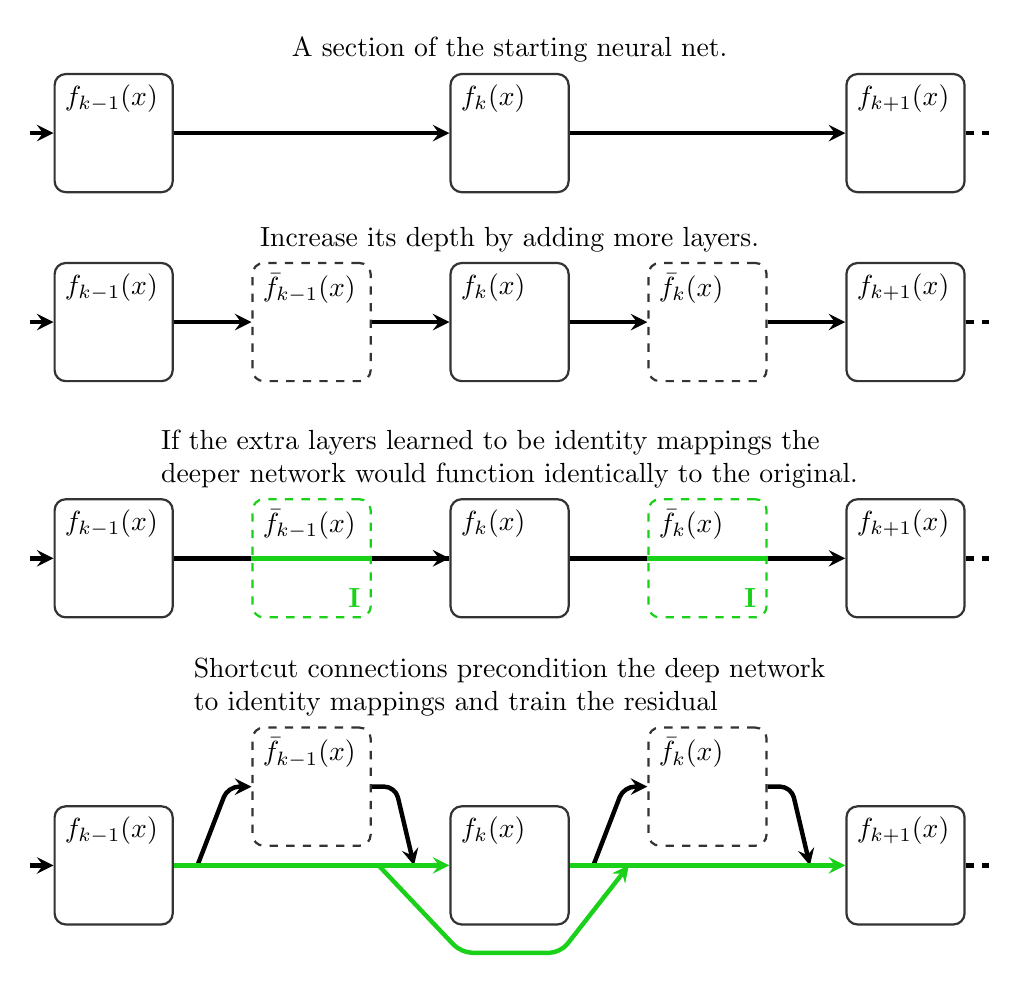
\begin{tikzpicture}[
                every path/.style={ultra thick},
                scale=3,
                block/.style={
                    rectangle,
                    rounded corners,
                    thick,
                    minimum size = 1.5cm,
                    inner sep = 0pt,
                    node distance = 3.5cm,
                    draw=black!80
                },
                shallow/.style={
                    block,
                },
                deep/.style={
                    block,
                    dashed,
                    thick
                },
                darkgreen/.style={
                    green!80!black!90
                },
                >= stealth,
            ]

                \begin{scope}[local bounding box = net1]
                    \node[shallow] (A) at (0,0) {};
                    \node[below right=0cm of A.north west] {$f_{k-1}(x)$};

                    \node[shallow] (B) [right= of A] {};
                    \node[below right=0cm of B.north west] {$f_{k}(x)$};

                    \node[shallow] (C) [right= of B] {};
                    \node[below right=0cm of C.north west] {$f_{k+1}(x)$};

                    \draw[->] (A.west)+(-0.1cm,0) -- (A.west);
                    \draw[->] (A.east) -- (B.west);
                    \draw[->] (B.east) -- (C.west);
                    \draw[dashed] (C.east) -- +(0.1cm,0);

                    \node[above] at (current bounding box.north) {A section of the starting neural net.};

                \end{scope}

                \begin{scope}[local bounding box = scope1, yshift = -0.8cm]
                    \node[shallow] (A) at (0,0) {};
                    \node[below right=0cm of A.north west] {$f_{k-1}(x)$};

                    \node[shallow] (B) [right= of A] {};
                    \node[below right=0cm of B.north west] {$f_{k}(x)$};

                    \node[shallow] (C) [right= of B] {};
                    \node[below right=0cm of C.north west] {$f_{k+1}(x)$};

                    \node[deep] (AB) at ($(A)!0.5!(B)$) {};
                    \node[below right=0cm of AB.north west] {$\bar{f}_{k-1}(x)$};

                    \node[deep] (BC) at ($(B)!0.5!(C)$) {};
                    \node[below right=0cm of BC.north west] {$\bar{f}_{k}(x)$};

                    \draw[->] (A.west)+(-0.1cm,0) -- (A.west);
                    \draw[->] (A.east) -- (AB.west);
                    \draw[->] (AB.east) -- (B.west);
                    \draw[->] (B.east) -- (BC.west);
                    \draw[->] (BC.east) -- (C.west);
                    \draw[dashed] (C.east) -- +(0.1cm,0);

                    \node[above] at (scope1.north) {Increase its depth by adding more layers.};
                \end{scope}

                \begin{scope}[local bounding box = scope2,yshift=-1.8cm]
                    \node[shallow] (A) at (0,0) {};
                    \node[below right=0cm of A.north west] {$f_{k-1}(x)$};

                    \node[shallow] (B) [right= of A] {};
                    \node[below right=0cm of B.north west] {$f_{k}(x)$};

                    \node[shallow] (C) [right= of B] {};
                    \node[below right=0cm of C.north west] {$f_{k+1}(x)$};

                    \node[deep,darkgreen] (AB) at ($(A)!0.5!(B)$) {};
                    \node[below right=0cm of AB.north west] {$\bar f_{k-1}(x)$};
                    \node[above left=0cm of AB.south east, darkgreen] {$\mathbf I$};

                    \node[deep,darkgreen] (BC) at ($(B)!0.5!(C)$) {};
                    \node[below right=0cm of BC.north west] {$\bar f_{k}(x)$};
                    \node[above left=0cm of BC.south east, darkgreen] {$ \mathbf I$};

                    \draw[->] (A.west)+(-0.1cm,0) -- (A.west);
                    \draw (A.east) -- (AB.west);
                    \draw[darkgreen] (AB.west) -- (AB.east);
                    \draw (AB.east) -- (B.west);
                    \draw[->] (AB.east) -- (B.west);
                    \draw (B.east) -- (BC.west);
                    \draw[darkgreen] (BC.west) -- (BC.east);
                    \draw[->] (BC.east) -- (C.west);
                    \draw[dashed] (C.east) -- +(0.1cm,0);

                    \node[above,align=left] at (scope2.north) {If the extra layers learned to be identity mappings the\\
                    deeper network would function identically to the original.};
                \end{scope}

                \begin{scope}[local bounding box = scope3,yshift=-3.1cm]
                    ;
                    \node[shallow] (A) at (0,0) {};
                    \node[below right=0cm of A.north west] {$f_{k-1}(x)$};

                    \node[shallow] (B) [right= of A] {};
                    \node[below right=0cm of B.north west] {$f_{k}(x)$};

                    \node[shallow] (C) [right= of B] {};
                    \node[below right=0cm of C.north west] {$f_{k+1}(x)$};

                    \node[deep, yshift=1cm] (AB) at ($(A)!0.5!(B)$) {};
                    \node[below right=0cm of AB.north west] {$\bar f_{k-1}(x)$};
                    \node[above left=0cm of AB.south east] {};

                    \node[deep, yshift=1cm] (BC) at ($(B)!0.5!(C)$) {};
                    \node[below right=0cm of BC.north west] {$\bar f_{k}(x)$};
                    \node[above left=0cm of BC.south east] {};

                    \draw[->] (A.west)+(-0.1cm,0) -- (A.west);
                    \draw[->, rounded corners] (A.east) +(0.1cm,0) -- ($(AB.west) - (0.1cm,0)$)  -- (AB.west);
                    \draw[->, rounded corners] (AB.east) -- ++(0.1cm,0) -- ($(B.west) + (-0.15cm,0)$);
                    \draw[->, rounded corners] (B.east) +(0.1cm,0) -- ($(BC.west) - (0.1cm,0)$)  -- (BC.west);
                    \draw[->, rounded corners] (BC.east) -- ++(0.1cm,0) -- ($(C.west) + (-0.15cm,0)$);
                    \draw[dashed] (C.east) -- +(0.1cm,0);

                    \draw[->,darkgreen, rounded corners] (B.west) +(-0.3cm,0) -- ++(0.05cm, -0.37cm) -- ++(0.42cm, 0cm) -- ($(B.east) + (0.25cm,0)$);
                    \draw[->,darkgreen] (A.east) -- (B.west);
                    \draw[->,darkgreen] (B.east) -- (C.west);

                    \node[above,align=left] at (scope3.north) {Shortcut connections precondition the deep network \\ to identity mappings and train the residual };
                \end{scope}
            \end{tikzpicture}
        \end{center}
        \caption{A visual explenation of residual learninig. Information flows through the shortcut connections as
        if they were identity mappings. The network learns the residual instead of a direct mapping.
        Residual neural networks use this property to achieve very large depth. }
        \label{fig:res_expl}
    \end{figure}

    In order to incorporate this observation into the network, so called \textit{shortcut connections} are introduced to the layers.
    Basically, the input to a block of stacked layers is added back to it's output.
    This way the network instead of learning the direct mapping $\mathcal{H}(x) = \mathcal{F}(x)$, it learns the residual mapping $\mathcal{H}(x) = \mathcal{R}(x)+x$.
    The optimiser can then push the residual mappings to $0$ leading to identity connections.
    Even though identity mappings are unlikely to be optimum, experiments showed that the residual connections have generally small responses, meaning identities are good pre-conditioners for deep architectures.

    Since their conception Residual Networks have revolutionised deep learning allowing for much deeper architectures than previously used.
    Furthermore, the idea of residual learning has found vast appeal in many other architectures.
    Transformers for example, employ residual connections, allowing many such layers to be stacked creating large expressive models~\cite{vaswani2017attention}.


    \chapter{Neural ODEs}
    There exist examples in the literature of combining neural networks and dynamical systems, even since the 1990s~\cite{rico1992discrete}.
    Interest began to increase after the publication of ResNet~\cite{weinan2018mean}.
    But the field of Neural Differential Equations really became prominent with~\cite{chen2018neural}.

    \subsection{A continuous time network}
    Let's revisit Residual Networks and how they work.
    The input-output relationship of the $k$-th discrete ResNet block is given by:
    \begin{equation}
        \pmb{y}_{k+1} = \pmb{y}_{k} + f(\pmb{y}_{k}; \pmb{\theta}_k) \label{resnet}
    \end{equation}
    where $\pmb{y}_{k+1} \in \mathbb{R}^{N_y}$ is the output of the block, $\pmb{y}^{k} \in \mathbb{R}^{N_y}$ is its input and $f$ is a fully connected layer with parameters $\pmb{\theta}_k \in \mathbb{R}^{N_\theta}$.
    Notice that we refer to ResNet blocks, not layers, since residual connections are generally not between the input and output of a single linear layer but a stack of them; from now on we will use the terms interchangeably.

    The update in the \textit{hidden state} $\pmb{y}$ in~\eqref{resnet} resembles the formula of the forward Euler iteration for solving ordinary differential equations.
    This observation led some researchers~\cite{lu2018beyond,weinan2018mean,ruthotto2020deep} to make a connection between neural network architectures and differential equations.
    Suppose that we could keep increasing the depth of the ResNet in~\eqref{resnet} while the time of the forward pass remained bounded, meaning each layer would take less and less time.
    In the limit we get a differential equation governed by the dynamics defined by a neural network $f$:
    \begin{equation}
        \pmb{y}^{(1)}(t) = f(\pmb{y}(t); \pmb{\theta}) \label{diffeq}
    \end{equation}
    Instead of a discrete sequence of hidden states, $\pmb{y}(t)$ is a continuous flow $\pmb{y} : [0,T] \to \mathbb{R}^{N_y}$ defined be the vector field parameterised by $\pmb{\theta}$.

    One important issue we haven't addressed is that the network's weights, $\pmb\theta_k$, in~\eqref{resnet} are
    different for each $k$, but at~\eqref{diffeq} we consider them to be constant in time.
    For notation’s sake we could define $f$ as $f(\pmb{y}(t), t, \pmb{\theta})$ meaning at certain ``depths'' different sections of the weights vector $\pmb{\theta}$ are used, maybe in a piecewise constant fashion~\cite{kidger2022neural}.
    Alternatively, the weights could be time dependant which complicates the model but leads to \textit{Galerkin} Neural ODEs, a more suitable continuous time equivalent of ResNet~\cite{massaroli2020dissecting}.
    For our purposes we consider the weights constant for the rest of this paper.

    \subsection{Inference}
    Under this new machine learning framework depth is replaced by time.
    Inference is performed by solving an initial value problem from initial time $t=0$ to terminal time $t=T$, i.e.:
    \begin{equation}
        \pmb{y}(T) = \pmb{y}(0) + \int_{0}^{T} f(\pmb{y}(\tau); \pmb{\theta}) \, d\tau \label{ivp}
    \end{equation}

    Obviously, Eq.~\eqref{ivp} describes the solution of a continuous time differential equation, while, as we know, our
    computers work in discrete time \textit{(for now)}.
    In order to overcome this obstacle we employ a numerical method for solving \textit{Initial Value Problems}, .
    If we were to use forward Euler, an explicit method, we would get a recurrence relation of the form
    \begin{equation}
        \pmb{y}(t_k + h) = \pmb{y}(t_k) + h \; \pmb{y}^{(1)}(t_k)
        \label{forwaredEu}
    \end{equation}
    By considering that $\pmb{y}^{(1)}(t) = f(\pmb{y}(t);\pmb{\theta})$ Eq. \eqref{forwaredEu} can be written as:
    \begin{equation}
        \pmb{y}(t_k + h) = \pmb{y}(t_k) + h f(\pmb{y}(t_k); \pmb{\theta} )
        \label{res2eul}
    \end{equation}
    which coincides with the ResNet formula.
    Many other neural networks of deep architectures can be interpreted as solving a neural ODE using different methods~\cite{chen2019ordinary}.
    The field of numerical differential equation solvers is quite vast meaning one could choose one that fits his specifications.
    A notable case is that of adaptive solvers like Runge-Kutta-Fehlberg, that use varying step sizes.
    This way to obtain  $\pmb{y}(T)$ the solver may require different number of $f$ evaluations depending on the input and the complexity of the vector field at that input.
    For simple dynamics the solver can ``decide'' to use large step sizes meaning fewer function evaluations.
    Otherwise when the vector field is more complex, a smaller step size will be used to reduce error thus leading to more function evaluations.
    We could interpret this behaviour as a network of ``variable depth''.

    It's important to clarify here that there are effectively two networks at play.
    Firstly, there is $f(\cdot)$, inherited from a block or layer of the original formulation of the problem.
    It is a neural network in the classical sense comprised of matrix vector multiplications and non-linearities.
    Secondly, there is the outlining model, the neural differential equation, which receives input $\pmb{y}_0$ and produced
    output $\pmb{y}(T)$; $f(\cdot)$ is to neural ODE what a layer is to ResNet.
    Internally, depending on the solver, $f(\cdot)$ will be evaluated for many values of $\pmb{y}(t)$.
    As disguised above, in contrast to ResNet $f(\cdot)$ contains all the learnable parameters of the model,
    which in out case are independent of depth.
    In conclusion the Neural ODE consists of: a neural network $f(\cdot)$ -that defines a \textit{learnable}
    vector field- parameterised by $\pmb{\theta}$,  some input $y_0$ and a numerical solver that applies $f(\cdot)$ until it reaches $\pmb{y}(T)$.

    \begin{figure}[H]
        \begin{center}
            %% Creator: Matplotlib, PGF backend
%%
%% To include the figure in your LaTeX document, write
%%   \input{<filename>.pgf}
%%
%% Make sure the required packages are loaded in your preamble
%%   \usepackage{pgf}
%%
%% Also ensure that all the required font packages are loaded; for instance,
%% the lmodern package is sometimes necessary when using math font.
%%   \usepackage{lmodern}
%%
%% Figures using additional raster images can only be included by \input if
%% they are in the same directory as the main LaTeX file. For loading figures
%% from other directories you can use the `import` package
%%   \usepackage{import}
%%
%% and then include the figures with
%%   \import{<path to file>}{<filename>.pgf}
%%
%% Matplotlib used the following preamble
%%   
%%   \makeatletter\@ifpackageloaded{underscore}{}{\usepackage[strings]{underscore}}\makeatother
%%
\begingroup%
\makeatletter%
\begin{pgfpicture}%
\pgfpathrectangle{\pgfpointorigin}{\pgfqpoint{4.724409in}{4.724409in}}%
\pgfusepath{use as bounding box, clip}%
\begin{pgfscope}%
\pgfsetbuttcap%
\pgfsetmiterjoin%
\definecolor{currentfill}{rgb}{1.000000,1.000000,1.000000}%
\pgfsetfillcolor{currentfill}%
\pgfsetlinewidth{0.000000pt}%
\definecolor{currentstroke}{rgb}{1.000000,1.000000,1.000000}%
\pgfsetstrokecolor{currentstroke}%
\pgfsetdash{}{0pt}%
\pgfpathmoveto{\pgfqpoint{0.000000in}{0.000000in}}%
\pgfpathlineto{\pgfqpoint{4.724409in}{0.000000in}}%
\pgfpathlineto{\pgfqpoint{4.724409in}{4.724409in}}%
\pgfpathlineto{\pgfqpoint{0.000000in}{4.724409in}}%
\pgfpathlineto{\pgfqpoint{0.000000in}{0.000000in}}%
\pgfpathclose%
\pgfusepath{fill}%
\end{pgfscope}%
\begin{pgfscope}%
\pgfsetbuttcap%
\pgfsetmiterjoin%
\definecolor{currentfill}{rgb}{1.000000,1.000000,1.000000}%
\pgfsetfillcolor{currentfill}%
\pgfsetlinewidth{0.000000pt}%
\definecolor{currentstroke}{rgb}{0.000000,0.000000,0.000000}%
\pgfsetstrokecolor{currentstroke}%
\pgfsetstrokeopacity{0.000000}%
\pgfsetdash{}{0pt}%
\pgfpathmoveto{\pgfqpoint{0.329012in}{2.564365in}}%
\pgfpathlineto{\pgfqpoint{2.287205in}{2.564365in}}%
\pgfpathlineto{\pgfqpoint{2.287205in}{4.276262in}}%
\pgfpathlineto{\pgfqpoint{0.329012in}{4.276262in}}%
\pgfpathlineto{\pgfqpoint{0.329012in}{2.564365in}}%
\pgfpathclose%
\pgfusepath{fill}%
\end{pgfscope}%
\begin{pgfscope}%
\pgfsetbuttcap%
\pgfsetroundjoin%
\definecolor{currentfill}{rgb}{0.000000,0.000000,0.000000}%
\pgfsetfillcolor{currentfill}%
\pgfsetlinewidth{0.803000pt}%
\definecolor{currentstroke}{rgb}{0.000000,0.000000,0.000000}%
\pgfsetstrokecolor{currentstroke}%
\pgfsetdash{}{0pt}%
\pgfsys@defobject{currentmarker}{\pgfqpoint{0.000000in}{-0.048611in}}{\pgfqpoint{0.000000in}{0.000000in}}{%
\pgfpathmoveto{\pgfqpoint{0.000000in}{0.000000in}}%
\pgfpathlineto{\pgfqpoint{0.000000in}{-0.048611in}}%
\pgfusepath{stroke,fill}%
}%
\begin{pgfscope}%
\pgfsys@transformshift{0.329012in}{2.564365in}%
\pgfsys@useobject{currentmarker}{}%
\end{pgfscope}%
\end{pgfscope}%
\begin{pgfscope}%
\pgfsetbuttcap%
\pgfsetroundjoin%
\definecolor{currentfill}{rgb}{0.000000,0.000000,0.000000}%
\pgfsetfillcolor{currentfill}%
\pgfsetlinewidth{0.803000pt}%
\definecolor{currentstroke}{rgb}{0.000000,0.000000,0.000000}%
\pgfsetstrokecolor{currentstroke}%
\pgfsetdash{}{0pt}%
\pgfsys@defobject{currentmarker}{\pgfqpoint{0.000000in}{-0.048611in}}{\pgfqpoint{0.000000in}{0.000000in}}{%
\pgfpathmoveto{\pgfqpoint{0.000000in}{0.000000in}}%
\pgfpathlineto{\pgfqpoint{0.000000in}{-0.048611in}}%
\pgfusepath{stroke,fill}%
}%
\begin{pgfscope}%
\pgfsys@transformshift{0.684148in}{2.564365in}%
\pgfsys@useobject{currentmarker}{}%
\end{pgfscope}%
\end{pgfscope}%
\begin{pgfscope}%
\pgfsetbuttcap%
\pgfsetroundjoin%
\definecolor{currentfill}{rgb}{0.000000,0.000000,0.000000}%
\pgfsetfillcolor{currentfill}%
\pgfsetlinewidth{0.803000pt}%
\definecolor{currentstroke}{rgb}{0.000000,0.000000,0.000000}%
\pgfsetstrokecolor{currentstroke}%
\pgfsetdash{}{0pt}%
\pgfsys@defobject{currentmarker}{\pgfqpoint{0.000000in}{-0.048611in}}{\pgfqpoint{0.000000in}{0.000000in}}{%
\pgfpathmoveto{\pgfqpoint{0.000000in}{0.000000in}}%
\pgfpathlineto{\pgfqpoint{0.000000in}{-0.048611in}}%
\pgfusepath{stroke,fill}%
}%
\begin{pgfscope}%
\pgfsys@transformshift{1.103705in}{2.564365in}%
\pgfsys@useobject{currentmarker}{}%
\end{pgfscope}%
\end{pgfscope}%
\begin{pgfscope}%
\pgfsetbuttcap%
\pgfsetroundjoin%
\definecolor{currentfill}{rgb}{0.000000,0.000000,0.000000}%
\pgfsetfillcolor{currentfill}%
\pgfsetlinewidth{0.803000pt}%
\definecolor{currentstroke}{rgb}{0.000000,0.000000,0.000000}%
\pgfsetstrokecolor{currentstroke}%
\pgfsetdash{}{0pt}%
\pgfsys@defobject{currentmarker}{\pgfqpoint{0.000000in}{-0.048611in}}{\pgfqpoint{0.000000in}{0.000000in}}{%
\pgfpathmoveto{\pgfqpoint{0.000000in}{0.000000in}}%
\pgfpathlineto{\pgfqpoint{0.000000in}{-0.048611in}}%
\pgfusepath{stroke,fill}%
}%
\begin{pgfscope}%
\pgfsys@transformshift{1.599350in}{2.564365in}%
\pgfsys@useobject{currentmarker}{}%
\end{pgfscope}%
\end{pgfscope}%
\begin{pgfscope}%
\pgfsetbuttcap%
\pgfsetroundjoin%
\definecolor{currentfill}{rgb}{0.000000,0.000000,0.000000}%
\pgfsetfillcolor{currentfill}%
\pgfsetlinewidth{0.803000pt}%
\definecolor{currentstroke}{rgb}{0.000000,0.000000,0.000000}%
\pgfsetstrokecolor{currentstroke}%
\pgfsetdash{}{0pt}%
\pgfsys@defobject{currentmarker}{\pgfqpoint{0.000000in}{-0.048611in}}{\pgfqpoint{0.000000in}{0.000000in}}{%
\pgfpathmoveto{\pgfqpoint{0.000000in}{0.000000in}}%
\pgfpathlineto{\pgfqpoint{0.000000in}{-0.048611in}}%
\pgfusepath{stroke,fill}%
}%
\begin{pgfscope}%
\pgfsys@transformshift{2.184884in}{2.564365in}%
\pgfsys@useobject{currentmarker}{}%
\end{pgfscope}%
\end{pgfscope}%
\begin{pgfscope}%
\definecolor{textcolor}{rgb}{0.000000,0.000000,0.000000}%
\pgfsetstrokecolor{textcolor}%
\pgfsetfillcolor{textcolor}%
\pgftext[x=1.308108in,y=2.411588in,,top]{\color{textcolor}\rmfamily\fontsize{10.000000}{12.000000}\selectfont depth}%
\end{pgfscope}%
\begin{pgfscope}%
\definecolor{textcolor}{rgb}{0.000000,0.000000,0.000000}%
\pgfsetstrokecolor{textcolor}%
\pgfsetfillcolor{textcolor}%
\pgftext[x=0.273457in,y=3.420314in,,bottom,rotate=90.000000]{\color{textcolor}\rmfamily\fontsize{10.000000}{12.000000}\selectfont state}%
\end{pgfscope}%
\begin{pgfscope}%
\pgfpathrectangle{\pgfqpoint{0.329012in}{2.564365in}}{\pgfqpoint{1.958193in}{1.711897in}}%
\pgfusepath{clip}%
\pgfsetbuttcap%
\pgfsetroundjoin%
\pgfsetlinewidth{0.602250pt}%
\definecolor{currentstroke}{rgb}{0.333333,0.333333,0.333333}%
\pgfsetstrokecolor{currentstroke}%
\pgfsetstrokeopacity{0.062745}%
\pgfsetdash{}{0pt}%
\pgfpathmoveto{\pgfqpoint{0.329012in}{2.589432in}}%
\pgfpathlineto{\pgfqpoint{0.353552in}{2.588623in}}%
\pgfusepath{stroke}%
\end{pgfscope}%
\begin{pgfscope}%
\pgfpathrectangle{\pgfqpoint{0.329012in}{2.564365in}}{\pgfqpoint{1.958193in}{1.711897in}}%
\pgfusepath{clip}%
\pgfsetbuttcap%
\pgfsetroundjoin%
\pgfsetlinewidth{0.602250pt}%
\definecolor{currentstroke}{rgb}{0.333333,0.333333,0.333333}%
\pgfsetstrokecolor{currentstroke}%
\pgfsetstrokeopacity{0.062745}%
\pgfsetdash{}{0pt}%
\pgfpathmoveto{\pgfqpoint{0.353552in}{2.588623in}}%
\pgfpathlineto{\pgfqpoint{0.433968in}{2.581809in}}%
\pgfusepath{stroke}%
\end{pgfscope}%
\begin{pgfscope}%
\pgfpathrectangle{\pgfqpoint{0.329012in}{2.564365in}}{\pgfqpoint{1.958193in}{1.711897in}}%
\pgfusepath{clip}%
\pgfsetbuttcap%
\pgfsetroundjoin%
\pgfsetlinewidth{0.602250pt}%
\definecolor{currentstroke}{rgb}{0.333333,0.333333,0.333333}%
\pgfsetstrokecolor{currentstroke}%
\pgfsetstrokeopacity{0.062745}%
\pgfsetdash{}{0pt}%
\pgfpathmoveto{\pgfqpoint{0.433968in}{2.581809in}}%
\pgfpathlineto{\pgfqpoint{0.524831in}{2.564365in}}%
\pgfusepath{stroke}%
\end{pgfscope}%
\begin{pgfscope}%
\pgfpathrectangle{\pgfqpoint{0.329012in}{2.564365in}}{\pgfqpoint{1.958193in}{1.711897in}}%
\pgfusepath{clip}%
\pgfsetbuttcap%
\pgfsetroundjoin%
\pgfsetlinewidth{0.602250pt}%
\definecolor{currentstroke}{rgb}{0.333333,0.333333,0.333333}%
\pgfsetstrokecolor{currentstroke}%
\pgfsetstrokeopacity{0.062745}%
\pgfsetdash{}{0pt}%
\pgfpathmoveto{\pgfqpoint{0.524831in}{2.564365in}}%
\pgfpathlineto{\pgfqpoint{0.524831in}{2.564365in}}%
\pgfusepath{stroke}%
\end{pgfscope}%
\begin{pgfscope}%
\pgfpathrectangle{\pgfqpoint{0.329012in}{2.564365in}}{\pgfqpoint{1.958193in}{1.711897in}}%
\pgfusepath{clip}%
\pgfsetbuttcap%
\pgfsetroundjoin%
\pgfsetlinewidth{0.602250pt}%
\definecolor{currentstroke}{rgb}{0.333333,0.333333,0.333333}%
\pgfsetstrokecolor{currentstroke}%
\pgfsetstrokeopacity{0.062745}%
\pgfsetdash{}{0pt}%
\pgfpathmoveto{\pgfqpoint{0.329012in}{2.654594in}}%
\pgfpathlineto{\pgfqpoint{0.377265in}{2.651736in}}%
\pgfusepath{stroke}%
\end{pgfscope}%
\begin{pgfscope}%
\pgfpathrectangle{\pgfqpoint{0.329012in}{2.564365in}}{\pgfqpoint{1.958193in}{1.711897in}}%
\pgfusepath{clip}%
\pgfsetbuttcap%
\pgfsetroundjoin%
\pgfsetlinewidth{0.602250pt}%
\definecolor{currentstroke}{rgb}{0.333333,0.333333,0.333333}%
\pgfsetstrokecolor{currentstroke}%
\pgfsetstrokeopacity{0.062745}%
\pgfsetdash{}{0pt}%
\pgfpathmoveto{\pgfqpoint{0.377265in}{2.651736in}}%
\pgfpathlineto{\pgfqpoint{0.461258in}{2.642652in}}%
\pgfusepath{stroke}%
\end{pgfscope}%
\begin{pgfscope}%
\pgfpathrectangle{\pgfqpoint{0.329012in}{2.564365in}}{\pgfqpoint{1.958193in}{1.711897in}}%
\pgfusepath{clip}%
\pgfsetbuttcap%
\pgfsetroundjoin%
\pgfsetlinewidth{0.602250pt}%
\definecolor{currentstroke}{rgb}{0.333333,0.333333,0.333333}%
\pgfsetstrokecolor{currentstroke}%
\pgfsetstrokeopacity{0.062745}%
\pgfsetdash{}{0pt}%
\pgfpathmoveto{\pgfqpoint{0.461258in}{2.642652in}}%
\pgfpathlineto{\pgfqpoint{0.547985in}{2.624810in}}%
\pgfusepath{stroke}%
\end{pgfscope}%
\begin{pgfscope}%
\pgfpathrectangle{\pgfqpoint{0.329012in}{2.564365in}}{\pgfqpoint{1.958193in}{1.711897in}}%
\pgfusepath{clip}%
\pgfsetbuttcap%
\pgfsetroundjoin%
\pgfsetlinewidth{0.602250pt}%
\definecolor{currentstroke}{rgb}{0.333333,0.333333,0.333333}%
\pgfsetstrokecolor{currentstroke}%
\pgfsetstrokeopacity{0.062745}%
\pgfsetdash{}{0pt}%
\pgfpathmoveto{\pgfqpoint{0.547985in}{2.624810in}}%
\pgfpathlineto{\pgfqpoint{0.635932in}{2.598153in}}%
\pgfusepath{stroke}%
\end{pgfscope}%
\begin{pgfscope}%
\pgfpathrectangle{\pgfqpoint{0.329012in}{2.564365in}}{\pgfqpoint{1.958193in}{1.711897in}}%
\pgfusepath{clip}%
\pgfsetbuttcap%
\pgfsetroundjoin%
\pgfsetlinewidth{0.602250pt}%
\definecolor{currentstroke}{rgb}{0.333333,0.333333,0.333333}%
\pgfsetstrokecolor{currentstroke}%
\pgfsetstrokeopacity{0.062745}%
\pgfsetdash{}{0pt}%
\pgfpathmoveto{\pgfqpoint{0.635932in}{2.598153in}}%
\pgfpathlineto{\pgfqpoint{0.720651in}{2.564365in}}%
\pgfusepath{stroke}%
\end{pgfscope}%
\begin{pgfscope}%
\pgfpathrectangle{\pgfqpoint{0.329012in}{2.564365in}}{\pgfqpoint{1.958193in}{1.711897in}}%
\pgfusepath{clip}%
\pgfsetbuttcap%
\pgfsetroundjoin%
\pgfsetlinewidth{0.602250pt}%
\definecolor{currentstroke}{rgb}{0.333333,0.333333,0.333333}%
\pgfsetstrokecolor{currentstroke}%
\pgfsetstrokeopacity{0.062745}%
\pgfsetdash{}{0pt}%
\pgfpathmoveto{\pgfqpoint{0.720651in}{2.564365in}}%
\pgfpathlineto{\pgfqpoint{0.720651in}{2.564365in}}%
\pgfusepath{stroke}%
\end{pgfscope}%
\begin{pgfscope}%
\pgfpathrectangle{\pgfqpoint{0.329012in}{2.564365in}}{\pgfqpoint{1.958193in}{1.711897in}}%
\pgfusepath{clip}%
\pgfsetbuttcap%
\pgfsetroundjoin%
\pgfsetlinewidth{0.602250pt}%
\definecolor{currentstroke}{rgb}{0.333333,0.333333,0.333333}%
\pgfsetstrokecolor{currentstroke}%
\pgfsetstrokeopacity{0.062745}%
\pgfsetdash{}{0pt}%
\pgfpathmoveto{\pgfqpoint{0.329012in}{2.743593in}}%
\pgfpathlineto{\pgfqpoint{0.403353in}{2.737644in}}%
\pgfusepath{stroke}%
\end{pgfscope}%
\begin{pgfscope}%
\pgfpathrectangle{\pgfqpoint{0.329012in}{2.564365in}}{\pgfqpoint{1.958193in}{1.711897in}}%
\pgfusepath{clip}%
\pgfsetbuttcap%
\pgfsetroundjoin%
\pgfsetlinewidth{0.602250pt}%
\definecolor{currentstroke}{rgb}{0.333333,0.333333,0.333333}%
\pgfsetstrokecolor{currentstroke}%
\pgfsetstrokeopacity{0.062745}%
\pgfsetdash{}{0pt}%
\pgfpathmoveto{\pgfqpoint{0.403353in}{2.737644in}}%
\pgfpathlineto{\pgfqpoint{0.492875in}{2.726413in}}%
\pgfusepath{stroke}%
\end{pgfscope}%
\begin{pgfscope}%
\pgfpathrectangle{\pgfqpoint{0.329012in}{2.564365in}}{\pgfqpoint{1.958193in}{1.711897in}}%
\pgfusepath{clip}%
\pgfsetbuttcap%
\pgfsetroundjoin%
\pgfsetlinewidth{0.602250pt}%
\definecolor{currentstroke}{rgb}{0.333333,0.333333,0.333333}%
\pgfsetstrokecolor{currentstroke}%
\pgfsetstrokeopacity{0.062745}%
\pgfsetdash{}{0pt}%
\pgfpathmoveto{\pgfqpoint{0.492875in}{2.726413in}}%
\pgfpathlineto{\pgfqpoint{0.583178in}{2.706941in}}%
\pgfusepath{stroke}%
\end{pgfscope}%
\begin{pgfscope}%
\pgfpathrectangle{\pgfqpoint{0.329012in}{2.564365in}}{\pgfqpoint{1.958193in}{1.711897in}}%
\pgfusepath{clip}%
\pgfsetbuttcap%
\pgfsetroundjoin%
\pgfsetlinewidth{0.602250pt}%
\definecolor{currentstroke}{rgb}{0.333333,0.333333,0.333333}%
\pgfsetstrokecolor{currentstroke}%
\pgfsetstrokeopacity{0.062745}%
\pgfsetdash{}{0pt}%
\pgfpathmoveto{\pgfqpoint{0.583178in}{2.706941in}}%
\pgfpathlineto{\pgfqpoint{0.671074in}{2.680239in}}%
\pgfusepath{stroke}%
\end{pgfscope}%
\begin{pgfscope}%
\pgfpathrectangle{\pgfqpoint{0.329012in}{2.564365in}}{\pgfqpoint{1.958193in}{1.711897in}}%
\pgfusepath{clip}%
\pgfsetbuttcap%
\pgfsetroundjoin%
\pgfsetlinewidth{0.602250pt}%
\definecolor{currentstroke}{rgb}{0.333333,0.333333,0.333333}%
\pgfsetstrokecolor{currentstroke}%
\pgfsetstrokeopacity{0.062745}%
\pgfsetdash{}{0pt}%
\pgfpathmoveto{\pgfqpoint{0.671074in}{2.680239in}}%
\pgfpathlineto{\pgfqpoint{0.756100in}{2.647071in}}%
\pgfusepath{stroke}%
\end{pgfscope}%
\begin{pgfscope}%
\pgfpathrectangle{\pgfqpoint{0.329012in}{2.564365in}}{\pgfqpoint{1.958193in}{1.711897in}}%
\pgfusepath{clip}%
\pgfsetbuttcap%
\pgfsetroundjoin%
\pgfsetlinewidth{0.602250pt}%
\definecolor{currentstroke}{rgb}{0.333333,0.333333,0.333333}%
\pgfsetstrokecolor{currentstroke}%
\pgfsetstrokeopacity{0.062745}%
\pgfsetdash{}{0pt}%
\pgfpathmoveto{\pgfqpoint{0.756100in}{2.647071in}}%
\pgfpathlineto{\pgfqpoint{0.837944in}{2.608191in}}%
\pgfusepath{stroke}%
\end{pgfscope}%
\begin{pgfscope}%
\pgfpathrectangle{\pgfqpoint{0.329012in}{2.564365in}}{\pgfqpoint{1.958193in}{1.711897in}}%
\pgfusepath{clip}%
\pgfsetbuttcap%
\pgfsetroundjoin%
\pgfsetlinewidth{0.602250pt}%
\definecolor{currentstroke}{rgb}{0.333333,0.333333,0.333333}%
\pgfsetstrokecolor{currentstroke}%
\pgfsetstrokeopacity{0.062745}%
\pgfsetdash{}{0pt}%
\pgfpathmoveto{\pgfqpoint{0.837944in}{2.608191in}}%
\pgfpathlineto{\pgfqpoint{0.916470in}{2.564365in}}%
\pgfusepath{stroke}%
\end{pgfscope}%
\begin{pgfscope}%
\pgfpathrectangle{\pgfqpoint{0.329012in}{2.564365in}}{\pgfqpoint{1.958193in}{1.711897in}}%
\pgfusepath{clip}%
\pgfsetbuttcap%
\pgfsetroundjoin%
\pgfsetlinewidth{0.602250pt}%
\definecolor{currentstroke}{rgb}{0.333333,0.333333,0.333333}%
\pgfsetstrokecolor{currentstroke}%
\pgfsetstrokeopacity{0.062745}%
\pgfsetdash{}{0pt}%
\pgfpathmoveto{\pgfqpoint{0.916470in}{2.564365in}}%
\pgfpathlineto{\pgfqpoint{0.916470in}{2.564365in}}%
\pgfusepath{stroke}%
\end{pgfscope}%
\begin{pgfscope}%
\pgfpathrectangle{\pgfqpoint{0.329012in}{2.564365in}}{\pgfqpoint{1.958193in}{1.711897in}}%
\pgfusepath{clip}%
\pgfsetbuttcap%
\pgfsetroundjoin%
\pgfsetlinewidth{0.602250pt}%
\definecolor{currentstroke}{rgb}{0.333333,0.333333,0.333333}%
\pgfsetstrokecolor{currentstroke}%
\pgfsetstrokeopacity{0.062745}%
\pgfsetdash{}{0pt}%
\pgfpathmoveto{\pgfqpoint{0.329012in}{2.837498in}}%
\pgfpathlineto{\pgfqpoint{0.350513in}{2.837062in}}%
\pgfusepath{stroke}%
\end{pgfscope}%
\begin{pgfscope}%
\pgfpathrectangle{\pgfqpoint{0.329012in}{2.564365in}}{\pgfqpoint{1.958193in}{1.711897in}}%
\pgfusepath{clip}%
\pgfsetbuttcap%
\pgfsetroundjoin%
\pgfsetlinewidth{0.602250pt}%
\definecolor{currentstroke}{rgb}{0.333333,0.333333,0.333333}%
\pgfsetstrokecolor{currentstroke}%
\pgfsetstrokeopacity{0.062745}%
\pgfsetdash{}{0pt}%
\pgfpathmoveto{\pgfqpoint{0.350513in}{2.837062in}}%
\pgfpathlineto{\pgfqpoint{0.443353in}{2.831290in}}%
\pgfusepath{stroke}%
\end{pgfscope}%
\begin{pgfscope}%
\pgfpathrectangle{\pgfqpoint{0.329012in}{2.564365in}}{\pgfqpoint{1.958193in}{1.711897in}}%
\pgfusepath{clip}%
\pgfsetbuttcap%
\pgfsetroundjoin%
\pgfsetlinewidth{0.602250pt}%
\definecolor{currentstroke}{rgb}{0.333333,0.333333,0.333333}%
\pgfsetstrokecolor{currentstroke}%
\pgfsetstrokeopacity{0.062745}%
\pgfsetdash{}{0pt}%
\pgfpathmoveto{\pgfqpoint{0.443353in}{2.831290in}}%
\pgfpathlineto{\pgfqpoint{0.535254in}{2.818102in}}%
\pgfusepath{stroke}%
\end{pgfscope}%
\begin{pgfscope}%
\pgfpathrectangle{\pgfqpoint{0.329012in}{2.564365in}}{\pgfqpoint{1.958193in}{1.711897in}}%
\pgfusepath{clip}%
\pgfsetbuttcap%
\pgfsetroundjoin%
\pgfsetlinewidth{0.602250pt}%
\definecolor{currentstroke}{rgb}{0.333333,0.333333,0.333333}%
\pgfsetstrokecolor{currentstroke}%
\pgfsetstrokeopacity{0.062745}%
\pgfsetdash{}{0pt}%
\pgfpathmoveto{\pgfqpoint{0.535254in}{2.818102in}}%
\pgfpathlineto{\pgfqpoint{0.625537in}{2.798102in}}%
\pgfusepath{stroke}%
\end{pgfscope}%
\begin{pgfscope}%
\pgfpathrectangle{\pgfqpoint{0.329012in}{2.564365in}}{\pgfqpoint{1.958193in}{1.711897in}}%
\pgfusepath{clip}%
\pgfsetbuttcap%
\pgfsetroundjoin%
\pgfsetlinewidth{0.602250pt}%
\definecolor{currentstroke}{rgb}{0.333333,0.333333,0.333333}%
\pgfsetstrokecolor{currentstroke}%
\pgfsetstrokeopacity{0.062745}%
\pgfsetdash{}{0pt}%
\pgfpathmoveto{\pgfqpoint{0.625537in}{2.798102in}}%
\pgfpathlineto{\pgfqpoint{0.713670in}{2.771833in}}%
\pgfusepath{stroke}%
\end{pgfscope}%
\begin{pgfscope}%
\pgfpathrectangle{\pgfqpoint{0.329012in}{2.564365in}}{\pgfqpoint{1.958193in}{1.711897in}}%
\pgfusepath{clip}%
\pgfsetbuttcap%
\pgfsetroundjoin%
\pgfsetlinewidth{0.602250pt}%
\definecolor{currentstroke}{rgb}{0.333333,0.333333,0.333333}%
\pgfsetstrokecolor{currentstroke}%
\pgfsetstrokeopacity{0.062745}%
\pgfsetdash{}{0pt}%
\pgfpathmoveto{\pgfqpoint{0.713670in}{2.771833in}}%
\pgfpathlineto{\pgfqpoint{0.799273in}{2.739787in}}%
\pgfusepath{stroke}%
\end{pgfscope}%
\begin{pgfscope}%
\pgfpathrectangle{\pgfqpoint{0.329012in}{2.564365in}}{\pgfqpoint{1.958193in}{1.711897in}}%
\pgfusepath{clip}%
\pgfsetbuttcap%
\pgfsetroundjoin%
\pgfsetlinewidth{0.602250pt}%
\definecolor{currentstroke}{rgb}{0.333333,0.333333,0.333333}%
\pgfsetstrokecolor{currentstroke}%
\pgfsetstrokeopacity{0.062745}%
\pgfsetdash{}{0pt}%
\pgfpathmoveto{\pgfqpoint{0.799273in}{2.739787in}}%
\pgfpathlineto{\pgfqpoint{0.882051in}{2.702472in}}%
\pgfusepath{stroke}%
\end{pgfscope}%
\begin{pgfscope}%
\pgfpathrectangle{\pgfqpoint{0.329012in}{2.564365in}}{\pgfqpoint{1.958193in}{1.711897in}}%
\pgfusepath{clip}%
\pgfsetbuttcap%
\pgfsetroundjoin%
\pgfsetlinewidth{0.602250pt}%
\definecolor{currentstroke}{rgb}{0.333333,0.333333,0.333333}%
\pgfsetstrokecolor{currentstroke}%
\pgfsetstrokeopacity{0.062745}%
\pgfsetdash{}{0pt}%
\pgfpathmoveto{\pgfqpoint{0.882051in}{2.702472in}}%
\pgfpathlineto{\pgfqpoint{0.961822in}{2.660410in}}%
\pgfusepath{stroke}%
\end{pgfscope}%
\begin{pgfscope}%
\pgfpathrectangle{\pgfqpoint{0.329012in}{2.564365in}}{\pgfqpoint{1.958193in}{1.711897in}}%
\pgfusepath{clip}%
\pgfsetbuttcap%
\pgfsetroundjoin%
\pgfsetlinewidth{0.602250pt}%
\definecolor{currentstroke}{rgb}{0.333333,0.333333,0.333333}%
\pgfsetstrokecolor{currentstroke}%
\pgfsetstrokeopacity{0.062745}%
\pgfsetdash{}{0pt}%
\pgfpathmoveto{\pgfqpoint{0.961822in}{2.660410in}}%
\pgfpathlineto{\pgfqpoint{1.038538in}{2.614173in}}%
\pgfusepath{stroke}%
\end{pgfscope}%
\begin{pgfscope}%
\pgfpathrectangle{\pgfqpoint{0.329012in}{2.564365in}}{\pgfqpoint{1.958193in}{1.711897in}}%
\pgfusepath{clip}%
\pgfsetbuttcap%
\pgfsetroundjoin%
\pgfsetlinewidth{0.602250pt}%
\definecolor{currentstroke}{rgb}{0.333333,0.333333,0.333333}%
\pgfsetstrokecolor{currentstroke}%
\pgfsetstrokeopacity{0.062745}%
\pgfsetdash{}{0pt}%
\pgfpathmoveto{\pgfqpoint{1.038538in}{2.614173in}}%
\pgfpathlineto{\pgfqpoint{1.112289in}{2.564365in}}%
\pgfusepath{stroke}%
\end{pgfscope}%
\begin{pgfscope}%
\pgfpathrectangle{\pgfqpoint{0.329012in}{2.564365in}}{\pgfqpoint{1.958193in}{1.711897in}}%
\pgfusepath{clip}%
\pgfsetbuttcap%
\pgfsetroundjoin%
\pgfsetlinewidth{0.602250pt}%
\definecolor{currentstroke}{rgb}{0.333333,0.333333,0.333333}%
\pgfsetstrokecolor{currentstroke}%
\pgfsetstrokeopacity{0.062745}%
\pgfsetdash{}{0pt}%
\pgfpathmoveto{\pgfqpoint{1.112289in}{2.564365in}}%
\pgfpathlineto{\pgfqpoint{1.112289in}{2.564365in}}%
\pgfusepath{stroke}%
\end{pgfscope}%
\begin{pgfscope}%
\pgfpathrectangle{\pgfqpoint{0.329012in}{2.564365in}}{\pgfqpoint{1.958193in}{1.711897in}}%
\pgfusepath{clip}%
\pgfsetbuttcap%
\pgfsetroundjoin%
\pgfsetlinewidth{0.602250pt}%
\definecolor{currentstroke}{rgb}{0.333333,0.333333,0.333333}%
\pgfsetstrokecolor{currentstroke}%
\pgfsetstrokeopacity{0.062745}%
\pgfsetdash{}{0pt}%
\pgfpathmoveto{\pgfqpoint{0.985965in}{2.709980in}}%
\pgfpathlineto{\pgfqpoint{1.063551in}{2.664878in}}%
\pgfusepath{stroke}%
\end{pgfscope}%
\begin{pgfscope}%
\pgfpathrectangle{\pgfqpoint{0.329012in}{2.564365in}}{\pgfqpoint{1.958193in}{1.711897in}}%
\pgfusepath{clip}%
\pgfsetbuttcap%
\pgfsetroundjoin%
\pgfsetlinewidth{0.602250pt}%
\definecolor{currentstroke}{rgb}{0.333333,0.333333,0.333333}%
\pgfsetstrokecolor{currentstroke}%
\pgfsetstrokeopacity{0.062745}%
\pgfsetdash{}{0pt}%
\pgfpathmoveto{\pgfqpoint{1.063551in}{2.664878in}}%
\pgfpathlineto{\pgfqpoint{1.138238in}{2.616152in}}%
\pgfusepath{stroke}%
\end{pgfscope}%
\begin{pgfscope}%
\pgfpathrectangle{\pgfqpoint{0.329012in}{2.564365in}}{\pgfqpoint{1.958193in}{1.711897in}}%
\pgfusepath{clip}%
\pgfsetbuttcap%
\pgfsetroundjoin%
\pgfsetlinewidth{0.602250pt}%
\definecolor{currentstroke}{rgb}{0.333333,0.333333,0.333333}%
\pgfsetstrokecolor{currentstroke}%
\pgfsetstrokeopacity{0.062745}%
\pgfsetdash{}{0pt}%
\pgfpathmoveto{\pgfqpoint{1.138238in}{2.616152in}}%
\pgfpathlineto{\pgfqpoint{1.210199in}{2.564365in}}%
\pgfusepath{stroke}%
\end{pgfscope}%
\begin{pgfscope}%
\pgfpathrectangle{\pgfqpoint{0.329012in}{2.564365in}}{\pgfqpoint{1.958193in}{1.711897in}}%
\pgfusepath{clip}%
\pgfsetbuttcap%
\pgfsetroundjoin%
\pgfsetlinewidth{0.602250pt}%
\definecolor{currentstroke}{rgb}{0.333333,0.333333,0.333333}%
\pgfsetstrokecolor{currentstroke}%
\pgfsetstrokeopacity{0.062745}%
\pgfsetdash{}{0pt}%
\pgfpathmoveto{\pgfqpoint{1.210199in}{2.564365in}}%
\pgfpathlineto{\pgfqpoint{1.210199in}{2.564365in}}%
\pgfusepath{stroke}%
\end{pgfscope}%
\begin{pgfscope}%
\pgfpathrectangle{\pgfqpoint{0.329012in}{2.564365in}}{\pgfqpoint{1.958193in}{1.711897in}}%
\pgfusepath{clip}%
\pgfsetbuttcap%
\pgfsetroundjoin%
\pgfsetlinewidth{0.602250pt}%
\definecolor{currentstroke}{rgb}{0.333333,0.333333,0.333333}%
\pgfsetstrokecolor{currentstroke}%
\pgfsetstrokeopacity{0.062745}%
\pgfsetdash{}{0pt}%
\pgfpathmoveto{\pgfqpoint{1.088835in}{2.715762in}}%
\pgfpathlineto{\pgfqpoint{1.164553in}{2.668277in}}%
\pgfusepath{stroke}%
\end{pgfscope}%
\begin{pgfscope}%
\pgfpathrectangle{\pgfqpoint{0.329012in}{2.564365in}}{\pgfqpoint{1.958193in}{1.711897in}}%
\pgfusepath{clip}%
\pgfsetbuttcap%
\pgfsetroundjoin%
\pgfsetlinewidth{0.602250pt}%
\definecolor{currentstroke}{rgb}{0.333333,0.333333,0.333333}%
\pgfsetstrokecolor{currentstroke}%
\pgfsetstrokeopacity{0.062745}%
\pgfsetdash{}{0pt}%
\pgfpathmoveto{\pgfqpoint{1.164553in}{2.668277in}}%
\pgfpathlineto{\pgfqpoint{1.237562in}{2.617631in}}%
\pgfusepath{stroke}%
\end{pgfscope}%
\begin{pgfscope}%
\pgfpathrectangle{\pgfqpoint{0.329012in}{2.564365in}}{\pgfqpoint{1.958193in}{1.711897in}}%
\pgfusepath{clip}%
\pgfsetbuttcap%
\pgfsetroundjoin%
\pgfsetlinewidth{0.602250pt}%
\definecolor{currentstroke}{rgb}{0.333333,0.333333,0.333333}%
\pgfsetstrokecolor{currentstroke}%
\pgfsetstrokeopacity{0.062745}%
\pgfsetdash{}{0pt}%
\pgfpathmoveto{\pgfqpoint{1.237562in}{2.617631in}}%
\pgfpathlineto{\pgfqpoint{1.308108in}{2.564365in}}%
\pgfusepath{stroke}%
\end{pgfscope}%
\begin{pgfscope}%
\pgfpathrectangle{\pgfqpoint{0.329012in}{2.564365in}}{\pgfqpoint{1.958193in}{1.711897in}}%
\pgfusepath{clip}%
\pgfsetbuttcap%
\pgfsetroundjoin%
\pgfsetlinewidth{0.602250pt}%
\definecolor{currentstroke}{rgb}{0.333333,0.333333,0.333333}%
\pgfsetstrokecolor{currentstroke}%
\pgfsetstrokeopacity{0.062745}%
\pgfsetdash{}{0pt}%
\pgfpathmoveto{\pgfqpoint{1.308108in}{2.564365in}}%
\pgfpathlineto{\pgfqpoint{1.308108in}{2.564365in}}%
\pgfusepath{stroke}%
\end{pgfscope}%
\begin{pgfscope}%
\pgfpathrectangle{\pgfqpoint{0.329012in}{2.564365in}}{\pgfqpoint{1.958193in}{1.711897in}}%
\pgfusepath{clip}%
\pgfsetbuttcap%
\pgfsetroundjoin%
\pgfsetlinewidth{0.602250pt}%
\definecolor{currentstroke}{rgb}{0.333333,0.333333,0.333333}%
\pgfsetstrokecolor{currentstroke}%
\pgfsetstrokeopacity{0.062745}%
\pgfsetdash{}{0pt}%
\pgfpathmoveto{\pgfqpoint{1.190723in}{2.720162in}}%
\pgfpathlineto{\pgfqpoint{1.264876in}{2.670810in}}%
\pgfusepath{stroke}%
\end{pgfscope}%
\begin{pgfscope}%
\pgfpathrectangle{\pgfqpoint{0.329012in}{2.564365in}}{\pgfqpoint{1.958193in}{1.711897in}}%
\pgfusepath{clip}%
\pgfsetbuttcap%
\pgfsetroundjoin%
\pgfsetlinewidth{0.602250pt}%
\definecolor{currentstroke}{rgb}{0.333333,0.333333,0.333333}%
\pgfsetstrokecolor{currentstroke}%
\pgfsetstrokeopacity{0.062745}%
\pgfsetdash{}{0pt}%
\pgfpathmoveto{\pgfqpoint{1.264876in}{2.670810in}}%
\pgfpathlineto{\pgfqpoint{1.336536in}{2.618701in}}%
\pgfusepath{stroke}%
\end{pgfscope}%
\begin{pgfscope}%
\pgfpathrectangle{\pgfqpoint{0.329012in}{2.564365in}}{\pgfqpoint{1.958193in}{1.711897in}}%
\pgfusepath{clip}%
\pgfsetbuttcap%
\pgfsetroundjoin%
\pgfsetlinewidth{0.602250pt}%
\definecolor{currentstroke}{rgb}{0.333333,0.333333,0.333333}%
\pgfsetstrokecolor{currentstroke}%
\pgfsetstrokeopacity{0.062745}%
\pgfsetdash{}{0pt}%
\pgfpathmoveto{\pgfqpoint{1.336536in}{2.618701in}}%
\pgfpathlineto{\pgfqpoint{1.406018in}{2.564365in}}%
\pgfusepath{stroke}%
\end{pgfscope}%
\begin{pgfscope}%
\pgfpathrectangle{\pgfqpoint{0.329012in}{2.564365in}}{\pgfqpoint{1.958193in}{1.711897in}}%
\pgfusepath{clip}%
\pgfsetbuttcap%
\pgfsetroundjoin%
\pgfsetlinewidth{0.602250pt}%
\definecolor{currentstroke}{rgb}{0.333333,0.333333,0.333333}%
\pgfsetstrokecolor{currentstroke}%
\pgfsetstrokeopacity{0.062745}%
\pgfsetdash{}{0pt}%
\pgfpathmoveto{\pgfqpoint{1.406018in}{2.564365in}}%
\pgfpathlineto{\pgfqpoint{1.406018in}{2.564365in}}%
\pgfusepath{stroke}%
\end{pgfscope}%
\begin{pgfscope}%
\pgfpathrectangle{\pgfqpoint{0.329012in}{2.564365in}}{\pgfqpoint{1.958193in}{1.711897in}}%
\pgfusepath{clip}%
\pgfsetbuttcap%
\pgfsetroundjoin%
\pgfsetlinewidth{0.602250pt}%
\definecolor{currentstroke}{rgb}{0.333333,0.333333,0.333333}%
\pgfsetstrokecolor{currentstroke}%
\pgfsetstrokeopacity{0.062745}%
\pgfsetdash{}{0pt}%
\pgfpathmoveto{\pgfqpoint{1.291700in}{2.723427in}}%
\pgfpathlineto{\pgfqpoint{1.364569in}{2.672621in}}%
\pgfusepath{stroke}%
\end{pgfscope}%
\begin{pgfscope}%
\pgfpathrectangle{\pgfqpoint{0.329012in}{2.564365in}}{\pgfqpoint{1.958193in}{1.711897in}}%
\pgfusepath{clip}%
\pgfsetbuttcap%
\pgfsetroundjoin%
\pgfsetlinewidth{0.602250pt}%
\definecolor{currentstroke}{rgb}{0.333333,0.333333,0.333333}%
\pgfsetstrokecolor{currentstroke}%
\pgfsetstrokeopacity{0.062745}%
\pgfsetdash{}{0pt}%
\pgfpathmoveto{\pgfqpoint{1.364569in}{2.672621in}}%
\pgfpathlineto{\pgfqpoint{1.435186in}{2.619425in}}%
\pgfusepath{stroke}%
\end{pgfscope}%
\begin{pgfscope}%
\pgfpathrectangle{\pgfqpoint{0.329012in}{2.564365in}}{\pgfqpoint{1.958193in}{1.711897in}}%
\pgfusepath{clip}%
\pgfsetbuttcap%
\pgfsetroundjoin%
\pgfsetlinewidth{0.602250pt}%
\definecolor{currentstroke}{rgb}{0.333333,0.333333,0.333333}%
\pgfsetstrokecolor{currentstroke}%
\pgfsetstrokeopacity{0.062745}%
\pgfsetdash{}{0pt}%
\pgfpathmoveto{\pgfqpoint{1.435186in}{2.619425in}}%
\pgfpathlineto{\pgfqpoint{1.503928in}{2.564365in}}%
\pgfusepath{stroke}%
\end{pgfscope}%
\begin{pgfscope}%
\pgfpathrectangle{\pgfqpoint{0.329012in}{2.564365in}}{\pgfqpoint{1.958193in}{1.711897in}}%
\pgfusepath{clip}%
\pgfsetbuttcap%
\pgfsetroundjoin%
\pgfsetlinewidth{0.602250pt}%
\definecolor{currentstroke}{rgb}{0.333333,0.333333,0.333333}%
\pgfsetstrokecolor{currentstroke}%
\pgfsetstrokeopacity{0.062745}%
\pgfsetdash{}{0pt}%
\pgfpathmoveto{\pgfqpoint{1.503928in}{2.564365in}}%
\pgfpathlineto{\pgfqpoint{1.503928in}{2.564365in}}%
\pgfusepath{stroke}%
\end{pgfscope}%
\begin{pgfscope}%
\pgfpathrectangle{\pgfqpoint{0.329012in}{2.564365in}}{\pgfqpoint{1.958193in}{1.711897in}}%
\pgfusepath{clip}%
\pgfsetbuttcap%
\pgfsetroundjoin%
\pgfsetlinewidth{0.602250pt}%
\definecolor{currentstroke}{rgb}{0.333333,0.333333,0.333333}%
\pgfsetstrokecolor{currentstroke}%
\pgfsetstrokeopacity{0.062745}%
\pgfsetdash{}{0pt}%
\pgfpathmoveto{\pgfqpoint{1.391835in}{2.725737in}}%
\pgfpathlineto{\pgfqpoint{1.463680in}{2.673817in}}%
\pgfusepath{stroke}%
\end{pgfscope}%
\begin{pgfscope}%
\pgfpathrectangle{\pgfqpoint{0.329012in}{2.564365in}}{\pgfqpoint{1.958193in}{1.711897in}}%
\pgfusepath{clip}%
\pgfsetbuttcap%
\pgfsetroundjoin%
\pgfsetlinewidth{0.602250pt}%
\definecolor{currentstroke}{rgb}{0.333333,0.333333,0.333333}%
\pgfsetstrokecolor{currentstroke}%
\pgfsetstrokeopacity{0.062745}%
\pgfsetdash{}{0pt}%
\pgfpathmoveto{\pgfqpoint{1.463680in}{2.673817in}}%
\pgfpathlineto{\pgfqpoint{1.533535in}{2.619848in}}%
\pgfusepath{stroke}%
\end{pgfscope}%
\begin{pgfscope}%
\pgfpathrectangle{\pgfqpoint{0.329012in}{2.564365in}}{\pgfqpoint{1.958193in}{1.711897in}}%
\pgfusepath{clip}%
\pgfsetbuttcap%
\pgfsetroundjoin%
\pgfsetlinewidth{0.602250pt}%
\definecolor{currentstroke}{rgb}{0.333333,0.333333,0.333333}%
\pgfsetstrokecolor{currentstroke}%
\pgfsetstrokeopacity{0.062745}%
\pgfsetdash{}{0pt}%
\pgfpathmoveto{\pgfqpoint{1.533535in}{2.619848in}}%
\pgfpathlineto{\pgfqpoint{1.601837in}{2.564365in}}%
\pgfusepath{stroke}%
\end{pgfscope}%
\begin{pgfscope}%
\pgfpathrectangle{\pgfqpoint{0.329012in}{2.564365in}}{\pgfqpoint{1.958193in}{1.711897in}}%
\pgfusepath{clip}%
\pgfsetbuttcap%
\pgfsetroundjoin%
\pgfsetlinewidth{0.602250pt}%
\definecolor{currentstroke}{rgb}{0.333333,0.333333,0.333333}%
\pgfsetstrokecolor{currentstroke}%
\pgfsetstrokeopacity{0.062745}%
\pgfsetdash{}{0pt}%
\pgfpathmoveto{\pgfqpoint{1.601837in}{2.564365in}}%
\pgfpathlineto{\pgfqpoint{1.601837in}{2.564365in}}%
\pgfusepath{stroke}%
\end{pgfscope}%
\begin{pgfscope}%
\pgfpathrectangle{\pgfqpoint{0.329012in}{2.564365in}}{\pgfqpoint{1.958193in}{1.711897in}}%
\pgfusepath{clip}%
\pgfsetbuttcap%
\pgfsetroundjoin%
\pgfsetlinewidth{0.602250pt}%
\definecolor{currentstroke}{rgb}{0.333333,0.333333,0.333333}%
\pgfsetstrokecolor{currentstroke}%
\pgfsetstrokeopacity{0.062745}%
\pgfsetdash{}{0pt}%
\pgfpathmoveto{\pgfqpoint{1.491182in}{2.727212in}}%
\pgfpathlineto{\pgfqpoint{1.562246in}{2.674468in}}%
\pgfusepath{stroke}%
\end{pgfscope}%
\begin{pgfscope}%
\pgfpathrectangle{\pgfqpoint{0.329012in}{2.564365in}}{\pgfqpoint{1.958193in}{1.711897in}}%
\pgfusepath{clip}%
\pgfsetbuttcap%
\pgfsetroundjoin%
\pgfsetlinewidth{0.602250pt}%
\definecolor{currentstroke}{rgb}{0.333333,0.333333,0.333333}%
\pgfsetstrokecolor{currentstroke}%
\pgfsetstrokeopacity{0.062745}%
\pgfsetdash{}{0pt}%
\pgfpathmoveto{\pgfqpoint{1.562246in}{2.674468in}}%
\pgfpathlineto{\pgfqpoint{1.631603in}{2.620002in}}%
\pgfusepath{stroke}%
\end{pgfscope}%
\begin{pgfscope}%
\pgfpathrectangle{\pgfqpoint{0.329012in}{2.564365in}}{\pgfqpoint{1.958193in}{1.711897in}}%
\pgfusepath{clip}%
\pgfsetbuttcap%
\pgfsetroundjoin%
\pgfsetlinewidth{0.602250pt}%
\definecolor{currentstroke}{rgb}{0.333333,0.333333,0.333333}%
\pgfsetstrokecolor{currentstroke}%
\pgfsetstrokeopacity{0.062745}%
\pgfsetdash{}{0pt}%
\pgfpathmoveto{\pgfqpoint{1.631603in}{2.620002in}}%
\pgfpathlineto{\pgfqpoint{1.699747in}{2.564365in}}%
\pgfusepath{stroke}%
\end{pgfscope}%
\begin{pgfscope}%
\pgfpathrectangle{\pgfqpoint{0.329012in}{2.564365in}}{\pgfqpoint{1.958193in}{1.711897in}}%
\pgfusepath{clip}%
\pgfsetbuttcap%
\pgfsetroundjoin%
\pgfsetlinewidth{0.602250pt}%
\definecolor{currentstroke}{rgb}{0.333333,0.333333,0.333333}%
\pgfsetstrokecolor{currentstroke}%
\pgfsetstrokeopacity{0.062745}%
\pgfsetdash{}{0pt}%
\pgfpathmoveto{\pgfqpoint{1.699747in}{2.564365in}}%
\pgfpathlineto{\pgfqpoint{1.699747in}{2.564365in}}%
\pgfusepath{stroke}%
\end{pgfscope}%
\begin{pgfscope}%
\pgfpathrectangle{\pgfqpoint{0.329012in}{2.564365in}}{\pgfqpoint{1.958193in}{1.711897in}}%
\pgfusepath{clip}%
\pgfsetbuttcap%
\pgfsetroundjoin%
\pgfsetlinewidth{0.602250pt}%
\definecolor{currentstroke}{rgb}{0.333333,0.333333,0.333333}%
\pgfsetstrokecolor{currentstroke}%
\pgfsetstrokeopacity{0.062745}%
\pgfsetdash{}{0pt}%
\pgfpathmoveto{\pgfqpoint{0.329012in}{3.133527in}}%
\pgfpathlineto{\pgfqpoint{0.396877in}{3.131421in}}%
\pgfusepath{stroke}%
\end{pgfscope}%
\begin{pgfscope}%
\pgfpathrectangle{\pgfqpoint{0.329012in}{2.564365in}}{\pgfqpoint{1.958193in}{1.711897in}}%
\pgfusepath{clip}%
\pgfsetbuttcap%
\pgfsetroundjoin%
\pgfsetlinewidth{0.602250pt}%
\definecolor{currentstroke}{rgb}{0.333333,0.333333,0.333333}%
\pgfsetstrokecolor{currentstroke}%
\pgfsetstrokeopacity{0.062745}%
\pgfsetdash{}{0pt}%
\pgfpathmoveto{\pgfqpoint{0.396877in}{3.131421in}}%
\pgfpathlineto{\pgfqpoint{0.489909in}{3.126660in}}%
\pgfusepath{stroke}%
\end{pgfscope}%
\begin{pgfscope}%
\pgfpathrectangle{\pgfqpoint{0.329012in}{2.564365in}}{\pgfqpoint{1.958193in}{1.711897in}}%
\pgfusepath{clip}%
\pgfsetbuttcap%
\pgfsetroundjoin%
\pgfsetlinewidth{0.602250pt}%
\definecolor{currentstroke}{rgb}{0.333333,0.333333,0.333333}%
\pgfsetstrokecolor{currentstroke}%
\pgfsetstrokeopacity{0.062745}%
\pgfsetdash{}{0pt}%
\pgfpathmoveto{\pgfqpoint{0.489909in}{3.126660in}}%
\pgfpathlineto{\pgfqpoint{0.582599in}{3.118225in}}%
\pgfusepath{stroke}%
\end{pgfscope}%
\begin{pgfscope}%
\pgfpathrectangle{\pgfqpoint{0.329012in}{2.564365in}}{\pgfqpoint{1.958193in}{1.711897in}}%
\pgfusepath{clip}%
\pgfsetbuttcap%
\pgfsetroundjoin%
\pgfsetlinewidth{0.602250pt}%
\definecolor{currentstroke}{rgb}{0.333333,0.333333,0.333333}%
\pgfsetstrokecolor{currentstroke}%
\pgfsetstrokeopacity{0.062745}%
\pgfsetdash{}{0pt}%
\pgfpathmoveto{\pgfqpoint{0.582599in}{3.118225in}}%
\pgfpathlineto{\pgfqpoint{0.674774in}{3.106189in}}%
\pgfusepath{stroke}%
\end{pgfscope}%
\begin{pgfscope}%
\pgfpathrectangle{\pgfqpoint{0.329012in}{2.564365in}}{\pgfqpoint{1.958193in}{1.711897in}}%
\pgfusepath{clip}%
\pgfsetbuttcap%
\pgfsetroundjoin%
\pgfsetlinewidth{0.602250pt}%
\definecolor{currentstroke}{rgb}{0.333333,0.333333,0.333333}%
\pgfsetstrokecolor{currentstroke}%
\pgfsetstrokeopacity{0.062745}%
\pgfsetdash{}{0pt}%
\pgfpathmoveto{\pgfqpoint{0.674774in}{3.106189in}}%
\pgfpathlineto{\pgfqpoint{0.766234in}{3.090541in}}%
\pgfusepath{stroke}%
\end{pgfscope}%
\begin{pgfscope}%
\pgfpathrectangle{\pgfqpoint{0.329012in}{2.564365in}}{\pgfqpoint{1.958193in}{1.711897in}}%
\pgfusepath{clip}%
\pgfsetbuttcap%
\pgfsetroundjoin%
\pgfsetlinewidth{0.602250pt}%
\definecolor{currentstroke}{rgb}{0.333333,0.333333,0.333333}%
\pgfsetstrokecolor{currentstroke}%
\pgfsetstrokeopacity{0.062745}%
\pgfsetdash{}{0pt}%
\pgfpathmoveto{\pgfqpoint{0.766234in}{3.090541in}}%
\pgfpathlineto{\pgfqpoint{0.856752in}{3.071213in}}%
\pgfusepath{stroke}%
\end{pgfscope}%
\begin{pgfscope}%
\pgfpathrectangle{\pgfqpoint{0.329012in}{2.564365in}}{\pgfqpoint{1.958193in}{1.711897in}}%
\pgfusepath{clip}%
\pgfsetbuttcap%
\pgfsetroundjoin%
\pgfsetlinewidth{0.602250pt}%
\definecolor{currentstroke}{rgb}{0.333333,0.333333,0.333333}%
\pgfsetstrokecolor{currentstroke}%
\pgfsetstrokeopacity{0.062745}%
\pgfsetdash{}{0pt}%
\pgfpathmoveto{\pgfqpoint{0.856752in}{3.071213in}}%
\pgfpathlineto{\pgfqpoint{0.946088in}{3.048101in}}%
\pgfusepath{stroke}%
\end{pgfscope}%
\begin{pgfscope}%
\pgfpathrectangle{\pgfqpoint{0.329012in}{2.564365in}}{\pgfqpoint{1.958193in}{1.711897in}}%
\pgfusepath{clip}%
\pgfsetbuttcap%
\pgfsetroundjoin%
\pgfsetlinewidth{0.602250pt}%
\definecolor{currentstroke}{rgb}{0.333333,0.333333,0.333333}%
\pgfsetstrokecolor{currentstroke}%
\pgfsetstrokeopacity{0.062745}%
\pgfsetdash{}{0pt}%
\pgfpathmoveto{\pgfqpoint{0.946088in}{3.048101in}}%
\pgfpathlineto{\pgfqpoint{1.033992in}{3.021091in}}%
\pgfusepath{stroke}%
\end{pgfscope}%
\begin{pgfscope}%
\pgfpathrectangle{\pgfqpoint{0.329012in}{2.564365in}}{\pgfqpoint{1.958193in}{1.711897in}}%
\pgfusepath{clip}%
\pgfsetbuttcap%
\pgfsetroundjoin%
\pgfsetlinewidth{0.602250pt}%
\definecolor{currentstroke}{rgb}{0.333333,0.333333,0.333333}%
\pgfsetstrokecolor{currentstroke}%
\pgfsetstrokeopacity{0.062745}%
\pgfsetdash{}{0pt}%
\pgfpathmoveto{\pgfqpoint{1.033992in}{3.021091in}}%
\pgfpathlineto{\pgfqpoint{1.120167in}{2.990128in}}%
\pgfusepath{stroke}%
\end{pgfscope}%
\begin{pgfscope}%
\pgfpathrectangle{\pgfqpoint{0.329012in}{2.564365in}}{\pgfqpoint{1.958193in}{1.711897in}}%
\pgfusepath{clip}%
\pgfsetbuttcap%
\pgfsetroundjoin%
\pgfsetlinewidth{0.602250pt}%
\definecolor{currentstroke}{rgb}{0.333333,0.333333,0.333333}%
\pgfsetstrokecolor{currentstroke}%
\pgfsetstrokeopacity{0.062745}%
\pgfsetdash{}{0pt}%
\pgfpathmoveto{\pgfqpoint{1.120167in}{2.990128in}}%
\pgfpathlineto{\pgfqpoint{1.204324in}{2.955219in}}%
\pgfusepath{stroke}%
\end{pgfscope}%
\begin{pgfscope}%
\pgfpathrectangle{\pgfqpoint{0.329012in}{2.564365in}}{\pgfqpoint{1.958193in}{1.711897in}}%
\pgfusepath{clip}%
\pgfsetbuttcap%
\pgfsetroundjoin%
\pgfsetlinewidth{0.602250pt}%
\definecolor{currentstroke}{rgb}{0.333333,0.333333,0.333333}%
\pgfsetstrokecolor{currentstroke}%
\pgfsetstrokeopacity{0.062745}%
\pgfsetdash{}{0pt}%
\pgfpathmoveto{\pgfqpoint{1.204324in}{2.955219in}}%
\pgfpathlineto{\pgfqpoint{1.286245in}{2.916427in}}%
\pgfusepath{stroke}%
\end{pgfscope}%
\begin{pgfscope}%
\pgfpathrectangle{\pgfqpoint{0.329012in}{2.564365in}}{\pgfqpoint{1.958193in}{1.711897in}}%
\pgfusepath{clip}%
\pgfsetbuttcap%
\pgfsetroundjoin%
\pgfsetlinewidth{0.602250pt}%
\definecolor{currentstroke}{rgb}{0.333333,0.333333,0.333333}%
\pgfsetstrokecolor{currentstroke}%
\pgfsetstrokeopacity{0.062745}%
\pgfsetdash{}{0pt}%
\pgfpathmoveto{\pgfqpoint{1.286245in}{2.916427in}}%
\pgfpathlineto{\pgfqpoint{1.365756in}{2.873951in}}%
\pgfusepath{stroke}%
\end{pgfscope}%
\begin{pgfscope}%
\pgfpathrectangle{\pgfqpoint{0.329012in}{2.564365in}}{\pgfqpoint{1.958193in}{1.711897in}}%
\pgfusepath{clip}%
\pgfsetbuttcap%
\pgfsetroundjoin%
\pgfsetlinewidth{0.602250pt}%
\definecolor{currentstroke}{rgb}{0.333333,0.333333,0.333333}%
\pgfsetstrokecolor{currentstroke}%
\pgfsetstrokeopacity{0.062745}%
\pgfsetdash{}{0pt}%
\pgfpathmoveto{\pgfqpoint{1.365756in}{2.873951in}}%
\pgfpathlineto{\pgfqpoint{1.442781in}{2.828097in}}%
\pgfusepath{stroke}%
\end{pgfscope}%
\begin{pgfscope}%
\pgfpathrectangle{\pgfqpoint{0.329012in}{2.564365in}}{\pgfqpoint{1.958193in}{1.711897in}}%
\pgfusepath{clip}%
\pgfsetbuttcap%
\pgfsetroundjoin%
\pgfsetlinewidth{0.602250pt}%
\definecolor{currentstroke}{rgb}{0.333333,0.333333,0.333333}%
\pgfsetstrokecolor{currentstroke}%
\pgfsetstrokeopacity{0.062745}%
\pgfsetdash{}{0pt}%
\pgfpathmoveto{\pgfqpoint{1.442781in}{2.828097in}}%
\pgfpathlineto{\pgfqpoint{1.517396in}{2.779267in}}%
\pgfusepath{stroke}%
\end{pgfscope}%
\begin{pgfscope}%
\pgfpathrectangle{\pgfqpoint{0.329012in}{2.564365in}}{\pgfqpoint{1.958193in}{1.711897in}}%
\pgfusepath{clip}%
\pgfsetbuttcap%
\pgfsetroundjoin%
\pgfsetlinewidth{0.602250pt}%
\definecolor{currentstroke}{rgb}{0.333333,0.333333,0.333333}%
\pgfsetstrokecolor{currentstroke}%
\pgfsetstrokeopacity{0.062745}%
\pgfsetdash{}{0pt}%
\pgfpathmoveto{\pgfqpoint{1.517396in}{2.779267in}}%
\pgfpathlineto{\pgfqpoint{1.589796in}{2.727946in}}%
\pgfusepath{stroke}%
\end{pgfscope}%
\begin{pgfscope}%
\pgfpathrectangle{\pgfqpoint{0.329012in}{2.564365in}}{\pgfqpoint{1.958193in}{1.711897in}}%
\pgfusepath{clip}%
\pgfsetbuttcap%
\pgfsetroundjoin%
\pgfsetlinewidth{0.602250pt}%
\definecolor{currentstroke}{rgb}{0.333333,0.333333,0.333333}%
\pgfsetstrokecolor{currentstroke}%
\pgfsetstrokeopacity{0.062745}%
\pgfsetdash{}{0pt}%
\pgfpathmoveto{\pgfqpoint{1.589796in}{2.727946in}}%
\pgfpathlineto{\pgfqpoint{1.660302in}{2.674623in}}%
\pgfusepath{stroke}%
\end{pgfscope}%
\begin{pgfscope}%
\pgfpathrectangle{\pgfqpoint{0.329012in}{2.564365in}}{\pgfqpoint{1.958193in}{1.711897in}}%
\pgfusepath{clip}%
\pgfsetbuttcap%
\pgfsetroundjoin%
\pgfsetlinewidth{0.602250pt}%
\definecolor{currentstroke}{rgb}{0.333333,0.333333,0.333333}%
\pgfsetstrokecolor{currentstroke}%
\pgfsetstrokeopacity{0.062745}%
\pgfsetdash{}{0pt}%
\pgfpathmoveto{\pgfqpoint{1.660302in}{2.674623in}}%
\pgfpathlineto{\pgfqpoint{1.729407in}{2.619906in}}%
\pgfusepath{stroke}%
\end{pgfscope}%
\begin{pgfscope}%
\pgfpathrectangle{\pgfqpoint{0.329012in}{2.564365in}}{\pgfqpoint{1.958193in}{1.711897in}}%
\pgfusepath{clip}%
\pgfsetbuttcap%
\pgfsetroundjoin%
\pgfsetlinewidth{0.602250pt}%
\definecolor{currentstroke}{rgb}{0.333333,0.333333,0.333333}%
\pgfsetstrokecolor{currentstroke}%
\pgfsetstrokeopacity{0.062745}%
\pgfsetdash{}{0pt}%
\pgfpathmoveto{\pgfqpoint{1.729407in}{2.619906in}}%
\pgfpathlineto{\pgfqpoint{1.797657in}{2.564365in}}%
\pgfusepath{stroke}%
\end{pgfscope}%
\begin{pgfscope}%
\pgfpathrectangle{\pgfqpoint{0.329012in}{2.564365in}}{\pgfqpoint{1.958193in}{1.711897in}}%
\pgfusepath{clip}%
\pgfsetbuttcap%
\pgfsetroundjoin%
\pgfsetlinewidth{0.602250pt}%
\definecolor{currentstroke}{rgb}{0.333333,0.333333,0.333333}%
\pgfsetstrokecolor{currentstroke}%
\pgfsetstrokeopacity{0.062745}%
\pgfsetdash{}{0pt}%
\pgfpathmoveto{\pgfqpoint{1.797657in}{2.564365in}}%
\pgfpathlineto{\pgfqpoint{1.797657in}{2.564365in}}%
\pgfusepath{stroke}%
\end{pgfscope}%
\begin{pgfscope}%
\pgfpathrectangle{\pgfqpoint{0.329012in}{2.564365in}}{\pgfqpoint{1.958193in}{1.711897in}}%
\pgfusepath{clip}%
\pgfsetbuttcap%
\pgfsetroundjoin%
\pgfsetlinewidth{0.602250pt}%
\definecolor{currentstroke}{rgb}{0.333333,0.333333,0.333333}%
\pgfsetstrokecolor{currentstroke}%
\pgfsetstrokeopacity{0.062745}%
\pgfsetdash{}{0pt}%
\pgfpathmoveto{\pgfqpoint{1.615929in}{2.779976in}}%
\pgfpathlineto{\pgfqpoint{1.687723in}{2.727999in}}%
\pgfusepath{stroke}%
\end{pgfscope}%
\begin{pgfscope}%
\pgfpathrectangle{\pgfqpoint{0.329012in}{2.564365in}}{\pgfqpoint{1.958193in}{1.711897in}}%
\pgfusepath{clip}%
\pgfsetbuttcap%
\pgfsetroundjoin%
\pgfsetlinewidth{0.602250pt}%
\definecolor{currentstroke}{rgb}{0.333333,0.333333,0.333333}%
\pgfsetstrokecolor{currentstroke}%
\pgfsetstrokeopacity{0.062745}%
\pgfsetdash{}{0pt}%
\pgfpathmoveto{\pgfqpoint{1.687723in}{2.727999in}}%
\pgfpathlineto{\pgfqpoint{1.757879in}{2.674318in}}%
\pgfusepath{stroke}%
\end{pgfscope}%
\begin{pgfscope}%
\pgfpathrectangle{\pgfqpoint{0.329012in}{2.564365in}}{\pgfqpoint{1.958193in}{1.711897in}}%
\pgfusepath{clip}%
\pgfsetbuttcap%
\pgfsetroundjoin%
\pgfsetlinewidth{0.602250pt}%
\definecolor{currentstroke}{rgb}{0.333333,0.333333,0.333333}%
\pgfsetstrokecolor{currentstroke}%
\pgfsetstrokeopacity{0.062745}%
\pgfsetdash{}{0pt}%
\pgfpathmoveto{\pgfqpoint{1.757879in}{2.674318in}}%
\pgfpathlineto{\pgfqpoint{1.826961in}{2.619573in}}%
\pgfusepath{stroke}%
\end{pgfscope}%
\begin{pgfscope}%
\pgfpathrectangle{\pgfqpoint{0.329012in}{2.564365in}}{\pgfqpoint{1.958193in}{1.711897in}}%
\pgfusepath{clip}%
\pgfsetbuttcap%
\pgfsetroundjoin%
\pgfsetlinewidth{0.602250pt}%
\definecolor{currentstroke}{rgb}{0.333333,0.333333,0.333333}%
\pgfsetstrokecolor{currentstroke}%
\pgfsetstrokeopacity{0.062745}%
\pgfsetdash{}{0pt}%
\pgfpathmoveto{\pgfqpoint{1.826961in}{2.619573in}}%
\pgfpathlineto{\pgfqpoint{1.895566in}{2.564365in}}%
\pgfusepath{stroke}%
\end{pgfscope}%
\begin{pgfscope}%
\pgfpathrectangle{\pgfqpoint{0.329012in}{2.564365in}}{\pgfqpoint{1.958193in}{1.711897in}}%
\pgfusepath{clip}%
\pgfsetbuttcap%
\pgfsetroundjoin%
\pgfsetlinewidth{0.602250pt}%
\definecolor{currentstroke}{rgb}{0.333333,0.333333,0.333333}%
\pgfsetstrokecolor{currentstroke}%
\pgfsetstrokeopacity{0.062745}%
\pgfsetdash{}{0pt}%
\pgfpathmoveto{\pgfqpoint{1.895566in}{2.564365in}}%
\pgfpathlineto{\pgfqpoint{1.895566in}{2.564365in}}%
\pgfusepath{stroke}%
\end{pgfscope}%
\begin{pgfscope}%
\pgfpathrectangle{\pgfqpoint{0.329012in}{2.564365in}}{\pgfqpoint{1.958193in}{1.711897in}}%
\pgfusepath{clip}%
\pgfsetbuttcap%
\pgfsetroundjoin%
\pgfsetlinewidth{0.602250pt}%
\definecolor{currentstroke}{rgb}{0.333333,0.333333,0.333333}%
\pgfsetstrokecolor{currentstroke}%
\pgfsetstrokeopacity{0.062745}%
\pgfsetdash{}{0pt}%
\pgfpathmoveto{\pgfqpoint{1.713637in}{2.779845in}}%
\pgfpathlineto{\pgfqpoint{1.785000in}{2.727406in}}%
\pgfusepath{stroke}%
\end{pgfscope}%
\begin{pgfscope}%
\pgfpathrectangle{\pgfqpoint{0.329012in}{2.564365in}}{\pgfqpoint{1.958193in}{1.711897in}}%
\pgfusepath{clip}%
\pgfsetbuttcap%
\pgfsetroundjoin%
\pgfsetlinewidth{0.602250pt}%
\definecolor{currentstroke}{rgb}{0.333333,0.333333,0.333333}%
\pgfsetstrokecolor{currentstroke}%
\pgfsetstrokeopacity{0.062745}%
\pgfsetdash{}{0pt}%
\pgfpathmoveto{\pgfqpoint{1.785000in}{2.727406in}}%
\pgfpathlineto{\pgfqpoint{1.855002in}{2.673566in}}%
\pgfusepath{stroke}%
\end{pgfscope}%
\begin{pgfscope}%
\pgfpathrectangle{\pgfqpoint{0.329012in}{2.564365in}}{\pgfqpoint{1.958193in}{1.711897in}}%
\pgfusepath{clip}%
\pgfsetbuttcap%
\pgfsetroundjoin%
\pgfsetlinewidth{0.602250pt}%
\definecolor{currentstroke}{rgb}{0.333333,0.333333,0.333333}%
\pgfsetstrokecolor{currentstroke}%
\pgfsetstrokeopacity{0.062745}%
\pgfsetdash{}{0pt}%
\pgfpathmoveto{\pgfqpoint{1.855002in}{2.673566in}}%
\pgfpathlineto{\pgfqpoint{1.924277in}{2.619004in}}%
\pgfusepath{stroke}%
\end{pgfscope}%
\begin{pgfscope}%
\pgfpathrectangle{\pgfqpoint{0.329012in}{2.564365in}}{\pgfqpoint{1.958193in}{1.711897in}}%
\pgfusepath{clip}%
\pgfsetbuttcap%
\pgfsetroundjoin%
\pgfsetlinewidth{0.602250pt}%
\definecolor{currentstroke}{rgb}{0.333333,0.333333,0.333333}%
\pgfsetstrokecolor{currentstroke}%
\pgfsetstrokeopacity{0.062745}%
\pgfsetdash{}{0pt}%
\pgfpathmoveto{\pgfqpoint{1.924277in}{2.619004in}}%
\pgfpathlineto{\pgfqpoint{1.993476in}{2.564365in}}%
\pgfusepath{stroke}%
\end{pgfscope}%
\begin{pgfscope}%
\pgfpathrectangle{\pgfqpoint{0.329012in}{2.564365in}}{\pgfqpoint{1.958193in}{1.711897in}}%
\pgfusepath{clip}%
\pgfsetbuttcap%
\pgfsetroundjoin%
\pgfsetlinewidth{0.602250pt}%
\definecolor{currentstroke}{rgb}{0.333333,0.333333,0.333333}%
\pgfsetstrokecolor{currentstroke}%
\pgfsetstrokeopacity{0.062745}%
\pgfsetdash{}{0pt}%
\pgfpathmoveto{\pgfqpoint{1.993476in}{2.564365in}}%
\pgfpathlineto{\pgfqpoint{1.993476in}{2.564365in}}%
\pgfusepath{stroke}%
\end{pgfscope}%
\begin{pgfscope}%
\pgfpathrectangle{\pgfqpoint{0.329012in}{2.564365in}}{\pgfqpoint{1.958193in}{1.711897in}}%
\pgfusepath{clip}%
\pgfsetbuttcap%
\pgfsetroundjoin%
\pgfsetlinewidth{0.602250pt}%
\definecolor{currentstroke}{rgb}{0.333333,0.333333,0.333333}%
\pgfsetstrokecolor{currentstroke}%
\pgfsetstrokeopacity{0.062745}%
\pgfsetdash{}{0pt}%
\pgfpathmoveto{\pgfqpoint{1.810559in}{2.778905in}}%
\pgfpathlineto{\pgfqpoint{1.881655in}{2.726183in}}%
\pgfusepath{stroke}%
\end{pgfscope}%
\begin{pgfscope}%
\pgfpathrectangle{\pgfqpoint{0.329012in}{2.564365in}}{\pgfqpoint{1.958193in}{1.711897in}}%
\pgfusepath{clip}%
\pgfsetbuttcap%
\pgfsetroundjoin%
\pgfsetlinewidth{0.602250pt}%
\definecolor{currentstroke}{rgb}{0.333333,0.333333,0.333333}%
\pgfsetstrokecolor{currentstroke}%
\pgfsetstrokeopacity{0.062745}%
\pgfsetdash{}{0pt}%
\pgfpathmoveto{\pgfqpoint{1.881655in}{2.726183in}}%
\pgfpathlineto{\pgfqpoint{1.951691in}{2.672371in}}%
\pgfusepath{stroke}%
\end{pgfscope}%
\begin{pgfscope}%
\pgfpathrectangle{\pgfqpoint{0.329012in}{2.564365in}}{\pgfqpoint{1.958193in}{1.711897in}}%
\pgfusepath{clip}%
\pgfsetbuttcap%
\pgfsetroundjoin%
\pgfsetlinewidth{0.602250pt}%
\definecolor{currentstroke}{rgb}{0.333333,0.333333,0.333333}%
\pgfsetstrokecolor{currentstroke}%
\pgfsetstrokeopacity{0.062745}%
\pgfsetdash{}{0pt}%
\pgfpathmoveto{\pgfqpoint{1.951691in}{2.672371in}}%
\pgfpathlineto{\pgfqpoint{2.021368in}{2.618199in}}%
\pgfusepath{stroke}%
\end{pgfscope}%
\begin{pgfscope}%
\pgfpathrectangle{\pgfqpoint{0.329012in}{2.564365in}}{\pgfqpoint{1.958193in}{1.711897in}}%
\pgfusepath{clip}%
\pgfsetbuttcap%
\pgfsetroundjoin%
\pgfsetlinewidth{0.602250pt}%
\definecolor{currentstroke}{rgb}{0.333333,0.333333,0.333333}%
\pgfsetstrokecolor{currentstroke}%
\pgfsetstrokeopacity{0.062745}%
\pgfsetdash{}{0pt}%
\pgfpathmoveto{\pgfqpoint{2.021368in}{2.618199in}}%
\pgfpathlineto{\pgfqpoint{2.091385in}{2.564365in}}%
\pgfusepath{stroke}%
\end{pgfscope}%
\begin{pgfscope}%
\pgfpathrectangle{\pgfqpoint{0.329012in}{2.564365in}}{\pgfqpoint{1.958193in}{1.711897in}}%
\pgfusepath{clip}%
\pgfsetbuttcap%
\pgfsetroundjoin%
\pgfsetlinewidth{0.602250pt}%
\definecolor{currentstroke}{rgb}{0.333333,0.333333,0.333333}%
\pgfsetstrokecolor{currentstroke}%
\pgfsetstrokeopacity{0.062745}%
\pgfsetdash{}{0pt}%
\pgfpathmoveto{\pgfqpoint{2.091385in}{2.564365in}}%
\pgfpathlineto{\pgfqpoint{2.091385in}{2.564365in}}%
\pgfusepath{stroke}%
\end{pgfscope}%
\begin{pgfscope}%
\pgfpathrectangle{\pgfqpoint{0.329012in}{2.564365in}}{\pgfqpoint{1.958193in}{1.711897in}}%
\pgfusepath{clip}%
\pgfsetbuttcap%
\pgfsetroundjoin%
\pgfsetlinewidth{0.602250pt}%
\definecolor{currentstroke}{rgb}{0.333333,0.333333,0.333333}%
\pgfsetstrokecolor{currentstroke}%
\pgfsetstrokeopacity{0.062745}%
\pgfsetdash{}{0pt}%
\pgfpathmoveto{\pgfqpoint{1.977714in}{2.724323in}}%
\pgfpathlineto{\pgfqpoint{2.047965in}{2.670722in}}%
\pgfusepath{stroke}%
\end{pgfscope}%
\begin{pgfscope}%
\pgfpathrectangle{\pgfqpoint{0.329012in}{2.564365in}}{\pgfqpoint{1.958193in}{1.711897in}}%
\pgfusepath{clip}%
\pgfsetbuttcap%
\pgfsetroundjoin%
\pgfsetlinewidth{0.602250pt}%
\definecolor{currentstroke}{rgb}{0.333333,0.333333,0.333333}%
\pgfsetstrokecolor{currentstroke}%
\pgfsetstrokeopacity{0.062745}%
\pgfsetdash{}{0pt}%
\pgfpathmoveto{\pgfqpoint{2.047965in}{2.670722in}}%
\pgfpathlineto{\pgfqpoint{2.118242in}{2.617147in}}%
\pgfusepath{stroke}%
\end{pgfscope}%
\begin{pgfscope}%
\pgfpathrectangle{\pgfqpoint{0.329012in}{2.564365in}}{\pgfqpoint{1.958193in}{1.711897in}}%
\pgfusepath{clip}%
\pgfsetbuttcap%
\pgfsetroundjoin%
\pgfsetlinewidth{0.602250pt}%
\definecolor{currentstroke}{rgb}{0.333333,0.333333,0.333333}%
\pgfsetstrokecolor{currentstroke}%
\pgfsetstrokeopacity{0.062745}%
\pgfsetdash{}{0pt}%
\pgfpathmoveto{\pgfqpoint{2.118242in}{2.617147in}}%
\pgfpathlineto{\pgfqpoint{2.189295in}{2.564365in}}%
\pgfusepath{stroke}%
\end{pgfscope}%
\begin{pgfscope}%
\pgfpathrectangle{\pgfqpoint{0.329012in}{2.564365in}}{\pgfqpoint{1.958193in}{1.711897in}}%
\pgfusepath{clip}%
\pgfsetbuttcap%
\pgfsetroundjoin%
\pgfsetlinewidth{0.602250pt}%
\definecolor{currentstroke}{rgb}{0.333333,0.333333,0.333333}%
\pgfsetstrokecolor{currentstroke}%
\pgfsetstrokeopacity{0.062745}%
\pgfsetdash{}{0pt}%
\pgfpathmoveto{\pgfqpoint{2.189295in}{2.564365in}}%
\pgfpathlineto{\pgfqpoint{2.189295in}{2.564365in}}%
\pgfusepath{stroke}%
\end{pgfscope}%
\begin{pgfscope}%
\pgfpathrectangle{\pgfqpoint{0.329012in}{2.564365in}}{\pgfqpoint{1.958193in}{1.711897in}}%
\pgfusepath{clip}%
\pgfsetbuttcap%
\pgfsetroundjoin%
\pgfsetlinewidth{0.602250pt}%
\definecolor{currentstroke}{rgb}{0.333333,0.333333,0.333333}%
\pgfsetstrokecolor{currentstroke}%
\pgfsetstrokeopacity{0.062745}%
\pgfsetdash{}{0pt}%
\pgfpathmoveto{\pgfqpoint{2.073191in}{2.721802in}}%
\pgfpathlineto{\pgfqpoint{2.143840in}{2.668601in}}%
\pgfusepath{stroke}%
\end{pgfscope}%
\begin{pgfscope}%
\pgfpathrectangle{\pgfqpoint{0.329012in}{2.564365in}}{\pgfqpoint{1.958193in}{1.711897in}}%
\pgfusepath{clip}%
\pgfsetbuttcap%
\pgfsetroundjoin%
\pgfsetlinewidth{0.602250pt}%
\definecolor{currentstroke}{rgb}{0.333333,0.333333,0.333333}%
\pgfsetstrokecolor{currentstroke}%
\pgfsetstrokeopacity{0.062745}%
\pgfsetdash{}{0pt}%
\pgfpathmoveto{\pgfqpoint{2.143840in}{2.668601in}}%
\pgfpathlineto{\pgfqpoint{2.214911in}{2.615837in}}%
\pgfusepath{stroke}%
\end{pgfscope}%
\begin{pgfscope}%
\pgfpathrectangle{\pgfqpoint{0.329012in}{2.564365in}}{\pgfqpoint{1.958193in}{1.711897in}}%
\pgfusepath{clip}%
\pgfsetbuttcap%
\pgfsetroundjoin%
\pgfsetlinewidth{0.602250pt}%
\definecolor{currentstroke}{rgb}{0.333333,0.333333,0.333333}%
\pgfsetstrokecolor{currentstroke}%
\pgfsetstrokeopacity{0.062745}%
\pgfsetdash{}{0pt}%
\pgfpathmoveto{\pgfqpoint{2.214911in}{2.615837in}}%
\pgfpathlineto{\pgfqpoint{2.287205in}{2.564365in}}%
\pgfusepath{stroke}%
\end{pgfscope}%
\begin{pgfscope}%
\pgfpathrectangle{\pgfqpoint{0.329012in}{2.564365in}}{\pgfqpoint{1.958193in}{1.711897in}}%
\pgfusepath{clip}%
\pgfsetbuttcap%
\pgfsetroundjoin%
\pgfsetlinewidth{0.602250pt}%
\definecolor{currentstroke}{rgb}{0.333333,0.333333,0.333333}%
\pgfsetstrokecolor{currentstroke}%
\pgfsetstrokeopacity{0.062745}%
\pgfsetdash{}{0pt}%
\pgfpathmoveto{\pgfqpoint{2.287205in}{2.564365in}}%
\pgfpathlineto{\pgfqpoint{2.287205in}{2.564365in}}%
\pgfusepath{stroke}%
\end{pgfscope}%
\begin{pgfscope}%
\pgfpathrectangle{\pgfqpoint{0.329012in}{2.564365in}}{\pgfqpoint{1.958193in}{1.711897in}}%
\pgfusepath{clip}%
\pgfsetbuttcap%
\pgfsetroundjoin%
\pgfsetlinewidth{0.602250pt}%
\definecolor{currentstroke}{rgb}{0.333333,0.333333,0.333333}%
\pgfsetstrokecolor{currentstroke}%
\pgfsetstrokeopacity{0.062745}%
\pgfsetdash{}{0pt}%
\pgfpathmoveto{\pgfqpoint{0.329012in}{3.284010in}}%
\pgfpathlineto{\pgfqpoint{0.334531in}{3.284004in}}%
\pgfusepath{stroke}%
\end{pgfscope}%
\begin{pgfscope}%
\pgfpathrectangle{\pgfqpoint{0.329012in}{2.564365in}}{\pgfqpoint{1.958193in}{1.711897in}}%
\pgfusepath{clip}%
\pgfsetbuttcap%
\pgfsetroundjoin%
\pgfsetlinewidth{0.602250pt}%
\definecolor{currentstroke}{rgb}{0.333333,0.333333,0.333333}%
\pgfsetstrokecolor{currentstroke}%
\pgfsetstrokeopacity{0.062745}%
\pgfsetdash{}{0pt}%
\pgfpathmoveto{\pgfqpoint{0.334531in}{3.284004in}}%
\pgfpathlineto{\pgfqpoint{0.427763in}{3.282960in}}%
\pgfusepath{stroke}%
\end{pgfscope}%
\begin{pgfscope}%
\pgfpathrectangle{\pgfqpoint{0.329012in}{2.564365in}}{\pgfqpoint{1.958193in}{1.711897in}}%
\pgfusepath{clip}%
\pgfsetbuttcap%
\pgfsetroundjoin%
\pgfsetlinewidth{0.602250pt}%
\definecolor{currentstroke}{rgb}{0.333333,0.333333,0.333333}%
\pgfsetstrokecolor{currentstroke}%
\pgfsetstrokeopacity{0.062745}%
\pgfsetdash{}{0pt}%
\pgfpathmoveto{\pgfqpoint{0.427763in}{3.282960in}}%
\pgfpathlineto{\pgfqpoint{0.520945in}{3.280110in}}%
\pgfusepath{stroke}%
\end{pgfscope}%
\begin{pgfscope}%
\pgfpathrectangle{\pgfqpoint{0.329012in}{2.564365in}}{\pgfqpoint{1.958193in}{1.711897in}}%
\pgfusepath{clip}%
\pgfsetbuttcap%
\pgfsetroundjoin%
\pgfsetlinewidth{0.602250pt}%
\definecolor{currentstroke}{rgb}{0.333333,0.333333,0.333333}%
\pgfsetstrokecolor{currentstroke}%
\pgfsetstrokeopacity{0.062745}%
\pgfsetdash{}{0pt}%
\pgfpathmoveto{\pgfqpoint{0.520945in}{3.280110in}}%
\pgfpathlineto{\pgfqpoint{0.614029in}{3.275507in}}%
\pgfusepath{stroke}%
\end{pgfscope}%
\begin{pgfscope}%
\pgfpathrectangle{\pgfqpoint{0.329012in}{2.564365in}}{\pgfqpoint{1.958193in}{1.711897in}}%
\pgfusepath{clip}%
\pgfsetbuttcap%
\pgfsetroundjoin%
\pgfsetlinewidth{0.602250pt}%
\definecolor{currentstroke}{rgb}{0.333333,0.333333,0.333333}%
\pgfsetstrokecolor{currentstroke}%
\pgfsetstrokeopacity{0.062745}%
\pgfsetdash{}{0pt}%
\pgfpathmoveto{\pgfqpoint{0.614029in}{3.275507in}}%
\pgfpathlineto{\pgfqpoint{0.706968in}{3.269139in}}%
\pgfusepath{stroke}%
\end{pgfscope}%
\begin{pgfscope}%
\pgfpathrectangle{\pgfqpoint{0.329012in}{2.564365in}}{\pgfqpoint{1.958193in}{1.711897in}}%
\pgfusepath{clip}%
\pgfsetbuttcap%
\pgfsetroundjoin%
\pgfsetlinewidth{0.602250pt}%
\definecolor{currentstroke}{rgb}{0.333333,0.333333,0.333333}%
\pgfsetstrokecolor{currentstroke}%
\pgfsetstrokeopacity{0.062745}%
\pgfsetdash{}{0pt}%
\pgfpathmoveto{\pgfqpoint{0.706968in}{3.269139in}}%
\pgfpathlineto{\pgfqpoint{0.799704in}{3.260938in}}%
\pgfusepath{stroke}%
\end{pgfscope}%
\begin{pgfscope}%
\pgfpathrectangle{\pgfqpoint{0.329012in}{2.564365in}}{\pgfqpoint{1.958193in}{1.711897in}}%
\pgfusepath{clip}%
\pgfsetbuttcap%
\pgfsetroundjoin%
\pgfsetlinewidth{0.602250pt}%
\definecolor{currentstroke}{rgb}{0.333333,0.333333,0.333333}%
\pgfsetstrokecolor{currentstroke}%
\pgfsetstrokeopacity{0.062745}%
\pgfsetdash{}{0pt}%
\pgfpathmoveto{\pgfqpoint{0.799704in}{3.260938in}}%
\pgfpathlineto{\pgfqpoint{0.892167in}{3.250790in}}%
\pgfusepath{stroke}%
\end{pgfscope}%
\begin{pgfscope}%
\pgfpathrectangle{\pgfqpoint{0.329012in}{2.564365in}}{\pgfqpoint{1.958193in}{1.711897in}}%
\pgfusepath{clip}%
\pgfsetbuttcap%
\pgfsetroundjoin%
\pgfsetlinewidth{0.602250pt}%
\definecolor{currentstroke}{rgb}{0.333333,0.333333,0.333333}%
\pgfsetstrokecolor{currentstroke}%
\pgfsetstrokeopacity{0.062745}%
\pgfsetdash{}{0pt}%
\pgfpathmoveto{\pgfqpoint{0.892167in}{3.250790in}}%
\pgfpathlineto{\pgfqpoint{0.984275in}{3.238536in}}%
\pgfusepath{stroke}%
\end{pgfscope}%
\begin{pgfscope}%
\pgfpathrectangle{\pgfqpoint{0.329012in}{2.564365in}}{\pgfqpoint{1.958193in}{1.711897in}}%
\pgfusepath{clip}%
\pgfsetbuttcap%
\pgfsetroundjoin%
\pgfsetlinewidth{0.602250pt}%
\definecolor{currentstroke}{rgb}{0.333333,0.333333,0.333333}%
\pgfsetstrokecolor{currentstroke}%
\pgfsetstrokeopacity{0.062745}%
\pgfsetdash{}{0pt}%
\pgfpathmoveto{\pgfqpoint{0.984275in}{3.238536in}}%
\pgfpathlineto{\pgfqpoint{1.075931in}{3.223975in}}%
\pgfusepath{stroke}%
\end{pgfscope}%
\begin{pgfscope}%
\pgfpathrectangle{\pgfqpoint{0.329012in}{2.564365in}}{\pgfqpoint{1.958193in}{1.711897in}}%
\pgfusepath{clip}%
\pgfsetbuttcap%
\pgfsetroundjoin%
\pgfsetlinewidth{0.602250pt}%
\definecolor{currentstroke}{rgb}{0.333333,0.333333,0.333333}%
\pgfsetstrokecolor{currentstroke}%
\pgfsetstrokeopacity{0.062745}%
\pgfsetdash{}{0pt}%
\pgfpathmoveto{\pgfqpoint{1.075931in}{3.223975in}}%
\pgfpathlineto{\pgfqpoint{1.167021in}{3.206870in}}%
\pgfusepath{stroke}%
\end{pgfscope}%
\begin{pgfscope}%
\pgfpathrectangle{\pgfqpoint{0.329012in}{2.564365in}}{\pgfqpoint{1.958193in}{1.711897in}}%
\pgfusepath{clip}%
\pgfsetbuttcap%
\pgfsetroundjoin%
\pgfsetlinewidth{0.602250pt}%
\definecolor{currentstroke}{rgb}{0.333333,0.333333,0.333333}%
\pgfsetstrokecolor{currentstroke}%
\pgfsetstrokeopacity{0.062745}%
\pgfsetdash{}{0pt}%
\pgfpathmoveto{\pgfqpoint{1.167021in}{3.206870in}}%
\pgfpathlineto{\pgfqpoint{1.257383in}{3.186965in}}%
\pgfusepath{stroke}%
\end{pgfscope}%
\begin{pgfscope}%
\pgfpathrectangle{\pgfqpoint{0.329012in}{2.564365in}}{\pgfqpoint{1.958193in}{1.711897in}}%
\pgfusepath{clip}%
\pgfsetbuttcap%
\pgfsetroundjoin%
\pgfsetlinewidth{0.602250pt}%
\definecolor{currentstroke}{rgb}{0.333333,0.333333,0.333333}%
\pgfsetstrokecolor{currentstroke}%
\pgfsetstrokeopacity{0.062745}%
\pgfsetdash{}{0pt}%
\pgfpathmoveto{\pgfqpoint{1.257383in}{3.186965in}}%
\pgfpathlineto{\pgfqpoint{1.346771in}{3.164018in}}%
\pgfusepath{stroke}%
\end{pgfscope}%
\begin{pgfscope}%
\pgfpathrectangle{\pgfqpoint{0.329012in}{2.564365in}}{\pgfqpoint{1.958193in}{1.711897in}}%
\pgfusepath{clip}%
\pgfsetbuttcap%
\pgfsetroundjoin%
\pgfsetlinewidth{0.602250pt}%
\definecolor{currentstroke}{rgb}{0.333333,0.333333,0.333333}%
\pgfsetstrokecolor{currentstroke}%
\pgfsetstrokeopacity{0.062745}%
\pgfsetdash{}{0pt}%
\pgfpathmoveto{\pgfqpoint{1.346771in}{3.164018in}}%
\pgfpathlineto{\pgfqpoint{1.434928in}{3.137801in}}%
\pgfusepath{stroke}%
\end{pgfscope}%
\begin{pgfscope}%
\pgfpathrectangle{\pgfqpoint{0.329012in}{2.564365in}}{\pgfqpoint{1.958193in}{1.711897in}}%
\pgfusepath{clip}%
\pgfsetbuttcap%
\pgfsetroundjoin%
\pgfsetlinewidth{0.602250pt}%
\definecolor{currentstroke}{rgb}{0.333333,0.333333,0.333333}%
\pgfsetstrokecolor{currentstroke}%
\pgfsetstrokeopacity{0.062745}%
\pgfsetdash{}{0pt}%
\pgfpathmoveto{\pgfqpoint{1.434928in}{3.137801in}}%
\pgfpathlineto{\pgfqpoint{1.521650in}{3.108068in}}%
\pgfusepath{stroke}%
\end{pgfscope}%
\begin{pgfscope}%
\pgfpathrectangle{\pgfqpoint{0.329012in}{2.564365in}}{\pgfqpoint{1.958193in}{1.711897in}}%
\pgfusepath{clip}%
\pgfsetbuttcap%
\pgfsetroundjoin%
\pgfsetlinewidth{0.602250pt}%
\definecolor{currentstroke}{rgb}{0.333333,0.333333,0.333333}%
\pgfsetstrokecolor{currentstroke}%
\pgfsetstrokeopacity{0.062745}%
\pgfsetdash{}{0pt}%
\pgfpathmoveto{\pgfqpoint{1.521650in}{3.108068in}}%
\pgfpathlineto{\pgfqpoint{1.606641in}{3.074722in}}%
\pgfusepath{stroke}%
\end{pgfscope}%
\begin{pgfscope}%
\pgfpathrectangle{\pgfqpoint{0.329012in}{2.564365in}}{\pgfqpoint{1.958193in}{1.711897in}}%
\pgfusepath{clip}%
\pgfsetbuttcap%
\pgfsetroundjoin%
\pgfsetlinewidth{0.602250pt}%
\definecolor{currentstroke}{rgb}{0.333333,0.333333,0.333333}%
\pgfsetstrokecolor{currentstroke}%
\pgfsetstrokeopacity{0.062745}%
\pgfsetdash{}{0pt}%
\pgfpathmoveto{\pgfqpoint{1.606641in}{3.074722in}}%
\pgfpathlineto{\pgfqpoint{1.689631in}{3.037765in}}%
\pgfusepath{stroke}%
\end{pgfscope}%
\begin{pgfscope}%
\pgfpathrectangle{\pgfqpoint{0.329012in}{2.564365in}}{\pgfqpoint{1.958193in}{1.711897in}}%
\pgfusepath{clip}%
\pgfsetbuttcap%
\pgfsetroundjoin%
\pgfsetlinewidth{0.602250pt}%
\definecolor{currentstroke}{rgb}{0.333333,0.333333,0.333333}%
\pgfsetstrokecolor{currentstroke}%
\pgfsetstrokeopacity{0.062745}%
\pgfsetdash{}{0pt}%
\pgfpathmoveto{\pgfqpoint{1.689631in}{3.037765in}}%
\pgfpathlineto{\pgfqpoint{1.770458in}{2.997271in}}%
\pgfusepath{stroke}%
\end{pgfscope}%
\begin{pgfscope}%
\pgfpathrectangle{\pgfqpoint{0.329012in}{2.564365in}}{\pgfqpoint{1.958193in}{1.711897in}}%
\pgfusepath{clip}%
\pgfsetbuttcap%
\pgfsetroundjoin%
\pgfsetlinewidth{0.602250pt}%
\definecolor{currentstroke}{rgb}{0.333333,0.333333,0.333333}%
\pgfsetstrokecolor{currentstroke}%
\pgfsetstrokeopacity{0.062745}%
\pgfsetdash{}{0pt}%
\pgfpathmoveto{\pgfqpoint{1.770458in}{2.997271in}}%
\pgfpathlineto{\pgfqpoint{1.849041in}{2.953503in}}%
\pgfusepath{stroke}%
\end{pgfscope}%
\begin{pgfscope}%
\pgfpathrectangle{\pgfqpoint{0.329012in}{2.564365in}}{\pgfqpoint{1.958193in}{1.711897in}}%
\pgfusepath{clip}%
\pgfsetbuttcap%
\pgfsetroundjoin%
\pgfsetlinewidth{0.602250pt}%
\definecolor{currentstroke}{rgb}{0.333333,0.333333,0.333333}%
\pgfsetstrokecolor{currentstroke}%
\pgfsetstrokeopacity{0.062745}%
\pgfsetdash{}{0pt}%
\pgfpathmoveto{\pgfqpoint{1.849041in}{2.953503in}}%
\pgfpathlineto{\pgfqpoint{1.925434in}{2.906846in}}%
\pgfusepath{stroke}%
\end{pgfscope}%
\begin{pgfscope}%
\pgfpathrectangle{\pgfqpoint{0.329012in}{2.564365in}}{\pgfqpoint{1.958193in}{1.711897in}}%
\pgfusepath{clip}%
\pgfsetbuttcap%
\pgfsetroundjoin%
\pgfsetlinewidth{0.602250pt}%
\definecolor{currentstroke}{rgb}{0.333333,0.333333,0.333333}%
\pgfsetstrokecolor{currentstroke}%
\pgfsetstrokeopacity{0.062745}%
\pgfsetdash{}{0pt}%
\pgfpathmoveto{\pgfqpoint{1.925434in}{2.906846in}}%
\pgfpathlineto{\pgfqpoint{1.999845in}{2.857768in}}%
\pgfusepath{stroke}%
\end{pgfscope}%
\begin{pgfscope}%
\pgfpathrectangle{\pgfqpoint{0.329012in}{2.564365in}}{\pgfqpoint{1.958193in}{1.711897in}}%
\pgfusepath{clip}%
\pgfsetbuttcap%
\pgfsetroundjoin%
\pgfsetlinewidth{0.602250pt}%
\definecolor{currentstroke}{rgb}{0.333333,0.333333,0.333333}%
\pgfsetstrokecolor{currentstroke}%
\pgfsetstrokeopacity{0.062745}%
\pgfsetdash{}{0pt}%
\pgfpathmoveto{\pgfqpoint{1.999845in}{2.857768in}}%
\pgfpathlineto{\pgfqpoint{2.072649in}{2.806865in}}%
\pgfusepath{stroke}%
\end{pgfscope}%
\begin{pgfscope}%
\pgfpathrectangle{\pgfqpoint{0.329012in}{2.564365in}}{\pgfqpoint{1.958193in}{1.711897in}}%
\pgfusepath{clip}%
\pgfsetbuttcap%
\pgfsetroundjoin%
\pgfsetlinewidth{0.602250pt}%
\definecolor{currentstroke}{rgb}{0.333333,0.333333,0.333333}%
\pgfsetstrokecolor{currentstroke}%
\pgfsetstrokeopacity{0.062745}%
\pgfsetdash{}{0pt}%
\pgfpathmoveto{\pgfqpoint{2.072649in}{2.806865in}}%
\pgfpathlineto{\pgfqpoint{2.144345in}{2.754754in}}%
\pgfusepath{stroke}%
\end{pgfscope}%
\begin{pgfscope}%
\pgfpathrectangle{\pgfqpoint{0.329012in}{2.564365in}}{\pgfqpoint{1.958193in}{1.711897in}}%
\pgfusepath{clip}%
\pgfsetbuttcap%
\pgfsetroundjoin%
\pgfsetlinewidth{0.602250pt}%
\definecolor{currentstroke}{rgb}{0.333333,0.333333,0.333333}%
\pgfsetstrokecolor{currentstroke}%
\pgfsetstrokeopacity{0.062745}%
\pgfsetdash{}{0pt}%
\pgfpathmoveto{\pgfqpoint{2.144345in}{2.754754in}}%
\pgfpathlineto{\pgfqpoint{2.215621in}{2.702197in}}%
\pgfusepath{stroke}%
\end{pgfscope}%
\begin{pgfscope}%
\pgfpathrectangle{\pgfqpoint{0.329012in}{2.564365in}}{\pgfqpoint{1.958193in}{1.711897in}}%
\pgfusepath{clip}%
\pgfsetbuttcap%
\pgfsetroundjoin%
\pgfsetlinewidth{0.602250pt}%
\definecolor{currentstroke}{rgb}{0.333333,0.333333,0.333333}%
\pgfsetstrokecolor{currentstroke}%
\pgfsetstrokeopacity{0.062745}%
\pgfsetdash{}{0pt}%
\pgfpathmoveto{\pgfqpoint{2.215621in}{2.702197in}}%
\pgfpathlineto{\pgfqpoint{2.287205in}{2.649960in}}%
\pgfusepath{stroke}%
\end{pgfscope}%
\begin{pgfscope}%
\pgfpathrectangle{\pgfqpoint{0.329012in}{2.564365in}}{\pgfqpoint{1.958193in}{1.711897in}}%
\pgfusepath{clip}%
\pgfsetbuttcap%
\pgfsetroundjoin%
\pgfsetlinewidth{0.602250pt}%
\definecolor{currentstroke}{rgb}{0.333333,0.333333,0.333333}%
\pgfsetstrokecolor{currentstroke}%
\pgfsetstrokeopacity{0.062745}%
\pgfsetdash{}{0pt}%
\pgfpathmoveto{\pgfqpoint{2.287205in}{2.649960in}}%
\pgfpathlineto{\pgfqpoint{2.287205in}{2.649960in}}%
\pgfusepath{stroke}%
\end{pgfscope}%
\begin{pgfscope}%
\pgfpathrectangle{\pgfqpoint{0.329012in}{2.564365in}}{\pgfqpoint{1.958193in}{1.711897in}}%
\pgfusepath{clip}%
\pgfsetbuttcap%
\pgfsetroundjoin%
\pgfsetlinewidth{0.602250pt}%
\definecolor{currentstroke}{rgb}{0.333333,0.333333,0.333333}%
\pgfsetstrokecolor{currentstroke}%
\pgfsetstrokeopacity{0.062745}%
\pgfsetdash{}{0pt}%
\pgfpathmoveto{\pgfqpoint{1.994161in}{2.937043in}}%
\pgfpathlineto{\pgfqpoint{2.069385in}{2.888929in}}%
\pgfusepath{stroke}%
\end{pgfscope}%
\begin{pgfscope}%
\pgfpathrectangle{\pgfqpoint{0.329012in}{2.564365in}}{\pgfqpoint{1.958193in}{1.711897in}}%
\pgfusepath{clip}%
\pgfsetbuttcap%
\pgfsetroundjoin%
\pgfsetlinewidth{0.602250pt}%
\definecolor{currentstroke}{rgb}{0.333333,0.333333,0.333333}%
\pgfsetstrokecolor{currentstroke}%
\pgfsetstrokeopacity{0.062745}%
\pgfsetdash{}{0pt}%
\pgfpathmoveto{\pgfqpoint{2.069385in}{2.888929in}}%
\pgfpathlineto{\pgfqpoint{2.142930in}{2.838848in}}%
\pgfusepath{stroke}%
\end{pgfscope}%
\begin{pgfscope}%
\pgfpathrectangle{\pgfqpoint{0.329012in}{2.564365in}}{\pgfqpoint{1.958193in}{1.711897in}}%
\pgfusepath{clip}%
\pgfsetbuttcap%
\pgfsetroundjoin%
\pgfsetlinewidth{0.602250pt}%
\definecolor{currentstroke}{rgb}{0.333333,0.333333,0.333333}%
\pgfsetstrokecolor{currentstroke}%
\pgfsetstrokeopacity{0.062745}%
\pgfsetdash{}{0pt}%
\pgfpathmoveto{\pgfqpoint{2.142930in}{2.838848in}}%
\pgfpathlineto{\pgfqpoint{2.215328in}{2.787482in}}%
\pgfusepath{stroke}%
\end{pgfscope}%
\begin{pgfscope}%
\pgfpathrectangle{\pgfqpoint{0.329012in}{2.564365in}}{\pgfqpoint{1.958193in}{1.711897in}}%
\pgfusepath{clip}%
\pgfsetbuttcap%
\pgfsetroundjoin%
\pgfsetlinewidth{0.602250pt}%
\definecolor{currentstroke}{rgb}{0.333333,0.333333,0.333333}%
\pgfsetstrokecolor{currentstroke}%
\pgfsetstrokeopacity{0.062745}%
\pgfsetdash{}{0pt}%
\pgfpathmoveto{\pgfqpoint{2.215328in}{2.787482in}}%
\pgfpathlineto{\pgfqpoint{2.287205in}{2.735555in}}%
\pgfusepath{stroke}%
\end{pgfscope}%
\begin{pgfscope}%
\pgfpathrectangle{\pgfqpoint{0.329012in}{2.564365in}}{\pgfqpoint{1.958193in}{1.711897in}}%
\pgfusepath{clip}%
\pgfsetbuttcap%
\pgfsetroundjoin%
\pgfsetlinewidth{0.602250pt}%
\definecolor{currentstroke}{rgb}{0.333333,0.333333,0.333333}%
\pgfsetstrokecolor{currentstroke}%
\pgfsetstrokeopacity{0.062745}%
\pgfsetdash{}{0pt}%
\pgfpathmoveto{\pgfqpoint{2.287205in}{2.735555in}}%
\pgfpathlineto{\pgfqpoint{2.287205in}{2.735555in}}%
\pgfusepath{stroke}%
\end{pgfscope}%
\begin{pgfscope}%
\pgfpathrectangle{\pgfqpoint{0.329012in}{2.564365in}}{\pgfqpoint{1.958193in}{1.711897in}}%
\pgfusepath{clip}%
\pgfsetbuttcap%
\pgfsetroundjoin%
\pgfsetlinewidth{0.602250pt}%
\definecolor{currentstroke}{rgb}{0.333333,0.333333,0.333333}%
\pgfsetstrokecolor{currentstroke}%
\pgfsetstrokeopacity{0.062745}%
\pgfsetdash{}{0pt}%
\pgfpathmoveto{\pgfqpoint{1.267134in}{3.279256in}}%
\pgfpathlineto{\pgfqpoint{1.358830in}{3.264783in}}%
\pgfusepath{stroke}%
\end{pgfscope}%
\begin{pgfscope}%
\pgfpathrectangle{\pgfqpoint{0.329012in}{2.564365in}}{\pgfqpoint{1.958193in}{1.711897in}}%
\pgfusepath{clip}%
\pgfsetbuttcap%
\pgfsetroundjoin%
\pgfsetlinewidth{0.602250pt}%
\definecolor{currentstroke}{rgb}{0.333333,0.333333,0.333333}%
\pgfsetstrokecolor{currentstroke}%
\pgfsetstrokeopacity{0.062745}%
\pgfsetdash{}{0pt}%
\pgfpathmoveto{\pgfqpoint{1.358830in}{3.264783in}}%
\pgfpathlineto{\pgfqpoint{1.449946in}{3.247981in}}%
\pgfusepath{stroke}%
\end{pgfscope}%
\begin{pgfscope}%
\pgfpathrectangle{\pgfqpoint{0.329012in}{2.564365in}}{\pgfqpoint{1.958193in}{1.711897in}}%
\pgfusepath{clip}%
\pgfsetbuttcap%
\pgfsetroundjoin%
\pgfsetlinewidth{0.602250pt}%
\definecolor{currentstroke}{rgb}{0.333333,0.333333,0.333333}%
\pgfsetstrokecolor{currentstroke}%
\pgfsetstrokeopacity{0.062745}%
\pgfsetdash{}{0pt}%
\pgfpathmoveto{\pgfqpoint{1.449946in}{3.247981in}}%
\pgfpathlineto{\pgfqpoint{1.540345in}{3.228559in}}%
\pgfusepath{stroke}%
\end{pgfscope}%
\begin{pgfscope}%
\pgfpathrectangle{\pgfqpoint{0.329012in}{2.564365in}}{\pgfqpoint{1.958193in}{1.711897in}}%
\pgfusepath{clip}%
\pgfsetbuttcap%
\pgfsetroundjoin%
\pgfsetlinewidth{0.602250pt}%
\definecolor{currentstroke}{rgb}{0.333333,0.333333,0.333333}%
\pgfsetstrokecolor{currentstroke}%
\pgfsetstrokeopacity{0.062745}%
\pgfsetdash{}{0pt}%
\pgfpathmoveto{\pgfqpoint{1.540345in}{3.228559in}}%
\pgfpathlineto{\pgfqpoint{1.629881in}{3.206198in}}%
\pgfusepath{stroke}%
\end{pgfscope}%
\begin{pgfscope}%
\pgfpathrectangle{\pgfqpoint{0.329012in}{2.564365in}}{\pgfqpoint{1.958193in}{1.711897in}}%
\pgfusepath{clip}%
\pgfsetbuttcap%
\pgfsetroundjoin%
\pgfsetlinewidth{0.602250pt}%
\definecolor{currentstroke}{rgb}{0.333333,0.333333,0.333333}%
\pgfsetstrokecolor{currentstroke}%
\pgfsetstrokeopacity{0.062745}%
\pgfsetdash{}{0pt}%
\pgfpathmoveto{\pgfqpoint{1.629881in}{3.206198in}}%
\pgfpathlineto{\pgfqpoint{1.718312in}{3.180623in}}%
\pgfusepath{stroke}%
\end{pgfscope}%
\begin{pgfscope}%
\pgfpathrectangle{\pgfqpoint{0.329012in}{2.564365in}}{\pgfqpoint{1.958193in}{1.711897in}}%
\pgfusepath{clip}%
\pgfsetbuttcap%
\pgfsetroundjoin%
\pgfsetlinewidth{0.602250pt}%
\definecolor{currentstroke}{rgb}{0.333333,0.333333,0.333333}%
\pgfsetstrokecolor{currentstroke}%
\pgfsetstrokeopacity{0.062745}%
\pgfsetdash{}{0pt}%
\pgfpathmoveto{\pgfqpoint{1.718312in}{3.180623in}}%
\pgfpathlineto{\pgfqpoint{1.805327in}{3.151644in}}%
\pgfusepath{stroke}%
\end{pgfscope}%
\begin{pgfscope}%
\pgfpathrectangle{\pgfqpoint{0.329012in}{2.564365in}}{\pgfqpoint{1.958193in}{1.711897in}}%
\pgfusepath{clip}%
\pgfsetbuttcap%
\pgfsetroundjoin%
\pgfsetlinewidth{0.602250pt}%
\definecolor{currentstroke}{rgb}{0.333333,0.333333,0.333333}%
\pgfsetstrokecolor{currentstroke}%
\pgfsetstrokeopacity{0.062745}%
\pgfsetdash{}{0pt}%
\pgfpathmoveto{\pgfqpoint{1.805327in}{3.151644in}}%
\pgfpathlineto{\pgfqpoint{1.890666in}{3.119090in}}%
\pgfusepath{stroke}%
\end{pgfscope}%
\begin{pgfscope}%
\pgfpathrectangle{\pgfqpoint{0.329012in}{2.564365in}}{\pgfqpoint{1.958193in}{1.711897in}}%
\pgfusepath{clip}%
\pgfsetbuttcap%
\pgfsetroundjoin%
\pgfsetlinewidth{0.602250pt}%
\definecolor{currentstroke}{rgb}{0.333333,0.333333,0.333333}%
\pgfsetstrokecolor{currentstroke}%
\pgfsetstrokeopacity{0.062745}%
\pgfsetdash{}{0pt}%
\pgfpathmoveto{\pgfqpoint{1.890666in}{3.119090in}}%
\pgfpathlineto{\pgfqpoint{1.974110in}{3.082915in}}%
\pgfusepath{stroke}%
\end{pgfscope}%
\begin{pgfscope}%
\pgfpathrectangle{\pgfqpoint{0.329012in}{2.564365in}}{\pgfqpoint{1.958193in}{1.711897in}}%
\pgfusepath{clip}%
\pgfsetbuttcap%
\pgfsetroundjoin%
\pgfsetlinewidth{0.602250pt}%
\definecolor{currentstroke}{rgb}{0.333333,0.333333,0.333333}%
\pgfsetstrokecolor{currentstroke}%
\pgfsetstrokeopacity{0.062745}%
\pgfsetdash{}{0pt}%
\pgfpathmoveto{\pgfqpoint{1.974110in}{3.082915in}}%
\pgfpathlineto{\pgfqpoint{2.055467in}{3.043265in}}%
\pgfusepath{stroke}%
\end{pgfscope}%
\begin{pgfscope}%
\pgfpathrectangle{\pgfqpoint{0.329012in}{2.564365in}}{\pgfqpoint{1.958193in}{1.711897in}}%
\pgfusepath{clip}%
\pgfsetbuttcap%
\pgfsetroundjoin%
\pgfsetlinewidth{0.602250pt}%
\definecolor{currentstroke}{rgb}{0.333333,0.333333,0.333333}%
\pgfsetstrokecolor{currentstroke}%
\pgfsetstrokeopacity{0.062745}%
\pgfsetdash{}{0pt}%
\pgfpathmoveto{\pgfqpoint{2.055467in}{3.043265in}}%
\pgfpathlineto{\pgfqpoint{2.134678in}{3.000385in}}%
\pgfusepath{stroke}%
\end{pgfscope}%
\begin{pgfscope}%
\pgfpathrectangle{\pgfqpoint{0.329012in}{2.564365in}}{\pgfqpoint{1.958193in}{1.711897in}}%
\pgfusepath{clip}%
\pgfsetbuttcap%
\pgfsetroundjoin%
\pgfsetlinewidth{0.602250pt}%
\definecolor{currentstroke}{rgb}{0.333333,0.333333,0.333333}%
\pgfsetstrokecolor{currentstroke}%
\pgfsetstrokeopacity{0.062745}%
\pgfsetdash{}{0pt}%
\pgfpathmoveto{\pgfqpoint{2.134678in}{3.000385in}}%
\pgfpathlineto{\pgfqpoint{2.211840in}{2.954693in}}%
\pgfusepath{stroke}%
\end{pgfscope}%
\begin{pgfscope}%
\pgfpathrectangle{\pgfqpoint{0.329012in}{2.564365in}}{\pgfqpoint{1.958193in}{1.711897in}}%
\pgfusepath{clip}%
\pgfsetbuttcap%
\pgfsetroundjoin%
\pgfsetlinewidth{0.602250pt}%
\definecolor{currentstroke}{rgb}{0.333333,0.333333,0.333333}%
\pgfsetstrokecolor{currentstroke}%
\pgfsetstrokeopacity{0.062745}%
\pgfsetdash{}{0pt}%
\pgfpathmoveto{\pgfqpoint{2.211840in}{2.954693in}}%
\pgfpathlineto{\pgfqpoint{2.287205in}{2.906745in}}%
\pgfusepath{stroke}%
\end{pgfscope}%
\begin{pgfscope}%
\pgfpathrectangle{\pgfqpoint{0.329012in}{2.564365in}}{\pgfqpoint{1.958193in}{1.711897in}}%
\pgfusepath{clip}%
\pgfsetbuttcap%
\pgfsetroundjoin%
\pgfsetlinewidth{0.602250pt}%
\definecolor{currentstroke}{rgb}{0.333333,0.333333,0.333333}%
\pgfsetstrokecolor{currentstroke}%
\pgfsetstrokeopacity{0.062745}%
\pgfsetdash{}{0pt}%
\pgfpathmoveto{\pgfqpoint{2.287205in}{2.906745in}}%
\pgfpathlineto{\pgfqpoint{2.287205in}{2.906745in}}%
\pgfusepath{stroke}%
\end{pgfscope}%
\begin{pgfscope}%
\pgfpathrectangle{\pgfqpoint{0.329012in}{2.564365in}}{\pgfqpoint{1.958193in}{1.711897in}}%
\pgfusepath{clip}%
\pgfsetbuttcap%
\pgfsetroundjoin%
\pgfsetlinewidth{0.602250pt}%
\definecolor{currentstroke}{rgb}{0.333333,0.333333,0.333333}%
\pgfsetstrokecolor{currentstroke}%
\pgfsetstrokeopacity{0.062745}%
\pgfsetdash{}{0pt}%
\pgfpathmoveto{\pgfqpoint{0.329012in}{3.368479in}}%
\pgfpathlineto{\pgfqpoint{0.380261in}{3.368261in}}%
\pgfusepath{stroke}%
\end{pgfscope}%
\begin{pgfscope}%
\pgfpathrectangle{\pgfqpoint{0.329012in}{2.564365in}}{\pgfqpoint{1.958193in}{1.711897in}}%
\pgfusepath{clip}%
\pgfsetbuttcap%
\pgfsetroundjoin%
\pgfsetlinewidth{0.602250pt}%
\definecolor{currentstroke}{rgb}{0.333333,0.333333,0.333333}%
\pgfsetstrokecolor{currentstroke}%
\pgfsetstrokeopacity{0.062745}%
\pgfsetdash{}{0pt}%
\pgfpathmoveto{\pgfqpoint{0.380261in}{3.368261in}}%
\pgfpathlineto{\pgfqpoint{0.473502in}{3.367521in}}%
\pgfusepath{stroke}%
\end{pgfscope}%
\begin{pgfscope}%
\pgfpathrectangle{\pgfqpoint{0.329012in}{2.564365in}}{\pgfqpoint{1.958193in}{1.711897in}}%
\pgfusepath{clip}%
\pgfsetbuttcap%
\pgfsetroundjoin%
\pgfsetlinewidth{0.602250pt}%
\definecolor{currentstroke}{rgb}{0.333333,0.333333,0.333333}%
\pgfsetstrokecolor{currentstroke}%
\pgfsetstrokeopacity{0.062745}%
\pgfsetdash{}{0pt}%
\pgfpathmoveto{\pgfqpoint{0.473502in}{3.367521in}}%
\pgfpathlineto{\pgfqpoint{0.566730in}{3.366104in}}%
\pgfusepath{stroke}%
\end{pgfscope}%
\begin{pgfscope}%
\pgfpathrectangle{\pgfqpoint{0.329012in}{2.564365in}}{\pgfqpoint{1.958193in}{1.711897in}}%
\pgfusepath{clip}%
\pgfsetbuttcap%
\pgfsetroundjoin%
\pgfsetlinewidth{0.602250pt}%
\definecolor{currentstroke}{rgb}{0.333333,0.333333,0.333333}%
\pgfsetstrokecolor{currentstroke}%
\pgfsetstrokeopacity{0.062745}%
\pgfsetdash{}{0pt}%
\pgfpathmoveto{\pgfqpoint{0.566730in}{3.366104in}}%
\pgfpathlineto{\pgfqpoint{0.659936in}{3.364015in}}%
\pgfusepath{stroke}%
\end{pgfscope}%
\begin{pgfscope}%
\pgfpathrectangle{\pgfqpoint{0.329012in}{2.564365in}}{\pgfqpoint{1.958193in}{1.711897in}}%
\pgfusepath{clip}%
\pgfsetbuttcap%
\pgfsetroundjoin%
\pgfsetlinewidth{0.602250pt}%
\definecolor{currentstroke}{rgb}{0.333333,0.333333,0.333333}%
\pgfsetstrokecolor{currentstroke}%
\pgfsetstrokeopacity{0.062745}%
\pgfsetdash{}{0pt}%
\pgfpathmoveto{\pgfqpoint{0.659936in}{3.364015in}}%
\pgfpathlineto{\pgfqpoint{0.753112in}{3.361235in}}%
\pgfusepath{stroke}%
\end{pgfscope}%
\begin{pgfscope}%
\pgfpathrectangle{\pgfqpoint{0.329012in}{2.564365in}}{\pgfqpoint{1.958193in}{1.711897in}}%
\pgfusepath{clip}%
\pgfsetbuttcap%
\pgfsetroundjoin%
\pgfsetlinewidth{0.602250pt}%
\definecolor{currentstroke}{rgb}{0.333333,0.333333,0.333333}%
\pgfsetstrokecolor{currentstroke}%
\pgfsetstrokeopacity{0.062745}%
\pgfsetdash{}{0pt}%
\pgfpathmoveto{\pgfqpoint{0.753112in}{3.361235in}}%
\pgfpathlineto{\pgfqpoint{0.846243in}{3.357721in}}%
\pgfusepath{stroke}%
\end{pgfscope}%
\begin{pgfscope}%
\pgfpathrectangle{\pgfqpoint{0.329012in}{2.564365in}}{\pgfqpoint{1.958193in}{1.711897in}}%
\pgfusepath{clip}%
\pgfsetbuttcap%
\pgfsetroundjoin%
\pgfsetlinewidth{0.602250pt}%
\definecolor{currentstroke}{rgb}{0.333333,0.333333,0.333333}%
\pgfsetstrokecolor{currentstroke}%
\pgfsetstrokeopacity{0.062745}%
\pgfsetdash{}{0pt}%
\pgfpathmoveto{\pgfqpoint{0.846243in}{3.357721in}}%
\pgfpathlineto{\pgfqpoint{0.939316in}{3.353411in}}%
\pgfusepath{stroke}%
\end{pgfscope}%
\begin{pgfscope}%
\pgfpathrectangle{\pgfqpoint{0.329012in}{2.564365in}}{\pgfqpoint{1.958193in}{1.711897in}}%
\pgfusepath{clip}%
\pgfsetbuttcap%
\pgfsetroundjoin%
\pgfsetlinewidth{0.602250pt}%
\definecolor{currentstroke}{rgb}{0.333333,0.333333,0.333333}%
\pgfsetstrokecolor{currentstroke}%
\pgfsetstrokeopacity{0.062745}%
\pgfsetdash{}{0pt}%
\pgfpathmoveto{\pgfqpoint{0.939316in}{3.353411in}}%
\pgfpathlineto{\pgfqpoint{1.032309in}{3.348220in}}%
\pgfusepath{stroke}%
\end{pgfscope}%
\begin{pgfscope}%
\pgfpathrectangle{\pgfqpoint{0.329012in}{2.564365in}}{\pgfqpoint{1.958193in}{1.711897in}}%
\pgfusepath{clip}%
\pgfsetbuttcap%
\pgfsetroundjoin%
\pgfsetlinewidth{0.602250pt}%
\definecolor{currentstroke}{rgb}{0.333333,0.333333,0.333333}%
\pgfsetstrokecolor{currentstroke}%
\pgfsetstrokeopacity{0.062745}%
\pgfsetdash{}{0pt}%
\pgfpathmoveto{\pgfqpoint{1.032309in}{3.348220in}}%
\pgfpathlineto{\pgfqpoint{1.125200in}{3.342039in}}%
\pgfusepath{stroke}%
\end{pgfscope}%
\begin{pgfscope}%
\pgfpathrectangle{\pgfqpoint{0.329012in}{2.564365in}}{\pgfqpoint{1.958193in}{1.711897in}}%
\pgfusepath{clip}%
\pgfsetbuttcap%
\pgfsetroundjoin%
\pgfsetlinewidth{0.602250pt}%
\definecolor{currentstroke}{rgb}{0.333333,0.333333,0.333333}%
\pgfsetstrokecolor{currentstroke}%
\pgfsetstrokeopacity{0.062745}%
\pgfsetdash{}{0pt}%
\pgfpathmoveto{\pgfqpoint{1.125200in}{3.342039in}}%
\pgfpathlineto{\pgfqpoint{1.217961in}{3.334737in}}%
\pgfusepath{stroke}%
\end{pgfscope}%
\begin{pgfscope}%
\pgfpathrectangle{\pgfqpoint{0.329012in}{2.564365in}}{\pgfqpoint{1.958193in}{1.711897in}}%
\pgfusepath{clip}%
\pgfsetbuttcap%
\pgfsetroundjoin%
\pgfsetlinewidth{0.602250pt}%
\definecolor{currentstroke}{rgb}{0.333333,0.333333,0.333333}%
\pgfsetstrokecolor{currentstroke}%
\pgfsetstrokeopacity{0.062745}%
\pgfsetdash{}{0pt}%
\pgfpathmoveto{\pgfqpoint{1.217961in}{3.334737in}}%
\pgfpathlineto{\pgfqpoint{1.310558in}{3.326155in}}%
\pgfusepath{stroke}%
\end{pgfscope}%
\begin{pgfscope}%
\pgfpathrectangle{\pgfqpoint{0.329012in}{2.564365in}}{\pgfqpoint{1.958193in}{1.711897in}}%
\pgfusepath{clip}%
\pgfsetbuttcap%
\pgfsetroundjoin%
\pgfsetlinewidth{0.602250pt}%
\definecolor{currentstroke}{rgb}{0.333333,0.333333,0.333333}%
\pgfsetstrokecolor{currentstroke}%
\pgfsetstrokeopacity{0.062745}%
\pgfsetdash{}{0pt}%
\pgfpathmoveto{\pgfqpoint{1.310558in}{3.326155in}}%
\pgfpathlineto{\pgfqpoint{1.402949in}{3.316100in}}%
\pgfusepath{stroke}%
\end{pgfscope}%
\begin{pgfscope}%
\pgfpathrectangle{\pgfqpoint{0.329012in}{2.564365in}}{\pgfqpoint{1.958193in}{1.711897in}}%
\pgfusepath{clip}%
\pgfsetbuttcap%
\pgfsetroundjoin%
\pgfsetlinewidth{0.602250pt}%
\definecolor{currentstroke}{rgb}{0.333333,0.333333,0.333333}%
\pgfsetstrokecolor{currentstroke}%
\pgfsetstrokeopacity{0.062745}%
\pgfsetdash{}{0pt}%
\pgfpathmoveto{\pgfqpoint{1.402949in}{3.316100in}}%
\pgfpathlineto{\pgfqpoint{1.495088in}{3.304350in}}%
\pgfusepath{stroke}%
\end{pgfscope}%
\begin{pgfscope}%
\pgfpathrectangle{\pgfqpoint{0.329012in}{2.564365in}}{\pgfqpoint{1.958193in}{1.711897in}}%
\pgfusepath{clip}%
\pgfsetbuttcap%
\pgfsetroundjoin%
\pgfsetlinewidth{0.602250pt}%
\definecolor{currentstroke}{rgb}{0.333333,0.333333,0.333333}%
\pgfsetstrokecolor{currentstroke}%
\pgfsetstrokeopacity{0.062745}%
\pgfsetdash{}{0pt}%
\pgfpathmoveto{\pgfqpoint{1.495088in}{3.304350in}}%
\pgfpathlineto{\pgfqpoint{1.586916in}{3.290639in}}%
\pgfusepath{stroke}%
\end{pgfscope}%
\begin{pgfscope}%
\pgfpathrectangle{\pgfqpoint{0.329012in}{2.564365in}}{\pgfqpoint{1.958193in}{1.711897in}}%
\pgfusepath{clip}%
\pgfsetbuttcap%
\pgfsetroundjoin%
\pgfsetlinewidth{0.602250pt}%
\definecolor{currentstroke}{rgb}{0.333333,0.333333,0.333333}%
\pgfsetstrokecolor{currentstroke}%
\pgfsetstrokeopacity{0.062745}%
\pgfsetdash{}{0pt}%
\pgfpathmoveto{\pgfqpoint{1.586916in}{3.290639in}}%
\pgfpathlineto{\pgfqpoint{1.678288in}{3.274696in}}%
\pgfusepath{stroke}%
\end{pgfscope}%
\begin{pgfscope}%
\pgfpathrectangle{\pgfqpoint{0.329012in}{2.564365in}}{\pgfqpoint{1.958193in}{1.711897in}}%
\pgfusepath{clip}%
\pgfsetbuttcap%
\pgfsetroundjoin%
\pgfsetlinewidth{0.602250pt}%
\definecolor{currentstroke}{rgb}{0.333333,0.333333,0.333333}%
\pgfsetstrokecolor{currentstroke}%
\pgfsetstrokeopacity{0.062745}%
\pgfsetdash{}{0pt}%
\pgfpathmoveto{\pgfqpoint{1.678288in}{3.274696in}}%
\pgfpathlineto{\pgfqpoint{1.768986in}{3.256244in}}%
\pgfusepath{stroke}%
\end{pgfscope}%
\begin{pgfscope}%
\pgfpathrectangle{\pgfqpoint{0.329012in}{2.564365in}}{\pgfqpoint{1.958193in}{1.711897in}}%
\pgfusepath{clip}%
\pgfsetbuttcap%
\pgfsetroundjoin%
\pgfsetlinewidth{0.602250pt}%
\definecolor{currentstroke}{rgb}{0.333333,0.333333,0.333333}%
\pgfsetstrokecolor{currentstroke}%
\pgfsetstrokeopacity{0.062745}%
\pgfsetdash{}{0pt}%
\pgfpathmoveto{\pgfqpoint{1.768986in}{3.256244in}}%
\pgfpathlineto{\pgfqpoint{1.858810in}{3.234984in}}%
\pgfusepath{stroke}%
\end{pgfscope}%
\begin{pgfscope}%
\pgfpathrectangle{\pgfqpoint{0.329012in}{2.564365in}}{\pgfqpoint{1.958193in}{1.711897in}}%
\pgfusepath{clip}%
\pgfsetbuttcap%
\pgfsetroundjoin%
\pgfsetlinewidth{0.602250pt}%
\definecolor{currentstroke}{rgb}{0.333333,0.333333,0.333333}%
\pgfsetstrokecolor{currentstroke}%
\pgfsetstrokeopacity{0.062745}%
\pgfsetdash{}{0pt}%
\pgfpathmoveto{\pgfqpoint{1.858810in}{3.234984in}}%
\pgfpathlineto{\pgfqpoint{1.947599in}{3.210580in}}%
\pgfusepath{stroke}%
\end{pgfscope}%
\begin{pgfscope}%
\pgfpathrectangle{\pgfqpoint{0.329012in}{2.564365in}}{\pgfqpoint{1.958193in}{1.711897in}}%
\pgfusepath{clip}%
\pgfsetbuttcap%
\pgfsetroundjoin%
\pgfsetlinewidth{0.602250pt}%
\definecolor{currentstroke}{rgb}{0.333333,0.333333,0.333333}%
\pgfsetstrokecolor{currentstroke}%
\pgfsetstrokeopacity{0.062745}%
\pgfsetdash{}{0pt}%
\pgfpathmoveto{\pgfqpoint{1.947599in}{3.210580in}}%
\pgfpathlineto{\pgfqpoint{2.035115in}{3.182758in}}%
\pgfusepath{stroke}%
\end{pgfscope}%
\begin{pgfscope}%
\pgfpathrectangle{\pgfqpoint{0.329012in}{2.564365in}}{\pgfqpoint{1.958193in}{1.711897in}}%
\pgfusepath{clip}%
\pgfsetbuttcap%
\pgfsetroundjoin%
\pgfsetlinewidth{0.602250pt}%
\definecolor{currentstroke}{rgb}{0.333333,0.333333,0.333333}%
\pgfsetstrokecolor{currentstroke}%
\pgfsetstrokeopacity{0.062745}%
\pgfsetdash{}{0pt}%
\pgfpathmoveto{\pgfqpoint{2.035115in}{3.182758in}}%
\pgfpathlineto{\pgfqpoint{2.121041in}{3.151397in}}%
\pgfusepath{stroke}%
\end{pgfscope}%
\begin{pgfscope}%
\pgfpathrectangle{\pgfqpoint{0.329012in}{2.564365in}}{\pgfqpoint{1.958193in}{1.711897in}}%
\pgfusepath{clip}%
\pgfsetbuttcap%
\pgfsetroundjoin%
\pgfsetlinewidth{0.602250pt}%
\definecolor{currentstroke}{rgb}{0.333333,0.333333,0.333333}%
\pgfsetstrokecolor{currentstroke}%
\pgfsetstrokeopacity{0.062745}%
\pgfsetdash{}{0pt}%
\pgfpathmoveto{\pgfqpoint{2.121041in}{3.151397in}}%
\pgfpathlineto{\pgfqpoint{2.205121in}{3.116426in}}%
\pgfusepath{stroke}%
\end{pgfscope}%
\begin{pgfscope}%
\pgfpathrectangle{\pgfqpoint{0.329012in}{2.564365in}}{\pgfqpoint{1.958193in}{1.711897in}}%
\pgfusepath{clip}%
\pgfsetbuttcap%
\pgfsetroundjoin%
\pgfsetlinewidth{0.602250pt}%
\definecolor{currentstroke}{rgb}{0.333333,0.333333,0.333333}%
\pgfsetstrokecolor{currentstroke}%
\pgfsetstrokeopacity{0.062745}%
\pgfsetdash{}{0pt}%
\pgfpathmoveto{\pgfqpoint{2.205121in}{3.116426in}}%
\pgfpathlineto{\pgfqpoint{2.287205in}{3.077934in}}%
\pgfusepath{stroke}%
\end{pgfscope}%
\begin{pgfscope}%
\pgfpathrectangle{\pgfqpoint{0.329012in}{2.564365in}}{\pgfqpoint{1.958193in}{1.711897in}}%
\pgfusepath{clip}%
\pgfsetbuttcap%
\pgfsetroundjoin%
\pgfsetlinewidth{0.602250pt}%
\definecolor{currentstroke}{rgb}{0.333333,0.333333,0.333333}%
\pgfsetstrokecolor{currentstroke}%
\pgfsetstrokeopacity{0.062745}%
\pgfsetdash{}{0pt}%
\pgfpathmoveto{\pgfqpoint{2.287205in}{3.077934in}}%
\pgfpathlineto{\pgfqpoint{2.287205in}{3.077934in}}%
\pgfusepath{stroke}%
\end{pgfscope}%
\begin{pgfscope}%
\pgfpathrectangle{\pgfqpoint{0.329012in}{2.564365in}}{\pgfqpoint{1.958193in}{1.711897in}}%
\pgfusepath{clip}%
\pgfsetbuttcap%
\pgfsetroundjoin%
\pgfsetlinewidth{0.602250pt}%
\definecolor{currentstroke}{rgb}{0.333333,0.333333,0.333333}%
\pgfsetstrokecolor{currentstroke}%
\pgfsetstrokeopacity{0.062745}%
\pgfsetdash{}{0pt}%
\pgfpathmoveto{\pgfqpoint{1.554767in}{3.359505in}}%
\pgfpathlineto{\pgfqpoint{1.647488in}{3.351994in}}%
\pgfusepath{stroke}%
\end{pgfscope}%
\begin{pgfscope}%
\pgfpathrectangle{\pgfqpoint{0.329012in}{2.564365in}}{\pgfqpoint{1.958193in}{1.711897in}}%
\pgfusepath{clip}%
\pgfsetbuttcap%
\pgfsetroundjoin%
\pgfsetlinewidth{0.602250pt}%
\definecolor{currentstroke}{rgb}{0.333333,0.333333,0.333333}%
\pgfsetstrokecolor{currentstroke}%
\pgfsetstrokeopacity{0.062745}%
\pgfsetdash{}{0pt}%
\pgfpathmoveto{\pgfqpoint{1.647488in}{3.351994in}}%
\pgfpathlineto{\pgfqpoint{1.740016in}{3.343204in}}%
\pgfusepath{stroke}%
\end{pgfscope}%
\begin{pgfscope}%
\pgfpathrectangle{\pgfqpoint{0.329012in}{2.564365in}}{\pgfqpoint{1.958193in}{1.711897in}}%
\pgfusepath{clip}%
\pgfsetbuttcap%
\pgfsetroundjoin%
\pgfsetlinewidth{0.602250pt}%
\definecolor{currentstroke}{rgb}{0.333333,0.333333,0.333333}%
\pgfsetstrokecolor{currentstroke}%
\pgfsetstrokeopacity{0.062745}%
\pgfsetdash{}{0pt}%
\pgfpathmoveto{\pgfqpoint{1.740016in}{3.343204in}}%
\pgfpathlineto{\pgfqpoint{1.832303in}{3.332918in}}%
\pgfusepath{stroke}%
\end{pgfscope}%
\begin{pgfscope}%
\pgfpathrectangle{\pgfqpoint{0.329012in}{2.564365in}}{\pgfqpoint{1.958193in}{1.711897in}}%
\pgfusepath{clip}%
\pgfsetbuttcap%
\pgfsetroundjoin%
\pgfsetlinewidth{0.602250pt}%
\definecolor{currentstroke}{rgb}{0.333333,0.333333,0.333333}%
\pgfsetstrokecolor{currentstroke}%
\pgfsetstrokeopacity{0.062745}%
\pgfsetdash{}{0pt}%
\pgfpathmoveto{\pgfqpoint{1.832303in}{3.332918in}}%
\pgfpathlineto{\pgfqpoint{1.924293in}{3.320885in}}%
\pgfusepath{stroke}%
\end{pgfscope}%
\begin{pgfscope}%
\pgfpathrectangle{\pgfqpoint{0.329012in}{2.564365in}}{\pgfqpoint{1.958193in}{1.711897in}}%
\pgfusepath{clip}%
\pgfsetbuttcap%
\pgfsetroundjoin%
\pgfsetlinewidth{0.602250pt}%
\definecolor{currentstroke}{rgb}{0.333333,0.333333,0.333333}%
\pgfsetstrokecolor{currentstroke}%
\pgfsetstrokeopacity{0.062745}%
\pgfsetdash{}{0pt}%
\pgfpathmoveto{\pgfqpoint{1.924293in}{3.320885in}}%
\pgfpathlineto{\pgfqpoint{2.015921in}{3.306813in}}%
\pgfusepath{stroke}%
\end{pgfscope}%
\begin{pgfscope}%
\pgfpathrectangle{\pgfqpoint{0.329012in}{2.564365in}}{\pgfqpoint{1.958193in}{1.711897in}}%
\pgfusepath{clip}%
\pgfsetbuttcap%
\pgfsetroundjoin%
\pgfsetlinewidth{0.602250pt}%
\definecolor{currentstroke}{rgb}{0.333333,0.333333,0.333333}%
\pgfsetstrokecolor{currentstroke}%
\pgfsetstrokeopacity{0.062745}%
\pgfsetdash{}{0pt}%
\pgfpathmoveto{\pgfqpoint{2.015921in}{3.306813in}}%
\pgfpathlineto{\pgfqpoint{2.107110in}{3.290361in}}%
\pgfusepath{stroke}%
\end{pgfscope}%
\begin{pgfscope}%
\pgfpathrectangle{\pgfqpoint{0.329012in}{2.564365in}}{\pgfqpoint{1.958193in}{1.711897in}}%
\pgfusepath{clip}%
\pgfsetbuttcap%
\pgfsetroundjoin%
\pgfsetlinewidth{0.602250pt}%
\definecolor{currentstroke}{rgb}{0.333333,0.333333,0.333333}%
\pgfsetstrokecolor{currentstroke}%
\pgfsetstrokeopacity{0.062745}%
\pgfsetdash{}{0pt}%
\pgfpathmoveto{\pgfqpoint{2.107110in}{3.290361in}}%
\pgfpathlineto{\pgfqpoint{2.197637in}{3.271222in}}%
\pgfusepath{stroke}%
\end{pgfscope}%
\begin{pgfscope}%
\pgfpathrectangle{\pgfqpoint{0.329012in}{2.564365in}}{\pgfqpoint{1.958193in}{1.711897in}}%
\pgfusepath{clip}%
\pgfsetbuttcap%
\pgfsetroundjoin%
\pgfsetlinewidth{0.602250pt}%
\definecolor{currentstroke}{rgb}{0.333333,0.333333,0.333333}%
\pgfsetstrokecolor{currentstroke}%
\pgfsetstrokeopacity{0.062745}%
\pgfsetdash{}{0pt}%
\pgfpathmoveto{\pgfqpoint{2.197637in}{3.271222in}}%
\pgfpathlineto{\pgfqpoint{2.287205in}{3.249124in}}%
\pgfusepath{stroke}%
\end{pgfscope}%
\begin{pgfscope}%
\pgfpathrectangle{\pgfqpoint{0.329012in}{2.564365in}}{\pgfqpoint{1.958193in}{1.711897in}}%
\pgfusepath{clip}%
\pgfsetbuttcap%
\pgfsetroundjoin%
\pgfsetlinewidth{0.602250pt}%
\definecolor{currentstroke}{rgb}{0.333333,0.333333,0.333333}%
\pgfsetstrokecolor{currentstroke}%
\pgfsetstrokeopacity{0.062745}%
\pgfsetdash{}{0pt}%
\pgfpathmoveto{\pgfqpoint{2.287205in}{3.249124in}}%
\pgfpathlineto{\pgfqpoint{2.287205in}{3.249124in}}%
\pgfusepath{stroke}%
\end{pgfscope}%
\begin{pgfscope}%
\pgfpathrectangle{\pgfqpoint{0.329012in}{2.564365in}}{\pgfqpoint{1.958193in}{1.711897in}}%
\pgfusepath{clip}%
\pgfsetbuttcap%
\pgfsetroundjoin%
\pgfsetlinewidth{0.602250pt}%
\definecolor{currentstroke}{rgb}{0.333333,0.333333,0.333333}%
\pgfsetstrokecolor{currentstroke}%
\pgfsetstrokeopacity{0.062745}%
\pgfsetdash{}{0pt}%
\pgfpathmoveto{\pgfqpoint{0.329012in}{3.420314in}}%
\pgfpathlineto{\pgfqpoint{0.332052in}{3.420314in}}%
\pgfusepath{stroke}%
\end{pgfscope}%
\begin{pgfscope}%
\pgfpathrectangle{\pgfqpoint{0.329012in}{2.564365in}}{\pgfqpoint{1.958193in}{1.711897in}}%
\pgfusepath{clip}%
\pgfsetbuttcap%
\pgfsetroundjoin%
\pgfsetlinewidth{0.602250pt}%
\definecolor{currentstroke}{rgb}{0.333333,0.333333,0.333333}%
\pgfsetstrokecolor{currentstroke}%
\pgfsetstrokeopacity{0.062745}%
\pgfsetdash{}{0pt}%
\pgfpathmoveto{\pgfqpoint{0.332052in}{3.420314in}}%
\pgfpathlineto{\pgfqpoint{0.425297in}{3.420314in}}%
\pgfusepath{stroke}%
\end{pgfscope}%
\begin{pgfscope}%
\pgfpathrectangle{\pgfqpoint{0.329012in}{2.564365in}}{\pgfqpoint{1.958193in}{1.711897in}}%
\pgfusepath{clip}%
\pgfsetbuttcap%
\pgfsetroundjoin%
\pgfsetlinewidth{0.602250pt}%
\definecolor{currentstroke}{rgb}{0.333333,0.333333,0.333333}%
\pgfsetstrokecolor{currentstroke}%
\pgfsetstrokeopacity{0.062745}%
\pgfsetdash{}{0pt}%
\pgfpathmoveto{\pgfqpoint{0.425297in}{3.420314in}}%
\pgfpathlineto{\pgfqpoint{0.518538in}{3.420314in}}%
\pgfusepath{stroke}%
\end{pgfscope}%
\begin{pgfscope}%
\pgfpathrectangle{\pgfqpoint{0.329012in}{2.564365in}}{\pgfqpoint{1.958193in}{1.711897in}}%
\pgfusepath{clip}%
\pgfsetbuttcap%
\pgfsetroundjoin%
\pgfsetlinewidth{0.602250pt}%
\definecolor{currentstroke}{rgb}{0.333333,0.333333,0.333333}%
\pgfsetstrokecolor{currentstroke}%
\pgfsetstrokeopacity{0.062745}%
\pgfsetdash{}{0pt}%
\pgfpathmoveto{\pgfqpoint{0.518538in}{3.420314in}}%
\pgfpathlineto{\pgfqpoint{0.611770in}{3.420314in}}%
\pgfusepath{stroke}%
\end{pgfscope}%
\begin{pgfscope}%
\pgfpathrectangle{\pgfqpoint{0.329012in}{2.564365in}}{\pgfqpoint{1.958193in}{1.711897in}}%
\pgfusepath{clip}%
\pgfsetbuttcap%
\pgfsetroundjoin%
\pgfsetlinewidth{0.602250pt}%
\definecolor{currentstroke}{rgb}{0.333333,0.333333,0.333333}%
\pgfsetstrokecolor{currentstroke}%
\pgfsetstrokeopacity{0.062745}%
\pgfsetdash{}{0pt}%
\pgfpathmoveto{\pgfqpoint{0.611770in}{3.420314in}}%
\pgfpathlineto{\pgfqpoint{0.704990in}{3.420314in}}%
\pgfusepath{stroke}%
\end{pgfscope}%
\begin{pgfscope}%
\pgfpathrectangle{\pgfqpoint{0.329012in}{2.564365in}}{\pgfqpoint{1.958193in}{1.711897in}}%
\pgfusepath{clip}%
\pgfsetbuttcap%
\pgfsetroundjoin%
\pgfsetlinewidth{0.602250pt}%
\definecolor{currentstroke}{rgb}{0.333333,0.333333,0.333333}%
\pgfsetstrokecolor{currentstroke}%
\pgfsetstrokeopacity{0.062745}%
\pgfsetdash{}{0pt}%
\pgfpathmoveto{\pgfqpoint{0.704990in}{3.420314in}}%
\pgfpathlineto{\pgfqpoint{0.798197in}{3.420314in}}%
\pgfusepath{stroke}%
\end{pgfscope}%
\begin{pgfscope}%
\pgfpathrectangle{\pgfqpoint{0.329012in}{2.564365in}}{\pgfqpoint{1.958193in}{1.711897in}}%
\pgfusepath{clip}%
\pgfsetbuttcap%
\pgfsetroundjoin%
\pgfsetlinewidth{0.602250pt}%
\definecolor{currentstroke}{rgb}{0.333333,0.333333,0.333333}%
\pgfsetstrokecolor{currentstroke}%
\pgfsetstrokeopacity{0.062745}%
\pgfsetdash{}{0pt}%
\pgfpathmoveto{\pgfqpoint{0.798197in}{3.420314in}}%
\pgfpathlineto{\pgfqpoint{0.891388in}{3.420314in}}%
\pgfusepath{stroke}%
\end{pgfscope}%
\begin{pgfscope}%
\pgfpathrectangle{\pgfqpoint{0.329012in}{2.564365in}}{\pgfqpoint{1.958193in}{1.711897in}}%
\pgfusepath{clip}%
\pgfsetbuttcap%
\pgfsetroundjoin%
\pgfsetlinewidth{0.602250pt}%
\definecolor{currentstroke}{rgb}{0.333333,0.333333,0.333333}%
\pgfsetstrokecolor{currentstroke}%
\pgfsetstrokeopacity{0.062745}%
\pgfsetdash{}{0pt}%
\pgfpathmoveto{\pgfqpoint{0.891388in}{3.420314in}}%
\pgfpathlineto{\pgfqpoint{0.984563in}{3.420314in}}%
\pgfusepath{stroke}%
\end{pgfscope}%
\begin{pgfscope}%
\pgfpathrectangle{\pgfqpoint{0.329012in}{2.564365in}}{\pgfqpoint{1.958193in}{1.711897in}}%
\pgfusepath{clip}%
\pgfsetbuttcap%
\pgfsetroundjoin%
\pgfsetlinewidth{0.602250pt}%
\definecolor{currentstroke}{rgb}{0.333333,0.333333,0.333333}%
\pgfsetstrokecolor{currentstroke}%
\pgfsetstrokeopacity{0.062745}%
\pgfsetdash{}{0pt}%
\pgfpathmoveto{\pgfqpoint{0.984563in}{3.420314in}}%
\pgfpathlineto{\pgfqpoint{1.077722in}{3.420314in}}%
\pgfusepath{stroke}%
\end{pgfscope}%
\begin{pgfscope}%
\pgfpathrectangle{\pgfqpoint{0.329012in}{2.564365in}}{\pgfqpoint{1.958193in}{1.711897in}}%
\pgfusepath{clip}%
\pgfsetbuttcap%
\pgfsetroundjoin%
\pgfsetlinewidth{0.602250pt}%
\definecolor{currentstroke}{rgb}{0.333333,0.333333,0.333333}%
\pgfsetstrokecolor{currentstroke}%
\pgfsetstrokeopacity{0.062745}%
\pgfsetdash{}{0pt}%
\pgfpathmoveto{\pgfqpoint{1.077722in}{3.420314in}}%
\pgfpathlineto{\pgfqpoint{1.170863in}{3.420314in}}%
\pgfusepath{stroke}%
\end{pgfscope}%
\begin{pgfscope}%
\pgfpathrectangle{\pgfqpoint{0.329012in}{2.564365in}}{\pgfqpoint{1.958193in}{1.711897in}}%
\pgfusepath{clip}%
\pgfsetbuttcap%
\pgfsetroundjoin%
\pgfsetlinewidth{0.602250pt}%
\definecolor{currentstroke}{rgb}{0.333333,0.333333,0.333333}%
\pgfsetstrokecolor{currentstroke}%
\pgfsetstrokeopacity{0.062745}%
\pgfsetdash{}{0pt}%
\pgfpathmoveto{\pgfqpoint{1.170863in}{3.420314in}}%
\pgfpathlineto{\pgfqpoint{1.263986in}{3.420314in}}%
\pgfusepath{stroke}%
\end{pgfscope}%
\begin{pgfscope}%
\pgfpathrectangle{\pgfqpoint{0.329012in}{2.564365in}}{\pgfqpoint{1.958193in}{1.711897in}}%
\pgfusepath{clip}%
\pgfsetbuttcap%
\pgfsetroundjoin%
\pgfsetlinewidth{0.602250pt}%
\definecolor{currentstroke}{rgb}{0.333333,0.333333,0.333333}%
\pgfsetstrokecolor{currentstroke}%
\pgfsetstrokeopacity{0.062745}%
\pgfsetdash{}{0pt}%
\pgfpathmoveto{\pgfqpoint{1.263986in}{3.420314in}}%
\pgfpathlineto{\pgfqpoint{1.357092in}{3.420314in}}%
\pgfusepath{stroke}%
\end{pgfscope}%
\begin{pgfscope}%
\pgfpathrectangle{\pgfqpoint{0.329012in}{2.564365in}}{\pgfqpoint{1.958193in}{1.711897in}}%
\pgfusepath{clip}%
\pgfsetbuttcap%
\pgfsetroundjoin%
\pgfsetlinewidth{0.602250pt}%
\definecolor{currentstroke}{rgb}{0.333333,0.333333,0.333333}%
\pgfsetstrokecolor{currentstroke}%
\pgfsetstrokeopacity{0.062745}%
\pgfsetdash{}{0pt}%
\pgfpathmoveto{\pgfqpoint{1.357092in}{3.420314in}}%
\pgfpathlineto{\pgfqpoint{1.450179in}{3.420314in}}%
\pgfusepath{stroke}%
\end{pgfscope}%
\begin{pgfscope}%
\pgfpathrectangle{\pgfqpoint{0.329012in}{2.564365in}}{\pgfqpoint{1.958193in}{1.711897in}}%
\pgfusepath{clip}%
\pgfsetbuttcap%
\pgfsetroundjoin%
\pgfsetlinewidth{0.602250pt}%
\definecolor{currentstroke}{rgb}{0.333333,0.333333,0.333333}%
\pgfsetstrokecolor{currentstroke}%
\pgfsetstrokeopacity{0.062745}%
\pgfsetdash{}{0pt}%
\pgfpathmoveto{\pgfqpoint{1.450179in}{3.420314in}}%
\pgfpathlineto{\pgfqpoint{1.543249in}{3.420314in}}%
\pgfusepath{stroke}%
\end{pgfscope}%
\begin{pgfscope}%
\pgfpathrectangle{\pgfqpoint{0.329012in}{2.564365in}}{\pgfqpoint{1.958193in}{1.711897in}}%
\pgfusepath{clip}%
\pgfsetbuttcap%
\pgfsetroundjoin%
\pgfsetlinewidth{0.602250pt}%
\definecolor{currentstroke}{rgb}{0.333333,0.333333,0.333333}%
\pgfsetstrokecolor{currentstroke}%
\pgfsetstrokeopacity{0.062745}%
\pgfsetdash{}{0pt}%
\pgfpathmoveto{\pgfqpoint{1.543249in}{3.420314in}}%
\pgfpathlineto{\pgfqpoint{1.636302in}{3.420314in}}%
\pgfusepath{stroke}%
\end{pgfscope}%
\begin{pgfscope}%
\pgfpathrectangle{\pgfqpoint{0.329012in}{2.564365in}}{\pgfqpoint{1.958193in}{1.711897in}}%
\pgfusepath{clip}%
\pgfsetbuttcap%
\pgfsetroundjoin%
\pgfsetlinewidth{0.602250pt}%
\definecolor{currentstroke}{rgb}{0.333333,0.333333,0.333333}%
\pgfsetstrokecolor{currentstroke}%
\pgfsetstrokeopacity{0.062745}%
\pgfsetdash{}{0pt}%
\pgfpathmoveto{\pgfqpoint{1.636302in}{3.420314in}}%
\pgfpathlineto{\pgfqpoint{1.729337in}{3.420314in}}%
\pgfusepath{stroke}%
\end{pgfscope}%
\begin{pgfscope}%
\pgfpathrectangle{\pgfqpoint{0.329012in}{2.564365in}}{\pgfqpoint{1.958193in}{1.711897in}}%
\pgfusepath{clip}%
\pgfsetbuttcap%
\pgfsetroundjoin%
\pgfsetlinewidth{0.602250pt}%
\definecolor{currentstroke}{rgb}{0.333333,0.333333,0.333333}%
\pgfsetstrokecolor{currentstroke}%
\pgfsetstrokeopacity{0.062745}%
\pgfsetdash{}{0pt}%
\pgfpathmoveto{\pgfqpoint{1.729337in}{3.420314in}}%
\pgfpathlineto{\pgfqpoint{1.822355in}{3.420314in}}%
\pgfusepath{stroke}%
\end{pgfscope}%
\begin{pgfscope}%
\pgfpathrectangle{\pgfqpoint{0.329012in}{2.564365in}}{\pgfqpoint{1.958193in}{1.711897in}}%
\pgfusepath{clip}%
\pgfsetbuttcap%
\pgfsetroundjoin%
\pgfsetlinewidth{0.602250pt}%
\definecolor{currentstroke}{rgb}{0.333333,0.333333,0.333333}%
\pgfsetstrokecolor{currentstroke}%
\pgfsetstrokeopacity{0.062745}%
\pgfsetdash{}{0pt}%
\pgfpathmoveto{\pgfqpoint{1.822355in}{3.420314in}}%
\pgfpathlineto{\pgfqpoint{1.915357in}{3.420314in}}%
\pgfusepath{stroke}%
\end{pgfscope}%
\begin{pgfscope}%
\pgfpathrectangle{\pgfqpoint{0.329012in}{2.564365in}}{\pgfqpoint{1.958193in}{1.711897in}}%
\pgfusepath{clip}%
\pgfsetbuttcap%
\pgfsetroundjoin%
\pgfsetlinewidth{0.602250pt}%
\definecolor{currentstroke}{rgb}{0.333333,0.333333,0.333333}%
\pgfsetstrokecolor{currentstroke}%
\pgfsetstrokeopacity{0.062745}%
\pgfsetdash{}{0pt}%
\pgfpathmoveto{\pgfqpoint{1.915357in}{3.420314in}}%
\pgfpathlineto{\pgfqpoint{2.008343in}{3.420314in}}%
\pgfusepath{stroke}%
\end{pgfscope}%
\begin{pgfscope}%
\pgfpathrectangle{\pgfqpoint{0.329012in}{2.564365in}}{\pgfqpoint{1.958193in}{1.711897in}}%
\pgfusepath{clip}%
\pgfsetbuttcap%
\pgfsetroundjoin%
\pgfsetlinewidth{0.602250pt}%
\definecolor{currentstroke}{rgb}{0.333333,0.333333,0.333333}%
\pgfsetstrokecolor{currentstroke}%
\pgfsetstrokeopacity{0.062745}%
\pgfsetdash{}{0pt}%
\pgfpathmoveto{\pgfqpoint{2.008343in}{3.420314in}}%
\pgfpathlineto{\pgfqpoint{2.101312in}{3.420314in}}%
\pgfusepath{stroke}%
\end{pgfscope}%
\begin{pgfscope}%
\pgfpathrectangle{\pgfqpoint{0.329012in}{2.564365in}}{\pgfqpoint{1.958193in}{1.711897in}}%
\pgfusepath{clip}%
\pgfsetbuttcap%
\pgfsetroundjoin%
\pgfsetlinewidth{0.602250pt}%
\definecolor{currentstroke}{rgb}{0.333333,0.333333,0.333333}%
\pgfsetstrokecolor{currentstroke}%
\pgfsetstrokeopacity{0.062745}%
\pgfsetdash{}{0pt}%
\pgfpathmoveto{\pgfqpoint{2.101312in}{3.420314in}}%
\pgfpathlineto{\pgfqpoint{2.194266in}{3.420314in}}%
\pgfusepath{stroke}%
\end{pgfscope}%
\begin{pgfscope}%
\pgfpathrectangle{\pgfqpoint{0.329012in}{2.564365in}}{\pgfqpoint{1.958193in}{1.711897in}}%
\pgfusepath{clip}%
\pgfsetbuttcap%
\pgfsetroundjoin%
\pgfsetlinewidth{0.602250pt}%
\definecolor{currentstroke}{rgb}{0.333333,0.333333,0.333333}%
\pgfsetstrokecolor{currentstroke}%
\pgfsetstrokeopacity{0.062745}%
\pgfsetdash{}{0pt}%
\pgfpathmoveto{\pgfqpoint{2.194266in}{3.420314in}}%
\pgfpathlineto{\pgfqpoint{2.287205in}{3.420314in}}%
\pgfusepath{stroke}%
\end{pgfscope}%
\begin{pgfscope}%
\pgfpathrectangle{\pgfqpoint{0.329012in}{2.564365in}}{\pgfqpoint{1.958193in}{1.711897in}}%
\pgfusepath{clip}%
\pgfsetbuttcap%
\pgfsetroundjoin%
\pgfsetlinewidth{0.602250pt}%
\definecolor{currentstroke}{rgb}{0.333333,0.333333,0.333333}%
\pgfsetstrokecolor{currentstroke}%
\pgfsetstrokeopacity{0.062745}%
\pgfsetdash{}{0pt}%
\pgfpathmoveto{\pgfqpoint{2.287205in}{3.420314in}}%
\pgfpathlineto{\pgfqpoint{2.287205in}{3.420314in}}%
\pgfusepath{stroke}%
\end{pgfscope}%
\begin{pgfscope}%
\pgfpathrectangle{\pgfqpoint{0.329012in}{2.564365in}}{\pgfqpoint{1.958193in}{1.711897in}}%
\pgfusepath{clip}%
\pgfsetbuttcap%
\pgfsetroundjoin%
\pgfsetlinewidth{0.602250pt}%
\definecolor{currentstroke}{rgb}{0.333333,0.333333,0.333333}%
\pgfsetstrokecolor{currentstroke}%
\pgfsetstrokeopacity{0.062745}%
\pgfsetdash{}{0pt}%
\pgfpathmoveto{\pgfqpoint{1.824401in}{3.463309in}}%
\pgfpathlineto{\pgfqpoint{1.917359in}{3.469315in}}%
\pgfusepath{stroke}%
\end{pgfscope}%
\begin{pgfscope}%
\pgfpathrectangle{\pgfqpoint{0.329012in}{2.564365in}}{\pgfqpoint{1.958193in}{1.711897in}}%
\pgfusepath{clip}%
\pgfsetbuttcap%
\pgfsetroundjoin%
\pgfsetlinewidth{0.602250pt}%
\definecolor{currentstroke}{rgb}{0.333333,0.333333,0.333333}%
\pgfsetstrokecolor{currentstroke}%
\pgfsetstrokeopacity{0.062745}%
\pgfsetdash{}{0pt}%
\pgfpathmoveto{\pgfqpoint{1.917359in}{3.469315in}}%
\pgfpathlineto{\pgfqpoint{2.010181in}{3.476376in}}%
\pgfusepath{stroke}%
\end{pgfscope}%
\begin{pgfscope}%
\pgfpathrectangle{\pgfqpoint{0.329012in}{2.564365in}}{\pgfqpoint{1.958193in}{1.711897in}}%
\pgfusepath{clip}%
\pgfsetbuttcap%
\pgfsetroundjoin%
\pgfsetlinewidth{0.602250pt}%
\definecolor{currentstroke}{rgb}{0.333333,0.333333,0.333333}%
\pgfsetstrokecolor{currentstroke}%
\pgfsetstrokeopacity{0.062745}%
\pgfsetdash{}{0pt}%
\pgfpathmoveto{\pgfqpoint{2.010181in}{3.476376in}}%
\pgfpathlineto{\pgfqpoint{2.102798in}{3.484676in}}%
\pgfusepath{stroke}%
\end{pgfscope}%
\begin{pgfscope}%
\pgfpathrectangle{\pgfqpoint{0.329012in}{2.564365in}}{\pgfqpoint{1.958193in}{1.711897in}}%
\pgfusepath{clip}%
\pgfsetbuttcap%
\pgfsetroundjoin%
\pgfsetlinewidth{0.602250pt}%
\definecolor{currentstroke}{rgb}{0.333333,0.333333,0.333333}%
\pgfsetstrokecolor{currentstroke}%
\pgfsetstrokeopacity{0.062745}%
\pgfsetdash{}{0pt}%
\pgfpathmoveto{\pgfqpoint{2.102798in}{3.484676in}}%
\pgfpathlineto{\pgfqpoint{2.195159in}{3.494434in}}%
\pgfusepath{stroke}%
\end{pgfscope}%
\begin{pgfscope}%
\pgfpathrectangle{\pgfqpoint{0.329012in}{2.564365in}}{\pgfqpoint{1.958193in}{1.711897in}}%
\pgfusepath{clip}%
\pgfsetbuttcap%
\pgfsetroundjoin%
\pgfsetlinewidth{0.602250pt}%
\definecolor{currentstroke}{rgb}{0.333333,0.333333,0.333333}%
\pgfsetstrokecolor{currentstroke}%
\pgfsetstrokeopacity{0.062745}%
\pgfsetdash{}{0pt}%
\pgfpathmoveto{\pgfqpoint{2.195159in}{3.494434in}}%
\pgfpathlineto{\pgfqpoint{2.287205in}{3.505909in}}%
\pgfusepath{stroke}%
\end{pgfscope}%
\begin{pgfscope}%
\pgfpathrectangle{\pgfqpoint{0.329012in}{2.564365in}}{\pgfqpoint{1.958193in}{1.711897in}}%
\pgfusepath{clip}%
\pgfsetbuttcap%
\pgfsetroundjoin%
\pgfsetlinewidth{0.602250pt}%
\definecolor{currentstroke}{rgb}{0.333333,0.333333,0.333333}%
\pgfsetstrokecolor{currentstroke}%
\pgfsetstrokeopacity{0.062745}%
\pgfsetdash{}{0pt}%
\pgfpathmoveto{\pgfqpoint{2.287205in}{3.505909in}}%
\pgfpathlineto{\pgfqpoint{2.287205in}{3.505909in}}%
\pgfusepath{stroke}%
\end{pgfscope}%
\begin{pgfscope}%
\pgfpathrectangle{\pgfqpoint{0.329012in}{2.564365in}}{\pgfqpoint{1.958193in}{1.711897in}}%
\pgfusepath{clip}%
\pgfsetbuttcap%
\pgfsetroundjoin%
\pgfsetlinewidth{0.602250pt}%
\definecolor{currentstroke}{rgb}{0.333333,0.333333,0.333333}%
\pgfsetstrokecolor{currentstroke}%
\pgfsetstrokeopacity{0.062745}%
\pgfsetdash{}{0pt}%
\pgfpathmoveto{\pgfqpoint{1.844067in}{3.554760in}}%
\pgfpathlineto{\pgfqpoint{1.934858in}{3.573004in}}%
\pgfusepath{stroke}%
\end{pgfscope}%
\begin{pgfscope}%
\pgfpathrectangle{\pgfqpoint{0.329012in}{2.564365in}}{\pgfqpoint{1.958193in}{1.711897in}}%
\pgfusepath{clip}%
\pgfsetbuttcap%
\pgfsetroundjoin%
\pgfsetlinewidth{0.602250pt}%
\definecolor{currentstroke}{rgb}{0.333333,0.333333,0.333333}%
\pgfsetstrokecolor{currentstroke}%
\pgfsetstrokeopacity{0.062745}%
\pgfsetdash{}{0pt}%
\pgfpathmoveto{\pgfqpoint{1.934858in}{3.573004in}}%
\pgfpathlineto{\pgfqpoint{2.024759in}{3.594049in}}%
\pgfusepath{stroke}%
\end{pgfscope}%
\begin{pgfscope}%
\pgfpathrectangle{\pgfqpoint{0.329012in}{2.564365in}}{\pgfqpoint{1.958193in}{1.711897in}}%
\pgfusepath{clip}%
\pgfsetbuttcap%
\pgfsetroundjoin%
\pgfsetlinewidth{0.602250pt}%
\definecolor{currentstroke}{rgb}{0.333333,0.333333,0.333333}%
\pgfsetstrokecolor{currentstroke}%
\pgfsetstrokeopacity{0.062745}%
\pgfsetdash{}{0pt}%
\pgfpathmoveto{\pgfqpoint{2.024759in}{3.594049in}}%
\pgfpathlineto{\pgfqpoint{2.113592in}{3.618222in}}%
\pgfusepath{stroke}%
\end{pgfscope}%
\begin{pgfscope}%
\pgfpathrectangle{\pgfqpoint{0.329012in}{2.564365in}}{\pgfqpoint{1.958193in}{1.711897in}}%
\pgfusepath{clip}%
\pgfsetbuttcap%
\pgfsetroundjoin%
\pgfsetlinewidth{0.602250pt}%
\definecolor{currentstroke}{rgb}{0.333333,0.333333,0.333333}%
\pgfsetstrokecolor{currentstroke}%
\pgfsetstrokeopacity{0.062745}%
\pgfsetdash{}{0pt}%
\pgfpathmoveto{\pgfqpoint{2.113592in}{3.618222in}}%
\pgfpathlineto{\pgfqpoint{2.201182in}{3.645871in}}%
\pgfusepath{stroke}%
\end{pgfscope}%
\begin{pgfscope}%
\pgfpathrectangle{\pgfqpoint{0.329012in}{2.564365in}}{\pgfqpoint{1.958193in}{1.711897in}}%
\pgfusepath{clip}%
\pgfsetbuttcap%
\pgfsetroundjoin%
\pgfsetlinewidth{0.602250pt}%
\definecolor{currentstroke}{rgb}{0.333333,0.333333,0.333333}%
\pgfsetstrokecolor{currentstroke}%
\pgfsetstrokeopacity{0.062745}%
\pgfsetdash{}{0pt}%
\pgfpathmoveto{\pgfqpoint{2.201182in}{3.645871in}}%
\pgfpathlineto{\pgfqpoint{2.287205in}{3.677098in}}%
\pgfusepath{stroke}%
\end{pgfscope}%
\begin{pgfscope}%
\pgfpathrectangle{\pgfqpoint{0.329012in}{2.564365in}}{\pgfqpoint{1.958193in}{1.711897in}}%
\pgfusepath{clip}%
\pgfsetbuttcap%
\pgfsetroundjoin%
\pgfsetlinewidth{0.602250pt}%
\definecolor{currentstroke}{rgb}{0.333333,0.333333,0.333333}%
\pgfsetstrokecolor{currentstroke}%
\pgfsetstrokeopacity{0.062745}%
\pgfsetdash{}{0pt}%
\pgfpathmoveto{\pgfqpoint{2.287205in}{3.677098in}}%
\pgfpathlineto{\pgfqpoint{2.287205in}{3.677098in}}%
\pgfusepath{stroke}%
\end{pgfscope}%
\begin{pgfscope}%
\pgfpathrectangle{\pgfqpoint{0.329012in}{2.564365in}}{\pgfqpoint{1.958193in}{1.711897in}}%
\pgfusepath{clip}%
\pgfsetbuttcap%
\pgfsetroundjoin%
\pgfsetlinewidth{0.602250pt}%
\definecolor{currentstroke}{rgb}{0.333333,0.333333,0.333333}%
\pgfsetstrokecolor{currentstroke}%
\pgfsetstrokeopacity{0.062745}%
\pgfsetdash{}{0pt}%
\pgfpathmoveto{\pgfqpoint{2.035115in}{3.657870in}}%
\pgfpathlineto{\pgfqpoint{2.121041in}{3.689230in}}%
\pgfusepath{stroke}%
\end{pgfscope}%
\begin{pgfscope}%
\pgfpathrectangle{\pgfqpoint{0.329012in}{2.564365in}}{\pgfqpoint{1.958193in}{1.711897in}}%
\pgfusepath{clip}%
\pgfsetbuttcap%
\pgfsetroundjoin%
\pgfsetlinewidth{0.602250pt}%
\definecolor{currentstroke}{rgb}{0.333333,0.333333,0.333333}%
\pgfsetstrokecolor{currentstroke}%
\pgfsetstrokeopacity{0.062745}%
\pgfsetdash{}{0pt}%
\pgfpathmoveto{\pgfqpoint{2.121041in}{3.689230in}}%
\pgfpathlineto{\pgfqpoint{2.205121in}{3.724201in}}%
\pgfusepath{stroke}%
\end{pgfscope}%
\begin{pgfscope}%
\pgfpathrectangle{\pgfqpoint{0.329012in}{2.564365in}}{\pgfqpoint{1.958193in}{1.711897in}}%
\pgfusepath{clip}%
\pgfsetbuttcap%
\pgfsetroundjoin%
\pgfsetlinewidth{0.602250pt}%
\definecolor{currentstroke}{rgb}{0.333333,0.333333,0.333333}%
\pgfsetstrokecolor{currentstroke}%
\pgfsetstrokeopacity{0.062745}%
\pgfsetdash{}{0pt}%
\pgfpathmoveto{\pgfqpoint{2.205121in}{3.724201in}}%
\pgfpathlineto{\pgfqpoint{2.287205in}{3.762693in}}%
\pgfusepath{stroke}%
\end{pgfscope}%
\begin{pgfscope}%
\pgfpathrectangle{\pgfqpoint{0.329012in}{2.564365in}}{\pgfqpoint{1.958193in}{1.711897in}}%
\pgfusepath{clip}%
\pgfsetbuttcap%
\pgfsetroundjoin%
\pgfsetlinewidth{0.602250pt}%
\definecolor{currentstroke}{rgb}{0.333333,0.333333,0.333333}%
\pgfsetstrokecolor{currentstroke}%
\pgfsetstrokeopacity{0.062745}%
\pgfsetdash{}{0pt}%
\pgfpathmoveto{\pgfqpoint{2.287205in}{3.762693in}}%
\pgfpathlineto{\pgfqpoint{2.287205in}{3.762693in}}%
\pgfusepath{stroke}%
\end{pgfscope}%
\begin{pgfscope}%
\pgfpathrectangle{\pgfqpoint{0.329012in}{2.564365in}}{\pgfqpoint{1.958193in}{1.711897in}}%
\pgfusepath{clip}%
\pgfsetbuttcap%
\pgfsetroundjoin%
\pgfsetlinewidth{0.602250pt}%
\definecolor{currentstroke}{rgb}{0.333333,0.333333,0.333333}%
\pgfsetstrokecolor{currentstroke}%
\pgfsetstrokeopacity{0.062745}%
\pgfsetdash{}{0pt}%
\pgfpathmoveto{\pgfqpoint{0.329012in}{3.501780in}}%
\pgfpathlineto{\pgfqpoint{0.338507in}{3.501792in}}%
\pgfusepath{stroke}%
\end{pgfscope}%
\begin{pgfscope}%
\pgfpathrectangle{\pgfqpoint{0.329012in}{2.564365in}}{\pgfqpoint{1.958193in}{1.711897in}}%
\pgfusepath{clip}%
\pgfsetbuttcap%
\pgfsetroundjoin%
\pgfsetlinewidth{0.602250pt}%
\definecolor{currentstroke}{rgb}{0.333333,0.333333,0.333333}%
\pgfsetstrokecolor{currentstroke}%
\pgfsetstrokeopacity{0.062745}%
\pgfsetdash{}{0pt}%
\pgfpathmoveto{\pgfqpoint{0.338507in}{3.501792in}}%
\pgfpathlineto{\pgfqpoint{0.431747in}{3.502463in}}%
\pgfusepath{stroke}%
\end{pgfscope}%
\begin{pgfscope}%
\pgfpathrectangle{\pgfqpoint{0.329012in}{2.564365in}}{\pgfqpoint{1.958193in}{1.711897in}}%
\pgfusepath{clip}%
\pgfsetbuttcap%
\pgfsetroundjoin%
\pgfsetlinewidth{0.602250pt}%
\definecolor{currentstroke}{rgb}{0.333333,0.333333,0.333333}%
\pgfsetstrokecolor{currentstroke}%
\pgfsetstrokeopacity{0.062745}%
\pgfsetdash{}{0pt}%
\pgfpathmoveto{\pgfqpoint{0.431747in}{3.502463in}}%
\pgfpathlineto{\pgfqpoint{0.524963in}{3.504213in}}%
\pgfusepath{stroke}%
\end{pgfscope}%
\begin{pgfscope}%
\pgfpathrectangle{\pgfqpoint{0.329012in}{2.564365in}}{\pgfqpoint{1.958193in}{1.711897in}}%
\pgfusepath{clip}%
\pgfsetbuttcap%
\pgfsetroundjoin%
\pgfsetlinewidth{0.602250pt}%
\definecolor{currentstroke}{rgb}{0.333333,0.333333,0.333333}%
\pgfsetstrokecolor{currentstroke}%
\pgfsetstrokeopacity{0.062745}%
\pgfsetdash{}{0pt}%
\pgfpathmoveto{\pgfqpoint{0.524963in}{3.504213in}}%
\pgfpathlineto{\pgfqpoint{0.618137in}{3.507013in}}%
\pgfusepath{stroke}%
\end{pgfscope}%
\begin{pgfscope}%
\pgfpathrectangle{\pgfqpoint{0.329012in}{2.564365in}}{\pgfqpoint{1.958193in}{1.711897in}}%
\pgfusepath{clip}%
\pgfsetbuttcap%
\pgfsetroundjoin%
\pgfsetlinewidth{0.602250pt}%
\definecolor{currentstroke}{rgb}{0.333333,0.333333,0.333333}%
\pgfsetstrokecolor{currentstroke}%
\pgfsetstrokeopacity{0.062745}%
\pgfsetdash{}{0pt}%
\pgfpathmoveto{\pgfqpoint{0.618137in}{3.507013in}}%
\pgfpathlineto{\pgfqpoint{0.711248in}{3.510877in}}%
\pgfusepath{stroke}%
\end{pgfscope}%
\begin{pgfscope}%
\pgfpathrectangle{\pgfqpoint{0.329012in}{2.564365in}}{\pgfqpoint{1.958193in}{1.711897in}}%
\pgfusepath{clip}%
\pgfsetbuttcap%
\pgfsetroundjoin%
\pgfsetlinewidth{0.602250pt}%
\definecolor{currentstroke}{rgb}{0.333333,0.333333,0.333333}%
\pgfsetstrokecolor{currentstroke}%
\pgfsetstrokeopacity{0.062745}%
\pgfsetdash{}{0pt}%
\pgfpathmoveto{\pgfqpoint{0.711248in}{3.510877in}}%
\pgfpathlineto{\pgfqpoint{0.804277in}{3.515851in}}%
\pgfusepath{stroke}%
\end{pgfscope}%
\begin{pgfscope}%
\pgfpathrectangle{\pgfqpoint{0.329012in}{2.564365in}}{\pgfqpoint{1.958193in}{1.711897in}}%
\pgfusepath{clip}%
\pgfsetbuttcap%
\pgfsetroundjoin%
\pgfsetlinewidth{0.602250pt}%
\definecolor{currentstroke}{rgb}{0.333333,0.333333,0.333333}%
\pgfsetstrokecolor{currentstroke}%
\pgfsetstrokeopacity{0.062745}%
\pgfsetdash{}{0pt}%
\pgfpathmoveto{\pgfqpoint{0.804277in}{3.515851in}}%
\pgfpathlineto{\pgfqpoint{0.897198in}{3.522019in}}%
\pgfusepath{stroke}%
\end{pgfscope}%
\begin{pgfscope}%
\pgfpathrectangle{\pgfqpoint{0.329012in}{2.564365in}}{\pgfqpoint{1.958193in}{1.711897in}}%
\pgfusepath{clip}%
\pgfsetbuttcap%
\pgfsetroundjoin%
\pgfsetlinewidth{0.602250pt}%
\definecolor{currentstroke}{rgb}{0.333333,0.333333,0.333333}%
\pgfsetstrokecolor{currentstroke}%
\pgfsetstrokeopacity{0.062745}%
\pgfsetdash{}{0pt}%
\pgfpathmoveto{\pgfqpoint{0.897198in}{3.522019in}}%
\pgfpathlineto{\pgfqpoint{0.989985in}{3.529491in}}%
\pgfusepath{stroke}%
\end{pgfscope}%
\begin{pgfscope}%
\pgfpathrectangle{\pgfqpoint{0.329012in}{2.564365in}}{\pgfqpoint{1.958193in}{1.711897in}}%
\pgfusepath{clip}%
\pgfsetbuttcap%
\pgfsetroundjoin%
\pgfsetlinewidth{0.602250pt}%
\definecolor{currentstroke}{rgb}{0.333333,0.333333,0.333333}%
\pgfsetstrokecolor{currentstroke}%
\pgfsetstrokeopacity{0.062745}%
\pgfsetdash{}{0pt}%
\pgfpathmoveto{\pgfqpoint{0.989985in}{3.529491in}}%
\pgfpathlineto{\pgfqpoint{1.082603in}{3.538415in}}%
\pgfusepath{stroke}%
\end{pgfscope}%
\begin{pgfscope}%
\pgfpathrectangle{\pgfqpoint{0.329012in}{2.564365in}}{\pgfqpoint{1.958193in}{1.711897in}}%
\pgfusepath{clip}%
\pgfsetbuttcap%
\pgfsetroundjoin%
\pgfsetlinewidth{0.602250pt}%
\definecolor{currentstroke}{rgb}{0.333333,0.333333,0.333333}%
\pgfsetstrokecolor{currentstroke}%
\pgfsetstrokeopacity{0.062745}%
\pgfsetdash{}{0pt}%
\pgfpathmoveto{\pgfqpoint{1.082603in}{3.538415in}}%
\pgfpathlineto{\pgfqpoint{1.175012in}{3.548972in}}%
\pgfusepath{stroke}%
\end{pgfscope}%
\begin{pgfscope}%
\pgfpathrectangle{\pgfqpoint{0.329012in}{2.564365in}}{\pgfqpoint{1.958193in}{1.711897in}}%
\pgfusepath{clip}%
\pgfsetbuttcap%
\pgfsetroundjoin%
\pgfsetlinewidth{0.602250pt}%
\definecolor{currentstroke}{rgb}{0.333333,0.333333,0.333333}%
\pgfsetstrokecolor{currentstroke}%
\pgfsetstrokeopacity{0.062745}%
\pgfsetdash{}{0pt}%
\pgfpathmoveto{\pgfqpoint{1.175012in}{3.548972in}}%
\pgfpathlineto{\pgfqpoint{1.267134in}{3.561371in}}%
\pgfusepath{stroke}%
\end{pgfscope}%
\begin{pgfscope}%
\pgfpathrectangle{\pgfqpoint{0.329012in}{2.564365in}}{\pgfqpoint{1.958193in}{1.711897in}}%
\pgfusepath{clip}%
\pgfsetbuttcap%
\pgfsetroundjoin%
\pgfsetlinewidth{0.602250pt}%
\definecolor{currentstroke}{rgb}{0.333333,0.333333,0.333333}%
\pgfsetstrokecolor{currentstroke}%
\pgfsetstrokeopacity{0.062745}%
\pgfsetdash{}{0pt}%
\pgfpathmoveto{\pgfqpoint{1.267134in}{3.561371in}}%
\pgfpathlineto{\pgfqpoint{1.358830in}{3.575844in}}%
\pgfusepath{stroke}%
\end{pgfscope}%
\begin{pgfscope}%
\pgfpathrectangle{\pgfqpoint{0.329012in}{2.564365in}}{\pgfqpoint{1.958193in}{1.711897in}}%
\pgfusepath{clip}%
\pgfsetbuttcap%
\pgfsetroundjoin%
\pgfsetlinewidth{0.602250pt}%
\definecolor{currentstroke}{rgb}{0.333333,0.333333,0.333333}%
\pgfsetstrokecolor{currentstroke}%
\pgfsetstrokeopacity{0.062745}%
\pgfsetdash{}{0pt}%
\pgfpathmoveto{\pgfqpoint{1.358830in}{3.575844in}}%
\pgfpathlineto{\pgfqpoint{1.449946in}{3.592646in}}%
\pgfusepath{stroke}%
\end{pgfscope}%
\begin{pgfscope}%
\pgfpathrectangle{\pgfqpoint{0.329012in}{2.564365in}}{\pgfqpoint{1.958193in}{1.711897in}}%
\pgfusepath{clip}%
\pgfsetbuttcap%
\pgfsetroundjoin%
\pgfsetlinewidth{0.602250pt}%
\definecolor{currentstroke}{rgb}{0.333333,0.333333,0.333333}%
\pgfsetstrokecolor{currentstroke}%
\pgfsetstrokeopacity{0.062745}%
\pgfsetdash{}{0pt}%
\pgfpathmoveto{\pgfqpoint{1.449946in}{3.592646in}}%
\pgfpathlineto{\pgfqpoint{1.540345in}{3.612068in}}%
\pgfusepath{stroke}%
\end{pgfscope}%
\begin{pgfscope}%
\pgfpathrectangle{\pgfqpoint{0.329012in}{2.564365in}}{\pgfqpoint{1.958193in}{1.711897in}}%
\pgfusepath{clip}%
\pgfsetbuttcap%
\pgfsetroundjoin%
\pgfsetlinewidth{0.602250pt}%
\definecolor{currentstroke}{rgb}{0.333333,0.333333,0.333333}%
\pgfsetstrokecolor{currentstroke}%
\pgfsetstrokeopacity{0.062745}%
\pgfsetdash{}{0pt}%
\pgfpathmoveto{\pgfqpoint{1.540345in}{3.612068in}}%
\pgfpathlineto{\pgfqpoint{1.629881in}{3.634429in}}%
\pgfusepath{stroke}%
\end{pgfscope}%
\begin{pgfscope}%
\pgfpathrectangle{\pgfqpoint{0.329012in}{2.564365in}}{\pgfqpoint{1.958193in}{1.711897in}}%
\pgfusepath{clip}%
\pgfsetbuttcap%
\pgfsetroundjoin%
\pgfsetlinewidth{0.602250pt}%
\definecolor{currentstroke}{rgb}{0.333333,0.333333,0.333333}%
\pgfsetstrokecolor{currentstroke}%
\pgfsetstrokeopacity{0.062745}%
\pgfsetdash{}{0pt}%
\pgfpathmoveto{\pgfqpoint{1.629881in}{3.634429in}}%
\pgfpathlineto{\pgfqpoint{1.718312in}{3.660004in}}%
\pgfusepath{stroke}%
\end{pgfscope}%
\begin{pgfscope}%
\pgfpathrectangle{\pgfqpoint{0.329012in}{2.564365in}}{\pgfqpoint{1.958193in}{1.711897in}}%
\pgfusepath{clip}%
\pgfsetbuttcap%
\pgfsetroundjoin%
\pgfsetlinewidth{0.602250pt}%
\definecolor{currentstroke}{rgb}{0.333333,0.333333,0.333333}%
\pgfsetstrokecolor{currentstroke}%
\pgfsetstrokeopacity{0.062745}%
\pgfsetdash{}{0pt}%
\pgfpathmoveto{\pgfqpoint{1.718312in}{3.660004in}}%
\pgfpathlineto{\pgfqpoint{1.805327in}{3.688984in}}%
\pgfusepath{stroke}%
\end{pgfscope}%
\begin{pgfscope}%
\pgfpathrectangle{\pgfqpoint{0.329012in}{2.564365in}}{\pgfqpoint{1.958193in}{1.711897in}}%
\pgfusepath{clip}%
\pgfsetbuttcap%
\pgfsetroundjoin%
\pgfsetlinewidth{0.602250pt}%
\definecolor{currentstroke}{rgb}{0.333333,0.333333,0.333333}%
\pgfsetstrokecolor{currentstroke}%
\pgfsetstrokeopacity{0.062745}%
\pgfsetdash{}{0pt}%
\pgfpathmoveto{\pgfqpoint{1.805327in}{3.688984in}}%
\pgfpathlineto{\pgfqpoint{1.890666in}{3.721537in}}%
\pgfusepath{stroke}%
\end{pgfscope}%
\begin{pgfscope}%
\pgfpathrectangle{\pgfqpoint{0.329012in}{2.564365in}}{\pgfqpoint{1.958193in}{1.711897in}}%
\pgfusepath{clip}%
\pgfsetbuttcap%
\pgfsetroundjoin%
\pgfsetlinewidth{0.602250pt}%
\definecolor{currentstroke}{rgb}{0.333333,0.333333,0.333333}%
\pgfsetstrokecolor{currentstroke}%
\pgfsetstrokeopacity{0.062745}%
\pgfsetdash{}{0pt}%
\pgfpathmoveto{\pgfqpoint{1.890666in}{3.721537in}}%
\pgfpathlineto{\pgfqpoint{1.974110in}{3.757712in}}%
\pgfusepath{stroke}%
\end{pgfscope}%
\begin{pgfscope}%
\pgfpathrectangle{\pgfqpoint{0.329012in}{2.564365in}}{\pgfqpoint{1.958193in}{1.711897in}}%
\pgfusepath{clip}%
\pgfsetbuttcap%
\pgfsetroundjoin%
\pgfsetlinewidth{0.602250pt}%
\definecolor{currentstroke}{rgb}{0.333333,0.333333,0.333333}%
\pgfsetstrokecolor{currentstroke}%
\pgfsetstrokeopacity{0.062745}%
\pgfsetdash{}{0pt}%
\pgfpathmoveto{\pgfqpoint{1.974110in}{3.757712in}}%
\pgfpathlineto{\pgfqpoint{2.055467in}{3.797362in}}%
\pgfusepath{stroke}%
\end{pgfscope}%
\begin{pgfscope}%
\pgfpathrectangle{\pgfqpoint{0.329012in}{2.564365in}}{\pgfqpoint{1.958193in}{1.711897in}}%
\pgfusepath{clip}%
\pgfsetbuttcap%
\pgfsetroundjoin%
\pgfsetlinewidth{0.602250pt}%
\definecolor{currentstroke}{rgb}{0.333333,0.333333,0.333333}%
\pgfsetstrokecolor{currentstroke}%
\pgfsetstrokeopacity{0.062745}%
\pgfsetdash{}{0pt}%
\pgfpathmoveto{\pgfqpoint{2.055467in}{3.797362in}}%
\pgfpathlineto{\pgfqpoint{2.134678in}{3.840243in}}%
\pgfusepath{stroke}%
\end{pgfscope}%
\begin{pgfscope}%
\pgfpathrectangle{\pgfqpoint{0.329012in}{2.564365in}}{\pgfqpoint{1.958193in}{1.711897in}}%
\pgfusepath{clip}%
\pgfsetbuttcap%
\pgfsetroundjoin%
\pgfsetlinewidth{0.602250pt}%
\definecolor{currentstroke}{rgb}{0.333333,0.333333,0.333333}%
\pgfsetstrokecolor{currentstroke}%
\pgfsetstrokeopacity{0.062745}%
\pgfsetdash{}{0pt}%
\pgfpathmoveto{\pgfqpoint{2.134678in}{3.840243in}}%
\pgfpathlineto{\pgfqpoint{2.211840in}{3.885934in}}%
\pgfusepath{stroke}%
\end{pgfscope}%
\begin{pgfscope}%
\pgfpathrectangle{\pgfqpoint{0.329012in}{2.564365in}}{\pgfqpoint{1.958193in}{1.711897in}}%
\pgfusepath{clip}%
\pgfsetbuttcap%
\pgfsetroundjoin%
\pgfsetlinewidth{0.602250pt}%
\definecolor{currentstroke}{rgb}{0.333333,0.333333,0.333333}%
\pgfsetstrokecolor{currentstroke}%
\pgfsetstrokeopacity{0.062745}%
\pgfsetdash{}{0pt}%
\pgfpathmoveto{\pgfqpoint{2.211840in}{3.885934in}}%
\pgfpathlineto{\pgfqpoint{2.287205in}{3.933883in}}%
\pgfusepath{stroke}%
\end{pgfscope}%
\begin{pgfscope}%
\pgfpathrectangle{\pgfqpoint{0.329012in}{2.564365in}}{\pgfqpoint{1.958193in}{1.711897in}}%
\pgfusepath{clip}%
\pgfsetbuttcap%
\pgfsetroundjoin%
\pgfsetlinewidth{0.602250pt}%
\definecolor{currentstroke}{rgb}{0.333333,0.333333,0.333333}%
\pgfsetstrokecolor{currentstroke}%
\pgfsetstrokeopacity{0.062745}%
\pgfsetdash{}{0pt}%
\pgfpathmoveto{\pgfqpoint{2.287205in}{3.933883in}}%
\pgfpathlineto{\pgfqpoint{2.287205in}{3.933883in}}%
\pgfusepath{stroke}%
\end{pgfscope}%
\begin{pgfscope}%
\pgfpathrectangle{\pgfqpoint{0.329012in}{2.564365in}}{\pgfqpoint{1.958193in}{1.711897in}}%
\pgfusepath{clip}%
\pgfsetbuttcap%
\pgfsetroundjoin%
\pgfsetlinewidth{0.602250pt}%
\definecolor{currentstroke}{rgb}{0.333333,0.333333,0.333333}%
\pgfsetstrokecolor{currentstroke}%
\pgfsetstrokeopacity{0.062745}%
\pgfsetdash{}{0pt}%
\pgfpathmoveto{\pgfqpoint{1.672194in}{3.740409in}}%
\pgfpathlineto{\pgfqpoint{1.755918in}{3.776129in}}%
\pgfusepath{stroke}%
\end{pgfscope}%
\begin{pgfscope}%
\pgfpathrectangle{\pgfqpoint{0.329012in}{2.564365in}}{\pgfqpoint{1.958193in}{1.711897in}}%
\pgfusepath{clip}%
\pgfsetbuttcap%
\pgfsetroundjoin%
\pgfsetlinewidth{0.602250pt}%
\definecolor{currentstroke}{rgb}{0.333333,0.333333,0.333333}%
\pgfsetstrokecolor{currentstroke}%
\pgfsetstrokeopacity{0.062745}%
\pgfsetdash{}{0pt}%
\pgfpathmoveto{\pgfqpoint{1.755918in}{3.776129in}}%
\pgfpathlineto{\pgfqpoint{1.837527in}{3.815388in}}%
\pgfusepath{stroke}%
\end{pgfscope}%
\begin{pgfscope}%
\pgfpathrectangle{\pgfqpoint{0.329012in}{2.564365in}}{\pgfqpoint{1.958193in}{1.711897in}}%
\pgfusepath{clip}%
\pgfsetbuttcap%
\pgfsetroundjoin%
\pgfsetlinewidth{0.602250pt}%
\definecolor{currentstroke}{rgb}{0.333333,0.333333,0.333333}%
\pgfsetstrokecolor{currentstroke}%
\pgfsetstrokeopacity{0.062745}%
\pgfsetdash{}{0pt}%
\pgfpathmoveto{\pgfqpoint{1.837527in}{3.815388in}}%
\pgfpathlineto{\pgfqpoint{1.916939in}{3.857989in}}%
\pgfusepath{stroke}%
\end{pgfscope}%
\begin{pgfscope}%
\pgfpathrectangle{\pgfqpoint{0.329012in}{2.564365in}}{\pgfqpoint{1.958193in}{1.711897in}}%
\pgfusepath{clip}%
\pgfsetbuttcap%
\pgfsetroundjoin%
\pgfsetlinewidth{0.602250pt}%
\definecolor{currentstroke}{rgb}{0.333333,0.333333,0.333333}%
\pgfsetstrokecolor{currentstroke}%
\pgfsetstrokeopacity{0.062745}%
\pgfsetdash{}{0pt}%
\pgfpathmoveto{\pgfqpoint{1.916939in}{3.857989in}}%
\pgfpathlineto{\pgfqpoint{1.994161in}{3.903585in}}%
\pgfusepath{stroke}%
\end{pgfscope}%
\begin{pgfscope}%
\pgfpathrectangle{\pgfqpoint{0.329012in}{2.564365in}}{\pgfqpoint{1.958193in}{1.711897in}}%
\pgfusepath{clip}%
\pgfsetbuttcap%
\pgfsetroundjoin%
\pgfsetlinewidth{0.602250pt}%
\definecolor{currentstroke}{rgb}{0.333333,0.333333,0.333333}%
\pgfsetstrokecolor{currentstroke}%
\pgfsetstrokeopacity{0.062745}%
\pgfsetdash{}{0pt}%
\pgfpathmoveto{\pgfqpoint{1.994161in}{3.903585in}}%
\pgfpathlineto{\pgfqpoint{2.069385in}{3.951698in}}%
\pgfusepath{stroke}%
\end{pgfscope}%
\begin{pgfscope}%
\pgfpathrectangle{\pgfqpoint{0.329012in}{2.564365in}}{\pgfqpoint{1.958193in}{1.711897in}}%
\pgfusepath{clip}%
\pgfsetbuttcap%
\pgfsetroundjoin%
\pgfsetlinewidth{0.602250pt}%
\definecolor{currentstroke}{rgb}{0.333333,0.333333,0.333333}%
\pgfsetstrokecolor{currentstroke}%
\pgfsetstrokeopacity{0.062745}%
\pgfsetdash{}{0pt}%
\pgfpathmoveto{\pgfqpoint{2.069385in}{3.951698in}}%
\pgfpathlineto{\pgfqpoint{2.142930in}{4.001779in}}%
\pgfusepath{stroke}%
\end{pgfscope}%
\begin{pgfscope}%
\pgfpathrectangle{\pgfqpoint{0.329012in}{2.564365in}}{\pgfqpoint{1.958193in}{1.711897in}}%
\pgfusepath{clip}%
\pgfsetbuttcap%
\pgfsetroundjoin%
\pgfsetlinewidth{0.602250pt}%
\definecolor{currentstroke}{rgb}{0.333333,0.333333,0.333333}%
\pgfsetstrokecolor{currentstroke}%
\pgfsetstrokeopacity{0.062745}%
\pgfsetdash{}{0pt}%
\pgfpathmoveto{\pgfqpoint{2.142930in}{4.001779in}}%
\pgfpathlineto{\pgfqpoint{2.215328in}{4.053145in}}%
\pgfusepath{stroke}%
\end{pgfscope}%
\begin{pgfscope}%
\pgfpathrectangle{\pgfqpoint{0.329012in}{2.564365in}}{\pgfqpoint{1.958193in}{1.711897in}}%
\pgfusepath{clip}%
\pgfsetbuttcap%
\pgfsetroundjoin%
\pgfsetlinewidth{0.602250pt}%
\definecolor{currentstroke}{rgb}{0.333333,0.333333,0.333333}%
\pgfsetstrokecolor{currentstroke}%
\pgfsetstrokeopacity{0.062745}%
\pgfsetdash{}{0pt}%
\pgfpathmoveto{\pgfqpoint{2.215328in}{4.053145in}}%
\pgfpathlineto{\pgfqpoint{2.287205in}{4.105072in}}%
\pgfusepath{stroke}%
\end{pgfscope}%
\begin{pgfscope}%
\pgfpathrectangle{\pgfqpoint{0.329012in}{2.564365in}}{\pgfqpoint{1.958193in}{1.711897in}}%
\pgfusepath{clip}%
\pgfsetbuttcap%
\pgfsetroundjoin%
\pgfsetlinewidth{0.602250pt}%
\definecolor{currentstroke}{rgb}{0.333333,0.333333,0.333333}%
\pgfsetstrokecolor{currentstroke}%
\pgfsetstrokeopacity{0.062745}%
\pgfsetdash{}{0pt}%
\pgfpathmoveto{\pgfqpoint{2.287205in}{4.105072in}}%
\pgfpathlineto{\pgfqpoint{2.287205in}{4.105072in}}%
\pgfusepath{stroke}%
\end{pgfscope}%
\begin{pgfscope}%
\pgfpathrectangle{\pgfqpoint{0.329012in}{2.564365in}}{\pgfqpoint{1.958193in}{1.711897in}}%
\pgfusepath{clip}%
\pgfsetbuttcap%
\pgfsetroundjoin%
\pgfsetlinewidth{0.602250pt}%
\definecolor{currentstroke}{rgb}{0.333333,0.333333,0.333333}%
\pgfsetstrokecolor{currentstroke}%
\pgfsetstrokeopacity{0.062745}%
\pgfsetdash{}{0pt}%
\pgfpathmoveto{\pgfqpoint{1.925434in}{3.933781in}}%
\pgfpathlineto{\pgfqpoint{1.999845in}{3.982859in}}%
\pgfusepath{stroke}%
\end{pgfscope}%
\begin{pgfscope}%
\pgfpathrectangle{\pgfqpoint{0.329012in}{2.564365in}}{\pgfqpoint{1.958193in}{1.711897in}}%
\pgfusepath{clip}%
\pgfsetbuttcap%
\pgfsetroundjoin%
\pgfsetlinewidth{0.602250pt}%
\definecolor{currentstroke}{rgb}{0.333333,0.333333,0.333333}%
\pgfsetstrokecolor{currentstroke}%
\pgfsetstrokeopacity{0.062745}%
\pgfsetdash{}{0pt}%
\pgfpathmoveto{\pgfqpoint{1.999845in}{3.982859in}}%
\pgfpathlineto{\pgfqpoint{2.072649in}{4.033762in}}%
\pgfusepath{stroke}%
\end{pgfscope}%
\begin{pgfscope}%
\pgfpathrectangle{\pgfqpoint{0.329012in}{2.564365in}}{\pgfqpoint{1.958193in}{1.711897in}}%
\pgfusepath{clip}%
\pgfsetbuttcap%
\pgfsetroundjoin%
\pgfsetlinewidth{0.602250pt}%
\definecolor{currentstroke}{rgb}{0.333333,0.333333,0.333333}%
\pgfsetstrokecolor{currentstroke}%
\pgfsetstrokeopacity{0.062745}%
\pgfsetdash{}{0pt}%
\pgfpathmoveto{\pgfqpoint{2.072649in}{4.033762in}}%
\pgfpathlineto{\pgfqpoint{2.144345in}{4.085873in}}%
\pgfusepath{stroke}%
\end{pgfscope}%
\begin{pgfscope}%
\pgfpathrectangle{\pgfqpoint{0.329012in}{2.564365in}}{\pgfqpoint{1.958193in}{1.711897in}}%
\pgfusepath{clip}%
\pgfsetbuttcap%
\pgfsetroundjoin%
\pgfsetlinewidth{0.602250pt}%
\definecolor{currentstroke}{rgb}{0.333333,0.333333,0.333333}%
\pgfsetstrokecolor{currentstroke}%
\pgfsetstrokeopacity{0.062745}%
\pgfsetdash{}{0pt}%
\pgfpathmoveto{\pgfqpoint{2.144345in}{4.085873in}}%
\pgfpathlineto{\pgfqpoint{2.215621in}{4.138430in}}%
\pgfusepath{stroke}%
\end{pgfscope}%
\begin{pgfscope}%
\pgfpathrectangle{\pgfqpoint{0.329012in}{2.564365in}}{\pgfqpoint{1.958193in}{1.711897in}}%
\pgfusepath{clip}%
\pgfsetbuttcap%
\pgfsetroundjoin%
\pgfsetlinewidth{0.602250pt}%
\definecolor{currentstroke}{rgb}{0.333333,0.333333,0.333333}%
\pgfsetstrokecolor{currentstroke}%
\pgfsetstrokeopacity{0.062745}%
\pgfsetdash{}{0pt}%
\pgfpathmoveto{\pgfqpoint{2.215621in}{4.138430in}}%
\pgfpathlineto{\pgfqpoint{2.287205in}{4.190667in}}%
\pgfusepath{stroke}%
\end{pgfscope}%
\begin{pgfscope}%
\pgfpathrectangle{\pgfqpoint{0.329012in}{2.564365in}}{\pgfqpoint{1.958193in}{1.711897in}}%
\pgfusepath{clip}%
\pgfsetbuttcap%
\pgfsetroundjoin%
\pgfsetlinewidth{0.602250pt}%
\definecolor{currentstroke}{rgb}{0.333333,0.333333,0.333333}%
\pgfsetstrokecolor{currentstroke}%
\pgfsetstrokeopacity{0.062745}%
\pgfsetdash{}{0pt}%
\pgfpathmoveto{\pgfqpoint{2.287205in}{4.190667in}}%
\pgfpathlineto{\pgfqpoint{2.287205in}{4.190667in}}%
\pgfusepath{stroke}%
\end{pgfscope}%
\begin{pgfscope}%
\pgfpathrectangle{\pgfqpoint{0.329012in}{2.564365in}}{\pgfqpoint{1.958193in}{1.711897in}}%
\pgfusepath{clip}%
\pgfsetbuttcap%
\pgfsetroundjoin%
\pgfsetlinewidth{0.602250pt}%
\definecolor{currentstroke}{rgb}{0.333333,0.333333,0.333333}%
\pgfsetstrokecolor{currentstroke}%
\pgfsetstrokeopacity{0.062745}%
\pgfsetdash{}{0pt}%
\pgfpathmoveto{\pgfqpoint{1.930080in}{4.014327in}}%
\pgfpathlineto{\pgfqpoint{2.002150in}{4.066034in}}%
\pgfusepath{stroke}%
\end{pgfscope}%
\begin{pgfscope}%
\pgfpathrectangle{\pgfqpoint{0.329012in}{2.564365in}}{\pgfqpoint{1.958193in}{1.711897in}}%
\pgfusepath{clip}%
\pgfsetbuttcap%
\pgfsetroundjoin%
\pgfsetlinewidth{0.602250pt}%
\definecolor{currentstroke}{rgb}{0.333333,0.333333,0.333333}%
\pgfsetstrokecolor{currentstroke}%
\pgfsetstrokeopacity{0.062745}%
\pgfsetdash{}{0pt}%
\pgfpathmoveto{\pgfqpoint{2.002150in}{4.066034in}}%
\pgfpathlineto{\pgfqpoint{2.073191in}{4.118825in}}%
\pgfusepath{stroke}%
\end{pgfscope}%
\begin{pgfscope}%
\pgfpathrectangle{\pgfqpoint{0.329012in}{2.564365in}}{\pgfqpoint{1.958193in}{1.711897in}}%
\pgfusepath{clip}%
\pgfsetbuttcap%
\pgfsetroundjoin%
\pgfsetlinewidth{0.602250pt}%
\definecolor{currentstroke}{rgb}{0.333333,0.333333,0.333333}%
\pgfsetstrokecolor{currentstroke}%
\pgfsetstrokeopacity{0.062745}%
\pgfsetdash{}{0pt}%
\pgfpathmoveto{\pgfqpoint{2.073191in}{4.118825in}}%
\pgfpathlineto{\pgfqpoint{2.143840in}{4.172027in}}%
\pgfusepath{stroke}%
\end{pgfscope}%
\begin{pgfscope}%
\pgfpathrectangle{\pgfqpoint{0.329012in}{2.564365in}}{\pgfqpoint{1.958193in}{1.711897in}}%
\pgfusepath{clip}%
\pgfsetbuttcap%
\pgfsetroundjoin%
\pgfsetlinewidth{0.602250pt}%
\definecolor{currentstroke}{rgb}{0.333333,0.333333,0.333333}%
\pgfsetstrokecolor{currentstroke}%
\pgfsetstrokeopacity{0.062745}%
\pgfsetdash{}{0pt}%
\pgfpathmoveto{\pgfqpoint{2.143840in}{4.172027in}}%
\pgfpathlineto{\pgfqpoint{2.214911in}{4.224790in}}%
\pgfusepath{stroke}%
\end{pgfscope}%
\begin{pgfscope}%
\pgfpathrectangle{\pgfqpoint{0.329012in}{2.564365in}}{\pgfqpoint{1.958193in}{1.711897in}}%
\pgfusepath{clip}%
\pgfsetbuttcap%
\pgfsetroundjoin%
\pgfsetlinewidth{0.602250pt}%
\definecolor{currentstroke}{rgb}{0.333333,0.333333,0.333333}%
\pgfsetstrokecolor{currentstroke}%
\pgfsetstrokeopacity{0.062745}%
\pgfsetdash{}{0pt}%
\pgfpathmoveto{\pgfqpoint{2.214911in}{4.224790in}}%
\pgfpathlineto{\pgfqpoint{2.287205in}{4.276262in}}%
\pgfusepath{stroke}%
\end{pgfscope}%
\begin{pgfscope}%
\pgfpathrectangle{\pgfqpoint{0.329012in}{2.564365in}}{\pgfqpoint{1.958193in}{1.711897in}}%
\pgfusepath{clip}%
\pgfsetbuttcap%
\pgfsetroundjoin%
\pgfsetlinewidth{0.602250pt}%
\definecolor{currentstroke}{rgb}{0.333333,0.333333,0.333333}%
\pgfsetstrokecolor{currentstroke}%
\pgfsetstrokeopacity{0.062745}%
\pgfsetdash{}{0pt}%
\pgfpathmoveto{\pgfqpoint{2.287205in}{4.276262in}}%
\pgfpathlineto{\pgfqpoint{2.287205in}{4.276262in}}%
\pgfusepath{stroke}%
\end{pgfscope}%
\begin{pgfscope}%
\pgfpathrectangle{\pgfqpoint{0.329012in}{2.564365in}}{\pgfqpoint{1.958193in}{1.711897in}}%
\pgfusepath{clip}%
\pgfsetbuttcap%
\pgfsetroundjoin%
\pgfsetlinewidth{0.602250pt}%
\definecolor{currentstroke}{rgb}{0.333333,0.333333,0.333333}%
\pgfsetstrokecolor{currentstroke}%
\pgfsetstrokeopacity{0.062745}%
\pgfsetdash{}{0pt}%
\pgfpathmoveto{\pgfqpoint{0.329012in}{3.622874in}}%
\pgfpathlineto{\pgfqpoint{0.343818in}{3.622946in}}%
\pgfusepath{stroke}%
\end{pgfscope}%
\begin{pgfscope}%
\pgfpathrectangle{\pgfqpoint{0.329012in}{2.564365in}}{\pgfqpoint{1.958193in}{1.711897in}}%
\pgfusepath{clip}%
\pgfsetbuttcap%
\pgfsetroundjoin%
\pgfsetlinewidth{0.602250pt}%
\definecolor{currentstroke}{rgb}{0.333333,0.333333,0.333333}%
\pgfsetstrokecolor{currentstroke}%
\pgfsetstrokeopacity{0.062745}%
\pgfsetdash{}{0pt}%
\pgfpathmoveto{\pgfqpoint{0.343818in}{3.622946in}}%
\pgfpathlineto{\pgfqpoint{0.437021in}{3.624770in}}%
\pgfusepath{stroke}%
\end{pgfscope}%
\begin{pgfscope}%
\pgfpathrectangle{\pgfqpoint{0.329012in}{2.564365in}}{\pgfqpoint{1.958193in}{1.711897in}}%
\pgfusepath{clip}%
\pgfsetbuttcap%
\pgfsetroundjoin%
\pgfsetlinewidth{0.602250pt}%
\definecolor{currentstroke}{rgb}{0.333333,0.333333,0.333333}%
\pgfsetstrokecolor{currentstroke}%
\pgfsetstrokeopacity{0.062745}%
\pgfsetdash{}{0pt}%
\pgfpathmoveto{\pgfqpoint{0.437021in}{3.624770in}}%
\pgfpathlineto{\pgfqpoint{0.530108in}{3.629260in}}%
\pgfusepath{stroke}%
\end{pgfscope}%
\begin{pgfscope}%
\pgfpathrectangle{\pgfqpoint{0.329012in}{2.564365in}}{\pgfqpoint{1.958193in}{1.711897in}}%
\pgfusepath{clip}%
\pgfsetbuttcap%
\pgfsetroundjoin%
\pgfsetlinewidth{0.602250pt}%
\definecolor{currentstroke}{rgb}{0.333333,0.333333,0.333333}%
\pgfsetstrokecolor{currentstroke}%
\pgfsetstrokeopacity{0.062745}%
\pgfsetdash{}{0pt}%
\pgfpathmoveto{\pgfqpoint{0.530108in}{3.629260in}}%
\pgfpathlineto{\pgfqpoint{0.622979in}{3.636338in}}%
\pgfusepath{stroke}%
\end{pgfscope}%
\begin{pgfscope}%
\pgfpathrectangle{\pgfqpoint{0.329012in}{2.564365in}}{\pgfqpoint{1.958193in}{1.711897in}}%
\pgfusepath{clip}%
\pgfsetbuttcap%
\pgfsetroundjoin%
\pgfsetlinewidth{0.602250pt}%
\definecolor{currentstroke}{rgb}{0.333333,0.333333,0.333333}%
\pgfsetstrokecolor{currentstroke}%
\pgfsetstrokeopacity{0.062745}%
\pgfsetdash{}{0pt}%
\pgfpathmoveto{\pgfqpoint{0.622979in}{3.636338in}}%
\pgfpathlineto{\pgfqpoint{0.715543in}{3.646011in}}%
\pgfusepath{stroke}%
\end{pgfscope}%
\begin{pgfscope}%
\pgfpathrectangle{\pgfqpoint{0.329012in}{2.564365in}}{\pgfqpoint{1.958193in}{1.711897in}}%
\pgfusepath{clip}%
\pgfsetbuttcap%
\pgfsetroundjoin%
\pgfsetlinewidth{0.602250pt}%
\definecolor{currentstroke}{rgb}{0.333333,0.333333,0.333333}%
\pgfsetstrokecolor{currentstroke}%
\pgfsetstrokeopacity{0.062745}%
\pgfsetdash{}{0pt}%
\pgfpathmoveto{\pgfqpoint{0.715543in}{3.646011in}}%
\pgfpathlineto{\pgfqpoint{0.807680in}{3.658358in}}%
\pgfusepath{stroke}%
\end{pgfscope}%
\begin{pgfscope}%
\pgfpathrectangle{\pgfqpoint{0.329012in}{2.564365in}}{\pgfqpoint{1.958193in}{1.711897in}}%
\pgfusepath{clip}%
\pgfsetbuttcap%
\pgfsetroundjoin%
\pgfsetlinewidth{0.602250pt}%
\definecolor{currentstroke}{rgb}{0.333333,0.333333,0.333333}%
\pgfsetstrokecolor{currentstroke}%
\pgfsetstrokeopacity{0.062745}%
\pgfsetdash{}{0pt}%
\pgfpathmoveto{\pgfqpoint{0.807680in}{3.658358in}}%
\pgfpathlineto{\pgfqpoint{0.899242in}{3.673509in}}%
\pgfusepath{stroke}%
\end{pgfscope}%
\begin{pgfscope}%
\pgfpathrectangle{\pgfqpoint{0.329012in}{2.564365in}}{\pgfqpoint{1.958193in}{1.711897in}}%
\pgfusepath{clip}%
\pgfsetbuttcap%
\pgfsetroundjoin%
\pgfsetlinewidth{0.602250pt}%
\definecolor{currentstroke}{rgb}{0.333333,0.333333,0.333333}%
\pgfsetstrokecolor{currentstroke}%
\pgfsetstrokeopacity{0.062745}%
\pgfsetdash{}{0pt}%
\pgfpathmoveto{\pgfqpoint{0.899242in}{3.673509in}}%
\pgfpathlineto{\pgfqpoint{0.990067in}{3.691638in}}%
\pgfusepath{stroke}%
\end{pgfscope}%
\begin{pgfscope}%
\pgfpathrectangle{\pgfqpoint{0.329012in}{2.564365in}}{\pgfqpoint{1.958193in}{1.711897in}}%
\pgfusepath{clip}%
\pgfsetbuttcap%
\pgfsetroundjoin%
\pgfsetlinewidth{0.602250pt}%
\definecolor{currentstroke}{rgb}{0.333333,0.333333,0.333333}%
\pgfsetstrokecolor{currentstroke}%
\pgfsetstrokeopacity{0.062745}%
\pgfsetdash{}{0pt}%
\pgfpathmoveto{\pgfqpoint{0.990067in}{3.691638in}}%
\pgfpathlineto{\pgfqpoint{1.079974in}{3.712951in}}%
\pgfusepath{stroke}%
\end{pgfscope}%
\begin{pgfscope}%
\pgfpathrectangle{\pgfqpoint{0.329012in}{2.564365in}}{\pgfqpoint{1.958193in}{1.711897in}}%
\pgfusepath{clip}%
\pgfsetbuttcap%
\pgfsetroundjoin%
\pgfsetlinewidth{0.602250pt}%
\definecolor{currentstroke}{rgb}{0.333333,0.333333,0.333333}%
\pgfsetstrokecolor{currentstroke}%
\pgfsetstrokeopacity{0.062745}%
\pgfsetdash{}{0pt}%
\pgfpathmoveto{\pgfqpoint{1.079974in}{3.712951in}}%
\pgfpathlineto{\pgfqpoint{1.168763in}{3.737667in}}%
\pgfusepath{stroke}%
\end{pgfscope}%
\begin{pgfscope}%
\pgfpathrectangle{\pgfqpoint{0.329012in}{2.564365in}}{\pgfqpoint{1.958193in}{1.711897in}}%
\pgfusepath{clip}%
\pgfsetbuttcap%
\pgfsetroundjoin%
\pgfsetlinewidth{0.602250pt}%
\definecolor{currentstroke}{rgb}{0.333333,0.333333,0.333333}%
\pgfsetstrokecolor{currentstroke}%
\pgfsetstrokeopacity{0.062745}%
\pgfsetdash{}{0pt}%
\pgfpathmoveto{\pgfqpoint{1.168763in}{3.737667in}}%
\pgfpathlineto{\pgfqpoint{1.256145in}{3.765952in}}%
\pgfusepath{stroke}%
\end{pgfscope}%
\begin{pgfscope}%
\pgfpathrectangle{\pgfqpoint{0.329012in}{2.564365in}}{\pgfqpoint{1.958193in}{1.711897in}}%
\pgfusepath{clip}%
\pgfsetbuttcap%
\pgfsetroundjoin%
\pgfsetlinewidth{0.602250pt}%
\definecolor{currentstroke}{rgb}{0.333333,0.333333,0.333333}%
\pgfsetstrokecolor{currentstroke}%
\pgfsetstrokeopacity{0.062745}%
\pgfsetdash{}{0pt}%
\pgfpathmoveto{\pgfqpoint{1.256145in}{3.765952in}}%
\pgfpathlineto{\pgfqpoint{1.341814in}{3.797909in}}%
\pgfusepath{stroke}%
\end{pgfscope}%
\begin{pgfscope}%
\pgfpathrectangle{\pgfqpoint{0.329012in}{2.564365in}}{\pgfqpoint{1.958193in}{1.711897in}}%
\pgfusepath{clip}%
\pgfsetbuttcap%
\pgfsetroundjoin%
\pgfsetlinewidth{0.602250pt}%
\definecolor{currentstroke}{rgb}{0.333333,0.333333,0.333333}%
\pgfsetstrokecolor{currentstroke}%
\pgfsetstrokeopacity{0.062745}%
\pgfsetdash{}{0pt}%
\pgfpathmoveto{\pgfqpoint{1.341814in}{3.797909in}}%
\pgfpathlineto{\pgfqpoint{1.425545in}{3.833613in}}%
\pgfusepath{stroke}%
\end{pgfscope}%
\begin{pgfscope}%
\pgfpathrectangle{\pgfqpoint{0.329012in}{2.564365in}}{\pgfqpoint{1.958193in}{1.711897in}}%
\pgfusepath{clip}%
\pgfsetbuttcap%
\pgfsetroundjoin%
\pgfsetlinewidth{0.602250pt}%
\definecolor{currentstroke}{rgb}{0.333333,0.333333,0.333333}%
\pgfsetstrokecolor{currentstroke}%
\pgfsetstrokeopacity{0.062745}%
\pgfsetdash{}{0pt}%
\pgfpathmoveto{\pgfqpoint{1.425545in}{3.833613in}}%
\pgfpathlineto{\pgfqpoint{1.507108in}{3.872983in}}%
\pgfusepath{stroke}%
\end{pgfscope}%
\begin{pgfscope}%
\pgfpathrectangle{\pgfqpoint{0.329012in}{2.564365in}}{\pgfqpoint{1.958193in}{1.711897in}}%
\pgfusepath{clip}%
\pgfsetbuttcap%
\pgfsetroundjoin%
\pgfsetlinewidth{0.602250pt}%
\definecolor{currentstroke}{rgb}{0.333333,0.333333,0.333333}%
\pgfsetstrokecolor{currentstroke}%
\pgfsetstrokeopacity{0.062745}%
\pgfsetdash{}{0pt}%
\pgfpathmoveto{\pgfqpoint{1.507108in}{3.872983in}}%
\pgfpathlineto{\pgfqpoint{1.586346in}{3.915846in}}%
\pgfusepath{stroke}%
\end{pgfscope}%
\begin{pgfscope}%
\pgfpathrectangle{\pgfqpoint{0.329012in}{2.564365in}}{\pgfqpoint{1.958193in}{1.711897in}}%
\pgfusepath{clip}%
\pgfsetbuttcap%
\pgfsetroundjoin%
\pgfsetlinewidth{0.602250pt}%
\definecolor{currentstroke}{rgb}{0.333333,0.333333,0.333333}%
\pgfsetstrokecolor{currentstroke}%
\pgfsetstrokeopacity{0.062745}%
\pgfsetdash{}{0pt}%
\pgfpathmoveto{\pgfqpoint{1.586346in}{3.915846in}}%
\pgfpathlineto{\pgfqpoint{1.663240in}{3.961886in}}%
\pgfusepath{stroke}%
\end{pgfscope}%
\begin{pgfscope}%
\pgfpathrectangle{\pgfqpoint{0.329012in}{2.564365in}}{\pgfqpoint{1.958193in}{1.711897in}}%
\pgfusepath{clip}%
\pgfsetbuttcap%
\pgfsetroundjoin%
\pgfsetlinewidth{0.602250pt}%
\definecolor{currentstroke}{rgb}{0.333333,0.333333,0.333333}%
\pgfsetstrokecolor{currentstroke}%
\pgfsetstrokeopacity{0.062745}%
\pgfsetdash{}{0pt}%
\pgfpathmoveto{\pgfqpoint{1.663240in}{3.961886in}}%
\pgfpathlineto{\pgfqpoint{1.737887in}{4.010676in}}%
\pgfusepath{stroke}%
\end{pgfscope}%
\begin{pgfscope}%
\pgfpathrectangle{\pgfqpoint{0.329012in}{2.564365in}}{\pgfqpoint{1.958193in}{1.711897in}}%
\pgfusepath{clip}%
\pgfsetbuttcap%
\pgfsetroundjoin%
\pgfsetlinewidth{0.602250pt}%
\definecolor{currentstroke}{rgb}{0.333333,0.333333,0.333333}%
\pgfsetstrokecolor{currentstroke}%
\pgfsetstrokeopacity{0.062745}%
\pgfsetdash{}{0pt}%
\pgfpathmoveto{\pgfqpoint{1.737887in}{4.010676in}}%
\pgfpathlineto{\pgfqpoint{1.810559in}{4.061723in}}%
\pgfusepath{stroke}%
\end{pgfscope}%
\begin{pgfscope}%
\pgfpathrectangle{\pgfqpoint{0.329012in}{2.564365in}}{\pgfqpoint{1.958193in}{1.711897in}}%
\pgfusepath{clip}%
\pgfsetbuttcap%
\pgfsetroundjoin%
\pgfsetlinewidth{0.602250pt}%
\definecolor{currentstroke}{rgb}{0.333333,0.333333,0.333333}%
\pgfsetstrokecolor{currentstroke}%
\pgfsetstrokeopacity{0.062745}%
\pgfsetdash{}{0pt}%
\pgfpathmoveto{\pgfqpoint{1.810559in}{4.061723in}}%
\pgfpathlineto{\pgfqpoint{1.881655in}{4.114445in}}%
\pgfusepath{stroke}%
\end{pgfscope}%
\begin{pgfscope}%
\pgfpathrectangle{\pgfqpoint{0.329012in}{2.564365in}}{\pgfqpoint{1.958193in}{1.711897in}}%
\pgfusepath{clip}%
\pgfsetbuttcap%
\pgfsetroundjoin%
\pgfsetlinewidth{0.602250pt}%
\definecolor{currentstroke}{rgb}{0.333333,0.333333,0.333333}%
\pgfsetstrokecolor{currentstroke}%
\pgfsetstrokeopacity{0.062745}%
\pgfsetdash{}{0pt}%
\pgfpathmoveto{\pgfqpoint{1.881655in}{4.114445in}}%
\pgfpathlineto{\pgfqpoint{1.951691in}{4.168257in}}%
\pgfusepath{stroke}%
\end{pgfscope}%
\begin{pgfscope}%
\pgfpathrectangle{\pgfqpoint{0.329012in}{2.564365in}}{\pgfqpoint{1.958193in}{1.711897in}}%
\pgfusepath{clip}%
\pgfsetbuttcap%
\pgfsetroundjoin%
\pgfsetlinewidth{0.602250pt}%
\definecolor{currentstroke}{rgb}{0.333333,0.333333,0.333333}%
\pgfsetstrokecolor{currentstroke}%
\pgfsetstrokeopacity{0.062745}%
\pgfsetdash{}{0pt}%
\pgfpathmoveto{\pgfqpoint{1.951691in}{4.168257in}}%
\pgfpathlineto{\pgfqpoint{2.021368in}{4.222429in}}%
\pgfusepath{stroke}%
\end{pgfscope}%
\begin{pgfscope}%
\pgfpathrectangle{\pgfqpoint{0.329012in}{2.564365in}}{\pgfqpoint{1.958193in}{1.711897in}}%
\pgfusepath{clip}%
\pgfsetbuttcap%
\pgfsetroundjoin%
\pgfsetlinewidth{0.602250pt}%
\definecolor{currentstroke}{rgb}{0.333333,0.333333,0.333333}%
\pgfsetstrokecolor{currentstroke}%
\pgfsetstrokeopacity{0.062745}%
\pgfsetdash{}{0pt}%
\pgfpathmoveto{\pgfqpoint{2.021368in}{4.222429in}}%
\pgfpathlineto{\pgfqpoint{2.091385in}{4.276262in}}%
\pgfusepath{stroke}%
\end{pgfscope}%
\begin{pgfscope}%
\pgfpathrectangle{\pgfqpoint{0.329012in}{2.564365in}}{\pgfqpoint{1.958193in}{1.711897in}}%
\pgfusepath{clip}%
\pgfsetbuttcap%
\pgfsetroundjoin%
\pgfsetlinewidth{0.602250pt}%
\definecolor{currentstroke}{rgb}{0.333333,0.333333,0.333333}%
\pgfsetstrokecolor{currentstroke}%
\pgfsetstrokeopacity{0.062745}%
\pgfsetdash{}{0pt}%
\pgfpathmoveto{\pgfqpoint{2.091385in}{4.276262in}}%
\pgfpathlineto{\pgfqpoint{2.091385in}{4.276262in}}%
\pgfusepath{stroke}%
\end{pgfscope}%
\begin{pgfscope}%
\pgfpathrectangle{\pgfqpoint{0.329012in}{2.564365in}}{\pgfqpoint{1.958193in}{1.711897in}}%
\pgfusepath{clip}%
\pgfsetbuttcap%
\pgfsetroundjoin%
\pgfsetlinewidth{0.602250pt}%
\definecolor{currentstroke}{rgb}{0.333333,0.333333,0.333333}%
\pgfsetstrokecolor{currentstroke}%
\pgfsetstrokeopacity{0.062745}%
\pgfsetdash{}{0pt}%
\pgfpathmoveto{\pgfqpoint{1.785000in}{4.113221in}}%
\pgfpathlineto{\pgfqpoint{1.855002in}{4.167061in}}%
\pgfusepath{stroke}%
\end{pgfscope}%
\begin{pgfscope}%
\pgfpathrectangle{\pgfqpoint{0.329012in}{2.564365in}}{\pgfqpoint{1.958193in}{1.711897in}}%
\pgfusepath{clip}%
\pgfsetbuttcap%
\pgfsetroundjoin%
\pgfsetlinewidth{0.602250pt}%
\definecolor{currentstroke}{rgb}{0.333333,0.333333,0.333333}%
\pgfsetstrokecolor{currentstroke}%
\pgfsetstrokeopacity{0.062745}%
\pgfsetdash{}{0pt}%
\pgfpathmoveto{\pgfqpoint{1.855002in}{4.167061in}}%
\pgfpathlineto{\pgfqpoint{1.924277in}{4.221623in}}%
\pgfusepath{stroke}%
\end{pgfscope}%
\begin{pgfscope}%
\pgfpathrectangle{\pgfqpoint{0.329012in}{2.564365in}}{\pgfqpoint{1.958193in}{1.711897in}}%
\pgfusepath{clip}%
\pgfsetbuttcap%
\pgfsetroundjoin%
\pgfsetlinewidth{0.602250pt}%
\definecolor{currentstroke}{rgb}{0.333333,0.333333,0.333333}%
\pgfsetstrokecolor{currentstroke}%
\pgfsetstrokeopacity{0.062745}%
\pgfsetdash{}{0pt}%
\pgfpathmoveto{\pgfqpoint{1.924277in}{4.221623in}}%
\pgfpathlineto{\pgfqpoint{1.993476in}{4.276262in}}%
\pgfusepath{stroke}%
\end{pgfscope}%
\begin{pgfscope}%
\pgfpathrectangle{\pgfqpoint{0.329012in}{2.564365in}}{\pgfqpoint{1.958193in}{1.711897in}}%
\pgfusepath{clip}%
\pgfsetbuttcap%
\pgfsetroundjoin%
\pgfsetlinewidth{0.602250pt}%
\definecolor{currentstroke}{rgb}{0.333333,0.333333,0.333333}%
\pgfsetstrokecolor{currentstroke}%
\pgfsetstrokeopacity{0.062745}%
\pgfsetdash{}{0pt}%
\pgfpathmoveto{\pgfqpoint{1.993476in}{4.276262in}}%
\pgfpathlineto{\pgfqpoint{1.993476in}{4.276262in}}%
\pgfusepath{stroke}%
\end{pgfscope}%
\begin{pgfscope}%
\pgfpathrectangle{\pgfqpoint{0.329012in}{2.564365in}}{\pgfqpoint{1.958193in}{1.711897in}}%
\pgfusepath{clip}%
\pgfsetbuttcap%
\pgfsetroundjoin%
\pgfsetlinewidth{0.602250pt}%
\definecolor{currentstroke}{rgb}{0.333333,0.333333,0.333333}%
\pgfsetstrokecolor{currentstroke}%
\pgfsetstrokeopacity{0.062745}%
\pgfsetdash{}{0pt}%
\pgfpathmoveto{\pgfqpoint{0.872388in}{3.734864in}}%
\pgfpathlineto{\pgfqpoint{0.962288in}{3.756319in}}%
\pgfusepath{stroke}%
\end{pgfscope}%
\begin{pgfscope}%
\pgfpathrectangle{\pgfqpoint{0.329012in}{2.564365in}}{\pgfqpoint{1.958193in}{1.711897in}}%
\pgfusepath{clip}%
\pgfsetbuttcap%
\pgfsetroundjoin%
\pgfsetlinewidth{0.602250pt}%
\definecolor{currentstroke}{rgb}{0.333333,0.333333,0.333333}%
\pgfsetstrokecolor{currentstroke}%
\pgfsetstrokeopacity{0.062745}%
\pgfsetdash{}{0pt}%
\pgfpathmoveto{\pgfqpoint{0.962288in}{3.756319in}}%
\pgfpathlineto{\pgfqpoint{1.050913in}{3.781428in}}%
\pgfusepath{stroke}%
\end{pgfscope}%
\begin{pgfscope}%
\pgfpathrectangle{\pgfqpoint{0.329012in}{2.564365in}}{\pgfqpoint{1.958193in}{1.711897in}}%
\pgfusepath{clip}%
\pgfsetbuttcap%
\pgfsetroundjoin%
\pgfsetlinewidth{0.602250pt}%
\definecolor{currentstroke}{rgb}{0.333333,0.333333,0.333333}%
\pgfsetstrokecolor{currentstroke}%
\pgfsetstrokeopacity{0.062745}%
\pgfsetdash{}{0pt}%
\pgfpathmoveto{\pgfqpoint{1.050913in}{3.781428in}}%
\pgfpathlineto{\pgfqpoint{1.138010in}{3.810325in}}%
\pgfusepath{stroke}%
\end{pgfscope}%
\begin{pgfscope}%
\pgfpathrectangle{\pgfqpoint{0.329012in}{2.564365in}}{\pgfqpoint{1.958193in}{1.711897in}}%
\pgfusepath{clip}%
\pgfsetbuttcap%
\pgfsetroundjoin%
\pgfsetlinewidth{0.602250pt}%
\definecolor{currentstroke}{rgb}{0.333333,0.333333,0.333333}%
\pgfsetstrokecolor{currentstroke}%
\pgfsetstrokeopacity{0.062745}%
\pgfsetdash{}{0pt}%
\pgfpathmoveto{\pgfqpoint{1.138010in}{3.810325in}}%
\pgfpathlineto{\pgfqpoint{1.223306in}{3.843083in}}%
\pgfusepath{stroke}%
\end{pgfscope}%
\begin{pgfscope}%
\pgfpathrectangle{\pgfqpoint{0.329012in}{2.564365in}}{\pgfqpoint{1.958193in}{1.711897in}}%
\pgfusepath{clip}%
\pgfsetbuttcap%
\pgfsetroundjoin%
\pgfsetlinewidth{0.602250pt}%
\definecolor{currentstroke}{rgb}{0.333333,0.333333,0.333333}%
\pgfsetstrokecolor{currentstroke}%
\pgfsetstrokeopacity{0.062745}%
\pgfsetdash{}{0pt}%
\pgfpathmoveto{\pgfqpoint{1.223306in}{3.843083in}}%
\pgfpathlineto{\pgfqpoint{1.306527in}{3.879678in}}%
\pgfusepath{stroke}%
\end{pgfscope}%
\begin{pgfscope}%
\pgfpathrectangle{\pgfqpoint{0.329012in}{2.564365in}}{\pgfqpoint{1.958193in}{1.711897in}}%
\pgfusepath{clip}%
\pgfsetbuttcap%
\pgfsetroundjoin%
\pgfsetlinewidth{0.602250pt}%
\definecolor{currentstroke}{rgb}{0.333333,0.333333,0.333333}%
\pgfsetstrokecolor{currentstroke}%
\pgfsetstrokeopacity{0.062745}%
\pgfsetdash{}{0pt}%
\pgfpathmoveto{\pgfqpoint{1.306527in}{3.879678in}}%
\pgfpathlineto{\pgfqpoint{1.387469in}{3.920019in}}%
\pgfusepath{stroke}%
\end{pgfscope}%
\begin{pgfscope}%
\pgfpathrectangle{\pgfqpoint{0.329012in}{2.564365in}}{\pgfqpoint{1.958193in}{1.711897in}}%
\pgfusepath{clip}%
\pgfsetbuttcap%
\pgfsetroundjoin%
\pgfsetlinewidth{0.602250pt}%
\definecolor{currentstroke}{rgb}{0.333333,0.333333,0.333333}%
\pgfsetstrokecolor{currentstroke}%
\pgfsetstrokeopacity{0.062745}%
\pgfsetdash{}{0pt}%
\pgfpathmoveto{\pgfqpoint{1.387469in}{3.920019in}}%
\pgfpathlineto{\pgfqpoint{1.466004in}{3.963874in}}%
\pgfusepath{stroke}%
\end{pgfscope}%
\begin{pgfscope}%
\pgfpathrectangle{\pgfqpoint{0.329012in}{2.564365in}}{\pgfqpoint{1.958193in}{1.711897in}}%
\pgfusepath{clip}%
\pgfsetbuttcap%
\pgfsetroundjoin%
\pgfsetlinewidth{0.602250pt}%
\definecolor{currentstroke}{rgb}{0.333333,0.333333,0.333333}%
\pgfsetstrokecolor{currentstroke}%
\pgfsetstrokeopacity{0.062745}%
\pgfsetdash{}{0pt}%
\pgfpathmoveto{\pgfqpoint{1.466004in}{3.963874in}}%
\pgfpathlineto{\pgfqpoint{1.542110in}{4.010895in}}%
\pgfusepath{stroke}%
\end{pgfscope}%
\begin{pgfscope}%
\pgfpathrectangle{\pgfqpoint{0.329012in}{2.564365in}}{\pgfqpoint{1.958193in}{1.711897in}}%
\pgfusepath{clip}%
\pgfsetbuttcap%
\pgfsetroundjoin%
\pgfsetlinewidth{0.602250pt}%
\definecolor{currentstroke}{rgb}{0.333333,0.333333,0.333333}%
\pgfsetstrokecolor{currentstroke}%
\pgfsetstrokeopacity{0.062745}%
\pgfsetdash{}{0pt}%
\pgfpathmoveto{\pgfqpoint{1.542110in}{4.010895in}}%
\pgfpathlineto{\pgfqpoint{1.615929in}{4.060651in}}%
\pgfusepath{stroke}%
\end{pgfscope}%
\begin{pgfscope}%
\pgfpathrectangle{\pgfqpoint{0.329012in}{2.564365in}}{\pgfqpoint{1.958193in}{1.711897in}}%
\pgfusepath{clip}%
\pgfsetbuttcap%
\pgfsetroundjoin%
\pgfsetlinewidth{0.602250pt}%
\definecolor{currentstroke}{rgb}{0.333333,0.333333,0.333333}%
\pgfsetstrokecolor{currentstroke}%
\pgfsetstrokeopacity{0.062745}%
\pgfsetdash{}{0pt}%
\pgfpathmoveto{\pgfqpoint{1.615929in}{4.060651in}}%
\pgfpathlineto{\pgfqpoint{1.687723in}{4.112629in}}%
\pgfusepath{stroke}%
\end{pgfscope}%
\begin{pgfscope}%
\pgfpathrectangle{\pgfqpoint{0.329012in}{2.564365in}}{\pgfqpoint{1.958193in}{1.711897in}}%
\pgfusepath{clip}%
\pgfsetbuttcap%
\pgfsetroundjoin%
\pgfsetlinewidth{0.602250pt}%
\definecolor{currentstroke}{rgb}{0.333333,0.333333,0.333333}%
\pgfsetstrokecolor{currentstroke}%
\pgfsetstrokeopacity{0.062745}%
\pgfsetdash{}{0pt}%
\pgfpathmoveto{\pgfqpoint{1.687723in}{4.112629in}}%
\pgfpathlineto{\pgfqpoint{1.757879in}{4.166310in}}%
\pgfusepath{stroke}%
\end{pgfscope}%
\begin{pgfscope}%
\pgfpathrectangle{\pgfqpoint{0.329012in}{2.564365in}}{\pgfqpoint{1.958193in}{1.711897in}}%
\pgfusepath{clip}%
\pgfsetbuttcap%
\pgfsetroundjoin%
\pgfsetlinewidth{0.602250pt}%
\definecolor{currentstroke}{rgb}{0.333333,0.333333,0.333333}%
\pgfsetstrokecolor{currentstroke}%
\pgfsetstrokeopacity{0.062745}%
\pgfsetdash{}{0pt}%
\pgfpathmoveto{\pgfqpoint{1.757879in}{4.166310in}}%
\pgfpathlineto{\pgfqpoint{1.826961in}{4.221055in}}%
\pgfusepath{stroke}%
\end{pgfscope}%
\begin{pgfscope}%
\pgfpathrectangle{\pgfqpoint{0.329012in}{2.564365in}}{\pgfqpoint{1.958193in}{1.711897in}}%
\pgfusepath{clip}%
\pgfsetbuttcap%
\pgfsetroundjoin%
\pgfsetlinewidth{0.602250pt}%
\definecolor{currentstroke}{rgb}{0.333333,0.333333,0.333333}%
\pgfsetstrokecolor{currentstroke}%
\pgfsetstrokeopacity{0.062745}%
\pgfsetdash{}{0pt}%
\pgfpathmoveto{\pgfqpoint{1.826961in}{4.221055in}}%
\pgfpathlineto{\pgfqpoint{1.895566in}{4.276262in}}%
\pgfusepath{stroke}%
\end{pgfscope}%
\begin{pgfscope}%
\pgfpathrectangle{\pgfqpoint{0.329012in}{2.564365in}}{\pgfqpoint{1.958193in}{1.711897in}}%
\pgfusepath{clip}%
\pgfsetbuttcap%
\pgfsetroundjoin%
\pgfsetlinewidth{0.602250pt}%
\definecolor{currentstroke}{rgb}{0.333333,0.333333,0.333333}%
\pgfsetstrokecolor{currentstroke}%
\pgfsetstrokeopacity{0.062745}%
\pgfsetdash{}{0pt}%
\pgfpathmoveto{\pgfqpoint{1.895566in}{4.276262in}}%
\pgfpathlineto{\pgfqpoint{1.895566in}{4.276262in}}%
\pgfusepath{stroke}%
\end{pgfscope}%
\begin{pgfscope}%
\pgfpathrectangle{\pgfqpoint{0.329012in}{2.564365in}}{\pgfqpoint{1.958193in}{1.711897in}}%
\pgfusepath{clip}%
\pgfsetbuttcap%
\pgfsetroundjoin%
\pgfsetlinewidth{0.602250pt}%
\definecolor{currentstroke}{rgb}{0.333333,0.333333,0.333333}%
\pgfsetstrokecolor{currentstroke}%
\pgfsetstrokeopacity{0.062745}%
\pgfsetdash{}{0pt}%
\pgfpathmoveto{\pgfqpoint{1.589796in}{4.112682in}}%
\pgfpathlineto{\pgfqpoint{1.660302in}{4.166004in}}%
\pgfusepath{stroke}%
\end{pgfscope}%
\begin{pgfscope}%
\pgfpathrectangle{\pgfqpoint{0.329012in}{2.564365in}}{\pgfqpoint{1.958193in}{1.711897in}}%
\pgfusepath{clip}%
\pgfsetbuttcap%
\pgfsetroundjoin%
\pgfsetlinewidth{0.602250pt}%
\definecolor{currentstroke}{rgb}{0.333333,0.333333,0.333333}%
\pgfsetstrokecolor{currentstroke}%
\pgfsetstrokeopacity{0.062745}%
\pgfsetdash{}{0pt}%
\pgfpathmoveto{\pgfqpoint{1.660302in}{4.166004in}}%
\pgfpathlineto{\pgfqpoint{1.729407in}{4.220721in}}%
\pgfusepath{stroke}%
\end{pgfscope}%
\begin{pgfscope}%
\pgfpathrectangle{\pgfqpoint{0.329012in}{2.564365in}}{\pgfqpoint{1.958193in}{1.711897in}}%
\pgfusepath{clip}%
\pgfsetbuttcap%
\pgfsetroundjoin%
\pgfsetlinewidth{0.602250pt}%
\definecolor{currentstroke}{rgb}{0.333333,0.333333,0.333333}%
\pgfsetstrokecolor{currentstroke}%
\pgfsetstrokeopacity{0.062745}%
\pgfsetdash{}{0pt}%
\pgfpathmoveto{\pgfqpoint{1.729407in}{4.220721in}}%
\pgfpathlineto{\pgfqpoint{1.797657in}{4.276262in}}%
\pgfusepath{stroke}%
\end{pgfscope}%
\begin{pgfscope}%
\pgfpathrectangle{\pgfqpoint{0.329012in}{2.564365in}}{\pgfqpoint{1.958193in}{1.711897in}}%
\pgfusepath{clip}%
\pgfsetbuttcap%
\pgfsetroundjoin%
\pgfsetlinewidth{0.602250pt}%
\definecolor{currentstroke}{rgb}{0.333333,0.333333,0.333333}%
\pgfsetstrokecolor{currentstroke}%
\pgfsetstrokeopacity{0.062745}%
\pgfsetdash{}{0pt}%
\pgfpathmoveto{\pgfqpoint{1.797657in}{4.276262in}}%
\pgfpathlineto{\pgfqpoint{1.797657in}{4.276262in}}%
\pgfusepath{stroke}%
\end{pgfscope}%
\begin{pgfscope}%
\pgfpathrectangle{\pgfqpoint{0.329012in}{2.564365in}}{\pgfqpoint{1.958193in}{1.711897in}}%
\pgfusepath{clip}%
\pgfsetbuttcap%
\pgfsetroundjoin%
\pgfsetlinewidth{0.602250pt}%
\definecolor{currentstroke}{rgb}{0.333333,0.333333,0.333333}%
\pgfsetstrokecolor{currentstroke}%
\pgfsetstrokeopacity{0.062745}%
\pgfsetdash{}{0pt}%
\pgfpathmoveto{\pgfqpoint{0.329012in}{3.741714in}}%
\pgfpathlineto{\pgfqpoint{0.380581in}{3.743084in}}%
\pgfusepath{stroke}%
\end{pgfscope}%
\begin{pgfscope}%
\pgfpathrectangle{\pgfqpoint{0.329012in}{2.564365in}}{\pgfqpoint{1.958193in}{1.711897in}}%
\pgfusepath{clip}%
\pgfsetbuttcap%
\pgfsetroundjoin%
\pgfsetlinewidth{0.602250pt}%
\definecolor{currentstroke}{rgb}{0.333333,0.333333,0.333333}%
\pgfsetstrokecolor{currentstroke}%
\pgfsetstrokeopacity{0.062745}%
\pgfsetdash{}{0pt}%
\pgfpathmoveto{\pgfqpoint{0.380581in}{3.743084in}}%
\pgfpathlineto{\pgfqpoint{0.473610in}{3.747669in}}%
\pgfusepath{stroke}%
\end{pgfscope}%
\begin{pgfscope}%
\pgfpathrectangle{\pgfqpoint{0.329012in}{2.564365in}}{\pgfqpoint{1.958193in}{1.711897in}}%
\pgfusepath{clip}%
\pgfsetbuttcap%
\pgfsetroundjoin%
\pgfsetlinewidth{0.602250pt}%
\definecolor{currentstroke}{rgb}{0.333333,0.333333,0.333333}%
\pgfsetstrokecolor{currentstroke}%
\pgfsetstrokeopacity{0.062745}%
\pgfsetdash{}{0pt}%
\pgfpathmoveto{\pgfqpoint{0.473610in}{3.747669in}}%
\pgfpathlineto{\pgfqpoint{0.566259in}{3.756382in}}%
\pgfusepath{stroke}%
\end{pgfscope}%
\begin{pgfscope}%
\pgfpathrectangle{\pgfqpoint{0.329012in}{2.564365in}}{\pgfqpoint{1.958193in}{1.711897in}}%
\pgfusepath{clip}%
\pgfsetbuttcap%
\pgfsetroundjoin%
\pgfsetlinewidth{0.602250pt}%
\definecolor{currentstroke}{rgb}{0.333333,0.333333,0.333333}%
\pgfsetstrokecolor{currentstroke}%
\pgfsetstrokeopacity{0.062745}%
\pgfsetdash{}{0pt}%
\pgfpathmoveto{\pgfqpoint{0.566259in}{3.756382in}}%
\pgfpathlineto{\pgfqpoint{0.658299in}{3.769094in}}%
\pgfusepath{stroke}%
\end{pgfscope}%
\begin{pgfscope}%
\pgfpathrectangle{\pgfqpoint{0.329012in}{2.564365in}}{\pgfqpoint{1.958193in}{1.711897in}}%
\pgfusepath{clip}%
\pgfsetbuttcap%
\pgfsetroundjoin%
\pgfsetlinewidth{0.602250pt}%
\definecolor{currentstroke}{rgb}{0.333333,0.333333,0.333333}%
\pgfsetstrokecolor{currentstroke}%
\pgfsetstrokeopacity{0.062745}%
\pgfsetdash{}{0pt}%
\pgfpathmoveto{\pgfqpoint{0.658299in}{3.769094in}}%
\pgfpathlineto{\pgfqpoint{0.749502in}{3.785777in}}%
\pgfusepath{stroke}%
\end{pgfscope}%
\begin{pgfscope}%
\pgfpathrectangle{\pgfqpoint{0.329012in}{2.564365in}}{\pgfqpoint{1.958193in}{1.711897in}}%
\pgfusepath{clip}%
\pgfsetbuttcap%
\pgfsetroundjoin%
\pgfsetlinewidth{0.602250pt}%
\definecolor{currentstroke}{rgb}{0.333333,0.333333,0.333333}%
\pgfsetstrokecolor{currentstroke}%
\pgfsetstrokeopacity{0.062745}%
\pgfsetdash{}{0pt}%
\pgfpathmoveto{\pgfqpoint{0.749502in}{3.785777in}}%
\pgfpathlineto{\pgfqpoint{0.839625in}{3.806463in}}%
\pgfusepath{stroke}%
\end{pgfscope}%
\begin{pgfscope}%
\pgfpathrectangle{\pgfqpoint{0.329012in}{2.564365in}}{\pgfqpoint{1.958193in}{1.711897in}}%
\pgfusepath{clip}%
\pgfsetbuttcap%
\pgfsetroundjoin%
\pgfsetlinewidth{0.602250pt}%
\definecolor{currentstroke}{rgb}{0.333333,0.333333,0.333333}%
\pgfsetstrokecolor{currentstroke}%
\pgfsetstrokeopacity{0.062745}%
\pgfsetdash{}{0pt}%
\pgfpathmoveto{\pgfqpoint{0.839625in}{3.806463in}}%
\pgfpathlineto{\pgfqpoint{0.928404in}{3.831213in}}%
\pgfusepath{stroke}%
\end{pgfscope}%
\begin{pgfscope}%
\pgfpathrectangle{\pgfqpoint{0.329012in}{2.564365in}}{\pgfqpoint{1.958193in}{1.711897in}}%
\pgfusepath{clip}%
\pgfsetbuttcap%
\pgfsetroundjoin%
\pgfsetlinewidth{0.602250pt}%
\definecolor{currentstroke}{rgb}{0.333333,0.333333,0.333333}%
\pgfsetstrokecolor{currentstroke}%
\pgfsetstrokeopacity{0.062745}%
\pgfsetdash{}{0pt}%
\pgfpathmoveto{\pgfqpoint{0.928404in}{3.831213in}}%
\pgfpathlineto{\pgfqpoint{1.015535in}{3.860061in}}%
\pgfusepath{stroke}%
\end{pgfscope}%
\begin{pgfscope}%
\pgfpathrectangle{\pgfqpoint{0.329012in}{2.564365in}}{\pgfqpoint{1.958193in}{1.711897in}}%
\pgfusepath{clip}%
\pgfsetbuttcap%
\pgfsetroundjoin%
\pgfsetlinewidth{0.602250pt}%
\definecolor{currentstroke}{rgb}{0.333333,0.333333,0.333333}%
\pgfsetstrokecolor{currentstroke}%
\pgfsetstrokeopacity{0.062745}%
\pgfsetdash{}{0pt}%
\pgfpathmoveto{\pgfqpoint{1.015535in}{3.860061in}}%
\pgfpathlineto{\pgfqpoint{1.100721in}{3.893004in}}%
\pgfusepath{stroke}%
\end{pgfscope}%
\begin{pgfscope}%
\pgfpathrectangle{\pgfqpoint{0.329012in}{2.564365in}}{\pgfqpoint{1.958193in}{1.711897in}}%
\pgfusepath{clip}%
\pgfsetbuttcap%
\pgfsetroundjoin%
\pgfsetlinewidth{0.602250pt}%
\definecolor{currentstroke}{rgb}{0.333333,0.333333,0.333333}%
\pgfsetstrokecolor{currentstroke}%
\pgfsetstrokeopacity{0.062745}%
\pgfsetdash{}{0pt}%
\pgfpathmoveto{\pgfqpoint{1.100721in}{3.893004in}}%
\pgfpathlineto{\pgfqpoint{1.183725in}{3.929987in}}%
\pgfusepath{stroke}%
\end{pgfscope}%
\begin{pgfscope}%
\pgfpathrectangle{\pgfqpoint{0.329012in}{2.564365in}}{\pgfqpoint{1.958193in}{1.711897in}}%
\pgfusepath{clip}%
\pgfsetbuttcap%
\pgfsetroundjoin%
\pgfsetlinewidth{0.602250pt}%
\definecolor{currentstroke}{rgb}{0.333333,0.333333,0.333333}%
\pgfsetstrokecolor{currentstroke}%
\pgfsetstrokeopacity{0.062745}%
\pgfsetdash{}{0pt}%
\pgfpathmoveto{\pgfqpoint{1.183725in}{3.929987in}}%
\pgfpathlineto{\pgfqpoint{1.264330in}{3.970840in}}%
\pgfusepath{stroke}%
\end{pgfscope}%
\begin{pgfscope}%
\pgfpathrectangle{\pgfqpoint{0.329012in}{2.564365in}}{\pgfqpoint{1.958193in}{1.711897in}}%
\pgfusepath{clip}%
\pgfsetbuttcap%
\pgfsetroundjoin%
\pgfsetlinewidth{0.602250pt}%
\definecolor{currentstroke}{rgb}{0.333333,0.333333,0.333333}%
\pgfsetstrokecolor{currentstroke}%
\pgfsetstrokeopacity{0.062745}%
\pgfsetdash{}{0pt}%
\pgfpathmoveto{\pgfqpoint{1.264330in}{3.970840in}}%
\pgfpathlineto{\pgfqpoint{1.342416in}{4.015293in}}%
\pgfusepath{stroke}%
\end{pgfscope}%
\begin{pgfscope}%
\pgfpathrectangle{\pgfqpoint{0.329012in}{2.564365in}}{\pgfqpoint{1.958193in}{1.711897in}}%
\pgfusepath{clip}%
\pgfsetbuttcap%
\pgfsetroundjoin%
\pgfsetlinewidth{0.602250pt}%
\definecolor{currentstroke}{rgb}{0.333333,0.333333,0.333333}%
\pgfsetstrokecolor{currentstroke}%
\pgfsetstrokeopacity{0.062745}%
\pgfsetdash{}{0pt}%
\pgfpathmoveto{\pgfqpoint{1.342416in}{4.015293in}}%
\pgfpathlineto{\pgfqpoint{1.417990in}{4.062970in}}%
\pgfusepath{stroke}%
\end{pgfscope}%
\begin{pgfscope}%
\pgfpathrectangle{\pgfqpoint{0.329012in}{2.564365in}}{\pgfqpoint{1.958193in}{1.711897in}}%
\pgfusepath{clip}%
\pgfsetbuttcap%
\pgfsetroundjoin%
\pgfsetlinewidth{0.602250pt}%
\definecolor{currentstroke}{rgb}{0.333333,0.333333,0.333333}%
\pgfsetstrokecolor{currentstroke}%
\pgfsetstrokeopacity{0.062745}%
\pgfsetdash{}{0pt}%
\pgfpathmoveto{\pgfqpoint{1.417990in}{4.062970in}}%
\pgfpathlineto{\pgfqpoint{1.491182in}{4.113415in}}%
\pgfusepath{stroke}%
\end{pgfscope}%
\begin{pgfscope}%
\pgfpathrectangle{\pgfqpoint{0.329012in}{2.564365in}}{\pgfqpoint{1.958193in}{1.711897in}}%
\pgfusepath{clip}%
\pgfsetbuttcap%
\pgfsetroundjoin%
\pgfsetlinewidth{0.602250pt}%
\definecolor{currentstroke}{rgb}{0.333333,0.333333,0.333333}%
\pgfsetstrokecolor{currentstroke}%
\pgfsetstrokeopacity{0.062745}%
\pgfsetdash{}{0pt}%
\pgfpathmoveto{\pgfqpoint{1.491182in}{4.113415in}}%
\pgfpathlineto{\pgfqpoint{1.562246in}{4.166160in}}%
\pgfusepath{stroke}%
\end{pgfscope}%
\begin{pgfscope}%
\pgfpathrectangle{\pgfqpoint{0.329012in}{2.564365in}}{\pgfqpoint{1.958193in}{1.711897in}}%
\pgfusepath{clip}%
\pgfsetbuttcap%
\pgfsetroundjoin%
\pgfsetlinewidth{0.602250pt}%
\definecolor{currentstroke}{rgb}{0.333333,0.333333,0.333333}%
\pgfsetstrokecolor{currentstroke}%
\pgfsetstrokeopacity{0.062745}%
\pgfsetdash{}{0pt}%
\pgfpathmoveto{\pgfqpoint{1.562246in}{4.166160in}}%
\pgfpathlineto{\pgfqpoint{1.631603in}{4.220625in}}%
\pgfusepath{stroke}%
\end{pgfscope}%
\begin{pgfscope}%
\pgfpathrectangle{\pgfqpoint{0.329012in}{2.564365in}}{\pgfqpoint{1.958193in}{1.711897in}}%
\pgfusepath{clip}%
\pgfsetbuttcap%
\pgfsetroundjoin%
\pgfsetlinewidth{0.602250pt}%
\definecolor{currentstroke}{rgb}{0.333333,0.333333,0.333333}%
\pgfsetstrokecolor{currentstroke}%
\pgfsetstrokeopacity{0.062745}%
\pgfsetdash{}{0pt}%
\pgfpathmoveto{\pgfqpoint{1.631603in}{4.220625in}}%
\pgfpathlineto{\pgfqpoint{1.699747in}{4.276262in}}%
\pgfusepath{stroke}%
\end{pgfscope}%
\begin{pgfscope}%
\pgfpathrectangle{\pgfqpoint{0.329012in}{2.564365in}}{\pgfqpoint{1.958193in}{1.711897in}}%
\pgfusepath{clip}%
\pgfsetbuttcap%
\pgfsetroundjoin%
\pgfsetlinewidth{0.602250pt}%
\definecolor{currentstroke}{rgb}{0.333333,0.333333,0.333333}%
\pgfsetstrokecolor{currentstroke}%
\pgfsetstrokeopacity{0.062745}%
\pgfsetdash{}{0pt}%
\pgfpathmoveto{\pgfqpoint{1.699747in}{4.276262in}}%
\pgfpathlineto{\pgfqpoint{1.699747in}{4.276262in}}%
\pgfusepath{stroke}%
\end{pgfscope}%
\begin{pgfscope}%
\pgfpathrectangle{\pgfqpoint{0.329012in}{2.564365in}}{\pgfqpoint{1.958193in}{1.711897in}}%
\pgfusepath{clip}%
\pgfsetbuttcap%
\pgfsetroundjoin%
\pgfsetlinewidth{0.602250pt}%
\definecolor{currentstroke}{rgb}{0.333333,0.333333,0.333333}%
\pgfsetstrokecolor{currentstroke}%
\pgfsetstrokeopacity{0.062745}%
\pgfsetdash{}{0pt}%
\pgfpathmoveto{\pgfqpoint{0.888810in}{3.915234in}}%
\pgfpathlineto{\pgfqpoint{0.974353in}{3.947490in}}%
\pgfusepath{stroke}%
\end{pgfscope}%
\begin{pgfscope}%
\pgfpathrectangle{\pgfqpoint{0.329012in}{2.564365in}}{\pgfqpoint{1.958193in}{1.711897in}}%
\pgfusepath{clip}%
\pgfsetbuttcap%
\pgfsetroundjoin%
\pgfsetlinewidth{0.602250pt}%
\definecolor{currentstroke}{rgb}{0.333333,0.333333,0.333333}%
\pgfsetstrokecolor{currentstroke}%
\pgfsetstrokeopacity{0.062745}%
\pgfsetdash{}{0pt}%
\pgfpathmoveto{\pgfqpoint{0.974353in}{3.947490in}}%
\pgfpathlineto{\pgfqpoint{1.057572in}{3.984095in}}%
\pgfusepath{stroke}%
\end{pgfscope}%
\begin{pgfscope}%
\pgfpathrectangle{\pgfqpoint{0.329012in}{2.564365in}}{\pgfqpoint{1.958193in}{1.711897in}}%
\pgfusepath{clip}%
\pgfsetbuttcap%
\pgfsetroundjoin%
\pgfsetlinewidth{0.602250pt}%
\definecolor{currentstroke}{rgb}{0.333333,0.333333,0.333333}%
\pgfsetstrokecolor{currentstroke}%
\pgfsetstrokeopacity{0.062745}%
\pgfsetdash{}{0pt}%
\pgfpathmoveto{\pgfqpoint{1.057572in}{3.984095in}}%
\pgfpathlineto{\pgfqpoint{1.138262in}{4.024819in}}%
\pgfusepath{stroke}%
\end{pgfscope}%
\begin{pgfscope}%
\pgfpathrectangle{\pgfqpoint{0.329012in}{2.564365in}}{\pgfqpoint{1.958193in}{1.711897in}}%
\pgfusepath{clip}%
\pgfsetbuttcap%
\pgfsetroundjoin%
\pgfsetlinewidth{0.602250pt}%
\definecolor{currentstroke}{rgb}{0.333333,0.333333,0.333333}%
\pgfsetstrokecolor{currentstroke}%
\pgfsetstrokeopacity{0.062745}%
\pgfsetdash{}{0pt}%
\pgfpathmoveto{\pgfqpoint{1.138262in}{4.024819in}}%
\pgfpathlineto{\pgfqpoint{1.216305in}{4.069324in}}%
\pgfusepath{stroke}%
\end{pgfscope}%
\begin{pgfscope}%
\pgfpathrectangle{\pgfqpoint{0.329012in}{2.564365in}}{\pgfqpoint{1.958193in}{1.711897in}}%
\pgfusepath{clip}%
\pgfsetbuttcap%
\pgfsetroundjoin%
\pgfsetlinewidth{0.602250pt}%
\definecolor{currentstroke}{rgb}{0.333333,0.333333,0.333333}%
\pgfsetstrokecolor{currentstroke}%
\pgfsetstrokeopacity{0.062745}%
\pgfsetdash{}{0pt}%
\pgfpathmoveto{\pgfqpoint{1.216305in}{4.069324in}}%
\pgfpathlineto{\pgfqpoint{1.291700in}{4.117200in}}%
\pgfusepath{stroke}%
\end{pgfscope}%
\begin{pgfscope}%
\pgfpathrectangle{\pgfqpoint{0.329012in}{2.564365in}}{\pgfqpoint{1.958193in}{1.711897in}}%
\pgfusepath{clip}%
\pgfsetbuttcap%
\pgfsetroundjoin%
\pgfsetlinewidth{0.602250pt}%
\definecolor{currentstroke}{rgb}{0.333333,0.333333,0.333333}%
\pgfsetstrokecolor{currentstroke}%
\pgfsetstrokeopacity{0.062745}%
\pgfsetdash{}{0pt}%
\pgfpathmoveto{\pgfqpoint{1.291700in}{4.117200in}}%
\pgfpathlineto{\pgfqpoint{1.364569in}{4.168006in}}%
\pgfusepath{stroke}%
\end{pgfscope}%
\begin{pgfscope}%
\pgfpathrectangle{\pgfqpoint{0.329012in}{2.564365in}}{\pgfqpoint{1.958193in}{1.711897in}}%
\pgfusepath{clip}%
\pgfsetbuttcap%
\pgfsetroundjoin%
\pgfsetlinewidth{0.602250pt}%
\definecolor{currentstroke}{rgb}{0.333333,0.333333,0.333333}%
\pgfsetstrokecolor{currentstroke}%
\pgfsetstrokeopacity{0.062745}%
\pgfsetdash{}{0pt}%
\pgfpathmoveto{\pgfqpoint{1.364569in}{4.168006in}}%
\pgfpathlineto{\pgfqpoint{1.435186in}{4.221203in}}%
\pgfusepath{stroke}%
\end{pgfscope}%
\begin{pgfscope}%
\pgfpathrectangle{\pgfqpoint{0.329012in}{2.564365in}}{\pgfqpoint{1.958193in}{1.711897in}}%
\pgfusepath{clip}%
\pgfsetbuttcap%
\pgfsetroundjoin%
\pgfsetlinewidth{0.602250pt}%
\definecolor{currentstroke}{rgb}{0.333333,0.333333,0.333333}%
\pgfsetstrokecolor{currentstroke}%
\pgfsetstrokeopacity{0.062745}%
\pgfsetdash{}{0pt}%
\pgfpathmoveto{\pgfqpoint{1.435186in}{4.221203in}}%
\pgfpathlineto{\pgfqpoint{1.503928in}{4.276262in}}%
\pgfusepath{stroke}%
\end{pgfscope}%
\begin{pgfscope}%
\pgfpathrectangle{\pgfqpoint{0.329012in}{2.564365in}}{\pgfqpoint{1.958193in}{1.711897in}}%
\pgfusepath{clip}%
\pgfsetbuttcap%
\pgfsetroundjoin%
\pgfsetlinewidth{0.602250pt}%
\definecolor{currentstroke}{rgb}{0.333333,0.333333,0.333333}%
\pgfsetstrokecolor{currentstroke}%
\pgfsetstrokeopacity{0.062745}%
\pgfsetdash{}{0pt}%
\pgfpathmoveto{\pgfqpoint{1.503928in}{4.276262in}}%
\pgfpathlineto{\pgfqpoint{1.503928in}{4.276262in}}%
\pgfusepath{stroke}%
\end{pgfscope}%
\begin{pgfscope}%
\pgfpathrectangle{\pgfqpoint{0.329012in}{2.564365in}}{\pgfqpoint{1.958193in}{1.711897in}}%
\pgfusepath{clip}%
\pgfsetbuttcap%
\pgfsetroundjoin%
\pgfsetlinewidth{0.602250pt}%
\definecolor{currentstroke}{rgb}{0.333333,0.333333,0.333333}%
\pgfsetstrokecolor{currentstroke}%
\pgfsetstrokeopacity{0.062745}%
\pgfsetdash{}{0pt}%
\pgfpathmoveto{\pgfqpoint{0.329012in}{3.906120in}}%
\pgfpathlineto{\pgfqpoint{0.394988in}{3.909493in}}%
\pgfusepath{stroke}%
\end{pgfscope}%
\begin{pgfscope}%
\pgfpathrectangle{\pgfqpoint{0.329012in}{2.564365in}}{\pgfqpoint{1.958193in}{1.711897in}}%
\pgfusepath{clip}%
\pgfsetbuttcap%
\pgfsetroundjoin%
\pgfsetlinewidth{0.602250pt}%
\definecolor{currentstroke}{rgb}{0.333333,0.333333,0.333333}%
\pgfsetstrokecolor{currentstroke}%
\pgfsetstrokeopacity{0.062745}%
\pgfsetdash{}{0pt}%
\pgfpathmoveto{\pgfqpoint{0.394988in}{3.909493in}}%
\pgfpathlineto{\pgfqpoint{0.487648in}{3.917375in}}%
\pgfusepath{stroke}%
\end{pgfscope}%
\begin{pgfscope}%
\pgfpathrectangle{\pgfqpoint{0.329012in}{2.564365in}}{\pgfqpoint{1.958193in}{1.711897in}}%
\pgfusepath{clip}%
\pgfsetbuttcap%
\pgfsetroundjoin%
\pgfsetlinewidth{0.602250pt}%
\definecolor{currentstroke}{rgb}{0.333333,0.333333,0.333333}%
\pgfsetstrokecolor{currentstroke}%
\pgfsetstrokeopacity{0.062745}%
\pgfsetdash{}{0pt}%
\pgfpathmoveto{\pgfqpoint{0.487648in}{3.917375in}}%
\pgfpathlineto{\pgfqpoint{0.579387in}{3.931308in}}%
\pgfusepath{stroke}%
\end{pgfscope}%
\begin{pgfscope}%
\pgfpathrectangle{\pgfqpoint{0.329012in}{2.564365in}}{\pgfqpoint{1.958193in}{1.711897in}}%
\pgfusepath{clip}%
\pgfsetbuttcap%
\pgfsetroundjoin%
\pgfsetlinewidth{0.602250pt}%
\definecolor{currentstroke}{rgb}{0.333333,0.333333,0.333333}%
\pgfsetstrokecolor{currentstroke}%
\pgfsetstrokeopacity{0.062745}%
\pgfsetdash{}{0pt}%
\pgfpathmoveto{\pgfqpoint{0.579387in}{3.931308in}}%
\pgfpathlineto{\pgfqpoint{0.669760in}{3.950944in}}%
\pgfusepath{stroke}%
\end{pgfscope}%
\begin{pgfscope}%
\pgfpathrectangle{\pgfqpoint{0.329012in}{2.564365in}}{\pgfqpoint{1.958193in}{1.711897in}}%
\pgfusepath{clip}%
\pgfsetbuttcap%
\pgfsetroundjoin%
\pgfsetlinewidth{0.602250pt}%
\definecolor{currentstroke}{rgb}{0.333333,0.333333,0.333333}%
\pgfsetstrokecolor{currentstroke}%
\pgfsetstrokeopacity{0.062745}%
\pgfsetdash{}{0pt}%
\pgfpathmoveto{\pgfqpoint{0.669760in}{3.950944in}}%
\pgfpathlineto{\pgfqpoint{0.758371in}{3.976009in}}%
\pgfusepath{stroke}%
\end{pgfscope}%
\begin{pgfscope}%
\pgfpathrectangle{\pgfqpoint{0.329012in}{2.564365in}}{\pgfqpoint{1.958193in}{1.711897in}}%
\pgfusepath{clip}%
\pgfsetbuttcap%
\pgfsetroundjoin%
\pgfsetlinewidth{0.602250pt}%
\definecolor{currentstroke}{rgb}{0.333333,0.333333,0.333333}%
\pgfsetstrokecolor{currentstroke}%
\pgfsetstrokeopacity{0.062745}%
\pgfsetdash{}{0pt}%
\pgfpathmoveto{\pgfqpoint{0.758371in}{3.976009in}}%
\pgfpathlineto{\pgfqpoint{0.844873in}{4.006263in}}%
\pgfusepath{stroke}%
\end{pgfscope}%
\begin{pgfscope}%
\pgfpathrectangle{\pgfqpoint{0.329012in}{2.564365in}}{\pgfqpoint{1.958193in}{1.711897in}}%
\pgfusepath{clip}%
\pgfsetbuttcap%
\pgfsetroundjoin%
\pgfsetlinewidth{0.602250pt}%
\definecolor{currentstroke}{rgb}{0.333333,0.333333,0.333333}%
\pgfsetstrokecolor{currentstroke}%
\pgfsetstrokeopacity{0.062745}%
\pgfsetdash{}{0pt}%
\pgfpathmoveto{\pgfqpoint{0.844873in}{4.006263in}}%
\pgfpathlineto{\pgfqpoint{0.928927in}{4.041400in}}%
\pgfusepath{stroke}%
\end{pgfscope}%
\begin{pgfscope}%
\pgfpathrectangle{\pgfqpoint{0.329012in}{2.564365in}}{\pgfqpoint{1.958193in}{1.711897in}}%
\pgfusepath{clip}%
\pgfsetbuttcap%
\pgfsetroundjoin%
\pgfsetlinewidth{0.602250pt}%
\definecolor{currentstroke}{rgb}{0.333333,0.333333,0.333333}%
\pgfsetstrokecolor{currentstroke}%
\pgfsetstrokeopacity{0.062745}%
\pgfsetdash{}{0pt}%
\pgfpathmoveto{\pgfqpoint{0.928927in}{4.041400in}}%
\pgfpathlineto{\pgfqpoint{1.010287in}{4.081066in}}%
\pgfusepath{stroke}%
\end{pgfscope}%
\begin{pgfscope}%
\pgfpathrectangle{\pgfqpoint{0.329012in}{2.564365in}}{\pgfqpoint{1.958193in}{1.711897in}}%
\pgfusepath{clip}%
\pgfsetbuttcap%
\pgfsetroundjoin%
\pgfsetlinewidth{0.602250pt}%
\definecolor{currentstroke}{rgb}{0.333333,0.333333,0.333333}%
\pgfsetstrokecolor{currentstroke}%
\pgfsetstrokeopacity{0.062745}%
\pgfsetdash{}{0pt}%
\pgfpathmoveto{\pgfqpoint{1.010287in}{4.081066in}}%
\pgfpathlineto{\pgfqpoint{1.088835in}{4.124865in}}%
\pgfusepath{stroke}%
\end{pgfscope}%
\begin{pgfscope}%
\pgfpathrectangle{\pgfqpoint{0.329012in}{2.564365in}}{\pgfqpoint{1.958193in}{1.711897in}}%
\pgfusepath{clip}%
\pgfsetbuttcap%
\pgfsetroundjoin%
\pgfsetlinewidth{0.602250pt}%
\definecolor{currentstroke}{rgb}{0.333333,0.333333,0.333333}%
\pgfsetstrokecolor{currentstroke}%
\pgfsetstrokeopacity{0.062745}%
\pgfsetdash{}{0pt}%
\pgfpathmoveto{\pgfqpoint{1.088835in}{4.124865in}}%
\pgfpathlineto{\pgfqpoint{1.164553in}{4.172350in}}%
\pgfusepath{stroke}%
\end{pgfscope}%
\begin{pgfscope}%
\pgfpathrectangle{\pgfqpoint{0.329012in}{2.564365in}}{\pgfqpoint{1.958193in}{1.711897in}}%
\pgfusepath{clip}%
\pgfsetbuttcap%
\pgfsetroundjoin%
\pgfsetlinewidth{0.602250pt}%
\definecolor{currentstroke}{rgb}{0.333333,0.333333,0.333333}%
\pgfsetstrokecolor{currentstroke}%
\pgfsetstrokeopacity{0.062745}%
\pgfsetdash{}{0pt}%
\pgfpathmoveto{\pgfqpoint{1.164553in}{4.172350in}}%
\pgfpathlineto{\pgfqpoint{1.237562in}{4.222996in}}%
\pgfusepath{stroke}%
\end{pgfscope}%
\begin{pgfscope}%
\pgfpathrectangle{\pgfqpoint{0.329012in}{2.564365in}}{\pgfqpoint{1.958193in}{1.711897in}}%
\pgfusepath{clip}%
\pgfsetbuttcap%
\pgfsetroundjoin%
\pgfsetlinewidth{0.602250pt}%
\definecolor{currentstroke}{rgb}{0.333333,0.333333,0.333333}%
\pgfsetstrokecolor{currentstroke}%
\pgfsetstrokeopacity{0.062745}%
\pgfsetdash{}{0pt}%
\pgfpathmoveto{\pgfqpoint{1.237562in}{4.222996in}}%
\pgfpathlineto{\pgfqpoint{1.308108in}{4.276262in}}%
\pgfusepath{stroke}%
\end{pgfscope}%
\begin{pgfscope}%
\pgfpathrectangle{\pgfqpoint{0.329012in}{2.564365in}}{\pgfqpoint{1.958193in}{1.711897in}}%
\pgfusepath{clip}%
\pgfsetbuttcap%
\pgfsetroundjoin%
\pgfsetlinewidth{0.602250pt}%
\definecolor{currentstroke}{rgb}{0.333333,0.333333,0.333333}%
\pgfsetstrokecolor{currentstroke}%
\pgfsetstrokeopacity{0.062745}%
\pgfsetdash{}{0pt}%
\pgfpathmoveto{\pgfqpoint{1.308108in}{4.276262in}}%
\pgfpathlineto{\pgfqpoint{1.308108in}{4.276262in}}%
\pgfusepath{stroke}%
\end{pgfscope}%
\begin{pgfscope}%
\pgfpathrectangle{\pgfqpoint{0.329012in}{2.564365in}}{\pgfqpoint{1.958193in}{1.711897in}}%
\pgfusepath{clip}%
\pgfsetbuttcap%
\pgfsetroundjoin%
\pgfsetlinewidth{0.602250pt}%
\definecolor{currentstroke}{rgb}{0.333333,0.333333,0.333333}%
\pgfsetstrokecolor{currentstroke}%
\pgfsetstrokeopacity{0.062745}%
\pgfsetdash{}{0pt}%
\pgfpathmoveto{\pgfqpoint{0.329012in}{4.003129in}}%
\pgfpathlineto{\pgfqpoint{0.350513in}{4.003566in}}%
\pgfusepath{stroke}%
\end{pgfscope}%
\begin{pgfscope}%
\pgfpathrectangle{\pgfqpoint{0.329012in}{2.564365in}}{\pgfqpoint{1.958193in}{1.711897in}}%
\pgfusepath{clip}%
\pgfsetbuttcap%
\pgfsetroundjoin%
\pgfsetlinewidth{0.602250pt}%
\definecolor{currentstroke}{rgb}{0.333333,0.333333,0.333333}%
\pgfsetstrokecolor{currentstroke}%
\pgfsetstrokeopacity{0.062745}%
\pgfsetdash{}{0pt}%
\pgfpathmoveto{\pgfqpoint{0.350513in}{4.003566in}}%
\pgfpathlineto{\pgfqpoint{0.443353in}{4.009337in}}%
\pgfusepath{stroke}%
\end{pgfscope}%
\begin{pgfscope}%
\pgfpathrectangle{\pgfqpoint{0.329012in}{2.564365in}}{\pgfqpoint{1.958193in}{1.711897in}}%
\pgfusepath{clip}%
\pgfsetbuttcap%
\pgfsetroundjoin%
\pgfsetlinewidth{0.602250pt}%
\definecolor{currentstroke}{rgb}{0.333333,0.333333,0.333333}%
\pgfsetstrokecolor{currentstroke}%
\pgfsetstrokeopacity{0.062745}%
\pgfsetdash{}{0pt}%
\pgfpathmoveto{\pgfqpoint{0.443353in}{4.009337in}}%
\pgfpathlineto{\pgfqpoint{0.535254in}{4.022526in}}%
\pgfusepath{stroke}%
\end{pgfscope}%
\begin{pgfscope}%
\pgfpathrectangle{\pgfqpoint{0.329012in}{2.564365in}}{\pgfqpoint{1.958193in}{1.711897in}}%
\pgfusepath{clip}%
\pgfsetbuttcap%
\pgfsetroundjoin%
\pgfsetlinewidth{0.602250pt}%
\definecolor{currentstroke}{rgb}{0.333333,0.333333,0.333333}%
\pgfsetstrokecolor{currentstroke}%
\pgfsetstrokeopacity{0.062745}%
\pgfsetdash{}{0pt}%
\pgfpathmoveto{\pgfqpoint{0.535254in}{4.022526in}}%
\pgfpathlineto{\pgfqpoint{0.625537in}{4.042525in}}%
\pgfusepath{stroke}%
\end{pgfscope}%
\begin{pgfscope}%
\pgfpathrectangle{\pgfqpoint{0.329012in}{2.564365in}}{\pgfqpoint{1.958193in}{1.711897in}}%
\pgfusepath{clip}%
\pgfsetbuttcap%
\pgfsetroundjoin%
\pgfsetlinewidth{0.602250pt}%
\definecolor{currentstroke}{rgb}{0.333333,0.333333,0.333333}%
\pgfsetstrokecolor{currentstroke}%
\pgfsetstrokeopacity{0.062745}%
\pgfsetdash{}{0pt}%
\pgfpathmoveto{\pgfqpoint{0.625537in}{4.042525in}}%
\pgfpathlineto{\pgfqpoint{0.713670in}{4.068795in}}%
\pgfusepath{stroke}%
\end{pgfscope}%
\begin{pgfscope}%
\pgfpathrectangle{\pgfqpoint{0.329012in}{2.564365in}}{\pgfqpoint{1.958193in}{1.711897in}}%
\pgfusepath{clip}%
\pgfsetbuttcap%
\pgfsetroundjoin%
\pgfsetlinewidth{0.602250pt}%
\definecolor{currentstroke}{rgb}{0.333333,0.333333,0.333333}%
\pgfsetstrokecolor{currentstroke}%
\pgfsetstrokeopacity{0.062745}%
\pgfsetdash{}{0pt}%
\pgfpathmoveto{\pgfqpoint{0.713670in}{4.068795in}}%
\pgfpathlineto{\pgfqpoint{0.799273in}{4.100840in}}%
\pgfusepath{stroke}%
\end{pgfscope}%
\begin{pgfscope}%
\pgfpathrectangle{\pgfqpoint{0.329012in}{2.564365in}}{\pgfqpoint{1.958193in}{1.711897in}}%
\pgfusepath{clip}%
\pgfsetbuttcap%
\pgfsetroundjoin%
\pgfsetlinewidth{0.602250pt}%
\definecolor{currentstroke}{rgb}{0.333333,0.333333,0.333333}%
\pgfsetstrokecolor{currentstroke}%
\pgfsetstrokeopacity{0.062745}%
\pgfsetdash{}{0pt}%
\pgfpathmoveto{\pgfqpoint{0.799273in}{4.100840in}}%
\pgfpathlineto{\pgfqpoint{0.882051in}{4.138155in}}%
\pgfusepath{stroke}%
\end{pgfscope}%
\begin{pgfscope}%
\pgfpathrectangle{\pgfqpoint{0.329012in}{2.564365in}}{\pgfqpoint{1.958193in}{1.711897in}}%
\pgfusepath{clip}%
\pgfsetbuttcap%
\pgfsetroundjoin%
\pgfsetlinewidth{0.602250pt}%
\definecolor{currentstroke}{rgb}{0.333333,0.333333,0.333333}%
\pgfsetstrokecolor{currentstroke}%
\pgfsetstrokeopacity{0.062745}%
\pgfsetdash{}{0pt}%
\pgfpathmoveto{\pgfqpoint{0.882051in}{4.138155in}}%
\pgfpathlineto{\pgfqpoint{0.961822in}{4.180217in}}%
\pgfusepath{stroke}%
\end{pgfscope}%
\begin{pgfscope}%
\pgfpathrectangle{\pgfqpoint{0.329012in}{2.564365in}}{\pgfqpoint{1.958193in}{1.711897in}}%
\pgfusepath{clip}%
\pgfsetbuttcap%
\pgfsetroundjoin%
\pgfsetlinewidth{0.602250pt}%
\definecolor{currentstroke}{rgb}{0.333333,0.333333,0.333333}%
\pgfsetstrokecolor{currentstroke}%
\pgfsetstrokeopacity{0.062745}%
\pgfsetdash{}{0pt}%
\pgfpathmoveto{\pgfqpoint{0.961822in}{4.180217in}}%
\pgfpathlineto{\pgfqpoint{1.038538in}{4.226454in}}%
\pgfusepath{stroke}%
\end{pgfscope}%
\begin{pgfscope}%
\pgfpathrectangle{\pgfqpoint{0.329012in}{2.564365in}}{\pgfqpoint{1.958193in}{1.711897in}}%
\pgfusepath{clip}%
\pgfsetbuttcap%
\pgfsetroundjoin%
\pgfsetlinewidth{0.602250pt}%
\definecolor{currentstroke}{rgb}{0.333333,0.333333,0.333333}%
\pgfsetstrokecolor{currentstroke}%
\pgfsetstrokeopacity{0.062745}%
\pgfsetdash{}{0pt}%
\pgfpathmoveto{\pgfqpoint{1.038538in}{4.226454in}}%
\pgfpathlineto{\pgfqpoint{1.112289in}{4.276262in}}%
\pgfusepath{stroke}%
\end{pgfscope}%
\begin{pgfscope}%
\pgfpathrectangle{\pgfqpoint{0.329012in}{2.564365in}}{\pgfqpoint{1.958193in}{1.711897in}}%
\pgfusepath{clip}%
\pgfsetbuttcap%
\pgfsetroundjoin%
\pgfsetlinewidth{0.602250pt}%
\definecolor{currentstroke}{rgb}{0.333333,0.333333,0.333333}%
\pgfsetstrokecolor{currentstroke}%
\pgfsetstrokeopacity{0.062745}%
\pgfsetdash{}{0pt}%
\pgfpathmoveto{\pgfqpoint{1.112289in}{4.276262in}}%
\pgfpathlineto{\pgfqpoint{1.112289in}{4.276262in}}%
\pgfusepath{stroke}%
\end{pgfscope}%
\begin{pgfscope}%
\pgfpathrectangle{\pgfqpoint{0.329012in}{2.564365in}}{\pgfqpoint{1.958193in}{1.711897in}}%
\pgfusepath{clip}%
\pgfsetbuttcap%
\pgfsetroundjoin%
\pgfsetlinewidth{0.602250pt}%
\definecolor{currentstroke}{rgb}{0.333333,0.333333,0.333333}%
\pgfsetstrokecolor{currentstroke}%
\pgfsetstrokeopacity{0.062745}%
\pgfsetdash{}{0pt}%
\pgfpathmoveto{\pgfqpoint{0.329012in}{4.097034in}}%
\pgfpathlineto{\pgfqpoint{0.403353in}{4.102984in}}%
\pgfusepath{stroke}%
\end{pgfscope}%
\begin{pgfscope}%
\pgfpathrectangle{\pgfqpoint{0.329012in}{2.564365in}}{\pgfqpoint{1.958193in}{1.711897in}}%
\pgfusepath{clip}%
\pgfsetbuttcap%
\pgfsetroundjoin%
\pgfsetlinewidth{0.602250pt}%
\definecolor{currentstroke}{rgb}{0.333333,0.333333,0.333333}%
\pgfsetstrokecolor{currentstroke}%
\pgfsetstrokeopacity{0.062745}%
\pgfsetdash{}{0pt}%
\pgfpathmoveto{\pgfqpoint{0.403353in}{4.102984in}}%
\pgfpathlineto{\pgfqpoint{0.492875in}{4.114214in}}%
\pgfusepath{stroke}%
\end{pgfscope}%
\begin{pgfscope}%
\pgfpathrectangle{\pgfqpoint{0.329012in}{2.564365in}}{\pgfqpoint{1.958193in}{1.711897in}}%
\pgfusepath{clip}%
\pgfsetbuttcap%
\pgfsetroundjoin%
\pgfsetlinewidth{0.602250pt}%
\definecolor{currentstroke}{rgb}{0.333333,0.333333,0.333333}%
\pgfsetstrokecolor{currentstroke}%
\pgfsetstrokeopacity{0.062745}%
\pgfsetdash{}{0pt}%
\pgfpathmoveto{\pgfqpoint{0.492875in}{4.114214in}}%
\pgfpathlineto{\pgfqpoint{0.583178in}{4.133686in}}%
\pgfusepath{stroke}%
\end{pgfscope}%
\begin{pgfscope}%
\pgfpathrectangle{\pgfqpoint{0.329012in}{2.564365in}}{\pgfqpoint{1.958193in}{1.711897in}}%
\pgfusepath{clip}%
\pgfsetbuttcap%
\pgfsetroundjoin%
\pgfsetlinewidth{0.602250pt}%
\definecolor{currentstroke}{rgb}{0.333333,0.333333,0.333333}%
\pgfsetstrokecolor{currentstroke}%
\pgfsetstrokeopacity{0.062745}%
\pgfsetdash{}{0pt}%
\pgfpathmoveto{\pgfqpoint{0.583178in}{4.133686in}}%
\pgfpathlineto{\pgfqpoint{0.671074in}{4.160388in}}%
\pgfusepath{stroke}%
\end{pgfscope}%
\begin{pgfscope}%
\pgfpathrectangle{\pgfqpoint{0.329012in}{2.564365in}}{\pgfqpoint{1.958193in}{1.711897in}}%
\pgfusepath{clip}%
\pgfsetbuttcap%
\pgfsetroundjoin%
\pgfsetlinewidth{0.602250pt}%
\definecolor{currentstroke}{rgb}{0.333333,0.333333,0.333333}%
\pgfsetstrokecolor{currentstroke}%
\pgfsetstrokeopacity{0.062745}%
\pgfsetdash{}{0pt}%
\pgfpathmoveto{\pgfqpoint{0.671074in}{4.160388in}}%
\pgfpathlineto{\pgfqpoint{0.756100in}{4.193557in}}%
\pgfusepath{stroke}%
\end{pgfscope}%
\begin{pgfscope}%
\pgfpathrectangle{\pgfqpoint{0.329012in}{2.564365in}}{\pgfqpoint{1.958193in}{1.711897in}}%
\pgfusepath{clip}%
\pgfsetbuttcap%
\pgfsetroundjoin%
\pgfsetlinewidth{0.602250pt}%
\definecolor{currentstroke}{rgb}{0.333333,0.333333,0.333333}%
\pgfsetstrokecolor{currentstroke}%
\pgfsetstrokeopacity{0.062745}%
\pgfsetdash{}{0pt}%
\pgfpathmoveto{\pgfqpoint{0.756100in}{4.193557in}}%
\pgfpathlineto{\pgfqpoint{0.837944in}{4.232436in}}%
\pgfusepath{stroke}%
\end{pgfscope}%
\begin{pgfscope}%
\pgfpathrectangle{\pgfqpoint{0.329012in}{2.564365in}}{\pgfqpoint{1.958193in}{1.711897in}}%
\pgfusepath{clip}%
\pgfsetbuttcap%
\pgfsetroundjoin%
\pgfsetlinewidth{0.602250pt}%
\definecolor{currentstroke}{rgb}{0.333333,0.333333,0.333333}%
\pgfsetstrokecolor{currentstroke}%
\pgfsetstrokeopacity{0.062745}%
\pgfsetdash{}{0pt}%
\pgfpathmoveto{\pgfqpoint{0.837944in}{4.232436in}}%
\pgfpathlineto{\pgfqpoint{0.916470in}{4.276262in}}%
\pgfusepath{stroke}%
\end{pgfscope}%
\begin{pgfscope}%
\pgfpathrectangle{\pgfqpoint{0.329012in}{2.564365in}}{\pgfqpoint{1.958193in}{1.711897in}}%
\pgfusepath{clip}%
\pgfsetbuttcap%
\pgfsetroundjoin%
\pgfsetlinewidth{0.602250pt}%
\definecolor{currentstroke}{rgb}{0.333333,0.333333,0.333333}%
\pgfsetstrokecolor{currentstroke}%
\pgfsetstrokeopacity{0.062745}%
\pgfsetdash{}{0pt}%
\pgfpathmoveto{\pgfqpoint{0.916470in}{4.276262in}}%
\pgfpathlineto{\pgfqpoint{0.916470in}{4.276262in}}%
\pgfusepath{stroke}%
\end{pgfscope}%
\begin{pgfscope}%
\pgfpathrectangle{\pgfqpoint{0.329012in}{2.564365in}}{\pgfqpoint{1.958193in}{1.711897in}}%
\pgfusepath{clip}%
\pgfsetbuttcap%
\pgfsetroundjoin%
\pgfsetlinewidth{0.602250pt}%
\definecolor{currentstroke}{rgb}{0.333333,0.333333,0.333333}%
\pgfsetstrokecolor{currentstroke}%
\pgfsetstrokeopacity{0.062745}%
\pgfsetdash{}{0pt}%
\pgfpathmoveto{\pgfqpoint{0.329012in}{4.186034in}}%
\pgfpathlineto{\pgfqpoint{0.377265in}{4.188892in}}%
\pgfusepath{stroke}%
\end{pgfscope}%
\begin{pgfscope}%
\pgfpathrectangle{\pgfqpoint{0.329012in}{2.564365in}}{\pgfqpoint{1.958193in}{1.711897in}}%
\pgfusepath{clip}%
\pgfsetbuttcap%
\pgfsetroundjoin%
\pgfsetlinewidth{0.602250pt}%
\definecolor{currentstroke}{rgb}{0.333333,0.333333,0.333333}%
\pgfsetstrokecolor{currentstroke}%
\pgfsetstrokeopacity{0.062745}%
\pgfsetdash{}{0pt}%
\pgfpathmoveto{\pgfqpoint{0.377265in}{4.188892in}}%
\pgfpathlineto{\pgfqpoint{0.461258in}{4.197975in}}%
\pgfusepath{stroke}%
\end{pgfscope}%
\begin{pgfscope}%
\pgfpathrectangle{\pgfqpoint{0.329012in}{2.564365in}}{\pgfqpoint{1.958193in}{1.711897in}}%
\pgfusepath{clip}%
\pgfsetbuttcap%
\pgfsetroundjoin%
\pgfsetlinewidth{0.602250pt}%
\definecolor{currentstroke}{rgb}{0.333333,0.333333,0.333333}%
\pgfsetstrokecolor{currentstroke}%
\pgfsetstrokeopacity{0.062745}%
\pgfsetdash{}{0pt}%
\pgfpathmoveto{\pgfqpoint{0.461258in}{4.197975in}}%
\pgfpathlineto{\pgfqpoint{0.547985in}{4.215818in}}%
\pgfusepath{stroke}%
\end{pgfscope}%
\begin{pgfscope}%
\pgfpathrectangle{\pgfqpoint{0.329012in}{2.564365in}}{\pgfqpoint{1.958193in}{1.711897in}}%
\pgfusepath{clip}%
\pgfsetbuttcap%
\pgfsetroundjoin%
\pgfsetlinewidth{0.602250pt}%
\definecolor{currentstroke}{rgb}{0.333333,0.333333,0.333333}%
\pgfsetstrokecolor{currentstroke}%
\pgfsetstrokeopacity{0.062745}%
\pgfsetdash{}{0pt}%
\pgfpathmoveto{\pgfqpoint{0.547985in}{4.215818in}}%
\pgfpathlineto{\pgfqpoint{0.635932in}{4.242474in}}%
\pgfusepath{stroke}%
\end{pgfscope}%
\begin{pgfscope}%
\pgfpathrectangle{\pgfqpoint{0.329012in}{2.564365in}}{\pgfqpoint{1.958193in}{1.711897in}}%
\pgfusepath{clip}%
\pgfsetbuttcap%
\pgfsetroundjoin%
\pgfsetlinewidth{0.602250pt}%
\definecolor{currentstroke}{rgb}{0.333333,0.333333,0.333333}%
\pgfsetstrokecolor{currentstroke}%
\pgfsetstrokeopacity{0.062745}%
\pgfsetdash{}{0pt}%
\pgfpathmoveto{\pgfqpoint{0.635932in}{4.242474in}}%
\pgfpathlineto{\pgfqpoint{0.720651in}{4.276262in}}%
\pgfusepath{stroke}%
\end{pgfscope}%
\begin{pgfscope}%
\pgfpathrectangle{\pgfqpoint{0.329012in}{2.564365in}}{\pgfqpoint{1.958193in}{1.711897in}}%
\pgfusepath{clip}%
\pgfsetbuttcap%
\pgfsetroundjoin%
\pgfsetlinewidth{0.602250pt}%
\definecolor{currentstroke}{rgb}{0.333333,0.333333,0.333333}%
\pgfsetstrokecolor{currentstroke}%
\pgfsetstrokeopacity{0.062745}%
\pgfsetdash{}{0pt}%
\pgfpathmoveto{\pgfqpoint{0.720651in}{4.276262in}}%
\pgfpathlineto{\pgfqpoint{0.720651in}{4.276262in}}%
\pgfusepath{stroke}%
\end{pgfscope}%
\begin{pgfscope}%
\pgfpathrectangle{\pgfqpoint{0.329012in}{2.564365in}}{\pgfqpoint{1.958193in}{1.711897in}}%
\pgfusepath{clip}%
\pgfsetbuttcap%
\pgfsetroundjoin%
\pgfsetlinewidth{0.602250pt}%
\definecolor{currentstroke}{rgb}{0.333333,0.333333,0.333333}%
\pgfsetstrokecolor{currentstroke}%
\pgfsetstrokeopacity{0.062745}%
\pgfsetdash{}{0pt}%
\pgfpathmoveto{\pgfqpoint{0.329012in}{4.251196in}}%
\pgfpathlineto{\pgfqpoint{0.353552in}{4.252005in}}%
\pgfusepath{stroke}%
\end{pgfscope}%
\begin{pgfscope}%
\pgfpathrectangle{\pgfqpoint{0.329012in}{2.564365in}}{\pgfqpoint{1.958193in}{1.711897in}}%
\pgfusepath{clip}%
\pgfsetbuttcap%
\pgfsetroundjoin%
\pgfsetlinewidth{0.602250pt}%
\definecolor{currentstroke}{rgb}{0.333333,0.333333,0.333333}%
\pgfsetstrokecolor{currentstroke}%
\pgfsetstrokeopacity{0.062745}%
\pgfsetdash{}{0pt}%
\pgfpathmoveto{\pgfqpoint{0.353552in}{4.252005in}}%
\pgfpathlineto{\pgfqpoint{0.433968in}{4.258818in}}%
\pgfusepath{stroke}%
\end{pgfscope}%
\begin{pgfscope}%
\pgfpathrectangle{\pgfqpoint{0.329012in}{2.564365in}}{\pgfqpoint{1.958193in}{1.711897in}}%
\pgfusepath{clip}%
\pgfsetbuttcap%
\pgfsetroundjoin%
\pgfsetlinewidth{0.602250pt}%
\definecolor{currentstroke}{rgb}{0.333333,0.333333,0.333333}%
\pgfsetstrokecolor{currentstroke}%
\pgfsetstrokeopacity{0.062745}%
\pgfsetdash{}{0pt}%
\pgfpathmoveto{\pgfqpoint{0.433968in}{4.258818in}}%
\pgfpathlineto{\pgfqpoint{0.524831in}{4.276262in}}%
\pgfusepath{stroke}%
\end{pgfscope}%
\begin{pgfscope}%
\pgfpathrectangle{\pgfqpoint{0.329012in}{2.564365in}}{\pgfqpoint{1.958193in}{1.711897in}}%
\pgfusepath{clip}%
\pgfsetbuttcap%
\pgfsetroundjoin%
\pgfsetlinewidth{0.602250pt}%
\definecolor{currentstroke}{rgb}{0.333333,0.333333,0.333333}%
\pgfsetstrokecolor{currentstroke}%
\pgfsetstrokeopacity{0.062745}%
\pgfsetdash{}{0pt}%
\pgfpathmoveto{\pgfqpoint{0.524831in}{4.276262in}}%
\pgfpathlineto{\pgfqpoint{0.524831in}{4.276262in}}%
\pgfusepath{stroke}%
\end{pgfscope}%
\begin{pgfscope}%
\pgfpathrectangle{\pgfqpoint{0.329012in}{2.564365in}}{\pgfqpoint{1.958193in}{1.711897in}}%
\pgfusepath{clip}%
\pgfsetbuttcap%
\pgfsetroundjoin%
\pgfsetlinewidth{0.602250pt}%
\definecolor{currentstroke}{rgb}{0.333333,0.333333,0.333333}%
\pgfsetstrokecolor{currentstroke}%
\pgfsetstrokeopacity{0.062745}%
\pgfsetdash{}{0pt}%
\pgfpathmoveto{\pgfqpoint{0.329012in}{3.848288in}}%
\pgfpathlineto{\pgfqpoint{0.329012in}{3.848288in}}%
\pgfusepath{stroke}%
\end{pgfscope}%
\begin{pgfscope}%
\pgfpathrectangle{\pgfqpoint{0.329012in}{2.564365in}}{\pgfqpoint{1.958193in}{1.711897in}}%
\pgfusepath{clip}%
\pgfsetbuttcap%
\pgfsetroundjoin%
\pgfsetlinewidth{0.602250pt}%
\definecolor{currentstroke}{rgb}{0.333333,0.333333,0.333333}%
\pgfsetstrokecolor{currentstroke}%
\pgfsetstrokeopacity{0.062745}%
\pgfsetdash{}{0pt}%
\pgfpathmoveto{\pgfqpoint{0.329012in}{3.848288in}}%
\pgfpathlineto{\pgfqpoint{0.422128in}{3.851189in}}%
\pgfusepath{stroke}%
\end{pgfscope}%
\begin{pgfscope}%
\pgfpathrectangle{\pgfqpoint{0.329012in}{2.564365in}}{\pgfqpoint{1.958193in}{1.711897in}}%
\pgfusepath{clip}%
\pgfsetbuttcap%
\pgfsetroundjoin%
\pgfsetlinewidth{0.602250pt}%
\definecolor{currentstroke}{rgb}{0.333333,0.333333,0.333333}%
\pgfsetstrokecolor{currentstroke}%
\pgfsetstrokeopacity{0.062745}%
\pgfsetdash{}{0pt}%
\pgfpathmoveto{\pgfqpoint{0.422128in}{3.851189in}}%
\pgfpathlineto{\pgfqpoint{0.514778in}{3.859709in}}%
\pgfusepath{stroke}%
\end{pgfscope}%
\begin{pgfscope}%
\pgfpathrectangle{\pgfqpoint{0.329012in}{2.564365in}}{\pgfqpoint{1.958193in}{1.711897in}}%
\pgfusepath{clip}%
\pgfsetbuttcap%
\pgfsetroundjoin%
\pgfsetlinewidth{0.602250pt}%
\definecolor{currentstroke}{rgb}{0.333333,0.333333,0.333333}%
\pgfsetstrokecolor{currentstroke}%
\pgfsetstrokeopacity{0.062745}%
\pgfsetdash{}{0pt}%
\pgfpathmoveto{\pgfqpoint{0.514778in}{3.859709in}}%
\pgfpathlineto{\pgfqpoint{0.606577in}{3.873515in}}%
\pgfusepath{stroke}%
\end{pgfscope}%
\begin{pgfscope}%
\pgfpathrectangle{\pgfqpoint{0.329012in}{2.564365in}}{\pgfqpoint{1.958193in}{1.711897in}}%
\pgfusepath{clip}%
\pgfsetbuttcap%
\pgfsetroundjoin%
\pgfsetlinewidth{0.602250pt}%
\definecolor{currentstroke}{rgb}{0.333333,0.333333,0.333333}%
\pgfsetstrokecolor{currentstroke}%
\pgfsetstrokeopacity{0.062745}%
\pgfsetdash{}{0pt}%
\pgfpathmoveto{\pgfqpoint{0.329012in}{2.992340in}}%
\pgfpathlineto{\pgfqpoint{0.329012in}{2.992340in}}%
\pgfusepath{stroke}%
\end{pgfscope}%
\begin{pgfscope}%
\pgfpathrectangle{\pgfqpoint{0.329012in}{2.564365in}}{\pgfqpoint{1.958193in}{1.711897in}}%
\pgfusepath{clip}%
\pgfsetbuttcap%
\pgfsetroundjoin%
\pgfsetlinewidth{0.602250pt}%
\definecolor{currentstroke}{rgb}{0.333333,0.333333,0.333333}%
\pgfsetstrokecolor{currentstroke}%
\pgfsetstrokeopacity{0.062745}%
\pgfsetdash{}{0pt}%
\pgfpathmoveto{\pgfqpoint{0.329012in}{2.992340in}}%
\pgfpathlineto{\pgfqpoint{0.422128in}{2.989439in}}%
\pgfusepath{stroke}%
\end{pgfscope}%
\begin{pgfscope}%
\pgfpathrectangle{\pgfqpoint{0.329012in}{2.564365in}}{\pgfqpoint{1.958193in}{1.711897in}}%
\pgfusepath{clip}%
\pgfsetbuttcap%
\pgfsetroundjoin%
\pgfsetlinewidth{0.602250pt}%
\definecolor{currentstroke}{rgb}{0.333333,0.333333,0.333333}%
\pgfsetstrokecolor{currentstroke}%
\pgfsetstrokeopacity{0.062745}%
\pgfsetdash{}{0pt}%
\pgfpathmoveto{\pgfqpoint{0.422128in}{2.989439in}}%
\pgfpathlineto{\pgfqpoint{0.514778in}{2.980918in}}%
\pgfusepath{stroke}%
\end{pgfscope}%
\begin{pgfscope}%
\pgfpathrectangle{\pgfqpoint{0.329012in}{2.564365in}}{\pgfqpoint{1.958193in}{1.711897in}}%
\pgfusepath{clip}%
\pgfsetbuttcap%
\pgfsetroundjoin%
\pgfsetlinewidth{0.602250pt}%
\definecolor{currentstroke}{rgb}{0.333333,0.333333,0.333333}%
\pgfsetstrokecolor{currentstroke}%
\pgfsetstrokeopacity{0.062745}%
\pgfsetdash{}{0pt}%
\pgfpathmoveto{\pgfqpoint{0.514778in}{2.980918in}}%
\pgfpathlineto{\pgfqpoint{0.606577in}{2.967112in}}%
\pgfusepath{stroke}%
\end{pgfscope}%
\begin{pgfscope}%
\pgfpathrectangle{\pgfqpoint{0.329012in}{2.564365in}}{\pgfqpoint{1.958193in}{1.711897in}}%
\pgfusepath{clip}%
\pgfsetbuttcap%
\pgfsetroundjoin%
\pgfsetlinewidth{0.602250pt}%
\definecolor{currentstroke}{rgb}{0.333333,0.333333,0.333333}%
\pgfsetstrokecolor{currentstroke}%
\pgfsetstrokeopacity{0.062745}%
\pgfsetdash{}{0pt}%
\pgfpathmoveto{\pgfqpoint{0.606577in}{2.967112in}}%
\pgfpathlineto{\pgfqpoint{0.697182in}{2.948237in}}%
\pgfusepath{stroke}%
\end{pgfscope}%
\begin{pgfscope}%
\pgfpathrectangle{\pgfqpoint{0.329012in}{2.564365in}}{\pgfqpoint{1.958193in}{1.711897in}}%
\pgfusepath{clip}%
\pgfsetbuttcap%
\pgfsetroundjoin%
\pgfsetlinewidth{0.602250pt}%
\definecolor{currentstroke}{rgb}{0.333333,0.333333,0.333333}%
\pgfsetstrokecolor{currentstroke}%
\pgfsetstrokeopacity{0.062745}%
\pgfsetdash{}{0pt}%
\pgfpathmoveto{\pgfqpoint{0.697182in}{2.948237in}}%
\pgfpathlineto{\pgfqpoint{0.786269in}{2.924434in}}%
\pgfusepath{stroke}%
\end{pgfscope}%
\begin{pgfscope}%
\pgfpathrectangle{\pgfqpoint{0.329012in}{2.564365in}}{\pgfqpoint{1.958193in}{1.711897in}}%
\pgfusepath{clip}%
\pgfsetbuttcap%
\pgfsetroundjoin%
\pgfsetlinewidth{0.602250pt}%
\definecolor{currentstroke}{rgb}{0.333333,0.333333,0.333333}%
\pgfsetstrokecolor{currentstroke}%
\pgfsetstrokeopacity{0.062745}%
\pgfsetdash{}{0pt}%
\pgfpathmoveto{\pgfqpoint{0.786269in}{2.924434in}}%
\pgfpathlineto{\pgfqpoint{0.873497in}{2.895837in}}%
\pgfusepath{stroke}%
\end{pgfscope}%
\begin{pgfscope}%
\pgfpathrectangle{\pgfqpoint{0.329012in}{2.564365in}}{\pgfqpoint{1.958193in}{1.711897in}}%
\pgfusepath{clip}%
\pgfsetbuttcap%
\pgfsetroundjoin%
\pgfsetlinewidth{0.602250pt}%
\definecolor{currentstroke}{rgb}{0.333333,0.333333,0.333333}%
\pgfsetstrokecolor{currentstroke}%
\pgfsetstrokeopacity{0.062745}%
\pgfsetdash{}{0pt}%
\pgfpathmoveto{\pgfqpoint{0.873497in}{2.895837in}}%
\pgfpathlineto{\pgfqpoint{0.958541in}{2.862605in}}%
\pgfusepath{stroke}%
\end{pgfscope}%
\begin{pgfscope}%
\pgfpathrectangle{\pgfqpoint{0.329012in}{2.564365in}}{\pgfqpoint{1.958193in}{1.711897in}}%
\pgfusepath{clip}%
\pgfsetbuttcap%
\pgfsetroundjoin%
\pgfsetlinewidth{0.602250pt}%
\definecolor{currentstroke}{rgb}{0.333333,0.333333,0.333333}%
\pgfsetstrokecolor{currentstroke}%
\pgfsetstrokeopacity{0.062745}%
\pgfsetdash{}{0pt}%
\pgfpathmoveto{\pgfqpoint{0.958541in}{2.862605in}}%
\pgfpathlineto{\pgfqpoint{1.041153in}{2.824934in}}%
\pgfusepath{stroke}%
\end{pgfscope}%
\begin{pgfscope}%
\pgfpathrectangle{\pgfqpoint{0.329012in}{2.564365in}}{\pgfqpoint{1.958193in}{1.711897in}}%
\pgfusepath{clip}%
\pgfsetbuttcap%
\pgfsetroundjoin%
\pgfsetlinewidth{0.602250pt}%
\definecolor{currentstroke}{rgb}{0.333333,0.333333,0.333333}%
\pgfsetstrokecolor{currentstroke}%
\pgfsetstrokeopacity{0.062745}%
\pgfsetdash{}{0pt}%
\pgfpathmoveto{\pgfqpoint{1.041153in}{2.824934in}}%
\pgfpathlineto{\pgfqpoint{1.121131in}{2.783142in}}%
\pgfusepath{stroke}%
\end{pgfscope}%
\begin{pgfscope}%
\pgfpathrectangle{\pgfqpoint{0.329012in}{2.564365in}}{\pgfqpoint{1.958193in}{1.711897in}}%
\pgfusepath{clip}%
\pgfsetbuttcap%
\pgfsetroundjoin%
\pgfsetlinewidth{0.602250pt}%
\definecolor{currentstroke}{rgb}{0.333333,0.333333,0.333333}%
\pgfsetstrokecolor{currentstroke}%
\pgfsetstrokeopacity{0.062745}%
\pgfsetdash{}{0pt}%
\pgfpathmoveto{\pgfqpoint{0.329012in}{2.906745in}}%
\pgfpathlineto{\pgfqpoint{0.329012in}{2.906745in}}%
\pgfusepath{stroke}%
\end{pgfscope}%
\begin{pgfscope}%
\pgfpathrectangle{\pgfqpoint{0.329012in}{2.564365in}}{\pgfqpoint{1.958193in}{1.711897in}}%
\pgfusepath{clip}%
\pgfsetbuttcap%
\pgfsetroundjoin%
\pgfsetlinewidth{0.602250pt}%
\definecolor{currentstroke}{rgb}{0.333333,0.333333,0.333333}%
\pgfsetstrokecolor{currentstroke}%
\pgfsetstrokeopacity{0.062745}%
\pgfsetdash{}{0pt}%
\pgfpathmoveto{\pgfqpoint{0.329012in}{2.906745in}}%
\pgfpathlineto{\pgfqpoint{0.422072in}{2.903269in}}%
\pgfusepath{stroke}%
\end{pgfscope}%
\begin{pgfscope}%
\pgfpathrectangle{\pgfqpoint{0.329012in}{2.564365in}}{\pgfqpoint{1.958193in}{1.711897in}}%
\pgfusepath{clip}%
\pgfsetbuttcap%
\pgfsetroundjoin%
\pgfsetlinewidth{0.602250pt}%
\definecolor{currentstroke}{rgb}{0.333333,0.333333,0.333333}%
\pgfsetstrokecolor{currentstroke}%
\pgfsetstrokeopacity{0.062745}%
\pgfsetdash{}{0pt}%
\pgfpathmoveto{\pgfqpoint{0.422072in}{2.903269in}}%
\pgfpathlineto{\pgfqpoint{0.514467in}{2.893090in}}%
\pgfusepath{stroke}%
\end{pgfscope}%
\begin{pgfscope}%
\pgfpathrectangle{\pgfqpoint{0.329012in}{2.564365in}}{\pgfqpoint{1.958193in}{1.711897in}}%
\pgfusepath{clip}%
\pgfsetbuttcap%
\pgfsetroundjoin%
\pgfsetlinewidth{0.602250pt}%
\definecolor{currentstroke}{rgb}{0.333333,0.333333,0.333333}%
\pgfsetstrokecolor{currentstroke}%
\pgfsetstrokeopacity{0.062745}%
\pgfsetdash{}{0pt}%
\pgfpathmoveto{\pgfqpoint{0.514467in}{2.893090in}}%
\pgfpathlineto{\pgfqpoint{0.605674in}{2.876691in}}%
\pgfusepath{stroke}%
\end{pgfscope}%
\begin{pgfscope}%
\pgfpathrectangle{\pgfqpoint{0.329012in}{2.564365in}}{\pgfqpoint{1.958193in}{1.711897in}}%
\pgfusepath{clip}%
\pgfsetbuttcap%
\pgfsetroundjoin%
\pgfsetlinewidth{0.602250pt}%
\definecolor{currentstroke}{rgb}{0.333333,0.333333,0.333333}%
\pgfsetstrokecolor{currentstroke}%
\pgfsetstrokeopacity{0.062745}%
\pgfsetdash{}{0pt}%
\pgfpathmoveto{\pgfqpoint{0.605674in}{2.876691in}}%
\pgfpathlineto{\pgfqpoint{0.695245in}{2.854450in}}%
\pgfusepath{stroke}%
\end{pgfscope}%
\begin{pgfscope}%
\pgfpathrectangle{\pgfqpoint{0.329012in}{2.564365in}}{\pgfqpoint{1.958193in}{1.711897in}}%
\pgfusepath{clip}%
\pgfsetbuttcap%
\pgfsetroundjoin%
\pgfsetlinewidth{0.602250pt}%
\definecolor{currentstroke}{rgb}{0.333333,0.333333,0.333333}%
\pgfsetstrokecolor{currentstroke}%
\pgfsetstrokeopacity{0.062745}%
\pgfsetdash{}{0pt}%
\pgfpathmoveto{\pgfqpoint{0.695245in}{2.854450in}}%
\pgfpathlineto{\pgfqpoint{0.782794in}{2.826686in}}%
\pgfusepath{stroke}%
\end{pgfscope}%
\begin{pgfscope}%
\pgfpathrectangle{\pgfqpoint{0.329012in}{2.564365in}}{\pgfqpoint{1.958193in}{1.711897in}}%
\pgfusepath{clip}%
\pgfsetbuttcap%
\pgfsetroundjoin%
\pgfsetlinewidth{0.602250pt}%
\definecolor{currentstroke}{rgb}{0.333333,0.333333,0.333333}%
\pgfsetstrokecolor{currentstroke}%
\pgfsetstrokeopacity{0.062745}%
\pgfsetdash{}{0pt}%
\pgfpathmoveto{\pgfqpoint{2.091385in}{3.334719in}}%
\pgfpathlineto{\pgfqpoint{2.183198in}{3.321896in}}%
\pgfusepath{stroke}%
\end{pgfscope}%
\begin{pgfscope}%
\pgfpathrectangle{\pgfqpoint{0.329012in}{2.564365in}}{\pgfqpoint{1.958193in}{1.711897in}}%
\pgfusepath{clip}%
\pgfsetbuttcap%
\pgfsetroundjoin%
\pgfsetlinewidth{0.602250pt}%
\definecolor{currentstroke}{rgb}{0.333333,0.333333,0.333333}%
\pgfsetstrokecolor{currentstroke}%
\pgfsetstrokeopacity{0.062745}%
\pgfsetdash{}{0pt}%
\pgfpathmoveto{\pgfqpoint{2.183198in}{3.321896in}}%
\pgfpathlineto{\pgfqpoint{2.274592in}{3.306856in}}%
\pgfusepath{stroke}%
\end{pgfscope}%
\begin{pgfscope}%
\pgfpathrectangle{\pgfqpoint{0.329012in}{2.564365in}}{\pgfqpoint{1.958193in}{1.711897in}}%
\pgfusepath{clip}%
\pgfsetbuttcap%
\pgfsetroundjoin%
\pgfsetlinewidth{0.602250pt}%
\definecolor{currentstroke}{rgb}{0.333333,0.333333,0.333333}%
\pgfsetstrokecolor{currentstroke}%
\pgfsetstrokeopacity{0.062745}%
\pgfsetdash{}{0pt}%
\pgfpathmoveto{\pgfqpoint{2.274592in}{3.306856in}}%
\pgfpathlineto{\pgfqpoint{2.287205in}{3.304598in}}%
\pgfusepath{stroke}%
\end{pgfscope}%
\begin{pgfscope}%
\pgfpathrectangle{\pgfqpoint{0.329012in}{2.564365in}}{\pgfqpoint{1.958193in}{1.711897in}}%
\pgfusepath{clip}%
\pgfsetbuttcap%
\pgfsetroundjoin%
\pgfsetlinewidth{0.602250pt}%
\definecolor{currentstroke}{rgb}{0.333333,0.333333,0.333333}%
\pgfsetstrokecolor{currentstroke}%
\pgfsetstrokeopacity{0.062745}%
\pgfsetdash{}{0pt}%
\pgfpathmoveto{\pgfqpoint{0.329012in}{3.669664in}}%
\pgfpathlineto{\pgfqpoint{0.338621in}{3.669702in}}%
\pgfusepath{stroke}%
\end{pgfscope}%
\begin{pgfscope}%
\pgfpathrectangle{\pgfqpoint{0.329012in}{2.564365in}}{\pgfqpoint{1.958193in}{1.711897in}}%
\pgfusepath{clip}%
\pgfsetbuttcap%
\pgfsetroundjoin%
\pgfsetlinewidth{0.602250pt}%
\definecolor{currentstroke}{rgb}{0.333333,0.333333,0.333333}%
\pgfsetstrokecolor{currentstroke}%
\pgfsetstrokeopacity{0.062745}%
\pgfsetdash{}{0pt}%
\pgfpathmoveto{\pgfqpoint{0.338621in}{3.669702in}}%
\pgfpathlineto{\pgfqpoint{0.431813in}{3.671757in}}%
\pgfusepath{stroke}%
\end{pgfscope}%
\begin{pgfscope}%
\pgfpathrectangle{\pgfqpoint{0.329012in}{2.564365in}}{\pgfqpoint{1.958193in}{1.711897in}}%
\pgfusepath{clip}%
\pgfsetbuttcap%
\pgfsetroundjoin%
\pgfsetlinewidth{0.602250pt}%
\definecolor{currentstroke}{rgb}{0.333333,0.333333,0.333333}%
\pgfsetstrokecolor{currentstroke}%
\pgfsetstrokeopacity{0.062745}%
\pgfsetdash{}{0pt}%
\pgfpathmoveto{\pgfqpoint{0.431813in}{3.671757in}}%
\pgfpathlineto{\pgfqpoint{0.524831in}{3.677098in}}%
\pgfusepath{stroke}%
\end{pgfscope}%
\begin{pgfscope}%
\pgfpathrectangle{\pgfqpoint{0.329012in}{2.564365in}}{\pgfqpoint{1.958193in}{1.711897in}}%
\pgfusepath{clip}%
\pgfsetbuttcap%
\pgfsetroundjoin%
\pgfsetlinewidth{0.602250pt}%
\definecolor{currentstroke}{rgb}{0.333333,0.333333,0.333333}%
\pgfsetstrokecolor{currentstroke}%
\pgfsetstrokeopacity{0.062745}%
\pgfsetdash{}{0pt}%
\pgfpathmoveto{\pgfqpoint{0.329012in}{3.087845in}}%
\pgfpathlineto{\pgfqpoint{0.338834in}{3.087793in}}%
\pgfusepath{stroke}%
\end{pgfscope}%
\begin{pgfscope}%
\pgfpathrectangle{\pgfqpoint{0.329012in}{2.564365in}}{\pgfqpoint{1.958193in}{1.711897in}}%
\pgfusepath{clip}%
\pgfsetbuttcap%
\pgfsetroundjoin%
\pgfsetlinewidth{0.602250pt}%
\definecolor{currentstroke}{rgb}{0.333333,0.333333,0.333333}%
\pgfsetstrokecolor{currentstroke}%
\pgfsetstrokeopacity{0.062745}%
\pgfsetdash{}{0pt}%
\pgfpathmoveto{\pgfqpoint{0.338834in}{3.087793in}}%
\pgfpathlineto{\pgfqpoint{0.431984in}{3.085044in}}%
\pgfusepath{stroke}%
\end{pgfscope}%
\begin{pgfscope}%
\pgfpathrectangle{\pgfqpoint{0.329012in}{2.564365in}}{\pgfqpoint{1.958193in}{1.711897in}}%
\pgfusepath{clip}%
\pgfsetbuttcap%
\pgfsetroundjoin%
\pgfsetlinewidth{0.602250pt}%
\definecolor{currentstroke}{rgb}{0.333333,0.333333,0.333333}%
\pgfsetstrokecolor{currentstroke}%
\pgfsetstrokeopacity{0.062745}%
\pgfsetdash{}{0pt}%
\pgfpathmoveto{\pgfqpoint{0.431984in}{3.085044in}}%
\pgfpathlineto{\pgfqpoint{0.524831in}{3.077934in}}%
\pgfusepath{stroke}%
\end{pgfscope}%
\begin{pgfscope}%
\pgfpathrectangle{\pgfqpoint{0.329012in}{2.564365in}}{\pgfqpoint{1.958193in}{1.711897in}}%
\pgfusepath{clip}%
\pgfsetbuttcap%
\pgfsetroundjoin%
\pgfsetlinewidth{0.602250pt}%
\definecolor{currentstroke}{rgb}{0.333333,0.333333,0.333333}%
\pgfsetstrokecolor{currentstroke}%
\pgfsetstrokeopacity{0.062745}%
\pgfsetdash{}{0pt}%
\pgfpathmoveto{\pgfqpoint{1.065501in}{2.942034in}}%
\pgfpathlineto{\pgfqpoint{1.148816in}{2.905577in}}%
\pgfusepath{stroke}%
\end{pgfscope}%
\begin{pgfscope}%
\pgfpathrectangle{\pgfqpoint{0.329012in}{2.564365in}}{\pgfqpoint{1.958193in}{1.711897in}}%
\pgfusepath{clip}%
\pgfsetbuttcap%
\pgfsetroundjoin%
\pgfsetlinewidth{0.602250pt}%
\definecolor{currentstroke}{rgb}{0.333333,0.333333,0.333333}%
\pgfsetstrokecolor{currentstroke}%
\pgfsetstrokeopacity{0.062745}%
\pgfsetdash{}{0pt}%
\pgfpathmoveto{\pgfqpoint{1.148816in}{2.905577in}}%
\pgfpathlineto{\pgfqpoint{1.229727in}{2.865193in}}%
\pgfusepath{stroke}%
\end{pgfscope}%
\begin{pgfscope}%
\pgfpathrectangle{\pgfqpoint{0.329012in}{2.564365in}}{\pgfqpoint{1.958193in}{1.711897in}}%
\pgfusepath{clip}%
\pgfsetbuttcap%
\pgfsetroundjoin%
\pgfsetlinewidth{0.602250pt}%
\definecolor{currentstroke}{rgb}{0.333333,0.333333,0.333333}%
\pgfsetstrokecolor{currentstroke}%
\pgfsetstrokeopacity{0.062745}%
\pgfsetdash{}{0pt}%
\pgfpathmoveto{\pgfqpoint{1.229727in}{2.865193in}}%
\pgfpathlineto{\pgfqpoint{1.308108in}{2.821150in}}%
\pgfusepath{stroke}%
\end{pgfscope}%
\begin{pgfscope}%
\pgfpathrectangle{\pgfqpoint{0.329012in}{2.564365in}}{\pgfqpoint{1.958193in}{1.711897in}}%
\pgfusepath{clip}%
\pgfsetbuttcap%
\pgfsetroundjoin%
\pgfsetlinewidth{0.602250pt}%
\definecolor{currentstroke}{rgb}{0.333333,0.333333,0.333333}%
\pgfsetstrokecolor{currentstroke}%
\pgfsetstrokeopacity{0.062745}%
\pgfsetdash{}{0pt}%
\pgfpathmoveto{\pgfqpoint{1.588381in}{3.005142in}}%
\pgfpathlineto{\pgfqpoint{1.668517in}{2.963585in}}%
\pgfusepath{stroke}%
\end{pgfscope}%
\begin{pgfscope}%
\pgfpathrectangle{\pgfqpoint{0.329012in}{2.564365in}}{\pgfqpoint{1.958193in}{1.711897in}}%
\pgfusepath{clip}%
\pgfsetbuttcap%
\pgfsetroundjoin%
\pgfsetlinewidth{0.602250pt}%
\definecolor{currentstroke}{rgb}{0.333333,0.333333,0.333333}%
\pgfsetstrokecolor{currentstroke}%
\pgfsetstrokeopacity{0.062745}%
\pgfsetdash{}{0pt}%
\pgfpathmoveto{\pgfqpoint{1.668517in}{2.963585in}}%
\pgfpathlineto{\pgfqpoint{1.746344in}{2.918785in}}%
\pgfusepath{stroke}%
\end{pgfscope}%
\begin{pgfscope}%
\pgfpathrectangle{\pgfqpoint{0.329012in}{2.564365in}}{\pgfqpoint{1.958193in}{1.711897in}}%
\pgfusepath{clip}%
\pgfsetbuttcap%
\pgfsetroundjoin%
\pgfsetlinewidth{0.602250pt}%
\definecolor{currentstroke}{rgb}{0.333333,0.333333,0.333333}%
\pgfsetstrokecolor{currentstroke}%
\pgfsetstrokeopacity{0.062745}%
\pgfsetdash{}{0pt}%
\pgfpathmoveto{\pgfqpoint{1.746344in}{2.918785in}}%
\pgfpathlineto{\pgfqpoint{1.821954in}{2.871138in}}%
\pgfusepath{stroke}%
\end{pgfscope}%
\begin{pgfscope}%
\pgfpathrectangle{\pgfqpoint{0.329012in}{2.564365in}}{\pgfqpoint{1.958193in}{1.711897in}}%
\pgfusepath{clip}%
\pgfsetbuttcap%
\pgfsetroundjoin%
\pgfsetlinewidth{0.602250pt}%
\definecolor{currentstroke}{rgb}{0.333333,0.333333,0.333333}%
\pgfsetstrokecolor{currentstroke}%
\pgfsetstrokeopacity{0.062745}%
\pgfsetdash{}{0pt}%
\pgfpathmoveto{\pgfqpoint{1.821954in}{2.871138in}}%
\pgfpathlineto{\pgfqpoint{1.895566in}{2.821150in}}%
\pgfusepath{stroke}%
\end{pgfscope}%
\begin{pgfscope}%
\pgfpathrectangle{\pgfqpoint{0.329012in}{2.564365in}}{\pgfqpoint{1.958193in}{1.711897in}}%
\pgfusepath{clip}%
\pgfsetbuttcap%
\pgfsetroundjoin%
\pgfsetlinewidth{0.602250pt}%
\definecolor{currentstroke}{rgb}{0.333333,0.333333,0.333333}%
\pgfsetstrokecolor{currentstroke}%
\pgfsetstrokeopacity{0.062745}%
\pgfsetdash{}{0pt}%
\pgfpathmoveto{\pgfqpoint{0.622741in}{3.591503in}}%
\pgfpathlineto{\pgfqpoint{0.715534in}{3.599184in}}%
\pgfusepath{stroke}%
\end{pgfscope}%
\begin{pgfscope}%
\pgfpathrectangle{\pgfqpoint{0.329012in}{2.564365in}}{\pgfqpoint{1.958193in}{1.711897in}}%
\pgfusepath{clip}%
\pgfsetbuttcap%
\pgfsetroundjoin%
\pgfsetlinewidth{0.602250pt}%
\definecolor{currentstroke}{rgb}{0.333333,0.333333,0.333333}%
\pgfsetstrokecolor{currentstroke}%
\pgfsetstrokeopacity{0.062745}%
\pgfsetdash{}{0pt}%
\pgfpathmoveto{\pgfqpoint{0.715534in}{3.599184in}}%
\pgfpathlineto{\pgfqpoint{0.808047in}{3.609017in}}%
\pgfusepath{stroke}%
\end{pgfscope}%
\begin{pgfscope}%
\pgfpathrectangle{\pgfqpoint{0.329012in}{2.564365in}}{\pgfqpoint{1.958193in}{1.711897in}}%
\pgfusepath{clip}%
\pgfsetbuttcap%
\pgfsetroundjoin%
\pgfsetlinewidth{0.602250pt}%
\definecolor{currentstroke}{rgb}{0.333333,0.333333,0.333333}%
\pgfsetstrokecolor{currentstroke}%
\pgfsetstrokeopacity{0.062745}%
\pgfsetdash{}{0pt}%
\pgfpathmoveto{\pgfqpoint{0.808047in}{3.609017in}}%
\pgfpathlineto{\pgfqpoint{0.900195in}{3.621133in}}%
\pgfusepath{stroke}%
\end{pgfscope}%
\begin{pgfscope}%
\pgfpathrectangle{\pgfqpoint{0.329012in}{2.564365in}}{\pgfqpoint{1.958193in}{1.711897in}}%
\pgfusepath{clip}%
\pgfsetbuttcap%
\pgfsetroundjoin%
\pgfsetlinewidth{0.602250pt}%
\definecolor{currentstroke}{rgb}{0.333333,0.333333,0.333333}%
\pgfsetstrokecolor{currentstroke}%
\pgfsetstrokeopacity{0.062745}%
\pgfsetdash{}{0pt}%
\pgfpathmoveto{\pgfqpoint{0.643556in}{3.198222in}}%
\pgfpathlineto{\pgfqpoint{0.736010in}{3.187773in}}%
\pgfusepath{stroke}%
\end{pgfscope}%
\begin{pgfscope}%
\pgfpathrectangle{\pgfqpoint{0.329012in}{2.564365in}}{\pgfqpoint{1.958193in}{1.711897in}}%
\pgfusepath{clip}%
\pgfsetbuttcap%
\pgfsetroundjoin%
\pgfsetlinewidth{0.602250pt}%
\definecolor{currentstroke}{rgb}{0.333333,0.333333,0.333333}%
\pgfsetstrokecolor{currentstroke}%
\pgfsetstrokeopacity{0.062745}%
\pgfsetdash{}{0pt}%
\pgfpathmoveto{\pgfqpoint{0.736010in}{3.187773in}}%
\pgfpathlineto{\pgfqpoint{0.827988in}{3.174579in}}%
\pgfusepath{stroke}%
\end{pgfscope}%
\begin{pgfscope}%
\pgfpathrectangle{\pgfqpoint{0.329012in}{2.564365in}}{\pgfqpoint{1.958193in}{1.711897in}}%
\pgfusepath{clip}%
\pgfsetbuttcap%
\pgfsetroundjoin%
\pgfsetlinewidth{0.602250pt}%
\definecolor{currentstroke}{rgb}{0.333333,0.333333,0.333333}%
\pgfsetstrokecolor{currentstroke}%
\pgfsetstrokeopacity{0.062745}%
\pgfsetdash{}{0pt}%
\pgfpathmoveto{\pgfqpoint{0.827988in}{3.174579in}}%
\pgfpathlineto{\pgfqpoint{0.919334in}{3.158501in}}%
\pgfusepath{stroke}%
\end{pgfscope}%
\begin{pgfscope}%
\pgfpathrectangle{\pgfqpoint{0.329012in}{2.564365in}}{\pgfqpoint{1.958193in}{1.711897in}}%
\pgfusepath{clip}%
\pgfsetbuttcap%
\pgfsetroundjoin%
\pgfsetlinewidth{0.602250pt}%
\definecolor{currentstroke}{rgb}{0.333333,0.333333,0.333333}%
\pgfsetstrokecolor{currentstroke}%
\pgfsetstrokeopacity{0.062745}%
\pgfsetdash{}{0pt}%
\pgfpathmoveto{\pgfqpoint{0.919334in}{3.158501in}}%
\pgfpathlineto{\pgfqpoint{1.009881in}{3.139356in}}%
\pgfusepath{stroke}%
\end{pgfscope}%
\begin{pgfscope}%
\pgfpathrectangle{\pgfqpoint{0.329012in}{2.564365in}}{\pgfqpoint{1.958193in}{1.711897in}}%
\pgfusepath{clip}%
\pgfsetbuttcap%
\pgfsetroundjoin%
\pgfsetlinewidth{0.602250pt}%
\definecolor{currentstroke}{rgb}{0.333333,0.333333,0.333333}%
\pgfsetstrokecolor{currentstroke}%
\pgfsetstrokeopacity{0.062745}%
\pgfsetdash{}{0pt}%
\pgfpathmoveto{\pgfqpoint{1.009881in}{3.139356in}}%
\pgfpathlineto{\pgfqpoint{1.099444in}{3.116935in}}%
\pgfusepath{stroke}%
\end{pgfscope}%
\begin{pgfscope}%
\pgfpathrectangle{\pgfqpoint{0.329012in}{2.564365in}}{\pgfqpoint{1.958193in}{1.711897in}}%
\pgfusepath{clip}%
\pgfsetbuttcap%
\pgfsetroundjoin%
\pgfsetlinewidth{0.602250pt}%
\definecolor{currentstroke}{rgb}{0.333333,0.333333,0.333333}%
\pgfsetstrokecolor{currentstroke}%
\pgfsetstrokeopacity{0.062745}%
\pgfsetdash{}{0pt}%
\pgfpathmoveto{\pgfqpoint{1.099444in}{3.116935in}}%
\pgfpathlineto{\pgfqpoint{1.187783in}{3.091043in}}%
\pgfusepath{stroke}%
\end{pgfscope}%
\begin{pgfscope}%
\pgfpathrectangle{\pgfqpoint{0.329012in}{2.564365in}}{\pgfqpoint{1.958193in}{1.711897in}}%
\pgfusepath{clip}%
\pgfsetbuttcap%
\pgfsetroundjoin%
\pgfsetlinewidth{0.602250pt}%
\definecolor{currentstroke}{rgb}{0.333333,0.333333,0.333333}%
\pgfsetstrokecolor{currentstroke}%
\pgfsetstrokeopacity{0.062745}%
\pgfsetdash{}{0pt}%
\pgfpathmoveto{\pgfqpoint{1.187783in}{3.091043in}}%
\pgfpathlineto{\pgfqpoint{1.274604in}{3.061532in}}%
\pgfusepath{stroke}%
\end{pgfscope}%
\begin{pgfscope}%
\pgfpathrectangle{\pgfqpoint{0.329012in}{2.564365in}}{\pgfqpoint{1.958193in}{1.711897in}}%
\pgfusepath{clip}%
\pgfsetbuttcap%
\pgfsetroundjoin%
\pgfsetlinewidth{0.602250pt}%
\definecolor{currentstroke}{rgb}{0.333333,0.333333,0.333333}%
\pgfsetstrokecolor{currentstroke}%
\pgfsetstrokeopacity{0.062745}%
\pgfsetdash{}{0pt}%
\pgfpathmoveto{\pgfqpoint{1.274604in}{3.061532in}}%
\pgfpathlineto{\pgfqpoint{1.359640in}{3.028291in}}%
\pgfusepath{stroke}%
\end{pgfscope}%
\begin{pgfscope}%
\pgfpathrectangle{\pgfqpoint{0.329012in}{2.564365in}}{\pgfqpoint{1.958193in}{1.711897in}}%
\pgfusepath{clip}%
\pgfsetbuttcap%
\pgfsetroundjoin%
\pgfsetlinewidth{0.602250pt}%
\definecolor{currentstroke}{rgb}{0.333333,0.333333,0.333333}%
\pgfsetstrokecolor{currentstroke}%
\pgfsetstrokeopacity{0.062745}%
\pgfsetdash{}{0pt}%
\pgfpathmoveto{\pgfqpoint{1.359640in}{3.028291in}}%
\pgfpathlineto{\pgfqpoint{1.442647in}{2.991314in}}%
\pgfusepath{stroke}%
\end{pgfscope}%
\begin{pgfscope}%
\pgfpathrectangle{\pgfqpoint{0.329012in}{2.564365in}}{\pgfqpoint{1.958193in}{1.711897in}}%
\pgfusepath{clip}%
\pgfsetbuttcap%
\pgfsetroundjoin%
\pgfsetlinewidth{0.602250pt}%
\definecolor{currentstroke}{rgb}{0.333333,0.333333,0.333333}%
\pgfsetstrokecolor{currentstroke}%
\pgfsetstrokeopacity{0.062745}%
\pgfsetdash{}{0pt}%
\pgfpathmoveto{\pgfqpoint{1.442647in}{2.991314in}}%
\pgfpathlineto{\pgfqpoint{1.523414in}{2.950726in}}%
\pgfusepath{stroke}%
\end{pgfscope}%
\begin{pgfscope}%
\pgfpathrectangle{\pgfqpoint{0.329012in}{2.564365in}}{\pgfqpoint{1.958193in}{1.711897in}}%
\pgfusepath{clip}%
\pgfsetbuttcap%
\pgfsetroundjoin%
\pgfsetlinewidth{0.602250pt}%
\definecolor{currentstroke}{rgb}{0.333333,0.333333,0.333333}%
\pgfsetstrokecolor{currentstroke}%
\pgfsetstrokeopacity{0.062745}%
\pgfsetdash{}{0pt}%
\pgfpathmoveto{\pgfqpoint{1.523414in}{2.950726in}}%
\pgfpathlineto{\pgfqpoint{1.601837in}{2.906745in}}%
\pgfusepath{stroke}%
\end{pgfscope}%
\begin{pgfscope}%
\pgfpathrectangle{\pgfqpoint{0.329012in}{2.564365in}}{\pgfqpoint{1.958193in}{1.711897in}}%
\pgfusepath{clip}%
\pgfsetbuttcap%
\pgfsetroundjoin%
\pgfsetlinewidth{0.602250pt}%
\definecolor{currentstroke}{rgb}{0.333333,0.333333,0.333333}%
\pgfsetstrokecolor{currentstroke}%
\pgfsetstrokeopacity{0.062745}%
\pgfsetdash{}{0pt}%
\pgfpathmoveto{\pgfqpoint{1.214328in}{3.685001in}}%
\pgfpathlineto{\pgfqpoint{1.302984in}{3.709931in}}%
\pgfusepath{stroke}%
\end{pgfscope}%
\begin{pgfscope}%
\pgfpathrectangle{\pgfqpoint{0.329012in}{2.564365in}}{\pgfqpoint{1.958193in}{1.711897in}}%
\pgfusepath{clip}%
\pgfsetbuttcap%
\pgfsetroundjoin%
\pgfsetlinewidth{0.602250pt}%
\definecolor{currentstroke}{rgb}{0.333333,0.333333,0.333333}%
\pgfsetstrokecolor{currentstroke}%
\pgfsetstrokeopacity{0.062745}%
\pgfsetdash{}{0pt}%
\pgfpathmoveto{\pgfqpoint{1.302984in}{3.709931in}}%
\pgfpathlineto{\pgfqpoint{1.390294in}{3.738351in}}%
\pgfusepath{stroke}%
\end{pgfscope}%
\begin{pgfscope}%
\pgfpathrectangle{\pgfqpoint{0.329012in}{2.564365in}}{\pgfqpoint{1.958193in}{1.711897in}}%
\pgfusepath{clip}%
\pgfsetbuttcap%
\pgfsetroundjoin%
\pgfsetlinewidth{0.602250pt}%
\definecolor{currentstroke}{rgb}{0.333333,0.333333,0.333333}%
\pgfsetstrokecolor{currentstroke}%
\pgfsetstrokeopacity{0.062745}%
\pgfsetdash{}{0pt}%
\pgfpathmoveto{\pgfqpoint{1.390294in}{3.738351in}}%
\pgfpathlineto{\pgfqpoint{1.475954in}{3.770386in}}%
\pgfusepath{stroke}%
\end{pgfscope}%
\begin{pgfscope}%
\pgfpathrectangle{\pgfqpoint{0.329012in}{2.564365in}}{\pgfqpoint{1.958193in}{1.711897in}}%
\pgfusepath{clip}%
\pgfsetbuttcap%
\pgfsetroundjoin%
\pgfsetlinewidth{0.602250pt}%
\definecolor{currentstroke}{rgb}{0.333333,0.333333,0.333333}%
\pgfsetstrokecolor{currentstroke}%
\pgfsetstrokeopacity{0.062745}%
\pgfsetdash{}{0pt}%
\pgfpathmoveto{\pgfqpoint{1.475954in}{3.770386in}}%
\pgfpathlineto{\pgfqpoint{1.559673in}{3.806069in}}%
\pgfusepath{stroke}%
\end{pgfscope}%
\begin{pgfscope}%
\pgfpathrectangle{\pgfqpoint{0.329012in}{2.564365in}}{\pgfqpoint{1.958193in}{1.711897in}}%
\pgfusepath{clip}%
\pgfsetbuttcap%
\pgfsetroundjoin%
\pgfsetlinewidth{0.602250pt}%
\definecolor{currentstroke}{rgb}{0.333333,0.333333,0.333333}%
\pgfsetstrokecolor{currentstroke}%
\pgfsetstrokeopacity{0.062745}%
\pgfsetdash{}{0pt}%
\pgfpathmoveto{\pgfqpoint{1.559673in}{3.806069in}}%
\pgfpathlineto{\pgfqpoint{1.641268in}{3.845368in}}%
\pgfusepath{stroke}%
\end{pgfscope}%
\begin{pgfscope}%
\pgfpathrectangle{\pgfqpoint{0.329012in}{2.564365in}}{\pgfqpoint{1.958193in}{1.711897in}}%
\pgfusepath{clip}%
\pgfsetbuttcap%
\pgfsetroundjoin%
\pgfsetlinewidth{0.602250pt}%
\definecolor{currentstroke}{rgb}{0.333333,0.333333,0.333333}%
\pgfsetstrokecolor{currentstroke}%
\pgfsetstrokeopacity{0.062745}%
\pgfsetdash{}{0pt}%
\pgfpathmoveto{\pgfqpoint{1.641268in}{3.845368in}}%
\pgfpathlineto{\pgfqpoint{1.720601in}{3.888076in}}%
\pgfusepath{stroke}%
\end{pgfscope}%
\begin{pgfscope}%
\pgfpathrectangle{\pgfqpoint{0.329012in}{2.564365in}}{\pgfqpoint{1.958193in}{1.711897in}}%
\pgfusepath{clip}%
\pgfsetbuttcap%
\pgfsetroundjoin%
\pgfsetlinewidth{0.602250pt}%
\definecolor{currentstroke}{rgb}{0.333333,0.333333,0.333333}%
\pgfsetstrokecolor{currentstroke}%
\pgfsetstrokeopacity{0.062745}%
\pgfsetdash{}{0pt}%
\pgfpathmoveto{\pgfqpoint{1.720601in}{3.888076in}}%
\pgfpathlineto{\pgfqpoint{1.797657in}{3.933883in}}%
\pgfusepath{stroke}%
\end{pgfscope}%
\begin{pgfscope}%
\pgfpathrectangle{\pgfqpoint{0.329012in}{2.564365in}}{\pgfqpoint{1.958193in}{1.711897in}}%
\pgfusepath{clip}%
\pgfsetbuttcap%
\pgfsetroundjoin%
\pgfsetlinewidth{0.602250pt}%
\definecolor{currentstroke}{rgb}{0.333333,0.333333,0.333333}%
\pgfsetstrokecolor{currentstroke}%
\pgfsetstrokeopacity{0.062745}%
\pgfsetdash{}{0pt}%
\pgfpathmoveto{\pgfqpoint{0.728843in}{3.014335in}}%
\pgfpathlineto{\pgfqpoint{0.818560in}{2.992340in}}%
\pgfusepath{stroke}%
\end{pgfscope}%
\begin{pgfscope}%
\pgfpathrectangle{\pgfqpoint{0.329012in}{2.564365in}}{\pgfqpoint{1.958193in}{1.711897in}}%
\pgfusepath{clip}%
\pgfsetbuttcap%
\pgfsetroundjoin%
\pgfsetlinewidth{0.602250pt}%
\definecolor{currentstroke}{rgb}{0.333333,0.333333,0.333333}%
\pgfsetstrokecolor{currentstroke}%
\pgfsetstrokeopacity{0.062745}%
\pgfsetdash{}{0pt}%
\pgfpathmoveto{\pgfqpoint{0.818560in}{2.992340in}}%
\pgfpathlineto{\pgfqpoint{0.906711in}{2.966011in}}%
\pgfusepath{stroke}%
\end{pgfscope}%
\begin{pgfscope}%
\pgfpathrectangle{\pgfqpoint{0.329012in}{2.564365in}}{\pgfqpoint{1.958193in}{1.711897in}}%
\pgfusepath{clip}%
\pgfsetbuttcap%
\pgfsetroundjoin%
\pgfsetlinewidth{0.602250pt}%
\definecolor{currentstroke}{rgb}{0.333333,0.333333,0.333333}%
\pgfsetstrokecolor{currentstroke}%
\pgfsetstrokeopacity{0.062745}%
\pgfsetdash{}{0pt}%
\pgfpathmoveto{\pgfqpoint{0.906711in}{2.966011in}}%
\pgfpathlineto{\pgfqpoint{0.993014in}{2.935355in}}%
\pgfusepath{stroke}%
\end{pgfscope}%
\begin{pgfscope}%
\pgfpathrectangle{\pgfqpoint{0.329012in}{2.564365in}}{\pgfqpoint{1.958193in}{1.711897in}}%
\pgfusepath{clip}%
\pgfsetbuttcap%
\pgfsetroundjoin%
\pgfsetlinewidth{0.602250pt}%
\definecolor{currentstroke}{rgb}{0.333333,0.333333,0.333333}%
\pgfsetstrokecolor{currentstroke}%
\pgfsetstrokeopacity{0.062745}%
\pgfsetdash{}{0pt}%
\pgfpathmoveto{\pgfqpoint{1.235980in}{3.470065in}}%
\pgfpathlineto{\pgfqpoint{1.329005in}{3.475156in}}%
\pgfusepath{stroke}%
\end{pgfscope}%
\begin{pgfscope}%
\pgfpathrectangle{\pgfqpoint{0.329012in}{2.564365in}}{\pgfqpoint{1.958193in}{1.711897in}}%
\pgfusepath{clip}%
\pgfsetbuttcap%
\pgfsetroundjoin%
\pgfsetlinewidth{0.602250pt}%
\definecolor{currentstroke}{rgb}{0.333333,0.333333,0.333333}%
\pgfsetstrokecolor{currentstroke}%
\pgfsetstrokeopacity{0.062745}%
\pgfsetdash{}{0pt}%
\pgfpathmoveto{\pgfqpoint{1.329005in}{3.475156in}}%
\pgfpathlineto{\pgfqpoint{1.421927in}{3.481132in}}%
\pgfusepath{stroke}%
\end{pgfscope}%
\begin{pgfscope}%
\pgfpathrectangle{\pgfqpoint{0.329012in}{2.564365in}}{\pgfqpoint{1.958193in}{1.711897in}}%
\pgfusepath{clip}%
\pgfsetbuttcap%
\pgfsetroundjoin%
\pgfsetlinewidth{0.602250pt}%
\definecolor{currentstroke}{rgb}{0.333333,0.333333,0.333333}%
\pgfsetstrokecolor{currentstroke}%
\pgfsetstrokeopacity{0.062745}%
\pgfsetdash{}{0pt}%
\pgfpathmoveto{\pgfqpoint{1.421927in}{3.481132in}}%
\pgfpathlineto{\pgfqpoint{1.514717in}{3.488132in}}%
\pgfusepath{stroke}%
\end{pgfscope}%
\begin{pgfscope}%
\pgfpathrectangle{\pgfqpoint{0.329012in}{2.564365in}}{\pgfqpoint{1.958193in}{1.711897in}}%
\pgfusepath{clip}%
\pgfsetbuttcap%
\pgfsetroundjoin%
\pgfsetlinewidth{0.602250pt}%
\definecolor{currentstroke}{rgb}{0.333333,0.333333,0.333333}%
\pgfsetstrokecolor{currentstroke}%
\pgfsetstrokeopacity{0.062745}%
\pgfsetdash{}{0pt}%
\pgfpathmoveto{\pgfqpoint{1.514717in}{3.488132in}}%
\pgfpathlineto{\pgfqpoint{1.607338in}{3.496326in}}%
\pgfusepath{stroke}%
\end{pgfscope}%
\begin{pgfscope}%
\pgfpathrectangle{\pgfqpoint{0.329012in}{2.564365in}}{\pgfqpoint{1.958193in}{1.711897in}}%
\pgfusepath{clip}%
\pgfsetbuttcap%
\pgfsetroundjoin%
\pgfsetlinewidth{0.602250pt}%
\definecolor{currentstroke}{rgb}{0.333333,0.333333,0.333333}%
\pgfsetstrokecolor{currentstroke}%
\pgfsetstrokeopacity{0.062745}%
\pgfsetdash{}{0pt}%
\pgfpathmoveto{\pgfqpoint{1.607338in}{3.496326in}}%
\pgfpathlineto{\pgfqpoint{1.699747in}{3.505909in}}%
\pgfusepath{stroke}%
\end{pgfscope}%
\begin{pgfscope}%
\pgfpathrectangle{\pgfqpoint{0.329012in}{2.564365in}}{\pgfqpoint{1.958193in}{1.711897in}}%
\pgfusepath{clip}%
\pgfsetroundcap%
\pgfsetroundjoin%
\pgfsetlinewidth{0.602250pt}%
\definecolor{currentstroke}{rgb}{0.333333,0.333333,0.333333}%
\pgfsetstrokecolor{currentstroke}%
\pgfsetstrokeopacity{0.062745}%
\pgfsetdash{}{0pt}%
\pgfpathmoveto{\pgfqpoint{0.381234in}{2.586277in}}%
\pgfpathquadraticcurveto{\pgfqpoint{0.387497in}{2.585747in}}{\pgfqpoint{0.384476in}{2.586002in}}%
\pgfusepath{stroke}%
\end{pgfscope}%
\begin{pgfscope}%
\pgfpathrectangle{\pgfqpoint{0.329012in}{2.564365in}}{\pgfqpoint{1.958193in}{1.711897in}}%
\pgfusepath{clip}%
\pgfsetroundcap%
\pgfsetroundjoin%
\definecolor{currentfill}{rgb}{0.333333,0.333333,0.333333}%
\pgfsetfillcolor{currentfill}%
\pgfsetfillopacity{0.062745}%
\pgfsetlinewidth{0.602250pt}%
\definecolor{currentstroke}{rgb}{0.333333,0.333333,0.333333}%
\pgfsetstrokecolor{currentstroke}%
\pgfsetstrokeopacity{0.062745}%
\pgfsetdash{}{0pt}%
\pgfpathmoveto{\pgfqpoint{0.352669in}{2.605424in}}%
\pgfpathlineto{\pgfqpoint{0.384476in}{2.586002in}}%
\pgfpathlineto{\pgfqpoint{0.349855in}{2.572209in}}%
\pgfpathlineto{\pgfqpoint{0.352669in}{2.605424in}}%
\pgfpathclose%
\pgfusepath{stroke,fill}%
\end{pgfscope}%
\begin{pgfscope}%
\pgfpathrectangle{\pgfqpoint{0.329012in}{2.564365in}}{\pgfqpoint{1.958193in}{1.711897in}}%
\pgfusepath{clip}%
\pgfsetroundcap%
\pgfsetroundjoin%
\pgfsetlinewidth{0.602250pt}%
\definecolor{currentstroke}{rgb}{0.333333,0.333333,0.333333}%
\pgfsetstrokecolor{currentstroke}%
\pgfsetstrokeopacity{0.062745}%
\pgfsetdash{}{0pt}%
\pgfpathmoveto{\pgfqpoint{0.488487in}{2.637050in}}%
\pgfpathquadraticcurveto{\pgfqpoint{0.496554in}{2.635391in}}{\pgfqpoint{0.495496in}{2.635609in}}%
\pgfusepath{stroke}%
\end{pgfscope}%
\begin{pgfscope}%
\pgfpathrectangle{\pgfqpoint{0.329012in}{2.564365in}}{\pgfqpoint{1.958193in}{1.711897in}}%
\pgfusepath{clip}%
\pgfsetroundcap%
\pgfsetroundjoin%
\definecolor{currentfill}{rgb}{0.333333,0.333333,0.333333}%
\pgfsetfillcolor{currentfill}%
\pgfsetfillopacity{0.062745}%
\pgfsetlinewidth{0.602250pt}%
\definecolor{currentstroke}{rgb}{0.333333,0.333333,0.333333}%
\pgfsetstrokecolor{currentstroke}%
\pgfsetstrokeopacity{0.062745}%
\pgfsetdash{}{0pt}%
\pgfpathmoveto{\pgfqpoint{0.466205in}{2.658650in}}%
\pgfpathlineto{\pgfqpoint{0.495496in}{2.635609in}}%
\pgfpathlineto{\pgfqpoint{0.459487in}{2.626001in}}%
\pgfpathlineto{\pgfqpoint{0.466205in}{2.658650in}}%
\pgfpathclose%
\pgfusepath{stroke,fill}%
\end{pgfscope}%
\begin{pgfscope}%
\pgfpathrectangle{\pgfqpoint{0.329012in}{2.564365in}}{\pgfqpoint{1.958193in}{1.711897in}}%
\pgfusepath{clip}%
\pgfsetroundcap%
\pgfsetroundjoin%
\pgfsetlinewidth{0.602250pt}%
\definecolor{currentstroke}{rgb}{0.333333,0.333333,0.333333}%
\pgfsetstrokecolor{currentstroke}%
\pgfsetstrokeopacity{0.062745}%
\pgfsetdash{}{0pt}%
\pgfpathmoveto{\pgfqpoint{0.609744in}{2.698871in}}%
\pgfpathquadraticcurveto{\pgfqpoint{0.618435in}{2.696230in}}{\pgfqpoint{0.618212in}{2.696298in}}%
\pgfusepath{stroke}%
\end{pgfscope}%
\begin{pgfscope}%
\pgfpathrectangle{\pgfqpoint{0.329012in}{2.564365in}}{\pgfqpoint{1.958193in}{1.711897in}}%
\pgfusepath{clip}%
\pgfsetroundcap%
\pgfsetroundjoin%
\definecolor{currentfill}{rgb}{0.333333,0.333333,0.333333}%
\pgfsetfillcolor{currentfill}%
\pgfsetfillopacity{0.062745}%
\pgfsetlinewidth{0.602250pt}%
\definecolor{currentstroke}{rgb}{0.333333,0.333333,0.333333}%
\pgfsetstrokecolor{currentstroke}%
\pgfsetstrokeopacity{0.062745}%
\pgfsetdash{}{0pt}%
\pgfpathmoveto{\pgfqpoint{0.591162in}{2.721934in}}%
\pgfpathlineto{\pgfqpoint{0.618212in}{2.696298in}}%
\pgfpathlineto{\pgfqpoint{0.581473in}{2.690040in}}%
\pgfpathlineto{\pgfqpoint{0.591162in}{2.721934in}}%
\pgfpathclose%
\pgfusepath{stroke,fill}%
\end{pgfscope}%
\begin{pgfscope}%
\pgfpathrectangle{\pgfqpoint{0.329012in}{2.564365in}}{\pgfqpoint{1.958193in}{1.711897in}}%
\pgfusepath{clip}%
\pgfsetroundcap%
\pgfsetroundjoin%
\pgfsetlinewidth{0.602250pt}%
\definecolor{currentstroke}{rgb}{0.333333,0.333333,0.333333}%
\pgfsetstrokecolor{currentstroke}%
\pgfsetstrokeopacity{0.062745}%
\pgfsetdash{}{0pt}%
\pgfpathmoveto{\pgfqpoint{0.739711in}{2.762084in}}%
\pgfpathquadraticcurveto{\pgfqpoint{0.748091in}{2.758947in}}{\pgfqpoint{0.747746in}{2.759076in}}%
\pgfusepath{stroke}%
\end{pgfscope}%
\begin{pgfscope}%
\pgfpathrectangle{\pgfqpoint{0.329012in}{2.564365in}}{\pgfqpoint{1.958193in}{1.711897in}}%
\pgfusepath{clip}%
\pgfsetroundcap%
\pgfsetroundjoin%
\definecolor{currentfill}{rgb}{0.333333,0.333333,0.333333}%
\pgfsetfillcolor{currentfill}%
\pgfsetfillopacity{0.062745}%
\pgfsetlinewidth{0.602250pt}%
\definecolor{currentstroke}{rgb}{0.333333,0.333333,0.333333}%
\pgfsetstrokecolor{currentstroke}%
\pgfsetstrokeopacity{0.062745}%
\pgfsetdash{}{0pt}%
\pgfpathmoveto{\pgfqpoint{0.722372in}{2.786371in}}%
\pgfpathlineto{\pgfqpoint{0.747746in}{2.759076in}}%
\pgfpathlineto{\pgfqpoint{0.710685in}{2.755154in}}%
\pgfpathlineto{\pgfqpoint{0.722372in}{2.786371in}}%
\pgfpathclose%
\pgfusepath{stroke,fill}%
\end{pgfscope}%
\begin{pgfscope}%
\pgfpathrectangle{\pgfqpoint{0.329012in}{2.564365in}}{\pgfqpoint{1.958193in}{1.711897in}}%
\pgfusepath{clip}%
\pgfsetroundcap%
\pgfsetroundjoin%
\pgfsetlinewidth{0.602250pt}%
\definecolor{currentstroke}{rgb}{0.333333,0.333333,0.333333}%
\pgfsetstrokecolor{currentstroke}%
\pgfsetstrokeopacity{0.062745}%
\pgfsetdash{}{0pt}%
\pgfpathmoveto{\pgfqpoint{1.086781in}{2.649722in}}%
\pgfpathquadraticcurveto{\pgfqpoint{1.093838in}{2.645119in}}{\pgfqpoint{1.093091in}{2.645606in}}%
\pgfusepath{stroke}%
\end{pgfscope}%
\begin{pgfscope}%
\pgfpathrectangle{\pgfqpoint{0.329012in}{2.564365in}}{\pgfqpoint{1.958193in}{1.711897in}}%
\pgfusepath{clip}%
\pgfsetroundcap%
\pgfsetroundjoin%
\definecolor{currentfill}{rgb}{0.333333,0.333333,0.333333}%
\pgfsetfillcolor{currentfill}%
\pgfsetfillopacity{0.062745}%
\pgfsetlinewidth{0.602250pt}%
\definecolor{currentstroke}{rgb}{0.333333,0.333333,0.333333}%
\pgfsetstrokecolor{currentstroke}%
\pgfsetstrokeopacity{0.062745}%
\pgfsetdash{}{0pt}%
\pgfpathmoveto{\pgfqpoint{1.074281in}{2.677778in}}%
\pgfpathlineto{\pgfqpoint{1.093091in}{2.645606in}}%
\pgfpathlineto{\pgfqpoint{1.056067in}{2.649861in}}%
\pgfpathlineto{\pgfqpoint{1.074281in}{2.677778in}}%
\pgfpathclose%
\pgfusepath{stroke,fill}%
\end{pgfscope}%
\begin{pgfscope}%
\pgfpathrectangle{\pgfqpoint{0.329012in}{2.564365in}}{\pgfqpoint{1.958193in}{1.711897in}}%
\pgfusepath{clip}%
\pgfsetroundcap%
\pgfsetroundjoin%
\pgfsetlinewidth{0.602250pt}%
\definecolor{currentstroke}{rgb}{0.333333,0.333333,0.333333}%
\pgfsetstrokecolor{currentstroke}%
\pgfsetstrokeopacity{0.062745}%
\pgfsetdash{}{0pt}%
\pgfpathmoveto{\pgfqpoint{1.187404in}{2.652426in}}%
\pgfpathquadraticcurveto{\pgfqpoint{1.194231in}{2.647690in}}{\pgfqpoint{1.193402in}{2.648265in}}%
\pgfusepath{stroke}%
\end{pgfscope}%
\begin{pgfscope}%
\pgfpathrectangle{\pgfqpoint{0.329012in}{2.564365in}}{\pgfqpoint{1.958193in}{1.711897in}}%
\pgfusepath{clip}%
\pgfsetroundcap%
\pgfsetroundjoin%
\definecolor{currentfill}{rgb}{0.333333,0.333333,0.333333}%
\pgfsetfillcolor{currentfill}%
\pgfsetfillopacity{0.062745}%
\pgfsetlinewidth{0.602250pt}%
\definecolor{currentstroke}{rgb}{0.333333,0.333333,0.333333}%
\pgfsetstrokecolor{currentstroke}%
\pgfsetstrokeopacity{0.062745}%
\pgfsetdash{}{0pt}%
\pgfpathmoveto{\pgfqpoint{1.175513in}{2.680959in}}%
\pgfpathlineto{\pgfqpoint{1.193402in}{2.648265in}}%
\pgfpathlineto{\pgfqpoint{1.156514in}{2.653570in}}%
\pgfpathlineto{\pgfqpoint{1.175513in}{2.680959in}}%
\pgfpathclose%
\pgfusepath{stroke,fill}%
\end{pgfscope}%
\begin{pgfscope}%
\pgfpathrectangle{\pgfqpoint{0.329012in}{2.564365in}}{\pgfqpoint{1.958193in}{1.711897in}}%
\pgfusepath{clip}%
\pgfsetroundcap%
\pgfsetroundjoin%
\pgfsetlinewidth{0.602250pt}%
\definecolor{currentstroke}{rgb}{0.333333,0.333333,0.333333}%
\pgfsetstrokecolor{currentstroke}%
\pgfsetstrokeopacity{0.062745}%
\pgfsetdash{}{0pt}%
\pgfpathmoveto{\pgfqpoint{1.287375in}{2.654449in}}%
\pgfpathquadraticcurveto{\pgfqpoint{1.294041in}{2.649602in}}{\pgfqpoint{1.293171in}{2.650235in}}%
\pgfusepath{stroke}%
\end{pgfscope}%
\begin{pgfscope}%
\pgfpathrectangle{\pgfqpoint{0.329012in}{2.564365in}}{\pgfqpoint{1.958193in}{1.711897in}}%
\pgfusepath{clip}%
\pgfsetroundcap%
\pgfsetroundjoin%
\definecolor{currentfill}{rgb}{0.333333,0.333333,0.333333}%
\pgfsetfillcolor{currentfill}%
\pgfsetfillopacity{0.062745}%
\pgfsetlinewidth{0.602250pt}%
\definecolor{currentstroke}{rgb}{0.333333,0.333333,0.333333}%
\pgfsetstrokecolor{currentstroke}%
\pgfsetstrokeopacity{0.062745}%
\pgfsetdash{}{0pt}%
\pgfpathmoveto{\pgfqpoint{1.276013in}{2.683318in}}%
\pgfpathlineto{\pgfqpoint{1.293171in}{2.650235in}}%
\pgfpathlineto{\pgfqpoint{1.256410in}{2.656359in}}%
\pgfpathlineto{\pgfqpoint{1.276013in}{2.683318in}}%
\pgfpathclose%
\pgfusepath{stroke,fill}%
\end{pgfscope}%
\begin{pgfscope}%
\pgfpathrectangle{\pgfqpoint{0.329012in}{2.564365in}}{\pgfqpoint{1.958193in}{1.711897in}}%
\pgfusepath{clip}%
\pgfsetroundcap%
\pgfsetroundjoin%
\pgfsetlinewidth{0.602250pt}%
\definecolor{currentstroke}{rgb}{0.333333,0.333333,0.333333}%
\pgfsetstrokecolor{currentstroke}%
\pgfsetstrokeopacity{0.062745}%
\pgfsetdash{}{0pt}%
\pgfpathmoveto{\pgfqpoint{1.386741in}{2.655920in}}%
\pgfpathquadraticcurveto{\pgfqpoint{1.393309in}{2.650971in}}{\pgfqpoint{1.392436in}{2.651629in}}%
\pgfusepath{stroke}%
\end{pgfscope}%
\begin{pgfscope}%
\pgfpathrectangle{\pgfqpoint{0.329012in}{2.564365in}}{\pgfqpoint{1.958193in}{1.711897in}}%
\pgfusepath{clip}%
\pgfsetroundcap%
\pgfsetroundjoin%
\definecolor{currentfill}{rgb}{0.333333,0.333333,0.333333}%
\pgfsetfillcolor{currentfill}%
\pgfsetfillopacity{0.062745}%
\pgfsetlinewidth{0.602250pt}%
\definecolor{currentstroke}{rgb}{0.333333,0.333333,0.333333}%
\pgfsetstrokecolor{currentstroke}%
\pgfsetstrokeopacity{0.062745}%
\pgfsetdash{}{0pt}%
\pgfpathmoveto{\pgfqpoint{1.375840in}{2.684998in}}%
\pgfpathlineto{\pgfqpoint{1.392436in}{2.651629in}}%
\pgfpathlineto{\pgfqpoint{1.355784in}{2.658373in}}%
\pgfpathlineto{\pgfqpoint{1.375840in}{2.684998in}}%
\pgfpathclose%
\pgfusepath{stroke,fill}%
\end{pgfscope}%
\begin{pgfscope}%
\pgfpathrectangle{\pgfqpoint{0.329012in}{2.564365in}}{\pgfqpoint{1.958193in}{1.711897in}}%
\pgfusepath{clip}%
\pgfsetroundcap%
\pgfsetroundjoin%
\pgfsetlinewidth{0.602250pt}%
\definecolor{currentstroke}{rgb}{0.333333,0.333333,0.333333}%
\pgfsetstrokecolor{currentstroke}%
\pgfsetstrokeopacity{0.062745}%
\pgfsetdash{}{0pt}%
\pgfpathmoveto{\pgfqpoint{1.485680in}{2.656820in}}%
\pgfpathquadraticcurveto{\pgfqpoint{1.492144in}{2.651826in}}{\pgfqpoint{1.491235in}{2.652529in}}%
\pgfusepath{stroke}%
\end{pgfscope}%
\begin{pgfscope}%
\pgfpathrectangle{\pgfqpoint{0.329012in}{2.564365in}}{\pgfqpoint{1.958193in}{1.711897in}}%
\pgfusepath{clip}%
\pgfsetroundcap%
\pgfsetroundjoin%
\definecolor{currentfill}{rgb}{0.333333,0.333333,0.333333}%
\pgfsetfillcolor{currentfill}%
\pgfsetfillopacity{0.062745}%
\pgfsetlinewidth{0.602250pt}%
\definecolor{currentstroke}{rgb}{0.333333,0.333333,0.333333}%
\pgfsetstrokecolor{currentstroke}%
\pgfsetstrokeopacity{0.062745}%
\pgfsetdash{}{0pt}%
\pgfpathmoveto{\pgfqpoint{1.475046in}{2.686097in}}%
\pgfpathlineto{\pgfqpoint{1.491235in}{2.652529in}}%
\pgfpathlineto{\pgfqpoint{1.454667in}{2.659719in}}%
\pgfpathlineto{\pgfqpoint{1.475046in}{2.686097in}}%
\pgfpathclose%
\pgfusepath{stroke,fill}%
\end{pgfscope}%
\begin{pgfscope}%
\pgfpathrectangle{\pgfqpoint{0.329012in}{2.564365in}}{\pgfqpoint{1.958193in}{1.711897in}}%
\pgfusepath{clip}%
\pgfsetroundcap%
\pgfsetroundjoin%
\pgfsetlinewidth{0.602250pt}%
\definecolor{currentstroke}{rgb}{0.333333,0.333333,0.333333}%
\pgfsetstrokecolor{currentstroke}%
\pgfsetstrokeopacity{0.062745}%
\pgfsetdash{}{0pt}%
\pgfpathmoveto{\pgfqpoint{1.584089in}{2.657314in}}%
\pgfpathquadraticcurveto{\pgfqpoint{1.590507in}{2.652274in}}{\pgfqpoint{1.589597in}{2.652989in}}%
\pgfusepath{stroke}%
\end{pgfscope}%
\begin{pgfscope}%
\pgfpathrectangle{\pgfqpoint{0.329012in}{2.564365in}}{\pgfqpoint{1.958193in}{1.711897in}}%
\pgfusepath{clip}%
\pgfsetroundcap%
\pgfsetroundjoin%
\definecolor{currentfill}{rgb}{0.333333,0.333333,0.333333}%
\pgfsetfillcolor{currentfill}%
\pgfsetfillopacity{0.062745}%
\pgfsetlinewidth{0.602250pt}%
\definecolor{currentstroke}{rgb}{0.333333,0.333333,0.333333}%
\pgfsetstrokecolor{currentstroke}%
\pgfsetstrokeopacity{0.062745}%
\pgfsetdash{}{0pt}%
\pgfpathmoveto{\pgfqpoint{1.573675in}{2.686684in}}%
\pgfpathlineto{\pgfqpoint{1.589597in}{2.652989in}}%
\pgfpathlineto{\pgfqpoint{1.553087in}{2.660468in}}%
\pgfpathlineto{\pgfqpoint{1.573675in}{2.686684in}}%
\pgfpathclose%
\pgfusepath{stroke,fill}%
\end{pgfscope}%
\begin{pgfscope}%
\pgfpathrectangle{\pgfqpoint{0.329012in}{2.564365in}}{\pgfqpoint{1.958193in}{1.711897in}}%
\pgfusepath{clip}%
\pgfsetroundcap%
\pgfsetroundjoin%
\pgfsetlinewidth{0.602250pt}%
\definecolor{currentstroke}{rgb}{0.333333,0.333333,0.333333}%
\pgfsetstrokecolor{currentstroke}%
\pgfsetstrokeopacity{0.062745}%
\pgfsetdash{}{0pt}%
\pgfpathmoveto{\pgfqpoint{1.145849in}{2.979474in}}%
\pgfpathquadraticcurveto{\pgfqpoint{1.154047in}{2.976074in}}{\pgfqpoint{1.153639in}{2.976243in}}%
\pgfusepath{stroke}%
\end{pgfscope}%
\begin{pgfscope}%
\pgfpathrectangle{\pgfqpoint{0.329012in}{2.564365in}}{\pgfqpoint{1.958193in}{1.711897in}}%
\pgfusepath{clip}%
\pgfsetroundcap%
\pgfsetroundjoin%
\definecolor{currentfill}{rgb}{0.333333,0.333333,0.333333}%
\pgfsetfillcolor{currentfill}%
\pgfsetfillopacity{0.062745}%
\pgfsetlinewidth{0.602250pt}%
\definecolor{currentstroke}{rgb}{0.333333,0.333333,0.333333}%
\pgfsetstrokecolor{currentstroke}%
\pgfsetstrokeopacity{0.062745}%
\pgfsetdash{}{0pt}%
\pgfpathmoveto{\pgfqpoint{1.129236in}{3.004409in}}%
\pgfpathlineto{\pgfqpoint{1.153639in}{2.976243in}}%
\pgfpathlineto{\pgfqpoint{1.116464in}{2.973620in}}%
\pgfpathlineto{\pgfqpoint{1.129236in}{3.004409in}}%
\pgfpathclose%
\pgfusepath{stroke,fill}%
\end{pgfscope}%
\begin{pgfscope}%
\pgfpathrectangle{\pgfqpoint{0.329012in}{2.564365in}}{\pgfqpoint{1.958193in}{1.711897in}}%
\pgfusepath{clip}%
\pgfsetroundcap%
\pgfsetroundjoin%
\pgfsetlinewidth{0.602250pt}%
\definecolor{currentstroke}{rgb}{0.333333,0.333333,0.333333}%
\pgfsetstrokecolor{currentstroke}%
\pgfsetstrokeopacity{0.062745}%
\pgfsetdash{}{0pt}%
\pgfpathmoveto{\pgfqpoint{1.779636in}{2.657076in}}%
\pgfpathquadraticcurveto{\pgfqpoint{1.786028in}{2.652011in}}{\pgfqpoint{1.785118in}{2.652732in}}%
\pgfusepath{stroke}%
\end{pgfscope}%
\begin{pgfscope}%
\pgfpathrectangle{\pgfqpoint{0.329012in}{2.564365in}}{\pgfqpoint{1.958193in}{1.711897in}}%
\pgfusepath{clip}%
\pgfsetroundcap%
\pgfsetroundjoin%
\definecolor{currentfill}{rgb}{0.333333,0.333333,0.333333}%
\pgfsetfillcolor{currentfill}%
\pgfsetfillopacity{0.062745}%
\pgfsetlinewidth{0.602250pt}%
\definecolor{currentstroke}{rgb}{0.333333,0.333333,0.333333}%
\pgfsetstrokecolor{currentstroke}%
\pgfsetstrokeopacity{0.062745}%
\pgfsetdash{}{0pt}%
\pgfpathmoveto{\pgfqpoint{1.769345in}{2.686497in}}%
\pgfpathlineto{\pgfqpoint{1.785118in}{2.652732in}}%
\pgfpathlineto{\pgfqpoint{1.748642in}{2.660373in}}%
\pgfpathlineto{\pgfqpoint{1.769345in}{2.686497in}}%
\pgfpathclose%
\pgfusepath{stroke,fill}%
\end{pgfscope}%
\begin{pgfscope}%
\pgfpathrectangle{\pgfqpoint{0.329012in}{2.564365in}}{\pgfqpoint{1.958193in}{1.711897in}}%
\pgfusepath{clip}%
\pgfsetroundcap%
\pgfsetroundjoin%
\pgfsetlinewidth{0.602250pt}%
\definecolor{currentstroke}{rgb}{0.333333,0.333333,0.333333}%
\pgfsetstrokecolor{currentstroke}%
\pgfsetstrokeopacity{0.062745}%
\pgfsetdash{}{0pt}%
\pgfpathmoveto{\pgfqpoint{1.876820in}{2.656382in}}%
\pgfpathquadraticcurveto{\pgfqpoint{1.883230in}{2.651334in}}{\pgfqpoint{1.882320in}{2.652050in}}%
\pgfusepath{stroke}%
\end{pgfscope}%
\begin{pgfscope}%
\pgfpathrectangle{\pgfqpoint{0.329012in}{2.564365in}}{\pgfqpoint{1.958193in}{1.711897in}}%
\pgfusepath{clip}%
\pgfsetroundcap%
\pgfsetroundjoin%
\definecolor{currentfill}{rgb}{0.333333,0.333333,0.333333}%
\pgfsetfillcolor{currentfill}%
\pgfsetfillopacity{0.062745}%
\pgfsetlinewidth{0.602250pt}%
\definecolor{currentstroke}{rgb}{0.333333,0.333333,0.333333}%
\pgfsetstrokecolor{currentstroke}%
\pgfsetstrokeopacity{0.062745}%
\pgfsetdash{}{0pt}%
\pgfpathmoveto{\pgfqpoint{1.866446in}{2.685768in}}%
\pgfpathlineto{\pgfqpoint{1.882320in}{2.652050in}}%
\pgfpathlineto{\pgfqpoint{1.845822in}{2.659581in}}%
\pgfpathlineto{\pgfqpoint{1.866446in}{2.685768in}}%
\pgfpathclose%
\pgfusepath{stroke,fill}%
\end{pgfscope}%
\begin{pgfscope}%
\pgfpathrectangle{\pgfqpoint{0.329012in}{2.564365in}}{\pgfqpoint{1.958193in}{1.711897in}}%
\pgfusepath{clip}%
\pgfsetroundcap%
\pgfsetroundjoin%
\pgfsetlinewidth{0.602250pt}%
\definecolor{currentstroke}{rgb}{0.333333,0.333333,0.333333}%
\pgfsetstrokecolor{currentstroke}%
\pgfsetstrokeopacity{0.062745}%
\pgfsetdash{}{0pt}%
\pgfpathmoveto{\pgfqpoint{1.973635in}{2.655310in}}%
\pgfpathquadraticcurveto{\pgfqpoint{1.980082in}{2.650297in}}{\pgfqpoint{1.979174in}{2.651003in}}%
\pgfusepath{stroke}%
\end{pgfscope}%
\begin{pgfscope}%
\pgfpathrectangle{\pgfqpoint{0.329012in}{2.564365in}}{\pgfqpoint{1.958193in}{1.711897in}}%
\pgfusepath{clip}%
\pgfsetroundcap%
\pgfsetroundjoin%
\definecolor{currentfill}{rgb}{0.333333,0.333333,0.333333}%
\pgfsetfillcolor{currentfill}%
\pgfsetfillopacity{0.062745}%
\pgfsetlinewidth{0.602250pt}%
\definecolor{currentstroke}{rgb}{0.333333,0.333333,0.333333}%
\pgfsetstrokecolor{currentstroke}%
\pgfsetstrokeopacity{0.062745}%
\pgfsetdash{}{0pt}%
\pgfpathmoveto{\pgfqpoint{1.963088in}{2.684621in}}%
\pgfpathlineto{\pgfqpoint{1.979174in}{2.651003in}}%
\pgfpathlineto{\pgfqpoint{1.942628in}{2.658305in}}%
\pgfpathlineto{\pgfqpoint{1.963088in}{2.684621in}}%
\pgfpathclose%
\pgfusepath{stroke,fill}%
\end{pgfscope}%
\begin{pgfscope}%
\pgfpathrectangle{\pgfqpoint{0.329012in}{2.564365in}}{\pgfqpoint{1.958193in}{1.711897in}}%
\pgfusepath{clip}%
\pgfsetroundcap%
\pgfsetroundjoin%
\pgfsetlinewidth{0.602250pt}%
\definecolor{currentstroke}{rgb}{0.333333,0.333333,0.333333}%
\pgfsetstrokecolor{currentstroke}%
\pgfsetstrokeopacity{0.062745}%
\pgfsetdash{}{0pt}%
\pgfpathmoveto{\pgfqpoint{2.070029in}{2.653901in}}%
\pgfpathquadraticcurveto{\pgfqpoint{2.076566in}{2.648918in}}{\pgfqpoint{2.075694in}{2.649583in}}%
\pgfusepath{stroke}%
\end{pgfscope}%
\begin{pgfscope}%
\pgfpathrectangle{\pgfqpoint{0.329012in}{2.564365in}}{\pgfqpoint{1.958193in}{1.711897in}}%
\pgfusepath{clip}%
\pgfsetroundcap%
\pgfsetroundjoin%
\definecolor{currentfill}{rgb}{0.333333,0.333333,0.333333}%
\pgfsetfillcolor{currentfill}%
\pgfsetfillopacity{0.062745}%
\pgfsetlinewidth{0.602250pt}%
\definecolor{currentstroke}{rgb}{0.333333,0.333333,0.333333}%
\pgfsetstrokecolor{currentstroke}%
\pgfsetstrokeopacity{0.062745}%
\pgfsetdash{}{0pt}%
\pgfpathmoveto{\pgfqpoint{2.059289in}{2.683046in}}%
\pgfpathlineto{\pgfqpoint{2.075694in}{2.649583in}}%
\pgfpathlineto{\pgfqpoint{2.039081in}{2.656537in}}%
\pgfpathlineto{\pgfqpoint{2.059289in}{2.683046in}}%
\pgfpathclose%
\pgfusepath{stroke,fill}%
\end{pgfscope}%
\begin{pgfscope}%
\pgfpathrectangle{\pgfqpoint{0.329012in}{2.564365in}}{\pgfqpoint{1.958193in}{1.711897in}}%
\pgfusepath{clip}%
\pgfsetroundcap%
\pgfsetroundjoin%
\pgfsetlinewidth{0.602250pt}%
\definecolor{currentstroke}{rgb}{0.333333,0.333333,0.333333}%
\pgfsetstrokecolor{currentstroke}%
\pgfsetstrokeopacity{0.062745}%
\pgfsetdash{}{0pt}%
\pgfpathmoveto{\pgfqpoint{2.166154in}{2.652035in}}%
\pgfpathquadraticcurveto{\pgfqpoint{2.172765in}{2.647127in}}{\pgfqpoint{2.171895in}{2.647773in}}%
\pgfusepath{stroke}%
\end{pgfscope}%
\begin{pgfscope}%
\pgfpathrectangle{\pgfqpoint{0.329012in}{2.564365in}}{\pgfqpoint{1.958193in}{1.711897in}}%
\pgfusepath{clip}%
\pgfsetroundcap%
\pgfsetroundjoin%
\definecolor{currentfill}{rgb}{0.333333,0.333333,0.333333}%
\pgfsetfillcolor{currentfill}%
\pgfsetfillopacity{0.062745}%
\pgfsetlinewidth{0.602250pt}%
\definecolor{currentstroke}{rgb}{0.333333,0.333333,0.333333}%
\pgfsetstrokecolor{currentstroke}%
\pgfsetstrokeopacity{0.062745}%
\pgfsetdash{}{0pt}%
\pgfpathmoveto{\pgfqpoint{2.155066in}{2.681024in}}%
\pgfpathlineto{\pgfqpoint{2.171895in}{2.647773in}}%
\pgfpathlineto{\pgfqpoint{2.135196in}{2.654260in}}%
\pgfpathlineto{\pgfqpoint{2.155066in}{2.681024in}}%
\pgfpathclose%
\pgfusepath{stroke,fill}%
\end{pgfscope}%
\begin{pgfscope}%
\pgfpathrectangle{\pgfqpoint{0.329012in}{2.564365in}}{\pgfqpoint{1.958193in}{1.711897in}}%
\pgfusepath{clip}%
\pgfsetroundcap%
\pgfsetroundjoin%
\pgfsetlinewidth{0.602250pt}%
\definecolor{currentstroke}{rgb}{0.333333,0.333333,0.333333}%
\pgfsetstrokecolor{currentstroke}%
\pgfsetstrokeopacity{0.062745}%
\pgfsetdash{}{0pt}%
\pgfpathmoveto{\pgfqpoint{1.373416in}{3.156094in}}%
\pgfpathquadraticcurveto{\pgfqpoint{1.382133in}{3.153502in}}{\pgfqpoint{1.381919in}{3.153565in}}%
\pgfusepath{stroke}%
\end{pgfscope}%
\begin{pgfscope}%
\pgfpathrectangle{\pgfqpoint{0.329012in}{2.564365in}}{\pgfqpoint{1.958193in}{1.711897in}}%
\pgfusepath{clip}%
\pgfsetroundcap%
\pgfsetroundjoin%
\definecolor{currentfill}{rgb}{0.333333,0.333333,0.333333}%
\pgfsetfillcolor{currentfill}%
\pgfsetfillopacity{0.062745}%
\pgfsetlinewidth{0.602250pt}%
\definecolor{currentstroke}{rgb}{0.333333,0.333333,0.333333}%
\pgfsetstrokecolor{currentstroke}%
\pgfsetstrokeopacity{0.062745}%
\pgfsetdash{}{0pt}%
\pgfpathmoveto{\pgfqpoint{1.354720in}{3.179042in}}%
\pgfpathlineto{\pgfqpoint{1.381919in}{3.153565in}}%
\pgfpathlineto{\pgfqpoint{1.345218in}{3.147092in}}%
\pgfpathlineto{\pgfqpoint{1.354720in}{3.179042in}}%
\pgfpathclose%
\pgfusepath{stroke,fill}%
\end{pgfscope}%
\begin{pgfscope}%
\pgfpathrectangle{\pgfqpoint{0.329012in}{2.564365in}}{\pgfqpoint{1.958193in}{1.711897in}}%
\pgfusepath{clip}%
\pgfsetroundcap%
\pgfsetroundjoin%
\pgfsetlinewidth{0.602250pt}%
\definecolor{currentstroke}{rgb}{0.333333,0.333333,0.333333}%
\pgfsetstrokecolor{currentstroke}%
\pgfsetstrokeopacity{0.062745}%
\pgfsetdash{}{0pt}%
\pgfpathmoveto{\pgfqpoint{2.165590in}{2.822771in}}%
\pgfpathquadraticcurveto{\pgfqpoint{2.172359in}{2.817968in}}{\pgfqpoint{2.171530in}{2.818557in}}%
\pgfusepath{stroke}%
\end{pgfscope}%
\begin{pgfscope}%
\pgfpathrectangle{\pgfqpoint{0.329012in}{2.564365in}}{\pgfqpoint{1.958193in}{1.711897in}}%
\pgfusepath{clip}%
\pgfsetroundcap%
\pgfsetroundjoin%
\definecolor{currentfill}{rgb}{0.333333,0.333333,0.333333}%
\pgfsetfillcolor{currentfill}%
\pgfsetfillopacity{0.062745}%
\pgfsetlinewidth{0.602250pt}%
\definecolor{currentstroke}{rgb}{0.333333,0.333333,0.333333}%
\pgfsetstrokecolor{currentstroke}%
\pgfsetstrokeopacity{0.062745}%
\pgfsetdash{}{0pt}%
\pgfpathmoveto{\pgfqpoint{2.153989in}{2.851438in}}%
\pgfpathlineto{\pgfqpoint{2.171530in}{2.818557in}}%
\pgfpathlineto{\pgfqpoint{2.134700in}{2.824252in}}%
\pgfpathlineto{\pgfqpoint{2.153989in}{2.851438in}}%
\pgfpathclose%
\pgfusepath{stroke,fill}%
\end{pgfscope}%
\begin{pgfscope}%
\pgfpathrectangle{\pgfqpoint{0.329012in}{2.564365in}}{\pgfqpoint{1.958193in}{1.711897in}}%
\pgfusepath{clip}%
\pgfsetroundcap%
\pgfsetroundjoin%
\pgfsetlinewidth{0.602250pt}%
\definecolor{currentstroke}{rgb}{0.333333,0.333333,0.333333}%
\pgfsetstrokecolor{currentstroke}%
\pgfsetstrokeopacity{0.062745}%
\pgfsetdash{}{0pt}%
\pgfpathmoveto{\pgfqpoint{1.831287in}{3.141741in}}%
\pgfpathquadraticcurveto{\pgfqpoint{1.839642in}{3.138554in}}{\pgfqpoint{1.839292in}{3.138688in}}%
\pgfusepath{stroke}%
\end{pgfscope}%
\begin{pgfscope}%
\pgfpathrectangle{\pgfqpoint{0.329012in}{2.564365in}}{\pgfqpoint{1.958193in}{1.711897in}}%
\pgfusepath{clip}%
\pgfsetroundcap%
\pgfsetroundjoin%
\definecolor{currentfill}{rgb}{0.333333,0.333333,0.333333}%
\pgfsetfillcolor{currentfill}%
\pgfsetfillopacity{0.062745}%
\pgfsetlinewidth{0.602250pt}%
\definecolor{currentstroke}{rgb}{0.333333,0.333333,0.333333}%
\pgfsetstrokecolor{currentstroke}%
\pgfsetstrokeopacity{0.062745}%
\pgfsetdash{}{0pt}%
\pgfpathmoveto{\pgfqpoint{1.814088in}{3.166140in}}%
\pgfpathlineto{\pgfqpoint{1.839292in}{3.138688in}}%
\pgfpathlineto{\pgfqpoint{1.802207in}{3.134996in}}%
\pgfpathlineto{\pgfqpoint{1.814088in}{3.166140in}}%
\pgfpathclose%
\pgfusepath{stroke,fill}%
\end{pgfscope}%
\begin{pgfscope}%
\pgfpathrectangle{\pgfqpoint{0.329012in}{2.564365in}}{\pgfqpoint{1.958193in}{1.711897in}}%
\pgfusepath{clip}%
\pgfsetroundcap%
\pgfsetroundjoin%
\pgfsetlinewidth{0.602250pt}%
\definecolor{currentstroke}{rgb}{0.333333,0.333333,0.333333}%
\pgfsetstrokecolor{currentstroke}%
\pgfsetstrokeopacity{0.062745}%
\pgfsetdash{}{0pt}%
\pgfpathmoveto{\pgfqpoint{1.338212in}{3.323145in}}%
\pgfpathquadraticcurveto{\pgfqpoint{1.347483in}{3.322136in}}{\pgfqpoint{1.347491in}{3.322135in}}%
\pgfusepath{stroke}%
\end{pgfscope}%
\begin{pgfscope}%
\pgfpathrectangle{\pgfqpoint{0.329012in}{2.564365in}}{\pgfqpoint{1.958193in}{1.711897in}}%
\pgfusepath{clip}%
\pgfsetroundcap%
\pgfsetroundjoin%
\definecolor{currentfill}{rgb}{0.333333,0.333333,0.333333}%
\pgfsetfillcolor{currentfill}%
\pgfsetfillopacity{0.062745}%
\pgfsetlinewidth{0.602250pt}%
\definecolor{currentstroke}{rgb}{0.333333,0.333333,0.333333}%
\pgfsetstrokecolor{currentstroke}%
\pgfsetstrokeopacity{0.062745}%
\pgfsetdash{}{0pt}%
\pgfpathmoveto{\pgfqpoint{1.316156in}{3.342310in}}%
\pgfpathlineto{\pgfqpoint{1.347491in}{3.322135in}}%
\pgfpathlineto{\pgfqpoint{1.312550in}{3.309173in}}%
\pgfpathlineto{\pgfqpoint{1.316156in}{3.342310in}}%
\pgfpathclose%
\pgfusepath{stroke,fill}%
\end{pgfscope}%
\begin{pgfscope}%
\pgfpathrectangle{\pgfqpoint{0.329012in}{2.564365in}}{\pgfqpoint{1.958193in}{1.711897in}}%
\pgfusepath{clip}%
\pgfsetroundcap%
\pgfsetroundjoin%
\pgfsetlinewidth{0.602250pt}%
\definecolor{currentstroke}{rgb}{0.333333,0.333333,0.333333}%
\pgfsetstrokecolor{currentstroke}%
\pgfsetstrokeopacity{0.062745}%
\pgfsetdash{}{0pt}%
\pgfpathmoveto{\pgfqpoint{1.951719in}{3.316673in}}%
\pgfpathquadraticcurveto{\pgfqpoint{1.960913in}{3.315261in}}{\pgfqpoint{1.960898in}{3.315264in}}%
\pgfusepath{stroke}%
\end{pgfscope}%
\begin{pgfscope}%
\pgfpathrectangle{\pgfqpoint{0.329012in}{2.564365in}}{\pgfqpoint{1.958193in}{1.711897in}}%
\pgfusepath{clip}%
\pgfsetroundcap%
\pgfsetroundjoin%
\definecolor{currentfill}{rgb}{0.333333,0.333333,0.333333}%
\pgfsetfillcolor{currentfill}%
\pgfsetfillopacity{0.062745}%
\pgfsetlinewidth{0.602250pt}%
\definecolor{currentstroke}{rgb}{0.333333,0.333333,0.333333}%
\pgfsetstrokecolor{currentstroke}%
\pgfsetstrokeopacity{0.062745}%
\pgfsetdash{}{0pt}%
\pgfpathmoveto{\pgfqpoint{1.930482in}{3.336797in}}%
\pgfpathlineto{\pgfqpoint{1.960898in}{3.315264in}}%
\pgfpathlineto{\pgfqpoint{1.925421in}{3.303850in}}%
\pgfpathlineto{\pgfqpoint{1.930482in}{3.336797in}}%
\pgfpathclose%
\pgfusepath{stroke,fill}%
\end{pgfscope}%
\begin{pgfscope}%
\pgfpathrectangle{\pgfqpoint{0.329012in}{2.564365in}}{\pgfqpoint{1.958193in}{1.711897in}}%
\pgfusepath{clip}%
\pgfsetroundcap%
\pgfsetroundjoin%
\pgfsetlinewidth{0.602250pt}%
\definecolor{currentstroke}{rgb}{0.333333,0.333333,0.333333}%
\pgfsetstrokecolor{currentstroke}%
\pgfsetstrokeopacity{0.062745}%
\pgfsetdash{}{0pt}%
\pgfpathmoveto{\pgfqpoint{1.291763in}{3.420314in}}%
\pgfpathquadraticcurveto{\pgfqpoint{1.301151in}{3.420314in}}{\pgfqpoint{1.301222in}{3.420314in}}%
\pgfusepath{stroke}%
\end{pgfscope}%
\begin{pgfscope}%
\pgfpathrectangle{\pgfqpoint{0.329012in}{2.564365in}}{\pgfqpoint{1.958193in}{1.711897in}}%
\pgfusepath{clip}%
\pgfsetroundcap%
\pgfsetroundjoin%
\definecolor{currentfill}{rgb}{0.333333,0.333333,0.333333}%
\pgfsetfillcolor{currentfill}%
\pgfsetfillopacity{0.062745}%
\pgfsetlinewidth{0.602250pt}%
\definecolor{currentstroke}{rgb}{0.333333,0.333333,0.333333}%
\pgfsetstrokecolor{currentstroke}%
\pgfsetstrokeopacity{0.062745}%
\pgfsetdash{}{0pt}%
\pgfpathmoveto{\pgfqpoint{1.267888in}{3.436980in}}%
\pgfpathlineto{\pgfqpoint{1.301222in}{3.420314in}}%
\pgfpathlineto{\pgfqpoint{1.267888in}{3.403647in}}%
\pgfpathlineto{\pgfqpoint{1.267888in}{3.436980in}}%
\pgfpathclose%
\pgfusepath{stroke,fill}%
\end{pgfscope}%
\begin{pgfscope}%
\pgfpathrectangle{\pgfqpoint{0.329012in}{2.564365in}}{\pgfqpoint{1.958193in}{1.711897in}}%
\pgfusepath{clip}%
\pgfsetroundcap%
\pgfsetroundjoin%
\pgfsetlinewidth{0.602250pt}%
\definecolor{currentstroke}{rgb}{0.333333,0.333333,0.333333}%
\pgfsetstrokecolor{currentstroke}%
\pgfsetstrokeopacity{0.062745}%
\pgfsetdash{}{0pt}%
\pgfpathmoveto{\pgfqpoint{2.037812in}{3.478852in}}%
\pgfpathquadraticcurveto{\pgfqpoint{2.047151in}{3.479689in}}{\pgfqpoint{2.047210in}{3.479694in}}%
\pgfusepath{stroke}%
\end{pgfscope}%
\begin{pgfscope}%
\pgfpathrectangle{\pgfqpoint{0.329012in}{2.564365in}}{\pgfqpoint{1.958193in}{1.711897in}}%
\pgfusepath{clip}%
\pgfsetroundcap%
\pgfsetroundjoin%
\definecolor{currentfill}{rgb}{0.333333,0.333333,0.333333}%
\pgfsetfillcolor{currentfill}%
\pgfsetfillopacity{0.062745}%
\pgfsetlinewidth{0.602250pt}%
\definecolor{currentstroke}{rgb}{0.333333,0.333333,0.333333}%
\pgfsetstrokecolor{currentstroke}%
\pgfsetstrokeopacity{0.062745}%
\pgfsetdash{}{0pt}%
\pgfpathmoveto{\pgfqpoint{2.012522in}{3.493319in}}%
\pgfpathlineto{\pgfqpoint{2.047210in}{3.479694in}}%
\pgfpathlineto{\pgfqpoint{2.015497in}{3.460119in}}%
\pgfpathlineto{\pgfqpoint{2.012522in}{3.493319in}}%
\pgfpathclose%
\pgfusepath{stroke,fill}%
\end{pgfscope}%
\begin{pgfscope}%
\pgfpathrectangle{\pgfqpoint{0.329012in}{2.564365in}}{\pgfqpoint{1.958193in}{1.711897in}}%
\pgfusepath{clip}%
\pgfsetroundcap%
\pgfsetroundjoin%
\pgfsetlinewidth{0.602250pt}%
\definecolor{currentstroke}{rgb}{0.333333,0.333333,0.333333}%
\pgfsetstrokecolor{currentstroke}%
\pgfsetstrokeopacity{0.062745}%
\pgfsetdash{}{0pt}%
\pgfpathmoveto{\pgfqpoint{2.051522in}{3.601331in}}%
\pgfpathquadraticcurveto{\pgfqpoint{2.060349in}{3.603733in}}{\pgfqpoint{2.060186in}{3.603689in}}%
\pgfusepath{stroke}%
\end{pgfscope}%
\begin{pgfscope}%
\pgfpathrectangle{\pgfqpoint{0.329012in}{2.564365in}}{\pgfqpoint{1.958193in}{1.711897in}}%
\pgfusepath{clip}%
\pgfsetroundcap%
\pgfsetroundjoin%
\definecolor{currentfill}{rgb}{0.333333,0.333333,0.333333}%
\pgfsetfillcolor{currentfill}%
\pgfsetfillopacity{0.062745}%
\pgfsetlinewidth{0.602250pt}%
\definecolor{currentstroke}{rgb}{0.333333,0.333333,0.333333}%
\pgfsetstrokecolor{currentstroke}%
\pgfsetstrokeopacity{0.062745}%
\pgfsetdash{}{0pt}%
\pgfpathmoveto{\pgfqpoint{2.023646in}{3.611018in}}%
\pgfpathlineto{\pgfqpoint{2.060186in}{3.603689in}}%
\pgfpathlineto{\pgfqpoint{2.032398in}{3.578854in}}%
\pgfpathlineto{\pgfqpoint{2.023646in}{3.611018in}}%
\pgfpathclose%
\pgfusepath{stroke,fill}%
\end{pgfscope}%
\begin{pgfscope}%
\pgfpathrectangle{\pgfqpoint{0.329012in}{2.564365in}}{\pgfqpoint{1.958193in}{1.711897in}}%
\pgfusepath{clip}%
\pgfsetroundcap%
\pgfsetroundjoin%
\pgfsetlinewidth{0.602250pt}%
\definecolor{currentstroke}{rgb}{0.333333,0.333333,0.333333}%
\pgfsetstrokecolor{currentstroke}%
\pgfsetstrokeopacity{0.062745}%
\pgfsetdash{}{0pt}%
\pgfpathmoveto{\pgfqpoint{2.146700in}{3.699902in}}%
\pgfpathquadraticcurveto{\pgfqpoint{2.154890in}{3.703309in}}{\pgfqpoint{2.154478in}{3.703138in}}%
\pgfusepath{stroke}%
\end{pgfscope}%
\begin{pgfscope}%
\pgfpathrectangle{\pgfqpoint{0.329012in}{2.564365in}}{\pgfqpoint{1.958193in}{1.711897in}}%
\pgfusepath{clip}%
\pgfsetroundcap%
\pgfsetroundjoin%
\definecolor{currentfill}{rgb}{0.333333,0.333333,0.333333}%
\pgfsetfillcolor{currentfill}%
\pgfsetfillopacity{0.062745}%
\pgfsetlinewidth{0.602250pt}%
\definecolor{currentstroke}{rgb}{0.333333,0.333333,0.333333}%
\pgfsetstrokecolor{currentstroke}%
\pgfsetstrokeopacity{0.062745}%
\pgfsetdash{}{0pt}%
\pgfpathmoveto{\pgfqpoint{2.117300in}{3.705725in}}%
\pgfpathlineto{\pgfqpoint{2.154478in}{3.703138in}}%
\pgfpathlineto{\pgfqpoint{2.130101in}{3.674948in}}%
\pgfpathlineto{\pgfqpoint{2.117300in}{3.705725in}}%
\pgfpathclose%
\pgfusepath{stroke,fill}%
\end{pgfscope}%
\begin{pgfscope}%
\pgfpathrectangle{\pgfqpoint{0.329012in}{2.564365in}}{\pgfqpoint{1.958193in}{1.711897in}}%
\pgfusepath{clip}%
\pgfsetroundcap%
\pgfsetroundjoin%
\pgfsetlinewidth{0.602250pt}%
\definecolor{currentstroke}{rgb}{0.333333,0.333333,0.333333}%
\pgfsetstrokecolor{currentstroke}%
\pgfsetstrokeopacity{0.062745}%
\pgfsetdash{}{0pt}%
\pgfpathmoveto{\pgfqpoint{1.386191in}{3.580890in}}%
\pgfpathquadraticcurveto{\pgfqpoint{1.395290in}{3.582567in}}{\pgfqpoint{1.395225in}{3.582556in}}%
\pgfusepath{stroke}%
\end{pgfscope}%
\begin{pgfscope}%
\pgfpathrectangle{\pgfqpoint{0.329012in}{2.564365in}}{\pgfqpoint{1.958193in}{1.711897in}}%
\pgfusepath{clip}%
\pgfsetroundcap%
\pgfsetroundjoin%
\definecolor{currentfill}{rgb}{0.333333,0.333333,0.333333}%
\pgfsetfillcolor{currentfill}%
\pgfsetfillopacity{0.062745}%
\pgfsetlinewidth{0.602250pt}%
\definecolor{currentstroke}{rgb}{0.333333,0.333333,0.333333}%
\pgfsetstrokecolor{currentstroke}%
\pgfsetstrokeopacity{0.062745}%
\pgfsetdash{}{0pt}%
\pgfpathmoveto{\pgfqpoint{1.359422in}{3.592901in}}%
\pgfpathlineto{\pgfqpoint{1.395225in}{3.582556in}}%
\pgfpathlineto{\pgfqpoint{1.365467in}{3.560121in}}%
\pgfpathlineto{\pgfqpoint{1.359422in}{3.592901in}}%
\pgfpathclose%
\pgfusepath{stroke,fill}%
\end{pgfscope}%
\begin{pgfscope}%
\pgfpathrectangle{\pgfqpoint{0.329012in}{2.564365in}}{\pgfqpoint{1.958193in}{1.711897in}}%
\pgfusepath{clip}%
\pgfsetroundcap%
\pgfsetroundjoin%
\pgfsetlinewidth{0.602250pt}%
\definecolor{currentstroke}{rgb}{0.333333,0.333333,0.333333}%
\pgfsetstrokecolor{currentstroke}%
\pgfsetstrokeopacity{0.062745}%
\pgfsetdash{}{0pt}%
\pgfpathmoveto{\pgfqpoint{2.017558in}{3.918550in}}%
\pgfpathquadraticcurveto{\pgfqpoint{2.024666in}{3.923096in}}{\pgfqpoint{2.023924in}{3.922621in}}%
\pgfusepath{stroke}%
\end{pgfscope}%
\begin{pgfscope}%
\pgfpathrectangle{\pgfqpoint{0.329012in}{2.564365in}}{\pgfqpoint{1.958193in}{1.711897in}}%
\pgfusepath{clip}%
\pgfsetroundcap%
\pgfsetroundjoin%
\definecolor{currentfill}{rgb}{0.333333,0.333333,0.333333}%
\pgfsetfillcolor{currentfill}%
\pgfsetfillopacity{0.062745}%
\pgfsetlinewidth{0.602250pt}%
\definecolor{currentstroke}{rgb}{0.333333,0.333333,0.333333}%
\pgfsetstrokecolor{currentstroke}%
\pgfsetstrokeopacity{0.062745}%
\pgfsetdash{}{0pt}%
\pgfpathmoveto{\pgfqpoint{1.986863in}{3.918701in}}%
\pgfpathlineto{\pgfqpoint{2.023924in}{3.922621in}}%
\pgfpathlineto{\pgfqpoint{2.004824in}{3.890620in}}%
\pgfpathlineto{\pgfqpoint{1.986863in}{3.918701in}}%
\pgfpathclose%
\pgfusepath{stroke,fill}%
\end{pgfscope}%
\begin{pgfscope}%
\pgfpathrectangle{\pgfqpoint{0.329012in}{2.564365in}}{\pgfqpoint{1.958193in}{1.711897in}}%
\pgfusepath{clip}%
\pgfsetroundcap%
\pgfsetroundjoin%
\pgfsetlinewidth{0.602250pt}%
\definecolor{currentstroke}{rgb}{0.333333,0.333333,0.333333}%
\pgfsetstrokecolor{currentstroke}%
\pgfsetstrokeopacity{0.062745}%
\pgfsetdash{}{0pt}%
\pgfpathmoveto{\pgfqpoint{2.095089in}{4.050072in}}%
\pgfpathquadraticcurveto{\pgfqpoint{2.101793in}{4.054945in}}{\pgfqpoint{2.100960in}{4.054340in}}%
\pgfusepath{stroke}%
\end{pgfscope}%
\begin{pgfscope}%
\pgfpathrectangle{\pgfqpoint{0.329012in}{2.564365in}}{\pgfqpoint{1.958193in}{1.711897in}}%
\pgfusepath{clip}%
\pgfsetroundcap%
\pgfsetroundjoin%
\definecolor{currentfill}{rgb}{0.333333,0.333333,0.333333}%
\pgfsetfillcolor{currentfill}%
\pgfsetfillopacity{0.062745}%
\pgfsetlinewidth{0.602250pt}%
\definecolor{currentstroke}{rgb}{0.333333,0.333333,0.333333}%
\pgfsetstrokecolor{currentstroke}%
\pgfsetstrokeopacity{0.062745}%
\pgfsetdash{}{0pt}%
\pgfpathmoveto{\pgfqpoint{2.064198in}{4.048223in}}%
\pgfpathlineto{\pgfqpoint{2.100960in}{4.054340in}}%
\pgfpathlineto{\pgfqpoint{2.083796in}{4.021260in}}%
\pgfpathlineto{\pgfqpoint{2.064198in}{4.048223in}}%
\pgfpathclose%
\pgfusepath{stroke,fill}%
\end{pgfscope}%
\begin{pgfscope}%
\pgfpathrectangle{\pgfqpoint{0.329012in}{2.564365in}}{\pgfqpoint{1.958193in}{1.711897in}}%
\pgfusepath{clip}%
\pgfsetroundcap%
\pgfsetroundjoin%
\pgfsetlinewidth{0.602250pt}%
\definecolor{currentstroke}{rgb}{0.333333,0.333333,0.333333}%
\pgfsetstrokecolor{currentstroke}%
\pgfsetstrokeopacity{0.062745}%
\pgfsetdash{}{0pt}%
\pgfpathmoveto{\pgfqpoint{2.095372in}{4.135529in}}%
\pgfpathquadraticcurveto{\pgfqpoint{2.101944in}{4.140477in}}{\pgfqpoint{2.101073in}{4.139821in}}%
\pgfusepath{stroke}%
\end{pgfscope}%
\begin{pgfscope}%
\pgfpathrectangle{\pgfqpoint{0.329012in}{2.564365in}}{\pgfqpoint{1.958193in}{1.711897in}}%
\pgfusepath{clip}%
\pgfsetroundcap%
\pgfsetroundjoin%
\definecolor{currentfill}{rgb}{0.333333,0.333333,0.333333}%
\pgfsetfillcolor{currentfill}%
\pgfsetfillopacity{0.062745}%
\pgfsetlinewidth{0.602250pt}%
\definecolor{currentstroke}{rgb}{0.333333,0.333333,0.333333}%
\pgfsetstrokecolor{currentstroke}%
\pgfsetstrokeopacity{0.062745}%
\pgfsetdash{}{0pt}%
\pgfpathmoveto{\pgfqpoint{2.064419in}{4.133083in}}%
\pgfpathlineto{\pgfqpoint{2.101073in}{4.139821in}}%
\pgfpathlineto{\pgfqpoint{2.084471in}{4.106456in}}%
\pgfpathlineto{\pgfqpoint{2.064419in}{4.133083in}}%
\pgfpathclose%
\pgfusepath{stroke,fill}%
\end{pgfscope}%
\begin{pgfscope}%
\pgfpathrectangle{\pgfqpoint{0.329012in}{2.564365in}}{\pgfqpoint{1.958193in}{1.711897in}}%
\pgfusepath{clip}%
\pgfsetroundcap%
\pgfsetroundjoin%
\pgfsetlinewidth{0.602250pt}%
\definecolor{currentstroke}{rgb}{0.333333,0.333333,0.333333}%
\pgfsetstrokecolor{currentstroke}%
\pgfsetstrokeopacity{0.062745}%
\pgfsetdash{}{0pt}%
\pgfpathmoveto{\pgfqpoint{1.282206in}{3.775673in}}%
\pgfpathquadraticcurveto{\pgfqpoint{1.290593in}{3.778802in}}{\pgfqpoint{1.290250in}{3.778674in}}%
\pgfusepath{stroke}%
\end{pgfscope}%
\begin{pgfscope}%
\pgfpathrectangle{\pgfqpoint{0.329012in}{2.564365in}}{\pgfqpoint{1.958193in}{1.711897in}}%
\pgfusepath{clip}%
\pgfsetroundcap%
\pgfsetroundjoin%
\definecolor{currentfill}{rgb}{0.333333,0.333333,0.333333}%
\pgfsetfillcolor{currentfill}%
\pgfsetfillopacity{0.062745}%
\pgfsetlinewidth{0.602250pt}%
\definecolor{currentstroke}{rgb}{0.333333,0.333333,0.333333}%
\pgfsetstrokecolor{currentstroke}%
\pgfsetstrokeopacity{0.062745}%
\pgfsetdash{}{0pt}%
\pgfpathmoveto{\pgfqpoint{1.253194in}{3.782640in}}%
\pgfpathlineto{\pgfqpoint{1.290250in}{3.778674in}}%
\pgfpathlineto{\pgfqpoint{1.264844in}{3.751409in}}%
\pgfpathlineto{\pgfqpoint{1.253194in}{3.782640in}}%
\pgfpathclose%
\pgfusepath{stroke,fill}%
\end{pgfscope}%
\begin{pgfscope}%
\pgfpathrectangle{\pgfqpoint{0.329012in}{2.564365in}}{\pgfqpoint{1.958193in}{1.711897in}}%
\pgfusepath{clip}%
\pgfsetroundcap%
\pgfsetroundjoin%
\pgfsetlinewidth{0.602250pt}%
\definecolor{currentstroke}{rgb}{0.333333,0.333333,0.333333}%
\pgfsetstrokecolor{currentstroke}%
\pgfsetstrokeopacity{0.062745}%
\pgfsetdash{}{0pt}%
\pgfpathmoveto{\pgfqpoint{1.876820in}{4.184245in}}%
\pgfpathquadraticcurveto{\pgfqpoint{1.883230in}{4.189294in}}{\pgfqpoint{1.882320in}{4.188577in}}%
\pgfusepath{stroke}%
\end{pgfscope}%
\begin{pgfscope}%
\pgfpathrectangle{\pgfqpoint{0.329012in}{2.564365in}}{\pgfqpoint{1.958193in}{1.711897in}}%
\pgfusepath{clip}%
\pgfsetroundcap%
\pgfsetroundjoin%
\definecolor{currentfill}{rgb}{0.333333,0.333333,0.333333}%
\pgfsetfillcolor{currentfill}%
\pgfsetfillopacity{0.062745}%
\pgfsetlinewidth{0.602250pt}%
\definecolor{currentstroke}{rgb}{0.333333,0.333333,0.333333}%
\pgfsetstrokecolor{currentstroke}%
\pgfsetstrokeopacity{0.062745}%
\pgfsetdash{}{0pt}%
\pgfpathmoveto{\pgfqpoint{1.845822in}{4.181046in}}%
\pgfpathlineto{\pgfqpoint{1.882320in}{4.188577in}}%
\pgfpathlineto{\pgfqpoint{1.866446in}{4.154859in}}%
\pgfpathlineto{\pgfqpoint{1.845822in}{4.181046in}}%
\pgfpathclose%
\pgfusepath{stroke,fill}%
\end{pgfscope}%
\begin{pgfscope}%
\pgfpathrectangle{\pgfqpoint{0.329012in}{2.564365in}}{\pgfqpoint{1.958193in}{1.711897in}}%
\pgfusepath{clip}%
\pgfsetroundcap%
\pgfsetroundjoin%
\pgfsetlinewidth{0.602250pt}%
\definecolor{currentstroke}{rgb}{0.333333,0.333333,0.333333}%
\pgfsetstrokecolor{currentstroke}%
\pgfsetstrokeopacity{0.062745}%
\pgfsetdash{}{0pt}%
\pgfpathmoveto{\pgfqpoint{1.411743in}{3.933574in}}%
\pgfpathquadraticcurveto{\pgfqpoint{1.419239in}{3.937760in}}{\pgfqpoint{1.418602in}{3.937404in}}%
\pgfusepath{stroke}%
\end{pgfscope}%
\begin{pgfscope}%
\pgfpathrectangle{\pgfqpoint{0.329012in}{2.564365in}}{\pgfqpoint{1.958193in}{1.711897in}}%
\pgfusepath{clip}%
\pgfsetroundcap%
\pgfsetroundjoin%
\definecolor{currentfill}{rgb}{0.333333,0.333333,0.333333}%
\pgfsetfillcolor{currentfill}%
\pgfsetfillopacity{0.062745}%
\pgfsetlinewidth{0.602250pt}%
\definecolor{currentstroke}{rgb}{0.333333,0.333333,0.333333}%
\pgfsetstrokecolor{currentstroke}%
\pgfsetstrokeopacity{0.062745}%
\pgfsetdash{}{0pt}%
\pgfpathmoveto{\pgfqpoint{1.381373in}{3.935704in}}%
\pgfpathlineto{\pgfqpoint{1.418602in}{3.937404in}}%
\pgfpathlineto{\pgfqpoint{1.397624in}{3.906601in}}%
\pgfpathlineto{\pgfqpoint{1.381373in}{3.935704in}}%
\pgfpathclose%
\pgfusepath{stroke,fill}%
\end{pgfscope}%
\begin{pgfscope}%
\pgfpathrectangle{\pgfqpoint{0.329012in}{2.564365in}}{\pgfqpoint{1.958193in}{1.711897in}}%
\pgfusepath{clip}%
\pgfsetroundcap%
\pgfsetroundjoin%
\pgfsetlinewidth{0.602250pt}%
\definecolor{currentstroke}{rgb}{0.333333,0.333333,0.333333}%
\pgfsetstrokecolor{currentstroke}%
\pgfsetstrokeopacity{0.062745}%
\pgfsetdash{}{0pt}%
\pgfpathmoveto{\pgfqpoint{1.682066in}{4.183237in}}%
\pgfpathquadraticcurveto{\pgfqpoint{1.688460in}{4.188300in}}{\pgfqpoint{1.687550in}{4.187579in}}%
\pgfusepath{stroke}%
\end{pgfscope}%
\begin{pgfscope}%
\pgfpathrectangle{\pgfqpoint{0.329012in}{2.564365in}}{\pgfqpoint{1.958193in}{1.711897in}}%
\pgfusepath{clip}%
\pgfsetroundcap%
\pgfsetroundjoin%
\definecolor{currentfill}{rgb}{0.333333,0.333333,0.333333}%
\pgfsetfillcolor{currentfill}%
\pgfsetfillopacity{0.062745}%
\pgfsetlinewidth{0.602250pt}%
\definecolor{currentstroke}{rgb}{0.333333,0.333333,0.333333}%
\pgfsetstrokecolor{currentstroke}%
\pgfsetstrokeopacity{0.062745}%
\pgfsetdash{}{0pt}%
\pgfpathmoveto{\pgfqpoint{1.651071in}{4.179953in}}%
\pgfpathlineto{\pgfqpoint{1.687550in}{4.187579in}}%
\pgfpathlineto{\pgfqpoint{1.671763in}{4.153820in}}%
\pgfpathlineto{\pgfqpoint{1.651071in}{4.179953in}}%
\pgfpathclose%
\pgfusepath{stroke,fill}%
\end{pgfscope}%
\begin{pgfscope}%
\pgfpathrectangle{\pgfqpoint{0.329012in}{2.564365in}}{\pgfqpoint{1.958193in}{1.711897in}}%
\pgfusepath{clip}%
\pgfsetroundcap%
\pgfsetroundjoin%
\pgfsetlinewidth{0.602250pt}%
\definecolor{currentstroke}{rgb}{0.333333,0.333333,0.333333}%
\pgfsetstrokecolor{currentstroke}%
\pgfsetstrokeopacity{0.062745}%
\pgfsetdash{}{0pt}%
\pgfpathmoveto{\pgfqpoint{1.041448in}{3.870083in}}%
\pgfpathquadraticcurveto{\pgfqpoint{1.049788in}{3.873308in}}{\pgfqpoint{1.049438in}{3.873172in}}%
\pgfusepath{stroke}%
\end{pgfscope}%
\begin{pgfscope}%
\pgfpathrectangle{\pgfqpoint{0.329012in}{2.564365in}}{\pgfqpoint{1.958193in}{1.711897in}}%
\pgfusepath{clip}%
\pgfsetroundcap%
\pgfsetroundjoin%
\definecolor{currentfill}{rgb}{0.333333,0.333333,0.333333}%
\pgfsetfillcolor{currentfill}%
\pgfsetfillopacity{0.062745}%
\pgfsetlinewidth{0.602250pt}%
\definecolor{currentstroke}{rgb}{0.333333,0.333333,0.333333}%
\pgfsetstrokecolor{currentstroke}%
\pgfsetstrokeopacity{0.062745}%
\pgfsetdash{}{0pt}%
\pgfpathmoveto{\pgfqpoint{1.012337in}{3.876694in}}%
\pgfpathlineto{\pgfqpoint{1.049438in}{3.873172in}}%
\pgfpathlineto{\pgfqpoint{1.024360in}{3.845605in}}%
\pgfpathlineto{\pgfqpoint{1.012337in}{3.876694in}}%
\pgfpathclose%
\pgfusepath{stroke,fill}%
\end{pgfscope}%
\begin{pgfscope}%
\pgfpathrectangle{\pgfqpoint{0.329012in}{2.564365in}}{\pgfqpoint{1.958193in}{1.711897in}}%
\pgfusepath{clip}%
\pgfsetroundcap%
\pgfsetroundjoin%
\pgfsetlinewidth{0.602250pt}%
\definecolor{currentstroke}{rgb}{0.333333,0.333333,0.333333}%
\pgfsetstrokecolor{currentstroke}%
\pgfsetstrokeopacity{0.062745}%
\pgfsetdash{}{0pt}%
\pgfpathmoveto{\pgfqpoint{1.239755in}{4.084215in}}%
\pgfpathquadraticcurveto{\pgfqpoint{1.246879in}{4.088738in}}{\pgfqpoint{1.246137in}{4.088267in}}%
\pgfusepath{stroke}%
\end{pgfscope}%
\begin{pgfscope}%
\pgfpathrectangle{\pgfqpoint{0.329012in}{2.564365in}}{\pgfqpoint{1.958193in}{1.711897in}}%
\pgfusepath{clip}%
\pgfsetroundcap%
\pgfsetroundjoin%
\definecolor{currentfill}{rgb}{0.333333,0.333333,0.333333}%
\pgfsetfillcolor{currentfill}%
\pgfsetfillopacity{0.062745}%
\pgfsetlinewidth{0.602250pt}%
\definecolor{currentstroke}{rgb}{0.333333,0.333333,0.333333}%
\pgfsetstrokecolor{currentstroke}%
\pgfsetstrokeopacity{0.062745}%
\pgfsetdash{}{0pt}%
\pgfpathmoveto{\pgfqpoint{1.209064in}{4.084468in}}%
\pgfpathlineto{\pgfqpoint{1.246137in}{4.088267in}}%
\pgfpathlineto{\pgfqpoint{1.226932in}{4.056329in}}%
\pgfpathlineto{\pgfqpoint{1.209064in}{4.084468in}}%
\pgfpathclose%
\pgfusepath{stroke,fill}%
\end{pgfscope}%
\begin{pgfscope}%
\pgfpathrectangle{\pgfqpoint{0.329012in}{2.564365in}}{\pgfqpoint{1.958193in}{1.711897in}}%
\pgfusepath{clip}%
\pgfsetroundcap%
\pgfsetroundjoin%
\pgfsetlinewidth{0.602250pt}%
\definecolor{currentstroke}{rgb}{0.333333,0.333333,0.333333}%
\pgfsetstrokecolor{currentstroke}%
\pgfsetstrokeopacity{0.062745}%
\pgfsetdash{}{0pt}%
\pgfpathmoveto{\pgfqpoint{0.870524in}{4.016986in}}%
\pgfpathquadraticcurveto{\pgfqpoint{0.878712in}{4.020408in}}{\pgfqpoint{0.878304in}{4.020238in}}%
\pgfusepath{stroke}%
\end{pgfscope}%
\begin{pgfscope}%
\pgfpathrectangle{\pgfqpoint{0.329012in}{2.564365in}}{\pgfqpoint{1.958193in}{1.711897in}}%
\pgfusepath{clip}%
\pgfsetroundcap%
\pgfsetroundjoin%
\definecolor{currentfill}{rgb}{0.333333,0.333333,0.333333}%
\pgfsetfillcolor{currentfill}%
\pgfsetfillopacity{0.062745}%
\pgfsetlinewidth{0.602250pt}%
\definecolor{currentstroke}{rgb}{0.333333,0.333333,0.333333}%
\pgfsetstrokecolor{currentstroke}%
\pgfsetstrokeopacity{0.062745}%
\pgfsetdash{}{0pt}%
\pgfpathmoveto{\pgfqpoint{0.841121in}{4.022759in}}%
\pgfpathlineto{\pgfqpoint{0.878304in}{4.020238in}}%
\pgfpathlineto{\pgfqpoint{0.853978in}{3.992004in}}%
\pgfpathlineto{\pgfqpoint{0.841121in}{4.022759in}}%
\pgfpathclose%
\pgfusepath{stroke,fill}%
\end{pgfscope}%
\begin{pgfscope}%
\pgfpathrectangle{\pgfqpoint{0.329012in}{2.564365in}}{\pgfqpoint{1.958193in}{1.711897in}}%
\pgfusepath{clip}%
\pgfsetroundcap%
\pgfsetroundjoin%
\pgfsetlinewidth{0.602250pt}%
\definecolor{currentstroke}{rgb}{0.333333,0.333333,0.333333}%
\pgfsetstrokecolor{currentstroke}%
\pgfsetstrokeopacity{0.062745}%
\pgfsetdash{}{0pt}%
\pgfpathmoveto{\pgfqpoint{0.739711in}{4.078543in}}%
\pgfpathquadraticcurveto{\pgfqpoint{0.748091in}{4.081680in}}{\pgfqpoint{0.747746in}{4.081551in}}%
\pgfusepath{stroke}%
\end{pgfscope}%
\begin{pgfscope}%
\pgfpathrectangle{\pgfqpoint{0.329012in}{2.564365in}}{\pgfqpoint{1.958193in}{1.711897in}}%
\pgfusepath{clip}%
\pgfsetroundcap%
\pgfsetroundjoin%
\definecolor{currentfill}{rgb}{0.333333,0.333333,0.333333}%
\pgfsetfillcolor{currentfill}%
\pgfsetfillopacity{0.062745}%
\pgfsetlinewidth{0.602250pt}%
\definecolor{currentstroke}{rgb}{0.333333,0.333333,0.333333}%
\pgfsetstrokecolor{currentstroke}%
\pgfsetstrokeopacity{0.062745}%
\pgfsetdash{}{0pt}%
\pgfpathmoveto{\pgfqpoint{0.710685in}{4.085474in}}%
\pgfpathlineto{\pgfqpoint{0.747746in}{4.081551in}}%
\pgfpathlineto{\pgfqpoint{0.722372in}{4.054256in}}%
\pgfpathlineto{\pgfqpoint{0.710685in}{4.085474in}}%
\pgfpathclose%
\pgfusepath{stroke,fill}%
\end{pgfscope}%
\begin{pgfscope}%
\pgfpathrectangle{\pgfqpoint{0.329012in}{2.564365in}}{\pgfqpoint{1.958193in}{1.711897in}}%
\pgfusepath{clip}%
\pgfsetroundcap%
\pgfsetroundjoin%
\pgfsetlinewidth{0.602250pt}%
\definecolor{currentstroke}{rgb}{0.333333,0.333333,0.333333}%
\pgfsetstrokecolor{currentstroke}%
\pgfsetstrokeopacity{0.062745}%
\pgfsetdash{}{0pt}%
\pgfpathmoveto{\pgfqpoint{0.609744in}{4.141757in}}%
\pgfpathquadraticcurveto{\pgfqpoint{0.618435in}{4.144397in}}{\pgfqpoint{0.618212in}{4.144329in}}%
\pgfusepath{stroke}%
\end{pgfscope}%
\begin{pgfscope}%
\pgfpathrectangle{\pgfqpoint{0.329012in}{2.564365in}}{\pgfqpoint{1.958193in}{1.711897in}}%
\pgfusepath{clip}%
\pgfsetroundcap%
\pgfsetroundjoin%
\definecolor{currentfill}{rgb}{0.333333,0.333333,0.333333}%
\pgfsetfillcolor{currentfill}%
\pgfsetfillopacity{0.062745}%
\pgfsetlinewidth{0.602250pt}%
\definecolor{currentstroke}{rgb}{0.333333,0.333333,0.333333}%
\pgfsetstrokecolor{currentstroke}%
\pgfsetstrokeopacity{0.062745}%
\pgfsetdash{}{0pt}%
\pgfpathmoveto{\pgfqpoint{0.581473in}{4.150587in}}%
\pgfpathlineto{\pgfqpoint{0.618212in}{4.144329in}}%
\pgfpathlineto{\pgfqpoint{0.591162in}{4.118693in}}%
\pgfpathlineto{\pgfqpoint{0.581473in}{4.150587in}}%
\pgfpathclose%
\pgfusepath{stroke,fill}%
\end{pgfscope}%
\begin{pgfscope}%
\pgfpathrectangle{\pgfqpoint{0.329012in}{2.564365in}}{\pgfqpoint{1.958193in}{1.711897in}}%
\pgfusepath{clip}%
\pgfsetroundcap%
\pgfsetroundjoin%
\pgfsetlinewidth{0.602250pt}%
\definecolor{currentstroke}{rgb}{0.333333,0.333333,0.333333}%
\pgfsetstrokecolor{currentstroke}%
\pgfsetstrokeopacity{0.062745}%
\pgfsetdash{}{0pt}%
\pgfpathmoveto{\pgfqpoint{0.488487in}{4.203577in}}%
\pgfpathquadraticcurveto{\pgfqpoint{0.496554in}{4.205237in}}{\pgfqpoint{0.495496in}{4.205019in}}%
\pgfusepath{stroke}%
\end{pgfscope}%
\begin{pgfscope}%
\pgfpathrectangle{\pgfqpoint{0.329012in}{2.564365in}}{\pgfqpoint{1.958193in}{1.711897in}}%
\pgfusepath{clip}%
\pgfsetroundcap%
\pgfsetroundjoin%
\definecolor{currentfill}{rgb}{0.333333,0.333333,0.333333}%
\pgfsetfillcolor{currentfill}%
\pgfsetfillopacity{0.062745}%
\pgfsetlinewidth{0.602250pt}%
\definecolor{currentstroke}{rgb}{0.333333,0.333333,0.333333}%
\pgfsetstrokecolor{currentstroke}%
\pgfsetstrokeopacity{0.062745}%
\pgfsetdash{}{0pt}%
\pgfpathmoveto{\pgfqpoint{0.459487in}{4.214626in}}%
\pgfpathlineto{\pgfqpoint{0.495496in}{4.205019in}}%
\pgfpathlineto{\pgfqpoint{0.466205in}{4.181977in}}%
\pgfpathlineto{\pgfqpoint{0.459487in}{4.214626in}}%
\pgfpathclose%
\pgfusepath{stroke,fill}%
\end{pgfscope}%
\begin{pgfscope}%
\pgfpathrectangle{\pgfqpoint{0.329012in}{2.564365in}}{\pgfqpoint{1.958193in}{1.711897in}}%
\pgfusepath{clip}%
\pgfsetroundcap%
\pgfsetroundjoin%
\pgfsetlinewidth{0.602250pt}%
\definecolor{currentstroke}{rgb}{0.333333,0.333333,0.333333}%
\pgfsetstrokecolor{currentstroke}%
\pgfsetstrokeopacity{0.062745}%
\pgfsetdash{}{0pt}%
\pgfpathmoveto{\pgfqpoint{0.381234in}{4.254350in}}%
\pgfpathquadraticcurveto{\pgfqpoint{0.387497in}{4.254881in}}{\pgfqpoint{0.384476in}{4.254625in}}%
\pgfusepath{stroke}%
\end{pgfscope}%
\begin{pgfscope}%
\pgfpathrectangle{\pgfqpoint{0.329012in}{2.564365in}}{\pgfqpoint{1.958193in}{1.711897in}}%
\pgfusepath{clip}%
\pgfsetroundcap%
\pgfsetroundjoin%
\definecolor{currentfill}{rgb}{0.333333,0.333333,0.333333}%
\pgfsetfillcolor{currentfill}%
\pgfsetfillopacity{0.062745}%
\pgfsetlinewidth{0.602250pt}%
\definecolor{currentstroke}{rgb}{0.333333,0.333333,0.333333}%
\pgfsetstrokecolor{currentstroke}%
\pgfsetstrokeopacity{0.062745}%
\pgfsetdash{}{0pt}%
\pgfpathmoveto{\pgfqpoint{0.349855in}{4.268418in}}%
\pgfpathlineto{\pgfqpoint{0.384476in}{4.254625in}}%
\pgfpathlineto{\pgfqpoint{0.352669in}{4.235204in}}%
\pgfpathlineto{\pgfqpoint{0.349855in}{4.268418in}}%
\pgfpathclose%
\pgfusepath{stroke,fill}%
\end{pgfscope}%
\begin{pgfscope}%
\pgfpathrectangle{\pgfqpoint{0.329012in}{2.564365in}}{\pgfqpoint{1.958193in}{1.711897in}}%
\pgfusepath{clip}%
\pgfsetroundcap%
\pgfsetroundjoin%
\pgfsetlinewidth{0.602250pt}%
\definecolor{currentstroke}{rgb}{0.333333,0.333333,0.333333}%
\pgfsetstrokecolor{currentstroke}%
\pgfsetstrokeopacity{0.062745}%
\pgfsetdash{}{0pt}%
\pgfpathmoveto{\pgfqpoint{0.449769in}{3.853731in}}%
\pgfpathquadraticcurveto{\pgfqpoint{0.459111in}{3.854590in}}{\pgfqpoint{0.459175in}{3.854596in}}%
\pgfusepath{stroke}%
\end{pgfscope}%
\begin{pgfscope}%
\pgfpathrectangle{\pgfqpoint{0.329012in}{2.564365in}}{\pgfqpoint{1.958193in}{1.711897in}}%
\pgfusepath{clip}%
\pgfsetroundcap%
\pgfsetroundjoin%
\definecolor{currentfill}{rgb}{0.333333,0.333333,0.333333}%
\pgfsetfillcolor{currentfill}%
\pgfsetfillopacity{0.062745}%
\pgfsetlinewidth{0.602250pt}%
\definecolor{currentstroke}{rgb}{0.333333,0.333333,0.333333}%
\pgfsetstrokecolor{currentstroke}%
\pgfsetstrokeopacity{0.062745}%
\pgfsetdash{}{0pt}%
\pgfpathmoveto{\pgfqpoint{0.424456in}{3.868140in}}%
\pgfpathlineto{\pgfqpoint{0.459175in}{3.854596in}}%
\pgfpathlineto{\pgfqpoint{0.427508in}{3.834946in}}%
\pgfpathlineto{\pgfqpoint{0.424456in}{3.868140in}}%
\pgfpathclose%
\pgfusepath{stroke,fill}%
\end{pgfscope}%
\begin{pgfscope}%
\pgfpathrectangle{\pgfqpoint{0.329012in}{2.564365in}}{\pgfqpoint{1.958193in}{1.711897in}}%
\pgfusepath{clip}%
\pgfsetroundcap%
\pgfsetroundjoin%
\pgfsetlinewidth{0.602250pt}%
\definecolor{currentstroke}{rgb}{0.333333,0.333333,0.333333}%
\pgfsetstrokecolor{currentstroke}%
\pgfsetstrokeopacity{0.062745}%
\pgfsetdash{}{0pt}%
\pgfpathmoveto{\pgfqpoint{0.724022in}{2.941066in}}%
\pgfpathquadraticcurveto{\pgfqpoint{0.732874in}{2.938700in}}{\pgfqpoint{0.732725in}{2.938740in}}%
\pgfusepath{stroke}%
\end{pgfscope}%
\begin{pgfscope}%
\pgfpathrectangle{\pgfqpoint{0.329012in}{2.564365in}}{\pgfqpoint{1.958193in}{1.711897in}}%
\pgfusepath{clip}%
\pgfsetroundcap%
\pgfsetroundjoin%
\definecolor{currentfill}{rgb}{0.333333,0.333333,0.333333}%
\pgfsetfillcolor{currentfill}%
\pgfsetfillopacity{0.062745}%
\pgfsetlinewidth{0.602250pt}%
\definecolor{currentstroke}{rgb}{0.333333,0.333333,0.333333}%
\pgfsetstrokecolor{currentstroke}%
\pgfsetstrokeopacity{0.062745}%
\pgfsetdash{}{0pt}%
\pgfpathmoveto{\pgfqpoint{0.704823in}{2.963446in}}%
\pgfpathlineto{\pgfqpoint{0.732725in}{2.938740in}}%
\pgfpathlineto{\pgfqpoint{0.696219in}{2.931243in}}%
\pgfpathlineto{\pgfqpoint{0.704823in}{2.963446in}}%
\pgfpathclose%
\pgfusepath{stroke,fill}%
\end{pgfscope}%
\begin{pgfscope}%
\pgfpathrectangle{\pgfqpoint{0.329012in}{2.564365in}}{\pgfqpoint{1.958193in}{1.711897in}}%
\pgfusepath{clip}%
\pgfsetroundcap%
\pgfsetroundjoin%
\pgfsetlinewidth{0.602250pt}%
\definecolor{currentstroke}{rgb}{0.333333,0.333333,0.333333}%
\pgfsetstrokecolor{currentstroke}%
\pgfsetstrokeopacity{0.062745}%
\pgfsetdash{}{0pt}%
\pgfpathmoveto{\pgfqpoint{0.541767in}{2.888181in}}%
\pgfpathquadraticcurveto{\pgfqpoint{0.550919in}{2.886536in}}{\pgfqpoint{0.550901in}{2.886539in}}%
\pgfusepath{stroke}%
\end{pgfscope}%
\begin{pgfscope}%
\pgfpathrectangle{\pgfqpoint{0.329012in}{2.564365in}}{\pgfqpoint{1.958193in}{1.711897in}}%
\pgfusepath{clip}%
\pgfsetroundcap%
\pgfsetroundjoin%
\definecolor{currentfill}{rgb}{0.333333,0.333333,0.333333}%
\pgfsetfillcolor{currentfill}%
\pgfsetfillopacity{0.062745}%
\pgfsetlinewidth{0.602250pt}%
\definecolor{currentstroke}{rgb}{0.333333,0.333333,0.333333}%
\pgfsetstrokecolor{currentstroke}%
\pgfsetstrokeopacity{0.062745}%
\pgfsetdash{}{0pt}%
\pgfpathmoveto{\pgfqpoint{0.521043in}{2.908842in}}%
\pgfpathlineto{\pgfqpoint{0.550901in}{2.886539in}}%
\pgfpathlineto{\pgfqpoint{0.515144in}{2.876034in}}%
\pgfpathlineto{\pgfqpoint{0.521043in}{2.908842in}}%
\pgfpathclose%
\pgfusepath{stroke,fill}%
\end{pgfscope}%
\begin{pgfscope}%
\pgfpathrectangle{\pgfqpoint{0.329012in}{2.564365in}}{\pgfqpoint{1.958193in}{1.711897in}}%
\pgfusepath{clip}%
\pgfsetroundcap%
\pgfsetroundjoin%
\pgfsetlinewidth{0.602250pt}%
\definecolor{currentstroke}{rgb}{0.333333,0.333333,0.333333}%
\pgfsetstrokecolor{currentstroke}%
\pgfsetstrokeopacity{0.062745}%
\pgfsetdash{}{0pt}%
\pgfpathmoveto{\pgfqpoint{2.210643in}{3.317379in}}%
\pgfpathquadraticcurveto{\pgfqpoint{2.219769in}{3.315878in}}{\pgfqpoint{2.219702in}{3.315889in}}%
\pgfusepath{stroke}%
\end{pgfscope}%
\begin{pgfscope}%
\pgfpathrectangle{\pgfqpoint{0.329012in}{2.564365in}}{\pgfqpoint{1.958193in}{1.711897in}}%
\pgfusepath{clip}%
\pgfsetroundcap%
\pgfsetroundjoin%
\definecolor{currentfill}{rgb}{0.333333,0.333333,0.333333}%
\pgfsetfillcolor{currentfill}%
\pgfsetfillopacity{0.062745}%
\pgfsetlinewidth{0.602250pt}%
\definecolor{currentstroke}{rgb}{0.333333,0.333333,0.333333}%
\pgfsetstrokecolor{currentstroke}%
\pgfsetstrokeopacity{0.062745}%
\pgfsetdash{}{0pt}%
\pgfpathmoveto{\pgfqpoint{2.189517in}{3.337747in}}%
\pgfpathlineto{\pgfqpoint{2.219702in}{3.315889in}}%
\pgfpathlineto{\pgfqpoint{2.184105in}{3.304856in}}%
\pgfpathlineto{\pgfqpoint{2.189517in}{3.337747in}}%
\pgfpathclose%
\pgfusepath{stroke,fill}%
\end{pgfscope}%
\begin{pgfscope}%
\pgfpathrectangle{\pgfqpoint{0.329012in}{2.564365in}}{\pgfqpoint{1.958193in}{1.711897in}}%
\pgfusepath{clip}%
\pgfsetroundcap%
\pgfsetroundjoin%
\pgfsetlinewidth{0.602250pt}%
\definecolor{currentstroke}{rgb}{0.333333,0.333333,0.333333}%
\pgfsetstrokecolor{currentstroke}%
\pgfsetstrokeopacity{0.062745}%
\pgfsetdash{}{0pt}%
\pgfpathmoveto{\pgfqpoint{0.366424in}{3.670315in}}%
\pgfpathquadraticcurveto{\pgfqpoint{0.375820in}{3.670522in}}{\pgfqpoint{0.375902in}{3.670524in}}%
\pgfusepath{stroke}%
\end{pgfscope}%
\begin{pgfscope}%
\pgfpathrectangle{\pgfqpoint{0.329012in}{2.564365in}}{\pgfqpoint{1.958193in}{1.711897in}}%
\pgfusepath{clip}%
\pgfsetroundcap%
\pgfsetroundjoin%
\definecolor{currentfill}{rgb}{0.333333,0.333333,0.333333}%
\pgfsetfillcolor{currentfill}%
\pgfsetfillopacity{0.062745}%
\pgfsetlinewidth{0.602250pt}%
\definecolor{currentstroke}{rgb}{0.333333,0.333333,0.333333}%
\pgfsetstrokecolor{currentstroke}%
\pgfsetstrokeopacity{0.062745}%
\pgfsetdash{}{0pt}%
\pgfpathmoveto{\pgfqpoint{0.342209in}{3.686451in}}%
\pgfpathlineto{\pgfqpoint{0.375902in}{3.670524in}}%
\pgfpathlineto{\pgfqpoint{0.342944in}{3.653126in}}%
\pgfpathlineto{\pgfqpoint{0.342209in}{3.686451in}}%
\pgfpathclose%
\pgfusepath{stroke,fill}%
\end{pgfscope}%
\begin{pgfscope}%
\pgfpathrectangle{\pgfqpoint{0.329012in}{2.564365in}}{\pgfqpoint{1.958193in}{1.711897in}}%
\pgfusepath{clip}%
\pgfsetroundcap%
\pgfsetroundjoin%
\pgfsetlinewidth{0.602250pt}%
\definecolor{currentstroke}{rgb}{0.333333,0.333333,0.333333}%
\pgfsetstrokecolor{currentstroke}%
\pgfsetstrokeopacity{0.062745}%
\pgfsetdash{}{0pt}%
\pgfpathmoveto{\pgfqpoint{0.366624in}{3.086973in}}%
\pgfpathquadraticcurveto{\pgfqpoint{0.376017in}{3.086696in}}{\pgfqpoint{0.376096in}{3.086693in}}%
\pgfusepath{stroke}%
\end{pgfscope}%
\begin{pgfscope}%
\pgfpathrectangle{\pgfqpoint{0.329012in}{2.564365in}}{\pgfqpoint{1.958193in}{1.711897in}}%
\pgfusepath{clip}%
\pgfsetroundcap%
\pgfsetroundjoin%
\definecolor{currentfill}{rgb}{0.333333,0.333333,0.333333}%
\pgfsetfillcolor{currentfill}%
\pgfsetfillopacity{0.062745}%
\pgfsetlinewidth{0.602250pt}%
\definecolor{currentstroke}{rgb}{0.333333,0.333333,0.333333}%
\pgfsetstrokecolor{currentstroke}%
\pgfsetstrokeopacity{0.062745}%
\pgfsetdash{}{0pt}%
\pgfpathmoveto{\pgfqpoint{0.343269in}{3.104336in}}%
\pgfpathlineto{\pgfqpoint{0.376096in}{3.086693in}}%
\pgfpathlineto{\pgfqpoint{0.342286in}{3.071017in}}%
\pgfpathlineto{\pgfqpoint{0.343269in}{3.104336in}}%
\pgfpathclose%
\pgfusepath{stroke,fill}%
\end{pgfscope}%
\begin{pgfscope}%
\pgfpathrectangle{\pgfqpoint{0.329012in}{2.564365in}}{\pgfqpoint{1.958193in}{1.711897in}}%
\pgfusepath{clip}%
\pgfsetroundcap%
\pgfsetroundjoin%
\pgfsetlinewidth{0.602250pt}%
\definecolor{currentstroke}{rgb}{0.333333,0.333333,0.333333}%
\pgfsetstrokecolor{currentstroke}%
\pgfsetstrokeopacity{0.062745}%
\pgfsetdash{}{0pt}%
\pgfpathmoveto{\pgfqpoint{1.173666in}{2.893174in}}%
\pgfpathquadraticcurveto{\pgfqpoint{1.181469in}{2.889279in}}{\pgfqpoint{1.180935in}{2.889545in}}%
\pgfusepath{stroke}%
\end{pgfscope}%
\begin{pgfscope}%
\pgfpathrectangle{\pgfqpoint{0.329012in}{2.564365in}}{\pgfqpoint{1.958193in}{1.711897in}}%
\pgfusepath{clip}%
\pgfsetroundcap%
\pgfsetroundjoin%
\definecolor{currentfill}{rgb}{0.333333,0.333333,0.333333}%
\pgfsetfillcolor{currentfill}%
\pgfsetfillopacity{0.062745}%
\pgfsetlinewidth{0.602250pt}%
\definecolor{currentstroke}{rgb}{0.333333,0.333333,0.333333}%
\pgfsetstrokecolor{currentstroke}%
\pgfsetstrokeopacity{0.062745}%
\pgfsetdash{}{0pt}%
\pgfpathmoveto{\pgfqpoint{1.158553in}{2.919344in}}%
\pgfpathlineto{\pgfqpoint{1.180935in}{2.889545in}}%
\pgfpathlineto{\pgfqpoint{1.143668in}{2.889519in}}%
\pgfpathlineto{\pgfqpoint{1.158553in}{2.919344in}}%
\pgfpathclose%
\pgfusepath{stroke,fill}%
\end{pgfscope}%
\begin{pgfscope}%
\pgfpathrectangle{\pgfqpoint{0.329012in}{2.564365in}}{\pgfqpoint{1.958193in}{1.711897in}}%
\pgfusepath{clip}%
\pgfsetroundcap%
\pgfsetroundjoin%
\pgfsetlinewidth{0.602250pt}%
\definecolor{currentstroke}{rgb}{0.333333,0.333333,0.333333}%
\pgfsetstrokecolor{currentstroke}%
\pgfsetstrokeopacity{0.062745}%
\pgfsetdash{}{0pt}%
\pgfpathmoveto{\pgfqpoint{1.769861in}{2.903965in}}%
\pgfpathquadraticcurveto{\pgfqpoint{1.777005in}{2.899463in}}{\pgfqpoint{1.776267in}{2.899929in}}%
\pgfusepath{stroke}%
\end{pgfscope}%
\begin{pgfscope}%
\pgfpathrectangle{\pgfqpoint{0.329012in}{2.564365in}}{\pgfqpoint{1.958193in}{1.711897in}}%
\pgfusepath{clip}%
\pgfsetroundcap%
\pgfsetroundjoin%
\definecolor{currentfill}{rgb}{0.333333,0.333333,0.333333}%
\pgfsetfillcolor{currentfill}%
\pgfsetfillopacity{0.062745}%
\pgfsetlinewidth{0.602250pt}%
\definecolor{currentstroke}{rgb}{0.333333,0.333333,0.333333}%
\pgfsetstrokecolor{currentstroke}%
\pgfsetstrokeopacity{0.062745}%
\pgfsetdash{}{0pt}%
\pgfpathmoveto{\pgfqpoint{1.756951in}{2.931801in}}%
\pgfpathlineto{\pgfqpoint{1.776267in}{2.899929in}}%
\pgfpathlineto{\pgfqpoint{1.739180in}{2.903600in}}%
\pgfpathlineto{\pgfqpoint{1.756951in}{2.931801in}}%
\pgfpathclose%
\pgfusepath{stroke,fill}%
\end{pgfscope}%
\begin{pgfscope}%
\pgfpathrectangle{\pgfqpoint{0.329012in}{2.564365in}}{\pgfqpoint{1.958193in}{1.711897in}}%
\pgfusepath{clip}%
\pgfsetroundcap%
\pgfsetroundjoin%
\pgfsetlinewidth{0.602250pt}%
\definecolor{currentstroke}{rgb}{0.333333,0.333333,0.333333}%
\pgfsetstrokecolor{currentstroke}%
\pgfsetstrokeopacity{0.062745}%
\pgfsetdash{}{0pt}%
\pgfpathmoveto{\pgfqpoint{0.743134in}{3.602118in}}%
\pgfpathquadraticcurveto{\pgfqpoint{0.752462in}{3.603109in}}{\pgfqpoint{0.752526in}{3.603116in}}%
\pgfusepath{stroke}%
\end{pgfscope}%
\begin{pgfscope}%
\pgfpathrectangle{\pgfqpoint{0.329012in}{2.564365in}}{\pgfqpoint{1.958193in}{1.711897in}}%
\pgfusepath{clip}%
\pgfsetroundcap%
\pgfsetroundjoin%
\definecolor{currentfill}{rgb}{0.333333,0.333333,0.333333}%
\pgfsetfillcolor{currentfill}%
\pgfsetfillopacity{0.062745}%
\pgfsetlinewidth{0.602250pt}%
\definecolor{currentstroke}{rgb}{0.333333,0.333333,0.333333}%
\pgfsetstrokecolor{currentstroke}%
\pgfsetstrokeopacity{0.062745}%
\pgfsetdash{}{0pt}%
\pgfpathmoveto{\pgfqpoint{0.717618in}{3.616166in}}%
\pgfpathlineto{\pgfqpoint{0.752526in}{3.603116in}}%
\pgfpathlineto{\pgfqpoint{0.721141in}{3.583019in}}%
\pgfpathlineto{\pgfqpoint{0.717618in}{3.616166in}}%
\pgfpathclose%
\pgfusepath{stroke,fill}%
\end{pgfscope}%
\begin{pgfscope}%
\pgfpathrectangle{\pgfqpoint{0.329012in}{2.564365in}}{\pgfqpoint{1.958193in}{1.711897in}}%
\pgfusepath{clip}%
\pgfsetroundcap%
\pgfsetroundjoin%
\pgfsetlinewidth{0.602250pt}%
\definecolor{currentstroke}{rgb}{0.333333,0.333333,0.333333}%
\pgfsetstrokecolor{currentstroke}%
\pgfsetstrokeopacity{0.062745}%
\pgfsetdash{}{0pt}%
\pgfpathmoveto{\pgfqpoint{1.126058in}{3.109135in}}%
\pgfpathquadraticcurveto{\pgfqpoint{1.134836in}{3.106562in}}{\pgfqpoint{1.134673in}{3.106610in}}%
\pgfusepath{stroke}%
\end{pgfscope}%
\begin{pgfscope}%
\pgfpathrectangle{\pgfqpoint{0.329012in}{2.564365in}}{\pgfqpoint{1.958193in}{1.711897in}}%
\pgfusepath{clip}%
\pgfsetroundcap%
\pgfsetroundjoin%
\definecolor{currentfill}{rgb}{0.333333,0.333333,0.333333}%
\pgfsetfillcolor{currentfill}%
\pgfsetfillopacity{0.062745}%
\pgfsetlinewidth{0.602250pt}%
\definecolor{currentstroke}{rgb}{0.333333,0.333333,0.333333}%
\pgfsetstrokecolor{currentstroke}%
\pgfsetstrokeopacity{0.062745}%
\pgfsetdash{}{0pt}%
\pgfpathmoveto{\pgfqpoint{1.107373in}{3.131979in}}%
\pgfpathlineto{\pgfqpoint{1.134673in}{3.106610in}}%
\pgfpathlineto{\pgfqpoint{1.097997in}{3.099992in}}%
\pgfpathlineto{\pgfqpoint{1.107373in}{3.131979in}}%
\pgfpathclose%
\pgfusepath{stroke,fill}%
\end{pgfscope}%
\begin{pgfscope}%
\pgfpathrectangle{\pgfqpoint{0.329012in}{2.564365in}}{\pgfqpoint{1.958193in}{1.711897in}}%
\pgfusepath{clip}%
\pgfsetroundcap%
\pgfsetroundjoin%
\pgfsetlinewidth{0.602250pt}%
\definecolor{currentstroke}{rgb}{0.333333,0.333333,0.333333}%
\pgfsetstrokecolor{currentstroke}%
\pgfsetstrokeopacity{0.062745}%
\pgfsetdash{}{0pt}%
\pgfpathmoveto{\pgfqpoint{1.501503in}{3.781276in}}%
\pgfpathquadraticcurveto{\pgfqpoint{1.509658in}{3.784752in}}{\pgfqpoint{1.509243in}{3.784575in}}%
\pgfusepath{stroke}%
\end{pgfscope}%
\begin{pgfscope}%
\pgfpathrectangle{\pgfqpoint{0.329012in}{2.564365in}}{\pgfqpoint{1.958193in}{1.711897in}}%
\pgfusepath{clip}%
\pgfsetroundcap%
\pgfsetroundjoin%
\definecolor{currentfill}{rgb}{0.333333,0.333333,0.333333}%
\pgfsetfillcolor{currentfill}%
\pgfsetfillopacity{0.062745}%
\pgfsetlinewidth{0.602250pt}%
\definecolor{currentstroke}{rgb}{0.333333,0.333333,0.333333}%
\pgfsetstrokecolor{currentstroke}%
\pgfsetstrokeopacity{0.062745}%
\pgfsetdash{}{0pt}%
\pgfpathmoveto{\pgfqpoint{1.472044in}{3.786837in}}%
\pgfpathlineto{\pgfqpoint{1.509243in}{3.784575in}}%
\pgfpathlineto{\pgfqpoint{1.485113in}{3.756173in}}%
\pgfpathlineto{\pgfqpoint{1.472044in}{3.786837in}}%
\pgfpathclose%
\pgfusepath{stroke,fill}%
\end{pgfscope}%
\begin{pgfscope}%
\pgfpathrectangle{\pgfqpoint{0.329012in}{2.564365in}}{\pgfqpoint{1.958193in}{1.711897in}}%
\pgfusepath{clip}%
\pgfsetroundcap%
\pgfsetroundjoin%
\pgfsetlinewidth{0.602250pt}%
\definecolor{currentstroke}{rgb}{0.333333,0.333333,0.333333}%
\pgfsetstrokecolor{currentstroke}%
\pgfsetstrokeopacity{0.062745}%
\pgfsetdash{}{0pt}%
\pgfpathmoveto{\pgfqpoint{0.845203in}{2.984382in}}%
\pgfpathquadraticcurveto{\pgfqpoint{0.853919in}{2.981778in}}{\pgfqpoint{0.853708in}{2.981841in}}%
\pgfusepath{stroke}%
\end{pgfscope}%
\begin{pgfscope}%
\pgfpathrectangle{\pgfqpoint{0.329012in}{2.564365in}}{\pgfqpoint{1.958193in}{1.711897in}}%
\pgfusepath{clip}%
\pgfsetroundcap%
\pgfsetroundjoin%
\definecolor{currentfill}{rgb}{0.333333,0.333333,0.333333}%
\pgfsetfillcolor{currentfill}%
\pgfsetfillopacity{0.062745}%
\pgfsetlinewidth{0.602250pt}%
\definecolor{currentstroke}{rgb}{0.333333,0.333333,0.333333}%
\pgfsetstrokecolor{currentstroke}%
\pgfsetstrokeopacity{0.062745}%
\pgfsetdash{}{0pt}%
\pgfpathmoveto{\pgfqpoint{0.826539in}{3.007351in}}%
\pgfpathlineto{\pgfqpoint{0.853708in}{2.981841in}}%
\pgfpathlineto{\pgfqpoint{0.816999in}{2.975412in}}%
\pgfpathlineto{\pgfqpoint{0.826539in}{3.007351in}}%
\pgfpathclose%
\pgfusepath{stroke,fill}%
\end{pgfscope}%
\begin{pgfscope}%
\pgfpathrectangle{\pgfqpoint{0.329012in}{2.564365in}}{\pgfqpoint{1.958193in}{1.711897in}}%
\pgfusepath{clip}%
\pgfsetroundcap%
\pgfsetroundjoin%
\pgfsetlinewidth{0.602250pt}%
\definecolor{currentstroke}{rgb}{0.333333,0.333333,0.333333}%
\pgfsetstrokecolor{currentstroke}%
\pgfsetstrokeopacity{0.062745}%
\pgfsetdash{}{0pt}%
\pgfpathmoveto{\pgfqpoint{1.449610in}{3.483220in}}%
\pgfpathquadraticcurveto{\pgfqpoint{1.458966in}{3.483926in}}{\pgfqpoint{1.459031in}{3.483931in}}%
\pgfusepath{stroke}%
\end{pgfscope}%
\begin{pgfscope}%
\pgfpathrectangle{\pgfqpoint{0.329012in}{2.564365in}}{\pgfqpoint{1.958193in}{1.711897in}}%
\pgfusepath{clip}%
\pgfsetroundcap%
\pgfsetroundjoin%
\definecolor{currentfill}{rgb}{0.333333,0.333333,0.333333}%
\pgfsetfillcolor{currentfill}%
\pgfsetfillopacity{0.062745}%
\pgfsetlinewidth{0.602250pt}%
\definecolor{currentstroke}{rgb}{0.333333,0.333333,0.333333}%
\pgfsetstrokecolor{currentstroke}%
\pgfsetstrokeopacity{0.062745}%
\pgfsetdash{}{0pt}%
\pgfpathmoveto{\pgfqpoint{1.424539in}{3.498043in}}%
\pgfpathlineto{\pgfqpoint{1.459031in}{3.483931in}}%
\pgfpathlineto{\pgfqpoint{1.427046in}{3.464804in}}%
\pgfpathlineto{\pgfqpoint{1.424539in}{3.498043in}}%
\pgfpathclose%
\pgfusepath{stroke,fill}%
\end{pgfscope}%
\begin{pgfscope}%
\pgfsetrectcap%
\pgfsetmiterjoin%
\pgfsetlinewidth{0.803000pt}%
\definecolor{currentstroke}{rgb}{0.333333,0.333333,0.333333}%
\pgfsetstrokecolor{currentstroke}%
\pgfsetstrokeopacity{0.533333}%
\pgfsetdash{}{0pt}%
\pgfpathmoveto{\pgfqpoint{0.329012in}{2.564365in}}%
\pgfpathlineto{\pgfqpoint{0.329012in}{4.276262in}}%
\pgfusepath{stroke}%
\end{pgfscope}%
\begin{pgfscope}%
\pgfsetrectcap%
\pgfsetmiterjoin%
\pgfsetlinewidth{0.803000pt}%
\definecolor{currentstroke}{rgb}{0.333333,0.333333,0.333333}%
\pgfsetstrokecolor{currentstroke}%
\pgfsetstrokeopacity{0.533333}%
\pgfsetdash{}{0pt}%
\pgfpathmoveto{\pgfqpoint{2.287205in}{2.564365in}}%
\pgfpathlineto{\pgfqpoint{2.287205in}{4.276262in}}%
\pgfusepath{stroke}%
\end{pgfscope}%
\begin{pgfscope}%
\pgfsetrectcap%
\pgfsetmiterjoin%
\pgfsetlinewidth{0.803000pt}%
\definecolor{currentstroke}{rgb}{0.333333,0.333333,0.333333}%
\pgfsetstrokecolor{currentstroke}%
\pgfsetstrokeopacity{0.533333}%
\pgfsetdash{}{0pt}%
\pgfpathmoveto{\pgfqpoint{0.329012in}{2.564365in}}%
\pgfpathlineto{\pgfqpoint{2.287205in}{2.564365in}}%
\pgfusepath{stroke}%
\end{pgfscope}%
\begin{pgfscope}%
\pgfsetrectcap%
\pgfsetmiterjoin%
\pgfsetlinewidth{0.803000pt}%
\definecolor{currentstroke}{rgb}{0.333333,0.333333,0.333333}%
\pgfsetstrokecolor{currentstroke}%
\pgfsetstrokeopacity{0.533333}%
\pgfsetdash{}{0pt}%
\pgfpathmoveto{\pgfqpoint{0.329012in}{4.276262in}}%
\pgfpathlineto{\pgfqpoint{2.287205in}{4.276262in}}%
\pgfusepath{stroke}%
\end{pgfscope}%
\begin{pgfscope}%
\pgfpathrectangle{\pgfqpoint{0.329012in}{2.564365in}}{\pgfqpoint{1.958193in}{1.711897in}}%
\pgfusepath{clip}%
\pgfsetrectcap%
\pgfsetroundjoin%
\pgfsetlinewidth{1.505625pt}%
\definecolor{currentstroke}{rgb}{0.121569,0.466667,0.705882}%
\pgfsetstrokecolor{currentstroke}%
\pgfsetdash{}{0pt}%
\pgfpathmoveto{\pgfqpoint{0.329012in}{3.277656in}}%
\pgfpathlineto{\pgfqpoint{0.684148in}{3.263806in}}%
\pgfpathlineto{\pgfqpoint{1.103705in}{3.209173in}}%
\pgfpathlineto{\pgfqpoint{1.599350in}{3.060289in}}%
\pgfpathlineto{\pgfqpoint{2.184884in}{2.695895in}}%
\pgfpathlineto{\pgfqpoint{2.297205in}{2.643514in}}%
\pgfusepath{stroke}%
\end{pgfscope}%
\begin{pgfscope}%
\pgfpathrectangle{\pgfqpoint{0.329012in}{2.564365in}}{\pgfqpoint{1.958193in}{1.711897in}}%
\pgfusepath{clip}%
\pgfsetbuttcap%
\pgfsetroundjoin%
\definecolor{currentfill}{rgb}{0.121569,0.466667,0.705882}%
\pgfsetfillcolor{currentfill}%
\pgfsetlinewidth{1.003750pt}%
\definecolor{currentstroke}{rgb}{0.121569,0.466667,0.705882}%
\pgfsetstrokecolor{currentstroke}%
\pgfsetdash{}{0pt}%
\pgfsys@defobject{currentmarker}{\pgfqpoint{-0.041667in}{-0.041667in}}{\pgfqpoint{0.041667in}{0.041667in}}{%
\pgfpathmoveto{\pgfqpoint{0.000000in}{-0.041667in}}%
\pgfpathcurveto{\pgfqpoint{0.011050in}{-0.041667in}}{\pgfqpoint{0.021649in}{-0.037276in}}{\pgfqpoint{0.029463in}{-0.029463in}}%
\pgfpathcurveto{\pgfqpoint{0.037276in}{-0.021649in}}{\pgfqpoint{0.041667in}{-0.011050in}}{\pgfqpoint{0.041667in}{0.000000in}}%
\pgfpathcurveto{\pgfqpoint{0.041667in}{0.011050in}}{\pgfqpoint{0.037276in}{0.021649in}}{\pgfqpoint{0.029463in}{0.029463in}}%
\pgfpathcurveto{\pgfqpoint{0.021649in}{0.037276in}}{\pgfqpoint{0.011050in}{0.041667in}}{\pgfqpoint{0.000000in}{0.041667in}}%
\pgfpathcurveto{\pgfqpoint{-0.011050in}{0.041667in}}{\pgfqpoint{-0.021649in}{0.037276in}}{\pgfqpoint{-0.029463in}{0.029463in}}%
\pgfpathcurveto{\pgfqpoint{-0.037276in}{0.021649in}}{\pgfqpoint{-0.041667in}{0.011050in}}{\pgfqpoint{-0.041667in}{0.000000in}}%
\pgfpathcurveto{\pgfqpoint{-0.041667in}{-0.011050in}}{\pgfqpoint{-0.037276in}{-0.021649in}}{\pgfqpoint{-0.029463in}{-0.029463in}}%
\pgfpathcurveto{\pgfqpoint{-0.021649in}{-0.037276in}}{\pgfqpoint{-0.011050in}{-0.041667in}}{\pgfqpoint{0.000000in}{-0.041667in}}%
\pgfpathlineto{\pgfqpoint{0.000000in}{-0.041667in}}%
\pgfpathclose%
\pgfusepath{stroke,fill}%
}%
\begin{pgfscope}%
\pgfsys@transformshift{0.329012in}{3.277656in}%
\pgfsys@useobject{currentmarker}{}%
\end{pgfscope}%
\begin{pgfscope}%
\pgfsys@transformshift{0.684148in}{3.263806in}%
\pgfsys@useobject{currentmarker}{}%
\end{pgfscope}%
\begin{pgfscope}%
\pgfsys@transformshift{1.103705in}{3.209173in}%
\pgfsys@useobject{currentmarker}{}%
\end{pgfscope}%
\begin{pgfscope}%
\pgfsys@transformshift{1.599350in}{3.060289in}%
\pgfsys@useobject{currentmarker}{}%
\end{pgfscope}%
\begin{pgfscope}%
\pgfsys@transformshift{2.184884in}{2.695895in}%
\pgfsys@useobject{currentmarker}{}%
\end{pgfscope}%
\begin{pgfscope}%
\pgfsys@transformshift{2.876605in}{2.373309in}%
\pgfsys@useobject{currentmarker}{}%
\end{pgfscope}%
\begin{pgfscope}%
\pgfsys@transformshift{3.693782in}{2.476033in}%
\pgfsys@useobject{currentmarker}{}%
\end{pgfscope}%
\end{pgfscope}%
\begin{pgfscope}%
\pgfpathrectangle{\pgfqpoint{0.329012in}{2.564365in}}{\pgfqpoint{1.958193in}{1.711897in}}%
\pgfusepath{clip}%
\pgfsetrectcap%
\pgfsetroundjoin%
\pgfsetlinewidth{1.505625pt}%
\definecolor{currentstroke}{rgb}{1.000000,0.498039,0.054902}%
\pgfsetstrokecolor{currentstroke}%
\pgfsetdash{}{0pt}%
\pgfpathmoveto{\pgfqpoint{0.329012in}{3.348985in}}%
\pgfpathlineto{\pgfqpoint{0.684148in}{3.342058in}}%
\pgfpathlineto{\pgfqpoint{1.103705in}{3.314670in}}%
\pgfpathlineto{\pgfqpoint{1.599350in}{3.238636in}}%
\pgfpathlineto{\pgfqpoint{2.184883in}{3.018739in}}%
\pgfpathlineto{\pgfqpoint{2.297205in}{2.949455in}}%
\pgfusepath{stroke}%
\end{pgfscope}%
\begin{pgfscope}%
\pgfpathrectangle{\pgfqpoint{0.329012in}{2.564365in}}{\pgfqpoint{1.958193in}{1.711897in}}%
\pgfusepath{clip}%
\pgfsetbuttcap%
\pgfsetroundjoin%
\definecolor{currentfill}{rgb}{1.000000,0.498039,0.054902}%
\pgfsetfillcolor{currentfill}%
\pgfsetlinewidth{1.003750pt}%
\definecolor{currentstroke}{rgb}{1.000000,0.498039,0.054902}%
\pgfsetstrokecolor{currentstroke}%
\pgfsetdash{}{0pt}%
\pgfsys@defobject{currentmarker}{\pgfqpoint{-0.041667in}{-0.041667in}}{\pgfqpoint{0.041667in}{0.041667in}}{%
\pgfpathmoveto{\pgfqpoint{0.000000in}{-0.041667in}}%
\pgfpathcurveto{\pgfqpoint{0.011050in}{-0.041667in}}{\pgfqpoint{0.021649in}{-0.037276in}}{\pgfqpoint{0.029463in}{-0.029463in}}%
\pgfpathcurveto{\pgfqpoint{0.037276in}{-0.021649in}}{\pgfqpoint{0.041667in}{-0.011050in}}{\pgfqpoint{0.041667in}{0.000000in}}%
\pgfpathcurveto{\pgfqpoint{0.041667in}{0.011050in}}{\pgfqpoint{0.037276in}{0.021649in}}{\pgfqpoint{0.029463in}{0.029463in}}%
\pgfpathcurveto{\pgfqpoint{0.021649in}{0.037276in}}{\pgfqpoint{0.011050in}{0.041667in}}{\pgfqpoint{0.000000in}{0.041667in}}%
\pgfpathcurveto{\pgfqpoint{-0.011050in}{0.041667in}}{\pgfqpoint{-0.021649in}{0.037276in}}{\pgfqpoint{-0.029463in}{0.029463in}}%
\pgfpathcurveto{\pgfqpoint{-0.037276in}{0.021649in}}{\pgfqpoint{-0.041667in}{0.011050in}}{\pgfqpoint{-0.041667in}{0.000000in}}%
\pgfpathcurveto{\pgfqpoint{-0.041667in}{-0.011050in}}{\pgfqpoint{-0.037276in}{-0.021649in}}{\pgfqpoint{-0.029463in}{-0.029463in}}%
\pgfpathcurveto{\pgfqpoint{-0.021649in}{-0.037276in}}{\pgfqpoint{-0.011050in}{-0.041667in}}{\pgfqpoint{0.000000in}{-0.041667in}}%
\pgfpathlineto{\pgfqpoint{0.000000in}{-0.041667in}}%
\pgfpathclose%
\pgfusepath{stroke,fill}%
}%
\begin{pgfscope}%
\pgfsys@transformshift{0.329012in}{3.348985in}%
\pgfsys@useobject{currentmarker}{}%
\end{pgfscope}%
\begin{pgfscope}%
\pgfsys@transformshift{0.684148in}{3.342058in}%
\pgfsys@useobject{currentmarker}{}%
\end{pgfscope}%
\begin{pgfscope}%
\pgfsys@transformshift{1.103705in}{3.314670in}%
\pgfsys@useobject{currentmarker}{}%
\end{pgfscope}%
\begin{pgfscope}%
\pgfsys@transformshift{1.599350in}{3.238636in}%
\pgfsys@useobject{currentmarker}{}%
\end{pgfscope}%
\begin{pgfscope}%
\pgfsys@transformshift{2.184883in}{3.018739in}%
\pgfsys@useobject{currentmarker}{}%
\end{pgfscope}%
\begin{pgfscope}%
\pgfsys@transformshift{2.876603in}{2.592063in}%
\pgfsys@useobject{currentmarker}{}%
\end{pgfscope}%
\begin{pgfscope}%
\pgfsys@transformshift{3.693776in}{2.523471in}%
\pgfsys@useobject{currentmarker}{}%
\end{pgfscope}%
\end{pgfscope}%
\begin{pgfscope}%
\pgfpathrectangle{\pgfqpoint{0.329012in}{2.564365in}}{\pgfqpoint{1.958193in}{1.711897in}}%
\pgfusepath{clip}%
\pgfsetrectcap%
\pgfsetroundjoin%
\pgfsetlinewidth{1.505625pt}%
\definecolor{currentstroke}{rgb}{0.172549,0.627451,0.172549}%
\pgfsetstrokecolor{currentstroke}%
\pgfsetdash{}{0pt}%
\pgfpathmoveto{\pgfqpoint{0.329012in}{3.420314in}}%
\pgfpathlineto{\pgfqpoint{0.684147in}{3.420314in}}%
\pgfpathlineto{\pgfqpoint{1.103721in}{3.420314in}}%
\pgfpathlineto{\pgfqpoint{1.599401in}{3.420314in}}%
\pgfpathlineto{\pgfqpoint{2.185024in}{3.420314in}}%
\pgfpathlineto{\pgfqpoint{2.297205in}{3.420314in}}%
\pgfusepath{stroke}%
\end{pgfscope}%
\begin{pgfscope}%
\pgfpathrectangle{\pgfqpoint{0.329012in}{2.564365in}}{\pgfqpoint{1.958193in}{1.711897in}}%
\pgfusepath{clip}%
\pgfsetbuttcap%
\pgfsetroundjoin%
\definecolor{currentfill}{rgb}{0.172549,0.627451,0.172549}%
\pgfsetfillcolor{currentfill}%
\pgfsetlinewidth{1.003750pt}%
\definecolor{currentstroke}{rgb}{0.172549,0.627451,0.172549}%
\pgfsetstrokecolor{currentstroke}%
\pgfsetdash{}{0pt}%
\pgfsys@defobject{currentmarker}{\pgfqpoint{-0.041667in}{-0.041667in}}{\pgfqpoint{0.041667in}{0.041667in}}{%
\pgfpathmoveto{\pgfqpoint{0.000000in}{-0.041667in}}%
\pgfpathcurveto{\pgfqpoint{0.011050in}{-0.041667in}}{\pgfqpoint{0.021649in}{-0.037276in}}{\pgfqpoint{0.029463in}{-0.029463in}}%
\pgfpathcurveto{\pgfqpoint{0.037276in}{-0.021649in}}{\pgfqpoint{0.041667in}{-0.011050in}}{\pgfqpoint{0.041667in}{0.000000in}}%
\pgfpathcurveto{\pgfqpoint{0.041667in}{0.011050in}}{\pgfqpoint{0.037276in}{0.021649in}}{\pgfqpoint{0.029463in}{0.029463in}}%
\pgfpathcurveto{\pgfqpoint{0.021649in}{0.037276in}}{\pgfqpoint{0.011050in}{0.041667in}}{\pgfqpoint{0.000000in}{0.041667in}}%
\pgfpathcurveto{\pgfqpoint{-0.011050in}{0.041667in}}{\pgfqpoint{-0.021649in}{0.037276in}}{\pgfqpoint{-0.029463in}{0.029463in}}%
\pgfpathcurveto{\pgfqpoint{-0.037276in}{0.021649in}}{\pgfqpoint{-0.041667in}{0.011050in}}{\pgfqpoint{-0.041667in}{0.000000in}}%
\pgfpathcurveto{\pgfqpoint{-0.041667in}{-0.011050in}}{\pgfqpoint{-0.037276in}{-0.021649in}}{\pgfqpoint{-0.029463in}{-0.029463in}}%
\pgfpathcurveto{\pgfqpoint{-0.021649in}{-0.037276in}}{\pgfqpoint{-0.011050in}{-0.041667in}}{\pgfqpoint{0.000000in}{-0.041667in}}%
\pgfpathlineto{\pgfqpoint{0.000000in}{-0.041667in}}%
\pgfpathclose%
\pgfusepath{stroke,fill}%
}%
\begin{pgfscope}%
\pgfsys@transformshift{0.329012in}{3.420314in}%
\pgfsys@useobject{currentmarker}{}%
\end{pgfscope}%
\begin{pgfscope}%
\pgfsys@transformshift{0.684147in}{3.420314in}%
\pgfsys@useobject{currentmarker}{}%
\end{pgfscope}%
\begin{pgfscope}%
\pgfsys@transformshift{1.103721in}{3.420314in}%
\pgfsys@useobject{currentmarker}{}%
\end{pgfscope}%
\begin{pgfscope}%
\pgfsys@transformshift{1.599401in}{3.420314in}%
\pgfsys@useobject{currentmarker}{}%
\end{pgfscope}%
\begin{pgfscope}%
\pgfsys@transformshift{2.185024in}{3.420314in}%
\pgfsys@useobject{currentmarker}{}%
\end{pgfscope}%
\begin{pgfscope}%
\pgfsys@transformshift{2.876864in}{3.420314in}%
\pgfsys@useobject{currentmarker}{}%
\end{pgfscope}%
\begin{pgfscope}%
\pgfsys@transformshift{3.694023in}{3.420314in}%
\pgfsys@useobject{currentmarker}{}%
\end{pgfscope}%
\end{pgfscope}%
\begin{pgfscope}%
\pgfpathrectangle{\pgfqpoint{0.329012in}{2.564365in}}{\pgfqpoint{1.958193in}{1.711897in}}%
\pgfusepath{clip}%
\pgfsetrectcap%
\pgfsetroundjoin%
\pgfsetlinewidth{1.505625pt}%
\definecolor{currentstroke}{rgb}{0.839216,0.152941,0.156863}%
\pgfsetstrokecolor{currentstroke}%
\pgfsetdash{}{0pt}%
\pgfpathmoveto{\pgfqpoint{0.329012in}{3.491643in}}%
\pgfpathlineto{\pgfqpoint{0.684148in}{3.498570in}}%
\pgfpathlineto{\pgfqpoint{1.103705in}{3.525957in}}%
\pgfpathlineto{\pgfqpoint{1.599350in}{3.601992in}}%
\pgfpathlineto{\pgfqpoint{2.184883in}{3.821888in}}%
\pgfpathlineto{\pgfqpoint{2.297205in}{3.891172in}}%
\pgfusepath{stroke}%
\end{pgfscope}%
\begin{pgfscope}%
\pgfpathrectangle{\pgfqpoint{0.329012in}{2.564365in}}{\pgfqpoint{1.958193in}{1.711897in}}%
\pgfusepath{clip}%
\pgfsetbuttcap%
\pgfsetroundjoin%
\definecolor{currentfill}{rgb}{0.839216,0.152941,0.156863}%
\pgfsetfillcolor{currentfill}%
\pgfsetlinewidth{1.003750pt}%
\definecolor{currentstroke}{rgb}{0.839216,0.152941,0.156863}%
\pgfsetstrokecolor{currentstroke}%
\pgfsetdash{}{0pt}%
\pgfsys@defobject{currentmarker}{\pgfqpoint{-0.041667in}{-0.041667in}}{\pgfqpoint{0.041667in}{0.041667in}}{%
\pgfpathmoveto{\pgfqpoint{0.000000in}{-0.041667in}}%
\pgfpathcurveto{\pgfqpoint{0.011050in}{-0.041667in}}{\pgfqpoint{0.021649in}{-0.037276in}}{\pgfqpoint{0.029463in}{-0.029463in}}%
\pgfpathcurveto{\pgfqpoint{0.037276in}{-0.021649in}}{\pgfqpoint{0.041667in}{-0.011050in}}{\pgfqpoint{0.041667in}{0.000000in}}%
\pgfpathcurveto{\pgfqpoint{0.041667in}{0.011050in}}{\pgfqpoint{0.037276in}{0.021649in}}{\pgfqpoint{0.029463in}{0.029463in}}%
\pgfpathcurveto{\pgfqpoint{0.021649in}{0.037276in}}{\pgfqpoint{0.011050in}{0.041667in}}{\pgfqpoint{0.000000in}{0.041667in}}%
\pgfpathcurveto{\pgfqpoint{-0.011050in}{0.041667in}}{\pgfqpoint{-0.021649in}{0.037276in}}{\pgfqpoint{-0.029463in}{0.029463in}}%
\pgfpathcurveto{\pgfqpoint{-0.037276in}{0.021649in}}{\pgfqpoint{-0.041667in}{0.011050in}}{\pgfqpoint{-0.041667in}{0.000000in}}%
\pgfpathcurveto{\pgfqpoint{-0.041667in}{-0.011050in}}{\pgfqpoint{-0.037276in}{-0.021649in}}{\pgfqpoint{-0.029463in}{-0.029463in}}%
\pgfpathcurveto{\pgfqpoint{-0.021649in}{-0.037276in}}{\pgfqpoint{-0.011050in}{-0.041667in}}{\pgfqpoint{0.000000in}{-0.041667in}}%
\pgfpathlineto{\pgfqpoint{0.000000in}{-0.041667in}}%
\pgfpathclose%
\pgfusepath{stroke,fill}%
}%
\begin{pgfscope}%
\pgfsys@transformshift{0.329012in}{3.491643in}%
\pgfsys@useobject{currentmarker}{}%
\end{pgfscope}%
\begin{pgfscope}%
\pgfsys@transformshift{0.684148in}{3.498570in}%
\pgfsys@useobject{currentmarker}{}%
\end{pgfscope}%
\begin{pgfscope}%
\pgfsys@transformshift{1.103705in}{3.525957in}%
\pgfsys@useobject{currentmarker}{}%
\end{pgfscope}%
\begin{pgfscope}%
\pgfsys@transformshift{1.599350in}{3.601992in}%
\pgfsys@useobject{currentmarker}{}%
\end{pgfscope}%
\begin{pgfscope}%
\pgfsys@transformshift{2.184883in}{3.821888in}%
\pgfsys@useobject{currentmarker}{}%
\end{pgfscope}%
\begin{pgfscope}%
\pgfsys@transformshift{2.876603in}{4.248565in}%
\pgfsys@useobject{currentmarker}{}%
\end{pgfscope}%
\begin{pgfscope}%
\pgfsys@transformshift{3.693776in}{4.317157in}%
\pgfsys@useobject{currentmarker}{}%
\end{pgfscope}%
\end{pgfscope}%
\begin{pgfscope}%
\pgfpathrectangle{\pgfqpoint{0.329012in}{2.564365in}}{\pgfqpoint{1.958193in}{1.711897in}}%
\pgfusepath{clip}%
\pgfsetrectcap%
\pgfsetroundjoin%
\pgfsetlinewidth{1.505625pt}%
\definecolor{currentstroke}{rgb}{0.580392,0.403922,0.741176}%
\pgfsetstrokecolor{currentstroke}%
\pgfsetdash{}{0pt}%
\pgfpathmoveto{\pgfqpoint{0.329012in}{3.562972in}}%
\pgfpathlineto{\pgfqpoint{0.684148in}{3.576822in}}%
\pgfpathlineto{\pgfqpoint{1.103705in}{3.631454in}}%
\pgfpathlineto{\pgfqpoint{1.599350in}{3.780339in}}%
\pgfpathlineto{\pgfqpoint{2.184884in}{4.144733in}}%
\pgfpathlineto{\pgfqpoint{2.297205in}{4.197114in}}%
\pgfusepath{stroke}%
\end{pgfscope}%
\begin{pgfscope}%
\pgfpathrectangle{\pgfqpoint{0.329012in}{2.564365in}}{\pgfqpoint{1.958193in}{1.711897in}}%
\pgfusepath{clip}%
\pgfsetbuttcap%
\pgfsetroundjoin%
\definecolor{currentfill}{rgb}{0.580392,0.403922,0.741176}%
\pgfsetfillcolor{currentfill}%
\pgfsetlinewidth{1.003750pt}%
\definecolor{currentstroke}{rgb}{0.580392,0.403922,0.741176}%
\pgfsetstrokecolor{currentstroke}%
\pgfsetdash{}{0pt}%
\pgfsys@defobject{currentmarker}{\pgfqpoint{-0.041667in}{-0.041667in}}{\pgfqpoint{0.041667in}{0.041667in}}{%
\pgfpathmoveto{\pgfqpoint{0.000000in}{-0.041667in}}%
\pgfpathcurveto{\pgfqpoint{0.011050in}{-0.041667in}}{\pgfqpoint{0.021649in}{-0.037276in}}{\pgfqpoint{0.029463in}{-0.029463in}}%
\pgfpathcurveto{\pgfqpoint{0.037276in}{-0.021649in}}{\pgfqpoint{0.041667in}{-0.011050in}}{\pgfqpoint{0.041667in}{0.000000in}}%
\pgfpathcurveto{\pgfqpoint{0.041667in}{0.011050in}}{\pgfqpoint{0.037276in}{0.021649in}}{\pgfqpoint{0.029463in}{0.029463in}}%
\pgfpathcurveto{\pgfqpoint{0.021649in}{0.037276in}}{\pgfqpoint{0.011050in}{0.041667in}}{\pgfqpoint{0.000000in}{0.041667in}}%
\pgfpathcurveto{\pgfqpoint{-0.011050in}{0.041667in}}{\pgfqpoint{-0.021649in}{0.037276in}}{\pgfqpoint{-0.029463in}{0.029463in}}%
\pgfpathcurveto{\pgfqpoint{-0.037276in}{0.021649in}}{\pgfqpoint{-0.041667in}{0.011050in}}{\pgfqpoint{-0.041667in}{0.000000in}}%
\pgfpathcurveto{\pgfqpoint{-0.041667in}{-0.011050in}}{\pgfqpoint{-0.037276in}{-0.021649in}}{\pgfqpoint{-0.029463in}{-0.029463in}}%
\pgfpathcurveto{\pgfqpoint{-0.021649in}{-0.037276in}}{\pgfqpoint{-0.011050in}{-0.041667in}}{\pgfqpoint{0.000000in}{-0.041667in}}%
\pgfpathlineto{\pgfqpoint{0.000000in}{-0.041667in}}%
\pgfpathclose%
\pgfusepath{stroke,fill}%
}%
\begin{pgfscope}%
\pgfsys@transformshift{0.329012in}{3.562972in}%
\pgfsys@useobject{currentmarker}{}%
\end{pgfscope}%
\begin{pgfscope}%
\pgfsys@transformshift{0.684148in}{3.576822in}%
\pgfsys@useobject{currentmarker}{}%
\end{pgfscope}%
\begin{pgfscope}%
\pgfsys@transformshift{1.103705in}{3.631454in}%
\pgfsys@useobject{currentmarker}{}%
\end{pgfscope}%
\begin{pgfscope}%
\pgfsys@transformshift{1.599350in}{3.780339in}%
\pgfsys@useobject{currentmarker}{}%
\end{pgfscope}%
\begin{pgfscope}%
\pgfsys@transformshift{2.184884in}{4.144733in}%
\pgfsys@useobject{currentmarker}{}%
\end{pgfscope}%
\begin{pgfscope}%
\pgfsys@transformshift{2.876605in}{4.467319in}%
\pgfsys@useobject{currentmarker}{}%
\end{pgfscope}%
\begin{pgfscope}%
\pgfsys@transformshift{3.693782in}{4.364595in}%
\pgfsys@useobject{currentmarker}{}%
\end{pgfscope}%
\end{pgfscope}%
\begin{pgfscope}%
\pgfsetbuttcap%
\pgfsetmiterjoin%
\definecolor{currentfill}{rgb}{1.000000,1.000000,1.000000}%
\pgfsetfillcolor{currentfill}%
\pgfsetlinewidth{0.000000pt}%
\definecolor{currentstroke}{rgb}{0.000000,0.000000,0.000000}%
\pgfsetstrokecolor{currentstroke}%
\pgfsetstrokeopacity{0.000000}%
\pgfsetdash{}{0pt}%
\pgfpathmoveto{\pgfqpoint{2.616217in}{2.564365in}}%
\pgfpathlineto{\pgfqpoint{4.574409in}{2.564365in}}%
\pgfpathlineto{\pgfqpoint{4.574409in}{4.276262in}}%
\pgfpathlineto{\pgfqpoint{2.616217in}{4.276262in}}%
\pgfpathlineto{\pgfqpoint{2.616217in}{2.564365in}}%
\pgfpathclose%
\pgfusepath{fill}%
\end{pgfscope}%
\begin{pgfscope}%
\pgfsetbuttcap%
\pgfsetroundjoin%
\definecolor{currentfill}{rgb}{0.000000,0.000000,0.000000}%
\pgfsetfillcolor{currentfill}%
\pgfsetlinewidth{0.803000pt}%
\definecolor{currentstroke}{rgb}{0.000000,0.000000,0.000000}%
\pgfsetstrokecolor{currentstroke}%
\pgfsetdash{}{0pt}%
\pgfsys@defobject{currentmarker}{\pgfqpoint{0.000000in}{-0.048611in}}{\pgfqpoint{0.000000in}{0.000000in}}{%
\pgfpathmoveto{\pgfqpoint{0.000000in}{0.000000in}}%
\pgfpathlineto{\pgfqpoint{0.000000in}{-0.048611in}}%
\pgfusepath{stroke,fill}%
}%
\begin{pgfscope}%
\pgfsys@transformshift{2.616217in}{2.564365in}%
\pgfsys@useobject{currentmarker}{}%
\end{pgfscope}%
\end{pgfscope}%
\begin{pgfscope}%
\pgfsetbuttcap%
\pgfsetroundjoin%
\definecolor{currentfill}{rgb}{0.000000,0.000000,0.000000}%
\pgfsetfillcolor{currentfill}%
\pgfsetlinewidth{0.803000pt}%
\definecolor{currentstroke}{rgb}{0.000000,0.000000,0.000000}%
\pgfsetstrokecolor{currentstroke}%
\pgfsetdash{}{0pt}%
\pgfsys@defobject{currentmarker}{\pgfqpoint{0.000000in}{-0.048611in}}{\pgfqpoint{0.000000in}{0.000000in}}{%
\pgfpathmoveto{\pgfqpoint{0.000000in}{0.000000in}}%
\pgfpathlineto{\pgfqpoint{0.000000in}{-0.048611in}}%
\pgfusepath{stroke,fill}%
}%
\begin{pgfscope}%
\pgfsys@transformshift{2.734862in}{2.564365in}%
\pgfsys@useobject{currentmarker}{}%
\end{pgfscope}%
\end{pgfscope}%
\begin{pgfscope}%
\pgfsetbuttcap%
\pgfsetroundjoin%
\definecolor{currentfill}{rgb}{0.000000,0.000000,0.000000}%
\pgfsetfillcolor{currentfill}%
\pgfsetlinewidth{0.803000pt}%
\definecolor{currentstroke}{rgb}{0.000000,0.000000,0.000000}%
\pgfsetstrokecolor{currentstroke}%
\pgfsetdash{}{0pt}%
\pgfsys@defobject{currentmarker}{\pgfqpoint{0.000000in}{-0.048611in}}{\pgfqpoint{0.000000in}{0.000000in}}{%
\pgfpathmoveto{\pgfqpoint{0.000000in}{0.000000in}}%
\pgfpathlineto{\pgfqpoint{0.000000in}{-0.048611in}}%
\pgfusepath{stroke,fill}%
}%
\begin{pgfscope}%
\pgfsys@transformshift{2.860688in}{2.564365in}%
\pgfsys@useobject{currentmarker}{}%
\end{pgfscope}%
\end{pgfscope}%
\begin{pgfscope}%
\pgfsetbuttcap%
\pgfsetroundjoin%
\definecolor{currentfill}{rgb}{0.000000,0.000000,0.000000}%
\pgfsetfillcolor{currentfill}%
\pgfsetlinewidth{0.803000pt}%
\definecolor{currentstroke}{rgb}{0.000000,0.000000,0.000000}%
\pgfsetstrokecolor{currentstroke}%
\pgfsetdash{}{0pt}%
\pgfsys@defobject{currentmarker}{\pgfqpoint{0.000000in}{-0.048611in}}{\pgfqpoint{0.000000in}{0.000000in}}{%
\pgfpathmoveto{\pgfqpoint{0.000000in}{0.000000in}}%
\pgfpathlineto{\pgfqpoint{0.000000in}{-0.048611in}}%
\pgfusepath{stroke,fill}%
}%
\begin{pgfscope}%
\pgfsys@transformshift{2.994145in}{2.564365in}%
\pgfsys@useobject{currentmarker}{}%
\end{pgfscope}%
\end{pgfscope}%
\begin{pgfscope}%
\pgfsetbuttcap%
\pgfsetroundjoin%
\definecolor{currentfill}{rgb}{0.000000,0.000000,0.000000}%
\pgfsetfillcolor{currentfill}%
\pgfsetlinewidth{0.803000pt}%
\definecolor{currentstroke}{rgb}{0.000000,0.000000,0.000000}%
\pgfsetstrokecolor{currentstroke}%
\pgfsetdash{}{0pt}%
\pgfsys@defobject{currentmarker}{\pgfqpoint{0.000000in}{-0.048611in}}{\pgfqpoint{0.000000in}{0.000000in}}{%
\pgfpathmoveto{\pgfqpoint{0.000000in}{0.000000in}}%
\pgfpathlineto{\pgfqpoint{0.000000in}{-0.048611in}}%
\pgfusepath{stroke,fill}%
}%
\begin{pgfscope}%
\pgfsys@transformshift{3.135689in}{2.564365in}%
\pgfsys@useobject{currentmarker}{}%
\end{pgfscope}%
\end{pgfscope}%
\begin{pgfscope}%
\pgfsetbuttcap%
\pgfsetroundjoin%
\definecolor{currentfill}{rgb}{0.000000,0.000000,0.000000}%
\pgfsetfillcolor{currentfill}%
\pgfsetlinewidth{0.803000pt}%
\definecolor{currentstroke}{rgb}{0.000000,0.000000,0.000000}%
\pgfsetstrokecolor{currentstroke}%
\pgfsetdash{}{0pt}%
\pgfsys@defobject{currentmarker}{\pgfqpoint{0.000000in}{-0.048611in}}{\pgfqpoint{0.000000in}{0.000000in}}{%
\pgfpathmoveto{\pgfqpoint{0.000000in}{0.000000in}}%
\pgfpathlineto{\pgfqpoint{0.000000in}{-0.048611in}}%
\pgfusepath{stroke,fill}%
}%
\begin{pgfscope}%
\pgfsys@transformshift{3.285810in}{2.564365in}%
\pgfsys@useobject{currentmarker}{}%
\end{pgfscope}%
\end{pgfscope}%
\begin{pgfscope}%
\pgfsetbuttcap%
\pgfsetroundjoin%
\definecolor{currentfill}{rgb}{0.000000,0.000000,0.000000}%
\pgfsetfillcolor{currentfill}%
\pgfsetlinewidth{0.803000pt}%
\definecolor{currentstroke}{rgb}{0.000000,0.000000,0.000000}%
\pgfsetstrokecolor{currentstroke}%
\pgfsetdash{}{0pt}%
\pgfsys@defobject{currentmarker}{\pgfqpoint{0.000000in}{-0.048611in}}{\pgfqpoint{0.000000in}{0.000000in}}{%
\pgfpathmoveto{\pgfqpoint{0.000000in}{0.000000in}}%
\pgfpathlineto{\pgfqpoint{0.000000in}{-0.048611in}}%
\pgfusepath{stroke,fill}%
}%
\begin{pgfscope}%
\pgfsys@transformshift{3.445026in}{2.564365in}%
\pgfsys@useobject{currentmarker}{}%
\end{pgfscope}%
\end{pgfscope}%
\begin{pgfscope}%
\pgfsetbuttcap%
\pgfsetroundjoin%
\definecolor{currentfill}{rgb}{0.000000,0.000000,0.000000}%
\pgfsetfillcolor{currentfill}%
\pgfsetlinewidth{0.803000pt}%
\definecolor{currentstroke}{rgb}{0.000000,0.000000,0.000000}%
\pgfsetstrokecolor{currentstroke}%
\pgfsetdash{}{0pt}%
\pgfsys@defobject{currentmarker}{\pgfqpoint{0.000000in}{-0.048611in}}{\pgfqpoint{0.000000in}{0.000000in}}{%
\pgfpathmoveto{\pgfqpoint{0.000000in}{0.000000in}}%
\pgfpathlineto{\pgfqpoint{0.000000in}{-0.048611in}}%
\pgfusepath{stroke,fill}%
}%
\begin{pgfscope}%
\pgfsys@transformshift{3.613887in}{2.564365in}%
\pgfsys@useobject{currentmarker}{}%
\end{pgfscope}%
\end{pgfscope}%
\begin{pgfscope}%
\pgfsetbuttcap%
\pgfsetroundjoin%
\definecolor{currentfill}{rgb}{0.000000,0.000000,0.000000}%
\pgfsetfillcolor{currentfill}%
\pgfsetlinewidth{0.803000pt}%
\definecolor{currentstroke}{rgb}{0.000000,0.000000,0.000000}%
\pgfsetstrokecolor{currentstroke}%
\pgfsetdash{}{0pt}%
\pgfsys@defobject{currentmarker}{\pgfqpoint{0.000000in}{-0.048611in}}{\pgfqpoint{0.000000in}{0.000000in}}{%
\pgfpathmoveto{\pgfqpoint{0.000000in}{0.000000in}}%
\pgfpathlineto{\pgfqpoint{0.000000in}{-0.048611in}}%
\pgfusepath{stroke,fill}%
}%
\begin{pgfscope}%
\pgfsys@transformshift{3.792980in}{2.564365in}%
\pgfsys@useobject{currentmarker}{}%
\end{pgfscope}%
\end{pgfscope}%
\begin{pgfscope}%
\pgfsetbuttcap%
\pgfsetroundjoin%
\definecolor{currentfill}{rgb}{0.000000,0.000000,0.000000}%
\pgfsetfillcolor{currentfill}%
\pgfsetlinewidth{0.803000pt}%
\definecolor{currentstroke}{rgb}{0.000000,0.000000,0.000000}%
\pgfsetstrokecolor{currentstroke}%
\pgfsetdash{}{0pt}%
\pgfsys@defobject{currentmarker}{\pgfqpoint{0.000000in}{-0.048611in}}{\pgfqpoint{0.000000in}{0.000000in}}{%
\pgfpathmoveto{\pgfqpoint{0.000000in}{0.000000in}}%
\pgfpathlineto{\pgfqpoint{0.000000in}{-0.048611in}}%
\pgfusepath{stroke,fill}%
}%
\begin{pgfscope}%
\pgfsys@transformshift{3.982923in}{2.564365in}%
\pgfsys@useobject{currentmarker}{}%
\end{pgfscope}%
\end{pgfscope}%
\begin{pgfscope}%
\pgfsetbuttcap%
\pgfsetroundjoin%
\definecolor{currentfill}{rgb}{0.000000,0.000000,0.000000}%
\pgfsetfillcolor{currentfill}%
\pgfsetlinewidth{0.803000pt}%
\definecolor{currentstroke}{rgb}{0.000000,0.000000,0.000000}%
\pgfsetstrokecolor{currentstroke}%
\pgfsetdash{}{0pt}%
\pgfsys@defobject{currentmarker}{\pgfqpoint{0.000000in}{-0.048611in}}{\pgfqpoint{0.000000in}{0.000000in}}{%
\pgfpathmoveto{\pgfqpoint{0.000000in}{0.000000in}}%
\pgfpathlineto{\pgfqpoint{0.000000in}{-0.048611in}}%
\pgfusepath{stroke,fill}%
}%
\begin{pgfscope}%
\pgfsys@transformshift{4.184375in}{2.564365in}%
\pgfsys@useobject{currentmarker}{}%
\end{pgfscope}%
\end{pgfscope}%
\begin{pgfscope}%
\pgfsetbuttcap%
\pgfsetroundjoin%
\definecolor{currentfill}{rgb}{0.000000,0.000000,0.000000}%
\pgfsetfillcolor{currentfill}%
\pgfsetlinewidth{0.803000pt}%
\definecolor{currentstroke}{rgb}{0.000000,0.000000,0.000000}%
\pgfsetstrokecolor{currentstroke}%
\pgfsetdash{}{0pt}%
\pgfsys@defobject{currentmarker}{\pgfqpoint{0.000000in}{-0.048611in}}{\pgfqpoint{0.000000in}{0.000000in}}{%
\pgfpathmoveto{\pgfqpoint{0.000000in}{0.000000in}}%
\pgfpathlineto{\pgfqpoint{0.000000in}{-0.048611in}}%
\pgfusepath{stroke,fill}%
}%
\begin{pgfscope}%
\pgfsys@transformshift{4.398031in}{2.564365in}%
\pgfsys@useobject{currentmarker}{}%
\end{pgfscope}%
\end{pgfscope}%
\begin{pgfscope}%
\definecolor{textcolor}{rgb}{0.000000,0.000000,0.000000}%
\pgfsetstrokecolor{textcolor}%
\pgfsetfillcolor{textcolor}%
\pgftext[x=3.595313in,y=2.411588in,,top]{\color{textcolor}\rmfamily\fontsize{10.000000}{12.000000}\selectfont depth}%
\end{pgfscope}%
\begin{pgfscope}%
\definecolor{textcolor}{rgb}{0.000000,0.000000,0.000000}%
\pgfsetstrokecolor{textcolor}%
\pgfsetfillcolor{textcolor}%
\pgftext[x=2.560661in,y=3.420314in,,bottom,rotate=90.000000]{\color{textcolor}\rmfamily\fontsize{10.000000}{12.000000}\selectfont state}%
\end{pgfscope}%
\begin{pgfscope}%
\pgfpathrectangle{\pgfqpoint{2.616217in}{2.564365in}}{\pgfqpoint{1.958193in}{1.711897in}}%
\pgfusepath{clip}%
\pgfsetbuttcap%
\pgfsetroundjoin%
\pgfsetlinewidth{0.602250pt}%
\definecolor{currentstroke}{rgb}{0.333333,0.333333,0.333333}%
\pgfsetstrokecolor{currentstroke}%
\pgfsetstrokeopacity{0.125490}%
\pgfsetdash{}{0pt}%
\pgfpathmoveto{\pgfqpoint{2.616217in}{2.589432in}}%
\pgfpathlineto{\pgfqpoint{2.640756in}{2.588623in}}%
\pgfusepath{stroke}%
\end{pgfscope}%
\begin{pgfscope}%
\pgfpathrectangle{\pgfqpoint{2.616217in}{2.564365in}}{\pgfqpoint{1.958193in}{1.711897in}}%
\pgfusepath{clip}%
\pgfsetbuttcap%
\pgfsetroundjoin%
\pgfsetlinewidth{0.602250pt}%
\definecolor{currentstroke}{rgb}{0.333333,0.333333,0.333333}%
\pgfsetstrokecolor{currentstroke}%
\pgfsetstrokeopacity{0.125490}%
\pgfsetdash{}{0pt}%
\pgfpathmoveto{\pgfqpoint{2.640756in}{2.588623in}}%
\pgfpathlineto{\pgfqpoint{2.721172in}{2.581809in}}%
\pgfusepath{stroke}%
\end{pgfscope}%
\begin{pgfscope}%
\pgfpathrectangle{\pgfqpoint{2.616217in}{2.564365in}}{\pgfqpoint{1.958193in}{1.711897in}}%
\pgfusepath{clip}%
\pgfsetbuttcap%
\pgfsetroundjoin%
\pgfsetlinewidth{0.602250pt}%
\definecolor{currentstroke}{rgb}{0.333333,0.333333,0.333333}%
\pgfsetstrokecolor{currentstroke}%
\pgfsetstrokeopacity{0.125490}%
\pgfsetdash{}{0pt}%
\pgfpathmoveto{\pgfqpoint{2.721172in}{2.581809in}}%
\pgfpathlineto{\pgfqpoint{2.812036in}{2.564365in}}%
\pgfusepath{stroke}%
\end{pgfscope}%
\begin{pgfscope}%
\pgfpathrectangle{\pgfqpoint{2.616217in}{2.564365in}}{\pgfqpoint{1.958193in}{1.711897in}}%
\pgfusepath{clip}%
\pgfsetbuttcap%
\pgfsetroundjoin%
\pgfsetlinewidth{0.602250pt}%
\definecolor{currentstroke}{rgb}{0.333333,0.333333,0.333333}%
\pgfsetstrokecolor{currentstroke}%
\pgfsetstrokeopacity{0.125490}%
\pgfsetdash{}{0pt}%
\pgfpathmoveto{\pgfqpoint{2.812036in}{2.564365in}}%
\pgfpathlineto{\pgfqpoint{2.812036in}{2.564365in}}%
\pgfusepath{stroke}%
\end{pgfscope}%
\begin{pgfscope}%
\pgfpathrectangle{\pgfqpoint{2.616217in}{2.564365in}}{\pgfqpoint{1.958193in}{1.711897in}}%
\pgfusepath{clip}%
\pgfsetbuttcap%
\pgfsetroundjoin%
\pgfsetlinewidth{0.602250pt}%
\definecolor{currentstroke}{rgb}{0.333333,0.333333,0.333333}%
\pgfsetstrokecolor{currentstroke}%
\pgfsetstrokeopacity{0.125490}%
\pgfsetdash{}{0pt}%
\pgfpathmoveto{\pgfqpoint{2.616217in}{2.654594in}}%
\pgfpathlineto{\pgfqpoint{2.664469in}{2.651736in}}%
\pgfusepath{stroke}%
\end{pgfscope}%
\begin{pgfscope}%
\pgfpathrectangle{\pgfqpoint{2.616217in}{2.564365in}}{\pgfqpoint{1.958193in}{1.711897in}}%
\pgfusepath{clip}%
\pgfsetbuttcap%
\pgfsetroundjoin%
\pgfsetlinewidth{0.602250pt}%
\definecolor{currentstroke}{rgb}{0.333333,0.333333,0.333333}%
\pgfsetstrokecolor{currentstroke}%
\pgfsetstrokeopacity{0.125490}%
\pgfsetdash{}{0pt}%
\pgfpathmoveto{\pgfqpoint{2.664469in}{2.651736in}}%
\pgfpathlineto{\pgfqpoint{2.748463in}{2.642652in}}%
\pgfusepath{stroke}%
\end{pgfscope}%
\begin{pgfscope}%
\pgfpathrectangle{\pgfqpoint{2.616217in}{2.564365in}}{\pgfqpoint{1.958193in}{1.711897in}}%
\pgfusepath{clip}%
\pgfsetbuttcap%
\pgfsetroundjoin%
\pgfsetlinewidth{0.602250pt}%
\definecolor{currentstroke}{rgb}{0.333333,0.333333,0.333333}%
\pgfsetstrokecolor{currentstroke}%
\pgfsetstrokeopacity{0.125490}%
\pgfsetdash{}{0pt}%
\pgfpathmoveto{\pgfqpoint{2.748463in}{2.642652in}}%
\pgfpathlineto{\pgfqpoint{2.835189in}{2.624810in}}%
\pgfusepath{stroke}%
\end{pgfscope}%
\begin{pgfscope}%
\pgfpathrectangle{\pgfqpoint{2.616217in}{2.564365in}}{\pgfqpoint{1.958193in}{1.711897in}}%
\pgfusepath{clip}%
\pgfsetbuttcap%
\pgfsetroundjoin%
\pgfsetlinewidth{0.602250pt}%
\definecolor{currentstroke}{rgb}{0.333333,0.333333,0.333333}%
\pgfsetstrokecolor{currentstroke}%
\pgfsetstrokeopacity{0.125490}%
\pgfsetdash{}{0pt}%
\pgfpathmoveto{\pgfqpoint{2.835189in}{2.624810in}}%
\pgfpathlineto{\pgfqpoint{2.923137in}{2.598153in}}%
\pgfusepath{stroke}%
\end{pgfscope}%
\begin{pgfscope}%
\pgfpathrectangle{\pgfqpoint{2.616217in}{2.564365in}}{\pgfqpoint{1.958193in}{1.711897in}}%
\pgfusepath{clip}%
\pgfsetbuttcap%
\pgfsetroundjoin%
\pgfsetlinewidth{0.602250pt}%
\definecolor{currentstroke}{rgb}{0.333333,0.333333,0.333333}%
\pgfsetstrokecolor{currentstroke}%
\pgfsetstrokeopacity{0.125490}%
\pgfsetdash{}{0pt}%
\pgfpathmoveto{\pgfqpoint{2.923137in}{2.598153in}}%
\pgfpathlineto{\pgfqpoint{3.007855in}{2.564365in}}%
\pgfusepath{stroke}%
\end{pgfscope}%
\begin{pgfscope}%
\pgfpathrectangle{\pgfqpoint{2.616217in}{2.564365in}}{\pgfqpoint{1.958193in}{1.711897in}}%
\pgfusepath{clip}%
\pgfsetbuttcap%
\pgfsetroundjoin%
\pgfsetlinewidth{0.602250pt}%
\definecolor{currentstroke}{rgb}{0.333333,0.333333,0.333333}%
\pgfsetstrokecolor{currentstroke}%
\pgfsetstrokeopacity{0.125490}%
\pgfsetdash{}{0pt}%
\pgfpathmoveto{\pgfqpoint{3.007855in}{2.564365in}}%
\pgfpathlineto{\pgfqpoint{3.007855in}{2.564365in}}%
\pgfusepath{stroke}%
\end{pgfscope}%
\begin{pgfscope}%
\pgfpathrectangle{\pgfqpoint{2.616217in}{2.564365in}}{\pgfqpoint{1.958193in}{1.711897in}}%
\pgfusepath{clip}%
\pgfsetbuttcap%
\pgfsetroundjoin%
\pgfsetlinewidth{0.602250pt}%
\definecolor{currentstroke}{rgb}{0.333333,0.333333,0.333333}%
\pgfsetstrokecolor{currentstroke}%
\pgfsetstrokeopacity{0.125490}%
\pgfsetdash{}{0pt}%
\pgfpathmoveto{\pgfqpoint{2.616217in}{2.743593in}}%
\pgfpathlineto{\pgfqpoint{2.690557in}{2.737644in}}%
\pgfusepath{stroke}%
\end{pgfscope}%
\begin{pgfscope}%
\pgfpathrectangle{\pgfqpoint{2.616217in}{2.564365in}}{\pgfqpoint{1.958193in}{1.711897in}}%
\pgfusepath{clip}%
\pgfsetbuttcap%
\pgfsetroundjoin%
\pgfsetlinewidth{0.602250pt}%
\definecolor{currentstroke}{rgb}{0.333333,0.333333,0.333333}%
\pgfsetstrokecolor{currentstroke}%
\pgfsetstrokeopacity{0.125490}%
\pgfsetdash{}{0pt}%
\pgfpathmoveto{\pgfqpoint{2.690557in}{2.737644in}}%
\pgfpathlineto{\pgfqpoint{2.780079in}{2.726413in}}%
\pgfusepath{stroke}%
\end{pgfscope}%
\begin{pgfscope}%
\pgfpathrectangle{\pgfqpoint{2.616217in}{2.564365in}}{\pgfqpoint{1.958193in}{1.711897in}}%
\pgfusepath{clip}%
\pgfsetbuttcap%
\pgfsetroundjoin%
\pgfsetlinewidth{0.602250pt}%
\definecolor{currentstroke}{rgb}{0.333333,0.333333,0.333333}%
\pgfsetstrokecolor{currentstroke}%
\pgfsetstrokeopacity{0.125490}%
\pgfsetdash{}{0pt}%
\pgfpathmoveto{\pgfqpoint{2.780079in}{2.726413in}}%
\pgfpathlineto{\pgfqpoint{2.870383in}{2.706941in}}%
\pgfusepath{stroke}%
\end{pgfscope}%
\begin{pgfscope}%
\pgfpathrectangle{\pgfqpoint{2.616217in}{2.564365in}}{\pgfqpoint{1.958193in}{1.711897in}}%
\pgfusepath{clip}%
\pgfsetbuttcap%
\pgfsetroundjoin%
\pgfsetlinewidth{0.602250pt}%
\definecolor{currentstroke}{rgb}{0.333333,0.333333,0.333333}%
\pgfsetstrokecolor{currentstroke}%
\pgfsetstrokeopacity{0.125490}%
\pgfsetdash{}{0pt}%
\pgfpathmoveto{\pgfqpoint{2.870383in}{2.706941in}}%
\pgfpathlineto{\pgfqpoint{2.958279in}{2.680239in}}%
\pgfusepath{stroke}%
\end{pgfscope}%
\begin{pgfscope}%
\pgfpathrectangle{\pgfqpoint{2.616217in}{2.564365in}}{\pgfqpoint{1.958193in}{1.711897in}}%
\pgfusepath{clip}%
\pgfsetbuttcap%
\pgfsetroundjoin%
\pgfsetlinewidth{0.602250pt}%
\definecolor{currentstroke}{rgb}{0.333333,0.333333,0.333333}%
\pgfsetstrokecolor{currentstroke}%
\pgfsetstrokeopacity{0.125490}%
\pgfsetdash{}{0pt}%
\pgfpathmoveto{\pgfqpoint{2.958279in}{2.680239in}}%
\pgfpathlineto{\pgfqpoint{3.043305in}{2.647071in}}%
\pgfusepath{stroke}%
\end{pgfscope}%
\begin{pgfscope}%
\pgfpathrectangle{\pgfqpoint{2.616217in}{2.564365in}}{\pgfqpoint{1.958193in}{1.711897in}}%
\pgfusepath{clip}%
\pgfsetbuttcap%
\pgfsetroundjoin%
\pgfsetlinewidth{0.602250pt}%
\definecolor{currentstroke}{rgb}{0.333333,0.333333,0.333333}%
\pgfsetstrokecolor{currentstroke}%
\pgfsetstrokeopacity{0.125490}%
\pgfsetdash{}{0pt}%
\pgfpathmoveto{\pgfqpoint{3.043305in}{2.647071in}}%
\pgfpathlineto{\pgfqpoint{3.125148in}{2.608191in}}%
\pgfusepath{stroke}%
\end{pgfscope}%
\begin{pgfscope}%
\pgfpathrectangle{\pgfqpoint{2.616217in}{2.564365in}}{\pgfqpoint{1.958193in}{1.711897in}}%
\pgfusepath{clip}%
\pgfsetbuttcap%
\pgfsetroundjoin%
\pgfsetlinewidth{0.602250pt}%
\definecolor{currentstroke}{rgb}{0.333333,0.333333,0.333333}%
\pgfsetstrokecolor{currentstroke}%
\pgfsetstrokeopacity{0.125490}%
\pgfsetdash{}{0pt}%
\pgfpathmoveto{\pgfqpoint{3.125148in}{2.608191in}}%
\pgfpathlineto{\pgfqpoint{3.203675in}{2.564365in}}%
\pgfusepath{stroke}%
\end{pgfscope}%
\begin{pgfscope}%
\pgfpathrectangle{\pgfqpoint{2.616217in}{2.564365in}}{\pgfqpoint{1.958193in}{1.711897in}}%
\pgfusepath{clip}%
\pgfsetbuttcap%
\pgfsetroundjoin%
\pgfsetlinewidth{0.602250pt}%
\definecolor{currentstroke}{rgb}{0.333333,0.333333,0.333333}%
\pgfsetstrokecolor{currentstroke}%
\pgfsetstrokeopacity{0.125490}%
\pgfsetdash{}{0pt}%
\pgfpathmoveto{\pgfqpoint{3.203675in}{2.564365in}}%
\pgfpathlineto{\pgfqpoint{3.203675in}{2.564365in}}%
\pgfusepath{stroke}%
\end{pgfscope}%
\begin{pgfscope}%
\pgfpathrectangle{\pgfqpoint{2.616217in}{2.564365in}}{\pgfqpoint{1.958193in}{1.711897in}}%
\pgfusepath{clip}%
\pgfsetbuttcap%
\pgfsetroundjoin%
\pgfsetlinewidth{0.602250pt}%
\definecolor{currentstroke}{rgb}{0.333333,0.333333,0.333333}%
\pgfsetstrokecolor{currentstroke}%
\pgfsetstrokeopacity{0.125490}%
\pgfsetdash{}{0pt}%
\pgfpathmoveto{\pgfqpoint{2.616217in}{2.837498in}}%
\pgfpathlineto{\pgfqpoint{2.637717in}{2.837062in}}%
\pgfusepath{stroke}%
\end{pgfscope}%
\begin{pgfscope}%
\pgfpathrectangle{\pgfqpoint{2.616217in}{2.564365in}}{\pgfqpoint{1.958193in}{1.711897in}}%
\pgfusepath{clip}%
\pgfsetbuttcap%
\pgfsetroundjoin%
\pgfsetlinewidth{0.602250pt}%
\definecolor{currentstroke}{rgb}{0.333333,0.333333,0.333333}%
\pgfsetstrokecolor{currentstroke}%
\pgfsetstrokeopacity{0.125490}%
\pgfsetdash{}{0pt}%
\pgfpathmoveto{\pgfqpoint{2.637717in}{2.837062in}}%
\pgfpathlineto{\pgfqpoint{2.730558in}{2.831290in}}%
\pgfusepath{stroke}%
\end{pgfscope}%
\begin{pgfscope}%
\pgfpathrectangle{\pgfqpoint{2.616217in}{2.564365in}}{\pgfqpoint{1.958193in}{1.711897in}}%
\pgfusepath{clip}%
\pgfsetbuttcap%
\pgfsetroundjoin%
\pgfsetlinewidth{0.602250pt}%
\definecolor{currentstroke}{rgb}{0.333333,0.333333,0.333333}%
\pgfsetstrokecolor{currentstroke}%
\pgfsetstrokeopacity{0.125490}%
\pgfsetdash{}{0pt}%
\pgfpathmoveto{\pgfqpoint{2.730558in}{2.831290in}}%
\pgfpathlineto{\pgfqpoint{2.822459in}{2.818102in}}%
\pgfusepath{stroke}%
\end{pgfscope}%
\begin{pgfscope}%
\pgfpathrectangle{\pgfqpoint{2.616217in}{2.564365in}}{\pgfqpoint{1.958193in}{1.711897in}}%
\pgfusepath{clip}%
\pgfsetbuttcap%
\pgfsetroundjoin%
\pgfsetlinewidth{0.602250pt}%
\definecolor{currentstroke}{rgb}{0.333333,0.333333,0.333333}%
\pgfsetstrokecolor{currentstroke}%
\pgfsetstrokeopacity{0.125490}%
\pgfsetdash{}{0pt}%
\pgfpathmoveto{\pgfqpoint{2.822459in}{2.818102in}}%
\pgfpathlineto{\pgfqpoint{2.912741in}{2.798102in}}%
\pgfusepath{stroke}%
\end{pgfscope}%
\begin{pgfscope}%
\pgfpathrectangle{\pgfqpoint{2.616217in}{2.564365in}}{\pgfqpoint{1.958193in}{1.711897in}}%
\pgfusepath{clip}%
\pgfsetbuttcap%
\pgfsetroundjoin%
\pgfsetlinewidth{0.602250pt}%
\definecolor{currentstroke}{rgb}{0.333333,0.333333,0.333333}%
\pgfsetstrokecolor{currentstroke}%
\pgfsetstrokeopacity{0.125490}%
\pgfsetdash{}{0pt}%
\pgfpathmoveto{\pgfqpoint{2.912741in}{2.798102in}}%
\pgfpathlineto{\pgfqpoint{3.000875in}{2.771833in}}%
\pgfusepath{stroke}%
\end{pgfscope}%
\begin{pgfscope}%
\pgfpathrectangle{\pgfqpoint{2.616217in}{2.564365in}}{\pgfqpoint{1.958193in}{1.711897in}}%
\pgfusepath{clip}%
\pgfsetbuttcap%
\pgfsetroundjoin%
\pgfsetlinewidth{0.602250pt}%
\definecolor{currentstroke}{rgb}{0.333333,0.333333,0.333333}%
\pgfsetstrokecolor{currentstroke}%
\pgfsetstrokeopacity{0.125490}%
\pgfsetdash{}{0pt}%
\pgfpathmoveto{\pgfqpoint{3.000875in}{2.771833in}}%
\pgfpathlineto{\pgfqpoint{3.086478in}{2.739787in}}%
\pgfusepath{stroke}%
\end{pgfscope}%
\begin{pgfscope}%
\pgfpathrectangle{\pgfqpoint{2.616217in}{2.564365in}}{\pgfqpoint{1.958193in}{1.711897in}}%
\pgfusepath{clip}%
\pgfsetbuttcap%
\pgfsetroundjoin%
\pgfsetlinewidth{0.602250pt}%
\definecolor{currentstroke}{rgb}{0.333333,0.333333,0.333333}%
\pgfsetstrokecolor{currentstroke}%
\pgfsetstrokeopacity{0.125490}%
\pgfsetdash{}{0pt}%
\pgfpathmoveto{\pgfqpoint{3.086478in}{2.739787in}}%
\pgfpathlineto{\pgfqpoint{3.169256in}{2.702472in}}%
\pgfusepath{stroke}%
\end{pgfscope}%
\begin{pgfscope}%
\pgfpathrectangle{\pgfqpoint{2.616217in}{2.564365in}}{\pgfqpoint{1.958193in}{1.711897in}}%
\pgfusepath{clip}%
\pgfsetbuttcap%
\pgfsetroundjoin%
\pgfsetlinewidth{0.602250pt}%
\definecolor{currentstroke}{rgb}{0.333333,0.333333,0.333333}%
\pgfsetstrokecolor{currentstroke}%
\pgfsetstrokeopacity{0.125490}%
\pgfsetdash{}{0pt}%
\pgfpathmoveto{\pgfqpoint{3.169256in}{2.702472in}}%
\pgfpathlineto{\pgfqpoint{3.249027in}{2.660410in}}%
\pgfusepath{stroke}%
\end{pgfscope}%
\begin{pgfscope}%
\pgfpathrectangle{\pgfqpoint{2.616217in}{2.564365in}}{\pgfqpoint{1.958193in}{1.711897in}}%
\pgfusepath{clip}%
\pgfsetbuttcap%
\pgfsetroundjoin%
\pgfsetlinewidth{0.602250pt}%
\definecolor{currentstroke}{rgb}{0.333333,0.333333,0.333333}%
\pgfsetstrokecolor{currentstroke}%
\pgfsetstrokeopacity{0.125490}%
\pgfsetdash{}{0pt}%
\pgfpathmoveto{\pgfqpoint{3.249027in}{2.660410in}}%
\pgfpathlineto{\pgfqpoint{3.325743in}{2.614173in}}%
\pgfusepath{stroke}%
\end{pgfscope}%
\begin{pgfscope}%
\pgfpathrectangle{\pgfqpoint{2.616217in}{2.564365in}}{\pgfqpoint{1.958193in}{1.711897in}}%
\pgfusepath{clip}%
\pgfsetbuttcap%
\pgfsetroundjoin%
\pgfsetlinewidth{0.602250pt}%
\definecolor{currentstroke}{rgb}{0.333333,0.333333,0.333333}%
\pgfsetstrokecolor{currentstroke}%
\pgfsetstrokeopacity{0.125490}%
\pgfsetdash{}{0pt}%
\pgfpathmoveto{\pgfqpoint{3.325743in}{2.614173in}}%
\pgfpathlineto{\pgfqpoint{3.399494in}{2.564365in}}%
\pgfusepath{stroke}%
\end{pgfscope}%
\begin{pgfscope}%
\pgfpathrectangle{\pgfqpoint{2.616217in}{2.564365in}}{\pgfqpoint{1.958193in}{1.711897in}}%
\pgfusepath{clip}%
\pgfsetbuttcap%
\pgfsetroundjoin%
\pgfsetlinewidth{0.602250pt}%
\definecolor{currentstroke}{rgb}{0.333333,0.333333,0.333333}%
\pgfsetstrokecolor{currentstroke}%
\pgfsetstrokeopacity{0.125490}%
\pgfsetdash{}{0pt}%
\pgfpathmoveto{\pgfqpoint{3.399494in}{2.564365in}}%
\pgfpathlineto{\pgfqpoint{3.399494in}{2.564365in}}%
\pgfusepath{stroke}%
\end{pgfscope}%
\begin{pgfscope}%
\pgfpathrectangle{\pgfqpoint{2.616217in}{2.564365in}}{\pgfqpoint{1.958193in}{1.711897in}}%
\pgfusepath{clip}%
\pgfsetbuttcap%
\pgfsetroundjoin%
\pgfsetlinewidth{0.602250pt}%
\definecolor{currentstroke}{rgb}{0.333333,0.333333,0.333333}%
\pgfsetstrokecolor{currentstroke}%
\pgfsetstrokeopacity{0.125490}%
\pgfsetdash{}{0pt}%
\pgfpathmoveto{\pgfqpoint{3.273170in}{2.709980in}}%
\pgfpathlineto{\pgfqpoint{3.350756in}{2.664878in}}%
\pgfusepath{stroke}%
\end{pgfscope}%
\begin{pgfscope}%
\pgfpathrectangle{\pgfqpoint{2.616217in}{2.564365in}}{\pgfqpoint{1.958193in}{1.711897in}}%
\pgfusepath{clip}%
\pgfsetbuttcap%
\pgfsetroundjoin%
\pgfsetlinewidth{0.602250pt}%
\definecolor{currentstroke}{rgb}{0.333333,0.333333,0.333333}%
\pgfsetstrokecolor{currentstroke}%
\pgfsetstrokeopacity{0.125490}%
\pgfsetdash{}{0pt}%
\pgfpathmoveto{\pgfqpoint{3.350756in}{2.664878in}}%
\pgfpathlineto{\pgfqpoint{3.425442in}{2.616152in}}%
\pgfusepath{stroke}%
\end{pgfscope}%
\begin{pgfscope}%
\pgfpathrectangle{\pgfqpoint{2.616217in}{2.564365in}}{\pgfqpoint{1.958193in}{1.711897in}}%
\pgfusepath{clip}%
\pgfsetbuttcap%
\pgfsetroundjoin%
\pgfsetlinewidth{0.602250pt}%
\definecolor{currentstroke}{rgb}{0.333333,0.333333,0.333333}%
\pgfsetstrokecolor{currentstroke}%
\pgfsetstrokeopacity{0.125490}%
\pgfsetdash{}{0pt}%
\pgfpathmoveto{\pgfqpoint{3.425442in}{2.616152in}}%
\pgfpathlineto{\pgfqpoint{3.497404in}{2.564365in}}%
\pgfusepath{stroke}%
\end{pgfscope}%
\begin{pgfscope}%
\pgfpathrectangle{\pgfqpoint{2.616217in}{2.564365in}}{\pgfqpoint{1.958193in}{1.711897in}}%
\pgfusepath{clip}%
\pgfsetbuttcap%
\pgfsetroundjoin%
\pgfsetlinewidth{0.602250pt}%
\definecolor{currentstroke}{rgb}{0.333333,0.333333,0.333333}%
\pgfsetstrokecolor{currentstroke}%
\pgfsetstrokeopacity{0.125490}%
\pgfsetdash{}{0pt}%
\pgfpathmoveto{\pgfqpoint{3.497404in}{2.564365in}}%
\pgfpathlineto{\pgfqpoint{3.497404in}{2.564365in}}%
\pgfusepath{stroke}%
\end{pgfscope}%
\begin{pgfscope}%
\pgfpathrectangle{\pgfqpoint{2.616217in}{2.564365in}}{\pgfqpoint{1.958193in}{1.711897in}}%
\pgfusepath{clip}%
\pgfsetbuttcap%
\pgfsetroundjoin%
\pgfsetlinewidth{0.602250pt}%
\definecolor{currentstroke}{rgb}{0.333333,0.333333,0.333333}%
\pgfsetstrokecolor{currentstroke}%
\pgfsetstrokeopacity{0.125490}%
\pgfsetdash{}{0pt}%
\pgfpathmoveto{\pgfqpoint{3.376040in}{2.715762in}}%
\pgfpathlineto{\pgfqpoint{3.451758in}{2.668277in}}%
\pgfusepath{stroke}%
\end{pgfscope}%
\begin{pgfscope}%
\pgfpathrectangle{\pgfqpoint{2.616217in}{2.564365in}}{\pgfqpoint{1.958193in}{1.711897in}}%
\pgfusepath{clip}%
\pgfsetbuttcap%
\pgfsetroundjoin%
\pgfsetlinewidth{0.602250pt}%
\definecolor{currentstroke}{rgb}{0.333333,0.333333,0.333333}%
\pgfsetstrokecolor{currentstroke}%
\pgfsetstrokeopacity{0.125490}%
\pgfsetdash{}{0pt}%
\pgfpathmoveto{\pgfqpoint{3.451758in}{2.668277in}}%
\pgfpathlineto{\pgfqpoint{3.524767in}{2.617631in}}%
\pgfusepath{stroke}%
\end{pgfscope}%
\begin{pgfscope}%
\pgfpathrectangle{\pgfqpoint{2.616217in}{2.564365in}}{\pgfqpoint{1.958193in}{1.711897in}}%
\pgfusepath{clip}%
\pgfsetbuttcap%
\pgfsetroundjoin%
\pgfsetlinewidth{0.602250pt}%
\definecolor{currentstroke}{rgb}{0.333333,0.333333,0.333333}%
\pgfsetstrokecolor{currentstroke}%
\pgfsetstrokeopacity{0.125490}%
\pgfsetdash{}{0pt}%
\pgfpathmoveto{\pgfqpoint{3.524767in}{2.617631in}}%
\pgfpathlineto{\pgfqpoint{3.595313in}{2.564365in}}%
\pgfusepath{stroke}%
\end{pgfscope}%
\begin{pgfscope}%
\pgfpathrectangle{\pgfqpoint{2.616217in}{2.564365in}}{\pgfqpoint{1.958193in}{1.711897in}}%
\pgfusepath{clip}%
\pgfsetbuttcap%
\pgfsetroundjoin%
\pgfsetlinewidth{0.602250pt}%
\definecolor{currentstroke}{rgb}{0.333333,0.333333,0.333333}%
\pgfsetstrokecolor{currentstroke}%
\pgfsetstrokeopacity{0.125490}%
\pgfsetdash{}{0pt}%
\pgfpathmoveto{\pgfqpoint{3.595313in}{2.564365in}}%
\pgfpathlineto{\pgfqpoint{3.595313in}{2.564365in}}%
\pgfusepath{stroke}%
\end{pgfscope}%
\begin{pgfscope}%
\pgfpathrectangle{\pgfqpoint{2.616217in}{2.564365in}}{\pgfqpoint{1.958193in}{1.711897in}}%
\pgfusepath{clip}%
\pgfsetbuttcap%
\pgfsetroundjoin%
\pgfsetlinewidth{0.602250pt}%
\definecolor{currentstroke}{rgb}{0.333333,0.333333,0.333333}%
\pgfsetstrokecolor{currentstroke}%
\pgfsetstrokeopacity{0.125490}%
\pgfsetdash{}{0pt}%
\pgfpathmoveto{\pgfqpoint{3.477928in}{2.720162in}}%
\pgfpathlineto{\pgfqpoint{3.552081in}{2.670810in}}%
\pgfusepath{stroke}%
\end{pgfscope}%
\begin{pgfscope}%
\pgfpathrectangle{\pgfqpoint{2.616217in}{2.564365in}}{\pgfqpoint{1.958193in}{1.711897in}}%
\pgfusepath{clip}%
\pgfsetbuttcap%
\pgfsetroundjoin%
\pgfsetlinewidth{0.602250pt}%
\definecolor{currentstroke}{rgb}{0.333333,0.333333,0.333333}%
\pgfsetstrokecolor{currentstroke}%
\pgfsetstrokeopacity{0.125490}%
\pgfsetdash{}{0pt}%
\pgfpathmoveto{\pgfqpoint{3.552081in}{2.670810in}}%
\pgfpathlineto{\pgfqpoint{3.623741in}{2.618701in}}%
\pgfusepath{stroke}%
\end{pgfscope}%
\begin{pgfscope}%
\pgfpathrectangle{\pgfqpoint{2.616217in}{2.564365in}}{\pgfqpoint{1.958193in}{1.711897in}}%
\pgfusepath{clip}%
\pgfsetbuttcap%
\pgfsetroundjoin%
\pgfsetlinewidth{0.602250pt}%
\definecolor{currentstroke}{rgb}{0.333333,0.333333,0.333333}%
\pgfsetstrokecolor{currentstroke}%
\pgfsetstrokeopacity{0.125490}%
\pgfsetdash{}{0pt}%
\pgfpathmoveto{\pgfqpoint{3.623741in}{2.618701in}}%
\pgfpathlineto{\pgfqpoint{3.693223in}{2.564365in}}%
\pgfusepath{stroke}%
\end{pgfscope}%
\begin{pgfscope}%
\pgfpathrectangle{\pgfqpoint{2.616217in}{2.564365in}}{\pgfqpoint{1.958193in}{1.711897in}}%
\pgfusepath{clip}%
\pgfsetbuttcap%
\pgfsetroundjoin%
\pgfsetlinewidth{0.602250pt}%
\definecolor{currentstroke}{rgb}{0.333333,0.333333,0.333333}%
\pgfsetstrokecolor{currentstroke}%
\pgfsetstrokeopacity{0.125490}%
\pgfsetdash{}{0pt}%
\pgfpathmoveto{\pgfqpoint{3.693223in}{2.564365in}}%
\pgfpathlineto{\pgfqpoint{3.693223in}{2.564365in}}%
\pgfusepath{stroke}%
\end{pgfscope}%
\begin{pgfscope}%
\pgfpathrectangle{\pgfqpoint{2.616217in}{2.564365in}}{\pgfqpoint{1.958193in}{1.711897in}}%
\pgfusepath{clip}%
\pgfsetbuttcap%
\pgfsetroundjoin%
\pgfsetlinewidth{0.602250pt}%
\definecolor{currentstroke}{rgb}{0.333333,0.333333,0.333333}%
\pgfsetstrokecolor{currentstroke}%
\pgfsetstrokeopacity{0.125490}%
\pgfsetdash{}{0pt}%
\pgfpathmoveto{\pgfqpoint{3.578905in}{2.723427in}}%
\pgfpathlineto{\pgfqpoint{3.651774in}{2.672621in}}%
\pgfusepath{stroke}%
\end{pgfscope}%
\begin{pgfscope}%
\pgfpathrectangle{\pgfqpoint{2.616217in}{2.564365in}}{\pgfqpoint{1.958193in}{1.711897in}}%
\pgfusepath{clip}%
\pgfsetbuttcap%
\pgfsetroundjoin%
\pgfsetlinewidth{0.602250pt}%
\definecolor{currentstroke}{rgb}{0.333333,0.333333,0.333333}%
\pgfsetstrokecolor{currentstroke}%
\pgfsetstrokeopacity{0.125490}%
\pgfsetdash{}{0pt}%
\pgfpathmoveto{\pgfqpoint{3.651774in}{2.672621in}}%
\pgfpathlineto{\pgfqpoint{3.722391in}{2.619425in}}%
\pgfusepath{stroke}%
\end{pgfscope}%
\begin{pgfscope}%
\pgfpathrectangle{\pgfqpoint{2.616217in}{2.564365in}}{\pgfqpoint{1.958193in}{1.711897in}}%
\pgfusepath{clip}%
\pgfsetbuttcap%
\pgfsetroundjoin%
\pgfsetlinewidth{0.602250pt}%
\definecolor{currentstroke}{rgb}{0.333333,0.333333,0.333333}%
\pgfsetstrokecolor{currentstroke}%
\pgfsetstrokeopacity{0.125490}%
\pgfsetdash{}{0pt}%
\pgfpathmoveto{\pgfqpoint{3.722391in}{2.619425in}}%
\pgfpathlineto{\pgfqpoint{3.791132in}{2.564365in}}%
\pgfusepath{stroke}%
\end{pgfscope}%
\begin{pgfscope}%
\pgfpathrectangle{\pgfqpoint{2.616217in}{2.564365in}}{\pgfqpoint{1.958193in}{1.711897in}}%
\pgfusepath{clip}%
\pgfsetbuttcap%
\pgfsetroundjoin%
\pgfsetlinewidth{0.602250pt}%
\definecolor{currentstroke}{rgb}{0.333333,0.333333,0.333333}%
\pgfsetstrokecolor{currentstroke}%
\pgfsetstrokeopacity{0.125490}%
\pgfsetdash{}{0pt}%
\pgfpathmoveto{\pgfqpoint{3.791132in}{2.564365in}}%
\pgfpathlineto{\pgfqpoint{3.791132in}{2.564365in}}%
\pgfusepath{stroke}%
\end{pgfscope}%
\begin{pgfscope}%
\pgfpathrectangle{\pgfqpoint{2.616217in}{2.564365in}}{\pgfqpoint{1.958193in}{1.711897in}}%
\pgfusepath{clip}%
\pgfsetbuttcap%
\pgfsetroundjoin%
\pgfsetlinewidth{0.602250pt}%
\definecolor{currentstroke}{rgb}{0.333333,0.333333,0.333333}%
\pgfsetstrokecolor{currentstroke}%
\pgfsetstrokeopacity{0.125490}%
\pgfsetdash{}{0pt}%
\pgfpathmoveto{\pgfqpoint{3.679040in}{2.725737in}}%
\pgfpathlineto{\pgfqpoint{3.750885in}{2.673817in}}%
\pgfusepath{stroke}%
\end{pgfscope}%
\begin{pgfscope}%
\pgfpathrectangle{\pgfqpoint{2.616217in}{2.564365in}}{\pgfqpoint{1.958193in}{1.711897in}}%
\pgfusepath{clip}%
\pgfsetbuttcap%
\pgfsetroundjoin%
\pgfsetlinewidth{0.602250pt}%
\definecolor{currentstroke}{rgb}{0.333333,0.333333,0.333333}%
\pgfsetstrokecolor{currentstroke}%
\pgfsetstrokeopacity{0.125490}%
\pgfsetdash{}{0pt}%
\pgfpathmoveto{\pgfqpoint{3.750885in}{2.673817in}}%
\pgfpathlineto{\pgfqpoint{3.820740in}{2.619848in}}%
\pgfusepath{stroke}%
\end{pgfscope}%
\begin{pgfscope}%
\pgfpathrectangle{\pgfqpoint{2.616217in}{2.564365in}}{\pgfqpoint{1.958193in}{1.711897in}}%
\pgfusepath{clip}%
\pgfsetbuttcap%
\pgfsetroundjoin%
\pgfsetlinewidth{0.602250pt}%
\definecolor{currentstroke}{rgb}{0.333333,0.333333,0.333333}%
\pgfsetstrokecolor{currentstroke}%
\pgfsetstrokeopacity{0.125490}%
\pgfsetdash{}{0pt}%
\pgfpathmoveto{\pgfqpoint{3.820740in}{2.619848in}}%
\pgfpathlineto{\pgfqpoint{3.889042in}{2.564365in}}%
\pgfusepath{stroke}%
\end{pgfscope}%
\begin{pgfscope}%
\pgfpathrectangle{\pgfqpoint{2.616217in}{2.564365in}}{\pgfqpoint{1.958193in}{1.711897in}}%
\pgfusepath{clip}%
\pgfsetbuttcap%
\pgfsetroundjoin%
\pgfsetlinewidth{0.602250pt}%
\definecolor{currentstroke}{rgb}{0.333333,0.333333,0.333333}%
\pgfsetstrokecolor{currentstroke}%
\pgfsetstrokeopacity{0.125490}%
\pgfsetdash{}{0pt}%
\pgfpathmoveto{\pgfqpoint{3.889042in}{2.564365in}}%
\pgfpathlineto{\pgfqpoint{3.889042in}{2.564365in}}%
\pgfusepath{stroke}%
\end{pgfscope}%
\begin{pgfscope}%
\pgfpathrectangle{\pgfqpoint{2.616217in}{2.564365in}}{\pgfqpoint{1.958193in}{1.711897in}}%
\pgfusepath{clip}%
\pgfsetbuttcap%
\pgfsetroundjoin%
\pgfsetlinewidth{0.602250pt}%
\definecolor{currentstroke}{rgb}{0.333333,0.333333,0.333333}%
\pgfsetstrokecolor{currentstroke}%
\pgfsetstrokeopacity{0.125490}%
\pgfsetdash{}{0pt}%
\pgfpathmoveto{\pgfqpoint{3.778387in}{2.727212in}}%
\pgfpathlineto{\pgfqpoint{3.849451in}{2.674468in}}%
\pgfusepath{stroke}%
\end{pgfscope}%
\begin{pgfscope}%
\pgfpathrectangle{\pgfqpoint{2.616217in}{2.564365in}}{\pgfqpoint{1.958193in}{1.711897in}}%
\pgfusepath{clip}%
\pgfsetbuttcap%
\pgfsetroundjoin%
\pgfsetlinewidth{0.602250pt}%
\definecolor{currentstroke}{rgb}{0.333333,0.333333,0.333333}%
\pgfsetstrokecolor{currentstroke}%
\pgfsetstrokeopacity{0.125490}%
\pgfsetdash{}{0pt}%
\pgfpathmoveto{\pgfqpoint{3.849451in}{2.674468in}}%
\pgfpathlineto{\pgfqpoint{3.918808in}{2.620002in}}%
\pgfusepath{stroke}%
\end{pgfscope}%
\begin{pgfscope}%
\pgfpathrectangle{\pgfqpoint{2.616217in}{2.564365in}}{\pgfqpoint{1.958193in}{1.711897in}}%
\pgfusepath{clip}%
\pgfsetbuttcap%
\pgfsetroundjoin%
\pgfsetlinewidth{0.602250pt}%
\definecolor{currentstroke}{rgb}{0.333333,0.333333,0.333333}%
\pgfsetstrokecolor{currentstroke}%
\pgfsetstrokeopacity{0.125490}%
\pgfsetdash{}{0pt}%
\pgfpathmoveto{\pgfqpoint{3.918808in}{2.620002in}}%
\pgfpathlineto{\pgfqpoint{3.986952in}{2.564365in}}%
\pgfusepath{stroke}%
\end{pgfscope}%
\begin{pgfscope}%
\pgfpathrectangle{\pgfqpoint{2.616217in}{2.564365in}}{\pgfqpoint{1.958193in}{1.711897in}}%
\pgfusepath{clip}%
\pgfsetbuttcap%
\pgfsetroundjoin%
\pgfsetlinewidth{0.602250pt}%
\definecolor{currentstroke}{rgb}{0.333333,0.333333,0.333333}%
\pgfsetstrokecolor{currentstroke}%
\pgfsetstrokeopacity{0.125490}%
\pgfsetdash{}{0pt}%
\pgfpathmoveto{\pgfqpoint{3.986952in}{2.564365in}}%
\pgfpathlineto{\pgfqpoint{3.986952in}{2.564365in}}%
\pgfusepath{stroke}%
\end{pgfscope}%
\begin{pgfscope}%
\pgfpathrectangle{\pgfqpoint{2.616217in}{2.564365in}}{\pgfqpoint{1.958193in}{1.711897in}}%
\pgfusepath{clip}%
\pgfsetbuttcap%
\pgfsetroundjoin%
\pgfsetlinewidth{0.602250pt}%
\definecolor{currentstroke}{rgb}{0.333333,0.333333,0.333333}%
\pgfsetstrokecolor{currentstroke}%
\pgfsetstrokeopacity{0.125490}%
\pgfsetdash{}{0pt}%
\pgfpathmoveto{\pgfqpoint{2.616217in}{3.133527in}}%
\pgfpathlineto{\pgfqpoint{2.684082in}{3.131421in}}%
\pgfusepath{stroke}%
\end{pgfscope}%
\begin{pgfscope}%
\pgfpathrectangle{\pgfqpoint{2.616217in}{2.564365in}}{\pgfqpoint{1.958193in}{1.711897in}}%
\pgfusepath{clip}%
\pgfsetbuttcap%
\pgfsetroundjoin%
\pgfsetlinewidth{0.602250pt}%
\definecolor{currentstroke}{rgb}{0.333333,0.333333,0.333333}%
\pgfsetstrokecolor{currentstroke}%
\pgfsetstrokeopacity{0.125490}%
\pgfsetdash{}{0pt}%
\pgfpathmoveto{\pgfqpoint{2.684082in}{3.131421in}}%
\pgfpathlineto{\pgfqpoint{2.777113in}{3.126660in}}%
\pgfusepath{stroke}%
\end{pgfscope}%
\begin{pgfscope}%
\pgfpathrectangle{\pgfqpoint{2.616217in}{2.564365in}}{\pgfqpoint{1.958193in}{1.711897in}}%
\pgfusepath{clip}%
\pgfsetbuttcap%
\pgfsetroundjoin%
\pgfsetlinewidth{0.602250pt}%
\definecolor{currentstroke}{rgb}{0.333333,0.333333,0.333333}%
\pgfsetstrokecolor{currentstroke}%
\pgfsetstrokeopacity{0.125490}%
\pgfsetdash{}{0pt}%
\pgfpathmoveto{\pgfqpoint{2.777113in}{3.126660in}}%
\pgfpathlineto{\pgfqpoint{2.869804in}{3.118225in}}%
\pgfusepath{stroke}%
\end{pgfscope}%
\begin{pgfscope}%
\pgfpathrectangle{\pgfqpoint{2.616217in}{2.564365in}}{\pgfqpoint{1.958193in}{1.711897in}}%
\pgfusepath{clip}%
\pgfsetbuttcap%
\pgfsetroundjoin%
\pgfsetlinewidth{0.602250pt}%
\definecolor{currentstroke}{rgb}{0.333333,0.333333,0.333333}%
\pgfsetstrokecolor{currentstroke}%
\pgfsetstrokeopacity{0.125490}%
\pgfsetdash{}{0pt}%
\pgfpathmoveto{\pgfqpoint{2.869804in}{3.118225in}}%
\pgfpathlineto{\pgfqpoint{2.961979in}{3.106189in}}%
\pgfusepath{stroke}%
\end{pgfscope}%
\begin{pgfscope}%
\pgfpathrectangle{\pgfqpoint{2.616217in}{2.564365in}}{\pgfqpoint{1.958193in}{1.711897in}}%
\pgfusepath{clip}%
\pgfsetbuttcap%
\pgfsetroundjoin%
\pgfsetlinewidth{0.602250pt}%
\definecolor{currentstroke}{rgb}{0.333333,0.333333,0.333333}%
\pgfsetstrokecolor{currentstroke}%
\pgfsetstrokeopacity{0.125490}%
\pgfsetdash{}{0pt}%
\pgfpathmoveto{\pgfqpoint{2.961979in}{3.106189in}}%
\pgfpathlineto{\pgfqpoint{3.053438in}{3.090541in}}%
\pgfusepath{stroke}%
\end{pgfscope}%
\begin{pgfscope}%
\pgfpathrectangle{\pgfqpoint{2.616217in}{2.564365in}}{\pgfqpoint{1.958193in}{1.711897in}}%
\pgfusepath{clip}%
\pgfsetbuttcap%
\pgfsetroundjoin%
\pgfsetlinewidth{0.602250pt}%
\definecolor{currentstroke}{rgb}{0.333333,0.333333,0.333333}%
\pgfsetstrokecolor{currentstroke}%
\pgfsetstrokeopacity{0.125490}%
\pgfsetdash{}{0pt}%
\pgfpathmoveto{\pgfqpoint{3.053438in}{3.090541in}}%
\pgfpathlineto{\pgfqpoint{3.143957in}{3.071213in}}%
\pgfusepath{stroke}%
\end{pgfscope}%
\begin{pgfscope}%
\pgfpathrectangle{\pgfqpoint{2.616217in}{2.564365in}}{\pgfqpoint{1.958193in}{1.711897in}}%
\pgfusepath{clip}%
\pgfsetbuttcap%
\pgfsetroundjoin%
\pgfsetlinewidth{0.602250pt}%
\definecolor{currentstroke}{rgb}{0.333333,0.333333,0.333333}%
\pgfsetstrokecolor{currentstroke}%
\pgfsetstrokeopacity{0.125490}%
\pgfsetdash{}{0pt}%
\pgfpathmoveto{\pgfqpoint{3.143957in}{3.071213in}}%
\pgfpathlineto{\pgfqpoint{3.233292in}{3.048101in}}%
\pgfusepath{stroke}%
\end{pgfscope}%
\begin{pgfscope}%
\pgfpathrectangle{\pgfqpoint{2.616217in}{2.564365in}}{\pgfqpoint{1.958193in}{1.711897in}}%
\pgfusepath{clip}%
\pgfsetbuttcap%
\pgfsetroundjoin%
\pgfsetlinewidth{0.602250pt}%
\definecolor{currentstroke}{rgb}{0.333333,0.333333,0.333333}%
\pgfsetstrokecolor{currentstroke}%
\pgfsetstrokeopacity{0.125490}%
\pgfsetdash{}{0pt}%
\pgfpathmoveto{\pgfqpoint{3.233292in}{3.048101in}}%
\pgfpathlineto{\pgfqpoint{3.321197in}{3.021091in}}%
\pgfusepath{stroke}%
\end{pgfscope}%
\begin{pgfscope}%
\pgfpathrectangle{\pgfqpoint{2.616217in}{2.564365in}}{\pgfqpoint{1.958193in}{1.711897in}}%
\pgfusepath{clip}%
\pgfsetbuttcap%
\pgfsetroundjoin%
\pgfsetlinewidth{0.602250pt}%
\definecolor{currentstroke}{rgb}{0.333333,0.333333,0.333333}%
\pgfsetstrokecolor{currentstroke}%
\pgfsetstrokeopacity{0.125490}%
\pgfsetdash{}{0pt}%
\pgfpathmoveto{\pgfqpoint{3.321197in}{3.021091in}}%
\pgfpathlineto{\pgfqpoint{3.407371in}{2.990128in}}%
\pgfusepath{stroke}%
\end{pgfscope}%
\begin{pgfscope}%
\pgfpathrectangle{\pgfqpoint{2.616217in}{2.564365in}}{\pgfqpoint{1.958193in}{1.711897in}}%
\pgfusepath{clip}%
\pgfsetbuttcap%
\pgfsetroundjoin%
\pgfsetlinewidth{0.602250pt}%
\definecolor{currentstroke}{rgb}{0.333333,0.333333,0.333333}%
\pgfsetstrokecolor{currentstroke}%
\pgfsetstrokeopacity{0.125490}%
\pgfsetdash{}{0pt}%
\pgfpathmoveto{\pgfqpoint{3.407371in}{2.990128in}}%
\pgfpathlineto{\pgfqpoint{3.491529in}{2.955219in}}%
\pgfusepath{stroke}%
\end{pgfscope}%
\begin{pgfscope}%
\pgfpathrectangle{\pgfqpoint{2.616217in}{2.564365in}}{\pgfqpoint{1.958193in}{1.711897in}}%
\pgfusepath{clip}%
\pgfsetbuttcap%
\pgfsetroundjoin%
\pgfsetlinewidth{0.602250pt}%
\definecolor{currentstroke}{rgb}{0.333333,0.333333,0.333333}%
\pgfsetstrokecolor{currentstroke}%
\pgfsetstrokeopacity{0.125490}%
\pgfsetdash{}{0pt}%
\pgfpathmoveto{\pgfqpoint{3.491529in}{2.955219in}}%
\pgfpathlineto{\pgfqpoint{3.573450in}{2.916427in}}%
\pgfusepath{stroke}%
\end{pgfscope}%
\begin{pgfscope}%
\pgfpathrectangle{\pgfqpoint{2.616217in}{2.564365in}}{\pgfqpoint{1.958193in}{1.711897in}}%
\pgfusepath{clip}%
\pgfsetbuttcap%
\pgfsetroundjoin%
\pgfsetlinewidth{0.602250pt}%
\definecolor{currentstroke}{rgb}{0.333333,0.333333,0.333333}%
\pgfsetstrokecolor{currentstroke}%
\pgfsetstrokeopacity{0.125490}%
\pgfsetdash{}{0pt}%
\pgfpathmoveto{\pgfqpoint{3.573450in}{2.916427in}}%
\pgfpathlineto{\pgfqpoint{3.652960in}{2.873951in}}%
\pgfusepath{stroke}%
\end{pgfscope}%
\begin{pgfscope}%
\pgfpathrectangle{\pgfqpoint{2.616217in}{2.564365in}}{\pgfqpoint{1.958193in}{1.711897in}}%
\pgfusepath{clip}%
\pgfsetbuttcap%
\pgfsetroundjoin%
\pgfsetlinewidth{0.602250pt}%
\definecolor{currentstroke}{rgb}{0.333333,0.333333,0.333333}%
\pgfsetstrokecolor{currentstroke}%
\pgfsetstrokeopacity{0.125490}%
\pgfsetdash{}{0pt}%
\pgfpathmoveto{\pgfqpoint{3.652960in}{2.873951in}}%
\pgfpathlineto{\pgfqpoint{3.729986in}{2.828097in}}%
\pgfusepath{stroke}%
\end{pgfscope}%
\begin{pgfscope}%
\pgfpathrectangle{\pgfqpoint{2.616217in}{2.564365in}}{\pgfqpoint{1.958193in}{1.711897in}}%
\pgfusepath{clip}%
\pgfsetbuttcap%
\pgfsetroundjoin%
\pgfsetlinewidth{0.602250pt}%
\definecolor{currentstroke}{rgb}{0.333333,0.333333,0.333333}%
\pgfsetstrokecolor{currentstroke}%
\pgfsetstrokeopacity{0.125490}%
\pgfsetdash{}{0pt}%
\pgfpathmoveto{\pgfqpoint{3.729986in}{2.828097in}}%
\pgfpathlineto{\pgfqpoint{3.804601in}{2.779267in}}%
\pgfusepath{stroke}%
\end{pgfscope}%
\begin{pgfscope}%
\pgfpathrectangle{\pgfqpoint{2.616217in}{2.564365in}}{\pgfqpoint{1.958193in}{1.711897in}}%
\pgfusepath{clip}%
\pgfsetbuttcap%
\pgfsetroundjoin%
\pgfsetlinewidth{0.602250pt}%
\definecolor{currentstroke}{rgb}{0.333333,0.333333,0.333333}%
\pgfsetstrokecolor{currentstroke}%
\pgfsetstrokeopacity{0.125490}%
\pgfsetdash{}{0pt}%
\pgfpathmoveto{\pgfqpoint{3.804601in}{2.779267in}}%
\pgfpathlineto{\pgfqpoint{3.877001in}{2.727946in}}%
\pgfusepath{stroke}%
\end{pgfscope}%
\begin{pgfscope}%
\pgfpathrectangle{\pgfqpoint{2.616217in}{2.564365in}}{\pgfqpoint{1.958193in}{1.711897in}}%
\pgfusepath{clip}%
\pgfsetbuttcap%
\pgfsetroundjoin%
\pgfsetlinewidth{0.602250pt}%
\definecolor{currentstroke}{rgb}{0.333333,0.333333,0.333333}%
\pgfsetstrokecolor{currentstroke}%
\pgfsetstrokeopacity{0.125490}%
\pgfsetdash{}{0pt}%
\pgfpathmoveto{\pgfqpoint{3.877001in}{2.727946in}}%
\pgfpathlineto{\pgfqpoint{3.947507in}{2.674623in}}%
\pgfusepath{stroke}%
\end{pgfscope}%
\begin{pgfscope}%
\pgfpathrectangle{\pgfqpoint{2.616217in}{2.564365in}}{\pgfqpoint{1.958193in}{1.711897in}}%
\pgfusepath{clip}%
\pgfsetbuttcap%
\pgfsetroundjoin%
\pgfsetlinewidth{0.602250pt}%
\definecolor{currentstroke}{rgb}{0.333333,0.333333,0.333333}%
\pgfsetstrokecolor{currentstroke}%
\pgfsetstrokeopacity{0.125490}%
\pgfsetdash{}{0pt}%
\pgfpathmoveto{\pgfqpoint{3.947507in}{2.674623in}}%
\pgfpathlineto{\pgfqpoint{4.016612in}{2.619906in}}%
\pgfusepath{stroke}%
\end{pgfscope}%
\begin{pgfscope}%
\pgfpathrectangle{\pgfqpoint{2.616217in}{2.564365in}}{\pgfqpoint{1.958193in}{1.711897in}}%
\pgfusepath{clip}%
\pgfsetbuttcap%
\pgfsetroundjoin%
\pgfsetlinewidth{0.602250pt}%
\definecolor{currentstroke}{rgb}{0.333333,0.333333,0.333333}%
\pgfsetstrokecolor{currentstroke}%
\pgfsetstrokeopacity{0.125490}%
\pgfsetdash{}{0pt}%
\pgfpathmoveto{\pgfqpoint{4.016612in}{2.619906in}}%
\pgfpathlineto{\pgfqpoint{4.084861in}{2.564365in}}%
\pgfusepath{stroke}%
\end{pgfscope}%
\begin{pgfscope}%
\pgfpathrectangle{\pgfqpoint{2.616217in}{2.564365in}}{\pgfqpoint{1.958193in}{1.711897in}}%
\pgfusepath{clip}%
\pgfsetbuttcap%
\pgfsetroundjoin%
\pgfsetlinewidth{0.602250pt}%
\definecolor{currentstroke}{rgb}{0.333333,0.333333,0.333333}%
\pgfsetstrokecolor{currentstroke}%
\pgfsetstrokeopacity{0.125490}%
\pgfsetdash{}{0pt}%
\pgfpathmoveto{\pgfqpoint{4.084861in}{2.564365in}}%
\pgfpathlineto{\pgfqpoint{4.084861in}{2.564365in}}%
\pgfusepath{stroke}%
\end{pgfscope}%
\begin{pgfscope}%
\pgfpathrectangle{\pgfqpoint{2.616217in}{2.564365in}}{\pgfqpoint{1.958193in}{1.711897in}}%
\pgfusepath{clip}%
\pgfsetbuttcap%
\pgfsetroundjoin%
\pgfsetlinewidth{0.602250pt}%
\definecolor{currentstroke}{rgb}{0.333333,0.333333,0.333333}%
\pgfsetstrokecolor{currentstroke}%
\pgfsetstrokeopacity{0.125490}%
\pgfsetdash{}{0pt}%
\pgfpathmoveto{\pgfqpoint{3.903134in}{2.779976in}}%
\pgfpathlineto{\pgfqpoint{3.974928in}{2.727999in}}%
\pgfusepath{stroke}%
\end{pgfscope}%
\begin{pgfscope}%
\pgfpathrectangle{\pgfqpoint{2.616217in}{2.564365in}}{\pgfqpoint{1.958193in}{1.711897in}}%
\pgfusepath{clip}%
\pgfsetbuttcap%
\pgfsetroundjoin%
\pgfsetlinewidth{0.602250pt}%
\definecolor{currentstroke}{rgb}{0.333333,0.333333,0.333333}%
\pgfsetstrokecolor{currentstroke}%
\pgfsetstrokeopacity{0.125490}%
\pgfsetdash{}{0pt}%
\pgfpathmoveto{\pgfqpoint{3.974928in}{2.727999in}}%
\pgfpathlineto{\pgfqpoint{4.045084in}{2.674318in}}%
\pgfusepath{stroke}%
\end{pgfscope}%
\begin{pgfscope}%
\pgfpathrectangle{\pgfqpoint{2.616217in}{2.564365in}}{\pgfqpoint{1.958193in}{1.711897in}}%
\pgfusepath{clip}%
\pgfsetbuttcap%
\pgfsetroundjoin%
\pgfsetlinewidth{0.602250pt}%
\definecolor{currentstroke}{rgb}{0.333333,0.333333,0.333333}%
\pgfsetstrokecolor{currentstroke}%
\pgfsetstrokeopacity{0.125490}%
\pgfsetdash{}{0pt}%
\pgfpathmoveto{\pgfqpoint{4.045084in}{2.674318in}}%
\pgfpathlineto{\pgfqpoint{4.114166in}{2.619573in}}%
\pgfusepath{stroke}%
\end{pgfscope}%
\begin{pgfscope}%
\pgfpathrectangle{\pgfqpoint{2.616217in}{2.564365in}}{\pgfqpoint{1.958193in}{1.711897in}}%
\pgfusepath{clip}%
\pgfsetbuttcap%
\pgfsetroundjoin%
\pgfsetlinewidth{0.602250pt}%
\definecolor{currentstroke}{rgb}{0.333333,0.333333,0.333333}%
\pgfsetstrokecolor{currentstroke}%
\pgfsetstrokeopacity{0.125490}%
\pgfsetdash{}{0pt}%
\pgfpathmoveto{\pgfqpoint{4.114166in}{2.619573in}}%
\pgfpathlineto{\pgfqpoint{4.182771in}{2.564365in}}%
\pgfusepath{stroke}%
\end{pgfscope}%
\begin{pgfscope}%
\pgfpathrectangle{\pgfqpoint{2.616217in}{2.564365in}}{\pgfqpoint{1.958193in}{1.711897in}}%
\pgfusepath{clip}%
\pgfsetbuttcap%
\pgfsetroundjoin%
\pgfsetlinewidth{0.602250pt}%
\definecolor{currentstroke}{rgb}{0.333333,0.333333,0.333333}%
\pgfsetstrokecolor{currentstroke}%
\pgfsetstrokeopacity{0.125490}%
\pgfsetdash{}{0pt}%
\pgfpathmoveto{\pgfqpoint{4.182771in}{2.564365in}}%
\pgfpathlineto{\pgfqpoint{4.182771in}{2.564365in}}%
\pgfusepath{stroke}%
\end{pgfscope}%
\begin{pgfscope}%
\pgfpathrectangle{\pgfqpoint{2.616217in}{2.564365in}}{\pgfqpoint{1.958193in}{1.711897in}}%
\pgfusepath{clip}%
\pgfsetbuttcap%
\pgfsetroundjoin%
\pgfsetlinewidth{0.602250pt}%
\definecolor{currentstroke}{rgb}{0.333333,0.333333,0.333333}%
\pgfsetstrokecolor{currentstroke}%
\pgfsetstrokeopacity{0.125490}%
\pgfsetdash{}{0pt}%
\pgfpathmoveto{\pgfqpoint{4.000842in}{2.779845in}}%
\pgfpathlineto{\pgfqpoint{4.072204in}{2.727406in}}%
\pgfusepath{stroke}%
\end{pgfscope}%
\begin{pgfscope}%
\pgfpathrectangle{\pgfqpoint{2.616217in}{2.564365in}}{\pgfqpoint{1.958193in}{1.711897in}}%
\pgfusepath{clip}%
\pgfsetbuttcap%
\pgfsetroundjoin%
\pgfsetlinewidth{0.602250pt}%
\definecolor{currentstroke}{rgb}{0.333333,0.333333,0.333333}%
\pgfsetstrokecolor{currentstroke}%
\pgfsetstrokeopacity{0.125490}%
\pgfsetdash{}{0pt}%
\pgfpathmoveto{\pgfqpoint{4.072204in}{2.727406in}}%
\pgfpathlineto{\pgfqpoint{4.142207in}{2.673566in}}%
\pgfusepath{stroke}%
\end{pgfscope}%
\begin{pgfscope}%
\pgfpathrectangle{\pgfqpoint{2.616217in}{2.564365in}}{\pgfqpoint{1.958193in}{1.711897in}}%
\pgfusepath{clip}%
\pgfsetbuttcap%
\pgfsetroundjoin%
\pgfsetlinewidth{0.602250pt}%
\definecolor{currentstroke}{rgb}{0.333333,0.333333,0.333333}%
\pgfsetstrokecolor{currentstroke}%
\pgfsetstrokeopacity{0.125490}%
\pgfsetdash{}{0pt}%
\pgfpathmoveto{\pgfqpoint{4.142207in}{2.673566in}}%
\pgfpathlineto{\pgfqpoint{4.211482in}{2.619004in}}%
\pgfusepath{stroke}%
\end{pgfscope}%
\begin{pgfscope}%
\pgfpathrectangle{\pgfqpoint{2.616217in}{2.564365in}}{\pgfqpoint{1.958193in}{1.711897in}}%
\pgfusepath{clip}%
\pgfsetbuttcap%
\pgfsetroundjoin%
\pgfsetlinewidth{0.602250pt}%
\definecolor{currentstroke}{rgb}{0.333333,0.333333,0.333333}%
\pgfsetstrokecolor{currentstroke}%
\pgfsetstrokeopacity{0.125490}%
\pgfsetdash{}{0pt}%
\pgfpathmoveto{\pgfqpoint{4.211482in}{2.619004in}}%
\pgfpathlineto{\pgfqpoint{4.280681in}{2.564365in}}%
\pgfusepath{stroke}%
\end{pgfscope}%
\begin{pgfscope}%
\pgfpathrectangle{\pgfqpoint{2.616217in}{2.564365in}}{\pgfqpoint{1.958193in}{1.711897in}}%
\pgfusepath{clip}%
\pgfsetbuttcap%
\pgfsetroundjoin%
\pgfsetlinewidth{0.602250pt}%
\definecolor{currentstroke}{rgb}{0.333333,0.333333,0.333333}%
\pgfsetstrokecolor{currentstroke}%
\pgfsetstrokeopacity{0.125490}%
\pgfsetdash{}{0pt}%
\pgfpathmoveto{\pgfqpoint{4.280681in}{2.564365in}}%
\pgfpathlineto{\pgfqpoint{4.280681in}{2.564365in}}%
\pgfusepath{stroke}%
\end{pgfscope}%
\begin{pgfscope}%
\pgfpathrectangle{\pgfqpoint{2.616217in}{2.564365in}}{\pgfqpoint{1.958193in}{1.711897in}}%
\pgfusepath{clip}%
\pgfsetbuttcap%
\pgfsetroundjoin%
\pgfsetlinewidth{0.602250pt}%
\definecolor{currentstroke}{rgb}{0.333333,0.333333,0.333333}%
\pgfsetstrokecolor{currentstroke}%
\pgfsetstrokeopacity{0.125490}%
\pgfsetdash{}{0pt}%
\pgfpathmoveto{\pgfqpoint{4.097764in}{2.778905in}}%
\pgfpathlineto{\pgfqpoint{4.168860in}{2.726183in}}%
\pgfusepath{stroke}%
\end{pgfscope}%
\begin{pgfscope}%
\pgfpathrectangle{\pgfqpoint{2.616217in}{2.564365in}}{\pgfqpoint{1.958193in}{1.711897in}}%
\pgfusepath{clip}%
\pgfsetbuttcap%
\pgfsetroundjoin%
\pgfsetlinewidth{0.602250pt}%
\definecolor{currentstroke}{rgb}{0.333333,0.333333,0.333333}%
\pgfsetstrokecolor{currentstroke}%
\pgfsetstrokeopacity{0.125490}%
\pgfsetdash{}{0pt}%
\pgfpathmoveto{\pgfqpoint{4.168860in}{2.726183in}}%
\pgfpathlineto{\pgfqpoint{4.238896in}{2.672371in}}%
\pgfusepath{stroke}%
\end{pgfscope}%
\begin{pgfscope}%
\pgfpathrectangle{\pgfqpoint{2.616217in}{2.564365in}}{\pgfqpoint{1.958193in}{1.711897in}}%
\pgfusepath{clip}%
\pgfsetbuttcap%
\pgfsetroundjoin%
\pgfsetlinewidth{0.602250pt}%
\definecolor{currentstroke}{rgb}{0.333333,0.333333,0.333333}%
\pgfsetstrokecolor{currentstroke}%
\pgfsetstrokeopacity{0.125490}%
\pgfsetdash{}{0pt}%
\pgfpathmoveto{\pgfqpoint{4.238896in}{2.672371in}}%
\pgfpathlineto{\pgfqpoint{4.308572in}{2.618199in}}%
\pgfusepath{stroke}%
\end{pgfscope}%
\begin{pgfscope}%
\pgfpathrectangle{\pgfqpoint{2.616217in}{2.564365in}}{\pgfqpoint{1.958193in}{1.711897in}}%
\pgfusepath{clip}%
\pgfsetbuttcap%
\pgfsetroundjoin%
\pgfsetlinewidth{0.602250pt}%
\definecolor{currentstroke}{rgb}{0.333333,0.333333,0.333333}%
\pgfsetstrokecolor{currentstroke}%
\pgfsetstrokeopacity{0.125490}%
\pgfsetdash{}{0pt}%
\pgfpathmoveto{\pgfqpoint{4.308572in}{2.618199in}}%
\pgfpathlineto{\pgfqpoint{4.378590in}{2.564365in}}%
\pgfusepath{stroke}%
\end{pgfscope}%
\begin{pgfscope}%
\pgfpathrectangle{\pgfqpoint{2.616217in}{2.564365in}}{\pgfqpoint{1.958193in}{1.711897in}}%
\pgfusepath{clip}%
\pgfsetbuttcap%
\pgfsetroundjoin%
\pgfsetlinewidth{0.602250pt}%
\definecolor{currentstroke}{rgb}{0.333333,0.333333,0.333333}%
\pgfsetstrokecolor{currentstroke}%
\pgfsetstrokeopacity{0.125490}%
\pgfsetdash{}{0pt}%
\pgfpathmoveto{\pgfqpoint{4.378590in}{2.564365in}}%
\pgfpathlineto{\pgfqpoint{4.378590in}{2.564365in}}%
\pgfusepath{stroke}%
\end{pgfscope}%
\begin{pgfscope}%
\pgfpathrectangle{\pgfqpoint{2.616217in}{2.564365in}}{\pgfqpoint{1.958193in}{1.711897in}}%
\pgfusepath{clip}%
\pgfsetbuttcap%
\pgfsetroundjoin%
\pgfsetlinewidth{0.602250pt}%
\definecolor{currentstroke}{rgb}{0.333333,0.333333,0.333333}%
\pgfsetstrokecolor{currentstroke}%
\pgfsetstrokeopacity{0.125490}%
\pgfsetdash{}{0pt}%
\pgfpathmoveto{\pgfqpoint{4.264919in}{2.724323in}}%
\pgfpathlineto{\pgfqpoint{4.335169in}{2.670722in}}%
\pgfusepath{stroke}%
\end{pgfscope}%
\begin{pgfscope}%
\pgfpathrectangle{\pgfqpoint{2.616217in}{2.564365in}}{\pgfqpoint{1.958193in}{1.711897in}}%
\pgfusepath{clip}%
\pgfsetbuttcap%
\pgfsetroundjoin%
\pgfsetlinewidth{0.602250pt}%
\definecolor{currentstroke}{rgb}{0.333333,0.333333,0.333333}%
\pgfsetstrokecolor{currentstroke}%
\pgfsetstrokeopacity{0.125490}%
\pgfsetdash{}{0pt}%
\pgfpathmoveto{\pgfqpoint{4.335169in}{2.670722in}}%
\pgfpathlineto{\pgfqpoint{4.405446in}{2.617147in}}%
\pgfusepath{stroke}%
\end{pgfscope}%
\begin{pgfscope}%
\pgfpathrectangle{\pgfqpoint{2.616217in}{2.564365in}}{\pgfqpoint{1.958193in}{1.711897in}}%
\pgfusepath{clip}%
\pgfsetbuttcap%
\pgfsetroundjoin%
\pgfsetlinewidth{0.602250pt}%
\definecolor{currentstroke}{rgb}{0.333333,0.333333,0.333333}%
\pgfsetstrokecolor{currentstroke}%
\pgfsetstrokeopacity{0.125490}%
\pgfsetdash{}{0pt}%
\pgfpathmoveto{\pgfqpoint{4.405446in}{2.617147in}}%
\pgfpathlineto{\pgfqpoint{4.476500in}{2.564365in}}%
\pgfusepath{stroke}%
\end{pgfscope}%
\begin{pgfscope}%
\pgfpathrectangle{\pgfqpoint{2.616217in}{2.564365in}}{\pgfqpoint{1.958193in}{1.711897in}}%
\pgfusepath{clip}%
\pgfsetbuttcap%
\pgfsetroundjoin%
\pgfsetlinewidth{0.602250pt}%
\definecolor{currentstroke}{rgb}{0.333333,0.333333,0.333333}%
\pgfsetstrokecolor{currentstroke}%
\pgfsetstrokeopacity{0.125490}%
\pgfsetdash{}{0pt}%
\pgfpathmoveto{\pgfqpoint{4.476500in}{2.564365in}}%
\pgfpathlineto{\pgfqpoint{4.476500in}{2.564365in}}%
\pgfusepath{stroke}%
\end{pgfscope}%
\begin{pgfscope}%
\pgfpathrectangle{\pgfqpoint{2.616217in}{2.564365in}}{\pgfqpoint{1.958193in}{1.711897in}}%
\pgfusepath{clip}%
\pgfsetbuttcap%
\pgfsetroundjoin%
\pgfsetlinewidth{0.602250pt}%
\definecolor{currentstroke}{rgb}{0.333333,0.333333,0.333333}%
\pgfsetstrokecolor{currentstroke}%
\pgfsetstrokeopacity{0.125490}%
\pgfsetdash{}{0pt}%
\pgfpathmoveto{\pgfqpoint{4.360396in}{2.721802in}}%
\pgfpathlineto{\pgfqpoint{4.431045in}{2.668601in}}%
\pgfusepath{stroke}%
\end{pgfscope}%
\begin{pgfscope}%
\pgfpathrectangle{\pgfqpoint{2.616217in}{2.564365in}}{\pgfqpoint{1.958193in}{1.711897in}}%
\pgfusepath{clip}%
\pgfsetbuttcap%
\pgfsetroundjoin%
\pgfsetlinewidth{0.602250pt}%
\definecolor{currentstroke}{rgb}{0.333333,0.333333,0.333333}%
\pgfsetstrokecolor{currentstroke}%
\pgfsetstrokeopacity{0.125490}%
\pgfsetdash{}{0pt}%
\pgfpathmoveto{\pgfqpoint{4.431045in}{2.668601in}}%
\pgfpathlineto{\pgfqpoint{4.502116in}{2.615837in}}%
\pgfusepath{stroke}%
\end{pgfscope}%
\begin{pgfscope}%
\pgfpathrectangle{\pgfqpoint{2.616217in}{2.564365in}}{\pgfqpoint{1.958193in}{1.711897in}}%
\pgfusepath{clip}%
\pgfsetbuttcap%
\pgfsetroundjoin%
\pgfsetlinewidth{0.602250pt}%
\definecolor{currentstroke}{rgb}{0.333333,0.333333,0.333333}%
\pgfsetstrokecolor{currentstroke}%
\pgfsetstrokeopacity{0.125490}%
\pgfsetdash{}{0pt}%
\pgfpathmoveto{\pgfqpoint{4.502116in}{2.615837in}}%
\pgfpathlineto{\pgfqpoint{4.574409in}{2.564365in}}%
\pgfusepath{stroke}%
\end{pgfscope}%
\begin{pgfscope}%
\pgfpathrectangle{\pgfqpoint{2.616217in}{2.564365in}}{\pgfqpoint{1.958193in}{1.711897in}}%
\pgfusepath{clip}%
\pgfsetbuttcap%
\pgfsetroundjoin%
\pgfsetlinewidth{0.602250pt}%
\definecolor{currentstroke}{rgb}{0.333333,0.333333,0.333333}%
\pgfsetstrokecolor{currentstroke}%
\pgfsetstrokeopacity{0.125490}%
\pgfsetdash{}{0pt}%
\pgfpathmoveto{\pgfqpoint{4.574409in}{2.564365in}}%
\pgfpathlineto{\pgfqpoint{4.574409in}{2.564365in}}%
\pgfusepath{stroke}%
\end{pgfscope}%
\begin{pgfscope}%
\pgfpathrectangle{\pgfqpoint{2.616217in}{2.564365in}}{\pgfqpoint{1.958193in}{1.711897in}}%
\pgfusepath{clip}%
\pgfsetbuttcap%
\pgfsetroundjoin%
\pgfsetlinewidth{0.602250pt}%
\definecolor{currentstroke}{rgb}{0.333333,0.333333,0.333333}%
\pgfsetstrokecolor{currentstroke}%
\pgfsetstrokeopacity{0.125490}%
\pgfsetdash{}{0pt}%
\pgfpathmoveto{\pgfqpoint{2.616217in}{3.284010in}}%
\pgfpathlineto{\pgfqpoint{2.621736in}{3.284004in}}%
\pgfusepath{stroke}%
\end{pgfscope}%
\begin{pgfscope}%
\pgfpathrectangle{\pgfqpoint{2.616217in}{2.564365in}}{\pgfqpoint{1.958193in}{1.711897in}}%
\pgfusepath{clip}%
\pgfsetbuttcap%
\pgfsetroundjoin%
\pgfsetlinewidth{0.602250pt}%
\definecolor{currentstroke}{rgb}{0.333333,0.333333,0.333333}%
\pgfsetstrokecolor{currentstroke}%
\pgfsetstrokeopacity{0.125490}%
\pgfsetdash{}{0pt}%
\pgfpathmoveto{\pgfqpoint{2.621736in}{3.284004in}}%
\pgfpathlineto{\pgfqpoint{2.714968in}{3.282960in}}%
\pgfusepath{stroke}%
\end{pgfscope}%
\begin{pgfscope}%
\pgfpathrectangle{\pgfqpoint{2.616217in}{2.564365in}}{\pgfqpoint{1.958193in}{1.711897in}}%
\pgfusepath{clip}%
\pgfsetbuttcap%
\pgfsetroundjoin%
\pgfsetlinewidth{0.602250pt}%
\definecolor{currentstroke}{rgb}{0.333333,0.333333,0.333333}%
\pgfsetstrokecolor{currentstroke}%
\pgfsetstrokeopacity{0.125490}%
\pgfsetdash{}{0pt}%
\pgfpathmoveto{\pgfqpoint{2.714968in}{3.282960in}}%
\pgfpathlineto{\pgfqpoint{2.808149in}{3.280110in}}%
\pgfusepath{stroke}%
\end{pgfscope}%
\begin{pgfscope}%
\pgfpathrectangle{\pgfqpoint{2.616217in}{2.564365in}}{\pgfqpoint{1.958193in}{1.711897in}}%
\pgfusepath{clip}%
\pgfsetbuttcap%
\pgfsetroundjoin%
\pgfsetlinewidth{0.602250pt}%
\definecolor{currentstroke}{rgb}{0.333333,0.333333,0.333333}%
\pgfsetstrokecolor{currentstroke}%
\pgfsetstrokeopacity{0.125490}%
\pgfsetdash{}{0pt}%
\pgfpathmoveto{\pgfqpoint{2.808149in}{3.280110in}}%
\pgfpathlineto{\pgfqpoint{2.901234in}{3.275507in}}%
\pgfusepath{stroke}%
\end{pgfscope}%
\begin{pgfscope}%
\pgfpathrectangle{\pgfqpoint{2.616217in}{2.564365in}}{\pgfqpoint{1.958193in}{1.711897in}}%
\pgfusepath{clip}%
\pgfsetbuttcap%
\pgfsetroundjoin%
\pgfsetlinewidth{0.602250pt}%
\definecolor{currentstroke}{rgb}{0.333333,0.333333,0.333333}%
\pgfsetstrokecolor{currentstroke}%
\pgfsetstrokeopacity{0.125490}%
\pgfsetdash{}{0pt}%
\pgfpathmoveto{\pgfqpoint{2.901234in}{3.275507in}}%
\pgfpathlineto{\pgfqpoint{2.994173in}{3.269139in}}%
\pgfusepath{stroke}%
\end{pgfscope}%
\begin{pgfscope}%
\pgfpathrectangle{\pgfqpoint{2.616217in}{2.564365in}}{\pgfqpoint{1.958193in}{1.711897in}}%
\pgfusepath{clip}%
\pgfsetbuttcap%
\pgfsetroundjoin%
\pgfsetlinewidth{0.602250pt}%
\definecolor{currentstroke}{rgb}{0.333333,0.333333,0.333333}%
\pgfsetstrokecolor{currentstroke}%
\pgfsetstrokeopacity{0.125490}%
\pgfsetdash{}{0pt}%
\pgfpathmoveto{\pgfqpoint{2.994173in}{3.269139in}}%
\pgfpathlineto{\pgfqpoint{3.086909in}{3.260938in}}%
\pgfusepath{stroke}%
\end{pgfscope}%
\begin{pgfscope}%
\pgfpathrectangle{\pgfqpoint{2.616217in}{2.564365in}}{\pgfqpoint{1.958193in}{1.711897in}}%
\pgfusepath{clip}%
\pgfsetbuttcap%
\pgfsetroundjoin%
\pgfsetlinewidth{0.602250pt}%
\definecolor{currentstroke}{rgb}{0.333333,0.333333,0.333333}%
\pgfsetstrokecolor{currentstroke}%
\pgfsetstrokeopacity{0.125490}%
\pgfsetdash{}{0pt}%
\pgfpathmoveto{\pgfqpoint{3.086909in}{3.260938in}}%
\pgfpathlineto{\pgfqpoint{3.179372in}{3.250790in}}%
\pgfusepath{stroke}%
\end{pgfscope}%
\begin{pgfscope}%
\pgfpathrectangle{\pgfqpoint{2.616217in}{2.564365in}}{\pgfqpoint{1.958193in}{1.711897in}}%
\pgfusepath{clip}%
\pgfsetbuttcap%
\pgfsetroundjoin%
\pgfsetlinewidth{0.602250pt}%
\definecolor{currentstroke}{rgb}{0.333333,0.333333,0.333333}%
\pgfsetstrokecolor{currentstroke}%
\pgfsetstrokeopacity{0.125490}%
\pgfsetdash{}{0pt}%
\pgfpathmoveto{\pgfqpoint{3.179372in}{3.250790in}}%
\pgfpathlineto{\pgfqpoint{3.271480in}{3.238536in}}%
\pgfusepath{stroke}%
\end{pgfscope}%
\begin{pgfscope}%
\pgfpathrectangle{\pgfqpoint{2.616217in}{2.564365in}}{\pgfqpoint{1.958193in}{1.711897in}}%
\pgfusepath{clip}%
\pgfsetbuttcap%
\pgfsetroundjoin%
\pgfsetlinewidth{0.602250pt}%
\definecolor{currentstroke}{rgb}{0.333333,0.333333,0.333333}%
\pgfsetstrokecolor{currentstroke}%
\pgfsetstrokeopacity{0.125490}%
\pgfsetdash{}{0pt}%
\pgfpathmoveto{\pgfqpoint{3.271480in}{3.238536in}}%
\pgfpathlineto{\pgfqpoint{3.363136in}{3.223975in}}%
\pgfusepath{stroke}%
\end{pgfscope}%
\begin{pgfscope}%
\pgfpathrectangle{\pgfqpoint{2.616217in}{2.564365in}}{\pgfqpoint{1.958193in}{1.711897in}}%
\pgfusepath{clip}%
\pgfsetbuttcap%
\pgfsetroundjoin%
\pgfsetlinewidth{0.602250pt}%
\definecolor{currentstroke}{rgb}{0.333333,0.333333,0.333333}%
\pgfsetstrokecolor{currentstroke}%
\pgfsetstrokeopacity{0.125490}%
\pgfsetdash{}{0pt}%
\pgfpathmoveto{\pgfqpoint{3.363136in}{3.223975in}}%
\pgfpathlineto{\pgfqpoint{3.454226in}{3.206870in}}%
\pgfusepath{stroke}%
\end{pgfscope}%
\begin{pgfscope}%
\pgfpathrectangle{\pgfqpoint{2.616217in}{2.564365in}}{\pgfqpoint{1.958193in}{1.711897in}}%
\pgfusepath{clip}%
\pgfsetbuttcap%
\pgfsetroundjoin%
\pgfsetlinewidth{0.602250pt}%
\definecolor{currentstroke}{rgb}{0.333333,0.333333,0.333333}%
\pgfsetstrokecolor{currentstroke}%
\pgfsetstrokeopacity{0.125490}%
\pgfsetdash{}{0pt}%
\pgfpathmoveto{\pgfqpoint{3.454226in}{3.206870in}}%
\pgfpathlineto{\pgfqpoint{3.544588in}{3.186965in}}%
\pgfusepath{stroke}%
\end{pgfscope}%
\begin{pgfscope}%
\pgfpathrectangle{\pgfqpoint{2.616217in}{2.564365in}}{\pgfqpoint{1.958193in}{1.711897in}}%
\pgfusepath{clip}%
\pgfsetbuttcap%
\pgfsetroundjoin%
\pgfsetlinewidth{0.602250pt}%
\definecolor{currentstroke}{rgb}{0.333333,0.333333,0.333333}%
\pgfsetstrokecolor{currentstroke}%
\pgfsetstrokeopacity{0.125490}%
\pgfsetdash{}{0pt}%
\pgfpathmoveto{\pgfqpoint{3.544588in}{3.186965in}}%
\pgfpathlineto{\pgfqpoint{3.633976in}{3.164018in}}%
\pgfusepath{stroke}%
\end{pgfscope}%
\begin{pgfscope}%
\pgfpathrectangle{\pgfqpoint{2.616217in}{2.564365in}}{\pgfqpoint{1.958193in}{1.711897in}}%
\pgfusepath{clip}%
\pgfsetbuttcap%
\pgfsetroundjoin%
\pgfsetlinewidth{0.602250pt}%
\definecolor{currentstroke}{rgb}{0.333333,0.333333,0.333333}%
\pgfsetstrokecolor{currentstroke}%
\pgfsetstrokeopacity{0.125490}%
\pgfsetdash{}{0pt}%
\pgfpathmoveto{\pgfqpoint{3.633976in}{3.164018in}}%
\pgfpathlineto{\pgfqpoint{3.722133in}{3.137801in}}%
\pgfusepath{stroke}%
\end{pgfscope}%
\begin{pgfscope}%
\pgfpathrectangle{\pgfqpoint{2.616217in}{2.564365in}}{\pgfqpoint{1.958193in}{1.711897in}}%
\pgfusepath{clip}%
\pgfsetbuttcap%
\pgfsetroundjoin%
\pgfsetlinewidth{0.602250pt}%
\definecolor{currentstroke}{rgb}{0.333333,0.333333,0.333333}%
\pgfsetstrokecolor{currentstroke}%
\pgfsetstrokeopacity{0.125490}%
\pgfsetdash{}{0pt}%
\pgfpathmoveto{\pgfqpoint{3.722133in}{3.137801in}}%
\pgfpathlineto{\pgfqpoint{3.808855in}{3.108068in}}%
\pgfusepath{stroke}%
\end{pgfscope}%
\begin{pgfscope}%
\pgfpathrectangle{\pgfqpoint{2.616217in}{2.564365in}}{\pgfqpoint{1.958193in}{1.711897in}}%
\pgfusepath{clip}%
\pgfsetbuttcap%
\pgfsetroundjoin%
\pgfsetlinewidth{0.602250pt}%
\definecolor{currentstroke}{rgb}{0.333333,0.333333,0.333333}%
\pgfsetstrokecolor{currentstroke}%
\pgfsetstrokeopacity{0.125490}%
\pgfsetdash{}{0pt}%
\pgfpathmoveto{\pgfqpoint{3.808855in}{3.108068in}}%
\pgfpathlineto{\pgfqpoint{3.893846in}{3.074722in}}%
\pgfusepath{stroke}%
\end{pgfscope}%
\begin{pgfscope}%
\pgfpathrectangle{\pgfqpoint{2.616217in}{2.564365in}}{\pgfqpoint{1.958193in}{1.711897in}}%
\pgfusepath{clip}%
\pgfsetbuttcap%
\pgfsetroundjoin%
\pgfsetlinewidth{0.602250pt}%
\definecolor{currentstroke}{rgb}{0.333333,0.333333,0.333333}%
\pgfsetstrokecolor{currentstroke}%
\pgfsetstrokeopacity{0.125490}%
\pgfsetdash{}{0pt}%
\pgfpathmoveto{\pgfqpoint{3.893846in}{3.074722in}}%
\pgfpathlineto{\pgfqpoint{3.976835in}{3.037765in}}%
\pgfusepath{stroke}%
\end{pgfscope}%
\begin{pgfscope}%
\pgfpathrectangle{\pgfqpoint{2.616217in}{2.564365in}}{\pgfqpoint{1.958193in}{1.711897in}}%
\pgfusepath{clip}%
\pgfsetbuttcap%
\pgfsetroundjoin%
\pgfsetlinewidth{0.602250pt}%
\definecolor{currentstroke}{rgb}{0.333333,0.333333,0.333333}%
\pgfsetstrokecolor{currentstroke}%
\pgfsetstrokeopacity{0.125490}%
\pgfsetdash{}{0pt}%
\pgfpathmoveto{\pgfqpoint{3.976835in}{3.037765in}}%
\pgfpathlineto{\pgfqpoint{4.057663in}{2.997271in}}%
\pgfusepath{stroke}%
\end{pgfscope}%
\begin{pgfscope}%
\pgfpathrectangle{\pgfqpoint{2.616217in}{2.564365in}}{\pgfqpoint{1.958193in}{1.711897in}}%
\pgfusepath{clip}%
\pgfsetbuttcap%
\pgfsetroundjoin%
\pgfsetlinewidth{0.602250pt}%
\definecolor{currentstroke}{rgb}{0.333333,0.333333,0.333333}%
\pgfsetstrokecolor{currentstroke}%
\pgfsetstrokeopacity{0.125490}%
\pgfsetdash{}{0pt}%
\pgfpathmoveto{\pgfqpoint{4.057663in}{2.997271in}}%
\pgfpathlineto{\pgfqpoint{4.136246in}{2.953503in}}%
\pgfusepath{stroke}%
\end{pgfscope}%
\begin{pgfscope}%
\pgfpathrectangle{\pgfqpoint{2.616217in}{2.564365in}}{\pgfqpoint{1.958193in}{1.711897in}}%
\pgfusepath{clip}%
\pgfsetbuttcap%
\pgfsetroundjoin%
\pgfsetlinewidth{0.602250pt}%
\definecolor{currentstroke}{rgb}{0.333333,0.333333,0.333333}%
\pgfsetstrokecolor{currentstroke}%
\pgfsetstrokeopacity{0.125490}%
\pgfsetdash{}{0pt}%
\pgfpathmoveto{\pgfqpoint{4.136246in}{2.953503in}}%
\pgfpathlineto{\pgfqpoint{4.212639in}{2.906846in}}%
\pgfusepath{stroke}%
\end{pgfscope}%
\begin{pgfscope}%
\pgfpathrectangle{\pgfqpoint{2.616217in}{2.564365in}}{\pgfqpoint{1.958193in}{1.711897in}}%
\pgfusepath{clip}%
\pgfsetbuttcap%
\pgfsetroundjoin%
\pgfsetlinewidth{0.602250pt}%
\definecolor{currentstroke}{rgb}{0.333333,0.333333,0.333333}%
\pgfsetstrokecolor{currentstroke}%
\pgfsetstrokeopacity{0.125490}%
\pgfsetdash{}{0pt}%
\pgfpathmoveto{\pgfqpoint{4.212639in}{2.906846in}}%
\pgfpathlineto{\pgfqpoint{4.287050in}{2.857768in}}%
\pgfusepath{stroke}%
\end{pgfscope}%
\begin{pgfscope}%
\pgfpathrectangle{\pgfqpoint{2.616217in}{2.564365in}}{\pgfqpoint{1.958193in}{1.711897in}}%
\pgfusepath{clip}%
\pgfsetbuttcap%
\pgfsetroundjoin%
\pgfsetlinewidth{0.602250pt}%
\definecolor{currentstroke}{rgb}{0.333333,0.333333,0.333333}%
\pgfsetstrokecolor{currentstroke}%
\pgfsetstrokeopacity{0.125490}%
\pgfsetdash{}{0pt}%
\pgfpathmoveto{\pgfqpoint{4.287050in}{2.857768in}}%
\pgfpathlineto{\pgfqpoint{4.359854in}{2.806865in}}%
\pgfusepath{stroke}%
\end{pgfscope}%
\begin{pgfscope}%
\pgfpathrectangle{\pgfqpoint{2.616217in}{2.564365in}}{\pgfqpoint{1.958193in}{1.711897in}}%
\pgfusepath{clip}%
\pgfsetbuttcap%
\pgfsetroundjoin%
\pgfsetlinewidth{0.602250pt}%
\definecolor{currentstroke}{rgb}{0.333333,0.333333,0.333333}%
\pgfsetstrokecolor{currentstroke}%
\pgfsetstrokeopacity{0.125490}%
\pgfsetdash{}{0pt}%
\pgfpathmoveto{\pgfqpoint{4.359854in}{2.806865in}}%
\pgfpathlineto{\pgfqpoint{4.431549in}{2.754754in}}%
\pgfusepath{stroke}%
\end{pgfscope}%
\begin{pgfscope}%
\pgfpathrectangle{\pgfqpoint{2.616217in}{2.564365in}}{\pgfqpoint{1.958193in}{1.711897in}}%
\pgfusepath{clip}%
\pgfsetbuttcap%
\pgfsetroundjoin%
\pgfsetlinewidth{0.602250pt}%
\definecolor{currentstroke}{rgb}{0.333333,0.333333,0.333333}%
\pgfsetstrokecolor{currentstroke}%
\pgfsetstrokeopacity{0.125490}%
\pgfsetdash{}{0pt}%
\pgfpathmoveto{\pgfqpoint{4.431549in}{2.754754in}}%
\pgfpathlineto{\pgfqpoint{4.502826in}{2.702197in}}%
\pgfusepath{stroke}%
\end{pgfscope}%
\begin{pgfscope}%
\pgfpathrectangle{\pgfqpoint{2.616217in}{2.564365in}}{\pgfqpoint{1.958193in}{1.711897in}}%
\pgfusepath{clip}%
\pgfsetbuttcap%
\pgfsetroundjoin%
\pgfsetlinewidth{0.602250pt}%
\definecolor{currentstroke}{rgb}{0.333333,0.333333,0.333333}%
\pgfsetstrokecolor{currentstroke}%
\pgfsetstrokeopacity{0.125490}%
\pgfsetdash{}{0pt}%
\pgfpathmoveto{\pgfqpoint{4.502826in}{2.702197in}}%
\pgfpathlineto{\pgfqpoint{4.574409in}{2.649960in}}%
\pgfusepath{stroke}%
\end{pgfscope}%
\begin{pgfscope}%
\pgfpathrectangle{\pgfqpoint{2.616217in}{2.564365in}}{\pgfqpoint{1.958193in}{1.711897in}}%
\pgfusepath{clip}%
\pgfsetbuttcap%
\pgfsetroundjoin%
\pgfsetlinewidth{0.602250pt}%
\definecolor{currentstroke}{rgb}{0.333333,0.333333,0.333333}%
\pgfsetstrokecolor{currentstroke}%
\pgfsetstrokeopacity{0.125490}%
\pgfsetdash{}{0pt}%
\pgfpathmoveto{\pgfqpoint{4.574409in}{2.649960in}}%
\pgfpathlineto{\pgfqpoint{4.574409in}{2.649960in}}%
\pgfusepath{stroke}%
\end{pgfscope}%
\begin{pgfscope}%
\pgfpathrectangle{\pgfqpoint{2.616217in}{2.564365in}}{\pgfqpoint{1.958193in}{1.711897in}}%
\pgfusepath{clip}%
\pgfsetbuttcap%
\pgfsetroundjoin%
\pgfsetlinewidth{0.602250pt}%
\definecolor{currentstroke}{rgb}{0.333333,0.333333,0.333333}%
\pgfsetstrokecolor{currentstroke}%
\pgfsetstrokeopacity{0.125490}%
\pgfsetdash{}{0pt}%
\pgfpathmoveto{\pgfqpoint{4.281366in}{2.937043in}}%
\pgfpathlineto{\pgfqpoint{4.356589in}{2.888929in}}%
\pgfusepath{stroke}%
\end{pgfscope}%
\begin{pgfscope}%
\pgfpathrectangle{\pgfqpoint{2.616217in}{2.564365in}}{\pgfqpoint{1.958193in}{1.711897in}}%
\pgfusepath{clip}%
\pgfsetbuttcap%
\pgfsetroundjoin%
\pgfsetlinewidth{0.602250pt}%
\definecolor{currentstroke}{rgb}{0.333333,0.333333,0.333333}%
\pgfsetstrokecolor{currentstroke}%
\pgfsetstrokeopacity{0.125490}%
\pgfsetdash{}{0pt}%
\pgfpathmoveto{\pgfqpoint{4.356589in}{2.888929in}}%
\pgfpathlineto{\pgfqpoint{4.430135in}{2.838848in}}%
\pgfusepath{stroke}%
\end{pgfscope}%
\begin{pgfscope}%
\pgfpathrectangle{\pgfqpoint{2.616217in}{2.564365in}}{\pgfqpoint{1.958193in}{1.711897in}}%
\pgfusepath{clip}%
\pgfsetbuttcap%
\pgfsetroundjoin%
\pgfsetlinewidth{0.602250pt}%
\definecolor{currentstroke}{rgb}{0.333333,0.333333,0.333333}%
\pgfsetstrokecolor{currentstroke}%
\pgfsetstrokeopacity{0.125490}%
\pgfsetdash{}{0pt}%
\pgfpathmoveto{\pgfqpoint{4.430135in}{2.838848in}}%
\pgfpathlineto{\pgfqpoint{4.502533in}{2.787482in}}%
\pgfusepath{stroke}%
\end{pgfscope}%
\begin{pgfscope}%
\pgfpathrectangle{\pgfqpoint{2.616217in}{2.564365in}}{\pgfqpoint{1.958193in}{1.711897in}}%
\pgfusepath{clip}%
\pgfsetbuttcap%
\pgfsetroundjoin%
\pgfsetlinewidth{0.602250pt}%
\definecolor{currentstroke}{rgb}{0.333333,0.333333,0.333333}%
\pgfsetstrokecolor{currentstroke}%
\pgfsetstrokeopacity{0.125490}%
\pgfsetdash{}{0pt}%
\pgfpathmoveto{\pgfqpoint{4.502533in}{2.787482in}}%
\pgfpathlineto{\pgfqpoint{4.574409in}{2.735555in}}%
\pgfusepath{stroke}%
\end{pgfscope}%
\begin{pgfscope}%
\pgfpathrectangle{\pgfqpoint{2.616217in}{2.564365in}}{\pgfqpoint{1.958193in}{1.711897in}}%
\pgfusepath{clip}%
\pgfsetbuttcap%
\pgfsetroundjoin%
\pgfsetlinewidth{0.602250pt}%
\definecolor{currentstroke}{rgb}{0.333333,0.333333,0.333333}%
\pgfsetstrokecolor{currentstroke}%
\pgfsetstrokeopacity{0.125490}%
\pgfsetdash{}{0pt}%
\pgfpathmoveto{\pgfqpoint{4.574409in}{2.735555in}}%
\pgfpathlineto{\pgfqpoint{4.574409in}{2.735555in}}%
\pgfusepath{stroke}%
\end{pgfscope}%
\begin{pgfscope}%
\pgfpathrectangle{\pgfqpoint{2.616217in}{2.564365in}}{\pgfqpoint{1.958193in}{1.711897in}}%
\pgfusepath{clip}%
\pgfsetbuttcap%
\pgfsetroundjoin%
\pgfsetlinewidth{0.602250pt}%
\definecolor{currentstroke}{rgb}{0.333333,0.333333,0.333333}%
\pgfsetstrokecolor{currentstroke}%
\pgfsetstrokeopacity{0.125490}%
\pgfsetdash{}{0pt}%
\pgfpathmoveto{\pgfqpoint{3.554338in}{3.279256in}}%
\pgfpathlineto{\pgfqpoint{3.646035in}{3.264783in}}%
\pgfusepath{stroke}%
\end{pgfscope}%
\begin{pgfscope}%
\pgfpathrectangle{\pgfqpoint{2.616217in}{2.564365in}}{\pgfqpoint{1.958193in}{1.711897in}}%
\pgfusepath{clip}%
\pgfsetbuttcap%
\pgfsetroundjoin%
\pgfsetlinewidth{0.602250pt}%
\definecolor{currentstroke}{rgb}{0.333333,0.333333,0.333333}%
\pgfsetstrokecolor{currentstroke}%
\pgfsetstrokeopacity{0.125490}%
\pgfsetdash{}{0pt}%
\pgfpathmoveto{\pgfqpoint{3.646035in}{3.264783in}}%
\pgfpathlineto{\pgfqpoint{3.737150in}{3.247981in}}%
\pgfusepath{stroke}%
\end{pgfscope}%
\begin{pgfscope}%
\pgfpathrectangle{\pgfqpoint{2.616217in}{2.564365in}}{\pgfqpoint{1.958193in}{1.711897in}}%
\pgfusepath{clip}%
\pgfsetbuttcap%
\pgfsetroundjoin%
\pgfsetlinewidth{0.602250pt}%
\definecolor{currentstroke}{rgb}{0.333333,0.333333,0.333333}%
\pgfsetstrokecolor{currentstroke}%
\pgfsetstrokeopacity{0.125490}%
\pgfsetdash{}{0pt}%
\pgfpathmoveto{\pgfqpoint{3.737150in}{3.247981in}}%
\pgfpathlineto{\pgfqpoint{3.827550in}{3.228559in}}%
\pgfusepath{stroke}%
\end{pgfscope}%
\begin{pgfscope}%
\pgfpathrectangle{\pgfqpoint{2.616217in}{2.564365in}}{\pgfqpoint{1.958193in}{1.711897in}}%
\pgfusepath{clip}%
\pgfsetbuttcap%
\pgfsetroundjoin%
\pgfsetlinewidth{0.602250pt}%
\definecolor{currentstroke}{rgb}{0.333333,0.333333,0.333333}%
\pgfsetstrokecolor{currentstroke}%
\pgfsetstrokeopacity{0.125490}%
\pgfsetdash{}{0pt}%
\pgfpathmoveto{\pgfqpoint{3.827550in}{3.228559in}}%
\pgfpathlineto{\pgfqpoint{3.917086in}{3.206198in}}%
\pgfusepath{stroke}%
\end{pgfscope}%
\begin{pgfscope}%
\pgfpathrectangle{\pgfqpoint{2.616217in}{2.564365in}}{\pgfqpoint{1.958193in}{1.711897in}}%
\pgfusepath{clip}%
\pgfsetbuttcap%
\pgfsetroundjoin%
\pgfsetlinewidth{0.602250pt}%
\definecolor{currentstroke}{rgb}{0.333333,0.333333,0.333333}%
\pgfsetstrokecolor{currentstroke}%
\pgfsetstrokeopacity{0.125490}%
\pgfsetdash{}{0pt}%
\pgfpathmoveto{\pgfqpoint{3.917086in}{3.206198in}}%
\pgfpathlineto{\pgfqpoint{4.005517in}{3.180623in}}%
\pgfusepath{stroke}%
\end{pgfscope}%
\begin{pgfscope}%
\pgfpathrectangle{\pgfqpoint{2.616217in}{2.564365in}}{\pgfqpoint{1.958193in}{1.711897in}}%
\pgfusepath{clip}%
\pgfsetbuttcap%
\pgfsetroundjoin%
\pgfsetlinewidth{0.602250pt}%
\definecolor{currentstroke}{rgb}{0.333333,0.333333,0.333333}%
\pgfsetstrokecolor{currentstroke}%
\pgfsetstrokeopacity{0.125490}%
\pgfsetdash{}{0pt}%
\pgfpathmoveto{\pgfqpoint{4.005517in}{3.180623in}}%
\pgfpathlineto{\pgfqpoint{4.092532in}{3.151644in}}%
\pgfusepath{stroke}%
\end{pgfscope}%
\begin{pgfscope}%
\pgfpathrectangle{\pgfqpoint{2.616217in}{2.564365in}}{\pgfqpoint{1.958193in}{1.711897in}}%
\pgfusepath{clip}%
\pgfsetbuttcap%
\pgfsetroundjoin%
\pgfsetlinewidth{0.602250pt}%
\definecolor{currentstroke}{rgb}{0.333333,0.333333,0.333333}%
\pgfsetstrokecolor{currentstroke}%
\pgfsetstrokeopacity{0.125490}%
\pgfsetdash{}{0pt}%
\pgfpathmoveto{\pgfqpoint{4.092532in}{3.151644in}}%
\pgfpathlineto{\pgfqpoint{4.177871in}{3.119090in}}%
\pgfusepath{stroke}%
\end{pgfscope}%
\begin{pgfscope}%
\pgfpathrectangle{\pgfqpoint{2.616217in}{2.564365in}}{\pgfqpoint{1.958193in}{1.711897in}}%
\pgfusepath{clip}%
\pgfsetbuttcap%
\pgfsetroundjoin%
\pgfsetlinewidth{0.602250pt}%
\definecolor{currentstroke}{rgb}{0.333333,0.333333,0.333333}%
\pgfsetstrokecolor{currentstroke}%
\pgfsetstrokeopacity{0.125490}%
\pgfsetdash{}{0pt}%
\pgfpathmoveto{\pgfqpoint{4.177871in}{3.119090in}}%
\pgfpathlineto{\pgfqpoint{4.261315in}{3.082915in}}%
\pgfusepath{stroke}%
\end{pgfscope}%
\begin{pgfscope}%
\pgfpathrectangle{\pgfqpoint{2.616217in}{2.564365in}}{\pgfqpoint{1.958193in}{1.711897in}}%
\pgfusepath{clip}%
\pgfsetbuttcap%
\pgfsetroundjoin%
\pgfsetlinewidth{0.602250pt}%
\definecolor{currentstroke}{rgb}{0.333333,0.333333,0.333333}%
\pgfsetstrokecolor{currentstroke}%
\pgfsetstrokeopacity{0.125490}%
\pgfsetdash{}{0pt}%
\pgfpathmoveto{\pgfqpoint{4.261315in}{3.082915in}}%
\pgfpathlineto{\pgfqpoint{4.342672in}{3.043265in}}%
\pgfusepath{stroke}%
\end{pgfscope}%
\begin{pgfscope}%
\pgfpathrectangle{\pgfqpoint{2.616217in}{2.564365in}}{\pgfqpoint{1.958193in}{1.711897in}}%
\pgfusepath{clip}%
\pgfsetbuttcap%
\pgfsetroundjoin%
\pgfsetlinewidth{0.602250pt}%
\definecolor{currentstroke}{rgb}{0.333333,0.333333,0.333333}%
\pgfsetstrokecolor{currentstroke}%
\pgfsetstrokeopacity{0.125490}%
\pgfsetdash{}{0pt}%
\pgfpathmoveto{\pgfqpoint{4.342672in}{3.043265in}}%
\pgfpathlineto{\pgfqpoint{4.421883in}{3.000385in}}%
\pgfusepath{stroke}%
\end{pgfscope}%
\begin{pgfscope}%
\pgfpathrectangle{\pgfqpoint{2.616217in}{2.564365in}}{\pgfqpoint{1.958193in}{1.711897in}}%
\pgfusepath{clip}%
\pgfsetbuttcap%
\pgfsetroundjoin%
\pgfsetlinewidth{0.602250pt}%
\definecolor{currentstroke}{rgb}{0.333333,0.333333,0.333333}%
\pgfsetstrokecolor{currentstroke}%
\pgfsetstrokeopacity{0.125490}%
\pgfsetdash{}{0pt}%
\pgfpathmoveto{\pgfqpoint{4.421883in}{3.000385in}}%
\pgfpathlineto{\pgfqpoint{4.499044in}{2.954693in}}%
\pgfusepath{stroke}%
\end{pgfscope}%
\begin{pgfscope}%
\pgfpathrectangle{\pgfqpoint{2.616217in}{2.564365in}}{\pgfqpoint{1.958193in}{1.711897in}}%
\pgfusepath{clip}%
\pgfsetbuttcap%
\pgfsetroundjoin%
\pgfsetlinewidth{0.602250pt}%
\definecolor{currentstroke}{rgb}{0.333333,0.333333,0.333333}%
\pgfsetstrokecolor{currentstroke}%
\pgfsetstrokeopacity{0.125490}%
\pgfsetdash{}{0pt}%
\pgfpathmoveto{\pgfqpoint{4.499044in}{2.954693in}}%
\pgfpathlineto{\pgfqpoint{4.574409in}{2.906745in}}%
\pgfusepath{stroke}%
\end{pgfscope}%
\begin{pgfscope}%
\pgfpathrectangle{\pgfqpoint{2.616217in}{2.564365in}}{\pgfqpoint{1.958193in}{1.711897in}}%
\pgfusepath{clip}%
\pgfsetbuttcap%
\pgfsetroundjoin%
\pgfsetlinewidth{0.602250pt}%
\definecolor{currentstroke}{rgb}{0.333333,0.333333,0.333333}%
\pgfsetstrokecolor{currentstroke}%
\pgfsetstrokeopacity{0.125490}%
\pgfsetdash{}{0pt}%
\pgfpathmoveto{\pgfqpoint{4.574409in}{2.906745in}}%
\pgfpathlineto{\pgfqpoint{4.574409in}{2.906745in}}%
\pgfusepath{stroke}%
\end{pgfscope}%
\begin{pgfscope}%
\pgfpathrectangle{\pgfqpoint{2.616217in}{2.564365in}}{\pgfqpoint{1.958193in}{1.711897in}}%
\pgfusepath{clip}%
\pgfsetbuttcap%
\pgfsetroundjoin%
\pgfsetlinewidth{0.602250pt}%
\definecolor{currentstroke}{rgb}{0.333333,0.333333,0.333333}%
\pgfsetstrokecolor{currentstroke}%
\pgfsetstrokeopacity{0.125490}%
\pgfsetdash{}{0pt}%
\pgfpathmoveto{\pgfqpoint{2.616217in}{3.368479in}}%
\pgfpathlineto{\pgfqpoint{2.667466in}{3.368261in}}%
\pgfusepath{stroke}%
\end{pgfscope}%
\begin{pgfscope}%
\pgfpathrectangle{\pgfqpoint{2.616217in}{2.564365in}}{\pgfqpoint{1.958193in}{1.711897in}}%
\pgfusepath{clip}%
\pgfsetbuttcap%
\pgfsetroundjoin%
\pgfsetlinewidth{0.602250pt}%
\definecolor{currentstroke}{rgb}{0.333333,0.333333,0.333333}%
\pgfsetstrokecolor{currentstroke}%
\pgfsetstrokeopacity{0.125490}%
\pgfsetdash{}{0pt}%
\pgfpathmoveto{\pgfqpoint{2.667466in}{3.368261in}}%
\pgfpathlineto{\pgfqpoint{2.760706in}{3.367521in}}%
\pgfusepath{stroke}%
\end{pgfscope}%
\begin{pgfscope}%
\pgfpathrectangle{\pgfqpoint{2.616217in}{2.564365in}}{\pgfqpoint{1.958193in}{1.711897in}}%
\pgfusepath{clip}%
\pgfsetbuttcap%
\pgfsetroundjoin%
\pgfsetlinewidth{0.602250pt}%
\definecolor{currentstroke}{rgb}{0.333333,0.333333,0.333333}%
\pgfsetstrokecolor{currentstroke}%
\pgfsetstrokeopacity{0.125490}%
\pgfsetdash{}{0pt}%
\pgfpathmoveto{\pgfqpoint{2.760706in}{3.367521in}}%
\pgfpathlineto{\pgfqpoint{2.853934in}{3.366104in}}%
\pgfusepath{stroke}%
\end{pgfscope}%
\begin{pgfscope}%
\pgfpathrectangle{\pgfqpoint{2.616217in}{2.564365in}}{\pgfqpoint{1.958193in}{1.711897in}}%
\pgfusepath{clip}%
\pgfsetbuttcap%
\pgfsetroundjoin%
\pgfsetlinewidth{0.602250pt}%
\definecolor{currentstroke}{rgb}{0.333333,0.333333,0.333333}%
\pgfsetstrokecolor{currentstroke}%
\pgfsetstrokeopacity{0.125490}%
\pgfsetdash{}{0pt}%
\pgfpathmoveto{\pgfqpoint{2.853934in}{3.366104in}}%
\pgfpathlineto{\pgfqpoint{2.947141in}{3.364015in}}%
\pgfusepath{stroke}%
\end{pgfscope}%
\begin{pgfscope}%
\pgfpathrectangle{\pgfqpoint{2.616217in}{2.564365in}}{\pgfqpoint{1.958193in}{1.711897in}}%
\pgfusepath{clip}%
\pgfsetbuttcap%
\pgfsetroundjoin%
\pgfsetlinewidth{0.602250pt}%
\definecolor{currentstroke}{rgb}{0.333333,0.333333,0.333333}%
\pgfsetstrokecolor{currentstroke}%
\pgfsetstrokeopacity{0.125490}%
\pgfsetdash{}{0pt}%
\pgfpathmoveto{\pgfqpoint{2.947141in}{3.364015in}}%
\pgfpathlineto{\pgfqpoint{3.040316in}{3.361235in}}%
\pgfusepath{stroke}%
\end{pgfscope}%
\begin{pgfscope}%
\pgfpathrectangle{\pgfqpoint{2.616217in}{2.564365in}}{\pgfqpoint{1.958193in}{1.711897in}}%
\pgfusepath{clip}%
\pgfsetbuttcap%
\pgfsetroundjoin%
\pgfsetlinewidth{0.602250pt}%
\definecolor{currentstroke}{rgb}{0.333333,0.333333,0.333333}%
\pgfsetstrokecolor{currentstroke}%
\pgfsetstrokeopacity{0.125490}%
\pgfsetdash{}{0pt}%
\pgfpathmoveto{\pgfqpoint{3.040316in}{3.361235in}}%
\pgfpathlineto{\pgfqpoint{3.133448in}{3.357721in}}%
\pgfusepath{stroke}%
\end{pgfscope}%
\begin{pgfscope}%
\pgfpathrectangle{\pgfqpoint{2.616217in}{2.564365in}}{\pgfqpoint{1.958193in}{1.711897in}}%
\pgfusepath{clip}%
\pgfsetbuttcap%
\pgfsetroundjoin%
\pgfsetlinewidth{0.602250pt}%
\definecolor{currentstroke}{rgb}{0.333333,0.333333,0.333333}%
\pgfsetstrokecolor{currentstroke}%
\pgfsetstrokeopacity{0.125490}%
\pgfsetdash{}{0pt}%
\pgfpathmoveto{\pgfqpoint{3.133448in}{3.357721in}}%
\pgfpathlineto{\pgfqpoint{3.226520in}{3.353411in}}%
\pgfusepath{stroke}%
\end{pgfscope}%
\begin{pgfscope}%
\pgfpathrectangle{\pgfqpoint{2.616217in}{2.564365in}}{\pgfqpoint{1.958193in}{1.711897in}}%
\pgfusepath{clip}%
\pgfsetbuttcap%
\pgfsetroundjoin%
\pgfsetlinewidth{0.602250pt}%
\definecolor{currentstroke}{rgb}{0.333333,0.333333,0.333333}%
\pgfsetstrokecolor{currentstroke}%
\pgfsetstrokeopacity{0.125490}%
\pgfsetdash{}{0pt}%
\pgfpathmoveto{\pgfqpoint{3.226520in}{3.353411in}}%
\pgfpathlineto{\pgfqpoint{3.319514in}{3.348220in}}%
\pgfusepath{stroke}%
\end{pgfscope}%
\begin{pgfscope}%
\pgfpathrectangle{\pgfqpoint{2.616217in}{2.564365in}}{\pgfqpoint{1.958193in}{1.711897in}}%
\pgfusepath{clip}%
\pgfsetbuttcap%
\pgfsetroundjoin%
\pgfsetlinewidth{0.602250pt}%
\definecolor{currentstroke}{rgb}{0.333333,0.333333,0.333333}%
\pgfsetstrokecolor{currentstroke}%
\pgfsetstrokeopacity{0.125490}%
\pgfsetdash{}{0pt}%
\pgfpathmoveto{\pgfqpoint{3.319514in}{3.348220in}}%
\pgfpathlineto{\pgfqpoint{3.412405in}{3.342039in}}%
\pgfusepath{stroke}%
\end{pgfscope}%
\begin{pgfscope}%
\pgfpathrectangle{\pgfqpoint{2.616217in}{2.564365in}}{\pgfqpoint{1.958193in}{1.711897in}}%
\pgfusepath{clip}%
\pgfsetbuttcap%
\pgfsetroundjoin%
\pgfsetlinewidth{0.602250pt}%
\definecolor{currentstroke}{rgb}{0.333333,0.333333,0.333333}%
\pgfsetstrokecolor{currentstroke}%
\pgfsetstrokeopacity{0.125490}%
\pgfsetdash{}{0pt}%
\pgfpathmoveto{\pgfqpoint{3.412405in}{3.342039in}}%
\pgfpathlineto{\pgfqpoint{3.505166in}{3.334737in}}%
\pgfusepath{stroke}%
\end{pgfscope}%
\begin{pgfscope}%
\pgfpathrectangle{\pgfqpoint{2.616217in}{2.564365in}}{\pgfqpoint{1.958193in}{1.711897in}}%
\pgfusepath{clip}%
\pgfsetbuttcap%
\pgfsetroundjoin%
\pgfsetlinewidth{0.602250pt}%
\definecolor{currentstroke}{rgb}{0.333333,0.333333,0.333333}%
\pgfsetstrokecolor{currentstroke}%
\pgfsetstrokeopacity{0.125490}%
\pgfsetdash{}{0pt}%
\pgfpathmoveto{\pgfqpoint{3.505166in}{3.334737in}}%
\pgfpathlineto{\pgfqpoint{3.597762in}{3.326155in}}%
\pgfusepath{stroke}%
\end{pgfscope}%
\begin{pgfscope}%
\pgfpathrectangle{\pgfqpoint{2.616217in}{2.564365in}}{\pgfqpoint{1.958193in}{1.711897in}}%
\pgfusepath{clip}%
\pgfsetbuttcap%
\pgfsetroundjoin%
\pgfsetlinewidth{0.602250pt}%
\definecolor{currentstroke}{rgb}{0.333333,0.333333,0.333333}%
\pgfsetstrokecolor{currentstroke}%
\pgfsetstrokeopacity{0.125490}%
\pgfsetdash{}{0pt}%
\pgfpathmoveto{\pgfqpoint{3.597762in}{3.326155in}}%
\pgfpathlineto{\pgfqpoint{3.690154in}{3.316100in}}%
\pgfusepath{stroke}%
\end{pgfscope}%
\begin{pgfscope}%
\pgfpathrectangle{\pgfqpoint{2.616217in}{2.564365in}}{\pgfqpoint{1.958193in}{1.711897in}}%
\pgfusepath{clip}%
\pgfsetbuttcap%
\pgfsetroundjoin%
\pgfsetlinewidth{0.602250pt}%
\definecolor{currentstroke}{rgb}{0.333333,0.333333,0.333333}%
\pgfsetstrokecolor{currentstroke}%
\pgfsetstrokeopacity{0.125490}%
\pgfsetdash{}{0pt}%
\pgfpathmoveto{\pgfqpoint{3.690154in}{3.316100in}}%
\pgfpathlineto{\pgfqpoint{3.782292in}{3.304350in}}%
\pgfusepath{stroke}%
\end{pgfscope}%
\begin{pgfscope}%
\pgfpathrectangle{\pgfqpoint{2.616217in}{2.564365in}}{\pgfqpoint{1.958193in}{1.711897in}}%
\pgfusepath{clip}%
\pgfsetbuttcap%
\pgfsetroundjoin%
\pgfsetlinewidth{0.602250pt}%
\definecolor{currentstroke}{rgb}{0.333333,0.333333,0.333333}%
\pgfsetstrokecolor{currentstroke}%
\pgfsetstrokeopacity{0.125490}%
\pgfsetdash{}{0pt}%
\pgfpathmoveto{\pgfqpoint{3.782292in}{3.304350in}}%
\pgfpathlineto{\pgfqpoint{3.874121in}{3.290639in}}%
\pgfusepath{stroke}%
\end{pgfscope}%
\begin{pgfscope}%
\pgfpathrectangle{\pgfqpoint{2.616217in}{2.564365in}}{\pgfqpoint{1.958193in}{1.711897in}}%
\pgfusepath{clip}%
\pgfsetbuttcap%
\pgfsetroundjoin%
\pgfsetlinewidth{0.602250pt}%
\definecolor{currentstroke}{rgb}{0.333333,0.333333,0.333333}%
\pgfsetstrokecolor{currentstroke}%
\pgfsetstrokeopacity{0.125490}%
\pgfsetdash{}{0pt}%
\pgfpathmoveto{\pgfqpoint{3.874121in}{3.290639in}}%
\pgfpathlineto{\pgfqpoint{3.965493in}{3.274696in}}%
\pgfusepath{stroke}%
\end{pgfscope}%
\begin{pgfscope}%
\pgfpathrectangle{\pgfqpoint{2.616217in}{2.564365in}}{\pgfqpoint{1.958193in}{1.711897in}}%
\pgfusepath{clip}%
\pgfsetbuttcap%
\pgfsetroundjoin%
\pgfsetlinewidth{0.602250pt}%
\definecolor{currentstroke}{rgb}{0.333333,0.333333,0.333333}%
\pgfsetstrokecolor{currentstroke}%
\pgfsetstrokeopacity{0.125490}%
\pgfsetdash{}{0pt}%
\pgfpathmoveto{\pgfqpoint{3.965493in}{3.274696in}}%
\pgfpathlineto{\pgfqpoint{4.056190in}{3.256244in}}%
\pgfusepath{stroke}%
\end{pgfscope}%
\begin{pgfscope}%
\pgfpathrectangle{\pgfqpoint{2.616217in}{2.564365in}}{\pgfqpoint{1.958193in}{1.711897in}}%
\pgfusepath{clip}%
\pgfsetbuttcap%
\pgfsetroundjoin%
\pgfsetlinewidth{0.602250pt}%
\definecolor{currentstroke}{rgb}{0.333333,0.333333,0.333333}%
\pgfsetstrokecolor{currentstroke}%
\pgfsetstrokeopacity{0.125490}%
\pgfsetdash{}{0pt}%
\pgfpathmoveto{\pgfqpoint{4.056190in}{3.256244in}}%
\pgfpathlineto{\pgfqpoint{4.146014in}{3.234984in}}%
\pgfusepath{stroke}%
\end{pgfscope}%
\begin{pgfscope}%
\pgfpathrectangle{\pgfqpoint{2.616217in}{2.564365in}}{\pgfqpoint{1.958193in}{1.711897in}}%
\pgfusepath{clip}%
\pgfsetbuttcap%
\pgfsetroundjoin%
\pgfsetlinewidth{0.602250pt}%
\definecolor{currentstroke}{rgb}{0.333333,0.333333,0.333333}%
\pgfsetstrokecolor{currentstroke}%
\pgfsetstrokeopacity{0.125490}%
\pgfsetdash{}{0pt}%
\pgfpathmoveto{\pgfqpoint{4.146014in}{3.234984in}}%
\pgfpathlineto{\pgfqpoint{4.234803in}{3.210580in}}%
\pgfusepath{stroke}%
\end{pgfscope}%
\begin{pgfscope}%
\pgfpathrectangle{\pgfqpoint{2.616217in}{2.564365in}}{\pgfqpoint{1.958193in}{1.711897in}}%
\pgfusepath{clip}%
\pgfsetbuttcap%
\pgfsetroundjoin%
\pgfsetlinewidth{0.602250pt}%
\definecolor{currentstroke}{rgb}{0.333333,0.333333,0.333333}%
\pgfsetstrokecolor{currentstroke}%
\pgfsetstrokeopacity{0.125490}%
\pgfsetdash{}{0pt}%
\pgfpathmoveto{\pgfqpoint{4.234803in}{3.210580in}}%
\pgfpathlineto{\pgfqpoint{4.322320in}{3.182758in}}%
\pgfusepath{stroke}%
\end{pgfscope}%
\begin{pgfscope}%
\pgfpathrectangle{\pgfqpoint{2.616217in}{2.564365in}}{\pgfqpoint{1.958193in}{1.711897in}}%
\pgfusepath{clip}%
\pgfsetbuttcap%
\pgfsetroundjoin%
\pgfsetlinewidth{0.602250pt}%
\definecolor{currentstroke}{rgb}{0.333333,0.333333,0.333333}%
\pgfsetstrokecolor{currentstroke}%
\pgfsetstrokeopacity{0.125490}%
\pgfsetdash{}{0pt}%
\pgfpathmoveto{\pgfqpoint{4.322320in}{3.182758in}}%
\pgfpathlineto{\pgfqpoint{4.408246in}{3.151397in}}%
\pgfusepath{stroke}%
\end{pgfscope}%
\begin{pgfscope}%
\pgfpathrectangle{\pgfqpoint{2.616217in}{2.564365in}}{\pgfqpoint{1.958193in}{1.711897in}}%
\pgfusepath{clip}%
\pgfsetbuttcap%
\pgfsetroundjoin%
\pgfsetlinewidth{0.602250pt}%
\definecolor{currentstroke}{rgb}{0.333333,0.333333,0.333333}%
\pgfsetstrokecolor{currentstroke}%
\pgfsetstrokeopacity{0.125490}%
\pgfsetdash{}{0pt}%
\pgfpathmoveto{\pgfqpoint{4.408246in}{3.151397in}}%
\pgfpathlineto{\pgfqpoint{4.492325in}{3.116426in}}%
\pgfusepath{stroke}%
\end{pgfscope}%
\begin{pgfscope}%
\pgfpathrectangle{\pgfqpoint{2.616217in}{2.564365in}}{\pgfqpoint{1.958193in}{1.711897in}}%
\pgfusepath{clip}%
\pgfsetbuttcap%
\pgfsetroundjoin%
\pgfsetlinewidth{0.602250pt}%
\definecolor{currentstroke}{rgb}{0.333333,0.333333,0.333333}%
\pgfsetstrokecolor{currentstroke}%
\pgfsetstrokeopacity{0.125490}%
\pgfsetdash{}{0pt}%
\pgfpathmoveto{\pgfqpoint{4.492325in}{3.116426in}}%
\pgfpathlineto{\pgfqpoint{4.574409in}{3.077934in}}%
\pgfusepath{stroke}%
\end{pgfscope}%
\begin{pgfscope}%
\pgfpathrectangle{\pgfqpoint{2.616217in}{2.564365in}}{\pgfqpoint{1.958193in}{1.711897in}}%
\pgfusepath{clip}%
\pgfsetbuttcap%
\pgfsetroundjoin%
\pgfsetlinewidth{0.602250pt}%
\definecolor{currentstroke}{rgb}{0.333333,0.333333,0.333333}%
\pgfsetstrokecolor{currentstroke}%
\pgfsetstrokeopacity{0.125490}%
\pgfsetdash{}{0pt}%
\pgfpathmoveto{\pgfqpoint{4.574409in}{3.077934in}}%
\pgfpathlineto{\pgfqpoint{4.574409in}{3.077934in}}%
\pgfusepath{stroke}%
\end{pgfscope}%
\begin{pgfscope}%
\pgfpathrectangle{\pgfqpoint{2.616217in}{2.564365in}}{\pgfqpoint{1.958193in}{1.711897in}}%
\pgfusepath{clip}%
\pgfsetbuttcap%
\pgfsetroundjoin%
\pgfsetlinewidth{0.602250pt}%
\definecolor{currentstroke}{rgb}{0.333333,0.333333,0.333333}%
\pgfsetstrokecolor{currentstroke}%
\pgfsetstrokeopacity{0.125490}%
\pgfsetdash{}{0pt}%
\pgfpathmoveto{\pgfqpoint{3.841971in}{3.359505in}}%
\pgfpathlineto{\pgfqpoint{3.934693in}{3.351994in}}%
\pgfusepath{stroke}%
\end{pgfscope}%
\begin{pgfscope}%
\pgfpathrectangle{\pgfqpoint{2.616217in}{2.564365in}}{\pgfqpoint{1.958193in}{1.711897in}}%
\pgfusepath{clip}%
\pgfsetbuttcap%
\pgfsetroundjoin%
\pgfsetlinewidth{0.602250pt}%
\definecolor{currentstroke}{rgb}{0.333333,0.333333,0.333333}%
\pgfsetstrokecolor{currentstroke}%
\pgfsetstrokeopacity{0.125490}%
\pgfsetdash{}{0pt}%
\pgfpathmoveto{\pgfqpoint{3.934693in}{3.351994in}}%
\pgfpathlineto{\pgfqpoint{4.027221in}{3.343204in}}%
\pgfusepath{stroke}%
\end{pgfscope}%
\begin{pgfscope}%
\pgfpathrectangle{\pgfqpoint{2.616217in}{2.564365in}}{\pgfqpoint{1.958193in}{1.711897in}}%
\pgfusepath{clip}%
\pgfsetbuttcap%
\pgfsetroundjoin%
\pgfsetlinewidth{0.602250pt}%
\definecolor{currentstroke}{rgb}{0.333333,0.333333,0.333333}%
\pgfsetstrokecolor{currentstroke}%
\pgfsetstrokeopacity{0.125490}%
\pgfsetdash{}{0pt}%
\pgfpathmoveto{\pgfqpoint{4.027221in}{3.343204in}}%
\pgfpathlineto{\pgfqpoint{4.119508in}{3.332918in}}%
\pgfusepath{stroke}%
\end{pgfscope}%
\begin{pgfscope}%
\pgfpathrectangle{\pgfqpoint{2.616217in}{2.564365in}}{\pgfqpoint{1.958193in}{1.711897in}}%
\pgfusepath{clip}%
\pgfsetbuttcap%
\pgfsetroundjoin%
\pgfsetlinewidth{0.602250pt}%
\definecolor{currentstroke}{rgb}{0.333333,0.333333,0.333333}%
\pgfsetstrokecolor{currentstroke}%
\pgfsetstrokeopacity{0.125490}%
\pgfsetdash{}{0pt}%
\pgfpathmoveto{\pgfqpoint{4.119508in}{3.332918in}}%
\pgfpathlineto{\pgfqpoint{4.211498in}{3.320885in}}%
\pgfusepath{stroke}%
\end{pgfscope}%
\begin{pgfscope}%
\pgfpathrectangle{\pgfqpoint{2.616217in}{2.564365in}}{\pgfqpoint{1.958193in}{1.711897in}}%
\pgfusepath{clip}%
\pgfsetbuttcap%
\pgfsetroundjoin%
\pgfsetlinewidth{0.602250pt}%
\definecolor{currentstroke}{rgb}{0.333333,0.333333,0.333333}%
\pgfsetstrokecolor{currentstroke}%
\pgfsetstrokeopacity{0.125490}%
\pgfsetdash{}{0pt}%
\pgfpathmoveto{\pgfqpoint{4.211498in}{3.320885in}}%
\pgfpathlineto{\pgfqpoint{4.303126in}{3.306813in}}%
\pgfusepath{stroke}%
\end{pgfscope}%
\begin{pgfscope}%
\pgfpathrectangle{\pgfqpoint{2.616217in}{2.564365in}}{\pgfqpoint{1.958193in}{1.711897in}}%
\pgfusepath{clip}%
\pgfsetbuttcap%
\pgfsetroundjoin%
\pgfsetlinewidth{0.602250pt}%
\definecolor{currentstroke}{rgb}{0.333333,0.333333,0.333333}%
\pgfsetstrokecolor{currentstroke}%
\pgfsetstrokeopacity{0.125490}%
\pgfsetdash{}{0pt}%
\pgfpathmoveto{\pgfqpoint{4.303126in}{3.306813in}}%
\pgfpathlineto{\pgfqpoint{4.394315in}{3.290361in}}%
\pgfusepath{stroke}%
\end{pgfscope}%
\begin{pgfscope}%
\pgfpathrectangle{\pgfqpoint{2.616217in}{2.564365in}}{\pgfqpoint{1.958193in}{1.711897in}}%
\pgfusepath{clip}%
\pgfsetbuttcap%
\pgfsetroundjoin%
\pgfsetlinewidth{0.602250pt}%
\definecolor{currentstroke}{rgb}{0.333333,0.333333,0.333333}%
\pgfsetstrokecolor{currentstroke}%
\pgfsetstrokeopacity{0.125490}%
\pgfsetdash{}{0pt}%
\pgfpathmoveto{\pgfqpoint{4.394315in}{3.290361in}}%
\pgfpathlineto{\pgfqpoint{4.484841in}{3.271222in}}%
\pgfusepath{stroke}%
\end{pgfscope}%
\begin{pgfscope}%
\pgfpathrectangle{\pgfqpoint{2.616217in}{2.564365in}}{\pgfqpoint{1.958193in}{1.711897in}}%
\pgfusepath{clip}%
\pgfsetbuttcap%
\pgfsetroundjoin%
\pgfsetlinewidth{0.602250pt}%
\definecolor{currentstroke}{rgb}{0.333333,0.333333,0.333333}%
\pgfsetstrokecolor{currentstroke}%
\pgfsetstrokeopacity{0.125490}%
\pgfsetdash{}{0pt}%
\pgfpathmoveto{\pgfqpoint{4.484841in}{3.271222in}}%
\pgfpathlineto{\pgfqpoint{4.574409in}{3.249124in}}%
\pgfusepath{stroke}%
\end{pgfscope}%
\begin{pgfscope}%
\pgfpathrectangle{\pgfqpoint{2.616217in}{2.564365in}}{\pgfqpoint{1.958193in}{1.711897in}}%
\pgfusepath{clip}%
\pgfsetbuttcap%
\pgfsetroundjoin%
\pgfsetlinewidth{0.602250pt}%
\definecolor{currentstroke}{rgb}{0.333333,0.333333,0.333333}%
\pgfsetstrokecolor{currentstroke}%
\pgfsetstrokeopacity{0.125490}%
\pgfsetdash{}{0pt}%
\pgfpathmoveto{\pgfqpoint{4.574409in}{3.249124in}}%
\pgfpathlineto{\pgfqpoint{4.574409in}{3.249124in}}%
\pgfusepath{stroke}%
\end{pgfscope}%
\begin{pgfscope}%
\pgfpathrectangle{\pgfqpoint{2.616217in}{2.564365in}}{\pgfqpoint{1.958193in}{1.711897in}}%
\pgfusepath{clip}%
\pgfsetbuttcap%
\pgfsetroundjoin%
\pgfsetlinewidth{0.602250pt}%
\definecolor{currentstroke}{rgb}{0.333333,0.333333,0.333333}%
\pgfsetstrokecolor{currentstroke}%
\pgfsetstrokeopacity{0.125490}%
\pgfsetdash{}{0pt}%
\pgfpathmoveto{\pgfqpoint{2.616217in}{3.420314in}}%
\pgfpathlineto{\pgfqpoint{2.619256in}{3.420314in}}%
\pgfusepath{stroke}%
\end{pgfscope}%
\begin{pgfscope}%
\pgfpathrectangle{\pgfqpoint{2.616217in}{2.564365in}}{\pgfqpoint{1.958193in}{1.711897in}}%
\pgfusepath{clip}%
\pgfsetbuttcap%
\pgfsetroundjoin%
\pgfsetlinewidth{0.602250pt}%
\definecolor{currentstroke}{rgb}{0.333333,0.333333,0.333333}%
\pgfsetstrokecolor{currentstroke}%
\pgfsetstrokeopacity{0.125490}%
\pgfsetdash{}{0pt}%
\pgfpathmoveto{\pgfqpoint{2.619256in}{3.420314in}}%
\pgfpathlineto{\pgfqpoint{2.712502in}{3.420314in}}%
\pgfusepath{stroke}%
\end{pgfscope}%
\begin{pgfscope}%
\pgfpathrectangle{\pgfqpoint{2.616217in}{2.564365in}}{\pgfqpoint{1.958193in}{1.711897in}}%
\pgfusepath{clip}%
\pgfsetbuttcap%
\pgfsetroundjoin%
\pgfsetlinewidth{0.602250pt}%
\definecolor{currentstroke}{rgb}{0.333333,0.333333,0.333333}%
\pgfsetstrokecolor{currentstroke}%
\pgfsetstrokeopacity{0.125490}%
\pgfsetdash{}{0pt}%
\pgfpathmoveto{\pgfqpoint{2.712502in}{3.420314in}}%
\pgfpathlineto{\pgfqpoint{2.805743in}{3.420314in}}%
\pgfusepath{stroke}%
\end{pgfscope}%
\begin{pgfscope}%
\pgfpathrectangle{\pgfqpoint{2.616217in}{2.564365in}}{\pgfqpoint{1.958193in}{1.711897in}}%
\pgfusepath{clip}%
\pgfsetbuttcap%
\pgfsetroundjoin%
\pgfsetlinewidth{0.602250pt}%
\definecolor{currentstroke}{rgb}{0.333333,0.333333,0.333333}%
\pgfsetstrokecolor{currentstroke}%
\pgfsetstrokeopacity{0.125490}%
\pgfsetdash{}{0pt}%
\pgfpathmoveto{\pgfqpoint{2.805743in}{3.420314in}}%
\pgfpathlineto{\pgfqpoint{2.898975in}{3.420314in}}%
\pgfusepath{stroke}%
\end{pgfscope}%
\begin{pgfscope}%
\pgfpathrectangle{\pgfqpoint{2.616217in}{2.564365in}}{\pgfqpoint{1.958193in}{1.711897in}}%
\pgfusepath{clip}%
\pgfsetbuttcap%
\pgfsetroundjoin%
\pgfsetlinewidth{0.602250pt}%
\definecolor{currentstroke}{rgb}{0.333333,0.333333,0.333333}%
\pgfsetstrokecolor{currentstroke}%
\pgfsetstrokeopacity{0.125490}%
\pgfsetdash{}{0pt}%
\pgfpathmoveto{\pgfqpoint{2.898975in}{3.420314in}}%
\pgfpathlineto{\pgfqpoint{2.992195in}{3.420314in}}%
\pgfusepath{stroke}%
\end{pgfscope}%
\begin{pgfscope}%
\pgfpathrectangle{\pgfqpoint{2.616217in}{2.564365in}}{\pgfqpoint{1.958193in}{1.711897in}}%
\pgfusepath{clip}%
\pgfsetbuttcap%
\pgfsetroundjoin%
\pgfsetlinewidth{0.602250pt}%
\definecolor{currentstroke}{rgb}{0.333333,0.333333,0.333333}%
\pgfsetstrokecolor{currentstroke}%
\pgfsetstrokeopacity{0.125490}%
\pgfsetdash{}{0pt}%
\pgfpathmoveto{\pgfqpoint{2.992195in}{3.420314in}}%
\pgfpathlineto{\pgfqpoint{3.085401in}{3.420314in}}%
\pgfusepath{stroke}%
\end{pgfscope}%
\begin{pgfscope}%
\pgfpathrectangle{\pgfqpoint{2.616217in}{2.564365in}}{\pgfqpoint{1.958193in}{1.711897in}}%
\pgfusepath{clip}%
\pgfsetbuttcap%
\pgfsetroundjoin%
\pgfsetlinewidth{0.602250pt}%
\definecolor{currentstroke}{rgb}{0.333333,0.333333,0.333333}%
\pgfsetstrokecolor{currentstroke}%
\pgfsetstrokeopacity{0.125490}%
\pgfsetdash{}{0pt}%
\pgfpathmoveto{\pgfqpoint{3.085401in}{3.420314in}}%
\pgfpathlineto{\pgfqpoint{3.178593in}{3.420314in}}%
\pgfusepath{stroke}%
\end{pgfscope}%
\begin{pgfscope}%
\pgfpathrectangle{\pgfqpoint{2.616217in}{2.564365in}}{\pgfqpoint{1.958193in}{1.711897in}}%
\pgfusepath{clip}%
\pgfsetbuttcap%
\pgfsetroundjoin%
\pgfsetlinewidth{0.602250pt}%
\definecolor{currentstroke}{rgb}{0.333333,0.333333,0.333333}%
\pgfsetstrokecolor{currentstroke}%
\pgfsetstrokeopacity{0.125490}%
\pgfsetdash{}{0pt}%
\pgfpathmoveto{\pgfqpoint{3.178593in}{3.420314in}}%
\pgfpathlineto{\pgfqpoint{3.271768in}{3.420314in}}%
\pgfusepath{stroke}%
\end{pgfscope}%
\begin{pgfscope}%
\pgfpathrectangle{\pgfqpoint{2.616217in}{2.564365in}}{\pgfqpoint{1.958193in}{1.711897in}}%
\pgfusepath{clip}%
\pgfsetbuttcap%
\pgfsetroundjoin%
\pgfsetlinewidth{0.602250pt}%
\definecolor{currentstroke}{rgb}{0.333333,0.333333,0.333333}%
\pgfsetstrokecolor{currentstroke}%
\pgfsetstrokeopacity{0.125490}%
\pgfsetdash{}{0pt}%
\pgfpathmoveto{\pgfqpoint{3.271768in}{3.420314in}}%
\pgfpathlineto{\pgfqpoint{3.364926in}{3.420314in}}%
\pgfusepath{stroke}%
\end{pgfscope}%
\begin{pgfscope}%
\pgfpathrectangle{\pgfqpoint{2.616217in}{2.564365in}}{\pgfqpoint{1.958193in}{1.711897in}}%
\pgfusepath{clip}%
\pgfsetbuttcap%
\pgfsetroundjoin%
\pgfsetlinewidth{0.602250pt}%
\definecolor{currentstroke}{rgb}{0.333333,0.333333,0.333333}%
\pgfsetstrokecolor{currentstroke}%
\pgfsetstrokeopacity{0.125490}%
\pgfsetdash{}{0pt}%
\pgfpathmoveto{\pgfqpoint{3.364926in}{3.420314in}}%
\pgfpathlineto{\pgfqpoint{3.458067in}{3.420314in}}%
\pgfusepath{stroke}%
\end{pgfscope}%
\begin{pgfscope}%
\pgfpathrectangle{\pgfqpoint{2.616217in}{2.564365in}}{\pgfqpoint{1.958193in}{1.711897in}}%
\pgfusepath{clip}%
\pgfsetbuttcap%
\pgfsetroundjoin%
\pgfsetlinewidth{0.602250pt}%
\definecolor{currentstroke}{rgb}{0.333333,0.333333,0.333333}%
\pgfsetstrokecolor{currentstroke}%
\pgfsetstrokeopacity{0.125490}%
\pgfsetdash{}{0pt}%
\pgfpathmoveto{\pgfqpoint{3.458067in}{3.420314in}}%
\pgfpathlineto{\pgfqpoint{3.551191in}{3.420314in}}%
\pgfusepath{stroke}%
\end{pgfscope}%
\begin{pgfscope}%
\pgfpathrectangle{\pgfqpoint{2.616217in}{2.564365in}}{\pgfqpoint{1.958193in}{1.711897in}}%
\pgfusepath{clip}%
\pgfsetbuttcap%
\pgfsetroundjoin%
\pgfsetlinewidth{0.602250pt}%
\definecolor{currentstroke}{rgb}{0.333333,0.333333,0.333333}%
\pgfsetstrokecolor{currentstroke}%
\pgfsetstrokeopacity{0.125490}%
\pgfsetdash{}{0pt}%
\pgfpathmoveto{\pgfqpoint{3.551191in}{3.420314in}}%
\pgfpathlineto{\pgfqpoint{3.644296in}{3.420314in}}%
\pgfusepath{stroke}%
\end{pgfscope}%
\begin{pgfscope}%
\pgfpathrectangle{\pgfqpoint{2.616217in}{2.564365in}}{\pgfqpoint{1.958193in}{1.711897in}}%
\pgfusepath{clip}%
\pgfsetbuttcap%
\pgfsetroundjoin%
\pgfsetlinewidth{0.602250pt}%
\definecolor{currentstroke}{rgb}{0.333333,0.333333,0.333333}%
\pgfsetstrokecolor{currentstroke}%
\pgfsetstrokeopacity{0.125490}%
\pgfsetdash{}{0pt}%
\pgfpathmoveto{\pgfqpoint{3.644296in}{3.420314in}}%
\pgfpathlineto{\pgfqpoint{3.737384in}{3.420314in}}%
\pgfusepath{stroke}%
\end{pgfscope}%
\begin{pgfscope}%
\pgfpathrectangle{\pgfqpoint{2.616217in}{2.564365in}}{\pgfqpoint{1.958193in}{1.711897in}}%
\pgfusepath{clip}%
\pgfsetbuttcap%
\pgfsetroundjoin%
\pgfsetlinewidth{0.602250pt}%
\definecolor{currentstroke}{rgb}{0.333333,0.333333,0.333333}%
\pgfsetstrokecolor{currentstroke}%
\pgfsetstrokeopacity{0.125490}%
\pgfsetdash{}{0pt}%
\pgfpathmoveto{\pgfqpoint{3.737384in}{3.420314in}}%
\pgfpathlineto{\pgfqpoint{3.830454in}{3.420314in}}%
\pgfusepath{stroke}%
\end{pgfscope}%
\begin{pgfscope}%
\pgfpathrectangle{\pgfqpoint{2.616217in}{2.564365in}}{\pgfqpoint{1.958193in}{1.711897in}}%
\pgfusepath{clip}%
\pgfsetbuttcap%
\pgfsetroundjoin%
\pgfsetlinewidth{0.602250pt}%
\definecolor{currentstroke}{rgb}{0.333333,0.333333,0.333333}%
\pgfsetstrokecolor{currentstroke}%
\pgfsetstrokeopacity{0.125490}%
\pgfsetdash{}{0pt}%
\pgfpathmoveto{\pgfqpoint{3.830454in}{3.420314in}}%
\pgfpathlineto{\pgfqpoint{3.923507in}{3.420314in}}%
\pgfusepath{stroke}%
\end{pgfscope}%
\begin{pgfscope}%
\pgfpathrectangle{\pgfqpoint{2.616217in}{2.564365in}}{\pgfqpoint{1.958193in}{1.711897in}}%
\pgfusepath{clip}%
\pgfsetbuttcap%
\pgfsetroundjoin%
\pgfsetlinewidth{0.602250pt}%
\definecolor{currentstroke}{rgb}{0.333333,0.333333,0.333333}%
\pgfsetstrokecolor{currentstroke}%
\pgfsetstrokeopacity{0.125490}%
\pgfsetdash{}{0pt}%
\pgfpathmoveto{\pgfqpoint{3.923507in}{3.420314in}}%
\pgfpathlineto{\pgfqpoint{4.016542in}{3.420314in}}%
\pgfusepath{stroke}%
\end{pgfscope}%
\begin{pgfscope}%
\pgfpathrectangle{\pgfqpoint{2.616217in}{2.564365in}}{\pgfqpoint{1.958193in}{1.711897in}}%
\pgfusepath{clip}%
\pgfsetbuttcap%
\pgfsetroundjoin%
\pgfsetlinewidth{0.602250pt}%
\definecolor{currentstroke}{rgb}{0.333333,0.333333,0.333333}%
\pgfsetstrokecolor{currentstroke}%
\pgfsetstrokeopacity{0.125490}%
\pgfsetdash{}{0pt}%
\pgfpathmoveto{\pgfqpoint{4.016542in}{3.420314in}}%
\pgfpathlineto{\pgfqpoint{4.109560in}{3.420314in}}%
\pgfusepath{stroke}%
\end{pgfscope}%
\begin{pgfscope}%
\pgfpathrectangle{\pgfqpoint{2.616217in}{2.564365in}}{\pgfqpoint{1.958193in}{1.711897in}}%
\pgfusepath{clip}%
\pgfsetbuttcap%
\pgfsetroundjoin%
\pgfsetlinewidth{0.602250pt}%
\definecolor{currentstroke}{rgb}{0.333333,0.333333,0.333333}%
\pgfsetstrokecolor{currentstroke}%
\pgfsetstrokeopacity{0.125490}%
\pgfsetdash{}{0pt}%
\pgfpathmoveto{\pgfqpoint{4.109560in}{3.420314in}}%
\pgfpathlineto{\pgfqpoint{4.202562in}{3.420314in}}%
\pgfusepath{stroke}%
\end{pgfscope}%
\begin{pgfscope}%
\pgfpathrectangle{\pgfqpoint{2.616217in}{2.564365in}}{\pgfqpoint{1.958193in}{1.711897in}}%
\pgfusepath{clip}%
\pgfsetbuttcap%
\pgfsetroundjoin%
\pgfsetlinewidth{0.602250pt}%
\definecolor{currentstroke}{rgb}{0.333333,0.333333,0.333333}%
\pgfsetstrokecolor{currentstroke}%
\pgfsetstrokeopacity{0.125490}%
\pgfsetdash{}{0pt}%
\pgfpathmoveto{\pgfqpoint{4.202562in}{3.420314in}}%
\pgfpathlineto{\pgfqpoint{4.295547in}{3.420314in}}%
\pgfusepath{stroke}%
\end{pgfscope}%
\begin{pgfscope}%
\pgfpathrectangle{\pgfqpoint{2.616217in}{2.564365in}}{\pgfqpoint{1.958193in}{1.711897in}}%
\pgfusepath{clip}%
\pgfsetbuttcap%
\pgfsetroundjoin%
\pgfsetlinewidth{0.602250pt}%
\definecolor{currentstroke}{rgb}{0.333333,0.333333,0.333333}%
\pgfsetstrokecolor{currentstroke}%
\pgfsetstrokeopacity{0.125490}%
\pgfsetdash{}{0pt}%
\pgfpathmoveto{\pgfqpoint{4.295547in}{3.420314in}}%
\pgfpathlineto{\pgfqpoint{4.388517in}{3.420314in}}%
\pgfusepath{stroke}%
\end{pgfscope}%
\begin{pgfscope}%
\pgfpathrectangle{\pgfqpoint{2.616217in}{2.564365in}}{\pgfqpoint{1.958193in}{1.711897in}}%
\pgfusepath{clip}%
\pgfsetbuttcap%
\pgfsetroundjoin%
\pgfsetlinewidth{0.602250pt}%
\definecolor{currentstroke}{rgb}{0.333333,0.333333,0.333333}%
\pgfsetstrokecolor{currentstroke}%
\pgfsetstrokeopacity{0.125490}%
\pgfsetdash{}{0pt}%
\pgfpathmoveto{\pgfqpoint{4.388517in}{3.420314in}}%
\pgfpathlineto{\pgfqpoint{4.481471in}{3.420314in}}%
\pgfusepath{stroke}%
\end{pgfscope}%
\begin{pgfscope}%
\pgfpathrectangle{\pgfqpoint{2.616217in}{2.564365in}}{\pgfqpoint{1.958193in}{1.711897in}}%
\pgfusepath{clip}%
\pgfsetbuttcap%
\pgfsetroundjoin%
\pgfsetlinewidth{0.602250pt}%
\definecolor{currentstroke}{rgb}{0.333333,0.333333,0.333333}%
\pgfsetstrokecolor{currentstroke}%
\pgfsetstrokeopacity{0.125490}%
\pgfsetdash{}{0pt}%
\pgfpathmoveto{\pgfqpoint{4.481471in}{3.420314in}}%
\pgfpathlineto{\pgfqpoint{4.574409in}{3.420314in}}%
\pgfusepath{stroke}%
\end{pgfscope}%
\begin{pgfscope}%
\pgfpathrectangle{\pgfqpoint{2.616217in}{2.564365in}}{\pgfqpoint{1.958193in}{1.711897in}}%
\pgfusepath{clip}%
\pgfsetbuttcap%
\pgfsetroundjoin%
\pgfsetlinewidth{0.602250pt}%
\definecolor{currentstroke}{rgb}{0.333333,0.333333,0.333333}%
\pgfsetstrokecolor{currentstroke}%
\pgfsetstrokeopacity{0.125490}%
\pgfsetdash{}{0pt}%
\pgfpathmoveto{\pgfqpoint{4.574409in}{3.420314in}}%
\pgfpathlineto{\pgfqpoint{4.574409in}{3.420314in}}%
\pgfusepath{stroke}%
\end{pgfscope}%
\begin{pgfscope}%
\pgfpathrectangle{\pgfqpoint{2.616217in}{2.564365in}}{\pgfqpoint{1.958193in}{1.711897in}}%
\pgfusepath{clip}%
\pgfsetbuttcap%
\pgfsetroundjoin%
\pgfsetlinewidth{0.602250pt}%
\definecolor{currentstroke}{rgb}{0.333333,0.333333,0.333333}%
\pgfsetstrokecolor{currentstroke}%
\pgfsetstrokeopacity{0.125490}%
\pgfsetdash{}{0pt}%
\pgfpathmoveto{\pgfqpoint{4.111606in}{3.463309in}}%
\pgfpathlineto{\pgfqpoint{4.204564in}{3.469315in}}%
\pgfusepath{stroke}%
\end{pgfscope}%
\begin{pgfscope}%
\pgfpathrectangle{\pgfqpoint{2.616217in}{2.564365in}}{\pgfqpoint{1.958193in}{1.711897in}}%
\pgfusepath{clip}%
\pgfsetbuttcap%
\pgfsetroundjoin%
\pgfsetlinewidth{0.602250pt}%
\definecolor{currentstroke}{rgb}{0.333333,0.333333,0.333333}%
\pgfsetstrokecolor{currentstroke}%
\pgfsetstrokeopacity{0.125490}%
\pgfsetdash{}{0pt}%
\pgfpathmoveto{\pgfqpoint{4.204564in}{3.469315in}}%
\pgfpathlineto{\pgfqpoint{4.297386in}{3.476376in}}%
\pgfusepath{stroke}%
\end{pgfscope}%
\begin{pgfscope}%
\pgfpathrectangle{\pgfqpoint{2.616217in}{2.564365in}}{\pgfqpoint{1.958193in}{1.711897in}}%
\pgfusepath{clip}%
\pgfsetbuttcap%
\pgfsetroundjoin%
\pgfsetlinewidth{0.602250pt}%
\definecolor{currentstroke}{rgb}{0.333333,0.333333,0.333333}%
\pgfsetstrokecolor{currentstroke}%
\pgfsetstrokeopacity{0.125490}%
\pgfsetdash{}{0pt}%
\pgfpathmoveto{\pgfqpoint{4.297386in}{3.476376in}}%
\pgfpathlineto{\pgfqpoint{4.390002in}{3.484676in}}%
\pgfusepath{stroke}%
\end{pgfscope}%
\begin{pgfscope}%
\pgfpathrectangle{\pgfqpoint{2.616217in}{2.564365in}}{\pgfqpoint{1.958193in}{1.711897in}}%
\pgfusepath{clip}%
\pgfsetbuttcap%
\pgfsetroundjoin%
\pgfsetlinewidth{0.602250pt}%
\definecolor{currentstroke}{rgb}{0.333333,0.333333,0.333333}%
\pgfsetstrokecolor{currentstroke}%
\pgfsetstrokeopacity{0.125490}%
\pgfsetdash{}{0pt}%
\pgfpathmoveto{\pgfqpoint{4.390002in}{3.484676in}}%
\pgfpathlineto{\pgfqpoint{4.482363in}{3.494434in}}%
\pgfusepath{stroke}%
\end{pgfscope}%
\begin{pgfscope}%
\pgfpathrectangle{\pgfqpoint{2.616217in}{2.564365in}}{\pgfqpoint{1.958193in}{1.711897in}}%
\pgfusepath{clip}%
\pgfsetbuttcap%
\pgfsetroundjoin%
\pgfsetlinewidth{0.602250pt}%
\definecolor{currentstroke}{rgb}{0.333333,0.333333,0.333333}%
\pgfsetstrokecolor{currentstroke}%
\pgfsetstrokeopacity{0.125490}%
\pgfsetdash{}{0pt}%
\pgfpathmoveto{\pgfqpoint{4.482363in}{3.494434in}}%
\pgfpathlineto{\pgfqpoint{4.574409in}{3.505909in}}%
\pgfusepath{stroke}%
\end{pgfscope}%
\begin{pgfscope}%
\pgfpathrectangle{\pgfqpoint{2.616217in}{2.564365in}}{\pgfqpoint{1.958193in}{1.711897in}}%
\pgfusepath{clip}%
\pgfsetbuttcap%
\pgfsetroundjoin%
\pgfsetlinewidth{0.602250pt}%
\definecolor{currentstroke}{rgb}{0.333333,0.333333,0.333333}%
\pgfsetstrokecolor{currentstroke}%
\pgfsetstrokeopacity{0.125490}%
\pgfsetdash{}{0pt}%
\pgfpathmoveto{\pgfqpoint{4.574409in}{3.505909in}}%
\pgfpathlineto{\pgfqpoint{4.574409in}{3.505909in}}%
\pgfusepath{stroke}%
\end{pgfscope}%
\begin{pgfscope}%
\pgfpathrectangle{\pgfqpoint{2.616217in}{2.564365in}}{\pgfqpoint{1.958193in}{1.711897in}}%
\pgfusepath{clip}%
\pgfsetbuttcap%
\pgfsetroundjoin%
\pgfsetlinewidth{0.602250pt}%
\definecolor{currentstroke}{rgb}{0.333333,0.333333,0.333333}%
\pgfsetstrokecolor{currentstroke}%
\pgfsetstrokeopacity{0.125490}%
\pgfsetdash{}{0pt}%
\pgfpathmoveto{\pgfqpoint{4.131271in}{3.554760in}}%
\pgfpathlineto{\pgfqpoint{4.222062in}{3.573004in}}%
\pgfusepath{stroke}%
\end{pgfscope}%
\begin{pgfscope}%
\pgfpathrectangle{\pgfqpoint{2.616217in}{2.564365in}}{\pgfqpoint{1.958193in}{1.711897in}}%
\pgfusepath{clip}%
\pgfsetbuttcap%
\pgfsetroundjoin%
\pgfsetlinewidth{0.602250pt}%
\definecolor{currentstroke}{rgb}{0.333333,0.333333,0.333333}%
\pgfsetstrokecolor{currentstroke}%
\pgfsetstrokeopacity{0.125490}%
\pgfsetdash{}{0pt}%
\pgfpathmoveto{\pgfqpoint{4.222062in}{3.573004in}}%
\pgfpathlineto{\pgfqpoint{4.311964in}{3.594049in}}%
\pgfusepath{stroke}%
\end{pgfscope}%
\begin{pgfscope}%
\pgfpathrectangle{\pgfqpoint{2.616217in}{2.564365in}}{\pgfqpoint{1.958193in}{1.711897in}}%
\pgfusepath{clip}%
\pgfsetbuttcap%
\pgfsetroundjoin%
\pgfsetlinewidth{0.602250pt}%
\definecolor{currentstroke}{rgb}{0.333333,0.333333,0.333333}%
\pgfsetstrokecolor{currentstroke}%
\pgfsetstrokeopacity{0.125490}%
\pgfsetdash{}{0pt}%
\pgfpathmoveto{\pgfqpoint{4.311964in}{3.594049in}}%
\pgfpathlineto{\pgfqpoint{4.400796in}{3.618222in}}%
\pgfusepath{stroke}%
\end{pgfscope}%
\begin{pgfscope}%
\pgfpathrectangle{\pgfqpoint{2.616217in}{2.564365in}}{\pgfqpoint{1.958193in}{1.711897in}}%
\pgfusepath{clip}%
\pgfsetbuttcap%
\pgfsetroundjoin%
\pgfsetlinewidth{0.602250pt}%
\definecolor{currentstroke}{rgb}{0.333333,0.333333,0.333333}%
\pgfsetstrokecolor{currentstroke}%
\pgfsetstrokeopacity{0.125490}%
\pgfsetdash{}{0pt}%
\pgfpathmoveto{\pgfqpoint{4.400796in}{3.618222in}}%
\pgfpathlineto{\pgfqpoint{4.488387in}{3.645871in}}%
\pgfusepath{stroke}%
\end{pgfscope}%
\begin{pgfscope}%
\pgfpathrectangle{\pgfqpoint{2.616217in}{2.564365in}}{\pgfqpoint{1.958193in}{1.711897in}}%
\pgfusepath{clip}%
\pgfsetbuttcap%
\pgfsetroundjoin%
\pgfsetlinewidth{0.602250pt}%
\definecolor{currentstroke}{rgb}{0.333333,0.333333,0.333333}%
\pgfsetstrokecolor{currentstroke}%
\pgfsetstrokeopacity{0.125490}%
\pgfsetdash{}{0pt}%
\pgfpathmoveto{\pgfqpoint{4.488387in}{3.645871in}}%
\pgfpathlineto{\pgfqpoint{4.574409in}{3.677098in}}%
\pgfusepath{stroke}%
\end{pgfscope}%
\begin{pgfscope}%
\pgfpathrectangle{\pgfqpoint{2.616217in}{2.564365in}}{\pgfqpoint{1.958193in}{1.711897in}}%
\pgfusepath{clip}%
\pgfsetbuttcap%
\pgfsetroundjoin%
\pgfsetlinewidth{0.602250pt}%
\definecolor{currentstroke}{rgb}{0.333333,0.333333,0.333333}%
\pgfsetstrokecolor{currentstroke}%
\pgfsetstrokeopacity{0.125490}%
\pgfsetdash{}{0pt}%
\pgfpathmoveto{\pgfqpoint{4.574409in}{3.677098in}}%
\pgfpathlineto{\pgfqpoint{4.574409in}{3.677098in}}%
\pgfusepath{stroke}%
\end{pgfscope}%
\begin{pgfscope}%
\pgfpathrectangle{\pgfqpoint{2.616217in}{2.564365in}}{\pgfqpoint{1.958193in}{1.711897in}}%
\pgfusepath{clip}%
\pgfsetbuttcap%
\pgfsetroundjoin%
\pgfsetlinewidth{0.602250pt}%
\definecolor{currentstroke}{rgb}{0.333333,0.333333,0.333333}%
\pgfsetstrokecolor{currentstroke}%
\pgfsetstrokeopacity{0.125490}%
\pgfsetdash{}{0pt}%
\pgfpathmoveto{\pgfqpoint{4.322320in}{3.657870in}}%
\pgfpathlineto{\pgfqpoint{4.408246in}{3.689230in}}%
\pgfusepath{stroke}%
\end{pgfscope}%
\begin{pgfscope}%
\pgfpathrectangle{\pgfqpoint{2.616217in}{2.564365in}}{\pgfqpoint{1.958193in}{1.711897in}}%
\pgfusepath{clip}%
\pgfsetbuttcap%
\pgfsetroundjoin%
\pgfsetlinewidth{0.602250pt}%
\definecolor{currentstroke}{rgb}{0.333333,0.333333,0.333333}%
\pgfsetstrokecolor{currentstroke}%
\pgfsetstrokeopacity{0.125490}%
\pgfsetdash{}{0pt}%
\pgfpathmoveto{\pgfqpoint{4.408246in}{3.689230in}}%
\pgfpathlineto{\pgfqpoint{4.492325in}{3.724201in}}%
\pgfusepath{stroke}%
\end{pgfscope}%
\begin{pgfscope}%
\pgfpathrectangle{\pgfqpoint{2.616217in}{2.564365in}}{\pgfqpoint{1.958193in}{1.711897in}}%
\pgfusepath{clip}%
\pgfsetbuttcap%
\pgfsetroundjoin%
\pgfsetlinewidth{0.602250pt}%
\definecolor{currentstroke}{rgb}{0.333333,0.333333,0.333333}%
\pgfsetstrokecolor{currentstroke}%
\pgfsetstrokeopacity{0.125490}%
\pgfsetdash{}{0pt}%
\pgfpathmoveto{\pgfqpoint{4.492325in}{3.724201in}}%
\pgfpathlineto{\pgfqpoint{4.574409in}{3.762693in}}%
\pgfusepath{stroke}%
\end{pgfscope}%
\begin{pgfscope}%
\pgfpathrectangle{\pgfqpoint{2.616217in}{2.564365in}}{\pgfqpoint{1.958193in}{1.711897in}}%
\pgfusepath{clip}%
\pgfsetbuttcap%
\pgfsetroundjoin%
\pgfsetlinewidth{0.602250pt}%
\definecolor{currentstroke}{rgb}{0.333333,0.333333,0.333333}%
\pgfsetstrokecolor{currentstroke}%
\pgfsetstrokeopacity{0.125490}%
\pgfsetdash{}{0pt}%
\pgfpathmoveto{\pgfqpoint{4.574409in}{3.762693in}}%
\pgfpathlineto{\pgfqpoint{4.574409in}{3.762693in}}%
\pgfusepath{stroke}%
\end{pgfscope}%
\begin{pgfscope}%
\pgfpathrectangle{\pgfqpoint{2.616217in}{2.564365in}}{\pgfqpoint{1.958193in}{1.711897in}}%
\pgfusepath{clip}%
\pgfsetbuttcap%
\pgfsetroundjoin%
\pgfsetlinewidth{0.602250pt}%
\definecolor{currentstroke}{rgb}{0.333333,0.333333,0.333333}%
\pgfsetstrokecolor{currentstroke}%
\pgfsetstrokeopacity{0.125490}%
\pgfsetdash{}{0pt}%
\pgfpathmoveto{\pgfqpoint{2.616217in}{3.501780in}}%
\pgfpathlineto{\pgfqpoint{2.625712in}{3.501792in}}%
\pgfusepath{stroke}%
\end{pgfscope}%
\begin{pgfscope}%
\pgfpathrectangle{\pgfqpoint{2.616217in}{2.564365in}}{\pgfqpoint{1.958193in}{1.711897in}}%
\pgfusepath{clip}%
\pgfsetbuttcap%
\pgfsetroundjoin%
\pgfsetlinewidth{0.602250pt}%
\definecolor{currentstroke}{rgb}{0.333333,0.333333,0.333333}%
\pgfsetstrokecolor{currentstroke}%
\pgfsetstrokeopacity{0.125490}%
\pgfsetdash{}{0pt}%
\pgfpathmoveto{\pgfqpoint{2.625712in}{3.501792in}}%
\pgfpathlineto{\pgfqpoint{2.718952in}{3.502463in}}%
\pgfusepath{stroke}%
\end{pgfscope}%
\begin{pgfscope}%
\pgfpathrectangle{\pgfqpoint{2.616217in}{2.564365in}}{\pgfqpoint{1.958193in}{1.711897in}}%
\pgfusepath{clip}%
\pgfsetbuttcap%
\pgfsetroundjoin%
\pgfsetlinewidth{0.602250pt}%
\definecolor{currentstroke}{rgb}{0.333333,0.333333,0.333333}%
\pgfsetstrokecolor{currentstroke}%
\pgfsetstrokeopacity{0.125490}%
\pgfsetdash{}{0pt}%
\pgfpathmoveto{\pgfqpoint{2.718952in}{3.502463in}}%
\pgfpathlineto{\pgfqpoint{2.812168in}{3.504213in}}%
\pgfusepath{stroke}%
\end{pgfscope}%
\begin{pgfscope}%
\pgfpathrectangle{\pgfqpoint{2.616217in}{2.564365in}}{\pgfqpoint{1.958193in}{1.711897in}}%
\pgfusepath{clip}%
\pgfsetbuttcap%
\pgfsetroundjoin%
\pgfsetlinewidth{0.602250pt}%
\definecolor{currentstroke}{rgb}{0.333333,0.333333,0.333333}%
\pgfsetstrokecolor{currentstroke}%
\pgfsetstrokeopacity{0.125490}%
\pgfsetdash{}{0pt}%
\pgfpathmoveto{\pgfqpoint{2.812168in}{3.504213in}}%
\pgfpathlineto{\pgfqpoint{2.905342in}{3.507013in}}%
\pgfusepath{stroke}%
\end{pgfscope}%
\begin{pgfscope}%
\pgfpathrectangle{\pgfqpoint{2.616217in}{2.564365in}}{\pgfqpoint{1.958193in}{1.711897in}}%
\pgfusepath{clip}%
\pgfsetbuttcap%
\pgfsetroundjoin%
\pgfsetlinewidth{0.602250pt}%
\definecolor{currentstroke}{rgb}{0.333333,0.333333,0.333333}%
\pgfsetstrokecolor{currentstroke}%
\pgfsetstrokeopacity{0.125490}%
\pgfsetdash{}{0pt}%
\pgfpathmoveto{\pgfqpoint{2.905342in}{3.507013in}}%
\pgfpathlineto{\pgfqpoint{2.998453in}{3.510877in}}%
\pgfusepath{stroke}%
\end{pgfscope}%
\begin{pgfscope}%
\pgfpathrectangle{\pgfqpoint{2.616217in}{2.564365in}}{\pgfqpoint{1.958193in}{1.711897in}}%
\pgfusepath{clip}%
\pgfsetbuttcap%
\pgfsetroundjoin%
\pgfsetlinewidth{0.602250pt}%
\definecolor{currentstroke}{rgb}{0.333333,0.333333,0.333333}%
\pgfsetstrokecolor{currentstroke}%
\pgfsetstrokeopacity{0.125490}%
\pgfsetdash{}{0pt}%
\pgfpathmoveto{\pgfqpoint{2.998453in}{3.510877in}}%
\pgfpathlineto{\pgfqpoint{3.091481in}{3.515851in}}%
\pgfusepath{stroke}%
\end{pgfscope}%
\begin{pgfscope}%
\pgfpathrectangle{\pgfqpoint{2.616217in}{2.564365in}}{\pgfqpoint{1.958193in}{1.711897in}}%
\pgfusepath{clip}%
\pgfsetbuttcap%
\pgfsetroundjoin%
\pgfsetlinewidth{0.602250pt}%
\definecolor{currentstroke}{rgb}{0.333333,0.333333,0.333333}%
\pgfsetstrokecolor{currentstroke}%
\pgfsetstrokeopacity{0.125490}%
\pgfsetdash{}{0pt}%
\pgfpathmoveto{\pgfqpoint{3.091481in}{3.515851in}}%
\pgfpathlineto{\pgfqpoint{3.184403in}{3.522019in}}%
\pgfusepath{stroke}%
\end{pgfscope}%
\begin{pgfscope}%
\pgfpathrectangle{\pgfqpoint{2.616217in}{2.564365in}}{\pgfqpoint{1.958193in}{1.711897in}}%
\pgfusepath{clip}%
\pgfsetbuttcap%
\pgfsetroundjoin%
\pgfsetlinewidth{0.602250pt}%
\definecolor{currentstroke}{rgb}{0.333333,0.333333,0.333333}%
\pgfsetstrokecolor{currentstroke}%
\pgfsetstrokeopacity{0.125490}%
\pgfsetdash{}{0pt}%
\pgfpathmoveto{\pgfqpoint{3.184403in}{3.522019in}}%
\pgfpathlineto{\pgfqpoint{3.277190in}{3.529491in}}%
\pgfusepath{stroke}%
\end{pgfscope}%
\begin{pgfscope}%
\pgfpathrectangle{\pgfqpoint{2.616217in}{2.564365in}}{\pgfqpoint{1.958193in}{1.711897in}}%
\pgfusepath{clip}%
\pgfsetbuttcap%
\pgfsetroundjoin%
\pgfsetlinewidth{0.602250pt}%
\definecolor{currentstroke}{rgb}{0.333333,0.333333,0.333333}%
\pgfsetstrokecolor{currentstroke}%
\pgfsetstrokeopacity{0.125490}%
\pgfsetdash{}{0pt}%
\pgfpathmoveto{\pgfqpoint{3.277190in}{3.529491in}}%
\pgfpathlineto{\pgfqpoint{3.369808in}{3.538415in}}%
\pgfusepath{stroke}%
\end{pgfscope}%
\begin{pgfscope}%
\pgfpathrectangle{\pgfqpoint{2.616217in}{2.564365in}}{\pgfqpoint{1.958193in}{1.711897in}}%
\pgfusepath{clip}%
\pgfsetbuttcap%
\pgfsetroundjoin%
\pgfsetlinewidth{0.602250pt}%
\definecolor{currentstroke}{rgb}{0.333333,0.333333,0.333333}%
\pgfsetstrokecolor{currentstroke}%
\pgfsetstrokeopacity{0.125490}%
\pgfsetdash{}{0pt}%
\pgfpathmoveto{\pgfqpoint{3.369808in}{3.538415in}}%
\pgfpathlineto{\pgfqpoint{3.462217in}{3.548972in}}%
\pgfusepath{stroke}%
\end{pgfscope}%
\begin{pgfscope}%
\pgfpathrectangle{\pgfqpoint{2.616217in}{2.564365in}}{\pgfqpoint{1.958193in}{1.711897in}}%
\pgfusepath{clip}%
\pgfsetbuttcap%
\pgfsetroundjoin%
\pgfsetlinewidth{0.602250pt}%
\definecolor{currentstroke}{rgb}{0.333333,0.333333,0.333333}%
\pgfsetstrokecolor{currentstroke}%
\pgfsetstrokeopacity{0.125490}%
\pgfsetdash{}{0pt}%
\pgfpathmoveto{\pgfqpoint{3.462217in}{3.548972in}}%
\pgfpathlineto{\pgfqpoint{3.554338in}{3.561371in}}%
\pgfusepath{stroke}%
\end{pgfscope}%
\begin{pgfscope}%
\pgfpathrectangle{\pgfqpoint{2.616217in}{2.564365in}}{\pgfqpoint{1.958193in}{1.711897in}}%
\pgfusepath{clip}%
\pgfsetbuttcap%
\pgfsetroundjoin%
\pgfsetlinewidth{0.602250pt}%
\definecolor{currentstroke}{rgb}{0.333333,0.333333,0.333333}%
\pgfsetstrokecolor{currentstroke}%
\pgfsetstrokeopacity{0.125490}%
\pgfsetdash{}{0pt}%
\pgfpathmoveto{\pgfqpoint{3.554338in}{3.561371in}}%
\pgfpathlineto{\pgfqpoint{3.646035in}{3.575844in}}%
\pgfusepath{stroke}%
\end{pgfscope}%
\begin{pgfscope}%
\pgfpathrectangle{\pgfqpoint{2.616217in}{2.564365in}}{\pgfqpoint{1.958193in}{1.711897in}}%
\pgfusepath{clip}%
\pgfsetbuttcap%
\pgfsetroundjoin%
\pgfsetlinewidth{0.602250pt}%
\definecolor{currentstroke}{rgb}{0.333333,0.333333,0.333333}%
\pgfsetstrokecolor{currentstroke}%
\pgfsetstrokeopacity{0.125490}%
\pgfsetdash{}{0pt}%
\pgfpathmoveto{\pgfqpoint{3.646035in}{3.575844in}}%
\pgfpathlineto{\pgfqpoint{3.737150in}{3.592646in}}%
\pgfusepath{stroke}%
\end{pgfscope}%
\begin{pgfscope}%
\pgfpathrectangle{\pgfqpoint{2.616217in}{2.564365in}}{\pgfqpoint{1.958193in}{1.711897in}}%
\pgfusepath{clip}%
\pgfsetbuttcap%
\pgfsetroundjoin%
\pgfsetlinewidth{0.602250pt}%
\definecolor{currentstroke}{rgb}{0.333333,0.333333,0.333333}%
\pgfsetstrokecolor{currentstroke}%
\pgfsetstrokeopacity{0.125490}%
\pgfsetdash{}{0pt}%
\pgfpathmoveto{\pgfqpoint{3.737150in}{3.592646in}}%
\pgfpathlineto{\pgfqpoint{3.827550in}{3.612068in}}%
\pgfusepath{stroke}%
\end{pgfscope}%
\begin{pgfscope}%
\pgfpathrectangle{\pgfqpoint{2.616217in}{2.564365in}}{\pgfqpoint{1.958193in}{1.711897in}}%
\pgfusepath{clip}%
\pgfsetbuttcap%
\pgfsetroundjoin%
\pgfsetlinewidth{0.602250pt}%
\definecolor{currentstroke}{rgb}{0.333333,0.333333,0.333333}%
\pgfsetstrokecolor{currentstroke}%
\pgfsetstrokeopacity{0.125490}%
\pgfsetdash{}{0pt}%
\pgfpathmoveto{\pgfqpoint{3.827550in}{3.612068in}}%
\pgfpathlineto{\pgfqpoint{3.917086in}{3.634429in}}%
\pgfusepath{stroke}%
\end{pgfscope}%
\begin{pgfscope}%
\pgfpathrectangle{\pgfqpoint{2.616217in}{2.564365in}}{\pgfqpoint{1.958193in}{1.711897in}}%
\pgfusepath{clip}%
\pgfsetbuttcap%
\pgfsetroundjoin%
\pgfsetlinewidth{0.602250pt}%
\definecolor{currentstroke}{rgb}{0.333333,0.333333,0.333333}%
\pgfsetstrokecolor{currentstroke}%
\pgfsetstrokeopacity{0.125490}%
\pgfsetdash{}{0pt}%
\pgfpathmoveto{\pgfqpoint{3.917086in}{3.634429in}}%
\pgfpathlineto{\pgfqpoint{4.005517in}{3.660004in}}%
\pgfusepath{stroke}%
\end{pgfscope}%
\begin{pgfscope}%
\pgfpathrectangle{\pgfqpoint{2.616217in}{2.564365in}}{\pgfqpoint{1.958193in}{1.711897in}}%
\pgfusepath{clip}%
\pgfsetbuttcap%
\pgfsetroundjoin%
\pgfsetlinewidth{0.602250pt}%
\definecolor{currentstroke}{rgb}{0.333333,0.333333,0.333333}%
\pgfsetstrokecolor{currentstroke}%
\pgfsetstrokeopacity{0.125490}%
\pgfsetdash{}{0pt}%
\pgfpathmoveto{\pgfqpoint{4.005517in}{3.660004in}}%
\pgfpathlineto{\pgfqpoint{4.092532in}{3.688984in}}%
\pgfusepath{stroke}%
\end{pgfscope}%
\begin{pgfscope}%
\pgfpathrectangle{\pgfqpoint{2.616217in}{2.564365in}}{\pgfqpoint{1.958193in}{1.711897in}}%
\pgfusepath{clip}%
\pgfsetbuttcap%
\pgfsetroundjoin%
\pgfsetlinewidth{0.602250pt}%
\definecolor{currentstroke}{rgb}{0.333333,0.333333,0.333333}%
\pgfsetstrokecolor{currentstroke}%
\pgfsetstrokeopacity{0.125490}%
\pgfsetdash{}{0pt}%
\pgfpathmoveto{\pgfqpoint{4.092532in}{3.688984in}}%
\pgfpathlineto{\pgfqpoint{4.177871in}{3.721537in}}%
\pgfusepath{stroke}%
\end{pgfscope}%
\begin{pgfscope}%
\pgfpathrectangle{\pgfqpoint{2.616217in}{2.564365in}}{\pgfqpoint{1.958193in}{1.711897in}}%
\pgfusepath{clip}%
\pgfsetbuttcap%
\pgfsetroundjoin%
\pgfsetlinewidth{0.602250pt}%
\definecolor{currentstroke}{rgb}{0.333333,0.333333,0.333333}%
\pgfsetstrokecolor{currentstroke}%
\pgfsetstrokeopacity{0.125490}%
\pgfsetdash{}{0pt}%
\pgfpathmoveto{\pgfqpoint{4.177871in}{3.721537in}}%
\pgfpathlineto{\pgfqpoint{4.261315in}{3.757712in}}%
\pgfusepath{stroke}%
\end{pgfscope}%
\begin{pgfscope}%
\pgfpathrectangle{\pgfqpoint{2.616217in}{2.564365in}}{\pgfqpoint{1.958193in}{1.711897in}}%
\pgfusepath{clip}%
\pgfsetbuttcap%
\pgfsetroundjoin%
\pgfsetlinewidth{0.602250pt}%
\definecolor{currentstroke}{rgb}{0.333333,0.333333,0.333333}%
\pgfsetstrokecolor{currentstroke}%
\pgfsetstrokeopacity{0.125490}%
\pgfsetdash{}{0pt}%
\pgfpathmoveto{\pgfqpoint{4.261315in}{3.757712in}}%
\pgfpathlineto{\pgfqpoint{4.342672in}{3.797362in}}%
\pgfusepath{stroke}%
\end{pgfscope}%
\begin{pgfscope}%
\pgfpathrectangle{\pgfqpoint{2.616217in}{2.564365in}}{\pgfqpoint{1.958193in}{1.711897in}}%
\pgfusepath{clip}%
\pgfsetbuttcap%
\pgfsetroundjoin%
\pgfsetlinewidth{0.602250pt}%
\definecolor{currentstroke}{rgb}{0.333333,0.333333,0.333333}%
\pgfsetstrokecolor{currentstroke}%
\pgfsetstrokeopacity{0.125490}%
\pgfsetdash{}{0pt}%
\pgfpathmoveto{\pgfqpoint{4.342672in}{3.797362in}}%
\pgfpathlineto{\pgfqpoint{4.421883in}{3.840243in}}%
\pgfusepath{stroke}%
\end{pgfscope}%
\begin{pgfscope}%
\pgfpathrectangle{\pgfqpoint{2.616217in}{2.564365in}}{\pgfqpoint{1.958193in}{1.711897in}}%
\pgfusepath{clip}%
\pgfsetbuttcap%
\pgfsetroundjoin%
\pgfsetlinewidth{0.602250pt}%
\definecolor{currentstroke}{rgb}{0.333333,0.333333,0.333333}%
\pgfsetstrokecolor{currentstroke}%
\pgfsetstrokeopacity{0.125490}%
\pgfsetdash{}{0pt}%
\pgfpathmoveto{\pgfqpoint{4.421883in}{3.840243in}}%
\pgfpathlineto{\pgfqpoint{4.499044in}{3.885934in}}%
\pgfusepath{stroke}%
\end{pgfscope}%
\begin{pgfscope}%
\pgfpathrectangle{\pgfqpoint{2.616217in}{2.564365in}}{\pgfqpoint{1.958193in}{1.711897in}}%
\pgfusepath{clip}%
\pgfsetbuttcap%
\pgfsetroundjoin%
\pgfsetlinewidth{0.602250pt}%
\definecolor{currentstroke}{rgb}{0.333333,0.333333,0.333333}%
\pgfsetstrokecolor{currentstroke}%
\pgfsetstrokeopacity{0.125490}%
\pgfsetdash{}{0pt}%
\pgfpathmoveto{\pgfqpoint{4.499044in}{3.885934in}}%
\pgfpathlineto{\pgfqpoint{4.574409in}{3.933883in}}%
\pgfusepath{stroke}%
\end{pgfscope}%
\begin{pgfscope}%
\pgfpathrectangle{\pgfqpoint{2.616217in}{2.564365in}}{\pgfqpoint{1.958193in}{1.711897in}}%
\pgfusepath{clip}%
\pgfsetbuttcap%
\pgfsetroundjoin%
\pgfsetlinewidth{0.602250pt}%
\definecolor{currentstroke}{rgb}{0.333333,0.333333,0.333333}%
\pgfsetstrokecolor{currentstroke}%
\pgfsetstrokeopacity{0.125490}%
\pgfsetdash{}{0pt}%
\pgfpathmoveto{\pgfqpoint{4.574409in}{3.933883in}}%
\pgfpathlineto{\pgfqpoint{4.574409in}{3.933883in}}%
\pgfusepath{stroke}%
\end{pgfscope}%
\begin{pgfscope}%
\pgfpathrectangle{\pgfqpoint{2.616217in}{2.564365in}}{\pgfqpoint{1.958193in}{1.711897in}}%
\pgfusepath{clip}%
\pgfsetbuttcap%
\pgfsetroundjoin%
\pgfsetlinewidth{0.602250pt}%
\definecolor{currentstroke}{rgb}{0.333333,0.333333,0.333333}%
\pgfsetstrokecolor{currentstroke}%
\pgfsetstrokeopacity{0.125490}%
\pgfsetdash{}{0pt}%
\pgfpathmoveto{\pgfqpoint{3.959398in}{3.740409in}}%
\pgfpathlineto{\pgfqpoint{4.043122in}{3.776129in}}%
\pgfusepath{stroke}%
\end{pgfscope}%
\begin{pgfscope}%
\pgfpathrectangle{\pgfqpoint{2.616217in}{2.564365in}}{\pgfqpoint{1.958193in}{1.711897in}}%
\pgfusepath{clip}%
\pgfsetbuttcap%
\pgfsetroundjoin%
\pgfsetlinewidth{0.602250pt}%
\definecolor{currentstroke}{rgb}{0.333333,0.333333,0.333333}%
\pgfsetstrokecolor{currentstroke}%
\pgfsetstrokeopacity{0.125490}%
\pgfsetdash{}{0pt}%
\pgfpathmoveto{\pgfqpoint{4.043122in}{3.776129in}}%
\pgfpathlineto{\pgfqpoint{4.124731in}{3.815388in}}%
\pgfusepath{stroke}%
\end{pgfscope}%
\begin{pgfscope}%
\pgfpathrectangle{\pgfqpoint{2.616217in}{2.564365in}}{\pgfqpoint{1.958193in}{1.711897in}}%
\pgfusepath{clip}%
\pgfsetbuttcap%
\pgfsetroundjoin%
\pgfsetlinewidth{0.602250pt}%
\definecolor{currentstroke}{rgb}{0.333333,0.333333,0.333333}%
\pgfsetstrokecolor{currentstroke}%
\pgfsetstrokeopacity{0.125490}%
\pgfsetdash{}{0pt}%
\pgfpathmoveto{\pgfqpoint{4.124731in}{3.815388in}}%
\pgfpathlineto{\pgfqpoint{4.204144in}{3.857989in}}%
\pgfusepath{stroke}%
\end{pgfscope}%
\begin{pgfscope}%
\pgfpathrectangle{\pgfqpoint{2.616217in}{2.564365in}}{\pgfqpoint{1.958193in}{1.711897in}}%
\pgfusepath{clip}%
\pgfsetbuttcap%
\pgfsetroundjoin%
\pgfsetlinewidth{0.602250pt}%
\definecolor{currentstroke}{rgb}{0.333333,0.333333,0.333333}%
\pgfsetstrokecolor{currentstroke}%
\pgfsetstrokeopacity{0.125490}%
\pgfsetdash{}{0pt}%
\pgfpathmoveto{\pgfqpoint{4.204144in}{3.857989in}}%
\pgfpathlineto{\pgfqpoint{4.281366in}{3.903585in}}%
\pgfusepath{stroke}%
\end{pgfscope}%
\begin{pgfscope}%
\pgfpathrectangle{\pgfqpoint{2.616217in}{2.564365in}}{\pgfqpoint{1.958193in}{1.711897in}}%
\pgfusepath{clip}%
\pgfsetbuttcap%
\pgfsetroundjoin%
\pgfsetlinewidth{0.602250pt}%
\definecolor{currentstroke}{rgb}{0.333333,0.333333,0.333333}%
\pgfsetstrokecolor{currentstroke}%
\pgfsetstrokeopacity{0.125490}%
\pgfsetdash{}{0pt}%
\pgfpathmoveto{\pgfqpoint{4.281366in}{3.903585in}}%
\pgfpathlineto{\pgfqpoint{4.356589in}{3.951698in}}%
\pgfusepath{stroke}%
\end{pgfscope}%
\begin{pgfscope}%
\pgfpathrectangle{\pgfqpoint{2.616217in}{2.564365in}}{\pgfqpoint{1.958193in}{1.711897in}}%
\pgfusepath{clip}%
\pgfsetbuttcap%
\pgfsetroundjoin%
\pgfsetlinewidth{0.602250pt}%
\definecolor{currentstroke}{rgb}{0.333333,0.333333,0.333333}%
\pgfsetstrokecolor{currentstroke}%
\pgfsetstrokeopacity{0.125490}%
\pgfsetdash{}{0pt}%
\pgfpathmoveto{\pgfqpoint{4.356589in}{3.951698in}}%
\pgfpathlineto{\pgfqpoint{4.430135in}{4.001779in}}%
\pgfusepath{stroke}%
\end{pgfscope}%
\begin{pgfscope}%
\pgfpathrectangle{\pgfqpoint{2.616217in}{2.564365in}}{\pgfqpoint{1.958193in}{1.711897in}}%
\pgfusepath{clip}%
\pgfsetbuttcap%
\pgfsetroundjoin%
\pgfsetlinewidth{0.602250pt}%
\definecolor{currentstroke}{rgb}{0.333333,0.333333,0.333333}%
\pgfsetstrokecolor{currentstroke}%
\pgfsetstrokeopacity{0.125490}%
\pgfsetdash{}{0pt}%
\pgfpathmoveto{\pgfqpoint{4.430135in}{4.001779in}}%
\pgfpathlineto{\pgfqpoint{4.502533in}{4.053145in}}%
\pgfusepath{stroke}%
\end{pgfscope}%
\begin{pgfscope}%
\pgfpathrectangle{\pgfqpoint{2.616217in}{2.564365in}}{\pgfqpoint{1.958193in}{1.711897in}}%
\pgfusepath{clip}%
\pgfsetbuttcap%
\pgfsetroundjoin%
\pgfsetlinewidth{0.602250pt}%
\definecolor{currentstroke}{rgb}{0.333333,0.333333,0.333333}%
\pgfsetstrokecolor{currentstroke}%
\pgfsetstrokeopacity{0.125490}%
\pgfsetdash{}{0pt}%
\pgfpathmoveto{\pgfqpoint{4.502533in}{4.053145in}}%
\pgfpathlineto{\pgfqpoint{4.574409in}{4.105072in}}%
\pgfusepath{stroke}%
\end{pgfscope}%
\begin{pgfscope}%
\pgfpathrectangle{\pgfqpoint{2.616217in}{2.564365in}}{\pgfqpoint{1.958193in}{1.711897in}}%
\pgfusepath{clip}%
\pgfsetbuttcap%
\pgfsetroundjoin%
\pgfsetlinewidth{0.602250pt}%
\definecolor{currentstroke}{rgb}{0.333333,0.333333,0.333333}%
\pgfsetstrokecolor{currentstroke}%
\pgfsetstrokeopacity{0.125490}%
\pgfsetdash{}{0pt}%
\pgfpathmoveto{\pgfqpoint{4.574409in}{4.105072in}}%
\pgfpathlineto{\pgfqpoint{4.574409in}{4.105072in}}%
\pgfusepath{stroke}%
\end{pgfscope}%
\begin{pgfscope}%
\pgfpathrectangle{\pgfqpoint{2.616217in}{2.564365in}}{\pgfqpoint{1.958193in}{1.711897in}}%
\pgfusepath{clip}%
\pgfsetbuttcap%
\pgfsetroundjoin%
\pgfsetlinewidth{0.602250pt}%
\definecolor{currentstroke}{rgb}{0.333333,0.333333,0.333333}%
\pgfsetstrokecolor{currentstroke}%
\pgfsetstrokeopacity{0.125490}%
\pgfsetdash{}{0pt}%
\pgfpathmoveto{\pgfqpoint{4.212639in}{3.933781in}}%
\pgfpathlineto{\pgfqpoint{4.287050in}{3.982859in}}%
\pgfusepath{stroke}%
\end{pgfscope}%
\begin{pgfscope}%
\pgfpathrectangle{\pgfqpoint{2.616217in}{2.564365in}}{\pgfqpoint{1.958193in}{1.711897in}}%
\pgfusepath{clip}%
\pgfsetbuttcap%
\pgfsetroundjoin%
\pgfsetlinewidth{0.602250pt}%
\definecolor{currentstroke}{rgb}{0.333333,0.333333,0.333333}%
\pgfsetstrokecolor{currentstroke}%
\pgfsetstrokeopacity{0.125490}%
\pgfsetdash{}{0pt}%
\pgfpathmoveto{\pgfqpoint{4.287050in}{3.982859in}}%
\pgfpathlineto{\pgfqpoint{4.359854in}{4.033762in}}%
\pgfusepath{stroke}%
\end{pgfscope}%
\begin{pgfscope}%
\pgfpathrectangle{\pgfqpoint{2.616217in}{2.564365in}}{\pgfqpoint{1.958193in}{1.711897in}}%
\pgfusepath{clip}%
\pgfsetbuttcap%
\pgfsetroundjoin%
\pgfsetlinewidth{0.602250pt}%
\definecolor{currentstroke}{rgb}{0.333333,0.333333,0.333333}%
\pgfsetstrokecolor{currentstroke}%
\pgfsetstrokeopacity{0.125490}%
\pgfsetdash{}{0pt}%
\pgfpathmoveto{\pgfqpoint{4.359854in}{4.033762in}}%
\pgfpathlineto{\pgfqpoint{4.431549in}{4.085873in}}%
\pgfusepath{stroke}%
\end{pgfscope}%
\begin{pgfscope}%
\pgfpathrectangle{\pgfqpoint{2.616217in}{2.564365in}}{\pgfqpoint{1.958193in}{1.711897in}}%
\pgfusepath{clip}%
\pgfsetbuttcap%
\pgfsetroundjoin%
\pgfsetlinewidth{0.602250pt}%
\definecolor{currentstroke}{rgb}{0.333333,0.333333,0.333333}%
\pgfsetstrokecolor{currentstroke}%
\pgfsetstrokeopacity{0.125490}%
\pgfsetdash{}{0pt}%
\pgfpathmoveto{\pgfqpoint{4.431549in}{4.085873in}}%
\pgfpathlineto{\pgfqpoint{4.502826in}{4.138430in}}%
\pgfusepath{stroke}%
\end{pgfscope}%
\begin{pgfscope}%
\pgfpathrectangle{\pgfqpoint{2.616217in}{2.564365in}}{\pgfqpoint{1.958193in}{1.711897in}}%
\pgfusepath{clip}%
\pgfsetbuttcap%
\pgfsetroundjoin%
\pgfsetlinewidth{0.602250pt}%
\definecolor{currentstroke}{rgb}{0.333333,0.333333,0.333333}%
\pgfsetstrokecolor{currentstroke}%
\pgfsetstrokeopacity{0.125490}%
\pgfsetdash{}{0pt}%
\pgfpathmoveto{\pgfqpoint{4.502826in}{4.138430in}}%
\pgfpathlineto{\pgfqpoint{4.574409in}{4.190667in}}%
\pgfusepath{stroke}%
\end{pgfscope}%
\begin{pgfscope}%
\pgfpathrectangle{\pgfqpoint{2.616217in}{2.564365in}}{\pgfqpoint{1.958193in}{1.711897in}}%
\pgfusepath{clip}%
\pgfsetbuttcap%
\pgfsetroundjoin%
\pgfsetlinewidth{0.602250pt}%
\definecolor{currentstroke}{rgb}{0.333333,0.333333,0.333333}%
\pgfsetstrokecolor{currentstroke}%
\pgfsetstrokeopacity{0.125490}%
\pgfsetdash{}{0pt}%
\pgfpathmoveto{\pgfqpoint{4.574409in}{4.190667in}}%
\pgfpathlineto{\pgfqpoint{4.574409in}{4.190667in}}%
\pgfusepath{stroke}%
\end{pgfscope}%
\begin{pgfscope}%
\pgfpathrectangle{\pgfqpoint{2.616217in}{2.564365in}}{\pgfqpoint{1.958193in}{1.711897in}}%
\pgfusepath{clip}%
\pgfsetbuttcap%
\pgfsetroundjoin%
\pgfsetlinewidth{0.602250pt}%
\definecolor{currentstroke}{rgb}{0.333333,0.333333,0.333333}%
\pgfsetstrokecolor{currentstroke}%
\pgfsetstrokeopacity{0.125490}%
\pgfsetdash{}{0pt}%
\pgfpathmoveto{\pgfqpoint{4.217284in}{4.014327in}}%
\pgfpathlineto{\pgfqpoint{4.289354in}{4.066034in}}%
\pgfusepath{stroke}%
\end{pgfscope}%
\begin{pgfscope}%
\pgfpathrectangle{\pgfqpoint{2.616217in}{2.564365in}}{\pgfqpoint{1.958193in}{1.711897in}}%
\pgfusepath{clip}%
\pgfsetbuttcap%
\pgfsetroundjoin%
\pgfsetlinewidth{0.602250pt}%
\definecolor{currentstroke}{rgb}{0.333333,0.333333,0.333333}%
\pgfsetstrokecolor{currentstroke}%
\pgfsetstrokeopacity{0.125490}%
\pgfsetdash{}{0pt}%
\pgfpathmoveto{\pgfqpoint{4.289354in}{4.066034in}}%
\pgfpathlineto{\pgfqpoint{4.360396in}{4.118825in}}%
\pgfusepath{stroke}%
\end{pgfscope}%
\begin{pgfscope}%
\pgfpathrectangle{\pgfqpoint{2.616217in}{2.564365in}}{\pgfqpoint{1.958193in}{1.711897in}}%
\pgfusepath{clip}%
\pgfsetbuttcap%
\pgfsetroundjoin%
\pgfsetlinewidth{0.602250pt}%
\definecolor{currentstroke}{rgb}{0.333333,0.333333,0.333333}%
\pgfsetstrokecolor{currentstroke}%
\pgfsetstrokeopacity{0.125490}%
\pgfsetdash{}{0pt}%
\pgfpathmoveto{\pgfqpoint{4.360396in}{4.118825in}}%
\pgfpathlineto{\pgfqpoint{4.431045in}{4.172027in}}%
\pgfusepath{stroke}%
\end{pgfscope}%
\begin{pgfscope}%
\pgfpathrectangle{\pgfqpoint{2.616217in}{2.564365in}}{\pgfqpoint{1.958193in}{1.711897in}}%
\pgfusepath{clip}%
\pgfsetbuttcap%
\pgfsetroundjoin%
\pgfsetlinewidth{0.602250pt}%
\definecolor{currentstroke}{rgb}{0.333333,0.333333,0.333333}%
\pgfsetstrokecolor{currentstroke}%
\pgfsetstrokeopacity{0.125490}%
\pgfsetdash{}{0pt}%
\pgfpathmoveto{\pgfqpoint{4.431045in}{4.172027in}}%
\pgfpathlineto{\pgfqpoint{4.502116in}{4.224790in}}%
\pgfusepath{stroke}%
\end{pgfscope}%
\begin{pgfscope}%
\pgfpathrectangle{\pgfqpoint{2.616217in}{2.564365in}}{\pgfqpoint{1.958193in}{1.711897in}}%
\pgfusepath{clip}%
\pgfsetbuttcap%
\pgfsetroundjoin%
\pgfsetlinewidth{0.602250pt}%
\definecolor{currentstroke}{rgb}{0.333333,0.333333,0.333333}%
\pgfsetstrokecolor{currentstroke}%
\pgfsetstrokeopacity{0.125490}%
\pgfsetdash{}{0pt}%
\pgfpathmoveto{\pgfqpoint{4.502116in}{4.224790in}}%
\pgfpathlineto{\pgfqpoint{4.574409in}{4.276262in}}%
\pgfusepath{stroke}%
\end{pgfscope}%
\begin{pgfscope}%
\pgfpathrectangle{\pgfqpoint{2.616217in}{2.564365in}}{\pgfqpoint{1.958193in}{1.711897in}}%
\pgfusepath{clip}%
\pgfsetbuttcap%
\pgfsetroundjoin%
\pgfsetlinewidth{0.602250pt}%
\definecolor{currentstroke}{rgb}{0.333333,0.333333,0.333333}%
\pgfsetstrokecolor{currentstroke}%
\pgfsetstrokeopacity{0.125490}%
\pgfsetdash{}{0pt}%
\pgfpathmoveto{\pgfqpoint{4.574409in}{4.276262in}}%
\pgfpathlineto{\pgfqpoint{4.574409in}{4.276262in}}%
\pgfusepath{stroke}%
\end{pgfscope}%
\begin{pgfscope}%
\pgfpathrectangle{\pgfqpoint{2.616217in}{2.564365in}}{\pgfqpoint{1.958193in}{1.711897in}}%
\pgfusepath{clip}%
\pgfsetbuttcap%
\pgfsetroundjoin%
\pgfsetlinewidth{0.602250pt}%
\definecolor{currentstroke}{rgb}{0.333333,0.333333,0.333333}%
\pgfsetstrokecolor{currentstroke}%
\pgfsetstrokeopacity{0.125490}%
\pgfsetdash{}{0pt}%
\pgfpathmoveto{\pgfqpoint{2.616217in}{3.622874in}}%
\pgfpathlineto{\pgfqpoint{2.631022in}{3.622946in}}%
\pgfusepath{stroke}%
\end{pgfscope}%
\begin{pgfscope}%
\pgfpathrectangle{\pgfqpoint{2.616217in}{2.564365in}}{\pgfqpoint{1.958193in}{1.711897in}}%
\pgfusepath{clip}%
\pgfsetbuttcap%
\pgfsetroundjoin%
\pgfsetlinewidth{0.602250pt}%
\definecolor{currentstroke}{rgb}{0.333333,0.333333,0.333333}%
\pgfsetstrokecolor{currentstroke}%
\pgfsetstrokeopacity{0.125490}%
\pgfsetdash{}{0pt}%
\pgfpathmoveto{\pgfqpoint{2.631022in}{3.622946in}}%
\pgfpathlineto{\pgfqpoint{2.724226in}{3.624770in}}%
\pgfusepath{stroke}%
\end{pgfscope}%
\begin{pgfscope}%
\pgfpathrectangle{\pgfqpoint{2.616217in}{2.564365in}}{\pgfqpoint{1.958193in}{1.711897in}}%
\pgfusepath{clip}%
\pgfsetbuttcap%
\pgfsetroundjoin%
\pgfsetlinewidth{0.602250pt}%
\definecolor{currentstroke}{rgb}{0.333333,0.333333,0.333333}%
\pgfsetstrokecolor{currentstroke}%
\pgfsetstrokeopacity{0.125490}%
\pgfsetdash{}{0pt}%
\pgfpathmoveto{\pgfqpoint{2.724226in}{3.624770in}}%
\pgfpathlineto{\pgfqpoint{2.817313in}{3.629260in}}%
\pgfusepath{stroke}%
\end{pgfscope}%
\begin{pgfscope}%
\pgfpathrectangle{\pgfqpoint{2.616217in}{2.564365in}}{\pgfqpoint{1.958193in}{1.711897in}}%
\pgfusepath{clip}%
\pgfsetbuttcap%
\pgfsetroundjoin%
\pgfsetlinewidth{0.602250pt}%
\definecolor{currentstroke}{rgb}{0.333333,0.333333,0.333333}%
\pgfsetstrokecolor{currentstroke}%
\pgfsetstrokeopacity{0.125490}%
\pgfsetdash{}{0pt}%
\pgfpathmoveto{\pgfqpoint{2.817313in}{3.629260in}}%
\pgfpathlineto{\pgfqpoint{2.910184in}{3.636338in}}%
\pgfusepath{stroke}%
\end{pgfscope}%
\begin{pgfscope}%
\pgfpathrectangle{\pgfqpoint{2.616217in}{2.564365in}}{\pgfqpoint{1.958193in}{1.711897in}}%
\pgfusepath{clip}%
\pgfsetbuttcap%
\pgfsetroundjoin%
\pgfsetlinewidth{0.602250pt}%
\definecolor{currentstroke}{rgb}{0.333333,0.333333,0.333333}%
\pgfsetstrokecolor{currentstroke}%
\pgfsetstrokeopacity{0.125490}%
\pgfsetdash{}{0pt}%
\pgfpathmoveto{\pgfqpoint{2.910184in}{3.636338in}}%
\pgfpathlineto{\pgfqpoint{3.002748in}{3.646011in}}%
\pgfusepath{stroke}%
\end{pgfscope}%
\begin{pgfscope}%
\pgfpathrectangle{\pgfqpoint{2.616217in}{2.564365in}}{\pgfqpoint{1.958193in}{1.711897in}}%
\pgfusepath{clip}%
\pgfsetbuttcap%
\pgfsetroundjoin%
\pgfsetlinewidth{0.602250pt}%
\definecolor{currentstroke}{rgb}{0.333333,0.333333,0.333333}%
\pgfsetstrokecolor{currentstroke}%
\pgfsetstrokeopacity{0.125490}%
\pgfsetdash{}{0pt}%
\pgfpathmoveto{\pgfqpoint{3.002748in}{3.646011in}}%
\pgfpathlineto{\pgfqpoint{3.094885in}{3.658358in}}%
\pgfusepath{stroke}%
\end{pgfscope}%
\begin{pgfscope}%
\pgfpathrectangle{\pgfqpoint{2.616217in}{2.564365in}}{\pgfqpoint{1.958193in}{1.711897in}}%
\pgfusepath{clip}%
\pgfsetbuttcap%
\pgfsetroundjoin%
\pgfsetlinewidth{0.602250pt}%
\definecolor{currentstroke}{rgb}{0.333333,0.333333,0.333333}%
\pgfsetstrokecolor{currentstroke}%
\pgfsetstrokeopacity{0.125490}%
\pgfsetdash{}{0pt}%
\pgfpathmoveto{\pgfqpoint{3.094885in}{3.658358in}}%
\pgfpathlineto{\pgfqpoint{3.186447in}{3.673509in}}%
\pgfusepath{stroke}%
\end{pgfscope}%
\begin{pgfscope}%
\pgfpathrectangle{\pgfqpoint{2.616217in}{2.564365in}}{\pgfqpoint{1.958193in}{1.711897in}}%
\pgfusepath{clip}%
\pgfsetbuttcap%
\pgfsetroundjoin%
\pgfsetlinewidth{0.602250pt}%
\definecolor{currentstroke}{rgb}{0.333333,0.333333,0.333333}%
\pgfsetstrokecolor{currentstroke}%
\pgfsetstrokeopacity{0.125490}%
\pgfsetdash{}{0pt}%
\pgfpathmoveto{\pgfqpoint{3.186447in}{3.673509in}}%
\pgfpathlineto{\pgfqpoint{3.277271in}{3.691638in}}%
\pgfusepath{stroke}%
\end{pgfscope}%
\begin{pgfscope}%
\pgfpathrectangle{\pgfqpoint{2.616217in}{2.564365in}}{\pgfqpoint{1.958193in}{1.711897in}}%
\pgfusepath{clip}%
\pgfsetbuttcap%
\pgfsetroundjoin%
\pgfsetlinewidth{0.602250pt}%
\definecolor{currentstroke}{rgb}{0.333333,0.333333,0.333333}%
\pgfsetstrokecolor{currentstroke}%
\pgfsetstrokeopacity{0.125490}%
\pgfsetdash{}{0pt}%
\pgfpathmoveto{\pgfqpoint{3.277271in}{3.691638in}}%
\pgfpathlineto{\pgfqpoint{3.367179in}{3.712951in}}%
\pgfusepath{stroke}%
\end{pgfscope}%
\begin{pgfscope}%
\pgfpathrectangle{\pgfqpoint{2.616217in}{2.564365in}}{\pgfqpoint{1.958193in}{1.711897in}}%
\pgfusepath{clip}%
\pgfsetbuttcap%
\pgfsetroundjoin%
\pgfsetlinewidth{0.602250pt}%
\definecolor{currentstroke}{rgb}{0.333333,0.333333,0.333333}%
\pgfsetstrokecolor{currentstroke}%
\pgfsetstrokeopacity{0.125490}%
\pgfsetdash{}{0pt}%
\pgfpathmoveto{\pgfqpoint{3.367179in}{3.712951in}}%
\pgfpathlineto{\pgfqpoint{3.455968in}{3.737667in}}%
\pgfusepath{stroke}%
\end{pgfscope}%
\begin{pgfscope}%
\pgfpathrectangle{\pgfqpoint{2.616217in}{2.564365in}}{\pgfqpoint{1.958193in}{1.711897in}}%
\pgfusepath{clip}%
\pgfsetbuttcap%
\pgfsetroundjoin%
\pgfsetlinewidth{0.602250pt}%
\definecolor{currentstroke}{rgb}{0.333333,0.333333,0.333333}%
\pgfsetstrokecolor{currentstroke}%
\pgfsetstrokeopacity{0.125490}%
\pgfsetdash{}{0pt}%
\pgfpathmoveto{\pgfqpoint{3.455968in}{3.737667in}}%
\pgfpathlineto{\pgfqpoint{3.543350in}{3.765952in}}%
\pgfusepath{stroke}%
\end{pgfscope}%
\begin{pgfscope}%
\pgfpathrectangle{\pgfqpoint{2.616217in}{2.564365in}}{\pgfqpoint{1.958193in}{1.711897in}}%
\pgfusepath{clip}%
\pgfsetbuttcap%
\pgfsetroundjoin%
\pgfsetlinewidth{0.602250pt}%
\definecolor{currentstroke}{rgb}{0.333333,0.333333,0.333333}%
\pgfsetstrokecolor{currentstroke}%
\pgfsetstrokeopacity{0.125490}%
\pgfsetdash{}{0pt}%
\pgfpathmoveto{\pgfqpoint{3.543350in}{3.765952in}}%
\pgfpathlineto{\pgfqpoint{3.629019in}{3.797909in}}%
\pgfusepath{stroke}%
\end{pgfscope}%
\begin{pgfscope}%
\pgfpathrectangle{\pgfqpoint{2.616217in}{2.564365in}}{\pgfqpoint{1.958193in}{1.711897in}}%
\pgfusepath{clip}%
\pgfsetbuttcap%
\pgfsetroundjoin%
\pgfsetlinewidth{0.602250pt}%
\definecolor{currentstroke}{rgb}{0.333333,0.333333,0.333333}%
\pgfsetstrokecolor{currentstroke}%
\pgfsetstrokeopacity{0.125490}%
\pgfsetdash{}{0pt}%
\pgfpathmoveto{\pgfqpoint{3.629019in}{3.797909in}}%
\pgfpathlineto{\pgfqpoint{3.712750in}{3.833613in}}%
\pgfusepath{stroke}%
\end{pgfscope}%
\begin{pgfscope}%
\pgfpathrectangle{\pgfqpoint{2.616217in}{2.564365in}}{\pgfqpoint{1.958193in}{1.711897in}}%
\pgfusepath{clip}%
\pgfsetbuttcap%
\pgfsetroundjoin%
\pgfsetlinewidth{0.602250pt}%
\definecolor{currentstroke}{rgb}{0.333333,0.333333,0.333333}%
\pgfsetstrokecolor{currentstroke}%
\pgfsetstrokeopacity{0.125490}%
\pgfsetdash{}{0pt}%
\pgfpathmoveto{\pgfqpoint{3.712750in}{3.833613in}}%
\pgfpathlineto{\pgfqpoint{3.794313in}{3.872983in}}%
\pgfusepath{stroke}%
\end{pgfscope}%
\begin{pgfscope}%
\pgfpathrectangle{\pgfqpoint{2.616217in}{2.564365in}}{\pgfqpoint{1.958193in}{1.711897in}}%
\pgfusepath{clip}%
\pgfsetbuttcap%
\pgfsetroundjoin%
\pgfsetlinewidth{0.602250pt}%
\definecolor{currentstroke}{rgb}{0.333333,0.333333,0.333333}%
\pgfsetstrokecolor{currentstroke}%
\pgfsetstrokeopacity{0.125490}%
\pgfsetdash{}{0pt}%
\pgfpathmoveto{\pgfqpoint{3.794313in}{3.872983in}}%
\pgfpathlineto{\pgfqpoint{3.873551in}{3.915846in}}%
\pgfusepath{stroke}%
\end{pgfscope}%
\begin{pgfscope}%
\pgfpathrectangle{\pgfqpoint{2.616217in}{2.564365in}}{\pgfqpoint{1.958193in}{1.711897in}}%
\pgfusepath{clip}%
\pgfsetbuttcap%
\pgfsetroundjoin%
\pgfsetlinewidth{0.602250pt}%
\definecolor{currentstroke}{rgb}{0.333333,0.333333,0.333333}%
\pgfsetstrokecolor{currentstroke}%
\pgfsetstrokeopacity{0.125490}%
\pgfsetdash{}{0pt}%
\pgfpathmoveto{\pgfqpoint{3.873551in}{3.915846in}}%
\pgfpathlineto{\pgfqpoint{3.950445in}{3.961886in}}%
\pgfusepath{stroke}%
\end{pgfscope}%
\begin{pgfscope}%
\pgfpathrectangle{\pgfqpoint{2.616217in}{2.564365in}}{\pgfqpoint{1.958193in}{1.711897in}}%
\pgfusepath{clip}%
\pgfsetbuttcap%
\pgfsetroundjoin%
\pgfsetlinewidth{0.602250pt}%
\definecolor{currentstroke}{rgb}{0.333333,0.333333,0.333333}%
\pgfsetstrokecolor{currentstroke}%
\pgfsetstrokeopacity{0.125490}%
\pgfsetdash{}{0pt}%
\pgfpathmoveto{\pgfqpoint{3.950445in}{3.961886in}}%
\pgfpathlineto{\pgfqpoint{4.025092in}{4.010676in}}%
\pgfusepath{stroke}%
\end{pgfscope}%
\begin{pgfscope}%
\pgfpathrectangle{\pgfqpoint{2.616217in}{2.564365in}}{\pgfqpoint{1.958193in}{1.711897in}}%
\pgfusepath{clip}%
\pgfsetbuttcap%
\pgfsetroundjoin%
\pgfsetlinewidth{0.602250pt}%
\definecolor{currentstroke}{rgb}{0.333333,0.333333,0.333333}%
\pgfsetstrokecolor{currentstroke}%
\pgfsetstrokeopacity{0.125490}%
\pgfsetdash{}{0pt}%
\pgfpathmoveto{\pgfqpoint{4.025092in}{4.010676in}}%
\pgfpathlineto{\pgfqpoint{4.097764in}{4.061723in}}%
\pgfusepath{stroke}%
\end{pgfscope}%
\begin{pgfscope}%
\pgfpathrectangle{\pgfqpoint{2.616217in}{2.564365in}}{\pgfqpoint{1.958193in}{1.711897in}}%
\pgfusepath{clip}%
\pgfsetbuttcap%
\pgfsetroundjoin%
\pgfsetlinewidth{0.602250pt}%
\definecolor{currentstroke}{rgb}{0.333333,0.333333,0.333333}%
\pgfsetstrokecolor{currentstroke}%
\pgfsetstrokeopacity{0.125490}%
\pgfsetdash{}{0pt}%
\pgfpathmoveto{\pgfqpoint{4.097764in}{4.061723in}}%
\pgfpathlineto{\pgfqpoint{4.168860in}{4.114445in}}%
\pgfusepath{stroke}%
\end{pgfscope}%
\begin{pgfscope}%
\pgfpathrectangle{\pgfqpoint{2.616217in}{2.564365in}}{\pgfqpoint{1.958193in}{1.711897in}}%
\pgfusepath{clip}%
\pgfsetbuttcap%
\pgfsetroundjoin%
\pgfsetlinewidth{0.602250pt}%
\definecolor{currentstroke}{rgb}{0.333333,0.333333,0.333333}%
\pgfsetstrokecolor{currentstroke}%
\pgfsetstrokeopacity{0.125490}%
\pgfsetdash{}{0pt}%
\pgfpathmoveto{\pgfqpoint{4.168860in}{4.114445in}}%
\pgfpathlineto{\pgfqpoint{4.238896in}{4.168257in}}%
\pgfusepath{stroke}%
\end{pgfscope}%
\begin{pgfscope}%
\pgfpathrectangle{\pgfqpoint{2.616217in}{2.564365in}}{\pgfqpoint{1.958193in}{1.711897in}}%
\pgfusepath{clip}%
\pgfsetbuttcap%
\pgfsetroundjoin%
\pgfsetlinewidth{0.602250pt}%
\definecolor{currentstroke}{rgb}{0.333333,0.333333,0.333333}%
\pgfsetstrokecolor{currentstroke}%
\pgfsetstrokeopacity{0.125490}%
\pgfsetdash{}{0pt}%
\pgfpathmoveto{\pgfqpoint{4.238896in}{4.168257in}}%
\pgfpathlineto{\pgfqpoint{4.308572in}{4.222429in}}%
\pgfusepath{stroke}%
\end{pgfscope}%
\begin{pgfscope}%
\pgfpathrectangle{\pgfqpoint{2.616217in}{2.564365in}}{\pgfqpoint{1.958193in}{1.711897in}}%
\pgfusepath{clip}%
\pgfsetbuttcap%
\pgfsetroundjoin%
\pgfsetlinewidth{0.602250pt}%
\definecolor{currentstroke}{rgb}{0.333333,0.333333,0.333333}%
\pgfsetstrokecolor{currentstroke}%
\pgfsetstrokeopacity{0.125490}%
\pgfsetdash{}{0pt}%
\pgfpathmoveto{\pgfqpoint{4.308572in}{4.222429in}}%
\pgfpathlineto{\pgfqpoint{4.378590in}{4.276262in}}%
\pgfusepath{stroke}%
\end{pgfscope}%
\begin{pgfscope}%
\pgfpathrectangle{\pgfqpoint{2.616217in}{2.564365in}}{\pgfqpoint{1.958193in}{1.711897in}}%
\pgfusepath{clip}%
\pgfsetbuttcap%
\pgfsetroundjoin%
\pgfsetlinewidth{0.602250pt}%
\definecolor{currentstroke}{rgb}{0.333333,0.333333,0.333333}%
\pgfsetstrokecolor{currentstroke}%
\pgfsetstrokeopacity{0.125490}%
\pgfsetdash{}{0pt}%
\pgfpathmoveto{\pgfqpoint{4.378590in}{4.276262in}}%
\pgfpathlineto{\pgfqpoint{4.378590in}{4.276262in}}%
\pgfusepath{stroke}%
\end{pgfscope}%
\begin{pgfscope}%
\pgfpathrectangle{\pgfqpoint{2.616217in}{2.564365in}}{\pgfqpoint{1.958193in}{1.711897in}}%
\pgfusepath{clip}%
\pgfsetbuttcap%
\pgfsetroundjoin%
\pgfsetlinewidth{0.602250pt}%
\definecolor{currentstroke}{rgb}{0.333333,0.333333,0.333333}%
\pgfsetstrokecolor{currentstroke}%
\pgfsetstrokeopacity{0.125490}%
\pgfsetdash{}{0pt}%
\pgfpathmoveto{\pgfqpoint{4.072204in}{4.113221in}}%
\pgfpathlineto{\pgfqpoint{4.142207in}{4.167061in}}%
\pgfusepath{stroke}%
\end{pgfscope}%
\begin{pgfscope}%
\pgfpathrectangle{\pgfqpoint{2.616217in}{2.564365in}}{\pgfqpoint{1.958193in}{1.711897in}}%
\pgfusepath{clip}%
\pgfsetbuttcap%
\pgfsetroundjoin%
\pgfsetlinewidth{0.602250pt}%
\definecolor{currentstroke}{rgb}{0.333333,0.333333,0.333333}%
\pgfsetstrokecolor{currentstroke}%
\pgfsetstrokeopacity{0.125490}%
\pgfsetdash{}{0pt}%
\pgfpathmoveto{\pgfqpoint{4.142207in}{4.167061in}}%
\pgfpathlineto{\pgfqpoint{4.211482in}{4.221623in}}%
\pgfusepath{stroke}%
\end{pgfscope}%
\begin{pgfscope}%
\pgfpathrectangle{\pgfqpoint{2.616217in}{2.564365in}}{\pgfqpoint{1.958193in}{1.711897in}}%
\pgfusepath{clip}%
\pgfsetbuttcap%
\pgfsetroundjoin%
\pgfsetlinewidth{0.602250pt}%
\definecolor{currentstroke}{rgb}{0.333333,0.333333,0.333333}%
\pgfsetstrokecolor{currentstroke}%
\pgfsetstrokeopacity{0.125490}%
\pgfsetdash{}{0pt}%
\pgfpathmoveto{\pgfqpoint{4.211482in}{4.221623in}}%
\pgfpathlineto{\pgfqpoint{4.280681in}{4.276262in}}%
\pgfusepath{stroke}%
\end{pgfscope}%
\begin{pgfscope}%
\pgfpathrectangle{\pgfqpoint{2.616217in}{2.564365in}}{\pgfqpoint{1.958193in}{1.711897in}}%
\pgfusepath{clip}%
\pgfsetbuttcap%
\pgfsetroundjoin%
\pgfsetlinewidth{0.602250pt}%
\definecolor{currentstroke}{rgb}{0.333333,0.333333,0.333333}%
\pgfsetstrokecolor{currentstroke}%
\pgfsetstrokeopacity{0.125490}%
\pgfsetdash{}{0pt}%
\pgfpathmoveto{\pgfqpoint{4.280681in}{4.276262in}}%
\pgfpathlineto{\pgfqpoint{4.280681in}{4.276262in}}%
\pgfusepath{stroke}%
\end{pgfscope}%
\begin{pgfscope}%
\pgfpathrectangle{\pgfqpoint{2.616217in}{2.564365in}}{\pgfqpoint{1.958193in}{1.711897in}}%
\pgfusepath{clip}%
\pgfsetbuttcap%
\pgfsetroundjoin%
\pgfsetlinewidth{0.602250pt}%
\definecolor{currentstroke}{rgb}{0.333333,0.333333,0.333333}%
\pgfsetstrokecolor{currentstroke}%
\pgfsetstrokeopacity{0.125490}%
\pgfsetdash{}{0pt}%
\pgfpathmoveto{\pgfqpoint{3.159593in}{3.734864in}}%
\pgfpathlineto{\pgfqpoint{3.249493in}{3.756319in}}%
\pgfusepath{stroke}%
\end{pgfscope}%
\begin{pgfscope}%
\pgfpathrectangle{\pgfqpoint{2.616217in}{2.564365in}}{\pgfqpoint{1.958193in}{1.711897in}}%
\pgfusepath{clip}%
\pgfsetbuttcap%
\pgfsetroundjoin%
\pgfsetlinewidth{0.602250pt}%
\definecolor{currentstroke}{rgb}{0.333333,0.333333,0.333333}%
\pgfsetstrokecolor{currentstroke}%
\pgfsetstrokeopacity{0.125490}%
\pgfsetdash{}{0pt}%
\pgfpathmoveto{\pgfqpoint{3.249493in}{3.756319in}}%
\pgfpathlineto{\pgfqpoint{3.338117in}{3.781428in}}%
\pgfusepath{stroke}%
\end{pgfscope}%
\begin{pgfscope}%
\pgfpathrectangle{\pgfqpoint{2.616217in}{2.564365in}}{\pgfqpoint{1.958193in}{1.711897in}}%
\pgfusepath{clip}%
\pgfsetbuttcap%
\pgfsetroundjoin%
\pgfsetlinewidth{0.602250pt}%
\definecolor{currentstroke}{rgb}{0.333333,0.333333,0.333333}%
\pgfsetstrokecolor{currentstroke}%
\pgfsetstrokeopacity{0.125490}%
\pgfsetdash{}{0pt}%
\pgfpathmoveto{\pgfqpoint{3.338117in}{3.781428in}}%
\pgfpathlineto{\pgfqpoint{3.425214in}{3.810325in}}%
\pgfusepath{stroke}%
\end{pgfscope}%
\begin{pgfscope}%
\pgfpathrectangle{\pgfqpoint{2.616217in}{2.564365in}}{\pgfqpoint{1.958193in}{1.711897in}}%
\pgfusepath{clip}%
\pgfsetbuttcap%
\pgfsetroundjoin%
\pgfsetlinewidth{0.602250pt}%
\definecolor{currentstroke}{rgb}{0.333333,0.333333,0.333333}%
\pgfsetstrokecolor{currentstroke}%
\pgfsetstrokeopacity{0.125490}%
\pgfsetdash{}{0pt}%
\pgfpathmoveto{\pgfqpoint{3.425214in}{3.810325in}}%
\pgfpathlineto{\pgfqpoint{3.510511in}{3.843083in}}%
\pgfusepath{stroke}%
\end{pgfscope}%
\begin{pgfscope}%
\pgfpathrectangle{\pgfqpoint{2.616217in}{2.564365in}}{\pgfqpoint{1.958193in}{1.711897in}}%
\pgfusepath{clip}%
\pgfsetbuttcap%
\pgfsetroundjoin%
\pgfsetlinewidth{0.602250pt}%
\definecolor{currentstroke}{rgb}{0.333333,0.333333,0.333333}%
\pgfsetstrokecolor{currentstroke}%
\pgfsetstrokeopacity{0.125490}%
\pgfsetdash{}{0pt}%
\pgfpathmoveto{\pgfqpoint{3.510511in}{3.843083in}}%
\pgfpathlineto{\pgfqpoint{3.593732in}{3.879678in}}%
\pgfusepath{stroke}%
\end{pgfscope}%
\begin{pgfscope}%
\pgfpathrectangle{\pgfqpoint{2.616217in}{2.564365in}}{\pgfqpoint{1.958193in}{1.711897in}}%
\pgfusepath{clip}%
\pgfsetbuttcap%
\pgfsetroundjoin%
\pgfsetlinewidth{0.602250pt}%
\definecolor{currentstroke}{rgb}{0.333333,0.333333,0.333333}%
\pgfsetstrokecolor{currentstroke}%
\pgfsetstrokeopacity{0.125490}%
\pgfsetdash{}{0pt}%
\pgfpathmoveto{\pgfqpoint{3.593732in}{3.879678in}}%
\pgfpathlineto{\pgfqpoint{3.674674in}{3.920019in}}%
\pgfusepath{stroke}%
\end{pgfscope}%
\begin{pgfscope}%
\pgfpathrectangle{\pgfqpoint{2.616217in}{2.564365in}}{\pgfqpoint{1.958193in}{1.711897in}}%
\pgfusepath{clip}%
\pgfsetbuttcap%
\pgfsetroundjoin%
\pgfsetlinewidth{0.602250pt}%
\definecolor{currentstroke}{rgb}{0.333333,0.333333,0.333333}%
\pgfsetstrokecolor{currentstroke}%
\pgfsetstrokeopacity{0.125490}%
\pgfsetdash{}{0pt}%
\pgfpathmoveto{\pgfqpoint{3.674674in}{3.920019in}}%
\pgfpathlineto{\pgfqpoint{3.753209in}{3.963874in}}%
\pgfusepath{stroke}%
\end{pgfscope}%
\begin{pgfscope}%
\pgfpathrectangle{\pgfqpoint{2.616217in}{2.564365in}}{\pgfqpoint{1.958193in}{1.711897in}}%
\pgfusepath{clip}%
\pgfsetbuttcap%
\pgfsetroundjoin%
\pgfsetlinewidth{0.602250pt}%
\definecolor{currentstroke}{rgb}{0.333333,0.333333,0.333333}%
\pgfsetstrokecolor{currentstroke}%
\pgfsetstrokeopacity{0.125490}%
\pgfsetdash{}{0pt}%
\pgfpathmoveto{\pgfqpoint{3.753209in}{3.963874in}}%
\pgfpathlineto{\pgfqpoint{3.829315in}{4.010895in}}%
\pgfusepath{stroke}%
\end{pgfscope}%
\begin{pgfscope}%
\pgfpathrectangle{\pgfqpoint{2.616217in}{2.564365in}}{\pgfqpoint{1.958193in}{1.711897in}}%
\pgfusepath{clip}%
\pgfsetbuttcap%
\pgfsetroundjoin%
\pgfsetlinewidth{0.602250pt}%
\definecolor{currentstroke}{rgb}{0.333333,0.333333,0.333333}%
\pgfsetstrokecolor{currentstroke}%
\pgfsetstrokeopacity{0.125490}%
\pgfsetdash{}{0pt}%
\pgfpathmoveto{\pgfqpoint{3.829315in}{4.010895in}}%
\pgfpathlineto{\pgfqpoint{3.903134in}{4.060651in}}%
\pgfusepath{stroke}%
\end{pgfscope}%
\begin{pgfscope}%
\pgfpathrectangle{\pgfqpoint{2.616217in}{2.564365in}}{\pgfqpoint{1.958193in}{1.711897in}}%
\pgfusepath{clip}%
\pgfsetbuttcap%
\pgfsetroundjoin%
\pgfsetlinewidth{0.602250pt}%
\definecolor{currentstroke}{rgb}{0.333333,0.333333,0.333333}%
\pgfsetstrokecolor{currentstroke}%
\pgfsetstrokeopacity{0.125490}%
\pgfsetdash{}{0pt}%
\pgfpathmoveto{\pgfqpoint{3.903134in}{4.060651in}}%
\pgfpathlineto{\pgfqpoint{3.974928in}{4.112629in}}%
\pgfusepath{stroke}%
\end{pgfscope}%
\begin{pgfscope}%
\pgfpathrectangle{\pgfqpoint{2.616217in}{2.564365in}}{\pgfqpoint{1.958193in}{1.711897in}}%
\pgfusepath{clip}%
\pgfsetbuttcap%
\pgfsetroundjoin%
\pgfsetlinewidth{0.602250pt}%
\definecolor{currentstroke}{rgb}{0.333333,0.333333,0.333333}%
\pgfsetstrokecolor{currentstroke}%
\pgfsetstrokeopacity{0.125490}%
\pgfsetdash{}{0pt}%
\pgfpathmoveto{\pgfqpoint{3.974928in}{4.112629in}}%
\pgfpathlineto{\pgfqpoint{4.045084in}{4.166310in}}%
\pgfusepath{stroke}%
\end{pgfscope}%
\begin{pgfscope}%
\pgfpathrectangle{\pgfqpoint{2.616217in}{2.564365in}}{\pgfqpoint{1.958193in}{1.711897in}}%
\pgfusepath{clip}%
\pgfsetbuttcap%
\pgfsetroundjoin%
\pgfsetlinewidth{0.602250pt}%
\definecolor{currentstroke}{rgb}{0.333333,0.333333,0.333333}%
\pgfsetstrokecolor{currentstroke}%
\pgfsetstrokeopacity{0.125490}%
\pgfsetdash{}{0pt}%
\pgfpathmoveto{\pgfqpoint{4.045084in}{4.166310in}}%
\pgfpathlineto{\pgfqpoint{4.114166in}{4.221055in}}%
\pgfusepath{stroke}%
\end{pgfscope}%
\begin{pgfscope}%
\pgfpathrectangle{\pgfqpoint{2.616217in}{2.564365in}}{\pgfqpoint{1.958193in}{1.711897in}}%
\pgfusepath{clip}%
\pgfsetbuttcap%
\pgfsetroundjoin%
\pgfsetlinewidth{0.602250pt}%
\definecolor{currentstroke}{rgb}{0.333333,0.333333,0.333333}%
\pgfsetstrokecolor{currentstroke}%
\pgfsetstrokeopacity{0.125490}%
\pgfsetdash{}{0pt}%
\pgfpathmoveto{\pgfqpoint{4.114166in}{4.221055in}}%
\pgfpathlineto{\pgfqpoint{4.182771in}{4.276262in}}%
\pgfusepath{stroke}%
\end{pgfscope}%
\begin{pgfscope}%
\pgfpathrectangle{\pgfqpoint{2.616217in}{2.564365in}}{\pgfqpoint{1.958193in}{1.711897in}}%
\pgfusepath{clip}%
\pgfsetbuttcap%
\pgfsetroundjoin%
\pgfsetlinewidth{0.602250pt}%
\definecolor{currentstroke}{rgb}{0.333333,0.333333,0.333333}%
\pgfsetstrokecolor{currentstroke}%
\pgfsetstrokeopacity{0.125490}%
\pgfsetdash{}{0pt}%
\pgfpathmoveto{\pgfqpoint{4.182771in}{4.276262in}}%
\pgfpathlineto{\pgfqpoint{4.182771in}{4.276262in}}%
\pgfusepath{stroke}%
\end{pgfscope}%
\begin{pgfscope}%
\pgfpathrectangle{\pgfqpoint{2.616217in}{2.564365in}}{\pgfqpoint{1.958193in}{1.711897in}}%
\pgfusepath{clip}%
\pgfsetbuttcap%
\pgfsetroundjoin%
\pgfsetlinewidth{0.602250pt}%
\definecolor{currentstroke}{rgb}{0.333333,0.333333,0.333333}%
\pgfsetstrokecolor{currentstroke}%
\pgfsetstrokeopacity{0.125490}%
\pgfsetdash{}{0pt}%
\pgfpathmoveto{\pgfqpoint{3.877001in}{4.112682in}}%
\pgfpathlineto{\pgfqpoint{3.947507in}{4.166004in}}%
\pgfusepath{stroke}%
\end{pgfscope}%
\begin{pgfscope}%
\pgfpathrectangle{\pgfqpoint{2.616217in}{2.564365in}}{\pgfqpoint{1.958193in}{1.711897in}}%
\pgfusepath{clip}%
\pgfsetbuttcap%
\pgfsetroundjoin%
\pgfsetlinewidth{0.602250pt}%
\definecolor{currentstroke}{rgb}{0.333333,0.333333,0.333333}%
\pgfsetstrokecolor{currentstroke}%
\pgfsetstrokeopacity{0.125490}%
\pgfsetdash{}{0pt}%
\pgfpathmoveto{\pgfqpoint{3.947507in}{4.166004in}}%
\pgfpathlineto{\pgfqpoint{4.016612in}{4.220721in}}%
\pgfusepath{stroke}%
\end{pgfscope}%
\begin{pgfscope}%
\pgfpathrectangle{\pgfqpoint{2.616217in}{2.564365in}}{\pgfqpoint{1.958193in}{1.711897in}}%
\pgfusepath{clip}%
\pgfsetbuttcap%
\pgfsetroundjoin%
\pgfsetlinewidth{0.602250pt}%
\definecolor{currentstroke}{rgb}{0.333333,0.333333,0.333333}%
\pgfsetstrokecolor{currentstroke}%
\pgfsetstrokeopacity{0.125490}%
\pgfsetdash{}{0pt}%
\pgfpathmoveto{\pgfqpoint{4.016612in}{4.220721in}}%
\pgfpathlineto{\pgfqpoint{4.084861in}{4.276262in}}%
\pgfusepath{stroke}%
\end{pgfscope}%
\begin{pgfscope}%
\pgfpathrectangle{\pgfqpoint{2.616217in}{2.564365in}}{\pgfqpoint{1.958193in}{1.711897in}}%
\pgfusepath{clip}%
\pgfsetbuttcap%
\pgfsetroundjoin%
\pgfsetlinewidth{0.602250pt}%
\definecolor{currentstroke}{rgb}{0.333333,0.333333,0.333333}%
\pgfsetstrokecolor{currentstroke}%
\pgfsetstrokeopacity{0.125490}%
\pgfsetdash{}{0pt}%
\pgfpathmoveto{\pgfqpoint{4.084861in}{4.276262in}}%
\pgfpathlineto{\pgfqpoint{4.084861in}{4.276262in}}%
\pgfusepath{stroke}%
\end{pgfscope}%
\begin{pgfscope}%
\pgfpathrectangle{\pgfqpoint{2.616217in}{2.564365in}}{\pgfqpoint{1.958193in}{1.711897in}}%
\pgfusepath{clip}%
\pgfsetbuttcap%
\pgfsetroundjoin%
\pgfsetlinewidth{0.602250pt}%
\definecolor{currentstroke}{rgb}{0.333333,0.333333,0.333333}%
\pgfsetstrokecolor{currentstroke}%
\pgfsetstrokeopacity{0.125490}%
\pgfsetdash{}{0pt}%
\pgfpathmoveto{\pgfqpoint{2.616217in}{3.741714in}}%
\pgfpathlineto{\pgfqpoint{2.667785in}{3.743084in}}%
\pgfusepath{stroke}%
\end{pgfscope}%
\begin{pgfscope}%
\pgfpathrectangle{\pgfqpoint{2.616217in}{2.564365in}}{\pgfqpoint{1.958193in}{1.711897in}}%
\pgfusepath{clip}%
\pgfsetbuttcap%
\pgfsetroundjoin%
\pgfsetlinewidth{0.602250pt}%
\definecolor{currentstroke}{rgb}{0.333333,0.333333,0.333333}%
\pgfsetstrokecolor{currentstroke}%
\pgfsetstrokeopacity{0.125490}%
\pgfsetdash{}{0pt}%
\pgfpathmoveto{\pgfqpoint{2.667785in}{3.743084in}}%
\pgfpathlineto{\pgfqpoint{2.760815in}{3.747669in}}%
\pgfusepath{stroke}%
\end{pgfscope}%
\begin{pgfscope}%
\pgfpathrectangle{\pgfqpoint{2.616217in}{2.564365in}}{\pgfqpoint{1.958193in}{1.711897in}}%
\pgfusepath{clip}%
\pgfsetbuttcap%
\pgfsetroundjoin%
\pgfsetlinewidth{0.602250pt}%
\definecolor{currentstroke}{rgb}{0.333333,0.333333,0.333333}%
\pgfsetstrokecolor{currentstroke}%
\pgfsetstrokeopacity{0.125490}%
\pgfsetdash{}{0pt}%
\pgfpathmoveto{\pgfqpoint{2.760815in}{3.747669in}}%
\pgfpathlineto{\pgfqpoint{2.853464in}{3.756382in}}%
\pgfusepath{stroke}%
\end{pgfscope}%
\begin{pgfscope}%
\pgfpathrectangle{\pgfqpoint{2.616217in}{2.564365in}}{\pgfqpoint{1.958193in}{1.711897in}}%
\pgfusepath{clip}%
\pgfsetbuttcap%
\pgfsetroundjoin%
\pgfsetlinewidth{0.602250pt}%
\definecolor{currentstroke}{rgb}{0.333333,0.333333,0.333333}%
\pgfsetstrokecolor{currentstroke}%
\pgfsetstrokeopacity{0.125490}%
\pgfsetdash{}{0pt}%
\pgfpathmoveto{\pgfqpoint{2.853464in}{3.756382in}}%
\pgfpathlineto{\pgfqpoint{2.945504in}{3.769094in}}%
\pgfusepath{stroke}%
\end{pgfscope}%
\begin{pgfscope}%
\pgfpathrectangle{\pgfqpoint{2.616217in}{2.564365in}}{\pgfqpoint{1.958193in}{1.711897in}}%
\pgfusepath{clip}%
\pgfsetbuttcap%
\pgfsetroundjoin%
\pgfsetlinewidth{0.602250pt}%
\definecolor{currentstroke}{rgb}{0.333333,0.333333,0.333333}%
\pgfsetstrokecolor{currentstroke}%
\pgfsetstrokeopacity{0.125490}%
\pgfsetdash{}{0pt}%
\pgfpathmoveto{\pgfqpoint{2.945504in}{3.769094in}}%
\pgfpathlineto{\pgfqpoint{3.036707in}{3.785777in}}%
\pgfusepath{stroke}%
\end{pgfscope}%
\begin{pgfscope}%
\pgfpathrectangle{\pgfqpoint{2.616217in}{2.564365in}}{\pgfqpoint{1.958193in}{1.711897in}}%
\pgfusepath{clip}%
\pgfsetbuttcap%
\pgfsetroundjoin%
\pgfsetlinewidth{0.602250pt}%
\definecolor{currentstroke}{rgb}{0.333333,0.333333,0.333333}%
\pgfsetstrokecolor{currentstroke}%
\pgfsetstrokeopacity{0.125490}%
\pgfsetdash{}{0pt}%
\pgfpathmoveto{\pgfqpoint{3.036707in}{3.785777in}}%
\pgfpathlineto{\pgfqpoint{3.126830in}{3.806463in}}%
\pgfusepath{stroke}%
\end{pgfscope}%
\begin{pgfscope}%
\pgfpathrectangle{\pgfqpoint{2.616217in}{2.564365in}}{\pgfqpoint{1.958193in}{1.711897in}}%
\pgfusepath{clip}%
\pgfsetbuttcap%
\pgfsetroundjoin%
\pgfsetlinewidth{0.602250pt}%
\definecolor{currentstroke}{rgb}{0.333333,0.333333,0.333333}%
\pgfsetstrokecolor{currentstroke}%
\pgfsetstrokeopacity{0.125490}%
\pgfsetdash{}{0pt}%
\pgfpathmoveto{\pgfqpoint{3.126830in}{3.806463in}}%
\pgfpathlineto{\pgfqpoint{3.215609in}{3.831213in}}%
\pgfusepath{stroke}%
\end{pgfscope}%
\begin{pgfscope}%
\pgfpathrectangle{\pgfqpoint{2.616217in}{2.564365in}}{\pgfqpoint{1.958193in}{1.711897in}}%
\pgfusepath{clip}%
\pgfsetbuttcap%
\pgfsetroundjoin%
\pgfsetlinewidth{0.602250pt}%
\definecolor{currentstroke}{rgb}{0.333333,0.333333,0.333333}%
\pgfsetstrokecolor{currentstroke}%
\pgfsetstrokeopacity{0.125490}%
\pgfsetdash{}{0pt}%
\pgfpathmoveto{\pgfqpoint{3.215609in}{3.831213in}}%
\pgfpathlineto{\pgfqpoint{3.302739in}{3.860061in}}%
\pgfusepath{stroke}%
\end{pgfscope}%
\begin{pgfscope}%
\pgfpathrectangle{\pgfqpoint{2.616217in}{2.564365in}}{\pgfqpoint{1.958193in}{1.711897in}}%
\pgfusepath{clip}%
\pgfsetbuttcap%
\pgfsetroundjoin%
\pgfsetlinewidth{0.602250pt}%
\definecolor{currentstroke}{rgb}{0.333333,0.333333,0.333333}%
\pgfsetstrokecolor{currentstroke}%
\pgfsetstrokeopacity{0.125490}%
\pgfsetdash{}{0pt}%
\pgfpathmoveto{\pgfqpoint{3.302739in}{3.860061in}}%
\pgfpathlineto{\pgfqpoint{3.387926in}{3.893004in}}%
\pgfusepath{stroke}%
\end{pgfscope}%
\begin{pgfscope}%
\pgfpathrectangle{\pgfqpoint{2.616217in}{2.564365in}}{\pgfqpoint{1.958193in}{1.711897in}}%
\pgfusepath{clip}%
\pgfsetbuttcap%
\pgfsetroundjoin%
\pgfsetlinewidth{0.602250pt}%
\definecolor{currentstroke}{rgb}{0.333333,0.333333,0.333333}%
\pgfsetstrokecolor{currentstroke}%
\pgfsetstrokeopacity{0.125490}%
\pgfsetdash{}{0pt}%
\pgfpathmoveto{\pgfqpoint{3.387926in}{3.893004in}}%
\pgfpathlineto{\pgfqpoint{3.470930in}{3.929987in}}%
\pgfusepath{stroke}%
\end{pgfscope}%
\begin{pgfscope}%
\pgfpathrectangle{\pgfqpoint{2.616217in}{2.564365in}}{\pgfqpoint{1.958193in}{1.711897in}}%
\pgfusepath{clip}%
\pgfsetbuttcap%
\pgfsetroundjoin%
\pgfsetlinewidth{0.602250pt}%
\definecolor{currentstroke}{rgb}{0.333333,0.333333,0.333333}%
\pgfsetstrokecolor{currentstroke}%
\pgfsetstrokeopacity{0.125490}%
\pgfsetdash{}{0pt}%
\pgfpathmoveto{\pgfqpoint{3.470930in}{3.929987in}}%
\pgfpathlineto{\pgfqpoint{3.551535in}{3.970840in}}%
\pgfusepath{stroke}%
\end{pgfscope}%
\begin{pgfscope}%
\pgfpathrectangle{\pgfqpoint{2.616217in}{2.564365in}}{\pgfqpoint{1.958193in}{1.711897in}}%
\pgfusepath{clip}%
\pgfsetbuttcap%
\pgfsetroundjoin%
\pgfsetlinewidth{0.602250pt}%
\definecolor{currentstroke}{rgb}{0.333333,0.333333,0.333333}%
\pgfsetstrokecolor{currentstroke}%
\pgfsetstrokeopacity{0.125490}%
\pgfsetdash{}{0pt}%
\pgfpathmoveto{\pgfqpoint{3.551535in}{3.970840in}}%
\pgfpathlineto{\pgfqpoint{3.629620in}{4.015293in}}%
\pgfusepath{stroke}%
\end{pgfscope}%
\begin{pgfscope}%
\pgfpathrectangle{\pgfqpoint{2.616217in}{2.564365in}}{\pgfqpoint{1.958193in}{1.711897in}}%
\pgfusepath{clip}%
\pgfsetbuttcap%
\pgfsetroundjoin%
\pgfsetlinewidth{0.602250pt}%
\definecolor{currentstroke}{rgb}{0.333333,0.333333,0.333333}%
\pgfsetstrokecolor{currentstroke}%
\pgfsetstrokeopacity{0.125490}%
\pgfsetdash{}{0pt}%
\pgfpathmoveto{\pgfqpoint{3.629620in}{4.015293in}}%
\pgfpathlineto{\pgfqpoint{3.705195in}{4.062970in}}%
\pgfusepath{stroke}%
\end{pgfscope}%
\begin{pgfscope}%
\pgfpathrectangle{\pgfqpoint{2.616217in}{2.564365in}}{\pgfqpoint{1.958193in}{1.711897in}}%
\pgfusepath{clip}%
\pgfsetbuttcap%
\pgfsetroundjoin%
\pgfsetlinewidth{0.602250pt}%
\definecolor{currentstroke}{rgb}{0.333333,0.333333,0.333333}%
\pgfsetstrokecolor{currentstroke}%
\pgfsetstrokeopacity{0.125490}%
\pgfsetdash{}{0pt}%
\pgfpathmoveto{\pgfqpoint{3.705195in}{4.062970in}}%
\pgfpathlineto{\pgfqpoint{3.778387in}{4.113415in}}%
\pgfusepath{stroke}%
\end{pgfscope}%
\begin{pgfscope}%
\pgfpathrectangle{\pgfqpoint{2.616217in}{2.564365in}}{\pgfqpoint{1.958193in}{1.711897in}}%
\pgfusepath{clip}%
\pgfsetbuttcap%
\pgfsetroundjoin%
\pgfsetlinewidth{0.602250pt}%
\definecolor{currentstroke}{rgb}{0.333333,0.333333,0.333333}%
\pgfsetstrokecolor{currentstroke}%
\pgfsetstrokeopacity{0.125490}%
\pgfsetdash{}{0pt}%
\pgfpathmoveto{\pgfqpoint{3.778387in}{4.113415in}}%
\pgfpathlineto{\pgfqpoint{3.849451in}{4.166160in}}%
\pgfusepath{stroke}%
\end{pgfscope}%
\begin{pgfscope}%
\pgfpathrectangle{\pgfqpoint{2.616217in}{2.564365in}}{\pgfqpoint{1.958193in}{1.711897in}}%
\pgfusepath{clip}%
\pgfsetbuttcap%
\pgfsetroundjoin%
\pgfsetlinewidth{0.602250pt}%
\definecolor{currentstroke}{rgb}{0.333333,0.333333,0.333333}%
\pgfsetstrokecolor{currentstroke}%
\pgfsetstrokeopacity{0.125490}%
\pgfsetdash{}{0pt}%
\pgfpathmoveto{\pgfqpoint{3.849451in}{4.166160in}}%
\pgfpathlineto{\pgfqpoint{3.918808in}{4.220625in}}%
\pgfusepath{stroke}%
\end{pgfscope}%
\begin{pgfscope}%
\pgfpathrectangle{\pgfqpoint{2.616217in}{2.564365in}}{\pgfqpoint{1.958193in}{1.711897in}}%
\pgfusepath{clip}%
\pgfsetbuttcap%
\pgfsetroundjoin%
\pgfsetlinewidth{0.602250pt}%
\definecolor{currentstroke}{rgb}{0.333333,0.333333,0.333333}%
\pgfsetstrokecolor{currentstroke}%
\pgfsetstrokeopacity{0.125490}%
\pgfsetdash{}{0pt}%
\pgfpathmoveto{\pgfqpoint{3.918808in}{4.220625in}}%
\pgfpathlineto{\pgfqpoint{3.986952in}{4.276262in}}%
\pgfusepath{stroke}%
\end{pgfscope}%
\begin{pgfscope}%
\pgfpathrectangle{\pgfqpoint{2.616217in}{2.564365in}}{\pgfqpoint{1.958193in}{1.711897in}}%
\pgfusepath{clip}%
\pgfsetbuttcap%
\pgfsetroundjoin%
\pgfsetlinewidth{0.602250pt}%
\definecolor{currentstroke}{rgb}{0.333333,0.333333,0.333333}%
\pgfsetstrokecolor{currentstroke}%
\pgfsetstrokeopacity{0.125490}%
\pgfsetdash{}{0pt}%
\pgfpathmoveto{\pgfqpoint{3.986952in}{4.276262in}}%
\pgfpathlineto{\pgfqpoint{3.986952in}{4.276262in}}%
\pgfusepath{stroke}%
\end{pgfscope}%
\begin{pgfscope}%
\pgfpathrectangle{\pgfqpoint{2.616217in}{2.564365in}}{\pgfqpoint{1.958193in}{1.711897in}}%
\pgfusepath{clip}%
\pgfsetbuttcap%
\pgfsetroundjoin%
\pgfsetlinewidth{0.602250pt}%
\definecolor{currentstroke}{rgb}{0.333333,0.333333,0.333333}%
\pgfsetstrokecolor{currentstroke}%
\pgfsetstrokeopacity{0.125490}%
\pgfsetdash{}{0pt}%
\pgfpathmoveto{\pgfqpoint{3.176014in}{3.915234in}}%
\pgfpathlineto{\pgfqpoint{3.261558in}{3.947490in}}%
\pgfusepath{stroke}%
\end{pgfscope}%
\begin{pgfscope}%
\pgfpathrectangle{\pgfqpoint{2.616217in}{2.564365in}}{\pgfqpoint{1.958193in}{1.711897in}}%
\pgfusepath{clip}%
\pgfsetbuttcap%
\pgfsetroundjoin%
\pgfsetlinewidth{0.602250pt}%
\definecolor{currentstroke}{rgb}{0.333333,0.333333,0.333333}%
\pgfsetstrokecolor{currentstroke}%
\pgfsetstrokeopacity{0.125490}%
\pgfsetdash{}{0pt}%
\pgfpathmoveto{\pgfqpoint{3.261558in}{3.947490in}}%
\pgfpathlineto{\pgfqpoint{3.344776in}{3.984095in}}%
\pgfusepath{stroke}%
\end{pgfscope}%
\begin{pgfscope}%
\pgfpathrectangle{\pgfqpoint{2.616217in}{2.564365in}}{\pgfqpoint{1.958193in}{1.711897in}}%
\pgfusepath{clip}%
\pgfsetbuttcap%
\pgfsetroundjoin%
\pgfsetlinewidth{0.602250pt}%
\definecolor{currentstroke}{rgb}{0.333333,0.333333,0.333333}%
\pgfsetstrokecolor{currentstroke}%
\pgfsetstrokeopacity{0.125490}%
\pgfsetdash{}{0pt}%
\pgfpathmoveto{\pgfqpoint{3.344776in}{3.984095in}}%
\pgfpathlineto{\pgfqpoint{3.425467in}{4.024819in}}%
\pgfusepath{stroke}%
\end{pgfscope}%
\begin{pgfscope}%
\pgfpathrectangle{\pgfqpoint{2.616217in}{2.564365in}}{\pgfqpoint{1.958193in}{1.711897in}}%
\pgfusepath{clip}%
\pgfsetbuttcap%
\pgfsetroundjoin%
\pgfsetlinewidth{0.602250pt}%
\definecolor{currentstroke}{rgb}{0.333333,0.333333,0.333333}%
\pgfsetstrokecolor{currentstroke}%
\pgfsetstrokeopacity{0.125490}%
\pgfsetdash{}{0pt}%
\pgfpathmoveto{\pgfqpoint{3.425467in}{4.024819in}}%
\pgfpathlineto{\pgfqpoint{3.503510in}{4.069324in}}%
\pgfusepath{stroke}%
\end{pgfscope}%
\begin{pgfscope}%
\pgfpathrectangle{\pgfqpoint{2.616217in}{2.564365in}}{\pgfqpoint{1.958193in}{1.711897in}}%
\pgfusepath{clip}%
\pgfsetbuttcap%
\pgfsetroundjoin%
\pgfsetlinewidth{0.602250pt}%
\definecolor{currentstroke}{rgb}{0.333333,0.333333,0.333333}%
\pgfsetstrokecolor{currentstroke}%
\pgfsetstrokeopacity{0.125490}%
\pgfsetdash{}{0pt}%
\pgfpathmoveto{\pgfqpoint{3.503510in}{4.069324in}}%
\pgfpathlineto{\pgfqpoint{3.578905in}{4.117200in}}%
\pgfusepath{stroke}%
\end{pgfscope}%
\begin{pgfscope}%
\pgfpathrectangle{\pgfqpoint{2.616217in}{2.564365in}}{\pgfqpoint{1.958193in}{1.711897in}}%
\pgfusepath{clip}%
\pgfsetbuttcap%
\pgfsetroundjoin%
\pgfsetlinewidth{0.602250pt}%
\definecolor{currentstroke}{rgb}{0.333333,0.333333,0.333333}%
\pgfsetstrokecolor{currentstroke}%
\pgfsetstrokeopacity{0.125490}%
\pgfsetdash{}{0pt}%
\pgfpathmoveto{\pgfqpoint{3.578905in}{4.117200in}}%
\pgfpathlineto{\pgfqpoint{3.651774in}{4.168006in}}%
\pgfusepath{stroke}%
\end{pgfscope}%
\begin{pgfscope}%
\pgfpathrectangle{\pgfqpoint{2.616217in}{2.564365in}}{\pgfqpoint{1.958193in}{1.711897in}}%
\pgfusepath{clip}%
\pgfsetbuttcap%
\pgfsetroundjoin%
\pgfsetlinewidth{0.602250pt}%
\definecolor{currentstroke}{rgb}{0.333333,0.333333,0.333333}%
\pgfsetstrokecolor{currentstroke}%
\pgfsetstrokeopacity{0.125490}%
\pgfsetdash{}{0pt}%
\pgfpathmoveto{\pgfqpoint{3.651774in}{4.168006in}}%
\pgfpathlineto{\pgfqpoint{3.722391in}{4.221203in}}%
\pgfusepath{stroke}%
\end{pgfscope}%
\begin{pgfscope}%
\pgfpathrectangle{\pgfqpoint{2.616217in}{2.564365in}}{\pgfqpoint{1.958193in}{1.711897in}}%
\pgfusepath{clip}%
\pgfsetbuttcap%
\pgfsetroundjoin%
\pgfsetlinewidth{0.602250pt}%
\definecolor{currentstroke}{rgb}{0.333333,0.333333,0.333333}%
\pgfsetstrokecolor{currentstroke}%
\pgfsetstrokeopacity{0.125490}%
\pgfsetdash{}{0pt}%
\pgfpathmoveto{\pgfqpoint{3.722391in}{4.221203in}}%
\pgfpathlineto{\pgfqpoint{3.791132in}{4.276262in}}%
\pgfusepath{stroke}%
\end{pgfscope}%
\begin{pgfscope}%
\pgfpathrectangle{\pgfqpoint{2.616217in}{2.564365in}}{\pgfqpoint{1.958193in}{1.711897in}}%
\pgfusepath{clip}%
\pgfsetbuttcap%
\pgfsetroundjoin%
\pgfsetlinewidth{0.602250pt}%
\definecolor{currentstroke}{rgb}{0.333333,0.333333,0.333333}%
\pgfsetstrokecolor{currentstroke}%
\pgfsetstrokeopacity{0.125490}%
\pgfsetdash{}{0pt}%
\pgfpathmoveto{\pgfqpoint{3.791132in}{4.276262in}}%
\pgfpathlineto{\pgfqpoint{3.791132in}{4.276262in}}%
\pgfusepath{stroke}%
\end{pgfscope}%
\begin{pgfscope}%
\pgfpathrectangle{\pgfqpoint{2.616217in}{2.564365in}}{\pgfqpoint{1.958193in}{1.711897in}}%
\pgfusepath{clip}%
\pgfsetbuttcap%
\pgfsetroundjoin%
\pgfsetlinewidth{0.602250pt}%
\definecolor{currentstroke}{rgb}{0.333333,0.333333,0.333333}%
\pgfsetstrokecolor{currentstroke}%
\pgfsetstrokeopacity{0.125490}%
\pgfsetdash{}{0pt}%
\pgfpathmoveto{\pgfqpoint{2.616217in}{3.906120in}}%
\pgfpathlineto{\pgfqpoint{2.682192in}{3.909493in}}%
\pgfusepath{stroke}%
\end{pgfscope}%
\begin{pgfscope}%
\pgfpathrectangle{\pgfqpoint{2.616217in}{2.564365in}}{\pgfqpoint{1.958193in}{1.711897in}}%
\pgfusepath{clip}%
\pgfsetbuttcap%
\pgfsetroundjoin%
\pgfsetlinewidth{0.602250pt}%
\definecolor{currentstroke}{rgb}{0.333333,0.333333,0.333333}%
\pgfsetstrokecolor{currentstroke}%
\pgfsetstrokeopacity{0.125490}%
\pgfsetdash{}{0pt}%
\pgfpathmoveto{\pgfqpoint{2.682192in}{3.909493in}}%
\pgfpathlineto{\pgfqpoint{2.774853in}{3.917375in}}%
\pgfusepath{stroke}%
\end{pgfscope}%
\begin{pgfscope}%
\pgfpathrectangle{\pgfqpoint{2.616217in}{2.564365in}}{\pgfqpoint{1.958193in}{1.711897in}}%
\pgfusepath{clip}%
\pgfsetbuttcap%
\pgfsetroundjoin%
\pgfsetlinewidth{0.602250pt}%
\definecolor{currentstroke}{rgb}{0.333333,0.333333,0.333333}%
\pgfsetstrokecolor{currentstroke}%
\pgfsetstrokeopacity{0.125490}%
\pgfsetdash{}{0pt}%
\pgfpathmoveto{\pgfqpoint{2.774853in}{3.917375in}}%
\pgfpathlineto{\pgfqpoint{2.866591in}{3.931308in}}%
\pgfusepath{stroke}%
\end{pgfscope}%
\begin{pgfscope}%
\pgfpathrectangle{\pgfqpoint{2.616217in}{2.564365in}}{\pgfqpoint{1.958193in}{1.711897in}}%
\pgfusepath{clip}%
\pgfsetbuttcap%
\pgfsetroundjoin%
\pgfsetlinewidth{0.602250pt}%
\definecolor{currentstroke}{rgb}{0.333333,0.333333,0.333333}%
\pgfsetstrokecolor{currentstroke}%
\pgfsetstrokeopacity{0.125490}%
\pgfsetdash{}{0pt}%
\pgfpathmoveto{\pgfqpoint{2.866591in}{3.931308in}}%
\pgfpathlineto{\pgfqpoint{2.956964in}{3.950944in}}%
\pgfusepath{stroke}%
\end{pgfscope}%
\begin{pgfscope}%
\pgfpathrectangle{\pgfqpoint{2.616217in}{2.564365in}}{\pgfqpoint{1.958193in}{1.711897in}}%
\pgfusepath{clip}%
\pgfsetbuttcap%
\pgfsetroundjoin%
\pgfsetlinewidth{0.602250pt}%
\definecolor{currentstroke}{rgb}{0.333333,0.333333,0.333333}%
\pgfsetstrokecolor{currentstroke}%
\pgfsetstrokeopacity{0.125490}%
\pgfsetdash{}{0pt}%
\pgfpathmoveto{\pgfqpoint{2.956964in}{3.950944in}}%
\pgfpathlineto{\pgfqpoint{3.045575in}{3.976009in}}%
\pgfusepath{stroke}%
\end{pgfscope}%
\begin{pgfscope}%
\pgfpathrectangle{\pgfqpoint{2.616217in}{2.564365in}}{\pgfqpoint{1.958193in}{1.711897in}}%
\pgfusepath{clip}%
\pgfsetbuttcap%
\pgfsetroundjoin%
\pgfsetlinewidth{0.602250pt}%
\definecolor{currentstroke}{rgb}{0.333333,0.333333,0.333333}%
\pgfsetstrokecolor{currentstroke}%
\pgfsetstrokeopacity{0.125490}%
\pgfsetdash{}{0pt}%
\pgfpathmoveto{\pgfqpoint{3.045575in}{3.976009in}}%
\pgfpathlineto{\pgfqpoint{3.132078in}{4.006263in}}%
\pgfusepath{stroke}%
\end{pgfscope}%
\begin{pgfscope}%
\pgfpathrectangle{\pgfqpoint{2.616217in}{2.564365in}}{\pgfqpoint{1.958193in}{1.711897in}}%
\pgfusepath{clip}%
\pgfsetbuttcap%
\pgfsetroundjoin%
\pgfsetlinewidth{0.602250pt}%
\definecolor{currentstroke}{rgb}{0.333333,0.333333,0.333333}%
\pgfsetstrokecolor{currentstroke}%
\pgfsetstrokeopacity{0.125490}%
\pgfsetdash{}{0pt}%
\pgfpathmoveto{\pgfqpoint{3.132078in}{4.006263in}}%
\pgfpathlineto{\pgfqpoint{3.216132in}{4.041400in}}%
\pgfusepath{stroke}%
\end{pgfscope}%
\begin{pgfscope}%
\pgfpathrectangle{\pgfqpoint{2.616217in}{2.564365in}}{\pgfqpoint{1.958193in}{1.711897in}}%
\pgfusepath{clip}%
\pgfsetbuttcap%
\pgfsetroundjoin%
\pgfsetlinewidth{0.602250pt}%
\definecolor{currentstroke}{rgb}{0.333333,0.333333,0.333333}%
\pgfsetstrokecolor{currentstroke}%
\pgfsetstrokeopacity{0.125490}%
\pgfsetdash{}{0pt}%
\pgfpathmoveto{\pgfqpoint{3.216132in}{4.041400in}}%
\pgfpathlineto{\pgfqpoint{3.297492in}{4.081066in}}%
\pgfusepath{stroke}%
\end{pgfscope}%
\begin{pgfscope}%
\pgfpathrectangle{\pgfqpoint{2.616217in}{2.564365in}}{\pgfqpoint{1.958193in}{1.711897in}}%
\pgfusepath{clip}%
\pgfsetbuttcap%
\pgfsetroundjoin%
\pgfsetlinewidth{0.602250pt}%
\definecolor{currentstroke}{rgb}{0.333333,0.333333,0.333333}%
\pgfsetstrokecolor{currentstroke}%
\pgfsetstrokeopacity{0.125490}%
\pgfsetdash{}{0pt}%
\pgfpathmoveto{\pgfqpoint{3.297492in}{4.081066in}}%
\pgfpathlineto{\pgfqpoint{3.376040in}{4.124865in}}%
\pgfusepath{stroke}%
\end{pgfscope}%
\begin{pgfscope}%
\pgfpathrectangle{\pgfqpoint{2.616217in}{2.564365in}}{\pgfqpoint{1.958193in}{1.711897in}}%
\pgfusepath{clip}%
\pgfsetbuttcap%
\pgfsetroundjoin%
\pgfsetlinewidth{0.602250pt}%
\definecolor{currentstroke}{rgb}{0.333333,0.333333,0.333333}%
\pgfsetstrokecolor{currentstroke}%
\pgfsetstrokeopacity{0.125490}%
\pgfsetdash{}{0pt}%
\pgfpathmoveto{\pgfqpoint{3.376040in}{4.124865in}}%
\pgfpathlineto{\pgfqpoint{3.451758in}{4.172350in}}%
\pgfusepath{stroke}%
\end{pgfscope}%
\begin{pgfscope}%
\pgfpathrectangle{\pgfqpoint{2.616217in}{2.564365in}}{\pgfqpoint{1.958193in}{1.711897in}}%
\pgfusepath{clip}%
\pgfsetbuttcap%
\pgfsetroundjoin%
\pgfsetlinewidth{0.602250pt}%
\definecolor{currentstroke}{rgb}{0.333333,0.333333,0.333333}%
\pgfsetstrokecolor{currentstroke}%
\pgfsetstrokeopacity{0.125490}%
\pgfsetdash{}{0pt}%
\pgfpathmoveto{\pgfqpoint{3.451758in}{4.172350in}}%
\pgfpathlineto{\pgfqpoint{3.524767in}{4.222996in}}%
\pgfusepath{stroke}%
\end{pgfscope}%
\begin{pgfscope}%
\pgfpathrectangle{\pgfqpoint{2.616217in}{2.564365in}}{\pgfqpoint{1.958193in}{1.711897in}}%
\pgfusepath{clip}%
\pgfsetbuttcap%
\pgfsetroundjoin%
\pgfsetlinewidth{0.602250pt}%
\definecolor{currentstroke}{rgb}{0.333333,0.333333,0.333333}%
\pgfsetstrokecolor{currentstroke}%
\pgfsetstrokeopacity{0.125490}%
\pgfsetdash{}{0pt}%
\pgfpathmoveto{\pgfqpoint{3.524767in}{4.222996in}}%
\pgfpathlineto{\pgfqpoint{3.595313in}{4.276262in}}%
\pgfusepath{stroke}%
\end{pgfscope}%
\begin{pgfscope}%
\pgfpathrectangle{\pgfqpoint{2.616217in}{2.564365in}}{\pgfqpoint{1.958193in}{1.711897in}}%
\pgfusepath{clip}%
\pgfsetbuttcap%
\pgfsetroundjoin%
\pgfsetlinewidth{0.602250pt}%
\definecolor{currentstroke}{rgb}{0.333333,0.333333,0.333333}%
\pgfsetstrokecolor{currentstroke}%
\pgfsetstrokeopacity{0.125490}%
\pgfsetdash{}{0pt}%
\pgfpathmoveto{\pgfqpoint{3.595313in}{4.276262in}}%
\pgfpathlineto{\pgfqpoint{3.595313in}{4.276262in}}%
\pgfusepath{stroke}%
\end{pgfscope}%
\begin{pgfscope}%
\pgfpathrectangle{\pgfqpoint{2.616217in}{2.564365in}}{\pgfqpoint{1.958193in}{1.711897in}}%
\pgfusepath{clip}%
\pgfsetbuttcap%
\pgfsetroundjoin%
\pgfsetlinewidth{0.602250pt}%
\definecolor{currentstroke}{rgb}{0.333333,0.333333,0.333333}%
\pgfsetstrokecolor{currentstroke}%
\pgfsetstrokeopacity{0.125490}%
\pgfsetdash{}{0pt}%
\pgfpathmoveto{\pgfqpoint{2.616217in}{4.003129in}}%
\pgfpathlineto{\pgfqpoint{2.637717in}{4.003566in}}%
\pgfusepath{stroke}%
\end{pgfscope}%
\begin{pgfscope}%
\pgfpathrectangle{\pgfqpoint{2.616217in}{2.564365in}}{\pgfqpoint{1.958193in}{1.711897in}}%
\pgfusepath{clip}%
\pgfsetbuttcap%
\pgfsetroundjoin%
\pgfsetlinewidth{0.602250pt}%
\definecolor{currentstroke}{rgb}{0.333333,0.333333,0.333333}%
\pgfsetstrokecolor{currentstroke}%
\pgfsetstrokeopacity{0.125490}%
\pgfsetdash{}{0pt}%
\pgfpathmoveto{\pgfqpoint{2.637717in}{4.003566in}}%
\pgfpathlineto{\pgfqpoint{2.730558in}{4.009337in}}%
\pgfusepath{stroke}%
\end{pgfscope}%
\begin{pgfscope}%
\pgfpathrectangle{\pgfqpoint{2.616217in}{2.564365in}}{\pgfqpoint{1.958193in}{1.711897in}}%
\pgfusepath{clip}%
\pgfsetbuttcap%
\pgfsetroundjoin%
\pgfsetlinewidth{0.602250pt}%
\definecolor{currentstroke}{rgb}{0.333333,0.333333,0.333333}%
\pgfsetstrokecolor{currentstroke}%
\pgfsetstrokeopacity{0.125490}%
\pgfsetdash{}{0pt}%
\pgfpathmoveto{\pgfqpoint{2.730558in}{4.009337in}}%
\pgfpathlineto{\pgfqpoint{2.822459in}{4.022526in}}%
\pgfusepath{stroke}%
\end{pgfscope}%
\begin{pgfscope}%
\pgfpathrectangle{\pgfqpoint{2.616217in}{2.564365in}}{\pgfqpoint{1.958193in}{1.711897in}}%
\pgfusepath{clip}%
\pgfsetbuttcap%
\pgfsetroundjoin%
\pgfsetlinewidth{0.602250pt}%
\definecolor{currentstroke}{rgb}{0.333333,0.333333,0.333333}%
\pgfsetstrokecolor{currentstroke}%
\pgfsetstrokeopacity{0.125490}%
\pgfsetdash{}{0pt}%
\pgfpathmoveto{\pgfqpoint{2.822459in}{4.022526in}}%
\pgfpathlineto{\pgfqpoint{2.912741in}{4.042525in}}%
\pgfusepath{stroke}%
\end{pgfscope}%
\begin{pgfscope}%
\pgfpathrectangle{\pgfqpoint{2.616217in}{2.564365in}}{\pgfqpoint{1.958193in}{1.711897in}}%
\pgfusepath{clip}%
\pgfsetbuttcap%
\pgfsetroundjoin%
\pgfsetlinewidth{0.602250pt}%
\definecolor{currentstroke}{rgb}{0.333333,0.333333,0.333333}%
\pgfsetstrokecolor{currentstroke}%
\pgfsetstrokeopacity{0.125490}%
\pgfsetdash{}{0pt}%
\pgfpathmoveto{\pgfqpoint{2.912741in}{4.042525in}}%
\pgfpathlineto{\pgfqpoint{3.000875in}{4.068795in}}%
\pgfusepath{stroke}%
\end{pgfscope}%
\begin{pgfscope}%
\pgfpathrectangle{\pgfqpoint{2.616217in}{2.564365in}}{\pgfqpoint{1.958193in}{1.711897in}}%
\pgfusepath{clip}%
\pgfsetbuttcap%
\pgfsetroundjoin%
\pgfsetlinewidth{0.602250pt}%
\definecolor{currentstroke}{rgb}{0.333333,0.333333,0.333333}%
\pgfsetstrokecolor{currentstroke}%
\pgfsetstrokeopacity{0.125490}%
\pgfsetdash{}{0pt}%
\pgfpathmoveto{\pgfqpoint{3.000875in}{4.068795in}}%
\pgfpathlineto{\pgfqpoint{3.086478in}{4.100840in}}%
\pgfusepath{stroke}%
\end{pgfscope}%
\begin{pgfscope}%
\pgfpathrectangle{\pgfqpoint{2.616217in}{2.564365in}}{\pgfqpoint{1.958193in}{1.711897in}}%
\pgfusepath{clip}%
\pgfsetbuttcap%
\pgfsetroundjoin%
\pgfsetlinewidth{0.602250pt}%
\definecolor{currentstroke}{rgb}{0.333333,0.333333,0.333333}%
\pgfsetstrokecolor{currentstroke}%
\pgfsetstrokeopacity{0.125490}%
\pgfsetdash{}{0pt}%
\pgfpathmoveto{\pgfqpoint{3.086478in}{4.100840in}}%
\pgfpathlineto{\pgfqpoint{3.169256in}{4.138155in}}%
\pgfusepath{stroke}%
\end{pgfscope}%
\begin{pgfscope}%
\pgfpathrectangle{\pgfqpoint{2.616217in}{2.564365in}}{\pgfqpoint{1.958193in}{1.711897in}}%
\pgfusepath{clip}%
\pgfsetbuttcap%
\pgfsetroundjoin%
\pgfsetlinewidth{0.602250pt}%
\definecolor{currentstroke}{rgb}{0.333333,0.333333,0.333333}%
\pgfsetstrokecolor{currentstroke}%
\pgfsetstrokeopacity{0.125490}%
\pgfsetdash{}{0pt}%
\pgfpathmoveto{\pgfqpoint{3.169256in}{4.138155in}}%
\pgfpathlineto{\pgfqpoint{3.249027in}{4.180217in}}%
\pgfusepath{stroke}%
\end{pgfscope}%
\begin{pgfscope}%
\pgfpathrectangle{\pgfqpoint{2.616217in}{2.564365in}}{\pgfqpoint{1.958193in}{1.711897in}}%
\pgfusepath{clip}%
\pgfsetbuttcap%
\pgfsetroundjoin%
\pgfsetlinewidth{0.602250pt}%
\definecolor{currentstroke}{rgb}{0.333333,0.333333,0.333333}%
\pgfsetstrokecolor{currentstroke}%
\pgfsetstrokeopacity{0.125490}%
\pgfsetdash{}{0pt}%
\pgfpathmoveto{\pgfqpoint{3.249027in}{4.180217in}}%
\pgfpathlineto{\pgfqpoint{3.325743in}{4.226454in}}%
\pgfusepath{stroke}%
\end{pgfscope}%
\begin{pgfscope}%
\pgfpathrectangle{\pgfqpoint{2.616217in}{2.564365in}}{\pgfqpoint{1.958193in}{1.711897in}}%
\pgfusepath{clip}%
\pgfsetbuttcap%
\pgfsetroundjoin%
\pgfsetlinewidth{0.602250pt}%
\definecolor{currentstroke}{rgb}{0.333333,0.333333,0.333333}%
\pgfsetstrokecolor{currentstroke}%
\pgfsetstrokeopacity{0.125490}%
\pgfsetdash{}{0pt}%
\pgfpathmoveto{\pgfqpoint{3.325743in}{4.226454in}}%
\pgfpathlineto{\pgfqpoint{3.399494in}{4.276262in}}%
\pgfusepath{stroke}%
\end{pgfscope}%
\begin{pgfscope}%
\pgfpathrectangle{\pgfqpoint{2.616217in}{2.564365in}}{\pgfqpoint{1.958193in}{1.711897in}}%
\pgfusepath{clip}%
\pgfsetbuttcap%
\pgfsetroundjoin%
\pgfsetlinewidth{0.602250pt}%
\definecolor{currentstroke}{rgb}{0.333333,0.333333,0.333333}%
\pgfsetstrokecolor{currentstroke}%
\pgfsetstrokeopacity{0.125490}%
\pgfsetdash{}{0pt}%
\pgfpathmoveto{\pgfqpoint{3.399494in}{4.276262in}}%
\pgfpathlineto{\pgfqpoint{3.399494in}{4.276262in}}%
\pgfusepath{stroke}%
\end{pgfscope}%
\begin{pgfscope}%
\pgfpathrectangle{\pgfqpoint{2.616217in}{2.564365in}}{\pgfqpoint{1.958193in}{1.711897in}}%
\pgfusepath{clip}%
\pgfsetbuttcap%
\pgfsetroundjoin%
\pgfsetlinewidth{0.602250pt}%
\definecolor{currentstroke}{rgb}{0.333333,0.333333,0.333333}%
\pgfsetstrokecolor{currentstroke}%
\pgfsetstrokeopacity{0.125490}%
\pgfsetdash{}{0pt}%
\pgfpathmoveto{\pgfqpoint{2.616217in}{4.097034in}}%
\pgfpathlineto{\pgfqpoint{2.690557in}{4.102984in}}%
\pgfusepath{stroke}%
\end{pgfscope}%
\begin{pgfscope}%
\pgfpathrectangle{\pgfqpoint{2.616217in}{2.564365in}}{\pgfqpoint{1.958193in}{1.711897in}}%
\pgfusepath{clip}%
\pgfsetbuttcap%
\pgfsetroundjoin%
\pgfsetlinewidth{0.602250pt}%
\definecolor{currentstroke}{rgb}{0.333333,0.333333,0.333333}%
\pgfsetstrokecolor{currentstroke}%
\pgfsetstrokeopacity{0.125490}%
\pgfsetdash{}{0pt}%
\pgfpathmoveto{\pgfqpoint{2.690557in}{4.102984in}}%
\pgfpathlineto{\pgfqpoint{2.780079in}{4.114214in}}%
\pgfusepath{stroke}%
\end{pgfscope}%
\begin{pgfscope}%
\pgfpathrectangle{\pgfqpoint{2.616217in}{2.564365in}}{\pgfqpoint{1.958193in}{1.711897in}}%
\pgfusepath{clip}%
\pgfsetbuttcap%
\pgfsetroundjoin%
\pgfsetlinewidth{0.602250pt}%
\definecolor{currentstroke}{rgb}{0.333333,0.333333,0.333333}%
\pgfsetstrokecolor{currentstroke}%
\pgfsetstrokeopacity{0.125490}%
\pgfsetdash{}{0pt}%
\pgfpathmoveto{\pgfqpoint{2.780079in}{4.114214in}}%
\pgfpathlineto{\pgfqpoint{2.870383in}{4.133686in}}%
\pgfusepath{stroke}%
\end{pgfscope}%
\begin{pgfscope}%
\pgfpathrectangle{\pgfqpoint{2.616217in}{2.564365in}}{\pgfqpoint{1.958193in}{1.711897in}}%
\pgfusepath{clip}%
\pgfsetbuttcap%
\pgfsetroundjoin%
\pgfsetlinewidth{0.602250pt}%
\definecolor{currentstroke}{rgb}{0.333333,0.333333,0.333333}%
\pgfsetstrokecolor{currentstroke}%
\pgfsetstrokeopacity{0.125490}%
\pgfsetdash{}{0pt}%
\pgfpathmoveto{\pgfqpoint{2.870383in}{4.133686in}}%
\pgfpathlineto{\pgfqpoint{2.958279in}{4.160388in}}%
\pgfusepath{stroke}%
\end{pgfscope}%
\begin{pgfscope}%
\pgfpathrectangle{\pgfqpoint{2.616217in}{2.564365in}}{\pgfqpoint{1.958193in}{1.711897in}}%
\pgfusepath{clip}%
\pgfsetbuttcap%
\pgfsetroundjoin%
\pgfsetlinewidth{0.602250pt}%
\definecolor{currentstroke}{rgb}{0.333333,0.333333,0.333333}%
\pgfsetstrokecolor{currentstroke}%
\pgfsetstrokeopacity{0.125490}%
\pgfsetdash{}{0pt}%
\pgfpathmoveto{\pgfqpoint{2.958279in}{4.160388in}}%
\pgfpathlineto{\pgfqpoint{3.043305in}{4.193557in}}%
\pgfusepath{stroke}%
\end{pgfscope}%
\begin{pgfscope}%
\pgfpathrectangle{\pgfqpoint{2.616217in}{2.564365in}}{\pgfqpoint{1.958193in}{1.711897in}}%
\pgfusepath{clip}%
\pgfsetbuttcap%
\pgfsetroundjoin%
\pgfsetlinewidth{0.602250pt}%
\definecolor{currentstroke}{rgb}{0.333333,0.333333,0.333333}%
\pgfsetstrokecolor{currentstroke}%
\pgfsetstrokeopacity{0.125490}%
\pgfsetdash{}{0pt}%
\pgfpathmoveto{\pgfqpoint{3.043305in}{4.193557in}}%
\pgfpathlineto{\pgfqpoint{3.125148in}{4.232436in}}%
\pgfusepath{stroke}%
\end{pgfscope}%
\begin{pgfscope}%
\pgfpathrectangle{\pgfqpoint{2.616217in}{2.564365in}}{\pgfqpoint{1.958193in}{1.711897in}}%
\pgfusepath{clip}%
\pgfsetbuttcap%
\pgfsetroundjoin%
\pgfsetlinewidth{0.602250pt}%
\definecolor{currentstroke}{rgb}{0.333333,0.333333,0.333333}%
\pgfsetstrokecolor{currentstroke}%
\pgfsetstrokeopacity{0.125490}%
\pgfsetdash{}{0pt}%
\pgfpathmoveto{\pgfqpoint{3.125148in}{4.232436in}}%
\pgfpathlineto{\pgfqpoint{3.203675in}{4.276262in}}%
\pgfusepath{stroke}%
\end{pgfscope}%
\begin{pgfscope}%
\pgfpathrectangle{\pgfqpoint{2.616217in}{2.564365in}}{\pgfqpoint{1.958193in}{1.711897in}}%
\pgfusepath{clip}%
\pgfsetbuttcap%
\pgfsetroundjoin%
\pgfsetlinewidth{0.602250pt}%
\definecolor{currentstroke}{rgb}{0.333333,0.333333,0.333333}%
\pgfsetstrokecolor{currentstroke}%
\pgfsetstrokeopacity{0.125490}%
\pgfsetdash{}{0pt}%
\pgfpathmoveto{\pgfqpoint{3.203675in}{4.276262in}}%
\pgfpathlineto{\pgfqpoint{3.203675in}{4.276262in}}%
\pgfusepath{stroke}%
\end{pgfscope}%
\begin{pgfscope}%
\pgfpathrectangle{\pgfqpoint{2.616217in}{2.564365in}}{\pgfqpoint{1.958193in}{1.711897in}}%
\pgfusepath{clip}%
\pgfsetbuttcap%
\pgfsetroundjoin%
\pgfsetlinewidth{0.602250pt}%
\definecolor{currentstroke}{rgb}{0.333333,0.333333,0.333333}%
\pgfsetstrokecolor{currentstroke}%
\pgfsetstrokeopacity{0.125490}%
\pgfsetdash{}{0pt}%
\pgfpathmoveto{\pgfqpoint{2.616217in}{4.186034in}}%
\pgfpathlineto{\pgfqpoint{2.664469in}{4.188892in}}%
\pgfusepath{stroke}%
\end{pgfscope}%
\begin{pgfscope}%
\pgfpathrectangle{\pgfqpoint{2.616217in}{2.564365in}}{\pgfqpoint{1.958193in}{1.711897in}}%
\pgfusepath{clip}%
\pgfsetbuttcap%
\pgfsetroundjoin%
\pgfsetlinewidth{0.602250pt}%
\definecolor{currentstroke}{rgb}{0.333333,0.333333,0.333333}%
\pgfsetstrokecolor{currentstroke}%
\pgfsetstrokeopacity{0.125490}%
\pgfsetdash{}{0pt}%
\pgfpathmoveto{\pgfqpoint{2.664469in}{4.188892in}}%
\pgfpathlineto{\pgfqpoint{2.748463in}{4.197975in}}%
\pgfusepath{stroke}%
\end{pgfscope}%
\begin{pgfscope}%
\pgfpathrectangle{\pgfqpoint{2.616217in}{2.564365in}}{\pgfqpoint{1.958193in}{1.711897in}}%
\pgfusepath{clip}%
\pgfsetbuttcap%
\pgfsetroundjoin%
\pgfsetlinewidth{0.602250pt}%
\definecolor{currentstroke}{rgb}{0.333333,0.333333,0.333333}%
\pgfsetstrokecolor{currentstroke}%
\pgfsetstrokeopacity{0.125490}%
\pgfsetdash{}{0pt}%
\pgfpathmoveto{\pgfqpoint{2.748463in}{4.197975in}}%
\pgfpathlineto{\pgfqpoint{2.835189in}{4.215818in}}%
\pgfusepath{stroke}%
\end{pgfscope}%
\begin{pgfscope}%
\pgfpathrectangle{\pgfqpoint{2.616217in}{2.564365in}}{\pgfqpoint{1.958193in}{1.711897in}}%
\pgfusepath{clip}%
\pgfsetbuttcap%
\pgfsetroundjoin%
\pgfsetlinewidth{0.602250pt}%
\definecolor{currentstroke}{rgb}{0.333333,0.333333,0.333333}%
\pgfsetstrokecolor{currentstroke}%
\pgfsetstrokeopacity{0.125490}%
\pgfsetdash{}{0pt}%
\pgfpathmoveto{\pgfqpoint{2.835189in}{4.215818in}}%
\pgfpathlineto{\pgfqpoint{2.923137in}{4.242474in}}%
\pgfusepath{stroke}%
\end{pgfscope}%
\begin{pgfscope}%
\pgfpathrectangle{\pgfqpoint{2.616217in}{2.564365in}}{\pgfqpoint{1.958193in}{1.711897in}}%
\pgfusepath{clip}%
\pgfsetbuttcap%
\pgfsetroundjoin%
\pgfsetlinewidth{0.602250pt}%
\definecolor{currentstroke}{rgb}{0.333333,0.333333,0.333333}%
\pgfsetstrokecolor{currentstroke}%
\pgfsetstrokeopacity{0.125490}%
\pgfsetdash{}{0pt}%
\pgfpathmoveto{\pgfqpoint{2.923137in}{4.242474in}}%
\pgfpathlineto{\pgfqpoint{3.007855in}{4.276262in}}%
\pgfusepath{stroke}%
\end{pgfscope}%
\begin{pgfscope}%
\pgfpathrectangle{\pgfqpoint{2.616217in}{2.564365in}}{\pgfqpoint{1.958193in}{1.711897in}}%
\pgfusepath{clip}%
\pgfsetbuttcap%
\pgfsetroundjoin%
\pgfsetlinewidth{0.602250pt}%
\definecolor{currentstroke}{rgb}{0.333333,0.333333,0.333333}%
\pgfsetstrokecolor{currentstroke}%
\pgfsetstrokeopacity{0.125490}%
\pgfsetdash{}{0pt}%
\pgfpathmoveto{\pgfqpoint{3.007855in}{4.276262in}}%
\pgfpathlineto{\pgfqpoint{3.007855in}{4.276262in}}%
\pgfusepath{stroke}%
\end{pgfscope}%
\begin{pgfscope}%
\pgfpathrectangle{\pgfqpoint{2.616217in}{2.564365in}}{\pgfqpoint{1.958193in}{1.711897in}}%
\pgfusepath{clip}%
\pgfsetbuttcap%
\pgfsetroundjoin%
\pgfsetlinewidth{0.602250pt}%
\definecolor{currentstroke}{rgb}{0.333333,0.333333,0.333333}%
\pgfsetstrokecolor{currentstroke}%
\pgfsetstrokeopacity{0.125490}%
\pgfsetdash{}{0pt}%
\pgfpathmoveto{\pgfqpoint{2.616217in}{4.251196in}}%
\pgfpathlineto{\pgfqpoint{2.640756in}{4.252005in}}%
\pgfusepath{stroke}%
\end{pgfscope}%
\begin{pgfscope}%
\pgfpathrectangle{\pgfqpoint{2.616217in}{2.564365in}}{\pgfqpoint{1.958193in}{1.711897in}}%
\pgfusepath{clip}%
\pgfsetbuttcap%
\pgfsetroundjoin%
\pgfsetlinewidth{0.602250pt}%
\definecolor{currentstroke}{rgb}{0.333333,0.333333,0.333333}%
\pgfsetstrokecolor{currentstroke}%
\pgfsetstrokeopacity{0.125490}%
\pgfsetdash{}{0pt}%
\pgfpathmoveto{\pgfqpoint{2.640756in}{4.252005in}}%
\pgfpathlineto{\pgfqpoint{2.721172in}{4.258818in}}%
\pgfusepath{stroke}%
\end{pgfscope}%
\begin{pgfscope}%
\pgfpathrectangle{\pgfqpoint{2.616217in}{2.564365in}}{\pgfqpoint{1.958193in}{1.711897in}}%
\pgfusepath{clip}%
\pgfsetbuttcap%
\pgfsetroundjoin%
\pgfsetlinewidth{0.602250pt}%
\definecolor{currentstroke}{rgb}{0.333333,0.333333,0.333333}%
\pgfsetstrokecolor{currentstroke}%
\pgfsetstrokeopacity{0.125490}%
\pgfsetdash{}{0pt}%
\pgfpathmoveto{\pgfqpoint{2.721172in}{4.258818in}}%
\pgfpathlineto{\pgfqpoint{2.812036in}{4.276262in}}%
\pgfusepath{stroke}%
\end{pgfscope}%
\begin{pgfscope}%
\pgfpathrectangle{\pgfqpoint{2.616217in}{2.564365in}}{\pgfqpoint{1.958193in}{1.711897in}}%
\pgfusepath{clip}%
\pgfsetbuttcap%
\pgfsetroundjoin%
\pgfsetlinewidth{0.602250pt}%
\definecolor{currentstroke}{rgb}{0.333333,0.333333,0.333333}%
\pgfsetstrokecolor{currentstroke}%
\pgfsetstrokeopacity{0.125490}%
\pgfsetdash{}{0pt}%
\pgfpathmoveto{\pgfqpoint{2.812036in}{4.276262in}}%
\pgfpathlineto{\pgfqpoint{2.812036in}{4.276262in}}%
\pgfusepath{stroke}%
\end{pgfscope}%
\begin{pgfscope}%
\pgfpathrectangle{\pgfqpoint{2.616217in}{2.564365in}}{\pgfqpoint{1.958193in}{1.711897in}}%
\pgfusepath{clip}%
\pgfsetbuttcap%
\pgfsetroundjoin%
\pgfsetlinewidth{0.602250pt}%
\definecolor{currentstroke}{rgb}{0.333333,0.333333,0.333333}%
\pgfsetstrokecolor{currentstroke}%
\pgfsetstrokeopacity{0.125490}%
\pgfsetdash{}{0pt}%
\pgfpathmoveto{\pgfqpoint{2.616217in}{3.848288in}}%
\pgfpathlineto{\pgfqpoint{2.616217in}{3.848288in}}%
\pgfusepath{stroke}%
\end{pgfscope}%
\begin{pgfscope}%
\pgfpathrectangle{\pgfqpoint{2.616217in}{2.564365in}}{\pgfqpoint{1.958193in}{1.711897in}}%
\pgfusepath{clip}%
\pgfsetbuttcap%
\pgfsetroundjoin%
\pgfsetlinewidth{0.602250pt}%
\definecolor{currentstroke}{rgb}{0.333333,0.333333,0.333333}%
\pgfsetstrokecolor{currentstroke}%
\pgfsetstrokeopacity{0.125490}%
\pgfsetdash{}{0pt}%
\pgfpathmoveto{\pgfqpoint{2.616217in}{3.848288in}}%
\pgfpathlineto{\pgfqpoint{2.709333in}{3.851189in}}%
\pgfusepath{stroke}%
\end{pgfscope}%
\begin{pgfscope}%
\pgfpathrectangle{\pgfqpoint{2.616217in}{2.564365in}}{\pgfqpoint{1.958193in}{1.711897in}}%
\pgfusepath{clip}%
\pgfsetbuttcap%
\pgfsetroundjoin%
\pgfsetlinewidth{0.602250pt}%
\definecolor{currentstroke}{rgb}{0.333333,0.333333,0.333333}%
\pgfsetstrokecolor{currentstroke}%
\pgfsetstrokeopacity{0.125490}%
\pgfsetdash{}{0pt}%
\pgfpathmoveto{\pgfqpoint{2.709333in}{3.851189in}}%
\pgfpathlineto{\pgfqpoint{2.801982in}{3.859709in}}%
\pgfusepath{stroke}%
\end{pgfscope}%
\begin{pgfscope}%
\pgfpathrectangle{\pgfqpoint{2.616217in}{2.564365in}}{\pgfqpoint{1.958193in}{1.711897in}}%
\pgfusepath{clip}%
\pgfsetbuttcap%
\pgfsetroundjoin%
\pgfsetlinewidth{0.602250pt}%
\definecolor{currentstroke}{rgb}{0.333333,0.333333,0.333333}%
\pgfsetstrokecolor{currentstroke}%
\pgfsetstrokeopacity{0.125490}%
\pgfsetdash{}{0pt}%
\pgfpathmoveto{\pgfqpoint{2.801982in}{3.859709in}}%
\pgfpathlineto{\pgfqpoint{2.893782in}{3.873515in}}%
\pgfusepath{stroke}%
\end{pgfscope}%
\begin{pgfscope}%
\pgfpathrectangle{\pgfqpoint{2.616217in}{2.564365in}}{\pgfqpoint{1.958193in}{1.711897in}}%
\pgfusepath{clip}%
\pgfsetbuttcap%
\pgfsetroundjoin%
\pgfsetlinewidth{0.602250pt}%
\definecolor{currentstroke}{rgb}{0.333333,0.333333,0.333333}%
\pgfsetstrokecolor{currentstroke}%
\pgfsetstrokeopacity{0.125490}%
\pgfsetdash{}{0pt}%
\pgfpathmoveto{\pgfqpoint{2.616217in}{2.992340in}}%
\pgfpathlineto{\pgfqpoint{2.616217in}{2.992340in}}%
\pgfusepath{stroke}%
\end{pgfscope}%
\begin{pgfscope}%
\pgfpathrectangle{\pgfqpoint{2.616217in}{2.564365in}}{\pgfqpoint{1.958193in}{1.711897in}}%
\pgfusepath{clip}%
\pgfsetbuttcap%
\pgfsetroundjoin%
\pgfsetlinewidth{0.602250pt}%
\definecolor{currentstroke}{rgb}{0.333333,0.333333,0.333333}%
\pgfsetstrokecolor{currentstroke}%
\pgfsetstrokeopacity{0.125490}%
\pgfsetdash{}{0pt}%
\pgfpathmoveto{\pgfqpoint{2.616217in}{2.992340in}}%
\pgfpathlineto{\pgfqpoint{2.709333in}{2.989439in}}%
\pgfusepath{stroke}%
\end{pgfscope}%
\begin{pgfscope}%
\pgfpathrectangle{\pgfqpoint{2.616217in}{2.564365in}}{\pgfqpoint{1.958193in}{1.711897in}}%
\pgfusepath{clip}%
\pgfsetbuttcap%
\pgfsetroundjoin%
\pgfsetlinewidth{0.602250pt}%
\definecolor{currentstroke}{rgb}{0.333333,0.333333,0.333333}%
\pgfsetstrokecolor{currentstroke}%
\pgfsetstrokeopacity{0.125490}%
\pgfsetdash{}{0pt}%
\pgfpathmoveto{\pgfqpoint{2.709333in}{2.989439in}}%
\pgfpathlineto{\pgfqpoint{2.801982in}{2.980918in}}%
\pgfusepath{stroke}%
\end{pgfscope}%
\begin{pgfscope}%
\pgfpathrectangle{\pgfqpoint{2.616217in}{2.564365in}}{\pgfqpoint{1.958193in}{1.711897in}}%
\pgfusepath{clip}%
\pgfsetbuttcap%
\pgfsetroundjoin%
\pgfsetlinewidth{0.602250pt}%
\definecolor{currentstroke}{rgb}{0.333333,0.333333,0.333333}%
\pgfsetstrokecolor{currentstroke}%
\pgfsetstrokeopacity{0.125490}%
\pgfsetdash{}{0pt}%
\pgfpathmoveto{\pgfqpoint{2.801982in}{2.980918in}}%
\pgfpathlineto{\pgfqpoint{2.893782in}{2.967112in}}%
\pgfusepath{stroke}%
\end{pgfscope}%
\begin{pgfscope}%
\pgfpathrectangle{\pgfqpoint{2.616217in}{2.564365in}}{\pgfqpoint{1.958193in}{1.711897in}}%
\pgfusepath{clip}%
\pgfsetbuttcap%
\pgfsetroundjoin%
\pgfsetlinewidth{0.602250pt}%
\definecolor{currentstroke}{rgb}{0.333333,0.333333,0.333333}%
\pgfsetstrokecolor{currentstroke}%
\pgfsetstrokeopacity{0.125490}%
\pgfsetdash{}{0pt}%
\pgfpathmoveto{\pgfqpoint{2.893782in}{2.967112in}}%
\pgfpathlineto{\pgfqpoint{2.984387in}{2.948237in}}%
\pgfusepath{stroke}%
\end{pgfscope}%
\begin{pgfscope}%
\pgfpathrectangle{\pgfqpoint{2.616217in}{2.564365in}}{\pgfqpoint{1.958193in}{1.711897in}}%
\pgfusepath{clip}%
\pgfsetbuttcap%
\pgfsetroundjoin%
\pgfsetlinewidth{0.602250pt}%
\definecolor{currentstroke}{rgb}{0.333333,0.333333,0.333333}%
\pgfsetstrokecolor{currentstroke}%
\pgfsetstrokeopacity{0.125490}%
\pgfsetdash{}{0pt}%
\pgfpathmoveto{\pgfqpoint{2.984387in}{2.948237in}}%
\pgfpathlineto{\pgfqpoint{3.073474in}{2.924434in}}%
\pgfusepath{stroke}%
\end{pgfscope}%
\begin{pgfscope}%
\pgfpathrectangle{\pgfqpoint{2.616217in}{2.564365in}}{\pgfqpoint{1.958193in}{1.711897in}}%
\pgfusepath{clip}%
\pgfsetbuttcap%
\pgfsetroundjoin%
\pgfsetlinewidth{0.602250pt}%
\definecolor{currentstroke}{rgb}{0.333333,0.333333,0.333333}%
\pgfsetstrokecolor{currentstroke}%
\pgfsetstrokeopacity{0.125490}%
\pgfsetdash{}{0pt}%
\pgfpathmoveto{\pgfqpoint{3.073474in}{2.924434in}}%
\pgfpathlineto{\pgfqpoint{3.160701in}{2.895837in}}%
\pgfusepath{stroke}%
\end{pgfscope}%
\begin{pgfscope}%
\pgfpathrectangle{\pgfqpoint{2.616217in}{2.564365in}}{\pgfqpoint{1.958193in}{1.711897in}}%
\pgfusepath{clip}%
\pgfsetbuttcap%
\pgfsetroundjoin%
\pgfsetlinewidth{0.602250pt}%
\definecolor{currentstroke}{rgb}{0.333333,0.333333,0.333333}%
\pgfsetstrokecolor{currentstroke}%
\pgfsetstrokeopacity{0.125490}%
\pgfsetdash{}{0pt}%
\pgfpathmoveto{\pgfqpoint{3.160701in}{2.895837in}}%
\pgfpathlineto{\pgfqpoint{3.245746in}{2.862605in}}%
\pgfusepath{stroke}%
\end{pgfscope}%
\begin{pgfscope}%
\pgfpathrectangle{\pgfqpoint{2.616217in}{2.564365in}}{\pgfqpoint{1.958193in}{1.711897in}}%
\pgfusepath{clip}%
\pgfsetbuttcap%
\pgfsetroundjoin%
\pgfsetlinewidth{0.602250pt}%
\definecolor{currentstroke}{rgb}{0.333333,0.333333,0.333333}%
\pgfsetstrokecolor{currentstroke}%
\pgfsetstrokeopacity{0.125490}%
\pgfsetdash{}{0pt}%
\pgfpathmoveto{\pgfqpoint{3.245746in}{2.862605in}}%
\pgfpathlineto{\pgfqpoint{3.328358in}{2.824934in}}%
\pgfusepath{stroke}%
\end{pgfscope}%
\begin{pgfscope}%
\pgfpathrectangle{\pgfqpoint{2.616217in}{2.564365in}}{\pgfqpoint{1.958193in}{1.711897in}}%
\pgfusepath{clip}%
\pgfsetbuttcap%
\pgfsetroundjoin%
\pgfsetlinewidth{0.602250pt}%
\definecolor{currentstroke}{rgb}{0.333333,0.333333,0.333333}%
\pgfsetstrokecolor{currentstroke}%
\pgfsetstrokeopacity{0.125490}%
\pgfsetdash{}{0pt}%
\pgfpathmoveto{\pgfqpoint{3.328358in}{2.824934in}}%
\pgfpathlineto{\pgfqpoint{3.408335in}{2.783142in}}%
\pgfusepath{stroke}%
\end{pgfscope}%
\begin{pgfscope}%
\pgfpathrectangle{\pgfqpoint{2.616217in}{2.564365in}}{\pgfqpoint{1.958193in}{1.711897in}}%
\pgfusepath{clip}%
\pgfsetbuttcap%
\pgfsetroundjoin%
\pgfsetlinewidth{0.602250pt}%
\definecolor{currentstroke}{rgb}{0.333333,0.333333,0.333333}%
\pgfsetstrokecolor{currentstroke}%
\pgfsetstrokeopacity{0.125490}%
\pgfsetdash{}{0pt}%
\pgfpathmoveto{\pgfqpoint{2.616217in}{2.906745in}}%
\pgfpathlineto{\pgfqpoint{2.616217in}{2.906745in}}%
\pgfusepath{stroke}%
\end{pgfscope}%
\begin{pgfscope}%
\pgfpathrectangle{\pgfqpoint{2.616217in}{2.564365in}}{\pgfqpoint{1.958193in}{1.711897in}}%
\pgfusepath{clip}%
\pgfsetbuttcap%
\pgfsetroundjoin%
\pgfsetlinewidth{0.602250pt}%
\definecolor{currentstroke}{rgb}{0.333333,0.333333,0.333333}%
\pgfsetstrokecolor{currentstroke}%
\pgfsetstrokeopacity{0.125490}%
\pgfsetdash{}{0pt}%
\pgfpathmoveto{\pgfqpoint{2.616217in}{2.906745in}}%
\pgfpathlineto{\pgfqpoint{2.709276in}{2.903269in}}%
\pgfusepath{stroke}%
\end{pgfscope}%
\begin{pgfscope}%
\pgfpathrectangle{\pgfqpoint{2.616217in}{2.564365in}}{\pgfqpoint{1.958193in}{1.711897in}}%
\pgfusepath{clip}%
\pgfsetbuttcap%
\pgfsetroundjoin%
\pgfsetlinewidth{0.602250pt}%
\definecolor{currentstroke}{rgb}{0.333333,0.333333,0.333333}%
\pgfsetstrokecolor{currentstroke}%
\pgfsetstrokeopacity{0.125490}%
\pgfsetdash{}{0pt}%
\pgfpathmoveto{\pgfqpoint{2.709276in}{2.903269in}}%
\pgfpathlineto{\pgfqpoint{2.801672in}{2.893090in}}%
\pgfusepath{stroke}%
\end{pgfscope}%
\begin{pgfscope}%
\pgfpathrectangle{\pgfqpoint{2.616217in}{2.564365in}}{\pgfqpoint{1.958193in}{1.711897in}}%
\pgfusepath{clip}%
\pgfsetbuttcap%
\pgfsetroundjoin%
\pgfsetlinewidth{0.602250pt}%
\definecolor{currentstroke}{rgb}{0.333333,0.333333,0.333333}%
\pgfsetstrokecolor{currentstroke}%
\pgfsetstrokeopacity{0.125490}%
\pgfsetdash{}{0pt}%
\pgfpathmoveto{\pgfqpoint{2.801672in}{2.893090in}}%
\pgfpathlineto{\pgfqpoint{2.892878in}{2.876691in}}%
\pgfusepath{stroke}%
\end{pgfscope}%
\begin{pgfscope}%
\pgfpathrectangle{\pgfqpoint{2.616217in}{2.564365in}}{\pgfqpoint{1.958193in}{1.711897in}}%
\pgfusepath{clip}%
\pgfsetbuttcap%
\pgfsetroundjoin%
\pgfsetlinewidth{0.602250pt}%
\definecolor{currentstroke}{rgb}{0.333333,0.333333,0.333333}%
\pgfsetstrokecolor{currentstroke}%
\pgfsetstrokeopacity{0.125490}%
\pgfsetdash{}{0pt}%
\pgfpathmoveto{\pgfqpoint{2.892878in}{2.876691in}}%
\pgfpathlineto{\pgfqpoint{2.982449in}{2.854450in}}%
\pgfusepath{stroke}%
\end{pgfscope}%
\begin{pgfscope}%
\pgfpathrectangle{\pgfqpoint{2.616217in}{2.564365in}}{\pgfqpoint{1.958193in}{1.711897in}}%
\pgfusepath{clip}%
\pgfsetbuttcap%
\pgfsetroundjoin%
\pgfsetlinewidth{0.602250pt}%
\definecolor{currentstroke}{rgb}{0.333333,0.333333,0.333333}%
\pgfsetstrokecolor{currentstroke}%
\pgfsetstrokeopacity{0.125490}%
\pgfsetdash{}{0pt}%
\pgfpathmoveto{\pgfqpoint{2.982449in}{2.854450in}}%
\pgfpathlineto{\pgfqpoint{3.069999in}{2.826686in}}%
\pgfusepath{stroke}%
\end{pgfscope}%
\begin{pgfscope}%
\pgfpathrectangle{\pgfqpoint{2.616217in}{2.564365in}}{\pgfqpoint{1.958193in}{1.711897in}}%
\pgfusepath{clip}%
\pgfsetbuttcap%
\pgfsetroundjoin%
\pgfsetlinewidth{0.602250pt}%
\definecolor{currentstroke}{rgb}{0.333333,0.333333,0.333333}%
\pgfsetstrokecolor{currentstroke}%
\pgfsetstrokeopacity{0.125490}%
\pgfsetdash{}{0pt}%
\pgfpathmoveto{\pgfqpoint{4.378590in}{3.334719in}}%
\pgfpathlineto{\pgfqpoint{4.470403in}{3.321896in}}%
\pgfusepath{stroke}%
\end{pgfscope}%
\begin{pgfscope}%
\pgfpathrectangle{\pgfqpoint{2.616217in}{2.564365in}}{\pgfqpoint{1.958193in}{1.711897in}}%
\pgfusepath{clip}%
\pgfsetbuttcap%
\pgfsetroundjoin%
\pgfsetlinewidth{0.602250pt}%
\definecolor{currentstroke}{rgb}{0.333333,0.333333,0.333333}%
\pgfsetstrokecolor{currentstroke}%
\pgfsetstrokeopacity{0.125490}%
\pgfsetdash{}{0pt}%
\pgfpathmoveto{\pgfqpoint{4.470403in}{3.321896in}}%
\pgfpathlineto{\pgfqpoint{4.561797in}{3.306856in}}%
\pgfusepath{stroke}%
\end{pgfscope}%
\begin{pgfscope}%
\pgfpathrectangle{\pgfqpoint{2.616217in}{2.564365in}}{\pgfqpoint{1.958193in}{1.711897in}}%
\pgfusepath{clip}%
\pgfsetbuttcap%
\pgfsetroundjoin%
\pgfsetlinewidth{0.602250pt}%
\definecolor{currentstroke}{rgb}{0.333333,0.333333,0.333333}%
\pgfsetstrokecolor{currentstroke}%
\pgfsetstrokeopacity{0.125490}%
\pgfsetdash{}{0pt}%
\pgfpathmoveto{\pgfqpoint{4.561797in}{3.306856in}}%
\pgfpathlineto{\pgfqpoint{4.574409in}{3.304598in}}%
\pgfusepath{stroke}%
\end{pgfscope}%
\begin{pgfscope}%
\pgfpathrectangle{\pgfqpoint{2.616217in}{2.564365in}}{\pgfqpoint{1.958193in}{1.711897in}}%
\pgfusepath{clip}%
\pgfsetbuttcap%
\pgfsetroundjoin%
\pgfsetlinewidth{0.602250pt}%
\definecolor{currentstroke}{rgb}{0.333333,0.333333,0.333333}%
\pgfsetstrokecolor{currentstroke}%
\pgfsetstrokeopacity{0.125490}%
\pgfsetdash{}{0pt}%
\pgfpathmoveto{\pgfqpoint{2.616217in}{3.669664in}}%
\pgfpathlineto{\pgfqpoint{2.625826in}{3.669702in}}%
\pgfusepath{stroke}%
\end{pgfscope}%
\begin{pgfscope}%
\pgfpathrectangle{\pgfqpoint{2.616217in}{2.564365in}}{\pgfqpoint{1.958193in}{1.711897in}}%
\pgfusepath{clip}%
\pgfsetbuttcap%
\pgfsetroundjoin%
\pgfsetlinewidth{0.602250pt}%
\definecolor{currentstroke}{rgb}{0.333333,0.333333,0.333333}%
\pgfsetstrokecolor{currentstroke}%
\pgfsetstrokeopacity{0.125490}%
\pgfsetdash{}{0pt}%
\pgfpathmoveto{\pgfqpoint{2.625826in}{3.669702in}}%
\pgfpathlineto{\pgfqpoint{2.719017in}{3.671757in}}%
\pgfusepath{stroke}%
\end{pgfscope}%
\begin{pgfscope}%
\pgfpathrectangle{\pgfqpoint{2.616217in}{2.564365in}}{\pgfqpoint{1.958193in}{1.711897in}}%
\pgfusepath{clip}%
\pgfsetbuttcap%
\pgfsetroundjoin%
\pgfsetlinewidth{0.602250pt}%
\definecolor{currentstroke}{rgb}{0.333333,0.333333,0.333333}%
\pgfsetstrokecolor{currentstroke}%
\pgfsetstrokeopacity{0.125490}%
\pgfsetdash{}{0pt}%
\pgfpathmoveto{\pgfqpoint{2.719017in}{3.671757in}}%
\pgfpathlineto{\pgfqpoint{2.812036in}{3.677098in}}%
\pgfusepath{stroke}%
\end{pgfscope}%
\begin{pgfscope}%
\pgfpathrectangle{\pgfqpoint{2.616217in}{2.564365in}}{\pgfqpoint{1.958193in}{1.711897in}}%
\pgfusepath{clip}%
\pgfsetbuttcap%
\pgfsetroundjoin%
\pgfsetlinewidth{0.602250pt}%
\definecolor{currentstroke}{rgb}{0.333333,0.333333,0.333333}%
\pgfsetstrokecolor{currentstroke}%
\pgfsetstrokeopacity{0.125490}%
\pgfsetdash{}{0pt}%
\pgfpathmoveto{\pgfqpoint{2.616217in}{3.087845in}}%
\pgfpathlineto{\pgfqpoint{2.626039in}{3.087793in}}%
\pgfusepath{stroke}%
\end{pgfscope}%
\begin{pgfscope}%
\pgfpathrectangle{\pgfqpoint{2.616217in}{2.564365in}}{\pgfqpoint{1.958193in}{1.711897in}}%
\pgfusepath{clip}%
\pgfsetbuttcap%
\pgfsetroundjoin%
\pgfsetlinewidth{0.602250pt}%
\definecolor{currentstroke}{rgb}{0.333333,0.333333,0.333333}%
\pgfsetstrokecolor{currentstroke}%
\pgfsetstrokeopacity{0.125490}%
\pgfsetdash{}{0pt}%
\pgfpathmoveto{\pgfqpoint{2.626039in}{3.087793in}}%
\pgfpathlineto{\pgfqpoint{2.719188in}{3.085044in}}%
\pgfusepath{stroke}%
\end{pgfscope}%
\begin{pgfscope}%
\pgfpathrectangle{\pgfqpoint{2.616217in}{2.564365in}}{\pgfqpoint{1.958193in}{1.711897in}}%
\pgfusepath{clip}%
\pgfsetbuttcap%
\pgfsetroundjoin%
\pgfsetlinewidth{0.602250pt}%
\definecolor{currentstroke}{rgb}{0.333333,0.333333,0.333333}%
\pgfsetstrokecolor{currentstroke}%
\pgfsetstrokeopacity{0.125490}%
\pgfsetdash{}{0pt}%
\pgfpathmoveto{\pgfqpoint{2.719188in}{3.085044in}}%
\pgfpathlineto{\pgfqpoint{2.812036in}{3.077934in}}%
\pgfusepath{stroke}%
\end{pgfscope}%
\begin{pgfscope}%
\pgfpathrectangle{\pgfqpoint{2.616217in}{2.564365in}}{\pgfqpoint{1.958193in}{1.711897in}}%
\pgfusepath{clip}%
\pgfsetbuttcap%
\pgfsetroundjoin%
\pgfsetlinewidth{0.602250pt}%
\definecolor{currentstroke}{rgb}{0.333333,0.333333,0.333333}%
\pgfsetstrokecolor{currentstroke}%
\pgfsetstrokeopacity{0.125490}%
\pgfsetdash{}{0pt}%
\pgfpathmoveto{\pgfqpoint{3.352706in}{2.942034in}}%
\pgfpathlineto{\pgfqpoint{3.436021in}{2.905577in}}%
\pgfusepath{stroke}%
\end{pgfscope}%
\begin{pgfscope}%
\pgfpathrectangle{\pgfqpoint{2.616217in}{2.564365in}}{\pgfqpoint{1.958193in}{1.711897in}}%
\pgfusepath{clip}%
\pgfsetbuttcap%
\pgfsetroundjoin%
\pgfsetlinewidth{0.602250pt}%
\definecolor{currentstroke}{rgb}{0.333333,0.333333,0.333333}%
\pgfsetstrokecolor{currentstroke}%
\pgfsetstrokeopacity{0.125490}%
\pgfsetdash{}{0pt}%
\pgfpathmoveto{\pgfqpoint{3.436021in}{2.905577in}}%
\pgfpathlineto{\pgfqpoint{3.516932in}{2.865193in}}%
\pgfusepath{stroke}%
\end{pgfscope}%
\begin{pgfscope}%
\pgfpathrectangle{\pgfqpoint{2.616217in}{2.564365in}}{\pgfqpoint{1.958193in}{1.711897in}}%
\pgfusepath{clip}%
\pgfsetbuttcap%
\pgfsetroundjoin%
\pgfsetlinewidth{0.602250pt}%
\definecolor{currentstroke}{rgb}{0.333333,0.333333,0.333333}%
\pgfsetstrokecolor{currentstroke}%
\pgfsetstrokeopacity{0.125490}%
\pgfsetdash{}{0pt}%
\pgfpathmoveto{\pgfqpoint{3.516932in}{2.865193in}}%
\pgfpathlineto{\pgfqpoint{3.595313in}{2.821150in}}%
\pgfusepath{stroke}%
\end{pgfscope}%
\begin{pgfscope}%
\pgfpathrectangle{\pgfqpoint{2.616217in}{2.564365in}}{\pgfqpoint{1.958193in}{1.711897in}}%
\pgfusepath{clip}%
\pgfsetbuttcap%
\pgfsetroundjoin%
\pgfsetlinewidth{0.602250pt}%
\definecolor{currentstroke}{rgb}{0.333333,0.333333,0.333333}%
\pgfsetstrokecolor{currentstroke}%
\pgfsetstrokeopacity{0.125490}%
\pgfsetdash{}{0pt}%
\pgfpathmoveto{\pgfqpoint{3.875586in}{3.005142in}}%
\pgfpathlineto{\pgfqpoint{3.955722in}{2.963585in}}%
\pgfusepath{stroke}%
\end{pgfscope}%
\begin{pgfscope}%
\pgfpathrectangle{\pgfqpoint{2.616217in}{2.564365in}}{\pgfqpoint{1.958193in}{1.711897in}}%
\pgfusepath{clip}%
\pgfsetbuttcap%
\pgfsetroundjoin%
\pgfsetlinewidth{0.602250pt}%
\definecolor{currentstroke}{rgb}{0.333333,0.333333,0.333333}%
\pgfsetstrokecolor{currentstroke}%
\pgfsetstrokeopacity{0.125490}%
\pgfsetdash{}{0pt}%
\pgfpathmoveto{\pgfqpoint{3.955722in}{2.963585in}}%
\pgfpathlineto{\pgfqpoint{4.033549in}{2.918785in}}%
\pgfusepath{stroke}%
\end{pgfscope}%
\begin{pgfscope}%
\pgfpathrectangle{\pgfqpoint{2.616217in}{2.564365in}}{\pgfqpoint{1.958193in}{1.711897in}}%
\pgfusepath{clip}%
\pgfsetbuttcap%
\pgfsetroundjoin%
\pgfsetlinewidth{0.602250pt}%
\definecolor{currentstroke}{rgb}{0.333333,0.333333,0.333333}%
\pgfsetstrokecolor{currentstroke}%
\pgfsetstrokeopacity{0.125490}%
\pgfsetdash{}{0pt}%
\pgfpathmoveto{\pgfqpoint{4.033549in}{2.918785in}}%
\pgfpathlineto{\pgfqpoint{4.109159in}{2.871138in}}%
\pgfusepath{stroke}%
\end{pgfscope}%
\begin{pgfscope}%
\pgfpathrectangle{\pgfqpoint{2.616217in}{2.564365in}}{\pgfqpoint{1.958193in}{1.711897in}}%
\pgfusepath{clip}%
\pgfsetbuttcap%
\pgfsetroundjoin%
\pgfsetlinewidth{0.602250pt}%
\definecolor{currentstroke}{rgb}{0.333333,0.333333,0.333333}%
\pgfsetstrokecolor{currentstroke}%
\pgfsetstrokeopacity{0.125490}%
\pgfsetdash{}{0pt}%
\pgfpathmoveto{\pgfqpoint{4.109159in}{2.871138in}}%
\pgfpathlineto{\pgfqpoint{4.182771in}{2.821150in}}%
\pgfusepath{stroke}%
\end{pgfscope}%
\begin{pgfscope}%
\pgfpathrectangle{\pgfqpoint{2.616217in}{2.564365in}}{\pgfqpoint{1.958193in}{1.711897in}}%
\pgfusepath{clip}%
\pgfsetbuttcap%
\pgfsetroundjoin%
\pgfsetlinewidth{0.602250pt}%
\definecolor{currentstroke}{rgb}{0.333333,0.333333,0.333333}%
\pgfsetstrokecolor{currentstroke}%
\pgfsetstrokeopacity{0.125490}%
\pgfsetdash{}{0pt}%
\pgfpathmoveto{\pgfqpoint{2.909946in}{3.591503in}}%
\pgfpathlineto{\pgfqpoint{3.002739in}{3.599184in}}%
\pgfusepath{stroke}%
\end{pgfscope}%
\begin{pgfscope}%
\pgfpathrectangle{\pgfqpoint{2.616217in}{2.564365in}}{\pgfqpoint{1.958193in}{1.711897in}}%
\pgfusepath{clip}%
\pgfsetbuttcap%
\pgfsetroundjoin%
\pgfsetlinewidth{0.602250pt}%
\definecolor{currentstroke}{rgb}{0.333333,0.333333,0.333333}%
\pgfsetstrokecolor{currentstroke}%
\pgfsetstrokeopacity{0.125490}%
\pgfsetdash{}{0pt}%
\pgfpathmoveto{\pgfqpoint{3.002739in}{3.599184in}}%
\pgfpathlineto{\pgfqpoint{3.095251in}{3.609017in}}%
\pgfusepath{stroke}%
\end{pgfscope}%
\begin{pgfscope}%
\pgfpathrectangle{\pgfqpoint{2.616217in}{2.564365in}}{\pgfqpoint{1.958193in}{1.711897in}}%
\pgfusepath{clip}%
\pgfsetbuttcap%
\pgfsetroundjoin%
\pgfsetlinewidth{0.602250pt}%
\definecolor{currentstroke}{rgb}{0.333333,0.333333,0.333333}%
\pgfsetstrokecolor{currentstroke}%
\pgfsetstrokeopacity{0.125490}%
\pgfsetdash{}{0pt}%
\pgfpathmoveto{\pgfqpoint{3.095251in}{3.609017in}}%
\pgfpathlineto{\pgfqpoint{3.187399in}{3.621133in}}%
\pgfusepath{stroke}%
\end{pgfscope}%
\begin{pgfscope}%
\pgfpathrectangle{\pgfqpoint{2.616217in}{2.564365in}}{\pgfqpoint{1.958193in}{1.711897in}}%
\pgfusepath{clip}%
\pgfsetbuttcap%
\pgfsetroundjoin%
\pgfsetlinewidth{0.602250pt}%
\definecolor{currentstroke}{rgb}{0.333333,0.333333,0.333333}%
\pgfsetstrokecolor{currentstroke}%
\pgfsetstrokeopacity{0.125490}%
\pgfsetdash{}{0pt}%
\pgfpathmoveto{\pgfqpoint{2.930760in}{3.198222in}}%
\pgfpathlineto{\pgfqpoint{3.023215in}{3.187773in}}%
\pgfusepath{stroke}%
\end{pgfscope}%
\begin{pgfscope}%
\pgfpathrectangle{\pgfqpoint{2.616217in}{2.564365in}}{\pgfqpoint{1.958193in}{1.711897in}}%
\pgfusepath{clip}%
\pgfsetbuttcap%
\pgfsetroundjoin%
\pgfsetlinewidth{0.602250pt}%
\definecolor{currentstroke}{rgb}{0.333333,0.333333,0.333333}%
\pgfsetstrokecolor{currentstroke}%
\pgfsetstrokeopacity{0.125490}%
\pgfsetdash{}{0pt}%
\pgfpathmoveto{\pgfqpoint{3.023215in}{3.187773in}}%
\pgfpathlineto{\pgfqpoint{3.115193in}{3.174579in}}%
\pgfusepath{stroke}%
\end{pgfscope}%
\begin{pgfscope}%
\pgfpathrectangle{\pgfqpoint{2.616217in}{2.564365in}}{\pgfqpoint{1.958193in}{1.711897in}}%
\pgfusepath{clip}%
\pgfsetbuttcap%
\pgfsetroundjoin%
\pgfsetlinewidth{0.602250pt}%
\definecolor{currentstroke}{rgb}{0.333333,0.333333,0.333333}%
\pgfsetstrokecolor{currentstroke}%
\pgfsetstrokeopacity{0.125490}%
\pgfsetdash{}{0pt}%
\pgfpathmoveto{\pgfqpoint{3.115193in}{3.174579in}}%
\pgfpathlineto{\pgfqpoint{3.206538in}{3.158501in}}%
\pgfusepath{stroke}%
\end{pgfscope}%
\begin{pgfscope}%
\pgfpathrectangle{\pgfqpoint{2.616217in}{2.564365in}}{\pgfqpoint{1.958193in}{1.711897in}}%
\pgfusepath{clip}%
\pgfsetbuttcap%
\pgfsetroundjoin%
\pgfsetlinewidth{0.602250pt}%
\definecolor{currentstroke}{rgb}{0.333333,0.333333,0.333333}%
\pgfsetstrokecolor{currentstroke}%
\pgfsetstrokeopacity{0.125490}%
\pgfsetdash{}{0pt}%
\pgfpathmoveto{\pgfqpoint{3.206538in}{3.158501in}}%
\pgfpathlineto{\pgfqpoint{3.297085in}{3.139356in}}%
\pgfusepath{stroke}%
\end{pgfscope}%
\begin{pgfscope}%
\pgfpathrectangle{\pgfqpoint{2.616217in}{2.564365in}}{\pgfqpoint{1.958193in}{1.711897in}}%
\pgfusepath{clip}%
\pgfsetbuttcap%
\pgfsetroundjoin%
\pgfsetlinewidth{0.602250pt}%
\definecolor{currentstroke}{rgb}{0.333333,0.333333,0.333333}%
\pgfsetstrokecolor{currentstroke}%
\pgfsetstrokeopacity{0.125490}%
\pgfsetdash{}{0pt}%
\pgfpathmoveto{\pgfqpoint{3.297085in}{3.139356in}}%
\pgfpathlineto{\pgfqpoint{3.386649in}{3.116935in}}%
\pgfusepath{stroke}%
\end{pgfscope}%
\begin{pgfscope}%
\pgfpathrectangle{\pgfqpoint{2.616217in}{2.564365in}}{\pgfqpoint{1.958193in}{1.711897in}}%
\pgfusepath{clip}%
\pgfsetbuttcap%
\pgfsetroundjoin%
\pgfsetlinewidth{0.602250pt}%
\definecolor{currentstroke}{rgb}{0.333333,0.333333,0.333333}%
\pgfsetstrokecolor{currentstroke}%
\pgfsetstrokeopacity{0.125490}%
\pgfsetdash{}{0pt}%
\pgfpathmoveto{\pgfqpoint{3.386649in}{3.116935in}}%
\pgfpathlineto{\pgfqpoint{3.474987in}{3.091043in}}%
\pgfusepath{stroke}%
\end{pgfscope}%
\begin{pgfscope}%
\pgfpathrectangle{\pgfqpoint{2.616217in}{2.564365in}}{\pgfqpoint{1.958193in}{1.711897in}}%
\pgfusepath{clip}%
\pgfsetbuttcap%
\pgfsetroundjoin%
\pgfsetlinewidth{0.602250pt}%
\definecolor{currentstroke}{rgb}{0.333333,0.333333,0.333333}%
\pgfsetstrokecolor{currentstroke}%
\pgfsetstrokeopacity{0.125490}%
\pgfsetdash{}{0pt}%
\pgfpathmoveto{\pgfqpoint{3.474987in}{3.091043in}}%
\pgfpathlineto{\pgfqpoint{3.561808in}{3.061532in}}%
\pgfusepath{stroke}%
\end{pgfscope}%
\begin{pgfscope}%
\pgfpathrectangle{\pgfqpoint{2.616217in}{2.564365in}}{\pgfqpoint{1.958193in}{1.711897in}}%
\pgfusepath{clip}%
\pgfsetbuttcap%
\pgfsetroundjoin%
\pgfsetlinewidth{0.602250pt}%
\definecolor{currentstroke}{rgb}{0.333333,0.333333,0.333333}%
\pgfsetstrokecolor{currentstroke}%
\pgfsetstrokeopacity{0.125490}%
\pgfsetdash{}{0pt}%
\pgfpathmoveto{\pgfqpoint{3.561808in}{3.061532in}}%
\pgfpathlineto{\pgfqpoint{3.646844in}{3.028291in}}%
\pgfusepath{stroke}%
\end{pgfscope}%
\begin{pgfscope}%
\pgfpathrectangle{\pgfqpoint{2.616217in}{2.564365in}}{\pgfqpoint{1.958193in}{1.711897in}}%
\pgfusepath{clip}%
\pgfsetbuttcap%
\pgfsetroundjoin%
\pgfsetlinewidth{0.602250pt}%
\definecolor{currentstroke}{rgb}{0.333333,0.333333,0.333333}%
\pgfsetstrokecolor{currentstroke}%
\pgfsetstrokeopacity{0.125490}%
\pgfsetdash{}{0pt}%
\pgfpathmoveto{\pgfqpoint{3.646844in}{3.028291in}}%
\pgfpathlineto{\pgfqpoint{3.729851in}{2.991314in}}%
\pgfusepath{stroke}%
\end{pgfscope}%
\begin{pgfscope}%
\pgfpathrectangle{\pgfqpoint{2.616217in}{2.564365in}}{\pgfqpoint{1.958193in}{1.711897in}}%
\pgfusepath{clip}%
\pgfsetbuttcap%
\pgfsetroundjoin%
\pgfsetlinewidth{0.602250pt}%
\definecolor{currentstroke}{rgb}{0.333333,0.333333,0.333333}%
\pgfsetstrokecolor{currentstroke}%
\pgfsetstrokeopacity{0.125490}%
\pgfsetdash{}{0pt}%
\pgfpathmoveto{\pgfqpoint{3.729851in}{2.991314in}}%
\pgfpathlineto{\pgfqpoint{3.810618in}{2.950726in}}%
\pgfusepath{stroke}%
\end{pgfscope}%
\begin{pgfscope}%
\pgfpathrectangle{\pgfqpoint{2.616217in}{2.564365in}}{\pgfqpoint{1.958193in}{1.711897in}}%
\pgfusepath{clip}%
\pgfsetbuttcap%
\pgfsetroundjoin%
\pgfsetlinewidth{0.602250pt}%
\definecolor{currentstroke}{rgb}{0.333333,0.333333,0.333333}%
\pgfsetstrokecolor{currentstroke}%
\pgfsetstrokeopacity{0.125490}%
\pgfsetdash{}{0pt}%
\pgfpathmoveto{\pgfqpoint{3.810618in}{2.950726in}}%
\pgfpathlineto{\pgfqpoint{3.889042in}{2.906745in}}%
\pgfusepath{stroke}%
\end{pgfscope}%
\begin{pgfscope}%
\pgfpathrectangle{\pgfqpoint{2.616217in}{2.564365in}}{\pgfqpoint{1.958193in}{1.711897in}}%
\pgfusepath{clip}%
\pgfsetbuttcap%
\pgfsetroundjoin%
\pgfsetlinewidth{0.602250pt}%
\definecolor{currentstroke}{rgb}{0.333333,0.333333,0.333333}%
\pgfsetstrokecolor{currentstroke}%
\pgfsetstrokeopacity{0.125490}%
\pgfsetdash{}{0pt}%
\pgfpathmoveto{\pgfqpoint{3.501533in}{3.685001in}}%
\pgfpathlineto{\pgfqpoint{3.590189in}{3.709931in}}%
\pgfusepath{stroke}%
\end{pgfscope}%
\begin{pgfscope}%
\pgfpathrectangle{\pgfqpoint{2.616217in}{2.564365in}}{\pgfqpoint{1.958193in}{1.711897in}}%
\pgfusepath{clip}%
\pgfsetbuttcap%
\pgfsetroundjoin%
\pgfsetlinewidth{0.602250pt}%
\definecolor{currentstroke}{rgb}{0.333333,0.333333,0.333333}%
\pgfsetstrokecolor{currentstroke}%
\pgfsetstrokeopacity{0.125490}%
\pgfsetdash{}{0pt}%
\pgfpathmoveto{\pgfqpoint{3.590189in}{3.709931in}}%
\pgfpathlineto{\pgfqpoint{3.677498in}{3.738351in}}%
\pgfusepath{stroke}%
\end{pgfscope}%
\begin{pgfscope}%
\pgfpathrectangle{\pgfqpoint{2.616217in}{2.564365in}}{\pgfqpoint{1.958193in}{1.711897in}}%
\pgfusepath{clip}%
\pgfsetbuttcap%
\pgfsetroundjoin%
\pgfsetlinewidth{0.602250pt}%
\definecolor{currentstroke}{rgb}{0.333333,0.333333,0.333333}%
\pgfsetstrokecolor{currentstroke}%
\pgfsetstrokeopacity{0.125490}%
\pgfsetdash{}{0pt}%
\pgfpathmoveto{\pgfqpoint{3.677498in}{3.738351in}}%
\pgfpathlineto{\pgfqpoint{3.763159in}{3.770386in}}%
\pgfusepath{stroke}%
\end{pgfscope}%
\begin{pgfscope}%
\pgfpathrectangle{\pgfqpoint{2.616217in}{2.564365in}}{\pgfqpoint{1.958193in}{1.711897in}}%
\pgfusepath{clip}%
\pgfsetbuttcap%
\pgfsetroundjoin%
\pgfsetlinewidth{0.602250pt}%
\definecolor{currentstroke}{rgb}{0.333333,0.333333,0.333333}%
\pgfsetstrokecolor{currentstroke}%
\pgfsetstrokeopacity{0.125490}%
\pgfsetdash{}{0pt}%
\pgfpathmoveto{\pgfqpoint{3.763159in}{3.770386in}}%
\pgfpathlineto{\pgfqpoint{3.846878in}{3.806069in}}%
\pgfusepath{stroke}%
\end{pgfscope}%
\begin{pgfscope}%
\pgfpathrectangle{\pgfqpoint{2.616217in}{2.564365in}}{\pgfqpoint{1.958193in}{1.711897in}}%
\pgfusepath{clip}%
\pgfsetbuttcap%
\pgfsetroundjoin%
\pgfsetlinewidth{0.602250pt}%
\definecolor{currentstroke}{rgb}{0.333333,0.333333,0.333333}%
\pgfsetstrokecolor{currentstroke}%
\pgfsetstrokeopacity{0.125490}%
\pgfsetdash{}{0pt}%
\pgfpathmoveto{\pgfqpoint{3.846878in}{3.806069in}}%
\pgfpathlineto{\pgfqpoint{3.928473in}{3.845368in}}%
\pgfusepath{stroke}%
\end{pgfscope}%
\begin{pgfscope}%
\pgfpathrectangle{\pgfqpoint{2.616217in}{2.564365in}}{\pgfqpoint{1.958193in}{1.711897in}}%
\pgfusepath{clip}%
\pgfsetbuttcap%
\pgfsetroundjoin%
\pgfsetlinewidth{0.602250pt}%
\definecolor{currentstroke}{rgb}{0.333333,0.333333,0.333333}%
\pgfsetstrokecolor{currentstroke}%
\pgfsetstrokeopacity{0.125490}%
\pgfsetdash{}{0pt}%
\pgfpathmoveto{\pgfqpoint{3.928473in}{3.845368in}}%
\pgfpathlineto{\pgfqpoint{4.007806in}{3.888076in}}%
\pgfusepath{stroke}%
\end{pgfscope}%
\begin{pgfscope}%
\pgfpathrectangle{\pgfqpoint{2.616217in}{2.564365in}}{\pgfqpoint{1.958193in}{1.711897in}}%
\pgfusepath{clip}%
\pgfsetbuttcap%
\pgfsetroundjoin%
\pgfsetlinewidth{0.602250pt}%
\definecolor{currentstroke}{rgb}{0.333333,0.333333,0.333333}%
\pgfsetstrokecolor{currentstroke}%
\pgfsetstrokeopacity{0.125490}%
\pgfsetdash{}{0pt}%
\pgfpathmoveto{\pgfqpoint{4.007806in}{3.888076in}}%
\pgfpathlineto{\pgfqpoint{4.084861in}{3.933883in}}%
\pgfusepath{stroke}%
\end{pgfscope}%
\begin{pgfscope}%
\pgfpathrectangle{\pgfqpoint{2.616217in}{2.564365in}}{\pgfqpoint{1.958193in}{1.711897in}}%
\pgfusepath{clip}%
\pgfsetbuttcap%
\pgfsetroundjoin%
\pgfsetlinewidth{0.602250pt}%
\definecolor{currentstroke}{rgb}{0.333333,0.333333,0.333333}%
\pgfsetstrokecolor{currentstroke}%
\pgfsetstrokeopacity{0.125490}%
\pgfsetdash{}{0pt}%
\pgfpathmoveto{\pgfqpoint{3.016048in}{3.014335in}}%
\pgfpathlineto{\pgfqpoint{3.105765in}{2.992340in}}%
\pgfusepath{stroke}%
\end{pgfscope}%
\begin{pgfscope}%
\pgfpathrectangle{\pgfqpoint{2.616217in}{2.564365in}}{\pgfqpoint{1.958193in}{1.711897in}}%
\pgfusepath{clip}%
\pgfsetbuttcap%
\pgfsetroundjoin%
\pgfsetlinewidth{0.602250pt}%
\definecolor{currentstroke}{rgb}{0.333333,0.333333,0.333333}%
\pgfsetstrokecolor{currentstroke}%
\pgfsetstrokeopacity{0.125490}%
\pgfsetdash{}{0pt}%
\pgfpathmoveto{\pgfqpoint{3.105765in}{2.992340in}}%
\pgfpathlineto{\pgfqpoint{3.193915in}{2.966011in}}%
\pgfusepath{stroke}%
\end{pgfscope}%
\begin{pgfscope}%
\pgfpathrectangle{\pgfqpoint{2.616217in}{2.564365in}}{\pgfqpoint{1.958193in}{1.711897in}}%
\pgfusepath{clip}%
\pgfsetbuttcap%
\pgfsetroundjoin%
\pgfsetlinewidth{0.602250pt}%
\definecolor{currentstroke}{rgb}{0.333333,0.333333,0.333333}%
\pgfsetstrokecolor{currentstroke}%
\pgfsetstrokeopacity{0.125490}%
\pgfsetdash{}{0pt}%
\pgfpathmoveto{\pgfqpoint{3.193915in}{2.966011in}}%
\pgfpathlineto{\pgfqpoint{3.280219in}{2.935355in}}%
\pgfusepath{stroke}%
\end{pgfscope}%
\begin{pgfscope}%
\pgfpathrectangle{\pgfqpoint{2.616217in}{2.564365in}}{\pgfqpoint{1.958193in}{1.711897in}}%
\pgfusepath{clip}%
\pgfsetbuttcap%
\pgfsetroundjoin%
\pgfsetlinewidth{0.602250pt}%
\definecolor{currentstroke}{rgb}{0.333333,0.333333,0.333333}%
\pgfsetstrokecolor{currentstroke}%
\pgfsetstrokeopacity{0.125490}%
\pgfsetdash{}{0pt}%
\pgfpathmoveto{\pgfqpoint{3.523185in}{3.470065in}}%
\pgfpathlineto{\pgfqpoint{3.616210in}{3.475156in}}%
\pgfusepath{stroke}%
\end{pgfscope}%
\begin{pgfscope}%
\pgfpathrectangle{\pgfqpoint{2.616217in}{2.564365in}}{\pgfqpoint{1.958193in}{1.711897in}}%
\pgfusepath{clip}%
\pgfsetbuttcap%
\pgfsetroundjoin%
\pgfsetlinewidth{0.602250pt}%
\definecolor{currentstroke}{rgb}{0.333333,0.333333,0.333333}%
\pgfsetstrokecolor{currentstroke}%
\pgfsetstrokeopacity{0.125490}%
\pgfsetdash{}{0pt}%
\pgfpathmoveto{\pgfqpoint{3.616210in}{3.475156in}}%
\pgfpathlineto{\pgfqpoint{3.709132in}{3.481132in}}%
\pgfusepath{stroke}%
\end{pgfscope}%
\begin{pgfscope}%
\pgfpathrectangle{\pgfqpoint{2.616217in}{2.564365in}}{\pgfqpoint{1.958193in}{1.711897in}}%
\pgfusepath{clip}%
\pgfsetbuttcap%
\pgfsetroundjoin%
\pgfsetlinewidth{0.602250pt}%
\definecolor{currentstroke}{rgb}{0.333333,0.333333,0.333333}%
\pgfsetstrokecolor{currentstroke}%
\pgfsetstrokeopacity{0.125490}%
\pgfsetdash{}{0pt}%
\pgfpathmoveto{\pgfqpoint{3.709132in}{3.481132in}}%
\pgfpathlineto{\pgfqpoint{3.801921in}{3.488132in}}%
\pgfusepath{stroke}%
\end{pgfscope}%
\begin{pgfscope}%
\pgfpathrectangle{\pgfqpoint{2.616217in}{2.564365in}}{\pgfqpoint{1.958193in}{1.711897in}}%
\pgfusepath{clip}%
\pgfsetbuttcap%
\pgfsetroundjoin%
\pgfsetlinewidth{0.602250pt}%
\definecolor{currentstroke}{rgb}{0.333333,0.333333,0.333333}%
\pgfsetstrokecolor{currentstroke}%
\pgfsetstrokeopacity{0.125490}%
\pgfsetdash{}{0pt}%
\pgfpathmoveto{\pgfqpoint{3.801921in}{3.488132in}}%
\pgfpathlineto{\pgfqpoint{3.894542in}{3.496326in}}%
\pgfusepath{stroke}%
\end{pgfscope}%
\begin{pgfscope}%
\pgfpathrectangle{\pgfqpoint{2.616217in}{2.564365in}}{\pgfqpoint{1.958193in}{1.711897in}}%
\pgfusepath{clip}%
\pgfsetbuttcap%
\pgfsetroundjoin%
\pgfsetlinewidth{0.602250pt}%
\definecolor{currentstroke}{rgb}{0.333333,0.333333,0.333333}%
\pgfsetstrokecolor{currentstroke}%
\pgfsetstrokeopacity{0.125490}%
\pgfsetdash{}{0pt}%
\pgfpathmoveto{\pgfqpoint{3.894542in}{3.496326in}}%
\pgfpathlineto{\pgfqpoint{3.986952in}{3.505909in}}%
\pgfusepath{stroke}%
\end{pgfscope}%
\begin{pgfscope}%
\pgfpathrectangle{\pgfqpoint{2.616217in}{2.564365in}}{\pgfqpoint{1.958193in}{1.711897in}}%
\pgfusepath{clip}%
\pgfsetroundcap%
\pgfsetroundjoin%
\pgfsetlinewidth{0.602250pt}%
\definecolor{currentstroke}{rgb}{0.333333,0.333333,0.333333}%
\pgfsetstrokecolor{currentstroke}%
\pgfsetstrokeopacity{0.125490}%
\pgfsetdash{}{0pt}%
\pgfpathmoveto{\pgfqpoint{2.668439in}{2.586277in}}%
\pgfpathquadraticcurveto{\pgfqpoint{2.674702in}{2.585747in}}{\pgfqpoint{2.671681in}{2.586002in}}%
\pgfusepath{stroke}%
\end{pgfscope}%
\begin{pgfscope}%
\pgfpathrectangle{\pgfqpoint{2.616217in}{2.564365in}}{\pgfqpoint{1.958193in}{1.711897in}}%
\pgfusepath{clip}%
\pgfsetroundcap%
\pgfsetroundjoin%
\definecolor{currentfill}{rgb}{0.333333,0.333333,0.333333}%
\pgfsetfillcolor{currentfill}%
\pgfsetfillopacity{0.125490}%
\pgfsetlinewidth{0.602250pt}%
\definecolor{currentstroke}{rgb}{0.333333,0.333333,0.333333}%
\pgfsetstrokecolor{currentstroke}%
\pgfsetstrokeopacity{0.125490}%
\pgfsetdash{}{0pt}%
\pgfpathmoveto{\pgfqpoint{2.639873in}{2.605424in}}%
\pgfpathlineto{\pgfqpoint{2.671681in}{2.586002in}}%
\pgfpathlineto{\pgfqpoint{2.637059in}{2.572209in}}%
\pgfpathlineto{\pgfqpoint{2.639873in}{2.605424in}}%
\pgfpathclose%
\pgfusepath{stroke,fill}%
\end{pgfscope}%
\begin{pgfscope}%
\pgfpathrectangle{\pgfqpoint{2.616217in}{2.564365in}}{\pgfqpoint{1.958193in}{1.711897in}}%
\pgfusepath{clip}%
\pgfsetroundcap%
\pgfsetroundjoin%
\pgfsetlinewidth{0.602250pt}%
\definecolor{currentstroke}{rgb}{0.333333,0.333333,0.333333}%
\pgfsetstrokecolor{currentstroke}%
\pgfsetstrokeopacity{0.125490}%
\pgfsetdash{}{0pt}%
\pgfpathmoveto{\pgfqpoint{2.775692in}{2.637050in}}%
\pgfpathquadraticcurveto{\pgfqpoint{2.783759in}{2.635391in}}{\pgfqpoint{2.782700in}{2.635609in}}%
\pgfusepath{stroke}%
\end{pgfscope}%
\begin{pgfscope}%
\pgfpathrectangle{\pgfqpoint{2.616217in}{2.564365in}}{\pgfqpoint{1.958193in}{1.711897in}}%
\pgfusepath{clip}%
\pgfsetroundcap%
\pgfsetroundjoin%
\definecolor{currentfill}{rgb}{0.333333,0.333333,0.333333}%
\pgfsetfillcolor{currentfill}%
\pgfsetfillopacity{0.125490}%
\pgfsetlinewidth{0.602250pt}%
\definecolor{currentstroke}{rgb}{0.333333,0.333333,0.333333}%
\pgfsetstrokecolor{currentstroke}%
\pgfsetstrokeopacity{0.125490}%
\pgfsetdash{}{0pt}%
\pgfpathmoveto{\pgfqpoint{2.753409in}{2.658650in}}%
\pgfpathlineto{\pgfqpoint{2.782700in}{2.635609in}}%
\pgfpathlineto{\pgfqpoint{2.746692in}{2.626001in}}%
\pgfpathlineto{\pgfqpoint{2.753409in}{2.658650in}}%
\pgfpathclose%
\pgfusepath{stroke,fill}%
\end{pgfscope}%
\begin{pgfscope}%
\pgfpathrectangle{\pgfqpoint{2.616217in}{2.564365in}}{\pgfqpoint{1.958193in}{1.711897in}}%
\pgfusepath{clip}%
\pgfsetroundcap%
\pgfsetroundjoin%
\pgfsetlinewidth{0.602250pt}%
\definecolor{currentstroke}{rgb}{0.333333,0.333333,0.333333}%
\pgfsetstrokecolor{currentstroke}%
\pgfsetstrokeopacity{0.125490}%
\pgfsetdash{}{0pt}%
\pgfpathmoveto{\pgfqpoint{2.896949in}{2.698871in}}%
\pgfpathquadraticcurveto{\pgfqpoint{2.905640in}{2.696230in}}{\pgfqpoint{2.905416in}{2.696298in}}%
\pgfusepath{stroke}%
\end{pgfscope}%
\begin{pgfscope}%
\pgfpathrectangle{\pgfqpoint{2.616217in}{2.564365in}}{\pgfqpoint{1.958193in}{1.711897in}}%
\pgfusepath{clip}%
\pgfsetroundcap%
\pgfsetroundjoin%
\definecolor{currentfill}{rgb}{0.333333,0.333333,0.333333}%
\pgfsetfillcolor{currentfill}%
\pgfsetfillopacity{0.125490}%
\pgfsetlinewidth{0.602250pt}%
\definecolor{currentstroke}{rgb}{0.333333,0.333333,0.333333}%
\pgfsetstrokecolor{currentstroke}%
\pgfsetstrokeopacity{0.125490}%
\pgfsetdash{}{0pt}%
\pgfpathmoveto{\pgfqpoint{2.878367in}{2.721934in}}%
\pgfpathlineto{\pgfqpoint{2.905416in}{2.696298in}}%
\pgfpathlineto{\pgfqpoint{2.868678in}{2.690040in}}%
\pgfpathlineto{\pgfqpoint{2.878367in}{2.721934in}}%
\pgfpathclose%
\pgfusepath{stroke,fill}%
\end{pgfscope}%
\begin{pgfscope}%
\pgfpathrectangle{\pgfqpoint{2.616217in}{2.564365in}}{\pgfqpoint{1.958193in}{1.711897in}}%
\pgfusepath{clip}%
\pgfsetroundcap%
\pgfsetroundjoin%
\pgfsetlinewidth{0.602250pt}%
\definecolor{currentstroke}{rgb}{0.333333,0.333333,0.333333}%
\pgfsetstrokecolor{currentstroke}%
\pgfsetstrokeopacity{0.125490}%
\pgfsetdash{}{0pt}%
\pgfpathmoveto{\pgfqpoint{3.026915in}{2.762084in}}%
\pgfpathquadraticcurveto{\pgfqpoint{3.035296in}{2.758947in}}{\pgfqpoint{3.034951in}{2.759076in}}%
\pgfusepath{stroke}%
\end{pgfscope}%
\begin{pgfscope}%
\pgfpathrectangle{\pgfqpoint{2.616217in}{2.564365in}}{\pgfqpoint{1.958193in}{1.711897in}}%
\pgfusepath{clip}%
\pgfsetroundcap%
\pgfsetroundjoin%
\definecolor{currentfill}{rgb}{0.333333,0.333333,0.333333}%
\pgfsetfillcolor{currentfill}%
\pgfsetfillopacity{0.125490}%
\pgfsetlinewidth{0.602250pt}%
\definecolor{currentstroke}{rgb}{0.333333,0.333333,0.333333}%
\pgfsetstrokecolor{currentstroke}%
\pgfsetstrokeopacity{0.125490}%
\pgfsetdash{}{0pt}%
\pgfpathmoveto{\pgfqpoint{3.009576in}{2.786371in}}%
\pgfpathlineto{\pgfqpoint{3.034951in}{2.759076in}}%
\pgfpathlineto{\pgfqpoint{2.997890in}{2.755154in}}%
\pgfpathlineto{\pgfqpoint{3.009576in}{2.786371in}}%
\pgfpathclose%
\pgfusepath{stroke,fill}%
\end{pgfscope}%
\begin{pgfscope}%
\pgfpathrectangle{\pgfqpoint{2.616217in}{2.564365in}}{\pgfqpoint{1.958193in}{1.711897in}}%
\pgfusepath{clip}%
\pgfsetroundcap%
\pgfsetroundjoin%
\pgfsetlinewidth{0.602250pt}%
\definecolor{currentstroke}{rgb}{0.333333,0.333333,0.333333}%
\pgfsetstrokecolor{currentstroke}%
\pgfsetstrokeopacity{0.125490}%
\pgfsetdash{}{0pt}%
\pgfpathmoveto{\pgfqpoint{3.373986in}{2.649722in}}%
\pgfpathquadraticcurveto{\pgfqpoint{3.381043in}{2.645119in}}{\pgfqpoint{3.380296in}{2.645606in}}%
\pgfusepath{stroke}%
\end{pgfscope}%
\begin{pgfscope}%
\pgfpathrectangle{\pgfqpoint{2.616217in}{2.564365in}}{\pgfqpoint{1.958193in}{1.711897in}}%
\pgfusepath{clip}%
\pgfsetroundcap%
\pgfsetroundjoin%
\definecolor{currentfill}{rgb}{0.333333,0.333333,0.333333}%
\pgfsetfillcolor{currentfill}%
\pgfsetfillopacity{0.125490}%
\pgfsetlinewidth{0.602250pt}%
\definecolor{currentstroke}{rgb}{0.333333,0.333333,0.333333}%
\pgfsetstrokecolor{currentstroke}%
\pgfsetstrokeopacity{0.125490}%
\pgfsetdash{}{0pt}%
\pgfpathmoveto{\pgfqpoint{3.361486in}{2.677778in}}%
\pgfpathlineto{\pgfqpoint{3.380296in}{2.645606in}}%
\pgfpathlineto{\pgfqpoint{3.343272in}{2.649861in}}%
\pgfpathlineto{\pgfqpoint{3.361486in}{2.677778in}}%
\pgfpathclose%
\pgfusepath{stroke,fill}%
\end{pgfscope}%
\begin{pgfscope}%
\pgfpathrectangle{\pgfqpoint{2.616217in}{2.564365in}}{\pgfqpoint{1.958193in}{1.711897in}}%
\pgfusepath{clip}%
\pgfsetroundcap%
\pgfsetroundjoin%
\pgfsetlinewidth{0.602250pt}%
\definecolor{currentstroke}{rgb}{0.333333,0.333333,0.333333}%
\pgfsetstrokecolor{currentstroke}%
\pgfsetstrokeopacity{0.125490}%
\pgfsetdash{}{0pt}%
\pgfpathmoveto{\pgfqpoint{3.474609in}{2.652426in}}%
\pgfpathquadraticcurveto{\pgfqpoint{3.481436in}{2.647690in}}{\pgfqpoint{3.480607in}{2.648265in}}%
\pgfusepath{stroke}%
\end{pgfscope}%
\begin{pgfscope}%
\pgfpathrectangle{\pgfqpoint{2.616217in}{2.564365in}}{\pgfqpoint{1.958193in}{1.711897in}}%
\pgfusepath{clip}%
\pgfsetroundcap%
\pgfsetroundjoin%
\definecolor{currentfill}{rgb}{0.333333,0.333333,0.333333}%
\pgfsetfillcolor{currentfill}%
\pgfsetfillopacity{0.125490}%
\pgfsetlinewidth{0.602250pt}%
\definecolor{currentstroke}{rgb}{0.333333,0.333333,0.333333}%
\pgfsetstrokecolor{currentstroke}%
\pgfsetstrokeopacity{0.125490}%
\pgfsetdash{}{0pt}%
\pgfpathmoveto{\pgfqpoint{3.462718in}{2.680959in}}%
\pgfpathlineto{\pgfqpoint{3.480607in}{2.648265in}}%
\pgfpathlineto{\pgfqpoint{3.443719in}{2.653570in}}%
\pgfpathlineto{\pgfqpoint{3.462718in}{2.680959in}}%
\pgfpathclose%
\pgfusepath{stroke,fill}%
\end{pgfscope}%
\begin{pgfscope}%
\pgfpathrectangle{\pgfqpoint{2.616217in}{2.564365in}}{\pgfqpoint{1.958193in}{1.711897in}}%
\pgfusepath{clip}%
\pgfsetroundcap%
\pgfsetroundjoin%
\pgfsetlinewidth{0.602250pt}%
\definecolor{currentstroke}{rgb}{0.333333,0.333333,0.333333}%
\pgfsetstrokecolor{currentstroke}%
\pgfsetstrokeopacity{0.125490}%
\pgfsetdash{}{0pt}%
\pgfpathmoveto{\pgfqpoint{3.574580in}{2.654449in}}%
\pgfpathquadraticcurveto{\pgfqpoint{3.581245in}{2.649602in}}{\pgfqpoint{3.580376in}{2.650235in}}%
\pgfusepath{stroke}%
\end{pgfscope}%
\begin{pgfscope}%
\pgfpathrectangle{\pgfqpoint{2.616217in}{2.564365in}}{\pgfqpoint{1.958193in}{1.711897in}}%
\pgfusepath{clip}%
\pgfsetroundcap%
\pgfsetroundjoin%
\definecolor{currentfill}{rgb}{0.333333,0.333333,0.333333}%
\pgfsetfillcolor{currentfill}%
\pgfsetfillopacity{0.125490}%
\pgfsetlinewidth{0.602250pt}%
\definecolor{currentstroke}{rgb}{0.333333,0.333333,0.333333}%
\pgfsetstrokecolor{currentstroke}%
\pgfsetstrokeopacity{0.125490}%
\pgfsetdash{}{0pt}%
\pgfpathmoveto{\pgfqpoint{3.563218in}{2.683318in}}%
\pgfpathlineto{\pgfqpoint{3.580376in}{2.650235in}}%
\pgfpathlineto{\pgfqpoint{3.543614in}{2.656359in}}%
\pgfpathlineto{\pgfqpoint{3.563218in}{2.683318in}}%
\pgfpathclose%
\pgfusepath{stroke,fill}%
\end{pgfscope}%
\begin{pgfscope}%
\pgfpathrectangle{\pgfqpoint{2.616217in}{2.564365in}}{\pgfqpoint{1.958193in}{1.711897in}}%
\pgfusepath{clip}%
\pgfsetroundcap%
\pgfsetroundjoin%
\pgfsetlinewidth{0.602250pt}%
\definecolor{currentstroke}{rgb}{0.333333,0.333333,0.333333}%
\pgfsetstrokecolor{currentstroke}%
\pgfsetstrokeopacity{0.125490}%
\pgfsetdash{}{0pt}%
\pgfpathmoveto{\pgfqpoint{3.673945in}{2.655920in}}%
\pgfpathquadraticcurveto{\pgfqpoint{3.680514in}{2.650971in}}{\pgfqpoint{3.679641in}{2.651629in}}%
\pgfusepath{stroke}%
\end{pgfscope}%
\begin{pgfscope}%
\pgfpathrectangle{\pgfqpoint{2.616217in}{2.564365in}}{\pgfqpoint{1.958193in}{1.711897in}}%
\pgfusepath{clip}%
\pgfsetroundcap%
\pgfsetroundjoin%
\definecolor{currentfill}{rgb}{0.333333,0.333333,0.333333}%
\pgfsetfillcolor{currentfill}%
\pgfsetfillopacity{0.125490}%
\pgfsetlinewidth{0.602250pt}%
\definecolor{currentstroke}{rgb}{0.333333,0.333333,0.333333}%
\pgfsetstrokecolor{currentstroke}%
\pgfsetstrokeopacity{0.125490}%
\pgfsetdash{}{0pt}%
\pgfpathmoveto{\pgfqpoint{3.663045in}{2.684998in}}%
\pgfpathlineto{\pgfqpoint{3.679641in}{2.651629in}}%
\pgfpathlineto{\pgfqpoint{3.642988in}{2.658373in}}%
\pgfpathlineto{\pgfqpoint{3.663045in}{2.684998in}}%
\pgfpathclose%
\pgfusepath{stroke,fill}%
\end{pgfscope}%
\begin{pgfscope}%
\pgfpathrectangle{\pgfqpoint{2.616217in}{2.564365in}}{\pgfqpoint{1.958193in}{1.711897in}}%
\pgfusepath{clip}%
\pgfsetroundcap%
\pgfsetroundjoin%
\pgfsetlinewidth{0.602250pt}%
\definecolor{currentstroke}{rgb}{0.333333,0.333333,0.333333}%
\pgfsetstrokecolor{currentstroke}%
\pgfsetstrokeopacity{0.125490}%
\pgfsetdash{}{0pt}%
\pgfpathmoveto{\pgfqpoint{3.772885in}{2.656820in}}%
\pgfpathquadraticcurveto{\pgfqpoint{3.779349in}{2.651826in}}{\pgfqpoint{3.778440in}{2.652529in}}%
\pgfusepath{stroke}%
\end{pgfscope}%
\begin{pgfscope}%
\pgfpathrectangle{\pgfqpoint{2.616217in}{2.564365in}}{\pgfqpoint{1.958193in}{1.711897in}}%
\pgfusepath{clip}%
\pgfsetroundcap%
\pgfsetroundjoin%
\definecolor{currentfill}{rgb}{0.333333,0.333333,0.333333}%
\pgfsetfillcolor{currentfill}%
\pgfsetfillopacity{0.125490}%
\pgfsetlinewidth{0.602250pt}%
\definecolor{currentstroke}{rgb}{0.333333,0.333333,0.333333}%
\pgfsetstrokecolor{currentstroke}%
\pgfsetstrokeopacity{0.125490}%
\pgfsetdash{}{0pt}%
\pgfpathmoveto{\pgfqpoint{3.762251in}{2.686097in}}%
\pgfpathlineto{\pgfqpoint{3.778440in}{2.652529in}}%
\pgfpathlineto{\pgfqpoint{3.741872in}{2.659719in}}%
\pgfpathlineto{\pgfqpoint{3.762251in}{2.686097in}}%
\pgfpathclose%
\pgfusepath{stroke,fill}%
\end{pgfscope}%
\begin{pgfscope}%
\pgfpathrectangle{\pgfqpoint{2.616217in}{2.564365in}}{\pgfqpoint{1.958193in}{1.711897in}}%
\pgfusepath{clip}%
\pgfsetroundcap%
\pgfsetroundjoin%
\pgfsetlinewidth{0.602250pt}%
\definecolor{currentstroke}{rgb}{0.333333,0.333333,0.333333}%
\pgfsetstrokecolor{currentstroke}%
\pgfsetstrokeopacity{0.125490}%
\pgfsetdash{}{0pt}%
\pgfpathmoveto{\pgfqpoint{3.871294in}{2.657314in}}%
\pgfpathquadraticcurveto{\pgfqpoint{3.877712in}{2.652274in}}{\pgfqpoint{3.876802in}{2.652989in}}%
\pgfusepath{stroke}%
\end{pgfscope}%
\begin{pgfscope}%
\pgfpathrectangle{\pgfqpoint{2.616217in}{2.564365in}}{\pgfqpoint{1.958193in}{1.711897in}}%
\pgfusepath{clip}%
\pgfsetroundcap%
\pgfsetroundjoin%
\definecolor{currentfill}{rgb}{0.333333,0.333333,0.333333}%
\pgfsetfillcolor{currentfill}%
\pgfsetfillopacity{0.125490}%
\pgfsetlinewidth{0.602250pt}%
\definecolor{currentstroke}{rgb}{0.333333,0.333333,0.333333}%
\pgfsetstrokecolor{currentstroke}%
\pgfsetstrokeopacity{0.125490}%
\pgfsetdash{}{0pt}%
\pgfpathmoveto{\pgfqpoint{3.860879in}{2.686684in}}%
\pgfpathlineto{\pgfqpoint{3.876802in}{2.652989in}}%
\pgfpathlineto{\pgfqpoint{3.840292in}{2.660468in}}%
\pgfpathlineto{\pgfqpoint{3.860879in}{2.686684in}}%
\pgfpathclose%
\pgfusepath{stroke,fill}%
\end{pgfscope}%
\begin{pgfscope}%
\pgfpathrectangle{\pgfqpoint{2.616217in}{2.564365in}}{\pgfqpoint{1.958193in}{1.711897in}}%
\pgfusepath{clip}%
\pgfsetroundcap%
\pgfsetroundjoin%
\pgfsetlinewidth{0.602250pt}%
\definecolor{currentstroke}{rgb}{0.333333,0.333333,0.333333}%
\pgfsetstrokecolor{currentstroke}%
\pgfsetstrokeopacity{0.125490}%
\pgfsetdash{}{0pt}%
\pgfpathmoveto{\pgfqpoint{3.433054in}{2.979474in}}%
\pgfpathquadraticcurveto{\pgfqpoint{3.441252in}{2.976074in}}{\pgfqpoint{3.440844in}{2.976243in}}%
\pgfusepath{stroke}%
\end{pgfscope}%
\begin{pgfscope}%
\pgfpathrectangle{\pgfqpoint{2.616217in}{2.564365in}}{\pgfqpoint{1.958193in}{1.711897in}}%
\pgfusepath{clip}%
\pgfsetroundcap%
\pgfsetroundjoin%
\definecolor{currentfill}{rgb}{0.333333,0.333333,0.333333}%
\pgfsetfillcolor{currentfill}%
\pgfsetfillopacity{0.125490}%
\pgfsetlinewidth{0.602250pt}%
\definecolor{currentstroke}{rgb}{0.333333,0.333333,0.333333}%
\pgfsetstrokecolor{currentstroke}%
\pgfsetstrokeopacity{0.125490}%
\pgfsetdash{}{0pt}%
\pgfpathmoveto{\pgfqpoint{3.416440in}{3.004409in}}%
\pgfpathlineto{\pgfqpoint{3.440844in}{2.976243in}}%
\pgfpathlineto{\pgfqpoint{3.403669in}{2.973620in}}%
\pgfpathlineto{\pgfqpoint{3.416440in}{3.004409in}}%
\pgfpathclose%
\pgfusepath{stroke,fill}%
\end{pgfscope}%
\begin{pgfscope}%
\pgfpathrectangle{\pgfqpoint{2.616217in}{2.564365in}}{\pgfqpoint{1.958193in}{1.711897in}}%
\pgfusepath{clip}%
\pgfsetroundcap%
\pgfsetroundjoin%
\pgfsetlinewidth{0.602250pt}%
\definecolor{currentstroke}{rgb}{0.333333,0.333333,0.333333}%
\pgfsetstrokecolor{currentstroke}%
\pgfsetstrokeopacity{0.125490}%
\pgfsetdash{}{0pt}%
\pgfpathmoveto{\pgfqpoint{4.066841in}{2.657076in}}%
\pgfpathquadraticcurveto{\pgfqpoint{4.073233in}{2.652011in}}{\pgfqpoint{4.072323in}{2.652732in}}%
\pgfusepath{stroke}%
\end{pgfscope}%
\begin{pgfscope}%
\pgfpathrectangle{\pgfqpoint{2.616217in}{2.564365in}}{\pgfqpoint{1.958193in}{1.711897in}}%
\pgfusepath{clip}%
\pgfsetroundcap%
\pgfsetroundjoin%
\definecolor{currentfill}{rgb}{0.333333,0.333333,0.333333}%
\pgfsetfillcolor{currentfill}%
\pgfsetfillopacity{0.125490}%
\pgfsetlinewidth{0.602250pt}%
\definecolor{currentstroke}{rgb}{0.333333,0.333333,0.333333}%
\pgfsetstrokecolor{currentstroke}%
\pgfsetstrokeopacity{0.125490}%
\pgfsetdash{}{0pt}%
\pgfpathmoveto{\pgfqpoint{4.056550in}{2.686497in}}%
\pgfpathlineto{\pgfqpoint{4.072323in}{2.652732in}}%
\pgfpathlineto{\pgfqpoint{4.035847in}{2.660373in}}%
\pgfpathlineto{\pgfqpoint{4.056550in}{2.686497in}}%
\pgfpathclose%
\pgfusepath{stroke,fill}%
\end{pgfscope}%
\begin{pgfscope}%
\pgfpathrectangle{\pgfqpoint{2.616217in}{2.564365in}}{\pgfqpoint{1.958193in}{1.711897in}}%
\pgfusepath{clip}%
\pgfsetroundcap%
\pgfsetroundjoin%
\pgfsetlinewidth{0.602250pt}%
\definecolor{currentstroke}{rgb}{0.333333,0.333333,0.333333}%
\pgfsetstrokecolor{currentstroke}%
\pgfsetstrokeopacity{0.125490}%
\pgfsetdash{}{0pt}%
\pgfpathmoveto{\pgfqpoint{4.164025in}{2.656382in}}%
\pgfpathquadraticcurveto{\pgfqpoint{4.170435in}{2.651334in}}{\pgfqpoint{4.169525in}{2.652050in}}%
\pgfusepath{stroke}%
\end{pgfscope}%
\begin{pgfscope}%
\pgfpathrectangle{\pgfqpoint{2.616217in}{2.564365in}}{\pgfqpoint{1.958193in}{1.711897in}}%
\pgfusepath{clip}%
\pgfsetroundcap%
\pgfsetroundjoin%
\definecolor{currentfill}{rgb}{0.333333,0.333333,0.333333}%
\pgfsetfillcolor{currentfill}%
\pgfsetfillopacity{0.125490}%
\pgfsetlinewidth{0.602250pt}%
\definecolor{currentstroke}{rgb}{0.333333,0.333333,0.333333}%
\pgfsetstrokecolor{currentstroke}%
\pgfsetstrokeopacity{0.125490}%
\pgfsetdash{}{0pt}%
\pgfpathmoveto{\pgfqpoint{4.153651in}{2.685768in}}%
\pgfpathlineto{\pgfqpoint{4.169525in}{2.652050in}}%
\pgfpathlineto{\pgfqpoint{4.133026in}{2.659581in}}%
\pgfpathlineto{\pgfqpoint{4.153651in}{2.685768in}}%
\pgfpathclose%
\pgfusepath{stroke,fill}%
\end{pgfscope}%
\begin{pgfscope}%
\pgfpathrectangle{\pgfqpoint{2.616217in}{2.564365in}}{\pgfqpoint{1.958193in}{1.711897in}}%
\pgfusepath{clip}%
\pgfsetroundcap%
\pgfsetroundjoin%
\pgfsetlinewidth{0.602250pt}%
\definecolor{currentstroke}{rgb}{0.333333,0.333333,0.333333}%
\pgfsetstrokecolor{currentstroke}%
\pgfsetstrokeopacity{0.125490}%
\pgfsetdash{}{0pt}%
\pgfpathmoveto{\pgfqpoint{4.260840in}{2.655310in}}%
\pgfpathquadraticcurveto{\pgfqpoint{4.267287in}{2.650297in}}{\pgfqpoint{4.266379in}{2.651003in}}%
\pgfusepath{stroke}%
\end{pgfscope}%
\begin{pgfscope}%
\pgfpathrectangle{\pgfqpoint{2.616217in}{2.564365in}}{\pgfqpoint{1.958193in}{1.711897in}}%
\pgfusepath{clip}%
\pgfsetroundcap%
\pgfsetroundjoin%
\definecolor{currentfill}{rgb}{0.333333,0.333333,0.333333}%
\pgfsetfillcolor{currentfill}%
\pgfsetfillopacity{0.125490}%
\pgfsetlinewidth{0.602250pt}%
\definecolor{currentstroke}{rgb}{0.333333,0.333333,0.333333}%
\pgfsetstrokecolor{currentstroke}%
\pgfsetstrokeopacity{0.125490}%
\pgfsetdash{}{0pt}%
\pgfpathmoveto{\pgfqpoint{4.250293in}{2.684621in}}%
\pgfpathlineto{\pgfqpoint{4.266379in}{2.651003in}}%
\pgfpathlineto{\pgfqpoint{4.229833in}{2.658305in}}%
\pgfpathlineto{\pgfqpoint{4.250293in}{2.684621in}}%
\pgfpathclose%
\pgfusepath{stroke,fill}%
\end{pgfscope}%
\begin{pgfscope}%
\pgfpathrectangle{\pgfqpoint{2.616217in}{2.564365in}}{\pgfqpoint{1.958193in}{1.711897in}}%
\pgfusepath{clip}%
\pgfsetroundcap%
\pgfsetroundjoin%
\pgfsetlinewidth{0.602250pt}%
\definecolor{currentstroke}{rgb}{0.333333,0.333333,0.333333}%
\pgfsetstrokecolor{currentstroke}%
\pgfsetstrokeopacity{0.125490}%
\pgfsetdash{}{0pt}%
\pgfpathmoveto{\pgfqpoint{4.357234in}{2.653901in}}%
\pgfpathquadraticcurveto{\pgfqpoint{4.363771in}{2.648918in}}{\pgfqpoint{4.362898in}{2.649583in}}%
\pgfusepath{stroke}%
\end{pgfscope}%
\begin{pgfscope}%
\pgfpathrectangle{\pgfqpoint{2.616217in}{2.564365in}}{\pgfqpoint{1.958193in}{1.711897in}}%
\pgfusepath{clip}%
\pgfsetroundcap%
\pgfsetroundjoin%
\definecolor{currentfill}{rgb}{0.333333,0.333333,0.333333}%
\pgfsetfillcolor{currentfill}%
\pgfsetfillopacity{0.125490}%
\pgfsetlinewidth{0.602250pt}%
\definecolor{currentstroke}{rgb}{0.333333,0.333333,0.333333}%
\pgfsetstrokecolor{currentstroke}%
\pgfsetstrokeopacity{0.125490}%
\pgfsetdash{}{0pt}%
\pgfpathmoveto{\pgfqpoint{4.346494in}{2.683046in}}%
\pgfpathlineto{\pgfqpoint{4.362898in}{2.649583in}}%
\pgfpathlineto{\pgfqpoint{4.326285in}{2.656537in}}%
\pgfpathlineto{\pgfqpoint{4.346494in}{2.683046in}}%
\pgfpathclose%
\pgfusepath{stroke,fill}%
\end{pgfscope}%
\begin{pgfscope}%
\pgfpathrectangle{\pgfqpoint{2.616217in}{2.564365in}}{\pgfqpoint{1.958193in}{1.711897in}}%
\pgfusepath{clip}%
\pgfsetroundcap%
\pgfsetroundjoin%
\pgfsetlinewidth{0.602250pt}%
\definecolor{currentstroke}{rgb}{0.333333,0.333333,0.333333}%
\pgfsetstrokecolor{currentstroke}%
\pgfsetstrokeopacity{0.125490}%
\pgfsetdash{}{0pt}%
\pgfpathmoveto{\pgfqpoint{4.453359in}{2.652035in}}%
\pgfpathquadraticcurveto{\pgfqpoint{4.459969in}{2.647127in}}{\pgfqpoint{4.459099in}{2.647773in}}%
\pgfusepath{stroke}%
\end{pgfscope}%
\begin{pgfscope}%
\pgfpathrectangle{\pgfqpoint{2.616217in}{2.564365in}}{\pgfqpoint{1.958193in}{1.711897in}}%
\pgfusepath{clip}%
\pgfsetroundcap%
\pgfsetroundjoin%
\definecolor{currentfill}{rgb}{0.333333,0.333333,0.333333}%
\pgfsetfillcolor{currentfill}%
\pgfsetfillopacity{0.125490}%
\pgfsetlinewidth{0.602250pt}%
\definecolor{currentstroke}{rgb}{0.333333,0.333333,0.333333}%
\pgfsetstrokecolor{currentstroke}%
\pgfsetstrokeopacity{0.125490}%
\pgfsetdash{}{0pt}%
\pgfpathmoveto{\pgfqpoint{4.442270in}{2.681024in}}%
\pgfpathlineto{\pgfqpoint{4.459099in}{2.647773in}}%
\pgfpathlineto{\pgfqpoint{4.422401in}{2.654260in}}%
\pgfpathlineto{\pgfqpoint{4.442270in}{2.681024in}}%
\pgfpathclose%
\pgfusepath{stroke,fill}%
\end{pgfscope}%
\begin{pgfscope}%
\pgfpathrectangle{\pgfqpoint{2.616217in}{2.564365in}}{\pgfqpoint{1.958193in}{1.711897in}}%
\pgfusepath{clip}%
\pgfsetroundcap%
\pgfsetroundjoin%
\pgfsetlinewidth{0.602250pt}%
\definecolor{currentstroke}{rgb}{0.333333,0.333333,0.333333}%
\pgfsetstrokecolor{currentstroke}%
\pgfsetstrokeopacity{0.125490}%
\pgfsetdash{}{0pt}%
\pgfpathmoveto{\pgfqpoint{3.660621in}{3.156094in}}%
\pgfpathquadraticcurveto{\pgfqpoint{3.669338in}{3.153502in}}{\pgfqpoint{3.669124in}{3.153565in}}%
\pgfusepath{stroke}%
\end{pgfscope}%
\begin{pgfscope}%
\pgfpathrectangle{\pgfqpoint{2.616217in}{2.564365in}}{\pgfqpoint{1.958193in}{1.711897in}}%
\pgfusepath{clip}%
\pgfsetroundcap%
\pgfsetroundjoin%
\definecolor{currentfill}{rgb}{0.333333,0.333333,0.333333}%
\pgfsetfillcolor{currentfill}%
\pgfsetfillopacity{0.125490}%
\pgfsetlinewidth{0.602250pt}%
\definecolor{currentstroke}{rgb}{0.333333,0.333333,0.333333}%
\pgfsetstrokecolor{currentstroke}%
\pgfsetstrokeopacity{0.125490}%
\pgfsetdash{}{0pt}%
\pgfpathmoveto{\pgfqpoint{3.641924in}{3.179042in}}%
\pgfpathlineto{\pgfqpoint{3.669124in}{3.153565in}}%
\pgfpathlineto{\pgfqpoint{3.632423in}{3.147092in}}%
\pgfpathlineto{\pgfqpoint{3.641924in}{3.179042in}}%
\pgfpathclose%
\pgfusepath{stroke,fill}%
\end{pgfscope}%
\begin{pgfscope}%
\pgfpathrectangle{\pgfqpoint{2.616217in}{2.564365in}}{\pgfqpoint{1.958193in}{1.711897in}}%
\pgfusepath{clip}%
\pgfsetroundcap%
\pgfsetroundjoin%
\pgfsetlinewidth{0.602250pt}%
\definecolor{currentstroke}{rgb}{0.333333,0.333333,0.333333}%
\pgfsetstrokecolor{currentstroke}%
\pgfsetstrokeopacity{0.125490}%
\pgfsetdash{}{0pt}%
\pgfpathmoveto{\pgfqpoint{4.452795in}{2.822771in}}%
\pgfpathquadraticcurveto{\pgfqpoint{4.459564in}{2.817968in}}{\pgfqpoint{4.458735in}{2.818557in}}%
\pgfusepath{stroke}%
\end{pgfscope}%
\begin{pgfscope}%
\pgfpathrectangle{\pgfqpoint{2.616217in}{2.564365in}}{\pgfqpoint{1.958193in}{1.711897in}}%
\pgfusepath{clip}%
\pgfsetroundcap%
\pgfsetroundjoin%
\definecolor{currentfill}{rgb}{0.333333,0.333333,0.333333}%
\pgfsetfillcolor{currentfill}%
\pgfsetfillopacity{0.125490}%
\pgfsetlinewidth{0.602250pt}%
\definecolor{currentstroke}{rgb}{0.333333,0.333333,0.333333}%
\pgfsetstrokecolor{currentstroke}%
\pgfsetstrokeopacity{0.125490}%
\pgfsetdash{}{0pt}%
\pgfpathmoveto{\pgfqpoint{4.441193in}{2.851438in}}%
\pgfpathlineto{\pgfqpoint{4.458735in}{2.818557in}}%
\pgfpathlineto{\pgfqpoint{4.421905in}{2.824252in}}%
\pgfpathlineto{\pgfqpoint{4.441193in}{2.851438in}}%
\pgfpathclose%
\pgfusepath{stroke,fill}%
\end{pgfscope}%
\begin{pgfscope}%
\pgfpathrectangle{\pgfqpoint{2.616217in}{2.564365in}}{\pgfqpoint{1.958193in}{1.711897in}}%
\pgfusepath{clip}%
\pgfsetroundcap%
\pgfsetroundjoin%
\pgfsetlinewidth{0.602250pt}%
\definecolor{currentstroke}{rgb}{0.333333,0.333333,0.333333}%
\pgfsetstrokecolor{currentstroke}%
\pgfsetstrokeopacity{0.125490}%
\pgfsetdash{}{0pt}%
\pgfpathmoveto{\pgfqpoint{4.118492in}{3.141741in}}%
\pgfpathquadraticcurveto{\pgfqpoint{4.126847in}{3.138554in}}{\pgfqpoint{4.126496in}{3.138688in}}%
\pgfusepath{stroke}%
\end{pgfscope}%
\begin{pgfscope}%
\pgfpathrectangle{\pgfqpoint{2.616217in}{2.564365in}}{\pgfqpoint{1.958193in}{1.711897in}}%
\pgfusepath{clip}%
\pgfsetroundcap%
\pgfsetroundjoin%
\definecolor{currentfill}{rgb}{0.333333,0.333333,0.333333}%
\pgfsetfillcolor{currentfill}%
\pgfsetfillopacity{0.125490}%
\pgfsetlinewidth{0.602250pt}%
\definecolor{currentstroke}{rgb}{0.333333,0.333333,0.333333}%
\pgfsetstrokecolor{currentstroke}%
\pgfsetstrokeopacity{0.125490}%
\pgfsetdash{}{0pt}%
\pgfpathmoveto{\pgfqpoint{4.101292in}{3.166140in}}%
\pgfpathlineto{\pgfqpoint{4.126496in}{3.138688in}}%
\pgfpathlineto{\pgfqpoint{4.089412in}{3.134996in}}%
\pgfpathlineto{\pgfqpoint{4.101292in}{3.166140in}}%
\pgfpathclose%
\pgfusepath{stroke,fill}%
\end{pgfscope}%
\begin{pgfscope}%
\pgfpathrectangle{\pgfqpoint{2.616217in}{2.564365in}}{\pgfqpoint{1.958193in}{1.711897in}}%
\pgfusepath{clip}%
\pgfsetroundcap%
\pgfsetroundjoin%
\pgfsetlinewidth{0.602250pt}%
\definecolor{currentstroke}{rgb}{0.333333,0.333333,0.333333}%
\pgfsetstrokecolor{currentstroke}%
\pgfsetstrokeopacity{0.125490}%
\pgfsetdash{}{0pt}%
\pgfpathmoveto{\pgfqpoint{3.625417in}{3.323145in}}%
\pgfpathquadraticcurveto{\pgfqpoint{3.634687in}{3.322136in}}{\pgfqpoint{3.634696in}{3.322135in}}%
\pgfusepath{stroke}%
\end{pgfscope}%
\begin{pgfscope}%
\pgfpathrectangle{\pgfqpoint{2.616217in}{2.564365in}}{\pgfqpoint{1.958193in}{1.711897in}}%
\pgfusepath{clip}%
\pgfsetroundcap%
\pgfsetroundjoin%
\definecolor{currentfill}{rgb}{0.333333,0.333333,0.333333}%
\pgfsetfillcolor{currentfill}%
\pgfsetfillopacity{0.125490}%
\pgfsetlinewidth{0.602250pt}%
\definecolor{currentstroke}{rgb}{0.333333,0.333333,0.333333}%
\pgfsetstrokecolor{currentstroke}%
\pgfsetstrokeopacity{0.125490}%
\pgfsetdash{}{0pt}%
\pgfpathmoveto{\pgfqpoint{3.603361in}{3.342310in}}%
\pgfpathlineto{\pgfqpoint{3.634696in}{3.322135in}}%
\pgfpathlineto{\pgfqpoint{3.599755in}{3.309173in}}%
\pgfpathlineto{\pgfqpoint{3.603361in}{3.342310in}}%
\pgfpathclose%
\pgfusepath{stroke,fill}%
\end{pgfscope}%
\begin{pgfscope}%
\pgfpathrectangle{\pgfqpoint{2.616217in}{2.564365in}}{\pgfqpoint{1.958193in}{1.711897in}}%
\pgfusepath{clip}%
\pgfsetroundcap%
\pgfsetroundjoin%
\pgfsetlinewidth{0.602250pt}%
\definecolor{currentstroke}{rgb}{0.333333,0.333333,0.333333}%
\pgfsetstrokecolor{currentstroke}%
\pgfsetstrokeopacity{0.125490}%
\pgfsetdash{}{0pt}%
\pgfpathmoveto{\pgfqpoint{4.238924in}{3.316673in}}%
\pgfpathquadraticcurveto{\pgfqpoint{4.248118in}{3.315261in}}{\pgfqpoint{4.248103in}{3.315264in}}%
\pgfusepath{stroke}%
\end{pgfscope}%
\begin{pgfscope}%
\pgfpathrectangle{\pgfqpoint{2.616217in}{2.564365in}}{\pgfqpoint{1.958193in}{1.711897in}}%
\pgfusepath{clip}%
\pgfsetroundcap%
\pgfsetroundjoin%
\definecolor{currentfill}{rgb}{0.333333,0.333333,0.333333}%
\pgfsetfillcolor{currentfill}%
\pgfsetfillopacity{0.125490}%
\pgfsetlinewidth{0.602250pt}%
\definecolor{currentstroke}{rgb}{0.333333,0.333333,0.333333}%
\pgfsetstrokecolor{currentstroke}%
\pgfsetstrokeopacity{0.125490}%
\pgfsetdash{}{0pt}%
\pgfpathmoveto{\pgfqpoint{4.217686in}{3.336797in}}%
\pgfpathlineto{\pgfqpoint{4.248103in}{3.315264in}}%
\pgfpathlineto{\pgfqpoint{4.212626in}{3.303850in}}%
\pgfpathlineto{\pgfqpoint{4.217686in}{3.336797in}}%
\pgfpathclose%
\pgfusepath{stroke,fill}%
\end{pgfscope}%
\begin{pgfscope}%
\pgfpathrectangle{\pgfqpoint{2.616217in}{2.564365in}}{\pgfqpoint{1.958193in}{1.711897in}}%
\pgfusepath{clip}%
\pgfsetroundcap%
\pgfsetroundjoin%
\pgfsetlinewidth{0.602250pt}%
\definecolor{currentstroke}{rgb}{0.333333,0.333333,0.333333}%
\pgfsetstrokecolor{currentstroke}%
\pgfsetstrokeopacity{0.125490}%
\pgfsetdash{}{0pt}%
\pgfpathmoveto{\pgfqpoint{3.578968in}{3.420314in}}%
\pgfpathquadraticcurveto{\pgfqpoint{3.588356in}{3.420314in}}{\pgfqpoint{3.588426in}{3.420314in}}%
\pgfusepath{stroke}%
\end{pgfscope}%
\begin{pgfscope}%
\pgfpathrectangle{\pgfqpoint{2.616217in}{2.564365in}}{\pgfqpoint{1.958193in}{1.711897in}}%
\pgfusepath{clip}%
\pgfsetroundcap%
\pgfsetroundjoin%
\definecolor{currentfill}{rgb}{0.333333,0.333333,0.333333}%
\pgfsetfillcolor{currentfill}%
\pgfsetfillopacity{0.125490}%
\pgfsetlinewidth{0.602250pt}%
\definecolor{currentstroke}{rgb}{0.333333,0.333333,0.333333}%
\pgfsetstrokecolor{currentstroke}%
\pgfsetstrokeopacity{0.125490}%
\pgfsetdash{}{0pt}%
\pgfpathmoveto{\pgfqpoint{3.555093in}{3.436980in}}%
\pgfpathlineto{\pgfqpoint{3.588426in}{3.420314in}}%
\pgfpathlineto{\pgfqpoint{3.555093in}{3.403647in}}%
\pgfpathlineto{\pgfqpoint{3.555093in}{3.436980in}}%
\pgfpathclose%
\pgfusepath{stroke,fill}%
\end{pgfscope}%
\begin{pgfscope}%
\pgfpathrectangle{\pgfqpoint{2.616217in}{2.564365in}}{\pgfqpoint{1.958193in}{1.711897in}}%
\pgfusepath{clip}%
\pgfsetroundcap%
\pgfsetroundjoin%
\pgfsetlinewidth{0.602250pt}%
\definecolor{currentstroke}{rgb}{0.333333,0.333333,0.333333}%
\pgfsetstrokecolor{currentstroke}%
\pgfsetstrokeopacity{0.125490}%
\pgfsetdash{}{0pt}%
\pgfpathmoveto{\pgfqpoint{4.325017in}{3.478852in}}%
\pgfpathquadraticcurveto{\pgfqpoint{4.334356in}{3.479689in}}{\pgfqpoint{4.334414in}{3.479694in}}%
\pgfusepath{stroke}%
\end{pgfscope}%
\begin{pgfscope}%
\pgfpathrectangle{\pgfqpoint{2.616217in}{2.564365in}}{\pgfqpoint{1.958193in}{1.711897in}}%
\pgfusepath{clip}%
\pgfsetroundcap%
\pgfsetroundjoin%
\definecolor{currentfill}{rgb}{0.333333,0.333333,0.333333}%
\pgfsetfillcolor{currentfill}%
\pgfsetfillopacity{0.125490}%
\pgfsetlinewidth{0.602250pt}%
\definecolor{currentstroke}{rgb}{0.333333,0.333333,0.333333}%
\pgfsetstrokecolor{currentstroke}%
\pgfsetstrokeopacity{0.125490}%
\pgfsetdash{}{0pt}%
\pgfpathmoveto{\pgfqpoint{4.299726in}{3.493319in}}%
\pgfpathlineto{\pgfqpoint{4.334414in}{3.479694in}}%
\pgfpathlineto{\pgfqpoint{4.302702in}{3.460119in}}%
\pgfpathlineto{\pgfqpoint{4.299726in}{3.493319in}}%
\pgfpathclose%
\pgfusepath{stroke,fill}%
\end{pgfscope}%
\begin{pgfscope}%
\pgfpathrectangle{\pgfqpoint{2.616217in}{2.564365in}}{\pgfqpoint{1.958193in}{1.711897in}}%
\pgfusepath{clip}%
\pgfsetroundcap%
\pgfsetroundjoin%
\pgfsetlinewidth{0.602250pt}%
\definecolor{currentstroke}{rgb}{0.333333,0.333333,0.333333}%
\pgfsetstrokecolor{currentstroke}%
\pgfsetstrokeopacity{0.125490}%
\pgfsetdash{}{0pt}%
\pgfpathmoveto{\pgfqpoint{4.338727in}{3.601331in}}%
\pgfpathquadraticcurveto{\pgfqpoint{4.347553in}{3.603733in}}{\pgfqpoint{4.347390in}{3.603689in}}%
\pgfusepath{stroke}%
\end{pgfscope}%
\begin{pgfscope}%
\pgfpathrectangle{\pgfqpoint{2.616217in}{2.564365in}}{\pgfqpoint{1.958193in}{1.711897in}}%
\pgfusepath{clip}%
\pgfsetroundcap%
\pgfsetroundjoin%
\definecolor{currentfill}{rgb}{0.333333,0.333333,0.333333}%
\pgfsetfillcolor{currentfill}%
\pgfsetfillopacity{0.125490}%
\pgfsetlinewidth{0.602250pt}%
\definecolor{currentstroke}{rgb}{0.333333,0.333333,0.333333}%
\pgfsetstrokecolor{currentstroke}%
\pgfsetstrokeopacity{0.125490}%
\pgfsetdash{}{0pt}%
\pgfpathmoveto{\pgfqpoint{4.310850in}{3.611018in}}%
\pgfpathlineto{\pgfqpoint{4.347390in}{3.603689in}}%
\pgfpathlineto{\pgfqpoint{4.319603in}{3.578854in}}%
\pgfpathlineto{\pgfqpoint{4.310850in}{3.611018in}}%
\pgfpathclose%
\pgfusepath{stroke,fill}%
\end{pgfscope}%
\begin{pgfscope}%
\pgfpathrectangle{\pgfqpoint{2.616217in}{2.564365in}}{\pgfqpoint{1.958193in}{1.711897in}}%
\pgfusepath{clip}%
\pgfsetroundcap%
\pgfsetroundjoin%
\pgfsetlinewidth{0.602250pt}%
\definecolor{currentstroke}{rgb}{0.333333,0.333333,0.333333}%
\pgfsetstrokecolor{currentstroke}%
\pgfsetstrokeopacity{0.125490}%
\pgfsetdash{}{0pt}%
\pgfpathmoveto{\pgfqpoint{4.433905in}{3.699902in}}%
\pgfpathquadraticcurveto{\pgfqpoint{4.442095in}{3.703309in}}{\pgfqpoint{4.441683in}{3.703138in}}%
\pgfusepath{stroke}%
\end{pgfscope}%
\begin{pgfscope}%
\pgfpathrectangle{\pgfqpoint{2.616217in}{2.564365in}}{\pgfqpoint{1.958193in}{1.711897in}}%
\pgfusepath{clip}%
\pgfsetroundcap%
\pgfsetroundjoin%
\definecolor{currentfill}{rgb}{0.333333,0.333333,0.333333}%
\pgfsetfillcolor{currentfill}%
\pgfsetfillopacity{0.125490}%
\pgfsetlinewidth{0.602250pt}%
\definecolor{currentstroke}{rgb}{0.333333,0.333333,0.333333}%
\pgfsetstrokecolor{currentstroke}%
\pgfsetstrokeopacity{0.125490}%
\pgfsetdash{}{0pt}%
\pgfpathmoveto{\pgfqpoint{4.404505in}{3.705725in}}%
\pgfpathlineto{\pgfqpoint{4.441683in}{3.703138in}}%
\pgfpathlineto{\pgfqpoint{4.417306in}{3.674948in}}%
\pgfpathlineto{\pgfqpoint{4.404505in}{3.705725in}}%
\pgfpathclose%
\pgfusepath{stroke,fill}%
\end{pgfscope}%
\begin{pgfscope}%
\pgfpathrectangle{\pgfqpoint{2.616217in}{2.564365in}}{\pgfqpoint{1.958193in}{1.711897in}}%
\pgfusepath{clip}%
\pgfsetroundcap%
\pgfsetroundjoin%
\pgfsetlinewidth{0.602250pt}%
\definecolor{currentstroke}{rgb}{0.333333,0.333333,0.333333}%
\pgfsetstrokecolor{currentstroke}%
\pgfsetstrokeopacity{0.125490}%
\pgfsetdash{}{0pt}%
\pgfpathmoveto{\pgfqpoint{3.673396in}{3.580890in}}%
\pgfpathquadraticcurveto{\pgfqpoint{3.682494in}{3.582567in}}{\pgfqpoint{3.682430in}{3.582556in}}%
\pgfusepath{stroke}%
\end{pgfscope}%
\begin{pgfscope}%
\pgfpathrectangle{\pgfqpoint{2.616217in}{2.564365in}}{\pgfqpoint{1.958193in}{1.711897in}}%
\pgfusepath{clip}%
\pgfsetroundcap%
\pgfsetroundjoin%
\definecolor{currentfill}{rgb}{0.333333,0.333333,0.333333}%
\pgfsetfillcolor{currentfill}%
\pgfsetfillopacity{0.125490}%
\pgfsetlinewidth{0.602250pt}%
\definecolor{currentstroke}{rgb}{0.333333,0.333333,0.333333}%
\pgfsetstrokecolor{currentstroke}%
\pgfsetstrokeopacity{0.125490}%
\pgfsetdash{}{0pt}%
\pgfpathmoveto{\pgfqpoint{3.646627in}{3.592901in}}%
\pgfpathlineto{\pgfqpoint{3.682430in}{3.582556in}}%
\pgfpathlineto{\pgfqpoint{3.652672in}{3.560121in}}%
\pgfpathlineto{\pgfqpoint{3.646627in}{3.592901in}}%
\pgfpathclose%
\pgfusepath{stroke,fill}%
\end{pgfscope}%
\begin{pgfscope}%
\pgfpathrectangle{\pgfqpoint{2.616217in}{2.564365in}}{\pgfqpoint{1.958193in}{1.711897in}}%
\pgfusepath{clip}%
\pgfsetroundcap%
\pgfsetroundjoin%
\pgfsetlinewidth{0.602250pt}%
\definecolor{currentstroke}{rgb}{0.333333,0.333333,0.333333}%
\pgfsetstrokecolor{currentstroke}%
\pgfsetstrokeopacity{0.125490}%
\pgfsetdash{}{0pt}%
\pgfpathmoveto{\pgfqpoint{4.304763in}{3.918550in}}%
\pgfpathquadraticcurveto{\pgfqpoint{4.311870in}{3.923096in}}{\pgfqpoint{4.311129in}{3.922621in}}%
\pgfusepath{stroke}%
\end{pgfscope}%
\begin{pgfscope}%
\pgfpathrectangle{\pgfqpoint{2.616217in}{2.564365in}}{\pgfqpoint{1.958193in}{1.711897in}}%
\pgfusepath{clip}%
\pgfsetroundcap%
\pgfsetroundjoin%
\definecolor{currentfill}{rgb}{0.333333,0.333333,0.333333}%
\pgfsetfillcolor{currentfill}%
\pgfsetfillopacity{0.125490}%
\pgfsetlinewidth{0.602250pt}%
\definecolor{currentstroke}{rgb}{0.333333,0.333333,0.333333}%
\pgfsetstrokecolor{currentstroke}%
\pgfsetstrokeopacity{0.125490}%
\pgfsetdash{}{0pt}%
\pgfpathmoveto{\pgfqpoint{4.274068in}{3.918701in}}%
\pgfpathlineto{\pgfqpoint{4.311129in}{3.922621in}}%
\pgfpathlineto{\pgfqpoint{4.292028in}{3.890620in}}%
\pgfpathlineto{\pgfqpoint{4.274068in}{3.918701in}}%
\pgfpathclose%
\pgfusepath{stroke,fill}%
\end{pgfscope}%
\begin{pgfscope}%
\pgfpathrectangle{\pgfqpoint{2.616217in}{2.564365in}}{\pgfqpoint{1.958193in}{1.711897in}}%
\pgfusepath{clip}%
\pgfsetroundcap%
\pgfsetroundjoin%
\pgfsetlinewidth{0.602250pt}%
\definecolor{currentstroke}{rgb}{0.333333,0.333333,0.333333}%
\pgfsetstrokecolor{currentstroke}%
\pgfsetstrokeopacity{0.125490}%
\pgfsetdash{}{0pt}%
\pgfpathmoveto{\pgfqpoint{4.382294in}{4.050072in}}%
\pgfpathquadraticcurveto{\pgfqpoint{4.388998in}{4.054945in}}{\pgfqpoint{4.388165in}{4.054340in}}%
\pgfusepath{stroke}%
\end{pgfscope}%
\begin{pgfscope}%
\pgfpathrectangle{\pgfqpoint{2.616217in}{2.564365in}}{\pgfqpoint{1.958193in}{1.711897in}}%
\pgfusepath{clip}%
\pgfsetroundcap%
\pgfsetroundjoin%
\definecolor{currentfill}{rgb}{0.333333,0.333333,0.333333}%
\pgfsetfillcolor{currentfill}%
\pgfsetfillopacity{0.125490}%
\pgfsetlinewidth{0.602250pt}%
\definecolor{currentstroke}{rgb}{0.333333,0.333333,0.333333}%
\pgfsetstrokecolor{currentstroke}%
\pgfsetstrokeopacity{0.125490}%
\pgfsetdash{}{0pt}%
\pgfpathmoveto{\pgfqpoint{4.351403in}{4.048223in}}%
\pgfpathlineto{\pgfqpoint{4.388165in}{4.054340in}}%
\pgfpathlineto{\pgfqpoint{4.371001in}{4.021260in}}%
\pgfpathlineto{\pgfqpoint{4.351403in}{4.048223in}}%
\pgfpathclose%
\pgfusepath{stroke,fill}%
\end{pgfscope}%
\begin{pgfscope}%
\pgfpathrectangle{\pgfqpoint{2.616217in}{2.564365in}}{\pgfqpoint{1.958193in}{1.711897in}}%
\pgfusepath{clip}%
\pgfsetroundcap%
\pgfsetroundjoin%
\pgfsetlinewidth{0.602250pt}%
\definecolor{currentstroke}{rgb}{0.333333,0.333333,0.333333}%
\pgfsetstrokecolor{currentstroke}%
\pgfsetstrokeopacity{0.125490}%
\pgfsetdash{}{0pt}%
\pgfpathmoveto{\pgfqpoint{4.382577in}{4.135529in}}%
\pgfpathquadraticcurveto{\pgfqpoint{4.389149in}{4.140477in}}{\pgfqpoint{4.388278in}{4.139821in}}%
\pgfusepath{stroke}%
\end{pgfscope}%
\begin{pgfscope}%
\pgfpathrectangle{\pgfqpoint{2.616217in}{2.564365in}}{\pgfqpoint{1.958193in}{1.711897in}}%
\pgfusepath{clip}%
\pgfsetroundcap%
\pgfsetroundjoin%
\definecolor{currentfill}{rgb}{0.333333,0.333333,0.333333}%
\pgfsetfillcolor{currentfill}%
\pgfsetfillopacity{0.125490}%
\pgfsetlinewidth{0.602250pt}%
\definecolor{currentstroke}{rgb}{0.333333,0.333333,0.333333}%
\pgfsetstrokecolor{currentstroke}%
\pgfsetstrokeopacity{0.125490}%
\pgfsetdash{}{0pt}%
\pgfpathmoveto{\pgfqpoint{4.351624in}{4.133083in}}%
\pgfpathlineto{\pgfqpoint{4.388278in}{4.139821in}}%
\pgfpathlineto{\pgfqpoint{4.371676in}{4.106456in}}%
\pgfpathlineto{\pgfqpoint{4.351624in}{4.133083in}}%
\pgfpathclose%
\pgfusepath{stroke,fill}%
\end{pgfscope}%
\begin{pgfscope}%
\pgfpathrectangle{\pgfqpoint{2.616217in}{2.564365in}}{\pgfqpoint{1.958193in}{1.711897in}}%
\pgfusepath{clip}%
\pgfsetroundcap%
\pgfsetroundjoin%
\pgfsetlinewidth{0.602250pt}%
\definecolor{currentstroke}{rgb}{0.333333,0.333333,0.333333}%
\pgfsetstrokecolor{currentstroke}%
\pgfsetstrokeopacity{0.125490}%
\pgfsetdash{}{0pt}%
\pgfpathmoveto{\pgfqpoint{3.569410in}{3.775673in}}%
\pgfpathquadraticcurveto{\pgfqpoint{3.577797in}{3.778802in}}{\pgfqpoint{3.577455in}{3.778674in}}%
\pgfusepath{stroke}%
\end{pgfscope}%
\begin{pgfscope}%
\pgfpathrectangle{\pgfqpoint{2.616217in}{2.564365in}}{\pgfqpoint{1.958193in}{1.711897in}}%
\pgfusepath{clip}%
\pgfsetroundcap%
\pgfsetroundjoin%
\definecolor{currentfill}{rgb}{0.333333,0.333333,0.333333}%
\pgfsetfillcolor{currentfill}%
\pgfsetfillopacity{0.125490}%
\pgfsetlinewidth{0.602250pt}%
\definecolor{currentstroke}{rgb}{0.333333,0.333333,0.333333}%
\pgfsetstrokecolor{currentstroke}%
\pgfsetstrokeopacity{0.125490}%
\pgfsetdash{}{0pt}%
\pgfpathmoveto{\pgfqpoint{3.540399in}{3.782640in}}%
\pgfpathlineto{\pgfqpoint{3.577455in}{3.778674in}}%
\pgfpathlineto{\pgfqpoint{3.552049in}{3.751409in}}%
\pgfpathlineto{\pgfqpoint{3.540399in}{3.782640in}}%
\pgfpathclose%
\pgfusepath{stroke,fill}%
\end{pgfscope}%
\begin{pgfscope}%
\pgfpathrectangle{\pgfqpoint{2.616217in}{2.564365in}}{\pgfqpoint{1.958193in}{1.711897in}}%
\pgfusepath{clip}%
\pgfsetroundcap%
\pgfsetroundjoin%
\pgfsetlinewidth{0.602250pt}%
\definecolor{currentstroke}{rgb}{0.333333,0.333333,0.333333}%
\pgfsetstrokecolor{currentstroke}%
\pgfsetstrokeopacity{0.125490}%
\pgfsetdash{}{0pt}%
\pgfpathmoveto{\pgfqpoint{4.164025in}{4.184245in}}%
\pgfpathquadraticcurveto{\pgfqpoint{4.170435in}{4.189294in}}{\pgfqpoint{4.169525in}{4.188577in}}%
\pgfusepath{stroke}%
\end{pgfscope}%
\begin{pgfscope}%
\pgfpathrectangle{\pgfqpoint{2.616217in}{2.564365in}}{\pgfqpoint{1.958193in}{1.711897in}}%
\pgfusepath{clip}%
\pgfsetroundcap%
\pgfsetroundjoin%
\definecolor{currentfill}{rgb}{0.333333,0.333333,0.333333}%
\pgfsetfillcolor{currentfill}%
\pgfsetfillopacity{0.125490}%
\pgfsetlinewidth{0.602250pt}%
\definecolor{currentstroke}{rgb}{0.333333,0.333333,0.333333}%
\pgfsetstrokecolor{currentstroke}%
\pgfsetstrokeopacity{0.125490}%
\pgfsetdash{}{0pt}%
\pgfpathmoveto{\pgfqpoint{4.133026in}{4.181046in}}%
\pgfpathlineto{\pgfqpoint{4.169525in}{4.188577in}}%
\pgfpathlineto{\pgfqpoint{4.153651in}{4.154859in}}%
\pgfpathlineto{\pgfqpoint{4.133026in}{4.181046in}}%
\pgfpathclose%
\pgfusepath{stroke,fill}%
\end{pgfscope}%
\begin{pgfscope}%
\pgfpathrectangle{\pgfqpoint{2.616217in}{2.564365in}}{\pgfqpoint{1.958193in}{1.711897in}}%
\pgfusepath{clip}%
\pgfsetroundcap%
\pgfsetroundjoin%
\pgfsetlinewidth{0.602250pt}%
\definecolor{currentstroke}{rgb}{0.333333,0.333333,0.333333}%
\pgfsetstrokecolor{currentstroke}%
\pgfsetstrokeopacity{0.125490}%
\pgfsetdash{}{0pt}%
\pgfpathmoveto{\pgfqpoint{3.698947in}{3.933574in}}%
\pgfpathquadraticcurveto{\pgfqpoint{3.706444in}{3.937760in}}{\pgfqpoint{3.705806in}{3.937404in}}%
\pgfusepath{stroke}%
\end{pgfscope}%
\begin{pgfscope}%
\pgfpathrectangle{\pgfqpoint{2.616217in}{2.564365in}}{\pgfqpoint{1.958193in}{1.711897in}}%
\pgfusepath{clip}%
\pgfsetroundcap%
\pgfsetroundjoin%
\definecolor{currentfill}{rgb}{0.333333,0.333333,0.333333}%
\pgfsetfillcolor{currentfill}%
\pgfsetfillopacity{0.125490}%
\pgfsetlinewidth{0.602250pt}%
\definecolor{currentstroke}{rgb}{0.333333,0.333333,0.333333}%
\pgfsetstrokecolor{currentstroke}%
\pgfsetstrokeopacity{0.125490}%
\pgfsetdash{}{0pt}%
\pgfpathmoveto{\pgfqpoint{3.668577in}{3.935704in}}%
\pgfpathlineto{\pgfqpoint{3.705806in}{3.937404in}}%
\pgfpathlineto{\pgfqpoint{3.684829in}{3.906601in}}%
\pgfpathlineto{\pgfqpoint{3.668577in}{3.935704in}}%
\pgfpathclose%
\pgfusepath{stroke,fill}%
\end{pgfscope}%
\begin{pgfscope}%
\pgfpathrectangle{\pgfqpoint{2.616217in}{2.564365in}}{\pgfqpoint{1.958193in}{1.711897in}}%
\pgfusepath{clip}%
\pgfsetroundcap%
\pgfsetroundjoin%
\pgfsetlinewidth{0.602250pt}%
\definecolor{currentstroke}{rgb}{0.333333,0.333333,0.333333}%
\pgfsetstrokecolor{currentstroke}%
\pgfsetstrokeopacity{0.125490}%
\pgfsetdash{}{0pt}%
\pgfpathmoveto{\pgfqpoint{3.969271in}{4.183237in}}%
\pgfpathquadraticcurveto{\pgfqpoint{3.975665in}{4.188300in}}{\pgfqpoint{3.974755in}{4.187579in}}%
\pgfusepath{stroke}%
\end{pgfscope}%
\begin{pgfscope}%
\pgfpathrectangle{\pgfqpoint{2.616217in}{2.564365in}}{\pgfqpoint{1.958193in}{1.711897in}}%
\pgfusepath{clip}%
\pgfsetroundcap%
\pgfsetroundjoin%
\definecolor{currentfill}{rgb}{0.333333,0.333333,0.333333}%
\pgfsetfillcolor{currentfill}%
\pgfsetfillopacity{0.125490}%
\pgfsetlinewidth{0.602250pt}%
\definecolor{currentstroke}{rgb}{0.333333,0.333333,0.333333}%
\pgfsetstrokecolor{currentstroke}%
\pgfsetstrokeopacity{0.125490}%
\pgfsetdash{}{0pt}%
\pgfpathmoveto{\pgfqpoint{3.938275in}{4.179953in}}%
\pgfpathlineto{\pgfqpoint{3.974755in}{4.187579in}}%
\pgfpathlineto{\pgfqpoint{3.958968in}{4.153820in}}%
\pgfpathlineto{\pgfqpoint{3.938275in}{4.179953in}}%
\pgfpathclose%
\pgfusepath{stroke,fill}%
\end{pgfscope}%
\begin{pgfscope}%
\pgfpathrectangle{\pgfqpoint{2.616217in}{2.564365in}}{\pgfqpoint{1.958193in}{1.711897in}}%
\pgfusepath{clip}%
\pgfsetroundcap%
\pgfsetroundjoin%
\pgfsetlinewidth{0.602250pt}%
\definecolor{currentstroke}{rgb}{0.333333,0.333333,0.333333}%
\pgfsetstrokecolor{currentstroke}%
\pgfsetstrokeopacity{0.125490}%
\pgfsetdash{}{0pt}%
\pgfpathmoveto{\pgfqpoint{3.328653in}{3.870083in}}%
\pgfpathquadraticcurveto{\pgfqpoint{3.336993in}{3.873308in}}{\pgfqpoint{3.336643in}{3.873172in}}%
\pgfusepath{stroke}%
\end{pgfscope}%
\begin{pgfscope}%
\pgfpathrectangle{\pgfqpoint{2.616217in}{2.564365in}}{\pgfqpoint{1.958193in}{1.711897in}}%
\pgfusepath{clip}%
\pgfsetroundcap%
\pgfsetroundjoin%
\definecolor{currentfill}{rgb}{0.333333,0.333333,0.333333}%
\pgfsetfillcolor{currentfill}%
\pgfsetfillopacity{0.125490}%
\pgfsetlinewidth{0.602250pt}%
\definecolor{currentstroke}{rgb}{0.333333,0.333333,0.333333}%
\pgfsetstrokecolor{currentstroke}%
\pgfsetstrokeopacity{0.125490}%
\pgfsetdash{}{0pt}%
\pgfpathmoveto{\pgfqpoint{3.299542in}{3.876694in}}%
\pgfpathlineto{\pgfqpoint{3.336643in}{3.873172in}}%
\pgfpathlineto{\pgfqpoint{3.311565in}{3.845605in}}%
\pgfpathlineto{\pgfqpoint{3.299542in}{3.876694in}}%
\pgfpathclose%
\pgfusepath{stroke,fill}%
\end{pgfscope}%
\begin{pgfscope}%
\pgfpathrectangle{\pgfqpoint{2.616217in}{2.564365in}}{\pgfqpoint{1.958193in}{1.711897in}}%
\pgfusepath{clip}%
\pgfsetroundcap%
\pgfsetroundjoin%
\pgfsetlinewidth{0.602250pt}%
\definecolor{currentstroke}{rgb}{0.333333,0.333333,0.333333}%
\pgfsetstrokecolor{currentstroke}%
\pgfsetstrokeopacity{0.125490}%
\pgfsetdash{}{0pt}%
\pgfpathmoveto{\pgfqpoint{3.526960in}{4.084215in}}%
\pgfpathquadraticcurveto{\pgfqpoint{3.534084in}{4.088738in}}{\pgfqpoint{3.533342in}{4.088267in}}%
\pgfusepath{stroke}%
\end{pgfscope}%
\begin{pgfscope}%
\pgfpathrectangle{\pgfqpoint{2.616217in}{2.564365in}}{\pgfqpoint{1.958193in}{1.711897in}}%
\pgfusepath{clip}%
\pgfsetroundcap%
\pgfsetroundjoin%
\definecolor{currentfill}{rgb}{0.333333,0.333333,0.333333}%
\pgfsetfillcolor{currentfill}%
\pgfsetfillopacity{0.125490}%
\pgfsetlinewidth{0.602250pt}%
\definecolor{currentstroke}{rgb}{0.333333,0.333333,0.333333}%
\pgfsetstrokecolor{currentstroke}%
\pgfsetstrokeopacity{0.125490}%
\pgfsetdash{}{0pt}%
\pgfpathmoveto{\pgfqpoint{3.496268in}{4.084468in}}%
\pgfpathlineto{\pgfqpoint{3.533342in}{4.088267in}}%
\pgfpathlineto{\pgfqpoint{3.514137in}{4.056329in}}%
\pgfpathlineto{\pgfqpoint{3.496268in}{4.084468in}}%
\pgfpathclose%
\pgfusepath{stroke,fill}%
\end{pgfscope}%
\begin{pgfscope}%
\pgfpathrectangle{\pgfqpoint{2.616217in}{2.564365in}}{\pgfqpoint{1.958193in}{1.711897in}}%
\pgfusepath{clip}%
\pgfsetroundcap%
\pgfsetroundjoin%
\pgfsetlinewidth{0.602250pt}%
\definecolor{currentstroke}{rgb}{0.333333,0.333333,0.333333}%
\pgfsetstrokecolor{currentstroke}%
\pgfsetstrokeopacity{0.125490}%
\pgfsetdash{}{0pt}%
\pgfpathmoveto{\pgfqpoint{3.157729in}{4.016986in}}%
\pgfpathquadraticcurveto{\pgfqpoint{3.165917in}{4.020408in}}{\pgfqpoint{3.165509in}{4.020238in}}%
\pgfusepath{stroke}%
\end{pgfscope}%
\begin{pgfscope}%
\pgfpathrectangle{\pgfqpoint{2.616217in}{2.564365in}}{\pgfqpoint{1.958193in}{1.711897in}}%
\pgfusepath{clip}%
\pgfsetroundcap%
\pgfsetroundjoin%
\definecolor{currentfill}{rgb}{0.333333,0.333333,0.333333}%
\pgfsetfillcolor{currentfill}%
\pgfsetfillopacity{0.125490}%
\pgfsetlinewidth{0.602250pt}%
\definecolor{currentstroke}{rgb}{0.333333,0.333333,0.333333}%
\pgfsetstrokecolor{currentstroke}%
\pgfsetstrokeopacity{0.125490}%
\pgfsetdash{}{0pt}%
\pgfpathmoveto{\pgfqpoint{3.128326in}{4.022759in}}%
\pgfpathlineto{\pgfqpoint{3.165509in}{4.020238in}}%
\pgfpathlineto{\pgfqpoint{3.141182in}{3.992004in}}%
\pgfpathlineto{\pgfqpoint{3.128326in}{4.022759in}}%
\pgfpathclose%
\pgfusepath{stroke,fill}%
\end{pgfscope}%
\begin{pgfscope}%
\pgfpathrectangle{\pgfqpoint{2.616217in}{2.564365in}}{\pgfqpoint{1.958193in}{1.711897in}}%
\pgfusepath{clip}%
\pgfsetroundcap%
\pgfsetroundjoin%
\pgfsetlinewidth{0.602250pt}%
\definecolor{currentstroke}{rgb}{0.333333,0.333333,0.333333}%
\pgfsetstrokecolor{currentstroke}%
\pgfsetstrokeopacity{0.125490}%
\pgfsetdash{}{0pt}%
\pgfpathmoveto{\pgfqpoint{3.026915in}{4.078543in}}%
\pgfpathquadraticcurveto{\pgfqpoint{3.035296in}{4.081680in}}{\pgfqpoint{3.034951in}{4.081551in}}%
\pgfusepath{stroke}%
\end{pgfscope}%
\begin{pgfscope}%
\pgfpathrectangle{\pgfqpoint{2.616217in}{2.564365in}}{\pgfqpoint{1.958193in}{1.711897in}}%
\pgfusepath{clip}%
\pgfsetroundcap%
\pgfsetroundjoin%
\definecolor{currentfill}{rgb}{0.333333,0.333333,0.333333}%
\pgfsetfillcolor{currentfill}%
\pgfsetfillopacity{0.125490}%
\pgfsetlinewidth{0.602250pt}%
\definecolor{currentstroke}{rgb}{0.333333,0.333333,0.333333}%
\pgfsetstrokecolor{currentstroke}%
\pgfsetstrokeopacity{0.125490}%
\pgfsetdash{}{0pt}%
\pgfpathmoveto{\pgfqpoint{2.997890in}{4.085474in}}%
\pgfpathlineto{\pgfqpoint{3.034951in}{4.081551in}}%
\pgfpathlineto{\pgfqpoint{3.009576in}{4.054256in}}%
\pgfpathlineto{\pgfqpoint{2.997890in}{4.085474in}}%
\pgfpathclose%
\pgfusepath{stroke,fill}%
\end{pgfscope}%
\begin{pgfscope}%
\pgfpathrectangle{\pgfqpoint{2.616217in}{2.564365in}}{\pgfqpoint{1.958193in}{1.711897in}}%
\pgfusepath{clip}%
\pgfsetroundcap%
\pgfsetroundjoin%
\pgfsetlinewidth{0.602250pt}%
\definecolor{currentstroke}{rgb}{0.333333,0.333333,0.333333}%
\pgfsetstrokecolor{currentstroke}%
\pgfsetstrokeopacity{0.125490}%
\pgfsetdash{}{0pt}%
\pgfpathmoveto{\pgfqpoint{2.896949in}{4.141757in}}%
\pgfpathquadraticcurveto{\pgfqpoint{2.905640in}{4.144397in}}{\pgfqpoint{2.905416in}{4.144329in}}%
\pgfusepath{stroke}%
\end{pgfscope}%
\begin{pgfscope}%
\pgfpathrectangle{\pgfqpoint{2.616217in}{2.564365in}}{\pgfqpoint{1.958193in}{1.711897in}}%
\pgfusepath{clip}%
\pgfsetroundcap%
\pgfsetroundjoin%
\definecolor{currentfill}{rgb}{0.333333,0.333333,0.333333}%
\pgfsetfillcolor{currentfill}%
\pgfsetfillopacity{0.125490}%
\pgfsetlinewidth{0.602250pt}%
\definecolor{currentstroke}{rgb}{0.333333,0.333333,0.333333}%
\pgfsetstrokecolor{currentstroke}%
\pgfsetstrokeopacity{0.125490}%
\pgfsetdash{}{0pt}%
\pgfpathmoveto{\pgfqpoint{2.868678in}{4.150587in}}%
\pgfpathlineto{\pgfqpoint{2.905416in}{4.144329in}}%
\pgfpathlineto{\pgfqpoint{2.878367in}{4.118693in}}%
\pgfpathlineto{\pgfqpoint{2.868678in}{4.150587in}}%
\pgfpathclose%
\pgfusepath{stroke,fill}%
\end{pgfscope}%
\begin{pgfscope}%
\pgfpathrectangle{\pgfqpoint{2.616217in}{2.564365in}}{\pgfqpoint{1.958193in}{1.711897in}}%
\pgfusepath{clip}%
\pgfsetroundcap%
\pgfsetroundjoin%
\pgfsetlinewidth{0.602250pt}%
\definecolor{currentstroke}{rgb}{0.333333,0.333333,0.333333}%
\pgfsetstrokecolor{currentstroke}%
\pgfsetstrokeopacity{0.125490}%
\pgfsetdash{}{0pt}%
\pgfpathmoveto{\pgfqpoint{2.775692in}{4.203577in}}%
\pgfpathquadraticcurveto{\pgfqpoint{2.783759in}{4.205237in}}{\pgfqpoint{2.782700in}{4.205019in}}%
\pgfusepath{stroke}%
\end{pgfscope}%
\begin{pgfscope}%
\pgfpathrectangle{\pgfqpoint{2.616217in}{2.564365in}}{\pgfqpoint{1.958193in}{1.711897in}}%
\pgfusepath{clip}%
\pgfsetroundcap%
\pgfsetroundjoin%
\definecolor{currentfill}{rgb}{0.333333,0.333333,0.333333}%
\pgfsetfillcolor{currentfill}%
\pgfsetfillopacity{0.125490}%
\pgfsetlinewidth{0.602250pt}%
\definecolor{currentstroke}{rgb}{0.333333,0.333333,0.333333}%
\pgfsetstrokecolor{currentstroke}%
\pgfsetstrokeopacity{0.125490}%
\pgfsetdash{}{0pt}%
\pgfpathmoveto{\pgfqpoint{2.746692in}{4.214626in}}%
\pgfpathlineto{\pgfqpoint{2.782700in}{4.205019in}}%
\pgfpathlineto{\pgfqpoint{2.753409in}{4.181977in}}%
\pgfpathlineto{\pgfqpoint{2.746692in}{4.214626in}}%
\pgfpathclose%
\pgfusepath{stroke,fill}%
\end{pgfscope}%
\begin{pgfscope}%
\pgfpathrectangle{\pgfqpoint{2.616217in}{2.564365in}}{\pgfqpoint{1.958193in}{1.711897in}}%
\pgfusepath{clip}%
\pgfsetroundcap%
\pgfsetroundjoin%
\pgfsetlinewidth{0.602250pt}%
\definecolor{currentstroke}{rgb}{0.333333,0.333333,0.333333}%
\pgfsetstrokecolor{currentstroke}%
\pgfsetstrokeopacity{0.125490}%
\pgfsetdash{}{0pt}%
\pgfpathmoveto{\pgfqpoint{2.668439in}{4.254350in}}%
\pgfpathquadraticcurveto{\pgfqpoint{2.674702in}{4.254881in}}{\pgfqpoint{2.671681in}{4.254625in}}%
\pgfusepath{stroke}%
\end{pgfscope}%
\begin{pgfscope}%
\pgfpathrectangle{\pgfqpoint{2.616217in}{2.564365in}}{\pgfqpoint{1.958193in}{1.711897in}}%
\pgfusepath{clip}%
\pgfsetroundcap%
\pgfsetroundjoin%
\definecolor{currentfill}{rgb}{0.333333,0.333333,0.333333}%
\pgfsetfillcolor{currentfill}%
\pgfsetfillopacity{0.125490}%
\pgfsetlinewidth{0.602250pt}%
\definecolor{currentstroke}{rgb}{0.333333,0.333333,0.333333}%
\pgfsetstrokecolor{currentstroke}%
\pgfsetstrokeopacity{0.125490}%
\pgfsetdash{}{0pt}%
\pgfpathmoveto{\pgfqpoint{2.637059in}{4.268418in}}%
\pgfpathlineto{\pgfqpoint{2.671681in}{4.254625in}}%
\pgfpathlineto{\pgfqpoint{2.639873in}{4.235204in}}%
\pgfpathlineto{\pgfqpoint{2.637059in}{4.268418in}}%
\pgfpathclose%
\pgfusepath{stroke,fill}%
\end{pgfscope}%
\begin{pgfscope}%
\pgfpathrectangle{\pgfqpoint{2.616217in}{2.564365in}}{\pgfqpoint{1.958193in}{1.711897in}}%
\pgfusepath{clip}%
\pgfsetroundcap%
\pgfsetroundjoin%
\pgfsetlinewidth{0.602250pt}%
\definecolor{currentstroke}{rgb}{0.333333,0.333333,0.333333}%
\pgfsetstrokecolor{currentstroke}%
\pgfsetstrokeopacity{0.125490}%
\pgfsetdash{}{0pt}%
\pgfpathmoveto{\pgfqpoint{2.736974in}{3.853731in}}%
\pgfpathquadraticcurveto{\pgfqpoint{2.746316in}{3.854590in}}{\pgfqpoint{2.746380in}{3.854596in}}%
\pgfusepath{stroke}%
\end{pgfscope}%
\begin{pgfscope}%
\pgfpathrectangle{\pgfqpoint{2.616217in}{2.564365in}}{\pgfqpoint{1.958193in}{1.711897in}}%
\pgfusepath{clip}%
\pgfsetroundcap%
\pgfsetroundjoin%
\definecolor{currentfill}{rgb}{0.333333,0.333333,0.333333}%
\pgfsetfillcolor{currentfill}%
\pgfsetfillopacity{0.125490}%
\pgfsetlinewidth{0.602250pt}%
\definecolor{currentstroke}{rgb}{0.333333,0.333333,0.333333}%
\pgfsetstrokecolor{currentstroke}%
\pgfsetstrokeopacity{0.125490}%
\pgfsetdash{}{0pt}%
\pgfpathmoveto{\pgfqpoint{2.711660in}{3.868140in}}%
\pgfpathlineto{\pgfqpoint{2.746380in}{3.854596in}}%
\pgfpathlineto{\pgfqpoint{2.714713in}{3.834946in}}%
\pgfpathlineto{\pgfqpoint{2.711660in}{3.868140in}}%
\pgfpathclose%
\pgfusepath{stroke,fill}%
\end{pgfscope}%
\begin{pgfscope}%
\pgfpathrectangle{\pgfqpoint{2.616217in}{2.564365in}}{\pgfqpoint{1.958193in}{1.711897in}}%
\pgfusepath{clip}%
\pgfsetroundcap%
\pgfsetroundjoin%
\pgfsetlinewidth{0.602250pt}%
\definecolor{currentstroke}{rgb}{0.333333,0.333333,0.333333}%
\pgfsetstrokecolor{currentstroke}%
\pgfsetstrokeopacity{0.125490}%
\pgfsetdash{}{0pt}%
\pgfpathmoveto{\pgfqpoint{3.011226in}{2.941066in}}%
\pgfpathquadraticcurveto{\pgfqpoint{3.020078in}{2.938700in}}{\pgfqpoint{3.019929in}{2.938740in}}%
\pgfusepath{stroke}%
\end{pgfscope}%
\begin{pgfscope}%
\pgfpathrectangle{\pgfqpoint{2.616217in}{2.564365in}}{\pgfqpoint{1.958193in}{1.711897in}}%
\pgfusepath{clip}%
\pgfsetroundcap%
\pgfsetroundjoin%
\definecolor{currentfill}{rgb}{0.333333,0.333333,0.333333}%
\pgfsetfillcolor{currentfill}%
\pgfsetfillopacity{0.125490}%
\pgfsetlinewidth{0.602250pt}%
\definecolor{currentstroke}{rgb}{0.333333,0.333333,0.333333}%
\pgfsetstrokecolor{currentstroke}%
\pgfsetstrokeopacity{0.125490}%
\pgfsetdash{}{0pt}%
\pgfpathmoveto{\pgfqpoint{2.992028in}{2.963446in}}%
\pgfpathlineto{\pgfqpoint{3.019929in}{2.938740in}}%
\pgfpathlineto{\pgfqpoint{2.983423in}{2.931243in}}%
\pgfpathlineto{\pgfqpoint{2.992028in}{2.963446in}}%
\pgfpathclose%
\pgfusepath{stroke,fill}%
\end{pgfscope}%
\begin{pgfscope}%
\pgfpathrectangle{\pgfqpoint{2.616217in}{2.564365in}}{\pgfqpoint{1.958193in}{1.711897in}}%
\pgfusepath{clip}%
\pgfsetroundcap%
\pgfsetroundjoin%
\pgfsetlinewidth{0.602250pt}%
\definecolor{currentstroke}{rgb}{0.333333,0.333333,0.333333}%
\pgfsetstrokecolor{currentstroke}%
\pgfsetstrokeopacity{0.125490}%
\pgfsetdash{}{0pt}%
\pgfpathmoveto{\pgfqpoint{2.828972in}{2.888181in}}%
\pgfpathquadraticcurveto{\pgfqpoint{2.838123in}{2.886536in}}{\pgfqpoint{2.838105in}{2.886539in}}%
\pgfusepath{stroke}%
\end{pgfscope}%
\begin{pgfscope}%
\pgfpathrectangle{\pgfqpoint{2.616217in}{2.564365in}}{\pgfqpoint{1.958193in}{1.711897in}}%
\pgfusepath{clip}%
\pgfsetroundcap%
\pgfsetroundjoin%
\definecolor{currentfill}{rgb}{0.333333,0.333333,0.333333}%
\pgfsetfillcolor{currentfill}%
\pgfsetfillopacity{0.125490}%
\pgfsetlinewidth{0.602250pt}%
\definecolor{currentstroke}{rgb}{0.333333,0.333333,0.333333}%
\pgfsetstrokecolor{currentstroke}%
\pgfsetstrokeopacity{0.125490}%
\pgfsetdash{}{0pt}%
\pgfpathmoveto{\pgfqpoint{2.808247in}{2.908842in}}%
\pgfpathlineto{\pgfqpoint{2.838105in}{2.886539in}}%
\pgfpathlineto{\pgfqpoint{2.802349in}{2.876034in}}%
\pgfpathlineto{\pgfqpoint{2.808247in}{2.908842in}}%
\pgfpathclose%
\pgfusepath{stroke,fill}%
\end{pgfscope}%
\begin{pgfscope}%
\pgfpathrectangle{\pgfqpoint{2.616217in}{2.564365in}}{\pgfqpoint{1.958193in}{1.711897in}}%
\pgfusepath{clip}%
\pgfsetroundcap%
\pgfsetroundjoin%
\pgfsetlinewidth{0.602250pt}%
\definecolor{currentstroke}{rgb}{0.333333,0.333333,0.333333}%
\pgfsetstrokecolor{currentstroke}%
\pgfsetstrokeopacity{0.125490}%
\pgfsetdash{}{0pt}%
\pgfpathmoveto{\pgfqpoint{4.497848in}{3.317379in}}%
\pgfpathquadraticcurveto{\pgfqpoint{4.506974in}{3.315878in}}{\pgfqpoint{4.506907in}{3.315889in}}%
\pgfusepath{stroke}%
\end{pgfscope}%
\begin{pgfscope}%
\pgfpathrectangle{\pgfqpoint{2.616217in}{2.564365in}}{\pgfqpoint{1.958193in}{1.711897in}}%
\pgfusepath{clip}%
\pgfsetroundcap%
\pgfsetroundjoin%
\definecolor{currentfill}{rgb}{0.333333,0.333333,0.333333}%
\pgfsetfillcolor{currentfill}%
\pgfsetfillopacity{0.125490}%
\pgfsetlinewidth{0.602250pt}%
\definecolor{currentstroke}{rgb}{0.333333,0.333333,0.333333}%
\pgfsetstrokecolor{currentstroke}%
\pgfsetstrokeopacity{0.125490}%
\pgfsetdash{}{0pt}%
\pgfpathmoveto{\pgfqpoint{4.476722in}{3.337747in}}%
\pgfpathlineto{\pgfqpoint{4.506907in}{3.315889in}}%
\pgfpathlineto{\pgfqpoint{4.471309in}{3.304856in}}%
\pgfpathlineto{\pgfqpoint{4.476722in}{3.337747in}}%
\pgfpathclose%
\pgfusepath{stroke,fill}%
\end{pgfscope}%
\begin{pgfscope}%
\pgfpathrectangle{\pgfqpoint{2.616217in}{2.564365in}}{\pgfqpoint{1.958193in}{1.711897in}}%
\pgfusepath{clip}%
\pgfsetroundcap%
\pgfsetroundjoin%
\pgfsetlinewidth{0.602250pt}%
\definecolor{currentstroke}{rgb}{0.333333,0.333333,0.333333}%
\pgfsetstrokecolor{currentstroke}%
\pgfsetstrokeopacity{0.125490}%
\pgfsetdash{}{0pt}%
\pgfpathmoveto{\pgfqpoint{2.653629in}{3.670315in}}%
\pgfpathquadraticcurveto{\pgfqpoint{2.663025in}{3.670522in}}{\pgfqpoint{2.663107in}{3.670524in}}%
\pgfusepath{stroke}%
\end{pgfscope}%
\begin{pgfscope}%
\pgfpathrectangle{\pgfqpoint{2.616217in}{2.564365in}}{\pgfqpoint{1.958193in}{1.711897in}}%
\pgfusepath{clip}%
\pgfsetroundcap%
\pgfsetroundjoin%
\definecolor{currentfill}{rgb}{0.333333,0.333333,0.333333}%
\pgfsetfillcolor{currentfill}%
\pgfsetfillopacity{0.125490}%
\pgfsetlinewidth{0.602250pt}%
\definecolor{currentstroke}{rgb}{0.333333,0.333333,0.333333}%
\pgfsetstrokecolor{currentstroke}%
\pgfsetstrokeopacity{0.125490}%
\pgfsetdash{}{0pt}%
\pgfpathmoveto{\pgfqpoint{2.629414in}{3.686451in}}%
\pgfpathlineto{\pgfqpoint{2.663107in}{3.670524in}}%
\pgfpathlineto{\pgfqpoint{2.630149in}{3.653126in}}%
\pgfpathlineto{\pgfqpoint{2.629414in}{3.686451in}}%
\pgfpathclose%
\pgfusepath{stroke,fill}%
\end{pgfscope}%
\begin{pgfscope}%
\pgfpathrectangle{\pgfqpoint{2.616217in}{2.564365in}}{\pgfqpoint{1.958193in}{1.711897in}}%
\pgfusepath{clip}%
\pgfsetroundcap%
\pgfsetroundjoin%
\pgfsetlinewidth{0.602250pt}%
\definecolor{currentstroke}{rgb}{0.333333,0.333333,0.333333}%
\pgfsetstrokecolor{currentstroke}%
\pgfsetstrokeopacity{0.125490}%
\pgfsetdash{}{0pt}%
\pgfpathmoveto{\pgfqpoint{2.653829in}{3.086973in}}%
\pgfpathquadraticcurveto{\pgfqpoint{2.663221in}{3.086696in}}{\pgfqpoint{2.663301in}{3.086693in}}%
\pgfusepath{stroke}%
\end{pgfscope}%
\begin{pgfscope}%
\pgfpathrectangle{\pgfqpoint{2.616217in}{2.564365in}}{\pgfqpoint{1.958193in}{1.711897in}}%
\pgfusepath{clip}%
\pgfsetroundcap%
\pgfsetroundjoin%
\definecolor{currentfill}{rgb}{0.333333,0.333333,0.333333}%
\pgfsetfillcolor{currentfill}%
\pgfsetfillopacity{0.125490}%
\pgfsetlinewidth{0.602250pt}%
\definecolor{currentstroke}{rgb}{0.333333,0.333333,0.333333}%
\pgfsetstrokecolor{currentstroke}%
\pgfsetstrokeopacity{0.125490}%
\pgfsetdash{}{0pt}%
\pgfpathmoveto{\pgfqpoint{2.630473in}{3.104336in}}%
\pgfpathlineto{\pgfqpoint{2.663301in}{3.086693in}}%
\pgfpathlineto{\pgfqpoint{2.629490in}{3.071017in}}%
\pgfpathlineto{\pgfqpoint{2.630473in}{3.104336in}}%
\pgfpathclose%
\pgfusepath{stroke,fill}%
\end{pgfscope}%
\begin{pgfscope}%
\pgfpathrectangle{\pgfqpoint{2.616217in}{2.564365in}}{\pgfqpoint{1.958193in}{1.711897in}}%
\pgfusepath{clip}%
\pgfsetroundcap%
\pgfsetroundjoin%
\pgfsetlinewidth{0.602250pt}%
\definecolor{currentstroke}{rgb}{0.333333,0.333333,0.333333}%
\pgfsetstrokecolor{currentstroke}%
\pgfsetstrokeopacity{0.125490}%
\pgfsetdash{}{0pt}%
\pgfpathmoveto{\pgfqpoint{3.460871in}{2.893174in}}%
\pgfpathquadraticcurveto{\pgfqpoint{3.468674in}{2.889279in}}{\pgfqpoint{3.468140in}{2.889545in}}%
\pgfusepath{stroke}%
\end{pgfscope}%
\begin{pgfscope}%
\pgfpathrectangle{\pgfqpoint{2.616217in}{2.564365in}}{\pgfqpoint{1.958193in}{1.711897in}}%
\pgfusepath{clip}%
\pgfsetroundcap%
\pgfsetroundjoin%
\definecolor{currentfill}{rgb}{0.333333,0.333333,0.333333}%
\pgfsetfillcolor{currentfill}%
\pgfsetfillopacity{0.125490}%
\pgfsetlinewidth{0.602250pt}%
\definecolor{currentstroke}{rgb}{0.333333,0.333333,0.333333}%
\pgfsetstrokecolor{currentstroke}%
\pgfsetstrokeopacity{0.125490}%
\pgfsetdash{}{0pt}%
\pgfpathmoveto{\pgfqpoint{3.445758in}{2.919344in}}%
\pgfpathlineto{\pgfqpoint{3.468140in}{2.889545in}}%
\pgfpathlineto{\pgfqpoint{3.430872in}{2.889519in}}%
\pgfpathlineto{\pgfqpoint{3.445758in}{2.919344in}}%
\pgfpathclose%
\pgfusepath{stroke,fill}%
\end{pgfscope}%
\begin{pgfscope}%
\pgfpathrectangle{\pgfqpoint{2.616217in}{2.564365in}}{\pgfqpoint{1.958193in}{1.711897in}}%
\pgfusepath{clip}%
\pgfsetroundcap%
\pgfsetroundjoin%
\pgfsetlinewidth{0.602250pt}%
\definecolor{currentstroke}{rgb}{0.333333,0.333333,0.333333}%
\pgfsetstrokecolor{currentstroke}%
\pgfsetstrokeopacity{0.125490}%
\pgfsetdash{}{0pt}%
\pgfpathmoveto{\pgfqpoint{4.057066in}{2.903965in}}%
\pgfpathquadraticcurveto{\pgfqpoint{4.064210in}{2.899463in}}{\pgfqpoint{4.063471in}{2.899929in}}%
\pgfusepath{stroke}%
\end{pgfscope}%
\begin{pgfscope}%
\pgfpathrectangle{\pgfqpoint{2.616217in}{2.564365in}}{\pgfqpoint{1.958193in}{1.711897in}}%
\pgfusepath{clip}%
\pgfsetroundcap%
\pgfsetroundjoin%
\definecolor{currentfill}{rgb}{0.333333,0.333333,0.333333}%
\pgfsetfillcolor{currentfill}%
\pgfsetfillopacity{0.125490}%
\pgfsetlinewidth{0.602250pt}%
\definecolor{currentstroke}{rgb}{0.333333,0.333333,0.333333}%
\pgfsetstrokecolor{currentstroke}%
\pgfsetstrokeopacity{0.125490}%
\pgfsetdash{}{0pt}%
\pgfpathmoveto{\pgfqpoint{4.044156in}{2.931801in}}%
\pgfpathlineto{\pgfqpoint{4.063471in}{2.899929in}}%
\pgfpathlineto{\pgfqpoint{4.026385in}{2.903600in}}%
\pgfpathlineto{\pgfqpoint{4.044156in}{2.931801in}}%
\pgfpathclose%
\pgfusepath{stroke,fill}%
\end{pgfscope}%
\begin{pgfscope}%
\pgfpathrectangle{\pgfqpoint{2.616217in}{2.564365in}}{\pgfqpoint{1.958193in}{1.711897in}}%
\pgfusepath{clip}%
\pgfsetroundcap%
\pgfsetroundjoin%
\pgfsetlinewidth{0.602250pt}%
\definecolor{currentstroke}{rgb}{0.333333,0.333333,0.333333}%
\pgfsetstrokecolor{currentstroke}%
\pgfsetstrokeopacity{0.125490}%
\pgfsetdash{}{0pt}%
\pgfpathmoveto{\pgfqpoint{3.030339in}{3.602118in}}%
\pgfpathquadraticcurveto{\pgfqpoint{3.039667in}{3.603109in}}{\pgfqpoint{3.039730in}{3.603116in}}%
\pgfusepath{stroke}%
\end{pgfscope}%
\begin{pgfscope}%
\pgfpathrectangle{\pgfqpoint{2.616217in}{2.564365in}}{\pgfqpoint{1.958193in}{1.711897in}}%
\pgfusepath{clip}%
\pgfsetroundcap%
\pgfsetroundjoin%
\definecolor{currentfill}{rgb}{0.333333,0.333333,0.333333}%
\pgfsetfillcolor{currentfill}%
\pgfsetfillopacity{0.125490}%
\pgfsetlinewidth{0.602250pt}%
\definecolor{currentstroke}{rgb}{0.333333,0.333333,0.333333}%
\pgfsetstrokecolor{currentstroke}%
\pgfsetstrokeopacity{0.125490}%
\pgfsetdash{}{0pt}%
\pgfpathmoveto{\pgfqpoint{3.004822in}{3.616166in}}%
\pgfpathlineto{\pgfqpoint{3.039730in}{3.603116in}}%
\pgfpathlineto{\pgfqpoint{3.008345in}{3.583019in}}%
\pgfpathlineto{\pgfqpoint{3.004822in}{3.616166in}}%
\pgfpathclose%
\pgfusepath{stroke,fill}%
\end{pgfscope}%
\begin{pgfscope}%
\pgfpathrectangle{\pgfqpoint{2.616217in}{2.564365in}}{\pgfqpoint{1.958193in}{1.711897in}}%
\pgfusepath{clip}%
\pgfsetroundcap%
\pgfsetroundjoin%
\pgfsetlinewidth{0.602250pt}%
\definecolor{currentstroke}{rgb}{0.333333,0.333333,0.333333}%
\pgfsetstrokecolor{currentstroke}%
\pgfsetstrokeopacity{0.125490}%
\pgfsetdash{}{0pt}%
\pgfpathmoveto{\pgfqpoint{3.413263in}{3.109135in}}%
\pgfpathquadraticcurveto{\pgfqpoint{3.422040in}{3.106562in}}{\pgfqpoint{3.421877in}{3.106610in}}%
\pgfusepath{stroke}%
\end{pgfscope}%
\begin{pgfscope}%
\pgfpathrectangle{\pgfqpoint{2.616217in}{2.564365in}}{\pgfqpoint{1.958193in}{1.711897in}}%
\pgfusepath{clip}%
\pgfsetroundcap%
\pgfsetroundjoin%
\definecolor{currentfill}{rgb}{0.333333,0.333333,0.333333}%
\pgfsetfillcolor{currentfill}%
\pgfsetfillopacity{0.125490}%
\pgfsetlinewidth{0.602250pt}%
\definecolor{currentstroke}{rgb}{0.333333,0.333333,0.333333}%
\pgfsetstrokecolor{currentstroke}%
\pgfsetstrokeopacity{0.125490}%
\pgfsetdash{}{0pt}%
\pgfpathmoveto{\pgfqpoint{3.394578in}{3.131979in}}%
\pgfpathlineto{\pgfqpoint{3.421877in}{3.106610in}}%
\pgfpathlineto{\pgfqpoint{3.385202in}{3.099992in}}%
\pgfpathlineto{\pgfqpoint{3.394578in}{3.131979in}}%
\pgfpathclose%
\pgfusepath{stroke,fill}%
\end{pgfscope}%
\begin{pgfscope}%
\pgfpathrectangle{\pgfqpoint{2.616217in}{2.564365in}}{\pgfqpoint{1.958193in}{1.711897in}}%
\pgfusepath{clip}%
\pgfsetroundcap%
\pgfsetroundjoin%
\pgfsetlinewidth{0.602250pt}%
\definecolor{currentstroke}{rgb}{0.333333,0.333333,0.333333}%
\pgfsetstrokecolor{currentstroke}%
\pgfsetstrokeopacity{0.125490}%
\pgfsetdash{}{0pt}%
\pgfpathmoveto{\pgfqpoint{3.788708in}{3.781276in}}%
\pgfpathquadraticcurveto{\pgfqpoint{3.796863in}{3.784752in}}{\pgfqpoint{3.796447in}{3.784575in}}%
\pgfusepath{stroke}%
\end{pgfscope}%
\begin{pgfscope}%
\pgfpathrectangle{\pgfqpoint{2.616217in}{2.564365in}}{\pgfqpoint{1.958193in}{1.711897in}}%
\pgfusepath{clip}%
\pgfsetroundcap%
\pgfsetroundjoin%
\definecolor{currentfill}{rgb}{0.333333,0.333333,0.333333}%
\pgfsetfillcolor{currentfill}%
\pgfsetfillopacity{0.125490}%
\pgfsetlinewidth{0.602250pt}%
\definecolor{currentstroke}{rgb}{0.333333,0.333333,0.333333}%
\pgfsetstrokecolor{currentstroke}%
\pgfsetstrokeopacity{0.125490}%
\pgfsetdash{}{0pt}%
\pgfpathmoveto{\pgfqpoint{3.759248in}{3.786837in}}%
\pgfpathlineto{\pgfqpoint{3.796447in}{3.784575in}}%
\pgfpathlineto{\pgfqpoint{3.772318in}{3.756173in}}%
\pgfpathlineto{\pgfqpoint{3.759248in}{3.786837in}}%
\pgfpathclose%
\pgfusepath{stroke,fill}%
\end{pgfscope}%
\begin{pgfscope}%
\pgfpathrectangle{\pgfqpoint{2.616217in}{2.564365in}}{\pgfqpoint{1.958193in}{1.711897in}}%
\pgfusepath{clip}%
\pgfsetroundcap%
\pgfsetroundjoin%
\pgfsetlinewidth{0.602250pt}%
\definecolor{currentstroke}{rgb}{0.333333,0.333333,0.333333}%
\pgfsetstrokecolor{currentstroke}%
\pgfsetstrokeopacity{0.125490}%
\pgfsetdash{}{0pt}%
\pgfpathmoveto{\pgfqpoint{3.132408in}{2.984382in}}%
\pgfpathquadraticcurveto{\pgfqpoint{3.141124in}{2.981778in}}{\pgfqpoint{3.140913in}{2.981841in}}%
\pgfusepath{stroke}%
\end{pgfscope}%
\begin{pgfscope}%
\pgfpathrectangle{\pgfqpoint{2.616217in}{2.564365in}}{\pgfqpoint{1.958193in}{1.711897in}}%
\pgfusepath{clip}%
\pgfsetroundcap%
\pgfsetroundjoin%
\definecolor{currentfill}{rgb}{0.333333,0.333333,0.333333}%
\pgfsetfillcolor{currentfill}%
\pgfsetfillopacity{0.125490}%
\pgfsetlinewidth{0.602250pt}%
\definecolor{currentstroke}{rgb}{0.333333,0.333333,0.333333}%
\pgfsetstrokecolor{currentstroke}%
\pgfsetstrokeopacity{0.125490}%
\pgfsetdash{}{0pt}%
\pgfpathmoveto{\pgfqpoint{3.113744in}{3.007351in}}%
\pgfpathlineto{\pgfqpoint{3.140913in}{2.981841in}}%
\pgfpathlineto{\pgfqpoint{3.104204in}{2.975412in}}%
\pgfpathlineto{\pgfqpoint{3.113744in}{3.007351in}}%
\pgfpathclose%
\pgfusepath{stroke,fill}%
\end{pgfscope}%
\begin{pgfscope}%
\pgfpathrectangle{\pgfqpoint{2.616217in}{2.564365in}}{\pgfqpoint{1.958193in}{1.711897in}}%
\pgfusepath{clip}%
\pgfsetroundcap%
\pgfsetroundjoin%
\pgfsetlinewidth{0.602250pt}%
\definecolor{currentstroke}{rgb}{0.333333,0.333333,0.333333}%
\pgfsetstrokecolor{currentstroke}%
\pgfsetstrokeopacity{0.125490}%
\pgfsetdash{}{0pt}%
\pgfpathmoveto{\pgfqpoint{3.736815in}{3.483220in}}%
\pgfpathquadraticcurveto{\pgfqpoint{3.746171in}{3.483926in}}{\pgfqpoint{3.746236in}{3.483931in}}%
\pgfusepath{stroke}%
\end{pgfscope}%
\begin{pgfscope}%
\pgfpathrectangle{\pgfqpoint{2.616217in}{2.564365in}}{\pgfqpoint{1.958193in}{1.711897in}}%
\pgfusepath{clip}%
\pgfsetroundcap%
\pgfsetroundjoin%
\definecolor{currentfill}{rgb}{0.333333,0.333333,0.333333}%
\pgfsetfillcolor{currentfill}%
\pgfsetfillopacity{0.125490}%
\pgfsetlinewidth{0.602250pt}%
\definecolor{currentstroke}{rgb}{0.333333,0.333333,0.333333}%
\pgfsetstrokecolor{currentstroke}%
\pgfsetstrokeopacity{0.125490}%
\pgfsetdash{}{0pt}%
\pgfpathmoveto{\pgfqpoint{3.711743in}{3.498043in}}%
\pgfpathlineto{\pgfqpoint{3.746236in}{3.483931in}}%
\pgfpathlineto{\pgfqpoint{3.714251in}{3.464804in}}%
\pgfpathlineto{\pgfqpoint{3.711743in}{3.498043in}}%
\pgfpathclose%
\pgfusepath{stroke,fill}%
\end{pgfscope}%
\begin{pgfscope}%
\pgfsetrectcap%
\pgfsetmiterjoin%
\pgfsetlinewidth{0.803000pt}%
\definecolor{currentstroke}{rgb}{0.333333,0.333333,0.333333}%
\pgfsetstrokecolor{currentstroke}%
\pgfsetstrokeopacity{0.533333}%
\pgfsetdash{}{0pt}%
\pgfpathmoveto{\pgfqpoint{2.616217in}{2.564365in}}%
\pgfpathlineto{\pgfqpoint{2.616217in}{4.276262in}}%
\pgfusepath{stroke}%
\end{pgfscope}%
\begin{pgfscope}%
\pgfsetrectcap%
\pgfsetmiterjoin%
\pgfsetlinewidth{0.803000pt}%
\definecolor{currentstroke}{rgb}{0.333333,0.333333,0.333333}%
\pgfsetstrokecolor{currentstroke}%
\pgfsetstrokeopacity{0.533333}%
\pgfsetdash{}{0pt}%
\pgfpathmoveto{\pgfqpoint{4.574409in}{2.564365in}}%
\pgfpathlineto{\pgfqpoint{4.574409in}{4.276262in}}%
\pgfusepath{stroke}%
\end{pgfscope}%
\begin{pgfscope}%
\pgfsetrectcap%
\pgfsetmiterjoin%
\pgfsetlinewidth{0.803000pt}%
\definecolor{currentstroke}{rgb}{0.333333,0.333333,0.333333}%
\pgfsetstrokecolor{currentstroke}%
\pgfsetstrokeopacity{0.533333}%
\pgfsetdash{}{0pt}%
\pgfpathmoveto{\pgfqpoint{2.616217in}{2.564365in}}%
\pgfpathlineto{\pgfqpoint{4.574409in}{2.564365in}}%
\pgfusepath{stroke}%
\end{pgfscope}%
\begin{pgfscope}%
\pgfsetrectcap%
\pgfsetmiterjoin%
\pgfsetlinewidth{0.803000pt}%
\definecolor{currentstroke}{rgb}{0.333333,0.333333,0.333333}%
\pgfsetstrokecolor{currentstroke}%
\pgfsetstrokeopacity{0.533333}%
\pgfsetdash{}{0pt}%
\pgfpathmoveto{\pgfqpoint{2.616217in}{4.276262in}}%
\pgfpathlineto{\pgfqpoint{4.574409in}{4.276262in}}%
\pgfusepath{stroke}%
\end{pgfscope}%
\begin{pgfscope}%
\pgfpathrectangle{\pgfqpoint{2.616217in}{2.564365in}}{\pgfqpoint{1.958193in}{1.711897in}}%
\pgfusepath{clip}%
\pgfsetrectcap%
\pgfsetroundjoin%
\pgfsetlinewidth{1.505625pt}%
\definecolor{currentstroke}{rgb}{0.121569,0.466667,0.705882}%
\pgfsetstrokecolor{currentstroke}%
\pgfsetdash{}{0pt}%
\pgfpathmoveto{\pgfqpoint{2.616217in}{3.277656in}}%
\pgfpathlineto{\pgfqpoint{2.734862in}{3.276063in}}%
\pgfpathlineto{\pgfqpoint{2.860688in}{3.271025in}}%
\pgfpathlineto{\pgfqpoint{2.994145in}{3.261980in}}%
\pgfpathlineto{\pgfqpoint{3.135689in}{3.247976in}}%
\pgfpathlineto{\pgfqpoint{3.285810in}{3.227486in}}%
\pgfpathlineto{\pgfqpoint{3.445026in}{3.198251in}}%
\pgfpathlineto{\pgfqpoint{3.613887in}{3.156887in}}%
\pgfpathlineto{\pgfqpoint{3.792980in}{3.098255in}}%
\pgfpathlineto{\pgfqpoint{3.982923in}{3.015275in}}%
\pgfpathlineto{\pgfqpoint{4.184375in}{2.900365in}}%
\pgfpathlineto{\pgfqpoint{4.398031in}{2.751146in}}%
\pgfpathlineto{\pgfqpoint{4.584409in}{2.614917in}}%
\pgfusepath{stroke}%
\end{pgfscope}%
\begin{pgfscope}%
\pgfpathrectangle{\pgfqpoint{2.616217in}{2.564365in}}{\pgfqpoint{1.958193in}{1.711897in}}%
\pgfusepath{clip}%
\pgfsetbuttcap%
\pgfsetroundjoin%
\definecolor{currentfill}{rgb}{0.121569,0.466667,0.705882}%
\pgfsetfillcolor{currentfill}%
\pgfsetlinewidth{1.003750pt}%
\definecolor{currentstroke}{rgb}{0.121569,0.466667,0.705882}%
\pgfsetstrokecolor{currentstroke}%
\pgfsetdash{}{0pt}%
\pgfsys@defobject{currentmarker}{\pgfqpoint{-0.041667in}{-0.041667in}}{\pgfqpoint{0.041667in}{0.041667in}}{%
\pgfpathmoveto{\pgfqpoint{0.000000in}{-0.041667in}}%
\pgfpathcurveto{\pgfqpoint{0.011050in}{-0.041667in}}{\pgfqpoint{0.021649in}{-0.037276in}}{\pgfqpoint{0.029463in}{-0.029463in}}%
\pgfpathcurveto{\pgfqpoint{0.037276in}{-0.021649in}}{\pgfqpoint{0.041667in}{-0.011050in}}{\pgfqpoint{0.041667in}{0.000000in}}%
\pgfpathcurveto{\pgfqpoint{0.041667in}{0.011050in}}{\pgfqpoint{0.037276in}{0.021649in}}{\pgfqpoint{0.029463in}{0.029463in}}%
\pgfpathcurveto{\pgfqpoint{0.021649in}{0.037276in}}{\pgfqpoint{0.011050in}{0.041667in}}{\pgfqpoint{0.000000in}{0.041667in}}%
\pgfpathcurveto{\pgfqpoint{-0.011050in}{0.041667in}}{\pgfqpoint{-0.021649in}{0.037276in}}{\pgfqpoint{-0.029463in}{0.029463in}}%
\pgfpathcurveto{\pgfqpoint{-0.037276in}{0.021649in}}{\pgfqpoint{-0.041667in}{0.011050in}}{\pgfqpoint{-0.041667in}{0.000000in}}%
\pgfpathcurveto{\pgfqpoint{-0.041667in}{-0.011050in}}{\pgfqpoint{-0.037276in}{-0.021649in}}{\pgfqpoint{-0.029463in}{-0.029463in}}%
\pgfpathcurveto{\pgfqpoint{-0.021649in}{-0.037276in}}{\pgfqpoint{-0.011050in}{-0.041667in}}{\pgfqpoint{0.000000in}{-0.041667in}}%
\pgfpathlineto{\pgfqpoint{0.000000in}{-0.041667in}}%
\pgfpathclose%
\pgfusepath{stroke,fill}%
}%
\begin{pgfscope}%
\pgfsys@transformshift{2.616217in}{3.277656in}%
\pgfsys@useobject{currentmarker}{}%
\end{pgfscope}%
\begin{pgfscope}%
\pgfsys@transformshift{2.734862in}{3.276063in}%
\pgfsys@useobject{currentmarker}{}%
\end{pgfscope}%
\begin{pgfscope}%
\pgfsys@transformshift{2.860688in}{3.271025in}%
\pgfsys@useobject{currentmarker}{}%
\end{pgfscope}%
\begin{pgfscope}%
\pgfsys@transformshift{2.994145in}{3.261980in}%
\pgfsys@useobject{currentmarker}{}%
\end{pgfscope}%
\begin{pgfscope}%
\pgfsys@transformshift{3.135689in}{3.247976in}%
\pgfsys@useobject{currentmarker}{}%
\end{pgfscope}%
\begin{pgfscope}%
\pgfsys@transformshift{3.285810in}{3.227486in}%
\pgfsys@useobject{currentmarker}{}%
\end{pgfscope}%
\begin{pgfscope}%
\pgfsys@transformshift{3.445026in}{3.198251in}%
\pgfsys@useobject{currentmarker}{}%
\end{pgfscope}%
\begin{pgfscope}%
\pgfsys@transformshift{3.613887in}{3.156887in}%
\pgfsys@useobject{currentmarker}{}%
\end{pgfscope}%
\begin{pgfscope}%
\pgfsys@transformshift{3.792980in}{3.098255in}%
\pgfsys@useobject{currentmarker}{}%
\end{pgfscope}%
\begin{pgfscope}%
\pgfsys@transformshift{3.982923in}{3.015275in}%
\pgfsys@useobject{currentmarker}{}%
\end{pgfscope}%
\begin{pgfscope}%
\pgfsys@transformshift{4.184375in}{2.900365in}%
\pgfsys@useobject{currentmarker}{}%
\end{pgfscope}%
\begin{pgfscope}%
\pgfsys@transformshift{4.398031in}{2.751146in}%
\pgfsys@useobject{currentmarker}{}%
\end{pgfscope}%
\begin{pgfscope}%
\pgfsys@transformshift{4.624631in}{2.585518in}%
\pgfsys@useobject{currentmarker}{}%
\end{pgfscope}%
\begin{pgfscope}%
\pgfsys@transformshift{4.864960in}{2.449006in}%
\pgfsys@useobject{currentmarker}{}%
\end{pgfscope}%
\begin{pgfscope}%
\pgfsys@transformshift{5.119851in}{2.378235in}%
\pgfsys@useobject{currentmarker}{}%
\end{pgfscope}%
\begin{pgfscope}%
\pgfsys@transformshift{5.390186in}{2.373648in}%
\pgfsys@useobject{currentmarker}{}%
\end{pgfscope}%
\begin{pgfscope}%
\pgfsys@transformshift{5.676900in}{2.412920in}%
\pgfsys@useobject{currentmarker}{}%
\end{pgfscope}%
\begin{pgfscope}%
\pgfsys@transformshift{5.980986in}{2.476033in}%
\pgfsys@useobject{currentmarker}{}%
\end{pgfscope}%
\end{pgfscope}%
\begin{pgfscope}%
\pgfpathrectangle{\pgfqpoint{2.616217in}{2.564365in}}{\pgfqpoint{1.958193in}{1.711897in}}%
\pgfusepath{clip}%
\pgfsetrectcap%
\pgfsetroundjoin%
\pgfsetlinewidth{1.505625pt}%
\definecolor{currentstroke}{rgb}{1.000000,0.498039,0.054902}%
\pgfsetstrokecolor{currentstroke}%
\pgfsetdash{}{0pt}%
\pgfpathmoveto{\pgfqpoint{2.616217in}{3.348985in}}%
\pgfpathlineto{\pgfqpoint{2.734862in}{3.348188in}}%
\pgfpathlineto{\pgfqpoint{2.860688in}{3.345669in}}%
\pgfpathlineto{\pgfqpoint{2.994145in}{3.341144in}}%
\pgfpathlineto{\pgfqpoint{3.135689in}{3.334135in}}%
\pgfpathlineto{\pgfqpoint{3.285810in}{3.323865in}}%
\pgfpathlineto{\pgfqpoint{3.445026in}{3.309174in}}%
\pgfpathlineto{\pgfqpoint{3.613887in}{3.288286in}}%
\pgfpathlineto{\pgfqpoint{3.792979in}{3.258343in}}%
\pgfpathlineto{\pgfqpoint{3.982922in}{3.214886in}}%
\pgfpathlineto{\pgfqpoint{4.184375in}{3.151080in}}%
\pgfpathlineto{\pgfqpoint{4.398031in}{3.057907in}}%
\pgfpathlineto{\pgfqpoint{4.584409in}{2.950572in}}%
\pgfusepath{stroke}%
\end{pgfscope}%
\begin{pgfscope}%
\pgfpathrectangle{\pgfqpoint{2.616217in}{2.564365in}}{\pgfqpoint{1.958193in}{1.711897in}}%
\pgfusepath{clip}%
\pgfsetbuttcap%
\pgfsetroundjoin%
\definecolor{currentfill}{rgb}{1.000000,0.498039,0.054902}%
\pgfsetfillcolor{currentfill}%
\pgfsetlinewidth{1.003750pt}%
\definecolor{currentstroke}{rgb}{1.000000,0.498039,0.054902}%
\pgfsetstrokecolor{currentstroke}%
\pgfsetdash{}{0pt}%
\pgfsys@defobject{currentmarker}{\pgfqpoint{-0.041667in}{-0.041667in}}{\pgfqpoint{0.041667in}{0.041667in}}{%
\pgfpathmoveto{\pgfqpoint{0.000000in}{-0.041667in}}%
\pgfpathcurveto{\pgfqpoint{0.011050in}{-0.041667in}}{\pgfqpoint{0.021649in}{-0.037276in}}{\pgfqpoint{0.029463in}{-0.029463in}}%
\pgfpathcurveto{\pgfqpoint{0.037276in}{-0.021649in}}{\pgfqpoint{0.041667in}{-0.011050in}}{\pgfqpoint{0.041667in}{0.000000in}}%
\pgfpathcurveto{\pgfqpoint{0.041667in}{0.011050in}}{\pgfqpoint{0.037276in}{0.021649in}}{\pgfqpoint{0.029463in}{0.029463in}}%
\pgfpathcurveto{\pgfqpoint{0.021649in}{0.037276in}}{\pgfqpoint{0.011050in}{0.041667in}}{\pgfqpoint{0.000000in}{0.041667in}}%
\pgfpathcurveto{\pgfqpoint{-0.011050in}{0.041667in}}{\pgfqpoint{-0.021649in}{0.037276in}}{\pgfqpoint{-0.029463in}{0.029463in}}%
\pgfpathcurveto{\pgfqpoint{-0.037276in}{0.021649in}}{\pgfqpoint{-0.041667in}{0.011050in}}{\pgfqpoint{-0.041667in}{0.000000in}}%
\pgfpathcurveto{\pgfqpoint{-0.041667in}{-0.011050in}}{\pgfqpoint{-0.037276in}{-0.021649in}}{\pgfqpoint{-0.029463in}{-0.029463in}}%
\pgfpathcurveto{\pgfqpoint{-0.021649in}{-0.037276in}}{\pgfqpoint{-0.011050in}{-0.041667in}}{\pgfqpoint{0.000000in}{-0.041667in}}%
\pgfpathlineto{\pgfqpoint{0.000000in}{-0.041667in}}%
\pgfpathclose%
\pgfusepath{stroke,fill}%
}%
\begin{pgfscope}%
\pgfsys@transformshift{2.616217in}{3.348985in}%
\pgfsys@useobject{currentmarker}{}%
\end{pgfscope}%
\begin{pgfscope}%
\pgfsys@transformshift{2.734862in}{3.348188in}%
\pgfsys@useobject{currentmarker}{}%
\end{pgfscope}%
\begin{pgfscope}%
\pgfsys@transformshift{2.860688in}{3.345669in}%
\pgfsys@useobject{currentmarker}{}%
\end{pgfscope}%
\begin{pgfscope}%
\pgfsys@transformshift{2.994145in}{3.341144in}%
\pgfsys@useobject{currentmarker}{}%
\end{pgfscope}%
\begin{pgfscope}%
\pgfsys@transformshift{3.135689in}{3.334135in}%
\pgfsys@useobject{currentmarker}{}%
\end{pgfscope}%
\begin{pgfscope}%
\pgfsys@transformshift{3.285810in}{3.323865in}%
\pgfsys@useobject{currentmarker}{}%
\end{pgfscope}%
\begin{pgfscope}%
\pgfsys@transformshift{3.445026in}{3.309174in}%
\pgfsys@useobject{currentmarker}{}%
\end{pgfscope}%
\begin{pgfscope}%
\pgfsys@transformshift{3.613887in}{3.288286in}%
\pgfsys@useobject{currentmarker}{}%
\end{pgfscope}%
\begin{pgfscope}%
\pgfsys@transformshift{3.792979in}{3.258343in}%
\pgfsys@useobject{currentmarker}{}%
\end{pgfscope}%
\begin{pgfscope}%
\pgfsys@transformshift{3.982922in}{3.214886in}%
\pgfsys@useobject{currentmarker}{}%
\end{pgfscope}%
\begin{pgfscope}%
\pgfsys@transformshift{4.184375in}{3.151080in}%
\pgfsys@useobject{currentmarker}{}%
\end{pgfscope}%
\begin{pgfscope}%
\pgfsys@transformshift{4.398031in}{3.057907in}%
\pgfsys@useobject{currentmarker}{}%
\end{pgfscope}%
\begin{pgfscope}%
\pgfsys@transformshift{4.624629in}{2.927410in}%
\pgfsys@useobject{currentmarker}{}%
\end{pgfscope}%
\begin{pgfscope}%
\pgfsys@transformshift{4.864960in}{2.764954in}%
\pgfsys@useobject{currentmarker}{}%
\end{pgfscope}%
\begin{pgfscope}%
\pgfsys@transformshift{5.119849in}{2.612475in}%
\pgfsys@useobject{currentmarker}{}%
\end{pgfscope}%
\begin{pgfscope}%
\pgfsys@transformshift{5.390183in}{2.520124in}%
\pgfsys@useobject{currentmarker}{}%
\end{pgfscope}%
\begin{pgfscope}%
\pgfsys@transformshift{5.676896in}{2.497654in}%
\pgfsys@useobject{currentmarker}{}%
\end{pgfscope}%
\begin{pgfscope}%
\pgfsys@transformshift{5.980980in}{2.523471in}%
\pgfsys@useobject{currentmarker}{}%
\end{pgfscope}%
\end{pgfscope}%
\begin{pgfscope}%
\pgfpathrectangle{\pgfqpoint{2.616217in}{2.564365in}}{\pgfqpoint{1.958193in}{1.711897in}}%
\pgfusepath{clip}%
\pgfsetrectcap%
\pgfsetroundjoin%
\pgfsetlinewidth{1.505625pt}%
\definecolor{currentstroke}{rgb}{0.172549,0.627451,0.172549}%
\pgfsetstrokecolor{currentstroke}%
\pgfsetdash{}{0pt}%
\pgfpathmoveto{\pgfqpoint{2.616217in}{3.420314in}}%
\pgfpathlineto{\pgfqpoint{2.734862in}{3.420314in}}%
\pgfpathlineto{\pgfqpoint{2.860689in}{3.420314in}}%
\pgfpathlineto{\pgfqpoint{2.994143in}{3.420314in}}%
\pgfpathlineto{\pgfqpoint{3.135694in}{3.420314in}}%
\pgfpathlineto{\pgfqpoint{3.285822in}{3.420314in}}%
\pgfpathlineto{\pgfqpoint{3.445046in}{3.420314in}}%
\pgfpathlineto{\pgfqpoint{3.613943in}{3.420314in}}%
\pgfpathlineto{\pgfqpoint{3.793023in}{3.420314in}}%
\pgfpathlineto{\pgfqpoint{3.982980in}{3.420314in}}%
\pgfpathlineto{\pgfqpoint{4.184450in}{3.420314in}}%
\pgfpathlineto{\pgfqpoint{4.398152in}{3.420314in}}%
\pgfpathlineto{\pgfqpoint{4.584409in}{3.420314in}}%
\pgfusepath{stroke}%
\end{pgfscope}%
\begin{pgfscope}%
\pgfpathrectangle{\pgfqpoint{2.616217in}{2.564365in}}{\pgfqpoint{1.958193in}{1.711897in}}%
\pgfusepath{clip}%
\pgfsetbuttcap%
\pgfsetroundjoin%
\definecolor{currentfill}{rgb}{0.172549,0.627451,0.172549}%
\pgfsetfillcolor{currentfill}%
\pgfsetlinewidth{1.003750pt}%
\definecolor{currentstroke}{rgb}{0.172549,0.627451,0.172549}%
\pgfsetstrokecolor{currentstroke}%
\pgfsetdash{}{0pt}%
\pgfsys@defobject{currentmarker}{\pgfqpoint{-0.041667in}{-0.041667in}}{\pgfqpoint{0.041667in}{0.041667in}}{%
\pgfpathmoveto{\pgfqpoint{0.000000in}{-0.041667in}}%
\pgfpathcurveto{\pgfqpoint{0.011050in}{-0.041667in}}{\pgfqpoint{0.021649in}{-0.037276in}}{\pgfqpoint{0.029463in}{-0.029463in}}%
\pgfpathcurveto{\pgfqpoint{0.037276in}{-0.021649in}}{\pgfqpoint{0.041667in}{-0.011050in}}{\pgfqpoint{0.041667in}{0.000000in}}%
\pgfpathcurveto{\pgfqpoint{0.041667in}{0.011050in}}{\pgfqpoint{0.037276in}{0.021649in}}{\pgfqpoint{0.029463in}{0.029463in}}%
\pgfpathcurveto{\pgfqpoint{0.021649in}{0.037276in}}{\pgfqpoint{0.011050in}{0.041667in}}{\pgfqpoint{0.000000in}{0.041667in}}%
\pgfpathcurveto{\pgfqpoint{-0.011050in}{0.041667in}}{\pgfqpoint{-0.021649in}{0.037276in}}{\pgfqpoint{-0.029463in}{0.029463in}}%
\pgfpathcurveto{\pgfqpoint{-0.037276in}{0.021649in}}{\pgfqpoint{-0.041667in}{0.011050in}}{\pgfqpoint{-0.041667in}{0.000000in}}%
\pgfpathcurveto{\pgfqpoint{-0.041667in}{-0.011050in}}{\pgfqpoint{-0.037276in}{-0.021649in}}{\pgfqpoint{-0.029463in}{-0.029463in}}%
\pgfpathcurveto{\pgfqpoint{-0.021649in}{-0.037276in}}{\pgfqpoint{-0.011050in}{-0.041667in}}{\pgfqpoint{0.000000in}{-0.041667in}}%
\pgfpathlineto{\pgfqpoint{0.000000in}{-0.041667in}}%
\pgfpathclose%
\pgfusepath{stroke,fill}%
}%
\begin{pgfscope}%
\pgfsys@transformshift{2.616217in}{3.420314in}%
\pgfsys@useobject{currentmarker}{}%
\end{pgfscope}%
\begin{pgfscope}%
\pgfsys@transformshift{2.734862in}{3.420314in}%
\pgfsys@useobject{currentmarker}{}%
\end{pgfscope}%
\begin{pgfscope}%
\pgfsys@transformshift{2.860689in}{3.420314in}%
\pgfsys@useobject{currentmarker}{}%
\end{pgfscope}%
\begin{pgfscope}%
\pgfsys@transformshift{2.994143in}{3.420314in}%
\pgfsys@useobject{currentmarker}{}%
\end{pgfscope}%
\begin{pgfscope}%
\pgfsys@transformshift{3.135694in}{3.420314in}%
\pgfsys@useobject{currentmarker}{}%
\end{pgfscope}%
\begin{pgfscope}%
\pgfsys@transformshift{3.285822in}{3.420314in}%
\pgfsys@useobject{currentmarker}{}%
\end{pgfscope}%
\begin{pgfscope}%
\pgfsys@transformshift{3.445046in}{3.420314in}%
\pgfsys@useobject{currentmarker}{}%
\end{pgfscope}%
\begin{pgfscope}%
\pgfsys@transformshift{3.613943in}{3.420314in}%
\pgfsys@useobject{currentmarker}{}%
\end{pgfscope}%
\begin{pgfscope}%
\pgfsys@transformshift{3.793023in}{3.420314in}%
\pgfsys@useobject{currentmarker}{}%
\end{pgfscope}%
\begin{pgfscope}%
\pgfsys@transformshift{3.982980in}{3.420314in}%
\pgfsys@useobject{currentmarker}{}%
\end{pgfscope}%
\begin{pgfscope}%
\pgfsys@transformshift{4.184450in}{3.420314in}%
\pgfsys@useobject{currentmarker}{}%
\end{pgfscope}%
\begin{pgfscope}%
\pgfsys@transformshift{4.398152in}{3.420314in}%
\pgfsys@useobject{currentmarker}{}%
\end{pgfscope}%
\begin{pgfscope}%
\pgfsys@transformshift{4.624811in}{3.420314in}%
\pgfsys@useobject{currentmarker}{}%
\end{pgfscope}%
\begin{pgfscope}%
\pgfsys@transformshift{4.865193in}{3.420314in}%
\pgfsys@useobject{currentmarker}{}%
\end{pgfscope}%
\begin{pgfscope}%
\pgfsys@transformshift{5.120110in}{3.420314in}%
\pgfsys@useobject{currentmarker}{}%
\end{pgfscope}%
\begin{pgfscope}%
\pgfsys@transformshift{5.390438in}{3.420314in}%
\pgfsys@useobject{currentmarker}{}%
\end{pgfscope}%
\begin{pgfscope}%
\pgfsys@transformshift{5.677142in}{3.420314in}%
\pgfsys@useobject{currentmarker}{}%
\end{pgfscope}%
\begin{pgfscope}%
\pgfsys@transformshift{5.981228in}{3.420314in}%
\pgfsys@useobject{currentmarker}{}%
\end{pgfscope}%
\end{pgfscope}%
\begin{pgfscope}%
\pgfpathrectangle{\pgfqpoint{2.616217in}{2.564365in}}{\pgfqpoint{1.958193in}{1.711897in}}%
\pgfusepath{clip}%
\pgfsetrectcap%
\pgfsetroundjoin%
\pgfsetlinewidth{1.505625pt}%
\definecolor{currentstroke}{rgb}{0.839216,0.152941,0.156863}%
\pgfsetstrokecolor{currentstroke}%
\pgfsetdash{}{0pt}%
\pgfpathmoveto{\pgfqpoint{2.616217in}{3.491643in}}%
\pgfpathlineto{\pgfqpoint{2.734862in}{3.492439in}}%
\pgfpathlineto{\pgfqpoint{2.860688in}{3.494959in}}%
\pgfpathlineto{\pgfqpoint{2.994145in}{3.499483in}}%
\pgfpathlineto{\pgfqpoint{3.135689in}{3.506493in}}%
\pgfpathlineto{\pgfqpoint{3.285810in}{3.516762in}}%
\pgfpathlineto{\pgfqpoint{3.445026in}{3.531453in}}%
\pgfpathlineto{\pgfqpoint{3.613887in}{3.552341in}}%
\pgfpathlineto{\pgfqpoint{3.792979in}{3.582284in}}%
\pgfpathlineto{\pgfqpoint{3.982922in}{3.625741in}}%
\pgfpathlineto{\pgfqpoint{4.184375in}{3.689547in}}%
\pgfpathlineto{\pgfqpoint{4.398031in}{3.782720in}}%
\pgfpathlineto{\pgfqpoint{4.584409in}{3.890055in}}%
\pgfusepath{stroke}%
\end{pgfscope}%
\begin{pgfscope}%
\pgfpathrectangle{\pgfqpoint{2.616217in}{2.564365in}}{\pgfqpoint{1.958193in}{1.711897in}}%
\pgfusepath{clip}%
\pgfsetbuttcap%
\pgfsetroundjoin%
\definecolor{currentfill}{rgb}{0.839216,0.152941,0.156863}%
\pgfsetfillcolor{currentfill}%
\pgfsetlinewidth{1.003750pt}%
\definecolor{currentstroke}{rgb}{0.839216,0.152941,0.156863}%
\pgfsetstrokecolor{currentstroke}%
\pgfsetdash{}{0pt}%
\pgfsys@defobject{currentmarker}{\pgfqpoint{-0.041667in}{-0.041667in}}{\pgfqpoint{0.041667in}{0.041667in}}{%
\pgfpathmoveto{\pgfqpoint{0.000000in}{-0.041667in}}%
\pgfpathcurveto{\pgfqpoint{0.011050in}{-0.041667in}}{\pgfqpoint{0.021649in}{-0.037276in}}{\pgfqpoint{0.029463in}{-0.029463in}}%
\pgfpathcurveto{\pgfqpoint{0.037276in}{-0.021649in}}{\pgfqpoint{0.041667in}{-0.011050in}}{\pgfqpoint{0.041667in}{0.000000in}}%
\pgfpathcurveto{\pgfqpoint{0.041667in}{0.011050in}}{\pgfqpoint{0.037276in}{0.021649in}}{\pgfqpoint{0.029463in}{0.029463in}}%
\pgfpathcurveto{\pgfqpoint{0.021649in}{0.037276in}}{\pgfqpoint{0.011050in}{0.041667in}}{\pgfqpoint{0.000000in}{0.041667in}}%
\pgfpathcurveto{\pgfqpoint{-0.011050in}{0.041667in}}{\pgfqpoint{-0.021649in}{0.037276in}}{\pgfqpoint{-0.029463in}{0.029463in}}%
\pgfpathcurveto{\pgfqpoint{-0.037276in}{0.021649in}}{\pgfqpoint{-0.041667in}{0.011050in}}{\pgfqpoint{-0.041667in}{0.000000in}}%
\pgfpathcurveto{\pgfqpoint{-0.041667in}{-0.011050in}}{\pgfqpoint{-0.037276in}{-0.021649in}}{\pgfqpoint{-0.029463in}{-0.029463in}}%
\pgfpathcurveto{\pgfqpoint{-0.021649in}{-0.037276in}}{\pgfqpoint{-0.011050in}{-0.041667in}}{\pgfqpoint{0.000000in}{-0.041667in}}%
\pgfpathlineto{\pgfqpoint{0.000000in}{-0.041667in}}%
\pgfpathclose%
\pgfusepath{stroke,fill}%
}%
\begin{pgfscope}%
\pgfsys@transformshift{2.616217in}{3.491643in}%
\pgfsys@useobject{currentmarker}{}%
\end{pgfscope}%
\begin{pgfscope}%
\pgfsys@transformshift{2.734862in}{3.492439in}%
\pgfsys@useobject{currentmarker}{}%
\end{pgfscope}%
\begin{pgfscope}%
\pgfsys@transformshift{2.860688in}{3.494959in}%
\pgfsys@useobject{currentmarker}{}%
\end{pgfscope}%
\begin{pgfscope}%
\pgfsys@transformshift{2.994145in}{3.499483in}%
\pgfsys@useobject{currentmarker}{}%
\end{pgfscope}%
\begin{pgfscope}%
\pgfsys@transformshift{3.135689in}{3.506493in}%
\pgfsys@useobject{currentmarker}{}%
\end{pgfscope}%
\begin{pgfscope}%
\pgfsys@transformshift{3.285810in}{3.516762in}%
\pgfsys@useobject{currentmarker}{}%
\end{pgfscope}%
\begin{pgfscope}%
\pgfsys@transformshift{3.445026in}{3.531453in}%
\pgfsys@useobject{currentmarker}{}%
\end{pgfscope}%
\begin{pgfscope}%
\pgfsys@transformshift{3.613887in}{3.552341in}%
\pgfsys@useobject{currentmarker}{}%
\end{pgfscope}%
\begin{pgfscope}%
\pgfsys@transformshift{3.792979in}{3.582284in}%
\pgfsys@useobject{currentmarker}{}%
\end{pgfscope}%
\begin{pgfscope}%
\pgfsys@transformshift{3.982922in}{3.625741in}%
\pgfsys@useobject{currentmarker}{}%
\end{pgfscope}%
\begin{pgfscope}%
\pgfsys@transformshift{4.184375in}{3.689547in}%
\pgfsys@useobject{currentmarker}{}%
\end{pgfscope}%
\begin{pgfscope}%
\pgfsys@transformshift{4.398031in}{3.782720in}%
\pgfsys@useobject{currentmarker}{}%
\end{pgfscope}%
\begin{pgfscope}%
\pgfsys@transformshift{4.624629in}{3.913218in}%
\pgfsys@useobject{currentmarker}{}%
\end{pgfscope}%
\begin{pgfscope}%
\pgfsys@transformshift{4.864960in}{4.075673in}%
\pgfsys@useobject{currentmarker}{}%
\end{pgfscope}%
\begin{pgfscope}%
\pgfsys@transformshift{5.119849in}{4.228152in}%
\pgfsys@useobject{currentmarker}{}%
\end{pgfscope}%
\begin{pgfscope}%
\pgfsys@transformshift{5.390183in}{4.320504in}%
\pgfsys@useobject{currentmarker}{}%
\end{pgfscope}%
\begin{pgfscope}%
\pgfsys@transformshift{5.676896in}{4.342974in}%
\pgfsys@useobject{currentmarker}{}%
\end{pgfscope}%
\begin{pgfscope}%
\pgfsys@transformshift{5.980980in}{4.317157in}%
\pgfsys@useobject{currentmarker}{}%
\end{pgfscope}%
\end{pgfscope}%
\begin{pgfscope}%
\pgfpathrectangle{\pgfqpoint{2.616217in}{2.564365in}}{\pgfqpoint{1.958193in}{1.711897in}}%
\pgfusepath{clip}%
\pgfsetrectcap%
\pgfsetroundjoin%
\pgfsetlinewidth{1.505625pt}%
\definecolor{currentstroke}{rgb}{0.580392,0.403922,0.741176}%
\pgfsetstrokecolor{currentstroke}%
\pgfsetdash{}{0pt}%
\pgfpathmoveto{\pgfqpoint{2.616217in}{3.562972in}}%
\pgfpathlineto{\pgfqpoint{2.734862in}{3.564564in}}%
\pgfpathlineto{\pgfqpoint{2.860688in}{3.569603in}}%
\pgfpathlineto{\pgfqpoint{2.994145in}{3.578647in}}%
\pgfpathlineto{\pgfqpoint{3.135689in}{3.592651in}}%
\pgfpathlineto{\pgfqpoint{3.285810in}{3.613142in}}%
\pgfpathlineto{\pgfqpoint{3.445026in}{3.642377in}}%
\pgfpathlineto{\pgfqpoint{3.613887in}{3.683740in}}%
\pgfpathlineto{\pgfqpoint{3.792980in}{3.742372in}}%
\pgfpathlineto{\pgfqpoint{3.982923in}{3.825352in}}%
\pgfpathlineto{\pgfqpoint{4.184375in}{3.940262in}}%
\pgfpathlineto{\pgfqpoint{4.398031in}{4.089482in}}%
\pgfpathlineto{\pgfqpoint{4.584409in}{4.225711in}}%
\pgfusepath{stroke}%
\end{pgfscope}%
\begin{pgfscope}%
\pgfpathrectangle{\pgfqpoint{2.616217in}{2.564365in}}{\pgfqpoint{1.958193in}{1.711897in}}%
\pgfusepath{clip}%
\pgfsetbuttcap%
\pgfsetroundjoin%
\definecolor{currentfill}{rgb}{0.580392,0.403922,0.741176}%
\pgfsetfillcolor{currentfill}%
\pgfsetlinewidth{1.003750pt}%
\definecolor{currentstroke}{rgb}{0.580392,0.403922,0.741176}%
\pgfsetstrokecolor{currentstroke}%
\pgfsetdash{}{0pt}%
\pgfsys@defobject{currentmarker}{\pgfqpoint{-0.041667in}{-0.041667in}}{\pgfqpoint{0.041667in}{0.041667in}}{%
\pgfpathmoveto{\pgfqpoint{0.000000in}{-0.041667in}}%
\pgfpathcurveto{\pgfqpoint{0.011050in}{-0.041667in}}{\pgfqpoint{0.021649in}{-0.037276in}}{\pgfqpoint{0.029463in}{-0.029463in}}%
\pgfpathcurveto{\pgfqpoint{0.037276in}{-0.021649in}}{\pgfqpoint{0.041667in}{-0.011050in}}{\pgfqpoint{0.041667in}{0.000000in}}%
\pgfpathcurveto{\pgfqpoint{0.041667in}{0.011050in}}{\pgfqpoint{0.037276in}{0.021649in}}{\pgfqpoint{0.029463in}{0.029463in}}%
\pgfpathcurveto{\pgfqpoint{0.021649in}{0.037276in}}{\pgfqpoint{0.011050in}{0.041667in}}{\pgfqpoint{0.000000in}{0.041667in}}%
\pgfpathcurveto{\pgfqpoint{-0.011050in}{0.041667in}}{\pgfqpoint{-0.021649in}{0.037276in}}{\pgfqpoint{-0.029463in}{0.029463in}}%
\pgfpathcurveto{\pgfqpoint{-0.037276in}{0.021649in}}{\pgfqpoint{-0.041667in}{0.011050in}}{\pgfqpoint{-0.041667in}{0.000000in}}%
\pgfpathcurveto{\pgfqpoint{-0.041667in}{-0.011050in}}{\pgfqpoint{-0.037276in}{-0.021649in}}{\pgfqpoint{-0.029463in}{-0.029463in}}%
\pgfpathcurveto{\pgfqpoint{-0.021649in}{-0.037276in}}{\pgfqpoint{-0.011050in}{-0.041667in}}{\pgfqpoint{0.000000in}{-0.041667in}}%
\pgfpathlineto{\pgfqpoint{0.000000in}{-0.041667in}}%
\pgfpathclose%
\pgfusepath{stroke,fill}%
}%
\begin{pgfscope}%
\pgfsys@transformshift{2.616217in}{3.562972in}%
\pgfsys@useobject{currentmarker}{}%
\end{pgfscope}%
\begin{pgfscope}%
\pgfsys@transformshift{2.734862in}{3.564564in}%
\pgfsys@useobject{currentmarker}{}%
\end{pgfscope}%
\begin{pgfscope}%
\pgfsys@transformshift{2.860688in}{3.569603in}%
\pgfsys@useobject{currentmarker}{}%
\end{pgfscope}%
\begin{pgfscope}%
\pgfsys@transformshift{2.994145in}{3.578647in}%
\pgfsys@useobject{currentmarker}{}%
\end{pgfscope}%
\begin{pgfscope}%
\pgfsys@transformshift{3.135689in}{3.592651in}%
\pgfsys@useobject{currentmarker}{}%
\end{pgfscope}%
\begin{pgfscope}%
\pgfsys@transformshift{3.285810in}{3.613142in}%
\pgfsys@useobject{currentmarker}{}%
\end{pgfscope}%
\begin{pgfscope}%
\pgfsys@transformshift{3.445026in}{3.642377in}%
\pgfsys@useobject{currentmarker}{}%
\end{pgfscope}%
\begin{pgfscope}%
\pgfsys@transformshift{3.613887in}{3.683740in}%
\pgfsys@useobject{currentmarker}{}%
\end{pgfscope}%
\begin{pgfscope}%
\pgfsys@transformshift{3.792980in}{3.742372in}%
\pgfsys@useobject{currentmarker}{}%
\end{pgfscope}%
\begin{pgfscope}%
\pgfsys@transformshift{3.982923in}{3.825352in}%
\pgfsys@useobject{currentmarker}{}%
\end{pgfscope}%
\begin{pgfscope}%
\pgfsys@transformshift{4.184375in}{3.940262in}%
\pgfsys@useobject{currentmarker}{}%
\end{pgfscope}%
\begin{pgfscope}%
\pgfsys@transformshift{4.398031in}{4.089482in}%
\pgfsys@useobject{currentmarker}{}%
\end{pgfscope}%
\begin{pgfscope}%
\pgfsys@transformshift{4.624631in}{4.255109in}%
\pgfsys@useobject{currentmarker}{}%
\end{pgfscope}%
\begin{pgfscope}%
\pgfsys@transformshift{4.864960in}{4.391622in}%
\pgfsys@useobject{currentmarker}{}%
\end{pgfscope}%
\begin{pgfscope}%
\pgfsys@transformshift{5.119851in}{4.462393in}%
\pgfsys@useobject{currentmarker}{}%
\end{pgfscope}%
\begin{pgfscope}%
\pgfsys@transformshift{5.390186in}{4.466980in}%
\pgfsys@useobject{currentmarker}{}%
\end{pgfscope}%
\begin{pgfscope}%
\pgfsys@transformshift{5.676900in}{4.427707in}%
\pgfsys@useobject{currentmarker}{}%
\end{pgfscope}%
\begin{pgfscope}%
\pgfsys@transformshift{5.980986in}{4.364595in}%
\pgfsys@useobject{currentmarker}{}%
\end{pgfscope}%
\end{pgfscope}%
\begin{pgfscope}%
\pgfsetbuttcap%
\pgfsetmiterjoin%
\definecolor{currentfill}{rgb}{1.000000,1.000000,1.000000}%
\pgfsetfillcolor{currentfill}%
\pgfsetlinewidth{0.000000pt}%
\definecolor{currentstroke}{rgb}{0.000000,0.000000,0.000000}%
\pgfsetstrokecolor{currentstroke}%
\pgfsetstrokeopacity{0.000000}%
\pgfsetdash{}{0pt}%
\pgfpathmoveto{\pgfqpoint{0.329012in}{0.426234in}}%
\pgfpathlineto{\pgfqpoint{2.287205in}{0.426234in}}%
\pgfpathlineto{\pgfqpoint{2.287205in}{2.138131in}}%
\pgfpathlineto{\pgfqpoint{0.329012in}{2.138131in}}%
\pgfpathlineto{\pgfqpoint{0.329012in}{0.426234in}}%
\pgfpathclose%
\pgfusepath{fill}%
\end{pgfscope}%
\begin{pgfscope}%
\pgfsetbuttcap%
\pgfsetroundjoin%
\definecolor{currentfill}{rgb}{0.000000,0.000000,0.000000}%
\pgfsetfillcolor{currentfill}%
\pgfsetlinewidth{0.803000pt}%
\definecolor{currentstroke}{rgb}{0.000000,0.000000,0.000000}%
\pgfsetstrokecolor{currentstroke}%
\pgfsetdash{}{0pt}%
\pgfsys@defobject{currentmarker}{\pgfqpoint{0.000000in}{-0.048611in}}{\pgfqpoint{0.000000in}{0.000000in}}{%
\pgfpathmoveto{\pgfqpoint{0.000000in}{0.000000in}}%
\pgfpathlineto{\pgfqpoint{0.000000in}{-0.048611in}}%
\pgfusepath{stroke,fill}%
}%
\begin{pgfscope}%
\pgfsys@transformshift{0.329012in}{0.426234in}%
\pgfsys@useobject{currentmarker}{}%
\end{pgfscope}%
\end{pgfscope}%
\begin{pgfscope}%
\pgfsetbuttcap%
\pgfsetroundjoin%
\definecolor{currentfill}{rgb}{0.000000,0.000000,0.000000}%
\pgfsetfillcolor{currentfill}%
\pgfsetlinewidth{0.803000pt}%
\definecolor{currentstroke}{rgb}{0.000000,0.000000,0.000000}%
\pgfsetstrokecolor{currentstroke}%
\pgfsetdash{}{0pt}%
\pgfsys@defobject{currentmarker}{\pgfqpoint{0.000000in}{-0.048611in}}{\pgfqpoint{0.000000in}{0.000000in}}{%
\pgfpathmoveto{\pgfqpoint{0.000000in}{0.000000in}}%
\pgfpathlineto{\pgfqpoint{0.000000in}{-0.048611in}}%
\pgfusepath{stroke,fill}%
}%
\begin{pgfscope}%
\pgfsys@transformshift{0.369387in}{0.426234in}%
\pgfsys@useobject{currentmarker}{}%
\end{pgfscope}%
\end{pgfscope}%
\begin{pgfscope}%
\pgfsetbuttcap%
\pgfsetroundjoin%
\definecolor{currentfill}{rgb}{0.000000,0.000000,0.000000}%
\pgfsetfillcolor{currentfill}%
\pgfsetlinewidth{0.803000pt}%
\definecolor{currentstroke}{rgb}{0.000000,0.000000,0.000000}%
\pgfsetstrokecolor{currentstroke}%
\pgfsetdash{}{0pt}%
\pgfsys@defobject{currentmarker}{\pgfqpoint{0.000000in}{-0.048611in}}{\pgfqpoint{0.000000in}{0.000000in}}{%
\pgfpathmoveto{\pgfqpoint{0.000000in}{0.000000in}}%
\pgfpathlineto{\pgfqpoint{0.000000in}{-0.048611in}}%
\pgfusepath{stroke,fill}%
}%
\begin{pgfscope}%
\pgfsys@transformshift{0.410594in}{0.426234in}%
\pgfsys@useobject{currentmarker}{}%
\end{pgfscope}%
\end{pgfscope}%
\begin{pgfscope}%
\pgfsetbuttcap%
\pgfsetroundjoin%
\definecolor{currentfill}{rgb}{0.000000,0.000000,0.000000}%
\pgfsetfillcolor{currentfill}%
\pgfsetlinewidth{0.803000pt}%
\definecolor{currentstroke}{rgb}{0.000000,0.000000,0.000000}%
\pgfsetstrokecolor{currentstroke}%
\pgfsetdash{}{0pt}%
\pgfsys@defobject{currentmarker}{\pgfqpoint{0.000000in}{-0.048611in}}{\pgfqpoint{0.000000in}{0.000000in}}{%
\pgfpathmoveto{\pgfqpoint{0.000000in}{0.000000in}}%
\pgfpathlineto{\pgfqpoint{0.000000in}{-0.048611in}}%
\pgfusepath{stroke,fill}%
}%
\begin{pgfscope}%
\pgfsys@transformshift{0.452650in}{0.426234in}%
\pgfsys@useobject{currentmarker}{}%
\end{pgfscope}%
\end{pgfscope}%
\begin{pgfscope}%
\pgfsetbuttcap%
\pgfsetroundjoin%
\definecolor{currentfill}{rgb}{0.000000,0.000000,0.000000}%
\pgfsetfillcolor{currentfill}%
\pgfsetlinewidth{0.803000pt}%
\definecolor{currentstroke}{rgb}{0.000000,0.000000,0.000000}%
\pgfsetstrokecolor{currentstroke}%
\pgfsetdash{}{0pt}%
\pgfsys@defobject{currentmarker}{\pgfqpoint{0.000000in}{-0.048611in}}{\pgfqpoint{0.000000in}{0.000000in}}{%
\pgfpathmoveto{\pgfqpoint{0.000000in}{0.000000in}}%
\pgfpathlineto{\pgfqpoint{0.000000in}{-0.048611in}}%
\pgfusepath{stroke,fill}%
}%
\begin{pgfscope}%
\pgfsys@transformshift{0.495571in}{0.426234in}%
\pgfsys@useobject{currentmarker}{}%
\end{pgfscope}%
\end{pgfscope}%
\begin{pgfscope}%
\pgfsetbuttcap%
\pgfsetroundjoin%
\definecolor{currentfill}{rgb}{0.000000,0.000000,0.000000}%
\pgfsetfillcolor{currentfill}%
\pgfsetlinewidth{0.803000pt}%
\definecolor{currentstroke}{rgb}{0.000000,0.000000,0.000000}%
\pgfsetstrokecolor{currentstroke}%
\pgfsetdash{}{0pt}%
\pgfsys@defobject{currentmarker}{\pgfqpoint{0.000000in}{-0.048611in}}{\pgfqpoint{0.000000in}{0.000000in}}{%
\pgfpathmoveto{\pgfqpoint{0.000000in}{0.000000in}}%
\pgfpathlineto{\pgfqpoint{0.000000in}{-0.048611in}}%
\pgfusepath{stroke,fill}%
}%
\begin{pgfscope}%
\pgfsys@transformshift{0.539376in}{0.426234in}%
\pgfsys@useobject{currentmarker}{}%
\end{pgfscope}%
\end{pgfscope}%
\begin{pgfscope}%
\pgfsetbuttcap%
\pgfsetroundjoin%
\definecolor{currentfill}{rgb}{0.000000,0.000000,0.000000}%
\pgfsetfillcolor{currentfill}%
\pgfsetlinewidth{0.803000pt}%
\definecolor{currentstroke}{rgb}{0.000000,0.000000,0.000000}%
\pgfsetstrokecolor{currentstroke}%
\pgfsetdash{}{0pt}%
\pgfsys@defobject{currentmarker}{\pgfqpoint{0.000000in}{-0.048611in}}{\pgfqpoint{0.000000in}{0.000000in}}{%
\pgfpathmoveto{\pgfqpoint{0.000000in}{0.000000in}}%
\pgfpathlineto{\pgfqpoint{0.000000in}{-0.048611in}}%
\pgfusepath{stroke,fill}%
}%
\begin{pgfscope}%
\pgfsys@transformshift{0.584086in}{0.426234in}%
\pgfsys@useobject{currentmarker}{}%
\end{pgfscope}%
\end{pgfscope}%
\begin{pgfscope}%
\pgfsetbuttcap%
\pgfsetroundjoin%
\definecolor{currentfill}{rgb}{0.000000,0.000000,0.000000}%
\pgfsetfillcolor{currentfill}%
\pgfsetlinewidth{0.803000pt}%
\definecolor{currentstroke}{rgb}{0.000000,0.000000,0.000000}%
\pgfsetstrokecolor{currentstroke}%
\pgfsetdash{}{0pt}%
\pgfsys@defobject{currentmarker}{\pgfqpoint{0.000000in}{-0.048611in}}{\pgfqpoint{0.000000in}{0.000000in}}{%
\pgfpathmoveto{\pgfqpoint{0.000000in}{0.000000in}}%
\pgfpathlineto{\pgfqpoint{0.000000in}{-0.048611in}}%
\pgfusepath{stroke,fill}%
}%
\begin{pgfscope}%
\pgfsys@transformshift{0.629718in}{0.426234in}%
\pgfsys@useobject{currentmarker}{}%
\end{pgfscope}%
\end{pgfscope}%
\begin{pgfscope}%
\pgfsetbuttcap%
\pgfsetroundjoin%
\definecolor{currentfill}{rgb}{0.000000,0.000000,0.000000}%
\pgfsetfillcolor{currentfill}%
\pgfsetlinewidth{0.803000pt}%
\definecolor{currentstroke}{rgb}{0.000000,0.000000,0.000000}%
\pgfsetstrokecolor{currentstroke}%
\pgfsetdash{}{0pt}%
\pgfsys@defobject{currentmarker}{\pgfqpoint{0.000000in}{-0.048611in}}{\pgfqpoint{0.000000in}{0.000000in}}{%
\pgfpathmoveto{\pgfqpoint{0.000000in}{0.000000in}}%
\pgfpathlineto{\pgfqpoint{0.000000in}{-0.048611in}}%
\pgfusepath{stroke,fill}%
}%
\begin{pgfscope}%
\pgfsys@transformshift{0.676293in}{0.426234in}%
\pgfsys@useobject{currentmarker}{}%
\end{pgfscope}%
\end{pgfscope}%
\begin{pgfscope}%
\pgfsetbuttcap%
\pgfsetroundjoin%
\definecolor{currentfill}{rgb}{0.000000,0.000000,0.000000}%
\pgfsetfillcolor{currentfill}%
\pgfsetlinewidth{0.803000pt}%
\definecolor{currentstroke}{rgb}{0.000000,0.000000,0.000000}%
\pgfsetstrokecolor{currentstroke}%
\pgfsetdash{}{0pt}%
\pgfsys@defobject{currentmarker}{\pgfqpoint{0.000000in}{-0.048611in}}{\pgfqpoint{0.000000in}{0.000000in}}{%
\pgfpathmoveto{\pgfqpoint{0.000000in}{0.000000in}}%
\pgfpathlineto{\pgfqpoint{0.000000in}{-0.048611in}}%
\pgfusepath{stroke,fill}%
}%
\begin{pgfscope}%
\pgfsys@transformshift{0.723828in}{0.426234in}%
\pgfsys@useobject{currentmarker}{}%
\end{pgfscope}%
\end{pgfscope}%
\begin{pgfscope}%
\pgfsetbuttcap%
\pgfsetroundjoin%
\definecolor{currentfill}{rgb}{0.000000,0.000000,0.000000}%
\pgfsetfillcolor{currentfill}%
\pgfsetlinewidth{0.803000pt}%
\definecolor{currentstroke}{rgb}{0.000000,0.000000,0.000000}%
\pgfsetstrokecolor{currentstroke}%
\pgfsetdash{}{0pt}%
\pgfsys@defobject{currentmarker}{\pgfqpoint{0.000000in}{-0.048611in}}{\pgfqpoint{0.000000in}{0.000000in}}{%
\pgfpathmoveto{\pgfqpoint{0.000000in}{0.000000in}}%
\pgfpathlineto{\pgfqpoint{0.000000in}{-0.048611in}}%
\pgfusepath{stroke,fill}%
}%
\begin{pgfscope}%
\pgfsys@transformshift{0.772344in}{0.426234in}%
\pgfsys@useobject{currentmarker}{}%
\end{pgfscope}%
\end{pgfscope}%
\begin{pgfscope}%
\pgfsetbuttcap%
\pgfsetroundjoin%
\definecolor{currentfill}{rgb}{0.000000,0.000000,0.000000}%
\pgfsetfillcolor{currentfill}%
\pgfsetlinewidth{0.803000pt}%
\definecolor{currentstroke}{rgb}{0.000000,0.000000,0.000000}%
\pgfsetstrokecolor{currentstroke}%
\pgfsetdash{}{0pt}%
\pgfsys@defobject{currentmarker}{\pgfqpoint{0.000000in}{-0.048611in}}{\pgfqpoint{0.000000in}{0.000000in}}{%
\pgfpathmoveto{\pgfqpoint{0.000000in}{0.000000in}}%
\pgfpathlineto{\pgfqpoint{0.000000in}{-0.048611in}}%
\pgfusepath{stroke,fill}%
}%
\begin{pgfscope}%
\pgfsys@transformshift{0.821858in}{0.426234in}%
\pgfsys@useobject{currentmarker}{}%
\end{pgfscope}%
\end{pgfscope}%
\begin{pgfscope}%
\pgfsetbuttcap%
\pgfsetroundjoin%
\definecolor{currentfill}{rgb}{0.000000,0.000000,0.000000}%
\pgfsetfillcolor{currentfill}%
\pgfsetlinewidth{0.803000pt}%
\definecolor{currentstroke}{rgb}{0.000000,0.000000,0.000000}%
\pgfsetstrokecolor{currentstroke}%
\pgfsetdash{}{0pt}%
\pgfsys@defobject{currentmarker}{\pgfqpoint{0.000000in}{-0.048611in}}{\pgfqpoint{0.000000in}{0.000000in}}{%
\pgfpathmoveto{\pgfqpoint{0.000000in}{0.000000in}}%
\pgfpathlineto{\pgfqpoint{0.000000in}{-0.048611in}}%
\pgfusepath{stroke,fill}%
}%
\begin{pgfscope}%
\pgfsys@transformshift{0.872394in}{0.426234in}%
\pgfsys@useobject{currentmarker}{}%
\end{pgfscope}%
\end{pgfscope}%
\begin{pgfscope}%
\pgfsetbuttcap%
\pgfsetroundjoin%
\definecolor{currentfill}{rgb}{0.000000,0.000000,0.000000}%
\pgfsetfillcolor{currentfill}%
\pgfsetlinewidth{0.803000pt}%
\definecolor{currentstroke}{rgb}{0.000000,0.000000,0.000000}%
\pgfsetstrokecolor{currentstroke}%
\pgfsetdash{}{0pt}%
\pgfsys@defobject{currentmarker}{\pgfqpoint{0.000000in}{-0.048611in}}{\pgfqpoint{0.000000in}{0.000000in}}{%
\pgfpathmoveto{\pgfqpoint{0.000000in}{0.000000in}}%
\pgfpathlineto{\pgfqpoint{0.000000in}{-0.048611in}}%
\pgfusepath{stroke,fill}%
}%
\begin{pgfscope}%
\pgfsys@transformshift{0.923973in}{0.426234in}%
\pgfsys@useobject{currentmarker}{}%
\end{pgfscope}%
\end{pgfscope}%
\begin{pgfscope}%
\pgfsetbuttcap%
\pgfsetroundjoin%
\definecolor{currentfill}{rgb}{0.000000,0.000000,0.000000}%
\pgfsetfillcolor{currentfill}%
\pgfsetlinewidth{0.803000pt}%
\definecolor{currentstroke}{rgb}{0.000000,0.000000,0.000000}%
\pgfsetstrokecolor{currentstroke}%
\pgfsetdash{}{0pt}%
\pgfsys@defobject{currentmarker}{\pgfqpoint{0.000000in}{-0.048611in}}{\pgfqpoint{0.000000in}{0.000000in}}{%
\pgfpathmoveto{\pgfqpoint{0.000000in}{0.000000in}}%
\pgfpathlineto{\pgfqpoint{0.000000in}{-0.048611in}}%
\pgfusepath{stroke,fill}%
}%
\begin{pgfscope}%
\pgfsys@transformshift{0.976615in}{0.426234in}%
\pgfsys@useobject{currentmarker}{}%
\end{pgfscope}%
\end{pgfscope}%
\begin{pgfscope}%
\pgfsetbuttcap%
\pgfsetroundjoin%
\definecolor{currentfill}{rgb}{0.000000,0.000000,0.000000}%
\pgfsetfillcolor{currentfill}%
\pgfsetlinewidth{0.803000pt}%
\definecolor{currentstroke}{rgb}{0.000000,0.000000,0.000000}%
\pgfsetstrokecolor{currentstroke}%
\pgfsetdash{}{0pt}%
\pgfsys@defobject{currentmarker}{\pgfqpoint{0.000000in}{-0.048611in}}{\pgfqpoint{0.000000in}{0.000000in}}{%
\pgfpathmoveto{\pgfqpoint{0.000000in}{0.000000in}}%
\pgfpathlineto{\pgfqpoint{0.000000in}{-0.048611in}}%
\pgfusepath{stroke,fill}%
}%
\begin{pgfscope}%
\pgfsys@transformshift{1.030341in}{0.426234in}%
\pgfsys@useobject{currentmarker}{}%
\end{pgfscope}%
\end{pgfscope}%
\begin{pgfscope}%
\pgfsetbuttcap%
\pgfsetroundjoin%
\definecolor{currentfill}{rgb}{0.000000,0.000000,0.000000}%
\pgfsetfillcolor{currentfill}%
\pgfsetlinewidth{0.803000pt}%
\definecolor{currentstroke}{rgb}{0.000000,0.000000,0.000000}%
\pgfsetstrokecolor{currentstroke}%
\pgfsetdash{}{0pt}%
\pgfsys@defobject{currentmarker}{\pgfqpoint{0.000000in}{-0.048611in}}{\pgfqpoint{0.000000in}{0.000000in}}{%
\pgfpathmoveto{\pgfqpoint{0.000000in}{0.000000in}}%
\pgfpathlineto{\pgfqpoint{0.000000in}{-0.048611in}}%
\pgfusepath{stroke,fill}%
}%
\begin{pgfscope}%
\pgfsys@transformshift{1.085176in}{0.426234in}%
\pgfsys@useobject{currentmarker}{}%
\end{pgfscope}%
\end{pgfscope}%
\begin{pgfscope}%
\pgfsetbuttcap%
\pgfsetroundjoin%
\definecolor{currentfill}{rgb}{0.000000,0.000000,0.000000}%
\pgfsetfillcolor{currentfill}%
\pgfsetlinewidth{0.803000pt}%
\definecolor{currentstroke}{rgb}{0.000000,0.000000,0.000000}%
\pgfsetstrokecolor{currentstroke}%
\pgfsetdash{}{0pt}%
\pgfsys@defobject{currentmarker}{\pgfqpoint{0.000000in}{-0.048611in}}{\pgfqpoint{0.000000in}{0.000000in}}{%
\pgfpathmoveto{\pgfqpoint{0.000000in}{0.000000in}}%
\pgfpathlineto{\pgfqpoint{0.000000in}{-0.048611in}}%
\pgfusepath{stroke,fill}%
}%
\begin{pgfscope}%
\pgfsys@transformshift{1.141142in}{0.426234in}%
\pgfsys@useobject{currentmarker}{}%
\end{pgfscope}%
\end{pgfscope}%
\begin{pgfscope}%
\pgfsetbuttcap%
\pgfsetroundjoin%
\definecolor{currentfill}{rgb}{0.000000,0.000000,0.000000}%
\pgfsetfillcolor{currentfill}%
\pgfsetlinewidth{0.803000pt}%
\definecolor{currentstroke}{rgb}{0.000000,0.000000,0.000000}%
\pgfsetstrokecolor{currentstroke}%
\pgfsetdash{}{0pt}%
\pgfsys@defobject{currentmarker}{\pgfqpoint{0.000000in}{-0.048611in}}{\pgfqpoint{0.000000in}{0.000000in}}{%
\pgfpathmoveto{\pgfqpoint{0.000000in}{0.000000in}}%
\pgfpathlineto{\pgfqpoint{0.000000in}{-0.048611in}}%
\pgfusepath{stroke,fill}%
}%
\begin{pgfscope}%
\pgfsys@transformshift{1.198262in}{0.426234in}%
\pgfsys@useobject{currentmarker}{}%
\end{pgfscope}%
\end{pgfscope}%
\begin{pgfscope}%
\pgfsetbuttcap%
\pgfsetroundjoin%
\definecolor{currentfill}{rgb}{0.000000,0.000000,0.000000}%
\pgfsetfillcolor{currentfill}%
\pgfsetlinewidth{0.803000pt}%
\definecolor{currentstroke}{rgb}{0.000000,0.000000,0.000000}%
\pgfsetstrokecolor{currentstroke}%
\pgfsetdash{}{0pt}%
\pgfsys@defobject{currentmarker}{\pgfqpoint{0.000000in}{-0.048611in}}{\pgfqpoint{0.000000in}{0.000000in}}{%
\pgfpathmoveto{\pgfqpoint{0.000000in}{0.000000in}}%
\pgfpathlineto{\pgfqpoint{0.000000in}{-0.048611in}}%
\pgfusepath{stroke,fill}%
}%
\begin{pgfscope}%
\pgfsys@transformshift{1.256558in}{0.426234in}%
\pgfsys@useobject{currentmarker}{}%
\end{pgfscope}%
\end{pgfscope}%
\begin{pgfscope}%
\pgfsetbuttcap%
\pgfsetroundjoin%
\definecolor{currentfill}{rgb}{0.000000,0.000000,0.000000}%
\pgfsetfillcolor{currentfill}%
\pgfsetlinewidth{0.803000pt}%
\definecolor{currentstroke}{rgb}{0.000000,0.000000,0.000000}%
\pgfsetstrokecolor{currentstroke}%
\pgfsetdash{}{0pt}%
\pgfsys@defobject{currentmarker}{\pgfqpoint{0.000000in}{-0.048611in}}{\pgfqpoint{0.000000in}{0.000000in}}{%
\pgfpathmoveto{\pgfqpoint{0.000000in}{0.000000in}}%
\pgfpathlineto{\pgfqpoint{0.000000in}{-0.048611in}}%
\pgfusepath{stroke,fill}%
}%
\begin{pgfscope}%
\pgfsys@transformshift{1.316056in}{0.426234in}%
\pgfsys@useobject{currentmarker}{}%
\end{pgfscope}%
\end{pgfscope}%
\begin{pgfscope}%
\pgfsetbuttcap%
\pgfsetroundjoin%
\definecolor{currentfill}{rgb}{0.000000,0.000000,0.000000}%
\pgfsetfillcolor{currentfill}%
\pgfsetlinewidth{0.803000pt}%
\definecolor{currentstroke}{rgb}{0.000000,0.000000,0.000000}%
\pgfsetstrokecolor{currentstroke}%
\pgfsetdash{}{0pt}%
\pgfsys@defobject{currentmarker}{\pgfqpoint{0.000000in}{-0.048611in}}{\pgfqpoint{0.000000in}{0.000000in}}{%
\pgfpathmoveto{\pgfqpoint{0.000000in}{0.000000in}}%
\pgfpathlineto{\pgfqpoint{0.000000in}{-0.048611in}}%
\pgfusepath{stroke,fill}%
}%
\begin{pgfscope}%
\pgfsys@transformshift{1.376782in}{0.426234in}%
\pgfsys@useobject{currentmarker}{}%
\end{pgfscope}%
\end{pgfscope}%
\begin{pgfscope}%
\pgfsetbuttcap%
\pgfsetroundjoin%
\definecolor{currentfill}{rgb}{0.000000,0.000000,0.000000}%
\pgfsetfillcolor{currentfill}%
\pgfsetlinewidth{0.803000pt}%
\definecolor{currentstroke}{rgb}{0.000000,0.000000,0.000000}%
\pgfsetstrokecolor{currentstroke}%
\pgfsetdash{}{0pt}%
\pgfsys@defobject{currentmarker}{\pgfqpoint{0.000000in}{-0.048611in}}{\pgfqpoint{0.000000in}{0.000000in}}{%
\pgfpathmoveto{\pgfqpoint{0.000000in}{0.000000in}}%
\pgfpathlineto{\pgfqpoint{0.000000in}{-0.048611in}}%
\pgfusepath{stroke,fill}%
}%
\begin{pgfscope}%
\pgfsys@transformshift{1.438759in}{0.426234in}%
\pgfsys@useobject{currentmarker}{}%
\end{pgfscope}%
\end{pgfscope}%
\begin{pgfscope}%
\pgfsetbuttcap%
\pgfsetroundjoin%
\definecolor{currentfill}{rgb}{0.000000,0.000000,0.000000}%
\pgfsetfillcolor{currentfill}%
\pgfsetlinewidth{0.803000pt}%
\definecolor{currentstroke}{rgb}{0.000000,0.000000,0.000000}%
\pgfsetstrokecolor{currentstroke}%
\pgfsetdash{}{0pt}%
\pgfsys@defobject{currentmarker}{\pgfqpoint{0.000000in}{-0.048611in}}{\pgfqpoint{0.000000in}{0.000000in}}{%
\pgfpathmoveto{\pgfqpoint{0.000000in}{0.000000in}}%
\pgfpathlineto{\pgfqpoint{0.000000in}{-0.048611in}}%
\pgfusepath{stroke,fill}%
}%
\begin{pgfscope}%
\pgfsys@transformshift{1.502014in}{0.426234in}%
\pgfsys@useobject{currentmarker}{}%
\end{pgfscope}%
\end{pgfscope}%
\begin{pgfscope}%
\pgfsetbuttcap%
\pgfsetroundjoin%
\definecolor{currentfill}{rgb}{0.000000,0.000000,0.000000}%
\pgfsetfillcolor{currentfill}%
\pgfsetlinewidth{0.803000pt}%
\definecolor{currentstroke}{rgb}{0.000000,0.000000,0.000000}%
\pgfsetstrokecolor{currentstroke}%
\pgfsetdash{}{0pt}%
\pgfsys@defobject{currentmarker}{\pgfqpoint{0.000000in}{-0.048611in}}{\pgfqpoint{0.000000in}{0.000000in}}{%
\pgfpathmoveto{\pgfqpoint{0.000000in}{0.000000in}}%
\pgfpathlineto{\pgfqpoint{0.000000in}{-0.048611in}}%
\pgfusepath{stroke,fill}%
}%
\begin{pgfscope}%
\pgfsys@transformshift{1.566573in}{0.426234in}%
\pgfsys@useobject{currentmarker}{}%
\end{pgfscope}%
\end{pgfscope}%
\begin{pgfscope}%
\pgfsetbuttcap%
\pgfsetroundjoin%
\definecolor{currentfill}{rgb}{0.000000,0.000000,0.000000}%
\pgfsetfillcolor{currentfill}%
\pgfsetlinewidth{0.803000pt}%
\definecolor{currentstroke}{rgb}{0.000000,0.000000,0.000000}%
\pgfsetstrokecolor{currentstroke}%
\pgfsetdash{}{0pt}%
\pgfsys@defobject{currentmarker}{\pgfqpoint{0.000000in}{-0.048611in}}{\pgfqpoint{0.000000in}{0.000000in}}{%
\pgfpathmoveto{\pgfqpoint{0.000000in}{0.000000in}}%
\pgfpathlineto{\pgfqpoint{0.000000in}{-0.048611in}}%
\pgfusepath{stroke,fill}%
}%
\begin{pgfscope}%
\pgfsys@transformshift{1.632464in}{0.426234in}%
\pgfsys@useobject{currentmarker}{}%
\end{pgfscope}%
\end{pgfscope}%
\begin{pgfscope}%
\pgfsetbuttcap%
\pgfsetroundjoin%
\definecolor{currentfill}{rgb}{0.000000,0.000000,0.000000}%
\pgfsetfillcolor{currentfill}%
\pgfsetlinewidth{0.803000pt}%
\definecolor{currentstroke}{rgb}{0.000000,0.000000,0.000000}%
\pgfsetstrokecolor{currentstroke}%
\pgfsetdash{}{0pt}%
\pgfsys@defobject{currentmarker}{\pgfqpoint{0.000000in}{-0.048611in}}{\pgfqpoint{0.000000in}{0.000000in}}{%
\pgfpathmoveto{\pgfqpoint{0.000000in}{0.000000in}}%
\pgfpathlineto{\pgfqpoint{0.000000in}{-0.048611in}}%
\pgfusepath{stroke,fill}%
}%
\begin{pgfscope}%
\pgfsys@transformshift{1.699712in}{0.426234in}%
\pgfsys@useobject{currentmarker}{}%
\end{pgfscope}%
\end{pgfscope}%
\begin{pgfscope}%
\pgfsetbuttcap%
\pgfsetroundjoin%
\definecolor{currentfill}{rgb}{0.000000,0.000000,0.000000}%
\pgfsetfillcolor{currentfill}%
\pgfsetlinewidth{0.803000pt}%
\definecolor{currentstroke}{rgb}{0.000000,0.000000,0.000000}%
\pgfsetstrokecolor{currentstroke}%
\pgfsetdash{}{0pt}%
\pgfsys@defobject{currentmarker}{\pgfqpoint{0.000000in}{-0.048611in}}{\pgfqpoint{0.000000in}{0.000000in}}{%
\pgfpathmoveto{\pgfqpoint{0.000000in}{0.000000in}}%
\pgfpathlineto{\pgfqpoint{0.000000in}{-0.048611in}}%
\pgfusepath{stroke,fill}%
}%
\begin{pgfscope}%
\pgfsys@transformshift{1.768348in}{0.426234in}%
\pgfsys@useobject{currentmarker}{}%
\end{pgfscope}%
\end{pgfscope}%
\begin{pgfscope}%
\pgfsetbuttcap%
\pgfsetroundjoin%
\definecolor{currentfill}{rgb}{0.000000,0.000000,0.000000}%
\pgfsetfillcolor{currentfill}%
\pgfsetlinewidth{0.803000pt}%
\definecolor{currentstroke}{rgb}{0.000000,0.000000,0.000000}%
\pgfsetstrokecolor{currentstroke}%
\pgfsetdash{}{0pt}%
\pgfsys@defobject{currentmarker}{\pgfqpoint{0.000000in}{-0.048611in}}{\pgfqpoint{0.000000in}{0.000000in}}{%
\pgfpathmoveto{\pgfqpoint{0.000000in}{0.000000in}}%
\pgfpathlineto{\pgfqpoint{0.000000in}{-0.048611in}}%
\pgfusepath{stroke,fill}%
}%
\begin{pgfscope}%
\pgfsys@transformshift{1.838399in}{0.426234in}%
\pgfsys@useobject{currentmarker}{}%
\end{pgfscope}%
\end{pgfscope}%
\begin{pgfscope}%
\pgfsetbuttcap%
\pgfsetroundjoin%
\definecolor{currentfill}{rgb}{0.000000,0.000000,0.000000}%
\pgfsetfillcolor{currentfill}%
\pgfsetlinewidth{0.803000pt}%
\definecolor{currentstroke}{rgb}{0.000000,0.000000,0.000000}%
\pgfsetstrokecolor{currentstroke}%
\pgfsetdash{}{0pt}%
\pgfsys@defobject{currentmarker}{\pgfqpoint{0.000000in}{-0.048611in}}{\pgfqpoint{0.000000in}{0.000000in}}{%
\pgfpathmoveto{\pgfqpoint{0.000000in}{0.000000in}}%
\pgfpathlineto{\pgfqpoint{0.000000in}{-0.048611in}}%
\pgfusepath{stroke,fill}%
}%
\begin{pgfscope}%
\pgfsys@transformshift{1.909893in}{0.426234in}%
\pgfsys@useobject{currentmarker}{}%
\end{pgfscope}%
\end{pgfscope}%
\begin{pgfscope}%
\pgfsetbuttcap%
\pgfsetroundjoin%
\definecolor{currentfill}{rgb}{0.000000,0.000000,0.000000}%
\pgfsetfillcolor{currentfill}%
\pgfsetlinewidth{0.803000pt}%
\definecolor{currentstroke}{rgb}{0.000000,0.000000,0.000000}%
\pgfsetstrokecolor{currentstroke}%
\pgfsetdash{}{0pt}%
\pgfsys@defobject{currentmarker}{\pgfqpoint{0.000000in}{-0.048611in}}{\pgfqpoint{0.000000in}{0.000000in}}{%
\pgfpathmoveto{\pgfqpoint{0.000000in}{0.000000in}}%
\pgfpathlineto{\pgfqpoint{0.000000in}{-0.048611in}}%
\pgfusepath{stroke,fill}%
}%
\begin{pgfscope}%
\pgfsys@transformshift{1.982861in}{0.426234in}%
\pgfsys@useobject{currentmarker}{}%
\end{pgfscope}%
\end{pgfscope}%
\begin{pgfscope}%
\pgfsetbuttcap%
\pgfsetroundjoin%
\definecolor{currentfill}{rgb}{0.000000,0.000000,0.000000}%
\pgfsetfillcolor{currentfill}%
\pgfsetlinewidth{0.803000pt}%
\definecolor{currentstroke}{rgb}{0.000000,0.000000,0.000000}%
\pgfsetstrokecolor{currentstroke}%
\pgfsetdash{}{0pt}%
\pgfsys@defobject{currentmarker}{\pgfqpoint{0.000000in}{-0.048611in}}{\pgfqpoint{0.000000in}{0.000000in}}{%
\pgfpathmoveto{\pgfqpoint{0.000000in}{0.000000in}}%
\pgfpathlineto{\pgfqpoint{0.000000in}{-0.048611in}}%
\pgfusepath{stroke,fill}%
}%
\begin{pgfscope}%
\pgfsys@transformshift{2.057334in}{0.426234in}%
\pgfsys@useobject{currentmarker}{}%
\end{pgfscope}%
\end{pgfscope}%
\begin{pgfscope}%
\pgfsetbuttcap%
\pgfsetroundjoin%
\definecolor{currentfill}{rgb}{0.000000,0.000000,0.000000}%
\pgfsetfillcolor{currentfill}%
\pgfsetlinewidth{0.803000pt}%
\definecolor{currentstroke}{rgb}{0.000000,0.000000,0.000000}%
\pgfsetstrokecolor{currentstroke}%
\pgfsetdash{}{0pt}%
\pgfsys@defobject{currentmarker}{\pgfqpoint{0.000000in}{-0.048611in}}{\pgfqpoint{0.000000in}{0.000000in}}{%
\pgfpathmoveto{\pgfqpoint{0.000000in}{0.000000in}}%
\pgfpathlineto{\pgfqpoint{0.000000in}{-0.048611in}}%
\pgfusepath{stroke,fill}%
}%
\begin{pgfscope}%
\pgfsys@transformshift{2.133343in}{0.426234in}%
\pgfsys@useobject{currentmarker}{}%
\end{pgfscope}%
\end{pgfscope}%
\begin{pgfscope}%
\pgfsetbuttcap%
\pgfsetroundjoin%
\definecolor{currentfill}{rgb}{0.000000,0.000000,0.000000}%
\pgfsetfillcolor{currentfill}%
\pgfsetlinewidth{0.803000pt}%
\definecolor{currentstroke}{rgb}{0.000000,0.000000,0.000000}%
\pgfsetstrokecolor{currentstroke}%
\pgfsetdash{}{0pt}%
\pgfsys@defobject{currentmarker}{\pgfqpoint{0.000000in}{-0.048611in}}{\pgfqpoint{0.000000in}{0.000000in}}{%
\pgfpathmoveto{\pgfqpoint{0.000000in}{0.000000in}}%
\pgfpathlineto{\pgfqpoint{0.000000in}{-0.048611in}}%
\pgfusepath{stroke,fill}%
}%
\begin{pgfscope}%
\pgfsys@transformshift{2.210918in}{0.426234in}%
\pgfsys@useobject{currentmarker}{}%
\end{pgfscope}%
\end{pgfscope}%
\begin{pgfscope}%
\definecolor{textcolor}{rgb}{0.000000,0.000000,0.000000}%
\pgfsetstrokecolor{textcolor}%
\pgfsetfillcolor{textcolor}%
\pgftext[x=1.308108in,y=0.273457in,,top]{\color{textcolor}\rmfamily\fontsize{10.000000}{12.000000}\selectfont depth}%
\end{pgfscope}%
\begin{pgfscope}%
\definecolor{textcolor}{rgb}{0.000000,0.000000,0.000000}%
\pgfsetstrokecolor{textcolor}%
\pgfsetfillcolor{textcolor}%
\pgftext[x=0.273457in,y=1.282183in,,bottom,rotate=90.000000]{\color{textcolor}\rmfamily\fontsize{10.000000}{12.000000}\selectfont state}%
\end{pgfscope}%
\begin{pgfscope}%
\pgfpathrectangle{\pgfqpoint{0.329012in}{0.426234in}}{\pgfqpoint{1.958193in}{1.711897in}}%
\pgfusepath{clip}%
\pgfsetbuttcap%
\pgfsetroundjoin%
\pgfsetlinewidth{0.602250pt}%
\definecolor{currentstroke}{rgb}{0.333333,0.333333,0.333333}%
\pgfsetstrokecolor{currentstroke}%
\pgfsetstrokeopacity{0.188235}%
\pgfsetdash{}{0pt}%
\pgfpathmoveto{\pgfqpoint{0.329012in}{0.451301in}}%
\pgfpathlineto{\pgfqpoint{0.353552in}{0.450492in}}%
\pgfusepath{stroke}%
\end{pgfscope}%
\begin{pgfscope}%
\pgfpathrectangle{\pgfqpoint{0.329012in}{0.426234in}}{\pgfqpoint{1.958193in}{1.711897in}}%
\pgfusepath{clip}%
\pgfsetbuttcap%
\pgfsetroundjoin%
\pgfsetlinewidth{0.602250pt}%
\definecolor{currentstroke}{rgb}{0.333333,0.333333,0.333333}%
\pgfsetstrokecolor{currentstroke}%
\pgfsetstrokeopacity{0.188235}%
\pgfsetdash{}{0pt}%
\pgfpathmoveto{\pgfqpoint{0.353552in}{0.450492in}}%
\pgfpathlineto{\pgfqpoint{0.433968in}{0.443678in}}%
\pgfusepath{stroke}%
\end{pgfscope}%
\begin{pgfscope}%
\pgfpathrectangle{\pgfqpoint{0.329012in}{0.426234in}}{\pgfqpoint{1.958193in}{1.711897in}}%
\pgfusepath{clip}%
\pgfsetbuttcap%
\pgfsetroundjoin%
\pgfsetlinewidth{0.602250pt}%
\definecolor{currentstroke}{rgb}{0.333333,0.333333,0.333333}%
\pgfsetstrokecolor{currentstroke}%
\pgfsetstrokeopacity{0.188235}%
\pgfsetdash{}{0pt}%
\pgfpathmoveto{\pgfqpoint{0.433968in}{0.443678in}}%
\pgfpathlineto{\pgfqpoint{0.524831in}{0.426234in}}%
\pgfusepath{stroke}%
\end{pgfscope}%
\begin{pgfscope}%
\pgfpathrectangle{\pgfqpoint{0.329012in}{0.426234in}}{\pgfqpoint{1.958193in}{1.711897in}}%
\pgfusepath{clip}%
\pgfsetbuttcap%
\pgfsetroundjoin%
\pgfsetlinewidth{0.602250pt}%
\definecolor{currentstroke}{rgb}{0.333333,0.333333,0.333333}%
\pgfsetstrokecolor{currentstroke}%
\pgfsetstrokeopacity{0.188235}%
\pgfsetdash{}{0pt}%
\pgfpathmoveto{\pgfqpoint{0.524831in}{0.426234in}}%
\pgfpathlineto{\pgfqpoint{0.524831in}{0.426234in}}%
\pgfusepath{stroke}%
\end{pgfscope}%
\begin{pgfscope}%
\pgfpathrectangle{\pgfqpoint{0.329012in}{0.426234in}}{\pgfqpoint{1.958193in}{1.711897in}}%
\pgfusepath{clip}%
\pgfsetbuttcap%
\pgfsetroundjoin%
\pgfsetlinewidth{0.602250pt}%
\definecolor{currentstroke}{rgb}{0.333333,0.333333,0.333333}%
\pgfsetstrokecolor{currentstroke}%
\pgfsetstrokeopacity{0.188235}%
\pgfsetdash{}{0pt}%
\pgfpathmoveto{\pgfqpoint{0.329012in}{0.516463in}}%
\pgfpathlineto{\pgfqpoint{0.377265in}{0.513605in}}%
\pgfusepath{stroke}%
\end{pgfscope}%
\begin{pgfscope}%
\pgfpathrectangle{\pgfqpoint{0.329012in}{0.426234in}}{\pgfqpoint{1.958193in}{1.711897in}}%
\pgfusepath{clip}%
\pgfsetbuttcap%
\pgfsetroundjoin%
\pgfsetlinewidth{0.602250pt}%
\definecolor{currentstroke}{rgb}{0.333333,0.333333,0.333333}%
\pgfsetstrokecolor{currentstroke}%
\pgfsetstrokeopacity{0.188235}%
\pgfsetdash{}{0pt}%
\pgfpathmoveto{\pgfqpoint{0.377265in}{0.513605in}}%
\pgfpathlineto{\pgfqpoint{0.461258in}{0.504521in}}%
\pgfusepath{stroke}%
\end{pgfscope}%
\begin{pgfscope}%
\pgfpathrectangle{\pgfqpoint{0.329012in}{0.426234in}}{\pgfqpoint{1.958193in}{1.711897in}}%
\pgfusepath{clip}%
\pgfsetbuttcap%
\pgfsetroundjoin%
\pgfsetlinewidth{0.602250pt}%
\definecolor{currentstroke}{rgb}{0.333333,0.333333,0.333333}%
\pgfsetstrokecolor{currentstroke}%
\pgfsetstrokeopacity{0.188235}%
\pgfsetdash{}{0pt}%
\pgfpathmoveto{\pgfqpoint{0.461258in}{0.504521in}}%
\pgfpathlineto{\pgfqpoint{0.547985in}{0.486679in}}%
\pgfusepath{stroke}%
\end{pgfscope}%
\begin{pgfscope}%
\pgfpathrectangle{\pgfqpoint{0.329012in}{0.426234in}}{\pgfqpoint{1.958193in}{1.711897in}}%
\pgfusepath{clip}%
\pgfsetbuttcap%
\pgfsetroundjoin%
\pgfsetlinewidth{0.602250pt}%
\definecolor{currentstroke}{rgb}{0.333333,0.333333,0.333333}%
\pgfsetstrokecolor{currentstroke}%
\pgfsetstrokeopacity{0.188235}%
\pgfsetdash{}{0pt}%
\pgfpathmoveto{\pgfqpoint{0.547985in}{0.486679in}}%
\pgfpathlineto{\pgfqpoint{0.635932in}{0.460022in}}%
\pgfusepath{stroke}%
\end{pgfscope}%
\begin{pgfscope}%
\pgfpathrectangle{\pgfqpoint{0.329012in}{0.426234in}}{\pgfqpoint{1.958193in}{1.711897in}}%
\pgfusepath{clip}%
\pgfsetbuttcap%
\pgfsetroundjoin%
\pgfsetlinewidth{0.602250pt}%
\definecolor{currentstroke}{rgb}{0.333333,0.333333,0.333333}%
\pgfsetstrokecolor{currentstroke}%
\pgfsetstrokeopacity{0.188235}%
\pgfsetdash{}{0pt}%
\pgfpathmoveto{\pgfqpoint{0.635932in}{0.460022in}}%
\pgfpathlineto{\pgfqpoint{0.720651in}{0.426234in}}%
\pgfusepath{stroke}%
\end{pgfscope}%
\begin{pgfscope}%
\pgfpathrectangle{\pgfqpoint{0.329012in}{0.426234in}}{\pgfqpoint{1.958193in}{1.711897in}}%
\pgfusepath{clip}%
\pgfsetbuttcap%
\pgfsetroundjoin%
\pgfsetlinewidth{0.602250pt}%
\definecolor{currentstroke}{rgb}{0.333333,0.333333,0.333333}%
\pgfsetstrokecolor{currentstroke}%
\pgfsetstrokeopacity{0.188235}%
\pgfsetdash{}{0pt}%
\pgfpathmoveto{\pgfqpoint{0.720651in}{0.426234in}}%
\pgfpathlineto{\pgfqpoint{0.720651in}{0.426234in}}%
\pgfusepath{stroke}%
\end{pgfscope}%
\begin{pgfscope}%
\pgfpathrectangle{\pgfqpoint{0.329012in}{0.426234in}}{\pgfqpoint{1.958193in}{1.711897in}}%
\pgfusepath{clip}%
\pgfsetbuttcap%
\pgfsetroundjoin%
\pgfsetlinewidth{0.602250pt}%
\definecolor{currentstroke}{rgb}{0.333333,0.333333,0.333333}%
\pgfsetstrokecolor{currentstroke}%
\pgfsetstrokeopacity{0.188235}%
\pgfsetdash{}{0pt}%
\pgfpathmoveto{\pgfqpoint{0.329012in}{0.605462in}}%
\pgfpathlineto{\pgfqpoint{0.403353in}{0.599513in}}%
\pgfusepath{stroke}%
\end{pgfscope}%
\begin{pgfscope}%
\pgfpathrectangle{\pgfqpoint{0.329012in}{0.426234in}}{\pgfqpoint{1.958193in}{1.711897in}}%
\pgfusepath{clip}%
\pgfsetbuttcap%
\pgfsetroundjoin%
\pgfsetlinewidth{0.602250pt}%
\definecolor{currentstroke}{rgb}{0.333333,0.333333,0.333333}%
\pgfsetstrokecolor{currentstroke}%
\pgfsetstrokeopacity{0.188235}%
\pgfsetdash{}{0pt}%
\pgfpathmoveto{\pgfqpoint{0.403353in}{0.599513in}}%
\pgfpathlineto{\pgfqpoint{0.492875in}{0.588282in}}%
\pgfusepath{stroke}%
\end{pgfscope}%
\begin{pgfscope}%
\pgfpathrectangle{\pgfqpoint{0.329012in}{0.426234in}}{\pgfqpoint{1.958193in}{1.711897in}}%
\pgfusepath{clip}%
\pgfsetbuttcap%
\pgfsetroundjoin%
\pgfsetlinewidth{0.602250pt}%
\definecolor{currentstroke}{rgb}{0.333333,0.333333,0.333333}%
\pgfsetstrokecolor{currentstroke}%
\pgfsetstrokeopacity{0.188235}%
\pgfsetdash{}{0pt}%
\pgfpathmoveto{\pgfqpoint{0.492875in}{0.588282in}}%
\pgfpathlineto{\pgfqpoint{0.583178in}{0.568810in}}%
\pgfusepath{stroke}%
\end{pgfscope}%
\begin{pgfscope}%
\pgfpathrectangle{\pgfqpoint{0.329012in}{0.426234in}}{\pgfqpoint{1.958193in}{1.711897in}}%
\pgfusepath{clip}%
\pgfsetbuttcap%
\pgfsetroundjoin%
\pgfsetlinewidth{0.602250pt}%
\definecolor{currentstroke}{rgb}{0.333333,0.333333,0.333333}%
\pgfsetstrokecolor{currentstroke}%
\pgfsetstrokeopacity{0.188235}%
\pgfsetdash{}{0pt}%
\pgfpathmoveto{\pgfqpoint{0.583178in}{0.568810in}}%
\pgfpathlineto{\pgfqpoint{0.671074in}{0.542108in}}%
\pgfusepath{stroke}%
\end{pgfscope}%
\begin{pgfscope}%
\pgfpathrectangle{\pgfqpoint{0.329012in}{0.426234in}}{\pgfqpoint{1.958193in}{1.711897in}}%
\pgfusepath{clip}%
\pgfsetbuttcap%
\pgfsetroundjoin%
\pgfsetlinewidth{0.602250pt}%
\definecolor{currentstroke}{rgb}{0.333333,0.333333,0.333333}%
\pgfsetstrokecolor{currentstroke}%
\pgfsetstrokeopacity{0.188235}%
\pgfsetdash{}{0pt}%
\pgfpathmoveto{\pgfqpoint{0.671074in}{0.542108in}}%
\pgfpathlineto{\pgfqpoint{0.756100in}{0.508940in}}%
\pgfusepath{stroke}%
\end{pgfscope}%
\begin{pgfscope}%
\pgfpathrectangle{\pgfqpoint{0.329012in}{0.426234in}}{\pgfqpoint{1.958193in}{1.711897in}}%
\pgfusepath{clip}%
\pgfsetbuttcap%
\pgfsetroundjoin%
\pgfsetlinewidth{0.602250pt}%
\definecolor{currentstroke}{rgb}{0.333333,0.333333,0.333333}%
\pgfsetstrokecolor{currentstroke}%
\pgfsetstrokeopacity{0.188235}%
\pgfsetdash{}{0pt}%
\pgfpathmoveto{\pgfqpoint{0.756100in}{0.508940in}}%
\pgfpathlineto{\pgfqpoint{0.837944in}{0.470060in}}%
\pgfusepath{stroke}%
\end{pgfscope}%
\begin{pgfscope}%
\pgfpathrectangle{\pgfqpoint{0.329012in}{0.426234in}}{\pgfqpoint{1.958193in}{1.711897in}}%
\pgfusepath{clip}%
\pgfsetbuttcap%
\pgfsetroundjoin%
\pgfsetlinewidth{0.602250pt}%
\definecolor{currentstroke}{rgb}{0.333333,0.333333,0.333333}%
\pgfsetstrokecolor{currentstroke}%
\pgfsetstrokeopacity{0.188235}%
\pgfsetdash{}{0pt}%
\pgfpathmoveto{\pgfqpoint{0.837944in}{0.470060in}}%
\pgfpathlineto{\pgfqpoint{0.916470in}{0.426234in}}%
\pgfusepath{stroke}%
\end{pgfscope}%
\begin{pgfscope}%
\pgfpathrectangle{\pgfqpoint{0.329012in}{0.426234in}}{\pgfqpoint{1.958193in}{1.711897in}}%
\pgfusepath{clip}%
\pgfsetbuttcap%
\pgfsetroundjoin%
\pgfsetlinewidth{0.602250pt}%
\definecolor{currentstroke}{rgb}{0.333333,0.333333,0.333333}%
\pgfsetstrokecolor{currentstroke}%
\pgfsetstrokeopacity{0.188235}%
\pgfsetdash{}{0pt}%
\pgfpathmoveto{\pgfqpoint{0.916470in}{0.426234in}}%
\pgfpathlineto{\pgfqpoint{0.916470in}{0.426234in}}%
\pgfusepath{stroke}%
\end{pgfscope}%
\begin{pgfscope}%
\pgfpathrectangle{\pgfqpoint{0.329012in}{0.426234in}}{\pgfqpoint{1.958193in}{1.711897in}}%
\pgfusepath{clip}%
\pgfsetbuttcap%
\pgfsetroundjoin%
\pgfsetlinewidth{0.602250pt}%
\definecolor{currentstroke}{rgb}{0.333333,0.333333,0.333333}%
\pgfsetstrokecolor{currentstroke}%
\pgfsetstrokeopacity{0.188235}%
\pgfsetdash{}{0pt}%
\pgfpathmoveto{\pgfqpoint{0.329012in}{0.699367in}}%
\pgfpathlineto{\pgfqpoint{0.350513in}{0.698931in}}%
\pgfusepath{stroke}%
\end{pgfscope}%
\begin{pgfscope}%
\pgfpathrectangle{\pgfqpoint{0.329012in}{0.426234in}}{\pgfqpoint{1.958193in}{1.711897in}}%
\pgfusepath{clip}%
\pgfsetbuttcap%
\pgfsetroundjoin%
\pgfsetlinewidth{0.602250pt}%
\definecolor{currentstroke}{rgb}{0.333333,0.333333,0.333333}%
\pgfsetstrokecolor{currentstroke}%
\pgfsetstrokeopacity{0.188235}%
\pgfsetdash{}{0pt}%
\pgfpathmoveto{\pgfqpoint{0.350513in}{0.698931in}}%
\pgfpathlineto{\pgfqpoint{0.443353in}{0.693159in}}%
\pgfusepath{stroke}%
\end{pgfscope}%
\begin{pgfscope}%
\pgfpathrectangle{\pgfqpoint{0.329012in}{0.426234in}}{\pgfqpoint{1.958193in}{1.711897in}}%
\pgfusepath{clip}%
\pgfsetbuttcap%
\pgfsetroundjoin%
\pgfsetlinewidth{0.602250pt}%
\definecolor{currentstroke}{rgb}{0.333333,0.333333,0.333333}%
\pgfsetstrokecolor{currentstroke}%
\pgfsetstrokeopacity{0.188235}%
\pgfsetdash{}{0pt}%
\pgfpathmoveto{\pgfqpoint{0.443353in}{0.693159in}}%
\pgfpathlineto{\pgfqpoint{0.535254in}{0.679971in}}%
\pgfusepath{stroke}%
\end{pgfscope}%
\begin{pgfscope}%
\pgfpathrectangle{\pgfqpoint{0.329012in}{0.426234in}}{\pgfqpoint{1.958193in}{1.711897in}}%
\pgfusepath{clip}%
\pgfsetbuttcap%
\pgfsetroundjoin%
\pgfsetlinewidth{0.602250pt}%
\definecolor{currentstroke}{rgb}{0.333333,0.333333,0.333333}%
\pgfsetstrokecolor{currentstroke}%
\pgfsetstrokeopacity{0.188235}%
\pgfsetdash{}{0pt}%
\pgfpathmoveto{\pgfqpoint{0.535254in}{0.679971in}}%
\pgfpathlineto{\pgfqpoint{0.625537in}{0.659971in}}%
\pgfusepath{stroke}%
\end{pgfscope}%
\begin{pgfscope}%
\pgfpathrectangle{\pgfqpoint{0.329012in}{0.426234in}}{\pgfqpoint{1.958193in}{1.711897in}}%
\pgfusepath{clip}%
\pgfsetbuttcap%
\pgfsetroundjoin%
\pgfsetlinewidth{0.602250pt}%
\definecolor{currentstroke}{rgb}{0.333333,0.333333,0.333333}%
\pgfsetstrokecolor{currentstroke}%
\pgfsetstrokeopacity{0.188235}%
\pgfsetdash{}{0pt}%
\pgfpathmoveto{\pgfqpoint{0.625537in}{0.659971in}}%
\pgfpathlineto{\pgfqpoint{0.713670in}{0.633702in}}%
\pgfusepath{stroke}%
\end{pgfscope}%
\begin{pgfscope}%
\pgfpathrectangle{\pgfqpoint{0.329012in}{0.426234in}}{\pgfqpoint{1.958193in}{1.711897in}}%
\pgfusepath{clip}%
\pgfsetbuttcap%
\pgfsetroundjoin%
\pgfsetlinewidth{0.602250pt}%
\definecolor{currentstroke}{rgb}{0.333333,0.333333,0.333333}%
\pgfsetstrokecolor{currentstroke}%
\pgfsetstrokeopacity{0.188235}%
\pgfsetdash{}{0pt}%
\pgfpathmoveto{\pgfqpoint{0.713670in}{0.633702in}}%
\pgfpathlineto{\pgfqpoint{0.799273in}{0.601656in}}%
\pgfusepath{stroke}%
\end{pgfscope}%
\begin{pgfscope}%
\pgfpathrectangle{\pgfqpoint{0.329012in}{0.426234in}}{\pgfqpoint{1.958193in}{1.711897in}}%
\pgfusepath{clip}%
\pgfsetbuttcap%
\pgfsetroundjoin%
\pgfsetlinewidth{0.602250pt}%
\definecolor{currentstroke}{rgb}{0.333333,0.333333,0.333333}%
\pgfsetstrokecolor{currentstroke}%
\pgfsetstrokeopacity{0.188235}%
\pgfsetdash{}{0pt}%
\pgfpathmoveto{\pgfqpoint{0.799273in}{0.601656in}}%
\pgfpathlineto{\pgfqpoint{0.882051in}{0.564341in}}%
\pgfusepath{stroke}%
\end{pgfscope}%
\begin{pgfscope}%
\pgfpathrectangle{\pgfqpoint{0.329012in}{0.426234in}}{\pgfqpoint{1.958193in}{1.711897in}}%
\pgfusepath{clip}%
\pgfsetbuttcap%
\pgfsetroundjoin%
\pgfsetlinewidth{0.602250pt}%
\definecolor{currentstroke}{rgb}{0.333333,0.333333,0.333333}%
\pgfsetstrokecolor{currentstroke}%
\pgfsetstrokeopacity{0.188235}%
\pgfsetdash{}{0pt}%
\pgfpathmoveto{\pgfqpoint{0.882051in}{0.564341in}}%
\pgfpathlineto{\pgfqpoint{0.961822in}{0.522279in}}%
\pgfusepath{stroke}%
\end{pgfscope}%
\begin{pgfscope}%
\pgfpathrectangle{\pgfqpoint{0.329012in}{0.426234in}}{\pgfqpoint{1.958193in}{1.711897in}}%
\pgfusepath{clip}%
\pgfsetbuttcap%
\pgfsetroundjoin%
\pgfsetlinewidth{0.602250pt}%
\definecolor{currentstroke}{rgb}{0.333333,0.333333,0.333333}%
\pgfsetstrokecolor{currentstroke}%
\pgfsetstrokeopacity{0.188235}%
\pgfsetdash{}{0pt}%
\pgfpathmoveto{\pgfqpoint{0.961822in}{0.522279in}}%
\pgfpathlineto{\pgfqpoint{1.038538in}{0.476042in}}%
\pgfusepath{stroke}%
\end{pgfscope}%
\begin{pgfscope}%
\pgfpathrectangle{\pgfqpoint{0.329012in}{0.426234in}}{\pgfqpoint{1.958193in}{1.711897in}}%
\pgfusepath{clip}%
\pgfsetbuttcap%
\pgfsetroundjoin%
\pgfsetlinewidth{0.602250pt}%
\definecolor{currentstroke}{rgb}{0.333333,0.333333,0.333333}%
\pgfsetstrokecolor{currentstroke}%
\pgfsetstrokeopacity{0.188235}%
\pgfsetdash{}{0pt}%
\pgfpathmoveto{\pgfqpoint{1.038538in}{0.476042in}}%
\pgfpathlineto{\pgfqpoint{1.112289in}{0.426234in}}%
\pgfusepath{stroke}%
\end{pgfscope}%
\begin{pgfscope}%
\pgfpathrectangle{\pgfqpoint{0.329012in}{0.426234in}}{\pgfqpoint{1.958193in}{1.711897in}}%
\pgfusepath{clip}%
\pgfsetbuttcap%
\pgfsetroundjoin%
\pgfsetlinewidth{0.602250pt}%
\definecolor{currentstroke}{rgb}{0.333333,0.333333,0.333333}%
\pgfsetstrokecolor{currentstroke}%
\pgfsetstrokeopacity{0.188235}%
\pgfsetdash{}{0pt}%
\pgfpathmoveto{\pgfqpoint{1.112289in}{0.426234in}}%
\pgfpathlineto{\pgfqpoint{1.112289in}{0.426234in}}%
\pgfusepath{stroke}%
\end{pgfscope}%
\begin{pgfscope}%
\pgfpathrectangle{\pgfqpoint{0.329012in}{0.426234in}}{\pgfqpoint{1.958193in}{1.711897in}}%
\pgfusepath{clip}%
\pgfsetbuttcap%
\pgfsetroundjoin%
\pgfsetlinewidth{0.602250pt}%
\definecolor{currentstroke}{rgb}{0.333333,0.333333,0.333333}%
\pgfsetstrokecolor{currentstroke}%
\pgfsetstrokeopacity{0.188235}%
\pgfsetdash{}{0pt}%
\pgfpathmoveto{\pgfqpoint{0.985965in}{0.571849in}}%
\pgfpathlineto{\pgfqpoint{1.063551in}{0.526747in}}%
\pgfusepath{stroke}%
\end{pgfscope}%
\begin{pgfscope}%
\pgfpathrectangle{\pgfqpoint{0.329012in}{0.426234in}}{\pgfqpoint{1.958193in}{1.711897in}}%
\pgfusepath{clip}%
\pgfsetbuttcap%
\pgfsetroundjoin%
\pgfsetlinewidth{0.602250pt}%
\definecolor{currentstroke}{rgb}{0.333333,0.333333,0.333333}%
\pgfsetstrokecolor{currentstroke}%
\pgfsetstrokeopacity{0.188235}%
\pgfsetdash{}{0pt}%
\pgfpathmoveto{\pgfqpoint{1.063551in}{0.526747in}}%
\pgfpathlineto{\pgfqpoint{1.138238in}{0.478021in}}%
\pgfusepath{stroke}%
\end{pgfscope}%
\begin{pgfscope}%
\pgfpathrectangle{\pgfqpoint{0.329012in}{0.426234in}}{\pgfqpoint{1.958193in}{1.711897in}}%
\pgfusepath{clip}%
\pgfsetbuttcap%
\pgfsetroundjoin%
\pgfsetlinewidth{0.602250pt}%
\definecolor{currentstroke}{rgb}{0.333333,0.333333,0.333333}%
\pgfsetstrokecolor{currentstroke}%
\pgfsetstrokeopacity{0.188235}%
\pgfsetdash{}{0pt}%
\pgfpathmoveto{\pgfqpoint{1.138238in}{0.478021in}}%
\pgfpathlineto{\pgfqpoint{1.210199in}{0.426234in}}%
\pgfusepath{stroke}%
\end{pgfscope}%
\begin{pgfscope}%
\pgfpathrectangle{\pgfqpoint{0.329012in}{0.426234in}}{\pgfqpoint{1.958193in}{1.711897in}}%
\pgfusepath{clip}%
\pgfsetbuttcap%
\pgfsetroundjoin%
\pgfsetlinewidth{0.602250pt}%
\definecolor{currentstroke}{rgb}{0.333333,0.333333,0.333333}%
\pgfsetstrokecolor{currentstroke}%
\pgfsetstrokeopacity{0.188235}%
\pgfsetdash{}{0pt}%
\pgfpathmoveto{\pgfqpoint{1.210199in}{0.426234in}}%
\pgfpathlineto{\pgfqpoint{1.210199in}{0.426234in}}%
\pgfusepath{stroke}%
\end{pgfscope}%
\begin{pgfscope}%
\pgfpathrectangle{\pgfqpoint{0.329012in}{0.426234in}}{\pgfqpoint{1.958193in}{1.711897in}}%
\pgfusepath{clip}%
\pgfsetbuttcap%
\pgfsetroundjoin%
\pgfsetlinewidth{0.602250pt}%
\definecolor{currentstroke}{rgb}{0.333333,0.333333,0.333333}%
\pgfsetstrokecolor{currentstroke}%
\pgfsetstrokeopacity{0.188235}%
\pgfsetdash{}{0pt}%
\pgfpathmoveto{\pgfqpoint{1.088835in}{0.577631in}}%
\pgfpathlineto{\pgfqpoint{1.164553in}{0.530146in}}%
\pgfusepath{stroke}%
\end{pgfscope}%
\begin{pgfscope}%
\pgfpathrectangle{\pgfqpoint{0.329012in}{0.426234in}}{\pgfqpoint{1.958193in}{1.711897in}}%
\pgfusepath{clip}%
\pgfsetbuttcap%
\pgfsetroundjoin%
\pgfsetlinewidth{0.602250pt}%
\definecolor{currentstroke}{rgb}{0.333333,0.333333,0.333333}%
\pgfsetstrokecolor{currentstroke}%
\pgfsetstrokeopacity{0.188235}%
\pgfsetdash{}{0pt}%
\pgfpathmoveto{\pgfqpoint{1.164553in}{0.530146in}}%
\pgfpathlineto{\pgfqpoint{1.237562in}{0.479500in}}%
\pgfusepath{stroke}%
\end{pgfscope}%
\begin{pgfscope}%
\pgfpathrectangle{\pgfqpoint{0.329012in}{0.426234in}}{\pgfqpoint{1.958193in}{1.711897in}}%
\pgfusepath{clip}%
\pgfsetbuttcap%
\pgfsetroundjoin%
\pgfsetlinewidth{0.602250pt}%
\definecolor{currentstroke}{rgb}{0.333333,0.333333,0.333333}%
\pgfsetstrokecolor{currentstroke}%
\pgfsetstrokeopacity{0.188235}%
\pgfsetdash{}{0pt}%
\pgfpathmoveto{\pgfqpoint{1.237562in}{0.479500in}}%
\pgfpathlineto{\pgfqpoint{1.308108in}{0.426234in}}%
\pgfusepath{stroke}%
\end{pgfscope}%
\begin{pgfscope}%
\pgfpathrectangle{\pgfqpoint{0.329012in}{0.426234in}}{\pgfqpoint{1.958193in}{1.711897in}}%
\pgfusepath{clip}%
\pgfsetbuttcap%
\pgfsetroundjoin%
\pgfsetlinewidth{0.602250pt}%
\definecolor{currentstroke}{rgb}{0.333333,0.333333,0.333333}%
\pgfsetstrokecolor{currentstroke}%
\pgfsetstrokeopacity{0.188235}%
\pgfsetdash{}{0pt}%
\pgfpathmoveto{\pgfqpoint{1.308108in}{0.426234in}}%
\pgfpathlineto{\pgfqpoint{1.308108in}{0.426234in}}%
\pgfusepath{stroke}%
\end{pgfscope}%
\begin{pgfscope}%
\pgfpathrectangle{\pgfqpoint{0.329012in}{0.426234in}}{\pgfqpoint{1.958193in}{1.711897in}}%
\pgfusepath{clip}%
\pgfsetbuttcap%
\pgfsetroundjoin%
\pgfsetlinewidth{0.602250pt}%
\definecolor{currentstroke}{rgb}{0.333333,0.333333,0.333333}%
\pgfsetstrokecolor{currentstroke}%
\pgfsetstrokeopacity{0.188235}%
\pgfsetdash{}{0pt}%
\pgfpathmoveto{\pgfqpoint{1.190723in}{0.582031in}}%
\pgfpathlineto{\pgfqpoint{1.264876in}{0.532679in}}%
\pgfusepath{stroke}%
\end{pgfscope}%
\begin{pgfscope}%
\pgfpathrectangle{\pgfqpoint{0.329012in}{0.426234in}}{\pgfqpoint{1.958193in}{1.711897in}}%
\pgfusepath{clip}%
\pgfsetbuttcap%
\pgfsetroundjoin%
\pgfsetlinewidth{0.602250pt}%
\definecolor{currentstroke}{rgb}{0.333333,0.333333,0.333333}%
\pgfsetstrokecolor{currentstroke}%
\pgfsetstrokeopacity{0.188235}%
\pgfsetdash{}{0pt}%
\pgfpathmoveto{\pgfqpoint{1.264876in}{0.532679in}}%
\pgfpathlineto{\pgfqpoint{1.336536in}{0.480570in}}%
\pgfusepath{stroke}%
\end{pgfscope}%
\begin{pgfscope}%
\pgfpathrectangle{\pgfqpoint{0.329012in}{0.426234in}}{\pgfqpoint{1.958193in}{1.711897in}}%
\pgfusepath{clip}%
\pgfsetbuttcap%
\pgfsetroundjoin%
\pgfsetlinewidth{0.602250pt}%
\definecolor{currentstroke}{rgb}{0.333333,0.333333,0.333333}%
\pgfsetstrokecolor{currentstroke}%
\pgfsetstrokeopacity{0.188235}%
\pgfsetdash{}{0pt}%
\pgfpathmoveto{\pgfqpoint{1.336536in}{0.480570in}}%
\pgfpathlineto{\pgfqpoint{1.406018in}{0.426234in}}%
\pgfusepath{stroke}%
\end{pgfscope}%
\begin{pgfscope}%
\pgfpathrectangle{\pgfqpoint{0.329012in}{0.426234in}}{\pgfqpoint{1.958193in}{1.711897in}}%
\pgfusepath{clip}%
\pgfsetbuttcap%
\pgfsetroundjoin%
\pgfsetlinewidth{0.602250pt}%
\definecolor{currentstroke}{rgb}{0.333333,0.333333,0.333333}%
\pgfsetstrokecolor{currentstroke}%
\pgfsetstrokeopacity{0.188235}%
\pgfsetdash{}{0pt}%
\pgfpathmoveto{\pgfqpoint{1.406018in}{0.426234in}}%
\pgfpathlineto{\pgfqpoint{1.406018in}{0.426234in}}%
\pgfusepath{stroke}%
\end{pgfscope}%
\begin{pgfscope}%
\pgfpathrectangle{\pgfqpoint{0.329012in}{0.426234in}}{\pgfqpoint{1.958193in}{1.711897in}}%
\pgfusepath{clip}%
\pgfsetbuttcap%
\pgfsetroundjoin%
\pgfsetlinewidth{0.602250pt}%
\definecolor{currentstroke}{rgb}{0.333333,0.333333,0.333333}%
\pgfsetstrokecolor{currentstroke}%
\pgfsetstrokeopacity{0.188235}%
\pgfsetdash{}{0pt}%
\pgfpathmoveto{\pgfqpoint{1.291700in}{0.585296in}}%
\pgfpathlineto{\pgfqpoint{1.364569in}{0.534490in}}%
\pgfusepath{stroke}%
\end{pgfscope}%
\begin{pgfscope}%
\pgfpathrectangle{\pgfqpoint{0.329012in}{0.426234in}}{\pgfqpoint{1.958193in}{1.711897in}}%
\pgfusepath{clip}%
\pgfsetbuttcap%
\pgfsetroundjoin%
\pgfsetlinewidth{0.602250pt}%
\definecolor{currentstroke}{rgb}{0.333333,0.333333,0.333333}%
\pgfsetstrokecolor{currentstroke}%
\pgfsetstrokeopacity{0.188235}%
\pgfsetdash{}{0pt}%
\pgfpathmoveto{\pgfqpoint{1.364569in}{0.534490in}}%
\pgfpathlineto{\pgfqpoint{1.435186in}{0.481294in}}%
\pgfusepath{stroke}%
\end{pgfscope}%
\begin{pgfscope}%
\pgfpathrectangle{\pgfqpoint{0.329012in}{0.426234in}}{\pgfqpoint{1.958193in}{1.711897in}}%
\pgfusepath{clip}%
\pgfsetbuttcap%
\pgfsetroundjoin%
\pgfsetlinewidth{0.602250pt}%
\definecolor{currentstroke}{rgb}{0.333333,0.333333,0.333333}%
\pgfsetstrokecolor{currentstroke}%
\pgfsetstrokeopacity{0.188235}%
\pgfsetdash{}{0pt}%
\pgfpathmoveto{\pgfqpoint{1.435186in}{0.481294in}}%
\pgfpathlineto{\pgfqpoint{1.503928in}{0.426234in}}%
\pgfusepath{stroke}%
\end{pgfscope}%
\begin{pgfscope}%
\pgfpathrectangle{\pgfqpoint{0.329012in}{0.426234in}}{\pgfqpoint{1.958193in}{1.711897in}}%
\pgfusepath{clip}%
\pgfsetbuttcap%
\pgfsetroundjoin%
\pgfsetlinewidth{0.602250pt}%
\definecolor{currentstroke}{rgb}{0.333333,0.333333,0.333333}%
\pgfsetstrokecolor{currentstroke}%
\pgfsetstrokeopacity{0.188235}%
\pgfsetdash{}{0pt}%
\pgfpathmoveto{\pgfqpoint{1.503928in}{0.426234in}}%
\pgfpathlineto{\pgfqpoint{1.503928in}{0.426234in}}%
\pgfusepath{stroke}%
\end{pgfscope}%
\begin{pgfscope}%
\pgfpathrectangle{\pgfqpoint{0.329012in}{0.426234in}}{\pgfqpoint{1.958193in}{1.711897in}}%
\pgfusepath{clip}%
\pgfsetbuttcap%
\pgfsetroundjoin%
\pgfsetlinewidth{0.602250pt}%
\definecolor{currentstroke}{rgb}{0.333333,0.333333,0.333333}%
\pgfsetstrokecolor{currentstroke}%
\pgfsetstrokeopacity{0.188235}%
\pgfsetdash{}{0pt}%
\pgfpathmoveto{\pgfqpoint{1.391835in}{0.587606in}}%
\pgfpathlineto{\pgfqpoint{1.463680in}{0.535686in}}%
\pgfusepath{stroke}%
\end{pgfscope}%
\begin{pgfscope}%
\pgfpathrectangle{\pgfqpoint{0.329012in}{0.426234in}}{\pgfqpoint{1.958193in}{1.711897in}}%
\pgfusepath{clip}%
\pgfsetbuttcap%
\pgfsetroundjoin%
\pgfsetlinewidth{0.602250pt}%
\definecolor{currentstroke}{rgb}{0.333333,0.333333,0.333333}%
\pgfsetstrokecolor{currentstroke}%
\pgfsetstrokeopacity{0.188235}%
\pgfsetdash{}{0pt}%
\pgfpathmoveto{\pgfqpoint{1.463680in}{0.535686in}}%
\pgfpathlineto{\pgfqpoint{1.533535in}{0.481717in}}%
\pgfusepath{stroke}%
\end{pgfscope}%
\begin{pgfscope}%
\pgfpathrectangle{\pgfqpoint{0.329012in}{0.426234in}}{\pgfqpoint{1.958193in}{1.711897in}}%
\pgfusepath{clip}%
\pgfsetbuttcap%
\pgfsetroundjoin%
\pgfsetlinewidth{0.602250pt}%
\definecolor{currentstroke}{rgb}{0.333333,0.333333,0.333333}%
\pgfsetstrokecolor{currentstroke}%
\pgfsetstrokeopacity{0.188235}%
\pgfsetdash{}{0pt}%
\pgfpathmoveto{\pgfqpoint{1.533535in}{0.481717in}}%
\pgfpathlineto{\pgfqpoint{1.601837in}{0.426234in}}%
\pgfusepath{stroke}%
\end{pgfscope}%
\begin{pgfscope}%
\pgfpathrectangle{\pgfqpoint{0.329012in}{0.426234in}}{\pgfqpoint{1.958193in}{1.711897in}}%
\pgfusepath{clip}%
\pgfsetbuttcap%
\pgfsetroundjoin%
\pgfsetlinewidth{0.602250pt}%
\definecolor{currentstroke}{rgb}{0.333333,0.333333,0.333333}%
\pgfsetstrokecolor{currentstroke}%
\pgfsetstrokeopacity{0.188235}%
\pgfsetdash{}{0pt}%
\pgfpathmoveto{\pgfqpoint{1.601837in}{0.426234in}}%
\pgfpathlineto{\pgfqpoint{1.601837in}{0.426234in}}%
\pgfusepath{stroke}%
\end{pgfscope}%
\begin{pgfscope}%
\pgfpathrectangle{\pgfqpoint{0.329012in}{0.426234in}}{\pgfqpoint{1.958193in}{1.711897in}}%
\pgfusepath{clip}%
\pgfsetbuttcap%
\pgfsetroundjoin%
\pgfsetlinewidth{0.602250pt}%
\definecolor{currentstroke}{rgb}{0.333333,0.333333,0.333333}%
\pgfsetstrokecolor{currentstroke}%
\pgfsetstrokeopacity{0.188235}%
\pgfsetdash{}{0pt}%
\pgfpathmoveto{\pgfqpoint{1.491182in}{0.589081in}}%
\pgfpathlineto{\pgfqpoint{1.562246in}{0.536337in}}%
\pgfusepath{stroke}%
\end{pgfscope}%
\begin{pgfscope}%
\pgfpathrectangle{\pgfqpoint{0.329012in}{0.426234in}}{\pgfqpoint{1.958193in}{1.711897in}}%
\pgfusepath{clip}%
\pgfsetbuttcap%
\pgfsetroundjoin%
\pgfsetlinewidth{0.602250pt}%
\definecolor{currentstroke}{rgb}{0.333333,0.333333,0.333333}%
\pgfsetstrokecolor{currentstroke}%
\pgfsetstrokeopacity{0.188235}%
\pgfsetdash{}{0pt}%
\pgfpathmoveto{\pgfqpoint{1.562246in}{0.536337in}}%
\pgfpathlineto{\pgfqpoint{1.631603in}{0.481871in}}%
\pgfusepath{stroke}%
\end{pgfscope}%
\begin{pgfscope}%
\pgfpathrectangle{\pgfqpoint{0.329012in}{0.426234in}}{\pgfqpoint{1.958193in}{1.711897in}}%
\pgfusepath{clip}%
\pgfsetbuttcap%
\pgfsetroundjoin%
\pgfsetlinewidth{0.602250pt}%
\definecolor{currentstroke}{rgb}{0.333333,0.333333,0.333333}%
\pgfsetstrokecolor{currentstroke}%
\pgfsetstrokeopacity{0.188235}%
\pgfsetdash{}{0pt}%
\pgfpathmoveto{\pgfqpoint{1.631603in}{0.481871in}}%
\pgfpathlineto{\pgfqpoint{1.699747in}{0.426234in}}%
\pgfusepath{stroke}%
\end{pgfscope}%
\begin{pgfscope}%
\pgfpathrectangle{\pgfqpoint{0.329012in}{0.426234in}}{\pgfqpoint{1.958193in}{1.711897in}}%
\pgfusepath{clip}%
\pgfsetbuttcap%
\pgfsetroundjoin%
\pgfsetlinewidth{0.602250pt}%
\definecolor{currentstroke}{rgb}{0.333333,0.333333,0.333333}%
\pgfsetstrokecolor{currentstroke}%
\pgfsetstrokeopacity{0.188235}%
\pgfsetdash{}{0pt}%
\pgfpathmoveto{\pgfqpoint{1.699747in}{0.426234in}}%
\pgfpathlineto{\pgfqpoint{1.699747in}{0.426234in}}%
\pgfusepath{stroke}%
\end{pgfscope}%
\begin{pgfscope}%
\pgfpathrectangle{\pgfqpoint{0.329012in}{0.426234in}}{\pgfqpoint{1.958193in}{1.711897in}}%
\pgfusepath{clip}%
\pgfsetbuttcap%
\pgfsetroundjoin%
\pgfsetlinewidth{0.602250pt}%
\definecolor{currentstroke}{rgb}{0.333333,0.333333,0.333333}%
\pgfsetstrokecolor{currentstroke}%
\pgfsetstrokeopacity{0.188235}%
\pgfsetdash{}{0pt}%
\pgfpathmoveto{\pgfqpoint{0.329012in}{0.995396in}}%
\pgfpathlineto{\pgfqpoint{0.396877in}{0.993290in}}%
\pgfusepath{stroke}%
\end{pgfscope}%
\begin{pgfscope}%
\pgfpathrectangle{\pgfqpoint{0.329012in}{0.426234in}}{\pgfqpoint{1.958193in}{1.711897in}}%
\pgfusepath{clip}%
\pgfsetbuttcap%
\pgfsetroundjoin%
\pgfsetlinewidth{0.602250pt}%
\definecolor{currentstroke}{rgb}{0.333333,0.333333,0.333333}%
\pgfsetstrokecolor{currentstroke}%
\pgfsetstrokeopacity{0.188235}%
\pgfsetdash{}{0pt}%
\pgfpathmoveto{\pgfqpoint{0.396877in}{0.993290in}}%
\pgfpathlineto{\pgfqpoint{0.489909in}{0.988529in}}%
\pgfusepath{stroke}%
\end{pgfscope}%
\begin{pgfscope}%
\pgfpathrectangle{\pgfqpoint{0.329012in}{0.426234in}}{\pgfqpoint{1.958193in}{1.711897in}}%
\pgfusepath{clip}%
\pgfsetbuttcap%
\pgfsetroundjoin%
\pgfsetlinewidth{0.602250pt}%
\definecolor{currentstroke}{rgb}{0.333333,0.333333,0.333333}%
\pgfsetstrokecolor{currentstroke}%
\pgfsetstrokeopacity{0.188235}%
\pgfsetdash{}{0pt}%
\pgfpathmoveto{\pgfqpoint{0.489909in}{0.988529in}}%
\pgfpathlineto{\pgfqpoint{0.582599in}{0.980094in}}%
\pgfusepath{stroke}%
\end{pgfscope}%
\begin{pgfscope}%
\pgfpathrectangle{\pgfqpoint{0.329012in}{0.426234in}}{\pgfqpoint{1.958193in}{1.711897in}}%
\pgfusepath{clip}%
\pgfsetbuttcap%
\pgfsetroundjoin%
\pgfsetlinewidth{0.602250pt}%
\definecolor{currentstroke}{rgb}{0.333333,0.333333,0.333333}%
\pgfsetstrokecolor{currentstroke}%
\pgfsetstrokeopacity{0.188235}%
\pgfsetdash{}{0pt}%
\pgfpathmoveto{\pgfqpoint{0.582599in}{0.980094in}}%
\pgfpathlineto{\pgfqpoint{0.674774in}{0.968058in}}%
\pgfusepath{stroke}%
\end{pgfscope}%
\begin{pgfscope}%
\pgfpathrectangle{\pgfqpoint{0.329012in}{0.426234in}}{\pgfqpoint{1.958193in}{1.711897in}}%
\pgfusepath{clip}%
\pgfsetbuttcap%
\pgfsetroundjoin%
\pgfsetlinewidth{0.602250pt}%
\definecolor{currentstroke}{rgb}{0.333333,0.333333,0.333333}%
\pgfsetstrokecolor{currentstroke}%
\pgfsetstrokeopacity{0.188235}%
\pgfsetdash{}{0pt}%
\pgfpathmoveto{\pgfqpoint{0.674774in}{0.968058in}}%
\pgfpathlineto{\pgfqpoint{0.766234in}{0.952410in}}%
\pgfusepath{stroke}%
\end{pgfscope}%
\begin{pgfscope}%
\pgfpathrectangle{\pgfqpoint{0.329012in}{0.426234in}}{\pgfqpoint{1.958193in}{1.711897in}}%
\pgfusepath{clip}%
\pgfsetbuttcap%
\pgfsetroundjoin%
\pgfsetlinewidth{0.602250pt}%
\definecolor{currentstroke}{rgb}{0.333333,0.333333,0.333333}%
\pgfsetstrokecolor{currentstroke}%
\pgfsetstrokeopacity{0.188235}%
\pgfsetdash{}{0pt}%
\pgfpathmoveto{\pgfqpoint{0.766234in}{0.952410in}}%
\pgfpathlineto{\pgfqpoint{0.856752in}{0.933082in}}%
\pgfusepath{stroke}%
\end{pgfscope}%
\begin{pgfscope}%
\pgfpathrectangle{\pgfqpoint{0.329012in}{0.426234in}}{\pgfqpoint{1.958193in}{1.711897in}}%
\pgfusepath{clip}%
\pgfsetbuttcap%
\pgfsetroundjoin%
\pgfsetlinewidth{0.602250pt}%
\definecolor{currentstroke}{rgb}{0.333333,0.333333,0.333333}%
\pgfsetstrokecolor{currentstroke}%
\pgfsetstrokeopacity{0.188235}%
\pgfsetdash{}{0pt}%
\pgfpathmoveto{\pgfqpoint{0.856752in}{0.933082in}}%
\pgfpathlineto{\pgfqpoint{0.946088in}{0.909970in}}%
\pgfusepath{stroke}%
\end{pgfscope}%
\begin{pgfscope}%
\pgfpathrectangle{\pgfqpoint{0.329012in}{0.426234in}}{\pgfqpoint{1.958193in}{1.711897in}}%
\pgfusepath{clip}%
\pgfsetbuttcap%
\pgfsetroundjoin%
\pgfsetlinewidth{0.602250pt}%
\definecolor{currentstroke}{rgb}{0.333333,0.333333,0.333333}%
\pgfsetstrokecolor{currentstroke}%
\pgfsetstrokeopacity{0.188235}%
\pgfsetdash{}{0pt}%
\pgfpathmoveto{\pgfqpoint{0.946088in}{0.909970in}}%
\pgfpathlineto{\pgfqpoint{1.033992in}{0.882960in}}%
\pgfusepath{stroke}%
\end{pgfscope}%
\begin{pgfscope}%
\pgfpathrectangle{\pgfqpoint{0.329012in}{0.426234in}}{\pgfqpoint{1.958193in}{1.711897in}}%
\pgfusepath{clip}%
\pgfsetbuttcap%
\pgfsetroundjoin%
\pgfsetlinewidth{0.602250pt}%
\definecolor{currentstroke}{rgb}{0.333333,0.333333,0.333333}%
\pgfsetstrokecolor{currentstroke}%
\pgfsetstrokeopacity{0.188235}%
\pgfsetdash{}{0pt}%
\pgfpathmoveto{\pgfqpoint{1.033992in}{0.882960in}}%
\pgfpathlineto{\pgfqpoint{1.120167in}{0.851997in}}%
\pgfusepath{stroke}%
\end{pgfscope}%
\begin{pgfscope}%
\pgfpathrectangle{\pgfqpoint{0.329012in}{0.426234in}}{\pgfqpoint{1.958193in}{1.711897in}}%
\pgfusepath{clip}%
\pgfsetbuttcap%
\pgfsetroundjoin%
\pgfsetlinewidth{0.602250pt}%
\definecolor{currentstroke}{rgb}{0.333333,0.333333,0.333333}%
\pgfsetstrokecolor{currentstroke}%
\pgfsetstrokeopacity{0.188235}%
\pgfsetdash{}{0pt}%
\pgfpathmoveto{\pgfqpoint{1.120167in}{0.851997in}}%
\pgfpathlineto{\pgfqpoint{1.204324in}{0.817088in}}%
\pgfusepath{stroke}%
\end{pgfscope}%
\begin{pgfscope}%
\pgfpathrectangle{\pgfqpoint{0.329012in}{0.426234in}}{\pgfqpoint{1.958193in}{1.711897in}}%
\pgfusepath{clip}%
\pgfsetbuttcap%
\pgfsetroundjoin%
\pgfsetlinewidth{0.602250pt}%
\definecolor{currentstroke}{rgb}{0.333333,0.333333,0.333333}%
\pgfsetstrokecolor{currentstroke}%
\pgfsetstrokeopacity{0.188235}%
\pgfsetdash{}{0pt}%
\pgfpathmoveto{\pgfqpoint{1.204324in}{0.817088in}}%
\pgfpathlineto{\pgfqpoint{1.286245in}{0.778296in}}%
\pgfusepath{stroke}%
\end{pgfscope}%
\begin{pgfscope}%
\pgfpathrectangle{\pgfqpoint{0.329012in}{0.426234in}}{\pgfqpoint{1.958193in}{1.711897in}}%
\pgfusepath{clip}%
\pgfsetbuttcap%
\pgfsetroundjoin%
\pgfsetlinewidth{0.602250pt}%
\definecolor{currentstroke}{rgb}{0.333333,0.333333,0.333333}%
\pgfsetstrokecolor{currentstroke}%
\pgfsetstrokeopacity{0.188235}%
\pgfsetdash{}{0pt}%
\pgfpathmoveto{\pgfqpoint{1.286245in}{0.778296in}}%
\pgfpathlineto{\pgfqpoint{1.365756in}{0.735820in}}%
\pgfusepath{stroke}%
\end{pgfscope}%
\begin{pgfscope}%
\pgfpathrectangle{\pgfqpoint{0.329012in}{0.426234in}}{\pgfqpoint{1.958193in}{1.711897in}}%
\pgfusepath{clip}%
\pgfsetbuttcap%
\pgfsetroundjoin%
\pgfsetlinewidth{0.602250pt}%
\definecolor{currentstroke}{rgb}{0.333333,0.333333,0.333333}%
\pgfsetstrokecolor{currentstroke}%
\pgfsetstrokeopacity{0.188235}%
\pgfsetdash{}{0pt}%
\pgfpathmoveto{\pgfqpoint{1.365756in}{0.735820in}}%
\pgfpathlineto{\pgfqpoint{1.442781in}{0.689966in}}%
\pgfusepath{stroke}%
\end{pgfscope}%
\begin{pgfscope}%
\pgfpathrectangle{\pgfqpoint{0.329012in}{0.426234in}}{\pgfqpoint{1.958193in}{1.711897in}}%
\pgfusepath{clip}%
\pgfsetbuttcap%
\pgfsetroundjoin%
\pgfsetlinewidth{0.602250pt}%
\definecolor{currentstroke}{rgb}{0.333333,0.333333,0.333333}%
\pgfsetstrokecolor{currentstroke}%
\pgfsetstrokeopacity{0.188235}%
\pgfsetdash{}{0pt}%
\pgfpathmoveto{\pgfqpoint{1.442781in}{0.689966in}}%
\pgfpathlineto{\pgfqpoint{1.517396in}{0.641136in}}%
\pgfusepath{stroke}%
\end{pgfscope}%
\begin{pgfscope}%
\pgfpathrectangle{\pgfqpoint{0.329012in}{0.426234in}}{\pgfqpoint{1.958193in}{1.711897in}}%
\pgfusepath{clip}%
\pgfsetbuttcap%
\pgfsetroundjoin%
\pgfsetlinewidth{0.602250pt}%
\definecolor{currentstroke}{rgb}{0.333333,0.333333,0.333333}%
\pgfsetstrokecolor{currentstroke}%
\pgfsetstrokeopacity{0.188235}%
\pgfsetdash{}{0pt}%
\pgfpathmoveto{\pgfqpoint{1.517396in}{0.641136in}}%
\pgfpathlineto{\pgfqpoint{1.589796in}{0.589815in}}%
\pgfusepath{stroke}%
\end{pgfscope}%
\begin{pgfscope}%
\pgfpathrectangle{\pgfqpoint{0.329012in}{0.426234in}}{\pgfqpoint{1.958193in}{1.711897in}}%
\pgfusepath{clip}%
\pgfsetbuttcap%
\pgfsetroundjoin%
\pgfsetlinewidth{0.602250pt}%
\definecolor{currentstroke}{rgb}{0.333333,0.333333,0.333333}%
\pgfsetstrokecolor{currentstroke}%
\pgfsetstrokeopacity{0.188235}%
\pgfsetdash{}{0pt}%
\pgfpathmoveto{\pgfqpoint{1.589796in}{0.589815in}}%
\pgfpathlineto{\pgfqpoint{1.660302in}{0.536492in}}%
\pgfusepath{stroke}%
\end{pgfscope}%
\begin{pgfscope}%
\pgfpathrectangle{\pgfqpoint{0.329012in}{0.426234in}}{\pgfqpoint{1.958193in}{1.711897in}}%
\pgfusepath{clip}%
\pgfsetbuttcap%
\pgfsetroundjoin%
\pgfsetlinewidth{0.602250pt}%
\definecolor{currentstroke}{rgb}{0.333333,0.333333,0.333333}%
\pgfsetstrokecolor{currentstroke}%
\pgfsetstrokeopacity{0.188235}%
\pgfsetdash{}{0pt}%
\pgfpathmoveto{\pgfqpoint{1.660302in}{0.536492in}}%
\pgfpathlineto{\pgfqpoint{1.729407in}{0.481775in}}%
\pgfusepath{stroke}%
\end{pgfscope}%
\begin{pgfscope}%
\pgfpathrectangle{\pgfqpoint{0.329012in}{0.426234in}}{\pgfqpoint{1.958193in}{1.711897in}}%
\pgfusepath{clip}%
\pgfsetbuttcap%
\pgfsetroundjoin%
\pgfsetlinewidth{0.602250pt}%
\definecolor{currentstroke}{rgb}{0.333333,0.333333,0.333333}%
\pgfsetstrokecolor{currentstroke}%
\pgfsetstrokeopacity{0.188235}%
\pgfsetdash{}{0pt}%
\pgfpathmoveto{\pgfqpoint{1.729407in}{0.481775in}}%
\pgfpathlineto{\pgfqpoint{1.797657in}{0.426234in}}%
\pgfusepath{stroke}%
\end{pgfscope}%
\begin{pgfscope}%
\pgfpathrectangle{\pgfqpoint{0.329012in}{0.426234in}}{\pgfqpoint{1.958193in}{1.711897in}}%
\pgfusepath{clip}%
\pgfsetbuttcap%
\pgfsetroundjoin%
\pgfsetlinewidth{0.602250pt}%
\definecolor{currentstroke}{rgb}{0.333333,0.333333,0.333333}%
\pgfsetstrokecolor{currentstroke}%
\pgfsetstrokeopacity{0.188235}%
\pgfsetdash{}{0pt}%
\pgfpathmoveto{\pgfqpoint{1.797657in}{0.426234in}}%
\pgfpathlineto{\pgfqpoint{1.797657in}{0.426234in}}%
\pgfusepath{stroke}%
\end{pgfscope}%
\begin{pgfscope}%
\pgfpathrectangle{\pgfqpoint{0.329012in}{0.426234in}}{\pgfqpoint{1.958193in}{1.711897in}}%
\pgfusepath{clip}%
\pgfsetbuttcap%
\pgfsetroundjoin%
\pgfsetlinewidth{0.602250pt}%
\definecolor{currentstroke}{rgb}{0.333333,0.333333,0.333333}%
\pgfsetstrokecolor{currentstroke}%
\pgfsetstrokeopacity{0.188235}%
\pgfsetdash{}{0pt}%
\pgfpathmoveto{\pgfqpoint{1.615929in}{0.641845in}}%
\pgfpathlineto{\pgfqpoint{1.687723in}{0.589868in}}%
\pgfusepath{stroke}%
\end{pgfscope}%
\begin{pgfscope}%
\pgfpathrectangle{\pgfqpoint{0.329012in}{0.426234in}}{\pgfqpoint{1.958193in}{1.711897in}}%
\pgfusepath{clip}%
\pgfsetbuttcap%
\pgfsetroundjoin%
\pgfsetlinewidth{0.602250pt}%
\definecolor{currentstroke}{rgb}{0.333333,0.333333,0.333333}%
\pgfsetstrokecolor{currentstroke}%
\pgfsetstrokeopacity{0.188235}%
\pgfsetdash{}{0pt}%
\pgfpathmoveto{\pgfqpoint{1.687723in}{0.589868in}}%
\pgfpathlineto{\pgfqpoint{1.757879in}{0.536187in}}%
\pgfusepath{stroke}%
\end{pgfscope}%
\begin{pgfscope}%
\pgfpathrectangle{\pgfqpoint{0.329012in}{0.426234in}}{\pgfqpoint{1.958193in}{1.711897in}}%
\pgfusepath{clip}%
\pgfsetbuttcap%
\pgfsetroundjoin%
\pgfsetlinewidth{0.602250pt}%
\definecolor{currentstroke}{rgb}{0.333333,0.333333,0.333333}%
\pgfsetstrokecolor{currentstroke}%
\pgfsetstrokeopacity{0.188235}%
\pgfsetdash{}{0pt}%
\pgfpathmoveto{\pgfqpoint{1.757879in}{0.536187in}}%
\pgfpathlineto{\pgfqpoint{1.826961in}{0.481442in}}%
\pgfusepath{stroke}%
\end{pgfscope}%
\begin{pgfscope}%
\pgfpathrectangle{\pgfqpoint{0.329012in}{0.426234in}}{\pgfqpoint{1.958193in}{1.711897in}}%
\pgfusepath{clip}%
\pgfsetbuttcap%
\pgfsetroundjoin%
\pgfsetlinewidth{0.602250pt}%
\definecolor{currentstroke}{rgb}{0.333333,0.333333,0.333333}%
\pgfsetstrokecolor{currentstroke}%
\pgfsetstrokeopacity{0.188235}%
\pgfsetdash{}{0pt}%
\pgfpathmoveto{\pgfqpoint{1.826961in}{0.481442in}}%
\pgfpathlineto{\pgfqpoint{1.895566in}{0.426234in}}%
\pgfusepath{stroke}%
\end{pgfscope}%
\begin{pgfscope}%
\pgfpathrectangle{\pgfqpoint{0.329012in}{0.426234in}}{\pgfqpoint{1.958193in}{1.711897in}}%
\pgfusepath{clip}%
\pgfsetbuttcap%
\pgfsetroundjoin%
\pgfsetlinewidth{0.602250pt}%
\definecolor{currentstroke}{rgb}{0.333333,0.333333,0.333333}%
\pgfsetstrokecolor{currentstroke}%
\pgfsetstrokeopacity{0.188235}%
\pgfsetdash{}{0pt}%
\pgfpathmoveto{\pgfqpoint{1.895566in}{0.426234in}}%
\pgfpathlineto{\pgfqpoint{1.895566in}{0.426234in}}%
\pgfusepath{stroke}%
\end{pgfscope}%
\begin{pgfscope}%
\pgfpathrectangle{\pgfqpoint{0.329012in}{0.426234in}}{\pgfqpoint{1.958193in}{1.711897in}}%
\pgfusepath{clip}%
\pgfsetbuttcap%
\pgfsetroundjoin%
\pgfsetlinewidth{0.602250pt}%
\definecolor{currentstroke}{rgb}{0.333333,0.333333,0.333333}%
\pgfsetstrokecolor{currentstroke}%
\pgfsetstrokeopacity{0.188235}%
\pgfsetdash{}{0pt}%
\pgfpathmoveto{\pgfqpoint{1.713637in}{0.641714in}}%
\pgfpathlineto{\pgfqpoint{1.785000in}{0.589275in}}%
\pgfusepath{stroke}%
\end{pgfscope}%
\begin{pgfscope}%
\pgfpathrectangle{\pgfqpoint{0.329012in}{0.426234in}}{\pgfqpoint{1.958193in}{1.711897in}}%
\pgfusepath{clip}%
\pgfsetbuttcap%
\pgfsetroundjoin%
\pgfsetlinewidth{0.602250pt}%
\definecolor{currentstroke}{rgb}{0.333333,0.333333,0.333333}%
\pgfsetstrokecolor{currentstroke}%
\pgfsetstrokeopacity{0.188235}%
\pgfsetdash{}{0pt}%
\pgfpathmoveto{\pgfqpoint{1.785000in}{0.589275in}}%
\pgfpathlineto{\pgfqpoint{1.855002in}{0.535435in}}%
\pgfusepath{stroke}%
\end{pgfscope}%
\begin{pgfscope}%
\pgfpathrectangle{\pgfqpoint{0.329012in}{0.426234in}}{\pgfqpoint{1.958193in}{1.711897in}}%
\pgfusepath{clip}%
\pgfsetbuttcap%
\pgfsetroundjoin%
\pgfsetlinewidth{0.602250pt}%
\definecolor{currentstroke}{rgb}{0.333333,0.333333,0.333333}%
\pgfsetstrokecolor{currentstroke}%
\pgfsetstrokeopacity{0.188235}%
\pgfsetdash{}{0pt}%
\pgfpathmoveto{\pgfqpoint{1.855002in}{0.535435in}}%
\pgfpathlineto{\pgfqpoint{1.924277in}{0.480873in}}%
\pgfusepath{stroke}%
\end{pgfscope}%
\begin{pgfscope}%
\pgfpathrectangle{\pgfqpoint{0.329012in}{0.426234in}}{\pgfqpoint{1.958193in}{1.711897in}}%
\pgfusepath{clip}%
\pgfsetbuttcap%
\pgfsetroundjoin%
\pgfsetlinewidth{0.602250pt}%
\definecolor{currentstroke}{rgb}{0.333333,0.333333,0.333333}%
\pgfsetstrokecolor{currentstroke}%
\pgfsetstrokeopacity{0.188235}%
\pgfsetdash{}{0pt}%
\pgfpathmoveto{\pgfqpoint{1.924277in}{0.480873in}}%
\pgfpathlineto{\pgfqpoint{1.993476in}{0.426234in}}%
\pgfusepath{stroke}%
\end{pgfscope}%
\begin{pgfscope}%
\pgfpathrectangle{\pgfqpoint{0.329012in}{0.426234in}}{\pgfqpoint{1.958193in}{1.711897in}}%
\pgfusepath{clip}%
\pgfsetbuttcap%
\pgfsetroundjoin%
\pgfsetlinewidth{0.602250pt}%
\definecolor{currentstroke}{rgb}{0.333333,0.333333,0.333333}%
\pgfsetstrokecolor{currentstroke}%
\pgfsetstrokeopacity{0.188235}%
\pgfsetdash{}{0pt}%
\pgfpathmoveto{\pgfqpoint{1.993476in}{0.426234in}}%
\pgfpathlineto{\pgfqpoint{1.993476in}{0.426234in}}%
\pgfusepath{stroke}%
\end{pgfscope}%
\begin{pgfscope}%
\pgfpathrectangle{\pgfqpoint{0.329012in}{0.426234in}}{\pgfqpoint{1.958193in}{1.711897in}}%
\pgfusepath{clip}%
\pgfsetbuttcap%
\pgfsetroundjoin%
\pgfsetlinewidth{0.602250pt}%
\definecolor{currentstroke}{rgb}{0.333333,0.333333,0.333333}%
\pgfsetstrokecolor{currentstroke}%
\pgfsetstrokeopacity{0.188235}%
\pgfsetdash{}{0pt}%
\pgfpathmoveto{\pgfqpoint{1.810559in}{0.640774in}}%
\pgfpathlineto{\pgfqpoint{1.881655in}{0.588052in}}%
\pgfusepath{stroke}%
\end{pgfscope}%
\begin{pgfscope}%
\pgfpathrectangle{\pgfqpoint{0.329012in}{0.426234in}}{\pgfqpoint{1.958193in}{1.711897in}}%
\pgfusepath{clip}%
\pgfsetbuttcap%
\pgfsetroundjoin%
\pgfsetlinewidth{0.602250pt}%
\definecolor{currentstroke}{rgb}{0.333333,0.333333,0.333333}%
\pgfsetstrokecolor{currentstroke}%
\pgfsetstrokeopacity{0.188235}%
\pgfsetdash{}{0pt}%
\pgfpathmoveto{\pgfqpoint{1.881655in}{0.588052in}}%
\pgfpathlineto{\pgfqpoint{1.951691in}{0.534240in}}%
\pgfusepath{stroke}%
\end{pgfscope}%
\begin{pgfscope}%
\pgfpathrectangle{\pgfqpoint{0.329012in}{0.426234in}}{\pgfqpoint{1.958193in}{1.711897in}}%
\pgfusepath{clip}%
\pgfsetbuttcap%
\pgfsetroundjoin%
\pgfsetlinewidth{0.602250pt}%
\definecolor{currentstroke}{rgb}{0.333333,0.333333,0.333333}%
\pgfsetstrokecolor{currentstroke}%
\pgfsetstrokeopacity{0.188235}%
\pgfsetdash{}{0pt}%
\pgfpathmoveto{\pgfqpoint{1.951691in}{0.534240in}}%
\pgfpathlineto{\pgfqpoint{2.021368in}{0.480068in}}%
\pgfusepath{stroke}%
\end{pgfscope}%
\begin{pgfscope}%
\pgfpathrectangle{\pgfqpoint{0.329012in}{0.426234in}}{\pgfqpoint{1.958193in}{1.711897in}}%
\pgfusepath{clip}%
\pgfsetbuttcap%
\pgfsetroundjoin%
\pgfsetlinewidth{0.602250pt}%
\definecolor{currentstroke}{rgb}{0.333333,0.333333,0.333333}%
\pgfsetstrokecolor{currentstroke}%
\pgfsetstrokeopacity{0.188235}%
\pgfsetdash{}{0pt}%
\pgfpathmoveto{\pgfqpoint{2.021368in}{0.480068in}}%
\pgfpathlineto{\pgfqpoint{2.091385in}{0.426234in}}%
\pgfusepath{stroke}%
\end{pgfscope}%
\begin{pgfscope}%
\pgfpathrectangle{\pgfqpoint{0.329012in}{0.426234in}}{\pgfqpoint{1.958193in}{1.711897in}}%
\pgfusepath{clip}%
\pgfsetbuttcap%
\pgfsetroundjoin%
\pgfsetlinewidth{0.602250pt}%
\definecolor{currentstroke}{rgb}{0.333333,0.333333,0.333333}%
\pgfsetstrokecolor{currentstroke}%
\pgfsetstrokeopacity{0.188235}%
\pgfsetdash{}{0pt}%
\pgfpathmoveto{\pgfqpoint{2.091385in}{0.426234in}}%
\pgfpathlineto{\pgfqpoint{2.091385in}{0.426234in}}%
\pgfusepath{stroke}%
\end{pgfscope}%
\begin{pgfscope}%
\pgfpathrectangle{\pgfqpoint{0.329012in}{0.426234in}}{\pgfqpoint{1.958193in}{1.711897in}}%
\pgfusepath{clip}%
\pgfsetbuttcap%
\pgfsetroundjoin%
\pgfsetlinewidth{0.602250pt}%
\definecolor{currentstroke}{rgb}{0.333333,0.333333,0.333333}%
\pgfsetstrokecolor{currentstroke}%
\pgfsetstrokeopacity{0.188235}%
\pgfsetdash{}{0pt}%
\pgfpathmoveto{\pgfqpoint{1.977714in}{0.586192in}}%
\pgfpathlineto{\pgfqpoint{2.047965in}{0.532591in}}%
\pgfusepath{stroke}%
\end{pgfscope}%
\begin{pgfscope}%
\pgfpathrectangle{\pgfqpoint{0.329012in}{0.426234in}}{\pgfqpoint{1.958193in}{1.711897in}}%
\pgfusepath{clip}%
\pgfsetbuttcap%
\pgfsetroundjoin%
\pgfsetlinewidth{0.602250pt}%
\definecolor{currentstroke}{rgb}{0.333333,0.333333,0.333333}%
\pgfsetstrokecolor{currentstroke}%
\pgfsetstrokeopacity{0.188235}%
\pgfsetdash{}{0pt}%
\pgfpathmoveto{\pgfqpoint{2.047965in}{0.532591in}}%
\pgfpathlineto{\pgfqpoint{2.118242in}{0.479016in}}%
\pgfusepath{stroke}%
\end{pgfscope}%
\begin{pgfscope}%
\pgfpathrectangle{\pgfqpoint{0.329012in}{0.426234in}}{\pgfqpoint{1.958193in}{1.711897in}}%
\pgfusepath{clip}%
\pgfsetbuttcap%
\pgfsetroundjoin%
\pgfsetlinewidth{0.602250pt}%
\definecolor{currentstroke}{rgb}{0.333333,0.333333,0.333333}%
\pgfsetstrokecolor{currentstroke}%
\pgfsetstrokeopacity{0.188235}%
\pgfsetdash{}{0pt}%
\pgfpathmoveto{\pgfqpoint{2.118242in}{0.479016in}}%
\pgfpathlineto{\pgfqpoint{2.189295in}{0.426234in}}%
\pgfusepath{stroke}%
\end{pgfscope}%
\begin{pgfscope}%
\pgfpathrectangle{\pgfqpoint{0.329012in}{0.426234in}}{\pgfqpoint{1.958193in}{1.711897in}}%
\pgfusepath{clip}%
\pgfsetbuttcap%
\pgfsetroundjoin%
\pgfsetlinewidth{0.602250pt}%
\definecolor{currentstroke}{rgb}{0.333333,0.333333,0.333333}%
\pgfsetstrokecolor{currentstroke}%
\pgfsetstrokeopacity{0.188235}%
\pgfsetdash{}{0pt}%
\pgfpathmoveto{\pgfqpoint{2.189295in}{0.426234in}}%
\pgfpathlineto{\pgfqpoint{2.189295in}{0.426234in}}%
\pgfusepath{stroke}%
\end{pgfscope}%
\begin{pgfscope}%
\pgfpathrectangle{\pgfqpoint{0.329012in}{0.426234in}}{\pgfqpoint{1.958193in}{1.711897in}}%
\pgfusepath{clip}%
\pgfsetbuttcap%
\pgfsetroundjoin%
\pgfsetlinewidth{0.602250pt}%
\definecolor{currentstroke}{rgb}{0.333333,0.333333,0.333333}%
\pgfsetstrokecolor{currentstroke}%
\pgfsetstrokeopacity{0.188235}%
\pgfsetdash{}{0pt}%
\pgfpathmoveto{\pgfqpoint{2.073191in}{0.583671in}}%
\pgfpathlineto{\pgfqpoint{2.143840in}{0.530470in}}%
\pgfusepath{stroke}%
\end{pgfscope}%
\begin{pgfscope}%
\pgfpathrectangle{\pgfqpoint{0.329012in}{0.426234in}}{\pgfqpoint{1.958193in}{1.711897in}}%
\pgfusepath{clip}%
\pgfsetbuttcap%
\pgfsetroundjoin%
\pgfsetlinewidth{0.602250pt}%
\definecolor{currentstroke}{rgb}{0.333333,0.333333,0.333333}%
\pgfsetstrokecolor{currentstroke}%
\pgfsetstrokeopacity{0.188235}%
\pgfsetdash{}{0pt}%
\pgfpathmoveto{\pgfqpoint{2.143840in}{0.530470in}}%
\pgfpathlineto{\pgfqpoint{2.214911in}{0.477706in}}%
\pgfusepath{stroke}%
\end{pgfscope}%
\begin{pgfscope}%
\pgfpathrectangle{\pgfqpoint{0.329012in}{0.426234in}}{\pgfqpoint{1.958193in}{1.711897in}}%
\pgfusepath{clip}%
\pgfsetbuttcap%
\pgfsetroundjoin%
\pgfsetlinewidth{0.602250pt}%
\definecolor{currentstroke}{rgb}{0.333333,0.333333,0.333333}%
\pgfsetstrokecolor{currentstroke}%
\pgfsetstrokeopacity{0.188235}%
\pgfsetdash{}{0pt}%
\pgfpathmoveto{\pgfqpoint{2.214911in}{0.477706in}}%
\pgfpathlineto{\pgfqpoint{2.287205in}{0.426234in}}%
\pgfusepath{stroke}%
\end{pgfscope}%
\begin{pgfscope}%
\pgfpathrectangle{\pgfqpoint{0.329012in}{0.426234in}}{\pgfqpoint{1.958193in}{1.711897in}}%
\pgfusepath{clip}%
\pgfsetbuttcap%
\pgfsetroundjoin%
\pgfsetlinewidth{0.602250pt}%
\definecolor{currentstroke}{rgb}{0.333333,0.333333,0.333333}%
\pgfsetstrokecolor{currentstroke}%
\pgfsetstrokeopacity{0.188235}%
\pgfsetdash{}{0pt}%
\pgfpathmoveto{\pgfqpoint{2.287205in}{0.426234in}}%
\pgfpathlineto{\pgfqpoint{2.287205in}{0.426234in}}%
\pgfusepath{stroke}%
\end{pgfscope}%
\begin{pgfscope}%
\pgfpathrectangle{\pgfqpoint{0.329012in}{0.426234in}}{\pgfqpoint{1.958193in}{1.711897in}}%
\pgfusepath{clip}%
\pgfsetbuttcap%
\pgfsetroundjoin%
\pgfsetlinewidth{0.602250pt}%
\definecolor{currentstroke}{rgb}{0.333333,0.333333,0.333333}%
\pgfsetstrokecolor{currentstroke}%
\pgfsetstrokeopacity{0.188235}%
\pgfsetdash{}{0pt}%
\pgfpathmoveto{\pgfqpoint{0.329012in}{1.145879in}}%
\pgfpathlineto{\pgfqpoint{0.334531in}{1.145873in}}%
\pgfusepath{stroke}%
\end{pgfscope}%
\begin{pgfscope}%
\pgfpathrectangle{\pgfqpoint{0.329012in}{0.426234in}}{\pgfqpoint{1.958193in}{1.711897in}}%
\pgfusepath{clip}%
\pgfsetbuttcap%
\pgfsetroundjoin%
\pgfsetlinewidth{0.602250pt}%
\definecolor{currentstroke}{rgb}{0.333333,0.333333,0.333333}%
\pgfsetstrokecolor{currentstroke}%
\pgfsetstrokeopacity{0.188235}%
\pgfsetdash{}{0pt}%
\pgfpathmoveto{\pgfqpoint{0.334531in}{1.145873in}}%
\pgfpathlineto{\pgfqpoint{0.427763in}{1.144829in}}%
\pgfusepath{stroke}%
\end{pgfscope}%
\begin{pgfscope}%
\pgfpathrectangle{\pgfqpoint{0.329012in}{0.426234in}}{\pgfqpoint{1.958193in}{1.711897in}}%
\pgfusepath{clip}%
\pgfsetbuttcap%
\pgfsetroundjoin%
\pgfsetlinewidth{0.602250pt}%
\definecolor{currentstroke}{rgb}{0.333333,0.333333,0.333333}%
\pgfsetstrokecolor{currentstroke}%
\pgfsetstrokeopacity{0.188235}%
\pgfsetdash{}{0pt}%
\pgfpathmoveto{\pgfqpoint{0.427763in}{1.144829in}}%
\pgfpathlineto{\pgfqpoint{0.520945in}{1.141980in}}%
\pgfusepath{stroke}%
\end{pgfscope}%
\begin{pgfscope}%
\pgfpathrectangle{\pgfqpoint{0.329012in}{0.426234in}}{\pgfqpoint{1.958193in}{1.711897in}}%
\pgfusepath{clip}%
\pgfsetbuttcap%
\pgfsetroundjoin%
\pgfsetlinewidth{0.602250pt}%
\definecolor{currentstroke}{rgb}{0.333333,0.333333,0.333333}%
\pgfsetstrokecolor{currentstroke}%
\pgfsetstrokeopacity{0.188235}%
\pgfsetdash{}{0pt}%
\pgfpathmoveto{\pgfqpoint{0.520945in}{1.141980in}}%
\pgfpathlineto{\pgfqpoint{0.614029in}{1.137376in}}%
\pgfusepath{stroke}%
\end{pgfscope}%
\begin{pgfscope}%
\pgfpathrectangle{\pgfqpoint{0.329012in}{0.426234in}}{\pgfqpoint{1.958193in}{1.711897in}}%
\pgfusepath{clip}%
\pgfsetbuttcap%
\pgfsetroundjoin%
\pgfsetlinewidth{0.602250pt}%
\definecolor{currentstroke}{rgb}{0.333333,0.333333,0.333333}%
\pgfsetstrokecolor{currentstroke}%
\pgfsetstrokeopacity{0.188235}%
\pgfsetdash{}{0pt}%
\pgfpathmoveto{\pgfqpoint{0.614029in}{1.137376in}}%
\pgfpathlineto{\pgfqpoint{0.706968in}{1.131008in}}%
\pgfusepath{stroke}%
\end{pgfscope}%
\begin{pgfscope}%
\pgfpathrectangle{\pgfqpoint{0.329012in}{0.426234in}}{\pgfqpoint{1.958193in}{1.711897in}}%
\pgfusepath{clip}%
\pgfsetbuttcap%
\pgfsetroundjoin%
\pgfsetlinewidth{0.602250pt}%
\definecolor{currentstroke}{rgb}{0.333333,0.333333,0.333333}%
\pgfsetstrokecolor{currentstroke}%
\pgfsetstrokeopacity{0.188235}%
\pgfsetdash{}{0pt}%
\pgfpathmoveto{\pgfqpoint{0.706968in}{1.131008in}}%
\pgfpathlineto{\pgfqpoint{0.799704in}{1.122807in}}%
\pgfusepath{stroke}%
\end{pgfscope}%
\begin{pgfscope}%
\pgfpathrectangle{\pgfqpoint{0.329012in}{0.426234in}}{\pgfqpoint{1.958193in}{1.711897in}}%
\pgfusepath{clip}%
\pgfsetbuttcap%
\pgfsetroundjoin%
\pgfsetlinewidth{0.602250pt}%
\definecolor{currentstroke}{rgb}{0.333333,0.333333,0.333333}%
\pgfsetstrokecolor{currentstroke}%
\pgfsetstrokeopacity{0.188235}%
\pgfsetdash{}{0pt}%
\pgfpathmoveto{\pgfqpoint{0.799704in}{1.122807in}}%
\pgfpathlineto{\pgfqpoint{0.892167in}{1.112659in}}%
\pgfusepath{stroke}%
\end{pgfscope}%
\begin{pgfscope}%
\pgfpathrectangle{\pgfqpoint{0.329012in}{0.426234in}}{\pgfqpoint{1.958193in}{1.711897in}}%
\pgfusepath{clip}%
\pgfsetbuttcap%
\pgfsetroundjoin%
\pgfsetlinewidth{0.602250pt}%
\definecolor{currentstroke}{rgb}{0.333333,0.333333,0.333333}%
\pgfsetstrokecolor{currentstroke}%
\pgfsetstrokeopacity{0.188235}%
\pgfsetdash{}{0pt}%
\pgfpathmoveto{\pgfqpoint{0.892167in}{1.112659in}}%
\pgfpathlineto{\pgfqpoint{0.984275in}{1.100405in}}%
\pgfusepath{stroke}%
\end{pgfscope}%
\begin{pgfscope}%
\pgfpathrectangle{\pgfqpoint{0.329012in}{0.426234in}}{\pgfqpoint{1.958193in}{1.711897in}}%
\pgfusepath{clip}%
\pgfsetbuttcap%
\pgfsetroundjoin%
\pgfsetlinewidth{0.602250pt}%
\definecolor{currentstroke}{rgb}{0.333333,0.333333,0.333333}%
\pgfsetstrokecolor{currentstroke}%
\pgfsetstrokeopacity{0.188235}%
\pgfsetdash{}{0pt}%
\pgfpathmoveto{\pgfqpoint{0.984275in}{1.100405in}}%
\pgfpathlineto{\pgfqpoint{1.075931in}{1.085844in}}%
\pgfusepath{stroke}%
\end{pgfscope}%
\begin{pgfscope}%
\pgfpathrectangle{\pgfqpoint{0.329012in}{0.426234in}}{\pgfqpoint{1.958193in}{1.711897in}}%
\pgfusepath{clip}%
\pgfsetbuttcap%
\pgfsetroundjoin%
\pgfsetlinewidth{0.602250pt}%
\definecolor{currentstroke}{rgb}{0.333333,0.333333,0.333333}%
\pgfsetstrokecolor{currentstroke}%
\pgfsetstrokeopacity{0.188235}%
\pgfsetdash{}{0pt}%
\pgfpathmoveto{\pgfqpoint{1.075931in}{1.085844in}}%
\pgfpathlineto{\pgfqpoint{1.167021in}{1.068739in}}%
\pgfusepath{stroke}%
\end{pgfscope}%
\begin{pgfscope}%
\pgfpathrectangle{\pgfqpoint{0.329012in}{0.426234in}}{\pgfqpoint{1.958193in}{1.711897in}}%
\pgfusepath{clip}%
\pgfsetbuttcap%
\pgfsetroundjoin%
\pgfsetlinewidth{0.602250pt}%
\definecolor{currentstroke}{rgb}{0.333333,0.333333,0.333333}%
\pgfsetstrokecolor{currentstroke}%
\pgfsetstrokeopacity{0.188235}%
\pgfsetdash{}{0pt}%
\pgfpathmoveto{\pgfqpoint{1.167021in}{1.068739in}}%
\pgfpathlineto{\pgfqpoint{1.257383in}{1.048834in}}%
\pgfusepath{stroke}%
\end{pgfscope}%
\begin{pgfscope}%
\pgfpathrectangle{\pgfqpoint{0.329012in}{0.426234in}}{\pgfqpoint{1.958193in}{1.711897in}}%
\pgfusepath{clip}%
\pgfsetbuttcap%
\pgfsetroundjoin%
\pgfsetlinewidth{0.602250pt}%
\definecolor{currentstroke}{rgb}{0.333333,0.333333,0.333333}%
\pgfsetstrokecolor{currentstroke}%
\pgfsetstrokeopacity{0.188235}%
\pgfsetdash{}{0pt}%
\pgfpathmoveto{\pgfqpoint{1.257383in}{1.048834in}}%
\pgfpathlineto{\pgfqpoint{1.346771in}{1.025887in}}%
\pgfusepath{stroke}%
\end{pgfscope}%
\begin{pgfscope}%
\pgfpathrectangle{\pgfqpoint{0.329012in}{0.426234in}}{\pgfqpoint{1.958193in}{1.711897in}}%
\pgfusepath{clip}%
\pgfsetbuttcap%
\pgfsetroundjoin%
\pgfsetlinewidth{0.602250pt}%
\definecolor{currentstroke}{rgb}{0.333333,0.333333,0.333333}%
\pgfsetstrokecolor{currentstroke}%
\pgfsetstrokeopacity{0.188235}%
\pgfsetdash{}{0pt}%
\pgfpathmoveto{\pgfqpoint{1.346771in}{1.025887in}}%
\pgfpathlineto{\pgfqpoint{1.434928in}{0.999670in}}%
\pgfusepath{stroke}%
\end{pgfscope}%
\begin{pgfscope}%
\pgfpathrectangle{\pgfqpoint{0.329012in}{0.426234in}}{\pgfqpoint{1.958193in}{1.711897in}}%
\pgfusepath{clip}%
\pgfsetbuttcap%
\pgfsetroundjoin%
\pgfsetlinewidth{0.602250pt}%
\definecolor{currentstroke}{rgb}{0.333333,0.333333,0.333333}%
\pgfsetstrokecolor{currentstroke}%
\pgfsetstrokeopacity{0.188235}%
\pgfsetdash{}{0pt}%
\pgfpathmoveto{\pgfqpoint{1.434928in}{0.999670in}}%
\pgfpathlineto{\pgfqpoint{1.521650in}{0.969937in}}%
\pgfusepath{stroke}%
\end{pgfscope}%
\begin{pgfscope}%
\pgfpathrectangle{\pgfqpoint{0.329012in}{0.426234in}}{\pgfqpoint{1.958193in}{1.711897in}}%
\pgfusepath{clip}%
\pgfsetbuttcap%
\pgfsetroundjoin%
\pgfsetlinewidth{0.602250pt}%
\definecolor{currentstroke}{rgb}{0.333333,0.333333,0.333333}%
\pgfsetstrokecolor{currentstroke}%
\pgfsetstrokeopacity{0.188235}%
\pgfsetdash{}{0pt}%
\pgfpathmoveto{\pgfqpoint{1.521650in}{0.969937in}}%
\pgfpathlineto{\pgfqpoint{1.606641in}{0.936591in}}%
\pgfusepath{stroke}%
\end{pgfscope}%
\begin{pgfscope}%
\pgfpathrectangle{\pgfqpoint{0.329012in}{0.426234in}}{\pgfqpoint{1.958193in}{1.711897in}}%
\pgfusepath{clip}%
\pgfsetbuttcap%
\pgfsetroundjoin%
\pgfsetlinewidth{0.602250pt}%
\definecolor{currentstroke}{rgb}{0.333333,0.333333,0.333333}%
\pgfsetstrokecolor{currentstroke}%
\pgfsetstrokeopacity{0.188235}%
\pgfsetdash{}{0pt}%
\pgfpathmoveto{\pgfqpoint{1.606641in}{0.936591in}}%
\pgfpathlineto{\pgfqpoint{1.689631in}{0.899634in}}%
\pgfusepath{stroke}%
\end{pgfscope}%
\begin{pgfscope}%
\pgfpathrectangle{\pgfqpoint{0.329012in}{0.426234in}}{\pgfqpoint{1.958193in}{1.711897in}}%
\pgfusepath{clip}%
\pgfsetbuttcap%
\pgfsetroundjoin%
\pgfsetlinewidth{0.602250pt}%
\definecolor{currentstroke}{rgb}{0.333333,0.333333,0.333333}%
\pgfsetstrokecolor{currentstroke}%
\pgfsetstrokeopacity{0.188235}%
\pgfsetdash{}{0pt}%
\pgfpathmoveto{\pgfqpoint{1.689631in}{0.899634in}}%
\pgfpathlineto{\pgfqpoint{1.770458in}{0.859140in}}%
\pgfusepath{stroke}%
\end{pgfscope}%
\begin{pgfscope}%
\pgfpathrectangle{\pgfqpoint{0.329012in}{0.426234in}}{\pgfqpoint{1.958193in}{1.711897in}}%
\pgfusepath{clip}%
\pgfsetbuttcap%
\pgfsetroundjoin%
\pgfsetlinewidth{0.602250pt}%
\definecolor{currentstroke}{rgb}{0.333333,0.333333,0.333333}%
\pgfsetstrokecolor{currentstroke}%
\pgfsetstrokeopacity{0.188235}%
\pgfsetdash{}{0pt}%
\pgfpathmoveto{\pgfqpoint{1.770458in}{0.859140in}}%
\pgfpathlineto{\pgfqpoint{1.849041in}{0.815372in}}%
\pgfusepath{stroke}%
\end{pgfscope}%
\begin{pgfscope}%
\pgfpathrectangle{\pgfqpoint{0.329012in}{0.426234in}}{\pgfqpoint{1.958193in}{1.711897in}}%
\pgfusepath{clip}%
\pgfsetbuttcap%
\pgfsetroundjoin%
\pgfsetlinewidth{0.602250pt}%
\definecolor{currentstroke}{rgb}{0.333333,0.333333,0.333333}%
\pgfsetstrokecolor{currentstroke}%
\pgfsetstrokeopacity{0.188235}%
\pgfsetdash{}{0pt}%
\pgfpathmoveto{\pgfqpoint{1.849041in}{0.815372in}}%
\pgfpathlineto{\pgfqpoint{1.925434in}{0.768715in}}%
\pgfusepath{stroke}%
\end{pgfscope}%
\begin{pgfscope}%
\pgfpathrectangle{\pgfqpoint{0.329012in}{0.426234in}}{\pgfqpoint{1.958193in}{1.711897in}}%
\pgfusepath{clip}%
\pgfsetbuttcap%
\pgfsetroundjoin%
\pgfsetlinewidth{0.602250pt}%
\definecolor{currentstroke}{rgb}{0.333333,0.333333,0.333333}%
\pgfsetstrokecolor{currentstroke}%
\pgfsetstrokeopacity{0.188235}%
\pgfsetdash{}{0pt}%
\pgfpathmoveto{\pgfqpoint{1.925434in}{0.768715in}}%
\pgfpathlineto{\pgfqpoint{1.999845in}{0.719637in}}%
\pgfusepath{stroke}%
\end{pgfscope}%
\begin{pgfscope}%
\pgfpathrectangle{\pgfqpoint{0.329012in}{0.426234in}}{\pgfqpoint{1.958193in}{1.711897in}}%
\pgfusepath{clip}%
\pgfsetbuttcap%
\pgfsetroundjoin%
\pgfsetlinewidth{0.602250pt}%
\definecolor{currentstroke}{rgb}{0.333333,0.333333,0.333333}%
\pgfsetstrokecolor{currentstroke}%
\pgfsetstrokeopacity{0.188235}%
\pgfsetdash{}{0pt}%
\pgfpathmoveto{\pgfqpoint{1.999845in}{0.719637in}}%
\pgfpathlineto{\pgfqpoint{2.072649in}{0.668734in}}%
\pgfusepath{stroke}%
\end{pgfscope}%
\begin{pgfscope}%
\pgfpathrectangle{\pgfqpoint{0.329012in}{0.426234in}}{\pgfqpoint{1.958193in}{1.711897in}}%
\pgfusepath{clip}%
\pgfsetbuttcap%
\pgfsetroundjoin%
\pgfsetlinewidth{0.602250pt}%
\definecolor{currentstroke}{rgb}{0.333333,0.333333,0.333333}%
\pgfsetstrokecolor{currentstroke}%
\pgfsetstrokeopacity{0.188235}%
\pgfsetdash{}{0pt}%
\pgfpathmoveto{\pgfqpoint{2.072649in}{0.668734in}}%
\pgfpathlineto{\pgfqpoint{2.144345in}{0.616623in}}%
\pgfusepath{stroke}%
\end{pgfscope}%
\begin{pgfscope}%
\pgfpathrectangle{\pgfqpoint{0.329012in}{0.426234in}}{\pgfqpoint{1.958193in}{1.711897in}}%
\pgfusepath{clip}%
\pgfsetbuttcap%
\pgfsetroundjoin%
\pgfsetlinewidth{0.602250pt}%
\definecolor{currentstroke}{rgb}{0.333333,0.333333,0.333333}%
\pgfsetstrokecolor{currentstroke}%
\pgfsetstrokeopacity{0.188235}%
\pgfsetdash{}{0pt}%
\pgfpathmoveto{\pgfqpoint{2.144345in}{0.616623in}}%
\pgfpathlineto{\pgfqpoint{2.215621in}{0.564066in}}%
\pgfusepath{stroke}%
\end{pgfscope}%
\begin{pgfscope}%
\pgfpathrectangle{\pgfqpoint{0.329012in}{0.426234in}}{\pgfqpoint{1.958193in}{1.711897in}}%
\pgfusepath{clip}%
\pgfsetbuttcap%
\pgfsetroundjoin%
\pgfsetlinewidth{0.602250pt}%
\definecolor{currentstroke}{rgb}{0.333333,0.333333,0.333333}%
\pgfsetstrokecolor{currentstroke}%
\pgfsetstrokeopacity{0.188235}%
\pgfsetdash{}{0pt}%
\pgfpathmoveto{\pgfqpoint{2.215621in}{0.564066in}}%
\pgfpathlineto{\pgfqpoint{2.287205in}{0.511829in}}%
\pgfusepath{stroke}%
\end{pgfscope}%
\begin{pgfscope}%
\pgfpathrectangle{\pgfqpoint{0.329012in}{0.426234in}}{\pgfqpoint{1.958193in}{1.711897in}}%
\pgfusepath{clip}%
\pgfsetbuttcap%
\pgfsetroundjoin%
\pgfsetlinewidth{0.602250pt}%
\definecolor{currentstroke}{rgb}{0.333333,0.333333,0.333333}%
\pgfsetstrokecolor{currentstroke}%
\pgfsetstrokeopacity{0.188235}%
\pgfsetdash{}{0pt}%
\pgfpathmoveto{\pgfqpoint{2.287205in}{0.511829in}}%
\pgfpathlineto{\pgfqpoint{2.287205in}{0.511829in}}%
\pgfusepath{stroke}%
\end{pgfscope}%
\begin{pgfscope}%
\pgfpathrectangle{\pgfqpoint{0.329012in}{0.426234in}}{\pgfqpoint{1.958193in}{1.711897in}}%
\pgfusepath{clip}%
\pgfsetbuttcap%
\pgfsetroundjoin%
\pgfsetlinewidth{0.602250pt}%
\definecolor{currentstroke}{rgb}{0.333333,0.333333,0.333333}%
\pgfsetstrokecolor{currentstroke}%
\pgfsetstrokeopacity{0.188235}%
\pgfsetdash{}{0pt}%
\pgfpathmoveto{\pgfqpoint{1.994161in}{0.798912in}}%
\pgfpathlineto{\pgfqpoint{2.069385in}{0.750798in}}%
\pgfusepath{stroke}%
\end{pgfscope}%
\begin{pgfscope}%
\pgfpathrectangle{\pgfqpoint{0.329012in}{0.426234in}}{\pgfqpoint{1.958193in}{1.711897in}}%
\pgfusepath{clip}%
\pgfsetbuttcap%
\pgfsetroundjoin%
\pgfsetlinewidth{0.602250pt}%
\definecolor{currentstroke}{rgb}{0.333333,0.333333,0.333333}%
\pgfsetstrokecolor{currentstroke}%
\pgfsetstrokeopacity{0.188235}%
\pgfsetdash{}{0pt}%
\pgfpathmoveto{\pgfqpoint{2.069385in}{0.750798in}}%
\pgfpathlineto{\pgfqpoint{2.142930in}{0.700717in}}%
\pgfusepath{stroke}%
\end{pgfscope}%
\begin{pgfscope}%
\pgfpathrectangle{\pgfqpoint{0.329012in}{0.426234in}}{\pgfqpoint{1.958193in}{1.711897in}}%
\pgfusepath{clip}%
\pgfsetbuttcap%
\pgfsetroundjoin%
\pgfsetlinewidth{0.602250pt}%
\definecolor{currentstroke}{rgb}{0.333333,0.333333,0.333333}%
\pgfsetstrokecolor{currentstroke}%
\pgfsetstrokeopacity{0.188235}%
\pgfsetdash{}{0pt}%
\pgfpathmoveto{\pgfqpoint{2.142930in}{0.700717in}}%
\pgfpathlineto{\pgfqpoint{2.215328in}{0.649351in}}%
\pgfusepath{stroke}%
\end{pgfscope}%
\begin{pgfscope}%
\pgfpathrectangle{\pgfqpoint{0.329012in}{0.426234in}}{\pgfqpoint{1.958193in}{1.711897in}}%
\pgfusepath{clip}%
\pgfsetbuttcap%
\pgfsetroundjoin%
\pgfsetlinewidth{0.602250pt}%
\definecolor{currentstroke}{rgb}{0.333333,0.333333,0.333333}%
\pgfsetstrokecolor{currentstroke}%
\pgfsetstrokeopacity{0.188235}%
\pgfsetdash{}{0pt}%
\pgfpathmoveto{\pgfqpoint{2.215328in}{0.649351in}}%
\pgfpathlineto{\pgfqpoint{2.287205in}{0.597424in}}%
\pgfusepath{stroke}%
\end{pgfscope}%
\begin{pgfscope}%
\pgfpathrectangle{\pgfqpoint{0.329012in}{0.426234in}}{\pgfqpoint{1.958193in}{1.711897in}}%
\pgfusepath{clip}%
\pgfsetbuttcap%
\pgfsetroundjoin%
\pgfsetlinewidth{0.602250pt}%
\definecolor{currentstroke}{rgb}{0.333333,0.333333,0.333333}%
\pgfsetstrokecolor{currentstroke}%
\pgfsetstrokeopacity{0.188235}%
\pgfsetdash{}{0pt}%
\pgfpathmoveto{\pgfqpoint{2.287205in}{0.597424in}}%
\pgfpathlineto{\pgfqpoint{2.287205in}{0.597424in}}%
\pgfusepath{stroke}%
\end{pgfscope}%
\begin{pgfscope}%
\pgfpathrectangle{\pgfqpoint{0.329012in}{0.426234in}}{\pgfqpoint{1.958193in}{1.711897in}}%
\pgfusepath{clip}%
\pgfsetbuttcap%
\pgfsetroundjoin%
\pgfsetlinewidth{0.602250pt}%
\definecolor{currentstroke}{rgb}{0.333333,0.333333,0.333333}%
\pgfsetstrokecolor{currentstroke}%
\pgfsetstrokeopacity{0.188235}%
\pgfsetdash{}{0pt}%
\pgfpathmoveto{\pgfqpoint{1.267134in}{1.141125in}}%
\pgfpathlineto{\pgfqpoint{1.358830in}{1.126652in}}%
\pgfusepath{stroke}%
\end{pgfscope}%
\begin{pgfscope}%
\pgfpathrectangle{\pgfqpoint{0.329012in}{0.426234in}}{\pgfqpoint{1.958193in}{1.711897in}}%
\pgfusepath{clip}%
\pgfsetbuttcap%
\pgfsetroundjoin%
\pgfsetlinewidth{0.602250pt}%
\definecolor{currentstroke}{rgb}{0.333333,0.333333,0.333333}%
\pgfsetstrokecolor{currentstroke}%
\pgfsetstrokeopacity{0.188235}%
\pgfsetdash{}{0pt}%
\pgfpathmoveto{\pgfqpoint{1.358830in}{1.126652in}}%
\pgfpathlineto{\pgfqpoint{1.449946in}{1.109850in}}%
\pgfusepath{stroke}%
\end{pgfscope}%
\begin{pgfscope}%
\pgfpathrectangle{\pgfqpoint{0.329012in}{0.426234in}}{\pgfqpoint{1.958193in}{1.711897in}}%
\pgfusepath{clip}%
\pgfsetbuttcap%
\pgfsetroundjoin%
\pgfsetlinewidth{0.602250pt}%
\definecolor{currentstroke}{rgb}{0.333333,0.333333,0.333333}%
\pgfsetstrokecolor{currentstroke}%
\pgfsetstrokeopacity{0.188235}%
\pgfsetdash{}{0pt}%
\pgfpathmoveto{\pgfqpoint{1.449946in}{1.109850in}}%
\pgfpathlineto{\pgfqpoint{1.540345in}{1.090428in}}%
\pgfusepath{stroke}%
\end{pgfscope}%
\begin{pgfscope}%
\pgfpathrectangle{\pgfqpoint{0.329012in}{0.426234in}}{\pgfqpoint{1.958193in}{1.711897in}}%
\pgfusepath{clip}%
\pgfsetbuttcap%
\pgfsetroundjoin%
\pgfsetlinewidth{0.602250pt}%
\definecolor{currentstroke}{rgb}{0.333333,0.333333,0.333333}%
\pgfsetstrokecolor{currentstroke}%
\pgfsetstrokeopacity{0.188235}%
\pgfsetdash{}{0pt}%
\pgfpathmoveto{\pgfqpoint{1.540345in}{1.090428in}}%
\pgfpathlineto{\pgfqpoint{1.629881in}{1.068067in}}%
\pgfusepath{stroke}%
\end{pgfscope}%
\begin{pgfscope}%
\pgfpathrectangle{\pgfqpoint{0.329012in}{0.426234in}}{\pgfqpoint{1.958193in}{1.711897in}}%
\pgfusepath{clip}%
\pgfsetbuttcap%
\pgfsetroundjoin%
\pgfsetlinewidth{0.602250pt}%
\definecolor{currentstroke}{rgb}{0.333333,0.333333,0.333333}%
\pgfsetstrokecolor{currentstroke}%
\pgfsetstrokeopacity{0.188235}%
\pgfsetdash{}{0pt}%
\pgfpathmoveto{\pgfqpoint{1.629881in}{1.068067in}}%
\pgfpathlineto{\pgfqpoint{1.718312in}{1.042492in}}%
\pgfusepath{stroke}%
\end{pgfscope}%
\begin{pgfscope}%
\pgfpathrectangle{\pgfqpoint{0.329012in}{0.426234in}}{\pgfqpoint{1.958193in}{1.711897in}}%
\pgfusepath{clip}%
\pgfsetbuttcap%
\pgfsetroundjoin%
\pgfsetlinewidth{0.602250pt}%
\definecolor{currentstroke}{rgb}{0.333333,0.333333,0.333333}%
\pgfsetstrokecolor{currentstroke}%
\pgfsetstrokeopacity{0.188235}%
\pgfsetdash{}{0pt}%
\pgfpathmoveto{\pgfqpoint{1.718312in}{1.042492in}}%
\pgfpathlineto{\pgfqpoint{1.805327in}{1.013513in}}%
\pgfusepath{stroke}%
\end{pgfscope}%
\begin{pgfscope}%
\pgfpathrectangle{\pgfqpoint{0.329012in}{0.426234in}}{\pgfqpoint{1.958193in}{1.711897in}}%
\pgfusepath{clip}%
\pgfsetbuttcap%
\pgfsetroundjoin%
\pgfsetlinewidth{0.602250pt}%
\definecolor{currentstroke}{rgb}{0.333333,0.333333,0.333333}%
\pgfsetstrokecolor{currentstroke}%
\pgfsetstrokeopacity{0.188235}%
\pgfsetdash{}{0pt}%
\pgfpathmoveto{\pgfqpoint{1.805327in}{1.013513in}}%
\pgfpathlineto{\pgfqpoint{1.890666in}{0.980959in}}%
\pgfusepath{stroke}%
\end{pgfscope}%
\begin{pgfscope}%
\pgfpathrectangle{\pgfqpoint{0.329012in}{0.426234in}}{\pgfqpoint{1.958193in}{1.711897in}}%
\pgfusepath{clip}%
\pgfsetbuttcap%
\pgfsetroundjoin%
\pgfsetlinewidth{0.602250pt}%
\definecolor{currentstroke}{rgb}{0.333333,0.333333,0.333333}%
\pgfsetstrokecolor{currentstroke}%
\pgfsetstrokeopacity{0.188235}%
\pgfsetdash{}{0pt}%
\pgfpathmoveto{\pgfqpoint{1.890666in}{0.980959in}}%
\pgfpathlineto{\pgfqpoint{1.974110in}{0.944784in}}%
\pgfusepath{stroke}%
\end{pgfscope}%
\begin{pgfscope}%
\pgfpathrectangle{\pgfqpoint{0.329012in}{0.426234in}}{\pgfqpoint{1.958193in}{1.711897in}}%
\pgfusepath{clip}%
\pgfsetbuttcap%
\pgfsetroundjoin%
\pgfsetlinewidth{0.602250pt}%
\definecolor{currentstroke}{rgb}{0.333333,0.333333,0.333333}%
\pgfsetstrokecolor{currentstroke}%
\pgfsetstrokeopacity{0.188235}%
\pgfsetdash{}{0pt}%
\pgfpathmoveto{\pgfqpoint{1.974110in}{0.944784in}}%
\pgfpathlineto{\pgfqpoint{2.055467in}{0.905134in}}%
\pgfusepath{stroke}%
\end{pgfscope}%
\begin{pgfscope}%
\pgfpathrectangle{\pgfqpoint{0.329012in}{0.426234in}}{\pgfqpoint{1.958193in}{1.711897in}}%
\pgfusepath{clip}%
\pgfsetbuttcap%
\pgfsetroundjoin%
\pgfsetlinewidth{0.602250pt}%
\definecolor{currentstroke}{rgb}{0.333333,0.333333,0.333333}%
\pgfsetstrokecolor{currentstroke}%
\pgfsetstrokeopacity{0.188235}%
\pgfsetdash{}{0pt}%
\pgfpathmoveto{\pgfqpoint{2.055467in}{0.905134in}}%
\pgfpathlineto{\pgfqpoint{2.134678in}{0.862254in}}%
\pgfusepath{stroke}%
\end{pgfscope}%
\begin{pgfscope}%
\pgfpathrectangle{\pgfqpoint{0.329012in}{0.426234in}}{\pgfqpoint{1.958193in}{1.711897in}}%
\pgfusepath{clip}%
\pgfsetbuttcap%
\pgfsetroundjoin%
\pgfsetlinewidth{0.602250pt}%
\definecolor{currentstroke}{rgb}{0.333333,0.333333,0.333333}%
\pgfsetstrokecolor{currentstroke}%
\pgfsetstrokeopacity{0.188235}%
\pgfsetdash{}{0pt}%
\pgfpathmoveto{\pgfqpoint{2.134678in}{0.862254in}}%
\pgfpathlineto{\pgfqpoint{2.211840in}{0.816562in}}%
\pgfusepath{stroke}%
\end{pgfscope}%
\begin{pgfscope}%
\pgfpathrectangle{\pgfqpoint{0.329012in}{0.426234in}}{\pgfqpoint{1.958193in}{1.711897in}}%
\pgfusepath{clip}%
\pgfsetbuttcap%
\pgfsetroundjoin%
\pgfsetlinewidth{0.602250pt}%
\definecolor{currentstroke}{rgb}{0.333333,0.333333,0.333333}%
\pgfsetstrokecolor{currentstroke}%
\pgfsetstrokeopacity{0.188235}%
\pgfsetdash{}{0pt}%
\pgfpathmoveto{\pgfqpoint{2.211840in}{0.816562in}}%
\pgfpathlineto{\pgfqpoint{2.287205in}{0.768614in}}%
\pgfusepath{stroke}%
\end{pgfscope}%
\begin{pgfscope}%
\pgfpathrectangle{\pgfqpoint{0.329012in}{0.426234in}}{\pgfqpoint{1.958193in}{1.711897in}}%
\pgfusepath{clip}%
\pgfsetbuttcap%
\pgfsetroundjoin%
\pgfsetlinewidth{0.602250pt}%
\definecolor{currentstroke}{rgb}{0.333333,0.333333,0.333333}%
\pgfsetstrokecolor{currentstroke}%
\pgfsetstrokeopacity{0.188235}%
\pgfsetdash{}{0pt}%
\pgfpathmoveto{\pgfqpoint{2.287205in}{0.768614in}}%
\pgfpathlineto{\pgfqpoint{2.287205in}{0.768614in}}%
\pgfusepath{stroke}%
\end{pgfscope}%
\begin{pgfscope}%
\pgfpathrectangle{\pgfqpoint{0.329012in}{0.426234in}}{\pgfqpoint{1.958193in}{1.711897in}}%
\pgfusepath{clip}%
\pgfsetbuttcap%
\pgfsetroundjoin%
\pgfsetlinewidth{0.602250pt}%
\definecolor{currentstroke}{rgb}{0.333333,0.333333,0.333333}%
\pgfsetstrokecolor{currentstroke}%
\pgfsetstrokeopacity{0.188235}%
\pgfsetdash{}{0pt}%
\pgfpathmoveto{\pgfqpoint{0.329012in}{1.230348in}}%
\pgfpathlineto{\pgfqpoint{0.380261in}{1.230130in}}%
\pgfusepath{stroke}%
\end{pgfscope}%
\begin{pgfscope}%
\pgfpathrectangle{\pgfqpoint{0.329012in}{0.426234in}}{\pgfqpoint{1.958193in}{1.711897in}}%
\pgfusepath{clip}%
\pgfsetbuttcap%
\pgfsetroundjoin%
\pgfsetlinewidth{0.602250pt}%
\definecolor{currentstroke}{rgb}{0.333333,0.333333,0.333333}%
\pgfsetstrokecolor{currentstroke}%
\pgfsetstrokeopacity{0.188235}%
\pgfsetdash{}{0pt}%
\pgfpathmoveto{\pgfqpoint{0.380261in}{1.230130in}}%
\pgfpathlineto{\pgfqpoint{0.473502in}{1.229390in}}%
\pgfusepath{stroke}%
\end{pgfscope}%
\begin{pgfscope}%
\pgfpathrectangle{\pgfqpoint{0.329012in}{0.426234in}}{\pgfqpoint{1.958193in}{1.711897in}}%
\pgfusepath{clip}%
\pgfsetbuttcap%
\pgfsetroundjoin%
\pgfsetlinewidth{0.602250pt}%
\definecolor{currentstroke}{rgb}{0.333333,0.333333,0.333333}%
\pgfsetstrokecolor{currentstroke}%
\pgfsetstrokeopacity{0.188235}%
\pgfsetdash{}{0pt}%
\pgfpathmoveto{\pgfqpoint{0.473502in}{1.229390in}}%
\pgfpathlineto{\pgfqpoint{0.566730in}{1.227973in}}%
\pgfusepath{stroke}%
\end{pgfscope}%
\begin{pgfscope}%
\pgfpathrectangle{\pgfqpoint{0.329012in}{0.426234in}}{\pgfqpoint{1.958193in}{1.711897in}}%
\pgfusepath{clip}%
\pgfsetbuttcap%
\pgfsetroundjoin%
\pgfsetlinewidth{0.602250pt}%
\definecolor{currentstroke}{rgb}{0.333333,0.333333,0.333333}%
\pgfsetstrokecolor{currentstroke}%
\pgfsetstrokeopacity{0.188235}%
\pgfsetdash{}{0pt}%
\pgfpathmoveto{\pgfqpoint{0.566730in}{1.227973in}}%
\pgfpathlineto{\pgfqpoint{0.659936in}{1.225884in}}%
\pgfusepath{stroke}%
\end{pgfscope}%
\begin{pgfscope}%
\pgfpathrectangle{\pgfqpoint{0.329012in}{0.426234in}}{\pgfqpoint{1.958193in}{1.711897in}}%
\pgfusepath{clip}%
\pgfsetbuttcap%
\pgfsetroundjoin%
\pgfsetlinewidth{0.602250pt}%
\definecolor{currentstroke}{rgb}{0.333333,0.333333,0.333333}%
\pgfsetstrokecolor{currentstroke}%
\pgfsetstrokeopacity{0.188235}%
\pgfsetdash{}{0pt}%
\pgfpathmoveto{\pgfqpoint{0.659936in}{1.225884in}}%
\pgfpathlineto{\pgfqpoint{0.753112in}{1.223104in}}%
\pgfusepath{stroke}%
\end{pgfscope}%
\begin{pgfscope}%
\pgfpathrectangle{\pgfqpoint{0.329012in}{0.426234in}}{\pgfqpoint{1.958193in}{1.711897in}}%
\pgfusepath{clip}%
\pgfsetbuttcap%
\pgfsetroundjoin%
\pgfsetlinewidth{0.602250pt}%
\definecolor{currentstroke}{rgb}{0.333333,0.333333,0.333333}%
\pgfsetstrokecolor{currentstroke}%
\pgfsetstrokeopacity{0.188235}%
\pgfsetdash{}{0pt}%
\pgfpathmoveto{\pgfqpoint{0.753112in}{1.223104in}}%
\pgfpathlineto{\pgfqpoint{0.846243in}{1.219590in}}%
\pgfusepath{stroke}%
\end{pgfscope}%
\begin{pgfscope}%
\pgfpathrectangle{\pgfqpoint{0.329012in}{0.426234in}}{\pgfqpoint{1.958193in}{1.711897in}}%
\pgfusepath{clip}%
\pgfsetbuttcap%
\pgfsetroundjoin%
\pgfsetlinewidth{0.602250pt}%
\definecolor{currentstroke}{rgb}{0.333333,0.333333,0.333333}%
\pgfsetstrokecolor{currentstroke}%
\pgfsetstrokeopacity{0.188235}%
\pgfsetdash{}{0pt}%
\pgfpathmoveto{\pgfqpoint{0.846243in}{1.219590in}}%
\pgfpathlineto{\pgfqpoint{0.939316in}{1.215280in}}%
\pgfusepath{stroke}%
\end{pgfscope}%
\begin{pgfscope}%
\pgfpathrectangle{\pgfqpoint{0.329012in}{0.426234in}}{\pgfqpoint{1.958193in}{1.711897in}}%
\pgfusepath{clip}%
\pgfsetbuttcap%
\pgfsetroundjoin%
\pgfsetlinewidth{0.602250pt}%
\definecolor{currentstroke}{rgb}{0.333333,0.333333,0.333333}%
\pgfsetstrokecolor{currentstroke}%
\pgfsetstrokeopacity{0.188235}%
\pgfsetdash{}{0pt}%
\pgfpathmoveto{\pgfqpoint{0.939316in}{1.215280in}}%
\pgfpathlineto{\pgfqpoint{1.032309in}{1.210089in}}%
\pgfusepath{stroke}%
\end{pgfscope}%
\begin{pgfscope}%
\pgfpathrectangle{\pgfqpoint{0.329012in}{0.426234in}}{\pgfqpoint{1.958193in}{1.711897in}}%
\pgfusepath{clip}%
\pgfsetbuttcap%
\pgfsetroundjoin%
\pgfsetlinewidth{0.602250pt}%
\definecolor{currentstroke}{rgb}{0.333333,0.333333,0.333333}%
\pgfsetstrokecolor{currentstroke}%
\pgfsetstrokeopacity{0.188235}%
\pgfsetdash{}{0pt}%
\pgfpathmoveto{\pgfqpoint{1.032309in}{1.210089in}}%
\pgfpathlineto{\pgfqpoint{1.125200in}{1.203908in}}%
\pgfusepath{stroke}%
\end{pgfscope}%
\begin{pgfscope}%
\pgfpathrectangle{\pgfqpoint{0.329012in}{0.426234in}}{\pgfqpoint{1.958193in}{1.711897in}}%
\pgfusepath{clip}%
\pgfsetbuttcap%
\pgfsetroundjoin%
\pgfsetlinewidth{0.602250pt}%
\definecolor{currentstroke}{rgb}{0.333333,0.333333,0.333333}%
\pgfsetstrokecolor{currentstroke}%
\pgfsetstrokeopacity{0.188235}%
\pgfsetdash{}{0pt}%
\pgfpathmoveto{\pgfqpoint{1.125200in}{1.203908in}}%
\pgfpathlineto{\pgfqpoint{1.217961in}{1.196606in}}%
\pgfusepath{stroke}%
\end{pgfscope}%
\begin{pgfscope}%
\pgfpathrectangle{\pgfqpoint{0.329012in}{0.426234in}}{\pgfqpoint{1.958193in}{1.711897in}}%
\pgfusepath{clip}%
\pgfsetbuttcap%
\pgfsetroundjoin%
\pgfsetlinewidth{0.602250pt}%
\definecolor{currentstroke}{rgb}{0.333333,0.333333,0.333333}%
\pgfsetstrokecolor{currentstroke}%
\pgfsetstrokeopacity{0.188235}%
\pgfsetdash{}{0pt}%
\pgfpathmoveto{\pgfqpoint{1.217961in}{1.196606in}}%
\pgfpathlineto{\pgfqpoint{1.310558in}{1.188024in}}%
\pgfusepath{stroke}%
\end{pgfscope}%
\begin{pgfscope}%
\pgfpathrectangle{\pgfqpoint{0.329012in}{0.426234in}}{\pgfqpoint{1.958193in}{1.711897in}}%
\pgfusepath{clip}%
\pgfsetbuttcap%
\pgfsetroundjoin%
\pgfsetlinewidth{0.602250pt}%
\definecolor{currentstroke}{rgb}{0.333333,0.333333,0.333333}%
\pgfsetstrokecolor{currentstroke}%
\pgfsetstrokeopacity{0.188235}%
\pgfsetdash{}{0pt}%
\pgfpathmoveto{\pgfqpoint{1.310558in}{1.188024in}}%
\pgfpathlineto{\pgfqpoint{1.402949in}{1.177969in}}%
\pgfusepath{stroke}%
\end{pgfscope}%
\begin{pgfscope}%
\pgfpathrectangle{\pgfqpoint{0.329012in}{0.426234in}}{\pgfqpoint{1.958193in}{1.711897in}}%
\pgfusepath{clip}%
\pgfsetbuttcap%
\pgfsetroundjoin%
\pgfsetlinewidth{0.602250pt}%
\definecolor{currentstroke}{rgb}{0.333333,0.333333,0.333333}%
\pgfsetstrokecolor{currentstroke}%
\pgfsetstrokeopacity{0.188235}%
\pgfsetdash{}{0pt}%
\pgfpathmoveto{\pgfqpoint{1.402949in}{1.177969in}}%
\pgfpathlineto{\pgfqpoint{1.495088in}{1.166219in}}%
\pgfusepath{stroke}%
\end{pgfscope}%
\begin{pgfscope}%
\pgfpathrectangle{\pgfqpoint{0.329012in}{0.426234in}}{\pgfqpoint{1.958193in}{1.711897in}}%
\pgfusepath{clip}%
\pgfsetbuttcap%
\pgfsetroundjoin%
\pgfsetlinewidth{0.602250pt}%
\definecolor{currentstroke}{rgb}{0.333333,0.333333,0.333333}%
\pgfsetstrokecolor{currentstroke}%
\pgfsetstrokeopacity{0.188235}%
\pgfsetdash{}{0pt}%
\pgfpathmoveto{\pgfqpoint{1.495088in}{1.166219in}}%
\pgfpathlineto{\pgfqpoint{1.586916in}{1.152508in}}%
\pgfusepath{stroke}%
\end{pgfscope}%
\begin{pgfscope}%
\pgfpathrectangle{\pgfqpoint{0.329012in}{0.426234in}}{\pgfqpoint{1.958193in}{1.711897in}}%
\pgfusepath{clip}%
\pgfsetbuttcap%
\pgfsetroundjoin%
\pgfsetlinewidth{0.602250pt}%
\definecolor{currentstroke}{rgb}{0.333333,0.333333,0.333333}%
\pgfsetstrokecolor{currentstroke}%
\pgfsetstrokeopacity{0.188235}%
\pgfsetdash{}{0pt}%
\pgfpathmoveto{\pgfqpoint{1.586916in}{1.152508in}}%
\pgfpathlineto{\pgfqpoint{1.678288in}{1.136565in}}%
\pgfusepath{stroke}%
\end{pgfscope}%
\begin{pgfscope}%
\pgfpathrectangle{\pgfqpoint{0.329012in}{0.426234in}}{\pgfqpoint{1.958193in}{1.711897in}}%
\pgfusepath{clip}%
\pgfsetbuttcap%
\pgfsetroundjoin%
\pgfsetlinewidth{0.602250pt}%
\definecolor{currentstroke}{rgb}{0.333333,0.333333,0.333333}%
\pgfsetstrokecolor{currentstroke}%
\pgfsetstrokeopacity{0.188235}%
\pgfsetdash{}{0pt}%
\pgfpathmoveto{\pgfqpoint{1.678288in}{1.136565in}}%
\pgfpathlineto{\pgfqpoint{1.768986in}{1.118113in}}%
\pgfusepath{stroke}%
\end{pgfscope}%
\begin{pgfscope}%
\pgfpathrectangle{\pgfqpoint{0.329012in}{0.426234in}}{\pgfqpoint{1.958193in}{1.711897in}}%
\pgfusepath{clip}%
\pgfsetbuttcap%
\pgfsetroundjoin%
\pgfsetlinewidth{0.602250pt}%
\definecolor{currentstroke}{rgb}{0.333333,0.333333,0.333333}%
\pgfsetstrokecolor{currentstroke}%
\pgfsetstrokeopacity{0.188235}%
\pgfsetdash{}{0pt}%
\pgfpathmoveto{\pgfqpoint{1.768986in}{1.118113in}}%
\pgfpathlineto{\pgfqpoint{1.858810in}{1.096853in}}%
\pgfusepath{stroke}%
\end{pgfscope}%
\begin{pgfscope}%
\pgfpathrectangle{\pgfqpoint{0.329012in}{0.426234in}}{\pgfqpoint{1.958193in}{1.711897in}}%
\pgfusepath{clip}%
\pgfsetbuttcap%
\pgfsetroundjoin%
\pgfsetlinewidth{0.602250pt}%
\definecolor{currentstroke}{rgb}{0.333333,0.333333,0.333333}%
\pgfsetstrokecolor{currentstroke}%
\pgfsetstrokeopacity{0.188235}%
\pgfsetdash{}{0pt}%
\pgfpathmoveto{\pgfqpoint{1.858810in}{1.096853in}}%
\pgfpathlineto{\pgfqpoint{1.947599in}{1.072449in}}%
\pgfusepath{stroke}%
\end{pgfscope}%
\begin{pgfscope}%
\pgfpathrectangle{\pgfqpoint{0.329012in}{0.426234in}}{\pgfqpoint{1.958193in}{1.711897in}}%
\pgfusepath{clip}%
\pgfsetbuttcap%
\pgfsetroundjoin%
\pgfsetlinewidth{0.602250pt}%
\definecolor{currentstroke}{rgb}{0.333333,0.333333,0.333333}%
\pgfsetstrokecolor{currentstroke}%
\pgfsetstrokeopacity{0.188235}%
\pgfsetdash{}{0pt}%
\pgfpathmoveto{\pgfqpoint{1.947599in}{1.072449in}}%
\pgfpathlineto{\pgfqpoint{2.035115in}{1.044627in}}%
\pgfusepath{stroke}%
\end{pgfscope}%
\begin{pgfscope}%
\pgfpathrectangle{\pgfqpoint{0.329012in}{0.426234in}}{\pgfqpoint{1.958193in}{1.711897in}}%
\pgfusepath{clip}%
\pgfsetbuttcap%
\pgfsetroundjoin%
\pgfsetlinewidth{0.602250pt}%
\definecolor{currentstroke}{rgb}{0.333333,0.333333,0.333333}%
\pgfsetstrokecolor{currentstroke}%
\pgfsetstrokeopacity{0.188235}%
\pgfsetdash{}{0pt}%
\pgfpathmoveto{\pgfqpoint{2.035115in}{1.044627in}}%
\pgfpathlineto{\pgfqpoint{2.121041in}{1.013266in}}%
\pgfusepath{stroke}%
\end{pgfscope}%
\begin{pgfscope}%
\pgfpathrectangle{\pgfqpoint{0.329012in}{0.426234in}}{\pgfqpoint{1.958193in}{1.711897in}}%
\pgfusepath{clip}%
\pgfsetbuttcap%
\pgfsetroundjoin%
\pgfsetlinewidth{0.602250pt}%
\definecolor{currentstroke}{rgb}{0.333333,0.333333,0.333333}%
\pgfsetstrokecolor{currentstroke}%
\pgfsetstrokeopacity{0.188235}%
\pgfsetdash{}{0pt}%
\pgfpathmoveto{\pgfqpoint{2.121041in}{1.013266in}}%
\pgfpathlineto{\pgfqpoint{2.205121in}{0.978295in}}%
\pgfusepath{stroke}%
\end{pgfscope}%
\begin{pgfscope}%
\pgfpathrectangle{\pgfqpoint{0.329012in}{0.426234in}}{\pgfqpoint{1.958193in}{1.711897in}}%
\pgfusepath{clip}%
\pgfsetbuttcap%
\pgfsetroundjoin%
\pgfsetlinewidth{0.602250pt}%
\definecolor{currentstroke}{rgb}{0.333333,0.333333,0.333333}%
\pgfsetstrokecolor{currentstroke}%
\pgfsetstrokeopacity{0.188235}%
\pgfsetdash{}{0pt}%
\pgfpathmoveto{\pgfqpoint{2.205121in}{0.978295in}}%
\pgfpathlineto{\pgfqpoint{2.287205in}{0.939803in}}%
\pgfusepath{stroke}%
\end{pgfscope}%
\begin{pgfscope}%
\pgfpathrectangle{\pgfqpoint{0.329012in}{0.426234in}}{\pgfqpoint{1.958193in}{1.711897in}}%
\pgfusepath{clip}%
\pgfsetbuttcap%
\pgfsetroundjoin%
\pgfsetlinewidth{0.602250pt}%
\definecolor{currentstroke}{rgb}{0.333333,0.333333,0.333333}%
\pgfsetstrokecolor{currentstroke}%
\pgfsetstrokeopacity{0.188235}%
\pgfsetdash{}{0pt}%
\pgfpathmoveto{\pgfqpoint{2.287205in}{0.939803in}}%
\pgfpathlineto{\pgfqpoint{2.287205in}{0.939803in}}%
\pgfusepath{stroke}%
\end{pgfscope}%
\begin{pgfscope}%
\pgfpathrectangle{\pgfqpoint{0.329012in}{0.426234in}}{\pgfqpoint{1.958193in}{1.711897in}}%
\pgfusepath{clip}%
\pgfsetbuttcap%
\pgfsetroundjoin%
\pgfsetlinewidth{0.602250pt}%
\definecolor{currentstroke}{rgb}{0.333333,0.333333,0.333333}%
\pgfsetstrokecolor{currentstroke}%
\pgfsetstrokeopacity{0.188235}%
\pgfsetdash{}{0pt}%
\pgfpathmoveto{\pgfqpoint{1.554767in}{1.221374in}}%
\pgfpathlineto{\pgfqpoint{1.647488in}{1.213863in}}%
\pgfusepath{stroke}%
\end{pgfscope}%
\begin{pgfscope}%
\pgfpathrectangle{\pgfqpoint{0.329012in}{0.426234in}}{\pgfqpoint{1.958193in}{1.711897in}}%
\pgfusepath{clip}%
\pgfsetbuttcap%
\pgfsetroundjoin%
\pgfsetlinewidth{0.602250pt}%
\definecolor{currentstroke}{rgb}{0.333333,0.333333,0.333333}%
\pgfsetstrokecolor{currentstroke}%
\pgfsetstrokeopacity{0.188235}%
\pgfsetdash{}{0pt}%
\pgfpathmoveto{\pgfqpoint{1.647488in}{1.213863in}}%
\pgfpathlineto{\pgfqpoint{1.740016in}{1.205073in}}%
\pgfusepath{stroke}%
\end{pgfscope}%
\begin{pgfscope}%
\pgfpathrectangle{\pgfqpoint{0.329012in}{0.426234in}}{\pgfqpoint{1.958193in}{1.711897in}}%
\pgfusepath{clip}%
\pgfsetbuttcap%
\pgfsetroundjoin%
\pgfsetlinewidth{0.602250pt}%
\definecolor{currentstroke}{rgb}{0.333333,0.333333,0.333333}%
\pgfsetstrokecolor{currentstroke}%
\pgfsetstrokeopacity{0.188235}%
\pgfsetdash{}{0pt}%
\pgfpathmoveto{\pgfqpoint{1.740016in}{1.205073in}}%
\pgfpathlineto{\pgfqpoint{1.832303in}{1.194787in}}%
\pgfusepath{stroke}%
\end{pgfscope}%
\begin{pgfscope}%
\pgfpathrectangle{\pgfqpoint{0.329012in}{0.426234in}}{\pgfqpoint{1.958193in}{1.711897in}}%
\pgfusepath{clip}%
\pgfsetbuttcap%
\pgfsetroundjoin%
\pgfsetlinewidth{0.602250pt}%
\definecolor{currentstroke}{rgb}{0.333333,0.333333,0.333333}%
\pgfsetstrokecolor{currentstroke}%
\pgfsetstrokeopacity{0.188235}%
\pgfsetdash{}{0pt}%
\pgfpathmoveto{\pgfqpoint{1.832303in}{1.194787in}}%
\pgfpathlineto{\pgfqpoint{1.924293in}{1.182755in}}%
\pgfusepath{stroke}%
\end{pgfscope}%
\begin{pgfscope}%
\pgfpathrectangle{\pgfqpoint{0.329012in}{0.426234in}}{\pgfqpoint{1.958193in}{1.711897in}}%
\pgfusepath{clip}%
\pgfsetbuttcap%
\pgfsetroundjoin%
\pgfsetlinewidth{0.602250pt}%
\definecolor{currentstroke}{rgb}{0.333333,0.333333,0.333333}%
\pgfsetstrokecolor{currentstroke}%
\pgfsetstrokeopacity{0.188235}%
\pgfsetdash{}{0pt}%
\pgfpathmoveto{\pgfqpoint{1.924293in}{1.182755in}}%
\pgfpathlineto{\pgfqpoint{2.015921in}{1.168682in}}%
\pgfusepath{stroke}%
\end{pgfscope}%
\begin{pgfscope}%
\pgfpathrectangle{\pgfqpoint{0.329012in}{0.426234in}}{\pgfqpoint{1.958193in}{1.711897in}}%
\pgfusepath{clip}%
\pgfsetbuttcap%
\pgfsetroundjoin%
\pgfsetlinewidth{0.602250pt}%
\definecolor{currentstroke}{rgb}{0.333333,0.333333,0.333333}%
\pgfsetstrokecolor{currentstroke}%
\pgfsetstrokeopacity{0.188235}%
\pgfsetdash{}{0pt}%
\pgfpathmoveto{\pgfqpoint{2.015921in}{1.168682in}}%
\pgfpathlineto{\pgfqpoint{2.107110in}{1.152230in}}%
\pgfusepath{stroke}%
\end{pgfscope}%
\begin{pgfscope}%
\pgfpathrectangle{\pgfqpoint{0.329012in}{0.426234in}}{\pgfqpoint{1.958193in}{1.711897in}}%
\pgfusepath{clip}%
\pgfsetbuttcap%
\pgfsetroundjoin%
\pgfsetlinewidth{0.602250pt}%
\definecolor{currentstroke}{rgb}{0.333333,0.333333,0.333333}%
\pgfsetstrokecolor{currentstroke}%
\pgfsetstrokeopacity{0.188235}%
\pgfsetdash{}{0pt}%
\pgfpathmoveto{\pgfqpoint{2.107110in}{1.152230in}}%
\pgfpathlineto{\pgfqpoint{2.197637in}{1.133091in}}%
\pgfusepath{stroke}%
\end{pgfscope}%
\begin{pgfscope}%
\pgfpathrectangle{\pgfqpoint{0.329012in}{0.426234in}}{\pgfqpoint{1.958193in}{1.711897in}}%
\pgfusepath{clip}%
\pgfsetbuttcap%
\pgfsetroundjoin%
\pgfsetlinewidth{0.602250pt}%
\definecolor{currentstroke}{rgb}{0.333333,0.333333,0.333333}%
\pgfsetstrokecolor{currentstroke}%
\pgfsetstrokeopacity{0.188235}%
\pgfsetdash{}{0pt}%
\pgfpathmoveto{\pgfqpoint{2.197637in}{1.133091in}}%
\pgfpathlineto{\pgfqpoint{2.287205in}{1.110993in}}%
\pgfusepath{stroke}%
\end{pgfscope}%
\begin{pgfscope}%
\pgfpathrectangle{\pgfqpoint{0.329012in}{0.426234in}}{\pgfqpoint{1.958193in}{1.711897in}}%
\pgfusepath{clip}%
\pgfsetbuttcap%
\pgfsetroundjoin%
\pgfsetlinewidth{0.602250pt}%
\definecolor{currentstroke}{rgb}{0.333333,0.333333,0.333333}%
\pgfsetstrokecolor{currentstroke}%
\pgfsetstrokeopacity{0.188235}%
\pgfsetdash{}{0pt}%
\pgfpathmoveto{\pgfqpoint{2.287205in}{1.110993in}}%
\pgfpathlineto{\pgfqpoint{2.287205in}{1.110993in}}%
\pgfusepath{stroke}%
\end{pgfscope}%
\begin{pgfscope}%
\pgfpathrectangle{\pgfqpoint{0.329012in}{0.426234in}}{\pgfqpoint{1.958193in}{1.711897in}}%
\pgfusepath{clip}%
\pgfsetbuttcap%
\pgfsetroundjoin%
\pgfsetlinewidth{0.602250pt}%
\definecolor{currentstroke}{rgb}{0.333333,0.333333,0.333333}%
\pgfsetstrokecolor{currentstroke}%
\pgfsetstrokeopacity{0.188235}%
\pgfsetdash{}{0pt}%
\pgfpathmoveto{\pgfqpoint{0.329012in}{1.282183in}}%
\pgfpathlineto{\pgfqpoint{0.332052in}{1.282183in}}%
\pgfusepath{stroke}%
\end{pgfscope}%
\begin{pgfscope}%
\pgfpathrectangle{\pgfqpoint{0.329012in}{0.426234in}}{\pgfqpoint{1.958193in}{1.711897in}}%
\pgfusepath{clip}%
\pgfsetbuttcap%
\pgfsetroundjoin%
\pgfsetlinewidth{0.602250pt}%
\definecolor{currentstroke}{rgb}{0.333333,0.333333,0.333333}%
\pgfsetstrokecolor{currentstroke}%
\pgfsetstrokeopacity{0.188235}%
\pgfsetdash{}{0pt}%
\pgfpathmoveto{\pgfqpoint{0.332052in}{1.282183in}}%
\pgfpathlineto{\pgfqpoint{0.425297in}{1.282183in}}%
\pgfusepath{stroke}%
\end{pgfscope}%
\begin{pgfscope}%
\pgfpathrectangle{\pgfqpoint{0.329012in}{0.426234in}}{\pgfqpoint{1.958193in}{1.711897in}}%
\pgfusepath{clip}%
\pgfsetbuttcap%
\pgfsetroundjoin%
\pgfsetlinewidth{0.602250pt}%
\definecolor{currentstroke}{rgb}{0.333333,0.333333,0.333333}%
\pgfsetstrokecolor{currentstroke}%
\pgfsetstrokeopacity{0.188235}%
\pgfsetdash{}{0pt}%
\pgfpathmoveto{\pgfqpoint{0.425297in}{1.282183in}}%
\pgfpathlineto{\pgfqpoint{0.518538in}{1.282183in}}%
\pgfusepath{stroke}%
\end{pgfscope}%
\begin{pgfscope}%
\pgfpathrectangle{\pgfqpoint{0.329012in}{0.426234in}}{\pgfqpoint{1.958193in}{1.711897in}}%
\pgfusepath{clip}%
\pgfsetbuttcap%
\pgfsetroundjoin%
\pgfsetlinewidth{0.602250pt}%
\definecolor{currentstroke}{rgb}{0.333333,0.333333,0.333333}%
\pgfsetstrokecolor{currentstroke}%
\pgfsetstrokeopacity{0.188235}%
\pgfsetdash{}{0pt}%
\pgfpathmoveto{\pgfqpoint{0.518538in}{1.282183in}}%
\pgfpathlineto{\pgfqpoint{0.611770in}{1.282183in}}%
\pgfusepath{stroke}%
\end{pgfscope}%
\begin{pgfscope}%
\pgfpathrectangle{\pgfqpoint{0.329012in}{0.426234in}}{\pgfqpoint{1.958193in}{1.711897in}}%
\pgfusepath{clip}%
\pgfsetbuttcap%
\pgfsetroundjoin%
\pgfsetlinewidth{0.602250pt}%
\definecolor{currentstroke}{rgb}{0.333333,0.333333,0.333333}%
\pgfsetstrokecolor{currentstroke}%
\pgfsetstrokeopacity{0.188235}%
\pgfsetdash{}{0pt}%
\pgfpathmoveto{\pgfqpoint{0.611770in}{1.282183in}}%
\pgfpathlineto{\pgfqpoint{0.704990in}{1.282183in}}%
\pgfusepath{stroke}%
\end{pgfscope}%
\begin{pgfscope}%
\pgfpathrectangle{\pgfqpoint{0.329012in}{0.426234in}}{\pgfqpoint{1.958193in}{1.711897in}}%
\pgfusepath{clip}%
\pgfsetbuttcap%
\pgfsetroundjoin%
\pgfsetlinewidth{0.602250pt}%
\definecolor{currentstroke}{rgb}{0.333333,0.333333,0.333333}%
\pgfsetstrokecolor{currentstroke}%
\pgfsetstrokeopacity{0.188235}%
\pgfsetdash{}{0pt}%
\pgfpathmoveto{\pgfqpoint{0.704990in}{1.282183in}}%
\pgfpathlineto{\pgfqpoint{0.798197in}{1.282183in}}%
\pgfusepath{stroke}%
\end{pgfscope}%
\begin{pgfscope}%
\pgfpathrectangle{\pgfqpoint{0.329012in}{0.426234in}}{\pgfqpoint{1.958193in}{1.711897in}}%
\pgfusepath{clip}%
\pgfsetbuttcap%
\pgfsetroundjoin%
\pgfsetlinewidth{0.602250pt}%
\definecolor{currentstroke}{rgb}{0.333333,0.333333,0.333333}%
\pgfsetstrokecolor{currentstroke}%
\pgfsetstrokeopacity{0.188235}%
\pgfsetdash{}{0pt}%
\pgfpathmoveto{\pgfqpoint{0.798197in}{1.282183in}}%
\pgfpathlineto{\pgfqpoint{0.891388in}{1.282183in}}%
\pgfusepath{stroke}%
\end{pgfscope}%
\begin{pgfscope}%
\pgfpathrectangle{\pgfqpoint{0.329012in}{0.426234in}}{\pgfqpoint{1.958193in}{1.711897in}}%
\pgfusepath{clip}%
\pgfsetbuttcap%
\pgfsetroundjoin%
\pgfsetlinewidth{0.602250pt}%
\definecolor{currentstroke}{rgb}{0.333333,0.333333,0.333333}%
\pgfsetstrokecolor{currentstroke}%
\pgfsetstrokeopacity{0.188235}%
\pgfsetdash{}{0pt}%
\pgfpathmoveto{\pgfqpoint{0.891388in}{1.282183in}}%
\pgfpathlineto{\pgfqpoint{0.984563in}{1.282183in}}%
\pgfusepath{stroke}%
\end{pgfscope}%
\begin{pgfscope}%
\pgfpathrectangle{\pgfqpoint{0.329012in}{0.426234in}}{\pgfqpoint{1.958193in}{1.711897in}}%
\pgfusepath{clip}%
\pgfsetbuttcap%
\pgfsetroundjoin%
\pgfsetlinewidth{0.602250pt}%
\definecolor{currentstroke}{rgb}{0.333333,0.333333,0.333333}%
\pgfsetstrokecolor{currentstroke}%
\pgfsetstrokeopacity{0.188235}%
\pgfsetdash{}{0pt}%
\pgfpathmoveto{\pgfqpoint{0.984563in}{1.282183in}}%
\pgfpathlineto{\pgfqpoint{1.077722in}{1.282183in}}%
\pgfusepath{stroke}%
\end{pgfscope}%
\begin{pgfscope}%
\pgfpathrectangle{\pgfqpoint{0.329012in}{0.426234in}}{\pgfqpoint{1.958193in}{1.711897in}}%
\pgfusepath{clip}%
\pgfsetbuttcap%
\pgfsetroundjoin%
\pgfsetlinewidth{0.602250pt}%
\definecolor{currentstroke}{rgb}{0.333333,0.333333,0.333333}%
\pgfsetstrokecolor{currentstroke}%
\pgfsetstrokeopacity{0.188235}%
\pgfsetdash{}{0pt}%
\pgfpathmoveto{\pgfqpoint{1.077722in}{1.282183in}}%
\pgfpathlineto{\pgfqpoint{1.170863in}{1.282183in}}%
\pgfusepath{stroke}%
\end{pgfscope}%
\begin{pgfscope}%
\pgfpathrectangle{\pgfqpoint{0.329012in}{0.426234in}}{\pgfqpoint{1.958193in}{1.711897in}}%
\pgfusepath{clip}%
\pgfsetbuttcap%
\pgfsetroundjoin%
\pgfsetlinewidth{0.602250pt}%
\definecolor{currentstroke}{rgb}{0.333333,0.333333,0.333333}%
\pgfsetstrokecolor{currentstroke}%
\pgfsetstrokeopacity{0.188235}%
\pgfsetdash{}{0pt}%
\pgfpathmoveto{\pgfqpoint{1.170863in}{1.282183in}}%
\pgfpathlineto{\pgfqpoint{1.263986in}{1.282183in}}%
\pgfusepath{stroke}%
\end{pgfscope}%
\begin{pgfscope}%
\pgfpathrectangle{\pgfqpoint{0.329012in}{0.426234in}}{\pgfqpoint{1.958193in}{1.711897in}}%
\pgfusepath{clip}%
\pgfsetbuttcap%
\pgfsetroundjoin%
\pgfsetlinewidth{0.602250pt}%
\definecolor{currentstroke}{rgb}{0.333333,0.333333,0.333333}%
\pgfsetstrokecolor{currentstroke}%
\pgfsetstrokeopacity{0.188235}%
\pgfsetdash{}{0pt}%
\pgfpathmoveto{\pgfqpoint{1.263986in}{1.282183in}}%
\pgfpathlineto{\pgfqpoint{1.357092in}{1.282183in}}%
\pgfusepath{stroke}%
\end{pgfscope}%
\begin{pgfscope}%
\pgfpathrectangle{\pgfqpoint{0.329012in}{0.426234in}}{\pgfqpoint{1.958193in}{1.711897in}}%
\pgfusepath{clip}%
\pgfsetbuttcap%
\pgfsetroundjoin%
\pgfsetlinewidth{0.602250pt}%
\definecolor{currentstroke}{rgb}{0.333333,0.333333,0.333333}%
\pgfsetstrokecolor{currentstroke}%
\pgfsetstrokeopacity{0.188235}%
\pgfsetdash{}{0pt}%
\pgfpathmoveto{\pgfqpoint{1.357092in}{1.282183in}}%
\pgfpathlineto{\pgfqpoint{1.450179in}{1.282183in}}%
\pgfusepath{stroke}%
\end{pgfscope}%
\begin{pgfscope}%
\pgfpathrectangle{\pgfqpoint{0.329012in}{0.426234in}}{\pgfqpoint{1.958193in}{1.711897in}}%
\pgfusepath{clip}%
\pgfsetbuttcap%
\pgfsetroundjoin%
\pgfsetlinewidth{0.602250pt}%
\definecolor{currentstroke}{rgb}{0.333333,0.333333,0.333333}%
\pgfsetstrokecolor{currentstroke}%
\pgfsetstrokeopacity{0.188235}%
\pgfsetdash{}{0pt}%
\pgfpathmoveto{\pgfqpoint{1.450179in}{1.282183in}}%
\pgfpathlineto{\pgfqpoint{1.543249in}{1.282183in}}%
\pgfusepath{stroke}%
\end{pgfscope}%
\begin{pgfscope}%
\pgfpathrectangle{\pgfqpoint{0.329012in}{0.426234in}}{\pgfqpoint{1.958193in}{1.711897in}}%
\pgfusepath{clip}%
\pgfsetbuttcap%
\pgfsetroundjoin%
\pgfsetlinewidth{0.602250pt}%
\definecolor{currentstroke}{rgb}{0.333333,0.333333,0.333333}%
\pgfsetstrokecolor{currentstroke}%
\pgfsetstrokeopacity{0.188235}%
\pgfsetdash{}{0pt}%
\pgfpathmoveto{\pgfqpoint{1.543249in}{1.282183in}}%
\pgfpathlineto{\pgfqpoint{1.636302in}{1.282183in}}%
\pgfusepath{stroke}%
\end{pgfscope}%
\begin{pgfscope}%
\pgfpathrectangle{\pgfqpoint{0.329012in}{0.426234in}}{\pgfqpoint{1.958193in}{1.711897in}}%
\pgfusepath{clip}%
\pgfsetbuttcap%
\pgfsetroundjoin%
\pgfsetlinewidth{0.602250pt}%
\definecolor{currentstroke}{rgb}{0.333333,0.333333,0.333333}%
\pgfsetstrokecolor{currentstroke}%
\pgfsetstrokeopacity{0.188235}%
\pgfsetdash{}{0pt}%
\pgfpathmoveto{\pgfqpoint{1.636302in}{1.282183in}}%
\pgfpathlineto{\pgfqpoint{1.729337in}{1.282183in}}%
\pgfusepath{stroke}%
\end{pgfscope}%
\begin{pgfscope}%
\pgfpathrectangle{\pgfqpoint{0.329012in}{0.426234in}}{\pgfqpoint{1.958193in}{1.711897in}}%
\pgfusepath{clip}%
\pgfsetbuttcap%
\pgfsetroundjoin%
\pgfsetlinewidth{0.602250pt}%
\definecolor{currentstroke}{rgb}{0.333333,0.333333,0.333333}%
\pgfsetstrokecolor{currentstroke}%
\pgfsetstrokeopacity{0.188235}%
\pgfsetdash{}{0pt}%
\pgfpathmoveto{\pgfqpoint{1.729337in}{1.282183in}}%
\pgfpathlineto{\pgfqpoint{1.822355in}{1.282183in}}%
\pgfusepath{stroke}%
\end{pgfscope}%
\begin{pgfscope}%
\pgfpathrectangle{\pgfqpoint{0.329012in}{0.426234in}}{\pgfqpoint{1.958193in}{1.711897in}}%
\pgfusepath{clip}%
\pgfsetbuttcap%
\pgfsetroundjoin%
\pgfsetlinewidth{0.602250pt}%
\definecolor{currentstroke}{rgb}{0.333333,0.333333,0.333333}%
\pgfsetstrokecolor{currentstroke}%
\pgfsetstrokeopacity{0.188235}%
\pgfsetdash{}{0pt}%
\pgfpathmoveto{\pgfqpoint{1.822355in}{1.282183in}}%
\pgfpathlineto{\pgfqpoint{1.915357in}{1.282183in}}%
\pgfusepath{stroke}%
\end{pgfscope}%
\begin{pgfscope}%
\pgfpathrectangle{\pgfqpoint{0.329012in}{0.426234in}}{\pgfqpoint{1.958193in}{1.711897in}}%
\pgfusepath{clip}%
\pgfsetbuttcap%
\pgfsetroundjoin%
\pgfsetlinewidth{0.602250pt}%
\definecolor{currentstroke}{rgb}{0.333333,0.333333,0.333333}%
\pgfsetstrokecolor{currentstroke}%
\pgfsetstrokeopacity{0.188235}%
\pgfsetdash{}{0pt}%
\pgfpathmoveto{\pgfqpoint{1.915357in}{1.282183in}}%
\pgfpathlineto{\pgfqpoint{2.008343in}{1.282183in}}%
\pgfusepath{stroke}%
\end{pgfscope}%
\begin{pgfscope}%
\pgfpathrectangle{\pgfqpoint{0.329012in}{0.426234in}}{\pgfqpoint{1.958193in}{1.711897in}}%
\pgfusepath{clip}%
\pgfsetbuttcap%
\pgfsetroundjoin%
\pgfsetlinewidth{0.602250pt}%
\definecolor{currentstroke}{rgb}{0.333333,0.333333,0.333333}%
\pgfsetstrokecolor{currentstroke}%
\pgfsetstrokeopacity{0.188235}%
\pgfsetdash{}{0pt}%
\pgfpathmoveto{\pgfqpoint{2.008343in}{1.282183in}}%
\pgfpathlineto{\pgfqpoint{2.101312in}{1.282183in}}%
\pgfusepath{stroke}%
\end{pgfscope}%
\begin{pgfscope}%
\pgfpathrectangle{\pgfqpoint{0.329012in}{0.426234in}}{\pgfqpoint{1.958193in}{1.711897in}}%
\pgfusepath{clip}%
\pgfsetbuttcap%
\pgfsetroundjoin%
\pgfsetlinewidth{0.602250pt}%
\definecolor{currentstroke}{rgb}{0.333333,0.333333,0.333333}%
\pgfsetstrokecolor{currentstroke}%
\pgfsetstrokeopacity{0.188235}%
\pgfsetdash{}{0pt}%
\pgfpathmoveto{\pgfqpoint{2.101312in}{1.282183in}}%
\pgfpathlineto{\pgfqpoint{2.194266in}{1.282183in}}%
\pgfusepath{stroke}%
\end{pgfscope}%
\begin{pgfscope}%
\pgfpathrectangle{\pgfqpoint{0.329012in}{0.426234in}}{\pgfqpoint{1.958193in}{1.711897in}}%
\pgfusepath{clip}%
\pgfsetbuttcap%
\pgfsetroundjoin%
\pgfsetlinewidth{0.602250pt}%
\definecolor{currentstroke}{rgb}{0.333333,0.333333,0.333333}%
\pgfsetstrokecolor{currentstroke}%
\pgfsetstrokeopacity{0.188235}%
\pgfsetdash{}{0pt}%
\pgfpathmoveto{\pgfqpoint{2.194266in}{1.282183in}}%
\pgfpathlineto{\pgfqpoint{2.287205in}{1.282183in}}%
\pgfusepath{stroke}%
\end{pgfscope}%
\begin{pgfscope}%
\pgfpathrectangle{\pgfqpoint{0.329012in}{0.426234in}}{\pgfqpoint{1.958193in}{1.711897in}}%
\pgfusepath{clip}%
\pgfsetbuttcap%
\pgfsetroundjoin%
\pgfsetlinewidth{0.602250pt}%
\definecolor{currentstroke}{rgb}{0.333333,0.333333,0.333333}%
\pgfsetstrokecolor{currentstroke}%
\pgfsetstrokeopacity{0.188235}%
\pgfsetdash{}{0pt}%
\pgfpathmoveto{\pgfqpoint{2.287205in}{1.282183in}}%
\pgfpathlineto{\pgfqpoint{2.287205in}{1.282183in}}%
\pgfusepath{stroke}%
\end{pgfscope}%
\begin{pgfscope}%
\pgfpathrectangle{\pgfqpoint{0.329012in}{0.426234in}}{\pgfqpoint{1.958193in}{1.711897in}}%
\pgfusepath{clip}%
\pgfsetbuttcap%
\pgfsetroundjoin%
\pgfsetlinewidth{0.602250pt}%
\definecolor{currentstroke}{rgb}{0.333333,0.333333,0.333333}%
\pgfsetstrokecolor{currentstroke}%
\pgfsetstrokeopacity{0.188235}%
\pgfsetdash{}{0pt}%
\pgfpathmoveto{\pgfqpoint{1.824401in}{1.325178in}}%
\pgfpathlineto{\pgfqpoint{1.917359in}{1.331184in}}%
\pgfusepath{stroke}%
\end{pgfscope}%
\begin{pgfscope}%
\pgfpathrectangle{\pgfqpoint{0.329012in}{0.426234in}}{\pgfqpoint{1.958193in}{1.711897in}}%
\pgfusepath{clip}%
\pgfsetbuttcap%
\pgfsetroundjoin%
\pgfsetlinewidth{0.602250pt}%
\definecolor{currentstroke}{rgb}{0.333333,0.333333,0.333333}%
\pgfsetstrokecolor{currentstroke}%
\pgfsetstrokeopacity{0.188235}%
\pgfsetdash{}{0pt}%
\pgfpathmoveto{\pgfqpoint{1.917359in}{1.331184in}}%
\pgfpathlineto{\pgfqpoint{2.010181in}{1.338245in}}%
\pgfusepath{stroke}%
\end{pgfscope}%
\begin{pgfscope}%
\pgfpathrectangle{\pgfqpoint{0.329012in}{0.426234in}}{\pgfqpoint{1.958193in}{1.711897in}}%
\pgfusepath{clip}%
\pgfsetbuttcap%
\pgfsetroundjoin%
\pgfsetlinewidth{0.602250pt}%
\definecolor{currentstroke}{rgb}{0.333333,0.333333,0.333333}%
\pgfsetstrokecolor{currentstroke}%
\pgfsetstrokeopacity{0.188235}%
\pgfsetdash{}{0pt}%
\pgfpathmoveto{\pgfqpoint{2.010181in}{1.338245in}}%
\pgfpathlineto{\pgfqpoint{2.102798in}{1.346545in}}%
\pgfusepath{stroke}%
\end{pgfscope}%
\begin{pgfscope}%
\pgfpathrectangle{\pgfqpoint{0.329012in}{0.426234in}}{\pgfqpoint{1.958193in}{1.711897in}}%
\pgfusepath{clip}%
\pgfsetbuttcap%
\pgfsetroundjoin%
\pgfsetlinewidth{0.602250pt}%
\definecolor{currentstroke}{rgb}{0.333333,0.333333,0.333333}%
\pgfsetstrokecolor{currentstroke}%
\pgfsetstrokeopacity{0.188235}%
\pgfsetdash{}{0pt}%
\pgfpathmoveto{\pgfqpoint{2.102798in}{1.346545in}}%
\pgfpathlineto{\pgfqpoint{2.195159in}{1.356303in}}%
\pgfusepath{stroke}%
\end{pgfscope}%
\begin{pgfscope}%
\pgfpathrectangle{\pgfqpoint{0.329012in}{0.426234in}}{\pgfqpoint{1.958193in}{1.711897in}}%
\pgfusepath{clip}%
\pgfsetbuttcap%
\pgfsetroundjoin%
\pgfsetlinewidth{0.602250pt}%
\definecolor{currentstroke}{rgb}{0.333333,0.333333,0.333333}%
\pgfsetstrokecolor{currentstroke}%
\pgfsetstrokeopacity{0.188235}%
\pgfsetdash{}{0pt}%
\pgfpathmoveto{\pgfqpoint{2.195159in}{1.356303in}}%
\pgfpathlineto{\pgfqpoint{2.287205in}{1.367778in}}%
\pgfusepath{stroke}%
\end{pgfscope}%
\begin{pgfscope}%
\pgfpathrectangle{\pgfqpoint{0.329012in}{0.426234in}}{\pgfqpoint{1.958193in}{1.711897in}}%
\pgfusepath{clip}%
\pgfsetbuttcap%
\pgfsetroundjoin%
\pgfsetlinewidth{0.602250pt}%
\definecolor{currentstroke}{rgb}{0.333333,0.333333,0.333333}%
\pgfsetstrokecolor{currentstroke}%
\pgfsetstrokeopacity{0.188235}%
\pgfsetdash{}{0pt}%
\pgfpathmoveto{\pgfqpoint{2.287205in}{1.367778in}}%
\pgfpathlineto{\pgfqpoint{2.287205in}{1.367778in}}%
\pgfusepath{stroke}%
\end{pgfscope}%
\begin{pgfscope}%
\pgfpathrectangle{\pgfqpoint{0.329012in}{0.426234in}}{\pgfqpoint{1.958193in}{1.711897in}}%
\pgfusepath{clip}%
\pgfsetbuttcap%
\pgfsetroundjoin%
\pgfsetlinewidth{0.602250pt}%
\definecolor{currentstroke}{rgb}{0.333333,0.333333,0.333333}%
\pgfsetstrokecolor{currentstroke}%
\pgfsetstrokeopacity{0.188235}%
\pgfsetdash{}{0pt}%
\pgfpathmoveto{\pgfqpoint{1.844067in}{1.416629in}}%
\pgfpathlineto{\pgfqpoint{1.934858in}{1.434873in}}%
\pgfusepath{stroke}%
\end{pgfscope}%
\begin{pgfscope}%
\pgfpathrectangle{\pgfqpoint{0.329012in}{0.426234in}}{\pgfqpoint{1.958193in}{1.711897in}}%
\pgfusepath{clip}%
\pgfsetbuttcap%
\pgfsetroundjoin%
\pgfsetlinewidth{0.602250pt}%
\definecolor{currentstroke}{rgb}{0.333333,0.333333,0.333333}%
\pgfsetstrokecolor{currentstroke}%
\pgfsetstrokeopacity{0.188235}%
\pgfsetdash{}{0pt}%
\pgfpathmoveto{\pgfqpoint{1.934858in}{1.434873in}}%
\pgfpathlineto{\pgfqpoint{2.024759in}{1.455918in}}%
\pgfusepath{stroke}%
\end{pgfscope}%
\begin{pgfscope}%
\pgfpathrectangle{\pgfqpoint{0.329012in}{0.426234in}}{\pgfqpoint{1.958193in}{1.711897in}}%
\pgfusepath{clip}%
\pgfsetbuttcap%
\pgfsetroundjoin%
\pgfsetlinewidth{0.602250pt}%
\definecolor{currentstroke}{rgb}{0.333333,0.333333,0.333333}%
\pgfsetstrokecolor{currentstroke}%
\pgfsetstrokeopacity{0.188235}%
\pgfsetdash{}{0pt}%
\pgfpathmoveto{\pgfqpoint{2.024759in}{1.455918in}}%
\pgfpathlineto{\pgfqpoint{2.113592in}{1.480091in}}%
\pgfusepath{stroke}%
\end{pgfscope}%
\begin{pgfscope}%
\pgfpathrectangle{\pgfqpoint{0.329012in}{0.426234in}}{\pgfqpoint{1.958193in}{1.711897in}}%
\pgfusepath{clip}%
\pgfsetbuttcap%
\pgfsetroundjoin%
\pgfsetlinewidth{0.602250pt}%
\definecolor{currentstroke}{rgb}{0.333333,0.333333,0.333333}%
\pgfsetstrokecolor{currentstroke}%
\pgfsetstrokeopacity{0.188235}%
\pgfsetdash{}{0pt}%
\pgfpathmoveto{\pgfqpoint{2.113592in}{1.480091in}}%
\pgfpathlineto{\pgfqpoint{2.201182in}{1.507740in}}%
\pgfusepath{stroke}%
\end{pgfscope}%
\begin{pgfscope}%
\pgfpathrectangle{\pgfqpoint{0.329012in}{0.426234in}}{\pgfqpoint{1.958193in}{1.711897in}}%
\pgfusepath{clip}%
\pgfsetbuttcap%
\pgfsetroundjoin%
\pgfsetlinewidth{0.602250pt}%
\definecolor{currentstroke}{rgb}{0.333333,0.333333,0.333333}%
\pgfsetstrokecolor{currentstroke}%
\pgfsetstrokeopacity{0.188235}%
\pgfsetdash{}{0pt}%
\pgfpathmoveto{\pgfqpoint{2.201182in}{1.507740in}}%
\pgfpathlineto{\pgfqpoint{2.287205in}{1.538967in}}%
\pgfusepath{stroke}%
\end{pgfscope}%
\begin{pgfscope}%
\pgfpathrectangle{\pgfqpoint{0.329012in}{0.426234in}}{\pgfqpoint{1.958193in}{1.711897in}}%
\pgfusepath{clip}%
\pgfsetbuttcap%
\pgfsetroundjoin%
\pgfsetlinewidth{0.602250pt}%
\definecolor{currentstroke}{rgb}{0.333333,0.333333,0.333333}%
\pgfsetstrokecolor{currentstroke}%
\pgfsetstrokeopacity{0.188235}%
\pgfsetdash{}{0pt}%
\pgfpathmoveto{\pgfqpoint{2.287205in}{1.538967in}}%
\pgfpathlineto{\pgfqpoint{2.287205in}{1.538967in}}%
\pgfusepath{stroke}%
\end{pgfscope}%
\begin{pgfscope}%
\pgfpathrectangle{\pgfqpoint{0.329012in}{0.426234in}}{\pgfqpoint{1.958193in}{1.711897in}}%
\pgfusepath{clip}%
\pgfsetbuttcap%
\pgfsetroundjoin%
\pgfsetlinewidth{0.602250pt}%
\definecolor{currentstroke}{rgb}{0.333333,0.333333,0.333333}%
\pgfsetstrokecolor{currentstroke}%
\pgfsetstrokeopacity{0.188235}%
\pgfsetdash{}{0pt}%
\pgfpathmoveto{\pgfqpoint{2.035115in}{1.519739in}}%
\pgfpathlineto{\pgfqpoint{2.121041in}{1.551099in}}%
\pgfusepath{stroke}%
\end{pgfscope}%
\begin{pgfscope}%
\pgfpathrectangle{\pgfqpoint{0.329012in}{0.426234in}}{\pgfqpoint{1.958193in}{1.711897in}}%
\pgfusepath{clip}%
\pgfsetbuttcap%
\pgfsetroundjoin%
\pgfsetlinewidth{0.602250pt}%
\definecolor{currentstroke}{rgb}{0.333333,0.333333,0.333333}%
\pgfsetstrokecolor{currentstroke}%
\pgfsetstrokeopacity{0.188235}%
\pgfsetdash{}{0pt}%
\pgfpathmoveto{\pgfqpoint{2.121041in}{1.551099in}}%
\pgfpathlineto{\pgfqpoint{2.205121in}{1.586070in}}%
\pgfusepath{stroke}%
\end{pgfscope}%
\begin{pgfscope}%
\pgfpathrectangle{\pgfqpoint{0.329012in}{0.426234in}}{\pgfqpoint{1.958193in}{1.711897in}}%
\pgfusepath{clip}%
\pgfsetbuttcap%
\pgfsetroundjoin%
\pgfsetlinewidth{0.602250pt}%
\definecolor{currentstroke}{rgb}{0.333333,0.333333,0.333333}%
\pgfsetstrokecolor{currentstroke}%
\pgfsetstrokeopacity{0.188235}%
\pgfsetdash{}{0pt}%
\pgfpathmoveto{\pgfqpoint{2.205121in}{1.586070in}}%
\pgfpathlineto{\pgfqpoint{2.287205in}{1.624562in}}%
\pgfusepath{stroke}%
\end{pgfscope}%
\begin{pgfscope}%
\pgfpathrectangle{\pgfqpoint{0.329012in}{0.426234in}}{\pgfqpoint{1.958193in}{1.711897in}}%
\pgfusepath{clip}%
\pgfsetbuttcap%
\pgfsetroundjoin%
\pgfsetlinewidth{0.602250pt}%
\definecolor{currentstroke}{rgb}{0.333333,0.333333,0.333333}%
\pgfsetstrokecolor{currentstroke}%
\pgfsetstrokeopacity{0.188235}%
\pgfsetdash{}{0pt}%
\pgfpathmoveto{\pgfqpoint{2.287205in}{1.624562in}}%
\pgfpathlineto{\pgfqpoint{2.287205in}{1.624562in}}%
\pgfusepath{stroke}%
\end{pgfscope}%
\begin{pgfscope}%
\pgfpathrectangle{\pgfqpoint{0.329012in}{0.426234in}}{\pgfqpoint{1.958193in}{1.711897in}}%
\pgfusepath{clip}%
\pgfsetbuttcap%
\pgfsetroundjoin%
\pgfsetlinewidth{0.602250pt}%
\definecolor{currentstroke}{rgb}{0.333333,0.333333,0.333333}%
\pgfsetstrokecolor{currentstroke}%
\pgfsetstrokeopacity{0.188235}%
\pgfsetdash{}{0pt}%
\pgfpathmoveto{\pgfqpoint{0.329012in}{1.363649in}}%
\pgfpathlineto{\pgfqpoint{0.338507in}{1.363661in}}%
\pgfusepath{stroke}%
\end{pgfscope}%
\begin{pgfscope}%
\pgfpathrectangle{\pgfqpoint{0.329012in}{0.426234in}}{\pgfqpoint{1.958193in}{1.711897in}}%
\pgfusepath{clip}%
\pgfsetbuttcap%
\pgfsetroundjoin%
\pgfsetlinewidth{0.602250pt}%
\definecolor{currentstroke}{rgb}{0.333333,0.333333,0.333333}%
\pgfsetstrokecolor{currentstroke}%
\pgfsetstrokeopacity{0.188235}%
\pgfsetdash{}{0pt}%
\pgfpathmoveto{\pgfqpoint{0.338507in}{1.363661in}}%
\pgfpathlineto{\pgfqpoint{0.431747in}{1.364332in}}%
\pgfusepath{stroke}%
\end{pgfscope}%
\begin{pgfscope}%
\pgfpathrectangle{\pgfqpoint{0.329012in}{0.426234in}}{\pgfqpoint{1.958193in}{1.711897in}}%
\pgfusepath{clip}%
\pgfsetbuttcap%
\pgfsetroundjoin%
\pgfsetlinewidth{0.602250pt}%
\definecolor{currentstroke}{rgb}{0.333333,0.333333,0.333333}%
\pgfsetstrokecolor{currentstroke}%
\pgfsetstrokeopacity{0.188235}%
\pgfsetdash{}{0pt}%
\pgfpathmoveto{\pgfqpoint{0.431747in}{1.364332in}}%
\pgfpathlineto{\pgfqpoint{0.524963in}{1.366082in}}%
\pgfusepath{stroke}%
\end{pgfscope}%
\begin{pgfscope}%
\pgfpathrectangle{\pgfqpoint{0.329012in}{0.426234in}}{\pgfqpoint{1.958193in}{1.711897in}}%
\pgfusepath{clip}%
\pgfsetbuttcap%
\pgfsetroundjoin%
\pgfsetlinewidth{0.602250pt}%
\definecolor{currentstroke}{rgb}{0.333333,0.333333,0.333333}%
\pgfsetstrokecolor{currentstroke}%
\pgfsetstrokeopacity{0.188235}%
\pgfsetdash{}{0pt}%
\pgfpathmoveto{\pgfqpoint{0.524963in}{1.366082in}}%
\pgfpathlineto{\pgfqpoint{0.618137in}{1.368882in}}%
\pgfusepath{stroke}%
\end{pgfscope}%
\begin{pgfscope}%
\pgfpathrectangle{\pgfqpoint{0.329012in}{0.426234in}}{\pgfqpoint{1.958193in}{1.711897in}}%
\pgfusepath{clip}%
\pgfsetbuttcap%
\pgfsetroundjoin%
\pgfsetlinewidth{0.602250pt}%
\definecolor{currentstroke}{rgb}{0.333333,0.333333,0.333333}%
\pgfsetstrokecolor{currentstroke}%
\pgfsetstrokeopacity{0.188235}%
\pgfsetdash{}{0pt}%
\pgfpathmoveto{\pgfqpoint{0.618137in}{1.368882in}}%
\pgfpathlineto{\pgfqpoint{0.711248in}{1.372746in}}%
\pgfusepath{stroke}%
\end{pgfscope}%
\begin{pgfscope}%
\pgfpathrectangle{\pgfqpoint{0.329012in}{0.426234in}}{\pgfqpoint{1.958193in}{1.711897in}}%
\pgfusepath{clip}%
\pgfsetbuttcap%
\pgfsetroundjoin%
\pgfsetlinewidth{0.602250pt}%
\definecolor{currentstroke}{rgb}{0.333333,0.333333,0.333333}%
\pgfsetstrokecolor{currentstroke}%
\pgfsetstrokeopacity{0.188235}%
\pgfsetdash{}{0pt}%
\pgfpathmoveto{\pgfqpoint{0.711248in}{1.372746in}}%
\pgfpathlineto{\pgfqpoint{0.804277in}{1.377720in}}%
\pgfusepath{stroke}%
\end{pgfscope}%
\begin{pgfscope}%
\pgfpathrectangle{\pgfqpoint{0.329012in}{0.426234in}}{\pgfqpoint{1.958193in}{1.711897in}}%
\pgfusepath{clip}%
\pgfsetbuttcap%
\pgfsetroundjoin%
\pgfsetlinewidth{0.602250pt}%
\definecolor{currentstroke}{rgb}{0.333333,0.333333,0.333333}%
\pgfsetstrokecolor{currentstroke}%
\pgfsetstrokeopacity{0.188235}%
\pgfsetdash{}{0pt}%
\pgfpathmoveto{\pgfqpoint{0.804277in}{1.377720in}}%
\pgfpathlineto{\pgfqpoint{0.897198in}{1.383888in}}%
\pgfusepath{stroke}%
\end{pgfscope}%
\begin{pgfscope}%
\pgfpathrectangle{\pgfqpoint{0.329012in}{0.426234in}}{\pgfqpoint{1.958193in}{1.711897in}}%
\pgfusepath{clip}%
\pgfsetbuttcap%
\pgfsetroundjoin%
\pgfsetlinewidth{0.602250pt}%
\definecolor{currentstroke}{rgb}{0.333333,0.333333,0.333333}%
\pgfsetstrokecolor{currentstroke}%
\pgfsetstrokeopacity{0.188235}%
\pgfsetdash{}{0pt}%
\pgfpathmoveto{\pgfqpoint{0.897198in}{1.383888in}}%
\pgfpathlineto{\pgfqpoint{0.989985in}{1.391360in}}%
\pgfusepath{stroke}%
\end{pgfscope}%
\begin{pgfscope}%
\pgfpathrectangle{\pgfqpoint{0.329012in}{0.426234in}}{\pgfqpoint{1.958193in}{1.711897in}}%
\pgfusepath{clip}%
\pgfsetbuttcap%
\pgfsetroundjoin%
\pgfsetlinewidth{0.602250pt}%
\definecolor{currentstroke}{rgb}{0.333333,0.333333,0.333333}%
\pgfsetstrokecolor{currentstroke}%
\pgfsetstrokeopacity{0.188235}%
\pgfsetdash{}{0pt}%
\pgfpathmoveto{\pgfqpoint{0.989985in}{1.391360in}}%
\pgfpathlineto{\pgfqpoint{1.082603in}{1.400284in}}%
\pgfusepath{stroke}%
\end{pgfscope}%
\begin{pgfscope}%
\pgfpathrectangle{\pgfqpoint{0.329012in}{0.426234in}}{\pgfqpoint{1.958193in}{1.711897in}}%
\pgfusepath{clip}%
\pgfsetbuttcap%
\pgfsetroundjoin%
\pgfsetlinewidth{0.602250pt}%
\definecolor{currentstroke}{rgb}{0.333333,0.333333,0.333333}%
\pgfsetstrokecolor{currentstroke}%
\pgfsetstrokeopacity{0.188235}%
\pgfsetdash{}{0pt}%
\pgfpathmoveto{\pgfqpoint{1.082603in}{1.400284in}}%
\pgfpathlineto{\pgfqpoint{1.175012in}{1.410841in}}%
\pgfusepath{stroke}%
\end{pgfscope}%
\begin{pgfscope}%
\pgfpathrectangle{\pgfqpoint{0.329012in}{0.426234in}}{\pgfqpoint{1.958193in}{1.711897in}}%
\pgfusepath{clip}%
\pgfsetbuttcap%
\pgfsetroundjoin%
\pgfsetlinewidth{0.602250pt}%
\definecolor{currentstroke}{rgb}{0.333333,0.333333,0.333333}%
\pgfsetstrokecolor{currentstroke}%
\pgfsetstrokeopacity{0.188235}%
\pgfsetdash{}{0pt}%
\pgfpathmoveto{\pgfqpoint{1.175012in}{1.410841in}}%
\pgfpathlineto{\pgfqpoint{1.267134in}{1.423240in}}%
\pgfusepath{stroke}%
\end{pgfscope}%
\begin{pgfscope}%
\pgfpathrectangle{\pgfqpoint{0.329012in}{0.426234in}}{\pgfqpoint{1.958193in}{1.711897in}}%
\pgfusepath{clip}%
\pgfsetbuttcap%
\pgfsetroundjoin%
\pgfsetlinewidth{0.602250pt}%
\definecolor{currentstroke}{rgb}{0.333333,0.333333,0.333333}%
\pgfsetstrokecolor{currentstroke}%
\pgfsetstrokeopacity{0.188235}%
\pgfsetdash{}{0pt}%
\pgfpathmoveto{\pgfqpoint{1.267134in}{1.423240in}}%
\pgfpathlineto{\pgfqpoint{1.358830in}{1.437713in}}%
\pgfusepath{stroke}%
\end{pgfscope}%
\begin{pgfscope}%
\pgfpathrectangle{\pgfqpoint{0.329012in}{0.426234in}}{\pgfqpoint{1.958193in}{1.711897in}}%
\pgfusepath{clip}%
\pgfsetbuttcap%
\pgfsetroundjoin%
\pgfsetlinewidth{0.602250pt}%
\definecolor{currentstroke}{rgb}{0.333333,0.333333,0.333333}%
\pgfsetstrokecolor{currentstroke}%
\pgfsetstrokeopacity{0.188235}%
\pgfsetdash{}{0pt}%
\pgfpathmoveto{\pgfqpoint{1.358830in}{1.437713in}}%
\pgfpathlineto{\pgfqpoint{1.449946in}{1.454515in}}%
\pgfusepath{stroke}%
\end{pgfscope}%
\begin{pgfscope}%
\pgfpathrectangle{\pgfqpoint{0.329012in}{0.426234in}}{\pgfqpoint{1.958193in}{1.711897in}}%
\pgfusepath{clip}%
\pgfsetbuttcap%
\pgfsetroundjoin%
\pgfsetlinewidth{0.602250pt}%
\definecolor{currentstroke}{rgb}{0.333333,0.333333,0.333333}%
\pgfsetstrokecolor{currentstroke}%
\pgfsetstrokeopacity{0.188235}%
\pgfsetdash{}{0pt}%
\pgfpathmoveto{\pgfqpoint{1.449946in}{1.454515in}}%
\pgfpathlineto{\pgfqpoint{1.540345in}{1.473937in}}%
\pgfusepath{stroke}%
\end{pgfscope}%
\begin{pgfscope}%
\pgfpathrectangle{\pgfqpoint{0.329012in}{0.426234in}}{\pgfqpoint{1.958193in}{1.711897in}}%
\pgfusepath{clip}%
\pgfsetbuttcap%
\pgfsetroundjoin%
\pgfsetlinewidth{0.602250pt}%
\definecolor{currentstroke}{rgb}{0.333333,0.333333,0.333333}%
\pgfsetstrokecolor{currentstroke}%
\pgfsetstrokeopacity{0.188235}%
\pgfsetdash{}{0pt}%
\pgfpathmoveto{\pgfqpoint{1.540345in}{1.473937in}}%
\pgfpathlineto{\pgfqpoint{1.629881in}{1.496298in}}%
\pgfusepath{stroke}%
\end{pgfscope}%
\begin{pgfscope}%
\pgfpathrectangle{\pgfqpoint{0.329012in}{0.426234in}}{\pgfqpoint{1.958193in}{1.711897in}}%
\pgfusepath{clip}%
\pgfsetbuttcap%
\pgfsetroundjoin%
\pgfsetlinewidth{0.602250pt}%
\definecolor{currentstroke}{rgb}{0.333333,0.333333,0.333333}%
\pgfsetstrokecolor{currentstroke}%
\pgfsetstrokeopacity{0.188235}%
\pgfsetdash{}{0pt}%
\pgfpathmoveto{\pgfqpoint{1.629881in}{1.496298in}}%
\pgfpathlineto{\pgfqpoint{1.718312in}{1.521873in}}%
\pgfusepath{stroke}%
\end{pgfscope}%
\begin{pgfscope}%
\pgfpathrectangle{\pgfqpoint{0.329012in}{0.426234in}}{\pgfqpoint{1.958193in}{1.711897in}}%
\pgfusepath{clip}%
\pgfsetbuttcap%
\pgfsetroundjoin%
\pgfsetlinewidth{0.602250pt}%
\definecolor{currentstroke}{rgb}{0.333333,0.333333,0.333333}%
\pgfsetstrokecolor{currentstroke}%
\pgfsetstrokeopacity{0.188235}%
\pgfsetdash{}{0pt}%
\pgfpathmoveto{\pgfqpoint{1.718312in}{1.521873in}}%
\pgfpathlineto{\pgfqpoint{1.805327in}{1.550853in}}%
\pgfusepath{stroke}%
\end{pgfscope}%
\begin{pgfscope}%
\pgfpathrectangle{\pgfqpoint{0.329012in}{0.426234in}}{\pgfqpoint{1.958193in}{1.711897in}}%
\pgfusepath{clip}%
\pgfsetbuttcap%
\pgfsetroundjoin%
\pgfsetlinewidth{0.602250pt}%
\definecolor{currentstroke}{rgb}{0.333333,0.333333,0.333333}%
\pgfsetstrokecolor{currentstroke}%
\pgfsetstrokeopacity{0.188235}%
\pgfsetdash{}{0pt}%
\pgfpathmoveto{\pgfqpoint{1.805327in}{1.550853in}}%
\pgfpathlineto{\pgfqpoint{1.890666in}{1.583406in}}%
\pgfusepath{stroke}%
\end{pgfscope}%
\begin{pgfscope}%
\pgfpathrectangle{\pgfqpoint{0.329012in}{0.426234in}}{\pgfqpoint{1.958193in}{1.711897in}}%
\pgfusepath{clip}%
\pgfsetbuttcap%
\pgfsetroundjoin%
\pgfsetlinewidth{0.602250pt}%
\definecolor{currentstroke}{rgb}{0.333333,0.333333,0.333333}%
\pgfsetstrokecolor{currentstroke}%
\pgfsetstrokeopacity{0.188235}%
\pgfsetdash{}{0pt}%
\pgfpathmoveto{\pgfqpoint{1.890666in}{1.583406in}}%
\pgfpathlineto{\pgfqpoint{1.974110in}{1.619581in}}%
\pgfusepath{stroke}%
\end{pgfscope}%
\begin{pgfscope}%
\pgfpathrectangle{\pgfqpoint{0.329012in}{0.426234in}}{\pgfqpoint{1.958193in}{1.711897in}}%
\pgfusepath{clip}%
\pgfsetbuttcap%
\pgfsetroundjoin%
\pgfsetlinewidth{0.602250pt}%
\definecolor{currentstroke}{rgb}{0.333333,0.333333,0.333333}%
\pgfsetstrokecolor{currentstroke}%
\pgfsetstrokeopacity{0.188235}%
\pgfsetdash{}{0pt}%
\pgfpathmoveto{\pgfqpoint{1.974110in}{1.619581in}}%
\pgfpathlineto{\pgfqpoint{2.055467in}{1.659231in}}%
\pgfusepath{stroke}%
\end{pgfscope}%
\begin{pgfscope}%
\pgfpathrectangle{\pgfqpoint{0.329012in}{0.426234in}}{\pgfqpoint{1.958193in}{1.711897in}}%
\pgfusepath{clip}%
\pgfsetbuttcap%
\pgfsetroundjoin%
\pgfsetlinewidth{0.602250pt}%
\definecolor{currentstroke}{rgb}{0.333333,0.333333,0.333333}%
\pgfsetstrokecolor{currentstroke}%
\pgfsetstrokeopacity{0.188235}%
\pgfsetdash{}{0pt}%
\pgfpathmoveto{\pgfqpoint{2.055467in}{1.659231in}}%
\pgfpathlineto{\pgfqpoint{2.134678in}{1.702112in}}%
\pgfusepath{stroke}%
\end{pgfscope}%
\begin{pgfscope}%
\pgfpathrectangle{\pgfqpoint{0.329012in}{0.426234in}}{\pgfqpoint{1.958193in}{1.711897in}}%
\pgfusepath{clip}%
\pgfsetbuttcap%
\pgfsetroundjoin%
\pgfsetlinewidth{0.602250pt}%
\definecolor{currentstroke}{rgb}{0.333333,0.333333,0.333333}%
\pgfsetstrokecolor{currentstroke}%
\pgfsetstrokeopacity{0.188235}%
\pgfsetdash{}{0pt}%
\pgfpathmoveto{\pgfqpoint{2.134678in}{1.702112in}}%
\pgfpathlineto{\pgfqpoint{2.211840in}{1.747803in}}%
\pgfusepath{stroke}%
\end{pgfscope}%
\begin{pgfscope}%
\pgfpathrectangle{\pgfqpoint{0.329012in}{0.426234in}}{\pgfqpoint{1.958193in}{1.711897in}}%
\pgfusepath{clip}%
\pgfsetbuttcap%
\pgfsetroundjoin%
\pgfsetlinewidth{0.602250pt}%
\definecolor{currentstroke}{rgb}{0.333333,0.333333,0.333333}%
\pgfsetstrokecolor{currentstroke}%
\pgfsetstrokeopacity{0.188235}%
\pgfsetdash{}{0pt}%
\pgfpathmoveto{\pgfqpoint{2.211840in}{1.747803in}}%
\pgfpathlineto{\pgfqpoint{2.287205in}{1.795752in}}%
\pgfusepath{stroke}%
\end{pgfscope}%
\begin{pgfscope}%
\pgfpathrectangle{\pgfqpoint{0.329012in}{0.426234in}}{\pgfqpoint{1.958193in}{1.711897in}}%
\pgfusepath{clip}%
\pgfsetbuttcap%
\pgfsetroundjoin%
\pgfsetlinewidth{0.602250pt}%
\definecolor{currentstroke}{rgb}{0.333333,0.333333,0.333333}%
\pgfsetstrokecolor{currentstroke}%
\pgfsetstrokeopacity{0.188235}%
\pgfsetdash{}{0pt}%
\pgfpathmoveto{\pgfqpoint{2.287205in}{1.795752in}}%
\pgfpathlineto{\pgfqpoint{2.287205in}{1.795752in}}%
\pgfusepath{stroke}%
\end{pgfscope}%
\begin{pgfscope}%
\pgfpathrectangle{\pgfqpoint{0.329012in}{0.426234in}}{\pgfqpoint{1.958193in}{1.711897in}}%
\pgfusepath{clip}%
\pgfsetbuttcap%
\pgfsetroundjoin%
\pgfsetlinewidth{0.602250pt}%
\definecolor{currentstroke}{rgb}{0.333333,0.333333,0.333333}%
\pgfsetstrokecolor{currentstroke}%
\pgfsetstrokeopacity{0.188235}%
\pgfsetdash{}{0pt}%
\pgfpathmoveto{\pgfqpoint{1.672194in}{1.602278in}}%
\pgfpathlineto{\pgfqpoint{1.755918in}{1.637998in}}%
\pgfusepath{stroke}%
\end{pgfscope}%
\begin{pgfscope}%
\pgfpathrectangle{\pgfqpoint{0.329012in}{0.426234in}}{\pgfqpoint{1.958193in}{1.711897in}}%
\pgfusepath{clip}%
\pgfsetbuttcap%
\pgfsetroundjoin%
\pgfsetlinewidth{0.602250pt}%
\definecolor{currentstroke}{rgb}{0.333333,0.333333,0.333333}%
\pgfsetstrokecolor{currentstroke}%
\pgfsetstrokeopacity{0.188235}%
\pgfsetdash{}{0pt}%
\pgfpathmoveto{\pgfqpoint{1.755918in}{1.637998in}}%
\pgfpathlineto{\pgfqpoint{1.837527in}{1.677257in}}%
\pgfusepath{stroke}%
\end{pgfscope}%
\begin{pgfscope}%
\pgfpathrectangle{\pgfqpoint{0.329012in}{0.426234in}}{\pgfqpoint{1.958193in}{1.711897in}}%
\pgfusepath{clip}%
\pgfsetbuttcap%
\pgfsetroundjoin%
\pgfsetlinewidth{0.602250pt}%
\definecolor{currentstroke}{rgb}{0.333333,0.333333,0.333333}%
\pgfsetstrokecolor{currentstroke}%
\pgfsetstrokeopacity{0.188235}%
\pgfsetdash{}{0pt}%
\pgfpathmoveto{\pgfqpoint{1.837527in}{1.677257in}}%
\pgfpathlineto{\pgfqpoint{1.916939in}{1.719858in}}%
\pgfusepath{stroke}%
\end{pgfscope}%
\begin{pgfscope}%
\pgfpathrectangle{\pgfqpoint{0.329012in}{0.426234in}}{\pgfqpoint{1.958193in}{1.711897in}}%
\pgfusepath{clip}%
\pgfsetbuttcap%
\pgfsetroundjoin%
\pgfsetlinewidth{0.602250pt}%
\definecolor{currentstroke}{rgb}{0.333333,0.333333,0.333333}%
\pgfsetstrokecolor{currentstroke}%
\pgfsetstrokeopacity{0.188235}%
\pgfsetdash{}{0pt}%
\pgfpathmoveto{\pgfqpoint{1.916939in}{1.719858in}}%
\pgfpathlineto{\pgfqpoint{1.994161in}{1.765454in}}%
\pgfusepath{stroke}%
\end{pgfscope}%
\begin{pgfscope}%
\pgfpathrectangle{\pgfqpoint{0.329012in}{0.426234in}}{\pgfqpoint{1.958193in}{1.711897in}}%
\pgfusepath{clip}%
\pgfsetbuttcap%
\pgfsetroundjoin%
\pgfsetlinewidth{0.602250pt}%
\definecolor{currentstroke}{rgb}{0.333333,0.333333,0.333333}%
\pgfsetstrokecolor{currentstroke}%
\pgfsetstrokeopacity{0.188235}%
\pgfsetdash{}{0pt}%
\pgfpathmoveto{\pgfqpoint{1.994161in}{1.765454in}}%
\pgfpathlineto{\pgfqpoint{2.069385in}{1.813567in}}%
\pgfusepath{stroke}%
\end{pgfscope}%
\begin{pgfscope}%
\pgfpathrectangle{\pgfqpoint{0.329012in}{0.426234in}}{\pgfqpoint{1.958193in}{1.711897in}}%
\pgfusepath{clip}%
\pgfsetbuttcap%
\pgfsetroundjoin%
\pgfsetlinewidth{0.602250pt}%
\definecolor{currentstroke}{rgb}{0.333333,0.333333,0.333333}%
\pgfsetstrokecolor{currentstroke}%
\pgfsetstrokeopacity{0.188235}%
\pgfsetdash{}{0pt}%
\pgfpathmoveto{\pgfqpoint{2.069385in}{1.813567in}}%
\pgfpathlineto{\pgfqpoint{2.142930in}{1.863648in}}%
\pgfusepath{stroke}%
\end{pgfscope}%
\begin{pgfscope}%
\pgfpathrectangle{\pgfqpoint{0.329012in}{0.426234in}}{\pgfqpoint{1.958193in}{1.711897in}}%
\pgfusepath{clip}%
\pgfsetbuttcap%
\pgfsetroundjoin%
\pgfsetlinewidth{0.602250pt}%
\definecolor{currentstroke}{rgb}{0.333333,0.333333,0.333333}%
\pgfsetstrokecolor{currentstroke}%
\pgfsetstrokeopacity{0.188235}%
\pgfsetdash{}{0pt}%
\pgfpathmoveto{\pgfqpoint{2.142930in}{1.863648in}}%
\pgfpathlineto{\pgfqpoint{2.215328in}{1.915014in}}%
\pgfusepath{stroke}%
\end{pgfscope}%
\begin{pgfscope}%
\pgfpathrectangle{\pgfqpoint{0.329012in}{0.426234in}}{\pgfqpoint{1.958193in}{1.711897in}}%
\pgfusepath{clip}%
\pgfsetbuttcap%
\pgfsetroundjoin%
\pgfsetlinewidth{0.602250pt}%
\definecolor{currentstroke}{rgb}{0.333333,0.333333,0.333333}%
\pgfsetstrokecolor{currentstroke}%
\pgfsetstrokeopacity{0.188235}%
\pgfsetdash{}{0pt}%
\pgfpathmoveto{\pgfqpoint{2.215328in}{1.915014in}}%
\pgfpathlineto{\pgfqpoint{2.287205in}{1.966941in}}%
\pgfusepath{stroke}%
\end{pgfscope}%
\begin{pgfscope}%
\pgfpathrectangle{\pgfqpoint{0.329012in}{0.426234in}}{\pgfqpoint{1.958193in}{1.711897in}}%
\pgfusepath{clip}%
\pgfsetbuttcap%
\pgfsetroundjoin%
\pgfsetlinewidth{0.602250pt}%
\definecolor{currentstroke}{rgb}{0.333333,0.333333,0.333333}%
\pgfsetstrokecolor{currentstroke}%
\pgfsetstrokeopacity{0.188235}%
\pgfsetdash{}{0pt}%
\pgfpathmoveto{\pgfqpoint{2.287205in}{1.966941in}}%
\pgfpathlineto{\pgfqpoint{2.287205in}{1.966941in}}%
\pgfusepath{stroke}%
\end{pgfscope}%
\begin{pgfscope}%
\pgfpathrectangle{\pgfqpoint{0.329012in}{0.426234in}}{\pgfqpoint{1.958193in}{1.711897in}}%
\pgfusepath{clip}%
\pgfsetbuttcap%
\pgfsetroundjoin%
\pgfsetlinewidth{0.602250pt}%
\definecolor{currentstroke}{rgb}{0.333333,0.333333,0.333333}%
\pgfsetstrokecolor{currentstroke}%
\pgfsetstrokeopacity{0.188235}%
\pgfsetdash{}{0pt}%
\pgfpathmoveto{\pgfqpoint{1.925434in}{1.795650in}}%
\pgfpathlineto{\pgfqpoint{1.999845in}{1.844728in}}%
\pgfusepath{stroke}%
\end{pgfscope}%
\begin{pgfscope}%
\pgfpathrectangle{\pgfqpoint{0.329012in}{0.426234in}}{\pgfqpoint{1.958193in}{1.711897in}}%
\pgfusepath{clip}%
\pgfsetbuttcap%
\pgfsetroundjoin%
\pgfsetlinewidth{0.602250pt}%
\definecolor{currentstroke}{rgb}{0.333333,0.333333,0.333333}%
\pgfsetstrokecolor{currentstroke}%
\pgfsetstrokeopacity{0.188235}%
\pgfsetdash{}{0pt}%
\pgfpathmoveto{\pgfqpoint{1.999845in}{1.844728in}}%
\pgfpathlineto{\pgfqpoint{2.072649in}{1.895631in}}%
\pgfusepath{stroke}%
\end{pgfscope}%
\begin{pgfscope}%
\pgfpathrectangle{\pgfqpoint{0.329012in}{0.426234in}}{\pgfqpoint{1.958193in}{1.711897in}}%
\pgfusepath{clip}%
\pgfsetbuttcap%
\pgfsetroundjoin%
\pgfsetlinewidth{0.602250pt}%
\definecolor{currentstroke}{rgb}{0.333333,0.333333,0.333333}%
\pgfsetstrokecolor{currentstroke}%
\pgfsetstrokeopacity{0.188235}%
\pgfsetdash{}{0pt}%
\pgfpathmoveto{\pgfqpoint{2.072649in}{1.895631in}}%
\pgfpathlineto{\pgfqpoint{2.144345in}{1.947742in}}%
\pgfusepath{stroke}%
\end{pgfscope}%
\begin{pgfscope}%
\pgfpathrectangle{\pgfqpoint{0.329012in}{0.426234in}}{\pgfqpoint{1.958193in}{1.711897in}}%
\pgfusepath{clip}%
\pgfsetbuttcap%
\pgfsetroundjoin%
\pgfsetlinewidth{0.602250pt}%
\definecolor{currentstroke}{rgb}{0.333333,0.333333,0.333333}%
\pgfsetstrokecolor{currentstroke}%
\pgfsetstrokeopacity{0.188235}%
\pgfsetdash{}{0pt}%
\pgfpathmoveto{\pgfqpoint{2.144345in}{1.947742in}}%
\pgfpathlineto{\pgfqpoint{2.215621in}{2.000299in}}%
\pgfusepath{stroke}%
\end{pgfscope}%
\begin{pgfscope}%
\pgfpathrectangle{\pgfqpoint{0.329012in}{0.426234in}}{\pgfqpoint{1.958193in}{1.711897in}}%
\pgfusepath{clip}%
\pgfsetbuttcap%
\pgfsetroundjoin%
\pgfsetlinewidth{0.602250pt}%
\definecolor{currentstroke}{rgb}{0.333333,0.333333,0.333333}%
\pgfsetstrokecolor{currentstroke}%
\pgfsetstrokeopacity{0.188235}%
\pgfsetdash{}{0pt}%
\pgfpathmoveto{\pgfqpoint{2.215621in}{2.000299in}}%
\pgfpathlineto{\pgfqpoint{2.287205in}{2.052536in}}%
\pgfusepath{stroke}%
\end{pgfscope}%
\begin{pgfscope}%
\pgfpathrectangle{\pgfqpoint{0.329012in}{0.426234in}}{\pgfqpoint{1.958193in}{1.711897in}}%
\pgfusepath{clip}%
\pgfsetbuttcap%
\pgfsetroundjoin%
\pgfsetlinewidth{0.602250pt}%
\definecolor{currentstroke}{rgb}{0.333333,0.333333,0.333333}%
\pgfsetstrokecolor{currentstroke}%
\pgfsetstrokeopacity{0.188235}%
\pgfsetdash{}{0pt}%
\pgfpathmoveto{\pgfqpoint{2.287205in}{2.052536in}}%
\pgfpathlineto{\pgfqpoint{2.287205in}{2.052536in}}%
\pgfusepath{stroke}%
\end{pgfscope}%
\begin{pgfscope}%
\pgfpathrectangle{\pgfqpoint{0.329012in}{0.426234in}}{\pgfqpoint{1.958193in}{1.711897in}}%
\pgfusepath{clip}%
\pgfsetbuttcap%
\pgfsetroundjoin%
\pgfsetlinewidth{0.602250pt}%
\definecolor{currentstroke}{rgb}{0.333333,0.333333,0.333333}%
\pgfsetstrokecolor{currentstroke}%
\pgfsetstrokeopacity{0.188235}%
\pgfsetdash{}{0pt}%
\pgfpathmoveto{\pgfqpoint{1.930080in}{1.876196in}}%
\pgfpathlineto{\pgfqpoint{2.002150in}{1.927903in}}%
\pgfusepath{stroke}%
\end{pgfscope}%
\begin{pgfscope}%
\pgfpathrectangle{\pgfqpoint{0.329012in}{0.426234in}}{\pgfqpoint{1.958193in}{1.711897in}}%
\pgfusepath{clip}%
\pgfsetbuttcap%
\pgfsetroundjoin%
\pgfsetlinewidth{0.602250pt}%
\definecolor{currentstroke}{rgb}{0.333333,0.333333,0.333333}%
\pgfsetstrokecolor{currentstroke}%
\pgfsetstrokeopacity{0.188235}%
\pgfsetdash{}{0pt}%
\pgfpathmoveto{\pgfqpoint{2.002150in}{1.927903in}}%
\pgfpathlineto{\pgfqpoint{2.073191in}{1.980694in}}%
\pgfusepath{stroke}%
\end{pgfscope}%
\begin{pgfscope}%
\pgfpathrectangle{\pgfqpoint{0.329012in}{0.426234in}}{\pgfqpoint{1.958193in}{1.711897in}}%
\pgfusepath{clip}%
\pgfsetbuttcap%
\pgfsetroundjoin%
\pgfsetlinewidth{0.602250pt}%
\definecolor{currentstroke}{rgb}{0.333333,0.333333,0.333333}%
\pgfsetstrokecolor{currentstroke}%
\pgfsetstrokeopacity{0.188235}%
\pgfsetdash{}{0pt}%
\pgfpathmoveto{\pgfqpoint{2.073191in}{1.980694in}}%
\pgfpathlineto{\pgfqpoint{2.143840in}{2.033896in}}%
\pgfusepath{stroke}%
\end{pgfscope}%
\begin{pgfscope}%
\pgfpathrectangle{\pgfqpoint{0.329012in}{0.426234in}}{\pgfqpoint{1.958193in}{1.711897in}}%
\pgfusepath{clip}%
\pgfsetbuttcap%
\pgfsetroundjoin%
\pgfsetlinewidth{0.602250pt}%
\definecolor{currentstroke}{rgb}{0.333333,0.333333,0.333333}%
\pgfsetstrokecolor{currentstroke}%
\pgfsetstrokeopacity{0.188235}%
\pgfsetdash{}{0pt}%
\pgfpathmoveto{\pgfqpoint{2.143840in}{2.033896in}}%
\pgfpathlineto{\pgfqpoint{2.214911in}{2.086659in}}%
\pgfusepath{stroke}%
\end{pgfscope}%
\begin{pgfscope}%
\pgfpathrectangle{\pgfqpoint{0.329012in}{0.426234in}}{\pgfqpoint{1.958193in}{1.711897in}}%
\pgfusepath{clip}%
\pgfsetbuttcap%
\pgfsetroundjoin%
\pgfsetlinewidth{0.602250pt}%
\definecolor{currentstroke}{rgb}{0.333333,0.333333,0.333333}%
\pgfsetstrokecolor{currentstroke}%
\pgfsetstrokeopacity{0.188235}%
\pgfsetdash{}{0pt}%
\pgfpathmoveto{\pgfqpoint{2.214911in}{2.086659in}}%
\pgfpathlineto{\pgfqpoint{2.287205in}{2.138131in}}%
\pgfusepath{stroke}%
\end{pgfscope}%
\begin{pgfscope}%
\pgfpathrectangle{\pgfqpoint{0.329012in}{0.426234in}}{\pgfqpoint{1.958193in}{1.711897in}}%
\pgfusepath{clip}%
\pgfsetbuttcap%
\pgfsetroundjoin%
\pgfsetlinewidth{0.602250pt}%
\definecolor{currentstroke}{rgb}{0.333333,0.333333,0.333333}%
\pgfsetstrokecolor{currentstroke}%
\pgfsetstrokeopacity{0.188235}%
\pgfsetdash{}{0pt}%
\pgfpathmoveto{\pgfqpoint{2.287205in}{2.138131in}}%
\pgfpathlineto{\pgfqpoint{2.287205in}{2.138131in}}%
\pgfusepath{stroke}%
\end{pgfscope}%
\begin{pgfscope}%
\pgfpathrectangle{\pgfqpoint{0.329012in}{0.426234in}}{\pgfqpoint{1.958193in}{1.711897in}}%
\pgfusepath{clip}%
\pgfsetbuttcap%
\pgfsetroundjoin%
\pgfsetlinewidth{0.602250pt}%
\definecolor{currentstroke}{rgb}{0.333333,0.333333,0.333333}%
\pgfsetstrokecolor{currentstroke}%
\pgfsetstrokeopacity{0.188235}%
\pgfsetdash{}{0pt}%
\pgfpathmoveto{\pgfqpoint{0.329012in}{1.484743in}}%
\pgfpathlineto{\pgfqpoint{0.343818in}{1.484815in}}%
\pgfusepath{stroke}%
\end{pgfscope}%
\begin{pgfscope}%
\pgfpathrectangle{\pgfqpoint{0.329012in}{0.426234in}}{\pgfqpoint{1.958193in}{1.711897in}}%
\pgfusepath{clip}%
\pgfsetbuttcap%
\pgfsetroundjoin%
\pgfsetlinewidth{0.602250pt}%
\definecolor{currentstroke}{rgb}{0.333333,0.333333,0.333333}%
\pgfsetstrokecolor{currentstroke}%
\pgfsetstrokeopacity{0.188235}%
\pgfsetdash{}{0pt}%
\pgfpathmoveto{\pgfqpoint{0.343818in}{1.484815in}}%
\pgfpathlineto{\pgfqpoint{0.437021in}{1.486639in}}%
\pgfusepath{stroke}%
\end{pgfscope}%
\begin{pgfscope}%
\pgfpathrectangle{\pgfqpoint{0.329012in}{0.426234in}}{\pgfqpoint{1.958193in}{1.711897in}}%
\pgfusepath{clip}%
\pgfsetbuttcap%
\pgfsetroundjoin%
\pgfsetlinewidth{0.602250pt}%
\definecolor{currentstroke}{rgb}{0.333333,0.333333,0.333333}%
\pgfsetstrokecolor{currentstroke}%
\pgfsetstrokeopacity{0.188235}%
\pgfsetdash{}{0pt}%
\pgfpathmoveto{\pgfqpoint{0.437021in}{1.486639in}}%
\pgfpathlineto{\pgfqpoint{0.530108in}{1.491129in}}%
\pgfusepath{stroke}%
\end{pgfscope}%
\begin{pgfscope}%
\pgfpathrectangle{\pgfqpoint{0.329012in}{0.426234in}}{\pgfqpoint{1.958193in}{1.711897in}}%
\pgfusepath{clip}%
\pgfsetbuttcap%
\pgfsetroundjoin%
\pgfsetlinewidth{0.602250pt}%
\definecolor{currentstroke}{rgb}{0.333333,0.333333,0.333333}%
\pgfsetstrokecolor{currentstroke}%
\pgfsetstrokeopacity{0.188235}%
\pgfsetdash{}{0pt}%
\pgfpathmoveto{\pgfqpoint{0.530108in}{1.491129in}}%
\pgfpathlineto{\pgfqpoint{0.622979in}{1.498207in}}%
\pgfusepath{stroke}%
\end{pgfscope}%
\begin{pgfscope}%
\pgfpathrectangle{\pgfqpoint{0.329012in}{0.426234in}}{\pgfqpoint{1.958193in}{1.711897in}}%
\pgfusepath{clip}%
\pgfsetbuttcap%
\pgfsetroundjoin%
\pgfsetlinewidth{0.602250pt}%
\definecolor{currentstroke}{rgb}{0.333333,0.333333,0.333333}%
\pgfsetstrokecolor{currentstroke}%
\pgfsetstrokeopacity{0.188235}%
\pgfsetdash{}{0pt}%
\pgfpathmoveto{\pgfqpoint{0.622979in}{1.498207in}}%
\pgfpathlineto{\pgfqpoint{0.715543in}{1.507880in}}%
\pgfusepath{stroke}%
\end{pgfscope}%
\begin{pgfscope}%
\pgfpathrectangle{\pgfqpoint{0.329012in}{0.426234in}}{\pgfqpoint{1.958193in}{1.711897in}}%
\pgfusepath{clip}%
\pgfsetbuttcap%
\pgfsetroundjoin%
\pgfsetlinewidth{0.602250pt}%
\definecolor{currentstroke}{rgb}{0.333333,0.333333,0.333333}%
\pgfsetstrokecolor{currentstroke}%
\pgfsetstrokeopacity{0.188235}%
\pgfsetdash{}{0pt}%
\pgfpathmoveto{\pgfqpoint{0.715543in}{1.507880in}}%
\pgfpathlineto{\pgfqpoint{0.807680in}{1.520227in}}%
\pgfusepath{stroke}%
\end{pgfscope}%
\begin{pgfscope}%
\pgfpathrectangle{\pgfqpoint{0.329012in}{0.426234in}}{\pgfqpoint{1.958193in}{1.711897in}}%
\pgfusepath{clip}%
\pgfsetbuttcap%
\pgfsetroundjoin%
\pgfsetlinewidth{0.602250pt}%
\definecolor{currentstroke}{rgb}{0.333333,0.333333,0.333333}%
\pgfsetstrokecolor{currentstroke}%
\pgfsetstrokeopacity{0.188235}%
\pgfsetdash{}{0pt}%
\pgfpathmoveto{\pgfqpoint{0.807680in}{1.520227in}}%
\pgfpathlineto{\pgfqpoint{0.899242in}{1.535378in}}%
\pgfusepath{stroke}%
\end{pgfscope}%
\begin{pgfscope}%
\pgfpathrectangle{\pgfqpoint{0.329012in}{0.426234in}}{\pgfqpoint{1.958193in}{1.711897in}}%
\pgfusepath{clip}%
\pgfsetbuttcap%
\pgfsetroundjoin%
\pgfsetlinewidth{0.602250pt}%
\definecolor{currentstroke}{rgb}{0.333333,0.333333,0.333333}%
\pgfsetstrokecolor{currentstroke}%
\pgfsetstrokeopacity{0.188235}%
\pgfsetdash{}{0pt}%
\pgfpathmoveto{\pgfqpoint{0.899242in}{1.535378in}}%
\pgfpathlineto{\pgfqpoint{0.990067in}{1.553507in}}%
\pgfusepath{stroke}%
\end{pgfscope}%
\begin{pgfscope}%
\pgfpathrectangle{\pgfqpoint{0.329012in}{0.426234in}}{\pgfqpoint{1.958193in}{1.711897in}}%
\pgfusepath{clip}%
\pgfsetbuttcap%
\pgfsetroundjoin%
\pgfsetlinewidth{0.602250pt}%
\definecolor{currentstroke}{rgb}{0.333333,0.333333,0.333333}%
\pgfsetstrokecolor{currentstroke}%
\pgfsetstrokeopacity{0.188235}%
\pgfsetdash{}{0pt}%
\pgfpathmoveto{\pgfqpoint{0.990067in}{1.553507in}}%
\pgfpathlineto{\pgfqpoint{1.079974in}{1.574820in}}%
\pgfusepath{stroke}%
\end{pgfscope}%
\begin{pgfscope}%
\pgfpathrectangle{\pgfqpoint{0.329012in}{0.426234in}}{\pgfqpoint{1.958193in}{1.711897in}}%
\pgfusepath{clip}%
\pgfsetbuttcap%
\pgfsetroundjoin%
\pgfsetlinewidth{0.602250pt}%
\definecolor{currentstroke}{rgb}{0.333333,0.333333,0.333333}%
\pgfsetstrokecolor{currentstroke}%
\pgfsetstrokeopacity{0.188235}%
\pgfsetdash{}{0pt}%
\pgfpathmoveto{\pgfqpoint{1.079974in}{1.574820in}}%
\pgfpathlineto{\pgfqpoint{1.168763in}{1.599536in}}%
\pgfusepath{stroke}%
\end{pgfscope}%
\begin{pgfscope}%
\pgfpathrectangle{\pgfqpoint{0.329012in}{0.426234in}}{\pgfqpoint{1.958193in}{1.711897in}}%
\pgfusepath{clip}%
\pgfsetbuttcap%
\pgfsetroundjoin%
\pgfsetlinewidth{0.602250pt}%
\definecolor{currentstroke}{rgb}{0.333333,0.333333,0.333333}%
\pgfsetstrokecolor{currentstroke}%
\pgfsetstrokeopacity{0.188235}%
\pgfsetdash{}{0pt}%
\pgfpathmoveto{\pgfqpoint{1.168763in}{1.599536in}}%
\pgfpathlineto{\pgfqpoint{1.256145in}{1.627821in}}%
\pgfusepath{stroke}%
\end{pgfscope}%
\begin{pgfscope}%
\pgfpathrectangle{\pgfqpoint{0.329012in}{0.426234in}}{\pgfqpoint{1.958193in}{1.711897in}}%
\pgfusepath{clip}%
\pgfsetbuttcap%
\pgfsetroundjoin%
\pgfsetlinewidth{0.602250pt}%
\definecolor{currentstroke}{rgb}{0.333333,0.333333,0.333333}%
\pgfsetstrokecolor{currentstroke}%
\pgfsetstrokeopacity{0.188235}%
\pgfsetdash{}{0pt}%
\pgfpathmoveto{\pgfqpoint{1.256145in}{1.627821in}}%
\pgfpathlineto{\pgfqpoint{1.341814in}{1.659778in}}%
\pgfusepath{stroke}%
\end{pgfscope}%
\begin{pgfscope}%
\pgfpathrectangle{\pgfqpoint{0.329012in}{0.426234in}}{\pgfqpoint{1.958193in}{1.711897in}}%
\pgfusepath{clip}%
\pgfsetbuttcap%
\pgfsetroundjoin%
\pgfsetlinewidth{0.602250pt}%
\definecolor{currentstroke}{rgb}{0.333333,0.333333,0.333333}%
\pgfsetstrokecolor{currentstroke}%
\pgfsetstrokeopacity{0.188235}%
\pgfsetdash{}{0pt}%
\pgfpathmoveto{\pgfqpoint{1.341814in}{1.659778in}}%
\pgfpathlineto{\pgfqpoint{1.425545in}{1.695482in}}%
\pgfusepath{stroke}%
\end{pgfscope}%
\begin{pgfscope}%
\pgfpathrectangle{\pgfqpoint{0.329012in}{0.426234in}}{\pgfqpoint{1.958193in}{1.711897in}}%
\pgfusepath{clip}%
\pgfsetbuttcap%
\pgfsetroundjoin%
\pgfsetlinewidth{0.602250pt}%
\definecolor{currentstroke}{rgb}{0.333333,0.333333,0.333333}%
\pgfsetstrokecolor{currentstroke}%
\pgfsetstrokeopacity{0.188235}%
\pgfsetdash{}{0pt}%
\pgfpathmoveto{\pgfqpoint{1.425545in}{1.695482in}}%
\pgfpathlineto{\pgfqpoint{1.507108in}{1.734852in}}%
\pgfusepath{stroke}%
\end{pgfscope}%
\begin{pgfscope}%
\pgfpathrectangle{\pgfqpoint{0.329012in}{0.426234in}}{\pgfqpoint{1.958193in}{1.711897in}}%
\pgfusepath{clip}%
\pgfsetbuttcap%
\pgfsetroundjoin%
\pgfsetlinewidth{0.602250pt}%
\definecolor{currentstroke}{rgb}{0.333333,0.333333,0.333333}%
\pgfsetstrokecolor{currentstroke}%
\pgfsetstrokeopacity{0.188235}%
\pgfsetdash{}{0pt}%
\pgfpathmoveto{\pgfqpoint{1.507108in}{1.734852in}}%
\pgfpathlineto{\pgfqpoint{1.586346in}{1.777715in}}%
\pgfusepath{stroke}%
\end{pgfscope}%
\begin{pgfscope}%
\pgfpathrectangle{\pgfqpoint{0.329012in}{0.426234in}}{\pgfqpoint{1.958193in}{1.711897in}}%
\pgfusepath{clip}%
\pgfsetbuttcap%
\pgfsetroundjoin%
\pgfsetlinewidth{0.602250pt}%
\definecolor{currentstroke}{rgb}{0.333333,0.333333,0.333333}%
\pgfsetstrokecolor{currentstroke}%
\pgfsetstrokeopacity{0.188235}%
\pgfsetdash{}{0pt}%
\pgfpathmoveto{\pgfqpoint{1.586346in}{1.777715in}}%
\pgfpathlineto{\pgfqpoint{1.663240in}{1.823755in}}%
\pgfusepath{stroke}%
\end{pgfscope}%
\begin{pgfscope}%
\pgfpathrectangle{\pgfqpoint{0.329012in}{0.426234in}}{\pgfqpoint{1.958193in}{1.711897in}}%
\pgfusepath{clip}%
\pgfsetbuttcap%
\pgfsetroundjoin%
\pgfsetlinewidth{0.602250pt}%
\definecolor{currentstroke}{rgb}{0.333333,0.333333,0.333333}%
\pgfsetstrokecolor{currentstroke}%
\pgfsetstrokeopacity{0.188235}%
\pgfsetdash{}{0pt}%
\pgfpathmoveto{\pgfqpoint{1.663240in}{1.823755in}}%
\pgfpathlineto{\pgfqpoint{1.737887in}{1.872545in}}%
\pgfusepath{stroke}%
\end{pgfscope}%
\begin{pgfscope}%
\pgfpathrectangle{\pgfqpoint{0.329012in}{0.426234in}}{\pgfqpoint{1.958193in}{1.711897in}}%
\pgfusepath{clip}%
\pgfsetbuttcap%
\pgfsetroundjoin%
\pgfsetlinewidth{0.602250pt}%
\definecolor{currentstroke}{rgb}{0.333333,0.333333,0.333333}%
\pgfsetstrokecolor{currentstroke}%
\pgfsetstrokeopacity{0.188235}%
\pgfsetdash{}{0pt}%
\pgfpathmoveto{\pgfqpoint{1.737887in}{1.872545in}}%
\pgfpathlineto{\pgfqpoint{1.810559in}{1.923592in}}%
\pgfusepath{stroke}%
\end{pgfscope}%
\begin{pgfscope}%
\pgfpathrectangle{\pgfqpoint{0.329012in}{0.426234in}}{\pgfqpoint{1.958193in}{1.711897in}}%
\pgfusepath{clip}%
\pgfsetbuttcap%
\pgfsetroundjoin%
\pgfsetlinewidth{0.602250pt}%
\definecolor{currentstroke}{rgb}{0.333333,0.333333,0.333333}%
\pgfsetstrokecolor{currentstroke}%
\pgfsetstrokeopacity{0.188235}%
\pgfsetdash{}{0pt}%
\pgfpathmoveto{\pgfqpoint{1.810559in}{1.923592in}}%
\pgfpathlineto{\pgfqpoint{1.881655in}{1.976314in}}%
\pgfusepath{stroke}%
\end{pgfscope}%
\begin{pgfscope}%
\pgfpathrectangle{\pgfqpoint{0.329012in}{0.426234in}}{\pgfqpoint{1.958193in}{1.711897in}}%
\pgfusepath{clip}%
\pgfsetbuttcap%
\pgfsetroundjoin%
\pgfsetlinewidth{0.602250pt}%
\definecolor{currentstroke}{rgb}{0.333333,0.333333,0.333333}%
\pgfsetstrokecolor{currentstroke}%
\pgfsetstrokeopacity{0.188235}%
\pgfsetdash{}{0pt}%
\pgfpathmoveto{\pgfqpoint{1.881655in}{1.976314in}}%
\pgfpathlineto{\pgfqpoint{1.951691in}{2.030126in}}%
\pgfusepath{stroke}%
\end{pgfscope}%
\begin{pgfscope}%
\pgfpathrectangle{\pgfqpoint{0.329012in}{0.426234in}}{\pgfqpoint{1.958193in}{1.711897in}}%
\pgfusepath{clip}%
\pgfsetbuttcap%
\pgfsetroundjoin%
\pgfsetlinewidth{0.602250pt}%
\definecolor{currentstroke}{rgb}{0.333333,0.333333,0.333333}%
\pgfsetstrokecolor{currentstroke}%
\pgfsetstrokeopacity{0.188235}%
\pgfsetdash{}{0pt}%
\pgfpathmoveto{\pgfqpoint{1.951691in}{2.030126in}}%
\pgfpathlineto{\pgfqpoint{2.021368in}{2.084298in}}%
\pgfusepath{stroke}%
\end{pgfscope}%
\begin{pgfscope}%
\pgfpathrectangle{\pgfqpoint{0.329012in}{0.426234in}}{\pgfqpoint{1.958193in}{1.711897in}}%
\pgfusepath{clip}%
\pgfsetbuttcap%
\pgfsetroundjoin%
\pgfsetlinewidth{0.602250pt}%
\definecolor{currentstroke}{rgb}{0.333333,0.333333,0.333333}%
\pgfsetstrokecolor{currentstroke}%
\pgfsetstrokeopacity{0.188235}%
\pgfsetdash{}{0pt}%
\pgfpathmoveto{\pgfqpoint{2.021368in}{2.084298in}}%
\pgfpathlineto{\pgfqpoint{2.091385in}{2.138131in}}%
\pgfusepath{stroke}%
\end{pgfscope}%
\begin{pgfscope}%
\pgfpathrectangle{\pgfqpoint{0.329012in}{0.426234in}}{\pgfqpoint{1.958193in}{1.711897in}}%
\pgfusepath{clip}%
\pgfsetbuttcap%
\pgfsetroundjoin%
\pgfsetlinewidth{0.602250pt}%
\definecolor{currentstroke}{rgb}{0.333333,0.333333,0.333333}%
\pgfsetstrokecolor{currentstroke}%
\pgfsetstrokeopacity{0.188235}%
\pgfsetdash{}{0pt}%
\pgfpathmoveto{\pgfqpoint{2.091385in}{2.138131in}}%
\pgfpathlineto{\pgfqpoint{2.091385in}{2.138131in}}%
\pgfusepath{stroke}%
\end{pgfscope}%
\begin{pgfscope}%
\pgfpathrectangle{\pgfqpoint{0.329012in}{0.426234in}}{\pgfqpoint{1.958193in}{1.711897in}}%
\pgfusepath{clip}%
\pgfsetbuttcap%
\pgfsetroundjoin%
\pgfsetlinewidth{0.602250pt}%
\definecolor{currentstroke}{rgb}{0.333333,0.333333,0.333333}%
\pgfsetstrokecolor{currentstroke}%
\pgfsetstrokeopacity{0.188235}%
\pgfsetdash{}{0pt}%
\pgfpathmoveto{\pgfqpoint{1.785000in}{1.975090in}}%
\pgfpathlineto{\pgfqpoint{1.855002in}{2.028930in}}%
\pgfusepath{stroke}%
\end{pgfscope}%
\begin{pgfscope}%
\pgfpathrectangle{\pgfqpoint{0.329012in}{0.426234in}}{\pgfqpoint{1.958193in}{1.711897in}}%
\pgfusepath{clip}%
\pgfsetbuttcap%
\pgfsetroundjoin%
\pgfsetlinewidth{0.602250pt}%
\definecolor{currentstroke}{rgb}{0.333333,0.333333,0.333333}%
\pgfsetstrokecolor{currentstroke}%
\pgfsetstrokeopacity{0.188235}%
\pgfsetdash{}{0pt}%
\pgfpathmoveto{\pgfqpoint{1.855002in}{2.028930in}}%
\pgfpathlineto{\pgfqpoint{1.924277in}{2.083492in}}%
\pgfusepath{stroke}%
\end{pgfscope}%
\begin{pgfscope}%
\pgfpathrectangle{\pgfqpoint{0.329012in}{0.426234in}}{\pgfqpoint{1.958193in}{1.711897in}}%
\pgfusepath{clip}%
\pgfsetbuttcap%
\pgfsetroundjoin%
\pgfsetlinewidth{0.602250pt}%
\definecolor{currentstroke}{rgb}{0.333333,0.333333,0.333333}%
\pgfsetstrokecolor{currentstroke}%
\pgfsetstrokeopacity{0.188235}%
\pgfsetdash{}{0pt}%
\pgfpathmoveto{\pgfqpoint{1.924277in}{2.083492in}}%
\pgfpathlineto{\pgfqpoint{1.993476in}{2.138131in}}%
\pgfusepath{stroke}%
\end{pgfscope}%
\begin{pgfscope}%
\pgfpathrectangle{\pgfqpoint{0.329012in}{0.426234in}}{\pgfqpoint{1.958193in}{1.711897in}}%
\pgfusepath{clip}%
\pgfsetbuttcap%
\pgfsetroundjoin%
\pgfsetlinewidth{0.602250pt}%
\definecolor{currentstroke}{rgb}{0.333333,0.333333,0.333333}%
\pgfsetstrokecolor{currentstroke}%
\pgfsetstrokeopacity{0.188235}%
\pgfsetdash{}{0pt}%
\pgfpathmoveto{\pgfqpoint{1.993476in}{2.138131in}}%
\pgfpathlineto{\pgfqpoint{1.993476in}{2.138131in}}%
\pgfusepath{stroke}%
\end{pgfscope}%
\begin{pgfscope}%
\pgfpathrectangle{\pgfqpoint{0.329012in}{0.426234in}}{\pgfqpoint{1.958193in}{1.711897in}}%
\pgfusepath{clip}%
\pgfsetbuttcap%
\pgfsetroundjoin%
\pgfsetlinewidth{0.602250pt}%
\definecolor{currentstroke}{rgb}{0.333333,0.333333,0.333333}%
\pgfsetstrokecolor{currentstroke}%
\pgfsetstrokeopacity{0.188235}%
\pgfsetdash{}{0pt}%
\pgfpathmoveto{\pgfqpoint{0.872388in}{1.596733in}}%
\pgfpathlineto{\pgfqpoint{0.962288in}{1.618188in}}%
\pgfusepath{stroke}%
\end{pgfscope}%
\begin{pgfscope}%
\pgfpathrectangle{\pgfqpoint{0.329012in}{0.426234in}}{\pgfqpoint{1.958193in}{1.711897in}}%
\pgfusepath{clip}%
\pgfsetbuttcap%
\pgfsetroundjoin%
\pgfsetlinewidth{0.602250pt}%
\definecolor{currentstroke}{rgb}{0.333333,0.333333,0.333333}%
\pgfsetstrokecolor{currentstroke}%
\pgfsetstrokeopacity{0.188235}%
\pgfsetdash{}{0pt}%
\pgfpathmoveto{\pgfqpoint{0.962288in}{1.618188in}}%
\pgfpathlineto{\pgfqpoint{1.050913in}{1.643297in}}%
\pgfusepath{stroke}%
\end{pgfscope}%
\begin{pgfscope}%
\pgfpathrectangle{\pgfqpoint{0.329012in}{0.426234in}}{\pgfqpoint{1.958193in}{1.711897in}}%
\pgfusepath{clip}%
\pgfsetbuttcap%
\pgfsetroundjoin%
\pgfsetlinewidth{0.602250pt}%
\definecolor{currentstroke}{rgb}{0.333333,0.333333,0.333333}%
\pgfsetstrokecolor{currentstroke}%
\pgfsetstrokeopacity{0.188235}%
\pgfsetdash{}{0pt}%
\pgfpathmoveto{\pgfqpoint{1.050913in}{1.643297in}}%
\pgfpathlineto{\pgfqpoint{1.138010in}{1.672194in}}%
\pgfusepath{stroke}%
\end{pgfscope}%
\begin{pgfscope}%
\pgfpathrectangle{\pgfqpoint{0.329012in}{0.426234in}}{\pgfqpoint{1.958193in}{1.711897in}}%
\pgfusepath{clip}%
\pgfsetbuttcap%
\pgfsetroundjoin%
\pgfsetlinewidth{0.602250pt}%
\definecolor{currentstroke}{rgb}{0.333333,0.333333,0.333333}%
\pgfsetstrokecolor{currentstroke}%
\pgfsetstrokeopacity{0.188235}%
\pgfsetdash{}{0pt}%
\pgfpathmoveto{\pgfqpoint{1.138010in}{1.672194in}}%
\pgfpathlineto{\pgfqpoint{1.223306in}{1.704952in}}%
\pgfusepath{stroke}%
\end{pgfscope}%
\begin{pgfscope}%
\pgfpathrectangle{\pgfqpoint{0.329012in}{0.426234in}}{\pgfqpoint{1.958193in}{1.711897in}}%
\pgfusepath{clip}%
\pgfsetbuttcap%
\pgfsetroundjoin%
\pgfsetlinewidth{0.602250pt}%
\definecolor{currentstroke}{rgb}{0.333333,0.333333,0.333333}%
\pgfsetstrokecolor{currentstroke}%
\pgfsetstrokeopacity{0.188235}%
\pgfsetdash{}{0pt}%
\pgfpathmoveto{\pgfqpoint{1.223306in}{1.704952in}}%
\pgfpathlineto{\pgfqpoint{1.306527in}{1.741547in}}%
\pgfusepath{stroke}%
\end{pgfscope}%
\begin{pgfscope}%
\pgfpathrectangle{\pgfqpoint{0.329012in}{0.426234in}}{\pgfqpoint{1.958193in}{1.711897in}}%
\pgfusepath{clip}%
\pgfsetbuttcap%
\pgfsetroundjoin%
\pgfsetlinewidth{0.602250pt}%
\definecolor{currentstroke}{rgb}{0.333333,0.333333,0.333333}%
\pgfsetstrokecolor{currentstroke}%
\pgfsetstrokeopacity{0.188235}%
\pgfsetdash{}{0pt}%
\pgfpathmoveto{\pgfqpoint{1.306527in}{1.741547in}}%
\pgfpathlineto{\pgfqpoint{1.387469in}{1.781888in}}%
\pgfusepath{stroke}%
\end{pgfscope}%
\begin{pgfscope}%
\pgfpathrectangle{\pgfqpoint{0.329012in}{0.426234in}}{\pgfqpoint{1.958193in}{1.711897in}}%
\pgfusepath{clip}%
\pgfsetbuttcap%
\pgfsetroundjoin%
\pgfsetlinewidth{0.602250pt}%
\definecolor{currentstroke}{rgb}{0.333333,0.333333,0.333333}%
\pgfsetstrokecolor{currentstroke}%
\pgfsetstrokeopacity{0.188235}%
\pgfsetdash{}{0pt}%
\pgfpathmoveto{\pgfqpoint{1.387469in}{1.781888in}}%
\pgfpathlineto{\pgfqpoint{1.466004in}{1.825743in}}%
\pgfusepath{stroke}%
\end{pgfscope}%
\begin{pgfscope}%
\pgfpathrectangle{\pgfqpoint{0.329012in}{0.426234in}}{\pgfqpoint{1.958193in}{1.711897in}}%
\pgfusepath{clip}%
\pgfsetbuttcap%
\pgfsetroundjoin%
\pgfsetlinewidth{0.602250pt}%
\definecolor{currentstroke}{rgb}{0.333333,0.333333,0.333333}%
\pgfsetstrokecolor{currentstroke}%
\pgfsetstrokeopacity{0.188235}%
\pgfsetdash{}{0pt}%
\pgfpathmoveto{\pgfqpoint{1.466004in}{1.825743in}}%
\pgfpathlineto{\pgfqpoint{1.542110in}{1.872764in}}%
\pgfusepath{stroke}%
\end{pgfscope}%
\begin{pgfscope}%
\pgfpathrectangle{\pgfqpoint{0.329012in}{0.426234in}}{\pgfqpoint{1.958193in}{1.711897in}}%
\pgfusepath{clip}%
\pgfsetbuttcap%
\pgfsetroundjoin%
\pgfsetlinewidth{0.602250pt}%
\definecolor{currentstroke}{rgb}{0.333333,0.333333,0.333333}%
\pgfsetstrokecolor{currentstroke}%
\pgfsetstrokeopacity{0.188235}%
\pgfsetdash{}{0pt}%
\pgfpathmoveto{\pgfqpoint{1.542110in}{1.872764in}}%
\pgfpathlineto{\pgfqpoint{1.615929in}{1.922520in}}%
\pgfusepath{stroke}%
\end{pgfscope}%
\begin{pgfscope}%
\pgfpathrectangle{\pgfqpoint{0.329012in}{0.426234in}}{\pgfqpoint{1.958193in}{1.711897in}}%
\pgfusepath{clip}%
\pgfsetbuttcap%
\pgfsetroundjoin%
\pgfsetlinewidth{0.602250pt}%
\definecolor{currentstroke}{rgb}{0.333333,0.333333,0.333333}%
\pgfsetstrokecolor{currentstroke}%
\pgfsetstrokeopacity{0.188235}%
\pgfsetdash{}{0pt}%
\pgfpathmoveto{\pgfqpoint{1.615929in}{1.922520in}}%
\pgfpathlineto{\pgfqpoint{1.687723in}{1.974498in}}%
\pgfusepath{stroke}%
\end{pgfscope}%
\begin{pgfscope}%
\pgfpathrectangle{\pgfqpoint{0.329012in}{0.426234in}}{\pgfqpoint{1.958193in}{1.711897in}}%
\pgfusepath{clip}%
\pgfsetbuttcap%
\pgfsetroundjoin%
\pgfsetlinewidth{0.602250pt}%
\definecolor{currentstroke}{rgb}{0.333333,0.333333,0.333333}%
\pgfsetstrokecolor{currentstroke}%
\pgfsetstrokeopacity{0.188235}%
\pgfsetdash{}{0pt}%
\pgfpathmoveto{\pgfqpoint{1.687723in}{1.974498in}}%
\pgfpathlineto{\pgfqpoint{1.757879in}{2.028179in}}%
\pgfusepath{stroke}%
\end{pgfscope}%
\begin{pgfscope}%
\pgfpathrectangle{\pgfqpoint{0.329012in}{0.426234in}}{\pgfqpoint{1.958193in}{1.711897in}}%
\pgfusepath{clip}%
\pgfsetbuttcap%
\pgfsetroundjoin%
\pgfsetlinewidth{0.602250pt}%
\definecolor{currentstroke}{rgb}{0.333333,0.333333,0.333333}%
\pgfsetstrokecolor{currentstroke}%
\pgfsetstrokeopacity{0.188235}%
\pgfsetdash{}{0pt}%
\pgfpathmoveto{\pgfqpoint{1.757879in}{2.028179in}}%
\pgfpathlineto{\pgfqpoint{1.826961in}{2.082924in}}%
\pgfusepath{stroke}%
\end{pgfscope}%
\begin{pgfscope}%
\pgfpathrectangle{\pgfqpoint{0.329012in}{0.426234in}}{\pgfqpoint{1.958193in}{1.711897in}}%
\pgfusepath{clip}%
\pgfsetbuttcap%
\pgfsetroundjoin%
\pgfsetlinewidth{0.602250pt}%
\definecolor{currentstroke}{rgb}{0.333333,0.333333,0.333333}%
\pgfsetstrokecolor{currentstroke}%
\pgfsetstrokeopacity{0.188235}%
\pgfsetdash{}{0pt}%
\pgfpathmoveto{\pgfqpoint{1.826961in}{2.082924in}}%
\pgfpathlineto{\pgfqpoint{1.895566in}{2.138131in}}%
\pgfusepath{stroke}%
\end{pgfscope}%
\begin{pgfscope}%
\pgfpathrectangle{\pgfqpoint{0.329012in}{0.426234in}}{\pgfqpoint{1.958193in}{1.711897in}}%
\pgfusepath{clip}%
\pgfsetbuttcap%
\pgfsetroundjoin%
\pgfsetlinewidth{0.602250pt}%
\definecolor{currentstroke}{rgb}{0.333333,0.333333,0.333333}%
\pgfsetstrokecolor{currentstroke}%
\pgfsetstrokeopacity{0.188235}%
\pgfsetdash{}{0pt}%
\pgfpathmoveto{\pgfqpoint{1.895566in}{2.138131in}}%
\pgfpathlineto{\pgfqpoint{1.895566in}{2.138131in}}%
\pgfusepath{stroke}%
\end{pgfscope}%
\begin{pgfscope}%
\pgfpathrectangle{\pgfqpoint{0.329012in}{0.426234in}}{\pgfqpoint{1.958193in}{1.711897in}}%
\pgfusepath{clip}%
\pgfsetbuttcap%
\pgfsetroundjoin%
\pgfsetlinewidth{0.602250pt}%
\definecolor{currentstroke}{rgb}{0.333333,0.333333,0.333333}%
\pgfsetstrokecolor{currentstroke}%
\pgfsetstrokeopacity{0.188235}%
\pgfsetdash{}{0pt}%
\pgfpathmoveto{\pgfqpoint{1.589796in}{1.974551in}}%
\pgfpathlineto{\pgfqpoint{1.660302in}{2.027873in}}%
\pgfusepath{stroke}%
\end{pgfscope}%
\begin{pgfscope}%
\pgfpathrectangle{\pgfqpoint{0.329012in}{0.426234in}}{\pgfqpoint{1.958193in}{1.711897in}}%
\pgfusepath{clip}%
\pgfsetbuttcap%
\pgfsetroundjoin%
\pgfsetlinewidth{0.602250pt}%
\definecolor{currentstroke}{rgb}{0.333333,0.333333,0.333333}%
\pgfsetstrokecolor{currentstroke}%
\pgfsetstrokeopacity{0.188235}%
\pgfsetdash{}{0pt}%
\pgfpathmoveto{\pgfqpoint{1.660302in}{2.027873in}}%
\pgfpathlineto{\pgfqpoint{1.729407in}{2.082590in}}%
\pgfusepath{stroke}%
\end{pgfscope}%
\begin{pgfscope}%
\pgfpathrectangle{\pgfqpoint{0.329012in}{0.426234in}}{\pgfqpoint{1.958193in}{1.711897in}}%
\pgfusepath{clip}%
\pgfsetbuttcap%
\pgfsetroundjoin%
\pgfsetlinewidth{0.602250pt}%
\definecolor{currentstroke}{rgb}{0.333333,0.333333,0.333333}%
\pgfsetstrokecolor{currentstroke}%
\pgfsetstrokeopacity{0.188235}%
\pgfsetdash{}{0pt}%
\pgfpathmoveto{\pgfqpoint{1.729407in}{2.082590in}}%
\pgfpathlineto{\pgfqpoint{1.797657in}{2.138131in}}%
\pgfusepath{stroke}%
\end{pgfscope}%
\begin{pgfscope}%
\pgfpathrectangle{\pgfqpoint{0.329012in}{0.426234in}}{\pgfqpoint{1.958193in}{1.711897in}}%
\pgfusepath{clip}%
\pgfsetbuttcap%
\pgfsetroundjoin%
\pgfsetlinewidth{0.602250pt}%
\definecolor{currentstroke}{rgb}{0.333333,0.333333,0.333333}%
\pgfsetstrokecolor{currentstroke}%
\pgfsetstrokeopacity{0.188235}%
\pgfsetdash{}{0pt}%
\pgfpathmoveto{\pgfqpoint{1.797657in}{2.138131in}}%
\pgfpathlineto{\pgfqpoint{1.797657in}{2.138131in}}%
\pgfusepath{stroke}%
\end{pgfscope}%
\begin{pgfscope}%
\pgfpathrectangle{\pgfqpoint{0.329012in}{0.426234in}}{\pgfqpoint{1.958193in}{1.711897in}}%
\pgfusepath{clip}%
\pgfsetbuttcap%
\pgfsetroundjoin%
\pgfsetlinewidth{0.602250pt}%
\definecolor{currentstroke}{rgb}{0.333333,0.333333,0.333333}%
\pgfsetstrokecolor{currentstroke}%
\pgfsetstrokeopacity{0.188235}%
\pgfsetdash{}{0pt}%
\pgfpathmoveto{\pgfqpoint{0.329012in}{1.603583in}}%
\pgfpathlineto{\pgfqpoint{0.380581in}{1.604953in}}%
\pgfusepath{stroke}%
\end{pgfscope}%
\begin{pgfscope}%
\pgfpathrectangle{\pgfqpoint{0.329012in}{0.426234in}}{\pgfqpoint{1.958193in}{1.711897in}}%
\pgfusepath{clip}%
\pgfsetbuttcap%
\pgfsetroundjoin%
\pgfsetlinewidth{0.602250pt}%
\definecolor{currentstroke}{rgb}{0.333333,0.333333,0.333333}%
\pgfsetstrokecolor{currentstroke}%
\pgfsetstrokeopacity{0.188235}%
\pgfsetdash{}{0pt}%
\pgfpathmoveto{\pgfqpoint{0.380581in}{1.604953in}}%
\pgfpathlineto{\pgfqpoint{0.473610in}{1.609539in}}%
\pgfusepath{stroke}%
\end{pgfscope}%
\begin{pgfscope}%
\pgfpathrectangle{\pgfqpoint{0.329012in}{0.426234in}}{\pgfqpoint{1.958193in}{1.711897in}}%
\pgfusepath{clip}%
\pgfsetbuttcap%
\pgfsetroundjoin%
\pgfsetlinewidth{0.602250pt}%
\definecolor{currentstroke}{rgb}{0.333333,0.333333,0.333333}%
\pgfsetstrokecolor{currentstroke}%
\pgfsetstrokeopacity{0.188235}%
\pgfsetdash{}{0pt}%
\pgfpathmoveto{\pgfqpoint{0.473610in}{1.609539in}}%
\pgfpathlineto{\pgfqpoint{0.566259in}{1.618251in}}%
\pgfusepath{stroke}%
\end{pgfscope}%
\begin{pgfscope}%
\pgfpathrectangle{\pgfqpoint{0.329012in}{0.426234in}}{\pgfqpoint{1.958193in}{1.711897in}}%
\pgfusepath{clip}%
\pgfsetbuttcap%
\pgfsetroundjoin%
\pgfsetlinewidth{0.602250pt}%
\definecolor{currentstroke}{rgb}{0.333333,0.333333,0.333333}%
\pgfsetstrokecolor{currentstroke}%
\pgfsetstrokeopacity{0.188235}%
\pgfsetdash{}{0pt}%
\pgfpathmoveto{\pgfqpoint{0.566259in}{1.618251in}}%
\pgfpathlineto{\pgfqpoint{0.658299in}{1.630963in}}%
\pgfusepath{stroke}%
\end{pgfscope}%
\begin{pgfscope}%
\pgfpathrectangle{\pgfqpoint{0.329012in}{0.426234in}}{\pgfqpoint{1.958193in}{1.711897in}}%
\pgfusepath{clip}%
\pgfsetbuttcap%
\pgfsetroundjoin%
\pgfsetlinewidth{0.602250pt}%
\definecolor{currentstroke}{rgb}{0.333333,0.333333,0.333333}%
\pgfsetstrokecolor{currentstroke}%
\pgfsetstrokeopacity{0.188235}%
\pgfsetdash{}{0pt}%
\pgfpathmoveto{\pgfqpoint{0.658299in}{1.630963in}}%
\pgfpathlineto{\pgfqpoint{0.749502in}{1.647646in}}%
\pgfusepath{stroke}%
\end{pgfscope}%
\begin{pgfscope}%
\pgfpathrectangle{\pgfqpoint{0.329012in}{0.426234in}}{\pgfqpoint{1.958193in}{1.711897in}}%
\pgfusepath{clip}%
\pgfsetbuttcap%
\pgfsetroundjoin%
\pgfsetlinewidth{0.602250pt}%
\definecolor{currentstroke}{rgb}{0.333333,0.333333,0.333333}%
\pgfsetstrokecolor{currentstroke}%
\pgfsetstrokeopacity{0.188235}%
\pgfsetdash{}{0pt}%
\pgfpathmoveto{\pgfqpoint{0.749502in}{1.647646in}}%
\pgfpathlineto{\pgfqpoint{0.839625in}{1.668332in}}%
\pgfusepath{stroke}%
\end{pgfscope}%
\begin{pgfscope}%
\pgfpathrectangle{\pgfqpoint{0.329012in}{0.426234in}}{\pgfqpoint{1.958193in}{1.711897in}}%
\pgfusepath{clip}%
\pgfsetbuttcap%
\pgfsetroundjoin%
\pgfsetlinewidth{0.602250pt}%
\definecolor{currentstroke}{rgb}{0.333333,0.333333,0.333333}%
\pgfsetstrokecolor{currentstroke}%
\pgfsetstrokeopacity{0.188235}%
\pgfsetdash{}{0pt}%
\pgfpathmoveto{\pgfqpoint{0.839625in}{1.668332in}}%
\pgfpathlineto{\pgfqpoint{0.928404in}{1.693082in}}%
\pgfusepath{stroke}%
\end{pgfscope}%
\begin{pgfscope}%
\pgfpathrectangle{\pgfqpoint{0.329012in}{0.426234in}}{\pgfqpoint{1.958193in}{1.711897in}}%
\pgfusepath{clip}%
\pgfsetbuttcap%
\pgfsetroundjoin%
\pgfsetlinewidth{0.602250pt}%
\definecolor{currentstroke}{rgb}{0.333333,0.333333,0.333333}%
\pgfsetstrokecolor{currentstroke}%
\pgfsetstrokeopacity{0.188235}%
\pgfsetdash{}{0pt}%
\pgfpathmoveto{\pgfqpoint{0.928404in}{1.693082in}}%
\pgfpathlineto{\pgfqpoint{1.015535in}{1.721931in}}%
\pgfusepath{stroke}%
\end{pgfscope}%
\begin{pgfscope}%
\pgfpathrectangle{\pgfqpoint{0.329012in}{0.426234in}}{\pgfqpoint{1.958193in}{1.711897in}}%
\pgfusepath{clip}%
\pgfsetbuttcap%
\pgfsetroundjoin%
\pgfsetlinewidth{0.602250pt}%
\definecolor{currentstroke}{rgb}{0.333333,0.333333,0.333333}%
\pgfsetstrokecolor{currentstroke}%
\pgfsetstrokeopacity{0.188235}%
\pgfsetdash{}{0pt}%
\pgfpathmoveto{\pgfqpoint{1.015535in}{1.721931in}}%
\pgfpathlineto{\pgfqpoint{1.100721in}{1.754873in}}%
\pgfusepath{stroke}%
\end{pgfscope}%
\begin{pgfscope}%
\pgfpathrectangle{\pgfqpoint{0.329012in}{0.426234in}}{\pgfqpoint{1.958193in}{1.711897in}}%
\pgfusepath{clip}%
\pgfsetbuttcap%
\pgfsetroundjoin%
\pgfsetlinewidth{0.602250pt}%
\definecolor{currentstroke}{rgb}{0.333333,0.333333,0.333333}%
\pgfsetstrokecolor{currentstroke}%
\pgfsetstrokeopacity{0.188235}%
\pgfsetdash{}{0pt}%
\pgfpathmoveto{\pgfqpoint{1.100721in}{1.754873in}}%
\pgfpathlineto{\pgfqpoint{1.183725in}{1.791856in}}%
\pgfusepath{stroke}%
\end{pgfscope}%
\begin{pgfscope}%
\pgfpathrectangle{\pgfqpoint{0.329012in}{0.426234in}}{\pgfqpoint{1.958193in}{1.711897in}}%
\pgfusepath{clip}%
\pgfsetbuttcap%
\pgfsetroundjoin%
\pgfsetlinewidth{0.602250pt}%
\definecolor{currentstroke}{rgb}{0.333333,0.333333,0.333333}%
\pgfsetstrokecolor{currentstroke}%
\pgfsetstrokeopacity{0.188235}%
\pgfsetdash{}{0pt}%
\pgfpathmoveto{\pgfqpoint{1.183725in}{1.791856in}}%
\pgfpathlineto{\pgfqpoint{1.264330in}{1.832709in}}%
\pgfusepath{stroke}%
\end{pgfscope}%
\begin{pgfscope}%
\pgfpathrectangle{\pgfqpoint{0.329012in}{0.426234in}}{\pgfqpoint{1.958193in}{1.711897in}}%
\pgfusepath{clip}%
\pgfsetbuttcap%
\pgfsetroundjoin%
\pgfsetlinewidth{0.602250pt}%
\definecolor{currentstroke}{rgb}{0.333333,0.333333,0.333333}%
\pgfsetstrokecolor{currentstroke}%
\pgfsetstrokeopacity{0.188235}%
\pgfsetdash{}{0pt}%
\pgfpathmoveto{\pgfqpoint{1.264330in}{1.832709in}}%
\pgfpathlineto{\pgfqpoint{1.342416in}{1.877162in}}%
\pgfusepath{stroke}%
\end{pgfscope}%
\begin{pgfscope}%
\pgfpathrectangle{\pgfqpoint{0.329012in}{0.426234in}}{\pgfqpoint{1.958193in}{1.711897in}}%
\pgfusepath{clip}%
\pgfsetbuttcap%
\pgfsetroundjoin%
\pgfsetlinewidth{0.602250pt}%
\definecolor{currentstroke}{rgb}{0.333333,0.333333,0.333333}%
\pgfsetstrokecolor{currentstroke}%
\pgfsetstrokeopacity{0.188235}%
\pgfsetdash{}{0pt}%
\pgfpathmoveto{\pgfqpoint{1.342416in}{1.877162in}}%
\pgfpathlineto{\pgfqpoint{1.417990in}{1.924839in}}%
\pgfusepath{stroke}%
\end{pgfscope}%
\begin{pgfscope}%
\pgfpathrectangle{\pgfqpoint{0.329012in}{0.426234in}}{\pgfqpoint{1.958193in}{1.711897in}}%
\pgfusepath{clip}%
\pgfsetbuttcap%
\pgfsetroundjoin%
\pgfsetlinewidth{0.602250pt}%
\definecolor{currentstroke}{rgb}{0.333333,0.333333,0.333333}%
\pgfsetstrokecolor{currentstroke}%
\pgfsetstrokeopacity{0.188235}%
\pgfsetdash{}{0pt}%
\pgfpathmoveto{\pgfqpoint{1.417990in}{1.924839in}}%
\pgfpathlineto{\pgfqpoint{1.491182in}{1.975284in}}%
\pgfusepath{stroke}%
\end{pgfscope}%
\begin{pgfscope}%
\pgfpathrectangle{\pgfqpoint{0.329012in}{0.426234in}}{\pgfqpoint{1.958193in}{1.711897in}}%
\pgfusepath{clip}%
\pgfsetbuttcap%
\pgfsetroundjoin%
\pgfsetlinewidth{0.602250pt}%
\definecolor{currentstroke}{rgb}{0.333333,0.333333,0.333333}%
\pgfsetstrokecolor{currentstroke}%
\pgfsetstrokeopacity{0.188235}%
\pgfsetdash{}{0pt}%
\pgfpathmoveto{\pgfqpoint{1.491182in}{1.975284in}}%
\pgfpathlineto{\pgfqpoint{1.562246in}{2.028029in}}%
\pgfusepath{stroke}%
\end{pgfscope}%
\begin{pgfscope}%
\pgfpathrectangle{\pgfqpoint{0.329012in}{0.426234in}}{\pgfqpoint{1.958193in}{1.711897in}}%
\pgfusepath{clip}%
\pgfsetbuttcap%
\pgfsetroundjoin%
\pgfsetlinewidth{0.602250pt}%
\definecolor{currentstroke}{rgb}{0.333333,0.333333,0.333333}%
\pgfsetstrokecolor{currentstroke}%
\pgfsetstrokeopacity{0.188235}%
\pgfsetdash{}{0pt}%
\pgfpathmoveto{\pgfqpoint{1.562246in}{2.028029in}}%
\pgfpathlineto{\pgfqpoint{1.631603in}{2.082495in}}%
\pgfusepath{stroke}%
\end{pgfscope}%
\begin{pgfscope}%
\pgfpathrectangle{\pgfqpoint{0.329012in}{0.426234in}}{\pgfqpoint{1.958193in}{1.711897in}}%
\pgfusepath{clip}%
\pgfsetbuttcap%
\pgfsetroundjoin%
\pgfsetlinewidth{0.602250pt}%
\definecolor{currentstroke}{rgb}{0.333333,0.333333,0.333333}%
\pgfsetstrokecolor{currentstroke}%
\pgfsetstrokeopacity{0.188235}%
\pgfsetdash{}{0pt}%
\pgfpathmoveto{\pgfqpoint{1.631603in}{2.082495in}}%
\pgfpathlineto{\pgfqpoint{1.699747in}{2.138131in}}%
\pgfusepath{stroke}%
\end{pgfscope}%
\begin{pgfscope}%
\pgfpathrectangle{\pgfqpoint{0.329012in}{0.426234in}}{\pgfqpoint{1.958193in}{1.711897in}}%
\pgfusepath{clip}%
\pgfsetbuttcap%
\pgfsetroundjoin%
\pgfsetlinewidth{0.602250pt}%
\definecolor{currentstroke}{rgb}{0.333333,0.333333,0.333333}%
\pgfsetstrokecolor{currentstroke}%
\pgfsetstrokeopacity{0.188235}%
\pgfsetdash{}{0pt}%
\pgfpathmoveto{\pgfqpoint{1.699747in}{2.138131in}}%
\pgfpathlineto{\pgfqpoint{1.699747in}{2.138131in}}%
\pgfusepath{stroke}%
\end{pgfscope}%
\begin{pgfscope}%
\pgfpathrectangle{\pgfqpoint{0.329012in}{0.426234in}}{\pgfqpoint{1.958193in}{1.711897in}}%
\pgfusepath{clip}%
\pgfsetbuttcap%
\pgfsetroundjoin%
\pgfsetlinewidth{0.602250pt}%
\definecolor{currentstroke}{rgb}{0.333333,0.333333,0.333333}%
\pgfsetstrokecolor{currentstroke}%
\pgfsetstrokeopacity{0.188235}%
\pgfsetdash{}{0pt}%
\pgfpathmoveto{\pgfqpoint{0.888810in}{1.777103in}}%
\pgfpathlineto{\pgfqpoint{0.974353in}{1.809359in}}%
\pgfusepath{stroke}%
\end{pgfscope}%
\begin{pgfscope}%
\pgfpathrectangle{\pgfqpoint{0.329012in}{0.426234in}}{\pgfqpoint{1.958193in}{1.711897in}}%
\pgfusepath{clip}%
\pgfsetbuttcap%
\pgfsetroundjoin%
\pgfsetlinewidth{0.602250pt}%
\definecolor{currentstroke}{rgb}{0.333333,0.333333,0.333333}%
\pgfsetstrokecolor{currentstroke}%
\pgfsetstrokeopacity{0.188235}%
\pgfsetdash{}{0pt}%
\pgfpathmoveto{\pgfqpoint{0.974353in}{1.809359in}}%
\pgfpathlineto{\pgfqpoint{1.057572in}{1.845964in}}%
\pgfusepath{stroke}%
\end{pgfscope}%
\begin{pgfscope}%
\pgfpathrectangle{\pgfqpoint{0.329012in}{0.426234in}}{\pgfqpoint{1.958193in}{1.711897in}}%
\pgfusepath{clip}%
\pgfsetbuttcap%
\pgfsetroundjoin%
\pgfsetlinewidth{0.602250pt}%
\definecolor{currentstroke}{rgb}{0.333333,0.333333,0.333333}%
\pgfsetstrokecolor{currentstroke}%
\pgfsetstrokeopacity{0.188235}%
\pgfsetdash{}{0pt}%
\pgfpathmoveto{\pgfqpoint{1.057572in}{1.845964in}}%
\pgfpathlineto{\pgfqpoint{1.138262in}{1.886688in}}%
\pgfusepath{stroke}%
\end{pgfscope}%
\begin{pgfscope}%
\pgfpathrectangle{\pgfqpoint{0.329012in}{0.426234in}}{\pgfqpoint{1.958193in}{1.711897in}}%
\pgfusepath{clip}%
\pgfsetbuttcap%
\pgfsetroundjoin%
\pgfsetlinewidth{0.602250pt}%
\definecolor{currentstroke}{rgb}{0.333333,0.333333,0.333333}%
\pgfsetstrokecolor{currentstroke}%
\pgfsetstrokeopacity{0.188235}%
\pgfsetdash{}{0pt}%
\pgfpathmoveto{\pgfqpoint{1.138262in}{1.886688in}}%
\pgfpathlineto{\pgfqpoint{1.216305in}{1.931193in}}%
\pgfusepath{stroke}%
\end{pgfscope}%
\begin{pgfscope}%
\pgfpathrectangle{\pgfqpoint{0.329012in}{0.426234in}}{\pgfqpoint{1.958193in}{1.711897in}}%
\pgfusepath{clip}%
\pgfsetbuttcap%
\pgfsetroundjoin%
\pgfsetlinewidth{0.602250pt}%
\definecolor{currentstroke}{rgb}{0.333333,0.333333,0.333333}%
\pgfsetstrokecolor{currentstroke}%
\pgfsetstrokeopacity{0.188235}%
\pgfsetdash{}{0pt}%
\pgfpathmoveto{\pgfqpoint{1.216305in}{1.931193in}}%
\pgfpathlineto{\pgfqpoint{1.291700in}{1.979069in}}%
\pgfusepath{stroke}%
\end{pgfscope}%
\begin{pgfscope}%
\pgfpathrectangle{\pgfqpoint{0.329012in}{0.426234in}}{\pgfqpoint{1.958193in}{1.711897in}}%
\pgfusepath{clip}%
\pgfsetbuttcap%
\pgfsetroundjoin%
\pgfsetlinewidth{0.602250pt}%
\definecolor{currentstroke}{rgb}{0.333333,0.333333,0.333333}%
\pgfsetstrokecolor{currentstroke}%
\pgfsetstrokeopacity{0.188235}%
\pgfsetdash{}{0pt}%
\pgfpathmoveto{\pgfqpoint{1.291700in}{1.979069in}}%
\pgfpathlineto{\pgfqpoint{1.364569in}{2.029875in}}%
\pgfusepath{stroke}%
\end{pgfscope}%
\begin{pgfscope}%
\pgfpathrectangle{\pgfqpoint{0.329012in}{0.426234in}}{\pgfqpoint{1.958193in}{1.711897in}}%
\pgfusepath{clip}%
\pgfsetbuttcap%
\pgfsetroundjoin%
\pgfsetlinewidth{0.602250pt}%
\definecolor{currentstroke}{rgb}{0.333333,0.333333,0.333333}%
\pgfsetstrokecolor{currentstroke}%
\pgfsetstrokeopacity{0.188235}%
\pgfsetdash{}{0pt}%
\pgfpathmoveto{\pgfqpoint{1.364569in}{2.029875in}}%
\pgfpathlineto{\pgfqpoint{1.435186in}{2.083072in}}%
\pgfusepath{stroke}%
\end{pgfscope}%
\begin{pgfscope}%
\pgfpathrectangle{\pgfqpoint{0.329012in}{0.426234in}}{\pgfqpoint{1.958193in}{1.711897in}}%
\pgfusepath{clip}%
\pgfsetbuttcap%
\pgfsetroundjoin%
\pgfsetlinewidth{0.602250pt}%
\definecolor{currentstroke}{rgb}{0.333333,0.333333,0.333333}%
\pgfsetstrokecolor{currentstroke}%
\pgfsetstrokeopacity{0.188235}%
\pgfsetdash{}{0pt}%
\pgfpathmoveto{\pgfqpoint{1.435186in}{2.083072in}}%
\pgfpathlineto{\pgfqpoint{1.503928in}{2.138131in}}%
\pgfusepath{stroke}%
\end{pgfscope}%
\begin{pgfscope}%
\pgfpathrectangle{\pgfqpoint{0.329012in}{0.426234in}}{\pgfqpoint{1.958193in}{1.711897in}}%
\pgfusepath{clip}%
\pgfsetbuttcap%
\pgfsetroundjoin%
\pgfsetlinewidth{0.602250pt}%
\definecolor{currentstroke}{rgb}{0.333333,0.333333,0.333333}%
\pgfsetstrokecolor{currentstroke}%
\pgfsetstrokeopacity{0.188235}%
\pgfsetdash{}{0pt}%
\pgfpathmoveto{\pgfqpoint{1.503928in}{2.138131in}}%
\pgfpathlineto{\pgfqpoint{1.503928in}{2.138131in}}%
\pgfusepath{stroke}%
\end{pgfscope}%
\begin{pgfscope}%
\pgfpathrectangle{\pgfqpoint{0.329012in}{0.426234in}}{\pgfqpoint{1.958193in}{1.711897in}}%
\pgfusepath{clip}%
\pgfsetbuttcap%
\pgfsetroundjoin%
\pgfsetlinewidth{0.602250pt}%
\definecolor{currentstroke}{rgb}{0.333333,0.333333,0.333333}%
\pgfsetstrokecolor{currentstroke}%
\pgfsetstrokeopacity{0.188235}%
\pgfsetdash{}{0pt}%
\pgfpathmoveto{\pgfqpoint{0.329012in}{1.767989in}}%
\pgfpathlineto{\pgfqpoint{0.394988in}{1.771362in}}%
\pgfusepath{stroke}%
\end{pgfscope}%
\begin{pgfscope}%
\pgfpathrectangle{\pgfqpoint{0.329012in}{0.426234in}}{\pgfqpoint{1.958193in}{1.711897in}}%
\pgfusepath{clip}%
\pgfsetbuttcap%
\pgfsetroundjoin%
\pgfsetlinewidth{0.602250pt}%
\definecolor{currentstroke}{rgb}{0.333333,0.333333,0.333333}%
\pgfsetstrokecolor{currentstroke}%
\pgfsetstrokeopacity{0.188235}%
\pgfsetdash{}{0pt}%
\pgfpathmoveto{\pgfqpoint{0.394988in}{1.771362in}}%
\pgfpathlineto{\pgfqpoint{0.487648in}{1.779244in}}%
\pgfusepath{stroke}%
\end{pgfscope}%
\begin{pgfscope}%
\pgfpathrectangle{\pgfqpoint{0.329012in}{0.426234in}}{\pgfqpoint{1.958193in}{1.711897in}}%
\pgfusepath{clip}%
\pgfsetbuttcap%
\pgfsetroundjoin%
\pgfsetlinewidth{0.602250pt}%
\definecolor{currentstroke}{rgb}{0.333333,0.333333,0.333333}%
\pgfsetstrokecolor{currentstroke}%
\pgfsetstrokeopacity{0.188235}%
\pgfsetdash{}{0pt}%
\pgfpathmoveto{\pgfqpoint{0.487648in}{1.779244in}}%
\pgfpathlineto{\pgfqpoint{0.579387in}{1.793177in}}%
\pgfusepath{stroke}%
\end{pgfscope}%
\begin{pgfscope}%
\pgfpathrectangle{\pgfqpoint{0.329012in}{0.426234in}}{\pgfqpoint{1.958193in}{1.711897in}}%
\pgfusepath{clip}%
\pgfsetbuttcap%
\pgfsetroundjoin%
\pgfsetlinewidth{0.602250pt}%
\definecolor{currentstroke}{rgb}{0.333333,0.333333,0.333333}%
\pgfsetstrokecolor{currentstroke}%
\pgfsetstrokeopacity{0.188235}%
\pgfsetdash{}{0pt}%
\pgfpathmoveto{\pgfqpoint{0.579387in}{1.793177in}}%
\pgfpathlineto{\pgfqpoint{0.669760in}{1.812813in}}%
\pgfusepath{stroke}%
\end{pgfscope}%
\begin{pgfscope}%
\pgfpathrectangle{\pgfqpoint{0.329012in}{0.426234in}}{\pgfqpoint{1.958193in}{1.711897in}}%
\pgfusepath{clip}%
\pgfsetbuttcap%
\pgfsetroundjoin%
\pgfsetlinewidth{0.602250pt}%
\definecolor{currentstroke}{rgb}{0.333333,0.333333,0.333333}%
\pgfsetstrokecolor{currentstroke}%
\pgfsetstrokeopacity{0.188235}%
\pgfsetdash{}{0pt}%
\pgfpathmoveto{\pgfqpoint{0.669760in}{1.812813in}}%
\pgfpathlineto{\pgfqpoint{0.758371in}{1.837878in}}%
\pgfusepath{stroke}%
\end{pgfscope}%
\begin{pgfscope}%
\pgfpathrectangle{\pgfqpoint{0.329012in}{0.426234in}}{\pgfqpoint{1.958193in}{1.711897in}}%
\pgfusepath{clip}%
\pgfsetbuttcap%
\pgfsetroundjoin%
\pgfsetlinewidth{0.602250pt}%
\definecolor{currentstroke}{rgb}{0.333333,0.333333,0.333333}%
\pgfsetstrokecolor{currentstroke}%
\pgfsetstrokeopacity{0.188235}%
\pgfsetdash{}{0pt}%
\pgfpathmoveto{\pgfqpoint{0.758371in}{1.837878in}}%
\pgfpathlineto{\pgfqpoint{0.844873in}{1.868132in}}%
\pgfusepath{stroke}%
\end{pgfscope}%
\begin{pgfscope}%
\pgfpathrectangle{\pgfqpoint{0.329012in}{0.426234in}}{\pgfqpoint{1.958193in}{1.711897in}}%
\pgfusepath{clip}%
\pgfsetbuttcap%
\pgfsetroundjoin%
\pgfsetlinewidth{0.602250pt}%
\definecolor{currentstroke}{rgb}{0.333333,0.333333,0.333333}%
\pgfsetstrokecolor{currentstroke}%
\pgfsetstrokeopacity{0.188235}%
\pgfsetdash{}{0pt}%
\pgfpathmoveto{\pgfqpoint{0.844873in}{1.868132in}}%
\pgfpathlineto{\pgfqpoint{0.928927in}{1.903269in}}%
\pgfusepath{stroke}%
\end{pgfscope}%
\begin{pgfscope}%
\pgfpathrectangle{\pgfqpoint{0.329012in}{0.426234in}}{\pgfqpoint{1.958193in}{1.711897in}}%
\pgfusepath{clip}%
\pgfsetbuttcap%
\pgfsetroundjoin%
\pgfsetlinewidth{0.602250pt}%
\definecolor{currentstroke}{rgb}{0.333333,0.333333,0.333333}%
\pgfsetstrokecolor{currentstroke}%
\pgfsetstrokeopacity{0.188235}%
\pgfsetdash{}{0pt}%
\pgfpathmoveto{\pgfqpoint{0.928927in}{1.903269in}}%
\pgfpathlineto{\pgfqpoint{1.010287in}{1.942935in}}%
\pgfusepath{stroke}%
\end{pgfscope}%
\begin{pgfscope}%
\pgfpathrectangle{\pgfqpoint{0.329012in}{0.426234in}}{\pgfqpoint{1.958193in}{1.711897in}}%
\pgfusepath{clip}%
\pgfsetbuttcap%
\pgfsetroundjoin%
\pgfsetlinewidth{0.602250pt}%
\definecolor{currentstroke}{rgb}{0.333333,0.333333,0.333333}%
\pgfsetstrokecolor{currentstroke}%
\pgfsetstrokeopacity{0.188235}%
\pgfsetdash{}{0pt}%
\pgfpathmoveto{\pgfqpoint{1.010287in}{1.942935in}}%
\pgfpathlineto{\pgfqpoint{1.088835in}{1.986734in}}%
\pgfusepath{stroke}%
\end{pgfscope}%
\begin{pgfscope}%
\pgfpathrectangle{\pgfqpoint{0.329012in}{0.426234in}}{\pgfqpoint{1.958193in}{1.711897in}}%
\pgfusepath{clip}%
\pgfsetbuttcap%
\pgfsetroundjoin%
\pgfsetlinewidth{0.602250pt}%
\definecolor{currentstroke}{rgb}{0.333333,0.333333,0.333333}%
\pgfsetstrokecolor{currentstroke}%
\pgfsetstrokeopacity{0.188235}%
\pgfsetdash{}{0pt}%
\pgfpathmoveto{\pgfqpoint{1.088835in}{1.986734in}}%
\pgfpathlineto{\pgfqpoint{1.164553in}{2.034219in}}%
\pgfusepath{stroke}%
\end{pgfscope}%
\begin{pgfscope}%
\pgfpathrectangle{\pgfqpoint{0.329012in}{0.426234in}}{\pgfqpoint{1.958193in}{1.711897in}}%
\pgfusepath{clip}%
\pgfsetbuttcap%
\pgfsetroundjoin%
\pgfsetlinewidth{0.602250pt}%
\definecolor{currentstroke}{rgb}{0.333333,0.333333,0.333333}%
\pgfsetstrokecolor{currentstroke}%
\pgfsetstrokeopacity{0.188235}%
\pgfsetdash{}{0pt}%
\pgfpathmoveto{\pgfqpoint{1.164553in}{2.034219in}}%
\pgfpathlineto{\pgfqpoint{1.237562in}{2.084865in}}%
\pgfusepath{stroke}%
\end{pgfscope}%
\begin{pgfscope}%
\pgfpathrectangle{\pgfqpoint{0.329012in}{0.426234in}}{\pgfqpoint{1.958193in}{1.711897in}}%
\pgfusepath{clip}%
\pgfsetbuttcap%
\pgfsetroundjoin%
\pgfsetlinewidth{0.602250pt}%
\definecolor{currentstroke}{rgb}{0.333333,0.333333,0.333333}%
\pgfsetstrokecolor{currentstroke}%
\pgfsetstrokeopacity{0.188235}%
\pgfsetdash{}{0pt}%
\pgfpathmoveto{\pgfqpoint{1.237562in}{2.084865in}}%
\pgfpathlineto{\pgfqpoint{1.308108in}{2.138131in}}%
\pgfusepath{stroke}%
\end{pgfscope}%
\begin{pgfscope}%
\pgfpathrectangle{\pgfqpoint{0.329012in}{0.426234in}}{\pgfqpoint{1.958193in}{1.711897in}}%
\pgfusepath{clip}%
\pgfsetbuttcap%
\pgfsetroundjoin%
\pgfsetlinewidth{0.602250pt}%
\definecolor{currentstroke}{rgb}{0.333333,0.333333,0.333333}%
\pgfsetstrokecolor{currentstroke}%
\pgfsetstrokeopacity{0.188235}%
\pgfsetdash{}{0pt}%
\pgfpathmoveto{\pgfqpoint{1.308108in}{2.138131in}}%
\pgfpathlineto{\pgfqpoint{1.308108in}{2.138131in}}%
\pgfusepath{stroke}%
\end{pgfscope}%
\begin{pgfscope}%
\pgfpathrectangle{\pgfqpoint{0.329012in}{0.426234in}}{\pgfqpoint{1.958193in}{1.711897in}}%
\pgfusepath{clip}%
\pgfsetbuttcap%
\pgfsetroundjoin%
\pgfsetlinewidth{0.602250pt}%
\definecolor{currentstroke}{rgb}{0.333333,0.333333,0.333333}%
\pgfsetstrokecolor{currentstroke}%
\pgfsetstrokeopacity{0.188235}%
\pgfsetdash{}{0pt}%
\pgfpathmoveto{\pgfqpoint{0.329012in}{1.864998in}}%
\pgfpathlineto{\pgfqpoint{0.350513in}{1.865435in}}%
\pgfusepath{stroke}%
\end{pgfscope}%
\begin{pgfscope}%
\pgfpathrectangle{\pgfqpoint{0.329012in}{0.426234in}}{\pgfqpoint{1.958193in}{1.711897in}}%
\pgfusepath{clip}%
\pgfsetbuttcap%
\pgfsetroundjoin%
\pgfsetlinewidth{0.602250pt}%
\definecolor{currentstroke}{rgb}{0.333333,0.333333,0.333333}%
\pgfsetstrokecolor{currentstroke}%
\pgfsetstrokeopacity{0.188235}%
\pgfsetdash{}{0pt}%
\pgfpathmoveto{\pgfqpoint{0.350513in}{1.865435in}}%
\pgfpathlineto{\pgfqpoint{0.443353in}{1.871206in}}%
\pgfusepath{stroke}%
\end{pgfscope}%
\begin{pgfscope}%
\pgfpathrectangle{\pgfqpoint{0.329012in}{0.426234in}}{\pgfqpoint{1.958193in}{1.711897in}}%
\pgfusepath{clip}%
\pgfsetbuttcap%
\pgfsetroundjoin%
\pgfsetlinewidth{0.602250pt}%
\definecolor{currentstroke}{rgb}{0.333333,0.333333,0.333333}%
\pgfsetstrokecolor{currentstroke}%
\pgfsetstrokeopacity{0.188235}%
\pgfsetdash{}{0pt}%
\pgfpathmoveto{\pgfqpoint{0.443353in}{1.871206in}}%
\pgfpathlineto{\pgfqpoint{0.535254in}{1.884395in}}%
\pgfusepath{stroke}%
\end{pgfscope}%
\begin{pgfscope}%
\pgfpathrectangle{\pgfqpoint{0.329012in}{0.426234in}}{\pgfqpoint{1.958193in}{1.711897in}}%
\pgfusepath{clip}%
\pgfsetbuttcap%
\pgfsetroundjoin%
\pgfsetlinewidth{0.602250pt}%
\definecolor{currentstroke}{rgb}{0.333333,0.333333,0.333333}%
\pgfsetstrokecolor{currentstroke}%
\pgfsetstrokeopacity{0.188235}%
\pgfsetdash{}{0pt}%
\pgfpathmoveto{\pgfqpoint{0.535254in}{1.884395in}}%
\pgfpathlineto{\pgfqpoint{0.625537in}{1.904394in}}%
\pgfusepath{stroke}%
\end{pgfscope}%
\begin{pgfscope}%
\pgfpathrectangle{\pgfqpoint{0.329012in}{0.426234in}}{\pgfqpoint{1.958193in}{1.711897in}}%
\pgfusepath{clip}%
\pgfsetbuttcap%
\pgfsetroundjoin%
\pgfsetlinewidth{0.602250pt}%
\definecolor{currentstroke}{rgb}{0.333333,0.333333,0.333333}%
\pgfsetstrokecolor{currentstroke}%
\pgfsetstrokeopacity{0.188235}%
\pgfsetdash{}{0pt}%
\pgfpathmoveto{\pgfqpoint{0.625537in}{1.904394in}}%
\pgfpathlineto{\pgfqpoint{0.713670in}{1.930664in}}%
\pgfusepath{stroke}%
\end{pgfscope}%
\begin{pgfscope}%
\pgfpathrectangle{\pgfqpoint{0.329012in}{0.426234in}}{\pgfqpoint{1.958193in}{1.711897in}}%
\pgfusepath{clip}%
\pgfsetbuttcap%
\pgfsetroundjoin%
\pgfsetlinewidth{0.602250pt}%
\definecolor{currentstroke}{rgb}{0.333333,0.333333,0.333333}%
\pgfsetstrokecolor{currentstroke}%
\pgfsetstrokeopacity{0.188235}%
\pgfsetdash{}{0pt}%
\pgfpathmoveto{\pgfqpoint{0.713670in}{1.930664in}}%
\pgfpathlineto{\pgfqpoint{0.799273in}{1.962709in}}%
\pgfusepath{stroke}%
\end{pgfscope}%
\begin{pgfscope}%
\pgfpathrectangle{\pgfqpoint{0.329012in}{0.426234in}}{\pgfqpoint{1.958193in}{1.711897in}}%
\pgfusepath{clip}%
\pgfsetbuttcap%
\pgfsetroundjoin%
\pgfsetlinewidth{0.602250pt}%
\definecolor{currentstroke}{rgb}{0.333333,0.333333,0.333333}%
\pgfsetstrokecolor{currentstroke}%
\pgfsetstrokeopacity{0.188235}%
\pgfsetdash{}{0pt}%
\pgfpathmoveto{\pgfqpoint{0.799273in}{1.962709in}}%
\pgfpathlineto{\pgfqpoint{0.882051in}{2.000024in}}%
\pgfusepath{stroke}%
\end{pgfscope}%
\begin{pgfscope}%
\pgfpathrectangle{\pgfqpoint{0.329012in}{0.426234in}}{\pgfqpoint{1.958193in}{1.711897in}}%
\pgfusepath{clip}%
\pgfsetbuttcap%
\pgfsetroundjoin%
\pgfsetlinewidth{0.602250pt}%
\definecolor{currentstroke}{rgb}{0.333333,0.333333,0.333333}%
\pgfsetstrokecolor{currentstroke}%
\pgfsetstrokeopacity{0.188235}%
\pgfsetdash{}{0pt}%
\pgfpathmoveto{\pgfqpoint{0.882051in}{2.000024in}}%
\pgfpathlineto{\pgfqpoint{0.961822in}{2.042086in}}%
\pgfusepath{stroke}%
\end{pgfscope}%
\begin{pgfscope}%
\pgfpathrectangle{\pgfqpoint{0.329012in}{0.426234in}}{\pgfqpoint{1.958193in}{1.711897in}}%
\pgfusepath{clip}%
\pgfsetbuttcap%
\pgfsetroundjoin%
\pgfsetlinewidth{0.602250pt}%
\definecolor{currentstroke}{rgb}{0.333333,0.333333,0.333333}%
\pgfsetstrokecolor{currentstroke}%
\pgfsetstrokeopacity{0.188235}%
\pgfsetdash{}{0pt}%
\pgfpathmoveto{\pgfqpoint{0.961822in}{2.042086in}}%
\pgfpathlineto{\pgfqpoint{1.038538in}{2.088323in}}%
\pgfusepath{stroke}%
\end{pgfscope}%
\begin{pgfscope}%
\pgfpathrectangle{\pgfqpoint{0.329012in}{0.426234in}}{\pgfqpoint{1.958193in}{1.711897in}}%
\pgfusepath{clip}%
\pgfsetbuttcap%
\pgfsetroundjoin%
\pgfsetlinewidth{0.602250pt}%
\definecolor{currentstroke}{rgb}{0.333333,0.333333,0.333333}%
\pgfsetstrokecolor{currentstroke}%
\pgfsetstrokeopacity{0.188235}%
\pgfsetdash{}{0pt}%
\pgfpathmoveto{\pgfqpoint{1.038538in}{2.088323in}}%
\pgfpathlineto{\pgfqpoint{1.112289in}{2.138131in}}%
\pgfusepath{stroke}%
\end{pgfscope}%
\begin{pgfscope}%
\pgfpathrectangle{\pgfqpoint{0.329012in}{0.426234in}}{\pgfqpoint{1.958193in}{1.711897in}}%
\pgfusepath{clip}%
\pgfsetbuttcap%
\pgfsetroundjoin%
\pgfsetlinewidth{0.602250pt}%
\definecolor{currentstroke}{rgb}{0.333333,0.333333,0.333333}%
\pgfsetstrokecolor{currentstroke}%
\pgfsetstrokeopacity{0.188235}%
\pgfsetdash{}{0pt}%
\pgfpathmoveto{\pgfqpoint{1.112289in}{2.138131in}}%
\pgfpathlineto{\pgfqpoint{1.112289in}{2.138131in}}%
\pgfusepath{stroke}%
\end{pgfscope}%
\begin{pgfscope}%
\pgfpathrectangle{\pgfqpoint{0.329012in}{0.426234in}}{\pgfqpoint{1.958193in}{1.711897in}}%
\pgfusepath{clip}%
\pgfsetbuttcap%
\pgfsetroundjoin%
\pgfsetlinewidth{0.602250pt}%
\definecolor{currentstroke}{rgb}{0.333333,0.333333,0.333333}%
\pgfsetstrokecolor{currentstroke}%
\pgfsetstrokeopacity{0.188235}%
\pgfsetdash{}{0pt}%
\pgfpathmoveto{\pgfqpoint{0.329012in}{1.958903in}}%
\pgfpathlineto{\pgfqpoint{0.403353in}{1.964853in}}%
\pgfusepath{stroke}%
\end{pgfscope}%
\begin{pgfscope}%
\pgfpathrectangle{\pgfqpoint{0.329012in}{0.426234in}}{\pgfqpoint{1.958193in}{1.711897in}}%
\pgfusepath{clip}%
\pgfsetbuttcap%
\pgfsetroundjoin%
\pgfsetlinewidth{0.602250pt}%
\definecolor{currentstroke}{rgb}{0.333333,0.333333,0.333333}%
\pgfsetstrokecolor{currentstroke}%
\pgfsetstrokeopacity{0.188235}%
\pgfsetdash{}{0pt}%
\pgfpathmoveto{\pgfqpoint{0.403353in}{1.964853in}}%
\pgfpathlineto{\pgfqpoint{0.492875in}{1.976083in}}%
\pgfusepath{stroke}%
\end{pgfscope}%
\begin{pgfscope}%
\pgfpathrectangle{\pgfqpoint{0.329012in}{0.426234in}}{\pgfqpoint{1.958193in}{1.711897in}}%
\pgfusepath{clip}%
\pgfsetbuttcap%
\pgfsetroundjoin%
\pgfsetlinewidth{0.602250pt}%
\definecolor{currentstroke}{rgb}{0.333333,0.333333,0.333333}%
\pgfsetstrokecolor{currentstroke}%
\pgfsetstrokeopacity{0.188235}%
\pgfsetdash{}{0pt}%
\pgfpathmoveto{\pgfqpoint{0.492875in}{1.976083in}}%
\pgfpathlineto{\pgfqpoint{0.583178in}{1.995555in}}%
\pgfusepath{stroke}%
\end{pgfscope}%
\begin{pgfscope}%
\pgfpathrectangle{\pgfqpoint{0.329012in}{0.426234in}}{\pgfqpoint{1.958193in}{1.711897in}}%
\pgfusepath{clip}%
\pgfsetbuttcap%
\pgfsetroundjoin%
\pgfsetlinewidth{0.602250pt}%
\definecolor{currentstroke}{rgb}{0.333333,0.333333,0.333333}%
\pgfsetstrokecolor{currentstroke}%
\pgfsetstrokeopacity{0.188235}%
\pgfsetdash{}{0pt}%
\pgfpathmoveto{\pgfqpoint{0.583178in}{1.995555in}}%
\pgfpathlineto{\pgfqpoint{0.671074in}{2.022257in}}%
\pgfusepath{stroke}%
\end{pgfscope}%
\begin{pgfscope}%
\pgfpathrectangle{\pgfqpoint{0.329012in}{0.426234in}}{\pgfqpoint{1.958193in}{1.711897in}}%
\pgfusepath{clip}%
\pgfsetbuttcap%
\pgfsetroundjoin%
\pgfsetlinewidth{0.602250pt}%
\definecolor{currentstroke}{rgb}{0.333333,0.333333,0.333333}%
\pgfsetstrokecolor{currentstroke}%
\pgfsetstrokeopacity{0.188235}%
\pgfsetdash{}{0pt}%
\pgfpathmoveto{\pgfqpoint{0.671074in}{2.022257in}}%
\pgfpathlineto{\pgfqpoint{0.756100in}{2.055426in}}%
\pgfusepath{stroke}%
\end{pgfscope}%
\begin{pgfscope}%
\pgfpathrectangle{\pgfqpoint{0.329012in}{0.426234in}}{\pgfqpoint{1.958193in}{1.711897in}}%
\pgfusepath{clip}%
\pgfsetbuttcap%
\pgfsetroundjoin%
\pgfsetlinewidth{0.602250pt}%
\definecolor{currentstroke}{rgb}{0.333333,0.333333,0.333333}%
\pgfsetstrokecolor{currentstroke}%
\pgfsetstrokeopacity{0.188235}%
\pgfsetdash{}{0pt}%
\pgfpathmoveto{\pgfqpoint{0.756100in}{2.055426in}}%
\pgfpathlineto{\pgfqpoint{0.837944in}{2.094305in}}%
\pgfusepath{stroke}%
\end{pgfscope}%
\begin{pgfscope}%
\pgfpathrectangle{\pgfqpoint{0.329012in}{0.426234in}}{\pgfqpoint{1.958193in}{1.711897in}}%
\pgfusepath{clip}%
\pgfsetbuttcap%
\pgfsetroundjoin%
\pgfsetlinewidth{0.602250pt}%
\definecolor{currentstroke}{rgb}{0.333333,0.333333,0.333333}%
\pgfsetstrokecolor{currentstroke}%
\pgfsetstrokeopacity{0.188235}%
\pgfsetdash{}{0pt}%
\pgfpathmoveto{\pgfqpoint{0.837944in}{2.094305in}}%
\pgfpathlineto{\pgfqpoint{0.916470in}{2.138131in}}%
\pgfusepath{stroke}%
\end{pgfscope}%
\begin{pgfscope}%
\pgfpathrectangle{\pgfqpoint{0.329012in}{0.426234in}}{\pgfqpoint{1.958193in}{1.711897in}}%
\pgfusepath{clip}%
\pgfsetbuttcap%
\pgfsetroundjoin%
\pgfsetlinewidth{0.602250pt}%
\definecolor{currentstroke}{rgb}{0.333333,0.333333,0.333333}%
\pgfsetstrokecolor{currentstroke}%
\pgfsetstrokeopacity{0.188235}%
\pgfsetdash{}{0pt}%
\pgfpathmoveto{\pgfqpoint{0.916470in}{2.138131in}}%
\pgfpathlineto{\pgfqpoint{0.916470in}{2.138131in}}%
\pgfusepath{stroke}%
\end{pgfscope}%
\begin{pgfscope}%
\pgfpathrectangle{\pgfqpoint{0.329012in}{0.426234in}}{\pgfqpoint{1.958193in}{1.711897in}}%
\pgfusepath{clip}%
\pgfsetbuttcap%
\pgfsetroundjoin%
\pgfsetlinewidth{0.602250pt}%
\definecolor{currentstroke}{rgb}{0.333333,0.333333,0.333333}%
\pgfsetstrokecolor{currentstroke}%
\pgfsetstrokeopacity{0.188235}%
\pgfsetdash{}{0pt}%
\pgfpathmoveto{\pgfqpoint{0.329012in}{2.047903in}}%
\pgfpathlineto{\pgfqpoint{0.377265in}{2.050761in}}%
\pgfusepath{stroke}%
\end{pgfscope}%
\begin{pgfscope}%
\pgfpathrectangle{\pgfqpoint{0.329012in}{0.426234in}}{\pgfqpoint{1.958193in}{1.711897in}}%
\pgfusepath{clip}%
\pgfsetbuttcap%
\pgfsetroundjoin%
\pgfsetlinewidth{0.602250pt}%
\definecolor{currentstroke}{rgb}{0.333333,0.333333,0.333333}%
\pgfsetstrokecolor{currentstroke}%
\pgfsetstrokeopacity{0.188235}%
\pgfsetdash{}{0pt}%
\pgfpathmoveto{\pgfqpoint{0.377265in}{2.050761in}}%
\pgfpathlineto{\pgfqpoint{0.461258in}{2.059844in}}%
\pgfusepath{stroke}%
\end{pgfscope}%
\begin{pgfscope}%
\pgfpathrectangle{\pgfqpoint{0.329012in}{0.426234in}}{\pgfqpoint{1.958193in}{1.711897in}}%
\pgfusepath{clip}%
\pgfsetbuttcap%
\pgfsetroundjoin%
\pgfsetlinewidth{0.602250pt}%
\definecolor{currentstroke}{rgb}{0.333333,0.333333,0.333333}%
\pgfsetstrokecolor{currentstroke}%
\pgfsetstrokeopacity{0.188235}%
\pgfsetdash{}{0pt}%
\pgfpathmoveto{\pgfqpoint{0.461258in}{2.059844in}}%
\pgfpathlineto{\pgfqpoint{0.547985in}{2.077687in}}%
\pgfusepath{stroke}%
\end{pgfscope}%
\begin{pgfscope}%
\pgfpathrectangle{\pgfqpoint{0.329012in}{0.426234in}}{\pgfqpoint{1.958193in}{1.711897in}}%
\pgfusepath{clip}%
\pgfsetbuttcap%
\pgfsetroundjoin%
\pgfsetlinewidth{0.602250pt}%
\definecolor{currentstroke}{rgb}{0.333333,0.333333,0.333333}%
\pgfsetstrokecolor{currentstroke}%
\pgfsetstrokeopacity{0.188235}%
\pgfsetdash{}{0pt}%
\pgfpathmoveto{\pgfqpoint{0.547985in}{2.077687in}}%
\pgfpathlineto{\pgfqpoint{0.635932in}{2.104343in}}%
\pgfusepath{stroke}%
\end{pgfscope}%
\begin{pgfscope}%
\pgfpathrectangle{\pgfqpoint{0.329012in}{0.426234in}}{\pgfqpoint{1.958193in}{1.711897in}}%
\pgfusepath{clip}%
\pgfsetbuttcap%
\pgfsetroundjoin%
\pgfsetlinewidth{0.602250pt}%
\definecolor{currentstroke}{rgb}{0.333333,0.333333,0.333333}%
\pgfsetstrokecolor{currentstroke}%
\pgfsetstrokeopacity{0.188235}%
\pgfsetdash{}{0pt}%
\pgfpathmoveto{\pgfqpoint{0.635932in}{2.104343in}}%
\pgfpathlineto{\pgfqpoint{0.720651in}{2.138131in}}%
\pgfusepath{stroke}%
\end{pgfscope}%
\begin{pgfscope}%
\pgfpathrectangle{\pgfqpoint{0.329012in}{0.426234in}}{\pgfqpoint{1.958193in}{1.711897in}}%
\pgfusepath{clip}%
\pgfsetbuttcap%
\pgfsetroundjoin%
\pgfsetlinewidth{0.602250pt}%
\definecolor{currentstroke}{rgb}{0.333333,0.333333,0.333333}%
\pgfsetstrokecolor{currentstroke}%
\pgfsetstrokeopacity{0.188235}%
\pgfsetdash{}{0pt}%
\pgfpathmoveto{\pgfqpoint{0.720651in}{2.138131in}}%
\pgfpathlineto{\pgfqpoint{0.720651in}{2.138131in}}%
\pgfusepath{stroke}%
\end{pgfscope}%
\begin{pgfscope}%
\pgfpathrectangle{\pgfqpoint{0.329012in}{0.426234in}}{\pgfqpoint{1.958193in}{1.711897in}}%
\pgfusepath{clip}%
\pgfsetbuttcap%
\pgfsetroundjoin%
\pgfsetlinewidth{0.602250pt}%
\definecolor{currentstroke}{rgb}{0.333333,0.333333,0.333333}%
\pgfsetstrokecolor{currentstroke}%
\pgfsetstrokeopacity{0.188235}%
\pgfsetdash{}{0pt}%
\pgfpathmoveto{\pgfqpoint{0.329012in}{2.113065in}}%
\pgfpathlineto{\pgfqpoint{0.353552in}{2.113874in}}%
\pgfusepath{stroke}%
\end{pgfscope}%
\begin{pgfscope}%
\pgfpathrectangle{\pgfqpoint{0.329012in}{0.426234in}}{\pgfqpoint{1.958193in}{1.711897in}}%
\pgfusepath{clip}%
\pgfsetbuttcap%
\pgfsetroundjoin%
\pgfsetlinewidth{0.602250pt}%
\definecolor{currentstroke}{rgb}{0.333333,0.333333,0.333333}%
\pgfsetstrokecolor{currentstroke}%
\pgfsetstrokeopacity{0.188235}%
\pgfsetdash{}{0pt}%
\pgfpathmoveto{\pgfqpoint{0.353552in}{2.113874in}}%
\pgfpathlineto{\pgfqpoint{0.433968in}{2.120687in}}%
\pgfusepath{stroke}%
\end{pgfscope}%
\begin{pgfscope}%
\pgfpathrectangle{\pgfqpoint{0.329012in}{0.426234in}}{\pgfqpoint{1.958193in}{1.711897in}}%
\pgfusepath{clip}%
\pgfsetbuttcap%
\pgfsetroundjoin%
\pgfsetlinewidth{0.602250pt}%
\definecolor{currentstroke}{rgb}{0.333333,0.333333,0.333333}%
\pgfsetstrokecolor{currentstroke}%
\pgfsetstrokeopacity{0.188235}%
\pgfsetdash{}{0pt}%
\pgfpathmoveto{\pgfqpoint{0.433968in}{2.120687in}}%
\pgfpathlineto{\pgfqpoint{0.524831in}{2.138131in}}%
\pgfusepath{stroke}%
\end{pgfscope}%
\begin{pgfscope}%
\pgfpathrectangle{\pgfqpoint{0.329012in}{0.426234in}}{\pgfqpoint{1.958193in}{1.711897in}}%
\pgfusepath{clip}%
\pgfsetbuttcap%
\pgfsetroundjoin%
\pgfsetlinewidth{0.602250pt}%
\definecolor{currentstroke}{rgb}{0.333333,0.333333,0.333333}%
\pgfsetstrokecolor{currentstroke}%
\pgfsetstrokeopacity{0.188235}%
\pgfsetdash{}{0pt}%
\pgfpathmoveto{\pgfqpoint{0.524831in}{2.138131in}}%
\pgfpathlineto{\pgfqpoint{0.524831in}{2.138131in}}%
\pgfusepath{stroke}%
\end{pgfscope}%
\begin{pgfscope}%
\pgfpathrectangle{\pgfqpoint{0.329012in}{0.426234in}}{\pgfqpoint{1.958193in}{1.711897in}}%
\pgfusepath{clip}%
\pgfsetbuttcap%
\pgfsetroundjoin%
\pgfsetlinewidth{0.602250pt}%
\definecolor{currentstroke}{rgb}{0.333333,0.333333,0.333333}%
\pgfsetstrokecolor{currentstroke}%
\pgfsetstrokeopacity{0.188235}%
\pgfsetdash{}{0pt}%
\pgfpathmoveto{\pgfqpoint{0.329012in}{1.710157in}}%
\pgfpathlineto{\pgfqpoint{0.329012in}{1.710157in}}%
\pgfusepath{stroke}%
\end{pgfscope}%
\begin{pgfscope}%
\pgfpathrectangle{\pgfqpoint{0.329012in}{0.426234in}}{\pgfqpoint{1.958193in}{1.711897in}}%
\pgfusepath{clip}%
\pgfsetbuttcap%
\pgfsetroundjoin%
\pgfsetlinewidth{0.602250pt}%
\definecolor{currentstroke}{rgb}{0.333333,0.333333,0.333333}%
\pgfsetstrokecolor{currentstroke}%
\pgfsetstrokeopacity{0.188235}%
\pgfsetdash{}{0pt}%
\pgfpathmoveto{\pgfqpoint{0.329012in}{1.710157in}}%
\pgfpathlineto{\pgfqpoint{0.422128in}{1.713058in}}%
\pgfusepath{stroke}%
\end{pgfscope}%
\begin{pgfscope}%
\pgfpathrectangle{\pgfqpoint{0.329012in}{0.426234in}}{\pgfqpoint{1.958193in}{1.711897in}}%
\pgfusepath{clip}%
\pgfsetbuttcap%
\pgfsetroundjoin%
\pgfsetlinewidth{0.602250pt}%
\definecolor{currentstroke}{rgb}{0.333333,0.333333,0.333333}%
\pgfsetstrokecolor{currentstroke}%
\pgfsetstrokeopacity{0.188235}%
\pgfsetdash{}{0pt}%
\pgfpathmoveto{\pgfqpoint{0.422128in}{1.713058in}}%
\pgfpathlineto{\pgfqpoint{0.514778in}{1.721578in}}%
\pgfusepath{stroke}%
\end{pgfscope}%
\begin{pgfscope}%
\pgfpathrectangle{\pgfqpoint{0.329012in}{0.426234in}}{\pgfqpoint{1.958193in}{1.711897in}}%
\pgfusepath{clip}%
\pgfsetbuttcap%
\pgfsetroundjoin%
\pgfsetlinewidth{0.602250pt}%
\definecolor{currentstroke}{rgb}{0.333333,0.333333,0.333333}%
\pgfsetstrokecolor{currentstroke}%
\pgfsetstrokeopacity{0.188235}%
\pgfsetdash{}{0pt}%
\pgfpathmoveto{\pgfqpoint{0.514778in}{1.721578in}}%
\pgfpathlineto{\pgfqpoint{0.606577in}{1.735384in}}%
\pgfusepath{stroke}%
\end{pgfscope}%
\begin{pgfscope}%
\pgfpathrectangle{\pgfqpoint{0.329012in}{0.426234in}}{\pgfqpoint{1.958193in}{1.711897in}}%
\pgfusepath{clip}%
\pgfsetbuttcap%
\pgfsetroundjoin%
\pgfsetlinewidth{0.602250pt}%
\definecolor{currentstroke}{rgb}{0.333333,0.333333,0.333333}%
\pgfsetstrokecolor{currentstroke}%
\pgfsetstrokeopacity{0.188235}%
\pgfsetdash{}{0pt}%
\pgfpathmoveto{\pgfqpoint{0.329012in}{0.854209in}}%
\pgfpathlineto{\pgfqpoint{0.329012in}{0.854209in}}%
\pgfusepath{stroke}%
\end{pgfscope}%
\begin{pgfscope}%
\pgfpathrectangle{\pgfqpoint{0.329012in}{0.426234in}}{\pgfqpoint{1.958193in}{1.711897in}}%
\pgfusepath{clip}%
\pgfsetbuttcap%
\pgfsetroundjoin%
\pgfsetlinewidth{0.602250pt}%
\definecolor{currentstroke}{rgb}{0.333333,0.333333,0.333333}%
\pgfsetstrokecolor{currentstroke}%
\pgfsetstrokeopacity{0.188235}%
\pgfsetdash{}{0pt}%
\pgfpathmoveto{\pgfqpoint{0.329012in}{0.854209in}}%
\pgfpathlineto{\pgfqpoint{0.422128in}{0.851308in}}%
\pgfusepath{stroke}%
\end{pgfscope}%
\begin{pgfscope}%
\pgfpathrectangle{\pgfqpoint{0.329012in}{0.426234in}}{\pgfqpoint{1.958193in}{1.711897in}}%
\pgfusepath{clip}%
\pgfsetbuttcap%
\pgfsetroundjoin%
\pgfsetlinewidth{0.602250pt}%
\definecolor{currentstroke}{rgb}{0.333333,0.333333,0.333333}%
\pgfsetstrokecolor{currentstroke}%
\pgfsetstrokeopacity{0.188235}%
\pgfsetdash{}{0pt}%
\pgfpathmoveto{\pgfqpoint{0.422128in}{0.851308in}}%
\pgfpathlineto{\pgfqpoint{0.514778in}{0.842787in}}%
\pgfusepath{stroke}%
\end{pgfscope}%
\begin{pgfscope}%
\pgfpathrectangle{\pgfqpoint{0.329012in}{0.426234in}}{\pgfqpoint{1.958193in}{1.711897in}}%
\pgfusepath{clip}%
\pgfsetbuttcap%
\pgfsetroundjoin%
\pgfsetlinewidth{0.602250pt}%
\definecolor{currentstroke}{rgb}{0.333333,0.333333,0.333333}%
\pgfsetstrokecolor{currentstroke}%
\pgfsetstrokeopacity{0.188235}%
\pgfsetdash{}{0pt}%
\pgfpathmoveto{\pgfqpoint{0.514778in}{0.842787in}}%
\pgfpathlineto{\pgfqpoint{0.606577in}{0.828981in}}%
\pgfusepath{stroke}%
\end{pgfscope}%
\begin{pgfscope}%
\pgfpathrectangle{\pgfqpoint{0.329012in}{0.426234in}}{\pgfqpoint{1.958193in}{1.711897in}}%
\pgfusepath{clip}%
\pgfsetbuttcap%
\pgfsetroundjoin%
\pgfsetlinewidth{0.602250pt}%
\definecolor{currentstroke}{rgb}{0.333333,0.333333,0.333333}%
\pgfsetstrokecolor{currentstroke}%
\pgfsetstrokeopacity{0.188235}%
\pgfsetdash{}{0pt}%
\pgfpathmoveto{\pgfqpoint{0.606577in}{0.828981in}}%
\pgfpathlineto{\pgfqpoint{0.697182in}{0.810106in}}%
\pgfusepath{stroke}%
\end{pgfscope}%
\begin{pgfscope}%
\pgfpathrectangle{\pgfqpoint{0.329012in}{0.426234in}}{\pgfqpoint{1.958193in}{1.711897in}}%
\pgfusepath{clip}%
\pgfsetbuttcap%
\pgfsetroundjoin%
\pgfsetlinewidth{0.602250pt}%
\definecolor{currentstroke}{rgb}{0.333333,0.333333,0.333333}%
\pgfsetstrokecolor{currentstroke}%
\pgfsetstrokeopacity{0.188235}%
\pgfsetdash{}{0pt}%
\pgfpathmoveto{\pgfqpoint{0.697182in}{0.810106in}}%
\pgfpathlineto{\pgfqpoint{0.786269in}{0.786303in}}%
\pgfusepath{stroke}%
\end{pgfscope}%
\begin{pgfscope}%
\pgfpathrectangle{\pgfqpoint{0.329012in}{0.426234in}}{\pgfqpoint{1.958193in}{1.711897in}}%
\pgfusepath{clip}%
\pgfsetbuttcap%
\pgfsetroundjoin%
\pgfsetlinewidth{0.602250pt}%
\definecolor{currentstroke}{rgb}{0.333333,0.333333,0.333333}%
\pgfsetstrokecolor{currentstroke}%
\pgfsetstrokeopacity{0.188235}%
\pgfsetdash{}{0pt}%
\pgfpathmoveto{\pgfqpoint{0.786269in}{0.786303in}}%
\pgfpathlineto{\pgfqpoint{0.873497in}{0.757706in}}%
\pgfusepath{stroke}%
\end{pgfscope}%
\begin{pgfscope}%
\pgfpathrectangle{\pgfqpoint{0.329012in}{0.426234in}}{\pgfqpoint{1.958193in}{1.711897in}}%
\pgfusepath{clip}%
\pgfsetbuttcap%
\pgfsetroundjoin%
\pgfsetlinewidth{0.602250pt}%
\definecolor{currentstroke}{rgb}{0.333333,0.333333,0.333333}%
\pgfsetstrokecolor{currentstroke}%
\pgfsetstrokeopacity{0.188235}%
\pgfsetdash{}{0pt}%
\pgfpathmoveto{\pgfqpoint{0.873497in}{0.757706in}}%
\pgfpathlineto{\pgfqpoint{0.958541in}{0.724474in}}%
\pgfusepath{stroke}%
\end{pgfscope}%
\begin{pgfscope}%
\pgfpathrectangle{\pgfqpoint{0.329012in}{0.426234in}}{\pgfqpoint{1.958193in}{1.711897in}}%
\pgfusepath{clip}%
\pgfsetbuttcap%
\pgfsetroundjoin%
\pgfsetlinewidth{0.602250pt}%
\definecolor{currentstroke}{rgb}{0.333333,0.333333,0.333333}%
\pgfsetstrokecolor{currentstroke}%
\pgfsetstrokeopacity{0.188235}%
\pgfsetdash{}{0pt}%
\pgfpathmoveto{\pgfqpoint{0.958541in}{0.724474in}}%
\pgfpathlineto{\pgfqpoint{1.041153in}{0.686803in}}%
\pgfusepath{stroke}%
\end{pgfscope}%
\begin{pgfscope}%
\pgfpathrectangle{\pgfqpoint{0.329012in}{0.426234in}}{\pgfqpoint{1.958193in}{1.711897in}}%
\pgfusepath{clip}%
\pgfsetbuttcap%
\pgfsetroundjoin%
\pgfsetlinewidth{0.602250pt}%
\definecolor{currentstroke}{rgb}{0.333333,0.333333,0.333333}%
\pgfsetstrokecolor{currentstroke}%
\pgfsetstrokeopacity{0.188235}%
\pgfsetdash{}{0pt}%
\pgfpathmoveto{\pgfqpoint{1.041153in}{0.686803in}}%
\pgfpathlineto{\pgfqpoint{1.121131in}{0.645011in}}%
\pgfusepath{stroke}%
\end{pgfscope}%
\begin{pgfscope}%
\pgfpathrectangle{\pgfqpoint{0.329012in}{0.426234in}}{\pgfqpoint{1.958193in}{1.711897in}}%
\pgfusepath{clip}%
\pgfsetbuttcap%
\pgfsetroundjoin%
\pgfsetlinewidth{0.602250pt}%
\definecolor{currentstroke}{rgb}{0.333333,0.333333,0.333333}%
\pgfsetstrokecolor{currentstroke}%
\pgfsetstrokeopacity{0.188235}%
\pgfsetdash{}{0pt}%
\pgfpathmoveto{\pgfqpoint{0.329012in}{0.768614in}}%
\pgfpathlineto{\pgfqpoint{0.329012in}{0.768614in}}%
\pgfusepath{stroke}%
\end{pgfscope}%
\begin{pgfscope}%
\pgfpathrectangle{\pgfqpoint{0.329012in}{0.426234in}}{\pgfqpoint{1.958193in}{1.711897in}}%
\pgfusepath{clip}%
\pgfsetbuttcap%
\pgfsetroundjoin%
\pgfsetlinewidth{0.602250pt}%
\definecolor{currentstroke}{rgb}{0.333333,0.333333,0.333333}%
\pgfsetstrokecolor{currentstroke}%
\pgfsetstrokeopacity{0.188235}%
\pgfsetdash{}{0pt}%
\pgfpathmoveto{\pgfqpoint{0.329012in}{0.768614in}}%
\pgfpathlineto{\pgfqpoint{0.422072in}{0.765138in}}%
\pgfusepath{stroke}%
\end{pgfscope}%
\begin{pgfscope}%
\pgfpathrectangle{\pgfqpoint{0.329012in}{0.426234in}}{\pgfqpoint{1.958193in}{1.711897in}}%
\pgfusepath{clip}%
\pgfsetbuttcap%
\pgfsetroundjoin%
\pgfsetlinewidth{0.602250pt}%
\definecolor{currentstroke}{rgb}{0.333333,0.333333,0.333333}%
\pgfsetstrokecolor{currentstroke}%
\pgfsetstrokeopacity{0.188235}%
\pgfsetdash{}{0pt}%
\pgfpathmoveto{\pgfqpoint{0.422072in}{0.765138in}}%
\pgfpathlineto{\pgfqpoint{0.514467in}{0.754959in}}%
\pgfusepath{stroke}%
\end{pgfscope}%
\begin{pgfscope}%
\pgfpathrectangle{\pgfqpoint{0.329012in}{0.426234in}}{\pgfqpoint{1.958193in}{1.711897in}}%
\pgfusepath{clip}%
\pgfsetbuttcap%
\pgfsetroundjoin%
\pgfsetlinewidth{0.602250pt}%
\definecolor{currentstroke}{rgb}{0.333333,0.333333,0.333333}%
\pgfsetstrokecolor{currentstroke}%
\pgfsetstrokeopacity{0.188235}%
\pgfsetdash{}{0pt}%
\pgfpathmoveto{\pgfqpoint{0.514467in}{0.754959in}}%
\pgfpathlineto{\pgfqpoint{0.605674in}{0.738560in}}%
\pgfusepath{stroke}%
\end{pgfscope}%
\begin{pgfscope}%
\pgfpathrectangle{\pgfqpoint{0.329012in}{0.426234in}}{\pgfqpoint{1.958193in}{1.711897in}}%
\pgfusepath{clip}%
\pgfsetbuttcap%
\pgfsetroundjoin%
\pgfsetlinewidth{0.602250pt}%
\definecolor{currentstroke}{rgb}{0.333333,0.333333,0.333333}%
\pgfsetstrokecolor{currentstroke}%
\pgfsetstrokeopacity{0.188235}%
\pgfsetdash{}{0pt}%
\pgfpathmoveto{\pgfqpoint{0.605674in}{0.738560in}}%
\pgfpathlineto{\pgfqpoint{0.695245in}{0.716319in}}%
\pgfusepath{stroke}%
\end{pgfscope}%
\begin{pgfscope}%
\pgfpathrectangle{\pgfqpoint{0.329012in}{0.426234in}}{\pgfqpoint{1.958193in}{1.711897in}}%
\pgfusepath{clip}%
\pgfsetbuttcap%
\pgfsetroundjoin%
\pgfsetlinewidth{0.602250pt}%
\definecolor{currentstroke}{rgb}{0.333333,0.333333,0.333333}%
\pgfsetstrokecolor{currentstroke}%
\pgfsetstrokeopacity{0.188235}%
\pgfsetdash{}{0pt}%
\pgfpathmoveto{\pgfqpoint{0.695245in}{0.716319in}}%
\pgfpathlineto{\pgfqpoint{0.782794in}{0.688555in}}%
\pgfusepath{stroke}%
\end{pgfscope}%
\begin{pgfscope}%
\pgfpathrectangle{\pgfqpoint{0.329012in}{0.426234in}}{\pgfqpoint{1.958193in}{1.711897in}}%
\pgfusepath{clip}%
\pgfsetbuttcap%
\pgfsetroundjoin%
\pgfsetlinewidth{0.602250pt}%
\definecolor{currentstroke}{rgb}{0.333333,0.333333,0.333333}%
\pgfsetstrokecolor{currentstroke}%
\pgfsetstrokeopacity{0.188235}%
\pgfsetdash{}{0pt}%
\pgfpathmoveto{\pgfqpoint{2.091385in}{1.196588in}}%
\pgfpathlineto{\pgfqpoint{2.183198in}{1.183765in}}%
\pgfusepath{stroke}%
\end{pgfscope}%
\begin{pgfscope}%
\pgfpathrectangle{\pgfqpoint{0.329012in}{0.426234in}}{\pgfqpoint{1.958193in}{1.711897in}}%
\pgfusepath{clip}%
\pgfsetbuttcap%
\pgfsetroundjoin%
\pgfsetlinewidth{0.602250pt}%
\definecolor{currentstroke}{rgb}{0.333333,0.333333,0.333333}%
\pgfsetstrokecolor{currentstroke}%
\pgfsetstrokeopacity{0.188235}%
\pgfsetdash{}{0pt}%
\pgfpathmoveto{\pgfqpoint{2.183198in}{1.183765in}}%
\pgfpathlineto{\pgfqpoint{2.274592in}{1.168725in}}%
\pgfusepath{stroke}%
\end{pgfscope}%
\begin{pgfscope}%
\pgfpathrectangle{\pgfqpoint{0.329012in}{0.426234in}}{\pgfqpoint{1.958193in}{1.711897in}}%
\pgfusepath{clip}%
\pgfsetbuttcap%
\pgfsetroundjoin%
\pgfsetlinewidth{0.602250pt}%
\definecolor{currentstroke}{rgb}{0.333333,0.333333,0.333333}%
\pgfsetstrokecolor{currentstroke}%
\pgfsetstrokeopacity{0.188235}%
\pgfsetdash{}{0pt}%
\pgfpathmoveto{\pgfqpoint{2.274592in}{1.168725in}}%
\pgfpathlineto{\pgfqpoint{2.287205in}{1.166467in}}%
\pgfusepath{stroke}%
\end{pgfscope}%
\begin{pgfscope}%
\pgfpathrectangle{\pgfqpoint{0.329012in}{0.426234in}}{\pgfqpoint{1.958193in}{1.711897in}}%
\pgfusepath{clip}%
\pgfsetbuttcap%
\pgfsetroundjoin%
\pgfsetlinewidth{0.602250pt}%
\definecolor{currentstroke}{rgb}{0.333333,0.333333,0.333333}%
\pgfsetstrokecolor{currentstroke}%
\pgfsetstrokeopacity{0.188235}%
\pgfsetdash{}{0pt}%
\pgfpathmoveto{\pgfqpoint{0.329012in}{1.531533in}}%
\pgfpathlineto{\pgfqpoint{0.338621in}{1.531571in}}%
\pgfusepath{stroke}%
\end{pgfscope}%
\begin{pgfscope}%
\pgfpathrectangle{\pgfqpoint{0.329012in}{0.426234in}}{\pgfqpoint{1.958193in}{1.711897in}}%
\pgfusepath{clip}%
\pgfsetbuttcap%
\pgfsetroundjoin%
\pgfsetlinewidth{0.602250pt}%
\definecolor{currentstroke}{rgb}{0.333333,0.333333,0.333333}%
\pgfsetstrokecolor{currentstroke}%
\pgfsetstrokeopacity{0.188235}%
\pgfsetdash{}{0pt}%
\pgfpathmoveto{\pgfqpoint{0.338621in}{1.531571in}}%
\pgfpathlineto{\pgfqpoint{0.431813in}{1.533626in}}%
\pgfusepath{stroke}%
\end{pgfscope}%
\begin{pgfscope}%
\pgfpathrectangle{\pgfqpoint{0.329012in}{0.426234in}}{\pgfqpoint{1.958193in}{1.711897in}}%
\pgfusepath{clip}%
\pgfsetbuttcap%
\pgfsetroundjoin%
\pgfsetlinewidth{0.602250pt}%
\definecolor{currentstroke}{rgb}{0.333333,0.333333,0.333333}%
\pgfsetstrokecolor{currentstroke}%
\pgfsetstrokeopacity{0.188235}%
\pgfsetdash{}{0pt}%
\pgfpathmoveto{\pgfqpoint{0.431813in}{1.533626in}}%
\pgfpathlineto{\pgfqpoint{0.524831in}{1.538967in}}%
\pgfusepath{stroke}%
\end{pgfscope}%
\begin{pgfscope}%
\pgfpathrectangle{\pgfqpoint{0.329012in}{0.426234in}}{\pgfqpoint{1.958193in}{1.711897in}}%
\pgfusepath{clip}%
\pgfsetbuttcap%
\pgfsetroundjoin%
\pgfsetlinewidth{0.602250pt}%
\definecolor{currentstroke}{rgb}{0.333333,0.333333,0.333333}%
\pgfsetstrokecolor{currentstroke}%
\pgfsetstrokeopacity{0.188235}%
\pgfsetdash{}{0pt}%
\pgfpathmoveto{\pgfqpoint{0.329012in}{0.949714in}}%
\pgfpathlineto{\pgfqpoint{0.338834in}{0.949662in}}%
\pgfusepath{stroke}%
\end{pgfscope}%
\begin{pgfscope}%
\pgfpathrectangle{\pgfqpoint{0.329012in}{0.426234in}}{\pgfqpoint{1.958193in}{1.711897in}}%
\pgfusepath{clip}%
\pgfsetbuttcap%
\pgfsetroundjoin%
\pgfsetlinewidth{0.602250pt}%
\definecolor{currentstroke}{rgb}{0.333333,0.333333,0.333333}%
\pgfsetstrokecolor{currentstroke}%
\pgfsetstrokeopacity{0.188235}%
\pgfsetdash{}{0pt}%
\pgfpathmoveto{\pgfqpoint{0.338834in}{0.949662in}}%
\pgfpathlineto{\pgfqpoint{0.431984in}{0.946913in}}%
\pgfusepath{stroke}%
\end{pgfscope}%
\begin{pgfscope}%
\pgfpathrectangle{\pgfqpoint{0.329012in}{0.426234in}}{\pgfqpoint{1.958193in}{1.711897in}}%
\pgfusepath{clip}%
\pgfsetbuttcap%
\pgfsetroundjoin%
\pgfsetlinewidth{0.602250pt}%
\definecolor{currentstroke}{rgb}{0.333333,0.333333,0.333333}%
\pgfsetstrokecolor{currentstroke}%
\pgfsetstrokeopacity{0.188235}%
\pgfsetdash{}{0pt}%
\pgfpathmoveto{\pgfqpoint{0.431984in}{0.946913in}}%
\pgfpathlineto{\pgfqpoint{0.524831in}{0.939803in}}%
\pgfusepath{stroke}%
\end{pgfscope}%
\begin{pgfscope}%
\pgfpathrectangle{\pgfqpoint{0.329012in}{0.426234in}}{\pgfqpoint{1.958193in}{1.711897in}}%
\pgfusepath{clip}%
\pgfsetbuttcap%
\pgfsetroundjoin%
\pgfsetlinewidth{0.602250pt}%
\definecolor{currentstroke}{rgb}{0.333333,0.333333,0.333333}%
\pgfsetstrokecolor{currentstroke}%
\pgfsetstrokeopacity{0.188235}%
\pgfsetdash{}{0pt}%
\pgfpathmoveto{\pgfqpoint{1.065501in}{0.803903in}}%
\pgfpathlineto{\pgfqpoint{1.148816in}{0.767446in}}%
\pgfusepath{stroke}%
\end{pgfscope}%
\begin{pgfscope}%
\pgfpathrectangle{\pgfqpoint{0.329012in}{0.426234in}}{\pgfqpoint{1.958193in}{1.711897in}}%
\pgfusepath{clip}%
\pgfsetbuttcap%
\pgfsetroundjoin%
\pgfsetlinewidth{0.602250pt}%
\definecolor{currentstroke}{rgb}{0.333333,0.333333,0.333333}%
\pgfsetstrokecolor{currentstroke}%
\pgfsetstrokeopacity{0.188235}%
\pgfsetdash{}{0pt}%
\pgfpathmoveto{\pgfqpoint{1.148816in}{0.767446in}}%
\pgfpathlineto{\pgfqpoint{1.229727in}{0.727062in}}%
\pgfusepath{stroke}%
\end{pgfscope}%
\begin{pgfscope}%
\pgfpathrectangle{\pgfqpoint{0.329012in}{0.426234in}}{\pgfqpoint{1.958193in}{1.711897in}}%
\pgfusepath{clip}%
\pgfsetbuttcap%
\pgfsetroundjoin%
\pgfsetlinewidth{0.602250pt}%
\definecolor{currentstroke}{rgb}{0.333333,0.333333,0.333333}%
\pgfsetstrokecolor{currentstroke}%
\pgfsetstrokeopacity{0.188235}%
\pgfsetdash{}{0pt}%
\pgfpathmoveto{\pgfqpoint{1.229727in}{0.727062in}}%
\pgfpathlineto{\pgfqpoint{1.308108in}{0.683019in}}%
\pgfusepath{stroke}%
\end{pgfscope}%
\begin{pgfscope}%
\pgfpathrectangle{\pgfqpoint{0.329012in}{0.426234in}}{\pgfqpoint{1.958193in}{1.711897in}}%
\pgfusepath{clip}%
\pgfsetbuttcap%
\pgfsetroundjoin%
\pgfsetlinewidth{0.602250pt}%
\definecolor{currentstroke}{rgb}{0.333333,0.333333,0.333333}%
\pgfsetstrokecolor{currentstroke}%
\pgfsetstrokeopacity{0.188235}%
\pgfsetdash{}{0pt}%
\pgfpathmoveto{\pgfqpoint{1.588381in}{0.867011in}}%
\pgfpathlineto{\pgfqpoint{1.668517in}{0.825454in}}%
\pgfusepath{stroke}%
\end{pgfscope}%
\begin{pgfscope}%
\pgfpathrectangle{\pgfqpoint{0.329012in}{0.426234in}}{\pgfqpoint{1.958193in}{1.711897in}}%
\pgfusepath{clip}%
\pgfsetbuttcap%
\pgfsetroundjoin%
\pgfsetlinewidth{0.602250pt}%
\definecolor{currentstroke}{rgb}{0.333333,0.333333,0.333333}%
\pgfsetstrokecolor{currentstroke}%
\pgfsetstrokeopacity{0.188235}%
\pgfsetdash{}{0pt}%
\pgfpathmoveto{\pgfqpoint{1.668517in}{0.825454in}}%
\pgfpathlineto{\pgfqpoint{1.746344in}{0.780654in}}%
\pgfusepath{stroke}%
\end{pgfscope}%
\begin{pgfscope}%
\pgfpathrectangle{\pgfqpoint{0.329012in}{0.426234in}}{\pgfqpoint{1.958193in}{1.711897in}}%
\pgfusepath{clip}%
\pgfsetbuttcap%
\pgfsetroundjoin%
\pgfsetlinewidth{0.602250pt}%
\definecolor{currentstroke}{rgb}{0.333333,0.333333,0.333333}%
\pgfsetstrokecolor{currentstroke}%
\pgfsetstrokeopacity{0.188235}%
\pgfsetdash{}{0pt}%
\pgfpathmoveto{\pgfqpoint{1.746344in}{0.780654in}}%
\pgfpathlineto{\pgfqpoint{1.821954in}{0.733007in}}%
\pgfusepath{stroke}%
\end{pgfscope}%
\begin{pgfscope}%
\pgfpathrectangle{\pgfqpoint{0.329012in}{0.426234in}}{\pgfqpoint{1.958193in}{1.711897in}}%
\pgfusepath{clip}%
\pgfsetbuttcap%
\pgfsetroundjoin%
\pgfsetlinewidth{0.602250pt}%
\definecolor{currentstroke}{rgb}{0.333333,0.333333,0.333333}%
\pgfsetstrokecolor{currentstroke}%
\pgfsetstrokeopacity{0.188235}%
\pgfsetdash{}{0pt}%
\pgfpathmoveto{\pgfqpoint{1.821954in}{0.733007in}}%
\pgfpathlineto{\pgfqpoint{1.895566in}{0.683019in}}%
\pgfusepath{stroke}%
\end{pgfscope}%
\begin{pgfscope}%
\pgfpathrectangle{\pgfqpoint{0.329012in}{0.426234in}}{\pgfqpoint{1.958193in}{1.711897in}}%
\pgfusepath{clip}%
\pgfsetbuttcap%
\pgfsetroundjoin%
\pgfsetlinewidth{0.602250pt}%
\definecolor{currentstroke}{rgb}{0.333333,0.333333,0.333333}%
\pgfsetstrokecolor{currentstroke}%
\pgfsetstrokeopacity{0.188235}%
\pgfsetdash{}{0pt}%
\pgfpathmoveto{\pgfqpoint{0.622741in}{1.453372in}}%
\pgfpathlineto{\pgfqpoint{0.715534in}{1.461053in}}%
\pgfusepath{stroke}%
\end{pgfscope}%
\begin{pgfscope}%
\pgfpathrectangle{\pgfqpoint{0.329012in}{0.426234in}}{\pgfqpoint{1.958193in}{1.711897in}}%
\pgfusepath{clip}%
\pgfsetbuttcap%
\pgfsetroundjoin%
\pgfsetlinewidth{0.602250pt}%
\definecolor{currentstroke}{rgb}{0.333333,0.333333,0.333333}%
\pgfsetstrokecolor{currentstroke}%
\pgfsetstrokeopacity{0.188235}%
\pgfsetdash{}{0pt}%
\pgfpathmoveto{\pgfqpoint{0.715534in}{1.461053in}}%
\pgfpathlineto{\pgfqpoint{0.808047in}{1.470886in}}%
\pgfusepath{stroke}%
\end{pgfscope}%
\begin{pgfscope}%
\pgfpathrectangle{\pgfqpoint{0.329012in}{0.426234in}}{\pgfqpoint{1.958193in}{1.711897in}}%
\pgfusepath{clip}%
\pgfsetbuttcap%
\pgfsetroundjoin%
\pgfsetlinewidth{0.602250pt}%
\definecolor{currentstroke}{rgb}{0.333333,0.333333,0.333333}%
\pgfsetstrokecolor{currentstroke}%
\pgfsetstrokeopacity{0.188235}%
\pgfsetdash{}{0pt}%
\pgfpathmoveto{\pgfqpoint{0.808047in}{1.470886in}}%
\pgfpathlineto{\pgfqpoint{0.900195in}{1.483002in}}%
\pgfusepath{stroke}%
\end{pgfscope}%
\begin{pgfscope}%
\pgfpathrectangle{\pgfqpoint{0.329012in}{0.426234in}}{\pgfqpoint{1.958193in}{1.711897in}}%
\pgfusepath{clip}%
\pgfsetbuttcap%
\pgfsetroundjoin%
\pgfsetlinewidth{0.602250pt}%
\definecolor{currentstroke}{rgb}{0.333333,0.333333,0.333333}%
\pgfsetstrokecolor{currentstroke}%
\pgfsetstrokeopacity{0.188235}%
\pgfsetdash{}{0pt}%
\pgfpathmoveto{\pgfqpoint{0.643556in}{1.060091in}}%
\pgfpathlineto{\pgfqpoint{0.736010in}{1.049642in}}%
\pgfusepath{stroke}%
\end{pgfscope}%
\begin{pgfscope}%
\pgfpathrectangle{\pgfqpoint{0.329012in}{0.426234in}}{\pgfqpoint{1.958193in}{1.711897in}}%
\pgfusepath{clip}%
\pgfsetbuttcap%
\pgfsetroundjoin%
\pgfsetlinewidth{0.602250pt}%
\definecolor{currentstroke}{rgb}{0.333333,0.333333,0.333333}%
\pgfsetstrokecolor{currentstroke}%
\pgfsetstrokeopacity{0.188235}%
\pgfsetdash{}{0pt}%
\pgfpathmoveto{\pgfqpoint{0.736010in}{1.049642in}}%
\pgfpathlineto{\pgfqpoint{0.827988in}{1.036448in}}%
\pgfusepath{stroke}%
\end{pgfscope}%
\begin{pgfscope}%
\pgfpathrectangle{\pgfqpoint{0.329012in}{0.426234in}}{\pgfqpoint{1.958193in}{1.711897in}}%
\pgfusepath{clip}%
\pgfsetbuttcap%
\pgfsetroundjoin%
\pgfsetlinewidth{0.602250pt}%
\definecolor{currentstroke}{rgb}{0.333333,0.333333,0.333333}%
\pgfsetstrokecolor{currentstroke}%
\pgfsetstrokeopacity{0.188235}%
\pgfsetdash{}{0pt}%
\pgfpathmoveto{\pgfqpoint{0.827988in}{1.036448in}}%
\pgfpathlineto{\pgfqpoint{0.919334in}{1.020370in}}%
\pgfusepath{stroke}%
\end{pgfscope}%
\begin{pgfscope}%
\pgfpathrectangle{\pgfqpoint{0.329012in}{0.426234in}}{\pgfqpoint{1.958193in}{1.711897in}}%
\pgfusepath{clip}%
\pgfsetbuttcap%
\pgfsetroundjoin%
\pgfsetlinewidth{0.602250pt}%
\definecolor{currentstroke}{rgb}{0.333333,0.333333,0.333333}%
\pgfsetstrokecolor{currentstroke}%
\pgfsetstrokeopacity{0.188235}%
\pgfsetdash{}{0pt}%
\pgfpathmoveto{\pgfqpoint{0.919334in}{1.020370in}}%
\pgfpathlineto{\pgfqpoint{1.009881in}{1.001225in}}%
\pgfusepath{stroke}%
\end{pgfscope}%
\begin{pgfscope}%
\pgfpathrectangle{\pgfqpoint{0.329012in}{0.426234in}}{\pgfqpoint{1.958193in}{1.711897in}}%
\pgfusepath{clip}%
\pgfsetbuttcap%
\pgfsetroundjoin%
\pgfsetlinewidth{0.602250pt}%
\definecolor{currentstroke}{rgb}{0.333333,0.333333,0.333333}%
\pgfsetstrokecolor{currentstroke}%
\pgfsetstrokeopacity{0.188235}%
\pgfsetdash{}{0pt}%
\pgfpathmoveto{\pgfqpoint{1.009881in}{1.001225in}}%
\pgfpathlineto{\pgfqpoint{1.099444in}{0.978804in}}%
\pgfusepath{stroke}%
\end{pgfscope}%
\begin{pgfscope}%
\pgfpathrectangle{\pgfqpoint{0.329012in}{0.426234in}}{\pgfqpoint{1.958193in}{1.711897in}}%
\pgfusepath{clip}%
\pgfsetbuttcap%
\pgfsetroundjoin%
\pgfsetlinewidth{0.602250pt}%
\definecolor{currentstroke}{rgb}{0.333333,0.333333,0.333333}%
\pgfsetstrokecolor{currentstroke}%
\pgfsetstrokeopacity{0.188235}%
\pgfsetdash{}{0pt}%
\pgfpathmoveto{\pgfqpoint{1.099444in}{0.978804in}}%
\pgfpathlineto{\pgfqpoint{1.187783in}{0.952912in}}%
\pgfusepath{stroke}%
\end{pgfscope}%
\begin{pgfscope}%
\pgfpathrectangle{\pgfqpoint{0.329012in}{0.426234in}}{\pgfqpoint{1.958193in}{1.711897in}}%
\pgfusepath{clip}%
\pgfsetbuttcap%
\pgfsetroundjoin%
\pgfsetlinewidth{0.602250pt}%
\definecolor{currentstroke}{rgb}{0.333333,0.333333,0.333333}%
\pgfsetstrokecolor{currentstroke}%
\pgfsetstrokeopacity{0.188235}%
\pgfsetdash{}{0pt}%
\pgfpathmoveto{\pgfqpoint{1.187783in}{0.952912in}}%
\pgfpathlineto{\pgfqpoint{1.274604in}{0.923401in}}%
\pgfusepath{stroke}%
\end{pgfscope}%
\begin{pgfscope}%
\pgfpathrectangle{\pgfqpoint{0.329012in}{0.426234in}}{\pgfqpoint{1.958193in}{1.711897in}}%
\pgfusepath{clip}%
\pgfsetbuttcap%
\pgfsetroundjoin%
\pgfsetlinewidth{0.602250pt}%
\definecolor{currentstroke}{rgb}{0.333333,0.333333,0.333333}%
\pgfsetstrokecolor{currentstroke}%
\pgfsetstrokeopacity{0.188235}%
\pgfsetdash{}{0pt}%
\pgfpathmoveto{\pgfqpoint{1.274604in}{0.923401in}}%
\pgfpathlineto{\pgfqpoint{1.359640in}{0.890160in}}%
\pgfusepath{stroke}%
\end{pgfscope}%
\begin{pgfscope}%
\pgfpathrectangle{\pgfqpoint{0.329012in}{0.426234in}}{\pgfqpoint{1.958193in}{1.711897in}}%
\pgfusepath{clip}%
\pgfsetbuttcap%
\pgfsetroundjoin%
\pgfsetlinewidth{0.602250pt}%
\definecolor{currentstroke}{rgb}{0.333333,0.333333,0.333333}%
\pgfsetstrokecolor{currentstroke}%
\pgfsetstrokeopacity{0.188235}%
\pgfsetdash{}{0pt}%
\pgfpathmoveto{\pgfqpoint{1.359640in}{0.890160in}}%
\pgfpathlineto{\pgfqpoint{1.442647in}{0.853183in}}%
\pgfusepath{stroke}%
\end{pgfscope}%
\begin{pgfscope}%
\pgfpathrectangle{\pgfqpoint{0.329012in}{0.426234in}}{\pgfqpoint{1.958193in}{1.711897in}}%
\pgfusepath{clip}%
\pgfsetbuttcap%
\pgfsetroundjoin%
\pgfsetlinewidth{0.602250pt}%
\definecolor{currentstroke}{rgb}{0.333333,0.333333,0.333333}%
\pgfsetstrokecolor{currentstroke}%
\pgfsetstrokeopacity{0.188235}%
\pgfsetdash{}{0pt}%
\pgfpathmoveto{\pgfqpoint{1.442647in}{0.853183in}}%
\pgfpathlineto{\pgfqpoint{1.523414in}{0.812595in}}%
\pgfusepath{stroke}%
\end{pgfscope}%
\begin{pgfscope}%
\pgfpathrectangle{\pgfqpoint{0.329012in}{0.426234in}}{\pgfqpoint{1.958193in}{1.711897in}}%
\pgfusepath{clip}%
\pgfsetbuttcap%
\pgfsetroundjoin%
\pgfsetlinewidth{0.602250pt}%
\definecolor{currentstroke}{rgb}{0.333333,0.333333,0.333333}%
\pgfsetstrokecolor{currentstroke}%
\pgfsetstrokeopacity{0.188235}%
\pgfsetdash{}{0pt}%
\pgfpathmoveto{\pgfqpoint{1.523414in}{0.812595in}}%
\pgfpathlineto{\pgfqpoint{1.601837in}{0.768614in}}%
\pgfusepath{stroke}%
\end{pgfscope}%
\begin{pgfscope}%
\pgfpathrectangle{\pgfqpoint{0.329012in}{0.426234in}}{\pgfqpoint{1.958193in}{1.711897in}}%
\pgfusepath{clip}%
\pgfsetbuttcap%
\pgfsetroundjoin%
\pgfsetlinewidth{0.602250pt}%
\definecolor{currentstroke}{rgb}{0.333333,0.333333,0.333333}%
\pgfsetstrokecolor{currentstroke}%
\pgfsetstrokeopacity{0.188235}%
\pgfsetdash{}{0pt}%
\pgfpathmoveto{\pgfqpoint{1.214328in}{1.546870in}}%
\pgfpathlineto{\pgfqpoint{1.302984in}{1.571800in}}%
\pgfusepath{stroke}%
\end{pgfscope}%
\begin{pgfscope}%
\pgfpathrectangle{\pgfqpoint{0.329012in}{0.426234in}}{\pgfqpoint{1.958193in}{1.711897in}}%
\pgfusepath{clip}%
\pgfsetbuttcap%
\pgfsetroundjoin%
\pgfsetlinewidth{0.602250pt}%
\definecolor{currentstroke}{rgb}{0.333333,0.333333,0.333333}%
\pgfsetstrokecolor{currentstroke}%
\pgfsetstrokeopacity{0.188235}%
\pgfsetdash{}{0pt}%
\pgfpathmoveto{\pgfqpoint{1.302984in}{1.571800in}}%
\pgfpathlineto{\pgfqpoint{1.390294in}{1.600220in}}%
\pgfusepath{stroke}%
\end{pgfscope}%
\begin{pgfscope}%
\pgfpathrectangle{\pgfqpoint{0.329012in}{0.426234in}}{\pgfqpoint{1.958193in}{1.711897in}}%
\pgfusepath{clip}%
\pgfsetbuttcap%
\pgfsetroundjoin%
\pgfsetlinewidth{0.602250pt}%
\definecolor{currentstroke}{rgb}{0.333333,0.333333,0.333333}%
\pgfsetstrokecolor{currentstroke}%
\pgfsetstrokeopacity{0.188235}%
\pgfsetdash{}{0pt}%
\pgfpathmoveto{\pgfqpoint{1.390294in}{1.600220in}}%
\pgfpathlineto{\pgfqpoint{1.475954in}{1.632255in}}%
\pgfusepath{stroke}%
\end{pgfscope}%
\begin{pgfscope}%
\pgfpathrectangle{\pgfqpoint{0.329012in}{0.426234in}}{\pgfqpoint{1.958193in}{1.711897in}}%
\pgfusepath{clip}%
\pgfsetbuttcap%
\pgfsetroundjoin%
\pgfsetlinewidth{0.602250pt}%
\definecolor{currentstroke}{rgb}{0.333333,0.333333,0.333333}%
\pgfsetstrokecolor{currentstroke}%
\pgfsetstrokeopacity{0.188235}%
\pgfsetdash{}{0pt}%
\pgfpathmoveto{\pgfqpoint{1.475954in}{1.632255in}}%
\pgfpathlineto{\pgfqpoint{1.559673in}{1.667938in}}%
\pgfusepath{stroke}%
\end{pgfscope}%
\begin{pgfscope}%
\pgfpathrectangle{\pgfqpoint{0.329012in}{0.426234in}}{\pgfqpoint{1.958193in}{1.711897in}}%
\pgfusepath{clip}%
\pgfsetbuttcap%
\pgfsetroundjoin%
\pgfsetlinewidth{0.602250pt}%
\definecolor{currentstroke}{rgb}{0.333333,0.333333,0.333333}%
\pgfsetstrokecolor{currentstroke}%
\pgfsetstrokeopacity{0.188235}%
\pgfsetdash{}{0pt}%
\pgfpathmoveto{\pgfqpoint{1.559673in}{1.667938in}}%
\pgfpathlineto{\pgfqpoint{1.641268in}{1.707237in}}%
\pgfusepath{stroke}%
\end{pgfscope}%
\begin{pgfscope}%
\pgfpathrectangle{\pgfqpoint{0.329012in}{0.426234in}}{\pgfqpoint{1.958193in}{1.711897in}}%
\pgfusepath{clip}%
\pgfsetbuttcap%
\pgfsetroundjoin%
\pgfsetlinewidth{0.602250pt}%
\definecolor{currentstroke}{rgb}{0.333333,0.333333,0.333333}%
\pgfsetstrokecolor{currentstroke}%
\pgfsetstrokeopacity{0.188235}%
\pgfsetdash{}{0pt}%
\pgfpathmoveto{\pgfqpoint{1.641268in}{1.707237in}}%
\pgfpathlineto{\pgfqpoint{1.720601in}{1.749945in}}%
\pgfusepath{stroke}%
\end{pgfscope}%
\begin{pgfscope}%
\pgfpathrectangle{\pgfqpoint{0.329012in}{0.426234in}}{\pgfqpoint{1.958193in}{1.711897in}}%
\pgfusepath{clip}%
\pgfsetbuttcap%
\pgfsetroundjoin%
\pgfsetlinewidth{0.602250pt}%
\definecolor{currentstroke}{rgb}{0.333333,0.333333,0.333333}%
\pgfsetstrokecolor{currentstroke}%
\pgfsetstrokeopacity{0.188235}%
\pgfsetdash{}{0pt}%
\pgfpathmoveto{\pgfqpoint{1.720601in}{1.749945in}}%
\pgfpathlineto{\pgfqpoint{1.797657in}{1.795752in}}%
\pgfusepath{stroke}%
\end{pgfscope}%
\begin{pgfscope}%
\pgfpathrectangle{\pgfqpoint{0.329012in}{0.426234in}}{\pgfqpoint{1.958193in}{1.711897in}}%
\pgfusepath{clip}%
\pgfsetbuttcap%
\pgfsetroundjoin%
\pgfsetlinewidth{0.602250pt}%
\definecolor{currentstroke}{rgb}{0.333333,0.333333,0.333333}%
\pgfsetstrokecolor{currentstroke}%
\pgfsetstrokeopacity{0.188235}%
\pgfsetdash{}{0pt}%
\pgfpathmoveto{\pgfqpoint{0.728843in}{0.876204in}}%
\pgfpathlineto{\pgfqpoint{0.818560in}{0.854209in}}%
\pgfusepath{stroke}%
\end{pgfscope}%
\begin{pgfscope}%
\pgfpathrectangle{\pgfqpoint{0.329012in}{0.426234in}}{\pgfqpoint{1.958193in}{1.711897in}}%
\pgfusepath{clip}%
\pgfsetbuttcap%
\pgfsetroundjoin%
\pgfsetlinewidth{0.602250pt}%
\definecolor{currentstroke}{rgb}{0.333333,0.333333,0.333333}%
\pgfsetstrokecolor{currentstroke}%
\pgfsetstrokeopacity{0.188235}%
\pgfsetdash{}{0pt}%
\pgfpathmoveto{\pgfqpoint{0.818560in}{0.854209in}}%
\pgfpathlineto{\pgfqpoint{0.906711in}{0.827880in}}%
\pgfusepath{stroke}%
\end{pgfscope}%
\begin{pgfscope}%
\pgfpathrectangle{\pgfqpoint{0.329012in}{0.426234in}}{\pgfqpoint{1.958193in}{1.711897in}}%
\pgfusepath{clip}%
\pgfsetbuttcap%
\pgfsetroundjoin%
\pgfsetlinewidth{0.602250pt}%
\definecolor{currentstroke}{rgb}{0.333333,0.333333,0.333333}%
\pgfsetstrokecolor{currentstroke}%
\pgfsetstrokeopacity{0.188235}%
\pgfsetdash{}{0pt}%
\pgfpathmoveto{\pgfqpoint{0.906711in}{0.827880in}}%
\pgfpathlineto{\pgfqpoint{0.993014in}{0.797224in}}%
\pgfusepath{stroke}%
\end{pgfscope}%
\begin{pgfscope}%
\pgfpathrectangle{\pgfqpoint{0.329012in}{0.426234in}}{\pgfqpoint{1.958193in}{1.711897in}}%
\pgfusepath{clip}%
\pgfsetbuttcap%
\pgfsetroundjoin%
\pgfsetlinewidth{0.602250pt}%
\definecolor{currentstroke}{rgb}{0.333333,0.333333,0.333333}%
\pgfsetstrokecolor{currentstroke}%
\pgfsetstrokeopacity{0.188235}%
\pgfsetdash{}{0pt}%
\pgfpathmoveto{\pgfqpoint{1.235980in}{1.331934in}}%
\pgfpathlineto{\pgfqpoint{1.329005in}{1.337025in}}%
\pgfusepath{stroke}%
\end{pgfscope}%
\begin{pgfscope}%
\pgfpathrectangle{\pgfqpoint{0.329012in}{0.426234in}}{\pgfqpoint{1.958193in}{1.711897in}}%
\pgfusepath{clip}%
\pgfsetbuttcap%
\pgfsetroundjoin%
\pgfsetlinewidth{0.602250pt}%
\definecolor{currentstroke}{rgb}{0.333333,0.333333,0.333333}%
\pgfsetstrokecolor{currentstroke}%
\pgfsetstrokeopacity{0.188235}%
\pgfsetdash{}{0pt}%
\pgfpathmoveto{\pgfqpoint{1.329005in}{1.337025in}}%
\pgfpathlineto{\pgfqpoint{1.421927in}{1.343001in}}%
\pgfusepath{stroke}%
\end{pgfscope}%
\begin{pgfscope}%
\pgfpathrectangle{\pgfqpoint{0.329012in}{0.426234in}}{\pgfqpoint{1.958193in}{1.711897in}}%
\pgfusepath{clip}%
\pgfsetbuttcap%
\pgfsetroundjoin%
\pgfsetlinewidth{0.602250pt}%
\definecolor{currentstroke}{rgb}{0.333333,0.333333,0.333333}%
\pgfsetstrokecolor{currentstroke}%
\pgfsetstrokeopacity{0.188235}%
\pgfsetdash{}{0pt}%
\pgfpathmoveto{\pgfqpoint{1.421927in}{1.343001in}}%
\pgfpathlineto{\pgfqpoint{1.514717in}{1.350001in}}%
\pgfusepath{stroke}%
\end{pgfscope}%
\begin{pgfscope}%
\pgfpathrectangle{\pgfqpoint{0.329012in}{0.426234in}}{\pgfqpoint{1.958193in}{1.711897in}}%
\pgfusepath{clip}%
\pgfsetbuttcap%
\pgfsetroundjoin%
\pgfsetlinewidth{0.602250pt}%
\definecolor{currentstroke}{rgb}{0.333333,0.333333,0.333333}%
\pgfsetstrokecolor{currentstroke}%
\pgfsetstrokeopacity{0.188235}%
\pgfsetdash{}{0pt}%
\pgfpathmoveto{\pgfqpoint{1.514717in}{1.350001in}}%
\pgfpathlineto{\pgfqpoint{1.607338in}{1.358195in}}%
\pgfusepath{stroke}%
\end{pgfscope}%
\begin{pgfscope}%
\pgfpathrectangle{\pgfqpoint{0.329012in}{0.426234in}}{\pgfqpoint{1.958193in}{1.711897in}}%
\pgfusepath{clip}%
\pgfsetbuttcap%
\pgfsetroundjoin%
\pgfsetlinewidth{0.602250pt}%
\definecolor{currentstroke}{rgb}{0.333333,0.333333,0.333333}%
\pgfsetstrokecolor{currentstroke}%
\pgfsetstrokeopacity{0.188235}%
\pgfsetdash{}{0pt}%
\pgfpathmoveto{\pgfqpoint{1.607338in}{1.358195in}}%
\pgfpathlineto{\pgfqpoint{1.699747in}{1.367778in}}%
\pgfusepath{stroke}%
\end{pgfscope}%
\begin{pgfscope}%
\pgfpathrectangle{\pgfqpoint{0.329012in}{0.426234in}}{\pgfqpoint{1.958193in}{1.711897in}}%
\pgfusepath{clip}%
\pgfsetroundcap%
\pgfsetroundjoin%
\pgfsetlinewidth{0.602250pt}%
\definecolor{currentstroke}{rgb}{0.333333,0.333333,0.333333}%
\pgfsetstrokecolor{currentstroke}%
\pgfsetstrokeopacity{0.188235}%
\pgfsetdash{}{0pt}%
\pgfpathmoveto{\pgfqpoint{0.381234in}{0.448146in}}%
\pgfpathquadraticcurveto{\pgfqpoint{0.387497in}{0.447616in}}{\pgfqpoint{0.384476in}{0.447872in}}%
\pgfusepath{stroke}%
\end{pgfscope}%
\begin{pgfscope}%
\pgfpathrectangle{\pgfqpoint{0.329012in}{0.426234in}}{\pgfqpoint{1.958193in}{1.711897in}}%
\pgfusepath{clip}%
\pgfsetroundcap%
\pgfsetroundjoin%
\definecolor{currentfill}{rgb}{0.333333,0.333333,0.333333}%
\pgfsetfillcolor{currentfill}%
\pgfsetfillopacity{0.188235}%
\pgfsetlinewidth{0.602250pt}%
\definecolor{currentstroke}{rgb}{0.333333,0.333333,0.333333}%
\pgfsetstrokecolor{currentstroke}%
\pgfsetstrokeopacity{0.188235}%
\pgfsetdash{}{0pt}%
\pgfpathmoveto{\pgfqpoint{0.352669in}{0.467293in}}%
\pgfpathlineto{\pgfqpoint{0.384476in}{0.447872in}}%
\pgfpathlineto{\pgfqpoint{0.349855in}{0.434079in}}%
\pgfpathlineto{\pgfqpoint{0.352669in}{0.467293in}}%
\pgfpathclose%
\pgfusepath{stroke,fill}%
\end{pgfscope}%
\begin{pgfscope}%
\pgfpathrectangle{\pgfqpoint{0.329012in}{0.426234in}}{\pgfqpoint{1.958193in}{1.711897in}}%
\pgfusepath{clip}%
\pgfsetroundcap%
\pgfsetroundjoin%
\pgfsetlinewidth{0.602250pt}%
\definecolor{currentstroke}{rgb}{0.333333,0.333333,0.333333}%
\pgfsetstrokecolor{currentstroke}%
\pgfsetstrokeopacity{0.188235}%
\pgfsetdash{}{0pt}%
\pgfpathmoveto{\pgfqpoint{0.488487in}{0.498919in}}%
\pgfpathquadraticcurveto{\pgfqpoint{0.496554in}{0.497260in}}{\pgfqpoint{0.495496in}{0.497478in}}%
\pgfusepath{stroke}%
\end{pgfscope}%
\begin{pgfscope}%
\pgfpathrectangle{\pgfqpoint{0.329012in}{0.426234in}}{\pgfqpoint{1.958193in}{1.711897in}}%
\pgfusepath{clip}%
\pgfsetroundcap%
\pgfsetroundjoin%
\definecolor{currentfill}{rgb}{0.333333,0.333333,0.333333}%
\pgfsetfillcolor{currentfill}%
\pgfsetfillopacity{0.188235}%
\pgfsetlinewidth{0.602250pt}%
\definecolor{currentstroke}{rgb}{0.333333,0.333333,0.333333}%
\pgfsetstrokecolor{currentstroke}%
\pgfsetstrokeopacity{0.188235}%
\pgfsetdash{}{0pt}%
\pgfpathmoveto{\pgfqpoint{0.466205in}{0.520519in}}%
\pgfpathlineto{\pgfqpoint{0.495496in}{0.497478in}}%
\pgfpathlineto{\pgfqpoint{0.459487in}{0.487870in}}%
\pgfpathlineto{\pgfqpoint{0.466205in}{0.520519in}}%
\pgfpathclose%
\pgfusepath{stroke,fill}%
\end{pgfscope}%
\begin{pgfscope}%
\pgfpathrectangle{\pgfqpoint{0.329012in}{0.426234in}}{\pgfqpoint{1.958193in}{1.711897in}}%
\pgfusepath{clip}%
\pgfsetroundcap%
\pgfsetroundjoin%
\pgfsetlinewidth{0.602250pt}%
\definecolor{currentstroke}{rgb}{0.333333,0.333333,0.333333}%
\pgfsetstrokecolor{currentstroke}%
\pgfsetstrokeopacity{0.188235}%
\pgfsetdash{}{0pt}%
\pgfpathmoveto{\pgfqpoint{0.609744in}{0.560740in}}%
\pgfpathquadraticcurveto{\pgfqpoint{0.618435in}{0.558099in}}{\pgfqpoint{0.618212in}{0.558167in}}%
\pgfusepath{stroke}%
\end{pgfscope}%
\begin{pgfscope}%
\pgfpathrectangle{\pgfqpoint{0.329012in}{0.426234in}}{\pgfqpoint{1.958193in}{1.711897in}}%
\pgfusepath{clip}%
\pgfsetroundcap%
\pgfsetroundjoin%
\definecolor{currentfill}{rgb}{0.333333,0.333333,0.333333}%
\pgfsetfillcolor{currentfill}%
\pgfsetfillopacity{0.188235}%
\pgfsetlinewidth{0.602250pt}%
\definecolor{currentstroke}{rgb}{0.333333,0.333333,0.333333}%
\pgfsetstrokecolor{currentstroke}%
\pgfsetstrokeopacity{0.188235}%
\pgfsetdash{}{0pt}%
\pgfpathmoveto{\pgfqpoint{0.591162in}{0.583804in}}%
\pgfpathlineto{\pgfqpoint{0.618212in}{0.558167in}}%
\pgfpathlineto{\pgfqpoint{0.581473in}{0.551909in}}%
\pgfpathlineto{\pgfqpoint{0.591162in}{0.583804in}}%
\pgfpathclose%
\pgfusepath{stroke,fill}%
\end{pgfscope}%
\begin{pgfscope}%
\pgfpathrectangle{\pgfqpoint{0.329012in}{0.426234in}}{\pgfqpoint{1.958193in}{1.711897in}}%
\pgfusepath{clip}%
\pgfsetroundcap%
\pgfsetroundjoin%
\pgfsetlinewidth{0.602250pt}%
\definecolor{currentstroke}{rgb}{0.333333,0.333333,0.333333}%
\pgfsetstrokecolor{currentstroke}%
\pgfsetstrokeopacity{0.188235}%
\pgfsetdash{}{0pt}%
\pgfpathmoveto{\pgfqpoint{0.739711in}{0.623953in}}%
\pgfpathquadraticcurveto{\pgfqpoint{0.748091in}{0.620816in}}{\pgfqpoint{0.747746in}{0.620945in}}%
\pgfusepath{stroke}%
\end{pgfscope}%
\begin{pgfscope}%
\pgfpathrectangle{\pgfqpoint{0.329012in}{0.426234in}}{\pgfqpoint{1.958193in}{1.711897in}}%
\pgfusepath{clip}%
\pgfsetroundcap%
\pgfsetroundjoin%
\definecolor{currentfill}{rgb}{0.333333,0.333333,0.333333}%
\pgfsetfillcolor{currentfill}%
\pgfsetfillopacity{0.188235}%
\pgfsetlinewidth{0.602250pt}%
\definecolor{currentstroke}{rgb}{0.333333,0.333333,0.333333}%
\pgfsetstrokecolor{currentstroke}%
\pgfsetstrokeopacity{0.188235}%
\pgfsetdash{}{0pt}%
\pgfpathmoveto{\pgfqpoint{0.722372in}{0.648240in}}%
\pgfpathlineto{\pgfqpoint{0.747746in}{0.620945in}}%
\pgfpathlineto{\pgfqpoint{0.710685in}{0.617023in}}%
\pgfpathlineto{\pgfqpoint{0.722372in}{0.648240in}}%
\pgfpathclose%
\pgfusepath{stroke,fill}%
\end{pgfscope}%
\begin{pgfscope}%
\pgfpathrectangle{\pgfqpoint{0.329012in}{0.426234in}}{\pgfqpoint{1.958193in}{1.711897in}}%
\pgfusepath{clip}%
\pgfsetroundcap%
\pgfsetroundjoin%
\pgfsetlinewidth{0.602250pt}%
\definecolor{currentstroke}{rgb}{0.333333,0.333333,0.333333}%
\pgfsetstrokecolor{currentstroke}%
\pgfsetstrokeopacity{0.188235}%
\pgfsetdash{}{0pt}%
\pgfpathmoveto{\pgfqpoint{1.086781in}{0.511591in}}%
\pgfpathquadraticcurveto{\pgfqpoint{1.093838in}{0.506988in}}{\pgfqpoint{1.093091in}{0.507475in}}%
\pgfusepath{stroke}%
\end{pgfscope}%
\begin{pgfscope}%
\pgfpathrectangle{\pgfqpoint{0.329012in}{0.426234in}}{\pgfqpoint{1.958193in}{1.711897in}}%
\pgfusepath{clip}%
\pgfsetroundcap%
\pgfsetroundjoin%
\definecolor{currentfill}{rgb}{0.333333,0.333333,0.333333}%
\pgfsetfillcolor{currentfill}%
\pgfsetfillopacity{0.188235}%
\pgfsetlinewidth{0.602250pt}%
\definecolor{currentstroke}{rgb}{0.333333,0.333333,0.333333}%
\pgfsetstrokecolor{currentstroke}%
\pgfsetstrokeopacity{0.188235}%
\pgfsetdash{}{0pt}%
\pgfpathmoveto{\pgfqpoint{1.074281in}{0.539647in}}%
\pgfpathlineto{\pgfqpoint{1.093091in}{0.507475in}}%
\pgfpathlineto{\pgfqpoint{1.056067in}{0.511730in}}%
\pgfpathlineto{\pgfqpoint{1.074281in}{0.539647in}}%
\pgfpathclose%
\pgfusepath{stroke,fill}%
\end{pgfscope}%
\begin{pgfscope}%
\pgfpathrectangle{\pgfqpoint{0.329012in}{0.426234in}}{\pgfqpoint{1.958193in}{1.711897in}}%
\pgfusepath{clip}%
\pgfsetroundcap%
\pgfsetroundjoin%
\pgfsetlinewidth{0.602250pt}%
\definecolor{currentstroke}{rgb}{0.333333,0.333333,0.333333}%
\pgfsetstrokecolor{currentstroke}%
\pgfsetstrokeopacity{0.188235}%
\pgfsetdash{}{0pt}%
\pgfpathmoveto{\pgfqpoint{1.187404in}{0.514295in}}%
\pgfpathquadraticcurveto{\pgfqpoint{1.194231in}{0.509559in}}{\pgfqpoint{1.193402in}{0.510134in}}%
\pgfusepath{stroke}%
\end{pgfscope}%
\begin{pgfscope}%
\pgfpathrectangle{\pgfqpoint{0.329012in}{0.426234in}}{\pgfqpoint{1.958193in}{1.711897in}}%
\pgfusepath{clip}%
\pgfsetroundcap%
\pgfsetroundjoin%
\definecolor{currentfill}{rgb}{0.333333,0.333333,0.333333}%
\pgfsetfillcolor{currentfill}%
\pgfsetfillopacity{0.188235}%
\pgfsetlinewidth{0.602250pt}%
\definecolor{currentstroke}{rgb}{0.333333,0.333333,0.333333}%
\pgfsetstrokecolor{currentstroke}%
\pgfsetstrokeopacity{0.188235}%
\pgfsetdash{}{0pt}%
\pgfpathmoveto{\pgfqpoint{1.175513in}{0.542828in}}%
\pgfpathlineto{\pgfqpoint{1.193402in}{0.510134in}}%
\pgfpathlineto{\pgfqpoint{1.156514in}{0.515439in}}%
\pgfpathlineto{\pgfqpoint{1.175513in}{0.542828in}}%
\pgfpathclose%
\pgfusepath{stroke,fill}%
\end{pgfscope}%
\begin{pgfscope}%
\pgfpathrectangle{\pgfqpoint{0.329012in}{0.426234in}}{\pgfqpoint{1.958193in}{1.711897in}}%
\pgfusepath{clip}%
\pgfsetroundcap%
\pgfsetroundjoin%
\pgfsetlinewidth{0.602250pt}%
\definecolor{currentstroke}{rgb}{0.333333,0.333333,0.333333}%
\pgfsetstrokecolor{currentstroke}%
\pgfsetstrokeopacity{0.188235}%
\pgfsetdash{}{0pt}%
\pgfpathmoveto{\pgfqpoint{1.287375in}{0.516318in}}%
\pgfpathquadraticcurveto{\pgfqpoint{1.294041in}{0.511471in}}{\pgfqpoint{1.293171in}{0.512104in}}%
\pgfusepath{stroke}%
\end{pgfscope}%
\begin{pgfscope}%
\pgfpathrectangle{\pgfqpoint{0.329012in}{0.426234in}}{\pgfqpoint{1.958193in}{1.711897in}}%
\pgfusepath{clip}%
\pgfsetroundcap%
\pgfsetroundjoin%
\definecolor{currentfill}{rgb}{0.333333,0.333333,0.333333}%
\pgfsetfillcolor{currentfill}%
\pgfsetfillopacity{0.188235}%
\pgfsetlinewidth{0.602250pt}%
\definecolor{currentstroke}{rgb}{0.333333,0.333333,0.333333}%
\pgfsetstrokecolor{currentstroke}%
\pgfsetstrokeopacity{0.188235}%
\pgfsetdash{}{0pt}%
\pgfpathmoveto{\pgfqpoint{1.276013in}{0.545187in}}%
\pgfpathlineto{\pgfqpoint{1.293171in}{0.512104in}}%
\pgfpathlineto{\pgfqpoint{1.256410in}{0.518228in}}%
\pgfpathlineto{\pgfqpoint{1.276013in}{0.545187in}}%
\pgfpathclose%
\pgfusepath{stroke,fill}%
\end{pgfscope}%
\begin{pgfscope}%
\pgfpathrectangle{\pgfqpoint{0.329012in}{0.426234in}}{\pgfqpoint{1.958193in}{1.711897in}}%
\pgfusepath{clip}%
\pgfsetroundcap%
\pgfsetroundjoin%
\pgfsetlinewidth{0.602250pt}%
\definecolor{currentstroke}{rgb}{0.333333,0.333333,0.333333}%
\pgfsetstrokecolor{currentstroke}%
\pgfsetstrokeopacity{0.188235}%
\pgfsetdash{}{0pt}%
\pgfpathmoveto{\pgfqpoint{1.386741in}{0.517789in}}%
\pgfpathquadraticcurveto{\pgfqpoint{1.393309in}{0.512840in}}{\pgfqpoint{1.392436in}{0.513498in}}%
\pgfusepath{stroke}%
\end{pgfscope}%
\begin{pgfscope}%
\pgfpathrectangle{\pgfqpoint{0.329012in}{0.426234in}}{\pgfqpoint{1.958193in}{1.711897in}}%
\pgfusepath{clip}%
\pgfsetroundcap%
\pgfsetroundjoin%
\definecolor{currentfill}{rgb}{0.333333,0.333333,0.333333}%
\pgfsetfillcolor{currentfill}%
\pgfsetfillopacity{0.188235}%
\pgfsetlinewidth{0.602250pt}%
\definecolor{currentstroke}{rgb}{0.333333,0.333333,0.333333}%
\pgfsetstrokecolor{currentstroke}%
\pgfsetstrokeopacity{0.188235}%
\pgfsetdash{}{0pt}%
\pgfpathmoveto{\pgfqpoint{1.375840in}{0.546867in}}%
\pgfpathlineto{\pgfqpoint{1.392436in}{0.513498in}}%
\pgfpathlineto{\pgfqpoint{1.355784in}{0.520242in}}%
\pgfpathlineto{\pgfqpoint{1.375840in}{0.546867in}}%
\pgfpathclose%
\pgfusepath{stroke,fill}%
\end{pgfscope}%
\begin{pgfscope}%
\pgfpathrectangle{\pgfqpoint{0.329012in}{0.426234in}}{\pgfqpoint{1.958193in}{1.711897in}}%
\pgfusepath{clip}%
\pgfsetroundcap%
\pgfsetroundjoin%
\pgfsetlinewidth{0.602250pt}%
\definecolor{currentstroke}{rgb}{0.333333,0.333333,0.333333}%
\pgfsetstrokecolor{currentstroke}%
\pgfsetstrokeopacity{0.188235}%
\pgfsetdash{}{0pt}%
\pgfpathmoveto{\pgfqpoint{1.485680in}{0.518689in}}%
\pgfpathquadraticcurveto{\pgfqpoint{1.492144in}{0.513695in}}{\pgfqpoint{1.491235in}{0.514398in}}%
\pgfusepath{stroke}%
\end{pgfscope}%
\begin{pgfscope}%
\pgfpathrectangle{\pgfqpoint{0.329012in}{0.426234in}}{\pgfqpoint{1.958193in}{1.711897in}}%
\pgfusepath{clip}%
\pgfsetroundcap%
\pgfsetroundjoin%
\definecolor{currentfill}{rgb}{0.333333,0.333333,0.333333}%
\pgfsetfillcolor{currentfill}%
\pgfsetfillopacity{0.188235}%
\pgfsetlinewidth{0.602250pt}%
\definecolor{currentstroke}{rgb}{0.333333,0.333333,0.333333}%
\pgfsetstrokecolor{currentstroke}%
\pgfsetstrokeopacity{0.188235}%
\pgfsetdash{}{0pt}%
\pgfpathmoveto{\pgfqpoint{1.475046in}{0.547966in}}%
\pgfpathlineto{\pgfqpoint{1.491235in}{0.514398in}}%
\pgfpathlineto{\pgfqpoint{1.454667in}{0.521588in}}%
\pgfpathlineto{\pgfqpoint{1.475046in}{0.547966in}}%
\pgfpathclose%
\pgfusepath{stroke,fill}%
\end{pgfscope}%
\begin{pgfscope}%
\pgfpathrectangle{\pgfqpoint{0.329012in}{0.426234in}}{\pgfqpoint{1.958193in}{1.711897in}}%
\pgfusepath{clip}%
\pgfsetroundcap%
\pgfsetroundjoin%
\pgfsetlinewidth{0.602250pt}%
\definecolor{currentstroke}{rgb}{0.333333,0.333333,0.333333}%
\pgfsetstrokecolor{currentstroke}%
\pgfsetstrokeopacity{0.188235}%
\pgfsetdash{}{0pt}%
\pgfpathmoveto{\pgfqpoint{1.584089in}{0.519183in}}%
\pgfpathquadraticcurveto{\pgfqpoint{1.590507in}{0.514143in}}{\pgfqpoint{1.589597in}{0.514858in}}%
\pgfusepath{stroke}%
\end{pgfscope}%
\begin{pgfscope}%
\pgfpathrectangle{\pgfqpoint{0.329012in}{0.426234in}}{\pgfqpoint{1.958193in}{1.711897in}}%
\pgfusepath{clip}%
\pgfsetroundcap%
\pgfsetroundjoin%
\definecolor{currentfill}{rgb}{0.333333,0.333333,0.333333}%
\pgfsetfillcolor{currentfill}%
\pgfsetfillopacity{0.188235}%
\pgfsetlinewidth{0.602250pt}%
\definecolor{currentstroke}{rgb}{0.333333,0.333333,0.333333}%
\pgfsetstrokecolor{currentstroke}%
\pgfsetstrokeopacity{0.188235}%
\pgfsetdash{}{0pt}%
\pgfpathmoveto{\pgfqpoint{1.573675in}{0.548553in}}%
\pgfpathlineto{\pgfqpoint{1.589597in}{0.514858in}}%
\pgfpathlineto{\pgfqpoint{1.553087in}{0.522337in}}%
\pgfpathlineto{\pgfqpoint{1.573675in}{0.548553in}}%
\pgfpathclose%
\pgfusepath{stroke,fill}%
\end{pgfscope}%
\begin{pgfscope}%
\pgfpathrectangle{\pgfqpoint{0.329012in}{0.426234in}}{\pgfqpoint{1.958193in}{1.711897in}}%
\pgfusepath{clip}%
\pgfsetroundcap%
\pgfsetroundjoin%
\pgfsetlinewidth{0.602250pt}%
\definecolor{currentstroke}{rgb}{0.333333,0.333333,0.333333}%
\pgfsetstrokecolor{currentstroke}%
\pgfsetstrokeopacity{0.188235}%
\pgfsetdash{}{0pt}%
\pgfpathmoveto{\pgfqpoint{1.145849in}{0.841343in}}%
\pgfpathquadraticcurveto{\pgfqpoint{1.154047in}{0.837943in}}{\pgfqpoint{1.153639in}{0.838112in}}%
\pgfusepath{stroke}%
\end{pgfscope}%
\begin{pgfscope}%
\pgfpathrectangle{\pgfqpoint{0.329012in}{0.426234in}}{\pgfqpoint{1.958193in}{1.711897in}}%
\pgfusepath{clip}%
\pgfsetroundcap%
\pgfsetroundjoin%
\definecolor{currentfill}{rgb}{0.333333,0.333333,0.333333}%
\pgfsetfillcolor{currentfill}%
\pgfsetfillopacity{0.188235}%
\pgfsetlinewidth{0.602250pt}%
\definecolor{currentstroke}{rgb}{0.333333,0.333333,0.333333}%
\pgfsetstrokecolor{currentstroke}%
\pgfsetstrokeopacity{0.188235}%
\pgfsetdash{}{0pt}%
\pgfpathmoveto{\pgfqpoint{1.129236in}{0.866278in}}%
\pgfpathlineto{\pgfqpoint{1.153639in}{0.838112in}}%
\pgfpathlineto{\pgfqpoint{1.116464in}{0.835489in}}%
\pgfpathlineto{\pgfqpoint{1.129236in}{0.866278in}}%
\pgfpathclose%
\pgfusepath{stroke,fill}%
\end{pgfscope}%
\begin{pgfscope}%
\pgfpathrectangle{\pgfqpoint{0.329012in}{0.426234in}}{\pgfqpoint{1.958193in}{1.711897in}}%
\pgfusepath{clip}%
\pgfsetroundcap%
\pgfsetroundjoin%
\pgfsetlinewidth{0.602250pt}%
\definecolor{currentstroke}{rgb}{0.333333,0.333333,0.333333}%
\pgfsetstrokecolor{currentstroke}%
\pgfsetstrokeopacity{0.188235}%
\pgfsetdash{}{0pt}%
\pgfpathmoveto{\pgfqpoint{1.779636in}{0.518945in}}%
\pgfpathquadraticcurveto{\pgfqpoint{1.786028in}{0.513880in}}{\pgfqpoint{1.785118in}{0.514601in}}%
\pgfusepath{stroke}%
\end{pgfscope}%
\begin{pgfscope}%
\pgfpathrectangle{\pgfqpoint{0.329012in}{0.426234in}}{\pgfqpoint{1.958193in}{1.711897in}}%
\pgfusepath{clip}%
\pgfsetroundcap%
\pgfsetroundjoin%
\definecolor{currentfill}{rgb}{0.333333,0.333333,0.333333}%
\pgfsetfillcolor{currentfill}%
\pgfsetfillopacity{0.188235}%
\pgfsetlinewidth{0.602250pt}%
\definecolor{currentstroke}{rgb}{0.333333,0.333333,0.333333}%
\pgfsetstrokecolor{currentstroke}%
\pgfsetstrokeopacity{0.188235}%
\pgfsetdash{}{0pt}%
\pgfpathmoveto{\pgfqpoint{1.769345in}{0.548366in}}%
\pgfpathlineto{\pgfqpoint{1.785118in}{0.514601in}}%
\pgfpathlineto{\pgfqpoint{1.748642in}{0.522242in}}%
\pgfpathlineto{\pgfqpoint{1.769345in}{0.548366in}}%
\pgfpathclose%
\pgfusepath{stroke,fill}%
\end{pgfscope}%
\begin{pgfscope}%
\pgfpathrectangle{\pgfqpoint{0.329012in}{0.426234in}}{\pgfqpoint{1.958193in}{1.711897in}}%
\pgfusepath{clip}%
\pgfsetroundcap%
\pgfsetroundjoin%
\pgfsetlinewidth{0.602250pt}%
\definecolor{currentstroke}{rgb}{0.333333,0.333333,0.333333}%
\pgfsetstrokecolor{currentstroke}%
\pgfsetstrokeopacity{0.188235}%
\pgfsetdash{}{0pt}%
\pgfpathmoveto{\pgfqpoint{1.876820in}{0.518251in}}%
\pgfpathquadraticcurveto{\pgfqpoint{1.883230in}{0.513203in}}{\pgfqpoint{1.882320in}{0.513919in}}%
\pgfusepath{stroke}%
\end{pgfscope}%
\begin{pgfscope}%
\pgfpathrectangle{\pgfqpoint{0.329012in}{0.426234in}}{\pgfqpoint{1.958193in}{1.711897in}}%
\pgfusepath{clip}%
\pgfsetroundcap%
\pgfsetroundjoin%
\definecolor{currentfill}{rgb}{0.333333,0.333333,0.333333}%
\pgfsetfillcolor{currentfill}%
\pgfsetfillopacity{0.188235}%
\pgfsetlinewidth{0.602250pt}%
\definecolor{currentstroke}{rgb}{0.333333,0.333333,0.333333}%
\pgfsetstrokecolor{currentstroke}%
\pgfsetstrokeopacity{0.188235}%
\pgfsetdash{}{0pt}%
\pgfpathmoveto{\pgfqpoint{1.866446in}{0.547637in}}%
\pgfpathlineto{\pgfqpoint{1.882320in}{0.513919in}}%
\pgfpathlineto{\pgfqpoint{1.845822in}{0.521450in}}%
\pgfpathlineto{\pgfqpoint{1.866446in}{0.547637in}}%
\pgfpathclose%
\pgfusepath{stroke,fill}%
\end{pgfscope}%
\begin{pgfscope}%
\pgfpathrectangle{\pgfqpoint{0.329012in}{0.426234in}}{\pgfqpoint{1.958193in}{1.711897in}}%
\pgfusepath{clip}%
\pgfsetroundcap%
\pgfsetroundjoin%
\pgfsetlinewidth{0.602250pt}%
\definecolor{currentstroke}{rgb}{0.333333,0.333333,0.333333}%
\pgfsetstrokecolor{currentstroke}%
\pgfsetstrokeopacity{0.188235}%
\pgfsetdash{}{0pt}%
\pgfpathmoveto{\pgfqpoint{1.973635in}{0.517179in}}%
\pgfpathquadraticcurveto{\pgfqpoint{1.980082in}{0.512166in}}{\pgfqpoint{1.979174in}{0.512872in}}%
\pgfusepath{stroke}%
\end{pgfscope}%
\begin{pgfscope}%
\pgfpathrectangle{\pgfqpoint{0.329012in}{0.426234in}}{\pgfqpoint{1.958193in}{1.711897in}}%
\pgfusepath{clip}%
\pgfsetroundcap%
\pgfsetroundjoin%
\definecolor{currentfill}{rgb}{0.333333,0.333333,0.333333}%
\pgfsetfillcolor{currentfill}%
\pgfsetfillopacity{0.188235}%
\pgfsetlinewidth{0.602250pt}%
\definecolor{currentstroke}{rgb}{0.333333,0.333333,0.333333}%
\pgfsetstrokecolor{currentstroke}%
\pgfsetstrokeopacity{0.188235}%
\pgfsetdash{}{0pt}%
\pgfpathmoveto{\pgfqpoint{1.963088in}{0.546490in}}%
\pgfpathlineto{\pgfqpoint{1.979174in}{0.512872in}}%
\pgfpathlineto{\pgfqpoint{1.942628in}{0.520174in}}%
\pgfpathlineto{\pgfqpoint{1.963088in}{0.546490in}}%
\pgfpathclose%
\pgfusepath{stroke,fill}%
\end{pgfscope}%
\begin{pgfscope}%
\pgfpathrectangle{\pgfqpoint{0.329012in}{0.426234in}}{\pgfqpoint{1.958193in}{1.711897in}}%
\pgfusepath{clip}%
\pgfsetroundcap%
\pgfsetroundjoin%
\pgfsetlinewidth{0.602250pt}%
\definecolor{currentstroke}{rgb}{0.333333,0.333333,0.333333}%
\pgfsetstrokecolor{currentstroke}%
\pgfsetstrokeopacity{0.188235}%
\pgfsetdash{}{0pt}%
\pgfpathmoveto{\pgfqpoint{2.070029in}{0.515770in}}%
\pgfpathquadraticcurveto{\pgfqpoint{2.076566in}{0.510787in}}{\pgfqpoint{2.075694in}{0.511452in}}%
\pgfusepath{stroke}%
\end{pgfscope}%
\begin{pgfscope}%
\pgfpathrectangle{\pgfqpoint{0.329012in}{0.426234in}}{\pgfqpoint{1.958193in}{1.711897in}}%
\pgfusepath{clip}%
\pgfsetroundcap%
\pgfsetroundjoin%
\definecolor{currentfill}{rgb}{0.333333,0.333333,0.333333}%
\pgfsetfillcolor{currentfill}%
\pgfsetfillopacity{0.188235}%
\pgfsetlinewidth{0.602250pt}%
\definecolor{currentstroke}{rgb}{0.333333,0.333333,0.333333}%
\pgfsetstrokecolor{currentstroke}%
\pgfsetstrokeopacity{0.188235}%
\pgfsetdash{}{0pt}%
\pgfpathmoveto{\pgfqpoint{2.059289in}{0.544915in}}%
\pgfpathlineto{\pgfqpoint{2.075694in}{0.511452in}}%
\pgfpathlineto{\pgfqpoint{2.039081in}{0.518406in}}%
\pgfpathlineto{\pgfqpoint{2.059289in}{0.544915in}}%
\pgfpathclose%
\pgfusepath{stroke,fill}%
\end{pgfscope}%
\begin{pgfscope}%
\pgfpathrectangle{\pgfqpoint{0.329012in}{0.426234in}}{\pgfqpoint{1.958193in}{1.711897in}}%
\pgfusepath{clip}%
\pgfsetroundcap%
\pgfsetroundjoin%
\pgfsetlinewidth{0.602250pt}%
\definecolor{currentstroke}{rgb}{0.333333,0.333333,0.333333}%
\pgfsetstrokecolor{currentstroke}%
\pgfsetstrokeopacity{0.188235}%
\pgfsetdash{}{0pt}%
\pgfpathmoveto{\pgfqpoint{2.166154in}{0.513904in}}%
\pgfpathquadraticcurveto{\pgfqpoint{2.172765in}{0.508996in}}{\pgfqpoint{2.171895in}{0.509642in}}%
\pgfusepath{stroke}%
\end{pgfscope}%
\begin{pgfscope}%
\pgfpathrectangle{\pgfqpoint{0.329012in}{0.426234in}}{\pgfqpoint{1.958193in}{1.711897in}}%
\pgfusepath{clip}%
\pgfsetroundcap%
\pgfsetroundjoin%
\definecolor{currentfill}{rgb}{0.333333,0.333333,0.333333}%
\pgfsetfillcolor{currentfill}%
\pgfsetfillopacity{0.188235}%
\pgfsetlinewidth{0.602250pt}%
\definecolor{currentstroke}{rgb}{0.333333,0.333333,0.333333}%
\pgfsetstrokecolor{currentstroke}%
\pgfsetstrokeopacity{0.188235}%
\pgfsetdash{}{0pt}%
\pgfpathmoveto{\pgfqpoint{2.155066in}{0.542893in}}%
\pgfpathlineto{\pgfqpoint{2.171895in}{0.509642in}}%
\pgfpathlineto{\pgfqpoint{2.135196in}{0.516129in}}%
\pgfpathlineto{\pgfqpoint{2.155066in}{0.542893in}}%
\pgfpathclose%
\pgfusepath{stroke,fill}%
\end{pgfscope}%
\begin{pgfscope}%
\pgfpathrectangle{\pgfqpoint{0.329012in}{0.426234in}}{\pgfqpoint{1.958193in}{1.711897in}}%
\pgfusepath{clip}%
\pgfsetroundcap%
\pgfsetroundjoin%
\pgfsetlinewidth{0.602250pt}%
\definecolor{currentstroke}{rgb}{0.333333,0.333333,0.333333}%
\pgfsetstrokecolor{currentstroke}%
\pgfsetstrokeopacity{0.188235}%
\pgfsetdash{}{0pt}%
\pgfpathmoveto{\pgfqpoint{1.373416in}{1.017963in}}%
\pgfpathquadraticcurveto{\pgfqpoint{1.382133in}{1.015371in}}{\pgfqpoint{1.381919in}{1.015434in}}%
\pgfusepath{stroke}%
\end{pgfscope}%
\begin{pgfscope}%
\pgfpathrectangle{\pgfqpoint{0.329012in}{0.426234in}}{\pgfqpoint{1.958193in}{1.711897in}}%
\pgfusepath{clip}%
\pgfsetroundcap%
\pgfsetroundjoin%
\definecolor{currentfill}{rgb}{0.333333,0.333333,0.333333}%
\pgfsetfillcolor{currentfill}%
\pgfsetfillopacity{0.188235}%
\pgfsetlinewidth{0.602250pt}%
\definecolor{currentstroke}{rgb}{0.333333,0.333333,0.333333}%
\pgfsetstrokecolor{currentstroke}%
\pgfsetstrokeopacity{0.188235}%
\pgfsetdash{}{0pt}%
\pgfpathmoveto{\pgfqpoint{1.354720in}{1.040911in}}%
\pgfpathlineto{\pgfqpoint{1.381919in}{1.015434in}}%
\pgfpathlineto{\pgfqpoint{1.345218in}{1.008961in}}%
\pgfpathlineto{\pgfqpoint{1.354720in}{1.040911in}}%
\pgfpathclose%
\pgfusepath{stroke,fill}%
\end{pgfscope}%
\begin{pgfscope}%
\pgfpathrectangle{\pgfqpoint{0.329012in}{0.426234in}}{\pgfqpoint{1.958193in}{1.711897in}}%
\pgfusepath{clip}%
\pgfsetroundcap%
\pgfsetroundjoin%
\pgfsetlinewidth{0.602250pt}%
\definecolor{currentstroke}{rgb}{0.333333,0.333333,0.333333}%
\pgfsetstrokecolor{currentstroke}%
\pgfsetstrokeopacity{0.188235}%
\pgfsetdash{}{0pt}%
\pgfpathmoveto{\pgfqpoint{2.165590in}{0.684640in}}%
\pgfpathquadraticcurveto{\pgfqpoint{2.172359in}{0.679837in}}{\pgfqpoint{2.171530in}{0.680426in}}%
\pgfusepath{stroke}%
\end{pgfscope}%
\begin{pgfscope}%
\pgfpathrectangle{\pgfqpoint{0.329012in}{0.426234in}}{\pgfqpoint{1.958193in}{1.711897in}}%
\pgfusepath{clip}%
\pgfsetroundcap%
\pgfsetroundjoin%
\definecolor{currentfill}{rgb}{0.333333,0.333333,0.333333}%
\pgfsetfillcolor{currentfill}%
\pgfsetfillopacity{0.188235}%
\pgfsetlinewidth{0.602250pt}%
\definecolor{currentstroke}{rgb}{0.333333,0.333333,0.333333}%
\pgfsetstrokecolor{currentstroke}%
\pgfsetstrokeopacity{0.188235}%
\pgfsetdash{}{0pt}%
\pgfpathmoveto{\pgfqpoint{2.153989in}{0.713307in}}%
\pgfpathlineto{\pgfqpoint{2.171530in}{0.680426in}}%
\pgfpathlineto{\pgfqpoint{2.134700in}{0.686121in}}%
\pgfpathlineto{\pgfqpoint{2.153989in}{0.713307in}}%
\pgfpathclose%
\pgfusepath{stroke,fill}%
\end{pgfscope}%
\begin{pgfscope}%
\pgfpathrectangle{\pgfqpoint{0.329012in}{0.426234in}}{\pgfqpoint{1.958193in}{1.711897in}}%
\pgfusepath{clip}%
\pgfsetroundcap%
\pgfsetroundjoin%
\pgfsetlinewidth{0.602250pt}%
\definecolor{currentstroke}{rgb}{0.333333,0.333333,0.333333}%
\pgfsetstrokecolor{currentstroke}%
\pgfsetstrokeopacity{0.188235}%
\pgfsetdash{}{0pt}%
\pgfpathmoveto{\pgfqpoint{1.831287in}{1.003610in}}%
\pgfpathquadraticcurveto{\pgfqpoint{1.839642in}{1.000423in}}{\pgfqpoint{1.839292in}{1.000557in}}%
\pgfusepath{stroke}%
\end{pgfscope}%
\begin{pgfscope}%
\pgfpathrectangle{\pgfqpoint{0.329012in}{0.426234in}}{\pgfqpoint{1.958193in}{1.711897in}}%
\pgfusepath{clip}%
\pgfsetroundcap%
\pgfsetroundjoin%
\definecolor{currentfill}{rgb}{0.333333,0.333333,0.333333}%
\pgfsetfillcolor{currentfill}%
\pgfsetfillopacity{0.188235}%
\pgfsetlinewidth{0.602250pt}%
\definecolor{currentstroke}{rgb}{0.333333,0.333333,0.333333}%
\pgfsetstrokecolor{currentstroke}%
\pgfsetstrokeopacity{0.188235}%
\pgfsetdash{}{0pt}%
\pgfpathmoveto{\pgfqpoint{1.814088in}{1.028009in}}%
\pgfpathlineto{\pgfqpoint{1.839292in}{1.000557in}}%
\pgfpathlineto{\pgfqpoint{1.802207in}{0.996865in}}%
\pgfpathlineto{\pgfqpoint{1.814088in}{1.028009in}}%
\pgfpathclose%
\pgfusepath{stroke,fill}%
\end{pgfscope}%
\begin{pgfscope}%
\pgfpathrectangle{\pgfqpoint{0.329012in}{0.426234in}}{\pgfqpoint{1.958193in}{1.711897in}}%
\pgfusepath{clip}%
\pgfsetroundcap%
\pgfsetroundjoin%
\pgfsetlinewidth{0.602250pt}%
\definecolor{currentstroke}{rgb}{0.333333,0.333333,0.333333}%
\pgfsetstrokecolor{currentstroke}%
\pgfsetstrokeopacity{0.188235}%
\pgfsetdash{}{0pt}%
\pgfpathmoveto{\pgfqpoint{1.338212in}{1.185014in}}%
\pgfpathquadraticcurveto{\pgfqpoint{1.347483in}{1.184005in}}{\pgfqpoint{1.347491in}{1.184004in}}%
\pgfusepath{stroke}%
\end{pgfscope}%
\begin{pgfscope}%
\pgfpathrectangle{\pgfqpoint{0.329012in}{0.426234in}}{\pgfqpoint{1.958193in}{1.711897in}}%
\pgfusepath{clip}%
\pgfsetroundcap%
\pgfsetroundjoin%
\definecolor{currentfill}{rgb}{0.333333,0.333333,0.333333}%
\pgfsetfillcolor{currentfill}%
\pgfsetfillopacity{0.188235}%
\pgfsetlinewidth{0.602250pt}%
\definecolor{currentstroke}{rgb}{0.333333,0.333333,0.333333}%
\pgfsetstrokecolor{currentstroke}%
\pgfsetstrokeopacity{0.188235}%
\pgfsetdash{}{0pt}%
\pgfpathmoveto{\pgfqpoint{1.316156in}{1.204179in}}%
\pgfpathlineto{\pgfqpoint{1.347491in}{1.184004in}}%
\pgfpathlineto{\pgfqpoint{1.312550in}{1.171042in}}%
\pgfpathlineto{\pgfqpoint{1.316156in}{1.204179in}}%
\pgfpathclose%
\pgfusepath{stroke,fill}%
\end{pgfscope}%
\begin{pgfscope}%
\pgfpathrectangle{\pgfqpoint{0.329012in}{0.426234in}}{\pgfqpoint{1.958193in}{1.711897in}}%
\pgfusepath{clip}%
\pgfsetroundcap%
\pgfsetroundjoin%
\pgfsetlinewidth{0.602250pt}%
\definecolor{currentstroke}{rgb}{0.333333,0.333333,0.333333}%
\pgfsetstrokecolor{currentstroke}%
\pgfsetstrokeopacity{0.188235}%
\pgfsetdash{}{0pt}%
\pgfpathmoveto{\pgfqpoint{1.951719in}{1.178542in}}%
\pgfpathquadraticcurveto{\pgfqpoint{1.960913in}{1.177130in}}{\pgfqpoint{1.960898in}{1.177133in}}%
\pgfusepath{stroke}%
\end{pgfscope}%
\begin{pgfscope}%
\pgfpathrectangle{\pgfqpoint{0.329012in}{0.426234in}}{\pgfqpoint{1.958193in}{1.711897in}}%
\pgfusepath{clip}%
\pgfsetroundcap%
\pgfsetroundjoin%
\definecolor{currentfill}{rgb}{0.333333,0.333333,0.333333}%
\pgfsetfillcolor{currentfill}%
\pgfsetfillopacity{0.188235}%
\pgfsetlinewidth{0.602250pt}%
\definecolor{currentstroke}{rgb}{0.333333,0.333333,0.333333}%
\pgfsetstrokecolor{currentstroke}%
\pgfsetstrokeopacity{0.188235}%
\pgfsetdash{}{0pt}%
\pgfpathmoveto{\pgfqpoint{1.930482in}{1.198666in}}%
\pgfpathlineto{\pgfqpoint{1.960898in}{1.177133in}}%
\pgfpathlineto{\pgfqpoint{1.925421in}{1.165719in}}%
\pgfpathlineto{\pgfqpoint{1.930482in}{1.198666in}}%
\pgfpathclose%
\pgfusepath{stroke,fill}%
\end{pgfscope}%
\begin{pgfscope}%
\pgfpathrectangle{\pgfqpoint{0.329012in}{0.426234in}}{\pgfqpoint{1.958193in}{1.711897in}}%
\pgfusepath{clip}%
\pgfsetroundcap%
\pgfsetroundjoin%
\pgfsetlinewidth{0.602250pt}%
\definecolor{currentstroke}{rgb}{0.333333,0.333333,0.333333}%
\pgfsetstrokecolor{currentstroke}%
\pgfsetstrokeopacity{0.188235}%
\pgfsetdash{}{0pt}%
\pgfpathmoveto{\pgfqpoint{1.291763in}{1.282183in}}%
\pgfpathquadraticcurveto{\pgfqpoint{1.301151in}{1.282183in}}{\pgfqpoint{1.301222in}{1.282183in}}%
\pgfusepath{stroke}%
\end{pgfscope}%
\begin{pgfscope}%
\pgfpathrectangle{\pgfqpoint{0.329012in}{0.426234in}}{\pgfqpoint{1.958193in}{1.711897in}}%
\pgfusepath{clip}%
\pgfsetroundcap%
\pgfsetroundjoin%
\definecolor{currentfill}{rgb}{0.333333,0.333333,0.333333}%
\pgfsetfillcolor{currentfill}%
\pgfsetfillopacity{0.188235}%
\pgfsetlinewidth{0.602250pt}%
\definecolor{currentstroke}{rgb}{0.333333,0.333333,0.333333}%
\pgfsetstrokecolor{currentstroke}%
\pgfsetstrokeopacity{0.188235}%
\pgfsetdash{}{0pt}%
\pgfpathmoveto{\pgfqpoint{1.267888in}{1.298849in}}%
\pgfpathlineto{\pgfqpoint{1.301222in}{1.282183in}}%
\pgfpathlineto{\pgfqpoint{1.267888in}{1.265516in}}%
\pgfpathlineto{\pgfqpoint{1.267888in}{1.298849in}}%
\pgfpathclose%
\pgfusepath{stroke,fill}%
\end{pgfscope}%
\begin{pgfscope}%
\pgfpathrectangle{\pgfqpoint{0.329012in}{0.426234in}}{\pgfqpoint{1.958193in}{1.711897in}}%
\pgfusepath{clip}%
\pgfsetroundcap%
\pgfsetroundjoin%
\pgfsetlinewidth{0.602250pt}%
\definecolor{currentstroke}{rgb}{0.333333,0.333333,0.333333}%
\pgfsetstrokecolor{currentstroke}%
\pgfsetstrokeopacity{0.188235}%
\pgfsetdash{}{0pt}%
\pgfpathmoveto{\pgfqpoint{2.037812in}{1.340721in}}%
\pgfpathquadraticcurveto{\pgfqpoint{2.047151in}{1.341558in}}{\pgfqpoint{2.047210in}{1.341563in}}%
\pgfusepath{stroke}%
\end{pgfscope}%
\begin{pgfscope}%
\pgfpathrectangle{\pgfqpoint{0.329012in}{0.426234in}}{\pgfqpoint{1.958193in}{1.711897in}}%
\pgfusepath{clip}%
\pgfsetroundcap%
\pgfsetroundjoin%
\definecolor{currentfill}{rgb}{0.333333,0.333333,0.333333}%
\pgfsetfillcolor{currentfill}%
\pgfsetfillopacity{0.188235}%
\pgfsetlinewidth{0.602250pt}%
\definecolor{currentstroke}{rgb}{0.333333,0.333333,0.333333}%
\pgfsetstrokecolor{currentstroke}%
\pgfsetstrokeopacity{0.188235}%
\pgfsetdash{}{0pt}%
\pgfpathmoveto{\pgfqpoint{2.012522in}{1.355188in}}%
\pgfpathlineto{\pgfqpoint{2.047210in}{1.341563in}}%
\pgfpathlineto{\pgfqpoint{2.015497in}{1.321988in}}%
\pgfpathlineto{\pgfqpoint{2.012522in}{1.355188in}}%
\pgfpathclose%
\pgfusepath{stroke,fill}%
\end{pgfscope}%
\begin{pgfscope}%
\pgfpathrectangle{\pgfqpoint{0.329012in}{0.426234in}}{\pgfqpoint{1.958193in}{1.711897in}}%
\pgfusepath{clip}%
\pgfsetroundcap%
\pgfsetroundjoin%
\pgfsetlinewidth{0.602250pt}%
\definecolor{currentstroke}{rgb}{0.333333,0.333333,0.333333}%
\pgfsetstrokecolor{currentstroke}%
\pgfsetstrokeopacity{0.188235}%
\pgfsetdash{}{0pt}%
\pgfpathmoveto{\pgfqpoint{2.051522in}{1.463200in}}%
\pgfpathquadraticcurveto{\pgfqpoint{2.060349in}{1.465602in}}{\pgfqpoint{2.060186in}{1.465558in}}%
\pgfusepath{stroke}%
\end{pgfscope}%
\begin{pgfscope}%
\pgfpathrectangle{\pgfqpoint{0.329012in}{0.426234in}}{\pgfqpoint{1.958193in}{1.711897in}}%
\pgfusepath{clip}%
\pgfsetroundcap%
\pgfsetroundjoin%
\definecolor{currentfill}{rgb}{0.333333,0.333333,0.333333}%
\pgfsetfillcolor{currentfill}%
\pgfsetfillopacity{0.188235}%
\pgfsetlinewidth{0.602250pt}%
\definecolor{currentstroke}{rgb}{0.333333,0.333333,0.333333}%
\pgfsetstrokecolor{currentstroke}%
\pgfsetstrokeopacity{0.188235}%
\pgfsetdash{}{0pt}%
\pgfpathmoveto{\pgfqpoint{2.023646in}{1.472887in}}%
\pgfpathlineto{\pgfqpoint{2.060186in}{1.465558in}}%
\pgfpathlineto{\pgfqpoint{2.032398in}{1.440723in}}%
\pgfpathlineto{\pgfqpoint{2.023646in}{1.472887in}}%
\pgfpathclose%
\pgfusepath{stroke,fill}%
\end{pgfscope}%
\begin{pgfscope}%
\pgfpathrectangle{\pgfqpoint{0.329012in}{0.426234in}}{\pgfqpoint{1.958193in}{1.711897in}}%
\pgfusepath{clip}%
\pgfsetroundcap%
\pgfsetroundjoin%
\pgfsetlinewidth{0.602250pt}%
\definecolor{currentstroke}{rgb}{0.333333,0.333333,0.333333}%
\pgfsetstrokecolor{currentstroke}%
\pgfsetstrokeopacity{0.188235}%
\pgfsetdash{}{0pt}%
\pgfpathmoveto{\pgfqpoint{2.146700in}{1.561771in}}%
\pgfpathquadraticcurveto{\pgfqpoint{2.154890in}{1.565178in}}{\pgfqpoint{2.154478in}{1.565007in}}%
\pgfusepath{stroke}%
\end{pgfscope}%
\begin{pgfscope}%
\pgfpathrectangle{\pgfqpoint{0.329012in}{0.426234in}}{\pgfqpoint{1.958193in}{1.711897in}}%
\pgfusepath{clip}%
\pgfsetroundcap%
\pgfsetroundjoin%
\definecolor{currentfill}{rgb}{0.333333,0.333333,0.333333}%
\pgfsetfillcolor{currentfill}%
\pgfsetfillopacity{0.188235}%
\pgfsetlinewidth{0.602250pt}%
\definecolor{currentstroke}{rgb}{0.333333,0.333333,0.333333}%
\pgfsetstrokecolor{currentstroke}%
\pgfsetstrokeopacity{0.188235}%
\pgfsetdash{}{0pt}%
\pgfpathmoveto{\pgfqpoint{2.117300in}{1.567594in}}%
\pgfpathlineto{\pgfqpoint{2.154478in}{1.565007in}}%
\pgfpathlineto{\pgfqpoint{2.130101in}{1.536817in}}%
\pgfpathlineto{\pgfqpoint{2.117300in}{1.567594in}}%
\pgfpathclose%
\pgfusepath{stroke,fill}%
\end{pgfscope}%
\begin{pgfscope}%
\pgfpathrectangle{\pgfqpoint{0.329012in}{0.426234in}}{\pgfqpoint{1.958193in}{1.711897in}}%
\pgfusepath{clip}%
\pgfsetroundcap%
\pgfsetroundjoin%
\pgfsetlinewidth{0.602250pt}%
\definecolor{currentstroke}{rgb}{0.333333,0.333333,0.333333}%
\pgfsetstrokecolor{currentstroke}%
\pgfsetstrokeopacity{0.188235}%
\pgfsetdash{}{0pt}%
\pgfpathmoveto{\pgfqpoint{1.386191in}{1.442759in}}%
\pgfpathquadraticcurveto{\pgfqpoint{1.395290in}{1.444436in}}{\pgfqpoint{1.395225in}{1.444425in}}%
\pgfusepath{stroke}%
\end{pgfscope}%
\begin{pgfscope}%
\pgfpathrectangle{\pgfqpoint{0.329012in}{0.426234in}}{\pgfqpoint{1.958193in}{1.711897in}}%
\pgfusepath{clip}%
\pgfsetroundcap%
\pgfsetroundjoin%
\definecolor{currentfill}{rgb}{0.333333,0.333333,0.333333}%
\pgfsetfillcolor{currentfill}%
\pgfsetfillopacity{0.188235}%
\pgfsetlinewidth{0.602250pt}%
\definecolor{currentstroke}{rgb}{0.333333,0.333333,0.333333}%
\pgfsetstrokecolor{currentstroke}%
\pgfsetstrokeopacity{0.188235}%
\pgfsetdash{}{0pt}%
\pgfpathmoveto{\pgfqpoint{1.359422in}{1.454770in}}%
\pgfpathlineto{\pgfqpoint{1.395225in}{1.444425in}}%
\pgfpathlineto{\pgfqpoint{1.365467in}{1.421990in}}%
\pgfpathlineto{\pgfqpoint{1.359422in}{1.454770in}}%
\pgfpathclose%
\pgfusepath{stroke,fill}%
\end{pgfscope}%
\begin{pgfscope}%
\pgfpathrectangle{\pgfqpoint{0.329012in}{0.426234in}}{\pgfqpoint{1.958193in}{1.711897in}}%
\pgfusepath{clip}%
\pgfsetroundcap%
\pgfsetroundjoin%
\pgfsetlinewidth{0.602250pt}%
\definecolor{currentstroke}{rgb}{0.333333,0.333333,0.333333}%
\pgfsetstrokecolor{currentstroke}%
\pgfsetstrokeopacity{0.188235}%
\pgfsetdash{}{0pt}%
\pgfpathmoveto{\pgfqpoint{2.017558in}{1.780419in}}%
\pgfpathquadraticcurveto{\pgfqpoint{2.024666in}{1.784965in}}{\pgfqpoint{2.023924in}{1.784490in}}%
\pgfusepath{stroke}%
\end{pgfscope}%
\begin{pgfscope}%
\pgfpathrectangle{\pgfqpoint{0.329012in}{0.426234in}}{\pgfqpoint{1.958193in}{1.711897in}}%
\pgfusepath{clip}%
\pgfsetroundcap%
\pgfsetroundjoin%
\definecolor{currentfill}{rgb}{0.333333,0.333333,0.333333}%
\pgfsetfillcolor{currentfill}%
\pgfsetfillopacity{0.188235}%
\pgfsetlinewidth{0.602250pt}%
\definecolor{currentstroke}{rgb}{0.333333,0.333333,0.333333}%
\pgfsetstrokecolor{currentstroke}%
\pgfsetstrokeopacity{0.188235}%
\pgfsetdash{}{0pt}%
\pgfpathmoveto{\pgfqpoint{1.986863in}{1.780570in}}%
\pgfpathlineto{\pgfqpoint{2.023924in}{1.784490in}}%
\pgfpathlineto{\pgfqpoint{2.004824in}{1.752489in}}%
\pgfpathlineto{\pgfqpoint{1.986863in}{1.780570in}}%
\pgfpathclose%
\pgfusepath{stroke,fill}%
\end{pgfscope}%
\begin{pgfscope}%
\pgfpathrectangle{\pgfqpoint{0.329012in}{0.426234in}}{\pgfqpoint{1.958193in}{1.711897in}}%
\pgfusepath{clip}%
\pgfsetroundcap%
\pgfsetroundjoin%
\pgfsetlinewidth{0.602250pt}%
\definecolor{currentstroke}{rgb}{0.333333,0.333333,0.333333}%
\pgfsetstrokecolor{currentstroke}%
\pgfsetstrokeopacity{0.188235}%
\pgfsetdash{}{0pt}%
\pgfpathmoveto{\pgfqpoint{2.095089in}{1.911941in}}%
\pgfpathquadraticcurveto{\pgfqpoint{2.101793in}{1.916814in}}{\pgfqpoint{2.100960in}{1.916209in}}%
\pgfusepath{stroke}%
\end{pgfscope}%
\begin{pgfscope}%
\pgfpathrectangle{\pgfqpoint{0.329012in}{0.426234in}}{\pgfqpoint{1.958193in}{1.711897in}}%
\pgfusepath{clip}%
\pgfsetroundcap%
\pgfsetroundjoin%
\definecolor{currentfill}{rgb}{0.333333,0.333333,0.333333}%
\pgfsetfillcolor{currentfill}%
\pgfsetfillopacity{0.188235}%
\pgfsetlinewidth{0.602250pt}%
\definecolor{currentstroke}{rgb}{0.333333,0.333333,0.333333}%
\pgfsetstrokecolor{currentstroke}%
\pgfsetstrokeopacity{0.188235}%
\pgfsetdash{}{0pt}%
\pgfpathmoveto{\pgfqpoint{2.064198in}{1.910092in}}%
\pgfpathlineto{\pgfqpoint{2.100960in}{1.916209in}}%
\pgfpathlineto{\pgfqpoint{2.083796in}{1.883129in}}%
\pgfpathlineto{\pgfqpoint{2.064198in}{1.910092in}}%
\pgfpathclose%
\pgfusepath{stroke,fill}%
\end{pgfscope}%
\begin{pgfscope}%
\pgfpathrectangle{\pgfqpoint{0.329012in}{0.426234in}}{\pgfqpoint{1.958193in}{1.711897in}}%
\pgfusepath{clip}%
\pgfsetroundcap%
\pgfsetroundjoin%
\pgfsetlinewidth{0.602250pt}%
\definecolor{currentstroke}{rgb}{0.333333,0.333333,0.333333}%
\pgfsetstrokecolor{currentstroke}%
\pgfsetstrokeopacity{0.188235}%
\pgfsetdash{}{0pt}%
\pgfpathmoveto{\pgfqpoint{2.095372in}{1.997398in}}%
\pgfpathquadraticcurveto{\pgfqpoint{2.101944in}{2.002346in}}{\pgfqpoint{2.101073in}{2.001690in}}%
\pgfusepath{stroke}%
\end{pgfscope}%
\begin{pgfscope}%
\pgfpathrectangle{\pgfqpoint{0.329012in}{0.426234in}}{\pgfqpoint{1.958193in}{1.711897in}}%
\pgfusepath{clip}%
\pgfsetroundcap%
\pgfsetroundjoin%
\definecolor{currentfill}{rgb}{0.333333,0.333333,0.333333}%
\pgfsetfillcolor{currentfill}%
\pgfsetfillopacity{0.188235}%
\pgfsetlinewidth{0.602250pt}%
\definecolor{currentstroke}{rgb}{0.333333,0.333333,0.333333}%
\pgfsetstrokecolor{currentstroke}%
\pgfsetstrokeopacity{0.188235}%
\pgfsetdash{}{0pt}%
\pgfpathmoveto{\pgfqpoint{2.064419in}{1.994953in}}%
\pgfpathlineto{\pgfqpoint{2.101073in}{2.001690in}}%
\pgfpathlineto{\pgfqpoint{2.084471in}{1.968325in}}%
\pgfpathlineto{\pgfqpoint{2.064419in}{1.994953in}}%
\pgfpathclose%
\pgfusepath{stroke,fill}%
\end{pgfscope}%
\begin{pgfscope}%
\pgfpathrectangle{\pgfqpoint{0.329012in}{0.426234in}}{\pgfqpoint{1.958193in}{1.711897in}}%
\pgfusepath{clip}%
\pgfsetroundcap%
\pgfsetroundjoin%
\pgfsetlinewidth{0.602250pt}%
\definecolor{currentstroke}{rgb}{0.333333,0.333333,0.333333}%
\pgfsetstrokecolor{currentstroke}%
\pgfsetstrokeopacity{0.188235}%
\pgfsetdash{}{0pt}%
\pgfpathmoveto{\pgfqpoint{1.282206in}{1.637542in}}%
\pgfpathquadraticcurveto{\pgfqpoint{1.290593in}{1.640671in}}{\pgfqpoint{1.290250in}{1.640543in}}%
\pgfusepath{stroke}%
\end{pgfscope}%
\begin{pgfscope}%
\pgfpathrectangle{\pgfqpoint{0.329012in}{0.426234in}}{\pgfqpoint{1.958193in}{1.711897in}}%
\pgfusepath{clip}%
\pgfsetroundcap%
\pgfsetroundjoin%
\definecolor{currentfill}{rgb}{0.333333,0.333333,0.333333}%
\pgfsetfillcolor{currentfill}%
\pgfsetfillopacity{0.188235}%
\pgfsetlinewidth{0.602250pt}%
\definecolor{currentstroke}{rgb}{0.333333,0.333333,0.333333}%
\pgfsetstrokecolor{currentstroke}%
\pgfsetstrokeopacity{0.188235}%
\pgfsetdash{}{0pt}%
\pgfpathmoveto{\pgfqpoint{1.253194in}{1.644509in}}%
\pgfpathlineto{\pgfqpoint{1.290250in}{1.640543in}}%
\pgfpathlineto{\pgfqpoint{1.264844in}{1.613278in}}%
\pgfpathlineto{\pgfqpoint{1.253194in}{1.644509in}}%
\pgfpathclose%
\pgfusepath{stroke,fill}%
\end{pgfscope}%
\begin{pgfscope}%
\pgfpathrectangle{\pgfqpoint{0.329012in}{0.426234in}}{\pgfqpoint{1.958193in}{1.711897in}}%
\pgfusepath{clip}%
\pgfsetroundcap%
\pgfsetroundjoin%
\pgfsetlinewidth{0.602250pt}%
\definecolor{currentstroke}{rgb}{0.333333,0.333333,0.333333}%
\pgfsetstrokecolor{currentstroke}%
\pgfsetstrokeopacity{0.188235}%
\pgfsetdash{}{0pt}%
\pgfpathmoveto{\pgfqpoint{1.876820in}{2.046114in}}%
\pgfpathquadraticcurveto{\pgfqpoint{1.883230in}{2.051163in}}{\pgfqpoint{1.882320in}{2.050446in}}%
\pgfusepath{stroke}%
\end{pgfscope}%
\begin{pgfscope}%
\pgfpathrectangle{\pgfqpoint{0.329012in}{0.426234in}}{\pgfqpoint{1.958193in}{1.711897in}}%
\pgfusepath{clip}%
\pgfsetroundcap%
\pgfsetroundjoin%
\definecolor{currentfill}{rgb}{0.333333,0.333333,0.333333}%
\pgfsetfillcolor{currentfill}%
\pgfsetfillopacity{0.188235}%
\pgfsetlinewidth{0.602250pt}%
\definecolor{currentstroke}{rgb}{0.333333,0.333333,0.333333}%
\pgfsetstrokecolor{currentstroke}%
\pgfsetstrokeopacity{0.188235}%
\pgfsetdash{}{0pt}%
\pgfpathmoveto{\pgfqpoint{1.845822in}{2.042915in}}%
\pgfpathlineto{\pgfqpoint{1.882320in}{2.050446in}}%
\pgfpathlineto{\pgfqpoint{1.866446in}{2.016728in}}%
\pgfpathlineto{\pgfqpoint{1.845822in}{2.042915in}}%
\pgfpathclose%
\pgfusepath{stroke,fill}%
\end{pgfscope}%
\begin{pgfscope}%
\pgfpathrectangle{\pgfqpoint{0.329012in}{0.426234in}}{\pgfqpoint{1.958193in}{1.711897in}}%
\pgfusepath{clip}%
\pgfsetroundcap%
\pgfsetroundjoin%
\pgfsetlinewidth{0.602250pt}%
\definecolor{currentstroke}{rgb}{0.333333,0.333333,0.333333}%
\pgfsetstrokecolor{currentstroke}%
\pgfsetstrokeopacity{0.188235}%
\pgfsetdash{}{0pt}%
\pgfpathmoveto{\pgfqpoint{1.411743in}{1.795443in}}%
\pgfpathquadraticcurveto{\pgfqpoint{1.419239in}{1.799629in}}{\pgfqpoint{1.418602in}{1.799273in}}%
\pgfusepath{stroke}%
\end{pgfscope}%
\begin{pgfscope}%
\pgfpathrectangle{\pgfqpoint{0.329012in}{0.426234in}}{\pgfqpoint{1.958193in}{1.711897in}}%
\pgfusepath{clip}%
\pgfsetroundcap%
\pgfsetroundjoin%
\definecolor{currentfill}{rgb}{0.333333,0.333333,0.333333}%
\pgfsetfillcolor{currentfill}%
\pgfsetfillopacity{0.188235}%
\pgfsetlinewidth{0.602250pt}%
\definecolor{currentstroke}{rgb}{0.333333,0.333333,0.333333}%
\pgfsetstrokecolor{currentstroke}%
\pgfsetstrokeopacity{0.188235}%
\pgfsetdash{}{0pt}%
\pgfpathmoveto{\pgfqpoint{1.381373in}{1.797573in}}%
\pgfpathlineto{\pgfqpoint{1.418602in}{1.799273in}}%
\pgfpathlineto{\pgfqpoint{1.397624in}{1.768470in}}%
\pgfpathlineto{\pgfqpoint{1.381373in}{1.797573in}}%
\pgfpathclose%
\pgfusepath{stroke,fill}%
\end{pgfscope}%
\begin{pgfscope}%
\pgfpathrectangle{\pgfqpoint{0.329012in}{0.426234in}}{\pgfqpoint{1.958193in}{1.711897in}}%
\pgfusepath{clip}%
\pgfsetroundcap%
\pgfsetroundjoin%
\pgfsetlinewidth{0.602250pt}%
\definecolor{currentstroke}{rgb}{0.333333,0.333333,0.333333}%
\pgfsetstrokecolor{currentstroke}%
\pgfsetstrokeopacity{0.188235}%
\pgfsetdash{}{0pt}%
\pgfpathmoveto{\pgfqpoint{1.682066in}{2.045106in}}%
\pgfpathquadraticcurveto{\pgfqpoint{1.688460in}{2.050169in}}{\pgfqpoint{1.687550in}{2.049448in}}%
\pgfusepath{stroke}%
\end{pgfscope}%
\begin{pgfscope}%
\pgfpathrectangle{\pgfqpoint{0.329012in}{0.426234in}}{\pgfqpoint{1.958193in}{1.711897in}}%
\pgfusepath{clip}%
\pgfsetroundcap%
\pgfsetroundjoin%
\definecolor{currentfill}{rgb}{0.333333,0.333333,0.333333}%
\pgfsetfillcolor{currentfill}%
\pgfsetfillopacity{0.188235}%
\pgfsetlinewidth{0.602250pt}%
\definecolor{currentstroke}{rgb}{0.333333,0.333333,0.333333}%
\pgfsetstrokecolor{currentstroke}%
\pgfsetstrokeopacity{0.188235}%
\pgfsetdash{}{0pt}%
\pgfpathmoveto{\pgfqpoint{1.651071in}{2.041822in}}%
\pgfpathlineto{\pgfqpoint{1.687550in}{2.049448in}}%
\pgfpathlineto{\pgfqpoint{1.671763in}{2.015689in}}%
\pgfpathlineto{\pgfqpoint{1.651071in}{2.041822in}}%
\pgfpathclose%
\pgfusepath{stroke,fill}%
\end{pgfscope}%
\begin{pgfscope}%
\pgfpathrectangle{\pgfqpoint{0.329012in}{0.426234in}}{\pgfqpoint{1.958193in}{1.711897in}}%
\pgfusepath{clip}%
\pgfsetroundcap%
\pgfsetroundjoin%
\pgfsetlinewidth{0.602250pt}%
\definecolor{currentstroke}{rgb}{0.333333,0.333333,0.333333}%
\pgfsetstrokecolor{currentstroke}%
\pgfsetstrokeopacity{0.188235}%
\pgfsetdash{}{0pt}%
\pgfpathmoveto{\pgfqpoint{1.041448in}{1.731952in}}%
\pgfpathquadraticcurveto{\pgfqpoint{1.049788in}{1.735177in}}{\pgfqpoint{1.049438in}{1.735041in}}%
\pgfusepath{stroke}%
\end{pgfscope}%
\begin{pgfscope}%
\pgfpathrectangle{\pgfqpoint{0.329012in}{0.426234in}}{\pgfqpoint{1.958193in}{1.711897in}}%
\pgfusepath{clip}%
\pgfsetroundcap%
\pgfsetroundjoin%
\definecolor{currentfill}{rgb}{0.333333,0.333333,0.333333}%
\pgfsetfillcolor{currentfill}%
\pgfsetfillopacity{0.188235}%
\pgfsetlinewidth{0.602250pt}%
\definecolor{currentstroke}{rgb}{0.333333,0.333333,0.333333}%
\pgfsetstrokecolor{currentstroke}%
\pgfsetstrokeopacity{0.188235}%
\pgfsetdash{}{0pt}%
\pgfpathmoveto{\pgfqpoint{1.012337in}{1.738564in}}%
\pgfpathlineto{\pgfqpoint{1.049438in}{1.735041in}}%
\pgfpathlineto{\pgfqpoint{1.024360in}{1.707474in}}%
\pgfpathlineto{\pgfqpoint{1.012337in}{1.738564in}}%
\pgfpathclose%
\pgfusepath{stroke,fill}%
\end{pgfscope}%
\begin{pgfscope}%
\pgfpathrectangle{\pgfqpoint{0.329012in}{0.426234in}}{\pgfqpoint{1.958193in}{1.711897in}}%
\pgfusepath{clip}%
\pgfsetroundcap%
\pgfsetroundjoin%
\pgfsetlinewidth{0.602250pt}%
\definecolor{currentstroke}{rgb}{0.333333,0.333333,0.333333}%
\pgfsetstrokecolor{currentstroke}%
\pgfsetstrokeopacity{0.188235}%
\pgfsetdash{}{0pt}%
\pgfpathmoveto{\pgfqpoint{1.239755in}{1.946084in}}%
\pgfpathquadraticcurveto{\pgfqpoint{1.246879in}{1.950607in}}{\pgfqpoint{1.246137in}{1.950136in}}%
\pgfusepath{stroke}%
\end{pgfscope}%
\begin{pgfscope}%
\pgfpathrectangle{\pgfqpoint{0.329012in}{0.426234in}}{\pgfqpoint{1.958193in}{1.711897in}}%
\pgfusepath{clip}%
\pgfsetroundcap%
\pgfsetroundjoin%
\definecolor{currentfill}{rgb}{0.333333,0.333333,0.333333}%
\pgfsetfillcolor{currentfill}%
\pgfsetfillopacity{0.188235}%
\pgfsetlinewidth{0.602250pt}%
\definecolor{currentstroke}{rgb}{0.333333,0.333333,0.333333}%
\pgfsetstrokecolor{currentstroke}%
\pgfsetstrokeopacity{0.188235}%
\pgfsetdash{}{0pt}%
\pgfpathmoveto{\pgfqpoint{1.209064in}{1.946337in}}%
\pgfpathlineto{\pgfqpoint{1.246137in}{1.950136in}}%
\pgfpathlineto{\pgfqpoint{1.226932in}{1.918198in}}%
\pgfpathlineto{\pgfqpoint{1.209064in}{1.946337in}}%
\pgfpathclose%
\pgfusepath{stroke,fill}%
\end{pgfscope}%
\begin{pgfscope}%
\pgfpathrectangle{\pgfqpoint{0.329012in}{0.426234in}}{\pgfqpoint{1.958193in}{1.711897in}}%
\pgfusepath{clip}%
\pgfsetroundcap%
\pgfsetroundjoin%
\pgfsetlinewidth{0.602250pt}%
\definecolor{currentstroke}{rgb}{0.333333,0.333333,0.333333}%
\pgfsetstrokecolor{currentstroke}%
\pgfsetstrokeopacity{0.188235}%
\pgfsetdash{}{0pt}%
\pgfpathmoveto{\pgfqpoint{0.870524in}{1.878855in}}%
\pgfpathquadraticcurveto{\pgfqpoint{0.878712in}{1.882278in}}{\pgfqpoint{0.878304in}{1.882107in}}%
\pgfusepath{stroke}%
\end{pgfscope}%
\begin{pgfscope}%
\pgfpathrectangle{\pgfqpoint{0.329012in}{0.426234in}}{\pgfqpoint{1.958193in}{1.711897in}}%
\pgfusepath{clip}%
\pgfsetroundcap%
\pgfsetroundjoin%
\definecolor{currentfill}{rgb}{0.333333,0.333333,0.333333}%
\pgfsetfillcolor{currentfill}%
\pgfsetfillopacity{0.188235}%
\pgfsetlinewidth{0.602250pt}%
\definecolor{currentstroke}{rgb}{0.333333,0.333333,0.333333}%
\pgfsetstrokecolor{currentstroke}%
\pgfsetstrokeopacity{0.188235}%
\pgfsetdash{}{0pt}%
\pgfpathmoveto{\pgfqpoint{0.841121in}{1.884628in}}%
\pgfpathlineto{\pgfqpoint{0.878304in}{1.882107in}}%
\pgfpathlineto{\pgfqpoint{0.853978in}{1.853874in}}%
\pgfpathlineto{\pgfqpoint{0.841121in}{1.884628in}}%
\pgfpathclose%
\pgfusepath{stroke,fill}%
\end{pgfscope}%
\begin{pgfscope}%
\pgfpathrectangle{\pgfqpoint{0.329012in}{0.426234in}}{\pgfqpoint{1.958193in}{1.711897in}}%
\pgfusepath{clip}%
\pgfsetroundcap%
\pgfsetroundjoin%
\pgfsetlinewidth{0.602250pt}%
\definecolor{currentstroke}{rgb}{0.333333,0.333333,0.333333}%
\pgfsetstrokecolor{currentstroke}%
\pgfsetstrokeopacity{0.188235}%
\pgfsetdash{}{0pt}%
\pgfpathmoveto{\pgfqpoint{0.739711in}{1.940412in}}%
\pgfpathquadraticcurveto{\pgfqpoint{0.748091in}{1.943549in}}{\pgfqpoint{0.747746in}{1.943420in}}%
\pgfusepath{stroke}%
\end{pgfscope}%
\begin{pgfscope}%
\pgfpathrectangle{\pgfqpoint{0.329012in}{0.426234in}}{\pgfqpoint{1.958193in}{1.711897in}}%
\pgfusepath{clip}%
\pgfsetroundcap%
\pgfsetroundjoin%
\definecolor{currentfill}{rgb}{0.333333,0.333333,0.333333}%
\pgfsetfillcolor{currentfill}%
\pgfsetfillopacity{0.188235}%
\pgfsetlinewidth{0.602250pt}%
\definecolor{currentstroke}{rgb}{0.333333,0.333333,0.333333}%
\pgfsetstrokecolor{currentstroke}%
\pgfsetstrokeopacity{0.188235}%
\pgfsetdash{}{0pt}%
\pgfpathmoveto{\pgfqpoint{0.710685in}{1.947343in}}%
\pgfpathlineto{\pgfqpoint{0.747746in}{1.943420in}}%
\pgfpathlineto{\pgfqpoint{0.722372in}{1.916125in}}%
\pgfpathlineto{\pgfqpoint{0.710685in}{1.947343in}}%
\pgfpathclose%
\pgfusepath{stroke,fill}%
\end{pgfscope}%
\begin{pgfscope}%
\pgfpathrectangle{\pgfqpoint{0.329012in}{0.426234in}}{\pgfqpoint{1.958193in}{1.711897in}}%
\pgfusepath{clip}%
\pgfsetroundcap%
\pgfsetroundjoin%
\pgfsetlinewidth{0.602250pt}%
\definecolor{currentstroke}{rgb}{0.333333,0.333333,0.333333}%
\pgfsetstrokecolor{currentstroke}%
\pgfsetstrokeopacity{0.188235}%
\pgfsetdash{}{0pt}%
\pgfpathmoveto{\pgfqpoint{0.609744in}{2.003626in}}%
\pgfpathquadraticcurveto{\pgfqpoint{0.618435in}{2.006266in}}{\pgfqpoint{0.618212in}{2.006198in}}%
\pgfusepath{stroke}%
\end{pgfscope}%
\begin{pgfscope}%
\pgfpathrectangle{\pgfqpoint{0.329012in}{0.426234in}}{\pgfqpoint{1.958193in}{1.711897in}}%
\pgfusepath{clip}%
\pgfsetroundcap%
\pgfsetroundjoin%
\definecolor{currentfill}{rgb}{0.333333,0.333333,0.333333}%
\pgfsetfillcolor{currentfill}%
\pgfsetfillopacity{0.188235}%
\pgfsetlinewidth{0.602250pt}%
\definecolor{currentstroke}{rgb}{0.333333,0.333333,0.333333}%
\pgfsetstrokecolor{currentstroke}%
\pgfsetstrokeopacity{0.188235}%
\pgfsetdash{}{0pt}%
\pgfpathmoveto{\pgfqpoint{0.581473in}{2.012456in}}%
\pgfpathlineto{\pgfqpoint{0.618212in}{2.006198in}}%
\pgfpathlineto{\pgfqpoint{0.591162in}{1.980562in}}%
\pgfpathlineto{\pgfqpoint{0.581473in}{2.012456in}}%
\pgfpathclose%
\pgfusepath{stroke,fill}%
\end{pgfscope}%
\begin{pgfscope}%
\pgfpathrectangle{\pgfqpoint{0.329012in}{0.426234in}}{\pgfqpoint{1.958193in}{1.711897in}}%
\pgfusepath{clip}%
\pgfsetroundcap%
\pgfsetroundjoin%
\pgfsetlinewidth{0.602250pt}%
\definecolor{currentstroke}{rgb}{0.333333,0.333333,0.333333}%
\pgfsetstrokecolor{currentstroke}%
\pgfsetstrokeopacity{0.188235}%
\pgfsetdash{}{0pt}%
\pgfpathmoveto{\pgfqpoint{0.488487in}{2.065446in}}%
\pgfpathquadraticcurveto{\pgfqpoint{0.496554in}{2.067106in}}{\pgfqpoint{0.495496in}{2.066888in}}%
\pgfusepath{stroke}%
\end{pgfscope}%
\begin{pgfscope}%
\pgfpathrectangle{\pgfqpoint{0.329012in}{0.426234in}}{\pgfqpoint{1.958193in}{1.711897in}}%
\pgfusepath{clip}%
\pgfsetroundcap%
\pgfsetroundjoin%
\definecolor{currentfill}{rgb}{0.333333,0.333333,0.333333}%
\pgfsetfillcolor{currentfill}%
\pgfsetfillopacity{0.188235}%
\pgfsetlinewidth{0.602250pt}%
\definecolor{currentstroke}{rgb}{0.333333,0.333333,0.333333}%
\pgfsetstrokecolor{currentstroke}%
\pgfsetstrokeopacity{0.188235}%
\pgfsetdash{}{0pt}%
\pgfpathmoveto{\pgfqpoint{0.459487in}{2.076496in}}%
\pgfpathlineto{\pgfqpoint{0.495496in}{2.066888in}}%
\pgfpathlineto{\pgfqpoint{0.466205in}{2.043846in}}%
\pgfpathlineto{\pgfqpoint{0.459487in}{2.076496in}}%
\pgfpathclose%
\pgfusepath{stroke,fill}%
\end{pgfscope}%
\begin{pgfscope}%
\pgfpathrectangle{\pgfqpoint{0.329012in}{0.426234in}}{\pgfqpoint{1.958193in}{1.711897in}}%
\pgfusepath{clip}%
\pgfsetroundcap%
\pgfsetroundjoin%
\pgfsetlinewidth{0.602250pt}%
\definecolor{currentstroke}{rgb}{0.333333,0.333333,0.333333}%
\pgfsetstrokecolor{currentstroke}%
\pgfsetstrokeopacity{0.188235}%
\pgfsetdash{}{0pt}%
\pgfpathmoveto{\pgfqpoint{0.381234in}{2.116219in}}%
\pgfpathquadraticcurveto{\pgfqpoint{0.387497in}{2.116750in}}{\pgfqpoint{0.384476in}{2.116494in}}%
\pgfusepath{stroke}%
\end{pgfscope}%
\begin{pgfscope}%
\pgfpathrectangle{\pgfqpoint{0.329012in}{0.426234in}}{\pgfqpoint{1.958193in}{1.711897in}}%
\pgfusepath{clip}%
\pgfsetroundcap%
\pgfsetroundjoin%
\definecolor{currentfill}{rgb}{0.333333,0.333333,0.333333}%
\pgfsetfillcolor{currentfill}%
\pgfsetfillopacity{0.188235}%
\pgfsetlinewidth{0.602250pt}%
\definecolor{currentstroke}{rgb}{0.333333,0.333333,0.333333}%
\pgfsetstrokecolor{currentstroke}%
\pgfsetstrokeopacity{0.188235}%
\pgfsetdash{}{0pt}%
\pgfpathmoveto{\pgfqpoint{0.349855in}{2.130287in}}%
\pgfpathlineto{\pgfqpoint{0.384476in}{2.116494in}}%
\pgfpathlineto{\pgfqpoint{0.352669in}{2.097073in}}%
\pgfpathlineto{\pgfqpoint{0.349855in}{2.130287in}}%
\pgfpathclose%
\pgfusepath{stroke,fill}%
\end{pgfscope}%
\begin{pgfscope}%
\pgfpathrectangle{\pgfqpoint{0.329012in}{0.426234in}}{\pgfqpoint{1.958193in}{1.711897in}}%
\pgfusepath{clip}%
\pgfsetroundcap%
\pgfsetroundjoin%
\pgfsetlinewidth{0.602250pt}%
\definecolor{currentstroke}{rgb}{0.333333,0.333333,0.333333}%
\pgfsetstrokecolor{currentstroke}%
\pgfsetstrokeopacity{0.188235}%
\pgfsetdash{}{0pt}%
\pgfpathmoveto{\pgfqpoint{0.449769in}{1.715600in}}%
\pgfpathquadraticcurveto{\pgfqpoint{0.459111in}{1.716459in}}{\pgfqpoint{0.459175in}{1.716465in}}%
\pgfusepath{stroke}%
\end{pgfscope}%
\begin{pgfscope}%
\pgfpathrectangle{\pgfqpoint{0.329012in}{0.426234in}}{\pgfqpoint{1.958193in}{1.711897in}}%
\pgfusepath{clip}%
\pgfsetroundcap%
\pgfsetroundjoin%
\definecolor{currentfill}{rgb}{0.333333,0.333333,0.333333}%
\pgfsetfillcolor{currentfill}%
\pgfsetfillopacity{0.188235}%
\pgfsetlinewidth{0.602250pt}%
\definecolor{currentstroke}{rgb}{0.333333,0.333333,0.333333}%
\pgfsetstrokecolor{currentstroke}%
\pgfsetstrokeopacity{0.188235}%
\pgfsetdash{}{0pt}%
\pgfpathmoveto{\pgfqpoint{0.424456in}{1.730009in}}%
\pgfpathlineto{\pgfqpoint{0.459175in}{1.716465in}}%
\pgfpathlineto{\pgfqpoint{0.427508in}{1.696815in}}%
\pgfpathlineto{\pgfqpoint{0.424456in}{1.730009in}}%
\pgfpathclose%
\pgfusepath{stroke,fill}%
\end{pgfscope}%
\begin{pgfscope}%
\pgfpathrectangle{\pgfqpoint{0.329012in}{0.426234in}}{\pgfqpoint{1.958193in}{1.711897in}}%
\pgfusepath{clip}%
\pgfsetroundcap%
\pgfsetroundjoin%
\pgfsetlinewidth{0.602250pt}%
\definecolor{currentstroke}{rgb}{0.333333,0.333333,0.333333}%
\pgfsetstrokecolor{currentstroke}%
\pgfsetstrokeopacity{0.188235}%
\pgfsetdash{}{0pt}%
\pgfpathmoveto{\pgfqpoint{0.724022in}{0.802935in}}%
\pgfpathquadraticcurveto{\pgfqpoint{0.732874in}{0.800569in}}{\pgfqpoint{0.732725in}{0.800609in}}%
\pgfusepath{stroke}%
\end{pgfscope}%
\begin{pgfscope}%
\pgfpathrectangle{\pgfqpoint{0.329012in}{0.426234in}}{\pgfqpoint{1.958193in}{1.711897in}}%
\pgfusepath{clip}%
\pgfsetroundcap%
\pgfsetroundjoin%
\definecolor{currentfill}{rgb}{0.333333,0.333333,0.333333}%
\pgfsetfillcolor{currentfill}%
\pgfsetfillopacity{0.188235}%
\pgfsetlinewidth{0.602250pt}%
\definecolor{currentstroke}{rgb}{0.333333,0.333333,0.333333}%
\pgfsetstrokecolor{currentstroke}%
\pgfsetstrokeopacity{0.188235}%
\pgfsetdash{}{0pt}%
\pgfpathmoveto{\pgfqpoint{0.704823in}{0.825315in}}%
\pgfpathlineto{\pgfqpoint{0.732725in}{0.800609in}}%
\pgfpathlineto{\pgfqpoint{0.696219in}{0.793112in}}%
\pgfpathlineto{\pgfqpoint{0.704823in}{0.825315in}}%
\pgfpathclose%
\pgfusepath{stroke,fill}%
\end{pgfscope}%
\begin{pgfscope}%
\pgfpathrectangle{\pgfqpoint{0.329012in}{0.426234in}}{\pgfqpoint{1.958193in}{1.711897in}}%
\pgfusepath{clip}%
\pgfsetroundcap%
\pgfsetroundjoin%
\pgfsetlinewidth{0.602250pt}%
\definecolor{currentstroke}{rgb}{0.333333,0.333333,0.333333}%
\pgfsetstrokecolor{currentstroke}%
\pgfsetstrokeopacity{0.188235}%
\pgfsetdash{}{0pt}%
\pgfpathmoveto{\pgfqpoint{0.541767in}{0.750050in}}%
\pgfpathquadraticcurveto{\pgfqpoint{0.550919in}{0.748405in}}{\pgfqpoint{0.550901in}{0.748408in}}%
\pgfusepath{stroke}%
\end{pgfscope}%
\begin{pgfscope}%
\pgfpathrectangle{\pgfqpoint{0.329012in}{0.426234in}}{\pgfqpoint{1.958193in}{1.711897in}}%
\pgfusepath{clip}%
\pgfsetroundcap%
\pgfsetroundjoin%
\definecolor{currentfill}{rgb}{0.333333,0.333333,0.333333}%
\pgfsetfillcolor{currentfill}%
\pgfsetfillopacity{0.188235}%
\pgfsetlinewidth{0.602250pt}%
\definecolor{currentstroke}{rgb}{0.333333,0.333333,0.333333}%
\pgfsetstrokecolor{currentstroke}%
\pgfsetstrokeopacity{0.188235}%
\pgfsetdash{}{0pt}%
\pgfpathmoveto{\pgfqpoint{0.521043in}{0.770711in}}%
\pgfpathlineto{\pgfqpoint{0.550901in}{0.748408in}}%
\pgfpathlineto{\pgfqpoint{0.515144in}{0.737903in}}%
\pgfpathlineto{\pgfqpoint{0.521043in}{0.770711in}}%
\pgfpathclose%
\pgfusepath{stroke,fill}%
\end{pgfscope}%
\begin{pgfscope}%
\pgfpathrectangle{\pgfqpoint{0.329012in}{0.426234in}}{\pgfqpoint{1.958193in}{1.711897in}}%
\pgfusepath{clip}%
\pgfsetroundcap%
\pgfsetroundjoin%
\pgfsetlinewidth{0.602250pt}%
\definecolor{currentstroke}{rgb}{0.333333,0.333333,0.333333}%
\pgfsetstrokecolor{currentstroke}%
\pgfsetstrokeopacity{0.188235}%
\pgfsetdash{}{0pt}%
\pgfpathmoveto{\pgfqpoint{2.210643in}{1.179248in}}%
\pgfpathquadraticcurveto{\pgfqpoint{2.219769in}{1.177747in}}{\pgfqpoint{2.219702in}{1.177758in}}%
\pgfusepath{stroke}%
\end{pgfscope}%
\begin{pgfscope}%
\pgfpathrectangle{\pgfqpoint{0.329012in}{0.426234in}}{\pgfqpoint{1.958193in}{1.711897in}}%
\pgfusepath{clip}%
\pgfsetroundcap%
\pgfsetroundjoin%
\definecolor{currentfill}{rgb}{0.333333,0.333333,0.333333}%
\pgfsetfillcolor{currentfill}%
\pgfsetfillopacity{0.188235}%
\pgfsetlinewidth{0.602250pt}%
\definecolor{currentstroke}{rgb}{0.333333,0.333333,0.333333}%
\pgfsetstrokecolor{currentstroke}%
\pgfsetstrokeopacity{0.188235}%
\pgfsetdash{}{0pt}%
\pgfpathmoveto{\pgfqpoint{2.189517in}{1.199616in}}%
\pgfpathlineto{\pgfqpoint{2.219702in}{1.177758in}}%
\pgfpathlineto{\pgfqpoint{2.184105in}{1.166725in}}%
\pgfpathlineto{\pgfqpoint{2.189517in}{1.199616in}}%
\pgfpathclose%
\pgfusepath{stroke,fill}%
\end{pgfscope}%
\begin{pgfscope}%
\pgfpathrectangle{\pgfqpoint{0.329012in}{0.426234in}}{\pgfqpoint{1.958193in}{1.711897in}}%
\pgfusepath{clip}%
\pgfsetroundcap%
\pgfsetroundjoin%
\pgfsetlinewidth{0.602250pt}%
\definecolor{currentstroke}{rgb}{0.333333,0.333333,0.333333}%
\pgfsetstrokecolor{currentstroke}%
\pgfsetstrokeopacity{0.188235}%
\pgfsetdash{}{0pt}%
\pgfpathmoveto{\pgfqpoint{0.366424in}{1.532184in}}%
\pgfpathquadraticcurveto{\pgfqpoint{0.375820in}{1.532391in}}{\pgfqpoint{0.375902in}{1.532393in}}%
\pgfusepath{stroke}%
\end{pgfscope}%
\begin{pgfscope}%
\pgfpathrectangle{\pgfqpoint{0.329012in}{0.426234in}}{\pgfqpoint{1.958193in}{1.711897in}}%
\pgfusepath{clip}%
\pgfsetroundcap%
\pgfsetroundjoin%
\definecolor{currentfill}{rgb}{0.333333,0.333333,0.333333}%
\pgfsetfillcolor{currentfill}%
\pgfsetfillopacity{0.188235}%
\pgfsetlinewidth{0.602250pt}%
\definecolor{currentstroke}{rgb}{0.333333,0.333333,0.333333}%
\pgfsetstrokecolor{currentstroke}%
\pgfsetstrokeopacity{0.188235}%
\pgfsetdash{}{0pt}%
\pgfpathmoveto{\pgfqpoint{0.342209in}{1.548321in}}%
\pgfpathlineto{\pgfqpoint{0.375902in}{1.532393in}}%
\pgfpathlineto{\pgfqpoint{0.342944in}{1.514995in}}%
\pgfpathlineto{\pgfqpoint{0.342209in}{1.548321in}}%
\pgfpathclose%
\pgfusepath{stroke,fill}%
\end{pgfscope}%
\begin{pgfscope}%
\pgfpathrectangle{\pgfqpoint{0.329012in}{0.426234in}}{\pgfqpoint{1.958193in}{1.711897in}}%
\pgfusepath{clip}%
\pgfsetroundcap%
\pgfsetroundjoin%
\pgfsetlinewidth{0.602250pt}%
\definecolor{currentstroke}{rgb}{0.333333,0.333333,0.333333}%
\pgfsetstrokecolor{currentstroke}%
\pgfsetstrokeopacity{0.188235}%
\pgfsetdash{}{0pt}%
\pgfpathmoveto{\pgfqpoint{0.366624in}{0.948842in}}%
\pgfpathquadraticcurveto{\pgfqpoint{0.376017in}{0.948565in}}{\pgfqpoint{0.376096in}{0.948563in}}%
\pgfusepath{stroke}%
\end{pgfscope}%
\begin{pgfscope}%
\pgfpathrectangle{\pgfqpoint{0.329012in}{0.426234in}}{\pgfqpoint{1.958193in}{1.711897in}}%
\pgfusepath{clip}%
\pgfsetroundcap%
\pgfsetroundjoin%
\definecolor{currentfill}{rgb}{0.333333,0.333333,0.333333}%
\pgfsetfillcolor{currentfill}%
\pgfsetfillopacity{0.188235}%
\pgfsetlinewidth{0.602250pt}%
\definecolor{currentstroke}{rgb}{0.333333,0.333333,0.333333}%
\pgfsetstrokecolor{currentstroke}%
\pgfsetstrokeopacity{0.188235}%
\pgfsetdash{}{0pt}%
\pgfpathmoveto{\pgfqpoint{0.343269in}{0.966205in}}%
\pgfpathlineto{\pgfqpoint{0.376096in}{0.948563in}}%
\pgfpathlineto{\pgfqpoint{0.342286in}{0.932886in}}%
\pgfpathlineto{\pgfqpoint{0.343269in}{0.966205in}}%
\pgfpathclose%
\pgfusepath{stroke,fill}%
\end{pgfscope}%
\begin{pgfscope}%
\pgfpathrectangle{\pgfqpoint{0.329012in}{0.426234in}}{\pgfqpoint{1.958193in}{1.711897in}}%
\pgfusepath{clip}%
\pgfsetroundcap%
\pgfsetroundjoin%
\pgfsetlinewidth{0.602250pt}%
\definecolor{currentstroke}{rgb}{0.333333,0.333333,0.333333}%
\pgfsetstrokecolor{currentstroke}%
\pgfsetstrokeopacity{0.188235}%
\pgfsetdash{}{0pt}%
\pgfpathmoveto{\pgfqpoint{1.173666in}{0.755043in}}%
\pgfpathquadraticcurveto{\pgfqpoint{1.181469in}{0.751148in}}{\pgfqpoint{1.180935in}{0.751414in}}%
\pgfusepath{stroke}%
\end{pgfscope}%
\begin{pgfscope}%
\pgfpathrectangle{\pgfqpoint{0.329012in}{0.426234in}}{\pgfqpoint{1.958193in}{1.711897in}}%
\pgfusepath{clip}%
\pgfsetroundcap%
\pgfsetroundjoin%
\definecolor{currentfill}{rgb}{0.333333,0.333333,0.333333}%
\pgfsetfillcolor{currentfill}%
\pgfsetfillopacity{0.188235}%
\pgfsetlinewidth{0.602250pt}%
\definecolor{currentstroke}{rgb}{0.333333,0.333333,0.333333}%
\pgfsetstrokecolor{currentstroke}%
\pgfsetstrokeopacity{0.188235}%
\pgfsetdash{}{0pt}%
\pgfpathmoveto{\pgfqpoint{1.158553in}{0.781213in}}%
\pgfpathlineto{\pgfqpoint{1.180935in}{0.751414in}}%
\pgfpathlineto{\pgfqpoint{1.143668in}{0.751388in}}%
\pgfpathlineto{\pgfqpoint{1.158553in}{0.781213in}}%
\pgfpathclose%
\pgfusepath{stroke,fill}%
\end{pgfscope}%
\begin{pgfscope}%
\pgfpathrectangle{\pgfqpoint{0.329012in}{0.426234in}}{\pgfqpoint{1.958193in}{1.711897in}}%
\pgfusepath{clip}%
\pgfsetroundcap%
\pgfsetroundjoin%
\pgfsetlinewidth{0.602250pt}%
\definecolor{currentstroke}{rgb}{0.333333,0.333333,0.333333}%
\pgfsetstrokecolor{currentstroke}%
\pgfsetstrokeopacity{0.188235}%
\pgfsetdash{}{0pt}%
\pgfpathmoveto{\pgfqpoint{1.769861in}{0.765834in}}%
\pgfpathquadraticcurveto{\pgfqpoint{1.777005in}{0.761332in}}{\pgfqpoint{1.776267in}{0.761798in}}%
\pgfusepath{stroke}%
\end{pgfscope}%
\begin{pgfscope}%
\pgfpathrectangle{\pgfqpoint{0.329012in}{0.426234in}}{\pgfqpoint{1.958193in}{1.711897in}}%
\pgfusepath{clip}%
\pgfsetroundcap%
\pgfsetroundjoin%
\definecolor{currentfill}{rgb}{0.333333,0.333333,0.333333}%
\pgfsetfillcolor{currentfill}%
\pgfsetfillopacity{0.188235}%
\pgfsetlinewidth{0.602250pt}%
\definecolor{currentstroke}{rgb}{0.333333,0.333333,0.333333}%
\pgfsetstrokecolor{currentstroke}%
\pgfsetstrokeopacity{0.188235}%
\pgfsetdash{}{0pt}%
\pgfpathmoveto{\pgfqpoint{1.756951in}{0.793670in}}%
\pgfpathlineto{\pgfqpoint{1.776267in}{0.761798in}}%
\pgfpathlineto{\pgfqpoint{1.739180in}{0.765469in}}%
\pgfpathlineto{\pgfqpoint{1.756951in}{0.793670in}}%
\pgfpathclose%
\pgfusepath{stroke,fill}%
\end{pgfscope}%
\begin{pgfscope}%
\pgfpathrectangle{\pgfqpoint{0.329012in}{0.426234in}}{\pgfqpoint{1.958193in}{1.711897in}}%
\pgfusepath{clip}%
\pgfsetroundcap%
\pgfsetroundjoin%
\pgfsetlinewidth{0.602250pt}%
\definecolor{currentstroke}{rgb}{0.333333,0.333333,0.333333}%
\pgfsetstrokecolor{currentstroke}%
\pgfsetstrokeopacity{0.188235}%
\pgfsetdash{}{0pt}%
\pgfpathmoveto{\pgfqpoint{0.743134in}{1.463987in}}%
\pgfpathquadraticcurveto{\pgfqpoint{0.752462in}{1.464978in}}{\pgfqpoint{0.752526in}{1.464985in}}%
\pgfusepath{stroke}%
\end{pgfscope}%
\begin{pgfscope}%
\pgfpathrectangle{\pgfqpoint{0.329012in}{0.426234in}}{\pgfqpoint{1.958193in}{1.711897in}}%
\pgfusepath{clip}%
\pgfsetroundcap%
\pgfsetroundjoin%
\definecolor{currentfill}{rgb}{0.333333,0.333333,0.333333}%
\pgfsetfillcolor{currentfill}%
\pgfsetfillopacity{0.188235}%
\pgfsetlinewidth{0.602250pt}%
\definecolor{currentstroke}{rgb}{0.333333,0.333333,0.333333}%
\pgfsetstrokecolor{currentstroke}%
\pgfsetstrokeopacity{0.188235}%
\pgfsetdash{}{0pt}%
\pgfpathmoveto{\pgfqpoint{0.717618in}{1.478035in}}%
\pgfpathlineto{\pgfqpoint{0.752526in}{1.464985in}}%
\pgfpathlineto{\pgfqpoint{0.721141in}{1.444888in}}%
\pgfpathlineto{\pgfqpoint{0.717618in}{1.478035in}}%
\pgfpathclose%
\pgfusepath{stroke,fill}%
\end{pgfscope}%
\begin{pgfscope}%
\pgfpathrectangle{\pgfqpoint{0.329012in}{0.426234in}}{\pgfqpoint{1.958193in}{1.711897in}}%
\pgfusepath{clip}%
\pgfsetroundcap%
\pgfsetroundjoin%
\pgfsetlinewidth{0.602250pt}%
\definecolor{currentstroke}{rgb}{0.333333,0.333333,0.333333}%
\pgfsetstrokecolor{currentstroke}%
\pgfsetstrokeopacity{0.188235}%
\pgfsetdash{}{0pt}%
\pgfpathmoveto{\pgfqpoint{1.126058in}{0.971004in}}%
\pgfpathquadraticcurveto{\pgfqpoint{1.134836in}{0.968431in}}{\pgfqpoint{1.134673in}{0.968479in}}%
\pgfusepath{stroke}%
\end{pgfscope}%
\begin{pgfscope}%
\pgfpathrectangle{\pgfqpoint{0.329012in}{0.426234in}}{\pgfqpoint{1.958193in}{1.711897in}}%
\pgfusepath{clip}%
\pgfsetroundcap%
\pgfsetroundjoin%
\definecolor{currentfill}{rgb}{0.333333,0.333333,0.333333}%
\pgfsetfillcolor{currentfill}%
\pgfsetfillopacity{0.188235}%
\pgfsetlinewidth{0.602250pt}%
\definecolor{currentstroke}{rgb}{0.333333,0.333333,0.333333}%
\pgfsetstrokecolor{currentstroke}%
\pgfsetstrokeopacity{0.188235}%
\pgfsetdash{}{0pt}%
\pgfpathmoveto{\pgfqpoint{1.107373in}{0.993848in}}%
\pgfpathlineto{\pgfqpoint{1.134673in}{0.968479in}}%
\pgfpathlineto{\pgfqpoint{1.097997in}{0.961861in}}%
\pgfpathlineto{\pgfqpoint{1.107373in}{0.993848in}}%
\pgfpathclose%
\pgfusepath{stroke,fill}%
\end{pgfscope}%
\begin{pgfscope}%
\pgfpathrectangle{\pgfqpoint{0.329012in}{0.426234in}}{\pgfqpoint{1.958193in}{1.711897in}}%
\pgfusepath{clip}%
\pgfsetroundcap%
\pgfsetroundjoin%
\pgfsetlinewidth{0.602250pt}%
\definecolor{currentstroke}{rgb}{0.333333,0.333333,0.333333}%
\pgfsetstrokecolor{currentstroke}%
\pgfsetstrokeopacity{0.188235}%
\pgfsetdash{}{0pt}%
\pgfpathmoveto{\pgfqpoint{1.501503in}{1.643145in}}%
\pgfpathquadraticcurveto{\pgfqpoint{1.509658in}{1.646621in}}{\pgfqpoint{1.509243in}{1.646444in}}%
\pgfusepath{stroke}%
\end{pgfscope}%
\begin{pgfscope}%
\pgfpathrectangle{\pgfqpoint{0.329012in}{0.426234in}}{\pgfqpoint{1.958193in}{1.711897in}}%
\pgfusepath{clip}%
\pgfsetroundcap%
\pgfsetroundjoin%
\definecolor{currentfill}{rgb}{0.333333,0.333333,0.333333}%
\pgfsetfillcolor{currentfill}%
\pgfsetfillopacity{0.188235}%
\pgfsetlinewidth{0.602250pt}%
\definecolor{currentstroke}{rgb}{0.333333,0.333333,0.333333}%
\pgfsetstrokecolor{currentstroke}%
\pgfsetstrokeopacity{0.188235}%
\pgfsetdash{}{0pt}%
\pgfpathmoveto{\pgfqpoint{1.472044in}{1.648706in}}%
\pgfpathlineto{\pgfqpoint{1.509243in}{1.646444in}}%
\pgfpathlineto{\pgfqpoint{1.485113in}{1.618042in}}%
\pgfpathlineto{\pgfqpoint{1.472044in}{1.648706in}}%
\pgfpathclose%
\pgfusepath{stroke,fill}%
\end{pgfscope}%
\begin{pgfscope}%
\pgfpathrectangle{\pgfqpoint{0.329012in}{0.426234in}}{\pgfqpoint{1.958193in}{1.711897in}}%
\pgfusepath{clip}%
\pgfsetroundcap%
\pgfsetroundjoin%
\pgfsetlinewidth{0.602250pt}%
\definecolor{currentstroke}{rgb}{0.333333,0.333333,0.333333}%
\pgfsetstrokecolor{currentstroke}%
\pgfsetstrokeopacity{0.188235}%
\pgfsetdash{}{0pt}%
\pgfpathmoveto{\pgfqpoint{0.845203in}{0.846251in}}%
\pgfpathquadraticcurveto{\pgfqpoint{0.853919in}{0.843647in}}{\pgfqpoint{0.853708in}{0.843710in}}%
\pgfusepath{stroke}%
\end{pgfscope}%
\begin{pgfscope}%
\pgfpathrectangle{\pgfqpoint{0.329012in}{0.426234in}}{\pgfqpoint{1.958193in}{1.711897in}}%
\pgfusepath{clip}%
\pgfsetroundcap%
\pgfsetroundjoin%
\definecolor{currentfill}{rgb}{0.333333,0.333333,0.333333}%
\pgfsetfillcolor{currentfill}%
\pgfsetfillopacity{0.188235}%
\pgfsetlinewidth{0.602250pt}%
\definecolor{currentstroke}{rgb}{0.333333,0.333333,0.333333}%
\pgfsetstrokecolor{currentstroke}%
\pgfsetstrokeopacity{0.188235}%
\pgfsetdash{}{0pt}%
\pgfpathmoveto{\pgfqpoint{0.826539in}{0.869220in}}%
\pgfpathlineto{\pgfqpoint{0.853708in}{0.843710in}}%
\pgfpathlineto{\pgfqpoint{0.816999in}{0.837281in}}%
\pgfpathlineto{\pgfqpoint{0.826539in}{0.869220in}}%
\pgfpathclose%
\pgfusepath{stroke,fill}%
\end{pgfscope}%
\begin{pgfscope}%
\pgfpathrectangle{\pgfqpoint{0.329012in}{0.426234in}}{\pgfqpoint{1.958193in}{1.711897in}}%
\pgfusepath{clip}%
\pgfsetroundcap%
\pgfsetroundjoin%
\pgfsetlinewidth{0.602250pt}%
\definecolor{currentstroke}{rgb}{0.333333,0.333333,0.333333}%
\pgfsetstrokecolor{currentstroke}%
\pgfsetstrokeopacity{0.188235}%
\pgfsetdash{}{0pt}%
\pgfpathmoveto{\pgfqpoint{1.449610in}{1.345089in}}%
\pgfpathquadraticcurveto{\pgfqpoint{1.458966in}{1.345795in}}{\pgfqpoint{1.459031in}{1.345800in}}%
\pgfusepath{stroke}%
\end{pgfscope}%
\begin{pgfscope}%
\pgfpathrectangle{\pgfqpoint{0.329012in}{0.426234in}}{\pgfqpoint{1.958193in}{1.711897in}}%
\pgfusepath{clip}%
\pgfsetroundcap%
\pgfsetroundjoin%
\definecolor{currentfill}{rgb}{0.333333,0.333333,0.333333}%
\pgfsetfillcolor{currentfill}%
\pgfsetfillopacity{0.188235}%
\pgfsetlinewidth{0.602250pt}%
\definecolor{currentstroke}{rgb}{0.333333,0.333333,0.333333}%
\pgfsetstrokecolor{currentstroke}%
\pgfsetstrokeopacity{0.188235}%
\pgfsetdash{}{0pt}%
\pgfpathmoveto{\pgfqpoint{1.424539in}{1.359912in}}%
\pgfpathlineto{\pgfqpoint{1.459031in}{1.345800in}}%
\pgfpathlineto{\pgfqpoint{1.427046in}{1.326673in}}%
\pgfpathlineto{\pgfqpoint{1.424539in}{1.359912in}}%
\pgfpathclose%
\pgfusepath{stroke,fill}%
\end{pgfscope}%
\begin{pgfscope}%
\pgfsetrectcap%
\pgfsetmiterjoin%
\pgfsetlinewidth{0.803000pt}%
\definecolor{currentstroke}{rgb}{0.333333,0.333333,0.333333}%
\pgfsetstrokecolor{currentstroke}%
\pgfsetstrokeopacity{0.533333}%
\pgfsetdash{}{0pt}%
\pgfpathmoveto{\pgfqpoint{0.329012in}{0.426234in}}%
\pgfpathlineto{\pgfqpoint{0.329012in}{2.138131in}}%
\pgfusepath{stroke}%
\end{pgfscope}%
\begin{pgfscope}%
\pgfsetrectcap%
\pgfsetmiterjoin%
\pgfsetlinewidth{0.803000pt}%
\definecolor{currentstroke}{rgb}{0.333333,0.333333,0.333333}%
\pgfsetstrokecolor{currentstroke}%
\pgfsetstrokeopacity{0.533333}%
\pgfsetdash{}{0pt}%
\pgfpathmoveto{\pgfqpoint{2.287205in}{0.426234in}}%
\pgfpathlineto{\pgfqpoint{2.287205in}{2.138131in}}%
\pgfusepath{stroke}%
\end{pgfscope}%
\begin{pgfscope}%
\pgfsetrectcap%
\pgfsetmiterjoin%
\pgfsetlinewidth{0.803000pt}%
\definecolor{currentstroke}{rgb}{0.333333,0.333333,0.333333}%
\pgfsetstrokecolor{currentstroke}%
\pgfsetstrokeopacity{0.533333}%
\pgfsetdash{}{0pt}%
\pgfpathmoveto{\pgfqpoint{0.329012in}{0.426234in}}%
\pgfpathlineto{\pgfqpoint{2.287205in}{0.426234in}}%
\pgfusepath{stroke}%
\end{pgfscope}%
\begin{pgfscope}%
\pgfsetrectcap%
\pgfsetmiterjoin%
\pgfsetlinewidth{0.803000pt}%
\definecolor{currentstroke}{rgb}{0.333333,0.333333,0.333333}%
\pgfsetstrokecolor{currentstroke}%
\pgfsetstrokeopacity{0.533333}%
\pgfsetdash{}{0pt}%
\pgfpathmoveto{\pgfqpoint{0.329012in}{2.138131in}}%
\pgfpathlineto{\pgfqpoint{2.287205in}{2.138131in}}%
\pgfusepath{stroke}%
\end{pgfscope}%
\begin{pgfscope}%
\pgfpathrectangle{\pgfqpoint{0.329012in}{0.426234in}}{\pgfqpoint{1.958193in}{1.711897in}}%
\pgfusepath{clip}%
\pgfsetrectcap%
\pgfsetroundjoin%
\pgfsetlinewidth{1.505625pt}%
\definecolor{currentstroke}{rgb}{0.121569,0.466667,0.705882}%
\pgfsetstrokecolor{currentstroke}%
\pgfsetdash{}{0pt}%
\pgfpathmoveto{\pgfqpoint{0.329012in}{1.139525in}}%
\pgfpathlineto{\pgfqpoint{0.369387in}{1.139336in}}%
\pgfpathlineto{\pgfqpoint{0.410594in}{1.138765in}}%
\pgfpathlineto{\pgfqpoint{0.452650in}{1.137797in}}%
\pgfpathlineto{\pgfqpoint{0.495571in}{1.136413in}}%
\pgfpathlineto{\pgfqpoint{0.539376in}{1.134592in}}%
\pgfpathlineto{\pgfqpoint{0.584086in}{1.132316in}}%
\pgfpathlineto{\pgfqpoint{0.629718in}{1.129562in}}%
\pgfpathlineto{\pgfqpoint{0.676293in}{1.126277in}}%
\pgfpathlineto{\pgfqpoint{0.723828in}{1.122421in}}%
\pgfpathlineto{\pgfqpoint{0.772344in}{1.117959in}}%
\pgfpathlineto{\pgfqpoint{0.821858in}{1.112848in}}%
\pgfpathlineto{\pgfqpoint{0.872394in}{1.106990in}}%
\pgfpathlineto{\pgfqpoint{0.923973in}{1.100311in}}%
\pgfpathlineto{\pgfqpoint{0.976615in}{1.092744in}}%
\pgfpathlineto{\pgfqpoint{1.030341in}{1.084212in}}%
\pgfpathlineto{\pgfqpoint{1.085176in}{1.074543in}}%
\pgfpathlineto{\pgfqpoint{1.141142in}{1.063599in}}%
\pgfpathlineto{\pgfqpoint{1.198262in}{1.051259in}}%
\pgfpathlineto{\pgfqpoint{1.256558in}{1.037393in}}%
\pgfpathlineto{\pgfqpoint{1.316056in}{1.021727in}}%
\pgfpathlineto{\pgfqpoint{1.376782in}{1.004021in}}%
\pgfpathlineto{\pgfqpoint{1.438759in}{0.984063in}}%
\pgfpathlineto{\pgfqpoint{1.502014in}{0.961538in}}%
\pgfpathlineto{\pgfqpoint{1.566573in}{0.936081in}}%
\pgfpathlineto{\pgfqpoint{1.632464in}{0.907386in}}%
\pgfpathlineto{\pgfqpoint{1.699712in}{0.875143in}}%
\pgfpathlineto{\pgfqpoint{1.768348in}{0.839037in}}%
\pgfpathlineto{\pgfqpoint{1.838399in}{0.798754in}}%
\pgfpathlineto{\pgfqpoint{1.909893in}{0.754024in}}%
\pgfpathlineto{\pgfqpoint{1.982861in}{0.705143in}}%
\pgfpathlineto{\pgfqpoint{2.057334in}{0.652370in}}%
\pgfpathlineto{\pgfqpoint{2.133343in}{0.596260in}}%
\pgfpathlineto{\pgfqpoint{2.210918in}{0.538360in}}%
\pgfpathlineto{\pgfqpoint{2.290092in}{0.480500in}}%
\pgfpathlineto{\pgfqpoint{2.297205in}{0.475608in}}%
\pgfusepath{stroke}%
\end{pgfscope}%
\begin{pgfscope}%
\pgfpathrectangle{\pgfqpoint{0.329012in}{0.426234in}}{\pgfqpoint{1.958193in}{1.711897in}}%
\pgfusepath{clip}%
\pgfsetbuttcap%
\pgfsetroundjoin%
\definecolor{currentfill}{rgb}{0.121569,0.466667,0.705882}%
\pgfsetfillcolor{currentfill}%
\pgfsetlinewidth{1.003750pt}%
\definecolor{currentstroke}{rgb}{0.121569,0.466667,0.705882}%
\pgfsetstrokecolor{currentstroke}%
\pgfsetdash{}{0pt}%
\pgfsys@defobject{currentmarker}{\pgfqpoint{-0.027778in}{-0.027778in}}{\pgfqpoint{0.027778in}{0.027778in}}{%
\pgfpathmoveto{\pgfqpoint{0.000000in}{-0.027778in}}%
\pgfpathcurveto{\pgfqpoint{0.007367in}{-0.027778in}}{\pgfqpoint{0.014433in}{-0.024851in}}{\pgfqpoint{0.019642in}{-0.019642in}}%
\pgfpathcurveto{\pgfqpoint{0.024851in}{-0.014433in}}{\pgfqpoint{0.027778in}{-0.007367in}}{\pgfqpoint{0.027778in}{0.000000in}}%
\pgfpathcurveto{\pgfqpoint{0.027778in}{0.007367in}}{\pgfqpoint{0.024851in}{0.014433in}}{\pgfqpoint{0.019642in}{0.019642in}}%
\pgfpathcurveto{\pgfqpoint{0.014433in}{0.024851in}}{\pgfqpoint{0.007367in}{0.027778in}}{\pgfqpoint{0.000000in}{0.027778in}}%
\pgfpathcurveto{\pgfqpoint{-0.007367in}{0.027778in}}{\pgfqpoint{-0.014433in}{0.024851in}}{\pgfqpoint{-0.019642in}{0.019642in}}%
\pgfpathcurveto{\pgfqpoint{-0.024851in}{0.014433in}}{\pgfqpoint{-0.027778in}{0.007367in}}{\pgfqpoint{-0.027778in}{0.000000in}}%
\pgfpathcurveto{\pgfqpoint{-0.027778in}{-0.007367in}}{\pgfqpoint{-0.024851in}{-0.014433in}}{\pgfqpoint{-0.019642in}{-0.019642in}}%
\pgfpathcurveto{\pgfqpoint{-0.014433in}{-0.024851in}}{\pgfqpoint{-0.007367in}{-0.027778in}}{\pgfqpoint{0.000000in}{-0.027778in}}%
\pgfpathlineto{\pgfqpoint{0.000000in}{-0.027778in}}%
\pgfpathclose%
\pgfusepath{stroke,fill}%
}%
\begin{pgfscope}%
\pgfsys@transformshift{0.329012in}{1.139525in}%
\pgfsys@useobject{currentmarker}{}%
\end{pgfscope}%
\begin{pgfscope}%
\pgfsys@transformshift{0.369387in}{1.139336in}%
\pgfsys@useobject{currentmarker}{}%
\end{pgfscope}%
\begin{pgfscope}%
\pgfsys@transformshift{0.410594in}{1.138765in}%
\pgfsys@useobject{currentmarker}{}%
\end{pgfscope}%
\begin{pgfscope}%
\pgfsys@transformshift{0.452650in}{1.137797in}%
\pgfsys@useobject{currentmarker}{}%
\end{pgfscope}%
\begin{pgfscope}%
\pgfsys@transformshift{0.495571in}{1.136413in}%
\pgfsys@useobject{currentmarker}{}%
\end{pgfscope}%
\begin{pgfscope}%
\pgfsys@transformshift{0.539376in}{1.134592in}%
\pgfsys@useobject{currentmarker}{}%
\end{pgfscope}%
\begin{pgfscope}%
\pgfsys@transformshift{0.584086in}{1.132316in}%
\pgfsys@useobject{currentmarker}{}%
\end{pgfscope}%
\begin{pgfscope}%
\pgfsys@transformshift{0.629718in}{1.129562in}%
\pgfsys@useobject{currentmarker}{}%
\end{pgfscope}%
\begin{pgfscope}%
\pgfsys@transformshift{0.676293in}{1.126277in}%
\pgfsys@useobject{currentmarker}{}%
\end{pgfscope}%
\begin{pgfscope}%
\pgfsys@transformshift{0.723828in}{1.122421in}%
\pgfsys@useobject{currentmarker}{}%
\end{pgfscope}%
\begin{pgfscope}%
\pgfsys@transformshift{0.772344in}{1.117959in}%
\pgfsys@useobject{currentmarker}{}%
\end{pgfscope}%
\begin{pgfscope}%
\pgfsys@transformshift{0.821858in}{1.112848in}%
\pgfsys@useobject{currentmarker}{}%
\end{pgfscope}%
\begin{pgfscope}%
\pgfsys@transformshift{0.872394in}{1.106990in}%
\pgfsys@useobject{currentmarker}{}%
\end{pgfscope}%
\begin{pgfscope}%
\pgfsys@transformshift{0.923973in}{1.100311in}%
\pgfsys@useobject{currentmarker}{}%
\end{pgfscope}%
\begin{pgfscope}%
\pgfsys@transformshift{0.976615in}{1.092744in}%
\pgfsys@useobject{currentmarker}{}%
\end{pgfscope}%
\begin{pgfscope}%
\pgfsys@transformshift{1.030341in}{1.084212in}%
\pgfsys@useobject{currentmarker}{}%
\end{pgfscope}%
\begin{pgfscope}%
\pgfsys@transformshift{1.085176in}{1.074543in}%
\pgfsys@useobject{currentmarker}{}%
\end{pgfscope}%
\begin{pgfscope}%
\pgfsys@transformshift{1.141142in}{1.063599in}%
\pgfsys@useobject{currentmarker}{}%
\end{pgfscope}%
\begin{pgfscope}%
\pgfsys@transformshift{1.198262in}{1.051259in}%
\pgfsys@useobject{currentmarker}{}%
\end{pgfscope}%
\begin{pgfscope}%
\pgfsys@transformshift{1.256558in}{1.037393in}%
\pgfsys@useobject{currentmarker}{}%
\end{pgfscope}%
\begin{pgfscope}%
\pgfsys@transformshift{1.316056in}{1.021727in}%
\pgfsys@useobject{currentmarker}{}%
\end{pgfscope}%
\begin{pgfscope}%
\pgfsys@transformshift{1.376782in}{1.004021in}%
\pgfsys@useobject{currentmarker}{}%
\end{pgfscope}%
\begin{pgfscope}%
\pgfsys@transformshift{1.438759in}{0.984063in}%
\pgfsys@useobject{currentmarker}{}%
\end{pgfscope}%
\begin{pgfscope}%
\pgfsys@transformshift{1.502014in}{0.961538in}%
\pgfsys@useobject{currentmarker}{}%
\end{pgfscope}%
\begin{pgfscope}%
\pgfsys@transformshift{1.566573in}{0.936081in}%
\pgfsys@useobject{currentmarker}{}%
\end{pgfscope}%
\begin{pgfscope}%
\pgfsys@transformshift{1.632464in}{0.907386in}%
\pgfsys@useobject{currentmarker}{}%
\end{pgfscope}%
\begin{pgfscope}%
\pgfsys@transformshift{1.699712in}{0.875143in}%
\pgfsys@useobject{currentmarker}{}%
\end{pgfscope}%
\begin{pgfscope}%
\pgfsys@transformshift{1.768348in}{0.839037in}%
\pgfsys@useobject{currentmarker}{}%
\end{pgfscope}%
\begin{pgfscope}%
\pgfsys@transformshift{1.838399in}{0.798754in}%
\pgfsys@useobject{currentmarker}{}%
\end{pgfscope}%
\begin{pgfscope}%
\pgfsys@transformshift{1.909893in}{0.754024in}%
\pgfsys@useobject{currentmarker}{}%
\end{pgfscope}%
\begin{pgfscope}%
\pgfsys@transformshift{1.982861in}{0.705143in}%
\pgfsys@useobject{currentmarker}{}%
\end{pgfscope}%
\begin{pgfscope}%
\pgfsys@transformshift{2.057334in}{0.652370in}%
\pgfsys@useobject{currentmarker}{}%
\end{pgfscope}%
\begin{pgfscope}%
\pgfsys@transformshift{2.133343in}{0.596260in}%
\pgfsys@useobject{currentmarker}{}%
\end{pgfscope}%
\begin{pgfscope}%
\pgfsys@transformshift{2.210918in}{0.538360in}%
\pgfsys@useobject{currentmarker}{}%
\end{pgfscope}%
\begin{pgfscope}%
\pgfsys@transformshift{2.290092in}{0.480500in}%
\pgfsys@useobject{currentmarker}{}%
\end{pgfscope}%
\begin{pgfscope}%
\pgfsys@transformshift{2.370899in}{0.424921in}%
\pgfsys@useobject{currentmarker}{}%
\end{pgfscope}%
\begin{pgfscope}%
\pgfsys@transformshift{2.453372in}{0.373858in}%
\pgfsys@useobject{currentmarker}{}%
\end{pgfscope}%
\begin{pgfscope}%
\pgfsys@transformshift{2.537546in}{0.329281in}%
\pgfsys@useobject{currentmarker}{}%
\end{pgfscope}%
\begin{pgfscope}%
\pgfsys@transformshift{2.623455in}{0.292314in}%
\pgfsys@useobject{currentmarker}{}%
\end{pgfscope}%
\begin{pgfscope}%
\pgfsys@transformshift{2.711135in}{0.264110in}%
\pgfsys@useobject{currentmarker}{}%
\end{pgfscope}%
\begin{pgfscope}%
\pgfsys@transformshift{2.800624in}{0.244916in}%
\pgfsys@useobject{currentmarker}{}%
\end{pgfscope}%
\begin{pgfscope}%
\pgfsys@transformshift{2.891957in}{0.233903in}%
\pgfsys@useobject{currentmarker}{}%
\end{pgfscope}%
\begin{pgfscope}%
\pgfsys@transformshift{2.985173in}{0.230684in}%
\pgfsys@useobject{currentmarker}{}%
\end{pgfscope}%
\begin{pgfscope}%
\pgfsys@transformshift{3.080312in}{0.233928in}%
\pgfsys@useobject{currentmarker}{}%
\end{pgfscope}%
\begin{pgfscope}%
\pgfsys@transformshift{3.177412in}{0.242605in}%
\pgfsys@useobject{currentmarker}{}%
\end{pgfscope}%
\begin{pgfscope}%
\pgfsys@transformshift{3.276514in}{0.255803in}%
\pgfsys@useobject{currentmarker}{}%
\end{pgfscope}%
\begin{pgfscope}%
\pgfsys@transformshift{3.377659in}{0.272616in}%
\pgfsys@useobject{currentmarker}{}%
\end{pgfscope}%
\begin{pgfscope}%
\pgfsys@transformshift{3.480890in}{0.292289in}%
\pgfsys@useobject{currentmarker}{}%
\end{pgfscope}%
\begin{pgfscope}%
\pgfsys@transformshift{3.586250in}{0.314280in}%
\pgfsys@useobject{currentmarker}{}%
\end{pgfscope}%
\begin{pgfscope}%
\pgfsys@transformshift{3.693782in}{0.337902in}%
\pgfsys@useobject{currentmarker}{}%
\end{pgfscope}%
\end{pgfscope}%
\begin{pgfscope}%
\pgfpathrectangle{\pgfqpoint{0.329012in}{0.426234in}}{\pgfqpoint{1.958193in}{1.711897in}}%
\pgfusepath{clip}%
\pgfsetrectcap%
\pgfsetroundjoin%
\pgfsetlinewidth{1.505625pt}%
\definecolor{currentstroke}{rgb}{1.000000,0.498039,0.054902}%
\pgfsetstrokecolor{currentstroke}%
\pgfsetdash{}{0pt}%
\pgfpathmoveto{\pgfqpoint{0.329012in}{1.210854in}}%
\pgfpathlineto{\pgfqpoint{0.369387in}{1.210759in}}%
\pgfpathlineto{\pgfqpoint{0.410594in}{1.210474in}}%
\pgfpathlineto{\pgfqpoint{0.452650in}{1.209990in}}%
\pgfpathlineto{\pgfqpoint{0.495571in}{1.209298in}}%
\pgfpathlineto{\pgfqpoint{0.539376in}{1.208387in}}%
\pgfpathlineto{\pgfqpoint{0.584086in}{1.207249in}}%
\pgfpathlineto{\pgfqpoint{0.629718in}{1.205871in}}%
\pgfpathlineto{\pgfqpoint{0.676293in}{1.204228in}}%
\pgfpathlineto{\pgfqpoint{0.723828in}{1.202299in}}%
\pgfpathlineto{\pgfqpoint{0.772344in}{1.200066in}}%
\pgfpathlineto{\pgfqpoint{0.821858in}{1.197507in}}%
\pgfpathlineto{\pgfqpoint{0.872394in}{1.194574in}}%
\pgfpathlineto{\pgfqpoint{0.923973in}{1.191228in}}%
\pgfpathlineto{\pgfqpoint{0.976615in}{1.187434in}}%
\pgfpathlineto{\pgfqpoint{1.030342in}{1.183154in}}%
\pgfpathlineto{\pgfqpoint{1.085176in}{1.178299in}}%
\pgfpathlineto{\pgfqpoint{1.141142in}{1.172795in}}%
\pgfpathlineto{\pgfqpoint{1.198262in}{1.166579in}}%
\pgfpathlineto{\pgfqpoint{1.256558in}{1.159584in}}%
\pgfpathlineto{\pgfqpoint{1.316056in}{1.151660in}}%
\pgfpathlineto{\pgfqpoint{1.376782in}{1.142673in}}%
\pgfpathlineto{\pgfqpoint{1.438758in}{1.132503in}}%
\pgfpathlineto{\pgfqpoint{1.502013in}{1.120941in}}%
\pgfpathlineto{\pgfqpoint{1.566573in}{1.107761in}}%
\pgfpathlineto{\pgfqpoint{1.632463in}{1.092773in}}%
\pgfpathlineto{\pgfqpoint{1.699711in}{1.075685in}}%
\pgfpathlineto{\pgfqpoint{1.768347in}{1.056117in}}%
\pgfpathlineto{\pgfqpoint{1.838398in}{1.033764in}}%
\pgfpathlineto{\pgfqpoint{1.909893in}{1.008212in}}%
\pgfpathlineto{\pgfqpoint{1.982861in}{0.979105in}}%
\pgfpathlineto{\pgfqpoint{2.057334in}{0.945891in}}%
\pgfpathlineto{\pgfqpoint{2.133343in}{0.908233in}}%
\pgfpathlineto{\pgfqpoint{2.210917in}{0.866024in}}%
\pgfpathlineto{\pgfqpoint{2.290091in}{0.819119in}}%
\pgfpathlineto{\pgfqpoint{2.297205in}{0.814570in}}%
\pgfusepath{stroke}%
\end{pgfscope}%
\begin{pgfscope}%
\pgfpathrectangle{\pgfqpoint{0.329012in}{0.426234in}}{\pgfqpoint{1.958193in}{1.711897in}}%
\pgfusepath{clip}%
\pgfsetbuttcap%
\pgfsetroundjoin%
\definecolor{currentfill}{rgb}{1.000000,0.498039,0.054902}%
\pgfsetfillcolor{currentfill}%
\pgfsetlinewidth{1.003750pt}%
\definecolor{currentstroke}{rgb}{1.000000,0.498039,0.054902}%
\pgfsetstrokecolor{currentstroke}%
\pgfsetdash{}{0pt}%
\pgfsys@defobject{currentmarker}{\pgfqpoint{-0.027778in}{-0.027778in}}{\pgfqpoint{0.027778in}{0.027778in}}{%
\pgfpathmoveto{\pgfqpoint{0.000000in}{-0.027778in}}%
\pgfpathcurveto{\pgfqpoint{0.007367in}{-0.027778in}}{\pgfqpoint{0.014433in}{-0.024851in}}{\pgfqpoint{0.019642in}{-0.019642in}}%
\pgfpathcurveto{\pgfqpoint{0.024851in}{-0.014433in}}{\pgfqpoint{0.027778in}{-0.007367in}}{\pgfqpoint{0.027778in}{0.000000in}}%
\pgfpathcurveto{\pgfqpoint{0.027778in}{0.007367in}}{\pgfqpoint{0.024851in}{0.014433in}}{\pgfqpoint{0.019642in}{0.019642in}}%
\pgfpathcurveto{\pgfqpoint{0.014433in}{0.024851in}}{\pgfqpoint{0.007367in}{0.027778in}}{\pgfqpoint{0.000000in}{0.027778in}}%
\pgfpathcurveto{\pgfqpoint{-0.007367in}{0.027778in}}{\pgfqpoint{-0.014433in}{0.024851in}}{\pgfqpoint{-0.019642in}{0.019642in}}%
\pgfpathcurveto{\pgfqpoint{-0.024851in}{0.014433in}}{\pgfqpoint{-0.027778in}{0.007367in}}{\pgfqpoint{-0.027778in}{0.000000in}}%
\pgfpathcurveto{\pgfqpoint{-0.027778in}{-0.007367in}}{\pgfqpoint{-0.024851in}{-0.014433in}}{\pgfqpoint{-0.019642in}{-0.019642in}}%
\pgfpathcurveto{\pgfqpoint{-0.014433in}{-0.024851in}}{\pgfqpoint{-0.007367in}{-0.027778in}}{\pgfqpoint{0.000000in}{-0.027778in}}%
\pgfpathlineto{\pgfqpoint{0.000000in}{-0.027778in}}%
\pgfpathclose%
\pgfusepath{stroke,fill}%
}%
\begin{pgfscope}%
\pgfsys@transformshift{0.329012in}{1.210854in}%
\pgfsys@useobject{currentmarker}{}%
\end{pgfscope}%
\begin{pgfscope}%
\pgfsys@transformshift{0.369387in}{1.210759in}%
\pgfsys@useobject{currentmarker}{}%
\end{pgfscope}%
\begin{pgfscope}%
\pgfsys@transformshift{0.410594in}{1.210474in}%
\pgfsys@useobject{currentmarker}{}%
\end{pgfscope}%
\begin{pgfscope}%
\pgfsys@transformshift{0.452650in}{1.209990in}%
\pgfsys@useobject{currentmarker}{}%
\end{pgfscope}%
\begin{pgfscope}%
\pgfsys@transformshift{0.495571in}{1.209298in}%
\pgfsys@useobject{currentmarker}{}%
\end{pgfscope}%
\begin{pgfscope}%
\pgfsys@transformshift{0.539376in}{1.208387in}%
\pgfsys@useobject{currentmarker}{}%
\end{pgfscope}%
\begin{pgfscope}%
\pgfsys@transformshift{0.584086in}{1.207249in}%
\pgfsys@useobject{currentmarker}{}%
\end{pgfscope}%
\begin{pgfscope}%
\pgfsys@transformshift{0.629718in}{1.205871in}%
\pgfsys@useobject{currentmarker}{}%
\end{pgfscope}%
\begin{pgfscope}%
\pgfsys@transformshift{0.676293in}{1.204228in}%
\pgfsys@useobject{currentmarker}{}%
\end{pgfscope}%
\begin{pgfscope}%
\pgfsys@transformshift{0.723828in}{1.202299in}%
\pgfsys@useobject{currentmarker}{}%
\end{pgfscope}%
\begin{pgfscope}%
\pgfsys@transformshift{0.772344in}{1.200066in}%
\pgfsys@useobject{currentmarker}{}%
\end{pgfscope}%
\begin{pgfscope}%
\pgfsys@transformshift{0.821858in}{1.197507in}%
\pgfsys@useobject{currentmarker}{}%
\end{pgfscope}%
\begin{pgfscope}%
\pgfsys@transformshift{0.872394in}{1.194574in}%
\pgfsys@useobject{currentmarker}{}%
\end{pgfscope}%
\begin{pgfscope}%
\pgfsys@transformshift{0.923973in}{1.191228in}%
\pgfsys@useobject{currentmarker}{}%
\end{pgfscope}%
\begin{pgfscope}%
\pgfsys@transformshift{0.976615in}{1.187434in}%
\pgfsys@useobject{currentmarker}{}%
\end{pgfscope}%
\begin{pgfscope}%
\pgfsys@transformshift{1.030342in}{1.183154in}%
\pgfsys@useobject{currentmarker}{}%
\end{pgfscope}%
\begin{pgfscope}%
\pgfsys@transformshift{1.085176in}{1.178299in}%
\pgfsys@useobject{currentmarker}{}%
\end{pgfscope}%
\begin{pgfscope}%
\pgfsys@transformshift{1.141142in}{1.172795in}%
\pgfsys@useobject{currentmarker}{}%
\end{pgfscope}%
\begin{pgfscope}%
\pgfsys@transformshift{1.198262in}{1.166579in}%
\pgfsys@useobject{currentmarker}{}%
\end{pgfscope}%
\begin{pgfscope}%
\pgfsys@transformshift{1.256558in}{1.159584in}%
\pgfsys@useobject{currentmarker}{}%
\end{pgfscope}%
\begin{pgfscope}%
\pgfsys@transformshift{1.316056in}{1.151660in}%
\pgfsys@useobject{currentmarker}{}%
\end{pgfscope}%
\begin{pgfscope}%
\pgfsys@transformshift{1.376782in}{1.142673in}%
\pgfsys@useobject{currentmarker}{}%
\end{pgfscope}%
\begin{pgfscope}%
\pgfsys@transformshift{1.438758in}{1.132503in}%
\pgfsys@useobject{currentmarker}{}%
\end{pgfscope}%
\begin{pgfscope}%
\pgfsys@transformshift{1.502013in}{1.120941in}%
\pgfsys@useobject{currentmarker}{}%
\end{pgfscope}%
\begin{pgfscope}%
\pgfsys@transformshift{1.566573in}{1.107761in}%
\pgfsys@useobject{currentmarker}{}%
\end{pgfscope}%
\begin{pgfscope}%
\pgfsys@transformshift{1.632463in}{1.092773in}%
\pgfsys@useobject{currentmarker}{}%
\end{pgfscope}%
\begin{pgfscope}%
\pgfsys@transformshift{1.699711in}{1.075685in}%
\pgfsys@useobject{currentmarker}{}%
\end{pgfscope}%
\begin{pgfscope}%
\pgfsys@transformshift{1.768347in}{1.056117in}%
\pgfsys@useobject{currentmarker}{}%
\end{pgfscope}%
\begin{pgfscope}%
\pgfsys@transformshift{1.838398in}{1.033764in}%
\pgfsys@useobject{currentmarker}{}%
\end{pgfscope}%
\begin{pgfscope}%
\pgfsys@transformshift{1.909893in}{1.008212in}%
\pgfsys@useobject{currentmarker}{}%
\end{pgfscope}%
\begin{pgfscope}%
\pgfsys@transformshift{1.982861in}{0.979105in}%
\pgfsys@useobject{currentmarker}{}%
\end{pgfscope}%
\begin{pgfscope}%
\pgfsys@transformshift{2.057334in}{0.945891in}%
\pgfsys@useobject{currentmarker}{}%
\end{pgfscope}%
\begin{pgfscope}%
\pgfsys@transformshift{2.133343in}{0.908233in}%
\pgfsys@useobject{currentmarker}{}%
\end{pgfscope}%
\begin{pgfscope}%
\pgfsys@transformshift{2.210917in}{0.866024in}%
\pgfsys@useobject{currentmarker}{}%
\end{pgfscope}%
\begin{pgfscope}%
\pgfsys@transformshift{2.290091in}{0.819119in}%
\pgfsys@useobject{currentmarker}{}%
\end{pgfscope}%
\begin{pgfscope}%
\pgfsys@transformshift{2.370898in}{0.767437in}%
\pgfsys@useobject{currentmarker}{}%
\end{pgfscope}%
\begin{pgfscope}%
\pgfsys@transformshift{2.453372in}{0.711941in}%
\pgfsys@useobject{currentmarker}{}%
\end{pgfscope}%
\begin{pgfscope}%
\pgfsys@transformshift{2.537546in}{0.654208in}%
\pgfsys@useobject{currentmarker}{}%
\end{pgfscope}%
\begin{pgfscope}%
\pgfsys@transformshift{2.623454in}{0.596319in}%
\pgfsys@useobject{currentmarker}{}%
\end{pgfscope}%
\begin{pgfscope}%
\pgfsys@transformshift{2.711134in}{0.540914in}%
\pgfsys@useobject{currentmarker}{}%
\end{pgfscope}%
\begin{pgfscope}%
\pgfsys@transformshift{2.800622in}{0.490520in}%
\pgfsys@useobject{currentmarker}{}%
\end{pgfscope}%
\begin{pgfscope}%
\pgfsys@transformshift{2.891955in}{0.447292in}%
\pgfsys@useobject{currentmarker}{}%
\end{pgfscope}%
\begin{pgfscope}%
\pgfsys@transformshift{2.985171in}{0.412576in}%
\pgfsys@useobject{currentmarker}{}%
\end{pgfscope}%
\begin{pgfscope}%
\pgfsys@transformshift{3.080309in}{0.386778in}%
\pgfsys@useobject{currentmarker}{}%
\end{pgfscope}%
\begin{pgfscope}%
\pgfsys@transformshift{3.177409in}{0.369859in}%
\pgfsys@useobject{currentmarker}{}%
\end{pgfscope}%
\begin{pgfscope}%
\pgfsys@transformshift{3.276511in}{0.361067in}%
\pgfsys@useobject{currentmarker}{}%
\end{pgfscope}%
\begin{pgfscope}%
\pgfsys@transformshift{3.377656in}{0.359316in}%
\pgfsys@useobject{currentmarker}{}%
\end{pgfscope}%
\begin{pgfscope}%
\pgfsys@transformshift{3.480886in}{0.363493in}%
\pgfsys@useobject{currentmarker}{}%
\end{pgfscope}%
\begin{pgfscope}%
\pgfsys@transformshift{3.586245in}{0.372472in}%
\pgfsys@useobject{currentmarker}{}%
\end{pgfscope}%
\begin{pgfscope}%
\pgfsys@transformshift{3.693776in}{0.385340in}%
\pgfsys@useobject{currentmarker}{}%
\end{pgfscope}%
\end{pgfscope}%
\begin{pgfscope}%
\pgfpathrectangle{\pgfqpoint{0.329012in}{0.426234in}}{\pgfqpoint{1.958193in}{1.711897in}}%
\pgfusepath{clip}%
\pgfsetrectcap%
\pgfsetroundjoin%
\pgfsetlinewidth{1.505625pt}%
\definecolor{currentstroke}{rgb}{0.172549,0.627451,0.172549}%
\pgfsetstrokecolor{currentstroke}%
\pgfsetdash{}{0pt}%
\pgfpathmoveto{\pgfqpoint{0.329012in}{1.282183in}}%
\pgfpathlineto{\pgfqpoint{0.369387in}{1.282183in}}%
\pgfpathlineto{\pgfqpoint{0.410594in}{1.282183in}}%
\pgfpathlineto{\pgfqpoint{0.452650in}{1.282183in}}%
\pgfpathlineto{\pgfqpoint{0.495571in}{1.282183in}}%
\pgfpathlineto{\pgfqpoint{0.539377in}{1.282183in}}%
\pgfpathlineto{\pgfqpoint{0.584087in}{1.282183in}}%
\pgfpathlineto{\pgfqpoint{0.629719in}{1.282183in}}%
\pgfpathlineto{\pgfqpoint{0.676292in}{1.282183in}}%
\pgfpathlineto{\pgfqpoint{0.723827in}{1.282183in}}%
\pgfpathlineto{\pgfqpoint{0.772343in}{1.282183in}}%
\pgfpathlineto{\pgfqpoint{0.821861in}{1.282183in}}%
\pgfpathlineto{\pgfqpoint{0.872402in}{1.282183in}}%
\pgfpathlineto{\pgfqpoint{0.923984in}{1.282183in}}%
\pgfpathlineto{\pgfqpoint{0.976627in}{1.282183in}}%
\pgfpathlineto{\pgfqpoint{1.030354in}{1.282183in}}%
\pgfpathlineto{\pgfqpoint{1.085191in}{1.282183in}}%
\pgfpathlineto{\pgfqpoint{1.141161in}{1.282183in}}%
\pgfpathlineto{\pgfqpoint{1.198285in}{1.282183in}}%
\pgfpathlineto{\pgfqpoint{1.256587in}{1.282183in}}%
\pgfpathlineto{\pgfqpoint{1.316088in}{1.282183in}}%
\pgfpathlineto{\pgfqpoint{1.376827in}{1.282183in}}%
\pgfpathlineto{\pgfqpoint{1.438800in}{1.282183in}}%
\pgfpathlineto{\pgfqpoint{1.502057in}{1.282183in}}%
\pgfpathlineto{\pgfqpoint{1.566621in}{1.282183in}}%
\pgfpathlineto{\pgfqpoint{1.632517in}{1.282183in}}%
\pgfpathlineto{\pgfqpoint{1.699769in}{1.282183in}}%
\pgfpathlineto{\pgfqpoint{1.768407in}{1.282183in}}%
\pgfpathlineto{\pgfqpoint{1.838464in}{1.282183in}}%
\pgfpathlineto{\pgfqpoint{1.909970in}{1.282183in}}%
\pgfpathlineto{\pgfqpoint{1.982953in}{1.282183in}}%
\pgfpathlineto{\pgfqpoint{2.057443in}{1.282183in}}%
\pgfpathlineto{\pgfqpoint{2.133470in}{1.282183in}}%
\pgfpathlineto{\pgfqpoint{2.211065in}{1.282183in}}%
\pgfpathlineto{\pgfqpoint{2.290260in}{1.282183in}}%
\pgfpathlineto{\pgfqpoint{2.297205in}{1.282183in}}%
\pgfusepath{stroke}%
\end{pgfscope}%
\begin{pgfscope}%
\pgfpathrectangle{\pgfqpoint{0.329012in}{0.426234in}}{\pgfqpoint{1.958193in}{1.711897in}}%
\pgfusepath{clip}%
\pgfsetbuttcap%
\pgfsetroundjoin%
\definecolor{currentfill}{rgb}{0.172549,0.627451,0.172549}%
\pgfsetfillcolor{currentfill}%
\pgfsetlinewidth{1.003750pt}%
\definecolor{currentstroke}{rgb}{0.172549,0.627451,0.172549}%
\pgfsetstrokecolor{currentstroke}%
\pgfsetdash{}{0pt}%
\pgfsys@defobject{currentmarker}{\pgfqpoint{-0.027778in}{-0.027778in}}{\pgfqpoint{0.027778in}{0.027778in}}{%
\pgfpathmoveto{\pgfqpoint{0.000000in}{-0.027778in}}%
\pgfpathcurveto{\pgfqpoint{0.007367in}{-0.027778in}}{\pgfqpoint{0.014433in}{-0.024851in}}{\pgfqpoint{0.019642in}{-0.019642in}}%
\pgfpathcurveto{\pgfqpoint{0.024851in}{-0.014433in}}{\pgfqpoint{0.027778in}{-0.007367in}}{\pgfqpoint{0.027778in}{0.000000in}}%
\pgfpathcurveto{\pgfqpoint{0.027778in}{0.007367in}}{\pgfqpoint{0.024851in}{0.014433in}}{\pgfqpoint{0.019642in}{0.019642in}}%
\pgfpathcurveto{\pgfqpoint{0.014433in}{0.024851in}}{\pgfqpoint{0.007367in}{0.027778in}}{\pgfqpoint{0.000000in}{0.027778in}}%
\pgfpathcurveto{\pgfqpoint{-0.007367in}{0.027778in}}{\pgfqpoint{-0.014433in}{0.024851in}}{\pgfqpoint{-0.019642in}{0.019642in}}%
\pgfpathcurveto{\pgfqpoint{-0.024851in}{0.014433in}}{\pgfqpoint{-0.027778in}{0.007367in}}{\pgfqpoint{-0.027778in}{0.000000in}}%
\pgfpathcurveto{\pgfqpoint{-0.027778in}{-0.007367in}}{\pgfqpoint{-0.024851in}{-0.014433in}}{\pgfqpoint{-0.019642in}{-0.019642in}}%
\pgfpathcurveto{\pgfqpoint{-0.014433in}{-0.024851in}}{\pgfqpoint{-0.007367in}{-0.027778in}}{\pgfqpoint{0.000000in}{-0.027778in}}%
\pgfpathlineto{\pgfqpoint{0.000000in}{-0.027778in}}%
\pgfpathclose%
\pgfusepath{stroke,fill}%
}%
\begin{pgfscope}%
\pgfsys@transformshift{0.329012in}{1.282183in}%
\pgfsys@useobject{currentmarker}{}%
\end{pgfscope}%
\begin{pgfscope}%
\pgfsys@transformshift{0.369387in}{1.282183in}%
\pgfsys@useobject{currentmarker}{}%
\end{pgfscope}%
\begin{pgfscope}%
\pgfsys@transformshift{0.410594in}{1.282183in}%
\pgfsys@useobject{currentmarker}{}%
\end{pgfscope}%
\begin{pgfscope}%
\pgfsys@transformshift{0.452650in}{1.282183in}%
\pgfsys@useobject{currentmarker}{}%
\end{pgfscope}%
\begin{pgfscope}%
\pgfsys@transformshift{0.495571in}{1.282183in}%
\pgfsys@useobject{currentmarker}{}%
\end{pgfscope}%
\begin{pgfscope}%
\pgfsys@transformshift{0.539377in}{1.282183in}%
\pgfsys@useobject{currentmarker}{}%
\end{pgfscope}%
\begin{pgfscope}%
\pgfsys@transformshift{0.584087in}{1.282183in}%
\pgfsys@useobject{currentmarker}{}%
\end{pgfscope}%
\begin{pgfscope}%
\pgfsys@transformshift{0.629719in}{1.282183in}%
\pgfsys@useobject{currentmarker}{}%
\end{pgfscope}%
\begin{pgfscope}%
\pgfsys@transformshift{0.676292in}{1.282183in}%
\pgfsys@useobject{currentmarker}{}%
\end{pgfscope}%
\begin{pgfscope}%
\pgfsys@transformshift{0.723827in}{1.282183in}%
\pgfsys@useobject{currentmarker}{}%
\end{pgfscope}%
\begin{pgfscope}%
\pgfsys@transformshift{0.772343in}{1.282183in}%
\pgfsys@useobject{currentmarker}{}%
\end{pgfscope}%
\begin{pgfscope}%
\pgfsys@transformshift{0.821861in}{1.282183in}%
\pgfsys@useobject{currentmarker}{}%
\end{pgfscope}%
\begin{pgfscope}%
\pgfsys@transformshift{0.872402in}{1.282183in}%
\pgfsys@useobject{currentmarker}{}%
\end{pgfscope}%
\begin{pgfscope}%
\pgfsys@transformshift{0.923984in}{1.282183in}%
\pgfsys@useobject{currentmarker}{}%
\end{pgfscope}%
\begin{pgfscope}%
\pgfsys@transformshift{0.976627in}{1.282183in}%
\pgfsys@useobject{currentmarker}{}%
\end{pgfscope}%
\begin{pgfscope}%
\pgfsys@transformshift{1.030354in}{1.282183in}%
\pgfsys@useobject{currentmarker}{}%
\end{pgfscope}%
\begin{pgfscope}%
\pgfsys@transformshift{1.085191in}{1.282183in}%
\pgfsys@useobject{currentmarker}{}%
\end{pgfscope}%
\begin{pgfscope}%
\pgfsys@transformshift{1.141161in}{1.282183in}%
\pgfsys@useobject{currentmarker}{}%
\end{pgfscope}%
\begin{pgfscope}%
\pgfsys@transformshift{1.198285in}{1.282183in}%
\pgfsys@useobject{currentmarker}{}%
\end{pgfscope}%
\begin{pgfscope}%
\pgfsys@transformshift{1.256587in}{1.282183in}%
\pgfsys@useobject{currentmarker}{}%
\end{pgfscope}%
\begin{pgfscope}%
\pgfsys@transformshift{1.316088in}{1.282183in}%
\pgfsys@useobject{currentmarker}{}%
\end{pgfscope}%
\begin{pgfscope}%
\pgfsys@transformshift{1.376827in}{1.282183in}%
\pgfsys@useobject{currentmarker}{}%
\end{pgfscope}%
\begin{pgfscope}%
\pgfsys@transformshift{1.438800in}{1.282183in}%
\pgfsys@useobject{currentmarker}{}%
\end{pgfscope}%
\begin{pgfscope}%
\pgfsys@transformshift{1.502057in}{1.282183in}%
\pgfsys@useobject{currentmarker}{}%
\end{pgfscope}%
\begin{pgfscope}%
\pgfsys@transformshift{1.566621in}{1.282183in}%
\pgfsys@useobject{currentmarker}{}%
\end{pgfscope}%
\begin{pgfscope}%
\pgfsys@transformshift{1.632517in}{1.282183in}%
\pgfsys@useobject{currentmarker}{}%
\end{pgfscope}%
\begin{pgfscope}%
\pgfsys@transformshift{1.699769in}{1.282183in}%
\pgfsys@useobject{currentmarker}{}%
\end{pgfscope}%
\begin{pgfscope}%
\pgfsys@transformshift{1.768407in}{1.282183in}%
\pgfsys@useobject{currentmarker}{}%
\end{pgfscope}%
\begin{pgfscope}%
\pgfsys@transformshift{1.838464in}{1.282183in}%
\pgfsys@useobject{currentmarker}{}%
\end{pgfscope}%
\begin{pgfscope}%
\pgfsys@transformshift{1.909970in}{1.282183in}%
\pgfsys@useobject{currentmarker}{}%
\end{pgfscope}%
\begin{pgfscope}%
\pgfsys@transformshift{1.982953in}{1.282183in}%
\pgfsys@useobject{currentmarker}{}%
\end{pgfscope}%
\begin{pgfscope}%
\pgfsys@transformshift{2.057443in}{1.282183in}%
\pgfsys@useobject{currentmarker}{}%
\end{pgfscope}%
\begin{pgfscope}%
\pgfsys@transformshift{2.133470in}{1.282183in}%
\pgfsys@useobject{currentmarker}{}%
\end{pgfscope}%
\begin{pgfscope}%
\pgfsys@transformshift{2.211065in}{1.282183in}%
\pgfsys@useobject{currentmarker}{}%
\end{pgfscope}%
\begin{pgfscope}%
\pgfsys@transformshift{2.290260in}{1.282183in}%
\pgfsys@useobject{currentmarker}{}%
\end{pgfscope}%
\begin{pgfscope}%
\pgfsys@transformshift{2.371088in}{1.282183in}%
\pgfsys@useobject{currentmarker}{}%
\end{pgfscope}%
\begin{pgfscope}%
\pgfsys@transformshift{2.453580in}{1.282183in}%
\pgfsys@useobject{currentmarker}{}%
\end{pgfscope}%
\begin{pgfscope}%
\pgfsys@transformshift{2.537771in}{1.282183in}%
\pgfsys@useobject{currentmarker}{}%
\end{pgfscope}%
\begin{pgfscope}%
\pgfsys@transformshift{2.623695in}{1.282183in}%
\pgfsys@useobject{currentmarker}{}%
\end{pgfscope}%
\begin{pgfscope}%
\pgfsys@transformshift{2.711387in}{1.282183in}%
\pgfsys@useobject{currentmarker}{}%
\end{pgfscope}%
\begin{pgfscope}%
\pgfsys@transformshift{2.800881in}{1.282183in}%
\pgfsys@useobject{currentmarker}{}%
\end{pgfscope}%
\begin{pgfscope}%
\pgfsys@transformshift{2.892216in}{1.282183in}%
\pgfsys@useobject{currentmarker}{}%
\end{pgfscope}%
\begin{pgfscope}%
\pgfsys@transformshift{2.985430in}{1.282183in}%
\pgfsys@useobject{currentmarker}{}%
\end{pgfscope}%
\begin{pgfscope}%
\pgfsys@transformshift{3.080565in}{1.282183in}%
\pgfsys@useobject{currentmarker}{}%
\end{pgfscope}%
\begin{pgfscope}%
\pgfsys@transformshift{3.177661in}{1.282183in}%
\pgfsys@useobject{currentmarker}{}%
\end{pgfscope}%
\begin{pgfscope}%
\pgfsys@transformshift{3.276759in}{1.282183in}%
\pgfsys@useobject{currentmarker}{}%
\end{pgfscope}%
\begin{pgfscope}%
\pgfsys@transformshift{3.377901in}{1.282183in}%
\pgfsys@useobject{currentmarker}{}%
\end{pgfscope}%
\begin{pgfscope}%
\pgfsys@transformshift{3.481130in}{1.282183in}%
\pgfsys@useobject{currentmarker}{}%
\end{pgfscope}%
\begin{pgfscope}%
\pgfsys@transformshift{3.586489in}{1.282183in}%
\pgfsys@useobject{currentmarker}{}%
\end{pgfscope}%
\begin{pgfscope}%
\pgfsys@transformshift{3.694023in}{1.282183in}%
\pgfsys@useobject{currentmarker}{}%
\end{pgfscope}%
\end{pgfscope}%
\begin{pgfscope}%
\pgfpathrectangle{\pgfqpoint{0.329012in}{0.426234in}}{\pgfqpoint{1.958193in}{1.711897in}}%
\pgfusepath{clip}%
\pgfsetrectcap%
\pgfsetroundjoin%
\pgfsetlinewidth{1.505625pt}%
\definecolor{currentstroke}{rgb}{0.839216,0.152941,0.156863}%
\pgfsetstrokecolor{currentstroke}%
\pgfsetdash{}{0pt}%
\pgfpathmoveto{\pgfqpoint{0.329012in}{1.353512in}}%
\pgfpathlineto{\pgfqpoint{0.369387in}{1.353606in}}%
\pgfpathlineto{\pgfqpoint{0.410594in}{1.353892in}}%
\pgfpathlineto{\pgfqpoint{0.452650in}{1.354376in}}%
\pgfpathlineto{\pgfqpoint{0.495571in}{1.355068in}}%
\pgfpathlineto{\pgfqpoint{0.539376in}{1.355978in}}%
\pgfpathlineto{\pgfqpoint{0.584086in}{1.357116in}}%
\pgfpathlineto{\pgfqpoint{0.629718in}{1.358494in}}%
\pgfpathlineto{\pgfqpoint{0.676293in}{1.360138in}}%
\pgfpathlineto{\pgfqpoint{0.723828in}{1.362067in}}%
\pgfpathlineto{\pgfqpoint{0.772344in}{1.364300in}}%
\pgfpathlineto{\pgfqpoint{0.821858in}{1.366858in}}%
\pgfpathlineto{\pgfqpoint{0.872394in}{1.369791in}}%
\pgfpathlineto{\pgfqpoint{0.923973in}{1.373138in}}%
\pgfpathlineto{\pgfqpoint{0.976615in}{1.376931in}}%
\pgfpathlineto{\pgfqpoint{1.030342in}{1.381211in}}%
\pgfpathlineto{\pgfqpoint{1.085176in}{1.386067in}}%
\pgfpathlineto{\pgfqpoint{1.141142in}{1.391571in}}%
\pgfpathlineto{\pgfqpoint{1.198262in}{1.397786in}}%
\pgfpathlineto{\pgfqpoint{1.256558in}{1.404781in}}%
\pgfpathlineto{\pgfqpoint{1.316056in}{1.412705in}}%
\pgfpathlineto{\pgfqpoint{1.376782in}{1.421692in}}%
\pgfpathlineto{\pgfqpoint{1.438758in}{1.431862in}}%
\pgfpathlineto{\pgfqpoint{1.502013in}{1.443424in}}%
\pgfpathlineto{\pgfqpoint{1.566573in}{1.456605in}}%
\pgfpathlineto{\pgfqpoint{1.632463in}{1.471593in}}%
\pgfpathlineto{\pgfqpoint{1.699711in}{1.488681in}}%
\pgfpathlineto{\pgfqpoint{1.768347in}{1.508249in}}%
\pgfpathlineto{\pgfqpoint{1.838398in}{1.530601in}}%
\pgfpathlineto{\pgfqpoint{1.909893in}{1.556153in}}%
\pgfpathlineto{\pgfqpoint{1.982861in}{1.585260in}}%
\pgfpathlineto{\pgfqpoint{2.057334in}{1.618475in}}%
\pgfpathlineto{\pgfqpoint{2.133343in}{1.656133in}}%
\pgfpathlineto{\pgfqpoint{2.210917in}{1.698341in}}%
\pgfpathlineto{\pgfqpoint{2.290091in}{1.745246in}}%
\pgfpathlineto{\pgfqpoint{2.297205in}{1.749796in}}%
\pgfusepath{stroke}%
\end{pgfscope}%
\begin{pgfscope}%
\pgfpathrectangle{\pgfqpoint{0.329012in}{0.426234in}}{\pgfqpoint{1.958193in}{1.711897in}}%
\pgfusepath{clip}%
\pgfsetbuttcap%
\pgfsetroundjoin%
\definecolor{currentfill}{rgb}{0.839216,0.152941,0.156863}%
\pgfsetfillcolor{currentfill}%
\pgfsetlinewidth{1.003750pt}%
\definecolor{currentstroke}{rgb}{0.839216,0.152941,0.156863}%
\pgfsetstrokecolor{currentstroke}%
\pgfsetdash{}{0pt}%
\pgfsys@defobject{currentmarker}{\pgfqpoint{-0.027778in}{-0.027778in}}{\pgfqpoint{0.027778in}{0.027778in}}{%
\pgfpathmoveto{\pgfqpoint{0.000000in}{-0.027778in}}%
\pgfpathcurveto{\pgfqpoint{0.007367in}{-0.027778in}}{\pgfqpoint{0.014433in}{-0.024851in}}{\pgfqpoint{0.019642in}{-0.019642in}}%
\pgfpathcurveto{\pgfqpoint{0.024851in}{-0.014433in}}{\pgfqpoint{0.027778in}{-0.007367in}}{\pgfqpoint{0.027778in}{0.000000in}}%
\pgfpathcurveto{\pgfqpoint{0.027778in}{0.007367in}}{\pgfqpoint{0.024851in}{0.014433in}}{\pgfqpoint{0.019642in}{0.019642in}}%
\pgfpathcurveto{\pgfqpoint{0.014433in}{0.024851in}}{\pgfqpoint{0.007367in}{0.027778in}}{\pgfqpoint{0.000000in}{0.027778in}}%
\pgfpathcurveto{\pgfqpoint{-0.007367in}{0.027778in}}{\pgfqpoint{-0.014433in}{0.024851in}}{\pgfqpoint{-0.019642in}{0.019642in}}%
\pgfpathcurveto{\pgfqpoint{-0.024851in}{0.014433in}}{\pgfqpoint{-0.027778in}{0.007367in}}{\pgfqpoint{-0.027778in}{0.000000in}}%
\pgfpathcurveto{\pgfqpoint{-0.027778in}{-0.007367in}}{\pgfqpoint{-0.024851in}{-0.014433in}}{\pgfqpoint{-0.019642in}{-0.019642in}}%
\pgfpathcurveto{\pgfqpoint{-0.014433in}{-0.024851in}}{\pgfqpoint{-0.007367in}{-0.027778in}}{\pgfqpoint{0.000000in}{-0.027778in}}%
\pgfpathlineto{\pgfqpoint{0.000000in}{-0.027778in}}%
\pgfpathclose%
\pgfusepath{stroke,fill}%
}%
\begin{pgfscope}%
\pgfsys@transformshift{0.329012in}{1.353512in}%
\pgfsys@useobject{currentmarker}{}%
\end{pgfscope}%
\begin{pgfscope}%
\pgfsys@transformshift{0.369387in}{1.353606in}%
\pgfsys@useobject{currentmarker}{}%
\end{pgfscope}%
\begin{pgfscope}%
\pgfsys@transformshift{0.410594in}{1.353892in}%
\pgfsys@useobject{currentmarker}{}%
\end{pgfscope}%
\begin{pgfscope}%
\pgfsys@transformshift{0.452650in}{1.354376in}%
\pgfsys@useobject{currentmarker}{}%
\end{pgfscope}%
\begin{pgfscope}%
\pgfsys@transformshift{0.495571in}{1.355068in}%
\pgfsys@useobject{currentmarker}{}%
\end{pgfscope}%
\begin{pgfscope}%
\pgfsys@transformshift{0.539376in}{1.355978in}%
\pgfsys@useobject{currentmarker}{}%
\end{pgfscope}%
\begin{pgfscope}%
\pgfsys@transformshift{0.584086in}{1.357116in}%
\pgfsys@useobject{currentmarker}{}%
\end{pgfscope}%
\begin{pgfscope}%
\pgfsys@transformshift{0.629718in}{1.358494in}%
\pgfsys@useobject{currentmarker}{}%
\end{pgfscope}%
\begin{pgfscope}%
\pgfsys@transformshift{0.676293in}{1.360138in}%
\pgfsys@useobject{currentmarker}{}%
\end{pgfscope}%
\begin{pgfscope}%
\pgfsys@transformshift{0.723828in}{1.362067in}%
\pgfsys@useobject{currentmarker}{}%
\end{pgfscope}%
\begin{pgfscope}%
\pgfsys@transformshift{0.772344in}{1.364300in}%
\pgfsys@useobject{currentmarker}{}%
\end{pgfscope}%
\begin{pgfscope}%
\pgfsys@transformshift{0.821858in}{1.366858in}%
\pgfsys@useobject{currentmarker}{}%
\end{pgfscope}%
\begin{pgfscope}%
\pgfsys@transformshift{0.872394in}{1.369791in}%
\pgfsys@useobject{currentmarker}{}%
\end{pgfscope}%
\begin{pgfscope}%
\pgfsys@transformshift{0.923973in}{1.373138in}%
\pgfsys@useobject{currentmarker}{}%
\end{pgfscope}%
\begin{pgfscope}%
\pgfsys@transformshift{0.976615in}{1.376931in}%
\pgfsys@useobject{currentmarker}{}%
\end{pgfscope}%
\begin{pgfscope}%
\pgfsys@transformshift{1.030342in}{1.381211in}%
\pgfsys@useobject{currentmarker}{}%
\end{pgfscope}%
\begin{pgfscope}%
\pgfsys@transformshift{1.085176in}{1.386067in}%
\pgfsys@useobject{currentmarker}{}%
\end{pgfscope}%
\begin{pgfscope}%
\pgfsys@transformshift{1.141142in}{1.391571in}%
\pgfsys@useobject{currentmarker}{}%
\end{pgfscope}%
\begin{pgfscope}%
\pgfsys@transformshift{1.198262in}{1.397786in}%
\pgfsys@useobject{currentmarker}{}%
\end{pgfscope}%
\begin{pgfscope}%
\pgfsys@transformshift{1.256558in}{1.404781in}%
\pgfsys@useobject{currentmarker}{}%
\end{pgfscope}%
\begin{pgfscope}%
\pgfsys@transformshift{1.316056in}{1.412705in}%
\pgfsys@useobject{currentmarker}{}%
\end{pgfscope}%
\begin{pgfscope}%
\pgfsys@transformshift{1.376782in}{1.421692in}%
\pgfsys@useobject{currentmarker}{}%
\end{pgfscope}%
\begin{pgfscope}%
\pgfsys@transformshift{1.438758in}{1.431862in}%
\pgfsys@useobject{currentmarker}{}%
\end{pgfscope}%
\begin{pgfscope}%
\pgfsys@transformshift{1.502013in}{1.443424in}%
\pgfsys@useobject{currentmarker}{}%
\end{pgfscope}%
\begin{pgfscope}%
\pgfsys@transformshift{1.566573in}{1.456605in}%
\pgfsys@useobject{currentmarker}{}%
\end{pgfscope}%
\begin{pgfscope}%
\pgfsys@transformshift{1.632463in}{1.471593in}%
\pgfsys@useobject{currentmarker}{}%
\end{pgfscope}%
\begin{pgfscope}%
\pgfsys@transformshift{1.699711in}{1.488681in}%
\pgfsys@useobject{currentmarker}{}%
\end{pgfscope}%
\begin{pgfscope}%
\pgfsys@transformshift{1.768347in}{1.508249in}%
\pgfsys@useobject{currentmarker}{}%
\end{pgfscope}%
\begin{pgfscope}%
\pgfsys@transformshift{1.838398in}{1.530601in}%
\pgfsys@useobject{currentmarker}{}%
\end{pgfscope}%
\begin{pgfscope}%
\pgfsys@transformshift{1.909893in}{1.556153in}%
\pgfsys@useobject{currentmarker}{}%
\end{pgfscope}%
\begin{pgfscope}%
\pgfsys@transformshift{1.982861in}{1.585260in}%
\pgfsys@useobject{currentmarker}{}%
\end{pgfscope}%
\begin{pgfscope}%
\pgfsys@transformshift{2.057334in}{1.618475in}%
\pgfsys@useobject{currentmarker}{}%
\end{pgfscope}%
\begin{pgfscope}%
\pgfsys@transformshift{2.133343in}{1.656133in}%
\pgfsys@useobject{currentmarker}{}%
\end{pgfscope}%
\begin{pgfscope}%
\pgfsys@transformshift{2.210917in}{1.698341in}%
\pgfsys@useobject{currentmarker}{}%
\end{pgfscope}%
\begin{pgfscope}%
\pgfsys@transformshift{2.290091in}{1.745246in}%
\pgfsys@useobject{currentmarker}{}%
\end{pgfscope}%
\begin{pgfscope}%
\pgfsys@transformshift{2.370898in}{1.796928in}%
\pgfsys@useobject{currentmarker}{}%
\end{pgfscope}%
\begin{pgfscope}%
\pgfsys@transformshift{2.453372in}{1.852425in}%
\pgfsys@useobject{currentmarker}{}%
\end{pgfscope}%
\begin{pgfscope}%
\pgfsys@transformshift{2.537546in}{1.910157in}%
\pgfsys@useobject{currentmarker}{}%
\end{pgfscope}%
\begin{pgfscope}%
\pgfsys@transformshift{2.623454in}{1.968046in}%
\pgfsys@useobject{currentmarker}{}%
\end{pgfscope}%
\begin{pgfscope}%
\pgfsys@transformshift{2.711134in}{2.023452in}%
\pgfsys@useobject{currentmarker}{}%
\end{pgfscope}%
\begin{pgfscope}%
\pgfsys@transformshift{2.800622in}{2.073846in}%
\pgfsys@useobject{currentmarker}{}%
\end{pgfscope}%
\begin{pgfscope}%
\pgfsys@transformshift{2.891955in}{2.117074in}%
\pgfsys@useobject{currentmarker}{}%
\end{pgfscope}%
\begin{pgfscope}%
\pgfsys@transformshift{2.985171in}{2.151790in}%
\pgfsys@useobject{currentmarker}{}%
\end{pgfscope}%
\begin{pgfscope}%
\pgfsys@transformshift{3.080309in}{2.177587in}%
\pgfsys@useobject{currentmarker}{}%
\end{pgfscope}%
\begin{pgfscope}%
\pgfsys@transformshift{3.177409in}{2.194506in}%
\pgfsys@useobject{currentmarker}{}%
\end{pgfscope}%
\begin{pgfscope}%
\pgfsys@transformshift{3.276511in}{2.203299in}%
\pgfsys@useobject{currentmarker}{}%
\end{pgfscope}%
\begin{pgfscope}%
\pgfsys@transformshift{3.377656in}{2.205050in}%
\pgfsys@useobject{currentmarker}{}%
\end{pgfscope}%
\begin{pgfscope}%
\pgfsys@transformshift{3.480886in}{2.200873in}%
\pgfsys@useobject{currentmarker}{}%
\end{pgfscope}%
\begin{pgfscope}%
\pgfsys@transformshift{3.586245in}{2.191893in}%
\pgfsys@useobject{currentmarker}{}%
\end{pgfscope}%
\begin{pgfscope}%
\pgfsys@transformshift{3.693776in}{2.179026in}%
\pgfsys@useobject{currentmarker}{}%
\end{pgfscope}%
\end{pgfscope}%
\begin{pgfscope}%
\pgfpathrectangle{\pgfqpoint{0.329012in}{0.426234in}}{\pgfqpoint{1.958193in}{1.711897in}}%
\pgfusepath{clip}%
\pgfsetrectcap%
\pgfsetroundjoin%
\pgfsetlinewidth{1.505625pt}%
\definecolor{currentstroke}{rgb}{0.580392,0.403922,0.741176}%
\pgfsetstrokecolor{currentstroke}%
\pgfsetdash{}{0pt}%
\pgfpathmoveto{\pgfqpoint{0.329012in}{1.424841in}}%
\pgfpathlineto{\pgfqpoint{0.369387in}{1.425029in}}%
\pgfpathlineto{\pgfqpoint{0.410594in}{1.425601in}}%
\pgfpathlineto{\pgfqpoint{0.452650in}{1.426568in}}%
\pgfpathlineto{\pgfqpoint{0.495571in}{1.427953in}}%
\pgfpathlineto{\pgfqpoint{0.539376in}{1.429773in}}%
\pgfpathlineto{\pgfqpoint{0.584086in}{1.432049in}}%
\pgfpathlineto{\pgfqpoint{0.629718in}{1.434803in}}%
\pgfpathlineto{\pgfqpoint{0.676293in}{1.438089in}}%
\pgfpathlineto{\pgfqpoint{0.723828in}{1.441945in}}%
\pgfpathlineto{\pgfqpoint{0.772344in}{1.446407in}}%
\pgfpathlineto{\pgfqpoint{0.821858in}{1.451518in}}%
\pgfpathlineto{\pgfqpoint{0.872394in}{1.457375in}}%
\pgfpathlineto{\pgfqpoint{0.923973in}{1.464054in}}%
\pgfpathlineto{\pgfqpoint{0.976615in}{1.471621in}}%
\pgfpathlineto{\pgfqpoint{1.030341in}{1.480154in}}%
\pgfpathlineto{\pgfqpoint{1.085176in}{1.489823in}}%
\pgfpathlineto{\pgfqpoint{1.141142in}{1.500767in}}%
\pgfpathlineto{\pgfqpoint{1.198262in}{1.513106in}}%
\pgfpathlineto{\pgfqpoint{1.256558in}{1.526973in}}%
\pgfpathlineto{\pgfqpoint{1.316056in}{1.542639in}}%
\pgfpathlineto{\pgfqpoint{1.376782in}{1.560344in}}%
\pgfpathlineto{\pgfqpoint{1.438759in}{1.580303in}}%
\pgfpathlineto{\pgfqpoint{1.502014in}{1.602828in}}%
\pgfpathlineto{\pgfqpoint{1.566573in}{1.628284in}}%
\pgfpathlineto{\pgfqpoint{1.632464in}{1.656979in}}%
\pgfpathlineto{\pgfqpoint{1.699712in}{1.689222in}}%
\pgfpathlineto{\pgfqpoint{1.768348in}{1.725328in}}%
\pgfpathlineto{\pgfqpoint{1.838399in}{1.765611in}}%
\pgfpathlineto{\pgfqpoint{1.909893in}{1.810342in}}%
\pgfpathlineto{\pgfqpoint{1.982861in}{1.859223in}}%
\pgfpathlineto{\pgfqpoint{2.057334in}{1.911995in}}%
\pgfpathlineto{\pgfqpoint{2.133343in}{1.968106in}}%
\pgfpathlineto{\pgfqpoint{2.210918in}{2.026006in}}%
\pgfpathlineto{\pgfqpoint{2.290092in}{2.083865in}}%
\pgfpathlineto{\pgfqpoint{2.297205in}{2.088757in}}%
\pgfusepath{stroke}%
\end{pgfscope}%
\begin{pgfscope}%
\pgfpathrectangle{\pgfqpoint{0.329012in}{0.426234in}}{\pgfqpoint{1.958193in}{1.711897in}}%
\pgfusepath{clip}%
\pgfsetbuttcap%
\pgfsetroundjoin%
\definecolor{currentfill}{rgb}{0.580392,0.403922,0.741176}%
\pgfsetfillcolor{currentfill}%
\pgfsetlinewidth{1.003750pt}%
\definecolor{currentstroke}{rgb}{0.580392,0.403922,0.741176}%
\pgfsetstrokecolor{currentstroke}%
\pgfsetdash{}{0pt}%
\pgfsys@defobject{currentmarker}{\pgfqpoint{-0.027778in}{-0.027778in}}{\pgfqpoint{0.027778in}{0.027778in}}{%
\pgfpathmoveto{\pgfqpoint{0.000000in}{-0.027778in}}%
\pgfpathcurveto{\pgfqpoint{0.007367in}{-0.027778in}}{\pgfqpoint{0.014433in}{-0.024851in}}{\pgfqpoint{0.019642in}{-0.019642in}}%
\pgfpathcurveto{\pgfqpoint{0.024851in}{-0.014433in}}{\pgfqpoint{0.027778in}{-0.007367in}}{\pgfqpoint{0.027778in}{0.000000in}}%
\pgfpathcurveto{\pgfqpoint{0.027778in}{0.007367in}}{\pgfqpoint{0.024851in}{0.014433in}}{\pgfqpoint{0.019642in}{0.019642in}}%
\pgfpathcurveto{\pgfqpoint{0.014433in}{0.024851in}}{\pgfqpoint{0.007367in}{0.027778in}}{\pgfqpoint{0.000000in}{0.027778in}}%
\pgfpathcurveto{\pgfqpoint{-0.007367in}{0.027778in}}{\pgfqpoint{-0.014433in}{0.024851in}}{\pgfqpoint{-0.019642in}{0.019642in}}%
\pgfpathcurveto{\pgfqpoint{-0.024851in}{0.014433in}}{\pgfqpoint{-0.027778in}{0.007367in}}{\pgfqpoint{-0.027778in}{0.000000in}}%
\pgfpathcurveto{\pgfqpoint{-0.027778in}{-0.007367in}}{\pgfqpoint{-0.024851in}{-0.014433in}}{\pgfqpoint{-0.019642in}{-0.019642in}}%
\pgfpathcurveto{\pgfqpoint{-0.014433in}{-0.024851in}}{\pgfqpoint{-0.007367in}{-0.027778in}}{\pgfqpoint{0.000000in}{-0.027778in}}%
\pgfpathlineto{\pgfqpoint{0.000000in}{-0.027778in}}%
\pgfpathclose%
\pgfusepath{stroke,fill}%
}%
\begin{pgfscope}%
\pgfsys@transformshift{0.329012in}{1.424841in}%
\pgfsys@useobject{currentmarker}{}%
\end{pgfscope}%
\begin{pgfscope}%
\pgfsys@transformshift{0.369387in}{1.425029in}%
\pgfsys@useobject{currentmarker}{}%
\end{pgfscope}%
\begin{pgfscope}%
\pgfsys@transformshift{0.410594in}{1.425601in}%
\pgfsys@useobject{currentmarker}{}%
\end{pgfscope}%
\begin{pgfscope}%
\pgfsys@transformshift{0.452650in}{1.426568in}%
\pgfsys@useobject{currentmarker}{}%
\end{pgfscope}%
\begin{pgfscope}%
\pgfsys@transformshift{0.495571in}{1.427953in}%
\pgfsys@useobject{currentmarker}{}%
\end{pgfscope}%
\begin{pgfscope}%
\pgfsys@transformshift{0.539376in}{1.429773in}%
\pgfsys@useobject{currentmarker}{}%
\end{pgfscope}%
\begin{pgfscope}%
\pgfsys@transformshift{0.584086in}{1.432049in}%
\pgfsys@useobject{currentmarker}{}%
\end{pgfscope}%
\begin{pgfscope}%
\pgfsys@transformshift{0.629718in}{1.434803in}%
\pgfsys@useobject{currentmarker}{}%
\end{pgfscope}%
\begin{pgfscope}%
\pgfsys@transformshift{0.676293in}{1.438089in}%
\pgfsys@useobject{currentmarker}{}%
\end{pgfscope}%
\begin{pgfscope}%
\pgfsys@transformshift{0.723828in}{1.441945in}%
\pgfsys@useobject{currentmarker}{}%
\end{pgfscope}%
\begin{pgfscope}%
\pgfsys@transformshift{0.772344in}{1.446407in}%
\pgfsys@useobject{currentmarker}{}%
\end{pgfscope}%
\begin{pgfscope}%
\pgfsys@transformshift{0.821858in}{1.451518in}%
\pgfsys@useobject{currentmarker}{}%
\end{pgfscope}%
\begin{pgfscope}%
\pgfsys@transformshift{0.872394in}{1.457375in}%
\pgfsys@useobject{currentmarker}{}%
\end{pgfscope}%
\begin{pgfscope}%
\pgfsys@transformshift{0.923973in}{1.464054in}%
\pgfsys@useobject{currentmarker}{}%
\end{pgfscope}%
\begin{pgfscope}%
\pgfsys@transformshift{0.976615in}{1.471621in}%
\pgfsys@useobject{currentmarker}{}%
\end{pgfscope}%
\begin{pgfscope}%
\pgfsys@transformshift{1.030341in}{1.480154in}%
\pgfsys@useobject{currentmarker}{}%
\end{pgfscope}%
\begin{pgfscope}%
\pgfsys@transformshift{1.085176in}{1.489823in}%
\pgfsys@useobject{currentmarker}{}%
\end{pgfscope}%
\begin{pgfscope}%
\pgfsys@transformshift{1.141142in}{1.500767in}%
\pgfsys@useobject{currentmarker}{}%
\end{pgfscope}%
\begin{pgfscope}%
\pgfsys@transformshift{1.198262in}{1.513106in}%
\pgfsys@useobject{currentmarker}{}%
\end{pgfscope}%
\begin{pgfscope}%
\pgfsys@transformshift{1.256558in}{1.526973in}%
\pgfsys@useobject{currentmarker}{}%
\end{pgfscope}%
\begin{pgfscope}%
\pgfsys@transformshift{1.316056in}{1.542639in}%
\pgfsys@useobject{currentmarker}{}%
\end{pgfscope}%
\begin{pgfscope}%
\pgfsys@transformshift{1.376782in}{1.560344in}%
\pgfsys@useobject{currentmarker}{}%
\end{pgfscope}%
\begin{pgfscope}%
\pgfsys@transformshift{1.438759in}{1.580303in}%
\pgfsys@useobject{currentmarker}{}%
\end{pgfscope}%
\begin{pgfscope}%
\pgfsys@transformshift{1.502014in}{1.602828in}%
\pgfsys@useobject{currentmarker}{}%
\end{pgfscope}%
\begin{pgfscope}%
\pgfsys@transformshift{1.566573in}{1.628284in}%
\pgfsys@useobject{currentmarker}{}%
\end{pgfscope}%
\begin{pgfscope}%
\pgfsys@transformshift{1.632464in}{1.656979in}%
\pgfsys@useobject{currentmarker}{}%
\end{pgfscope}%
\begin{pgfscope}%
\pgfsys@transformshift{1.699712in}{1.689222in}%
\pgfsys@useobject{currentmarker}{}%
\end{pgfscope}%
\begin{pgfscope}%
\pgfsys@transformshift{1.768348in}{1.725328in}%
\pgfsys@useobject{currentmarker}{}%
\end{pgfscope}%
\begin{pgfscope}%
\pgfsys@transformshift{1.838399in}{1.765611in}%
\pgfsys@useobject{currentmarker}{}%
\end{pgfscope}%
\begin{pgfscope}%
\pgfsys@transformshift{1.909893in}{1.810342in}%
\pgfsys@useobject{currentmarker}{}%
\end{pgfscope}%
\begin{pgfscope}%
\pgfsys@transformshift{1.982861in}{1.859223in}%
\pgfsys@useobject{currentmarker}{}%
\end{pgfscope}%
\begin{pgfscope}%
\pgfsys@transformshift{2.057334in}{1.911995in}%
\pgfsys@useobject{currentmarker}{}%
\end{pgfscope}%
\begin{pgfscope}%
\pgfsys@transformshift{2.133343in}{1.968106in}%
\pgfsys@useobject{currentmarker}{}%
\end{pgfscope}%
\begin{pgfscope}%
\pgfsys@transformshift{2.210918in}{2.026006in}%
\pgfsys@useobject{currentmarker}{}%
\end{pgfscope}%
\begin{pgfscope}%
\pgfsys@transformshift{2.290092in}{2.083865in}%
\pgfsys@useobject{currentmarker}{}%
\end{pgfscope}%
\begin{pgfscope}%
\pgfsys@transformshift{2.370899in}{2.139445in}%
\pgfsys@useobject{currentmarker}{}%
\end{pgfscope}%
\begin{pgfscope}%
\pgfsys@transformshift{2.453372in}{2.190507in}%
\pgfsys@useobject{currentmarker}{}%
\end{pgfscope}%
\begin{pgfscope}%
\pgfsys@transformshift{2.537546in}{2.235085in}%
\pgfsys@useobject{currentmarker}{}%
\end{pgfscope}%
\begin{pgfscope}%
\pgfsys@transformshift{2.623455in}{2.272051in}%
\pgfsys@useobject{currentmarker}{}%
\end{pgfscope}%
\begin{pgfscope}%
\pgfsys@transformshift{2.711135in}{2.300255in}%
\pgfsys@useobject{currentmarker}{}%
\end{pgfscope}%
\begin{pgfscope}%
\pgfsys@transformshift{2.800624in}{2.319450in}%
\pgfsys@useobject{currentmarker}{}%
\end{pgfscope}%
\begin{pgfscope}%
\pgfsys@transformshift{2.891957in}{2.330463in}%
\pgfsys@useobject{currentmarker}{}%
\end{pgfscope}%
\begin{pgfscope}%
\pgfsys@transformshift{2.985173in}{2.333682in}%
\pgfsys@useobject{currentmarker}{}%
\end{pgfscope}%
\begin{pgfscope}%
\pgfsys@transformshift{3.080312in}{2.330437in}%
\pgfsys@useobject{currentmarker}{}%
\end{pgfscope}%
\begin{pgfscope}%
\pgfsys@transformshift{3.177412in}{2.321760in}%
\pgfsys@useobject{currentmarker}{}%
\end{pgfscope}%
\begin{pgfscope}%
\pgfsys@transformshift{3.276514in}{2.308562in}%
\pgfsys@useobject{currentmarker}{}%
\end{pgfscope}%
\begin{pgfscope}%
\pgfsys@transformshift{3.377659in}{2.291749in}%
\pgfsys@useobject{currentmarker}{}%
\end{pgfscope}%
\begin{pgfscope}%
\pgfsys@transformshift{3.480890in}{2.272076in}%
\pgfsys@useobject{currentmarker}{}%
\end{pgfscope}%
\begin{pgfscope}%
\pgfsys@transformshift{3.586250in}{2.250085in}%
\pgfsys@useobject{currentmarker}{}%
\end{pgfscope}%
\begin{pgfscope}%
\pgfsys@transformshift{3.693782in}{2.226464in}%
\pgfsys@useobject{currentmarker}{}%
\end{pgfscope}%
\end{pgfscope}%
\begin{pgfscope}%
\pgfsetbuttcap%
\pgfsetmiterjoin%
\definecolor{currentfill}{rgb}{1.000000,1.000000,1.000000}%
\pgfsetfillcolor{currentfill}%
\pgfsetlinewidth{0.000000pt}%
\definecolor{currentstroke}{rgb}{0.000000,0.000000,0.000000}%
\pgfsetstrokecolor{currentstroke}%
\pgfsetstrokeopacity{0.000000}%
\pgfsetdash{}{0pt}%
\pgfpathmoveto{\pgfqpoint{2.616217in}{0.426234in}}%
\pgfpathlineto{\pgfqpoint{4.574409in}{0.426234in}}%
\pgfpathlineto{\pgfqpoint{4.574409in}{2.138131in}}%
\pgfpathlineto{\pgfqpoint{2.616217in}{2.138131in}}%
\pgfpathlineto{\pgfqpoint{2.616217in}{0.426234in}}%
\pgfpathclose%
\pgfusepath{fill}%
\end{pgfscope}%
\begin{pgfscope}%
\definecolor{textcolor}{rgb}{0.000000,0.000000,0.000000}%
\pgfsetstrokecolor{textcolor}%
\pgfsetfillcolor{textcolor}%
\pgftext[x=3.595313in,y=0.370679in,,top]{\color{textcolor}\rmfamily\fontsize{10.000000}{12.000000}\selectfont time}%
\end{pgfscope}%
\begin{pgfscope}%
\definecolor{textcolor}{rgb}{0.000000,0.000000,0.000000}%
\pgfsetstrokecolor{textcolor}%
\pgfsetfillcolor{textcolor}%
\pgftext[x=2.560661in,y=1.282183in,,bottom,rotate=90.000000]{\color{textcolor}\rmfamily\fontsize{10.000000}{12.000000}\selectfont state}%
\end{pgfscope}%
\begin{pgfscope}%
\pgfpathrectangle{\pgfqpoint{2.616217in}{0.426234in}}{\pgfqpoint{1.958193in}{1.711897in}}%
\pgfusepath{clip}%
\pgfsetbuttcap%
\pgfsetroundjoin%
\pgfsetlinewidth{0.602250pt}%
\definecolor{currentstroke}{rgb}{0.333333,0.333333,0.333333}%
\pgfsetstrokecolor{currentstroke}%
\pgfsetstrokeopacity{0.501961}%
\pgfsetdash{}{0pt}%
\pgfpathmoveto{\pgfqpoint{2.616217in}{0.451301in}}%
\pgfpathlineto{\pgfqpoint{2.640756in}{0.450492in}}%
\pgfusepath{stroke}%
\end{pgfscope}%
\begin{pgfscope}%
\pgfpathrectangle{\pgfqpoint{2.616217in}{0.426234in}}{\pgfqpoint{1.958193in}{1.711897in}}%
\pgfusepath{clip}%
\pgfsetbuttcap%
\pgfsetroundjoin%
\pgfsetlinewidth{0.602250pt}%
\definecolor{currentstroke}{rgb}{0.333333,0.333333,0.333333}%
\pgfsetstrokecolor{currentstroke}%
\pgfsetstrokeopacity{0.501961}%
\pgfsetdash{}{0pt}%
\pgfpathmoveto{\pgfqpoint{2.640756in}{0.450492in}}%
\pgfpathlineto{\pgfqpoint{2.721172in}{0.443678in}}%
\pgfusepath{stroke}%
\end{pgfscope}%
\begin{pgfscope}%
\pgfpathrectangle{\pgfqpoint{2.616217in}{0.426234in}}{\pgfqpoint{1.958193in}{1.711897in}}%
\pgfusepath{clip}%
\pgfsetbuttcap%
\pgfsetroundjoin%
\pgfsetlinewidth{0.602250pt}%
\definecolor{currentstroke}{rgb}{0.333333,0.333333,0.333333}%
\pgfsetstrokecolor{currentstroke}%
\pgfsetstrokeopacity{0.501961}%
\pgfsetdash{}{0pt}%
\pgfpathmoveto{\pgfqpoint{2.721172in}{0.443678in}}%
\pgfpathlineto{\pgfqpoint{2.812036in}{0.426234in}}%
\pgfusepath{stroke}%
\end{pgfscope}%
\begin{pgfscope}%
\pgfpathrectangle{\pgfqpoint{2.616217in}{0.426234in}}{\pgfqpoint{1.958193in}{1.711897in}}%
\pgfusepath{clip}%
\pgfsetbuttcap%
\pgfsetroundjoin%
\pgfsetlinewidth{0.602250pt}%
\definecolor{currentstroke}{rgb}{0.333333,0.333333,0.333333}%
\pgfsetstrokecolor{currentstroke}%
\pgfsetstrokeopacity{0.501961}%
\pgfsetdash{}{0pt}%
\pgfpathmoveto{\pgfqpoint{2.812036in}{0.426234in}}%
\pgfpathlineto{\pgfqpoint{2.812036in}{0.426234in}}%
\pgfusepath{stroke}%
\end{pgfscope}%
\begin{pgfscope}%
\pgfpathrectangle{\pgfqpoint{2.616217in}{0.426234in}}{\pgfqpoint{1.958193in}{1.711897in}}%
\pgfusepath{clip}%
\pgfsetbuttcap%
\pgfsetroundjoin%
\pgfsetlinewidth{0.602250pt}%
\definecolor{currentstroke}{rgb}{0.333333,0.333333,0.333333}%
\pgfsetstrokecolor{currentstroke}%
\pgfsetstrokeopacity{0.501961}%
\pgfsetdash{}{0pt}%
\pgfpathmoveto{\pgfqpoint{2.616217in}{0.516463in}}%
\pgfpathlineto{\pgfqpoint{2.664469in}{0.513605in}}%
\pgfusepath{stroke}%
\end{pgfscope}%
\begin{pgfscope}%
\pgfpathrectangle{\pgfqpoint{2.616217in}{0.426234in}}{\pgfqpoint{1.958193in}{1.711897in}}%
\pgfusepath{clip}%
\pgfsetbuttcap%
\pgfsetroundjoin%
\pgfsetlinewidth{0.602250pt}%
\definecolor{currentstroke}{rgb}{0.333333,0.333333,0.333333}%
\pgfsetstrokecolor{currentstroke}%
\pgfsetstrokeopacity{0.501961}%
\pgfsetdash{}{0pt}%
\pgfpathmoveto{\pgfqpoint{2.664469in}{0.513605in}}%
\pgfpathlineto{\pgfqpoint{2.748463in}{0.504521in}}%
\pgfusepath{stroke}%
\end{pgfscope}%
\begin{pgfscope}%
\pgfpathrectangle{\pgfqpoint{2.616217in}{0.426234in}}{\pgfqpoint{1.958193in}{1.711897in}}%
\pgfusepath{clip}%
\pgfsetbuttcap%
\pgfsetroundjoin%
\pgfsetlinewidth{0.602250pt}%
\definecolor{currentstroke}{rgb}{0.333333,0.333333,0.333333}%
\pgfsetstrokecolor{currentstroke}%
\pgfsetstrokeopacity{0.501961}%
\pgfsetdash{}{0pt}%
\pgfpathmoveto{\pgfqpoint{2.748463in}{0.504521in}}%
\pgfpathlineto{\pgfqpoint{2.835189in}{0.486679in}}%
\pgfusepath{stroke}%
\end{pgfscope}%
\begin{pgfscope}%
\pgfpathrectangle{\pgfqpoint{2.616217in}{0.426234in}}{\pgfqpoint{1.958193in}{1.711897in}}%
\pgfusepath{clip}%
\pgfsetbuttcap%
\pgfsetroundjoin%
\pgfsetlinewidth{0.602250pt}%
\definecolor{currentstroke}{rgb}{0.333333,0.333333,0.333333}%
\pgfsetstrokecolor{currentstroke}%
\pgfsetstrokeopacity{0.501961}%
\pgfsetdash{}{0pt}%
\pgfpathmoveto{\pgfqpoint{2.835189in}{0.486679in}}%
\pgfpathlineto{\pgfqpoint{2.923137in}{0.460022in}}%
\pgfusepath{stroke}%
\end{pgfscope}%
\begin{pgfscope}%
\pgfpathrectangle{\pgfqpoint{2.616217in}{0.426234in}}{\pgfqpoint{1.958193in}{1.711897in}}%
\pgfusepath{clip}%
\pgfsetbuttcap%
\pgfsetroundjoin%
\pgfsetlinewidth{0.602250pt}%
\definecolor{currentstroke}{rgb}{0.333333,0.333333,0.333333}%
\pgfsetstrokecolor{currentstroke}%
\pgfsetstrokeopacity{0.501961}%
\pgfsetdash{}{0pt}%
\pgfpathmoveto{\pgfqpoint{2.923137in}{0.460022in}}%
\pgfpathlineto{\pgfqpoint{3.007855in}{0.426234in}}%
\pgfusepath{stroke}%
\end{pgfscope}%
\begin{pgfscope}%
\pgfpathrectangle{\pgfqpoint{2.616217in}{0.426234in}}{\pgfqpoint{1.958193in}{1.711897in}}%
\pgfusepath{clip}%
\pgfsetbuttcap%
\pgfsetroundjoin%
\pgfsetlinewidth{0.602250pt}%
\definecolor{currentstroke}{rgb}{0.333333,0.333333,0.333333}%
\pgfsetstrokecolor{currentstroke}%
\pgfsetstrokeopacity{0.501961}%
\pgfsetdash{}{0pt}%
\pgfpathmoveto{\pgfqpoint{3.007855in}{0.426234in}}%
\pgfpathlineto{\pgfqpoint{3.007855in}{0.426234in}}%
\pgfusepath{stroke}%
\end{pgfscope}%
\begin{pgfscope}%
\pgfpathrectangle{\pgfqpoint{2.616217in}{0.426234in}}{\pgfqpoint{1.958193in}{1.711897in}}%
\pgfusepath{clip}%
\pgfsetbuttcap%
\pgfsetroundjoin%
\pgfsetlinewidth{0.602250pt}%
\definecolor{currentstroke}{rgb}{0.333333,0.333333,0.333333}%
\pgfsetstrokecolor{currentstroke}%
\pgfsetstrokeopacity{0.501961}%
\pgfsetdash{}{0pt}%
\pgfpathmoveto{\pgfqpoint{2.616217in}{0.605462in}}%
\pgfpathlineto{\pgfqpoint{2.690557in}{0.599513in}}%
\pgfusepath{stroke}%
\end{pgfscope}%
\begin{pgfscope}%
\pgfpathrectangle{\pgfqpoint{2.616217in}{0.426234in}}{\pgfqpoint{1.958193in}{1.711897in}}%
\pgfusepath{clip}%
\pgfsetbuttcap%
\pgfsetroundjoin%
\pgfsetlinewidth{0.602250pt}%
\definecolor{currentstroke}{rgb}{0.333333,0.333333,0.333333}%
\pgfsetstrokecolor{currentstroke}%
\pgfsetstrokeopacity{0.501961}%
\pgfsetdash{}{0pt}%
\pgfpathmoveto{\pgfqpoint{2.690557in}{0.599513in}}%
\pgfpathlineto{\pgfqpoint{2.780079in}{0.588282in}}%
\pgfusepath{stroke}%
\end{pgfscope}%
\begin{pgfscope}%
\pgfpathrectangle{\pgfqpoint{2.616217in}{0.426234in}}{\pgfqpoint{1.958193in}{1.711897in}}%
\pgfusepath{clip}%
\pgfsetbuttcap%
\pgfsetroundjoin%
\pgfsetlinewidth{0.602250pt}%
\definecolor{currentstroke}{rgb}{0.333333,0.333333,0.333333}%
\pgfsetstrokecolor{currentstroke}%
\pgfsetstrokeopacity{0.501961}%
\pgfsetdash{}{0pt}%
\pgfpathmoveto{\pgfqpoint{2.780079in}{0.588282in}}%
\pgfpathlineto{\pgfqpoint{2.870383in}{0.568810in}}%
\pgfusepath{stroke}%
\end{pgfscope}%
\begin{pgfscope}%
\pgfpathrectangle{\pgfqpoint{2.616217in}{0.426234in}}{\pgfqpoint{1.958193in}{1.711897in}}%
\pgfusepath{clip}%
\pgfsetbuttcap%
\pgfsetroundjoin%
\pgfsetlinewidth{0.602250pt}%
\definecolor{currentstroke}{rgb}{0.333333,0.333333,0.333333}%
\pgfsetstrokecolor{currentstroke}%
\pgfsetstrokeopacity{0.501961}%
\pgfsetdash{}{0pt}%
\pgfpathmoveto{\pgfqpoint{2.870383in}{0.568810in}}%
\pgfpathlineto{\pgfqpoint{2.958279in}{0.542108in}}%
\pgfusepath{stroke}%
\end{pgfscope}%
\begin{pgfscope}%
\pgfpathrectangle{\pgfqpoint{2.616217in}{0.426234in}}{\pgfqpoint{1.958193in}{1.711897in}}%
\pgfusepath{clip}%
\pgfsetbuttcap%
\pgfsetroundjoin%
\pgfsetlinewidth{0.602250pt}%
\definecolor{currentstroke}{rgb}{0.333333,0.333333,0.333333}%
\pgfsetstrokecolor{currentstroke}%
\pgfsetstrokeopacity{0.501961}%
\pgfsetdash{}{0pt}%
\pgfpathmoveto{\pgfqpoint{2.958279in}{0.542108in}}%
\pgfpathlineto{\pgfqpoint{3.043305in}{0.508940in}}%
\pgfusepath{stroke}%
\end{pgfscope}%
\begin{pgfscope}%
\pgfpathrectangle{\pgfqpoint{2.616217in}{0.426234in}}{\pgfqpoint{1.958193in}{1.711897in}}%
\pgfusepath{clip}%
\pgfsetbuttcap%
\pgfsetroundjoin%
\pgfsetlinewidth{0.602250pt}%
\definecolor{currentstroke}{rgb}{0.333333,0.333333,0.333333}%
\pgfsetstrokecolor{currentstroke}%
\pgfsetstrokeopacity{0.501961}%
\pgfsetdash{}{0pt}%
\pgfpathmoveto{\pgfqpoint{3.043305in}{0.508940in}}%
\pgfpathlineto{\pgfqpoint{3.125148in}{0.470060in}}%
\pgfusepath{stroke}%
\end{pgfscope}%
\begin{pgfscope}%
\pgfpathrectangle{\pgfqpoint{2.616217in}{0.426234in}}{\pgfqpoint{1.958193in}{1.711897in}}%
\pgfusepath{clip}%
\pgfsetbuttcap%
\pgfsetroundjoin%
\pgfsetlinewidth{0.602250pt}%
\definecolor{currentstroke}{rgb}{0.333333,0.333333,0.333333}%
\pgfsetstrokecolor{currentstroke}%
\pgfsetstrokeopacity{0.501961}%
\pgfsetdash{}{0pt}%
\pgfpathmoveto{\pgfqpoint{3.125148in}{0.470060in}}%
\pgfpathlineto{\pgfqpoint{3.203675in}{0.426234in}}%
\pgfusepath{stroke}%
\end{pgfscope}%
\begin{pgfscope}%
\pgfpathrectangle{\pgfqpoint{2.616217in}{0.426234in}}{\pgfqpoint{1.958193in}{1.711897in}}%
\pgfusepath{clip}%
\pgfsetbuttcap%
\pgfsetroundjoin%
\pgfsetlinewidth{0.602250pt}%
\definecolor{currentstroke}{rgb}{0.333333,0.333333,0.333333}%
\pgfsetstrokecolor{currentstroke}%
\pgfsetstrokeopacity{0.501961}%
\pgfsetdash{}{0pt}%
\pgfpathmoveto{\pgfqpoint{3.203675in}{0.426234in}}%
\pgfpathlineto{\pgfqpoint{3.203675in}{0.426234in}}%
\pgfusepath{stroke}%
\end{pgfscope}%
\begin{pgfscope}%
\pgfpathrectangle{\pgfqpoint{2.616217in}{0.426234in}}{\pgfqpoint{1.958193in}{1.711897in}}%
\pgfusepath{clip}%
\pgfsetbuttcap%
\pgfsetroundjoin%
\pgfsetlinewidth{0.602250pt}%
\definecolor{currentstroke}{rgb}{0.333333,0.333333,0.333333}%
\pgfsetstrokecolor{currentstroke}%
\pgfsetstrokeopacity{0.501961}%
\pgfsetdash{}{0pt}%
\pgfpathmoveto{\pgfqpoint{2.616217in}{0.699367in}}%
\pgfpathlineto{\pgfqpoint{2.637717in}{0.698931in}}%
\pgfusepath{stroke}%
\end{pgfscope}%
\begin{pgfscope}%
\pgfpathrectangle{\pgfqpoint{2.616217in}{0.426234in}}{\pgfqpoint{1.958193in}{1.711897in}}%
\pgfusepath{clip}%
\pgfsetbuttcap%
\pgfsetroundjoin%
\pgfsetlinewidth{0.602250pt}%
\definecolor{currentstroke}{rgb}{0.333333,0.333333,0.333333}%
\pgfsetstrokecolor{currentstroke}%
\pgfsetstrokeopacity{0.501961}%
\pgfsetdash{}{0pt}%
\pgfpathmoveto{\pgfqpoint{2.637717in}{0.698931in}}%
\pgfpathlineto{\pgfqpoint{2.730558in}{0.693159in}}%
\pgfusepath{stroke}%
\end{pgfscope}%
\begin{pgfscope}%
\pgfpathrectangle{\pgfqpoint{2.616217in}{0.426234in}}{\pgfqpoint{1.958193in}{1.711897in}}%
\pgfusepath{clip}%
\pgfsetbuttcap%
\pgfsetroundjoin%
\pgfsetlinewidth{0.602250pt}%
\definecolor{currentstroke}{rgb}{0.333333,0.333333,0.333333}%
\pgfsetstrokecolor{currentstroke}%
\pgfsetstrokeopacity{0.501961}%
\pgfsetdash{}{0pt}%
\pgfpathmoveto{\pgfqpoint{2.730558in}{0.693159in}}%
\pgfpathlineto{\pgfqpoint{2.822459in}{0.679971in}}%
\pgfusepath{stroke}%
\end{pgfscope}%
\begin{pgfscope}%
\pgfpathrectangle{\pgfqpoint{2.616217in}{0.426234in}}{\pgfqpoint{1.958193in}{1.711897in}}%
\pgfusepath{clip}%
\pgfsetbuttcap%
\pgfsetroundjoin%
\pgfsetlinewidth{0.602250pt}%
\definecolor{currentstroke}{rgb}{0.333333,0.333333,0.333333}%
\pgfsetstrokecolor{currentstroke}%
\pgfsetstrokeopacity{0.501961}%
\pgfsetdash{}{0pt}%
\pgfpathmoveto{\pgfqpoint{2.822459in}{0.679971in}}%
\pgfpathlineto{\pgfqpoint{2.912741in}{0.659971in}}%
\pgfusepath{stroke}%
\end{pgfscope}%
\begin{pgfscope}%
\pgfpathrectangle{\pgfqpoint{2.616217in}{0.426234in}}{\pgfqpoint{1.958193in}{1.711897in}}%
\pgfusepath{clip}%
\pgfsetbuttcap%
\pgfsetroundjoin%
\pgfsetlinewidth{0.602250pt}%
\definecolor{currentstroke}{rgb}{0.333333,0.333333,0.333333}%
\pgfsetstrokecolor{currentstroke}%
\pgfsetstrokeopacity{0.501961}%
\pgfsetdash{}{0pt}%
\pgfpathmoveto{\pgfqpoint{2.912741in}{0.659971in}}%
\pgfpathlineto{\pgfqpoint{3.000875in}{0.633702in}}%
\pgfusepath{stroke}%
\end{pgfscope}%
\begin{pgfscope}%
\pgfpathrectangle{\pgfqpoint{2.616217in}{0.426234in}}{\pgfqpoint{1.958193in}{1.711897in}}%
\pgfusepath{clip}%
\pgfsetbuttcap%
\pgfsetroundjoin%
\pgfsetlinewidth{0.602250pt}%
\definecolor{currentstroke}{rgb}{0.333333,0.333333,0.333333}%
\pgfsetstrokecolor{currentstroke}%
\pgfsetstrokeopacity{0.501961}%
\pgfsetdash{}{0pt}%
\pgfpathmoveto{\pgfqpoint{3.000875in}{0.633702in}}%
\pgfpathlineto{\pgfqpoint{3.086478in}{0.601656in}}%
\pgfusepath{stroke}%
\end{pgfscope}%
\begin{pgfscope}%
\pgfpathrectangle{\pgfqpoint{2.616217in}{0.426234in}}{\pgfqpoint{1.958193in}{1.711897in}}%
\pgfusepath{clip}%
\pgfsetbuttcap%
\pgfsetroundjoin%
\pgfsetlinewidth{0.602250pt}%
\definecolor{currentstroke}{rgb}{0.333333,0.333333,0.333333}%
\pgfsetstrokecolor{currentstroke}%
\pgfsetstrokeopacity{0.501961}%
\pgfsetdash{}{0pt}%
\pgfpathmoveto{\pgfqpoint{3.086478in}{0.601656in}}%
\pgfpathlineto{\pgfqpoint{3.169256in}{0.564341in}}%
\pgfusepath{stroke}%
\end{pgfscope}%
\begin{pgfscope}%
\pgfpathrectangle{\pgfqpoint{2.616217in}{0.426234in}}{\pgfqpoint{1.958193in}{1.711897in}}%
\pgfusepath{clip}%
\pgfsetbuttcap%
\pgfsetroundjoin%
\pgfsetlinewidth{0.602250pt}%
\definecolor{currentstroke}{rgb}{0.333333,0.333333,0.333333}%
\pgfsetstrokecolor{currentstroke}%
\pgfsetstrokeopacity{0.501961}%
\pgfsetdash{}{0pt}%
\pgfpathmoveto{\pgfqpoint{3.169256in}{0.564341in}}%
\pgfpathlineto{\pgfqpoint{3.249027in}{0.522279in}}%
\pgfusepath{stroke}%
\end{pgfscope}%
\begin{pgfscope}%
\pgfpathrectangle{\pgfqpoint{2.616217in}{0.426234in}}{\pgfqpoint{1.958193in}{1.711897in}}%
\pgfusepath{clip}%
\pgfsetbuttcap%
\pgfsetroundjoin%
\pgfsetlinewidth{0.602250pt}%
\definecolor{currentstroke}{rgb}{0.333333,0.333333,0.333333}%
\pgfsetstrokecolor{currentstroke}%
\pgfsetstrokeopacity{0.501961}%
\pgfsetdash{}{0pt}%
\pgfpathmoveto{\pgfqpoint{3.249027in}{0.522279in}}%
\pgfpathlineto{\pgfqpoint{3.325743in}{0.476042in}}%
\pgfusepath{stroke}%
\end{pgfscope}%
\begin{pgfscope}%
\pgfpathrectangle{\pgfqpoint{2.616217in}{0.426234in}}{\pgfqpoint{1.958193in}{1.711897in}}%
\pgfusepath{clip}%
\pgfsetbuttcap%
\pgfsetroundjoin%
\pgfsetlinewidth{0.602250pt}%
\definecolor{currentstroke}{rgb}{0.333333,0.333333,0.333333}%
\pgfsetstrokecolor{currentstroke}%
\pgfsetstrokeopacity{0.501961}%
\pgfsetdash{}{0pt}%
\pgfpathmoveto{\pgfqpoint{3.325743in}{0.476042in}}%
\pgfpathlineto{\pgfqpoint{3.399494in}{0.426234in}}%
\pgfusepath{stroke}%
\end{pgfscope}%
\begin{pgfscope}%
\pgfpathrectangle{\pgfqpoint{2.616217in}{0.426234in}}{\pgfqpoint{1.958193in}{1.711897in}}%
\pgfusepath{clip}%
\pgfsetbuttcap%
\pgfsetroundjoin%
\pgfsetlinewidth{0.602250pt}%
\definecolor{currentstroke}{rgb}{0.333333,0.333333,0.333333}%
\pgfsetstrokecolor{currentstroke}%
\pgfsetstrokeopacity{0.501961}%
\pgfsetdash{}{0pt}%
\pgfpathmoveto{\pgfqpoint{3.399494in}{0.426234in}}%
\pgfpathlineto{\pgfqpoint{3.399494in}{0.426234in}}%
\pgfusepath{stroke}%
\end{pgfscope}%
\begin{pgfscope}%
\pgfpathrectangle{\pgfqpoint{2.616217in}{0.426234in}}{\pgfqpoint{1.958193in}{1.711897in}}%
\pgfusepath{clip}%
\pgfsetbuttcap%
\pgfsetroundjoin%
\pgfsetlinewidth{0.602250pt}%
\definecolor{currentstroke}{rgb}{0.333333,0.333333,0.333333}%
\pgfsetstrokecolor{currentstroke}%
\pgfsetstrokeopacity{0.501961}%
\pgfsetdash{}{0pt}%
\pgfpathmoveto{\pgfqpoint{3.273170in}{0.571849in}}%
\pgfpathlineto{\pgfqpoint{3.350756in}{0.526747in}}%
\pgfusepath{stroke}%
\end{pgfscope}%
\begin{pgfscope}%
\pgfpathrectangle{\pgfqpoint{2.616217in}{0.426234in}}{\pgfqpoint{1.958193in}{1.711897in}}%
\pgfusepath{clip}%
\pgfsetbuttcap%
\pgfsetroundjoin%
\pgfsetlinewidth{0.602250pt}%
\definecolor{currentstroke}{rgb}{0.333333,0.333333,0.333333}%
\pgfsetstrokecolor{currentstroke}%
\pgfsetstrokeopacity{0.501961}%
\pgfsetdash{}{0pt}%
\pgfpathmoveto{\pgfqpoint{3.350756in}{0.526747in}}%
\pgfpathlineto{\pgfqpoint{3.425442in}{0.478021in}}%
\pgfusepath{stroke}%
\end{pgfscope}%
\begin{pgfscope}%
\pgfpathrectangle{\pgfqpoint{2.616217in}{0.426234in}}{\pgfqpoint{1.958193in}{1.711897in}}%
\pgfusepath{clip}%
\pgfsetbuttcap%
\pgfsetroundjoin%
\pgfsetlinewidth{0.602250pt}%
\definecolor{currentstroke}{rgb}{0.333333,0.333333,0.333333}%
\pgfsetstrokecolor{currentstroke}%
\pgfsetstrokeopacity{0.501961}%
\pgfsetdash{}{0pt}%
\pgfpathmoveto{\pgfqpoint{3.425442in}{0.478021in}}%
\pgfpathlineto{\pgfqpoint{3.497404in}{0.426234in}}%
\pgfusepath{stroke}%
\end{pgfscope}%
\begin{pgfscope}%
\pgfpathrectangle{\pgfqpoint{2.616217in}{0.426234in}}{\pgfqpoint{1.958193in}{1.711897in}}%
\pgfusepath{clip}%
\pgfsetbuttcap%
\pgfsetroundjoin%
\pgfsetlinewidth{0.602250pt}%
\definecolor{currentstroke}{rgb}{0.333333,0.333333,0.333333}%
\pgfsetstrokecolor{currentstroke}%
\pgfsetstrokeopacity{0.501961}%
\pgfsetdash{}{0pt}%
\pgfpathmoveto{\pgfqpoint{3.497404in}{0.426234in}}%
\pgfpathlineto{\pgfqpoint{3.497404in}{0.426234in}}%
\pgfusepath{stroke}%
\end{pgfscope}%
\begin{pgfscope}%
\pgfpathrectangle{\pgfqpoint{2.616217in}{0.426234in}}{\pgfqpoint{1.958193in}{1.711897in}}%
\pgfusepath{clip}%
\pgfsetbuttcap%
\pgfsetroundjoin%
\pgfsetlinewidth{0.602250pt}%
\definecolor{currentstroke}{rgb}{0.333333,0.333333,0.333333}%
\pgfsetstrokecolor{currentstroke}%
\pgfsetstrokeopacity{0.501961}%
\pgfsetdash{}{0pt}%
\pgfpathmoveto{\pgfqpoint{3.376040in}{0.577631in}}%
\pgfpathlineto{\pgfqpoint{3.451758in}{0.530146in}}%
\pgfusepath{stroke}%
\end{pgfscope}%
\begin{pgfscope}%
\pgfpathrectangle{\pgfqpoint{2.616217in}{0.426234in}}{\pgfqpoint{1.958193in}{1.711897in}}%
\pgfusepath{clip}%
\pgfsetbuttcap%
\pgfsetroundjoin%
\pgfsetlinewidth{0.602250pt}%
\definecolor{currentstroke}{rgb}{0.333333,0.333333,0.333333}%
\pgfsetstrokecolor{currentstroke}%
\pgfsetstrokeopacity{0.501961}%
\pgfsetdash{}{0pt}%
\pgfpathmoveto{\pgfqpoint{3.451758in}{0.530146in}}%
\pgfpathlineto{\pgfqpoint{3.524767in}{0.479500in}}%
\pgfusepath{stroke}%
\end{pgfscope}%
\begin{pgfscope}%
\pgfpathrectangle{\pgfqpoint{2.616217in}{0.426234in}}{\pgfqpoint{1.958193in}{1.711897in}}%
\pgfusepath{clip}%
\pgfsetbuttcap%
\pgfsetroundjoin%
\pgfsetlinewidth{0.602250pt}%
\definecolor{currentstroke}{rgb}{0.333333,0.333333,0.333333}%
\pgfsetstrokecolor{currentstroke}%
\pgfsetstrokeopacity{0.501961}%
\pgfsetdash{}{0pt}%
\pgfpathmoveto{\pgfqpoint{3.524767in}{0.479500in}}%
\pgfpathlineto{\pgfqpoint{3.595313in}{0.426234in}}%
\pgfusepath{stroke}%
\end{pgfscope}%
\begin{pgfscope}%
\pgfpathrectangle{\pgfqpoint{2.616217in}{0.426234in}}{\pgfqpoint{1.958193in}{1.711897in}}%
\pgfusepath{clip}%
\pgfsetbuttcap%
\pgfsetroundjoin%
\pgfsetlinewidth{0.602250pt}%
\definecolor{currentstroke}{rgb}{0.333333,0.333333,0.333333}%
\pgfsetstrokecolor{currentstroke}%
\pgfsetstrokeopacity{0.501961}%
\pgfsetdash{}{0pt}%
\pgfpathmoveto{\pgfqpoint{3.595313in}{0.426234in}}%
\pgfpathlineto{\pgfqpoint{3.595313in}{0.426234in}}%
\pgfusepath{stroke}%
\end{pgfscope}%
\begin{pgfscope}%
\pgfpathrectangle{\pgfqpoint{2.616217in}{0.426234in}}{\pgfqpoint{1.958193in}{1.711897in}}%
\pgfusepath{clip}%
\pgfsetbuttcap%
\pgfsetroundjoin%
\pgfsetlinewidth{0.602250pt}%
\definecolor{currentstroke}{rgb}{0.333333,0.333333,0.333333}%
\pgfsetstrokecolor{currentstroke}%
\pgfsetstrokeopacity{0.501961}%
\pgfsetdash{}{0pt}%
\pgfpathmoveto{\pgfqpoint{3.477928in}{0.582031in}}%
\pgfpathlineto{\pgfqpoint{3.552081in}{0.532679in}}%
\pgfusepath{stroke}%
\end{pgfscope}%
\begin{pgfscope}%
\pgfpathrectangle{\pgfqpoint{2.616217in}{0.426234in}}{\pgfqpoint{1.958193in}{1.711897in}}%
\pgfusepath{clip}%
\pgfsetbuttcap%
\pgfsetroundjoin%
\pgfsetlinewidth{0.602250pt}%
\definecolor{currentstroke}{rgb}{0.333333,0.333333,0.333333}%
\pgfsetstrokecolor{currentstroke}%
\pgfsetstrokeopacity{0.501961}%
\pgfsetdash{}{0pt}%
\pgfpathmoveto{\pgfqpoint{3.552081in}{0.532679in}}%
\pgfpathlineto{\pgfqpoint{3.623741in}{0.480570in}}%
\pgfusepath{stroke}%
\end{pgfscope}%
\begin{pgfscope}%
\pgfpathrectangle{\pgfqpoint{2.616217in}{0.426234in}}{\pgfqpoint{1.958193in}{1.711897in}}%
\pgfusepath{clip}%
\pgfsetbuttcap%
\pgfsetroundjoin%
\pgfsetlinewidth{0.602250pt}%
\definecolor{currentstroke}{rgb}{0.333333,0.333333,0.333333}%
\pgfsetstrokecolor{currentstroke}%
\pgfsetstrokeopacity{0.501961}%
\pgfsetdash{}{0pt}%
\pgfpathmoveto{\pgfqpoint{3.623741in}{0.480570in}}%
\pgfpathlineto{\pgfqpoint{3.693223in}{0.426234in}}%
\pgfusepath{stroke}%
\end{pgfscope}%
\begin{pgfscope}%
\pgfpathrectangle{\pgfqpoint{2.616217in}{0.426234in}}{\pgfqpoint{1.958193in}{1.711897in}}%
\pgfusepath{clip}%
\pgfsetbuttcap%
\pgfsetroundjoin%
\pgfsetlinewidth{0.602250pt}%
\definecolor{currentstroke}{rgb}{0.333333,0.333333,0.333333}%
\pgfsetstrokecolor{currentstroke}%
\pgfsetstrokeopacity{0.501961}%
\pgfsetdash{}{0pt}%
\pgfpathmoveto{\pgfqpoint{3.693223in}{0.426234in}}%
\pgfpathlineto{\pgfqpoint{3.693223in}{0.426234in}}%
\pgfusepath{stroke}%
\end{pgfscope}%
\begin{pgfscope}%
\pgfpathrectangle{\pgfqpoint{2.616217in}{0.426234in}}{\pgfqpoint{1.958193in}{1.711897in}}%
\pgfusepath{clip}%
\pgfsetbuttcap%
\pgfsetroundjoin%
\pgfsetlinewidth{0.602250pt}%
\definecolor{currentstroke}{rgb}{0.333333,0.333333,0.333333}%
\pgfsetstrokecolor{currentstroke}%
\pgfsetstrokeopacity{0.501961}%
\pgfsetdash{}{0pt}%
\pgfpathmoveto{\pgfqpoint{3.578905in}{0.585296in}}%
\pgfpathlineto{\pgfqpoint{3.651774in}{0.534490in}}%
\pgfusepath{stroke}%
\end{pgfscope}%
\begin{pgfscope}%
\pgfpathrectangle{\pgfqpoint{2.616217in}{0.426234in}}{\pgfqpoint{1.958193in}{1.711897in}}%
\pgfusepath{clip}%
\pgfsetbuttcap%
\pgfsetroundjoin%
\pgfsetlinewidth{0.602250pt}%
\definecolor{currentstroke}{rgb}{0.333333,0.333333,0.333333}%
\pgfsetstrokecolor{currentstroke}%
\pgfsetstrokeopacity{0.501961}%
\pgfsetdash{}{0pt}%
\pgfpathmoveto{\pgfqpoint{3.651774in}{0.534490in}}%
\pgfpathlineto{\pgfqpoint{3.722391in}{0.481294in}}%
\pgfusepath{stroke}%
\end{pgfscope}%
\begin{pgfscope}%
\pgfpathrectangle{\pgfqpoint{2.616217in}{0.426234in}}{\pgfqpoint{1.958193in}{1.711897in}}%
\pgfusepath{clip}%
\pgfsetbuttcap%
\pgfsetroundjoin%
\pgfsetlinewidth{0.602250pt}%
\definecolor{currentstroke}{rgb}{0.333333,0.333333,0.333333}%
\pgfsetstrokecolor{currentstroke}%
\pgfsetstrokeopacity{0.501961}%
\pgfsetdash{}{0pt}%
\pgfpathmoveto{\pgfqpoint{3.722391in}{0.481294in}}%
\pgfpathlineto{\pgfqpoint{3.791132in}{0.426234in}}%
\pgfusepath{stroke}%
\end{pgfscope}%
\begin{pgfscope}%
\pgfpathrectangle{\pgfqpoint{2.616217in}{0.426234in}}{\pgfqpoint{1.958193in}{1.711897in}}%
\pgfusepath{clip}%
\pgfsetbuttcap%
\pgfsetroundjoin%
\pgfsetlinewidth{0.602250pt}%
\definecolor{currentstroke}{rgb}{0.333333,0.333333,0.333333}%
\pgfsetstrokecolor{currentstroke}%
\pgfsetstrokeopacity{0.501961}%
\pgfsetdash{}{0pt}%
\pgfpathmoveto{\pgfqpoint{3.791132in}{0.426234in}}%
\pgfpathlineto{\pgfqpoint{3.791132in}{0.426234in}}%
\pgfusepath{stroke}%
\end{pgfscope}%
\begin{pgfscope}%
\pgfpathrectangle{\pgfqpoint{2.616217in}{0.426234in}}{\pgfqpoint{1.958193in}{1.711897in}}%
\pgfusepath{clip}%
\pgfsetbuttcap%
\pgfsetroundjoin%
\pgfsetlinewidth{0.602250pt}%
\definecolor{currentstroke}{rgb}{0.333333,0.333333,0.333333}%
\pgfsetstrokecolor{currentstroke}%
\pgfsetstrokeopacity{0.501961}%
\pgfsetdash{}{0pt}%
\pgfpathmoveto{\pgfqpoint{3.679040in}{0.587606in}}%
\pgfpathlineto{\pgfqpoint{3.750885in}{0.535686in}}%
\pgfusepath{stroke}%
\end{pgfscope}%
\begin{pgfscope}%
\pgfpathrectangle{\pgfqpoint{2.616217in}{0.426234in}}{\pgfqpoint{1.958193in}{1.711897in}}%
\pgfusepath{clip}%
\pgfsetbuttcap%
\pgfsetroundjoin%
\pgfsetlinewidth{0.602250pt}%
\definecolor{currentstroke}{rgb}{0.333333,0.333333,0.333333}%
\pgfsetstrokecolor{currentstroke}%
\pgfsetstrokeopacity{0.501961}%
\pgfsetdash{}{0pt}%
\pgfpathmoveto{\pgfqpoint{3.750885in}{0.535686in}}%
\pgfpathlineto{\pgfqpoint{3.820740in}{0.481717in}}%
\pgfusepath{stroke}%
\end{pgfscope}%
\begin{pgfscope}%
\pgfpathrectangle{\pgfqpoint{2.616217in}{0.426234in}}{\pgfqpoint{1.958193in}{1.711897in}}%
\pgfusepath{clip}%
\pgfsetbuttcap%
\pgfsetroundjoin%
\pgfsetlinewidth{0.602250pt}%
\definecolor{currentstroke}{rgb}{0.333333,0.333333,0.333333}%
\pgfsetstrokecolor{currentstroke}%
\pgfsetstrokeopacity{0.501961}%
\pgfsetdash{}{0pt}%
\pgfpathmoveto{\pgfqpoint{3.820740in}{0.481717in}}%
\pgfpathlineto{\pgfqpoint{3.889042in}{0.426234in}}%
\pgfusepath{stroke}%
\end{pgfscope}%
\begin{pgfscope}%
\pgfpathrectangle{\pgfqpoint{2.616217in}{0.426234in}}{\pgfqpoint{1.958193in}{1.711897in}}%
\pgfusepath{clip}%
\pgfsetbuttcap%
\pgfsetroundjoin%
\pgfsetlinewidth{0.602250pt}%
\definecolor{currentstroke}{rgb}{0.333333,0.333333,0.333333}%
\pgfsetstrokecolor{currentstroke}%
\pgfsetstrokeopacity{0.501961}%
\pgfsetdash{}{0pt}%
\pgfpathmoveto{\pgfqpoint{3.889042in}{0.426234in}}%
\pgfpathlineto{\pgfqpoint{3.889042in}{0.426234in}}%
\pgfusepath{stroke}%
\end{pgfscope}%
\begin{pgfscope}%
\pgfpathrectangle{\pgfqpoint{2.616217in}{0.426234in}}{\pgfqpoint{1.958193in}{1.711897in}}%
\pgfusepath{clip}%
\pgfsetbuttcap%
\pgfsetroundjoin%
\pgfsetlinewidth{0.602250pt}%
\definecolor{currentstroke}{rgb}{0.333333,0.333333,0.333333}%
\pgfsetstrokecolor{currentstroke}%
\pgfsetstrokeopacity{0.501961}%
\pgfsetdash{}{0pt}%
\pgfpathmoveto{\pgfqpoint{3.778387in}{0.589081in}}%
\pgfpathlineto{\pgfqpoint{3.849451in}{0.536337in}}%
\pgfusepath{stroke}%
\end{pgfscope}%
\begin{pgfscope}%
\pgfpathrectangle{\pgfqpoint{2.616217in}{0.426234in}}{\pgfqpoint{1.958193in}{1.711897in}}%
\pgfusepath{clip}%
\pgfsetbuttcap%
\pgfsetroundjoin%
\pgfsetlinewidth{0.602250pt}%
\definecolor{currentstroke}{rgb}{0.333333,0.333333,0.333333}%
\pgfsetstrokecolor{currentstroke}%
\pgfsetstrokeopacity{0.501961}%
\pgfsetdash{}{0pt}%
\pgfpathmoveto{\pgfqpoint{3.849451in}{0.536337in}}%
\pgfpathlineto{\pgfqpoint{3.918808in}{0.481871in}}%
\pgfusepath{stroke}%
\end{pgfscope}%
\begin{pgfscope}%
\pgfpathrectangle{\pgfqpoint{2.616217in}{0.426234in}}{\pgfqpoint{1.958193in}{1.711897in}}%
\pgfusepath{clip}%
\pgfsetbuttcap%
\pgfsetroundjoin%
\pgfsetlinewidth{0.602250pt}%
\definecolor{currentstroke}{rgb}{0.333333,0.333333,0.333333}%
\pgfsetstrokecolor{currentstroke}%
\pgfsetstrokeopacity{0.501961}%
\pgfsetdash{}{0pt}%
\pgfpathmoveto{\pgfqpoint{3.918808in}{0.481871in}}%
\pgfpathlineto{\pgfqpoint{3.986952in}{0.426234in}}%
\pgfusepath{stroke}%
\end{pgfscope}%
\begin{pgfscope}%
\pgfpathrectangle{\pgfqpoint{2.616217in}{0.426234in}}{\pgfqpoint{1.958193in}{1.711897in}}%
\pgfusepath{clip}%
\pgfsetbuttcap%
\pgfsetroundjoin%
\pgfsetlinewidth{0.602250pt}%
\definecolor{currentstroke}{rgb}{0.333333,0.333333,0.333333}%
\pgfsetstrokecolor{currentstroke}%
\pgfsetstrokeopacity{0.501961}%
\pgfsetdash{}{0pt}%
\pgfpathmoveto{\pgfqpoint{3.986952in}{0.426234in}}%
\pgfpathlineto{\pgfqpoint{3.986952in}{0.426234in}}%
\pgfusepath{stroke}%
\end{pgfscope}%
\begin{pgfscope}%
\pgfpathrectangle{\pgfqpoint{2.616217in}{0.426234in}}{\pgfqpoint{1.958193in}{1.711897in}}%
\pgfusepath{clip}%
\pgfsetbuttcap%
\pgfsetroundjoin%
\pgfsetlinewidth{0.602250pt}%
\definecolor{currentstroke}{rgb}{0.333333,0.333333,0.333333}%
\pgfsetstrokecolor{currentstroke}%
\pgfsetstrokeopacity{0.501961}%
\pgfsetdash{}{0pt}%
\pgfpathmoveto{\pgfqpoint{2.616217in}{0.995396in}}%
\pgfpathlineto{\pgfqpoint{2.684082in}{0.993290in}}%
\pgfusepath{stroke}%
\end{pgfscope}%
\begin{pgfscope}%
\pgfpathrectangle{\pgfqpoint{2.616217in}{0.426234in}}{\pgfqpoint{1.958193in}{1.711897in}}%
\pgfusepath{clip}%
\pgfsetbuttcap%
\pgfsetroundjoin%
\pgfsetlinewidth{0.602250pt}%
\definecolor{currentstroke}{rgb}{0.333333,0.333333,0.333333}%
\pgfsetstrokecolor{currentstroke}%
\pgfsetstrokeopacity{0.501961}%
\pgfsetdash{}{0pt}%
\pgfpathmoveto{\pgfqpoint{2.684082in}{0.993290in}}%
\pgfpathlineto{\pgfqpoint{2.777113in}{0.988529in}}%
\pgfusepath{stroke}%
\end{pgfscope}%
\begin{pgfscope}%
\pgfpathrectangle{\pgfqpoint{2.616217in}{0.426234in}}{\pgfqpoint{1.958193in}{1.711897in}}%
\pgfusepath{clip}%
\pgfsetbuttcap%
\pgfsetroundjoin%
\pgfsetlinewidth{0.602250pt}%
\definecolor{currentstroke}{rgb}{0.333333,0.333333,0.333333}%
\pgfsetstrokecolor{currentstroke}%
\pgfsetstrokeopacity{0.501961}%
\pgfsetdash{}{0pt}%
\pgfpathmoveto{\pgfqpoint{2.777113in}{0.988529in}}%
\pgfpathlineto{\pgfqpoint{2.869804in}{0.980094in}}%
\pgfusepath{stroke}%
\end{pgfscope}%
\begin{pgfscope}%
\pgfpathrectangle{\pgfqpoint{2.616217in}{0.426234in}}{\pgfqpoint{1.958193in}{1.711897in}}%
\pgfusepath{clip}%
\pgfsetbuttcap%
\pgfsetroundjoin%
\pgfsetlinewidth{0.602250pt}%
\definecolor{currentstroke}{rgb}{0.333333,0.333333,0.333333}%
\pgfsetstrokecolor{currentstroke}%
\pgfsetstrokeopacity{0.501961}%
\pgfsetdash{}{0pt}%
\pgfpathmoveto{\pgfqpoint{2.869804in}{0.980094in}}%
\pgfpathlineto{\pgfqpoint{2.961979in}{0.968058in}}%
\pgfusepath{stroke}%
\end{pgfscope}%
\begin{pgfscope}%
\pgfpathrectangle{\pgfqpoint{2.616217in}{0.426234in}}{\pgfqpoint{1.958193in}{1.711897in}}%
\pgfusepath{clip}%
\pgfsetbuttcap%
\pgfsetroundjoin%
\pgfsetlinewidth{0.602250pt}%
\definecolor{currentstroke}{rgb}{0.333333,0.333333,0.333333}%
\pgfsetstrokecolor{currentstroke}%
\pgfsetstrokeopacity{0.501961}%
\pgfsetdash{}{0pt}%
\pgfpathmoveto{\pgfqpoint{2.961979in}{0.968058in}}%
\pgfpathlineto{\pgfqpoint{3.053438in}{0.952410in}}%
\pgfusepath{stroke}%
\end{pgfscope}%
\begin{pgfscope}%
\pgfpathrectangle{\pgfqpoint{2.616217in}{0.426234in}}{\pgfqpoint{1.958193in}{1.711897in}}%
\pgfusepath{clip}%
\pgfsetbuttcap%
\pgfsetroundjoin%
\pgfsetlinewidth{0.602250pt}%
\definecolor{currentstroke}{rgb}{0.333333,0.333333,0.333333}%
\pgfsetstrokecolor{currentstroke}%
\pgfsetstrokeopacity{0.501961}%
\pgfsetdash{}{0pt}%
\pgfpathmoveto{\pgfqpoint{3.053438in}{0.952410in}}%
\pgfpathlineto{\pgfqpoint{3.143957in}{0.933082in}}%
\pgfusepath{stroke}%
\end{pgfscope}%
\begin{pgfscope}%
\pgfpathrectangle{\pgfqpoint{2.616217in}{0.426234in}}{\pgfqpoint{1.958193in}{1.711897in}}%
\pgfusepath{clip}%
\pgfsetbuttcap%
\pgfsetroundjoin%
\pgfsetlinewidth{0.602250pt}%
\definecolor{currentstroke}{rgb}{0.333333,0.333333,0.333333}%
\pgfsetstrokecolor{currentstroke}%
\pgfsetstrokeopacity{0.501961}%
\pgfsetdash{}{0pt}%
\pgfpathmoveto{\pgfqpoint{3.143957in}{0.933082in}}%
\pgfpathlineto{\pgfqpoint{3.233292in}{0.909970in}}%
\pgfusepath{stroke}%
\end{pgfscope}%
\begin{pgfscope}%
\pgfpathrectangle{\pgfqpoint{2.616217in}{0.426234in}}{\pgfqpoint{1.958193in}{1.711897in}}%
\pgfusepath{clip}%
\pgfsetbuttcap%
\pgfsetroundjoin%
\pgfsetlinewidth{0.602250pt}%
\definecolor{currentstroke}{rgb}{0.333333,0.333333,0.333333}%
\pgfsetstrokecolor{currentstroke}%
\pgfsetstrokeopacity{0.501961}%
\pgfsetdash{}{0pt}%
\pgfpathmoveto{\pgfqpoint{3.233292in}{0.909970in}}%
\pgfpathlineto{\pgfqpoint{3.321197in}{0.882960in}}%
\pgfusepath{stroke}%
\end{pgfscope}%
\begin{pgfscope}%
\pgfpathrectangle{\pgfqpoint{2.616217in}{0.426234in}}{\pgfqpoint{1.958193in}{1.711897in}}%
\pgfusepath{clip}%
\pgfsetbuttcap%
\pgfsetroundjoin%
\pgfsetlinewidth{0.602250pt}%
\definecolor{currentstroke}{rgb}{0.333333,0.333333,0.333333}%
\pgfsetstrokecolor{currentstroke}%
\pgfsetstrokeopacity{0.501961}%
\pgfsetdash{}{0pt}%
\pgfpathmoveto{\pgfqpoint{3.321197in}{0.882960in}}%
\pgfpathlineto{\pgfqpoint{3.407371in}{0.851997in}}%
\pgfusepath{stroke}%
\end{pgfscope}%
\begin{pgfscope}%
\pgfpathrectangle{\pgfqpoint{2.616217in}{0.426234in}}{\pgfqpoint{1.958193in}{1.711897in}}%
\pgfusepath{clip}%
\pgfsetbuttcap%
\pgfsetroundjoin%
\pgfsetlinewidth{0.602250pt}%
\definecolor{currentstroke}{rgb}{0.333333,0.333333,0.333333}%
\pgfsetstrokecolor{currentstroke}%
\pgfsetstrokeopacity{0.501961}%
\pgfsetdash{}{0pt}%
\pgfpathmoveto{\pgfqpoint{3.407371in}{0.851997in}}%
\pgfpathlineto{\pgfqpoint{3.491529in}{0.817088in}}%
\pgfusepath{stroke}%
\end{pgfscope}%
\begin{pgfscope}%
\pgfpathrectangle{\pgfqpoint{2.616217in}{0.426234in}}{\pgfqpoint{1.958193in}{1.711897in}}%
\pgfusepath{clip}%
\pgfsetbuttcap%
\pgfsetroundjoin%
\pgfsetlinewidth{0.602250pt}%
\definecolor{currentstroke}{rgb}{0.333333,0.333333,0.333333}%
\pgfsetstrokecolor{currentstroke}%
\pgfsetstrokeopacity{0.501961}%
\pgfsetdash{}{0pt}%
\pgfpathmoveto{\pgfqpoint{3.491529in}{0.817088in}}%
\pgfpathlineto{\pgfqpoint{3.573450in}{0.778296in}}%
\pgfusepath{stroke}%
\end{pgfscope}%
\begin{pgfscope}%
\pgfpathrectangle{\pgfqpoint{2.616217in}{0.426234in}}{\pgfqpoint{1.958193in}{1.711897in}}%
\pgfusepath{clip}%
\pgfsetbuttcap%
\pgfsetroundjoin%
\pgfsetlinewidth{0.602250pt}%
\definecolor{currentstroke}{rgb}{0.333333,0.333333,0.333333}%
\pgfsetstrokecolor{currentstroke}%
\pgfsetstrokeopacity{0.501961}%
\pgfsetdash{}{0pt}%
\pgfpathmoveto{\pgfqpoint{3.573450in}{0.778296in}}%
\pgfpathlineto{\pgfqpoint{3.652960in}{0.735820in}}%
\pgfusepath{stroke}%
\end{pgfscope}%
\begin{pgfscope}%
\pgfpathrectangle{\pgfqpoint{2.616217in}{0.426234in}}{\pgfqpoint{1.958193in}{1.711897in}}%
\pgfusepath{clip}%
\pgfsetbuttcap%
\pgfsetroundjoin%
\pgfsetlinewidth{0.602250pt}%
\definecolor{currentstroke}{rgb}{0.333333,0.333333,0.333333}%
\pgfsetstrokecolor{currentstroke}%
\pgfsetstrokeopacity{0.501961}%
\pgfsetdash{}{0pt}%
\pgfpathmoveto{\pgfqpoint{3.652960in}{0.735820in}}%
\pgfpathlineto{\pgfqpoint{3.729986in}{0.689966in}}%
\pgfusepath{stroke}%
\end{pgfscope}%
\begin{pgfscope}%
\pgfpathrectangle{\pgfqpoint{2.616217in}{0.426234in}}{\pgfqpoint{1.958193in}{1.711897in}}%
\pgfusepath{clip}%
\pgfsetbuttcap%
\pgfsetroundjoin%
\pgfsetlinewidth{0.602250pt}%
\definecolor{currentstroke}{rgb}{0.333333,0.333333,0.333333}%
\pgfsetstrokecolor{currentstroke}%
\pgfsetstrokeopacity{0.501961}%
\pgfsetdash{}{0pt}%
\pgfpathmoveto{\pgfqpoint{3.729986in}{0.689966in}}%
\pgfpathlineto{\pgfqpoint{3.804601in}{0.641136in}}%
\pgfusepath{stroke}%
\end{pgfscope}%
\begin{pgfscope}%
\pgfpathrectangle{\pgfqpoint{2.616217in}{0.426234in}}{\pgfqpoint{1.958193in}{1.711897in}}%
\pgfusepath{clip}%
\pgfsetbuttcap%
\pgfsetroundjoin%
\pgfsetlinewidth{0.602250pt}%
\definecolor{currentstroke}{rgb}{0.333333,0.333333,0.333333}%
\pgfsetstrokecolor{currentstroke}%
\pgfsetstrokeopacity{0.501961}%
\pgfsetdash{}{0pt}%
\pgfpathmoveto{\pgfqpoint{3.804601in}{0.641136in}}%
\pgfpathlineto{\pgfqpoint{3.877001in}{0.589815in}}%
\pgfusepath{stroke}%
\end{pgfscope}%
\begin{pgfscope}%
\pgfpathrectangle{\pgfqpoint{2.616217in}{0.426234in}}{\pgfqpoint{1.958193in}{1.711897in}}%
\pgfusepath{clip}%
\pgfsetbuttcap%
\pgfsetroundjoin%
\pgfsetlinewidth{0.602250pt}%
\definecolor{currentstroke}{rgb}{0.333333,0.333333,0.333333}%
\pgfsetstrokecolor{currentstroke}%
\pgfsetstrokeopacity{0.501961}%
\pgfsetdash{}{0pt}%
\pgfpathmoveto{\pgfqpoint{3.877001in}{0.589815in}}%
\pgfpathlineto{\pgfqpoint{3.947507in}{0.536492in}}%
\pgfusepath{stroke}%
\end{pgfscope}%
\begin{pgfscope}%
\pgfpathrectangle{\pgfqpoint{2.616217in}{0.426234in}}{\pgfqpoint{1.958193in}{1.711897in}}%
\pgfusepath{clip}%
\pgfsetbuttcap%
\pgfsetroundjoin%
\pgfsetlinewidth{0.602250pt}%
\definecolor{currentstroke}{rgb}{0.333333,0.333333,0.333333}%
\pgfsetstrokecolor{currentstroke}%
\pgfsetstrokeopacity{0.501961}%
\pgfsetdash{}{0pt}%
\pgfpathmoveto{\pgfqpoint{3.947507in}{0.536492in}}%
\pgfpathlineto{\pgfqpoint{4.016612in}{0.481775in}}%
\pgfusepath{stroke}%
\end{pgfscope}%
\begin{pgfscope}%
\pgfpathrectangle{\pgfqpoint{2.616217in}{0.426234in}}{\pgfqpoint{1.958193in}{1.711897in}}%
\pgfusepath{clip}%
\pgfsetbuttcap%
\pgfsetroundjoin%
\pgfsetlinewidth{0.602250pt}%
\definecolor{currentstroke}{rgb}{0.333333,0.333333,0.333333}%
\pgfsetstrokecolor{currentstroke}%
\pgfsetstrokeopacity{0.501961}%
\pgfsetdash{}{0pt}%
\pgfpathmoveto{\pgfqpoint{4.016612in}{0.481775in}}%
\pgfpathlineto{\pgfqpoint{4.084861in}{0.426234in}}%
\pgfusepath{stroke}%
\end{pgfscope}%
\begin{pgfscope}%
\pgfpathrectangle{\pgfqpoint{2.616217in}{0.426234in}}{\pgfqpoint{1.958193in}{1.711897in}}%
\pgfusepath{clip}%
\pgfsetbuttcap%
\pgfsetroundjoin%
\pgfsetlinewidth{0.602250pt}%
\definecolor{currentstroke}{rgb}{0.333333,0.333333,0.333333}%
\pgfsetstrokecolor{currentstroke}%
\pgfsetstrokeopacity{0.501961}%
\pgfsetdash{}{0pt}%
\pgfpathmoveto{\pgfqpoint{4.084861in}{0.426234in}}%
\pgfpathlineto{\pgfqpoint{4.084861in}{0.426234in}}%
\pgfusepath{stroke}%
\end{pgfscope}%
\begin{pgfscope}%
\pgfpathrectangle{\pgfqpoint{2.616217in}{0.426234in}}{\pgfqpoint{1.958193in}{1.711897in}}%
\pgfusepath{clip}%
\pgfsetbuttcap%
\pgfsetroundjoin%
\pgfsetlinewidth{0.602250pt}%
\definecolor{currentstroke}{rgb}{0.333333,0.333333,0.333333}%
\pgfsetstrokecolor{currentstroke}%
\pgfsetstrokeopacity{0.501961}%
\pgfsetdash{}{0pt}%
\pgfpathmoveto{\pgfqpoint{3.903134in}{0.641845in}}%
\pgfpathlineto{\pgfqpoint{3.974928in}{0.589868in}}%
\pgfusepath{stroke}%
\end{pgfscope}%
\begin{pgfscope}%
\pgfpathrectangle{\pgfqpoint{2.616217in}{0.426234in}}{\pgfqpoint{1.958193in}{1.711897in}}%
\pgfusepath{clip}%
\pgfsetbuttcap%
\pgfsetroundjoin%
\pgfsetlinewidth{0.602250pt}%
\definecolor{currentstroke}{rgb}{0.333333,0.333333,0.333333}%
\pgfsetstrokecolor{currentstroke}%
\pgfsetstrokeopacity{0.501961}%
\pgfsetdash{}{0pt}%
\pgfpathmoveto{\pgfqpoint{3.974928in}{0.589868in}}%
\pgfpathlineto{\pgfqpoint{4.045084in}{0.536187in}}%
\pgfusepath{stroke}%
\end{pgfscope}%
\begin{pgfscope}%
\pgfpathrectangle{\pgfqpoint{2.616217in}{0.426234in}}{\pgfqpoint{1.958193in}{1.711897in}}%
\pgfusepath{clip}%
\pgfsetbuttcap%
\pgfsetroundjoin%
\pgfsetlinewidth{0.602250pt}%
\definecolor{currentstroke}{rgb}{0.333333,0.333333,0.333333}%
\pgfsetstrokecolor{currentstroke}%
\pgfsetstrokeopacity{0.501961}%
\pgfsetdash{}{0pt}%
\pgfpathmoveto{\pgfqpoint{4.045084in}{0.536187in}}%
\pgfpathlineto{\pgfqpoint{4.114166in}{0.481442in}}%
\pgfusepath{stroke}%
\end{pgfscope}%
\begin{pgfscope}%
\pgfpathrectangle{\pgfqpoint{2.616217in}{0.426234in}}{\pgfqpoint{1.958193in}{1.711897in}}%
\pgfusepath{clip}%
\pgfsetbuttcap%
\pgfsetroundjoin%
\pgfsetlinewidth{0.602250pt}%
\definecolor{currentstroke}{rgb}{0.333333,0.333333,0.333333}%
\pgfsetstrokecolor{currentstroke}%
\pgfsetstrokeopacity{0.501961}%
\pgfsetdash{}{0pt}%
\pgfpathmoveto{\pgfqpoint{4.114166in}{0.481442in}}%
\pgfpathlineto{\pgfqpoint{4.182771in}{0.426234in}}%
\pgfusepath{stroke}%
\end{pgfscope}%
\begin{pgfscope}%
\pgfpathrectangle{\pgfqpoint{2.616217in}{0.426234in}}{\pgfqpoint{1.958193in}{1.711897in}}%
\pgfusepath{clip}%
\pgfsetbuttcap%
\pgfsetroundjoin%
\pgfsetlinewidth{0.602250pt}%
\definecolor{currentstroke}{rgb}{0.333333,0.333333,0.333333}%
\pgfsetstrokecolor{currentstroke}%
\pgfsetstrokeopacity{0.501961}%
\pgfsetdash{}{0pt}%
\pgfpathmoveto{\pgfqpoint{4.182771in}{0.426234in}}%
\pgfpathlineto{\pgfqpoint{4.182771in}{0.426234in}}%
\pgfusepath{stroke}%
\end{pgfscope}%
\begin{pgfscope}%
\pgfpathrectangle{\pgfqpoint{2.616217in}{0.426234in}}{\pgfqpoint{1.958193in}{1.711897in}}%
\pgfusepath{clip}%
\pgfsetbuttcap%
\pgfsetroundjoin%
\pgfsetlinewidth{0.602250pt}%
\definecolor{currentstroke}{rgb}{0.333333,0.333333,0.333333}%
\pgfsetstrokecolor{currentstroke}%
\pgfsetstrokeopacity{0.501961}%
\pgfsetdash{}{0pt}%
\pgfpathmoveto{\pgfqpoint{4.000842in}{0.641714in}}%
\pgfpathlineto{\pgfqpoint{4.072204in}{0.589275in}}%
\pgfusepath{stroke}%
\end{pgfscope}%
\begin{pgfscope}%
\pgfpathrectangle{\pgfqpoint{2.616217in}{0.426234in}}{\pgfqpoint{1.958193in}{1.711897in}}%
\pgfusepath{clip}%
\pgfsetbuttcap%
\pgfsetroundjoin%
\pgfsetlinewidth{0.602250pt}%
\definecolor{currentstroke}{rgb}{0.333333,0.333333,0.333333}%
\pgfsetstrokecolor{currentstroke}%
\pgfsetstrokeopacity{0.501961}%
\pgfsetdash{}{0pt}%
\pgfpathmoveto{\pgfqpoint{4.072204in}{0.589275in}}%
\pgfpathlineto{\pgfqpoint{4.142207in}{0.535435in}}%
\pgfusepath{stroke}%
\end{pgfscope}%
\begin{pgfscope}%
\pgfpathrectangle{\pgfqpoint{2.616217in}{0.426234in}}{\pgfqpoint{1.958193in}{1.711897in}}%
\pgfusepath{clip}%
\pgfsetbuttcap%
\pgfsetroundjoin%
\pgfsetlinewidth{0.602250pt}%
\definecolor{currentstroke}{rgb}{0.333333,0.333333,0.333333}%
\pgfsetstrokecolor{currentstroke}%
\pgfsetstrokeopacity{0.501961}%
\pgfsetdash{}{0pt}%
\pgfpathmoveto{\pgfqpoint{4.142207in}{0.535435in}}%
\pgfpathlineto{\pgfqpoint{4.211482in}{0.480873in}}%
\pgfusepath{stroke}%
\end{pgfscope}%
\begin{pgfscope}%
\pgfpathrectangle{\pgfqpoint{2.616217in}{0.426234in}}{\pgfqpoint{1.958193in}{1.711897in}}%
\pgfusepath{clip}%
\pgfsetbuttcap%
\pgfsetroundjoin%
\pgfsetlinewidth{0.602250pt}%
\definecolor{currentstroke}{rgb}{0.333333,0.333333,0.333333}%
\pgfsetstrokecolor{currentstroke}%
\pgfsetstrokeopacity{0.501961}%
\pgfsetdash{}{0pt}%
\pgfpathmoveto{\pgfqpoint{4.211482in}{0.480873in}}%
\pgfpathlineto{\pgfqpoint{4.280681in}{0.426234in}}%
\pgfusepath{stroke}%
\end{pgfscope}%
\begin{pgfscope}%
\pgfpathrectangle{\pgfqpoint{2.616217in}{0.426234in}}{\pgfqpoint{1.958193in}{1.711897in}}%
\pgfusepath{clip}%
\pgfsetbuttcap%
\pgfsetroundjoin%
\pgfsetlinewidth{0.602250pt}%
\definecolor{currentstroke}{rgb}{0.333333,0.333333,0.333333}%
\pgfsetstrokecolor{currentstroke}%
\pgfsetstrokeopacity{0.501961}%
\pgfsetdash{}{0pt}%
\pgfpathmoveto{\pgfqpoint{4.280681in}{0.426234in}}%
\pgfpathlineto{\pgfqpoint{4.280681in}{0.426234in}}%
\pgfusepath{stroke}%
\end{pgfscope}%
\begin{pgfscope}%
\pgfpathrectangle{\pgfqpoint{2.616217in}{0.426234in}}{\pgfqpoint{1.958193in}{1.711897in}}%
\pgfusepath{clip}%
\pgfsetbuttcap%
\pgfsetroundjoin%
\pgfsetlinewidth{0.602250pt}%
\definecolor{currentstroke}{rgb}{0.333333,0.333333,0.333333}%
\pgfsetstrokecolor{currentstroke}%
\pgfsetstrokeopacity{0.501961}%
\pgfsetdash{}{0pt}%
\pgfpathmoveto{\pgfqpoint{4.097764in}{0.640774in}}%
\pgfpathlineto{\pgfqpoint{4.168860in}{0.588052in}}%
\pgfusepath{stroke}%
\end{pgfscope}%
\begin{pgfscope}%
\pgfpathrectangle{\pgfqpoint{2.616217in}{0.426234in}}{\pgfqpoint{1.958193in}{1.711897in}}%
\pgfusepath{clip}%
\pgfsetbuttcap%
\pgfsetroundjoin%
\pgfsetlinewidth{0.602250pt}%
\definecolor{currentstroke}{rgb}{0.333333,0.333333,0.333333}%
\pgfsetstrokecolor{currentstroke}%
\pgfsetstrokeopacity{0.501961}%
\pgfsetdash{}{0pt}%
\pgfpathmoveto{\pgfqpoint{4.168860in}{0.588052in}}%
\pgfpathlineto{\pgfqpoint{4.238896in}{0.534240in}}%
\pgfusepath{stroke}%
\end{pgfscope}%
\begin{pgfscope}%
\pgfpathrectangle{\pgfqpoint{2.616217in}{0.426234in}}{\pgfqpoint{1.958193in}{1.711897in}}%
\pgfusepath{clip}%
\pgfsetbuttcap%
\pgfsetroundjoin%
\pgfsetlinewidth{0.602250pt}%
\definecolor{currentstroke}{rgb}{0.333333,0.333333,0.333333}%
\pgfsetstrokecolor{currentstroke}%
\pgfsetstrokeopacity{0.501961}%
\pgfsetdash{}{0pt}%
\pgfpathmoveto{\pgfqpoint{4.238896in}{0.534240in}}%
\pgfpathlineto{\pgfqpoint{4.308572in}{0.480068in}}%
\pgfusepath{stroke}%
\end{pgfscope}%
\begin{pgfscope}%
\pgfpathrectangle{\pgfqpoint{2.616217in}{0.426234in}}{\pgfqpoint{1.958193in}{1.711897in}}%
\pgfusepath{clip}%
\pgfsetbuttcap%
\pgfsetroundjoin%
\pgfsetlinewidth{0.602250pt}%
\definecolor{currentstroke}{rgb}{0.333333,0.333333,0.333333}%
\pgfsetstrokecolor{currentstroke}%
\pgfsetstrokeopacity{0.501961}%
\pgfsetdash{}{0pt}%
\pgfpathmoveto{\pgfqpoint{4.308572in}{0.480068in}}%
\pgfpathlineto{\pgfqpoint{4.378590in}{0.426234in}}%
\pgfusepath{stroke}%
\end{pgfscope}%
\begin{pgfscope}%
\pgfpathrectangle{\pgfqpoint{2.616217in}{0.426234in}}{\pgfqpoint{1.958193in}{1.711897in}}%
\pgfusepath{clip}%
\pgfsetbuttcap%
\pgfsetroundjoin%
\pgfsetlinewidth{0.602250pt}%
\definecolor{currentstroke}{rgb}{0.333333,0.333333,0.333333}%
\pgfsetstrokecolor{currentstroke}%
\pgfsetstrokeopacity{0.501961}%
\pgfsetdash{}{0pt}%
\pgfpathmoveto{\pgfqpoint{4.378590in}{0.426234in}}%
\pgfpathlineto{\pgfqpoint{4.378590in}{0.426234in}}%
\pgfusepath{stroke}%
\end{pgfscope}%
\begin{pgfscope}%
\pgfpathrectangle{\pgfqpoint{2.616217in}{0.426234in}}{\pgfqpoint{1.958193in}{1.711897in}}%
\pgfusepath{clip}%
\pgfsetbuttcap%
\pgfsetroundjoin%
\pgfsetlinewidth{0.602250pt}%
\definecolor{currentstroke}{rgb}{0.333333,0.333333,0.333333}%
\pgfsetstrokecolor{currentstroke}%
\pgfsetstrokeopacity{0.501961}%
\pgfsetdash{}{0pt}%
\pgfpathmoveto{\pgfqpoint{4.264919in}{0.586192in}}%
\pgfpathlineto{\pgfqpoint{4.335169in}{0.532591in}}%
\pgfusepath{stroke}%
\end{pgfscope}%
\begin{pgfscope}%
\pgfpathrectangle{\pgfqpoint{2.616217in}{0.426234in}}{\pgfqpoint{1.958193in}{1.711897in}}%
\pgfusepath{clip}%
\pgfsetbuttcap%
\pgfsetroundjoin%
\pgfsetlinewidth{0.602250pt}%
\definecolor{currentstroke}{rgb}{0.333333,0.333333,0.333333}%
\pgfsetstrokecolor{currentstroke}%
\pgfsetstrokeopacity{0.501961}%
\pgfsetdash{}{0pt}%
\pgfpathmoveto{\pgfqpoint{4.335169in}{0.532591in}}%
\pgfpathlineto{\pgfqpoint{4.405446in}{0.479016in}}%
\pgfusepath{stroke}%
\end{pgfscope}%
\begin{pgfscope}%
\pgfpathrectangle{\pgfqpoint{2.616217in}{0.426234in}}{\pgfqpoint{1.958193in}{1.711897in}}%
\pgfusepath{clip}%
\pgfsetbuttcap%
\pgfsetroundjoin%
\pgfsetlinewidth{0.602250pt}%
\definecolor{currentstroke}{rgb}{0.333333,0.333333,0.333333}%
\pgfsetstrokecolor{currentstroke}%
\pgfsetstrokeopacity{0.501961}%
\pgfsetdash{}{0pt}%
\pgfpathmoveto{\pgfqpoint{4.405446in}{0.479016in}}%
\pgfpathlineto{\pgfqpoint{4.476500in}{0.426234in}}%
\pgfusepath{stroke}%
\end{pgfscope}%
\begin{pgfscope}%
\pgfpathrectangle{\pgfqpoint{2.616217in}{0.426234in}}{\pgfqpoint{1.958193in}{1.711897in}}%
\pgfusepath{clip}%
\pgfsetbuttcap%
\pgfsetroundjoin%
\pgfsetlinewidth{0.602250pt}%
\definecolor{currentstroke}{rgb}{0.333333,0.333333,0.333333}%
\pgfsetstrokecolor{currentstroke}%
\pgfsetstrokeopacity{0.501961}%
\pgfsetdash{}{0pt}%
\pgfpathmoveto{\pgfqpoint{4.476500in}{0.426234in}}%
\pgfpathlineto{\pgfqpoint{4.476500in}{0.426234in}}%
\pgfusepath{stroke}%
\end{pgfscope}%
\begin{pgfscope}%
\pgfpathrectangle{\pgfqpoint{2.616217in}{0.426234in}}{\pgfqpoint{1.958193in}{1.711897in}}%
\pgfusepath{clip}%
\pgfsetbuttcap%
\pgfsetroundjoin%
\pgfsetlinewidth{0.602250pt}%
\definecolor{currentstroke}{rgb}{0.333333,0.333333,0.333333}%
\pgfsetstrokecolor{currentstroke}%
\pgfsetstrokeopacity{0.501961}%
\pgfsetdash{}{0pt}%
\pgfpathmoveto{\pgfqpoint{4.360396in}{0.583671in}}%
\pgfpathlineto{\pgfqpoint{4.431045in}{0.530470in}}%
\pgfusepath{stroke}%
\end{pgfscope}%
\begin{pgfscope}%
\pgfpathrectangle{\pgfqpoint{2.616217in}{0.426234in}}{\pgfqpoint{1.958193in}{1.711897in}}%
\pgfusepath{clip}%
\pgfsetbuttcap%
\pgfsetroundjoin%
\pgfsetlinewidth{0.602250pt}%
\definecolor{currentstroke}{rgb}{0.333333,0.333333,0.333333}%
\pgfsetstrokecolor{currentstroke}%
\pgfsetstrokeopacity{0.501961}%
\pgfsetdash{}{0pt}%
\pgfpathmoveto{\pgfqpoint{4.431045in}{0.530470in}}%
\pgfpathlineto{\pgfqpoint{4.502116in}{0.477706in}}%
\pgfusepath{stroke}%
\end{pgfscope}%
\begin{pgfscope}%
\pgfpathrectangle{\pgfqpoint{2.616217in}{0.426234in}}{\pgfqpoint{1.958193in}{1.711897in}}%
\pgfusepath{clip}%
\pgfsetbuttcap%
\pgfsetroundjoin%
\pgfsetlinewidth{0.602250pt}%
\definecolor{currentstroke}{rgb}{0.333333,0.333333,0.333333}%
\pgfsetstrokecolor{currentstroke}%
\pgfsetstrokeopacity{0.501961}%
\pgfsetdash{}{0pt}%
\pgfpathmoveto{\pgfqpoint{4.502116in}{0.477706in}}%
\pgfpathlineto{\pgfqpoint{4.574409in}{0.426234in}}%
\pgfusepath{stroke}%
\end{pgfscope}%
\begin{pgfscope}%
\pgfpathrectangle{\pgfqpoint{2.616217in}{0.426234in}}{\pgfqpoint{1.958193in}{1.711897in}}%
\pgfusepath{clip}%
\pgfsetbuttcap%
\pgfsetroundjoin%
\pgfsetlinewidth{0.602250pt}%
\definecolor{currentstroke}{rgb}{0.333333,0.333333,0.333333}%
\pgfsetstrokecolor{currentstroke}%
\pgfsetstrokeopacity{0.501961}%
\pgfsetdash{}{0pt}%
\pgfpathmoveto{\pgfqpoint{4.574409in}{0.426234in}}%
\pgfpathlineto{\pgfqpoint{4.574409in}{0.426234in}}%
\pgfusepath{stroke}%
\end{pgfscope}%
\begin{pgfscope}%
\pgfpathrectangle{\pgfqpoint{2.616217in}{0.426234in}}{\pgfqpoint{1.958193in}{1.711897in}}%
\pgfusepath{clip}%
\pgfsetbuttcap%
\pgfsetroundjoin%
\pgfsetlinewidth{0.602250pt}%
\definecolor{currentstroke}{rgb}{0.333333,0.333333,0.333333}%
\pgfsetstrokecolor{currentstroke}%
\pgfsetstrokeopacity{0.501961}%
\pgfsetdash{}{0pt}%
\pgfpathmoveto{\pgfqpoint{2.616217in}{1.145879in}}%
\pgfpathlineto{\pgfqpoint{2.621736in}{1.145873in}}%
\pgfusepath{stroke}%
\end{pgfscope}%
\begin{pgfscope}%
\pgfpathrectangle{\pgfqpoint{2.616217in}{0.426234in}}{\pgfqpoint{1.958193in}{1.711897in}}%
\pgfusepath{clip}%
\pgfsetbuttcap%
\pgfsetroundjoin%
\pgfsetlinewidth{0.602250pt}%
\definecolor{currentstroke}{rgb}{0.333333,0.333333,0.333333}%
\pgfsetstrokecolor{currentstroke}%
\pgfsetstrokeopacity{0.501961}%
\pgfsetdash{}{0pt}%
\pgfpathmoveto{\pgfqpoint{2.621736in}{1.145873in}}%
\pgfpathlineto{\pgfqpoint{2.714968in}{1.144829in}}%
\pgfusepath{stroke}%
\end{pgfscope}%
\begin{pgfscope}%
\pgfpathrectangle{\pgfqpoint{2.616217in}{0.426234in}}{\pgfqpoint{1.958193in}{1.711897in}}%
\pgfusepath{clip}%
\pgfsetbuttcap%
\pgfsetroundjoin%
\pgfsetlinewidth{0.602250pt}%
\definecolor{currentstroke}{rgb}{0.333333,0.333333,0.333333}%
\pgfsetstrokecolor{currentstroke}%
\pgfsetstrokeopacity{0.501961}%
\pgfsetdash{}{0pt}%
\pgfpathmoveto{\pgfqpoint{2.714968in}{1.144829in}}%
\pgfpathlineto{\pgfqpoint{2.808149in}{1.141980in}}%
\pgfusepath{stroke}%
\end{pgfscope}%
\begin{pgfscope}%
\pgfpathrectangle{\pgfqpoint{2.616217in}{0.426234in}}{\pgfqpoint{1.958193in}{1.711897in}}%
\pgfusepath{clip}%
\pgfsetbuttcap%
\pgfsetroundjoin%
\pgfsetlinewidth{0.602250pt}%
\definecolor{currentstroke}{rgb}{0.333333,0.333333,0.333333}%
\pgfsetstrokecolor{currentstroke}%
\pgfsetstrokeopacity{0.501961}%
\pgfsetdash{}{0pt}%
\pgfpathmoveto{\pgfqpoint{2.808149in}{1.141980in}}%
\pgfpathlineto{\pgfqpoint{2.901234in}{1.137376in}}%
\pgfusepath{stroke}%
\end{pgfscope}%
\begin{pgfscope}%
\pgfpathrectangle{\pgfqpoint{2.616217in}{0.426234in}}{\pgfqpoint{1.958193in}{1.711897in}}%
\pgfusepath{clip}%
\pgfsetbuttcap%
\pgfsetroundjoin%
\pgfsetlinewidth{0.602250pt}%
\definecolor{currentstroke}{rgb}{0.333333,0.333333,0.333333}%
\pgfsetstrokecolor{currentstroke}%
\pgfsetstrokeopacity{0.501961}%
\pgfsetdash{}{0pt}%
\pgfpathmoveto{\pgfqpoint{2.901234in}{1.137376in}}%
\pgfpathlineto{\pgfqpoint{2.994173in}{1.131008in}}%
\pgfusepath{stroke}%
\end{pgfscope}%
\begin{pgfscope}%
\pgfpathrectangle{\pgfqpoint{2.616217in}{0.426234in}}{\pgfqpoint{1.958193in}{1.711897in}}%
\pgfusepath{clip}%
\pgfsetbuttcap%
\pgfsetroundjoin%
\pgfsetlinewidth{0.602250pt}%
\definecolor{currentstroke}{rgb}{0.333333,0.333333,0.333333}%
\pgfsetstrokecolor{currentstroke}%
\pgfsetstrokeopacity{0.501961}%
\pgfsetdash{}{0pt}%
\pgfpathmoveto{\pgfqpoint{2.994173in}{1.131008in}}%
\pgfpathlineto{\pgfqpoint{3.086909in}{1.122807in}}%
\pgfusepath{stroke}%
\end{pgfscope}%
\begin{pgfscope}%
\pgfpathrectangle{\pgfqpoint{2.616217in}{0.426234in}}{\pgfqpoint{1.958193in}{1.711897in}}%
\pgfusepath{clip}%
\pgfsetbuttcap%
\pgfsetroundjoin%
\pgfsetlinewidth{0.602250pt}%
\definecolor{currentstroke}{rgb}{0.333333,0.333333,0.333333}%
\pgfsetstrokecolor{currentstroke}%
\pgfsetstrokeopacity{0.501961}%
\pgfsetdash{}{0pt}%
\pgfpathmoveto{\pgfqpoint{3.086909in}{1.122807in}}%
\pgfpathlineto{\pgfqpoint{3.179372in}{1.112659in}}%
\pgfusepath{stroke}%
\end{pgfscope}%
\begin{pgfscope}%
\pgfpathrectangle{\pgfqpoint{2.616217in}{0.426234in}}{\pgfqpoint{1.958193in}{1.711897in}}%
\pgfusepath{clip}%
\pgfsetbuttcap%
\pgfsetroundjoin%
\pgfsetlinewidth{0.602250pt}%
\definecolor{currentstroke}{rgb}{0.333333,0.333333,0.333333}%
\pgfsetstrokecolor{currentstroke}%
\pgfsetstrokeopacity{0.501961}%
\pgfsetdash{}{0pt}%
\pgfpathmoveto{\pgfqpoint{3.179372in}{1.112659in}}%
\pgfpathlineto{\pgfqpoint{3.271480in}{1.100405in}}%
\pgfusepath{stroke}%
\end{pgfscope}%
\begin{pgfscope}%
\pgfpathrectangle{\pgfqpoint{2.616217in}{0.426234in}}{\pgfqpoint{1.958193in}{1.711897in}}%
\pgfusepath{clip}%
\pgfsetbuttcap%
\pgfsetroundjoin%
\pgfsetlinewidth{0.602250pt}%
\definecolor{currentstroke}{rgb}{0.333333,0.333333,0.333333}%
\pgfsetstrokecolor{currentstroke}%
\pgfsetstrokeopacity{0.501961}%
\pgfsetdash{}{0pt}%
\pgfpathmoveto{\pgfqpoint{3.271480in}{1.100405in}}%
\pgfpathlineto{\pgfqpoint{3.363136in}{1.085844in}}%
\pgfusepath{stroke}%
\end{pgfscope}%
\begin{pgfscope}%
\pgfpathrectangle{\pgfqpoint{2.616217in}{0.426234in}}{\pgfqpoint{1.958193in}{1.711897in}}%
\pgfusepath{clip}%
\pgfsetbuttcap%
\pgfsetroundjoin%
\pgfsetlinewidth{0.602250pt}%
\definecolor{currentstroke}{rgb}{0.333333,0.333333,0.333333}%
\pgfsetstrokecolor{currentstroke}%
\pgfsetstrokeopacity{0.501961}%
\pgfsetdash{}{0pt}%
\pgfpathmoveto{\pgfqpoint{3.363136in}{1.085844in}}%
\pgfpathlineto{\pgfqpoint{3.454226in}{1.068739in}}%
\pgfusepath{stroke}%
\end{pgfscope}%
\begin{pgfscope}%
\pgfpathrectangle{\pgfqpoint{2.616217in}{0.426234in}}{\pgfqpoint{1.958193in}{1.711897in}}%
\pgfusepath{clip}%
\pgfsetbuttcap%
\pgfsetroundjoin%
\pgfsetlinewidth{0.602250pt}%
\definecolor{currentstroke}{rgb}{0.333333,0.333333,0.333333}%
\pgfsetstrokecolor{currentstroke}%
\pgfsetstrokeopacity{0.501961}%
\pgfsetdash{}{0pt}%
\pgfpathmoveto{\pgfqpoint{3.454226in}{1.068739in}}%
\pgfpathlineto{\pgfqpoint{3.544588in}{1.048834in}}%
\pgfusepath{stroke}%
\end{pgfscope}%
\begin{pgfscope}%
\pgfpathrectangle{\pgfqpoint{2.616217in}{0.426234in}}{\pgfqpoint{1.958193in}{1.711897in}}%
\pgfusepath{clip}%
\pgfsetbuttcap%
\pgfsetroundjoin%
\pgfsetlinewidth{0.602250pt}%
\definecolor{currentstroke}{rgb}{0.333333,0.333333,0.333333}%
\pgfsetstrokecolor{currentstroke}%
\pgfsetstrokeopacity{0.501961}%
\pgfsetdash{}{0pt}%
\pgfpathmoveto{\pgfqpoint{3.544588in}{1.048834in}}%
\pgfpathlineto{\pgfqpoint{3.633976in}{1.025887in}}%
\pgfusepath{stroke}%
\end{pgfscope}%
\begin{pgfscope}%
\pgfpathrectangle{\pgfqpoint{2.616217in}{0.426234in}}{\pgfqpoint{1.958193in}{1.711897in}}%
\pgfusepath{clip}%
\pgfsetbuttcap%
\pgfsetroundjoin%
\pgfsetlinewidth{0.602250pt}%
\definecolor{currentstroke}{rgb}{0.333333,0.333333,0.333333}%
\pgfsetstrokecolor{currentstroke}%
\pgfsetstrokeopacity{0.501961}%
\pgfsetdash{}{0pt}%
\pgfpathmoveto{\pgfqpoint{3.633976in}{1.025887in}}%
\pgfpathlineto{\pgfqpoint{3.722133in}{0.999670in}}%
\pgfusepath{stroke}%
\end{pgfscope}%
\begin{pgfscope}%
\pgfpathrectangle{\pgfqpoint{2.616217in}{0.426234in}}{\pgfqpoint{1.958193in}{1.711897in}}%
\pgfusepath{clip}%
\pgfsetbuttcap%
\pgfsetroundjoin%
\pgfsetlinewidth{0.602250pt}%
\definecolor{currentstroke}{rgb}{0.333333,0.333333,0.333333}%
\pgfsetstrokecolor{currentstroke}%
\pgfsetstrokeopacity{0.501961}%
\pgfsetdash{}{0pt}%
\pgfpathmoveto{\pgfqpoint{3.722133in}{0.999670in}}%
\pgfpathlineto{\pgfqpoint{3.808855in}{0.969937in}}%
\pgfusepath{stroke}%
\end{pgfscope}%
\begin{pgfscope}%
\pgfpathrectangle{\pgfqpoint{2.616217in}{0.426234in}}{\pgfqpoint{1.958193in}{1.711897in}}%
\pgfusepath{clip}%
\pgfsetbuttcap%
\pgfsetroundjoin%
\pgfsetlinewidth{0.602250pt}%
\definecolor{currentstroke}{rgb}{0.333333,0.333333,0.333333}%
\pgfsetstrokecolor{currentstroke}%
\pgfsetstrokeopacity{0.501961}%
\pgfsetdash{}{0pt}%
\pgfpathmoveto{\pgfqpoint{3.808855in}{0.969937in}}%
\pgfpathlineto{\pgfqpoint{3.893846in}{0.936591in}}%
\pgfusepath{stroke}%
\end{pgfscope}%
\begin{pgfscope}%
\pgfpathrectangle{\pgfqpoint{2.616217in}{0.426234in}}{\pgfqpoint{1.958193in}{1.711897in}}%
\pgfusepath{clip}%
\pgfsetbuttcap%
\pgfsetroundjoin%
\pgfsetlinewidth{0.602250pt}%
\definecolor{currentstroke}{rgb}{0.333333,0.333333,0.333333}%
\pgfsetstrokecolor{currentstroke}%
\pgfsetstrokeopacity{0.501961}%
\pgfsetdash{}{0pt}%
\pgfpathmoveto{\pgfqpoint{3.893846in}{0.936591in}}%
\pgfpathlineto{\pgfqpoint{3.976835in}{0.899634in}}%
\pgfusepath{stroke}%
\end{pgfscope}%
\begin{pgfscope}%
\pgfpathrectangle{\pgfqpoint{2.616217in}{0.426234in}}{\pgfqpoint{1.958193in}{1.711897in}}%
\pgfusepath{clip}%
\pgfsetbuttcap%
\pgfsetroundjoin%
\pgfsetlinewidth{0.602250pt}%
\definecolor{currentstroke}{rgb}{0.333333,0.333333,0.333333}%
\pgfsetstrokecolor{currentstroke}%
\pgfsetstrokeopacity{0.501961}%
\pgfsetdash{}{0pt}%
\pgfpathmoveto{\pgfqpoint{3.976835in}{0.899634in}}%
\pgfpathlineto{\pgfqpoint{4.057663in}{0.859140in}}%
\pgfusepath{stroke}%
\end{pgfscope}%
\begin{pgfscope}%
\pgfpathrectangle{\pgfqpoint{2.616217in}{0.426234in}}{\pgfqpoint{1.958193in}{1.711897in}}%
\pgfusepath{clip}%
\pgfsetbuttcap%
\pgfsetroundjoin%
\pgfsetlinewidth{0.602250pt}%
\definecolor{currentstroke}{rgb}{0.333333,0.333333,0.333333}%
\pgfsetstrokecolor{currentstroke}%
\pgfsetstrokeopacity{0.501961}%
\pgfsetdash{}{0pt}%
\pgfpathmoveto{\pgfqpoint{4.057663in}{0.859140in}}%
\pgfpathlineto{\pgfqpoint{4.136246in}{0.815372in}}%
\pgfusepath{stroke}%
\end{pgfscope}%
\begin{pgfscope}%
\pgfpathrectangle{\pgfqpoint{2.616217in}{0.426234in}}{\pgfqpoint{1.958193in}{1.711897in}}%
\pgfusepath{clip}%
\pgfsetbuttcap%
\pgfsetroundjoin%
\pgfsetlinewidth{0.602250pt}%
\definecolor{currentstroke}{rgb}{0.333333,0.333333,0.333333}%
\pgfsetstrokecolor{currentstroke}%
\pgfsetstrokeopacity{0.501961}%
\pgfsetdash{}{0pt}%
\pgfpathmoveto{\pgfqpoint{4.136246in}{0.815372in}}%
\pgfpathlineto{\pgfqpoint{4.212639in}{0.768715in}}%
\pgfusepath{stroke}%
\end{pgfscope}%
\begin{pgfscope}%
\pgfpathrectangle{\pgfqpoint{2.616217in}{0.426234in}}{\pgfqpoint{1.958193in}{1.711897in}}%
\pgfusepath{clip}%
\pgfsetbuttcap%
\pgfsetroundjoin%
\pgfsetlinewidth{0.602250pt}%
\definecolor{currentstroke}{rgb}{0.333333,0.333333,0.333333}%
\pgfsetstrokecolor{currentstroke}%
\pgfsetstrokeopacity{0.501961}%
\pgfsetdash{}{0pt}%
\pgfpathmoveto{\pgfqpoint{4.212639in}{0.768715in}}%
\pgfpathlineto{\pgfqpoint{4.287050in}{0.719637in}}%
\pgfusepath{stroke}%
\end{pgfscope}%
\begin{pgfscope}%
\pgfpathrectangle{\pgfqpoint{2.616217in}{0.426234in}}{\pgfqpoint{1.958193in}{1.711897in}}%
\pgfusepath{clip}%
\pgfsetbuttcap%
\pgfsetroundjoin%
\pgfsetlinewidth{0.602250pt}%
\definecolor{currentstroke}{rgb}{0.333333,0.333333,0.333333}%
\pgfsetstrokecolor{currentstroke}%
\pgfsetstrokeopacity{0.501961}%
\pgfsetdash{}{0pt}%
\pgfpathmoveto{\pgfqpoint{4.287050in}{0.719637in}}%
\pgfpathlineto{\pgfqpoint{4.359854in}{0.668734in}}%
\pgfusepath{stroke}%
\end{pgfscope}%
\begin{pgfscope}%
\pgfpathrectangle{\pgfqpoint{2.616217in}{0.426234in}}{\pgfqpoint{1.958193in}{1.711897in}}%
\pgfusepath{clip}%
\pgfsetbuttcap%
\pgfsetroundjoin%
\pgfsetlinewidth{0.602250pt}%
\definecolor{currentstroke}{rgb}{0.333333,0.333333,0.333333}%
\pgfsetstrokecolor{currentstroke}%
\pgfsetstrokeopacity{0.501961}%
\pgfsetdash{}{0pt}%
\pgfpathmoveto{\pgfqpoint{4.359854in}{0.668734in}}%
\pgfpathlineto{\pgfqpoint{4.431549in}{0.616623in}}%
\pgfusepath{stroke}%
\end{pgfscope}%
\begin{pgfscope}%
\pgfpathrectangle{\pgfqpoint{2.616217in}{0.426234in}}{\pgfqpoint{1.958193in}{1.711897in}}%
\pgfusepath{clip}%
\pgfsetbuttcap%
\pgfsetroundjoin%
\pgfsetlinewidth{0.602250pt}%
\definecolor{currentstroke}{rgb}{0.333333,0.333333,0.333333}%
\pgfsetstrokecolor{currentstroke}%
\pgfsetstrokeopacity{0.501961}%
\pgfsetdash{}{0pt}%
\pgfpathmoveto{\pgfqpoint{4.431549in}{0.616623in}}%
\pgfpathlineto{\pgfqpoint{4.502826in}{0.564066in}}%
\pgfusepath{stroke}%
\end{pgfscope}%
\begin{pgfscope}%
\pgfpathrectangle{\pgfqpoint{2.616217in}{0.426234in}}{\pgfqpoint{1.958193in}{1.711897in}}%
\pgfusepath{clip}%
\pgfsetbuttcap%
\pgfsetroundjoin%
\pgfsetlinewidth{0.602250pt}%
\definecolor{currentstroke}{rgb}{0.333333,0.333333,0.333333}%
\pgfsetstrokecolor{currentstroke}%
\pgfsetstrokeopacity{0.501961}%
\pgfsetdash{}{0pt}%
\pgfpathmoveto{\pgfqpoint{4.502826in}{0.564066in}}%
\pgfpathlineto{\pgfqpoint{4.574409in}{0.511829in}}%
\pgfusepath{stroke}%
\end{pgfscope}%
\begin{pgfscope}%
\pgfpathrectangle{\pgfqpoint{2.616217in}{0.426234in}}{\pgfqpoint{1.958193in}{1.711897in}}%
\pgfusepath{clip}%
\pgfsetbuttcap%
\pgfsetroundjoin%
\pgfsetlinewidth{0.602250pt}%
\definecolor{currentstroke}{rgb}{0.333333,0.333333,0.333333}%
\pgfsetstrokecolor{currentstroke}%
\pgfsetstrokeopacity{0.501961}%
\pgfsetdash{}{0pt}%
\pgfpathmoveto{\pgfqpoint{4.574409in}{0.511829in}}%
\pgfpathlineto{\pgfqpoint{4.574409in}{0.511829in}}%
\pgfusepath{stroke}%
\end{pgfscope}%
\begin{pgfscope}%
\pgfpathrectangle{\pgfqpoint{2.616217in}{0.426234in}}{\pgfqpoint{1.958193in}{1.711897in}}%
\pgfusepath{clip}%
\pgfsetbuttcap%
\pgfsetroundjoin%
\pgfsetlinewidth{0.602250pt}%
\definecolor{currentstroke}{rgb}{0.333333,0.333333,0.333333}%
\pgfsetstrokecolor{currentstroke}%
\pgfsetstrokeopacity{0.501961}%
\pgfsetdash{}{0pt}%
\pgfpathmoveto{\pgfqpoint{4.281366in}{0.798912in}}%
\pgfpathlineto{\pgfqpoint{4.356589in}{0.750798in}}%
\pgfusepath{stroke}%
\end{pgfscope}%
\begin{pgfscope}%
\pgfpathrectangle{\pgfqpoint{2.616217in}{0.426234in}}{\pgfqpoint{1.958193in}{1.711897in}}%
\pgfusepath{clip}%
\pgfsetbuttcap%
\pgfsetroundjoin%
\pgfsetlinewidth{0.602250pt}%
\definecolor{currentstroke}{rgb}{0.333333,0.333333,0.333333}%
\pgfsetstrokecolor{currentstroke}%
\pgfsetstrokeopacity{0.501961}%
\pgfsetdash{}{0pt}%
\pgfpathmoveto{\pgfqpoint{4.356589in}{0.750798in}}%
\pgfpathlineto{\pgfqpoint{4.430135in}{0.700717in}}%
\pgfusepath{stroke}%
\end{pgfscope}%
\begin{pgfscope}%
\pgfpathrectangle{\pgfqpoint{2.616217in}{0.426234in}}{\pgfqpoint{1.958193in}{1.711897in}}%
\pgfusepath{clip}%
\pgfsetbuttcap%
\pgfsetroundjoin%
\pgfsetlinewidth{0.602250pt}%
\definecolor{currentstroke}{rgb}{0.333333,0.333333,0.333333}%
\pgfsetstrokecolor{currentstroke}%
\pgfsetstrokeopacity{0.501961}%
\pgfsetdash{}{0pt}%
\pgfpathmoveto{\pgfqpoint{4.430135in}{0.700717in}}%
\pgfpathlineto{\pgfqpoint{4.502533in}{0.649351in}}%
\pgfusepath{stroke}%
\end{pgfscope}%
\begin{pgfscope}%
\pgfpathrectangle{\pgfqpoint{2.616217in}{0.426234in}}{\pgfqpoint{1.958193in}{1.711897in}}%
\pgfusepath{clip}%
\pgfsetbuttcap%
\pgfsetroundjoin%
\pgfsetlinewidth{0.602250pt}%
\definecolor{currentstroke}{rgb}{0.333333,0.333333,0.333333}%
\pgfsetstrokecolor{currentstroke}%
\pgfsetstrokeopacity{0.501961}%
\pgfsetdash{}{0pt}%
\pgfpathmoveto{\pgfqpoint{4.502533in}{0.649351in}}%
\pgfpathlineto{\pgfqpoint{4.574409in}{0.597424in}}%
\pgfusepath{stroke}%
\end{pgfscope}%
\begin{pgfscope}%
\pgfpathrectangle{\pgfqpoint{2.616217in}{0.426234in}}{\pgfqpoint{1.958193in}{1.711897in}}%
\pgfusepath{clip}%
\pgfsetbuttcap%
\pgfsetroundjoin%
\pgfsetlinewidth{0.602250pt}%
\definecolor{currentstroke}{rgb}{0.333333,0.333333,0.333333}%
\pgfsetstrokecolor{currentstroke}%
\pgfsetstrokeopacity{0.501961}%
\pgfsetdash{}{0pt}%
\pgfpathmoveto{\pgfqpoint{4.574409in}{0.597424in}}%
\pgfpathlineto{\pgfqpoint{4.574409in}{0.597424in}}%
\pgfusepath{stroke}%
\end{pgfscope}%
\begin{pgfscope}%
\pgfpathrectangle{\pgfqpoint{2.616217in}{0.426234in}}{\pgfqpoint{1.958193in}{1.711897in}}%
\pgfusepath{clip}%
\pgfsetbuttcap%
\pgfsetroundjoin%
\pgfsetlinewidth{0.602250pt}%
\definecolor{currentstroke}{rgb}{0.333333,0.333333,0.333333}%
\pgfsetstrokecolor{currentstroke}%
\pgfsetstrokeopacity{0.501961}%
\pgfsetdash{}{0pt}%
\pgfpathmoveto{\pgfqpoint{3.554338in}{1.141125in}}%
\pgfpathlineto{\pgfqpoint{3.646035in}{1.126652in}}%
\pgfusepath{stroke}%
\end{pgfscope}%
\begin{pgfscope}%
\pgfpathrectangle{\pgfqpoint{2.616217in}{0.426234in}}{\pgfqpoint{1.958193in}{1.711897in}}%
\pgfusepath{clip}%
\pgfsetbuttcap%
\pgfsetroundjoin%
\pgfsetlinewidth{0.602250pt}%
\definecolor{currentstroke}{rgb}{0.333333,0.333333,0.333333}%
\pgfsetstrokecolor{currentstroke}%
\pgfsetstrokeopacity{0.501961}%
\pgfsetdash{}{0pt}%
\pgfpathmoveto{\pgfqpoint{3.646035in}{1.126652in}}%
\pgfpathlineto{\pgfqpoint{3.737150in}{1.109850in}}%
\pgfusepath{stroke}%
\end{pgfscope}%
\begin{pgfscope}%
\pgfpathrectangle{\pgfqpoint{2.616217in}{0.426234in}}{\pgfqpoint{1.958193in}{1.711897in}}%
\pgfusepath{clip}%
\pgfsetbuttcap%
\pgfsetroundjoin%
\pgfsetlinewidth{0.602250pt}%
\definecolor{currentstroke}{rgb}{0.333333,0.333333,0.333333}%
\pgfsetstrokecolor{currentstroke}%
\pgfsetstrokeopacity{0.501961}%
\pgfsetdash{}{0pt}%
\pgfpathmoveto{\pgfqpoint{3.737150in}{1.109850in}}%
\pgfpathlineto{\pgfqpoint{3.827550in}{1.090428in}}%
\pgfusepath{stroke}%
\end{pgfscope}%
\begin{pgfscope}%
\pgfpathrectangle{\pgfqpoint{2.616217in}{0.426234in}}{\pgfqpoint{1.958193in}{1.711897in}}%
\pgfusepath{clip}%
\pgfsetbuttcap%
\pgfsetroundjoin%
\pgfsetlinewidth{0.602250pt}%
\definecolor{currentstroke}{rgb}{0.333333,0.333333,0.333333}%
\pgfsetstrokecolor{currentstroke}%
\pgfsetstrokeopacity{0.501961}%
\pgfsetdash{}{0pt}%
\pgfpathmoveto{\pgfqpoint{3.827550in}{1.090428in}}%
\pgfpathlineto{\pgfqpoint{3.917086in}{1.068067in}}%
\pgfusepath{stroke}%
\end{pgfscope}%
\begin{pgfscope}%
\pgfpathrectangle{\pgfqpoint{2.616217in}{0.426234in}}{\pgfqpoint{1.958193in}{1.711897in}}%
\pgfusepath{clip}%
\pgfsetbuttcap%
\pgfsetroundjoin%
\pgfsetlinewidth{0.602250pt}%
\definecolor{currentstroke}{rgb}{0.333333,0.333333,0.333333}%
\pgfsetstrokecolor{currentstroke}%
\pgfsetstrokeopacity{0.501961}%
\pgfsetdash{}{0pt}%
\pgfpathmoveto{\pgfqpoint{3.917086in}{1.068067in}}%
\pgfpathlineto{\pgfqpoint{4.005517in}{1.042492in}}%
\pgfusepath{stroke}%
\end{pgfscope}%
\begin{pgfscope}%
\pgfpathrectangle{\pgfqpoint{2.616217in}{0.426234in}}{\pgfqpoint{1.958193in}{1.711897in}}%
\pgfusepath{clip}%
\pgfsetbuttcap%
\pgfsetroundjoin%
\pgfsetlinewidth{0.602250pt}%
\definecolor{currentstroke}{rgb}{0.333333,0.333333,0.333333}%
\pgfsetstrokecolor{currentstroke}%
\pgfsetstrokeopacity{0.501961}%
\pgfsetdash{}{0pt}%
\pgfpathmoveto{\pgfqpoint{4.005517in}{1.042492in}}%
\pgfpathlineto{\pgfqpoint{4.092532in}{1.013513in}}%
\pgfusepath{stroke}%
\end{pgfscope}%
\begin{pgfscope}%
\pgfpathrectangle{\pgfqpoint{2.616217in}{0.426234in}}{\pgfqpoint{1.958193in}{1.711897in}}%
\pgfusepath{clip}%
\pgfsetbuttcap%
\pgfsetroundjoin%
\pgfsetlinewidth{0.602250pt}%
\definecolor{currentstroke}{rgb}{0.333333,0.333333,0.333333}%
\pgfsetstrokecolor{currentstroke}%
\pgfsetstrokeopacity{0.501961}%
\pgfsetdash{}{0pt}%
\pgfpathmoveto{\pgfqpoint{4.092532in}{1.013513in}}%
\pgfpathlineto{\pgfqpoint{4.177871in}{0.980959in}}%
\pgfusepath{stroke}%
\end{pgfscope}%
\begin{pgfscope}%
\pgfpathrectangle{\pgfqpoint{2.616217in}{0.426234in}}{\pgfqpoint{1.958193in}{1.711897in}}%
\pgfusepath{clip}%
\pgfsetbuttcap%
\pgfsetroundjoin%
\pgfsetlinewidth{0.602250pt}%
\definecolor{currentstroke}{rgb}{0.333333,0.333333,0.333333}%
\pgfsetstrokecolor{currentstroke}%
\pgfsetstrokeopacity{0.501961}%
\pgfsetdash{}{0pt}%
\pgfpathmoveto{\pgfqpoint{4.177871in}{0.980959in}}%
\pgfpathlineto{\pgfqpoint{4.261315in}{0.944784in}}%
\pgfusepath{stroke}%
\end{pgfscope}%
\begin{pgfscope}%
\pgfpathrectangle{\pgfqpoint{2.616217in}{0.426234in}}{\pgfqpoint{1.958193in}{1.711897in}}%
\pgfusepath{clip}%
\pgfsetbuttcap%
\pgfsetroundjoin%
\pgfsetlinewidth{0.602250pt}%
\definecolor{currentstroke}{rgb}{0.333333,0.333333,0.333333}%
\pgfsetstrokecolor{currentstroke}%
\pgfsetstrokeopacity{0.501961}%
\pgfsetdash{}{0pt}%
\pgfpathmoveto{\pgfqpoint{4.261315in}{0.944784in}}%
\pgfpathlineto{\pgfqpoint{4.342672in}{0.905134in}}%
\pgfusepath{stroke}%
\end{pgfscope}%
\begin{pgfscope}%
\pgfpathrectangle{\pgfqpoint{2.616217in}{0.426234in}}{\pgfqpoint{1.958193in}{1.711897in}}%
\pgfusepath{clip}%
\pgfsetbuttcap%
\pgfsetroundjoin%
\pgfsetlinewidth{0.602250pt}%
\definecolor{currentstroke}{rgb}{0.333333,0.333333,0.333333}%
\pgfsetstrokecolor{currentstroke}%
\pgfsetstrokeopacity{0.501961}%
\pgfsetdash{}{0pt}%
\pgfpathmoveto{\pgfqpoint{4.342672in}{0.905134in}}%
\pgfpathlineto{\pgfqpoint{4.421883in}{0.862254in}}%
\pgfusepath{stroke}%
\end{pgfscope}%
\begin{pgfscope}%
\pgfpathrectangle{\pgfqpoint{2.616217in}{0.426234in}}{\pgfqpoint{1.958193in}{1.711897in}}%
\pgfusepath{clip}%
\pgfsetbuttcap%
\pgfsetroundjoin%
\pgfsetlinewidth{0.602250pt}%
\definecolor{currentstroke}{rgb}{0.333333,0.333333,0.333333}%
\pgfsetstrokecolor{currentstroke}%
\pgfsetstrokeopacity{0.501961}%
\pgfsetdash{}{0pt}%
\pgfpathmoveto{\pgfqpoint{4.421883in}{0.862254in}}%
\pgfpathlineto{\pgfqpoint{4.499044in}{0.816562in}}%
\pgfusepath{stroke}%
\end{pgfscope}%
\begin{pgfscope}%
\pgfpathrectangle{\pgfqpoint{2.616217in}{0.426234in}}{\pgfqpoint{1.958193in}{1.711897in}}%
\pgfusepath{clip}%
\pgfsetbuttcap%
\pgfsetroundjoin%
\pgfsetlinewidth{0.602250pt}%
\definecolor{currentstroke}{rgb}{0.333333,0.333333,0.333333}%
\pgfsetstrokecolor{currentstroke}%
\pgfsetstrokeopacity{0.501961}%
\pgfsetdash{}{0pt}%
\pgfpathmoveto{\pgfqpoint{4.499044in}{0.816562in}}%
\pgfpathlineto{\pgfqpoint{4.574409in}{0.768614in}}%
\pgfusepath{stroke}%
\end{pgfscope}%
\begin{pgfscope}%
\pgfpathrectangle{\pgfqpoint{2.616217in}{0.426234in}}{\pgfqpoint{1.958193in}{1.711897in}}%
\pgfusepath{clip}%
\pgfsetbuttcap%
\pgfsetroundjoin%
\pgfsetlinewidth{0.602250pt}%
\definecolor{currentstroke}{rgb}{0.333333,0.333333,0.333333}%
\pgfsetstrokecolor{currentstroke}%
\pgfsetstrokeopacity{0.501961}%
\pgfsetdash{}{0pt}%
\pgfpathmoveto{\pgfqpoint{4.574409in}{0.768614in}}%
\pgfpathlineto{\pgfqpoint{4.574409in}{0.768614in}}%
\pgfusepath{stroke}%
\end{pgfscope}%
\begin{pgfscope}%
\pgfpathrectangle{\pgfqpoint{2.616217in}{0.426234in}}{\pgfqpoint{1.958193in}{1.711897in}}%
\pgfusepath{clip}%
\pgfsetbuttcap%
\pgfsetroundjoin%
\pgfsetlinewidth{0.602250pt}%
\definecolor{currentstroke}{rgb}{0.333333,0.333333,0.333333}%
\pgfsetstrokecolor{currentstroke}%
\pgfsetstrokeopacity{0.501961}%
\pgfsetdash{}{0pt}%
\pgfpathmoveto{\pgfqpoint{2.616217in}{1.230348in}}%
\pgfpathlineto{\pgfqpoint{2.667466in}{1.230130in}}%
\pgfusepath{stroke}%
\end{pgfscope}%
\begin{pgfscope}%
\pgfpathrectangle{\pgfqpoint{2.616217in}{0.426234in}}{\pgfqpoint{1.958193in}{1.711897in}}%
\pgfusepath{clip}%
\pgfsetbuttcap%
\pgfsetroundjoin%
\pgfsetlinewidth{0.602250pt}%
\definecolor{currentstroke}{rgb}{0.333333,0.333333,0.333333}%
\pgfsetstrokecolor{currentstroke}%
\pgfsetstrokeopacity{0.501961}%
\pgfsetdash{}{0pt}%
\pgfpathmoveto{\pgfqpoint{2.667466in}{1.230130in}}%
\pgfpathlineto{\pgfqpoint{2.760706in}{1.229390in}}%
\pgfusepath{stroke}%
\end{pgfscope}%
\begin{pgfscope}%
\pgfpathrectangle{\pgfqpoint{2.616217in}{0.426234in}}{\pgfqpoint{1.958193in}{1.711897in}}%
\pgfusepath{clip}%
\pgfsetbuttcap%
\pgfsetroundjoin%
\pgfsetlinewidth{0.602250pt}%
\definecolor{currentstroke}{rgb}{0.333333,0.333333,0.333333}%
\pgfsetstrokecolor{currentstroke}%
\pgfsetstrokeopacity{0.501961}%
\pgfsetdash{}{0pt}%
\pgfpathmoveto{\pgfqpoint{2.760706in}{1.229390in}}%
\pgfpathlineto{\pgfqpoint{2.853934in}{1.227973in}}%
\pgfusepath{stroke}%
\end{pgfscope}%
\begin{pgfscope}%
\pgfpathrectangle{\pgfqpoint{2.616217in}{0.426234in}}{\pgfqpoint{1.958193in}{1.711897in}}%
\pgfusepath{clip}%
\pgfsetbuttcap%
\pgfsetroundjoin%
\pgfsetlinewidth{0.602250pt}%
\definecolor{currentstroke}{rgb}{0.333333,0.333333,0.333333}%
\pgfsetstrokecolor{currentstroke}%
\pgfsetstrokeopacity{0.501961}%
\pgfsetdash{}{0pt}%
\pgfpathmoveto{\pgfqpoint{2.853934in}{1.227973in}}%
\pgfpathlineto{\pgfqpoint{2.947141in}{1.225884in}}%
\pgfusepath{stroke}%
\end{pgfscope}%
\begin{pgfscope}%
\pgfpathrectangle{\pgfqpoint{2.616217in}{0.426234in}}{\pgfqpoint{1.958193in}{1.711897in}}%
\pgfusepath{clip}%
\pgfsetbuttcap%
\pgfsetroundjoin%
\pgfsetlinewidth{0.602250pt}%
\definecolor{currentstroke}{rgb}{0.333333,0.333333,0.333333}%
\pgfsetstrokecolor{currentstroke}%
\pgfsetstrokeopacity{0.501961}%
\pgfsetdash{}{0pt}%
\pgfpathmoveto{\pgfqpoint{2.947141in}{1.225884in}}%
\pgfpathlineto{\pgfqpoint{3.040316in}{1.223104in}}%
\pgfusepath{stroke}%
\end{pgfscope}%
\begin{pgfscope}%
\pgfpathrectangle{\pgfqpoint{2.616217in}{0.426234in}}{\pgfqpoint{1.958193in}{1.711897in}}%
\pgfusepath{clip}%
\pgfsetbuttcap%
\pgfsetroundjoin%
\pgfsetlinewidth{0.602250pt}%
\definecolor{currentstroke}{rgb}{0.333333,0.333333,0.333333}%
\pgfsetstrokecolor{currentstroke}%
\pgfsetstrokeopacity{0.501961}%
\pgfsetdash{}{0pt}%
\pgfpathmoveto{\pgfqpoint{3.040316in}{1.223104in}}%
\pgfpathlineto{\pgfqpoint{3.133448in}{1.219590in}}%
\pgfusepath{stroke}%
\end{pgfscope}%
\begin{pgfscope}%
\pgfpathrectangle{\pgfqpoint{2.616217in}{0.426234in}}{\pgfqpoint{1.958193in}{1.711897in}}%
\pgfusepath{clip}%
\pgfsetbuttcap%
\pgfsetroundjoin%
\pgfsetlinewidth{0.602250pt}%
\definecolor{currentstroke}{rgb}{0.333333,0.333333,0.333333}%
\pgfsetstrokecolor{currentstroke}%
\pgfsetstrokeopacity{0.501961}%
\pgfsetdash{}{0pt}%
\pgfpathmoveto{\pgfqpoint{3.133448in}{1.219590in}}%
\pgfpathlineto{\pgfqpoint{3.226520in}{1.215280in}}%
\pgfusepath{stroke}%
\end{pgfscope}%
\begin{pgfscope}%
\pgfpathrectangle{\pgfqpoint{2.616217in}{0.426234in}}{\pgfqpoint{1.958193in}{1.711897in}}%
\pgfusepath{clip}%
\pgfsetbuttcap%
\pgfsetroundjoin%
\pgfsetlinewidth{0.602250pt}%
\definecolor{currentstroke}{rgb}{0.333333,0.333333,0.333333}%
\pgfsetstrokecolor{currentstroke}%
\pgfsetstrokeopacity{0.501961}%
\pgfsetdash{}{0pt}%
\pgfpathmoveto{\pgfqpoint{3.226520in}{1.215280in}}%
\pgfpathlineto{\pgfqpoint{3.319514in}{1.210089in}}%
\pgfusepath{stroke}%
\end{pgfscope}%
\begin{pgfscope}%
\pgfpathrectangle{\pgfqpoint{2.616217in}{0.426234in}}{\pgfqpoint{1.958193in}{1.711897in}}%
\pgfusepath{clip}%
\pgfsetbuttcap%
\pgfsetroundjoin%
\pgfsetlinewidth{0.602250pt}%
\definecolor{currentstroke}{rgb}{0.333333,0.333333,0.333333}%
\pgfsetstrokecolor{currentstroke}%
\pgfsetstrokeopacity{0.501961}%
\pgfsetdash{}{0pt}%
\pgfpathmoveto{\pgfqpoint{3.319514in}{1.210089in}}%
\pgfpathlineto{\pgfqpoint{3.412405in}{1.203908in}}%
\pgfusepath{stroke}%
\end{pgfscope}%
\begin{pgfscope}%
\pgfpathrectangle{\pgfqpoint{2.616217in}{0.426234in}}{\pgfqpoint{1.958193in}{1.711897in}}%
\pgfusepath{clip}%
\pgfsetbuttcap%
\pgfsetroundjoin%
\pgfsetlinewidth{0.602250pt}%
\definecolor{currentstroke}{rgb}{0.333333,0.333333,0.333333}%
\pgfsetstrokecolor{currentstroke}%
\pgfsetstrokeopacity{0.501961}%
\pgfsetdash{}{0pt}%
\pgfpathmoveto{\pgfqpoint{3.412405in}{1.203908in}}%
\pgfpathlineto{\pgfqpoint{3.505166in}{1.196606in}}%
\pgfusepath{stroke}%
\end{pgfscope}%
\begin{pgfscope}%
\pgfpathrectangle{\pgfqpoint{2.616217in}{0.426234in}}{\pgfqpoint{1.958193in}{1.711897in}}%
\pgfusepath{clip}%
\pgfsetbuttcap%
\pgfsetroundjoin%
\pgfsetlinewidth{0.602250pt}%
\definecolor{currentstroke}{rgb}{0.333333,0.333333,0.333333}%
\pgfsetstrokecolor{currentstroke}%
\pgfsetstrokeopacity{0.501961}%
\pgfsetdash{}{0pt}%
\pgfpathmoveto{\pgfqpoint{3.505166in}{1.196606in}}%
\pgfpathlineto{\pgfqpoint{3.597762in}{1.188024in}}%
\pgfusepath{stroke}%
\end{pgfscope}%
\begin{pgfscope}%
\pgfpathrectangle{\pgfqpoint{2.616217in}{0.426234in}}{\pgfqpoint{1.958193in}{1.711897in}}%
\pgfusepath{clip}%
\pgfsetbuttcap%
\pgfsetroundjoin%
\pgfsetlinewidth{0.602250pt}%
\definecolor{currentstroke}{rgb}{0.333333,0.333333,0.333333}%
\pgfsetstrokecolor{currentstroke}%
\pgfsetstrokeopacity{0.501961}%
\pgfsetdash{}{0pt}%
\pgfpathmoveto{\pgfqpoint{3.597762in}{1.188024in}}%
\pgfpathlineto{\pgfqpoint{3.690154in}{1.177969in}}%
\pgfusepath{stroke}%
\end{pgfscope}%
\begin{pgfscope}%
\pgfpathrectangle{\pgfqpoint{2.616217in}{0.426234in}}{\pgfqpoint{1.958193in}{1.711897in}}%
\pgfusepath{clip}%
\pgfsetbuttcap%
\pgfsetroundjoin%
\pgfsetlinewidth{0.602250pt}%
\definecolor{currentstroke}{rgb}{0.333333,0.333333,0.333333}%
\pgfsetstrokecolor{currentstroke}%
\pgfsetstrokeopacity{0.501961}%
\pgfsetdash{}{0pt}%
\pgfpathmoveto{\pgfqpoint{3.690154in}{1.177969in}}%
\pgfpathlineto{\pgfqpoint{3.782292in}{1.166219in}}%
\pgfusepath{stroke}%
\end{pgfscope}%
\begin{pgfscope}%
\pgfpathrectangle{\pgfqpoint{2.616217in}{0.426234in}}{\pgfqpoint{1.958193in}{1.711897in}}%
\pgfusepath{clip}%
\pgfsetbuttcap%
\pgfsetroundjoin%
\pgfsetlinewidth{0.602250pt}%
\definecolor{currentstroke}{rgb}{0.333333,0.333333,0.333333}%
\pgfsetstrokecolor{currentstroke}%
\pgfsetstrokeopacity{0.501961}%
\pgfsetdash{}{0pt}%
\pgfpathmoveto{\pgfqpoint{3.782292in}{1.166219in}}%
\pgfpathlineto{\pgfqpoint{3.874121in}{1.152508in}}%
\pgfusepath{stroke}%
\end{pgfscope}%
\begin{pgfscope}%
\pgfpathrectangle{\pgfqpoint{2.616217in}{0.426234in}}{\pgfqpoint{1.958193in}{1.711897in}}%
\pgfusepath{clip}%
\pgfsetbuttcap%
\pgfsetroundjoin%
\pgfsetlinewidth{0.602250pt}%
\definecolor{currentstroke}{rgb}{0.333333,0.333333,0.333333}%
\pgfsetstrokecolor{currentstroke}%
\pgfsetstrokeopacity{0.501961}%
\pgfsetdash{}{0pt}%
\pgfpathmoveto{\pgfqpoint{3.874121in}{1.152508in}}%
\pgfpathlineto{\pgfqpoint{3.965493in}{1.136565in}}%
\pgfusepath{stroke}%
\end{pgfscope}%
\begin{pgfscope}%
\pgfpathrectangle{\pgfqpoint{2.616217in}{0.426234in}}{\pgfqpoint{1.958193in}{1.711897in}}%
\pgfusepath{clip}%
\pgfsetbuttcap%
\pgfsetroundjoin%
\pgfsetlinewidth{0.602250pt}%
\definecolor{currentstroke}{rgb}{0.333333,0.333333,0.333333}%
\pgfsetstrokecolor{currentstroke}%
\pgfsetstrokeopacity{0.501961}%
\pgfsetdash{}{0pt}%
\pgfpathmoveto{\pgfqpoint{3.965493in}{1.136565in}}%
\pgfpathlineto{\pgfqpoint{4.056190in}{1.118113in}}%
\pgfusepath{stroke}%
\end{pgfscope}%
\begin{pgfscope}%
\pgfpathrectangle{\pgfqpoint{2.616217in}{0.426234in}}{\pgfqpoint{1.958193in}{1.711897in}}%
\pgfusepath{clip}%
\pgfsetbuttcap%
\pgfsetroundjoin%
\pgfsetlinewidth{0.602250pt}%
\definecolor{currentstroke}{rgb}{0.333333,0.333333,0.333333}%
\pgfsetstrokecolor{currentstroke}%
\pgfsetstrokeopacity{0.501961}%
\pgfsetdash{}{0pt}%
\pgfpathmoveto{\pgfqpoint{4.056190in}{1.118113in}}%
\pgfpathlineto{\pgfqpoint{4.146014in}{1.096853in}}%
\pgfusepath{stroke}%
\end{pgfscope}%
\begin{pgfscope}%
\pgfpathrectangle{\pgfqpoint{2.616217in}{0.426234in}}{\pgfqpoint{1.958193in}{1.711897in}}%
\pgfusepath{clip}%
\pgfsetbuttcap%
\pgfsetroundjoin%
\pgfsetlinewidth{0.602250pt}%
\definecolor{currentstroke}{rgb}{0.333333,0.333333,0.333333}%
\pgfsetstrokecolor{currentstroke}%
\pgfsetstrokeopacity{0.501961}%
\pgfsetdash{}{0pt}%
\pgfpathmoveto{\pgfqpoint{4.146014in}{1.096853in}}%
\pgfpathlineto{\pgfqpoint{4.234803in}{1.072449in}}%
\pgfusepath{stroke}%
\end{pgfscope}%
\begin{pgfscope}%
\pgfpathrectangle{\pgfqpoint{2.616217in}{0.426234in}}{\pgfqpoint{1.958193in}{1.711897in}}%
\pgfusepath{clip}%
\pgfsetbuttcap%
\pgfsetroundjoin%
\pgfsetlinewidth{0.602250pt}%
\definecolor{currentstroke}{rgb}{0.333333,0.333333,0.333333}%
\pgfsetstrokecolor{currentstroke}%
\pgfsetstrokeopacity{0.501961}%
\pgfsetdash{}{0pt}%
\pgfpathmoveto{\pgfqpoint{4.234803in}{1.072449in}}%
\pgfpathlineto{\pgfqpoint{4.322320in}{1.044627in}}%
\pgfusepath{stroke}%
\end{pgfscope}%
\begin{pgfscope}%
\pgfpathrectangle{\pgfqpoint{2.616217in}{0.426234in}}{\pgfqpoint{1.958193in}{1.711897in}}%
\pgfusepath{clip}%
\pgfsetbuttcap%
\pgfsetroundjoin%
\pgfsetlinewidth{0.602250pt}%
\definecolor{currentstroke}{rgb}{0.333333,0.333333,0.333333}%
\pgfsetstrokecolor{currentstroke}%
\pgfsetstrokeopacity{0.501961}%
\pgfsetdash{}{0pt}%
\pgfpathmoveto{\pgfqpoint{4.322320in}{1.044627in}}%
\pgfpathlineto{\pgfqpoint{4.408246in}{1.013266in}}%
\pgfusepath{stroke}%
\end{pgfscope}%
\begin{pgfscope}%
\pgfpathrectangle{\pgfqpoint{2.616217in}{0.426234in}}{\pgfqpoint{1.958193in}{1.711897in}}%
\pgfusepath{clip}%
\pgfsetbuttcap%
\pgfsetroundjoin%
\pgfsetlinewidth{0.602250pt}%
\definecolor{currentstroke}{rgb}{0.333333,0.333333,0.333333}%
\pgfsetstrokecolor{currentstroke}%
\pgfsetstrokeopacity{0.501961}%
\pgfsetdash{}{0pt}%
\pgfpathmoveto{\pgfqpoint{4.408246in}{1.013266in}}%
\pgfpathlineto{\pgfqpoint{4.492325in}{0.978295in}}%
\pgfusepath{stroke}%
\end{pgfscope}%
\begin{pgfscope}%
\pgfpathrectangle{\pgfqpoint{2.616217in}{0.426234in}}{\pgfqpoint{1.958193in}{1.711897in}}%
\pgfusepath{clip}%
\pgfsetbuttcap%
\pgfsetroundjoin%
\pgfsetlinewidth{0.602250pt}%
\definecolor{currentstroke}{rgb}{0.333333,0.333333,0.333333}%
\pgfsetstrokecolor{currentstroke}%
\pgfsetstrokeopacity{0.501961}%
\pgfsetdash{}{0pt}%
\pgfpathmoveto{\pgfqpoint{4.492325in}{0.978295in}}%
\pgfpathlineto{\pgfqpoint{4.574409in}{0.939803in}}%
\pgfusepath{stroke}%
\end{pgfscope}%
\begin{pgfscope}%
\pgfpathrectangle{\pgfqpoint{2.616217in}{0.426234in}}{\pgfqpoint{1.958193in}{1.711897in}}%
\pgfusepath{clip}%
\pgfsetbuttcap%
\pgfsetroundjoin%
\pgfsetlinewidth{0.602250pt}%
\definecolor{currentstroke}{rgb}{0.333333,0.333333,0.333333}%
\pgfsetstrokecolor{currentstroke}%
\pgfsetstrokeopacity{0.501961}%
\pgfsetdash{}{0pt}%
\pgfpathmoveto{\pgfqpoint{4.574409in}{0.939803in}}%
\pgfpathlineto{\pgfqpoint{4.574409in}{0.939803in}}%
\pgfusepath{stroke}%
\end{pgfscope}%
\begin{pgfscope}%
\pgfpathrectangle{\pgfqpoint{2.616217in}{0.426234in}}{\pgfqpoint{1.958193in}{1.711897in}}%
\pgfusepath{clip}%
\pgfsetbuttcap%
\pgfsetroundjoin%
\pgfsetlinewidth{0.602250pt}%
\definecolor{currentstroke}{rgb}{0.333333,0.333333,0.333333}%
\pgfsetstrokecolor{currentstroke}%
\pgfsetstrokeopacity{0.501961}%
\pgfsetdash{}{0pt}%
\pgfpathmoveto{\pgfqpoint{3.841971in}{1.221374in}}%
\pgfpathlineto{\pgfqpoint{3.934693in}{1.213863in}}%
\pgfusepath{stroke}%
\end{pgfscope}%
\begin{pgfscope}%
\pgfpathrectangle{\pgfqpoint{2.616217in}{0.426234in}}{\pgfqpoint{1.958193in}{1.711897in}}%
\pgfusepath{clip}%
\pgfsetbuttcap%
\pgfsetroundjoin%
\pgfsetlinewidth{0.602250pt}%
\definecolor{currentstroke}{rgb}{0.333333,0.333333,0.333333}%
\pgfsetstrokecolor{currentstroke}%
\pgfsetstrokeopacity{0.501961}%
\pgfsetdash{}{0pt}%
\pgfpathmoveto{\pgfqpoint{3.934693in}{1.213863in}}%
\pgfpathlineto{\pgfqpoint{4.027221in}{1.205073in}}%
\pgfusepath{stroke}%
\end{pgfscope}%
\begin{pgfscope}%
\pgfpathrectangle{\pgfqpoint{2.616217in}{0.426234in}}{\pgfqpoint{1.958193in}{1.711897in}}%
\pgfusepath{clip}%
\pgfsetbuttcap%
\pgfsetroundjoin%
\pgfsetlinewidth{0.602250pt}%
\definecolor{currentstroke}{rgb}{0.333333,0.333333,0.333333}%
\pgfsetstrokecolor{currentstroke}%
\pgfsetstrokeopacity{0.501961}%
\pgfsetdash{}{0pt}%
\pgfpathmoveto{\pgfqpoint{4.027221in}{1.205073in}}%
\pgfpathlineto{\pgfqpoint{4.119508in}{1.194787in}}%
\pgfusepath{stroke}%
\end{pgfscope}%
\begin{pgfscope}%
\pgfpathrectangle{\pgfqpoint{2.616217in}{0.426234in}}{\pgfqpoint{1.958193in}{1.711897in}}%
\pgfusepath{clip}%
\pgfsetbuttcap%
\pgfsetroundjoin%
\pgfsetlinewidth{0.602250pt}%
\definecolor{currentstroke}{rgb}{0.333333,0.333333,0.333333}%
\pgfsetstrokecolor{currentstroke}%
\pgfsetstrokeopacity{0.501961}%
\pgfsetdash{}{0pt}%
\pgfpathmoveto{\pgfqpoint{4.119508in}{1.194787in}}%
\pgfpathlineto{\pgfqpoint{4.211498in}{1.182755in}}%
\pgfusepath{stroke}%
\end{pgfscope}%
\begin{pgfscope}%
\pgfpathrectangle{\pgfqpoint{2.616217in}{0.426234in}}{\pgfqpoint{1.958193in}{1.711897in}}%
\pgfusepath{clip}%
\pgfsetbuttcap%
\pgfsetroundjoin%
\pgfsetlinewidth{0.602250pt}%
\definecolor{currentstroke}{rgb}{0.333333,0.333333,0.333333}%
\pgfsetstrokecolor{currentstroke}%
\pgfsetstrokeopacity{0.501961}%
\pgfsetdash{}{0pt}%
\pgfpathmoveto{\pgfqpoint{4.211498in}{1.182755in}}%
\pgfpathlineto{\pgfqpoint{4.303126in}{1.168682in}}%
\pgfusepath{stroke}%
\end{pgfscope}%
\begin{pgfscope}%
\pgfpathrectangle{\pgfqpoint{2.616217in}{0.426234in}}{\pgfqpoint{1.958193in}{1.711897in}}%
\pgfusepath{clip}%
\pgfsetbuttcap%
\pgfsetroundjoin%
\pgfsetlinewidth{0.602250pt}%
\definecolor{currentstroke}{rgb}{0.333333,0.333333,0.333333}%
\pgfsetstrokecolor{currentstroke}%
\pgfsetstrokeopacity{0.501961}%
\pgfsetdash{}{0pt}%
\pgfpathmoveto{\pgfqpoint{4.303126in}{1.168682in}}%
\pgfpathlineto{\pgfqpoint{4.394315in}{1.152230in}}%
\pgfusepath{stroke}%
\end{pgfscope}%
\begin{pgfscope}%
\pgfpathrectangle{\pgfqpoint{2.616217in}{0.426234in}}{\pgfqpoint{1.958193in}{1.711897in}}%
\pgfusepath{clip}%
\pgfsetbuttcap%
\pgfsetroundjoin%
\pgfsetlinewidth{0.602250pt}%
\definecolor{currentstroke}{rgb}{0.333333,0.333333,0.333333}%
\pgfsetstrokecolor{currentstroke}%
\pgfsetstrokeopacity{0.501961}%
\pgfsetdash{}{0pt}%
\pgfpathmoveto{\pgfqpoint{4.394315in}{1.152230in}}%
\pgfpathlineto{\pgfqpoint{4.484841in}{1.133091in}}%
\pgfusepath{stroke}%
\end{pgfscope}%
\begin{pgfscope}%
\pgfpathrectangle{\pgfqpoint{2.616217in}{0.426234in}}{\pgfqpoint{1.958193in}{1.711897in}}%
\pgfusepath{clip}%
\pgfsetbuttcap%
\pgfsetroundjoin%
\pgfsetlinewidth{0.602250pt}%
\definecolor{currentstroke}{rgb}{0.333333,0.333333,0.333333}%
\pgfsetstrokecolor{currentstroke}%
\pgfsetstrokeopacity{0.501961}%
\pgfsetdash{}{0pt}%
\pgfpathmoveto{\pgfqpoint{4.484841in}{1.133091in}}%
\pgfpathlineto{\pgfqpoint{4.574409in}{1.110993in}}%
\pgfusepath{stroke}%
\end{pgfscope}%
\begin{pgfscope}%
\pgfpathrectangle{\pgfqpoint{2.616217in}{0.426234in}}{\pgfqpoint{1.958193in}{1.711897in}}%
\pgfusepath{clip}%
\pgfsetbuttcap%
\pgfsetroundjoin%
\pgfsetlinewidth{0.602250pt}%
\definecolor{currentstroke}{rgb}{0.333333,0.333333,0.333333}%
\pgfsetstrokecolor{currentstroke}%
\pgfsetstrokeopacity{0.501961}%
\pgfsetdash{}{0pt}%
\pgfpathmoveto{\pgfqpoint{4.574409in}{1.110993in}}%
\pgfpathlineto{\pgfqpoint{4.574409in}{1.110993in}}%
\pgfusepath{stroke}%
\end{pgfscope}%
\begin{pgfscope}%
\pgfpathrectangle{\pgfqpoint{2.616217in}{0.426234in}}{\pgfqpoint{1.958193in}{1.711897in}}%
\pgfusepath{clip}%
\pgfsetbuttcap%
\pgfsetroundjoin%
\pgfsetlinewidth{0.602250pt}%
\definecolor{currentstroke}{rgb}{0.333333,0.333333,0.333333}%
\pgfsetstrokecolor{currentstroke}%
\pgfsetstrokeopacity{0.501961}%
\pgfsetdash{}{0pt}%
\pgfpathmoveto{\pgfqpoint{2.616217in}{1.282183in}}%
\pgfpathlineto{\pgfqpoint{2.619256in}{1.282183in}}%
\pgfusepath{stroke}%
\end{pgfscope}%
\begin{pgfscope}%
\pgfpathrectangle{\pgfqpoint{2.616217in}{0.426234in}}{\pgfqpoint{1.958193in}{1.711897in}}%
\pgfusepath{clip}%
\pgfsetbuttcap%
\pgfsetroundjoin%
\pgfsetlinewidth{0.602250pt}%
\definecolor{currentstroke}{rgb}{0.333333,0.333333,0.333333}%
\pgfsetstrokecolor{currentstroke}%
\pgfsetstrokeopacity{0.501961}%
\pgfsetdash{}{0pt}%
\pgfpathmoveto{\pgfqpoint{2.619256in}{1.282183in}}%
\pgfpathlineto{\pgfqpoint{2.712502in}{1.282183in}}%
\pgfusepath{stroke}%
\end{pgfscope}%
\begin{pgfscope}%
\pgfpathrectangle{\pgfqpoint{2.616217in}{0.426234in}}{\pgfqpoint{1.958193in}{1.711897in}}%
\pgfusepath{clip}%
\pgfsetbuttcap%
\pgfsetroundjoin%
\pgfsetlinewidth{0.602250pt}%
\definecolor{currentstroke}{rgb}{0.333333,0.333333,0.333333}%
\pgfsetstrokecolor{currentstroke}%
\pgfsetstrokeopacity{0.501961}%
\pgfsetdash{}{0pt}%
\pgfpathmoveto{\pgfqpoint{2.712502in}{1.282183in}}%
\pgfpathlineto{\pgfqpoint{2.805743in}{1.282183in}}%
\pgfusepath{stroke}%
\end{pgfscope}%
\begin{pgfscope}%
\pgfpathrectangle{\pgfqpoint{2.616217in}{0.426234in}}{\pgfqpoint{1.958193in}{1.711897in}}%
\pgfusepath{clip}%
\pgfsetbuttcap%
\pgfsetroundjoin%
\pgfsetlinewidth{0.602250pt}%
\definecolor{currentstroke}{rgb}{0.333333,0.333333,0.333333}%
\pgfsetstrokecolor{currentstroke}%
\pgfsetstrokeopacity{0.501961}%
\pgfsetdash{}{0pt}%
\pgfpathmoveto{\pgfqpoint{2.805743in}{1.282183in}}%
\pgfpathlineto{\pgfqpoint{2.898975in}{1.282183in}}%
\pgfusepath{stroke}%
\end{pgfscope}%
\begin{pgfscope}%
\pgfpathrectangle{\pgfqpoint{2.616217in}{0.426234in}}{\pgfqpoint{1.958193in}{1.711897in}}%
\pgfusepath{clip}%
\pgfsetbuttcap%
\pgfsetroundjoin%
\pgfsetlinewidth{0.602250pt}%
\definecolor{currentstroke}{rgb}{0.333333,0.333333,0.333333}%
\pgfsetstrokecolor{currentstroke}%
\pgfsetstrokeopacity{0.501961}%
\pgfsetdash{}{0pt}%
\pgfpathmoveto{\pgfqpoint{2.898975in}{1.282183in}}%
\pgfpathlineto{\pgfqpoint{2.992195in}{1.282183in}}%
\pgfusepath{stroke}%
\end{pgfscope}%
\begin{pgfscope}%
\pgfpathrectangle{\pgfqpoint{2.616217in}{0.426234in}}{\pgfqpoint{1.958193in}{1.711897in}}%
\pgfusepath{clip}%
\pgfsetbuttcap%
\pgfsetroundjoin%
\pgfsetlinewidth{0.602250pt}%
\definecolor{currentstroke}{rgb}{0.333333,0.333333,0.333333}%
\pgfsetstrokecolor{currentstroke}%
\pgfsetstrokeopacity{0.501961}%
\pgfsetdash{}{0pt}%
\pgfpathmoveto{\pgfqpoint{2.992195in}{1.282183in}}%
\pgfpathlineto{\pgfqpoint{3.085401in}{1.282183in}}%
\pgfusepath{stroke}%
\end{pgfscope}%
\begin{pgfscope}%
\pgfpathrectangle{\pgfqpoint{2.616217in}{0.426234in}}{\pgfqpoint{1.958193in}{1.711897in}}%
\pgfusepath{clip}%
\pgfsetbuttcap%
\pgfsetroundjoin%
\pgfsetlinewidth{0.602250pt}%
\definecolor{currentstroke}{rgb}{0.333333,0.333333,0.333333}%
\pgfsetstrokecolor{currentstroke}%
\pgfsetstrokeopacity{0.501961}%
\pgfsetdash{}{0pt}%
\pgfpathmoveto{\pgfqpoint{3.085401in}{1.282183in}}%
\pgfpathlineto{\pgfqpoint{3.178593in}{1.282183in}}%
\pgfusepath{stroke}%
\end{pgfscope}%
\begin{pgfscope}%
\pgfpathrectangle{\pgfqpoint{2.616217in}{0.426234in}}{\pgfqpoint{1.958193in}{1.711897in}}%
\pgfusepath{clip}%
\pgfsetbuttcap%
\pgfsetroundjoin%
\pgfsetlinewidth{0.602250pt}%
\definecolor{currentstroke}{rgb}{0.333333,0.333333,0.333333}%
\pgfsetstrokecolor{currentstroke}%
\pgfsetstrokeopacity{0.501961}%
\pgfsetdash{}{0pt}%
\pgfpathmoveto{\pgfqpoint{3.178593in}{1.282183in}}%
\pgfpathlineto{\pgfqpoint{3.271768in}{1.282183in}}%
\pgfusepath{stroke}%
\end{pgfscope}%
\begin{pgfscope}%
\pgfpathrectangle{\pgfqpoint{2.616217in}{0.426234in}}{\pgfqpoint{1.958193in}{1.711897in}}%
\pgfusepath{clip}%
\pgfsetbuttcap%
\pgfsetroundjoin%
\pgfsetlinewidth{0.602250pt}%
\definecolor{currentstroke}{rgb}{0.333333,0.333333,0.333333}%
\pgfsetstrokecolor{currentstroke}%
\pgfsetstrokeopacity{0.501961}%
\pgfsetdash{}{0pt}%
\pgfpathmoveto{\pgfqpoint{3.271768in}{1.282183in}}%
\pgfpathlineto{\pgfqpoint{3.364926in}{1.282183in}}%
\pgfusepath{stroke}%
\end{pgfscope}%
\begin{pgfscope}%
\pgfpathrectangle{\pgfqpoint{2.616217in}{0.426234in}}{\pgfqpoint{1.958193in}{1.711897in}}%
\pgfusepath{clip}%
\pgfsetbuttcap%
\pgfsetroundjoin%
\pgfsetlinewidth{0.602250pt}%
\definecolor{currentstroke}{rgb}{0.333333,0.333333,0.333333}%
\pgfsetstrokecolor{currentstroke}%
\pgfsetstrokeopacity{0.501961}%
\pgfsetdash{}{0pt}%
\pgfpathmoveto{\pgfqpoint{3.364926in}{1.282183in}}%
\pgfpathlineto{\pgfqpoint{3.458067in}{1.282183in}}%
\pgfusepath{stroke}%
\end{pgfscope}%
\begin{pgfscope}%
\pgfpathrectangle{\pgfqpoint{2.616217in}{0.426234in}}{\pgfqpoint{1.958193in}{1.711897in}}%
\pgfusepath{clip}%
\pgfsetbuttcap%
\pgfsetroundjoin%
\pgfsetlinewidth{0.602250pt}%
\definecolor{currentstroke}{rgb}{0.333333,0.333333,0.333333}%
\pgfsetstrokecolor{currentstroke}%
\pgfsetstrokeopacity{0.501961}%
\pgfsetdash{}{0pt}%
\pgfpathmoveto{\pgfqpoint{3.458067in}{1.282183in}}%
\pgfpathlineto{\pgfqpoint{3.551191in}{1.282183in}}%
\pgfusepath{stroke}%
\end{pgfscope}%
\begin{pgfscope}%
\pgfpathrectangle{\pgfqpoint{2.616217in}{0.426234in}}{\pgfqpoint{1.958193in}{1.711897in}}%
\pgfusepath{clip}%
\pgfsetbuttcap%
\pgfsetroundjoin%
\pgfsetlinewidth{0.602250pt}%
\definecolor{currentstroke}{rgb}{0.333333,0.333333,0.333333}%
\pgfsetstrokecolor{currentstroke}%
\pgfsetstrokeopacity{0.501961}%
\pgfsetdash{}{0pt}%
\pgfpathmoveto{\pgfqpoint{3.551191in}{1.282183in}}%
\pgfpathlineto{\pgfqpoint{3.644296in}{1.282183in}}%
\pgfusepath{stroke}%
\end{pgfscope}%
\begin{pgfscope}%
\pgfpathrectangle{\pgfqpoint{2.616217in}{0.426234in}}{\pgfqpoint{1.958193in}{1.711897in}}%
\pgfusepath{clip}%
\pgfsetbuttcap%
\pgfsetroundjoin%
\pgfsetlinewidth{0.602250pt}%
\definecolor{currentstroke}{rgb}{0.333333,0.333333,0.333333}%
\pgfsetstrokecolor{currentstroke}%
\pgfsetstrokeopacity{0.501961}%
\pgfsetdash{}{0pt}%
\pgfpathmoveto{\pgfqpoint{3.644296in}{1.282183in}}%
\pgfpathlineto{\pgfqpoint{3.737384in}{1.282183in}}%
\pgfusepath{stroke}%
\end{pgfscope}%
\begin{pgfscope}%
\pgfpathrectangle{\pgfqpoint{2.616217in}{0.426234in}}{\pgfqpoint{1.958193in}{1.711897in}}%
\pgfusepath{clip}%
\pgfsetbuttcap%
\pgfsetroundjoin%
\pgfsetlinewidth{0.602250pt}%
\definecolor{currentstroke}{rgb}{0.333333,0.333333,0.333333}%
\pgfsetstrokecolor{currentstroke}%
\pgfsetstrokeopacity{0.501961}%
\pgfsetdash{}{0pt}%
\pgfpathmoveto{\pgfqpoint{3.737384in}{1.282183in}}%
\pgfpathlineto{\pgfqpoint{3.830454in}{1.282183in}}%
\pgfusepath{stroke}%
\end{pgfscope}%
\begin{pgfscope}%
\pgfpathrectangle{\pgfqpoint{2.616217in}{0.426234in}}{\pgfqpoint{1.958193in}{1.711897in}}%
\pgfusepath{clip}%
\pgfsetbuttcap%
\pgfsetroundjoin%
\pgfsetlinewidth{0.602250pt}%
\definecolor{currentstroke}{rgb}{0.333333,0.333333,0.333333}%
\pgfsetstrokecolor{currentstroke}%
\pgfsetstrokeopacity{0.501961}%
\pgfsetdash{}{0pt}%
\pgfpathmoveto{\pgfqpoint{3.830454in}{1.282183in}}%
\pgfpathlineto{\pgfqpoint{3.923507in}{1.282183in}}%
\pgfusepath{stroke}%
\end{pgfscope}%
\begin{pgfscope}%
\pgfpathrectangle{\pgfqpoint{2.616217in}{0.426234in}}{\pgfqpoint{1.958193in}{1.711897in}}%
\pgfusepath{clip}%
\pgfsetbuttcap%
\pgfsetroundjoin%
\pgfsetlinewidth{0.602250pt}%
\definecolor{currentstroke}{rgb}{0.333333,0.333333,0.333333}%
\pgfsetstrokecolor{currentstroke}%
\pgfsetstrokeopacity{0.501961}%
\pgfsetdash{}{0pt}%
\pgfpathmoveto{\pgfqpoint{3.923507in}{1.282183in}}%
\pgfpathlineto{\pgfqpoint{4.016542in}{1.282183in}}%
\pgfusepath{stroke}%
\end{pgfscope}%
\begin{pgfscope}%
\pgfpathrectangle{\pgfqpoint{2.616217in}{0.426234in}}{\pgfqpoint{1.958193in}{1.711897in}}%
\pgfusepath{clip}%
\pgfsetbuttcap%
\pgfsetroundjoin%
\pgfsetlinewidth{0.602250pt}%
\definecolor{currentstroke}{rgb}{0.333333,0.333333,0.333333}%
\pgfsetstrokecolor{currentstroke}%
\pgfsetstrokeopacity{0.501961}%
\pgfsetdash{}{0pt}%
\pgfpathmoveto{\pgfqpoint{4.016542in}{1.282183in}}%
\pgfpathlineto{\pgfqpoint{4.109560in}{1.282183in}}%
\pgfusepath{stroke}%
\end{pgfscope}%
\begin{pgfscope}%
\pgfpathrectangle{\pgfqpoint{2.616217in}{0.426234in}}{\pgfqpoint{1.958193in}{1.711897in}}%
\pgfusepath{clip}%
\pgfsetbuttcap%
\pgfsetroundjoin%
\pgfsetlinewidth{0.602250pt}%
\definecolor{currentstroke}{rgb}{0.333333,0.333333,0.333333}%
\pgfsetstrokecolor{currentstroke}%
\pgfsetstrokeopacity{0.501961}%
\pgfsetdash{}{0pt}%
\pgfpathmoveto{\pgfqpoint{4.109560in}{1.282183in}}%
\pgfpathlineto{\pgfqpoint{4.202562in}{1.282183in}}%
\pgfusepath{stroke}%
\end{pgfscope}%
\begin{pgfscope}%
\pgfpathrectangle{\pgfqpoint{2.616217in}{0.426234in}}{\pgfqpoint{1.958193in}{1.711897in}}%
\pgfusepath{clip}%
\pgfsetbuttcap%
\pgfsetroundjoin%
\pgfsetlinewidth{0.602250pt}%
\definecolor{currentstroke}{rgb}{0.333333,0.333333,0.333333}%
\pgfsetstrokecolor{currentstroke}%
\pgfsetstrokeopacity{0.501961}%
\pgfsetdash{}{0pt}%
\pgfpathmoveto{\pgfqpoint{4.202562in}{1.282183in}}%
\pgfpathlineto{\pgfqpoint{4.295547in}{1.282183in}}%
\pgfusepath{stroke}%
\end{pgfscope}%
\begin{pgfscope}%
\pgfpathrectangle{\pgfqpoint{2.616217in}{0.426234in}}{\pgfqpoint{1.958193in}{1.711897in}}%
\pgfusepath{clip}%
\pgfsetbuttcap%
\pgfsetroundjoin%
\pgfsetlinewidth{0.602250pt}%
\definecolor{currentstroke}{rgb}{0.333333,0.333333,0.333333}%
\pgfsetstrokecolor{currentstroke}%
\pgfsetstrokeopacity{0.501961}%
\pgfsetdash{}{0pt}%
\pgfpathmoveto{\pgfqpoint{4.295547in}{1.282183in}}%
\pgfpathlineto{\pgfqpoint{4.388517in}{1.282183in}}%
\pgfusepath{stroke}%
\end{pgfscope}%
\begin{pgfscope}%
\pgfpathrectangle{\pgfqpoint{2.616217in}{0.426234in}}{\pgfqpoint{1.958193in}{1.711897in}}%
\pgfusepath{clip}%
\pgfsetbuttcap%
\pgfsetroundjoin%
\pgfsetlinewidth{0.602250pt}%
\definecolor{currentstroke}{rgb}{0.333333,0.333333,0.333333}%
\pgfsetstrokecolor{currentstroke}%
\pgfsetstrokeopacity{0.501961}%
\pgfsetdash{}{0pt}%
\pgfpathmoveto{\pgfqpoint{4.388517in}{1.282183in}}%
\pgfpathlineto{\pgfqpoint{4.481471in}{1.282183in}}%
\pgfusepath{stroke}%
\end{pgfscope}%
\begin{pgfscope}%
\pgfpathrectangle{\pgfqpoint{2.616217in}{0.426234in}}{\pgfqpoint{1.958193in}{1.711897in}}%
\pgfusepath{clip}%
\pgfsetbuttcap%
\pgfsetroundjoin%
\pgfsetlinewidth{0.602250pt}%
\definecolor{currentstroke}{rgb}{0.333333,0.333333,0.333333}%
\pgfsetstrokecolor{currentstroke}%
\pgfsetstrokeopacity{0.501961}%
\pgfsetdash{}{0pt}%
\pgfpathmoveto{\pgfqpoint{4.481471in}{1.282183in}}%
\pgfpathlineto{\pgfqpoint{4.574409in}{1.282183in}}%
\pgfusepath{stroke}%
\end{pgfscope}%
\begin{pgfscope}%
\pgfpathrectangle{\pgfqpoint{2.616217in}{0.426234in}}{\pgfqpoint{1.958193in}{1.711897in}}%
\pgfusepath{clip}%
\pgfsetbuttcap%
\pgfsetroundjoin%
\pgfsetlinewidth{0.602250pt}%
\definecolor{currentstroke}{rgb}{0.333333,0.333333,0.333333}%
\pgfsetstrokecolor{currentstroke}%
\pgfsetstrokeopacity{0.501961}%
\pgfsetdash{}{0pt}%
\pgfpathmoveto{\pgfqpoint{4.574409in}{1.282183in}}%
\pgfpathlineto{\pgfqpoint{4.574409in}{1.282183in}}%
\pgfusepath{stroke}%
\end{pgfscope}%
\begin{pgfscope}%
\pgfpathrectangle{\pgfqpoint{2.616217in}{0.426234in}}{\pgfqpoint{1.958193in}{1.711897in}}%
\pgfusepath{clip}%
\pgfsetbuttcap%
\pgfsetroundjoin%
\pgfsetlinewidth{0.602250pt}%
\definecolor{currentstroke}{rgb}{0.333333,0.333333,0.333333}%
\pgfsetstrokecolor{currentstroke}%
\pgfsetstrokeopacity{0.501961}%
\pgfsetdash{}{0pt}%
\pgfpathmoveto{\pgfqpoint{4.111606in}{1.325178in}}%
\pgfpathlineto{\pgfqpoint{4.204564in}{1.331184in}}%
\pgfusepath{stroke}%
\end{pgfscope}%
\begin{pgfscope}%
\pgfpathrectangle{\pgfqpoint{2.616217in}{0.426234in}}{\pgfqpoint{1.958193in}{1.711897in}}%
\pgfusepath{clip}%
\pgfsetbuttcap%
\pgfsetroundjoin%
\pgfsetlinewidth{0.602250pt}%
\definecolor{currentstroke}{rgb}{0.333333,0.333333,0.333333}%
\pgfsetstrokecolor{currentstroke}%
\pgfsetstrokeopacity{0.501961}%
\pgfsetdash{}{0pt}%
\pgfpathmoveto{\pgfqpoint{4.204564in}{1.331184in}}%
\pgfpathlineto{\pgfqpoint{4.297386in}{1.338245in}}%
\pgfusepath{stroke}%
\end{pgfscope}%
\begin{pgfscope}%
\pgfpathrectangle{\pgfqpoint{2.616217in}{0.426234in}}{\pgfqpoint{1.958193in}{1.711897in}}%
\pgfusepath{clip}%
\pgfsetbuttcap%
\pgfsetroundjoin%
\pgfsetlinewidth{0.602250pt}%
\definecolor{currentstroke}{rgb}{0.333333,0.333333,0.333333}%
\pgfsetstrokecolor{currentstroke}%
\pgfsetstrokeopacity{0.501961}%
\pgfsetdash{}{0pt}%
\pgfpathmoveto{\pgfqpoint{4.297386in}{1.338245in}}%
\pgfpathlineto{\pgfqpoint{4.390002in}{1.346545in}}%
\pgfusepath{stroke}%
\end{pgfscope}%
\begin{pgfscope}%
\pgfpathrectangle{\pgfqpoint{2.616217in}{0.426234in}}{\pgfqpoint{1.958193in}{1.711897in}}%
\pgfusepath{clip}%
\pgfsetbuttcap%
\pgfsetroundjoin%
\pgfsetlinewidth{0.602250pt}%
\definecolor{currentstroke}{rgb}{0.333333,0.333333,0.333333}%
\pgfsetstrokecolor{currentstroke}%
\pgfsetstrokeopacity{0.501961}%
\pgfsetdash{}{0pt}%
\pgfpathmoveto{\pgfqpoint{4.390002in}{1.346545in}}%
\pgfpathlineto{\pgfqpoint{4.482363in}{1.356303in}}%
\pgfusepath{stroke}%
\end{pgfscope}%
\begin{pgfscope}%
\pgfpathrectangle{\pgfqpoint{2.616217in}{0.426234in}}{\pgfqpoint{1.958193in}{1.711897in}}%
\pgfusepath{clip}%
\pgfsetbuttcap%
\pgfsetroundjoin%
\pgfsetlinewidth{0.602250pt}%
\definecolor{currentstroke}{rgb}{0.333333,0.333333,0.333333}%
\pgfsetstrokecolor{currentstroke}%
\pgfsetstrokeopacity{0.501961}%
\pgfsetdash{}{0pt}%
\pgfpathmoveto{\pgfqpoint{4.482363in}{1.356303in}}%
\pgfpathlineto{\pgfqpoint{4.574409in}{1.367778in}}%
\pgfusepath{stroke}%
\end{pgfscope}%
\begin{pgfscope}%
\pgfpathrectangle{\pgfqpoint{2.616217in}{0.426234in}}{\pgfqpoint{1.958193in}{1.711897in}}%
\pgfusepath{clip}%
\pgfsetbuttcap%
\pgfsetroundjoin%
\pgfsetlinewidth{0.602250pt}%
\definecolor{currentstroke}{rgb}{0.333333,0.333333,0.333333}%
\pgfsetstrokecolor{currentstroke}%
\pgfsetstrokeopacity{0.501961}%
\pgfsetdash{}{0pt}%
\pgfpathmoveto{\pgfqpoint{4.574409in}{1.367778in}}%
\pgfpathlineto{\pgfqpoint{4.574409in}{1.367778in}}%
\pgfusepath{stroke}%
\end{pgfscope}%
\begin{pgfscope}%
\pgfpathrectangle{\pgfqpoint{2.616217in}{0.426234in}}{\pgfqpoint{1.958193in}{1.711897in}}%
\pgfusepath{clip}%
\pgfsetbuttcap%
\pgfsetroundjoin%
\pgfsetlinewidth{0.602250pt}%
\definecolor{currentstroke}{rgb}{0.333333,0.333333,0.333333}%
\pgfsetstrokecolor{currentstroke}%
\pgfsetstrokeopacity{0.501961}%
\pgfsetdash{}{0pt}%
\pgfpathmoveto{\pgfqpoint{4.131271in}{1.416629in}}%
\pgfpathlineto{\pgfqpoint{4.222062in}{1.434873in}}%
\pgfusepath{stroke}%
\end{pgfscope}%
\begin{pgfscope}%
\pgfpathrectangle{\pgfqpoint{2.616217in}{0.426234in}}{\pgfqpoint{1.958193in}{1.711897in}}%
\pgfusepath{clip}%
\pgfsetbuttcap%
\pgfsetroundjoin%
\pgfsetlinewidth{0.602250pt}%
\definecolor{currentstroke}{rgb}{0.333333,0.333333,0.333333}%
\pgfsetstrokecolor{currentstroke}%
\pgfsetstrokeopacity{0.501961}%
\pgfsetdash{}{0pt}%
\pgfpathmoveto{\pgfqpoint{4.222062in}{1.434873in}}%
\pgfpathlineto{\pgfqpoint{4.311964in}{1.455918in}}%
\pgfusepath{stroke}%
\end{pgfscope}%
\begin{pgfscope}%
\pgfpathrectangle{\pgfqpoint{2.616217in}{0.426234in}}{\pgfqpoint{1.958193in}{1.711897in}}%
\pgfusepath{clip}%
\pgfsetbuttcap%
\pgfsetroundjoin%
\pgfsetlinewidth{0.602250pt}%
\definecolor{currentstroke}{rgb}{0.333333,0.333333,0.333333}%
\pgfsetstrokecolor{currentstroke}%
\pgfsetstrokeopacity{0.501961}%
\pgfsetdash{}{0pt}%
\pgfpathmoveto{\pgfqpoint{4.311964in}{1.455918in}}%
\pgfpathlineto{\pgfqpoint{4.400796in}{1.480091in}}%
\pgfusepath{stroke}%
\end{pgfscope}%
\begin{pgfscope}%
\pgfpathrectangle{\pgfqpoint{2.616217in}{0.426234in}}{\pgfqpoint{1.958193in}{1.711897in}}%
\pgfusepath{clip}%
\pgfsetbuttcap%
\pgfsetroundjoin%
\pgfsetlinewidth{0.602250pt}%
\definecolor{currentstroke}{rgb}{0.333333,0.333333,0.333333}%
\pgfsetstrokecolor{currentstroke}%
\pgfsetstrokeopacity{0.501961}%
\pgfsetdash{}{0pt}%
\pgfpathmoveto{\pgfqpoint{4.400796in}{1.480091in}}%
\pgfpathlineto{\pgfqpoint{4.488387in}{1.507740in}}%
\pgfusepath{stroke}%
\end{pgfscope}%
\begin{pgfscope}%
\pgfpathrectangle{\pgfqpoint{2.616217in}{0.426234in}}{\pgfqpoint{1.958193in}{1.711897in}}%
\pgfusepath{clip}%
\pgfsetbuttcap%
\pgfsetroundjoin%
\pgfsetlinewidth{0.602250pt}%
\definecolor{currentstroke}{rgb}{0.333333,0.333333,0.333333}%
\pgfsetstrokecolor{currentstroke}%
\pgfsetstrokeopacity{0.501961}%
\pgfsetdash{}{0pt}%
\pgfpathmoveto{\pgfqpoint{4.488387in}{1.507740in}}%
\pgfpathlineto{\pgfqpoint{4.574409in}{1.538967in}}%
\pgfusepath{stroke}%
\end{pgfscope}%
\begin{pgfscope}%
\pgfpathrectangle{\pgfqpoint{2.616217in}{0.426234in}}{\pgfqpoint{1.958193in}{1.711897in}}%
\pgfusepath{clip}%
\pgfsetbuttcap%
\pgfsetroundjoin%
\pgfsetlinewidth{0.602250pt}%
\definecolor{currentstroke}{rgb}{0.333333,0.333333,0.333333}%
\pgfsetstrokecolor{currentstroke}%
\pgfsetstrokeopacity{0.501961}%
\pgfsetdash{}{0pt}%
\pgfpathmoveto{\pgfqpoint{4.574409in}{1.538967in}}%
\pgfpathlineto{\pgfqpoint{4.574409in}{1.538967in}}%
\pgfusepath{stroke}%
\end{pgfscope}%
\begin{pgfscope}%
\pgfpathrectangle{\pgfqpoint{2.616217in}{0.426234in}}{\pgfqpoint{1.958193in}{1.711897in}}%
\pgfusepath{clip}%
\pgfsetbuttcap%
\pgfsetroundjoin%
\pgfsetlinewidth{0.602250pt}%
\definecolor{currentstroke}{rgb}{0.333333,0.333333,0.333333}%
\pgfsetstrokecolor{currentstroke}%
\pgfsetstrokeopacity{0.501961}%
\pgfsetdash{}{0pt}%
\pgfpathmoveto{\pgfqpoint{4.322320in}{1.519739in}}%
\pgfpathlineto{\pgfqpoint{4.408246in}{1.551099in}}%
\pgfusepath{stroke}%
\end{pgfscope}%
\begin{pgfscope}%
\pgfpathrectangle{\pgfqpoint{2.616217in}{0.426234in}}{\pgfqpoint{1.958193in}{1.711897in}}%
\pgfusepath{clip}%
\pgfsetbuttcap%
\pgfsetroundjoin%
\pgfsetlinewidth{0.602250pt}%
\definecolor{currentstroke}{rgb}{0.333333,0.333333,0.333333}%
\pgfsetstrokecolor{currentstroke}%
\pgfsetstrokeopacity{0.501961}%
\pgfsetdash{}{0pt}%
\pgfpathmoveto{\pgfqpoint{4.408246in}{1.551099in}}%
\pgfpathlineto{\pgfqpoint{4.492325in}{1.586070in}}%
\pgfusepath{stroke}%
\end{pgfscope}%
\begin{pgfscope}%
\pgfpathrectangle{\pgfqpoint{2.616217in}{0.426234in}}{\pgfqpoint{1.958193in}{1.711897in}}%
\pgfusepath{clip}%
\pgfsetbuttcap%
\pgfsetroundjoin%
\pgfsetlinewidth{0.602250pt}%
\definecolor{currentstroke}{rgb}{0.333333,0.333333,0.333333}%
\pgfsetstrokecolor{currentstroke}%
\pgfsetstrokeopacity{0.501961}%
\pgfsetdash{}{0pt}%
\pgfpathmoveto{\pgfqpoint{4.492325in}{1.586070in}}%
\pgfpathlineto{\pgfqpoint{4.574409in}{1.624562in}}%
\pgfusepath{stroke}%
\end{pgfscope}%
\begin{pgfscope}%
\pgfpathrectangle{\pgfqpoint{2.616217in}{0.426234in}}{\pgfqpoint{1.958193in}{1.711897in}}%
\pgfusepath{clip}%
\pgfsetbuttcap%
\pgfsetroundjoin%
\pgfsetlinewidth{0.602250pt}%
\definecolor{currentstroke}{rgb}{0.333333,0.333333,0.333333}%
\pgfsetstrokecolor{currentstroke}%
\pgfsetstrokeopacity{0.501961}%
\pgfsetdash{}{0pt}%
\pgfpathmoveto{\pgfqpoint{4.574409in}{1.624562in}}%
\pgfpathlineto{\pgfqpoint{4.574409in}{1.624562in}}%
\pgfusepath{stroke}%
\end{pgfscope}%
\begin{pgfscope}%
\pgfpathrectangle{\pgfqpoint{2.616217in}{0.426234in}}{\pgfqpoint{1.958193in}{1.711897in}}%
\pgfusepath{clip}%
\pgfsetbuttcap%
\pgfsetroundjoin%
\pgfsetlinewidth{0.602250pt}%
\definecolor{currentstroke}{rgb}{0.333333,0.333333,0.333333}%
\pgfsetstrokecolor{currentstroke}%
\pgfsetstrokeopacity{0.501961}%
\pgfsetdash{}{0pt}%
\pgfpathmoveto{\pgfqpoint{2.616217in}{1.363649in}}%
\pgfpathlineto{\pgfqpoint{2.625712in}{1.363661in}}%
\pgfusepath{stroke}%
\end{pgfscope}%
\begin{pgfscope}%
\pgfpathrectangle{\pgfqpoint{2.616217in}{0.426234in}}{\pgfqpoint{1.958193in}{1.711897in}}%
\pgfusepath{clip}%
\pgfsetbuttcap%
\pgfsetroundjoin%
\pgfsetlinewidth{0.602250pt}%
\definecolor{currentstroke}{rgb}{0.333333,0.333333,0.333333}%
\pgfsetstrokecolor{currentstroke}%
\pgfsetstrokeopacity{0.501961}%
\pgfsetdash{}{0pt}%
\pgfpathmoveto{\pgfqpoint{2.625712in}{1.363661in}}%
\pgfpathlineto{\pgfqpoint{2.718952in}{1.364332in}}%
\pgfusepath{stroke}%
\end{pgfscope}%
\begin{pgfscope}%
\pgfpathrectangle{\pgfqpoint{2.616217in}{0.426234in}}{\pgfqpoint{1.958193in}{1.711897in}}%
\pgfusepath{clip}%
\pgfsetbuttcap%
\pgfsetroundjoin%
\pgfsetlinewidth{0.602250pt}%
\definecolor{currentstroke}{rgb}{0.333333,0.333333,0.333333}%
\pgfsetstrokecolor{currentstroke}%
\pgfsetstrokeopacity{0.501961}%
\pgfsetdash{}{0pt}%
\pgfpathmoveto{\pgfqpoint{2.718952in}{1.364332in}}%
\pgfpathlineto{\pgfqpoint{2.812168in}{1.366082in}}%
\pgfusepath{stroke}%
\end{pgfscope}%
\begin{pgfscope}%
\pgfpathrectangle{\pgfqpoint{2.616217in}{0.426234in}}{\pgfqpoint{1.958193in}{1.711897in}}%
\pgfusepath{clip}%
\pgfsetbuttcap%
\pgfsetroundjoin%
\pgfsetlinewidth{0.602250pt}%
\definecolor{currentstroke}{rgb}{0.333333,0.333333,0.333333}%
\pgfsetstrokecolor{currentstroke}%
\pgfsetstrokeopacity{0.501961}%
\pgfsetdash{}{0pt}%
\pgfpathmoveto{\pgfqpoint{2.812168in}{1.366082in}}%
\pgfpathlineto{\pgfqpoint{2.905342in}{1.368882in}}%
\pgfusepath{stroke}%
\end{pgfscope}%
\begin{pgfscope}%
\pgfpathrectangle{\pgfqpoint{2.616217in}{0.426234in}}{\pgfqpoint{1.958193in}{1.711897in}}%
\pgfusepath{clip}%
\pgfsetbuttcap%
\pgfsetroundjoin%
\pgfsetlinewidth{0.602250pt}%
\definecolor{currentstroke}{rgb}{0.333333,0.333333,0.333333}%
\pgfsetstrokecolor{currentstroke}%
\pgfsetstrokeopacity{0.501961}%
\pgfsetdash{}{0pt}%
\pgfpathmoveto{\pgfqpoint{2.905342in}{1.368882in}}%
\pgfpathlineto{\pgfqpoint{2.998453in}{1.372746in}}%
\pgfusepath{stroke}%
\end{pgfscope}%
\begin{pgfscope}%
\pgfpathrectangle{\pgfqpoint{2.616217in}{0.426234in}}{\pgfqpoint{1.958193in}{1.711897in}}%
\pgfusepath{clip}%
\pgfsetbuttcap%
\pgfsetroundjoin%
\pgfsetlinewidth{0.602250pt}%
\definecolor{currentstroke}{rgb}{0.333333,0.333333,0.333333}%
\pgfsetstrokecolor{currentstroke}%
\pgfsetstrokeopacity{0.501961}%
\pgfsetdash{}{0pt}%
\pgfpathmoveto{\pgfqpoint{2.998453in}{1.372746in}}%
\pgfpathlineto{\pgfqpoint{3.091481in}{1.377720in}}%
\pgfusepath{stroke}%
\end{pgfscope}%
\begin{pgfscope}%
\pgfpathrectangle{\pgfqpoint{2.616217in}{0.426234in}}{\pgfqpoint{1.958193in}{1.711897in}}%
\pgfusepath{clip}%
\pgfsetbuttcap%
\pgfsetroundjoin%
\pgfsetlinewidth{0.602250pt}%
\definecolor{currentstroke}{rgb}{0.333333,0.333333,0.333333}%
\pgfsetstrokecolor{currentstroke}%
\pgfsetstrokeopacity{0.501961}%
\pgfsetdash{}{0pt}%
\pgfpathmoveto{\pgfqpoint{3.091481in}{1.377720in}}%
\pgfpathlineto{\pgfqpoint{3.184403in}{1.383888in}}%
\pgfusepath{stroke}%
\end{pgfscope}%
\begin{pgfscope}%
\pgfpathrectangle{\pgfqpoint{2.616217in}{0.426234in}}{\pgfqpoint{1.958193in}{1.711897in}}%
\pgfusepath{clip}%
\pgfsetbuttcap%
\pgfsetroundjoin%
\pgfsetlinewidth{0.602250pt}%
\definecolor{currentstroke}{rgb}{0.333333,0.333333,0.333333}%
\pgfsetstrokecolor{currentstroke}%
\pgfsetstrokeopacity{0.501961}%
\pgfsetdash{}{0pt}%
\pgfpathmoveto{\pgfqpoint{3.184403in}{1.383888in}}%
\pgfpathlineto{\pgfqpoint{3.277190in}{1.391360in}}%
\pgfusepath{stroke}%
\end{pgfscope}%
\begin{pgfscope}%
\pgfpathrectangle{\pgfqpoint{2.616217in}{0.426234in}}{\pgfqpoint{1.958193in}{1.711897in}}%
\pgfusepath{clip}%
\pgfsetbuttcap%
\pgfsetroundjoin%
\pgfsetlinewidth{0.602250pt}%
\definecolor{currentstroke}{rgb}{0.333333,0.333333,0.333333}%
\pgfsetstrokecolor{currentstroke}%
\pgfsetstrokeopacity{0.501961}%
\pgfsetdash{}{0pt}%
\pgfpathmoveto{\pgfqpoint{3.277190in}{1.391360in}}%
\pgfpathlineto{\pgfqpoint{3.369808in}{1.400284in}}%
\pgfusepath{stroke}%
\end{pgfscope}%
\begin{pgfscope}%
\pgfpathrectangle{\pgfqpoint{2.616217in}{0.426234in}}{\pgfqpoint{1.958193in}{1.711897in}}%
\pgfusepath{clip}%
\pgfsetbuttcap%
\pgfsetroundjoin%
\pgfsetlinewidth{0.602250pt}%
\definecolor{currentstroke}{rgb}{0.333333,0.333333,0.333333}%
\pgfsetstrokecolor{currentstroke}%
\pgfsetstrokeopacity{0.501961}%
\pgfsetdash{}{0pt}%
\pgfpathmoveto{\pgfqpoint{3.369808in}{1.400284in}}%
\pgfpathlineto{\pgfqpoint{3.462217in}{1.410841in}}%
\pgfusepath{stroke}%
\end{pgfscope}%
\begin{pgfscope}%
\pgfpathrectangle{\pgfqpoint{2.616217in}{0.426234in}}{\pgfqpoint{1.958193in}{1.711897in}}%
\pgfusepath{clip}%
\pgfsetbuttcap%
\pgfsetroundjoin%
\pgfsetlinewidth{0.602250pt}%
\definecolor{currentstroke}{rgb}{0.333333,0.333333,0.333333}%
\pgfsetstrokecolor{currentstroke}%
\pgfsetstrokeopacity{0.501961}%
\pgfsetdash{}{0pt}%
\pgfpathmoveto{\pgfqpoint{3.462217in}{1.410841in}}%
\pgfpathlineto{\pgfqpoint{3.554338in}{1.423240in}}%
\pgfusepath{stroke}%
\end{pgfscope}%
\begin{pgfscope}%
\pgfpathrectangle{\pgfqpoint{2.616217in}{0.426234in}}{\pgfqpoint{1.958193in}{1.711897in}}%
\pgfusepath{clip}%
\pgfsetbuttcap%
\pgfsetroundjoin%
\pgfsetlinewidth{0.602250pt}%
\definecolor{currentstroke}{rgb}{0.333333,0.333333,0.333333}%
\pgfsetstrokecolor{currentstroke}%
\pgfsetstrokeopacity{0.501961}%
\pgfsetdash{}{0pt}%
\pgfpathmoveto{\pgfqpoint{3.554338in}{1.423240in}}%
\pgfpathlineto{\pgfqpoint{3.646035in}{1.437713in}}%
\pgfusepath{stroke}%
\end{pgfscope}%
\begin{pgfscope}%
\pgfpathrectangle{\pgfqpoint{2.616217in}{0.426234in}}{\pgfqpoint{1.958193in}{1.711897in}}%
\pgfusepath{clip}%
\pgfsetbuttcap%
\pgfsetroundjoin%
\pgfsetlinewidth{0.602250pt}%
\definecolor{currentstroke}{rgb}{0.333333,0.333333,0.333333}%
\pgfsetstrokecolor{currentstroke}%
\pgfsetstrokeopacity{0.501961}%
\pgfsetdash{}{0pt}%
\pgfpathmoveto{\pgfqpoint{3.646035in}{1.437713in}}%
\pgfpathlineto{\pgfqpoint{3.737150in}{1.454515in}}%
\pgfusepath{stroke}%
\end{pgfscope}%
\begin{pgfscope}%
\pgfpathrectangle{\pgfqpoint{2.616217in}{0.426234in}}{\pgfqpoint{1.958193in}{1.711897in}}%
\pgfusepath{clip}%
\pgfsetbuttcap%
\pgfsetroundjoin%
\pgfsetlinewidth{0.602250pt}%
\definecolor{currentstroke}{rgb}{0.333333,0.333333,0.333333}%
\pgfsetstrokecolor{currentstroke}%
\pgfsetstrokeopacity{0.501961}%
\pgfsetdash{}{0pt}%
\pgfpathmoveto{\pgfqpoint{3.737150in}{1.454515in}}%
\pgfpathlineto{\pgfqpoint{3.827550in}{1.473937in}}%
\pgfusepath{stroke}%
\end{pgfscope}%
\begin{pgfscope}%
\pgfpathrectangle{\pgfqpoint{2.616217in}{0.426234in}}{\pgfqpoint{1.958193in}{1.711897in}}%
\pgfusepath{clip}%
\pgfsetbuttcap%
\pgfsetroundjoin%
\pgfsetlinewidth{0.602250pt}%
\definecolor{currentstroke}{rgb}{0.333333,0.333333,0.333333}%
\pgfsetstrokecolor{currentstroke}%
\pgfsetstrokeopacity{0.501961}%
\pgfsetdash{}{0pt}%
\pgfpathmoveto{\pgfqpoint{3.827550in}{1.473937in}}%
\pgfpathlineto{\pgfqpoint{3.917086in}{1.496298in}}%
\pgfusepath{stroke}%
\end{pgfscope}%
\begin{pgfscope}%
\pgfpathrectangle{\pgfqpoint{2.616217in}{0.426234in}}{\pgfqpoint{1.958193in}{1.711897in}}%
\pgfusepath{clip}%
\pgfsetbuttcap%
\pgfsetroundjoin%
\pgfsetlinewidth{0.602250pt}%
\definecolor{currentstroke}{rgb}{0.333333,0.333333,0.333333}%
\pgfsetstrokecolor{currentstroke}%
\pgfsetstrokeopacity{0.501961}%
\pgfsetdash{}{0pt}%
\pgfpathmoveto{\pgfqpoint{3.917086in}{1.496298in}}%
\pgfpathlineto{\pgfqpoint{4.005517in}{1.521873in}}%
\pgfusepath{stroke}%
\end{pgfscope}%
\begin{pgfscope}%
\pgfpathrectangle{\pgfqpoint{2.616217in}{0.426234in}}{\pgfqpoint{1.958193in}{1.711897in}}%
\pgfusepath{clip}%
\pgfsetbuttcap%
\pgfsetroundjoin%
\pgfsetlinewidth{0.602250pt}%
\definecolor{currentstroke}{rgb}{0.333333,0.333333,0.333333}%
\pgfsetstrokecolor{currentstroke}%
\pgfsetstrokeopacity{0.501961}%
\pgfsetdash{}{0pt}%
\pgfpathmoveto{\pgfqpoint{4.005517in}{1.521873in}}%
\pgfpathlineto{\pgfqpoint{4.092532in}{1.550853in}}%
\pgfusepath{stroke}%
\end{pgfscope}%
\begin{pgfscope}%
\pgfpathrectangle{\pgfqpoint{2.616217in}{0.426234in}}{\pgfqpoint{1.958193in}{1.711897in}}%
\pgfusepath{clip}%
\pgfsetbuttcap%
\pgfsetroundjoin%
\pgfsetlinewidth{0.602250pt}%
\definecolor{currentstroke}{rgb}{0.333333,0.333333,0.333333}%
\pgfsetstrokecolor{currentstroke}%
\pgfsetstrokeopacity{0.501961}%
\pgfsetdash{}{0pt}%
\pgfpathmoveto{\pgfqpoint{4.092532in}{1.550853in}}%
\pgfpathlineto{\pgfqpoint{4.177871in}{1.583406in}}%
\pgfusepath{stroke}%
\end{pgfscope}%
\begin{pgfscope}%
\pgfpathrectangle{\pgfqpoint{2.616217in}{0.426234in}}{\pgfqpoint{1.958193in}{1.711897in}}%
\pgfusepath{clip}%
\pgfsetbuttcap%
\pgfsetroundjoin%
\pgfsetlinewidth{0.602250pt}%
\definecolor{currentstroke}{rgb}{0.333333,0.333333,0.333333}%
\pgfsetstrokecolor{currentstroke}%
\pgfsetstrokeopacity{0.501961}%
\pgfsetdash{}{0pt}%
\pgfpathmoveto{\pgfqpoint{4.177871in}{1.583406in}}%
\pgfpathlineto{\pgfqpoint{4.261315in}{1.619581in}}%
\pgfusepath{stroke}%
\end{pgfscope}%
\begin{pgfscope}%
\pgfpathrectangle{\pgfqpoint{2.616217in}{0.426234in}}{\pgfqpoint{1.958193in}{1.711897in}}%
\pgfusepath{clip}%
\pgfsetbuttcap%
\pgfsetroundjoin%
\pgfsetlinewidth{0.602250pt}%
\definecolor{currentstroke}{rgb}{0.333333,0.333333,0.333333}%
\pgfsetstrokecolor{currentstroke}%
\pgfsetstrokeopacity{0.501961}%
\pgfsetdash{}{0pt}%
\pgfpathmoveto{\pgfqpoint{4.261315in}{1.619581in}}%
\pgfpathlineto{\pgfqpoint{4.342672in}{1.659231in}}%
\pgfusepath{stroke}%
\end{pgfscope}%
\begin{pgfscope}%
\pgfpathrectangle{\pgfqpoint{2.616217in}{0.426234in}}{\pgfqpoint{1.958193in}{1.711897in}}%
\pgfusepath{clip}%
\pgfsetbuttcap%
\pgfsetroundjoin%
\pgfsetlinewidth{0.602250pt}%
\definecolor{currentstroke}{rgb}{0.333333,0.333333,0.333333}%
\pgfsetstrokecolor{currentstroke}%
\pgfsetstrokeopacity{0.501961}%
\pgfsetdash{}{0pt}%
\pgfpathmoveto{\pgfqpoint{4.342672in}{1.659231in}}%
\pgfpathlineto{\pgfqpoint{4.421883in}{1.702112in}}%
\pgfusepath{stroke}%
\end{pgfscope}%
\begin{pgfscope}%
\pgfpathrectangle{\pgfqpoint{2.616217in}{0.426234in}}{\pgfqpoint{1.958193in}{1.711897in}}%
\pgfusepath{clip}%
\pgfsetbuttcap%
\pgfsetroundjoin%
\pgfsetlinewidth{0.602250pt}%
\definecolor{currentstroke}{rgb}{0.333333,0.333333,0.333333}%
\pgfsetstrokecolor{currentstroke}%
\pgfsetstrokeopacity{0.501961}%
\pgfsetdash{}{0pt}%
\pgfpathmoveto{\pgfqpoint{4.421883in}{1.702112in}}%
\pgfpathlineto{\pgfqpoint{4.499044in}{1.747803in}}%
\pgfusepath{stroke}%
\end{pgfscope}%
\begin{pgfscope}%
\pgfpathrectangle{\pgfqpoint{2.616217in}{0.426234in}}{\pgfqpoint{1.958193in}{1.711897in}}%
\pgfusepath{clip}%
\pgfsetbuttcap%
\pgfsetroundjoin%
\pgfsetlinewidth{0.602250pt}%
\definecolor{currentstroke}{rgb}{0.333333,0.333333,0.333333}%
\pgfsetstrokecolor{currentstroke}%
\pgfsetstrokeopacity{0.501961}%
\pgfsetdash{}{0pt}%
\pgfpathmoveto{\pgfqpoint{4.499044in}{1.747803in}}%
\pgfpathlineto{\pgfqpoint{4.574409in}{1.795752in}}%
\pgfusepath{stroke}%
\end{pgfscope}%
\begin{pgfscope}%
\pgfpathrectangle{\pgfqpoint{2.616217in}{0.426234in}}{\pgfqpoint{1.958193in}{1.711897in}}%
\pgfusepath{clip}%
\pgfsetbuttcap%
\pgfsetroundjoin%
\pgfsetlinewidth{0.602250pt}%
\definecolor{currentstroke}{rgb}{0.333333,0.333333,0.333333}%
\pgfsetstrokecolor{currentstroke}%
\pgfsetstrokeopacity{0.501961}%
\pgfsetdash{}{0pt}%
\pgfpathmoveto{\pgfqpoint{4.574409in}{1.795752in}}%
\pgfpathlineto{\pgfqpoint{4.574409in}{1.795752in}}%
\pgfusepath{stroke}%
\end{pgfscope}%
\begin{pgfscope}%
\pgfpathrectangle{\pgfqpoint{2.616217in}{0.426234in}}{\pgfqpoint{1.958193in}{1.711897in}}%
\pgfusepath{clip}%
\pgfsetbuttcap%
\pgfsetroundjoin%
\pgfsetlinewidth{0.602250pt}%
\definecolor{currentstroke}{rgb}{0.333333,0.333333,0.333333}%
\pgfsetstrokecolor{currentstroke}%
\pgfsetstrokeopacity{0.501961}%
\pgfsetdash{}{0pt}%
\pgfpathmoveto{\pgfqpoint{3.959398in}{1.602278in}}%
\pgfpathlineto{\pgfqpoint{4.043122in}{1.637998in}}%
\pgfusepath{stroke}%
\end{pgfscope}%
\begin{pgfscope}%
\pgfpathrectangle{\pgfqpoint{2.616217in}{0.426234in}}{\pgfqpoint{1.958193in}{1.711897in}}%
\pgfusepath{clip}%
\pgfsetbuttcap%
\pgfsetroundjoin%
\pgfsetlinewidth{0.602250pt}%
\definecolor{currentstroke}{rgb}{0.333333,0.333333,0.333333}%
\pgfsetstrokecolor{currentstroke}%
\pgfsetstrokeopacity{0.501961}%
\pgfsetdash{}{0pt}%
\pgfpathmoveto{\pgfqpoint{4.043122in}{1.637998in}}%
\pgfpathlineto{\pgfqpoint{4.124731in}{1.677257in}}%
\pgfusepath{stroke}%
\end{pgfscope}%
\begin{pgfscope}%
\pgfpathrectangle{\pgfqpoint{2.616217in}{0.426234in}}{\pgfqpoint{1.958193in}{1.711897in}}%
\pgfusepath{clip}%
\pgfsetbuttcap%
\pgfsetroundjoin%
\pgfsetlinewidth{0.602250pt}%
\definecolor{currentstroke}{rgb}{0.333333,0.333333,0.333333}%
\pgfsetstrokecolor{currentstroke}%
\pgfsetstrokeopacity{0.501961}%
\pgfsetdash{}{0pt}%
\pgfpathmoveto{\pgfqpoint{4.124731in}{1.677257in}}%
\pgfpathlineto{\pgfqpoint{4.204144in}{1.719858in}}%
\pgfusepath{stroke}%
\end{pgfscope}%
\begin{pgfscope}%
\pgfpathrectangle{\pgfqpoint{2.616217in}{0.426234in}}{\pgfqpoint{1.958193in}{1.711897in}}%
\pgfusepath{clip}%
\pgfsetbuttcap%
\pgfsetroundjoin%
\pgfsetlinewidth{0.602250pt}%
\definecolor{currentstroke}{rgb}{0.333333,0.333333,0.333333}%
\pgfsetstrokecolor{currentstroke}%
\pgfsetstrokeopacity{0.501961}%
\pgfsetdash{}{0pt}%
\pgfpathmoveto{\pgfqpoint{4.204144in}{1.719858in}}%
\pgfpathlineto{\pgfqpoint{4.281366in}{1.765454in}}%
\pgfusepath{stroke}%
\end{pgfscope}%
\begin{pgfscope}%
\pgfpathrectangle{\pgfqpoint{2.616217in}{0.426234in}}{\pgfqpoint{1.958193in}{1.711897in}}%
\pgfusepath{clip}%
\pgfsetbuttcap%
\pgfsetroundjoin%
\pgfsetlinewidth{0.602250pt}%
\definecolor{currentstroke}{rgb}{0.333333,0.333333,0.333333}%
\pgfsetstrokecolor{currentstroke}%
\pgfsetstrokeopacity{0.501961}%
\pgfsetdash{}{0pt}%
\pgfpathmoveto{\pgfqpoint{4.281366in}{1.765454in}}%
\pgfpathlineto{\pgfqpoint{4.356589in}{1.813567in}}%
\pgfusepath{stroke}%
\end{pgfscope}%
\begin{pgfscope}%
\pgfpathrectangle{\pgfqpoint{2.616217in}{0.426234in}}{\pgfqpoint{1.958193in}{1.711897in}}%
\pgfusepath{clip}%
\pgfsetbuttcap%
\pgfsetroundjoin%
\pgfsetlinewidth{0.602250pt}%
\definecolor{currentstroke}{rgb}{0.333333,0.333333,0.333333}%
\pgfsetstrokecolor{currentstroke}%
\pgfsetstrokeopacity{0.501961}%
\pgfsetdash{}{0pt}%
\pgfpathmoveto{\pgfqpoint{4.356589in}{1.813567in}}%
\pgfpathlineto{\pgfqpoint{4.430135in}{1.863648in}}%
\pgfusepath{stroke}%
\end{pgfscope}%
\begin{pgfscope}%
\pgfpathrectangle{\pgfqpoint{2.616217in}{0.426234in}}{\pgfqpoint{1.958193in}{1.711897in}}%
\pgfusepath{clip}%
\pgfsetbuttcap%
\pgfsetroundjoin%
\pgfsetlinewidth{0.602250pt}%
\definecolor{currentstroke}{rgb}{0.333333,0.333333,0.333333}%
\pgfsetstrokecolor{currentstroke}%
\pgfsetstrokeopacity{0.501961}%
\pgfsetdash{}{0pt}%
\pgfpathmoveto{\pgfqpoint{4.430135in}{1.863648in}}%
\pgfpathlineto{\pgfqpoint{4.502533in}{1.915014in}}%
\pgfusepath{stroke}%
\end{pgfscope}%
\begin{pgfscope}%
\pgfpathrectangle{\pgfqpoint{2.616217in}{0.426234in}}{\pgfqpoint{1.958193in}{1.711897in}}%
\pgfusepath{clip}%
\pgfsetbuttcap%
\pgfsetroundjoin%
\pgfsetlinewidth{0.602250pt}%
\definecolor{currentstroke}{rgb}{0.333333,0.333333,0.333333}%
\pgfsetstrokecolor{currentstroke}%
\pgfsetstrokeopacity{0.501961}%
\pgfsetdash{}{0pt}%
\pgfpathmoveto{\pgfqpoint{4.502533in}{1.915014in}}%
\pgfpathlineto{\pgfqpoint{4.574409in}{1.966941in}}%
\pgfusepath{stroke}%
\end{pgfscope}%
\begin{pgfscope}%
\pgfpathrectangle{\pgfqpoint{2.616217in}{0.426234in}}{\pgfqpoint{1.958193in}{1.711897in}}%
\pgfusepath{clip}%
\pgfsetbuttcap%
\pgfsetroundjoin%
\pgfsetlinewidth{0.602250pt}%
\definecolor{currentstroke}{rgb}{0.333333,0.333333,0.333333}%
\pgfsetstrokecolor{currentstroke}%
\pgfsetstrokeopacity{0.501961}%
\pgfsetdash{}{0pt}%
\pgfpathmoveto{\pgfqpoint{4.574409in}{1.966941in}}%
\pgfpathlineto{\pgfqpoint{4.574409in}{1.966941in}}%
\pgfusepath{stroke}%
\end{pgfscope}%
\begin{pgfscope}%
\pgfpathrectangle{\pgfqpoint{2.616217in}{0.426234in}}{\pgfqpoint{1.958193in}{1.711897in}}%
\pgfusepath{clip}%
\pgfsetbuttcap%
\pgfsetroundjoin%
\pgfsetlinewidth{0.602250pt}%
\definecolor{currentstroke}{rgb}{0.333333,0.333333,0.333333}%
\pgfsetstrokecolor{currentstroke}%
\pgfsetstrokeopacity{0.501961}%
\pgfsetdash{}{0pt}%
\pgfpathmoveto{\pgfqpoint{4.212639in}{1.795650in}}%
\pgfpathlineto{\pgfqpoint{4.287050in}{1.844728in}}%
\pgfusepath{stroke}%
\end{pgfscope}%
\begin{pgfscope}%
\pgfpathrectangle{\pgfqpoint{2.616217in}{0.426234in}}{\pgfqpoint{1.958193in}{1.711897in}}%
\pgfusepath{clip}%
\pgfsetbuttcap%
\pgfsetroundjoin%
\pgfsetlinewidth{0.602250pt}%
\definecolor{currentstroke}{rgb}{0.333333,0.333333,0.333333}%
\pgfsetstrokecolor{currentstroke}%
\pgfsetstrokeopacity{0.501961}%
\pgfsetdash{}{0pt}%
\pgfpathmoveto{\pgfqpoint{4.287050in}{1.844728in}}%
\pgfpathlineto{\pgfqpoint{4.359854in}{1.895631in}}%
\pgfusepath{stroke}%
\end{pgfscope}%
\begin{pgfscope}%
\pgfpathrectangle{\pgfqpoint{2.616217in}{0.426234in}}{\pgfqpoint{1.958193in}{1.711897in}}%
\pgfusepath{clip}%
\pgfsetbuttcap%
\pgfsetroundjoin%
\pgfsetlinewidth{0.602250pt}%
\definecolor{currentstroke}{rgb}{0.333333,0.333333,0.333333}%
\pgfsetstrokecolor{currentstroke}%
\pgfsetstrokeopacity{0.501961}%
\pgfsetdash{}{0pt}%
\pgfpathmoveto{\pgfqpoint{4.359854in}{1.895631in}}%
\pgfpathlineto{\pgfqpoint{4.431549in}{1.947742in}}%
\pgfusepath{stroke}%
\end{pgfscope}%
\begin{pgfscope}%
\pgfpathrectangle{\pgfqpoint{2.616217in}{0.426234in}}{\pgfqpoint{1.958193in}{1.711897in}}%
\pgfusepath{clip}%
\pgfsetbuttcap%
\pgfsetroundjoin%
\pgfsetlinewidth{0.602250pt}%
\definecolor{currentstroke}{rgb}{0.333333,0.333333,0.333333}%
\pgfsetstrokecolor{currentstroke}%
\pgfsetstrokeopacity{0.501961}%
\pgfsetdash{}{0pt}%
\pgfpathmoveto{\pgfqpoint{4.431549in}{1.947742in}}%
\pgfpathlineto{\pgfqpoint{4.502826in}{2.000299in}}%
\pgfusepath{stroke}%
\end{pgfscope}%
\begin{pgfscope}%
\pgfpathrectangle{\pgfqpoint{2.616217in}{0.426234in}}{\pgfqpoint{1.958193in}{1.711897in}}%
\pgfusepath{clip}%
\pgfsetbuttcap%
\pgfsetroundjoin%
\pgfsetlinewidth{0.602250pt}%
\definecolor{currentstroke}{rgb}{0.333333,0.333333,0.333333}%
\pgfsetstrokecolor{currentstroke}%
\pgfsetstrokeopacity{0.501961}%
\pgfsetdash{}{0pt}%
\pgfpathmoveto{\pgfqpoint{4.502826in}{2.000299in}}%
\pgfpathlineto{\pgfqpoint{4.574409in}{2.052536in}}%
\pgfusepath{stroke}%
\end{pgfscope}%
\begin{pgfscope}%
\pgfpathrectangle{\pgfqpoint{2.616217in}{0.426234in}}{\pgfqpoint{1.958193in}{1.711897in}}%
\pgfusepath{clip}%
\pgfsetbuttcap%
\pgfsetroundjoin%
\pgfsetlinewidth{0.602250pt}%
\definecolor{currentstroke}{rgb}{0.333333,0.333333,0.333333}%
\pgfsetstrokecolor{currentstroke}%
\pgfsetstrokeopacity{0.501961}%
\pgfsetdash{}{0pt}%
\pgfpathmoveto{\pgfqpoint{4.574409in}{2.052536in}}%
\pgfpathlineto{\pgfqpoint{4.574409in}{2.052536in}}%
\pgfusepath{stroke}%
\end{pgfscope}%
\begin{pgfscope}%
\pgfpathrectangle{\pgfqpoint{2.616217in}{0.426234in}}{\pgfqpoint{1.958193in}{1.711897in}}%
\pgfusepath{clip}%
\pgfsetbuttcap%
\pgfsetroundjoin%
\pgfsetlinewidth{0.602250pt}%
\definecolor{currentstroke}{rgb}{0.333333,0.333333,0.333333}%
\pgfsetstrokecolor{currentstroke}%
\pgfsetstrokeopacity{0.501961}%
\pgfsetdash{}{0pt}%
\pgfpathmoveto{\pgfqpoint{4.217284in}{1.876196in}}%
\pgfpathlineto{\pgfqpoint{4.289354in}{1.927903in}}%
\pgfusepath{stroke}%
\end{pgfscope}%
\begin{pgfscope}%
\pgfpathrectangle{\pgfqpoint{2.616217in}{0.426234in}}{\pgfqpoint{1.958193in}{1.711897in}}%
\pgfusepath{clip}%
\pgfsetbuttcap%
\pgfsetroundjoin%
\pgfsetlinewidth{0.602250pt}%
\definecolor{currentstroke}{rgb}{0.333333,0.333333,0.333333}%
\pgfsetstrokecolor{currentstroke}%
\pgfsetstrokeopacity{0.501961}%
\pgfsetdash{}{0pt}%
\pgfpathmoveto{\pgfqpoint{4.289354in}{1.927903in}}%
\pgfpathlineto{\pgfqpoint{4.360396in}{1.980694in}}%
\pgfusepath{stroke}%
\end{pgfscope}%
\begin{pgfscope}%
\pgfpathrectangle{\pgfqpoint{2.616217in}{0.426234in}}{\pgfqpoint{1.958193in}{1.711897in}}%
\pgfusepath{clip}%
\pgfsetbuttcap%
\pgfsetroundjoin%
\pgfsetlinewidth{0.602250pt}%
\definecolor{currentstroke}{rgb}{0.333333,0.333333,0.333333}%
\pgfsetstrokecolor{currentstroke}%
\pgfsetstrokeopacity{0.501961}%
\pgfsetdash{}{0pt}%
\pgfpathmoveto{\pgfqpoint{4.360396in}{1.980694in}}%
\pgfpathlineto{\pgfqpoint{4.431045in}{2.033896in}}%
\pgfusepath{stroke}%
\end{pgfscope}%
\begin{pgfscope}%
\pgfpathrectangle{\pgfqpoint{2.616217in}{0.426234in}}{\pgfqpoint{1.958193in}{1.711897in}}%
\pgfusepath{clip}%
\pgfsetbuttcap%
\pgfsetroundjoin%
\pgfsetlinewidth{0.602250pt}%
\definecolor{currentstroke}{rgb}{0.333333,0.333333,0.333333}%
\pgfsetstrokecolor{currentstroke}%
\pgfsetstrokeopacity{0.501961}%
\pgfsetdash{}{0pt}%
\pgfpathmoveto{\pgfqpoint{4.431045in}{2.033896in}}%
\pgfpathlineto{\pgfqpoint{4.502116in}{2.086659in}}%
\pgfusepath{stroke}%
\end{pgfscope}%
\begin{pgfscope}%
\pgfpathrectangle{\pgfqpoint{2.616217in}{0.426234in}}{\pgfqpoint{1.958193in}{1.711897in}}%
\pgfusepath{clip}%
\pgfsetbuttcap%
\pgfsetroundjoin%
\pgfsetlinewidth{0.602250pt}%
\definecolor{currentstroke}{rgb}{0.333333,0.333333,0.333333}%
\pgfsetstrokecolor{currentstroke}%
\pgfsetstrokeopacity{0.501961}%
\pgfsetdash{}{0pt}%
\pgfpathmoveto{\pgfqpoint{4.502116in}{2.086659in}}%
\pgfpathlineto{\pgfqpoint{4.574409in}{2.138131in}}%
\pgfusepath{stroke}%
\end{pgfscope}%
\begin{pgfscope}%
\pgfpathrectangle{\pgfqpoint{2.616217in}{0.426234in}}{\pgfqpoint{1.958193in}{1.711897in}}%
\pgfusepath{clip}%
\pgfsetbuttcap%
\pgfsetroundjoin%
\pgfsetlinewidth{0.602250pt}%
\definecolor{currentstroke}{rgb}{0.333333,0.333333,0.333333}%
\pgfsetstrokecolor{currentstroke}%
\pgfsetstrokeopacity{0.501961}%
\pgfsetdash{}{0pt}%
\pgfpathmoveto{\pgfqpoint{4.574409in}{2.138131in}}%
\pgfpathlineto{\pgfqpoint{4.574409in}{2.138131in}}%
\pgfusepath{stroke}%
\end{pgfscope}%
\begin{pgfscope}%
\pgfpathrectangle{\pgfqpoint{2.616217in}{0.426234in}}{\pgfqpoint{1.958193in}{1.711897in}}%
\pgfusepath{clip}%
\pgfsetbuttcap%
\pgfsetroundjoin%
\pgfsetlinewidth{0.602250pt}%
\definecolor{currentstroke}{rgb}{0.333333,0.333333,0.333333}%
\pgfsetstrokecolor{currentstroke}%
\pgfsetstrokeopacity{0.501961}%
\pgfsetdash{}{0pt}%
\pgfpathmoveto{\pgfqpoint{2.616217in}{1.484743in}}%
\pgfpathlineto{\pgfqpoint{2.631022in}{1.484815in}}%
\pgfusepath{stroke}%
\end{pgfscope}%
\begin{pgfscope}%
\pgfpathrectangle{\pgfqpoint{2.616217in}{0.426234in}}{\pgfqpoint{1.958193in}{1.711897in}}%
\pgfusepath{clip}%
\pgfsetbuttcap%
\pgfsetroundjoin%
\pgfsetlinewidth{0.602250pt}%
\definecolor{currentstroke}{rgb}{0.333333,0.333333,0.333333}%
\pgfsetstrokecolor{currentstroke}%
\pgfsetstrokeopacity{0.501961}%
\pgfsetdash{}{0pt}%
\pgfpathmoveto{\pgfqpoint{2.631022in}{1.484815in}}%
\pgfpathlineto{\pgfqpoint{2.724226in}{1.486639in}}%
\pgfusepath{stroke}%
\end{pgfscope}%
\begin{pgfscope}%
\pgfpathrectangle{\pgfqpoint{2.616217in}{0.426234in}}{\pgfqpoint{1.958193in}{1.711897in}}%
\pgfusepath{clip}%
\pgfsetbuttcap%
\pgfsetroundjoin%
\pgfsetlinewidth{0.602250pt}%
\definecolor{currentstroke}{rgb}{0.333333,0.333333,0.333333}%
\pgfsetstrokecolor{currentstroke}%
\pgfsetstrokeopacity{0.501961}%
\pgfsetdash{}{0pt}%
\pgfpathmoveto{\pgfqpoint{2.724226in}{1.486639in}}%
\pgfpathlineto{\pgfqpoint{2.817313in}{1.491129in}}%
\pgfusepath{stroke}%
\end{pgfscope}%
\begin{pgfscope}%
\pgfpathrectangle{\pgfqpoint{2.616217in}{0.426234in}}{\pgfqpoint{1.958193in}{1.711897in}}%
\pgfusepath{clip}%
\pgfsetbuttcap%
\pgfsetroundjoin%
\pgfsetlinewidth{0.602250pt}%
\definecolor{currentstroke}{rgb}{0.333333,0.333333,0.333333}%
\pgfsetstrokecolor{currentstroke}%
\pgfsetstrokeopacity{0.501961}%
\pgfsetdash{}{0pt}%
\pgfpathmoveto{\pgfqpoint{2.817313in}{1.491129in}}%
\pgfpathlineto{\pgfqpoint{2.910184in}{1.498207in}}%
\pgfusepath{stroke}%
\end{pgfscope}%
\begin{pgfscope}%
\pgfpathrectangle{\pgfqpoint{2.616217in}{0.426234in}}{\pgfqpoint{1.958193in}{1.711897in}}%
\pgfusepath{clip}%
\pgfsetbuttcap%
\pgfsetroundjoin%
\pgfsetlinewidth{0.602250pt}%
\definecolor{currentstroke}{rgb}{0.333333,0.333333,0.333333}%
\pgfsetstrokecolor{currentstroke}%
\pgfsetstrokeopacity{0.501961}%
\pgfsetdash{}{0pt}%
\pgfpathmoveto{\pgfqpoint{2.910184in}{1.498207in}}%
\pgfpathlineto{\pgfqpoint{3.002748in}{1.507880in}}%
\pgfusepath{stroke}%
\end{pgfscope}%
\begin{pgfscope}%
\pgfpathrectangle{\pgfqpoint{2.616217in}{0.426234in}}{\pgfqpoint{1.958193in}{1.711897in}}%
\pgfusepath{clip}%
\pgfsetbuttcap%
\pgfsetroundjoin%
\pgfsetlinewidth{0.602250pt}%
\definecolor{currentstroke}{rgb}{0.333333,0.333333,0.333333}%
\pgfsetstrokecolor{currentstroke}%
\pgfsetstrokeopacity{0.501961}%
\pgfsetdash{}{0pt}%
\pgfpathmoveto{\pgfqpoint{3.002748in}{1.507880in}}%
\pgfpathlineto{\pgfqpoint{3.094885in}{1.520227in}}%
\pgfusepath{stroke}%
\end{pgfscope}%
\begin{pgfscope}%
\pgfpathrectangle{\pgfqpoint{2.616217in}{0.426234in}}{\pgfqpoint{1.958193in}{1.711897in}}%
\pgfusepath{clip}%
\pgfsetbuttcap%
\pgfsetroundjoin%
\pgfsetlinewidth{0.602250pt}%
\definecolor{currentstroke}{rgb}{0.333333,0.333333,0.333333}%
\pgfsetstrokecolor{currentstroke}%
\pgfsetstrokeopacity{0.501961}%
\pgfsetdash{}{0pt}%
\pgfpathmoveto{\pgfqpoint{3.094885in}{1.520227in}}%
\pgfpathlineto{\pgfqpoint{3.186447in}{1.535378in}}%
\pgfusepath{stroke}%
\end{pgfscope}%
\begin{pgfscope}%
\pgfpathrectangle{\pgfqpoint{2.616217in}{0.426234in}}{\pgfqpoint{1.958193in}{1.711897in}}%
\pgfusepath{clip}%
\pgfsetbuttcap%
\pgfsetroundjoin%
\pgfsetlinewidth{0.602250pt}%
\definecolor{currentstroke}{rgb}{0.333333,0.333333,0.333333}%
\pgfsetstrokecolor{currentstroke}%
\pgfsetstrokeopacity{0.501961}%
\pgfsetdash{}{0pt}%
\pgfpathmoveto{\pgfqpoint{3.186447in}{1.535378in}}%
\pgfpathlineto{\pgfqpoint{3.277271in}{1.553507in}}%
\pgfusepath{stroke}%
\end{pgfscope}%
\begin{pgfscope}%
\pgfpathrectangle{\pgfqpoint{2.616217in}{0.426234in}}{\pgfqpoint{1.958193in}{1.711897in}}%
\pgfusepath{clip}%
\pgfsetbuttcap%
\pgfsetroundjoin%
\pgfsetlinewidth{0.602250pt}%
\definecolor{currentstroke}{rgb}{0.333333,0.333333,0.333333}%
\pgfsetstrokecolor{currentstroke}%
\pgfsetstrokeopacity{0.501961}%
\pgfsetdash{}{0pt}%
\pgfpathmoveto{\pgfqpoint{3.277271in}{1.553507in}}%
\pgfpathlineto{\pgfqpoint{3.367179in}{1.574820in}}%
\pgfusepath{stroke}%
\end{pgfscope}%
\begin{pgfscope}%
\pgfpathrectangle{\pgfqpoint{2.616217in}{0.426234in}}{\pgfqpoint{1.958193in}{1.711897in}}%
\pgfusepath{clip}%
\pgfsetbuttcap%
\pgfsetroundjoin%
\pgfsetlinewidth{0.602250pt}%
\definecolor{currentstroke}{rgb}{0.333333,0.333333,0.333333}%
\pgfsetstrokecolor{currentstroke}%
\pgfsetstrokeopacity{0.501961}%
\pgfsetdash{}{0pt}%
\pgfpathmoveto{\pgfqpoint{3.367179in}{1.574820in}}%
\pgfpathlineto{\pgfqpoint{3.455968in}{1.599536in}}%
\pgfusepath{stroke}%
\end{pgfscope}%
\begin{pgfscope}%
\pgfpathrectangle{\pgfqpoint{2.616217in}{0.426234in}}{\pgfqpoint{1.958193in}{1.711897in}}%
\pgfusepath{clip}%
\pgfsetbuttcap%
\pgfsetroundjoin%
\pgfsetlinewidth{0.602250pt}%
\definecolor{currentstroke}{rgb}{0.333333,0.333333,0.333333}%
\pgfsetstrokecolor{currentstroke}%
\pgfsetstrokeopacity{0.501961}%
\pgfsetdash{}{0pt}%
\pgfpathmoveto{\pgfqpoint{3.455968in}{1.599536in}}%
\pgfpathlineto{\pgfqpoint{3.543350in}{1.627821in}}%
\pgfusepath{stroke}%
\end{pgfscope}%
\begin{pgfscope}%
\pgfpathrectangle{\pgfqpoint{2.616217in}{0.426234in}}{\pgfqpoint{1.958193in}{1.711897in}}%
\pgfusepath{clip}%
\pgfsetbuttcap%
\pgfsetroundjoin%
\pgfsetlinewidth{0.602250pt}%
\definecolor{currentstroke}{rgb}{0.333333,0.333333,0.333333}%
\pgfsetstrokecolor{currentstroke}%
\pgfsetstrokeopacity{0.501961}%
\pgfsetdash{}{0pt}%
\pgfpathmoveto{\pgfqpoint{3.543350in}{1.627821in}}%
\pgfpathlineto{\pgfqpoint{3.629019in}{1.659778in}}%
\pgfusepath{stroke}%
\end{pgfscope}%
\begin{pgfscope}%
\pgfpathrectangle{\pgfqpoint{2.616217in}{0.426234in}}{\pgfqpoint{1.958193in}{1.711897in}}%
\pgfusepath{clip}%
\pgfsetbuttcap%
\pgfsetroundjoin%
\pgfsetlinewidth{0.602250pt}%
\definecolor{currentstroke}{rgb}{0.333333,0.333333,0.333333}%
\pgfsetstrokecolor{currentstroke}%
\pgfsetstrokeopacity{0.501961}%
\pgfsetdash{}{0pt}%
\pgfpathmoveto{\pgfqpoint{3.629019in}{1.659778in}}%
\pgfpathlineto{\pgfqpoint{3.712750in}{1.695482in}}%
\pgfusepath{stroke}%
\end{pgfscope}%
\begin{pgfscope}%
\pgfpathrectangle{\pgfqpoint{2.616217in}{0.426234in}}{\pgfqpoint{1.958193in}{1.711897in}}%
\pgfusepath{clip}%
\pgfsetbuttcap%
\pgfsetroundjoin%
\pgfsetlinewidth{0.602250pt}%
\definecolor{currentstroke}{rgb}{0.333333,0.333333,0.333333}%
\pgfsetstrokecolor{currentstroke}%
\pgfsetstrokeopacity{0.501961}%
\pgfsetdash{}{0pt}%
\pgfpathmoveto{\pgfqpoint{3.712750in}{1.695482in}}%
\pgfpathlineto{\pgfqpoint{3.794313in}{1.734852in}}%
\pgfusepath{stroke}%
\end{pgfscope}%
\begin{pgfscope}%
\pgfpathrectangle{\pgfqpoint{2.616217in}{0.426234in}}{\pgfqpoint{1.958193in}{1.711897in}}%
\pgfusepath{clip}%
\pgfsetbuttcap%
\pgfsetroundjoin%
\pgfsetlinewidth{0.602250pt}%
\definecolor{currentstroke}{rgb}{0.333333,0.333333,0.333333}%
\pgfsetstrokecolor{currentstroke}%
\pgfsetstrokeopacity{0.501961}%
\pgfsetdash{}{0pt}%
\pgfpathmoveto{\pgfqpoint{3.794313in}{1.734852in}}%
\pgfpathlineto{\pgfqpoint{3.873551in}{1.777715in}}%
\pgfusepath{stroke}%
\end{pgfscope}%
\begin{pgfscope}%
\pgfpathrectangle{\pgfqpoint{2.616217in}{0.426234in}}{\pgfqpoint{1.958193in}{1.711897in}}%
\pgfusepath{clip}%
\pgfsetbuttcap%
\pgfsetroundjoin%
\pgfsetlinewidth{0.602250pt}%
\definecolor{currentstroke}{rgb}{0.333333,0.333333,0.333333}%
\pgfsetstrokecolor{currentstroke}%
\pgfsetstrokeopacity{0.501961}%
\pgfsetdash{}{0pt}%
\pgfpathmoveto{\pgfqpoint{3.873551in}{1.777715in}}%
\pgfpathlineto{\pgfqpoint{3.950445in}{1.823755in}}%
\pgfusepath{stroke}%
\end{pgfscope}%
\begin{pgfscope}%
\pgfpathrectangle{\pgfqpoint{2.616217in}{0.426234in}}{\pgfqpoint{1.958193in}{1.711897in}}%
\pgfusepath{clip}%
\pgfsetbuttcap%
\pgfsetroundjoin%
\pgfsetlinewidth{0.602250pt}%
\definecolor{currentstroke}{rgb}{0.333333,0.333333,0.333333}%
\pgfsetstrokecolor{currentstroke}%
\pgfsetstrokeopacity{0.501961}%
\pgfsetdash{}{0pt}%
\pgfpathmoveto{\pgfqpoint{3.950445in}{1.823755in}}%
\pgfpathlineto{\pgfqpoint{4.025092in}{1.872545in}}%
\pgfusepath{stroke}%
\end{pgfscope}%
\begin{pgfscope}%
\pgfpathrectangle{\pgfqpoint{2.616217in}{0.426234in}}{\pgfqpoint{1.958193in}{1.711897in}}%
\pgfusepath{clip}%
\pgfsetbuttcap%
\pgfsetroundjoin%
\pgfsetlinewidth{0.602250pt}%
\definecolor{currentstroke}{rgb}{0.333333,0.333333,0.333333}%
\pgfsetstrokecolor{currentstroke}%
\pgfsetstrokeopacity{0.501961}%
\pgfsetdash{}{0pt}%
\pgfpathmoveto{\pgfqpoint{4.025092in}{1.872545in}}%
\pgfpathlineto{\pgfqpoint{4.097764in}{1.923592in}}%
\pgfusepath{stroke}%
\end{pgfscope}%
\begin{pgfscope}%
\pgfpathrectangle{\pgfqpoint{2.616217in}{0.426234in}}{\pgfqpoint{1.958193in}{1.711897in}}%
\pgfusepath{clip}%
\pgfsetbuttcap%
\pgfsetroundjoin%
\pgfsetlinewidth{0.602250pt}%
\definecolor{currentstroke}{rgb}{0.333333,0.333333,0.333333}%
\pgfsetstrokecolor{currentstroke}%
\pgfsetstrokeopacity{0.501961}%
\pgfsetdash{}{0pt}%
\pgfpathmoveto{\pgfqpoint{4.097764in}{1.923592in}}%
\pgfpathlineto{\pgfqpoint{4.168860in}{1.976314in}}%
\pgfusepath{stroke}%
\end{pgfscope}%
\begin{pgfscope}%
\pgfpathrectangle{\pgfqpoint{2.616217in}{0.426234in}}{\pgfqpoint{1.958193in}{1.711897in}}%
\pgfusepath{clip}%
\pgfsetbuttcap%
\pgfsetroundjoin%
\pgfsetlinewidth{0.602250pt}%
\definecolor{currentstroke}{rgb}{0.333333,0.333333,0.333333}%
\pgfsetstrokecolor{currentstroke}%
\pgfsetstrokeopacity{0.501961}%
\pgfsetdash{}{0pt}%
\pgfpathmoveto{\pgfqpoint{4.168860in}{1.976314in}}%
\pgfpathlineto{\pgfqpoint{4.238896in}{2.030126in}}%
\pgfusepath{stroke}%
\end{pgfscope}%
\begin{pgfscope}%
\pgfpathrectangle{\pgfqpoint{2.616217in}{0.426234in}}{\pgfqpoint{1.958193in}{1.711897in}}%
\pgfusepath{clip}%
\pgfsetbuttcap%
\pgfsetroundjoin%
\pgfsetlinewidth{0.602250pt}%
\definecolor{currentstroke}{rgb}{0.333333,0.333333,0.333333}%
\pgfsetstrokecolor{currentstroke}%
\pgfsetstrokeopacity{0.501961}%
\pgfsetdash{}{0pt}%
\pgfpathmoveto{\pgfqpoint{4.238896in}{2.030126in}}%
\pgfpathlineto{\pgfqpoint{4.308572in}{2.084298in}}%
\pgfusepath{stroke}%
\end{pgfscope}%
\begin{pgfscope}%
\pgfpathrectangle{\pgfqpoint{2.616217in}{0.426234in}}{\pgfqpoint{1.958193in}{1.711897in}}%
\pgfusepath{clip}%
\pgfsetbuttcap%
\pgfsetroundjoin%
\pgfsetlinewidth{0.602250pt}%
\definecolor{currentstroke}{rgb}{0.333333,0.333333,0.333333}%
\pgfsetstrokecolor{currentstroke}%
\pgfsetstrokeopacity{0.501961}%
\pgfsetdash{}{0pt}%
\pgfpathmoveto{\pgfqpoint{4.308572in}{2.084298in}}%
\pgfpathlineto{\pgfqpoint{4.378590in}{2.138131in}}%
\pgfusepath{stroke}%
\end{pgfscope}%
\begin{pgfscope}%
\pgfpathrectangle{\pgfqpoint{2.616217in}{0.426234in}}{\pgfqpoint{1.958193in}{1.711897in}}%
\pgfusepath{clip}%
\pgfsetbuttcap%
\pgfsetroundjoin%
\pgfsetlinewidth{0.602250pt}%
\definecolor{currentstroke}{rgb}{0.333333,0.333333,0.333333}%
\pgfsetstrokecolor{currentstroke}%
\pgfsetstrokeopacity{0.501961}%
\pgfsetdash{}{0pt}%
\pgfpathmoveto{\pgfqpoint{4.378590in}{2.138131in}}%
\pgfpathlineto{\pgfqpoint{4.378590in}{2.138131in}}%
\pgfusepath{stroke}%
\end{pgfscope}%
\begin{pgfscope}%
\pgfpathrectangle{\pgfqpoint{2.616217in}{0.426234in}}{\pgfqpoint{1.958193in}{1.711897in}}%
\pgfusepath{clip}%
\pgfsetbuttcap%
\pgfsetroundjoin%
\pgfsetlinewidth{0.602250pt}%
\definecolor{currentstroke}{rgb}{0.333333,0.333333,0.333333}%
\pgfsetstrokecolor{currentstroke}%
\pgfsetstrokeopacity{0.501961}%
\pgfsetdash{}{0pt}%
\pgfpathmoveto{\pgfqpoint{4.072204in}{1.975090in}}%
\pgfpathlineto{\pgfqpoint{4.142207in}{2.028930in}}%
\pgfusepath{stroke}%
\end{pgfscope}%
\begin{pgfscope}%
\pgfpathrectangle{\pgfqpoint{2.616217in}{0.426234in}}{\pgfqpoint{1.958193in}{1.711897in}}%
\pgfusepath{clip}%
\pgfsetbuttcap%
\pgfsetroundjoin%
\pgfsetlinewidth{0.602250pt}%
\definecolor{currentstroke}{rgb}{0.333333,0.333333,0.333333}%
\pgfsetstrokecolor{currentstroke}%
\pgfsetstrokeopacity{0.501961}%
\pgfsetdash{}{0pt}%
\pgfpathmoveto{\pgfqpoint{4.142207in}{2.028930in}}%
\pgfpathlineto{\pgfqpoint{4.211482in}{2.083492in}}%
\pgfusepath{stroke}%
\end{pgfscope}%
\begin{pgfscope}%
\pgfpathrectangle{\pgfqpoint{2.616217in}{0.426234in}}{\pgfqpoint{1.958193in}{1.711897in}}%
\pgfusepath{clip}%
\pgfsetbuttcap%
\pgfsetroundjoin%
\pgfsetlinewidth{0.602250pt}%
\definecolor{currentstroke}{rgb}{0.333333,0.333333,0.333333}%
\pgfsetstrokecolor{currentstroke}%
\pgfsetstrokeopacity{0.501961}%
\pgfsetdash{}{0pt}%
\pgfpathmoveto{\pgfqpoint{4.211482in}{2.083492in}}%
\pgfpathlineto{\pgfqpoint{4.280681in}{2.138131in}}%
\pgfusepath{stroke}%
\end{pgfscope}%
\begin{pgfscope}%
\pgfpathrectangle{\pgfqpoint{2.616217in}{0.426234in}}{\pgfqpoint{1.958193in}{1.711897in}}%
\pgfusepath{clip}%
\pgfsetbuttcap%
\pgfsetroundjoin%
\pgfsetlinewidth{0.602250pt}%
\definecolor{currentstroke}{rgb}{0.333333,0.333333,0.333333}%
\pgfsetstrokecolor{currentstroke}%
\pgfsetstrokeopacity{0.501961}%
\pgfsetdash{}{0pt}%
\pgfpathmoveto{\pgfqpoint{4.280681in}{2.138131in}}%
\pgfpathlineto{\pgfqpoint{4.280681in}{2.138131in}}%
\pgfusepath{stroke}%
\end{pgfscope}%
\begin{pgfscope}%
\pgfpathrectangle{\pgfqpoint{2.616217in}{0.426234in}}{\pgfqpoint{1.958193in}{1.711897in}}%
\pgfusepath{clip}%
\pgfsetbuttcap%
\pgfsetroundjoin%
\pgfsetlinewidth{0.602250pt}%
\definecolor{currentstroke}{rgb}{0.333333,0.333333,0.333333}%
\pgfsetstrokecolor{currentstroke}%
\pgfsetstrokeopacity{0.501961}%
\pgfsetdash{}{0pt}%
\pgfpathmoveto{\pgfqpoint{3.159593in}{1.596733in}}%
\pgfpathlineto{\pgfqpoint{3.249493in}{1.618188in}}%
\pgfusepath{stroke}%
\end{pgfscope}%
\begin{pgfscope}%
\pgfpathrectangle{\pgfqpoint{2.616217in}{0.426234in}}{\pgfqpoint{1.958193in}{1.711897in}}%
\pgfusepath{clip}%
\pgfsetbuttcap%
\pgfsetroundjoin%
\pgfsetlinewidth{0.602250pt}%
\definecolor{currentstroke}{rgb}{0.333333,0.333333,0.333333}%
\pgfsetstrokecolor{currentstroke}%
\pgfsetstrokeopacity{0.501961}%
\pgfsetdash{}{0pt}%
\pgfpathmoveto{\pgfqpoint{3.249493in}{1.618188in}}%
\pgfpathlineto{\pgfqpoint{3.338117in}{1.643297in}}%
\pgfusepath{stroke}%
\end{pgfscope}%
\begin{pgfscope}%
\pgfpathrectangle{\pgfqpoint{2.616217in}{0.426234in}}{\pgfqpoint{1.958193in}{1.711897in}}%
\pgfusepath{clip}%
\pgfsetbuttcap%
\pgfsetroundjoin%
\pgfsetlinewidth{0.602250pt}%
\definecolor{currentstroke}{rgb}{0.333333,0.333333,0.333333}%
\pgfsetstrokecolor{currentstroke}%
\pgfsetstrokeopacity{0.501961}%
\pgfsetdash{}{0pt}%
\pgfpathmoveto{\pgfqpoint{3.338117in}{1.643297in}}%
\pgfpathlineto{\pgfqpoint{3.425214in}{1.672194in}}%
\pgfusepath{stroke}%
\end{pgfscope}%
\begin{pgfscope}%
\pgfpathrectangle{\pgfqpoint{2.616217in}{0.426234in}}{\pgfqpoint{1.958193in}{1.711897in}}%
\pgfusepath{clip}%
\pgfsetbuttcap%
\pgfsetroundjoin%
\pgfsetlinewidth{0.602250pt}%
\definecolor{currentstroke}{rgb}{0.333333,0.333333,0.333333}%
\pgfsetstrokecolor{currentstroke}%
\pgfsetstrokeopacity{0.501961}%
\pgfsetdash{}{0pt}%
\pgfpathmoveto{\pgfqpoint{3.425214in}{1.672194in}}%
\pgfpathlineto{\pgfqpoint{3.510511in}{1.704952in}}%
\pgfusepath{stroke}%
\end{pgfscope}%
\begin{pgfscope}%
\pgfpathrectangle{\pgfqpoint{2.616217in}{0.426234in}}{\pgfqpoint{1.958193in}{1.711897in}}%
\pgfusepath{clip}%
\pgfsetbuttcap%
\pgfsetroundjoin%
\pgfsetlinewidth{0.602250pt}%
\definecolor{currentstroke}{rgb}{0.333333,0.333333,0.333333}%
\pgfsetstrokecolor{currentstroke}%
\pgfsetstrokeopacity{0.501961}%
\pgfsetdash{}{0pt}%
\pgfpathmoveto{\pgfqpoint{3.510511in}{1.704952in}}%
\pgfpathlineto{\pgfqpoint{3.593732in}{1.741547in}}%
\pgfusepath{stroke}%
\end{pgfscope}%
\begin{pgfscope}%
\pgfpathrectangle{\pgfqpoint{2.616217in}{0.426234in}}{\pgfqpoint{1.958193in}{1.711897in}}%
\pgfusepath{clip}%
\pgfsetbuttcap%
\pgfsetroundjoin%
\pgfsetlinewidth{0.602250pt}%
\definecolor{currentstroke}{rgb}{0.333333,0.333333,0.333333}%
\pgfsetstrokecolor{currentstroke}%
\pgfsetstrokeopacity{0.501961}%
\pgfsetdash{}{0pt}%
\pgfpathmoveto{\pgfqpoint{3.593732in}{1.741547in}}%
\pgfpathlineto{\pgfqpoint{3.674674in}{1.781888in}}%
\pgfusepath{stroke}%
\end{pgfscope}%
\begin{pgfscope}%
\pgfpathrectangle{\pgfqpoint{2.616217in}{0.426234in}}{\pgfqpoint{1.958193in}{1.711897in}}%
\pgfusepath{clip}%
\pgfsetbuttcap%
\pgfsetroundjoin%
\pgfsetlinewidth{0.602250pt}%
\definecolor{currentstroke}{rgb}{0.333333,0.333333,0.333333}%
\pgfsetstrokecolor{currentstroke}%
\pgfsetstrokeopacity{0.501961}%
\pgfsetdash{}{0pt}%
\pgfpathmoveto{\pgfqpoint{3.674674in}{1.781888in}}%
\pgfpathlineto{\pgfqpoint{3.753209in}{1.825743in}}%
\pgfusepath{stroke}%
\end{pgfscope}%
\begin{pgfscope}%
\pgfpathrectangle{\pgfqpoint{2.616217in}{0.426234in}}{\pgfqpoint{1.958193in}{1.711897in}}%
\pgfusepath{clip}%
\pgfsetbuttcap%
\pgfsetroundjoin%
\pgfsetlinewidth{0.602250pt}%
\definecolor{currentstroke}{rgb}{0.333333,0.333333,0.333333}%
\pgfsetstrokecolor{currentstroke}%
\pgfsetstrokeopacity{0.501961}%
\pgfsetdash{}{0pt}%
\pgfpathmoveto{\pgfqpoint{3.753209in}{1.825743in}}%
\pgfpathlineto{\pgfqpoint{3.829315in}{1.872764in}}%
\pgfusepath{stroke}%
\end{pgfscope}%
\begin{pgfscope}%
\pgfpathrectangle{\pgfqpoint{2.616217in}{0.426234in}}{\pgfqpoint{1.958193in}{1.711897in}}%
\pgfusepath{clip}%
\pgfsetbuttcap%
\pgfsetroundjoin%
\pgfsetlinewidth{0.602250pt}%
\definecolor{currentstroke}{rgb}{0.333333,0.333333,0.333333}%
\pgfsetstrokecolor{currentstroke}%
\pgfsetstrokeopacity{0.501961}%
\pgfsetdash{}{0pt}%
\pgfpathmoveto{\pgfqpoint{3.829315in}{1.872764in}}%
\pgfpathlineto{\pgfqpoint{3.903134in}{1.922520in}}%
\pgfusepath{stroke}%
\end{pgfscope}%
\begin{pgfscope}%
\pgfpathrectangle{\pgfqpoint{2.616217in}{0.426234in}}{\pgfqpoint{1.958193in}{1.711897in}}%
\pgfusepath{clip}%
\pgfsetbuttcap%
\pgfsetroundjoin%
\pgfsetlinewidth{0.602250pt}%
\definecolor{currentstroke}{rgb}{0.333333,0.333333,0.333333}%
\pgfsetstrokecolor{currentstroke}%
\pgfsetstrokeopacity{0.501961}%
\pgfsetdash{}{0pt}%
\pgfpathmoveto{\pgfqpoint{3.903134in}{1.922520in}}%
\pgfpathlineto{\pgfqpoint{3.974928in}{1.974498in}}%
\pgfusepath{stroke}%
\end{pgfscope}%
\begin{pgfscope}%
\pgfpathrectangle{\pgfqpoint{2.616217in}{0.426234in}}{\pgfqpoint{1.958193in}{1.711897in}}%
\pgfusepath{clip}%
\pgfsetbuttcap%
\pgfsetroundjoin%
\pgfsetlinewidth{0.602250pt}%
\definecolor{currentstroke}{rgb}{0.333333,0.333333,0.333333}%
\pgfsetstrokecolor{currentstroke}%
\pgfsetstrokeopacity{0.501961}%
\pgfsetdash{}{0pt}%
\pgfpathmoveto{\pgfqpoint{3.974928in}{1.974498in}}%
\pgfpathlineto{\pgfqpoint{4.045084in}{2.028179in}}%
\pgfusepath{stroke}%
\end{pgfscope}%
\begin{pgfscope}%
\pgfpathrectangle{\pgfqpoint{2.616217in}{0.426234in}}{\pgfqpoint{1.958193in}{1.711897in}}%
\pgfusepath{clip}%
\pgfsetbuttcap%
\pgfsetroundjoin%
\pgfsetlinewidth{0.602250pt}%
\definecolor{currentstroke}{rgb}{0.333333,0.333333,0.333333}%
\pgfsetstrokecolor{currentstroke}%
\pgfsetstrokeopacity{0.501961}%
\pgfsetdash{}{0pt}%
\pgfpathmoveto{\pgfqpoint{4.045084in}{2.028179in}}%
\pgfpathlineto{\pgfqpoint{4.114166in}{2.082924in}}%
\pgfusepath{stroke}%
\end{pgfscope}%
\begin{pgfscope}%
\pgfpathrectangle{\pgfqpoint{2.616217in}{0.426234in}}{\pgfqpoint{1.958193in}{1.711897in}}%
\pgfusepath{clip}%
\pgfsetbuttcap%
\pgfsetroundjoin%
\pgfsetlinewidth{0.602250pt}%
\definecolor{currentstroke}{rgb}{0.333333,0.333333,0.333333}%
\pgfsetstrokecolor{currentstroke}%
\pgfsetstrokeopacity{0.501961}%
\pgfsetdash{}{0pt}%
\pgfpathmoveto{\pgfqpoint{4.114166in}{2.082924in}}%
\pgfpathlineto{\pgfqpoint{4.182771in}{2.138131in}}%
\pgfusepath{stroke}%
\end{pgfscope}%
\begin{pgfscope}%
\pgfpathrectangle{\pgfqpoint{2.616217in}{0.426234in}}{\pgfqpoint{1.958193in}{1.711897in}}%
\pgfusepath{clip}%
\pgfsetbuttcap%
\pgfsetroundjoin%
\pgfsetlinewidth{0.602250pt}%
\definecolor{currentstroke}{rgb}{0.333333,0.333333,0.333333}%
\pgfsetstrokecolor{currentstroke}%
\pgfsetstrokeopacity{0.501961}%
\pgfsetdash{}{0pt}%
\pgfpathmoveto{\pgfqpoint{4.182771in}{2.138131in}}%
\pgfpathlineto{\pgfqpoint{4.182771in}{2.138131in}}%
\pgfusepath{stroke}%
\end{pgfscope}%
\begin{pgfscope}%
\pgfpathrectangle{\pgfqpoint{2.616217in}{0.426234in}}{\pgfqpoint{1.958193in}{1.711897in}}%
\pgfusepath{clip}%
\pgfsetbuttcap%
\pgfsetroundjoin%
\pgfsetlinewidth{0.602250pt}%
\definecolor{currentstroke}{rgb}{0.333333,0.333333,0.333333}%
\pgfsetstrokecolor{currentstroke}%
\pgfsetstrokeopacity{0.501961}%
\pgfsetdash{}{0pt}%
\pgfpathmoveto{\pgfqpoint{3.877001in}{1.974551in}}%
\pgfpathlineto{\pgfqpoint{3.947507in}{2.027873in}}%
\pgfusepath{stroke}%
\end{pgfscope}%
\begin{pgfscope}%
\pgfpathrectangle{\pgfqpoint{2.616217in}{0.426234in}}{\pgfqpoint{1.958193in}{1.711897in}}%
\pgfusepath{clip}%
\pgfsetbuttcap%
\pgfsetroundjoin%
\pgfsetlinewidth{0.602250pt}%
\definecolor{currentstroke}{rgb}{0.333333,0.333333,0.333333}%
\pgfsetstrokecolor{currentstroke}%
\pgfsetstrokeopacity{0.501961}%
\pgfsetdash{}{0pt}%
\pgfpathmoveto{\pgfqpoint{3.947507in}{2.027873in}}%
\pgfpathlineto{\pgfqpoint{4.016612in}{2.082590in}}%
\pgfusepath{stroke}%
\end{pgfscope}%
\begin{pgfscope}%
\pgfpathrectangle{\pgfqpoint{2.616217in}{0.426234in}}{\pgfqpoint{1.958193in}{1.711897in}}%
\pgfusepath{clip}%
\pgfsetbuttcap%
\pgfsetroundjoin%
\pgfsetlinewidth{0.602250pt}%
\definecolor{currentstroke}{rgb}{0.333333,0.333333,0.333333}%
\pgfsetstrokecolor{currentstroke}%
\pgfsetstrokeopacity{0.501961}%
\pgfsetdash{}{0pt}%
\pgfpathmoveto{\pgfqpoint{4.016612in}{2.082590in}}%
\pgfpathlineto{\pgfqpoint{4.084861in}{2.138131in}}%
\pgfusepath{stroke}%
\end{pgfscope}%
\begin{pgfscope}%
\pgfpathrectangle{\pgfqpoint{2.616217in}{0.426234in}}{\pgfqpoint{1.958193in}{1.711897in}}%
\pgfusepath{clip}%
\pgfsetbuttcap%
\pgfsetroundjoin%
\pgfsetlinewidth{0.602250pt}%
\definecolor{currentstroke}{rgb}{0.333333,0.333333,0.333333}%
\pgfsetstrokecolor{currentstroke}%
\pgfsetstrokeopacity{0.501961}%
\pgfsetdash{}{0pt}%
\pgfpathmoveto{\pgfqpoint{4.084861in}{2.138131in}}%
\pgfpathlineto{\pgfqpoint{4.084861in}{2.138131in}}%
\pgfusepath{stroke}%
\end{pgfscope}%
\begin{pgfscope}%
\pgfpathrectangle{\pgfqpoint{2.616217in}{0.426234in}}{\pgfqpoint{1.958193in}{1.711897in}}%
\pgfusepath{clip}%
\pgfsetbuttcap%
\pgfsetroundjoin%
\pgfsetlinewidth{0.602250pt}%
\definecolor{currentstroke}{rgb}{0.333333,0.333333,0.333333}%
\pgfsetstrokecolor{currentstroke}%
\pgfsetstrokeopacity{0.501961}%
\pgfsetdash{}{0pt}%
\pgfpathmoveto{\pgfqpoint{2.616217in}{1.603583in}}%
\pgfpathlineto{\pgfqpoint{2.667785in}{1.604953in}}%
\pgfusepath{stroke}%
\end{pgfscope}%
\begin{pgfscope}%
\pgfpathrectangle{\pgfqpoint{2.616217in}{0.426234in}}{\pgfqpoint{1.958193in}{1.711897in}}%
\pgfusepath{clip}%
\pgfsetbuttcap%
\pgfsetroundjoin%
\pgfsetlinewidth{0.602250pt}%
\definecolor{currentstroke}{rgb}{0.333333,0.333333,0.333333}%
\pgfsetstrokecolor{currentstroke}%
\pgfsetstrokeopacity{0.501961}%
\pgfsetdash{}{0pt}%
\pgfpathmoveto{\pgfqpoint{2.667785in}{1.604953in}}%
\pgfpathlineto{\pgfqpoint{2.760815in}{1.609539in}}%
\pgfusepath{stroke}%
\end{pgfscope}%
\begin{pgfscope}%
\pgfpathrectangle{\pgfqpoint{2.616217in}{0.426234in}}{\pgfqpoint{1.958193in}{1.711897in}}%
\pgfusepath{clip}%
\pgfsetbuttcap%
\pgfsetroundjoin%
\pgfsetlinewidth{0.602250pt}%
\definecolor{currentstroke}{rgb}{0.333333,0.333333,0.333333}%
\pgfsetstrokecolor{currentstroke}%
\pgfsetstrokeopacity{0.501961}%
\pgfsetdash{}{0pt}%
\pgfpathmoveto{\pgfqpoint{2.760815in}{1.609539in}}%
\pgfpathlineto{\pgfqpoint{2.853464in}{1.618251in}}%
\pgfusepath{stroke}%
\end{pgfscope}%
\begin{pgfscope}%
\pgfpathrectangle{\pgfqpoint{2.616217in}{0.426234in}}{\pgfqpoint{1.958193in}{1.711897in}}%
\pgfusepath{clip}%
\pgfsetbuttcap%
\pgfsetroundjoin%
\pgfsetlinewidth{0.602250pt}%
\definecolor{currentstroke}{rgb}{0.333333,0.333333,0.333333}%
\pgfsetstrokecolor{currentstroke}%
\pgfsetstrokeopacity{0.501961}%
\pgfsetdash{}{0pt}%
\pgfpathmoveto{\pgfqpoint{2.853464in}{1.618251in}}%
\pgfpathlineto{\pgfqpoint{2.945504in}{1.630963in}}%
\pgfusepath{stroke}%
\end{pgfscope}%
\begin{pgfscope}%
\pgfpathrectangle{\pgfqpoint{2.616217in}{0.426234in}}{\pgfqpoint{1.958193in}{1.711897in}}%
\pgfusepath{clip}%
\pgfsetbuttcap%
\pgfsetroundjoin%
\pgfsetlinewidth{0.602250pt}%
\definecolor{currentstroke}{rgb}{0.333333,0.333333,0.333333}%
\pgfsetstrokecolor{currentstroke}%
\pgfsetstrokeopacity{0.501961}%
\pgfsetdash{}{0pt}%
\pgfpathmoveto{\pgfqpoint{2.945504in}{1.630963in}}%
\pgfpathlineto{\pgfqpoint{3.036707in}{1.647646in}}%
\pgfusepath{stroke}%
\end{pgfscope}%
\begin{pgfscope}%
\pgfpathrectangle{\pgfqpoint{2.616217in}{0.426234in}}{\pgfqpoint{1.958193in}{1.711897in}}%
\pgfusepath{clip}%
\pgfsetbuttcap%
\pgfsetroundjoin%
\pgfsetlinewidth{0.602250pt}%
\definecolor{currentstroke}{rgb}{0.333333,0.333333,0.333333}%
\pgfsetstrokecolor{currentstroke}%
\pgfsetstrokeopacity{0.501961}%
\pgfsetdash{}{0pt}%
\pgfpathmoveto{\pgfqpoint{3.036707in}{1.647646in}}%
\pgfpathlineto{\pgfqpoint{3.126830in}{1.668332in}}%
\pgfusepath{stroke}%
\end{pgfscope}%
\begin{pgfscope}%
\pgfpathrectangle{\pgfqpoint{2.616217in}{0.426234in}}{\pgfqpoint{1.958193in}{1.711897in}}%
\pgfusepath{clip}%
\pgfsetbuttcap%
\pgfsetroundjoin%
\pgfsetlinewidth{0.602250pt}%
\definecolor{currentstroke}{rgb}{0.333333,0.333333,0.333333}%
\pgfsetstrokecolor{currentstroke}%
\pgfsetstrokeopacity{0.501961}%
\pgfsetdash{}{0pt}%
\pgfpathmoveto{\pgfqpoint{3.126830in}{1.668332in}}%
\pgfpathlineto{\pgfqpoint{3.215609in}{1.693082in}}%
\pgfusepath{stroke}%
\end{pgfscope}%
\begin{pgfscope}%
\pgfpathrectangle{\pgfqpoint{2.616217in}{0.426234in}}{\pgfqpoint{1.958193in}{1.711897in}}%
\pgfusepath{clip}%
\pgfsetbuttcap%
\pgfsetroundjoin%
\pgfsetlinewidth{0.602250pt}%
\definecolor{currentstroke}{rgb}{0.333333,0.333333,0.333333}%
\pgfsetstrokecolor{currentstroke}%
\pgfsetstrokeopacity{0.501961}%
\pgfsetdash{}{0pt}%
\pgfpathmoveto{\pgfqpoint{3.215609in}{1.693082in}}%
\pgfpathlineto{\pgfqpoint{3.302739in}{1.721931in}}%
\pgfusepath{stroke}%
\end{pgfscope}%
\begin{pgfscope}%
\pgfpathrectangle{\pgfqpoint{2.616217in}{0.426234in}}{\pgfqpoint{1.958193in}{1.711897in}}%
\pgfusepath{clip}%
\pgfsetbuttcap%
\pgfsetroundjoin%
\pgfsetlinewidth{0.602250pt}%
\definecolor{currentstroke}{rgb}{0.333333,0.333333,0.333333}%
\pgfsetstrokecolor{currentstroke}%
\pgfsetstrokeopacity{0.501961}%
\pgfsetdash{}{0pt}%
\pgfpathmoveto{\pgfqpoint{3.302739in}{1.721931in}}%
\pgfpathlineto{\pgfqpoint{3.387926in}{1.754873in}}%
\pgfusepath{stroke}%
\end{pgfscope}%
\begin{pgfscope}%
\pgfpathrectangle{\pgfqpoint{2.616217in}{0.426234in}}{\pgfqpoint{1.958193in}{1.711897in}}%
\pgfusepath{clip}%
\pgfsetbuttcap%
\pgfsetroundjoin%
\pgfsetlinewidth{0.602250pt}%
\definecolor{currentstroke}{rgb}{0.333333,0.333333,0.333333}%
\pgfsetstrokecolor{currentstroke}%
\pgfsetstrokeopacity{0.501961}%
\pgfsetdash{}{0pt}%
\pgfpathmoveto{\pgfqpoint{3.387926in}{1.754873in}}%
\pgfpathlineto{\pgfqpoint{3.470930in}{1.791856in}}%
\pgfusepath{stroke}%
\end{pgfscope}%
\begin{pgfscope}%
\pgfpathrectangle{\pgfqpoint{2.616217in}{0.426234in}}{\pgfqpoint{1.958193in}{1.711897in}}%
\pgfusepath{clip}%
\pgfsetbuttcap%
\pgfsetroundjoin%
\pgfsetlinewidth{0.602250pt}%
\definecolor{currentstroke}{rgb}{0.333333,0.333333,0.333333}%
\pgfsetstrokecolor{currentstroke}%
\pgfsetstrokeopacity{0.501961}%
\pgfsetdash{}{0pt}%
\pgfpathmoveto{\pgfqpoint{3.470930in}{1.791856in}}%
\pgfpathlineto{\pgfqpoint{3.551535in}{1.832709in}}%
\pgfusepath{stroke}%
\end{pgfscope}%
\begin{pgfscope}%
\pgfpathrectangle{\pgfqpoint{2.616217in}{0.426234in}}{\pgfqpoint{1.958193in}{1.711897in}}%
\pgfusepath{clip}%
\pgfsetbuttcap%
\pgfsetroundjoin%
\pgfsetlinewidth{0.602250pt}%
\definecolor{currentstroke}{rgb}{0.333333,0.333333,0.333333}%
\pgfsetstrokecolor{currentstroke}%
\pgfsetstrokeopacity{0.501961}%
\pgfsetdash{}{0pt}%
\pgfpathmoveto{\pgfqpoint{3.551535in}{1.832709in}}%
\pgfpathlineto{\pgfqpoint{3.629620in}{1.877162in}}%
\pgfusepath{stroke}%
\end{pgfscope}%
\begin{pgfscope}%
\pgfpathrectangle{\pgfqpoint{2.616217in}{0.426234in}}{\pgfqpoint{1.958193in}{1.711897in}}%
\pgfusepath{clip}%
\pgfsetbuttcap%
\pgfsetroundjoin%
\pgfsetlinewidth{0.602250pt}%
\definecolor{currentstroke}{rgb}{0.333333,0.333333,0.333333}%
\pgfsetstrokecolor{currentstroke}%
\pgfsetstrokeopacity{0.501961}%
\pgfsetdash{}{0pt}%
\pgfpathmoveto{\pgfqpoint{3.629620in}{1.877162in}}%
\pgfpathlineto{\pgfqpoint{3.705195in}{1.924839in}}%
\pgfusepath{stroke}%
\end{pgfscope}%
\begin{pgfscope}%
\pgfpathrectangle{\pgfqpoint{2.616217in}{0.426234in}}{\pgfqpoint{1.958193in}{1.711897in}}%
\pgfusepath{clip}%
\pgfsetbuttcap%
\pgfsetroundjoin%
\pgfsetlinewidth{0.602250pt}%
\definecolor{currentstroke}{rgb}{0.333333,0.333333,0.333333}%
\pgfsetstrokecolor{currentstroke}%
\pgfsetstrokeopacity{0.501961}%
\pgfsetdash{}{0pt}%
\pgfpathmoveto{\pgfqpoint{3.705195in}{1.924839in}}%
\pgfpathlineto{\pgfqpoint{3.778387in}{1.975284in}}%
\pgfusepath{stroke}%
\end{pgfscope}%
\begin{pgfscope}%
\pgfpathrectangle{\pgfqpoint{2.616217in}{0.426234in}}{\pgfqpoint{1.958193in}{1.711897in}}%
\pgfusepath{clip}%
\pgfsetbuttcap%
\pgfsetroundjoin%
\pgfsetlinewidth{0.602250pt}%
\definecolor{currentstroke}{rgb}{0.333333,0.333333,0.333333}%
\pgfsetstrokecolor{currentstroke}%
\pgfsetstrokeopacity{0.501961}%
\pgfsetdash{}{0pt}%
\pgfpathmoveto{\pgfqpoint{3.778387in}{1.975284in}}%
\pgfpathlineto{\pgfqpoint{3.849451in}{2.028029in}}%
\pgfusepath{stroke}%
\end{pgfscope}%
\begin{pgfscope}%
\pgfpathrectangle{\pgfqpoint{2.616217in}{0.426234in}}{\pgfqpoint{1.958193in}{1.711897in}}%
\pgfusepath{clip}%
\pgfsetbuttcap%
\pgfsetroundjoin%
\pgfsetlinewidth{0.602250pt}%
\definecolor{currentstroke}{rgb}{0.333333,0.333333,0.333333}%
\pgfsetstrokecolor{currentstroke}%
\pgfsetstrokeopacity{0.501961}%
\pgfsetdash{}{0pt}%
\pgfpathmoveto{\pgfqpoint{3.849451in}{2.028029in}}%
\pgfpathlineto{\pgfqpoint{3.918808in}{2.082495in}}%
\pgfusepath{stroke}%
\end{pgfscope}%
\begin{pgfscope}%
\pgfpathrectangle{\pgfqpoint{2.616217in}{0.426234in}}{\pgfqpoint{1.958193in}{1.711897in}}%
\pgfusepath{clip}%
\pgfsetbuttcap%
\pgfsetroundjoin%
\pgfsetlinewidth{0.602250pt}%
\definecolor{currentstroke}{rgb}{0.333333,0.333333,0.333333}%
\pgfsetstrokecolor{currentstroke}%
\pgfsetstrokeopacity{0.501961}%
\pgfsetdash{}{0pt}%
\pgfpathmoveto{\pgfqpoint{3.918808in}{2.082495in}}%
\pgfpathlineto{\pgfqpoint{3.986952in}{2.138131in}}%
\pgfusepath{stroke}%
\end{pgfscope}%
\begin{pgfscope}%
\pgfpathrectangle{\pgfqpoint{2.616217in}{0.426234in}}{\pgfqpoint{1.958193in}{1.711897in}}%
\pgfusepath{clip}%
\pgfsetbuttcap%
\pgfsetroundjoin%
\pgfsetlinewidth{0.602250pt}%
\definecolor{currentstroke}{rgb}{0.333333,0.333333,0.333333}%
\pgfsetstrokecolor{currentstroke}%
\pgfsetstrokeopacity{0.501961}%
\pgfsetdash{}{0pt}%
\pgfpathmoveto{\pgfqpoint{3.986952in}{2.138131in}}%
\pgfpathlineto{\pgfqpoint{3.986952in}{2.138131in}}%
\pgfusepath{stroke}%
\end{pgfscope}%
\begin{pgfscope}%
\pgfpathrectangle{\pgfqpoint{2.616217in}{0.426234in}}{\pgfqpoint{1.958193in}{1.711897in}}%
\pgfusepath{clip}%
\pgfsetbuttcap%
\pgfsetroundjoin%
\pgfsetlinewidth{0.602250pt}%
\definecolor{currentstroke}{rgb}{0.333333,0.333333,0.333333}%
\pgfsetstrokecolor{currentstroke}%
\pgfsetstrokeopacity{0.501961}%
\pgfsetdash{}{0pt}%
\pgfpathmoveto{\pgfqpoint{3.176014in}{1.777103in}}%
\pgfpathlineto{\pgfqpoint{3.261558in}{1.809359in}}%
\pgfusepath{stroke}%
\end{pgfscope}%
\begin{pgfscope}%
\pgfpathrectangle{\pgfqpoint{2.616217in}{0.426234in}}{\pgfqpoint{1.958193in}{1.711897in}}%
\pgfusepath{clip}%
\pgfsetbuttcap%
\pgfsetroundjoin%
\pgfsetlinewidth{0.602250pt}%
\definecolor{currentstroke}{rgb}{0.333333,0.333333,0.333333}%
\pgfsetstrokecolor{currentstroke}%
\pgfsetstrokeopacity{0.501961}%
\pgfsetdash{}{0pt}%
\pgfpathmoveto{\pgfqpoint{3.261558in}{1.809359in}}%
\pgfpathlineto{\pgfqpoint{3.344776in}{1.845964in}}%
\pgfusepath{stroke}%
\end{pgfscope}%
\begin{pgfscope}%
\pgfpathrectangle{\pgfqpoint{2.616217in}{0.426234in}}{\pgfqpoint{1.958193in}{1.711897in}}%
\pgfusepath{clip}%
\pgfsetbuttcap%
\pgfsetroundjoin%
\pgfsetlinewidth{0.602250pt}%
\definecolor{currentstroke}{rgb}{0.333333,0.333333,0.333333}%
\pgfsetstrokecolor{currentstroke}%
\pgfsetstrokeopacity{0.501961}%
\pgfsetdash{}{0pt}%
\pgfpathmoveto{\pgfqpoint{3.344776in}{1.845964in}}%
\pgfpathlineto{\pgfqpoint{3.425467in}{1.886688in}}%
\pgfusepath{stroke}%
\end{pgfscope}%
\begin{pgfscope}%
\pgfpathrectangle{\pgfqpoint{2.616217in}{0.426234in}}{\pgfqpoint{1.958193in}{1.711897in}}%
\pgfusepath{clip}%
\pgfsetbuttcap%
\pgfsetroundjoin%
\pgfsetlinewidth{0.602250pt}%
\definecolor{currentstroke}{rgb}{0.333333,0.333333,0.333333}%
\pgfsetstrokecolor{currentstroke}%
\pgfsetstrokeopacity{0.501961}%
\pgfsetdash{}{0pt}%
\pgfpathmoveto{\pgfqpoint{3.425467in}{1.886688in}}%
\pgfpathlineto{\pgfqpoint{3.503510in}{1.931193in}}%
\pgfusepath{stroke}%
\end{pgfscope}%
\begin{pgfscope}%
\pgfpathrectangle{\pgfqpoint{2.616217in}{0.426234in}}{\pgfqpoint{1.958193in}{1.711897in}}%
\pgfusepath{clip}%
\pgfsetbuttcap%
\pgfsetroundjoin%
\pgfsetlinewidth{0.602250pt}%
\definecolor{currentstroke}{rgb}{0.333333,0.333333,0.333333}%
\pgfsetstrokecolor{currentstroke}%
\pgfsetstrokeopacity{0.501961}%
\pgfsetdash{}{0pt}%
\pgfpathmoveto{\pgfqpoint{3.503510in}{1.931193in}}%
\pgfpathlineto{\pgfqpoint{3.578905in}{1.979069in}}%
\pgfusepath{stroke}%
\end{pgfscope}%
\begin{pgfscope}%
\pgfpathrectangle{\pgfqpoint{2.616217in}{0.426234in}}{\pgfqpoint{1.958193in}{1.711897in}}%
\pgfusepath{clip}%
\pgfsetbuttcap%
\pgfsetroundjoin%
\pgfsetlinewidth{0.602250pt}%
\definecolor{currentstroke}{rgb}{0.333333,0.333333,0.333333}%
\pgfsetstrokecolor{currentstroke}%
\pgfsetstrokeopacity{0.501961}%
\pgfsetdash{}{0pt}%
\pgfpathmoveto{\pgfqpoint{3.578905in}{1.979069in}}%
\pgfpathlineto{\pgfqpoint{3.651774in}{2.029875in}}%
\pgfusepath{stroke}%
\end{pgfscope}%
\begin{pgfscope}%
\pgfpathrectangle{\pgfqpoint{2.616217in}{0.426234in}}{\pgfqpoint{1.958193in}{1.711897in}}%
\pgfusepath{clip}%
\pgfsetbuttcap%
\pgfsetroundjoin%
\pgfsetlinewidth{0.602250pt}%
\definecolor{currentstroke}{rgb}{0.333333,0.333333,0.333333}%
\pgfsetstrokecolor{currentstroke}%
\pgfsetstrokeopacity{0.501961}%
\pgfsetdash{}{0pt}%
\pgfpathmoveto{\pgfqpoint{3.651774in}{2.029875in}}%
\pgfpathlineto{\pgfqpoint{3.722391in}{2.083072in}}%
\pgfusepath{stroke}%
\end{pgfscope}%
\begin{pgfscope}%
\pgfpathrectangle{\pgfqpoint{2.616217in}{0.426234in}}{\pgfqpoint{1.958193in}{1.711897in}}%
\pgfusepath{clip}%
\pgfsetbuttcap%
\pgfsetroundjoin%
\pgfsetlinewidth{0.602250pt}%
\definecolor{currentstroke}{rgb}{0.333333,0.333333,0.333333}%
\pgfsetstrokecolor{currentstroke}%
\pgfsetstrokeopacity{0.501961}%
\pgfsetdash{}{0pt}%
\pgfpathmoveto{\pgfqpoint{3.722391in}{2.083072in}}%
\pgfpathlineto{\pgfqpoint{3.791132in}{2.138131in}}%
\pgfusepath{stroke}%
\end{pgfscope}%
\begin{pgfscope}%
\pgfpathrectangle{\pgfqpoint{2.616217in}{0.426234in}}{\pgfqpoint{1.958193in}{1.711897in}}%
\pgfusepath{clip}%
\pgfsetbuttcap%
\pgfsetroundjoin%
\pgfsetlinewidth{0.602250pt}%
\definecolor{currentstroke}{rgb}{0.333333,0.333333,0.333333}%
\pgfsetstrokecolor{currentstroke}%
\pgfsetstrokeopacity{0.501961}%
\pgfsetdash{}{0pt}%
\pgfpathmoveto{\pgfqpoint{3.791132in}{2.138131in}}%
\pgfpathlineto{\pgfqpoint{3.791132in}{2.138131in}}%
\pgfusepath{stroke}%
\end{pgfscope}%
\begin{pgfscope}%
\pgfpathrectangle{\pgfqpoint{2.616217in}{0.426234in}}{\pgfqpoint{1.958193in}{1.711897in}}%
\pgfusepath{clip}%
\pgfsetbuttcap%
\pgfsetroundjoin%
\pgfsetlinewidth{0.602250pt}%
\definecolor{currentstroke}{rgb}{0.333333,0.333333,0.333333}%
\pgfsetstrokecolor{currentstroke}%
\pgfsetstrokeopacity{0.501961}%
\pgfsetdash{}{0pt}%
\pgfpathmoveto{\pgfqpoint{2.616217in}{1.767989in}}%
\pgfpathlineto{\pgfqpoint{2.682192in}{1.771362in}}%
\pgfusepath{stroke}%
\end{pgfscope}%
\begin{pgfscope}%
\pgfpathrectangle{\pgfqpoint{2.616217in}{0.426234in}}{\pgfqpoint{1.958193in}{1.711897in}}%
\pgfusepath{clip}%
\pgfsetbuttcap%
\pgfsetroundjoin%
\pgfsetlinewidth{0.602250pt}%
\definecolor{currentstroke}{rgb}{0.333333,0.333333,0.333333}%
\pgfsetstrokecolor{currentstroke}%
\pgfsetstrokeopacity{0.501961}%
\pgfsetdash{}{0pt}%
\pgfpathmoveto{\pgfqpoint{2.682192in}{1.771362in}}%
\pgfpathlineto{\pgfqpoint{2.774853in}{1.779244in}}%
\pgfusepath{stroke}%
\end{pgfscope}%
\begin{pgfscope}%
\pgfpathrectangle{\pgfqpoint{2.616217in}{0.426234in}}{\pgfqpoint{1.958193in}{1.711897in}}%
\pgfusepath{clip}%
\pgfsetbuttcap%
\pgfsetroundjoin%
\pgfsetlinewidth{0.602250pt}%
\definecolor{currentstroke}{rgb}{0.333333,0.333333,0.333333}%
\pgfsetstrokecolor{currentstroke}%
\pgfsetstrokeopacity{0.501961}%
\pgfsetdash{}{0pt}%
\pgfpathmoveto{\pgfqpoint{2.774853in}{1.779244in}}%
\pgfpathlineto{\pgfqpoint{2.866591in}{1.793177in}}%
\pgfusepath{stroke}%
\end{pgfscope}%
\begin{pgfscope}%
\pgfpathrectangle{\pgfqpoint{2.616217in}{0.426234in}}{\pgfqpoint{1.958193in}{1.711897in}}%
\pgfusepath{clip}%
\pgfsetbuttcap%
\pgfsetroundjoin%
\pgfsetlinewidth{0.602250pt}%
\definecolor{currentstroke}{rgb}{0.333333,0.333333,0.333333}%
\pgfsetstrokecolor{currentstroke}%
\pgfsetstrokeopacity{0.501961}%
\pgfsetdash{}{0pt}%
\pgfpathmoveto{\pgfqpoint{2.866591in}{1.793177in}}%
\pgfpathlineto{\pgfqpoint{2.956964in}{1.812813in}}%
\pgfusepath{stroke}%
\end{pgfscope}%
\begin{pgfscope}%
\pgfpathrectangle{\pgfqpoint{2.616217in}{0.426234in}}{\pgfqpoint{1.958193in}{1.711897in}}%
\pgfusepath{clip}%
\pgfsetbuttcap%
\pgfsetroundjoin%
\pgfsetlinewidth{0.602250pt}%
\definecolor{currentstroke}{rgb}{0.333333,0.333333,0.333333}%
\pgfsetstrokecolor{currentstroke}%
\pgfsetstrokeopacity{0.501961}%
\pgfsetdash{}{0pt}%
\pgfpathmoveto{\pgfqpoint{2.956964in}{1.812813in}}%
\pgfpathlineto{\pgfqpoint{3.045575in}{1.837878in}}%
\pgfusepath{stroke}%
\end{pgfscope}%
\begin{pgfscope}%
\pgfpathrectangle{\pgfqpoint{2.616217in}{0.426234in}}{\pgfqpoint{1.958193in}{1.711897in}}%
\pgfusepath{clip}%
\pgfsetbuttcap%
\pgfsetroundjoin%
\pgfsetlinewidth{0.602250pt}%
\definecolor{currentstroke}{rgb}{0.333333,0.333333,0.333333}%
\pgfsetstrokecolor{currentstroke}%
\pgfsetstrokeopacity{0.501961}%
\pgfsetdash{}{0pt}%
\pgfpathmoveto{\pgfqpoint{3.045575in}{1.837878in}}%
\pgfpathlineto{\pgfqpoint{3.132078in}{1.868132in}}%
\pgfusepath{stroke}%
\end{pgfscope}%
\begin{pgfscope}%
\pgfpathrectangle{\pgfqpoint{2.616217in}{0.426234in}}{\pgfqpoint{1.958193in}{1.711897in}}%
\pgfusepath{clip}%
\pgfsetbuttcap%
\pgfsetroundjoin%
\pgfsetlinewidth{0.602250pt}%
\definecolor{currentstroke}{rgb}{0.333333,0.333333,0.333333}%
\pgfsetstrokecolor{currentstroke}%
\pgfsetstrokeopacity{0.501961}%
\pgfsetdash{}{0pt}%
\pgfpathmoveto{\pgfqpoint{3.132078in}{1.868132in}}%
\pgfpathlineto{\pgfqpoint{3.216132in}{1.903269in}}%
\pgfusepath{stroke}%
\end{pgfscope}%
\begin{pgfscope}%
\pgfpathrectangle{\pgfqpoint{2.616217in}{0.426234in}}{\pgfqpoint{1.958193in}{1.711897in}}%
\pgfusepath{clip}%
\pgfsetbuttcap%
\pgfsetroundjoin%
\pgfsetlinewidth{0.602250pt}%
\definecolor{currentstroke}{rgb}{0.333333,0.333333,0.333333}%
\pgfsetstrokecolor{currentstroke}%
\pgfsetstrokeopacity{0.501961}%
\pgfsetdash{}{0pt}%
\pgfpathmoveto{\pgfqpoint{3.216132in}{1.903269in}}%
\pgfpathlineto{\pgfqpoint{3.297492in}{1.942935in}}%
\pgfusepath{stroke}%
\end{pgfscope}%
\begin{pgfscope}%
\pgfpathrectangle{\pgfqpoint{2.616217in}{0.426234in}}{\pgfqpoint{1.958193in}{1.711897in}}%
\pgfusepath{clip}%
\pgfsetbuttcap%
\pgfsetroundjoin%
\pgfsetlinewidth{0.602250pt}%
\definecolor{currentstroke}{rgb}{0.333333,0.333333,0.333333}%
\pgfsetstrokecolor{currentstroke}%
\pgfsetstrokeopacity{0.501961}%
\pgfsetdash{}{0pt}%
\pgfpathmoveto{\pgfqpoint{3.297492in}{1.942935in}}%
\pgfpathlineto{\pgfqpoint{3.376040in}{1.986734in}}%
\pgfusepath{stroke}%
\end{pgfscope}%
\begin{pgfscope}%
\pgfpathrectangle{\pgfqpoint{2.616217in}{0.426234in}}{\pgfqpoint{1.958193in}{1.711897in}}%
\pgfusepath{clip}%
\pgfsetbuttcap%
\pgfsetroundjoin%
\pgfsetlinewidth{0.602250pt}%
\definecolor{currentstroke}{rgb}{0.333333,0.333333,0.333333}%
\pgfsetstrokecolor{currentstroke}%
\pgfsetstrokeopacity{0.501961}%
\pgfsetdash{}{0pt}%
\pgfpathmoveto{\pgfqpoint{3.376040in}{1.986734in}}%
\pgfpathlineto{\pgfqpoint{3.451758in}{2.034219in}}%
\pgfusepath{stroke}%
\end{pgfscope}%
\begin{pgfscope}%
\pgfpathrectangle{\pgfqpoint{2.616217in}{0.426234in}}{\pgfqpoint{1.958193in}{1.711897in}}%
\pgfusepath{clip}%
\pgfsetbuttcap%
\pgfsetroundjoin%
\pgfsetlinewidth{0.602250pt}%
\definecolor{currentstroke}{rgb}{0.333333,0.333333,0.333333}%
\pgfsetstrokecolor{currentstroke}%
\pgfsetstrokeopacity{0.501961}%
\pgfsetdash{}{0pt}%
\pgfpathmoveto{\pgfqpoint{3.451758in}{2.034219in}}%
\pgfpathlineto{\pgfqpoint{3.524767in}{2.084865in}}%
\pgfusepath{stroke}%
\end{pgfscope}%
\begin{pgfscope}%
\pgfpathrectangle{\pgfqpoint{2.616217in}{0.426234in}}{\pgfqpoint{1.958193in}{1.711897in}}%
\pgfusepath{clip}%
\pgfsetbuttcap%
\pgfsetroundjoin%
\pgfsetlinewidth{0.602250pt}%
\definecolor{currentstroke}{rgb}{0.333333,0.333333,0.333333}%
\pgfsetstrokecolor{currentstroke}%
\pgfsetstrokeopacity{0.501961}%
\pgfsetdash{}{0pt}%
\pgfpathmoveto{\pgfqpoint{3.524767in}{2.084865in}}%
\pgfpathlineto{\pgfqpoint{3.595313in}{2.138131in}}%
\pgfusepath{stroke}%
\end{pgfscope}%
\begin{pgfscope}%
\pgfpathrectangle{\pgfqpoint{2.616217in}{0.426234in}}{\pgfqpoint{1.958193in}{1.711897in}}%
\pgfusepath{clip}%
\pgfsetbuttcap%
\pgfsetroundjoin%
\pgfsetlinewidth{0.602250pt}%
\definecolor{currentstroke}{rgb}{0.333333,0.333333,0.333333}%
\pgfsetstrokecolor{currentstroke}%
\pgfsetstrokeopacity{0.501961}%
\pgfsetdash{}{0pt}%
\pgfpathmoveto{\pgfqpoint{3.595313in}{2.138131in}}%
\pgfpathlineto{\pgfqpoint{3.595313in}{2.138131in}}%
\pgfusepath{stroke}%
\end{pgfscope}%
\begin{pgfscope}%
\pgfpathrectangle{\pgfqpoint{2.616217in}{0.426234in}}{\pgfqpoint{1.958193in}{1.711897in}}%
\pgfusepath{clip}%
\pgfsetbuttcap%
\pgfsetroundjoin%
\pgfsetlinewidth{0.602250pt}%
\definecolor{currentstroke}{rgb}{0.333333,0.333333,0.333333}%
\pgfsetstrokecolor{currentstroke}%
\pgfsetstrokeopacity{0.501961}%
\pgfsetdash{}{0pt}%
\pgfpathmoveto{\pgfqpoint{2.616217in}{1.864998in}}%
\pgfpathlineto{\pgfqpoint{2.637717in}{1.865435in}}%
\pgfusepath{stroke}%
\end{pgfscope}%
\begin{pgfscope}%
\pgfpathrectangle{\pgfqpoint{2.616217in}{0.426234in}}{\pgfqpoint{1.958193in}{1.711897in}}%
\pgfusepath{clip}%
\pgfsetbuttcap%
\pgfsetroundjoin%
\pgfsetlinewidth{0.602250pt}%
\definecolor{currentstroke}{rgb}{0.333333,0.333333,0.333333}%
\pgfsetstrokecolor{currentstroke}%
\pgfsetstrokeopacity{0.501961}%
\pgfsetdash{}{0pt}%
\pgfpathmoveto{\pgfqpoint{2.637717in}{1.865435in}}%
\pgfpathlineto{\pgfqpoint{2.730558in}{1.871206in}}%
\pgfusepath{stroke}%
\end{pgfscope}%
\begin{pgfscope}%
\pgfpathrectangle{\pgfqpoint{2.616217in}{0.426234in}}{\pgfqpoint{1.958193in}{1.711897in}}%
\pgfusepath{clip}%
\pgfsetbuttcap%
\pgfsetroundjoin%
\pgfsetlinewidth{0.602250pt}%
\definecolor{currentstroke}{rgb}{0.333333,0.333333,0.333333}%
\pgfsetstrokecolor{currentstroke}%
\pgfsetstrokeopacity{0.501961}%
\pgfsetdash{}{0pt}%
\pgfpathmoveto{\pgfqpoint{2.730558in}{1.871206in}}%
\pgfpathlineto{\pgfqpoint{2.822459in}{1.884395in}}%
\pgfusepath{stroke}%
\end{pgfscope}%
\begin{pgfscope}%
\pgfpathrectangle{\pgfqpoint{2.616217in}{0.426234in}}{\pgfqpoint{1.958193in}{1.711897in}}%
\pgfusepath{clip}%
\pgfsetbuttcap%
\pgfsetroundjoin%
\pgfsetlinewidth{0.602250pt}%
\definecolor{currentstroke}{rgb}{0.333333,0.333333,0.333333}%
\pgfsetstrokecolor{currentstroke}%
\pgfsetstrokeopacity{0.501961}%
\pgfsetdash{}{0pt}%
\pgfpathmoveto{\pgfqpoint{2.822459in}{1.884395in}}%
\pgfpathlineto{\pgfqpoint{2.912741in}{1.904394in}}%
\pgfusepath{stroke}%
\end{pgfscope}%
\begin{pgfscope}%
\pgfpathrectangle{\pgfqpoint{2.616217in}{0.426234in}}{\pgfqpoint{1.958193in}{1.711897in}}%
\pgfusepath{clip}%
\pgfsetbuttcap%
\pgfsetroundjoin%
\pgfsetlinewidth{0.602250pt}%
\definecolor{currentstroke}{rgb}{0.333333,0.333333,0.333333}%
\pgfsetstrokecolor{currentstroke}%
\pgfsetstrokeopacity{0.501961}%
\pgfsetdash{}{0pt}%
\pgfpathmoveto{\pgfqpoint{2.912741in}{1.904394in}}%
\pgfpathlineto{\pgfqpoint{3.000875in}{1.930664in}}%
\pgfusepath{stroke}%
\end{pgfscope}%
\begin{pgfscope}%
\pgfpathrectangle{\pgfqpoint{2.616217in}{0.426234in}}{\pgfqpoint{1.958193in}{1.711897in}}%
\pgfusepath{clip}%
\pgfsetbuttcap%
\pgfsetroundjoin%
\pgfsetlinewidth{0.602250pt}%
\definecolor{currentstroke}{rgb}{0.333333,0.333333,0.333333}%
\pgfsetstrokecolor{currentstroke}%
\pgfsetstrokeopacity{0.501961}%
\pgfsetdash{}{0pt}%
\pgfpathmoveto{\pgfqpoint{3.000875in}{1.930664in}}%
\pgfpathlineto{\pgfqpoint{3.086478in}{1.962709in}}%
\pgfusepath{stroke}%
\end{pgfscope}%
\begin{pgfscope}%
\pgfpathrectangle{\pgfqpoint{2.616217in}{0.426234in}}{\pgfqpoint{1.958193in}{1.711897in}}%
\pgfusepath{clip}%
\pgfsetbuttcap%
\pgfsetroundjoin%
\pgfsetlinewidth{0.602250pt}%
\definecolor{currentstroke}{rgb}{0.333333,0.333333,0.333333}%
\pgfsetstrokecolor{currentstroke}%
\pgfsetstrokeopacity{0.501961}%
\pgfsetdash{}{0pt}%
\pgfpathmoveto{\pgfqpoint{3.086478in}{1.962709in}}%
\pgfpathlineto{\pgfqpoint{3.169256in}{2.000024in}}%
\pgfusepath{stroke}%
\end{pgfscope}%
\begin{pgfscope}%
\pgfpathrectangle{\pgfqpoint{2.616217in}{0.426234in}}{\pgfqpoint{1.958193in}{1.711897in}}%
\pgfusepath{clip}%
\pgfsetbuttcap%
\pgfsetroundjoin%
\pgfsetlinewidth{0.602250pt}%
\definecolor{currentstroke}{rgb}{0.333333,0.333333,0.333333}%
\pgfsetstrokecolor{currentstroke}%
\pgfsetstrokeopacity{0.501961}%
\pgfsetdash{}{0pt}%
\pgfpathmoveto{\pgfqpoint{3.169256in}{2.000024in}}%
\pgfpathlineto{\pgfqpoint{3.249027in}{2.042086in}}%
\pgfusepath{stroke}%
\end{pgfscope}%
\begin{pgfscope}%
\pgfpathrectangle{\pgfqpoint{2.616217in}{0.426234in}}{\pgfqpoint{1.958193in}{1.711897in}}%
\pgfusepath{clip}%
\pgfsetbuttcap%
\pgfsetroundjoin%
\pgfsetlinewidth{0.602250pt}%
\definecolor{currentstroke}{rgb}{0.333333,0.333333,0.333333}%
\pgfsetstrokecolor{currentstroke}%
\pgfsetstrokeopacity{0.501961}%
\pgfsetdash{}{0pt}%
\pgfpathmoveto{\pgfqpoint{3.249027in}{2.042086in}}%
\pgfpathlineto{\pgfqpoint{3.325743in}{2.088323in}}%
\pgfusepath{stroke}%
\end{pgfscope}%
\begin{pgfscope}%
\pgfpathrectangle{\pgfqpoint{2.616217in}{0.426234in}}{\pgfqpoint{1.958193in}{1.711897in}}%
\pgfusepath{clip}%
\pgfsetbuttcap%
\pgfsetroundjoin%
\pgfsetlinewidth{0.602250pt}%
\definecolor{currentstroke}{rgb}{0.333333,0.333333,0.333333}%
\pgfsetstrokecolor{currentstroke}%
\pgfsetstrokeopacity{0.501961}%
\pgfsetdash{}{0pt}%
\pgfpathmoveto{\pgfqpoint{3.325743in}{2.088323in}}%
\pgfpathlineto{\pgfqpoint{3.399494in}{2.138131in}}%
\pgfusepath{stroke}%
\end{pgfscope}%
\begin{pgfscope}%
\pgfpathrectangle{\pgfqpoint{2.616217in}{0.426234in}}{\pgfqpoint{1.958193in}{1.711897in}}%
\pgfusepath{clip}%
\pgfsetbuttcap%
\pgfsetroundjoin%
\pgfsetlinewidth{0.602250pt}%
\definecolor{currentstroke}{rgb}{0.333333,0.333333,0.333333}%
\pgfsetstrokecolor{currentstroke}%
\pgfsetstrokeopacity{0.501961}%
\pgfsetdash{}{0pt}%
\pgfpathmoveto{\pgfqpoint{3.399494in}{2.138131in}}%
\pgfpathlineto{\pgfqpoint{3.399494in}{2.138131in}}%
\pgfusepath{stroke}%
\end{pgfscope}%
\begin{pgfscope}%
\pgfpathrectangle{\pgfqpoint{2.616217in}{0.426234in}}{\pgfqpoint{1.958193in}{1.711897in}}%
\pgfusepath{clip}%
\pgfsetbuttcap%
\pgfsetroundjoin%
\pgfsetlinewidth{0.602250pt}%
\definecolor{currentstroke}{rgb}{0.333333,0.333333,0.333333}%
\pgfsetstrokecolor{currentstroke}%
\pgfsetstrokeopacity{0.501961}%
\pgfsetdash{}{0pt}%
\pgfpathmoveto{\pgfqpoint{2.616217in}{1.958903in}}%
\pgfpathlineto{\pgfqpoint{2.690557in}{1.964853in}}%
\pgfusepath{stroke}%
\end{pgfscope}%
\begin{pgfscope}%
\pgfpathrectangle{\pgfqpoint{2.616217in}{0.426234in}}{\pgfqpoint{1.958193in}{1.711897in}}%
\pgfusepath{clip}%
\pgfsetbuttcap%
\pgfsetroundjoin%
\pgfsetlinewidth{0.602250pt}%
\definecolor{currentstroke}{rgb}{0.333333,0.333333,0.333333}%
\pgfsetstrokecolor{currentstroke}%
\pgfsetstrokeopacity{0.501961}%
\pgfsetdash{}{0pt}%
\pgfpathmoveto{\pgfqpoint{2.690557in}{1.964853in}}%
\pgfpathlineto{\pgfqpoint{2.780079in}{1.976083in}}%
\pgfusepath{stroke}%
\end{pgfscope}%
\begin{pgfscope}%
\pgfpathrectangle{\pgfqpoint{2.616217in}{0.426234in}}{\pgfqpoint{1.958193in}{1.711897in}}%
\pgfusepath{clip}%
\pgfsetbuttcap%
\pgfsetroundjoin%
\pgfsetlinewidth{0.602250pt}%
\definecolor{currentstroke}{rgb}{0.333333,0.333333,0.333333}%
\pgfsetstrokecolor{currentstroke}%
\pgfsetstrokeopacity{0.501961}%
\pgfsetdash{}{0pt}%
\pgfpathmoveto{\pgfqpoint{2.780079in}{1.976083in}}%
\pgfpathlineto{\pgfqpoint{2.870383in}{1.995555in}}%
\pgfusepath{stroke}%
\end{pgfscope}%
\begin{pgfscope}%
\pgfpathrectangle{\pgfqpoint{2.616217in}{0.426234in}}{\pgfqpoint{1.958193in}{1.711897in}}%
\pgfusepath{clip}%
\pgfsetbuttcap%
\pgfsetroundjoin%
\pgfsetlinewidth{0.602250pt}%
\definecolor{currentstroke}{rgb}{0.333333,0.333333,0.333333}%
\pgfsetstrokecolor{currentstroke}%
\pgfsetstrokeopacity{0.501961}%
\pgfsetdash{}{0pt}%
\pgfpathmoveto{\pgfqpoint{2.870383in}{1.995555in}}%
\pgfpathlineto{\pgfqpoint{2.958279in}{2.022257in}}%
\pgfusepath{stroke}%
\end{pgfscope}%
\begin{pgfscope}%
\pgfpathrectangle{\pgfqpoint{2.616217in}{0.426234in}}{\pgfqpoint{1.958193in}{1.711897in}}%
\pgfusepath{clip}%
\pgfsetbuttcap%
\pgfsetroundjoin%
\pgfsetlinewidth{0.602250pt}%
\definecolor{currentstroke}{rgb}{0.333333,0.333333,0.333333}%
\pgfsetstrokecolor{currentstroke}%
\pgfsetstrokeopacity{0.501961}%
\pgfsetdash{}{0pt}%
\pgfpathmoveto{\pgfqpoint{2.958279in}{2.022257in}}%
\pgfpathlineto{\pgfqpoint{3.043305in}{2.055426in}}%
\pgfusepath{stroke}%
\end{pgfscope}%
\begin{pgfscope}%
\pgfpathrectangle{\pgfqpoint{2.616217in}{0.426234in}}{\pgfqpoint{1.958193in}{1.711897in}}%
\pgfusepath{clip}%
\pgfsetbuttcap%
\pgfsetroundjoin%
\pgfsetlinewidth{0.602250pt}%
\definecolor{currentstroke}{rgb}{0.333333,0.333333,0.333333}%
\pgfsetstrokecolor{currentstroke}%
\pgfsetstrokeopacity{0.501961}%
\pgfsetdash{}{0pt}%
\pgfpathmoveto{\pgfqpoint{3.043305in}{2.055426in}}%
\pgfpathlineto{\pgfqpoint{3.125148in}{2.094305in}}%
\pgfusepath{stroke}%
\end{pgfscope}%
\begin{pgfscope}%
\pgfpathrectangle{\pgfqpoint{2.616217in}{0.426234in}}{\pgfqpoint{1.958193in}{1.711897in}}%
\pgfusepath{clip}%
\pgfsetbuttcap%
\pgfsetroundjoin%
\pgfsetlinewidth{0.602250pt}%
\definecolor{currentstroke}{rgb}{0.333333,0.333333,0.333333}%
\pgfsetstrokecolor{currentstroke}%
\pgfsetstrokeopacity{0.501961}%
\pgfsetdash{}{0pt}%
\pgfpathmoveto{\pgfqpoint{3.125148in}{2.094305in}}%
\pgfpathlineto{\pgfqpoint{3.203675in}{2.138131in}}%
\pgfusepath{stroke}%
\end{pgfscope}%
\begin{pgfscope}%
\pgfpathrectangle{\pgfqpoint{2.616217in}{0.426234in}}{\pgfqpoint{1.958193in}{1.711897in}}%
\pgfusepath{clip}%
\pgfsetbuttcap%
\pgfsetroundjoin%
\pgfsetlinewidth{0.602250pt}%
\definecolor{currentstroke}{rgb}{0.333333,0.333333,0.333333}%
\pgfsetstrokecolor{currentstroke}%
\pgfsetstrokeopacity{0.501961}%
\pgfsetdash{}{0pt}%
\pgfpathmoveto{\pgfqpoint{3.203675in}{2.138131in}}%
\pgfpathlineto{\pgfqpoint{3.203675in}{2.138131in}}%
\pgfusepath{stroke}%
\end{pgfscope}%
\begin{pgfscope}%
\pgfpathrectangle{\pgfqpoint{2.616217in}{0.426234in}}{\pgfqpoint{1.958193in}{1.711897in}}%
\pgfusepath{clip}%
\pgfsetbuttcap%
\pgfsetroundjoin%
\pgfsetlinewidth{0.602250pt}%
\definecolor{currentstroke}{rgb}{0.333333,0.333333,0.333333}%
\pgfsetstrokecolor{currentstroke}%
\pgfsetstrokeopacity{0.501961}%
\pgfsetdash{}{0pt}%
\pgfpathmoveto{\pgfqpoint{2.616217in}{2.047903in}}%
\pgfpathlineto{\pgfqpoint{2.664469in}{2.050761in}}%
\pgfusepath{stroke}%
\end{pgfscope}%
\begin{pgfscope}%
\pgfpathrectangle{\pgfqpoint{2.616217in}{0.426234in}}{\pgfqpoint{1.958193in}{1.711897in}}%
\pgfusepath{clip}%
\pgfsetbuttcap%
\pgfsetroundjoin%
\pgfsetlinewidth{0.602250pt}%
\definecolor{currentstroke}{rgb}{0.333333,0.333333,0.333333}%
\pgfsetstrokecolor{currentstroke}%
\pgfsetstrokeopacity{0.501961}%
\pgfsetdash{}{0pt}%
\pgfpathmoveto{\pgfqpoint{2.664469in}{2.050761in}}%
\pgfpathlineto{\pgfqpoint{2.748463in}{2.059844in}}%
\pgfusepath{stroke}%
\end{pgfscope}%
\begin{pgfscope}%
\pgfpathrectangle{\pgfqpoint{2.616217in}{0.426234in}}{\pgfqpoint{1.958193in}{1.711897in}}%
\pgfusepath{clip}%
\pgfsetbuttcap%
\pgfsetroundjoin%
\pgfsetlinewidth{0.602250pt}%
\definecolor{currentstroke}{rgb}{0.333333,0.333333,0.333333}%
\pgfsetstrokecolor{currentstroke}%
\pgfsetstrokeopacity{0.501961}%
\pgfsetdash{}{0pt}%
\pgfpathmoveto{\pgfqpoint{2.748463in}{2.059844in}}%
\pgfpathlineto{\pgfqpoint{2.835189in}{2.077687in}}%
\pgfusepath{stroke}%
\end{pgfscope}%
\begin{pgfscope}%
\pgfpathrectangle{\pgfqpoint{2.616217in}{0.426234in}}{\pgfqpoint{1.958193in}{1.711897in}}%
\pgfusepath{clip}%
\pgfsetbuttcap%
\pgfsetroundjoin%
\pgfsetlinewidth{0.602250pt}%
\definecolor{currentstroke}{rgb}{0.333333,0.333333,0.333333}%
\pgfsetstrokecolor{currentstroke}%
\pgfsetstrokeopacity{0.501961}%
\pgfsetdash{}{0pt}%
\pgfpathmoveto{\pgfqpoint{2.835189in}{2.077687in}}%
\pgfpathlineto{\pgfqpoint{2.923137in}{2.104343in}}%
\pgfusepath{stroke}%
\end{pgfscope}%
\begin{pgfscope}%
\pgfpathrectangle{\pgfqpoint{2.616217in}{0.426234in}}{\pgfqpoint{1.958193in}{1.711897in}}%
\pgfusepath{clip}%
\pgfsetbuttcap%
\pgfsetroundjoin%
\pgfsetlinewidth{0.602250pt}%
\definecolor{currentstroke}{rgb}{0.333333,0.333333,0.333333}%
\pgfsetstrokecolor{currentstroke}%
\pgfsetstrokeopacity{0.501961}%
\pgfsetdash{}{0pt}%
\pgfpathmoveto{\pgfqpoint{2.923137in}{2.104343in}}%
\pgfpathlineto{\pgfqpoint{3.007855in}{2.138131in}}%
\pgfusepath{stroke}%
\end{pgfscope}%
\begin{pgfscope}%
\pgfpathrectangle{\pgfqpoint{2.616217in}{0.426234in}}{\pgfqpoint{1.958193in}{1.711897in}}%
\pgfusepath{clip}%
\pgfsetbuttcap%
\pgfsetroundjoin%
\pgfsetlinewidth{0.602250pt}%
\definecolor{currentstroke}{rgb}{0.333333,0.333333,0.333333}%
\pgfsetstrokecolor{currentstroke}%
\pgfsetstrokeopacity{0.501961}%
\pgfsetdash{}{0pt}%
\pgfpathmoveto{\pgfqpoint{3.007855in}{2.138131in}}%
\pgfpathlineto{\pgfqpoint{3.007855in}{2.138131in}}%
\pgfusepath{stroke}%
\end{pgfscope}%
\begin{pgfscope}%
\pgfpathrectangle{\pgfqpoint{2.616217in}{0.426234in}}{\pgfqpoint{1.958193in}{1.711897in}}%
\pgfusepath{clip}%
\pgfsetbuttcap%
\pgfsetroundjoin%
\pgfsetlinewidth{0.602250pt}%
\definecolor{currentstroke}{rgb}{0.333333,0.333333,0.333333}%
\pgfsetstrokecolor{currentstroke}%
\pgfsetstrokeopacity{0.501961}%
\pgfsetdash{}{0pt}%
\pgfpathmoveto{\pgfqpoint{2.616217in}{2.113065in}}%
\pgfpathlineto{\pgfqpoint{2.640756in}{2.113874in}}%
\pgfusepath{stroke}%
\end{pgfscope}%
\begin{pgfscope}%
\pgfpathrectangle{\pgfqpoint{2.616217in}{0.426234in}}{\pgfqpoint{1.958193in}{1.711897in}}%
\pgfusepath{clip}%
\pgfsetbuttcap%
\pgfsetroundjoin%
\pgfsetlinewidth{0.602250pt}%
\definecolor{currentstroke}{rgb}{0.333333,0.333333,0.333333}%
\pgfsetstrokecolor{currentstroke}%
\pgfsetstrokeopacity{0.501961}%
\pgfsetdash{}{0pt}%
\pgfpathmoveto{\pgfqpoint{2.640756in}{2.113874in}}%
\pgfpathlineto{\pgfqpoint{2.721172in}{2.120687in}}%
\pgfusepath{stroke}%
\end{pgfscope}%
\begin{pgfscope}%
\pgfpathrectangle{\pgfqpoint{2.616217in}{0.426234in}}{\pgfqpoint{1.958193in}{1.711897in}}%
\pgfusepath{clip}%
\pgfsetbuttcap%
\pgfsetroundjoin%
\pgfsetlinewidth{0.602250pt}%
\definecolor{currentstroke}{rgb}{0.333333,0.333333,0.333333}%
\pgfsetstrokecolor{currentstroke}%
\pgfsetstrokeopacity{0.501961}%
\pgfsetdash{}{0pt}%
\pgfpathmoveto{\pgfqpoint{2.721172in}{2.120687in}}%
\pgfpathlineto{\pgfqpoint{2.812036in}{2.138131in}}%
\pgfusepath{stroke}%
\end{pgfscope}%
\begin{pgfscope}%
\pgfpathrectangle{\pgfqpoint{2.616217in}{0.426234in}}{\pgfqpoint{1.958193in}{1.711897in}}%
\pgfusepath{clip}%
\pgfsetbuttcap%
\pgfsetroundjoin%
\pgfsetlinewidth{0.602250pt}%
\definecolor{currentstroke}{rgb}{0.333333,0.333333,0.333333}%
\pgfsetstrokecolor{currentstroke}%
\pgfsetstrokeopacity{0.501961}%
\pgfsetdash{}{0pt}%
\pgfpathmoveto{\pgfqpoint{2.812036in}{2.138131in}}%
\pgfpathlineto{\pgfqpoint{2.812036in}{2.138131in}}%
\pgfusepath{stroke}%
\end{pgfscope}%
\begin{pgfscope}%
\pgfpathrectangle{\pgfqpoint{2.616217in}{0.426234in}}{\pgfqpoint{1.958193in}{1.711897in}}%
\pgfusepath{clip}%
\pgfsetbuttcap%
\pgfsetroundjoin%
\pgfsetlinewidth{0.602250pt}%
\definecolor{currentstroke}{rgb}{0.333333,0.333333,0.333333}%
\pgfsetstrokecolor{currentstroke}%
\pgfsetstrokeopacity{0.501961}%
\pgfsetdash{}{0pt}%
\pgfpathmoveto{\pgfqpoint{2.616217in}{1.710157in}}%
\pgfpathlineto{\pgfqpoint{2.616217in}{1.710157in}}%
\pgfusepath{stroke}%
\end{pgfscope}%
\begin{pgfscope}%
\pgfpathrectangle{\pgfqpoint{2.616217in}{0.426234in}}{\pgfqpoint{1.958193in}{1.711897in}}%
\pgfusepath{clip}%
\pgfsetbuttcap%
\pgfsetroundjoin%
\pgfsetlinewidth{0.602250pt}%
\definecolor{currentstroke}{rgb}{0.333333,0.333333,0.333333}%
\pgfsetstrokecolor{currentstroke}%
\pgfsetstrokeopacity{0.501961}%
\pgfsetdash{}{0pt}%
\pgfpathmoveto{\pgfqpoint{2.616217in}{1.710157in}}%
\pgfpathlineto{\pgfqpoint{2.709333in}{1.713058in}}%
\pgfusepath{stroke}%
\end{pgfscope}%
\begin{pgfscope}%
\pgfpathrectangle{\pgfqpoint{2.616217in}{0.426234in}}{\pgfqpoint{1.958193in}{1.711897in}}%
\pgfusepath{clip}%
\pgfsetbuttcap%
\pgfsetroundjoin%
\pgfsetlinewidth{0.602250pt}%
\definecolor{currentstroke}{rgb}{0.333333,0.333333,0.333333}%
\pgfsetstrokecolor{currentstroke}%
\pgfsetstrokeopacity{0.501961}%
\pgfsetdash{}{0pt}%
\pgfpathmoveto{\pgfqpoint{2.709333in}{1.713058in}}%
\pgfpathlineto{\pgfqpoint{2.801982in}{1.721578in}}%
\pgfusepath{stroke}%
\end{pgfscope}%
\begin{pgfscope}%
\pgfpathrectangle{\pgfqpoint{2.616217in}{0.426234in}}{\pgfqpoint{1.958193in}{1.711897in}}%
\pgfusepath{clip}%
\pgfsetbuttcap%
\pgfsetroundjoin%
\pgfsetlinewidth{0.602250pt}%
\definecolor{currentstroke}{rgb}{0.333333,0.333333,0.333333}%
\pgfsetstrokecolor{currentstroke}%
\pgfsetstrokeopacity{0.501961}%
\pgfsetdash{}{0pt}%
\pgfpathmoveto{\pgfqpoint{2.801982in}{1.721578in}}%
\pgfpathlineto{\pgfqpoint{2.893782in}{1.735384in}}%
\pgfusepath{stroke}%
\end{pgfscope}%
\begin{pgfscope}%
\pgfpathrectangle{\pgfqpoint{2.616217in}{0.426234in}}{\pgfqpoint{1.958193in}{1.711897in}}%
\pgfusepath{clip}%
\pgfsetbuttcap%
\pgfsetroundjoin%
\pgfsetlinewidth{0.602250pt}%
\definecolor{currentstroke}{rgb}{0.333333,0.333333,0.333333}%
\pgfsetstrokecolor{currentstroke}%
\pgfsetstrokeopacity{0.501961}%
\pgfsetdash{}{0pt}%
\pgfpathmoveto{\pgfqpoint{2.616217in}{0.854209in}}%
\pgfpathlineto{\pgfqpoint{2.616217in}{0.854209in}}%
\pgfusepath{stroke}%
\end{pgfscope}%
\begin{pgfscope}%
\pgfpathrectangle{\pgfqpoint{2.616217in}{0.426234in}}{\pgfqpoint{1.958193in}{1.711897in}}%
\pgfusepath{clip}%
\pgfsetbuttcap%
\pgfsetroundjoin%
\pgfsetlinewidth{0.602250pt}%
\definecolor{currentstroke}{rgb}{0.333333,0.333333,0.333333}%
\pgfsetstrokecolor{currentstroke}%
\pgfsetstrokeopacity{0.501961}%
\pgfsetdash{}{0pt}%
\pgfpathmoveto{\pgfqpoint{2.616217in}{0.854209in}}%
\pgfpathlineto{\pgfqpoint{2.709333in}{0.851308in}}%
\pgfusepath{stroke}%
\end{pgfscope}%
\begin{pgfscope}%
\pgfpathrectangle{\pgfqpoint{2.616217in}{0.426234in}}{\pgfqpoint{1.958193in}{1.711897in}}%
\pgfusepath{clip}%
\pgfsetbuttcap%
\pgfsetroundjoin%
\pgfsetlinewidth{0.602250pt}%
\definecolor{currentstroke}{rgb}{0.333333,0.333333,0.333333}%
\pgfsetstrokecolor{currentstroke}%
\pgfsetstrokeopacity{0.501961}%
\pgfsetdash{}{0pt}%
\pgfpathmoveto{\pgfqpoint{2.709333in}{0.851308in}}%
\pgfpathlineto{\pgfqpoint{2.801982in}{0.842787in}}%
\pgfusepath{stroke}%
\end{pgfscope}%
\begin{pgfscope}%
\pgfpathrectangle{\pgfqpoint{2.616217in}{0.426234in}}{\pgfqpoint{1.958193in}{1.711897in}}%
\pgfusepath{clip}%
\pgfsetbuttcap%
\pgfsetroundjoin%
\pgfsetlinewidth{0.602250pt}%
\definecolor{currentstroke}{rgb}{0.333333,0.333333,0.333333}%
\pgfsetstrokecolor{currentstroke}%
\pgfsetstrokeopacity{0.501961}%
\pgfsetdash{}{0pt}%
\pgfpathmoveto{\pgfqpoint{2.801982in}{0.842787in}}%
\pgfpathlineto{\pgfqpoint{2.893782in}{0.828981in}}%
\pgfusepath{stroke}%
\end{pgfscope}%
\begin{pgfscope}%
\pgfpathrectangle{\pgfqpoint{2.616217in}{0.426234in}}{\pgfqpoint{1.958193in}{1.711897in}}%
\pgfusepath{clip}%
\pgfsetbuttcap%
\pgfsetroundjoin%
\pgfsetlinewidth{0.602250pt}%
\definecolor{currentstroke}{rgb}{0.333333,0.333333,0.333333}%
\pgfsetstrokecolor{currentstroke}%
\pgfsetstrokeopacity{0.501961}%
\pgfsetdash{}{0pt}%
\pgfpathmoveto{\pgfqpoint{2.893782in}{0.828981in}}%
\pgfpathlineto{\pgfqpoint{2.984387in}{0.810106in}}%
\pgfusepath{stroke}%
\end{pgfscope}%
\begin{pgfscope}%
\pgfpathrectangle{\pgfqpoint{2.616217in}{0.426234in}}{\pgfqpoint{1.958193in}{1.711897in}}%
\pgfusepath{clip}%
\pgfsetbuttcap%
\pgfsetroundjoin%
\pgfsetlinewidth{0.602250pt}%
\definecolor{currentstroke}{rgb}{0.333333,0.333333,0.333333}%
\pgfsetstrokecolor{currentstroke}%
\pgfsetstrokeopacity{0.501961}%
\pgfsetdash{}{0pt}%
\pgfpathmoveto{\pgfqpoint{2.984387in}{0.810106in}}%
\pgfpathlineto{\pgfqpoint{3.073474in}{0.786303in}}%
\pgfusepath{stroke}%
\end{pgfscope}%
\begin{pgfscope}%
\pgfpathrectangle{\pgfqpoint{2.616217in}{0.426234in}}{\pgfqpoint{1.958193in}{1.711897in}}%
\pgfusepath{clip}%
\pgfsetbuttcap%
\pgfsetroundjoin%
\pgfsetlinewidth{0.602250pt}%
\definecolor{currentstroke}{rgb}{0.333333,0.333333,0.333333}%
\pgfsetstrokecolor{currentstroke}%
\pgfsetstrokeopacity{0.501961}%
\pgfsetdash{}{0pt}%
\pgfpathmoveto{\pgfqpoint{3.073474in}{0.786303in}}%
\pgfpathlineto{\pgfqpoint{3.160701in}{0.757706in}}%
\pgfusepath{stroke}%
\end{pgfscope}%
\begin{pgfscope}%
\pgfpathrectangle{\pgfqpoint{2.616217in}{0.426234in}}{\pgfqpoint{1.958193in}{1.711897in}}%
\pgfusepath{clip}%
\pgfsetbuttcap%
\pgfsetroundjoin%
\pgfsetlinewidth{0.602250pt}%
\definecolor{currentstroke}{rgb}{0.333333,0.333333,0.333333}%
\pgfsetstrokecolor{currentstroke}%
\pgfsetstrokeopacity{0.501961}%
\pgfsetdash{}{0pt}%
\pgfpathmoveto{\pgfqpoint{3.160701in}{0.757706in}}%
\pgfpathlineto{\pgfqpoint{3.245746in}{0.724474in}}%
\pgfusepath{stroke}%
\end{pgfscope}%
\begin{pgfscope}%
\pgfpathrectangle{\pgfqpoint{2.616217in}{0.426234in}}{\pgfqpoint{1.958193in}{1.711897in}}%
\pgfusepath{clip}%
\pgfsetbuttcap%
\pgfsetroundjoin%
\pgfsetlinewidth{0.602250pt}%
\definecolor{currentstroke}{rgb}{0.333333,0.333333,0.333333}%
\pgfsetstrokecolor{currentstroke}%
\pgfsetstrokeopacity{0.501961}%
\pgfsetdash{}{0pt}%
\pgfpathmoveto{\pgfqpoint{3.245746in}{0.724474in}}%
\pgfpathlineto{\pgfqpoint{3.328358in}{0.686803in}}%
\pgfusepath{stroke}%
\end{pgfscope}%
\begin{pgfscope}%
\pgfpathrectangle{\pgfqpoint{2.616217in}{0.426234in}}{\pgfqpoint{1.958193in}{1.711897in}}%
\pgfusepath{clip}%
\pgfsetbuttcap%
\pgfsetroundjoin%
\pgfsetlinewidth{0.602250pt}%
\definecolor{currentstroke}{rgb}{0.333333,0.333333,0.333333}%
\pgfsetstrokecolor{currentstroke}%
\pgfsetstrokeopacity{0.501961}%
\pgfsetdash{}{0pt}%
\pgfpathmoveto{\pgfqpoint{3.328358in}{0.686803in}}%
\pgfpathlineto{\pgfqpoint{3.408335in}{0.645011in}}%
\pgfusepath{stroke}%
\end{pgfscope}%
\begin{pgfscope}%
\pgfpathrectangle{\pgfqpoint{2.616217in}{0.426234in}}{\pgfqpoint{1.958193in}{1.711897in}}%
\pgfusepath{clip}%
\pgfsetbuttcap%
\pgfsetroundjoin%
\pgfsetlinewidth{0.602250pt}%
\definecolor{currentstroke}{rgb}{0.333333,0.333333,0.333333}%
\pgfsetstrokecolor{currentstroke}%
\pgfsetstrokeopacity{0.501961}%
\pgfsetdash{}{0pt}%
\pgfpathmoveto{\pgfqpoint{2.616217in}{0.768614in}}%
\pgfpathlineto{\pgfqpoint{2.616217in}{0.768614in}}%
\pgfusepath{stroke}%
\end{pgfscope}%
\begin{pgfscope}%
\pgfpathrectangle{\pgfqpoint{2.616217in}{0.426234in}}{\pgfqpoint{1.958193in}{1.711897in}}%
\pgfusepath{clip}%
\pgfsetbuttcap%
\pgfsetroundjoin%
\pgfsetlinewidth{0.602250pt}%
\definecolor{currentstroke}{rgb}{0.333333,0.333333,0.333333}%
\pgfsetstrokecolor{currentstroke}%
\pgfsetstrokeopacity{0.501961}%
\pgfsetdash{}{0pt}%
\pgfpathmoveto{\pgfqpoint{2.616217in}{0.768614in}}%
\pgfpathlineto{\pgfqpoint{2.709276in}{0.765138in}}%
\pgfusepath{stroke}%
\end{pgfscope}%
\begin{pgfscope}%
\pgfpathrectangle{\pgfqpoint{2.616217in}{0.426234in}}{\pgfqpoint{1.958193in}{1.711897in}}%
\pgfusepath{clip}%
\pgfsetbuttcap%
\pgfsetroundjoin%
\pgfsetlinewidth{0.602250pt}%
\definecolor{currentstroke}{rgb}{0.333333,0.333333,0.333333}%
\pgfsetstrokecolor{currentstroke}%
\pgfsetstrokeopacity{0.501961}%
\pgfsetdash{}{0pt}%
\pgfpathmoveto{\pgfqpoint{2.709276in}{0.765138in}}%
\pgfpathlineto{\pgfqpoint{2.801672in}{0.754959in}}%
\pgfusepath{stroke}%
\end{pgfscope}%
\begin{pgfscope}%
\pgfpathrectangle{\pgfqpoint{2.616217in}{0.426234in}}{\pgfqpoint{1.958193in}{1.711897in}}%
\pgfusepath{clip}%
\pgfsetbuttcap%
\pgfsetroundjoin%
\pgfsetlinewidth{0.602250pt}%
\definecolor{currentstroke}{rgb}{0.333333,0.333333,0.333333}%
\pgfsetstrokecolor{currentstroke}%
\pgfsetstrokeopacity{0.501961}%
\pgfsetdash{}{0pt}%
\pgfpathmoveto{\pgfqpoint{2.801672in}{0.754959in}}%
\pgfpathlineto{\pgfqpoint{2.892878in}{0.738560in}}%
\pgfusepath{stroke}%
\end{pgfscope}%
\begin{pgfscope}%
\pgfpathrectangle{\pgfqpoint{2.616217in}{0.426234in}}{\pgfqpoint{1.958193in}{1.711897in}}%
\pgfusepath{clip}%
\pgfsetbuttcap%
\pgfsetroundjoin%
\pgfsetlinewidth{0.602250pt}%
\definecolor{currentstroke}{rgb}{0.333333,0.333333,0.333333}%
\pgfsetstrokecolor{currentstroke}%
\pgfsetstrokeopacity{0.501961}%
\pgfsetdash{}{0pt}%
\pgfpathmoveto{\pgfqpoint{2.892878in}{0.738560in}}%
\pgfpathlineto{\pgfqpoint{2.982449in}{0.716319in}}%
\pgfusepath{stroke}%
\end{pgfscope}%
\begin{pgfscope}%
\pgfpathrectangle{\pgfqpoint{2.616217in}{0.426234in}}{\pgfqpoint{1.958193in}{1.711897in}}%
\pgfusepath{clip}%
\pgfsetbuttcap%
\pgfsetroundjoin%
\pgfsetlinewidth{0.602250pt}%
\definecolor{currentstroke}{rgb}{0.333333,0.333333,0.333333}%
\pgfsetstrokecolor{currentstroke}%
\pgfsetstrokeopacity{0.501961}%
\pgfsetdash{}{0pt}%
\pgfpathmoveto{\pgfqpoint{2.982449in}{0.716319in}}%
\pgfpathlineto{\pgfqpoint{3.069999in}{0.688555in}}%
\pgfusepath{stroke}%
\end{pgfscope}%
\begin{pgfscope}%
\pgfpathrectangle{\pgfqpoint{2.616217in}{0.426234in}}{\pgfqpoint{1.958193in}{1.711897in}}%
\pgfusepath{clip}%
\pgfsetbuttcap%
\pgfsetroundjoin%
\pgfsetlinewidth{0.602250pt}%
\definecolor{currentstroke}{rgb}{0.333333,0.333333,0.333333}%
\pgfsetstrokecolor{currentstroke}%
\pgfsetstrokeopacity{0.501961}%
\pgfsetdash{}{0pt}%
\pgfpathmoveto{\pgfqpoint{4.378590in}{1.196588in}}%
\pgfpathlineto{\pgfqpoint{4.470403in}{1.183765in}}%
\pgfusepath{stroke}%
\end{pgfscope}%
\begin{pgfscope}%
\pgfpathrectangle{\pgfqpoint{2.616217in}{0.426234in}}{\pgfqpoint{1.958193in}{1.711897in}}%
\pgfusepath{clip}%
\pgfsetbuttcap%
\pgfsetroundjoin%
\pgfsetlinewidth{0.602250pt}%
\definecolor{currentstroke}{rgb}{0.333333,0.333333,0.333333}%
\pgfsetstrokecolor{currentstroke}%
\pgfsetstrokeopacity{0.501961}%
\pgfsetdash{}{0pt}%
\pgfpathmoveto{\pgfqpoint{4.470403in}{1.183765in}}%
\pgfpathlineto{\pgfqpoint{4.561797in}{1.168725in}}%
\pgfusepath{stroke}%
\end{pgfscope}%
\begin{pgfscope}%
\pgfpathrectangle{\pgfqpoint{2.616217in}{0.426234in}}{\pgfqpoint{1.958193in}{1.711897in}}%
\pgfusepath{clip}%
\pgfsetbuttcap%
\pgfsetroundjoin%
\pgfsetlinewidth{0.602250pt}%
\definecolor{currentstroke}{rgb}{0.333333,0.333333,0.333333}%
\pgfsetstrokecolor{currentstroke}%
\pgfsetstrokeopacity{0.501961}%
\pgfsetdash{}{0pt}%
\pgfpathmoveto{\pgfqpoint{4.561797in}{1.168725in}}%
\pgfpathlineto{\pgfqpoint{4.574409in}{1.166467in}}%
\pgfusepath{stroke}%
\end{pgfscope}%
\begin{pgfscope}%
\pgfpathrectangle{\pgfqpoint{2.616217in}{0.426234in}}{\pgfqpoint{1.958193in}{1.711897in}}%
\pgfusepath{clip}%
\pgfsetbuttcap%
\pgfsetroundjoin%
\pgfsetlinewidth{0.602250pt}%
\definecolor{currentstroke}{rgb}{0.333333,0.333333,0.333333}%
\pgfsetstrokecolor{currentstroke}%
\pgfsetstrokeopacity{0.501961}%
\pgfsetdash{}{0pt}%
\pgfpathmoveto{\pgfqpoint{2.616217in}{1.531533in}}%
\pgfpathlineto{\pgfqpoint{2.625826in}{1.531571in}}%
\pgfusepath{stroke}%
\end{pgfscope}%
\begin{pgfscope}%
\pgfpathrectangle{\pgfqpoint{2.616217in}{0.426234in}}{\pgfqpoint{1.958193in}{1.711897in}}%
\pgfusepath{clip}%
\pgfsetbuttcap%
\pgfsetroundjoin%
\pgfsetlinewidth{0.602250pt}%
\definecolor{currentstroke}{rgb}{0.333333,0.333333,0.333333}%
\pgfsetstrokecolor{currentstroke}%
\pgfsetstrokeopacity{0.501961}%
\pgfsetdash{}{0pt}%
\pgfpathmoveto{\pgfqpoint{2.625826in}{1.531571in}}%
\pgfpathlineto{\pgfqpoint{2.719017in}{1.533626in}}%
\pgfusepath{stroke}%
\end{pgfscope}%
\begin{pgfscope}%
\pgfpathrectangle{\pgfqpoint{2.616217in}{0.426234in}}{\pgfqpoint{1.958193in}{1.711897in}}%
\pgfusepath{clip}%
\pgfsetbuttcap%
\pgfsetroundjoin%
\pgfsetlinewidth{0.602250pt}%
\definecolor{currentstroke}{rgb}{0.333333,0.333333,0.333333}%
\pgfsetstrokecolor{currentstroke}%
\pgfsetstrokeopacity{0.501961}%
\pgfsetdash{}{0pt}%
\pgfpathmoveto{\pgfqpoint{2.719017in}{1.533626in}}%
\pgfpathlineto{\pgfqpoint{2.812036in}{1.538967in}}%
\pgfusepath{stroke}%
\end{pgfscope}%
\begin{pgfscope}%
\pgfpathrectangle{\pgfqpoint{2.616217in}{0.426234in}}{\pgfqpoint{1.958193in}{1.711897in}}%
\pgfusepath{clip}%
\pgfsetbuttcap%
\pgfsetroundjoin%
\pgfsetlinewidth{0.602250pt}%
\definecolor{currentstroke}{rgb}{0.333333,0.333333,0.333333}%
\pgfsetstrokecolor{currentstroke}%
\pgfsetstrokeopacity{0.501961}%
\pgfsetdash{}{0pt}%
\pgfpathmoveto{\pgfqpoint{2.616217in}{0.949714in}}%
\pgfpathlineto{\pgfqpoint{2.626039in}{0.949662in}}%
\pgfusepath{stroke}%
\end{pgfscope}%
\begin{pgfscope}%
\pgfpathrectangle{\pgfqpoint{2.616217in}{0.426234in}}{\pgfqpoint{1.958193in}{1.711897in}}%
\pgfusepath{clip}%
\pgfsetbuttcap%
\pgfsetroundjoin%
\pgfsetlinewidth{0.602250pt}%
\definecolor{currentstroke}{rgb}{0.333333,0.333333,0.333333}%
\pgfsetstrokecolor{currentstroke}%
\pgfsetstrokeopacity{0.501961}%
\pgfsetdash{}{0pt}%
\pgfpathmoveto{\pgfqpoint{2.626039in}{0.949662in}}%
\pgfpathlineto{\pgfqpoint{2.719188in}{0.946913in}}%
\pgfusepath{stroke}%
\end{pgfscope}%
\begin{pgfscope}%
\pgfpathrectangle{\pgfqpoint{2.616217in}{0.426234in}}{\pgfqpoint{1.958193in}{1.711897in}}%
\pgfusepath{clip}%
\pgfsetbuttcap%
\pgfsetroundjoin%
\pgfsetlinewidth{0.602250pt}%
\definecolor{currentstroke}{rgb}{0.333333,0.333333,0.333333}%
\pgfsetstrokecolor{currentstroke}%
\pgfsetstrokeopacity{0.501961}%
\pgfsetdash{}{0pt}%
\pgfpathmoveto{\pgfqpoint{2.719188in}{0.946913in}}%
\pgfpathlineto{\pgfqpoint{2.812036in}{0.939803in}}%
\pgfusepath{stroke}%
\end{pgfscope}%
\begin{pgfscope}%
\pgfpathrectangle{\pgfqpoint{2.616217in}{0.426234in}}{\pgfqpoint{1.958193in}{1.711897in}}%
\pgfusepath{clip}%
\pgfsetbuttcap%
\pgfsetroundjoin%
\pgfsetlinewidth{0.602250pt}%
\definecolor{currentstroke}{rgb}{0.333333,0.333333,0.333333}%
\pgfsetstrokecolor{currentstroke}%
\pgfsetstrokeopacity{0.501961}%
\pgfsetdash{}{0pt}%
\pgfpathmoveto{\pgfqpoint{3.352706in}{0.803903in}}%
\pgfpathlineto{\pgfqpoint{3.436021in}{0.767446in}}%
\pgfusepath{stroke}%
\end{pgfscope}%
\begin{pgfscope}%
\pgfpathrectangle{\pgfqpoint{2.616217in}{0.426234in}}{\pgfqpoint{1.958193in}{1.711897in}}%
\pgfusepath{clip}%
\pgfsetbuttcap%
\pgfsetroundjoin%
\pgfsetlinewidth{0.602250pt}%
\definecolor{currentstroke}{rgb}{0.333333,0.333333,0.333333}%
\pgfsetstrokecolor{currentstroke}%
\pgfsetstrokeopacity{0.501961}%
\pgfsetdash{}{0pt}%
\pgfpathmoveto{\pgfqpoint{3.436021in}{0.767446in}}%
\pgfpathlineto{\pgfqpoint{3.516932in}{0.727062in}}%
\pgfusepath{stroke}%
\end{pgfscope}%
\begin{pgfscope}%
\pgfpathrectangle{\pgfqpoint{2.616217in}{0.426234in}}{\pgfqpoint{1.958193in}{1.711897in}}%
\pgfusepath{clip}%
\pgfsetbuttcap%
\pgfsetroundjoin%
\pgfsetlinewidth{0.602250pt}%
\definecolor{currentstroke}{rgb}{0.333333,0.333333,0.333333}%
\pgfsetstrokecolor{currentstroke}%
\pgfsetstrokeopacity{0.501961}%
\pgfsetdash{}{0pt}%
\pgfpathmoveto{\pgfqpoint{3.516932in}{0.727062in}}%
\pgfpathlineto{\pgfqpoint{3.595313in}{0.683019in}}%
\pgfusepath{stroke}%
\end{pgfscope}%
\begin{pgfscope}%
\pgfpathrectangle{\pgfqpoint{2.616217in}{0.426234in}}{\pgfqpoint{1.958193in}{1.711897in}}%
\pgfusepath{clip}%
\pgfsetbuttcap%
\pgfsetroundjoin%
\pgfsetlinewidth{0.602250pt}%
\definecolor{currentstroke}{rgb}{0.333333,0.333333,0.333333}%
\pgfsetstrokecolor{currentstroke}%
\pgfsetstrokeopacity{0.501961}%
\pgfsetdash{}{0pt}%
\pgfpathmoveto{\pgfqpoint{3.875586in}{0.867011in}}%
\pgfpathlineto{\pgfqpoint{3.955722in}{0.825454in}}%
\pgfusepath{stroke}%
\end{pgfscope}%
\begin{pgfscope}%
\pgfpathrectangle{\pgfqpoint{2.616217in}{0.426234in}}{\pgfqpoint{1.958193in}{1.711897in}}%
\pgfusepath{clip}%
\pgfsetbuttcap%
\pgfsetroundjoin%
\pgfsetlinewidth{0.602250pt}%
\definecolor{currentstroke}{rgb}{0.333333,0.333333,0.333333}%
\pgfsetstrokecolor{currentstroke}%
\pgfsetstrokeopacity{0.501961}%
\pgfsetdash{}{0pt}%
\pgfpathmoveto{\pgfqpoint{3.955722in}{0.825454in}}%
\pgfpathlineto{\pgfqpoint{4.033549in}{0.780654in}}%
\pgfusepath{stroke}%
\end{pgfscope}%
\begin{pgfscope}%
\pgfpathrectangle{\pgfqpoint{2.616217in}{0.426234in}}{\pgfqpoint{1.958193in}{1.711897in}}%
\pgfusepath{clip}%
\pgfsetbuttcap%
\pgfsetroundjoin%
\pgfsetlinewidth{0.602250pt}%
\definecolor{currentstroke}{rgb}{0.333333,0.333333,0.333333}%
\pgfsetstrokecolor{currentstroke}%
\pgfsetstrokeopacity{0.501961}%
\pgfsetdash{}{0pt}%
\pgfpathmoveto{\pgfqpoint{4.033549in}{0.780654in}}%
\pgfpathlineto{\pgfqpoint{4.109159in}{0.733007in}}%
\pgfusepath{stroke}%
\end{pgfscope}%
\begin{pgfscope}%
\pgfpathrectangle{\pgfqpoint{2.616217in}{0.426234in}}{\pgfqpoint{1.958193in}{1.711897in}}%
\pgfusepath{clip}%
\pgfsetbuttcap%
\pgfsetroundjoin%
\pgfsetlinewidth{0.602250pt}%
\definecolor{currentstroke}{rgb}{0.333333,0.333333,0.333333}%
\pgfsetstrokecolor{currentstroke}%
\pgfsetstrokeopacity{0.501961}%
\pgfsetdash{}{0pt}%
\pgfpathmoveto{\pgfqpoint{4.109159in}{0.733007in}}%
\pgfpathlineto{\pgfqpoint{4.182771in}{0.683019in}}%
\pgfusepath{stroke}%
\end{pgfscope}%
\begin{pgfscope}%
\pgfpathrectangle{\pgfqpoint{2.616217in}{0.426234in}}{\pgfqpoint{1.958193in}{1.711897in}}%
\pgfusepath{clip}%
\pgfsetbuttcap%
\pgfsetroundjoin%
\pgfsetlinewidth{0.602250pt}%
\definecolor{currentstroke}{rgb}{0.333333,0.333333,0.333333}%
\pgfsetstrokecolor{currentstroke}%
\pgfsetstrokeopacity{0.501961}%
\pgfsetdash{}{0pt}%
\pgfpathmoveto{\pgfqpoint{2.909946in}{1.453372in}}%
\pgfpathlineto{\pgfqpoint{3.002739in}{1.461053in}}%
\pgfusepath{stroke}%
\end{pgfscope}%
\begin{pgfscope}%
\pgfpathrectangle{\pgfqpoint{2.616217in}{0.426234in}}{\pgfqpoint{1.958193in}{1.711897in}}%
\pgfusepath{clip}%
\pgfsetbuttcap%
\pgfsetroundjoin%
\pgfsetlinewidth{0.602250pt}%
\definecolor{currentstroke}{rgb}{0.333333,0.333333,0.333333}%
\pgfsetstrokecolor{currentstroke}%
\pgfsetstrokeopacity{0.501961}%
\pgfsetdash{}{0pt}%
\pgfpathmoveto{\pgfqpoint{3.002739in}{1.461053in}}%
\pgfpathlineto{\pgfqpoint{3.095251in}{1.470886in}}%
\pgfusepath{stroke}%
\end{pgfscope}%
\begin{pgfscope}%
\pgfpathrectangle{\pgfqpoint{2.616217in}{0.426234in}}{\pgfqpoint{1.958193in}{1.711897in}}%
\pgfusepath{clip}%
\pgfsetbuttcap%
\pgfsetroundjoin%
\pgfsetlinewidth{0.602250pt}%
\definecolor{currentstroke}{rgb}{0.333333,0.333333,0.333333}%
\pgfsetstrokecolor{currentstroke}%
\pgfsetstrokeopacity{0.501961}%
\pgfsetdash{}{0pt}%
\pgfpathmoveto{\pgfqpoint{3.095251in}{1.470886in}}%
\pgfpathlineto{\pgfqpoint{3.187399in}{1.483002in}}%
\pgfusepath{stroke}%
\end{pgfscope}%
\begin{pgfscope}%
\pgfpathrectangle{\pgfqpoint{2.616217in}{0.426234in}}{\pgfqpoint{1.958193in}{1.711897in}}%
\pgfusepath{clip}%
\pgfsetbuttcap%
\pgfsetroundjoin%
\pgfsetlinewidth{0.602250pt}%
\definecolor{currentstroke}{rgb}{0.333333,0.333333,0.333333}%
\pgfsetstrokecolor{currentstroke}%
\pgfsetstrokeopacity{0.501961}%
\pgfsetdash{}{0pt}%
\pgfpathmoveto{\pgfqpoint{2.930760in}{1.060091in}}%
\pgfpathlineto{\pgfqpoint{3.023215in}{1.049642in}}%
\pgfusepath{stroke}%
\end{pgfscope}%
\begin{pgfscope}%
\pgfpathrectangle{\pgfqpoint{2.616217in}{0.426234in}}{\pgfqpoint{1.958193in}{1.711897in}}%
\pgfusepath{clip}%
\pgfsetbuttcap%
\pgfsetroundjoin%
\pgfsetlinewidth{0.602250pt}%
\definecolor{currentstroke}{rgb}{0.333333,0.333333,0.333333}%
\pgfsetstrokecolor{currentstroke}%
\pgfsetstrokeopacity{0.501961}%
\pgfsetdash{}{0pt}%
\pgfpathmoveto{\pgfqpoint{3.023215in}{1.049642in}}%
\pgfpathlineto{\pgfqpoint{3.115193in}{1.036448in}}%
\pgfusepath{stroke}%
\end{pgfscope}%
\begin{pgfscope}%
\pgfpathrectangle{\pgfqpoint{2.616217in}{0.426234in}}{\pgfqpoint{1.958193in}{1.711897in}}%
\pgfusepath{clip}%
\pgfsetbuttcap%
\pgfsetroundjoin%
\pgfsetlinewidth{0.602250pt}%
\definecolor{currentstroke}{rgb}{0.333333,0.333333,0.333333}%
\pgfsetstrokecolor{currentstroke}%
\pgfsetstrokeopacity{0.501961}%
\pgfsetdash{}{0pt}%
\pgfpathmoveto{\pgfqpoint{3.115193in}{1.036448in}}%
\pgfpathlineto{\pgfqpoint{3.206538in}{1.020370in}}%
\pgfusepath{stroke}%
\end{pgfscope}%
\begin{pgfscope}%
\pgfpathrectangle{\pgfqpoint{2.616217in}{0.426234in}}{\pgfqpoint{1.958193in}{1.711897in}}%
\pgfusepath{clip}%
\pgfsetbuttcap%
\pgfsetroundjoin%
\pgfsetlinewidth{0.602250pt}%
\definecolor{currentstroke}{rgb}{0.333333,0.333333,0.333333}%
\pgfsetstrokecolor{currentstroke}%
\pgfsetstrokeopacity{0.501961}%
\pgfsetdash{}{0pt}%
\pgfpathmoveto{\pgfqpoint{3.206538in}{1.020370in}}%
\pgfpathlineto{\pgfqpoint{3.297085in}{1.001225in}}%
\pgfusepath{stroke}%
\end{pgfscope}%
\begin{pgfscope}%
\pgfpathrectangle{\pgfqpoint{2.616217in}{0.426234in}}{\pgfqpoint{1.958193in}{1.711897in}}%
\pgfusepath{clip}%
\pgfsetbuttcap%
\pgfsetroundjoin%
\pgfsetlinewidth{0.602250pt}%
\definecolor{currentstroke}{rgb}{0.333333,0.333333,0.333333}%
\pgfsetstrokecolor{currentstroke}%
\pgfsetstrokeopacity{0.501961}%
\pgfsetdash{}{0pt}%
\pgfpathmoveto{\pgfqpoint{3.297085in}{1.001225in}}%
\pgfpathlineto{\pgfqpoint{3.386649in}{0.978804in}}%
\pgfusepath{stroke}%
\end{pgfscope}%
\begin{pgfscope}%
\pgfpathrectangle{\pgfqpoint{2.616217in}{0.426234in}}{\pgfqpoint{1.958193in}{1.711897in}}%
\pgfusepath{clip}%
\pgfsetbuttcap%
\pgfsetroundjoin%
\pgfsetlinewidth{0.602250pt}%
\definecolor{currentstroke}{rgb}{0.333333,0.333333,0.333333}%
\pgfsetstrokecolor{currentstroke}%
\pgfsetstrokeopacity{0.501961}%
\pgfsetdash{}{0pt}%
\pgfpathmoveto{\pgfqpoint{3.386649in}{0.978804in}}%
\pgfpathlineto{\pgfqpoint{3.474987in}{0.952912in}}%
\pgfusepath{stroke}%
\end{pgfscope}%
\begin{pgfscope}%
\pgfpathrectangle{\pgfqpoint{2.616217in}{0.426234in}}{\pgfqpoint{1.958193in}{1.711897in}}%
\pgfusepath{clip}%
\pgfsetbuttcap%
\pgfsetroundjoin%
\pgfsetlinewidth{0.602250pt}%
\definecolor{currentstroke}{rgb}{0.333333,0.333333,0.333333}%
\pgfsetstrokecolor{currentstroke}%
\pgfsetstrokeopacity{0.501961}%
\pgfsetdash{}{0pt}%
\pgfpathmoveto{\pgfqpoint{3.474987in}{0.952912in}}%
\pgfpathlineto{\pgfqpoint{3.561808in}{0.923401in}}%
\pgfusepath{stroke}%
\end{pgfscope}%
\begin{pgfscope}%
\pgfpathrectangle{\pgfqpoint{2.616217in}{0.426234in}}{\pgfqpoint{1.958193in}{1.711897in}}%
\pgfusepath{clip}%
\pgfsetbuttcap%
\pgfsetroundjoin%
\pgfsetlinewidth{0.602250pt}%
\definecolor{currentstroke}{rgb}{0.333333,0.333333,0.333333}%
\pgfsetstrokecolor{currentstroke}%
\pgfsetstrokeopacity{0.501961}%
\pgfsetdash{}{0pt}%
\pgfpathmoveto{\pgfqpoint{3.561808in}{0.923401in}}%
\pgfpathlineto{\pgfqpoint{3.646844in}{0.890160in}}%
\pgfusepath{stroke}%
\end{pgfscope}%
\begin{pgfscope}%
\pgfpathrectangle{\pgfqpoint{2.616217in}{0.426234in}}{\pgfqpoint{1.958193in}{1.711897in}}%
\pgfusepath{clip}%
\pgfsetbuttcap%
\pgfsetroundjoin%
\pgfsetlinewidth{0.602250pt}%
\definecolor{currentstroke}{rgb}{0.333333,0.333333,0.333333}%
\pgfsetstrokecolor{currentstroke}%
\pgfsetstrokeopacity{0.501961}%
\pgfsetdash{}{0pt}%
\pgfpathmoveto{\pgfqpoint{3.646844in}{0.890160in}}%
\pgfpathlineto{\pgfqpoint{3.729851in}{0.853183in}}%
\pgfusepath{stroke}%
\end{pgfscope}%
\begin{pgfscope}%
\pgfpathrectangle{\pgfqpoint{2.616217in}{0.426234in}}{\pgfqpoint{1.958193in}{1.711897in}}%
\pgfusepath{clip}%
\pgfsetbuttcap%
\pgfsetroundjoin%
\pgfsetlinewidth{0.602250pt}%
\definecolor{currentstroke}{rgb}{0.333333,0.333333,0.333333}%
\pgfsetstrokecolor{currentstroke}%
\pgfsetstrokeopacity{0.501961}%
\pgfsetdash{}{0pt}%
\pgfpathmoveto{\pgfqpoint{3.729851in}{0.853183in}}%
\pgfpathlineto{\pgfqpoint{3.810618in}{0.812595in}}%
\pgfusepath{stroke}%
\end{pgfscope}%
\begin{pgfscope}%
\pgfpathrectangle{\pgfqpoint{2.616217in}{0.426234in}}{\pgfqpoint{1.958193in}{1.711897in}}%
\pgfusepath{clip}%
\pgfsetbuttcap%
\pgfsetroundjoin%
\pgfsetlinewidth{0.602250pt}%
\definecolor{currentstroke}{rgb}{0.333333,0.333333,0.333333}%
\pgfsetstrokecolor{currentstroke}%
\pgfsetstrokeopacity{0.501961}%
\pgfsetdash{}{0pt}%
\pgfpathmoveto{\pgfqpoint{3.810618in}{0.812595in}}%
\pgfpathlineto{\pgfqpoint{3.889042in}{0.768614in}}%
\pgfusepath{stroke}%
\end{pgfscope}%
\begin{pgfscope}%
\pgfpathrectangle{\pgfqpoint{2.616217in}{0.426234in}}{\pgfqpoint{1.958193in}{1.711897in}}%
\pgfusepath{clip}%
\pgfsetbuttcap%
\pgfsetroundjoin%
\pgfsetlinewidth{0.602250pt}%
\definecolor{currentstroke}{rgb}{0.333333,0.333333,0.333333}%
\pgfsetstrokecolor{currentstroke}%
\pgfsetstrokeopacity{0.501961}%
\pgfsetdash{}{0pt}%
\pgfpathmoveto{\pgfqpoint{3.501533in}{1.546870in}}%
\pgfpathlineto{\pgfqpoint{3.590189in}{1.571800in}}%
\pgfusepath{stroke}%
\end{pgfscope}%
\begin{pgfscope}%
\pgfpathrectangle{\pgfqpoint{2.616217in}{0.426234in}}{\pgfqpoint{1.958193in}{1.711897in}}%
\pgfusepath{clip}%
\pgfsetbuttcap%
\pgfsetroundjoin%
\pgfsetlinewidth{0.602250pt}%
\definecolor{currentstroke}{rgb}{0.333333,0.333333,0.333333}%
\pgfsetstrokecolor{currentstroke}%
\pgfsetstrokeopacity{0.501961}%
\pgfsetdash{}{0pt}%
\pgfpathmoveto{\pgfqpoint{3.590189in}{1.571800in}}%
\pgfpathlineto{\pgfqpoint{3.677498in}{1.600220in}}%
\pgfusepath{stroke}%
\end{pgfscope}%
\begin{pgfscope}%
\pgfpathrectangle{\pgfqpoint{2.616217in}{0.426234in}}{\pgfqpoint{1.958193in}{1.711897in}}%
\pgfusepath{clip}%
\pgfsetbuttcap%
\pgfsetroundjoin%
\pgfsetlinewidth{0.602250pt}%
\definecolor{currentstroke}{rgb}{0.333333,0.333333,0.333333}%
\pgfsetstrokecolor{currentstroke}%
\pgfsetstrokeopacity{0.501961}%
\pgfsetdash{}{0pt}%
\pgfpathmoveto{\pgfqpoint{3.677498in}{1.600220in}}%
\pgfpathlineto{\pgfqpoint{3.763159in}{1.632255in}}%
\pgfusepath{stroke}%
\end{pgfscope}%
\begin{pgfscope}%
\pgfpathrectangle{\pgfqpoint{2.616217in}{0.426234in}}{\pgfqpoint{1.958193in}{1.711897in}}%
\pgfusepath{clip}%
\pgfsetbuttcap%
\pgfsetroundjoin%
\pgfsetlinewidth{0.602250pt}%
\definecolor{currentstroke}{rgb}{0.333333,0.333333,0.333333}%
\pgfsetstrokecolor{currentstroke}%
\pgfsetstrokeopacity{0.501961}%
\pgfsetdash{}{0pt}%
\pgfpathmoveto{\pgfqpoint{3.763159in}{1.632255in}}%
\pgfpathlineto{\pgfqpoint{3.846878in}{1.667938in}}%
\pgfusepath{stroke}%
\end{pgfscope}%
\begin{pgfscope}%
\pgfpathrectangle{\pgfqpoint{2.616217in}{0.426234in}}{\pgfqpoint{1.958193in}{1.711897in}}%
\pgfusepath{clip}%
\pgfsetbuttcap%
\pgfsetroundjoin%
\pgfsetlinewidth{0.602250pt}%
\definecolor{currentstroke}{rgb}{0.333333,0.333333,0.333333}%
\pgfsetstrokecolor{currentstroke}%
\pgfsetstrokeopacity{0.501961}%
\pgfsetdash{}{0pt}%
\pgfpathmoveto{\pgfqpoint{3.846878in}{1.667938in}}%
\pgfpathlineto{\pgfqpoint{3.928473in}{1.707237in}}%
\pgfusepath{stroke}%
\end{pgfscope}%
\begin{pgfscope}%
\pgfpathrectangle{\pgfqpoint{2.616217in}{0.426234in}}{\pgfqpoint{1.958193in}{1.711897in}}%
\pgfusepath{clip}%
\pgfsetbuttcap%
\pgfsetroundjoin%
\pgfsetlinewidth{0.602250pt}%
\definecolor{currentstroke}{rgb}{0.333333,0.333333,0.333333}%
\pgfsetstrokecolor{currentstroke}%
\pgfsetstrokeopacity{0.501961}%
\pgfsetdash{}{0pt}%
\pgfpathmoveto{\pgfqpoint{3.928473in}{1.707237in}}%
\pgfpathlineto{\pgfqpoint{4.007806in}{1.749945in}}%
\pgfusepath{stroke}%
\end{pgfscope}%
\begin{pgfscope}%
\pgfpathrectangle{\pgfqpoint{2.616217in}{0.426234in}}{\pgfqpoint{1.958193in}{1.711897in}}%
\pgfusepath{clip}%
\pgfsetbuttcap%
\pgfsetroundjoin%
\pgfsetlinewidth{0.602250pt}%
\definecolor{currentstroke}{rgb}{0.333333,0.333333,0.333333}%
\pgfsetstrokecolor{currentstroke}%
\pgfsetstrokeopacity{0.501961}%
\pgfsetdash{}{0pt}%
\pgfpathmoveto{\pgfqpoint{4.007806in}{1.749945in}}%
\pgfpathlineto{\pgfqpoint{4.084861in}{1.795752in}}%
\pgfusepath{stroke}%
\end{pgfscope}%
\begin{pgfscope}%
\pgfpathrectangle{\pgfqpoint{2.616217in}{0.426234in}}{\pgfqpoint{1.958193in}{1.711897in}}%
\pgfusepath{clip}%
\pgfsetbuttcap%
\pgfsetroundjoin%
\pgfsetlinewidth{0.602250pt}%
\definecolor{currentstroke}{rgb}{0.333333,0.333333,0.333333}%
\pgfsetstrokecolor{currentstroke}%
\pgfsetstrokeopacity{0.501961}%
\pgfsetdash{}{0pt}%
\pgfpathmoveto{\pgfqpoint{3.016048in}{0.876204in}}%
\pgfpathlineto{\pgfqpoint{3.105765in}{0.854209in}}%
\pgfusepath{stroke}%
\end{pgfscope}%
\begin{pgfscope}%
\pgfpathrectangle{\pgfqpoint{2.616217in}{0.426234in}}{\pgfqpoint{1.958193in}{1.711897in}}%
\pgfusepath{clip}%
\pgfsetbuttcap%
\pgfsetroundjoin%
\pgfsetlinewidth{0.602250pt}%
\definecolor{currentstroke}{rgb}{0.333333,0.333333,0.333333}%
\pgfsetstrokecolor{currentstroke}%
\pgfsetstrokeopacity{0.501961}%
\pgfsetdash{}{0pt}%
\pgfpathmoveto{\pgfqpoint{3.105765in}{0.854209in}}%
\pgfpathlineto{\pgfqpoint{3.193915in}{0.827880in}}%
\pgfusepath{stroke}%
\end{pgfscope}%
\begin{pgfscope}%
\pgfpathrectangle{\pgfqpoint{2.616217in}{0.426234in}}{\pgfqpoint{1.958193in}{1.711897in}}%
\pgfusepath{clip}%
\pgfsetbuttcap%
\pgfsetroundjoin%
\pgfsetlinewidth{0.602250pt}%
\definecolor{currentstroke}{rgb}{0.333333,0.333333,0.333333}%
\pgfsetstrokecolor{currentstroke}%
\pgfsetstrokeopacity{0.501961}%
\pgfsetdash{}{0pt}%
\pgfpathmoveto{\pgfqpoint{3.193915in}{0.827880in}}%
\pgfpathlineto{\pgfqpoint{3.280219in}{0.797224in}}%
\pgfusepath{stroke}%
\end{pgfscope}%
\begin{pgfscope}%
\pgfpathrectangle{\pgfqpoint{2.616217in}{0.426234in}}{\pgfqpoint{1.958193in}{1.711897in}}%
\pgfusepath{clip}%
\pgfsetbuttcap%
\pgfsetroundjoin%
\pgfsetlinewidth{0.602250pt}%
\definecolor{currentstroke}{rgb}{0.333333,0.333333,0.333333}%
\pgfsetstrokecolor{currentstroke}%
\pgfsetstrokeopacity{0.501961}%
\pgfsetdash{}{0pt}%
\pgfpathmoveto{\pgfqpoint{3.523185in}{1.331934in}}%
\pgfpathlineto{\pgfqpoint{3.616210in}{1.337025in}}%
\pgfusepath{stroke}%
\end{pgfscope}%
\begin{pgfscope}%
\pgfpathrectangle{\pgfqpoint{2.616217in}{0.426234in}}{\pgfqpoint{1.958193in}{1.711897in}}%
\pgfusepath{clip}%
\pgfsetbuttcap%
\pgfsetroundjoin%
\pgfsetlinewidth{0.602250pt}%
\definecolor{currentstroke}{rgb}{0.333333,0.333333,0.333333}%
\pgfsetstrokecolor{currentstroke}%
\pgfsetstrokeopacity{0.501961}%
\pgfsetdash{}{0pt}%
\pgfpathmoveto{\pgfqpoint{3.616210in}{1.337025in}}%
\pgfpathlineto{\pgfqpoint{3.709132in}{1.343001in}}%
\pgfusepath{stroke}%
\end{pgfscope}%
\begin{pgfscope}%
\pgfpathrectangle{\pgfqpoint{2.616217in}{0.426234in}}{\pgfqpoint{1.958193in}{1.711897in}}%
\pgfusepath{clip}%
\pgfsetbuttcap%
\pgfsetroundjoin%
\pgfsetlinewidth{0.602250pt}%
\definecolor{currentstroke}{rgb}{0.333333,0.333333,0.333333}%
\pgfsetstrokecolor{currentstroke}%
\pgfsetstrokeopacity{0.501961}%
\pgfsetdash{}{0pt}%
\pgfpathmoveto{\pgfqpoint{3.709132in}{1.343001in}}%
\pgfpathlineto{\pgfqpoint{3.801921in}{1.350001in}}%
\pgfusepath{stroke}%
\end{pgfscope}%
\begin{pgfscope}%
\pgfpathrectangle{\pgfqpoint{2.616217in}{0.426234in}}{\pgfqpoint{1.958193in}{1.711897in}}%
\pgfusepath{clip}%
\pgfsetbuttcap%
\pgfsetroundjoin%
\pgfsetlinewidth{0.602250pt}%
\definecolor{currentstroke}{rgb}{0.333333,0.333333,0.333333}%
\pgfsetstrokecolor{currentstroke}%
\pgfsetstrokeopacity{0.501961}%
\pgfsetdash{}{0pt}%
\pgfpathmoveto{\pgfqpoint{3.801921in}{1.350001in}}%
\pgfpathlineto{\pgfqpoint{3.894542in}{1.358195in}}%
\pgfusepath{stroke}%
\end{pgfscope}%
\begin{pgfscope}%
\pgfpathrectangle{\pgfqpoint{2.616217in}{0.426234in}}{\pgfqpoint{1.958193in}{1.711897in}}%
\pgfusepath{clip}%
\pgfsetbuttcap%
\pgfsetroundjoin%
\pgfsetlinewidth{0.602250pt}%
\definecolor{currentstroke}{rgb}{0.333333,0.333333,0.333333}%
\pgfsetstrokecolor{currentstroke}%
\pgfsetstrokeopacity{0.501961}%
\pgfsetdash{}{0pt}%
\pgfpathmoveto{\pgfqpoint{3.894542in}{1.358195in}}%
\pgfpathlineto{\pgfqpoint{3.986952in}{1.367778in}}%
\pgfusepath{stroke}%
\end{pgfscope}%
\begin{pgfscope}%
\pgfpathrectangle{\pgfqpoint{2.616217in}{0.426234in}}{\pgfqpoint{1.958193in}{1.711897in}}%
\pgfusepath{clip}%
\pgfsetroundcap%
\pgfsetroundjoin%
\pgfsetlinewidth{0.602250pt}%
\definecolor{currentstroke}{rgb}{0.333333,0.333333,0.333333}%
\pgfsetstrokecolor{currentstroke}%
\pgfsetstrokeopacity{0.501961}%
\pgfsetdash{}{0pt}%
\pgfpathmoveto{\pgfqpoint{2.668439in}{0.448146in}}%
\pgfpathquadraticcurveto{\pgfqpoint{2.674702in}{0.447616in}}{\pgfqpoint{2.671681in}{0.447872in}}%
\pgfusepath{stroke}%
\end{pgfscope}%
\begin{pgfscope}%
\pgfpathrectangle{\pgfqpoint{2.616217in}{0.426234in}}{\pgfqpoint{1.958193in}{1.711897in}}%
\pgfusepath{clip}%
\pgfsetroundcap%
\pgfsetroundjoin%
\definecolor{currentfill}{rgb}{0.333333,0.333333,0.333333}%
\pgfsetfillcolor{currentfill}%
\pgfsetfillopacity{0.501961}%
\pgfsetlinewidth{0.602250pt}%
\definecolor{currentstroke}{rgb}{0.333333,0.333333,0.333333}%
\pgfsetstrokecolor{currentstroke}%
\pgfsetstrokeopacity{0.501961}%
\pgfsetdash{}{0pt}%
\pgfpathmoveto{\pgfqpoint{2.639873in}{0.467293in}}%
\pgfpathlineto{\pgfqpoint{2.671681in}{0.447872in}}%
\pgfpathlineto{\pgfqpoint{2.637059in}{0.434079in}}%
\pgfpathlineto{\pgfqpoint{2.639873in}{0.467293in}}%
\pgfpathclose%
\pgfusepath{stroke,fill}%
\end{pgfscope}%
\begin{pgfscope}%
\pgfpathrectangle{\pgfqpoint{2.616217in}{0.426234in}}{\pgfqpoint{1.958193in}{1.711897in}}%
\pgfusepath{clip}%
\pgfsetroundcap%
\pgfsetroundjoin%
\pgfsetlinewidth{0.602250pt}%
\definecolor{currentstroke}{rgb}{0.333333,0.333333,0.333333}%
\pgfsetstrokecolor{currentstroke}%
\pgfsetstrokeopacity{0.501961}%
\pgfsetdash{}{0pt}%
\pgfpathmoveto{\pgfqpoint{2.775692in}{0.498919in}}%
\pgfpathquadraticcurveto{\pgfqpoint{2.783759in}{0.497260in}}{\pgfqpoint{2.782700in}{0.497478in}}%
\pgfusepath{stroke}%
\end{pgfscope}%
\begin{pgfscope}%
\pgfpathrectangle{\pgfqpoint{2.616217in}{0.426234in}}{\pgfqpoint{1.958193in}{1.711897in}}%
\pgfusepath{clip}%
\pgfsetroundcap%
\pgfsetroundjoin%
\definecolor{currentfill}{rgb}{0.333333,0.333333,0.333333}%
\pgfsetfillcolor{currentfill}%
\pgfsetfillopacity{0.501961}%
\pgfsetlinewidth{0.602250pt}%
\definecolor{currentstroke}{rgb}{0.333333,0.333333,0.333333}%
\pgfsetstrokecolor{currentstroke}%
\pgfsetstrokeopacity{0.501961}%
\pgfsetdash{}{0pt}%
\pgfpathmoveto{\pgfqpoint{2.753409in}{0.520519in}}%
\pgfpathlineto{\pgfqpoint{2.782700in}{0.497478in}}%
\pgfpathlineto{\pgfqpoint{2.746692in}{0.487870in}}%
\pgfpathlineto{\pgfqpoint{2.753409in}{0.520519in}}%
\pgfpathclose%
\pgfusepath{stroke,fill}%
\end{pgfscope}%
\begin{pgfscope}%
\pgfpathrectangle{\pgfqpoint{2.616217in}{0.426234in}}{\pgfqpoint{1.958193in}{1.711897in}}%
\pgfusepath{clip}%
\pgfsetroundcap%
\pgfsetroundjoin%
\pgfsetlinewidth{0.602250pt}%
\definecolor{currentstroke}{rgb}{0.333333,0.333333,0.333333}%
\pgfsetstrokecolor{currentstroke}%
\pgfsetstrokeopacity{0.501961}%
\pgfsetdash{}{0pt}%
\pgfpathmoveto{\pgfqpoint{2.896949in}{0.560740in}}%
\pgfpathquadraticcurveto{\pgfqpoint{2.905640in}{0.558099in}}{\pgfqpoint{2.905416in}{0.558167in}}%
\pgfusepath{stroke}%
\end{pgfscope}%
\begin{pgfscope}%
\pgfpathrectangle{\pgfqpoint{2.616217in}{0.426234in}}{\pgfqpoint{1.958193in}{1.711897in}}%
\pgfusepath{clip}%
\pgfsetroundcap%
\pgfsetroundjoin%
\definecolor{currentfill}{rgb}{0.333333,0.333333,0.333333}%
\pgfsetfillcolor{currentfill}%
\pgfsetfillopacity{0.501961}%
\pgfsetlinewidth{0.602250pt}%
\definecolor{currentstroke}{rgb}{0.333333,0.333333,0.333333}%
\pgfsetstrokecolor{currentstroke}%
\pgfsetstrokeopacity{0.501961}%
\pgfsetdash{}{0pt}%
\pgfpathmoveto{\pgfqpoint{2.878367in}{0.583804in}}%
\pgfpathlineto{\pgfqpoint{2.905416in}{0.558167in}}%
\pgfpathlineto{\pgfqpoint{2.868678in}{0.551909in}}%
\pgfpathlineto{\pgfqpoint{2.878367in}{0.583804in}}%
\pgfpathclose%
\pgfusepath{stroke,fill}%
\end{pgfscope}%
\begin{pgfscope}%
\pgfpathrectangle{\pgfqpoint{2.616217in}{0.426234in}}{\pgfqpoint{1.958193in}{1.711897in}}%
\pgfusepath{clip}%
\pgfsetroundcap%
\pgfsetroundjoin%
\pgfsetlinewidth{0.602250pt}%
\definecolor{currentstroke}{rgb}{0.333333,0.333333,0.333333}%
\pgfsetstrokecolor{currentstroke}%
\pgfsetstrokeopacity{0.501961}%
\pgfsetdash{}{0pt}%
\pgfpathmoveto{\pgfqpoint{3.026915in}{0.623953in}}%
\pgfpathquadraticcurveto{\pgfqpoint{3.035296in}{0.620816in}}{\pgfqpoint{3.034951in}{0.620945in}}%
\pgfusepath{stroke}%
\end{pgfscope}%
\begin{pgfscope}%
\pgfpathrectangle{\pgfqpoint{2.616217in}{0.426234in}}{\pgfqpoint{1.958193in}{1.711897in}}%
\pgfusepath{clip}%
\pgfsetroundcap%
\pgfsetroundjoin%
\definecolor{currentfill}{rgb}{0.333333,0.333333,0.333333}%
\pgfsetfillcolor{currentfill}%
\pgfsetfillopacity{0.501961}%
\pgfsetlinewidth{0.602250pt}%
\definecolor{currentstroke}{rgb}{0.333333,0.333333,0.333333}%
\pgfsetstrokecolor{currentstroke}%
\pgfsetstrokeopacity{0.501961}%
\pgfsetdash{}{0pt}%
\pgfpathmoveto{\pgfqpoint{3.009576in}{0.648240in}}%
\pgfpathlineto{\pgfqpoint{3.034951in}{0.620945in}}%
\pgfpathlineto{\pgfqpoint{2.997890in}{0.617023in}}%
\pgfpathlineto{\pgfqpoint{3.009576in}{0.648240in}}%
\pgfpathclose%
\pgfusepath{stroke,fill}%
\end{pgfscope}%
\begin{pgfscope}%
\pgfpathrectangle{\pgfqpoint{2.616217in}{0.426234in}}{\pgfqpoint{1.958193in}{1.711897in}}%
\pgfusepath{clip}%
\pgfsetroundcap%
\pgfsetroundjoin%
\pgfsetlinewidth{0.602250pt}%
\definecolor{currentstroke}{rgb}{0.333333,0.333333,0.333333}%
\pgfsetstrokecolor{currentstroke}%
\pgfsetstrokeopacity{0.501961}%
\pgfsetdash{}{0pt}%
\pgfpathmoveto{\pgfqpoint{3.373986in}{0.511591in}}%
\pgfpathquadraticcurveto{\pgfqpoint{3.381043in}{0.506988in}}{\pgfqpoint{3.380296in}{0.507475in}}%
\pgfusepath{stroke}%
\end{pgfscope}%
\begin{pgfscope}%
\pgfpathrectangle{\pgfqpoint{2.616217in}{0.426234in}}{\pgfqpoint{1.958193in}{1.711897in}}%
\pgfusepath{clip}%
\pgfsetroundcap%
\pgfsetroundjoin%
\definecolor{currentfill}{rgb}{0.333333,0.333333,0.333333}%
\pgfsetfillcolor{currentfill}%
\pgfsetfillopacity{0.501961}%
\pgfsetlinewidth{0.602250pt}%
\definecolor{currentstroke}{rgb}{0.333333,0.333333,0.333333}%
\pgfsetstrokecolor{currentstroke}%
\pgfsetstrokeopacity{0.501961}%
\pgfsetdash{}{0pt}%
\pgfpathmoveto{\pgfqpoint{3.361486in}{0.539647in}}%
\pgfpathlineto{\pgfqpoint{3.380296in}{0.507475in}}%
\pgfpathlineto{\pgfqpoint{3.343272in}{0.511730in}}%
\pgfpathlineto{\pgfqpoint{3.361486in}{0.539647in}}%
\pgfpathclose%
\pgfusepath{stroke,fill}%
\end{pgfscope}%
\begin{pgfscope}%
\pgfpathrectangle{\pgfqpoint{2.616217in}{0.426234in}}{\pgfqpoint{1.958193in}{1.711897in}}%
\pgfusepath{clip}%
\pgfsetroundcap%
\pgfsetroundjoin%
\pgfsetlinewidth{0.602250pt}%
\definecolor{currentstroke}{rgb}{0.333333,0.333333,0.333333}%
\pgfsetstrokecolor{currentstroke}%
\pgfsetstrokeopacity{0.501961}%
\pgfsetdash{}{0pt}%
\pgfpathmoveto{\pgfqpoint{3.474609in}{0.514295in}}%
\pgfpathquadraticcurveto{\pgfqpoint{3.481436in}{0.509559in}}{\pgfqpoint{3.480607in}{0.510134in}}%
\pgfusepath{stroke}%
\end{pgfscope}%
\begin{pgfscope}%
\pgfpathrectangle{\pgfqpoint{2.616217in}{0.426234in}}{\pgfqpoint{1.958193in}{1.711897in}}%
\pgfusepath{clip}%
\pgfsetroundcap%
\pgfsetroundjoin%
\definecolor{currentfill}{rgb}{0.333333,0.333333,0.333333}%
\pgfsetfillcolor{currentfill}%
\pgfsetfillopacity{0.501961}%
\pgfsetlinewidth{0.602250pt}%
\definecolor{currentstroke}{rgb}{0.333333,0.333333,0.333333}%
\pgfsetstrokecolor{currentstroke}%
\pgfsetstrokeopacity{0.501961}%
\pgfsetdash{}{0pt}%
\pgfpathmoveto{\pgfqpoint{3.462718in}{0.542828in}}%
\pgfpathlineto{\pgfqpoint{3.480607in}{0.510134in}}%
\pgfpathlineto{\pgfqpoint{3.443719in}{0.515439in}}%
\pgfpathlineto{\pgfqpoint{3.462718in}{0.542828in}}%
\pgfpathclose%
\pgfusepath{stroke,fill}%
\end{pgfscope}%
\begin{pgfscope}%
\pgfpathrectangle{\pgfqpoint{2.616217in}{0.426234in}}{\pgfqpoint{1.958193in}{1.711897in}}%
\pgfusepath{clip}%
\pgfsetroundcap%
\pgfsetroundjoin%
\pgfsetlinewidth{0.602250pt}%
\definecolor{currentstroke}{rgb}{0.333333,0.333333,0.333333}%
\pgfsetstrokecolor{currentstroke}%
\pgfsetstrokeopacity{0.501961}%
\pgfsetdash{}{0pt}%
\pgfpathmoveto{\pgfqpoint{3.574580in}{0.516318in}}%
\pgfpathquadraticcurveto{\pgfqpoint{3.581245in}{0.511471in}}{\pgfqpoint{3.580376in}{0.512104in}}%
\pgfusepath{stroke}%
\end{pgfscope}%
\begin{pgfscope}%
\pgfpathrectangle{\pgfqpoint{2.616217in}{0.426234in}}{\pgfqpoint{1.958193in}{1.711897in}}%
\pgfusepath{clip}%
\pgfsetroundcap%
\pgfsetroundjoin%
\definecolor{currentfill}{rgb}{0.333333,0.333333,0.333333}%
\pgfsetfillcolor{currentfill}%
\pgfsetfillopacity{0.501961}%
\pgfsetlinewidth{0.602250pt}%
\definecolor{currentstroke}{rgb}{0.333333,0.333333,0.333333}%
\pgfsetstrokecolor{currentstroke}%
\pgfsetstrokeopacity{0.501961}%
\pgfsetdash{}{0pt}%
\pgfpathmoveto{\pgfqpoint{3.563218in}{0.545187in}}%
\pgfpathlineto{\pgfqpoint{3.580376in}{0.512104in}}%
\pgfpathlineto{\pgfqpoint{3.543614in}{0.518228in}}%
\pgfpathlineto{\pgfqpoint{3.563218in}{0.545187in}}%
\pgfpathclose%
\pgfusepath{stroke,fill}%
\end{pgfscope}%
\begin{pgfscope}%
\pgfpathrectangle{\pgfqpoint{2.616217in}{0.426234in}}{\pgfqpoint{1.958193in}{1.711897in}}%
\pgfusepath{clip}%
\pgfsetroundcap%
\pgfsetroundjoin%
\pgfsetlinewidth{0.602250pt}%
\definecolor{currentstroke}{rgb}{0.333333,0.333333,0.333333}%
\pgfsetstrokecolor{currentstroke}%
\pgfsetstrokeopacity{0.501961}%
\pgfsetdash{}{0pt}%
\pgfpathmoveto{\pgfqpoint{3.673945in}{0.517789in}}%
\pgfpathquadraticcurveto{\pgfqpoint{3.680514in}{0.512840in}}{\pgfqpoint{3.679641in}{0.513498in}}%
\pgfusepath{stroke}%
\end{pgfscope}%
\begin{pgfscope}%
\pgfpathrectangle{\pgfqpoint{2.616217in}{0.426234in}}{\pgfqpoint{1.958193in}{1.711897in}}%
\pgfusepath{clip}%
\pgfsetroundcap%
\pgfsetroundjoin%
\definecolor{currentfill}{rgb}{0.333333,0.333333,0.333333}%
\pgfsetfillcolor{currentfill}%
\pgfsetfillopacity{0.501961}%
\pgfsetlinewidth{0.602250pt}%
\definecolor{currentstroke}{rgb}{0.333333,0.333333,0.333333}%
\pgfsetstrokecolor{currentstroke}%
\pgfsetstrokeopacity{0.501961}%
\pgfsetdash{}{0pt}%
\pgfpathmoveto{\pgfqpoint{3.663045in}{0.546867in}}%
\pgfpathlineto{\pgfqpoint{3.679641in}{0.513498in}}%
\pgfpathlineto{\pgfqpoint{3.642988in}{0.520242in}}%
\pgfpathlineto{\pgfqpoint{3.663045in}{0.546867in}}%
\pgfpathclose%
\pgfusepath{stroke,fill}%
\end{pgfscope}%
\begin{pgfscope}%
\pgfpathrectangle{\pgfqpoint{2.616217in}{0.426234in}}{\pgfqpoint{1.958193in}{1.711897in}}%
\pgfusepath{clip}%
\pgfsetroundcap%
\pgfsetroundjoin%
\pgfsetlinewidth{0.602250pt}%
\definecolor{currentstroke}{rgb}{0.333333,0.333333,0.333333}%
\pgfsetstrokecolor{currentstroke}%
\pgfsetstrokeopacity{0.501961}%
\pgfsetdash{}{0pt}%
\pgfpathmoveto{\pgfqpoint{3.772885in}{0.518689in}}%
\pgfpathquadraticcurveto{\pgfqpoint{3.779349in}{0.513695in}}{\pgfqpoint{3.778440in}{0.514398in}}%
\pgfusepath{stroke}%
\end{pgfscope}%
\begin{pgfscope}%
\pgfpathrectangle{\pgfqpoint{2.616217in}{0.426234in}}{\pgfqpoint{1.958193in}{1.711897in}}%
\pgfusepath{clip}%
\pgfsetroundcap%
\pgfsetroundjoin%
\definecolor{currentfill}{rgb}{0.333333,0.333333,0.333333}%
\pgfsetfillcolor{currentfill}%
\pgfsetfillopacity{0.501961}%
\pgfsetlinewidth{0.602250pt}%
\definecolor{currentstroke}{rgb}{0.333333,0.333333,0.333333}%
\pgfsetstrokecolor{currentstroke}%
\pgfsetstrokeopacity{0.501961}%
\pgfsetdash{}{0pt}%
\pgfpathmoveto{\pgfqpoint{3.762251in}{0.547966in}}%
\pgfpathlineto{\pgfqpoint{3.778440in}{0.514398in}}%
\pgfpathlineto{\pgfqpoint{3.741872in}{0.521588in}}%
\pgfpathlineto{\pgfqpoint{3.762251in}{0.547966in}}%
\pgfpathclose%
\pgfusepath{stroke,fill}%
\end{pgfscope}%
\begin{pgfscope}%
\pgfpathrectangle{\pgfqpoint{2.616217in}{0.426234in}}{\pgfqpoint{1.958193in}{1.711897in}}%
\pgfusepath{clip}%
\pgfsetroundcap%
\pgfsetroundjoin%
\pgfsetlinewidth{0.602250pt}%
\definecolor{currentstroke}{rgb}{0.333333,0.333333,0.333333}%
\pgfsetstrokecolor{currentstroke}%
\pgfsetstrokeopacity{0.501961}%
\pgfsetdash{}{0pt}%
\pgfpathmoveto{\pgfqpoint{3.871294in}{0.519183in}}%
\pgfpathquadraticcurveto{\pgfqpoint{3.877712in}{0.514143in}}{\pgfqpoint{3.876802in}{0.514858in}}%
\pgfusepath{stroke}%
\end{pgfscope}%
\begin{pgfscope}%
\pgfpathrectangle{\pgfqpoint{2.616217in}{0.426234in}}{\pgfqpoint{1.958193in}{1.711897in}}%
\pgfusepath{clip}%
\pgfsetroundcap%
\pgfsetroundjoin%
\definecolor{currentfill}{rgb}{0.333333,0.333333,0.333333}%
\pgfsetfillcolor{currentfill}%
\pgfsetfillopacity{0.501961}%
\pgfsetlinewidth{0.602250pt}%
\definecolor{currentstroke}{rgb}{0.333333,0.333333,0.333333}%
\pgfsetstrokecolor{currentstroke}%
\pgfsetstrokeopacity{0.501961}%
\pgfsetdash{}{0pt}%
\pgfpathmoveto{\pgfqpoint{3.860879in}{0.548553in}}%
\pgfpathlineto{\pgfqpoint{3.876802in}{0.514858in}}%
\pgfpathlineto{\pgfqpoint{3.840292in}{0.522337in}}%
\pgfpathlineto{\pgfqpoint{3.860879in}{0.548553in}}%
\pgfpathclose%
\pgfusepath{stroke,fill}%
\end{pgfscope}%
\begin{pgfscope}%
\pgfpathrectangle{\pgfqpoint{2.616217in}{0.426234in}}{\pgfqpoint{1.958193in}{1.711897in}}%
\pgfusepath{clip}%
\pgfsetroundcap%
\pgfsetroundjoin%
\pgfsetlinewidth{0.602250pt}%
\definecolor{currentstroke}{rgb}{0.333333,0.333333,0.333333}%
\pgfsetstrokecolor{currentstroke}%
\pgfsetstrokeopacity{0.501961}%
\pgfsetdash{}{0pt}%
\pgfpathmoveto{\pgfqpoint{3.433054in}{0.841343in}}%
\pgfpathquadraticcurveto{\pgfqpoint{3.441252in}{0.837943in}}{\pgfqpoint{3.440844in}{0.838112in}}%
\pgfusepath{stroke}%
\end{pgfscope}%
\begin{pgfscope}%
\pgfpathrectangle{\pgfqpoint{2.616217in}{0.426234in}}{\pgfqpoint{1.958193in}{1.711897in}}%
\pgfusepath{clip}%
\pgfsetroundcap%
\pgfsetroundjoin%
\definecolor{currentfill}{rgb}{0.333333,0.333333,0.333333}%
\pgfsetfillcolor{currentfill}%
\pgfsetfillopacity{0.501961}%
\pgfsetlinewidth{0.602250pt}%
\definecolor{currentstroke}{rgb}{0.333333,0.333333,0.333333}%
\pgfsetstrokecolor{currentstroke}%
\pgfsetstrokeopacity{0.501961}%
\pgfsetdash{}{0pt}%
\pgfpathmoveto{\pgfqpoint{3.416440in}{0.866278in}}%
\pgfpathlineto{\pgfqpoint{3.440844in}{0.838112in}}%
\pgfpathlineto{\pgfqpoint{3.403669in}{0.835489in}}%
\pgfpathlineto{\pgfqpoint{3.416440in}{0.866278in}}%
\pgfpathclose%
\pgfusepath{stroke,fill}%
\end{pgfscope}%
\begin{pgfscope}%
\pgfpathrectangle{\pgfqpoint{2.616217in}{0.426234in}}{\pgfqpoint{1.958193in}{1.711897in}}%
\pgfusepath{clip}%
\pgfsetroundcap%
\pgfsetroundjoin%
\pgfsetlinewidth{0.602250pt}%
\definecolor{currentstroke}{rgb}{0.333333,0.333333,0.333333}%
\pgfsetstrokecolor{currentstroke}%
\pgfsetstrokeopacity{0.501961}%
\pgfsetdash{}{0pt}%
\pgfpathmoveto{\pgfqpoint{4.066841in}{0.518945in}}%
\pgfpathquadraticcurveto{\pgfqpoint{4.073233in}{0.513880in}}{\pgfqpoint{4.072323in}{0.514601in}}%
\pgfusepath{stroke}%
\end{pgfscope}%
\begin{pgfscope}%
\pgfpathrectangle{\pgfqpoint{2.616217in}{0.426234in}}{\pgfqpoint{1.958193in}{1.711897in}}%
\pgfusepath{clip}%
\pgfsetroundcap%
\pgfsetroundjoin%
\definecolor{currentfill}{rgb}{0.333333,0.333333,0.333333}%
\pgfsetfillcolor{currentfill}%
\pgfsetfillopacity{0.501961}%
\pgfsetlinewidth{0.602250pt}%
\definecolor{currentstroke}{rgb}{0.333333,0.333333,0.333333}%
\pgfsetstrokecolor{currentstroke}%
\pgfsetstrokeopacity{0.501961}%
\pgfsetdash{}{0pt}%
\pgfpathmoveto{\pgfqpoint{4.056550in}{0.548366in}}%
\pgfpathlineto{\pgfqpoint{4.072323in}{0.514601in}}%
\pgfpathlineto{\pgfqpoint{4.035847in}{0.522242in}}%
\pgfpathlineto{\pgfqpoint{4.056550in}{0.548366in}}%
\pgfpathclose%
\pgfusepath{stroke,fill}%
\end{pgfscope}%
\begin{pgfscope}%
\pgfpathrectangle{\pgfqpoint{2.616217in}{0.426234in}}{\pgfqpoint{1.958193in}{1.711897in}}%
\pgfusepath{clip}%
\pgfsetroundcap%
\pgfsetroundjoin%
\pgfsetlinewidth{0.602250pt}%
\definecolor{currentstroke}{rgb}{0.333333,0.333333,0.333333}%
\pgfsetstrokecolor{currentstroke}%
\pgfsetstrokeopacity{0.501961}%
\pgfsetdash{}{0pt}%
\pgfpathmoveto{\pgfqpoint{4.164025in}{0.518251in}}%
\pgfpathquadraticcurveto{\pgfqpoint{4.170435in}{0.513203in}}{\pgfqpoint{4.169525in}{0.513919in}}%
\pgfusepath{stroke}%
\end{pgfscope}%
\begin{pgfscope}%
\pgfpathrectangle{\pgfqpoint{2.616217in}{0.426234in}}{\pgfqpoint{1.958193in}{1.711897in}}%
\pgfusepath{clip}%
\pgfsetroundcap%
\pgfsetroundjoin%
\definecolor{currentfill}{rgb}{0.333333,0.333333,0.333333}%
\pgfsetfillcolor{currentfill}%
\pgfsetfillopacity{0.501961}%
\pgfsetlinewidth{0.602250pt}%
\definecolor{currentstroke}{rgb}{0.333333,0.333333,0.333333}%
\pgfsetstrokecolor{currentstroke}%
\pgfsetstrokeopacity{0.501961}%
\pgfsetdash{}{0pt}%
\pgfpathmoveto{\pgfqpoint{4.153651in}{0.547637in}}%
\pgfpathlineto{\pgfqpoint{4.169525in}{0.513919in}}%
\pgfpathlineto{\pgfqpoint{4.133026in}{0.521450in}}%
\pgfpathlineto{\pgfqpoint{4.153651in}{0.547637in}}%
\pgfpathclose%
\pgfusepath{stroke,fill}%
\end{pgfscope}%
\begin{pgfscope}%
\pgfpathrectangle{\pgfqpoint{2.616217in}{0.426234in}}{\pgfqpoint{1.958193in}{1.711897in}}%
\pgfusepath{clip}%
\pgfsetroundcap%
\pgfsetroundjoin%
\pgfsetlinewidth{0.602250pt}%
\definecolor{currentstroke}{rgb}{0.333333,0.333333,0.333333}%
\pgfsetstrokecolor{currentstroke}%
\pgfsetstrokeopacity{0.501961}%
\pgfsetdash{}{0pt}%
\pgfpathmoveto{\pgfqpoint{4.260840in}{0.517179in}}%
\pgfpathquadraticcurveto{\pgfqpoint{4.267287in}{0.512166in}}{\pgfqpoint{4.266379in}{0.512872in}}%
\pgfusepath{stroke}%
\end{pgfscope}%
\begin{pgfscope}%
\pgfpathrectangle{\pgfqpoint{2.616217in}{0.426234in}}{\pgfqpoint{1.958193in}{1.711897in}}%
\pgfusepath{clip}%
\pgfsetroundcap%
\pgfsetroundjoin%
\definecolor{currentfill}{rgb}{0.333333,0.333333,0.333333}%
\pgfsetfillcolor{currentfill}%
\pgfsetfillopacity{0.501961}%
\pgfsetlinewidth{0.602250pt}%
\definecolor{currentstroke}{rgb}{0.333333,0.333333,0.333333}%
\pgfsetstrokecolor{currentstroke}%
\pgfsetstrokeopacity{0.501961}%
\pgfsetdash{}{0pt}%
\pgfpathmoveto{\pgfqpoint{4.250293in}{0.546490in}}%
\pgfpathlineto{\pgfqpoint{4.266379in}{0.512872in}}%
\pgfpathlineto{\pgfqpoint{4.229833in}{0.520174in}}%
\pgfpathlineto{\pgfqpoint{4.250293in}{0.546490in}}%
\pgfpathclose%
\pgfusepath{stroke,fill}%
\end{pgfscope}%
\begin{pgfscope}%
\pgfpathrectangle{\pgfqpoint{2.616217in}{0.426234in}}{\pgfqpoint{1.958193in}{1.711897in}}%
\pgfusepath{clip}%
\pgfsetroundcap%
\pgfsetroundjoin%
\pgfsetlinewidth{0.602250pt}%
\definecolor{currentstroke}{rgb}{0.333333,0.333333,0.333333}%
\pgfsetstrokecolor{currentstroke}%
\pgfsetstrokeopacity{0.501961}%
\pgfsetdash{}{0pt}%
\pgfpathmoveto{\pgfqpoint{4.357234in}{0.515770in}}%
\pgfpathquadraticcurveto{\pgfqpoint{4.363771in}{0.510787in}}{\pgfqpoint{4.362898in}{0.511452in}}%
\pgfusepath{stroke}%
\end{pgfscope}%
\begin{pgfscope}%
\pgfpathrectangle{\pgfqpoint{2.616217in}{0.426234in}}{\pgfqpoint{1.958193in}{1.711897in}}%
\pgfusepath{clip}%
\pgfsetroundcap%
\pgfsetroundjoin%
\definecolor{currentfill}{rgb}{0.333333,0.333333,0.333333}%
\pgfsetfillcolor{currentfill}%
\pgfsetfillopacity{0.501961}%
\pgfsetlinewidth{0.602250pt}%
\definecolor{currentstroke}{rgb}{0.333333,0.333333,0.333333}%
\pgfsetstrokecolor{currentstroke}%
\pgfsetstrokeopacity{0.501961}%
\pgfsetdash{}{0pt}%
\pgfpathmoveto{\pgfqpoint{4.346494in}{0.544915in}}%
\pgfpathlineto{\pgfqpoint{4.362898in}{0.511452in}}%
\pgfpathlineto{\pgfqpoint{4.326285in}{0.518406in}}%
\pgfpathlineto{\pgfqpoint{4.346494in}{0.544915in}}%
\pgfpathclose%
\pgfusepath{stroke,fill}%
\end{pgfscope}%
\begin{pgfscope}%
\pgfpathrectangle{\pgfqpoint{2.616217in}{0.426234in}}{\pgfqpoint{1.958193in}{1.711897in}}%
\pgfusepath{clip}%
\pgfsetroundcap%
\pgfsetroundjoin%
\pgfsetlinewidth{0.602250pt}%
\definecolor{currentstroke}{rgb}{0.333333,0.333333,0.333333}%
\pgfsetstrokecolor{currentstroke}%
\pgfsetstrokeopacity{0.501961}%
\pgfsetdash{}{0pt}%
\pgfpathmoveto{\pgfqpoint{4.453359in}{0.513904in}}%
\pgfpathquadraticcurveto{\pgfqpoint{4.459969in}{0.508996in}}{\pgfqpoint{4.459099in}{0.509642in}}%
\pgfusepath{stroke}%
\end{pgfscope}%
\begin{pgfscope}%
\pgfpathrectangle{\pgfqpoint{2.616217in}{0.426234in}}{\pgfqpoint{1.958193in}{1.711897in}}%
\pgfusepath{clip}%
\pgfsetroundcap%
\pgfsetroundjoin%
\definecolor{currentfill}{rgb}{0.333333,0.333333,0.333333}%
\pgfsetfillcolor{currentfill}%
\pgfsetfillopacity{0.501961}%
\pgfsetlinewidth{0.602250pt}%
\definecolor{currentstroke}{rgb}{0.333333,0.333333,0.333333}%
\pgfsetstrokecolor{currentstroke}%
\pgfsetstrokeopacity{0.501961}%
\pgfsetdash{}{0pt}%
\pgfpathmoveto{\pgfqpoint{4.442270in}{0.542893in}}%
\pgfpathlineto{\pgfqpoint{4.459099in}{0.509642in}}%
\pgfpathlineto{\pgfqpoint{4.422401in}{0.516129in}}%
\pgfpathlineto{\pgfqpoint{4.442270in}{0.542893in}}%
\pgfpathclose%
\pgfusepath{stroke,fill}%
\end{pgfscope}%
\begin{pgfscope}%
\pgfpathrectangle{\pgfqpoint{2.616217in}{0.426234in}}{\pgfqpoint{1.958193in}{1.711897in}}%
\pgfusepath{clip}%
\pgfsetroundcap%
\pgfsetroundjoin%
\pgfsetlinewidth{0.602250pt}%
\definecolor{currentstroke}{rgb}{0.333333,0.333333,0.333333}%
\pgfsetstrokecolor{currentstroke}%
\pgfsetstrokeopacity{0.501961}%
\pgfsetdash{}{0pt}%
\pgfpathmoveto{\pgfqpoint{3.660621in}{1.017963in}}%
\pgfpathquadraticcurveto{\pgfqpoint{3.669338in}{1.015371in}}{\pgfqpoint{3.669124in}{1.015434in}}%
\pgfusepath{stroke}%
\end{pgfscope}%
\begin{pgfscope}%
\pgfpathrectangle{\pgfqpoint{2.616217in}{0.426234in}}{\pgfqpoint{1.958193in}{1.711897in}}%
\pgfusepath{clip}%
\pgfsetroundcap%
\pgfsetroundjoin%
\definecolor{currentfill}{rgb}{0.333333,0.333333,0.333333}%
\pgfsetfillcolor{currentfill}%
\pgfsetfillopacity{0.501961}%
\pgfsetlinewidth{0.602250pt}%
\definecolor{currentstroke}{rgb}{0.333333,0.333333,0.333333}%
\pgfsetstrokecolor{currentstroke}%
\pgfsetstrokeopacity{0.501961}%
\pgfsetdash{}{0pt}%
\pgfpathmoveto{\pgfqpoint{3.641924in}{1.040911in}}%
\pgfpathlineto{\pgfqpoint{3.669124in}{1.015434in}}%
\pgfpathlineto{\pgfqpoint{3.632423in}{1.008961in}}%
\pgfpathlineto{\pgfqpoint{3.641924in}{1.040911in}}%
\pgfpathclose%
\pgfusepath{stroke,fill}%
\end{pgfscope}%
\begin{pgfscope}%
\pgfpathrectangle{\pgfqpoint{2.616217in}{0.426234in}}{\pgfqpoint{1.958193in}{1.711897in}}%
\pgfusepath{clip}%
\pgfsetroundcap%
\pgfsetroundjoin%
\pgfsetlinewidth{0.602250pt}%
\definecolor{currentstroke}{rgb}{0.333333,0.333333,0.333333}%
\pgfsetstrokecolor{currentstroke}%
\pgfsetstrokeopacity{0.501961}%
\pgfsetdash{}{0pt}%
\pgfpathmoveto{\pgfqpoint{4.452795in}{0.684640in}}%
\pgfpathquadraticcurveto{\pgfqpoint{4.459564in}{0.679837in}}{\pgfqpoint{4.458735in}{0.680426in}}%
\pgfusepath{stroke}%
\end{pgfscope}%
\begin{pgfscope}%
\pgfpathrectangle{\pgfqpoint{2.616217in}{0.426234in}}{\pgfqpoint{1.958193in}{1.711897in}}%
\pgfusepath{clip}%
\pgfsetroundcap%
\pgfsetroundjoin%
\definecolor{currentfill}{rgb}{0.333333,0.333333,0.333333}%
\pgfsetfillcolor{currentfill}%
\pgfsetfillopacity{0.501961}%
\pgfsetlinewidth{0.602250pt}%
\definecolor{currentstroke}{rgb}{0.333333,0.333333,0.333333}%
\pgfsetstrokecolor{currentstroke}%
\pgfsetstrokeopacity{0.501961}%
\pgfsetdash{}{0pt}%
\pgfpathmoveto{\pgfqpoint{4.441193in}{0.713307in}}%
\pgfpathlineto{\pgfqpoint{4.458735in}{0.680426in}}%
\pgfpathlineto{\pgfqpoint{4.421905in}{0.686121in}}%
\pgfpathlineto{\pgfqpoint{4.441193in}{0.713307in}}%
\pgfpathclose%
\pgfusepath{stroke,fill}%
\end{pgfscope}%
\begin{pgfscope}%
\pgfpathrectangle{\pgfqpoint{2.616217in}{0.426234in}}{\pgfqpoint{1.958193in}{1.711897in}}%
\pgfusepath{clip}%
\pgfsetroundcap%
\pgfsetroundjoin%
\pgfsetlinewidth{0.602250pt}%
\definecolor{currentstroke}{rgb}{0.333333,0.333333,0.333333}%
\pgfsetstrokecolor{currentstroke}%
\pgfsetstrokeopacity{0.501961}%
\pgfsetdash{}{0pt}%
\pgfpathmoveto{\pgfqpoint{4.118492in}{1.003610in}}%
\pgfpathquadraticcurveto{\pgfqpoint{4.126847in}{1.000423in}}{\pgfqpoint{4.126496in}{1.000557in}}%
\pgfusepath{stroke}%
\end{pgfscope}%
\begin{pgfscope}%
\pgfpathrectangle{\pgfqpoint{2.616217in}{0.426234in}}{\pgfqpoint{1.958193in}{1.711897in}}%
\pgfusepath{clip}%
\pgfsetroundcap%
\pgfsetroundjoin%
\definecolor{currentfill}{rgb}{0.333333,0.333333,0.333333}%
\pgfsetfillcolor{currentfill}%
\pgfsetfillopacity{0.501961}%
\pgfsetlinewidth{0.602250pt}%
\definecolor{currentstroke}{rgb}{0.333333,0.333333,0.333333}%
\pgfsetstrokecolor{currentstroke}%
\pgfsetstrokeopacity{0.501961}%
\pgfsetdash{}{0pt}%
\pgfpathmoveto{\pgfqpoint{4.101292in}{1.028009in}}%
\pgfpathlineto{\pgfqpoint{4.126496in}{1.000557in}}%
\pgfpathlineto{\pgfqpoint{4.089412in}{0.996865in}}%
\pgfpathlineto{\pgfqpoint{4.101292in}{1.028009in}}%
\pgfpathclose%
\pgfusepath{stroke,fill}%
\end{pgfscope}%
\begin{pgfscope}%
\pgfpathrectangle{\pgfqpoint{2.616217in}{0.426234in}}{\pgfqpoint{1.958193in}{1.711897in}}%
\pgfusepath{clip}%
\pgfsetroundcap%
\pgfsetroundjoin%
\pgfsetlinewidth{0.602250pt}%
\definecolor{currentstroke}{rgb}{0.333333,0.333333,0.333333}%
\pgfsetstrokecolor{currentstroke}%
\pgfsetstrokeopacity{0.501961}%
\pgfsetdash{}{0pt}%
\pgfpathmoveto{\pgfqpoint{3.625417in}{1.185014in}}%
\pgfpathquadraticcurveto{\pgfqpoint{3.634687in}{1.184005in}}{\pgfqpoint{3.634696in}{1.184004in}}%
\pgfusepath{stroke}%
\end{pgfscope}%
\begin{pgfscope}%
\pgfpathrectangle{\pgfqpoint{2.616217in}{0.426234in}}{\pgfqpoint{1.958193in}{1.711897in}}%
\pgfusepath{clip}%
\pgfsetroundcap%
\pgfsetroundjoin%
\definecolor{currentfill}{rgb}{0.333333,0.333333,0.333333}%
\pgfsetfillcolor{currentfill}%
\pgfsetfillopacity{0.501961}%
\pgfsetlinewidth{0.602250pt}%
\definecolor{currentstroke}{rgb}{0.333333,0.333333,0.333333}%
\pgfsetstrokecolor{currentstroke}%
\pgfsetstrokeopacity{0.501961}%
\pgfsetdash{}{0pt}%
\pgfpathmoveto{\pgfqpoint{3.603361in}{1.204179in}}%
\pgfpathlineto{\pgfqpoint{3.634696in}{1.184004in}}%
\pgfpathlineto{\pgfqpoint{3.599755in}{1.171042in}}%
\pgfpathlineto{\pgfqpoint{3.603361in}{1.204179in}}%
\pgfpathclose%
\pgfusepath{stroke,fill}%
\end{pgfscope}%
\begin{pgfscope}%
\pgfpathrectangle{\pgfqpoint{2.616217in}{0.426234in}}{\pgfqpoint{1.958193in}{1.711897in}}%
\pgfusepath{clip}%
\pgfsetroundcap%
\pgfsetroundjoin%
\pgfsetlinewidth{0.602250pt}%
\definecolor{currentstroke}{rgb}{0.333333,0.333333,0.333333}%
\pgfsetstrokecolor{currentstroke}%
\pgfsetstrokeopacity{0.501961}%
\pgfsetdash{}{0pt}%
\pgfpathmoveto{\pgfqpoint{4.238924in}{1.178542in}}%
\pgfpathquadraticcurveto{\pgfqpoint{4.248118in}{1.177130in}}{\pgfqpoint{4.248103in}{1.177133in}}%
\pgfusepath{stroke}%
\end{pgfscope}%
\begin{pgfscope}%
\pgfpathrectangle{\pgfqpoint{2.616217in}{0.426234in}}{\pgfqpoint{1.958193in}{1.711897in}}%
\pgfusepath{clip}%
\pgfsetroundcap%
\pgfsetroundjoin%
\definecolor{currentfill}{rgb}{0.333333,0.333333,0.333333}%
\pgfsetfillcolor{currentfill}%
\pgfsetfillopacity{0.501961}%
\pgfsetlinewidth{0.602250pt}%
\definecolor{currentstroke}{rgb}{0.333333,0.333333,0.333333}%
\pgfsetstrokecolor{currentstroke}%
\pgfsetstrokeopacity{0.501961}%
\pgfsetdash{}{0pt}%
\pgfpathmoveto{\pgfqpoint{4.217686in}{1.198666in}}%
\pgfpathlineto{\pgfqpoint{4.248103in}{1.177133in}}%
\pgfpathlineto{\pgfqpoint{4.212626in}{1.165719in}}%
\pgfpathlineto{\pgfqpoint{4.217686in}{1.198666in}}%
\pgfpathclose%
\pgfusepath{stroke,fill}%
\end{pgfscope}%
\begin{pgfscope}%
\pgfpathrectangle{\pgfqpoint{2.616217in}{0.426234in}}{\pgfqpoint{1.958193in}{1.711897in}}%
\pgfusepath{clip}%
\pgfsetroundcap%
\pgfsetroundjoin%
\pgfsetlinewidth{0.602250pt}%
\definecolor{currentstroke}{rgb}{0.333333,0.333333,0.333333}%
\pgfsetstrokecolor{currentstroke}%
\pgfsetstrokeopacity{0.501961}%
\pgfsetdash{}{0pt}%
\pgfpathmoveto{\pgfqpoint{3.578968in}{1.282183in}}%
\pgfpathquadraticcurveto{\pgfqpoint{3.588356in}{1.282183in}}{\pgfqpoint{3.588426in}{1.282183in}}%
\pgfusepath{stroke}%
\end{pgfscope}%
\begin{pgfscope}%
\pgfpathrectangle{\pgfqpoint{2.616217in}{0.426234in}}{\pgfqpoint{1.958193in}{1.711897in}}%
\pgfusepath{clip}%
\pgfsetroundcap%
\pgfsetroundjoin%
\definecolor{currentfill}{rgb}{0.333333,0.333333,0.333333}%
\pgfsetfillcolor{currentfill}%
\pgfsetfillopacity{0.501961}%
\pgfsetlinewidth{0.602250pt}%
\definecolor{currentstroke}{rgb}{0.333333,0.333333,0.333333}%
\pgfsetstrokecolor{currentstroke}%
\pgfsetstrokeopacity{0.501961}%
\pgfsetdash{}{0pt}%
\pgfpathmoveto{\pgfqpoint{3.555093in}{1.298849in}}%
\pgfpathlineto{\pgfqpoint{3.588426in}{1.282183in}}%
\pgfpathlineto{\pgfqpoint{3.555093in}{1.265516in}}%
\pgfpathlineto{\pgfqpoint{3.555093in}{1.298849in}}%
\pgfpathclose%
\pgfusepath{stroke,fill}%
\end{pgfscope}%
\begin{pgfscope}%
\pgfpathrectangle{\pgfqpoint{2.616217in}{0.426234in}}{\pgfqpoint{1.958193in}{1.711897in}}%
\pgfusepath{clip}%
\pgfsetroundcap%
\pgfsetroundjoin%
\pgfsetlinewidth{0.602250pt}%
\definecolor{currentstroke}{rgb}{0.333333,0.333333,0.333333}%
\pgfsetstrokecolor{currentstroke}%
\pgfsetstrokeopacity{0.501961}%
\pgfsetdash{}{0pt}%
\pgfpathmoveto{\pgfqpoint{4.325017in}{1.340721in}}%
\pgfpathquadraticcurveto{\pgfqpoint{4.334356in}{1.341558in}}{\pgfqpoint{4.334414in}{1.341563in}}%
\pgfusepath{stroke}%
\end{pgfscope}%
\begin{pgfscope}%
\pgfpathrectangle{\pgfqpoint{2.616217in}{0.426234in}}{\pgfqpoint{1.958193in}{1.711897in}}%
\pgfusepath{clip}%
\pgfsetroundcap%
\pgfsetroundjoin%
\definecolor{currentfill}{rgb}{0.333333,0.333333,0.333333}%
\pgfsetfillcolor{currentfill}%
\pgfsetfillopacity{0.501961}%
\pgfsetlinewidth{0.602250pt}%
\definecolor{currentstroke}{rgb}{0.333333,0.333333,0.333333}%
\pgfsetstrokecolor{currentstroke}%
\pgfsetstrokeopacity{0.501961}%
\pgfsetdash{}{0pt}%
\pgfpathmoveto{\pgfqpoint{4.299726in}{1.355188in}}%
\pgfpathlineto{\pgfqpoint{4.334414in}{1.341563in}}%
\pgfpathlineto{\pgfqpoint{4.302702in}{1.321988in}}%
\pgfpathlineto{\pgfqpoint{4.299726in}{1.355188in}}%
\pgfpathclose%
\pgfusepath{stroke,fill}%
\end{pgfscope}%
\begin{pgfscope}%
\pgfpathrectangle{\pgfqpoint{2.616217in}{0.426234in}}{\pgfqpoint{1.958193in}{1.711897in}}%
\pgfusepath{clip}%
\pgfsetroundcap%
\pgfsetroundjoin%
\pgfsetlinewidth{0.602250pt}%
\definecolor{currentstroke}{rgb}{0.333333,0.333333,0.333333}%
\pgfsetstrokecolor{currentstroke}%
\pgfsetstrokeopacity{0.501961}%
\pgfsetdash{}{0pt}%
\pgfpathmoveto{\pgfqpoint{4.338727in}{1.463200in}}%
\pgfpathquadraticcurveto{\pgfqpoint{4.347553in}{1.465602in}}{\pgfqpoint{4.347390in}{1.465558in}}%
\pgfusepath{stroke}%
\end{pgfscope}%
\begin{pgfscope}%
\pgfpathrectangle{\pgfqpoint{2.616217in}{0.426234in}}{\pgfqpoint{1.958193in}{1.711897in}}%
\pgfusepath{clip}%
\pgfsetroundcap%
\pgfsetroundjoin%
\definecolor{currentfill}{rgb}{0.333333,0.333333,0.333333}%
\pgfsetfillcolor{currentfill}%
\pgfsetfillopacity{0.501961}%
\pgfsetlinewidth{0.602250pt}%
\definecolor{currentstroke}{rgb}{0.333333,0.333333,0.333333}%
\pgfsetstrokecolor{currentstroke}%
\pgfsetstrokeopacity{0.501961}%
\pgfsetdash{}{0pt}%
\pgfpathmoveto{\pgfqpoint{4.310850in}{1.472887in}}%
\pgfpathlineto{\pgfqpoint{4.347390in}{1.465558in}}%
\pgfpathlineto{\pgfqpoint{4.319603in}{1.440723in}}%
\pgfpathlineto{\pgfqpoint{4.310850in}{1.472887in}}%
\pgfpathclose%
\pgfusepath{stroke,fill}%
\end{pgfscope}%
\begin{pgfscope}%
\pgfpathrectangle{\pgfqpoint{2.616217in}{0.426234in}}{\pgfqpoint{1.958193in}{1.711897in}}%
\pgfusepath{clip}%
\pgfsetroundcap%
\pgfsetroundjoin%
\pgfsetlinewidth{0.602250pt}%
\definecolor{currentstroke}{rgb}{0.333333,0.333333,0.333333}%
\pgfsetstrokecolor{currentstroke}%
\pgfsetstrokeopacity{0.501961}%
\pgfsetdash{}{0pt}%
\pgfpathmoveto{\pgfqpoint{4.433905in}{1.561771in}}%
\pgfpathquadraticcurveto{\pgfqpoint{4.442095in}{1.565178in}}{\pgfqpoint{4.441683in}{1.565007in}}%
\pgfusepath{stroke}%
\end{pgfscope}%
\begin{pgfscope}%
\pgfpathrectangle{\pgfqpoint{2.616217in}{0.426234in}}{\pgfqpoint{1.958193in}{1.711897in}}%
\pgfusepath{clip}%
\pgfsetroundcap%
\pgfsetroundjoin%
\definecolor{currentfill}{rgb}{0.333333,0.333333,0.333333}%
\pgfsetfillcolor{currentfill}%
\pgfsetfillopacity{0.501961}%
\pgfsetlinewidth{0.602250pt}%
\definecolor{currentstroke}{rgb}{0.333333,0.333333,0.333333}%
\pgfsetstrokecolor{currentstroke}%
\pgfsetstrokeopacity{0.501961}%
\pgfsetdash{}{0pt}%
\pgfpathmoveto{\pgfqpoint{4.404505in}{1.567594in}}%
\pgfpathlineto{\pgfqpoint{4.441683in}{1.565007in}}%
\pgfpathlineto{\pgfqpoint{4.417306in}{1.536817in}}%
\pgfpathlineto{\pgfqpoint{4.404505in}{1.567594in}}%
\pgfpathclose%
\pgfusepath{stroke,fill}%
\end{pgfscope}%
\begin{pgfscope}%
\pgfpathrectangle{\pgfqpoint{2.616217in}{0.426234in}}{\pgfqpoint{1.958193in}{1.711897in}}%
\pgfusepath{clip}%
\pgfsetroundcap%
\pgfsetroundjoin%
\pgfsetlinewidth{0.602250pt}%
\definecolor{currentstroke}{rgb}{0.333333,0.333333,0.333333}%
\pgfsetstrokecolor{currentstroke}%
\pgfsetstrokeopacity{0.501961}%
\pgfsetdash{}{0pt}%
\pgfpathmoveto{\pgfqpoint{3.673396in}{1.442759in}}%
\pgfpathquadraticcurveto{\pgfqpoint{3.682494in}{1.444436in}}{\pgfqpoint{3.682430in}{1.444425in}}%
\pgfusepath{stroke}%
\end{pgfscope}%
\begin{pgfscope}%
\pgfpathrectangle{\pgfqpoint{2.616217in}{0.426234in}}{\pgfqpoint{1.958193in}{1.711897in}}%
\pgfusepath{clip}%
\pgfsetroundcap%
\pgfsetroundjoin%
\definecolor{currentfill}{rgb}{0.333333,0.333333,0.333333}%
\pgfsetfillcolor{currentfill}%
\pgfsetfillopacity{0.501961}%
\pgfsetlinewidth{0.602250pt}%
\definecolor{currentstroke}{rgb}{0.333333,0.333333,0.333333}%
\pgfsetstrokecolor{currentstroke}%
\pgfsetstrokeopacity{0.501961}%
\pgfsetdash{}{0pt}%
\pgfpathmoveto{\pgfqpoint{3.646627in}{1.454770in}}%
\pgfpathlineto{\pgfqpoint{3.682430in}{1.444425in}}%
\pgfpathlineto{\pgfqpoint{3.652672in}{1.421990in}}%
\pgfpathlineto{\pgfqpoint{3.646627in}{1.454770in}}%
\pgfpathclose%
\pgfusepath{stroke,fill}%
\end{pgfscope}%
\begin{pgfscope}%
\pgfpathrectangle{\pgfqpoint{2.616217in}{0.426234in}}{\pgfqpoint{1.958193in}{1.711897in}}%
\pgfusepath{clip}%
\pgfsetroundcap%
\pgfsetroundjoin%
\pgfsetlinewidth{0.602250pt}%
\definecolor{currentstroke}{rgb}{0.333333,0.333333,0.333333}%
\pgfsetstrokecolor{currentstroke}%
\pgfsetstrokeopacity{0.501961}%
\pgfsetdash{}{0pt}%
\pgfpathmoveto{\pgfqpoint{4.304763in}{1.780419in}}%
\pgfpathquadraticcurveto{\pgfqpoint{4.311870in}{1.784965in}}{\pgfqpoint{4.311129in}{1.784490in}}%
\pgfusepath{stroke}%
\end{pgfscope}%
\begin{pgfscope}%
\pgfpathrectangle{\pgfqpoint{2.616217in}{0.426234in}}{\pgfqpoint{1.958193in}{1.711897in}}%
\pgfusepath{clip}%
\pgfsetroundcap%
\pgfsetroundjoin%
\definecolor{currentfill}{rgb}{0.333333,0.333333,0.333333}%
\pgfsetfillcolor{currentfill}%
\pgfsetfillopacity{0.501961}%
\pgfsetlinewidth{0.602250pt}%
\definecolor{currentstroke}{rgb}{0.333333,0.333333,0.333333}%
\pgfsetstrokecolor{currentstroke}%
\pgfsetstrokeopacity{0.501961}%
\pgfsetdash{}{0pt}%
\pgfpathmoveto{\pgfqpoint{4.274068in}{1.780570in}}%
\pgfpathlineto{\pgfqpoint{4.311129in}{1.784490in}}%
\pgfpathlineto{\pgfqpoint{4.292028in}{1.752489in}}%
\pgfpathlineto{\pgfqpoint{4.274068in}{1.780570in}}%
\pgfpathclose%
\pgfusepath{stroke,fill}%
\end{pgfscope}%
\begin{pgfscope}%
\pgfpathrectangle{\pgfqpoint{2.616217in}{0.426234in}}{\pgfqpoint{1.958193in}{1.711897in}}%
\pgfusepath{clip}%
\pgfsetroundcap%
\pgfsetroundjoin%
\pgfsetlinewidth{0.602250pt}%
\definecolor{currentstroke}{rgb}{0.333333,0.333333,0.333333}%
\pgfsetstrokecolor{currentstroke}%
\pgfsetstrokeopacity{0.501961}%
\pgfsetdash{}{0pt}%
\pgfpathmoveto{\pgfqpoint{4.382294in}{1.911941in}}%
\pgfpathquadraticcurveto{\pgfqpoint{4.388998in}{1.916814in}}{\pgfqpoint{4.388165in}{1.916209in}}%
\pgfusepath{stroke}%
\end{pgfscope}%
\begin{pgfscope}%
\pgfpathrectangle{\pgfqpoint{2.616217in}{0.426234in}}{\pgfqpoint{1.958193in}{1.711897in}}%
\pgfusepath{clip}%
\pgfsetroundcap%
\pgfsetroundjoin%
\definecolor{currentfill}{rgb}{0.333333,0.333333,0.333333}%
\pgfsetfillcolor{currentfill}%
\pgfsetfillopacity{0.501961}%
\pgfsetlinewidth{0.602250pt}%
\definecolor{currentstroke}{rgb}{0.333333,0.333333,0.333333}%
\pgfsetstrokecolor{currentstroke}%
\pgfsetstrokeopacity{0.501961}%
\pgfsetdash{}{0pt}%
\pgfpathmoveto{\pgfqpoint{4.351403in}{1.910092in}}%
\pgfpathlineto{\pgfqpoint{4.388165in}{1.916209in}}%
\pgfpathlineto{\pgfqpoint{4.371001in}{1.883129in}}%
\pgfpathlineto{\pgfqpoint{4.351403in}{1.910092in}}%
\pgfpathclose%
\pgfusepath{stroke,fill}%
\end{pgfscope}%
\begin{pgfscope}%
\pgfpathrectangle{\pgfqpoint{2.616217in}{0.426234in}}{\pgfqpoint{1.958193in}{1.711897in}}%
\pgfusepath{clip}%
\pgfsetroundcap%
\pgfsetroundjoin%
\pgfsetlinewidth{0.602250pt}%
\definecolor{currentstroke}{rgb}{0.333333,0.333333,0.333333}%
\pgfsetstrokecolor{currentstroke}%
\pgfsetstrokeopacity{0.501961}%
\pgfsetdash{}{0pt}%
\pgfpathmoveto{\pgfqpoint{4.382577in}{1.997398in}}%
\pgfpathquadraticcurveto{\pgfqpoint{4.389149in}{2.002346in}}{\pgfqpoint{4.388278in}{2.001690in}}%
\pgfusepath{stroke}%
\end{pgfscope}%
\begin{pgfscope}%
\pgfpathrectangle{\pgfqpoint{2.616217in}{0.426234in}}{\pgfqpoint{1.958193in}{1.711897in}}%
\pgfusepath{clip}%
\pgfsetroundcap%
\pgfsetroundjoin%
\definecolor{currentfill}{rgb}{0.333333,0.333333,0.333333}%
\pgfsetfillcolor{currentfill}%
\pgfsetfillopacity{0.501961}%
\pgfsetlinewidth{0.602250pt}%
\definecolor{currentstroke}{rgb}{0.333333,0.333333,0.333333}%
\pgfsetstrokecolor{currentstroke}%
\pgfsetstrokeopacity{0.501961}%
\pgfsetdash{}{0pt}%
\pgfpathmoveto{\pgfqpoint{4.351624in}{1.994953in}}%
\pgfpathlineto{\pgfqpoint{4.388278in}{2.001690in}}%
\pgfpathlineto{\pgfqpoint{4.371676in}{1.968325in}}%
\pgfpathlineto{\pgfqpoint{4.351624in}{1.994953in}}%
\pgfpathclose%
\pgfusepath{stroke,fill}%
\end{pgfscope}%
\begin{pgfscope}%
\pgfpathrectangle{\pgfqpoint{2.616217in}{0.426234in}}{\pgfqpoint{1.958193in}{1.711897in}}%
\pgfusepath{clip}%
\pgfsetroundcap%
\pgfsetroundjoin%
\pgfsetlinewidth{0.602250pt}%
\definecolor{currentstroke}{rgb}{0.333333,0.333333,0.333333}%
\pgfsetstrokecolor{currentstroke}%
\pgfsetstrokeopacity{0.501961}%
\pgfsetdash{}{0pt}%
\pgfpathmoveto{\pgfqpoint{3.569410in}{1.637542in}}%
\pgfpathquadraticcurveto{\pgfqpoint{3.577797in}{1.640671in}}{\pgfqpoint{3.577455in}{1.640543in}}%
\pgfusepath{stroke}%
\end{pgfscope}%
\begin{pgfscope}%
\pgfpathrectangle{\pgfqpoint{2.616217in}{0.426234in}}{\pgfqpoint{1.958193in}{1.711897in}}%
\pgfusepath{clip}%
\pgfsetroundcap%
\pgfsetroundjoin%
\definecolor{currentfill}{rgb}{0.333333,0.333333,0.333333}%
\pgfsetfillcolor{currentfill}%
\pgfsetfillopacity{0.501961}%
\pgfsetlinewidth{0.602250pt}%
\definecolor{currentstroke}{rgb}{0.333333,0.333333,0.333333}%
\pgfsetstrokecolor{currentstroke}%
\pgfsetstrokeopacity{0.501961}%
\pgfsetdash{}{0pt}%
\pgfpathmoveto{\pgfqpoint{3.540399in}{1.644509in}}%
\pgfpathlineto{\pgfqpoint{3.577455in}{1.640543in}}%
\pgfpathlineto{\pgfqpoint{3.552049in}{1.613278in}}%
\pgfpathlineto{\pgfqpoint{3.540399in}{1.644509in}}%
\pgfpathclose%
\pgfusepath{stroke,fill}%
\end{pgfscope}%
\begin{pgfscope}%
\pgfpathrectangle{\pgfqpoint{2.616217in}{0.426234in}}{\pgfqpoint{1.958193in}{1.711897in}}%
\pgfusepath{clip}%
\pgfsetroundcap%
\pgfsetroundjoin%
\pgfsetlinewidth{0.602250pt}%
\definecolor{currentstroke}{rgb}{0.333333,0.333333,0.333333}%
\pgfsetstrokecolor{currentstroke}%
\pgfsetstrokeopacity{0.501961}%
\pgfsetdash{}{0pt}%
\pgfpathmoveto{\pgfqpoint{4.164025in}{2.046114in}}%
\pgfpathquadraticcurveto{\pgfqpoint{4.170435in}{2.051163in}}{\pgfqpoint{4.169525in}{2.050446in}}%
\pgfusepath{stroke}%
\end{pgfscope}%
\begin{pgfscope}%
\pgfpathrectangle{\pgfqpoint{2.616217in}{0.426234in}}{\pgfqpoint{1.958193in}{1.711897in}}%
\pgfusepath{clip}%
\pgfsetroundcap%
\pgfsetroundjoin%
\definecolor{currentfill}{rgb}{0.333333,0.333333,0.333333}%
\pgfsetfillcolor{currentfill}%
\pgfsetfillopacity{0.501961}%
\pgfsetlinewidth{0.602250pt}%
\definecolor{currentstroke}{rgb}{0.333333,0.333333,0.333333}%
\pgfsetstrokecolor{currentstroke}%
\pgfsetstrokeopacity{0.501961}%
\pgfsetdash{}{0pt}%
\pgfpathmoveto{\pgfqpoint{4.133026in}{2.042915in}}%
\pgfpathlineto{\pgfqpoint{4.169525in}{2.050446in}}%
\pgfpathlineto{\pgfqpoint{4.153651in}{2.016728in}}%
\pgfpathlineto{\pgfqpoint{4.133026in}{2.042915in}}%
\pgfpathclose%
\pgfusepath{stroke,fill}%
\end{pgfscope}%
\begin{pgfscope}%
\pgfpathrectangle{\pgfqpoint{2.616217in}{0.426234in}}{\pgfqpoint{1.958193in}{1.711897in}}%
\pgfusepath{clip}%
\pgfsetroundcap%
\pgfsetroundjoin%
\pgfsetlinewidth{0.602250pt}%
\definecolor{currentstroke}{rgb}{0.333333,0.333333,0.333333}%
\pgfsetstrokecolor{currentstroke}%
\pgfsetstrokeopacity{0.501961}%
\pgfsetdash{}{0pt}%
\pgfpathmoveto{\pgfqpoint{3.698947in}{1.795443in}}%
\pgfpathquadraticcurveto{\pgfqpoint{3.706444in}{1.799629in}}{\pgfqpoint{3.705806in}{1.799273in}}%
\pgfusepath{stroke}%
\end{pgfscope}%
\begin{pgfscope}%
\pgfpathrectangle{\pgfqpoint{2.616217in}{0.426234in}}{\pgfqpoint{1.958193in}{1.711897in}}%
\pgfusepath{clip}%
\pgfsetroundcap%
\pgfsetroundjoin%
\definecolor{currentfill}{rgb}{0.333333,0.333333,0.333333}%
\pgfsetfillcolor{currentfill}%
\pgfsetfillopacity{0.501961}%
\pgfsetlinewidth{0.602250pt}%
\definecolor{currentstroke}{rgb}{0.333333,0.333333,0.333333}%
\pgfsetstrokecolor{currentstroke}%
\pgfsetstrokeopacity{0.501961}%
\pgfsetdash{}{0pt}%
\pgfpathmoveto{\pgfqpoint{3.668577in}{1.797573in}}%
\pgfpathlineto{\pgfqpoint{3.705806in}{1.799273in}}%
\pgfpathlineto{\pgfqpoint{3.684829in}{1.768470in}}%
\pgfpathlineto{\pgfqpoint{3.668577in}{1.797573in}}%
\pgfpathclose%
\pgfusepath{stroke,fill}%
\end{pgfscope}%
\begin{pgfscope}%
\pgfpathrectangle{\pgfqpoint{2.616217in}{0.426234in}}{\pgfqpoint{1.958193in}{1.711897in}}%
\pgfusepath{clip}%
\pgfsetroundcap%
\pgfsetroundjoin%
\pgfsetlinewidth{0.602250pt}%
\definecolor{currentstroke}{rgb}{0.333333,0.333333,0.333333}%
\pgfsetstrokecolor{currentstroke}%
\pgfsetstrokeopacity{0.501961}%
\pgfsetdash{}{0pt}%
\pgfpathmoveto{\pgfqpoint{3.969271in}{2.045106in}}%
\pgfpathquadraticcurveto{\pgfqpoint{3.975665in}{2.050169in}}{\pgfqpoint{3.974755in}{2.049448in}}%
\pgfusepath{stroke}%
\end{pgfscope}%
\begin{pgfscope}%
\pgfpathrectangle{\pgfqpoint{2.616217in}{0.426234in}}{\pgfqpoint{1.958193in}{1.711897in}}%
\pgfusepath{clip}%
\pgfsetroundcap%
\pgfsetroundjoin%
\definecolor{currentfill}{rgb}{0.333333,0.333333,0.333333}%
\pgfsetfillcolor{currentfill}%
\pgfsetfillopacity{0.501961}%
\pgfsetlinewidth{0.602250pt}%
\definecolor{currentstroke}{rgb}{0.333333,0.333333,0.333333}%
\pgfsetstrokecolor{currentstroke}%
\pgfsetstrokeopacity{0.501961}%
\pgfsetdash{}{0pt}%
\pgfpathmoveto{\pgfqpoint{3.938275in}{2.041822in}}%
\pgfpathlineto{\pgfqpoint{3.974755in}{2.049448in}}%
\pgfpathlineto{\pgfqpoint{3.958968in}{2.015689in}}%
\pgfpathlineto{\pgfqpoint{3.938275in}{2.041822in}}%
\pgfpathclose%
\pgfusepath{stroke,fill}%
\end{pgfscope}%
\begin{pgfscope}%
\pgfpathrectangle{\pgfqpoint{2.616217in}{0.426234in}}{\pgfqpoint{1.958193in}{1.711897in}}%
\pgfusepath{clip}%
\pgfsetroundcap%
\pgfsetroundjoin%
\pgfsetlinewidth{0.602250pt}%
\definecolor{currentstroke}{rgb}{0.333333,0.333333,0.333333}%
\pgfsetstrokecolor{currentstroke}%
\pgfsetstrokeopacity{0.501961}%
\pgfsetdash{}{0pt}%
\pgfpathmoveto{\pgfqpoint{3.328653in}{1.731952in}}%
\pgfpathquadraticcurveto{\pgfqpoint{3.336993in}{1.735177in}}{\pgfqpoint{3.336643in}{1.735041in}}%
\pgfusepath{stroke}%
\end{pgfscope}%
\begin{pgfscope}%
\pgfpathrectangle{\pgfqpoint{2.616217in}{0.426234in}}{\pgfqpoint{1.958193in}{1.711897in}}%
\pgfusepath{clip}%
\pgfsetroundcap%
\pgfsetroundjoin%
\definecolor{currentfill}{rgb}{0.333333,0.333333,0.333333}%
\pgfsetfillcolor{currentfill}%
\pgfsetfillopacity{0.501961}%
\pgfsetlinewidth{0.602250pt}%
\definecolor{currentstroke}{rgb}{0.333333,0.333333,0.333333}%
\pgfsetstrokecolor{currentstroke}%
\pgfsetstrokeopacity{0.501961}%
\pgfsetdash{}{0pt}%
\pgfpathmoveto{\pgfqpoint{3.299542in}{1.738564in}}%
\pgfpathlineto{\pgfqpoint{3.336643in}{1.735041in}}%
\pgfpathlineto{\pgfqpoint{3.311565in}{1.707474in}}%
\pgfpathlineto{\pgfqpoint{3.299542in}{1.738564in}}%
\pgfpathclose%
\pgfusepath{stroke,fill}%
\end{pgfscope}%
\begin{pgfscope}%
\pgfpathrectangle{\pgfqpoint{2.616217in}{0.426234in}}{\pgfqpoint{1.958193in}{1.711897in}}%
\pgfusepath{clip}%
\pgfsetroundcap%
\pgfsetroundjoin%
\pgfsetlinewidth{0.602250pt}%
\definecolor{currentstroke}{rgb}{0.333333,0.333333,0.333333}%
\pgfsetstrokecolor{currentstroke}%
\pgfsetstrokeopacity{0.501961}%
\pgfsetdash{}{0pt}%
\pgfpathmoveto{\pgfqpoint{3.526960in}{1.946084in}}%
\pgfpathquadraticcurveto{\pgfqpoint{3.534084in}{1.950607in}}{\pgfqpoint{3.533342in}{1.950136in}}%
\pgfusepath{stroke}%
\end{pgfscope}%
\begin{pgfscope}%
\pgfpathrectangle{\pgfqpoint{2.616217in}{0.426234in}}{\pgfqpoint{1.958193in}{1.711897in}}%
\pgfusepath{clip}%
\pgfsetroundcap%
\pgfsetroundjoin%
\definecolor{currentfill}{rgb}{0.333333,0.333333,0.333333}%
\pgfsetfillcolor{currentfill}%
\pgfsetfillopacity{0.501961}%
\pgfsetlinewidth{0.602250pt}%
\definecolor{currentstroke}{rgb}{0.333333,0.333333,0.333333}%
\pgfsetstrokecolor{currentstroke}%
\pgfsetstrokeopacity{0.501961}%
\pgfsetdash{}{0pt}%
\pgfpathmoveto{\pgfqpoint{3.496268in}{1.946337in}}%
\pgfpathlineto{\pgfqpoint{3.533342in}{1.950136in}}%
\pgfpathlineto{\pgfqpoint{3.514137in}{1.918198in}}%
\pgfpathlineto{\pgfqpoint{3.496268in}{1.946337in}}%
\pgfpathclose%
\pgfusepath{stroke,fill}%
\end{pgfscope}%
\begin{pgfscope}%
\pgfpathrectangle{\pgfqpoint{2.616217in}{0.426234in}}{\pgfqpoint{1.958193in}{1.711897in}}%
\pgfusepath{clip}%
\pgfsetroundcap%
\pgfsetroundjoin%
\pgfsetlinewidth{0.602250pt}%
\definecolor{currentstroke}{rgb}{0.333333,0.333333,0.333333}%
\pgfsetstrokecolor{currentstroke}%
\pgfsetstrokeopacity{0.501961}%
\pgfsetdash{}{0pt}%
\pgfpathmoveto{\pgfqpoint{3.157729in}{1.878855in}}%
\pgfpathquadraticcurveto{\pgfqpoint{3.165917in}{1.882278in}}{\pgfqpoint{3.165509in}{1.882107in}}%
\pgfusepath{stroke}%
\end{pgfscope}%
\begin{pgfscope}%
\pgfpathrectangle{\pgfqpoint{2.616217in}{0.426234in}}{\pgfqpoint{1.958193in}{1.711897in}}%
\pgfusepath{clip}%
\pgfsetroundcap%
\pgfsetroundjoin%
\definecolor{currentfill}{rgb}{0.333333,0.333333,0.333333}%
\pgfsetfillcolor{currentfill}%
\pgfsetfillopacity{0.501961}%
\pgfsetlinewidth{0.602250pt}%
\definecolor{currentstroke}{rgb}{0.333333,0.333333,0.333333}%
\pgfsetstrokecolor{currentstroke}%
\pgfsetstrokeopacity{0.501961}%
\pgfsetdash{}{0pt}%
\pgfpathmoveto{\pgfqpoint{3.128326in}{1.884628in}}%
\pgfpathlineto{\pgfqpoint{3.165509in}{1.882107in}}%
\pgfpathlineto{\pgfqpoint{3.141182in}{1.853874in}}%
\pgfpathlineto{\pgfqpoint{3.128326in}{1.884628in}}%
\pgfpathclose%
\pgfusepath{stroke,fill}%
\end{pgfscope}%
\begin{pgfscope}%
\pgfpathrectangle{\pgfqpoint{2.616217in}{0.426234in}}{\pgfqpoint{1.958193in}{1.711897in}}%
\pgfusepath{clip}%
\pgfsetroundcap%
\pgfsetroundjoin%
\pgfsetlinewidth{0.602250pt}%
\definecolor{currentstroke}{rgb}{0.333333,0.333333,0.333333}%
\pgfsetstrokecolor{currentstroke}%
\pgfsetstrokeopacity{0.501961}%
\pgfsetdash{}{0pt}%
\pgfpathmoveto{\pgfqpoint{3.026915in}{1.940412in}}%
\pgfpathquadraticcurveto{\pgfqpoint{3.035296in}{1.943549in}}{\pgfqpoint{3.034951in}{1.943420in}}%
\pgfusepath{stroke}%
\end{pgfscope}%
\begin{pgfscope}%
\pgfpathrectangle{\pgfqpoint{2.616217in}{0.426234in}}{\pgfqpoint{1.958193in}{1.711897in}}%
\pgfusepath{clip}%
\pgfsetroundcap%
\pgfsetroundjoin%
\definecolor{currentfill}{rgb}{0.333333,0.333333,0.333333}%
\pgfsetfillcolor{currentfill}%
\pgfsetfillopacity{0.501961}%
\pgfsetlinewidth{0.602250pt}%
\definecolor{currentstroke}{rgb}{0.333333,0.333333,0.333333}%
\pgfsetstrokecolor{currentstroke}%
\pgfsetstrokeopacity{0.501961}%
\pgfsetdash{}{0pt}%
\pgfpathmoveto{\pgfqpoint{2.997890in}{1.947343in}}%
\pgfpathlineto{\pgfqpoint{3.034951in}{1.943420in}}%
\pgfpathlineto{\pgfqpoint{3.009576in}{1.916125in}}%
\pgfpathlineto{\pgfqpoint{2.997890in}{1.947343in}}%
\pgfpathclose%
\pgfusepath{stroke,fill}%
\end{pgfscope}%
\begin{pgfscope}%
\pgfpathrectangle{\pgfqpoint{2.616217in}{0.426234in}}{\pgfqpoint{1.958193in}{1.711897in}}%
\pgfusepath{clip}%
\pgfsetroundcap%
\pgfsetroundjoin%
\pgfsetlinewidth{0.602250pt}%
\definecolor{currentstroke}{rgb}{0.333333,0.333333,0.333333}%
\pgfsetstrokecolor{currentstroke}%
\pgfsetstrokeopacity{0.501961}%
\pgfsetdash{}{0pt}%
\pgfpathmoveto{\pgfqpoint{2.896949in}{2.003626in}}%
\pgfpathquadraticcurveto{\pgfqpoint{2.905640in}{2.006266in}}{\pgfqpoint{2.905416in}{2.006198in}}%
\pgfusepath{stroke}%
\end{pgfscope}%
\begin{pgfscope}%
\pgfpathrectangle{\pgfqpoint{2.616217in}{0.426234in}}{\pgfqpoint{1.958193in}{1.711897in}}%
\pgfusepath{clip}%
\pgfsetroundcap%
\pgfsetroundjoin%
\definecolor{currentfill}{rgb}{0.333333,0.333333,0.333333}%
\pgfsetfillcolor{currentfill}%
\pgfsetfillopacity{0.501961}%
\pgfsetlinewidth{0.602250pt}%
\definecolor{currentstroke}{rgb}{0.333333,0.333333,0.333333}%
\pgfsetstrokecolor{currentstroke}%
\pgfsetstrokeopacity{0.501961}%
\pgfsetdash{}{0pt}%
\pgfpathmoveto{\pgfqpoint{2.868678in}{2.012456in}}%
\pgfpathlineto{\pgfqpoint{2.905416in}{2.006198in}}%
\pgfpathlineto{\pgfqpoint{2.878367in}{1.980562in}}%
\pgfpathlineto{\pgfqpoint{2.868678in}{2.012456in}}%
\pgfpathclose%
\pgfusepath{stroke,fill}%
\end{pgfscope}%
\begin{pgfscope}%
\pgfpathrectangle{\pgfqpoint{2.616217in}{0.426234in}}{\pgfqpoint{1.958193in}{1.711897in}}%
\pgfusepath{clip}%
\pgfsetroundcap%
\pgfsetroundjoin%
\pgfsetlinewidth{0.602250pt}%
\definecolor{currentstroke}{rgb}{0.333333,0.333333,0.333333}%
\pgfsetstrokecolor{currentstroke}%
\pgfsetstrokeopacity{0.501961}%
\pgfsetdash{}{0pt}%
\pgfpathmoveto{\pgfqpoint{2.775692in}{2.065446in}}%
\pgfpathquadraticcurveto{\pgfqpoint{2.783759in}{2.067106in}}{\pgfqpoint{2.782700in}{2.066888in}}%
\pgfusepath{stroke}%
\end{pgfscope}%
\begin{pgfscope}%
\pgfpathrectangle{\pgfqpoint{2.616217in}{0.426234in}}{\pgfqpoint{1.958193in}{1.711897in}}%
\pgfusepath{clip}%
\pgfsetroundcap%
\pgfsetroundjoin%
\definecolor{currentfill}{rgb}{0.333333,0.333333,0.333333}%
\pgfsetfillcolor{currentfill}%
\pgfsetfillopacity{0.501961}%
\pgfsetlinewidth{0.602250pt}%
\definecolor{currentstroke}{rgb}{0.333333,0.333333,0.333333}%
\pgfsetstrokecolor{currentstroke}%
\pgfsetstrokeopacity{0.501961}%
\pgfsetdash{}{0pt}%
\pgfpathmoveto{\pgfqpoint{2.746692in}{2.076496in}}%
\pgfpathlineto{\pgfqpoint{2.782700in}{2.066888in}}%
\pgfpathlineto{\pgfqpoint{2.753409in}{2.043846in}}%
\pgfpathlineto{\pgfqpoint{2.746692in}{2.076496in}}%
\pgfpathclose%
\pgfusepath{stroke,fill}%
\end{pgfscope}%
\begin{pgfscope}%
\pgfpathrectangle{\pgfqpoint{2.616217in}{0.426234in}}{\pgfqpoint{1.958193in}{1.711897in}}%
\pgfusepath{clip}%
\pgfsetroundcap%
\pgfsetroundjoin%
\pgfsetlinewidth{0.602250pt}%
\definecolor{currentstroke}{rgb}{0.333333,0.333333,0.333333}%
\pgfsetstrokecolor{currentstroke}%
\pgfsetstrokeopacity{0.501961}%
\pgfsetdash{}{0pt}%
\pgfpathmoveto{\pgfqpoint{2.668439in}{2.116219in}}%
\pgfpathquadraticcurveto{\pgfqpoint{2.674702in}{2.116750in}}{\pgfqpoint{2.671681in}{2.116494in}}%
\pgfusepath{stroke}%
\end{pgfscope}%
\begin{pgfscope}%
\pgfpathrectangle{\pgfqpoint{2.616217in}{0.426234in}}{\pgfqpoint{1.958193in}{1.711897in}}%
\pgfusepath{clip}%
\pgfsetroundcap%
\pgfsetroundjoin%
\definecolor{currentfill}{rgb}{0.333333,0.333333,0.333333}%
\pgfsetfillcolor{currentfill}%
\pgfsetfillopacity{0.501961}%
\pgfsetlinewidth{0.602250pt}%
\definecolor{currentstroke}{rgb}{0.333333,0.333333,0.333333}%
\pgfsetstrokecolor{currentstroke}%
\pgfsetstrokeopacity{0.501961}%
\pgfsetdash{}{0pt}%
\pgfpathmoveto{\pgfqpoint{2.637059in}{2.130287in}}%
\pgfpathlineto{\pgfqpoint{2.671681in}{2.116494in}}%
\pgfpathlineto{\pgfqpoint{2.639873in}{2.097073in}}%
\pgfpathlineto{\pgfqpoint{2.637059in}{2.130287in}}%
\pgfpathclose%
\pgfusepath{stroke,fill}%
\end{pgfscope}%
\begin{pgfscope}%
\pgfpathrectangle{\pgfqpoint{2.616217in}{0.426234in}}{\pgfqpoint{1.958193in}{1.711897in}}%
\pgfusepath{clip}%
\pgfsetroundcap%
\pgfsetroundjoin%
\pgfsetlinewidth{0.602250pt}%
\definecolor{currentstroke}{rgb}{0.333333,0.333333,0.333333}%
\pgfsetstrokecolor{currentstroke}%
\pgfsetstrokeopacity{0.501961}%
\pgfsetdash{}{0pt}%
\pgfpathmoveto{\pgfqpoint{2.736974in}{1.715600in}}%
\pgfpathquadraticcurveto{\pgfqpoint{2.746316in}{1.716459in}}{\pgfqpoint{2.746380in}{1.716465in}}%
\pgfusepath{stroke}%
\end{pgfscope}%
\begin{pgfscope}%
\pgfpathrectangle{\pgfqpoint{2.616217in}{0.426234in}}{\pgfqpoint{1.958193in}{1.711897in}}%
\pgfusepath{clip}%
\pgfsetroundcap%
\pgfsetroundjoin%
\definecolor{currentfill}{rgb}{0.333333,0.333333,0.333333}%
\pgfsetfillcolor{currentfill}%
\pgfsetfillopacity{0.501961}%
\pgfsetlinewidth{0.602250pt}%
\definecolor{currentstroke}{rgb}{0.333333,0.333333,0.333333}%
\pgfsetstrokecolor{currentstroke}%
\pgfsetstrokeopacity{0.501961}%
\pgfsetdash{}{0pt}%
\pgfpathmoveto{\pgfqpoint{2.711660in}{1.730009in}}%
\pgfpathlineto{\pgfqpoint{2.746380in}{1.716465in}}%
\pgfpathlineto{\pgfqpoint{2.714713in}{1.696815in}}%
\pgfpathlineto{\pgfqpoint{2.711660in}{1.730009in}}%
\pgfpathclose%
\pgfusepath{stroke,fill}%
\end{pgfscope}%
\begin{pgfscope}%
\pgfpathrectangle{\pgfqpoint{2.616217in}{0.426234in}}{\pgfqpoint{1.958193in}{1.711897in}}%
\pgfusepath{clip}%
\pgfsetroundcap%
\pgfsetroundjoin%
\pgfsetlinewidth{0.602250pt}%
\definecolor{currentstroke}{rgb}{0.333333,0.333333,0.333333}%
\pgfsetstrokecolor{currentstroke}%
\pgfsetstrokeopacity{0.501961}%
\pgfsetdash{}{0pt}%
\pgfpathmoveto{\pgfqpoint{3.011226in}{0.802935in}}%
\pgfpathquadraticcurveto{\pgfqpoint{3.020078in}{0.800569in}}{\pgfqpoint{3.019929in}{0.800609in}}%
\pgfusepath{stroke}%
\end{pgfscope}%
\begin{pgfscope}%
\pgfpathrectangle{\pgfqpoint{2.616217in}{0.426234in}}{\pgfqpoint{1.958193in}{1.711897in}}%
\pgfusepath{clip}%
\pgfsetroundcap%
\pgfsetroundjoin%
\definecolor{currentfill}{rgb}{0.333333,0.333333,0.333333}%
\pgfsetfillcolor{currentfill}%
\pgfsetfillopacity{0.501961}%
\pgfsetlinewidth{0.602250pt}%
\definecolor{currentstroke}{rgb}{0.333333,0.333333,0.333333}%
\pgfsetstrokecolor{currentstroke}%
\pgfsetstrokeopacity{0.501961}%
\pgfsetdash{}{0pt}%
\pgfpathmoveto{\pgfqpoint{2.992028in}{0.825315in}}%
\pgfpathlineto{\pgfqpoint{3.019929in}{0.800609in}}%
\pgfpathlineto{\pgfqpoint{2.983423in}{0.793112in}}%
\pgfpathlineto{\pgfqpoint{2.992028in}{0.825315in}}%
\pgfpathclose%
\pgfusepath{stroke,fill}%
\end{pgfscope}%
\begin{pgfscope}%
\pgfpathrectangle{\pgfqpoint{2.616217in}{0.426234in}}{\pgfqpoint{1.958193in}{1.711897in}}%
\pgfusepath{clip}%
\pgfsetroundcap%
\pgfsetroundjoin%
\pgfsetlinewidth{0.602250pt}%
\definecolor{currentstroke}{rgb}{0.333333,0.333333,0.333333}%
\pgfsetstrokecolor{currentstroke}%
\pgfsetstrokeopacity{0.501961}%
\pgfsetdash{}{0pt}%
\pgfpathmoveto{\pgfqpoint{2.828972in}{0.750050in}}%
\pgfpathquadraticcurveto{\pgfqpoint{2.838123in}{0.748405in}}{\pgfqpoint{2.838105in}{0.748408in}}%
\pgfusepath{stroke}%
\end{pgfscope}%
\begin{pgfscope}%
\pgfpathrectangle{\pgfqpoint{2.616217in}{0.426234in}}{\pgfqpoint{1.958193in}{1.711897in}}%
\pgfusepath{clip}%
\pgfsetroundcap%
\pgfsetroundjoin%
\definecolor{currentfill}{rgb}{0.333333,0.333333,0.333333}%
\pgfsetfillcolor{currentfill}%
\pgfsetfillopacity{0.501961}%
\pgfsetlinewidth{0.602250pt}%
\definecolor{currentstroke}{rgb}{0.333333,0.333333,0.333333}%
\pgfsetstrokecolor{currentstroke}%
\pgfsetstrokeopacity{0.501961}%
\pgfsetdash{}{0pt}%
\pgfpathmoveto{\pgfqpoint{2.808247in}{0.770711in}}%
\pgfpathlineto{\pgfqpoint{2.838105in}{0.748408in}}%
\pgfpathlineto{\pgfqpoint{2.802349in}{0.737903in}}%
\pgfpathlineto{\pgfqpoint{2.808247in}{0.770711in}}%
\pgfpathclose%
\pgfusepath{stroke,fill}%
\end{pgfscope}%
\begin{pgfscope}%
\pgfpathrectangle{\pgfqpoint{2.616217in}{0.426234in}}{\pgfqpoint{1.958193in}{1.711897in}}%
\pgfusepath{clip}%
\pgfsetroundcap%
\pgfsetroundjoin%
\pgfsetlinewidth{0.602250pt}%
\definecolor{currentstroke}{rgb}{0.333333,0.333333,0.333333}%
\pgfsetstrokecolor{currentstroke}%
\pgfsetstrokeopacity{0.501961}%
\pgfsetdash{}{0pt}%
\pgfpathmoveto{\pgfqpoint{4.497848in}{1.179248in}}%
\pgfpathquadraticcurveto{\pgfqpoint{4.506974in}{1.177747in}}{\pgfqpoint{4.506907in}{1.177758in}}%
\pgfusepath{stroke}%
\end{pgfscope}%
\begin{pgfscope}%
\pgfpathrectangle{\pgfqpoint{2.616217in}{0.426234in}}{\pgfqpoint{1.958193in}{1.711897in}}%
\pgfusepath{clip}%
\pgfsetroundcap%
\pgfsetroundjoin%
\definecolor{currentfill}{rgb}{0.333333,0.333333,0.333333}%
\pgfsetfillcolor{currentfill}%
\pgfsetfillopacity{0.501961}%
\pgfsetlinewidth{0.602250pt}%
\definecolor{currentstroke}{rgb}{0.333333,0.333333,0.333333}%
\pgfsetstrokecolor{currentstroke}%
\pgfsetstrokeopacity{0.501961}%
\pgfsetdash{}{0pt}%
\pgfpathmoveto{\pgfqpoint{4.476722in}{1.199616in}}%
\pgfpathlineto{\pgfqpoint{4.506907in}{1.177758in}}%
\pgfpathlineto{\pgfqpoint{4.471309in}{1.166725in}}%
\pgfpathlineto{\pgfqpoint{4.476722in}{1.199616in}}%
\pgfpathclose%
\pgfusepath{stroke,fill}%
\end{pgfscope}%
\begin{pgfscope}%
\pgfpathrectangle{\pgfqpoint{2.616217in}{0.426234in}}{\pgfqpoint{1.958193in}{1.711897in}}%
\pgfusepath{clip}%
\pgfsetroundcap%
\pgfsetroundjoin%
\pgfsetlinewidth{0.602250pt}%
\definecolor{currentstroke}{rgb}{0.333333,0.333333,0.333333}%
\pgfsetstrokecolor{currentstroke}%
\pgfsetstrokeopacity{0.501961}%
\pgfsetdash{}{0pt}%
\pgfpathmoveto{\pgfqpoint{2.653629in}{1.532184in}}%
\pgfpathquadraticcurveto{\pgfqpoint{2.663025in}{1.532391in}}{\pgfqpoint{2.663107in}{1.532393in}}%
\pgfusepath{stroke}%
\end{pgfscope}%
\begin{pgfscope}%
\pgfpathrectangle{\pgfqpoint{2.616217in}{0.426234in}}{\pgfqpoint{1.958193in}{1.711897in}}%
\pgfusepath{clip}%
\pgfsetroundcap%
\pgfsetroundjoin%
\definecolor{currentfill}{rgb}{0.333333,0.333333,0.333333}%
\pgfsetfillcolor{currentfill}%
\pgfsetfillopacity{0.501961}%
\pgfsetlinewidth{0.602250pt}%
\definecolor{currentstroke}{rgb}{0.333333,0.333333,0.333333}%
\pgfsetstrokecolor{currentstroke}%
\pgfsetstrokeopacity{0.501961}%
\pgfsetdash{}{0pt}%
\pgfpathmoveto{\pgfqpoint{2.629414in}{1.548321in}}%
\pgfpathlineto{\pgfqpoint{2.663107in}{1.532393in}}%
\pgfpathlineto{\pgfqpoint{2.630149in}{1.514995in}}%
\pgfpathlineto{\pgfqpoint{2.629414in}{1.548321in}}%
\pgfpathclose%
\pgfusepath{stroke,fill}%
\end{pgfscope}%
\begin{pgfscope}%
\pgfpathrectangle{\pgfqpoint{2.616217in}{0.426234in}}{\pgfqpoint{1.958193in}{1.711897in}}%
\pgfusepath{clip}%
\pgfsetroundcap%
\pgfsetroundjoin%
\pgfsetlinewidth{0.602250pt}%
\definecolor{currentstroke}{rgb}{0.333333,0.333333,0.333333}%
\pgfsetstrokecolor{currentstroke}%
\pgfsetstrokeopacity{0.501961}%
\pgfsetdash{}{0pt}%
\pgfpathmoveto{\pgfqpoint{2.653829in}{0.948842in}}%
\pgfpathquadraticcurveto{\pgfqpoint{2.663221in}{0.948565in}}{\pgfqpoint{2.663301in}{0.948563in}}%
\pgfusepath{stroke}%
\end{pgfscope}%
\begin{pgfscope}%
\pgfpathrectangle{\pgfqpoint{2.616217in}{0.426234in}}{\pgfqpoint{1.958193in}{1.711897in}}%
\pgfusepath{clip}%
\pgfsetroundcap%
\pgfsetroundjoin%
\definecolor{currentfill}{rgb}{0.333333,0.333333,0.333333}%
\pgfsetfillcolor{currentfill}%
\pgfsetfillopacity{0.501961}%
\pgfsetlinewidth{0.602250pt}%
\definecolor{currentstroke}{rgb}{0.333333,0.333333,0.333333}%
\pgfsetstrokecolor{currentstroke}%
\pgfsetstrokeopacity{0.501961}%
\pgfsetdash{}{0pt}%
\pgfpathmoveto{\pgfqpoint{2.630473in}{0.966205in}}%
\pgfpathlineto{\pgfqpoint{2.663301in}{0.948563in}}%
\pgfpathlineto{\pgfqpoint{2.629490in}{0.932886in}}%
\pgfpathlineto{\pgfqpoint{2.630473in}{0.966205in}}%
\pgfpathclose%
\pgfusepath{stroke,fill}%
\end{pgfscope}%
\begin{pgfscope}%
\pgfpathrectangle{\pgfqpoint{2.616217in}{0.426234in}}{\pgfqpoint{1.958193in}{1.711897in}}%
\pgfusepath{clip}%
\pgfsetroundcap%
\pgfsetroundjoin%
\pgfsetlinewidth{0.602250pt}%
\definecolor{currentstroke}{rgb}{0.333333,0.333333,0.333333}%
\pgfsetstrokecolor{currentstroke}%
\pgfsetstrokeopacity{0.501961}%
\pgfsetdash{}{0pt}%
\pgfpathmoveto{\pgfqpoint{3.460871in}{0.755043in}}%
\pgfpathquadraticcurveto{\pgfqpoint{3.468674in}{0.751148in}}{\pgfqpoint{3.468140in}{0.751414in}}%
\pgfusepath{stroke}%
\end{pgfscope}%
\begin{pgfscope}%
\pgfpathrectangle{\pgfqpoint{2.616217in}{0.426234in}}{\pgfqpoint{1.958193in}{1.711897in}}%
\pgfusepath{clip}%
\pgfsetroundcap%
\pgfsetroundjoin%
\definecolor{currentfill}{rgb}{0.333333,0.333333,0.333333}%
\pgfsetfillcolor{currentfill}%
\pgfsetfillopacity{0.501961}%
\pgfsetlinewidth{0.602250pt}%
\definecolor{currentstroke}{rgb}{0.333333,0.333333,0.333333}%
\pgfsetstrokecolor{currentstroke}%
\pgfsetstrokeopacity{0.501961}%
\pgfsetdash{}{0pt}%
\pgfpathmoveto{\pgfqpoint{3.445758in}{0.781213in}}%
\pgfpathlineto{\pgfqpoint{3.468140in}{0.751414in}}%
\pgfpathlineto{\pgfqpoint{3.430872in}{0.751388in}}%
\pgfpathlineto{\pgfqpoint{3.445758in}{0.781213in}}%
\pgfpathclose%
\pgfusepath{stroke,fill}%
\end{pgfscope}%
\begin{pgfscope}%
\pgfpathrectangle{\pgfqpoint{2.616217in}{0.426234in}}{\pgfqpoint{1.958193in}{1.711897in}}%
\pgfusepath{clip}%
\pgfsetroundcap%
\pgfsetroundjoin%
\pgfsetlinewidth{0.602250pt}%
\definecolor{currentstroke}{rgb}{0.333333,0.333333,0.333333}%
\pgfsetstrokecolor{currentstroke}%
\pgfsetstrokeopacity{0.501961}%
\pgfsetdash{}{0pt}%
\pgfpathmoveto{\pgfqpoint{4.057066in}{0.765834in}}%
\pgfpathquadraticcurveto{\pgfqpoint{4.064210in}{0.761332in}}{\pgfqpoint{4.063471in}{0.761798in}}%
\pgfusepath{stroke}%
\end{pgfscope}%
\begin{pgfscope}%
\pgfpathrectangle{\pgfqpoint{2.616217in}{0.426234in}}{\pgfqpoint{1.958193in}{1.711897in}}%
\pgfusepath{clip}%
\pgfsetroundcap%
\pgfsetroundjoin%
\definecolor{currentfill}{rgb}{0.333333,0.333333,0.333333}%
\pgfsetfillcolor{currentfill}%
\pgfsetfillopacity{0.501961}%
\pgfsetlinewidth{0.602250pt}%
\definecolor{currentstroke}{rgb}{0.333333,0.333333,0.333333}%
\pgfsetstrokecolor{currentstroke}%
\pgfsetstrokeopacity{0.501961}%
\pgfsetdash{}{0pt}%
\pgfpathmoveto{\pgfqpoint{4.044156in}{0.793670in}}%
\pgfpathlineto{\pgfqpoint{4.063471in}{0.761798in}}%
\pgfpathlineto{\pgfqpoint{4.026385in}{0.765469in}}%
\pgfpathlineto{\pgfqpoint{4.044156in}{0.793670in}}%
\pgfpathclose%
\pgfusepath{stroke,fill}%
\end{pgfscope}%
\begin{pgfscope}%
\pgfpathrectangle{\pgfqpoint{2.616217in}{0.426234in}}{\pgfqpoint{1.958193in}{1.711897in}}%
\pgfusepath{clip}%
\pgfsetroundcap%
\pgfsetroundjoin%
\pgfsetlinewidth{0.602250pt}%
\definecolor{currentstroke}{rgb}{0.333333,0.333333,0.333333}%
\pgfsetstrokecolor{currentstroke}%
\pgfsetstrokeopacity{0.501961}%
\pgfsetdash{}{0pt}%
\pgfpathmoveto{\pgfqpoint{3.030339in}{1.463987in}}%
\pgfpathquadraticcurveto{\pgfqpoint{3.039667in}{1.464978in}}{\pgfqpoint{3.039730in}{1.464985in}}%
\pgfusepath{stroke}%
\end{pgfscope}%
\begin{pgfscope}%
\pgfpathrectangle{\pgfqpoint{2.616217in}{0.426234in}}{\pgfqpoint{1.958193in}{1.711897in}}%
\pgfusepath{clip}%
\pgfsetroundcap%
\pgfsetroundjoin%
\definecolor{currentfill}{rgb}{0.333333,0.333333,0.333333}%
\pgfsetfillcolor{currentfill}%
\pgfsetfillopacity{0.501961}%
\pgfsetlinewidth{0.602250pt}%
\definecolor{currentstroke}{rgb}{0.333333,0.333333,0.333333}%
\pgfsetstrokecolor{currentstroke}%
\pgfsetstrokeopacity{0.501961}%
\pgfsetdash{}{0pt}%
\pgfpathmoveto{\pgfqpoint{3.004822in}{1.478035in}}%
\pgfpathlineto{\pgfqpoint{3.039730in}{1.464985in}}%
\pgfpathlineto{\pgfqpoint{3.008345in}{1.444888in}}%
\pgfpathlineto{\pgfqpoint{3.004822in}{1.478035in}}%
\pgfpathclose%
\pgfusepath{stroke,fill}%
\end{pgfscope}%
\begin{pgfscope}%
\pgfpathrectangle{\pgfqpoint{2.616217in}{0.426234in}}{\pgfqpoint{1.958193in}{1.711897in}}%
\pgfusepath{clip}%
\pgfsetroundcap%
\pgfsetroundjoin%
\pgfsetlinewidth{0.602250pt}%
\definecolor{currentstroke}{rgb}{0.333333,0.333333,0.333333}%
\pgfsetstrokecolor{currentstroke}%
\pgfsetstrokeopacity{0.501961}%
\pgfsetdash{}{0pt}%
\pgfpathmoveto{\pgfqpoint{3.413263in}{0.971004in}}%
\pgfpathquadraticcurveto{\pgfqpoint{3.422040in}{0.968431in}}{\pgfqpoint{3.421877in}{0.968479in}}%
\pgfusepath{stroke}%
\end{pgfscope}%
\begin{pgfscope}%
\pgfpathrectangle{\pgfqpoint{2.616217in}{0.426234in}}{\pgfqpoint{1.958193in}{1.711897in}}%
\pgfusepath{clip}%
\pgfsetroundcap%
\pgfsetroundjoin%
\definecolor{currentfill}{rgb}{0.333333,0.333333,0.333333}%
\pgfsetfillcolor{currentfill}%
\pgfsetfillopacity{0.501961}%
\pgfsetlinewidth{0.602250pt}%
\definecolor{currentstroke}{rgb}{0.333333,0.333333,0.333333}%
\pgfsetstrokecolor{currentstroke}%
\pgfsetstrokeopacity{0.501961}%
\pgfsetdash{}{0pt}%
\pgfpathmoveto{\pgfqpoint{3.394578in}{0.993848in}}%
\pgfpathlineto{\pgfqpoint{3.421877in}{0.968479in}}%
\pgfpathlineto{\pgfqpoint{3.385202in}{0.961861in}}%
\pgfpathlineto{\pgfqpoint{3.394578in}{0.993848in}}%
\pgfpathclose%
\pgfusepath{stroke,fill}%
\end{pgfscope}%
\begin{pgfscope}%
\pgfpathrectangle{\pgfqpoint{2.616217in}{0.426234in}}{\pgfqpoint{1.958193in}{1.711897in}}%
\pgfusepath{clip}%
\pgfsetroundcap%
\pgfsetroundjoin%
\pgfsetlinewidth{0.602250pt}%
\definecolor{currentstroke}{rgb}{0.333333,0.333333,0.333333}%
\pgfsetstrokecolor{currentstroke}%
\pgfsetstrokeopacity{0.501961}%
\pgfsetdash{}{0pt}%
\pgfpathmoveto{\pgfqpoint{3.788708in}{1.643145in}}%
\pgfpathquadraticcurveto{\pgfqpoint{3.796863in}{1.646621in}}{\pgfqpoint{3.796447in}{1.646444in}}%
\pgfusepath{stroke}%
\end{pgfscope}%
\begin{pgfscope}%
\pgfpathrectangle{\pgfqpoint{2.616217in}{0.426234in}}{\pgfqpoint{1.958193in}{1.711897in}}%
\pgfusepath{clip}%
\pgfsetroundcap%
\pgfsetroundjoin%
\definecolor{currentfill}{rgb}{0.333333,0.333333,0.333333}%
\pgfsetfillcolor{currentfill}%
\pgfsetfillopacity{0.501961}%
\pgfsetlinewidth{0.602250pt}%
\definecolor{currentstroke}{rgb}{0.333333,0.333333,0.333333}%
\pgfsetstrokecolor{currentstroke}%
\pgfsetstrokeopacity{0.501961}%
\pgfsetdash{}{0pt}%
\pgfpathmoveto{\pgfqpoint{3.759248in}{1.648706in}}%
\pgfpathlineto{\pgfqpoint{3.796447in}{1.646444in}}%
\pgfpathlineto{\pgfqpoint{3.772318in}{1.618042in}}%
\pgfpathlineto{\pgfqpoint{3.759248in}{1.648706in}}%
\pgfpathclose%
\pgfusepath{stroke,fill}%
\end{pgfscope}%
\begin{pgfscope}%
\pgfpathrectangle{\pgfqpoint{2.616217in}{0.426234in}}{\pgfqpoint{1.958193in}{1.711897in}}%
\pgfusepath{clip}%
\pgfsetroundcap%
\pgfsetroundjoin%
\pgfsetlinewidth{0.602250pt}%
\definecolor{currentstroke}{rgb}{0.333333,0.333333,0.333333}%
\pgfsetstrokecolor{currentstroke}%
\pgfsetstrokeopacity{0.501961}%
\pgfsetdash{}{0pt}%
\pgfpathmoveto{\pgfqpoint{3.132408in}{0.846251in}}%
\pgfpathquadraticcurveto{\pgfqpoint{3.141124in}{0.843647in}}{\pgfqpoint{3.140913in}{0.843710in}}%
\pgfusepath{stroke}%
\end{pgfscope}%
\begin{pgfscope}%
\pgfpathrectangle{\pgfqpoint{2.616217in}{0.426234in}}{\pgfqpoint{1.958193in}{1.711897in}}%
\pgfusepath{clip}%
\pgfsetroundcap%
\pgfsetroundjoin%
\definecolor{currentfill}{rgb}{0.333333,0.333333,0.333333}%
\pgfsetfillcolor{currentfill}%
\pgfsetfillopacity{0.501961}%
\pgfsetlinewidth{0.602250pt}%
\definecolor{currentstroke}{rgb}{0.333333,0.333333,0.333333}%
\pgfsetstrokecolor{currentstroke}%
\pgfsetstrokeopacity{0.501961}%
\pgfsetdash{}{0pt}%
\pgfpathmoveto{\pgfqpoint{3.113744in}{0.869220in}}%
\pgfpathlineto{\pgfqpoint{3.140913in}{0.843710in}}%
\pgfpathlineto{\pgfqpoint{3.104204in}{0.837281in}}%
\pgfpathlineto{\pgfqpoint{3.113744in}{0.869220in}}%
\pgfpathclose%
\pgfusepath{stroke,fill}%
\end{pgfscope}%
\begin{pgfscope}%
\pgfpathrectangle{\pgfqpoint{2.616217in}{0.426234in}}{\pgfqpoint{1.958193in}{1.711897in}}%
\pgfusepath{clip}%
\pgfsetroundcap%
\pgfsetroundjoin%
\pgfsetlinewidth{0.602250pt}%
\definecolor{currentstroke}{rgb}{0.333333,0.333333,0.333333}%
\pgfsetstrokecolor{currentstroke}%
\pgfsetstrokeopacity{0.501961}%
\pgfsetdash{}{0pt}%
\pgfpathmoveto{\pgfqpoint{3.736815in}{1.345089in}}%
\pgfpathquadraticcurveto{\pgfqpoint{3.746171in}{1.345795in}}{\pgfqpoint{3.746236in}{1.345800in}}%
\pgfusepath{stroke}%
\end{pgfscope}%
\begin{pgfscope}%
\pgfpathrectangle{\pgfqpoint{2.616217in}{0.426234in}}{\pgfqpoint{1.958193in}{1.711897in}}%
\pgfusepath{clip}%
\pgfsetroundcap%
\pgfsetroundjoin%
\definecolor{currentfill}{rgb}{0.333333,0.333333,0.333333}%
\pgfsetfillcolor{currentfill}%
\pgfsetfillopacity{0.501961}%
\pgfsetlinewidth{0.602250pt}%
\definecolor{currentstroke}{rgb}{0.333333,0.333333,0.333333}%
\pgfsetstrokecolor{currentstroke}%
\pgfsetstrokeopacity{0.501961}%
\pgfsetdash{}{0pt}%
\pgfpathmoveto{\pgfqpoint{3.711743in}{1.359912in}}%
\pgfpathlineto{\pgfqpoint{3.746236in}{1.345800in}}%
\pgfpathlineto{\pgfqpoint{3.714251in}{1.326673in}}%
\pgfpathlineto{\pgfqpoint{3.711743in}{1.359912in}}%
\pgfpathclose%
\pgfusepath{stroke,fill}%
\end{pgfscope}%
\begin{pgfscope}%
\pgfsetrectcap%
\pgfsetmiterjoin%
\pgfsetlinewidth{0.803000pt}%
\definecolor{currentstroke}{rgb}{0.333333,0.333333,0.333333}%
\pgfsetstrokecolor{currentstroke}%
\pgfsetstrokeopacity{0.533333}%
\pgfsetdash{}{0pt}%
\pgfpathmoveto{\pgfqpoint{2.616217in}{0.426234in}}%
\pgfpathlineto{\pgfqpoint{2.616217in}{2.138131in}}%
\pgfusepath{stroke}%
\end{pgfscope}%
\begin{pgfscope}%
\pgfsetrectcap%
\pgfsetmiterjoin%
\pgfsetlinewidth{0.803000pt}%
\definecolor{currentstroke}{rgb}{0.333333,0.333333,0.333333}%
\pgfsetstrokecolor{currentstroke}%
\pgfsetstrokeopacity{0.533333}%
\pgfsetdash{}{0pt}%
\pgfpathmoveto{\pgfqpoint{4.574409in}{0.426234in}}%
\pgfpathlineto{\pgfqpoint{4.574409in}{2.138131in}}%
\pgfusepath{stroke}%
\end{pgfscope}%
\begin{pgfscope}%
\pgfsetrectcap%
\pgfsetmiterjoin%
\pgfsetlinewidth{0.803000pt}%
\definecolor{currentstroke}{rgb}{0.333333,0.333333,0.333333}%
\pgfsetstrokecolor{currentstroke}%
\pgfsetstrokeopacity{0.533333}%
\pgfsetdash{}{0pt}%
\pgfpathmoveto{\pgfqpoint{2.616217in}{0.426234in}}%
\pgfpathlineto{\pgfqpoint{4.574409in}{0.426234in}}%
\pgfusepath{stroke}%
\end{pgfscope}%
\begin{pgfscope}%
\pgfsetrectcap%
\pgfsetmiterjoin%
\pgfsetlinewidth{0.803000pt}%
\definecolor{currentstroke}{rgb}{0.333333,0.333333,0.333333}%
\pgfsetstrokecolor{currentstroke}%
\pgfsetstrokeopacity{0.533333}%
\pgfsetdash{}{0pt}%
\pgfpathmoveto{\pgfqpoint{2.616217in}{2.138131in}}%
\pgfpathlineto{\pgfqpoint{4.574409in}{2.138131in}}%
\pgfusepath{stroke}%
\end{pgfscope}%
\begin{pgfscope}%
\pgfpathrectangle{\pgfqpoint{2.616217in}{0.426234in}}{\pgfqpoint{1.958193in}{1.711897in}}%
\pgfusepath{clip}%
\pgfsetrectcap%
\pgfsetroundjoin%
\pgfsetlinewidth{3.011250pt}%
\definecolor{currentstroke}{rgb}{0.121569,0.466667,0.705882}%
\pgfsetstrokecolor{currentstroke}%
\pgfsetdash{}{0pt}%
\pgfpathmoveto{\pgfqpoint{2.616217in}{1.139525in}}%
\pgfpathlineto{\pgfqpoint{2.636097in}{1.139479in}}%
\pgfpathlineto{\pgfqpoint{2.656180in}{1.139340in}}%
\pgfpathlineto{\pgfqpoint{2.676466in}{1.139107in}}%
\pgfpathlineto{\pgfqpoint{2.696958in}{1.138780in}}%
\pgfpathlineto{\pgfqpoint{2.717658in}{1.138356in}}%
\pgfpathlineto{\pgfqpoint{2.738567in}{1.137832in}}%
\pgfpathlineto{\pgfqpoint{2.759689in}{1.137207in}}%
\pgfpathlineto{\pgfqpoint{2.781024in}{1.136477in}}%
\pgfpathlineto{\pgfqpoint{2.802576in}{1.135640in}}%
\pgfpathlineto{\pgfqpoint{2.824347in}{1.134695in}}%
\pgfpathlineto{\pgfqpoint{2.846339in}{1.133638in}}%
\pgfpathlineto{\pgfqpoint{2.868555in}{1.132468in}}%
\pgfpathlineto{\pgfqpoint{2.890996in}{1.131182in}}%
\pgfpathlineto{\pgfqpoint{2.913666in}{1.129774in}}%
\pgfpathlineto{\pgfqpoint{2.936566in}{1.128236in}}%
\pgfpathlineto{\pgfqpoint{2.959699in}{1.126563in}}%
\pgfpathlineto{\pgfqpoint{2.983066in}{1.124751in}}%
\pgfpathlineto{\pgfqpoint{3.006671in}{1.122796in}}%
\pgfpathlineto{\pgfqpoint{3.030516in}{1.120693in}}%
\pgfpathlineto{\pgfqpoint{3.054603in}{1.118438in}}%
\pgfpathlineto{\pgfqpoint{3.078934in}{1.116027in}}%
\pgfpathlineto{\pgfqpoint{3.103511in}{1.113451in}}%
\pgfpathlineto{\pgfqpoint{3.128339in}{1.110692in}}%
\pgfpathlineto{\pgfqpoint{3.153418in}{1.107743in}}%
\pgfpathlineto{\pgfqpoint{3.178753in}{1.104594in}}%
\pgfpathlineto{\pgfqpoint{3.204345in}{1.101238in}}%
\pgfpathlineto{\pgfqpoint{3.230196in}{1.097666in}}%
\pgfpathlineto{\pgfqpoint{3.256310in}{1.093871in}}%
\pgfpathlineto{\pgfqpoint{3.282689in}{1.089844in}}%
\pgfpathlineto{\pgfqpoint{3.309335in}{1.085573in}}%
\pgfpathlineto{\pgfqpoint{3.336252in}{1.081027in}}%
\pgfpathlineto{\pgfqpoint{3.363443in}{1.076188in}}%
\pgfpathlineto{\pgfqpoint{3.390909in}{1.071042in}}%
\pgfpathlineto{\pgfqpoint{3.418655in}{1.065574in}}%
\pgfpathlineto{\pgfqpoint{3.446683in}{1.059769in}}%
\pgfpathlineto{\pgfqpoint{3.474994in}{1.053612in}}%
\pgfpathlineto{\pgfqpoint{3.503593in}{1.047090in}}%
\pgfpathlineto{\pgfqpoint{3.532482in}{1.040184in}}%
\pgfpathlineto{\pgfqpoint{3.561664in}{1.032848in}}%
\pgfpathlineto{\pgfqpoint{3.591143in}{1.025049in}}%
\pgfpathlineto{\pgfqpoint{3.620921in}{1.016761in}}%
\pgfpathlineto{\pgfqpoint{3.651002in}{1.007958in}}%
\pgfpathlineto{\pgfqpoint{3.681387in}{0.998614in}}%
\pgfpathlineto{\pgfqpoint{3.712081in}{0.988703in}}%
\pgfpathlineto{\pgfqpoint{3.743087in}{0.978193in}}%
\pgfpathlineto{\pgfqpoint{3.774407in}{0.967021in}}%
\pgfpathlineto{\pgfqpoint{3.806046in}{0.955149in}}%
\pgfpathlineto{\pgfqpoint{3.838006in}{0.942538in}}%
\pgfpathlineto{\pgfqpoint{3.870290in}{0.929153in}}%
\pgfpathlineto{\pgfqpoint{3.902902in}{0.914955in}}%
\pgfpathlineto{\pgfqpoint{3.935845in}{0.899907in}}%
\pgfpathlineto{\pgfqpoint{3.969122in}{0.883972in}}%
\pgfpathlineto{\pgfqpoint{4.002738in}{0.867111in}}%
\pgfpathlineto{\pgfqpoint{4.036694in}{0.849285in}}%
\pgfpathlineto{\pgfqpoint{4.070996in}{0.830457in}}%
\pgfpathlineto{\pgfqpoint{4.105646in}{0.810589in}}%
\pgfpathlineto{\pgfqpoint{4.140647in}{0.789643in}}%
\pgfpathlineto{\pgfqpoint{4.176004in}{0.767583in}}%
\pgfpathlineto{\pgfqpoint{4.211719in}{0.744470in}}%
\pgfpathlineto{\pgfqpoint{4.247797in}{0.720373in}}%
\pgfpathlineto{\pgfqpoint{4.284241in}{0.695312in}}%
\pgfpathlineto{\pgfqpoint{4.321056in}{0.669304in}}%
\pgfpathlineto{\pgfqpoint{4.358244in}{0.642369in}}%
\pgfpathlineto{\pgfqpoint{4.395809in}{0.614664in}}%
\pgfpathlineto{\pgfqpoint{4.433756in}{0.586366in}}%
\pgfpathlineto{\pgfqpoint{4.472089in}{0.557764in}}%
\pgfpathlineto{\pgfqpoint{4.510809in}{0.528947in}}%
\pgfpathlineto{\pgfqpoint{4.549923in}{0.500226in}}%
\pgfpathlineto{\pgfqpoint{4.584409in}{0.475483in}}%
\pgfusepath{stroke}%
\end{pgfscope}%
\begin{pgfscope}%
\pgfpathrectangle{\pgfqpoint{2.616217in}{0.426234in}}{\pgfqpoint{1.958193in}{1.711897in}}%
\pgfusepath{clip}%
\pgfsetrectcap%
\pgfsetroundjoin%
\pgfsetlinewidth{3.011250pt}%
\definecolor{currentstroke}{rgb}{1.000000,0.498039,0.054902}%
\pgfsetstrokecolor{currentstroke}%
\pgfsetdash{}{0pt}%
\pgfpathmoveto{\pgfqpoint{2.616217in}{1.210854in}}%
\pgfpathlineto{\pgfqpoint{2.636097in}{1.210831in}}%
\pgfpathlineto{\pgfqpoint{2.656180in}{1.210761in}}%
\pgfpathlineto{\pgfqpoint{2.676466in}{1.210645in}}%
\pgfpathlineto{\pgfqpoint{2.696958in}{1.210481in}}%
\pgfpathlineto{\pgfqpoint{2.717658in}{1.210269in}}%
\pgfpathlineto{\pgfqpoint{2.738567in}{1.210008in}}%
\pgfpathlineto{\pgfqpoint{2.759689in}{1.209695in}}%
\pgfpathlineto{\pgfqpoint{2.781024in}{1.209330in}}%
\pgfpathlineto{\pgfqpoint{2.802576in}{1.208911in}}%
\pgfpathlineto{\pgfqpoint{2.824347in}{1.208438in}}%
\pgfpathlineto{\pgfqpoint{2.846339in}{1.207910in}}%
\pgfpathlineto{\pgfqpoint{2.868555in}{1.207325in}}%
\pgfpathlineto{\pgfqpoint{2.890996in}{1.206681in}}%
\pgfpathlineto{\pgfqpoint{2.913666in}{1.205977in}}%
\pgfpathlineto{\pgfqpoint{2.936566in}{1.205208in}}%
\pgfpathlineto{\pgfqpoint{2.959699in}{1.204371in}}%
\pgfpathlineto{\pgfqpoint{2.983066in}{1.203465in}}%
\pgfpathlineto{\pgfqpoint{3.006671in}{1.202486in}}%
\pgfpathlineto{\pgfqpoint{3.030516in}{1.201434in}}%
\pgfpathlineto{\pgfqpoint{3.054603in}{1.200305in}}%
\pgfpathlineto{\pgfqpoint{3.078934in}{1.199099in}}%
\pgfpathlineto{\pgfqpoint{3.103511in}{1.197809in}}%
\pgfpathlineto{\pgfqpoint{3.128339in}{1.196428in}}%
\pgfpathlineto{\pgfqpoint{3.153418in}{1.194951in}}%
\pgfpathlineto{\pgfqpoint{3.178753in}{1.193374in}}%
\pgfpathlineto{\pgfqpoint{3.204345in}{1.191692in}}%
\pgfpathlineto{\pgfqpoint{3.230196in}{1.189902in}}%
\pgfpathlineto{\pgfqpoint{3.256310in}{1.187999in}}%
\pgfpathlineto{\pgfqpoint{3.282689in}{1.185980in}}%
\pgfpathlineto{\pgfqpoint{3.309335in}{1.183838in}}%
\pgfpathlineto{\pgfqpoint{3.336252in}{1.181556in}}%
\pgfpathlineto{\pgfqpoint{3.363443in}{1.179126in}}%
\pgfpathlineto{\pgfqpoint{3.390909in}{1.176539in}}%
\pgfpathlineto{\pgfqpoint{3.418655in}{1.173789in}}%
\pgfpathlineto{\pgfqpoint{3.446683in}{1.170866in}}%
\pgfpathlineto{\pgfqpoint{3.474994in}{1.167765in}}%
\pgfpathlineto{\pgfqpoint{3.503593in}{1.164477in}}%
\pgfpathlineto{\pgfqpoint{3.532482in}{1.160993in}}%
\pgfpathlineto{\pgfqpoint{3.561664in}{1.157288in}}%
\pgfpathlineto{\pgfqpoint{3.591143in}{1.153343in}}%
\pgfpathlineto{\pgfqpoint{3.620921in}{1.149143in}}%
\pgfpathlineto{\pgfqpoint{3.651001in}{1.144674in}}%
\pgfpathlineto{\pgfqpoint{3.681387in}{1.139922in}}%
\pgfpathlineto{\pgfqpoint{3.712081in}{1.134873in}}%
\pgfpathlineto{\pgfqpoint{3.743087in}{1.129500in}}%
\pgfpathlineto{\pgfqpoint{3.774407in}{1.123764in}}%
\pgfpathlineto{\pgfqpoint{3.806046in}{1.117644in}}%
\pgfpathlineto{\pgfqpoint{3.838005in}{1.111115in}}%
\pgfpathlineto{\pgfqpoint{3.870290in}{1.104154in}}%
\pgfpathlineto{\pgfqpoint{3.902902in}{1.096739in}}%
\pgfpathlineto{\pgfqpoint{3.935844in}{1.088841in}}%
\pgfpathlineto{\pgfqpoint{3.969122in}{1.080400in}}%
\pgfpathlineto{\pgfqpoint{4.002737in}{1.071371in}}%
\pgfpathlineto{\pgfqpoint{4.036694in}{1.061717in}}%
\pgfpathlineto{\pgfqpoint{4.070995in}{1.051401in}}%
\pgfpathlineto{\pgfqpoint{4.105645in}{1.040386in}}%
\pgfpathlineto{\pgfqpoint{4.140646in}{1.028636in}}%
\pgfpathlineto{\pgfqpoint{4.176004in}{1.016012in}}%
\pgfpathlineto{\pgfqpoint{4.211719in}{1.002646in}}%
\pgfpathlineto{\pgfqpoint{4.247796in}{0.988343in}}%
\pgfpathlineto{\pgfqpoint{4.284241in}{0.973060in}}%
\pgfpathlineto{\pgfqpoint{4.321056in}{0.956755in}}%
\pgfpathlineto{\pgfqpoint{4.358244in}{0.939381in}}%
\pgfpathlineto{\pgfqpoint{4.395809in}{0.920898in}}%
\pgfpathlineto{\pgfqpoint{4.433756in}{0.901312in}}%
\pgfpathlineto{\pgfqpoint{4.472088in}{0.880608in}}%
\pgfpathlineto{\pgfqpoint{4.510809in}{0.858766in}}%
\pgfpathlineto{\pgfqpoint{4.549922in}{0.835767in}}%
\pgfpathlineto{\pgfqpoint{4.584409in}{0.814668in}}%
\pgfusepath{stroke}%
\end{pgfscope}%
\begin{pgfscope}%
\pgfpathrectangle{\pgfqpoint{2.616217in}{0.426234in}}{\pgfqpoint{1.958193in}{1.711897in}}%
\pgfusepath{clip}%
\pgfsetrectcap%
\pgfsetroundjoin%
\pgfsetlinewidth{3.011250pt}%
\definecolor{currentstroke}{rgb}{0.172549,0.627451,0.172549}%
\pgfsetstrokecolor{currentstroke}%
\pgfsetdash{}{0pt}%
\pgfpathmoveto{\pgfqpoint{2.616217in}{1.282183in}}%
\pgfpathlineto{\pgfqpoint{2.636097in}{1.282183in}}%
\pgfpathlineto{\pgfqpoint{2.656180in}{1.282183in}}%
\pgfpathlineto{\pgfqpoint{2.676466in}{1.282183in}}%
\pgfpathlineto{\pgfqpoint{2.696958in}{1.282183in}}%
\pgfpathlineto{\pgfqpoint{2.717658in}{1.282183in}}%
\pgfpathlineto{\pgfqpoint{2.738567in}{1.282183in}}%
\pgfpathlineto{\pgfqpoint{2.759689in}{1.282183in}}%
\pgfpathlineto{\pgfqpoint{2.781025in}{1.282183in}}%
\pgfpathlineto{\pgfqpoint{2.802577in}{1.282183in}}%
\pgfpathlineto{\pgfqpoint{2.824348in}{1.282183in}}%
\pgfpathlineto{\pgfqpoint{2.846340in}{1.282183in}}%
\pgfpathlineto{\pgfqpoint{2.868556in}{1.282183in}}%
\pgfpathlineto{\pgfqpoint{2.890997in}{1.282183in}}%
\pgfpathlineto{\pgfqpoint{2.913666in}{1.282183in}}%
\pgfpathlineto{\pgfqpoint{2.936566in}{1.282183in}}%
\pgfpathlineto{\pgfqpoint{2.959698in}{1.282183in}}%
\pgfpathlineto{\pgfqpoint{2.983065in}{1.282183in}}%
\pgfpathlineto{\pgfqpoint{3.006670in}{1.282183in}}%
\pgfpathlineto{\pgfqpoint{3.030515in}{1.282183in}}%
\pgfpathlineto{\pgfqpoint{3.054602in}{1.282183in}}%
\pgfpathlineto{\pgfqpoint{3.078934in}{1.282183in}}%
\pgfpathlineto{\pgfqpoint{3.103514in}{1.282183in}}%
\pgfpathlineto{\pgfqpoint{3.128344in}{1.282183in}}%
\pgfpathlineto{\pgfqpoint{3.153425in}{1.282183in}}%
\pgfpathlineto{\pgfqpoint{3.178762in}{1.282183in}}%
\pgfpathlineto{\pgfqpoint{3.204355in}{1.282183in}}%
\pgfpathlineto{\pgfqpoint{3.230208in}{1.282183in}}%
\pgfpathlineto{\pgfqpoint{3.256322in}{1.282183in}}%
\pgfpathlineto{\pgfqpoint{3.282701in}{1.282183in}}%
\pgfpathlineto{\pgfqpoint{3.309348in}{1.282183in}}%
\pgfpathlineto{\pgfqpoint{3.336266in}{1.282183in}}%
\pgfpathlineto{\pgfqpoint{3.363457in}{1.282183in}}%
\pgfpathlineto{\pgfqpoint{3.390926in}{1.282183in}}%
\pgfpathlineto{\pgfqpoint{3.418673in}{1.282183in}}%
\pgfpathlineto{\pgfqpoint{3.446703in}{1.282183in}}%
\pgfpathlineto{\pgfqpoint{3.475017in}{1.282183in}}%
\pgfpathlineto{\pgfqpoint{3.503618in}{1.282183in}}%
\pgfpathlineto{\pgfqpoint{3.532510in}{1.282183in}}%
\pgfpathlineto{\pgfqpoint{3.561694in}{1.282183in}}%
\pgfpathlineto{\pgfqpoint{3.591174in}{1.282183in}}%
\pgfpathlineto{\pgfqpoint{3.620974in}{1.282183in}}%
\pgfpathlineto{\pgfqpoint{3.651048in}{1.282183in}}%
\pgfpathlineto{\pgfqpoint{3.681430in}{1.282183in}}%
\pgfpathlineto{\pgfqpoint{3.712123in}{1.282183in}}%
\pgfpathlineto{\pgfqpoint{3.743128in}{1.282183in}}%
\pgfpathlineto{\pgfqpoint{3.774450in}{1.282183in}}%
\pgfpathlineto{\pgfqpoint{3.806090in}{1.282183in}}%
\pgfpathlineto{\pgfqpoint{3.838053in}{1.282183in}}%
\pgfpathlineto{\pgfqpoint{3.870340in}{1.282183in}}%
\pgfpathlineto{\pgfqpoint{3.902955in}{1.282183in}}%
\pgfpathlineto{\pgfqpoint{3.935900in}{1.282183in}}%
\pgfpathlineto{\pgfqpoint{3.969179in}{1.282183in}}%
\pgfpathlineto{\pgfqpoint{4.002795in}{1.282183in}}%
\pgfpathlineto{\pgfqpoint{4.036753in}{1.282183in}}%
\pgfpathlineto{\pgfqpoint{4.071056in}{1.282183in}}%
\pgfpathlineto{\pgfqpoint{4.105709in}{1.282183in}}%
\pgfpathlineto{\pgfqpoint{4.140715in}{1.282183in}}%
\pgfpathlineto{\pgfqpoint{4.176077in}{1.282183in}}%
\pgfpathlineto{\pgfqpoint{4.211799in}{1.282183in}}%
\pgfpathlineto{\pgfqpoint{4.247884in}{1.282183in}}%
\pgfpathlineto{\pgfqpoint{4.284336in}{1.282183in}}%
\pgfpathlineto{\pgfqpoint{4.321159in}{1.282183in}}%
\pgfpathlineto{\pgfqpoint{4.358355in}{1.282183in}}%
\pgfpathlineto{\pgfqpoint{4.395930in}{1.282183in}}%
\pgfpathlineto{\pgfqpoint{4.433887in}{1.282183in}}%
\pgfpathlineto{\pgfqpoint{4.472229in}{1.282183in}}%
\pgfpathlineto{\pgfqpoint{4.510960in}{1.282183in}}%
\pgfpathlineto{\pgfqpoint{4.550084in}{1.282183in}}%
\pgfpathlineto{\pgfqpoint{4.584409in}{1.282183in}}%
\pgfusepath{stroke}%
\end{pgfscope}%
\begin{pgfscope}%
\pgfpathrectangle{\pgfqpoint{2.616217in}{0.426234in}}{\pgfqpoint{1.958193in}{1.711897in}}%
\pgfusepath{clip}%
\pgfsetrectcap%
\pgfsetroundjoin%
\pgfsetlinewidth{3.011250pt}%
\definecolor{currentstroke}{rgb}{0.839216,0.152941,0.156863}%
\pgfsetstrokecolor{currentstroke}%
\pgfsetdash{}{0pt}%
\pgfpathmoveto{\pgfqpoint{2.616217in}{1.353512in}}%
\pgfpathlineto{\pgfqpoint{2.636097in}{1.353535in}}%
\pgfpathlineto{\pgfqpoint{2.656180in}{1.353604in}}%
\pgfpathlineto{\pgfqpoint{2.676466in}{1.353720in}}%
\pgfpathlineto{\pgfqpoint{2.696958in}{1.353884in}}%
\pgfpathlineto{\pgfqpoint{2.717658in}{1.354096in}}%
\pgfpathlineto{\pgfqpoint{2.738567in}{1.354358in}}%
\pgfpathlineto{\pgfqpoint{2.759689in}{1.354671in}}%
\pgfpathlineto{\pgfqpoint{2.781024in}{1.355036in}}%
\pgfpathlineto{\pgfqpoint{2.802576in}{1.355454in}}%
\pgfpathlineto{\pgfqpoint{2.824347in}{1.355927in}}%
\pgfpathlineto{\pgfqpoint{2.846339in}{1.356456in}}%
\pgfpathlineto{\pgfqpoint{2.868555in}{1.357041in}}%
\pgfpathlineto{\pgfqpoint{2.890996in}{1.357684in}}%
\pgfpathlineto{\pgfqpoint{2.913666in}{1.358388in}}%
\pgfpathlineto{\pgfqpoint{2.936566in}{1.359157in}}%
\pgfpathlineto{\pgfqpoint{2.959699in}{1.359994in}}%
\pgfpathlineto{\pgfqpoint{2.983066in}{1.360901in}}%
\pgfpathlineto{\pgfqpoint{3.006671in}{1.361879in}}%
\pgfpathlineto{\pgfqpoint{3.030516in}{1.362932in}}%
\pgfpathlineto{\pgfqpoint{3.054603in}{1.364060in}}%
\pgfpathlineto{\pgfqpoint{3.078934in}{1.365267in}}%
\pgfpathlineto{\pgfqpoint{3.103511in}{1.366556in}}%
\pgfpathlineto{\pgfqpoint{3.128339in}{1.367937in}}%
\pgfpathlineto{\pgfqpoint{3.153418in}{1.369414in}}%
\pgfpathlineto{\pgfqpoint{3.178753in}{1.370992in}}%
\pgfpathlineto{\pgfqpoint{3.204345in}{1.372674in}}%
\pgfpathlineto{\pgfqpoint{3.230196in}{1.374464in}}%
\pgfpathlineto{\pgfqpoint{3.256310in}{1.376366in}}%
\pgfpathlineto{\pgfqpoint{3.282689in}{1.378386in}}%
\pgfpathlineto{\pgfqpoint{3.309335in}{1.380528in}}%
\pgfpathlineto{\pgfqpoint{3.336252in}{1.382809in}}%
\pgfpathlineto{\pgfqpoint{3.363443in}{1.385240in}}%
\pgfpathlineto{\pgfqpoint{3.390909in}{1.387826in}}%
\pgfpathlineto{\pgfqpoint{3.418655in}{1.390577in}}%
\pgfpathlineto{\pgfqpoint{3.446683in}{1.393499in}}%
\pgfpathlineto{\pgfqpoint{3.474994in}{1.396600in}}%
\pgfpathlineto{\pgfqpoint{3.503593in}{1.399889in}}%
\pgfpathlineto{\pgfqpoint{3.532482in}{1.403372in}}%
\pgfpathlineto{\pgfqpoint{3.561664in}{1.407077in}}%
\pgfpathlineto{\pgfqpoint{3.591143in}{1.411023in}}%
\pgfpathlineto{\pgfqpoint{3.620921in}{1.415222in}}%
\pgfpathlineto{\pgfqpoint{3.651001in}{1.419691in}}%
\pgfpathlineto{\pgfqpoint{3.681387in}{1.424443in}}%
\pgfpathlineto{\pgfqpoint{3.712081in}{1.429493in}}%
\pgfpathlineto{\pgfqpoint{3.743087in}{1.434866in}}%
\pgfpathlineto{\pgfqpoint{3.774407in}{1.440601in}}%
\pgfpathlineto{\pgfqpoint{3.806046in}{1.446722in}}%
\pgfpathlineto{\pgfqpoint{3.838005in}{1.453251in}}%
\pgfpathlineto{\pgfqpoint{3.870290in}{1.460211in}}%
\pgfpathlineto{\pgfqpoint{3.902902in}{1.467627in}}%
\pgfpathlineto{\pgfqpoint{3.935844in}{1.475524in}}%
\pgfpathlineto{\pgfqpoint{3.969122in}{1.483965in}}%
\pgfpathlineto{\pgfqpoint{4.002737in}{1.492995in}}%
\pgfpathlineto{\pgfqpoint{4.036694in}{1.502649in}}%
\pgfpathlineto{\pgfqpoint{4.070995in}{1.512965in}}%
\pgfpathlineto{\pgfqpoint{4.105645in}{1.523979in}}%
\pgfpathlineto{\pgfqpoint{4.140646in}{1.535730in}}%
\pgfpathlineto{\pgfqpoint{4.176004in}{1.548353in}}%
\pgfpathlineto{\pgfqpoint{4.211719in}{1.561720in}}%
\pgfpathlineto{\pgfqpoint{4.247796in}{1.576023in}}%
\pgfpathlineto{\pgfqpoint{4.284241in}{1.591305in}}%
\pgfpathlineto{\pgfqpoint{4.321056in}{1.607610in}}%
\pgfpathlineto{\pgfqpoint{4.358244in}{1.624984in}}%
\pgfpathlineto{\pgfqpoint{4.395809in}{1.643467in}}%
\pgfpathlineto{\pgfqpoint{4.433756in}{1.663053in}}%
\pgfpathlineto{\pgfqpoint{4.472088in}{1.683757in}}%
\pgfpathlineto{\pgfqpoint{4.510809in}{1.705599in}}%
\pgfpathlineto{\pgfqpoint{4.549922in}{1.728599in}}%
\pgfpathlineto{\pgfqpoint{4.584409in}{1.749698in}}%
\pgfusepath{stroke}%
\end{pgfscope}%
\begin{pgfscope}%
\pgfpathrectangle{\pgfqpoint{2.616217in}{0.426234in}}{\pgfqpoint{1.958193in}{1.711897in}}%
\pgfusepath{clip}%
\pgfsetrectcap%
\pgfsetroundjoin%
\pgfsetlinewidth{3.011250pt}%
\definecolor{currentstroke}{rgb}{0.580392,0.403922,0.741176}%
\pgfsetstrokecolor{currentstroke}%
\pgfsetdash{}{0pt}%
\pgfpathmoveto{\pgfqpoint{2.616217in}{1.424841in}}%
\pgfpathlineto{\pgfqpoint{2.636097in}{1.424887in}}%
\pgfpathlineto{\pgfqpoint{2.656180in}{1.425025in}}%
\pgfpathlineto{\pgfqpoint{2.676466in}{1.425258in}}%
\pgfpathlineto{\pgfqpoint{2.696958in}{1.425585in}}%
\pgfpathlineto{\pgfqpoint{2.717658in}{1.426010in}}%
\pgfpathlineto{\pgfqpoint{2.738567in}{1.426533in}}%
\pgfpathlineto{\pgfqpoint{2.759689in}{1.427159in}}%
\pgfpathlineto{\pgfqpoint{2.781024in}{1.427888in}}%
\pgfpathlineto{\pgfqpoint{2.802576in}{1.428725in}}%
\pgfpathlineto{\pgfqpoint{2.824347in}{1.429671in}}%
\pgfpathlineto{\pgfqpoint{2.846339in}{1.430727in}}%
\pgfpathlineto{\pgfqpoint{2.868555in}{1.431898in}}%
\pgfpathlineto{\pgfqpoint{2.890996in}{1.433184in}}%
\pgfpathlineto{\pgfqpoint{2.913666in}{1.434591in}}%
\pgfpathlineto{\pgfqpoint{2.936566in}{1.436130in}}%
\pgfpathlineto{\pgfqpoint{2.959699in}{1.437802in}}%
\pgfpathlineto{\pgfqpoint{2.983066in}{1.439614in}}%
\pgfpathlineto{\pgfqpoint{3.006671in}{1.441570in}}%
\pgfpathlineto{\pgfqpoint{3.030516in}{1.443673in}}%
\pgfpathlineto{\pgfqpoint{3.054603in}{1.445927in}}%
\pgfpathlineto{\pgfqpoint{3.078934in}{1.448339in}}%
\pgfpathlineto{\pgfqpoint{3.103511in}{1.450915in}}%
\pgfpathlineto{\pgfqpoint{3.128339in}{1.453673in}}%
\pgfpathlineto{\pgfqpoint{3.153418in}{1.456623in}}%
\pgfpathlineto{\pgfqpoint{3.178753in}{1.459772in}}%
\pgfpathlineto{\pgfqpoint{3.204345in}{1.463128in}}%
\pgfpathlineto{\pgfqpoint{3.230196in}{1.466700in}}%
\pgfpathlineto{\pgfqpoint{3.256310in}{1.470495in}}%
\pgfpathlineto{\pgfqpoint{3.282689in}{1.474521in}}%
\pgfpathlineto{\pgfqpoint{3.309335in}{1.478792in}}%
\pgfpathlineto{\pgfqpoint{3.336252in}{1.483338in}}%
\pgfpathlineto{\pgfqpoint{3.363443in}{1.488177in}}%
\pgfpathlineto{\pgfqpoint{3.390909in}{1.493323in}}%
\pgfpathlineto{\pgfqpoint{3.418655in}{1.498792in}}%
\pgfpathlineto{\pgfqpoint{3.446683in}{1.504597in}}%
\pgfpathlineto{\pgfqpoint{3.474994in}{1.510753in}}%
\pgfpathlineto{\pgfqpoint{3.503593in}{1.517276in}}%
\pgfpathlineto{\pgfqpoint{3.532482in}{1.524182in}}%
\pgfpathlineto{\pgfqpoint{3.561664in}{1.531517in}}%
\pgfpathlineto{\pgfqpoint{3.591143in}{1.539316in}}%
\pgfpathlineto{\pgfqpoint{3.620921in}{1.547604in}}%
\pgfpathlineto{\pgfqpoint{3.651002in}{1.556408in}}%
\pgfpathlineto{\pgfqpoint{3.681387in}{1.565751in}}%
\pgfpathlineto{\pgfqpoint{3.712081in}{1.575662in}}%
\pgfpathlineto{\pgfqpoint{3.743087in}{1.586173in}}%
\pgfpathlineto{\pgfqpoint{3.774407in}{1.597344in}}%
\pgfpathlineto{\pgfqpoint{3.806046in}{1.609217in}}%
\pgfpathlineto{\pgfqpoint{3.838006in}{1.621827in}}%
\pgfpathlineto{\pgfqpoint{3.870290in}{1.635213in}}%
\pgfpathlineto{\pgfqpoint{3.902902in}{1.649411in}}%
\pgfpathlineto{\pgfqpoint{3.935845in}{1.664458in}}%
\pgfpathlineto{\pgfqpoint{3.969122in}{1.680393in}}%
\pgfpathlineto{\pgfqpoint{4.002738in}{1.697254in}}%
\pgfpathlineto{\pgfqpoint{4.036694in}{1.715080in}}%
\pgfpathlineto{\pgfqpoint{4.070996in}{1.733908in}}%
\pgfpathlineto{\pgfqpoint{4.105646in}{1.753776in}}%
\pgfpathlineto{\pgfqpoint{4.140647in}{1.774722in}}%
\pgfpathlineto{\pgfqpoint{4.176004in}{1.796783in}}%
\pgfpathlineto{\pgfqpoint{4.211719in}{1.819895in}}%
\pgfpathlineto{\pgfqpoint{4.247797in}{1.843992in}}%
\pgfpathlineto{\pgfqpoint{4.284241in}{1.869054in}}%
\pgfpathlineto{\pgfqpoint{4.321056in}{1.895062in}}%
\pgfpathlineto{\pgfqpoint{4.358244in}{1.921996in}}%
\pgfpathlineto{\pgfqpoint{4.395809in}{1.949701in}}%
\pgfpathlineto{\pgfqpoint{4.433756in}{1.977999in}}%
\pgfpathlineto{\pgfqpoint{4.472089in}{2.006602in}}%
\pgfpathlineto{\pgfqpoint{4.510809in}{2.035419in}}%
\pgfpathlineto{\pgfqpoint{4.549923in}{2.064139in}}%
\pgfpathlineto{\pgfqpoint{4.584409in}{2.088883in}}%
\pgfusepath{stroke}%
\end{pgfscope}%
\begin{pgfscope}%
\definecolor{textcolor}{rgb}{0.000000,0.000000,0.000000}%
\pgfsetstrokecolor{textcolor}%
\pgfsetfillcolor{textcolor}%
\pgftext[x=2.362205in,y=4.629921in,,top]{\color{textcolor}\rmfamily\fontsize{12.000000}{14.400000}\selectfont ResNet as discretisation of ODEs}%
\end{pgfscope}%
\end{pgfpicture}%
\makeatother%
\endgroup%

        \end{center}
        \caption{ResNets can be considered as discretizations of an ODE solution. Under this assumption Resnet
        defines a continuous time vector field.}
        \label{fig:resnet_to_node}
    \end{figure}

    \subsection{Training}
    Optimising any model through gradient descent, in a supervised learning setting, requires acquiring the gradient of
    some loss function $\mathcal{L}(\pmb{\theta})$ with respect to (wrt.) the model's parameters $\pmb{\theta}$.
    In reality this loss function is defined upon the joint distribution of the inputs and outputs but since we don't
    have access to such quantities we calculate the loss using a numerical approximation based on a subset of all
    possible inputs (along with their corresponding outputs marginal probability) called the training set.
    Usually, the loss for each sample in the dataset is calculated using a cost, or distance, function between the
    output of the network and the desired or ideal output $\pmb{y}^*$.
    Sometimes, the loss function may be dependent on the state on multiple times.
    But for simplicity's sake we will examine the case where it only depends on the state at time $t=T$,
    which as it is apparent, depends indirectly on parameters $\theta$.
    \begin{equation}
        L(\pmb{y}(T), \pmb{y}^*) = L \left( \pmb{y}(0) +\int_{0}^{T} f(\pmb{y}(\tau), \tau, \pmb{\theta}) \,d\tau , \pmb{y}^* \right)
        \label{eq:ode_loss}
    \end{equation}
    One could naively solve the initial value problem using any numerical ODE solver and try to backpropagate the gradients through the steps of the solver.
    This approach may be possible with the help of modern automatic differentiation software but its highly memory inefficient~\cite{matsubara2021symplectic}.
    In order to overcome this problem we are going to follow a different approach.
    To this end let's first define the gradient of $L$ wrt the hidden state at some time $t$, i.e.:
    \begin{equation}
        \pmb a(t) = \frac{\partial L}{\partial \pmb{y}(t) }
    \end{equation}
    The above quantity is called the \textit{adjoint state}.
    It can be proven that for its derivative~\cite{pontryagin2018mathematical}, the following equation holds:
    \begin{equation}
        \pmb{a}^{(1)}(t)
        =
        - \pmb{a}(t)^T
        \frac
        {\partial f( \pmb{y}(t), t, \pmb{\theta} )}
        {\partial \pmb{y}(t) }
        \label{adjoint}
    \end{equation}

    Notice that we can easily compute $\pmb{a}(T)$ as we know the form of the loss function eg.
    mean square error loss.
    Having this initial condition $\pmb{a}(T)$ we can solve the differential equation~\eqref{adjoint} backwards in time to find $\pmb{a}(t)$ for any $t$.
    Solving the equation, values of $\pmb{y}(t)$ may be required.
    We can get them by solving the initial differential equation~\eqref{ivp} starting from $\pmb{y}(t)$ and again moving from time $T$ to time $0$.

    Our goal is to calculate $\nabla_{\pmb{\theta}}L$ which can be done by solving another differential equation or equivalently by evaluating the following integral:
    \begin{equation}
        \nabla_{\pmb{\theta}}L
        = \int_T^0
        \pmb{a}(t)^T
        \frac
        {\partial f(\pmb{y}(\tau), \pmb{\theta})}
        {\partial \theta}
        \, d\tau
        \label{dldtheta}
    \end{equation}
    All these results stem from optimal control theory and more specifically consist specialised cases of Pontryagin's Maximum Principle.
    A discussion on how to prove~\eqref{adjoint} and~\eqref{dldtheta} in a simpler way is presented on Appendix~\ref{adjoint_proof}.

    \subsection{Applications, benefits and limitations}
    There are examples in the literature where researchers have used Neural ODEs to simulate physical problems as the continuous time dynamics fit such problems well.
    Recently the authors of~\cite{chiu2023exploiting} showed Neural CDEs, a variant of neural ODEs, lend themselves well to video modelling tasks, with performance comparable to classical neural nets.
    Other applications include modelling for irregularly sampled time series and continuous normalising flows ~\cite{chen2018neural,kidger2022neural}.
    More generally Neural ODEs could be seen as a drop in replacement for ResNets.

    Despite the scientific interest in the last years continuous time models have mostly remained in the lab.
    One major cause for this is the speed of inference and training.
    Neural ODEs typically require more function evaluations than classical models.
    Furthermore, one subtle limitation is that as the vector fields becomes more and more complex to fit the data the harder and more expensive it gets to solve them numerically.
    For those reasons Neural ODEs tend to become computationally intractable for large datasets.
    Researches have tried to combat these problems using methods like hypersolvers~\cite{poli2020hypersolvers} and algebraically
    reversible solvers~\cite{kidger2021efficient,zhuang2021mali}~.
    Another way to speed up continuous time networks is to speed up the numerical solver through parallelism ~\cite{gander201550}.


    \chapter{Numerical Solvers}
    Ordinary differential equations are heavily featured in many scientific and engineering disciplines.
    We usually wish to solve problems where the dynamics of some system $f$ along with some initial state $y_0$ are
    known, at some initial time $t_0$ and we are tasked to find the value of the state vector at some time $t_1$.
    This problem can be formulated as an initial value problem or IVP .
    \begin{equation}
        \label{eq:sol:ivp}
        y^{(1)}(t) = f(t, y), \quad y(0) = y_0
    \end{equation}
    The exact solutions to these ODEs is usually hard to calculate or intractable.
    To this end, many numerical methods have been developed over the years.

    \subsection{Introduction}
    In this chapter we will make a short reference to some basic theoretical prerequisites of numerical ODE solvers.
    Then we will showcase some important methods.
    For simplicity we will focus on scalars but all the theorems are easily extensible to vectors.
    Moreover, we can consider higher dimensional IVPs as a (coupled) collection of scalar ODEs, so the same principles as
    those presented here apply.

    In general even if $f$ is continuous it is not guaranteed that the there exists a unique solution to IVP
    ~\eqref{eq:sol:ivp}.
    Fortunately, under some mild conditions on $f$ the existence and uniqueness of a solution is ensured through the
    following theorem.

    \begin{theorem}[Picard-Lindel\"of theorem]
        Suppose that $f(\cdot , \cdot )$ is a continuous function of its arguments in a region $U$ of the $(t, y)$ plane
        which contains the rectangle
        \begin{equation*}
            \pmb{R}  = \left\{ (t,y) : t_0 \leq t \leq T , \lvert y - y_0 \rvert \leq Y \right\} ,
        \end{equation*}
        where $T > t_0$ and $Y > 0$ are constants.
        Suppose also, that there exists a positive constant $L$ such that
        \begin{equation}
            \label{eq:sol:lipsitz}
            \lvert f(t, y_{\alpha}) - f(t, y_\beta) \rvert \leq L \lvert y_m - y_\beta \rvert
        \end{equation}
        holds whenever $(t, y_\alpha)$ and $(t, y_\beta)$ lie in the rectangle $\pmb{R}$.
        Finally, letting
        \begin{equation*}
            M = \max\left\{\lvert f(t, y) \rvert : (t, y) \in \pmb{R} \right\} ,
        \end{equation*}
        suppose that $M(T - t_0) \leq Y$.
        Then there exists a unique continusously differentiable function $t \mapsto y(t)$, defined on the closed
        interval $[t_0, T_M]$, which satisfies ~\eqref{eq:sol:ivp}.
    \end{theorem}

    The condition ~\eqref{eq:sol:lipsitz} is called \textbf{Lipschitz condition} and $L$ is called the
    \textbf{Lipschitz constant} for f.
    For most applications we are interested in, we can assume that $f$ is Lipschitz.
    There also exists a an extension of Picard's theorem to multivariate functions $f: \mathbb{R}^m \to \mathbb{R}^m$.
    The theorem for multiple dimensions is analogous to the scalar case except that the absolute function above is
    replaced with the Euclidean norm on vectors.

    An important property in the study of differential equations and numerical solvers is that of stability.
    \begin{definition}
        A solution $y = v(t)$ to ~\eqref{ivp} is said to be \textbf{stable} on the interval $[t_0, T ]$ if for every
        $\epsilon >0$ there exists $\delta > 0$ such that for all $z$ satisfying $\lvert  v(t_0) - z \rvert < \delta$
        the solution $y = w(t)$ to the differential equation $y^{(1)}(t) = f(t, y) $ satisfying the initial condition
        $w(t_0) = z$ is defined for all $t \in [t_0, T]$ and satisfies $ \lvert v(t) - w(t) \rvert \leq \epsilon$ for
        all $t$ in $[t_0, T]$.
        A solution which is stable on $[t_0, \infty)$ (i.e. stable on $[t_0, Y]$ for all $Y$ and with $\delta$
        independent of $T$) is said to be \textbf{stable in the Lyapunov sense}.
        Moreover, if
        \begin{equation*}
            \lim_{x\to\infty} \lvert v(x) - w(x) \rvert = 0,
        \end{equation*}
        then the solution $y = v(t)$ is called \textbf{asymptotically stable}.
    \end{definition}

    One can prove~\cite{suli2010numerical} that if $f$ at~\eqref{eq:sol:ivp} is Lipschitz continuous the solution to the
    IVP is stable on $[t_0, T]$.

    \subsection{Forward Euler}
    The Euler method, also known as forward Euler, is one of first developed and hence one of the most basic numerical
    ODE solvers.
    It works by partitioning the interval on which we wish to solve the initial value problem to a mesh of $M$
    discrete points ${t_n: k=0,1,\dots M-1}$ with distances $h_k$ between them, without loss of generality less assume
    the points are equidistant and $h = t_{k+1} - t_k$.
    Supposing we know the value of the function $y$ at some time $t_0$, Euler's method allows us to iteratively
    calculate an approximation $y_n$ for the value of $y(t_n)$ at the mesh points.
    It can be derived directly by the forward difference approximation of the derivative.
    \begin{align}
        y^{(1)}(t_n) &= \lim_{h \to 0} \frac{y(t_n+h) - y(t_n)}{h} \\
        &\approx \frac{y(t_n+h) - y(t_n)}{ h} \quad \text{for small $h$}
    \end{align}
    Rearranging terms in the above equation and substituting the known function for the derivative we arrive at the
    Euler iteration.
    \begin{equation}
        \label{eq:euler_itr}
        y_{n+1} = y_n + h f(t_n, y_n))
    \end{equation}

    The local truncation error is the error of the approximation compared to the true solution for one step of the
    algorithm supposing $y(t_n) = y_n$
    We can intuitively understand that as the \textit{step size} at ~\eqref{eq:euler_itr} gets smaller the lower the
    truncation error becomes.
    This can be shown formally considering the Taylor expansion of $y$ around $t_n$
    \begin{align*}
        y(t_n+h) &= y(t_n) + h y^{(1)}(t_n) + \frac{1}{2} h^2 y^{(2)}(t_n) + \mathcal{O}(h^3) \\
        y(t_n+h) &= y_{n+1}  + \frac{1}{2} h^2 y^{(2)}(t_n) + \mathcal{O}(h^3) \\
        y(t_n+h) - y_{n+1} &= \frac{1}{2} h^2 y^{(2)}(t_n) + \mathcal{O}(h^3) \\
        \text{local error} &= \mathcal{O}(h^2)
    \end{align*}
    So the error scales inversely with the square of the step size, as we will see later higher order solver sacrifice
    some of the speed of Euler's method, which require only one evaluation of $f$ per iteration, to achieve error that
    scales inversely with higher powers of the step size.
    The above analysis refers to the error of one step, as the algorithm continues the error from previous iterations
    accumulates.
    Under some loose conditions, namely $f$ is Lipschitz continuous on $y$ and $y$ has a bounded second derivative it
    can be proven that the global truncation error is roughly proportional to $h$ ~\cite{butcher2016numerical}.
    The exact upper limit of the global truncation error has a more complex but not of significant importance for our
    case.
    This property, the global truncation error being $O(h)$, makes forward Euler a \textit{first order} method.

    \subsubsection{Implicit Euler}
    An alternative derivation of the Euler method is found by integrating the ODE between two consecutive mesh points
    $t_n$ and $t_{n+1}$
    \begin{equation*}
        y(t_{n+1}) = y(t_n) + \int_{t_n}^{t_{n+1}} f(\tau, f(y( \tau)) ) t\tau
    \end{equation*}
    and applying a numerical integration technique known as the rectangle rule
    \begin{align*}
        y(t_{n+1}) &= y(t_n) + h f(t_n, f(y( t_n)) ) \\
        y_{n+1} & = y_n + hf(t_n, y_n)
    \end{align*}
    Different numerical integration methods, called quadratures, give rise to different numerical solvers, for example
    the trapezium rule results in the following formula
    \begin{equation*}
        y_{n+1} =  y_n + \frac{1}{2} h \left[ f(t_n, y_n) + f(t_{n+1}, y_{n+1})\right]
    \end{equation*}
    Notice that in the above equation $y_{n+1}$ appears on both left and right hand sides.
    This is called an explicit Euler method and requires the solution of this implicit equation for each $n$.

    \subsection{General explicit one-step method}
    A general explicit one-step method expands the class of Euler solver and it can be written in the form:
    \begin{equation*}
        y_{n+1} = y_n + h \Phi(t_n, y_n ; h),\quad n=0,1,\dots, M-1
    \end{equation*}
    Where $\Phi$ is a continuous function on its variables, in the case of forward Euler $\Phi(t_n, y_n;h)= f(t_n,y_n).$

    The global error for methods of the form is given by:
    \begin{equation*}
        e_n = y(t_n) - y_n
    \end{equation*}
    The truncation error $T_n$ is given by:
    \begin{equation}
        \label{eq:sol:trunc_err}
        T_n = \frac{ y(t_{n+1}) - y_{n+1} }{ h } = \frac{ y(t_{n+1}) - y(t_n) }{ h } - \Phi(t_n, y(t_n);h)
    \end{equation}
    The next theorem provides a bound on the global error in terms of the truncation
    error.
    It can be shown that if $\Phi$ is Lipschitz continuous in its second argument the explicit one-step method's global
    error is bounded in terms of the local truncation error.
    This suggests that if as truncation error goes to zero as $h \to 0$ then the global error also converges to zero
    (as long as $|e_0| \to 0$ when $h \to 0$).
    This observation motivates the following definition.

    \begin{definition}
        A general explicit one-step numerical method is said to be \textbf{consistent} with the IVP~\eqref{eq:sol:ivp}
        if the truncation error defined in Eq. ~\ref{eq:sol:trunc_err} is such that for any $\epsilon$
        there exists a positive $h(\epsilon)$ for which $T_n < \epsilon$ for $0 < h< h{\epsilon}$ and any pair of points
        $(t_n, y(t_n)), (t_{n+1}, y(t_{n+1}) ) $ on any solution curve in \pmb{R}.
    \end{definition}

    Besides consistent, we wish our solver to be accurate, to quantify the accuracy of a solver we define its order of
    accuracy.

    \begin{definition}
        A general explicit one-step method is said to have \textbf{order of accuracy} p, if p is the largest positive
        integer such that, for any sufficiently smooth solution curve $(t, y(t))$ in $\pmb{R}$ of the
        IVP~\eqref{eq:sol:ivp}, there exists constants $k$ and $h_0$ such that
        \begin{equation*}
            |T_n| \leq Kh^p \quad \text{for} \; 0<h\leq h_0
        \end{equation*}
        for any pair of points $(t_n, y(t_n)), (t_{n+1}, y(t_{n+1}) ) $ on the solution curve.
    \end{definition}

    Having introduced the concepts of consistency and the order of accuracy we can move to more involved and more
    accurate methods called Runge-Kutta methods.

    \subsection{Runge-Kutta methods}
    Runge-Kutta methods, introduced by Runge with significant contributions by Heun and Kutta, aim to improve Euler's
    method accuracy by introducing intermediate evaluations of $f$ between $t_n$ and $t_{n+1}$.

    In their most general formulation of a Runge-Kutta method is given by:
    \begin{equation}
        \label{eq:sol:rungekutta}
        y_{n+1} =
        y_{n} + \sum_{i=1}^s b_i k_i,
    \end{equation}
    where
    \begin{equation*}
        k_i = f\left(t_n + c_ih, y_n + h\sum_{j=1}^s a_{ij} k_j \right), \quad i=1,\dots,s
    \end{equation*}
    The above formula is quite terse, and actually includes both explicit and implicit Runge-Kutta methods, we will
    focus on explicit methods.

    \subsubsection{Explicit Runge-Kutta methods}
    It is helpful to start from a specific example, namely the second order Runge Kutta method and generalize to higher
    orders.
    We aim to solve the same initial value as above again on some grid of points ${t_n, k=1, \dots,M-1}$.
    For a single time step we aim to find $y_{k+1} = y(t_n+h)$ knowing $y_n$ and $f$.
    Ideally we would solve the ODE by integrating
    \begin{equation*}
        y(t_n+h) = y_n + \int_{t_n}^{t_n + h} f( \tau, y(\tau) ) d\tau
    \end{equation*}
    But calculating this integral is often hard or even impossible, so we approximate it using some quadrature rule
    which in general can be written as:
    \begin{equation*}
        y(t_n + h) \approx y_n + h\sum_{i=1}^N \omega_i f(t_n + c_i h, y(t_n + c_i h))
    \end{equation*}
    The specific quadrature used generates and a different order Runge Kutta method.
    If we were for example to use $N=4$ and the 3 point Simpson's quadrature rule we would derive the fourth order
    Runge-Kutta method commonly referred to as ``RK4''.
    But our goal here is to derive a general second order method so we use $N=2$, and we also choose $c_1 = 0$.
    \begin{equation*}
        y(t_n+h) \approx y(t_n) + hb_1 f(t_n, y_n)) + hb_2 f(t_n + c_2 h, y(t_n+ c_2 h) )
    \end{equation*}
    The first term we can easily calculate since we know all the relative quantities and we denote
    $k_1 = h\:f(t_n, y_n)$.
    The second term contains $y(t_n + c_2 h)$ which is unknown, but we can calculate its Euler approximation and
    introduce $ k_2 = h\:f(t_n + \alpha h, y_n + \beta k_1) $ where $a=c_2, b = c_2 - t_n$.
    Finally, we have the following (note that a third order method would also have $k_3$ term that would include $k_1$ and $k_2$, a
    fourth $k_4$ etc)
    \begin{equation*}
        y(t_n + h) = b_1 k_1 + b_2 k_2
    \end{equation*}
    To find out the unknown variables $b_1, b_2, \alpha, \beta$ we replace the left hand side with its Taylor expansion
    around $t_n$:
    \begin{equation}
        y(t_n) + h y^{(1)}(t_n) + \frac{h^{2}}{2!}y^{(1)}(t_n) + \mathcal{O}\left(h^{3}\right)
        =
        y(t_n) + b_{1}k_{1} + b_{2}k_{2}.
        \label{eq:tayl1}
    \end{equation}
    In the above equation $y^{(1)}(t_n)$ is obviously $f(t_n, y(t_n))$ and
    $y^{(2)}(t_n) = \left. \frac{d}{dt} f(t, y(t)) \right|_{t=t_n}$ since $f$ has both direct and indirect dependence of t
    it is expanded as $\frac{d}{dt} f(t, y(t)) = f_{t} + ff_{y}$  from the multivariate chain rule, where $f_x$ is
    $\frac{\partial f}{\partial x}(t, y(t))$, we omit $f$'s arguments omitted for convenience.
    Substituting $k_1$, $k_2$ in ~\eqref{eq:tayl1} we get:
    \begin{equation}
        hf + \frac{h^{2}}{2}(f_{t} + ff_{y}) + \mathcal{O}\left(h^{3}\right)
        =
        b_{1}hf + b_{2}hf(t + \alpha h, y + \beta k_{1}).
        \label{eq:tayl2}
    \end{equation}
    We now apply the 2-dimensional Taylor expansion on the right-hand side of ~\eqref{eq:tayl2}:
    \begin{align*}
        hf + \frac{h^{2}}{2}(f_{t} + ff_{x}) + \mathcal{O}\left(h^{3}\right)  &=
        b_{1}hf + b_{2}(hf +\alpha h^{2}f_{t} + \beta h^{2} ff_{x}) + \mathcal{O}\left(h^{3}\right)
        \\
        hf + \frac{h^{2}}{2}(f_{t} + ff_{x}) + \mathcal{O}\left(h^{3}\right)  &=
        (b_{1} + b_{2})hf + h^2 (\alpha b_1 f_{t} + \beta b_2 ff_{x}) + \mathcal{O}\left(h^{3}\right)
    \end{align*}
    In order for the Runge-Kutta method to agree with the Taylor expansion of the true value of $y$ at $t_n + h$ up to
    $\mathcal{O}(h^3)$ accuracy we need to choose:
    \begin{align*}
        b_1 + b_2 = 1, \\
        \alpha b_1 = 1/2, \\
        \beta b_2 = 1/2
    \end{align*}
    Choosing different parameters that satisfy these constraints results to different second order Runge-Kutta methods.

    Generally explicit methods of order N are of the form:
    \begin{equation*}
        y_{n+1} = y_n + h \sum_{i=1}^{N} b_i k_i
    \end{equation*}
    where
    \begin{align}
        k_1 &= f(t_n, y_n), \\
        k_2 &= f(t_n + c_2 h, y_n + (a_{21} k_1) h), \\
        k_3 &= f(t_n + c_3 h, y_n + (a_{31} k_1 + a_{32 k_2})h), \\
        &\vdots \\
        k_N &= f(t_n + c_s h, y_n + (a_{s1}k_1 + a_{s2}k_2 + \dots + a_{s, s-1}k_{s-1})h)
    \end{align}

    Similarly to the second order case to specify a $N$-th order method we need the coefficient $a_{ij}$ called the
    Runge-Kutta matrix, the weights $b_i$ and the nodes $c_i$.
    It is also true in the general case that for a Runge-Kutta method to be consistent it is a necessary and sufficient
    condition for $b_i$ to hold that.
    \begin{equation*}
        \sum_{i=1}^{s} b_i = 1
    \end{equation*}

    A convenient representation for the equations at ~\eqref{eq:sol:rungekutta} is the Butcher tableau, it contains
    the coefficients matrix, the weights and the nodes in a grid like structure.
    For an explicit method the Butcher tableau is written as:
    \begin{equation*}
        \begin{array}
        {c|cccccc}
            0 \\
            c_2 & a_{21} \\
            c_3 & a_{31} & a_{32} \\
            \vdots & \vdots & & \ddots \\
            c_s & a_{s_1} & a_{s2} & \dots & a_{s,s-1} \\
            \hline \\
            & b_1 & b_2 & \dots & b_{s-1} & b_{s}
        \end{array}
    \end{equation*}

    As we mentioned above the ``RK4'' method is the most well known explicit Rugne-Kutta method, its Butcher tableau
    looks like this:
    \begin{equation*}
        \begin{array}
        {c|cccc}
            0 \\
            1/2 & 1/2 \\
            1/2 & 0 & 1/2 \\
            1 & 0 & 0 & 1 \\
            \hline \\
            & 1/6 & 1/3 & 1/3 & 1/6
        \end{array}
    \end{equation*}
    We started this section with the simplest numerical ODE method forward Euler, it can also be expressed as a first
    order explicit Runge Kutta method whose Butcher tableau is:
    \begin{equation*}
        \begin{array}
        {c|c}
            0 \\
            \hline \\
            & 1
        \end{array}
    \end{equation*}


    \chapter{Parallelism in Time}
    It is apparent that Moore's law is crumbling.
    In the last decades focus has shifted to parallel computation to increase performance rather than increasing single
    threaded frequencies~\cite{theis2017end}.
    In the field of deep learning, massive parallelisation of training and inference workloads have led to major
    breakthroughs ~\cite{vaswani2017attention}.
    Differential equations solvers have intrinsic serial characteristics.
    Each iteration of a time stepping algorithm depends on the previous steps.
    Nevertheless, after the seminal work presented in~\cite{nievergelt1964parallel}, several methods have been proposed
    for parallel in time, numerical integration.
    Recent advances include the parareal algorithm~\cite{maday2002parareal} and it's offshoots.
    Massaroli et al. \cite{massaroli2021differentiable} used principles of multiple shooting layers,
    a subcategory of parallel in time methods, to accelerate neural ODES.
    In the next subsections we present the working principle of parareal algorithm and introduce a new parallel in
    time algorithm which is based on the use of a polynomial approximation of the solution of the IVP.

    \subsection{The Parareal algorithm}
    The parareal algorithm, proposed in\cite{maday2002parareal}, is a method for solving initial value problems of the form
    \begin{equation}
        \label{eq:pr_ivp}
        \pmb{y}^{(1)}(t) = f(t, \pmb{y}(t))
    \end{equation}
    utilising two numerical integration solvers of different precisions, one coarse and one fine.
    The coarse solver, usually denoted by $G(t_n, t_{n+1}, \pmb{y}_n)$ provides a rough estimate for the solutions of IVP~\eqref{eq:pr_ivp}
    from $t_n$ to $t_{n+1}$ with $\pmb{y}_n$ initial conditions and the fine solver $F(t_n, t_{n+1}, \pmb{y}_n)$ a more
    precise (and thus more expensive) approximation to the same problem.
    The coarse solver could for example be Euler's method and the fine solver a higher order method from the
    Runge Kutta family of solvers.
    Following is simpler derivation of the parareal method as proposed by~\cite{baffico2002parallel}.

    To introduce parallelism to the solution of the IVP, parareal methods, split the integration interval $[0, T]$ to $M$
    sub-intervals $[t_n, t_{n+1}]$ with $0 = t_0 < t_1 < \dots < t_M = T$ and seeks to solve $M$ smaller IVPs.
    More specifically, we start from the set $(\pmb{y}_0^{0}, \pmb{y}_1^{0}, \dots ,\pmb{y}_M^{0})$ of initial
    conditions for each sub-interval.
    We can propagate this set of initial conditions to the final state at each interval $[t_n, t_{n+1}]$ using the fine
    solver and in fact we can perform all propagations in parallel.
    If our set of initial conditions were the values of the true solution $\pmb{y}^*$ to Eq.~\ref{eq:pr_ivp} sampled at
    points $\{t_n\}_0^M$, the terminal states of the fine solver $F(t_n, t_{n+1}, \pmb{y}^0_n)$ at each sub-interval, would
    correspond to the initial condition of the next interval $\pmb{y}_{n+1}^0$ plus the solver error.
    Obviously, since our set of initial conditions is not the solution of the IVP there is an error term:
    \begin{equation}
        \label{eq:pr_error}
        \Delta^0_{n+1} = F(t_n, t_{n+1}, \pmb{y}^0_n) - \pmb{y}^0_{n+1}
    \end{equation}
    We seek to find the next set of initial conditions $(\pmb{y}_0^{1}, \pmb{y}_1^{1}, \dots ,\pmb{y}_M^{1})$ such that
    $\Delta_n^1 <  \Delta_n^0$
    We need to define how we obtain the first set of initial conditions and how we correct it.
    A logical choice is to solve the IVP sequentially using the cheap coarse solver $G$ yielding the sequence:
    \begin{gather}
        \label{eq:pr_init}
        \pmb{y}_{n+1}^0 = G(t_n, t_{n+1}, \pmb{y}_n^0) \quad n = 0,1, \dots, M \\
        \pmb{y}_0^0 = \pmb{y}_0
    \end{gather}
    We can rewrite Eq.~\eqref{eq:pr_error} as $\Delta_n^0 = F(t_n,t_{n+1}, \pmb{y}_n^0) - G(t_n, t_{n+1}, \pmb{y}_n^0)$
    and our iterative relation is simply:
    \begin{equation}
        \label{eq:pr_iter}
        \pmb{y}^1_{n+1} = G(t_n, t_{n+1}, \pmb{y}_n^{1}) + \Delta_{n+1}^0
    \end{equation}
    Combining Eqs.~\eqref{eq:pr_error} and~\eqref{eq:pr_iter} we arrive at the parareal iteration at step $k$:
    \begin{gather}
        \label{}
        \pmb{y}^{k+1}_{n+1} = G(t_n, t_{n+1}, \pmb{y}_n^{k+1}) + F(t_n, t_{n+1}, \pmb{y}_n^{k}) - G(t_n, t_{n+1}, \pmb{y}_n^{k}) \\
        \pmb{y}_0^k = \pmb{y}_0
    \end{gather}

    \subsection{Polynomial approximation}
    Let us consider the following initial value problem that we wish to solve in some time interval
    $t \in [0 , T]$ with $\pmb{y} (t_0)= \pmb{y}_0$.
    To begin with, we shall examine the scalar case first where $y : \mathbb{R} \to \mathbb{R}$:
    \begin{equation}
        y^{(1)}(t) = f(y(t)) \label{dydt}
    \end{equation}
    We define the $N$-th order polynomial approximation:
    \begin{equation*}
        \hat{y}(t)=\sum_{n=0}^{N-1} b_n \phi_n(t)
    \end{equation*}
    where $ \phi_n(t) $ are basis functions for a vector space of polynomials and $b_n$ are some coefficients we wish to find.
    We can also express $\hat{y}$ as the dot product $\hat{y}(t)=  \pmb{b}^t \pmb{\phi}(t)$ where $\pmb{b} \in \mathbb{R}^N$ and
    $\pmb{\phi} : [0,T] \to \mathbb{R}^N$ a vector containing the basis functions:
    \begin{equation*}
        \pmb{\phi}(t) =
        \begin{bmatrix}
             \phi_0(t) & \phi_1(t) & \dots & \phi_{N-1}(t)
        \end{bmatrix}
    \end{equation*}
    Logically, it follows that the time derivative of $\pmb{\phi}(t)$ is:
    \begin{equation*}
        \pmb{\phi}^{(1)}(t) =
        \begin{bmatrix}
            \phi_0^{(1)}(t) & \phi_1^{(1)}(t) & \dots & \phi_{N-1}^{(1)}(t)
        \end{bmatrix}
    \end{equation*}
    By substituting $\hat{y}$ in~\eqref{dydt} we get:
    \begin{align}
        \pmb{b}^T \pmb{\phi}^{(1)}(t)   &\approx f( \pmb{b}^T \pmb{\phi}(t) ) \label{dPhidt}
    \end{align}
    We define an approximation error (in the mean square error sense):
    \begin{equation}
        \label{eq:error_wrt_B}
        e(\pmb{b}) = \int_0^T
        \left(
        \pmb{b}^T  \, \pmb{\phi}^{(1)}(\tau) - f( \pmb{b}^T \pmb{\phi}(\tau)   )
        \right)^2
        d\tau
    \end{equation}
    that we wish to minimise in the interval of interest.
    Depending on the choice of basis functions, the derivative of $\pmb{\phi}(t)$ with respect to time can be trivial
    to obtain analytically.
    Note that $\pmb{\phi}$ is a function of single variable hence it's derivative $\pmb{\phi}^{(1)}$ has the same
    dimensionality: $\pmb{\phi}^{(1)} : [0,T] \to \mathbb{R}^N$

    We opt to use Chebyshev polynomials as the basis functions of our approximation which are known for their
    properties in approximation theory ~\cite{trefethen1996finite}.
    They form an orthonormal basis for functions in $[-1,1]$ but we can use them in our desired interval through a
    simple change of variables while being mindful of the differential $d \hat{t}$.
    More specifically, through the linear transformation $\hat{t} = 2*\frac{ t -  \alpha} { \beta - \alpha} -1$ we can
    move the integration interval from $[a,b]$ to $[-1,1]$.
    By substituting $t = \hat{t}$  in ~\eqref{dPhidt} we get:
    \begin{align*}
%        \label{dydt_hat}
        \pmb{b}^T \pmb{\phi}^{(1)}(\hat{t}(t)) &= f( \pmb{b}^T \pmb{\phi}(\hat{t}(t)) ) \\
        \hat{t}^{(1)}(t)  \;  \pmb{b}^T \pmb{\phi}^{(1)}(\hat{t}(t))  &= f( \pmb{b}^T \pmb{\phi}(\hat{t}(t)) ) \\
        \frac{2}{b-a} \pmb{b}^T \pmb{\phi}^{(1)}(\hat{t}) &= f( \pmb{b}^T \pmb{\phi}(\hat{t}) )
    \end{align*}
    For the sake of convenience for the rest of the section we omit the hat from $t$ and the constant in front of
    $\pmb{\phi}^{(1)}(t)$ but keep in mind that the limits of integration are $[-1,1]$
    \\

    The Chebyshev polynomials of the first kind $T_n(t)$ are defined as:
    \begin{equation*}
        T_n(\cos \theta) = \cos(n \theta)
    \end{equation*}
    While the Chebyshev polynomials of the second kind are defined as:
    \begin{equation*}
        U_n(\cos \theta) \sin \theta = \sin( (n+1)\theta )
    \end{equation*}
    Alternatively, they can be obtained through the recurrence relationships:
    \begin{equation}
        \label{eq:cheb_rec}
        \begin{aligned}[c]
            T_0(t) &= 1 \\
            T_1(t) &= t \\
            T_n(t) &= 2tT_{n-1}(t) - T_{n-1}(t)
        \end{aligned}
        \qquad \quad
        \begin{aligned}[c]
            U_0(t) &= 1 \\
            U_1(t) &= 2t\\
            U_n(t) &= 2tU_{n-1}(t) - U_{n-1}(t)\\
        \end{aligned}
    \end{equation}
    It can also be shown that for the derivative of $T_n$ it holds that:
    \begin{equation}
        T_n^{(1)}(t) = n U_{n-1}(t)
        \label{Dcheb}
    \end{equation}

    Generalising to a vector valued $\pmb{y} : [t_0=-1,t_1=1] \to \mathbb{R}^L$ the collection of coefficients becomes a matrix $B\in \mathbb{R}^{N \times L}$.
    Another way of thinking about this is stacking $L$ coefficient vectors, one for each dimension next to each other, forming the coefficient matrix $B$.
    The error function is then reformulated as
    \begin{align}
        e(B) &= \int_{t_0}^{t_1} \lVert
        B^T \pmb{\phi}^{(1)}(\tau)   -
        f (B^T  \pmb\phi(\tau)  )
        \rVert^2
        \; d\tau
        \label{approx_error}
    \end{align}
    Since we operate in discrete time we define a grid of $M$ points $\pmb{t} = [t_0 \; t_1 \; \dots \; t_{M-1}]^T$ and
    approximate the integral with a Riemannian sum.
    The points could be equidistant but other sets of points between $t_0$ and $t_1$ could be used.
    For our calculations we use the Chebyshev nodes of the second kind $t_m = \cos\left( \frac{m\pi}{M-1} \right), \ m=0,\dots,M-1$.
    \begin{align}
        e(B) &= \sum_m \lVert
        B^T \pmb{\phi}^{(1)}(t_m)  -
        B^T f (  \pmb\phi(t_m)  )
        \rVert^2
        \Delta t_m
        \label{approx_error_sum}
    \end{align}
    We therefore seek to find coefficients $B^*$ that minimise the above error.
    To find the minimum we set the derivative wrt $B$ equal to zero and solve for $B$
    \begin{equation}
        \label{eq:error_zero}
        \nabla_B e(B) = 0
    \end{equation}
    Depending on the form of $f$ it can be hard -or even impossible- to find a closed form solution to this problem.
    We therefore resort to an iterative process for finding $B$, starting from some $B_0$ we form the solution as
    $B_{k+1} = B_{k} + \eta \Delta B_{k}$, $\eta$ being a positive scalar learning rate.
    Depending on the order of the optimisation method used $\Delta B_{k}$ takes different forms, most
    commonly (under the gradient descent schema) $\Delta B_{k}$ is defined as $\nabla_{B_{k}} e$.

    \subsubsection{A zero order optimisation algorithm}
    Let's substitute $B$ at $(k+1)$-th iteration in ~\ref{eq:error_zero}:
    \begin{align}
        \nabla_{B_{k+1}} \sum_m \lVert
        B_{k+1}^T \pmb{\phi}^{(1)}(t_m)  -
        f ( (B_{k+1}^T \pmb\phi(t_m)  )
        \rVert^2_2
        \Delta t_m = 0 \\
        \nabla_{B_{k+1}}\sum_m \lVert
        B_{k+1}^T \pmb{\phi}^{(1)}(t_m)  -
        f \big( (B_{k} + \eta \Delta B_k)^T \pmb\phi(t_m)  \big)
        \rVert^2_2
        \Delta t_m = 0 \label{eq:B_inside_f}
    \end{align}
    We substitute the function $g(B, t) = f(B^T \pmb{\phi}(t) )$ inside the sum with its zero-th order
    approximation around $B_k$, meaning the constant (on $B$) function $f( B_k^T \pmb{\phi}(t) )$.
    Exchanging the nabla and applying some matrix calculus we get:
    \begin{align}
        \sum_m \;
        \left(
        B_{k+1}^T \pmb{\phi}^{(1)}(t_m)  -
        f \big( (B_{k}^T \pmb\phi(t_m)  \big)
        \right)
        \pmb{\phi}^{(1)T}(t_m)
        \Delta t_m = 0 \\
        \sum_m
        B_{k+1}^T \pmb{\phi}^{(1)}(t_m) \pmb{\phi}^{(1)T}(t_m) \Delta t_m-
        f \big( (B_{k}^T \pmb\phi(t_m)  \big) \pmb{\phi}^{(1)T}(t_m) \Delta t_m
        = 0
        \label{eq:grad_err}
    \end{align}
    We notice in the above relationship that the sums of outer products can be rewritten as matrix multiplications, to
    that goal lets define the following quantities.
    \begin{equation*}
        \Phi =  \pmb{\phi}(\pmb{t}^t)  =
        \begin{bmatrix}
            T_0(t_0)     & T_0(t_1)     & \dots & T_{0}(t_{M-1})   \\
            T_1(t_0)     & T_1(t_1)     & \dots & T_1(t_{M-1})     \\
            & & \vdots \\
            T_{N-1}(t_0) & T_{N-1}(t_1) & \dots & T_{N-1}(t_{M-1}) \\
        \end{bmatrix}\label{eq:cheb_mat}
    \end{equation*}
    From ~\eqref{Dcheb} we can define the time derivatives of $\pmb\phi$ as:
    \begin{equation*}
        \label{DPHI}
        {\Phi}^{(1)} = \pmb{\phi}^{(1)}(\pmb{t}^t) =
        \begin{bmatrix}
            0                        & 0                        & \dots & 0                            \\
            1 \: U_0(t_0)          & 1 \: U_0(t_1)          & \dots &        1 \: U_0(t_{M-1})          \\
            & & \vdots \\
            (N-1) \: U_{N-2}(t_0) & (N-1) \: U_{N-2}(t_1) & \dots & (N-1) \: U_{N-2}(t_{M-1})
        \end{bmatrix}
    \end{equation*}
    Using these matrices we can rewrite Eq.~\ref{eq:grad_err} in terms of matrix products as follows:
    \begin{align}
        0 &=
        B_{k+1}^T \Phi^{(1)} (\Phi^{(1)T} \odot \Delta \pmb{t} \cdot \pmb{1}^T  ) -
        f \big( B_{k}^T  \Phi \big) ({\Phi}^{(1)T} \odot \Delta \pmb{t} \cdot \pmb{1}^T )
        \\
        B_{k+1}^T &=
        f \big( B_{k}^T \Phi \big) ( {\Phi}^{(1)T} \odot \Delta \pmb{t} \cdot \pmb{1}^T)
        ( \Phi^{(1)} (\Phi^{(1)T} \odot \Delta \pmb{t} \cdot \pmb{1}^T ) )^{-1} \label{update}
    \end{align}
    where $\odot$ is the Hadamard element wise operator, Eq.~\eqref{update} outlines the iteration scheme for this zero order algorithm.
    Omitting the partitions' lengths terms $\Delta \pmb{t}$ temporarily for clarity
    \begin{equation}
        \label{eq:biter}
        B_{k+1}^T =
        f \big( B_{k}^T \Phi \big) {\Phi}^{(1)T}
        ( \Phi^{(1)} \Phi^{(1)T} )^{-1}
    \end{equation}
    It becomes apparent that the inverted matrix is the same for all iterations meaning it only needs to be inverted
    once at the beginning.
    Furthermore, $f$ is applied to each row of its input matrix in parallel, which provides a parallel speed-up to
    the algorithm.
    \begin{figure}[H]
        \begin{center}
            %% Creator: Matplotlib, PGF backend
%%
%% To include the figure in your LaTeX document, write
%%   \input{<filename>.pgf}
%%
%% Make sure the required packages are loaded in your preamble
%%   \usepackage{pgf}
%%
%% Also ensure that all the required font packages are loaded; for instance,
%% the lmodern package is sometimes necessary when using math font.
%%   \usepackage{lmodern}
%%
%% Figures using additional raster images can only be included by \input if
%% they are in the same directory as the main LaTeX file. For loading figures
%% from other directories you can use the `import` package
%%   \usepackage{import}
%%
%% and then include the figures with
%%   \import{<path to file>}{<filename>.pgf}
%%
%% Matplotlib used the following preamble
%%   
%%   \makeatletter\@ifpackageloaded{underscore}{}{\usepackage[strings]{underscore}}\makeatother
%%
\begingroup%
\makeatletter%
\begin{pgfpicture}%
\pgfpathrectangle{\pgfpointorigin}{\pgfqpoint{6.400000in}{4.800000in}}%
\pgfusepath{use as bounding box, clip}%
\begin{pgfscope}%
\pgfsetbuttcap%
\pgfsetmiterjoin%
\definecolor{currentfill}{rgb}{1.000000,1.000000,1.000000}%
\pgfsetfillcolor{currentfill}%
\pgfsetlinewidth{0.000000pt}%
\definecolor{currentstroke}{rgb}{1.000000,1.000000,1.000000}%
\pgfsetstrokecolor{currentstroke}%
\pgfsetdash{}{0pt}%
\pgfpathmoveto{\pgfqpoint{0.000000in}{0.000000in}}%
\pgfpathlineto{\pgfqpoint{6.400000in}{0.000000in}}%
\pgfpathlineto{\pgfqpoint{6.400000in}{4.800000in}}%
\pgfpathlineto{\pgfqpoint{0.000000in}{4.800000in}}%
\pgfpathlineto{\pgfqpoint{0.000000in}{0.000000in}}%
\pgfpathclose%
\pgfusepath{fill}%
\end{pgfscope}%
\begin{pgfscope}%
\pgfsetbuttcap%
\pgfsetmiterjoin%
\definecolor{currentfill}{rgb}{1.000000,1.000000,1.000000}%
\pgfsetfillcolor{currentfill}%
\pgfsetlinewidth{0.000000pt}%
\definecolor{currentstroke}{rgb}{0.000000,0.000000,0.000000}%
\pgfsetstrokecolor{currentstroke}%
\pgfsetstrokeopacity{0.000000}%
\pgfsetdash{}{0pt}%
\pgfpathmoveto{\pgfqpoint{0.800000in}{0.528000in}}%
\pgfpathlineto{\pgfqpoint{5.760000in}{0.528000in}}%
\pgfpathlineto{\pgfqpoint{5.760000in}{4.224000in}}%
\pgfpathlineto{\pgfqpoint{0.800000in}{4.224000in}}%
\pgfpathlineto{\pgfqpoint{0.800000in}{0.528000in}}%
\pgfpathclose%
\pgfusepath{fill}%
\end{pgfscope}%
\begin{pgfscope}%
\pgfsetbuttcap%
\pgfsetroundjoin%
\definecolor{currentfill}{rgb}{0.000000,0.000000,0.000000}%
\pgfsetfillcolor{currentfill}%
\pgfsetlinewidth{0.803000pt}%
\definecolor{currentstroke}{rgb}{0.000000,0.000000,0.000000}%
\pgfsetstrokecolor{currentstroke}%
\pgfsetdash{}{0pt}%
\pgfsys@defobject{currentmarker}{\pgfqpoint{0.000000in}{-0.048611in}}{\pgfqpoint{0.000000in}{0.000000in}}{%
\pgfpathmoveto{\pgfqpoint{0.000000in}{0.000000in}}%
\pgfpathlineto{\pgfqpoint{0.000000in}{-0.048611in}}%
\pgfusepath{stroke,fill}%
}%
\begin{pgfscope}%
\pgfsys@transformshift{1.138182in}{0.528000in}%
\pgfsys@useobject{currentmarker}{}%
\end{pgfscope}%
\end{pgfscope}%
\begin{pgfscope}%
\definecolor{textcolor}{rgb}{0.000000,0.000000,0.000000}%
\pgfsetstrokecolor{textcolor}%
\pgfsetfillcolor{textcolor}%
\pgftext[x=1.138182in,y=0.430778in,,top]{\color{textcolor}\sffamily\fontsize{10.000000}{12.000000}\selectfont \ensuremath{-}1.25}%
\end{pgfscope}%
\begin{pgfscope}%
\pgfsetbuttcap%
\pgfsetroundjoin%
\definecolor{currentfill}{rgb}{0.000000,0.000000,0.000000}%
\pgfsetfillcolor{currentfill}%
\pgfsetlinewidth{0.803000pt}%
\definecolor{currentstroke}{rgb}{0.000000,0.000000,0.000000}%
\pgfsetstrokecolor{currentstroke}%
\pgfsetdash{}{0pt}%
\pgfsys@defobject{currentmarker}{\pgfqpoint{0.000000in}{-0.048611in}}{\pgfqpoint{0.000000in}{0.000000in}}{%
\pgfpathmoveto{\pgfqpoint{0.000000in}{0.000000in}}%
\pgfpathlineto{\pgfqpoint{0.000000in}{-0.048611in}}%
\pgfusepath{stroke,fill}%
}%
\begin{pgfscope}%
\pgfsys@transformshift{1.701818in}{0.528000in}%
\pgfsys@useobject{currentmarker}{}%
\end{pgfscope}%
\end{pgfscope}%
\begin{pgfscope}%
\definecolor{textcolor}{rgb}{0.000000,0.000000,0.000000}%
\pgfsetstrokecolor{textcolor}%
\pgfsetfillcolor{textcolor}%
\pgftext[x=1.701818in,y=0.430778in,,top]{\color{textcolor}\sffamily\fontsize{10.000000}{12.000000}\selectfont \ensuremath{-}1.00}%
\end{pgfscope}%
\begin{pgfscope}%
\pgfsetbuttcap%
\pgfsetroundjoin%
\definecolor{currentfill}{rgb}{0.000000,0.000000,0.000000}%
\pgfsetfillcolor{currentfill}%
\pgfsetlinewidth{0.803000pt}%
\definecolor{currentstroke}{rgb}{0.000000,0.000000,0.000000}%
\pgfsetstrokecolor{currentstroke}%
\pgfsetdash{}{0pt}%
\pgfsys@defobject{currentmarker}{\pgfqpoint{0.000000in}{-0.048611in}}{\pgfqpoint{0.000000in}{0.000000in}}{%
\pgfpathmoveto{\pgfqpoint{0.000000in}{0.000000in}}%
\pgfpathlineto{\pgfqpoint{0.000000in}{-0.048611in}}%
\pgfusepath{stroke,fill}%
}%
\begin{pgfscope}%
\pgfsys@transformshift{2.265455in}{0.528000in}%
\pgfsys@useobject{currentmarker}{}%
\end{pgfscope}%
\end{pgfscope}%
\begin{pgfscope}%
\definecolor{textcolor}{rgb}{0.000000,0.000000,0.000000}%
\pgfsetstrokecolor{textcolor}%
\pgfsetfillcolor{textcolor}%
\pgftext[x=2.265455in,y=0.430778in,,top]{\color{textcolor}\sffamily\fontsize{10.000000}{12.000000}\selectfont \ensuremath{-}0.75}%
\end{pgfscope}%
\begin{pgfscope}%
\pgfsetbuttcap%
\pgfsetroundjoin%
\definecolor{currentfill}{rgb}{0.000000,0.000000,0.000000}%
\pgfsetfillcolor{currentfill}%
\pgfsetlinewidth{0.803000pt}%
\definecolor{currentstroke}{rgb}{0.000000,0.000000,0.000000}%
\pgfsetstrokecolor{currentstroke}%
\pgfsetdash{}{0pt}%
\pgfsys@defobject{currentmarker}{\pgfqpoint{0.000000in}{-0.048611in}}{\pgfqpoint{0.000000in}{0.000000in}}{%
\pgfpathmoveto{\pgfqpoint{0.000000in}{0.000000in}}%
\pgfpathlineto{\pgfqpoint{0.000000in}{-0.048611in}}%
\pgfusepath{stroke,fill}%
}%
\begin{pgfscope}%
\pgfsys@transformshift{2.829091in}{0.528000in}%
\pgfsys@useobject{currentmarker}{}%
\end{pgfscope}%
\end{pgfscope}%
\begin{pgfscope}%
\definecolor{textcolor}{rgb}{0.000000,0.000000,0.000000}%
\pgfsetstrokecolor{textcolor}%
\pgfsetfillcolor{textcolor}%
\pgftext[x=2.829091in,y=0.430778in,,top]{\color{textcolor}\sffamily\fontsize{10.000000}{12.000000}\selectfont \ensuremath{-}0.50}%
\end{pgfscope}%
\begin{pgfscope}%
\pgfsetbuttcap%
\pgfsetroundjoin%
\definecolor{currentfill}{rgb}{0.000000,0.000000,0.000000}%
\pgfsetfillcolor{currentfill}%
\pgfsetlinewidth{0.803000pt}%
\definecolor{currentstroke}{rgb}{0.000000,0.000000,0.000000}%
\pgfsetstrokecolor{currentstroke}%
\pgfsetdash{}{0pt}%
\pgfsys@defobject{currentmarker}{\pgfqpoint{0.000000in}{-0.048611in}}{\pgfqpoint{0.000000in}{0.000000in}}{%
\pgfpathmoveto{\pgfqpoint{0.000000in}{0.000000in}}%
\pgfpathlineto{\pgfqpoint{0.000000in}{-0.048611in}}%
\pgfusepath{stroke,fill}%
}%
\begin{pgfscope}%
\pgfsys@transformshift{3.392727in}{0.528000in}%
\pgfsys@useobject{currentmarker}{}%
\end{pgfscope}%
\end{pgfscope}%
\begin{pgfscope}%
\definecolor{textcolor}{rgb}{0.000000,0.000000,0.000000}%
\pgfsetstrokecolor{textcolor}%
\pgfsetfillcolor{textcolor}%
\pgftext[x=3.392727in,y=0.430778in,,top]{\color{textcolor}\sffamily\fontsize{10.000000}{12.000000}\selectfont \ensuremath{-}0.25}%
\end{pgfscope}%
\begin{pgfscope}%
\pgfsetbuttcap%
\pgfsetroundjoin%
\definecolor{currentfill}{rgb}{0.000000,0.000000,0.000000}%
\pgfsetfillcolor{currentfill}%
\pgfsetlinewidth{0.803000pt}%
\definecolor{currentstroke}{rgb}{0.000000,0.000000,0.000000}%
\pgfsetstrokecolor{currentstroke}%
\pgfsetdash{}{0pt}%
\pgfsys@defobject{currentmarker}{\pgfqpoint{0.000000in}{-0.048611in}}{\pgfqpoint{0.000000in}{0.000000in}}{%
\pgfpathmoveto{\pgfqpoint{0.000000in}{0.000000in}}%
\pgfpathlineto{\pgfqpoint{0.000000in}{-0.048611in}}%
\pgfusepath{stroke,fill}%
}%
\begin{pgfscope}%
\pgfsys@transformshift{3.956364in}{0.528000in}%
\pgfsys@useobject{currentmarker}{}%
\end{pgfscope}%
\end{pgfscope}%
\begin{pgfscope}%
\definecolor{textcolor}{rgb}{0.000000,0.000000,0.000000}%
\pgfsetstrokecolor{textcolor}%
\pgfsetfillcolor{textcolor}%
\pgftext[x=3.956364in,y=0.430778in,,top]{\color{textcolor}\sffamily\fontsize{10.000000}{12.000000}\selectfont 0.00}%
\end{pgfscope}%
\begin{pgfscope}%
\pgfsetbuttcap%
\pgfsetroundjoin%
\definecolor{currentfill}{rgb}{0.000000,0.000000,0.000000}%
\pgfsetfillcolor{currentfill}%
\pgfsetlinewidth{0.803000pt}%
\definecolor{currentstroke}{rgb}{0.000000,0.000000,0.000000}%
\pgfsetstrokecolor{currentstroke}%
\pgfsetdash{}{0pt}%
\pgfsys@defobject{currentmarker}{\pgfqpoint{0.000000in}{-0.048611in}}{\pgfqpoint{0.000000in}{0.000000in}}{%
\pgfpathmoveto{\pgfqpoint{0.000000in}{0.000000in}}%
\pgfpathlineto{\pgfqpoint{0.000000in}{-0.048611in}}%
\pgfusepath{stroke,fill}%
}%
\begin{pgfscope}%
\pgfsys@transformshift{4.520000in}{0.528000in}%
\pgfsys@useobject{currentmarker}{}%
\end{pgfscope}%
\end{pgfscope}%
\begin{pgfscope}%
\definecolor{textcolor}{rgb}{0.000000,0.000000,0.000000}%
\pgfsetstrokecolor{textcolor}%
\pgfsetfillcolor{textcolor}%
\pgftext[x=4.520000in,y=0.430778in,,top]{\color{textcolor}\sffamily\fontsize{10.000000}{12.000000}\selectfont 0.25}%
\end{pgfscope}%
\begin{pgfscope}%
\pgfsetbuttcap%
\pgfsetroundjoin%
\definecolor{currentfill}{rgb}{0.000000,0.000000,0.000000}%
\pgfsetfillcolor{currentfill}%
\pgfsetlinewidth{0.803000pt}%
\definecolor{currentstroke}{rgb}{0.000000,0.000000,0.000000}%
\pgfsetstrokecolor{currentstroke}%
\pgfsetdash{}{0pt}%
\pgfsys@defobject{currentmarker}{\pgfqpoint{0.000000in}{-0.048611in}}{\pgfqpoint{0.000000in}{0.000000in}}{%
\pgfpathmoveto{\pgfqpoint{0.000000in}{0.000000in}}%
\pgfpathlineto{\pgfqpoint{0.000000in}{-0.048611in}}%
\pgfusepath{stroke,fill}%
}%
\begin{pgfscope}%
\pgfsys@transformshift{5.083636in}{0.528000in}%
\pgfsys@useobject{currentmarker}{}%
\end{pgfscope}%
\end{pgfscope}%
\begin{pgfscope}%
\definecolor{textcolor}{rgb}{0.000000,0.000000,0.000000}%
\pgfsetstrokecolor{textcolor}%
\pgfsetfillcolor{textcolor}%
\pgftext[x=5.083636in,y=0.430778in,,top]{\color{textcolor}\sffamily\fontsize{10.000000}{12.000000}\selectfont 0.50}%
\end{pgfscope}%
\begin{pgfscope}%
\pgfsetbuttcap%
\pgfsetroundjoin%
\definecolor{currentfill}{rgb}{0.000000,0.000000,0.000000}%
\pgfsetfillcolor{currentfill}%
\pgfsetlinewidth{0.803000pt}%
\definecolor{currentstroke}{rgb}{0.000000,0.000000,0.000000}%
\pgfsetstrokecolor{currentstroke}%
\pgfsetdash{}{0pt}%
\pgfsys@defobject{currentmarker}{\pgfqpoint{0.000000in}{-0.048611in}}{\pgfqpoint{0.000000in}{0.000000in}}{%
\pgfpathmoveto{\pgfqpoint{0.000000in}{0.000000in}}%
\pgfpathlineto{\pgfqpoint{0.000000in}{-0.048611in}}%
\pgfusepath{stroke,fill}%
}%
\begin{pgfscope}%
\pgfsys@transformshift{5.647273in}{0.528000in}%
\pgfsys@useobject{currentmarker}{}%
\end{pgfscope}%
\end{pgfscope}%
\begin{pgfscope}%
\definecolor{textcolor}{rgb}{0.000000,0.000000,0.000000}%
\pgfsetstrokecolor{textcolor}%
\pgfsetfillcolor{textcolor}%
\pgftext[x=5.647273in,y=0.430778in,,top]{\color{textcolor}\sffamily\fontsize{10.000000}{12.000000}\selectfont 0.75}%
\end{pgfscope}%
\begin{pgfscope}%
\definecolor{textcolor}{rgb}{0.000000,0.000000,0.000000}%
\pgfsetstrokecolor{textcolor}%
\pgfsetfillcolor{textcolor}%
\pgftext[x=3.280000in,y=0.251766in,,top]{\color{textcolor}\sffamily\fontsize{10.000000}{12.000000}\selectfont \(\displaystyle y_0\)}%
\end{pgfscope}%
\begin{pgfscope}%
\pgfsetbuttcap%
\pgfsetroundjoin%
\definecolor{currentfill}{rgb}{0.000000,0.000000,0.000000}%
\pgfsetfillcolor{currentfill}%
\pgfsetlinewidth{0.803000pt}%
\definecolor{currentstroke}{rgb}{0.000000,0.000000,0.000000}%
\pgfsetstrokecolor{currentstroke}%
\pgfsetdash{}{0pt}%
\pgfsys@defobject{currentmarker}{\pgfqpoint{-0.048611in}{0.000000in}}{\pgfqpoint{-0.000000in}{0.000000in}}{%
\pgfpathmoveto{\pgfqpoint{-0.000000in}{0.000000in}}%
\pgfpathlineto{\pgfqpoint{-0.048611in}{0.000000in}}%
\pgfusepath{stroke,fill}%
}%
\begin{pgfscope}%
\pgfsys@transformshift{0.800000in}{0.612000in}%
\pgfsys@useobject{currentmarker}{}%
\end{pgfscope}%
\end{pgfscope}%
\begin{pgfscope}%
\definecolor{textcolor}{rgb}{0.000000,0.000000,0.000000}%
\pgfsetstrokecolor{textcolor}%
\pgfsetfillcolor{textcolor}%
\pgftext[x=0.347838in, y=0.563775in, left, base]{\color{textcolor}\sffamily\fontsize{10.000000}{12.000000}\selectfont \ensuremath{-}1.25}%
\end{pgfscope}%
\begin{pgfscope}%
\pgfsetbuttcap%
\pgfsetroundjoin%
\definecolor{currentfill}{rgb}{0.000000,0.000000,0.000000}%
\pgfsetfillcolor{currentfill}%
\pgfsetlinewidth{0.803000pt}%
\definecolor{currentstroke}{rgb}{0.000000,0.000000,0.000000}%
\pgfsetstrokecolor{currentstroke}%
\pgfsetdash{}{0pt}%
\pgfsys@defobject{currentmarker}{\pgfqpoint{-0.048611in}{0.000000in}}{\pgfqpoint{-0.000000in}{0.000000in}}{%
\pgfpathmoveto{\pgfqpoint{-0.000000in}{0.000000in}}%
\pgfpathlineto{\pgfqpoint{-0.048611in}{0.000000in}}%
\pgfusepath{stroke,fill}%
}%
\begin{pgfscope}%
\pgfsys@transformshift{0.800000in}{1.032000in}%
\pgfsys@useobject{currentmarker}{}%
\end{pgfscope}%
\end{pgfscope}%
\begin{pgfscope}%
\definecolor{textcolor}{rgb}{0.000000,0.000000,0.000000}%
\pgfsetstrokecolor{textcolor}%
\pgfsetfillcolor{textcolor}%
\pgftext[x=0.347838in, y=0.983775in, left, base]{\color{textcolor}\sffamily\fontsize{10.000000}{12.000000}\selectfont \ensuremath{-}1.00}%
\end{pgfscope}%
\begin{pgfscope}%
\pgfsetbuttcap%
\pgfsetroundjoin%
\definecolor{currentfill}{rgb}{0.000000,0.000000,0.000000}%
\pgfsetfillcolor{currentfill}%
\pgfsetlinewidth{0.803000pt}%
\definecolor{currentstroke}{rgb}{0.000000,0.000000,0.000000}%
\pgfsetstrokecolor{currentstroke}%
\pgfsetdash{}{0pt}%
\pgfsys@defobject{currentmarker}{\pgfqpoint{-0.048611in}{0.000000in}}{\pgfqpoint{-0.000000in}{0.000000in}}{%
\pgfpathmoveto{\pgfqpoint{-0.000000in}{0.000000in}}%
\pgfpathlineto{\pgfqpoint{-0.048611in}{0.000000in}}%
\pgfusepath{stroke,fill}%
}%
\begin{pgfscope}%
\pgfsys@transformshift{0.800000in}{1.452000in}%
\pgfsys@useobject{currentmarker}{}%
\end{pgfscope}%
\end{pgfscope}%
\begin{pgfscope}%
\definecolor{textcolor}{rgb}{0.000000,0.000000,0.000000}%
\pgfsetstrokecolor{textcolor}%
\pgfsetfillcolor{textcolor}%
\pgftext[x=0.347838in, y=1.403775in, left, base]{\color{textcolor}\sffamily\fontsize{10.000000}{12.000000}\selectfont \ensuremath{-}0.75}%
\end{pgfscope}%
\begin{pgfscope}%
\pgfsetbuttcap%
\pgfsetroundjoin%
\definecolor{currentfill}{rgb}{0.000000,0.000000,0.000000}%
\pgfsetfillcolor{currentfill}%
\pgfsetlinewidth{0.803000pt}%
\definecolor{currentstroke}{rgb}{0.000000,0.000000,0.000000}%
\pgfsetstrokecolor{currentstroke}%
\pgfsetdash{}{0pt}%
\pgfsys@defobject{currentmarker}{\pgfqpoint{-0.048611in}{0.000000in}}{\pgfqpoint{-0.000000in}{0.000000in}}{%
\pgfpathmoveto{\pgfqpoint{-0.000000in}{0.000000in}}%
\pgfpathlineto{\pgfqpoint{-0.048611in}{0.000000in}}%
\pgfusepath{stroke,fill}%
}%
\begin{pgfscope}%
\pgfsys@transformshift{0.800000in}{1.872000in}%
\pgfsys@useobject{currentmarker}{}%
\end{pgfscope}%
\end{pgfscope}%
\begin{pgfscope}%
\definecolor{textcolor}{rgb}{0.000000,0.000000,0.000000}%
\pgfsetstrokecolor{textcolor}%
\pgfsetfillcolor{textcolor}%
\pgftext[x=0.347838in, y=1.823775in, left, base]{\color{textcolor}\sffamily\fontsize{10.000000}{12.000000}\selectfont \ensuremath{-}0.50}%
\end{pgfscope}%
\begin{pgfscope}%
\pgfsetbuttcap%
\pgfsetroundjoin%
\definecolor{currentfill}{rgb}{0.000000,0.000000,0.000000}%
\pgfsetfillcolor{currentfill}%
\pgfsetlinewidth{0.803000pt}%
\definecolor{currentstroke}{rgb}{0.000000,0.000000,0.000000}%
\pgfsetstrokecolor{currentstroke}%
\pgfsetdash{}{0pt}%
\pgfsys@defobject{currentmarker}{\pgfqpoint{-0.048611in}{0.000000in}}{\pgfqpoint{-0.000000in}{0.000000in}}{%
\pgfpathmoveto{\pgfqpoint{-0.000000in}{0.000000in}}%
\pgfpathlineto{\pgfqpoint{-0.048611in}{0.000000in}}%
\pgfusepath{stroke,fill}%
}%
\begin{pgfscope}%
\pgfsys@transformshift{0.800000in}{2.292000in}%
\pgfsys@useobject{currentmarker}{}%
\end{pgfscope}%
\end{pgfscope}%
\begin{pgfscope}%
\definecolor{textcolor}{rgb}{0.000000,0.000000,0.000000}%
\pgfsetstrokecolor{textcolor}%
\pgfsetfillcolor{textcolor}%
\pgftext[x=0.347838in, y=2.243775in, left, base]{\color{textcolor}\sffamily\fontsize{10.000000}{12.000000}\selectfont \ensuremath{-}0.25}%
\end{pgfscope}%
\begin{pgfscope}%
\pgfsetbuttcap%
\pgfsetroundjoin%
\definecolor{currentfill}{rgb}{0.000000,0.000000,0.000000}%
\pgfsetfillcolor{currentfill}%
\pgfsetlinewidth{0.803000pt}%
\definecolor{currentstroke}{rgb}{0.000000,0.000000,0.000000}%
\pgfsetstrokecolor{currentstroke}%
\pgfsetdash{}{0pt}%
\pgfsys@defobject{currentmarker}{\pgfqpoint{-0.048611in}{0.000000in}}{\pgfqpoint{-0.000000in}{0.000000in}}{%
\pgfpathmoveto{\pgfqpoint{-0.000000in}{0.000000in}}%
\pgfpathlineto{\pgfqpoint{-0.048611in}{0.000000in}}%
\pgfusepath{stroke,fill}%
}%
\begin{pgfscope}%
\pgfsys@transformshift{0.800000in}{2.712000in}%
\pgfsys@useobject{currentmarker}{}%
\end{pgfscope}%
\end{pgfscope}%
\begin{pgfscope}%
\definecolor{textcolor}{rgb}{0.000000,0.000000,0.000000}%
\pgfsetstrokecolor{textcolor}%
\pgfsetfillcolor{textcolor}%
\pgftext[x=0.455863in, y=2.663775in, left, base]{\color{textcolor}\sffamily\fontsize{10.000000}{12.000000}\selectfont 0.00}%
\end{pgfscope}%
\begin{pgfscope}%
\pgfsetbuttcap%
\pgfsetroundjoin%
\definecolor{currentfill}{rgb}{0.000000,0.000000,0.000000}%
\pgfsetfillcolor{currentfill}%
\pgfsetlinewidth{0.803000pt}%
\definecolor{currentstroke}{rgb}{0.000000,0.000000,0.000000}%
\pgfsetstrokecolor{currentstroke}%
\pgfsetdash{}{0pt}%
\pgfsys@defobject{currentmarker}{\pgfqpoint{-0.048611in}{0.000000in}}{\pgfqpoint{-0.000000in}{0.000000in}}{%
\pgfpathmoveto{\pgfqpoint{-0.000000in}{0.000000in}}%
\pgfpathlineto{\pgfqpoint{-0.048611in}{0.000000in}}%
\pgfusepath{stroke,fill}%
}%
\begin{pgfscope}%
\pgfsys@transformshift{0.800000in}{3.132000in}%
\pgfsys@useobject{currentmarker}{}%
\end{pgfscope}%
\end{pgfscope}%
\begin{pgfscope}%
\definecolor{textcolor}{rgb}{0.000000,0.000000,0.000000}%
\pgfsetstrokecolor{textcolor}%
\pgfsetfillcolor{textcolor}%
\pgftext[x=0.455863in, y=3.083775in, left, base]{\color{textcolor}\sffamily\fontsize{10.000000}{12.000000}\selectfont 0.25}%
\end{pgfscope}%
\begin{pgfscope}%
\pgfsetbuttcap%
\pgfsetroundjoin%
\definecolor{currentfill}{rgb}{0.000000,0.000000,0.000000}%
\pgfsetfillcolor{currentfill}%
\pgfsetlinewidth{0.803000pt}%
\definecolor{currentstroke}{rgb}{0.000000,0.000000,0.000000}%
\pgfsetstrokecolor{currentstroke}%
\pgfsetdash{}{0pt}%
\pgfsys@defobject{currentmarker}{\pgfqpoint{-0.048611in}{0.000000in}}{\pgfqpoint{-0.000000in}{0.000000in}}{%
\pgfpathmoveto{\pgfqpoint{-0.000000in}{0.000000in}}%
\pgfpathlineto{\pgfqpoint{-0.048611in}{0.000000in}}%
\pgfusepath{stroke,fill}%
}%
\begin{pgfscope}%
\pgfsys@transformshift{0.800000in}{3.552000in}%
\pgfsys@useobject{currentmarker}{}%
\end{pgfscope}%
\end{pgfscope}%
\begin{pgfscope}%
\definecolor{textcolor}{rgb}{0.000000,0.000000,0.000000}%
\pgfsetstrokecolor{textcolor}%
\pgfsetfillcolor{textcolor}%
\pgftext[x=0.455863in, y=3.503775in, left, base]{\color{textcolor}\sffamily\fontsize{10.000000}{12.000000}\selectfont 0.50}%
\end{pgfscope}%
\begin{pgfscope}%
\pgfsetbuttcap%
\pgfsetroundjoin%
\definecolor{currentfill}{rgb}{0.000000,0.000000,0.000000}%
\pgfsetfillcolor{currentfill}%
\pgfsetlinewidth{0.803000pt}%
\definecolor{currentstroke}{rgb}{0.000000,0.000000,0.000000}%
\pgfsetstrokecolor{currentstroke}%
\pgfsetdash{}{0pt}%
\pgfsys@defobject{currentmarker}{\pgfqpoint{-0.048611in}{0.000000in}}{\pgfqpoint{-0.000000in}{0.000000in}}{%
\pgfpathmoveto{\pgfqpoint{-0.000000in}{0.000000in}}%
\pgfpathlineto{\pgfqpoint{-0.048611in}{0.000000in}}%
\pgfusepath{stroke,fill}%
}%
\begin{pgfscope}%
\pgfsys@transformshift{0.800000in}{3.972000in}%
\pgfsys@useobject{currentmarker}{}%
\end{pgfscope}%
\end{pgfscope}%
\begin{pgfscope}%
\definecolor{textcolor}{rgb}{0.000000,0.000000,0.000000}%
\pgfsetstrokecolor{textcolor}%
\pgfsetfillcolor{textcolor}%
\pgftext[x=0.455863in, y=3.923775in, left, base]{\color{textcolor}\sffamily\fontsize{10.000000}{12.000000}\selectfont 0.75}%
\end{pgfscope}%
\begin{pgfscope}%
\definecolor{textcolor}{rgb}{0.000000,0.000000,0.000000}%
\pgfsetstrokecolor{textcolor}%
\pgfsetfillcolor{textcolor}%
\pgftext[x=0.292283in,y=2.376000in,,bottom,rotate=90.000000]{\color{textcolor}\sffamily\fontsize{10.000000}{12.000000}\selectfont \(\displaystyle y_1\)}%
\end{pgfscope}%
\begin{pgfscope}%
\pgfpathrectangle{\pgfqpoint{0.800000in}{0.528000in}}{\pgfqpoint{4.960000in}{3.696000in}}%
\pgfusepath{clip}%
\pgfsetbuttcap%
\pgfsetroundjoin%
\definecolor{currentfill}{rgb}{1.000000,0.000000,0.000000}%
\pgfsetfillcolor{currentfill}%
\pgfsetlinewidth{1.003750pt}%
\definecolor{currentstroke}{rgb}{1.000000,0.000000,0.000000}%
\pgfsetstrokecolor{currentstroke}%
\pgfsetdash{}{0pt}%
\pgfsys@defobject{currentmarker}{\pgfqpoint{-0.041667in}{-0.041667in}}{\pgfqpoint{0.041667in}{0.041667in}}{%
\pgfpathmoveto{\pgfqpoint{0.000000in}{-0.041667in}}%
\pgfpathcurveto{\pgfqpoint{0.011050in}{-0.041667in}}{\pgfqpoint{0.021649in}{-0.037276in}}{\pgfqpoint{0.029463in}{-0.029463in}}%
\pgfpathcurveto{\pgfqpoint{0.037276in}{-0.021649in}}{\pgfqpoint{0.041667in}{-0.011050in}}{\pgfqpoint{0.041667in}{0.000000in}}%
\pgfpathcurveto{\pgfqpoint{0.041667in}{0.011050in}}{\pgfqpoint{0.037276in}{0.021649in}}{\pgfqpoint{0.029463in}{0.029463in}}%
\pgfpathcurveto{\pgfqpoint{0.021649in}{0.037276in}}{\pgfqpoint{0.011050in}{0.041667in}}{\pgfqpoint{0.000000in}{0.041667in}}%
\pgfpathcurveto{\pgfqpoint{-0.011050in}{0.041667in}}{\pgfqpoint{-0.021649in}{0.037276in}}{\pgfqpoint{-0.029463in}{0.029463in}}%
\pgfpathcurveto{\pgfqpoint{-0.037276in}{0.021649in}}{\pgfqpoint{-0.041667in}{0.011050in}}{\pgfqpoint{-0.041667in}{0.000000in}}%
\pgfpathcurveto{\pgfqpoint{-0.041667in}{-0.011050in}}{\pgfqpoint{-0.037276in}{-0.021649in}}{\pgfqpoint{-0.029463in}{-0.029463in}}%
\pgfpathcurveto{\pgfqpoint{-0.021649in}{-0.037276in}}{\pgfqpoint{-0.011050in}{-0.041667in}}{\pgfqpoint{0.000000in}{-0.041667in}}%
\pgfpathlineto{\pgfqpoint{0.000000in}{-0.041667in}}%
\pgfpathclose%
\pgfusepath{stroke,fill}%
}%
\begin{pgfscope}%
\pgfsys@transformshift{1.701818in}{1.032000in}%
\pgfsys@useobject{currentmarker}{}%
\end{pgfscope}%
\end{pgfscope}%
\begin{pgfscope}%
\pgfpathrectangle{\pgfqpoint{0.800000in}{0.528000in}}{\pgfqpoint{4.960000in}{3.696000in}}%
\pgfusepath{clip}%
\pgfsetbuttcap%
\pgfsetroundjoin%
\pgfsetlinewidth{0.803000pt}%
\definecolor{currentstroke}{rgb}{0.333333,0.333333,0.333333}%
\pgfsetstrokecolor{currentstroke}%
\pgfsetstrokeopacity{0.200000}%
\pgfsetdash{}{0pt}%
\pgfpathmoveto{\pgfqpoint{1.154286in}{0.528000in}}%
\pgfpathlineto{\pgfqpoint{1.154286in}{0.528000in}}%
\pgfusepath{stroke}%
\end{pgfscope}%
\begin{pgfscope}%
\pgfpathrectangle{\pgfqpoint{0.800000in}{0.528000in}}{\pgfqpoint{4.960000in}{3.696000in}}%
\pgfusepath{clip}%
\pgfsetbuttcap%
\pgfsetroundjoin%
\pgfsetlinewidth{0.803000pt}%
\definecolor{currentstroke}{rgb}{0.333333,0.333333,0.333333}%
\pgfsetstrokecolor{currentstroke}%
\pgfsetstrokeopacity{0.200000}%
\pgfsetdash{}{0pt}%
\pgfpathmoveto{\pgfqpoint{1.154286in}{0.528000in}}%
\pgfpathlineto{\pgfqpoint{1.154286in}{0.528000in}}%
\pgfusepath{stroke}%
\end{pgfscope}%
\begin{pgfscope}%
\pgfpathrectangle{\pgfqpoint{0.800000in}{0.528000in}}{\pgfqpoint{4.960000in}{3.696000in}}%
\pgfusepath{clip}%
\pgfsetbuttcap%
\pgfsetroundjoin%
\pgfsetlinewidth{0.803000pt}%
\definecolor{currentstroke}{rgb}{0.333333,0.333333,0.333333}%
\pgfsetstrokecolor{currentstroke}%
\pgfsetstrokeopacity{0.200000}%
\pgfsetdash{}{0pt}%
\pgfpathmoveto{\pgfqpoint{1.154286in}{0.528000in}}%
\pgfpathlineto{\pgfqpoint{1.018650in}{0.706422in}}%
\pgfusepath{stroke}%
\end{pgfscope}%
\begin{pgfscope}%
\pgfpathrectangle{\pgfqpoint{0.800000in}{0.528000in}}{\pgfqpoint{4.960000in}{3.696000in}}%
\pgfusepath{clip}%
\pgfsetbuttcap%
\pgfsetroundjoin%
\pgfsetlinewidth{0.803000pt}%
\definecolor{currentstroke}{rgb}{0.333333,0.333333,0.333333}%
\pgfsetstrokecolor{currentstroke}%
\pgfsetstrokeopacity{0.200000}%
\pgfsetdash{}{0pt}%
\pgfpathmoveto{\pgfqpoint{1.018650in}{0.706422in}}%
\pgfpathlineto{\pgfqpoint{0.902827in}{0.894984in}}%
\pgfusepath{stroke}%
\end{pgfscope}%
\begin{pgfscope}%
\pgfpathrectangle{\pgfqpoint{0.800000in}{0.528000in}}{\pgfqpoint{4.960000in}{3.696000in}}%
\pgfusepath{clip}%
\pgfsetbuttcap%
\pgfsetroundjoin%
\pgfsetlinewidth{0.803000pt}%
\definecolor{currentstroke}{rgb}{0.333333,0.333333,0.333333}%
\pgfsetstrokecolor{currentstroke}%
\pgfsetstrokeopacity{0.200000}%
\pgfsetdash{}{0pt}%
\pgfpathmoveto{\pgfqpoint{0.902827in}{0.894984in}}%
\pgfpathlineto{\pgfqpoint{0.821957in}{1.070728in}}%
\pgfusepath{stroke}%
\end{pgfscope}%
\begin{pgfscope}%
\pgfpathrectangle{\pgfqpoint{0.800000in}{0.528000in}}{\pgfqpoint{4.960000in}{3.696000in}}%
\pgfusepath{clip}%
\pgfsetbuttcap%
\pgfsetroundjoin%
\pgfsetlinewidth{0.803000pt}%
\definecolor{currentstroke}{rgb}{0.333333,0.333333,0.333333}%
\pgfsetstrokecolor{currentstroke}%
\pgfsetstrokeopacity{0.200000}%
\pgfsetdash{}{0pt}%
\pgfpathmoveto{\pgfqpoint{0.821957in}{1.070728in}}%
\pgfpathlineto{\pgfqpoint{0.800000in}{1.127633in}}%
\pgfusepath{stroke}%
\end{pgfscope}%
\begin{pgfscope}%
\pgfpathrectangle{\pgfqpoint{0.800000in}{0.528000in}}{\pgfqpoint{4.960000in}{3.696000in}}%
\pgfusepath{clip}%
\pgfsetbuttcap%
\pgfsetroundjoin%
\pgfsetlinewidth{0.803000pt}%
\definecolor{currentstroke}{rgb}{0.333333,0.333333,0.333333}%
\pgfsetstrokecolor{currentstroke}%
\pgfsetstrokeopacity{0.200000}%
\pgfsetdash{}{0pt}%
\pgfpathmoveto{\pgfqpoint{1.508572in}{0.528000in}}%
\pgfpathlineto{\pgfqpoint{1.508572in}{0.528000in}}%
\pgfusepath{stroke}%
\end{pgfscope}%
\begin{pgfscope}%
\pgfpathrectangle{\pgfqpoint{0.800000in}{0.528000in}}{\pgfqpoint{4.960000in}{3.696000in}}%
\pgfusepath{clip}%
\pgfsetbuttcap%
\pgfsetroundjoin%
\pgfsetlinewidth{0.803000pt}%
\definecolor{currentstroke}{rgb}{0.333333,0.333333,0.333333}%
\pgfsetstrokecolor{currentstroke}%
\pgfsetstrokeopacity{0.200000}%
\pgfsetdash{}{0pt}%
\pgfpathmoveto{\pgfqpoint{1.508572in}{0.528000in}}%
\pgfpathlineto{\pgfqpoint{1.334166in}{0.737077in}}%
\pgfusepath{stroke}%
\end{pgfscope}%
\begin{pgfscope}%
\pgfpathrectangle{\pgfqpoint{0.800000in}{0.528000in}}{\pgfqpoint{4.960000in}{3.696000in}}%
\pgfusepath{clip}%
\pgfsetbuttcap%
\pgfsetroundjoin%
\pgfsetlinewidth{0.803000pt}%
\definecolor{currentstroke}{rgb}{0.333333,0.333333,0.333333}%
\pgfsetstrokecolor{currentstroke}%
\pgfsetstrokeopacity{0.200000}%
\pgfsetdash{}{0pt}%
\pgfpathmoveto{\pgfqpoint{1.334166in}{0.737077in}}%
\pgfpathlineto{\pgfqpoint{1.202130in}{0.932057in}}%
\pgfusepath{stroke}%
\end{pgfscope}%
\begin{pgfscope}%
\pgfpathrectangle{\pgfqpoint{0.800000in}{0.528000in}}{\pgfqpoint{4.960000in}{3.696000in}}%
\pgfusepath{clip}%
\pgfsetbuttcap%
\pgfsetroundjoin%
\pgfsetlinewidth{0.803000pt}%
\definecolor{currentstroke}{rgb}{0.333333,0.333333,0.333333}%
\pgfsetstrokecolor{currentstroke}%
\pgfsetstrokeopacity{0.200000}%
\pgfsetdash{}{0pt}%
\pgfpathmoveto{\pgfqpoint{1.202130in}{0.932057in}}%
\pgfpathlineto{\pgfqpoint{1.109190in}{1.110977in}}%
\pgfusepath{stroke}%
\end{pgfscope}%
\begin{pgfscope}%
\pgfpathrectangle{\pgfqpoint{0.800000in}{0.528000in}}{\pgfqpoint{4.960000in}{3.696000in}}%
\pgfusepath{clip}%
\pgfsetbuttcap%
\pgfsetroundjoin%
\pgfsetlinewidth{0.803000pt}%
\definecolor{currentstroke}{rgb}{0.333333,0.333333,0.333333}%
\pgfsetstrokecolor{currentstroke}%
\pgfsetstrokeopacity{0.200000}%
\pgfsetdash{}{0pt}%
\pgfpathmoveto{\pgfqpoint{1.109190in}{1.110977in}}%
\pgfpathlineto{\pgfqpoint{1.047712in}{1.278687in}}%
\pgfusepath{stroke}%
\end{pgfscope}%
\begin{pgfscope}%
\pgfpathrectangle{\pgfqpoint{0.800000in}{0.528000in}}{\pgfqpoint{4.960000in}{3.696000in}}%
\pgfusepath{clip}%
\pgfsetbuttcap%
\pgfsetroundjoin%
\pgfsetlinewidth{0.803000pt}%
\definecolor{currentstroke}{rgb}{0.333333,0.333333,0.333333}%
\pgfsetstrokecolor{currentstroke}%
\pgfsetstrokeopacity{0.200000}%
\pgfsetdash{}{0pt}%
\pgfpathmoveto{\pgfqpoint{1.047712in}{1.278687in}}%
\pgfpathlineto{\pgfqpoint{1.012430in}{1.439162in}}%
\pgfusepath{stroke}%
\end{pgfscope}%
\begin{pgfscope}%
\pgfpathrectangle{\pgfqpoint{0.800000in}{0.528000in}}{\pgfqpoint{4.960000in}{3.696000in}}%
\pgfusepath{clip}%
\pgfsetbuttcap%
\pgfsetroundjoin%
\pgfsetlinewidth{0.803000pt}%
\definecolor{currentstroke}{rgb}{0.333333,0.333333,0.333333}%
\pgfsetstrokecolor{currentstroke}%
\pgfsetstrokeopacity{0.200000}%
\pgfsetdash{}{0pt}%
\pgfpathmoveto{\pgfqpoint{1.012430in}{1.439162in}}%
\pgfpathlineto{\pgfqpoint{0.999976in}{1.595565in}}%
\pgfusepath{stroke}%
\end{pgfscope}%
\begin{pgfscope}%
\pgfpathrectangle{\pgfqpoint{0.800000in}{0.528000in}}{\pgfqpoint{4.960000in}{3.696000in}}%
\pgfusepath{clip}%
\pgfsetbuttcap%
\pgfsetroundjoin%
\pgfsetlinewidth{0.803000pt}%
\definecolor{currentstroke}{rgb}{0.333333,0.333333,0.333333}%
\pgfsetstrokecolor{currentstroke}%
\pgfsetstrokeopacity{0.200000}%
\pgfsetdash{}{0pt}%
\pgfpathmoveto{\pgfqpoint{0.999976in}{1.595565in}}%
\pgfpathlineto{\pgfqpoint{1.008440in}{1.750780in}}%
\pgfusepath{stroke}%
\end{pgfscope}%
\begin{pgfscope}%
\pgfpathrectangle{\pgfqpoint{0.800000in}{0.528000in}}{\pgfqpoint{4.960000in}{3.696000in}}%
\pgfusepath{clip}%
\pgfsetbuttcap%
\pgfsetroundjoin%
\pgfsetlinewidth{0.803000pt}%
\definecolor{currentstroke}{rgb}{0.333333,0.333333,0.333333}%
\pgfsetstrokecolor{currentstroke}%
\pgfsetstrokeopacity{0.200000}%
\pgfsetdash{}{0pt}%
\pgfpathmoveto{\pgfqpoint{1.008440in}{1.750780in}}%
\pgfpathlineto{\pgfqpoint{1.037040in}{1.906743in}}%
\pgfusepath{stroke}%
\end{pgfscope}%
\begin{pgfscope}%
\pgfpathrectangle{\pgfqpoint{0.800000in}{0.528000in}}{\pgfqpoint{4.960000in}{3.696000in}}%
\pgfusepath{clip}%
\pgfsetbuttcap%
\pgfsetroundjoin%
\pgfsetlinewidth{0.803000pt}%
\definecolor{currentstroke}{rgb}{0.333333,0.333333,0.333333}%
\pgfsetstrokecolor{currentstroke}%
\pgfsetstrokeopacity{0.200000}%
\pgfsetdash{}{0pt}%
\pgfpathmoveto{\pgfqpoint{1.037040in}{1.906743in}}%
\pgfpathlineto{\pgfqpoint{1.085857in}{2.065323in}}%
\pgfusepath{stroke}%
\end{pgfscope}%
\begin{pgfscope}%
\pgfpathrectangle{\pgfqpoint{0.800000in}{0.528000in}}{\pgfqpoint{4.960000in}{3.696000in}}%
\pgfusepath{clip}%
\pgfsetbuttcap%
\pgfsetroundjoin%
\pgfsetlinewidth{0.803000pt}%
\definecolor{currentstroke}{rgb}{0.333333,0.333333,0.333333}%
\pgfsetstrokecolor{currentstroke}%
\pgfsetstrokeopacity{0.200000}%
\pgfsetdash{}{0pt}%
\pgfpathmoveto{\pgfqpoint{1.085857in}{2.065323in}}%
\pgfpathlineto{\pgfqpoint{1.155568in}{2.227704in}}%
\pgfusepath{stroke}%
\end{pgfscope}%
\begin{pgfscope}%
\pgfpathrectangle{\pgfqpoint{0.800000in}{0.528000in}}{\pgfqpoint{4.960000in}{3.696000in}}%
\pgfusepath{clip}%
\pgfsetbuttcap%
\pgfsetroundjoin%
\pgfsetlinewidth{0.803000pt}%
\definecolor{currentstroke}{rgb}{0.333333,0.333333,0.333333}%
\pgfsetstrokecolor{currentstroke}%
\pgfsetstrokeopacity{0.200000}%
\pgfsetdash{}{0pt}%
\pgfpathmoveto{\pgfqpoint{1.155568in}{2.227704in}}%
\pgfpathlineto{\pgfqpoint{1.247129in}{2.394451in}}%
\pgfusepath{stroke}%
\end{pgfscope}%
\begin{pgfscope}%
\pgfpathrectangle{\pgfqpoint{0.800000in}{0.528000in}}{\pgfqpoint{4.960000in}{3.696000in}}%
\pgfusepath{clip}%
\pgfsetbuttcap%
\pgfsetroundjoin%
\pgfsetlinewidth{0.803000pt}%
\definecolor{currentstroke}{rgb}{0.333333,0.333333,0.333333}%
\pgfsetstrokecolor{currentstroke}%
\pgfsetstrokeopacity{0.200000}%
\pgfsetdash{}{0pt}%
\pgfpathmoveto{\pgfqpoint{1.247129in}{2.394451in}}%
\pgfpathlineto{\pgfqpoint{1.361748in}{2.565570in}}%
\pgfusepath{stroke}%
\end{pgfscope}%
\begin{pgfscope}%
\pgfpathrectangle{\pgfqpoint{0.800000in}{0.528000in}}{\pgfqpoint{4.960000in}{3.696000in}}%
\pgfusepath{clip}%
\pgfsetbuttcap%
\pgfsetroundjoin%
\pgfsetlinewidth{0.803000pt}%
\definecolor{currentstroke}{rgb}{0.333333,0.333333,0.333333}%
\pgfsetstrokecolor{currentstroke}%
\pgfsetstrokeopacity{0.200000}%
\pgfsetdash{}{0pt}%
\pgfpathmoveto{\pgfqpoint{1.361748in}{2.565570in}}%
\pgfpathlineto{\pgfqpoint{1.499704in}{2.739000in}}%
\pgfusepath{stroke}%
\end{pgfscope}%
\begin{pgfscope}%
\pgfpathrectangle{\pgfqpoint{0.800000in}{0.528000in}}{\pgfqpoint{4.960000in}{3.696000in}}%
\pgfusepath{clip}%
\pgfsetbuttcap%
\pgfsetroundjoin%
\pgfsetlinewidth{0.803000pt}%
\definecolor{currentstroke}{rgb}{0.333333,0.333333,0.333333}%
\pgfsetstrokecolor{currentstroke}%
\pgfsetstrokeopacity{0.200000}%
\pgfsetdash{}{0pt}%
\pgfpathmoveto{\pgfqpoint{1.499704in}{2.739000in}}%
\pgfpathlineto{\pgfqpoint{1.660007in}{2.911028in}}%
\pgfusepath{stroke}%
\end{pgfscope}%
\begin{pgfscope}%
\pgfpathrectangle{\pgfqpoint{0.800000in}{0.528000in}}{\pgfqpoint{4.960000in}{3.696000in}}%
\pgfusepath{clip}%
\pgfsetbuttcap%
\pgfsetroundjoin%
\pgfsetlinewidth{0.803000pt}%
\definecolor{currentstroke}{rgb}{0.333333,0.333333,0.333333}%
\pgfsetstrokecolor{currentstroke}%
\pgfsetstrokeopacity{0.200000}%
\pgfsetdash{}{0pt}%
\pgfpathmoveto{\pgfqpoint{1.660007in}{2.911028in}}%
\pgfpathlineto{\pgfqpoint{1.839422in}{3.075913in}}%
\pgfusepath{stroke}%
\end{pgfscope}%
\begin{pgfscope}%
\pgfpathrectangle{\pgfqpoint{0.800000in}{0.528000in}}{\pgfqpoint{4.960000in}{3.696000in}}%
\pgfusepath{clip}%
\pgfsetbuttcap%
\pgfsetroundjoin%
\pgfsetlinewidth{0.803000pt}%
\definecolor{currentstroke}{rgb}{0.333333,0.333333,0.333333}%
\pgfsetstrokecolor{currentstroke}%
\pgfsetstrokeopacity{0.200000}%
\pgfsetdash{}{0pt}%
\pgfpathmoveto{\pgfqpoint{1.839422in}{3.075913in}}%
\pgfpathlineto{\pgfqpoint{2.032328in}{3.226801in}}%
\pgfusepath{stroke}%
\end{pgfscope}%
\begin{pgfscope}%
\pgfpathrectangle{\pgfqpoint{0.800000in}{0.528000in}}{\pgfqpoint{4.960000in}{3.696000in}}%
\pgfusepath{clip}%
\pgfsetbuttcap%
\pgfsetroundjoin%
\pgfsetlinewidth{0.803000pt}%
\definecolor{currentstroke}{rgb}{0.333333,0.333333,0.333333}%
\pgfsetstrokecolor{currentstroke}%
\pgfsetstrokeopacity{0.200000}%
\pgfsetdash{}{0pt}%
\pgfpathmoveto{\pgfqpoint{2.032328in}{3.226801in}}%
\pgfpathlineto{\pgfqpoint{2.231802in}{3.357584in}}%
\pgfusepath{stroke}%
\end{pgfscope}%
\begin{pgfscope}%
\pgfpathrectangle{\pgfqpoint{0.800000in}{0.528000in}}{\pgfqpoint{4.960000in}{3.696000in}}%
\pgfusepath{clip}%
\pgfsetbuttcap%
\pgfsetroundjoin%
\pgfsetlinewidth{0.803000pt}%
\definecolor{currentstroke}{rgb}{0.333333,0.333333,0.333333}%
\pgfsetstrokecolor{currentstroke}%
\pgfsetstrokeopacity{0.200000}%
\pgfsetdash{}{0pt}%
\pgfpathmoveto{\pgfqpoint{2.231802in}{3.357584in}}%
\pgfpathlineto{\pgfqpoint{2.431399in}{3.464634in}}%
\pgfusepath{stroke}%
\end{pgfscope}%
\begin{pgfscope}%
\pgfpathrectangle{\pgfqpoint{0.800000in}{0.528000in}}{\pgfqpoint{4.960000in}{3.696000in}}%
\pgfusepath{clip}%
\pgfsetbuttcap%
\pgfsetroundjoin%
\pgfsetlinewidth{0.803000pt}%
\definecolor{currentstroke}{rgb}{0.333333,0.333333,0.333333}%
\pgfsetstrokecolor{currentstroke}%
\pgfsetstrokeopacity{0.200000}%
\pgfsetdash{}{0pt}%
\pgfpathmoveto{\pgfqpoint{2.431399in}{3.464634in}}%
\pgfpathlineto{\pgfqpoint{2.627146in}{3.547493in}}%
\pgfusepath{stroke}%
\end{pgfscope}%
\begin{pgfscope}%
\pgfpathrectangle{\pgfqpoint{0.800000in}{0.528000in}}{\pgfqpoint{4.960000in}{3.696000in}}%
\pgfusepath{clip}%
\pgfsetbuttcap%
\pgfsetroundjoin%
\pgfsetlinewidth{0.803000pt}%
\definecolor{currentstroke}{rgb}{0.333333,0.333333,0.333333}%
\pgfsetstrokecolor{currentstroke}%
\pgfsetstrokeopacity{0.200000}%
\pgfsetdash{}{0pt}%
\pgfpathmoveto{\pgfqpoint{2.627146in}{3.547493in}}%
\pgfpathlineto{\pgfqpoint{2.817046in}{3.607537in}}%
\pgfusepath{stroke}%
\end{pgfscope}%
\begin{pgfscope}%
\pgfpathrectangle{\pgfqpoint{0.800000in}{0.528000in}}{\pgfqpoint{4.960000in}{3.696000in}}%
\pgfusepath{clip}%
\pgfsetbuttcap%
\pgfsetroundjoin%
\pgfsetlinewidth{0.803000pt}%
\definecolor{currentstroke}{rgb}{0.333333,0.333333,0.333333}%
\pgfsetstrokecolor{currentstroke}%
\pgfsetstrokeopacity{0.200000}%
\pgfsetdash{}{0pt}%
\pgfpathmoveto{\pgfqpoint{2.817046in}{3.607537in}}%
\pgfpathlineto{\pgfqpoint{3.001102in}{3.646996in}}%
\pgfusepath{stroke}%
\end{pgfscope}%
\begin{pgfscope}%
\pgfpathrectangle{\pgfqpoint{0.800000in}{0.528000in}}{\pgfqpoint{4.960000in}{3.696000in}}%
\pgfusepath{clip}%
\pgfsetbuttcap%
\pgfsetroundjoin%
\pgfsetlinewidth{0.803000pt}%
\definecolor{currentstroke}{rgb}{0.333333,0.333333,0.333333}%
\pgfsetstrokecolor{currentstroke}%
\pgfsetstrokeopacity{0.200000}%
\pgfsetdash{}{0pt}%
\pgfpathmoveto{\pgfqpoint{3.001102in}{3.646996in}}%
\pgfpathlineto{\pgfqpoint{3.179522in}{3.667878in}}%
\pgfusepath{stroke}%
\end{pgfscope}%
\begin{pgfscope}%
\pgfpathrectangle{\pgfqpoint{0.800000in}{0.528000in}}{\pgfqpoint{4.960000in}{3.696000in}}%
\pgfusepath{clip}%
\pgfsetbuttcap%
\pgfsetroundjoin%
\pgfsetlinewidth{0.803000pt}%
\definecolor{currentstroke}{rgb}{0.333333,0.333333,0.333333}%
\pgfsetstrokecolor{currentstroke}%
\pgfsetstrokeopacity{0.200000}%
\pgfsetdash{}{0pt}%
\pgfpathmoveto{\pgfqpoint{3.179522in}{3.667878in}}%
\pgfpathlineto{\pgfqpoint{3.353440in}{3.671850in}}%
\pgfusepath{stroke}%
\end{pgfscope}%
\begin{pgfscope}%
\pgfpathrectangle{\pgfqpoint{0.800000in}{0.528000in}}{\pgfqpoint{4.960000in}{3.696000in}}%
\pgfusepath{clip}%
\pgfsetbuttcap%
\pgfsetroundjoin%
\pgfsetlinewidth{0.803000pt}%
\definecolor{currentstroke}{rgb}{0.333333,0.333333,0.333333}%
\pgfsetstrokecolor{currentstroke}%
\pgfsetstrokeopacity{0.200000}%
\pgfsetdash{}{0pt}%
\pgfpathmoveto{\pgfqpoint{3.353440in}{3.671850in}}%
\pgfpathlineto{\pgfqpoint{3.523131in}{3.659945in}}%
\pgfusepath{stroke}%
\end{pgfscope}%
\begin{pgfscope}%
\pgfpathrectangle{\pgfqpoint{0.800000in}{0.528000in}}{\pgfqpoint{4.960000in}{3.696000in}}%
\pgfusepath{clip}%
\pgfsetbuttcap%
\pgfsetroundjoin%
\pgfsetlinewidth{0.803000pt}%
\definecolor{currentstroke}{rgb}{0.333333,0.333333,0.333333}%
\pgfsetstrokecolor{currentstroke}%
\pgfsetstrokeopacity{0.200000}%
\pgfsetdash{}{0pt}%
\pgfpathmoveto{\pgfqpoint{3.523131in}{3.659945in}}%
\pgfpathlineto{\pgfqpoint{3.688345in}{3.632780in}}%
\pgfusepath{stroke}%
\end{pgfscope}%
\begin{pgfscope}%
\pgfpathrectangle{\pgfqpoint{0.800000in}{0.528000in}}{\pgfqpoint{4.960000in}{3.696000in}}%
\pgfusepath{clip}%
\pgfsetbuttcap%
\pgfsetroundjoin%
\pgfsetlinewidth{0.803000pt}%
\definecolor{currentstroke}{rgb}{0.333333,0.333333,0.333333}%
\pgfsetstrokecolor{currentstroke}%
\pgfsetstrokeopacity{0.200000}%
\pgfsetdash{}{0pt}%
\pgfpathmoveto{\pgfqpoint{3.688345in}{3.632780in}}%
\pgfpathlineto{\pgfqpoint{3.847981in}{3.590694in}}%
\pgfusepath{stroke}%
\end{pgfscope}%
\begin{pgfscope}%
\pgfpathrectangle{\pgfqpoint{0.800000in}{0.528000in}}{\pgfqpoint{4.960000in}{3.696000in}}%
\pgfusepath{clip}%
\pgfsetbuttcap%
\pgfsetroundjoin%
\pgfsetlinewidth{0.803000pt}%
\definecolor{currentstroke}{rgb}{0.333333,0.333333,0.333333}%
\pgfsetstrokecolor{currentstroke}%
\pgfsetstrokeopacity{0.200000}%
\pgfsetdash{}{0pt}%
\pgfpathmoveto{\pgfqpoint{3.847981in}{3.590694in}}%
\pgfpathlineto{\pgfqpoint{3.999257in}{3.534319in}}%
\pgfusepath{stroke}%
\end{pgfscope}%
\begin{pgfscope}%
\pgfpathrectangle{\pgfqpoint{0.800000in}{0.528000in}}{\pgfqpoint{4.960000in}{3.696000in}}%
\pgfusepath{clip}%
\pgfsetbuttcap%
\pgfsetroundjoin%
\pgfsetlinewidth{0.803000pt}%
\definecolor{currentstroke}{rgb}{0.333333,0.333333,0.333333}%
\pgfsetstrokecolor{currentstroke}%
\pgfsetstrokeopacity{0.200000}%
\pgfsetdash{}{0pt}%
\pgfpathmoveto{\pgfqpoint{3.999257in}{3.534319in}}%
\pgfpathlineto{\pgfqpoint{4.138653in}{3.464676in}}%
\pgfusepath{stroke}%
\end{pgfscope}%
\begin{pgfscope}%
\pgfpathrectangle{\pgfqpoint{0.800000in}{0.528000in}}{\pgfqpoint{4.960000in}{3.696000in}}%
\pgfusepath{clip}%
\pgfsetbuttcap%
\pgfsetroundjoin%
\pgfsetlinewidth{0.803000pt}%
\definecolor{currentstroke}{rgb}{0.333333,0.333333,0.333333}%
\pgfsetstrokecolor{currentstroke}%
\pgfsetstrokeopacity{0.200000}%
\pgfsetdash{}{0pt}%
\pgfpathmoveto{\pgfqpoint{4.138653in}{3.464676in}}%
\pgfpathlineto{\pgfqpoint{4.261738in}{3.383639in}}%
\pgfusepath{stroke}%
\end{pgfscope}%
\begin{pgfscope}%
\pgfpathrectangle{\pgfqpoint{0.800000in}{0.528000in}}{\pgfqpoint{4.960000in}{3.696000in}}%
\pgfusepath{clip}%
\pgfsetbuttcap%
\pgfsetroundjoin%
\pgfsetlinewidth{0.803000pt}%
\definecolor{currentstroke}{rgb}{0.333333,0.333333,0.333333}%
\pgfsetstrokecolor{currentstroke}%
\pgfsetstrokeopacity{0.200000}%
\pgfsetdash{}{0pt}%
\pgfpathmoveto{\pgfqpoint{4.261738in}{3.383639in}}%
\pgfpathlineto{\pgfqpoint{4.364204in}{3.294019in}}%
\pgfusepath{stroke}%
\end{pgfscope}%
\begin{pgfscope}%
\pgfpathrectangle{\pgfqpoint{0.800000in}{0.528000in}}{\pgfqpoint{4.960000in}{3.696000in}}%
\pgfusepath{clip}%
\pgfsetbuttcap%
\pgfsetroundjoin%
\pgfsetlinewidth{0.803000pt}%
\definecolor{currentstroke}{rgb}{0.333333,0.333333,0.333333}%
\pgfsetstrokecolor{currentstroke}%
\pgfsetstrokeopacity{0.200000}%
\pgfsetdash{}{0pt}%
\pgfpathmoveto{\pgfqpoint{4.364204in}{3.294019in}}%
\pgfpathlineto{\pgfqpoint{4.443217in}{3.198999in}}%
\pgfusepath{stroke}%
\end{pgfscope}%
\begin{pgfscope}%
\pgfpathrectangle{\pgfqpoint{0.800000in}{0.528000in}}{\pgfqpoint{4.960000in}{3.696000in}}%
\pgfusepath{clip}%
\pgfsetbuttcap%
\pgfsetroundjoin%
\pgfsetlinewidth{0.803000pt}%
\definecolor{currentstroke}{rgb}{0.333333,0.333333,0.333333}%
\pgfsetstrokecolor{currentstroke}%
\pgfsetstrokeopacity{0.200000}%
\pgfsetdash{}{0pt}%
\pgfpathmoveto{\pgfqpoint{4.443217in}{3.198999in}}%
\pgfpathlineto{\pgfqpoint{4.497608in}{3.101688in}}%
\pgfusepath{stroke}%
\end{pgfscope}%
\begin{pgfscope}%
\pgfpathrectangle{\pgfqpoint{0.800000in}{0.528000in}}{\pgfqpoint{4.960000in}{3.696000in}}%
\pgfusepath{clip}%
\pgfsetbuttcap%
\pgfsetroundjoin%
\pgfsetlinewidth{0.803000pt}%
\definecolor{currentstroke}{rgb}{0.333333,0.333333,0.333333}%
\pgfsetstrokecolor{currentstroke}%
\pgfsetstrokeopacity{0.200000}%
\pgfsetdash{}{0pt}%
\pgfpathmoveto{\pgfqpoint{4.497608in}{3.101688in}}%
\pgfpathlineto{\pgfqpoint{4.527601in}{3.004651in}}%
\pgfusepath{stroke}%
\end{pgfscope}%
\begin{pgfscope}%
\pgfpathrectangle{\pgfqpoint{0.800000in}{0.528000in}}{\pgfqpoint{4.960000in}{3.696000in}}%
\pgfusepath{clip}%
\pgfsetbuttcap%
\pgfsetroundjoin%
\pgfsetlinewidth{0.803000pt}%
\definecolor{currentstroke}{rgb}{0.333333,0.333333,0.333333}%
\pgfsetstrokecolor{currentstroke}%
\pgfsetstrokeopacity{0.200000}%
\pgfsetdash{}{0pt}%
\pgfpathmoveto{\pgfqpoint{4.527601in}{3.004651in}}%
\pgfpathlineto{\pgfqpoint{4.534170in}{2.910260in}}%
\pgfusepath{stroke}%
\end{pgfscope}%
\begin{pgfscope}%
\pgfpathrectangle{\pgfqpoint{0.800000in}{0.528000in}}{\pgfqpoint{4.960000in}{3.696000in}}%
\pgfusepath{clip}%
\pgfsetbuttcap%
\pgfsetroundjoin%
\pgfsetlinewidth{0.803000pt}%
\definecolor{currentstroke}{rgb}{0.333333,0.333333,0.333333}%
\pgfsetstrokecolor{currentstroke}%
\pgfsetstrokeopacity{0.200000}%
\pgfsetdash{}{0pt}%
\pgfpathmoveto{\pgfqpoint{4.534170in}{2.910260in}}%
\pgfpathlineto{\pgfqpoint{4.518647in}{2.820481in}}%
\pgfusepath{stroke}%
\end{pgfscope}%
\begin{pgfscope}%
\pgfpathrectangle{\pgfqpoint{0.800000in}{0.528000in}}{\pgfqpoint{4.960000in}{3.696000in}}%
\pgfusepath{clip}%
\pgfsetbuttcap%
\pgfsetroundjoin%
\pgfsetlinewidth{0.803000pt}%
\definecolor{currentstroke}{rgb}{0.333333,0.333333,0.333333}%
\pgfsetstrokecolor{currentstroke}%
\pgfsetstrokeopacity{0.200000}%
\pgfsetdash{}{0pt}%
\pgfpathmoveto{\pgfqpoint{4.518647in}{2.820481in}}%
\pgfpathlineto{\pgfqpoint{4.482580in}{2.737644in}}%
\pgfusepath{stroke}%
\end{pgfscope}%
\begin{pgfscope}%
\pgfpathrectangle{\pgfqpoint{0.800000in}{0.528000in}}{\pgfqpoint{4.960000in}{3.696000in}}%
\pgfusepath{clip}%
\pgfsetbuttcap%
\pgfsetroundjoin%
\pgfsetlinewidth{0.803000pt}%
\definecolor{currentstroke}{rgb}{0.333333,0.333333,0.333333}%
\pgfsetstrokecolor{currentstroke}%
\pgfsetstrokeopacity{0.200000}%
\pgfsetdash{}{0pt}%
\pgfpathmoveto{\pgfqpoint{4.482580in}{2.737644in}}%
\pgfpathlineto{\pgfqpoint{4.427964in}{2.664375in}}%
\pgfusepath{stroke}%
\end{pgfscope}%
\begin{pgfscope}%
\pgfpathrectangle{\pgfqpoint{0.800000in}{0.528000in}}{\pgfqpoint{4.960000in}{3.696000in}}%
\pgfusepath{clip}%
\pgfsetbuttcap%
\pgfsetroundjoin%
\pgfsetlinewidth{0.803000pt}%
\definecolor{currentstroke}{rgb}{0.333333,0.333333,0.333333}%
\pgfsetstrokecolor{currentstroke}%
\pgfsetstrokeopacity{0.200000}%
\pgfsetdash{}{0pt}%
\pgfpathmoveto{\pgfqpoint{4.427964in}{2.664375in}}%
\pgfpathlineto{\pgfqpoint{4.357459in}{2.603408in}}%
\pgfusepath{stroke}%
\end{pgfscope}%
\begin{pgfscope}%
\pgfpathrectangle{\pgfqpoint{0.800000in}{0.528000in}}{\pgfqpoint{4.960000in}{3.696000in}}%
\pgfusepath{clip}%
\pgfsetbuttcap%
\pgfsetroundjoin%
\pgfsetlinewidth{0.803000pt}%
\definecolor{currentstroke}{rgb}{0.333333,0.333333,0.333333}%
\pgfsetstrokecolor{currentstroke}%
\pgfsetstrokeopacity{0.200000}%
\pgfsetdash{}{0pt}%
\pgfpathmoveto{\pgfqpoint{4.357459in}{2.603408in}}%
\pgfpathlineto{\pgfqpoint{4.275304in}{2.557718in}}%
\pgfusepath{stroke}%
\end{pgfscope}%
\begin{pgfscope}%
\pgfpathrectangle{\pgfqpoint{0.800000in}{0.528000in}}{\pgfqpoint{4.960000in}{3.696000in}}%
\pgfusepath{clip}%
\pgfsetbuttcap%
\pgfsetroundjoin%
\pgfsetlinewidth{0.803000pt}%
\definecolor{currentstroke}{rgb}{0.333333,0.333333,0.333333}%
\pgfsetstrokecolor{currentstroke}%
\pgfsetstrokeopacity{0.200000}%
\pgfsetdash{}{0pt}%
\pgfpathmoveto{\pgfqpoint{4.275304in}{2.557718in}}%
\pgfpathlineto{\pgfqpoint{4.187432in}{2.529393in}}%
\pgfusepath{stroke}%
\end{pgfscope}%
\begin{pgfscope}%
\pgfpathrectangle{\pgfqpoint{0.800000in}{0.528000in}}{\pgfqpoint{4.960000in}{3.696000in}}%
\pgfusepath{clip}%
\pgfsetbuttcap%
\pgfsetroundjoin%
\pgfsetlinewidth{0.803000pt}%
\definecolor{currentstroke}{rgb}{0.333333,0.333333,0.333333}%
\pgfsetstrokecolor{currentstroke}%
\pgfsetstrokeopacity{0.200000}%
\pgfsetdash{}{0pt}%
\pgfpathmoveto{\pgfqpoint{4.187432in}{2.529393in}}%
\pgfpathlineto{\pgfqpoint{4.098125in}{2.518727in}}%
\pgfusepath{stroke}%
\end{pgfscope}%
\begin{pgfscope}%
\pgfpathrectangle{\pgfqpoint{0.800000in}{0.528000in}}{\pgfqpoint{4.960000in}{3.696000in}}%
\pgfusepath{clip}%
\pgfsetbuttcap%
\pgfsetroundjoin%
\pgfsetlinewidth{0.803000pt}%
\definecolor{currentstroke}{rgb}{0.333333,0.333333,0.333333}%
\pgfsetstrokecolor{currentstroke}%
\pgfsetstrokeopacity{0.200000}%
\pgfsetdash{}{0pt}%
\pgfpathmoveto{\pgfqpoint{4.098125in}{2.518727in}}%
\pgfpathlineto{\pgfqpoint{4.014388in}{2.525476in}}%
\pgfusepath{stroke}%
\end{pgfscope}%
\begin{pgfscope}%
\pgfpathrectangle{\pgfqpoint{0.800000in}{0.528000in}}{\pgfqpoint{4.960000in}{3.696000in}}%
\pgfusepath{clip}%
\pgfsetbuttcap%
\pgfsetroundjoin%
\pgfsetlinewidth{0.803000pt}%
\definecolor{currentstroke}{rgb}{0.333333,0.333333,0.333333}%
\pgfsetstrokecolor{currentstroke}%
\pgfsetstrokeopacity{0.200000}%
\pgfsetdash{}{0pt}%
\pgfpathmoveto{\pgfqpoint{4.014388in}{2.525476in}}%
\pgfpathlineto{\pgfqpoint{3.942904in}{2.547336in}}%
\pgfusepath{stroke}%
\end{pgfscope}%
\begin{pgfscope}%
\pgfpathrectangle{\pgfqpoint{0.800000in}{0.528000in}}{\pgfqpoint{4.960000in}{3.696000in}}%
\pgfusepath{clip}%
\pgfsetbuttcap%
\pgfsetroundjoin%
\pgfsetlinewidth{0.803000pt}%
\definecolor{currentstroke}{rgb}{0.333333,0.333333,0.333333}%
\pgfsetstrokecolor{currentstroke}%
\pgfsetstrokeopacity{0.200000}%
\pgfsetdash{}{0pt}%
\pgfpathmoveto{\pgfqpoint{3.942904in}{2.547336in}}%
\pgfpathlineto{\pgfqpoint{3.887137in}{2.581818in}}%
\pgfusepath{stroke}%
\end{pgfscope}%
\begin{pgfscope}%
\pgfpathrectangle{\pgfqpoint{0.800000in}{0.528000in}}{\pgfqpoint{4.960000in}{3.696000in}}%
\pgfusepath{clip}%
\pgfsetbuttcap%
\pgfsetroundjoin%
\pgfsetlinewidth{0.803000pt}%
\definecolor{currentstroke}{rgb}{0.333333,0.333333,0.333333}%
\pgfsetstrokecolor{currentstroke}%
\pgfsetstrokeopacity{0.200000}%
\pgfsetdash{}{0pt}%
\pgfpathmoveto{\pgfqpoint{3.887137in}{2.581818in}}%
\pgfpathlineto{\pgfqpoint{3.852111in}{2.625005in}}%
\pgfusepath{stroke}%
\end{pgfscope}%
\begin{pgfscope}%
\pgfpathrectangle{\pgfqpoint{0.800000in}{0.528000in}}{\pgfqpoint{4.960000in}{3.696000in}}%
\pgfusepath{clip}%
\pgfsetbuttcap%
\pgfsetroundjoin%
\pgfsetlinewidth{0.803000pt}%
\definecolor{currentstroke}{rgb}{0.333333,0.333333,0.333333}%
\pgfsetstrokecolor{currentstroke}%
\pgfsetstrokeopacity{0.200000}%
\pgfsetdash{}{0pt}%
\pgfpathmoveto{\pgfqpoint{3.852111in}{2.625005in}}%
\pgfpathlineto{\pgfqpoint{3.841580in}{2.669803in}}%
\pgfusepath{stroke}%
\end{pgfscope}%
\begin{pgfscope}%
\pgfpathrectangle{\pgfqpoint{0.800000in}{0.528000in}}{\pgfqpoint{4.960000in}{3.696000in}}%
\pgfusepath{clip}%
\pgfsetbuttcap%
\pgfsetroundjoin%
\pgfsetlinewidth{0.803000pt}%
\definecolor{currentstroke}{rgb}{0.333333,0.333333,0.333333}%
\pgfsetstrokecolor{currentstroke}%
\pgfsetstrokeopacity{0.200000}%
\pgfsetdash{}{0pt}%
\pgfpathmoveto{\pgfqpoint{3.841580in}{2.669803in}}%
\pgfpathlineto{\pgfqpoint{3.854340in}{2.709804in}}%
\pgfusepath{stroke}%
\end{pgfscope}%
\begin{pgfscope}%
\pgfpathrectangle{\pgfqpoint{0.800000in}{0.528000in}}{\pgfqpoint{4.960000in}{3.696000in}}%
\pgfusepath{clip}%
\pgfsetbuttcap%
\pgfsetroundjoin%
\pgfsetlinewidth{0.803000pt}%
\definecolor{currentstroke}{rgb}{0.333333,0.333333,0.333333}%
\pgfsetstrokecolor{currentstroke}%
\pgfsetstrokeopacity{0.200000}%
\pgfsetdash{}{0pt}%
\pgfpathmoveto{\pgfqpoint{3.854340in}{2.709804in}}%
\pgfpathlineto{\pgfqpoint{3.884151in}{2.737081in}}%
\pgfusepath{stroke}%
\end{pgfscope}%
\begin{pgfscope}%
\pgfpathrectangle{\pgfqpoint{0.800000in}{0.528000in}}{\pgfqpoint{4.960000in}{3.696000in}}%
\pgfusepath{clip}%
\pgfsetbuttcap%
\pgfsetroundjoin%
\pgfsetlinewidth{0.803000pt}%
\definecolor{currentstroke}{rgb}{0.333333,0.333333,0.333333}%
\pgfsetstrokecolor{currentstroke}%
\pgfsetstrokeopacity{0.200000}%
\pgfsetdash{}{0pt}%
\pgfpathmoveto{\pgfqpoint{3.884151in}{2.737081in}}%
\pgfpathlineto{\pgfqpoint{3.914581in}{2.747920in}}%
\pgfusepath{stroke}%
\end{pgfscope}%
\begin{pgfscope}%
\pgfpathrectangle{\pgfqpoint{0.800000in}{0.528000in}}{\pgfqpoint{4.960000in}{3.696000in}}%
\pgfusepath{clip}%
\pgfsetbuttcap%
\pgfsetroundjoin%
\pgfsetlinewidth{0.803000pt}%
\definecolor{currentstroke}{rgb}{0.333333,0.333333,0.333333}%
\pgfsetstrokecolor{currentstroke}%
\pgfsetstrokeopacity{0.200000}%
\pgfsetdash{}{0pt}%
\pgfpathmoveto{\pgfqpoint{3.914581in}{2.747920in}}%
\pgfpathlineto{\pgfqpoint{3.948734in}{2.746802in}}%
\pgfusepath{stroke}%
\end{pgfscope}%
\begin{pgfscope}%
\pgfpathrectangle{\pgfqpoint{0.800000in}{0.528000in}}{\pgfqpoint{4.960000in}{3.696000in}}%
\pgfusepath{clip}%
\pgfsetbuttcap%
\pgfsetroundjoin%
\pgfsetlinewidth{0.803000pt}%
\definecolor{currentstroke}{rgb}{0.333333,0.333333,0.333333}%
\pgfsetstrokecolor{currentstroke}%
\pgfsetstrokeopacity{0.200000}%
\pgfsetdash{}{0pt}%
\pgfpathmoveto{\pgfqpoint{3.948734in}{2.746802in}}%
\pgfpathlineto{\pgfqpoint{3.975170in}{2.729666in}}%
\pgfusepath{stroke}%
\end{pgfscope}%
\begin{pgfscope}%
\pgfpathrectangle{\pgfqpoint{0.800000in}{0.528000in}}{\pgfqpoint{4.960000in}{3.696000in}}%
\pgfusepath{clip}%
\pgfsetbuttcap%
\pgfsetroundjoin%
\pgfsetlinewidth{0.803000pt}%
\definecolor{currentstroke}{rgb}{0.333333,0.333333,0.333333}%
\pgfsetstrokecolor{currentstroke}%
\pgfsetstrokeopacity{0.200000}%
\pgfsetdash{}{0pt}%
\pgfpathmoveto{\pgfqpoint{3.975170in}{2.729666in}}%
\pgfpathlineto{\pgfqpoint{3.975170in}{2.729666in}}%
\pgfusepath{stroke}%
\end{pgfscope}%
\begin{pgfscope}%
\pgfpathrectangle{\pgfqpoint{0.800000in}{0.528000in}}{\pgfqpoint{4.960000in}{3.696000in}}%
\pgfusepath{clip}%
\pgfsetbuttcap%
\pgfsetroundjoin%
\pgfsetlinewidth{0.803000pt}%
\definecolor{currentstroke}{rgb}{0.333333,0.333333,0.333333}%
\pgfsetstrokecolor{currentstroke}%
\pgfsetstrokeopacity{0.200000}%
\pgfsetdash{}{0pt}%
\pgfpathmoveto{\pgfqpoint{3.975170in}{2.729666in}}%
\pgfpathlineto{\pgfqpoint{3.975101in}{2.712086in}}%
\pgfusepath{stroke}%
\end{pgfscope}%
\begin{pgfscope}%
\pgfpathrectangle{\pgfqpoint{0.800000in}{0.528000in}}{\pgfqpoint{4.960000in}{3.696000in}}%
\pgfusepath{clip}%
\pgfsetbuttcap%
\pgfsetroundjoin%
\pgfsetlinewidth{0.803000pt}%
\definecolor{currentstroke}{rgb}{0.333333,0.333333,0.333333}%
\pgfsetstrokecolor{currentstroke}%
\pgfsetstrokeopacity{0.200000}%
\pgfsetdash{}{0pt}%
\pgfpathmoveto{\pgfqpoint{3.975101in}{2.712086in}}%
\pgfpathlineto{\pgfqpoint{3.960950in}{2.704905in}}%
\pgfusepath{stroke}%
\end{pgfscope}%
\begin{pgfscope}%
\pgfpathrectangle{\pgfqpoint{0.800000in}{0.528000in}}{\pgfqpoint{4.960000in}{3.696000in}}%
\pgfusepath{clip}%
\pgfsetbuttcap%
\pgfsetroundjoin%
\pgfsetlinewidth{0.803000pt}%
\definecolor{currentstroke}{rgb}{0.333333,0.333333,0.333333}%
\pgfsetstrokecolor{currentstroke}%
\pgfsetstrokeopacity{0.200000}%
\pgfsetdash{}{0pt}%
\pgfpathmoveto{\pgfqpoint{3.960950in}{2.704905in}}%
\pgfpathlineto{\pgfqpoint{3.953526in}{2.707691in}}%
\pgfusepath{stroke}%
\end{pgfscope}%
\begin{pgfscope}%
\pgfpathrectangle{\pgfqpoint{0.800000in}{0.528000in}}{\pgfqpoint{4.960000in}{3.696000in}}%
\pgfusepath{clip}%
\pgfsetbuttcap%
\pgfsetroundjoin%
\pgfsetlinewidth{0.803000pt}%
\definecolor{currentstroke}{rgb}{0.333333,0.333333,0.333333}%
\pgfsetstrokecolor{currentstroke}%
\pgfsetstrokeopacity{0.200000}%
\pgfsetdash{}{0pt}%
\pgfpathmoveto{\pgfqpoint{3.953526in}{2.707691in}}%
\pgfpathlineto{\pgfqpoint{3.953697in}{2.713350in}}%
\pgfusepath{stroke}%
\end{pgfscope}%
\begin{pgfscope}%
\pgfpathrectangle{\pgfqpoint{0.800000in}{0.528000in}}{\pgfqpoint{4.960000in}{3.696000in}}%
\pgfusepath{clip}%
\pgfsetbuttcap%
\pgfsetroundjoin%
\pgfsetlinewidth{0.803000pt}%
\definecolor{currentstroke}{rgb}{0.333333,0.333333,0.333333}%
\pgfsetstrokecolor{currentstroke}%
\pgfsetstrokeopacity{0.200000}%
\pgfsetdash{}{0pt}%
\pgfpathmoveto{\pgfqpoint{3.953697in}{2.713350in}}%
\pgfpathlineto{\pgfqpoint{3.958781in}{2.711783in}}%
\pgfusepath{stroke}%
\end{pgfscope}%
\begin{pgfscope}%
\pgfpathrectangle{\pgfqpoint{0.800000in}{0.528000in}}{\pgfqpoint{4.960000in}{3.696000in}}%
\pgfusepath{clip}%
\pgfsetbuttcap%
\pgfsetroundjoin%
\pgfsetlinewidth{0.803000pt}%
\definecolor{currentstroke}{rgb}{0.333333,0.333333,0.333333}%
\pgfsetstrokecolor{currentstroke}%
\pgfsetstrokeopacity{0.200000}%
\pgfsetdash{}{0pt}%
\pgfpathmoveto{\pgfqpoint{3.958781in}{2.711783in}}%
\pgfpathlineto{\pgfqpoint{3.949733in}{2.714023in}}%
\pgfusepath{stroke}%
\end{pgfscope}%
\begin{pgfscope}%
\pgfpathrectangle{\pgfqpoint{0.800000in}{0.528000in}}{\pgfqpoint{4.960000in}{3.696000in}}%
\pgfusepath{clip}%
\pgfsetbuttcap%
\pgfsetroundjoin%
\pgfsetlinewidth{0.803000pt}%
\definecolor{currentstroke}{rgb}{0.333333,0.333333,0.333333}%
\pgfsetstrokecolor{currentstroke}%
\pgfsetstrokeopacity{0.200000}%
\pgfsetdash{}{0pt}%
\pgfpathmoveto{\pgfqpoint{3.949733in}{2.714023in}}%
\pgfpathlineto{\pgfqpoint{3.949733in}{2.714023in}}%
\pgfusepath{stroke}%
\end{pgfscope}%
\begin{pgfscope}%
\pgfpathrectangle{\pgfqpoint{0.800000in}{0.528000in}}{\pgfqpoint{4.960000in}{3.696000in}}%
\pgfusepath{clip}%
\pgfsetbuttcap%
\pgfsetroundjoin%
\pgfsetlinewidth{0.803000pt}%
\definecolor{currentstroke}{rgb}{0.333333,0.333333,0.333333}%
\pgfsetstrokecolor{currentstroke}%
\pgfsetstrokeopacity{0.200000}%
\pgfsetdash{}{0pt}%
\pgfpathmoveto{\pgfqpoint{3.949733in}{2.714023in}}%
\pgfpathlineto{\pgfqpoint{3.961799in}{2.712341in}}%
\pgfusepath{stroke}%
\end{pgfscope}%
\begin{pgfscope}%
\pgfpathrectangle{\pgfqpoint{0.800000in}{0.528000in}}{\pgfqpoint{4.960000in}{3.696000in}}%
\pgfusepath{clip}%
\pgfsetbuttcap%
\pgfsetroundjoin%
\pgfsetlinewidth{0.803000pt}%
\definecolor{currentstroke}{rgb}{0.333333,0.333333,0.333333}%
\pgfsetstrokecolor{currentstroke}%
\pgfsetstrokeopacity{0.200000}%
\pgfsetdash{}{0pt}%
\pgfpathmoveto{\pgfqpoint{3.961799in}{2.712341in}}%
\pgfpathlineto{\pgfqpoint{3.949693in}{2.711069in}}%
\pgfusepath{stroke}%
\end{pgfscope}%
\begin{pgfscope}%
\pgfpathrectangle{\pgfqpoint{0.800000in}{0.528000in}}{\pgfqpoint{4.960000in}{3.696000in}}%
\pgfusepath{clip}%
\pgfsetbuttcap%
\pgfsetroundjoin%
\pgfsetlinewidth{0.803000pt}%
\definecolor{currentstroke}{rgb}{0.333333,0.333333,0.333333}%
\pgfsetstrokecolor{currentstroke}%
\pgfsetstrokeopacity{0.200000}%
\pgfsetdash{}{0pt}%
\pgfpathmoveto{\pgfqpoint{3.949693in}{2.711069in}}%
\pgfpathlineto{\pgfqpoint{3.959462in}{2.714463in}}%
\pgfusepath{stroke}%
\end{pgfscope}%
\begin{pgfscope}%
\pgfpathrectangle{\pgfqpoint{0.800000in}{0.528000in}}{\pgfqpoint{4.960000in}{3.696000in}}%
\pgfusepath{clip}%
\pgfsetbuttcap%
\pgfsetroundjoin%
\pgfsetlinewidth{0.803000pt}%
\definecolor{currentstroke}{rgb}{0.333333,0.333333,0.333333}%
\pgfsetstrokecolor{currentstroke}%
\pgfsetstrokeopacity{0.200000}%
\pgfsetdash{}{0pt}%
\pgfpathmoveto{\pgfqpoint{3.959462in}{2.714463in}}%
\pgfpathlineto{\pgfqpoint{3.952040in}{2.708369in}}%
\pgfusepath{stroke}%
\end{pgfscope}%
\begin{pgfscope}%
\pgfpathrectangle{\pgfqpoint{0.800000in}{0.528000in}}{\pgfqpoint{4.960000in}{3.696000in}}%
\pgfusepath{clip}%
\pgfsetbuttcap%
\pgfsetroundjoin%
\pgfsetlinewidth{0.803000pt}%
\definecolor{currentstroke}{rgb}{0.333333,0.333333,0.333333}%
\pgfsetstrokecolor{currentstroke}%
\pgfsetstrokeopacity{0.200000}%
\pgfsetdash{}{0pt}%
\pgfpathmoveto{\pgfqpoint{3.952040in}{2.708369in}}%
\pgfpathlineto{\pgfqpoint{3.958349in}{2.715982in}}%
\pgfusepath{stroke}%
\end{pgfscope}%
\begin{pgfscope}%
\pgfpathrectangle{\pgfqpoint{0.800000in}{0.528000in}}{\pgfqpoint{4.960000in}{3.696000in}}%
\pgfusepath{clip}%
\pgfsetbuttcap%
\pgfsetroundjoin%
\pgfsetlinewidth{0.803000pt}%
\definecolor{currentstroke}{rgb}{0.333333,0.333333,0.333333}%
\pgfsetstrokecolor{currentstroke}%
\pgfsetstrokeopacity{0.200000}%
\pgfsetdash{}{0pt}%
\pgfpathmoveto{\pgfqpoint{3.958349in}{2.715982in}}%
\pgfpathlineto{\pgfqpoint{3.954622in}{2.706846in}}%
\pgfusepath{stroke}%
\end{pgfscope}%
\begin{pgfscope}%
\pgfpathrectangle{\pgfqpoint{0.800000in}{0.528000in}}{\pgfqpoint{4.960000in}{3.696000in}}%
\pgfusepath{clip}%
\pgfsetbuttcap%
\pgfsetroundjoin%
\pgfsetlinewidth{0.803000pt}%
\definecolor{currentstroke}{rgb}{0.333333,0.333333,0.333333}%
\pgfsetstrokecolor{currentstroke}%
\pgfsetstrokeopacity{0.200000}%
\pgfsetdash{}{0pt}%
\pgfpathmoveto{\pgfqpoint{3.954622in}{2.706846in}}%
\pgfpathlineto{\pgfqpoint{3.955070in}{2.716014in}}%
\pgfusepath{stroke}%
\end{pgfscope}%
\begin{pgfscope}%
\pgfpathrectangle{\pgfqpoint{0.800000in}{0.528000in}}{\pgfqpoint{4.960000in}{3.696000in}}%
\pgfusepath{clip}%
\pgfsetbuttcap%
\pgfsetroundjoin%
\pgfsetlinewidth{0.803000pt}%
\definecolor{currentstroke}{rgb}{0.333333,0.333333,0.333333}%
\pgfsetstrokecolor{currentstroke}%
\pgfsetstrokeopacity{0.200000}%
\pgfsetdash{}{0pt}%
\pgfpathmoveto{\pgfqpoint{3.955070in}{2.716014in}}%
\pgfpathlineto{\pgfqpoint{3.959109in}{2.709479in}}%
\pgfusepath{stroke}%
\end{pgfscope}%
\begin{pgfscope}%
\pgfpathrectangle{\pgfqpoint{0.800000in}{0.528000in}}{\pgfqpoint{4.960000in}{3.696000in}}%
\pgfusepath{clip}%
\pgfsetbuttcap%
\pgfsetroundjoin%
\pgfsetlinewidth{0.803000pt}%
\definecolor{currentstroke}{rgb}{0.333333,0.333333,0.333333}%
\pgfsetstrokecolor{currentstroke}%
\pgfsetstrokeopacity{0.200000}%
\pgfsetdash{}{0pt}%
\pgfpathmoveto{\pgfqpoint{3.959109in}{2.709479in}}%
\pgfpathlineto{\pgfqpoint{3.952359in}{2.715310in}}%
\pgfusepath{stroke}%
\end{pgfscope}%
\begin{pgfscope}%
\pgfpathrectangle{\pgfqpoint{0.800000in}{0.528000in}}{\pgfqpoint{4.960000in}{3.696000in}}%
\pgfusepath{clip}%
\pgfsetbuttcap%
\pgfsetroundjoin%
\pgfsetlinewidth{0.803000pt}%
\definecolor{currentstroke}{rgb}{0.333333,0.333333,0.333333}%
\pgfsetstrokecolor{currentstroke}%
\pgfsetstrokeopacity{0.200000}%
\pgfsetdash{}{0pt}%
\pgfpathmoveto{\pgfqpoint{3.952359in}{2.715310in}}%
\pgfpathlineto{\pgfqpoint{3.961354in}{2.709417in}}%
\pgfusepath{stroke}%
\end{pgfscope}%
\begin{pgfscope}%
\pgfpathrectangle{\pgfqpoint{0.800000in}{0.528000in}}{\pgfqpoint{4.960000in}{3.696000in}}%
\pgfusepath{clip}%
\pgfsetbuttcap%
\pgfsetroundjoin%
\pgfsetlinewidth{0.803000pt}%
\definecolor{currentstroke}{rgb}{0.333333,0.333333,0.333333}%
\pgfsetstrokecolor{currentstroke}%
\pgfsetstrokeopacity{0.200000}%
\pgfsetdash{}{0pt}%
\pgfpathmoveto{\pgfqpoint{2.217144in}{0.528000in}}%
\pgfpathlineto{\pgfqpoint{2.217144in}{0.528000in}}%
\pgfusepath{stroke}%
\end{pgfscope}%
\begin{pgfscope}%
\pgfpathrectangle{\pgfqpoint{0.800000in}{0.528000in}}{\pgfqpoint{4.960000in}{3.696000in}}%
\pgfusepath{clip}%
\pgfsetbuttcap%
\pgfsetroundjoin%
\pgfsetlinewidth{0.803000pt}%
\definecolor{currentstroke}{rgb}{0.333333,0.333333,0.333333}%
\pgfsetstrokecolor{currentstroke}%
\pgfsetstrokeopacity{0.200000}%
\pgfsetdash{}{0pt}%
\pgfpathmoveto{\pgfqpoint{2.217144in}{0.528000in}}%
\pgfpathlineto{\pgfqpoint{2.017088in}{0.724019in}}%
\pgfusepath{stroke}%
\end{pgfscope}%
\begin{pgfscope}%
\pgfpathrectangle{\pgfqpoint{0.800000in}{0.528000in}}{\pgfqpoint{4.960000in}{3.696000in}}%
\pgfusepath{clip}%
\pgfsetbuttcap%
\pgfsetroundjoin%
\pgfsetlinewidth{0.803000pt}%
\definecolor{currentstroke}{rgb}{0.333333,0.333333,0.333333}%
\pgfsetstrokecolor{currentstroke}%
\pgfsetstrokeopacity{0.200000}%
\pgfsetdash{}{0pt}%
\pgfpathmoveto{\pgfqpoint{2.017088in}{0.724019in}}%
\pgfpathlineto{\pgfqpoint{1.837398in}{0.930571in}}%
\pgfusepath{stroke}%
\end{pgfscope}%
\begin{pgfscope}%
\pgfpathrectangle{\pgfqpoint{0.800000in}{0.528000in}}{\pgfqpoint{4.960000in}{3.696000in}}%
\pgfusepath{clip}%
\pgfsetbuttcap%
\pgfsetroundjoin%
\pgfsetlinewidth{0.803000pt}%
\definecolor{currentstroke}{rgb}{0.333333,0.333333,0.333333}%
\pgfsetstrokecolor{currentstroke}%
\pgfsetstrokeopacity{0.200000}%
\pgfsetdash{}{0pt}%
\pgfpathmoveto{\pgfqpoint{1.837398in}{0.930571in}}%
\pgfpathlineto{\pgfqpoint{1.703501in}{1.120249in}}%
\pgfusepath{stroke}%
\end{pgfscope}%
\begin{pgfscope}%
\pgfpathrectangle{\pgfqpoint{0.800000in}{0.528000in}}{\pgfqpoint{4.960000in}{3.696000in}}%
\pgfusepath{clip}%
\pgfsetbuttcap%
\pgfsetroundjoin%
\pgfsetlinewidth{0.803000pt}%
\definecolor{currentstroke}{rgb}{0.333333,0.333333,0.333333}%
\pgfsetstrokecolor{currentstroke}%
\pgfsetstrokeopacity{0.200000}%
\pgfsetdash{}{0pt}%
\pgfpathmoveto{\pgfqpoint{1.703501in}{1.120249in}}%
\pgfpathlineto{\pgfqpoint{1.608426in}{1.295135in}}%
\pgfusepath{stroke}%
\end{pgfscope}%
\begin{pgfscope}%
\pgfpathrectangle{\pgfqpoint{0.800000in}{0.528000in}}{\pgfqpoint{4.960000in}{3.696000in}}%
\pgfusepath{clip}%
\pgfsetbuttcap%
\pgfsetroundjoin%
\pgfsetlinewidth{0.803000pt}%
\definecolor{currentstroke}{rgb}{0.333333,0.333333,0.333333}%
\pgfsetstrokecolor{currentstroke}%
\pgfsetstrokeopacity{0.200000}%
\pgfsetdash{}{0pt}%
\pgfpathmoveto{\pgfqpoint{1.608426in}{1.295135in}}%
\pgfpathlineto{\pgfqpoint{1.544908in}{1.459483in}}%
\pgfusepath{stroke}%
\end{pgfscope}%
\begin{pgfscope}%
\pgfpathrectangle{\pgfqpoint{0.800000in}{0.528000in}}{\pgfqpoint{4.960000in}{3.696000in}}%
\pgfusepath{clip}%
\pgfsetbuttcap%
\pgfsetroundjoin%
\pgfsetlinewidth{0.803000pt}%
\definecolor{currentstroke}{rgb}{0.333333,0.333333,0.333333}%
\pgfsetstrokecolor{currentstroke}%
\pgfsetstrokeopacity{0.200000}%
\pgfsetdash{}{0pt}%
\pgfpathmoveto{\pgfqpoint{1.544908in}{1.459483in}}%
\pgfpathlineto{\pgfqpoint{1.507865in}{1.616651in}}%
\pgfusepath{stroke}%
\end{pgfscope}%
\begin{pgfscope}%
\pgfpathrectangle{\pgfqpoint{0.800000in}{0.528000in}}{\pgfqpoint{4.960000in}{3.696000in}}%
\pgfusepath{clip}%
\pgfsetbuttcap%
\pgfsetroundjoin%
\pgfsetlinewidth{0.803000pt}%
\definecolor{currentstroke}{rgb}{0.333333,0.333333,0.333333}%
\pgfsetstrokecolor{currentstroke}%
\pgfsetstrokeopacity{0.200000}%
\pgfsetdash{}{0pt}%
\pgfpathmoveto{\pgfqpoint{1.507865in}{1.616651in}}%
\pgfpathlineto{\pgfqpoint{1.493882in}{1.769703in}}%
\pgfusepath{stroke}%
\end{pgfscope}%
\begin{pgfscope}%
\pgfpathrectangle{\pgfqpoint{0.800000in}{0.528000in}}{\pgfqpoint{4.960000in}{3.696000in}}%
\pgfusepath{clip}%
\pgfsetbuttcap%
\pgfsetroundjoin%
\pgfsetlinewidth{0.803000pt}%
\definecolor{currentstroke}{rgb}{0.333333,0.333333,0.333333}%
\pgfsetstrokecolor{currentstroke}%
\pgfsetstrokeopacity{0.200000}%
\pgfsetdash{}{0pt}%
\pgfpathmoveto{\pgfqpoint{1.493882in}{1.769703in}}%
\pgfpathlineto{\pgfqpoint{1.501037in}{1.921003in}}%
\pgfusepath{stroke}%
\end{pgfscope}%
\begin{pgfscope}%
\pgfpathrectangle{\pgfqpoint{0.800000in}{0.528000in}}{\pgfqpoint{4.960000in}{3.696000in}}%
\pgfusepath{clip}%
\pgfsetbuttcap%
\pgfsetroundjoin%
\pgfsetlinewidth{0.803000pt}%
\definecolor{currentstroke}{rgb}{0.333333,0.333333,0.333333}%
\pgfsetstrokecolor{currentstroke}%
\pgfsetstrokeopacity{0.200000}%
\pgfsetdash{}{0pt}%
\pgfpathmoveto{\pgfqpoint{1.501037in}{1.921003in}}%
\pgfpathlineto{\pgfqpoint{1.528455in}{2.072234in}}%
\pgfusepath{stroke}%
\end{pgfscope}%
\begin{pgfscope}%
\pgfpathrectangle{\pgfqpoint{0.800000in}{0.528000in}}{\pgfqpoint{4.960000in}{3.696000in}}%
\pgfusepath{clip}%
\pgfsetbuttcap%
\pgfsetroundjoin%
\pgfsetlinewidth{0.803000pt}%
\definecolor{currentstroke}{rgb}{0.333333,0.333333,0.333333}%
\pgfsetstrokecolor{currentstroke}%
\pgfsetstrokeopacity{0.200000}%
\pgfsetdash{}{0pt}%
\pgfpathmoveto{\pgfqpoint{1.528455in}{2.072234in}}%
\pgfpathlineto{\pgfqpoint{1.576105in}{2.224873in}}%
\pgfusepath{stroke}%
\end{pgfscope}%
\begin{pgfscope}%
\pgfpathrectangle{\pgfqpoint{0.800000in}{0.528000in}}{\pgfqpoint{4.960000in}{3.696000in}}%
\pgfusepath{clip}%
\pgfsetbuttcap%
\pgfsetroundjoin%
\pgfsetlinewidth{0.803000pt}%
\definecolor{currentstroke}{rgb}{0.333333,0.333333,0.333333}%
\pgfsetstrokecolor{currentstroke}%
\pgfsetstrokeopacity{0.200000}%
\pgfsetdash{}{0pt}%
\pgfpathmoveto{\pgfqpoint{1.576105in}{2.224873in}}%
\pgfpathlineto{\pgfqpoint{1.644368in}{2.379419in}}%
\pgfusepath{stroke}%
\end{pgfscope}%
\begin{pgfscope}%
\pgfpathrectangle{\pgfqpoint{0.800000in}{0.528000in}}{\pgfqpoint{4.960000in}{3.696000in}}%
\pgfusepath{clip}%
\pgfsetbuttcap%
\pgfsetroundjoin%
\pgfsetlinewidth{0.803000pt}%
\definecolor{currentstroke}{rgb}{0.333333,0.333333,0.333333}%
\pgfsetstrokecolor{currentstroke}%
\pgfsetstrokeopacity{0.200000}%
\pgfsetdash{}{0pt}%
\pgfpathmoveto{\pgfqpoint{1.644368in}{2.379419in}}%
\pgfpathlineto{\pgfqpoint{1.734019in}{2.535959in}}%
\pgfusepath{stroke}%
\end{pgfscope}%
\begin{pgfscope}%
\pgfpathrectangle{\pgfqpoint{0.800000in}{0.528000in}}{\pgfqpoint{4.960000in}{3.696000in}}%
\pgfusepath{clip}%
\pgfsetbuttcap%
\pgfsetroundjoin%
\pgfsetlinewidth{0.803000pt}%
\definecolor{currentstroke}{rgb}{0.333333,0.333333,0.333333}%
\pgfsetstrokecolor{currentstroke}%
\pgfsetstrokeopacity{0.200000}%
\pgfsetdash{}{0pt}%
\pgfpathmoveto{\pgfqpoint{1.734019in}{2.535959in}}%
\pgfpathlineto{\pgfqpoint{1.845295in}{2.692827in}}%
\pgfusepath{stroke}%
\end{pgfscope}%
\begin{pgfscope}%
\pgfpathrectangle{\pgfqpoint{0.800000in}{0.528000in}}{\pgfqpoint{4.960000in}{3.696000in}}%
\pgfusepath{clip}%
\pgfsetbuttcap%
\pgfsetroundjoin%
\pgfsetlinewidth{0.803000pt}%
\definecolor{currentstroke}{rgb}{0.333333,0.333333,0.333333}%
\pgfsetstrokecolor{currentstroke}%
\pgfsetstrokeopacity{0.200000}%
\pgfsetdash{}{0pt}%
\pgfpathmoveto{\pgfqpoint{1.845295in}{2.692827in}}%
\pgfpathlineto{\pgfqpoint{1.977660in}{2.847208in}}%
\pgfusepath{stroke}%
\end{pgfscope}%
\begin{pgfscope}%
\pgfpathrectangle{\pgfqpoint{0.800000in}{0.528000in}}{\pgfqpoint{4.960000in}{3.696000in}}%
\pgfusepath{clip}%
\pgfsetbuttcap%
\pgfsetroundjoin%
\pgfsetlinewidth{0.803000pt}%
\definecolor{currentstroke}{rgb}{0.333333,0.333333,0.333333}%
\pgfsetstrokecolor{currentstroke}%
\pgfsetstrokeopacity{0.200000}%
\pgfsetdash{}{0pt}%
\pgfpathmoveto{\pgfqpoint{1.977660in}{2.847208in}}%
\pgfpathlineto{\pgfqpoint{2.129090in}{2.994676in}}%
\pgfusepath{stroke}%
\end{pgfscope}%
\begin{pgfscope}%
\pgfpathrectangle{\pgfqpoint{0.800000in}{0.528000in}}{\pgfqpoint{4.960000in}{3.696000in}}%
\pgfusepath{clip}%
\pgfsetbuttcap%
\pgfsetroundjoin%
\pgfsetlinewidth{0.803000pt}%
\definecolor{currentstroke}{rgb}{0.333333,0.333333,0.333333}%
\pgfsetstrokecolor{currentstroke}%
\pgfsetstrokeopacity{0.200000}%
\pgfsetdash{}{0pt}%
\pgfpathmoveto{\pgfqpoint{2.129090in}{2.994676in}}%
\pgfpathlineto{\pgfqpoint{2.295036in}{3.129349in}}%
\pgfusepath{stroke}%
\end{pgfscope}%
\begin{pgfscope}%
\pgfpathrectangle{\pgfqpoint{0.800000in}{0.528000in}}{\pgfqpoint{4.960000in}{3.696000in}}%
\pgfusepath{clip}%
\pgfsetbuttcap%
\pgfsetroundjoin%
\pgfsetlinewidth{0.803000pt}%
\definecolor{currentstroke}{rgb}{0.333333,0.333333,0.333333}%
\pgfsetstrokecolor{currentstroke}%
\pgfsetstrokeopacity{0.200000}%
\pgfsetdash{}{0pt}%
\pgfpathmoveto{\pgfqpoint{2.295036in}{3.129349in}}%
\pgfpathlineto{\pgfqpoint{2.470606in}{3.246645in}}%
\pgfusepath{stroke}%
\end{pgfscope}%
\begin{pgfscope}%
\pgfpathrectangle{\pgfqpoint{0.800000in}{0.528000in}}{\pgfqpoint{4.960000in}{3.696000in}}%
\pgfusepath{clip}%
\pgfsetbuttcap%
\pgfsetroundjoin%
\pgfsetlinewidth{0.803000pt}%
\definecolor{currentstroke}{rgb}{0.333333,0.333333,0.333333}%
\pgfsetstrokecolor{currentstroke}%
\pgfsetstrokeopacity{0.200000}%
\pgfsetdash{}{0pt}%
\pgfpathmoveto{\pgfqpoint{2.571430in}{0.528000in}}%
\pgfpathlineto{\pgfqpoint{2.571430in}{0.528000in}}%
\pgfusepath{stroke}%
\end{pgfscope}%
\begin{pgfscope}%
\pgfpathrectangle{\pgfqpoint{0.800000in}{0.528000in}}{\pgfqpoint{4.960000in}{3.696000in}}%
\pgfusepath{clip}%
\pgfsetbuttcap%
\pgfsetroundjoin%
\pgfsetlinewidth{0.803000pt}%
\definecolor{currentstroke}{rgb}{0.333333,0.333333,0.333333}%
\pgfsetstrokecolor{currentstroke}%
\pgfsetstrokeopacity{0.200000}%
\pgfsetdash{}{0pt}%
\pgfpathmoveto{\pgfqpoint{2.571430in}{0.528000in}}%
\pgfpathlineto{\pgfqpoint{2.358952in}{0.716654in}}%
\pgfusepath{stroke}%
\end{pgfscope}%
\begin{pgfscope}%
\pgfpathrectangle{\pgfqpoint{0.800000in}{0.528000in}}{\pgfqpoint{4.960000in}{3.696000in}}%
\pgfusepath{clip}%
\pgfsetbuttcap%
\pgfsetroundjoin%
\pgfsetlinewidth{0.803000pt}%
\definecolor{currentstroke}{rgb}{0.333333,0.333333,0.333333}%
\pgfsetstrokecolor{currentstroke}%
\pgfsetstrokeopacity{0.200000}%
\pgfsetdash{}{0pt}%
\pgfpathmoveto{\pgfqpoint{2.358952in}{0.716654in}}%
\pgfpathlineto{\pgfqpoint{2.163956in}{0.915414in}}%
\pgfusepath{stroke}%
\end{pgfscope}%
\begin{pgfscope}%
\pgfpathrectangle{\pgfqpoint{0.800000in}{0.528000in}}{\pgfqpoint{4.960000in}{3.696000in}}%
\pgfusepath{clip}%
\pgfsetbuttcap%
\pgfsetroundjoin%
\pgfsetlinewidth{0.803000pt}%
\definecolor{currentstroke}{rgb}{0.333333,0.333333,0.333333}%
\pgfsetstrokecolor{currentstroke}%
\pgfsetstrokeopacity{0.200000}%
\pgfsetdash{}{0pt}%
\pgfpathmoveto{\pgfqpoint{2.925716in}{0.528000in}}%
\pgfpathlineto{\pgfqpoint{2.925716in}{0.528000in}}%
\pgfusepath{stroke}%
\end{pgfscope}%
\begin{pgfscope}%
\pgfpathrectangle{\pgfqpoint{0.800000in}{0.528000in}}{\pgfqpoint{4.960000in}{3.696000in}}%
\pgfusepath{clip}%
\pgfsetbuttcap%
\pgfsetroundjoin%
\pgfsetlinewidth{0.803000pt}%
\definecolor{currentstroke}{rgb}{0.333333,0.333333,0.333333}%
\pgfsetstrokecolor{currentstroke}%
\pgfsetstrokeopacity{0.200000}%
\pgfsetdash{}{0pt}%
\pgfpathmoveto{\pgfqpoint{2.925716in}{0.528000in}}%
\pgfpathlineto{\pgfqpoint{2.700389in}{0.708200in}}%
\pgfusepath{stroke}%
\end{pgfscope}%
\begin{pgfscope}%
\pgfpathrectangle{\pgfqpoint{0.800000in}{0.528000in}}{\pgfqpoint{4.960000in}{3.696000in}}%
\pgfusepath{clip}%
\pgfsetbuttcap%
\pgfsetroundjoin%
\pgfsetlinewidth{0.803000pt}%
\definecolor{currentstroke}{rgb}{0.333333,0.333333,0.333333}%
\pgfsetstrokecolor{currentstroke}%
\pgfsetstrokeopacity{0.200000}%
\pgfsetdash{}{0pt}%
\pgfpathmoveto{\pgfqpoint{2.700389in}{0.708200in}}%
\pgfpathlineto{\pgfqpoint{2.490333in}{0.898293in}}%
\pgfusepath{stroke}%
\end{pgfscope}%
\begin{pgfscope}%
\pgfpathrectangle{\pgfqpoint{0.800000in}{0.528000in}}{\pgfqpoint{4.960000in}{3.696000in}}%
\pgfusepath{clip}%
\pgfsetbuttcap%
\pgfsetroundjoin%
\pgfsetlinewidth{0.803000pt}%
\definecolor{currentstroke}{rgb}{0.333333,0.333333,0.333333}%
\pgfsetstrokecolor{currentstroke}%
\pgfsetstrokeopacity{0.200000}%
\pgfsetdash{}{0pt}%
\pgfpathmoveto{\pgfqpoint{2.490333in}{0.898293in}}%
\pgfpathlineto{\pgfqpoint{2.306225in}{1.094028in}}%
\pgfusepath{stroke}%
\end{pgfscope}%
\begin{pgfscope}%
\pgfpathrectangle{\pgfqpoint{0.800000in}{0.528000in}}{\pgfqpoint{4.960000in}{3.696000in}}%
\pgfusepath{clip}%
\pgfsetbuttcap%
\pgfsetroundjoin%
\pgfsetlinewidth{0.803000pt}%
\definecolor{currentstroke}{rgb}{0.333333,0.333333,0.333333}%
\pgfsetstrokecolor{currentstroke}%
\pgfsetstrokeopacity{0.200000}%
\pgfsetdash{}{0pt}%
\pgfpathmoveto{\pgfqpoint{2.306225in}{1.094028in}}%
\pgfpathlineto{\pgfqpoint{2.166534in}{1.276023in}}%
\pgfusepath{stroke}%
\end{pgfscope}%
\begin{pgfscope}%
\pgfpathrectangle{\pgfqpoint{0.800000in}{0.528000in}}{\pgfqpoint{4.960000in}{3.696000in}}%
\pgfusepath{clip}%
\pgfsetbuttcap%
\pgfsetroundjoin%
\pgfsetlinewidth{0.803000pt}%
\definecolor{currentstroke}{rgb}{0.333333,0.333333,0.333333}%
\pgfsetstrokecolor{currentstroke}%
\pgfsetstrokeopacity{0.200000}%
\pgfsetdash{}{0pt}%
\pgfpathmoveto{\pgfqpoint{2.166534in}{1.276023in}}%
\pgfpathlineto{\pgfqpoint{2.065374in}{1.445379in}}%
\pgfusepath{stroke}%
\end{pgfscope}%
\begin{pgfscope}%
\pgfpathrectangle{\pgfqpoint{0.800000in}{0.528000in}}{\pgfqpoint{4.960000in}{3.696000in}}%
\pgfusepath{clip}%
\pgfsetbuttcap%
\pgfsetroundjoin%
\pgfsetlinewidth{0.803000pt}%
\definecolor{currentstroke}{rgb}{0.333333,0.333333,0.333333}%
\pgfsetstrokecolor{currentstroke}%
\pgfsetstrokeopacity{0.200000}%
\pgfsetdash{}{0pt}%
\pgfpathmoveto{\pgfqpoint{2.065374in}{1.445379in}}%
\pgfpathlineto{\pgfqpoint{1.996236in}{1.605068in}}%
\pgfusepath{stroke}%
\end{pgfscope}%
\begin{pgfscope}%
\pgfpathrectangle{\pgfqpoint{0.800000in}{0.528000in}}{\pgfqpoint{4.960000in}{3.696000in}}%
\pgfusepath{clip}%
\pgfsetbuttcap%
\pgfsetroundjoin%
\pgfsetlinewidth{0.803000pt}%
\definecolor{currentstroke}{rgb}{0.333333,0.333333,0.333333}%
\pgfsetstrokecolor{currentstroke}%
\pgfsetstrokeopacity{0.200000}%
\pgfsetdash{}{0pt}%
\pgfpathmoveto{\pgfqpoint{1.996236in}{1.605068in}}%
\pgfpathlineto{\pgfqpoint{1.954128in}{1.758025in}}%
\pgfusepath{stroke}%
\end{pgfscope}%
\begin{pgfscope}%
\pgfpathrectangle{\pgfqpoint{0.800000in}{0.528000in}}{\pgfqpoint{4.960000in}{3.696000in}}%
\pgfusepath{clip}%
\pgfsetbuttcap%
\pgfsetroundjoin%
\pgfsetlinewidth{0.803000pt}%
\definecolor{currentstroke}{rgb}{0.333333,0.333333,0.333333}%
\pgfsetstrokecolor{currentstroke}%
\pgfsetstrokeopacity{0.200000}%
\pgfsetdash{}{0pt}%
\pgfpathmoveto{\pgfqpoint{1.954128in}{1.758025in}}%
\pgfpathlineto{\pgfqpoint{1.935731in}{1.906501in}}%
\pgfusepath{stroke}%
\end{pgfscope}%
\begin{pgfscope}%
\pgfpathrectangle{\pgfqpoint{0.800000in}{0.528000in}}{\pgfqpoint{4.960000in}{3.696000in}}%
\pgfusepath{clip}%
\pgfsetbuttcap%
\pgfsetroundjoin%
\pgfsetlinewidth{0.803000pt}%
\definecolor{currentstroke}{rgb}{0.333333,0.333333,0.333333}%
\pgfsetstrokecolor{currentstroke}%
\pgfsetstrokeopacity{0.200000}%
\pgfsetdash{}{0pt}%
\pgfpathmoveto{\pgfqpoint{1.935731in}{1.906501in}}%
\pgfpathlineto{\pgfqpoint{1.938943in}{2.052249in}}%
\pgfusepath{stroke}%
\end{pgfscope}%
\begin{pgfscope}%
\pgfpathrectangle{\pgfqpoint{0.800000in}{0.528000in}}{\pgfqpoint{4.960000in}{3.696000in}}%
\pgfusepath{clip}%
\pgfsetbuttcap%
\pgfsetroundjoin%
\pgfsetlinewidth{0.803000pt}%
\definecolor{currentstroke}{rgb}{0.333333,0.333333,0.333333}%
\pgfsetstrokecolor{currentstroke}%
\pgfsetstrokeopacity{0.200000}%
\pgfsetdash{}{0pt}%
\pgfpathmoveto{\pgfqpoint{1.938943in}{2.052249in}}%
\pgfpathlineto{\pgfqpoint{1.962672in}{2.196966in}}%
\pgfusepath{stroke}%
\end{pgfscope}%
\begin{pgfscope}%
\pgfpathrectangle{\pgfqpoint{0.800000in}{0.528000in}}{\pgfqpoint{4.960000in}{3.696000in}}%
\pgfusepath{clip}%
\pgfsetbuttcap%
\pgfsetroundjoin%
\pgfsetlinewidth{0.803000pt}%
\definecolor{currentstroke}{rgb}{0.333333,0.333333,0.333333}%
\pgfsetstrokecolor{currentstroke}%
\pgfsetstrokeopacity{0.200000}%
\pgfsetdash{}{0pt}%
\pgfpathmoveto{\pgfqpoint{1.962672in}{2.196966in}}%
\pgfpathlineto{\pgfqpoint{2.006621in}{2.341424in}}%
\pgfusepath{stroke}%
\end{pgfscope}%
\begin{pgfscope}%
\pgfpathrectangle{\pgfqpoint{0.800000in}{0.528000in}}{\pgfqpoint{4.960000in}{3.696000in}}%
\pgfusepath{clip}%
\pgfsetbuttcap%
\pgfsetroundjoin%
\pgfsetlinewidth{0.803000pt}%
\definecolor{currentstroke}{rgb}{0.333333,0.333333,0.333333}%
\pgfsetstrokecolor{currentstroke}%
\pgfsetstrokeopacity{0.200000}%
\pgfsetdash{}{0pt}%
\pgfpathmoveto{\pgfqpoint{2.006621in}{2.341424in}}%
\pgfpathlineto{\pgfqpoint{2.070925in}{2.485744in}}%
\pgfusepath{stroke}%
\end{pgfscope}%
\begin{pgfscope}%
\pgfpathrectangle{\pgfqpoint{0.800000in}{0.528000in}}{\pgfqpoint{4.960000in}{3.696000in}}%
\pgfusepath{clip}%
\pgfsetbuttcap%
\pgfsetroundjoin%
\pgfsetlinewidth{0.803000pt}%
\definecolor{currentstroke}{rgb}{0.333333,0.333333,0.333333}%
\pgfsetstrokecolor{currentstroke}%
\pgfsetstrokeopacity{0.200000}%
\pgfsetdash{}{0pt}%
\pgfpathmoveto{\pgfqpoint{2.070925in}{2.485744in}}%
\pgfpathlineto{\pgfqpoint{2.155864in}{2.629179in}}%
\pgfusepath{stroke}%
\end{pgfscope}%
\begin{pgfscope}%
\pgfpathrectangle{\pgfqpoint{0.800000in}{0.528000in}}{\pgfqpoint{4.960000in}{3.696000in}}%
\pgfusepath{clip}%
\pgfsetbuttcap%
\pgfsetroundjoin%
\pgfsetlinewidth{0.803000pt}%
\definecolor{currentstroke}{rgb}{0.333333,0.333333,0.333333}%
\pgfsetstrokecolor{currentstroke}%
\pgfsetstrokeopacity{0.200000}%
\pgfsetdash{}{0pt}%
\pgfpathmoveto{\pgfqpoint{2.155864in}{2.629179in}}%
\pgfpathlineto{\pgfqpoint{2.261034in}{2.769363in}}%
\pgfusepath{stroke}%
\end{pgfscope}%
\begin{pgfscope}%
\pgfpathrectangle{\pgfqpoint{0.800000in}{0.528000in}}{\pgfqpoint{4.960000in}{3.696000in}}%
\pgfusepath{clip}%
\pgfsetbuttcap%
\pgfsetroundjoin%
\pgfsetlinewidth{0.803000pt}%
\definecolor{currentstroke}{rgb}{0.333333,0.333333,0.333333}%
\pgfsetstrokecolor{currentstroke}%
\pgfsetstrokeopacity{0.200000}%
\pgfsetdash{}{0pt}%
\pgfpathmoveto{\pgfqpoint{3.280003in}{0.528000in}}%
\pgfpathlineto{\pgfqpoint{3.280003in}{0.528000in}}%
\pgfusepath{stroke}%
\end{pgfscope}%
\begin{pgfscope}%
\pgfpathrectangle{\pgfqpoint{0.800000in}{0.528000in}}{\pgfqpoint{4.960000in}{3.696000in}}%
\pgfusepath{clip}%
\pgfsetbuttcap%
\pgfsetroundjoin%
\pgfsetlinewidth{0.803000pt}%
\definecolor{currentstroke}{rgb}{0.333333,0.333333,0.333333}%
\pgfsetstrokecolor{currentstroke}%
\pgfsetstrokeopacity{0.200000}%
\pgfsetdash{}{0pt}%
\pgfpathmoveto{\pgfqpoint{3.280003in}{0.528000in}}%
\pgfpathlineto{\pgfqpoint{3.040880in}{0.698034in}}%
\pgfusepath{stroke}%
\end{pgfscope}%
\begin{pgfscope}%
\pgfpathrectangle{\pgfqpoint{0.800000in}{0.528000in}}{\pgfqpoint{4.960000in}{3.696000in}}%
\pgfusepath{clip}%
\pgfsetbuttcap%
\pgfsetroundjoin%
\pgfsetlinewidth{0.803000pt}%
\definecolor{currentstroke}{rgb}{0.333333,0.333333,0.333333}%
\pgfsetstrokecolor{currentstroke}%
\pgfsetstrokeopacity{0.200000}%
\pgfsetdash{}{0pt}%
\pgfpathmoveto{\pgfqpoint{3.040880in}{0.698034in}}%
\pgfpathlineto{\pgfqpoint{2.815485in}{0.878124in}}%
\pgfusepath{stroke}%
\end{pgfscope}%
\begin{pgfscope}%
\pgfpathrectangle{\pgfqpoint{0.800000in}{0.528000in}}{\pgfqpoint{4.960000in}{3.696000in}}%
\pgfusepath{clip}%
\pgfsetbuttcap%
\pgfsetroundjoin%
\pgfsetlinewidth{0.803000pt}%
\definecolor{currentstroke}{rgb}{0.333333,0.333333,0.333333}%
\pgfsetstrokecolor{currentstroke}%
\pgfsetstrokeopacity{0.200000}%
\pgfsetdash{}{0pt}%
\pgfpathmoveto{\pgfqpoint{2.815485in}{0.878124in}}%
\pgfpathlineto{\pgfqpoint{2.608186in}{1.069804in}}%
\pgfusepath{stroke}%
\end{pgfscope}%
\begin{pgfscope}%
\pgfpathrectangle{\pgfqpoint{0.800000in}{0.528000in}}{\pgfqpoint{4.960000in}{3.696000in}}%
\pgfusepath{clip}%
\pgfsetbuttcap%
\pgfsetroundjoin%
\pgfsetlinewidth{0.803000pt}%
\definecolor{currentstroke}{rgb}{0.333333,0.333333,0.333333}%
\pgfsetstrokecolor{currentstroke}%
\pgfsetstrokeopacity{0.200000}%
\pgfsetdash{}{0pt}%
\pgfpathmoveto{\pgfqpoint{2.608186in}{1.069804in}}%
\pgfpathlineto{\pgfqpoint{2.443422in}{1.252440in}}%
\pgfusepath{stroke}%
\end{pgfscope}%
\begin{pgfscope}%
\pgfpathrectangle{\pgfqpoint{0.800000in}{0.528000in}}{\pgfqpoint{4.960000in}{3.696000in}}%
\pgfusepath{clip}%
\pgfsetbuttcap%
\pgfsetroundjoin%
\pgfsetlinewidth{0.803000pt}%
\definecolor{currentstroke}{rgb}{0.333333,0.333333,0.333333}%
\pgfsetstrokecolor{currentstroke}%
\pgfsetstrokeopacity{0.200000}%
\pgfsetdash{}{0pt}%
\pgfpathmoveto{\pgfqpoint{3.634289in}{0.528000in}}%
\pgfpathlineto{\pgfqpoint{3.634289in}{0.528000in}}%
\pgfusepath{stroke}%
\end{pgfscope}%
\begin{pgfscope}%
\pgfpathrectangle{\pgfqpoint{0.800000in}{0.528000in}}{\pgfqpoint{4.960000in}{3.696000in}}%
\pgfusepath{clip}%
\pgfsetbuttcap%
\pgfsetroundjoin%
\pgfsetlinewidth{0.803000pt}%
\definecolor{currentstroke}{rgb}{0.333333,0.333333,0.333333}%
\pgfsetstrokecolor{currentstroke}%
\pgfsetstrokeopacity{0.200000}%
\pgfsetdash{}{0pt}%
\pgfpathmoveto{\pgfqpoint{3.634289in}{0.528000in}}%
\pgfpathlineto{\pgfqpoint{3.380016in}{0.685336in}}%
\pgfusepath{stroke}%
\end{pgfscope}%
\begin{pgfscope}%
\pgfpathrectangle{\pgfqpoint{0.800000in}{0.528000in}}{\pgfqpoint{4.960000in}{3.696000in}}%
\pgfusepath{clip}%
\pgfsetbuttcap%
\pgfsetroundjoin%
\pgfsetlinewidth{0.803000pt}%
\definecolor{currentstroke}{rgb}{0.333333,0.333333,0.333333}%
\pgfsetstrokecolor{currentstroke}%
\pgfsetstrokeopacity{0.200000}%
\pgfsetdash{}{0pt}%
\pgfpathmoveto{\pgfqpoint{3.380016in}{0.685336in}}%
\pgfpathlineto{\pgfqpoint{3.138632in}{0.853528in}}%
\pgfusepath{stroke}%
\end{pgfscope}%
\begin{pgfscope}%
\pgfpathrectangle{\pgfqpoint{0.800000in}{0.528000in}}{\pgfqpoint{4.960000in}{3.696000in}}%
\pgfusepath{clip}%
\pgfsetbuttcap%
\pgfsetroundjoin%
\pgfsetlinewidth{0.803000pt}%
\definecolor{currentstroke}{rgb}{0.333333,0.333333,0.333333}%
\pgfsetstrokecolor{currentstroke}%
\pgfsetstrokeopacity{0.200000}%
\pgfsetdash{}{0pt}%
\pgfpathmoveto{\pgfqpoint{3.138632in}{0.853528in}}%
\pgfpathlineto{\pgfqpoint{2.913274in}{1.033563in}}%
\pgfusepath{stroke}%
\end{pgfscope}%
\begin{pgfscope}%
\pgfpathrectangle{\pgfqpoint{0.800000in}{0.528000in}}{\pgfqpoint{4.960000in}{3.696000in}}%
\pgfusepath{clip}%
\pgfsetbuttcap%
\pgfsetroundjoin%
\pgfsetlinewidth{0.803000pt}%
\definecolor{currentstroke}{rgb}{0.333333,0.333333,0.333333}%
\pgfsetstrokecolor{currentstroke}%
\pgfsetstrokeopacity{0.200000}%
\pgfsetdash{}{0pt}%
\pgfpathmoveto{\pgfqpoint{3.988575in}{0.528000in}}%
\pgfpathlineto{\pgfqpoint{3.988575in}{0.528000in}}%
\pgfusepath{stroke}%
\end{pgfscope}%
\begin{pgfscope}%
\pgfpathrectangle{\pgfqpoint{0.800000in}{0.528000in}}{\pgfqpoint{4.960000in}{3.696000in}}%
\pgfusepath{clip}%
\pgfsetbuttcap%
\pgfsetroundjoin%
\pgfsetlinewidth{0.803000pt}%
\definecolor{currentstroke}{rgb}{0.333333,0.333333,0.333333}%
\pgfsetstrokecolor{currentstroke}%
\pgfsetstrokeopacity{0.200000}%
\pgfsetdash{}{0pt}%
\pgfpathmoveto{\pgfqpoint{3.988575in}{0.528000in}}%
\pgfpathlineto{\pgfqpoint{3.717655in}{0.669021in}}%
\pgfusepath{stroke}%
\end{pgfscope}%
\begin{pgfscope}%
\pgfpathrectangle{\pgfqpoint{0.800000in}{0.528000in}}{\pgfqpoint{4.960000in}{3.696000in}}%
\pgfusepath{clip}%
\pgfsetbuttcap%
\pgfsetroundjoin%
\pgfsetlinewidth{0.803000pt}%
\definecolor{currentstroke}{rgb}{0.333333,0.333333,0.333333}%
\pgfsetstrokecolor{currentstroke}%
\pgfsetstrokeopacity{0.200000}%
\pgfsetdash{}{0pt}%
\pgfpathmoveto{\pgfqpoint{3.717655in}{0.669021in}}%
\pgfpathlineto{\pgfqpoint{3.460874in}{0.821828in}}%
\pgfusepath{stroke}%
\end{pgfscope}%
\begin{pgfscope}%
\pgfpathrectangle{\pgfqpoint{0.800000in}{0.528000in}}{\pgfqpoint{4.960000in}{3.696000in}}%
\pgfusepath{clip}%
\pgfsetbuttcap%
\pgfsetroundjoin%
\pgfsetlinewidth{0.803000pt}%
\definecolor{currentstroke}{rgb}{0.333333,0.333333,0.333333}%
\pgfsetstrokecolor{currentstroke}%
\pgfsetstrokeopacity{0.200000}%
\pgfsetdash{}{0pt}%
\pgfpathmoveto{\pgfqpoint{3.460874in}{0.821828in}}%
\pgfpathlineto{\pgfqpoint{3.219828in}{0.986402in}}%
\pgfusepath{stroke}%
\end{pgfscope}%
\begin{pgfscope}%
\pgfpathrectangle{\pgfqpoint{0.800000in}{0.528000in}}{\pgfqpoint{4.960000in}{3.696000in}}%
\pgfusepath{clip}%
\pgfsetbuttcap%
\pgfsetroundjoin%
\pgfsetlinewidth{0.803000pt}%
\definecolor{currentstroke}{rgb}{0.333333,0.333333,0.333333}%
\pgfsetstrokecolor{currentstroke}%
\pgfsetstrokeopacity{0.200000}%
\pgfsetdash{}{0pt}%
\pgfpathmoveto{\pgfqpoint{4.697147in}{0.528000in}}%
\pgfpathlineto{\pgfqpoint{4.697147in}{0.528000in}}%
\pgfusepath{stroke}%
\end{pgfscope}%
\begin{pgfscope}%
\pgfpathrectangle{\pgfqpoint{0.800000in}{0.528000in}}{\pgfqpoint{4.960000in}{3.696000in}}%
\pgfusepath{clip}%
\pgfsetbuttcap%
\pgfsetroundjoin%
\pgfsetlinewidth{0.803000pt}%
\definecolor{currentstroke}{rgb}{0.333333,0.333333,0.333333}%
\pgfsetstrokecolor{currentstroke}%
\pgfsetstrokeopacity{0.200000}%
\pgfsetdash{}{0pt}%
\pgfpathmoveto{\pgfqpoint{4.697147in}{0.528000in}}%
\pgfpathlineto{\pgfqpoint{4.697147in}{0.528000in}}%
\pgfusepath{stroke}%
\end{pgfscope}%
\begin{pgfscope}%
\pgfpathrectangle{\pgfqpoint{0.800000in}{0.528000in}}{\pgfqpoint{4.960000in}{3.696000in}}%
\pgfusepath{clip}%
\pgfsetbuttcap%
\pgfsetroundjoin%
\pgfsetlinewidth{0.803000pt}%
\definecolor{currentstroke}{rgb}{0.333333,0.333333,0.333333}%
\pgfsetstrokecolor{currentstroke}%
\pgfsetstrokeopacity{0.200000}%
\pgfsetdash{}{0pt}%
\pgfpathmoveto{\pgfqpoint{4.697147in}{0.528000in}}%
\pgfpathlineto{\pgfqpoint{4.456648in}{0.598498in}}%
\pgfusepath{stroke}%
\end{pgfscope}%
\begin{pgfscope}%
\pgfpathrectangle{\pgfqpoint{0.800000in}{0.528000in}}{\pgfqpoint{4.960000in}{3.696000in}}%
\pgfusepath{clip}%
\pgfsetbuttcap%
\pgfsetroundjoin%
\pgfsetlinewidth{0.803000pt}%
\definecolor{currentstroke}{rgb}{0.333333,0.333333,0.333333}%
\pgfsetstrokecolor{currentstroke}%
\pgfsetstrokeopacity{0.200000}%
\pgfsetdash{}{0pt}%
\pgfpathmoveto{\pgfqpoint{4.456648in}{0.598498in}}%
\pgfpathlineto{\pgfqpoint{4.225005in}{0.682059in}}%
\pgfusepath{stroke}%
\end{pgfscope}%
\begin{pgfscope}%
\pgfpathrectangle{\pgfqpoint{0.800000in}{0.528000in}}{\pgfqpoint{4.960000in}{3.696000in}}%
\pgfusepath{clip}%
\pgfsetbuttcap%
\pgfsetroundjoin%
\pgfsetlinewidth{0.803000pt}%
\definecolor{currentstroke}{rgb}{0.333333,0.333333,0.333333}%
\pgfsetstrokecolor{currentstroke}%
\pgfsetstrokeopacity{0.200000}%
\pgfsetdash{}{0pt}%
\pgfpathmoveto{\pgfqpoint{4.225005in}{0.682059in}}%
\pgfpathlineto{\pgfqpoint{3.987844in}{0.783555in}}%
\pgfusepath{stroke}%
\end{pgfscope}%
\begin{pgfscope}%
\pgfpathrectangle{\pgfqpoint{0.800000in}{0.528000in}}{\pgfqpoint{4.960000in}{3.696000in}}%
\pgfusepath{clip}%
\pgfsetbuttcap%
\pgfsetroundjoin%
\pgfsetlinewidth{0.803000pt}%
\definecolor{currentstroke}{rgb}{0.333333,0.333333,0.333333}%
\pgfsetstrokecolor{currentstroke}%
\pgfsetstrokeopacity{0.200000}%
\pgfsetdash{}{0pt}%
\pgfpathmoveto{\pgfqpoint{5.760005in}{0.792000in}}%
\pgfpathlineto{\pgfqpoint{5.760005in}{0.792000in}}%
\pgfusepath{stroke}%
\end{pgfscope}%
\begin{pgfscope}%
\pgfpathrectangle{\pgfqpoint{0.800000in}{0.528000in}}{\pgfqpoint{4.960000in}{3.696000in}}%
\pgfusepath{clip}%
\pgfsetbuttcap%
\pgfsetroundjoin%
\pgfsetlinewidth{0.803000pt}%
\definecolor{currentstroke}{rgb}{0.333333,0.333333,0.333333}%
\pgfsetstrokecolor{currentstroke}%
\pgfsetstrokeopacity{0.200000}%
\pgfsetdash{}{0pt}%
\pgfpathmoveto{\pgfqpoint{5.760005in}{0.792000in}}%
\pgfpathlineto{\pgfqpoint{5.760005in}{0.792000in}}%
\pgfusepath{stroke}%
\end{pgfscope}%
\begin{pgfscope}%
\pgfpathrectangle{\pgfqpoint{0.800000in}{0.528000in}}{\pgfqpoint{4.960000in}{3.696000in}}%
\pgfusepath{clip}%
\pgfsetbuttcap%
\pgfsetroundjoin%
\pgfsetlinewidth{0.803000pt}%
\definecolor{currentstroke}{rgb}{0.333333,0.333333,0.333333}%
\pgfsetstrokecolor{currentstroke}%
\pgfsetstrokeopacity{0.200000}%
\pgfsetdash{}{0pt}%
\pgfpathmoveto{\pgfqpoint{5.760005in}{0.792000in}}%
\pgfpathlineto{\pgfqpoint{5.556954in}{0.762831in}}%
\pgfusepath{stroke}%
\end{pgfscope}%
\begin{pgfscope}%
\pgfpathrectangle{\pgfqpoint{0.800000in}{0.528000in}}{\pgfqpoint{4.960000in}{3.696000in}}%
\pgfusepath{clip}%
\pgfsetbuttcap%
\pgfsetroundjoin%
\pgfsetlinewidth{0.803000pt}%
\definecolor{currentstroke}{rgb}{0.333333,0.333333,0.333333}%
\pgfsetstrokecolor{currentstroke}%
\pgfsetstrokeopacity{0.200000}%
\pgfsetdash{}{0pt}%
\pgfpathmoveto{\pgfqpoint{5.556954in}{0.762831in}}%
\pgfpathlineto{\pgfqpoint{5.349014in}{0.749157in}}%
\pgfusepath{stroke}%
\end{pgfscope}%
\begin{pgfscope}%
\pgfpathrectangle{\pgfqpoint{0.800000in}{0.528000in}}{\pgfqpoint{4.960000in}{3.696000in}}%
\pgfusepath{clip}%
\pgfsetbuttcap%
\pgfsetroundjoin%
\pgfsetlinewidth{0.803000pt}%
\definecolor{currentstroke}{rgb}{0.333333,0.333333,0.333333}%
\pgfsetstrokecolor{currentstroke}%
\pgfsetstrokeopacity{0.200000}%
\pgfsetdash{}{0pt}%
\pgfpathmoveto{\pgfqpoint{5.349014in}{0.749157in}}%
\pgfpathlineto{\pgfqpoint{5.143566in}{0.751387in}}%
\pgfusepath{stroke}%
\end{pgfscope}%
\begin{pgfscope}%
\pgfpathrectangle{\pgfqpoint{0.800000in}{0.528000in}}{\pgfqpoint{4.960000in}{3.696000in}}%
\pgfusepath{clip}%
\pgfsetbuttcap%
\pgfsetroundjoin%
\pgfsetlinewidth{0.803000pt}%
\definecolor{currentstroke}{rgb}{0.333333,0.333333,0.333333}%
\pgfsetstrokecolor{currentstroke}%
\pgfsetstrokeopacity{0.200000}%
\pgfsetdash{}{0pt}%
\pgfpathmoveto{\pgfqpoint{5.143566in}{0.751387in}}%
\pgfpathlineto{\pgfqpoint{4.938328in}{0.768761in}}%
\pgfusepath{stroke}%
\end{pgfscope}%
\begin{pgfscope}%
\pgfpathrectangle{\pgfqpoint{0.800000in}{0.528000in}}{\pgfqpoint{4.960000in}{3.696000in}}%
\pgfusepath{clip}%
\pgfsetbuttcap%
\pgfsetroundjoin%
\pgfsetlinewidth{0.803000pt}%
\definecolor{currentstroke}{rgb}{0.333333,0.333333,0.333333}%
\pgfsetstrokecolor{currentstroke}%
\pgfsetstrokeopacity{0.200000}%
\pgfsetdash{}{0pt}%
\pgfpathmoveto{\pgfqpoint{4.938328in}{0.768761in}}%
\pgfpathlineto{\pgfqpoint{4.730966in}{0.801162in}}%
\pgfusepath{stroke}%
\end{pgfscope}%
\begin{pgfscope}%
\pgfpathrectangle{\pgfqpoint{0.800000in}{0.528000in}}{\pgfqpoint{4.960000in}{3.696000in}}%
\pgfusepath{clip}%
\pgfsetbuttcap%
\pgfsetroundjoin%
\pgfsetlinewidth{0.803000pt}%
\definecolor{currentstroke}{rgb}{0.333333,0.333333,0.333333}%
\pgfsetstrokecolor{currentstroke}%
\pgfsetstrokeopacity{0.200000}%
\pgfsetdash{}{0pt}%
\pgfpathmoveto{\pgfqpoint{4.730966in}{0.801162in}}%
\pgfpathlineto{\pgfqpoint{4.520249in}{0.848888in}}%
\pgfusepath{stroke}%
\end{pgfscope}%
\begin{pgfscope}%
\pgfpathrectangle{\pgfqpoint{0.800000in}{0.528000in}}{\pgfqpoint{4.960000in}{3.696000in}}%
\pgfusepath{clip}%
\pgfsetbuttcap%
\pgfsetroundjoin%
\pgfsetlinewidth{0.803000pt}%
\definecolor{currentstroke}{rgb}{0.333333,0.333333,0.333333}%
\pgfsetstrokecolor{currentstroke}%
\pgfsetstrokeopacity{0.200000}%
\pgfsetdash{}{0pt}%
\pgfpathmoveto{\pgfqpoint{5.760005in}{1.056001in}}%
\pgfpathlineto{\pgfqpoint{5.760005in}{1.056001in}}%
\pgfusepath{stroke}%
\end{pgfscope}%
\begin{pgfscope}%
\pgfpathrectangle{\pgfqpoint{0.800000in}{0.528000in}}{\pgfqpoint{4.960000in}{3.696000in}}%
\pgfusepath{clip}%
\pgfsetbuttcap%
\pgfsetroundjoin%
\pgfsetlinewidth{0.803000pt}%
\definecolor{currentstroke}{rgb}{0.333333,0.333333,0.333333}%
\pgfsetstrokecolor{currentstroke}%
\pgfsetstrokeopacity{0.200000}%
\pgfsetdash{}{0pt}%
\pgfpathmoveto{\pgfqpoint{5.760005in}{1.056001in}}%
\pgfpathlineto{\pgfqpoint{5.760005in}{1.056001in}}%
\pgfusepath{stroke}%
\end{pgfscope}%
\begin{pgfscope}%
\pgfpathrectangle{\pgfqpoint{0.800000in}{0.528000in}}{\pgfqpoint{4.960000in}{3.696000in}}%
\pgfusepath{clip}%
\pgfsetbuttcap%
\pgfsetroundjoin%
\pgfsetlinewidth{0.803000pt}%
\definecolor{currentstroke}{rgb}{0.333333,0.333333,0.333333}%
\pgfsetstrokecolor{currentstroke}%
\pgfsetstrokeopacity{0.200000}%
\pgfsetdash{}{0pt}%
\pgfpathmoveto{\pgfqpoint{5.760005in}{1.056001in}}%
\pgfpathlineto{\pgfqpoint{5.559354in}{1.013728in}}%
\pgfusepath{stroke}%
\end{pgfscope}%
\begin{pgfscope}%
\pgfpathrectangle{\pgfqpoint{0.800000in}{0.528000in}}{\pgfqpoint{4.960000in}{3.696000in}}%
\pgfusepath{clip}%
\pgfsetbuttcap%
\pgfsetroundjoin%
\pgfsetlinewidth{0.803000pt}%
\definecolor{currentstroke}{rgb}{0.333333,0.333333,0.333333}%
\pgfsetstrokecolor{currentstroke}%
\pgfsetstrokeopacity{0.200000}%
\pgfsetdash{}{0pt}%
\pgfpathmoveto{\pgfqpoint{5.559354in}{1.013728in}}%
\pgfpathlineto{\pgfqpoint{5.351026in}{0.986727in}}%
\pgfusepath{stroke}%
\end{pgfscope}%
\begin{pgfscope}%
\pgfpathrectangle{\pgfqpoint{0.800000in}{0.528000in}}{\pgfqpoint{4.960000in}{3.696000in}}%
\pgfusepath{clip}%
\pgfsetbuttcap%
\pgfsetroundjoin%
\pgfsetlinewidth{0.803000pt}%
\definecolor{currentstroke}{rgb}{0.333333,0.333333,0.333333}%
\pgfsetstrokecolor{currentstroke}%
\pgfsetstrokeopacity{0.200000}%
\pgfsetdash{}{0pt}%
\pgfpathmoveto{\pgfqpoint{5.351026in}{0.986727in}}%
\pgfpathlineto{\pgfqpoint{5.147458in}{0.976781in}}%
\pgfusepath{stroke}%
\end{pgfscope}%
\begin{pgfscope}%
\pgfpathrectangle{\pgfqpoint{0.800000in}{0.528000in}}{\pgfqpoint{4.960000in}{3.696000in}}%
\pgfusepath{clip}%
\pgfsetbuttcap%
\pgfsetroundjoin%
\pgfsetlinewidth{0.803000pt}%
\definecolor{currentstroke}{rgb}{0.333333,0.333333,0.333333}%
\pgfsetstrokecolor{currentstroke}%
\pgfsetstrokeopacity{0.200000}%
\pgfsetdash{}{0pt}%
\pgfpathmoveto{\pgfqpoint{5.147458in}{0.976781in}}%
\pgfpathlineto{\pgfqpoint{4.946521in}{0.982595in}}%
\pgfusepath{stroke}%
\end{pgfscope}%
\begin{pgfscope}%
\pgfpathrectangle{\pgfqpoint{0.800000in}{0.528000in}}{\pgfqpoint{4.960000in}{3.696000in}}%
\pgfusepath{clip}%
\pgfsetbuttcap%
\pgfsetroundjoin%
\pgfsetlinewidth{0.803000pt}%
\definecolor{currentstroke}{rgb}{0.333333,0.333333,0.333333}%
\pgfsetstrokecolor{currentstroke}%
\pgfsetstrokeopacity{0.200000}%
\pgfsetdash{}{0pt}%
\pgfpathmoveto{\pgfqpoint{4.946521in}{0.982595in}}%
\pgfpathlineto{\pgfqpoint{4.745761in}{1.003545in}}%
\pgfusepath{stroke}%
\end{pgfscope}%
\begin{pgfscope}%
\pgfpathrectangle{\pgfqpoint{0.800000in}{0.528000in}}{\pgfqpoint{4.960000in}{3.696000in}}%
\pgfusepath{clip}%
\pgfsetbuttcap%
\pgfsetroundjoin%
\pgfsetlinewidth{0.803000pt}%
\definecolor{currentstroke}{rgb}{0.333333,0.333333,0.333333}%
\pgfsetstrokecolor{currentstroke}%
\pgfsetstrokeopacity{0.200000}%
\pgfsetdash{}{0pt}%
\pgfpathmoveto{\pgfqpoint{4.745761in}{1.003545in}}%
\pgfpathlineto{\pgfqpoint{4.543842in}{1.039536in}}%
\pgfusepath{stroke}%
\end{pgfscope}%
\begin{pgfscope}%
\pgfpathrectangle{\pgfqpoint{0.800000in}{0.528000in}}{\pgfqpoint{4.960000in}{3.696000in}}%
\pgfusepath{clip}%
\pgfsetbuttcap%
\pgfsetroundjoin%
\pgfsetlinewidth{0.803000pt}%
\definecolor{currentstroke}{rgb}{0.333333,0.333333,0.333333}%
\pgfsetstrokecolor{currentstroke}%
\pgfsetstrokeopacity{0.200000}%
\pgfsetdash{}{0pt}%
\pgfpathmoveto{\pgfqpoint{4.543842in}{1.039536in}}%
\pgfpathlineto{\pgfqpoint{4.339868in}{1.090919in}}%
\pgfusepath{stroke}%
\end{pgfscope}%
\begin{pgfscope}%
\pgfpathrectangle{\pgfqpoint{0.800000in}{0.528000in}}{\pgfqpoint{4.960000in}{3.696000in}}%
\pgfusepath{clip}%
\pgfsetbuttcap%
\pgfsetroundjoin%
\pgfsetlinewidth{0.803000pt}%
\definecolor{currentstroke}{rgb}{0.333333,0.333333,0.333333}%
\pgfsetstrokecolor{currentstroke}%
\pgfsetstrokeopacity{0.200000}%
\pgfsetdash{}{0pt}%
\pgfpathmoveto{\pgfqpoint{4.339868in}{1.090919in}}%
\pgfpathlineto{\pgfqpoint{4.134727in}{1.158038in}}%
\pgfusepath{stroke}%
\end{pgfscope}%
\begin{pgfscope}%
\pgfpathrectangle{\pgfqpoint{0.800000in}{0.528000in}}{\pgfqpoint{4.960000in}{3.696000in}}%
\pgfusepath{clip}%
\pgfsetbuttcap%
\pgfsetroundjoin%
\pgfsetlinewidth{0.803000pt}%
\definecolor{currentstroke}{rgb}{0.333333,0.333333,0.333333}%
\pgfsetstrokecolor{currentstroke}%
\pgfsetstrokeopacity{0.200000}%
\pgfsetdash{}{0pt}%
\pgfpathmoveto{\pgfqpoint{4.134727in}{1.158038in}}%
\pgfpathlineto{\pgfqpoint{3.930728in}{1.240969in}}%
\pgfusepath{stroke}%
\end{pgfscope}%
\begin{pgfscope}%
\pgfpathrectangle{\pgfqpoint{0.800000in}{0.528000in}}{\pgfqpoint{4.960000in}{3.696000in}}%
\pgfusepath{clip}%
\pgfsetbuttcap%
\pgfsetroundjoin%
\pgfsetlinewidth{0.803000pt}%
\definecolor{currentstroke}{rgb}{0.333333,0.333333,0.333333}%
\pgfsetstrokecolor{currentstroke}%
\pgfsetstrokeopacity{0.200000}%
\pgfsetdash{}{0pt}%
\pgfpathmoveto{\pgfqpoint{3.930728in}{1.240969in}}%
\pgfpathlineto{\pgfqpoint{3.732081in}{1.339137in}}%
\pgfusepath{stroke}%
\end{pgfscope}%
\begin{pgfscope}%
\pgfpathrectangle{\pgfqpoint{0.800000in}{0.528000in}}{\pgfqpoint{4.960000in}{3.696000in}}%
\pgfusepath{clip}%
\pgfsetbuttcap%
\pgfsetroundjoin%
\pgfsetlinewidth{0.803000pt}%
\definecolor{currentstroke}{rgb}{0.333333,0.333333,0.333333}%
\pgfsetstrokecolor{currentstroke}%
\pgfsetstrokeopacity{0.200000}%
\pgfsetdash{}{0pt}%
\pgfpathmoveto{\pgfqpoint{3.732081in}{1.339137in}}%
\pgfpathlineto{\pgfqpoint{3.545495in}{1.450346in}}%
\pgfusepath{stroke}%
\end{pgfscope}%
\begin{pgfscope}%
\pgfpathrectangle{\pgfqpoint{0.800000in}{0.528000in}}{\pgfqpoint{4.960000in}{3.696000in}}%
\pgfusepath{clip}%
\pgfsetbuttcap%
\pgfsetroundjoin%
\pgfsetlinewidth{0.803000pt}%
\definecolor{currentstroke}{rgb}{0.333333,0.333333,0.333333}%
\pgfsetstrokecolor{currentstroke}%
\pgfsetstrokeopacity{0.200000}%
\pgfsetdash{}{0pt}%
\pgfpathmoveto{\pgfqpoint{3.545495in}{1.450346in}}%
\pgfpathlineto{\pgfqpoint{3.377244in}{1.571804in}}%
\pgfusepath{stroke}%
\end{pgfscope}%
\begin{pgfscope}%
\pgfpathrectangle{\pgfqpoint{0.800000in}{0.528000in}}{\pgfqpoint{4.960000in}{3.696000in}}%
\pgfusepath{clip}%
\pgfsetbuttcap%
\pgfsetroundjoin%
\pgfsetlinewidth{0.803000pt}%
\definecolor{currentstroke}{rgb}{0.333333,0.333333,0.333333}%
\pgfsetstrokecolor{currentstroke}%
\pgfsetstrokeopacity{0.200000}%
\pgfsetdash{}{0pt}%
\pgfpathmoveto{\pgfqpoint{3.377244in}{1.571804in}}%
\pgfpathlineto{\pgfqpoint{3.233795in}{1.699247in}}%
\pgfusepath{stroke}%
\end{pgfscope}%
\begin{pgfscope}%
\pgfpathrectangle{\pgfqpoint{0.800000in}{0.528000in}}{\pgfqpoint{4.960000in}{3.696000in}}%
\pgfusepath{clip}%
\pgfsetbuttcap%
\pgfsetroundjoin%
\pgfsetlinewidth{0.803000pt}%
\definecolor{currentstroke}{rgb}{0.333333,0.333333,0.333333}%
\pgfsetstrokecolor{currentstroke}%
\pgfsetstrokeopacity{0.200000}%
\pgfsetdash{}{0pt}%
\pgfpathmoveto{\pgfqpoint{3.233795in}{1.699247in}}%
\pgfpathlineto{\pgfqpoint{3.118623in}{1.828708in}}%
\pgfusepath{stroke}%
\end{pgfscope}%
\begin{pgfscope}%
\pgfpathrectangle{\pgfqpoint{0.800000in}{0.528000in}}{\pgfqpoint{4.960000in}{3.696000in}}%
\pgfusepath{clip}%
\pgfsetbuttcap%
\pgfsetroundjoin%
\pgfsetlinewidth{0.803000pt}%
\definecolor{currentstroke}{rgb}{0.333333,0.333333,0.333333}%
\pgfsetstrokecolor{currentstroke}%
\pgfsetstrokeopacity{0.200000}%
\pgfsetdash{}{0pt}%
\pgfpathmoveto{\pgfqpoint{3.118623in}{1.828708in}}%
\pgfpathlineto{\pgfqpoint{3.031907in}{1.957741in}}%
\pgfusepath{stroke}%
\end{pgfscope}%
\begin{pgfscope}%
\pgfpathrectangle{\pgfqpoint{0.800000in}{0.528000in}}{\pgfqpoint{4.960000in}{3.696000in}}%
\pgfusepath{clip}%
\pgfsetbuttcap%
\pgfsetroundjoin%
\pgfsetlinewidth{0.803000pt}%
\definecolor{currentstroke}{rgb}{0.333333,0.333333,0.333333}%
\pgfsetstrokecolor{currentstroke}%
\pgfsetstrokeopacity{0.200000}%
\pgfsetdash{}{0pt}%
\pgfpathmoveto{\pgfqpoint{3.031907in}{1.957741in}}%
\pgfpathlineto{\pgfqpoint{2.972521in}{2.084612in}}%
\pgfusepath{stroke}%
\end{pgfscope}%
\begin{pgfscope}%
\pgfpathrectangle{\pgfqpoint{0.800000in}{0.528000in}}{\pgfqpoint{4.960000in}{3.696000in}}%
\pgfusepath{clip}%
\pgfsetbuttcap%
\pgfsetroundjoin%
\pgfsetlinewidth{0.803000pt}%
\definecolor{currentstroke}{rgb}{0.333333,0.333333,0.333333}%
\pgfsetstrokecolor{currentstroke}%
\pgfsetstrokeopacity{0.200000}%
\pgfsetdash{}{0pt}%
\pgfpathmoveto{\pgfqpoint{2.972521in}{2.084612in}}%
\pgfpathlineto{\pgfqpoint{2.938522in}{2.208230in}}%
\pgfusepath{stroke}%
\end{pgfscope}%
\begin{pgfscope}%
\pgfpathrectangle{\pgfqpoint{0.800000in}{0.528000in}}{\pgfqpoint{4.960000in}{3.696000in}}%
\pgfusepath{clip}%
\pgfsetbuttcap%
\pgfsetroundjoin%
\pgfsetlinewidth{0.803000pt}%
\definecolor{currentstroke}{rgb}{0.333333,0.333333,0.333333}%
\pgfsetstrokecolor{currentstroke}%
\pgfsetstrokeopacity{0.200000}%
\pgfsetdash{}{0pt}%
\pgfpathmoveto{\pgfqpoint{2.938522in}{2.208230in}}%
\pgfpathlineto{\pgfqpoint{2.927796in}{2.328746in}}%
\pgfusepath{stroke}%
\end{pgfscope}%
\begin{pgfscope}%
\pgfpathrectangle{\pgfqpoint{0.800000in}{0.528000in}}{\pgfqpoint{4.960000in}{3.696000in}}%
\pgfusepath{clip}%
\pgfsetbuttcap%
\pgfsetroundjoin%
\pgfsetlinewidth{0.803000pt}%
\definecolor{currentstroke}{rgb}{0.333333,0.333333,0.333333}%
\pgfsetstrokecolor{currentstroke}%
\pgfsetstrokeopacity{0.200000}%
\pgfsetdash{}{0pt}%
\pgfpathmoveto{\pgfqpoint{2.927796in}{2.328746in}}%
\pgfpathlineto{\pgfqpoint{2.938911in}{2.445591in}}%
\pgfusepath{stroke}%
\end{pgfscope}%
\begin{pgfscope}%
\pgfpathrectangle{\pgfqpoint{0.800000in}{0.528000in}}{\pgfqpoint{4.960000in}{3.696000in}}%
\pgfusepath{clip}%
\pgfsetbuttcap%
\pgfsetroundjoin%
\pgfsetlinewidth{0.803000pt}%
\definecolor{currentstroke}{rgb}{0.333333,0.333333,0.333333}%
\pgfsetstrokecolor{currentstroke}%
\pgfsetstrokeopacity{0.200000}%
\pgfsetdash{}{0pt}%
\pgfpathmoveto{\pgfqpoint{2.938911in}{2.445591in}}%
\pgfpathlineto{\pgfqpoint{2.970748in}{2.558014in}}%
\pgfusepath{stroke}%
\end{pgfscope}%
\begin{pgfscope}%
\pgfpathrectangle{\pgfqpoint{0.800000in}{0.528000in}}{\pgfqpoint{4.960000in}{3.696000in}}%
\pgfusepath{clip}%
\pgfsetbuttcap%
\pgfsetroundjoin%
\pgfsetlinewidth{0.803000pt}%
\definecolor{currentstroke}{rgb}{0.333333,0.333333,0.333333}%
\pgfsetstrokecolor{currentstroke}%
\pgfsetstrokeopacity{0.200000}%
\pgfsetdash{}{0pt}%
\pgfpathmoveto{\pgfqpoint{2.970748in}{2.558014in}}%
\pgfpathlineto{\pgfqpoint{3.022526in}{2.664930in}}%
\pgfusepath{stroke}%
\end{pgfscope}%
\begin{pgfscope}%
\pgfpathrectangle{\pgfqpoint{0.800000in}{0.528000in}}{\pgfqpoint{4.960000in}{3.696000in}}%
\pgfusepath{clip}%
\pgfsetbuttcap%
\pgfsetroundjoin%
\pgfsetlinewidth{0.803000pt}%
\definecolor{currentstroke}{rgb}{0.333333,0.333333,0.333333}%
\pgfsetstrokecolor{currentstroke}%
\pgfsetstrokeopacity{0.200000}%
\pgfsetdash{}{0pt}%
\pgfpathmoveto{\pgfqpoint{3.022526in}{2.664930in}}%
\pgfpathlineto{\pgfqpoint{3.093056in}{2.764062in}}%
\pgfusepath{stroke}%
\end{pgfscope}%
\begin{pgfscope}%
\pgfpathrectangle{\pgfqpoint{0.800000in}{0.528000in}}{\pgfqpoint{4.960000in}{3.696000in}}%
\pgfusepath{clip}%
\pgfsetbuttcap%
\pgfsetroundjoin%
\pgfsetlinewidth{0.803000pt}%
\definecolor{currentstroke}{rgb}{0.333333,0.333333,0.333333}%
\pgfsetstrokecolor{currentstroke}%
\pgfsetstrokeopacity{0.200000}%
\pgfsetdash{}{0pt}%
\pgfpathmoveto{\pgfqpoint{3.093056in}{2.764062in}}%
\pgfpathlineto{\pgfqpoint{3.180522in}{2.852694in}}%
\pgfusepath{stroke}%
\end{pgfscope}%
\begin{pgfscope}%
\pgfpathrectangle{\pgfqpoint{0.800000in}{0.528000in}}{\pgfqpoint{4.960000in}{3.696000in}}%
\pgfusepath{clip}%
\pgfsetbuttcap%
\pgfsetroundjoin%
\pgfsetlinewidth{0.803000pt}%
\definecolor{currentstroke}{rgb}{0.333333,0.333333,0.333333}%
\pgfsetstrokecolor{currentstroke}%
\pgfsetstrokeopacity{0.200000}%
\pgfsetdash{}{0pt}%
\pgfpathmoveto{\pgfqpoint{3.180522in}{2.852694in}}%
\pgfpathlineto{\pgfqpoint{3.281722in}{2.927616in}}%
\pgfusepath{stroke}%
\end{pgfscope}%
\begin{pgfscope}%
\pgfpathrectangle{\pgfqpoint{0.800000in}{0.528000in}}{\pgfqpoint{4.960000in}{3.696000in}}%
\pgfusepath{clip}%
\pgfsetbuttcap%
\pgfsetroundjoin%
\pgfsetlinewidth{0.803000pt}%
\definecolor{currentstroke}{rgb}{0.333333,0.333333,0.333333}%
\pgfsetstrokecolor{currentstroke}%
\pgfsetstrokeopacity{0.200000}%
\pgfsetdash{}{0pt}%
\pgfpathmoveto{\pgfqpoint{3.281722in}{2.927616in}}%
\pgfpathlineto{\pgfqpoint{3.392966in}{2.986490in}}%
\pgfusepath{stroke}%
\end{pgfscope}%
\begin{pgfscope}%
\pgfpathrectangle{\pgfqpoint{0.800000in}{0.528000in}}{\pgfqpoint{4.960000in}{3.696000in}}%
\pgfusepath{clip}%
\pgfsetbuttcap%
\pgfsetroundjoin%
\pgfsetlinewidth{0.803000pt}%
\definecolor{currentstroke}{rgb}{0.333333,0.333333,0.333333}%
\pgfsetstrokecolor{currentstroke}%
\pgfsetstrokeopacity{0.200000}%
\pgfsetdash{}{0pt}%
\pgfpathmoveto{\pgfqpoint{3.392966in}{2.986490in}}%
\pgfpathlineto{\pgfqpoint{3.509402in}{3.027613in}}%
\pgfusepath{stroke}%
\end{pgfscope}%
\begin{pgfscope}%
\pgfpathrectangle{\pgfqpoint{0.800000in}{0.528000in}}{\pgfqpoint{4.960000in}{3.696000in}}%
\pgfusepath{clip}%
\pgfsetbuttcap%
\pgfsetroundjoin%
\pgfsetlinewidth{0.803000pt}%
\definecolor{currentstroke}{rgb}{0.333333,0.333333,0.333333}%
\pgfsetstrokecolor{currentstroke}%
\pgfsetstrokeopacity{0.200000}%
\pgfsetdash{}{0pt}%
\pgfpathmoveto{\pgfqpoint{3.509402in}{3.027613in}}%
\pgfpathlineto{\pgfqpoint{3.626866in}{3.050719in}}%
\pgfusepath{stroke}%
\end{pgfscope}%
\begin{pgfscope}%
\pgfpathrectangle{\pgfqpoint{0.800000in}{0.528000in}}{\pgfqpoint{4.960000in}{3.696000in}}%
\pgfusepath{clip}%
\pgfsetbuttcap%
\pgfsetroundjoin%
\pgfsetlinewidth{0.803000pt}%
\definecolor{currentstroke}{rgb}{0.333333,0.333333,0.333333}%
\pgfsetstrokecolor{currentstroke}%
\pgfsetstrokeopacity{0.200000}%
\pgfsetdash{}{0pt}%
\pgfpathmoveto{\pgfqpoint{3.626866in}{3.050719in}}%
\pgfpathlineto{\pgfqpoint{3.741765in}{3.056278in}}%
\pgfusepath{stroke}%
\end{pgfscope}%
\begin{pgfscope}%
\pgfpathrectangle{\pgfqpoint{0.800000in}{0.528000in}}{\pgfqpoint{4.960000in}{3.696000in}}%
\pgfusepath{clip}%
\pgfsetbuttcap%
\pgfsetroundjoin%
\pgfsetlinewidth{0.803000pt}%
\definecolor{currentstroke}{rgb}{0.333333,0.333333,0.333333}%
\pgfsetstrokecolor{currentstroke}%
\pgfsetstrokeopacity{0.200000}%
\pgfsetdash{}{0pt}%
\pgfpathmoveto{\pgfqpoint{3.741765in}{3.056278in}}%
\pgfpathlineto{\pgfqpoint{3.850570in}{3.045120in}}%
\pgfusepath{stroke}%
\end{pgfscope}%
\begin{pgfscope}%
\pgfpathrectangle{\pgfqpoint{0.800000in}{0.528000in}}{\pgfqpoint{4.960000in}{3.696000in}}%
\pgfusepath{clip}%
\pgfsetbuttcap%
\pgfsetroundjoin%
\pgfsetlinewidth{0.803000pt}%
\definecolor{currentstroke}{rgb}{0.333333,0.333333,0.333333}%
\pgfsetstrokecolor{currentstroke}%
\pgfsetstrokeopacity{0.200000}%
\pgfsetdash{}{0pt}%
\pgfpathmoveto{\pgfqpoint{3.850570in}{3.045120in}}%
\pgfpathlineto{\pgfqpoint{3.948878in}{3.018634in}}%
\pgfusepath{stroke}%
\end{pgfscope}%
\begin{pgfscope}%
\pgfpathrectangle{\pgfqpoint{0.800000in}{0.528000in}}{\pgfqpoint{4.960000in}{3.696000in}}%
\pgfusepath{clip}%
\pgfsetbuttcap%
\pgfsetroundjoin%
\pgfsetlinewidth{0.803000pt}%
\definecolor{currentstroke}{rgb}{0.333333,0.333333,0.333333}%
\pgfsetstrokecolor{currentstroke}%
\pgfsetstrokeopacity{0.200000}%
\pgfsetdash{}{0pt}%
\pgfpathmoveto{\pgfqpoint{3.948878in}{3.018634in}}%
\pgfpathlineto{\pgfqpoint{4.032394in}{2.979033in}}%
\pgfusepath{stroke}%
\end{pgfscope}%
\begin{pgfscope}%
\pgfpathrectangle{\pgfqpoint{0.800000in}{0.528000in}}{\pgfqpoint{4.960000in}{3.696000in}}%
\pgfusepath{clip}%
\pgfsetbuttcap%
\pgfsetroundjoin%
\pgfsetlinewidth{0.803000pt}%
\definecolor{currentstroke}{rgb}{0.333333,0.333333,0.333333}%
\pgfsetstrokecolor{currentstroke}%
\pgfsetstrokeopacity{0.200000}%
\pgfsetdash{}{0pt}%
\pgfpathmoveto{\pgfqpoint{4.032394in}{2.979033in}}%
\pgfpathlineto{\pgfqpoint{4.098327in}{2.928264in}}%
\pgfusepath{stroke}%
\end{pgfscope}%
\begin{pgfscope}%
\pgfpathrectangle{\pgfqpoint{0.800000in}{0.528000in}}{\pgfqpoint{4.960000in}{3.696000in}}%
\pgfusepath{clip}%
\pgfsetbuttcap%
\pgfsetroundjoin%
\pgfsetlinewidth{0.803000pt}%
\definecolor{currentstroke}{rgb}{0.333333,0.333333,0.333333}%
\pgfsetstrokecolor{currentstroke}%
\pgfsetstrokeopacity{0.200000}%
\pgfsetdash{}{0pt}%
\pgfpathmoveto{\pgfqpoint{4.098327in}{2.928264in}}%
\pgfpathlineto{\pgfqpoint{4.142031in}{2.870820in}}%
\pgfusepath{stroke}%
\end{pgfscope}%
\begin{pgfscope}%
\pgfpathrectangle{\pgfqpoint{0.800000in}{0.528000in}}{\pgfqpoint{4.960000in}{3.696000in}}%
\pgfusepath{clip}%
\pgfsetbuttcap%
\pgfsetroundjoin%
\pgfsetlinewidth{0.803000pt}%
\definecolor{currentstroke}{rgb}{0.333333,0.333333,0.333333}%
\pgfsetstrokecolor{currentstroke}%
\pgfsetstrokeopacity{0.200000}%
\pgfsetdash{}{0pt}%
\pgfpathmoveto{\pgfqpoint{4.142031in}{2.870820in}}%
\pgfpathlineto{\pgfqpoint{4.161938in}{2.811371in}}%
\pgfusepath{stroke}%
\end{pgfscope}%
\begin{pgfscope}%
\pgfpathrectangle{\pgfqpoint{0.800000in}{0.528000in}}{\pgfqpoint{4.960000in}{3.696000in}}%
\pgfusepath{clip}%
\pgfsetbuttcap%
\pgfsetroundjoin%
\pgfsetlinewidth{0.803000pt}%
\definecolor{currentstroke}{rgb}{0.333333,0.333333,0.333333}%
\pgfsetstrokecolor{currentstroke}%
\pgfsetstrokeopacity{0.200000}%
\pgfsetdash{}{0pt}%
\pgfpathmoveto{\pgfqpoint{5.760005in}{1.320001in}}%
\pgfpathlineto{\pgfqpoint{5.760005in}{1.320001in}}%
\pgfusepath{stroke}%
\end{pgfscope}%
\begin{pgfscope}%
\pgfpathrectangle{\pgfqpoint{0.800000in}{0.528000in}}{\pgfqpoint{4.960000in}{3.696000in}}%
\pgfusepath{clip}%
\pgfsetbuttcap%
\pgfsetroundjoin%
\pgfsetlinewidth{0.803000pt}%
\definecolor{currentstroke}{rgb}{0.333333,0.333333,0.333333}%
\pgfsetstrokecolor{currentstroke}%
\pgfsetstrokeopacity{0.200000}%
\pgfsetdash{}{0pt}%
\pgfpathmoveto{\pgfqpoint{5.760005in}{1.320001in}}%
\pgfpathlineto{\pgfqpoint{5.760005in}{1.320001in}}%
\pgfusepath{stroke}%
\end{pgfscope}%
\begin{pgfscope}%
\pgfpathrectangle{\pgfqpoint{0.800000in}{0.528000in}}{\pgfqpoint{4.960000in}{3.696000in}}%
\pgfusepath{clip}%
\pgfsetbuttcap%
\pgfsetroundjoin%
\pgfsetlinewidth{0.803000pt}%
\definecolor{currentstroke}{rgb}{0.333333,0.333333,0.333333}%
\pgfsetstrokecolor{currentstroke}%
\pgfsetstrokeopacity{0.200000}%
\pgfsetdash{}{0pt}%
\pgfpathmoveto{\pgfqpoint{5.760005in}{1.320001in}}%
\pgfpathlineto{\pgfqpoint{5.561428in}{1.263815in}}%
\pgfusepath{stroke}%
\end{pgfscope}%
\begin{pgfscope}%
\pgfpathrectangle{\pgfqpoint{0.800000in}{0.528000in}}{\pgfqpoint{4.960000in}{3.696000in}}%
\pgfusepath{clip}%
\pgfsetbuttcap%
\pgfsetroundjoin%
\pgfsetlinewidth{0.803000pt}%
\definecolor{currentstroke}{rgb}{0.333333,0.333333,0.333333}%
\pgfsetstrokecolor{currentstroke}%
\pgfsetstrokeopacity{0.200000}%
\pgfsetdash{}{0pt}%
\pgfpathmoveto{\pgfqpoint{5.561428in}{1.263815in}}%
\pgfpathlineto{\pgfqpoint{5.352465in}{1.222432in}}%
\pgfusepath{stroke}%
\end{pgfscope}%
\begin{pgfscope}%
\pgfpathrectangle{\pgfqpoint{0.800000in}{0.528000in}}{\pgfqpoint{4.960000in}{3.696000in}}%
\pgfusepath{clip}%
\pgfsetbuttcap%
\pgfsetroundjoin%
\pgfsetlinewidth{0.803000pt}%
\definecolor{currentstroke}{rgb}{0.333333,0.333333,0.333333}%
\pgfsetstrokecolor{currentstroke}%
\pgfsetstrokeopacity{0.200000}%
\pgfsetdash{}{0pt}%
\pgfpathmoveto{\pgfqpoint{5.352465in}{1.222432in}}%
\pgfpathlineto{\pgfqpoint{5.150073in}{1.199660in}}%
\pgfusepath{stroke}%
\end{pgfscope}%
\begin{pgfscope}%
\pgfpathrectangle{\pgfqpoint{0.800000in}{0.528000in}}{\pgfqpoint{4.960000in}{3.696000in}}%
\pgfusepath{clip}%
\pgfsetbuttcap%
\pgfsetroundjoin%
\pgfsetlinewidth{0.803000pt}%
\definecolor{currentstroke}{rgb}{0.333333,0.333333,0.333333}%
\pgfsetstrokecolor{currentstroke}%
\pgfsetstrokeopacity{0.200000}%
\pgfsetdash{}{0pt}%
\pgfpathmoveto{\pgfqpoint{5.150073in}{1.199660in}}%
\pgfpathlineto{\pgfqpoint{4.952541in}{1.193709in}}%
\pgfusepath{stroke}%
\end{pgfscope}%
\begin{pgfscope}%
\pgfpathrectangle{\pgfqpoint{0.800000in}{0.528000in}}{\pgfqpoint{4.960000in}{3.696000in}}%
\pgfusepath{clip}%
\pgfsetbuttcap%
\pgfsetroundjoin%
\pgfsetlinewidth{0.803000pt}%
\definecolor{currentstroke}{rgb}{0.333333,0.333333,0.333333}%
\pgfsetstrokecolor{currentstroke}%
\pgfsetstrokeopacity{0.200000}%
\pgfsetdash{}{0pt}%
\pgfpathmoveto{\pgfqpoint{4.952541in}{1.193709in}}%
\pgfpathlineto{\pgfqpoint{4.757386in}{1.203383in}}%
\pgfusepath{stroke}%
\end{pgfscope}%
\begin{pgfscope}%
\pgfpathrectangle{\pgfqpoint{0.800000in}{0.528000in}}{\pgfqpoint{4.960000in}{3.696000in}}%
\pgfusepath{clip}%
\pgfsetbuttcap%
\pgfsetroundjoin%
\pgfsetlinewidth{0.803000pt}%
\definecolor{currentstroke}{rgb}{0.333333,0.333333,0.333333}%
\pgfsetstrokecolor{currentstroke}%
\pgfsetstrokeopacity{0.200000}%
\pgfsetdash{}{0pt}%
\pgfpathmoveto{\pgfqpoint{4.757386in}{1.203383in}}%
\pgfpathlineto{\pgfqpoint{4.563062in}{1.228172in}}%
\pgfusepath{stroke}%
\end{pgfscope}%
\begin{pgfscope}%
\pgfpathrectangle{\pgfqpoint{0.800000in}{0.528000in}}{\pgfqpoint{4.960000in}{3.696000in}}%
\pgfusepath{clip}%
\pgfsetbuttcap%
\pgfsetroundjoin%
\pgfsetlinewidth{0.803000pt}%
\definecolor{currentstroke}{rgb}{0.333333,0.333333,0.333333}%
\pgfsetstrokecolor{currentstroke}%
\pgfsetstrokeopacity{0.200000}%
\pgfsetdash{}{0pt}%
\pgfpathmoveto{\pgfqpoint{4.563062in}{1.228172in}}%
\pgfpathlineto{\pgfqpoint{4.368655in}{1.268080in}}%
\pgfusepath{stroke}%
\end{pgfscope}%
\begin{pgfscope}%
\pgfpathrectangle{\pgfqpoint{0.800000in}{0.528000in}}{\pgfqpoint{4.960000in}{3.696000in}}%
\pgfusepath{clip}%
\pgfsetbuttcap%
\pgfsetroundjoin%
\pgfsetlinewidth{0.803000pt}%
\definecolor{currentstroke}{rgb}{0.333333,0.333333,0.333333}%
\pgfsetstrokecolor{currentstroke}%
\pgfsetstrokeopacity{0.200000}%
\pgfsetdash{}{0pt}%
\pgfpathmoveto{\pgfqpoint{4.368655in}{1.268080in}}%
\pgfpathlineto{\pgfqpoint{4.174796in}{1.323220in}}%
\pgfusepath{stroke}%
\end{pgfscope}%
\begin{pgfscope}%
\pgfpathrectangle{\pgfqpoint{0.800000in}{0.528000in}}{\pgfqpoint{4.960000in}{3.696000in}}%
\pgfusepath{clip}%
\pgfsetbuttcap%
\pgfsetroundjoin%
\pgfsetlinewidth{0.803000pt}%
\definecolor{currentstroke}{rgb}{0.333333,0.333333,0.333333}%
\pgfsetstrokecolor{currentstroke}%
\pgfsetstrokeopacity{0.200000}%
\pgfsetdash{}{0pt}%
\pgfpathmoveto{\pgfqpoint{5.760005in}{1.848001in}}%
\pgfpathlineto{\pgfqpoint{5.760005in}{1.848001in}}%
\pgfusepath{stroke}%
\end{pgfscope}%
\begin{pgfscope}%
\pgfpathrectangle{\pgfqpoint{0.800000in}{0.528000in}}{\pgfqpoint{4.960000in}{3.696000in}}%
\pgfusepath{clip}%
\pgfsetbuttcap%
\pgfsetroundjoin%
\pgfsetlinewidth{0.803000pt}%
\definecolor{currentstroke}{rgb}{0.333333,0.333333,0.333333}%
\pgfsetstrokecolor{currentstroke}%
\pgfsetstrokeopacity{0.200000}%
\pgfsetdash{}{0pt}%
\pgfpathmoveto{\pgfqpoint{5.760005in}{1.848001in}}%
\pgfpathlineto{\pgfqpoint{5.760005in}{1.848001in}}%
\pgfusepath{stroke}%
\end{pgfscope}%
\begin{pgfscope}%
\pgfpathrectangle{\pgfqpoint{0.800000in}{0.528000in}}{\pgfqpoint{4.960000in}{3.696000in}}%
\pgfusepath{clip}%
\pgfsetbuttcap%
\pgfsetroundjoin%
\pgfsetlinewidth{0.803000pt}%
\definecolor{currentstroke}{rgb}{0.333333,0.333333,0.333333}%
\pgfsetstrokecolor{currentstroke}%
\pgfsetstrokeopacity{0.200000}%
\pgfsetdash{}{0pt}%
\pgfpathmoveto{\pgfqpoint{5.760005in}{1.848001in}}%
\pgfpathlineto{\pgfqpoint{5.569164in}{1.759932in}}%
\pgfusepath{stroke}%
\end{pgfscope}%
\begin{pgfscope}%
\pgfpathrectangle{\pgfqpoint{0.800000in}{0.528000in}}{\pgfqpoint{4.960000in}{3.696000in}}%
\pgfusepath{clip}%
\pgfsetbuttcap%
\pgfsetroundjoin%
\pgfsetlinewidth{0.803000pt}%
\definecolor{currentstroke}{rgb}{0.333333,0.333333,0.333333}%
\pgfsetstrokecolor{currentstroke}%
\pgfsetstrokeopacity{0.200000}%
\pgfsetdash{}{0pt}%
\pgfpathmoveto{\pgfqpoint{5.569164in}{1.759932in}}%
\pgfpathlineto{\pgfqpoint{5.363335in}{1.685029in}}%
\pgfusepath{stroke}%
\end{pgfscope}%
\begin{pgfscope}%
\pgfpathrectangle{\pgfqpoint{0.800000in}{0.528000in}}{\pgfqpoint{4.960000in}{3.696000in}}%
\pgfusepath{clip}%
\pgfsetbuttcap%
\pgfsetroundjoin%
\pgfsetlinewidth{0.803000pt}%
\definecolor{currentstroke}{rgb}{0.333333,0.333333,0.333333}%
\pgfsetstrokecolor{currentstroke}%
\pgfsetstrokeopacity{0.200000}%
\pgfsetdash{}{0pt}%
\pgfpathmoveto{\pgfqpoint{5.363335in}{1.685029in}}%
\pgfpathlineto{\pgfqpoint{5.164620in}{1.632364in}}%
\pgfusepath{stroke}%
\end{pgfscope}%
\begin{pgfscope}%
\pgfpathrectangle{\pgfqpoint{0.800000in}{0.528000in}}{\pgfqpoint{4.960000in}{3.696000in}}%
\pgfusepath{clip}%
\pgfsetbuttcap%
\pgfsetroundjoin%
\pgfsetlinewidth{0.803000pt}%
\definecolor{currentstroke}{rgb}{0.333333,0.333333,0.333333}%
\pgfsetstrokecolor{currentstroke}%
\pgfsetstrokeopacity{0.200000}%
\pgfsetdash{}{0pt}%
\pgfpathmoveto{\pgfqpoint{5.164620in}{1.632364in}}%
\pgfpathlineto{\pgfqpoint{4.973386in}{1.599819in}}%
\pgfusepath{stroke}%
\end{pgfscope}%
\begin{pgfscope}%
\pgfpathrectangle{\pgfqpoint{0.800000in}{0.528000in}}{\pgfqpoint{4.960000in}{3.696000in}}%
\pgfusepath{clip}%
\pgfsetbuttcap%
\pgfsetroundjoin%
\pgfsetlinewidth{0.803000pt}%
\definecolor{currentstroke}{rgb}{0.333333,0.333333,0.333333}%
\pgfsetstrokecolor{currentstroke}%
\pgfsetstrokeopacity{0.200000}%
\pgfsetdash{}{0pt}%
\pgfpathmoveto{\pgfqpoint{4.973386in}{1.599819in}}%
\pgfpathlineto{\pgfqpoint{4.787647in}{1.585119in}}%
\pgfusepath{stroke}%
\end{pgfscope}%
\begin{pgfscope}%
\pgfpathrectangle{\pgfqpoint{0.800000in}{0.528000in}}{\pgfqpoint{4.960000in}{3.696000in}}%
\pgfusepath{clip}%
\pgfsetbuttcap%
\pgfsetroundjoin%
\pgfsetlinewidth{0.803000pt}%
\definecolor{currentstroke}{rgb}{0.333333,0.333333,0.333333}%
\pgfsetstrokecolor{currentstroke}%
\pgfsetstrokeopacity{0.200000}%
\pgfsetdash{}{0pt}%
\pgfpathmoveto{\pgfqpoint{4.787647in}{1.585119in}}%
\pgfpathlineto{\pgfqpoint{4.606130in}{1.586793in}}%
\pgfusepath{stroke}%
\end{pgfscope}%
\begin{pgfscope}%
\pgfpathrectangle{\pgfqpoint{0.800000in}{0.528000in}}{\pgfqpoint{4.960000in}{3.696000in}}%
\pgfusepath{clip}%
\pgfsetbuttcap%
\pgfsetroundjoin%
\pgfsetlinewidth{0.803000pt}%
\definecolor{currentstroke}{rgb}{0.333333,0.333333,0.333333}%
\pgfsetstrokecolor{currentstroke}%
\pgfsetstrokeopacity{0.200000}%
\pgfsetdash{}{0pt}%
\pgfpathmoveto{\pgfqpoint{4.606130in}{1.586793in}}%
\pgfpathlineto{\pgfqpoint{4.427871in}{1.603979in}}%
\pgfusepath{stroke}%
\end{pgfscope}%
\begin{pgfscope}%
\pgfpathrectangle{\pgfqpoint{0.800000in}{0.528000in}}{\pgfqpoint{4.960000in}{3.696000in}}%
\pgfusepath{clip}%
\pgfsetbuttcap%
\pgfsetroundjoin%
\pgfsetlinewidth{0.803000pt}%
\definecolor{currentstroke}{rgb}{0.333333,0.333333,0.333333}%
\pgfsetstrokecolor{currentstroke}%
\pgfsetstrokeopacity{0.200000}%
\pgfsetdash{}{0pt}%
\pgfpathmoveto{\pgfqpoint{4.427871in}{1.603979in}}%
\pgfpathlineto{\pgfqpoint{4.252843in}{1.636282in}}%
\pgfusepath{stroke}%
\end{pgfscope}%
\begin{pgfscope}%
\pgfpathrectangle{\pgfqpoint{0.800000in}{0.528000in}}{\pgfqpoint{4.960000in}{3.696000in}}%
\pgfusepath{clip}%
\pgfsetbuttcap%
\pgfsetroundjoin%
\pgfsetlinewidth{0.803000pt}%
\definecolor{currentstroke}{rgb}{0.333333,0.333333,0.333333}%
\pgfsetstrokecolor{currentstroke}%
\pgfsetstrokeopacity{0.200000}%
\pgfsetdash{}{0pt}%
\pgfpathmoveto{\pgfqpoint{4.252843in}{1.636282in}}%
\pgfpathlineto{\pgfqpoint{4.082105in}{1.683490in}}%
\pgfusepath{stroke}%
\end{pgfscope}%
\begin{pgfscope}%
\pgfpathrectangle{\pgfqpoint{0.800000in}{0.528000in}}{\pgfqpoint{4.960000in}{3.696000in}}%
\pgfusepath{clip}%
\pgfsetbuttcap%
\pgfsetroundjoin%
\pgfsetlinewidth{0.803000pt}%
\definecolor{currentstroke}{rgb}{0.333333,0.333333,0.333333}%
\pgfsetstrokecolor{currentstroke}%
\pgfsetstrokeopacity{0.200000}%
\pgfsetdash{}{0pt}%
\pgfpathmoveto{\pgfqpoint{4.082105in}{1.683490in}}%
\pgfpathlineto{\pgfqpoint{3.918061in}{1.745256in}}%
\pgfusepath{stroke}%
\end{pgfscope}%
\begin{pgfscope}%
\pgfpathrectangle{\pgfqpoint{0.800000in}{0.528000in}}{\pgfqpoint{4.960000in}{3.696000in}}%
\pgfusepath{clip}%
\pgfsetbuttcap%
\pgfsetroundjoin%
\pgfsetlinewidth{0.803000pt}%
\definecolor{currentstroke}{rgb}{0.333333,0.333333,0.333333}%
\pgfsetstrokecolor{currentstroke}%
\pgfsetstrokeopacity{0.200000}%
\pgfsetdash{}{0pt}%
\pgfpathmoveto{\pgfqpoint{3.918061in}{1.745256in}}%
\pgfpathlineto{\pgfqpoint{3.764628in}{1.820627in}}%
\pgfusepath{stroke}%
\end{pgfscope}%
\begin{pgfscope}%
\pgfpathrectangle{\pgfqpoint{0.800000in}{0.528000in}}{\pgfqpoint{4.960000in}{3.696000in}}%
\pgfusepath{clip}%
\pgfsetbuttcap%
\pgfsetroundjoin%
\pgfsetlinewidth{0.803000pt}%
\definecolor{currentstroke}{rgb}{0.333333,0.333333,0.333333}%
\pgfsetstrokecolor{currentstroke}%
\pgfsetstrokeopacity{0.200000}%
\pgfsetdash{}{0pt}%
\pgfpathmoveto{\pgfqpoint{3.764628in}{1.820627in}}%
\pgfpathlineto{\pgfqpoint{3.626635in}{1.907750in}}%
\pgfusepath{stroke}%
\end{pgfscope}%
\begin{pgfscope}%
\pgfpathrectangle{\pgfqpoint{0.800000in}{0.528000in}}{\pgfqpoint{4.960000in}{3.696000in}}%
\pgfusepath{clip}%
\pgfsetbuttcap%
\pgfsetroundjoin%
\pgfsetlinewidth{0.803000pt}%
\definecolor{currentstroke}{rgb}{0.333333,0.333333,0.333333}%
\pgfsetstrokecolor{currentstroke}%
\pgfsetstrokeopacity{0.200000}%
\pgfsetdash{}{0pt}%
\pgfpathmoveto{\pgfqpoint{3.626635in}{1.907750in}}%
\pgfpathlineto{\pgfqpoint{3.508660in}{2.003945in}}%
\pgfusepath{stroke}%
\end{pgfscope}%
\begin{pgfscope}%
\pgfpathrectangle{\pgfqpoint{0.800000in}{0.528000in}}{\pgfqpoint{4.960000in}{3.696000in}}%
\pgfusepath{clip}%
\pgfsetbuttcap%
\pgfsetroundjoin%
\pgfsetlinewidth{0.803000pt}%
\definecolor{currentstroke}{rgb}{0.333333,0.333333,0.333333}%
\pgfsetstrokecolor{currentstroke}%
\pgfsetstrokeopacity{0.200000}%
\pgfsetdash{}{0pt}%
\pgfpathmoveto{\pgfqpoint{3.508660in}{2.003945in}}%
\pgfpathlineto{\pgfqpoint{3.414174in}{2.105981in}}%
\pgfusepath{stroke}%
\end{pgfscope}%
\begin{pgfscope}%
\pgfpathrectangle{\pgfqpoint{0.800000in}{0.528000in}}{\pgfqpoint{4.960000in}{3.696000in}}%
\pgfusepath{clip}%
\pgfsetbuttcap%
\pgfsetroundjoin%
\pgfsetlinewidth{0.803000pt}%
\definecolor{currentstroke}{rgb}{0.333333,0.333333,0.333333}%
\pgfsetstrokecolor{currentstroke}%
\pgfsetstrokeopacity{0.200000}%
\pgfsetdash{}{0pt}%
\pgfpathmoveto{\pgfqpoint{3.414174in}{2.105981in}}%
\pgfpathlineto{\pgfqpoint{3.344778in}{2.210811in}}%
\pgfusepath{stroke}%
\end{pgfscope}%
\begin{pgfscope}%
\pgfpathrectangle{\pgfqpoint{0.800000in}{0.528000in}}{\pgfqpoint{4.960000in}{3.696000in}}%
\pgfusepath{clip}%
\pgfsetbuttcap%
\pgfsetroundjoin%
\pgfsetlinewidth{0.803000pt}%
\definecolor{currentstroke}{rgb}{0.333333,0.333333,0.333333}%
\pgfsetstrokecolor{currentstroke}%
\pgfsetstrokeopacity{0.200000}%
\pgfsetdash{}{0pt}%
\pgfpathmoveto{\pgfqpoint{3.344778in}{2.210811in}}%
\pgfpathlineto{\pgfqpoint{3.300520in}{2.315742in}}%
\pgfusepath{stroke}%
\end{pgfscope}%
\begin{pgfscope}%
\pgfpathrectangle{\pgfqpoint{0.800000in}{0.528000in}}{\pgfqpoint{4.960000in}{3.696000in}}%
\pgfusepath{clip}%
\pgfsetbuttcap%
\pgfsetroundjoin%
\pgfsetlinewidth{0.803000pt}%
\definecolor{currentstroke}{rgb}{0.333333,0.333333,0.333333}%
\pgfsetstrokecolor{currentstroke}%
\pgfsetstrokeopacity{0.200000}%
\pgfsetdash{}{0pt}%
\pgfpathmoveto{\pgfqpoint{3.300520in}{2.315742in}}%
\pgfpathlineto{\pgfqpoint{3.280355in}{2.418813in}}%
\pgfusepath{stroke}%
\end{pgfscope}%
\begin{pgfscope}%
\pgfpathrectangle{\pgfqpoint{0.800000in}{0.528000in}}{\pgfqpoint{4.960000in}{3.696000in}}%
\pgfusepath{clip}%
\pgfsetbuttcap%
\pgfsetroundjoin%
\pgfsetlinewidth{0.803000pt}%
\definecolor{currentstroke}{rgb}{0.333333,0.333333,0.333333}%
\pgfsetstrokecolor{currentstroke}%
\pgfsetstrokeopacity{0.200000}%
\pgfsetdash{}{0pt}%
\pgfpathmoveto{\pgfqpoint{3.280355in}{2.418813in}}%
\pgfpathlineto{\pgfqpoint{3.282979in}{2.518457in}}%
\pgfusepath{stroke}%
\end{pgfscope}%
\begin{pgfscope}%
\pgfpathrectangle{\pgfqpoint{0.800000in}{0.528000in}}{\pgfqpoint{4.960000in}{3.696000in}}%
\pgfusepath{clip}%
\pgfsetbuttcap%
\pgfsetroundjoin%
\pgfsetlinewidth{0.803000pt}%
\definecolor{currentstroke}{rgb}{0.333333,0.333333,0.333333}%
\pgfsetstrokecolor{currentstroke}%
\pgfsetstrokeopacity{0.200000}%
\pgfsetdash{}{0pt}%
\pgfpathmoveto{\pgfqpoint{3.282979in}{2.518457in}}%
\pgfpathlineto{\pgfqpoint{3.307084in}{2.612924in}}%
\pgfusepath{stroke}%
\end{pgfscope}%
\begin{pgfscope}%
\pgfpathrectangle{\pgfqpoint{0.800000in}{0.528000in}}{\pgfqpoint{4.960000in}{3.696000in}}%
\pgfusepath{clip}%
\pgfsetbuttcap%
\pgfsetroundjoin%
\pgfsetlinewidth{0.803000pt}%
\definecolor{currentstroke}{rgb}{0.333333,0.333333,0.333333}%
\pgfsetstrokecolor{currentstroke}%
\pgfsetstrokeopacity{0.200000}%
\pgfsetdash{}{0pt}%
\pgfpathmoveto{\pgfqpoint{3.307084in}{2.612924in}}%
\pgfpathlineto{\pgfqpoint{3.351226in}{2.700138in}}%
\pgfusepath{stroke}%
\end{pgfscope}%
\begin{pgfscope}%
\pgfpathrectangle{\pgfqpoint{0.800000in}{0.528000in}}{\pgfqpoint{4.960000in}{3.696000in}}%
\pgfusepath{clip}%
\pgfsetbuttcap%
\pgfsetroundjoin%
\pgfsetlinewidth{0.803000pt}%
\definecolor{currentstroke}{rgb}{0.333333,0.333333,0.333333}%
\pgfsetstrokecolor{currentstroke}%
\pgfsetstrokeopacity{0.200000}%
\pgfsetdash{}{0pt}%
\pgfpathmoveto{\pgfqpoint{5.760005in}{2.376002in}}%
\pgfpathlineto{\pgfqpoint{5.760005in}{2.376002in}}%
\pgfusepath{stroke}%
\end{pgfscope}%
\begin{pgfscope}%
\pgfpathrectangle{\pgfqpoint{0.800000in}{0.528000in}}{\pgfqpoint{4.960000in}{3.696000in}}%
\pgfusepath{clip}%
\pgfsetbuttcap%
\pgfsetroundjoin%
\pgfsetlinewidth{0.803000pt}%
\definecolor{currentstroke}{rgb}{0.333333,0.333333,0.333333}%
\pgfsetstrokecolor{currentstroke}%
\pgfsetstrokeopacity{0.200000}%
\pgfsetdash{}{0pt}%
\pgfpathmoveto{\pgfqpoint{5.760005in}{2.376002in}}%
\pgfpathlineto{\pgfqpoint{5.760005in}{2.376002in}}%
\pgfusepath{stroke}%
\end{pgfscope}%
\begin{pgfscope}%
\pgfpathrectangle{\pgfqpoint{0.800000in}{0.528000in}}{\pgfqpoint{4.960000in}{3.696000in}}%
\pgfusepath{clip}%
\pgfsetbuttcap%
\pgfsetroundjoin%
\pgfsetlinewidth{0.803000pt}%
\definecolor{currentstroke}{rgb}{0.333333,0.333333,0.333333}%
\pgfsetstrokecolor{currentstroke}%
\pgfsetstrokeopacity{0.200000}%
\pgfsetdash{}{0pt}%
\pgfpathmoveto{\pgfqpoint{5.760005in}{2.376002in}}%
\pgfpathlineto{\pgfqpoint{5.599124in}{2.252711in}}%
\pgfusepath{stroke}%
\end{pgfscope}%
\begin{pgfscope}%
\pgfpathrectangle{\pgfqpoint{0.800000in}{0.528000in}}{\pgfqpoint{4.960000in}{3.696000in}}%
\pgfusepath{clip}%
\pgfsetbuttcap%
\pgfsetroundjoin%
\pgfsetlinewidth{0.803000pt}%
\definecolor{currentstroke}{rgb}{0.333333,0.333333,0.333333}%
\pgfsetstrokecolor{currentstroke}%
\pgfsetstrokeopacity{0.200000}%
\pgfsetdash{}{0pt}%
\pgfpathmoveto{\pgfqpoint{5.599124in}{2.252711in}}%
\pgfpathlineto{\pgfqpoint{5.420426in}{2.139717in}}%
\pgfusepath{stroke}%
\end{pgfscope}%
\begin{pgfscope}%
\pgfpathrectangle{\pgfqpoint{0.800000in}{0.528000in}}{\pgfqpoint{4.960000in}{3.696000in}}%
\pgfusepath{clip}%
\pgfsetbuttcap%
\pgfsetroundjoin%
\pgfsetlinewidth{0.803000pt}%
\definecolor{currentstroke}{rgb}{0.333333,0.333333,0.333333}%
\pgfsetstrokecolor{currentstroke}%
\pgfsetstrokeopacity{0.200000}%
\pgfsetdash{}{0pt}%
\pgfpathmoveto{\pgfqpoint{5.420426in}{2.139717in}}%
\pgfpathlineto{\pgfqpoint{5.239109in}{2.048074in}}%
\pgfusepath{stroke}%
\end{pgfscope}%
\begin{pgfscope}%
\pgfpathrectangle{\pgfqpoint{0.800000in}{0.528000in}}{\pgfqpoint{4.960000in}{3.696000in}}%
\pgfusepath{clip}%
\pgfsetbuttcap%
\pgfsetroundjoin%
\pgfsetlinewidth{0.803000pt}%
\definecolor{currentstroke}{rgb}{0.333333,0.333333,0.333333}%
\pgfsetstrokecolor{currentstroke}%
\pgfsetstrokeopacity{0.200000}%
\pgfsetdash{}{0pt}%
\pgfpathmoveto{\pgfqpoint{5.239109in}{2.048074in}}%
\pgfpathlineto{\pgfqpoint{5.059210in}{1.978440in}}%
\pgfusepath{stroke}%
\end{pgfscope}%
\begin{pgfscope}%
\pgfpathrectangle{\pgfqpoint{0.800000in}{0.528000in}}{\pgfqpoint{4.960000in}{3.696000in}}%
\pgfusepath{clip}%
\pgfsetbuttcap%
\pgfsetroundjoin%
\pgfsetlinewidth{0.803000pt}%
\definecolor{currentstroke}{rgb}{0.333333,0.333333,0.333333}%
\pgfsetstrokecolor{currentstroke}%
\pgfsetstrokeopacity{0.200000}%
\pgfsetdash{}{0pt}%
\pgfpathmoveto{\pgfqpoint{5.059210in}{1.978440in}}%
\pgfpathlineto{\pgfqpoint{4.883293in}{1.929879in}}%
\pgfusepath{stroke}%
\end{pgfscope}%
\begin{pgfscope}%
\pgfpathrectangle{\pgfqpoint{0.800000in}{0.528000in}}{\pgfqpoint{4.960000in}{3.696000in}}%
\pgfusepath{clip}%
\pgfsetbuttcap%
\pgfsetroundjoin%
\pgfsetlinewidth{0.803000pt}%
\definecolor{currentstroke}{rgb}{0.333333,0.333333,0.333333}%
\pgfsetstrokecolor{currentstroke}%
\pgfsetstrokeopacity{0.200000}%
\pgfsetdash{}{0pt}%
\pgfpathmoveto{\pgfqpoint{4.883293in}{1.929879in}}%
\pgfpathlineto{\pgfqpoint{4.711687in}{1.900553in}}%
\pgfusepath{stroke}%
\end{pgfscope}%
\begin{pgfscope}%
\pgfpathrectangle{\pgfqpoint{0.800000in}{0.528000in}}{\pgfqpoint{4.960000in}{3.696000in}}%
\pgfusepath{clip}%
\pgfsetbuttcap%
\pgfsetroundjoin%
\pgfsetlinewidth{0.803000pt}%
\definecolor{currentstroke}{rgb}{0.333333,0.333333,0.333333}%
\pgfsetstrokecolor{currentstroke}%
\pgfsetstrokeopacity{0.200000}%
\pgfsetdash{}{0pt}%
\pgfpathmoveto{\pgfqpoint{4.711687in}{1.900553in}}%
\pgfpathlineto{\pgfqpoint{4.544882in}{1.888910in}}%
\pgfusepath{stroke}%
\end{pgfscope}%
\begin{pgfscope}%
\pgfpathrectangle{\pgfqpoint{0.800000in}{0.528000in}}{\pgfqpoint{4.960000in}{3.696000in}}%
\pgfusepath{clip}%
\pgfsetbuttcap%
\pgfsetroundjoin%
\pgfsetlinewidth{0.803000pt}%
\definecolor{currentstroke}{rgb}{0.333333,0.333333,0.333333}%
\pgfsetstrokecolor{currentstroke}%
\pgfsetstrokeopacity{0.200000}%
\pgfsetdash{}{0pt}%
\pgfpathmoveto{\pgfqpoint{4.544882in}{1.888910in}}%
\pgfpathlineto{\pgfqpoint{4.382606in}{1.893673in}}%
\pgfusepath{stroke}%
\end{pgfscope}%
\begin{pgfscope}%
\pgfpathrectangle{\pgfqpoint{0.800000in}{0.528000in}}{\pgfqpoint{4.960000in}{3.696000in}}%
\pgfusepath{clip}%
\pgfsetbuttcap%
\pgfsetroundjoin%
\pgfsetlinewidth{0.803000pt}%
\definecolor{currentstroke}{rgb}{0.333333,0.333333,0.333333}%
\pgfsetstrokecolor{currentstroke}%
\pgfsetstrokeopacity{0.200000}%
\pgfsetdash{}{0pt}%
\pgfpathmoveto{\pgfqpoint{4.382606in}{1.893673in}}%
\pgfpathlineto{\pgfqpoint{4.225328in}{1.914051in}}%
\pgfusepath{stroke}%
\end{pgfscope}%
\begin{pgfscope}%
\pgfpathrectangle{\pgfqpoint{0.800000in}{0.528000in}}{\pgfqpoint{4.960000in}{3.696000in}}%
\pgfusepath{clip}%
\pgfsetbuttcap%
\pgfsetroundjoin%
\pgfsetlinewidth{0.803000pt}%
\definecolor{currentstroke}{rgb}{0.333333,0.333333,0.333333}%
\pgfsetstrokecolor{currentstroke}%
\pgfsetstrokeopacity{0.200000}%
\pgfsetdash{}{0pt}%
\pgfpathmoveto{\pgfqpoint{5.760005in}{2.904002in}}%
\pgfpathlineto{\pgfqpoint{5.760005in}{2.904002in}}%
\pgfusepath{stroke}%
\end{pgfscope}%
\begin{pgfscope}%
\pgfpathrectangle{\pgfqpoint{0.800000in}{0.528000in}}{\pgfqpoint{4.960000in}{3.696000in}}%
\pgfusepath{clip}%
\pgfsetbuttcap%
\pgfsetroundjoin%
\pgfsetlinewidth{0.803000pt}%
\definecolor{currentstroke}{rgb}{0.333333,0.333333,0.333333}%
\pgfsetstrokecolor{currentstroke}%
\pgfsetstrokeopacity{0.200000}%
\pgfsetdash{}{0pt}%
\pgfpathmoveto{\pgfqpoint{5.760005in}{2.904002in}}%
\pgfpathlineto{\pgfqpoint{5.760005in}{2.904002in}}%
\pgfusepath{stroke}%
\end{pgfscope}%
\begin{pgfscope}%
\pgfpathrectangle{\pgfqpoint{0.800000in}{0.528000in}}{\pgfqpoint{4.960000in}{3.696000in}}%
\pgfusepath{clip}%
\pgfsetbuttcap%
\pgfsetroundjoin%
\pgfsetlinewidth{0.803000pt}%
\definecolor{currentstroke}{rgb}{0.333333,0.333333,0.333333}%
\pgfsetstrokecolor{currentstroke}%
\pgfsetstrokeopacity{0.200000}%
\pgfsetdash{}{0pt}%
\pgfpathmoveto{\pgfqpoint{5.760005in}{2.904002in}}%
\pgfpathlineto{\pgfqpoint{5.671737in}{2.761088in}}%
\pgfusepath{stroke}%
\end{pgfscope}%
\begin{pgfscope}%
\pgfpathrectangle{\pgfqpoint{0.800000in}{0.528000in}}{\pgfqpoint{4.960000in}{3.696000in}}%
\pgfusepath{clip}%
\pgfsetbuttcap%
\pgfsetroundjoin%
\pgfsetlinewidth{0.803000pt}%
\definecolor{currentstroke}{rgb}{0.333333,0.333333,0.333333}%
\pgfsetstrokecolor{currentstroke}%
\pgfsetstrokeopacity{0.200000}%
\pgfsetdash{}{0pt}%
\pgfpathmoveto{\pgfqpoint{5.671737in}{2.761088in}}%
\pgfpathlineto{\pgfqpoint{5.564874in}{2.624820in}}%
\pgfusepath{stroke}%
\end{pgfscope}%
\begin{pgfscope}%
\pgfpathrectangle{\pgfqpoint{0.800000in}{0.528000in}}{\pgfqpoint{4.960000in}{3.696000in}}%
\pgfusepath{clip}%
\pgfsetbuttcap%
\pgfsetroundjoin%
\pgfsetlinewidth{0.803000pt}%
\definecolor{currentstroke}{rgb}{0.333333,0.333333,0.333333}%
\pgfsetstrokecolor{currentstroke}%
\pgfsetstrokeopacity{0.200000}%
\pgfsetdash{}{0pt}%
\pgfpathmoveto{\pgfqpoint{5.564874in}{2.624820in}}%
\pgfpathlineto{\pgfqpoint{5.439815in}{2.496421in}}%
\pgfusepath{stroke}%
\end{pgfscope}%
\begin{pgfscope}%
\pgfpathrectangle{\pgfqpoint{0.800000in}{0.528000in}}{\pgfqpoint{4.960000in}{3.696000in}}%
\pgfusepath{clip}%
\pgfsetbuttcap%
\pgfsetroundjoin%
\pgfsetlinewidth{0.803000pt}%
\definecolor{currentstroke}{rgb}{0.333333,0.333333,0.333333}%
\pgfsetstrokecolor{currentstroke}%
\pgfsetstrokeopacity{0.200000}%
\pgfsetdash{}{0pt}%
\pgfpathmoveto{\pgfqpoint{5.439815in}{2.496421in}}%
\pgfpathlineto{\pgfqpoint{5.299463in}{2.379994in}}%
\pgfusepath{stroke}%
\end{pgfscope}%
\begin{pgfscope}%
\pgfpathrectangle{\pgfqpoint{0.800000in}{0.528000in}}{\pgfqpoint{4.960000in}{3.696000in}}%
\pgfusepath{clip}%
\pgfsetbuttcap%
\pgfsetroundjoin%
\pgfsetlinewidth{0.803000pt}%
\definecolor{currentstroke}{rgb}{0.333333,0.333333,0.333333}%
\pgfsetstrokecolor{currentstroke}%
\pgfsetstrokeopacity{0.200000}%
\pgfsetdash{}{0pt}%
\pgfpathmoveto{\pgfqpoint{5.299463in}{2.379994in}}%
\pgfpathlineto{\pgfqpoint{5.148360in}{2.279778in}}%
\pgfusepath{stroke}%
\end{pgfscope}%
\begin{pgfscope}%
\pgfpathrectangle{\pgfqpoint{0.800000in}{0.528000in}}{\pgfqpoint{4.960000in}{3.696000in}}%
\pgfusepath{clip}%
\pgfsetbuttcap%
\pgfsetroundjoin%
\pgfsetlinewidth{0.803000pt}%
\definecolor{currentstroke}{rgb}{0.333333,0.333333,0.333333}%
\pgfsetstrokecolor{currentstroke}%
\pgfsetstrokeopacity{0.200000}%
\pgfsetdash{}{0pt}%
\pgfpathmoveto{\pgfqpoint{5.148360in}{2.279778in}}%
\pgfpathlineto{\pgfqpoint{4.991244in}{2.198517in}}%
\pgfusepath{stroke}%
\end{pgfscope}%
\begin{pgfscope}%
\pgfpathrectangle{\pgfqpoint{0.800000in}{0.528000in}}{\pgfqpoint{4.960000in}{3.696000in}}%
\pgfusepath{clip}%
\pgfsetbuttcap%
\pgfsetroundjoin%
\pgfsetlinewidth{0.803000pt}%
\definecolor{currentstroke}{rgb}{0.333333,0.333333,0.333333}%
\pgfsetstrokecolor{currentstroke}%
\pgfsetstrokeopacity{0.200000}%
\pgfsetdash{}{0pt}%
\pgfpathmoveto{\pgfqpoint{4.991244in}{2.198517in}}%
\pgfpathlineto{\pgfqpoint{4.832187in}{2.137269in}}%
\pgfusepath{stroke}%
\end{pgfscope}%
\begin{pgfscope}%
\pgfpathrectangle{\pgfqpoint{0.800000in}{0.528000in}}{\pgfqpoint{4.960000in}{3.696000in}}%
\pgfusepath{clip}%
\pgfsetbuttcap%
\pgfsetroundjoin%
\pgfsetlinewidth{0.803000pt}%
\definecolor{currentstroke}{rgb}{0.333333,0.333333,0.333333}%
\pgfsetstrokecolor{currentstroke}%
\pgfsetstrokeopacity{0.200000}%
\pgfsetdash{}{0pt}%
\pgfpathmoveto{\pgfqpoint{4.832187in}{2.137269in}}%
\pgfpathlineto{\pgfqpoint{4.674554in}{2.095766in}}%
\pgfusepath{stroke}%
\end{pgfscope}%
\begin{pgfscope}%
\pgfpathrectangle{\pgfqpoint{0.800000in}{0.528000in}}{\pgfqpoint{4.960000in}{3.696000in}}%
\pgfusepath{clip}%
\pgfsetbuttcap%
\pgfsetroundjoin%
\pgfsetlinewidth{0.803000pt}%
\definecolor{currentstroke}{rgb}{0.333333,0.333333,0.333333}%
\pgfsetstrokecolor{currentstroke}%
\pgfsetstrokeopacity{0.200000}%
\pgfsetdash{}{0pt}%
\pgfpathmoveto{\pgfqpoint{4.674554in}{2.095766in}}%
\pgfpathlineto{\pgfqpoint{4.519789in}{2.072739in}}%
\pgfusepath{stroke}%
\end{pgfscope}%
\begin{pgfscope}%
\pgfpathrectangle{\pgfqpoint{0.800000in}{0.528000in}}{\pgfqpoint{4.960000in}{3.696000in}}%
\pgfusepath{clip}%
\pgfsetbuttcap%
\pgfsetroundjoin%
\pgfsetlinewidth{0.803000pt}%
\definecolor{currentstroke}{rgb}{0.333333,0.333333,0.333333}%
\pgfsetstrokecolor{currentstroke}%
\pgfsetstrokeopacity{0.200000}%
\pgfsetdash{}{0pt}%
\pgfpathmoveto{\pgfqpoint{4.519789in}{2.072739in}}%
\pgfpathlineto{\pgfqpoint{4.369098in}{2.067007in}}%
\pgfusepath{stroke}%
\end{pgfscope}%
\begin{pgfscope}%
\pgfpathrectangle{\pgfqpoint{0.800000in}{0.528000in}}{\pgfqpoint{4.960000in}{3.696000in}}%
\pgfusepath{clip}%
\pgfsetbuttcap%
\pgfsetroundjoin%
\pgfsetlinewidth{0.803000pt}%
\definecolor{currentstroke}{rgb}{0.333333,0.333333,0.333333}%
\pgfsetstrokecolor{currentstroke}%
\pgfsetstrokeopacity{0.200000}%
\pgfsetdash{}{0pt}%
\pgfpathmoveto{\pgfqpoint{4.369098in}{2.067007in}}%
\pgfpathlineto{\pgfqpoint{4.223791in}{2.077562in}}%
\pgfusepath{stroke}%
\end{pgfscope}%
\begin{pgfscope}%
\pgfpathrectangle{\pgfqpoint{0.800000in}{0.528000in}}{\pgfqpoint{4.960000in}{3.696000in}}%
\pgfusepath{clip}%
\pgfsetbuttcap%
\pgfsetroundjoin%
\pgfsetlinewidth{0.803000pt}%
\definecolor{currentstroke}{rgb}{0.333333,0.333333,0.333333}%
\pgfsetstrokecolor{currentstroke}%
\pgfsetstrokeopacity{0.200000}%
\pgfsetdash{}{0pt}%
\pgfpathmoveto{\pgfqpoint{4.223791in}{2.077562in}}%
\pgfpathlineto{\pgfqpoint{4.085639in}{2.103527in}}%
\pgfusepath{stroke}%
\end{pgfscope}%
\begin{pgfscope}%
\pgfpathrectangle{\pgfqpoint{0.800000in}{0.528000in}}{\pgfqpoint{4.960000in}{3.696000in}}%
\pgfusepath{clip}%
\pgfsetbuttcap%
\pgfsetroundjoin%
\pgfsetlinewidth{0.803000pt}%
\definecolor{currentstroke}{rgb}{0.333333,0.333333,0.333333}%
\pgfsetstrokecolor{currentstroke}%
\pgfsetstrokeopacity{0.200000}%
\pgfsetdash{}{0pt}%
\pgfpathmoveto{\pgfqpoint{4.085639in}{2.103527in}}%
\pgfpathlineto{\pgfqpoint{3.956933in}{2.144041in}}%
\pgfusepath{stroke}%
\end{pgfscope}%
\begin{pgfscope}%
\pgfpathrectangle{\pgfqpoint{0.800000in}{0.528000in}}{\pgfqpoint{4.960000in}{3.696000in}}%
\pgfusepath{clip}%
\pgfsetbuttcap%
\pgfsetroundjoin%
\pgfsetlinewidth{0.803000pt}%
\definecolor{currentstroke}{rgb}{0.333333,0.333333,0.333333}%
\pgfsetstrokecolor{currentstroke}%
\pgfsetstrokeopacity{0.200000}%
\pgfsetdash{}{0pt}%
\pgfpathmoveto{\pgfqpoint{3.956933in}{2.144041in}}%
\pgfpathlineto{\pgfqpoint{3.840908in}{2.197969in}}%
\pgfusepath{stroke}%
\end{pgfscope}%
\begin{pgfscope}%
\pgfpathrectangle{\pgfqpoint{0.800000in}{0.528000in}}{\pgfqpoint{4.960000in}{3.696000in}}%
\pgfusepath{clip}%
\pgfsetbuttcap%
\pgfsetroundjoin%
\pgfsetlinewidth{0.803000pt}%
\definecolor{currentstroke}{rgb}{0.333333,0.333333,0.333333}%
\pgfsetstrokecolor{currentstroke}%
\pgfsetstrokeopacity{0.200000}%
\pgfsetdash{}{0pt}%
\pgfpathmoveto{\pgfqpoint{3.840908in}{2.197969in}}%
\pgfpathlineto{\pgfqpoint{3.741723in}{2.263270in}}%
\pgfusepath{stroke}%
\end{pgfscope}%
\begin{pgfscope}%
\pgfpathrectangle{\pgfqpoint{0.800000in}{0.528000in}}{\pgfqpoint{4.960000in}{3.696000in}}%
\pgfusepath{clip}%
\pgfsetbuttcap%
\pgfsetroundjoin%
\pgfsetlinewidth{0.803000pt}%
\definecolor{currentstroke}{rgb}{0.333333,0.333333,0.333333}%
\pgfsetstrokecolor{currentstroke}%
\pgfsetstrokeopacity{0.200000}%
\pgfsetdash{}{0pt}%
\pgfpathmoveto{\pgfqpoint{3.741723in}{2.263270in}}%
\pgfpathlineto{\pgfqpoint{3.663053in}{2.337039in}}%
\pgfusepath{stroke}%
\end{pgfscope}%
\begin{pgfscope}%
\pgfpathrectangle{\pgfqpoint{0.800000in}{0.528000in}}{\pgfqpoint{4.960000in}{3.696000in}}%
\pgfusepath{clip}%
\pgfsetbuttcap%
\pgfsetroundjoin%
\pgfsetlinewidth{0.803000pt}%
\definecolor{currentstroke}{rgb}{0.333333,0.333333,0.333333}%
\pgfsetstrokecolor{currentstroke}%
\pgfsetstrokeopacity{0.200000}%
\pgfsetdash{}{0pt}%
\pgfpathmoveto{\pgfqpoint{3.663053in}{2.337039in}}%
\pgfpathlineto{\pgfqpoint{3.607168in}{2.416253in}}%
\pgfusepath{stroke}%
\end{pgfscope}%
\begin{pgfscope}%
\pgfpathrectangle{\pgfqpoint{0.800000in}{0.528000in}}{\pgfqpoint{4.960000in}{3.696000in}}%
\pgfusepath{clip}%
\pgfsetbuttcap%
\pgfsetroundjoin%
\pgfsetlinewidth{0.803000pt}%
\definecolor{currentstroke}{rgb}{0.333333,0.333333,0.333333}%
\pgfsetstrokecolor{currentstroke}%
\pgfsetstrokeopacity{0.200000}%
\pgfsetdash{}{0pt}%
\pgfpathmoveto{\pgfqpoint{3.607168in}{2.416253in}}%
\pgfpathlineto{\pgfqpoint{3.575395in}{2.497070in}}%
\pgfusepath{stroke}%
\end{pgfscope}%
\begin{pgfscope}%
\pgfpathrectangle{\pgfqpoint{0.800000in}{0.528000in}}{\pgfqpoint{4.960000in}{3.696000in}}%
\pgfusepath{clip}%
\pgfsetbuttcap%
\pgfsetroundjoin%
\pgfsetlinewidth{0.803000pt}%
\definecolor{currentstroke}{rgb}{0.333333,0.333333,0.333333}%
\pgfsetstrokecolor{currentstroke}%
\pgfsetstrokeopacity{0.200000}%
\pgfsetdash{}{0pt}%
\pgfpathmoveto{\pgfqpoint{3.575395in}{2.497070in}}%
\pgfpathlineto{\pgfqpoint{3.567309in}{2.575963in}}%
\pgfusepath{stroke}%
\end{pgfscope}%
\begin{pgfscope}%
\pgfpathrectangle{\pgfqpoint{0.800000in}{0.528000in}}{\pgfqpoint{4.960000in}{3.696000in}}%
\pgfusepath{clip}%
\pgfsetbuttcap%
\pgfsetroundjoin%
\pgfsetlinewidth{0.803000pt}%
\definecolor{currentstroke}{rgb}{0.333333,0.333333,0.333333}%
\pgfsetstrokecolor{currentstroke}%
\pgfsetstrokeopacity{0.200000}%
\pgfsetdash{}{0pt}%
\pgfpathmoveto{\pgfqpoint{3.567309in}{2.575963in}}%
\pgfpathlineto{\pgfqpoint{3.581541in}{2.650117in}}%
\pgfusepath{stroke}%
\end{pgfscope}%
\begin{pgfscope}%
\pgfpathrectangle{\pgfqpoint{0.800000in}{0.528000in}}{\pgfqpoint{4.960000in}{3.696000in}}%
\pgfusepath{clip}%
\pgfsetbuttcap%
\pgfsetroundjoin%
\pgfsetlinewidth{0.803000pt}%
\definecolor{currentstroke}{rgb}{0.333333,0.333333,0.333333}%
\pgfsetstrokecolor{currentstroke}%
\pgfsetstrokeopacity{0.200000}%
\pgfsetdash{}{0pt}%
\pgfpathmoveto{\pgfqpoint{3.581541in}{2.650117in}}%
\pgfpathlineto{\pgfqpoint{3.616431in}{2.716726in}}%
\pgfusepath{stroke}%
\end{pgfscope}%
\begin{pgfscope}%
\pgfpathrectangle{\pgfqpoint{0.800000in}{0.528000in}}{\pgfqpoint{4.960000in}{3.696000in}}%
\pgfusepath{clip}%
\pgfsetbuttcap%
\pgfsetroundjoin%
\pgfsetlinewidth{0.803000pt}%
\definecolor{currentstroke}{rgb}{0.333333,0.333333,0.333333}%
\pgfsetstrokecolor{currentstroke}%
\pgfsetstrokeopacity{0.200000}%
\pgfsetdash{}{0pt}%
\pgfpathmoveto{\pgfqpoint{3.616431in}{2.716726in}}%
\pgfpathlineto{\pgfqpoint{3.668981in}{2.771892in}}%
\pgfusepath{stroke}%
\end{pgfscope}%
\begin{pgfscope}%
\pgfpathrectangle{\pgfqpoint{0.800000in}{0.528000in}}{\pgfqpoint{4.960000in}{3.696000in}}%
\pgfusepath{clip}%
\pgfsetbuttcap%
\pgfsetroundjoin%
\pgfsetlinewidth{0.803000pt}%
\definecolor{currentstroke}{rgb}{0.333333,0.333333,0.333333}%
\pgfsetstrokecolor{currentstroke}%
\pgfsetstrokeopacity{0.200000}%
\pgfsetdash{}{0pt}%
\pgfpathmoveto{\pgfqpoint{5.392792in}{4.224004in}}%
\pgfpathlineto{\pgfqpoint{5.454842in}{4.147028in}}%
\pgfusepath{stroke}%
\end{pgfscope}%
\begin{pgfscope}%
\pgfpathrectangle{\pgfqpoint{0.800000in}{0.528000in}}{\pgfqpoint{4.960000in}{3.696000in}}%
\pgfusepath{clip}%
\pgfsetbuttcap%
\pgfsetroundjoin%
\pgfsetlinewidth{0.803000pt}%
\definecolor{currentstroke}{rgb}{0.333333,0.333333,0.333333}%
\pgfsetstrokecolor{currentstroke}%
\pgfsetstrokeopacity{0.200000}%
\pgfsetdash{}{0pt}%
\pgfpathmoveto{\pgfqpoint{5.454842in}{4.147028in}}%
\pgfpathlineto{\pgfqpoint{5.559306in}{4.003766in}}%
\pgfusepath{stroke}%
\end{pgfscope}%
\begin{pgfscope}%
\pgfpathrectangle{\pgfqpoint{0.800000in}{0.528000in}}{\pgfqpoint{4.960000in}{3.696000in}}%
\pgfusepath{clip}%
\pgfsetbuttcap%
\pgfsetroundjoin%
\pgfsetlinewidth{0.803000pt}%
\definecolor{currentstroke}{rgb}{0.333333,0.333333,0.333333}%
\pgfsetstrokecolor{currentstroke}%
\pgfsetstrokeopacity{0.200000}%
\pgfsetdash{}{0pt}%
\pgfpathmoveto{\pgfqpoint{5.559306in}{4.003766in}}%
\pgfpathlineto{\pgfqpoint{5.641262in}{3.862466in}}%
\pgfusepath{stroke}%
\end{pgfscope}%
\begin{pgfscope}%
\pgfpathrectangle{\pgfqpoint{0.800000in}{0.528000in}}{\pgfqpoint{4.960000in}{3.696000in}}%
\pgfusepath{clip}%
\pgfsetbuttcap%
\pgfsetroundjoin%
\pgfsetlinewidth{0.803000pt}%
\definecolor{currentstroke}{rgb}{0.333333,0.333333,0.333333}%
\pgfsetstrokecolor{currentstroke}%
\pgfsetstrokeopacity{0.200000}%
\pgfsetdash{}{0pt}%
\pgfpathmoveto{\pgfqpoint{5.641262in}{3.862466in}}%
\pgfpathlineto{\pgfqpoint{5.701902in}{3.721412in}}%
\pgfusepath{stroke}%
\end{pgfscope}%
\begin{pgfscope}%
\pgfpathrectangle{\pgfqpoint{0.800000in}{0.528000in}}{\pgfqpoint{4.960000in}{3.696000in}}%
\pgfusepath{clip}%
\pgfsetbuttcap%
\pgfsetroundjoin%
\pgfsetlinewidth{0.803000pt}%
\definecolor{currentstroke}{rgb}{0.333333,0.333333,0.333333}%
\pgfsetstrokecolor{currentstroke}%
\pgfsetstrokeopacity{0.200000}%
\pgfsetdash{}{0pt}%
\pgfpathmoveto{\pgfqpoint{5.701902in}{3.721412in}}%
\pgfpathlineto{\pgfqpoint{5.741603in}{3.578981in}}%
\pgfusepath{stroke}%
\end{pgfscope}%
\begin{pgfscope}%
\pgfpathrectangle{\pgfqpoint{0.800000in}{0.528000in}}{\pgfqpoint{4.960000in}{3.696000in}}%
\pgfusepath{clip}%
\pgfsetbuttcap%
\pgfsetroundjoin%
\pgfsetlinewidth{0.803000pt}%
\definecolor{currentstroke}{rgb}{0.333333,0.333333,0.333333}%
\pgfsetstrokecolor{currentstroke}%
\pgfsetstrokeopacity{0.200000}%
\pgfsetdash{}{0pt}%
\pgfpathmoveto{\pgfqpoint{5.741603in}{3.578981in}}%
\pgfpathlineto{\pgfqpoint{5.760005in}{3.432003in}}%
\pgfusepath{stroke}%
\end{pgfscope}%
\begin{pgfscope}%
\pgfpathrectangle{\pgfqpoint{0.800000in}{0.528000in}}{\pgfqpoint{4.960000in}{3.696000in}}%
\pgfusepath{clip}%
\pgfsetbuttcap%
\pgfsetroundjoin%
\pgfsetlinewidth{0.803000pt}%
\definecolor{currentstroke}{rgb}{0.333333,0.333333,0.333333}%
\pgfsetstrokecolor{currentstroke}%
\pgfsetstrokeopacity{0.200000}%
\pgfsetdash{}{0pt}%
\pgfpathmoveto{\pgfqpoint{5.760005in}{3.432003in}}%
\pgfpathlineto{\pgfqpoint{5.760005in}{3.432003in}}%
\pgfusepath{stroke}%
\end{pgfscope}%
\begin{pgfscope}%
\pgfpathrectangle{\pgfqpoint{0.800000in}{0.528000in}}{\pgfqpoint{4.960000in}{3.696000in}}%
\pgfusepath{clip}%
\pgfsetbuttcap%
\pgfsetroundjoin%
\pgfsetlinewidth{0.803000pt}%
\definecolor{currentstroke}{rgb}{0.333333,0.333333,0.333333}%
\pgfsetstrokecolor{currentstroke}%
\pgfsetstrokeopacity{0.200000}%
\pgfsetdash{}{0pt}%
\pgfpathmoveto{\pgfqpoint{5.760005in}{3.432003in}}%
\pgfpathlineto{\pgfqpoint{5.760005in}{3.432003in}}%
\pgfusepath{stroke}%
\end{pgfscope}%
\begin{pgfscope}%
\pgfpathrectangle{\pgfqpoint{0.800000in}{0.528000in}}{\pgfqpoint{4.960000in}{3.696000in}}%
\pgfusepath{clip}%
\pgfsetbuttcap%
\pgfsetroundjoin%
\pgfsetlinewidth{0.803000pt}%
\definecolor{currentstroke}{rgb}{0.333333,0.333333,0.333333}%
\pgfsetstrokecolor{currentstroke}%
\pgfsetstrokeopacity{0.200000}%
\pgfsetdash{}{0pt}%
\pgfpathmoveto{\pgfqpoint{4.697147in}{4.224004in}}%
\pgfpathlineto{\pgfqpoint{4.697147in}{4.224004in}}%
\pgfusepath{stroke}%
\end{pgfscope}%
\begin{pgfscope}%
\pgfpathrectangle{\pgfqpoint{0.800000in}{0.528000in}}{\pgfqpoint{4.960000in}{3.696000in}}%
\pgfusepath{clip}%
\pgfsetbuttcap%
\pgfsetroundjoin%
\pgfsetlinewidth{0.803000pt}%
\definecolor{currentstroke}{rgb}{0.333333,0.333333,0.333333}%
\pgfsetstrokecolor{currentstroke}%
\pgfsetstrokeopacity{0.200000}%
\pgfsetdash{}{0pt}%
\pgfpathmoveto{\pgfqpoint{4.697147in}{4.224004in}}%
\pgfpathlineto{\pgfqpoint{4.697147in}{4.224004in}}%
\pgfusepath{stroke}%
\end{pgfscope}%
\begin{pgfscope}%
\pgfpathrectangle{\pgfqpoint{0.800000in}{0.528000in}}{\pgfqpoint{4.960000in}{3.696000in}}%
\pgfusepath{clip}%
\pgfsetbuttcap%
\pgfsetroundjoin%
\pgfsetlinewidth{0.803000pt}%
\definecolor{currentstroke}{rgb}{0.333333,0.333333,0.333333}%
\pgfsetstrokecolor{currentstroke}%
\pgfsetstrokeopacity{0.200000}%
\pgfsetdash{}{0pt}%
\pgfpathmoveto{\pgfqpoint{4.697147in}{4.224004in}}%
\pgfpathlineto{\pgfqpoint{4.865336in}{4.082392in}}%
\pgfusepath{stroke}%
\end{pgfscope}%
\begin{pgfscope}%
\pgfpathrectangle{\pgfqpoint{0.800000in}{0.528000in}}{\pgfqpoint{4.960000in}{3.696000in}}%
\pgfusepath{clip}%
\pgfsetbuttcap%
\pgfsetroundjoin%
\pgfsetlinewidth{0.803000pt}%
\definecolor{currentstroke}{rgb}{0.333333,0.333333,0.333333}%
\pgfsetstrokecolor{currentstroke}%
\pgfsetstrokeopacity{0.200000}%
\pgfsetdash{}{0pt}%
\pgfpathmoveto{\pgfqpoint{4.865336in}{4.082392in}}%
\pgfpathlineto{\pgfqpoint{5.017704in}{3.928209in}}%
\pgfusepath{stroke}%
\end{pgfscope}%
\begin{pgfscope}%
\pgfpathrectangle{\pgfqpoint{0.800000in}{0.528000in}}{\pgfqpoint{4.960000in}{3.696000in}}%
\pgfusepath{clip}%
\pgfsetbuttcap%
\pgfsetroundjoin%
\pgfsetlinewidth{0.803000pt}%
\definecolor{currentstroke}{rgb}{0.333333,0.333333,0.333333}%
\pgfsetstrokecolor{currentstroke}%
\pgfsetstrokeopacity{0.200000}%
\pgfsetdash{}{0pt}%
\pgfpathmoveto{\pgfqpoint{5.017704in}{3.928209in}}%
\pgfpathlineto{\pgfqpoint{5.137149in}{3.776807in}}%
\pgfusepath{stroke}%
\end{pgfscope}%
\begin{pgfscope}%
\pgfpathrectangle{\pgfqpoint{0.800000in}{0.528000in}}{\pgfqpoint{4.960000in}{3.696000in}}%
\pgfusepath{clip}%
\pgfsetbuttcap%
\pgfsetroundjoin%
\pgfsetlinewidth{0.803000pt}%
\definecolor{currentstroke}{rgb}{0.333333,0.333333,0.333333}%
\pgfsetstrokecolor{currentstroke}%
\pgfsetstrokeopacity{0.200000}%
\pgfsetdash{}{0pt}%
\pgfpathmoveto{\pgfqpoint{5.137149in}{3.776807in}}%
\pgfpathlineto{\pgfqpoint{5.224543in}{3.630764in}}%
\pgfusepath{stroke}%
\end{pgfscope}%
\begin{pgfscope}%
\pgfpathrectangle{\pgfqpoint{0.800000in}{0.528000in}}{\pgfqpoint{4.960000in}{3.696000in}}%
\pgfusepath{clip}%
\pgfsetbuttcap%
\pgfsetroundjoin%
\pgfsetlinewidth{0.803000pt}%
\definecolor{currentstroke}{rgb}{0.333333,0.333333,0.333333}%
\pgfsetstrokecolor{currentstroke}%
\pgfsetstrokeopacity{0.200000}%
\pgfsetdash{}{0pt}%
\pgfpathmoveto{\pgfqpoint{5.224543in}{3.630764in}}%
\pgfpathlineto{\pgfqpoint{5.283370in}{3.489768in}}%
\pgfusepath{stroke}%
\end{pgfscope}%
\begin{pgfscope}%
\pgfpathrectangle{\pgfqpoint{0.800000in}{0.528000in}}{\pgfqpoint{4.960000in}{3.696000in}}%
\pgfusepath{clip}%
\pgfsetbuttcap%
\pgfsetroundjoin%
\pgfsetlinewidth{0.803000pt}%
\definecolor{currentstroke}{rgb}{0.333333,0.333333,0.333333}%
\pgfsetstrokecolor{currentstroke}%
\pgfsetstrokeopacity{0.200000}%
\pgfsetdash{}{0pt}%
\pgfpathmoveto{\pgfqpoint{5.283370in}{3.489768in}}%
\pgfpathlineto{\pgfqpoint{5.316692in}{3.353236in}}%
\pgfusepath{stroke}%
\end{pgfscope}%
\begin{pgfscope}%
\pgfpathrectangle{\pgfqpoint{0.800000in}{0.528000in}}{\pgfqpoint{4.960000in}{3.696000in}}%
\pgfusepath{clip}%
\pgfsetbuttcap%
\pgfsetroundjoin%
\pgfsetlinewidth{0.803000pt}%
\definecolor{currentstroke}{rgb}{0.333333,0.333333,0.333333}%
\pgfsetstrokecolor{currentstroke}%
\pgfsetstrokeopacity{0.200000}%
\pgfsetdash{}{0pt}%
\pgfpathmoveto{\pgfqpoint{5.316692in}{3.353236in}}%
\pgfpathlineto{\pgfqpoint{5.326927in}{3.220350in}}%
\pgfusepath{stroke}%
\end{pgfscope}%
\begin{pgfscope}%
\pgfpathrectangle{\pgfqpoint{0.800000in}{0.528000in}}{\pgfqpoint{4.960000in}{3.696000in}}%
\pgfusepath{clip}%
\pgfsetbuttcap%
\pgfsetroundjoin%
\pgfsetlinewidth{0.803000pt}%
\definecolor{currentstroke}{rgb}{0.333333,0.333333,0.333333}%
\pgfsetstrokecolor{currentstroke}%
\pgfsetstrokeopacity{0.200000}%
\pgfsetdash{}{0pt}%
\pgfpathmoveto{\pgfqpoint{5.326927in}{3.220350in}}%
\pgfpathlineto{\pgfqpoint{5.315661in}{3.090468in}}%
\pgfusepath{stroke}%
\end{pgfscope}%
\begin{pgfscope}%
\pgfpathrectangle{\pgfqpoint{0.800000in}{0.528000in}}{\pgfqpoint{4.960000in}{3.696000in}}%
\pgfusepath{clip}%
\pgfsetbuttcap%
\pgfsetroundjoin%
\pgfsetlinewidth{0.803000pt}%
\definecolor{currentstroke}{rgb}{0.333333,0.333333,0.333333}%
\pgfsetstrokecolor{currentstroke}%
\pgfsetstrokeopacity{0.200000}%
\pgfsetdash{}{0pt}%
\pgfpathmoveto{\pgfqpoint{5.315661in}{3.090468in}}%
\pgfpathlineto{\pgfqpoint{5.283796in}{2.963462in}}%
\pgfusepath{stroke}%
\end{pgfscope}%
\begin{pgfscope}%
\pgfpathrectangle{\pgfqpoint{0.800000in}{0.528000in}}{\pgfqpoint{4.960000in}{3.696000in}}%
\pgfusepath{clip}%
\pgfsetbuttcap%
\pgfsetroundjoin%
\pgfsetlinewidth{0.803000pt}%
\definecolor{currentstroke}{rgb}{0.333333,0.333333,0.333333}%
\pgfsetstrokecolor{currentstroke}%
\pgfsetstrokeopacity{0.200000}%
\pgfsetdash{}{0pt}%
\pgfpathmoveto{\pgfqpoint{5.283796in}{2.963462in}}%
\pgfpathlineto{\pgfqpoint{5.231843in}{2.839939in}}%
\pgfusepath{stroke}%
\end{pgfscope}%
\begin{pgfscope}%
\pgfpathrectangle{\pgfqpoint{0.800000in}{0.528000in}}{\pgfqpoint{4.960000in}{3.696000in}}%
\pgfusepath{clip}%
\pgfsetbuttcap%
\pgfsetroundjoin%
\pgfsetlinewidth{0.803000pt}%
\definecolor{currentstroke}{rgb}{0.333333,0.333333,0.333333}%
\pgfsetstrokecolor{currentstroke}%
\pgfsetstrokeopacity{0.200000}%
\pgfsetdash{}{0pt}%
\pgfpathmoveto{\pgfqpoint{5.231843in}{2.839939in}}%
\pgfpathlineto{\pgfqpoint{5.160213in}{2.721293in}}%
\pgfusepath{stroke}%
\end{pgfscope}%
\begin{pgfscope}%
\pgfpathrectangle{\pgfqpoint{0.800000in}{0.528000in}}{\pgfqpoint{4.960000in}{3.696000in}}%
\pgfusepath{clip}%
\pgfsetbuttcap%
\pgfsetroundjoin%
\pgfsetlinewidth{0.803000pt}%
\definecolor{currentstroke}{rgb}{0.333333,0.333333,0.333333}%
\pgfsetstrokecolor{currentstroke}%
\pgfsetstrokeopacity{0.200000}%
\pgfsetdash{}{0pt}%
\pgfpathmoveto{\pgfqpoint{5.160213in}{2.721293in}}%
\pgfpathlineto{\pgfqpoint{5.070070in}{2.610205in}}%
\pgfusepath{stroke}%
\end{pgfscope}%
\begin{pgfscope}%
\pgfpathrectangle{\pgfqpoint{0.800000in}{0.528000in}}{\pgfqpoint{4.960000in}{3.696000in}}%
\pgfusepath{clip}%
\pgfsetbuttcap%
\pgfsetroundjoin%
\pgfsetlinewidth{0.803000pt}%
\definecolor{currentstroke}{rgb}{0.333333,0.333333,0.333333}%
\pgfsetstrokecolor{currentstroke}%
\pgfsetstrokeopacity{0.200000}%
\pgfsetdash{}{0pt}%
\pgfpathmoveto{\pgfqpoint{5.070070in}{2.610205in}}%
\pgfpathlineto{\pgfqpoint{4.963441in}{2.509809in}}%
\pgfusepath{stroke}%
\end{pgfscope}%
\begin{pgfscope}%
\pgfpathrectangle{\pgfqpoint{0.800000in}{0.528000in}}{\pgfqpoint{4.960000in}{3.696000in}}%
\pgfusepath{clip}%
\pgfsetbuttcap%
\pgfsetroundjoin%
\pgfsetlinewidth{0.803000pt}%
\definecolor{currentstroke}{rgb}{0.333333,0.333333,0.333333}%
\pgfsetstrokecolor{currentstroke}%
\pgfsetstrokeopacity{0.200000}%
\pgfsetdash{}{0pt}%
\pgfpathmoveto{\pgfqpoint{4.963441in}{2.509809in}}%
\pgfpathlineto{\pgfqpoint{4.843527in}{2.423442in}}%
\pgfusepath{stroke}%
\end{pgfscope}%
\begin{pgfscope}%
\pgfpathrectangle{\pgfqpoint{0.800000in}{0.528000in}}{\pgfqpoint{4.960000in}{3.696000in}}%
\pgfusepath{clip}%
\pgfsetbuttcap%
\pgfsetroundjoin%
\pgfsetlinewidth{0.803000pt}%
\definecolor{currentstroke}{rgb}{0.333333,0.333333,0.333333}%
\pgfsetstrokecolor{currentstroke}%
\pgfsetstrokeopacity{0.200000}%
\pgfsetdash{}{0pt}%
\pgfpathmoveto{\pgfqpoint{4.843527in}{2.423442in}}%
\pgfpathlineto{\pgfqpoint{4.714611in}{2.353928in}}%
\pgfusepath{stroke}%
\end{pgfscope}%
\begin{pgfscope}%
\pgfpathrectangle{\pgfqpoint{0.800000in}{0.528000in}}{\pgfqpoint{4.960000in}{3.696000in}}%
\pgfusepath{clip}%
\pgfsetbuttcap%
\pgfsetroundjoin%
\pgfsetlinewidth{0.803000pt}%
\definecolor{currentstroke}{rgb}{0.333333,0.333333,0.333333}%
\pgfsetstrokecolor{currentstroke}%
\pgfsetstrokeopacity{0.200000}%
\pgfsetdash{}{0pt}%
\pgfpathmoveto{\pgfqpoint{4.714611in}{2.353928in}}%
\pgfpathlineto{\pgfqpoint{4.581065in}{2.302730in}}%
\pgfusepath{stroke}%
\end{pgfscope}%
\begin{pgfscope}%
\pgfpathrectangle{\pgfqpoint{0.800000in}{0.528000in}}{\pgfqpoint{4.960000in}{3.696000in}}%
\pgfusepath{clip}%
\pgfsetbuttcap%
\pgfsetroundjoin%
\pgfsetlinewidth{0.803000pt}%
\definecolor{currentstroke}{rgb}{0.333333,0.333333,0.333333}%
\pgfsetstrokecolor{currentstroke}%
\pgfsetstrokeopacity{0.200000}%
\pgfsetdash{}{0pt}%
\pgfpathmoveto{\pgfqpoint{4.581065in}{2.302730in}}%
\pgfpathlineto{\pgfqpoint{4.446508in}{2.270025in}}%
\pgfusepath{stroke}%
\end{pgfscope}%
\begin{pgfscope}%
\pgfpathrectangle{\pgfqpoint{0.800000in}{0.528000in}}{\pgfqpoint{4.960000in}{3.696000in}}%
\pgfusepath{clip}%
\pgfsetbuttcap%
\pgfsetroundjoin%
\pgfsetlinewidth{0.803000pt}%
\definecolor{currentstroke}{rgb}{0.333333,0.333333,0.333333}%
\pgfsetstrokecolor{currentstroke}%
\pgfsetstrokeopacity{0.200000}%
\pgfsetdash{}{0pt}%
\pgfpathmoveto{\pgfqpoint{4.446508in}{2.270025in}}%
\pgfpathlineto{\pgfqpoint{4.314080in}{2.255244in}}%
\pgfusepath{stroke}%
\end{pgfscope}%
\begin{pgfscope}%
\pgfpathrectangle{\pgfqpoint{0.800000in}{0.528000in}}{\pgfqpoint{4.960000in}{3.696000in}}%
\pgfusepath{clip}%
\pgfsetbuttcap%
\pgfsetroundjoin%
\pgfsetlinewidth{0.803000pt}%
\definecolor{currentstroke}{rgb}{0.333333,0.333333,0.333333}%
\pgfsetstrokecolor{currentstroke}%
\pgfsetstrokeopacity{0.200000}%
\pgfsetdash{}{0pt}%
\pgfpathmoveto{\pgfqpoint{4.314080in}{2.255244in}}%
\pgfpathlineto{\pgfqpoint{4.186284in}{2.257448in}}%
\pgfusepath{stroke}%
\end{pgfscope}%
\begin{pgfscope}%
\pgfpathrectangle{\pgfqpoint{0.800000in}{0.528000in}}{\pgfqpoint{4.960000in}{3.696000in}}%
\pgfusepath{clip}%
\pgfsetbuttcap%
\pgfsetroundjoin%
\pgfsetlinewidth{0.803000pt}%
\definecolor{currentstroke}{rgb}{0.333333,0.333333,0.333333}%
\pgfsetstrokecolor{currentstroke}%
\pgfsetstrokeopacity{0.200000}%
\pgfsetdash{}{0pt}%
\pgfpathmoveto{\pgfqpoint{4.186284in}{2.257448in}}%
\pgfpathlineto{\pgfqpoint{4.065713in}{2.275639in}}%
\pgfusepath{stroke}%
\end{pgfscope}%
\begin{pgfscope}%
\pgfpathrectangle{\pgfqpoint{0.800000in}{0.528000in}}{\pgfqpoint{4.960000in}{3.696000in}}%
\pgfusepath{clip}%
\pgfsetbuttcap%
\pgfsetroundjoin%
\pgfsetlinewidth{0.803000pt}%
\definecolor{currentstroke}{rgb}{0.333333,0.333333,0.333333}%
\pgfsetstrokecolor{currentstroke}%
\pgfsetstrokeopacity{0.200000}%
\pgfsetdash{}{0pt}%
\pgfpathmoveto{\pgfqpoint{4.065713in}{2.275639in}}%
\pgfpathlineto{\pgfqpoint{3.955354in}{2.308706in}}%
\pgfusepath{stroke}%
\end{pgfscope}%
\begin{pgfscope}%
\pgfpathrectangle{\pgfqpoint{0.800000in}{0.528000in}}{\pgfqpoint{4.960000in}{3.696000in}}%
\pgfusepath{clip}%
\pgfsetbuttcap%
\pgfsetroundjoin%
\pgfsetlinewidth{0.803000pt}%
\definecolor{currentstroke}{rgb}{0.333333,0.333333,0.333333}%
\pgfsetstrokecolor{currentstroke}%
\pgfsetstrokeopacity{0.200000}%
\pgfsetdash{}{0pt}%
\pgfpathmoveto{\pgfqpoint{3.955354in}{2.308706in}}%
\pgfpathlineto{\pgfqpoint{3.858743in}{2.355200in}}%
\pgfusepath{stroke}%
\end{pgfscope}%
\begin{pgfscope}%
\pgfpathrectangle{\pgfqpoint{0.800000in}{0.528000in}}{\pgfqpoint{4.960000in}{3.696000in}}%
\pgfusepath{clip}%
\pgfsetbuttcap%
\pgfsetroundjoin%
\pgfsetlinewidth{0.803000pt}%
\definecolor{currentstroke}{rgb}{0.333333,0.333333,0.333333}%
\pgfsetstrokecolor{currentstroke}%
\pgfsetstrokeopacity{0.200000}%
\pgfsetdash{}{0pt}%
\pgfpathmoveto{\pgfqpoint{3.634289in}{4.224004in}}%
\pgfpathlineto{\pgfqpoint{3.634289in}{4.224004in}}%
\pgfusepath{stroke}%
\end{pgfscope}%
\begin{pgfscope}%
\pgfpathrectangle{\pgfqpoint{0.800000in}{0.528000in}}{\pgfqpoint{4.960000in}{3.696000in}}%
\pgfusepath{clip}%
\pgfsetbuttcap%
\pgfsetroundjoin%
\pgfsetlinewidth{0.803000pt}%
\definecolor{currentstroke}{rgb}{0.333333,0.333333,0.333333}%
\pgfsetstrokecolor{currentstroke}%
\pgfsetstrokeopacity{0.200000}%
\pgfsetdash{}{0pt}%
\pgfpathmoveto{\pgfqpoint{3.634289in}{4.224004in}}%
\pgfpathlineto{\pgfqpoint{3.634289in}{4.224004in}}%
\pgfusepath{stroke}%
\end{pgfscope}%
\begin{pgfscope}%
\pgfpathrectangle{\pgfqpoint{0.800000in}{0.528000in}}{\pgfqpoint{4.960000in}{3.696000in}}%
\pgfusepath{clip}%
\pgfsetbuttcap%
\pgfsetroundjoin%
\pgfsetlinewidth{0.803000pt}%
\definecolor{currentstroke}{rgb}{0.333333,0.333333,0.333333}%
\pgfsetstrokecolor{currentstroke}%
\pgfsetstrokeopacity{0.200000}%
\pgfsetdash{}{0pt}%
\pgfpathmoveto{\pgfqpoint{3.634289in}{4.224004in}}%
\pgfpathlineto{\pgfqpoint{3.839401in}{4.154665in}}%
\pgfusepath{stroke}%
\end{pgfscope}%
\begin{pgfscope}%
\pgfpathrectangle{\pgfqpoint{0.800000in}{0.528000in}}{\pgfqpoint{4.960000in}{3.696000in}}%
\pgfusepath{clip}%
\pgfsetbuttcap%
\pgfsetroundjoin%
\pgfsetlinewidth{0.803000pt}%
\definecolor{currentstroke}{rgb}{0.333333,0.333333,0.333333}%
\pgfsetstrokecolor{currentstroke}%
\pgfsetstrokeopacity{0.200000}%
\pgfsetdash{}{0pt}%
\pgfpathmoveto{\pgfqpoint{3.839401in}{4.154665in}}%
\pgfpathlineto{\pgfqpoint{4.035142in}{4.071826in}}%
\pgfusepath{stroke}%
\end{pgfscope}%
\begin{pgfscope}%
\pgfpathrectangle{\pgfqpoint{0.800000in}{0.528000in}}{\pgfqpoint{4.960000in}{3.696000in}}%
\pgfusepath{clip}%
\pgfsetbuttcap%
\pgfsetroundjoin%
\pgfsetlinewidth{0.803000pt}%
\definecolor{currentstroke}{rgb}{0.333333,0.333333,0.333333}%
\pgfsetstrokecolor{currentstroke}%
\pgfsetstrokeopacity{0.200000}%
\pgfsetdash{}{0pt}%
\pgfpathmoveto{\pgfqpoint{4.035142in}{4.071826in}}%
\pgfpathlineto{\pgfqpoint{4.223498in}{3.974305in}}%
\pgfusepath{stroke}%
\end{pgfscope}%
\begin{pgfscope}%
\pgfpathrectangle{\pgfqpoint{0.800000in}{0.528000in}}{\pgfqpoint{4.960000in}{3.696000in}}%
\pgfusepath{clip}%
\pgfsetbuttcap%
\pgfsetroundjoin%
\pgfsetlinewidth{0.803000pt}%
\definecolor{currentstroke}{rgb}{0.333333,0.333333,0.333333}%
\pgfsetstrokecolor{currentstroke}%
\pgfsetstrokeopacity{0.200000}%
\pgfsetdash{}{0pt}%
\pgfpathmoveto{\pgfqpoint{4.223498in}{3.974305in}}%
\pgfpathlineto{\pgfqpoint{4.397400in}{3.864718in}}%
\pgfusepath{stroke}%
\end{pgfscope}%
\begin{pgfscope}%
\pgfpathrectangle{\pgfqpoint{0.800000in}{0.528000in}}{\pgfqpoint{4.960000in}{3.696000in}}%
\pgfusepath{clip}%
\pgfsetbuttcap%
\pgfsetroundjoin%
\pgfsetlinewidth{0.803000pt}%
\definecolor{currentstroke}{rgb}{0.333333,0.333333,0.333333}%
\pgfsetstrokecolor{currentstroke}%
\pgfsetstrokeopacity{0.200000}%
\pgfsetdash{}{0pt}%
\pgfpathmoveto{\pgfqpoint{4.397400in}{3.864718in}}%
\pgfpathlineto{\pgfqpoint{4.551077in}{3.746021in}}%
\pgfusepath{stroke}%
\end{pgfscope}%
\begin{pgfscope}%
\pgfpathrectangle{\pgfqpoint{0.800000in}{0.528000in}}{\pgfqpoint{4.960000in}{3.696000in}}%
\pgfusepath{clip}%
\pgfsetbuttcap%
\pgfsetroundjoin%
\pgfsetlinewidth{0.803000pt}%
\definecolor{currentstroke}{rgb}{0.333333,0.333333,0.333333}%
\pgfsetstrokecolor{currentstroke}%
\pgfsetstrokeopacity{0.200000}%
\pgfsetdash{}{0pt}%
\pgfpathmoveto{\pgfqpoint{4.551077in}{3.746021in}}%
\pgfpathlineto{\pgfqpoint{4.679282in}{3.622205in}}%
\pgfusepath{stroke}%
\end{pgfscope}%
\begin{pgfscope}%
\pgfpathrectangle{\pgfqpoint{0.800000in}{0.528000in}}{\pgfqpoint{4.960000in}{3.696000in}}%
\pgfusepath{clip}%
\pgfsetbuttcap%
\pgfsetroundjoin%
\pgfsetlinewidth{0.803000pt}%
\definecolor{currentstroke}{rgb}{0.333333,0.333333,0.333333}%
\pgfsetstrokecolor{currentstroke}%
\pgfsetstrokeopacity{0.200000}%
\pgfsetdash{}{0pt}%
\pgfpathmoveto{\pgfqpoint{4.679282in}{3.622205in}}%
\pgfpathlineto{\pgfqpoint{4.779525in}{3.496924in}}%
\pgfusepath{stroke}%
\end{pgfscope}%
\begin{pgfscope}%
\pgfpathrectangle{\pgfqpoint{0.800000in}{0.528000in}}{\pgfqpoint{4.960000in}{3.696000in}}%
\pgfusepath{clip}%
\pgfsetbuttcap%
\pgfsetroundjoin%
\pgfsetlinewidth{0.803000pt}%
\definecolor{currentstroke}{rgb}{0.333333,0.333333,0.333333}%
\pgfsetstrokecolor{currentstroke}%
\pgfsetstrokeopacity{0.200000}%
\pgfsetdash{}{0pt}%
\pgfpathmoveto{\pgfqpoint{4.779525in}{3.496924in}}%
\pgfpathlineto{\pgfqpoint{4.852198in}{3.372305in}}%
\pgfusepath{stroke}%
\end{pgfscope}%
\begin{pgfscope}%
\pgfpathrectangle{\pgfqpoint{0.800000in}{0.528000in}}{\pgfqpoint{4.960000in}{3.696000in}}%
\pgfusepath{clip}%
\pgfsetbuttcap%
\pgfsetroundjoin%
\pgfsetlinewidth{0.803000pt}%
\definecolor{currentstroke}{rgb}{0.333333,0.333333,0.333333}%
\pgfsetstrokecolor{currentstroke}%
\pgfsetstrokeopacity{0.200000}%
\pgfsetdash{}{0pt}%
\pgfpathmoveto{\pgfqpoint{4.852198in}{3.372305in}}%
\pgfpathlineto{\pgfqpoint{4.898673in}{3.249951in}}%
\pgfusepath{stroke}%
\end{pgfscope}%
\begin{pgfscope}%
\pgfpathrectangle{\pgfqpoint{0.800000in}{0.528000in}}{\pgfqpoint{4.960000in}{3.696000in}}%
\pgfusepath{clip}%
\pgfsetbuttcap%
\pgfsetroundjoin%
\pgfsetlinewidth{0.803000pt}%
\definecolor{currentstroke}{rgb}{0.333333,0.333333,0.333333}%
\pgfsetstrokecolor{currentstroke}%
\pgfsetstrokeopacity{0.200000}%
\pgfsetdash{}{0pt}%
\pgfpathmoveto{\pgfqpoint{4.898673in}{3.249951in}}%
\pgfpathlineto{\pgfqpoint{4.920839in}{3.130774in}}%
\pgfusepath{stroke}%
\end{pgfscope}%
\begin{pgfscope}%
\pgfpathrectangle{\pgfqpoint{0.800000in}{0.528000in}}{\pgfqpoint{4.960000in}{3.696000in}}%
\pgfusepath{clip}%
\pgfsetbuttcap%
\pgfsetroundjoin%
\pgfsetlinewidth{0.803000pt}%
\definecolor{currentstroke}{rgb}{0.333333,0.333333,0.333333}%
\pgfsetstrokecolor{currentstroke}%
\pgfsetstrokeopacity{0.200000}%
\pgfsetdash{}{0pt}%
\pgfpathmoveto{\pgfqpoint{4.920839in}{3.130774in}}%
\pgfpathlineto{\pgfqpoint{4.920478in}{3.014924in}}%
\pgfusepath{stroke}%
\end{pgfscope}%
\begin{pgfscope}%
\pgfpathrectangle{\pgfqpoint{0.800000in}{0.528000in}}{\pgfqpoint{4.960000in}{3.696000in}}%
\pgfusepath{clip}%
\pgfsetbuttcap%
\pgfsetroundjoin%
\pgfsetlinewidth{0.803000pt}%
\definecolor{currentstroke}{rgb}{0.333333,0.333333,0.333333}%
\pgfsetstrokecolor{currentstroke}%
\pgfsetstrokeopacity{0.200000}%
\pgfsetdash{}{0pt}%
\pgfpathmoveto{\pgfqpoint{4.920478in}{3.014924in}}%
\pgfpathlineto{\pgfqpoint{4.898780in}{2.903026in}}%
\pgfusepath{stroke}%
\end{pgfscope}%
\begin{pgfscope}%
\pgfpathrectangle{\pgfqpoint{0.800000in}{0.528000in}}{\pgfqpoint{4.960000in}{3.696000in}}%
\pgfusepath{clip}%
\pgfsetbuttcap%
\pgfsetroundjoin%
\pgfsetlinewidth{0.803000pt}%
\definecolor{currentstroke}{rgb}{0.333333,0.333333,0.333333}%
\pgfsetstrokecolor{currentstroke}%
\pgfsetstrokeopacity{0.200000}%
\pgfsetdash{}{0pt}%
\pgfpathmoveto{\pgfqpoint{0.800000in}{3.316929in}}%
\pgfpathlineto{\pgfqpoint{0.835202in}{3.344606in}}%
\pgfusepath{stroke}%
\end{pgfscope}%
\begin{pgfscope}%
\pgfpathrectangle{\pgfqpoint{0.800000in}{0.528000in}}{\pgfqpoint{4.960000in}{3.696000in}}%
\pgfusepath{clip}%
\pgfsetbuttcap%
\pgfsetroundjoin%
\pgfsetlinewidth{0.803000pt}%
\definecolor{currentstroke}{rgb}{0.333333,0.333333,0.333333}%
\pgfsetstrokecolor{currentstroke}%
\pgfsetstrokeopacity{0.200000}%
\pgfsetdash{}{0pt}%
\pgfpathmoveto{\pgfqpoint{0.835202in}{3.344606in}}%
\pgfpathlineto{\pgfqpoint{1.068072in}{3.519438in}}%
\pgfusepath{stroke}%
\end{pgfscope}%
\begin{pgfscope}%
\pgfpathrectangle{\pgfqpoint{0.800000in}{0.528000in}}{\pgfqpoint{4.960000in}{3.696000in}}%
\pgfusepath{clip}%
\pgfsetbuttcap%
\pgfsetroundjoin%
\pgfsetlinewidth{0.803000pt}%
\definecolor{currentstroke}{rgb}{0.333333,0.333333,0.333333}%
\pgfsetstrokecolor{currentstroke}%
\pgfsetstrokeopacity{0.200000}%
\pgfsetdash{}{0pt}%
\pgfpathmoveto{\pgfqpoint{1.068072in}{3.519438in}}%
\pgfpathlineto{\pgfqpoint{1.304037in}{3.679785in}}%
\pgfusepath{stroke}%
\end{pgfscope}%
\begin{pgfscope}%
\pgfpathrectangle{\pgfqpoint{0.800000in}{0.528000in}}{\pgfqpoint{4.960000in}{3.696000in}}%
\pgfusepath{clip}%
\pgfsetbuttcap%
\pgfsetroundjoin%
\pgfsetlinewidth{0.803000pt}%
\definecolor{currentstroke}{rgb}{0.333333,0.333333,0.333333}%
\pgfsetstrokecolor{currentstroke}%
\pgfsetstrokeopacity{0.200000}%
\pgfsetdash{}{0pt}%
\pgfpathmoveto{\pgfqpoint{1.304037in}{3.679785in}}%
\pgfpathlineto{\pgfqpoint{1.526099in}{3.814133in}}%
\pgfusepath{stroke}%
\end{pgfscope}%
\begin{pgfscope}%
\pgfpathrectangle{\pgfqpoint{0.800000in}{0.528000in}}{\pgfqpoint{4.960000in}{3.696000in}}%
\pgfusepath{clip}%
\pgfsetbuttcap%
\pgfsetroundjoin%
\pgfsetlinewidth{0.803000pt}%
\definecolor{currentstroke}{rgb}{0.333333,0.333333,0.333333}%
\pgfsetstrokecolor{currentstroke}%
\pgfsetstrokeopacity{0.200000}%
\pgfsetdash{}{0pt}%
\pgfpathmoveto{\pgfqpoint{1.526099in}{3.814133in}}%
\pgfpathlineto{\pgfqpoint{1.737162in}{3.925778in}}%
\pgfusepath{stroke}%
\end{pgfscope}%
\begin{pgfscope}%
\pgfpathrectangle{\pgfqpoint{0.800000in}{0.528000in}}{\pgfqpoint{4.960000in}{3.696000in}}%
\pgfusepath{clip}%
\pgfsetbuttcap%
\pgfsetroundjoin%
\pgfsetlinewidth{0.803000pt}%
\definecolor{currentstroke}{rgb}{0.333333,0.333333,0.333333}%
\pgfsetstrokecolor{currentstroke}%
\pgfsetstrokeopacity{0.200000}%
\pgfsetdash{}{0pt}%
\pgfpathmoveto{\pgfqpoint{1.737162in}{3.925778in}}%
\pgfpathlineto{\pgfqpoint{1.939503in}{4.017152in}}%
\pgfusepath{stroke}%
\end{pgfscope}%
\begin{pgfscope}%
\pgfpathrectangle{\pgfqpoint{0.800000in}{0.528000in}}{\pgfqpoint{4.960000in}{3.696000in}}%
\pgfusepath{clip}%
\pgfsetbuttcap%
\pgfsetroundjoin%
\pgfsetlinewidth{0.803000pt}%
\definecolor{currentstroke}{rgb}{0.333333,0.333333,0.333333}%
\pgfsetstrokecolor{currentstroke}%
\pgfsetstrokeopacity{0.200000}%
\pgfsetdash{}{0pt}%
\pgfpathmoveto{\pgfqpoint{1.939503in}{4.017152in}}%
\pgfpathlineto{\pgfqpoint{2.136807in}{4.090690in}}%
\pgfusepath{stroke}%
\end{pgfscope}%
\begin{pgfscope}%
\pgfpathrectangle{\pgfqpoint{0.800000in}{0.528000in}}{\pgfqpoint{4.960000in}{3.696000in}}%
\pgfusepath{clip}%
\pgfsetbuttcap%
\pgfsetroundjoin%
\pgfsetlinewidth{0.803000pt}%
\definecolor{currentstroke}{rgb}{0.333333,0.333333,0.333333}%
\pgfsetstrokecolor{currentstroke}%
\pgfsetstrokeopacity{0.200000}%
\pgfsetdash{}{0pt}%
\pgfpathmoveto{\pgfqpoint{2.136807in}{4.090690in}}%
\pgfpathlineto{\pgfqpoint{2.331288in}{4.147616in}}%
\pgfusepath{stroke}%
\end{pgfscope}%
\begin{pgfscope}%
\pgfpathrectangle{\pgfqpoint{0.800000in}{0.528000in}}{\pgfqpoint{4.960000in}{3.696000in}}%
\pgfusepath{clip}%
\pgfsetbuttcap%
\pgfsetroundjoin%
\pgfsetlinewidth{0.803000pt}%
\definecolor{currentstroke}{rgb}{0.333333,0.333333,0.333333}%
\pgfsetstrokecolor{currentstroke}%
\pgfsetstrokeopacity{0.200000}%
\pgfsetdash{}{0pt}%
\pgfpathmoveto{\pgfqpoint{2.331288in}{4.147616in}}%
\pgfpathlineto{\pgfqpoint{2.526129in}{4.188873in}}%
\pgfusepath{stroke}%
\end{pgfscope}%
\begin{pgfscope}%
\pgfpathrectangle{\pgfqpoint{0.800000in}{0.528000in}}{\pgfqpoint{4.960000in}{3.696000in}}%
\pgfusepath{clip}%
\pgfsetbuttcap%
\pgfsetroundjoin%
\pgfsetlinewidth{0.803000pt}%
\definecolor{currentstroke}{rgb}{0.333333,0.333333,0.333333}%
\pgfsetstrokecolor{currentstroke}%
\pgfsetstrokeopacity{0.200000}%
\pgfsetdash{}{0pt}%
\pgfpathmoveto{\pgfqpoint{2.526129in}{4.188873in}}%
\pgfpathlineto{\pgfqpoint{2.723494in}{4.214493in}}%
\pgfusepath{stroke}%
\end{pgfscope}%
\begin{pgfscope}%
\pgfpathrectangle{\pgfqpoint{0.800000in}{0.528000in}}{\pgfqpoint{4.960000in}{3.696000in}}%
\pgfusepath{clip}%
\pgfsetbuttcap%
\pgfsetroundjoin%
\pgfsetlinewidth{0.803000pt}%
\definecolor{currentstroke}{rgb}{0.333333,0.333333,0.333333}%
\pgfsetstrokecolor{currentstroke}%
\pgfsetstrokeopacity{0.200000}%
\pgfsetdash{}{0pt}%
\pgfpathmoveto{\pgfqpoint{2.723494in}{4.214493in}}%
\pgfpathlineto{\pgfqpoint{2.925716in}{4.224004in}}%
\pgfusepath{stroke}%
\end{pgfscope}%
\begin{pgfscope}%
\pgfpathrectangle{\pgfqpoint{0.800000in}{0.528000in}}{\pgfqpoint{4.960000in}{3.696000in}}%
\pgfusepath{clip}%
\pgfsetbuttcap%
\pgfsetroundjoin%
\pgfsetlinewidth{0.803000pt}%
\definecolor{currentstroke}{rgb}{0.333333,0.333333,0.333333}%
\pgfsetstrokecolor{currentstroke}%
\pgfsetstrokeopacity{0.200000}%
\pgfsetdash{}{0pt}%
\pgfpathmoveto{\pgfqpoint{2.925716in}{4.224004in}}%
\pgfpathlineto{\pgfqpoint{2.925716in}{4.224004in}}%
\pgfusepath{stroke}%
\end{pgfscope}%
\begin{pgfscope}%
\pgfpathrectangle{\pgfqpoint{0.800000in}{0.528000in}}{\pgfqpoint{4.960000in}{3.696000in}}%
\pgfusepath{clip}%
\pgfsetbuttcap%
\pgfsetroundjoin%
\pgfsetlinewidth{0.803000pt}%
\definecolor{currentstroke}{rgb}{0.333333,0.333333,0.333333}%
\pgfsetstrokecolor{currentstroke}%
\pgfsetstrokeopacity{0.200000}%
\pgfsetdash{}{0pt}%
\pgfpathmoveto{\pgfqpoint{2.925716in}{4.224004in}}%
\pgfpathlineto{\pgfqpoint{2.925716in}{4.224004in}}%
\pgfusepath{stroke}%
\end{pgfscope}%
\begin{pgfscope}%
\pgfpathrectangle{\pgfqpoint{0.800000in}{0.528000in}}{\pgfqpoint{4.960000in}{3.696000in}}%
\pgfusepath{clip}%
\pgfsetbuttcap%
\pgfsetroundjoin%
\pgfsetlinewidth{0.803000pt}%
\definecolor{currentstroke}{rgb}{0.333333,0.333333,0.333333}%
\pgfsetstrokecolor{currentstroke}%
\pgfsetstrokeopacity{0.200000}%
\pgfsetdash{}{0pt}%
\pgfpathmoveto{\pgfqpoint{0.800000in}{3.636402in}}%
\pgfpathlineto{\pgfqpoint{0.949825in}{3.737281in}}%
\pgfusepath{stroke}%
\end{pgfscope}%
\begin{pgfscope}%
\pgfpathrectangle{\pgfqpoint{0.800000in}{0.528000in}}{\pgfqpoint{4.960000in}{3.696000in}}%
\pgfusepath{clip}%
\pgfsetbuttcap%
\pgfsetroundjoin%
\pgfsetlinewidth{0.803000pt}%
\definecolor{currentstroke}{rgb}{0.333333,0.333333,0.333333}%
\pgfsetstrokecolor{currentstroke}%
\pgfsetstrokeopacity{0.200000}%
\pgfsetdash{}{0pt}%
\pgfpathmoveto{\pgfqpoint{0.949825in}{3.737281in}}%
\pgfpathlineto{\pgfqpoint{1.193646in}{3.892930in}}%
\pgfusepath{stroke}%
\end{pgfscope}%
\begin{pgfscope}%
\pgfpathrectangle{\pgfqpoint{0.800000in}{0.528000in}}{\pgfqpoint{4.960000in}{3.696000in}}%
\pgfusepath{clip}%
\pgfsetbuttcap%
\pgfsetroundjoin%
\pgfsetlinewidth{0.803000pt}%
\definecolor{currentstroke}{rgb}{0.333333,0.333333,0.333333}%
\pgfsetstrokecolor{currentstroke}%
\pgfsetstrokeopacity{0.200000}%
\pgfsetdash{}{0pt}%
\pgfpathmoveto{\pgfqpoint{1.193646in}{3.892930in}}%
\pgfpathlineto{\pgfqpoint{1.421058in}{4.022335in}}%
\pgfusepath{stroke}%
\end{pgfscope}%
\begin{pgfscope}%
\pgfpathrectangle{\pgfqpoint{0.800000in}{0.528000in}}{\pgfqpoint{4.960000in}{3.696000in}}%
\pgfusepath{clip}%
\pgfsetbuttcap%
\pgfsetroundjoin%
\pgfsetlinewidth{0.803000pt}%
\definecolor{currentstroke}{rgb}{0.333333,0.333333,0.333333}%
\pgfsetstrokecolor{currentstroke}%
\pgfsetstrokeopacity{0.200000}%
\pgfsetdash{}{0pt}%
\pgfpathmoveto{\pgfqpoint{1.421058in}{4.022335in}}%
\pgfpathlineto{\pgfqpoint{1.635314in}{4.128812in}}%
\pgfusepath{stroke}%
\end{pgfscope}%
\begin{pgfscope}%
\pgfpathrectangle{\pgfqpoint{0.800000in}{0.528000in}}{\pgfqpoint{4.960000in}{3.696000in}}%
\pgfusepath{clip}%
\pgfsetbuttcap%
\pgfsetroundjoin%
\pgfsetlinewidth{0.803000pt}%
\definecolor{currentstroke}{rgb}{0.333333,0.333333,0.333333}%
\pgfsetstrokecolor{currentstroke}%
\pgfsetstrokeopacity{0.200000}%
\pgfsetdash{}{0pt}%
\pgfpathmoveto{\pgfqpoint{1.635314in}{4.128812in}}%
\pgfpathlineto{\pgfqpoint{1.862858in}{4.224004in}}%
\pgfusepath{stroke}%
\end{pgfscope}%
\begin{pgfscope}%
\pgfpathrectangle{\pgfqpoint{0.800000in}{0.528000in}}{\pgfqpoint{4.960000in}{3.696000in}}%
\pgfusepath{clip}%
\pgfsetbuttcap%
\pgfsetroundjoin%
\pgfsetlinewidth{0.803000pt}%
\definecolor{currentstroke}{rgb}{0.333333,0.333333,0.333333}%
\pgfsetstrokecolor{currentstroke}%
\pgfsetstrokeopacity{0.200000}%
\pgfsetdash{}{0pt}%
\pgfpathmoveto{\pgfqpoint{1.862858in}{4.224004in}}%
\pgfpathlineto{\pgfqpoint{1.862858in}{4.224004in}}%
\pgfusepath{stroke}%
\end{pgfscope}%
\begin{pgfscope}%
\pgfpathrectangle{\pgfqpoint{0.800000in}{0.528000in}}{\pgfqpoint{4.960000in}{3.696000in}}%
\pgfusepath{clip}%
\pgfsetbuttcap%
\pgfsetroundjoin%
\pgfsetlinewidth{0.803000pt}%
\definecolor{currentstroke}{rgb}{0.333333,0.333333,0.333333}%
\pgfsetstrokecolor{currentstroke}%
\pgfsetstrokeopacity{0.200000}%
\pgfsetdash{}{0pt}%
\pgfpathmoveto{\pgfqpoint{1.862858in}{4.224004in}}%
\pgfpathlineto{\pgfqpoint{1.862858in}{4.224004in}}%
\pgfusepath{stroke}%
\end{pgfscope}%
\begin{pgfscope}%
\pgfpathrectangle{\pgfqpoint{0.800000in}{0.528000in}}{\pgfqpoint{4.960000in}{3.696000in}}%
\pgfusepath{clip}%
\pgfsetbuttcap%
\pgfsetroundjoin%
\pgfsetlinewidth{0.803000pt}%
\definecolor{currentstroke}{rgb}{0.333333,0.333333,0.333333}%
\pgfsetstrokecolor{currentstroke}%
\pgfsetstrokeopacity{0.200000}%
\pgfsetdash{}{0pt}%
\pgfpathmoveto{\pgfqpoint{0.800000in}{3.960004in}}%
\pgfpathlineto{\pgfqpoint{0.800000in}{3.960004in}}%
\pgfusepath{stroke}%
\end{pgfscope}%
\begin{pgfscope}%
\pgfpathrectangle{\pgfqpoint{0.800000in}{0.528000in}}{\pgfqpoint{4.960000in}{3.696000in}}%
\pgfusepath{clip}%
\pgfsetbuttcap%
\pgfsetroundjoin%
\pgfsetlinewidth{0.803000pt}%
\definecolor{currentstroke}{rgb}{0.333333,0.333333,0.333333}%
\pgfsetstrokecolor{currentstroke}%
\pgfsetstrokeopacity{0.200000}%
\pgfsetdash{}{0pt}%
\pgfpathmoveto{\pgfqpoint{0.800000in}{3.960004in}}%
\pgfpathlineto{\pgfqpoint{1.055589in}{4.116198in}}%
\pgfusepath{stroke}%
\end{pgfscope}%
\begin{pgfscope}%
\pgfpathrectangle{\pgfqpoint{0.800000in}{0.528000in}}{\pgfqpoint{4.960000in}{3.696000in}}%
\pgfusepath{clip}%
\pgfsetbuttcap%
\pgfsetroundjoin%
\pgfsetlinewidth{0.803000pt}%
\definecolor{currentstroke}{rgb}{0.333333,0.333333,0.333333}%
\pgfsetstrokecolor{currentstroke}%
\pgfsetstrokeopacity{0.200000}%
\pgfsetdash{}{0pt}%
\pgfpathmoveto{\pgfqpoint{1.055589in}{4.116198in}}%
\pgfpathlineto{\pgfqpoint{1.241676in}{4.224004in}}%
\pgfusepath{stroke}%
\end{pgfscope}%
\begin{pgfscope}%
\pgfpathrectangle{\pgfqpoint{0.800000in}{0.528000in}}{\pgfqpoint{4.960000in}{3.696000in}}%
\pgfusepath{clip}%
\pgfsetbuttcap%
\pgfsetroundjoin%
\pgfsetlinewidth{0.803000pt}%
\definecolor{currentstroke}{rgb}{0.333333,0.333333,0.333333}%
\pgfsetstrokecolor{currentstroke}%
\pgfsetstrokeopacity{0.200000}%
\pgfsetdash{}{0pt}%
\pgfpathmoveto{\pgfqpoint{0.800000in}{2.904002in}}%
\pgfpathlineto{\pgfqpoint{0.800000in}{2.904002in}}%
\pgfusepath{stroke}%
\end{pgfscope}%
\begin{pgfscope}%
\pgfpathrectangle{\pgfqpoint{0.800000in}{0.528000in}}{\pgfqpoint{4.960000in}{3.696000in}}%
\pgfusepath{clip}%
\pgfsetbuttcap%
\pgfsetroundjoin%
\pgfsetlinewidth{0.803000pt}%
\definecolor{currentstroke}{rgb}{0.333333,0.333333,0.333333}%
\pgfsetstrokecolor{currentstroke}%
\pgfsetstrokeopacity{0.200000}%
\pgfsetdash{}{0pt}%
\pgfpathmoveto{\pgfqpoint{0.800000in}{2.904002in}}%
\pgfpathlineto{\pgfqpoint{1.008123in}{3.095369in}}%
\pgfusepath{stroke}%
\end{pgfscope}%
\begin{pgfscope}%
\pgfpathrectangle{\pgfqpoint{0.800000in}{0.528000in}}{\pgfqpoint{4.960000in}{3.696000in}}%
\pgfusepath{clip}%
\pgfsetbuttcap%
\pgfsetroundjoin%
\pgfsetlinewidth{0.803000pt}%
\definecolor{currentstroke}{rgb}{0.333333,0.333333,0.333333}%
\pgfsetstrokecolor{currentstroke}%
\pgfsetstrokeopacity{0.200000}%
\pgfsetdash{}{0pt}%
\pgfpathmoveto{\pgfqpoint{1.008123in}{3.095369in}}%
\pgfpathlineto{\pgfqpoint{1.228966in}{3.278632in}}%
\pgfusepath{stroke}%
\end{pgfscope}%
\begin{pgfscope}%
\pgfpathrectangle{\pgfqpoint{0.800000in}{0.528000in}}{\pgfqpoint{4.960000in}{3.696000in}}%
\pgfusepath{clip}%
\pgfsetbuttcap%
\pgfsetroundjoin%
\pgfsetlinewidth{0.803000pt}%
\definecolor{currentstroke}{rgb}{0.333333,0.333333,0.333333}%
\pgfsetstrokecolor{currentstroke}%
\pgfsetstrokeopacity{0.200000}%
\pgfsetdash{}{0pt}%
\pgfpathmoveto{\pgfqpoint{1.228966in}{3.278632in}}%
\pgfpathlineto{\pgfqpoint{1.463476in}{3.452167in}}%
\pgfusepath{stroke}%
\end{pgfscope}%
\begin{pgfscope}%
\pgfpathrectangle{\pgfqpoint{0.800000in}{0.528000in}}{\pgfqpoint{4.960000in}{3.696000in}}%
\pgfusepath{clip}%
\pgfsetbuttcap%
\pgfsetroundjoin%
\pgfsetlinewidth{0.803000pt}%
\definecolor{currentstroke}{rgb}{0.333333,0.333333,0.333333}%
\pgfsetstrokecolor{currentstroke}%
\pgfsetstrokeopacity{0.200000}%
\pgfsetdash{}{0pt}%
\pgfpathmoveto{\pgfqpoint{1.463476in}{3.452167in}}%
\pgfpathlineto{\pgfqpoint{1.713388in}{3.613205in}}%
\pgfusepath{stroke}%
\end{pgfscope}%
\begin{pgfscope}%
\pgfpathrectangle{\pgfqpoint{0.800000in}{0.528000in}}{\pgfqpoint{4.960000in}{3.696000in}}%
\pgfusepath{clip}%
\pgfsetbuttcap%
\pgfsetroundjoin%
\pgfsetlinewidth{0.803000pt}%
\definecolor{currentstroke}{rgb}{0.333333,0.333333,0.333333}%
\pgfsetstrokecolor{currentstroke}%
\pgfsetstrokeopacity{0.200000}%
\pgfsetdash{}{0pt}%
\pgfpathmoveto{\pgfqpoint{1.713388in}{3.613205in}}%
\pgfpathlineto{\pgfqpoint{1.958593in}{3.746508in}}%
\pgfusepath{stroke}%
\end{pgfscope}%
\begin{pgfscope}%
\pgfpathrectangle{\pgfqpoint{0.800000in}{0.528000in}}{\pgfqpoint{4.960000in}{3.696000in}}%
\pgfusepath{clip}%
\pgfsetbuttcap%
\pgfsetroundjoin%
\pgfsetlinewidth{0.803000pt}%
\definecolor{currentstroke}{rgb}{0.333333,0.333333,0.333333}%
\pgfsetstrokecolor{currentstroke}%
\pgfsetstrokeopacity{0.200000}%
\pgfsetdash{}{0pt}%
\pgfpathmoveto{\pgfqpoint{0.800000in}{2.376002in}}%
\pgfpathlineto{\pgfqpoint{0.800000in}{2.376002in}}%
\pgfusepath{stroke}%
\end{pgfscope}%
\begin{pgfscope}%
\pgfpathrectangle{\pgfqpoint{0.800000in}{0.528000in}}{\pgfqpoint{4.960000in}{3.696000in}}%
\pgfusepath{clip}%
\pgfsetbuttcap%
\pgfsetroundjoin%
\pgfsetlinewidth{0.803000pt}%
\definecolor{currentstroke}{rgb}{0.333333,0.333333,0.333333}%
\pgfsetstrokecolor{currentstroke}%
\pgfsetstrokeopacity{0.200000}%
\pgfsetdash{}{0pt}%
\pgfpathmoveto{\pgfqpoint{0.800000in}{2.376002in}}%
\pgfpathlineto{\pgfqpoint{0.961127in}{2.590924in}}%
\pgfusepath{stroke}%
\end{pgfscope}%
\begin{pgfscope}%
\pgfpathrectangle{\pgfqpoint{0.800000in}{0.528000in}}{\pgfqpoint{4.960000in}{3.696000in}}%
\pgfusepath{clip}%
\pgfsetbuttcap%
\pgfsetroundjoin%
\pgfsetlinewidth{0.803000pt}%
\definecolor{currentstroke}{rgb}{0.333333,0.333333,0.333333}%
\pgfsetstrokecolor{currentstroke}%
\pgfsetstrokeopacity{0.200000}%
\pgfsetdash{}{0pt}%
\pgfpathmoveto{\pgfqpoint{0.961127in}{2.590924in}}%
\pgfpathlineto{\pgfqpoint{1.128450in}{2.782863in}}%
\pgfusepath{stroke}%
\end{pgfscope}%
\begin{pgfscope}%
\pgfpathrectangle{\pgfqpoint{0.800000in}{0.528000in}}{\pgfqpoint{4.960000in}{3.696000in}}%
\pgfusepath{clip}%
\pgfsetbuttcap%
\pgfsetroundjoin%
\pgfsetlinewidth{0.803000pt}%
\definecolor{currentstroke}{rgb}{0.333333,0.333333,0.333333}%
\pgfsetstrokecolor{currentstroke}%
\pgfsetstrokeopacity{0.200000}%
\pgfsetdash{}{0pt}%
\pgfpathmoveto{\pgfqpoint{1.128450in}{2.782863in}}%
\pgfpathlineto{\pgfqpoint{1.320912in}{2.976191in}}%
\pgfusepath{stroke}%
\end{pgfscope}%
\begin{pgfscope}%
\pgfpathrectangle{\pgfqpoint{0.800000in}{0.528000in}}{\pgfqpoint{4.960000in}{3.696000in}}%
\pgfusepath{clip}%
\pgfsetbuttcap%
\pgfsetroundjoin%
\pgfsetlinewidth{0.803000pt}%
\definecolor{currentstroke}{rgb}{0.333333,0.333333,0.333333}%
\pgfsetstrokecolor{currentstroke}%
\pgfsetstrokeopacity{0.200000}%
\pgfsetdash{}{0pt}%
\pgfpathmoveto{\pgfqpoint{1.320912in}{2.976191in}}%
\pgfpathlineto{\pgfqpoint{1.532833in}{3.162345in}}%
\pgfusepath{stroke}%
\end{pgfscope}%
\begin{pgfscope}%
\pgfpathrectangle{\pgfqpoint{0.800000in}{0.528000in}}{\pgfqpoint{4.960000in}{3.696000in}}%
\pgfusepath{clip}%
\pgfsetbuttcap%
\pgfsetroundjoin%
\pgfsetlinewidth{0.803000pt}%
\definecolor{currentstroke}{rgb}{0.333333,0.333333,0.333333}%
\pgfsetstrokecolor{currentstroke}%
\pgfsetstrokeopacity{0.200000}%
\pgfsetdash{}{0pt}%
\pgfpathmoveto{\pgfqpoint{1.532833in}{3.162345in}}%
\pgfpathlineto{\pgfqpoint{1.756134in}{3.332304in}}%
\pgfusepath{stroke}%
\end{pgfscope}%
\begin{pgfscope}%
\pgfpathrectangle{\pgfqpoint{0.800000in}{0.528000in}}{\pgfqpoint{4.960000in}{3.696000in}}%
\pgfusepath{clip}%
\pgfsetbuttcap%
\pgfsetroundjoin%
\pgfsetlinewidth{0.803000pt}%
\definecolor{currentstroke}{rgb}{0.333333,0.333333,0.333333}%
\pgfsetstrokecolor{currentstroke}%
\pgfsetstrokeopacity{0.200000}%
\pgfsetdash{}{0pt}%
\pgfpathmoveto{\pgfqpoint{1.756134in}{3.332304in}}%
\pgfpathlineto{\pgfqpoint{1.982046in}{3.478746in}}%
\pgfusepath{stroke}%
\end{pgfscope}%
\begin{pgfscope}%
\pgfpathrectangle{\pgfqpoint{0.800000in}{0.528000in}}{\pgfqpoint{4.960000in}{3.696000in}}%
\pgfusepath{clip}%
\pgfsetbuttcap%
\pgfsetroundjoin%
\pgfsetlinewidth{0.803000pt}%
\definecolor{currentstroke}{rgb}{0.333333,0.333333,0.333333}%
\pgfsetstrokecolor{currentstroke}%
\pgfsetstrokeopacity{0.200000}%
\pgfsetdash{}{0pt}%
\pgfpathmoveto{\pgfqpoint{1.982046in}{3.478746in}}%
\pgfpathlineto{\pgfqpoint{2.203446in}{3.597961in}}%
\pgfusepath{stroke}%
\end{pgfscope}%
\begin{pgfscope}%
\pgfpathrectangle{\pgfqpoint{0.800000in}{0.528000in}}{\pgfqpoint{4.960000in}{3.696000in}}%
\pgfusepath{clip}%
\pgfsetbuttcap%
\pgfsetroundjoin%
\pgfsetlinewidth{0.803000pt}%
\definecolor{currentstroke}{rgb}{0.333333,0.333333,0.333333}%
\pgfsetstrokecolor{currentstroke}%
\pgfsetstrokeopacity{0.200000}%
\pgfsetdash{}{0pt}%
\pgfpathmoveto{\pgfqpoint{2.203446in}{3.597961in}}%
\pgfpathlineto{\pgfqpoint{2.416810in}{3.690133in}}%
\pgfusepath{stroke}%
\end{pgfscope}%
\begin{pgfscope}%
\pgfpathrectangle{\pgfqpoint{0.800000in}{0.528000in}}{\pgfqpoint{4.960000in}{3.696000in}}%
\pgfusepath{clip}%
\pgfsetbuttcap%
\pgfsetroundjoin%
\pgfsetlinewidth{0.803000pt}%
\definecolor{currentstroke}{rgb}{0.333333,0.333333,0.333333}%
\pgfsetstrokecolor{currentstroke}%
\pgfsetstrokeopacity{0.200000}%
\pgfsetdash{}{0pt}%
\pgfpathmoveto{\pgfqpoint{2.416810in}{3.690133in}}%
\pgfpathlineto{\pgfqpoint{2.620647in}{3.757334in}}%
\pgfusepath{stroke}%
\end{pgfscope}%
\begin{pgfscope}%
\pgfpathrectangle{\pgfqpoint{0.800000in}{0.528000in}}{\pgfqpoint{4.960000in}{3.696000in}}%
\pgfusepath{clip}%
\pgfsetbuttcap%
\pgfsetroundjoin%
\pgfsetlinewidth{0.803000pt}%
\definecolor{currentstroke}{rgb}{0.333333,0.333333,0.333333}%
\pgfsetstrokecolor{currentstroke}%
\pgfsetstrokeopacity{0.200000}%
\pgfsetdash{}{0pt}%
\pgfpathmoveto{\pgfqpoint{0.800000in}{1.584001in}}%
\pgfpathlineto{\pgfqpoint{0.800000in}{1.584001in}}%
\pgfusepath{stroke}%
\end{pgfscope}%
\begin{pgfscope}%
\pgfpathrectangle{\pgfqpoint{0.800000in}{0.528000in}}{\pgfqpoint{4.960000in}{3.696000in}}%
\pgfusepath{clip}%
\pgfsetbuttcap%
\pgfsetroundjoin%
\pgfsetlinewidth{0.803000pt}%
\definecolor{currentstroke}{rgb}{0.333333,0.333333,0.333333}%
\pgfsetstrokecolor{currentstroke}%
\pgfsetstrokeopacity{0.200000}%
\pgfsetdash{}{0pt}%
\pgfpathmoveto{\pgfqpoint{0.800000in}{1.584001in}}%
\pgfpathlineto{\pgfqpoint{0.800000in}{1.584001in}}%
\pgfusepath{stroke}%
\end{pgfscope}%
\begin{pgfscope}%
\pgfpathrectangle{\pgfqpoint{0.800000in}{0.528000in}}{\pgfqpoint{4.960000in}{3.696000in}}%
\pgfusepath{clip}%
\pgfsetbuttcap%
\pgfsetroundjoin%
\pgfsetlinewidth{0.803000pt}%
\definecolor{currentstroke}{rgb}{0.333333,0.333333,0.333333}%
\pgfsetstrokecolor{currentstroke}%
\pgfsetstrokeopacity{0.200000}%
\pgfsetdash{}{0pt}%
\pgfpathmoveto{\pgfqpoint{0.800000in}{1.584001in}}%
\pgfpathlineto{\pgfqpoint{0.817383in}{1.744714in}}%
\pgfusepath{stroke}%
\end{pgfscope}%
\begin{pgfscope}%
\pgfpathrectangle{\pgfqpoint{0.800000in}{0.528000in}}{\pgfqpoint{4.960000in}{3.696000in}}%
\pgfusepath{clip}%
\pgfsetbuttcap%
\pgfsetroundjoin%
\pgfsetlinewidth{0.803000pt}%
\definecolor{currentstroke}{rgb}{0.333333,0.333333,0.333333}%
\pgfsetstrokecolor{currentstroke}%
\pgfsetstrokeopacity{0.200000}%
\pgfsetdash{}{0pt}%
\pgfpathmoveto{\pgfqpoint{0.817383in}{1.744714in}}%
\pgfpathlineto{\pgfqpoint{0.854573in}{1.902884in}}%
\pgfusepath{stroke}%
\end{pgfscope}%
\begin{pgfscope}%
\pgfpathrectangle{\pgfqpoint{0.800000in}{0.528000in}}{\pgfqpoint{4.960000in}{3.696000in}}%
\pgfusepath{clip}%
\pgfsetbuttcap%
\pgfsetroundjoin%
\pgfsetlinewidth{0.803000pt}%
\definecolor{currentstroke}{rgb}{0.333333,0.333333,0.333333}%
\pgfsetstrokecolor{currentstroke}%
\pgfsetstrokeopacity{0.200000}%
\pgfsetdash{}{0pt}%
\pgfpathmoveto{\pgfqpoint{0.854573in}{1.902884in}}%
\pgfpathlineto{\pgfqpoint{0.912260in}{2.064865in}}%
\pgfusepath{stroke}%
\end{pgfscope}%
\begin{pgfscope}%
\pgfpathrectangle{\pgfqpoint{0.800000in}{0.528000in}}{\pgfqpoint{4.960000in}{3.696000in}}%
\pgfusepath{clip}%
\pgfsetbuttcap%
\pgfsetroundjoin%
\pgfsetlinewidth{0.803000pt}%
\definecolor{currentstroke}{rgb}{0.333333,0.333333,0.333333}%
\pgfsetstrokecolor{currentstroke}%
\pgfsetstrokeopacity{0.200000}%
\pgfsetdash{}{0pt}%
\pgfpathmoveto{\pgfqpoint{2.465971in}{3.949737in}}%
\pgfpathlineto{\pgfqpoint{2.654522in}{3.992253in}}%
\pgfusepath{stroke}%
\end{pgfscope}%
\begin{pgfscope}%
\pgfpathrectangle{\pgfqpoint{0.800000in}{0.528000in}}{\pgfqpoint{4.960000in}{3.696000in}}%
\pgfusepath{clip}%
\pgfsetbuttcap%
\pgfsetroundjoin%
\pgfsetlinewidth{0.803000pt}%
\definecolor{currentstroke}{rgb}{0.333333,0.333333,0.333333}%
\pgfsetstrokecolor{currentstroke}%
\pgfsetstrokeopacity{0.200000}%
\pgfsetdash{}{0pt}%
\pgfpathmoveto{\pgfqpoint{2.654522in}{3.992253in}}%
\pgfpathlineto{\pgfqpoint{2.845088in}{4.019123in}}%
\pgfusepath{stroke}%
\end{pgfscope}%
\begin{pgfscope}%
\pgfpathrectangle{\pgfqpoint{0.800000in}{0.528000in}}{\pgfqpoint{4.960000in}{3.696000in}}%
\pgfusepath{clip}%
\pgfsetbuttcap%
\pgfsetroundjoin%
\pgfsetlinewidth{0.803000pt}%
\definecolor{currentstroke}{rgb}{0.333333,0.333333,0.333333}%
\pgfsetstrokecolor{currentstroke}%
\pgfsetstrokeopacity{0.200000}%
\pgfsetdash{}{0pt}%
\pgfpathmoveto{\pgfqpoint{2.845088in}{4.019123in}}%
\pgfpathlineto{\pgfqpoint{3.039197in}{4.029965in}}%
\pgfusepath{stroke}%
\end{pgfscope}%
\begin{pgfscope}%
\pgfpathrectangle{\pgfqpoint{0.800000in}{0.528000in}}{\pgfqpoint{4.960000in}{3.696000in}}%
\pgfusepath{clip}%
\pgfsetbuttcap%
\pgfsetroundjoin%
\pgfsetlinewidth{0.803000pt}%
\definecolor{currentstroke}{rgb}{0.333333,0.333333,0.333333}%
\pgfsetstrokecolor{currentstroke}%
\pgfsetstrokeopacity{0.200000}%
\pgfsetdash{}{0pt}%
\pgfpathmoveto{\pgfqpoint{3.039197in}{4.029965in}}%
\pgfpathlineto{\pgfqpoint{3.237107in}{4.023991in}}%
\pgfusepath{stroke}%
\end{pgfscope}%
\begin{pgfscope}%
\pgfpathrectangle{\pgfqpoint{0.800000in}{0.528000in}}{\pgfqpoint{4.960000in}{3.696000in}}%
\pgfusepath{clip}%
\pgfsetbuttcap%
\pgfsetroundjoin%
\pgfsetlinewidth{0.803000pt}%
\definecolor{currentstroke}{rgb}{0.333333,0.333333,0.333333}%
\pgfsetstrokecolor{currentstroke}%
\pgfsetstrokeopacity{0.200000}%
\pgfsetdash{}{0pt}%
\pgfpathmoveto{\pgfqpoint{3.237107in}{4.023991in}}%
\pgfpathlineto{\pgfqpoint{3.437440in}{4.000479in}}%
\pgfusepath{stroke}%
\end{pgfscope}%
\begin{pgfscope}%
\pgfpathrectangle{\pgfqpoint{0.800000in}{0.528000in}}{\pgfqpoint{4.960000in}{3.696000in}}%
\pgfusepath{clip}%
\pgfsetbuttcap%
\pgfsetroundjoin%
\pgfsetlinewidth{0.803000pt}%
\definecolor{currentstroke}{rgb}{0.333333,0.333333,0.333333}%
\pgfsetstrokecolor{currentstroke}%
\pgfsetstrokeopacity{0.200000}%
\pgfsetdash{}{0pt}%
\pgfpathmoveto{\pgfqpoint{3.437440in}{4.000479in}}%
\pgfpathlineto{\pgfqpoint{3.634289in}{3.960004in}}%
\pgfusepath{stroke}%
\end{pgfscope}%
\begin{pgfscope}%
\pgfpathrectangle{\pgfqpoint{0.800000in}{0.528000in}}{\pgfqpoint{4.960000in}{3.696000in}}%
\pgfusepath{clip}%
\pgfsetbuttcap%
\pgfsetroundjoin%
\pgfsetlinewidth{0.803000pt}%
\definecolor{currentstroke}{rgb}{0.333333,0.333333,0.333333}%
\pgfsetstrokecolor{currentstroke}%
\pgfsetstrokeopacity{0.200000}%
\pgfsetdash{}{0pt}%
\pgfpathmoveto{\pgfqpoint{3.634289in}{3.960004in}}%
\pgfpathlineto{\pgfqpoint{3.634289in}{3.960004in}}%
\pgfusepath{stroke}%
\end{pgfscope}%
\begin{pgfscope}%
\pgfpathrectangle{\pgfqpoint{0.800000in}{0.528000in}}{\pgfqpoint{4.960000in}{3.696000in}}%
\pgfusepath{clip}%
\pgfsetbuttcap%
\pgfsetroundjoin%
\pgfsetlinewidth{0.803000pt}%
\definecolor{currentstroke}{rgb}{0.333333,0.333333,0.333333}%
\pgfsetstrokecolor{currentstroke}%
\pgfsetstrokeopacity{0.200000}%
\pgfsetdash{}{0pt}%
\pgfpathmoveto{\pgfqpoint{3.634289in}{3.960004in}}%
\pgfpathlineto{\pgfqpoint{3.634289in}{3.960004in}}%
\pgfusepath{stroke}%
\end{pgfscope}%
\begin{pgfscope}%
\pgfpathrectangle{\pgfqpoint{0.800000in}{0.528000in}}{\pgfqpoint{4.960000in}{3.696000in}}%
\pgfusepath{clip}%
\pgfsetbuttcap%
\pgfsetroundjoin%
\pgfsetlinewidth{0.803000pt}%
\definecolor{currentstroke}{rgb}{0.333333,0.333333,0.333333}%
\pgfsetstrokecolor{currentstroke}%
\pgfsetstrokeopacity{0.200000}%
\pgfsetdash{}{0pt}%
\pgfpathmoveto{\pgfqpoint{2.925716in}{1.320001in}}%
\pgfpathlineto{\pgfqpoint{2.925716in}{1.320001in}}%
\pgfusepath{stroke}%
\end{pgfscope}%
\begin{pgfscope}%
\pgfpathrectangle{\pgfqpoint{0.800000in}{0.528000in}}{\pgfqpoint{4.960000in}{3.696000in}}%
\pgfusepath{clip}%
\pgfsetbuttcap%
\pgfsetroundjoin%
\pgfsetlinewidth{0.803000pt}%
\definecolor{currentstroke}{rgb}{0.333333,0.333333,0.333333}%
\pgfsetstrokecolor{currentstroke}%
\pgfsetstrokeopacity{0.200000}%
\pgfsetdash{}{0pt}%
\pgfpathmoveto{\pgfqpoint{2.925716in}{1.320001in}}%
\pgfpathlineto{\pgfqpoint{2.925716in}{1.320001in}}%
\pgfusepath{stroke}%
\end{pgfscope}%
\begin{pgfscope}%
\pgfpathrectangle{\pgfqpoint{0.800000in}{0.528000in}}{\pgfqpoint{4.960000in}{3.696000in}}%
\pgfusepath{clip}%
\pgfsetbuttcap%
\pgfsetroundjoin%
\pgfsetlinewidth{0.803000pt}%
\definecolor{currentstroke}{rgb}{0.333333,0.333333,0.333333}%
\pgfsetstrokecolor{currentstroke}%
\pgfsetstrokeopacity{0.200000}%
\pgfsetdash{}{0pt}%
\pgfpathmoveto{\pgfqpoint{2.925716in}{1.320001in}}%
\pgfpathlineto{\pgfqpoint{2.792578in}{1.462362in}}%
\pgfusepath{stroke}%
\end{pgfscope}%
\begin{pgfscope}%
\pgfpathrectangle{\pgfqpoint{0.800000in}{0.528000in}}{\pgfqpoint{4.960000in}{3.696000in}}%
\pgfusepath{clip}%
\pgfsetbuttcap%
\pgfsetroundjoin%
\pgfsetlinewidth{0.803000pt}%
\definecolor{currentstroke}{rgb}{0.333333,0.333333,0.333333}%
\pgfsetstrokecolor{currentstroke}%
\pgfsetstrokeopacity{0.200000}%
\pgfsetdash{}{0pt}%
\pgfpathmoveto{\pgfqpoint{2.792578in}{1.462362in}}%
\pgfpathlineto{\pgfqpoint{2.676294in}{1.616805in}}%
\pgfusepath{stroke}%
\end{pgfscope}%
\begin{pgfscope}%
\pgfpathrectangle{\pgfqpoint{0.800000in}{0.528000in}}{\pgfqpoint{4.960000in}{3.696000in}}%
\pgfusepath{clip}%
\pgfsetbuttcap%
\pgfsetroundjoin%
\pgfsetlinewidth{0.803000pt}%
\definecolor{currentstroke}{rgb}{0.333333,0.333333,0.333333}%
\pgfsetstrokecolor{currentstroke}%
\pgfsetstrokeopacity{0.200000}%
\pgfsetdash{}{0pt}%
\pgfpathmoveto{\pgfqpoint{2.676294in}{1.616805in}}%
\pgfpathlineto{\pgfqpoint{2.591608in}{1.765779in}}%
\pgfusepath{stroke}%
\end{pgfscope}%
\begin{pgfscope}%
\pgfpathrectangle{\pgfqpoint{0.800000in}{0.528000in}}{\pgfqpoint{4.960000in}{3.696000in}}%
\pgfusepath{clip}%
\pgfsetbuttcap%
\pgfsetroundjoin%
\pgfsetlinewidth{0.803000pt}%
\definecolor{currentstroke}{rgb}{0.333333,0.333333,0.333333}%
\pgfsetstrokecolor{currentstroke}%
\pgfsetstrokeopacity{0.200000}%
\pgfsetdash{}{0pt}%
\pgfpathmoveto{\pgfqpoint{2.591608in}{1.765779in}}%
\pgfpathlineto{\pgfqpoint{2.535368in}{1.909281in}}%
\pgfusepath{stroke}%
\end{pgfscope}%
\begin{pgfscope}%
\pgfpathrectangle{\pgfqpoint{0.800000in}{0.528000in}}{\pgfqpoint{4.960000in}{3.696000in}}%
\pgfusepath{clip}%
\pgfsetbuttcap%
\pgfsetroundjoin%
\pgfsetlinewidth{0.803000pt}%
\definecolor{currentstroke}{rgb}{0.333333,0.333333,0.333333}%
\pgfsetstrokecolor{currentstroke}%
\pgfsetstrokeopacity{0.200000}%
\pgfsetdash{}{0pt}%
\pgfpathmoveto{\pgfqpoint{2.535368in}{1.909281in}}%
\pgfpathlineto{\pgfqpoint{2.504446in}{2.047980in}}%
\pgfusepath{stroke}%
\end{pgfscope}%
\begin{pgfscope}%
\pgfpathrectangle{\pgfqpoint{0.800000in}{0.528000in}}{\pgfqpoint{4.960000in}{3.696000in}}%
\pgfusepath{clip}%
\pgfsetbuttcap%
\pgfsetroundjoin%
\pgfsetlinewidth{0.803000pt}%
\definecolor{currentstroke}{rgb}{0.333333,0.333333,0.333333}%
\pgfsetstrokecolor{currentstroke}%
\pgfsetstrokeopacity{0.200000}%
\pgfsetdash{}{0pt}%
\pgfpathmoveto{\pgfqpoint{2.504446in}{2.047980in}}%
\pgfpathlineto{\pgfqpoint{2.496343in}{2.183222in}}%
\pgfusepath{stroke}%
\end{pgfscope}%
\begin{pgfscope}%
\pgfpathrectangle{\pgfqpoint{0.800000in}{0.528000in}}{\pgfqpoint{4.960000in}{3.696000in}}%
\pgfusepath{clip}%
\pgfsetbuttcap%
\pgfsetroundjoin%
\pgfsetlinewidth{0.803000pt}%
\definecolor{currentstroke}{rgb}{0.333333,0.333333,0.333333}%
\pgfsetstrokecolor{currentstroke}%
\pgfsetstrokeopacity{0.200000}%
\pgfsetdash{}{0pt}%
\pgfpathmoveto{\pgfqpoint{2.496343in}{2.183222in}}%
\pgfpathlineto{\pgfqpoint{2.509556in}{2.315547in}}%
\pgfusepath{stroke}%
\end{pgfscope}%
\begin{pgfscope}%
\pgfpathrectangle{\pgfqpoint{0.800000in}{0.528000in}}{\pgfqpoint{4.960000in}{3.696000in}}%
\pgfusepath{clip}%
\pgfsetbuttcap%
\pgfsetroundjoin%
\pgfsetlinewidth{0.803000pt}%
\definecolor{currentstroke}{rgb}{0.333333,0.333333,0.333333}%
\pgfsetstrokecolor{currentstroke}%
\pgfsetstrokeopacity{0.200000}%
\pgfsetdash{}{0pt}%
\pgfpathmoveto{\pgfqpoint{2.509556in}{2.315547in}}%
\pgfpathlineto{\pgfqpoint{2.543280in}{2.445415in}}%
\pgfusepath{stroke}%
\end{pgfscope}%
\begin{pgfscope}%
\pgfpathrectangle{\pgfqpoint{0.800000in}{0.528000in}}{\pgfqpoint{4.960000in}{3.696000in}}%
\pgfusepath{clip}%
\pgfsetbuttcap%
\pgfsetroundjoin%
\pgfsetlinewidth{0.803000pt}%
\definecolor{currentstroke}{rgb}{0.333333,0.333333,0.333333}%
\pgfsetstrokecolor{currentstroke}%
\pgfsetstrokeopacity{0.200000}%
\pgfsetdash{}{0pt}%
\pgfpathmoveto{\pgfqpoint{2.543280in}{2.445415in}}%
\pgfpathlineto{\pgfqpoint{2.597101in}{2.572259in}}%
\pgfusepath{stroke}%
\end{pgfscope}%
\begin{pgfscope}%
\pgfpathrectangle{\pgfqpoint{0.800000in}{0.528000in}}{\pgfqpoint{4.960000in}{3.696000in}}%
\pgfusepath{clip}%
\pgfsetbuttcap%
\pgfsetroundjoin%
\pgfsetlinewidth{0.803000pt}%
\definecolor{currentstroke}{rgb}{0.333333,0.333333,0.333333}%
\pgfsetstrokecolor{currentstroke}%
\pgfsetstrokeopacity{0.200000}%
\pgfsetdash{}{0pt}%
\pgfpathmoveto{\pgfqpoint{2.597101in}{2.572259in}}%
\pgfpathlineto{\pgfqpoint{2.670708in}{2.694739in}}%
\pgfusepath{stroke}%
\end{pgfscope}%
\begin{pgfscope}%
\pgfpathrectangle{\pgfqpoint{0.800000in}{0.528000in}}{\pgfqpoint{4.960000in}{3.696000in}}%
\pgfusepath{clip}%
\pgfsetbuttcap%
\pgfsetroundjoin%
\pgfsetlinewidth{0.803000pt}%
\definecolor{currentstroke}{rgb}{0.333333,0.333333,0.333333}%
\pgfsetstrokecolor{currentstroke}%
\pgfsetstrokeopacity{0.200000}%
\pgfsetdash{}{0pt}%
\pgfpathmoveto{\pgfqpoint{2.670708in}{2.694739in}}%
\pgfpathlineto{\pgfqpoint{2.763021in}{2.810182in}}%
\pgfusepath{stroke}%
\end{pgfscope}%
\begin{pgfscope}%
\pgfpathrectangle{\pgfqpoint{0.800000in}{0.528000in}}{\pgfqpoint{4.960000in}{3.696000in}}%
\pgfusepath{clip}%
\pgfsetbuttcap%
\pgfsetroundjoin%
\pgfsetlinewidth{0.803000pt}%
\definecolor{currentstroke}{rgb}{0.333333,0.333333,0.333333}%
\pgfsetstrokecolor{currentstroke}%
\pgfsetstrokeopacity{0.200000}%
\pgfsetdash{}{0pt}%
\pgfpathmoveto{\pgfqpoint{2.763021in}{2.810182in}}%
\pgfpathlineto{\pgfqpoint{2.872162in}{2.915459in}}%
\pgfusepath{stroke}%
\end{pgfscope}%
\begin{pgfscope}%
\pgfpathrectangle{\pgfqpoint{0.800000in}{0.528000in}}{\pgfqpoint{4.960000in}{3.696000in}}%
\pgfusepath{clip}%
\pgfsetbuttcap%
\pgfsetroundjoin%
\pgfsetlinewidth{0.803000pt}%
\definecolor{currentstroke}{rgb}{0.333333,0.333333,0.333333}%
\pgfsetstrokecolor{currentstroke}%
\pgfsetstrokeopacity{0.200000}%
\pgfsetdash{}{0pt}%
\pgfpathmoveto{\pgfqpoint{2.872162in}{2.915459in}}%
\pgfpathlineto{\pgfqpoint{2.994972in}{3.007052in}}%
\pgfusepath{stroke}%
\end{pgfscope}%
\begin{pgfscope}%
\pgfpathrectangle{\pgfqpoint{0.800000in}{0.528000in}}{\pgfqpoint{4.960000in}{3.696000in}}%
\pgfusepath{clip}%
\pgfsetbuttcap%
\pgfsetroundjoin%
\pgfsetlinewidth{0.803000pt}%
\definecolor{currentstroke}{rgb}{0.333333,0.333333,0.333333}%
\pgfsetstrokecolor{currentstroke}%
\pgfsetstrokeopacity{0.200000}%
\pgfsetdash{}{0pt}%
\pgfpathmoveto{\pgfqpoint{2.994972in}{3.007052in}}%
\pgfpathlineto{\pgfqpoint{3.127303in}{3.081970in}}%
\pgfusepath{stroke}%
\end{pgfscope}%
\begin{pgfscope}%
\pgfpathrectangle{\pgfqpoint{0.800000in}{0.528000in}}{\pgfqpoint{4.960000in}{3.696000in}}%
\pgfusepath{clip}%
\pgfsetbuttcap%
\pgfsetroundjoin%
\pgfsetlinewidth{0.803000pt}%
\definecolor{currentstroke}{rgb}{0.333333,0.333333,0.333333}%
\pgfsetstrokecolor{currentstroke}%
\pgfsetstrokeopacity{0.200000}%
\pgfsetdash{}{0pt}%
\pgfpathmoveto{\pgfqpoint{3.127303in}{3.081970in}}%
\pgfpathlineto{\pgfqpoint{3.264587in}{3.138444in}}%
\pgfusepath{stroke}%
\end{pgfscope}%
\begin{pgfscope}%
\pgfpathrectangle{\pgfqpoint{0.800000in}{0.528000in}}{\pgfqpoint{4.960000in}{3.696000in}}%
\pgfusepath{clip}%
\pgfsetbuttcap%
\pgfsetroundjoin%
\pgfsetlinewidth{0.803000pt}%
\definecolor{currentstroke}{rgb}{0.333333,0.333333,0.333333}%
\pgfsetstrokecolor{currentstroke}%
\pgfsetstrokeopacity{0.200000}%
\pgfsetdash{}{0pt}%
\pgfpathmoveto{\pgfqpoint{3.264587in}{3.138444in}}%
\pgfpathlineto{\pgfqpoint{3.403262in}{3.176237in}}%
\pgfusepath{stroke}%
\end{pgfscope}%
\begin{pgfscope}%
\pgfpathrectangle{\pgfqpoint{0.800000in}{0.528000in}}{\pgfqpoint{4.960000in}{3.696000in}}%
\pgfusepath{clip}%
\pgfsetbuttcap%
\pgfsetroundjoin%
\pgfsetlinewidth{0.803000pt}%
\definecolor{currentstroke}{rgb}{0.333333,0.333333,0.333333}%
\pgfsetstrokecolor{currentstroke}%
\pgfsetstrokeopacity{0.200000}%
\pgfsetdash{}{0pt}%
\pgfpathmoveto{\pgfqpoint{3.679437in}{1.056922in}}%
\pgfpathlineto{\pgfqpoint{3.473703in}{1.181880in}}%
\pgfusepath{stroke}%
\end{pgfscope}%
\begin{pgfscope}%
\pgfpathrectangle{\pgfqpoint{0.800000in}{0.528000in}}{\pgfqpoint{4.960000in}{3.696000in}}%
\pgfusepath{clip}%
\pgfsetbuttcap%
\pgfsetroundjoin%
\pgfsetlinewidth{0.803000pt}%
\definecolor{currentstroke}{rgb}{0.333333,0.333333,0.333333}%
\pgfsetstrokecolor{currentstroke}%
\pgfsetstrokeopacity{0.200000}%
\pgfsetdash{}{0pt}%
\pgfpathmoveto{\pgfqpoint{3.473703in}{1.181880in}}%
\pgfpathlineto{\pgfqpoint{3.280003in}{1.320001in}}%
\pgfusepath{stroke}%
\end{pgfscope}%
\begin{pgfscope}%
\pgfpathrectangle{\pgfqpoint{0.800000in}{0.528000in}}{\pgfqpoint{4.960000in}{3.696000in}}%
\pgfusepath{clip}%
\pgfsetbuttcap%
\pgfsetroundjoin%
\pgfsetlinewidth{0.803000pt}%
\definecolor{currentstroke}{rgb}{0.333333,0.333333,0.333333}%
\pgfsetstrokecolor{currentstroke}%
\pgfsetstrokeopacity{0.200000}%
\pgfsetdash{}{0pt}%
\pgfpathmoveto{\pgfqpoint{3.280003in}{1.320001in}}%
\pgfpathlineto{\pgfqpoint{3.280003in}{1.320001in}}%
\pgfusepath{stroke}%
\end{pgfscope}%
\begin{pgfscope}%
\pgfpathrectangle{\pgfqpoint{0.800000in}{0.528000in}}{\pgfqpoint{4.960000in}{3.696000in}}%
\pgfusepath{clip}%
\pgfsetbuttcap%
\pgfsetroundjoin%
\pgfsetlinewidth{0.803000pt}%
\definecolor{currentstroke}{rgb}{0.333333,0.333333,0.333333}%
\pgfsetstrokecolor{currentstroke}%
\pgfsetstrokeopacity{0.200000}%
\pgfsetdash{}{0pt}%
\pgfpathmoveto{\pgfqpoint{3.280003in}{1.320001in}}%
\pgfpathlineto{\pgfqpoint{3.280003in}{1.320001in}}%
\pgfusepath{stroke}%
\end{pgfscope}%
\begin{pgfscope}%
\pgfpathrectangle{\pgfqpoint{0.800000in}{0.528000in}}{\pgfqpoint{4.960000in}{3.696000in}}%
\pgfusepath{clip}%
\pgfsetbuttcap%
\pgfsetroundjoin%
\pgfsetlinewidth{0.803000pt}%
\definecolor{currentstroke}{rgb}{0.333333,0.333333,0.333333}%
\pgfsetstrokecolor{currentstroke}%
\pgfsetstrokeopacity{0.200000}%
\pgfsetdash{}{0pt}%
\pgfpathmoveto{\pgfqpoint{2.851624in}{3.318045in}}%
\pgfpathlineto{\pgfqpoint{3.004963in}{3.372738in}}%
\pgfusepath{stroke}%
\end{pgfscope}%
\begin{pgfscope}%
\pgfpathrectangle{\pgfqpoint{0.800000in}{0.528000in}}{\pgfqpoint{4.960000in}{3.696000in}}%
\pgfusepath{clip}%
\pgfsetbuttcap%
\pgfsetroundjoin%
\pgfsetlinewidth{0.803000pt}%
\definecolor{currentstroke}{rgb}{0.333333,0.333333,0.333333}%
\pgfsetstrokecolor{currentstroke}%
\pgfsetstrokeopacity{0.200000}%
\pgfsetdash{}{0pt}%
\pgfpathmoveto{\pgfqpoint{3.004963in}{3.372738in}}%
\pgfpathlineto{\pgfqpoint{3.159831in}{3.411642in}}%
\pgfusepath{stroke}%
\end{pgfscope}%
\begin{pgfscope}%
\pgfpathrectangle{\pgfqpoint{0.800000in}{0.528000in}}{\pgfqpoint{4.960000in}{3.696000in}}%
\pgfusepath{clip}%
\pgfsetbuttcap%
\pgfsetroundjoin%
\pgfsetlinewidth{0.803000pt}%
\definecolor{currentstroke}{rgb}{0.333333,0.333333,0.333333}%
\pgfsetstrokecolor{currentstroke}%
\pgfsetstrokeopacity{0.200000}%
\pgfsetdash{}{0pt}%
\pgfpathmoveto{\pgfqpoint{3.159831in}{3.411642in}}%
\pgfpathlineto{\pgfqpoint{3.315831in}{3.434774in}}%
\pgfusepath{stroke}%
\end{pgfscope}%
\begin{pgfscope}%
\pgfpathrectangle{\pgfqpoint{0.800000in}{0.528000in}}{\pgfqpoint{4.960000in}{3.696000in}}%
\pgfusepath{clip}%
\pgfsetbuttcap%
\pgfsetroundjoin%
\pgfsetlinewidth{0.803000pt}%
\definecolor{currentstroke}{rgb}{0.333333,0.333333,0.333333}%
\pgfsetstrokecolor{currentstroke}%
\pgfsetstrokeopacity{0.200000}%
\pgfsetdash{}{0pt}%
\pgfpathmoveto{\pgfqpoint{3.315831in}{3.434774in}}%
\pgfpathlineto{\pgfqpoint{3.472422in}{3.441929in}}%
\pgfusepath{stroke}%
\end{pgfscope}%
\begin{pgfscope}%
\pgfpathrectangle{\pgfqpoint{0.800000in}{0.528000in}}{\pgfqpoint{4.960000in}{3.696000in}}%
\pgfusepath{clip}%
\pgfsetbuttcap%
\pgfsetroundjoin%
\pgfsetlinewidth{0.803000pt}%
\definecolor{currentstroke}{rgb}{0.333333,0.333333,0.333333}%
\pgfsetstrokecolor{currentstroke}%
\pgfsetstrokeopacity{0.200000}%
\pgfsetdash{}{0pt}%
\pgfpathmoveto{\pgfqpoint{3.472422in}{3.441929in}}%
\pgfpathlineto{\pgfqpoint{3.634289in}{3.432003in}}%
\pgfusepath{stroke}%
\end{pgfscope}%
\begin{pgfscope}%
\pgfpathrectangle{\pgfqpoint{0.800000in}{0.528000in}}{\pgfqpoint{4.960000in}{3.696000in}}%
\pgfusepath{clip}%
\pgfsetbuttcap%
\pgfsetroundjoin%
\pgfsetlinewidth{0.803000pt}%
\definecolor{currentstroke}{rgb}{0.333333,0.333333,0.333333}%
\pgfsetstrokecolor{currentstroke}%
\pgfsetstrokeopacity{0.200000}%
\pgfsetdash{}{0pt}%
\pgfpathmoveto{\pgfqpoint{3.634289in}{3.432003in}}%
\pgfpathlineto{\pgfqpoint{3.634289in}{3.432003in}}%
\pgfusepath{stroke}%
\end{pgfscope}%
\begin{pgfscope}%
\pgfpathrectangle{\pgfqpoint{0.800000in}{0.528000in}}{\pgfqpoint{4.960000in}{3.696000in}}%
\pgfusepath{clip}%
\pgfsetbuttcap%
\pgfsetroundjoin%
\pgfsetlinewidth{0.803000pt}%
\definecolor{currentstroke}{rgb}{0.333333,0.333333,0.333333}%
\pgfsetstrokecolor{currentstroke}%
\pgfsetstrokeopacity{0.200000}%
\pgfsetdash{}{0pt}%
\pgfpathmoveto{\pgfqpoint{3.634289in}{3.432003in}}%
\pgfpathlineto{\pgfqpoint{3.634289in}{3.432003in}}%
\pgfusepath{stroke}%
\end{pgfscope}%
\begin{pgfscope}%
\pgfpathrectangle{\pgfqpoint{0.800000in}{0.528000in}}{\pgfqpoint{4.960000in}{3.696000in}}%
\pgfusepath{clip}%
\pgfsetbuttcap%
\pgfsetroundjoin%
\pgfsetlinewidth{0.803000pt}%
\definecolor{currentstroke}{rgb}{0.333333,0.333333,0.333333}%
\pgfsetstrokecolor{currentstroke}%
\pgfsetstrokeopacity{0.200000}%
\pgfsetdash{}{0pt}%
\pgfpathmoveto{\pgfqpoint{3.634289in}{3.432003in}}%
\pgfpathlineto{\pgfqpoint{3.776984in}{3.407793in}}%
\pgfusepath{stroke}%
\end{pgfscope}%
\begin{pgfscope}%
\pgfpathrectangle{\pgfqpoint{0.800000in}{0.528000in}}{\pgfqpoint{4.960000in}{3.696000in}}%
\pgfusepath{clip}%
\pgfsetbuttcap%
\pgfsetroundjoin%
\pgfsetlinewidth{0.803000pt}%
\definecolor{currentstroke}{rgb}{0.333333,0.333333,0.333333}%
\pgfsetstrokecolor{currentstroke}%
\pgfsetstrokeopacity{0.200000}%
\pgfsetdash{}{0pt}%
\pgfpathmoveto{\pgfqpoint{2.217144in}{1.584001in}}%
\pgfpathlineto{\pgfqpoint{2.217144in}{1.584001in}}%
\pgfusepath{stroke}%
\end{pgfscope}%
\begin{pgfscope}%
\pgfpathrectangle{\pgfqpoint{0.800000in}{0.528000in}}{\pgfqpoint{4.960000in}{3.696000in}}%
\pgfusepath{clip}%
\pgfsetbuttcap%
\pgfsetroundjoin%
\pgfsetlinewidth{0.803000pt}%
\definecolor{currentstroke}{rgb}{0.333333,0.333333,0.333333}%
\pgfsetstrokecolor{currentstroke}%
\pgfsetstrokeopacity{0.200000}%
\pgfsetdash{}{0pt}%
\pgfpathmoveto{\pgfqpoint{2.217144in}{1.584001in}}%
\pgfpathlineto{\pgfqpoint{2.217144in}{1.584001in}}%
\pgfusepath{stroke}%
\end{pgfscope}%
\begin{pgfscope}%
\pgfpathrectangle{\pgfqpoint{0.800000in}{0.528000in}}{\pgfqpoint{4.960000in}{3.696000in}}%
\pgfusepath{clip}%
\pgfsetbuttcap%
\pgfsetroundjoin%
\pgfsetlinewidth{0.803000pt}%
\definecolor{currentstroke}{rgb}{0.333333,0.333333,0.333333}%
\pgfsetstrokecolor{currentstroke}%
\pgfsetstrokeopacity{0.200000}%
\pgfsetdash{}{0pt}%
\pgfpathmoveto{\pgfqpoint{2.217144in}{1.584001in}}%
\pgfpathlineto{\pgfqpoint{2.162168in}{1.725921in}}%
\pgfusepath{stroke}%
\end{pgfscope}%
\begin{pgfscope}%
\pgfpathrectangle{\pgfqpoint{0.800000in}{0.528000in}}{\pgfqpoint{4.960000in}{3.696000in}}%
\pgfusepath{clip}%
\pgfsetbuttcap%
\pgfsetroundjoin%
\pgfsetlinewidth{0.803000pt}%
\definecolor{currentstroke}{rgb}{0.333333,0.333333,0.333333}%
\pgfsetstrokecolor{currentstroke}%
\pgfsetstrokeopacity{0.200000}%
\pgfsetdash{}{0pt}%
\pgfpathmoveto{\pgfqpoint{2.162168in}{1.725921in}}%
\pgfpathlineto{\pgfqpoint{2.127509in}{1.873856in}}%
\pgfusepath{stroke}%
\end{pgfscope}%
\begin{pgfscope}%
\pgfpathrectangle{\pgfqpoint{0.800000in}{0.528000in}}{\pgfqpoint{4.960000in}{3.696000in}}%
\pgfusepath{clip}%
\pgfsetbuttcap%
\pgfsetroundjoin%
\pgfsetlinewidth{0.803000pt}%
\definecolor{currentstroke}{rgb}{0.333333,0.333333,0.333333}%
\pgfsetstrokecolor{currentstroke}%
\pgfsetstrokeopacity{0.200000}%
\pgfsetdash{}{0pt}%
\pgfpathmoveto{\pgfqpoint{2.127509in}{1.873856in}}%
\pgfpathlineto{\pgfqpoint{2.115759in}{2.018285in}}%
\pgfusepath{stroke}%
\end{pgfscope}%
\begin{pgfscope}%
\pgfpathrectangle{\pgfqpoint{0.800000in}{0.528000in}}{\pgfqpoint{4.960000in}{3.696000in}}%
\pgfusepath{clip}%
\pgfsetbuttcap%
\pgfsetroundjoin%
\pgfsetlinewidth{0.803000pt}%
\definecolor{currentstroke}{rgb}{0.333333,0.333333,0.333333}%
\pgfsetstrokecolor{currentstroke}%
\pgfsetstrokeopacity{0.200000}%
\pgfsetdash{}{0pt}%
\pgfpathmoveto{\pgfqpoint{2.115759in}{2.018285in}}%
\pgfpathlineto{\pgfqpoint{2.125279in}{2.160331in}}%
\pgfusepath{stroke}%
\end{pgfscope}%
\begin{pgfscope}%
\pgfpathrectangle{\pgfqpoint{0.800000in}{0.528000in}}{\pgfqpoint{4.960000in}{3.696000in}}%
\pgfusepath{clip}%
\pgfsetbuttcap%
\pgfsetroundjoin%
\pgfsetlinewidth{0.803000pt}%
\definecolor{currentstroke}{rgb}{0.333333,0.333333,0.333333}%
\pgfsetstrokecolor{currentstroke}%
\pgfsetstrokeopacity{0.200000}%
\pgfsetdash{}{0pt}%
\pgfpathmoveto{\pgfqpoint{2.520450in}{2.876734in}}%
\pgfpathlineto{\pgfqpoint{2.644293in}{2.987527in}}%
\pgfusepath{stroke}%
\end{pgfscope}%
\begin{pgfscope}%
\pgfpathrectangle{\pgfqpoint{0.800000in}{0.528000in}}{\pgfqpoint{4.960000in}{3.696000in}}%
\pgfusepath{clip}%
\pgfsetbuttcap%
\pgfsetroundjoin%
\pgfsetlinewidth{0.803000pt}%
\definecolor{currentstroke}{rgb}{0.333333,0.333333,0.333333}%
\pgfsetstrokecolor{currentstroke}%
\pgfsetstrokeopacity{0.200000}%
\pgfsetdash{}{0pt}%
\pgfpathmoveto{\pgfqpoint{2.644293in}{2.987527in}}%
\pgfpathlineto{\pgfqpoint{2.775324in}{3.082268in}}%
\pgfusepath{stroke}%
\end{pgfscope}%
\begin{pgfscope}%
\pgfpathrectangle{\pgfqpoint{0.800000in}{0.528000in}}{\pgfqpoint{4.960000in}{3.696000in}}%
\pgfusepath{clip}%
\pgfsetbuttcap%
\pgfsetroundjoin%
\pgfsetlinewidth{0.803000pt}%
\definecolor{currentstroke}{rgb}{0.333333,0.333333,0.333333}%
\pgfsetstrokecolor{currentstroke}%
\pgfsetstrokeopacity{0.200000}%
\pgfsetdash{}{0pt}%
\pgfpathmoveto{\pgfqpoint{2.775324in}{3.082268in}}%
\pgfpathlineto{\pgfqpoint{2.925716in}{3.168003in}}%
\pgfusepath{stroke}%
\end{pgfscope}%
\begin{pgfscope}%
\pgfpathrectangle{\pgfqpoint{0.800000in}{0.528000in}}{\pgfqpoint{4.960000in}{3.696000in}}%
\pgfusepath{clip}%
\pgfsetbuttcap%
\pgfsetroundjoin%
\pgfsetlinewidth{0.803000pt}%
\definecolor{currentstroke}{rgb}{0.333333,0.333333,0.333333}%
\pgfsetstrokecolor{currentstroke}%
\pgfsetstrokeopacity{0.200000}%
\pgfsetdash{}{0pt}%
\pgfpathmoveto{\pgfqpoint{2.925716in}{3.168003in}}%
\pgfpathlineto{\pgfqpoint{2.925716in}{3.168003in}}%
\pgfusepath{stroke}%
\end{pgfscope}%
\begin{pgfscope}%
\pgfpathrectangle{\pgfqpoint{0.800000in}{0.528000in}}{\pgfqpoint{4.960000in}{3.696000in}}%
\pgfusepath{clip}%
\pgfsetbuttcap%
\pgfsetroundjoin%
\pgfsetlinewidth{0.803000pt}%
\definecolor{currentstroke}{rgb}{0.333333,0.333333,0.333333}%
\pgfsetstrokecolor{currentstroke}%
\pgfsetstrokeopacity{0.200000}%
\pgfsetdash{}{0pt}%
\pgfpathmoveto{\pgfqpoint{2.925716in}{3.168003in}}%
\pgfpathlineto{\pgfqpoint{2.925716in}{3.168003in}}%
\pgfusepath{stroke}%
\end{pgfscope}%
\begin{pgfscope}%
\pgfpathrectangle{\pgfqpoint{0.800000in}{0.528000in}}{\pgfqpoint{4.960000in}{3.696000in}}%
\pgfusepath{clip}%
\pgfsetbuttcap%
\pgfsetroundjoin%
\pgfsetlinewidth{0.803000pt}%
\definecolor{currentstroke}{rgb}{0.333333,0.333333,0.333333}%
\pgfsetstrokecolor{currentstroke}%
\pgfsetstrokeopacity{0.200000}%
\pgfsetdash{}{0pt}%
\pgfpathmoveto{\pgfqpoint{2.925716in}{3.168003in}}%
\pgfpathlineto{\pgfqpoint{3.064653in}{3.228639in}}%
\pgfusepath{stroke}%
\end{pgfscope}%
\begin{pgfscope}%
\pgfpathrectangle{\pgfqpoint{0.800000in}{0.528000in}}{\pgfqpoint{4.960000in}{3.696000in}}%
\pgfusepath{clip}%
\pgfsetroundcap%
\pgfsetroundjoin%
\pgfsetlinewidth{0.803000pt}%
\definecolor{currentstroke}{rgb}{0.333333,0.333333,0.333333}%
\pgfsetstrokecolor{currentstroke}%
\pgfsetstrokeopacity{0.200000}%
\pgfsetdash{}{0pt}%
\pgfpathmoveto{\pgfqpoint{1.004101in}{0.730107in}}%
\pgfpathquadraticcurveto{\pgfqpoint{0.989693in}{0.753564in}}{\pgfqpoint{0.981786in}{0.766436in}}%
\pgfusepath{stroke}%
\end{pgfscope}%
\begin{pgfscope}%
\pgfpathrectangle{\pgfqpoint{0.800000in}{0.528000in}}{\pgfqpoint{4.960000in}{3.696000in}}%
\pgfusepath{clip}%
\pgfsetroundcap%
\pgfsetroundjoin%
\definecolor{currentfill}{rgb}{0.333333,0.333333,0.333333}%
\pgfsetfillcolor{currentfill}%
\pgfsetfillopacity{0.200000}%
\pgfsetlinewidth{0.803000pt}%
\definecolor{currentstroke}{rgb}{0.333333,0.333333,0.333333}%
\pgfsetstrokecolor{currentstroke}%
\pgfsetstrokeopacity{0.200000}%
\pgfsetdash{}{0pt}%
\pgfpathmoveto{\pgfqpoint{0.986113in}{0.716935in}}%
\pgfpathlineto{\pgfqpoint{0.981786in}{0.766436in}}%
\pgfpathlineto{\pgfqpoint{1.023984in}{0.740197in}}%
\pgfpathlineto{\pgfqpoint{0.986113in}{0.716935in}}%
\pgfpathclose%
\pgfusepath{stroke,fill}%
\end{pgfscope}%
\begin{pgfscope}%
\pgfpathrectangle{\pgfqpoint{0.800000in}{0.528000in}}{\pgfqpoint{4.960000in}{3.696000in}}%
\pgfusepath{clip}%
\pgfsetroundcap%
\pgfsetroundjoin%
\pgfsetlinewidth{0.803000pt}%
\definecolor{currentstroke}{rgb}{0.333333,0.333333,0.333333}%
\pgfsetstrokecolor{currentstroke}%
\pgfsetstrokeopacity{0.200000}%
\pgfsetdash{}{0pt}%
\pgfpathmoveto{\pgfqpoint{2.256289in}{3.370717in}}%
\pgfpathquadraticcurveto{\pgfqpoint{2.281717in}{3.384355in}}{\pgfqpoint{2.296199in}{3.392122in}}%
\pgfusepath{stroke}%
\end{pgfscope}%
\begin{pgfscope}%
\pgfpathrectangle{\pgfqpoint{0.800000in}{0.528000in}}{\pgfqpoint{4.960000in}{3.696000in}}%
\pgfusepath{clip}%
\pgfsetroundcap%
\pgfsetroundjoin%
\definecolor{currentfill}{rgb}{0.333333,0.333333,0.333333}%
\pgfsetfillcolor{currentfill}%
\pgfsetfillopacity{0.200000}%
\pgfsetlinewidth{0.803000pt}%
\definecolor{currentstroke}{rgb}{0.333333,0.333333,0.333333}%
\pgfsetstrokecolor{currentstroke}%
\pgfsetstrokeopacity{0.200000}%
\pgfsetdash{}{0pt}%
\pgfpathmoveto{\pgfqpoint{2.246529in}{3.390699in}}%
\pgfpathlineto{\pgfqpoint{2.296199in}{3.392122in}}%
\pgfpathlineto{\pgfqpoint{2.267535in}{3.351532in}}%
\pgfpathlineto{\pgfqpoint{2.246529in}{3.390699in}}%
\pgfpathclose%
\pgfusepath{stroke,fill}%
\end{pgfscope}%
\begin{pgfscope}%
\pgfpathrectangle{\pgfqpoint{0.800000in}{0.528000in}}{\pgfqpoint{4.960000in}{3.696000in}}%
\pgfusepath{clip}%
\pgfsetroundcap%
\pgfsetroundjoin%
\pgfsetlinewidth{0.803000pt}%
\definecolor{currentstroke}{rgb}{0.333333,0.333333,0.333333}%
\pgfsetstrokecolor{currentstroke}%
\pgfsetstrokeopacity{0.200000}%
\pgfsetdash{}{0pt}%
\pgfpathmoveto{\pgfqpoint{1.505997in}{1.948362in}}%
\pgfpathquadraticcurveto{\pgfqpoint{1.507898in}{1.958847in}}{\pgfqpoint{1.507583in}{1.957109in}}%
\pgfusepath{stroke}%
\end{pgfscope}%
\begin{pgfscope}%
\pgfpathrectangle{\pgfqpoint{0.800000in}{0.528000in}}{\pgfqpoint{4.960000in}{3.696000in}}%
\pgfusepath{clip}%
\pgfsetroundcap%
\pgfsetroundjoin%
\definecolor{currentfill}{rgb}{0.333333,0.333333,0.333333}%
\pgfsetfillcolor{currentfill}%
\pgfsetfillopacity{0.200000}%
\pgfsetlinewidth{0.803000pt}%
\definecolor{currentstroke}{rgb}{0.333333,0.333333,0.333333}%
\pgfsetstrokecolor{currentstroke}%
\pgfsetstrokeopacity{0.200000}%
\pgfsetdash{}{0pt}%
\pgfpathmoveto{\pgfqpoint{1.477789in}{1.917342in}}%
\pgfpathlineto{\pgfqpoint{1.507583in}{1.957109in}}%
\pgfpathlineto{\pgfqpoint{1.521521in}{1.909413in}}%
\pgfpathlineto{\pgfqpoint{1.477789in}{1.917342in}}%
\pgfpathclose%
\pgfusepath{stroke,fill}%
\end{pgfscope}%
\begin{pgfscope}%
\pgfpathrectangle{\pgfqpoint{0.800000in}{0.528000in}}{\pgfqpoint{4.960000in}{3.696000in}}%
\pgfusepath{clip}%
\pgfsetroundcap%
\pgfsetroundjoin%
\pgfsetlinewidth{0.803000pt}%
\definecolor{currentstroke}{rgb}{0.333333,0.333333,0.333333}%
\pgfsetstrokecolor{currentstroke}%
\pgfsetstrokeopacity{0.200000}%
\pgfsetdash{}{0pt}%
\pgfpathmoveto{\pgfqpoint{2.550655in}{0.546446in}}%
\pgfpathquadraticcurveto{\pgfqpoint{2.518303in}{0.575170in}}{\pgfqpoint{2.495241in}{0.595646in}}%
\pgfusepath{stroke}%
\end{pgfscope}%
\begin{pgfscope}%
\pgfpathrectangle{\pgfqpoint{0.800000in}{0.528000in}}{\pgfqpoint{4.960000in}{3.696000in}}%
\pgfusepath{clip}%
\pgfsetroundcap%
\pgfsetroundjoin%
\definecolor{currentfill}{rgb}{0.333333,0.333333,0.333333}%
\pgfsetfillcolor{currentfill}%
\pgfsetfillopacity{0.200000}%
\pgfsetlinewidth{0.803000pt}%
\definecolor{currentstroke}{rgb}{0.333333,0.333333,0.333333}%
\pgfsetstrokecolor{currentstroke}%
\pgfsetstrokeopacity{0.200000}%
\pgfsetdash{}{0pt}%
\pgfpathmoveto{\pgfqpoint{2.513722in}{0.549520in}}%
\pgfpathlineto{\pgfqpoint{2.495241in}{0.595646in}}%
\pgfpathlineto{\pgfqpoint{2.543230in}{0.582755in}}%
\pgfpathlineto{\pgfqpoint{2.513722in}{0.549520in}}%
\pgfpathclose%
\pgfusepath{stroke,fill}%
\end{pgfscope}%
\begin{pgfscope}%
\pgfpathrectangle{\pgfqpoint{0.800000in}{0.528000in}}{\pgfqpoint{4.960000in}{3.696000in}}%
\pgfusepath{clip}%
\pgfsetroundcap%
\pgfsetroundjoin%
\pgfsetlinewidth{0.803000pt}%
\definecolor{currentstroke}{rgb}{0.333333,0.333333,0.333333}%
\pgfsetstrokecolor{currentstroke}%
\pgfsetstrokeopacity{0.200000}%
\pgfsetdash{}{0pt}%
\pgfpathmoveto{\pgfqpoint{2.054351in}{1.470837in}}%
\pgfpathquadraticcurveto{\pgfqpoint{2.048091in}{1.485297in}}{\pgfqpoint{2.046766in}{1.488356in}}%
\pgfusepath{stroke}%
\end{pgfscope}%
\begin{pgfscope}%
\pgfpathrectangle{\pgfqpoint{0.800000in}{0.528000in}}{\pgfqpoint{4.960000in}{3.696000in}}%
\pgfusepath{clip}%
\pgfsetroundcap%
\pgfsetroundjoin%
\definecolor{currentfill}{rgb}{0.333333,0.333333,0.333333}%
\pgfsetfillcolor{currentfill}%
\pgfsetfillopacity{0.200000}%
\pgfsetlinewidth{0.803000pt}%
\definecolor{currentstroke}{rgb}{0.333333,0.333333,0.333333}%
\pgfsetstrokecolor{currentstroke}%
\pgfsetstrokeopacity{0.200000}%
\pgfsetdash{}{0pt}%
\pgfpathmoveto{\pgfqpoint{2.044032in}{1.438741in}}%
\pgfpathlineto{\pgfqpoint{2.046766in}{1.488356in}}%
\pgfpathlineto{\pgfqpoint{2.084818in}{1.456400in}}%
\pgfpathlineto{\pgfqpoint{2.044032in}{1.438741in}}%
\pgfpathclose%
\pgfusepath{stroke,fill}%
\end{pgfscope}%
\begin{pgfscope}%
\pgfpathrectangle{\pgfqpoint{0.800000in}{0.528000in}}{\pgfqpoint{4.960000in}{3.696000in}}%
\pgfusepath{clip}%
\pgfsetroundcap%
\pgfsetroundjoin%
\pgfsetlinewidth{0.803000pt}%
\definecolor{currentstroke}{rgb}{0.333333,0.333333,0.333333}%
\pgfsetstrokecolor{currentstroke}%
\pgfsetstrokeopacity{0.200000}%
\pgfsetdash{}{0pt}%
\pgfpathmoveto{\pgfqpoint{3.019171in}{0.715379in}}%
\pgfpathquadraticcurveto{\pgfqpoint{2.984528in}{0.743058in}}{\pgfqpoint{2.959591in}{0.762984in}}%
\pgfusepath{stroke}%
\end{pgfscope}%
\begin{pgfscope}%
\pgfpathrectangle{\pgfqpoint{0.800000in}{0.528000in}}{\pgfqpoint{4.960000in}{3.696000in}}%
\pgfusepath{clip}%
\pgfsetroundcap%
\pgfsetroundjoin%
\definecolor{currentfill}{rgb}{0.333333,0.333333,0.333333}%
\pgfsetfillcolor{currentfill}%
\pgfsetfillopacity{0.200000}%
\pgfsetlinewidth{0.803000pt}%
\definecolor{currentstroke}{rgb}{0.333333,0.333333,0.333333}%
\pgfsetstrokecolor{currentstroke}%
\pgfsetstrokeopacity{0.200000}%
\pgfsetdash{}{0pt}%
\pgfpathmoveto{\pgfqpoint{2.980441in}{0.717880in}}%
\pgfpathlineto{\pgfqpoint{2.959591in}{0.762984in}}%
\pgfpathlineto{\pgfqpoint{3.008184in}{0.752602in}}%
\pgfpathlineto{\pgfqpoint{2.980441in}{0.717880in}}%
\pgfpathclose%
\pgfusepath{stroke,fill}%
\end{pgfscope}%
\begin{pgfscope}%
\pgfpathrectangle{\pgfqpoint{0.800000in}{0.528000in}}{\pgfqpoint{4.960000in}{3.696000in}}%
\pgfusepath{clip}%
\pgfsetroundcap%
\pgfsetroundjoin%
\pgfsetlinewidth{0.803000pt}%
\definecolor{currentstroke}{rgb}{0.333333,0.333333,0.333333}%
\pgfsetstrokecolor{currentstroke}%
\pgfsetstrokeopacity{0.200000}%
\pgfsetdash{}{0pt}%
\pgfpathmoveto{\pgfqpoint{3.357239in}{0.701206in}}%
\pgfpathquadraticcurveto{\pgfqpoint{3.319673in}{0.727382in}}{\pgfqpoint{3.292298in}{0.746456in}}%
\pgfusepath{stroke}%
\end{pgfscope}%
\begin{pgfscope}%
\pgfpathrectangle{\pgfqpoint{0.800000in}{0.528000in}}{\pgfqpoint{4.960000in}{3.696000in}}%
\pgfusepath{clip}%
\pgfsetroundcap%
\pgfsetroundjoin%
\definecolor{currentfill}{rgb}{0.333333,0.333333,0.333333}%
\pgfsetfillcolor{currentfill}%
\pgfsetfillopacity{0.200000}%
\pgfsetlinewidth{0.803000pt}%
\definecolor{currentstroke}{rgb}{0.333333,0.333333,0.333333}%
\pgfsetstrokecolor{currentstroke}%
\pgfsetstrokeopacity{0.200000}%
\pgfsetdash{}{0pt}%
\pgfpathmoveto{\pgfqpoint{3.316059in}{0.702815in}}%
\pgfpathlineto{\pgfqpoint{3.292298in}{0.746456in}}%
\pgfpathlineto{\pgfqpoint{3.341468in}{0.739280in}}%
\pgfpathlineto{\pgfqpoint{3.316059in}{0.702815in}}%
\pgfpathclose%
\pgfusepath{stroke,fill}%
\end{pgfscope}%
\begin{pgfscope}%
\pgfpathrectangle{\pgfqpoint{0.800000in}{0.528000in}}{\pgfqpoint{4.960000in}{3.696000in}}%
\pgfusepath{clip}%
\pgfsetroundcap%
\pgfsetroundjoin%
\pgfsetlinewidth{0.803000pt}%
\definecolor{currentstroke}{rgb}{0.333333,0.333333,0.333333}%
\pgfsetstrokecolor{currentstroke}%
\pgfsetstrokeopacity{0.200000}%
\pgfsetdash{}{0pt}%
\pgfpathmoveto{\pgfqpoint{3.693801in}{0.683216in}}%
\pgfpathquadraticcurveto{\pgfqpoint{3.653464in}{0.707220in}}{\pgfqpoint{3.623803in}{0.724871in}}%
\pgfusepath{stroke}%
\end{pgfscope}%
\begin{pgfscope}%
\pgfpathrectangle{\pgfqpoint{0.800000in}{0.528000in}}{\pgfqpoint{4.960000in}{3.696000in}}%
\pgfusepath{clip}%
\pgfsetroundcap%
\pgfsetroundjoin%
\definecolor{currentfill}{rgb}{0.333333,0.333333,0.333333}%
\pgfsetfillcolor{currentfill}%
\pgfsetfillopacity{0.200000}%
\pgfsetlinewidth{0.803000pt}%
\definecolor{currentstroke}{rgb}{0.333333,0.333333,0.333333}%
\pgfsetstrokecolor{currentstroke}%
\pgfsetstrokeopacity{0.200000}%
\pgfsetdash{}{0pt}%
\pgfpathmoveto{\pgfqpoint{3.650632in}{0.683046in}}%
\pgfpathlineto{\pgfqpoint{3.623803in}{0.724871in}}%
\pgfpathlineto{\pgfqpoint{3.673360in}{0.721239in}}%
\pgfpathlineto{\pgfqpoint{3.650632in}{0.683046in}}%
\pgfpathclose%
\pgfusepath{stroke,fill}%
\end{pgfscope}%
\begin{pgfscope}%
\pgfpathrectangle{\pgfqpoint{0.800000in}{0.528000in}}{\pgfqpoint{4.960000in}{3.696000in}}%
\pgfusepath{clip}%
\pgfsetroundcap%
\pgfsetroundjoin%
\pgfsetlinewidth{0.803000pt}%
\definecolor{currentstroke}{rgb}{0.333333,0.333333,0.333333}%
\pgfsetstrokecolor{currentstroke}%
\pgfsetstrokeopacity{0.200000}%
\pgfsetdash{}{0pt}%
\pgfpathmoveto{\pgfqpoint{4.430492in}{0.607933in}}%
\pgfpathquadraticcurveto{\pgfqpoint{4.398728in}{0.619391in}}{\pgfqpoint{4.378650in}{0.626634in}}%
\pgfusepath{stroke}%
\end{pgfscope}%
\begin{pgfscope}%
\pgfpathrectangle{\pgfqpoint{0.800000in}{0.528000in}}{\pgfqpoint{4.960000in}{3.696000in}}%
\pgfusepath{clip}%
\pgfsetroundcap%
\pgfsetroundjoin%
\definecolor{currentfill}{rgb}{0.333333,0.333333,0.333333}%
\pgfsetfillcolor{currentfill}%
\pgfsetfillopacity{0.200000}%
\pgfsetlinewidth{0.803000pt}%
\definecolor{currentstroke}{rgb}{0.333333,0.333333,0.333333}%
\pgfsetstrokecolor{currentstroke}%
\pgfsetstrokeopacity{0.200000}%
\pgfsetdash{}{0pt}%
\pgfpathmoveto{\pgfqpoint{4.412917in}{0.590649in}}%
\pgfpathlineto{\pgfqpoint{4.378650in}{0.626634in}}%
\pgfpathlineto{\pgfqpoint{4.427998in}{0.632457in}}%
\pgfpathlineto{\pgfqpoint{4.412917in}{0.590649in}}%
\pgfpathclose%
\pgfusepath{stroke,fill}%
\end{pgfscope}%
\begin{pgfscope}%
\pgfpathrectangle{\pgfqpoint{0.800000in}{0.528000in}}{\pgfqpoint{4.960000in}{3.696000in}}%
\pgfusepath{clip}%
\pgfsetroundcap%
\pgfsetroundjoin%
\pgfsetlinewidth{0.803000pt}%
\definecolor{currentstroke}{rgb}{0.333333,0.333333,0.333333}%
\pgfsetstrokecolor{currentstroke}%
\pgfsetstrokeopacity{0.200000}%
\pgfsetdash{}{0pt}%
\pgfpathmoveto{\pgfqpoint{5.115882in}{0.753731in}}%
\pgfpathquadraticcurveto{\pgfqpoint{5.092263in}{0.755730in}}{\pgfqpoint{5.081023in}{0.756682in}}%
\pgfusepath{stroke}%
\end{pgfscope}%
\begin{pgfscope}%
\pgfpathrectangle{\pgfqpoint{0.800000in}{0.528000in}}{\pgfqpoint{4.960000in}{3.696000in}}%
\pgfusepath{clip}%
\pgfsetroundcap%
\pgfsetroundjoin%
\definecolor{currentfill}{rgb}{0.333333,0.333333,0.333333}%
\pgfsetfillcolor{currentfill}%
\pgfsetfillopacity{0.200000}%
\pgfsetlinewidth{0.803000pt}%
\definecolor{currentstroke}{rgb}{0.333333,0.333333,0.333333}%
\pgfsetstrokecolor{currentstroke}%
\pgfsetstrokeopacity{0.200000}%
\pgfsetdash{}{0pt}%
\pgfpathmoveto{\pgfqpoint{5.123435in}{0.730790in}}%
\pgfpathlineto{\pgfqpoint{5.081023in}{0.756682in}}%
\pgfpathlineto{\pgfqpoint{5.127184in}{0.775076in}}%
\pgfpathlineto{\pgfqpoint{5.123435in}{0.730790in}}%
\pgfpathclose%
\pgfusepath{stroke,fill}%
\end{pgfscope}%
\begin{pgfscope}%
\pgfpathrectangle{\pgfqpoint{0.800000in}{0.528000in}}{\pgfqpoint{4.960000in}{3.696000in}}%
\pgfusepath{clip}%
\pgfsetroundcap%
\pgfsetroundjoin%
\pgfsetlinewidth{0.803000pt}%
\definecolor{currentstroke}{rgb}{0.333333,0.333333,0.333333}%
\pgfsetstrokecolor{currentstroke}%
\pgfsetstrokeopacity{0.200000}%
\pgfsetdash{}{0pt}%
\pgfpathmoveto{\pgfqpoint{3.215321in}{1.720013in}}%
\pgfpathquadraticcurveto{\pgfqpoint{3.204999in}{1.731616in}}{\pgfqpoint{3.202934in}{1.733937in}}%
\pgfusepath{stroke}%
\end{pgfscope}%
\begin{pgfscope}%
\pgfpathrectangle{\pgfqpoint{0.800000in}{0.528000in}}{\pgfqpoint{4.960000in}{3.696000in}}%
\pgfusepath{clip}%
\pgfsetroundcap%
\pgfsetroundjoin%
\definecolor{currentfill}{rgb}{0.333333,0.333333,0.333333}%
\pgfsetfillcolor{currentfill}%
\pgfsetfillopacity{0.200000}%
\pgfsetlinewidth{0.803000pt}%
\definecolor{currentstroke}{rgb}{0.333333,0.333333,0.333333}%
\pgfsetstrokecolor{currentstroke}%
\pgfsetstrokeopacity{0.200000}%
\pgfsetdash{}{0pt}%
\pgfpathmoveto{\pgfqpoint{3.215872in}{1.685961in}}%
\pgfpathlineto{\pgfqpoint{3.202934in}{1.733937in}}%
\pgfpathlineto{\pgfqpoint{3.249078in}{1.715502in}}%
\pgfpathlineto{\pgfqpoint{3.215872in}{1.685961in}}%
\pgfpathclose%
\pgfusepath{stroke,fill}%
\end{pgfscope}%
\begin{pgfscope}%
\pgfpathrectangle{\pgfqpoint{0.800000in}{0.528000in}}{\pgfqpoint{4.960000in}{3.696000in}}%
\pgfusepath{clip}%
\pgfsetroundcap%
\pgfsetroundjoin%
\pgfsetlinewidth{0.803000pt}%
\definecolor{currentstroke}{rgb}{0.333333,0.333333,0.333333}%
\pgfsetstrokecolor{currentstroke}%
\pgfsetstrokeopacity{0.200000}%
\pgfsetdash{}{0pt}%
\pgfpathmoveto{\pgfqpoint{5.122343in}{1.198825in}}%
\pgfpathquadraticcurveto{\pgfqpoint{5.100717in}{1.198173in}}{\pgfqpoint{5.091507in}{1.197896in}}%
\pgfusepath{stroke}%
\end{pgfscope}%
\begin{pgfscope}%
\pgfpathrectangle{\pgfqpoint{0.800000in}{0.528000in}}{\pgfqpoint{4.960000in}{3.696000in}}%
\pgfusepath{clip}%
\pgfsetroundcap%
\pgfsetroundjoin%
\definecolor{currentfill}{rgb}{0.333333,0.333333,0.333333}%
\pgfsetfillcolor{currentfill}%
\pgfsetfillopacity{0.200000}%
\pgfsetlinewidth{0.803000pt}%
\definecolor{currentstroke}{rgb}{0.333333,0.333333,0.333333}%
\pgfsetstrokecolor{currentstroke}%
\pgfsetstrokeopacity{0.200000}%
\pgfsetdash{}{0pt}%
\pgfpathmoveto{\pgfqpoint{5.136601in}{1.177022in}}%
\pgfpathlineto{\pgfqpoint{5.091507in}{1.197896in}}%
\pgfpathlineto{\pgfqpoint{5.135262in}{1.221447in}}%
\pgfpathlineto{\pgfqpoint{5.136601in}{1.177022in}}%
\pgfpathclose%
\pgfusepath{stroke,fill}%
\end{pgfscope}%
\begin{pgfscope}%
\pgfpathrectangle{\pgfqpoint{0.800000in}{0.528000in}}{\pgfqpoint{4.960000in}{3.696000in}}%
\pgfusepath{clip}%
\pgfsetroundcap%
\pgfsetroundjoin%
\pgfsetlinewidth{0.803000pt}%
\definecolor{currentstroke}{rgb}{0.333333,0.333333,0.333333}%
\pgfsetstrokecolor{currentstroke}%
\pgfsetstrokeopacity{0.200000}%
\pgfsetdash{}{0pt}%
\pgfpathmoveto{\pgfqpoint{4.226040in}{1.643693in}}%
\pgfpathquadraticcurveto{\pgfqpoint{4.210155in}{1.648085in}}{\pgfqpoint{4.206243in}{1.649167in}}%
\pgfusepath{stroke}%
\end{pgfscope}%
\begin{pgfscope}%
\pgfpathrectangle{\pgfqpoint{0.800000in}{0.528000in}}{\pgfqpoint{4.960000in}{3.696000in}}%
\pgfusepath{clip}%
\pgfsetroundcap%
\pgfsetroundjoin%
\definecolor{currentfill}{rgb}{0.333333,0.333333,0.333333}%
\pgfsetfillcolor{currentfill}%
\pgfsetfillopacity{0.200000}%
\pgfsetlinewidth{0.803000pt}%
\definecolor{currentstroke}{rgb}{0.333333,0.333333,0.333333}%
\pgfsetstrokecolor{currentstroke}%
\pgfsetstrokeopacity{0.200000}%
\pgfsetdash{}{0pt}%
\pgfpathmoveto{\pgfqpoint{4.243158in}{1.615904in}}%
\pgfpathlineto{\pgfqpoint{4.206243in}{1.649167in}}%
\pgfpathlineto{\pgfqpoint{4.255002in}{1.658741in}}%
\pgfpathlineto{\pgfqpoint{4.243158in}{1.615904in}}%
\pgfpathclose%
\pgfusepath{stroke,fill}%
\end{pgfscope}%
\begin{pgfscope}%
\pgfpathrectangle{\pgfqpoint{0.800000in}{0.528000in}}{\pgfqpoint{4.960000in}{3.696000in}}%
\pgfusepath{clip}%
\pgfsetroundcap%
\pgfsetroundjoin%
\pgfsetlinewidth{0.803000pt}%
\definecolor{currentstroke}{rgb}{0.333333,0.333333,0.333333}%
\pgfsetstrokecolor{currentstroke}%
\pgfsetstrokeopacity{0.200000}%
\pgfsetdash{}{0pt}%
\pgfpathmoveto{\pgfqpoint{5.213240in}{2.038061in}}%
\pgfpathquadraticcurveto{\pgfqpoint{5.194138in}{2.030667in}}{\pgfqpoint{5.186621in}{2.027757in}}%
\pgfusepath{stroke}%
\end{pgfscope}%
\begin{pgfscope}%
\pgfpathrectangle{\pgfqpoint{0.800000in}{0.528000in}}{\pgfqpoint{4.960000in}{3.696000in}}%
\pgfusepath{clip}%
\pgfsetroundcap%
\pgfsetroundjoin%
\definecolor{currentfill}{rgb}{0.333333,0.333333,0.333333}%
\pgfsetfillcolor{currentfill}%
\pgfsetfillopacity{0.200000}%
\pgfsetlinewidth{0.803000pt}%
\definecolor{currentstroke}{rgb}{0.333333,0.333333,0.333333}%
\pgfsetstrokecolor{currentstroke}%
\pgfsetstrokeopacity{0.200000}%
\pgfsetdash{}{0pt}%
\pgfpathmoveto{\pgfqpoint{5.236090in}{2.023077in}}%
\pgfpathlineto{\pgfqpoint{5.186621in}{2.027757in}}%
\pgfpathlineto{\pgfqpoint{5.220047in}{2.064524in}}%
\pgfpathlineto{\pgfqpoint{5.236090in}{2.023077in}}%
\pgfpathclose%
\pgfusepath{stroke,fill}%
\end{pgfscope}%
\begin{pgfscope}%
\pgfpathrectangle{\pgfqpoint{0.800000in}{0.528000in}}{\pgfqpoint{4.960000in}{3.696000in}}%
\pgfusepath{clip}%
\pgfsetroundcap%
\pgfsetroundjoin%
\pgfsetlinewidth{0.803000pt}%
\definecolor{currentstroke}{rgb}{0.333333,0.333333,0.333333}%
\pgfsetstrokecolor{currentstroke}%
\pgfsetstrokeopacity{0.200000}%
\pgfsetdash{}{0pt}%
\pgfpathmoveto{\pgfqpoint{4.647085in}{2.091679in}}%
\pgfpathquadraticcurveto{\pgfqpoint{4.635849in}{2.090007in}}{\pgfqpoint{4.636901in}{2.090164in}}%
\pgfusepath{stroke}%
\end{pgfscope}%
\begin{pgfscope}%
\pgfpathrectangle{\pgfqpoint{0.800000in}{0.528000in}}{\pgfqpoint{4.960000in}{3.696000in}}%
\pgfusepath{clip}%
\pgfsetroundcap%
\pgfsetroundjoin%
\definecolor{currentfill}{rgb}{0.333333,0.333333,0.333333}%
\pgfsetfillcolor{currentfill}%
\pgfsetfillopacity{0.200000}%
\pgfsetlinewidth{0.803000pt}%
\definecolor{currentstroke}{rgb}{0.333333,0.333333,0.333333}%
\pgfsetstrokecolor{currentstroke}%
\pgfsetstrokeopacity{0.200000}%
\pgfsetdash{}{0pt}%
\pgfpathmoveto{\pgfqpoint{4.684132in}{2.074724in}}%
\pgfpathlineto{\pgfqpoint{4.636901in}{2.090164in}}%
\pgfpathlineto{\pgfqpoint{4.677591in}{2.118685in}}%
\pgfpathlineto{\pgfqpoint{4.684132in}{2.074724in}}%
\pgfpathclose%
\pgfusepath{stroke,fill}%
\end{pgfscope}%
\begin{pgfscope}%
\pgfpathrectangle{\pgfqpoint{0.800000in}{0.528000in}}{\pgfqpoint{4.960000in}{3.696000in}}%
\pgfusepath{clip}%
\pgfsetroundcap%
\pgfsetroundjoin%
\pgfsetlinewidth{0.803000pt}%
\definecolor{currentstroke}{rgb}{0.333333,0.333333,0.333333}%
\pgfsetstrokecolor{currentstroke}%
\pgfsetstrokeopacity{0.200000}%
\pgfsetdash{}{0pt}%
\pgfpathmoveto{\pgfqpoint{5.652232in}{3.836948in}}%
\pgfpathquadraticcurveto{\pgfqpoint{5.656418in}{3.827212in}}{\pgfqpoint{5.655697in}{3.828889in}}%
\pgfusepath{stroke}%
\end{pgfscope}%
\begin{pgfscope}%
\pgfpathrectangle{\pgfqpoint{0.800000in}{0.528000in}}{\pgfqpoint{4.960000in}{3.696000in}}%
\pgfusepath{clip}%
\pgfsetroundcap%
\pgfsetroundjoin%
\definecolor{currentfill}{rgb}{0.333333,0.333333,0.333333}%
\pgfsetfillcolor{currentfill}%
\pgfsetfillopacity{0.200000}%
\pgfsetlinewidth{0.803000pt}%
\definecolor{currentstroke}{rgb}{0.333333,0.333333,0.333333}%
\pgfsetstrokecolor{currentstroke}%
\pgfsetstrokeopacity{0.200000}%
\pgfsetdash{}{0pt}%
\pgfpathmoveto{\pgfqpoint{5.658559in}{3.878497in}}%
\pgfpathlineto{\pgfqpoint{5.655697in}{3.828889in}}%
\pgfpathlineto{\pgfqpoint{5.617728in}{3.860943in}}%
\pgfpathlineto{\pgfqpoint{5.658559in}{3.878497in}}%
\pgfpathclose%
\pgfusepath{stroke,fill}%
\end{pgfscope}%
\begin{pgfscope}%
\pgfpathrectangle{\pgfqpoint{0.800000in}{0.528000in}}{\pgfqpoint{4.960000in}{3.696000in}}%
\pgfusepath{clip}%
\pgfsetroundcap%
\pgfsetroundjoin%
\pgfsetlinewidth{0.803000pt}%
\definecolor{currentstroke}{rgb}{0.333333,0.333333,0.333333}%
\pgfsetstrokecolor{currentstroke}%
\pgfsetstrokeopacity{0.200000}%
\pgfsetdash{}{0pt}%
\pgfpathmoveto{\pgfqpoint{5.273027in}{2.937858in}}%
\pgfpathquadraticcurveto{\pgfqpoint{5.270807in}{2.932579in}}{\pgfqpoint{5.273403in}{2.938752in}}%
\pgfusepath{stroke}%
\end{pgfscope}%
\begin{pgfscope}%
\pgfpathrectangle{\pgfqpoint{0.800000in}{0.528000in}}{\pgfqpoint{4.960000in}{3.696000in}}%
\pgfusepath{clip}%
\pgfsetroundcap%
\pgfsetroundjoin%
\definecolor{currentfill}{rgb}{0.333333,0.333333,0.333333}%
\pgfsetfillcolor{currentfill}%
\pgfsetfillopacity{0.200000}%
\pgfsetlinewidth{0.803000pt}%
\definecolor{currentstroke}{rgb}{0.333333,0.333333,0.333333}%
\pgfsetstrokecolor{currentstroke}%
\pgfsetstrokeopacity{0.200000}%
\pgfsetdash{}{0pt}%
\pgfpathmoveto{\pgfqpoint{5.311118in}{2.971104in}}%
\pgfpathlineto{\pgfqpoint{5.273403in}{2.938752in}}%
\pgfpathlineto{\pgfqpoint{5.270150in}{2.988335in}}%
\pgfpathlineto{\pgfqpoint{5.311118in}{2.971104in}}%
\pgfpathclose%
\pgfusepath{stroke,fill}%
\end{pgfscope}%
\begin{pgfscope}%
\pgfpathrectangle{\pgfqpoint{0.800000in}{0.528000in}}{\pgfqpoint{4.960000in}{3.696000in}}%
\pgfusepath{clip}%
\pgfsetroundcap%
\pgfsetroundjoin%
\pgfsetlinewidth{0.803000pt}%
\definecolor{currentstroke}{rgb}{0.333333,0.333333,0.333333}%
\pgfsetstrokecolor{currentstroke}%
\pgfsetstrokeopacity{0.200000}%
\pgfsetdash{}{0pt}%
\pgfpathmoveto{\pgfqpoint{4.571078in}{3.726705in}}%
\pgfpathquadraticcurveto{\pgfqpoint{4.583148in}{3.715048in}}{\pgfqpoint{4.586282in}{3.712021in}}%
\pgfusepath{stroke}%
\end{pgfscope}%
\begin{pgfscope}%
\pgfpathrectangle{\pgfqpoint{0.800000in}{0.528000in}}{\pgfqpoint{4.960000in}{3.696000in}}%
\pgfusepath{clip}%
\pgfsetroundcap%
\pgfsetroundjoin%
\definecolor{currentfill}{rgb}{0.333333,0.333333,0.333333}%
\pgfsetfillcolor{currentfill}%
\pgfsetfillopacity{0.200000}%
\pgfsetlinewidth{0.803000pt}%
\definecolor{currentstroke}{rgb}{0.333333,0.333333,0.333333}%
\pgfsetstrokecolor{currentstroke}%
\pgfsetstrokeopacity{0.200000}%
\pgfsetdash{}{0pt}%
\pgfpathmoveto{\pgfqpoint{4.569750in}{3.758881in}}%
\pgfpathlineto{\pgfqpoint{4.586282in}{3.712021in}}%
\pgfpathlineto{\pgfqpoint{4.538875in}{3.726912in}}%
\pgfpathlineto{\pgfqpoint{4.569750in}{3.758881in}}%
\pgfpathclose%
\pgfusepath{stroke,fill}%
\end{pgfscope}%
\begin{pgfscope}%
\pgfpathrectangle{\pgfqpoint{0.800000in}{0.528000in}}{\pgfqpoint{4.960000in}{3.696000in}}%
\pgfusepath{clip}%
\pgfsetroundcap%
\pgfsetroundjoin%
\pgfsetlinewidth{0.803000pt}%
\definecolor{currentstroke}{rgb}{0.333333,0.333333,0.333333}%
\pgfsetstrokecolor{currentstroke}%
\pgfsetstrokeopacity{0.200000}%
\pgfsetdash{}{0pt}%
\pgfpathmoveto{\pgfqpoint{1.762479in}{3.937211in}}%
\pgfpathquadraticcurveto{\pgfqpoint{1.787757in}{3.948626in}}{\pgfqpoint{1.801714in}{3.954929in}}%
\pgfusepath{stroke}%
\end{pgfscope}%
\begin{pgfscope}%
\pgfpathrectangle{\pgfqpoint{0.800000in}{0.528000in}}{\pgfqpoint{4.960000in}{3.696000in}}%
\pgfusepath{clip}%
\pgfsetroundcap%
\pgfsetroundjoin%
\definecolor{currentfill}{rgb}{0.333333,0.333333,0.333333}%
\pgfsetfillcolor{currentfill}%
\pgfsetfillopacity{0.200000}%
\pgfsetlinewidth{0.803000pt}%
\definecolor{currentstroke}{rgb}{0.333333,0.333333,0.333333}%
\pgfsetstrokecolor{currentstroke}%
\pgfsetstrokeopacity{0.200000}%
\pgfsetdash{}{0pt}%
\pgfpathmoveto{\pgfqpoint{1.752062in}{3.956890in}}%
\pgfpathlineto{\pgfqpoint{1.801714in}{3.954929in}}%
\pgfpathlineto{\pgfqpoint{1.770354in}{3.916384in}}%
\pgfpathlineto{\pgfqpoint{1.752062in}{3.956890in}}%
\pgfpathclose%
\pgfusepath{stroke,fill}%
\end{pgfscope}%
\begin{pgfscope}%
\pgfpathrectangle{\pgfqpoint{0.800000in}{0.528000in}}{\pgfqpoint{4.960000in}{3.696000in}}%
\pgfusepath{clip}%
\pgfsetroundcap%
\pgfsetroundjoin%
\pgfsetlinewidth{0.803000pt}%
\definecolor{currentstroke}{rgb}{0.333333,0.333333,0.333333}%
\pgfsetstrokecolor{currentstroke}%
\pgfsetstrokeopacity{0.200000}%
\pgfsetdash{}{0pt}%
\pgfpathmoveto{\pgfqpoint{1.217770in}{3.906657in}}%
\pgfpathquadraticcurveto{\pgfqpoint{1.250499in}{3.925281in}}{\pgfqpoint{1.272432in}{3.937761in}}%
\pgfusepath{stroke}%
\end{pgfscope}%
\begin{pgfscope}%
\pgfpathrectangle{\pgfqpoint{0.800000in}{0.528000in}}{\pgfqpoint{4.960000in}{3.696000in}}%
\pgfusepath{clip}%
\pgfsetroundcap%
\pgfsetroundjoin%
\definecolor{currentfill}{rgb}{0.333333,0.333333,0.333333}%
\pgfsetfillcolor{currentfill}%
\pgfsetfillopacity{0.200000}%
\pgfsetlinewidth{0.803000pt}%
\definecolor{currentstroke}{rgb}{0.333333,0.333333,0.333333}%
\pgfsetstrokecolor{currentstroke}%
\pgfsetstrokeopacity{0.200000}%
\pgfsetdash{}{0pt}%
\pgfpathmoveto{\pgfqpoint{1.222813in}{3.935095in}}%
\pgfpathlineto{\pgfqpoint{1.272432in}{3.937761in}}%
\pgfpathlineto{\pgfqpoint{1.244794in}{3.896466in}}%
\pgfpathlineto{\pgfqpoint{1.222813in}{3.935095in}}%
\pgfpathclose%
\pgfusepath{stroke,fill}%
\end{pgfscope}%
\begin{pgfscope}%
\pgfpathrectangle{\pgfqpoint{0.800000in}{0.528000in}}{\pgfqpoint{4.960000in}{3.696000in}}%
\pgfusepath{clip}%
\pgfsetroundcap%
\pgfsetroundjoin%
\pgfsetlinewidth{0.803000pt}%
\definecolor{currentstroke}{rgb}{0.333333,0.333333,0.333333}%
\pgfsetstrokecolor{currentstroke}%
\pgfsetstrokeopacity{0.200000}%
\pgfsetdash{}{0pt}%
\pgfpathmoveto{\pgfqpoint{0.823681in}{3.974475in}}%
\pgfpathquadraticcurveto{\pgfqpoint{0.863880in}{3.999041in}}{\pgfqpoint{0.893479in}{4.017130in}}%
\pgfusepath{stroke}%
\end{pgfscope}%
\begin{pgfscope}%
\pgfpathrectangle{\pgfqpoint{0.800000in}{0.528000in}}{\pgfqpoint{4.960000in}{3.696000in}}%
\pgfusepath{clip}%
\pgfsetroundcap%
\pgfsetroundjoin%
\definecolor{currentfill}{rgb}{0.333333,0.333333,0.333333}%
\pgfsetfillcolor{currentfill}%
\pgfsetfillopacity{0.200000}%
\pgfsetlinewidth{0.803000pt}%
\definecolor{currentstroke}{rgb}{0.333333,0.333333,0.333333}%
\pgfsetstrokecolor{currentstroke}%
\pgfsetstrokeopacity{0.200000}%
\pgfsetdash{}{0pt}%
\pgfpathmoveto{\pgfqpoint{0.843968in}{4.012916in}}%
\pgfpathlineto{\pgfqpoint{0.893479in}{4.017130in}}%
\pgfpathlineto{\pgfqpoint{0.867144in}{3.974993in}}%
\pgfpathlineto{\pgfqpoint{0.843968in}{4.012916in}}%
\pgfpathclose%
\pgfusepath{stroke,fill}%
\end{pgfscope}%
\begin{pgfscope}%
\pgfpathrectangle{\pgfqpoint{0.800000in}{0.528000in}}{\pgfqpoint{4.960000in}{3.696000in}}%
\pgfusepath{clip}%
\pgfsetroundcap%
\pgfsetroundjoin%
\pgfsetlinewidth{0.803000pt}%
\definecolor{currentstroke}{rgb}{0.333333,0.333333,0.333333}%
\pgfsetstrokecolor{currentstroke}%
\pgfsetstrokeopacity{0.200000}%
\pgfsetdash{}{0pt}%
\pgfpathmoveto{\pgfqpoint{1.251324in}{3.295176in}}%
\pgfpathquadraticcurveto{\pgfqpoint{1.287617in}{3.322033in}}{\pgfqpoint{1.313924in}{3.341500in}}%
\pgfusepath{stroke}%
\end{pgfscope}%
\begin{pgfscope}%
\pgfpathrectangle{\pgfqpoint{0.800000in}{0.528000in}}{\pgfqpoint{4.960000in}{3.696000in}}%
\pgfusepath{clip}%
\pgfsetroundcap%
\pgfsetroundjoin%
\definecolor{currentfill}{rgb}{0.333333,0.333333,0.333333}%
\pgfsetfillcolor{currentfill}%
\pgfsetfillopacity{0.200000}%
\pgfsetlinewidth{0.803000pt}%
\definecolor{currentstroke}{rgb}{0.333333,0.333333,0.333333}%
\pgfsetstrokecolor{currentstroke}%
\pgfsetstrokeopacity{0.200000}%
\pgfsetdash{}{0pt}%
\pgfpathmoveto{\pgfqpoint{1.264979in}{3.332926in}}%
\pgfpathlineto{\pgfqpoint{1.313924in}{3.341500in}}%
\pgfpathlineto{\pgfqpoint{1.291416in}{3.297200in}}%
\pgfpathlineto{\pgfqpoint{1.264979in}{3.332926in}}%
\pgfpathclose%
\pgfusepath{stroke,fill}%
\end{pgfscope}%
\begin{pgfscope}%
\pgfpathrectangle{\pgfqpoint{0.800000in}{0.528000in}}{\pgfqpoint{4.960000in}{3.696000in}}%
\pgfusepath{clip}%
\pgfsetroundcap%
\pgfsetroundjoin%
\pgfsetlinewidth{0.803000pt}%
\definecolor{currentstroke}{rgb}{0.333333,0.333333,0.333333}%
\pgfsetstrokecolor{currentstroke}%
\pgfsetstrokeopacity{0.200000}%
\pgfsetdash{}{0pt}%
\pgfpathmoveto{\pgfqpoint{1.554940in}{3.179171in}}%
\pgfpathquadraticcurveto{\pgfqpoint{1.588661in}{3.204837in}}{\pgfqpoint{1.612497in}{3.222979in}}%
\pgfusepath{stroke}%
\end{pgfscope}%
\begin{pgfscope}%
\pgfpathrectangle{\pgfqpoint{0.800000in}{0.528000in}}{\pgfqpoint{4.960000in}{3.696000in}}%
\pgfusepath{clip}%
\pgfsetroundcap%
\pgfsetroundjoin%
\definecolor{currentfill}{rgb}{0.333333,0.333333,0.333333}%
\pgfsetfillcolor{currentfill}%
\pgfsetfillopacity{0.200000}%
\pgfsetlinewidth{0.803000pt}%
\definecolor{currentstroke}{rgb}{0.333333,0.333333,0.333333}%
\pgfsetstrokecolor{currentstroke}%
\pgfsetstrokeopacity{0.200000}%
\pgfsetdash{}{0pt}%
\pgfpathmoveto{\pgfqpoint{1.563672in}{3.213744in}}%
\pgfpathlineto{\pgfqpoint{1.612497in}{3.222979in}}%
\pgfpathlineto{\pgfqpoint{1.590590in}{3.178378in}}%
\pgfpathlineto{\pgfqpoint{1.563672in}{3.213744in}}%
\pgfpathclose%
\pgfusepath{stroke,fill}%
\end{pgfscope}%
\begin{pgfscope}%
\pgfpathrectangle{\pgfqpoint{0.800000in}{0.528000in}}{\pgfqpoint{4.960000in}{3.696000in}}%
\pgfusepath{clip}%
\pgfsetroundcap%
\pgfsetroundjoin%
\pgfsetlinewidth{0.803000pt}%
\definecolor{currentstroke}{rgb}{0.333333,0.333333,0.333333}%
\pgfsetstrokecolor{currentstroke}%
\pgfsetstrokeopacity{0.200000}%
\pgfsetdash{}{0pt}%
\pgfpathmoveto{\pgfqpoint{0.823748in}{1.771784in}}%
\pgfpathquadraticcurveto{\pgfqpoint{0.826683in}{1.784267in}}{\pgfqpoint{0.826775in}{1.784657in}}%
\pgfusepath{stroke}%
\end{pgfscope}%
\begin{pgfscope}%
\pgfpathrectangle{\pgfqpoint{0.800000in}{0.528000in}}{\pgfqpoint{4.960000in}{3.696000in}}%
\pgfusepath{clip}%
\pgfsetroundcap%
\pgfsetroundjoin%
\definecolor{currentfill}{rgb}{0.333333,0.333333,0.333333}%
\pgfsetfillcolor{currentfill}%
\pgfsetfillopacity{0.200000}%
\pgfsetlinewidth{0.803000pt}%
\definecolor{currentstroke}{rgb}{0.333333,0.333333,0.333333}%
\pgfsetstrokecolor{currentstroke}%
\pgfsetstrokeopacity{0.200000}%
\pgfsetdash{}{0pt}%
\pgfpathmoveto{\pgfqpoint{0.794970in}{1.746479in}}%
\pgfpathlineto{\pgfqpoint{0.826775in}{1.784657in}}%
\pgfpathlineto{\pgfqpoint{0.838235in}{1.736306in}}%
\pgfpathlineto{\pgfqpoint{0.794970in}{1.746479in}}%
\pgfpathclose%
\pgfusepath{stroke,fill}%
\end{pgfscope}%
\begin{pgfscope}%
\pgfpathrectangle{\pgfqpoint{0.800000in}{0.528000in}}{\pgfqpoint{4.960000in}{3.696000in}}%
\pgfusepath{clip}%
\pgfsetroundcap%
\pgfsetroundjoin%
\pgfsetlinewidth{0.803000pt}%
\definecolor{currentstroke}{rgb}{0.333333,0.333333,0.333333}%
\pgfsetstrokecolor{currentstroke}%
\pgfsetstrokeopacity{0.200000}%
\pgfsetdash{}{0pt}%
\pgfpathmoveto{\pgfqpoint{3.066980in}{4.029127in}}%
\pgfpathquadraticcurveto{\pgfqpoint{3.088682in}{4.028472in}}{\pgfqpoint{3.097968in}{4.028191in}}%
\pgfusepath{stroke}%
\end{pgfscope}%
\begin{pgfscope}%
\pgfpathrectangle{\pgfqpoint{0.800000in}{0.528000in}}{\pgfqpoint{4.960000in}{3.696000in}}%
\pgfusepath{clip}%
\pgfsetroundcap%
\pgfsetroundjoin%
\definecolor{currentfill}{rgb}{0.333333,0.333333,0.333333}%
\pgfsetfillcolor{currentfill}%
\pgfsetfillopacity{0.200000}%
\pgfsetlinewidth{0.803000pt}%
\definecolor{currentstroke}{rgb}{0.333333,0.333333,0.333333}%
\pgfsetstrokecolor{currentstroke}%
\pgfsetstrokeopacity{0.200000}%
\pgfsetdash{}{0pt}%
\pgfpathmoveto{\pgfqpoint{3.054214in}{4.051744in}}%
\pgfpathlineto{\pgfqpoint{3.097968in}{4.028191in}}%
\pgfpathlineto{\pgfqpoint{3.052873in}{4.007320in}}%
\pgfpathlineto{\pgfqpoint{3.054214in}{4.051744in}}%
\pgfpathclose%
\pgfusepath{stroke,fill}%
\end{pgfscope}%
\begin{pgfscope}%
\pgfpathrectangle{\pgfqpoint{0.800000in}{0.528000in}}{\pgfqpoint{4.960000in}{3.696000in}}%
\pgfusepath{clip}%
\pgfsetroundcap%
\pgfsetroundjoin%
\pgfsetlinewidth{0.803000pt}%
\definecolor{currentstroke}{rgb}{0.333333,0.333333,0.333333}%
\pgfsetstrokecolor{currentstroke}%
\pgfsetstrokeopacity{0.200000}%
\pgfsetdash{}{0pt}%
\pgfpathmoveto{\pgfqpoint{2.516530in}{2.342402in}}%
\pgfpathquadraticcurveto{\pgfqpoint{2.517983in}{2.347999in}}{\pgfqpoint{2.516314in}{2.341571in}}%
\pgfusepath{stroke}%
\end{pgfscope}%
\begin{pgfscope}%
\pgfpathrectangle{\pgfqpoint{0.800000in}{0.528000in}}{\pgfqpoint{4.960000in}{3.696000in}}%
\pgfusepath{clip}%
\pgfsetroundcap%
\pgfsetroundjoin%
\definecolor{currentfill}{rgb}{0.333333,0.333333,0.333333}%
\pgfsetfillcolor{currentfill}%
\pgfsetfillopacity{0.200000}%
\pgfsetlinewidth{0.803000pt}%
\definecolor{currentstroke}{rgb}{0.333333,0.333333,0.333333}%
\pgfsetstrokecolor{currentstroke}%
\pgfsetstrokeopacity{0.200000}%
\pgfsetdash{}{0pt}%
\pgfpathmoveto{\pgfqpoint{2.483634in}{2.304139in}}%
\pgfpathlineto{\pgfqpoint{2.516314in}{2.341571in}}%
\pgfpathlineto{\pgfqpoint{2.526652in}{2.292968in}}%
\pgfpathlineto{\pgfqpoint{2.483634in}{2.304139in}}%
\pgfpathclose%
\pgfusepath{stroke,fill}%
\end{pgfscope}%
\begin{pgfscope}%
\pgfpathrectangle{\pgfqpoint{0.800000in}{0.528000in}}{\pgfqpoint{4.960000in}{3.696000in}}%
\pgfusepath{clip}%
\pgfsetroundcap%
\pgfsetroundjoin%
\pgfsetlinewidth{0.803000pt}%
\definecolor{currentstroke}{rgb}{0.333333,0.333333,0.333333}%
\pgfsetstrokecolor{currentstroke}%
\pgfsetstrokeopacity{0.200000}%
\pgfsetdash{}{0pt}%
\pgfpathmoveto{\pgfqpoint{3.451074in}{1.198016in}}%
\pgfpathquadraticcurveto{\pgfqpoint{3.425289in}{1.216402in}}{\pgfqpoint{3.409618in}{1.227577in}}%
\pgfusepath{stroke}%
\end{pgfscope}%
\begin{pgfscope}%
\pgfpathrectangle{\pgfqpoint{0.800000in}{0.528000in}}{\pgfqpoint{4.960000in}{3.696000in}}%
\pgfusepath{clip}%
\pgfsetroundcap%
\pgfsetroundjoin%
\definecolor{currentfill}{rgb}{0.333333,0.333333,0.333333}%
\pgfsetfillcolor{currentfill}%
\pgfsetfillopacity{0.200000}%
\pgfsetlinewidth{0.803000pt}%
\definecolor{currentstroke}{rgb}{0.333333,0.333333,0.333333}%
\pgfsetstrokecolor{currentstroke}%
\pgfsetstrokeopacity{0.200000}%
\pgfsetdash{}{0pt}%
\pgfpathmoveto{\pgfqpoint{3.432903in}{1.183680in}}%
\pgfpathlineto{\pgfqpoint{3.409618in}{1.227577in}}%
\pgfpathlineto{\pgfqpoint{3.458706in}{1.219867in}}%
\pgfpathlineto{\pgfqpoint{3.432903in}{1.183680in}}%
\pgfpathclose%
\pgfusepath{stroke,fill}%
\end{pgfscope}%
\begin{pgfscope}%
\pgfpathrectangle{\pgfqpoint{0.800000in}{0.528000in}}{\pgfqpoint{4.960000in}{3.696000in}}%
\pgfusepath{clip}%
\pgfsetroundcap%
\pgfsetroundjoin%
\pgfsetlinewidth{0.803000pt}%
\definecolor{currentstroke}{rgb}{0.333333,0.333333,0.333333}%
\pgfsetstrokecolor{currentstroke}%
\pgfsetstrokeopacity{0.200000}%
\pgfsetdash{}{0pt}%
\pgfpathmoveto{\pgfqpoint{3.187291in}{3.415714in}}%
\pgfpathquadraticcurveto{\pgfqpoint{3.198815in}{3.417423in}}{\pgfqpoint{3.198052in}{3.417309in}}%
\pgfusepath{stroke}%
\end{pgfscope}%
\begin{pgfscope}%
\pgfpathrectangle{\pgfqpoint{0.800000in}{0.528000in}}{\pgfqpoint{4.960000in}{3.696000in}}%
\pgfusepath{clip}%
\pgfsetroundcap%
\pgfsetroundjoin%
\definecolor{currentfill}{rgb}{0.333333,0.333333,0.333333}%
\pgfsetfillcolor{currentfill}%
\pgfsetfillopacity{0.200000}%
\pgfsetlinewidth{0.803000pt}%
\definecolor{currentstroke}{rgb}{0.333333,0.333333,0.333333}%
\pgfsetstrokecolor{currentstroke}%
\pgfsetstrokeopacity{0.200000}%
\pgfsetdash{}{0pt}%
\pgfpathmoveto{\pgfqpoint{3.150828in}{3.432772in}}%
\pgfpathlineto{\pgfqpoint{3.198052in}{3.417309in}}%
\pgfpathlineto{\pgfqpoint{3.157347in}{3.388809in}}%
\pgfpathlineto{\pgfqpoint{3.150828in}{3.432772in}}%
\pgfpathclose%
\pgfusepath{stroke,fill}%
\end{pgfscope}%
\begin{pgfscope}%
\pgfpathrectangle{\pgfqpoint{0.800000in}{0.528000in}}{\pgfqpoint{4.960000in}{3.696000in}}%
\pgfusepath{clip}%
\pgfsetroundcap%
\pgfsetroundjoin%
\pgfsetlinewidth{0.803000pt}%
\definecolor{currentstroke}{rgb}{0.333333,0.333333,0.333333}%
\pgfsetstrokecolor{currentstroke}%
\pgfsetstrokeopacity{0.200000}%
\pgfsetdash{}{0pt}%
\pgfpathmoveto{\pgfqpoint{2.155830in}{1.752972in}}%
\pgfpathquadraticcurveto{\pgfqpoint{2.153506in}{1.762892in}}{\pgfqpoint{2.154016in}{1.760716in}}%
\pgfusepath{stroke}%
\end{pgfscope}%
\begin{pgfscope}%
\pgfpathrectangle{\pgfqpoint{0.800000in}{0.528000in}}{\pgfqpoint{4.960000in}{3.696000in}}%
\pgfusepath{clip}%
\pgfsetroundcap%
\pgfsetroundjoin%
\definecolor{currentfill}{rgb}{0.333333,0.333333,0.333333}%
\pgfsetfillcolor{currentfill}%
\pgfsetfillopacity{0.200000}%
\pgfsetlinewidth{0.803000pt}%
\definecolor{currentstroke}{rgb}{0.333333,0.333333,0.333333}%
\pgfsetstrokecolor{currentstroke}%
\pgfsetstrokeopacity{0.200000}%
\pgfsetdash{}{0pt}%
\pgfpathmoveto{\pgfqpoint{2.142518in}{1.712374in}}%
\pgfpathlineto{\pgfqpoint{2.154016in}{1.760716in}}%
\pgfpathlineto{\pgfqpoint{2.185791in}{1.722512in}}%
\pgfpathlineto{\pgfqpoint{2.142518in}{1.712374in}}%
\pgfpathclose%
\pgfusepath{stroke,fill}%
\end{pgfscope}%
\begin{pgfscope}%
\pgfpathrectangle{\pgfqpoint{0.800000in}{0.528000in}}{\pgfqpoint{4.960000in}{3.696000in}}%
\pgfusepath{clip}%
\pgfsetroundcap%
\pgfsetroundjoin%
\pgfsetlinewidth{0.803000pt}%
\definecolor{currentstroke}{rgb}{0.333333,0.333333,0.333333}%
\pgfsetstrokecolor{currentstroke}%
\pgfsetstrokeopacity{0.200000}%
\pgfsetdash{}{0pt}%
\pgfpathmoveto{\pgfqpoint{2.666782in}{3.003788in}}%
\pgfpathquadraticcurveto{\pgfqpoint{2.677045in}{3.011208in}}{\pgfqpoint{2.677241in}{3.011350in}}%
\pgfusepath{stroke}%
\end{pgfscope}%
\begin{pgfscope}%
\pgfpathrectangle{\pgfqpoint{0.800000in}{0.528000in}}{\pgfqpoint{4.960000in}{3.696000in}}%
\pgfusepath{clip}%
\pgfsetroundcap%
\pgfsetroundjoin%
\definecolor{currentfill}{rgb}{0.333333,0.333333,0.333333}%
\pgfsetfillcolor{currentfill}%
\pgfsetfillopacity{0.200000}%
\pgfsetlinewidth{0.803000pt}%
\definecolor{currentstroke}{rgb}{0.333333,0.333333,0.333333}%
\pgfsetstrokecolor{currentstroke}%
\pgfsetstrokeopacity{0.200000}%
\pgfsetdash{}{0pt}%
\pgfpathmoveto{\pgfqpoint{2.628205in}{3.003317in}}%
\pgfpathlineto{\pgfqpoint{2.677241in}{3.011350in}}%
\pgfpathlineto{\pgfqpoint{2.654246in}{2.967301in}}%
\pgfpathlineto{\pgfqpoint{2.628205in}{3.003317in}}%
\pgfpathclose%
\pgfusepath{stroke,fill}%
\end{pgfscope}%
\begin{pgfscope}%
\pgfsetrectcap%
\pgfsetmiterjoin%
\pgfsetlinewidth{0.803000pt}%
\definecolor{currentstroke}{rgb}{0.000000,0.000000,0.000000}%
\pgfsetstrokecolor{currentstroke}%
\pgfsetdash{}{0pt}%
\pgfpathmoveto{\pgfqpoint{0.800000in}{0.528000in}}%
\pgfpathlineto{\pgfqpoint{0.800000in}{4.224000in}}%
\pgfusepath{stroke}%
\end{pgfscope}%
\begin{pgfscope}%
\pgfsetrectcap%
\pgfsetmiterjoin%
\pgfsetlinewidth{0.803000pt}%
\definecolor{currentstroke}{rgb}{0.000000,0.000000,0.000000}%
\pgfsetstrokecolor{currentstroke}%
\pgfsetdash{}{0pt}%
\pgfpathmoveto{\pgfqpoint{5.760000in}{0.528000in}}%
\pgfpathlineto{\pgfqpoint{5.760000in}{4.224000in}}%
\pgfusepath{stroke}%
\end{pgfscope}%
\begin{pgfscope}%
\pgfsetrectcap%
\pgfsetmiterjoin%
\pgfsetlinewidth{0.803000pt}%
\definecolor{currentstroke}{rgb}{0.000000,0.000000,0.000000}%
\pgfsetstrokecolor{currentstroke}%
\pgfsetdash{}{0pt}%
\pgfpathmoveto{\pgfqpoint{0.800000in}{0.528000in}}%
\pgfpathlineto{\pgfqpoint{5.760000in}{0.528000in}}%
\pgfusepath{stroke}%
\end{pgfscope}%
\begin{pgfscope}%
\pgfsetrectcap%
\pgfsetmiterjoin%
\pgfsetlinewidth{0.803000pt}%
\definecolor{currentstroke}{rgb}{0.000000,0.000000,0.000000}%
\pgfsetstrokecolor{currentstroke}%
\pgfsetdash{}{0pt}%
\pgfpathmoveto{\pgfqpoint{0.800000in}{4.224000in}}%
\pgfpathlineto{\pgfqpoint{5.760000in}{4.224000in}}%
\pgfusepath{stroke}%
\end{pgfscope}%
\begin{pgfscope}%
\pgfpathrectangle{\pgfqpoint{0.800000in}{0.528000in}}{\pgfqpoint{4.960000in}{3.696000in}}%
\pgfusepath{clip}%
\pgfsetbuttcap%
\pgfsetroundjoin%
\pgfsetlinewidth{1.003750pt}%
\definecolor{currentstroke}{rgb}{0.250000,0.000000,0.000000}%
\pgfsetstrokecolor{currentstroke}%
\pgfsetstrokeopacity{0.800000}%
\pgfsetdash{{3.700000pt}{1.600000pt}}{0.000000pt}%
\pgfpathmoveto{\pgfqpoint{1.701818in}{1.032000in}}%
\pgfpathlineto{\pgfqpoint{1.684146in}{1.060164in}}%
\pgfpathlineto{\pgfqpoint{1.663034in}{1.099073in}}%
\pgfpathlineto{\pgfqpoint{1.634361in}{1.157963in}}%
\pgfpathlineto{\pgfqpoint{1.603940in}{1.225858in}}%
\pgfpathlineto{\pgfqpoint{1.580457in}{1.283323in}}%
\pgfpathlineto{\pgfqpoint{1.562997in}{1.330965in}}%
\pgfpathlineto{\pgfqpoint{1.547648in}{1.378562in}}%
\pgfpathlineto{\pgfqpoint{1.534499in}{1.426189in}}%
\pgfpathlineto{\pgfqpoint{1.523558in}{1.473843in}}%
\pgfpathlineto{\pgfqpoint{1.514779in}{1.521469in}}%
\pgfpathlineto{\pgfqpoint{1.508087in}{1.568989in}}%
\pgfpathlineto{\pgfqpoint{1.503401in}{1.616323in}}%
\pgfpathlineto{\pgfqpoint{1.500651in}{1.663412in}}%
\pgfpathlineto{\pgfqpoint{1.499831in}{1.719536in}}%
\pgfpathlineto{\pgfqpoint{1.501661in}{1.775221in}}%
\pgfpathlineto{\pgfqpoint{1.506107in}{1.830469in}}%
\pgfpathlineto{\pgfqpoint{1.513150in}{1.885304in}}%
\pgfpathlineto{\pgfqpoint{1.522772in}{1.939754in}}%
\pgfpathlineto{\pgfqpoint{1.534942in}{1.993834in}}%
\pgfpathlineto{\pgfqpoint{1.549612in}{2.047546in}}%
\pgfpathlineto{\pgfqpoint{1.566716in}{2.100870in}}%
\pgfpathlineto{\pgfqpoint{1.586168in}{2.153772in}}%
\pgfpathlineto{\pgfqpoint{1.607866in}{2.206202in}}%
\pgfpathlineto{\pgfqpoint{1.631703in}{2.258102in}}%
\pgfpathlineto{\pgfqpoint{1.657565in}{2.309413in}}%
\pgfpathlineto{\pgfqpoint{1.685341in}{2.360077in}}%
\pgfpathlineto{\pgfqpoint{1.720025in}{2.418302in}}%
\pgfpathlineto{\pgfqpoint{1.757018in}{2.475509in}}%
\pgfpathlineto{\pgfqpoint{1.796180in}{2.531644in}}%
\pgfpathlineto{\pgfqpoint{1.837387in}{2.586664in}}%
\pgfpathlineto{\pgfqpoint{1.880528in}{2.640531in}}%
\pgfpathlineto{\pgfqpoint{1.925495in}{2.693208in}}%
\pgfpathlineto{\pgfqpoint{1.972181in}{2.744654in}}%
\pgfpathlineto{\pgfqpoint{2.020481in}{2.794819in}}%
\pgfpathlineto{\pgfqpoint{2.070282in}{2.843643in}}%
\pgfpathlineto{\pgfqpoint{2.121466in}{2.891055in}}%
\pgfpathlineto{\pgfqpoint{2.173910in}{2.936976in}}%
\pgfpathlineto{\pgfqpoint{2.235227in}{2.987518in}}%
\pgfpathlineto{\pgfqpoint{2.297834in}{3.035862in}}%
\pgfpathlineto{\pgfqpoint{2.361544in}{3.081876in}}%
\pgfpathlineto{\pgfqpoint{2.418054in}{3.120126in}}%
\pgfpathlineto{\pgfqpoint{2.475157in}{3.156420in}}%
\pgfpathlineto{\pgfqpoint{2.532748in}{3.190689in}}%
\pgfpathlineto{\pgfqpoint{2.590731in}{3.222879in}}%
\pgfpathlineto{\pgfqpoint{2.649012in}{3.252943in}}%
\pgfpathlineto{\pgfqpoint{2.707507in}{3.280843in}}%
\pgfpathlineto{\pgfqpoint{2.766137in}{3.306552in}}%
\pgfpathlineto{\pgfqpoint{2.824822in}{3.330048in}}%
\pgfpathlineto{\pgfqpoint{2.883485in}{3.351315in}}%
\pgfpathlineto{\pgfqpoint{2.942046in}{3.370343in}}%
\pgfpathlineto{\pgfqpoint{3.000426in}{3.387125in}}%
\pgfpathlineto{\pgfqpoint{3.058538in}{3.401660in}}%
\pgfpathlineto{\pgfqpoint{3.116297in}{3.413951in}}%
\pgfpathlineto{\pgfqpoint{3.173612in}{3.424006in}}%
\pgfpathlineto{\pgfqpoint{3.230391in}{3.431842in}}%
\pgfpathlineto{\pgfqpoint{3.286541in}{3.437483in}}%
\pgfpathlineto{\pgfqpoint{3.341969in}{3.440962in}}%
\pgfpathlineto{\pgfqpoint{3.396585in}{3.442325in}}%
\pgfpathlineto{\pgfqpoint{3.450298in}{3.441625in}}%
\pgfpathlineto{\pgfqpoint{3.503025in}{3.438931in}}%
\pgfpathlineto{\pgfqpoint{3.554684in}{3.434321in}}%
\pgfpathlineto{\pgfqpoint{3.612318in}{3.426818in}}%
\pgfpathlineto{\pgfqpoint{3.668349in}{3.417072in}}%
\pgfpathlineto{\pgfqpoint{3.722680in}{3.405242in}}%
\pgfpathlineto{\pgfqpoint{3.775214in}{3.391491in}}%
\pgfpathlineto{\pgfqpoint{3.825864in}{3.375991in}}%
\pgfpathlineto{\pgfqpoint{3.874544in}{3.358912in}}%
\pgfpathlineto{\pgfqpoint{3.921174in}{3.340419in}}%
\pgfpathlineto{\pgfqpoint{3.971082in}{3.318128in}}%
\pgfpathlineto{\pgfqpoint{4.018187in}{3.294475in}}%
\pgfpathlineto{\pgfqpoint{4.062389in}{3.269666in}}%
\pgfpathlineto{\pgfqpoint{4.103596in}{3.243900in}}%
\pgfpathlineto{\pgfqpoint{4.141731in}{3.217362in}}%
\pgfpathlineto{\pgfqpoint{4.176732in}{3.190233in}}%
\pgfpathlineto{\pgfqpoint{4.208556in}{3.162689in}}%
\pgfpathlineto{\pgfqpoint{4.237183in}{3.134899in}}%
\pgfpathlineto{\pgfqpoint{4.262619in}{3.107034in}}%
\pgfpathlineto{\pgfqpoint{4.284892in}{3.079259in}}%
\pgfpathlineto{\pgfqpoint{4.304053in}{3.051734in}}%
\pgfpathlineto{\pgfqpoint{4.320178in}{3.024612in}}%
\pgfpathlineto{\pgfqpoint{4.333360in}{2.998035in}}%
\pgfpathlineto{\pgfqpoint{4.343710in}{2.972128in}}%
\pgfpathlineto{\pgfqpoint{4.351352in}{2.947002in}}%
\pgfpathlineto{\pgfqpoint{4.356423in}{2.922747in}}%
\pgfpathlineto{\pgfqpoint{4.359069in}{2.899437in}}%
\pgfpathlineto{\pgfqpoint{4.359450in}{2.877124in}}%
\pgfpathlineto{\pgfqpoint{4.357733in}{2.855847in}}%
\pgfpathlineto{\pgfqpoint{4.353585in}{2.833449in}}%
\pgfpathlineto{\pgfqpoint{4.347335in}{2.812375in}}%
\pgfpathlineto{\pgfqpoint{4.339265in}{2.792631in}}%
\pgfpathlineto{\pgfqpoint{4.328649in}{2.772438in}}%
\pgfpathlineto{\pgfqpoint{4.315473in}{2.752198in}}%
\pgfpathlineto{\pgfqpoint{4.298730in}{2.730848in}}%
\pgfpathlineto{\pgfqpoint{4.277639in}{2.707916in}}%
\pgfpathlineto{\pgfqpoint{4.211824in}{2.639509in}}%
\pgfpathlineto{\pgfqpoint{4.201629in}{2.623861in}}%
\pgfpathlineto{\pgfqpoint{4.193037in}{2.606594in}}%
\pgfpathlineto{\pgfqpoint{4.175448in}{2.568554in}}%
\pgfpathlineto{\pgfqpoint{4.169847in}{2.563087in}}%
\pgfpathlineto{\pgfqpoint{4.163656in}{2.559906in}}%
\pgfpathlineto{\pgfqpoint{4.156408in}{2.558658in}}%
\pgfpathlineto{\pgfqpoint{4.148174in}{2.559491in}}%
\pgfpathlineto{\pgfqpoint{4.138223in}{2.562887in}}%
\pgfpathlineto{\pgfqpoint{4.126468in}{2.569497in}}%
\pgfpathlineto{\pgfqpoint{4.111772in}{2.580635in}}%
\pgfpathlineto{\pgfqpoint{4.095080in}{2.596109in}}%
\pgfpathlineto{\pgfqpoint{4.080553in}{2.612451in}}%
\pgfpathlineto{\pgfqpoint{4.069112in}{2.628542in}}%
\pgfpathlineto{\pgfqpoint{4.054462in}{2.653556in}}%
\pgfpathlineto{\pgfqpoint{4.050481in}{2.661216in}}%
\pgfpathlineto{\pgfqpoint{4.050481in}{2.661216in}}%
\pgfusepath{stroke}%
\end{pgfscope}%
\begin{pgfscope}%
\pgfpathrectangle{\pgfqpoint{0.800000in}{0.528000in}}{\pgfqpoint{4.960000in}{3.696000in}}%
\pgfusepath{clip}%
\pgfsetbuttcap%
\pgfsetroundjoin%
\pgfsetlinewidth{1.003750pt}%
\definecolor{currentstroke}{rgb}{0.300000,0.000000,0.000000}%
\pgfsetstrokecolor{currentstroke}%
\pgfsetstrokeopacity{0.600000}%
\pgfsetdash{{3.700000pt}{1.600000pt}}{0.000000pt}%
\pgfpathmoveto{\pgfqpoint{1.701818in}{1.032000in}}%
\pgfpathlineto{\pgfqpoint{1.676689in}{1.066421in}}%
\pgfpathlineto{\pgfqpoint{1.616767in}{1.146550in}}%
\pgfpathlineto{\pgfqpoint{1.589519in}{1.187215in}}%
\pgfpathlineto{\pgfqpoint{1.564192in}{1.228562in}}%
\pgfpathlineto{\pgfqpoint{1.536199in}{1.278573in}}%
\pgfpathlineto{\pgfqpoint{1.510679in}{1.328487in}}%
\pgfpathlineto{\pgfqpoint{1.487554in}{1.378019in}}%
\pgfpathlineto{\pgfqpoint{1.466817in}{1.427149in}}%
\pgfpathlineto{\pgfqpoint{1.448505in}{1.476017in}}%
\pgfpathlineto{\pgfqpoint{1.432661in}{1.524805in}}%
\pgfpathlineto{\pgfqpoint{1.419315in}{1.573662in}}%
\pgfpathlineto{\pgfqpoint{1.408473in}{1.622669in}}%
\pgfpathlineto{\pgfqpoint{1.400109in}{1.671827in}}%
\pgfpathlineto{\pgfqpoint{1.394179in}{1.721084in}}%
\pgfpathlineto{\pgfqpoint{1.390620in}{1.770350in}}%
\pgfpathlineto{\pgfqpoint{1.389361in}{1.819532in}}%
\pgfpathlineto{\pgfqpoint{1.390337in}{1.868545in}}%
\pgfpathlineto{\pgfqpoint{1.393475in}{1.917330in}}%
\pgfpathlineto{\pgfqpoint{1.398715in}{1.965860in}}%
\pgfpathlineto{\pgfqpoint{1.406000in}{2.014131in}}%
\pgfpathlineto{\pgfqpoint{1.415278in}{2.062158in}}%
\pgfpathlineto{\pgfqpoint{1.426497in}{2.109970in}}%
\pgfpathlineto{\pgfqpoint{1.441968in}{2.165517in}}%
\pgfpathlineto{\pgfqpoint{1.459924in}{2.220844in}}%
\pgfpathlineto{\pgfqpoint{1.480269in}{2.275965in}}%
\pgfpathlineto{\pgfqpoint{1.502902in}{2.330862in}}%
\pgfpathlineto{\pgfqpoint{1.527711in}{2.385493in}}%
\pgfpathlineto{\pgfqpoint{1.554578in}{2.439793in}}%
\pgfpathlineto{\pgfqpoint{1.587654in}{2.501342in}}%
\pgfpathlineto{\pgfqpoint{1.623084in}{2.562231in}}%
\pgfpathlineto{\pgfqpoint{1.660697in}{2.622342in}}%
\pgfpathlineto{\pgfqpoint{1.700326in}{2.681576in}}%
\pgfpathlineto{\pgfqpoint{1.741819in}{2.739855in}}%
\pgfpathlineto{\pgfqpoint{1.790549in}{2.804206in}}%
\pgfpathlineto{\pgfqpoint{1.841269in}{2.867216in}}%
\pgfpathlineto{\pgfqpoint{1.893800in}{2.928829in}}%
\pgfpathlineto{\pgfqpoint{1.947976in}{2.988981in}}%
\pgfpathlineto{\pgfqpoint{2.003629in}{3.047587in}}%
\pgfpathlineto{\pgfqpoint{2.060593in}{3.104530in}}%
\pgfpathlineto{\pgfqpoint{2.118704in}{3.159666in}}%
\pgfpathlineto{\pgfqpoint{2.177797in}{3.212828in}}%
\pgfpathlineto{\pgfqpoint{2.237711in}{3.263835in}}%
\pgfpathlineto{\pgfqpoint{2.298291in}{3.312509in}}%
\pgfpathlineto{\pgfqpoint{2.359392in}{3.358689in}}%
\pgfpathlineto{\pgfqpoint{2.420881in}{3.402235in}}%
\pgfpathlineto{\pgfqpoint{2.482635in}{3.443040in}}%
\pgfpathlineto{\pgfqpoint{2.544545in}{3.481031in}}%
\pgfpathlineto{\pgfqpoint{2.606512in}{3.516169in}}%
\pgfpathlineto{\pgfqpoint{2.668447in}{3.548441in}}%
\pgfpathlineto{\pgfqpoint{2.730266in}{3.577857in}}%
\pgfpathlineto{\pgfqpoint{2.791887in}{3.604443in}}%
\pgfpathlineto{\pgfqpoint{2.853234in}{3.628235in}}%
\pgfpathlineto{\pgfqpoint{2.914228in}{3.649276in}}%
\pgfpathlineto{\pgfqpoint{2.974790in}{3.667615in}}%
\pgfpathlineto{\pgfqpoint{3.034845in}{3.683310in}}%
\pgfpathlineto{\pgfqpoint{3.094316in}{3.696428in}}%
\pgfpathlineto{\pgfqpoint{3.153132in}{3.707050in}}%
\pgfpathlineto{\pgfqpoint{3.211229in}{3.715274in}}%
\pgfpathlineto{\pgfqpoint{3.268548in}{3.721217in}}%
\pgfpathlineto{\pgfqpoint{3.325041in}{3.725014in}}%
\pgfpathlineto{\pgfqpoint{3.386795in}{3.726903in}}%
\pgfpathlineto{\pgfqpoint{3.447440in}{3.726558in}}%
\pgfpathlineto{\pgfqpoint{3.512837in}{3.723880in}}%
\pgfpathlineto{\pgfqpoint{3.576839in}{3.719091in}}%
\pgfpathlineto{\pgfqpoint{3.645057in}{3.711795in}}%
\pgfpathlineto{\pgfqpoint{3.717075in}{3.701810in}}%
\pgfpathlineto{\pgfqpoint{3.792457in}{3.689001in}}%
\pgfpathlineto{\pgfqpoint{3.865620in}{3.674367in}}%
\pgfpathlineto{\pgfqpoint{3.941625in}{3.656944in}}%
\pgfpathlineto{\pgfqpoint{4.020133in}{3.636685in}}%
\pgfpathlineto{\pgfqpoint{4.105604in}{3.612285in}}%
\pgfpathlineto{\pgfqpoint{4.206669in}{3.580962in}}%
\pgfpathlineto{\pgfqpoint{4.340325in}{3.536995in}}%
\pgfpathlineto{\pgfqpoint{4.471728in}{3.491604in}}%
\pgfpathlineto{\pgfqpoint{4.568095in}{3.455996in}}%
\pgfpathlineto{\pgfqpoint{4.647572in}{3.424272in}}%
\pgfpathlineto{\pgfqpoint{4.718924in}{3.393509in}}%
\pgfpathlineto{\pgfqpoint{4.786378in}{3.362150in}}%
\pgfpathlineto{\pgfqpoint{4.849534in}{3.330515in}}%
\pgfpathlineto{\pgfqpoint{4.912303in}{3.296528in}}%
\pgfpathlineto{\pgfqpoint{4.969464in}{3.262910in}}%
\pgfpathlineto{\pgfqpoint{5.020432in}{3.230277in}}%
\pgfpathlineto{\pgfqpoint{5.064878in}{3.199261in}}%
\pgfpathlineto{\pgfqpoint{5.106421in}{3.167530in}}%
\pgfpathlineto{\pgfqpoint{5.141091in}{3.138419in}}%
\pgfpathlineto{\pgfqpoint{5.172329in}{3.109418in}}%
\pgfpathlineto{\pgfqpoint{5.199743in}{3.080865in}}%
\pgfpathlineto{\pgfqpoint{5.220894in}{3.055779in}}%
\pgfpathlineto{\pgfqpoint{5.238541in}{3.031410in}}%
\pgfpathlineto{\pgfqpoint{5.251201in}{3.010399in}}%
\pgfpathlineto{\pgfqpoint{5.260962in}{2.989997in}}%
\pgfpathlineto{\pgfqpoint{5.267802in}{2.970178in}}%
\pgfpathlineto{\pgfqpoint{5.271388in}{2.953295in}}%
\pgfpathlineto{\pgfqpoint{5.272741in}{2.936839in}}%
\pgfpathlineto{\pgfqpoint{5.271879in}{2.920831in}}%
\pgfpathlineto{\pgfqpoint{5.268835in}{2.905314in}}%
\pgfpathlineto{\pgfqpoint{5.263659in}{2.890342in}}%
\pgfpathlineto{\pgfqpoint{5.256423in}{2.875953in}}%
\pgfpathlineto{\pgfqpoint{5.245750in}{2.860219in}}%
\pgfpathlineto{\pgfqpoint{5.232685in}{2.845145in}}%
\pgfpathlineto{\pgfqpoint{5.215383in}{2.828763in}}%
\pgfpathlineto{\pgfqpoint{5.193291in}{2.811116in}}%
\pgfpathlineto{\pgfqpoint{5.171117in}{2.796055in}}%
\pgfpathlineto{\pgfqpoint{5.146871in}{2.782250in}}%
\pgfpathlineto{\pgfqpoint{5.138284in}{2.777724in}}%
\pgfpathlineto{\pgfqpoint{5.138284in}{2.777724in}}%
\pgfusepath{stroke}%
\end{pgfscope}%
\begin{pgfscope}%
\pgfpathrectangle{\pgfqpoint{0.800000in}{0.528000in}}{\pgfqpoint{4.960000in}{3.696000in}}%
\pgfusepath{clip}%
\pgfsetbuttcap%
\pgfsetroundjoin%
\pgfsetlinewidth{1.003750pt}%
\definecolor{currentstroke}{rgb}{0.300000,0.000000,0.000000}%
\pgfsetstrokecolor{currentstroke}%
\pgfsetstrokeopacity{0.400000}%
\pgfsetdash{{3.700000pt}{1.600000pt}}{0.000000pt}%
\pgfpathmoveto{\pgfqpoint{1.701818in}{1.032000in}}%
\pgfpathlineto{\pgfqpoint{1.689088in}{1.048110in}}%
\pgfpathlineto{\pgfqpoint{1.676098in}{1.061013in}}%
\pgfpathlineto{\pgfqpoint{1.656546in}{1.077108in}}%
\pgfpathlineto{\pgfqpoint{1.606257in}{1.116697in}}%
\pgfpathlineto{\pgfqpoint{1.582582in}{1.138514in}}%
\pgfpathlineto{\pgfqpoint{1.554312in}{1.167937in}}%
\pgfpathlineto{\pgfqpoint{1.516837in}{1.211042in}}%
\pgfpathlineto{\pgfqpoint{1.452729in}{1.289151in}}%
\pgfpathlineto{\pgfqpoint{1.408291in}{1.345838in}}%
\pgfpathlineto{\pgfqpoint{1.379967in}{1.385093in}}%
\pgfpathlineto{\pgfqpoint{1.354057in}{1.425024in}}%
\pgfpathlineto{\pgfqpoint{1.333787in}{1.460161in}}%
\pgfpathlineto{\pgfqpoint{1.315281in}{1.496195in}}%
\pgfpathlineto{\pgfqpoint{1.295866in}{1.539170in}}%
\pgfpathlineto{\pgfqpoint{1.278729in}{1.582771in}}%
\pgfpathlineto{\pgfqpoint{1.263819in}{1.626576in}}%
\pgfpathlineto{\pgfqpoint{1.251112in}{1.670257in}}%
\pgfpathlineto{\pgfqpoint{1.240607in}{1.713641in}}%
\pgfpathlineto{\pgfqpoint{1.232314in}{1.756719in}}%
\pgfpathlineto{\pgfqpoint{1.226240in}{1.799617in}}%
\pgfpathlineto{\pgfqpoint{1.222377in}{1.842536in}}%
\pgfpathlineto{\pgfqpoint{1.220698in}{1.885703in}}%
\pgfpathlineto{\pgfqpoint{1.221154in}{1.929319in}}%
\pgfpathlineto{\pgfqpoint{1.223680in}{1.973525in}}%
\pgfpathlineto{\pgfqpoint{1.229009in}{2.024851in}}%
\pgfpathlineto{\pgfqpoint{1.236847in}{2.077016in}}%
\pgfpathlineto{\pgfqpoint{1.247117in}{2.129904in}}%
\pgfpathlineto{\pgfqpoint{1.259784in}{2.183339in}}%
\pgfpathlineto{\pgfqpoint{1.274861in}{2.237133in}}%
\pgfpathlineto{\pgfqpoint{1.292401in}{2.291115in}}%
\pgfpathlineto{\pgfqpoint{1.312495in}{2.345156in}}%
\pgfpathlineto{\pgfqpoint{1.335246in}{2.399180in}}%
\pgfpathlineto{\pgfqpoint{1.357417in}{2.446411in}}%
\pgfpathlineto{\pgfqpoint{1.381759in}{2.493604in}}%
\pgfpathlineto{\pgfqpoint{1.408310in}{2.540766in}}%
\pgfpathlineto{\pgfqpoint{1.441370in}{2.594635in}}%
\pgfpathlineto{\pgfqpoint{1.477291in}{2.648465in}}%
\pgfpathlineto{\pgfqpoint{1.515989in}{2.702215in}}%
\pgfpathlineto{\pgfqpoint{1.557334in}{2.755807in}}%
\pgfpathlineto{\pgfqpoint{1.601160in}{2.809127in}}%
\pgfpathlineto{\pgfqpoint{1.647279in}{2.862027in}}%
\pgfpathlineto{\pgfqpoint{1.701664in}{2.920823in}}%
\pgfpathlineto{\pgfqpoint{1.758438in}{2.978610in}}%
\pgfpathlineto{\pgfqpoint{1.817366in}{3.035128in}}%
\pgfpathlineto{\pgfqpoint{1.878251in}{3.090132in}}%
\pgfpathlineto{\pgfqpoint{1.933890in}{3.137575in}}%
\pgfpathlineto{\pgfqpoint{1.990874in}{3.183511in}}%
\pgfpathlineto{\pgfqpoint{2.049144in}{3.227820in}}%
\pgfpathlineto{\pgfqpoint{2.108649in}{3.270393in}}%
\pgfpathlineto{\pgfqpoint{2.169342in}{3.311131in}}%
\pgfpathlineto{\pgfqpoint{2.231170in}{3.349935in}}%
\pgfpathlineto{\pgfqpoint{2.294063in}{3.386707in}}%
\pgfpathlineto{\pgfqpoint{2.357934in}{3.421345in}}%
\pgfpathlineto{\pgfqpoint{2.422675in}{3.453740in}}%
\pgfpathlineto{\pgfqpoint{2.488152in}{3.483784in}}%
\pgfpathlineto{\pgfqpoint{2.554217in}{3.511365in}}%
\pgfpathlineto{\pgfqpoint{2.612375in}{3.533392in}}%
\pgfpathlineto{\pgfqpoint{2.670742in}{3.553381in}}%
\pgfpathlineto{\pgfqpoint{2.729199in}{3.571269in}}%
\pgfpathlineto{\pgfqpoint{2.787633in}{3.587001in}}%
\pgfpathlineto{\pgfqpoint{2.845934in}{3.600532in}}%
\pgfpathlineto{\pgfqpoint{2.904002in}{3.611828in}}%
\pgfpathlineto{\pgfqpoint{2.961744in}{3.620867in}}%
\pgfpathlineto{\pgfqpoint{3.019082in}{3.627638in}}%
\pgfpathlineto{\pgfqpoint{3.075946in}{3.632147in}}%
\pgfpathlineto{\pgfqpoint{3.132280in}{3.634410in}}%
\pgfpathlineto{\pgfqpoint{3.188034in}{3.634459in}}%
\pgfpathlineto{\pgfqpoint{3.243171in}{3.632340in}}%
\pgfpathlineto{\pgfqpoint{3.297658in}{3.628113in}}%
\pgfpathlineto{\pgfqpoint{3.351467in}{3.621853in}}%
\pgfpathlineto{\pgfqpoint{3.404575in}{3.613647in}}%
\pgfpathlineto{\pgfqpoint{3.464382in}{3.602020in}}%
\pgfpathlineto{\pgfqpoint{3.523212in}{3.588156in}}%
\pgfpathlineto{\pgfqpoint{3.581033in}{3.572246in}}%
\pgfpathlineto{\pgfqpoint{3.637808in}{3.554484in}}%
\pgfpathlineto{\pgfqpoint{3.700386in}{3.532534in}}%
\pgfpathlineto{\pgfqpoint{3.761537in}{3.508754in}}%
\pgfpathlineto{\pgfqpoint{3.827724in}{3.480451in}}%
\pgfpathlineto{\pgfqpoint{3.891948in}{3.450370in}}%
\pgfpathlineto{\pgfqpoint{3.947949in}{3.421839in}}%
\pgfpathlineto{\pgfqpoint{4.002093in}{3.391869in}}%
\pgfpathlineto{\pgfqpoint{4.048509in}{3.363883in}}%
\pgfpathlineto{\pgfqpoint{4.093135in}{3.334436in}}%
\pgfpathlineto{\pgfqpoint{4.130549in}{3.307278in}}%
\pgfpathlineto{\pgfqpoint{4.166259in}{3.278625in}}%
\pgfpathlineto{\pgfqpoint{4.195362in}{3.252725in}}%
\pgfpathlineto{\pgfqpoint{4.222928in}{3.225459in}}%
\pgfpathlineto{\pgfqpoint{4.248804in}{3.196716in}}%
\pgfpathlineto{\pgfqpoint{4.272828in}{3.166400in}}%
\pgfpathlineto{\pgfqpoint{4.291309in}{3.139883in}}%
\pgfpathlineto{\pgfqpoint{4.308285in}{3.112199in}}%
\pgfpathlineto{\pgfqpoint{4.323652in}{3.083340in}}%
\pgfpathlineto{\pgfqpoint{4.337313in}{3.053314in}}%
\pgfpathlineto{\pgfqpoint{4.349171in}{3.022150in}}%
\pgfpathlineto{\pgfqpoint{4.359135in}{2.989893in}}%
\pgfpathlineto{\pgfqpoint{4.367123in}{2.956609in}}%
\pgfpathlineto{\pgfqpoint{4.373064in}{2.922379in}}%
\pgfpathlineto{\pgfqpoint{4.376895in}{2.887300in}}%
\pgfpathlineto{\pgfqpoint{4.378571in}{2.851478in}}%
\pgfpathlineto{\pgfqpoint{4.378058in}{2.815032in}}%
\pgfpathlineto{\pgfqpoint{4.375340in}{2.778081in}}%
\pgfpathlineto{\pgfqpoint{4.370418in}{2.740748in}}%
\pgfpathlineto{\pgfqpoint{4.363307in}{2.703151in}}%
\pgfpathlineto{\pgfqpoint{4.354040in}{2.665404in}}%
\pgfpathlineto{\pgfqpoint{4.342665in}{2.627607in}}%
\pgfpathlineto{\pgfqpoint{4.329246in}{2.589850in}}%
\pgfpathlineto{\pgfqpoint{4.313856in}{2.552207in}}%
\pgfpathlineto{\pgfqpoint{4.292911in}{2.507267in}}%
\pgfpathlineto{\pgfqpoint{4.269417in}{2.462648in}}%
\pgfpathlineto{\pgfqpoint{4.243549in}{2.418396in}}%
\pgfpathlineto{\pgfqpoint{4.215488in}{2.374535in}}%
\pgfpathlineto{\pgfqpoint{4.180216in}{2.323879in}}%
\pgfpathlineto{\pgfqpoint{4.142476in}{2.273805in}}%
\pgfpathlineto{\pgfqpoint{4.102522in}{2.224375in}}%
\pgfpathlineto{\pgfqpoint{4.060586in}{2.175710in}}%
\pgfpathlineto{\pgfqpoint{4.016874in}{2.128011in}}%
\pgfpathlineto{\pgfqpoint{3.971573in}{2.081570in}}%
\pgfpathlineto{\pgfqpoint{3.924861in}{2.036765in}}%
\pgfpathlineto{\pgfqpoint{3.876912in}{1.994045in}}%
\pgfpathlineto{\pgfqpoint{3.834969in}{1.959452in}}%
\pgfpathlineto{\pgfqpoint{3.792385in}{1.927041in}}%
\pgfpathlineto{\pgfqpoint{3.749306in}{1.897076in}}%
\pgfpathlineto{\pgfqpoint{3.705894in}{1.869763in}}%
\pgfpathlineto{\pgfqpoint{3.662331in}{1.845223in}}%
\pgfpathlineto{\pgfqpoint{3.618812in}{1.823484in}}%
\pgfpathlineto{\pgfqpoint{3.575538in}{1.804467in}}%
\pgfpathlineto{\pgfqpoint{3.532708in}{1.787997in}}%
\pgfpathlineto{\pgfqpoint{3.483552in}{1.771669in}}%
\pgfpathlineto{\pgfqpoint{3.435510in}{1.758010in}}%
\pgfpathlineto{\pgfqpoint{3.382210in}{1.745122in}}%
\pgfpathlineto{\pgfqpoint{3.330765in}{1.734754in}}%
\pgfpathlineto{\pgfqpoint{3.281194in}{1.726895in}}%
\pgfpathlineto{\pgfqpoint{3.239291in}{1.722425in}}%
\pgfpathlineto{\pgfqpoint{3.204405in}{1.720794in}}%
\pgfpathlineto{\pgfqpoint{3.170430in}{1.721581in}}%
\pgfpathlineto{\pgfqpoint{3.142810in}{1.724297in}}%
\pgfpathlineto{\pgfqpoint{3.115842in}{1.728965in}}%
\pgfpathlineto{\pgfqpoint{3.089575in}{1.735524in}}%
\pgfpathlineto{\pgfqpoint{3.059071in}{1.745598in}}%
\pgfpathlineto{\pgfqpoint{3.029791in}{1.757534in}}%
\pgfpathlineto{\pgfqpoint{2.997271in}{1.773011in}}%
\pgfpathlineto{\pgfqpoint{2.966443in}{1.789787in}}%
\pgfpathlineto{\pgfqpoint{2.941106in}{1.805825in}}%
\pgfpathlineto{\pgfqpoint{2.920517in}{1.821341in}}%
\pgfpathlineto{\pgfqpoint{2.900294in}{1.839469in}}%
\pgfpathlineto{\pgfqpoint{2.876918in}{1.863007in}}%
\pgfpathlineto{\pgfqpoint{2.876918in}{1.863007in}}%
\pgfusepath{stroke}%
\end{pgfscope}%
\begin{pgfscope}%
\pgfpathrectangle{\pgfqpoint{0.800000in}{0.528000in}}{\pgfqpoint{4.960000in}{3.696000in}}%
\pgfusepath{clip}%
\pgfsetbuttcap%
\pgfsetroundjoin%
\pgfsetlinewidth{1.003750pt}%
\definecolor{currentstroke}{rgb}{0.300000,0.000000,0.000000}%
\pgfsetstrokecolor{currentstroke}%
\pgfsetstrokeopacity{0.200000}%
\pgfsetdash{{3.700000pt}{1.600000pt}}{0.000000pt}%
\pgfpathmoveto{\pgfqpoint{1.701819in}{1.032000in}}%
\pgfpathlineto{\pgfqpoint{1.694459in}{1.039600in}}%
\pgfpathlineto{\pgfqpoint{1.685270in}{1.044548in}}%
\pgfpathlineto{\pgfqpoint{1.674735in}{1.047400in}}%
\pgfpathlineto{\pgfqpoint{1.663253in}{1.048629in}}%
\pgfpathlineto{\pgfqpoint{1.638697in}{1.047760in}}%
\pgfpathlineto{\pgfqpoint{1.601058in}{1.042393in}}%
\pgfpathlineto{\pgfqpoint{1.554021in}{1.035009in}}%
\pgfpathlineto{\pgfqpoint{1.522266in}{1.032250in}}%
\pgfpathlineto{\pgfqpoint{1.493159in}{1.032562in}}%
\pgfpathlineto{\pgfqpoint{1.465847in}{1.035659in}}%
\pgfpathlineto{\pgfqpoint{1.439394in}{1.040873in}}%
\pgfpathlineto{\pgfqpoint{1.386008in}{1.054586in}}%
\pgfpathlineto{\pgfqpoint{1.329008in}{1.068520in}}%
\pgfpathlineto{\pgfqpoint{1.278083in}{1.078264in}}%
\pgfpathlineto{\pgfqpoint{1.224688in}{1.085974in}}%
\pgfpathlineto{\pgfqpoint{1.147824in}{1.094516in}}%
\pgfpathlineto{\pgfqpoint{1.049421in}{1.105802in}}%
\pgfpathlineto{\pgfqpoint{0.996272in}{1.114195in}}%
\pgfpathlineto{\pgfqpoint{0.954811in}{1.122641in}}%
\pgfpathlineto{\pgfqpoint{0.914344in}{1.132865in}}%
\pgfpathlineto{\pgfqpoint{0.874866in}{1.144964in}}%
\pgfpathlineto{\pgfqpoint{0.836348in}{1.158939in}}%
\pgfpathlineto{\pgfqpoint{0.798763in}{1.174718in}}%
\pgfpathlineto{\pgfqpoint{0.790000in}{1.178706in}}%
\pgfpathmoveto{\pgfqpoint{0.790000in}{3.920578in}}%
\pgfpathlineto{\pgfqpoint{0.833016in}{3.982843in}}%
\pgfpathlineto{\pgfqpoint{0.881293in}{4.048650in}}%
\pgfpathlineto{\pgfqpoint{0.932502in}{4.114328in}}%
\pgfpathlineto{\pgfqpoint{0.986602in}{4.179705in}}%
\pgfpathlineto{\pgfqpoint{1.033999in}{4.234000in}}%
\pgfpathmoveto{\pgfqpoint{5.770000in}{2.727318in}}%
\pgfpathlineto{\pgfqpoint{5.751475in}{2.705066in}}%
\pgfpathlineto{\pgfqpoint{5.730755in}{2.676912in}}%
\pgfpathlineto{\pgfqpoint{5.651613in}{2.563422in}}%
\pgfpathlineto{\pgfqpoint{5.620786in}{2.526791in}}%
\pgfpathlineto{\pgfqpoint{5.575230in}{2.477159in}}%
\pgfpathlineto{\pgfqpoint{5.563684in}{2.465662in}}%
\pgfpathlineto{\pgfqpoint{5.563684in}{2.465662in}}%
\pgfusepath{stroke}%
\end{pgfscope}%
\begin{pgfscope}%
\pgfpathrectangle{\pgfqpoint{0.800000in}{0.528000in}}{\pgfqpoint{4.960000in}{3.696000in}}%
\pgfusepath{clip}%
\pgfsetrectcap%
\pgfsetroundjoin%
\pgfsetlinewidth{2.007500pt}%
\definecolor{currentstroke}{rgb}{0.100000,0.400000,0.120000}%
\pgfsetstrokecolor{currentstroke}%
\pgfsetdash{}{0pt}%
\pgfpathmoveto{\pgfqpoint{1.701818in}{1.031999in}}%
\pgfpathlineto{\pgfqpoint{1.665775in}{1.086981in}}%
\pgfpathlineto{\pgfqpoint{1.632542in}{1.142073in}}%
\pgfpathlineto{\pgfqpoint{1.602016in}{1.197105in}}%
\pgfpathlineto{\pgfqpoint{1.574217in}{1.252048in}}%
\pgfpathlineto{\pgfqpoint{1.549199in}{1.306914in}}%
\pgfpathlineto{\pgfqpoint{1.527001in}{1.361714in}}%
\pgfpathlineto{\pgfqpoint{1.507645in}{1.416446in}}%
\pgfpathlineto{\pgfqpoint{1.491129in}{1.471095in}}%
\pgfpathlineto{\pgfqpoint{1.479525in}{1.516556in}}%
\pgfpathlineto{\pgfqpoint{1.469865in}{1.561928in}}%
\pgfpathlineto{\pgfqpoint{1.462130in}{1.607198in}}%
\pgfpathlineto{\pgfqpoint{1.456297in}{1.652350in}}%
\pgfpathlineto{\pgfqpoint{1.451774in}{1.706364in}}%
\pgfpathlineto{\pgfqpoint{1.449908in}{1.760173in}}%
\pgfpathlineto{\pgfqpoint{1.450649in}{1.813761in}}%
\pgfpathlineto{\pgfqpoint{1.453941in}{1.867112in}}%
\pgfpathlineto{\pgfqpoint{1.459727in}{1.920207in}}%
\pgfpathlineto{\pgfqpoint{1.467938in}{1.973027in}}%
\pgfpathlineto{\pgfqpoint{1.478510in}{2.025550in}}%
\pgfpathlineto{\pgfqpoint{1.491367in}{2.077752in}}%
\pgfpathlineto{\pgfqpoint{1.506435in}{2.129604in}}%
\pgfpathlineto{\pgfqpoint{1.523634in}{2.181080in}}%
\pgfpathlineto{\pgfqpoint{1.542887in}{2.232147in}}%
\pgfpathlineto{\pgfqpoint{1.564113in}{2.282773in}}%
\pgfpathlineto{\pgfqpoint{1.591263in}{2.341236in}}%
\pgfpathlineto{\pgfqpoint{1.620866in}{2.399001in}}%
\pgfpathlineto{\pgfqpoint{1.652794in}{2.456011in}}%
\pgfpathlineto{\pgfqpoint{1.686930in}{2.512211in}}%
\pgfpathlineto{\pgfqpoint{1.723151in}{2.567542in}}%
\pgfpathlineto{\pgfqpoint{1.761343in}{2.621943in}}%
\pgfpathlineto{\pgfqpoint{1.801391in}{2.675353in}}%
\pgfpathlineto{\pgfqpoint{1.843183in}{2.727706in}}%
\pgfpathlineto{\pgfqpoint{1.886607in}{2.778935in}}%
\pgfpathlineto{\pgfqpoint{1.938097in}{2.836019in}}%
\pgfpathlineto{\pgfqpoint{1.991420in}{2.891439in}}%
\pgfpathlineto{\pgfqpoint{2.046421in}{2.945087in}}%
\pgfpathlineto{\pgfqpoint{2.102951in}{2.996856in}}%
\pgfpathlineto{\pgfqpoint{2.160861in}{3.046639in}}%
\pgfpathlineto{\pgfqpoint{2.220009in}{3.094332in}}%
\pgfpathlineto{\pgfqpoint{2.280257in}{3.139836in}}%
\pgfpathlineto{\pgfqpoint{2.341472in}{3.183059in}}%
\pgfpathlineto{\pgfqpoint{2.403525in}{3.223918in}}%
\pgfpathlineto{\pgfqpoint{2.466288in}{3.262336in}}%
\pgfpathlineto{\pgfqpoint{2.529642in}{3.298250in}}%
\pgfpathlineto{\pgfqpoint{2.593466in}{3.331606in}}%
\pgfpathlineto{\pgfqpoint{2.657645in}{3.362362in}}%
\pgfpathlineto{\pgfqpoint{2.722063in}{3.390489in}}%
\pgfpathlineto{\pgfqpoint{2.786609in}{3.415969in}}%
\pgfpathlineto{\pgfqpoint{2.851171in}{3.438797in}}%
\pgfpathlineto{\pgfqpoint{2.915640in}{3.458980in}}%
\pgfpathlineto{\pgfqpoint{2.979907in}{3.476538in}}%
\pgfpathlineto{\pgfqpoint{3.043865in}{3.491502in}}%
\pgfpathlineto{\pgfqpoint{3.107408in}{3.503912in}}%
\pgfpathlineto{\pgfqpoint{3.170432in}{3.513823in}}%
\pgfpathlineto{\pgfqpoint{3.232835in}{3.521295in}}%
\pgfpathlineto{\pgfqpoint{3.294516in}{3.526399in}}%
\pgfpathlineto{\pgfqpoint{3.355374in}{3.529212in}}%
\pgfpathlineto{\pgfqpoint{3.415311in}{3.529819in}}%
\pgfpathlineto{\pgfqpoint{3.474233in}{3.528308in}}%
\pgfpathlineto{\pgfqpoint{3.532045in}{3.524774in}}%
\pgfpathlineto{\pgfqpoint{3.588654in}{3.519311in}}%
\pgfpathlineto{\pgfqpoint{3.650790in}{3.510985in}}%
\pgfpathlineto{\pgfqpoint{3.711166in}{3.500485in}}%
\pgfpathlineto{\pgfqpoint{3.769662in}{3.487955in}}%
\pgfpathlineto{\pgfqpoint{3.826163in}{3.473535in}}%
\pgfpathlineto{\pgfqpoint{3.880561in}{3.457365in}}%
\pgfpathlineto{\pgfqpoint{3.932754in}{3.439585in}}%
\pgfpathlineto{\pgfqpoint{3.982652in}{3.420329in}}%
\pgfpathlineto{\pgfqpoint{4.030170in}{3.399730in}}%
\pgfpathlineto{\pgfqpoint{4.075238in}{3.377920in}}%
\pgfpathlineto{\pgfqpoint{4.117794in}{3.355026in}}%
\pgfpathlineto{\pgfqpoint{4.157792in}{3.331172in}}%
\pgfpathlineto{\pgfqpoint{4.195195in}{3.306480in}}%
\pgfpathlineto{\pgfqpoint{4.229982in}{3.281069in}}%
\pgfpathlineto{\pgfqpoint{4.262141in}{3.255053in}}%
\pgfpathlineto{\pgfqpoint{4.291676in}{3.228542in}}%
\pgfpathlineto{\pgfqpoint{4.318598in}{3.201645in}}%
\pgfpathlineto{\pgfqpoint{4.342933in}{3.174464in}}%
\pgfpathlineto{\pgfqpoint{4.364714in}{3.147097in}}%
\pgfpathlineto{\pgfqpoint{4.383985in}{3.119639in}}%
\pgfpathlineto{\pgfqpoint{4.400796in}{3.092180in}}%
\pgfpathlineto{\pgfqpoint{4.415208in}{3.064807in}}%
\pgfpathlineto{\pgfqpoint{4.428486in}{3.034596in}}%
\pgfpathlineto{\pgfqpoint{4.438983in}{3.004702in}}%
\pgfpathlineto{\pgfqpoint{4.446806in}{2.975229in}}%
\pgfpathlineto{\pgfqpoint{4.452072in}{2.946279in}}%
\pgfpathlineto{\pgfqpoint{4.454900in}{2.917943in}}%
\pgfpathlineto{\pgfqpoint{4.455420in}{2.890310in}}%
\pgfpathlineto{\pgfqpoint{4.453760in}{2.863463in}}%
\pgfpathlineto{\pgfqpoint{4.450053in}{2.837475in}}%
\pgfpathlineto{\pgfqpoint{4.443773in}{2.809962in}}%
\pgfpathlineto{\pgfqpoint{4.435357in}{2.783647in}}%
\pgfpathlineto{\pgfqpoint{4.424983in}{2.758596in}}%
\pgfpathlineto{\pgfqpoint{4.412826in}{2.734861in}}%
\pgfpathlineto{\pgfqpoint{4.397735in}{2.710521in}}%
\pgfpathlineto{\pgfqpoint{4.380952in}{2.687841in}}%
\pgfpathlineto{\pgfqpoint{4.362696in}{2.666851in}}%
\pgfpathlineto{\pgfqpoint{4.341508in}{2.646043in}}%
\pgfpathlineto{\pgfqpoint{4.319114in}{2.627256in}}%
\pgfpathlineto{\pgfqpoint{4.295770in}{2.610484in}}%
\pgfpathlineto{\pgfqpoint{4.269846in}{2.594650in}}%
\pgfpathlineto{\pgfqpoint{4.243380in}{2.581074in}}%
\pgfpathlineto{\pgfqpoint{4.214712in}{2.568948in}}%
\pgfpathlineto{\pgfqpoint{4.186002in}{2.559221in}}%
\pgfpathlineto{\pgfqpoint{4.155639in}{2.551366in}}%
\pgfpathlineto{\pgfqpoint{4.125855in}{2.545986in}}%
\pgfpathlineto{\pgfqpoint{4.096932in}{2.542932in}}%
\pgfpathlineto{\pgfqpoint{4.067403in}{2.542028in}}%
\pgfpathlineto{\pgfqpoint{4.037731in}{2.543425in}}%
\pgfpathlineto{\pgfqpoint{4.009950in}{2.547003in}}%
\pgfpathlineto{\pgfqpoint{3.984251in}{2.552503in}}%
\pgfpathlineto{\pgfqpoint{3.974840in}{2.555087in}}%
\pgfpathlineto{\pgfqpoint{3.974840in}{2.555087in}}%
\pgfusepath{stroke}%
\end{pgfscope}%
\begin{pgfscope}%
\pgfpathrectangle{\pgfqpoint{0.800000in}{0.528000in}}{\pgfqpoint{4.960000in}{3.696000in}}%
\pgfusepath{clip}%
\pgfsetbuttcap%
\pgfsetroundjoin%
\definecolor{currentfill}{rgb}{0.000000,0.000000,1.000000}%
\pgfsetfillcolor{currentfill}%
\pgfsetlinewidth{1.003750pt}%
\definecolor{currentstroke}{rgb}{0.000000,0.000000,1.000000}%
\pgfsetstrokecolor{currentstroke}%
\pgfsetdash{}{0pt}%
\pgfsys@defobject{currentmarker}{\pgfqpoint{-0.041667in}{-0.041667in}}{\pgfqpoint{0.041667in}{0.041667in}}{%
\pgfpathmoveto{\pgfqpoint{0.000000in}{-0.041667in}}%
\pgfpathcurveto{\pgfqpoint{0.011050in}{-0.041667in}}{\pgfqpoint{0.021649in}{-0.037276in}}{\pgfqpoint{0.029463in}{-0.029463in}}%
\pgfpathcurveto{\pgfqpoint{0.037276in}{-0.021649in}}{\pgfqpoint{0.041667in}{-0.011050in}}{\pgfqpoint{0.041667in}{0.000000in}}%
\pgfpathcurveto{\pgfqpoint{0.041667in}{0.011050in}}{\pgfqpoint{0.037276in}{0.021649in}}{\pgfqpoint{0.029463in}{0.029463in}}%
\pgfpathcurveto{\pgfqpoint{0.021649in}{0.037276in}}{\pgfqpoint{0.011050in}{0.041667in}}{\pgfqpoint{0.000000in}{0.041667in}}%
\pgfpathcurveto{\pgfqpoint{-0.011050in}{0.041667in}}{\pgfqpoint{-0.021649in}{0.037276in}}{\pgfqpoint{-0.029463in}{0.029463in}}%
\pgfpathcurveto{\pgfqpoint{-0.037276in}{0.021649in}}{\pgfqpoint{-0.041667in}{0.011050in}}{\pgfqpoint{-0.041667in}{0.000000in}}%
\pgfpathcurveto{\pgfqpoint{-0.041667in}{-0.011050in}}{\pgfqpoint{-0.037276in}{-0.021649in}}{\pgfqpoint{-0.029463in}{-0.029463in}}%
\pgfpathcurveto{\pgfqpoint{-0.021649in}{-0.037276in}}{\pgfqpoint{-0.011050in}{-0.041667in}}{\pgfqpoint{0.000000in}{-0.041667in}}%
\pgfpathlineto{\pgfqpoint{0.000000in}{-0.041667in}}%
\pgfpathclose%
\pgfusepath{stroke,fill}%
}%
\begin{pgfscope}%
\pgfsys@transformshift{3.974840in}{2.555087in}%
\pgfsys@useobject{currentmarker}{}%
\end{pgfscope}%
\end{pgfscope}%
\end{pgfpicture}%
\makeatother%
\endgroup%

        \end{center}
        \caption{ Regression of the approximate solutions to the true solution. As the coefficients go to the
        optimum and the error function approaches the minimum the trajectories are getting closer to the true solution.}
        \label{fig:reg_sol}
    \end{figure}

    \subsubsection{Higher order minimization}
    It's apparent that the accuracy of this iterative solution depends on the residual of the zero order
    approximation on Eq.~\eqref{eq:grad_err}.
    The zero order algorithm converges rather fast but can't achieve high accuracy.
    Experimental results show that it oscillates around the optimum.

    To combat that, we can use the solution matrix $\bar B$ as the starting value of a higher order method to
    increase accuracy.
    A simple choice is a fist degree optimisation method such as gradient descent or one of each variants.

    Another choice is the Newton-Raphson algorithm with Hessian modification, a second order method.
    A version of the algorithm ~\ref{alg:linesearh} is showcased in Appendix~\ref{newtonalgo}, where line-search is used for the learning
    rate or step size of the update.

    Combining polynomial approximation with the Newton algorithm we arrive at algorithm ~\ref{alg:intapprox_2}.

    \begin{algorithm}
        \caption{Polynomial approximation numerical integration}
        \begin{algorithmic}
            \State choose $\epsilon_{ls}$, $\epsilon_{n}$, $B_0$, $K_{max}$
            \State $\pmb{t} \gets [t_0 \; t_1 \; t_2 \; \dots \; t_{M-1} ]^T$
            \State $k \gets 1$
            \State calculate $\Phi, \dot\Phi$
            \Repeat
                \State calculate $e(B_k)$
                \If { $e(B^k)< \epsilon_{n}$ }
                    \State \textbf{return} $B_k$
                \EndIf
                \State $ \pmb{d}^{[k]} \gets -\left[ \nabla^2 e(B^{[k]}) \right]^{-1} \nabla e(B^{[k]})$
                \State $ \alpha^{[k]} \gets \text{lineseach}(e, B^{[k]}, \pmb{d}^{[k]}) $
                \State $ B^{[k+1]} \gets B_k + \alpha \pmb{d}^{[k]}$
                \State $k \gets k+1$
            \Until{$k>k_max$}
        \end{algorithmic}
        \label{alg:intapprox_2}
    \end{algorithm}

    \subsection{Realisation details}

    \subsubsection{Imposing initial conditions}
    Since the value of $y(t)$ and $f(y(t))$ are known at $t=0$ we can calculate a part of $B$ analytically which
    allows to:
    \begin{itemize}
        \item impose our initial conditions
        \item to reduce the computational cost.
    \end{itemize}
    Let's denote with $\pmb{b}_n$ the $n$-th column of $B^T$, $B_{2:}$ the last $N-2$ columns of $B^T$ and $\pmb\phi_{2:}$ the last
    $M-2$ elements of $\pmb\phi$.
    Starting with initial state:
    \begin{align}
        \pmb{y}(t_0) = B^T \pmb\phi(t_0)
        =
        \begin{bmatrix}
            \pmb{b}_0 & \pmb{b}_1
        \end{bmatrix}
        \begin{bmatrix}
            \phi_0(t_0) \\ \phi_1(t_0)
        \end{bmatrix}
        + {B}_{2:} \pmb{\phi_{2:}}(t_0)
    \end{align}
    We can write a similar equation for $f(\pmb{y}_0)$.
    \begin{align}
        f(\pmb{y}(t_0)) = B^T \pmb{\dot\phi}(t_0)
        =
        \begin{bmatrix}
            \pmb{b}_0 & \pmb{b}_1
        \end{bmatrix}
        \begin{bmatrix}
            \dot\phi_0(t_0) \\ \dot\phi_1(t_0)
        \end{bmatrix}
        + {B}_{2:} \pmb{\dot\phi_{2:}}(t_0)
    \end{align}
    We can group this two equations in a system:
    \begin{align}
        \begin{bmatrix}
            \pmb{y}_0 & \pmb{f}_0
        \end{bmatrix} =
        \begin{bmatrix}
            \pmb{b}_0 & \pmb{b}_1
        \end{bmatrix}
        \begin{bmatrix}
            \phi_0(t_0) & \dot{\phi}_0(t_0) \\
            \phi_1(t_0) & \dot{\phi}_1(t_0)
        \end{bmatrix} +
        B_{2:}
        \begin{bmatrix}
            \pmb\phi_{2:}(t_0) \\ \pmb{\dot{\phi}_{2:}}(t_0)
        \end{bmatrix}
    \end{align}
    Solving for $[\pmb{b}_0 \;\; \pmb{b}_1]$ we have:
    \begin{equation}
        \label{eq:pan:B01}
        \begin{bmatrix}
            \pmb{b}_0 & \pmb{b}_1
        \end{bmatrix}
        =
        \left(
        \begin{bmatrix}
            \pmb{y}_0 & \pmb{f}_0
        \end{bmatrix}
        -
        B_{2:}
        \begin{bmatrix}
            \pmb\phi_{2:}(t_0) \\ \pmb{\dot{\phi}_{2:}}(t_0)
        \end{bmatrix}
        \right)
        U^{-1}
    \end{equation}
    where:
    \begin{equation*}
        U =
        \begin{bmatrix}
            \phi_0(t_0) & \dot{\phi}_0(t_0) \\
            \phi_1(t_0) & \dot{\phi}_1(t_0)
        \end{bmatrix}
    \end{equation*}

    The lower triangular structure of $\phi(t)$ ensures that this $2\times 2 $ matrix is always invertible.
    This can be show easily since $\phi_0(t_0) = T_0(-1)$ is always $1$,  $\phi_1(t_0) = T_1(-1) = -1$, the derivative of
    $T_0$ is obviously $0$ and $\dot\phi_1(t_0)$ is something non-zero.

    Equation ~\eqref{eq:pan:B01} allows us to express the first two rows of the coefficients matrix $B$ as a linear combination
    of the rest $N-2$ rows.
    This means we don't need to ``learn'' them though optimisation, we instead minimize the error subject to the
    remaining rows.

    The initialisation of $B$ is in the users choice, it could be random matrix.
    Alternatively, one could use a coarse ODE solver, likely a forward Euler iteration with relatively large step size,
    to get a rough estimate $\pmb{y}_c(t)$.
    Then by solving the least squares problem $\pmb{y}_c(t) - B^T_0 \Phi $ get an initialisation that's closer to the
    optimum, $B^*$, for faster convergence.
    One has to figure out a good balance between the number of steps of the coarse solver -which are innately serial-
    and how far the initial $B$ is from the optimum, which will increase the number of iterations.

    \subsubsection{The Hessian}

    The primary concern computationally is the number of function evaluations or NFE of $f$,
    the neural networks.
    The number of coefficients in $B$ is orders of magnitude smaller that the number of parameters in the network,
    hence storing the full Hessian shouldn't be a limiting factor.

    Instead of directly inverting the Hessian to obtain the next $B$, we use a modified Cholesky decomposition
    (specifically of $LDU$ form) as described in ~\cite{gill2019practical}.
    We use this technique in order to project the Hessian to a space of positive definite matrices in case it is not,
    which is a necessary condition for the Newton algorithm to converge.
    This way we can increase the definiteness of the Hessian while also solving the linear system
    $\pmb{d}^{[k]} \gets -\left[ \nabla^2 e(B^{[k]}) \right]^{-1} \nabla e(B^{[k]})$ as an LDU system (two triangular
    and one diagonal systems).
    To prevent confusion around the dimensionality of the Hessian $\nabla_{B} e$,
    the columns of $B$ are stacked as a vector so that the hessian is a rectangular matrix instead of a $4D$ tensor.

    \subsection{Comparison with classical and other parellel-in-time methods}
    First of all, the parallelisation potential of such a method comes from the fact that $f$ can be evaluated for all
    input points $\hat y(t)$ simultaneously at a single iteration.
    More specifically, during the fist, zero-th order part of the algorithm, a vector of points is passed into $f$ to
    update the coeffecients as can be seen in Eq.~\eqref{eq:biter}.
    In reality, $f$ is applied on each element of this vector but since the calculations are independent all elements are
    evaluated in parallel.
    Similarly, during the Newton iteration the Hessian can, up to some degree, be computed in parallel by exploiting
    vectorization.
    This is in contrast to classical ODE solvers where the solution, or the trajectory in state space, is calculated from
    initial time to terminal time, step by step; in our case the whole trajectory (a continuous time approximation
    of it rather) is known from the start.
    This is what allows to calculate the values -and the derivatives- along the entire trajectory in a parallel manner.

    Obviously, more than one iteration is needed to obtain a solution to some specified accuracy.
    But if there are sufficiently many computing nodes available, each iteration should be at least comparable to a
    single step of many common ODE solvers.
    The critical point of the proposed method is that it takes less parallel/batch evaluations of $f$ to converge to a solution
    than steps of a time stepping solver.

    For the second part of the algotithm the Jacobian and Hessian matrices of $e$ also have to be calculated.
    Because of how automatic differentiation works the Jacobian is a byproduct of calculating the Hessian.
    Calculating the full Hessian is actually not of trivial cost and we will address this later.
    Additionally, the line search algorithm -for finding step sizes along the path of the Newton direction requires
    some evaluations of $e$ and its Jacobian.
    Decreasing the number of function evaluations is crucial for further speeding up this algorithm.
    To this goal the cheaper recursive least squares solution is found first and the Newton algorithm is used for
    refining the solution to accuracy.

    It's important to note that traditional ODE numerical solver also take more that 1 (serial) function evaluations at
    each step.
    For example RK45, a widely used algorithm from the family of Runge-Kutta methods, involves six sequential function
    evaluations at each step~\cite{suli2010numerical}.

    Comparing popular parallel in time ODE solving methods, like PFASST and parareal, to our approach showcases
    similarities but also differences.
    One major difference is simplicity which allows easier implementation.
    Polynomial Approximation Numerical integration only builds upon simple polynomial approximation and a numerical
    optimiser.
    Moreover, other parallel in time techniques, like parareal and it's offshoots, split the initial value problem into
    $N$ smaller boundary value problems using a combination of coarse and fine solvers ~\cite{maday2002parareal}.
%    Other methods, like PFASST ~\cite{emmett2012toward}, rely on more complicated \textit{spectral deferred correction}
%    methods, a well established but more involved numerical method.
    One advantage of the method presented here is that it evaluates $f$ on multiple inputs simultaneously,
    to minimise some error function.
    This \textit{synchronous} parallelisation scheme resembles how multiples input samples are processed in batches
    during training of a neural network.
    This means that one can exploit GPUs' architecture for mass parallelisation using existing frameworks.

    \subsection{Shortcomings and improvements}
    As mentioned above the critical factor for the performance of neural ODEs is the number of function evaluations that
    have to be performed sequentially.
    While our experiments show that polynomial approximation integration can reduce NFE there are hidden costs involved
    with the calculating of the full Hessian and during line search.

    Firstly, because the parameters $B$ should be significantly less than the parameters of the network; calculating the
    full Hessian doesn't present problems as far as memory is concerned.
    But since Newton optimisation requires the inverse of the Hessian it is not possible to perform a fast
    Hessian-vector operation exploiting automatic differentiation properties.
    We instead calculate the full Hessian first, row by row, and then invert it.

    Secondly, the line search algorithm involves computing the objective function and it's derivative at multiple
    states ($\pmb{y}(t)$).
    While we hope that it shouldn't check more that two or three candidate values for the learning rate we can
    expect at least 4 more function evaluations that will be performed serialy ~\cite{wright2006numerical}.

    These limitations of Newton optimisation with line search call for more numerical methods to be tested like
    Quasi-Newton methods such as BFGS and Conjugate Gradients~\cite{wright2006numerical}.

%    \subsection{hyper solver + parallel in time(???)}
%    Shifting out focus to the more specific problem of training neural ODEs.

    \subsection{Experiments}
    We compare the performance of our method to popular time stepping methods in terms of accuracy and absolute error.
    Most implementations of variable step length methods like RK45 allow for absolute (atol) and relative (rtol)
    tolerances to be specified which keep the local error estimates bellow $atol + rtol |y|$.
    For our case, we define tolerances for both steps of the algorithm, least squares and Newton iteration in the
    following ways.
    For the first part, the algorithm stops when there is no sufficient change in the parameters:
    $\lVert B^{[k]} - B^{[k-1]} \rVert_2 < $ tol\_ls.
    While for the Newton part the iteration stops when the gradient is sufficiently close to zero:
    $ \lVert \nabla_e \rVert < $ tol\_newton.
    Adjusting these two \textit{hyperparameters} as well as the number of approximation coefficients and the number of
    points where the error is calculated; we can change the convergence properties of the algorithm.

    \subsubsection{Spiral}
    First, we will examine a toy example of a nonlinear spiral in $\mathbb{R}^{2}$.
    We assume that the true solution is provided by the RK45 method with step size three orders of magnitude smaller than the
    interval.
    We assume this approximation to be good enough for out purpose and compare the norm of the error at terminal time
    with other alongside our approach.

    \begin{equation*}
        \pmb{y}^{(1)}  =
        \tanh(
        \begin{bmatrix}
            a & 1 \\ -1 & -a
        \end{bmatrix}
        \pmb{y}
        )
    \end{equation*}

    We solve the ODE in the interval $[0,10]$ for $\pmb{y}(0) = [2,\ 1]^T$.
    We use the same tolerances for the time stepping methods and for ours (PAN) even thought there is not direct
    equivalence.
    This shouldn't matter as we are ultimately interested only in the comparison between accuracy and number of function
    evaluations (NFE).
    For the other solvers the relative error is also set to a small number so that the absolute error is unaffected.

    \renewcommand{\arraystretch}{1.5}
    \renewcommand{\tabcolsep}{10.25pt}
    \begin{table}[!h]
        \begin{center}
            \caption{Metrics for the solution of an IVP with different methods. For PAN params indicates the number of
            approximation coefficients per dimention, in this case there are 2 dimensions.
            NFE for PAN is show as NFE for least squares plus (+) NFE for Newton.}
            \label{spiral-metrics}
            \begin{tabular}{|c|c|c|c|}
                \hline
                Method(params) & tolerance & error(t) & NFE \\
                \hline
                RK45 & 1.0e-06 & 4.14e-07 & 212
                \\ \hline
                Radau & 1.0e-06 & 6.97e-08 & 599
                \\ \hline
                BDF & 1.0e-06 & 4.56e-06 & 250
                \\ \hline
                LSODA & 1.0e-06 & 4.34e-06 & 171
                \\ \hline
                PAN(50) & 1e-06/1e-06 & 1.86e-10 & 37 + 5
                \\ \hline
                PAN(100) & 1e-06/1e-06 & 4.17e-14 & 36 + 5
                \\ \hline \hline
                RK45 & 1.0e-09 & 6.28e-10 & 716
                \\ \hline
                Radau & 1.0e-09 & 1.05e-10 & 2994
                \\ \hline
                BDF & 1.0e-09 & 1.66e-08 & 656
                \\ \hline
                LSODA & 1.0e-09 & 4.48e-10 & 361
                \\ \hline
                PAN(50) & 1e-09/1e-09 & 1.86e-10 & 42 + 5
                \\ \hline
                PAN(100) & 1e-09/1e-09 & 2.25e-15 & 55 + 5
                \\ \hline
            \end{tabular}
        \end{center}
    \end{table}

    We remind that for PAN, during optimisation $f$ is evaluated on multiple points, but since this calculations can be
    performed in parallel we assume the wall clock time is similar to one evaluation plus parallelisation overhead.
    As we can see in Table ~\ref{spiral-metrics} for this simple problem our method achieves better accuracy while
    taking significantly less number of function evaluation.

    \subsubsection{Lorenz Attractor}
    The Lorenz system is a system of ordinary differential equations known for its chaotic behaviour.
    \begin{align*}
        x^{(1)}&= \sigma( y - x ) \\
        y^{(1)}&=  x( \rho - z) - y \\
        z^{(1)}&=  xy - \beta z\\
    \end{align*}

    We again solve the equation using a variety of solvers and compare them with our method.
    Though, this time we use ``step'' for our method, meaning we apply the algorithm in smaller sub-intervals setting
    the endpoint of each sub-solution as the initial conditions for the next interval.
    The problem parameters are set to: $\rho = 28, \ \sigma=10,\ \beta = \frac{8}{3}$, the interval is $[0, 15]$ and
    $\pmb{y}(0) = [2, 1 ,1]^T $.

    \begin{table}[!h]
        \begin{center}
            \caption{Accuracy and NFE for Lorenz system. For PAN the interval has been split in subintervals of length
                $0.3$ and the algorithm has been applied sequencially on each interval.}
            \label{lorenz_metric}
            \renewcommand{\arraystretch}{1.5}
            \renewcommand{\tabcolsep}{10.25pt}
            \begin{tabular}{|c|c|c|c|}
                \hline
                Method(params) & tolerance & error(t) & NFE \\
                \hline
                RK45 & 1.0e-06 & 5.75e-02 & 5174
                \\ \hline
                Radau & 1.0e-06 & 2.17e-02 & 16476
                \\ \hline
                BDF & 1.0e-06 & 2.09e-01 & 4794
                \\ \hline
                LSODA & 1.0e-06 & 4.86e-02 & 2803
                \\ \hline
                PAN(50) & 1e-06/1e-06 & 1.60e-07 & 1180 + 250
                \\ \hline
                PAN(100) & 1e-06/1e-06 & 1.60e-07 & 1231 + 250
                \\ \hline\hline
                RK45 & 1.0e-09 & 6.58e-05 & 19532
                \\ \hline
                Radau & 1.0e-09 & 4.19e-06 & 89999
                \\ \hline
                BDF & 1.0e-09 & 5.65e-04 & 15184
                \\ \hline
                LSODA & 1.0e-09 & 5.45e-06 & 4735
                \\ \hline
                PAN(50) & 1e-09/1e-09 & 1.61e-07 & 1399 + 262
                \\ \hline
                PAN(100) & 1e-09/1e-09 & 1.61e-07 & 1450 + 390
                \\ \hline
            \end{tabular}
        \end{center}
    \end{table}

    In Table~\ref{lorenz_metric} we see that the proposed method achieves better accuracy for less amount of function
    evaluations on this system of ODEs.
    However, we must address at this point that accuracy seems to become saturated and decreasing tolerances or increasing number
    of coefficients doesn't improve results.
    It becomes apparent that finding the optimal hyperparameters is crucial for the most efficient use of the algorithm.

    \subsection{A simple Neural Network}
    We apply this (zero order) algorithm to a toy example neural network, where we want to classify two clusters of
    non linearly separable points in 2 dimensions as seen in Figure ~\ref{fig:moons}.

    \begin{figure}[H]
        \begin{center}
            \resizebox{\textwidth}{!}{ %% Creator: Matplotlib, PGF backend
%%
%% To include the figure in your LaTeX document, write
%%   \input{<filename>.pgf}
%%
%% Make sure the required packages are loaded in your preamble
%%   \usepackage{pgf}
%%
%% Also ensure that all the required font packages are loaded; for instance,
%% the lmodern package is sometimes necessary when using math font.
%%   \usepackage{lmodern}
%%
%% Figures using additional raster images can only be included by \input if
%% they are in the same directory as the main LaTeX file. For loading figures
%% from other directories you can use the `import` package
%%   \usepackage{import}
%%
%% and then include the figures with
%%   \import{<path to file>}{<filename>.pgf}
%%
%% Matplotlib used the following preamble
%%   \def\mathdefault#1{#1}
%%   \everymath=\expandafter{\the\everymath\displaystyle}
%%   
%%   \ifdefined\pdftexversion\else  % non-pdftex case.
%%     \usepackage{fontspec}
%%     \setmainfont{DejaVuSerif.ttf}[Path=\detokenize{/home/pan/.virtualenvs/pan_int/lib/python3.12/site-packages/matplotlib/mpl-data/fonts/ttf/}]
%%     \setsansfont{DejaVuSans.ttf}[Path=\detokenize{/home/pan/.virtualenvs/pan_int/lib/python3.12/site-packages/matplotlib/mpl-data/fonts/ttf/}]
%%     \setmonofont{DejaVuSansMono.ttf}[Path=\detokenize{/home/pan/.virtualenvs/pan_int/lib/python3.12/site-packages/matplotlib/mpl-data/fonts/ttf/}]
%%   \fi
%%   \makeatletter\@ifpackageloaded{underscore}{}{\usepackage[strings]{underscore}}\makeatother
%%
\begingroup%
\makeatletter%
\begin{pgfpicture}%
\pgfpathrectangle{\pgfpointorigin}{\pgfqpoint{6.400000in}{4.800000in}}%
\pgfusepath{use as bounding box, clip}%
\begin{pgfscope}%
\pgfsetbuttcap%
\pgfsetmiterjoin%
\definecolor{currentfill}{rgb}{1.000000,1.000000,1.000000}%
\pgfsetfillcolor{currentfill}%
\pgfsetlinewidth{0.000000pt}%
\definecolor{currentstroke}{rgb}{1.000000,1.000000,1.000000}%
\pgfsetstrokecolor{currentstroke}%
\pgfsetdash{}{0pt}%
\pgfpathmoveto{\pgfqpoint{0.000000in}{0.000000in}}%
\pgfpathlineto{\pgfqpoint{6.400000in}{0.000000in}}%
\pgfpathlineto{\pgfqpoint{6.400000in}{4.800000in}}%
\pgfpathlineto{\pgfqpoint{0.000000in}{4.800000in}}%
\pgfpathlineto{\pgfqpoint{0.000000in}{0.000000in}}%
\pgfpathclose%
\pgfusepath{fill}%
\end{pgfscope}%
\begin{pgfscope}%
\pgfsetbuttcap%
\pgfsetmiterjoin%
\definecolor{currentfill}{rgb}{1.000000,1.000000,1.000000}%
\pgfsetfillcolor{currentfill}%
\pgfsetlinewidth{0.000000pt}%
\definecolor{currentstroke}{rgb}{0.000000,0.000000,0.000000}%
\pgfsetstrokecolor{currentstroke}%
\pgfsetstrokeopacity{0.000000}%
\pgfsetdash{}{0pt}%
\pgfpathmoveto{\pgfqpoint{0.800000in}{0.528000in}}%
\pgfpathlineto{\pgfqpoint{5.760000in}{0.528000in}}%
\pgfpathlineto{\pgfqpoint{5.760000in}{4.224000in}}%
\pgfpathlineto{\pgfqpoint{0.800000in}{4.224000in}}%
\pgfpathlineto{\pgfqpoint{0.800000in}{0.528000in}}%
\pgfpathclose%
\pgfusepath{fill}%
\end{pgfscope}%
\begin{pgfscope}%
\pgfpathrectangle{\pgfqpoint{0.800000in}{0.528000in}}{\pgfqpoint{4.960000in}{3.696000in}}%
\pgfusepath{clip}%
\pgfsetbuttcap%
\pgfsetroundjoin%
\definecolor{currentfill}{rgb}{0.993248,0.906157,0.143936}%
\pgfsetfillcolor{currentfill}%
\pgfsetfillopacity{0.900000}%
\pgfsetlinewidth{1.003750pt}%
\definecolor{currentstroke}{rgb}{0.993248,0.906157,0.143936}%
\pgfsetstrokecolor{currentstroke}%
\pgfsetstrokeopacity{0.900000}%
\pgfsetdash{}{0pt}%
\pgfpathmoveto{\pgfqpoint{5.312904in}{2.030936in}}%
\pgfpathcurveto{\pgfqpoint{5.323954in}{2.030936in}}{\pgfqpoint{5.334553in}{2.035327in}}{\pgfqpoint{5.342367in}{2.043140in}}%
\pgfpathcurveto{\pgfqpoint{5.350181in}{2.050954in}}{\pgfqpoint{5.354571in}{2.061553in}}{\pgfqpoint{5.354571in}{2.072603in}}%
\pgfpathcurveto{\pgfqpoint{5.354571in}{2.083653in}}{\pgfqpoint{5.350181in}{2.094252in}}{\pgfqpoint{5.342367in}{2.102066in}}%
\pgfpathcurveto{\pgfqpoint{5.334553in}{2.109880in}}{\pgfqpoint{5.323954in}{2.114270in}}{\pgfqpoint{5.312904in}{2.114270in}}%
\pgfpathcurveto{\pgfqpoint{5.301854in}{2.114270in}}{\pgfqpoint{5.291255in}{2.109880in}}{\pgfqpoint{5.283441in}{2.102066in}}%
\pgfpathcurveto{\pgfqpoint{5.275628in}{2.094252in}}{\pgfqpoint{5.271238in}{2.083653in}}{\pgfqpoint{5.271238in}{2.072603in}}%
\pgfpathcurveto{\pgfqpoint{5.271238in}{2.061553in}}{\pgfqpoint{5.275628in}{2.050954in}}{\pgfqpoint{5.283441in}{2.043140in}}%
\pgfpathcurveto{\pgfqpoint{5.291255in}{2.035327in}}{\pgfqpoint{5.301854in}{2.030936in}}{\pgfqpoint{5.312904in}{2.030936in}}%
\pgfpathlineto{\pgfqpoint{5.312904in}{2.030936in}}%
\pgfpathclose%
\pgfusepath{stroke,fill}%
\end{pgfscope}%
\begin{pgfscope}%
\pgfpathrectangle{\pgfqpoint{0.800000in}{0.528000in}}{\pgfqpoint{4.960000in}{3.696000in}}%
\pgfusepath{clip}%
\pgfsetbuttcap%
\pgfsetroundjoin%
\definecolor{currentfill}{rgb}{0.267004,0.004874,0.329415}%
\pgfsetfillcolor{currentfill}%
\pgfsetfillopacity{0.900000}%
\pgfsetlinewidth{1.003750pt}%
\definecolor{currentstroke}{rgb}{0.267004,0.004874,0.329415}%
\pgfsetstrokecolor{currentstroke}%
\pgfsetstrokeopacity{0.900000}%
\pgfsetdash{}{0pt}%
\pgfpathmoveto{\pgfqpoint{2.072222in}{3.798529in}}%
\pgfpathcurveto{\pgfqpoint{2.083272in}{3.798529in}}{\pgfqpoint{2.093871in}{3.802919in}}{\pgfqpoint{2.101685in}{3.810733in}}%
\pgfpathcurveto{\pgfqpoint{2.109499in}{3.818547in}}{\pgfqpoint{2.113889in}{3.829146in}}{\pgfqpoint{2.113889in}{3.840196in}}%
\pgfpathcurveto{\pgfqpoint{2.113889in}{3.851246in}}{\pgfqpoint{2.109499in}{3.861845in}}{\pgfqpoint{2.101685in}{3.869659in}}%
\pgfpathcurveto{\pgfqpoint{2.093871in}{3.877472in}}{\pgfqpoint{2.083272in}{3.881862in}}{\pgfqpoint{2.072222in}{3.881862in}}%
\pgfpathcurveto{\pgfqpoint{2.061172in}{3.881862in}}{\pgfqpoint{2.050573in}{3.877472in}}{\pgfqpoint{2.042759in}{3.869659in}}%
\pgfpathcurveto{\pgfqpoint{2.034946in}{3.861845in}}{\pgfqpoint{2.030555in}{3.851246in}}{\pgfqpoint{2.030555in}{3.840196in}}%
\pgfpathcurveto{\pgfqpoint{2.030555in}{3.829146in}}{\pgfqpoint{2.034946in}{3.818547in}}{\pgfqpoint{2.042759in}{3.810733in}}%
\pgfpathcurveto{\pgfqpoint{2.050573in}{3.802919in}}{\pgfqpoint{2.061172in}{3.798529in}}{\pgfqpoint{2.072222in}{3.798529in}}%
\pgfpathlineto{\pgfqpoint{2.072222in}{3.798529in}}%
\pgfpathclose%
\pgfusepath{stroke,fill}%
\end{pgfscope}%
\begin{pgfscope}%
\pgfpathrectangle{\pgfqpoint{0.800000in}{0.528000in}}{\pgfqpoint{4.960000in}{3.696000in}}%
\pgfusepath{clip}%
\pgfsetbuttcap%
\pgfsetroundjoin%
\definecolor{currentfill}{rgb}{0.267004,0.004874,0.329415}%
\pgfsetfillcolor{currentfill}%
\pgfsetfillopacity{0.900000}%
\pgfsetlinewidth{1.003750pt}%
\definecolor{currentstroke}{rgb}{0.267004,0.004874,0.329415}%
\pgfsetstrokecolor{currentstroke}%
\pgfsetstrokeopacity{0.900000}%
\pgfsetdash{}{0pt}%
\pgfpathmoveto{\pgfqpoint{3.649091in}{3.332374in}}%
\pgfpathcurveto{\pgfqpoint{3.660141in}{3.332374in}}{\pgfqpoint{3.670740in}{3.336765in}}{\pgfqpoint{3.678554in}{3.344578in}}%
\pgfpathcurveto{\pgfqpoint{3.686367in}{3.352392in}}{\pgfqpoint{3.690758in}{3.362991in}}{\pgfqpoint{3.690758in}{3.374041in}}%
\pgfpathcurveto{\pgfqpoint{3.690758in}{3.385091in}}{\pgfqpoint{3.686367in}{3.395690in}}{\pgfqpoint{3.678554in}{3.403504in}}%
\pgfpathcurveto{\pgfqpoint{3.670740in}{3.411317in}}{\pgfqpoint{3.660141in}{3.415708in}}{\pgfqpoint{3.649091in}{3.415708in}}%
\pgfpathcurveto{\pgfqpoint{3.638041in}{3.415708in}}{\pgfqpoint{3.627442in}{3.411317in}}{\pgfqpoint{3.619628in}{3.403504in}}%
\pgfpathcurveto{\pgfqpoint{3.611815in}{3.395690in}}{\pgfqpoint{3.607424in}{3.385091in}}{\pgfqpoint{3.607424in}{3.374041in}}%
\pgfpathcurveto{\pgfqpoint{3.607424in}{3.362991in}}{\pgfqpoint{3.611815in}{3.352392in}}{\pgfqpoint{3.619628in}{3.344578in}}%
\pgfpathcurveto{\pgfqpoint{3.627442in}{3.336765in}}{\pgfqpoint{3.638041in}{3.332374in}}{\pgfqpoint{3.649091in}{3.332374in}}%
\pgfpathlineto{\pgfqpoint{3.649091in}{3.332374in}}%
\pgfpathclose%
\pgfusepath{stroke,fill}%
\end{pgfscope}%
\begin{pgfscope}%
\pgfpathrectangle{\pgfqpoint{0.800000in}{0.528000in}}{\pgfqpoint{4.960000in}{3.696000in}}%
\pgfusepath{clip}%
\pgfsetbuttcap%
\pgfsetroundjoin%
\definecolor{currentfill}{rgb}{0.267004,0.004874,0.329415}%
\pgfsetfillcolor{currentfill}%
\pgfsetfillopacity{0.900000}%
\pgfsetlinewidth{1.003750pt}%
\definecolor{currentstroke}{rgb}{0.267004,0.004874,0.329415}%
\pgfsetstrokecolor{currentstroke}%
\pgfsetstrokeopacity{0.900000}%
\pgfsetdash{}{0pt}%
\pgfpathmoveto{\pgfqpoint{2.793071in}{3.615447in}}%
\pgfpathcurveto{\pgfqpoint{2.804121in}{3.615447in}}{\pgfqpoint{2.814720in}{3.619838in}}{\pgfqpoint{2.822534in}{3.627651in}}%
\pgfpathcurveto{\pgfqpoint{2.830347in}{3.635465in}}{\pgfqpoint{2.834738in}{3.646064in}}{\pgfqpoint{2.834738in}{3.657114in}}%
\pgfpathcurveto{\pgfqpoint{2.834738in}{3.668164in}}{\pgfqpoint{2.830347in}{3.678763in}}{\pgfqpoint{2.822534in}{3.686577in}}%
\pgfpathcurveto{\pgfqpoint{2.814720in}{3.694390in}}{\pgfqpoint{2.804121in}{3.698781in}}{\pgfqpoint{2.793071in}{3.698781in}}%
\pgfpathcurveto{\pgfqpoint{2.782021in}{3.698781in}}{\pgfqpoint{2.771422in}{3.694390in}}{\pgfqpoint{2.763608in}{3.686577in}}%
\pgfpathcurveto{\pgfqpoint{2.755794in}{3.678763in}}{\pgfqpoint{2.751404in}{3.668164in}}{\pgfqpoint{2.751404in}{3.657114in}}%
\pgfpathcurveto{\pgfqpoint{2.751404in}{3.646064in}}{\pgfqpoint{2.755794in}{3.635465in}}{\pgfqpoint{2.763608in}{3.627651in}}%
\pgfpathcurveto{\pgfqpoint{2.771422in}{3.619838in}}{\pgfqpoint{2.782021in}{3.615447in}}{\pgfqpoint{2.793071in}{3.615447in}}%
\pgfpathlineto{\pgfqpoint{2.793071in}{3.615447in}}%
\pgfpathclose%
\pgfusepath{stroke,fill}%
\end{pgfscope}%
\begin{pgfscope}%
\pgfpathrectangle{\pgfqpoint{0.800000in}{0.528000in}}{\pgfqpoint{4.960000in}{3.696000in}}%
\pgfusepath{clip}%
\pgfsetbuttcap%
\pgfsetroundjoin%
\definecolor{currentfill}{rgb}{0.267004,0.004874,0.329415}%
\pgfsetfillcolor{currentfill}%
\pgfsetfillopacity{0.900000}%
\pgfsetlinewidth{1.003750pt}%
\definecolor{currentstroke}{rgb}{0.267004,0.004874,0.329415}%
\pgfsetstrokecolor{currentstroke}%
\pgfsetstrokeopacity{0.900000}%
\pgfsetdash{}{0pt}%
\pgfpathmoveto{\pgfqpoint{3.398915in}{3.284115in}}%
\pgfpathcurveto{\pgfqpoint{3.409965in}{3.284115in}}{\pgfqpoint{3.420564in}{3.288505in}}{\pgfqpoint{3.428377in}{3.296319in}}%
\pgfpathcurveto{\pgfqpoint{3.436191in}{3.304133in}}{\pgfqpoint{3.440581in}{3.314732in}}{\pgfqpoint{3.440581in}{3.325782in}}%
\pgfpathcurveto{\pgfqpoint{3.440581in}{3.336832in}}{\pgfqpoint{3.436191in}{3.347431in}}{\pgfqpoint{3.428377in}{3.355245in}}%
\pgfpathcurveto{\pgfqpoint{3.420564in}{3.363058in}}{\pgfqpoint{3.409965in}{3.367449in}}{\pgfqpoint{3.398915in}{3.367449in}}%
\pgfpathcurveto{\pgfqpoint{3.387864in}{3.367449in}}{\pgfqpoint{3.377265in}{3.363058in}}{\pgfqpoint{3.369452in}{3.355245in}}%
\pgfpathcurveto{\pgfqpoint{3.361638in}{3.347431in}}{\pgfqpoint{3.357248in}{3.336832in}}{\pgfqpoint{3.357248in}{3.325782in}}%
\pgfpathcurveto{\pgfqpoint{3.357248in}{3.314732in}}{\pgfqpoint{3.361638in}{3.304133in}}{\pgfqpoint{3.369452in}{3.296319in}}%
\pgfpathcurveto{\pgfqpoint{3.377265in}{3.288505in}}{\pgfqpoint{3.387864in}{3.284115in}}{\pgfqpoint{3.398915in}{3.284115in}}%
\pgfpathlineto{\pgfqpoint{3.398915in}{3.284115in}}%
\pgfpathclose%
\pgfusepath{stroke,fill}%
\end{pgfscope}%
\begin{pgfscope}%
\pgfpathrectangle{\pgfqpoint{0.800000in}{0.528000in}}{\pgfqpoint{4.960000in}{3.696000in}}%
\pgfusepath{clip}%
\pgfsetbuttcap%
\pgfsetroundjoin%
\definecolor{currentfill}{rgb}{0.267004,0.004874,0.329415}%
\pgfsetfillcolor{currentfill}%
\pgfsetfillopacity{0.900000}%
\pgfsetlinewidth{1.003750pt}%
\definecolor{currentstroke}{rgb}{0.267004,0.004874,0.329415}%
\pgfsetstrokecolor{currentstroke}%
\pgfsetstrokeopacity{0.900000}%
\pgfsetdash{}{0pt}%
\pgfpathmoveto{\pgfqpoint{1.655159in}{3.375282in}}%
\pgfpathcurveto{\pgfqpoint{1.666209in}{3.375282in}}{\pgfqpoint{1.676808in}{3.379673in}}{\pgfqpoint{1.684622in}{3.387486in}}%
\pgfpathcurveto{\pgfqpoint{1.692436in}{3.395300in}}{\pgfqpoint{1.696826in}{3.405899in}}{\pgfqpoint{1.696826in}{3.416949in}}%
\pgfpathcurveto{\pgfqpoint{1.696826in}{3.427999in}}{\pgfqpoint{1.692436in}{3.438598in}}{\pgfqpoint{1.684622in}{3.446412in}}%
\pgfpathcurveto{\pgfqpoint{1.676808in}{3.454225in}}{\pgfqpoint{1.666209in}{3.458616in}}{\pgfqpoint{1.655159in}{3.458616in}}%
\pgfpathcurveto{\pgfqpoint{1.644109in}{3.458616in}}{\pgfqpoint{1.633510in}{3.454225in}}{\pgfqpoint{1.625696in}{3.446412in}}%
\pgfpathcurveto{\pgfqpoint{1.617883in}{3.438598in}}{\pgfqpoint{1.613493in}{3.427999in}}{\pgfqpoint{1.613493in}{3.416949in}}%
\pgfpathcurveto{\pgfqpoint{1.613493in}{3.405899in}}{\pgfqpoint{1.617883in}{3.395300in}}{\pgfqpoint{1.625696in}{3.387486in}}%
\pgfpathcurveto{\pgfqpoint{1.633510in}{3.379673in}}{\pgfqpoint{1.644109in}{3.375282in}}{\pgfqpoint{1.655159in}{3.375282in}}%
\pgfpathlineto{\pgfqpoint{1.655159in}{3.375282in}}%
\pgfpathclose%
\pgfusepath{stroke,fill}%
\end{pgfscope}%
\begin{pgfscope}%
\pgfpathrectangle{\pgfqpoint{0.800000in}{0.528000in}}{\pgfqpoint{4.960000in}{3.696000in}}%
\pgfusepath{clip}%
\pgfsetbuttcap%
\pgfsetroundjoin%
\definecolor{currentfill}{rgb}{0.993248,0.906157,0.143936}%
\pgfsetfillcolor{currentfill}%
\pgfsetfillopacity{0.900000}%
\pgfsetlinewidth{1.003750pt}%
\definecolor{currentstroke}{rgb}{0.993248,0.906157,0.143936}%
\pgfsetstrokecolor{currentstroke}%
\pgfsetstrokeopacity{0.900000}%
\pgfsetdash{}{0pt}%
\pgfpathmoveto{\pgfqpoint{2.518508in}{2.372868in}}%
\pgfpathcurveto{\pgfqpoint{2.529558in}{2.372868in}}{\pgfqpoint{2.540157in}{2.377258in}}{\pgfqpoint{2.547971in}{2.385072in}}%
\pgfpathcurveto{\pgfqpoint{2.555784in}{2.392885in}}{\pgfqpoint{2.560175in}{2.403484in}}{\pgfqpoint{2.560175in}{2.414534in}}%
\pgfpathcurveto{\pgfqpoint{2.560175in}{2.425584in}}{\pgfqpoint{2.555784in}{2.436183in}}{\pgfqpoint{2.547971in}{2.443997in}}%
\pgfpathcurveto{\pgfqpoint{2.540157in}{2.451811in}}{\pgfqpoint{2.529558in}{2.456201in}}{\pgfqpoint{2.518508in}{2.456201in}}%
\pgfpathcurveto{\pgfqpoint{2.507458in}{2.456201in}}{\pgfqpoint{2.496859in}{2.451811in}}{\pgfqpoint{2.489045in}{2.443997in}}%
\pgfpathcurveto{\pgfqpoint{2.481232in}{2.436183in}}{\pgfqpoint{2.476841in}{2.425584in}}{\pgfqpoint{2.476841in}{2.414534in}}%
\pgfpathcurveto{\pgfqpoint{2.476841in}{2.403484in}}{\pgfqpoint{2.481232in}{2.392885in}}{\pgfqpoint{2.489045in}{2.385072in}}%
\pgfpathcurveto{\pgfqpoint{2.496859in}{2.377258in}}{\pgfqpoint{2.507458in}{2.372868in}}{\pgfqpoint{2.518508in}{2.372868in}}%
\pgfpathlineto{\pgfqpoint{2.518508in}{2.372868in}}%
\pgfpathclose%
\pgfusepath{stroke,fill}%
\end{pgfscope}%
\begin{pgfscope}%
\pgfpathrectangle{\pgfqpoint{0.800000in}{0.528000in}}{\pgfqpoint{4.960000in}{3.696000in}}%
\pgfusepath{clip}%
\pgfsetbuttcap%
\pgfsetroundjoin%
\definecolor{currentfill}{rgb}{0.267004,0.004874,0.329415}%
\pgfsetfillcolor{currentfill}%
\pgfsetfillopacity{0.900000}%
\pgfsetlinewidth{1.003750pt}%
\definecolor{currentstroke}{rgb}{0.267004,0.004874,0.329415}%
\pgfsetstrokecolor{currentstroke}%
\pgfsetstrokeopacity{0.900000}%
\pgfsetdash{}{0pt}%
\pgfpathmoveto{\pgfqpoint{3.878990in}{2.495684in}}%
\pgfpathcurveto{\pgfqpoint{3.890040in}{2.495684in}}{\pgfqpoint{3.900639in}{2.500074in}}{\pgfqpoint{3.908452in}{2.507887in}}%
\pgfpathcurveto{\pgfqpoint{3.916266in}{2.515701in}}{\pgfqpoint{3.920656in}{2.526300in}}{\pgfqpoint{3.920656in}{2.537350in}}%
\pgfpathcurveto{\pgfqpoint{3.920656in}{2.548400in}}{\pgfqpoint{3.916266in}{2.558999in}}{\pgfqpoint{3.908452in}{2.566813in}}%
\pgfpathcurveto{\pgfqpoint{3.900639in}{2.574627in}}{\pgfqpoint{3.890040in}{2.579017in}}{\pgfqpoint{3.878990in}{2.579017in}}%
\pgfpathcurveto{\pgfqpoint{3.867939in}{2.579017in}}{\pgfqpoint{3.857340in}{2.574627in}}{\pgfqpoint{3.849527in}{2.566813in}}%
\pgfpathcurveto{\pgfqpoint{3.841713in}{2.558999in}}{\pgfqpoint{3.837323in}{2.548400in}}{\pgfqpoint{3.837323in}{2.537350in}}%
\pgfpathcurveto{\pgfqpoint{3.837323in}{2.526300in}}{\pgfqpoint{3.841713in}{2.515701in}}{\pgfqpoint{3.849527in}{2.507887in}}%
\pgfpathcurveto{\pgfqpoint{3.857340in}{2.500074in}}{\pgfqpoint{3.867939in}{2.495684in}}{\pgfqpoint{3.878990in}{2.495684in}}%
\pgfpathlineto{\pgfqpoint{3.878990in}{2.495684in}}%
\pgfpathclose%
\pgfusepath{stroke,fill}%
\end{pgfscope}%
\begin{pgfscope}%
\pgfpathrectangle{\pgfqpoint{0.800000in}{0.528000in}}{\pgfqpoint{4.960000in}{3.696000in}}%
\pgfusepath{clip}%
\pgfsetbuttcap%
\pgfsetroundjoin%
\definecolor{currentfill}{rgb}{0.267004,0.004874,0.329415}%
\pgfsetfillcolor{currentfill}%
\pgfsetfillopacity{0.900000}%
\pgfsetlinewidth{1.003750pt}%
\definecolor{currentstroke}{rgb}{0.267004,0.004874,0.329415}%
\pgfsetstrokecolor{currentstroke}%
\pgfsetstrokeopacity{0.900000}%
\pgfsetdash{}{0pt}%
\pgfpathmoveto{\pgfqpoint{3.453611in}{3.468789in}}%
\pgfpathcurveto{\pgfqpoint{3.464661in}{3.468789in}}{\pgfqpoint{3.475260in}{3.473180in}}{\pgfqpoint{3.483074in}{3.480993in}}%
\pgfpathcurveto{\pgfqpoint{3.490888in}{3.488807in}}{\pgfqpoint{3.495278in}{3.499406in}}{\pgfqpoint{3.495278in}{3.510456in}}%
\pgfpathcurveto{\pgfqpoint{3.495278in}{3.521506in}}{\pgfqpoint{3.490888in}{3.532105in}}{\pgfqpoint{3.483074in}{3.539919in}}%
\pgfpathcurveto{\pgfqpoint{3.475260in}{3.547732in}}{\pgfqpoint{3.464661in}{3.552123in}}{\pgfqpoint{3.453611in}{3.552123in}}%
\pgfpathcurveto{\pgfqpoint{3.442561in}{3.552123in}}{\pgfqpoint{3.431962in}{3.547732in}}{\pgfqpoint{3.424148in}{3.539919in}}%
\pgfpathcurveto{\pgfqpoint{3.416335in}{3.532105in}}{\pgfqpoint{3.411944in}{3.521506in}}{\pgfqpoint{3.411944in}{3.510456in}}%
\pgfpathcurveto{\pgfqpoint{3.411944in}{3.499406in}}{\pgfqpoint{3.416335in}{3.488807in}}{\pgfqpoint{3.424148in}{3.480993in}}%
\pgfpathcurveto{\pgfqpoint{3.431962in}{3.473180in}}{\pgfqpoint{3.442561in}{3.468789in}}{\pgfqpoint{3.453611in}{3.468789in}}%
\pgfpathlineto{\pgfqpoint{3.453611in}{3.468789in}}%
\pgfpathclose%
\pgfusepath{stroke,fill}%
\end{pgfscope}%
\begin{pgfscope}%
\pgfpathrectangle{\pgfqpoint{0.800000in}{0.528000in}}{\pgfqpoint{4.960000in}{3.696000in}}%
\pgfusepath{clip}%
\pgfsetbuttcap%
\pgfsetroundjoin%
\definecolor{currentfill}{rgb}{0.267004,0.004874,0.329415}%
\pgfsetfillcolor{currentfill}%
\pgfsetfillopacity{0.900000}%
\pgfsetlinewidth{1.003750pt}%
\definecolor{currentstroke}{rgb}{0.267004,0.004874,0.329415}%
\pgfsetstrokecolor{currentstroke}%
\pgfsetstrokeopacity{0.900000}%
\pgfsetdash{}{0pt}%
\pgfpathmoveto{\pgfqpoint{4.091096in}{2.327271in}}%
\pgfpathcurveto{\pgfqpoint{4.102146in}{2.327271in}}{\pgfqpoint{4.112745in}{2.331661in}}{\pgfqpoint{4.120559in}{2.339474in}}%
\pgfpathcurveto{\pgfqpoint{4.128372in}{2.347288in}}{\pgfqpoint{4.132763in}{2.357887in}}{\pgfqpoint{4.132763in}{2.368937in}}%
\pgfpathcurveto{\pgfqpoint{4.132763in}{2.379987in}}{\pgfqpoint{4.128372in}{2.390586in}}{\pgfqpoint{4.120559in}{2.398400in}}%
\pgfpathcurveto{\pgfqpoint{4.112745in}{2.406214in}}{\pgfqpoint{4.102146in}{2.410604in}}{\pgfqpoint{4.091096in}{2.410604in}}%
\pgfpathcurveto{\pgfqpoint{4.080046in}{2.410604in}}{\pgfqpoint{4.069447in}{2.406214in}}{\pgfqpoint{4.061633in}{2.398400in}}%
\pgfpathcurveto{\pgfqpoint{4.053820in}{2.390586in}}{\pgfqpoint{4.049429in}{2.379987in}}{\pgfqpoint{4.049429in}{2.368937in}}%
\pgfpathcurveto{\pgfqpoint{4.049429in}{2.357887in}}{\pgfqpoint{4.053820in}{2.347288in}}{\pgfqpoint{4.061633in}{2.339474in}}%
\pgfpathcurveto{\pgfqpoint{4.069447in}{2.331661in}}{\pgfqpoint{4.080046in}{2.327271in}}{\pgfqpoint{4.091096in}{2.327271in}}%
\pgfpathlineto{\pgfqpoint{4.091096in}{2.327271in}}%
\pgfpathclose%
\pgfusepath{stroke,fill}%
\end{pgfscope}%
\begin{pgfscope}%
\pgfpathrectangle{\pgfqpoint{0.800000in}{0.528000in}}{\pgfqpoint{4.960000in}{3.696000in}}%
\pgfusepath{clip}%
\pgfsetbuttcap%
\pgfsetroundjoin%
\definecolor{currentfill}{rgb}{0.993248,0.906157,0.143936}%
\pgfsetfillcolor{currentfill}%
\pgfsetfillopacity{0.900000}%
\pgfsetlinewidth{1.003750pt}%
\definecolor{currentstroke}{rgb}{0.993248,0.906157,0.143936}%
\pgfsetstrokecolor{currentstroke}%
\pgfsetstrokeopacity{0.900000}%
\pgfsetdash{}{0pt}%
\pgfpathmoveto{\pgfqpoint{5.405063in}{2.152883in}}%
\pgfpathcurveto{\pgfqpoint{5.416113in}{2.152883in}}{\pgfqpoint{5.426712in}{2.157273in}}{\pgfqpoint{5.434525in}{2.165086in}}%
\pgfpathcurveto{\pgfqpoint{5.442339in}{2.172900in}}{\pgfqpoint{5.446729in}{2.183499in}}{\pgfqpoint{5.446729in}{2.194549in}}%
\pgfpathcurveto{\pgfqpoint{5.446729in}{2.205599in}}{\pgfqpoint{5.442339in}{2.216198in}}{\pgfqpoint{5.434525in}{2.224012in}}%
\pgfpathcurveto{\pgfqpoint{5.426712in}{2.231826in}}{\pgfqpoint{5.416113in}{2.236216in}}{\pgfqpoint{5.405063in}{2.236216in}}%
\pgfpathcurveto{\pgfqpoint{5.394012in}{2.236216in}}{\pgfqpoint{5.383413in}{2.231826in}}{\pgfqpoint{5.375600in}{2.224012in}}%
\pgfpathcurveto{\pgfqpoint{5.367786in}{2.216198in}}{\pgfqpoint{5.363396in}{2.205599in}}{\pgfqpoint{5.363396in}{2.194549in}}%
\pgfpathcurveto{\pgfqpoint{5.363396in}{2.183499in}}{\pgfqpoint{5.367786in}{2.172900in}}{\pgfqpoint{5.375600in}{2.165086in}}%
\pgfpathcurveto{\pgfqpoint{5.383413in}{2.157273in}}{\pgfqpoint{5.394012in}{2.152883in}}{\pgfqpoint{5.405063in}{2.152883in}}%
\pgfpathlineto{\pgfqpoint{5.405063in}{2.152883in}}%
\pgfpathclose%
\pgfusepath{stroke,fill}%
\end{pgfscope}%
\begin{pgfscope}%
\pgfpathrectangle{\pgfqpoint{0.800000in}{0.528000in}}{\pgfqpoint{4.960000in}{3.696000in}}%
\pgfusepath{clip}%
\pgfsetbuttcap%
\pgfsetroundjoin%
\definecolor{currentfill}{rgb}{0.267004,0.004874,0.329415}%
\pgfsetfillcolor{currentfill}%
\pgfsetfillopacity{0.900000}%
\pgfsetlinewidth{1.003750pt}%
\definecolor{currentstroke}{rgb}{0.267004,0.004874,0.329415}%
\pgfsetstrokecolor{currentstroke}%
\pgfsetstrokeopacity{0.900000}%
\pgfsetdash{}{0pt}%
\pgfpathmoveto{\pgfqpoint{1.767895in}{3.456873in}}%
\pgfpathcurveto{\pgfqpoint{1.778945in}{3.456873in}}{\pgfqpoint{1.789544in}{3.461263in}}{\pgfqpoint{1.797358in}{3.469077in}}%
\pgfpathcurveto{\pgfqpoint{1.805172in}{3.476891in}}{\pgfqpoint{1.809562in}{3.487490in}}{\pgfqpoint{1.809562in}{3.498540in}}%
\pgfpathcurveto{\pgfqpoint{1.809562in}{3.509590in}}{\pgfqpoint{1.805172in}{3.520189in}}{\pgfqpoint{1.797358in}{3.528003in}}%
\pgfpathcurveto{\pgfqpoint{1.789544in}{3.535816in}}{\pgfqpoint{1.778945in}{3.540207in}}{\pgfqpoint{1.767895in}{3.540207in}}%
\pgfpathcurveto{\pgfqpoint{1.756845in}{3.540207in}}{\pgfqpoint{1.746246in}{3.535816in}}{\pgfqpoint{1.738432in}{3.528003in}}%
\pgfpathcurveto{\pgfqpoint{1.730619in}{3.520189in}}{\pgfqpoint{1.726229in}{3.509590in}}{\pgfqpoint{1.726229in}{3.498540in}}%
\pgfpathcurveto{\pgfqpoint{1.726229in}{3.487490in}}{\pgfqpoint{1.730619in}{3.476891in}}{\pgfqpoint{1.738432in}{3.469077in}}%
\pgfpathcurveto{\pgfqpoint{1.746246in}{3.461263in}}{\pgfqpoint{1.756845in}{3.456873in}}{\pgfqpoint{1.767895in}{3.456873in}}%
\pgfpathlineto{\pgfqpoint{1.767895in}{3.456873in}}%
\pgfpathclose%
\pgfusepath{stroke,fill}%
\end{pgfscope}%
\begin{pgfscope}%
\pgfpathrectangle{\pgfqpoint{0.800000in}{0.528000in}}{\pgfqpoint{4.960000in}{3.696000in}}%
\pgfusepath{clip}%
\pgfsetbuttcap%
\pgfsetroundjoin%
\definecolor{currentfill}{rgb}{0.993248,0.906157,0.143936}%
\pgfsetfillcolor{currentfill}%
\pgfsetfillopacity{0.900000}%
\pgfsetlinewidth{1.003750pt}%
\definecolor{currentstroke}{rgb}{0.993248,0.906157,0.143936}%
\pgfsetstrokecolor{currentstroke}%
\pgfsetstrokeopacity{0.900000}%
\pgfsetdash{}{0pt}%
\pgfpathmoveto{\pgfqpoint{2.635483in}{2.859160in}}%
\pgfpathcurveto{\pgfqpoint{2.646533in}{2.859160in}}{\pgfqpoint{2.657132in}{2.863550in}}{\pgfqpoint{2.664946in}{2.871364in}}%
\pgfpathcurveto{\pgfqpoint{2.672759in}{2.879177in}}{\pgfqpoint{2.677149in}{2.889776in}}{\pgfqpoint{2.677149in}{2.900826in}}%
\pgfpathcurveto{\pgfqpoint{2.677149in}{2.911877in}}{\pgfqpoint{2.672759in}{2.922476in}}{\pgfqpoint{2.664946in}{2.930289in}}%
\pgfpathcurveto{\pgfqpoint{2.657132in}{2.938103in}}{\pgfqpoint{2.646533in}{2.942493in}}{\pgfqpoint{2.635483in}{2.942493in}}%
\pgfpathcurveto{\pgfqpoint{2.624433in}{2.942493in}}{\pgfqpoint{2.613834in}{2.938103in}}{\pgfqpoint{2.606020in}{2.930289in}}%
\pgfpathcurveto{\pgfqpoint{2.598206in}{2.922476in}}{\pgfqpoint{2.593816in}{2.911877in}}{\pgfqpoint{2.593816in}{2.900826in}}%
\pgfpathcurveto{\pgfqpoint{2.593816in}{2.889776in}}{\pgfqpoint{2.598206in}{2.879177in}}{\pgfqpoint{2.606020in}{2.871364in}}%
\pgfpathcurveto{\pgfqpoint{2.613834in}{2.863550in}}{\pgfqpoint{2.624433in}{2.859160in}}{\pgfqpoint{2.635483in}{2.859160in}}%
\pgfpathlineto{\pgfqpoint{2.635483in}{2.859160in}}%
\pgfpathclose%
\pgfusepath{stroke,fill}%
\end{pgfscope}%
\begin{pgfscope}%
\pgfpathrectangle{\pgfqpoint{0.800000in}{0.528000in}}{\pgfqpoint{4.960000in}{3.696000in}}%
\pgfusepath{clip}%
\pgfsetbuttcap%
\pgfsetroundjoin%
\definecolor{currentfill}{rgb}{0.267004,0.004874,0.329415}%
\pgfsetfillcolor{currentfill}%
\pgfsetfillopacity{0.900000}%
\pgfsetlinewidth{1.003750pt}%
\definecolor{currentstroke}{rgb}{0.267004,0.004874,0.329415}%
\pgfsetstrokecolor{currentstroke}%
\pgfsetstrokeopacity{0.900000}%
\pgfsetdash{}{0pt}%
\pgfpathmoveto{\pgfqpoint{2.121924in}{3.841736in}}%
\pgfpathcurveto{\pgfqpoint{2.132974in}{3.841736in}}{\pgfqpoint{2.143573in}{3.846127in}}{\pgfqpoint{2.151387in}{3.853940in}}%
\pgfpathcurveto{\pgfqpoint{2.159200in}{3.861754in}}{\pgfqpoint{2.163591in}{3.872353in}}{\pgfqpoint{2.163591in}{3.883403in}}%
\pgfpathcurveto{\pgfqpoint{2.163591in}{3.894453in}}{\pgfqpoint{2.159200in}{3.905052in}}{\pgfqpoint{2.151387in}{3.912866in}}%
\pgfpathcurveto{\pgfqpoint{2.143573in}{3.920679in}}{\pgfqpoint{2.132974in}{3.925070in}}{\pgfqpoint{2.121924in}{3.925070in}}%
\pgfpathcurveto{\pgfqpoint{2.110874in}{3.925070in}}{\pgfqpoint{2.100275in}{3.920679in}}{\pgfqpoint{2.092461in}{3.912866in}}%
\pgfpathcurveto{\pgfqpoint{2.084648in}{3.905052in}}{\pgfqpoint{2.080257in}{3.894453in}}{\pgfqpoint{2.080257in}{3.883403in}}%
\pgfpathcurveto{\pgfqpoint{2.080257in}{3.872353in}}{\pgfqpoint{2.084648in}{3.861754in}}{\pgfqpoint{2.092461in}{3.853940in}}%
\pgfpathcurveto{\pgfqpoint{2.100275in}{3.846127in}}{\pgfqpoint{2.110874in}{3.841736in}}{\pgfqpoint{2.121924in}{3.841736in}}%
\pgfpathlineto{\pgfqpoint{2.121924in}{3.841736in}}%
\pgfpathclose%
\pgfusepath{stroke,fill}%
\end{pgfscope}%
\begin{pgfscope}%
\pgfpathrectangle{\pgfqpoint{0.800000in}{0.528000in}}{\pgfqpoint{4.960000in}{3.696000in}}%
\pgfusepath{clip}%
\pgfsetbuttcap%
\pgfsetroundjoin%
\definecolor{currentfill}{rgb}{0.267004,0.004874,0.329415}%
\pgfsetfillcolor{currentfill}%
\pgfsetfillopacity{0.900000}%
\pgfsetlinewidth{1.003750pt}%
\definecolor{currentstroke}{rgb}{0.267004,0.004874,0.329415}%
\pgfsetstrokecolor{currentstroke}%
\pgfsetstrokeopacity{0.900000}%
\pgfsetdash{}{0pt}%
\pgfpathmoveto{\pgfqpoint{3.872422in}{2.987346in}}%
\pgfpathcurveto{\pgfqpoint{3.883472in}{2.987346in}}{\pgfqpoint{3.894071in}{2.991736in}}{\pgfqpoint{3.901885in}{2.999550in}}%
\pgfpathcurveto{\pgfqpoint{3.909698in}{3.007363in}}{\pgfqpoint{3.914088in}{3.017962in}}{\pgfqpoint{3.914088in}{3.029012in}}%
\pgfpathcurveto{\pgfqpoint{3.914088in}{3.040063in}}{\pgfqpoint{3.909698in}{3.050662in}}{\pgfqpoint{3.901885in}{3.058475in}}%
\pgfpathcurveto{\pgfqpoint{3.894071in}{3.066289in}}{\pgfqpoint{3.883472in}{3.070679in}}{\pgfqpoint{3.872422in}{3.070679in}}%
\pgfpathcurveto{\pgfqpoint{3.861372in}{3.070679in}}{\pgfqpoint{3.850773in}{3.066289in}}{\pgfqpoint{3.842959in}{3.058475in}}%
\pgfpathcurveto{\pgfqpoint{3.835145in}{3.050662in}}{\pgfqpoint{3.830755in}{3.040063in}}{\pgfqpoint{3.830755in}{3.029012in}}%
\pgfpathcurveto{\pgfqpoint{3.830755in}{3.017962in}}{\pgfqpoint{3.835145in}{3.007363in}}{\pgfqpoint{3.842959in}{2.999550in}}%
\pgfpathcurveto{\pgfqpoint{3.850773in}{2.991736in}}{\pgfqpoint{3.861372in}{2.987346in}}{\pgfqpoint{3.872422in}{2.987346in}}%
\pgfpathlineto{\pgfqpoint{3.872422in}{2.987346in}}%
\pgfpathclose%
\pgfusepath{stroke,fill}%
\end{pgfscope}%
\begin{pgfscope}%
\pgfpathrectangle{\pgfqpoint{0.800000in}{0.528000in}}{\pgfqpoint{4.960000in}{3.696000in}}%
\pgfusepath{clip}%
\pgfsetbuttcap%
\pgfsetroundjoin%
\definecolor{currentfill}{rgb}{0.267004,0.004874,0.329415}%
\pgfsetfillcolor{currentfill}%
\pgfsetfillopacity{0.900000}%
\pgfsetlinewidth{1.003750pt}%
\definecolor{currentstroke}{rgb}{0.267004,0.004874,0.329415}%
\pgfsetstrokecolor{currentstroke}%
\pgfsetstrokeopacity{0.900000}%
\pgfsetdash{}{0pt}%
\pgfpathmoveto{\pgfqpoint{3.809152in}{2.819571in}}%
\pgfpathcurveto{\pgfqpoint{3.820202in}{2.819571in}}{\pgfqpoint{3.830801in}{2.823962in}}{\pgfqpoint{3.838615in}{2.831775in}}%
\pgfpathcurveto{\pgfqpoint{3.846428in}{2.839589in}}{\pgfqpoint{3.850818in}{2.850188in}}{\pgfqpoint{3.850818in}{2.861238in}}%
\pgfpathcurveto{\pgfqpoint{3.850818in}{2.872288in}}{\pgfqpoint{3.846428in}{2.882887in}}{\pgfqpoint{3.838615in}{2.890701in}}%
\pgfpathcurveto{\pgfqpoint{3.830801in}{2.898514in}}{\pgfqpoint{3.820202in}{2.902905in}}{\pgfqpoint{3.809152in}{2.902905in}}%
\pgfpathcurveto{\pgfqpoint{3.798102in}{2.902905in}}{\pgfqpoint{3.787503in}{2.898514in}}{\pgfqpoint{3.779689in}{2.890701in}}%
\pgfpathcurveto{\pgfqpoint{3.771875in}{2.882887in}}{\pgfqpoint{3.767485in}{2.872288in}}{\pgfqpoint{3.767485in}{2.861238in}}%
\pgfpathcurveto{\pgfqpoint{3.767485in}{2.850188in}}{\pgfqpoint{3.771875in}{2.839589in}}{\pgfqpoint{3.779689in}{2.831775in}}%
\pgfpathcurveto{\pgfqpoint{3.787503in}{2.823962in}}{\pgfqpoint{3.798102in}{2.819571in}}{\pgfqpoint{3.809152in}{2.819571in}}%
\pgfpathlineto{\pgfqpoint{3.809152in}{2.819571in}}%
\pgfpathclose%
\pgfusepath{stroke,fill}%
\end{pgfscope}%
\begin{pgfscope}%
\pgfpathrectangle{\pgfqpoint{0.800000in}{0.528000in}}{\pgfqpoint{4.960000in}{3.696000in}}%
\pgfusepath{clip}%
\pgfsetbuttcap%
\pgfsetroundjoin%
\definecolor{currentfill}{rgb}{0.267004,0.004874,0.329415}%
\pgfsetfillcolor{currentfill}%
\pgfsetfillopacity{0.900000}%
\pgfsetlinewidth{1.003750pt}%
\definecolor{currentstroke}{rgb}{0.267004,0.004874,0.329415}%
\pgfsetstrokecolor{currentstroke}%
\pgfsetstrokeopacity{0.900000}%
\pgfsetdash{}{0pt}%
\pgfpathmoveto{\pgfqpoint{3.863351in}{1.701836in}}%
\pgfpathcurveto{\pgfqpoint{3.874402in}{1.701836in}}{\pgfqpoint{3.885001in}{1.706227in}}{\pgfqpoint{3.892814in}{1.714040in}}%
\pgfpathcurveto{\pgfqpoint{3.900628in}{1.721854in}}{\pgfqpoint{3.905018in}{1.732453in}}{\pgfqpoint{3.905018in}{1.743503in}}%
\pgfpathcurveto{\pgfqpoint{3.905018in}{1.754553in}}{\pgfqpoint{3.900628in}{1.765152in}}{\pgfqpoint{3.892814in}{1.772966in}}%
\pgfpathcurveto{\pgfqpoint{3.885001in}{1.780779in}}{\pgfqpoint{3.874402in}{1.785170in}}{\pgfqpoint{3.863351in}{1.785170in}}%
\pgfpathcurveto{\pgfqpoint{3.852301in}{1.785170in}}{\pgfqpoint{3.841702in}{1.780779in}}{\pgfqpoint{3.833889in}{1.772966in}}%
\pgfpathcurveto{\pgfqpoint{3.826075in}{1.765152in}}{\pgfqpoint{3.821685in}{1.754553in}}{\pgfqpoint{3.821685in}{1.743503in}}%
\pgfpathcurveto{\pgfqpoint{3.821685in}{1.732453in}}{\pgfqpoint{3.826075in}{1.721854in}}{\pgfqpoint{3.833889in}{1.714040in}}%
\pgfpathcurveto{\pgfqpoint{3.841702in}{1.706227in}}{\pgfqpoint{3.852301in}{1.701836in}}{\pgfqpoint{3.863351in}{1.701836in}}%
\pgfpathlineto{\pgfqpoint{3.863351in}{1.701836in}}%
\pgfpathclose%
\pgfusepath{stroke,fill}%
\end{pgfscope}%
\begin{pgfscope}%
\pgfpathrectangle{\pgfqpoint{0.800000in}{0.528000in}}{\pgfqpoint{4.960000in}{3.696000in}}%
\pgfusepath{clip}%
\pgfsetbuttcap%
\pgfsetroundjoin%
\definecolor{currentfill}{rgb}{0.993248,0.906157,0.143936}%
\pgfsetfillcolor{currentfill}%
\pgfsetfillopacity{0.900000}%
\pgfsetlinewidth{1.003750pt}%
\definecolor{currentstroke}{rgb}{0.993248,0.906157,0.143936}%
\pgfsetstrokecolor{currentstroke}%
\pgfsetstrokeopacity{0.900000}%
\pgfsetdash{}{0pt}%
\pgfpathmoveto{\pgfqpoint{2.678217in}{2.866779in}}%
\pgfpathcurveto{\pgfqpoint{2.689267in}{2.866779in}}{\pgfqpoint{2.699866in}{2.871169in}}{\pgfqpoint{2.707680in}{2.878983in}}%
\pgfpathcurveto{\pgfqpoint{2.715493in}{2.886797in}}{\pgfqpoint{2.719884in}{2.897396in}}{\pgfqpoint{2.719884in}{2.908446in}}%
\pgfpathcurveto{\pgfqpoint{2.719884in}{2.919496in}}{\pgfqpoint{2.715493in}{2.930095in}}{\pgfqpoint{2.707680in}{2.937908in}}%
\pgfpathcurveto{\pgfqpoint{2.699866in}{2.945722in}}{\pgfqpoint{2.689267in}{2.950112in}}{\pgfqpoint{2.678217in}{2.950112in}}%
\pgfpathcurveto{\pgfqpoint{2.667167in}{2.950112in}}{\pgfqpoint{2.656568in}{2.945722in}}{\pgfqpoint{2.648754in}{2.937908in}}%
\pgfpathcurveto{\pgfqpoint{2.640941in}{2.930095in}}{\pgfqpoint{2.636550in}{2.919496in}}{\pgfqpoint{2.636550in}{2.908446in}}%
\pgfpathcurveto{\pgfqpoint{2.636550in}{2.897396in}}{\pgfqpoint{2.640941in}{2.886797in}}{\pgfqpoint{2.648754in}{2.878983in}}%
\pgfpathcurveto{\pgfqpoint{2.656568in}{2.871169in}}{\pgfqpoint{2.667167in}{2.866779in}}{\pgfqpoint{2.678217in}{2.866779in}}%
\pgfpathlineto{\pgfqpoint{2.678217in}{2.866779in}}%
\pgfpathclose%
\pgfusepath{stroke,fill}%
\end{pgfscope}%
\begin{pgfscope}%
\pgfpathrectangle{\pgfqpoint{0.800000in}{0.528000in}}{\pgfqpoint{4.960000in}{3.696000in}}%
\pgfusepath{clip}%
\pgfsetbuttcap%
\pgfsetroundjoin%
\definecolor{currentfill}{rgb}{0.993248,0.906157,0.143936}%
\pgfsetfillcolor{currentfill}%
\pgfsetfillopacity{0.900000}%
\pgfsetlinewidth{1.003750pt}%
\definecolor{currentstroke}{rgb}{0.993248,0.906157,0.143936}%
\pgfsetstrokecolor{currentstroke}%
\pgfsetstrokeopacity{0.900000}%
\pgfsetdash{}{0pt}%
\pgfpathmoveto{\pgfqpoint{4.848961in}{1.211955in}}%
\pgfpathcurveto{\pgfqpoint{4.860011in}{1.211955in}}{\pgfqpoint{4.870610in}{1.216345in}}{\pgfqpoint{4.878423in}{1.224159in}}%
\pgfpathcurveto{\pgfqpoint{4.886237in}{1.231972in}}{\pgfqpoint{4.890627in}{1.242571in}}{\pgfqpoint{4.890627in}{1.253621in}}%
\pgfpathcurveto{\pgfqpoint{4.890627in}{1.264671in}}{\pgfqpoint{4.886237in}{1.275271in}}{\pgfqpoint{4.878423in}{1.283084in}}%
\pgfpathcurveto{\pgfqpoint{4.870610in}{1.290898in}}{\pgfqpoint{4.860011in}{1.295288in}}{\pgfqpoint{4.848961in}{1.295288in}}%
\pgfpathcurveto{\pgfqpoint{4.837910in}{1.295288in}}{\pgfqpoint{4.827311in}{1.290898in}}{\pgfqpoint{4.819498in}{1.283084in}}%
\pgfpathcurveto{\pgfqpoint{4.811684in}{1.275271in}}{\pgfqpoint{4.807294in}{1.264671in}}{\pgfqpoint{4.807294in}{1.253621in}}%
\pgfpathcurveto{\pgfqpoint{4.807294in}{1.242571in}}{\pgfqpoint{4.811684in}{1.231972in}}{\pgfqpoint{4.819498in}{1.224159in}}%
\pgfpathcurveto{\pgfqpoint{4.827311in}{1.216345in}}{\pgfqpoint{4.837910in}{1.211955in}}{\pgfqpoint{4.848961in}{1.211955in}}%
\pgfpathlineto{\pgfqpoint{4.848961in}{1.211955in}}%
\pgfpathclose%
\pgfusepath{stroke,fill}%
\end{pgfscope}%
\begin{pgfscope}%
\pgfpathrectangle{\pgfqpoint{0.800000in}{0.528000in}}{\pgfqpoint{4.960000in}{3.696000in}}%
\pgfusepath{clip}%
\pgfsetbuttcap%
\pgfsetroundjoin%
\definecolor{currentfill}{rgb}{0.993248,0.906157,0.143936}%
\pgfsetfillcolor{currentfill}%
\pgfsetfillopacity{0.900000}%
\pgfsetlinewidth{1.003750pt}%
\definecolor{currentstroke}{rgb}{0.993248,0.906157,0.143936}%
\pgfsetstrokecolor{currentstroke}%
\pgfsetstrokeopacity{0.900000}%
\pgfsetdash{}{0pt}%
\pgfpathmoveto{\pgfqpoint{4.931364in}{1.316690in}}%
\pgfpathcurveto{\pgfqpoint{4.942414in}{1.316690in}}{\pgfqpoint{4.953013in}{1.321080in}}{\pgfqpoint{4.960827in}{1.328894in}}%
\pgfpathcurveto{\pgfqpoint{4.968641in}{1.336707in}}{\pgfqpoint{4.973031in}{1.347306in}}{\pgfqpoint{4.973031in}{1.358356in}}%
\pgfpathcurveto{\pgfqpoint{4.973031in}{1.369407in}}{\pgfqpoint{4.968641in}{1.380006in}}{\pgfqpoint{4.960827in}{1.387819in}}%
\pgfpathcurveto{\pgfqpoint{4.953013in}{1.395633in}}{\pgfqpoint{4.942414in}{1.400023in}}{\pgfqpoint{4.931364in}{1.400023in}}%
\pgfpathcurveto{\pgfqpoint{4.920314in}{1.400023in}}{\pgfqpoint{4.909715in}{1.395633in}}{\pgfqpoint{4.901901in}{1.387819in}}%
\pgfpathcurveto{\pgfqpoint{4.894088in}{1.380006in}}{\pgfqpoint{4.889698in}{1.369407in}}{\pgfqpoint{4.889698in}{1.358356in}}%
\pgfpathcurveto{\pgfqpoint{4.889698in}{1.347306in}}{\pgfqpoint{4.894088in}{1.336707in}}{\pgfqpoint{4.901901in}{1.328894in}}%
\pgfpathcurveto{\pgfqpoint{4.909715in}{1.321080in}}{\pgfqpoint{4.920314in}{1.316690in}}{\pgfqpoint{4.931364in}{1.316690in}}%
\pgfpathlineto{\pgfqpoint{4.931364in}{1.316690in}}%
\pgfpathclose%
\pgfusepath{stroke,fill}%
\end{pgfscope}%
\begin{pgfscope}%
\pgfpathrectangle{\pgfqpoint{0.800000in}{0.528000in}}{\pgfqpoint{4.960000in}{3.696000in}}%
\pgfusepath{clip}%
\pgfsetbuttcap%
\pgfsetroundjoin%
\definecolor{currentfill}{rgb}{0.267004,0.004874,0.329415}%
\pgfsetfillcolor{currentfill}%
\pgfsetfillopacity{0.900000}%
\pgfsetlinewidth{1.003750pt}%
\definecolor{currentstroke}{rgb}{0.267004,0.004874,0.329415}%
\pgfsetstrokecolor{currentstroke}%
\pgfsetstrokeopacity{0.900000}%
\pgfsetdash{}{0pt}%
\pgfpathmoveto{\pgfqpoint{3.441467in}{3.763929in}}%
\pgfpathcurveto{\pgfqpoint{3.452517in}{3.763929in}}{\pgfqpoint{3.463116in}{3.768319in}}{\pgfqpoint{3.470930in}{3.776133in}}%
\pgfpathcurveto{\pgfqpoint{3.478743in}{3.783946in}}{\pgfqpoint{3.483134in}{3.794545in}}{\pgfqpoint{3.483134in}{3.805595in}}%
\pgfpathcurveto{\pgfqpoint{3.483134in}{3.816645in}}{\pgfqpoint{3.478743in}{3.827245in}}{\pgfqpoint{3.470930in}{3.835058in}}%
\pgfpathcurveto{\pgfqpoint{3.463116in}{3.842872in}}{\pgfqpoint{3.452517in}{3.847262in}}{\pgfqpoint{3.441467in}{3.847262in}}%
\pgfpathcurveto{\pgfqpoint{3.430417in}{3.847262in}}{\pgfqpoint{3.419818in}{3.842872in}}{\pgfqpoint{3.412004in}{3.835058in}}%
\pgfpathcurveto{\pgfqpoint{3.404191in}{3.827245in}}{\pgfqpoint{3.399800in}{3.816645in}}{\pgfqpoint{3.399800in}{3.805595in}}%
\pgfpathcurveto{\pgfqpoint{3.399800in}{3.794545in}}{\pgfqpoint{3.404191in}{3.783946in}}{\pgfqpoint{3.412004in}{3.776133in}}%
\pgfpathcurveto{\pgfqpoint{3.419818in}{3.768319in}}{\pgfqpoint{3.430417in}{3.763929in}}{\pgfqpoint{3.441467in}{3.763929in}}%
\pgfpathlineto{\pgfqpoint{3.441467in}{3.763929in}}%
\pgfpathclose%
\pgfusepath{stroke,fill}%
\end{pgfscope}%
\begin{pgfscope}%
\pgfpathrectangle{\pgfqpoint{0.800000in}{0.528000in}}{\pgfqpoint{4.960000in}{3.696000in}}%
\pgfusepath{clip}%
\pgfsetbuttcap%
\pgfsetroundjoin%
\definecolor{currentfill}{rgb}{0.267004,0.004874,0.329415}%
\pgfsetfillcolor{currentfill}%
\pgfsetfillopacity{0.900000}%
\pgfsetlinewidth{1.003750pt}%
\definecolor{currentstroke}{rgb}{0.267004,0.004874,0.329415}%
\pgfsetstrokecolor{currentstroke}%
\pgfsetstrokeopacity{0.900000}%
\pgfsetdash{}{0pt}%
\pgfpathmoveto{\pgfqpoint{1.217385in}{2.588444in}}%
\pgfpathcurveto{\pgfqpoint{1.228435in}{2.588444in}}{\pgfqpoint{1.239035in}{2.592834in}}{\pgfqpoint{1.246848in}{2.600648in}}%
\pgfpathcurveto{\pgfqpoint{1.254662in}{2.608461in}}{\pgfqpoint{1.259052in}{2.619060in}}{\pgfqpoint{1.259052in}{2.630110in}}%
\pgfpathcurveto{\pgfqpoint{1.259052in}{2.641161in}}{\pgfqpoint{1.254662in}{2.651760in}}{\pgfqpoint{1.246848in}{2.659573in}}%
\pgfpathcurveto{\pgfqpoint{1.239035in}{2.667387in}}{\pgfqpoint{1.228435in}{2.671777in}}{\pgfqpoint{1.217385in}{2.671777in}}%
\pgfpathcurveto{\pgfqpoint{1.206335in}{2.671777in}}{\pgfqpoint{1.195736in}{2.667387in}}{\pgfqpoint{1.187923in}{2.659573in}}%
\pgfpathcurveto{\pgfqpoint{1.180109in}{2.651760in}}{\pgfqpoint{1.175719in}{2.641161in}}{\pgfqpoint{1.175719in}{2.630110in}}%
\pgfpathcurveto{\pgfqpoint{1.175719in}{2.619060in}}{\pgfqpoint{1.180109in}{2.608461in}}{\pgfqpoint{1.187923in}{2.600648in}}%
\pgfpathcurveto{\pgfqpoint{1.195736in}{2.592834in}}{\pgfqpoint{1.206335in}{2.588444in}}{\pgfqpoint{1.217385in}{2.588444in}}%
\pgfpathlineto{\pgfqpoint{1.217385in}{2.588444in}}%
\pgfpathclose%
\pgfusepath{stroke,fill}%
\end{pgfscope}%
\begin{pgfscope}%
\pgfpathrectangle{\pgfqpoint{0.800000in}{0.528000in}}{\pgfqpoint{4.960000in}{3.696000in}}%
\pgfusepath{clip}%
\pgfsetbuttcap%
\pgfsetroundjoin%
\definecolor{currentfill}{rgb}{0.993248,0.906157,0.143936}%
\pgfsetfillcolor{currentfill}%
\pgfsetfillopacity{0.900000}%
\pgfsetlinewidth{1.003750pt}%
\definecolor{currentstroke}{rgb}{0.993248,0.906157,0.143936}%
\pgfsetstrokecolor{currentstroke}%
\pgfsetstrokeopacity{0.900000}%
\pgfsetdash{}{0pt}%
\pgfpathmoveto{\pgfqpoint{2.917902in}{1.512037in}}%
\pgfpathcurveto{\pgfqpoint{2.928952in}{1.512037in}}{\pgfqpoint{2.939551in}{1.516427in}}{\pgfqpoint{2.947365in}{1.524241in}}%
\pgfpathcurveto{\pgfqpoint{2.955179in}{1.532054in}}{\pgfqpoint{2.959569in}{1.542654in}}{\pgfqpoint{2.959569in}{1.553704in}}%
\pgfpathcurveto{\pgfqpoint{2.959569in}{1.564754in}}{\pgfqpoint{2.955179in}{1.575353in}}{\pgfqpoint{2.947365in}{1.583166in}}%
\pgfpathcurveto{\pgfqpoint{2.939551in}{1.590980in}}{\pgfqpoint{2.928952in}{1.595370in}}{\pgfqpoint{2.917902in}{1.595370in}}%
\pgfpathcurveto{\pgfqpoint{2.906852in}{1.595370in}}{\pgfqpoint{2.896253in}{1.590980in}}{\pgfqpoint{2.888439in}{1.583166in}}%
\pgfpathcurveto{\pgfqpoint{2.880626in}{1.575353in}}{\pgfqpoint{2.876236in}{1.564754in}}{\pgfqpoint{2.876236in}{1.553704in}}%
\pgfpathcurveto{\pgfqpoint{2.876236in}{1.542654in}}{\pgfqpoint{2.880626in}{1.532054in}}{\pgfqpoint{2.888439in}{1.524241in}}%
\pgfpathcurveto{\pgfqpoint{2.896253in}{1.516427in}}{\pgfqpoint{2.906852in}{1.512037in}}{\pgfqpoint{2.917902in}{1.512037in}}%
\pgfpathlineto{\pgfqpoint{2.917902in}{1.512037in}}%
\pgfpathclose%
\pgfusepath{stroke,fill}%
\end{pgfscope}%
\begin{pgfscope}%
\pgfpathrectangle{\pgfqpoint{0.800000in}{0.528000in}}{\pgfqpoint{4.960000in}{3.696000in}}%
\pgfusepath{clip}%
\pgfsetbuttcap%
\pgfsetroundjoin%
\definecolor{currentfill}{rgb}{0.993248,0.906157,0.143936}%
\pgfsetfillcolor{currentfill}%
\pgfsetfillopacity{0.900000}%
\pgfsetlinewidth{1.003750pt}%
\definecolor{currentstroke}{rgb}{0.993248,0.906157,0.143936}%
\pgfsetstrokecolor{currentstroke}%
\pgfsetstrokeopacity{0.900000}%
\pgfsetdash{}{0pt}%
\pgfpathmoveto{\pgfqpoint{3.324235in}{1.257398in}}%
\pgfpathcurveto{\pgfqpoint{3.335285in}{1.257398in}}{\pgfqpoint{3.345884in}{1.261788in}}{\pgfqpoint{3.353698in}{1.269601in}}%
\pgfpathcurveto{\pgfqpoint{3.361511in}{1.277415in}}{\pgfqpoint{3.365902in}{1.288014in}}{\pgfqpoint{3.365902in}{1.299064in}}%
\pgfpathcurveto{\pgfqpoint{3.365902in}{1.310114in}}{\pgfqpoint{3.361511in}{1.320713in}}{\pgfqpoint{3.353698in}{1.328527in}}%
\pgfpathcurveto{\pgfqpoint{3.345884in}{1.336341in}}{\pgfqpoint{3.335285in}{1.340731in}}{\pgfqpoint{3.324235in}{1.340731in}}%
\pgfpathcurveto{\pgfqpoint{3.313185in}{1.340731in}}{\pgfqpoint{3.302586in}{1.336341in}}{\pgfqpoint{3.294772in}{1.328527in}}%
\pgfpathcurveto{\pgfqpoint{3.286958in}{1.320713in}}{\pgfqpoint{3.282568in}{1.310114in}}{\pgfqpoint{3.282568in}{1.299064in}}%
\pgfpathcurveto{\pgfqpoint{3.282568in}{1.288014in}}{\pgfqpoint{3.286958in}{1.277415in}}{\pgfqpoint{3.294772in}{1.269601in}}%
\pgfpathcurveto{\pgfqpoint{3.302586in}{1.261788in}}{\pgfqpoint{3.313185in}{1.257398in}}{\pgfqpoint{3.324235in}{1.257398in}}%
\pgfpathlineto{\pgfqpoint{3.324235in}{1.257398in}}%
\pgfpathclose%
\pgfusepath{stroke,fill}%
\end{pgfscope}%
\begin{pgfscope}%
\pgfpathrectangle{\pgfqpoint{0.800000in}{0.528000in}}{\pgfqpoint{4.960000in}{3.696000in}}%
\pgfusepath{clip}%
\pgfsetbuttcap%
\pgfsetroundjoin%
\definecolor{currentfill}{rgb}{0.267004,0.004874,0.329415}%
\pgfsetfillcolor{currentfill}%
\pgfsetfillopacity{0.900000}%
\pgfsetlinewidth{1.003750pt}%
\definecolor{currentstroke}{rgb}{0.267004,0.004874,0.329415}%
\pgfsetstrokecolor{currentstroke}%
\pgfsetstrokeopacity{0.900000}%
\pgfsetdash{}{0pt}%
\pgfpathmoveto{\pgfqpoint{1.249846in}{2.202152in}}%
\pgfpathcurveto{\pgfqpoint{1.260896in}{2.202152in}}{\pgfqpoint{1.271495in}{2.206543in}}{\pgfqpoint{1.279309in}{2.214356in}}%
\pgfpathcurveto{\pgfqpoint{1.287122in}{2.222170in}}{\pgfqpoint{1.291513in}{2.232769in}}{\pgfqpoint{1.291513in}{2.243819in}}%
\pgfpathcurveto{\pgfqpoint{1.291513in}{2.254869in}}{\pgfqpoint{1.287122in}{2.265468in}}{\pgfqpoint{1.279309in}{2.273282in}}%
\pgfpathcurveto{\pgfqpoint{1.271495in}{2.281095in}}{\pgfqpoint{1.260896in}{2.285486in}}{\pgfqpoint{1.249846in}{2.285486in}}%
\pgfpathcurveto{\pgfqpoint{1.238796in}{2.285486in}}{\pgfqpoint{1.228197in}{2.281095in}}{\pgfqpoint{1.220383in}{2.273282in}}%
\pgfpathcurveto{\pgfqpoint{1.212570in}{2.265468in}}{\pgfqpoint{1.208179in}{2.254869in}}{\pgfqpoint{1.208179in}{2.243819in}}%
\pgfpathcurveto{\pgfqpoint{1.208179in}{2.232769in}}{\pgfqpoint{1.212570in}{2.222170in}}{\pgfqpoint{1.220383in}{2.214356in}}%
\pgfpathcurveto{\pgfqpoint{1.228197in}{2.206543in}}{\pgfqpoint{1.238796in}{2.202152in}}{\pgfqpoint{1.249846in}{2.202152in}}%
\pgfpathlineto{\pgfqpoint{1.249846in}{2.202152in}}%
\pgfpathclose%
\pgfusepath{stroke,fill}%
\end{pgfscope}%
\begin{pgfscope}%
\pgfpathrectangle{\pgfqpoint{0.800000in}{0.528000in}}{\pgfqpoint{4.960000in}{3.696000in}}%
\pgfusepath{clip}%
\pgfsetbuttcap%
\pgfsetroundjoin%
\definecolor{currentfill}{rgb}{0.267004,0.004874,0.329415}%
\pgfsetfillcolor{currentfill}%
\pgfsetfillopacity{0.900000}%
\pgfsetlinewidth{1.003750pt}%
\definecolor{currentstroke}{rgb}{0.267004,0.004874,0.329415}%
\pgfsetstrokecolor{currentstroke}%
\pgfsetstrokeopacity{0.900000}%
\pgfsetdash{}{0pt}%
\pgfpathmoveto{\pgfqpoint{2.431535in}{4.014333in}}%
\pgfpathcurveto{\pgfqpoint{2.442585in}{4.014333in}}{\pgfqpoint{2.453184in}{4.018724in}}{\pgfqpoint{2.460998in}{4.026537in}}%
\pgfpathcurveto{\pgfqpoint{2.468811in}{4.034351in}}{\pgfqpoint{2.473202in}{4.044950in}}{\pgfqpoint{2.473202in}{4.056000in}}%
\pgfpathcurveto{\pgfqpoint{2.473202in}{4.067050in}}{\pgfqpoint{2.468811in}{4.077649in}}{\pgfqpoint{2.460998in}{4.085463in}}%
\pgfpathcurveto{\pgfqpoint{2.453184in}{4.093276in}}{\pgfqpoint{2.442585in}{4.097667in}}{\pgfqpoint{2.431535in}{4.097667in}}%
\pgfpathcurveto{\pgfqpoint{2.420485in}{4.097667in}}{\pgfqpoint{2.409886in}{4.093276in}}{\pgfqpoint{2.402072in}{4.085463in}}%
\pgfpathcurveto{\pgfqpoint{2.394259in}{4.077649in}}{\pgfqpoint{2.389868in}{4.067050in}}{\pgfqpoint{2.389868in}{4.056000in}}%
\pgfpathcurveto{\pgfqpoint{2.389868in}{4.044950in}}{\pgfqpoint{2.394259in}{4.034351in}}{\pgfqpoint{2.402072in}{4.026537in}}%
\pgfpathcurveto{\pgfqpoint{2.409886in}{4.018724in}}{\pgfqpoint{2.420485in}{4.014333in}}{\pgfqpoint{2.431535in}{4.014333in}}%
\pgfpathlineto{\pgfqpoint{2.431535in}{4.014333in}}%
\pgfpathclose%
\pgfusepath{stroke,fill}%
\end{pgfscope}%
\begin{pgfscope}%
\pgfpathrectangle{\pgfqpoint{0.800000in}{0.528000in}}{\pgfqpoint{4.960000in}{3.696000in}}%
\pgfusepath{clip}%
\pgfsetbuttcap%
\pgfsetroundjoin%
\definecolor{currentfill}{rgb}{0.267004,0.004874,0.329415}%
\pgfsetfillcolor{currentfill}%
\pgfsetfillopacity{0.900000}%
\pgfsetlinewidth{1.003750pt}%
\definecolor{currentstroke}{rgb}{0.267004,0.004874,0.329415}%
\pgfsetstrokecolor{currentstroke}%
\pgfsetstrokeopacity{0.900000}%
\pgfsetdash{}{0pt}%
\pgfpathmoveto{\pgfqpoint{2.038830in}{3.768315in}}%
\pgfpathcurveto{\pgfqpoint{2.049880in}{3.768315in}}{\pgfqpoint{2.060479in}{3.772706in}}{\pgfqpoint{2.068292in}{3.780519in}}%
\pgfpathcurveto{\pgfqpoint{2.076106in}{3.788333in}}{\pgfqpoint{2.080496in}{3.798932in}}{\pgfqpoint{2.080496in}{3.809982in}}%
\pgfpathcurveto{\pgfqpoint{2.080496in}{3.821032in}}{\pgfqpoint{2.076106in}{3.831631in}}{\pgfqpoint{2.068292in}{3.839445in}}%
\pgfpathcurveto{\pgfqpoint{2.060479in}{3.847259in}}{\pgfqpoint{2.049880in}{3.851649in}}{\pgfqpoint{2.038830in}{3.851649in}}%
\pgfpathcurveto{\pgfqpoint{2.027779in}{3.851649in}}{\pgfqpoint{2.017180in}{3.847259in}}{\pgfqpoint{2.009367in}{3.839445in}}%
\pgfpathcurveto{\pgfqpoint{2.001553in}{3.831631in}}{\pgfqpoint{1.997163in}{3.821032in}}{\pgfqpoint{1.997163in}{3.809982in}}%
\pgfpathcurveto{\pgfqpoint{1.997163in}{3.798932in}}{\pgfqpoint{2.001553in}{3.788333in}}{\pgfqpoint{2.009367in}{3.780519in}}%
\pgfpathcurveto{\pgfqpoint{2.017180in}{3.772706in}}{\pgfqpoint{2.027779in}{3.768315in}}{\pgfqpoint{2.038830in}{3.768315in}}%
\pgfpathlineto{\pgfqpoint{2.038830in}{3.768315in}}%
\pgfpathclose%
\pgfusepath{stroke,fill}%
\end{pgfscope}%
\begin{pgfscope}%
\pgfpathrectangle{\pgfqpoint{0.800000in}{0.528000in}}{\pgfqpoint{4.960000in}{3.696000in}}%
\pgfusepath{clip}%
\pgfsetbuttcap%
\pgfsetroundjoin%
\definecolor{currentfill}{rgb}{0.267004,0.004874,0.329415}%
\pgfsetfillcolor{currentfill}%
\pgfsetfillopacity{0.900000}%
\pgfsetlinewidth{1.003750pt}%
\definecolor{currentstroke}{rgb}{0.267004,0.004874,0.329415}%
\pgfsetstrokecolor{currentstroke}%
\pgfsetstrokeopacity{0.900000}%
\pgfsetdash{}{0pt}%
\pgfpathmoveto{\pgfqpoint{3.938562in}{2.703379in}}%
\pgfpathcurveto{\pgfqpoint{3.949612in}{2.703379in}}{\pgfqpoint{3.960211in}{2.707769in}}{\pgfqpoint{3.968025in}{2.715583in}}%
\pgfpathcurveto{\pgfqpoint{3.975838in}{2.723396in}}{\pgfqpoint{3.980229in}{2.733995in}}{\pgfqpoint{3.980229in}{2.745045in}}%
\pgfpathcurveto{\pgfqpoint{3.980229in}{2.756096in}}{\pgfqpoint{3.975838in}{2.766695in}}{\pgfqpoint{3.968025in}{2.774508in}}%
\pgfpathcurveto{\pgfqpoint{3.960211in}{2.782322in}}{\pgfqpoint{3.949612in}{2.786712in}}{\pgfqpoint{3.938562in}{2.786712in}}%
\pgfpathcurveto{\pgfqpoint{3.927512in}{2.786712in}}{\pgfqpoint{3.916913in}{2.782322in}}{\pgfqpoint{3.909099in}{2.774508in}}%
\pgfpathcurveto{\pgfqpoint{3.901286in}{2.766695in}}{\pgfqpoint{3.896895in}{2.756096in}}{\pgfqpoint{3.896895in}{2.745045in}}%
\pgfpathcurveto{\pgfqpoint{3.896895in}{2.733995in}}{\pgfqpoint{3.901286in}{2.723396in}}{\pgfqpoint{3.909099in}{2.715583in}}%
\pgfpathcurveto{\pgfqpoint{3.916913in}{2.707769in}}{\pgfqpoint{3.927512in}{2.703379in}}{\pgfqpoint{3.938562in}{2.703379in}}%
\pgfpathlineto{\pgfqpoint{3.938562in}{2.703379in}}%
\pgfpathclose%
\pgfusepath{stroke,fill}%
\end{pgfscope}%
\begin{pgfscope}%
\pgfpathrectangle{\pgfqpoint{0.800000in}{0.528000in}}{\pgfqpoint{4.960000in}{3.696000in}}%
\pgfusepath{clip}%
\pgfsetbuttcap%
\pgfsetroundjoin%
\definecolor{currentfill}{rgb}{0.267004,0.004874,0.329415}%
\pgfsetfillcolor{currentfill}%
\pgfsetfillopacity{0.900000}%
\pgfsetlinewidth{1.003750pt}%
\definecolor{currentstroke}{rgb}{0.267004,0.004874,0.329415}%
\pgfsetstrokecolor{currentstroke}%
\pgfsetstrokeopacity{0.900000}%
\pgfsetdash{}{0pt}%
\pgfpathmoveto{\pgfqpoint{1.220465in}{2.237723in}}%
\pgfpathcurveto{\pgfqpoint{1.231515in}{2.237723in}}{\pgfqpoint{1.242114in}{2.242113in}}{\pgfqpoint{1.249928in}{2.249927in}}%
\pgfpathcurveto{\pgfqpoint{1.257742in}{2.257741in}}{\pgfqpoint{1.262132in}{2.268340in}}{\pgfqpoint{1.262132in}{2.279390in}}%
\pgfpathcurveto{\pgfqpoint{1.262132in}{2.290440in}}{\pgfqpoint{1.257742in}{2.301039in}}{\pgfqpoint{1.249928in}{2.308853in}}%
\pgfpathcurveto{\pgfqpoint{1.242114in}{2.316666in}}{\pgfqpoint{1.231515in}{2.321057in}}{\pgfqpoint{1.220465in}{2.321057in}}%
\pgfpathcurveto{\pgfqpoint{1.209415in}{2.321057in}}{\pgfqpoint{1.198816in}{2.316666in}}{\pgfqpoint{1.191002in}{2.308853in}}%
\pgfpathcurveto{\pgfqpoint{1.183189in}{2.301039in}}{\pgfqpoint{1.178799in}{2.290440in}}{\pgfqpoint{1.178799in}{2.279390in}}%
\pgfpathcurveto{\pgfqpoint{1.178799in}{2.268340in}}{\pgfqpoint{1.183189in}{2.257741in}}{\pgfqpoint{1.191002in}{2.249927in}}%
\pgfpathcurveto{\pgfqpoint{1.198816in}{2.242113in}}{\pgfqpoint{1.209415in}{2.237723in}}{\pgfqpoint{1.220465in}{2.237723in}}%
\pgfpathlineto{\pgfqpoint{1.220465in}{2.237723in}}%
\pgfpathclose%
\pgfusepath{stroke,fill}%
\end{pgfscope}%
\begin{pgfscope}%
\pgfpathrectangle{\pgfqpoint{0.800000in}{0.528000in}}{\pgfqpoint{4.960000in}{3.696000in}}%
\pgfusepath{clip}%
\pgfsetbuttcap%
\pgfsetroundjoin%
\definecolor{currentfill}{rgb}{0.993248,0.906157,0.143936}%
\pgfsetfillcolor{currentfill}%
\pgfsetfillopacity{0.900000}%
\pgfsetlinewidth{1.003750pt}%
\definecolor{currentstroke}{rgb}{0.993248,0.906157,0.143936}%
\pgfsetstrokecolor{currentstroke}%
\pgfsetstrokeopacity{0.900000}%
\pgfsetdash{}{0pt}%
\pgfpathmoveto{\pgfqpoint{3.590561in}{0.859163in}}%
\pgfpathcurveto{\pgfqpoint{3.601611in}{0.859163in}}{\pgfqpoint{3.612210in}{0.863553in}}{\pgfqpoint{3.620024in}{0.871366in}}%
\pgfpathcurveto{\pgfqpoint{3.627837in}{0.879180in}}{\pgfqpoint{3.632227in}{0.889779in}}{\pgfqpoint{3.632227in}{0.900829in}}%
\pgfpathcurveto{\pgfqpoint{3.632227in}{0.911879in}}{\pgfqpoint{3.627837in}{0.922478in}}{\pgfqpoint{3.620024in}{0.930292in}}%
\pgfpathcurveto{\pgfqpoint{3.612210in}{0.938106in}}{\pgfqpoint{3.601611in}{0.942496in}}{\pgfqpoint{3.590561in}{0.942496in}}%
\pgfpathcurveto{\pgfqpoint{3.579511in}{0.942496in}}{\pgfqpoint{3.568912in}{0.938106in}}{\pgfqpoint{3.561098in}{0.930292in}}%
\pgfpathcurveto{\pgfqpoint{3.553284in}{0.922478in}}{\pgfqpoint{3.548894in}{0.911879in}}{\pgfqpoint{3.548894in}{0.900829in}}%
\pgfpathcurveto{\pgfqpoint{3.548894in}{0.889779in}}{\pgfqpoint{3.553284in}{0.879180in}}{\pgfqpoint{3.561098in}{0.871366in}}%
\pgfpathcurveto{\pgfqpoint{3.568912in}{0.863553in}}{\pgfqpoint{3.579511in}{0.859163in}}{\pgfqpoint{3.590561in}{0.859163in}}%
\pgfpathlineto{\pgfqpoint{3.590561in}{0.859163in}}%
\pgfpathclose%
\pgfusepath{stroke,fill}%
\end{pgfscope}%
\begin{pgfscope}%
\pgfpathrectangle{\pgfqpoint{0.800000in}{0.528000in}}{\pgfqpoint{4.960000in}{3.696000in}}%
\pgfusepath{clip}%
\pgfsetbuttcap%
\pgfsetroundjoin%
\definecolor{currentfill}{rgb}{0.267004,0.004874,0.329415}%
\pgfsetfillcolor{currentfill}%
\pgfsetfillopacity{0.900000}%
\pgfsetlinewidth{1.003750pt}%
\definecolor{currentstroke}{rgb}{0.267004,0.004874,0.329415}%
\pgfsetstrokecolor{currentstroke}%
\pgfsetstrokeopacity{0.900000}%
\pgfsetdash{}{0pt}%
\pgfpathmoveto{\pgfqpoint{4.030583in}{2.193806in}}%
\pgfpathcurveto{\pgfqpoint{4.041633in}{2.193806in}}{\pgfqpoint{4.052232in}{2.198196in}}{\pgfqpoint{4.060046in}{2.206010in}}%
\pgfpathcurveto{\pgfqpoint{4.067859in}{2.213823in}}{\pgfqpoint{4.072249in}{2.224423in}}{\pgfqpoint{4.072249in}{2.235473in}}%
\pgfpathcurveto{\pgfqpoint{4.072249in}{2.246523in}}{\pgfqpoint{4.067859in}{2.257122in}}{\pgfqpoint{4.060046in}{2.264935in}}%
\pgfpathcurveto{\pgfqpoint{4.052232in}{2.272749in}}{\pgfqpoint{4.041633in}{2.277139in}}{\pgfqpoint{4.030583in}{2.277139in}}%
\pgfpathcurveto{\pgfqpoint{4.019533in}{2.277139in}}{\pgfqpoint{4.008934in}{2.272749in}}{\pgfqpoint{4.001120in}{2.264935in}}%
\pgfpathcurveto{\pgfqpoint{3.993306in}{2.257122in}}{\pgfqpoint{3.988916in}{2.246523in}}{\pgfqpoint{3.988916in}{2.235473in}}%
\pgfpathcurveto{\pgfqpoint{3.988916in}{2.224423in}}{\pgfqpoint{3.993306in}{2.213823in}}{\pgfqpoint{4.001120in}{2.206010in}}%
\pgfpathcurveto{\pgfqpoint{4.008934in}{2.198196in}}{\pgfqpoint{4.019533in}{2.193806in}}{\pgfqpoint{4.030583in}{2.193806in}}%
\pgfpathlineto{\pgfqpoint{4.030583in}{2.193806in}}%
\pgfpathclose%
\pgfusepath{stroke,fill}%
\end{pgfscope}%
\begin{pgfscope}%
\pgfpathrectangle{\pgfqpoint{0.800000in}{0.528000in}}{\pgfqpoint{4.960000in}{3.696000in}}%
\pgfusepath{clip}%
\pgfsetbuttcap%
\pgfsetroundjoin%
\definecolor{currentfill}{rgb}{0.267004,0.004874,0.329415}%
\pgfsetfillcolor{currentfill}%
\pgfsetfillopacity{0.900000}%
\pgfsetlinewidth{1.003750pt}%
\definecolor{currentstroke}{rgb}{0.267004,0.004874,0.329415}%
\pgfsetstrokecolor{currentstroke}%
\pgfsetstrokeopacity{0.900000}%
\pgfsetdash{}{0pt}%
\pgfpathmoveto{\pgfqpoint{3.903254in}{2.374772in}}%
\pgfpathcurveto{\pgfqpoint{3.914304in}{2.374772in}}{\pgfqpoint{3.924903in}{2.379162in}}{\pgfqpoint{3.932717in}{2.386975in}}%
\pgfpathcurveto{\pgfqpoint{3.940530in}{2.394789in}}{\pgfqpoint{3.944921in}{2.405388in}}{\pgfqpoint{3.944921in}{2.416438in}}%
\pgfpathcurveto{\pgfqpoint{3.944921in}{2.427488in}}{\pgfqpoint{3.940530in}{2.438087in}}{\pgfqpoint{3.932717in}{2.445901in}}%
\pgfpathcurveto{\pgfqpoint{3.924903in}{2.453715in}}{\pgfqpoint{3.914304in}{2.458105in}}{\pgfqpoint{3.903254in}{2.458105in}}%
\pgfpathcurveto{\pgfqpoint{3.892204in}{2.458105in}}{\pgfqpoint{3.881605in}{2.453715in}}{\pgfqpoint{3.873791in}{2.445901in}}%
\pgfpathcurveto{\pgfqpoint{3.865978in}{2.438087in}}{\pgfqpoint{3.861587in}{2.427488in}}{\pgfqpoint{3.861587in}{2.416438in}}%
\pgfpathcurveto{\pgfqpoint{3.861587in}{2.405388in}}{\pgfqpoint{3.865978in}{2.394789in}}{\pgfqpoint{3.873791in}{2.386975in}}%
\pgfpathcurveto{\pgfqpoint{3.881605in}{2.379162in}}{\pgfqpoint{3.892204in}{2.374772in}}{\pgfqpoint{3.903254in}{2.374772in}}%
\pgfpathlineto{\pgfqpoint{3.903254in}{2.374772in}}%
\pgfpathclose%
\pgfusepath{stroke,fill}%
\end{pgfscope}%
\begin{pgfscope}%
\pgfpathrectangle{\pgfqpoint{0.800000in}{0.528000in}}{\pgfqpoint{4.960000in}{3.696000in}}%
\pgfusepath{clip}%
\pgfsetbuttcap%
\pgfsetroundjoin%
\definecolor{currentfill}{rgb}{0.267004,0.004874,0.329415}%
\pgfsetfillcolor{currentfill}%
\pgfsetfillopacity{0.900000}%
\pgfsetlinewidth{1.003750pt}%
\definecolor{currentstroke}{rgb}{0.267004,0.004874,0.329415}%
\pgfsetstrokecolor{currentstroke}%
\pgfsetstrokeopacity{0.900000}%
\pgfsetdash{}{0pt}%
\pgfpathmoveto{\pgfqpoint{4.011261in}{2.191152in}}%
\pgfpathcurveto{\pgfqpoint{4.022311in}{2.191152in}}{\pgfqpoint{4.032910in}{2.195542in}}{\pgfqpoint{4.040724in}{2.203355in}}%
\pgfpathcurveto{\pgfqpoint{4.048538in}{2.211169in}}{\pgfqpoint{4.052928in}{2.221768in}}{\pgfqpoint{4.052928in}{2.232818in}}%
\pgfpathcurveto{\pgfqpoint{4.052928in}{2.243868in}}{\pgfqpoint{4.048538in}{2.254467in}}{\pgfqpoint{4.040724in}{2.262281in}}%
\pgfpathcurveto{\pgfqpoint{4.032910in}{2.270095in}}{\pgfqpoint{4.022311in}{2.274485in}}{\pgfqpoint{4.011261in}{2.274485in}}%
\pgfpathcurveto{\pgfqpoint{4.000211in}{2.274485in}}{\pgfqpoint{3.989612in}{2.270095in}}{\pgfqpoint{3.981798in}{2.262281in}}%
\pgfpathcurveto{\pgfqpoint{3.973985in}{2.254467in}}{\pgfqpoint{3.969594in}{2.243868in}}{\pgfqpoint{3.969594in}{2.232818in}}%
\pgfpathcurveto{\pgfqpoint{3.969594in}{2.221768in}}{\pgfqpoint{3.973985in}{2.211169in}}{\pgfqpoint{3.981798in}{2.203355in}}%
\pgfpathcurveto{\pgfqpoint{3.989612in}{2.195542in}}{\pgfqpoint{4.000211in}{2.191152in}}{\pgfqpoint{4.011261in}{2.191152in}}%
\pgfpathlineto{\pgfqpoint{4.011261in}{2.191152in}}%
\pgfpathclose%
\pgfusepath{stroke,fill}%
\end{pgfscope}%
\begin{pgfscope}%
\pgfpathrectangle{\pgfqpoint{0.800000in}{0.528000in}}{\pgfqpoint{4.960000in}{3.696000in}}%
\pgfusepath{clip}%
\pgfsetbuttcap%
\pgfsetroundjoin%
\definecolor{currentfill}{rgb}{0.267004,0.004874,0.329415}%
\pgfsetfillcolor{currentfill}%
\pgfsetfillopacity{0.900000}%
\pgfsetlinewidth{1.003750pt}%
\definecolor{currentstroke}{rgb}{0.267004,0.004874,0.329415}%
\pgfsetstrokecolor{currentstroke}%
\pgfsetstrokeopacity{0.900000}%
\pgfsetdash{}{0pt}%
\pgfpathmoveto{\pgfqpoint{3.888890in}{1.775222in}}%
\pgfpathcurveto{\pgfqpoint{3.899941in}{1.775222in}}{\pgfqpoint{3.910540in}{1.779612in}}{\pgfqpoint{3.918353in}{1.787426in}}%
\pgfpathcurveto{\pgfqpoint{3.926167in}{1.795239in}}{\pgfqpoint{3.930557in}{1.805838in}}{\pgfqpoint{3.930557in}{1.816888in}}%
\pgfpathcurveto{\pgfqpoint{3.930557in}{1.827939in}}{\pgfqpoint{3.926167in}{1.838538in}}{\pgfqpoint{3.918353in}{1.846351in}}%
\pgfpathcurveto{\pgfqpoint{3.910540in}{1.854165in}}{\pgfqpoint{3.899941in}{1.858555in}}{\pgfqpoint{3.888890in}{1.858555in}}%
\pgfpathcurveto{\pgfqpoint{3.877840in}{1.858555in}}{\pgfqpoint{3.867241in}{1.854165in}}{\pgfqpoint{3.859428in}{1.846351in}}%
\pgfpathcurveto{\pgfqpoint{3.851614in}{1.838538in}}{\pgfqpoint{3.847224in}{1.827939in}}{\pgfqpoint{3.847224in}{1.816888in}}%
\pgfpathcurveto{\pgfqpoint{3.847224in}{1.805838in}}{\pgfqpoint{3.851614in}{1.795239in}}{\pgfqpoint{3.859428in}{1.787426in}}%
\pgfpathcurveto{\pgfqpoint{3.867241in}{1.779612in}}{\pgfqpoint{3.877840in}{1.775222in}}{\pgfqpoint{3.888890in}{1.775222in}}%
\pgfpathlineto{\pgfqpoint{3.888890in}{1.775222in}}%
\pgfpathclose%
\pgfusepath{stroke,fill}%
\end{pgfscope}%
\begin{pgfscope}%
\pgfpathrectangle{\pgfqpoint{0.800000in}{0.528000in}}{\pgfqpoint{4.960000in}{3.696000in}}%
\pgfusepath{clip}%
\pgfsetbuttcap%
\pgfsetroundjoin%
\definecolor{currentfill}{rgb}{0.993248,0.906157,0.143936}%
\pgfsetfillcolor{currentfill}%
\pgfsetfillopacity{0.900000}%
\pgfsetlinewidth{1.003750pt}%
\definecolor{currentstroke}{rgb}{0.993248,0.906157,0.143936}%
\pgfsetstrokecolor{currentstroke}%
\pgfsetstrokeopacity{0.900000}%
\pgfsetdash{}{0pt}%
\pgfpathmoveto{\pgfqpoint{4.673865in}{1.107399in}}%
\pgfpathcurveto{\pgfqpoint{4.684915in}{1.107399in}}{\pgfqpoint{4.695514in}{1.111789in}}{\pgfqpoint{4.703328in}{1.119603in}}%
\pgfpathcurveto{\pgfqpoint{4.711141in}{1.127416in}}{\pgfqpoint{4.715531in}{1.138015in}}{\pgfqpoint{4.715531in}{1.149066in}}%
\pgfpathcurveto{\pgfqpoint{4.715531in}{1.160116in}}{\pgfqpoint{4.711141in}{1.170715in}}{\pgfqpoint{4.703328in}{1.178528in}}%
\pgfpathcurveto{\pgfqpoint{4.695514in}{1.186342in}}{\pgfqpoint{4.684915in}{1.190732in}}{\pgfqpoint{4.673865in}{1.190732in}}%
\pgfpathcurveto{\pgfqpoint{4.662815in}{1.190732in}}{\pgfqpoint{4.652216in}{1.186342in}}{\pgfqpoint{4.644402in}{1.178528in}}%
\pgfpathcurveto{\pgfqpoint{4.636588in}{1.170715in}}{\pgfqpoint{4.632198in}{1.160116in}}{\pgfqpoint{4.632198in}{1.149066in}}%
\pgfpathcurveto{\pgfqpoint{4.632198in}{1.138015in}}{\pgfqpoint{4.636588in}{1.127416in}}{\pgfqpoint{4.644402in}{1.119603in}}%
\pgfpathcurveto{\pgfqpoint{4.652216in}{1.111789in}}{\pgfqpoint{4.662815in}{1.107399in}}{\pgfqpoint{4.673865in}{1.107399in}}%
\pgfpathlineto{\pgfqpoint{4.673865in}{1.107399in}}%
\pgfpathclose%
\pgfusepath{stroke,fill}%
\end{pgfscope}%
\begin{pgfscope}%
\pgfpathrectangle{\pgfqpoint{0.800000in}{0.528000in}}{\pgfqpoint{4.960000in}{3.696000in}}%
\pgfusepath{clip}%
\pgfsetbuttcap%
\pgfsetroundjoin%
\definecolor{currentfill}{rgb}{0.993248,0.906157,0.143936}%
\pgfsetfillcolor{currentfill}%
\pgfsetfillopacity{0.900000}%
\pgfsetlinewidth{1.003750pt}%
\definecolor{currentstroke}{rgb}{0.993248,0.906157,0.143936}%
\pgfsetstrokecolor{currentstroke}%
\pgfsetstrokeopacity{0.900000}%
\pgfsetdash{}{0pt}%
\pgfpathmoveto{\pgfqpoint{5.331528in}{2.133933in}}%
\pgfpathcurveto{\pgfqpoint{5.342579in}{2.133933in}}{\pgfqpoint{5.353178in}{2.138323in}}{\pgfqpoint{5.360991in}{2.146136in}}%
\pgfpathcurveto{\pgfqpoint{5.368805in}{2.153950in}}{\pgfqpoint{5.373195in}{2.164549in}}{\pgfqpoint{5.373195in}{2.175599in}}%
\pgfpathcurveto{\pgfqpoint{5.373195in}{2.186649in}}{\pgfqpoint{5.368805in}{2.197248in}}{\pgfqpoint{5.360991in}{2.205062in}}%
\pgfpathcurveto{\pgfqpoint{5.353178in}{2.212876in}}{\pgfqpoint{5.342579in}{2.217266in}}{\pgfqpoint{5.331528in}{2.217266in}}%
\pgfpathcurveto{\pgfqpoint{5.320478in}{2.217266in}}{\pgfqpoint{5.309879in}{2.212876in}}{\pgfqpoint{5.302066in}{2.205062in}}%
\pgfpathcurveto{\pgfqpoint{5.294252in}{2.197248in}}{\pgfqpoint{5.289862in}{2.186649in}}{\pgfqpoint{5.289862in}{2.175599in}}%
\pgfpathcurveto{\pgfqpoint{5.289862in}{2.164549in}}{\pgfqpoint{5.294252in}{2.153950in}}{\pgfqpoint{5.302066in}{2.146136in}}%
\pgfpathcurveto{\pgfqpoint{5.309879in}{2.138323in}}{\pgfqpoint{5.320478in}{2.133933in}}{\pgfqpoint{5.331528in}{2.133933in}}%
\pgfpathlineto{\pgfqpoint{5.331528in}{2.133933in}}%
\pgfpathclose%
\pgfusepath{stroke,fill}%
\end{pgfscope}%
\begin{pgfscope}%
\pgfpathrectangle{\pgfqpoint{0.800000in}{0.528000in}}{\pgfqpoint{4.960000in}{3.696000in}}%
\pgfusepath{clip}%
\pgfsetbuttcap%
\pgfsetroundjoin%
\definecolor{currentfill}{rgb}{0.267004,0.004874,0.329415}%
\pgfsetfillcolor{currentfill}%
\pgfsetfillopacity{0.900000}%
\pgfsetlinewidth{1.003750pt}%
\definecolor{currentstroke}{rgb}{0.267004,0.004874,0.329415}%
\pgfsetstrokecolor{currentstroke}%
\pgfsetstrokeopacity{0.900000}%
\pgfsetdash{}{0pt}%
\pgfpathmoveto{\pgfqpoint{2.269426in}{3.703209in}}%
\pgfpathcurveto{\pgfqpoint{2.280476in}{3.703209in}}{\pgfqpoint{2.291075in}{3.707600in}}{\pgfqpoint{2.298888in}{3.715413in}}%
\pgfpathcurveto{\pgfqpoint{2.306702in}{3.723227in}}{\pgfqpoint{2.311092in}{3.733826in}}{\pgfqpoint{2.311092in}{3.744876in}}%
\pgfpathcurveto{\pgfqpoint{2.311092in}{3.755926in}}{\pgfqpoint{2.306702in}{3.766525in}}{\pgfqpoint{2.298888in}{3.774339in}}%
\pgfpathcurveto{\pgfqpoint{2.291075in}{3.782153in}}{\pgfqpoint{2.280476in}{3.786543in}}{\pgfqpoint{2.269426in}{3.786543in}}%
\pgfpathcurveto{\pgfqpoint{2.258376in}{3.786543in}}{\pgfqpoint{2.247776in}{3.782153in}}{\pgfqpoint{2.239963in}{3.774339in}}%
\pgfpathcurveto{\pgfqpoint{2.232149in}{3.766525in}}{\pgfqpoint{2.227759in}{3.755926in}}{\pgfqpoint{2.227759in}{3.744876in}}%
\pgfpathcurveto{\pgfqpoint{2.227759in}{3.733826in}}{\pgfqpoint{2.232149in}{3.723227in}}{\pgfqpoint{2.239963in}{3.715413in}}%
\pgfpathcurveto{\pgfqpoint{2.247776in}{3.707600in}}{\pgfqpoint{2.258376in}{3.703209in}}{\pgfqpoint{2.269426in}{3.703209in}}%
\pgfpathlineto{\pgfqpoint{2.269426in}{3.703209in}}%
\pgfpathclose%
\pgfusepath{stroke,fill}%
\end{pgfscope}%
\begin{pgfscope}%
\pgfpathrectangle{\pgfqpoint{0.800000in}{0.528000in}}{\pgfqpoint{4.960000in}{3.696000in}}%
\pgfusepath{clip}%
\pgfsetbuttcap%
\pgfsetroundjoin%
\definecolor{currentfill}{rgb}{0.993248,0.906157,0.143936}%
\pgfsetfillcolor{currentfill}%
\pgfsetfillopacity{0.900000}%
\pgfsetlinewidth{1.003750pt}%
\definecolor{currentstroke}{rgb}{0.993248,0.906157,0.143936}%
\pgfsetstrokecolor{currentstroke}%
\pgfsetstrokeopacity{0.900000}%
\pgfsetdash{}{0pt}%
\pgfpathmoveto{\pgfqpoint{5.137827in}{1.668310in}}%
\pgfpathcurveto{\pgfqpoint{5.148877in}{1.668310in}}{\pgfqpoint{5.159476in}{1.672700in}}{\pgfqpoint{5.167289in}{1.680514in}}%
\pgfpathcurveto{\pgfqpoint{5.175103in}{1.688328in}}{\pgfqpoint{5.179493in}{1.698927in}}{\pgfqpoint{5.179493in}{1.709977in}}%
\pgfpathcurveto{\pgfqpoint{5.179493in}{1.721027in}}{\pgfqpoint{5.175103in}{1.731626in}}{\pgfqpoint{5.167289in}{1.739440in}}%
\pgfpathcurveto{\pgfqpoint{5.159476in}{1.747253in}}{\pgfqpoint{5.148877in}{1.751643in}}{\pgfqpoint{5.137827in}{1.751643in}}%
\pgfpathcurveto{\pgfqpoint{5.126776in}{1.751643in}}{\pgfqpoint{5.116177in}{1.747253in}}{\pgfqpoint{5.108364in}{1.739440in}}%
\pgfpathcurveto{\pgfqpoint{5.100550in}{1.731626in}}{\pgfqpoint{5.096160in}{1.721027in}}{\pgfqpoint{5.096160in}{1.709977in}}%
\pgfpathcurveto{\pgfqpoint{5.096160in}{1.698927in}}{\pgfqpoint{5.100550in}{1.688328in}}{\pgfqpoint{5.108364in}{1.680514in}}%
\pgfpathcurveto{\pgfqpoint{5.116177in}{1.672700in}}{\pgfqpoint{5.126776in}{1.668310in}}{\pgfqpoint{5.137827in}{1.668310in}}%
\pgfpathlineto{\pgfqpoint{5.137827in}{1.668310in}}%
\pgfpathclose%
\pgfusepath{stroke,fill}%
\end{pgfscope}%
\begin{pgfscope}%
\pgfpathrectangle{\pgfqpoint{0.800000in}{0.528000in}}{\pgfqpoint{4.960000in}{3.696000in}}%
\pgfusepath{clip}%
\pgfsetbuttcap%
\pgfsetroundjoin%
\definecolor{currentfill}{rgb}{0.993248,0.906157,0.143936}%
\pgfsetfillcolor{currentfill}%
\pgfsetfillopacity{0.900000}%
\pgfsetlinewidth{1.003750pt}%
\definecolor{currentstroke}{rgb}{0.993248,0.906157,0.143936}%
\pgfsetstrokecolor{currentstroke}%
\pgfsetstrokeopacity{0.900000}%
\pgfsetdash{}{0pt}%
\pgfpathmoveto{\pgfqpoint{4.801423in}{1.230672in}}%
\pgfpathcurveto{\pgfqpoint{4.812473in}{1.230672in}}{\pgfqpoint{4.823072in}{1.235062in}}{\pgfqpoint{4.830885in}{1.242876in}}%
\pgfpathcurveto{\pgfqpoint{4.838699in}{1.250689in}}{\pgfqpoint{4.843089in}{1.261288in}}{\pgfqpoint{4.843089in}{1.272339in}}%
\pgfpathcurveto{\pgfqpoint{4.843089in}{1.283389in}}{\pgfqpoint{4.838699in}{1.293988in}}{\pgfqpoint{4.830885in}{1.301801in}}%
\pgfpathcurveto{\pgfqpoint{4.823072in}{1.309615in}}{\pgfqpoint{4.812473in}{1.314005in}}{\pgfqpoint{4.801423in}{1.314005in}}%
\pgfpathcurveto{\pgfqpoint{4.790372in}{1.314005in}}{\pgfqpoint{4.779773in}{1.309615in}}{\pgfqpoint{4.771960in}{1.301801in}}%
\pgfpathcurveto{\pgfqpoint{4.764146in}{1.293988in}}{\pgfqpoint{4.759756in}{1.283389in}}{\pgfqpoint{4.759756in}{1.272339in}}%
\pgfpathcurveto{\pgfqpoint{4.759756in}{1.261288in}}{\pgfqpoint{4.764146in}{1.250689in}}{\pgfqpoint{4.771960in}{1.242876in}}%
\pgfpathcurveto{\pgfqpoint{4.779773in}{1.235062in}}{\pgfqpoint{4.790372in}{1.230672in}}{\pgfqpoint{4.801423in}{1.230672in}}%
\pgfpathlineto{\pgfqpoint{4.801423in}{1.230672in}}%
\pgfpathclose%
\pgfusepath{stroke,fill}%
\end{pgfscope}%
\begin{pgfscope}%
\pgfpathrectangle{\pgfqpoint{0.800000in}{0.528000in}}{\pgfqpoint{4.960000in}{3.696000in}}%
\pgfusepath{clip}%
\pgfsetbuttcap%
\pgfsetroundjoin%
\definecolor{currentfill}{rgb}{0.267004,0.004874,0.329415}%
\pgfsetfillcolor{currentfill}%
\pgfsetfillopacity{0.900000}%
\pgfsetlinewidth{1.003750pt}%
\definecolor{currentstroke}{rgb}{0.267004,0.004874,0.329415}%
\pgfsetstrokecolor{currentstroke}%
\pgfsetstrokeopacity{0.900000}%
\pgfsetdash{}{0pt}%
\pgfpathmoveto{\pgfqpoint{3.975460in}{2.373175in}}%
\pgfpathcurveto{\pgfqpoint{3.986510in}{2.373175in}}{\pgfqpoint{3.997109in}{2.377565in}}{\pgfqpoint{4.004923in}{2.385379in}}%
\pgfpathcurveto{\pgfqpoint{4.012736in}{2.393193in}}{\pgfqpoint{4.017127in}{2.403792in}}{\pgfqpoint{4.017127in}{2.414842in}}%
\pgfpathcurveto{\pgfqpoint{4.017127in}{2.425892in}}{\pgfqpoint{4.012736in}{2.436491in}}{\pgfqpoint{4.004923in}{2.444305in}}%
\pgfpathcurveto{\pgfqpoint{3.997109in}{2.452118in}}{\pgfqpoint{3.986510in}{2.456509in}}{\pgfqpoint{3.975460in}{2.456509in}}%
\pgfpathcurveto{\pgfqpoint{3.964410in}{2.456509in}}{\pgfqpoint{3.953811in}{2.452118in}}{\pgfqpoint{3.945997in}{2.444305in}}%
\pgfpathcurveto{\pgfqpoint{3.938184in}{2.436491in}}{\pgfqpoint{3.933793in}{2.425892in}}{\pgfqpoint{3.933793in}{2.414842in}}%
\pgfpathcurveto{\pgfqpoint{3.933793in}{2.403792in}}{\pgfqpoint{3.938184in}{2.393193in}}{\pgfqpoint{3.945997in}{2.385379in}}%
\pgfpathcurveto{\pgfqpoint{3.953811in}{2.377565in}}{\pgfqpoint{3.964410in}{2.373175in}}{\pgfqpoint{3.975460in}{2.373175in}}%
\pgfpathlineto{\pgfqpoint{3.975460in}{2.373175in}}%
\pgfpathclose%
\pgfusepath{stroke,fill}%
\end{pgfscope}%
\begin{pgfscope}%
\pgfpathrectangle{\pgfqpoint{0.800000in}{0.528000in}}{\pgfqpoint{4.960000in}{3.696000in}}%
\pgfusepath{clip}%
\pgfsetbuttcap%
\pgfsetroundjoin%
\definecolor{currentfill}{rgb}{0.993248,0.906157,0.143936}%
\pgfsetfillcolor{currentfill}%
\pgfsetfillopacity{0.900000}%
\pgfsetlinewidth{1.003750pt}%
\definecolor{currentstroke}{rgb}{0.993248,0.906157,0.143936}%
\pgfsetstrokecolor{currentstroke}%
\pgfsetstrokeopacity{0.900000}%
\pgfsetdash{}{0pt}%
\pgfpathmoveto{\pgfqpoint{3.471896in}{0.813919in}}%
\pgfpathcurveto{\pgfqpoint{3.482946in}{0.813919in}}{\pgfqpoint{3.493545in}{0.818309in}}{\pgfqpoint{3.501358in}{0.826123in}}%
\pgfpathcurveto{\pgfqpoint{3.509172in}{0.833937in}}{\pgfqpoint{3.513562in}{0.844536in}}{\pgfqpoint{3.513562in}{0.855586in}}%
\pgfpathcurveto{\pgfqpoint{3.513562in}{0.866636in}}{\pgfqpoint{3.509172in}{0.877235in}}{\pgfqpoint{3.501358in}{0.885049in}}%
\pgfpathcurveto{\pgfqpoint{3.493545in}{0.892862in}}{\pgfqpoint{3.482946in}{0.897253in}}{\pgfqpoint{3.471896in}{0.897253in}}%
\pgfpathcurveto{\pgfqpoint{3.460846in}{0.897253in}}{\pgfqpoint{3.450247in}{0.892862in}}{\pgfqpoint{3.442433in}{0.885049in}}%
\pgfpathcurveto{\pgfqpoint{3.434619in}{0.877235in}}{\pgfqpoint{3.430229in}{0.866636in}}{\pgfqpoint{3.430229in}{0.855586in}}%
\pgfpathcurveto{\pgfqpoint{3.430229in}{0.844536in}}{\pgfqpoint{3.434619in}{0.833937in}}{\pgfqpoint{3.442433in}{0.826123in}}%
\pgfpathcurveto{\pgfqpoint{3.450247in}{0.818309in}}{\pgfqpoint{3.460846in}{0.813919in}}{\pgfqpoint{3.471896in}{0.813919in}}%
\pgfpathlineto{\pgfqpoint{3.471896in}{0.813919in}}%
\pgfpathclose%
\pgfusepath{stroke,fill}%
\end{pgfscope}%
\begin{pgfscope}%
\pgfpathrectangle{\pgfqpoint{0.800000in}{0.528000in}}{\pgfqpoint{4.960000in}{3.696000in}}%
\pgfusepath{clip}%
\pgfsetbuttcap%
\pgfsetroundjoin%
\definecolor{currentfill}{rgb}{0.267004,0.004874,0.329415}%
\pgfsetfillcolor{currentfill}%
\pgfsetfillopacity{0.900000}%
\pgfsetlinewidth{1.003750pt}%
\definecolor{currentstroke}{rgb}{0.267004,0.004874,0.329415}%
\pgfsetstrokecolor{currentstroke}%
\pgfsetstrokeopacity{0.900000}%
\pgfsetdash{}{0pt}%
\pgfpathmoveto{\pgfqpoint{2.661553in}{3.840619in}}%
\pgfpathcurveto{\pgfqpoint{2.672603in}{3.840619in}}{\pgfqpoint{2.683202in}{3.845009in}}{\pgfqpoint{2.691016in}{3.852822in}}%
\pgfpathcurveto{\pgfqpoint{2.698830in}{3.860636in}}{\pgfqpoint{2.703220in}{3.871235in}}{\pgfqpoint{2.703220in}{3.882285in}}%
\pgfpathcurveto{\pgfqpoint{2.703220in}{3.893335in}}{\pgfqpoint{2.698830in}{3.903934in}}{\pgfqpoint{2.691016in}{3.911748in}}%
\pgfpathcurveto{\pgfqpoint{2.683202in}{3.919562in}}{\pgfqpoint{2.672603in}{3.923952in}}{\pgfqpoint{2.661553in}{3.923952in}}%
\pgfpathcurveto{\pgfqpoint{2.650503in}{3.923952in}}{\pgfqpoint{2.639904in}{3.919562in}}{\pgfqpoint{2.632091in}{3.911748in}}%
\pgfpathcurveto{\pgfqpoint{2.624277in}{3.903934in}}{\pgfqpoint{2.619887in}{3.893335in}}{\pgfqpoint{2.619887in}{3.882285in}}%
\pgfpathcurveto{\pgfqpoint{2.619887in}{3.871235in}}{\pgfqpoint{2.624277in}{3.860636in}}{\pgfqpoint{2.632091in}{3.852822in}}%
\pgfpathcurveto{\pgfqpoint{2.639904in}{3.845009in}}{\pgfqpoint{2.650503in}{3.840619in}}{\pgfqpoint{2.661553in}{3.840619in}}%
\pgfpathlineto{\pgfqpoint{2.661553in}{3.840619in}}%
\pgfpathclose%
\pgfusepath{stroke,fill}%
\end{pgfscope}%
\begin{pgfscope}%
\pgfpathrectangle{\pgfqpoint{0.800000in}{0.528000in}}{\pgfqpoint{4.960000in}{3.696000in}}%
\pgfusepath{clip}%
\pgfsetbuttcap%
\pgfsetroundjoin%
\definecolor{currentfill}{rgb}{0.267004,0.004874,0.329415}%
\pgfsetfillcolor{currentfill}%
\pgfsetfillopacity{0.900000}%
\pgfsetlinewidth{1.003750pt}%
\definecolor{currentstroke}{rgb}{0.267004,0.004874,0.329415}%
\pgfsetstrokecolor{currentstroke}%
\pgfsetstrokeopacity{0.900000}%
\pgfsetdash{}{0pt}%
\pgfpathmoveto{\pgfqpoint{3.813978in}{3.087096in}}%
\pgfpathcurveto{\pgfqpoint{3.825028in}{3.087096in}}{\pgfqpoint{3.835627in}{3.091486in}}{\pgfqpoint{3.843440in}{3.099300in}}%
\pgfpathcurveto{\pgfqpoint{3.851254in}{3.107113in}}{\pgfqpoint{3.855644in}{3.117712in}}{\pgfqpoint{3.855644in}{3.128762in}}%
\pgfpathcurveto{\pgfqpoint{3.855644in}{3.139812in}}{\pgfqpoint{3.851254in}{3.150412in}}{\pgfqpoint{3.843440in}{3.158225in}}%
\pgfpathcurveto{\pgfqpoint{3.835627in}{3.166039in}}{\pgfqpoint{3.825028in}{3.170429in}}{\pgfqpoint{3.813978in}{3.170429in}}%
\pgfpathcurveto{\pgfqpoint{3.802927in}{3.170429in}}{\pgfqpoint{3.792328in}{3.166039in}}{\pgfqpoint{3.784515in}{3.158225in}}%
\pgfpathcurveto{\pgfqpoint{3.776701in}{3.150412in}}{\pgfqpoint{3.772311in}{3.139812in}}{\pgfqpoint{3.772311in}{3.128762in}}%
\pgfpathcurveto{\pgfqpoint{3.772311in}{3.117712in}}{\pgfqpoint{3.776701in}{3.107113in}}{\pgfqpoint{3.784515in}{3.099300in}}%
\pgfpathcurveto{\pgfqpoint{3.792328in}{3.091486in}}{\pgfqpoint{3.802927in}{3.087096in}}{\pgfqpoint{3.813978in}{3.087096in}}%
\pgfpathlineto{\pgfqpoint{3.813978in}{3.087096in}}%
\pgfpathclose%
\pgfusepath{stroke,fill}%
\end{pgfscope}%
\begin{pgfscope}%
\pgfpathrectangle{\pgfqpoint{0.800000in}{0.528000in}}{\pgfqpoint{4.960000in}{3.696000in}}%
\pgfusepath{clip}%
\pgfsetbuttcap%
\pgfsetroundjoin%
\definecolor{currentfill}{rgb}{0.267004,0.004874,0.329415}%
\pgfsetfillcolor{currentfill}%
\pgfsetfillopacity{0.900000}%
\pgfsetlinewidth{1.003750pt}%
\definecolor{currentstroke}{rgb}{0.267004,0.004874,0.329415}%
\pgfsetstrokecolor{currentstroke}%
\pgfsetstrokeopacity{0.900000}%
\pgfsetdash{}{0pt}%
\pgfpathmoveto{\pgfqpoint{2.678515in}{3.667772in}}%
\pgfpathcurveto{\pgfqpoint{2.689565in}{3.667772in}}{\pgfqpoint{2.700164in}{3.672163in}}{\pgfqpoint{2.707978in}{3.679976in}}%
\pgfpathcurveto{\pgfqpoint{2.715791in}{3.687790in}}{\pgfqpoint{2.720181in}{3.698389in}}{\pgfqpoint{2.720181in}{3.709439in}}%
\pgfpathcurveto{\pgfqpoint{2.720181in}{3.720489in}}{\pgfqpoint{2.715791in}{3.731088in}}{\pgfqpoint{2.707978in}{3.738902in}}%
\pgfpathcurveto{\pgfqpoint{2.700164in}{3.746715in}}{\pgfqpoint{2.689565in}{3.751106in}}{\pgfqpoint{2.678515in}{3.751106in}}%
\pgfpathcurveto{\pgfqpoint{2.667465in}{3.751106in}}{\pgfqpoint{2.656866in}{3.746715in}}{\pgfqpoint{2.649052in}{3.738902in}}%
\pgfpathcurveto{\pgfqpoint{2.641238in}{3.731088in}}{\pgfqpoint{2.636848in}{3.720489in}}{\pgfqpoint{2.636848in}{3.709439in}}%
\pgfpathcurveto{\pgfqpoint{2.636848in}{3.698389in}}{\pgfqpoint{2.641238in}{3.687790in}}{\pgfqpoint{2.649052in}{3.679976in}}%
\pgfpathcurveto{\pgfqpoint{2.656866in}{3.672163in}}{\pgfqpoint{2.667465in}{3.667772in}}{\pgfqpoint{2.678515in}{3.667772in}}%
\pgfpathlineto{\pgfqpoint{2.678515in}{3.667772in}}%
\pgfpathclose%
\pgfusepath{stroke,fill}%
\end{pgfscope}%
\begin{pgfscope}%
\pgfpathrectangle{\pgfqpoint{0.800000in}{0.528000in}}{\pgfqpoint{4.960000in}{3.696000in}}%
\pgfusepath{clip}%
\pgfsetbuttcap%
\pgfsetroundjoin%
\definecolor{currentfill}{rgb}{0.267004,0.004874,0.329415}%
\pgfsetfillcolor{currentfill}%
\pgfsetfillopacity{0.900000}%
\pgfsetlinewidth{1.003750pt}%
\definecolor{currentstroke}{rgb}{0.267004,0.004874,0.329415}%
\pgfsetstrokecolor{currentstroke}%
\pgfsetstrokeopacity{0.900000}%
\pgfsetdash{}{0pt}%
\pgfpathmoveto{\pgfqpoint{2.374417in}{3.800420in}}%
\pgfpathcurveto{\pgfqpoint{2.385467in}{3.800420in}}{\pgfqpoint{2.396066in}{3.804811in}}{\pgfqpoint{2.403880in}{3.812624in}}%
\pgfpathcurveto{\pgfqpoint{2.411693in}{3.820438in}}{\pgfqpoint{2.416083in}{3.831037in}}{\pgfqpoint{2.416083in}{3.842087in}}%
\pgfpathcurveto{\pgfqpoint{2.416083in}{3.853137in}}{\pgfqpoint{2.411693in}{3.863736in}}{\pgfqpoint{2.403880in}{3.871550in}}%
\pgfpathcurveto{\pgfqpoint{2.396066in}{3.879363in}}{\pgfqpoint{2.385467in}{3.883754in}}{\pgfqpoint{2.374417in}{3.883754in}}%
\pgfpathcurveto{\pgfqpoint{2.363367in}{3.883754in}}{\pgfqpoint{2.352768in}{3.879363in}}{\pgfqpoint{2.344954in}{3.871550in}}%
\pgfpathcurveto{\pgfqpoint{2.337140in}{3.863736in}}{\pgfqpoint{2.332750in}{3.853137in}}{\pgfqpoint{2.332750in}{3.842087in}}%
\pgfpathcurveto{\pgfqpoint{2.332750in}{3.831037in}}{\pgfqpoint{2.337140in}{3.820438in}}{\pgfqpoint{2.344954in}{3.812624in}}%
\pgfpathcurveto{\pgfqpoint{2.352768in}{3.804811in}}{\pgfqpoint{2.363367in}{3.800420in}}{\pgfqpoint{2.374417in}{3.800420in}}%
\pgfpathlineto{\pgfqpoint{2.374417in}{3.800420in}}%
\pgfpathclose%
\pgfusepath{stroke,fill}%
\end{pgfscope}%
\begin{pgfscope}%
\pgfpathrectangle{\pgfqpoint{0.800000in}{0.528000in}}{\pgfqpoint{4.960000in}{3.696000in}}%
\pgfusepath{clip}%
\pgfsetbuttcap%
\pgfsetroundjoin%
\definecolor{currentfill}{rgb}{0.993248,0.906157,0.143936}%
\pgfsetfillcolor{currentfill}%
\pgfsetfillopacity{0.900000}%
\pgfsetlinewidth{1.003750pt}%
\definecolor{currentstroke}{rgb}{0.993248,0.906157,0.143936}%
\pgfsetstrokecolor{currentstroke}%
\pgfsetstrokeopacity{0.900000}%
\pgfsetdash{}{0pt}%
\pgfpathmoveto{\pgfqpoint{2.891883in}{1.759532in}}%
\pgfpathcurveto{\pgfqpoint{2.902933in}{1.759532in}}{\pgfqpoint{2.913532in}{1.763922in}}{\pgfqpoint{2.921346in}{1.771736in}}%
\pgfpathcurveto{\pgfqpoint{2.929159in}{1.779549in}}{\pgfqpoint{2.933550in}{1.790149in}}{\pgfqpoint{2.933550in}{1.801199in}}%
\pgfpathcurveto{\pgfqpoint{2.933550in}{1.812249in}}{\pgfqpoint{2.929159in}{1.822848in}}{\pgfqpoint{2.921346in}{1.830661in}}%
\pgfpathcurveto{\pgfqpoint{2.913532in}{1.838475in}}{\pgfqpoint{2.902933in}{1.842865in}}{\pgfqpoint{2.891883in}{1.842865in}}%
\pgfpathcurveto{\pgfqpoint{2.880833in}{1.842865in}}{\pgfqpoint{2.870234in}{1.838475in}}{\pgfqpoint{2.862420in}{1.830661in}}%
\pgfpathcurveto{\pgfqpoint{2.854606in}{1.822848in}}{\pgfqpoint{2.850216in}{1.812249in}}{\pgfqpoint{2.850216in}{1.801199in}}%
\pgfpathcurveto{\pgfqpoint{2.850216in}{1.790149in}}{\pgfqpoint{2.854606in}{1.779549in}}{\pgfqpoint{2.862420in}{1.771736in}}%
\pgfpathcurveto{\pgfqpoint{2.870234in}{1.763922in}}{\pgfqpoint{2.880833in}{1.759532in}}{\pgfqpoint{2.891883in}{1.759532in}}%
\pgfpathlineto{\pgfqpoint{2.891883in}{1.759532in}}%
\pgfpathclose%
\pgfusepath{stroke,fill}%
\end{pgfscope}%
\begin{pgfscope}%
\pgfpathrectangle{\pgfqpoint{0.800000in}{0.528000in}}{\pgfqpoint{4.960000in}{3.696000in}}%
\pgfusepath{clip}%
\pgfsetbuttcap%
\pgfsetroundjoin%
\definecolor{currentfill}{rgb}{0.267004,0.004874,0.329415}%
\pgfsetfillcolor{currentfill}%
\pgfsetfillopacity{0.900000}%
\pgfsetlinewidth{1.003750pt}%
\definecolor{currentstroke}{rgb}{0.267004,0.004874,0.329415}%
\pgfsetstrokecolor{currentstroke}%
\pgfsetstrokeopacity{0.900000}%
\pgfsetdash{}{0pt}%
\pgfpathmoveto{\pgfqpoint{1.610034in}{3.360903in}}%
\pgfpathcurveto{\pgfqpoint{1.621085in}{3.360903in}}{\pgfqpoint{1.631684in}{3.365293in}}{\pgfqpoint{1.639497in}{3.373107in}}%
\pgfpathcurveto{\pgfqpoint{1.647311in}{3.380920in}}{\pgfqpoint{1.651701in}{3.391519in}}{\pgfqpoint{1.651701in}{3.402570in}}%
\pgfpathcurveto{\pgfqpoint{1.651701in}{3.413620in}}{\pgfqpoint{1.647311in}{3.424219in}}{\pgfqpoint{1.639497in}{3.432032in}}%
\pgfpathcurveto{\pgfqpoint{1.631684in}{3.439846in}}{\pgfqpoint{1.621085in}{3.444236in}}{\pgfqpoint{1.610034in}{3.444236in}}%
\pgfpathcurveto{\pgfqpoint{1.598984in}{3.444236in}}{\pgfqpoint{1.588385in}{3.439846in}}{\pgfqpoint{1.580572in}{3.432032in}}%
\pgfpathcurveto{\pgfqpoint{1.572758in}{3.424219in}}{\pgfqpoint{1.568368in}{3.413620in}}{\pgfqpoint{1.568368in}{3.402570in}}%
\pgfpathcurveto{\pgfqpoint{1.568368in}{3.391519in}}{\pgfqpoint{1.572758in}{3.380920in}}{\pgfqpoint{1.580572in}{3.373107in}}%
\pgfpathcurveto{\pgfqpoint{1.588385in}{3.365293in}}{\pgfqpoint{1.598984in}{3.360903in}}{\pgfqpoint{1.610034in}{3.360903in}}%
\pgfpathlineto{\pgfqpoint{1.610034in}{3.360903in}}%
\pgfpathclose%
\pgfusepath{stroke,fill}%
\end{pgfscope}%
\begin{pgfscope}%
\pgfpathrectangle{\pgfqpoint{0.800000in}{0.528000in}}{\pgfqpoint{4.960000in}{3.696000in}}%
\pgfusepath{clip}%
\pgfsetbuttcap%
\pgfsetroundjoin%
\definecolor{currentfill}{rgb}{0.267004,0.004874,0.329415}%
\pgfsetfillcolor{currentfill}%
\pgfsetfillopacity{0.900000}%
\pgfsetlinewidth{1.003750pt}%
\definecolor{currentstroke}{rgb}{0.267004,0.004874,0.329415}%
\pgfsetstrokecolor{currentstroke}%
\pgfsetstrokeopacity{0.900000}%
\pgfsetdash{}{0pt}%
\pgfpathmoveto{\pgfqpoint{2.315572in}{3.689898in}}%
\pgfpathcurveto{\pgfqpoint{2.326622in}{3.689898in}}{\pgfqpoint{2.337221in}{3.694288in}}{\pgfqpoint{2.345035in}{3.702102in}}%
\pgfpathcurveto{\pgfqpoint{2.352848in}{3.709915in}}{\pgfqpoint{2.357239in}{3.720514in}}{\pgfqpoint{2.357239in}{3.731565in}}%
\pgfpathcurveto{\pgfqpoint{2.357239in}{3.742615in}}{\pgfqpoint{2.352848in}{3.753214in}}{\pgfqpoint{2.345035in}{3.761027in}}%
\pgfpathcurveto{\pgfqpoint{2.337221in}{3.768841in}}{\pgfqpoint{2.326622in}{3.773231in}}{\pgfqpoint{2.315572in}{3.773231in}}%
\pgfpathcurveto{\pgfqpoint{2.304522in}{3.773231in}}{\pgfqpoint{2.293923in}{3.768841in}}{\pgfqpoint{2.286109in}{3.761027in}}%
\pgfpathcurveto{\pgfqpoint{2.278295in}{3.753214in}}{\pgfqpoint{2.273905in}{3.742615in}}{\pgfqpoint{2.273905in}{3.731565in}}%
\pgfpathcurveto{\pgfqpoint{2.273905in}{3.720514in}}{\pgfqpoint{2.278295in}{3.709915in}}{\pgfqpoint{2.286109in}{3.702102in}}%
\pgfpathcurveto{\pgfqpoint{2.293923in}{3.694288in}}{\pgfqpoint{2.304522in}{3.689898in}}{\pgfqpoint{2.315572in}{3.689898in}}%
\pgfpathlineto{\pgfqpoint{2.315572in}{3.689898in}}%
\pgfpathclose%
\pgfusepath{stroke,fill}%
\end{pgfscope}%
\begin{pgfscope}%
\pgfpathrectangle{\pgfqpoint{0.800000in}{0.528000in}}{\pgfqpoint{4.960000in}{3.696000in}}%
\pgfusepath{clip}%
\pgfsetbuttcap%
\pgfsetroundjoin%
\definecolor{currentfill}{rgb}{0.267004,0.004874,0.329415}%
\pgfsetfillcolor{currentfill}%
\pgfsetfillopacity{0.900000}%
\pgfsetlinewidth{1.003750pt}%
\definecolor{currentstroke}{rgb}{0.267004,0.004874,0.329415}%
\pgfsetstrokecolor{currentstroke}%
\pgfsetstrokeopacity{0.900000}%
\pgfsetdash{}{0pt}%
\pgfpathmoveto{\pgfqpoint{3.863160in}{1.720984in}}%
\pgfpathcurveto{\pgfqpoint{3.874210in}{1.720984in}}{\pgfqpoint{3.884809in}{1.725375in}}{\pgfqpoint{3.892623in}{1.733188in}}%
\pgfpathcurveto{\pgfqpoint{3.900437in}{1.741002in}}{\pgfqpoint{3.904827in}{1.751601in}}{\pgfqpoint{3.904827in}{1.762651in}}%
\pgfpathcurveto{\pgfqpoint{3.904827in}{1.773701in}}{\pgfqpoint{3.900437in}{1.784300in}}{\pgfqpoint{3.892623in}{1.792114in}}%
\pgfpathcurveto{\pgfqpoint{3.884809in}{1.799927in}}{\pgfqpoint{3.874210in}{1.804318in}}{\pgfqpoint{3.863160in}{1.804318in}}%
\pgfpathcurveto{\pgfqpoint{3.852110in}{1.804318in}}{\pgfqpoint{3.841511in}{1.799927in}}{\pgfqpoint{3.833698in}{1.792114in}}%
\pgfpathcurveto{\pgfqpoint{3.825884in}{1.784300in}}{\pgfqpoint{3.821494in}{1.773701in}}{\pgfqpoint{3.821494in}{1.762651in}}%
\pgfpathcurveto{\pgfqpoint{3.821494in}{1.751601in}}{\pgfqpoint{3.825884in}{1.741002in}}{\pgfqpoint{3.833698in}{1.733188in}}%
\pgfpathcurveto{\pgfqpoint{3.841511in}{1.725375in}}{\pgfqpoint{3.852110in}{1.720984in}}{\pgfqpoint{3.863160in}{1.720984in}}%
\pgfpathlineto{\pgfqpoint{3.863160in}{1.720984in}}%
\pgfpathclose%
\pgfusepath{stroke,fill}%
\end{pgfscope}%
\begin{pgfscope}%
\pgfpathrectangle{\pgfqpoint{0.800000in}{0.528000in}}{\pgfqpoint{4.960000in}{3.696000in}}%
\pgfusepath{clip}%
\pgfsetbuttcap%
\pgfsetroundjoin%
\definecolor{currentfill}{rgb}{0.993248,0.906157,0.143936}%
\pgfsetfillcolor{currentfill}%
\pgfsetfillopacity{0.900000}%
\pgfsetlinewidth{1.003750pt}%
\definecolor{currentstroke}{rgb}{0.993248,0.906157,0.143936}%
\pgfsetstrokecolor{currentstroke}%
\pgfsetstrokeopacity{0.900000}%
\pgfsetdash{}{0pt}%
\pgfpathmoveto{\pgfqpoint{2.733397in}{2.445941in}}%
\pgfpathcurveto{\pgfqpoint{2.744447in}{2.445941in}}{\pgfqpoint{2.755046in}{2.450332in}}{\pgfqpoint{2.762860in}{2.458145in}}%
\pgfpathcurveto{\pgfqpoint{2.770673in}{2.465959in}}{\pgfqpoint{2.775064in}{2.476558in}}{\pgfqpoint{2.775064in}{2.487608in}}%
\pgfpathcurveto{\pgfqpoint{2.775064in}{2.498658in}}{\pgfqpoint{2.770673in}{2.509257in}}{\pgfqpoint{2.762860in}{2.517071in}}%
\pgfpathcurveto{\pgfqpoint{2.755046in}{2.524884in}}{\pgfqpoint{2.744447in}{2.529275in}}{\pgfqpoint{2.733397in}{2.529275in}}%
\pgfpathcurveto{\pgfqpoint{2.722347in}{2.529275in}}{\pgfqpoint{2.711748in}{2.524884in}}{\pgfqpoint{2.703934in}{2.517071in}}%
\pgfpathcurveto{\pgfqpoint{2.696120in}{2.509257in}}{\pgfqpoint{2.691730in}{2.498658in}}{\pgfqpoint{2.691730in}{2.487608in}}%
\pgfpathcurveto{\pgfqpoint{2.691730in}{2.476558in}}{\pgfqpoint{2.696120in}{2.465959in}}{\pgfqpoint{2.703934in}{2.458145in}}%
\pgfpathcurveto{\pgfqpoint{2.711748in}{2.450332in}}{\pgfqpoint{2.722347in}{2.445941in}}{\pgfqpoint{2.733397in}{2.445941in}}%
\pgfpathlineto{\pgfqpoint{2.733397in}{2.445941in}}%
\pgfpathclose%
\pgfusepath{stroke,fill}%
\end{pgfscope}%
\begin{pgfscope}%
\pgfpathrectangle{\pgfqpoint{0.800000in}{0.528000in}}{\pgfqpoint{4.960000in}{3.696000in}}%
\pgfusepath{clip}%
\pgfsetbuttcap%
\pgfsetroundjoin%
\definecolor{currentfill}{rgb}{0.267004,0.004874,0.329415}%
\pgfsetfillcolor{currentfill}%
\pgfsetfillopacity{0.900000}%
\pgfsetlinewidth{1.003750pt}%
\definecolor{currentstroke}{rgb}{0.267004,0.004874,0.329415}%
\pgfsetstrokecolor{currentstroke}%
\pgfsetstrokeopacity{0.900000}%
\pgfsetdash{}{0pt}%
\pgfpathmoveto{\pgfqpoint{1.682778in}{3.437651in}}%
\pgfpathcurveto{\pgfqpoint{1.693828in}{3.437651in}}{\pgfqpoint{1.704427in}{3.442041in}}{\pgfqpoint{1.712241in}{3.449855in}}%
\pgfpathcurveto{\pgfqpoint{1.720054in}{3.457668in}}{\pgfqpoint{1.724445in}{3.468267in}}{\pgfqpoint{1.724445in}{3.479317in}}%
\pgfpathcurveto{\pgfqpoint{1.724445in}{3.490368in}}{\pgfqpoint{1.720054in}{3.500967in}}{\pgfqpoint{1.712241in}{3.508780in}}%
\pgfpathcurveto{\pgfqpoint{1.704427in}{3.516594in}}{\pgfqpoint{1.693828in}{3.520984in}}{\pgfqpoint{1.682778in}{3.520984in}}%
\pgfpathcurveto{\pgfqpoint{1.671728in}{3.520984in}}{\pgfqpoint{1.661129in}{3.516594in}}{\pgfqpoint{1.653315in}{3.508780in}}%
\pgfpathcurveto{\pgfqpoint{1.645502in}{3.500967in}}{\pgfqpoint{1.641111in}{3.490368in}}{\pgfqpoint{1.641111in}{3.479317in}}%
\pgfpathcurveto{\pgfqpoint{1.641111in}{3.468267in}}{\pgfqpoint{1.645502in}{3.457668in}}{\pgfqpoint{1.653315in}{3.449855in}}%
\pgfpathcurveto{\pgfqpoint{1.661129in}{3.442041in}}{\pgfqpoint{1.671728in}{3.437651in}}{\pgfqpoint{1.682778in}{3.437651in}}%
\pgfpathlineto{\pgfqpoint{1.682778in}{3.437651in}}%
\pgfpathclose%
\pgfusepath{stroke,fill}%
\end{pgfscope}%
\begin{pgfscope}%
\pgfpathrectangle{\pgfqpoint{0.800000in}{0.528000in}}{\pgfqpoint{4.960000in}{3.696000in}}%
\pgfusepath{clip}%
\pgfsetbuttcap%
\pgfsetroundjoin%
\definecolor{currentfill}{rgb}{0.993248,0.906157,0.143936}%
\pgfsetfillcolor{currentfill}%
\pgfsetfillopacity{0.900000}%
\pgfsetlinewidth{1.003750pt}%
\definecolor{currentstroke}{rgb}{0.993248,0.906157,0.143936}%
\pgfsetstrokecolor{currentstroke}%
\pgfsetstrokeopacity{0.900000}%
\pgfsetdash{}{0pt}%
\pgfpathmoveto{\pgfqpoint{5.226116in}{1.756360in}}%
\pgfpathcurveto{\pgfqpoint{5.237166in}{1.756360in}}{\pgfqpoint{5.247765in}{1.760750in}}{\pgfqpoint{5.255579in}{1.768564in}}%
\pgfpathcurveto{\pgfqpoint{5.263392in}{1.776378in}}{\pgfqpoint{5.267782in}{1.786977in}}{\pgfqpoint{5.267782in}{1.798027in}}%
\pgfpathcurveto{\pgfqpoint{5.267782in}{1.809077in}}{\pgfqpoint{5.263392in}{1.819676in}}{\pgfqpoint{5.255579in}{1.827489in}}%
\pgfpathcurveto{\pgfqpoint{5.247765in}{1.835303in}}{\pgfqpoint{5.237166in}{1.839693in}}{\pgfqpoint{5.226116in}{1.839693in}}%
\pgfpathcurveto{\pgfqpoint{5.215066in}{1.839693in}}{\pgfqpoint{5.204467in}{1.835303in}}{\pgfqpoint{5.196653in}{1.827489in}}%
\pgfpathcurveto{\pgfqpoint{5.188839in}{1.819676in}}{\pgfqpoint{5.184449in}{1.809077in}}{\pgfqpoint{5.184449in}{1.798027in}}%
\pgfpathcurveto{\pgfqpoint{5.184449in}{1.786977in}}{\pgfqpoint{5.188839in}{1.776378in}}{\pgfqpoint{5.196653in}{1.768564in}}%
\pgfpathcurveto{\pgfqpoint{5.204467in}{1.760750in}}{\pgfqpoint{5.215066in}{1.756360in}}{\pgfqpoint{5.226116in}{1.756360in}}%
\pgfpathlineto{\pgfqpoint{5.226116in}{1.756360in}}%
\pgfpathclose%
\pgfusepath{stroke,fill}%
\end{pgfscope}%
\begin{pgfscope}%
\pgfpathrectangle{\pgfqpoint{0.800000in}{0.528000in}}{\pgfqpoint{4.960000in}{3.696000in}}%
\pgfusepath{clip}%
\pgfsetbuttcap%
\pgfsetroundjoin%
\definecolor{currentfill}{rgb}{0.993248,0.906157,0.143936}%
\pgfsetfillcolor{currentfill}%
\pgfsetfillopacity{0.900000}%
\pgfsetlinewidth{1.003750pt}%
\definecolor{currentstroke}{rgb}{0.993248,0.906157,0.143936}%
\pgfsetstrokecolor{currentstroke}%
\pgfsetstrokeopacity{0.900000}%
\pgfsetdash{}{0pt}%
\pgfpathmoveto{\pgfqpoint{3.838094in}{0.902436in}}%
\pgfpathcurveto{\pgfqpoint{3.849144in}{0.902436in}}{\pgfqpoint{3.859743in}{0.906826in}}{\pgfqpoint{3.867556in}{0.914640in}}%
\pgfpathcurveto{\pgfqpoint{3.875370in}{0.922453in}}{\pgfqpoint{3.879760in}{0.933052in}}{\pgfqpoint{3.879760in}{0.944102in}}%
\pgfpathcurveto{\pgfqpoint{3.879760in}{0.955152in}}{\pgfqpoint{3.875370in}{0.965751in}}{\pgfqpoint{3.867556in}{0.973565in}}%
\pgfpathcurveto{\pgfqpoint{3.859743in}{0.981379in}}{\pgfqpoint{3.849144in}{0.985769in}}{\pgfqpoint{3.838094in}{0.985769in}}%
\pgfpathcurveto{\pgfqpoint{3.827043in}{0.985769in}}{\pgfqpoint{3.816444in}{0.981379in}}{\pgfqpoint{3.808631in}{0.973565in}}%
\pgfpathcurveto{\pgfqpoint{3.800817in}{0.965751in}}{\pgfqpoint{3.796427in}{0.955152in}}{\pgfqpoint{3.796427in}{0.944102in}}%
\pgfpathcurveto{\pgfqpoint{3.796427in}{0.933052in}}{\pgfqpoint{3.800817in}{0.922453in}}{\pgfqpoint{3.808631in}{0.914640in}}%
\pgfpathcurveto{\pgfqpoint{3.816444in}{0.906826in}}{\pgfqpoint{3.827043in}{0.902436in}}{\pgfqpoint{3.838094in}{0.902436in}}%
\pgfpathlineto{\pgfqpoint{3.838094in}{0.902436in}}%
\pgfpathclose%
\pgfusepath{stroke,fill}%
\end{pgfscope}%
\begin{pgfscope}%
\pgfpathrectangle{\pgfqpoint{0.800000in}{0.528000in}}{\pgfqpoint{4.960000in}{3.696000in}}%
\pgfusepath{clip}%
\pgfsetbuttcap%
\pgfsetroundjoin%
\definecolor{currentfill}{rgb}{0.267004,0.004874,0.329415}%
\pgfsetfillcolor{currentfill}%
\pgfsetfillopacity{0.900000}%
\pgfsetlinewidth{1.003750pt}%
\definecolor{currentstroke}{rgb}{0.267004,0.004874,0.329415}%
\pgfsetstrokecolor{currentstroke}%
\pgfsetstrokeopacity{0.900000}%
\pgfsetdash{}{0pt}%
\pgfpathmoveto{\pgfqpoint{1.745364in}{3.506482in}}%
\pgfpathcurveto{\pgfqpoint{1.756414in}{3.506482in}}{\pgfqpoint{1.767013in}{3.510872in}}{\pgfqpoint{1.774827in}{3.518686in}}%
\pgfpathcurveto{\pgfqpoint{1.782640in}{3.526499in}}{\pgfqpoint{1.787031in}{3.537098in}}{\pgfqpoint{1.787031in}{3.548148in}}%
\pgfpathcurveto{\pgfqpoint{1.787031in}{3.559199in}}{\pgfqpoint{1.782640in}{3.569798in}}{\pgfqpoint{1.774827in}{3.577611in}}%
\pgfpathcurveto{\pgfqpoint{1.767013in}{3.585425in}}{\pgfqpoint{1.756414in}{3.589815in}}{\pgfqpoint{1.745364in}{3.589815in}}%
\pgfpathcurveto{\pgfqpoint{1.734314in}{3.589815in}}{\pgfqpoint{1.723715in}{3.585425in}}{\pgfqpoint{1.715901in}{3.577611in}}%
\pgfpathcurveto{\pgfqpoint{1.708087in}{3.569798in}}{\pgfqpoint{1.703697in}{3.559199in}}{\pgfqpoint{1.703697in}{3.548148in}}%
\pgfpathcurveto{\pgfqpoint{1.703697in}{3.537098in}}{\pgfqpoint{1.708087in}{3.526499in}}{\pgfqpoint{1.715901in}{3.518686in}}%
\pgfpathcurveto{\pgfqpoint{1.723715in}{3.510872in}}{\pgfqpoint{1.734314in}{3.506482in}}{\pgfqpoint{1.745364in}{3.506482in}}%
\pgfpathlineto{\pgfqpoint{1.745364in}{3.506482in}}%
\pgfpathclose%
\pgfusepath{stroke,fill}%
\end{pgfscope}%
\begin{pgfscope}%
\pgfpathrectangle{\pgfqpoint{0.800000in}{0.528000in}}{\pgfqpoint{4.960000in}{3.696000in}}%
\pgfusepath{clip}%
\pgfsetbuttcap%
\pgfsetroundjoin%
\definecolor{currentfill}{rgb}{0.993248,0.906157,0.143936}%
\pgfsetfillcolor{currentfill}%
\pgfsetfillopacity{0.900000}%
\pgfsetlinewidth{1.003750pt}%
\definecolor{currentstroke}{rgb}{0.993248,0.906157,0.143936}%
\pgfsetstrokecolor{currentstroke}%
\pgfsetstrokeopacity{0.900000}%
\pgfsetdash{}{0pt}%
\pgfpathmoveto{\pgfqpoint{5.427996in}{2.514098in}}%
\pgfpathcurveto{\pgfqpoint{5.439047in}{2.514098in}}{\pgfqpoint{5.449646in}{2.518488in}}{\pgfqpoint{5.457459in}{2.526301in}}%
\pgfpathcurveto{\pgfqpoint{5.465273in}{2.534115in}}{\pgfqpoint{5.469663in}{2.544714in}}{\pgfqpoint{5.469663in}{2.555764in}}%
\pgfpathcurveto{\pgfqpoint{5.469663in}{2.566814in}}{\pgfqpoint{5.465273in}{2.577413in}}{\pgfqpoint{5.457459in}{2.585227in}}%
\pgfpathcurveto{\pgfqpoint{5.449646in}{2.593041in}}{\pgfqpoint{5.439047in}{2.597431in}}{\pgfqpoint{5.427996in}{2.597431in}}%
\pgfpathcurveto{\pgfqpoint{5.416946in}{2.597431in}}{\pgfqpoint{5.406347in}{2.593041in}}{\pgfqpoint{5.398534in}{2.585227in}}%
\pgfpathcurveto{\pgfqpoint{5.390720in}{2.577413in}}{\pgfqpoint{5.386330in}{2.566814in}}{\pgfqpoint{5.386330in}{2.555764in}}%
\pgfpathcurveto{\pgfqpoint{5.386330in}{2.544714in}}{\pgfqpoint{5.390720in}{2.534115in}}{\pgfqpoint{5.398534in}{2.526301in}}%
\pgfpathcurveto{\pgfqpoint{5.406347in}{2.518488in}}{\pgfqpoint{5.416946in}{2.514098in}}{\pgfqpoint{5.427996in}{2.514098in}}%
\pgfpathlineto{\pgfqpoint{5.427996in}{2.514098in}}%
\pgfpathclose%
\pgfusepath{stroke,fill}%
\end{pgfscope}%
\begin{pgfscope}%
\pgfpathrectangle{\pgfqpoint{0.800000in}{0.528000in}}{\pgfqpoint{4.960000in}{3.696000in}}%
\pgfusepath{clip}%
\pgfsetbuttcap%
\pgfsetroundjoin%
\definecolor{currentfill}{rgb}{0.267004,0.004874,0.329415}%
\pgfsetfillcolor{currentfill}%
\pgfsetfillopacity{0.900000}%
\pgfsetlinewidth{1.003750pt}%
\definecolor{currentstroke}{rgb}{0.267004,0.004874,0.329415}%
\pgfsetstrokecolor{currentstroke}%
\pgfsetstrokeopacity{0.900000}%
\pgfsetdash{}{0pt}%
\pgfpathmoveto{\pgfqpoint{3.439298in}{3.617944in}}%
\pgfpathcurveto{\pgfqpoint{3.450348in}{3.617944in}}{\pgfqpoint{3.460947in}{3.622335in}}{\pgfqpoint{3.468761in}{3.630148in}}%
\pgfpathcurveto{\pgfqpoint{3.476574in}{3.637962in}}{\pgfqpoint{3.480965in}{3.648561in}}{\pgfqpoint{3.480965in}{3.659611in}}%
\pgfpathcurveto{\pgfqpoint{3.480965in}{3.670661in}}{\pgfqpoint{3.476574in}{3.681260in}}{\pgfqpoint{3.468761in}{3.689074in}}%
\pgfpathcurveto{\pgfqpoint{3.460947in}{3.696887in}}{\pgfqpoint{3.450348in}{3.701278in}}{\pgfqpoint{3.439298in}{3.701278in}}%
\pgfpathcurveto{\pgfqpoint{3.428248in}{3.701278in}}{\pgfqpoint{3.417649in}{3.696887in}}{\pgfqpoint{3.409835in}{3.689074in}}%
\pgfpathcurveto{\pgfqpoint{3.402022in}{3.681260in}}{\pgfqpoint{3.397631in}{3.670661in}}{\pgfqpoint{3.397631in}{3.659611in}}%
\pgfpathcurveto{\pgfqpoint{3.397631in}{3.648561in}}{\pgfqpoint{3.402022in}{3.637962in}}{\pgfqpoint{3.409835in}{3.630148in}}%
\pgfpathcurveto{\pgfqpoint{3.417649in}{3.622335in}}{\pgfqpoint{3.428248in}{3.617944in}}{\pgfqpoint{3.439298in}{3.617944in}}%
\pgfpathlineto{\pgfqpoint{3.439298in}{3.617944in}}%
\pgfpathclose%
\pgfusepath{stroke,fill}%
\end{pgfscope}%
\begin{pgfscope}%
\pgfpathrectangle{\pgfqpoint{0.800000in}{0.528000in}}{\pgfqpoint{4.960000in}{3.696000in}}%
\pgfusepath{clip}%
\pgfsetbuttcap%
\pgfsetroundjoin%
\definecolor{currentfill}{rgb}{0.993248,0.906157,0.143936}%
\pgfsetfillcolor{currentfill}%
\pgfsetfillopacity{0.900000}%
\pgfsetlinewidth{1.003750pt}%
\definecolor{currentstroke}{rgb}{0.993248,0.906157,0.143936}%
\pgfsetstrokecolor{currentstroke}%
\pgfsetstrokeopacity{0.900000}%
\pgfsetdash{}{0pt}%
\pgfpathmoveto{\pgfqpoint{2.723779in}{1.684176in}}%
\pgfpathcurveto{\pgfqpoint{2.734829in}{1.684176in}}{\pgfqpoint{2.745428in}{1.688566in}}{\pgfqpoint{2.753242in}{1.696380in}}%
\pgfpathcurveto{\pgfqpoint{2.761055in}{1.704194in}}{\pgfqpoint{2.765445in}{1.714793in}}{\pgfqpoint{2.765445in}{1.725843in}}%
\pgfpathcurveto{\pgfqpoint{2.765445in}{1.736893in}}{\pgfqpoint{2.761055in}{1.747492in}}{\pgfqpoint{2.753242in}{1.755305in}}%
\pgfpathcurveto{\pgfqpoint{2.745428in}{1.763119in}}{\pgfqpoint{2.734829in}{1.767509in}}{\pgfqpoint{2.723779in}{1.767509in}}%
\pgfpathcurveto{\pgfqpoint{2.712729in}{1.767509in}}{\pgfqpoint{2.702130in}{1.763119in}}{\pgfqpoint{2.694316in}{1.755305in}}%
\pgfpathcurveto{\pgfqpoint{2.686502in}{1.747492in}}{\pgfqpoint{2.682112in}{1.736893in}}{\pgfqpoint{2.682112in}{1.725843in}}%
\pgfpathcurveto{\pgfqpoint{2.682112in}{1.714793in}}{\pgfqpoint{2.686502in}{1.704194in}}{\pgfqpoint{2.694316in}{1.696380in}}%
\pgfpathcurveto{\pgfqpoint{2.702130in}{1.688566in}}{\pgfqpoint{2.712729in}{1.684176in}}{\pgfqpoint{2.723779in}{1.684176in}}%
\pgfpathlineto{\pgfqpoint{2.723779in}{1.684176in}}%
\pgfpathclose%
\pgfusepath{stroke,fill}%
\end{pgfscope}%
\begin{pgfscope}%
\pgfpathrectangle{\pgfqpoint{0.800000in}{0.528000in}}{\pgfqpoint{4.960000in}{3.696000in}}%
\pgfusepath{clip}%
\pgfsetbuttcap%
\pgfsetroundjoin%
\definecolor{currentfill}{rgb}{0.993248,0.906157,0.143936}%
\pgfsetfillcolor{currentfill}%
\pgfsetfillopacity{0.900000}%
\pgfsetlinewidth{1.003750pt}%
\definecolor{currentstroke}{rgb}{0.993248,0.906157,0.143936}%
\pgfsetstrokecolor{currentstroke}%
\pgfsetstrokeopacity{0.900000}%
\pgfsetdash{}{0pt}%
\pgfpathmoveto{\pgfqpoint{5.050202in}{1.526759in}}%
\pgfpathcurveto{\pgfqpoint{5.061252in}{1.526759in}}{\pgfqpoint{5.071851in}{1.531149in}}{\pgfqpoint{5.079665in}{1.538963in}}%
\pgfpathcurveto{\pgfqpoint{5.087478in}{1.546777in}}{\pgfqpoint{5.091869in}{1.557376in}}{\pgfqpoint{5.091869in}{1.568426in}}%
\pgfpathcurveto{\pgfqpoint{5.091869in}{1.579476in}}{\pgfqpoint{5.087478in}{1.590075in}}{\pgfqpoint{5.079665in}{1.597888in}}%
\pgfpathcurveto{\pgfqpoint{5.071851in}{1.605702in}}{\pgfqpoint{5.061252in}{1.610092in}}{\pgfqpoint{5.050202in}{1.610092in}}%
\pgfpathcurveto{\pgfqpoint{5.039152in}{1.610092in}}{\pgfqpoint{5.028553in}{1.605702in}}{\pgfqpoint{5.020739in}{1.597888in}}%
\pgfpathcurveto{\pgfqpoint{5.012926in}{1.590075in}}{\pgfqpoint{5.008535in}{1.579476in}}{\pgfqpoint{5.008535in}{1.568426in}}%
\pgfpathcurveto{\pgfqpoint{5.008535in}{1.557376in}}{\pgfqpoint{5.012926in}{1.546777in}}{\pgfqpoint{5.020739in}{1.538963in}}%
\pgfpathcurveto{\pgfqpoint{5.028553in}{1.531149in}}{\pgfqpoint{5.039152in}{1.526759in}}{\pgfqpoint{5.050202in}{1.526759in}}%
\pgfpathlineto{\pgfqpoint{5.050202in}{1.526759in}}%
\pgfpathclose%
\pgfusepath{stroke,fill}%
\end{pgfscope}%
\begin{pgfscope}%
\pgfpathrectangle{\pgfqpoint{0.800000in}{0.528000in}}{\pgfqpoint{4.960000in}{3.696000in}}%
\pgfusepath{clip}%
\pgfsetbuttcap%
\pgfsetroundjoin%
\definecolor{currentfill}{rgb}{0.993248,0.906157,0.143936}%
\pgfsetfillcolor{currentfill}%
\pgfsetfillopacity{0.900000}%
\pgfsetlinewidth{1.003750pt}%
\definecolor{currentstroke}{rgb}{0.993248,0.906157,0.143936}%
\pgfsetstrokecolor{currentstroke}%
\pgfsetstrokeopacity{0.900000}%
\pgfsetdash{}{0pt}%
\pgfpathmoveto{\pgfqpoint{5.327963in}{2.344238in}}%
\pgfpathcurveto{\pgfqpoint{5.339013in}{2.344238in}}{\pgfqpoint{5.349612in}{2.348628in}}{\pgfqpoint{5.357425in}{2.356442in}}%
\pgfpathcurveto{\pgfqpoint{5.365239in}{2.364256in}}{\pgfqpoint{5.369629in}{2.374855in}}{\pgfqpoint{5.369629in}{2.385905in}}%
\pgfpathcurveto{\pgfqpoint{5.369629in}{2.396955in}}{\pgfqpoint{5.365239in}{2.407554in}}{\pgfqpoint{5.357425in}{2.415368in}}%
\pgfpathcurveto{\pgfqpoint{5.349612in}{2.423181in}}{\pgfqpoint{5.339013in}{2.427572in}}{\pgfqpoint{5.327963in}{2.427572in}}%
\pgfpathcurveto{\pgfqpoint{5.316912in}{2.427572in}}{\pgfqpoint{5.306313in}{2.423181in}}{\pgfqpoint{5.298500in}{2.415368in}}%
\pgfpathcurveto{\pgfqpoint{5.290686in}{2.407554in}}{\pgfqpoint{5.286296in}{2.396955in}}{\pgfqpoint{5.286296in}{2.385905in}}%
\pgfpathcurveto{\pgfqpoint{5.286296in}{2.374855in}}{\pgfqpoint{5.290686in}{2.364256in}}{\pgfqpoint{5.298500in}{2.356442in}}%
\pgfpathcurveto{\pgfqpoint{5.306313in}{2.348628in}}{\pgfqpoint{5.316912in}{2.344238in}}{\pgfqpoint{5.327963in}{2.344238in}}%
\pgfpathlineto{\pgfqpoint{5.327963in}{2.344238in}}%
\pgfpathclose%
\pgfusepath{stroke,fill}%
\end{pgfscope}%
\begin{pgfscope}%
\pgfpathrectangle{\pgfqpoint{0.800000in}{0.528000in}}{\pgfqpoint{4.960000in}{3.696000in}}%
\pgfusepath{clip}%
\pgfsetbuttcap%
\pgfsetroundjoin%
\definecolor{currentfill}{rgb}{0.267004,0.004874,0.329415}%
\pgfsetfillcolor{currentfill}%
\pgfsetfillopacity{0.900000}%
\pgfsetlinewidth{1.003750pt}%
\definecolor{currentstroke}{rgb}{0.267004,0.004874,0.329415}%
\pgfsetstrokecolor{currentstroke}%
\pgfsetstrokeopacity{0.900000}%
\pgfsetdash{}{0pt}%
\pgfpathmoveto{\pgfqpoint{1.361296in}{2.901605in}}%
\pgfpathcurveto{\pgfqpoint{1.372346in}{2.901605in}}{\pgfqpoint{1.382946in}{2.905995in}}{\pgfqpoint{1.390759in}{2.913809in}}%
\pgfpathcurveto{\pgfqpoint{1.398573in}{2.921622in}}{\pgfqpoint{1.402963in}{2.932221in}}{\pgfqpoint{1.402963in}{2.943272in}}%
\pgfpathcurveto{\pgfqpoint{1.402963in}{2.954322in}}{\pgfqpoint{1.398573in}{2.964921in}}{\pgfqpoint{1.390759in}{2.972734in}}%
\pgfpathcurveto{\pgfqpoint{1.382946in}{2.980548in}}{\pgfqpoint{1.372346in}{2.984938in}}{\pgfqpoint{1.361296in}{2.984938in}}%
\pgfpathcurveto{\pgfqpoint{1.350246in}{2.984938in}}{\pgfqpoint{1.339647in}{2.980548in}}{\pgfqpoint{1.331834in}{2.972734in}}%
\pgfpathcurveto{\pgfqpoint{1.324020in}{2.964921in}}{\pgfqpoint{1.319630in}{2.954322in}}{\pgfqpoint{1.319630in}{2.943272in}}%
\pgfpathcurveto{\pgfqpoint{1.319630in}{2.932221in}}{\pgfqpoint{1.324020in}{2.921622in}}{\pgfqpoint{1.331834in}{2.913809in}}%
\pgfpathcurveto{\pgfqpoint{1.339647in}{2.905995in}}{\pgfqpoint{1.350246in}{2.901605in}}{\pgfqpoint{1.361296in}{2.901605in}}%
\pgfpathlineto{\pgfqpoint{1.361296in}{2.901605in}}%
\pgfpathclose%
\pgfusepath{stroke,fill}%
\end{pgfscope}%
\begin{pgfscope}%
\pgfpathrectangle{\pgfqpoint{0.800000in}{0.528000in}}{\pgfqpoint{4.960000in}{3.696000in}}%
\pgfusepath{clip}%
\pgfsetbuttcap%
\pgfsetroundjoin%
\definecolor{currentfill}{rgb}{0.993248,0.906157,0.143936}%
\pgfsetfillcolor{currentfill}%
\pgfsetfillopacity{0.900000}%
\pgfsetlinewidth{1.003750pt}%
\definecolor{currentstroke}{rgb}{0.993248,0.906157,0.143936}%
\pgfsetstrokecolor{currentstroke}%
\pgfsetstrokeopacity{0.900000}%
\pgfsetdash{}{0pt}%
\pgfpathmoveto{\pgfqpoint{3.527874in}{1.019058in}}%
\pgfpathcurveto{\pgfqpoint{3.538924in}{1.019058in}}{\pgfqpoint{3.549523in}{1.023448in}}{\pgfqpoint{3.557336in}{1.031262in}}%
\pgfpathcurveto{\pgfqpoint{3.565150in}{1.039075in}}{\pgfqpoint{3.569540in}{1.049674in}}{\pgfqpoint{3.569540in}{1.060725in}}%
\pgfpathcurveto{\pgfqpoint{3.569540in}{1.071775in}}{\pgfqpoint{3.565150in}{1.082374in}}{\pgfqpoint{3.557336in}{1.090187in}}%
\pgfpathcurveto{\pgfqpoint{3.549523in}{1.098001in}}{\pgfqpoint{3.538924in}{1.102391in}}{\pgfqpoint{3.527874in}{1.102391in}}%
\pgfpathcurveto{\pgfqpoint{3.516823in}{1.102391in}}{\pgfqpoint{3.506224in}{1.098001in}}{\pgfqpoint{3.498411in}{1.090187in}}%
\pgfpathcurveto{\pgfqpoint{3.490597in}{1.082374in}}{\pgfqpoint{3.486207in}{1.071775in}}{\pgfqpoint{3.486207in}{1.060725in}}%
\pgfpathcurveto{\pgfqpoint{3.486207in}{1.049674in}}{\pgfqpoint{3.490597in}{1.039075in}}{\pgfqpoint{3.498411in}{1.031262in}}%
\pgfpathcurveto{\pgfqpoint{3.506224in}{1.023448in}}{\pgfqpoint{3.516823in}{1.019058in}}{\pgfqpoint{3.527874in}{1.019058in}}%
\pgfpathlineto{\pgfqpoint{3.527874in}{1.019058in}}%
\pgfpathclose%
\pgfusepath{stroke,fill}%
\end{pgfscope}%
\begin{pgfscope}%
\pgfpathrectangle{\pgfqpoint{0.800000in}{0.528000in}}{\pgfqpoint{4.960000in}{3.696000in}}%
\pgfusepath{clip}%
\pgfsetbuttcap%
\pgfsetroundjoin%
\definecolor{currentfill}{rgb}{0.267004,0.004874,0.329415}%
\pgfsetfillcolor{currentfill}%
\pgfsetfillopacity{0.900000}%
\pgfsetlinewidth{1.003750pt}%
\definecolor{currentstroke}{rgb}{0.267004,0.004874,0.329415}%
\pgfsetstrokecolor{currentstroke}%
\pgfsetstrokeopacity{0.900000}%
\pgfsetdash{}{0pt}%
\pgfpathmoveto{\pgfqpoint{2.526057in}{3.813423in}}%
\pgfpathcurveto{\pgfqpoint{2.537107in}{3.813423in}}{\pgfqpoint{2.547706in}{3.817813in}}{\pgfqpoint{2.555520in}{3.825627in}}%
\pgfpathcurveto{\pgfqpoint{2.563333in}{3.833440in}}{\pgfqpoint{2.567724in}{3.844039in}}{\pgfqpoint{2.567724in}{3.855090in}}%
\pgfpathcurveto{\pgfqpoint{2.567724in}{3.866140in}}{\pgfqpoint{2.563333in}{3.876739in}}{\pgfqpoint{2.555520in}{3.884552in}}%
\pgfpathcurveto{\pgfqpoint{2.547706in}{3.892366in}}{\pgfqpoint{2.537107in}{3.896756in}}{\pgfqpoint{2.526057in}{3.896756in}}%
\pgfpathcurveto{\pgfqpoint{2.515007in}{3.896756in}}{\pgfqpoint{2.504408in}{3.892366in}}{\pgfqpoint{2.496594in}{3.884552in}}%
\pgfpathcurveto{\pgfqpoint{2.488781in}{3.876739in}}{\pgfqpoint{2.484390in}{3.866140in}}{\pgfqpoint{2.484390in}{3.855090in}}%
\pgfpathcurveto{\pgfqpoint{2.484390in}{3.844039in}}{\pgfqpoint{2.488781in}{3.833440in}}{\pgfqpoint{2.496594in}{3.825627in}}%
\pgfpathcurveto{\pgfqpoint{2.504408in}{3.817813in}}{\pgfqpoint{2.515007in}{3.813423in}}{\pgfqpoint{2.526057in}{3.813423in}}%
\pgfpathlineto{\pgfqpoint{2.526057in}{3.813423in}}%
\pgfpathclose%
\pgfusepath{stroke,fill}%
\end{pgfscope}%
\begin{pgfscope}%
\pgfpathrectangle{\pgfqpoint{0.800000in}{0.528000in}}{\pgfqpoint{4.960000in}{3.696000in}}%
\pgfusepath{clip}%
\pgfsetbuttcap%
\pgfsetroundjoin%
\definecolor{currentfill}{rgb}{0.267004,0.004874,0.329415}%
\pgfsetfillcolor{currentfill}%
\pgfsetfillopacity{0.900000}%
\pgfsetlinewidth{1.003750pt}%
\definecolor{currentstroke}{rgb}{0.267004,0.004874,0.329415}%
\pgfsetstrokecolor{currentstroke}%
\pgfsetstrokeopacity{0.900000}%
\pgfsetdash{}{0pt}%
\pgfpathmoveto{\pgfqpoint{1.377878in}{2.906766in}}%
\pgfpathcurveto{\pgfqpoint{1.388928in}{2.906766in}}{\pgfqpoint{1.399527in}{2.911156in}}{\pgfqpoint{1.407341in}{2.918970in}}%
\pgfpathcurveto{\pgfqpoint{1.415155in}{2.926784in}}{\pgfqpoint{1.419545in}{2.937383in}}{\pgfqpoint{1.419545in}{2.948433in}}%
\pgfpathcurveto{\pgfqpoint{1.419545in}{2.959483in}}{\pgfqpoint{1.415155in}{2.970082in}}{\pgfqpoint{1.407341in}{2.977896in}}%
\pgfpathcurveto{\pgfqpoint{1.399527in}{2.985709in}}{\pgfqpoint{1.388928in}{2.990099in}}{\pgfqpoint{1.377878in}{2.990099in}}%
\pgfpathcurveto{\pgfqpoint{1.366828in}{2.990099in}}{\pgfqpoint{1.356229in}{2.985709in}}{\pgfqpoint{1.348415in}{2.977896in}}%
\pgfpathcurveto{\pgfqpoint{1.340602in}{2.970082in}}{\pgfqpoint{1.336212in}{2.959483in}}{\pgfqpoint{1.336212in}{2.948433in}}%
\pgfpathcurveto{\pgfqpoint{1.336212in}{2.937383in}}{\pgfqpoint{1.340602in}{2.926784in}}{\pgfqpoint{1.348415in}{2.918970in}}%
\pgfpathcurveto{\pgfqpoint{1.356229in}{2.911156in}}{\pgfqpoint{1.366828in}{2.906766in}}{\pgfqpoint{1.377878in}{2.906766in}}%
\pgfpathlineto{\pgfqpoint{1.377878in}{2.906766in}}%
\pgfpathclose%
\pgfusepath{stroke,fill}%
\end{pgfscope}%
\begin{pgfscope}%
\pgfpathrectangle{\pgfqpoint{0.800000in}{0.528000in}}{\pgfqpoint{4.960000in}{3.696000in}}%
\pgfusepath{clip}%
\pgfsetbuttcap%
\pgfsetroundjoin%
\definecolor{currentfill}{rgb}{0.993248,0.906157,0.143936}%
\pgfsetfillcolor{currentfill}%
\pgfsetfillopacity{0.900000}%
\pgfsetlinewidth{1.003750pt}%
\definecolor{currentstroke}{rgb}{0.993248,0.906157,0.143936}%
\pgfsetstrokecolor{currentstroke}%
\pgfsetstrokeopacity{0.900000}%
\pgfsetdash{}{0pt}%
\pgfpathmoveto{\pgfqpoint{5.032602in}{1.469679in}}%
\pgfpathcurveto{\pgfqpoint{5.043652in}{1.469679in}}{\pgfqpoint{5.054251in}{1.474069in}}{\pgfqpoint{5.062065in}{1.481883in}}%
\pgfpathcurveto{\pgfqpoint{5.069879in}{1.489697in}}{\pgfqpoint{5.074269in}{1.500296in}}{\pgfqpoint{5.074269in}{1.511346in}}%
\pgfpathcurveto{\pgfqpoint{5.074269in}{1.522396in}}{\pgfqpoint{5.069879in}{1.532995in}}{\pgfqpoint{5.062065in}{1.540809in}}%
\pgfpathcurveto{\pgfqpoint{5.054251in}{1.548622in}}{\pgfqpoint{5.043652in}{1.553012in}}{\pgfqpoint{5.032602in}{1.553012in}}%
\pgfpathcurveto{\pgfqpoint{5.021552in}{1.553012in}}{\pgfqpoint{5.010953in}{1.548622in}}{\pgfqpoint{5.003139in}{1.540809in}}%
\pgfpathcurveto{\pgfqpoint{4.995326in}{1.532995in}}{\pgfqpoint{4.990936in}{1.522396in}}{\pgfqpoint{4.990936in}{1.511346in}}%
\pgfpathcurveto{\pgfqpoint{4.990936in}{1.500296in}}{\pgfqpoint{4.995326in}{1.489697in}}{\pgfqpoint{5.003139in}{1.481883in}}%
\pgfpathcurveto{\pgfqpoint{5.010953in}{1.474069in}}{\pgfqpoint{5.021552in}{1.469679in}}{\pgfqpoint{5.032602in}{1.469679in}}%
\pgfpathlineto{\pgfqpoint{5.032602in}{1.469679in}}%
\pgfpathclose%
\pgfusepath{stroke,fill}%
\end{pgfscope}%
\begin{pgfscope}%
\pgfpathrectangle{\pgfqpoint{0.800000in}{0.528000in}}{\pgfqpoint{4.960000in}{3.696000in}}%
\pgfusepath{clip}%
\pgfsetbuttcap%
\pgfsetroundjoin%
\definecolor{currentfill}{rgb}{0.993248,0.906157,0.143936}%
\pgfsetfillcolor{currentfill}%
\pgfsetfillopacity{0.900000}%
\pgfsetlinewidth{1.003750pt}%
\definecolor{currentstroke}{rgb}{0.993248,0.906157,0.143936}%
\pgfsetstrokecolor{currentstroke}%
\pgfsetstrokeopacity{0.900000}%
\pgfsetdash{}{0pt}%
\pgfpathmoveto{\pgfqpoint{5.392478in}{2.521703in}}%
\pgfpathcurveto{\pgfqpoint{5.403528in}{2.521703in}}{\pgfqpoint{5.414127in}{2.526093in}}{\pgfqpoint{5.421941in}{2.533907in}}%
\pgfpathcurveto{\pgfqpoint{5.429755in}{2.541720in}}{\pgfqpoint{5.434145in}{2.552319in}}{\pgfqpoint{5.434145in}{2.563370in}}%
\pgfpathcurveto{\pgfqpoint{5.434145in}{2.574420in}}{\pgfqpoint{5.429755in}{2.585019in}}{\pgfqpoint{5.421941in}{2.592832in}}%
\pgfpathcurveto{\pgfqpoint{5.414127in}{2.600646in}}{\pgfqpoint{5.403528in}{2.605036in}}{\pgfqpoint{5.392478in}{2.605036in}}%
\pgfpathcurveto{\pgfqpoint{5.381428in}{2.605036in}}{\pgfqpoint{5.370829in}{2.600646in}}{\pgfqpoint{5.363015in}{2.592832in}}%
\pgfpathcurveto{\pgfqpoint{5.355202in}{2.585019in}}{\pgfqpoint{5.350811in}{2.574420in}}{\pgfqpoint{5.350811in}{2.563370in}}%
\pgfpathcurveto{\pgfqpoint{5.350811in}{2.552319in}}{\pgfqpoint{5.355202in}{2.541720in}}{\pgfqpoint{5.363015in}{2.533907in}}%
\pgfpathcurveto{\pgfqpoint{5.370829in}{2.526093in}}{\pgfqpoint{5.381428in}{2.521703in}}{\pgfqpoint{5.392478in}{2.521703in}}%
\pgfpathlineto{\pgfqpoint{5.392478in}{2.521703in}}%
\pgfpathclose%
\pgfusepath{stroke,fill}%
\end{pgfscope}%
\begin{pgfscope}%
\pgfpathrectangle{\pgfqpoint{0.800000in}{0.528000in}}{\pgfqpoint{4.960000in}{3.696000in}}%
\pgfusepath{clip}%
\pgfsetbuttcap%
\pgfsetroundjoin%
\definecolor{currentfill}{rgb}{0.993248,0.906157,0.143936}%
\pgfsetfillcolor{currentfill}%
\pgfsetfillopacity{0.900000}%
\pgfsetlinewidth{1.003750pt}%
\definecolor{currentstroke}{rgb}{0.993248,0.906157,0.143936}%
\pgfsetstrokecolor{currentstroke}%
\pgfsetstrokeopacity{0.900000}%
\pgfsetdash{}{0pt}%
\pgfpathmoveto{\pgfqpoint{3.832169in}{0.654333in}}%
\pgfpathcurveto{\pgfqpoint{3.843220in}{0.654333in}}{\pgfqpoint{3.853819in}{0.658724in}}{\pgfqpoint{3.861632in}{0.666537in}}%
\pgfpathcurveto{\pgfqpoint{3.869446in}{0.674351in}}{\pgfqpoint{3.873836in}{0.684950in}}{\pgfqpoint{3.873836in}{0.696000in}}%
\pgfpathcurveto{\pgfqpoint{3.873836in}{0.707050in}}{\pgfqpoint{3.869446in}{0.717649in}}{\pgfqpoint{3.861632in}{0.725463in}}%
\pgfpathcurveto{\pgfqpoint{3.853819in}{0.733276in}}{\pgfqpoint{3.843220in}{0.737667in}}{\pgfqpoint{3.832169in}{0.737667in}}%
\pgfpathcurveto{\pgfqpoint{3.821119in}{0.737667in}}{\pgfqpoint{3.810520in}{0.733276in}}{\pgfqpoint{3.802707in}{0.725463in}}%
\pgfpathcurveto{\pgfqpoint{3.794893in}{0.717649in}}{\pgfqpoint{3.790503in}{0.707050in}}{\pgfqpoint{3.790503in}{0.696000in}}%
\pgfpathcurveto{\pgfqpoint{3.790503in}{0.684950in}}{\pgfqpoint{3.794893in}{0.674351in}}{\pgfqpoint{3.802707in}{0.666537in}}%
\pgfpathcurveto{\pgfqpoint{3.810520in}{0.658724in}}{\pgfqpoint{3.821119in}{0.654333in}}{\pgfqpoint{3.832169in}{0.654333in}}%
\pgfpathlineto{\pgfqpoint{3.832169in}{0.654333in}}%
\pgfpathclose%
\pgfusepath{stroke,fill}%
\end{pgfscope}%
\begin{pgfscope}%
\pgfpathrectangle{\pgfqpoint{0.800000in}{0.528000in}}{\pgfqpoint{4.960000in}{3.696000in}}%
\pgfusepath{clip}%
\pgfsetbuttcap%
\pgfsetroundjoin%
\definecolor{currentfill}{rgb}{0.993248,0.906157,0.143936}%
\pgfsetfillcolor{currentfill}%
\pgfsetfillopacity{0.900000}%
\pgfsetlinewidth{1.003750pt}%
\definecolor{currentstroke}{rgb}{0.993248,0.906157,0.143936}%
\pgfsetstrokecolor{currentstroke}%
\pgfsetstrokeopacity{0.900000}%
\pgfsetdash{}{0pt}%
\pgfpathmoveto{\pgfqpoint{4.980083in}{1.384092in}}%
\pgfpathcurveto{\pgfqpoint{4.991133in}{1.384092in}}{\pgfqpoint{5.001732in}{1.388482in}}{\pgfqpoint{5.009546in}{1.396296in}}%
\pgfpathcurveto{\pgfqpoint{5.017359in}{1.404109in}}{\pgfqpoint{5.021750in}{1.414708in}}{\pgfqpoint{5.021750in}{1.425759in}}%
\pgfpathcurveto{\pgfqpoint{5.021750in}{1.436809in}}{\pgfqpoint{5.017359in}{1.447408in}}{\pgfqpoint{5.009546in}{1.455221in}}%
\pgfpathcurveto{\pgfqpoint{5.001732in}{1.463035in}}{\pgfqpoint{4.991133in}{1.467425in}}{\pgfqpoint{4.980083in}{1.467425in}}%
\pgfpathcurveto{\pgfqpoint{4.969033in}{1.467425in}}{\pgfqpoint{4.958434in}{1.463035in}}{\pgfqpoint{4.950620in}{1.455221in}}%
\pgfpathcurveto{\pgfqpoint{4.942807in}{1.447408in}}{\pgfqpoint{4.938416in}{1.436809in}}{\pgfqpoint{4.938416in}{1.425759in}}%
\pgfpathcurveto{\pgfqpoint{4.938416in}{1.414708in}}{\pgfqpoint{4.942807in}{1.404109in}}{\pgfqpoint{4.950620in}{1.396296in}}%
\pgfpathcurveto{\pgfqpoint{4.958434in}{1.388482in}}{\pgfqpoint{4.969033in}{1.384092in}}{\pgfqpoint{4.980083in}{1.384092in}}%
\pgfpathlineto{\pgfqpoint{4.980083in}{1.384092in}}%
\pgfpathclose%
\pgfusepath{stroke,fill}%
\end{pgfscope}%
\begin{pgfscope}%
\pgfpathrectangle{\pgfqpoint{0.800000in}{0.528000in}}{\pgfqpoint{4.960000in}{3.696000in}}%
\pgfusepath{clip}%
\pgfsetbuttcap%
\pgfsetroundjoin%
\definecolor{currentfill}{rgb}{0.993248,0.906157,0.143936}%
\pgfsetfillcolor{currentfill}%
\pgfsetfillopacity{0.900000}%
\pgfsetlinewidth{1.003750pt}%
\definecolor{currentstroke}{rgb}{0.993248,0.906157,0.143936}%
\pgfsetstrokecolor{currentstroke}%
\pgfsetstrokeopacity{0.900000}%
\pgfsetdash{}{0pt}%
\pgfpathmoveto{\pgfqpoint{5.192351in}{1.708918in}}%
\pgfpathcurveto{\pgfqpoint{5.203401in}{1.708918in}}{\pgfqpoint{5.214000in}{1.713308in}}{\pgfqpoint{5.221814in}{1.721121in}}%
\pgfpathcurveto{\pgfqpoint{5.229627in}{1.728935in}}{\pgfqpoint{5.234018in}{1.739534in}}{\pgfqpoint{5.234018in}{1.750584in}}%
\pgfpathcurveto{\pgfqpoint{5.234018in}{1.761634in}}{\pgfqpoint{5.229627in}{1.772233in}}{\pgfqpoint{5.221814in}{1.780047in}}%
\pgfpathcurveto{\pgfqpoint{5.214000in}{1.787861in}}{\pgfqpoint{5.203401in}{1.792251in}}{\pgfqpoint{5.192351in}{1.792251in}}%
\pgfpathcurveto{\pgfqpoint{5.181301in}{1.792251in}}{\pgfqpoint{5.170702in}{1.787861in}}{\pgfqpoint{5.162888in}{1.780047in}}%
\pgfpathcurveto{\pgfqpoint{5.155075in}{1.772233in}}{\pgfqpoint{5.150684in}{1.761634in}}{\pgfqpoint{5.150684in}{1.750584in}}%
\pgfpathcurveto{\pgfqpoint{5.150684in}{1.739534in}}{\pgfqpoint{5.155075in}{1.728935in}}{\pgfqpoint{5.162888in}{1.721121in}}%
\pgfpathcurveto{\pgfqpoint{5.170702in}{1.713308in}}{\pgfqpoint{5.181301in}{1.708918in}}{\pgfqpoint{5.192351in}{1.708918in}}%
\pgfpathlineto{\pgfqpoint{5.192351in}{1.708918in}}%
\pgfpathclose%
\pgfusepath{stroke,fill}%
\end{pgfscope}%
\begin{pgfscope}%
\pgfpathrectangle{\pgfqpoint{0.800000in}{0.528000in}}{\pgfqpoint{4.960000in}{3.696000in}}%
\pgfusepath{clip}%
\pgfsetbuttcap%
\pgfsetroundjoin%
\definecolor{currentfill}{rgb}{0.993248,0.906157,0.143936}%
\pgfsetfillcolor{currentfill}%
\pgfsetfillopacity{0.900000}%
\pgfsetlinewidth{1.003750pt}%
\definecolor{currentstroke}{rgb}{0.993248,0.906157,0.143936}%
\pgfsetstrokecolor{currentstroke}%
\pgfsetstrokeopacity{0.900000}%
\pgfsetdash{}{0pt}%
\pgfpathmoveto{\pgfqpoint{5.065711in}{1.516460in}}%
\pgfpathcurveto{\pgfqpoint{5.076761in}{1.516460in}}{\pgfqpoint{5.087360in}{1.520851in}}{\pgfqpoint{5.095174in}{1.528664in}}%
\pgfpathcurveto{\pgfqpoint{5.102987in}{1.536478in}}{\pgfqpoint{5.107378in}{1.547077in}}{\pgfqpoint{5.107378in}{1.558127in}}%
\pgfpathcurveto{\pgfqpoint{5.107378in}{1.569177in}}{\pgfqpoint{5.102987in}{1.579776in}}{\pgfqpoint{5.095174in}{1.587590in}}%
\pgfpathcurveto{\pgfqpoint{5.087360in}{1.595403in}}{\pgfqpoint{5.076761in}{1.599794in}}{\pgfqpoint{5.065711in}{1.599794in}}%
\pgfpathcurveto{\pgfqpoint{5.054661in}{1.599794in}}{\pgfqpoint{5.044062in}{1.595403in}}{\pgfqpoint{5.036248in}{1.587590in}}%
\pgfpathcurveto{\pgfqpoint{5.028435in}{1.579776in}}{\pgfqpoint{5.024044in}{1.569177in}}{\pgfqpoint{5.024044in}{1.558127in}}%
\pgfpathcurveto{\pgfqpoint{5.024044in}{1.547077in}}{\pgfqpoint{5.028435in}{1.536478in}}{\pgfqpoint{5.036248in}{1.528664in}}%
\pgfpathcurveto{\pgfqpoint{5.044062in}{1.520851in}}{\pgfqpoint{5.054661in}{1.516460in}}{\pgfqpoint{5.065711in}{1.516460in}}%
\pgfpathlineto{\pgfqpoint{5.065711in}{1.516460in}}%
\pgfpathclose%
\pgfusepath{stroke,fill}%
\end{pgfscope}%
\begin{pgfscope}%
\pgfpathrectangle{\pgfqpoint{0.800000in}{0.528000in}}{\pgfqpoint{4.960000in}{3.696000in}}%
\pgfusepath{clip}%
\pgfsetbuttcap%
\pgfsetroundjoin%
\definecolor{currentfill}{rgb}{0.267004,0.004874,0.329415}%
\pgfsetfillcolor{currentfill}%
\pgfsetfillopacity{0.900000}%
\pgfsetlinewidth{1.003750pt}%
\definecolor{currentstroke}{rgb}{0.267004,0.004874,0.329415}%
\pgfsetstrokecolor{currentstroke}%
\pgfsetstrokeopacity{0.900000}%
\pgfsetdash{}{0pt}%
\pgfpathmoveto{\pgfqpoint{1.085401in}{2.401197in}}%
\pgfpathcurveto{\pgfqpoint{1.096452in}{2.401197in}}{\pgfqpoint{1.107051in}{2.405587in}}{\pgfqpoint{1.114864in}{2.413400in}}%
\pgfpathcurveto{\pgfqpoint{1.122678in}{2.421214in}}{\pgfqpoint{1.127068in}{2.431813in}}{\pgfqpoint{1.127068in}{2.442863in}}%
\pgfpathcurveto{\pgfqpoint{1.127068in}{2.453913in}}{\pgfqpoint{1.122678in}{2.464512in}}{\pgfqpoint{1.114864in}{2.472326in}}%
\pgfpathcurveto{\pgfqpoint{1.107051in}{2.480140in}}{\pgfqpoint{1.096452in}{2.484530in}}{\pgfqpoint{1.085401in}{2.484530in}}%
\pgfpathcurveto{\pgfqpoint{1.074351in}{2.484530in}}{\pgfqpoint{1.063752in}{2.480140in}}{\pgfqpoint{1.055939in}{2.472326in}}%
\pgfpathcurveto{\pgfqpoint{1.048125in}{2.464512in}}{\pgfqpoint{1.043735in}{2.453913in}}{\pgfqpoint{1.043735in}{2.442863in}}%
\pgfpathcurveto{\pgfqpoint{1.043735in}{2.431813in}}{\pgfqpoint{1.048125in}{2.421214in}}{\pgfqpoint{1.055939in}{2.413400in}}%
\pgfpathcurveto{\pgfqpoint{1.063752in}{2.405587in}}{\pgfqpoint{1.074351in}{2.401197in}}{\pgfqpoint{1.085401in}{2.401197in}}%
\pgfpathlineto{\pgfqpoint{1.085401in}{2.401197in}}%
\pgfpathclose%
\pgfusepath{stroke,fill}%
\end{pgfscope}%
\begin{pgfscope}%
\pgfpathrectangle{\pgfqpoint{0.800000in}{0.528000in}}{\pgfqpoint{4.960000in}{3.696000in}}%
\pgfusepath{clip}%
\pgfsetbuttcap%
\pgfsetroundjoin%
\definecolor{currentfill}{rgb}{0.267004,0.004874,0.329415}%
\pgfsetfillcolor{currentfill}%
\pgfsetfillopacity{0.900000}%
\pgfsetlinewidth{1.003750pt}%
\definecolor{currentstroke}{rgb}{0.267004,0.004874,0.329415}%
\pgfsetstrokecolor{currentstroke}%
\pgfsetstrokeopacity{0.900000}%
\pgfsetdash{}{0pt}%
\pgfpathmoveto{\pgfqpoint{1.830856in}{3.577958in}}%
\pgfpathcurveto{\pgfqpoint{1.841906in}{3.577958in}}{\pgfqpoint{1.852505in}{3.582349in}}{\pgfqpoint{1.860319in}{3.590162in}}%
\pgfpathcurveto{\pgfqpoint{1.868132in}{3.597976in}}{\pgfqpoint{1.872523in}{3.608575in}}{\pgfqpoint{1.872523in}{3.619625in}}%
\pgfpathcurveto{\pgfqpoint{1.872523in}{3.630675in}}{\pgfqpoint{1.868132in}{3.641274in}}{\pgfqpoint{1.860319in}{3.649088in}}%
\pgfpathcurveto{\pgfqpoint{1.852505in}{3.656902in}}{\pgfqpoint{1.841906in}{3.661292in}}{\pgfqpoint{1.830856in}{3.661292in}}%
\pgfpathcurveto{\pgfqpoint{1.819806in}{3.661292in}}{\pgfqpoint{1.809207in}{3.656902in}}{\pgfqpoint{1.801393in}{3.649088in}}%
\pgfpathcurveto{\pgfqpoint{1.793580in}{3.641274in}}{\pgfqpoint{1.789189in}{3.630675in}}{\pgfqpoint{1.789189in}{3.619625in}}%
\pgfpathcurveto{\pgfqpoint{1.789189in}{3.608575in}}{\pgfqpoint{1.793580in}{3.597976in}}{\pgfqpoint{1.801393in}{3.590162in}}%
\pgfpathcurveto{\pgfqpoint{1.809207in}{3.582349in}}{\pgfqpoint{1.819806in}{3.577958in}}{\pgfqpoint{1.830856in}{3.577958in}}%
\pgfpathlineto{\pgfqpoint{1.830856in}{3.577958in}}%
\pgfpathclose%
\pgfusepath{stroke,fill}%
\end{pgfscope}%
\begin{pgfscope}%
\pgfpathrectangle{\pgfqpoint{0.800000in}{0.528000in}}{\pgfqpoint{4.960000in}{3.696000in}}%
\pgfusepath{clip}%
\pgfsetbuttcap%
\pgfsetroundjoin%
\definecolor{currentfill}{rgb}{0.993248,0.906157,0.143936}%
\pgfsetfillcolor{currentfill}%
\pgfsetfillopacity{0.900000}%
\pgfsetlinewidth{1.003750pt}%
\definecolor{currentstroke}{rgb}{0.993248,0.906157,0.143936}%
\pgfsetstrokecolor{currentstroke}%
\pgfsetstrokeopacity{0.900000}%
\pgfsetdash{}{0pt}%
\pgfpathmoveto{\pgfqpoint{5.065172in}{1.523662in}}%
\pgfpathcurveto{\pgfqpoint{5.076222in}{1.523662in}}{\pgfqpoint{5.086821in}{1.528052in}}{\pgfqpoint{5.094635in}{1.535866in}}%
\pgfpathcurveto{\pgfqpoint{5.102448in}{1.543680in}}{\pgfqpoint{5.106839in}{1.554279in}}{\pgfqpoint{5.106839in}{1.565329in}}%
\pgfpathcurveto{\pgfqpoint{5.106839in}{1.576379in}}{\pgfqpoint{5.102448in}{1.586978in}}{\pgfqpoint{5.094635in}{1.594792in}}%
\pgfpathcurveto{\pgfqpoint{5.086821in}{1.602605in}}{\pgfqpoint{5.076222in}{1.606995in}}{\pgfqpoint{5.065172in}{1.606995in}}%
\pgfpathcurveto{\pgfqpoint{5.054122in}{1.606995in}}{\pgfqpoint{5.043523in}{1.602605in}}{\pgfqpoint{5.035709in}{1.594792in}}%
\pgfpathcurveto{\pgfqpoint{5.027896in}{1.586978in}}{\pgfqpoint{5.023505in}{1.576379in}}{\pgfqpoint{5.023505in}{1.565329in}}%
\pgfpathcurveto{\pgfqpoint{5.023505in}{1.554279in}}{\pgfqpoint{5.027896in}{1.543680in}}{\pgfqpoint{5.035709in}{1.535866in}}%
\pgfpathcurveto{\pgfqpoint{5.043523in}{1.528052in}}{\pgfqpoint{5.054122in}{1.523662in}}{\pgfqpoint{5.065172in}{1.523662in}}%
\pgfpathlineto{\pgfqpoint{5.065172in}{1.523662in}}%
\pgfpathclose%
\pgfusepath{stroke,fill}%
\end{pgfscope}%
\begin{pgfscope}%
\pgfpathrectangle{\pgfqpoint{0.800000in}{0.528000in}}{\pgfqpoint{4.960000in}{3.696000in}}%
\pgfusepath{clip}%
\pgfsetbuttcap%
\pgfsetroundjoin%
\definecolor{currentfill}{rgb}{0.993248,0.906157,0.143936}%
\pgfsetfillcolor{currentfill}%
\pgfsetfillopacity{0.900000}%
\pgfsetlinewidth{1.003750pt}%
\definecolor{currentstroke}{rgb}{0.993248,0.906157,0.143936}%
\pgfsetstrokecolor{currentstroke}%
\pgfsetstrokeopacity{0.900000}%
\pgfsetdash{}{0pt}%
\pgfpathmoveto{\pgfqpoint{3.296694in}{1.113408in}}%
\pgfpathcurveto{\pgfqpoint{3.307744in}{1.113408in}}{\pgfqpoint{3.318343in}{1.117798in}}{\pgfqpoint{3.326156in}{1.125612in}}%
\pgfpathcurveto{\pgfqpoint{3.333970in}{1.133426in}}{\pgfqpoint{3.338360in}{1.144025in}}{\pgfqpoint{3.338360in}{1.155075in}}%
\pgfpathcurveto{\pgfqpoint{3.338360in}{1.166125in}}{\pgfqpoint{3.333970in}{1.176724in}}{\pgfqpoint{3.326156in}{1.184538in}}%
\pgfpathcurveto{\pgfqpoint{3.318343in}{1.192351in}}{\pgfqpoint{3.307744in}{1.196741in}}{\pgfqpoint{3.296694in}{1.196741in}}%
\pgfpathcurveto{\pgfqpoint{3.285643in}{1.196741in}}{\pgfqpoint{3.275044in}{1.192351in}}{\pgfqpoint{3.267231in}{1.184538in}}%
\pgfpathcurveto{\pgfqpoint{3.259417in}{1.176724in}}{\pgfqpoint{3.255027in}{1.166125in}}{\pgfqpoint{3.255027in}{1.155075in}}%
\pgfpathcurveto{\pgfqpoint{3.255027in}{1.144025in}}{\pgfqpoint{3.259417in}{1.133426in}}{\pgfqpoint{3.267231in}{1.125612in}}%
\pgfpathcurveto{\pgfqpoint{3.275044in}{1.117798in}}{\pgfqpoint{3.285643in}{1.113408in}}{\pgfqpoint{3.296694in}{1.113408in}}%
\pgfpathlineto{\pgfqpoint{3.296694in}{1.113408in}}%
\pgfpathclose%
\pgfusepath{stroke,fill}%
\end{pgfscope}%
\begin{pgfscope}%
\pgfpathrectangle{\pgfqpoint{0.800000in}{0.528000in}}{\pgfqpoint{4.960000in}{3.696000in}}%
\pgfusepath{clip}%
\pgfsetbuttcap%
\pgfsetroundjoin%
\definecolor{currentfill}{rgb}{0.993248,0.906157,0.143936}%
\pgfsetfillcolor{currentfill}%
\pgfsetfillopacity{0.900000}%
\pgfsetlinewidth{1.003750pt}%
\definecolor{currentstroke}{rgb}{0.993248,0.906157,0.143936}%
\pgfsetstrokecolor{currentstroke}%
\pgfsetstrokeopacity{0.900000}%
\pgfsetdash{}{0pt}%
\pgfpathmoveto{\pgfqpoint{4.654604in}{1.162773in}}%
\pgfpathcurveto{\pgfqpoint{4.665654in}{1.162773in}}{\pgfqpoint{4.676253in}{1.167163in}}{\pgfqpoint{4.684066in}{1.174977in}}%
\pgfpathcurveto{\pgfqpoint{4.691880in}{1.182790in}}{\pgfqpoint{4.696270in}{1.193389in}}{\pgfqpoint{4.696270in}{1.204439in}}%
\pgfpathcurveto{\pgfqpoint{4.696270in}{1.215489in}}{\pgfqpoint{4.691880in}{1.226089in}}{\pgfqpoint{4.684066in}{1.233902in}}%
\pgfpathcurveto{\pgfqpoint{4.676253in}{1.241716in}}{\pgfqpoint{4.665654in}{1.246106in}}{\pgfqpoint{4.654604in}{1.246106in}}%
\pgfpathcurveto{\pgfqpoint{4.643553in}{1.246106in}}{\pgfqpoint{4.632954in}{1.241716in}}{\pgfqpoint{4.625141in}{1.233902in}}%
\pgfpathcurveto{\pgfqpoint{4.617327in}{1.226089in}}{\pgfqpoint{4.612937in}{1.215489in}}{\pgfqpoint{4.612937in}{1.204439in}}%
\pgfpathcurveto{\pgfqpoint{4.612937in}{1.193389in}}{\pgfqpoint{4.617327in}{1.182790in}}{\pgfqpoint{4.625141in}{1.174977in}}%
\pgfpathcurveto{\pgfqpoint{4.632954in}{1.167163in}}{\pgfqpoint{4.643553in}{1.162773in}}{\pgfqpoint{4.654604in}{1.162773in}}%
\pgfpathlineto{\pgfqpoint{4.654604in}{1.162773in}}%
\pgfpathclose%
\pgfusepath{stroke,fill}%
\end{pgfscope}%
\begin{pgfscope}%
\pgfpathrectangle{\pgfqpoint{0.800000in}{0.528000in}}{\pgfqpoint{4.960000in}{3.696000in}}%
\pgfusepath{clip}%
\pgfsetbuttcap%
\pgfsetroundjoin%
\definecolor{currentfill}{rgb}{0.993248,0.906157,0.143936}%
\pgfsetfillcolor{currentfill}%
\pgfsetfillopacity{0.900000}%
\pgfsetlinewidth{1.003750pt}%
\definecolor{currentstroke}{rgb}{0.993248,0.906157,0.143936}%
\pgfsetstrokecolor{currentstroke}%
\pgfsetstrokeopacity{0.900000}%
\pgfsetdash{}{0pt}%
\pgfpathmoveto{\pgfqpoint{2.683131in}{2.740696in}}%
\pgfpathcurveto{\pgfqpoint{2.694182in}{2.740696in}}{\pgfqpoint{2.704781in}{2.745086in}}{\pgfqpoint{2.712594in}{2.752900in}}%
\pgfpathcurveto{\pgfqpoint{2.720408in}{2.760713in}}{\pgfqpoint{2.724798in}{2.771312in}}{\pgfqpoint{2.724798in}{2.782362in}}%
\pgfpathcurveto{\pgfqpoint{2.724798in}{2.793413in}}{\pgfqpoint{2.720408in}{2.804012in}}{\pgfqpoint{2.712594in}{2.811825in}}%
\pgfpathcurveto{\pgfqpoint{2.704781in}{2.819639in}}{\pgfqpoint{2.694182in}{2.824029in}}{\pgfqpoint{2.683131in}{2.824029in}}%
\pgfpathcurveto{\pgfqpoint{2.672081in}{2.824029in}}{\pgfqpoint{2.661482in}{2.819639in}}{\pgfqpoint{2.653669in}{2.811825in}}%
\pgfpathcurveto{\pgfqpoint{2.645855in}{2.804012in}}{\pgfqpoint{2.641465in}{2.793413in}}{\pgfqpoint{2.641465in}{2.782362in}}%
\pgfpathcurveto{\pgfqpoint{2.641465in}{2.771312in}}{\pgfqpoint{2.645855in}{2.760713in}}{\pgfqpoint{2.653669in}{2.752900in}}%
\pgfpathcurveto{\pgfqpoint{2.661482in}{2.745086in}}{\pgfqpoint{2.672081in}{2.740696in}}{\pgfqpoint{2.683131in}{2.740696in}}%
\pgfpathlineto{\pgfqpoint{2.683131in}{2.740696in}}%
\pgfpathclose%
\pgfusepath{stroke,fill}%
\end{pgfscope}%
\begin{pgfscope}%
\pgfpathrectangle{\pgfqpoint{0.800000in}{0.528000in}}{\pgfqpoint{4.960000in}{3.696000in}}%
\pgfusepath{clip}%
\pgfsetbuttcap%
\pgfsetroundjoin%
\definecolor{currentfill}{rgb}{0.993248,0.906157,0.143936}%
\pgfsetfillcolor{currentfill}%
\pgfsetfillopacity{0.900000}%
\pgfsetlinewidth{1.003750pt}%
\definecolor{currentstroke}{rgb}{0.993248,0.906157,0.143936}%
\pgfsetstrokecolor{currentstroke}%
\pgfsetstrokeopacity{0.900000}%
\pgfsetdash{}{0pt}%
\pgfpathmoveto{\pgfqpoint{2.797891in}{1.356785in}}%
\pgfpathcurveto{\pgfqpoint{2.808942in}{1.356785in}}{\pgfqpoint{2.819541in}{1.361176in}}{\pgfqpoint{2.827354in}{1.368989in}}%
\pgfpathcurveto{\pgfqpoint{2.835168in}{1.376803in}}{\pgfqpoint{2.839558in}{1.387402in}}{\pgfqpoint{2.839558in}{1.398452in}}%
\pgfpathcurveto{\pgfqpoint{2.839558in}{1.409502in}}{\pgfqpoint{2.835168in}{1.420101in}}{\pgfqpoint{2.827354in}{1.427915in}}%
\pgfpathcurveto{\pgfqpoint{2.819541in}{1.435729in}}{\pgfqpoint{2.808942in}{1.440119in}}{\pgfqpoint{2.797891in}{1.440119in}}%
\pgfpathcurveto{\pgfqpoint{2.786841in}{1.440119in}}{\pgfqpoint{2.776242in}{1.435729in}}{\pgfqpoint{2.768429in}{1.427915in}}%
\pgfpathcurveto{\pgfqpoint{2.760615in}{1.420101in}}{\pgfqpoint{2.756225in}{1.409502in}}{\pgfqpoint{2.756225in}{1.398452in}}%
\pgfpathcurveto{\pgfqpoint{2.756225in}{1.387402in}}{\pgfqpoint{2.760615in}{1.376803in}}{\pgfqpoint{2.768429in}{1.368989in}}%
\pgfpathcurveto{\pgfqpoint{2.776242in}{1.361176in}}{\pgfqpoint{2.786841in}{1.356785in}}{\pgfqpoint{2.797891in}{1.356785in}}%
\pgfpathlineto{\pgfqpoint{2.797891in}{1.356785in}}%
\pgfpathclose%
\pgfusepath{stroke,fill}%
\end{pgfscope}%
\begin{pgfscope}%
\pgfpathrectangle{\pgfqpoint{0.800000in}{0.528000in}}{\pgfqpoint{4.960000in}{3.696000in}}%
\pgfusepath{clip}%
\pgfsetbuttcap%
\pgfsetroundjoin%
\definecolor{currentfill}{rgb}{0.993248,0.906157,0.143936}%
\pgfsetfillcolor{currentfill}%
\pgfsetfillopacity{0.900000}%
\pgfsetlinewidth{1.003750pt}%
\definecolor{currentstroke}{rgb}{0.993248,0.906157,0.143936}%
\pgfsetstrokecolor{currentstroke}%
\pgfsetstrokeopacity{0.900000}%
\pgfsetdash{}{0pt}%
\pgfpathmoveto{\pgfqpoint{3.061297in}{1.626823in}}%
\pgfpathcurveto{\pgfqpoint{3.072347in}{1.626823in}}{\pgfqpoint{3.082946in}{1.631213in}}{\pgfqpoint{3.090759in}{1.639026in}}%
\pgfpathcurveto{\pgfqpoint{3.098573in}{1.646840in}}{\pgfqpoint{3.102963in}{1.657439in}}{\pgfqpoint{3.102963in}{1.668489in}}%
\pgfpathcurveto{\pgfqpoint{3.102963in}{1.679539in}}{\pgfqpoint{3.098573in}{1.690138in}}{\pgfqpoint{3.090759in}{1.697952in}}%
\pgfpathcurveto{\pgfqpoint{3.082946in}{1.705766in}}{\pgfqpoint{3.072347in}{1.710156in}}{\pgfqpoint{3.061297in}{1.710156in}}%
\pgfpathcurveto{\pgfqpoint{3.050246in}{1.710156in}}{\pgfqpoint{3.039647in}{1.705766in}}{\pgfqpoint{3.031834in}{1.697952in}}%
\pgfpathcurveto{\pgfqpoint{3.024020in}{1.690138in}}{\pgfqpoint{3.019630in}{1.679539in}}{\pgfqpoint{3.019630in}{1.668489in}}%
\pgfpathcurveto{\pgfqpoint{3.019630in}{1.657439in}}{\pgfqpoint{3.024020in}{1.646840in}}{\pgfqpoint{3.031834in}{1.639026in}}%
\pgfpathcurveto{\pgfqpoint{3.039647in}{1.631213in}}{\pgfqpoint{3.050246in}{1.626823in}}{\pgfqpoint{3.061297in}{1.626823in}}%
\pgfpathlineto{\pgfqpoint{3.061297in}{1.626823in}}%
\pgfpathclose%
\pgfusepath{stroke,fill}%
\end{pgfscope}%
\begin{pgfscope}%
\pgfpathrectangle{\pgfqpoint{0.800000in}{0.528000in}}{\pgfqpoint{4.960000in}{3.696000in}}%
\pgfusepath{clip}%
\pgfsetbuttcap%
\pgfsetroundjoin%
\definecolor{currentfill}{rgb}{0.267004,0.004874,0.329415}%
\pgfsetfillcolor{currentfill}%
\pgfsetfillopacity{0.900000}%
\pgfsetlinewidth{1.003750pt}%
\definecolor{currentstroke}{rgb}{0.267004,0.004874,0.329415}%
\pgfsetstrokecolor{currentstroke}%
\pgfsetstrokeopacity{0.900000}%
\pgfsetdash{}{0pt}%
\pgfpathmoveto{\pgfqpoint{2.958271in}{3.567304in}}%
\pgfpathcurveto{\pgfqpoint{2.969321in}{3.567304in}}{\pgfqpoint{2.979920in}{3.571694in}}{\pgfqpoint{2.987734in}{3.579508in}}%
\pgfpathcurveto{\pgfqpoint{2.995547in}{3.587321in}}{\pgfqpoint{2.999938in}{3.597921in}}{\pgfqpoint{2.999938in}{3.608971in}}%
\pgfpathcurveto{\pgfqpoint{2.999938in}{3.620021in}}{\pgfqpoint{2.995547in}{3.630620in}}{\pgfqpoint{2.987734in}{3.638433in}}%
\pgfpathcurveto{\pgfqpoint{2.979920in}{3.646247in}}{\pgfqpoint{2.969321in}{3.650637in}}{\pgfqpoint{2.958271in}{3.650637in}}%
\pgfpathcurveto{\pgfqpoint{2.947221in}{3.650637in}}{\pgfqpoint{2.936622in}{3.646247in}}{\pgfqpoint{2.928808in}{3.638433in}}%
\pgfpathcurveto{\pgfqpoint{2.920995in}{3.630620in}}{\pgfqpoint{2.916604in}{3.620021in}}{\pgfqpoint{2.916604in}{3.608971in}}%
\pgfpathcurveto{\pgfqpoint{2.916604in}{3.597921in}}{\pgfqpoint{2.920995in}{3.587321in}}{\pgfqpoint{2.928808in}{3.579508in}}%
\pgfpathcurveto{\pgfqpoint{2.936622in}{3.571694in}}{\pgfqpoint{2.947221in}{3.567304in}}{\pgfqpoint{2.958271in}{3.567304in}}%
\pgfpathlineto{\pgfqpoint{2.958271in}{3.567304in}}%
\pgfpathclose%
\pgfusepath{stroke,fill}%
\end{pgfscope}%
\begin{pgfscope}%
\pgfpathrectangle{\pgfqpoint{0.800000in}{0.528000in}}{\pgfqpoint{4.960000in}{3.696000in}}%
\pgfusepath{clip}%
\pgfsetbuttcap%
\pgfsetroundjoin%
\definecolor{currentfill}{rgb}{0.267004,0.004874,0.329415}%
\pgfsetfillcolor{currentfill}%
\pgfsetfillopacity{0.900000}%
\pgfsetlinewidth{1.003750pt}%
\definecolor{currentstroke}{rgb}{0.267004,0.004874,0.329415}%
\pgfsetstrokecolor{currentstroke}%
\pgfsetstrokeopacity{0.900000}%
\pgfsetdash{}{0pt}%
\pgfpathmoveto{\pgfqpoint{2.451974in}{3.669164in}}%
\pgfpathcurveto{\pgfqpoint{2.463024in}{3.669164in}}{\pgfqpoint{2.473623in}{3.673555in}}{\pgfqpoint{2.481436in}{3.681368in}}%
\pgfpathcurveto{\pgfqpoint{2.489250in}{3.689182in}}{\pgfqpoint{2.493640in}{3.699781in}}{\pgfqpoint{2.493640in}{3.710831in}}%
\pgfpathcurveto{\pgfqpoint{2.493640in}{3.721881in}}{\pgfqpoint{2.489250in}{3.732480in}}{\pgfqpoint{2.481436in}{3.740294in}}%
\pgfpathcurveto{\pgfqpoint{2.473623in}{3.748107in}}{\pgfqpoint{2.463024in}{3.752498in}}{\pgfqpoint{2.451974in}{3.752498in}}%
\pgfpathcurveto{\pgfqpoint{2.440924in}{3.752498in}}{\pgfqpoint{2.430325in}{3.748107in}}{\pgfqpoint{2.422511in}{3.740294in}}%
\pgfpathcurveto{\pgfqpoint{2.414697in}{3.732480in}}{\pgfqpoint{2.410307in}{3.721881in}}{\pgfqpoint{2.410307in}{3.710831in}}%
\pgfpathcurveto{\pgfqpoint{2.410307in}{3.699781in}}{\pgfqpoint{2.414697in}{3.689182in}}{\pgfqpoint{2.422511in}{3.681368in}}%
\pgfpathcurveto{\pgfqpoint{2.430325in}{3.673555in}}{\pgfqpoint{2.440924in}{3.669164in}}{\pgfqpoint{2.451974in}{3.669164in}}%
\pgfpathlineto{\pgfqpoint{2.451974in}{3.669164in}}%
\pgfpathclose%
\pgfusepath{stroke,fill}%
\end{pgfscope}%
\begin{pgfscope}%
\pgfpathrectangle{\pgfqpoint{0.800000in}{0.528000in}}{\pgfqpoint{4.960000in}{3.696000in}}%
\pgfusepath{clip}%
\pgfsetbuttcap%
\pgfsetroundjoin%
\definecolor{currentfill}{rgb}{0.993248,0.906157,0.143936}%
\pgfsetfillcolor{currentfill}%
\pgfsetfillopacity{0.900000}%
\pgfsetlinewidth{1.003750pt}%
\definecolor{currentstroke}{rgb}{0.993248,0.906157,0.143936}%
\pgfsetstrokecolor{currentstroke}%
\pgfsetstrokeopacity{0.900000}%
\pgfsetdash{}{0pt}%
\pgfpathmoveto{\pgfqpoint{5.174133in}{1.710314in}}%
\pgfpathcurveto{\pgfqpoint{5.185184in}{1.710314in}}{\pgfqpoint{5.195783in}{1.714704in}}{\pgfqpoint{5.203596in}{1.722518in}}%
\pgfpathcurveto{\pgfqpoint{5.211410in}{1.730332in}}{\pgfqpoint{5.215800in}{1.740931in}}{\pgfqpoint{5.215800in}{1.751981in}}%
\pgfpathcurveto{\pgfqpoint{5.215800in}{1.763031in}}{\pgfqpoint{5.211410in}{1.773630in}}{\pgfqpoint{5.203596in}{1.781444in}}%
\pgfpathcurveto{\pgfqpoint{5.195783in}{1.789257in}}{\pgfqpoint{5.185184in}{1.793647in}}{\pgfqpoint{5.174133in}{1.793647in}}%
\pgfpathcurveto{\pgfqpoint{5.163083in}{1.793647in}}{\pgfqpoint{5.152484in}{1.789257in}}{\pgfqpoint{5.144671in}{1.781444in}}%
\pgfpathcurveto{\pgfqpoint{5.136857in}{1.773630in}}{\pgfqpoint{5.132467in}{1.763031in}}{\pgfqpoint{5.132467in}{1.751981in}}%
\pgfpathcurveto{\pgfqpoint{5.132467in}{1.740931in}}{\pgfqpoint{5.136857in}{1.730332in}}{\pgfqpoint{5.144671in}{1.722518in}}%
\pgfpathcurveto{\pgfqpoint{5.152484in}{1.714704in}}{\pgfqpoint{5.163083in}{1.710314in}}{\pgfqpoint{5.174133in}{1.710314in}}%
\pgfpathlineto{\pgfqpoint{5.174133in}{1.710314in}}%
\pgfpathclose%
\pgfusepath{stroke,fill}%
\end{pgfscope}%
\begin{pgfscope}%
\pgfpathrectangle{\pgfqpoint{0.800000in}{0.528000in}}{\pgfqpoint{4.960000in}{3.696000in}}%
\pgfusepath{clip}%
\pgfsetbuttcap%
\pgfsetroundjoin%
\definecolor{currentfill}{rgb}{0.993248,0.906157,0.143936}%
\pgfsetfillcolor{currentfill}%
\pgfsetfillopacity{0.900000}%
\pgfsetlinewidth{1.003750pt}%
\definecolor{currentstroke}{rgb}{0.993248,0.906157,0.143936}%
\pgfsetstrokecolor{currentstroke}%
\pgfsetstrokeopacity{0.900000}%
\pgfsetdash{}{0pt}%
\pgfpathmoveto{\pgfqpoint{2.555622in}{2.310438in}}%
\pgfpathcurveto{\pgfqpoint{2.566672in}{2.310438in}}{\pgfqpoint{2.577271in}{2.314829in}}{\pgfqpoint{2.585084in}{2.322642in}}%
\pgfpathcurveto{\pgfqpoint{2.592898in}{2.330456in}}{\pgfqpoint{2.597288in}{2.341055in}}{\pgfqpoint{2.597288in}{2.352105in}}%
\pgfpathcurveto{\pgfqpoint{2.597288in}{2.363155in}}{\pgfqpoint{2.592898in}{2.373754in}}{\pgfqpoint{2.585084in}{2.381568in}}%
\pgfpathcurveto{\pgfqpoint{2.577271in}{2.389381in}}{\pgfqpoint{2.566672in}{2.393772in}}{\pgfqpoint{2.555622in}{2.393772in}}%
\pgfpathcurveto{\pgfqpoint{2.544571in}{2.393772in}}{\pgfqpoint{2.533972in}{2.389381in}}{\pgfqpoint{2.526159in}{2.381568in}}%
\pgfpathcurveto{\pgfqpoint{2.518345in}{2.373754in}}{\pgfqpoint{2.513955in}{2.363155in}}{\pgfqpoint{2.513955in}{2.352105in}}%
\pgfpathcurveto{\pgfqpoint{2.513955in}{2.341055in}}{\pgfqpoint{2.518345in}{2.330456in}}{\pgfqpoint{2.526159in}{2.322642in}}%
\pgfpathcurveto{\pgfqpoint{2.533972in}{2.314829in}}{\pgfqpoint{2.544571in}{2.310438in}}{\pgfqpoint{2.555622in}{2.310438in}}%
\pgfpathlineto{\pgfqpoint{2.555622in}{2.310438in}}%
\pgfpathclose%
\pgfusepath{stroke,fill}%
\end{pgfscope}%
\begin{pgfscope}%
\pgfpathrectangle{\pgfqpoint{0.800000in}{0.528000in}}{\pgfqpoint{4.960000in}{3.696000in}}%
\pgfusepath{clip}%
\pgfsetbuttcap%
\pgfsetroundjoin%
\definecolor{currentfill}{rgb}{0.267004,0.004874,0.329415}%
\pgfsetfillcolor{currentfill}%
\pgfsetfillopacity{0.900000}%
\pgfsetlinewidth{1.003750pt}%
\definecolor{currentstroke}{rgb}{0.267004,0.004874,0.329415}%
\pgfsetstrokecolor{currentstroke}%
\pgfsetstrokeopacity{0.900000}%
\pgfsetdash{}{0pt}%
\pgfpathmoveto{\pgfqpoint{3.803834in}{2.690958in}}%
\pgfpathcurveto{\pgfqpoint{3.814884in}{2.690958in}}{\pgfqpoint{3.825483in}{2.695349in}}{\pgfqpoint{3.833296in}{2.703162in}}%
\pgfpathcurveto{\pgfqpoint{3.841110in}{2.710976in}}{\pgfqpoint{3.845500in}{2.721575in}}{\pgfqpoint{3.845500in}{2.732625in}}%
\pgfpathcurveto{\pgfqpoint{3.845500in}{2.743675in}}{\pgfqpoint{3.841110in}{2.754274in}}{\pgfqpoint{3.833296in}{2.762088in}}%
\pgfpathcurveto{\pgfqpoint{3.825483in}{2.769901in}}{\pgfqpoint{3.814884in}{2.774292in}}{\pgfqpoint{3.803834in}{2.774292in}}%
\pgfpathcurveto{\pgfqpoint{3.792783in}{2.774292in}}{\pgfqpoint{3.782184in}{2.769901in}}{\pgfqpoint{3.774371in}{2.762088in}}%
\pgfpathcurveto{\pgfqpoint{3.766557in}{2.754274in}}{\pgfqpoint{3.762167in}{2.743675in}}{\pgfqpoint{3.762167in}{2.732625in}}%
\pgfpathcurveto{\pgfqpoint{3.762167in}{2.721575in}}{\pgfqpoint{3.766557in}{2.710976in}}{\pgfqpoint{3.774371in}{2.703162in}}%
\pgfpathcurveto{\pgfqpoint{3.782184in}{2.695349in}}{\pgfqpoint{3.792783in}{2.690958in}}{\pgfqpoint{3.803834in}{2.690958in}}%
\pgfpathlineto{\pgfqpoint{3.803834in}{2.690958in}}%
\pgfpathclose%
\pgfusepath{stroke,fill}%
\end{pgfscope}%
\begin{pgfscope}%
\pgfpathrectangle{\pgfqpoint{0.800000in}{0.528000in}}{\pgfqpoint{4.960000in}{3.696000in}}%
\pgfusepath{clip}%
\pgfsetbuttcap%
\pgfsetroundjoin%
\definecolor{currentfill}{rgb}{0.993248,0.906157,0.143936}%
\pgfsetfillcolor{currentfill}%
\pgfsetfillopacity{0.900000}%
\pgfsetlinewidth{1.003750pt}%
\definecolor{currentstroke}{rgb}{0.993248,0.906157,0.143936}%
\pgfsetstrokecolor{currentstroke}%
\pgfsetstrokeopacity{0.900000}%
\pgfsetdash{}{0pt}%
\pgfpathmoveto{\pgfqpoint{5.467136in}{2.392924in}}%
\pgfpathcurveto{\pgfqpoint{5.478186in}{2.392924in}}{\pgfqpoint{5.488785in}{2.397314in}}{\pgfqpoint{5.496599in}{2.405128in}}%
\pgfpathcurveto{\pgfqpoint{5.504413in}{2.412941in}}{\pgfqpoint{5.508803in}{2.423540in}}{\pgfqpoint{5.508803in}{2.434591in}}%
\pgfpathcurveto{\pgfqpoint{5.508803in}{2.445641in}}{\pgfqpoint{5.504413in}{2.456240in}}{\pgfqpoint{5.496599in}{2.464053in}}%
\pgfpathcurveto{\pgfqpoint{5.488785in}{2.471867in}}{\pgfqpoint{5.478186in}{2.476257in}}{\pgfqpoint{5.467136in}{2.476257in}}%
\pgfpathcurveto{\pgfqpoint{5.456086in}{2.476257in}}{\pgfqpoint{5.445487in}{2.471867in}}{\pgfqpoint{5.437673in}{2.464053in}}%
\pgfpathcurveto{\pgfqpoint{5.429860in}{2.456240in}}{\pgfqpoint{5.425469in}{2.445641in}}{\pgfqpoint{5.425469in}{2.434591in}}%
\pgfpathcurveto{\pgfqpoint{5.425469in}{2.423540in}}{\pgfqpoint{5.429860in}{2.412941in}}{\pgfqpoint{5.437673in}{2.405128in}}%
\pgfpathcurveto{\pgfqpoint{5.445487in}{2.397314in}}{\pgfqpoint{5.456086in}{2.392924in}}{\pgfqpoint{5.467136in}{2.392924in}}%
\pgfpathlineto{\pgfqpoint{5.467136in}{2.392924in}}%
\pgfpathclose%
\pgfusepath{stroke,fill}%
\end{pgfscope}%
\begin{pgfscope}%
\pgfpathrectangle{\pgfqpoint{0.800000in}{0.528000in}}{\pgfqpoint{4.960000in}{3.696000in}}%
\pgfusepath{clip}%
\pgfsetbuttcap%
\pgfsetroundjoin%
\definecolor{currentfill}{rgb}{0.267004,0.004874,0.329415}%
\pgfsetfillcolor{currentfill}%
\pgfsetfillopacity{0.900000}%
\pgfsetlinewidth{1.003750pt}%
\definecolor{currentstroke}{rgb}{0.267004,0.004874,0.329415}%
\pgfsetstrokecolor{currentstroke}%
\pgfsetstrokeopacity{0.900000}%
\pgfsetdash{}{0pt}%
\pgfpathmoveto{\pgfqpoint{3.101769in}{3.723706in}}%
\pgfpathcurveto{\pgfqpoint{3.112820in}{3.723706in}}{\pgfqpoint{3.123419in}{3.728097in}}{\pgfqpoint{3.131232in}{3.735910in}}%
\pgfpathcurveto{\pgfqpoint{3.139046in}{3.743724in}}{\pgfqpoint{3.143436in}{3.754323in}}{\pgfqpoint{3.143436in}{3.765373in}}%
\pgfpathcurveto{\pgfqpoint{3.143436in}{3.776423in}}{\pgfqpoint{3.139046in}{3.787022in}}{\pgfqpoint{3.131232in}{3.794836in}}%
\pgfpathcurveto{\pgfqpoint{3.123419in}{3.802650in}}{\pgfqpoint{3.112820in}{3.807040in}}{\pgfqpoint{3.101769in}{3.807040in}}%
\pgfpathcurveto{\pgfqpoint{3.090719in}{3.807040in}}{\pgfqpoint{3.080120in}{3.802650in}}{\pgfqpoint{3.072307in}{3.794836in}}%
\pgfpathcurveto{\pgfqpoint{3.064493in}{3.787022in}}{\pgfqpoint{3.060103in}{3.776423in}}{\pgfqpoint{3.060103in}{3.765373in}}%
\pgfpathcurveto{\pgfqpoint{3.060103in}{3.754323in}}{\pgfqpoint{3.064493in}{3.743724in}}{\pgfqpoint{3.072307in}{3.735910in}}%
\pgfpathcurveto{\pgfqpoint{3.080120in}{3.728097in}}{\pgfqpoint{3.090719in}{3.723706in}}{\pgfqpoint{3.101769in}{3.723706in}}%
\pgfpathlineto{\pgfqpoint{3.101769in}{3.723706in}}%
\pgfpathclose%
\pgfusepath{stroke,fill}%
\end{pgfscope}%
\begin{pgfscope}%
\pgfpathrectangle{\pgfqpoint{0.800000in}{0.528000in}}{\pgfqpoint{4.960000in}{3.696000in}}%
\pgfusepath{clip}%
\pgfsetbuttcap%
\pgfsetroundjoin%
\definecolor{currentfill}{rgb}{0.993248,0.906157,0.143936}%
\pgfsetfillcolor{currentfill}%
\pgfsetfillopacity{0.900000}%
\pgfsetlinewidth{1.003750pt}%
\definecolor{currentstroke}{rgb}{0.993248,0.906157,0.143936}%
\pgfsetstrokecolor{currentstroke}%
\pgfsetstrokeopacity{0.900000}%
\pgfsetdash{}{0pt}%
\pgfpathmoveto{\pgfqpoint{4.276036in}{0.946005in}}%
\pgfpathcurveto{\pgfqpoint{4.287086in}{0.946005in}}{\pgfqpoint{4.297685in}{0.950395in}}{\pgfqpoint{4.305499in}{0.958209in}}%
\pgfpathcurveto{\pgfqpoint{4.313312in}{0.966022in}}{\pgfqpoint{4.317703in}{0.976621in}}{\pgfqpoint{4.317703in}{0.987672in}}%
\pgfpathcurveto{\pgfqpoint{4.317703in}{0.998722in}}{\pgfqpoint{4.313312in}{1.009321in}}{\pgfqpoint{4.305499in}{1.017134in}}%
\pgfpathcurveto{\pgfqpoint{4.297685in}{1.024948in}}{\pgfqpoint{4.287086in}{1.029338in}}{\pgfqpoint{4.276036in}{1.029338in}}%
\pgfpathcurveto{\pgfqpoint{4.264986in}{1.029338in}}{\pgfqpoint{4.254387in}{1.024948in}}{\pgfqpoint{4.246573in}{1.017134in}}%
\pgfpathcurveto{\pgfqpoint{4.238760in}{1.009321in}}{\pgfqpoint{4.234369in}{0.998722in}}{\pgfqpoint{4.234369in}{0.987672in}}%
\pgfpathcurveto{\pgfqpoint{4.234369in}{0.976621in}}{\pgfqpoint{4.238760in}{0.966022in}}{\pgfqpoint{4.246573in}{0.958209in}}%
\pgfpathcurveto{\pgfqpoint{4.254387in}{0.950395in}}{\pgfqpoint{4.264986in}{0.946005in}}{\pgfqpoint{4.276036in}{0.946005in}}%
\pgfpathlineto{\pgfqpoint{4.276036in}{0.946005in}}%
\pgfpathclose%
\pgfusepath{stroke,fill}%
\end{pgfscope}%
\begin{pgfscope}%
\pgfpathrectangle{\pgfqpoint{0.800000in}{0.528000in}}{\pgfqpoint{4.960000in}{3.696000in}}%
\pgfusepath{clip}%
\pgfsetbuttcap%
\pgfsetroundjoin%
\definecolor{currentfill}{rgb}{0.267004,0.004874,0.329415}%
\pgfsetfillcolor{currentfill}%
\pgfsetfillopacity{0.900000}%
\pgfsetlinewidth{1.003750pt}%
\definecolor{currentstroke}{rgb}{0.267004,0.004874,0.329415}%
\pgfsetstrokecolor{currentstroke}%
\pgfsetstrokeopacity{0.900000}%
\pgfsetdash{}{0pt}%
\pgfpathmoveto{\pgfqpoint{1.578537in}{3.315127in}}%
\pgfpathcurveto{\pgfqpoint{1.589587in}{3.315127in}}{\pgfqpoint{1.600186in}{3.319518in}}{\pgfqpoint{1.608000in}{3.327331in}}%
\pgfpathcurveto{\pgfqpoint{1.615813in}{3.335145in}}{\pgfqpoint{1.620204in}{3.345744in}}{\pgfqpoint{1.620204in}{3.356794in}}%
\pgfpathcurveto{\pgfqpoint{1.620204in}{3.367844in}}{\pgfqpoint{1.615813in}{3.378443in}}{\pgfqpoint{1.608000in}{3.386257in}}%
\pgfpathcurveto{\pgfqpoint{1.600186in}{3.394070in}}{\pgfqpoint{1.589587in}{3.398461in}}{\pgfqpoint{1.578537in}{3.398461in}}%
\pgfpathcurveto{\pgfqpoint{1.567487in}{3.398461in}}{\pgfqpoint{1.556888in}{3.394070in}}{\pgfqpoint{1.549074in}{3.386257in}}%
\pgfpathcurveto{\pgfqpoint{1.541261in}{3.378443in}}{\pgfqpoint{1.536870in}{3.367844in}}{\pgfqpoint{1.536870in}{3.356794in}}%
\pgfpathcurveto{\pgfqpoint{1.536870in}{3.345744in}}{\pgfqpoint{1.541261in}{3.335145in}}{\pgfqpoint{1.549074in}{3.327331in}}%
\pgfpathcurveto{\pgfqpoint{1.556888in}{3.319518in}}{\pgfqpoint{1.567487in}{3.315127in}}{\pgfqpoint{1.578537in}{3.315127in}}%
\pgfpathlineto{\pgfqpoint{1.578537in}{3.315127in}}%
\pgfpathclose%
\pgfusepath{stroke,fill}%
\end{pgfscope}%
\begin{pgfscope}%
\pgfpathrectangle{\pgfqpoint{0.800000in}{0.528000in}}{\pgfqpoint{4.960000in}{3.696000in}}%
\pgfusepath{clip}%
\pgfsetbuttcap%
\pgfsetroundjoin%
\definecolor{currentfill}{rgb}{0.993248,0.906157,0.143936}%
\pgfsetfillcolor{currentfill}%
\pgfsetfillopacity{0.900000}%
\pgfsetlinewidth{1.003750pt}%
\definecolor{currentstroke}{rgb}{0.993248,0.906157,0.143936}%
\pgfsetstrokecolor{currentstroke}%
\pgfsetstrokeopacity{0.900000}%
\pgfsetdash{}{0pt}%
\pgfpathmoveto{\pgfqpoint{4.671071in}{1.018833in}}%
\pgfpathcurveto{\pgfqpoint{4.682121in}{1.018833in}}{\pgfqpoint{4.692720in}{1.023223in}}{\pgfqpoint{4.700534in}{1.031037in}}%
\pgfpathcurveto{\pgfqpoint{4.708347in}{1.038850in}}{\pgfqpoint{4.712737in}{1.049449in}}{\pgfqpoint{4.712737in}{1.060499in}}%
\pgfpathcurveto{\pgfqpoint{4.712737in}{1.071550in}}{\pgfqpoint{4.708347in}{1.082149in}}{\pgfqpoint{4.700534in}{1.089962in}}%
\pgfpathcurveto{\pgfqpoint{4.692720in}{1.097776in}}{\pgfqpoint{4.682121in}{1.102166in}}{\pgfqpoint{4.671071in}{1.102166in}}%
\pgfpathcurveto{\pgfqpoint{4.660021in}{1.102166in}}{\pgfqpoint{4.649422in}{1.097776in}}{\pgfqpoint{4.641608in}{1.089962in}}%
\pgfpathcurveto{\pgfqpoint{4.633794in}{1.082149in}}{\pgfqpoint{4.629404in}{1.071550in}}{\pgfqpoint{4.629404in}{1.060499in}}%
\pgfpathcurveto{\pgfqpoint{4.629404in}{1.049449in}}{\pgfqpoint{4.633794in}{1.038850in}}{\pgfqpoint{4.641608in}{1.031037in}}%
\pgfpathcurveto{\pgfqpoint{4.649422in}{1.023223in}}{\pgfqpoint{4.660021in}{1.018833in}}{\pgfqpoint{4.671071in}{1.018833in}}%
\pgfpathlineto{\pgfqpoint{4.671071in}{1.018833in}}%
\pgfpathclose%
\pgfusepath{stroke,fill}%
\end{pgfscope}%
\begin{pgfscope}%
\pgfpathrectangle{\pgfqpoint{0.800000in}{0.528000in}}{\pgfqpoint{4.960000in}{3.696000in}}%
\pgfusepath{clip}%
\pgfsetbuttcap%
\pgfsetroundjoin%
\definecolor{currentfill}{rgb}{0.993248,0.906157,0.143936}%
\pgfsetfillcolor{currentfill}%
\pgfsetfillopacity{0.900000}%
\pgfsetlinewidth{1.003750pt}%
\definecolor{currentstroke}{rgb}{0.993248,0.906157,0.143936}%
\pgfsetstrokecolor{currentstroke}%
\pgfsetstrokeopacity{0.900000}%
\pgfsetdash{}{0pt}%
\pgfpathmoveto{\pgfqpoint{5.375439in}{2.414550in}}%
\pgfpathcurveto{\pgfqpoint{5.386490in}{2.414550in}}{\pgfqpoint{5.397089in}{2.418941in}}{\pgfqpoint{5.404902in}{2.426754in}}%
\pgfpathcurveto{\pgfqpoint{5.412716in}{2.434568in}}{\pgfqpoint{5.417106in}{2.445167in}}{\pgfqpoint{5.417106in}{2.456217in}}%
\pgfpathcurveto{\pgfqpoint{5.417106in}{2.467267in}}{\pgfqpoint{5.412716in}{2.477866in}}{\pgfqpoint{5.404902in}{2.485680in}}%
\pgfpathcurveto{\pgfqpoint{5.397089in}{2.493494in}}{\pgfqpoint{5.386490in}{2.497884in}}{\pgfqpoint{5.375439in}{2.497884in}}%
\pgfpathcurveto{\pgfqpoint{5.364389in}{2.497884in}}{\pgfqpoint{5.353790in}{2.493494in}}{\pgfqpoint{5.345977in}{2.485680in}}%
\pgfpathcurveto{\pgfqpoint{5.338163in}{2.477866in}}{\pgfqpoint{5.333773in}{2.467267in}}{\pgfqpoint{5.333773in}{2.456217in}}%
\pgfpathcurveto{\pgfqpoint{5.333773in}{2.445167in}}{\pgfqpoint{5.338163in}{2.434568in}}{\pgfqpoint{5.345977in}{2.426754in}}%
\pgfpathcurveto{\pgfqpoint{5.353790in}{2.418941in}}{\pgfqpoint{5.364389in}{2.414550in}}{\pgfqpoint{5.375439in}{2.414550in}}%
\pgfpathlineto{\pgfqpoint{5.375439in}{2.414550in}}%
\pgfpathclose%
\pgfusepath{stroke,fill}%
\end{pgfscope}%
\begin{pgfscope}%
\pgfpathrectangle{\pgfqpoint{0.800000in}{0.528000in}}{\pgfqpoint{4.960000in}{3.696000in}}%
\pgfusepath{clip}%
\pgfsetbuttcap%
\pgfsetroundjoin%
\definecolor{currentfill}{rgb}{0.993248,0.906157,0.143936}%
\pgfsetfillcolor{currentfill}%
\pgfsetfillopacity{0.900000}%
\pgfsetlinewidth{1.003750pt}%
\definecolor{currentstroke}{rgb}{0.993248,0.906157,0.143936}%
\pgfsetstrokecolor{currentstroke}%
\pgfsetstrokeopacity{0.900000}%
\pgfsetdash{}{0pt}%
\pgfpathmoveto{\pgfqpoint{4.491630in}{0.898848in}}%
\pgfpathcurveto{\pgfqpoint{4.502680in}{0.898848in}}{\pgfqpoint{4.513279in}{0.903239in}}{\pgfqpoint{4.521093in}{0.911052in}}%
\pgfpathcurveto{\pgfqpoint{4.528907in}{0.918866in}}{\pgfqpoint{4.533297in}{0.929465in}}{\pgfqpoint{4.533297in}{0.940515in}}%
\pgfpathcurveto{\pgfqpoint{4.533297in}{0.951565in}}{\pgfqpoint{4.528907in}{0.962164in}}{\pgfqpoint{4.521093in}{0.969978in}}%
\pgfpathcurveto{\pgfqpoint{4.513279in}{0.977791in}}{\pgfqpoint{4.502680in}{0.982182in}}{\pgfqpoint{4.491630in}{0.982182in}}%
\pgfpathcurveto{\pgfqpoint{4.480580in}{0.982182in}}{\pgfqpoint{4.469981in}{0.977791in}}{\pgfqpoint{4.462167in}{0.969978in}}%
\pgfpathcurveto{\pgfqpoint{4.454354in}{0.962164in}}{\pgfqpoint{4.449964in}{0.951565in}}{\pgfqpoint{4.449964in}{0.940515in}}%
\pgfpathcurveto{\pgfqpoint{4.449964in}{0.929465in}}{\pgfqpoint{4.454354in}{0.918866in}}{\pgfqpoint{4.462167in}{0.911052in}}%
\pgfpathcurveto{\pgfqpoint{4.469981in}{0.903239in}}{\pgfqpoint{4.480580in}{0.898848in}}{\pgfqpoint{4.491630in}{0.898848in}}%
\pgfpathlineto{\pgfqpoint{4.491630in}{0.898848in}}%
\pgfpathclose%
\pgfusepath{stroke,fill}%
\end{pgfscope}%
\begin{pgfscope}%
\pgfpathrectangle{\pgfqpoint{0.800000in}{0.528000in}}{\pgfqpoint{4.960000in}{3.696000in}}%
\pgfusepath{clip}%
\pgfsetbuttcap%
\pgfsetroundjoin%
\definecolor{currentfill}{rgb}{0.993248,0.906157,0.143936}%
\pgfsetfillcolor{currentfill}%
\pgfsetfillopacity{0.900000}%
\pgfsetlinewidth{1.003750pt}%
\definecolor{currentstroke}{rgb}{0.993248,0.906157,0.143936}%
\pgfsetstrokecolor{currentstroke}%
\pgfsetstrokeopacity{0.900000}%
\pgfsetdash{}{0pt}%
\pgfpathmoveto{\pgfqpoint{3.557279in}{1.204915in}}%
\pgfpathcurveto{\pgfqpoint{3.568329in}{1.204915in}}{\pgfqpoint{3.578928in}{1.209305in}}{\pgfqpoint{3.586742in}{1.217119in}}%
\pgfpathcurveto{\pgfqpoint{3.594555in}{1.224932in}}{\pgfqpoint{3.598946in}{1.235531in}}{\pgfqpoint{3.598946in}{1.246582in}}%
\pgfpathcurveto{\pgfqpoint{3.598946in}{1.257632in}}{\pgfqpoint{3.594555in}{1.268231in}}{\pgfqpoint{3.586742in}{1.276044in}}%
\pgfpathcurveto{\pgfqpoint{3.578928in}{1.283858in}}{\pgfqpoint{3.568329in}{1.288248in}}{\pgfqpoint{3.557279in}{1.288248in}}%
\pgfpathcurveto{\pgfqpoint{3.546229in}{1.288248in}}{\pgfqpoint{3.535630in}{1.283858in}}{\pgfqpoint{3.527816in}{1.276044in}}%
\pgfpathcurveto{\pgfqpoint{3.520002in}{1.268231in}}{\pgfqpoint{3.515612in}{1.257632in}}{\pgfqpoint{3.515612in}{1.246582in}}%
\pgfpathcurveto{\pgfqpoint{3.515612in}{1.235531in}}{\pgfqpoint{3.520002in}{1.224932in}}{\pgfqpoint{3.527816in}{1.217119in}}%
\pgfpathcurveto{\pgfqpoint{3.535630in}{1.209305in}}{\pgfqpoint{3.546229in}{1.204915in}}{\pgfqpoint{3.557279in}{1.204915in}}%
\pgfpathlineto{\pgfqpoint{3.557279in}{1.204915in}}%
\pgfpathclose%
\pgfusepath{stroke,fill}%
\end{pgfscope}%
\begin{pgfscope}%
\pgfpathrectangle{\pgfqpoint{0.800000in}{0.528000in}}{\pgfqpoint{4.960000in}{3.696000in}}%
\pgfusepath{clip}%
\pgfsetbuttcap%
\pgfsetroundjoin%
\definecolor{currentfill}{rgb}{0.993248,0.906157,0.143936}%
\pgfsetfillcolor{currentfill}%
\pgfsetfillopacity{0.900000}%
\pgfsetlinewidth{1.003750pt}%
\definecolor{currentstroke}{rgb}{0.993248,0.906157,0.143936}%
\pgfsetstrokecolor{currentstroke}%
\pgfsetstrokeopacity{0.900000}%
\pgfsetdash{}{0pt}%
\pgfpathmoveto{\pgfqpoint{5.449408in}{2.558332in}}%
\pgfpathcurveto{\pgfqpoint{5.460458in}{2.558332in}}{\pgfqpoint{5.471057in}{2.562722in}}{\pgfqpoint{5.478871in}{2.570536in}}%
\pgfpathcurveto{\pgfqpoint{5.486685in}{2.578349in}}{\pgfqpoint{5.491075in}{2.588948in}}{\pgfqpoint{5.491075in}{2.599999in}}%
\pgfpathcurveto{\pgfqpoint{5.491075in}{2.611049in}}{\pgfqpoint{5.486685in}{2.621648in}}{\pgfqpoint{5.478871in}{2.629461in}}%
\pgfpathcurveto{\pgfqpoint{5.471057in}{2.637275in}}{\pgfqpoint{5.460458in}{2.641665in}}{\pgfqpoint{5.449408in}{2.641665in}}%
\pgfpathcurveto{\pgfqpoint{5.438358in}{2.641665in}}{\pgfqpoint{5.427759in}{2.637275in}}{\pgfqpoint{5.419945in}{2.629461in}}%
\pgfpathcurveto{\pgfqpoint{5.412132in}{2.621648in}}{\pgfqpoint{5.407741in}{2.611049in}}{\pgfqpoint{5.407741in}{2.599999in}}%
\pgfpathcurveto{\pgfqpoint{5.407741in}{2.588948in}}{\pgfqpoint{5.412132in}{2.578349in}}{\pgfqpoint{5.419945in}{2.570536in}}%
\pgfpathcurveto{\pgfqpoint{5.427759in}{2.562722in}}{\pgfqpoint{5.438358in}{2.558332in}}{\pgfqpoint{5.449408in}{2.558332in}}%
\pgfpathlineto{\pgfqpoint{5.449408in}{2.558332in}}%
\pgfpathclose%
\pgfusepath{stroke,fill}%
\end{pgfscope}%
\begin{pgfscope}%
\pgfpathrectangle{\pgfqpoint{0.800000in}{0.528000in}}{\pgfqpoint{4.960000in}{3.696000in}}%
\pgfusepath{clip}%
\pgfsetbuttcap%
\pgfsetroundjoin%
\definecolor{currentfill}{rgb}{0.267004,0.004874,0.329415}%
\pgfsetfillcolor{currentfill}%
\pgfsetfillopacity{0.900000}%
\pgfsetlinewidth{1.003750pt}%
\definecolor{currentstroke}{rgb}{0.267004,0.004874,0.329415}%
\pgfsetstrokecolor{currentstroke}%
\pgfsetstrokeopacity{0.900000}%
\pgfsetdash{}{0pt}%
\pgfpathmoveto{\pgfqpoint{1.025455in}{2.157412in}}%
\pgfpathcurveto{\pgfqpoint{1.036505in}{2.157412in}}{\pgfqpoint{1.047104in}{2.161802in}}{\pgfqpoint{1.054917in}{2.169616in}}%
\pgfpathcurveto{\pgfqpoint{1.062731in}{2.177429in}}{\pgfqpoint{1.067121in}{2.188028in}}{\pgfqpoint{1.067121in}{2.199078in}}%
\pgfpathcurveto{\pgfqpoint{1.067121in}{2.210128in}}{\pgfqpoint{1.062731in}{2.220727in}}{\pgfqpoint{1.054917in}{2.228541in}}%
\pgfpathcurveto{\pgfqpoint{1.047104in}{2.236355in}}{\pgfqpoint{1.036505in}{2.240745in}}{\pgfqpoint{1.025455in}{2.240745in}}%
\pgfpathcurveto{\pgfqpoint{1.014404in}{2.240745in}}{\pgfqpoint{1.003805in}{2.236355in}}{\pgfqpoint{0.995992in}{2.228541in}}%
\pgfpathcurveto{\pgfqpoint{0.988178in}{2.220727in}}{\pgfqpoint{0.983788in}{2.210128in}}{\pgfqpoint{0.983788in}{2.199078in}}%
\pgfpathcurveto{\pgfqpoint{0.983788in}{2.188028in}}{\pgfqpoint{0.988178in}{2.177429in}}{\pgfqpoint{0.995992in}{2.169616in}}%
\pgfpathcurveto{\pgfqpoint{1.003805in}{2.161802in}}{\pgfqpoint{1.014404in}{2.157412in}}{\pgfqpoint{1.025455in}{2.157412in}}%
\pgfpathlineto{\pgfqpoint{1.025455in}{2.157412in}}%
\pgfpathclose%
\pgfusepath{stroke,fill}%
\end{pgfscope}%
\begin{pgfscope}%
\pgfpathrectangle{\pgfqpoint{0.800000in}{0.528000in}}{\pgfqpoint{4.960000in}{3.696000in}}%
\pgfusepath{clip}%
\pgfsetbuttcap%
\pgfsetroundjoin%
\definecolor{currentfill}{rgb}{0.993248,0.906157,0.143936}%
\pgfsetfillcolor{currentfill}%
\pgfsetfillopacity{0.900000}%
\pgfsetlinewidth{1.003750pt}%
\definecolor{currentstroke}{rgb}{0.993248,0.906157,0.143936}%
\pgfsetstrokecolor{currentstroke}%
\pgfsetstrokeopacity{0.900000}%
\pgfsetdash{}{0pt}%
\pgfpathmoveto{\pgfqpoint{5.229522in}{1.839648in}}%
\pgfpathcurveto{\pgfqpoint{5.240572in}{1.839648in}}{\pgfqpoint{5.251171in}{1.844039in}}{\pgfqpoint{5.258985in}{1.851852in}}%
\pgfpathcurveto{\pgfqpoint{5.266799in}{1.859666in}}{\pgfqpoint{5.271189in}{1.870265in}}{\pgfqpoint{5.271189in}{1.881315in}}%
\pgfpathcurveto{\pgfqpoint{5.271189in}{1.892365in}}{\pgfqpoint{5.266799in}{1.902964in}}{\pgfqpoint{5.258985in}{1.910778in}}%
\pgfpathcurveto{\pgfqpoint{5.251171in}{1.918591in}}{\pgfqpoint{5.240572in}{1.922982in}}{\pgfqpoint{5.229522in}{1.922982in}}%
\pgfpathcurveto{\pgfqpoint{5.218472in}{1.922982in}}{\pgfqpoint{5.207873in}{1.918591in}}{\pgfqpoint{5.200059in}{1.910778in}}%
\pgfpathcurveto{\pgfqpoint{5.192246in}{1.902964in}}{\pgfqpoint{5.187856in}{1.892365in}}{\pgfqpoint{5.187856in}{1.881315in}}%
\pgfpathcurveto{\pgfqpoint{5.187856in}{1.870265in}}{\pgfqpoint{5.192246in}{1.859666in}}{\pgfqpoint{5.200059in}{1.851852in}}%
\pgfpathcurveto{\pgfqpoint{5.207873in}{1.844039in}}{\pgfqpoint{5.218472in}{1.839648in}}{\pgfqpoint{5.229522in}{1.839648in}}%
\pgfpathlineto{\pgfqpoint{5.229522in}{1.839648in}}%
\pgfpathclose%
\pgfusepath{stroke,fill}%
\end{pgfscope}%
\begin{pgfscope}%
\pgfpathrectangle{\pgfqpoint{0.800000in}{0.528000in}}{\pgfqpoint{4.960000in}{3.696000in}}%
\pgfusepath{clip}%
\pgfsetbuttcap%
\pgfsetroundjoin%
\definecolor{currentfill}{rgb}{0.267004,0.004874,0.329415}%
\pgfsetfillcolor{currentfill}%
\pgfsetfillopacity{0.900000}%
\pgfsetlinewidth{1.003750pt}%
\definecolor{currentstroke}{rgb}{0.267004,0.004874,0.329415}%
\pgfsetstrokecolor{currentstroke}%
\pgfsetstrokeopacity{0.900000}%
\pgfsetdash{}{0pt}%
\pgfpathmoveto{\pgfqpoint{1.471195in}{3.114994in}}%
\pgfpathcurveto{\pgfqpoint{1.482245in}{3.114994in}}{\pgfqpoint{1.492844in}{3.119385in}}{\pgfqpoint{1.500658in}{3.127198in}}%
\pgfpathcurveto{\pgfqpoint{1.508471in}{3.135012in}}{\pgfqpoint{1.512861in}{3.145611in}}{\pgfqpoint{1.512861in}{3.156661in}}%
\pgfpathcurveto{\pgfqpoint{1.512861in}{3.167711in}}{\pgfqpoint{1.508471in}{3.178310in}}{\pgfqpoint{1.500658in}{3.186124in}}%
\pgfpathcurveto{\pgfqpoint{1.492844in}{3.193938in}}{\pgfqpoint{1.482245in}{3.198328in}}{\pgfqpoint{1.471195in}{3.198328in}}%
\pgfpathcurveto{\pgfqpoint{1.460145in}{3.198328in}}{\pgfqpoint{1.449546in}{3.193938in}}{\pgfqpoint{1.441732in}{3.186124in}}%
\pgfpathcurveto{\pgfqpoint{1.433918in}{3.178310in}}{\pgfqpoint{1.429528in}{3.167711in}}{\pgfqpoint{1.429528in}{3.156661in}}%
\pgfpathcurveto{\pgfqpoint{1.429528in}{3.145611in}}{\pgfqpoint{1.433918in}{3.135012in}}{\pgfqpoint{1.441732in}{3.127198in}}%
\pgfpathcurveto{\pgfqpoint{1.449546in}{3.119385in}}{\pgfqpoint{1.460145in}{3.114994in}}{\pgfqpoint{1.471195in}{3.114994in}}%
\pgfpathlineto{\pgfqpoint{1.471195in}{3.114994in}}%
\pgfpathclose%
\pgfusepath{stroke,fill}%
\end{pgfscope}%
\begin{pgfscope}%
\pgfpathrectangle{\pgfqpoint{0.800000in}{0.528000in}}{\pgfqpoint{4.960000in}{3.696000in}}%
\pgfusepath{clip}%
\pgfsetbuttcap%
\pgfsetroundjoin%
\definecolor{currentfill}{rgb}{0.267004,0.004874,0.329415}%
\pgfsetfillcolor{currentfill}%
\pgfsetfillopacity{0.900000}%
\pgfsetlinewidth{1.003750pt}%
\definecolor{currentstroke}{rgb}{0.267004,0.004874,0.329415}%
\pgfsetstrokecolor{currentstroke}%
\pgfsetstrokeopacity{0.900000}%
\pgfsetdash{}{0pt}%
\pgfpathmoveto{\pgfqpoint{3.857065in}{2.572959in}}%
\pgfpathcurveto{\pgfqpoint{3.868115in}{2.572959in}}{\pgfqpoint{3.878714in}{2.577349in}}{\pgfqpoint{3.886527in}{2.585163in}}%
\pgfpathcurveto{\pgfqpoint{3.894341in}{2.592976in}}{\pgfqpoint{3.898731in}{2.603575in}}{\pgfqpoint{3.898731in}{2.614626in}}%
\pgfpathcurveto{\pgfqpoint{3.898731in}{2.625676in}}{\pgfqpoint{3.894341in}{2.636275in}}{\pgfqpoint{3.886527in}{2.644088in}}%
\pgfpathcurveto{\pgfqpoint{3.878714in}{2.651902in}}{\pgfqpoint{3.868115in}{2.656292in}}{\pgfqpoint{3.857065in}{2.656292in}}%
\pgfpathcurveto{\pgfqpoint{3.846014in}{2.656292in}}{\pgfqpoint{3.835415in}{2.651902in}}{\pgfqpoint{3.827602in}{2.644088in}}%
\pgfpathcurveto{\pgfqpoint{3.819788in}{2.636275in}}{\pgfqpoint{3.815398in}{2.625676in}}{\pgfqpoint{3.815398in}{2.614626in}}%
\pgfpathcurveto{\pgfqpoint{3.815398in}{2.603575in}}{\pgfqpoint{3.819788in}{2.592976in}}{\pgfqpoint{3.827602in}{2.585163in}}%
\pgfpathcurveto{\pgfqpoint{3.835415in}{2.577349in}}{\pgfqpoint{3.846014in}{2.572959in}}{\pgfqpoint{3.857065in}{2.572959in}}%
\pgfpathlineto{\pgfqpoint{3.857065in}{2.572959in}}%
\pgfpathclose%
\pgfusepath{stroke,fill}%
\end{pgfscope}%
\begin{pgfscope}%
\pgfpathrectangle{\pgfqpoint{0.800000in}{0.528000in}}{\pgfqpoint{4.960000in}{3.696000in}}%
\pgfusepath{clip}%
\pgfsetbuttcap%
\pgfsetroundjoin%
\definecolor{currentfill}{rgb}{0.993248,0.906157,0.143936}%
\pgfsetfillcolor{currentfill}%
\pgfsetfillopacity{0.900000}%
\pgfsetlinewidth{1.003750pt}%
\definecolor{currentstroke}{rgb}{0.993248,0.906157,0.143936}%
\pgfsetstrokecolor{currentstroke}%
\pgfsetstrokeopacity{0.900000}%
\pgfsetdash{}{0pt}%
\pgfpathmoveto{\pgfqpoint{5.098085in}{1.593364in}}%
\pgfpathcurveto{\pgfqpoint{5.109135in}{1.593364in}}{\pgfqpoint{5.119734in}{1.597755in}}{\pgfqpoint{5.127548in}{1.605568in}}%
\pgfpathcurveto{\pgfqpoint{5.135361in}{1.613382in}}{\pgfqpoint{5.139752in}{1.623981in}}{\pgfqpoint{5.139752in}{1.635031in}}%
\pgfpathcurveto{\pgfqpoint{5.139752in}{1.646081in}}{\pgfqpoint{5.135361in}{1.656680in}}{\pgfqpoint{5.127548in}{1.664494in}}%
\pgfpathcurveto{\pgfqpoint{5.119734in}{1.672307in}}{\pgfqpoint{5.109135in}{1.676698in}}{\pgfqpoint{5.098085in}{1.676698in}}%
\pgfpathcurveto{\pgfqpoint{5.087035in}{1.676698in}}{\pgfqpoint{5.076436in}{1.672307in}}{\pgfqpoint{5.068622in}{1.664494in}}%
\pgfpathcurveto{\pgfqpoint{5.060809in}{1.656680in}}{\pgfqpoint{5.056418in}{1.646081in}}{\pgfqpoint{5.056418in}{1.635031in}}%
\pgfpathcurveto{\pgfqpoint{5.056418in}{1.623981in}}{\pgfqpoint{5.060809in}{1.613382in}}{\pgfqpoint{5.068622in}{1.605568in}}%
\pgfpathcurveto{\pgfqpoint{5.076436in}{1.597755in}}{\pgfqpoint{5.087035in}{1.593364in}}{\pgfqpoint{5.098085in}{1.593364in}}%
\pgfpathlineto{\pgfqpoint{5.098085in}{1.593364in}}%
\pgfpathclose%
\pgfusepath{stroke,fill}%
\end{pgfscope}%
\begin{pgfscope}%
\pgfpathrectangle{\pgfqpoint{0.800000in}{0.528000in}}{\pgfqpoint{4.960000in}{3.696000in}}%
\pgfusepath{clip}%
\pgfsetbuttcap%
\pgfsetroundjoin%
\definecolor{currentfill}{rgb}{0.267004,0.004874,0.329415}%
\pgfsetfillcolor{currentfill}%
\pgfsetfillopacity{0.900000}%
\pgfsetlinewidth{1.003750pt}%
\definecolor{currentstroke}{rgb}{0.267004,0.004874,0.329415}%
\pgfsetstrokecolor{currentstroke}%
\pgfsetstrokeopacity{0.900000}%
\pgfsetdash{}{0pt}%
\pgfpathmoveto{\pgfqpoint{1.360963in}{2.996732in}}%
\pgfpathcurveto{\pgfqpoint{1.372013in}{2.996732in}}{\pgfqpoint{1.382612in}{3.001122in}}{\pgfqpoint{1.390425in}{3.008936in}}%
\pgfpathcurveto{\pgfqpoint{1.398239in}{3.016749in}}{\pgfqpoint{1.402629in}{3.027348in}}{\pgfqpoint{1.402629in}{3.038399in}}%
\pgfpathcurveto{\pgfqpoint{1.402629in}{3.049449in}}{\pgfqpoint{1.398239in}{3.060048in}}{\pgfqpoint{1.390425in}{3.067861in}}%
\pgfpathcurveto{\pgfqpoint{1.382612in}{3.075675in}}{\pgfqpoint{1.372013in}{3.080065in}}{\pgfqpoint{1.360963in}{3.080065in}}%
\pgfpathcurveto{\pgfqpoint{1.349912in}{3.080065in}}{\pgfqpoint{1.339313in}{3.075675in}}{\pgfqpoint{1.331500in}{3.067861in}}%
\pgfpathcurveto{\pgfqpoint{1.323686in}{3.060048in}}{\pgfqpoint{1.319296in}{3.049449in}}{\pgfqpoint{1.319296in}{3.038399in}}%
\pgfpathcurveto{\pgfqpoint{1.319296in}{3.027348in}}{\pgfqpoint{1.323686in}{3.016749in}}{\pgfqpoint{1.331500in}{3.008936in}}%
\pgfpathcurveto{\pgfqpoint{1.339313in}{3.001122in}}{\pgfqpoint{1.349912in}{2.996732in}}{\pgfqpoint{1.360963in}{2.996732in}}%
\pgfpathlineto{\pgfqpoint{1.360963in}{2.996732in}}%
\pgfpathclose%
\pgfusepath{stroke,fill}%
\end{pgfscope}%
\begin{pgfscope}%
\pgfpathrectangle{\pgfqpoint{0.800000in}{0.528000in}}{\pgfqpoint{4.960000in}{3.696000in}}%
\pgfusepath{clip}%
\pgfsetbuttcap%
\pgfsetroundjoin%
\definecolor{currentfill}{rgb}{0.267004,0.004874,0.329415}%
\pgfsetfillcolor{currentfill}%
\pgfsetfillopacity{0.900000}%
\pgfsetlinewidth{1.003750pt}%
\definecolor{currentstroke}{rgb}{0.267004,0.004874,0.329415}%
\pgfsetstrokecolor{currentstroke}%
\pgfsetstrokeopacity{0.900000}%
\pgfsetdash{}{0pt}%
\pgfpathmoveto{\pgfqpoint{3.866979in}{2.347702in}}%
\pgfpathcurveto{\pgfqpoint{3.878029in}{2.347702in}}{\pgfqpoint{3.888628in}{2.352093in}}{\pgfqpoint{3.896442in}{2.359906in}}%
\pgfpathcurveto{\pgfqpoint{3.904256in}{2.367720in}}{\pgfqpoint{3.908646in}{2.378319in}}{\pgfqpoint{3.908646in}{2.389369in}}%
\pgfpathcurveto{\pgfqpoint{3.908646in}{2.400419in}}{\pgfqpoint{3.904256in}{2.411018in}}{\pgfqpoint{3.896442in}{2.418832in}}%
\pgfpathcurveto{\pgfqpoint{3.888628in}{2.426645in}}{\pgfqpoint{3.878029in}{2.431036in}}{\pgfqpoint{3.866979in}{2.431036in}}%
\pgfpathcurveto{\pgfqpoint{3.855929in}{2.431036in}}{\pgfqpoint{3.845330in}{2.426645in}}{\pgfqpoint{3.837516in}{2.418832in}}%
\pgfpathcurveto{\pgfqpoint{3.829703in}{2.411018in}}{\pgfqpoint{3.825312in}{2.400419in}}{\pgfqpoint{3.825312in}{2.389369in}}%
\pgfpathcurveto{\pgfqpoint{3.825312in}{2.378319in}}{\pgfqpoint{3.829703in}{2.367720in}}{\pgfqpoint{3.837516in}{2.359906in}}%
\pgfpathcurveto{\pgfqpoint{3.845330in}{2.352093in}}{\pgfqpoint{3.855929in}{2.347702in}}{\pgfqpoint{3.866979in}{2.347702in}}%
\pgfpathlineto{\pgfqpoint{3.866979in}{2.347702in}}%
\pgfpathclose%
\pgfusepath{stroke,fill}%
\end{pgfscope}%
\begin{pgfscope}%
\pgfpathrectangle{\pgfqpoint{0.800000in}{0.528000in}}{\pgfqpoint{4.960000in}{3.696000in}}%
\pgfusepath{clip}%
\pgfsetbuttcap%
\pgfsetroundjoin%
\definecolor{currentfill}{rgb}{0.993248,0.906157,0.143936}%
\pgfsetfillcolor{currentfill}%
\pgfsetfillopacity{0.900000}%
\pgfsetlinewidth{1.003750pt}%
\definecolor{currentstroke}{rgb}{0.993248,0.906157,0.143936}%
\pgfsetstrokecolor{currentstroke}%
\pgfsetstrokeopacity{0.900000}%
\pgfsetdash{}{0pt}%
\pgfpathmoveto{\pgfqpoint{5.534545in}{2.800430in}}%
\pgfpathcurveto{\pgfqpoint{5.545596in}{2.800430in}}{\pgfqpoint{5.556195in}{2.804821in}}{\pgfqpoint{5.564008in}{2.812634in}}%
\pgfpathcurveto{\pgfqpoint{5.571822in}{2.820448in}}{\pgfqpoint{5.576212in}{2.831047in}}{\pgfqpoint{5.576212in}{2.842097in}}%
\pgfpathcurveto{\pgfqpoint{5.576212in}{2.853147in}}{\pgfqpoint{5.571822in}{2.863746in}}{\pgfqpoint{5.564008in}{2.871560in}}%
\pgfpathcurveto{\pgfqpoint{5.556195in}{2.879373in}}{\pgfqpoint{5.545596in}{2.883764in}}{\pgfqpoint{5.534545in}{2.883764in}}%
\pgfpathcurveto{\pgfqpoint{5.523495in}{2.883764in}}{\pgfqpoint{5.512896in}{2.879373in}}{\pgfqpoint{5.505083in}{2.871560in}}%
\pgfpathcurveto{\pgfqpoint{5.497269in}{2.863746in}}{\pgfqpoint{5.492879in}{2.853147in}}{\pgfqpoint{5.492879in}{2.842097in}}%
\pgfpathcurveto{\pgfqpoint{5.492879in}{2.831047in}}{\pgfqpoint{5.497269in}{2.820448in}}{\pgfqpoint{5.505083in}{2.812634in}}%
\pgfpathcurveto{\pgfqpoint{5.512896in}{2.804821in}}{\pgfqpoint{5.523495in}{2.800430in}}{\pgfqpoint{5.534545in}{2.800430in}}%
\pgfpathlineto{\pgfqpoint{5.534545in}{2.800430in}}%
\pgfpathclose%
\pgfusepath{stroke,fill}%
\end{pgfscope}%
\begin{pgfscope}%
\pgfpathrectangle{\pgfqpoint{0.800000in}{0.528000in}}{\pgfqpoint{4.960000in}{3.696000in}}%
\pgfusepath{clip}%
\pgfsetbuttcap%
\pgfsetroundjoin%
\definecolor{currentfill}{rgb}{0.993248,0.906157,0.143936}%
\pgfsetfillcolor{currentfill}%
\pgfsetfillopacity{0.900000}%
\pgfsetlinewidth{1.003750pt}%
\definecolor{currentstroke}{rgb}{0.993248,0.906157,0.143936}%
\pgfsetstrokecolor{currentstroke}%
\pgfsetstrokeopacity{0.900000}%
\pgfsetdash{}{0pt}%
\pgfpathmoveto{\pgfqpoint{4.987094in}{1.393984in}}%
\pgfpathcurveto{\pgfqpoint{4.998144in}{1.393984in}}{\pgfqpoint{5.008743in}{1.398374in}}{\pgfqpoint{5.016557in}{1.406188in}}%
\pgfpathcurveto{\pgfqpoint{5.024370in}{1.414001in}}{\pgfqpoint{5.028761in}{1.424600in}}{\pgfqpoint{5.028761in}{1.435650in}}%
\pgfpathcurveto{\pgfqpoint{5.028761in}{1.446701in}}{\pgfqpoint{5.024370in}{1.457300in}}{\pgfqpoint{5.016557in}{1.465113in}}%
\pgfpathcurveto{\pgfqpoint{5.008743in}{1.472927in}}{\pgfqpoint{4.998144in}{1.477317in}}{\pgfqpoint{4.987094in}{1.477317in}}%
\pgfpathcurveto{\pgfqpoint{4.976044in}{1.477317in}}{\pgfqpoint{4.965445in}{1.472927in}}{\pgfqpoint{4.957631in}{1.465113in}}%
\pgfpathcurveto{\pgfqpoint{4.949818in}{1.457300in}}{\pgfqpoint{4.945427in}{1.446701in}}{\pgfqpoint{4.945427in}{1.435650in}}%
\pgfpathcurveto{\pgfqpoint{4.945427in}{1.424600in}}{\pgfqpoint{4.949818in}{1.414001in}}{\pgfqpoint{4.957631in}{1.406188in}}%
\pgfpathcurveto{\pgfqpoint{4.965445in}{1.398374in}}{\pgfqpoint{4.976044in}{1.393984in}}{\pgfqpoint{4.987094in}{1.393984in}}%
\pgfpathlineto{\pgfqpoint{4.987094in}{1.393984in}}%
\pgfpathclose%
\pgfusepath{stroke,fill}%
\end{pgfscope}%
\begin{pgfscope}%
\pgfsetbuttcap%
\pgfsetroundjoin%
\definecolor{currentfill}{rgb}{0.000000,0.000000,0.000000}%
\pgfsetfillcolor{currentfill}%
\pgfsetlinewidth{0.803000pt}%
\definecolor{currentstroke}{rgb}{0.000000,0.000000,0.000000}%
\pgfsetstrokecolor{currentstroke}%
\pgfsetdash{}{0pt}%
\pgfsys@defobject{currentmarker}{\pgfqpoint{0.000000in}{-0.048611in}}{\pgfqpoint{0.000000in}{0.000000in}}{%
\pgfpathmoveto{\pgfqpoint{0.000000in}{0.000000in}}%
\pgfpathlineto{\pgfqpoint{0.000000in}{-0.048611in}}%
\pgfusepath{stroke,fill}%
}%
\begin{pgfscope}%
\pgfsys@transformshift{0.975527in}{0.528000in}%
\pgfsys@useobject{currentmarker}{}%
\end{pgfscope}%
\end{pgfscope}%
\begin{pgfscope}%
\pgfsetbuttcap%
\pgfsetroundjoin%
\definecolor{currentfill}{rgb}{0.000000,0.000000,0.000000}%
\pgfsetfillcolor{currentfill}%
\pgfsetlinewidth{0.803000pt}%
\definecolor{currentstroke}{rgb}{0.000000,0.000000,0.000000}%
\pgfsetstrokecolor{currentstroke}%
\pgfsetdash{}{0pt}%
\pgfsys@defobject{currentmarker}{\pgfqpoint{0.000000in}{-0.048611in}}{\pgfqpoint{0.000000in}{0.000000in}}{%
\pgfpathmoveto{\pgfqpoint{0.000000in}{0.000000in}}%
\pgfpathlineto{\pgfqpoint{0.000000in}{-0.048611in}}%
\pgfusepath{stroke,fill}%
}%
\begin{pgfscope}%
\pgfsys@transformshift{1.694307in}{0.528000in}%
\pgfsys@useobject{currentmarker}{}%
\end{pgfscope}%
\end{pgfscope}%
\begin{pgfscope}%
\pgfsetbuttcap%
\pgfsetroundjoin%
\definecolor{currentfill}{rgb}{0.000000,0.000000,0.000000}%
\pgfsetfillcolor{currentfill}%
\pgfsetlinewidth{0.803000pt}%
\definecolor{currentstroke}{rgb}{0.000000,0.000000,0.000000}%
\pgfsetstrokecolor{currentstroke}%
\pgfsetdash{}{0pt}%
\pgfsys@defobject{currentmarker}{\pgfqpoint{0.000000in}{-0.048611in}}{\pgfqpoint{0.000000in}{0.000000in}}{%
\pgfpathmoveto{\pgfqpoint{0.000000in}{0.000000in}}%
\pgfpathlineto{\pgfqpoint{0.000000in}{-0.048611in}}%
\pgfusepath{stroke,fill}%
}%
\begin{pgfscope}%
\pgfsys@transformshift{2.413088in}{0.528000in}%
\pgfsys@useobject{currentmarker}{}%
\end{pgfscope}%
\end{pgfscope}%
\begin{pgfscope}%
\pgfsetbuttcap%
\pgfsetroundjoin%
\definecolor{currentfill}{rgb}{0.000000,0.000000,0.000000}%
\pgfsetfillcolor{currentfill}%
\pgfsetlinewidth{0.803000pt}%
\definecolor{currentstroke}{rgb}{0.000000,0.000000,0.000000}%
\pgfsetstrokecolor{currentstroke}%
\pgfsetdash{}{0pt}%
\pgfsys@defobject{currentmarker}{\pgfqpoint{0.000000in}{-0.048611in}}{\pgfqpoint{0.000000in}{0.000000in}}{%
\pgfpathmoveto{\pgfqpoint{0.000000in}{0.000000in}}%
\pgfpathlineto{\pgfqpoint{0.000000in}{-0.048611in}}%
\pgfusepath{stroke,fill}%
}%
\begin{pgfscope}%
\pgfsys@transformshift{3.131869in}{0.528000in}%
\pgfsys@useobject{currentmarker}{}%
\end{pgfscope}%
\end{pgfscope}%
\begin{pgfscope}%
\pgfsetbuttcap%
\pgfsetroundjoin%
\definecolor{currentfill}{rgb}{0.000000,0.000000,0.000000}%
\pgfsetfillcolor{currentfill}%
\pgfsetlinewidth{0.803000pt}%
\definecolor{currentstroke}{rgb}{0.000000,0.000000,0.000000}%
\pgfsetstrokecolor{currentstroke}%
\pgfsetdash{}{0pt}%
\pgfsys@defobject{currentmarker}{\pgfqpoint{0.000000in}{-0.048611in}}{\pgfqpoint{0.000000in}{0.000000in}}{%
\pgfpathmoveto{\pgfqpoint{0.000000in}{0.000000in}}%
\pgfpathlineto{\pgfqpoint{0.000000in}{-0.048611in}}%
\pgfusepath{stroke,fill}%
}%
\begin{pgfscope}%
\pgfsys@transformshift{3.850650in}{0.528000in}%
\pgfsys@useobject{currentmarker}{}%
\end{pgfscope}%
\end{pgfscope}%
\begin{pgfscope}%
\pgfsetbuttcap%
\pgfsetroundjoin%
\definecolor{currentfill}{rgb}{0.000000,0.000000,0.000000}%
\pgfsetfillcolor{currentfill}%
\pgfsetlinewidth{0.803000pt}%
\definecolor{currentstroke}{rgb}{0.000000,0.000000,0.000000}%
\pgfsetstrokecolor{currentstroke}%
\pgfsetdash{}{0pt}%
\pgfsys@defobject{currentmarker}{\pgfqpoint{0.000000in}{-0.048611in}}{\pgfqpoint{0.000000in}{0.000000in}}{%
\pgfpathmoveto{\pgfqpoint{0.000000in}{0.000000in}}%
\pgfpathlineto{\pgfqpoint{0.000000in}{-0.048611in}}%
\pgfusepath{stroke,fill}%
}%
\begin{pgfscope}%
\pgfsys@transformshift{4.569430in}{0.528000in}%
\pgfsys@useobject{currentmarker}{}%
\end{pgfscope}%
\end{pgfscope}%
\begin{pgfscope}%
\pgfsetbuttcap%
\pgfsetroundjoin%
\definecolor{currentfill}{rgb}{0.000000,0.000000,0.000000}%
\pgfsetfillcolor{currentfill}%
\pgfsetlinewidth{0.803000pt}%
\definecolor{currentstroke}{rgb}{0.000000,0.000000,0.000000}%
\pgfsetstrokecolor{currentstroke}%
\pgfsetdash{}{0pt}%
\pgfsys@defobject{currentmarker}{\pgfqpoint{0.000000in}{-0.048611in}}{\pgfqpoint{0.000000in}{0.000000in}}{%
\pgfpathmoveto{\pgfqpoint{0.000000in}{0.000000in}}%
\pgfpathlineto{\pgfqpoint{0.000000in}{-0.048611in}}%
\pgfusepath{stroke,fill}%
}%
\begin{pgfscope}%
\pgfsys@transformshift{5.288211in}{0.528000in}%
\pgfsys@useobject{currentmarker}{}%
\end{pgfscope}%
\end{pgfscope}%
\begin{pgfscope}%
\pgfsetbuttcap%
\pgfsetroundjoin%
\definecolor{currentfill}{rgb}{0.000000,0.000000,0.000000}%
\pgfsetfillcolor{currentfill}%
\pgfsetlinewidth{0.803000pt}%
\definecolor{currentstroke}{rgb}{0.000000,0.000000,0.000000}%
\pgfsetstrokecolor{currentstroke}%
\pgfsetdash{}{0pt}%
\pgfsys@defobject{currentmarker}{\pgfqpoint{-0.048611in}{0.000000in}}{\pgfqpoint{-0.000000in}{0.000000in}}{%
\pgfpathmoveto{\pgfqpoint{-0.000000in}{0.000000in}}%
\pgfpathlineto{\pgfqpoint{-0.048611in}{0.000000in}}%
\pgfusepath{stroke,fill}%
}%
\begin{pgfscope}%
\pgfsys@transformshift{0.800000in}{0.679088in}%
\pgfsys@useobject{currentmarker}{}%
\end{pgfscope}%
\end{pgfscope}%
\begin{pgfscope}%
\pgfsetbuttcap%
\pgfsetroundjoin%
\definecolor{currentfill}{rgb}{0.000000,0.000000,0.000000}%
\pgfsetfillcolor{currentfill}%
\pgfsetlinewidth{0.803000pt}%
\definecolor{currentstroke}{rgb}{0.000000,0.000000,0.000000}%
\pgfsetstrokecolor{currentstroke}%
\pgfsetdash{}{0pt}%
\pgfsys@defobject{currentmarker}{\pgfqpoint{-0.048611in}{0.000000in}}{\pgfqpoint{-0.000000in}{0.000000in}}{%
\pgfpathmoveto{\pgfqpoint{-0.000000in}{0.000000in}}%
\pgfpathlineto{\pgfqpoint{-0.048611in}{0.000000in}}%
\pgfusepath{stroke,fill}%
}%
\begin{pgfscope}%
\pgfsys@transformshift{0.800000in}{1.181371in}%
\pgfsys@useobject{currentmarker}{}%
\end{pgfscope}%
\end{pgfscope}%
\begin{pgfscope}%
\pgfsetbuttcap%
\pgfsetroundjoin%
\definecolor{currentfill}{rgb}{0.000000,0.000000,0.000000}%
\pgfsetfillcolor{currentfill}%
\pgfsetlinewidth{0.803000pt}%
\definecolor{currentstroke}{rgb}{0.000000,0.000000,0.000000}%
\pgfsetstrokecolor{currentstroke}%
\pgfsetdash{}{0pt}%
\pgfsys@defobject{currentmarker}{\pgfqpoint{-0.048611in}{0.000000in}}{\pgfqpoint{-0.000000in}{0.000000in}}{%
\pgfpathmoveto{\pgfqpoint{-0.000000in}{0.000000in}}%
\pgfpathlineto{\pgfqpoint{-0.048611in}{0.000000in}}%
\pgfusepath{stroke,fill}%
}%
\begin{pgfscope}%
\pgfsys@transformshift{0.800000in}{1.683655in}%
\pgfsys@useobject{currentmarker}{}%
\end{pgfscope}%
\end{pgfscope}%
\begin{pgfscope}%
\pgfsetbuttcap%
\pgfsetroundjoin%
\definecolor{currentfill}{rgb}{0.000000,0.000000,0.000000}%
\pgfsetfillcolor{currentfill}%
\pgfsetlinewidth{0.803000pt}%
\definecolor{currentstroke}{rgb}{0.000000,0.000000,0.000000}%
\pgfsetstrokecolor{currentstroke}%
\pgfsetdash{}{0pt}%
\pgfsys@defobject{currentmarker}{\pgfqpoint{-0.048611in}{0.000000in}}{\pgfqpoint{-0.000000in}{0.000000in}}{%
\pgfpathmoveto{\pgfqpoint{-0.000000in}{0.000000in}}%
\pgfpathlineto{\pgfqpoint{-0.048611in}{0.000000in}}%
\pgfusepath{stroke,fill}%
}%
\begin{pgfscope}%
\pgfsys@transformshift{0.800000in}{2.185939in}%
\pgfsys@useobject{currentmarker}{}%
\end{pgfscope}%
\end{pgfscope}%
\begin{pgfscope}%
\pgfsetbuttcap%
\pgfsetroundjoin%
\definecolor{currentfill}{rgb}{0.000000,0.000000,0.000000}%
\pgfsetfillcolor{currentfill}%
\pgfsetlinewidth{0.803000pt}%
\definecolor{currentstroke}{rgb}{0.000000,0.000000,0.000000}%
\pgfsetstrokecolor{currentstroke}%
\pgfsetdash{}{0pt}%
\pgfsys@defobject{currentmarker}{\pgfqpoint{-0.048611in}{0.000000in}}{\pgfqpoint{-0.000000in}{0.000000in}}{%
\pgfpathmoveto{\pgfqpoint{-0.000000in}{0.000000in}}%
\pgfpathlineto{\pgfqpoint{-0.048611in}{0.000000in}}%
\pgfusepath{stroke,fill}%
}%
\begin{pgfscope}%
\pgfsys@transformshift{0.800000in}{2.688222in}%
\pgfsys@useobject{currentmarker}{}%
\end{pgfscope}%
\end{pgfscope}%
\begin{pgfscope}%
\pgfsetbuttcap%
\pgfsetroundjoin%
\definecolor{currentfill}{rgb}{0.000000,0.000000,0.000000}%
\pgfsetfillcolor{currentfill}%
\pgfsetlinewidth{0.803000pt}%
\definecolor{currentstroke}{rgb}{0.000000,0.000000,0.000000}%
\pgfsetstrokecolor{currentstroke}%
\pgfsetdash{}{0pt}%
\pgfsys@defobject{currentmarker}{\pgfqpoint{-0.048611in}{0.000000in}}{\pgfqpoint{-0.000000in}{0.000000in}}{%
\pgfpathmoveto{\pgfqpoint{-0.000000in}{0.000000in}}%
\pgfpathlineto{\pgfqpoint{-0.048611in}{0.000000in}}%
\pgfusepath{stroke,fill}%
}%
\begin{pgfscope}%
\pgfsys@transformshift{0.800000in}{3.190506in}%
\pgfsys@useobject{currentmarker}{}%
\end{pgfscope}%
\end{pgfscope}%
\begin{pgfscope}%
\pgfsetbuttcap%
\pgfsetroundjoin%
\definecolor{currentfill}{rgb}{0.000000,0.000000,0.000000}%
\pgfsetfillcolor{currentfill}%
\pgfsetlinewidth{0.803000pt}%
\definecolor{currentstroke}{rgb}{0.000000,0.000000,0.000000}%
\pgfsetstrokecolor{currentstroke}%
\pgfsetdash{}{0pt}%
\pgfsys@defobject{currentmarker}{\pgfqpoint{-0.048611in}{0.000000in}}{\pgfqpoint{-0.000000in}{0.000000in}}{%
\pgfpathmoveto{\pgfqpoint{-0.000000in}{0.000000in}}%
\pgfpathlineto{\pgfqpoint{-0.048611in}{0.000000in}}%
\pgfusepath{stroke,fill}%
}%
\begin{pgfscope}%
\pgfsys@transformshift{0.800000in}{3.692790in}%
\pgfsys@useobject{currentmarker}{}%
\end{pgfscope}%
\end{pgfscope}%
\begin{pgfscope}%
\pgfsetbuttcap%
\pgfsetroundjoin%
\definecolor{currentfill}{rgb}{0.000000,0.000000,0.000000}%
\pgfsetfillcolor{currentfill}%
\pgfsetlinewidth{0.803000pt}%
\definecolor{currentstroke}{rgb}{0.000000,0.000000,0.000000}%
\pgfsetstrokecolor{currentstroke}%
\pgfsetdash{}{0pt}%
\pgfsys@defobject{currentmarker}{\pgfqpoint{-0.048611in}{0.000000in}}{\pgfqpoint{-0.000000in}{0.000000in}}{%
\pgfpathmoveto{\pgfqpoint{-0.000000in}{0.000000in}}%
\pgfpathlineto{\pgfqpoint{-0.048611in}{0.000000in}}%
\pgfusepath{stroke,fill}%
}%
\begin{pgfscope}%
\pgfsys@transformshift{0.800000in}{4.195074in}%
\pgfsys@useobject{currentmarker}{}%
\end{pgfscope}%
\end{pgfscope}%
\begin{pgfscope}%
\pgfsetrectcap%
\pgfsetmiterjoin%
\pgfsetlinewidth{0.803000pt}%
\definecolor{currentstroke}{rgb}{0.000000,0.000000,0.000000}%
\pgfsetstrokecolor{currentstroke}%
\pgfsetdash{}{0pt}%
\pgfpathmoveto{\pgfqpoint{0.800000in}{0.528000in}}%
\pgfpathlineto{\pgfqpoint{0.800000in}{4.224000in}}%
\pgfusepath{stroke}%
\end{pgfscope}%
\begin{pgfscope}%
\pgfsetrectcap%
\pgfsetmiterjoin%
\pgfsetlinewidth{0.803000pt}%
\definecolor{currentstroke}{rgb}{0.000000,0.000000,0.000000}%
\pgfsetstrokecolor{currentstroke}%
\pgfsetdash{}{0pt}%
\pgfpathmoveto{\pgfqpoint{5.760000in}{0.528000in}}%
\pgfpathlineto{\pgfqpoint{5.760000in}{4.224000in}}%
\pgfusepath{stroke}%
\end{pgfscope}%
\begin{pgfscope}%
\pgfsetrectcap%
\pgfsetmiterjoin%
\pgfsetlinewidth{0.803000pt}%
\definecolor{currentstroke}{rgb}{0.000000,0.000000,0.000000}%
\pgfsetstrokecolor{currentstroke}%
\pgfsetdash{}{0pt}%
\pgfpathmoveto{\pgfqpoint{0.800000in}{0.528000in}}%
\pgfpathlineto{\pgfqpoint{5.760000in}{0.528000in}}%
\pgfusepath{stroke}%
\end{pgfscope}%
\begin{pgfscope}%
\pgfsetrectcap%
\pgfsetmiterjoin%
\pgfsetlinewidth{0.803000pt}%
\definecolor{currentstroke}{rgb}{0.000000,0.000000,0.000000}%
\pgfsetstrokecolor{currentstroke}%
\pgfsetdash{}{0pt}%
\pgfpathmoveto{\pgfqpoint{0.800000in}{4.224000in}}%
\pgfpathlineto{\pgfqpoint{5.760000in}{4.224000in}}%
\pgfusepath{stroke}%
\end{pgfscope}%
\end{pgfpicture}%
\makeatother%
\endgroup%
 }
        \end{center}
        \caption{The data are not linearly seperable}
        \label{fig:moons}
    \end{figure}

    Our goal is to train a neural network that parametrises a vector field which when given these points ``maps'' them (
    in the sense that the solution at time $T$ of the differential equation
    $\pmb{y}^{(1)}(t) = f(\pmb{y}; \pmb{\theta})$, when given the data as initial conditions leads) to linearly separable regions.
    Besides the usual hyperparameters such as learning rate or network architecture we must also specify what solver will
    be used to solve the differential equation at each step of training as well as the solvers parameters
    (tolerance, order, etc.).
    For comparison with our solver we use the Tsitouras solver of order 5, an commonly used adaptive step explicit
    Runge Kutta method.

    \begin{figure}[H]
        \begin{center}
            \resizebox{\textwidth}{!}{ %% Creator: Matplotlib, PGF backend
%%
%% To include the figure in your LaTeX document, write
%%   \input{<filename>.pgf}
%%
%% Make sure the required packages are loaded in your preamble
%%   \usepackage{pgf}
%%
%% Also ensure that all the required font packages are loaded; for instance,
%% the lmodern package is sometimes necessary when using math font.
%%   \usepackage{lmodern}
%%
%% Figures using additional raster images can only be included by \input if
%% they are in the same directory as the main LaTeX file. For loading figures
%% from other directories you can use the `import` package
%%   \usepackage{import}
%%
%% and then include the figures with
%%   \import{<path to file>}{<filename>.pgf}
%%
%% Matplotlib used the following preamble
%%   \def\mathdefault#1{#1}
%%   \everymath=\expandafter{\the\everymath\displaystyle}
%%   
%%   \ifdefined\pdftexversion\else  % non-pdftex case.
%%     \usepackage{fontspec}
%%     \setmainfont{DejaVuSerif.ttf}[Path=\detokenize{/home/pan/.virtualenvs/pan_int/lib/python3.12/site-packages/matplotlib/mpl-data/fonts/ttf/}]
%%     \setsansfont{DejaVuSans.ttf}[Path=\detokenize{/home/pan/.virtualenvs/pan_int/lib/python3.12/site-packages/matplotlib/mpl-data/fonts/ttf/}]
%%     \setmonofont{DejaVuSansMono.ttf}[Path=\detokenize{/home/pan/.virtualenvs/pan_int/lib/python3.12/site-packages/matplotlib/mpl-data/fonts/ttf/}]
%%   \fi
%%   \makeatletter\@ifpackageloaded{underscore}{}{\usepackage[strings]{underscore}}\makeatother
%%
\begingroup%
\makeatletter%
\begin{pgfpicture}%
\pgfpathrectangle{\pgfpointorigin}{\pgfqpoint{9.070000in}{8.140000in}}%
\pgfusepath{use as bounding box, clip}%
\begin{pgfscope}%
\pgfsetbuttcap%
\pgfsetmiterjoin%
\definecolor{currentfill}{rgb}{1.000000,1.000000,1.000000}%
\pgfsetfillcolor{currentfill}%
\pgfsetlinewidth{0.000000pt}%
\definecolor{currentstroke}{rgb}{1.000000,1.000000,1.000000}%
\pgfsetstrokecolor{currentstroke}%
\pgfsetdash{}{0pt}%
\pgfpathmoveto{\pgfqpoint{0.000000in}{0.000000in}}%
\pgfpathlineto{\pgfqpoint{9.070000in}{0.000000in}}%
\pgfpathlineto{\pgfqpoint{9.070000in}{8.140000in}}%
\pgfpathlineto{\pgfqpoint{0.000000in}{8.140000in}}%
\pgfpathlineto{\pgfqpoint{0.000000in}{0.000000in}}%
\pgfpathclose%
\pgfusepath{fill}%
\end{pgfscope}%
\begin{pgfscope}%
\pgfsetbuttcap%
\pgfsetmiterjoin%
\definecolor{currentfill}{rgb}{1.000000,1.000000,1.000000}%
\pgfsetfillcolor{currentfill}%
\pgfsetlinewidth{0.000000pt}%
\definecolor{currentstroke}{rgb}{0.000000,0.000000,0.000000}%
\pgfsetstrokecolor{currentstroke}%
\pgfsetstrokeopacity{0.000000}%
\pgfsetdash{}{0pt}%
\pgfpathmoveto{\pgfqpoint{1.133750in}{0.895400in}}%
\pgfpathlineto{\pgfqpoint{8.163000in}{0.895400in}}%
\pgfpathlineto{\pgfqpoint{8.163000in}{7.163200in}}%
\pgfpathlineto{\pgfqpoint{1.133750in}{7.163200in}}%
\pgfpathlineto{\pgfqpoint{1.133750in}{0.895400in}}%
\pgfpathclose%
\pgfusepath{fill}%
\end{pgfscope}%
\begin{pgfscope}%
\pgfpathrectangle{\pgfqpoint{1.133750in}{0.895400in}}{\pgfqpoint{7.029250in}{6.267800in}}%
\pgfusepath{clip}%
\pgfsetbuttcap%
\pgfsetroundjoin%
\definecolor{currentfill}{rgb}{0.993248,0.906157,0.143936}%
\pgfsetfillcolor{currentfill}%
\pgfsetfillopacity{0.100000}%
\pgfsetlinewidth{1.003750pt}%
\definecolor{currentstroke}{rgb}{0.993248,0.906157,0.143936}%
\pgfsetstrokecolor{currentstroke}%
\pgfsetstrokeopacity{0.100000}%
\pgfsetdash{}{0pt}%
\pgfpathmoveto{\pgfqpoint{5.311765in}{3.592765in}}%
\pgfpathcurveto{\pgfqpoint{5.322815in}{3.592765in}}{\pgfqpoint{5.333414in}{3.597155in}}{\pgfqpoint{5.341228in}{3.604969in}}%
\pgfpathcurveto{\pgfqpoint{5.349041in}{3.612782in}}{\pgfqpoint{5.353431in}{3.623381in}}{\pgfqpoint{5.353431in}{3.634431in}}%
\pgfpathcurveto{\pgfqpoint{5.353431in}{3.645482in}}{\pgfqpoint{5.349041in}{3.656081in}}{\pgfqpoint{5.341228in}{3.663894in}}%
\pgfpathcurveto{\pgfqpoint{5.333414in}{3.671708in}}{\pgfqpoint{5.322815in}{3.676098in}}{\pgfqpoint{5.311765in}{3.676098in}}%
\pgfpathcurveto{\pgfqpoint{5.300715in}{3.676098in}}{\pgfqpoint{5.290116in}{3.671708in}}{\pgfqpoint{5.282302in}{3.663894in}}%
\pgfpathcurveto{\pgfqpoint{5.274488in}{3.656081in}}{\pgfqpoint{5.270098in}{3.645482in}}{\pgfqpoint{5.270098in}{3.634431in}}%
\pgfpathcurveto{\pgfqpoint{5.270098in}{3.623381in}}{\pgfqpoint{5.274488in}{3.612782in}}{\pgfqpoint{5.282302in}{3.604969in}}%
\pgfpathcurveto{\pgfqpoint{5.290116in}{3.597155in}}{\pgfqpoint{5.300715in}{3.592765in}}{\pgfqpoint{5.311765in}{3.592765in}}%
\pgfpathlineto{\pgfqpoint{5.311765in}{3.592765in}}%
\pgfpathclose%
\pgfusepath{stroke,fill}%
\end{pgfscope}%
\begin{pgfscope}%
\pgfpathrectangle{\pgfqpoint{1.133750in}{0.895400in}}{\pgfqpoint{7.029250in}{6.267800in}}%
\pgfusepath{clip}%
\pgfsetbuttcap%
\pgfsetroundjoin%
\definecolor{currentfill}{rgb}{0.267004,0.004874,0.329415}%
\pgfsetfillcolor{currentfill}%
\pgfsetfillopacity{0.100000}%
\pgfsetlinewidth{1.003750pt}%
\definecolor{currentstroke}{rgb}{0.267004,0.004874,0.329415}%
\pgfsetstrokecolor{currentstroke}%
\pgfsetstrokeopacity{0.100000}%
\pgfsetdash{}{0pt}%
\pgfpathmoveto{\pgfqpoint{3.181739in}{4.042441in}}%
\pgfpathcurveto{\pgfqpoint{3.192789in}{4.042441in}}{\pgfqpoint{3.203388in}{4.046831in}}{\pgfqpoint{3.211201in}{4.054644in}}%
\pgfpathcurveto{\pgfqpoint{3.219015in}{4.062458in}}{\pgfqpoint{3.223405in}{4.073057in}}{\pgfqpoint{3.223405in}{4.084107in}}%
\pgfpathcurveto{\pgfqpoint{3.223405in}{4.095157in}}{\pgfqpoint{3.219015in}{4.105756in}}{\pgfqpoint{3.211201in}{4.113570in}}%
\pgfpathcurveto{\pgfqpoint{3.203388in}{4.121384in}}{\pgfqpoint{3.192789in}{4.125774in}}{\pgfqpoint{3.181739in}{4.125774in}}%
\pgfpathcurveto{\pgfqpoint{3.170688in}{4.125774in}}{\pgfqpoint{3.160089in}{4.121384in}}{\pgfqpoint{3.152276in}{4.113570in}}%
\pgfpathcurveto{\pgfqpoint{3.144462in}{4.105756in}}{\pgfqpoint{3.140072in}{4.095157in}}{\pgfqpoint{3.140072in}{4.084107in}}%
\pgfpathcurveto{\pgfqpoint{3.140072in}{4.073057in}}{\pgfqpoint{3.144462in}{4.062458in}}{\pgfqpoint{3.152276in}{4.054644in}}%
\pgfpathcurveto{\pgfqpoint{3.160089in}{4.046831in}}{\pgfqpoint{3.170688in}{4.042441in}}{\pgfqpoint{3.181739in}{4.042441in}}%
\pgfpathlineto{\pgfqpoint{3.181739in}{4.042441in}}%
\pgfpathclose%
\pgfusepath{stroke,fill}%
\end{pgfscope}%
\begin{pgfscope}%
\pgfpathrectangle{\pgfqpoint{1.133750in}{0.895400in}}{\pgfqpoint{7.029250in}{6.267800in}}%
\pgfusepath{clip}%
\pgfsetbuttcap%
\pgfsetroundjoin%
\definecolor{currentfill}{rgb}{0.267004,0.004874,0.329415}%
\pgfsetfillcolor{currentfill}%
\pgfsetfillopacity{0.100000}%
\pgfsetlinewidth{1.003750pt}%
\definecolor{currentstroke}{rgb}{0.267004,0.004874,0.329415}%
\pgfsetstrokecolor{currentstroke}%
\pgfsetstrokeopacity{0.100000}%
\pgfsetdash{}{0pt}%
\pgfpathmoveto{\pgfqpoint{4.728570in}{4.225180in}}%
\pgfpathcurveto{\pgfqpoint{4.739620in}{4.225180in}}{\pgfqpoint{4.750219in}{4.229570in}}{\pgfqpoint{4.758033in}{4.237384in}}%
\pgfpathcurveto{\pgfqpoint{4.765847in}{4.245197in}}{\pgfqpoint{4.770237in}{4.255796in}}{\pgfqpoint{4.770237in}{4.266846in}}%
\pgfpathcurveto{\pgfqpoint{4.770237in}{4.277897in}}{\pgfqpoint{4.765847in}{4.288496in}}{\pgfqpoint{4.758033in}{4.296309in}}%
\pgfpathcurveto{\pgfqpoint{4.750219in}{4.304123in}}{\pgfqpoint{4.739620in}{4.308513in}}{\pgfqpoint{4.728570in}{4.308513in}}%
\pgfpathcurveto{\pgfqpoint{4.717520in}{4.308513in}}{\pgfqpoint{4.706921in}{4.304123in}}{\pgfqpoint{4.699107in}{4.296309in}}%
\pgfpathcurveto{\pgfqpoint{4.691294in}{4.288496in}}{\pgfqpoint{4.686904in}{4.277897in}}{\pgfqpoint{4.686904in}{4.266846in}}%
\pgfpathcurveto{\pgfqpoint{4.686904in}{4.255796in}}{\pgfqpoint{4.691294in}{4.245197in}}{\pgfqpoint{4.699107in}{4.237384in}}%
\pgfpathcurveto{\pgfqpoint{4.706921in}{4.229570in}}{\pgfqpoint{4.717520in}{4.225180in}}{\pgfqpoint{4.728570in}{4.225180in}}%
\pgfpathlineto{\pgfqpoint{4.728570in}{4.225180in}}%
\pgfpathclose%
\pgfusepath{stroke,fill}%
\end{pgfscope}%
\begin{pgfscope}%
\pgfpathrectangle{\pgfqpoint{1.133750in}{0.895400in}}{\pgfqpoint{7.029250in}{6.267800in}}%
\pgfusepath{clip}%
\pgfsetbuttcap%
\pgfsetroundjoin%
\definecolor{currentfill}{rgb}{0.993248,0.906157,0.143936}%
\pgfsetfillcolor{currentfill}%
\pgfsetfillopacity{0.100000}%
\pgfsetlinewidth{1.003750pt}%
\definecolor{currentstroke}{rgb}{0.993248,0.906157,0.143936}%
\pgfsetstrokecolor{currentstroke}%
\pgfsetstrokeopacity{0.100000}%
\pgfsetdash{}{0pt}%
\pgfpathmoveto{\pgfqpoint{5.629717in}{3.957758in}}%
\pgfpathcurveto{\pgfqpoint{5.640767in}{3.957758in}}{\pgfqpoint{5.651366in}{3.962149in}}{\pgfqpoint{5.659180in}{3.969962in}}%
\pgfpathcurveto{\pgfqpoint{5.666993in}{3.977776in}}{\pgfqpoint{5.671384in}{3.988375in}}{\pgfqpoint{5.671384in}{3.999425in}}%
\pgfpathcurveto{\pgfqpoint{5.671384in}{4.010475in}}{\pgfqpoint{5.666993in}{4.021074in}}{\pgfqpoint{5.659180in}{4.028888in}}%
\pgfpathcurveto{\pgfqpoint{5.651366in}{4.036701in}}{\pgfqpoint{5.640767in}{4.041092in}}{\pgfqpoint{5.629717in}{4.041092in}}%
\pgfpathcurveto{\pgfqpoint{5.618667in}{4.041092in}}{\pgfqpoint{5.608068in}{4.036701in}}{\pgfqpoint{5.600254in}{4.028888in}}%
\pgfpathcurveto{\pgfqpoint{5.592441in}{4.021074in}}{\pgfqpoint{5.588050in}{4.010475in}}{\pgfqpoint{5.588050in}{3.999425in}}%
\pgfpathcurveto{\pgfqpoint{5.588050in}{3.988375in}}{\pgfqpoint{5.592441in}{3.977776in}}{\pgfqpoint{5.600254in}{3.969962in}}%
\pgfpathcurveto{\pgfqpoint{5.608068in}{3.962149in}}{\pgfqpoint{5.618667in}{3.957758in}}{\pgfqpoint{5.629717in}{3.957758in}}%
\pgfpathlineto{\pgfqpoint{5.629717in}{3.957758in}}%
\pgfpathclose%
\pgfusepath{stroke,fill}%
\end{pgfscope}%
\begin{pgfscope}%
\pgfpathrectangle{\pgfqpoint{1.133750in}{0.895400in}}{\pgfqpoint{7.029250in}{6.267800in}}%
\pgfusepath{clip}%
\pgfsetbuttcap%
\pgfsetroundjoin%
\definecolor{currentfill}{rgb}{0.993248,0.906157,0.143936}%
\pgfsetfillcolor{currentfill}%
\pgfsetfillopacity{0.100000}%
\pgfsetlinewidth{1.003750pt}%
\definecolor{currentstroke}{rgb}{0.993248,0.906157,0.143936}%
\pgfsetstrokecolor{currentstroke}%
\pgfsetstrokeopacity{0.100000}%
\pgfsetdash{}{0pt}%
\pgfpathmoveto{\pgfqpoint{4.996284in}{3.565061in}}%
\pgfpathcurveto{\pgfqpoint{5.007334in}{3.565061in}}{\pgfqpoint{5.017933in}{3.569451in}}{\pgfqpoint{5.025746in}{3.577265in}}%
\pgfpathcurveto{\pgfqpoint{5.033560in}{3.585079in}}{\pgfqpoint{5.037950in}{3.595678in}}{\pgfqpoint{5.037950in}{3.606728in}}%
\pgfpathcurveto{\pgfqpoint{5.037950in}{3.617778in}}{\pgfqpoint{5.033560in}{3.628377in}}{\pgfqpoint{5.025746in}{3.636191in}}%
\pgfpathcurveto{\pgfqpoint{5.017933in}{3.644004in}}{\pgfqpoint{5.007334in}{3.648394in}}{\pgfqpoint{4.996284in}{3.648394in}}%
\pgfpathcurveto{\pgfqpoint{4.985233in}{3.648394in}}{\pgfqpoint{4.974634in}{3.644004in}}{\pgfqpoint{4.966821in}{3.636191in}}%
\pgfpathcurveto{\pgfqpoint{4.959007in}{3.628377in}}{\pgfqpoint{4.954617in}{3.617778in}}{\pgfqpoint{4.954617in}{3.606728in}}%
\pgfpathcurveto{\pgfqpoint{4.954617in}{3.595678in}}{\pgfqpoint{4.959007in}{3.585079in}}{\pgfqpoint{4.966821in}{3.577265in}}%
\pgfpathcurveto{\pgfqpoint{4.974634in}{3.569451in}}{\pgfqpoint{4.985233in}{3.565061in}}{\pgfqpoint{4.996284in}{3.565061in}}%
\pgfpathlineto{\pgfqpoint{4.996284in}{3.565061in}}%
\pgfpathclose%
\pgfusepath{stroke,fill}%
\end{pgfscope}%
\begin{pgfscope}%
\pgfpathrectangle{\pgfqpoint{1.133750in}{0.895400in}}{\pgfqpoint{7.029250in}{6.267800in}}%
\pgfusepath{clip}%
\pgfsetbuttcap%
\pgfsetroundjoin%
\definecolor{currentfill}{rgb}{0.267004,0.004874,0.329415}%
\pgfsetfillcolor{currentfill}%
\pgfsetfillopacity{0.100000}%
\pgfsetlinewidth{1.003750pt}%
\definecolor{currentstroke}{rgb}{0.267004,0.004874,0.329415}%
\pgfsetstrokecolor{currentstroke}%
\pgfsetstrokeopacity{0.100000}%
\pgfsetdash{}{0pt}%
\pgfpathmoveto{\pgfqpoint{3.408042in}{4.389633in}}%
\pgfpathcurveto{\pgfqpoint{3.419092in}{4.389633in}}{\pgfqpoint{3.429691in}{4.394023in}}{\pgfqpoint{3.437505in}{4.401837in}}%
\pgfpathcurveto{\pgfqpoint{3.445319in}{4.409650in}}{\pgfqpoint{3.449709in}{4.420249in}}{\pgfqpoint{3.449709in}{4.431299in}}%
\pgfpathcurveto{\pgfqpoint{3.449709in}{4.442350in}}{\pgfqpoint{3.445319in}{4.452949in}}{\pgfqpoint{3.437505in}{4.460762in}}%
\pgfpathcurveto{\pgfqpoint{3.429691in}{4.468576in}}{\pgfqpoint{3.419092in}{4.472966in}}{\pgfqpoint{3.408042in}{4.472966in}}%
\pgfpathcurveto{\pgfqpoint{3.396992in}{4.472966in}}{\pgfqpoint{3.386393in}{4.468576in}}{\pgfqpoint{3.378579in}{4.460762in}}%
\pgfpathcurveto{\pgfqpoint{3.370766in}{4.452949in}}{\pgfqpoint{3.366375in}{4.442350in}}{\pgfqpoint{3.366375in}{4.431299in}}%
\pgfpathcurveto{\pgfqpoint{3.366375in}{4.420249in}}{\pgfqpoint{3.370766in}{4.409650in}}{\pgfqpoint{3.378579in}{4.401837in}}%
\pgfpathcurveto{\pgfqpoint{3.386393in}{4.394023in}}{\pgfqpoint{3.396992in}{4.389633in}}{\pgfqpoint{3.408042in}{4.389633in}}%
\pgfpathlineto{\pgfqpoint{3.408042in}{4.389633in}}%
\pgfpathclose%
\pgfusepath{stroke,fill}%
\end{pgfscope}%
\begin{pgfscope}%
\pgfpathrectangle{\pgfqpoint{1.133750in}{0.895400in}}{\pgfqpoint{7.029250in}{6.267800in}}%
\pgfusepath{clip}%
\pgfsetbuttcap%
\pgfsetroundjoin%
\definecolor{currentfill}{rgb}{0.993248,0.906157,0.143936}%
\pgfsetfillcolor{currentfill}%
\pgfsetfillopacity{0.100000}%
\pgfsetlinewidth{1.003750pt}%
\definecolor{currentstroke}{rgb}{0.993248,0.906157,0.143936}%
\pgfsetstrokecolor{currentstroke}%
\pgfsetstrokeopacity{0.100000}%
\pgfsetdash{}{0pt}%
\pgfpathmoveto{\pgfqpoint{5.598140in}{3.947924in}}%
\pgfpathcurveto{\pgfqpoint{5.609190in}{3.947924in}}{\pgfqpoint{5.619789in}{3.952314in}}{\pgfqpoint{5.627603in}{3.960127in}}%
\pgfpathcurveto{\pgfqpoint{5.635417in}{3.967941in}}{\pgfqpoint{5.639807in}{3.978540in}}{\pgfqpoint{5.639807in}{3.989590in}}%
\pgfpathcurveto{\pgfqpoint{5.639807in}{4.000640in}}{\pgfqpoint{5.635417in}{4.011239in}}{\pgfqpoint{5.627603in}{4.019053in}}%
\pgfpathcurveto{\pgfqpoint{5.619789in}{4.026867in}}{\pgfqpoint{5.609190in}{4.031257in}}{\pgfqpoint{5.598140in}{4.031257in}}%
\pgfpathcurveto{\pgfqpoint{5.587090in}{4.031257in}}{\pgfqpoint{5.576491in}{4.026867in}}{\pgfqpoint{5.568677in}{4.019053in}}%
\pgfpathcurveto{\pgfqpoint{5.560864in}{4.011239in}}{\pgfqpoint{5.556473in}{4.000640in}}{\pgfqpoint{5.556473in}{3.989590in}}%
\pgfpathcurveto{\pgfqpoint{5.556473in}{3.978540in}}{\pgfqpoint{5.560864in}{3.967941in}}{\pgfqpoint{5.568677in}{3.960127in}}%
\pgfpathcurveto{\pgfqpoint{5.576491in}{3.952314in}}{\pgfqpoint{5.587090in}{3.947924in}}{\pgfqpoint{5.598140in}{3.947924in}}%
\pgfpathlineto{\pgfqpoint{5.598140in}{3.947924in}}%
\pgfpathclose%
\pgfusepath{stroke,fill}%
\end{pgfscope}%
\begin{pgfscope}%
\pgfpathrectangle{\pgfqpoint{1.133750in}{0.895400in}}{\pgfqpoint{7.029250in}{6.267800in}}%
\pgfusepath{clip}%
\pgfsetbuttcap%
\pgfsetroundjoin%
\definecolor{currentfill}{rgb}{0.993248,0.906157,0.143936}%
\pgfsetfillcolor{currentfill}%
\pgfsetfillopacity{0.100000}%
\pgfsetlinewidth{1.003750pt}%
\definecolor{currentstroke}{rgb}{0.993248,0.906157,0.143936}%
\pgfsetstrokecolor{currentstroke}%
\pgfsetstrokeopacity{0.100000}%
\pgfsetdash{}{0pt}%
\pgfpathmoveto{\pgfqpoint{4.405931in}{3.750477in}}%
\pgfpathcurveto{\pgfqpoint{4.416981in}{3.750477in}}{\pgfqpoint{4.427580in}{3.754867in}}{\pgfqpoint{4.435394in}{3.762680in}}%
\pgfpathcurveto{\pgfqpoint{4.443208in}{3.770494in}}{\pgfqpoint{4.447598in}{3.781093in}}{\pgfqpoint{4.447598in}{3.792143in}}%
\pgfpathcurveto{\pgfqpoint{4.447598in}{3.803193in}}{\pgfqpoint{4.443208in}{3.813792in}}{\pgfqpoint{4.435394in}{3.821606in}}%
\pgfpathcurveto{\pgfqpoint{4.427580in}{3.829420in}}{\pgfqpoint{4.416981in}{3.833810in}}{\pgfqpoint{4.405931in}{3.833810in}}%
\pgfpathcurveto{\pgfqpoint{4.394881in}{3.833810in}}{\pgfqpoint{4.384282in}{3.829420in}}{\pgfqpoint{4.376468in}{3.821606in}}%
\pgfpathcurveto{\pgfqpoint{4.368655in}{3.813792in}}{\pgfqpoint{4.364265in}{3.803193in}}{\pgfqpoint{4.364265in}{3.792143in}}%
\pgfpathcurveto{\pgfqpoint{4.364265in}{3.781093in}}{\pgfqpoint{4.368655in}{3.770494in}}{\pgfqpoint{4.376468in}{3.762680in}}%
\pgfpathcurveto{\pgfqpoint{4.384282in}{3.754867in}}{\pgfqpoint{4.394881in}{3.750477in}}{\pgfqpoint{4.405931in}{3.750477in}}%
\pgfpathlineto{\pgfqpoint{4.405931in}{3.750477in}}%
\pgfpathclose%
\pgfusepath{stroke,fill}%
\end{pgfscope}%
\begin{pgfscope}%
\pgfpathrectangle{\pgfqpoint{1.133750in}{0.895400in}}{\pgfqpoint{7.029250in}{6.267800in}}%
\pgfusepath{clip}%
\pgfsetbuttcap%
\pgfsetroundjoin%
\definecolor{currentfill}{rgb}{0.267004,0.004874,0.329415}%
\pgfsetfillcolor{currentfill}%
\pgfsetfillopacity{0.100000}%
\pgfsetlinewidth{1.003750pt}%
\definecolor{currentstroke}{rgb}{0.267004,0.004874,0.329415}%
\pgfsetstrokecolor{currentstroke}%
\pgfsetstrokeopacity{0.100000}%
\pgfsetdash{}{0pt}%
\pgfpathmoveto{\pgfqpoint{3.880574in}{4.632268in}}%
\pgfpathcurveto{\pgfqpoint{3.891624in}{4.632268in}}{\pgfqpoint{3.902223in}{4.636659in}}{\pgfqpoint{3.910037in}{4.644472in}}%
\pgfpathcurveto{\pgfqpoint{3.917851in}{4.652286in}}{\pgfqpoint{3.922241in}{4.662885in}}{\pgfqpoint{3.922241in}{4.673935in}}%
\pgfpathcurveto{\pgfqpoint{3.922241in}{4.684985in}}{\pgfqpoint{3.917851in}{4.695584in}}{\pgfqpoint{3.910037in}{4.703398in}}%
\pgfpathcurveto{\pgfqpoint{3.902223in}{4.711211in}}{\pgfqpoint{3.891624in}{4.715602in}}{\pgfqpoint{3.880574in}{4.715602in}}%
\pgfpathcurveto{\pgfqpoint{3.869524in}{4.715602in}}{\pgfqpoint{3.858925in}{4.711211in}}{\pgfqpoint{3.851111in}{4.703398in}}%
\pgfpathcurveto{\pgfqpoint{3.843298in}{4.695584in}}{\pgfqpoint{3.838908in}{4.684985in}}{\pgfqpoint{3.838908in}{4.673935in}}%
\pgfpathcurveto{\pgfqpoint{3.838908in}{4.662885in}}{\pgfqpoint{3.843298in}{4.652286in}}{\pgfqpoint{3.851111in}{4.644472in}}%
\pgfpathcurveto{\pgfqpoint{3.858925in}{4.636659in}}{\pgfqpoint{3.869524in}{4.632268in}}{\pgfqpoint{3.880574in}{4.632268in}}%
\pgfpathlineto{\pgfqpoint{3.880574in}{4.632268in}}%
\pgfpathclose%
\pgfusepath{stroke,fill}%
\end{pgfscope}%
\begin{pgfscope}%
\pgfpathrectangle{\pgfqpoint{1.133750in}{0.895400in}}{\pgfqpoint{7.029250in}{6.267800in}}%
\pgfusepath{clip}%
\pgfsetbuttcap%
\pgfsetroundjoin%
\definecolor{currentfill}{rgb}{0.267004,0.004874,0.329415}%
\pgfsetfillcolor{currentfill}%
\pgfsetfillopacity{0.100000}%
\pgfsetlinewidth{1.003750pt}%
\definecolor{currentstroke}{rgb}{0.267004,0.004874,0.329415}%
\pgfsetstrokecolor{currentstroke}%
\pgfsetstrokeopacity{0.100000}%
\pgfsetdash{}{0pt}%
\pgfpathmoveto{\pgfqpoint{4.843174in}{4.173744in}}%
\pgfpathcurveto{\pgfqpoint{4.854224in}{4.173744in}}{\pgfqpoint{4.864823in}{4.178135in}}{\pgfqpoint{4.872636in}{4.185948in}}%
\pgfpathcurveto{\pgfqpoint{4.880450in}{4.193762in}}{\pgfqpoint{4.884840in}{4.204361in}}{\pgfqpoint{4.884840in}{4.215411in}}%
\pgfpathcurveto{\pgfqpoint{4.884840in}{4.226461in}}{\pgfqpoint{4.880450in}{4.237060in}}{\pgfqpoint{4.872636in}{4.244874in}}%
\pgfpathcurveto{\pgfqpoint{4.864823in}{4.252687in}}{\pgfqpoint{4.854224in}{4.257078in}}{\pgfqpoint{4.843174in}{4.257078in}}%
\pgfpathcurveto{\pgfqpoint{4.832123in}{4.257078in}}{\pgfqpoint{4.821524in}{4.252687in}}{\pgfqpoint{4.813711in}{4.244874in}}%
\pgfpathcurveto{\pgfqpoint{4.805897in}{4.237060in}}{\pgfqpoint{4.801507in}{4.226461in}}{\pgfqpoint{4.801507in}{4.215411in}}%
\pgfpathcurveto{\pgfqpoint{4.801507in}{4.204361in}}{\pgfqpoint{4.805897in}{4.193762in}}{\pgfqpoint{4.813711in}{4.185948in}}%
\pgfpathcurveto{\pgfqpoint{4.821524in}{4.178135in}}{\pgfqpoint{4.832123in}{4.173744in}}{\pgfqpoint{4.843174in}{4.173744in}}%
\pgfpathlineto{\pgfqpoint{4.843174in}{4.173744in}}%
\pgfpathclose%
\pgfusepath{stroke,fill}%
\end{pgfscope}%
\begin{pgfscope}%
\pgfpathrectangle{\pgfqpoint{1.133750in}{0.895400in}}{\pgfqpoint{7.029250in}{6.267800in}}%
\pgfusepath{clip}%
\pgfsetbuttcap%
\pgfsetroundjoin%
\definecolor{currentfill}{rgb}{0.267004,0.004874,0.329415}%
\pgfsetfillcolor{currentfill}%
\pgfsetfillopacity{0.100000}%
\pgfsetlinewidth{1.003750pt}%
\definecolor{currentstroke}{rgb}{0.267004,0.004874,0.329415}%
\pgfsetstrokecolor{currentstroke}%
\pgfsetstrokeopacity{0.100000}%
\pgfsetdash{}{0pt}%
\pgfpathmoveto{\pgfqpoint{4.620209in}{4.431336in}}%
\pgfpathcurveto{\pgfqpoint{4.631259in}{4.431336in}}{\pgfqpoint{4.641858in}{4.435726in}}{\pgfqpoint{4.649671in}{4.443540in}}%
\pgfpathcurveto{\pgfqpoint{4.657485in}{4.451353in}}{\pgfqpoint{4.661875in}{4.461952in}}{\pgfqpoint{4.661875in}{4.473002in}}%
\pgfpathcurveto{\pgfqpoint{4.661875in}{4.484053in}}{\pgfqpoint{4.657485in}{4.494652in}}{\pgfqpoint{4.649671in}{4.502465in}}%
\pgfpathcurveto{\pgfqpoint{4.641858in}{4.510279in}}{\pgfqpoint{4.631259in}{4.514669in}}{\pgfqpoint{4.620209in}{4.514669in}}%
\pgfpathcurveto{\pgfqpoint{4.609158in}{4.514669in}}{\pgfqpoint{4.598559in}{4.510279in}}{\pgfqpoint{4.590746in}{4.502465in}}%
\pgfpathcurveto{\pgfqpoint{4.582932in}{4.494652in}}{\pgfqpoint{4.578542in}{4.484053in}}{\pgfqpoint{4.578542in}{4.473002in}}%
\pgfpathcurveto{\pgfqpoint{4.578542in}{4.461952in}}{\pgfqpoint{4.582932in}{4.451353in}}{\pgfqpoint{4.590746in}{4.443540in}}%
\pgfpathcurveto{\pgfqpoint{4.598559in}{4.435726in}}{\pgfqpoint{4.609158in}{4.431336in}}{\pgfqpoint{4.620209in}{4.431336in}}%
\pgfpathlineto{\pgfqpoint{4.620209in}{4.431336in}}%
\pgfpathclose%
\pgfusepath{stroke,fill}%
\end{pgfscope}%
\begin{pgfscope}%
\pgfpathrectangle{\pgfqpoint{1.133750in}{0.895400in}}{\pgfqpoint{7.029250in}{6.267800in}}%
\pgfusepath{clip}%
\pgfsetbuttcap%
\pgfsetroundjoin%
\definecolor{currentfill}{rgb}{0.993248,0.906157,0.143936}%
\pgfsetfillcolor{currentfill}%
\pgfsetfillopacity{0.100000}%
\pgfsetlinewidth{1.003750pt}%
\definecolor{currentstroke}{rgb}{0.993248,0.906157,0.143936}%
\pgfsetstrokecolor{currentstroke}%
\pgfsetstrokeopacity{0.100000}%
\pgfsetdash{}{0pt}%
\pgfpathmoveto{\pgfqpoint{4.202214in}{3.659416in}}%
\pgfpathcurveto{\pgfqpoint{4.213264in}{3.659416in}}{\pgfqpoint{4.223863in}{3.663806in}}{\pgfqpoint{4.231677in}{3.671620in}}%
\pgfpathcurveto{\pgfqpoint{4.239490in}{3.679433in}}{\pgfqpoint{4.243880in}{3.690032in}}{\pgfqpoint{4.243880in}{3.701083in}}%
\pgfpathcurveto{\pgfqpoint{4.243880in}{3.712133in}}{\pgfqpoint{4.239490in}{3.722732in}}{\pgfqpoint{4.231677in}{3.730545in}}%
\pgfpathcurveto{\pgfqpoint{4.223863in}{3.738359in}}{\pgfqpoint{4.213264in}{3.742749in}}{\pgfqpoint{4.202214in}{3.742749in}}%
\pgfpathcurveto{\pgfqpoint{4.191164in}{3.742749in}}{\pgfqpoint{4.180565in}{3.738359in}}{\pgfqpoint{4.172751in}{3.730545in}}%
\pgfpathcurveto{\pgfqpoint{4.164937in}{3.722732in}}{\pgfqpoint{4.160547in}{3.712133in}}{\pgfqpoint{4.160547in}{3.701083in}}%
\pgfpathcurveto{\pgfqpoint{4.160547in}{3.690032in}}{\pgfqpoint{4.164937in}{3.679433in}}{\pgfqpoint{4.172751in}{3.671620in}}%
\pgfpathcurveto{\pgfqpoint{4.180565in}{3.663806in}}{\pgfqpoint{4.191164in}{3.659416in}}{\pgfqpoint{4.202214in}{3.659416in}}%
\pgfpathlineto{\pgfqpoint{4.202214in}{3.659416in}}%
\pgfpathclose%
\pgfusepath{stroke,fill}%
\end{pgfscope}%
\begin{pgfscope}%
\pgfpathrectangle{\pgfqpoint{1.133750in}{0.895400in}}{\pgfqpoint{7.029250in}{6.267800in}}%
\pgfusepath{clip}%
\pgfsetbuttcap%
\pgfsetroundjoin%
\definecolor{currentfill}{rgb}{0.993248,0.906157,0.143936}%
\pgfsetfillcolor{currentfill}%
\pgfsetfillopacity{0.100000}%
\pgfsetlinewidth{1.003750pt}%
\definecolor{currentstroke}{rgb}{0.993248,0.906157,0.143936}%
\pgfsetstrokecolor{currentstroke}%
\pgfsetstrokeopacity{0.100000}%
\pgfsetdash{}{0pt}%
\pgfpathmoveto{\pgfqpoint{5.485049in}{3.759887in}}%
\pgfpathcurveto{\pgfqpoint{5.496099in}{3.759887in}}{\pgfqpoint{5.506698in}{3.764277in}}{\pgfqpoint{5.514512in}{3.772090in}}%
\pgfpathcurveto{\pgfqpoint{5.522325in}{3.779904in}}{\pgfqpoint{5.526716in}{3.790503in}}{\pgfqpoint{5.526716in}{3.801553in}}%
\pgfpathcurveto{\pgfqpoint{5.526716in}{3.812603in}}{\pgfqpoint{5.522325in}{3.823202in}}{\pgfqpoint{5.514512in}{3.831016in}}%
\pgfpathcurveto{\pgfqpoint{5.506698in}{3.838830in}}{\pgfqpoint{5.496099in}{3.843220in}}{\pgfqpoint{5.485049in}{3.843220in}}%
\pgfpathcurveto{\pgfqpoint{5.473999in}{3.843220in}}{\pgfqpoint{5.463400in}{3.838830in}}{\pgfqpoint{5.455586in}{3.831016in}}%
\pgfpathcurveto{\pgfqpoint{5.447773in}{3.823202in}}{\pgfqpoint{5.443382in}{3.812603in}}{\pgfqpoint{5.443382in}{3.801553in}}%
\pgfpathcurveto{\pgfqpoint{5.443382in}{3.790503in}}{\pgfqpoint{5.447773in}{3.779904in}}{\pgfqpoint{5.455586in}{3.772090in}}%
\pgfpathcurveto{\pgfqpoint{5.463400in}{3.764277in}}{\pgfqpoint{5.473999in}{3.759887in}}{\pgfqpoint{5.485049in}{3.759887in}}%
\pgfpathlineto{\pgfqpoint{5.485049in}{3.759887in}}%
\pgfpathclose%
\pgfusepath{stroke,fill}%
\end{pgfscope}%
\begin{pgfscope}%
\pgfpathrectangle{\pgfqpoint{1.133750in}{0.895400in}}{\pgfqpoint{7.029250in}{6.267800in}}%
\pgfusepath{clip}%
\pgfsetbuttcap%
\pgfsetroundjoin%
\definecolor{currentfill}{rgb}{0.993248,0.906157,0.143936}%
\pgfsetfillcolor{currentfill}%
\pgfsetfillopacity{0.100000}%
\pgfsetlinewidth{1.003750pt}%
\definecolor{currentstroke}{rgb}{0.993248,0.906157,0.143936}%
\pgfsetstrokecolor{currentstroke}%
\pgfsetstrokeopacity{0.100000}%
\pgfsetdash{}{0pt}%
\pgfpathmoveto{\pgfqpoint{4.604294in}{3.484023in}}%
\pgfpathcurveto{\pgfqpoint{4.615344in}{3.484023in}}{\pgfqpoint{4.625943in}{3.488413in}}{\pgfqpoint{4.633757in}{3.496227in}}%
\pgfpathcurveto{\pgfqpoint{4.641571in}{3.504040in}}{\pgfqpoint{4.645961in}{3.514639in}}{\pgfqpoint{4.645961in}{3.525689in}}%
\pgfpathcurveto{\pgfqpoint{4.645961in}{3.536739in}}{\pgfqpoint{4.641571in}{3.547338in}}{\pgfqpoint{4.633757in}{3.555152in}}%
\pgfpathcurveto{\pgfqpoint{4.625943in}{3.562966in}}{\pgfqpoint{4.615344in}{3.567356in}}{\pgfqpoint{4.604294in}{3.567356in}}%
\pgfpathcurveto{\pgfqpoint{4.593244in}{3.567356in}}{\pgfqpoint{4.582645in}{3.562966in}}{\pgfqpoint{4.574831in}{3.555152in}}%
\pgfpathcurveto{\pgfqpoint{4.567018in}{3.547338in}}{\pgfqpoint{4.562628in}{3.536739in}}{\pgfqpoint{4.562628in}{3.525689in}}%
\pgfpathcurveto{\pgfqpoint{4.562628in}{3.514639in}}{\pgfqpoint{4.567018in}{3.504040in}}{\pgfqpoint{4.574831in}{3.496227in}}%
\pgfpathcurveto{\pgfqpoint{4.582645in}{3.488413in}}{\pgfqpoint{4.593244in}{3.484023in}}{\pgfqpoint{4.604294in}{3.484023in}}%
\pgfpathlineto{\pgfqpoint{4.604294in}{3.484023in}}%
\pgfpathclose%
\pgfusepath{stroke,fill}%
\end{pgfscope}%
\begin{pgfscope}%
\pgfpathrectangle{\pgfqpoint{1.133750in}{0.895400in}}{\pgfqpoint{7.029250in}{6.267800in}}%
\pgfusepath{clip}%
\pgfsetbuttcap%
\pgfsetroundjoin%
\definecolor{currentfill}{rgb}{0.993248,0.906157,0.143936}%
\pgfsetfillcolor{currentfill}%
\pgfsetfillopacity{0.100000}%
\pgfsetlinewidth{1.003750pt}%
\definecolor{currentstroke}{rgb}{0.993248,0.906157,0.143936}%
\pgfsetstrokecolor{currentstroke}%
\pgfsetstrokeopacity{0.100000}%
\pgfsetdash{}{0pt}%
\pgfpathmoveto{\pgfqpoint{4.057470in}{4.235003in}}%
\pgfpathcurveto{\pgfqpoint{4.068520in}{4.235003in}}{\pgfqpoint{4.079119in}{4.239393in}}{\pgfqpoint{4.086932in}{4.247207in}}%
\pgfpathcurveto{\pgfqpoint{4.094746in}{4.255020in}}{\pgfqpoint{4.099136in}{4.265619in}}{\pgfqpoint{4.099136in}{4.276670in}}%
\pgfpathcurveto{\pgfqpoint{4.099136in}{4.287720in}}{\pgfqpoint{4.094746in}{4.298319in}}{\pgfqpoint{4.086932in}{4.306132in}}%
\pgfpathcurveto{\pgfqpoint{4.079119in}{4.313946in}}{\pgfqpoint{4.068520in}{4.318336in}}{\pgfqpoint{4.057470in}{4.318336in}}%
\pgfpathcurveto{\pgfqpoint{4.046419in}{4.318336in}}{\pgfqpoint{4.035820in}{4.313946in}}{\pgfqpoint{4.028007in}{4.306132in}}%
\pgfpathcurveto{\pgfqpoint{4.020193in}{4.298319in}}{\pgfqpoint{4.015803in}{4.287720in}}{\pgfqpoint{4.015803in}{4.276670in}}%
\pgfpathcurveto{\pgfqpoint{4.015803in}{4.265619in}}{\pgfqpoint{4.020193in}{4.255020in}}{\pgfqpoint{4.028007in}{4.247207in}}%
\pgfpathcurveto{\pgfqpoint{4.035820in}{4.239393in}}{\pgfqpoint{4.046419in}{4.235003in}}{\pgfqpoint{4.057470in}{4.235003in}}%
\pgfpathlineto{\pgfqpoint{4.057470in}{4.235003in}}%
\pgfpathclose%
\pgfusepath{stroke,fill}%
\end{pgfscope}%
\begin{pgfscope}%
\pgfpathrectangle{\pgfqpoint{1.133750in}{0.895400in}}{\pgfqpoint{7.029250in}{6.267800in}}%
\pgfusepath{clip}%
\pgfsetbuttcap%
\pgfsetroundjoin%
\definecolor{currentfill}{rgb}{0.267004,0.004874,0.329415}%
\pgfsetfillcolor{currentfill}%
\pgfsetfillopacity{0.100000}%
\pgfsetlinewidth{1.003750pt}%
\definecolor{currentstroke}{rgb}{0.267004,0.004874,0.329415}%
\pgfsetstrokecolor{currentstroke}%
\pgfsetstrokeopacity{0.100000}%
\pgfsetdash{}{0pt}%
\pgfpathmoveto{\pgfqpoint{3.920370in}{4.698924in}}%
\pgfpathcurveto{\pgfqpoint{3.931420in}{4.698924in}}{\pgfqpoint{3.942019in}{4.703314in}}{\pgfqpoint{3.949833in}{4.711127in}}%
\pgfpathcurveto{\pgfqpoint{3.957646in}{4.718941in}}{\pgfqpoint{3.962036in}{4.729540in}}{\pgfqpoint{3.962036in}{4.740590in}}%
\pgfpathcurveto{\pgfqpoint{3.962036in}{4.751640in}}{\pgfqpoint{3.957646in}{4.762239in}}{\pgfqpoint{3.949833in}{4.770053in}}%
\pgfpathcurveto{\pgfqpoint{3.942019in}{4.777867in}}{\pgfqpoint{3.931420in}{4.782257in}}{\pgfqpoint{3.920370in}{4.782257in}}%
\pgfpathcurveto{\pgfqpoint{3.909320in}{4.782257in}}{\pgfqpoint{3.898721in}{4.777867in}}{\pgfqpoint{3.890907in}{4.770053in}}%
\pgfpathcurveto{\pgfqpoint{3.883093in}{4.762239in}}{\pgfqpoint{3.878703in}{4.751640in}}{\pgfqpoint{3.878703in}{4.740590in}}%
\pgfpathcurveto{\pgfqpoint{3.878703in}{4.729540in}}{\pgfqpoint{3.883093in}{4.718941in}}{\pgfqpoint{3.890907in}{4.711127in}}%
\pgfpathcurveto{\pgfqpoint{3.898721in}{4.703314in}}{\pgfqpoint{3.909320in}{4.698924in}}{\pgfqpoint{3.920370in}{4.698924in}}%
\pgfpathlineto{\pgfqpoint{3.920370in}{4.698924in}}%
\pgfpathclose%
\pgfusepath{stroke,fill}%
\end{pgfscope}%
\begin{pgfscope}%
\pgfpathrectangle{\pgfqpoint{1.133750in}{0.895400in}}{\pgfqpoint{7.029250in}{6.267800in}}%
\pgfusepath{clip}%
\pgfsetbuttcap%
\pgfsetroundjoin%
\definecolor{currentfill}{rgb}{0.993248,0.906157,0.143936}%
\pgfsetfillcolor{currentfill}%
\pgfsetfillopacity{0.100000}%
\pgfsetlinewidth{1.003750pt}%
\definecolor{currentstroke}{rgb}{0.993248,0.906157,0.143936}%
\pgfsetstrokecolor{currentstroke}%
\pgfsetstrokeopacity{0.100000}%
\pgfsetdash{}{0pt}%
\pgfpathmoveto{\pgfqpoint{4.843897in}{3.487952in}}%
\pgfpathcurveto{\pgfqpoint{4.854948in}{3.487952in}}{\pgfqpoint{4.865547in}{3.492342in}}{\pgfqpoint{4.873360in}{3.500156in}}%
\pgfpathcurveto{\pgfqpoint{4.881174in}{3.507969in}}{\pgfqpoint{4.885564in}{3.518568in}}{\pgfqpoint{4.885564in}{3.529619in}}%
\pgfpathcurveto{\pgfqpoint{4.885564in}{3.540669in}}{\pgfqpoint{4.881174in}{3.551268in}}{\pgfqpoint{4.873360in}{3.559081in}}%
\pgfpathcurveto{\pgfqpoint{4.865547in}{3.566895in}}{\pgfqpoint{4.854948in}{3.571285in}}{\pgfqpoint{4.843897in}{3.571285in}}%
\pgfpathcurveto{\pgfqpoint{4.832847in}{3.571285in}}{\pgfqpoint{4.822248in}{3.566895in}}{\pgfqpoint{4.814435in}{3.559081in}}%
\pgfpathcurveto{\pgfqpoint{4.806621in}{3.551268in}}{\pgfqpoint{4.802231in}{3.540669in}}{\pgfqpoint{4.802231in}{3.529619in}}%
\pgfpathcurveto{\pgfqpoint{4.802231in}{3.518568in}}{\pgfqpoint{4.806621in}{3.507969in}}{\pgfqpoint{4.814435in}{3.500156in}}%
\pgfpathcurveto{\pgfqpoint{4.822248in}{3.492342in}}{\pgfqpoint{4.832847in}{3.487952in}}{\pgfqpoint{4.843897in}{3.487952in}}%
\pgfpathlineto{\pgfqpoint{4.843897in}{3.487952in}}%
\pgfpathclose%
\pgfusepath{stroke,fill}%
\end{pgfscope}%
\begin{pgfscope}%
\pgfpathrectangle{\pgfqpoint{1.133750in}{0.895400in}}{\pgfqpoint{7.029250in}{6.267800in}}%
\pgfusepath{clip}%
\pgfsetbuttcap%
\pgfsetroundjoin%
\definecolor{currentfill}{rgb}{0.993248,0.906157,0.143936}%
\pgfsetfillcolor{currentfill}%
\pgfsetfillopacity{0.100000}%
\pgfsetlinewidth{1.003750pt}%
\definecolor{currentstroke}{rgb}{0.993248,0.906157,0.143936}%
\pgfsetstrokecolor{currentstroke}%
\pgfsetstrokeopacity{0.100000}%
\pgfsetdash{}{0pt}%
\pgfpathmoveto{\pgfqpoint{4.381726in}{3.522437in}}%
\pgfpathcurveto{\pgfqpoint{4.392776in}{3.522437in}}{\pgfqpoint{4.403375in}{3.526827in}}{\pgfqpoint{4.411189in}{3.534640in}}%
\pgfpathcurveto{\pgfqpoint{4.419003in}{3.542454in}}{\pgfqpoint{4.423393in}{3.553053in}}{\pgfqpoint{4.423393in}{3.564103in}}%
\pgfpathcurveto{\pgfqpoint{4.423393in}{3.575153in}}{\pgfqpoint{4.419003in}{3.585752in}}{\pgfqpoint{4.411189in}{3.593566in}}%
\pgfpathcurveto{\pgfqpoint{4.403375in}{3.601380in}}{\pgfqpoint{4.392776in}{3.605770in}}{\pgfqpoint{4.381726in}{3.605770in}}%
\pgfpathcurveto{\pgfqpoint{4.370676in}{3.605770in}}{\pgfqpoint{4.360077in}{3.601380in}}{\pgfqpoint{4.352263in}{3.593566in}}%
\pgfpathcurveto{\pgfqpoint{4.344450in}{3.585752in}}{\pgfqpoint{4.340060in}{3.575153in}}{\pgfqpoint{4.340060in}{3.564103in}}%
\pgfpathcurveto{\pgfqpoint{4.340060in}{3.553053in}}{\pgfqpoint{4.344450in}{3.542454in}}{\pgfqpoint{4.352263in}{3.534640in}}%
\pgfpathcurveto{\pgfqpoint{4.360077in}{3.526827in}}{\pgfqpoint{4.370676in}{3.522437in}}{\pgfqpoint{4.381726in}{3.522437in}}%
\pgfpathlineto{\pgfqpoint{4.381726in}{3.522437in}}%
\pgfpathclose%
\pgfusepath{stroke,fill}%
\end{pgfscope}%
\begin{pgfscope}%
\pgfpathrectangle{\pgfqpoint{1.133750in}{0.895400in}}{\pgfqpoint{7.029250in}{6.267800in}}%
\pgfusepath{clip}%
\pgfsetbuttcap%
\pgfsetroundjoin%
\definecolor{currentfill}{rgb}{0.267004,0.004874,0.329415}%
\pgfsetfillcolor{currentfill}%
\pgfsetfillopacity{0.100000}%
\pgfsetlinewidth{1.003750pt}%
\definecolor{currentstroke}{rgb}{0.267004,0.004874,0.329415}%
\pgfsetstrokecolor{currentstroke}%
\pgfsetstrokeopacity{0.100000}%
\pgfsetdash{}{0pt}%
\pgfpathmoveto{\pgfqpoint{3.277126in}{4.030579in}}%
\pgfpathcurveto{\pgfqpoint{3.288176in}{4.030579in}}{\pgfqpoint{3.298775in}{4.034969in}}{\pgfqpoint{3.306588in}{4.042783in}}%
\pgfpathcurveto{\pgfqpoint{3.314402in}{4.050597in}}{\pgfqpoint{3.318792in}{4.061196in}}{\pgfqpoint{3.318792in}{4.072246in}}%
\pgfpathcurveto{\pgfqpoint{3.318792in}{4.083296in}}{\pgfqpoint{3.314402in}{4.093895in}}{\pgfqpoint{3.306588in}{4.101708in}}%
\pgfpathcurveto{\pgfqpoint{3.298775in}{4.109522in}}{\pgfqpoint{3.288176in}{4.113912in}}{\pgfqpoint{3.277126in}{4.113912in}}%
\pgfpathcurveto{\pgfqpoint{3.266076in}{4.113912in}}{\pgfqpoint{3.255477in}{4.109522in}}{\pgfqpoint{3.247663in}{4.101708in}}%
\pgfpathcurveto{\pgfqpoint{3.239849in}{4.093895in}}{\pgfqpoint{3.235459in}{4.083296in}}{\pgfqpoint{3.235459in}{4.072246in}}%
\pgfpathcurveto{\pgfqpoint{3.235459in}{4.061196in}}{\pgfqpoint{3.239849in}{4.050597in}}{\pgfqpoint{3.247663in}{4.042783in}}%
\pgfpathcurveto{\pgfqpoint{3.255477in}{4.034969in}}{\pgfqpoint{3.266076in}{4.030579in}}{\pgfqpoint{3.277126in}{4.030579in}}%
\pgfpathlineto{\pgfqpoint{3.277126in}{4.030579in}}%
\pgfpathclose%
\pgfusepath{stroke,fill}%
\end{pgfscope}%
\begin{pgfscope}%
\pgfpathrectangle{\pgfqpoint{1.133750in}{0.895400in}}{\pgfqpoint{7.029250in}{6.267800in}}%
\pgfusepath{clip}%
\pgfsetbuttcap%
\pgfsetroundjoin%
\definecolor{currentfill}{rgb}{0.993248,0.906157,0.143936}%
\pgfsetfillcolor{currentfill}%
\pgfsetfillopacity{0.100000}%
\pgfsetlinewidth{1.003750pt}%
\definecolor{currentstroke}{rgb}{0.993248,0.906157,0.143936}%
\pgfsetstrokecolor{currentstroke}%
\pgfsetstrokeopacity{0.100000}%
\pgfsetdash{}{0pt}%
\pgfpathmoveto{\pgfqpoint{5.610562in}{3.901088in}}%
\pgfpathcurveto{\pgfqpoint{5.621612in}{3.901088in}}{\pgfqpoint{5.632211in}{3.905478in}}{\pgfqpoint{5.640024in}{3.913291in}}%
\pgfpathcurveto{\pgfqpoint{5.647838in}{3.921105in}}{\pgfqpoint{5.652228in}{3.931704in}}{\pgfqpoint{5.652228in}{3.942754in}}%
\pgfpathcurveto{\pgfqpoint{5.652228in}{3.953804in}}{\pgfqpoint{5.647838in}{3.964403in}}{\pgfqpoint{5.640024in}{3.972217in}}%
\pgfpathcurveto{\pgfqpoint{5.632211in}{3.980031in}}{\pgfqpoint{5.621612in}{3.984421in}}{\pgfqpoint{5.610562in}{3.984421in}}%
\pgfpathcurveto{\pgfqpoint{5.599511in}{3.984421in}}{\pgfqpoint{5.588912in}{3.980031in}}{\pgfqpoint{5.581099in}{3.972217in}}%
\pgfpathcurveto{\pgfqpoint{5.573285in}{3.964403in}}{\pgfqpoint{5.568895in}{3.953804in}}{\pgfqpoint{5.568895in}{3.942754in}}%
\pgfpathcurveto{\pgfqpoint{5.568895in}{3.931704in}}{\pgfqpoint{5.573285in}{3.921105in}}{\pgfqpoint{5.581099in}{3.913291in}}%
\pgfpathcurveto{\pgfqpoint{5.588912in}{3.905478in}}{\pgfqpoint{5.599511in}{3.901088in}}{\pgfqpoint{5.610562in}{3.901088in}}%
\pgfpathlineto{\pgfqpoint{5.610562in}{3.901088in}}%
\pgfpathclose%
\pgfusepath{stroke,fill}%
\end{pgfscope}%
\begin{pgfscope}%
\pgfpathrectangle{\pgfqpoint{1.133750in}{0.895400in}}{\pgfqpoint{7.029250in}{6.267800in}}%
\pgfusepath{clip}%
\pgfsetbuttcap%
\pgfsetroundjoin%
\definecolor{currentfill}{rgb}{0.993248,0.906157,0.143936}%
\pgfsetfillcolor{currentfill}%
\pgfsetfillopacity{0.100000}%
\pgfsetlinewidth{1.003750pt}%
\definecolor{currentstroke}{rgb}{0.993248,0.906157,0.143936}%
\pgfsetstrokecolor{currentstroke}%
\pgfsetstrokeopacity{0.100000}%
\pgfsetdash{}{0pt}%
\pgfpathmoveto{\pgfqpoint{5.623576in}{3.918479in}}%
\pgfpathcurveto{\pgfqpoint{5.634626in}{3.918479in}}{\pgfqpoint{5.645225in}{3.922870in}}{\pgfqpoint{5.653039in}{3.930683in}}%
\pgfpathcurveto{\pgfqpoint{5.660853in}{3.938497in}}{\pgfqpoint{5.665243in}{3.949096in}}{\pgfqpoint{5.665243in}{3.960146in}}%
\pgfpathcurveto{\pgfqpoint{5.665243in}{3.971196in}}{\pgfqpoint{5.660853in}{3.981795in}}{\pgfqpoint{5.653039in}{3.989609in}}%
\pgfpathcurveto{\pgfqpoint{5.645225in}{3.997423in}}{\pgfqpoint{5.634626in}{4.001813in}}{\pgfqpoint{5.623576in}{4.001813in}}%
\pgfpathcurveto{\pgfqpoint{5.612526in}{4.001813in}}{\pgfqpoint{5.601927in}{3.997423in}}{\pgfqpoint{5.594113in}{3.989609in}}%
\pgfpathcurveto{\pgfqpoint{5.586300in}{3.981795in}}{\pgfqpoint{5.581910in}{3.971196in}}{\pgfqpoint{5.581910in}{3.960146in}}%
\pgfpathcurveto{\pgfqpoint{5.581910in}{3.949096in}}{\pgfqpoint{5.586300in}{3.938497in}}{\pgfqpoint{5.594113in}{3.930683in}}%
\pgfpathcurveto{\pgfqpoint{5.601927in}{3.922870in}}{\pgfqpoint{5.612526in}{3.918479in}}{\pgfqpoint{5.623576in}{3.918479in}}%
\pgfpathlineto{\pgfqpoint{5.623576in}{3.918479in}}%
\pgfpathclose%
\pgfusepath{stroke,fill}%
\end{pgfscope}%
\begin{pgfscope}%
\pgfpathrectangle{\pgfqpoint{1.133750in}{0.895400in}}{\pgfqpoint{7.029250in}{6.267800in}}%
\pgfusepath{clip}%
\pgfsetbuttcap%
\pgfsetroundjoin%
\definecolor{currentfill}{rgb}{0.993248,0.906157,0.143936}%
\pgfsetfillcolor{currentfill}%
\pgfsetfillopacity{0.100000}%
\pgfsetlinewidth{1.003750pt}%
\definecolor{currentstroke}{rgb}{0.993248,0.906157,0.143936}%
\pgfsetstrokecolor{currentstroke}%
\pgfsetstrokeopacity{0.100000}%
\pgfsetdash{}{0pt}%
\pgfpathmoveto{\pgfqpoint{5.539343in}{3.866986in}}%
\pgfpathcurveto{\pgfqpoint{5.550393in}{3.866986in}}{\pgfqpoint{5.560992in}{3.871376in}}{\pgfqpoint{5.568806in}{3.879190in}}%
\pgfpathcurveto{\pgfqpoint{5.576619in}{3.887003in}}{\pgfqpoint{5.581010in}{3.897602in}}{\pgfqpoint{5.581010in}{3.908652in}}%
\pgfpathcurveto{\pgfqpoint{5.581010in}{3.919703in}}{\pgfqpoint{5.576619in}{3.930302in}}{\pgfqpoint{5.568806in}{3.938115in}}%
\pgfpathcurveto{\pgfqpoint{5.560992in}{3.945929in}}{\pgfqpoint{5.550393in}{3.950319in}}{\pgfqpoint{5.539343in}{3.950319in}}%
\pgfpathcurveto{\pgfqpoint{5.528293in}{3.950319in}}{\pgfqpoint{5.517694in}{3.945929in}}{\pgfqpoint{5.509880in}{3.938115in}}%
\pgfpathcurveto{\pgfqpoint{5.502067in}{3.930302in}}{\pgfqpoint{5.497676in}{3.919703in}}{\pgfqpoint{5.497676in}{3.908652in}}%
\pgfpathcurveto{\pgfqpoint{5.497676in}{3.897602in}}{\pgfqpoint{5.502067in}{3.887003in}}{\pgfqpoint{5.509880in}{3.879190in}}%
\pgfpathcurveto{\pgfqpoint{5.517694in}{3.871376in}}{\pgfqpoint{5.528293in}{3.866986in}}{\pgfqpoint{5.539343in}{3.866986in}}%
\pgfpathlineto{\pgfqpoint{5.539343in}{3.866986in}}%
\pgfpathclose%
\pgfusepath{stroke,fill}%
\end{pgfscope}%
\begin{pgfscope}%
\pgfpathrectangle{\pgfqpoint{1.133750in}{0.895400in}}{\pgfqpoint{7.029250in}{6.267800in}}%
\pgfusepath{clip}%
\pgfsetbuttcap%
\pgfsetroundjoin%
\definecolor{currentfill}{rgb}{0.267004,0.004874,0.329415}%
\pgfsetfillcolor{currentfill}%
\pgfsetfillopacity{0.100000}%
\pgfsetlinewidth{1.003750pt}%
\definecolor{currentstroke}{rgb}{0.267004,0.004874,0.329415}%
\pgfsetstrokecolor{currentstroke}%
\pgfsetstrokeopacity{0.100000}%
\pgfsetdash{}{0pt}%
\pgfpathmoveto{\pgfqpoint{4.411897in}{4.654400in}}%
\pgfpathcurveto{\pgfqpoint{4.422947in}{4.654400in}}{\pgfqpoint{4.433546in}{4.658790in}}{\pgfqpoint{4.441359in}{4.666604in}}%
\pgfpathcurveto{\pgfqpoint{4.449173in}{4.674417in}}{\pgfqpoint{4.453563in}{4.685016in}}{\pgfqpoint{4.453563in}{4.696067in}}%
\pgfpathcurveto{\pgfqpoint{4.453563in}{4.707117in}}{\pgfqpoint{4.449173in}{4.717716in}}{\pgfqpoint{4.441359in}{4.725529in}}%
\pgfpathcurveto{\pgfqpoint{4.433546in}{4.733343in}}{\pgfqpoint{4.422947in}{4.737733in}}{\pgfqpoint{4.411897in}{4.737733in}}%
\pgfpathcurveto{\pgfqpoint{4.400847in}{4.737733in}}{\pgfqpoint{4.390247in}{4.733343in}}{\pgfqpoint{4.382434in}{4.725529in}}%
\pgfpathcurveto{\pgfqpoint{4.374620in}{4.717716in}}{\pgfqpoint{4.370230in}{4.707117in}}{\pgfqpoint{4.370230in}{4.696067in}}%
\pgfpathcurveto{\pgfqpoint{4.370230in}{4.685016in}}{\pgfqpoint{4.374620in}{4.674417in}}{\pgfqpoint{4.382434in}{4.666604in}}%
\pgfpathcurveto{\pgfqpoint{4.390247in}{4.658790in}}{\pgfqpoint{4.400847in}{4.654400in}}{\pgfqpoint{4.411897in}{4.654400in}}%
\pgfpathlineto{\pgfqpoint{4.411897in}{4.654400in}}%
\pgfpathclose%
\pgfusepath{stroke,fill}%
\end{pgfscope}%
\begin{pgfscope}%
\pgfpathrectangle{\pgfqpoint{1.133750in}{0.895400in}}{\pgfqpoint{7.029250in}{6.267800in}}%
\pgfusepath{clip}%
\pgfsetbuttcap%
\pgfsetroundjoin%
\definecolor{currentfill}{rgb}{0.993248,0.906157,0.143936}%
\pgfsetfillcolor{currentfill}%
\pgfsetfillopacity{0.100000}%
\pgfsetlinewidth{1.003750pt}%
\definecolor{currentstroke}{rgb}{0.993248,0.906157,0.143936}%
\pgfsetstrokecolor{currentstroke}%
\pgfsetstrokeopacity{0.100000}%
\pgfsetdash{}{0pt}%
\pgfpathmoveto{\pgfqpoint{5.667946in}{4.005998in}}%
\pgfpathcurveto{\pgfqpoint{5.678996in}{4.005998in}}{\pgfqpoint{5.689595in}{4.010388in}}{\pgfqpoint{5.697409in}{4.018202in}}%
\pgfpathcurveto{\pgfqpoint{5.705223in}{4.026015in}}{\pgfqpoint{5.709613in}{4.036614in}}{\pgfqpoint{5.709613in}{4.047665in}}%
\pgfpathcurveto{\pgfqpoint{5.709613in}{4.058715in}}{\pgfqpoint{5.705223in}{4.069314in}}{\pgfqpoint{5.697409in}{4.077127in}}%
\pgfpathcurveto{\pgfqpoint{5.689595in}{4.084941in}}{\pgfqpoint{5.678996in}{4.089331in}}{\pgfqpoint{5.667946in}{4.089331in}}%
\pgfpathcurveto{\pgfqpoint{5.656896in}{4.089331in}}{\pgfqpoint{5.646297in}{4.084941in}}{\pgfqpoint{5.638483in}{4.077127in}}%
\pgfpathcurveto{\pgfqpoint{5.630670in}{4.069314in}}{\pgfqpoint{5.626280in}{4.058715in}}{\pgfqpoint{5.626280in}{4.047665in}}%
\pgfpathcurveto{\pgfqpoint{5.626280in}{4.036614in}}{\pgfqpoint{5.630670in}{4.026015in}}{\pgfqpoint{5.638483in}{4.018202in}}%
\pgfpathcurveto{\pgfqpoint{5.646297in}{4.010388in}}{\pgfqpoint{5.656896in}{4.005998in}}{\pgfqpoint{5.667946in}{4.005998in}}%
\pgfpathlineto{\pgfqpoint{5.667946in}{4.005998in}}%
\pgfpathclose%
\pgfusepath{stroke,fill}%
\end{pgfscope}%
\begin{pgfscope}%
\pgfpathrectangle{\pgfqpoint{1.133750in}{0.895400in}}{\pgfqpoint{7.029250in}{6.267800in}}%
\pgfusepath{clip}%
\pgfsetbuttcap%
\pgfsetroundjoin%
\definecolor{currentfill}{rgb}{0.993248,0.906157,0.143936}%
\pgfsetfillcolor{currentfill}%
\pgfsetfillopacity{0.100000}%
\pgfsetlinewidth{1.003750pt}%
\definecolor{currentstroke}{rgb}{0.993248,0.906157,0.143936}%
\pgfsetstrokecolor{currentstroke}%
\pgfsetstrokeopacity{0.100000}%
\pgfsetdash{}{0pt}%
\pgfpathmoveto{\pgfqpoint{5.497294in}{3.770407in}}%
\pgfpathcurveto{\pgfqpoint{5.508344in}{3.770407in}}{\pgfqpoint{5.518943in}{3.774797in}}{\pgfqpoint{5.526757in}{3.782611in}}%
\pgfpathcurveto{\pgfqpoint{5.534571in}{3.790424in}}{\pgfqpoint{5.538961in}{3.801023in}}{\pgfqpoint{5.538961in}{3.812074in}}%
\pgfpathcurveto{\pgfqpoint{5.538961in}{3.823124in}}{\pgfqpoint{5.534571in}{3.833723in}}{\pgfqpoint{5.526757in}{3.841536in}}%
\pgfpathcurveto{\pgfqpoint{5.518943in}{3.849350in}}{\pgfqpoint{5.508344in}{3.853740in}}{\pgfqpoint{5.497294in}{3.853740in}}%
\pgfpathcurveto{\pgfqpoint{5.486244in}{3.853740in}}{\pgfqpoint{5.475645in}{3.849350in}}{\pgfqpoint{5.467831in}{3.841536in}}%
\pgfpathcurveto{\pgfqpoint{5.460018in}{3.833723in}}{\pgfqpoint{5.455628in}{3.823124in}}{\pgfqpoint{5.455628in}{3.812074in}}%
\pgfpathcurveto{\pgfqpoint{5.455628in}{3.801023in}}{\pgfqpoint{5.460018in}{3.790424in}}{\pgfqpoint{5.467831in}{3.782611in}}%
\pgfpathcurveto{\pgfqpoint{5.475645in}{3.774797in}}{\pgfqpoint{5.486244in}{3.770407in}}{\pgfqpoint{5.497294in}{3.770407in}}%
\pgfpathlineto{\pgfqpoint{5.497294in}{3.770407in}}%
\pgfpathclose%
\pgfusepath{stroke,fill}%
\end{pgfscope}%
\begin{pgfscope}%
\pgfpathrectangle{\pgfqpoint{1.133750in}{0.895400in}}{\pgfqpoint{7.029250in}{6.267800in}}%
\pgfusepath{clip}%
\pgfsetbuttcap%
\pgfsetroundjoin%
\definecolor{currentfill}{rgb}{0.267004,0.004874,0.329415}%
\pgfsetfillcolor{currentfill}%
\pgfsetfillopacity{0.100000}%
\pgfsetlinewidth{1.003750pt}%
\definecolor{currentstroke}{rgb}{0.267004,0.004874,0.329415}%
\pgfsetstrokecolor{currentstroke}%
\pgfsetstrokeopacity{0.100000}%
\pgfsetdash{}{0pt}%
\pgfpathmoveto{\pgfqpoint{4.414333in}{4.704854in}}%
\pgfpathcurveto{\pgfqpoint{4.425384in}{4.704854in}}{\pgfqpoint{4.435983in}{4.709244in}}{\pgfqpoint{4.443796in}{4.717058in}}%
\pgfpathcurveto{\pgfqpoint{4.451610in}{4.724871in}}{\pgfqpoint{4.456000in}{4.735470in}}{\pgfqpoint{4.456000in}{4.746521in}}%
\pgfpathcurveto{\pgfqpoint{4.456000in}{4.757571in}}{\pgfqpoint{4.451610in}{4.768170in}}{\pgfqpoint{4.443796in}{4.775983in}}%
\pgfpathcurveto{\pgfqpoint{4.435983in}{4.783797in}}{\pgfqpoint{4.425384in}{4.788187in}}{\pgfqpoint{4.414333in}{4.788187in}}%
\pgfpathcurveto{\pgfqpoint{4.403283in}{4.788187in}}{\pgfqpoint{4.392684in}{4.783797in}}{\pgfqpoint{4.384871in}{4.775983in}}%
\pgfpathcurveto{\pgfqpoint{4.377057in}{4.768170in}}{\pgfqpoint{4.372667in}{4.757571in}}{\pgfqpoint{4.372667in}{4.746521in}}%
\pgfpathcurveto{\pgfqpoint{4.372667in}{4.735470in}}{\pgfqpoint{4.377057in}{4.724871in}}{\pgfqpoint{4.384871in}{4.717058in}}%
\pgfpathcurveto{\pgfqpoint{4.392684in}{4.709244in}}{\pgfqpoint{4.403283in}{4.704854in}}{\pgfqpoint{4.414333in}{4.704854in}}%
\pgfpathlineto{\pgfqpoint{4.414333in}{4.704854in}}%
\pgfpathclose%
\pgfusepath{stroke,fill}%
\end{pgfscope}%
\begin{pgfscope}%
\pgfpathrectangle{\pgfqpoint{1.133750in}{0.895400in}}{\pgfqpoint{7.029250in}{6.267800in}}%
\pgfusepath{clip}%
\pgfsetbuttcap%
\pgfsetroundjoin%
\definecolor{currentfill}{rgb}{0.993248,0.906157,0.143936}%
\pgfsetfillcolor{currentfill}%
\pgfsetfillopacity{0.100000}%
\pgfsetlinewidth{1.003750pt}%
\definecolor{currentstroke}{rgb}{0.993248,0.906157,0.143936}%
\pgfsetstrokecolor{currentstroke}%
\pgfsetstrokeopacity{0.100000}%
\pgfsetdash{}{0pt}%
\pgfpathmoveto{\pgfqpoint{4.126920in}{4.019771in}}%
\pgfpathcurveto{\pgfqpoint{4.137970in}{4.019771in}}{\pgfqpoint{4.148569in}{4.024161in}}{\pgfqpoint{4.156383in}{4.031974in}}%
\pgfpathcurveto{\pgfqpoint{4.164197in}{4.039788in}}{\pgfqpoint{4.168587in}{4.050387in}}{\pgfqpoint{4.168587in}{4.061437in}}%
\pgfpathcurveto{\pgfqpoint{4.168587in}{4.072487in}}{\pgfqpoint{4.164197in}{4.083086in}}{\pgfqpoint{4.156383in}{4.090900in}}%
\pgfpathcurveto{\pgfqpoint{4.148569in}{4.098714in}}{\pgfqpoint{4.137970in}{4.103104in}}{\pgfqpoint{4.126920in}{4.103104in}}%
\pgfpathcurveto{\pgfqpoint{4.115870in}{4.103104in}}{\pgfqpoint{4.105271in}{4.098714in}}{\pgfqpoint{4.097457in}{4.090900in}}%
\pgfpathcurveto{\pgfqpoint{4.089644in}{4.083086in}}{\pgfqpoint{4.085254in}{4.072487in}}{\pgfqpoint{4.085254in}{4.061437in}}%
\pgfpathcurveto{\pgfqpoint{4.085254in}{4.050387in}}{\pgfqpoint{4.089644in}{4.039788in}}{\pgfqpoint{4.097457in}{4.031974in}}%
\pgfpathcurveto{\pgfqpoint{4.105271in}{4.024161in}}{\pgfqpoint{4.115870in}{4.019771in}}{\pgfqpoint{4.126920in}{4.019771in}}%
\pgfpathlineto{\pgfqpoint{4.126920in}{4.019771in}}%
\pgfpathclose%
\pgfusepath{stroke,fill}%
\end{pgfscope}%
\begin{pgfscope}%
\pgfpathrectangle{\pgfqpoint{1.133750in}{0.895400in}}{\pgfqpoint{7.029250in}{6.267800in}}%
\pgfusepath{clip}%
\pgfsetbuttcap%
\pgfsetroundjoin%
\definecolor{currentfill}{rgb}{0.267004,0.004874,0.329415}%
\pgfsetfillcolor{currentfill}%
\pgfsetfillopacity{0.100000}%
\pgfsetlinewidth{1.003750pt}%
\definecolor{currentstroke}{rgb}{0.267004,0.004874,0.329415}%
\pgfsetstrokecolor{currentstroke}%
\pgfsetstrokeopacity{0.100000}%
\pgfsetdash{}{0pt}%
\pgfpathmoveto{\pgfqpoint{3.593857in}{4.536862in}}%
\pgfpathcurveto{\pgfqpoint{3.604907in}{4.536862in}}{\pgfqpoint{3.615506in}{4.541253in}}{\pgfqpoint{3.623320in}{4.549066in}}%
\pgfpathcurveto{\pgfqpoint{3.631133in}{4.556880in}}{\pgfqpoint{3.635524in}{4.567479in}}{\pgfqpoint{3.635524in}{4.578529in}}%
\pgfpathcurveto{\pgfqpoint{3.635524in}{4.589579in}}{\pgfqpoint{3.631133in}{4.600178in}}{\pgfqpoint{3.623320in}{4.607992in}}%
\pgfpathcurveto{\pgfqpoint{3.615506in}{4.615805in}}{\pgfqpoint{3.604907in}{4.620196in}}{\pgfqpoint{3.593857in}{4.620196in}}%
\pgfpathcurveto{\pgfqpoint{3.582807in}{4.620196in}}{\pgfqpoint{3.572208in}{4.615805in}}{\pgfqpoint{3.564394in}{4.607992in}}%
\pgfpathcurveto{\pgfqpoint{3.556581in}{4.600178in}}{\pgfqpoint{3.552190in}{4.589579in}}{\pgfqpoint{3.552190in}{4.578529in}}%
\pgfpathcurveto{\pgfqpoint{3.552190in}{4.567479in}}{\pgfqpoint{3.556581in}{4.556880in}}{\pgfqpoint{3.564394in}{4.549066in}}%
\pgfpathcurveto{\pgfqpoint{3.572208in}{4.541253in}}{\pgfqpoint{3.582807in}{4.536862in}}{\pgfqpoint{3.593857in}{4.536862in}}%
\pgfpathlineto{\pgfqpoint{3.593857in}{4.536862in}}%
\pgfpathclose%
\pgfusepath{stroke,fill}%
\end{pgfscope}%
\begin{pgfscope}%
\pgfpathrectangle{\pgfqpoint{1.133750in}{0.895400in}}{\pgfqpoint{7.029250in}{6.267800in}}%
\pgfusepath{clip}%
\pgfsetbuttcap%
\pgfsetroundjoin%
\definecolor{currentfill}{rgb}{0.267004,0.004874,0.329415}%
\pgfsetfillcolor{currentfill}%
\pgfsetfillopacity{0.100000}%
\pgfsetlinewidth{1.003750pt}%
\definecolor{currentstroke}{rgb}{0.267004,0.004874,0.329415}%
\pgfsetstrokecolor{currentstroke}%
\pgfsetstrokeopacity{0.100000}%
\pgfsetdash{}{0pt}%
\pgfpathmoveto{\pgfqpoint{3.309557in}{4.173378in}}%
\pgfpathcurveto{\pgfqpoint{3.320607in}{4.173378in}}{\pgfqpoint{3.331206in}{4.177768in}}{\pgfqpoint{3.339020in}{4.185582in}}%
\pgfpathcurveto{\pgfqpoint{3.346834in}{4.193396in}}{\pgfqpoint{3.351224in}{4.203995in}}{\pgfqpoint{3.351224in}{4.215045in}}%
\pgfpathcurveto{\pgfqpoint{3.351224in}{4.226095in}}{\pgfqpoint{3.346834in}{4.236694in}}{\pgfqpoint{3.339020in}{4.244508in}}%
\pgfpathcurveto{\pgfqpoint{3.331206in}{4.252321in}}{\pgfqpoint{3.320607in}{4.256711in}}{\pgfqpoint{3.309557in}{4.256711in}}%
\pgfpathcurveto{\pgfqpoint{3.298507in}{4.256711in}}{\pgfqpoint{3.287908in}{4.252321in}}{\pgfqpoint{3.280095in}{4.244508in}}%
\pgfpathcurveto{\pgfqpoint{3.272281in}{4.236694in}}{\pgfqpoint{3.267891in}{4.226095in}}{\pgfqpoint{3.267891in}{4.215045in}}%
\pgfpathcurveto{\pgfqpoint{3.267891in}{4.203995in}}{\pgfqpoint{3.272281in}{4.193396in}}{\pgfqpoint{3.280095in}{4.185582in}}%
\pgfpathcurveto{\pgfqpoint{3.287908in}{4.177768in}}{\pgfqpoint{3.298507in}{4.173378in}}{\pgfqpoint{3.309557in}{4.173378in}}%
\pgfpathlineto{\pgfqpoint{3.309557in}{4.173378in}}%
\pgfpathclose%
\pgfusepath{stroke,fill}%
\end{pgfscope}%
\begin{pgfscope}%
\pgfpathrectangle{\pgfqpoint{1.133750in}{0.895400in}}{\pgfqpoint{7.029250in}{6.267800in}}%
\pgfusepath{clip}%
\pgfsetbuttcap%
\pgfsetroundjoin%
\definecolor{currentfill}{rgb}{0.993248,0.906157,0.143936}%
\pgfsetfillcolor{currentfill}%
\pgfsetfillopacity{0.100000}%
\pgfsetlinewidth{1.003750pt}%
\definecolor{currentstroke}{rgb}{0.993248,0.906157,0.143936}%
\pgfsetstrokecolor{currentstroke}%
\pgfsetstrokeopacity{0.100000}%
\pgfsetdash{}{0pt}%
\pgfpathmoveto{\pgfqpoint{5.119441in}{3.498319in}}%
\pgfpathcurveto{\pgfqpoint{5.130491in}{3.498319in}}{\pgfqpoint{5.141090in}{3.502709in}}{\pgfqpoint{5.148904in}{3.510523in}}%
\pgfpathcurveto{\pgfqpoint{5.156717in}{3.518337in}}{\pgfqpoint{5.161108in}{3.528936in}}{\pgfqpoint{5.161108in}{3.539986in}}%
\pgfpathcurveto{\pgfqpoint{5.161108in}{3.551036in}}{\pgfqpoint{5.156717in}{3.561635in}}{\pgfqpoint{5.148904in}{3.569449in}}%
\pgfpathcurveto{\pgfqpoint{5.141090in}{3.577262in}}{\pgfqpoint{5.130491in}{3.581653in}}{\pgfqpoint{5.119441in}{3.581653in}}%
\pgfpathcurveto{\pgfqpoint{5.108391in}{3.581653in}}{\pgfqpoint{5.097792in}{3.577262in}}{\pgfqpoint{5.089978in}{3.569449in}}%
\pgfpathcurveto{\pgfqpoint{5.082165in}{3.561635in}}{\pgfqpoint{5.077774in}{3.551036in}}{\pgfqpoint{5.077774in}{3.539986in}}%
\pgfpathcurveto{\pgfqpoint{5.077774in}{3.528936in}}{\pgfqpoint{5.082165in}{3.518337in}}{\pgfqpoint{5.089978in}{3.510523in}}%
\pgfpathcurveto{\pgfqpoint{5.097792in}{3.502709in}}{\pgfqpoint{5.108391in}{3.498319in}}{\pgfqpoint{5.119441in}{3.498319in}}%
\pgfpathlineto{\pgfqpoint{5.119441in}{3.498319in}}%
\pgfpathclose%
\pgfusepath{stroke,fill}%
\end{pgfscope}%
\begin{pgfscope}%
\pgfpathrectangle{\pgfqpoint{1.133750in}{0.895400in}}{\pgfqpoint{7.029250in}{6.267800in}}%
\pgfusepath{clip}%
\pgfsetbuttcap%
\pgfsetroundjoin%
\definecolor{currentfill}{rgb}{0.267004,0.004874,0.329415}%
\pgfsetfillcolor{currentfill}%
\pgfsetfillopacity{0.100000}%
\pgfsetlinewidth{1.003750pt}%
\definecolor{currentstroke}{rgb}{0.267004,0.004874,0.329415}%
\pgfsetstrokecolor{currentstroke}%
\pgfsetstrokeopacity{0.100000}%
\pgfsetdash{}{0pt}%
\pgfpathmoveto{\pgfqpoint{4.520215in}{4.591520in}}%
\pgfpathcurveto{\pgfqpoint{4.531265in}{4.591520in}}{\pgfqpoint{4.541864in}{4.595911in}}{\pgfqpoint{4.549677in}{4.603724in}}%
\pgfpathcurveto{\pgfqpoint{4.557491in}{4.611538in}}{\pgfqpoint{4.561881in}{4.622137in}}{\pgfqpoint{4.561881in}{4.633187in}}%
\pgfpathcurveto{\pgfqpoint{4.561881in}{4.644237in}}{\pgfqpoint{4.557491in}{4.654836in}}{\pgfqpoint{4.549677in}{4.662650in}}%
\pgfpathcurveto{\pgfqpoint{4.541864in}{4.670464in}}{\pgfqpoint{4.531265in}{4.674854in}}{\pgfqpoint{4.520215in}{4.674854in}}%
\pgfpathcurveto{\pgfqpoint{4.509165in}{4.674854in}}{\pgfqpoint{4.498565in}{4.670464in}}{\pgfqpoint{4.490752in}{4.662650in}}%
\pgfpathcurveto{\pgfqpoint{4.482938in}{4.654836in}}{\pgfqpoint{4.478548in}{4.644237in}}{\pgfqpoint{4.478548in}{4.633187in}}%
\pgfpathcurveto{\pgfqpoint{4.478548in}{4.622137in}}{\pgfqpoint{4.482938in}{4.611538in}}{\pgfqpoint{4.490752in}{4.603724in}}%
\pgfpathcurveto{\pgfqpoint{4.498565in}{4.595911in}}{\pgfqpoint{4.509165in}{4.591520in}}{\pgfqpoint{4.520215in}{4.591520in}}%
\pgfpathlineto{\pgfqpoint{4.520215in}{4.591520in}}%
\pgfpathclose%
\pgfusepath{stroke,fill}%
\end{pgfscope}%
\begin{pgfscope}%
\pgfpathrectangle{\pgfqpoint{1.133750in}{0.895400in}}{\pgfqpoint{7.029250in}{6.267800in}}%
\pgfusepath{clip}%
\pgfsetbuttcap%
\pgfsetroundjoin%
\definecolor{currentfill}{rgb}{0.993248,0.906157,0.143936}%
\pgfsetfillcolor{currentfill}%
\pgfsetfillopacity{0.100000}%
\pgfsetlinewidth{1.003750pt}%
\definecolor{currentstroke}{rgb}{0.993248,0.906157,0.143936}%
\pgfsetstrokecolor{currentstroke}%
\pgfsetstrokeopacity{0.100000}%
\pgfsetdash{}{0pt}%
\pgfpathmoveto{\pgfqpoint{5.475992in}{3.754371in}}%
\pgfpathcurveto{\pgfqpoint{5.487042in}{3.754371in}}{\pgfqpoint{5.497641in}{3.758761in}}{\pgfqpoint{5.505455in}{3.766575in}}%
\pgfpathcurveto{\pgfqpoint{5.513269in}{3.774388in}}{\pgfqpoint{5.517659in}{3.784987in}}{\pgfqpoint{5.517659in}{3.796038in}}%
\pgfpathcurveto{\pgfqpoint{5.517659in}{3.807088in}}{\pgfqpoint{5.513269in}{3.817687in}}{\pgfqpoint{5.505455in}{3.825500in}}%
\pgfpathcurveto{\pgfqpoint{5.497641in}{3.833314in}}{\pgfqpoint{5.487042in}{3.837704in}}{\pgfqpoint{5.475992in}{3.837704in}}%
\pgfpathcurveto{\pgfqpoint{5.464942in}{3.837704in}}{\pgfqpoint{5.454343in}{3.833314in}}{\pgfqpoint{5.446529in}{3.825500in}}%
\pgfpathcurveto{\pgfqpoint{5.438716in}{3.817687in}}{\pgfqpoint{5.434326in}{3.807088in}}{\pgfqpoint{5.434326in}{3.796038in}}%
\pgfpathcurveto{\pgfqpoint{5.434326in}{3.784987in}}{\pgfqpoint{5.438716in}{3.774388in}}{\pgfqpoint{5.446529in}{3.766575in}}%
\pgfpathcurveto{\pgfqpoint{5.454343in}{3.758761in}}{\pgfqpoint{5.464942in}{3.754371in}}{\pgfqpoint{5.475992in}{3.754371in}}%
\pgfpathlineto{\pgfqpoint{5.475992in}{3.754371in}}%
\pgfpathclose%
\pgfusepath{stroke,fill}%
\end{pgfscope}%
\begin{pgfscope}%
\pgfpathrectangle{\pgfqpoint{1.133750in}{0.895400in}}{\pgfqpoint{7.029250in}{6.267800in}}%
\pgfusepath{clip}%
\pgfsetbuttcap%
\pgfsetroundjoin%
\definecolor{currentfill}{rgb}{0.267004,0.004874,0.329415}%
\pgfsetfillcolor{currentfill}%
\pgfsetfillopacity{0.100000}%
\pgfsetlinewidth{1.003750pt}%
\definecolor{currentstroke}{rgb}{0.267004,0.004874,0.329415}%
\pgfsetstrokecolor{currentstroke}%
\pgfsetstrokeopacity{0.100000}%
\pgfsetdash{}{0pt}%
\pgfpathmoveto{\pgfqpoint{3.422818in}{4.413822in}}%
\pgfpathcurveto{\pgfqpoint{3.433868in}{4.413822in}}{\pgfqpoint{3.444467in}{4.418212in}}{\pgfqpoint{3.452281in}{4.426026in}}%
\pgfpathcurveto{\pgfqpoint{3.460095in}{4.433839in}}{\pgfqpoint{3.464485in}{4.444438in}}{\pgfqpoint{3.464485in}{4.455488in}}%
\pgfpathcurveto{\pgfqpoint{3.464485in}{4.466538in}}{\pgfqpoint{3.460095in}{4.477137in}}{\pgfqpoint{3.452281in}{4.484951in}}%
\pgfpathcurveto{\pgfqpoint{3.444467in}{4.492765in}}{\pgfqpoint{3.433868in}{4.497155in}}{\pgfqpoint{3.422818in}{4.497155in}}%
\pgfpathcurveto{\pgfqpoint{3.411768in}{4.497155in}}{\pgfqpoint{3.401169in}{4.492765in}}{\pgfqpoint{3.393355in}{4.484951in}}%
\pgfpathcurveto{\pgfqpoint{3.385542in}{4.477137in}}{\pgfqpoint{3.381152in}{4.466538in}}{\pgfqpoint{3.381152in}{4.455488in}}%
\pgfpathcurveto{\pgfqpoint{3.381152in}{4.444438in}}{\pgfqpoint{3.385542in}{4.433839in}}{\pgfqpoint{3.393355in}{4.426026in}}%
\pgfpathcurveto{\pgfqpoint{3.401169in}{4.418212in}}{\pgfqpoint{3.411768in}{4.413822in}}{\pgfqpoint{3.422818in}{4.413822in}}%
\pgfpathlineto{\pgfqpoint{3.422818in}{4.413822in}}%
\pgfpathclose%
\pgfusepath{stroke,fill}%
\end{pgfscope}%
\begin{pgfscope}%
\pgfpathrectangle{\pgfqpoint{1.133750in}{0.895400in}}{\pgfqpoint{7.029250in}{6.267800in}}%
\pgfusepath{clip}%
\pgfsetbuttcap%
\pgfsetroundjoin%
\definecolor{currentfill}{rgb}{0.993248,0.906157,0.143936}%
\pgfsetfillcolor{currentfill}%
\pgfsetfillopacity{0.100000}%
\pgfsetlinewidth{1.003750pt}%
\definecolor{currentstroke}{rgb}{0.993248,0.906157,0.143936}%
\pgfsetstrokecolor{currentstroke}%
\pgfsetstrokeopacity{0.100000}%
\pgfsetdash{}{0pt}%
\pgfpathmoveto{\pgfqpoint{3.974963in}{4.147494in}}%
\pgfpathcurveto{\pgfqpoint{3.986013in}{4.147494in}}{\pgfqpoint{3.996612in}{4.151884in}}{\pgfqpoint{4.004426in}{4.159698in}}%
\pgfpathcurveto{\pgfqpoint{4.012239in}{4.167511in}}{\pgfqpoint{4.016630in}{4.178110in}}{\pgfqpoint{4.016630in}{4.189160in}}%
\pgfpathcurveto{\pgfqpoint{4.016630in}{4.200210in}}{\pgfqpoint{4.012239in}{4.210810in}}{\pgfqpoint{4.004426in}{4.218623in}}%
\pgfpathcurveto{\pgfqpoint{3.996612in}{4.226437in}}{\pgfqpoint{3.986013in}{4.230827in}}{\pgfqpoint{3.974963in}{4.230827in}}%
\pgfpathcurveto{\pgfqpoint{3.963913in}{4.230827in}}{\pgfqpoint{3.953314in}{4.226437in}}{\pgfqpoint{3.945500in}{4.218623in}}%
\pgfpathcurveto{\pgfqpoint{3.937687in}{4.210810in}}{\pgfqpoint{3.933296in}{4.200210in}}{\pgfqpoint{3.933296in}{4.189160in}}%
\pgfpathcurveto{\pgfqpoint{3.933296in}{4.178110in}}{\pgfqpoint{3.937687in}{4.167511in}}{\pgfqpoint{3.945500in}{4.159698in}}%
\pgfpathcurveto{\pgfqpoint{3.953314in}{4.151884in}}{\pgfqpoint{3.963913in}{4.147494in}}{\pgfqpoint{3.974963in}{4.147494in}}%
\pgfpathlineto{\pgfqpoint{3.974963in}{4.147494in}}%
\pgfpathclose%
\pgfusepath{stroke,fill}%
\end{pgfscope}%
\begin{pgfscope}%
\pgfpathrectangle{\pgfqpoint{1.133750in}{0.895400in}}{\pgfqpoint{7.029250in}{6.267800in}}%
\pgfusepath{clip}%
\pgfsetbuttcap%
\pgfsetroundjoin%
\definecolor{currentfill}{rgb}{0.267004,0.004874,0.329415}%
\pgfsetfillcolor{currentfill}%
\pgfsetfillopacity{0.100000}%
\pgfsetlinewidth{1.003750pt}%
\definecolor{currentstroke}{rgb}{0.267004,0.004874,0.329415}%
\pgfsetstrokecolor{currentstroke}%
\pgfsetstrokeopacity{0.100000}%
\pgfsetdash{}{0pt}%
\pgfpathmoveto{\pgfqpoint{4.724767in}{4.138554in}}%
\pgfpathcurveto{\pgfqpoint{4.735818in}{4.138554in}}{\pgfqpoint{4.746417in}{4.142945in}}{\pgfqpoint{4.754230in}{4.150758in}}%
\pgfpathcurveto{\pgfqpoint{4.762044in}{4.158572in}}{\pgfqpoint{4.766434in}{4.169171in}}{\pgfqpoint{4.766434in}{4.180221in}}%
\pgfpathcurveto{\pgfqpoint{4.766434in}{4.191271in}}{\pgfqpoint{4.762044in}{4.201870in}}{\pgfqpoint{4.754230in}{4.209684in}}%
\pgfpathcurveto{\pgfqpoint{4.746417in}{4.217497in}}{\pgfqpoint{4.735818in}{4.221888in}}{\pgfqpoint{4.724767in}{4.221888in}}%
\pgfpathcurveto{\pgfqpoint{4.713717in}{4.221888in}}{\pgfqpoint{4.703118in}{4.217497in}}{\pgfqpoint{4.695305in}{4.209684in}}%
\pgfpathcurveto{\pgfqpoint{4.687491in}{4.201870in}}{\pgfqpoint{4.683101in}{4.191271in}}{\pgfqpoint{4.683101in}{4.180221in}}%
\pgfpathcurveto{\pgfqpoint{4.683101in}{4.169171in}}{\pgfqpoint{4.687491in}{4.158572in}}{\pgfqpoint{4.695305in}{4.150758in}}%
\pgfpathcurveto{\pgfqpoint{4.703118in}{4.142945in}}{\pgfqpoint{4.713717in}{4.138554in}}{\pgfqpoint{4.724767in}{4.138554in}}%
\pgfpathlineto{\pgfqpoint{4.724767in}{4.138554in}}%
\pgfpathclose%
\pgfusepath{stroke,fill}%
\end{pgfscope}%
\begin{pgfscope}%
\pgfpathrectangle{\pgfqpoint{1.133750in}{0.895400in}}{\pgfqpoint{7.029250in}{6.267800in}}%
\pgfusepath{clip}%
\pgfsetbuttcap%
\pgfsetroundjoin%
\definecolor{currentfill}{rgb}{0.993248,0.906157,0.143936}%
\pgfsetfillcolor{currentfill}%
\pgfsetfillopacity{0.100000}%
\pgfsetlinewidth{1.003750pt}%
\definecolor{currentstroke}{rgb}{0.993248,0.906157,0.143936}%
\pgfsetstrokecolor{currentstroke}%
\pgfsetstrokeopacity{0.100000}%
\pgfsetdash{}{0pt}%
\pgfpathmoveto{\pgfqpoint{5.191333in}{3.566065in}}%
\pgfpathcurveto{\pgfqpoint{5.202383in}{3.566065in}}{\pgfqpoint{5.212982in}{3.570456in}}{\pgfqpoint{5.220796in}{3.578269in}}%
\pgfpathcurveto{\pgfqpoint{5.228610in}{3.586083in}}{\pgfqpoint{5.233000in}{3.596682in}}{\pgfqpoint{5.233000in}{3.607732in}}%
\pgfpathcurveto{\pgfqpoint{5.233000in}{3.618782in}}{\pgfqpoint{5.228610in}{3.629381in}}{\pgfqpoint{5.220796in}{3.637195in}}%
\pgfpathcurveto{\pgfqpoint{5.212982in}{3.645008in}}{\pgfqpoint{5.202383in}{3.649399in}}{\pgfqpoint{5.191333in}{3.649399in}}%
\pgfpathcurveto{\pgfqpoint{5.180283in}{3.649399in}}{\pgfqpoint{5.169684in}{3.645008in}}{\pgfqpoint{5.161870in}{3.637195in}}%
\pgfpathcurveto{\pgfqpoint{5.154057in}{3.629381in}}{\pgfqpoint{5.149667in}{3.618782in}}{\pgfqpoint{5.149667in}{3.607732in}}%
\pgfpathcurveto{\pgfqpoint{5.149667in}{3.596682in}}{\pgfqpoint{5.154057in}{3.586083in}}{\pgfqpoint{5.161870in}{3.578269in}}%
\pgfpathcurveto{\pgfqpoint{5.169684in}{3.570456in}}{\pgfqpoint{5.180283in}{3.566065in}}{\pgfqpoint{5.191333in}{3.566065in}}%
\pgfpathlineto{\pgfqpoint{5.191333in}{3.566065in}}%
\pgfpathclose%
\pgfusepath{stroke,fill}%
\end{pgfscope}%
\begin{pgfscope}%
\pgfpathrectangle{\pgfqpoint{1.133750in}{0.895400in}}{\pgfqpoint{7.029250in}{6.267800in}}%
\pgfusepath{clip}%
\pgfsetbuttcap%
\pgfsetroundjoin%
\definecolor{currentfill}{rgb}{0.993248,0.906157,0.143936}%
\pgfsetfillcolor{currentfill}%
\pgfsetfillopacity{0.100000}%
\pgfsetlinewidth{1.003750pt}%
\definecolor{currentstroke}{rgb}{0.993248,0.906157,0.143936}%
\pgfsetstrokecolor{currentstroke}%
\pgfsetstrokeopacity{0.100000}%
\pgfsetdash{}{0pt}%
\pgfpathmoveto{\pgfqpoint{4.108829in}{3.811671in}}%
\pgfpathcurveto{\pgfqpoint{4.119879in}{3.811671in}}{\pgfqpoint{4.130478in}{3.816062in}}{\pgfqpoint{4.138291in}{3.823875in}}%
\pgfpathcurveto{\pgfqpoint{4.146105in}{3.831689in}}{\pgfqpoint{4.150495in}{3.842288in}}{\pgfqpoint{4.150495in}{3.853338in}}%
\pgfpathcurveto{\pgfqpoint{4.150495in}{3.864388in}}{\pgfqpoint{4.146105in}{3.874987in}}{\pgfqpoint{4.138291in}{3.882801in}}%
\pgfpathcurveto{\pgfqpoint{4.130478in}{3.890614in}}{\pgfqpoint{4.119879in}{3.895005in}}{\pgfqpoint{4.108829in}{3.895005in}}%
\pgfpathcurveto{\pgfqpoint{4.097779in}{3.895005in}}{\pgfqpoint{4.087180in}{3.890614in}}{\pgfqpoint{4.079366in}{3.882801in}}%
\pgfpathcurveto{\pgfqpoint{4.071552in}{3.874987in}}{\pgfqpoint{4.067162in}{3.864388in}}{\pgfqpoint{4.067162in}{3.853338in}}%
\pgfpathcurveto{\pgfqpoint{4.067162in}{3.842288in}}{\pgfqpoint{4.071552in}{3.831689in}}{\pgfqpoint{4.079366in}{3.823875in}}%
\pgfpathcurveto{\pgfqpoint{4.087180in}{3.816062in}}{\pgfqpoint{4.097779in}{3.811671in}}{\pgfqpoint{4.108829in}{3.811671in}}%
\pgfpathlineto{\pgfqpoint{4.108829in}{3.811671in}}%
\pgfpathclose%
\pgfusepath{stroke,fill}%
\end{pgfscope}%
\begin{pgfscope}%
\pgfpathrectangle{\pgfqpoint{1.133750in}{0.895400in}}{\pgfqpoint{7.029250in}{6.267800in}}%
\pgfusepath{clip}%
\pgfsetbuttcap%
\pgfsetroundjoin%
\definecolor{currentfill}{rgb}{0.993248,0.906157,0.143936}%
\pgfsetfillcolor{currentfill}%
\pgfsetfillopacity{0.100000}%
\pgfsetlinewidth{1.003750pt}%
\definecolor{currentstroke}{rgb}{0.993248,0.906157,0.143936}%
\pgfsetstrokecolor{currentstroke}%
\pgfsetstrokeopacity{0.100000}%
\pgfsetdash{}{0pt}%
\pgfpathmoveto{\pgfqpoint{4.299261in}{3.586460in}}%
\pgfpathcurveto{\pgfqpoint{4.310311in}{3.586460in}}{\pgfqpoint{4.320910in}{3.590850in}}{\pgfqpoint{4.328724in}{3.598663in}}%
\pgfpathcurveto{\pgfqpoint{4.336537in}{3.606477in}}{\pgfqpoint{4.340927in}{3.617076in}}{\pgfqpoint{4.340927in}{3.628126in}}%
\pgfpathcurveto{\pgfqpoint{4.340927in}{3.639176in}}{\pgfqpoint{4.336537in}{3.649775in}}{\pgfqpoint{4.328724in}{3.657589in}}%
\pgfpathcurveto{\pgfqpoint{4.320910in}{3.665403in}}{\pgfqpoint{4.310311in}{3.669793in}}{\pgfqpoint{4.299261in}{3.669793in}}%
\pgfpathcurveto{\pgfqpoint{4.288211in}{3.669793in}}{\pgfqpoint{4.277612in}{3.665403in}}{\pgfqpoint{4.269798in}{3.657589in}}%
\pgfpathcurveto{\pgfqpoint{4.261984in}{3.649775in}}{\pgfqpoint{4.257594in}{3.639176in}}{\pgfqpoint{4.257594in}{3.628126in}}%
\pgfpathcurveto{\pgfqpoint{4.257594in}{3.617076in}}{\pgfqpoint{4.261984in}{3.606477in}}{\pgfqpoint{4.269798in}{3.598663in}}%
\pgfpathcurveto{\pgfqpoint{4.277612in}{3.590850in}}{\pgfqpoint{4.288211in}{3.586460in}}{\pgfqpoint{4.299261in}{3.586460in}}%
\pgfpathlineto{\pgfqpoint{4.299261in}{3.586460in}}%
\pgfpathclose%
\pgfusepath{stroke,fill}%
\end{pgfscope}%
\begin{pgfscope}%
\pgfpathrectangle{\pgfqpoint{1.133750in}{0.895400in}}{\pgfqpoint{7.029250in}{6.267800in}}%
\pgfusepath{clip}%
\pgfsetbuttcap%
\pgfsetroundjoin%
\definecolor{currentfill}{rgb}{0.267004,0.004874,0.329415}%
\pgfsetfillcolor{currentfill}%
\pgfsetfillopacity{0.100000}%
\pgfsetlinewidth{1.003750pt}%
\definecolor{currentstroke}{rgb}{0.267004,0.004874,0.329415}%
\pgfsetstrokecolor{currentstroke}%
\pgfsetstrokeopacity{0.100000}%
\pgfsetdash{}{0pt}%
\pgfpathmoveto{\pgfqpoint{4.471045in}{4.540866in}}%
\pgfpathcurveto{\pgfqpoint{4.482096in}{4.540866in}}{\pgfqpoint{4.492695in}{4.545257in}}{\pgfqpoint{4.500508in}{4.553070in}}%
\pgfpathcurveto{\pgfqpoint{4.508322in}{4.560884in}}{\pgfqpoint{4.512712in}{4.571483in}}{\pgfqpoint{4.512712in}{4.582533in}}%
\pgfpathcurveto{\pgfqpoint{4.512712in}{4.593583in}}{\pgfqpoint{4.508322in}{4.604182in}}{\pgfqpoint{4.500508in}{4.611996in}}%
\pgfpathcurveto{\pgfqpoint{4.492695in}{4.619810in}}{\pgfqpoint{4.482096in}{4.624200in}}{\pgfqpoint{4.471045in}{4.624200in}}%
\pgfpathcurveto{\pgfqpoint{4.459995in}{4.624200in}}{\pgfqpoint{4.449396in}{4.619810in}}{\pgfqpoint{4.441583in}{4.611996in}}%
\pgfpathcurveto{\pgfqpoint{4.433769in}{4.604182in}}{\pgfqpoint{4.429379in}{4.593583in}}{\pgfqpoint{4.429379in}{4.582533in}}%
\pgfpathcurveto{\pgfqpoint{4.429379in}{4.571483in}}{\pgfqpoint{4.433769in}{4.560884in}}{\pgfqpoint{4.441583in}{4.553070in}}%
\pgfpathcurveto{\pgfqpoint{4.449396in}{4.545257in}}{\pgfqpoint{4.459995in}{4.540866in}}{\pgfqpoint{4.471045in}{4.540866in}}%
\pgfpathlineto{\pgfqpoint{4.471045in}{4.540866in}}%
\pgfpathclose%
\pgfusepath{stroke,fill}%
\end{pgfscope}%
\begin{pgfscope}%
\pgfpathrectangle{\pgfqpoint{1.133750in}{0.895400in}}{\pgfqpoint{7.029250in}{6.267800in}}%
\pgfusepath{clip}%
\pgfsetbuttcap%
\pgfsetroundjoin%
\definecolor{currentfill}{rgb}{0.267004,0.004874,0.329415}%
\pgfsetfillcolor{currentfill}%
\pgfsetfillopacity{0.100000}%
\pgfsetlinewidth{1.003750pt}%
\definecolor{currentstroke}{rgb}{0.267004,0.004874,0.329415}%
\pgfsetstrokecolor{currentstroke}%
\pgfsetstrokeopacity{0.100000}%
\pgfsetdash{}{0pt}%
\pgfpathmoveto{\pgfqpoint{3.777269in}{4.662428in}}%
\pgfpathcurveto{\pgfqpoint{3.788320in}{4.662428in}}{\pgfqpoint{3.798919in}{4.666818in}}{\pgfqpoint{3.806732in}{4.674632in}}%
\pgfpathcurveto{\pgfqpoint{3.814546in}{4.682445in}}{\pgfqpoint{3.818936in}{4.693044in}}{\pgfqpoint{3.818936in}{4.704095in}}%
\pgfpathcurveto{\pgfqpoint{3.818936in}{4.715145in}}{\pgfqpoint{3.814546in}{4.725744in}}{\pgfqpoint{3.806732in}{4.733557in}}%
\pgfpathcurveto{\pgfqpoint{3.798919in}{4.741371in}}{\pgfqpoint{3.788320in}{4.745761in}}{\pgfqpoint{3.777269in}{4.745761in}}%
\pgfpathcurveto{\pgfqpoint{3.766219in}{4.745761in}}{\pgfqpoint{3.755620in}{4.741371in}}{\pgfqpoint{3.747807in}{4.733557in}}%
\pgfpathcurveto{\pgfqpoint{3.739993in}{4.725744in}}{\pgfqpoint{3.735603in}{4.715145in}}{\pgfqpoint{3.735603in}{4.704095in}}%
\pgfpathcurveto{\pgfqpoint{3.735603in}{4.693044in}}{\pgfqpoint{3.739993in}{4.682445in}}{\pgfqpoint{3.747807in}{4.674632in}}%
\pgfpathcurveto{\pgfqpoint{3.755620in}{4.666818in}}{\pgfqpoint{3.766219in}{4.662428in}}{\pgfqpoint{3.777269in}{4.662428in}}%
\pgfpathlineto{\pgfqpoint{3.777269in}{4.662428in}}%
\pgfpathclose%
\pgfusepath{stroke,fill}%
\end{pgfscope}%
\begin{pgfscope}%
\pgfpathrectangle{\pgfqpoint{1.133750in}{0.895400in}}{\pgfqpoint{7.029250in}{6.267800in}}%
\pgfusepath{clip}%
\pgfsetbuttcap%
\pgfsetroundjoin%
\definecolor{currentfill}{rgb}{0.267004,0.004874,0.329415}%
\pgfsetfillcolor{currentfill}%
\pgfsetfillopacity{0.100000}%
\pgfsetlinewidth{1.003750pt}%
\definecolor{currentstroke}{rgb}{0.267004,0.004874,0.329415}%
\pgfsetstrokecolor{currentstroke}%
\pgfsetstrokeopacity{0.100000}%
\pgfsetdash{}{0pt}%
\pgfpathmoveto{\pgfqpoint{3.402419in}{4.377897in}}%
\pgfpathcurveto{\pgfqpoint{3.413469in}{4.377897in}}{\pgfqpoint{3.424068in}{4.382288in}}{\pgfqpoint{3.431881in}{4.390101in}}%
\pgfpathcurveto{\pgfqpoint{3.439695in}{4.397915in}}{\pgfqpoint{3.444085in}{4.408514in}}{\pgfqpoint{3.444085in}{4.419564in}}%
\pgfpathcurveto{\pgfqpoint{3.444085in}{4.430614in}}{\pgfqpoint{3.439695in}{4.441213in}}{\pgfqpoint{3.431881in}{4.449027in}}%
\pgfpathcurveto{\pgfqpoint{3.424068in}{4.456841in}}{\pgfqpoint{3.413469in}{4.461231in}}{\pgfqpoint{3.402419in}{4.461231in}}%
\pgfpathcurveto{\pgfqpoint{3.391368in}{4.461231in}}{\pgfqpoint{3.380769in}{4.456841in}}{\pgfqpoint{3.372956in}{4.449027in}}%
\pgfpathcurveto{\pgfqpoint{3.365142in}{4.441213in}}{\pgfqpoint{3.360752in}{4.430614in}}{\pgfqpoint{3.360752in}{4.419564in}}%
\pgfpathcurveto{\pgfqpoint{3.360752in}{4.408514in}}{\pgfqpoint{3.365142in}{4.397915in}}{\pgfqpoint{3.372956in}{4.390101in}}%
\pgfpathcurveto{\pgfqpoint{3.380769in}{4.382288in}}{\pgfqpoint{3.391368in}{4.377897in}}{\pgfqpoint{3.402419in}{4.377897in}}%
\pgfpathlineto{\pgfqpoint{3.402419in}{4.377897in}}%
\pgfpathclose%
\pgfusepath{stroke,fill}%
\end{pgfscope}%
\begin{pgfscope}%
\pgfpathrectangle{\pgfqpoint{1.133750in}{0.895400in}}{\pgfqpoint{7.029250in}{6.267800in}}%
\pgfusepath{clip}%
\pgfsetbuttcap%
\pgfsetroundjoin%
\definecolor{currentfill}{rgb}{0.993248,0.906157,0.143936}%
\pgfsetfillcolor{currentfill}%
\pgfsetfillopacity{0.100000}%
\pgfsetlinewidth{1.003750pt}%
\definecolor{currentstroke}{rgb}{0.993248,0.906157,0.143936}%
\pgfsetstrokecolor{currentstroke}%
\pgfsetstrokeopacity{0.100000}%
\pgfsetdash{}{0pt}%
\pgfpathmoveto{\pgfqpoint{4.136491in}{4.094287in}}%
\pgfpathcurveto{\pgfqpoint{4.147541in}{4.094287in}}{\pgfqpoint{4.158140in}{4.098677in}}{\pgfqpoint{4.165954in}{4.106491in}}%
\pgfpathcurveto{\pgfqpoint{4.173767in}{4.114304in}}{\pgfqpoint{4.178158in}{4.124903in}}{\pgfqpoint{4.178158in}{4.135954in}}%
\pgfpathcurveto{\pgfqpoint{4.178158in}{4.147004in}}{\pgfqpoint{4.173767in}{4.157603in}}{\pgfqpoint{4.165954in}{4.165416in}}%
\pgfpathcurveto{\pgfqpoint{4.158140in}{4.173230in}}{\pgfqpoint{4.147541in}{4.177620in}}{\pgfqpoint{4.136491in}{4.177620in}}%
\pgfpathcurveto{\pgfqpoint{4.125441in}{4.177620in}}{\pgfqpoint{4.114842in}{4.173230in}}{\pgfqpoint{4.107028in}{4.165416in}}%
\pgfpathcurveto{\pgfqpoint{4.099215in}{4.157603in}}{\pgfqpoint{4.094824in}{4.147004in}}{\pgfqpoint{4.094824in}{4.135954in}}%
\pgfpathcurveto{\pgfqpoint{4.094824in}{4.124903in}}{\pgfqpoint{4.099215in}{4.114304in}}{\pgfqpoint{4.107028in}{4.106491in}}%
\pgfpathcurveto{\pgfqpoint{4.114842in}{4.098677in}}{\pgfqpoint{4.125441in}{4.094287in}}{\pgfqpoint{4.136491in}{4.094287in}}%
\pgfpathlineto{\pgfqpoint{4.136491in}{4.094287in}}%
\pgfpathclose%
\pgfusepath{stroke,fill}%
\end{pgfscope}%
\begin{pgfscope}%
\pgfpathrectangle{\pgfqpoint{1.133750in}{0.895400in}}{\pgfqpoint{7.029250in}{6.267800in}}%
\pgfusepath{clip}%
\pgfsetbuttcap%
\pgfsetroundjoin%
\definecolor{currentfill}{rgb}{0.267004,0.004874,0.329415}%
\pgfsetfillcolor{currentfill}%
\pgfsetfillopacity{0.100000}%
\pgfsetlinewidth{1.003750pt}%
\definecolor{currentstroke}{rgb}{0.267004,0.004874,0.329415}%
\pgfsetstrokecolor{currentstroke}%
\pgfsetstrokeopacity{0.100000}%
\pgfsetdash{}{0pt}%
\pgfpathmoveto{\pgfqpoint{4.884483in}{4.056600in}}%
\pgfpathcurveto{\pgfqpoint{4.895533in}{4.056600in}}{\pgfqpoint{4.906132in}{4.060991in}}{\pgfqpoint{4.913946in}{4.068804in}}%
\pgfpathcurveto{\pgfqpoint{4.921759in}{4.076618in}}{\pgfqpoint{4.926149in}{4.087217in}}{\pgfqpoint{4.926149in}{4.098267in}}%
\pgfpathcurveto{\pgfqpoint{4.926149in}{4.109317in}}{\pgfqpoint{4.921759in}{4.119916in}}{\pgfqpoint{4.913946in}{4.127730in}}%
\pgfpathcurveto{\pgfqpoint{4.906132in}{4.135544in}}{\pgfqpoint{4.895533in}{4.139934in}}{\pgfqpoint{4.884483in}{4.139934in}}%
\pgfpathcurveto{\pgfqpoint{4.873433in}{4.139934in}}{\pgfqpoint{4.862834in}{4.135544in}}{\pgfqpoint{4.855020in}{4.127730in}}%
\pgfpathcurveto{\pgfqpoint{4.847206in}{4.119916in}}{\pgfqpoint{4.842816in}{4.109317in}}{\pgfqpoint{4.842816in}{4.098267in}}%
\pgfpathcurveto{\pgfqpoint{4.842816in}{4.087217in}}{\pgfqpoint{4.847206in}{4.076618in}}{\pgfqpoint{4.855020in}{4.068804in}}%
\pgfpathcurveto{\pgfqpoint{4.862834in}{4.060991in}}{\pgfqpoint{4.873433in}{4.056600in}}{\pgfqpoint{4.884483in}{4.056600in}}%
\pgfpathlineto{\pgfqpoint{4.884483in}{4.056600in}}%
\pgfpathclose%
\pgfusepath{stroke,fill}%
\end{pgfscope}%
\begin{pgfscope}%
\pgfpathrectangle{\pgfqpoint{1.133750in}{0.895400in}}{\pgfqpoint{7.029250in}{6.267800in}}%
\pgfusepath{clip}%
\pgfsetbuttcap%
\pgfsetroundjoin%
\definecolor{currentfill}{rgb}{0.993248,0.906157,0.143936}%
\pgfsetfillcolor{currentfill}%
\pgfsetfillopacity{0.100000}%
\pgfsetlinewidth{1.003750pt}%
\definecolor{currentstroke}{rgb}{0.993248,0.906157,0.143936}%
\pgfsetstrokecolor{currentstroke}%
\pgfsetstrokeopacity{0.100000}%
\pgfsetdash{}{0pt}%
\pgfpathmoveto{\pgfqpoint{4.024168in}{4.027113in}}%
\pgfpathcurveto{\pgfqpoint{4.035219in}{4.027113in}}{\pgfqpoint{4.045818in}{4.031503in}}{\pgfqpoint{4.053631in}{4.039316in}}%
\pgfpathcurveto{\pgfqpoint{4.061445in}{4.047130in}}{\pgfqpoint{4.065835in}{4.057729in}}{\pgfqpoint{4.065835in}{4.068779in}}%
\pgfpathcurveto{\pgfqpoint{4.065835in}{4.079829in}}{\pgfqpoint{4.061445in}{4.090428in}}{\pgfqpoint{4.053631in}{4.098242in}}%
\pgfpathcurveto{\pgfqpoint{4.045818in}{4.106056in}}{\pgfqpoint{4.035219in}{4.110446in}}{\pgfqpoint{4.024168in}{4.110446in}}%
\pgfpathcurveto{\pgfqpoint{4.013118in}{4.110446in}}{\pgfqpoint{4.002519in}{4.106056in}}{\pgfqpoint{3.994706in}{4.098242in}}%
\pgfpathcurveto{\pgfqpoint{3.986892in}{4.090428in}}{\pgfqpoint{3.982502in}{4.079829in}}{\pgfqpoint{3.982502in}{4.068779in}}%
\pgfpathcurveto{\pgfqpoint{3.982502in}{4.057729in}}{\pgfqpoint{3.986892in}{4.047130in}}{\pgfqpoint{3.994706in}{4.039316in}}%
\pgfpathcurveto{\pgfqpoint{4.002519in}{4.031503in}}{\pgfqpoint{4.013118in}{4.027113in}}{\pgfqpoint{4.024168in}{4.027113in}}%
\pgfpathlineto{\pgfqpoint{4.024168in}{4.027113in}}%
\pgfpathclose%
\pgfusepath{stroke,fill}%
\end{pgfscope}%
\begin{pgfscope}%
\pgfpathrectangle{\pgfqpoint{1.133750in}{0.895400in}}{\pgfqpoint{7.029250in}{6.267800in}}%
\pgfusepath{clip}%
\pgfsetbuttcap%
\pgfsetroundjoin%
\definecolor{currentfill}{rgb}{0.993248,0.906157,0.143936}%
\pgfsetfillcolor{currentfill}%
\pgfsetfillopacity{0.100000}%
\pgfsetlinewidth{1.003750pt}%
\definecolor{currentstroke}{rgb}{0.993248,0.906157,0.143936}%
\pgfsetstrokecolor{currentstroke}%
\pgfsetstrokeopacity{0.100000}%
\pgfsetdash{}{0pt}%
\pgfpathmoveto{\pgfqpoint{4.463198in}{3.704158in}}%
\pgfpathcurveto{\pgfqpoint{4.474248in}{3.704158in}}{\pgfqpoint{4.484847in}{3.708548in}}{\pgfqpoint{4.492661in}{3.716361in}}%
\pgfpathcurveto{\pgfqpoint{4.500474in}{3.724175in}}{\pgfqpoint{4.504865in}{3.734774in}}{\pgfqpoint{4.504865in}{3.745824in}}%
\pgfpathcurveto{\pgfqpoint{4.504865in}{3.756874in}}{\pgfqpoint{4.500474in}{3.767473in}}{\pgfqpoint{4.492661in}{3.775287in}}%
\pgfpathcurveto{\pgfqpoint{4.484847in}{3.783101in}}{\pgfqpoint{4.474248in}{3.787491in}}{\pgfqpoint{4.463198in}{3.787491in}}%
\pgfpathcurveto{\pgfqpoint{4.452148in}{3.787491in}}{\pgfqpoint{4.441549in}{3.783101in}}{\pgfqpoint{4.433735in}{3.775287in}}%
\pgfpathcurveto{\pgfqpoint{4.425922in}{3.767473in}}{\pgfqpoint{4.421531in}{3.756874in}}{\pgfqpoint{4.421531in}{3.745824in}}%
\pgfpathcurveto{\pgfqpoint{4.421531in}{3.734774in}}{\pgfqpoint{4.425922in}{3.724175in}}{\pgfqpoint{4.433735in}{3.716361in}}%
\pgfpathcurveto{\pgfqpoint{4.441549in}{3.708548in}}{\pgfqpoint{4.452148in}{3.704158in}}{\pgfqpoint{4.463198in}{3.704158in}}%
\pgfpathlineto{\pgfqpoint{4.463198in}{3.704158in}}%
\pgfpathclose%
\pgfusepath{stroke,fill}%
\end{pgfscope}%
\begin{pgfscope}%
\pgfpathrectangle{\pgfqpoint{1.133750in}{0.895400in}}{\pgfqpoint{7.029250in}{6.267800in}}%
\pgfusepath{clip}%
\pgfsetbuttcap%
\pgfsetroundjoin%
\definecolor{currentfill}{rgb}{0.993248,0.906157,0.143936}%
\pgfsetfillcolor{currentfill}%
\pgfsetfillopacity{0.100000}%
\pgfsetlinewidth{1.003750pt}%
\definecolor{currentstroke}{rgb}{0.993248,0.906157,0.143936}%
\pgfsetstrokecolor{currentstroke}%
\pgfsetstrokeopacity{0.100000}%
\pgfsetdash{}{0pt}%
\pgfpathmoveto{\pgfqpoint{5.532467in}{3.846002in}}%
\pgfpathcurveto{\pgfqpoint{5.543517in}{3.846002in}}{\pgfqpoint{5.554116in}{3.850392in}}{\pgfqpoint{5.561930in}{3.858206in}}%
\pgfpathcurveto{\pgfqpoint{5.569743in}{3.866019in}}{\pgfqpoint{5.574134in}{3.876618in}}{\pgfqpoint{5.574134in}{3.887668in}}%
\pgfpathcurveto{\pgfqpoint{5.574134in}{3.898718in}}{\pgfqpoint{5.569743in}{3.909317in}}{\pgfqpoint{5.561930in}{3.917131in}}%
\pgfpathcurveto{\pgfqpoint{5.554116in}{3.924945in}}{\pgfqpoint{5.543517in}{3.929335in}}{\pgfqpoint{5.532467in}{3.929335in}}%
\pgfpathcurveto{\pgfqpoint{5.521417in}{3.929335in}}{\pgfqpoint{5.510818in}{3.924945in}}{\pgfqpoint{5.503004in}{3.917131in}}%
\pgfpathcurveto{\pgfqpoint{5.495191in}{3.909317in}}{\pgfqpoint{5.490800in}{3.898718in}}{\pgfqpoint{5.490800in}{3.887668in}}%
\pgfpathcurveto{\pgfqpoint{5.490800in}{3.876618in}}{\pgfqpoint{5.495191in}{3.866019in}}{\pgfqpoint{5.503004in}{3.858206in}}%
\pgfpathcurveto{\pgfqpoint{5.510818in}{3.850392in}}{\pgfqpoint{5.521417in}{3.846002in}}{\pgfqpoint{5.532467in}{3.846002in}}%
\pgfpathlineto{\pgfqpoint{5.532467in}{3.846002in}}%
\pgfpathclose%
\pgfusepath{stroke,fill}%
\end{pgfscope}%
\begin{pgfscope}%
\pgfpathrectangle{\pgfqpoint{1.133750in}{0.895400in}}{\pgfqpoint{7.029250in}{6.267800in}}%
\pgfusepath{clip}%
\pgfsetbuttcap%
\pgfsetroundjoin%
\definecolor{currentfill}{rgb}{0.267004,0.004874,0.329415}%
\pgfsetfillcolor{currentfill}%
\pgfsetfillopacity{0.100000}%
\pgfsetlinewidth{1.003750pt}%
\definecolor{currentstroke}{rgb}{0.267004,0.004874,0.329415}%
\pgfsetstrokecolor{currentstroke}%
\pgfsetstrokeopacity{0.100000}%
\pgfsetdash{}{0pt}%
\pgfpathmoveto{\pgfqpoint{3.773670in}{4.687017in}}%
\pgfpathcurveto{\pgfqpoint{3.784720in}{4.687017in}}{\pgfqpoint{3.795319in}{4.691408in}}{\pgfqpoint{3.803133in}{4.699221in}}%
\pgfpathcurveto{\pgfqpoint{3.810947in}{4.707035in}}{\pgfqpoint{3.815337in}{4.717634in}}{\pgfqpoint{3.815337in}{4.728684in}}%
\pgfpathcurveto{\pgfqpoint{3.815337in}{4.739734in}}{\pgfqpoint{3.810947in}{4.750333in}}{\pgfqpoint{3.803133in}{4.758147in}}%
\pgfpathcurveto{\pgfqpoint{3.795319in}{4.765960in}}{\pgfqpoint{3.784720in}{4.770351in}}{\pgfqpoint{3.773670in}{4.770351in}}%
\pgfpathcurveto{\pgfqpoint{3.762620in}{4.770351in}}{\pgfqpoint{3.752021in}{4.765960in}}{\pgfqpoint{3.744207in}{4.758147in}}%
\pgfpathcurveto{\pgfqpoint{3.736394in}{4.750333in}}{\pgfqpoint{3.732003in}{4.739734in}}{\pgfqpoint{3.732003in}{4.728684in}}%
\pgfpathcurveto{\pgfqpoint{3.732003in}{4.717634in}}{\pgfqpoint{3.736394in}{4.707035in}}{\pgfqpoint{3.744207in}{4.699221in}}%
\pgfpathcurveto{\pgfqpoint{3.752021in}{4.691408in}}{\pgfqpoint{3.762620in}{4.687017in}}{\pgfqpoint{3.773670in}{4.687017in}}%
\pgfpathlineto{\pgfqpoint{3.773670in}{4.687017in}}%
\pgfpathclose%
\pgfusepath{stroke,fill}%
\end{pgfscope}%
\begin{pgfscope}%
\pgfpathrectangle{\pgfqpoint{1.133750in}{0.895400in}}{\pgfqpoint{7.029250in}{6.267800in}}%
\pgfusepath{clip}%
\pgfsetbuttcap%
\pgfsetroundjoin%
\definecolor{currentfill}{rgb}{0.993248,0.906157,0.143936}%
\pgfsetfillcolor{currentfill}%
\pgfsetfillopacity{0.100000}%
\pgfsetlinewidth{1.003750pt}%
\definecolor{currentstroke}{rgb}{0.993248,0.906157,0.143936}%
\pgfsetstrokecolor{currentstroke}%
\pgfsetstrokeopacity{0.100000}%
\pgfsetdash{}{0pt}%
\pgfpathmoveto{\pgfqpoint{5.257608in}{3.565080in}}%
\pgfpathcurveto{\pgfqpoint{5.268658in}{3.565080in}}{\pgfqpoint{5.279257in}{3.569471in}}{\pgfqpoint{5.287071in}{3.577284in}}%
\pgfpathcurveto{\pgfqpoint{5.294884in}{3.585098in}}{\pgfqpoint{5.299274in}{3.595697in}}{\pgfqpoint{5.299274in}{3.606747in}}%
\pgfpathcurveto{\pgfqpoint{5.299274in}{3.617797in}}{\pgfqpoint{5.294884in}{3.628396in}}{\pgfqpoint{5.287071in}{3.636210in}}%
\pgfpathcurveto{\pgfqpoint{5.279257in}{3.644023in}}{\pgfqpoint{5.268658in}{3.648414in}}{\pgfqpoint{5.257608in}{3.648414in}}%
\pgfpathcurveto{\pgfqpoint{5.246558in}{3.648414in}}{\pgfqpoint{5.235959in}{3.644023in}}{\pgfqpoint{5.228145in}{3.636210in}}%
\pgfpathcurveto{\pgfqpoint{5.220331in}{3.628396in}}{\pgfqpoint{5.215941in}{3.617797in}}{\pgfqpoint{5.215941in}{3.606747in}}%
\pgfpathcurveto{\pgfqpoint{5.215941in}{3.595697in}}{\pgfqpoint{5.220331in}{3.585098in}}{\pgfqpoint{5.228145in}{3.577284in}}%
\pgfpathcurveto{\pgfqpoint{5.235959in}{3.569471in}}{\pgfqpoint{5.246558in}{3.565080in}}{\pgfqpoint{5.257608in}{3.565080in}}%
\pgfpathlineto{\pgfqpoint{5.257608in}{3.565080in}}%
\pgfpathclose%
\pgfusepath{stroke,fill}%
\end{pgfscope}%
\begin{pgfscope}%
\pgfpathrectangle{\pgfqpoint{1.133750in}{0.895400in}}{\pgfqpoint{7.029250in}{6.267800in}}%
\pgfusepath{clip}%
\pgfsetbuttcap%
\pgfsetroundjoin%
\definecolor{currentfill}{rgb}{0.267004,0.004874,0.329415}%
\pgfsetfillcolor{currentfill}%
\pgfsetfillopacity{0.100000}%
\pgfsetlinewidth{1.003750pt}%
\definecolor{currentstroke}{rgb}{0.267004,0.004874,0.329415}%
\pgfsetstrokecolor{currentstroke}%
\pgfsetstrokeopacity{0.100000}%
\pgfsetdash{}{0pt}%
\pgfpathmoveto{\pgfqpoint{4.248516in}{4.684278in}}%
\pgfpathcurveto{\pgfqpoint{4.259566in}{4.684278in}}{\pgfqpoint{4.270165in}{4.688668in}}{\pgfqpoint{4.277979in}{4.696482in}}%
\pgfpathcurveto{\pgfqpoint{4.285792in}{4.704296in}}{\pgfqpoint{4.290183in}{4.714895in}}{\pgfqpoint{4.290183in}{4.725945in}}%
\pgfpathcurveto{\pgfqpoint{4.290183in}{4.736995in}}{\pgfqpoint{4.285792in}{4.747594in}}{\pgfqpoint{4.277979in}{4.755408in}}%
\pgfpathcurveto{\pgfqpoint{4.270165in}{4.763221in}}{\pgfqpoint{4.259566in}{4.767611in}}{\pgfqpoint{4.248516in}{4.767611in}}%
\pgfpathcurveto{\pgfqpoint{4.237466in}{4.767611in}}{\pgfqpoint{4.226867in}{4.763221in}}{\pgfqpoint{4.219053in}{4.755408in}}%
\pgfpathcurveto{\pgfqpoint{4.211240in}{4.747594in}}{\pgfqpoint{4.206849in}{4.736995in}}{\pgfqpoint{4.206849in}{4.725945in}}%
\pgfpathcurveto{\pgfqpoint{4.206849in}{4.714895in}}{\pgfqpoint{4.211240in}{4.704296in}}{\pgfqpoint{4.219053in}{4.696482in}}%
\pgfpathcurveto{\pgfqpoint{4.226867in}{4.688668in}}{\pgfqpoint{4.237466in}{4.684278in}}{\pgfqpoint{4.248516in}{4.684278in}}%
\pgfpathlineto{\pgfqpoint{4.248516in}{4.684278in}}%
\pgfpathclose%
\pgfusepath{stroke,fill}%
\end{pgfscope}%
\begin{pgfscope}%
\pgfpathrectangle{\pgfqpoint{1.133750in}{0.895400in}}{\pgfqpoint{7.029250in}{6.267800in}}%
\pgfusepath{clip}%
\pgfsetbuttcap%
\pgfsetroundjoin%
\definecolor{currentfill}{rgb}{0.267004,0.004874,0.329415}%
\pgfsetfillcolor{currentfill}%
\pgfsetfillopacity{0.100000}%
\pgfsetlinewidth{1.003750pt}%
\definecolor{currentstroke}{rgb}{0.267004,0.004874,0.329415}%
\pgfsetstrokecolor{currentstroke}%
\pgfsetstrokeopacity{0.100000}%
\pgfsetdash{}{0pt}%
\pgfpathmoveto{\pgfqpoint{4.010634in}{4.687404in}}%
\pgfpathcurveto{\pgfqpoint{4.021684in}{4.687404in}}{\pgfqpoint{4.032283in}{4.691794in}}{\pgfqpoint{4.040096in}{4.699608in}}%
\pgfpathcurveto{\pgfqpoint{4.047910in}{4.707421in}}{\pgfqpoint{4.052300in}{4.718020in}}{\pgfqpoint{4.052300in}{4.729070in}}%
\pgfpathcurveto{\pgfqpoint{4.052300in}{4.740120in}}{\pgfqpoint{4.047910in}{4.750719in}}{\pgfqpoint{4.040096in}{4.758533in}}%
\pgfpathcurveto{\pgfqpoint{4.032283in}{4.766347in}}{\pgfqpoint{4.021684in}{4.770737in}}{\pgfqpoint{4.010634in}{4.770737in}}%
\pgfpathcurveto{\pgfqpoint{3.999583in}{4.770737in}}{\pgfqpoint{3.988984in}{4.766347in}}{\pgfqpoint{3.981171in}{4.758533in}}%
\pgfpathcurveto{\pgfqpoint{3.973357in}{4.750719in}}{\pgfqpoint{3.968967in}{4.740120in}}{\pgfqpoint{3.968967in}{4.729070in}}%
\pgfpathcurveto{\pgfqpoint{3.968967in}{4.718020in}}{\pgfqpoint{3.973357in}{4.707421in}}{\pgfqpoint{3.981171in}{4.699608in}}%
\pgfpathcurveto{\pgfqpoint{3.988984in}{4.691794in}}{\pgfqpoint{3.999583in}{4.687404in}}{\pgfqpoint{4.010634in}{4.687404in}}%
\pgfpathlineto{\pgfqpoint{4.010634in}{4.687404in}}%
\pgfpathclose%
\pgfusepath{stroke,fill}%
\end{pgfscope}%
\begin{pgfscope}%
\pgfpathrectangle{\pgfqpoint{1.133750in}{0.895400in}}{\pgfqpoint{7.029250in}{6.267800in}}%
\pgfusepath{clip}%
\pgfsetbuttcap%
\pgfsetroundjoin%
\definecolor{currentfill}{rgb}{0.993248,0.906157,0.143936}%
\pgfsetfillcolor{currentfill}%
\pgfsetfillopacity{0.100000}%
\pgfsetlinewidth{1.003750pt}%
\definecolor{currentstroke}{rgb}{0.993248,0.906157,0.143936}%
\pgfsetstrokecolor{currentstroke}%
\pgfsetstrokeopacity{0.100000}%
\pgfsetdash{}{0pt}%
\pgfpathmoveto{\pgfqpoint{4.502829in}{3.467022in}}%
\pgfpathcurveto{\pgfqpoint{4.513880in}{3.467022in}}{\pgfqpoint{4.524479in}{3.471412in}}{\pgfqpoint{4.532292in}{3.479226in}}%
\pgfpathcurveto{\pgfqpoint{4.540106in}{3.487039in}}{\pgfqpoint{4.544496in}{3.497638in}}{\pgfqpoint{4.544496in}{3.508689in}}%
\pgfpathcurveto{\pgfqpoint{4.544496in}{3.519739in}}{\pgfqpoint{4.540106in}{3.530338in}}{\pgfqpoint{4.532292in}{3.538151in}}%
\pgfpathcurveto{\pgfqpoint{4.524479in}{3.545965in}}{\pgfqpoint{4.513880in}{3.550355in}}{\pgfqpoint{4.502829in}{3.550355in}}%
\pgfpathcurveto{\pgfqpoint{4.491779in}{3.550355in}}{\pgfqpoint{4.481180in}{3.545965in}}{\pgfqpoint{4.473367in}{3.538151in}}%
\pgfpathcurveto{\pgfqpoint{4.465553in}{3.530338in}}{\pgfqpoint{4.461163in}{3.519739in}}{\pgfqpoint{4.461163in}{3.508689in}}%
\pgfpathcurveto{\pgfqpoint{4.461163in}{3.497638in}}{\pgfqpoint{4.465553in}{3.487039in}}{\pgfqpoint{4.473367in}{3.479226in}}%
\pgfpathcurveto{\pgfqpoint{4.481180in}{3.471412in}}{\pgfqpoint{4.491779in}{3.467022in}}{\pgfqpoint{4.502829in}{3.467022in}}%
\pgfpathlineto{\pgfqpoint{4.502829in}{3.467022in}}%
\pgfpathclose%
\pgfusepath{stroke,fill}%
\end{pgfscope}%
\begin{pgfscope}%
\pgfpathrectangle{\pgfqpoint{1.133750in}{0.895400in}}{\pgfqpoint{7.029250in}{6.267800in}}%
\pgfusepath{clip}%
\pgfsetbuttcap%
\pgfsetroundjoin%
\definecolor{currentfill}{rgb}{0.993248,0.906157,0.143936}%
\pgfsetfillcolor{currentfill}%
\pgfsetfillopacity{0.100000}%
\pgfsetlinewidth{1.003750pt}%
\definecolor{currentstroke}{rgb}{0.993248,0.906157,0.143936}%
\pgfsetstrokecolor{currentstroke}%
\pgfsetstrokeopacity{0.100000}%
\pgfsetdash{}{0pt}%
\pgfpathmoveto{\pgfqpoint{4.083559in}{3.878798in}}%
\pgfpathcurveto{\pgfqpoint{4.094609in}{3.878798in}}{\pgfqpoint{4.105208in}{3.883188in}}{\pgfqpoint{4.113022in}{3.891002in}}%
\pgfpathcurveto{\pgfqpoint{4.120835in}{3.898815in}}{\pgfqpoint{4.125225in}{3.909414in}}{\pgfqpoint{4.125225in}{3.920465in}}%
\pgfpathcurveto{\pgfqpoint{4.125225in}{3.931515in}}{\pgfqpoint{4.120835in}{3.942114in}}{\pgfqpoint{4.113022in}{3.949927in}}%
\pgfpathcurveto{\pgfqpoint{4.105208in}{3.957741in}}{\pgfqpoint{4.094609in}{3.962131in}}{\pgfqpoint{4.083559in}{3.962131in}}%
\pgfpathcurveto{\pgfqpoint{4.072509in}{3.962131in}}{\pgfqpoint{4.061910in}{3.957741in}}{\pgfqpoint{4.054096in}{3.949927in}}%
\pgfpathcurveto{\pgfqpoint{4.046282in}{3.942114in}}{\pgfqpoint{4.041892in}{3.931515in}}{\pgfqpoint{4.041892in}{3.920465in}}%
\pgfpathcurveto{\pgfqpoint{4.041892in}{3.909414in}}{\pgfqpoint{4.046282in}{3.898815in}}{\pgfqpoint{4.054096in}{3.891002in}}%
\pgfpathcurveto{\pgfqpoint{4.061910in}{3.883188in}}{\pgfqpoint{4.072509in}{3.878798in}}{\pgfqpoint{4.083559in}{3.878798in}}%
\pgfpathlineto{\pgfqpoint{4.083559in}{3.878798in}}%
\pgfpathclose%
\pgfusepath{stroke,fill}%
\end{pgfscope}%
\begin{pgfscope}%
\pgfpathrectangle{\pgfqpoint{1.133750in}{0.895400in}}{\pgfqpoint{7.029250in}{6.267800in}}%
\pgfusepath{clip}%
\pgfsetbuttcap%
\pgfsetroundjoin%
\definecolor{currentfill}{rgb}{0.993248,0.906157,0.143936}%
\pgfsetfillcolor{currentfill}%
\pgfsetfillopacity{0.100000}%
\pgfsetlinewidth{1.003750pt}%
\definecolor{currentstroke}{rgb}{0.993248,0.906157,0.143936}%
\pgfsetstrokecolor{currentstroke}%
\pgfsetstrokeopacity{0.100000}%
\pgfsetdash{}{0pt}%
\pgfpathmoveto{\pgfqpoint{4.309990in}{3.863495in}}%
\pgfpathcurveto{\pgfqpoint{4.321040in}{3.863495in}}{\pgfqpoint{4.331639in}{3.867886in}}{\pgfqpoint{4.339453in}{3.875699in}}%
\pgfpathcurveto{\pgfqpoint{4.347266in}{3.883513in}}{\pgfqpoint{4.351656in}{3.894112in}}{\pgfqpoint{4.351656in}{3.905162in}}%
\pgfpathcurveto{\pgfqpoint{4.351656in}{3.916212in}}{\pgfqpoint{4.347266in}{3.926811in}}{\pgfqpoint{4.339453in}{3.934625in}}%
\pgfpathcurveto{\pgfqpoint{4.331639in}{3.942438in}}{\pgfqpoint{4.321040in}{3.946829in}}{\pgfqpoint{4.309990in}{3.946829in}}%
\pgfpathcurveto{\pgfqpoint{4.298940in}{3.946829in}}{\pgfqpoint{4.288341in}{3.942438in}}{\pgfqpoint{4.280527in}{3.934625in}}%
\pgfpathcurveto{\pgfqpoint{4.272713in}{3.926811in}}{\pgfqpoint{4.268323in}{3.916212in}}{\pgfqpoint{4.268323in}{3.905162in}}%
\pgfpathcurveto{\pgfqpoint{4.268323in}{3.894112in}}{\pgfqpoint{4.272713in}{3.883513in}}{\pgfqpoint{4.280527in}{3.875699in}}%
\pgfpathcurveto{\pgfqpoint{4.288341in}{3.867886in}}{\pgfqpoint{4.298940in}{3.863495in}}{\pgfqpoint{4.309990in}{3.863495in}}%
\pgfpathlineto{\pgfqpoint{4.309990in}{3.863495in}}%
\pgfpathclose%
\pgfusepath{stroke,fill}%
\end{pgfscope}%
\begin{pgfscope}%
\pgfpathrectangle{\pgfqpoint{1.133750in}{0.895400in}}{\pgfqpoint{7.029250in}{6.267800in}}%
\pgfusepath{clip}%
\pgfsetbuttcap%
\pgfsetroundjoin%
\definecolor{currentfill}{rgb}{0.993248,0.906157,0.143936}%
\pgfsetfillcolor{currentfill}%
\pgfsetfillopacity{0.100000}%
\pgfsetlinewidth{1.003750pt}%
\definecolor{currentstroke}{rgb}{0.993248,0.906157,0.143936}%
\pgfsetstrokecolor{currentstroke}%
\pgfsetstrokeopacity{0.100000}%
\pgfsetdash{}{0pt}%
\pgfpathmoveto{\pgfqpoint{5.748892in}{4.337087in}}%
\pgfpathcurveto{\pgfqpoint{5.759942in}{4.337087in}}{\pgfqpoint{5.770541in}{4.341477in}}{\pgfqpoint{5.778355in}{4.349291in}}%
\pgfpathcurveto{\pgfqpoint{5.786168in}{4.357104in}}{\pgfqpoint{5.790558in}{4.367704in}}{\pgfqpoint{5.790558in}{4.378754in}}%
\pgfpathcurveto{\pgfqpoint{5.790558in}{4.389804in}}{\pgfqpoint{5.786168in}{4.400403in}}{\pgfqpoint{5.778355in}{4.408216in}}%
\pgfpathcurveto{\pgfqpoint{5.770541in}{4.416030in}}{\pgfqpoint{5.759942in}{4.420420in}}{\pgfqpoint{5.748892in}{4.420420in}}%
\pgfpathcurveto{\pgfqpoint{5.737842in}{4.420420in}}{\pgfqpoint{5.727243in}{4.416030in}}{\pgfqpoint{5.719429in}{4.408216in}}%
\pgfpathcurveto{\pgfqpoint{5.711615in}{4.400403in}}{\pgfqpoint{5.707225in}{4.389804in}}{\pgfqpoint{5.707225in}{4.378754in}}%
\pgfpathcurveto{\pgfqpoint{5.707225in}{4.367704in}}{\pgfqpoint{5.711615in}{4.357104in}}{\pgfqpoint{5.719429in}{4.349291in}}%
\pgfpathcurveto{\pgfqpoint{5.727243in}{4.341477in}}{\pgfqpoint{5.737842in}{4.337087in}}{\pgfqpoint{5.748892in}{4.337087in}}%
\pgfpathlineto{\pgfqpoint{5.748892in}{4.337087in}}%
\pgfpathclose%
\pgfusepath{stroke,fill}%
\end{pgfscope}%
\begin{pgfscope}%
\pgfpathrectangle{\pgfqpoint{1.133750in}{0.895400in}}{\pgfqpoint{7.029250in}{6.267800in}}%
\pgfusepath{clip}%
\pgfsetbuttcap%
\pgfsetroundjoin%
\definecolor{currentfill}{rgb}{0.267004,0.004874,0.329415}%
\pgfsetfillcolor{currentfill}%
\pgfsetfillopacity{0.100000}%
\pgfsetlinewidth{1.003750pt}%
\definecolor{currentstroke}{rgb}{0.267004,0.004874,0.329415}%
\pgfsetstrokecolor{currentstroke}%
\pgfsetstrokeopacity{0.100000}%
\pgfsetdash{}{0pt}%
\pgfpathmoveto{\pgfqpoint{4.046669in}{4.768325in}}%
\pgfpathcurveto{\pgfqpoint{4.057720in}{4.768325in}}{\pgfqpoint{4.068319in}{4.772715in}}{\pgfqpoint{4.076132in}{4.780529in}}%
\pgfpathcurveto{\pgfqpoint{4.083946in}{4.788342in}}{\pgfqpoint{4.088336in}{4.798941in}}{\pgfqpoint{4.088336in}{4.809991in}}%
\pgfpathcurveto{\pgfqpoint{4.088336in}{4.821042in}}{\pgfqpoint{4.083946in}{4.831641in}}{\pgfqpoint{4.076132in}{4.839454in}}%
\pgfpathcurveto{\pgfqpoint{4.068319in}{4.847268in}}{\pgfqpoint{4.057720in}{4.851658in}}{\pgfqpoint{4.046669in}{4.851658in}}%
\pgfpathcurveto{\pgfqpoint{4.035619in}{4.851658in}}{\pgfqpoint{4.025020in}{4.847268in}}{\pgfqpoint{4.017207in}{4.839454in}}%
\pgfpathcurveto{\pgfqpoint{4.009393in}{4.831641in}}{\pgfqpoint{4.005003in}{4.821042in}}{\pgfqpoint{4.005003in}{4.809991in}}%
\pgfpathcurveto{\pgfqpoint{4.005003in}{4.798941in}}{\pgfqpoint{4.009393in}{4.788342in}}{\pgfqpoint{4.017207in}{4.780529in}}%
\pgfpathcurveto{\pgfqpoint{4.025020in}{4.772715in}}{\pgfqpoint{4.035619in}{4.768325in}}{\pgfqpoint{4.046669in}{4.768325in}}%
\pgfpathlineto{\pgfqpoint{4.046669in}{4.768325in}}%
\pgfpathclose%
\pgfusepath{stroke,fill}%
\end{pgfscope}%
\begin{pgfscope}%
\pgfpathrectangle{\pgfqpoint{1.133750in}{0.895400in}}{\pgfqpoint{7.029250in}{6.267800in}}%
\pgfusepath{clip}%
\pgfsetbuttcap%
\pgfsetroundjoin%
\definecolor{currentfill}{rgb}{0.267004,0.004874,0.329415}%
\pgfsetfillcolor{currentfill}%
\pgfsetfillopacity{0.100000}%
\pgfsetlinewidth{1.003750pt}%
\definecolor{currentstroke}{rgb}{0.267004,0.004874,0.329415}%
\pgfsetstrokecolor{currentstroke}%
\pgfsetstrokeopacity{0.100000}%
\pgfsetdash{}{0pt}%
\pgfpathmoveto{\pgfqpoint{4.594793in}{4.475338in}}%
\pgfpathcurveto{\pgfqpoint{4.605843in}{4.475338in}}{\pgfqpoint{4.616442in}{4.479729in}}{\pgfqpoint{4.624256in}{4.487542in}}%
\pgfpathcurveto{\pgfqpoint{4.632070in}{4.495356in}}{\pgfqpoint{4.636460in}{4.505955in}}{\pgfqpoint{4.636460in}{4.517005in}}%
\pgfpathcurveto{\pgfqpoint{4.636460in}{4.528055in}}{\pgfqpoint{4.632070in}{4.538654in}}{\pgfqpoint{4.624256in}{4.546468in}}%
\pgfpathcurveto{\pgfqpoint{4.616442in}{4.554281in}}{\pgfqpoint{4.605843in}{4.558672in}}{\pgfqpoint{4.594793in}{4.558672in}}%
\pgfpathcurveto{\pgfqpoint{4.583743in}{4.558672in}}{\pgfqpoint{4.573144in}{4.554281in}}{\pgfqpoint{4.565330in}{4.546468in}}%
\pgfpathcurveto{\pgfqpoint{4.557517in}{4.538654in}}{\pgfqpoint{4.553127in}{4.528055in}}{\pgfqpoint{4.553127in}{4.517005in}}%
\pgfpathcurveto{\pgfqpoint{4.553127in}{4.505955in}}{\pgfqpoint{4.557517in}{4.495356in}}{\pgfqpoint{4.565330in}{4.487542in}}%
\pgfpathcurveto{\pgfqpoint{4.573144in}{4.479729in}}{\pgfqpoint{4.583743in}{4.475338in}}{\pgfqpoint{4.594793in}{4.475338in}}%
\pgfpathlineto{\pgfqpoint{4.594793in}{4.475338in}}%
\pgfpathclose%
\pgfusepath{stroke,fill}%
\end{pgfscope}%
\begin{pgfscope}%
\pgfpathrectangle{\pgfqpoint{1.133750in}{0.895400in}}{\pgfqpoint{7.029250in}{6.267800in}}%
\pgfusepath{clip}%
\pgfsetbuttcap%
\pgfsetroundjoin%
\definecolor{currentfill}{rgb}{0.993248,0.906157,0.143936}%
\pgfsetfillcolor{currentfill}%
\pgfsetfillopacity{0.100000}%
\pgfsetlinewidth{1.003750pt}%
\definecolor{currentstroke}{rgb}{0.993248,0.906157,0.143936}%
\pgfsetstrokecolor{currentstroke}%
\pgfsetstrokeopacity{0.100000}%
\pgfsetdash{}{0pt}%
\pgfpathmoveto{\pgfqpoint{5.675223in}{4.155092in}}%
\pgfpathcurveto{\pgfqpoint{5.686273in}{4.155092in}}{\pgfqpoint{5.696872in}{4.159482in}}{\pgfqpoint{5.704686in}{4.167296in}}%
\pgfpathcurveto{\pgfqpoint{5.712500in}{4.175109in}}{\pgfqpoint{5.716890in}{4.185709in}}{\pgfqpoint{5.716890in}{4.196759in}}%
\pgfpathcurveto{\pgfqpoint{5.716890in}{4.207809in}}{\pgfqpoint{5.712500in}{4.218408in}}{\pgfqpoint{5.704686in}{4.226221in}}%
\pgfpathcurveto{\pgfqpoint{5.696872in}{4.234035in}}{\pgfqpoint{5.686273in}{4.238425in}}{\pgfqpoint{5.675223in}{4.238425in}}%
\pgfpathcurveto{\pgfqpoint{5.664173in}{4.238425in}}{\pgfqpoint{5.653574in}{4.234035in}}{\pgfqpoint{5.645760in}{4.226221in}}%
\pgfpathcurveto{\pgfqpoint{5.637947in}{4.218408in}}{\pgfqpoint{5.633557in}{4.207809in}}{\pgfqpoint{5.633557in}{4.196759in}}%
\pgfpathcurveto{\pgfqpoint{5.633557in}{4.185709in}}{\pgfqpoint{5.637947in}{4.175109in}}{\pgfqpoint{5.645760in}{4.167296in}}%
\pgfpathcurveto{\pgfqpoint{5.653574in}{4.159482in}}{\pgfqpoint{5.664173in}{4.155092in}}{\pgfqpoint{5.675223in}{4.155092in}}%
\pgfpathlineto{\pgfqpoint{5.675223in}{4.155092in}}%
\pgfpathclose%
\pgfusepath{stroke,fill}%
\end{pgfscope}%
\begin{pgfscope}%
\pgfpathrectangle{\pgfqpoint{1.133750in}{0.895400in}}{\pgfqpoint{7.029250in}{6.267800in}}%
\pgfusepath{clip}%
\pgfsetbuttcap%
\pgfsetroundjoin%
\definecolor{currentfill}{rgb}{0.267004,0.004874,0.329415}%
\pgfsetfillcolor{currentfill}%
\pgfsetfillopacity{0.100000}%
\pgfsetlinewidth{1.003750pt}%
\definecolor{currentstroke}{rgb}{0.267004,0.004874,0.329415}%
\pgfsetstrokecolor{currentstroke}%
\pgfsetstrokeopacity{0.100000}%
\pgfsetdash{}{0pt}%
\pgfpathmoveto{\pgfqpoint{3.383935in}{4.378582in}}%
\pgfpathcurveto{\pgfqpoint{3.394985in}{4.378582in}}{\pgfqpoint{3.405584in}{4.382972in}}{\pgfqpoint{3.413398in}{4.390786in}}%
\pgfpathcurveto{\pgfqpoint{3.421211in}{4.398599in}}{\pgfqpoint{3.425601in}{4.409198in}}{\pgfqpoint{3.425601in}{4.420248in}}%
\pgfpathcurveto{\pgfqpoint{3.425601in}{4.431298in}}{\pgfqpoint{3.421211in}{4.441897in}}{\pgfqpoint{3.413398in}{4.449711in}}%
\pgfpathcurveto{\pgfqpoint{3.405584in}{4.457525in}}{\pgfqpoint{3.394985in}{4.461915in}}{\pgfqpoint{3.383935in}{4.461915in}}%
\pgfpathcurveto{\pgfqpoint{3.372885in}{4.461915in}}{\pgfqpoint{3.362286in}{4.457525in}}{\pgfqpoint{3.354472in}{4.449711in}}%
\pgfpathcurveto{\pgfqpoint{3.346658in}{4.441897in}}{\pgfqpoint{3.342268in}{4.431298in}}{\pgfqpoint{3.342268in}{4.420248in}}%
\pgfpathcurveto{\pgfqpoint{3.342268in}{4.409198in}}{\pgfqpoint{3.346658in}{4.398599in}}{\pgfqpoint{3.354472in}{4.390786in}}%
\pgfpathcurveto{\pgfqpoint{3.362286in}{4.382972in}}{\pgfqpoint{3.372885in}{4.378582in}}{\pgfqpoint{3.383935in}{4.378582in}}%
\pgfpathlineto{\pgfqpoint{3.383935in}{4.378582in}}%
\pgfpathclose%
\pgfusepath{stroke,fill}%
\end{pgfscope}%
\begin{pgfscope}%
\pgfpathrectangle{\pgfqpoint{1.133750in}{0.895400in}}{\pgfqpoint{7.029250in}{6.267800in}}%
\pgfusepath{clip}%
\pgfsetbuttcap%
\pgfsetroundjoin%
\definecolor{currentfill}{rgb}{0.993248,0.906157,0.143936}%
\pgfsetfillcolor{currentfill}%
\pgfsetfillopacity{0.100000}%
\pgfsetlinewidth{1.003750pt}%
\definecolor{currentstroke}{rgb}{0.993248,0.906157,0.143936}%
\pgfsetstrokecolor{currentstroke}%
\pgfsetstrokeopacity{0.100000}%
\pgfsetdash{}{0pt}%
\pgfpathmoveto{\pgfqpoint{4.274260in}{3.593244in}}%
\pgfpathcurveto{\pgfqpoint{4.285310in}{3.593244in}}{\pgfqpoint{4.295909in}{3.597634in}}{\pgfqpoint{4.303723in}{3.605448in}}%
\pgfpathcurveto{\pgfqpoint{4.311536in}{3.613261in}}{\pgfqpoint{4.315927in}{3.623860in}}{\pgfqpoint{4.315927in}{3.634911in}}%
\pgfpathcurveto{\pgfqpoint{4.315927in}{3.645961in}}{\pgfqpoint{4.311536in}{3.656560in}}{\pgfqpoint{4.303723in}{3.664373in}}%
\pgfpathcurveto{\pgfqpoint{4.295909in}{3.672187in}}{\pgfqpoint{4.285310in}{3.676577in}}{\pgfqpoint{4.274260in}{3.676577in}}%
\pgfpathcurveto{\pgfqpoint{4.263210in}{3.676577in}}{\pgfqpoint{4.252611in}{3.672187in}}{\pgfqpoint{4.244797in}{3.664373in}}%
\pgfpathcurveto{\pgfqpoint{4.236984in}{3.656560in}}{\pgfqpoint{4.232593in}{3.645961in}}{\pgfqpoint{4.232593in}{3.634911in}}%
\pgfpathcurveto{\pgfqpoint{4.232593in}{3.623860in}}{\pgfqpoint{4.236984in}{3.613261in}}{\pgfqpoint{4.244797in}{3.605448in}}%
\pgfpathcurveto{\pgfqpoint{4.252611in}{3.597634in}}{\pgfqpoint{4.263210in}{3.593244in}}{\pgfqpoint{4.274260in}{3.593244in}}%
\pgfpathlineto{\pgfqpoint{4.274260in}{3.593244in}}%
\pgfpathclose%
\pgfusepath{stroke,fill}%
\end{pgfscope}%
\begin{pgfscope}%
\pgfpathrectangle{\pgfqpoint{1.133750in}{0.895400in}}{\pgfqpoint{7.029250in}{6.267800in}}%
\pgfusepath{clip}%
\pgfsetbuttcap%
\pgfsetroundjoin%
\definecolor{currentfill}{rgb}{0.993248,0.906157,0.143936}%
\pgfsetfillcolor{currentfill}%
\pgfsetfillopacity{0.100000}%
\pgfsetlinewidth{1.003750pt}%
\definecolor{currentstroke}{rgb}{0.993248,0.906157,0.143936}%
\pgfsetstrokecolor{currentstroke}%
\pgfsetstrokeopacity{0.100000}%
\pgfsetdash{}{0pt}%
\pgfpathmoveto{\pgfqpoint{4.035837in}{4.118032in}}%
\pgfpathcurveto{\pgfqpoint{4.046887in}{4.118032in}}{\pgfqpoint{4.057486in}{4.122423in}}{\pgfqpoint{4.065300in}{4.130236in}}%
\pgfpathcurveto{\pgfqpoint{4.073113in}{4.138050in}}{\pgfqpoint{4.077504in}{4.148649in}}{\pgfqpoint{4.077504in}{4.159699in}}%
\pgfpathcurveto{\pgfqpoint{4.077504in}{4.170749in}}{\pgfqpoint{4.073113in}{4.181348in}}{\pgfqpoint{4.065300in}{4.189162in}}%
\pgfpathcurveto{\pgfqpoint{4.057486in}{4.196975in}}{\pgfqpoint{4.046887in}{4.201366in}}{\pgfqpoint{4.035837in}{4.201366in}}%
\pgfpathcurveto{\pgfqpoint{4.024787in}{4.201366in}}{\pgfqpoint{4.014188in}{4.196975in}}{\pgfqpoint{4.006374in}{4.189162in}}%
\pgfpathcurveto{\pgfqpoint{3.998561in}{4.181348in}}{\pgfqpoint{3.994170in}{4.170749in}}{\pgfqpoint{3.994170in}{4.159699in}}%
\pgfpathcurveto{\pgfqpoint{3.994170in}{4.148649in}}{\pgfqpoint{3.998561in}{4.138050in}}{\pgfqpoint{4.006374in}{4.130236in}}%
\pgfpathcurveto{\pgfqpoint{4.014188in}{4.122423in}}{\pgfqpoint{4.024787in}{4.118032in}}{\pgfqpoint{4.035837in}{4.118032in}}%
\pgfpathlineto{\pgfqpoint{4.035837in}{4.118032in}}%
\pgfpathclose%
\pgfusepath{stroke,fill}%
\end{pgfscope}%
\begin{pgfscope}%
\pgfpathrectangle{\pgfqpoint{1.133750in}{0.895400in}}{\pgfqpoint{7.029250in}{6.267800in}}%
\pgfusepath{clip}%
\pgfsetbuttcap%
\pgfsetroundjoin%
\definecolor{currentfill}{rgb}{0.993248,0.906157,0.143936}%
\pgfsetfillcolor{currentfill}%
\pgfsetfillopacity{0.100000}%
\pgfsetlinewidth{1.003750pt}%
\definecolor{currentstroke}{rgb}{0.993248,0.906157,0.143936}%
\pgfsetstrokecolor{currentstroke}%
\pgfsetstrokeopacity{0.100000}%
\pgfsetdash{}{0pt}%
\pgfpathmoveto{\pgfqpoint{5.512568in}{3.831061in}}%
\pgfpathcurveto{\pgfqpoint{5.523618in}{3.831061in}}{\pgfqpoint{5.534217in}{3.835451in}}{\pgfqpoint{5.542031in}{3.843265in}}%
\pgfpathcurveto{\pgfqpoint{5.549845in}{3.851079in}}{\pgfqpoint{5.554235in}{3.861678in}}{\pgfqpoint{5.554235in}{3.872728in}}%
\pgfpathcurveto{\pgfqpoint{5.554235in}{3.883778in}}{\pgfqpoint{5.549845in}{3.894377in}}{\pgfqpoint{5.542031in}{3.902191in}}%
\pgfpathcurveto{\pgfqpoint{5.534217in}{3.910004in}}{\pgfqpoint{5.523618in}{3.914395in}}{\pgfqpoint{5.512568in}{3.914395in}}%
\pgfpathcurveto{\pgfqpoint{5.501518in}{3.914395in}}{\pgfqpoint{5.490919in}{3.910004in}}{\pgfqpoint{5.483106in}{3.902191in}}%
\pgfpathcurveto{\pgfqpoint{5.475292in}{3.894377in}}{\pgfqpoint{5.470902in}{3.883778in}}{\pgfqpoint{5.470902in}{3.872728in}}%
\pgfpathcurveto{\pgfqpoint{5.470902in}{3.861678in}}{\pgfqpoint{5.475292in}{3.851079in}}{\pgfqpoint{5.483106in}{3.843265in}}%
\pgfpathcurveto{\pgfqpoint{5.490919in}{3.835451in}}{\pgfqpoint{5.501518in}{3.831061in}}{\pgfqpoint{5.512568in}{3.831061in}}%
\pgfpathlineto{\pgfqpoint{5.512568in}{3.831061in}}%
\pgfpathclose%
\pgfusepath{stroke,fill}%
\end{pgfscope}%
\begin{pgfscope}%
\pgfpathrectangle{\pgfqpoint{1.133750in}{0.895400in}}{\pgfqpoint{7.029250in}{6.267800in}}%
\pgfusepath{clip}%
\pgfsetbuttcap%
\pgfsetroundjoin%
\definecolor{currentfill}{rgb}{0.993248,0.906157,0.143936}%
\pgfsetfillcolor{currentfill}%
\pgfsetfillopacity{0.100000}%
\pgfsetlinewidth{1.003750pt}%
\definecolor{currentstroke}{rgb}{0.993248,0.906157,0.143936}%
\pgfsetstrokecolor{currentstroke}%
\pgfsetstrokeopacity{0.100000}%
\pgfsetdash{}{0pt}%
\pgfpathmoveto{\pgfqpoint{3.974072in}{4.110108in}}%
\pgfpathcurveto{\pgfqpoint{3.985122in}{4.110108in}}{\pgfqpoint{3.995721in}{4.114499in}}{\pgfqpoint{4.003535in}{4.122312in}}%
\pgfpathcurveto{\pgfqpoint{4.011348in}{4.130126in}}{\pgfqpoint{4.015739in}{4.140725in}}{\pgfqpoint{4.015739in}{4.151775in}}%
\pgfpathcurveto{\pgfqpoint{4.015739in}{4.162825in}}{\pgfqpoint{4.011348in}{4.173424in}}{\pgfqpoint{4.003535in}{4.181238in}}%
\pgfpathcurveto{\pgfqpoint{3.995721in}{4.189051in}}{\pgfqpoint{3.985122in}{4.193442in}}{\pgfqpoint{3.974072in}{4.193442in}}%
\pgfpathcurveto{\pgfqpoint{3.963022in}{4.193442in}}{\pgfqpoint{3.952423in}{4.189051in}}{\pgfqpoint{3.944609in}{4.181238in}}%
\pgfpathcurveto{\pgfqpoint{3.936796in}{4.173424in}}{\pgfqpoint{3.932405in}{4.162825in}}{\pgfqpoint{3.932405in}{4.151775in}}%
\pgfpathcurveto{\pgfqpoint{3.932405in}{4.140725in}}{\pgfqpoint{3.936796in}{4.130126in}}{\pgfqpoint{3.944609in}{4.122312in}}%
\pgfpathcurveto{\pgfqpoint{3.952423in}{4.114499in}}{\pgfqpoint{3.963022in}{4.110108in}}{\pgfqpoint{3.974072in}{4.110108in}}%
\pgfpathlineto{\pgfqpoint{3.974072in}{4.110108in}}%
\pgfpathclose%
\pgfusepath{stroke,fill}%
\end{pgfscope}%
\begin{pgfscope}%
\pgfpathrectangle{\pgfqpoint{1.133750in}{0.895400in}}{\pgfqpoint{7.029250in}{6.267800in}}%
\pgfusepath{clip}%
\pgfsetbuttcap%
\pgfsetroundjoin%
\definecolor{currentfill}{rgb}{0.267004,0.004874,0.329415}%
\pgfsetfillcolor{currentfill}%
\pgfsetfillopacity{0.100000}%
\pgfsetlinewidth{1.003750pt}%
\definecolor{currentstroke}{rgb}{0.267004,0.004874,0.329415}%
\pgfsetstrokecolor{currentstroke}%
\pgfsetstrokeopacity{0.100000}%
\pgfsetdash{}{0pt}%
\pgfpathmoveto{\pgfqpoint{4.878742in}{3.931810in}}%
\pgfpathcurveto{\pgfqpoint{4.889792in}{3.931810in}}{\pgfqpoint{4.900391in}{3.936200in}}{\pgfqpoint{4.908205in}{3.944014in}}%
\pgfpathcurveto{\pgfqpoint{4.916018in}{3.951827in}}{\pgfqpoint{4.920409in}{3.962426in}}{\pgfqpoint{4.920409in}{3.973477in}}%
\pgfpathcurveto{\pgfqpoint{4.920409in}{3.984527in}}{\pgfqpoint{4.916018in}{3.995126in}}{\pgfqpoint{4.908205in}{4.002939in}}%
\pgfpathcurveto{\pgfqpoint{4.900391in}{4.010753in}}{\pgfqpoint{4.889792in}{4.015143in}}{\pgfqpoint{4.878742in}{4.015143in}}%
\pgfpathcurveto{\pgfqpoint{4.867692in}{4.015143in}}{\pgfqpoint{4.857093in}{4.010753in}}{\pgfqpoint{4.849279in}{4.002939in}}%
\pgfpathcurveto{\pgfqpoint{4.841465in}{3.995126in}}{\pgfqpoint{4.837075in}{3.984527in}}{\pgfqpoint{4.837075in}{3.973477in}}%
\pgfpathcurveto{\pgfqpoint{4.837075in}{3.962426in}}{\pgfqpoint{4.841465in}{3.951827in}}{\pgfqpoint{4.849279in}{3.944014in}}%
\pgfpathcurveto{\pgfqpoint{4.857093in}{3.936200in}}{\pgfqpoint{4.867692in}{3.931810in}}{\pgfqpoint{4.878742in}{3.931810in}}%
\pgfpathlineto{\pgfqpoint{4.878742in}{3.931810in}}%
\pgfpathclose%
\pgfusepath{stroke,fill}%
\end{pgfscope}%
\begin{pgfscope}%
\pgfpathrectangle{\pgfqpoint{1.133750in}{0.895400in}}{\pgfqpoint{7.029250in}{6.267800in}}%
\pgfusepath{clip}%
\pgfsetbuttcap%
\pgfsetroundjoin%
\definecolor{currentfill}{rgb}{0.993248,0.906157,0.143936}%
\pgfsetfillcolor{currentfill}%
\pgfsetfillopacity{0.100000}%
\pgfsetlinewidth{1.003750pt}%
\definecolor{currentstroke}{rgb}{0.993248,0.906157,0.143936}%
\pgfsetstrokecolor{currentstroke}%
\pgfsetstrokeopacity{0.100000}%
\pgfsetdash{}{0pt}%
\pgfpathmoveto{\pgfqpoint{5.311769in}{3.617224in}}%
\pgfpathcurveto{\pgfqpoint{5.322819in}{3.617224in}}{\pgfqpoint{5.333418in}{3.621614in}}{\pgfqpoint{5.341232in}{3.629428in}}%
\pgfpathcurveto{\pgfqpoint{5.349045in}{3.637241in}}{\pgfqpoint{5.353436in}{3.647840in}}{\pgfqpoint{5.353436in}{3.658891in}}%
\pgfpathcurveto{\pgfqpoint{5.353436in}{3.669941in}}{\pgfqpoint{5.349045in}{3.680540in}}{\pgfqpoint{5.341232in}{3.688353in}}%
\pgfpathcurveto{\pgfqpoint{5.333418in}{3.696167in}}{\pgfqpoint{5.322819in}{3.700557in}}{\pgfqpoint{5.311769in}{3.700557in}}%
\pgfpathcurveto{\pgfqpoint{5.300719in}{3.700557in}}{\pgfqpoint{5.290120in}{3.696167in}}{\pgfqpoint{5.282306in}{3.688353in}}%
\pgfpathcurveto{\pgfqpoint{5.274492in}{3.680540in}}{\pgfqpoint{5.270102in}{3.669941in}}{\pgfqpoint{5.270102in}{3.658891in}}%
\pgfpathcurveto{\pgfqpoint{5.270102in}{3.647840in}}{\pgfqpoint{5.274492in}{3.637241in}}{\pgfqpoint{5.282306in}{3.629428in}}%
\pgfpathcurveto{\pgfqpoint{5.290120in}{3.621614in}}{\pgfqpoint{5.300719in}{3.617224in}}{\pgfqpoint{5.311769in}{3.617224in}}%
\pgfpathlineto{\pgfqpoint{5.311769in}{3.617224in}}%
\pgfpathclose%
\pgfusepath{stroke,fill}%
\end{pgfscope}%
\begin{pgfscope}%
\pgfpathrectangle{\pgfqpoint{1.133750in}{0.895400in}}{\pgfqpoint{7.029250in}{6.267800in}}%
\pgfusepath{clip}%
\pgfsetbuttcap%
\pgfsetroundjoin%
\definecolor{currentfill}{rgb}{0.993248,0.906157,0.143936}%
\pgfsetfillcolor{currentfill}%
\pgfsetfillopacity{0.100000}%
\pgfsetlinewidth{1.003750pt}%
\definecolor{currentstroke}{rgb}{0.993248,0.906157,0.143936}%
\pgfsetstrokecolor{currentstroke}%
\pgfsetstrokeopacity{0.100000}%
\pgfsetdash{}{0pt}%
\pgfpathmoveto{\pgfqpoint{4.637324in}{3.573004in}}%
\pgfpathcurveto{\pgfqpoint{4.648374in}{3.573004in}}{\pgfqpoint{4.658973in}{3.577394in}}{\pgfqpoint{4.666787in}{3.585208in}}%
\pgfpathcurveto{\pgfqpoint{4.674600in}{3.593022in}}{\pgfqpoint{4.678991in}{3.603621in}}{\pgfqpoint{4.678991in}{3.614671in}}%
\pgfpathcurveto{\pgfqpoint{4.678991in}{3.625721in}}{\pgfqpoint{4.674600in}{3.636320in}}{\pgfqpoint{4.666787in}{3.644133in}}%
\pgfpathcurveto{\pgfqpoint{4.658973in}{3.651947in}}{\pgfqpoint{4.648374in}{3.656337in}}{\pgfqpoint{4.637324in}{3.656337in}}%
\pgfpathcurveto{\pgfqpoint{4.626274in}{3.656337in}}{\pgfqpoint{4.615675in}{3.651947in}}{\pgfqpoint{4.607861in}{3.644133in}}%
\pgfpathcurveto{\pgfqpoint{4.600048in}{3.636320in}}{\pgfqpoint{4.595657in}{3.625721in}}{\pgfqpoint{4.595657in}{3.614671in}}%
\pgfpathcurveto{\pgfqpoint{4.595657in}{3.603621in}}{\pgfqpoint{4.600048in}{3.593022in}}{\pgfqpoint{4.607861in}{3.585208in}}%
\pgfpathcurveto{\pgfqpoint{4.615675in}{3.577394in}}{\pgfqpoint{4.626274in}{3.573004in}}{\pgfqpoint{4.637324in}{3.573004in}}%
\pgfpathlineto{\pgfqpoint{4.637324in}{3.573004in}}%
\pgfpathclose%
\pgfusepath{stroke,fill}%
\end{pgfscope}%
\begin{pgfscope}%
\pgfpathrectangle{\pgfqpoint{1.133750in}{0.895400in}}{\pgfqpoint{7.029250in}{6.267800in}}%
\pgfusepath{clip}%
\pgfsetbuttcap%
\pgfsetroundjoin%
\definecolor{currentfill}{rgb}{0.993248,0.906157,0.143936}%
\pgfsetfillcolor{currentfill}%
\pgfsetfillopacity{0.100000}%
\pgfsetlinewidth{1.003750pt}%
\definecolor{currentstroke}{rgb}{0.993248,0.906157,0.143936}%
\pgfsetstrokecolor{currentstroke}%
\pgfsetstrokeopacity{0.100000}%
\pgfsetdash{}{0pt}%
\pgfpathmoveto{\pgfqpoint{5.730794in}{4.261866in}}%
\pgfpathcurveto{\pgfqpoint{5.741845in}{4.261866in}}{\pgfqpoint{5.752444in}{4.266256in}}{\pgfqpoint{5.760257in}{4.274070in}}%
\pgfpathcurveto{\pgfqpoint{5.768071in}{4.281883in}}{\pgfqpoint{5.772461in}{4.292482in}}{\pgfqpoint{5.772461in}{4.303532in}}%
\pgfpathcurveto{\pgfqpoint{5.772461in}{4.314583in}}{\pgfqpoint{5.768071in}{4.325182in}}{\pgfqpoint{5.760257in}{4.332995in}}%
\pgfpathcurveto{\pgfqpoint{5.752444in}{4.340809in}}{\pgfqpoint{5.741845in}{4.345199in}}{\pgfqpoint{5.730794in}{4.345199in}}%
\pgfpathcurveto{\pgfqpoint{5.719744in}{4.345199in}}{\pgfqpoint{5.709145in}{4.340809in}}{\pgfqpoint{5.701332in}{4.332995in}}%
\pgfpathcurveto{\pgfqpoint{5.693518in}{4.325182in}}{\pgfqpoint{5.689128in}{4.314583in}}{\pgfqpoint{5.689128in}{4.303532in}}%
\pgfpathcurveto{\pgfqpoint{5.689128in}{4.292482in}}{\pgfqpoint{5.693518in}{4.281883in}}{\pgfqpoint{5.701332in}{4.274070in}}%
\pgfpathcurveto{\pgfqpoint{5.709145in}{4.266256in}}{\pgfqpoint{5.719744in}{4.261866in}}{\pgfqpoint{5.730794in}{4.261866in}}%
\pgfpathlineto{\pgfqpoint{5.730794in}{4.261866in}}%
\pgfpathclose%
\pgfusepath{stroke,fill}%
\end{pgfscope}%
\begin{pgfscope}%
\pgfpathrectangle{\pgfqpoint{1.133750in}{0.895400in}}{\pgfqpoint{7.029250in}{6.267800in}}%
\pgfusepath{clip}%
\pgfsetbuttcap%
\pgfsetroundjoin%
\definecolor{currentfill}{rgb}{0.993248,0.906157,0.143936}%
\pgfsetfillcolor{currentfill}%
\pgfsetfillopacity{0.100000}%
\pgfsetlinewidth{1.003750pt}%
\definecolor{currentstroke}{rgb}{0.993248,0.906157,0.143936}%
\pgfsetstrokecolor{currentstroke}%
\pgfsetstrokeopacity{0.100000}%
\pgfsetdash{}{0pt}%
\pgfpathmoveto{\pgfqpoint{4.864499in}{3.527408in}}%
\pgfpathcurveto{\pgfqpoint{4.875550in}{3.527408in}}{\pgfqpoint{4.886149in}{3.531798in}}{\pgfqpoint{4.893962in}{3.539612in}}%
\pgfpathcurveto{\pgfqpoint{4.901776in}{3.547426in}}{\pgfqpoint{4.906166in}{3.558025in}}{\pgfqpoint{4.906166in}{3.569075in}}%
\pgfpathcurveto{\pgfqpoint{4.906166in}{3.580125in}}{\pgfqpoint{4.901776in}{3.590724in}}{\pgfqpoint{4.893962in}{3.598537in}}%
\pgfpathcurveto{\pgfqpoint{4.886149in}{3.606351in}}{\pgfqpoint{4.875550in}{3.610741in}}{\pgfqpoint{4.864499in}{3.610741in}}%
\pgfpathcurveto{\pgfqpoint{4.853449in}{3.610741in}}{\pgfqpoint{4.842850in}{3.606351in}}{\pgfqpoint{4.835037in}{3.598537in}}%
\pgfpathcurveto{\pgfqpoint{4.827223in}{3.590724in}}{\pgfqpoint{4.822833in}{3.580125in}}{\pgfqpoint{4.822833in}{3.569075in}}%
\pgfpathcurveto{\pgfqpoint{4.822833in}{3.558025in}}{\pgfqpoint{4.827223in}{3.547426in}}{\pgfqpoint{4.835037in}{3.539612in}}%
\pgfpathcurveto{\pgfqpoint{4.842850in}{3.531798in}}{\pgfqpoint{4.853449in}{3.527408in}}{\pgfqpoint{4.864499in}{3.527408in}}%
\pgfpathlineto{\pgfqpoint{4.864499in}{3.527408in}}%
\pgfpathclose%
\pgfusepath{stroke,fill}%
\end{pgfscope}%
\begin{pgfscope}%
\pgfpathrectangle{\pgfqpoint{1.133750in}{0.895400in}}{\pgfqpoint{7.029250in}{6.267800in}}%
\pgfusepath{clip}%
\pgfsetbuttcap%
\pgfsetroundjoin%
\definecolor{currentfill}{rgb}{0.267004,0.004874,0.329415}%
\pgfsetfillcolor{currentfill}%
\pgfsetfillopacity{0.100000}%
\pgfsetlinewidth{1.003750pt}%
\definecolor{currentstroke}{rgb}{0.267004,0.004874,0.329415}%
\pgfsetstrokecolor{currentstroke}%
\pgfsetstrokeopacity{0.100000}%
\pgfsetdash{}{0pt}%
\pgfpathmoveto{\pgfqpoint{4.802270in}{4.258942in}}%
\pgfpathcurveto{\pgfqpoint{4.813320in}{4.258942in}}{\pgfqpoint{4.823919in}{4.263332in}}{\pgfqpoint{4.831733in}{4.271146in}}%
\pgfpathcurveto{\pgfqpoint{4.839546in}{4.278959in}}{\pgfqpoint{4.843937in}{4.289558in}}{\pgfqpoint{4.843937in}{4.300609in}}%
\pgfpathcurveto{\pgfqpoint{4.843937in}{4.311659in}}{\pgfqpoint{4.839546in}{4.322258in}}{\pgfqpoint{4.831733in}{4.330071in}}%
\pgfpathcurveto{\pgfqpoint{4.823919in}{4.337885in}}{\pgfqpoint{4.813320in}{4.342275in}}{\pgfqpoint{4.802270in}{4.342275in}}%
\pgfpathcurveto{\pgfqpoint{4.791220in}{4.342275in}}{\pgfqpoint{4.780621in}{4.337885in}}{\pgfqpoint{4.772807in}{4.330071in}}%
\pgfpathcurveto{\pgfqpoint{4.764994in}{4.322258in}}{\pgfqpoint{4.760603in}{4.311659in}}{\pgfqpoint{4.760603in}{4.300609in}}%
\pgfpathcurveto{\pgfqpoint{4.760603in}{4.289558in}}{\pgfqpoint{4.764994in}{4.278959in}}{\pgfqpoint{4.772807in}{4.271146in}}%
\pgfpathcurveto{\pgfqpoint{4.780621in}{4.263332in}}{\pgfqpoint{4.791220in}{4.258942in}}{\pgfqpoint{4.802270in}{4.258942in}}%
\pgfpathlineto{\pgfqpoint{4.802270in}{4.258942in}}%
\pgfpathclose%
\pgfusepath{stroke,fill}%
\end{pgfscope}%
\begin{pgfscope}%
\pgfpathrectangle{\pgfqpoint{1.133750in}{0.895400in}}{\pgfqpoint{7.029250in}{6.267800in}}%
\pgfusepath{clip}%
\pgfsetbuttcap%
\pgfsetroundjoin%
\definecolor{currentfill}{rgb}{0.267004,0.004874,0.329415}%
\pgfsetfillcolor{currentfill}%
\pgfsetfillopacity{0.100000}%
\pgfsetlinewidth{1.003750pt}%
\definecolor{currentstroke}{rgb}{0.267004,0.004874,0.329415}%
\pgfsetstrokecolor{currentstroke}%
\pgfsetstrokeopacity{0.100000}%
\pgfsetdash{}{0pt}%
\pgfpathmoveto{\pgfqpoint{3.850612in}{4.668642in}}%
\pgfpathcurveto{\pgfqpoint{3.861662in}{4.668642in}}{\pgfqpoint{3.872261in}{4.673033in}}{\pgfqpoint{3.880075in}{4.680846in}}%
\pgfpathcurveto{\pgfqpoint{3.887888in}{4.688660in}}{\pgfqpoint{3.892279in}{4.699259in}}{\pgfqpoint{3.892279in}{4.710309in}}%
\pgfpathcurveto{\pgfqpoint{3.892279in}{4.721359in}}{\pgfqpoint{3.887888in}{4.731958in}}{\pgfqpoint{3.880075in}{4.739772in}}%
\pgfpathcurveto{\pgfqpoint{3.872261in}{4.747586in}}{\pgfqpoint{3.861662in}{4.751976in}}{\pgfqpoint{3.850612in}{4.751976in}}%
\pgfpathcurveto{\pgfqpoint{3.839562in}{4.751976in}}{\pgfqpoint{3.828963in}{4.747586in}}{\pgfqpoint{3.821149in}{4.739772in}}%
\pgfpathcurveto{\pgfqpoint{3.813336in}{4.731958in}}{\pgfqpoint{3.808945in}{4.721359in}}{\pgfqpoint{3.808945in}{4.710309in}}%
\pgfpathcurveto{\pgfqpoint{3.808945in}{4.699259in}}{\pgfqpoint{3.813336in}{4.688660in}}{\pgfqpoint{3.821149in}{4.680846in}}%
\pgfpathcurveto{\pgfqpoint{3.828963in}{4.673033in}}{\pgfqpoint{3.839562in}{4.668642in}}{\pgfqpoint{3.850612in}{4.668642in}}%
\pgfpathlineto{\pgfqpoint{3.850612in}{4.668642in}}%
\pgfpathclose%
\pgfusepath{stroke,fill}%
\end{pgfscope}%
\begin{pgfscope}%
\pgfpathrectangle{\pgfqpoint{1.133750in}{0.895400in}}{\pgfqpoint{7.029250in}{6.267800in}}%
\pgfusepath{clip}%
\pgfsetbuttcap%
\pgfsetroundjoin%
\definecolor{currentfill}{rgb}{0.267004,0.004874,0.329415}%
\pgfsetfillcolor{currentfill}%
\pgfsetfillopacity{0.100000}%
\pgfsetlinewidth{1.003750pt}%
\definecolor{currentstroke}{rgb}{0.267004,0.004874,0.329415}%
\pgfsetstrokecolor{currentstroke}%
\pgfsetstrokeopacity{0.100000}%
\pgfsetdash{}{0pt}%
\pgfpathmoveto{\pgfqpoint{3.483320in}{4.476830in}}%
\pgfpathcurveto{\pgfqpoint{3.494370in}{4.476830in}}{\pgfqpoint{3.504969in}{4.481221in}}{\pgfqpoint{3.512783in}{4.489034in}}%
\pgfpathcurveto{\pgfqpoint{3.520596in}{4.496848in}}{\pgfqpoint{3.524987in}{4.507447in}}{\pgfqpoint{3.524987in}{4.518497in}}%
\pgfpathcurveto{\pgfqpoint{3.524987in}{4.529547in}}{\pgfqpoint{3.520596in}{4.540146in}}{\pgfqpoint{3.512783in}{4.547960in}}%
\pgfpathcurveto{\pgfqpoint{3.504969in}{4.555773in}}{\pgfqpoint{3.494370in}{4.560164in}}{\pgfqpoint{3.483320in}{4.560164in}}%
\pgfpathcurveto{\pgfqpoint{3.472270in}{4.560164in}}{\pgfqpoint{3.461671in}{4.555773in}}{\pgfqpoint{3.453857in}{4.547960in}}%
\pgfpathcurveto{\pgfqpoint{3.446043in}{4.540146in}}{\pgfqpoint{3.441653in}{4.529547in}}{\pgfqpoint{3.441653in}{4.518497in}}%
\pgfpathcurveto{\pgfqpoint{3.441653in}{4.507447in}}{\pgfqpoint{3.446043in}{4.496848in}}{\pgfqpoint{3.453857in}{4.489034in}}%
\pgfpathcurveto{\pgfqpoint{3.461671in}{4.481221in}}{\pgfqpoint{3.472270in}{4.476830in}}{\pgfqpoint{3.483320in}{4.476830in}}%
\pgfpathlineto{\pgfqpoint{3.483320in}{4.476830in}}%
\pgfpathclose%
\pgfusepath{stroke,fill}%
\end{pgfscope}%
\begin{pgfscope}%
\pgfpathrectangle{\pgfqpoint{1.133750in}{0.895400in}}{\pgfqpoint{7.029250in}{6.267800in}}%
\pgfusepath{clip}%
\pgfsetbuttcap%
\pgfsetroundjoin%
\definecolor{currentfill}{rgb}{0.993248,0.906157,0.143936}%
\pgfsetfillcolor{currentfill}%
\pgfsetfillopacity{0.100000}%
\pgfsetlinewidth{1.003750pt}%
\definecolor{currentstroke}{rgb}{0.993248,0.906157,0.143936}%
\pgfsetstrokecolor{currentstroke}%
\pgfsetstrokeopacity{0.100000}%
\pgfsetdash{}{0pt}%
\pgfpathmoveto{\pgfqpoint{4.253074in}{3.647008in}}%
\pgfpathcurveto{\pgfqpoint{4.264125in}{3.647008in}}{\pgfqpoint{4.274724in}{3.651398in}}{\pgfqpoint{4.282537in}{3.659212in}}%
\pgfpathcurveto{\pgfqpoint{4.290351in}{3.667026in}}{\pgfqpoint{4.294741in}{3.677625in}}{\pgfqpoint{4.294741in}{3.688675in}}%
\pgfpathcurveto{\pgfqpoint{4.294741in}{3.699725in}}{\pgfqpoint{4.290351in}{3.710324in}}{\pgfqpoint{4.282537in}{3.718138in}}%
\pgfpathcurveto{\pgfqpoint{4.274724in}{3.725951in}}{\pgfqpoint{4.264125in}{3.730341in}}{\pgfqpoint{4.253074in}{3.730341in}}%
\pgfpathcurveto{\pgfqpoint{4.242024in}{3.730341in}}{\pgfqpoint{4.231425in}{3.725951in}}{\pgfqpoint{4.223612in}{3.718138in}}%
\pgfpathcurveto{\pgfqpoint{4.215798in}{3.710324in}}{\pgfqpoint{4.211408in}{3.699725in}}{\pgfqpoint{4.211408in}{3.688675in}}%
\pgfpathcurveto{\pgfqpoint{4.211408in}{3.677625in}}{\pgfqpoint{4.215798in}{3.667026in}}{\pgfqpoint{4.223612in}{3.659212in}}%
\pgfpathcurveto{\pgfqpoint{4.231425in}{3.651398in}}{\pgfqpoint{4.242024in}{3.647008in}}{\pgfqpoint{4.253074in}{3.647008in}}%
\pgfpathlineto{\pgfqpoint{4.253074in}{3.647008in}}%
\pgfpathclose%
\pgfusepath{stroke,fill}%
\end{pgfscope}%
\begin{pgfscope}%
\pgfpathrectangle{\pgfqpoint{1.133750in}{0.895400in}}{\pgfqpoint{7.029250in}{6.267800in}}%
\pgfusepath{clip}%
\pgfsetbuttcap%
\pgfsetroundjoin%
\definecolor{currentfill}{rgb}{0.993248,0.906157,0.143936}%
\pgfsetfillcolor{currentfill}%
\pgfsetfillopacity{0.100000}%
\pgfsetlinewidth{1.003750pt}%
\definecolor{currentstroke}{rgb}{0.993248,0.906157,0.143936}%
\pgfsetstrokecolor{currentstroke}%
\pgfsetstrokeopacity{0.100000}%
\pgfsetdash{}{0pt}%
\pgfpathmoveto{\pgfqpoint{4.636502in}{3.571543in}}%
\pgfpathcurveto{\pgfqpoint{4.647552in}{3.571543in}}{\pgfqpoint{4.658151in}{3.575933in}}{\pgfqpoint{4.665964in}{3.583747in}}%
\pgfpathcurveto{\pgfqpoint{4.673778in}{3.591560in}}{\pgfqpoint{4.678168in}{3.602159in}}{\pgfqpoint{4.678168in}{3.613209in}}%
\pgfpathcurveto{\pgfqpoint{4.678168in}{3.624259in}}{\pgfqpoint{4.673778in}{3.634859in}}{\pgfqpoint{4.665964in}{3.642672in}}%
\pgfpathcurveto{\pgfqpoint{4.658151in}{3.650486in}}{\pgfqpoint{4.647552in}{3.654876in}}{\pgfqpoint{4.636502in}{3.654876in}}%
\pgfpathcurveto{\pgfqpoint{4.625451in}{3.654876in}}{\pgfqpoint{4.614852in}{3.650486in}}{\pgfqpoint{4.607039in}{3.642672in}}%
\pgfpathcurveto{\pgfqpoint{4.599225in}{3.634859in}}{\pgfqpoint{4.594835in}{3.624259in}}{\pgfqpoint{4.594835in}{3.613209in}}%
\pgfpathcurveto{\pgfqpoint{4.594835in}{3.602159in}}{\pgfqpoint{4.599225in}{3.591560in}}{\pgfqpoint{4.607039in}{3.583747in}}%
\pgfpathcurveto{\pgfqpoint{4.614852in}{3.575933in}}{\pgfqpoint{4.625451in}{3.571543in}}{\pgfqpoint{4.636502in}{3.571543in}}%
\pgfpathlineto{\pgfqpoint{4.636502in}{3.571543in}}%
\pgfpathclose%
\pgfusepath{stroke,fill}%
\end{pgfscope}%
\begin{pgfscope}%
\pgfpathrectangle{\pgfqpoint{1.133750in}{0.895400in}}{\pgfqpoint{7.029250in}{6.267800in}}%
\pgfusepath{clip}%
\pgfsetbuttcap%
\pgfsetroundjoin%
\definecolor{currentfill}{rgb}{0.267004,0.004874,0.329415}%
\pgfsetfillcolor{currentfill}%
\pgfsetfillopacity{0.100000}%
\pgfsetlinewidth{1.003750pt}%
\definecolor{currentstroke}{rgb}{0.267004,0.004874,0.329415}%
\pgfsetstrokecolor{currentstroke}%
\pgfsetstrokeopacity{0.100000}%
\pgfsetdash{}{0pt}%
\pgfpathmoveto{\pgfqpoint{4.205610in}{4.705112in}}%
\pgfpathcurveto{\pgfqpoint{4.216661in}{4.705112in}}{\pgfqpoint{4.227260in}{4.709503in}}{\pgfqpoint{4.235073in}{4.717316in}}%
\pgfpathcurveto{\pgfqpoint{4.242887in}{4.725130in}}{\pgfqpoint{4.247277in}{4.735729in}}{\pgfqpoint{4.247277in}{4.746779in}}%
\pgfpathcurveto{\pgfqpoint{4.247277in}{4.757829in}}{\pgfqpoint{4.242887in}{4.768428in}}{\pgfqpoint{4.235073in}{4.776242in}}%
\pgfpathcurveto{\pgfqpoint{4.227260in}{4.784055in}}{\pgfqpoint{4.216661in}{4.788446in}}{\pgfqpoint{4.205610in}{4.788446in}}%
\pgfpathcurveto{\pgfqpoint{4.194560in}{4.788446in}}{\pgfqpoint{4.183961in}{4.784055in}}{\pgfqpoint{4.176148in}{4.776242in}}%
\pgfpathcurveto{\pgfqpoint{4.168334in}{4.768428in}}{\pgfqpoint{4.163944in}{4.757829in}}{\pgfqpoint{4.163944in}{4.746779in}}%
\pgfpathcurveto{\pgfqpoint{4.163944in}{4.735729in}}{\pgfqpoint{4.168334in}{4.725130in}}{\pgfqpoint{4.176148in}{4.717316in}}%
\pgfpathcurveto{\pgfqpoint{4.183961in}{4.709503in}}{\pgfqpoint{4.194560in}{4.705112in}}{\pgfqpoint{4.205610in}{4.705112in}}%
\pgfpathlineto{\pgfqpoint{4.205610in}{4.705112in}}%
\pgfpathclose%
\pgfusepath{stroke,fill}%
\end{pgfscope}%
\begin{pgfscope}%
\pgfpathrectangle{\pgfqpoint{1.133750in}{0.895400in}}{\pgfqpoint{7.029250in}{6.267800in}}%
\pgfusepath{clip}%
\pgfsetbuttcap%
\pgfsetroundjoin%
\definecolor{currentfill}{rgb}{0.993248,0.906157,0.143936}%
\pgfsetfillcolor{currentfill}%
\pgfsetfillopacity{0.100000}%
\pgfsetlinewidth{1.003750pt}%
\definecolor{currentstroke}{rgb}{0.993248,0.906157,0.143936}%
\pgfsetstrokecolor{currentstroke}%
\pgfsetstrokeopacity{0.100000}%
\pgfsetdash{}{0pt}%
\pgfpathmoveto{\pgfqpoint{4.804217in}{3.563287in}}%
\pgfpathcurveto{\pgfqpoint{4.815267in}{3.563287in}}{\pgfqpoint{4.825866in}{3.567678in}}{\pgfqpoint{4.833680in}{3.575491in}}%
\pgfpathcurveto{\pgfqpoint{4.841494in}{3.583305in}}{\pgfqpoint{4.845884in}{3.593904in}}{\pgfqpoint{4.845884in}{3.604954in}}%
\pgfpathcurveto{\pgfqpoint{4.845884in}{3.616004in}}{\pgfqpoint{4.841494in}{3.626603in}}{\pgfqpoint{4.833680in}{3.634417in}}%
\pgfpathcurveto{\pgfqpoint{4.825866in}{3.642230in}}{\pgfqpoint{4.815267in}{3.646621in}}{\pgfqpoint{4.804217in}{3.646621in}}%
\pgfpathcurveto{\pgfqpoint{4.793167in}{3.646621in}}{\pgfqpoint{4.782568in}{3.642230in}}{\pgfqpoint{4.774755in}{3.634417in}}%
\pgfpathcurveto{\pgfqpoint{4.766941in}{3.626603in}}{\pgfqpoint{4.762551in}{3.616004in}}{\pgfqpoint{4.762551in}{3.604954in}}%
\pgfpathcurveto{\pgfqpoint{4.762551in}{3.593904in}}{\pgfqpoint{4.766941in}{3.583305in}}{\pgfqpoint{4.774755in}{3.575491in}}%
\pgfpathcurveto{\pgfqpoint{4.782568in}{3.567678in}}{\pgfqpoint{4.793167in}{3.563287in}}{\pgfqpoint{4.804217in}{3.563287in}}%
\pgfpathlineto{\pgfqpoint{4.804217in}{3.563287in}}%
\pgfpathclose%
\pgfusepath{stroke,fill}%
\end{pgfscope}%
\begin{pgfscope}%
\pgfpathrectangle{\pgfqpoint{1.133750in}{0.895400in}}{\pgfqpoint{7.029250in}{6.267800in}}%
\pgfusepath{clip}%
\pgfsetbuttcap%
\pgfsetroundjoin%
\definecolor{currentfill}{rgb}{0.267004,0.004874,0.329415}%
\pgfsetfillcolor{currentfill}%
\pgfsetfillopacity{0.100000}%
\pgfsetlinewidth{1.003750pt}%
\definecolor{currentstroke}{rgb}{0.267004,0.004874,0.329415}%
\pgfsetstrokecolor{currentstroke}%
\pgfsetstrokeopacity{0.100000}%
\pgfsetdash{}{0pt}%
\pgfpathmoveto{\pgfqpoint{4.059726in}{4.687549in}}%
\pgfpathcurveto{\pgfqpoint{4.070776in}{4.687549in}}{\pgfqpoint{4.081375in}{4.691939in}}{\pgfqpoint{4.089189in}{4.699753in}}%
\pgfpathcurveto{\pgfqpoint{4.097002in}{4.707567in}}{\pgfqpoint{4.101393in}{4.718166in}}{\pgfqpoint{4.101393in}{4.729216in}}%
\pgfpathcurveto{\pgfqpoint{4.101393in}{4.740266in}}{\pgfqpoint{4.097002in}{4.750865in}}{\pgfqpoint{4.089189in}{4.758679in}}%
\pgfpathcurveto{\pgfqpoint{4.081375in}{4.766492in}}{\pgfqpoint{4.070776in}{4.770882in}}{\pgfqpoint{4.059726in}{4.770882in}}%
\pgfpathcurveto{\pgfqpoint{4.048676in}{4.770882in}}{\pgfqpoint{4.038077in}{4.766492in}}{\pgfqpoint{4.030263in}{4.758679in}}%
\pgfpathcurveto{\pgfqpoint{4.022450in}{4.750865in}}{\pgfqpoint{4.018059in}{4.740266in}}{\pgfqpoint{4.018059in}{4.729216in}}%
\pgfpathcurveto{\pgfqpoint{4.018059in}{4.718166in}}{\pgfqpoint{4.022450in}{4.707567in}}{\pgfqpoint{4.030263in}{4.699753in}}%
\pgfpathcurveto{\pgfqpoint{4.038077in}{4.691939in}}{\pgfqpoint{4.048676in}{4.687549in}}{\pgfqpoint{4.059726in}{4.687549in}}%
\pgfpathlineto{\pgfqpoint{4.059726in}{4.687549in}}%
\pgfpathclose%
\pgfusepath{stroke,fill}%
\end{pgfscope}%
\begin{pgfscope}%
\pgfpathrectangle{\pgfqpoint{1.133750in}{0.895400in}}{\pgfqpoint{7.029250in}{6.267800in}}%
\pgfusepath{clip}%
\pgfsetbuttcap%
\pgfsetroundjoin%
\definecolor{currentfill}{rgb}{0.267004,0.004874,0.329415}%
\pgfsetfillcolor{currentfill}%
\pgfsetfillopacity{0.100000}%
\pgfsetlinewidth{1.003750pt}%
\definecolor{currentstroke}{rgb}{0.267004,0.004874,0.329415}%
\pgfsetstrokecolor{currentstroke}%
\pgfsetstrokeopacity{0.100000}%
\pgfsetdash{}{0pt}%
\pgfpathmoveto{\pgfqpoint{4.098744in}{4.722920in}}%
\pgfpathcurveto{\pgfqpoint{4.109794in}{4.722920in}}{\pgfqpoint{4.120393in}{4.727310in}}{\pgfqpoint{4.128207in}{4.735124in}}%
\pgfpathcurveto{\pgfqpoint{4.136020in}{4.742938in}}{\pgfqpoint{4.140411in}{4.753537in}}{\pgfqpoint{4.140411in}{4.764587in}}%
\pgfpathcurveto{\pgfqpoint{4.140411in}{4.775637in}}{\pgfqpoint{4.136020in}{4.786236in}}{\pgfqpoint{4.128207in}{4.794050in}}%
\pgfpathcurveto{\pgfqpoint{4.120393in}{4.801863in}}{\pgfqpoint{4.109794in}{4.806254in}}{\pgfqpoint{4.098744in}{4.806254in}}%
\pgfpathcurveto{\pgfqpoint{4.087694in}{4.806254in}}{\pgfqpoint{4.077095in}{4.801863in}}{\pgfqpoint{4.069281in}{4.794050in}}%
\pgfpathcurveto{\pgfqpoint{4.061468in}{4.786236in}}{\pgfqpoint{4.057077in}{4.775637in}}{\pgfqpoint{4.057077in}{4.764587in}}%
\pgfpathcurveto{\pgfqpoint{4.057077in}{4.753537in}}{\pgfqpoint{4.061468in}{4.742938in}}{\pgfqpoint{4.069281in}{4.735124in}}%
\pgfpathcurveto{\pgfqpoint{4.077095in}{4.727310in}}{\pgfqpoint{4.087694in}{4.722920in}}{\pgfqpoint{4.098744in}{4.722920in}}%
\pgfpathlineto{\pgfqpoint{4.098744in}{4.722920in}}%
\pgfpathclose%
\pgfusepath{stroke,fill}%
\end{pgfscope}%
\begin{pgfscope}%
\pgfpathrectangle{\pgfqpoint{1.133750in}{0.895400in}}{\pgfqpoint{7.029250in}{6.267800in}}%
\pgfusepath{clip}%
\pgfsetbuttcap%
\pgfsetroundjoin%
\definecolor{currentfill}{rgb}{0.993248,0.906157,0.143936}%
\pgfsetfillcolor{currentfill}%
\pgfsetfillopacity{0.100000}%
\pgfsetlinewidth{1.003750pt}%
\definecolor{currentstroke}{rgb}{0.993248,0.906157,0.143936}%
\pgfsetstrokecolor{currentstroke}%
\pgfsetstrokeopacity{0.100000}%
\pgfsetdash{}{0pt}%
\pgfpathmoveto{\pgfqpoint{5.680833in}{4.126356in}}%
\pgfpathcurveto{\pgfqpoint{5.691883in}{4.126356in}}{\pgfqpoint{5.702483in}{4.130746in}}{\pgfqpoint{5.710296in}{4.138560in}}%
\pgfpathcurveto{\pgfqpoint{5.718110in}{4.146373in}}{\pgfqpoint{5.722500in}{4.156972in}}{\pgfqpoint{5.722500in}{4.168022in}}%
\pgfpathcurveto{\pgfqpoint{5.722500in}{4.179073in}}{\pgfqpoint{5.718110in}{4.189672in}}{\pgfqpoint{5.710296in}{4.197485in}}%
\pgfpathcurveto{\pgfqpoint{5.702483in}{4.205299in}}{\pgfqpoint{5.691883in}{4.209689in}}{\pgfqpoint{5.680833in}{4.209689in}}%
\pgfpathcurveto{\pgfqpoint{5.669783in}{4.209689in}}{\pgfqpoint{5.659184in}{4.205299in}}{\pgfqpoint{5.651371in}{4.197485in}}%
\pgfpathcurveto{\pgfqpoint{5.643557in}{4.189672in}}{\pgfqpoint{5.639167in}{4.179073in}}{\pgfqpoint{5.639167in}{4.168022in}}%
\pgfpathcurveto{\pgfqpoint{5.639167in}{4.156972in}}{\pgfqpoint{5.643557in}{4.146373in}}{\pgfqpoint{5.651371in}{4.138560in}}%
\pgfpathcurveto{\pgfqpoint{5.659184in}{4.130746in}}{\pgfqpoint{5.669783in}{4.126356in}}{\pgfqpoint{5.680833in}{4.126356in}}%
\pgfpathlineto{\pgfqpoint{5.680833in}{4.126356in}}%
\pgfpathclose%
\pgfusepath{stroke,fill}%
\end{pgfscope}%
\begin{pgfscope}%
\pgfpathrectangle{\pgfqpoint{1.133750in}{0.895400in}}{\pgfqpoint{7.029250in}{6.267800in}}%
\pgfusepath{clip}%
\pgfsetbuttcap%
\pgfsetroundjoin%
\definecolor{currentfill}{rgb}{0.267004,0.004874,0.329415}%
\pgfsetfillcolor{currentfill}%
\pgfsetfillopacity{0.100000}%
\pgfsetlinewidth{1.003750pt}%
\definecolor{currentstroke}{rgb}{0.267004,0.004874,0.329415}%
\pgfsetstrokecolor{currentstroke}%
\pgfsetstrokeopacity{0.100000}%
\pgfsetdash{}{0pt}%
\pgfpathmoveto{\pgfqpoint{4.645218in}{4.529434in}}%
\pgfpathcurveto{\pgfqpoint{4.656269in}{4.529434in}}{\pgfqpoint{4.666868in}{4.533824in}}{\pgfqpoint{4.674681in}{4.541638in}}%
\pgfpathcurveto{\pgfqpoint{4.682495in}{4.549451in}}{\pgfqpoint{4.686885in}{4.560050in}}{\pgfqpoint{4.686885in}{4.571100in}}%
\pgfpathcurveto{\pgfqpoint{4.686885in}{4.582150in}}{\pgfqpoint{4.682495in}{4.592749in}}{\pgfqpoint{4.674681in}{4.600563in}}%
\pgfpathcurveto{\pgfqpoint{4.666868in}{4.608377in}}{\pgfqpoint{4.656269in}{4.612767in}}{\pgfqpoint{4.645218in}{4.612767in}}%
\pgfpathcurveto{\pgfqpoint{4.634168in}{4.612767in}}{\pgfqpoint{4.623569in}{4.608377in}}{\pgfqpoint{4.615756in}{4.600563in}}%
\pgfpathcurveto{\pgfqpoint{4.607942in}{4.592749in}}{\pgfqpoint{4.603552in}{4.582150in}}{\pgfqpoint{4.603552in}{4.571100in}}%
\pgfpathcurveto{\pgfqpoint{4.603552in}{4.560050in}}{\pgfqpoint{4.607942in}{4.549451in}}{\pgfqpoint{4.615756in}{4.541638in}}%
\pgfpathcurveto{\pgfqpoint{4.623569in}{4.533824in}}{\pgfqpoint{4.634168in}{4.529434in}}{\pgfqpoint{4.645218in}{4.529434in}}%
\pgfpathlineto{\pgfqpoint{4.645218in}{4.529434in}}%
\pgfpathclose%
\pgfusepath{stroke,fill}%
\end{pgfscope}%
\begin{pgfscope}%
\pgfpathrectangle{\pgfqpoint{1.133750in}{0.895400in}}{\pgfqpoint{7.029250in}{6.267800in}}%
\pgfusepath{clip}%
\pgfsetbuttcap%
\pgfsetroundjoin%
\definecolor{currentfill}{rgb}{0.267004,0.004874,0.329415}%
\pgfsetfillcolor{currentfill}%
\pgfsetfillopacity{0.100000}%
\pgfsetlinewidth{1.003750pt}%
\definecolor{currentstroke}{rgb}{0.267004,0.004874,0.329415}%
\pgfsetstrokecolor{currentstroke}%
\pgfsetstrokeopacity{0.100000}%
\pgfsetdash{}{0pt}%
\pgfpathmoveto{\pgfqpoint{4.566258in}{4.391752in}}%
\pgfpathcurveto{\pgfqpoint{4.577309in}{4.391752in}}{\pgfqpoint{4.587908in}{4.396142in}}{\pgfqpoint{4.595721in}{4.403956in}}%
\pgfpathcurveto{\pgfqpoint{4.603535in}{4.411769in}}{\pgfqpoint{4.607925in}{4.422368in}}{\pgfqpoint{4.607925in}{4.433418in}}%
\pgfpathcurveto{\pgfqpoint{4.607925in}{4.444469in}}{\pgfqpoint{4.603535in}{4.455068in}}{\pgfqpoint{4.595721in}{4.462881in}}%
\pgfpathcurveto{\pgfqpoint{4.587908in}{4.470695in}}{\pgfqpoint{4.577309in}{4.475085in}}{\pgfqpoint{4.566258in}{4.475085in}}%
\pgfpathcurveto{\pgfqpoint{4.555208in}{4.475085in}}{\pgfqpoint{4.544609in}{4.470695in}}{\pgfqpoint{4.536796in}{4.462881in}}%
\pgfpathcurveto{\pgfqpoint{4.528982in}{4.455068in}}{\pgfqpoint{4.524592in}{4.444469in}}{\pgfqpoint{4.524592in}{4.433418in}}%
\pgfpathcurveto{\pgfqpoint{4.524592in}{4.422368in}}{\pgfqpoint{4.528982in}{4.411769in}}{\pgfqpoint{4.536796in}{4.403956in}}%
\pgfpathcurveto{\pgfqpoint{4.544609in}{4.396142in}}{\pgfqpoint{4.555208in}{4.391752in}}{\pgfqpoint{4.566258in}{4.391752in}}%
\pgfpathlineto{\pgfqpoint{4.566258in}{4.391752in}}%
\pgfpathclose%
\pgfusepath{stroke,fill}%
\end{pgfscope}%
\begin{pgfscope}%
\pgfpathrectangle{\pgfqpoint{1.133750in}{0.895400in}}{\pgfqpoint{7.029250in}{6.267800in}}%
\pgfusepath{clip}%
\pgfsetbuttcap%
\pgfsetroundjoin%
\definecolor{currentfill}{rgb}{0.267004,0.004874,0.329415}%
\pgfsetfillcolor{currentfill}%
\pgfsetfillopacity{0.100000}%
\pgfsetlinewidth{1.003750pt}%
\definecolor{currentstroke}{rgb}{0.267004,0.004874,0.329415}%
\pgfsetstrokecolor{currentstroke}%
\pgfsetstrokeopacity{0.100000}%
\pgfsetdash{}{0pt}%
\pgfpathmoveto{\pgfqpoint{3.172665in}{3.928342in}}%
\pgfpathcurveto{\pgfqpoint{3.183715in}{3.928342in}}{\pgfqpoint{3.194314in}{3.932732in}}{\pgfqpoint{3.202127in}{3.940546in}}%
\pgfpathcurveto{\pgfqpoint{3.209941in}{3.948359in}}{\pgfqpoint{3.214331in}{3.958958in}}{\pgfqpoint{3.214331in}{3.970009in}}%
\pgfpathcurveto{\pgfqpoint{3.214331in}{3.981059in}}{\pgfqpoint{3.209941in}{3.991658in}}{\pgfqpoint{3.202127in}{3.999471in}}%
\pgfpathcurveto{\pgfqpoint{3.194314in}{4.007285in}}{\pgfqpoint{3.183715in}{4.011675in}}{\pgfqpoint{3.172665in}{4.011675in}}%
\pgfpathcurveto{\pgfqpoint{3.161614in}{4.011675in}}{\pgfqpoint{3.151015in}{4.007285in}}{\pgfqpoint{3.143202in}{3.999471in}}%
\pgfpathcurveto{\pgfqpoint{3.135388in}{3.991658in}}{\pgfqpoint{3.130998in}{3.981059in}}{\pgfqpoint{3.130998in}{3.970009in}}%
\pgfpathcurveto{\pgfqpoint{3.130998in}{3.958958in}}{\pgfqpoint{3.135388in}{3.948359in}}{\pgfqpoint{3.143202in}{3.940546in}}%
\pgfpathcurveto{\pgfqpoint{3.151015in}{3.932732in}}{\pgfqpoint{3.161614in}{3.928342in}}{\pgfqpoint{3.172665in}{3.928342in}}%
\pgfpathlineto{\pgfqpoint{3.172665in}{3.928342in}}%
\pgfpathclose%
\pgfusepath{stroke,fill}%
\end{pgfscope}%
\begin{pgfscope}%
\pgfpathrectangle{\pgfqpoint{1.133750in}{0.895400in}}{\pgfqpoint{7.029250in}{6.267800in}}%
\pgfusepath{clip}%
\pgfsetbuttcap%
\pgfsetroundjoin%
\definecolor{currentfill}{rgb}{0.267004,0.004874,0.329415}%
\pgfsetfillcolor{currentfill}%
\pgfsetfillopacity{0.100000}%
\pgfsetlinewidth{1.003750pt}%
\definecolor{currentstroke}{rgb}{0.267004,0.004874,0.329415}%
\pgfsetstrokecolor{currentstroke}%
\pgfsetstrokeopacity{0.100000}%
\pgfsetdash{}{0pt}%
\pgfpathmoveto{\pgfqpoint{3.538281in}{4.519577in}}%
\pgfpathcurveto{\pgfqpoint{3.549331in}{4.519577in}}{\pgfqpoint{3.559930in}{4.523967in}}{\pgfqpoint{3.567744in}{4.531781in}}%
\pgfpathcurveto{\pgfqpoint{3.575557in}{4.539594in}}{\pgfqpoint{3.579948in}{4.550193in}}{\pgfqpoint{3.579948in}{4.561243in}}%
\pgfpathcurveto{\pgfqpoint{3.579948in}{4.572293in}}{\pgfqpoint{3.575557in}{4.582892in}}{\pgfqpoint{3.567744in}{4.590706in}}%
\pgfpathcurveto{\pgfqpoint{3.559930in}{4.598520in}}{\pgfqpoint{3.549331in}{4.602910in}}{\pgfqpoint{3.538281in}{4.602910in}}%
\pgfpathcurveto{\pgfqpoint{3.527231in}{4.602910in}}{\pgfqpoint{3.516632in}{4.598520in}}{\pgfqpoint{3.508818in}{4.590706in}}%
\pgfpathcurveto{\pgfqpoint{3.501005in}{4.582892in}}{\pgfqpoint{3.496614in}{4.572293in}}{\pgfqpoint{3.496614in}{4.561243in}}%
\pgfpathcurveto{\pgfqpoint{3.496614in}{4.550193in}}{\pgfqpoint{3.501005in}{4.539594in}}{\pgfqpoint{3.508818in}{4.531781in}}%
\pgfpathcurveto{\pgfqpoint{3.516632in}{4.523967in}}{\pgfqpoint{3.527231in}{4.519577in}}{\pgfqpoint{3.538281in}{4.519577in}}%
\pgfpathlineto{\pgfqpoint{3.538281in}{4.519577in}}%
\pgfpathclose%
\pgfusepath{stroke,fill}%
\end{pgfscope}%
\begin{pgfscope}%
\pgfpathrectangle{\pgfqpoint{1.133750in}{0.895400in}}{\pgfqpoint{7.029250in}{6.267800in}}%
\pgfusepath{clip}%
\pgfsetbuttcap%
\pgfsetroundjoin%
\definecolor{currentfill}{rgb}{0.993248,0.906157,0.143936}%
\pgfsetfillcolor{currentfill}%
\pgfsetfillopacity{0.100000}%
\pgfsetlinewidth{1.003750pt}%
\definecolor{currentstroke}{rgb}{0.993248,0.906157,0.143936}%
\pgfsetstrokecolor{currentstroke}%
\pgfsetstrokeopacity{0.100000}%
\pgfsetdash{}{0pt}%
\pgfpathmoveto{\pgfqpoint{4.467131in}{3.488963in}}%
\pgfpathcurveto{\pgfqpoint{4.478181in}{3.488963in}}{\pgfqpoint{4.488780in}{3.493353in}}{\pgfqpoint{4.496593in}{3.501167in}}%
\pgfpathcurveto{\pgfqpoint{4.504407in}{3.508980in}}{\pgfqpoint{4.508797in}{3.519579in}}{\pgfqpoint{4.508797in}{3.530629in}}%
\pgfpathcurveto{\pgfqpoint{4.508797in}{3.541679in}}{\pgfqpoint{4.504407in}{3.552278in}}{\pgfqpoint{4.496593in}{3.560092in}}%
\pgfpathcurveto{\pgfqpoint{4.488780in}{3.567906in}}{\pgfqpoint{4.478181in}{3.572296in}}{\pgfqpoint{4.467131in}{3.572296in}}%
\pgfpathcurveto{\pgfqpoint{4.456081in}{3.572296in}}{\pgfqpoint{4.445482in}{3.567906in}}{\pgfqpoint{4.437668in}{3.560092in}}%
\pgfpathcurveto{\pgfqpoint{4.429854in}{3.552278in}}{\pgfqpoint{4.425464in}{3.541679in}}{\pgfqpoint{4.425464in}{3.530629in}}%
\pgfpathcurveto{\pgfqpoint{4.425464in}{3.519579in}}{\pgfqpoint{4.429854in}{3.508980in}}{\pgfqpoint{4.437668in}{3.501167in}}%
\pgfpathcurveto{\pgfqpoint{4.445482in}{3.493353in}}{\pgfqpoint{4.456081in}{3.488963in}}{\pgfqpoint{4.467131in}{3.488963in}}%
\pgfpathlineto{\pgfqpoint{4.467131in}{3.488963in}}%
\pgfpathclose%
\pgfusepath{stroke,fill}%
\end{pgfscope}%
\begin{pgfscope}%
\pgfpathrectangle{\pgfqpoint{1.133750in}{0.895400in}}{\pgfqpoint{7.029250in}{6.267800in}}%
\pgfusepath{clip}%
\pgfsetbuttcap%
\pgfsetroundjoin%
\definecolor{currentfill}{rgb}{0.993248,0.906157,0.143936}%
\pgfsetfillcolor{currentfill}%
\pgfsetfillopacity{0.100000}%
\pgfsetlinewidth{1.003750pt}%
\definecolor{currentstroke}{rgb}{0.993248,0.906157,0.143936}%
\pgfsetstrokecolor{currentstroke}%
\pgfsetstrokeopacity{0.100000}%
\pgfsetdash{}{0pt}%
\pgfpathmoveto{\pgfqpoint{5.014847in}{3.474861in}}%
\pgfpathcurveto{\pgfqpoint{5.025897in}{3.474861in}}{\pgfqpoint{5.036496in}{3.479251in}}{\pgfqpoint{5.044309in}{3.487065in}}%
\pgfpathcurveto{\pgfqpoint{5.052123in}{3.494879in}}{\pgfqpoint{5.056513in}{3.505478in}}{\pgfqpoint{5.056513in}{3.516528in}}%
\pgfpathcurveto{\pgfqpoint{5.056513in}{3.527578in}}{\pgfqpoint{5.052123in}{3.538177in}}{\pgfqpoint{5.044309in}{3.545991in}}%
\pgfpathcurveto{\pgfqpoint{5.036496in}{3.553804in}}{\pgfqpoint{5.025897in}{3.558195in}}{\pgfqpoint{5.014847in}{3.558195in}}%
\pgfpathcurveto{\pgfqpoint{5.003797in}{3.558195in}}{\pgfqpoint{4.993197in}{3.553804in}}{\pgfqpoint{4.985384in}{3.545991in}}%
\pgfpathcurveto{\pgfqpoint{4.977570in}{3.538177in}}{\pgfqpoint{4.973180in}{3.527578in}}{\pgfqpoint{4.973180in}{3.516528in}}%
\pgfpathcurveto{\pgfqpoint{4.973180in}{3.505478in}}{\pgfqpoint{4.977570in}{3.494879in}}{\pgfqpoint{4.985384in}{3.487065in}}%
\pgfpathcurveto{\pgfqpoint{4.993197in}{3.479251in}}{\pgfqpoint{5.003797in}{3.474861in}}{\pgfqpoint{5.014847in}{3.474861in}}%
\pgfpathlineto{\pgfqpoint{5.014847in}{3.474861in}}%
\pgfpathclose%
\pgfusepath{stroke,fill}%
\end{pgfscope}%
\begin{pgfscope}%
\pgfpathrectangle{\pgfqpoint{1.133750in}{0.895400in}}{\pgfqpoint{7.029250in}{6.267800in}}%
\pgfusepath{clip}%
\pgfsetbuttcap%
\pgfsetroundjoin%
\definecolor{currentfill}{rgb}{0.267004,0.004874,0.329415}%
\pgfsetfillcolor{currentfill}%
\pgfsetfillopacity{0.100000}%
\pgfsetlinewidth{1.003750pt}%
\definecolor{currentstroke}{rgb}{0.267004,0.004874,0.329415}%
\pgfsetstrokecolor{currentstroke}%
\pgfsetstrokeopacity{0.100000}%
\pgfsetdash{}{0pt}%
\pgfpathmoveto{\pgfqpoint{4.742709in}{4.436714in}}%
\pgfpathcurveto{\pgfqpoint{4.753759in}{4.436714in}}{\pgfqpoint{4.764358in}{4.441104in}}{\pgfqpoint{4.772171in}{4.448918in}}%
\pgfpathcurveto{\pgfqpoint{4.779985in}{4.456732in}}{\pgfqpoint{4.784375in}{4.467331in}}{\pgfqpoint{4.784375in}{4.478381in}}%
\pgfpathcurveto{\pgfqpoint{4.784375in}{4.489431in}}{\pgfqpoint{4.779985in}{4.500030in}}{\pgfqpoint{4.772171in}{4.507844in}}%
\pgfpathcurveto{\pgfqpoint{4.764358in}{4.515657in}}{\pgfqpoint{4.753759in}{4.520047in}}{\pgfqpoint{4.742709in}{4.520047in}}%
\pgfpathcurveto{\pgfqpoint{4.731659in}{4.520047in}}{\pgfqpoint{4.721060in}{4.515657in}}{\pgfqpoint{4.713246in}{4.507844in}}%
\pgfpathcurveto{\pgfqpoint{4.705432in}{4.500030in}}{\pgfqpoint{4.701042in}{4.489431in}}{\pgfqpoint{4.701042in}{4.478381in}}%
\pgfpathcurveto{\pgfqpoint{4.701042in}{4.467331in}}{\pgfqpoint{4.705432in}{4.456732in}}{\pgfqpoint{4.713246in}{4.448918in}}%
\pgfpathcurveto{\pgfqpoint{4.721060in}{4.441104in}}{\pgfqpoint{4.731659in}{4.436714in}}{\pgfqpoint{4.742709in}{4.436714in}}%
\pgfpathlineto{\pgfqpoint{4.742709in}{4.436714in}}%
\pgfpathclose%
\pgfusepath{stroke,fill}%
\end{pgfscope}%
\begin{pgfscope}%
\pgfpathrectangle{\pgfqpoint{1.133750in}{0.895400in}}{\pgfqpoint{7.029250in}{6.267800in}}%
\pgfusepath{clip}%
\pgfsetbuttcap%
\pgfsetroundjoin%
\definecolor{currentfill}{rgb}{0.267004,0.004874,0.329415}%
\pgfsetfillcolor{currentfill}%
\pgfsetfillopacity{0.100000}%
\pgfsetlinewidth{1.003750pt}%
\definecolor{currentstroke}{rgb}{0.267004,0.004874,0.329415}%
\pgfsetstrokecolor{currentstroke}%
\pgfsetstrokeopacity{0.100000}%
\pgfsetdash{}{0pt}%
\pgfpathmoveto{\pgfqpoint{4.376020in}{4.598711in}}%
\pgfpathcurveto{\pgfqpoint{4.387070in}{4.598711in}}{\pgfqpoint{4.397669in}{4.603102in}}{\pgfqpoint{4.405482in}{4.610915in}}%
\pgfpathcurveto{\pgfqpoint{4.413296in}{4.618729in}}{\pgfqpoint{4.417686in}{4.629328in}}{\pgfqpoint{4.417686in}{4.640378in}}%
\pgfpathcurveto{\pgfqpoint{4.417686in}{4.651428in}}{\pgfqpoint{4.413296in}{4.662027in}}{\pgfqpoint{4.405482in}{4.669841in}}%
\pgfpathcurveto{\pgfqpoint{4.397669in}{4.677654in}}{\pgfqpoint{4.387070in}{4.682045in}}{\pgfqpoint{4.376020in}{4.682045in}}%
\pgfpathcurveto{\pgfqpoint{4.364969in}{4.682045in}}{\pgfqpoint{4.354370in}{4.677654in}}{\pgfqpoint{4.346557in}{4.669841in}}%
\pgfpathcurveto{\pgfqpoint{4.338743in}{4.662027in}}{\pgfqpoint{4.334353in}{4.651428in}}{\pgfqpoint{4.334353in}{4.640378in}}%
\pgfpathcurveto{\pgfqpoint{4.334353in}{4.629328in}}{\pgfqpoint{4.338743in}{4.618729in}}{\pgfqpoint{4.346557in}{4.610915in}}%
\pgfpathcurveto{\pgfqpoint{4.354370in}{4.603102in}}{\pgfqpoint{4.364969in}{4.598711in}}{\pgfqpoint{4.376020in}{4.598711in}}%
\pgfpathlineto{\pgfqpoint{4.376020in}{4.598711in}}%
\pgfpathclose%
\pgfusepath{stroke,fill}%
\end{pgfscope}%
\begin{pgfscope}%
\pgfpathrectangle{\pgfqpoint{1.133750in}{0.895400in}}{\pgfqpoint{7.029250in}{6.267800in}}%
\pgfusepath{clip}%
\pgfsetbuttcap%
\pgfsetroundjoin%
\definecolor{currentfill}{rgb}{0.993248,0.906157,0.143936}%
\pgfsetfillcolor{currentfill}%
\pgfsetfillopacity{0.100000}%
\pgfsetlinewidth{1.003750pt}%
\definecolor{currentstroke}{rgb}{0.993248,0.906157,0.143936}%
\pgfsetstrokecolor{currentstroke}%
\pgfsetstrokeopacity{0.100000}%
\pgfsetdash{}{0pt}%
\pgfpathmoveto{\pgfqpoint{5.692468in}{4.193740in}}%
\pgfpathcurveto{\pgfqpoint{5.703518in}{4.193740in}}{\pgfqpoint{5.714117in}{4.198130in}}{\pgfqpoint{5.721931in}{4.205944in}}%
\pgfpathcurveto{\pgfqpoint{5.729744in}{4.213757in}}{\pgfqpoint{5.734134in}{4.224356in}}{\pgfqpoint{5.734134in}{4.235407in}}%
\pgfpathcurveto{\pgfqpoint{5.734134in}{4.246457in}}{\pgfqpoint{5.729744in}{4.257056in}}{\pgfqpoint{5.721931in}{4.264869in}}%
\pgfpathcurveto{\pgfqpoint{5.714117in}{4.272683in}}{\pgfqpoint{5.703518in}{4.277073in}}{\pgfqpoint{5.692468in}{4.277073in}}%
\pgfpathcurveto{\pgfqpoint{5.681418in}{4.277073in}}{\pgfqpoint{5.670819in}{4.272683in}}{\pgfqpoint{5.663005in}{4.264869in}}%
\pgfpathcurveto{\pgfqpoint{5.655191in}{4.257056in}}{\pgfqpoint{5.650801in}{4.246457in}}{\pgfqpoint{5.650801in}{4.235407in}}%
\pgfpathcurveto{\pgfqpoint{5.650801in}{4.224356in}}{\pgfqpoint{5.655191in}{4.213757in}}{\pgfqpoint{5.663005in}{4.205944in}}%
\pgfpathcurveto{\pgfqpoint{5.670819in}{4.198130in}}{\pgfqpoint{5.681418in}{4.193740in}}{\pgfqpoint{5.692468in}{4.193740in}}%
\pgfpathlineto{\pgfqpoint{5.692468in}{4.193740in}}%
\pgfpathclose%
\pgfusepath{stroke,fill}%
\end{pgfscope}%
\begin{pgfscope}%
\pgfpathrectangle{\pgfqpoint{1.133750in}{0.895400in}}{\pgfqpoint{7.029250in}{6.267800in}}%
\pgfusepath{clip}%
\pgfsetbuttcap%
\pgfsetroundjoin%
\definecolor{currentfill}{rgb}{0.267004,0.004874,0.329415}%
\pgfsetfillcolor{currentfill}%
\pgfsetfillopacity{0.100000}%
\pgfsetlinewidth{1.003750pt}%
\definecolor{currentstroke}{rgb}{0.267004,0.004874,0.329415}%
\pgfsetstrokecolor{currentstroke}%
\pgfsetstrokeopacity{0.100000}%
\pgfsetdash{}{0pt}%
\pgfpathmoveto{\pgfqpoint{4.858936in}{4.242360in}}%
\pgfpathcurveto{\pgfqpoint{4.869986in}{4.242360in}}{\pgfqpoint{4.880585in}{4.246750in}}{\pgfqpoint{4.888398in}{4.254564in}}%
\pgfpathcurveto{\pgfqpoint{4.896212in}{4.262378in}}{\pgfqpoint{4.900602in}{4.272977in}}{\pgfqpoint{4.900602in}{4.284027in}}%
\pgfpathcurveto{\pgfqpoint{4.900602in}{4.295077in}}{\pgfqpoint{4.896212in}{4.305676in}}{\pgfqpoint{4.888398in}{4.313489in}}%
\pgfpathcurveto{\pgfqpoint{4.880585in}{4.321303in}}{\pgfqpoint{4.869986in}{4.325693in}}{\pgfqpoint{4.858936in}{4.325693in}}%
\pgfpathcurveto{\pgfqpoint{4.847886in}{4.325693in}}{\pgfqpoint{4.837286in}{4.321303in}}{\pgfqpoint{4.829473in}{4.313489in}}%
\pgfpathcurveto{\pgfqpoint{4.821659in}{4.305676in}}{\pgfqpoint{4.817269in}{4.295077in}}{\pgfqpoint{4.817269in}{4.284027in}}%
\pgfpathcurveto{\pgfqpoint{4.817269in}{4.272977in}}{\pgfqpoint{4.821659in}{4.262378in}}{\pgfqpoint{4.829473in}{4.254564in}}%
\pgfpathcurveto{\pgfqpoint{4.837286in}{4.246750in}}{\pgfqpoint{4.847886in}{4.242360in}}{\pgfqpoint{4.858936in}{4.242360in}}%
\pgfpathlineto{\pgfqpoint{4.858936in}{4.242360in}}%
\pgfpathclose%
\pgfusepath{stroke,fill}%
\end{pgfscope}%
\begin{pgfscope}%
\pgfpathrectangle{\pgfqpoint{1.133750in}{0.895400in}}{\pgfqpoint{7.029250in}{6.267800in}}%
\pgfusepath{clip}%
\pgfsetbuttcap%
\pgfsetroundjoin%
\definecolor{currentfill}{rgb}{0.267004,0.004874,0.329415}%
\pgfsetfillcolor{currentfill}%
\pgfsetfillopacity{0.100000}%
\pgfsetlinewidth{1.003750pt}%
\definecolor{currentstroke}{rgb}{0.267004,0.004874,0.329415}%
\pgfsetstrokecolor{currentstroke}%
\pgfsetstrokeopacity{0.100000}%
\pgfsetdash{}{0pt}%
\pgfpathmoveto{\pgfqpoint{3.990018in}{4.690346in}}%
\pgfpathcurveto{\pgfqpoint{4.001068in}{4.690346in}}{\pgfqpoint{4.011667in}{4.694736in}}{\pgfqpoint{4.019481in}{4.702549in}}%
\pgfpathcurveto{\pgfqpoint{4.027294in}{4.710363in}}{\pgfqpoint{4.031685in}{4.720962in}}{\pgfqpoint{4.031685in}{4.732012in}}%
\pgfpathcurveto{\pgfqpoint{4.031685in}{4.743062in}}{\pgfqpoint{4.027294in}{4.753661in}}{\pgfqpoint{4.019481in}{4.761475in}}%
\pgfpathcurveto{\pgfqpoint{4.011667in}{4.769289in}}{\pgfqpoint{4.001068in}{4.773679in}}{\pgfqpoint{3.990018in}{4.773679in}}%
\pgfpathcurveto{\pgfqpoint{3.978968in}{4.773679in}}{\pgfqpoint{3.968369in}{4.769289in}}{\pgfqpoint{3.960555in}{4.761475in}}%
\pgfpathcurveto{\pgfqpoint{3.952742in}{4.753661in}}{\pgfqpoint{3.948351in}{4.743062in}}{\pgfqpoint{3.948351in}{4.732012in}}%
\pgfpathcurveto{\pgfqpoint{3.948351in}{4.720962in}}{\pgfqpoint{3.952742in}{4.710363in}}{\pgfqpoint{3.960555in}{4.702549in}}%
\pgfpathcurveto{\pgfqpoint{3.968369in}{4.694736in}}{\pgfqpoint{3.978968in}{4.690346in}}{\pgfqpoint{3.990018in}{4.690346in}}%
\pgfpathlineto{\pgfqpoint{3.990018in}{4.690346in}}%
\pgfpathclose%
\pgfusepath{stroke,fill}%
\end{pgfscope}%
\begin{pgfscope}%
\pgfpathrectangle{\pgfqpoint{1.133750in}{0.895400in}}{\pgfqpoint{7.029250in}{6.267800in}}%
\pgfusepath{clip}%
\pgfsetbuttcap%
\pgfsetroundjoin%
\definecolor{currentfill}{rgb}{0.267004,0.004874,0.329415}%
\pgfsetfillcolor{currentfill}%
\pgfsetfillopacity{0.100000}%
\pgfsetlinewidth{1.003750pt}%
\definecolor{currentstroke}{rgb}{0.267004,0.004874,0.329415}%
\pgfsetstrokecolor{currentstroke}%
\pgfsetstrokeopacity{0.100000}%
\pgfsetdash{}{0pt}%
\pgfpathmoveto{\pgfqpoint{3.470873in}{4.460739in}}%
\pgfpathcurveto{\pgfqpoint{3.481924in}{4.460739in}}{\pgfqpoint{3.492523in}{4.465129in}}{\pgfqpoint{3.500336in}{4.472943in}}%
\pgfpathcurveto{\pgfqpoint{3.508150in}{4.480756in}}{\pgfqpoint{3.512540in}{4.491355in}}{\pgfqpoint{3.512540in}{4.502405in}}%
\pgfpathcurveto{\pgfqpoint{3.512540in}{4.513456in}}{\pgfqpoint{3.508150in}{4.524055in}}{\pgfqpoint{3.500336in}{4.531868in}}%
\pgfpathcurveto{\pgfqpoint{3.492523in}{4.539682in}}{\pgfqpoint{3.481924in}{4.544072in}}{\pgfqpoint{3.470873in}{4.544072in}}%
\pgfpathcurveto{\pgfqpoint{3.459823in}{4.544072in}}{\pgfqpoint{3.449224in}{4.539682in}}{\pgfqpoint{3.441411in}{4.531868in}}%
\pgfpathcurveto{\pgfqpoint{3.433597in}{4.524055in}}{\pgfqpoint{3.429207in}{4.513456in}}{\pgfqpoint{3.429207in}{4.502405in}}%
\pgfpathcurveto{\pgfqpoint{3.429207in}{4.491355in}}{\pgfqpoint{3.433597in}{4.480756in}}{\pgfqpoint{3.441411in}{4.472943in}}%
\pgfpathcurveto{\pgfqpoint{3.449224in}{4.465129in}}{\pgfqpoint{3.459823in}{4.460739in}}{\pgfqpoint{3.470873in}{4.460739in}}%
\pgfpathlineto{\pgfqpoint{3.470873in}{4.460739in}}%
\pgfpathclose%
\pgfusepath{stroke,fill}%
\end{pgfscope}%
\begin{pgfscope}%
\pgfpathrectangle{\pgfqpoint{1.133750in}{0.895400in}}{\pgfqpoint{7.029250in}{6.267800in}}%
\pgfusepath{clip}%
\pgfsetbuttcap%
\pgfsetroundjoin%
\definecolor{currentfill}{rgb}{0.267004,0.004874,0.329415}%
\pgfsetfillcolor{currentfill}%
\pgfsetfillopacity{0.100000}%
\pgfsetlinewidth{1.003750pt}%
\definecolor{currentstroke}{rgb}{0.267004,0.004874,0.329415}%
\pgfsetstrokecolor{currentstroke}%
\pgfsetstrokeopacity{0.100000}%
\pgfsetdash{}{0pt}%
\pgfpathmoveto{\pgfqpoint{4.786737in}{3.962462in}}%
\pgfpathcurveto{\pgfqpoint{4.797787in}{3.962462in}}{\pgfqpoint{4.808386in}{3.966852in}}{\pgfqpoint{4.816200in}{3.974666in}}%
\pgfpathcurveto{\pgfqpoint{4.824013in}{3.982479in}}{\pgfqpoint{4.828403in}{3.993078in}}{\pgfqpoint{4.828403in}{4.004129in}}%
\pgfpathcurveto{\pgfqpoint{4.828403in}{4.015179in}}{\pgfqpoint{4.824013in}{4.025778in}}{\pgfqpoint{4.816200in}{4.033591in}}%
\pgfpathcurveto{\pgfqpoint{4.808386in}{4.041405in}}{\pgfqpoint{4.797787in}{4.045795in}}{\pgfqpoint{4.786737in}{4.045795in}}%
\pgfpathcurveto{\pgfqpoint{4.775687in}{4.045795in}}{\pgfqpoint{4.765088in}{4.041405in}}{\pgfqpoint{4.757274in}{4.033591in}}%
\pgfpathcurveto{\pgfqpoint{4.749460in}{4.025778in}}{\pgfqpoint{4.745070in}{4.015179in}}{\pgfqpoint{4.745070in}{4.004129in}}%
\pgfpathcurveto{\pgfqpoint{4.745070in}{3.993078in}}{\pgfqpoint{4.749460in}{3.982479in}}{\pgfqpoint{4.757274in}{3.974666in}}%
\pgfpathcurveto{\pgfqpoint{4.765088in}{3.966852in}}{\pgfqpoint{4.775687in}{3.962462in}}{\pgfqpoint{4.786737in}{3.962462in}}%
\pgfpathlineto{\pgfqpoint{4.786737in}{3.962462in}}%
\pgfpathclose%
\pgfusepath{stroke,fill}%
\end{pgfscope}%
\begin{pgfscope}%
\pgfpathrectangle{\pgfqpoint{1.133750in}{0.895400in}}{\pgfqpoint{7.029250in}{6.267800in}}%
\pgfusepath{clip}%
\pgfsetbuttcap%
\pgfsetroundjoin%
\definecolor{currentfill}{rgb}{0.993248,0.906157,0.143936}%
\pgfsetfillcolor{currentfill}%
\pgfsetfillopacity{0.100000}%
\pgfsetlinewidth{1.003750pt}%
\definecolor{currentstroke}{rgb}{0.993248,0.906157,0.143936}%
\pgfsetstrokecolor{currentstroke}%
\pgfsetstrokeopacity{0.100000}%
\pgfsetdash{}{0pt}%
\pgfpathmoveto{\pgfqpoint{4.120915in}{4.126998in}}%
\pgfpathcurveto{\pgfqpoint{4.131965in}{4.126998in}}{\pgfqpoint{4.142564in}{4.131388in}}{\pgfqpoint{4.150378in}{4.139201in}}%
\pgfpathcurveto{\pgfqpoint{4.158191in}{4.147015in}}{\pgfqpoint{4.162582in}{4.157614in}}{\pgfqpoint{4.162582in}{4.168664in}}%
\pgfpathcurveto{\pgfqpoint{4.162582in}{4.179714in}}{\pgfqpoint{4.158191in}{4.190313in}}{\pgfqpoint{4.150378in}{4.198127in}}%
\pgfpathcurveto{\pgfqpoint{4.142564in}{4.205941in}}{\pgfqpoint{4.131965in}{4.210331in}}{\pgfqpoint{4.120915in}{4.210331in}}%
\pgfpathcurveto{\pgfqpoint{4.109865in}{4.210331in}}{\pgfqpoint{4.099266in}{4.205941in}}{\pgfqpoint{4.091452in}{4.198127in}}%
\pgfpathcurveto{\pgfqpoint{4.083639in}{4.190313in}}{\pgfqpoint{4.079248in}{4.179714in}}{\pgfqpoint{4.079248in}{4.168664in}}%
\pgfpathcurveto{\pgfqpoint{4.079248in}{4.157614in}}{\pgfqpoint{4.083639in}{4.147015in}}{\pgfqpoint{4.091452in}{4.139201in}}%
\pgfpathcurveto{\pgfqpoint{4.099266in}{4.131388in}}{\pgfqpoint{4.109865in}{4.126998in}}{\pgfqpoint{4.120915in}{4.126998in}}%
\pgfpathlineto{\pgfqpoint{4.120915in}{4.126998in}}%
\pgfpathclose%
\pgfusepath{stroke,fill}%
\end{pgfscope}%
\begin{pgfscope}%
\pgfpathrectangle{\pgfqpoint{1.133750in}{0.895400in}}{\pgfqpoint{7.029250in}{6.267800in}}%
\pgfusepath{clip}%
\pgfsetbuttcap%
\pgfsetroundjoin%
\definecolor{currentfill}{rgb}{0.267004,0.004874,0.329415}%
\pgfsetfillcolor{currentfill}%
\pgfsetfillopacity{0.100000}%
\pgfsetlinewidth{1.003750pt}%
\definecolor{currentstroke}{rgb}{0.267004,0.004874,0.329415}%
\pgfsetstrokecolor{currentstroke}%
\pgfsetstrokeopacity{0.100000}%
\pgfsetdash{}{0pt}%
\pgfpathmoveto{\pgfqpoint{3.478681in}{4.470418in}}%
\pgfpathcurveto{\pgfqpoint{3.489731in}{4.470418in}}{\pgfqpoint{3.500330in}{4.474808in}}{\pgfqpoint{3.508143in}{4.482622in}}%
\pgfpathcurveto{\pgfqpoint{3.515957in}{4.490436in}}{\pgfqpoint{3.520347in}{4.501035in}}{\pgfqpoint{3.520347in}{4.512085in}}%
\pgfpathcurveto{\pgfqpoint{3.520347in}{4.523135in}}{\pgfqpoint{3.515957in}{4.533734in}}{\pgfqpoint{3.508143in}{4.541548in}}%
\pgfpathcurveto{\pgfqpoint{3.500330in}{4.549361in}}{\pgfqpoint{3.489731in}{4.553751in}}{\pgfqpoint{3.478681in}{4.553751in}}%
\pgfpathcurveto{\pgfqpoint{3.467631in}{4.553751in}}{\pgfqpoint{3.457031in}{4.549361in}}{\pgfqpoint{3.449218in}{4.541548in}}%
\pgfpathcurveto{\pgfqpoint{3.441404in}{4.533734in}}{\pgfqpoint{3.437014in}{4.523135in}}{\pgfqpoint{3.437014in}{4.512085in}}%
\pgfpathcurveto{\pgfqpoint{3.437014in}{4.501035in}}{\pgfqpoint{3.441404in}{4.490436in}}{\pgfqpoint{3.449218in}{4.482622in}}%
\pgfpathcurveto{\pgfqpoint{3.457031in}{4.474808in}}{\pgfqpoint{3.467631in}{4.470418in}}{\pgfqpoint{3.478681in}{4.470418in}}%
\pgfpathlineto{\pgfqpoint{3.478681in}{4.470418in}}%
\pgfpathclose%
\pgfusepath{stroke,fill}%
\end{pgfscope}%
\begin{pgfscope}%
\pgfpathrectangle{\pgfqpoint{1.133750in}{0.895400in}}{\pgfqpoint{7.029250in}{6.267800in}}%
\pgfusepath{clip}%
\pgfsetbuttcap%
\pgfsetroundjoin%
\definecolor{currentfill}{rgb}{0.267004,0.004874,0.329415}%
\pgfsetfillcolor{currentfill}%
\pgfsetfillopacity{0.100000}%
\pgfsetlinewidth{1.003750pt}%
\definecolor{currentstroke}{rgb}{0.267004,0.004874,0.329415}%
\pgfsetstrokecolor{currentstroke}%
\pgfsetstrokeopacity{0.100000}%
\pgfsetdash{}{0pt}%
\pgfpathmoveto{\pgfqpoint{3.656437in}{4.610332in}}%
\pgfpathcurveto{\pgfqpoint{3.667487in}{4.610332in}}{\pgfqpoint{3.678086in}{4.614722in}}{\pgfqpoint{3.685899in}{4.622536in}}%
\pgfpathcurveto{\pgfqpoint{3.693713in}{4.630349in}}{\pgfqpoint{3.698103in}{4.640948in}}{\pgfqpoint{3.698103in}{4.651999in}}%
\pgfpathcurveto{\pgfqpoint{3.698103in}{4.663049in}}{\pgfqpoint{3.693713in}{4.673648in}}{\pgfqpoint{3.685899in}{4.681461in}}%
\pgfpathcurveto{\pgfqpoint{3.678086in}{4.689275in}}{\pgfqpoint{3.667487in}{4.693665in}}{\pgfqpoint{3.656437in}{4.693665in}}%
\pgfpathcurveto{\pgfqpoint{3.645387in}{4.693665in}}{\pgfqpoint{3.634787in}{4.689275in}}{\pgfqpoint{3.626974in}{4.681461in}}%
\pgfpathcurveto{\pgfqpoint{3.619160in}{4.673648in}}{\pgfqpoint{3.614770in}{4.663049in}}{\pgfqpoint{3.614770in}{4.651999in}}%
\pgfpathcurveto{\pgfqpoint{3.614770in}{4.640948in}}{\pgfqpoint{3.619160in}{4.630349in}}{\pgfqpoint{3.626974in}{4.622536in}}%
\pgfpathcurveto{\pgfqpoint{3.634787in}{4.614722in}}{\pgfqpoint{3.645387in}{4.610332in}}{\pgfqpoint{3.656437in}{4.610332in}}%
\pgfpathlineto{\pgfqpoint{3.656437in}{4.610332in}}%
\pgfpathclose%
\pgfusepath{stroke,fill}%
\end{pgfscope}%
\begin{pgfscope}%
\pgfpathrectangle{\pgfqpoint{1.133750in}{0.895400in}}{\pgfqpoint{7.029250in}{6.267800in}}%
\pgfusepath{clip}%
\pgfsetbuttcap%
\pgfsetroundjoin%
\definecolor{currentfill}{rgb}{0.267004,0.004874,0.329415}%
\pgfsetfillcolor{currentfill}%
\pgfsetfillopacity{0.100000}%
\pgfsetlinewidth{1.003750pt}%
\definecolor{currentstroke}{rgb}{0.267004,0.004874,0.329415}%
\pgfsetstrokecolor{currentstroke}%
\pgfsetstrokeopacity{0.100000}%
\pgfsetdash{}{0pt}%
\pgfpathmoveto{\pgfqpoint{4.157788in}{4.629955in}}%
\pgfpathcurveto{\pgfqpoint{4.168838in}{4.629955in}}{\pgfqpoint{4.179437in}{4.634345in}}{\pgfqpoint{4.187250in}{4.642159in}}%
\pgfpathcurveto{\pgfqpoint{4.195064in}{4.649972in}}{\pgfqpoint{4.199454in}{4.660571in}}{\pgfqpoint{4.199454in}{4.671621in}}%
\pgfpathcurveto{\pgfqpoint{4.199454in}{4.682671in}}{\pgfqpoint{4.195064in}{4.693270in}}{\pgfqpoint{4.187250in}{4.701084in}}%
\pgfpathcurveto{\pgfqpoint{4.179437in}{4.708898in}}{\pgfqpoint{4.168838in}{4.713288in}}{\pgfqpoint{4.157788in}{4.713288in}}%
\pgfpathcurveto{\pgfqpoint{4.146737in}{4.713288in}}{\pgfqpoint{4.136138in}{4.708898in}}{\pgfqpoint{4.128325in}{4.701084in}}%
\pgfpathcurveto{\pgfqpoint{4.120511in}{4.693270in}}{\pgfqpoint{4.116121in}{4.682671in}}{\pgfqpoint{4.116121in}{4.671621in}}%
\pgfpathcurveto{\pgfqpoint{4.116121in}{4.660571in}}{\pgfqpoint{4.120511in}{4.649972in}}{\pgfqpoint{4.128325in}{4.642159in}}%
\pgfpathcurveto{\pgfqpoint{4.136138in}{4.634345in}}{\pgfqpoint{4.146737in}{4.629955in}}{\pgfqpoint{4.157788in}{4.629955in}}%
\pgfpathlineto{\pgfqpoint{4.157788in}{4.629955in}}%
\pgfpathclose%
\pgfusepath{stroke,fill}%
\end{pgfscope}%
\begin{pgfscope}%
\pgfpathrectangle{\pgfqpoint{1.133750in}{0.895400in}}{\pgfqpoint{7.029250in}{6.267800in}}%
\pgfusepath{clip}%
\pgfsetbuttcap%
\pgfsetroundjoin%
\definecolor{currentfill}{rgb}{0.267004,0.004874,0.329415}%
\pgfsetfillcolor{currentfill}%
\pgfsetfillopacity{0.100000}%
\pgfsetlinewidth{1.003750pt}%
\definecolor{currentstroke}{rgb}{0.267004,0.004874,0.329415}%
\pgfsetstrokecolor{currentstroke}%
\pgfsetstrokeopacity{0.100000}%
\pgfsetdash{}{0pt}%
\pgfpathmoveto{\pgfqpoint{4.869138in}{4.162812in}}%
\pgfpathcurveto{\pgfqpoint{4.880188in}{4.162812in}}{\pgfqpoint{4.890787in}{4.167202in}}{\pgfqpoint{4.898601in}{4.175016in}}%
\pgfpathcurveto{\pgfqpoint{4.906414in}{4.182829in}}{\pgfqpoint{4.910805in}{4.193428in}}{\pgfqpoint{4.910805in}{4.204479in}}%
\pgfpathcurveto{\pgfqpoint{4.910805in}{4.215529in}}{\pgfqpoint{4.906414in}{4.226128in}}{\pgfqpoint{4.898601in}{4.233941in}}%
\pgfpathcurveto{\pgfqpoint{4.890787in}{4.241755in}}{\pgfqpoint{4.880188in}{4.246145in}}{\pgfqpoint{4.869138in}{4.246145in}}%
\pgfpathcurveto{\pgfqpoint{4.858088in}{4.246145in}}{\pgfqpoint{4.847489in}{4.241755in}}{\pgfqpoint{4.839675in}{4.233941in}}%
\pgfpathcurveto{\pgfqpoint{4.831862in}{4.226128in}}{\pgfqpoint{4.827471in}{4.215529in}}{\pgfqpoint{4.827471in}{4.204479in}}%
\pgfpathcurveto{\pgfqpoint{4.827471in}{4.193428in}}{\pgfqpoint{4.831862in}{4.182829in}}{\pgfqpoint{4.839675in}{4.175016in}}%
\pgfpathcurveto{\pgfqpoint{4.847489in}{4.167202in}}{\pgfqpoint{4.858088in}{4.162812in}}{\pgfqpoint{4.869138in}{4.162812in}}%
\pgfpathlineto{\pgfqpoint{4.869138in}{4.162812in}}%
\pgfpathclose%
\pgfusepath{stroke,fill}%
\end{pgfscope}%
\begin{pgfscope}%
\pgfpathrectangle{\pgfqpoint{1.133750in}{0.895400in}}{\pgfqpoint{7.029250in}{6.267800in}}%
\pgfusepath{clip}%
\pgfsetbuttcap%
\pgfsetroundjoin%
\definecolor{currentfill}{rgb}{0.993248,0.906157,0.143936}%
\pgfsetfillcolor{currentfill}%
\pgfsetfillopacity{0.100000}%
\pgfsetlinewidth{1.003750pt}%
\definecolor{currentstroke}{rgb}{0.993248,0.906157,0.143936}%
\pgfsetstrokecolor{currentstroke}%
\pgfsetstrokeopacity{0.100000}%
\pgfsetdash{}{0pt}%
\pgfpathmoveto{\pgfqpoint{5.641772in}{4.224397in}}%
\pgfpathcurveto{\pgfqpoint{5.652822in}{4.224397in}}{\pgfqpoint{5.663421in}{4.228788in}}{\pgfqpoint{5.671235in}{4.236601in}}%
\pgfpathcurveto{\pgfqpoint{5.679048in}{4.244415in}}{\pgfqpoint{5.683438in}{4.255014in}}{\pgfqpoint{5.683438in}{4.266064in}}%
\pgfpathcurveto{\pgfqpoint{5.683438in}{4.277114in}}{\pgfqpoint{5.679048in}{4.287713in}}{\pgfqpoint{5.671235in}{4.295527in}}%
\pgfpathcurveto{\pgfqpoint{5.663421in}{4.303341in}}{\pgfqpoint{5.652822in}{4.307731in}}{\pgfqpoint{5.641772in}{4.307731in}}%
\pgfpathcurveto{\pgfqpoint{5.630722in}{4.307731in}}{\pgfqpoint{5.620123in}{4.303341in}}{\pgfqpoint{5.612309in}{4.295527in}}%
\pgfpathcurveto{\pgfqpoint{5.604495in}{4.287713in}}{\pgfqpoint{5.600105in}{4.277114in}}{\pgfqpoint{5.600105in}{4.266064in}}%
\pgfpathcurveto{\pgfqpoint{5.600105in}{4.255014in}}{\pgfqpoint{5.604495in}{4.244415in}}{\pgfqpoint{5.612309in}{4.236601in}}%
\pgfpathcurveto{\pgfqpoint{5.620123in}{4.228788in}}{\pgfqpoint{5.630722in}{4.224397in}}{\pgfqpoint{5.641772in}{4.224397in}}%
\pgfpathlineto{\pgfqpoint{5.641772in}{4.224397in}}%
\pgfpathclose%
\pgfusepath{stroke,fill}%
\end{pgfscope}%
\begin{pgfscope}%
\pgfpathrectangle{\pgfqpoint{1.133750in}{0.895400in}}{\pgfqpoint{7.029250in}{6.267800in}}%
\pgfusepath{clip}%
\pgfsetbuttcap%
\pgfsetroundjoin%
\definecolor{currentfill}{rgb}{0.267004,0.004874,0.329415}%
\pgfsetfillcolor{currentfill}%
\pgfsetfillopacity{0.100000}%
\pgfsetlinewidth{1.003750pt}%
\definecolor{currentstroke}{rgb}{0.267004,0.004874,0.329415}%
\pgfsetstrokecolor{currentstroke}%
\pgfsetstrokeopacity{0.100000}%
\pgfsetdash{}{0pt}%
\pgfpathmoveto{\pgfqpoint{4.791314in}{3.893144in}}%
\pgfpathcurveto{\pgfqpoint{4.802364in}{3.893144in}}{\pgfqpoint{4.812963in}{3.897534in}}{\pgfqpoint{4.820776in}{3.905348in}}%
\pgfpathcurveto{\pgfqpoint{4.828590in}{3.913161in}}{\pgfqpoint{4.832980in}{3.923760in}}{\pgfqpoint{4.832980in}{3.934810in}}%
\pgfpathcurveto{\pgfqpoint{4.832980in}{3.945861in}}{\pgfqpoint{4.828590in}{3.956460in}}{\pgfqpoint{4.820776in}{3.964273in}}%
\pgfpathcurveto{\pgfqpoint{4.812963in}{3.972087in}}{\pgfqpoint{4.802364in}{3.976477in}}{\pgfqpoint{4.791314in}{3.976477in}}%
\pgfpathcurveto{\pgfqpoint{4.780263in}{3.976477in}}{\pgfqpoint{4.769664in}{3.972087in}}{\pgfqpoint{4.761851in}{3.964273in}}%
\pgfpathcurveto{\pgfqpoint{4.754037in}{3.956460in}}{\pgfqpoint{4.749647in}{3.945861in}}{\pgfqpoint{4.749647in}{3.934810in}}%
\pgfpathcurveto{\pgfqpoint{4.749647in}{3.923760in}}{\pgfqpoint{4.754037in}{3.913161in}}{\pgfqpoint{4.761851in}{3.905348in}}%
\pgfpathcurveto{\pgfqpoint{4.769664in}{3.897534in}}{\pgfqpoint{4.780263in}{3.893144in}}{\pgfqpoint{4.791314in}{3.893144in}}%
\pgfpathlineto{\pgfqpoint{4.791314in}{3.893144in}}%
\pgfpathclose%
\pgfusepath{stroke,fill}%
\end{pgfscope}%
\begin{pgfscope}%
\pgfpathrectangle{\pgfqpoint{1.133750in}{0.895400in}}{\pgfqpoint{7.029250in}{6.267800in}}%
\pgfusepath{clip}%
\pgfsetbuttcap%
\pgfsetroundjoin%
\definecolor{currentfill}{rgb}{0.267004,0.004874,0.329415}%
\pgfsetfillcolor{currentfill}%
\pgfsetfillopacity{0.100000}%
\pgfsetlinewidth{1.003750pt}%
\definecolor{currentstroke}{rgb}{0.267004,0.004874,0.329415}%
\pgfsetstrokecolor{currentstroke}%
\pgfsetstrokeopacity{0.100000}%
\pgfsetdash{}{0pt}%
\pgfpathmoveto{\pgfqpoint{3.365994in}{4.302101in}}%
\pgfpathcurveto{\pgfqpoint{3.377044in}{4.302101in}}{\pgfqpoint{3.387643in}{4.306491in}}{\pgfqpoint{3.395457in}{4.314305in}}%
\pgfpathcurveto{\pgfqpoint{3.403271in}{4.322118in}}{\pgfqpoint{3.407661in}{4.332717in}}{\pgfqpoint{3.407661in}{4.343768in}}%
\pgfpathcurveto{\pgfqpoint{3.407661in}{4.354818in}}{\pgfqpoint{3.403271in}{4.365417in}}{\pgfqpoint{3.395457in}{4.373230in}}%
\pgfpathcurveto{\pgfqpoint{3.387643in}{4.381044in}}{\pgfqpoint{3.377044in}{4.385434in}}{\pgfqpoint{3.365994in}{4.385434in}}%
\pgfpathcurveto{\pgfqpoint{3.354944in}{4.385434in}}{\pgfqpoint{3.344345in}{4.381044in}}{\pgfqpoint{3.336532in}{4.373230in}}%
\pgfpathcurveto{\pgfqpoint{3.328718in}{4.365417in}}{\pgfqpoint{3.324328in}{4.354818in}}{\pgfqpoint{3.324328in}{4.343768in}}%
\pgfpathcurveto{\pgfqpoint{3.324328in}{4.332717in}}{\pgfqpoint{3.328718in}{4.322118in}}{\pgfqpoint{3.336532in}{4.314305in}}%
\pgfpathcurveto{\pgfqpoint{3.344345in}{4.306491in}}{\pgfqpoint{3.354944in}{4.302101in}}{\pgfqpoint{3.365994in}{4.302101in}}%
\pgfpathlineto{\pgfqpoint{3.365994in}{4.302101in}}%
\pgfpathclose%
\pgfusepath{stroke,fill}%
\end{pgfscope}%
\begin{pgfscope}%
\pgfpathrectangle{\pgfqpoint{1.133750in}{0.895400in}}{\pgfqpoint{7.029250in}{6.267800in}}%
\pgfusepath{clip}%
\pgfsetbuttcap%
\pgfsetroundjoin%
\definecolor{currentfill}{rgb}{0.993248,0.906157,0.143936}%
\pgfsetfillcolor{currentfill}%
\pgfsetfillopacity{0.100000}%
\pgfsetlinewidth{1.003750pt}%
\definecolor{currentstroke}{rgb}{0.993248,0.906157,0.143936}%
\pgfsetstrokecolor{currentstroke}%
\pgfsetstrokeopacity{0.100000}%
\pgfsetdash{}{0pt}%
\pgfpathmoveto{\pgfqpoint{4.529661in}{3.579065in}}%
\pgfpathcurveto{\pgfqpoint{4.540711in}{3.579065in}}{\pgfqpoint{4.551310in}{3.583455in}}{\pgfqpoint{4.559124in}{3.591269in}}%
\pgfpathcurveto{\pgfqpoint{4.566937in}{3.599082in}}{\pgfqpoint{4.571328in}{3.609681in}}{\pgfqpoint{4.571328in}{3.620732in}}%
\pgfpathcurveto{\pgfqpoint{4.571328in}{3.631782in}}{\pgfqpoint{4.566937in}{3.642381in}}{\pgfqpoint{4.559124in}{3.650194in}}%
\pgfpathcurveto{\pgfqpoint{4.551310in}{3.658008in}}{\pgfqpoint{4.540711in}{3.662398in}}{\pgfqpoint{4.529661in}{3.662398in}}%
\pgfpathcurveto{\pgfqpoint{4.518611in}{3.662398in}}{\pgfqpoint{4.508012in}{3.658008in}}{\pgfqpoint{4.500198in}{3.650194in}}%
\pgfpathcurveto{\pgfqpoint{4.492385in}{3.642381in}}{\pgfqpoint{4.487994in}{3.631782in}}{\pgfqpoint{4.487994in}{3.620732in}}%
\pgfpathcurveto{\pgfqpoint{4.487994in}{3.609681in}}{\pgfqpoint{4.492385in}{3.599082in}}{\pgfqpoint{4.500198in}{3.591269in}}%
\pgfpathcurveto{\pgfqpoint{4.508012in}{3.583455in}}{\pgfqpoint{4.518611in}{3.579065in}}{\pgfqpoint{4.529661in}{3.579065in}}%
\pgfpathlineto{\pgfqpoint{4.529661in}{3.579065in}}%
\pgfpathclose%
\pgfusepath{stroke,fill}%
\end{pgfscope}%
\begin{pgfscope}%
\pgfpathrectangle{\pgfqpoint{1.133750in}{0.895400in}}{\pgfqpoint{7.029250in}{6.267800in}}%
\pgfusepath{clip}%
\pgfsetbuttcap%
\pgfsetroundjoin%
\definecolor{currentfill}{rgb}{0.267004,0.004874,0.329415}%
\pgfsetfillcolor{currentfill}%
\pgfsetfillopacity{0.100000}%
\pgfsetlinewidth{1.003750pt}%
\definecolor{currentstroke}{rgb}{0.267004,0.004874,0.329415}%
\pgfsetstrokecolor{currentstroke}%
\pgfsetstrokeopacity{0.100000}%
\pgfsetdash{}{0pt}%
\pgfpathmoveto{\pgfqpoint{4.807279in}{3.946112in}}%
\pgfpathcurveto{\pgfqpoint{4.818329in}{3.946112in}}{\pgfqpoint{4.828928in}{3.950502in}}{\pgfqpoint{4.836742in}{3.958316in}}%
\pgfpathcurveto{\pgfqpoint{4.844555in}{3.966129in}}{\pgfqpoint{4.848946in}{3.976728in}}{\pgfqpoint{4.848946in}{3.987779in}}%
\pgfpathcurveto{\pgfqpoint{4.848946in}{3.998829in}}{\pgfqpoint{4.844555in}{4.009428in}}{\pgfqpoint{4.836742in}{4.017241in}}%
\pgfpathcurveto{\pgfqpoint{4.828928in}{4.025055in}}{\pgfqpoint{4.818329in}{4.029445in}}{\pgfqpoint{4.807279in}{4.029445in}}%
\pgfpathcurveto{\pgfqpoint{4.796229in}{4.029445in}}{\pgfqpoint{4.785630in}{4.025055in}}{\pgfqpoint{4.777816in}{4.017241in}}%
\pgfpathcurveto{\pgfqpoint{4.770003in}{4.009428in}}{\pgfqpoint{4.765612in}{3.998829in}}{\pgfqpoint{4.765612in}{3.987779in}}%
\pgfpathcurveto{\pgfqpoint{4.765612in}{3.976728in}}{\pgfqpoint{4.770003in}{3.966129in}}{\pgfqpoint{4.777816in}{3.958316in}}%
\pgfpathcurveto{\pgfqpoint{4.785630in}{3.950502in}}{\pgfqpoint{4.796229in}{3.946112in}}{\pgfqpoint{4.807279in}{3.946112in}}%
\pgfpathlineto{\pgfqpoint{4.807279in}{3.946112in}}%
\pgfpathclose%
\pgfusepath{stroke,fill}%
\end{pgfscope}%
\begin{pgfscope}%
\pgfpathrectangle{\pgfqpoint{1.133750in}{0.895400in}}{\pgfqpoint{7.029250in}{6.267800in}}%
\pgfusepath{clip}%
\pgfsetbuttcap%
\pgfsetroundjoin%
\definecolor{currentfill}{rgb}{1.000000,0.647059,0.000000}%
\pgfsetfillcolor{currentfill}%
\pgfsetlinewidth{1.003750pt}%
\definecolor{currentstroke}{rgb}{1.000000,0.647059,0.000000}%
\pgfsetstrokecolor{currentstroke}%
\pgfsetdash{}{0pt}%
\pgfsys@defobject{currentmarker}{\pgfqpoint{-0.041667in}{-0.041667in}}{\pgfqpoint{0.041667in}{0.041667in}}{%
\pgfpathmoveto{\pgfqpoint{0.000000in}{-0.041667in}}%
\pgfpathcurveto{\pgfqpoint{0.011050in}{-0.041667in}}{\pgfqpoint{0.021649in}{-0.037276in}}{\pgfqpoint{0.029463in}{-0.029463in}}%
\pgfpathcurveto{\pgfqpoint{0.037276in}{-0.021649in}}{\pgfqpoint{0.041667in}{-0.011050in}}{\pgfqpoint{0.041667in}{0.000000in}}%
\pgfpathcurveto{\pgfqpoint{0.041667in}{0.011050in}}{\pgfqpoint{0.037276in}{0.021649in}}{\pgfqpoint{0.029463in}{0.029463in}}%
\pgfpathcurveto{\pgfqpoint{0.021649in}{0.037276in}}{\pgfqpoint{0.011050in}{0.041667in}}{\pgfqpoint{0.000000in}{0.041667in}}%
\pgfpathcurveto{\pgfqpoint{-0.011050in}{0.041667in}}{\pgfqpoint{-0.021649in}{0.037276in}}{\pgfqpoint{-0.029463in}{0.029463in}}%
\pgfpathcurveto{\pgfqpoint{-0.037276in}{0.021649in}}{\pgfqpoint{-0.041667in}{0.011050in}}{\pgfqpoint{-0.041667in}{0.000000in}}%
\pgfpathcurveto{\pgfqpoint{-0.041667in}{-0.011050in}}{\pgfqpoint{-0.037276in}{-0.021649in}}{\pgfqpoint{-0.029463in}{-0.029463in}}%
\pgfpathcurveto{\pgfqpoint{-0.021649in}{-0.037276in}}{\pgfqpoint{-0.011050in}{-0.041667in}}{\pgfqpoint{0.000000in}{-0.041667in}}%
\pgfpathlineto{\pgfqpoint{0.000000in}{-0.041667in}}%
\pgfpathclose%
\pgfusepath{stroke,fill}%
}%
\begin{pgfscope}%
\pgfsys@transformshift{2.176678in}{5.075538in}%
\pgfsys@useobject{currentmarker}{}%
\end{pgfscope}%
\begin{pgfscope}%
\pgfsys@transformshift{1.758539in}{4.765343in}%
\pgfsys@useobject{currentmarker}{}%
\end{pgfscope}%
\begin{pgfscope}%
\pgfsys@transformshift{2.509878in}{4.704536in}%
\pgfsys@useobject{currentmarker}{}%
\end{pgfscope}%
\begin{pgfscope}%
\pgfsys@transformshift{1.789869in}{4.664081in}%
\pgfsys@useobject{currentmarker}{}%
\end{pgfscope}%
\begin{pgfscope}%
\pgfsys@transformshift{3.476476in}{5.142578in}%
\pgfsys@useobject{currentmarker}{}%
\end{pgfscope}%
\begin{pgfscope}%
\pgfsys@transformshift{4.155147in}{6.087981in}%
\pgfsys@useobject{currentmarker}{}%
\end{pgfscope}%
\begin{pgfscope}%
\pgfsys@transformshift{1.957164in}{4.887561in}%
\pgfsys@useobject{currentmarker}{}%
\end{pgfscope}%
\begin{pgfscope}%
\pgfsys@transformshift{3.102495in}{5.550931in}%
\pgfsys@useobject{currentmarker}{}%
\end{pgfscope}%
\begin{pgfscope}%
\pgfsys@transformshift{5.497987in}{5.527254in}%
\pgfsys@useobject{currentmarker}{}%
\end{pgfscope}%
\begin{pgfscope}%
\pgfsys@transformshift{2.710351in}{5.149321in}%
\pgfsys@useobject{currentmarker}{}%
\end{pgfscope}%
\begin{pgfscope}%
\pgfsys@transformshift{3.635770in}{5.975060in}%
\pgfsys@useobject{currentmarker}{}%
\end{pgfscope}%
\begin{pgfscope}%
\pgfsys@transformshift{1.798190in}{4.862667in}%
\pgfsys@useobject{currentmarker}{}%
\end{pgfscope}%
\begin{pgfscope}%
\pgfsys@transformshift{1.780656in}{4.860316in}%
\pgfsys@useobject{currentmarker}{}%
\end{pgfscope}%
\begin{pgfscope}%
\pgfsys@transformshift{1.870694in}{4.694849in}%
\pgfsys@useobject{currentmarker}{}%
\end{pgfscope}%
\begin{pgfscope}%
\pgfsys@transformshift{1.707876in}{4.786727in}%
\pgfsys@useobject{currentmarker}{}%
\end{pgfscope}%
\begin{pgfscope}%
\pgfsys@transformshift{1.942936in}{4.890245in}%
\pgfsys@useobject{currentmarker}{}%
\end{pgfscope}%
\begin{pgfscope}%
\pgfsys@transformshift{4.680765in}{5.743993in}%
\pgfsys@useobject{currentmarker}{}%
\end{pgfscope}%
\begin{pgfscope}%
\pgfsys@transformshift{2.399088in}{5.175063in}%
\pgfsys@useobject{currentmarker}{}%
\end{pgfscope}%
\begin{pgfscope}%
\pgfsys@transformshift{1.966712in}{4.877578in}%
\pgfsys@useobject{currentmarker}{}%
\end{pgfscope}%
\begin{pgfscope}%
\pgfsys@transformshift{5.586386in}{5.695622in}%
\pgfsys@useobject{currentmarker}{}%
\end{pgfscope}%
\begin{pgfscope}%
\pgfsys@transformshift{2.293551in}{4.944450in}%
\pgfsys@useobject{currentmarker}{}%
\end{pgfscope}%
\begin{pgfscope}%
\pgfsys@transformshift{4.529875in}{6.035484in}%
\pgfsys@useobject{currentmarker}{}%
\end{pgfscope}%
\begin{pgfscope}%
\pgfsys@transformshift{3.841615in}{6.011485in}%
\pgfsys@useobject{currentmarker}{}%
\end{pgfscope}%
\begin{pgfscope}%
\pgfsys@transformshift{4.810411in}{5.645300in}%
\pgfsys@useobject{currentmarker}{}%
\end{pgfscope}%
\begin{pgfscope}%
\pgfsys@transformshift{5.131483in}{5.875200in}%
\pgfsys@useobject{currentmarker}{}%
\end{pgfscope}%
\begin{pgfscope}%
\pgfsys@transformshift{3.330945in}{5.048614in}%
\pgfsys@useobject{currentmarker}{}%
\end{pgfscope}%
\begin{pgfscope}%
\pgfsys@transformshift{1.883747in}{4.742160in}%
\pgfsys@useobject{currentmarker}{}%
\end{pgfscope}%
\begin{pgfscope}%
\pgfsys@transformshift{2.236173in}{5.080612in}%
\pgfsys@useobject{currentmarker}{}%
\end{pgfscope}%
\begin{pgfscope}%
\pgfsys@transformshift{3.361754in}{5.860597in}%
\pgfsys@useobject{currentmarker}{}%
\end{pgfscope}%
\begin{pgfscope}%
\pgfsys@transformshift{4.679249in}{5.990637in}%
\pgfsys@useobject{currentmarker}{}%
\end{pgfscope}%
\begin{pgfscope}%
\pgfsys@transformshift{3.814133in}{5.310346in}%
\pgfsys@useobject{currentmarker}{}%
\end{pgfscope}%
\begin{pgfscope}%
\pgfsys@transformshift{1.504058in}{4.407533in}%
\pgfsys@useobject{currentmarker}{}%
\end{pgfscope}%
\begin{pgfscope}%
\pgfsys@transformshift{1.649207in}{4.431641in}%
\pgfsys@useobject{currentmarker}{}%
\end{pgfscope}%
\begin{pgfscope}%
\pgfsys@transformshift{3.926812in}{6.057971in}%
\pgfsys@useobject{currentmarker}{}%
\end{pgfscope}%
\begin{pgfscope}%
\pgfsys@transformshift{5.265213in}{5.740184in}%
\pgfsys@useobject{currentmarker}{}%
\end{pgfscope}%
\begin{pgfscope}%
\pgfsys@transformshift{1.906792in}{4.720478in}%
\pgfsys@useobject{currentmarker}{}%
\end{pgfscope}%
\begin{pgfscope}%
\pgfsys@transformshift{5.509343in}{5.761934in}%
\pgfsys@useobject{currentmarker}{}%
\end{pgfscope}%
\begin{pgfscope}%
\pgfsys@transformshift{2.162796in}{4.964193in}%
\pgfsys@useobject{currentmarker}{}%
\end{pgfscope}%
\begin{pgfscope}%
\pgfsys@transformshift{2.988778in}{5.036596in}%
\pgfsys@useobject{currentmarker}{}%
\end{pgfscope}%
\begin{pgfscope}%
\pgfsys@transformshift{1.551802in}{4.459939in}%
\pgfsys@useobject{currentmarker}{}%
\end{pgfscope}%
\begin{pgfscope}%
\pgfsys@transformshift{2.669904in}{4.917993in}%
\pgfsys@useobject{currentmarker}{}%
\end{pgfscope}%
\begin{pgfscope}%
\pgfsys@transformshift{3.961666in}{5.989542in}%
\pgfsys@useobject{currentmarker}{}%
\end{pgfscope}%
\begin{pgfscope}%
\pgfsys@transformshift{2.990130in}{5.046299in}%
\pgfsys@useobject{currentmarker}{}%
\end{pgfscope}%
\begin{pgfscope}%
\pgfsys@transformshift{2.751437in}{4.766771in}%
\pgfsys@useobject{currentmarker}{}%
\end{pgfscope}%
\begin{pgfscope}%
\pgfsys@transformshift{1.651178in}{4.527114in}%
\pgfsys@useobject{currentmarker}{}%
\end{pgfscope}%
\begin{pgfscope}%
\pgfsys@transformshift{3.426269in}{5.867381in}%
\pgfsys@useobject{currentmarker}{}%
\end{pgfscope}%
\begin{pgfscope}%
\pgfsys@transformshift{2.518323in}{5.204033in}%
\pgfsys@useobject{currentmarker}{}%
\end{pgfscope}%
\begin{pgfscope}%
\pgfsys@transformshift{1.617883in}{4.422539in}%
\pgfsys@useobject{currentmarker}{}%
\end{pgfscope}%
\begin{pgfscope}%
\pgfsys@transformshift{4.953671in}{5.636507in}%
\pgfsys@useobject{currentmarker}{}%
\end{pgfscope}%
\begin{pgfscope}%
\pgfsys@transformshift{1.684524in}{4.112943in}%
\pgfsys@useobject{currentmarker}{}%
\end{pgfscope}%
\begin{pgfscope}%
\pgfsys@transformshift{3.185252in}{5.325968in}%
\pgfsys@useobject{currentmarker}{}%
\end{pgfscope}%
\end{pgfscope}%
\begin{pgfscope}%
\pgfpathrectangle{\pgfqpoint{1.133750in}{0.895400in}}{\pgfqpoint{7.029250in}{6.267800in}}%
\pgfusepath{clip}%
\pgfsetbuttcap%
\pgfsetroundjoin%
\definecolor{currentfill}{rgb}{0.501961,0.000000,0.501961}%
\pgfsetfillcolor{currentfill}%
\pgfsetlinewidth{1.003750pt}%
\definecolor{currentstroke}{rgb}{0.501961,0.000000,0.501961}%
\pgfsetstrokecolor{currentstroke}%
\pgfsetdash{}{0pt}%
\pgfsys@defobject{currentmarker}{\pgfqpoint{-0.041667in}{-0.041667in}}{\pgfqpoint{0.041667in}{0.041667in}}{%
\pgfpathmoveto{\pgfqpoint{0.000000in}{-0.041667in}}%
\pgfpathcurveto{\pgfqpoint{0.011050in}{-0.041667in}}{\pgfqpoint{0.021649in}{-0.037276in}}{\pgfqpoint{0.029463in}{-0.029463in}}%
\pgfpathcurveto{\pgfqpoint{0.037276in}{-0.021649in}}{\pgfqpoint{0.041667in}{-0.011050in}}{\pgfqpoint{0.041667in}{0.000000in}}%
\pgfpathcurveto{\pgfqpoint{0.041667in}{0.011050in}}{\pgfqpoint{0.037276in}{0.021649in}}{\pgfqpoint{0.029463in}{0.029463in}}%
\pgfpathcurveto{\pgfqpoint{0.021649in}{0.037276in}}{\pgfqpoint{0.011050in}{0.041667in}}{\pgfqpoint{0.000000in}{0.041667in}}%
\pgfpathcurveto{\pgfqpoint{-0.011050in}{0.041667in}}{\pgfqpoint{-0.021649in}{0.037276in}}{\pgfqpoint{-0.029463in}{0.029463in}}%
\pgfpathcurveto{\pgfqpoint{-0.037276in}{0.021649in}}{\pgfqpoint{-0.041667in}{0.011050in}}{\pgfqpoint{-0.041667in}{0.000000in}}%
\pgfpathcurveto{\pgfqpoint{-0.041667in}{-0.011050in}}{\pgfqpoint{-0.037276in}{-0.021649in}}{\pgfqpoint{-0.029463in}{-0.029463in}}%
\pgfpathcurveto{\pgfqpoint{-0.021649in}{-0.037276in}}{\pgfqpoint{-0.011050in}{-0.041667in}}{\pgfqpoint{0.000000in}{-0.041667in}}%
\pgfpathlineto{\pgfqpoint{0.000000in}{-0.041667in}}%
\pgfpathclose%
\pgfusepath{stroke,fill}%
}%
\begin{pgfscope}%
\pgfsys@transformshift{7.691675in}{3.240913in}%
\pgfsys@useobject{currentmarker}{}%
\end{pgfscope}%
\begin{pgfscope}%
\pgfsys@transformshift{5.095998in}{3.215489in}%
\pgfsys@useobject{currentmarker}{}%
\end{pgfscope}%
\begin{pgfscope}%
\pgfsys@transformshift{7.401211in}{3.386934in}%
\pgfsys@useobject{currentmarker}{}%
\end{pgfscope}%
\begin{pgfscope}%
\pgfsys@transformshift{6.858316in}{3.862200in}%
\pgfsys@useobject{currentmarker}{}%
\end{pgfscope}%
\begin{pgfscope}%
\pgfsys@transformshift{4.720628in}{2.704780in}%
\pgfsys@useobject{currentmarker}{}%
\end{pgfscope}%
\begin{pgfscope}%
\pgfsys@transformshift{5.666395in}{3.540481in}%
\pgfsys@useobject{currentmarker}{}%
\end{pgfscope}%
\begin{pgfscope}%
\pgfsys@transformshift{6.846290in}{3.588817in}%
\pgfsys@useobject{currentmarker}{}%
\end{pgfscope}%
\begin{pgfscope}%
\pgfsys@transformshift{7.616091in}{3.691539in}%
\pgfsys@useobject{currentmarker}{}%
\end{pgfscope}%
\begin{pgfscope}%
\pgfsys@transformshift{6.219089in}{3.507635in}%
\pgfsys@useobject{currentmarker}{}%
\end{pgfscope}%
\begin{pgfscope}%
\pgfsys@transformshift{6.255570in}{3.238735in}%
\pgfsys@useobject{currentmarker}{}%
\end{pgfscope}%
\begin{pgfscope}%
\pgfsys@transformshift{7.197911in}{3.545682in}%
\pgfsys@useobject{currentmarker}{}%
\end{pgfscope}%
\begin{pgfscope}%
\pgfsys@transformshift{7.545195in}{3.550105in}%
\pgfsys@useobject{currentmarker}{}%
\end{pgfscope}%
\begin{pgfscope}%
\pgfsys@transformshift{6.026639in}{3.430004in}%
\pgfsys@useobject{currentmarker}{}%
\end{pgfscope}%
\begin{pgfscope}%
\pgfsys@transformshift{7.382411in}{3.369160in}%
\pgfsys@useobject{currentmarker}{}%
\end{pgfscope}%
\begin{pgfscope}%
\pgfsys@transformshift{4.825324in}{3.219053in}%
\pgfsys@useobject{currentmarker}{}%
\end{pgfscope}%
\begin{pgfscope}%
\pgfsys@transformshift{5.978010in}{3.846004in}%
\pgfsys@useobject{currentmarker}{}%
\end{pgfscope}%
\begin{pgfscope}%
\pgfsys@transformshift{7.003474in}{3.510758in}%
\pgfsys@useobject{currentmarker}{}%
\end{pgfscope}%
\begin{pgfscope}%
\pgfsys@transformshift{7.409026in}{3.400442in}%
\pgfsys@useobject{currentmarker}{}%
\end{pgfscope}%
\begin{pgfscope}%
\pgfsys@transformshift{4.200990in}{2.673834in}%
\pgfsys@useobject{currentmarker}{}%
\end{pgfscope}%
\begin{pgfscope}%
\pgfsys@transformshift{7.008957in}{3.386633in}%
\pgfsys@useobject{currentmarker}{}%
\end{pgfscope}%
\begin{pgfscope}%
\pgfsys@transformshift{6.431911in}{3.698757in}%
\pgfsys@useobject{currentmarker}{}%
\end{pgfscope}%
\begin{pgfscope}%
\pgfsys@transformshift{6.726455in}{3.743781in}%
\pgfsys@useobject{currentmarker}{}%
\end{pgfscope}%
\begin{pgfscope}%
\pgfsys@transformshift{6.721825in}{3.325772in}%
\pgfsys@useobject{currentmarker}{}%
\end{pgfscope}%
\begin{pgfscope}%
\pgfsys@transformshift{5.771738in}{3.541808in}%
\pgfsys@useobject{currentmarker}{}%
\end{pgfscope}%
\begin{pgfscope}%
\pgfsys@transformshift{7.424233in}{3.325296in}%
\pgfsys@useobject{currentmarker}{}%
\end{pgfscope}%
\begin{pgfscope}%
\pgfsys@transformshift{3.703847in}{2.906205in}%
\pgfsys@useobject{currentmarker}{}%
\end{pgfscope}%
\begin{pgfscope}%
\pgfsys@transformshift{5.053875in}{2.828426in}%
\pgfsys@useobject{currentmarker}{}%
\end{pgfscope}%
\begin{pgfscope}%
\pgfsys@transformshift{6.918812in}{3.630135in}%
\pgfsys@useobject{currentmarker}{}%
\end{pgfscope}%
\begin{pgfscope}%
\pgfsys@transformshift{7.314838in}{3.386689in}%
\pgfsys@useobject{currentmarker}{}%
\end{pgfscope}%
\begin{pgfscope}%
\pgfsys@transformshift{6.503329in}{3.632781in}%
\pgfsys@useobject{currentmarker}{}%
\end{pgfscope}%
\begin{pgfscope}%
\pgfsys@transformshift{6.663686in}{3.769846in}%
\pgfsys@useobject{currentmarker}{}%
\end{pgfscope}%
\begin{pgfscope}%
\pgfsys@transformshift{6.644235in}{3.583881in}%
\pgfsys@useobject{currentmarker}{}%
\end{pgfscope}%
\begin{pgfscope}%
\pgfsys@transformshift{5.790248in}{3.107561in}%
\pgfsys@useobject{currentmarker}{}%
\end{pgfscope}%
\begin{pgfscope}%
\pgfsys@transformshift{5.570934in}{3.915787in}%
\pgfsys@useobject{currentmarker}{}%
\end{pgfscope}%
\begin{pgfscope}%
\pgfsys@transformshift{7.745415in}{3.375511in}%
\pgfsys@useobject{currentmarker}{}%
\end{pgfscope}%
\begin{pgfscope}%
\pgfsys@transformshift{7.256280in}{3.426575in}%
\pgfsys@useobject{currentmarker}{}%
\end{pgfscope}%
\begin{pgfscope}%
\pgfsys@transformshift{5.499926in}{2.873673in}%
\pgfsys@useobject{currentmarker}{}%
\end{pgfscope}%
\begin{pgfscope}%
\pgfsys@transformshift{6.166033in}{3.890028in}%
\pgfsys@useobject{currentmarker}{}%
\end{pgfscope}%
\begin{pgfscope}%
\pgfsys@transformshift{4.848762in}{2.597519in}%
\pgfsys@useobject{currentmarker}{}%
\end{pgfscope}%
\begin{pgfscope}%
\pgfsys@transformshift{6.755046in}{3.711504in}%
\pgfsys@useobject{currentmarker}{}%
\end{pgfscope}%
\begin{pgfscope}%
\pgfsys@transformshift{7.329365in}{3.396485in}%
\pgfsys@useobject{currentmarker}{}%
\end{pgfscope}%
\begin{pgfscope}%
\pgfsys@transformshift{4.032644in}{3.023009in}%
\pgfsys@useobject{currentmarker}{}%
\end{pgfscope}%
\begin{pgfscope}%
\pgfsys@transformshift{7.320333in}{3.391988in}%
\pgfsys@useobject{currentmarker}{}%
\end{pgfscope}%
\begin{pgfscope}%
\pgfsys@transformshift{7.130711in}{3.436110in}%
\pgfsys@useobject{currentmarker}{}%
\end{pgfscope}%
\begin{pgfscope}%
\pgfsys@transformshift{6.457190in}{4.072361in}%
\pgfsys@useobject{currentmarker}{}%
\end{pgfscope}%
\begin{pgfscope}%
\pgfsys@transformshift{4.607562in}{2.621249in}%
\pgfsys@useobject{currentmarker}{}%
\end{pgfscope}%
\begin{pgfscope}%
\pgfsys@transformshift{3.701635in}{3.150871in}%
\pgfsys@useobject{currentmarker}{}%
\end{pgfscope}%
\begin{pgfscope}%
\pgfsys@transformshift{7.460042in}{3.470637in}%
\pgfsys@useobject{currentmarker}{}%
\end{pgfscope}%
\begin{pgfscope}%
\pgfsys@transformshift{3.923653in}{2.999142in}%
\pgfsys@useobject{currentmarker}{}%
\end{pgfscope}%
\end{pgfscope}%
\begin{pgfscope}%
\pgfsetbuttcap%
\pgfsetroundjoin%
\definecolor{currentfill}{rgb}{0.000000,0.000000,0.000000}%
\pgfsetfillcolor{currentfill}%
\pgfsetlinewidth{0.803000pt}%
\definecolor{currentstroke}{rgb}{0.000000,0.000000,0.000000}%
\pgfsetstrokecolor{currentstroke}%
\pgfsetdash{}{0pt}%
\pgfsys@defobject{currentmarker}{\pgfqpoint{0.000000in}{-0.048611in}}{\pgfqpoint{0.000000in}{0.000000in}}{%
\pgfpathmoveto{\pgfqpoint{0.000000in}{0.000000in}}%
\pgfpathlineto{\pgfqpoint{0.000000in}{-0.048611in}}%
\pgfusepath{stroke,fill}%
}%
\begin{pgfscope}%
\pgfsys@transformshift{1.503775in}{0.895400in}%
\pgfsys@useobject{currentmarker}{}%
\end{pgfscope}%
\end{pgfscope}%
\begin{pgfscope}%
\pgfsetbuttcap%
\pgfsetroundjoin%
\definecolor{currentfill}{rgb}{0.000000,0.000000,0.000000}%
\pgfsetfillcolor{currentfill}%
\pgfsetlinewidth{0.803000pt}%
\definecolor{currentstroke}{rgb}{0.000000,0.000000,0.000000}%
\pgfsetstrokecolor{currentstroke}%
\pgfsetdash{}{0pt}%
\pgfsys@defobject{currentmarker}{\pgfqpoint{0.000000in}{-0.048611in}}{\pgfqpoint{0.000000in}{0.000000in}}{%
\pgfpathmoveto{\pgfqpoint{0.000000in}{0.000000in}}%
\pgfpathlineto{\pgfqpoint{0.000000in}{-0.048611in}}%
\pgfusepath{stroke,fill}%
}%
\begin{pgfscope}%
\pgfsys@transformshift{2.324235in}{0.895400in}%
\pgfsys@useobject{currentmarker}{}%
\end{pgfscope}%
\end{pgfscope}%
\begin{pgfscope}%
\pgfsetbuttcap%
\pgfsetroundjoin%
\definecolor{currentfill}{rgb}{0.000000,0.000000,0.000000}%
\pgfsetfillcolor{currentfill}%
\pgfsetlinewidth{0.803000pt}%
\definecolor{currentstroke}{rgb}{0.000000,0.000000,0.000000}%
\pgfsetstrokecolor{currentstroke}%
\pgfsetdash{}{0pt}%
\pgfsys@defobject{currentmarker}{\pgfqpoint{0.000000in}{-0.048611in}}{\pgfqpoint{0.000000in}{0.000000in}}{%
\pgfpathmoveto{\pgfqpoint{0.000000in}{0.000000in}}%
\pgfpathlineto{\pgfqpoint{0.000000in}{-0.048611in}}%
\pgfusepath{stroke,fill}%
}%
\begin{pgfscope}%
\pgfsys@transformshift{3.144695in}{0.895400in}%
\pgfsys@useobject{currentmarker}{}%
\end{pgfscope}%
\end{pgfscope}%
\begin{pgfscope}%
\pgfsetbuttcap%
\pgfsetroundjoin%
\definecolor{currentfill}{rgb}{0.000000,0.000000,0.000000}%
\pgfsetfillcolor{currentfill}%
\pgfsetlinewidth{0.803000pt}%
\definecolor{currentstroke}{rgb}{0.000000,0.000000,0.000000}%
\pgfsetstrokecolor{currentstroke}%
\pgfsetdash{}{0pt}%
\pgfsys@defobject{currentmarker}{\pgfqpoint{0.000000in}{-0.048611in}}{\pgfqpoint{0.000000in}{0.000000in}}{%
\pgfpathmoveto{\pgfqpoint{0.000000in}{0.000000in}}%
\pgfpathlineto{\pgfqpoint{0.000000in}{-0.048611in}}%
\pgfusepath{stroke,fill}%
}%
\begin{pgfscope}%
\pgfsys@transformshift{3.965156in}{0.895400in}%
\pgfsys@useobject{currentmarker}{}%
\end{pgfscope}%
\end{pgfscope}%
\begin{pgfscope}%
\pgfsetbuttcap%
\pgfsetroundjoin%
\definecolor{currentfill}{rgb}{0.000000,0.000000,0.000000}%
\pgfsetfillcolor{currentfill}%
\pgfsetlinewidth{0.803000pt}%
\definecolor{currentstroke}{rgb}{0.000000,0.000000,0.000000}%
\pgfsetstrokecolor{currentstroke}%
\pgfsetdash{}{0pt}%
\pgfsys@defobject{currentmarker}{\pgfqpoint{0.000000in}{-0.048611in}}{\pgfqpoint{0.000000in}{0.000000in}}{%
\pgfpathmoveto{\pgfqpoint{0.000000in}{0.000000in}}%
\pgfpathlineto{\pgfqpoint{0.000000in}{-0.048611in}}%
\pgfusepath{stroke,fill}%
}%
\begin{pgfscope}%
\pgfsys@transformshift{4.785616in}{0.895400in}%
\pgfsys@useobject{currentmarker}{}%
\end{pgfscope}%
\end{pgfscope}%
\begin{pgfscope}%
\pgfsetbuttcap%
\pgfsetroundjoin%
\definecolor{currentfill}{rgb}{0.000000,0.000000,0.000000}%
\pgfsetfillcolor{currentfill}%
\pgfsetlinewidth{0.803000pt}%
\definecolor{currentstroke}{rgb}{0.000000,0.000000,0.000000}%
\pgfsetstrokecolor{currentstroke}%
\pgfsetdash{}{0pt}%
\pgfsys@defobject{currentmarker}{\pgfqpoint{0.000000in}{-0.048611in}}{\pgfqpoint{0.000000in}{0.000000in}}{%
\pgfpathmoveto{\pgfqpoint{0.000000in}{0.000000in}}%
\pgfpathlineto{\pgfqpoint{0.000000in}{-0.048611in}}%
\pgfusepath{stroke,fill}%
}%
\begin{pgfscope}%
\pgfsys@transformshift{5.606076in}{0.895400in}%
\pgfsys@useobject{currentmarker}{}%
\end{pgfscope}%
\end{pgfscope}%
\begin{pgfscope}%
\pgfsetbuttcap%
\pgfsetroundjoin%
\definecolor{currentfill}{rgb}{0.000000,0.000000,0.000000}%
\pgfsetfillcolor{currentfill}%
\pgfsetlinewidth{0.803000pt}%
\definecolor{currentstroke}{rgb}{0.000000,0.000000,0.000000}%
\pgfsetstrokecolor{currentstroke}%
\pgfsetdash{}{0pt}%
\pgfsys@defobject{currentmarker}{\pgfqpoint{0.000000in}{-0.048611in}}{\pgfqpoint{0.000000in}{0.000000in}}{%
\pgfpathmoveto{\pgfqpoint{0.000000in}{0.000000in}}%
\pgfpathlineto{\pgfqpoint{0.000000in}{-0.048611in}}%
\pgfusepath{stroke,fill}%
}%
\begin{pgfscope}%
\pgfsys@transformshift{6.426537in}{0.895400in}%
\pgfsys@useobject{currentmarker}{}%
\end{pgfscope}%
\end{pgfscope}%
\begin{pgfscope}%
\pgfsetbuttcap%
\pgfsetroundjoin%
\definecolor{currentfill}{rgb}{0.000000,0.000000,0.000000}%
\pgfsetfillcolor{currentfill}%
\pgfsetlinewidth{0.803000pt}%
\definecolor{currentstroke}{rgb}{0.000000,0.000000,0.000000}%
\pgfsetstrokecolor{currentstroke}%
\pgfsetdash{}{0pt}%
\pgfsys@defobject{currentmarker}{\pgfqpoint{0.000000in}{-0.048611in}}{\pgfqpoint{0.000000in}{0.000000in}}{%
\pgfpathmoveto{\pgfqpoint{0.000000in}{0.000000in}}%
\pgfpathlineto{\pgfqpoint{0.000000in}{-0.048611in}}%
\pgfusepath{stroke,fill}%
}%
\begin{pgfscope}%
\pgfsys@transformshift{7.246997in}{0.895400in}%
\pgfsys@useobject{currentmarker}{}%
\end{pgfscope}%
\end{pgfscope}%
\begin{pgfscope}%
\pgfsetbuttcap%
\pgfsetroundjoin%
\definecolor{currentfill}{rgb}{0.000000,0.000000,0.000000}%
\pgfsetfillcolor{currentfill}%
\pgfsetlinewidth{0.803000pt}%
\definecolor{currentstroke}{rgb}{0.000000,0.000000,0.000000}%
\pgfsetstrokecolor{currentstroke}%
\pgfsetdash{}{0pt}%
\pgfsys@defobject{currentmarker}{\pgfqpoint{0.000000in}{-0.048611in}}{\pgfqpoint{0.000000in}{0.000000in}}{%
\pgfpathmoveto{\pgfqpoint{0.000000in}{0.000000in}}%
\pgfpathlineto{\pgfqpoint{0.000000in}{-0.048611in}}%
\pgfusepath{stroke,fill}%
}%
\begin{pgfscope}%
\pgfsys@transformshift{8.067457in}{0.895400in}%
\pgfsys@useobject{currentmarker}{}%
\end{pgfscope}%
\end{pgfscope}%
\begin{pgfscope}%
\pgfsetbuttcap%
\pgfsetroundjoin%
\definecolor{currentfill}{rgb}{0.000000,0.000000,0.000000}%
\pgfsetfillcolor{currentfill}%
\pgfsetlinewidth{0.803000pt}%
\definecolor{currentstroke}{rgb}{0.000000,0.000000,0.000000}%
\pgfsetstrokecolor{currentstroke}%
\pgfsetdash{}{0pt}%
\pgfsys@defobject{currentmarker}{\pgfqpoint{-0.048611in}{0.000000in}}{\pgfqpoint{-0.000000in}{0.000000in}}{%
\pgfpathmoveto{\pgfqpoint{-0.000000in}{0.000000in}}%
\pgfpathlineto{\pgfqpoint{-0.048611in}{0.000000in}}%
\pgfusepath{stroke,fill}%
}%
\begin{pgfscope}%
\pgfsys@transformshift{1.133750in}{1.420018in}%
\pgfsys@useobject{currentmarker}{}%
\end{pgfscope}%
\end{pgfscope}%
\begin{pgfscope}%
\pgfsetbuttcap%
\pgfsetroundjoin%
\definecolor{currentfill}{rgb}{0.000000,0.000000,0.000000}%
\pgfsetfillcolor{currentfill}%
\pgfsetlinewidth{0.803000pt}%
\definecolor{currentstroke}{rgb}{0.000000,0.000000,0.000000}%
\pgfsetstrokecolor{currentstroke}%
\pgfsetdash{}{0pt}%
\pgfsys@defobject{currentmarker}{\pgfqpoint{-0.048611in}{0.000000in}}{\pgfqpoint{-0.000000in}{0.000000in}}{%
\pgfpathmoveto{\pgfqpoint{-0.000000in}{0.000000in}}%
\pgfpathlineto{\pgfqpoint{-0.048611in}{0.000000in}}%
\pgfusepath{stroke,fill}%
}%
\begin{pgfscope}%
\pgfsys@transformshift{1.133750in}{2.229980in}%
\pgfsys@useobject{currentmarker}{}%
\end{pgfscope}%
\end{pgfscope}%
\begin{pgfscope}%
\pgfsetbuttcap%
\pgfsetroundjoin%
\definecolor{currentfill}{rgb}{0.000000,0.000000,0.000000}%
\pgfsetfillcolor{currentfill}%
\pgfsetlinewidth{0.803000pt}%
\definecolor{currentstroke}{rgb}{0.000000,0.000000,0.000000}%
\pgfsetstrokecolor{currentstroke}%
\pgfsetdash{}{0pt}%
\pgfsys@defobject{currentmarker}{\pgfqpoint{-0.048611in}{0.000000in}}{\pgfqpoint{-0.000000in}{0.000000in}}{%
\pgfpathmoveto{\pgfqpoint{-0.000000in}{0.000000in}}%
\pgfpathlineto{\pgfqpoint{-0.048611in}{0.000000in}}%
\pgfusepath{stroke,fill}%
}%
\begin{pgfscope}%
\pgfsys@transformshift{1.133750in}{3.039942in}%
\pgfsys@useobject{currentmarker}{}%
\end{pgfscope}%
\end{pgfscope}%
\begin{pgfscope}%
\pgfsetbuttcap%
\pgfsetroundjoin%
\definecolor{currentfill}{rgb}{0.000000,0.000000,0.000000}%
\pgfsetfillcolor{currentfill}%
\pgfsetlinewidth{0.803000pt}%
\definecolor{currentstroke}{rgb}{0.000000,0.000000,0.000000}%
\pgfsetstrokecolor{currentstroke}%
\pgfsetdash{}{0pt}%
\pgfsys@defobject{currentmarker}{\pgfqpoint{-0.048611in}{0.000000in}}{\pgfqpoint{-0.000000in}{0.000000in}}{%
\pgfpathmoveto{\pgfqpoint{-0.000000in}{0.000000in}}%
\pgfpathlineto{\pgfqpoint{-0.048611in}{0.000000in}}%
\pgfusepath{stroke,fill}%
}%
\begin{pgfscope}%
\pgfsys@transformshift{1.133750in}{3.849905in}%
\pgfsys@useobject{currentmarker}{}%
\end{pgfscope}%
\end{pgfscope}%
\begin{pgfscope}%
\pgfsetbuttcap%
\pgfsetroundjoin%
\definecolor{currentfill}{rgb}{0.000000,0.000000,0.000000}%
\pgfsetfillcolor{currentfill}%
\pgfsetlinewidth{0.803000pt}%
\definecolor{currentstroke}{rgb}{0.000000,0.000000,0.000000}%
\pgfsetstrokecolor{currentstroke}%
\pgfsetdash{}{0pt}%
\pgfsys@defobject{currentmarker}{\pgfqpoint{-0.048611in}{0.000000in}}{\pgfqpoint{-0.000000in}{0.000000in}}{%
\pgfpathmoveto{\pgfqpoint{-0.000000in}{0.000000in}}%
\pgfpathlineto{\pgfqpoint{-0.048611in}{0.000000in}}%
\pgfusepath{stroke,fill}%
}%
\begin{pgfscope}%
\pgfsys@transformshift{1.133750in}{4.659867in}%
\pgfsys@useobject{currentmarker}{}%
\end{pgfscope}%
\end{pgfscope}%
\begin{pgfscope}%
\pgfsetbuttcap%
\pgfsetroundjoin%
\definecolor{currentfill}{rgb}{0.000000,0.000000,0.000000}%
\pgfsetfillcolor{currentfill}%
\pgfsetlinewidth{0.803000pt}%
\definecolor{currentstroke}{rgb}{0.000000,0.000000,0.000000}%
\pgfsetstrokecolor{currentstroke}%
\pgfsetdash{}{0pt}%
\pgfsys@defobject{currentmarker}{\pgfqpoint{-0.048611in}{0.000000in}}{\pgfqpoint{-0.000000in}{0.000000in}}{%
\pgfpathmoveto{\pgfqpoint{-0.000000in}{0.000000in}}%
\pgfpathlineto{\pgfqpoint{-0.048611in}{0.000000in}}%
\pgfusepath{stroke,fill}%
}%
\begin{pgfscope}%
\pgfsys@transformshift{1.133750in}{5.469829in}%
\pgfsys@useobject{currentmarker}{}%
\end{pgfscope}%
\end{pgfscope}%
\begin{pgfscope}%
\pgfsetbuttcap%
\pgfsetroundjoin%
\definecolor{currentfill}{rgb}{0.000000,0.000000,0.000000}%
\pgfsetfillcolor{currentfill}%
\pgfsetlinewidth{0.803000pt}%
\definecolor{currentstroke}{rgb}{0.000000,0.000000,0.000000}%
\pgfsetstrokecolor{currentstroke}%
\pgfsetdash{}{0pt}%
\pgfsys@defobject{currentmarker}{\pgfqpoint{-0.048611in}{0.000000in}}{\pgfqpoint{-0.000000in}{0.000000in}}{%
\pgfpathmoveto{\pgfqpoint{-0.000000in}{0.000000in}}%
\pgfpathlineto{\pgfqpoint{-0.048611in}{0.000000in}}%
\pgfusepath{stroke,fill}%
}%
\begin{pgfscope}%
\pgfsys@transformshift{1.133750in}{6.279792in}%
\pgfsys@useobject{currentmarker}{}%
\end{pgfscope}%
\end{pgfscope}%
\begin{pgfscope}%
\pgfsetbuttcap%
\pgfsetroundjoin%
\definecolor{currentfill}{rgb}{0.000000,0.000000,0.000000}%
\pgfsetfillcolor{currentfill}%
\pgfsetlinewidth{0.803000pt}%
\definecolor{currentstroke}{rgb}{0.000000,0.000000,0.000000}%
\pgfsetstrokecolor{currentstroke}%
\pgfsetdash{}{0pt}%
\pgfsys@defobject{currentmarker}{\pgfqpoint{-0.048611in}{0.000000in}}{\pgfqpoint{-0.000000in}{0.000000in}}{%
\pgfpathmoveto{\pgfqpoint{-0.000000in}{0.000000in}}%
\pgfpathlineto{\pgfqpoint{-0.048611in}{0.000000in}}%
\pgfusepath{stroke,fill}%
}%
\begin{pgfscope}%
\pgfsys@transformshift{1.133750in}{7.089754in}%
\pgfsys@useobject{currentmarker}{}%
\end{pgfscope}%
\end{pgfscope}%
\begin{pgfscope}%
\pgfpathrectangle{\pgfqpoint{1.133750in}{0.895400in}}{\pgfqpoint{7.029250in}{6.267800in}}%
\pgfusepath{clip}%
\pgfsetrectcap%
\pgfsetroundjoin%
\pgfsetlinewidth{1.505625pt}%
\definecolor{currentstroke}{rgb}{1.000000,0.647059,0.000000}%
\pgfsetstrokecolor{currentstroke}%
\pgfsetstrokeopacity{0.100000}%
\pgfsetdash{}{0pt}%
\pgfpathmoveto{\pgfqpoint{5.311765in}{3.634431in}}%
\pgfpathlineto{\pgfqpoint{5.338932in}{3.664024in}}%
\pgfpathlineto{\pgfqpoint{5.365089in}{3.695217in}}%
\pgfpathlineto{\pgfqpoint{5.390173in}{3.727970in}}%
\pgfpathlineto{\pgfqpoint{5.414122in}{3.762242in}}%
\pgfpathlineto{\pgfqpoint{5.436876in}{3.797986in}}%
\pgfpathlineto{\pgfqpoint{5.458377in}{3.835155in}}%
\pgfpathlineto{\pgfqpoint{5.478567in}{3.873697in}}%
\pgfpathlineto{\pgfqpoint{5.497390in}{3.913558in}}%
\pgfpathlineto{\pgfqpoint{5.514792in}{3.954680in}}%
\pgfpathlineto{\pgfqpoint{5.530721in}{3.997004in}}%
\pgfpathlineto{\pgfqpoint{5.545129in}{4.040468in}}%
\pgfpathlineto{\pgfqpoint{5.557965in}{4.085008in}}%
\pgfpathlineto{\pgfqpoint{5.569186in}{4.130557in}}%
\pgfpathlineto{\pgfqpoint{5.578749in}{4.177047in}}%
\pgfpathlineto{\pgfqpoint{5.586612in}{4.224408in}}%
\pgfpathlineto{\pgfqpoint{5.592739in}{4.272570in}}%
\pgfpathlineto{\pgfqpoint{5.597094in}{4.321460in}}%
\pgfpathlineto{\pgfqpoint{5.599647in}{4.371004in}}%
\pgfpathlineto{\pgfqpoint{5.600370in}{4.421125in}}%
\pgfpathlineto{\pgfqpoint{5.599238in}{4.471749in}}%
\pgfpathlineto{\pgfqpoint{5.596230in}{4.522796in}}%
\pgfpathlineto{\pgfqpoint{5.591332in}{4.574187in}}%
\pgfpathlineto{\pgfqpoint{5.584529in}{4.625842in}}%
\pgfpathlineto{\pgfqpoint{5.575817in}{4.677678in}}%
\pgfpathlineto{\pgfqpoint{5.565190in}{4.729611in}}%
\pgfpathlineto{\pgfqpoint{5.552651in}{4.781556in}}%
\pgfpathlineto{\pgfqpoint{5.538207in}{4.833426in}}%
\pgfpathlineto{\pgfqpoint{5.521867in}{4.885134in}}%
\pgfpathlineto{\pgfqpoint{5.503648in}{4.936592in}}%
\pgfpathlineto{\pgfqpoint{5.483570in}{4.987710in}}%
\pgfpathlineto{\pgfqpoint{5.461658in}{5.038401in}}%
\pgfpathlineto{\pgfqpoint{5.437940in}{5.088574in}}%
\pgfpathlineto{\pgfqpoint{5.412451in}{5.138144in}}%
\pgfpathlineto{\pgfqpoint{5.385228in}{5.187024in}}%
\pgfpathlineto{\pgfqpoint{5.356312in}{5.235133in}}%
\pgfpathlineto{\pgfqpoint{5.325750in}{5.282391in}}%
\pgfpathlineto{\pgfqpoint{5.293590in}{5.328722in}}%
\pgfpathlineto{\pgfqpoint{5.259883in}{5.374054in}}%
\pgfpathlineto{\pgfqpoint{5.224685in}{5.418323in}}%
\pgfpathlineto{\pgfqpoint{5.188051in}{5.461467in}}%
\pgfpathlineto{\pgfqpoint{5.150040in}{5.503432in}}%
\pgfpathlineto{\pgfqpoint{5.110712in}{5.544167in}}%
\pgfpathlineto{\pgfqpoint{5.070126in}{5.583629in}}%
\pgfpathlineto{\pgfqpoint{5.028341in}{5.621780in}}%
\pgfpathlineto{\pgfqpoint{4.985417in}{5.658587in}}%
\pgfpathlineto{\pgfqpoint{4.941411in}{5.694021in}}%
\pgfpathlineto{\pgfqpoint{4.896379in}{5.728056in}}%
\pgfpathlineto{\pgfqpoint{4.850377in}{5.760673in}}%
\pgfpathlineto{\pgfqpoint{4.803457in}{5.791852in}}%
\pgfpathlineto{\pgfqpoint{4.755671in}{5.821576in}}%
\pgfpathlineto{\pgfqpoint{4.707067in}{5.849832in}}%
\pgfpathlineto{\pgfqpoint{4.657694in}{5.876603in}}%
\pgfpathlineto{\pgfqpoint{4.607595in}{5.901877in}}%
\pgfpathlineto{\pgfqpoint{4.556814in}{5.925638in}}%
\pgfpathlineto{\pgfqpoint{4.505391in}{5.947870in}}%
\pgfpathlineto{\pgfqpoint{4.453366in}{5.968556in}}%
\pgfpathlineto{\pgfqpoint{4.400779in}{5.987676in}}%
\pgfpathlineto{\pgfqpoint{4.347663in}{6.005209in}}%
\pgfpathlineto{\pgfqpoint{4.294054in}{6.021131in}}%
\pgfpathlineto{\pgfqpoint{4.239987in}{6.035416in}}%
\pgfpathlineto{\pgfqpoint{4.185493in}{6.048035in}}%
\pgfpathlineto{\pgfqpoint{4.130606in}{6.058959in}}%
\pgfpathlineto{\pgfqpoint{4.075355in}{6.068156in}}%
\pgfpathlineto{\pgfqpoint{4.019772in}{6.075594in}}%
\pgfpathlineto{\pgfqpoint{3.963888in}{6.081238in}}%
\pgfpathlineto{\pgfqpoint{3.907733in}{6.085054in}}%
\pgfpathlineto{\pgfqpoint{3.851341in}{6.087010in}}%
\pgfpathlineto{\pgfqpoint{3.794742in}{6.087071in}}%
\pgfpathlineto{\pgfqpoint{3.737968in}{6.085206in}}%
\pgfpathlineto{\pgfqpoint{3.681054in}{6.081385in}}%
\pgfpathlineto{\pgfqpoint{3.624035in}{6.075578in}}%
\pgfpathlineto{\pgfqpoint{3.566947in}{6.067761in}}%
\pgfpathlineto{\pgfqpoint{3.509828in}{6.057910in}}%
\pgfpathlineto{\pgfqpoint{3.452716in}{6.046005in}}%
\pgfpathlineto{\pgfqpoint{3.395655in}{6.032030in}}%
\pgfpathlineto{\pgfqpoint{3.338688in}{6.015972in}}%
\pgfpathlineto{\pgfqpoint{3.281859in}{5.997821in}}%
\pgfpathlineto{\pgfqpoint{3.225216in}{5.977569in}}%
\pgfpathlineto{\pgfqpoint{3.168810in}{5.955215in}}%
\pgfpathlineto{\pgfqpoint{3.112689in}{5.930756in}}%
\pgfpathlineto{\pgfqpoint{3.056907in}{5.904195in}}%
\pgfpathlineto{\pgfqpoint{3.001517in}{5.875537in}}%
\pgfpathlineto{\pgfqpoint{2.946577in}{5.844784in}}%
\pgfpathlineto{\pgfqpoint{2.892143in}{5.811945in}}%
\pgfpathlineto{\pgfqpoint{2.838275in}{5.777027in}}%
\pgfpathlineto{\pgfqpoint{2.785030in}{5.740035in}}%
\pgfpathlineto{\pgfqpoint{2.732470in}{5.700979in}}%
\pgfpathlineto{\pgfqpoint{2.680655in}{5.659866in}}%
\pgfpathlineto{\pgfqpoint{2.629646in}{5.616702in}}%
\pgfpathlineto{\pgfqpoint{2.579503in}{5.571497in}}%
\pgfpathlineto{\pgfqpoint{2.530287in}{5.524263in}}%
\pgfpathlineto{\pgfqpoint{2.482054in}{5.475009in}}%
\pgfpathlineto{\pgfqpoint{2.434864in}{5.423754in}}%
\pgfpathlineto{\pgfqpoint{2.388772in}{5.370516in}}%
\pgfpathlineto{\pgfqpoint{2.343834in}{5.315318in}}%
\pgfpathlineto{\pgfqpoint{2.300101in}{5.258185in}}%
\pgfpathlineto{\pgfqpoint{2.257630in}{5.199154in}}%
\pgfpathlineto{\pgfqpoint{2.216471in}{5.138258in}}%
\pgfpathlineto{\pgfqpoint{2.176678in}{5.075538in}}%
\pgfusepath{stroke}%
\end{pgfscope}%
\begin{pgfscope}%
\pgfpathrectangle{\pgfqpoint{1.133750in}{0.895400in}}{\pgfqpoint{7.029250in}{6.267800in}}%
\pgfusepath{clip}%
\pgfsetrectcap%
\pgfsetroundjoin%
\pgfsetlinewidth{1.505625pt}%
\definecolor{currentstroke}{rgb}{1.000000,0.647059,0.000000}%
\pgfsetstrokecolor{currentstroke}%
\pgfsetstrokeopacity{0.100000}%
\pgfsetdash{}{0pt}%
\pgfpathmoveto{\pgfqpoint{5.629717in}{3.999425in}}%
\pgfpathlineto{\pgfqpoint{5.644434in}{4.045936in}}%
\pgfpathlineto{\pgfqpoint{5.657513in}{4.093515in}}%
\pgfpathlineto{\pgfqpoint{5.668912in}{4.142092in}}%
\pgfpathlineto{\pgfqpoint{5.678588in}{4.191599in}}%
\pgfpathlineto{\pgfqpoint{5.686501in}{4.241965in}}%
\pgfpathlineto{\pgfqpoint{5.692617in}{4.293118in}}%
\pgfpathlineto{\pgfqpoint{5.696901in}{4.344984in}}%
\pgfpathlineto{\pgfqpoint{5.699324in}{4.397489in}}%
\pgfpathlineto{\pgfqpoint{5.699860in}{4.450558in}}%
\pgfpathlineto{\pgfqpoint{5.698486in}{4.504114in}}%
\pgfpathlineto{\pgfqpoint{5.695185in}{4.558081in}}%
\pgfpathlineto{\pgfqpoint{5.689942in}{4.612378in}}%
\pgfpathlineto{\pgfqpoint{5.682747in}{4.666925in}}%
\pgfpathlineto{\pgfqpoint{5.673596in}{4.721640in}}%
\pgfpathlineto{\pgfqpoint{5.662489in}{4.776440in}}%
\pgfpathlineto{\pgfqpoint{5.649430in}{4.831240in}}%
\pgfpathlineto{\pgfqpoint{5.634430in}{4.885954in}}%
\pgfpathlineto{\pgfqpoint{5.617501in}{4.940493in}}%
\pgfpathlineto{\pgfqpoint{5.598663in}{4.994769in}}%
\pgfpathlineto{\pgfqpoint{5.577939in}{5.048693in}}%
\pgfpathlineto{\pgfqpoint{5.555358in}{5.102176in}}%
\pgfpathlineto{\pgfqpoint{5.530951in}{5.155130in}}%
\pgfpathlineto{\pgfqpoint{5.504754in}{5.207468in}}%
\pgfpathlineto{\pgfqpoint{5.476809in}{5.259102in}}%
\pgfpathlineto{\pgfqpoint{5.447159in}{5.309951in}}%
\pgfpathlineto{\pgfqpoint{5.415852in}{5.359936in}}%
\pgfpathlineto{\pgfqpoint{5.382939in}{5.408981in}}%
\pgfpathlineto{\pgfqpoint{5.348474in}{5.457015in}}%
\pgfpathlineto{\pgfqpoint{5.312513in}{5.503973in}}%
\pgfpathlineto{\pgfqpoint{5.275114in}{5.549796in}}%
\pgfpathlineto{\pgfqpoint{5.236337in}{5.594431in}}%
\pgfpathlineto{\pgfqpoint{5.196243in}{5.637829in}}%
\pgfpathlineto{\pgfqpoint{5.154892in}{5.679951in}}%
\pgfpathlineto{\pgfqpoint{5.112344in}{5.720761in}}%
\pgfpathlineto{\pgfqpoint{5.068660in}{5.760229in}}%
\pgfpathlineto{\pgfqpoint{5.023898in}{5.798331in}}%
\pgfpathlineto{\pgfqpoint{4.978114in}{5.835045in}}%
\pgfpathlineto{\pgfqpoint{4.931364in}{5.870356in}}%
\pgfpathlineto{\pgfqpoint{4.883700in}{5.904250in}}%
\pgfpathlineto{\pgfqpoint{4.835173in}{5.936717in}}%
\pgfpathlineto{\pgfqpoint{4.785832in}{5.967748in}}%
\pgfpathlineto{\pgfqpoint{4.735722in}{5.997334in}}%
\pgfpathlineto{\pgfqpoint{4.684889in}{6.025467in}}%
\pgfpathlineto{\pgfqpoint{4.633374in}{6.052141in}}%
\pgfpathlineto{\pgfqpoint{4.581217in}{6.077345in}}%
\pgfpathlineto{\pgfqpoint{4.528455in}{6.101069in}}%
\pgfpathlineto{\pgfqpoint{4.475126in}{6.123300in}}%
\pgfpathlineto{\pgfqpoint{4.421264in}{6.144023in}}%
\pgfpathlineto{\pgfqpoint{4.366902in}{6.163220in}}%
\pgfpathlineto{\pgfqpoint{4.312070in}{6.180871in}}%
\pgfpathlineto{\pgfqpoint{4.256799in}{6.196954in}}%
\pgfpathlineto{\pgfqpoint{4.201119in}{6.211441in}}%
\pgfpathlineto{\pgfqpoint{4.145058in}{6.224305in}}%
\pgfpathlineto{\pgfqpoint{4.088641in}{6.235518in}}%
\pgfpathlineto{\pgfqpoint{4.031895in}{6.245048in}}%
\pgfpathlineto{\pgfqpoint{3.974848in}{6.252861in}}%
\pgfpathlineto{\pgfqpoint{3.917525in}{6.258925in}}%
\pgfpathlineto{\pgfqpoint{3.859951in}{6.263207in}}%
\pgfpathlineto{\pgfqpoint{3.802155in}{6.265674in}}%
\pgfpathlineto{\pgfqpoint{3.744161in}{6.266294in}}%
\pgfpathlineto{\pgfqpoint{3.686000in}{6.265036in}}%
\pgfpathlineto{\pgfqpoint{3.627699in}{6.261871in}}%
\pgfpathlineto{\pgfqpoint{3.569289in}{6.256774in}}%
\pgfpathlineto{\pgfqpoint{3.510800in}{6.249720in}}%
\pgfpathlineto{\pgfqpoint{3.452266in}{6.240689in}}%
\pgfpathlineto{\pgfqpoint{3.393722in}{6.229661in}}%
\pgfpathlineto{\pgfqpoint{3.335203in}{6.216625in}}%
\pgfpathlineto{\pgfqpoint{3.276749in}{6.201568in}}%
\pgfpathlineto{\pgfqpoint{3.218397in}{6.184483in}}%
\pgfpathlineto{\pgfqpoint{3.160190in}{6.165367in}}%
\pgfpathlineto{\pgfqpoint{3.102171in}{6.144220in}}%
\pgfpathlineto{\pgfqpoint{3.044385in}{6.121043in}}%
\pgfpathlineto{\pgfqpoint{2.986877in}{6.095842in}}%
\pgfpathlineto{\pgfqpoint{2.929697in}{6.068623in}}%
\pgfpathlineto{\pgfqpoint{2.872894in}{6.039395in}}%
\pgfpathlineto{\pgfqpoint{2.816519in}{6.008168in}}%
\pgfpathlineto{\pgfqpoint{2.760624in}{5.974950in}}%
\pgfpathlineto{\pgfqpoint{2.705263in}{5.939752in}}%
\pgfpathlineto{\pgfqpoint{2.650491in}{5.902582in}}%
\pgfpathlineto{\pgfqpoint{2.596362in}{5.863447in}}%
\pgfpathlineto{\pgfqpoint{2.542929in}{5.822354in}}%
\pgfpathlineto{\pgfqpoint{2.490250in}{5.779312in}}%
\pgfpathlineto{\pgfqpoint{2.438379in}{5.734325in}}%
\pgfpathlineto{\pgfqpoint{2.387369in}{5.687401in}}%
\pgfpathlineto{\pgfqpoint{2.337273in}{5.638550in}}%
\pgfpathlineto{\pgfqpoint{2.288143in}{5.587782in}}%
\pgfpathlineto{\pgfqpoint{2.240028in}{5.535111in}}%
\pgfpathlineto{\pgfqpoint{2.192977in}{5.480556in}}%
\pgfpathlineto{\pgfqpoint{2.147034in}{5.424137in}}%
\pgfpathlineto{\pgfqpoint{2.102246in}{5.365883in}}%
\pgfpathlineto{\pgfqpoint{2.058657in}{5.305826in}}%
\pgfpathlineto{\pgfqpoint{2.016307in}{5.244001in}}%
\pgfpathlineto{\pgfqpoint{1.975242in}{5.180449in}}%
\pgfpathlineto{\pgfqpoint{1.935508in}{5.115214in}}%
\pgfpathlineto{\pgfqpoint{1.897150in}{5.048339in}}%
\pgfpathlineto{\pgfqpoint{1.860217in}{4.979868in}}%
\pgfpathlineto{\pgfqpoint{1.824765in}{4.909851in}}%
\pgfpathlineto{\pgfqpoint{1.790852in}{4.838328in}}%
\pgfpathlineto{\pgfqpoint{1.758539in}{4.765343in}}%
\pgfusepath{stroke}%
\end{pgfscope}%
\begin{pgfscope}%
\pgfpathrectangle{\pgfqpoint{1.133750in}{0.895400in}}{\pgfqpoint{7.029250in}{6.267800in}}%
\pgfusepath{clip}%
\pgfsetrectcap%
\pgfsetroundjoin%
\pgfsetlinewidth{1.505625pt}%
\definecolor{currentstroke}{rgb}{1.000000,0.647059,0.000000}%
\pgfsetstrokecolor{currentstroke}%
\pgfsetstrokeopacity{0.100000}%
\pgfsetdash{}{0pt}%
\pgfpathmoveto{\pgfqpoint{4.996284in}{3.606728in}}%
\pgfpathlineto{\pgfqpoint{5.023789in}{3.622110in}}%
\pgfpathlineto{\pgfqpoint{5.050801in}{3.639083in}}%
\pgfpathlineto{\pgfqpoint{5.077256in}{3.657635in}}%
\pgfpathlineto{\pgfqpoint{5.103088in}{3.677751in}}%
\pgfpathlineto{\pgfqpoint{5.128234in}{3.699411in}}%
\pgfpathlineto{\pgfqpoint{5.152629in}{3.722594in}}%
\pgfpathlineto{\pgfqpoint{5.176210in}{3.747273in}}%
\pgfpathlineto{\pgfqpoint{5.198915in}{3.773420in}}%
\pgfpathlineto{\pgfqpoint{5.220683in}{3.801002in}}%
\pgfpathlineto{\pgfqpoint{5.241453in}{3.829984in}}%
\pgfpathlineto{\pgfqpoint{5.261165in}{3.860327in}}%
\pgfpathlineto{\pgfqpoint{5.279762in}{3.891988in}}%
\pgfpathlineto{\pgfqpoint{5.297186in}{3.924924in}}%
\pgfpathlineto{\pgfqpoint{5.313383in}{3.959085in}}%
\pgfpathlineto{\pgfqpoint{5.328298in}{3.994421in}}%
\pgfpathlineto{\pgfqpoint{5.341881in}{4.030878in}}%
\pgfpathlineto{\pgfqpoint{5.354081in}{4.068399in}}%
\pgfpathlineto{\pgfqpoint{5.364851in}{4.106925in}}%
\pgfpathlineto{\pgfqpoint{5.374146in}{4.146395in}}%
\pgfpathlineto{\pgfqpoint{5.381922in}{4.186744in}}%
\pgfpathlineto{\pgfqpoint{5.388140in}{4.227908in}}%
\pgfpathlineto{\pgfqpoint{5.392761in}{4.269817in}}%
\pgfpathlineto{\pgfqpoint{5.395751in}{4.312403in}}%
\pgfpathlineto{\pgfqpoint{5.397079in}{4.355592in}}%
\pgfpathlineto{\pgfqpoint{5.396716in}{4.399313in}}%
\pgfpathlineto{\pgfqpoint{5.394637in}{4.443488in}}%
\pgfpathlineto{\pgfqpoint{5.390821in}{4.488042in}}%
\pgfpathlineto{\pgfqpoint{5.385251in}{4.532896in}}%
\pgfpathlineto{\pgfqpoint{5.377912in}{4.577970in}}%
\pgfpathlineto{\pgfqpoint{5.368796in}{4.623182in}}%
\pgfpathlineto{\pgfqpoint{5.357896in}{4.668450in}}%
\pgfpathlineto{\pgfqpoint{5.345213in}{4.713688in}}%
\pgfpathlineto{\pgfqpoint{5.330748in}{4.758814in}}%
\pgfpathlineto{\pgfqpoint{5.314509in}{4.803739in}}%
\pgfpathlineto{\pgfqpoint{5.296509in}{4.848379in}}%
\pgfpathlineto{\pgfqpoint{5.276765in}{4.892647in}}%
\pgfpathlineto{\pgfqpoint{5.255296in}{4.936456in}}%
\pgfpathlineto{\pgfqpoint{5.232129in}{4.979722in}}%
\pgfpathlineto{\pgfqpoint{5.207292in}{5.022361in}}%
\pgfpathlineto{\pgfqpoint{5.180820in}{5.064290in}}%
\pgfpathlineto{\pgfqpoint{5.152750in}{5.105431in}}%
\pgfpathlineto{\pgfqpoint{5.123123in}{5.145706in}}%
\pgfpathlineto{\pgfqpoint{5.091985in}{5.185044in}}%
\pgfpathlineto{\pgfqpoint{5.059382in}{5.223374in}}%
\pgfpathlineto{\pgfqpoint{5.025364in}{5.260633in}}%
\pgfpathlineto{\pgfqpoint{4.989985in}{5.296759in}}%
\pgfpathlineto{\pgfqpoint{4.953298in}{5.331697in}}%
\pgfpathlineto{\pgfqpoint{4.915357in}{5.365394in}}%
\pgfpathlineto{\pgfqpoint{4.876219in}{5.397803in}}%
\pgfpathlineto{\pgfqpoint{4.835939in}{5.428880in}}%
\pgfpathlineto{\pgfqpoint{4.794573in}{5.458587in}}%
\pgfpathlineto{\pgfqpoint{4.752177in}{5.486884in}}%
\pgfpathlineto{\pgfqpoint{4.708805in}{5.513739in}}%
\pgfpathlineto{\pgfqpoint{4.664509in}{5.539120in}}%
\pgfpathlineto{\pgfqpoint{4.619342in}{5.562997in}}%
\pgfpathlineto{\pgfqpoint{4.573354in}{5.585340in}}%
\pgfpathlineto{\pgfqpoint{4.526596in}{5.606121in}}%
\pgfpathlineto{\pgfqpoint{4.479113in}{5.625310in}}%
\pgfpathlineto{\pgfqpoint{4.430955in}{5.642879in}}%
\pgfpathlineto{\pgfqpoint{4.382166in}{5.658799in}}%
\pgfpathlineto{\pgfqpoint{4.332791in}{5.673039in}}%
\pgfpathlineto{\pgfqpoint{4.282873in}{5.685567in}}%
\pgfpathlineto{\pgfqpoint{4.232455in}{5.696350in}}%
\pgfpathlineto{\pgfqpoint{4.181580in}{5.705355in}}%
\pgfpathlineto{\pgfqpoint{4.130290in}{5.712546in}}%
\pgfpathlineto{\pgfqpoint{4.078626in}{5.717888in}}%
\pgfpathlineto{\pgfqpoint{4.026632in}{5.721345in}}%
\pgfpathlineto{\pgfqpoint{3.974349in}{5.722879in}}%
\pgfpathlineto{\pgfqpoint{3.921819in}{5.722455in}}%
\pgfpathlineto{\pgfqpoint{3.869088in}{5.720036in}}%
\pgfpathlineto{\pgfqpoint{3.816200in}{5.715589in}}%
\pgfpathlineto{\pgfqpoint{3.763201in}{5.709081in}}%
\pgfpathlineto{\pgfqpoint{3.710139in}{5.700478in}}%
\pgfpathlineto{\pgfqpoint{3.657064in}{5.689754in}}%
\pgfpathlineto{\pgfqpoint{3.604027in}{5.676880in}}%
\pgfpathlineto{\pgfqpoint{3.551082in}{5.661833in}}%
\pgfpathlineto{\pgfqpoint{3.498285in}{5.644593in}}%
\pgfpathlineto{\pgfqpoint{3.445694in}{5.625141in}}%
\pgfpathlineto{\pgfqpoint{3.393369in}{5.603464in}}%
\pgfpathlineto{\pgfqpoint{3.341373in}{5.579549in}}%
\pgfpathlineto{\pgfqpoint{3.289768in}{5.553389in}}%
\pgfpathlineto{\pgfqpoint{3.238623in}{5.524977in}}%
\pgfpathlineto{\pgfqpoint{3.188006in}{5.494310in}}%
\pgfpathlineto{\pgfqpoint{3.137987in}{5.461388in}}%
\pgfpathlineto{\pgfqpoint{3.088637in}{5.426211in}}%
\pgfpathlineto{\pgfqpoint{3.040030in}{5.388785in}}%
\pgfpathlineto{\pgfqpoint{2.992241in}{5.349114in}}%
\pgfpathlineto{\pgfqpoint{2.945343in}{5.307209in}}%
\pgfpathlineto{\pgfqpoint{2.899412in}{5.263079in}}%
\pgfpathlineto{\pgfqpoint{2.854524in}{5.216738in}}%
\pgfpathlineto{\pgfqpoint{2.810754in}{5.168206in}}%
\pgfpathlineto{\pgfqpoint{2.768176in}{5.117503in}}%
\pgfpathlineto{\pgfqpoint{2.726867in}{5.064655in}}%
\pgfpathlineto{\pgfqpoint{2.686901in}{5.009693in}}%
\pgfpathlineto{\pgfqpoint{2.648354in}{4.952652in}}%
\pgfpathlineto{\pgfqpoint{2.611300in}{4.893569in}}%
\pgfpathlineto{\pgfqpoint{2.575818in}{4.832490in}}%
\pgfpathlineto{\pgfqpoint{2.541984in}{4.769462in}}%
\pgfpathlineto{\pgfqpoint{2.509878in}{4.704536in}}%
\pgfusepath{stroke}%
\end{pgfscope}%
\begin{pgfscope}%
\pgfpathrectangle{\pgfqpoint{1.133750in}{0.895400in}}{\pgfqpoint{7.029250in}{6.267800in}}%
\pgfusepath{clip}%
\pgfsetrectcap%
\pgfsetroundjoin%
\pgfsetlinewidth{1.505625pt}%
\definecolor{currentstroke}{rgb}{1.000000,0.647059,0.000000}%
\pgfsetstrokecolor{currentstroke}%
\pgfsetstrokeopacity{0.100000}%
\pgfsetdash{}{0pt}%
\pgfpathmoveto{\pgfqpoint{5.598140in}{3.989590in}}%
\pgfpathlineto{\pgfqpoint{5.613094in}{4.035027in}}%
\pgfpathlineto{\pgfqpoint{5.626438in}{4.081547in}}%
\pgfpathlineto{\pgfqpoint{5.638127in}{4.129083in}}%
\pgfpathlineto{\pgfqpoint{5.648118in}{4.177567in}}%
\pgfpathlineto{\pgfqpoint{5.656372in}{4.226929in}}%
\pgfpathlineto{\pgfqpoint{5.662850in}{4.277095in}}%
\pgfpathlineto{\pgfqpoint{5.667520in}{4.327995in}}%
\pgfpathlineto{\pgfqpoint{5.670349in}{4.379553in}}%
\pgfpathlineto{\pgfqpoint{5.671312in}{4.431694in}}%
\pgfpathlineto{\pgfqpoint{5.670383in}{4.484343in}}%
\pgfpathlineto{\pgfqpoint{5.667544in}{4.537421in}}%
\pgfpathlineto{\pgfqpoint{5.662779in}{4.590849in}}%
\pgfpathlineto{\pgfqpoint{5.656076in}{4.644547in}}%
\pgfpathlineto{\pgfqpoint{5.647430in}{4.698434in}}%
\pgfpathlineto{\pgfqpoint{5.636838in}{4.752425in}}%
\pgfpathlineto{\pgfqpoint{5.624304in}{4.806436in}}%
\pgfpathlineto{\pgfqpoint{5.609834in}{4.860381in}}%
\pgfpathlineto{\pgfqpoint{5.593441in}{4.914173in}}%
\pgfpathlineto{\pgfqpoint{5.575143in}{4.967722in}}%
\pgfpathlineto{\pgfqpoint{5.554960in}{5.020940in}}%
\pgfpathlineto{\pgfqpoint{5.532920in}{5.073738in}}%
\pgfpathlineto{\pgfqpoint{5.509052in}{5.126027in}}%
\pgfpathlineto{\pgfqpoint{5.483391in}{5.177719in}}%
\pgfpathlineto{\pgfqpoint{5.455977in}{5.228729in}}%
\pgfpathlineto{\pgfqpoint{5.426851in}{5.278973in}}%
\pgfpathlineto{\pgfqpoint{5.396061in}{5.328371in}}%
\pgfpathlineto{\pgfqpoint{5.363656in}{5.376847in}}%
\pgfpathlineto{\pgfqpoint{5.329690in}{5.424328in}}%
\pgfpathlineto{\pgfqpoint{5.294217in}{5.470748in}}%
\pgfpathlineto{\pgfqpoint{5.257294in}{5.516047in}}%
\pgfpathlineto{\pgfqpoint{5.218982in}{5.560170in}}%
\pgfpathlineto{\pgfqpoint{5.179340in}{5.603068in}}%
\pgfpathlineto{\pgfqpoint{5.138429in}{5.644697in}}%
\pgfpathlineto{\pgfqpoint{5.096308in}{5.685022in}}%
\pgfpathlineto{\pgfqpoint{5.053038in}{5.724009in}}%
\pgfpathlineto{\pgfqpoint{5.008677in}{5.761631in}}%
\pgfpathlineto{\pgfqpoint{4.963282in}{5.797868in}}%
\pgfpathlineto{\pgfqpoint{4.916909in}{5.832700in}}%
\pgfpathlineto{\pgfqpoint{4.869611in}{5.866112in}}%
\pgfpathlineto{\pgfqpoint{4.821438in}{5.898092in}}%
\pgfpathlineto{\pgfqpoint{4.772441in}{5.928628in}}%
\pgfpathlineto{\pgfqpoint{4.722666in}{5.957711in}}%
\pgfpathlineto{\pgfqpoint{4.672158in}{5.985331in}}%
\pgfpathlineto{\pgfqpoint{4.620959in}{6.011478in}}%
\pgfpathlineto{\pgfqpoint{4.569110in}{6.036141in}}%
\pgfpathlineto{\pgfqpoint{4.516651in}{6.059309in}}%
\pgfpathlineto{\pgfqpoint{4.463617in}{6.080966in}}%
\pgfpathlineto{\pgfqpoint{4.410044in}{6.101097in}}%
\pgfpathlineto{\pgfqpoint{4.355966in}{6.119682in}}%
\pgfpathlineto{\pgfqpoint{4.301416in}{6.136699in}}%
\pgfpathlineto{\pgfqpoint{4.246422in}{6.152125in}}%
\pgfpathlineto{\pgfqpoint{4.191018in}{6.165933in}}%
\pgfpathlineto{\pgfqpoint{4.135230in}{6.178095in}}%
\pgfpathlineto{\pgfqpoint{4.079087in}{6.188580in}}%
\pgfpathlineto{\pgfqpoint{4.022617in}{6.197355in}}%
\pgfpathlineto{\pgfqpoint{3.965847in}{6.204390in}}%
\pgfpathlineto{\pgfqpoint{3.908805in}{6.209649in}}%
\pgfpathlineto{\pgfqpoint{3.851517in}{6.213100in}}%
\pgfpathlineto{\pgfqpoint{3.794013in}{6.214710in}}%
\pgfpathlineto{\pgfqpoint{3.736321in}{6.214447in}}%
\pgfpathlineto{\pgfqpoint{3.678470in}{6.212281in}}%
\pgfpathlineto{\pgfqpoint{3.620491in}{6.208183in}}%
\pgfpathlineto{\pgfqpoint{3.562417in}{6.202127in}}%
\pgfpathlineto{\pgfqpoint{3.504280in}{6.194089in}}%
\pgfpathlineto{\pgfqpoint{3.446114in}{6.184051in}}%
\pgfpathlineto{\pgfqpoint{3.387958in}{6.171994in}}%
\pgfpathlineto{\pgfqpoint{3.329850in}{6.157905in}}%
\pgfpathlineto{\pgfqpoint{3.271829in}{6.141775in}}%
\pgfpathlineto{\pgfqpoint{3.213937in}{6.123595in}}%
\pgfpathlineto{\pgfqpoint{3.156219in}{6.103364in}}%
\pgfpathlineto{\pgfqpoint{3.098719in}{6.081082in}}%
\pgfpathlineto{\pgfqpoint{3.041484in}{6.056750in}}%
\pgfpathlineto{\pgfqpoint{2.984565in}{6.030374in}}%
\pgfpathlineto{\pgfqpoint{2.928010in}{6.001960in}}%
\pgfpathlineto{\pgfqpoint{2.871872in}{5.971516in}}%
\pgfpathlineto{\pgfqpoint{2.816204in}{5.939051in}}%
\pgfpathlineto{\pgfqpoint{2.761061in}{5.904573in}}%
\pgfpathlineto{\pgfqpoint{2.706498in}{5.868092in}}%
\pgfpathlineto{\pgfqpoint{2.652572in}{5.829615in}}%
\pgfpathlineto{\pgfqpoint{2.599338in}{5.789149in}}%
\pgfpathlineto{\pgfqpoint{2.546854in}{5.746701in}}%
\pgfpathlineto{\pgfqpoint{2.495175in}{5.702279in}}%
\pgfpathlineto{\pgfqpoint{2.444358in}{5.655890in}}%
\pgfpathlineto{\pgfqpoint{2.394457in}{5.607545in}}%
\pgfpathlineto{\pgfqpoint{2.345526in}{5.557253in}}%
\pgfpathlineto{\pgfqpoint{2.297617in}{5.505030in}}%
\pgfpathlineto{\pgfqpoint{2.250779in}{5.450893in}}%
\pgfpathlineto{\pgfqpoint{2.205062in}{5.394866in}}%
\pgfpathlineto{\pgfqpoint{2.160513in}{5.336974in}}%
\pgfpathlineto{\pgfqpoint{2.117178in}{5.277249in}}%
\pgfpathlineto{\pgfqpoint{2.075103in}{5.215730in}}%
\pgfpathlineto{\pgfqpoint{2.034332in}{5.152453in}}%
\pgfpathlineto{\pgfqpoint{1.994917in}{5.087464in}}%
\pgfpathlineto{\pgfqpoint{1.956905in}{5.020807in}}%
\pgfpathlineto{\pgfqpoint{1.920348in}{4.952528in}}%
\pgfpathlineto{\pgfqpoint{1.885303in}{4.882670in}}%
\pgfpathlineto{\pgfqpoint{1.851832in}{4.811283in}}%
\pgfpathlineto{\pgfqpoint{1.819997in}{4.738405in}}%
\pgfpathlineto{\pgfqpoint{1.789869in}{4.664081in}}%
\pgfusepath{stroke}%
\end{pgfscope}%
\begin{pgfscope}%
\pgfpathrectangle{\pgfqpoint{1.133750in}{0.895400in}}{\pgfqpoint{7.029250in}{6.267800in}}%
\pgfusepath{clip}%
\pgfsetrectcap%
\pgfsetroundjoin%
\pgfsetlinewidth{1.505625pt}%
\definecolor{currentstroke}{rgb}{1.000000,0.647059,0.000000}%
\pgfsetstrokecolor{currentstroke}%
\pgfsetstrokeopacity{0.100000}%
\pgfsetdash{}{0pt}%
\pgfpathmoveto{\pgfqpoint{4.405931in}{3.792143in}}%
\pgfpathlineto{\pgfqpoint{4.422115in}{3.778975in}}%
\pgfpathlineto{\pgfqpoint{4.439036in}{3.766530in}}%
\pgfpathlineto{\pgfqpoint{4.456662in}{3.754858in}}%
\pgfpathlineto{\pgfqpoint{4.474959in}{3.744012in}}%
\pgfpathlineto{\pgfqpoint{4.493888in}{3.734041in}}%
\pgfpathlineto{\pgfqpoint{4.513410in}{3.724991in}}%
\pgfpathlineto{\pgfqpoint{4.533482in}{3.716908in}}%
\pgfpathlineto{\pgfqpoint{4.554060in}{3.709834in}}%
\pgfpathlineto{\pgfqpoint{4.575099in}{3.703810in}}%
\pgfpathlineto{\pgfqpoint{4.596550in}{3.698874in}}%
\pgfpathlineto{\pgfqpoint{4.618365in}{3.695061in}}%
\pgfpathlineto{\pgfqpoint{4.640493in}{3.692403in}}%
\pgfpathlineto{\pgfqpoint{4.662882in}{3.690931in}}%
\pgfpathlineto{\pgfqpoint{4.685479in}{3.690673in}}%
\pgfpathlineto{\pgfqpoint{4.708230in}{3.691651in}}%
\pgfpathlineto{\pgfqpoint{4.731080in}{3.693890in}}%
\pgfpathlineto{\pgfqpoint{4.753975in}{3.697406in}}%
\pgfpathlineto{\pgfqpoint{4.776856in}{3.702216in}}%
\pgfpathlineto{\pgfqpoint{4.799669in}{3.708333in}}%
\pgfpathlineto{\pgfqpoint{4.822354in}{3.715767in}}%
\pgfpathlineto{\pgfqpoint{4.844856in}{3.724525in}}%
\pgfpathlineto{\pgfqpoint{4.867115in}{3.734610in}}%
\pgfpathlineto{\pgfqpoint{4.889074in}{3.746024in}}%
\pgfpathlineto{\pgfqpoint{4.910675in}{3.758765in}}%
\pgfpathlineto{\pgfqpoint{4.931859in}{3.772826in}}%
\pgfpathlineto{\pgfqpoint{4.952568in}{3.788199in}}%
\pgfpathlineto{\pgfqpoint{4.972745in}{3.804874in}}%
\pgfpathlineto{\pgfqpoint{4.992332in}{3.822834in}}%
\pgfpathlineto{\pgfqpoint{5.011271in}{3.842062in}}%
\pgfpathlineto{\pgfqpoint{5.029507in}{3.862537in}}%
\pgfpathlineto{\pgfqpoint{5.046983in}{3.884236in}}%
\pgfpathlineto{\pgfqpoint{5.063644in}{3.907130in}}%
\pgfpathlineto{\pgfqpoint{5.079435in}{3.931189in}}%
\pgfpathlineto{\pgfqpoint{5.094304in}{3.956381in}}%
\pgfpathlineto{\pgfqpoint{5.108198in}{3.982669in}}%
\pgfpathlineto{\pgfqpoint{5.121066in}{4.010013in}}%
\pgfpathlineto{\pgfqpoint{5.132859in}{4.038371in}}%
\pgfpathlineto{\pgfqpoint{5.143528in}{4.067700in}}%
\pgfpathlineto{\pgfqpoint{5.153028in}{4.097950in}}%
\pgfpathlineto{\pgfqpoint{5.161313in}{4.129071in}}%
\pgfpathlineto{\pgfqpoint{5.168342in}{4.161011in}}%
\pgfpathlineto{\pgfqpoint{5.174074in}{4.193713in}}%
\pgfpathlineto{\pgfqpoint{5.178471in}{4.227121in}}%
\pgfpathlineto{\pgfqpoint{5.181497in}{4.261174in}}%
\pgfpathlineto{\pgfqpoint{5.183119in}{4.295809in}}%
\pgfpathlineto{\pgfqpoint{5.183307in}{4.330962in}}%
\pgfpathlineto{\pgfqpoint{5.182032in}{4.366567in}}%
\pgfpathlineto{\pgfqpoint{5.179271in}{4.402555in}}%
\pgfpathlineto{\pgfqpoint{5.175001in}{4.438856in}}%
\pgfpathlineto{\pgfqpoint{5.169205in}{4.475397in}}%
\pgfpathlineto{\pgfqpoint{5.161866in}{4.512107in}}%
\pgfpathlineto{\pgfqpoint{5.152975in}{4.548908in}}%
\pgfpathlineto{\pgfqpoint{5.142523in}{4.585724in}}%
\pgfpathlineto{\pgfqpoint{5.130505in}{4.622479in}}%
\pgfpathlineto{\pgfqpoint{5.116922in}{4.659095in}}%
\pgfpathlineto{\pgfqpoint{5.101777in}{4.695491in}}%
\pgfpathlineto{\pgfqpoint{5.085077in}{4.731589in}}%
\pgfpathlineto{\pgfqpoint{5.066834in}{4.767309in}}%
\pgfpathlineto{\pgfqpoint{5.047062in}{4.802573in}}%
\pgfpathlineto{\pgfqpoint{5.025780in}{4.837300in}}%
\pgfpathlineto{\pgfqpoint{5.003013in}{4.871415in}}%
\pgfpathlineto{\pgfqpoint{4.978786in}{4.904840in}}%
\pgfpathlineto{\pgfqpoint{4.953129in}{4.937500in}}%
\pgfpathlineto{\pgfqpoint{4.926077in}{4.969323in}}%
\pgfpathlineto{\pgfqpoint{4.897666in}{5.000240in}}%
\pgfpathlineto{\pgfqpoint{4.867935in}{5.030181in}}%
\pgfpathlineto{\pgfqpoint{4.836927in}{5.059080in}}%
\pgfpathlineto{\pgfqpoint{4.804688in}{5.086876in}}%
\pgfpathlineto{\pgfqpoint{4.771262in}{5.113510in}}%
\pgfpathlineto{\pgfqpoint{4.736699in}{5.138923in}}%
\pgfpathlineto{\pgfqpoint{4.701047in}{5.163062in}}%
\pgfpathlineto{\pgfqpoint{4.664358in}{5.185875in}}%
\pgfpathlineto{\pgfqpoint{4.626683in}{5.207312in}}%
\pgfpathlineto{\pgfqpoint{4.588072in}{5.227326in}}%
\pgfpathlineto{\pgfqpoint{4.548579in}{5.245869in}}%
\pgfpathlineto{\pgfqpoint{4.508255in}{5.262899in}}%
\pgfpathlineto{\pgfqpoint{4.467153in}{5.278371in}}%
\pgfpathlineto{\pgfqpoint{4.425325in}{5.292242in}}%
\pgfpathlineto{\pgfqpoint{4.382823in}{5.304471in}}%
\pgfpathlineto{\pgfqpoint{4.339700in}{5.315015in}}%
\pgfpathlineto{\pgfqpoint{4.296006in}{5.323833in}}%
\pgfpathlineto{\pgfqpoint{4.251796in}{5.330884in}}%
\pgfpathlineto{\pgfqpoint{4.207121in}{5.336126in}}%
\pgfpathlineto{\pgfqpoint{4.162036in}{5.339517in}}%
\pgfpathlineto{\pgfqpoint{4.116593in}{5.341017in}}%
\pgfpathlineto{\pgfqpoint{4.070848in}{5.340583in}}%
\pgfpathlineto{\pgfqpoint{4.024857in}{5.338177in}}%
\pgfpathlineto{\pgfqpoint{3.978677in}{5.333758in}}%
\pgfpathlineto{\pgfqpoint{3.932366in}{5.327287in}}%
\pgfpathlineto{\pgfqpoint{3.885985in}{5.318727in}}%
\pgfpathlineto{\pgfqpoint{3.839598in}{5.308043in}}%
\pgfpathlineto{\pgfqpoint{3.793267in}{5.295201in}}%
\pgfpathlineto{\pgfqpoint{3.747060in}{5.280168in}}%
\pgfpathlineto{\pgfqpoint{3.701047in}{5.262917in}}%
\pgfpathlineto{\pgfqpoint{3.655298in}{5.243422in}}%
\pgfpathlineto{\pgfqpoint{3.609888in}{5.221657in}}%
\pgfpathlineto{\pgfqpoint{3.564895in}{5.197606in}}%
\pgfpathlineto{\pgfqpoint{3.520397in}{5.171250in}}%
\pgfpathlineto{\pgfqpoint{3.476476in}{5.142578in}}%
\pgfusepath{stroke}%
\end{pgfscope}%
\begin{pgfscope}%
\pgfpathrectangle{\pgfqpoint{1.133750in}{0.895400in}}{\pgfqpoint{7.029250in}{6.267800in}}%
\pgfusepath{clip}%
\pgfsetrectcap%
\pgfsetroundjoin%
\pgfsetlinewidth{1.505625pt}%
\definecolor{currentstroke}{rgb}{1.000000,0.647059,0.000000}%
\pgfsetstrokecolor{currentstroke}%
\pgfsetstrokeopacity{0.100000}%
\pgfsetdash{}{0pt}%
\pgfpathmoveto{\pgfqpoint{4.202214in}{3.701083in}}%
\pgfpathlineto{\pgfqpoint{4.220507in}{3.674742in}}%
\pgfpathlineto{\pgfqpoint{4.240130in}{3.649059in}}%
\pgfpathlineto{\pgfqpoint{4.261050in}{3.624121in}}%
\pgfpathlineto{\pgfqpoint{4.283227in}{3.600014in}}%
\pgfpathlineto{\pgfqpoint{4.306616in}{3.576819in}}%
\pgfpathlineto{\pgfqpoint{4.331172in}{3.554616in}}%
\pgfpathlineto{\pgfqpoint{4.356842in}{3.533482in}}%
\pgfpathlineto{\pgfqpoint{4.383571in}{3.513487in}}%
\pgfpathlineto{\pgfqpoint{4.411301in}{3.494700in}}%
\pgfpathlineto{\pgfqpoint{4.439974in}{3.477187in}}%
\pgfpathlineto{\pgfqpoint{4.469525in}{3.461008in}}%
\pgfpathlineto{\pgfqpoint{4.499891in}{3.446220in}}%
\pgfpathlineto{\pgfqpoint{4.531006in}{3.432875in}}%
\pgfpathlineto{\pgfqpoint{4.562803in}{3.421025in}}%
\pgfpathlineto{\pgfqpoint{4.595215in}{3.410713in}}%
\pgfpathlineto{\pgfqpoint{4.628174in}{3.401984in}}%
\pgfpathlineto{\pgfqpoint{4.661609in}{3.394875in}}%
\pgfpathlineto{\pgfqpoint{4.695454in}{3.389422in}}%
\pgfpathlineto{\pgfqpoint{4.729637in}{3.385657in}}%
\pgfpathlineto{\pgfqpoint{4.764091in}{3.383608in}}%
\pgfpathlineto{\pgfqpoint{4.798745in}{3.383301in}}%
\pgfpathlineto{\pgfqpoint{4.833530in}{3.384757in}}%
\pgfpathlineto{\pgfqpoint{4.868377in}{3.387996in}}%
\pgfpathlineto{\pgfqpoint{4.903217in}{3.393031in}}%
\pgfpathlineto{\pgfqpoint{4.937981in}{3.399876in}}%
\pgfpathlineto{\pgfqpoint{4.972600in}{3.408538in}}%
\pgfpathlineto{\pgfqpoint{5.007007in}{3.419021in}}%
\pgfpathlineto{\pgfqpoint{5.041131in}{3.431328in}}%
\pgfpathlineto{\pgfqpoint{5.074905in}{3.445457in}}%
\pgfpathlineto{\pgfqpoint{5.108261in}{3.461401in}}%
\pgfpathlineto{\pgfqpoint{5.141131in}{3.479152in}}%
\pgfpathlineto{\pgfqpoint{5.173447in}{3.498699in}}%
\pgfpathlineto{\pgfqpoint{5.205142in}{3.520024in}}%
\pgfpathlineto{\pgfqpoint{5.236149in}{3.543109in}}%
\pgfpathlineto{\pgfqpoint{5.266402in}{3.567931in}}%
\pgfpathlineto{\pgfqpoint{5.295834in}{3.594464in}}%
\pgfpathlineto{\pgfqpoint{5.324381in}{3.622680in}}%
\pgfpathlineto{\pgfqpoint{5.351976in}{3.652545in}}%
\pgfpathlineto{\pgfqpoint{5.378557in}{3.684023in}}%
\pgfpathlineto{\pgfqpoint{5.404061in}{3.717076in}}%
\pgfpathlineto{\pgfqpoint{5.428427in}{3.751661in}}%
\pgfpathlineto{\pgfqpoint{5.451593in}{3.787732in}}%
\pgfpathlineto{\pgfqpoint{5.473501in}{3.825241in}}%
\pgfpathlineto{\pgfqpoint{5.494093in}{3.864135in}}%
\pgfpathlineto{\pgfqpoint{5.513314in}{3.904361in}}%
\pgfpathlineto{\pgfqpoint{5.531110in}{3.945862in}}%
\pgfpathlineto{\pgfqpoint{5.547429in}{3.988576in}}%
\pgfpathlineto{\pgfqpoint{5.562220in}{4.032443in}}%
\pgfpathlineto{\pgfqpoint{5.575436in}{4.077398in}}%
\pgfpathlineto{\pgfqpoint{5.587030in}{4.123374in}}%
\pgfpathlineto{\pgfqpoint{5.596961in}{4.170305in}}%
\pgfpathlineto{\pgfqpoint{5.605186in}{4.218118in}}%
\pgfpathlineto{\pgfqpoint{5.611669in}{4.266744in}}%
\pgfpathlineto{\pgfqpoint{5.616374in}{4.316110in}}%
\pgfpathlineto{\pgfqpoint{5.619269in}{4.366143in}}%
\pgfpathlineto{\pgfqpoint{5.620327in}{4.416766in}}%
\pgfpathlineto{\pgfqpoint{5.619523in}{4.467904in}}%
\pgfpathlineto{\pgfqpoint{5.616835in}{4.519479in}}%
\pgfpathlineto{\pgfqpoint{5.612248in}{4.571411in}}%
\pgfpathlineto{\pgfqpoint{5.605749in}{4.623621in}}%
\pgfpathlineto{\pgfqpoint{5.597330in}{4.676025in}}%
\pgfpathlineto{\pgfqpoint{5.586987in}{4.728541in}}%
\pgfpathlineto{\pgfqpoint{5.574722in}{4.781084in}}%
\pgfpathlineto{\pgfqpoint{5.560542in}{4.833567in}}%
\pgfpathlineto{\pgfqpoint{5.544455in}{4.885903in}}%
\pgfpathlineto{\pgfqpoint{5.526479in}{4.938004in}}%
\pgfpathlineto{\pgfqpoint{5.506633in}{4.989780in}}%
\pgfpathlineto{\pgfqpoint{5.484942in}{5.041141in}}%
\pgfpathlineto{\pgfqpoint{5.461434in}{5.092002in}}%
\pgfpathlineto{\pgfqpoint{5.436143in}{5.142272in}}%
\pgfpathlineto{\pgfqpoint{5.409106in}{5.191867in}}%
\pgfpathlineto{\pgfqpoint{5.380365in}{5.240704in}}%
\pgfpathlineto{\pgfqpoint{5.349964in}{5.288702in}}%
\pgfpathlineto{\pgfqpoint{5.317953in}{5.335786in}}%
\pgfpathlineto{\pgfqpoint{5.284384in}{5.381882in}}%
\pgfpathlineto{\pgfqpoint{5.249309in}{5.426924in}}%
\pgfpathlineto{\pgfqpoint{5.212788in}{5.470850in}}%
\pgfpathlineto{\pgfqpoint{5.174876in}{5.513605in}}%
\pgfpathlineto{\pgfqpoint{5.135636in}{5.555137in}}%
\pgfpathlineto{\pgfqpoint{5.095125in}{5.595405in}}%
\pgfpathlineto{\pgfqpoint{5.053403in}{5.634368in}}%
\pgfpathlineto{\pgfqpoint{5.010530in}{5.671993in}}%
\pgfpathlineto{\pgfqpoint{4.966565in}{5.708251in}}%
\pgfpathlineto{\pgfqpoint{4.921564in}{5.743118in}}%
\pgfpathlineto{\pgfqpoint{4.875582in}{5.776572in}}%
\pgfpathlineto{\pgfqpoint{4.828673in}{5.808597in}}%
\pgfpathlineto{\pgfqpoint{4.780888in}{5.839175in}}%
\pgfpathlineto{\pgfqpoint{4.732277in}{5.868294in}}%
\pgfpathlineto{\pgfqpoint{4.682885in}{5.895941in}}%
\pgfpathlineto{\pgfqpoint{4.632760in}{5.922102in}}%
\pgfpathlineto{\pgfqpoint{4.581945in}{5.946763in}}%
\pgfpathlineto{\pgfqpoint{4.530478in}{5.969912in}}%
\pgfpathlineto{\pgfqpoint{4.478402in}{5.991530in}}%
\pgfpathlineto{\pgfqpoint{4.425755in}{6.011602in}}%
\pgfpathlineto{\pgfqpoint{4.372571in}{6.030107in}}%
\pgfpathlineto{\pgfqpoint{4.318884in}{6.047023in}}%
\pgfpathlineto{\pgfqpoint{4.264730in}{6.062326in}}%
\pgfpathlineto{\pgfqpoint{4.210140in}{6.075988in}}%
\pgfpathlineto{\pgfqpoint{4.155147in}{6.087981in}}%
\pgfusepath{stroke}%
\end{pgfscope}%
\begin{pgfscope}%
\pgfpathrectangle{\pgfqpoint{1.133750in}{0.895400in}}{\pgfqpoint{7.029250in}{6.267800in}}%
\pgfusepath{clip}%
\pgfsetrectcap%
\pgfsetroundjoin%
\pgfsetlinewidth{1.505625pt}%
\definecolor{currentstroke}{rgb}{1.000000,0.647059,0.000000}%
\pgfsetstrokecolor{currentstroke}%
\pgfsetstrokeopacity{0.100000}%
\pgfsetdash{}{0pt}%
\pgfpathmoveto{\pgfqpoint{5.485049in}{3.801553in}}%
\pgfpathlineto{\pgfqpoint{5.506530in}{3.840444in}}%
\pgfpathlineto{\pgfqpoint{5.526651in}{3.880698in}}%
\pgfpathlineto{\pgfqpoint{5.545359in}{3.922258in}}%
\pgfpathlineto{\pgfqpoint{5.562599in}{3.965067in}}%
\pgfpathlineto{\pgfqpoint{5.578321in}{4.009060in}}%
\pgfpathlineto{\pgfqpoint{5.592477in}{4.054176in}}%
\pgfpathlineto{\pgfqpoint{5.605020in}{4.100348in}}%
\pgfpathlineto{\pgfqpoint{5.615906in}{4.147509in}}%
\pgfpathlineto{\pgfqpoint{5.625092in}{4.195589in}}%
\pgfpathlineto{\pgfqpoint{5.632541in}{4.244518in}}%
\pgfpathlineto{\pgfqpoint{5.638215in}{4.294223in}}%
\pgfpathlineto{\pgfqpoint{5.642081in}{4.344632in}}%
\pgfpathlineto{\pgfqpoint{5.644110in}{4.395669in}}%
\pgfpathlineto{\pgfqpoint{5.644275in}{4.447260in}}%
\pgfpathlineto{\pgfqpoint{5.642554in}{4.499326in}}%
\pgfpathlineto{\pgfqpoint{5.638929in}{4.551790in}}%
\pgfpathlineto{\pgfqpoint{5.633385in}{4.604572in}}%
\pgfpathlineto{\pgfqpoint{5.625913in}{4.657591in}}%
\pgfpathlineto{\pgfqpoint{5.616508in}{4.710764in}}%
\pgfpathlineto{\pgfqpoint{5.605169in}{4.764007in}}%
\pgfpathlineto{\pgfqpoint{5.591900in}{4.817234in}}%
\pgfpathlineto{\pgfqpoint{5.576710in}{4.870359in}}%
\pgfpathlineto{\pgfqpoint{5.559613in}{4.923294in}}%
\pgfpathlineto{\pgfqpoint{5.540627in}{4.975949in}}%
\pgfpathlineto{\pgfqpoint{5.519775in}{5.028237in}}%
\pgfpathlineto{\pgfqpoint{5.497083in}{5.080068in}}%
\pgfpathlineto{\pgfqpoint{5.472585in}{5.131353in}}%
\pgfpathlineto{\pgfqpoint{5.446315in}{5.182006in}}%
\pgfpathlineto{\pgfqpoint{5.418314in}{5.231942in}}%
\pgfpathlineto{\pgfqpoint{5.388626in}{5.281078in}}%
\pgfpathlineto{\pgfqpoint{5.357298in}{5.329338in}}%
\pgfpathlineto{\pgfqpoint{5.324380in}{5.376645in}}%
\pgfpathlineto{\pgfqpoint{5.289926in}{5.422930in}}%
\pgfpathlineto{\pgfqpoint{5.253992in}{5.468130in}}%
\pgfpathlineto{\pgfqpoint{5.216636in}{5.512185in}}%
\pgfpathlineto{\pgfqpoint{5.177917in}{5.555044in}}%
\pgfpathlineto{\pgfqpoint{5.137896in}{5.596659in}}%
\pgfpathlineto{\pgfqpoint{5.096631in}{5.636988in}}%
\pgfpathlineto{\pgfqpoint{5.054184in}{5.675997in}}%
\pgfpathlineto{\pgfqpoint{5.010613in}{5.713655in}}%
\pgfpathlineto{\pgfqpoint{4.965977in}{5.749936in}}%
\pgfpathlineto{\pgfqpoint{4.920331in}{5.784820in}}%
\pgfpathlineto{\pgfqpoint{4.873729in}{5.818286in}}%
\pgfpathlineto{\pgfqpoint{4.826225in}{5.850321in}}%
\pgfpathlineto{\pgfqpoint{4.777868in}{5.880910in}}%
\pgfpathlineto{\pgfqpoint{4.728708in}{5.910043in}}%
\pgfpathlineto{\pgfqpoint{4.678788in}{5.937706in}}%
\pgfpathlineto{\pgfqpoint{4.628155in}{5.963890in}}%
\pgfpathlineto{\pgfqpoint{4.576850in}{5.988582in}}%
\pgfpathlineto{\pgfqpoint{4.524913in}{6.011768in}}%
\pgfpathlineto{\pgfqpoint{4.472382in}{6.033434in}}%
\pgfpathlineto{\pgfqpoint{4.419295in}{6.053562in}}%
\pgfpathlineto{\pgfqpoint{4.365686in}{6.072134in}}%
\pgfpathlineto{\pgfqpoint{4.311588in}{6.089127in}}%
\pgfpathlineto{\pgfqpoint{4.257034in}{6.104517in}}%
\pgfpathlineto{\pgfqpoint{4.202055in}{6.118278in}}%
\pgfpathlineto{\pgfqpoint{4.146682in}{6.130380in}}%
\pgfpathlineto{\pgfqpoint{4.090943in}{6.140795in}}%
\pgfpathlineto{\pgfqpoint{4.034868in}{6.149488in}}%
\pgfpathlineto{\pgfqpoint{3.978486in}{6.156429in}}%
\pgfpathlineto{\pgfqpoint{3.921824in}{6.161583in}}%
\pgfpathlineto{\pgfqpoint{3.864913in}{6.164916in}}%
\pgfpathlineto{\pgfqpoint{3.807781in}{6.166395in}}%
\pgfpathlineto{\pgfqpoint{3.750458in}{6.165989in}}%
\pgfpathlineto{\pgfqpoint{3.692975in}{6.163666in}}%
\pgfpathlineto{\pgfqpoint{3.635364in}{6.159397in}}%
\pgfpathlineto{\pgfqpoint{3.577660in}{6.153157in}}%
\pgfpathlineto{\pgfqpoint{3.519896in}{6.144921in}}%
\pgfpathlineto{\pgfqpoint{3.462108in}{6.134668in}}%
\pgfpathlineto{\pgfqpoint{3.404335in}{6.122381in}}%
\pgfpathlineto{\pgfqpoint{3.346616in}{6.108046in}}%
\pgfpathlineto{\pgfqpoint{3.288992in}{6.091651in}}%
\pgfpathlineto{\pgfqpoint{3.231508in}{6.073191in}}%
\pgfpathlineto{\pgfqpoint{3.174207in}{6.052659in}}%
\pgfpathlineto{\pgfqpoint{3.117138in}{6.030055in}}%
\pgfpathlineto{\pgfqpoint{3.060349in}{6.005382in}}%
\pgfpathlineto{\pgfqpoint{3.003890in}{5.978643in}}%
\pgfpathlineto{\pgfqpoint{2.947815in}{5.949844in}}%
\pgfpathlineto{\pgfqpoint{2.892178in}{5.918993in}}%
\pgfpathlineto{\pgfqpoint{2.837031in}{5.886097in}}%
\pgfpathlineto{\pgfqpoint{2.782432in}{5.851163in}}%
\pgfpathlineto{\pgfqpoint{2.728437in}{5.814201in}}%
\pgfpathlineto{\pgfqpoint{2.675105in}{5.775217in}}%
\pgfpathlineto{\pgfqpoint{2.622494in}{5.734220in}}%
\pgfpathlineto{\pgfqpoint{2.570661in}{5.691216in}}%
\pgfpathlineto{\pgfqpoint{2.519663in}{5.646213in}}%
\pgfpathlineto{\pgfqpoint{2.469559in}{5.599221in}}%
\pgfpathlineto{\pgfqpoint{2.420405in}{5.550250in}}%
\pgfpathlineto{\pgfqpoint{2.372254in}{5.499312in}}%
\pgfpathlineto{\pgfqpoint{2.325160in}{5.446425in}}%
\pgfpathlineto{\pgfqpoint{2.279176in}{5.391611in}}%
\pgfpathlineto{\pgfqpoint{2.234349in}{5.334891in}}%
\pgfpathlineto{\pgfqpoint{2.190731in}{5.276299in}}%
\pgfpathlineto{\pgfqpoint{2.148370in}{5.215868in}}%
\pgfpathlineto{\pgfqpoint{2.107314in}{5.153636in}}%
\pgfpathlineto{\pgfqpoint{2.067612in}{5.089643in}}%
\pgfpathlineto{\pgfqpoint{2.029318in}{5.023936in}}%
\pgfpathlineto{\pgfqpoint{1.992482in}{4.956560in}}%
\pgfpathlineto{\pgfqpoint{1.957164in}{4.887561in}}%
\pgfusepath{stroke}%
\end{pgfscope}%
\begin{pgfscope}%
\pgfpathrectangle{\pgfqpoint{1.133750in}{0.895400in}}{\pgfqpoint{7.029250in}{6.267800in}}%
\pgfusepath{clip}%
\pgfsetrectcap%
\pgfsetroundjoin%
\pgfsetlinewidth{1.505625pt}%
\definecolor{currentstroke}{rgb}{1.000000,0.647059,0.000000}%
\pgfsetstrokecolor{currentstroke}%
\pgfsetstrokeopacity{0.100000}%
\pgfsetdash{}{0pt}%
\pgfpathmoveto{\pgfqpoint{4.604294in}{3.525689in}}%
\pgfpathlineto{\pgfqpoint{4.633124in}{3.519339in}}%
\pgfpathlineto{\pgfqpoint{4.662363in}{3.514454in}}%
\pgfpathlineto{\pgfqpoint{4.691946in}{3.511068in}}%
\pgfpathlineto{\pgfqpoint{4.721810in}{3.509213in}}%
\pgfpathlineto{\pgfqpoint{4.751889in}{3.508915in}}%
\pgfpathlineto{\pgfqpoint{4.782117in}{3.510198in}}%
\pgfpathlineto{\pgfqpoint{4.812429in}{3.513083in}}%
\pgfpathlineto{\pgfqpoint{4.842759in}{3.517588in}}%
\pgfpathlineto{\pgfqpoint{4.873040in}{3.523726in}}%
\pgfpathlineto{\pgfqpoint{4.903207in}{3.531508in}}%
\pgfpathlineto{\pgfqpoint{4.933192in}{3.540941in}}%
\pgfpathlineto{\pgfqpoint{4.962929in}{3.552030in}}%
\pgfpathlineto{\pgfqpoint{4.992353in}{3.564774in}}%
\pgfpathlineto{\pgfqpoint{5.021395in}{3.579171in}}%
\pgfpathlineto{\pgfqpoint{5.049991in}{3.595215in}}%
\pgfpathlineto{\pgfqpoint{5.078074in}{3.612895in}}%
\pgfpathlineto{\pgfqpoint{5.105578in}{3.632199in}}%
\pgfpathlineto{\pgfqpoint{5.132438in}{3.653109in}}%
\pgfpathlineto{\pgfqpoint{5.158589in}{3.675607in}}%
\pgfpathlineto{\pgfqpoint{5.183966in}{3.699667in}}%
\pgfpathlineto{\pgfqpoint{5.208506in}{3.725265in}}%
\pgfpathlineto{\pgfqpoint{5.232145in}{3.752369in}}%
\pgfpathlineto{\pgfqpoint{5.254822in}{3.780946in}}%
\pgfpathlineto{\pgfqpoint{5.276475in}{3.810959in}}%
\pgfpathlineto{\pgfqpoint{5.297044in}{3.842369in}}%
\pgfpathlineto{\pgfqpoint{5.316471in}{3.875131in}}%
\pgfpathlineto{\pgfqpoint{5.334697in}{3.909200in}}%
\pgfpathlineto{\pgfqpoint{5.351667in}{3.944526in}}%
\pgfpathlineto{\pgfqpoint{5.367328in}{3.981058in}}%
\pgfpathlineto{\pgfqpoint{5.381627in}{4.018739in}}%
\pgfpathlineto{\pgfqpoint{5.394513in}{4.057513in}}%
\pgfpathlineto{\pgfqpoint{5.405940in}{4.097319in}}%
\pgfpathlineto{\pgfqpoint{5.415860in}{4.138095in}}%
\pgfpathlineto{\pgfqpoint{5.424230in}{4.179775in}}%
\pgfpathlineto{\pgfqpoint{5.431011in}{4.222294in}}%
\pgfpathlineto{\pgfqpoint{5.436163in}{4.265582in}}%
\pgfpathlineto{\pgfqpoint{5.439651in}{4.309569in}}%
\pgfpathlineto{\pgfqpoint{5.441445in}{4.354182in}}%
\pgfpathlineto{\pgfqpoint{5.441514in}{4.399347in}}%
\pgfpathlineto{\pgfqpoint{5.439834in}{4.444988in}}%
\pgfpathlineto{\pgfqpoint{5.436383in}{4.491028in}}%
\pgfpathlineto{\pgfqpoint{5.431144in}{4.537388in}}%
\pgfpathlineto{\pgfqpoint{5.424103in}{4.583988in}}%
\pgfpathlineto{\pgfqpoint{5.415250in}{4.630745in}}%
\pgfpathlineto{\pgfqpoint{5.404580in}{4.677577in}}%
\pgfpathlineto{\pgfqpoint{5.392091in}{4.724399in}}%
\pgfpathlineto{\pgfqpoint{5.377788in}{4.771125in}}%
\pgfpathlineto{\pgfqpoint{5.361677in}{4.817669in}}%
\pgfpathlineto{\pgfqpoint{5.343773in}{4.863943in}}%
\pgfpathlineto{\pgfqpoint{5.324090in}{4.909860in}}%
\pgfpathlineto{\pgfqpoint{5.302651in}{4.955335in}}%
\pgfpathlineto{\pgfqpoint{5.279482in}{5.000279in}}%
\pgfpathlineto{\pgfqpoint{5.254613in}{5.044608in}}%
\pgfpathlineto{\pgfqpoint{5.228077in}{5.088239in}}%
\pgfpathlineto{\pgfqpoint{5.199913in}{5.131092in}}%
\pgfpathlineto{\pgfqpoint{5.170164in}{5.173090in}}%
\pgfpathlineto{\pgfqpoint{5.138874in}{5.214157in}}%
\pgfpathlineto{\pgfqpoint{5.106092in}{5.254225in}}%
\pgfpathlineto{\pgfqpoint{5.071870in}{5.293227in}}%
\pgfpathlineto{\pgfqpoint{5.036260in}{5.331103in}}%
\pgfpathlineto{\pgfqpoint{4.999318in}{5.367797in}}%
\pgfpathlineto{\pgfqpoint{4.961098in}{5.403257in}}%
\pgfpathlineto{\pgfqpoint{4.921659in}{5.437437in}}%
\pgfpathlineto{\pgfqpoint{4.881057in}{5.470294in}}%
\pgfpathlineto{\pgfqpoint{4.839348in}{5.501789in}}%
\pgfpathlineto{\pgfqpoint{4.796589in}{5.531887in}}%
\pgfpathlineto{\pgfqpoint{4.752834in}{5.560556in}}%
\pgfpathlineto{\pgfqpoint{4.708138in}{5.587766in}}%
\pgfpathlineto{\pgfqpoint{4.662551in}{5.613491in}}%
\pgfpathlineto{\pgfqpoint{4.616126in}{5.637704in}}%
\pgfpathlineto{\pgfqpoint{4.568912in}{5.660378in}}%
\pgfpathlineto{\pgfqpoint{4.520955in}{5.681489in}}%
\pgfpathlineto{\pgfqpoint{4.472303in}{5.701011in}}%
\pgfpathlineto{\pgfqpoint{4.423000in}{5.718918in}}%
\pgfpathlineto{\pgfqpoint{4.373090in}{5.735182in}}%
\pgfpathlineto{\pgfqpoint{4.322615in}{5.749775in}}%
\pgfpathlineto{\pgfqpoint{4.271617in}{5.762666in}}%
\pgfpathlineto{\pgfqpoint{4.220137in}{5.773824in}}%
\pgfpathlineto{\pgfqpoint{4.168215in}{5.783215in}}%
\pgfpathlineto{\pgfqpoint{4.115890in}{5.790808in}}%
\pgfpathlineto{\pgfqpoint{4.063201in}{5.796565in}}%
\pgfpathlineto{\pgfqpoint{4.010187in}{5.800451in}}%
\pgfpathlineto{\pgfqpoint{3.956889in}{5.802431in}}%
\pgfpathlineto{\pgfqpoint{3.903348in}{5.802470in}}%
\pgfpathlineto{\pgfqpoint{3.849603in}{5.800531in}}%
\pgfpathlineto{\pgfqpoint{3.795697in}{5.796582in}}%
\pgfpathlineto{\pgfqpoint{3.741674in}{5.790589in}}%
\pgfpathlineto{\pgfqpoint{3.687579in}{5.782523in}}%
\pgfpathlineto{\pgfqpoint{3.633458in}{5.772354in}}%
\pgfpathlineto{\pgfqpoint{3.579358in}{5.760058in}}%
\pgfpathlineto{\pgfqpoint{3.525333in}{5.745613in}}%
\pgfpathlineto{\pgfqpoint{3.471432in}{5.728997in}}%
\pgfpathlineto{\pgfqpoint{3.417712in}{5.710195in}}%
\pgfpathlineto{\pgfqpoint{3.364229in}{5.689194in}}%
\pgfpathlineto{\pgfqpoint{3.311042in}{5.665983in}}%
\pgfpathlineto{\pgfqpoint{3.258210in}{5.640554in}}%
\pgfpathlineto{\pgfqpoint{3.205798in}{5.612904in}}%
\pgfpathlineto{\pgfqpoint{3.153871in}{5.583029in}}%
\pgfpathlineto{\pgfqpoint{3.102495in}{5.550931in}}%
\pgfusepath{stroke}%
\end{pgfscope}%
\begin{pgfscope}%
\pgfpathrectangle{\pgfqpoint{1.133750in}{0.895400in}}{\pgfqpoint{7.029250in}{6.267800in}}%
\pgfusepath{clip}%
\pgfsetrectcap%
\pgfsetroundjoin%
\pgfsetlinewidth{1.505625pt}%
\definecolor{currentstroke}{rgb}{1.000000,0.647059,0.000000}%
\pgfsetstrokecolor{currentstroke}%
\pgfsetstrokeopacity{0.100000}%
\pgfsetdash{}{0pt}%
\pgfpathmoveto{\pgfqpoint{4.057470in}{4.276670in}}%
\pgfpathlineto{\pgfqpoint{4.047353in}{4.252240in}}%
\pgfpathlineto{\pgfqpoint{4.038280in}{4.226756in}}%
\pgfpathlineto{\pgfqpoint{4.030315in}{4.200257in}}%
\pgfpathlineto{\pgfqpoint{4.023521in}{4.172791in}}%
\pgfpathlineto{\pgfqpoint{4.017958in}{4.144410in}}%
\pgfpathlineto{\pgfqpoint{4.013685in}{4.115170in}}%
\pgfpathlineto{\pgfqpoint{4.010757in}{4.085135in}}%
\pgfpathlineto{\pgfqpoint{4.009227in}{4.054375in}}%
\pgfpathlineto{\pgfqpoint{4.009144in}{4.022963in}}%
\pgfpathlineto{\pgfqpoint{4.010552in}{3.990978in}}%
\pgfpathlineto{\pgfqpoint{4.013492in}{3.958507in}}%
\pgfpathlineto{\pgfqpoint{4.017998in}{3.925637in}}%
\pgfpathlineto{\pgfqpoint{4.024099in}{3.892464in}}%
\pgfpathlineto{\pgfqpoint{4.031819in}{3.859084in}}%
\pgfpathlineto{\pgfqpoint{4.041173in}{3.825600in}}%
\pgfpathlineto{\pgfqpoint{4.052173in}{3.792114in}}%
\pgfpathlineto{\pgfqpoint{4.064820in}{3.758732in}}%
\pgfpathlineto{\pgfqpoint{4.079112in}{3.725562in}}%
\pgfpathlineto{\pgfqpoint{4.095038in}{3.692712in}}%
\pgfpathlineto{\pgfqpoint{4.112579in}{3.660288in}}%
\pgfpathlineto{\pgfqpoint{4.131711in}{3.628396in}}%
\pgfpathlineto{\pgfqpoint{4.152404in}{3.597142in}}%
\pgfpathlineto{\pgfqpoint{4.174619in}{3.566627in}}%
\pgfpathlineto{\pgfqpoint{4.198313in}{3.536950in}}%
\pgfpathlineto{\pgfqpoint{4.223438in}{3.508205in}}%
\pgfpathlineto{\pgfqpoint{4.249940in}{3.480484in}}%
\pgfpathlineto{\pgfqpoint{4.277762in}{3.453873in}}%
\pgfpathlineto{\pgfqpoint{4.306842in}{3.428453in}}%
\pgfpathlineto{\pgfqpoint{4.337115in}{3.404302in}}%
\pgfpathlineto{\pgfqpoint{4.368513in}{3.381490in}}%
\pgfpathlineto{\pgfqpoint{4.400968in}{3.360086in}}%
\pgfpathlineto{\pgfqpoint{4.434408in}{3.340151in}}%
\pgfpathlineto{\pgfqpoint{4.468761in}{3.321744in}}%
\pgfpathlineto{\pgfqpoint{4.503954in}{3.304918in}}%
\pgfpathlineto{\pgfqpoint{4.539913in}{3.289724in}}%
\pgfpathlineto{\pgfqpoint{4.576564in}{3.276207in}}%
\pgfpathlineto{\pgfqpoint{4.613835in}{3.264409in}}%
\pgfpathlineto{\pgfqpoint{4.651652in}{3.254369in}}%
\pgfpathlineto{\pgfqpoint{4.689941in}{3.246123in}}%
\pgfpathlineto{\pgfqpoint{4.728632in}{3.239703in}}%
\pgfpathlineto{\pgfqpoint{4.767651in}{3.235138in}}%
\pgfpathlineto{\pgfqpoint{4.806928in}{3.232454in}}%
\pgfpathlineto{\pgfqpoint{4.846391in}{3.231673in}}%
\pgfpathlineto{\pgfqpoint{4.885972in}{3.232816in}}%
\pgfpathlineto{\pgfqpoint{4.925600in}{3.235897in}}%
\pgfpathlineto{\pgfqpoint{4.965206in}{3.240930in}}%
\pgfpathlineto{\pgfqpoint{5.004722in}{3.247925in}}%
\pgfpathlineto{\pgfqpoint{5.044080in}{3.256887in}}%
\pgfpathlineto{\pgfqpoint{5.083211in}{3.267821in}}%
\pgfpathlineto{\pgfqpoint{5.122047in}{3.280724in}}%
\pgfpathlineto{\pgfqpoint{5.160523in}{3.295594in}}%
\pgfpathlineto{\pgfqpoint{5.198569in}{3.312422in}}%
\pgfpathlineto{\pgfqpoint{5.236120in}{3.331199in}}%
\pgfpathlineto{\pgfqpoint{5.273108in}{3.351910in}}%
\pgfpathlineto{\pgfqpoint{5.309469in}{3.374538in}}%
\pgfpathlineto{\pgfqpoint{5.345134in}{3.399062in}}%
\pgfpathlineto{\pgfqpoint{5.380038in}{3.425459in}}%
\pgfpathlineto{\pgfqpoint{5.414117in}{3.453702in}}%
\pgfpathlineto{\pgfqpoint{5.447304in}{3.483762in}}%
\pgfpathlineto{\pgfqpoint{5.479537in}{3.515604in}}%
\pgfpathlineto{\pgfqpoint{5.510751in}{3.549193in}}%
\pgfpathlineto{\pgfqpoint{5.540885in}{3.584490in}}%
\pgfpathlineto{\pgfqpoint{5.569876in}{3.621452in}}%
\pgfpathlineto{\pgfqpoint{5.597664in}{3.660033in}}%
\pgfpathlineto{\pgfqpoint{5.624190in}{3.700186in}}%
\pgfpathlineto{\pgfqpoint{5.649397in}{3.741859in}}%
\pgfpathlineto{\pgfqpoint{5.673228in}{3.784997in}}%
\pgfpathlineto{\pgfqpoint{5.695629in}{3.829543in}}%
\pgfpathlineto{\pgfqpoint{5.716547in}{3.875439in}}%
\pgfpathlineto{\pgfqpoint{5.735930in}{3.922623in}}%
\pgfpathlineto{\pgfqpoint{5.753730in}{3.971029in}}%
\pgfpathlineto{\pgfqpoint{5.769898in}{4.020594in}}%
\pgfpathlineto{\pgfqpoint{5.784390in}{4.071250in}}%
\pgfpathlineto{\pgfqpoint{5.797162in}{4.122929in}}%
\pgfpathlineto{\pgfqpoint{5.808171in}{4.175560in}}%
\pgfpathlineto{\pgfqpoint{5.817379in}{4.229075in}}%
\pgfpathlineto{\pgfqpoint{5.824750in}{4.283401in}}%
\pgfpathlineto{\pgfqpoint{5.830250in}{4.338467in}}%
\pgfpathlineto{\pgfqpoint{5.833849in}{4.394199in}}%
\pgfpathlineto{\pgfqpoint{5.835520in}{4.450524in}}%
\pgfpathlineto{\pgfqpoint{5.835241in}{4.507370in}}%
\pgfpathlineto{\pgfqpoint{5.832992in}{4.564660in}}%
\pgfpathlineto{\pgfqpoint{5.828759in}{4.622317in}}%
\pgfpathlineto{\pgfqpoint{5.822532in}{4.680265in}}%
\pgfpathlineto{\pgfqpoint{5.814308in}{4.738422in}}%
\pgfpathlineto{\pgfqpoint{5.804085in}{4.796710in}}%
\pgfpathlineto{\pgfqpoint{5.791869in}{4.855044in}}%
\pgfpathlineto{\pgfqpoint{5.777670in}{4.913340in}}%
\pgfpathlineto{\pgfqpoint{5.761503in}{4.971514in}}%
\pgfpathlineto{\pgfqpoint{5.743387in}{5.029478in}}%
\pgfpathlineto{\pgfqpoint{5.723347in}{5.087142in}}%
\pgfpathlineto{\pgfqpoint{5.701410in}{5.144420in}}%
\pgfpathlineto{\pgfqpoint{5.677610in}{5.201222in}}%
\pgfpathlineto{\pgfqpoint{5.651984in}{5.257460in}}%
\pgfpathlineto{\pgfqpoint{5.624572in}{5.313048in}}%
\pgfpathlineto{\pgfqpoint{5.595416in}{5.367902in}}%
\pgfpathlineto{\pgfqpoint{5.564566in}{5.421938in}}%
\pgfpathlineto{\pgfqpoint{5.532072in}{5.475081in}}%
\pgfpathlineto{\pgfqpoint{5.497987in}{5.527254in}}%
\pgfusepath{stroke}%
\end{pgfscope}%
\begin{pgfscope}%
\pgfpathrectangle{\pgfqpoint{1.133750in}{0.895400in}}{\pgfqpoint{7.029250in}{6.267800in}}%
\pgfusepath{clip}%
\pgfsetrectcap%
\pgfsetroundjoin%
\pgfsetlinewidth{1.505625pt}%
\definecolor{currentstroke}{rgb}{1.000000,0.647059,0.000000}%
\pgfsetstrokecolor{currentstroke}%
\pgfsetstrokeopacity{0.100000}%
\pgfsetdash{}{0pt}%
\pgfpathmoveto{\pgfqpoint{4.843897in}{3.529619in}}%
\pgfpathlineto{\pgfqpoint{4.873744in}{3.536037in}}%
\pgfpathlineto{\pgfqpoint{4.903465in}{3.544084in}}%
\pgfpathlineto{\pgfqpoint{4.932992in}{3.553767in}}%
\pgfpathlineto{\pgfqpoint{4.962262in}{3.565088in}}%
\pgfpathlineto{\pgfqpoint{4.991206in}{3.578048in}}%
\pgfpathlineto{\pgfqpoint{5.019759in}{3.592643in}}%
\pgfpathlineto{\pgfqpoint{5.047856in}{3.608867in}}%
\pgfpathlineto{\pgfqpoint{5.075430in}{3.626708in}}%
\pgfpathlineto{\pgfqpoint{5.102416in}{3.646155in}}%
\pgfpathlineto{\pgfqpoint{5.128749in}{3.667188in}}%
\pgfpathlineto{\pgfqpoint{5.154364in}{3.689789in}}%
\pgfpathlineto{\pgfqpoint{5.179198in}{3.713933in}}%
\pgfpathlineto{\pgfqpoint{5.203186in}{3.739592in}}%
\pgfpathlineto{\pgfqpoint{5.226266in}{3.766737in}}%
\pgfpathlineto{\pgfqpoint{5.248377in}{3.795333in}}%
\pgfpathlineto{\pgfqpoint{5.269458in}{3.825343in}}%
\pgfpathlineto{\pgfqpoint{5.289448in}{3.856727in}}%
\pgfpathlineto{\pgfqpoint{5.308291in}{3.889441in}}%
\pgfpathlineto{\pgfqpoint{5.325929in}{3.923438in}}%
\pgfpathlineto{\pgfqpoint{5.342306in}{3.958669in}}%
\pgfpathlineto{\pgfqpoint{5.357371in}{3.995081in}}%
\pgfpathlineto{\pgfqpoint{5.371070in}{4.032619in}}%
\pgfpathlineto{\pgfqpoint{5.383355in}{4.071225in}}%
\pgfpathlineto{\pgfqpoint{5.394178in}{4.110838in}}%
\pgfpathlineto{\pgfqpoint{5.403494in}{4.151396in}}%
\pgfpathlineto{\pgfqpoint{5.411261in}{4.192834in}}%
\pgfpathlineto{\pgfqpoint{5.417438in}{4.235084in}}%
\pgfpathlineto{\pgfqpoint{5.421988in}{4.278078in}}%
\pgfpathlineto{\pgfqpoint{5.424878in}{4.321745in}}%
\pgfpathlineto{\pgfqpoint{5.426076in}{4.366012in}}%
\pgfpathlineto{\pgfqpoint{5.425554in}{4.410804in}}%
\pgfpathlineto{\pgfqpoint{5.423289in}{4.456047in}}%
\pgfpathlineto{\pgfqpoint{5.419260in}{4.501661in}}%
\pgfpathlineto{\pgfqpoint{5.413449in}{4.547568in}}%
\pgfpathlineto{\pgfqpoint{5.405845in}{4.593688in}}%
\pgfpathlineto{\pgfqpoint{5.396439in}{4.639937in}}%
\pgfpathlineto{\pgfqpoint{5.385227in}{4.686233in}}%
\pgfpathlineto{\pgfqpoint{5.372209in}{4.732491in}}%
\pgfpathlineto{\pgfqpoint{5.357388in}{4.778624in}}%
\pgfpathlineto{\pgfqpoint{5.340775in}{4.824548in}}%
\pgfpathlineto{\pgfqpoint{5.322382in}{4.870174in}}%
\pgfpathlineto{\pgfqpoint{5.302227in}{4.915415in}}%
\pgfpathlineto{\pgfqpoint{5.280334in}{4.960186in}}%
\pgfpathlineto{\pgfqpoint{5.256727in}{5.004400in}}%
\pgfpathlineto{\pgfqpoint{5.231439in}{5.047974in}}%
\pgfpathlineto{\pgfqpoint{5.204505in}{5.090825in}}%
\pgfpathlineto{\pgfqpoint{5.175964in}{5.132875in}}%
\pgfpathlineto{\pgfqpoint{5.145857in}{5.174046in}}%
\pgfpathlineto{\pgfqpoint{5.114232in}{5.214266in}}%
\pgfpathlineto{\pgfqpoint{5.081137in}{5.253467in}}%
\pgfpathlineto{\pgfqpoint{5.046623in}{5.291585in}}%
\pgfpathlineto{\pgfqpoint{5.010744in}{5.328559in}}%
\pgfpathlineto{\pgfqpoint{4.973556in}{5.364334in}}%
\pgfpathlineto{\pgfqpoint{4.935113in}{5.398862in}}%
\pgfpathlineto{\pgfqpoint{4.895472in}{5.432095in}}%
\pgfpathlineto{\pgfqpoint{4.854689in}{5.463992in}}%
\pgfpathlineto{\pgfqpoint{4.812822in}{5.494514in}}%
\pgfpathlineto{\pgfqpoint{4.769924in}{5.523626in}}%
\pgfpathlineto{\pgfqpoint{4.726051in}{5.551297in}}%
\pgfpathlineto{\pgfqpoint{4.681255in}{5.577498in}}%
\pgfpathlineto{\pgfqpoint{4.635589in}{5.602199in}}%
\pgfpathlineto{\pgfqpoint{4.589103in}{5.625373in}}%
\pgfpathlineto{\pgfqpoint{4.541846in}{5.646994in}}%
\pgfpathlineto{\pgfqpoint{4.493865in}{5.667035in}}%
\pgfpathlineto{\pgfqpoint{4.445206in}{5.685470in}}%
\pgfpathlineto{\pgfqpoint{4.395915in}{5.702270in}}%
\pgfpathlineto{\pgfqpoint{4.346035in}{5.717407in}}%
\pgfpathlineto{\pgfqpoint{4.295609in}{5.730850in}}%
\pgfpathlineto{\pgfqpoint{4.244678in}{5.742569in}}%
\pgfpathlineto{\pgfqpoint{4.193283in}{5.752531in}}%
\pgfpathlineto{\pgfqpoint{4.141466in}{5.760701in}}%
\pgfpathlineto{\pgfqpoint{4.089264in}{5.767044in}}%
\pgfpathlineto{\pgfqpoint{4.036721in}{5.771526in}}%
\pgfpathlineto{\pgfqpoint{3.983874in}{5.774110in}}%
\pgfpathlineto{\pgfqpoint{3.930767in}{5.774760in}}%
\pgfpathlineto{\pgfqpoint{3.877439in}{5.773440in}}%
\pgfpathlineto{\pgfqpoint{3.823935in}{5.770117in}}%
\pgfpathlineto{\pgfqpoint{3.770299in}{5.764756in}}%
\pgfpathlineto{\pgfqpoint{3.716575in}{5.757326in}}%
\pgfpathlineto{\pgfqpoint{3.662811in}{5.747798in}}%
\pgfpathlineto{\pgfqpoint{3.609055in}{5.736144in}}%
\pgfpathlineto{\pgfqpoint{3.555358in}{5.722340in}}%
\pgfpathlineto{\pgfqpoint{3.501772in}{5.706366in}}%
\pgfpathlineto{\pgfqpoint{3.448354in}{5.688203in}}%
\pgfpathlineto{\pgfqpoint{3.395159in}{5.667836in}}%
\pgfpathlineto{\pgfqpoint{3.342246in}{5.645253in}}%
\pgfpathlineto{\pgfqpoint{3.289678in}{5.620445in}}%
\pgfpathlineto{\pgfqpoint{3.237518in}{5.593406in}}%
\pgfpathlineto{\pgfqpoint{3.185830in}{5.564133in}}%
\pgfpathlineto{\pgfqpoint{3.134683in}{5.532624in}}%
\pgfpathlineto{\pgfqpoint{3.084145in}{5.498882in}}%
\pgfpathlineto{\pgfqpoint{3.034285in}{5.462908in}}%
\pgfpathlineto{\pgfqpoint{2.985176in}{5.424707in}}%
\pgfpathlineto{\pgfqpoint{2.936891in}{5.384288in}}%
\pgfpathlineto{\pgfqpoint{2.889501in}{5.341659in}}%
\pgfpathlineto{\pgfqpoint{2.843078in}{5.296830in}}%
\pgfpathlineto{\pgfqpoint{2.797697in}{5.249819in}}%
\pgfpathlineto{\pgfqpoint{2.753431in}{5.200642in}}%
\pgfpathlineto{\pgfqpoint{2.710351in}{5.149321in}}%
\pgfusepath{stroke}%
\end{pgfscope}%
\begin{pgfscope}%
\pgfpathrectangle{\pgfqpoint{1.133750in}{0.895400in}}{\pgfqpoint{7.029250in}{6.267800in}}%
\pgfusepath{clip}%
\pgfsetrectcap%
\pgfsetroundjoin%
\pgfsetlinewidth{1.505625pt}%
\definecolor{currentstroke}{rgb}{1.000000,0.647059,0.000000}%
\pgfsetstrokecolor{currentstroke}%
\pgfsetstrokeopacity{0.100000}%
\pgfsetdash{}{0pt}%
\pgfpathmoveto{\pgfqpoint{4.381726in}{3.564103in}}%
\pgfpathlineto{\pgfqpoint{4.407452in}{3.545947in}}%
\pgfpathlineto{\pgfqpoint{4.434110in}{3.528970in}}%
\pgfpathlineto{\pgfqpoint{4.461644in}{3.513233in}}%
\pgfpathlineto{\pgfqpoint{4.489993in}{3.498794in}}%
\pgfpathlineto{\pgfqpoint{4.519096in}{3.485708in}}%
\pgfpathlineto{\pgfqpoint{4.548889in}{3.474027in}}%
\pgfpathlineto{\pgfqpoint{4.579309in}{3.463797in}}%
\pgfpathlineto{\pgfqpoint{4.610289in}{3.455063in}}%
\pgfpathlineto{\pgfqpoint{4.641764in}{3.447865in}}%
\pgfpathlineto{\pgfqpoint{4.673667in}{3.442240in}}%
\pgfpathlineto{\pgfqpoint{4.705929in}{3.438223in}}%
\pgfpathlineto{\pgfqpoint{4.738485in}{3.435844in}}%
\pgfpathlineto{\pgfqpoint{4.771265in}{3.435129in}}%
\pgfpathlineto{\pgfqpoint{4.804201in}{3.436103in}}%
\pgfpathlineto{\pgfqpoint{4.837226in}{3.438785in}}%
\pgfpathlineto{\pgfqpoint{4.870271in}{3.443193in}}%
\pgfpathlineto{\pgfqpoint{4.903269in}{3.449339in}}%
\pgfpathlineto{\pgfqpoint{4.936150in}{3.457236in}}%
\pgfpathlineto{\pgfqpoint{4.968847in}{3.466888in}}%
\pgfpathlineto{\pgfqpoint{5.001291in}{3.478299in}}%
\pgfpathlineto{\pgfqpoint{5.033416in}{3.491469in}}%
\pgfpathlineto{\pgfqpoint{5.065152in}{3.506395in}}%
\pgfpathlineto{\pgfqpoint{5.096434in}{3.523070in}}%
\pgfpathlineto{\pgfqpoint{5.127192in}{3.541482in}}%
\pgfpathlineto{\pgfqpoint{5.157360in}{3.561618in}}%
\pgfpathlineto{\pgfqpoint{5.186872in}{3.583461in}}%
\pgfpathlineto{\pgfqpoint{5.215661in}{3.606990in}}%
\pgfpathlineto{\pgfqpoint{5.243660in}{3.632180in}}%
\pgfpathlineto{\pgfqpoint{5.270806in}{3.659005in}}%
\pgfpathlineto{\pgfqpoint{5.297034in}{3.687433in}}%
\pgfpathlineto{\pgfqpoint{5.322279in}{3.717429in}}%
\pgfpathlineto{\pgfqpoint{5.346480in}{3.748957in}}%
\pgfpathlineto{\pgfqpoint{5.369575in}{3.781975in}}%
\pgfpathlineto{\pgfqpoint{5.391503in}{3.816440in}}%
\pgfpathlineto{\pgfqpoint{5.412206in}{3.852304in}}%
\pgfpathlineto{\pgfqpoint{5.431626in}{3.889517in}}%
\pgfpathlineto{\pgfqpoint{5.449708in}{3.928025in}}%
\pgfpathlineto{\pgfqpoint{5.466398in}{3.967774in}}%
\pgfpathlineto{\pgfqpoint{5.481643in}{4.008704in}}%
\pgfpathlineto{\pgfqpoint{5.495394in}{4.050754in}}%
\pgfpathlineto{\pgfqpoint{5.507603in}{4.093861in}}%
\pgfpathlineto{\pgfqpoint{5.518225in}{4.137960in}}%
\pgfpathlineto{\pgfqpoint{5.527217in}{4.182983in}}%
\pgfpathlineto{\pgfqpoint{5.534537in}{4.228861in}}%
\pgfpathlineto{\pgfqpoint{5.540150in}{4.275524in}}%
\pgfpathlineto{\pgfqpoint{5.544020in}{4.322898in}}%
\pgfpathlineto{\pgfqpoint{5.546117in}{4.370910in}}%
\pgfpathlineto{\pgfqpoint{5.546412in}{4.419485in}}%
\pgfpathlineto{\pgfqpoint{5.544881in}{4.468546in}}%
\pgfpathlineto{\pgfqpoint{5.541504in}{4.518014in}}%
\pgfpathlineto{\pgfqpoint{5.536265in}{4.567811in}}%
\pgfpathlineto{\pgfqpoint{5.529151in}{4.617853in}}%
\pgfpathlineto{\pgfqpoint{5.520156in}{4.668059in}}%
\pgfpathlineto{\pgfqpoint{5.509275in}{4.718346in}}%
\pgfpathlineto{\pgfqpoint{5.496510in}{4.768628in}}%
\pgfpathlineto{\pgfqpoint{5.481866in}{4.818817in}}%
\pgfpathlineto{\pgfqpoint{5.465356in}{4.868826in}}%
\pgfpathlineto{\pgfqpoint{5.446992in}{4.918568in}}%
\pgfpathlineto{\pgfqpoint{5.426795in}{4.967953in}}%
\pgfpathlineto{\pgfqpoint{5.404789in}{5.016894in}}%
\pgfpathlineto{\pgfqpoint{5.381003in}{5.065302in}}%
\pgfpathlineto{\pgfqpoint{5.355470in}{5.113092in}}%
\pgfpathlineto{\pgfqpoint{5.328226in}{5.160178in}}%
\pgfpathlineto{\pgfqpoint{5.299314in}{5.206479in}}%
\pgfpathlineto{\pgfqpoint{5.268778in}{5.251917in}}%
\pgfpathlineto{\pgfqpoint{5.236666in}{5.296417in}}%
\pgfpathlineto{\pgfqpoint{5.203029in}{5.339908in}}%
\pgfpathlineto{\pgfqpoint{5.167923in}{5.382325in}}%
\pgfpathlineto{\pgfqpoint{5.131400in}{5.423610in}}%
\pgfpathlineto{\pgfqpoint{5.093521in}{5.463707in}}%
\pgfpathlineto{\pgfqpoint{5.054344in}{5.502567in}}%
\pgfpathlineto{\pgfqpoint{5.013925in}{5.540146in}}%
\pgfpathlineto{\pgfqpoint{4.972326in}{5.576405in}}%
\pgfpathlineto{\pgfqpoint{4.929602in}{5.611310in}}%
\pgfpathlineto{\pgfqpoint{4.885813in}{5.644831in}}%
\pgfpathlineto{\pgfqpoint{4.841012in}{5.676941in}}%
\pgfpathlineto{\pgfqpoint{4.795256in}{5.707616in}}%
\pgfpathlineto{\pgfqpoint{4.748596in}{5.736836in}}%
\pgfpathlineto{\pgfqpoint{4.701083in}{5.764581in}}%
\pgfpathlineto{\pgfqpoint{4.652767in}{5.790832in}}%
\pgfpathlineto{\pgfqpoint{4.603693in}{5.815573in}}%
\pgfpathlineto{\pgfqpoint{4.553907in}{5.838784in}}%
\pgfpathlineto{\pgfqpoint{4.503452in}{5.860446in}}%
\pgfpathlineto{\pgfqpoint{4.452370in}{5.880540in}}%
\pgfpathlineto{\pgfqpoint{4.400701in}{5.899044in}}%
\pgfpathlineto{\pgfqpoint{4.348483in}{5.915934in}}%
\pgfpathlineto{\pgfqpoint{4.295754in}{5.931185in}}%
\pgfpathlineto{\pgfqpoint{4.242550in}{5.944770in}}%
\pgfpathlineto{\pgfqpoint{4.188905in}{5.956659in}}%
\pgfpathlineto{\pgfqpoint{4.134854in}{5.966821in}}%
\pgfpathlineto{\pgfqpoint{4.080432in}{5.975223in}}%
\pgfpathlineto{\pgfqpoint{4.025671in}{5.981834in}}%
\pgfpathlineto{\pgfqpoint{3.970607in}{5.986617in}}%
\pgfpathlineto{\pgfqpoint{3.915272in}{5.989539in}}%
\pgfpathlineto{\pgfqpoint{3.859702in}{5.990564in}}%
\pgfpathlineto{\pgfqpoint{3.803928in}{5.989661in}}%
\pgfpathlineto{\pgfqpoint{3.747991in}{5.986796in}}%
\pgfpathlineto{\pgfqpoint{3.691925in}{5.981939in}}%
\pgfpathlineto{\pgfqpoint{3.635770in}{5.975060in}}%
\pgfusepath{stroke}%
\end{pgfscope}%
\begin{pgfscope}%
\pgfpathrectangle{\pgfqpoint{1.133750in}{0.895400in}}{\pgfqpoint{7.029250in}{6.267800in}}%
\pgfusepath{clip}%
\pgfsetrectcap%
\pgfsetroundjoin%
\pgfsetlinewidth{1.505625pt}%
\definecolor{currentstroke}{rgb}{1.000000,0.647059,0.000000}%
\pgfsetstrokecolor{currentstroke}%
\pgfsetstrokeopacity{0.100000}%
\pgfsetdash{}{0pt}%
\pgfpathmoveto{\pgfqpoint{5.610562in}{3.942754in}}%
\pgfpathlineto{\pgfqpoint{5.627269in}{3.987880in}}%
\pgfpathlineto{\pgfqpoint{5.642397in}{4.034157in}}%
\pgfpathlineto{\pgfqpoint{5.655899in}{4.081517in}}%
\pgfpathlineto{\pgfqpoint{5.667728in}{4.129893in}}%
\pgfpathlineto{\pgfqpoint{5.677845in}{4.179217in}}%
\pgfpathlineto{\pgfqpoint{5.686208in}{4.229416in}}%
\pgfpathlineto{\pgfqpoint{5.692782in}{4.280421in}}%
\pgfpathlineto{\pgfqpoint{5.697531in}{4.332157in}}%
\pgfpathlineto{\pgfqpoint{5.700426in}{4.384552in}}%
\pgfpathlineto{\pgfqpoint{5.701438in}{4.437529in}}%
\pgfpathlineto{\pgfqpoint{5.700547in}{4.491013in}}%
\pgfpathlineto{\pgfqpoint{5.697731in}{4.544926in}}%
\pgfpathlineto{\pgfqpoint{5.692975in}{4.599190in}}%
\pgfpathlineto{\pgfqpoint{5.686269in}{4.653724in}}%
\pgfpathlineto{\pgfqpoint{5.677607in}{4.708447in}}%
\pgfpathlineto{\pgfqpoint{5.666988in}{4.763276in}}%
\pgfpathlineto{\pgfqpoint{5.654415in}{4.818126in}}%
\pgfpathlineto{\pgfqpoint{5.639897in}{4.872912in}}%
\pgfpathlineto{\pgfqpoint{5.623446in}{4.927545in}}%
\pgfpathlineto{\pgfqpoint{5.605081in}{4.981937in}}%
\pgfpathlineto{\pgfqpoint{5.584823in}{5.036001in}}%
\pgfpathlineto{\pgfqpoint{5.562700in}{5.089646in}}%
\pgfpathlineto{\pgfqpoint{5.538742in}{5.142783in}}%
\pgfpathlineto{\pgfqpoint{5.512985in}{5.195325in}}%
\pgfpathlineto{\pgfqpoint{5.485468in}{5.247186in}}%
\pgfpathlineto{\pgfqpoint{5.456235in}{5.298283in}}%
\pgfpathlineto{\pgfqpoint{5.425333in}{5.348534in}}%
\pgfpathlineto{\pgfqpoint{5.392811in}{5.397864in}}%
\pgfpathlineto{\pgfqpoint{5.358723in}{5.446200in}}%
\pgfpathlineto{\pgfqpoint{5.323125in}{5.493476in}}%
\pgfpathlineto{\pgfqpoint{5.286074in}{5.539631in}}%
\pgfpathlineto{\pgfqpoint{5.247630in}{5.584611in}}%
\pgfpathlineto{\pgfqpoint{5.207853in}{5.628366in}}%
\pgfpathlineto{\pgfqpoint{5.166805in}{5.670855in}}%
\pgfpathlineto{\pgfqpoint{5.124544in}{5.712040in}}%
\pgfpathlineto{\pgfqpoint{5.081132in}{5.751890in}}%
\pgfpathlineto{\pgfqpoint{5.036628in}{5.790379in}}%
\pgfpathlineto{\pgfqpoint{4.991087in}{5.827486in}}%
\pgfpathlineto{\pgfqpoint{4.944566in}{5.863194in}}%
\pgfpathlineto{\pgfqpoint{4.897119in}{5.897489in}}%
\pgfpathlineto{\pgfqpoint{4.848796in}{5.930359in}}%
\pgfpathlineto{\pgfqpoint{4.799647in}{5.961795in}}%
\pgfpathlineto{\pgfqpoint{4.749719in}{5.991789in}}%
\pgfpathlineto{\pgfqpoint{4.699055in}{6.020334in}}%
\pgfpathlineto{\pgfqpoint{4.647699in}{6.047422in}}%
\pgfpathlineto{\pgfqpoint{4.595691in}{6.073043in}}%
\pgfpathlineto{\pgfqpoint{4.543070in}{6.097187in}}%
\pgfpathlineto{\pgfqpoint{4.489872in}{6.119844in}}%
\pgfpathlineto{\pgfqpoint{4.436132in}{6.140998in}}%
\pgfpathlineto{\pgfqpoint{4.381883in}{6.160631in}}%
\pgfpathlineto{\pgfqpoint{4.327157in}{6.178726in}}%
\pgfpathlineto{\pgfqpoint{4.271986in}{6.195258in}}%
\pgfpathlineto{\pgfqpoint{4.216398in}{6.210204in}}%
\pgfpathlineto{\pgfqpoint{4.160419in}{6.223537in}}%
\pgfpathlineto{\pgfqpoint{4.104079in}{6.235226in}}%
\pgfpathlineto{\pgfqpoint{4.047403in}{6.245242in}}%
\pgfpathlineto{\pgfqpoint{3.990419in}{6.253552in}}%
\pgfpathlineto{\pgfqpoint{3.933151in}{6.260123in}}%
\pgfpathlineto{\pgfqpoint{3.875627in}{6.264922in}}%
\pgfpathlineto{\pgfqpoint{3.817871in}{6.267916in}}%
\pgfpathlineto{\pgfqpoint{3.759912in}{6.269073in}}%
\pgfpathlineto{\pgfqpoint{3.701777in}{6.268361in}}%
\pgfpathlineto{\pgfqpoint{3.643493in}{6.265752in}}%
\pgfpathlineto{\pgfqpoint{3.585092in}{6.261217in}}%
\pgfpathlineto{\pgfqpoint{3.526602in}{6.254733in}}%
\pgfpathlineto{\pgfqpoint{3.468058in}{6.246278in}}%
\pgfpathlineto{\pgfqpoint{3.409494in}{6.235834in}}%
\pgfpathlineto{\pgfqpoint{3.350946in}{6.223385in}}%
\pgfpathlineto{\pgfqpoint{3.292448in}{6.208918in}}%
\pgfpathlineto{\pgfqpoint{3.234042in}{6.192427in}}%
\pgfpathlineto{\pgfqpoint{3.175769in}{6.173906in}}%
\pgfpathlineto{\pgfqpoint{3.117669in}{6.153355in}}%
\pgfpathlineto{\pgfqpoint{3.059789in}{6.130774in}}%
\pgfpathlineto{\pgfqpoint{3.002173in}{6.106169in}}%
\pgfpathlineto{\pgfqpoint{2.944870in}{6.079545in}}%
\pgfpathlineto{\pgfqpoint{2.887929in}{6.050911in}}%
\pgfpathlineto{\pgfqpoint{2.831400in}{6.020275in}}%
\pgfpathlineto{\pgfqpoint{2.775335in}{5.987649in}}%
\pgfpathlineto{\pgfqpoint{2.719789in}{5.953040in}}%
\pgfpathlineto{\pgfqpoint{2.664813in}{5.916458in}}%
\pgfpathlineto{\pgfqpoint{2.610463in}{5.877911in}}%
\pgfpathlineto{\pgfqpoint{2.556793in}{5.837406in}}%
\pgfpathlineto{\pgfqpoint{2.503859in}{5.794951in}}%
\pgfpathlineto{\pgfqpoint{2.451715in}{5.750551in}}%
\pgfpathlineto{\pgfqpoint{2.400416in}{5.704214in}}%
\pgfpathlineto{\pgfqpoint{2.350013in}{5.655946in}}%
\pgfpathlineto{\pgfqpoint{2.300561in}{5.605760in}}%
\pgfpathlineto{\pgfqpoint{2.252108in}{5.553669in}}%
\pgfpathlineto{\pgfqpoint{2.204703in}{5.499686in}}%
\pgfpathlineto{\pgfqpoint{2.158392in}{5.443836in}}%
\pgfpathlineto{\pgfqpoint{2.113221in}{5.386143in}}%
\pgfpathlineto{\pgfqpoint{2.069231in}{5.326636in}}%
\pgfpathlineto{\pgfqpoint{2.026470in}{5.265353in}}%
\pgfpathlineto{\pgfqpoint{1.984978in}{5.202331in}}%
\pgfpathlineto{\pgfqpoint{1.944800in}{5.137613in}}%
\pgfpathlineto{\pgfqpoint{1.905980in}{5.071240in}}%
\pgfpathlineto{\pgfqpoint{1.868571in}{5.003263in}}%
\pgfpathlineto{\pgfqpoint{1.832621in}{4.933723in}}%
\pgfpathlineto{\pgfqpoint{1.798190in}{4.862667in}}%
\pgfusepath{stroke}%
\end{pgfscope}%
\begin{pgfscope}%
\pgfpathrectangle{\pgfqpoint{1.133750in}{0.895400in}}{\pgfqpoint{7.029250in}{6.267800in}}%
\pgfusepath{clip}%
\pgfsetrectcap%
\pgfsetroundjoin%
\pgfsetlinewidth{1.505625pt}%
\definecolor{currentstroke}{rgb}{1.000000,0.647059,0.000000}%
\pgfsetstrokecolor{currentstroke}%
\pgfsetstrokeopacity{0.100000}%
\pgfsetdash{}{0pt}%
\pgfpathmoveto{\pgfqpoint{5.623576in}{3.960146in}}%
\pgfpathlineto{\pgfqpoint{5.639698in}{4.005915in}}%
\pgfpathlineto{\pgfqpoint{5.654217in}{4.052807in}}%
\pgfpathlineto{\pgfqpoint{5.667089in}{4.100757in}}%
\pgfpathlineto{\pgfqpoint{5.678269in}{4.149695in}}%
\pgfpathlineto{\pgfqpoint{5.687716in}{4.199552in}}%
\pgfpathlineto{\pgfqpoint{5.695392in}{4.250256in}}%
\pgfpathlineto{\pgfqpoint{5.701261in}{4.301737in}}%
\pgfpathlineto{\pgfqpoint{5.705290in}{4.353920in}}%
\pgfpathlineto{\pgfqpoint{5.707450in}{4.406730in}}%
\pgfpathlineto{\pgfqpoint{5.707716in}{4.460093in}}%
\pgfpathlineto{\pgfqpoint{5.706066in}{4.513932in}}%
\pgfpathlineto{\pgfqpoint{5.702482in}{4.568169in}}%
\pgfpathlineto{\pgfqpoint{5.696952in}{4.622725in}}%
\pgfpathlineto{\pgfqpoint{5.689466in}{4.677519in}}%
\pgfpathlineto{\pgfqpoint{5.680020in}{4.732470in}}%
\pgfpathlineto{\pgfqpoint{5.668616in}{4.787493in}}%
\pgfpathlineto{\pgfqpoint{5.655259in}{4.842503in}}%
\pgfpathlineto{\pgfqpoint{5.639959in}{4.897414in}}%
\pgfpathlineto{\pgfqpoint{5.622730in}{4.952139in}}%
\pgfpathlineto{\pgfqpoint{5.603594in}{5.006587in}}%
\pgfpathlineto{\pgfqpoint{5.582574in}{5.060671in}}%
\pgfpathlineto{\pgfqpoint{5.559699in}{5.114302in}}%
\pgfpathlineto{\pgfqpoint{5.535002in}{5.167391in}}%
\pgfpathlineto{\pgfqpoint{5.508519in}{5.219850in}}%
\pgfpathlineto{\pgfqpoint{5.480293in}{5.271595in}}%
\pgfpathlineto{\pgfqpoint{5.450368in}{5.322543in}}%
\pgfpathlineto{\pgfqpoint{5.418791in}{5.372615in}}%
\pgfpathlineto{\pgfqpoint{5.385616in}{5.421736in}}%
\pgfpathlineto{\pgfqpoint{5.350895in}{5.469837in}}%
\pgfpathlineto{\pgfqpoint{5.314687in}{5.516853in}}%
\pgfpathlineto{\pgfqpoint{5.277048in}{5.562726in}}%
\pgfpathlineto{\pgfqpoint{5.238040in}{5.607404in}}%
\pgfpathlineto{\pgfqpoint{5.197723in}{5.650839in}}%
\pgfpathlineto{\pgfqpoint{5.156157in}{5.692993in}}%
\pgfpathlineto{\pgfqpoint{5.113403in}{5.733830in}}%
\pgfpathlineto{\pgfqpoint{5.069521in}{5.773322in}}%
\pgfpathlineto{\pgfqpoint{5.024568in}{5.811445in}}%
\pgfpathlineto{\pgfqpoint{4.978602in}{5.848180in}}%
\pgfpathlineto{\pgfqpoint{4.931677in}{5.883510in}}%
\pgfpathlineto{\pgfqpoint{4.883846in}{5.917424in}}%
\pgfpathlineto{\pgfqpoint{4.835158in}{5.949911in}}%
\pgfpathlineto{\pgfqpoint{4.785663in}{5.980963in}}%
\pgfpathlineto{\pgfqpoint{4.735407in}{6.010573in}}%
\pgfpathlineto{\pgfqpoint{4.684431in}{6.038733in}}%
\pgfpathlineto{\pgfqpoint{4.632780in}{6.065436in}}%
\pgfpathlineto{\pgfqpoint{4.580492in}{6.090672in}}%
\pgfpathlineto{\pgfqpoint{4.527604in}{6.114432in}}%
\pgfpathlineto{\pgfqpoint{4.474154in}{6.136703in}}%
\pgfpathlineto{\pgfqpoint{4.420174in}{6.157469in}}%
\pgfpathlineto{\pgfqpoint{4.365698in}{6.176714in}}%
\pgfpathlineto{\pgfqpoint{4.310756in}{6.194417in}}%
\pgfpathlineto{\pgfqpoint{4.255380in}{6.210555in}}%
\pgfpathlineto{\pgfqpoint{4.199597in}{6.225103in}}%
\pgfpathlineto{\pgfqpoint{4.143433in}{6.238032in}}%
\pgfpathlineto{\pgfqpoint{4.086917in}{6.249315in}}%
\pgfpathlineto{\pgfqpoint{4.030074in}{6.258918in}}%
\pgfpathlineto{\pgfqpoint{3.972932in}{6.266810in}}%
\pgfpathlineto{\pgfqpoint{3.915513in}{6.272957in}}%
\pgfpathlineto{\pgfqpoint{3.857847in}{6.277327in}}%
\pgfpathlineto{\pgfqpoint{3.799956in}{6.279886in}}%
\pgfpathlineto{\pgfqpoint{3.741870in}{6.280603in}}%
\pgfpathlineto{\pgfqpoint{3.683615in}{6.279448in}}%
\pgfpathlineto{\pgfqpoint{3.625219in}{6.276390in}}%
\pgfpathlineto{\pgfqpoint{3.566714in}{6.271405in}}%
\pgfpathlineto{\pgfqpoint{3.508128in}{6.264467in}}%
\pgfpathlineto{\pgfqpoint{3.449494in}{6.255558in}}%
\pgfpathlineto{\pgfqpoint{3.390849in}{6.244658in}}%
\pgfpathlineto{\pgfqpoint{3.332227in}{6.231754in}}%
\pgfpathlineto{\pgfqpoint{3.273664in}{6.216835in}}%
\pgfpathlineto{\pgfqpoint{3.215201in}{6.199893in}}%
\pgfpathlineto{\pgfqpoint{3.156878in}{6.180927in}}%
\pgfpathlineto{\pgfqpoint{3.098738in}{6.159933in}}%
\pgfpathlineto{\pgfqpoint{3.040826in}{6.136916in}}%
\pgfpathlineto{\pgfqpoint{2.983186in}{6.111881in}}%
\pgfpathlineto{\pgfqpoint{2.925868in}{6.084834in}}%
\pgfpathlineto{\pgfqpoint{2.868920in}{6.055784in}}%
\pgfpathlineto{\pgfqpoint{2.812393in}{6.024742in}}%
\pgfpathlineto{\pgfqpoint{2.756338in}{5.991715in}}%
\pgfpathlineto{\pgfqpoint{2.700810in}{5.956716in}}%
\pgfpathlineto{\pgfqpoint{2.645861in}{5.919751in}}%
\pgfpathlineto{\pgfqpoint{2.591545in}{5.880829in}}%
\pgfpathlineto{\pgfqpoint{2.537917in}{5.839957in}}%
\pgfpathlineto{\pgfqpoint{2.485031in}{5.797142in}}%
\pgfpathlineto{\pgfqpoint{2.432943in}{5.752390in}}%
\pgfpathlineto{\pgfqpoint{2.381706in}{5.705708in}}%
\pgfpathlineto{\pgfqpoint{2.331372in}{5.657104in}}%
\pgfpathlineto{\pgfqpoint{2.281992in}{5.606589in}}%
\pgfpathlineto{\pgfqpoint{2.233617in}{5.554177in}}%
\pgfpathlineto{\pgfqpoint{2.186293in}{5.499883in}}%
\pgfpathlineto{\pgfqpoint{2.140065in}{5.443729in}}%
\pgfpathlineto{\pgfqpoint{2.094980in}{5.385743in}}%
\pgfpathlineto{\pgfqpoint{2.051079in}{5.325952in}}%
\pgfpathlineto{\pgfqpoint{2.008406in}{5.264396in}}%
\pgfpathlineto{\pgfqpoint{1.967003in}{5.201113in}}%
\pgfpathlineto{\pgfqpoint{1.926914in}{5.136145in}}%
\pgfpathlineto{\pgfqpoint{1.888183in}{5.069535in}}%
\pgfpathlineto{\pgfqpoint{1.850862in}{5.001331in}}%
\pgfpathlineto{\pgfqpoint{1.815000in}{4.931576in}}%
\pgfpathlineto{\pgfqpoint{1.780656in}{4.860316in}}%
\pgfusepath{stroke}%
\end{pgfscope}%
\begin{pgfscope}%
\pgfpathrectangle{\pgfqpoint{1.133750in}{0.895400in}}{\pgfqpoint{7.029250in}{6.267800in}}%
\pgfusepath{clip}%
\pgfsetrectcap%
\pgfsetroundjoin%
\pgfsetlinewidth{1.505625pt}%
\definecolor{currentstroke}{rgb}{1.000000,0.647059,0.000000}%
\pgfsetstrokecolor{currentstroke}%
\pgfsetstrokeopacity{0.100000}%
\pgfsetdash{}{0pt}%
\pgfpathmoveto{\pgfqpoint{5.539343in}{3.908652in}}%
\pgfpathlineto{\pgfqpoint{5.557064in}{3.951059in}}%
\pgfpathlineto{\pgfqpoint{5.573284in}{3.994672in}}%
\pgfpathlineto{\pgfqpoint{5.587952in}{4.039428in}}%
\pgfpathlineto{\pgfqpoint{5.601023in}{4.085262in}}%
\pgfpathlineto{\pgfqpoint{5.612450in}{4.132106in}}%
\pgfpathlineto{\pgfqpoint{5.622192in}{4.179893in}}%
\pgfpathlineto{\pgfqpoint{5.630207in}{4.228551in}}%
\pgfpathlineto{\pgfqpoint{5.636460in}{4.278009in}}%
\pgfpathlineto{\pgfqpoint{5.640915in}{4.328194in}}%
\pgfpathlineto{\pgfqpoint{5.643543in}{4.379033in}}%
\pgfpathlineto{\pgfqpoint{5.644315in}{4.430449in}}%
\pgfpathlineto{\pgfqpoint{5.643208in}{4.482367in}}%
\pgfpathlineto{\pgfqpoint{5.640202in}{4.534707in}}%
\pgfpathlineto{\pgfqpoint{5.635282in}{4.587392in}}%
\pgfpathlineto{\pgfqpoint{5.628436in}{4.640340in}}%
\pgfpathlineto{\pgfqpoint{5.619659in}{4.693469in}}%
\pgfpathlineto{\pgfqpoint{5.608946in}{4.746695in}}%
\pgfpathlineto{\pgfqpoint{5.596303in}{4.799934in}}%
\pgfpathlineto{\pgfqpoint{5.581735in}{4.853098in}}%
\pgfpathlineto{\pgfqpoint{5.565255in}{4.906101in}}%
\pgfpathlineto{\pgfqpoint{5.546879in}{4.958853in}}%
\pgfpathlineto{\pgfqpoint{5.526629in}{5.011267in}}%
\pgfpathlineto{\pgfqpoint{5.504532in}{5.063252in}}%
\pgfpathlineto{\pgfqpoint{5.480616in}{5.114721in}}%
\pgfpathlineto{\pgfqpoint{5.454917in}{5.165585in}}%
\pgfpathlineto{\pgfqpoint{5.427474in}{5.215759in}}%
\pgfpathlineto{\pgfqpoint{5.398328in}{5.265161in}}%
\pgfpathlineto{\pgfqpoint{5.367526in}{5.313710in}}%
\pgfpathlineto{\pgfqpoint{5.335119in}{5.361330in}}%
\pgfpathlineto{\pgfqpoint{5.301158in}{5.407951in}}%
\pgfpathlineto{\pgfqpoint{5.265698in}{5.453506in}}%
\pgfpathlineto{\pgfqpoint{5.228798in}{5.497935in}}%
\pgfpathlineto{\pgfqpoint{5.190515in}{5.541184in}}%
\pgfpathlineto{\pgfqpoint{5.150910in}{5.583204in}}%
\pgfpathlineto{\pgfqpoint{5.110043in}{5.623951in}}%
\pgfpathlineto{\pgfqpoint{5.067973in}{5.663389in}}%
\pgfpathlineto{\pgfqpoint{5.024761in}{5.701485in}}%
\pgfpathlineto{\pgfqpoint{4.980465in}{5.738212in}}%
\pgfpathlineto{\pgfqpoint{4.935140in}{5.773548in}}%
\pgfpathlineto{\pgfqpoint{4.888843in}{5.807472in}}%
\pgfpathlineto{\pgfqpoint{4.841626in}{5.839970in}}%
\pgfpathlineto{\pgfqpoint{4.793541in}{5.871026in}}%
\pgfpathlineto{\pgfqpoint{4.744637in}{5.900629in}}%
\pgfpathlineto{\pgfqpoint{4.694960in}{5.928767in}}%
\pgfpathlineto{\pgfqpoint{4.644554in}{5.955428in}}%
\pgfpathlineto{\pgfqpoint{4.593463in}{5.980602in}}%
\pgfpathlineto{\pgfqpoint{4.541728in}{6.004275in}}%
\pgfpathlineto{\pgfqpoint{4.489386in}{6.026432in}}%
\pgfpathlineto{\pgfqpoint{4.436476in}{6.047057in}}%
\pgfpathlineto{\pgfqpoint{4.383033in}{6.066131in}}%
\pgfpathlineto{\pgfqpoint{4.329090in}{6.083635in}}%
\pgfpathlineto{\pgfqpoint{4.274682in}{6.099544in}}%
\pgfpathlineto{\pgfqpoint{4.219839in}{6.113831in}}%
\pgfpathlineto{\pgfqpoint{4.164591in}{6.126470in}}%
\pgfpathlineto{\pgfqpoint{4.108968in}{6.137431in}}%
\pgfpathlineto{\pgfqpoint{4.053000in}{6.146682in}}%
\pgfpathlineto{\pgfqpoint{3.996715in}{6.154190in}}%
\pgfpathlineto{\pgfqpoint{3.940142in}{6.159922in}}%
\pgfpathlineto{\pgfqpoint{3.883310in}{6.163844in}}%
\pgfpathlineto{\pgfqpoint{3.826247in}{6.165923in}}%
\pgfpathlineto{\pgfqpoint{3.768984in}{6.166127in}}%
\pgfpathlineto{\pgfqpoint{3.711551in}{6.164424in}}%
\pgfpathlineto{\pgfqpoint{3.653980in}{6.160784in}}%
\pgfpathlineto{\pgfqpoint{3.596303in}{6.155181in}}%
\pgfpathlineto{\pgfqpoint{3.538555in}{6.147589in}}%
\pgfpathlineto{\pgfqpoint{3.480771in}{6.137986in}}%
\pgfpathlineto{\pgfqpoint{3.422990in}{6.126355in}}%
\pgfpathlineto{\pgfqpoint{3.365251in}{6.112680in}}%
\pgfpathlineto{\pgfqpoint{3.307594in}{6.096948in}}%
\pgfpathlineto{\pgfqpoint{3.250061in}{6.079151in}}%
\pgfpathlineto{\pgfqpoint{3.192699in}{6.059285in}}%
\pgfpathlineto{\pgfqpoint{3.135552in}{6.037347in}}%
\pgfpathlineto{\pgfqpoint{3.078670in}{6.013338in}}%
\pgfpathlineto{\pgfqpoint{3.022101in}{5.987262in}}%
\pgfpathlineto{\pgfqpoint{2.965899in}{5.959124in}}%
\pgfpathlineto{\pgfqpoint{2.910116in}{5.928931in}}%
\pgfpathlineto{\pgfqpoint{2.854807in}{5.896690in}}%
\pgfpathlineto{\pgfqpoint{2.800027in}{5.862409in}}%
\pgfpathlineto{\pgfqpoint{2.745835in}{5.826098in}}%
\pgfpathlineto{\pgfqpoint{2.692286in}{5.787761in}}%
\pgfpathlineto{\pgfqpoint{2.639438in}{5.747409in}}%
\pgfpathlineto{\pgfqpoint{2.587351in}{5.705047in}}%
\pgfpathlineto{\pgfqpoint{2.536081in}{5.660684in}}%
\pgfpathlineto{\pgfqpoint{2.485686in}{5.614329in}}%
\pgfpathlineto{\pgfqpoint{2.436223in}{5.565991in}}%
\pgfpathlineto{\pgfqpoint{2.387747in}{5.515682in}}%
\pgfpathlineto{\pgfqpoint{2.340310in}{5.463417in}}%
\pgfpathlineto{\pgfqpoint{2.293967in}{5.409219in}}%
\pgfpathlineto{\pgfqpoint{2.248767in}{5.353107in}}%
\pgfpathlineto{\pgfqpoint{2.204758in}{5.295111in}}%
\pgfpathlineto{\pgfqpoint{2.161991in}{5.235265in}}%
\pgfpathlineto{\pgfqpoint{2.120513in}{5.173604in}}%
\pgfpathlineto{\pgfqpoint{2.080375in}{5.110171in}}%
\pgfpathlineto{\pgfqpoint{2.041627in}{5.045009in}}%
\pgfpathlineto{\pgfqpoint{2.004321in}{4.978162in}}%
\pgfpathlineto{\pgfqpoint{1.968512in}{4.909675in}}%
\pgfpathlineto{\pgfqpoint{1.934262in}{4.839599in}}%
\pgfpathlineto{\pgfqpoint{1.901633in}{4.767975in}}%
\pgfpathlineto{\pgfqpoint{1.870694in}{4.694849in}}%
\pgfusepath{stroke}%
\end{pgfscope}%
\begin{pgfscope}%
\pgfpathrectangle{\pgfqpoint{1.133750in}{0.895400in}}{\pgfqpoint{7.029250in}{6.267800in}}%
\pgfusepath{clip}%
\pgfsetrectcap%
\pgfsetroundjoin%
\pgfsetlinewidth{1.505625pt}%
\definecolor{currentstroke}{rgb}{1.000000,0.647059,0.000000}%
\pgfsetstrokecolor{currentstroke}%
\pgfsetstrokeopacity{0.100000}%
\pgfsetdash{}{0pt}%
\pgfpathmoveto{\pgfqpoint{5.667946in}{4.047665in}}%
\pgfpathlineto{\pgfqpoint{5.681065in}{4.095932in}}%
\pgfpathlineto{\pgfqpoint{5.692488in}{4.145196in}}%
\pgfpathlineto{\pgfqpoint{5.702176in}{4.195384in}}%
\pgfpathlineto{\pgfqpoint{5.710088in}{4.246427in}}%
\pgfpathlineto{\pgfqpoint{5.716190in}{4.298253in}}%
\pgfpathlineto{\pgfqpoint{5.720448in}{4.350787in}}%
\pgfpathlineto{\pgfqpoint{5.722833in}{4.403957in}}%
\pgfpathlineto{\pgfqpoint{5.723319in}{4.457687in}}%
\pgfpathlineto{\pgfqpoint{5.721885in}{4.511901in}}%
\pgfpathlineto{\pgfqpoint{5.718513in}{4.566520in}}%
\pgfpathlineto{\pgfqpoint{5.713188in}{4.621467in}}%
\pgfpathlineto{\pgfqpoint{5.705903in}{4.676661in}}%
\pgfpathlineto{\pgfqpoint{5.696653in}{4.732020in}}%
\pgfpathlineto{\pgfqpoint{5.685438in}{4.787460in}}%
\pgfpathlineto{\pgfqpoint{5.672264in}{4.842898in}}%
\pgfpathlineto{\pgfqpoint{5.657141in}{4.898246in}}%
\pgfpathlineto{\pgfqpoint{5.640084in}{4.953417in}}%
\pgfpathlineto{\pgfqpoint{5.621113in}{5.008324in}}%
\pgfpathlineto{\pgfqpoint{5.600252in}{5.062875in}}%
\pgfpathlineto{\pgfqpoint{5.577529in}{5.116984in}}%
\pgfpathlineto{\pgfqpoint{5.552977in}{5.170560in}}%
\pgfpathlineto{\pgfqpoint{5.526634in}{5.223517in}}%
\pgfpathlineto{\pgfqpoint{5.498539in}{5.275770in}}%
\pgfpathlineto{\pgfqpoint{5.468738in}{5.327234in}}%
\pgfpathlineto{\pgfqpoint{5.437280in}{5.377831in}}%
\pgfpathlineto{\pgfqpoint{5.404214in}{5.427486in}}%
\pgfpathlineto{\pgfqpoint{5.369596in}{5.476128in}}%
\pgfpathlineto{\pgfqpoint{5.333482in}{5.523692in}}%
\pgfpathlineto{\pgfqpoint{5.295930in}{5.570119in}}%
\pgfpathlineto{\pgfqpoint{5.257001in}{5.615357in}}%
\pgfpathlineto{\pgfqpoint{5.216755in}{5.659358in}}%
\pgfpathlineto{\pgfqpoint{5.175254in}{5.702081in}}%
\pgfpathlineto{\pgfqpoint{5.132557in}{5.743492in}}%
\pgfpathlineto{\pgfqpoint{5.088725in}{5.783563in}}%
\pgfpathlineto{\pgfqpoint{5.043815in}{5.822268in}}%
\pgfpathlineto{\pgfqpoint{4.997886in}{5.859589in}}%
\pgfpathlineto{\pgfqpoint{4.950991in}{5.895510in}}%
\pgfpathlineto{\pgfqpoint{4.903184in}{5.930019in}}%
\pgfpathlineto{\pgfqpoint{4.854514in}{5.963107in}}%
\pgfpathlineto{\pgfqpoint{4.805031in}{5.994765in}}%
\pgfpathlineto{\pgfqpoint{4.754781in}{6.024988in}}%
\pgfpathlineto{\pgfqpoint{4.703808in}{6.053768in}}%
\pgfpathlineto{\pgfqpoint{4.652153in}{6.081099in}}%
\pgfpathlineto{\pgfqpoint{4.599856in}{6.106974in}}%
\pgfpathlineto{\pgfqpoint{4.546955in}{6.131384in}}%
\pgfpathlineto{\pgfqpoint{4.493487in}{6.154317in}}%
\pgfpathlineto{\pgfqpoint{4.439485in}{6.175759in}}%
\pgfpathlineto{\pgfqpoint{4.384981in}{6.195696in}}%
\pgfpathlineto{\pgfqpoint{4.330007in}{6.214107in}}%
\pgfpathlineto{\pgfqpoint{4.274592in}{6.230970in}}%
\pgfpathlineto{\pgfqpoint{4.218764in}{6.246263in}}%
\pgfpathlineto{\pgfqpoint{4.162553in}{6.259957in}}%
\pgfpathlineto{\pgfqpoint{4.105983in}{6.272024in}}%
\pgfpathlineto{\pgfqpoint{4.049079in}{6.282434in}}%
\pgfpathlineto{\pgfqpoint{3.991868in}{6.291154in}}%
\pgfpathlineto{\pgfqpoint{3.934374in}{6.298152in}}%
\pgfpathlineto{\pgfqpoint{3.876623in}{6.303395in}}%
\pgfpathlineto{\pgfqpoint{3.818640in}{6.306849in}}%
\pgfpathlineto{\pgfqpoint{3.760450in}{6.308483in}}%
\pgfpathlineto{\pgfqpoint{3.702080in}{6.308266in}}%
\pgfpathlineto{\pgfqpoint{3.643557in}{6.306167in}}%
\pgfpathlineto{\pgfqpoint{3.584910in}{6.302161in}}%
\pgfpathlineto{\pgfqpoint{3.526168in}{6.296221in}}%
\pgfpathlineto{\pgfqpoint{3.467363in}{6.288327in}}%
\pgfpathlineto{\pgfqpoint{3.408526in}{6.278458in}}%
\pgfpathlineto{\pgfqpoint{3.349692in}{6.266601in}}%
\pgfpathlineto{\pgfqpoint{3.290898in}{6.252743in}}%
\pgfpathlineto{\pgfqpoint{3.232181in}{6.236875in}}%
\pgfpathlineto{\pgfqpoint{3.173580in}{6.218993in}}%
\pgfpathlineto{\pgfqpoint{3.115136in}{6.199095in}}%
\pgfpathlineto{\pgfqpoint{3.056892in}{6.177184in}}%
\pgfpathlineto{\pgfqpoint{2.998892in}{6.153263in}}%
\pgfpathlineto{\pgfqpoint{2.941183in}{6.127339in}}%
\pgfpathlineto{\pgfqpoint{2.883812in}{6.099422in}}%
\pgfpathlineto{\pgfqpoint{2.826828in}{6.069519in}}%
\pgfpathlineto{\pgfqpoint{2.770280in}{6.037643in}}%
\pgfpathlineto{\pgfqpoint{2.714222in}{6.003802in}}%
\pgfpathlineto{\pgfqpoint{2.658705in}{5.968007in}}%
\pgfpathlineto{\pgfqpoint{2.603784in}{5.930266in}}%
\pgfpathlineto{\pgfqpoint{2.549510in}{5.890587in}}%
\pgfpathlineto{\pgfqpoint{2.495938in}{5.848976in}}%
\pgfpathlineto{\pgfqpoint{2.443122in}{5.805440in}}%
\pgfpathlineto{\pgfqpoint{2.391116in}{5.759985in}}%
\pgfpathlineto{\pgfqpoint{2.339971in}{5.712617in}}%
\pgfpathlineto{\pgfqpoint{2.289739in}{5.663346in}}%
\pgfpathlineto{\pgfqpoint{2.240469in}{5.612182in}}%
\pgfpathlineto{\pgfqpoint{2.192210in}{5.559137in}}%
\pgfpathlineto{\pgfqpoint{2.145008in}{5.504232in}}%
\pgfpathlineto{\pgfqpoint{2.098906in}{5.447487in}}%
\pgfpathlineto{\pgfqpoint{2.053947in}{5.388930in}}%
\pgfpathlineto{\pgfqpoint{2.010174in}{5.328594in}}%
\pgfpathlineto{\pgfqpoint{1.967626in}{5.266513in}}%
\pgfpathlineto{\pgfqpoint{1.926346in}{5.202730in}}%
\pgfpathlineto{\pgfqpoint{1.886377in}{5.137287in}}%
\pgfpathlineto{\pgfqpoint{1.847763in}{5.070228in}}%
\pgfpathlineto{\pgfqpoint{1.810551in}{5.001597in}}%
\pgfpathlineto{\pgfqpoint{1.774795in}{4.931443in}}%
\pgfpathlineto{\pgfqpoint{1.740549in}{4.859805in}}%
\pgfpathlineto{\pgfqpoint{1.707876in}{4.786727in}}%
\pgfusepath{stroke}%
\end{pgfscope}%
\begin{pgfscope}%
\pgfpathrectangle{\pgfqpoint{1.133750in}{0.895400in}}{\pgfqpoint{7.029250in}{6.267800in}}%
\pgfusepath{clip}%
\pgfsetrectcap%
\pgfsetroundjoin%
\pgfsetlinewidth{1.505625pt}%
\definecolor{currentstroke}{rgb}{1.000000,0.647059,0.000000}%
\pgfsetstrokecolor{currentstroke}%
\pgfsetstrokeopacity{0.100000}%
\pgfsetdash{}{0pt}%
\pgfpathmoveto{\pgfqpoint{5.497294in}{3.812074in}}%
\pgfpathlineto{\pgfqpoint{5.518422in}{3.851552in}}%
\pgfpathlineto{\pgfqpoint{5.538170in}{3.892378in}}%
\pgfpathlineto{\pgfqpoint{5.556484in}{3.934494in}}%
\pgfpathlineto{\pgfqpoint{5.573312in}{3.977839in}}%
\pgfpathlineto{\pgfqpoint{5.588603in}{4.022351in}}%
\pgfpathlineto{\pgfqpoint{5.602310in}{4.067966in}}%
\pgfpathlineto{\pgfqpoint{5.614386in}{4.114617in}}%
\pgfpathlineto{\pgfqpoint{5.624789in}{4.162236in}}%
\pgfpathlineto{\pgfqpoint{5.633477in}{4.210753in}}%
\pgfpathlineto{\pgfqpoint{5.640412in}{4.260098in}}%
\pgfpathlineto{\pgfqpoint{5.645560in}{4.310196in}}%
\pgfpathlineto{\pgfqpoint{5.648886in}{4.360976in}}%
\pgfpathlineto{\pgfqpoint{5.650364in}{4.412361in}}%
\pgfpathlineto{\pgfqpoint{5.649968in}{4.464276in}}%
\pgfpathlineto{\pgfqpoint{5.647677in}{4.516644in}}%
\pgfpathlineto{\pgfqpoint{5.643474in}{4.569385in}}%
\pgfpathlineto{\pgfqpoint{5.637346in}{4.622420in}}%
\pgfpathlineto{\pgfqpoint{5.629285in}{4.675667in}}%
\pgfpathlineto{\pgfqpoint{5.619288in}{4.729043in}}%
\pgfpathlineto{\pgfqpoint{5.607354in}{4.782463in}}%
\pgfpathlineto{\pgfqpoint{5.593491in}{4.835842in}}%
\pgfpathlineto{\pgfqpoint{5.577708in}{4.889092in}}%
\pgfpathlineto{\pgfqpoint{5.560021in}{4.942126in}}%
\pgfpathlineto{\pgfqpoint{5.540449in}{4.994853in}}%
\pgfpathlineto{\pgfqpoint{5.519018in}{5.047185in}}%
\pgfpathlineto{\pgfqpoint{5.495754in}{5.099035in}}%
\pgfpathlineto{\pgfqpoint{5.470693in}{5.150312in}}%
\pgfpathlineto{\pgfqpoint{5.443871in}{5.200931in}}%
\pgfpathlineto{\pgfqpoint{5.415328in}{5.250809in}}%
\pgfpathlineto{\pgfqpoint{5.385112in}{5.299862in}}%
\pgfpathlineto{\pgfqpoint{5.353268in}{5.348016in}}%
\pgfpathlineto{\pgfqpoint{5.319851in}{5.395196in}}%
\pgfpathlineto{\pgfqpoint{5.284914in}{5.441334in}}%
\pgfpathlineto{\pgfqpoint{5.248512in}{5.486368in}}%
\pgfpathlineto{\pgfqpoint{5.210706in}{5.530241in}}%
\pgfpathlineto{\pgfqpoint{5.171554in}{5.572902in}}%
\pgfpathlineto{\pgfqpoint{5.131118in}{5.614306in}}%
\pgfpathlineto{\pgfqpoint{5.089456in}{5.654415in}}%
\pgfpathlineto{\pgfqpoint{5.046629in}{5.693193in}}%
\pgfpathlineto{\pgfqpoint{5.002695in}{5.730613in}}%
\pgfpathlineto{\pgfqpoint{4.957712in}{5.766651in}}%
\pgfpathlineto{\pgfqpoint{4.911737in}{5.801285in}}%
\pgfpathlineto{\pgfqpoint{4.864821in}{5.834499in}}%
\pgfpathlineto{\pgfqpoint{4.817018in}{5.866278in}}%
\pgfpathlineto{\pgfqpoint{4.768377in}{5.896610in}}%
\pgfpathlineto{\pgfqpoint{4.718946in}{5.925484in}}%
\pgfpathlineto{\pgfqpoint{4.668769in}{5.952889in}}%
\pgfpathlineto{\pgfqpoint{4.617891in}{5.978814in}}%
\pgfpathlineto{\pgfqpoint{4.566353in}{6.003246in}}%
\pgfpathlineto{\pgfqpoint{4.514194in}{6.026172in}}%
\pgfpathlineto{\pgfqpoint{4.461452in}{6.047578in}}%
\pgfpathlineto{\pgfqpoint{4.408164in}{6.067445in}}%
\pgfpathlineto{\pgfqpoint{4.354364in}{6.085754in}}%
\pgfpathlineto{\pgfqpoint{4.300084in}{6.102483in}}%
\pgfpathlineto{\pgfqpoint{4.245356in}{6.117608in}}%
\pgfpathlineto{\pgfqpoint{4.190211in}{6.131101in}}%
\pgfpathlineto{\pgfqpoint{4.134680in}{6.142933in}}%
\pgfpathlineto{\pgfqpoint{4.078789in}{6.153074in}}%
\pgfpathlineto{\pgfqpoint{4.022570in}{6.161492in}}%
\pgfpathlineto{\pgfqpoint{3.966050in}{6.168153in}}%
\pgfpathlineto{\pgfqpoint{3.909257in}{6.173024in}}%
\pgfpathlineto{\pgfqpoint{3.852221in}{6.176072in}}%
\pgfpathlineto{\pgfqpoint{3.794969in}{6.177264in}}%
\pgfpathlineto{\pgfqpoint{3.737533in}{6.176568in}}%
\pgfpathlineto{\pgfqpoint{3.679941in}{6.173952in}}%
\pgfpathlineto{\pgfqpoint{3.622228in}{6.169389in}}%
\pgfpathlineto{\pgfqpoint{3.564426in}{6.162854in}}%
\pgfpathlineto{\pgfqpoint{3.506571in}{6.154323in}}%
\pgfpathlineto{\pgfqpoint{3.448696in}{6.143774in}}%
\pgfpathlineto{\pgfqpoint{3.390841in}{6.131193in}}%
\pgfpathlineto{\pgfqpoint{3.333046in}{6.116565in}}%
\pgfpathlineto{\pgfqpoint{3.275352in}{6.099880in}}%
\pgfpathlineto{\pgfqpoint{3.217802in}{6.081132in}}%
\pgfpathlineto{\pgfqpoint{3.160441in}{6.060317in}}%
\pgfpathlineto{\pgfqpoint{3.103317in}{6.037435in}}%
\pgfpathlineto{\pgfqpoint{3.046478in}{6.012488in}}%
\pgfpathlineto{\pgfqpoint{2.989975in}{5.985481in}}%
\pgfpathlineto{\pgfqpoint{2.933860in}{5.956420in}}%
\pgfpathlineto{\pgfqpoint{2.878187in}{5.925314in}}%
\pgfpathlineto{\pgfqpoint{2.823009in}{5.892170in}}%
\pgfpathlineto{\pgfqpoint{2.768384in}{5.856995in}}%
\pgfpathlineto{\pgfqpoint{2.714367in}{5.819798in}}%
\pgfpathlineto{\pgfqpoint{2.661016in}{5.780586in}}%
\pgfpathlineto{\pgfqpoint{2.608390in}{5.739368in}}%
\pgfpathlineto{\pgfqpoint{2.556545in}{5.696150in}}%
\pgfpathlineto{\pgfqpoint{2.505539in}{5.650939in}}%
\pgfpathlineto{\pgfqpoint{2.455429in}{5.603746in}}%
\pgfpathlineto{\pgfqpoint{2.406270in}{5.554581in}}%
\pgfpathlineto{\pgfqpoint{2.358115in}{5.503456in}}%
\pgfpathlineto{\pgfqpoint{2.311019in}{5.450389in}}%
\pgfpathlineto{\pgfqpoint{2.265032in}{5.395402in}}%
\pgfpathlineto{\pgfqpoint{2.220202in}{5.338517in}}%
\pgfpathlineto{\pgfqpoint{2.176581in}{5.279766in}}%
\pgfpathlineto{\pgfqpoint{2.134214in}{5.219185in}}%
\pgfpathlineto{\pgfqpoint{2.093151in}{5.156810in}}%
\pgfpathlineto{\pgfqpoint{2.053438in}{5.092682in}}%
\pgfpathlineto{\pgfqpoint{2.015130in}{5.026849in}}%
\pgfpathlineto{\pgfqpoint{1.978276in}{4.959354in}}%
\pgfpathlineto{\pgfqpoint{1.942936in}{4.890245in}}%
\pgfusepath{stroke}%
\end{pgfscope}%
\begin{pgfscope}%
\pgfpathrectangle{\pgfqpoint{1.133750in}{0.895400in}}{\pgfqpoint{7.029250in}{6.267800in}}%
\pgfusepath{clip}%
\pgfsetrectcap%
\pgfsetroundjoin%
\pgfsetlinewidth{1.505625pt}%
\definecolor{currentstroke}{rgb}{1.000000,0.647059,0.000000}%
\pgfsetstrokecolor{currentstroke}%
\pgfsetstrokeopacity{0.100000}%
\pgfsetdash{}{0pt}%
\pgfpathmoveto{\pgfqpoint{4.126920in}{4.061437in}}%
\pgfpathlineto{\pgfqpoint{4.127664in}{4.036703in}}%
\pgfpathlineto{\pgfqpoint{4.129602in}{4.011561in}}%
\pgfpathlineto{\pgfqpoint{4.132763in}{3.986077in}}%
\pgfpathlineto{\pgfqpoint{4.137176in}{3.960323in}}%
\pgfpathlineto{\pgfqpoint{4.142862in}{3.934372in}}%
\pgfpathlineto{\pgfqpoint{4.149839in}{3.908302in}}%
\pgfpathlineto{\pgfqpoint{4.158122in}{3.882192in}}%
\pgfpathlineto{\pgfqpoint{4.167718in}{3.856124in}}%
\pgfpathlineto{\pgfqpoint{4.178633in}{3.830181in}}%
\pgfpathlineto{\pgfqpoint{4.190863in}{3.804447in}}%
\pgfpathlineto{\pgfqpoint{4.204403in}{3.779008in}}%
\pgfpathlineto{\pgfqpoint{4.219242in}{3.753950in}}%
\pgfpathlineto{\pgfqpoint{4.235362in}{3.729358in}}%
\pgfpathlineto{\pgfqpoint{4.252741in}{3.705316in}}%
\pgfpathlineto{\pgfqpoint{4.271352in}{3.681909in}}%
\pgfpathlineto{\pgfqpoint{4.291165in}{3.659217in}}%
\pgfpathlineto{\pgfqpoint{4.312143in}{3.637322in}}%
\pgfpathlineto{\pgfqpoint{4.334246in}{3.616299in}}%
\pgfpathlineto{\pgfqpoint{4.357430in}{3.596224in}}%
\pgfpathlineto{\pgfqpoint{4.381648in}{3.577169in}}%
\pgfpathlineto{\pgfqpoint{4.406848in}{3.559201in}}%
\pgfpathlineto{\pgfqpoint{4.432976in}{3.542387in}}%
\pgfpathlineto{\pgfqpoint{4.459978in}{3.526789in}}%
\pgfpathlineto{\pgfqpoint{4.487793in}{3.512463in}}%
\pgfpathlineto{\pgfqpoint{4.516361in}{3.499467in}}%
\pgfpathlineto{\pgfqpoint{4.545621in}{3.487850in}}%
\pgfpathlineto{\pgfqpoint{4.575508in}{3.477661in}}%
\pgfpathlineto{\pgfqpoint{4.605959in}{3.468945in}}%
\pgfpathlineto{\pgfqpoint{4.636907in}{3.461741in}}%
\pgfpathlineto{\pgfqpoint{4.668287in}{3.456089in}}%
\pgfpathlineto{\pgfqpoint{4.700032in}{3.452021in}}%
\pgfpathlineto{\pgfqpoint{4.732075in}{3.449569in}}%
\pgfpathlineto{\pgfqpoint{4.764348in}{3.448760in}}%
\pgfpathlineto{\pgfqpoint{4.796783in}{3.449619in}}%
\pgfpathlineto{\pgfqpoint{4.829314in}{3.452165in}}%
\pgfpathlineto{\pgfqpoint{4.861871in}{3.456417in}}%
\pgfpathlineto{\pgfqpoint{4.894388in}{3.462389in}}%
\pgfpathlineto{\pgfqpoint{4.926796in}{3.470090in}}%
\pgfpathlineto{\pgfqpoint{4.959027in}{3.479529in}}%
\pgfpathlineto{\pgfqpoint{4.991013in}{3.490709in}}%
\pgfpathlineto{\pgfqpoint{5.022687in}{3.503630in}}%
\pgfpathlineto{\pgfqpoint{5.053982in}{3.518290in}}%
\pgfpathlineto{\pgfqpoint{5.084828in}{3.534681in}}%
\pgfpathlineto{\pgfqpoint{5.115161in}{3.552793in}}%
\pgfpathlineto{\pgfqpoint{5.144912in}{3.572614in}}%
\pgfpathlineto{\pgfqpoint{5.174015in}{3.594126in}}%
\pgfpathlineto{\pgfqpoint{5.202403in}{3.617309in}}%
\pgfpathlineto{\pgfqpoint{5.230012in}{3.642140in}}%
\pgfpathlineto{\pgfqpoint{5.256776in}{3.668590in}}%
\pgfpathlineto{\pgfqpoint{5.282631in}{3.696630in}}%
\pgfpathlineto{\pgfqpoint{5.307513in}{3.726227in}}%
\pgfpathlineto{\pgfqpoint{5.331359in}{3.757342in}}%
\pgfpathlineto{\pgfqpoint{5.354108in}{3.789934in}}%
\pgfpathlineto{\pgfqpoint{5.375701in}{3.823962in}}%
\pgfpathlineto{\pgfqpoint{5.396078in}{3.859378in}}%
\pgfpathlineto{\pgfqpoint{5.415181in}{3.896132in}}%
\pgfpathlineto{\pgfqpoint{5.432956in}{3.934171in}}%
\pgfpathlineto{\pgfqpoint{5.449349in}{3.973441in}}%
\pgfpathlineto{\pgfqpoint{5.464307in}{4.013882in}}%
\pgfpathlineto{\pgfqpoint{5.477781in}{4.055434in}}%
\pgfpathlineto{\pgfqpoint{5.489723in}{4.098034in}}%
\pgfpathlineto{\pgfqpoint{5.500087in}{4.141617in}}%
\pgfpathlineto{\pgfqpoint{5.508832in}{4.186117in}}%
\pgfpathlineto{\pgfqpoint{5.515916in}{4.231462in}}%
\pgfpathlineto{\pgfqpoint{5.521302in}{4.277585in}}%
\pgfpathlineto{\pgfqpoint{5.524957in}{4.324412in}}%
\pgfpathlineto{\pgfqpoint{5.526849in}{4.371868in}}%
\pgfpathlineto{\pgfqpoint{5.526949in}{4.419878in}}%
\pgfpathlineto{\pgfqpoint{5.525235in}{4.468367in}}%
\pgfpathlineto{\pgfqpoint{5.521687in}{4.517255in}}%
\pgfpathlineto{\pgfqpoint{5.516287in}{4.566462in}}%
\pgfpathlineto{\pgfqpoint{5.509024in}{4.615909in}}%
\pgfpathlineto{\pgfqpoint{5.499890in}{4.665511in}}%
\pgfpathlineto{\pgfqpoint{5.488881in}{4.715186in}}%
\pgfpathlineto{\pgfqpoint{5.476000in}{4.764847in}}%
\pgfpathlineto{\pgfqpoint{5.461251in}{4.814408in}}%
\pgfpathlineto{\pgfqpoint{5.444646in}{4.863781in}}%
\pgfpathlineto{\pgfqpoint{5.426198in}{4.912878in}}%
\pgfpathlineto{\pgfqpoint{5.405929in}{4.961610in}}%
\pgfpathlineto{\pgfqpoint{5.383862in}{5.009889in}}%
\pgfpathlineto{\pgfqpoint{5.360024in}{5.057630in}}%
\pgfpathlineto{\pgfqpoint{5.334451in}{5.104744in}}%
\pgfpathlineto{\pgfqpoint{5.307177in}{5.151148in}}%
\pgfpathlineto{\pgfqpoint{5.278245in}{5.196762in}}%
\pgfpathlineto{\pgfqpoint{5.247699in}{5.241506in}}%
\pgfpathlineto{\pgfqpoint{5.215586in}{5.285307in}}%
\pgfpathlineto{\pgfqpoint{5.181959in}{5.328095in}}%
\pgfpathlineto{\pgfqpoint{5.146871in}{5.369806in}}%
\pgfpathlineto{\pgfqpoint{5.110376in}{5.410380in}}%
\pgfpathlineto{\pgfqpoint{5.072533in}{5.449762in}}%
\pgfpathlineto{\pgfqpoint{5.033400in}{5.487903in}}%
\pgfpathlineto{\pgfqpoint{4.993034in}{5.524760in}}%
\pgfpathlineto{\pgfqpoint{4.951495in}{5.560293in}}%
\pgfpathlineto{\pgfqpoint{4.908840in}{5.594466in}}%
\pgfpathlineto{\pgfqpoint{4.865126in}{5.627251in}}%
\pgfpathlineto{\pgfqpoint{4.820408in}{5.658620in}}%
\pgfpathlineto{\pgfqpoint{4.774741in}{5.688547in}}%
\pgfpathlineto{\pgfqpoint{4.728176in}{5.717012in}}%
\pgfpathlineto{\pgfqpoint{4.680765in}{5.743993in}}%
\pgfusepath{stroke}%
\end{pgfscope}%
\begin{pgfscope}%
\pgfpathrectangle{\pgfqpoint{1.133750in}{0.895400in}}{\pgfqpoint{7.029250in}{6.267800in}}%
\pgfusepath{clip}%
\pgfsetrectcap%
\pgfsetroundjoin%
\pgfsetlinewidth{1.505625pt}%
\definecolor{currentstroke}{rgb}{1.000000,0.647059,0.000000}%
\pgfsetstrokecolor{currentstroke}%
\pgfsetstrokeopacity{0.100000}%
\pgfsetdash{}{0pt}%
\pgfpathmoveto{\pgfqpoint{5.119441in}{3.539986in}}%
\pgfpathlineto{\pgfqpoint{5.149649in}{3.559751in}}%
\pgfpathlineto{\pgfqpoint{5.179214in}{3.581223in}}%
\pgfpathlineto{\pgfqpoint{5.208070in}{3.604382in}}%
\pgfpathlineto{\pgfqpoint{5.236150in}{3.629205in}}%
\pgfpathlineto{\pgfqpoint{5.263390in}{3.655665in}}%
\pgfpathlineto{\pgfqpoint{5.289725in}{3.683732in}}%
\pgfpathlineto{\pgfqpoint{5.315092in}{3.713372in}}%
\pgfpathlineto{\pgfqpoint{5.339426in}{3.744549in}}%
\pgfpathlineto{\pgfqpoint{5.362668in}{3.777221in}}%
\pgfpathlineto{\pgfqpoint{5.384755in}{3.811346in}}%
\pgfpathlineto{\pgfqpoint{5.405630in}{3.846877in}}%
\pgfpathlineto{\pgfqpoint{5.425234in}{3.883765in}}%
\pgfpathlineto{\pgfqpoint{5.443511in}{3.921956in}}%
\pgfpathlineto{\pgfqpoint{5.460408in}{3.961396in}}%
\pgfpathlineto{\pgfqpoint{5.475871in}{4.002027in}}%
\pgfpathlineto{\pgfqpoint{5.489852in}{4.043788in}}%
\pgfpathlineto{\pgfqpoint{5.502300in}{4.086616in}}%
\pgfpathlineto{\pgfqpoint{5.513171in}{4.130447in}}%
\pgfpathlineto{\pgfqpoint{5.522421in}{4.175212in}}%
\pgfpathlineto{\pgfqpoint{5.530010in}{4.220845in}}%
\pgfpathlineto{\pgfqpoint{5.535899in}{4.267273in}}%
\pgfpathlineto{\pgfqpoint{5.540054in}{4.314425in}}%
\pgfpathlineto{\pgfqpoint{5.542442in}{4.362228in}}%
\pgfpathlineto{\pgfqpoint{5.543035in}{4.410605in}}%
\pgfpathlineto{\pgfqpoint{5.541809in}{4.459482in}}%
\pgfpathlineto{\pgfqpoint{5.538742in}{4.508779in}}%
\pgfpathlineto{\pgfqpoint{5.533817in}{4.558417in}}%
\pgfpathlineto{\pgfqpoint{5.527022in}{4.608315in}}%
\pgfpathlineto{\pgfqpoint{5.518348in}{4.658392in}}%
\pgfpathlineto{\pgfqpoint{5.507791in}{4.708562in}}%
\pgfpathlineto{\pgfqpoint{5.495351in}{4.758741in}}%
\pgfpathlineto{\pgfqpoint{5.481033in}{4.808843in}}%
\pgfpathlineto{\pgfqpoint{5.464847in}{4.858779in}}%
\pgfpathlineto{\pgfqpoint{5.446807in}{4.908463in}}%
\pgfpathlineto{\pgfqpoint{5.426932in}{4.957806in}}%
\pgfpathlineto{\pgfqpoint{5.405245in}{5.006718in}}%
\pgfpathlineto{\pgfqpoint{5.381774in}{5.055112in}}%
\pgfpathlineto{\pgfqpoint{5.356551in}{5.102903in}}%
\pgfpathlineto{\pgfqpoint{5.329613in}{5.150004in}}%
\pgfpathlineto{\pgfqpoint{5.301000in}{5.196334in}}%
\pgfpathlineto{\pgfqpoint{5.270756in}{5.241813in}}%
\pgfpathlineto{\pgfqpoint{5.238930in}{5.286367in}}%
\pgfpathlineto{\pgfqpoint{5.205570in}{5.329924in}}%
\pgfpathlineto{\pgfqpoint{5.170732in}{5.372419in}}%
\pgfpathlineto{\pgfqpoint{5.134470in}{5.413791in}}%
\pgfpathlineto{\pgfqpoint{5.096842in}{5.453984in}}%
\pgfpathlineto{\pgfqpoint{5.057905in}{5.492947in}}%
\pgfpathlineto{\pgfqpoint{5.017719in}{5.530637in}}%
\pgfpathlineto{\pgfqpoint{4.976342in}{5.567013in}}%
\pgfpathlineto{\pgfqpoint{4.933832in}{5.602041in}}%
\pgfpathlineto{\pgfqpoint{4.890246in}{5.635688in}}%
\pgfpathlineto{\pgfqpoint{4.845641in}{5.667928in}}%
\pgfpathlineto{\pgfqpoint{4.800072in}{5.698736in}}%
\pgfpathlineto{\pgfqpoint{4.753591in}{5.728092in}}%
\pgfpathlineto{\pgfqpoint{4.706248in}{5.755975in}}%
\pgfpathlineto{\pgfqpoint{4.658093in}{5.782366in}}%
\pgfpathlineto{\pgfqpoint{4.609175in}{5.807247in}}%
\pgfpathlineto{\pgfqpoint{4.559537in}{5.830600in}}%
\pgfpathlineto{\pgfqpoint{4.509223in}{5.852406in}}%
\pgfpathlineto{\pgfqpoint{4.458275in}{5.872644in}}%
\pgfpathlineto{\pgfqpoint{4.406735in}{5.891294in}}%
\pgfpathlineto{\pgfqpoint{4.354639in}{5.908331in}}%
\pgfpathlineto{\pgfqpoint{4.302027in}{5.923731in}}%
\pgfpathlineto{\pgfqpoint{4.248935in}{5.937465in}}%
\pgfpathlineto{\pgfqpoint{4.195396in}{5.949505in}}%
\pgfpathlineto{\pgfqpoint{4.141448in}{5.959821in}}%
\pgfpathlineto{\pgfqpoint{4.087124in}{5.968378in}}%
\pgfpathlineto{\pgfqpoint{4.032459in}{5.975145in}}%
\pgfpathlineto{\pgfqpoint{3.977484in}{5.980087in}}%
\pgfpathlineto{\pgfqpoint{3.922235in}{5.983169in}}%
\pgfpathlineto{\pgfqpoint{3.866747in}{5.984357in}}%
\pgfpathlineto{\pgfqpoint{3.811053in}{5.983618in}}%
\pgfpathlineto{\pgfqpoint{3.755190in}{5.980918in}}%
\pgfpathlineto{\pgfqpoint{3.699195in}{5.976227in}}%
\pgfpathlineto{\pgfqpoint{3.643107in}{5.969516in}}%
\pgfpathlineto{\pgfqpoint{3.586966in}{5.960759in}}%
\pgfpathlineto{\pgfqpoint{3.530812in}{5.949932in}}%
\pgfpathlineto{\pgfqpoint{3.474691in}{5.937014in}}%
\pgfpathlineto{\pgfqpoint{3.418648in}{5.921988in}}%
\pgfpathlineto{\pgfqpoint{3.362729in}{5.904840in}}%
\pgfpathlineto{\pgfqpoint{3.306983in}{5.885559in}}%
\pgfpathlineto{\pgfqpoint{3.251462in}{5.864137in}}%
\pgfpathlineto{\pgfqpoint{3.196220in}{5.840569in}}%
\pgfpathlineto{\pgfqpoint{3.141311in}{5.814855in}}%
\pgfpathlineto{\pgfqpoint{3.086792in}{5.786994in}}%
\pgfpathlineto{\pgfqpoint{3.032722in}{5.756988in}}%
\pgfpathlineto{\pgfqpoint{2.979162in}{5.724842in}}%
\pgfpathlineto{\pgfqpoint{2.926173in}{5.690560in}}%
\pgfpathlineto{\pgfqpoint{2.873816in}{5.654149in}}%
\pgfpathlineto{\pgfqpoint{2.822156in}{5.615615in}}%
\pgfpathlineto{\pgfqpoint{2.771259in}{5.574966in}}%
\pgfpathlineto{\pgfqpoint{2.721185in}{5.532210in}}%
\pgfpathlineto{\pgfqpoint{2.672002in}{5.487357in}}%
\pgfpathlineto{\pgfqpoint{2.623772in}{5.440419in}}%
\pgfpathlineto{\pgfqpoint{2.576558in}{5.391410in}}%
\pgfpathlineto{\pgfqpoint{2.530421in}{5.340346in}}%
\pgfpathlineto{\pgfqpoint{2.485425in}{5.287250in}}%
\pgfpathlineto{\pgfqpoint{2.441627in}{5.232146in}}%
\pgfpathlineto{\pgfqpoint{2.399088in}{5.175063in}}%
\pgfusepath{stroke}%
\end{pgfscope}%
\begin{pgfscope}%
\pgfpathrectangle{\pgfqpoint{1.133750in}{0.895400in}}{\pgfqpoint{7.029250in}{6.267800in}}%
\pgfusepath{clip}%
\pgfsetrectcap%
\pgfsetroundjoin%
\pgfsetlinewidth{1.505625pt}%
\definecolor{currentstroke}{rgb}{1.000000,0.647059,0.000000}%
\pgfsetstrokecolor{currentstroke}%
\pgfsetstrokeopacity{0.100000}%
\pgfsetdash{}{0pt}%
\pgfpathmoveto{\pgfqpoint{5.475992in}{3.796038in}}%
\pgfpathlineto{\pgfqpoint{5.497653in}{3.834528in}}%
\pgfpathlineto{\pgfqpoint{5.517967in}{3.874390in}}%
\pgfpathlineto{\pgfqpoint{5.536880in}{3.915568in}}%
\pgfpathlineto{\pgfqpoint{5.554339in}{3.958003in}}%
\pgfpathlineto{\pgfqpoint{5.570292in}{4.001635in}}%
\pgfpathlineto{\pgfqpoint{5.584690in}{4.046399in}}%
\pgfpathlineto{\pgfqpoint{5.597486in}{4.092231in}}%
\pgfpathlineto{\pgfqpoint{5.608636in}{4.139063in}}%
\pgfpathlineto{\pgfqpoint{5.618097in}{4.186827in}}%
\pgfpathlineto{\pgfqpoint{5.625830in}{4.235452in}}%
\pgfpathlineto{\pgfqpoint{5.631797in}{4.284866in}}%
\pgfpathlineto{\pgfqpoint{5.635965in}{4.334996in}}%
\pgfpathlineto{\pgfqpoint{5.638304in}{4.385769in}}%
\pgfpathlineto{\pgfqpoint{5.638787in}{4.437107in}}%
\pgfpathlineto{\pgfqpoint{5.637390in}{4.488935in}}%
\pgfpathlineto{\pgfqpoint{5.634095in}{4.541174in}}%
\pgfpathlineto{\pgfqpoint{5.628887in}{4.593745in}}%
\pgfpathlineto{\pgfqpoint{5.621753in}{4.646567in}}%
\pgfpathlineto{\pgfqpoint{5.612690in}{4.699558in}}%
\pgfpathlineto{\pgfqpoint{5.601695in}{4.752633in}}%
\pgfpathlineto{\pgfqpoint{5.588771in}{4.805707in}}%
\pgfpathlineto{\pgfqpoint{5.573927in}{4.858694in}}%
\pgfpathlineto{\pgfqpoint{5.557175in}{4.911506in}}%
\pgfpathlineto{\pgfqpoint{5.538532in}{4.964054in}}%
\pgfpathlineto{\pgfqpoint{5.518021in}{5.016249in}}%
\pgfpathlineto{\pgfqpoint{5.495667in}{5.068003in}}%
\pgfpathlineto{\pgfqpoint{5.471502in}{5.119226in}}%
\pgfpathlineto{\pgfqpoint{5.445560in}{5.169832in}}%
\pgfpathlineto{\pgfqpoint{5.417881in}{5.219735in}}%
\pgfpathlineto{\pgfqpoint{5.388508in}{5.268853in}}%
\pgfpathlineto{\pgfqpoint{5.357488in}{5.317107in}}%
\pgfpathlineto{\pgfqpoint{5.324870in}{5.364422in}}%
\pgfpathlineto{\pgfqpoint{5.290708in}{5.410726in}}%
\pgfpathlineto{\pgfqpoint{5.255057in}{5.455956in}}%
\pgfpathlineto{\pgfqpoint{5.217974in}{5.500052in}}%
\pgfpathlineto{\pgfqpoint{5.179518in}{5.542959in}}%
\pgfpathlineto{\pgfqpoint{5.139750in}{5.584630in}}%
\pgfpathlineto{\pgfqpoint{5.098729in}{5.625023in}}%
\pgfpathlineto{\pgfqpoint{5.056516in}{5.664100in}}%
\pgfpathlineto{\pgfqpoint{5.013169in}{5.701831in}}%
\pgfpathlineto{\pgfqpoint{4.968746in}{5.738189in}}%
\pgfpathlineto{\pgfqpoint{4.923305in}{5.773151in}}%
\pgfpathlineto{\pgfqpoint{4.876900in}{5.806699in}}%
\pgfpathlineto{\pgfqpoint{4.829583in}{5.838815in}}%
\pgfpathlineto{\pgfqpoint{4.781405in}{5.869488in}}%
\pgfpathlineto{\pgfqpoint{4.732415in}{5.898702in}}%
\pgfpathlineto{\pgfqpoint{4.682660in}{5.926448in}}%
\pgfpathlineto{\pgfqpoint{4.632183in}{5.952713in}}%
\pgfpathlineto{\pgfqpoint{4.581027in}{5.977485in}}%
\pgfpathlineto{\pgfqpoint{4.529234in}{6.000751in}}%
\pgfpathlineto{\pgfqpoint{4.476840in}{6.022495in}}%
\pgfpathlineto{\pgfqpoint{4.423884in}{6.042701in}}%
\pgfpathlineto{\pgfqpoint{4.370402in}{6.061348in}}%
\pgfpathlineto{\pgfqpoint{4.316425in}{6.078416in}}%
\pgfpathlineto{\pgfqpoint{4.261988in}{6.093879in}}%
\pgfpathlineto{\pgfqpoint{4.207122in}{6.107713in}}%
\pgfpathlineto{\pgfqpoint{4.151857in}{6.119887in}}%
\pgfpathlineto{\pgfqpoint{4.096223in}{6.130372in}}%
\pgfpathlineto{\pgfqpoint{4.040250in}{6.139136in}}%
\pgfpathlineto{\pgfqpoint{3.983965in}{6.146146in}}%
\pgfpathlineto{\pgfqpoint{3.927399in}{6.151369in}}%
\pgfpathlineto{\pgfqpoint{3.870581in}{6.154770in}}%
\pgfpathlineto{\pgfqpoint{3.813539in}{6.156316in}}%
\pgfpathlineto{\pgfqpoint{3.756306in}{6.155976in}}%
\pgfpathlineto{\pgfqpoint{3.698909in}{6.153718in}}%
\pgfpathlineto{\pgfqpoint{3.641384in}{6.149513in}}%
\pgfpathlineto{\pgfqpoint{3.583763in}{6.143334in}}%
\pgfpathlineto{\pgfqpoint{3.526082in}{6.135158in}}%
\pgfpathlineto{\pgfqpoint{3.468375in}{6.124963in}}%
\pgfpathlineto{\pgfqpoint{3.410682in}{6.112732in}}%
\pgfpathlineto{\pgfqpoint{3.353043in}{6.098449in}}%
\pgfpathlineto{\pgfqpoint{3.295499in}{6.082103in}}%
\pgfpathlineto{\pgfqpoint{3.238094in}{6.063688in}}%
\pgfpathlineto{\pgfqpoint{3.180872in}{6.043198in}}%
\pgfpathlineto{\pgfqpoint{3.123883in}{6.020633in}}%
\pgfpathlineto{\pgfqpoint{3.067174in}{5.995993in}}%
\pgfpathlineto{\pgfqpoint{3.010797in}{5.969283in}}%
\pgfpathlineto{\pgfqpoint{2.954805in}{5.940508in}}%
\pgfpathlineto{\pgfqpoint{2.899251in}{5.909677in}}%
\pgfpathlineto{\pgfqpoint{2.844189in}{5.876794in}}%
\pgfpathlineto{\pgfqpoint{2.789677in}{5.841868in}}%
\pgfpathlineto{\pgfqpoint{2.735773in}{5.804908in}}%
\pgfpathlineto{\pgfqpoint{2.682533in}{5.765920in}}%
\pgfpathlineto{\pgfqpoint{2.630016in}{5.724914in}}%
\pgfpathlineto{\pgfqpoint{2.578282in}{5.681895in}}%
\pgfpathlineto{\pgfqpoint{2.527386in}{5.636872in}}%
\pgfpathlineto{\pgfqpoint{2.477388in}{5.589854in}}%
\pgfpathlineto{\pgfqpoint{2.428344in}{5.540852in}}%
\pgfpathlineto{\pgfqpoint{2.380308in}{5.489880in}}%
\pgfpathlineto{\pgfqpoint{2.333333in}{5.436953in}}%
\pgfpathlineto{\pgfqpoint{2.287474in}{5.382095in}}%
\pgfpathlineto{\pgfqpoint{2.242777in}{5.325328in}}%
\pgfpathlineto{\pgfqpoint{2.199296in}{5.266685in}}%
\pgfpathlineto{\pgfqpoint{2.157078in}{5.206200in}}%
\pgfpathlineto{\pgfqpoint{2.116173in}{5.143911in}}%
\pgfpathlineto{\pgfqpoint{2.076629in}{5.079857in}}%
\pgfpathlineto{\pgfqpoint{2.038502in}{5.014088in}}%
\pgfpathlineto{\pgfqpoint{2.001844in}{4.946646in}}%
\pgfpathlineto{\pgfqpoint{1.966712in}{4.877578in}}%
\pgfusepath{stroke}%
\end{pgfscope}%
\begin{pgfscope}%
\pgfpathrectangle{\pgfqpoint{1.133750in}{0.895400in}}{\pgfqpoint{7.029250in}{6.267800in}}%
\pgfusepath{clip}%
\pgfsetrectcap%
\pgfsetroundjoin%
\pgfsetlinewidth{1.505625pt}%
\definecolor{currentstroke}{rgb}{1.000000,0.647059,0.000000}%
\pgfsetstrokecolor{currentstroke}%
\pgfsetstrokeopacity{0.100000}%
\pgfsetdash{}{0pt}%
\pgfpathmoveto{\pgfqpoint{3.974963in}{4.189160in}}%
\pgfpathlineto{\pgfqpoint{3.968189in}{4.158484in}}%
\pgfpathlineto{\pgfqpoint{3.962793in}{4.126839in}}%
\pgfpathlineto{\pgfqpoint{3.958837in}{4.094292in}}%
\pgfpathlineto{\pgfqpoint{3.956379in}{4.060916in}}%
\pgfpathlineto{\pgfqpoint{3.955473in}{4.026789in}}%
\pgfpathlineto{\pgfqpoint{3.956171in}{3.991996in}}%
\pgfpathlineto{\pgfqpoint{3.958518in}{3.956628in}}%
\pgfpathlineto{\pgfqpoint{3.962552in}{3.920782in}}%
\pgfpathlineto{\pgfqpoint{3.968307in}{3.884557in}}%
\pgfpathlineto{\pgfqpoint{3.975809in}{3.848059in}}%
\pgfpathlineto{\pgfqpoint{3.985078in}{3.811399in}}%
\pgfpathlineto{\pgfqpoint{3.996126in}{3.774688in}}%
\pgfpathlineto{\pgfqpoint{4.008956in}{3.738041in}}%
\pgfpathlineto{\pgfqpoint{4.023565in}{3.701575in}}%
\pgfpathlineto{\pgfqpoint{4.039943in}{3.665407in}}%
\pgfpathlineto{\pgfqpoint{4.058069in}{3.629652in}}%
\pgfpathlineto{\pgfqpoint{4.077918in}{3.594427in}}%
\pgfpathlineto{\pgfqpoint{4.099454in}{3.559843in}}%
\pgfpathlineto{\pgfqpoint{4.122637in}{3.526011in}}%
\pgfpathlineto{\pgfqpoint{4.147421in}{3.493038in}}%
\pgfpathlineto{\pgfqpoint{4.173751in}{3.461023in}}%
\pgfpathlineto{\pgfqpoint{4.201570in}{3.430065in}}%
\pgfpathlineto{\pgfqpoint{4.230815in}{3.400253in}}%
\pgfpathlineto{\pgfqpoint{4.261419in}{3.371675in}}%
\pgfpathlineto{\pgfqpoint{4.293311in}{3.344408in}}%
\pgfpathlineto{\pgfqpoint{4.326421in}{3.318529in}}%
\pgfpathlineto{\pgfqpoint{4.360673in}{3.294105in}}%
\pgfpathlineto{\pgfqpoint{4.395991in}{3.271201in}}%
\pgfpathlineto{\pgfqpoint{4.432300in}{3.249874in}}%
\pgfpathlineto{\pgfqpoint{4.469521in}{3.230180in}}%
\pgfpathlineto{\pgfqpoint{4.507578in}{3.212167in}}%
\pgfpathlineto{\pgfqpoint{4.546396in}{3.195883in}}%
\pgfpathlineto{\pgfqpoint{4.585897in}{3.181370in}}%
\pgfpathlineto{\pgfqpoint{4.626006in}{3.168666in}}%
\pgfpathlineto{\pgfqpoint{4.666649in}{3.157808in}}%
\pgfpathlineto{\pgfqpoint{4.707753in}{3.148828in}}%
\pgfpathlineto{\pgfqpoint{4.749245in}{3.141756in}}%
\pgfpathlineto{\pgfqpoint{4.791054in}{3.136620in}}%
\pgfpathlineto{\pgfqpoint{4.833109in}{3.133442in}}%
\pgfpathlineto{\pgfqpoint{4.875340in}{3.132245in}}%
\pgfpathlineto{\pgfqpoint{4.917678in}{3.133046in}}%
\pgfpathlineto{\pgfqpoint{4.960056in}{3.135859in}}%
\pgfpathlineto{\pgfqpoint{5.002404in}{3.140697in}}%
\pgfpathlineto{\pgfqpoint{5.044658in}{3.147569in}}%
\pgfpathlineto{\pgfqpoint{5.086750in}{3.156478in}}%
\pgfpathlineto{\pgfqpoint{5.128613in}{3.167427in}}%
\pgfpathlineto{\pgfqpoint{5.170183in}{3.180415in}}%
\pgfpathlineto{\pgfqpoint{5.211394in}{3.195437in}}%
\pgfpathlineto{\pgfqpoint{5.252180in}{3.212483in}}%
\pgfpathlineto{\pgfqpoint{5.292476in}{3.231544in}}%
\pgfpathlineto{\pgfqpoint{5.332219in}{3.252605in}}%
\pgfpathlineto{\pgfqpoint{5.371341in}{3.275647in}}%
\pgfpathlineto{\pgfqpoint{5.409780in}{3.300649in}}%
\pgfpathlineto{\pgfqpoint{5.447472in}{3.327589in}}%
\pgfpathlineto{\pgfqpoint{5.484352in}{3.356439in}}%
\pgfpathlineto{\pgfqpoint{5.520357in}{3.387169in}}%
\pgfpathlineto{\pgfqpoint{5.555425in}{3.419747in}}%
\pgfpathlineto{\pgfqpoint{5.589492in}{3.454138in}}%
\pgfpathlineto{\pgfqpoint{5.622498in}{3.490303in}}%
\pgfpathlineto{\pgfqpoint{5.654383in}{3.528201in}}%
\pgfpathlineto{\pgfqpoint{5.685086in}{3.567788in}}%
\pgfpathlineto{\pgfqpoint{5.714550in}{3.609016in}}%
\pgfpathlineto{\pgfqpoint{5.742718in}{3.651837in}}%
\pgfpathlineto{\pgfqpoint{5.769534in}{3.696196in}}%
\pgfpathlineto{\pgfqpoint{5.794944in}{3.742039in}}%
\pgfpathlineto{\pgfqpoint{5.818897in}{3.789307in}}%
\pgfpathlineto{\pgfqpoint{5.841339in}{3.837940in}}%
\pgfpathlineto{\pgfqpoint{5.862224in}{3.887876in}}%
\pgfpathlineto{\pgfqpoint{5.881502in}{3.939050in}}%
\pgfpathlineto{\pgfqpoint{5.899128in}{3.991398in}}%
\pgfpathlineto{\pgfqpoint{5.915057in}{4.044850in}}%
\pgfpathlineto{\pgfqpoint{5.929246in}{4.099342in}}%
\pgfpathlineto{\pgfqpoint{5.941653in}{4.154803in}}%
\pgfpathlineto{\pgfqpoint{5.952241in}{4.211165in}}%
\pgfpathlineto{\pgfqpoint{5.960972in}{4.268359in}}%
\pgfpathlineto{\pgfqpoint{5.967812in}{4.326315in}}%
\pgfpathlineto{\pgfqpoint{5.972729in}{4.384962in}}%
\pgfpathlineto{\pgfqpoint{5.975695in}{4.444231in}}%
\pgfpathlineto{\pgfqpoint{5.976688in}{4.504050in}}%
\pgfpathlineto{\pgfqpoint{5.975686in}{4.564347in}}%
\pgfpathlineto{\pgfqpoint{5.972674in}{4.625051in}}%
\pgfpathlineto{\pgfqpoint{5.967643in}{4.686086in}}%
\pgfpathlineto{\pgfqpoint{5.960586in}{4.747378in}}%
\pgfpathlineto{\pgfqpoint{5.951504in}{4.808847in}}%
\pgfpathlineto{\pgfqpoint{5.940400in}{4.870416in}}%
\pgfpathlineto{\pgfqpoint{5.927286in}{4.932004in}}%
\pgfpathlineto{\pgfqpoint{5.912176in}{4.993526in}}%
\pgfpathlineto{\pgfqpoint{5.895089in}{5.054899in}}%
\pgfpathlineto{\pgfqpoint{5.876051in}{5.116037in}}%
\pgfpathlineto{\pgfqpoint{5.855089in}{5.176854in}}%
\pgfpathlineto{\pgfqpoint{5.832237in}{5.237260in}}%
\pgfpathlineto{\pgfqpoint{5.807529in}{5.297171in}}%
\pgfpathlineto{\pgfqpoint{5.781007in}{5.356497in}}%
\pgfpathlineto{\pgfqpoint{5.752713in}{5.415154in}}%
\pgfpathlineto{\pgfqpoint{5.722694in}{5.473060in}}%
\pgfpathlineto{\pgfqpoint{5.690998in}{5.530135in}}%
\pgfpathlineto{\pgfqpoint{5.657679in}{5.586300in}}%
\pgfpathlineto{\pgfqpoint{5.622789in}{5.641485in}}%
\pgfpathlineto{\pgfqpoint{5.586386in}{5.695622in}}%
\pgfusepath{stroke}%
\end{pgfscope}%
\begin{pgfscope}%
\pgfpathrectangle{\pgfqpoint{1.133750in}{0.895400in}}{\pgfqpoint{7.029250in}{6.267800in}}%
\pgfusepath{clip}%
\pgfsetrectcap%
\pgfsetroundjoin%
\pgfsetlinewidth{1.505625pt}%
\definecolor{currentstroke}{rgb}{1.000000,0.647059,0.000000}%
\pgfsetstrokecolor{currentstroke}%
\pgfsetstrokeopacity{0.100000}%
\pgfsetdash{}{0pt}%
\pgfpathmoveto{\pgfqpoint{5.191333in}{3.607732in}}%
\pgfpathlineto{\pgfqpoint{5.219266in}{3.631913in}}%
\pgfpathlineto{\pgfqpoint{5.246379in}{3.657725in}}%
\pgfpathlineto{\pgfqpoint{5.272609in}{3.685140in}}%
\pgfpathlineto{\pgfqpoint{5.297891in}{3.714125in}}%
\pgfpathlineto{\pgfqpoint{5.322162in}{3.744644in}}%
\pgfpathlineto{\pgfqpoint{5.345361in}{3.776657in}}%
\pgfpathlineto{\pgfqpoint{5.367426in}{3.810124in}}%
\pgfpathlineto{\pgfqpoint{5.388299in}{3.844997in}}%
\pgfpathlineto{\pgfqpoint{5.407921in}{3.881229in}}%
\pgfpathlineto{\pgfqpoint{5.426236in}{3.918768in}}%
\pgfpathlineto{\pgfqpoint{5.443190in}{3.957560in}}%
\pgfpathlineto{\pgfqpoint{5.458731in}{3.997547in}}%
\pgfpathlineto{\pgfqpoint{5.472806in}{4.038669in}}%
\pgfpathlineto{\pgfqpoint{5.485368in}{4.080865in}}%
\pgfpathlineto{\pgfqpoint{5.496370in}{4.124070in}}%
\pgfpathlineto{\pgfqpoint{5.505769in}{4.168219in}}%
\pgfpathlineto{\pgfqpoint{5.513523in}{4.213242in}}%
\pgfpathlineto{\pgfqpoint{5.519594in}{4.259070in}}%
\pgfpathlineto{\pgfqpoint{5.523946in}{4.305631in}}%
\pgfpathlineto{\pgfqpoint{5.526547in}{4.352851in}}%
\pgfpathlineto{\pgfqpoint{5.527367in}{4.400657in}}%
\pgfpathlineto{\pgfqpoint{5.526382in}{4.448971in}}%
\pgfpathlineto{\pgfqpoint{5.523570in}{4.497717in}}%
\pgfpathlineto{\pgfqpoint{5.518912in}{4.546815in}}%
\pgfpathlineto{\pgfqpoint{5.512395in}{4.596184in}}%
\pgfpathlineto{\pgfqpoint{5.504009in}{4.645742in}}%
\pgfpathlineto{\pgfqpoint{5.493750in}{4.695406in}}%
\pgfpathlineto{\pgfqpoint{5.481617in}{4.745090in}}%
\pgfpathlineto{\pgfqpoint{5.467614in}{4.794709in}}%
\pgfpathlineto{\pgfqpoint{5.451749in}{4.844174in}}%
\pgfpathlineto{\pgfqpoint{5.434035in}{4.893400in}}%
\pgfpathlineto{\pgfqpoint{5.414491in}{4.942296in}}%
\pgfpathlineto{\pgfqpoint{5.393138in}{4.990776in}}%
\pgfpathlineto{\pgfqpoint{5.370004in}{5.038750in}}%
\pgfpathlineto{\pgfqpoint{5.345119in}{5.086133in}}%
\pgfpathlineto{\pgfqpoint{5.318519in}{5.132839in}}%
\pgfpathlineto{\pgfqpoint{5.290244in}{5.178786in}}%
\pgfpathlineto{\pgfqpoint{5.260336in}{5.223895in}}%
\pgfpathlineto{\pgfqpoint{5.228842in}{5.268090in}}%
\pgfpathlineto{\pgfqpoint{5.195813in}{5.311299in}}%
\pgfpathlineto{\pgfqpoint{5.161300in}{5.353456in}}%
\pgfpathlineto{\pgfqpoint{5.125359in}{5.394499in}}%
\pgfpathlineto{\pgfqpoint{5.088047in}{5.434371in}}%
\pgfpathlineto{\pgfqpoint{5.049421in}{5.473022in}}%
\pgfpathlineto{\pgfqpoint{5.009539in}{5.510405in}}%
\pgfpathlineto{\pgfqpoint{4.968460in}{5.546479in}}%
\pgfpathlineto{\pgfqpoint{4.926243in}{5.581208in}}%
\pgfpathlineto{\pgfqpoint{4.882943in}{5.614559in}}%
\pgfpathlineto{\pgfqpoint{4.838618in}{5.646505in}}%
\pgfpathlineto{\pgfqpoint{4.793322in}{5.677019in}}%
\pgfpathlineto{\pgfqpoint{4.747108in}{5.706081in}}%
\pgfpathlineto{\pgfqpoint{4.700027in}{5.733666in}}%
\pgfpathlineto{\pgfqpoint{4.652130in}{5.759755in}}%
\pgfpathlineto{\pgfqpoint{4.603463in}{5.784331in}}%
\pgfpathlineto{\pgfqpoint{4.554072in}{5.807372in}}%
\pgfpathlineto{\pgfqpoint{4.504001in}{5.828860in}}%
\pgfpathlineto{\pgfqpoint{4.453294in}{5.848772in}}%
\pgfpathlineto{\pgfqpoint{4.401989in}{5.867088in}}%
\pgfpathlineto{\pgfqpoint{4.350128in}{5.883781in}}%
\pgfpathlineto{\pgfqpoint{4.297747in}{5.898827in}}%
\pgfpathlineto{\pgfqpoint{4.244885in}{5.912198in}}%
\pgfpathlineto{\pgfqpoint{4.191576in}{5.923863in}}%
\pgfpathlineto{\pgfqpoint{4.137858in}{5.933791in}}%
\pgfpathlineto{\pgfqpoint{4.083764in}{5.941950in}}%
\pgfpathlineto{\pgfqpoint{4.029329in}{5.948305in}}%
\pgfpathlineto{\pgfqpoint{3.974587in}{5.952823in}}%
\pgfpathlineto{\pgfqpoint{3.919576in}{5.955468in}}%
\pgfpathlineto{\pgfqpoint{3.864329in}{5.956207in}}%
\pgfpathlineto{\pgfqpoint{3.808882in}{5.955005in}}%
\pgfpathlineto{\pgfqpoint{3.753273in}{5.951829in}}%
\pgfpathlineto{\pgfqpoint{3.697540in}{5.946650in}}%
\pgfpathlineto{\pgfqpoint{3.641721in}{5.939439in}}%
\pgfpathlineto{\pgfqpoint{3.585860in}{5.930168in}}%
\pgfpathlineto{\pgfqpoint{3.529997in}{5.918815in}}%
\pgfpathlineto{\pgfqpoint{3.474179in}{5.905359in}}%
\pgfpathlineto{\pgfqpoint{3.418451in}{5.889782in}}%
\pgfpathlineto{\pgfqpoint{3.362862in}{5.872071in}}%
\pgfpathlineto{\pgfqpoint{3.307465in}{5.852215in}}%
\pgfpathlineto{\pgfqpoint{3.252311in}{5.830207in}}%
\pgfpathlineto{\pgfqpoint{3.197454in}{5.806042in}}%
\pgfpathlineto{\pgfqpoint{3.142951in}{5.779717in}}%
\pgfpathlineto{\pgfqpoint{3.088860in}{5.751233in}}%
\pgfpathlineto{\pgfqpoint{3.035243in}{5.720592in}}%
\pgfpathlineto{\pgfqpoint{2.982159in}{5.687799in}}%
\pgfpathlineto{\pgfqpoint{2.929673in}{5.652857in}}%
\pgfpathlineto{\pgfqpoint{2.877847in}{5.615773in}}%
\pgfpathlineto{\pgfqpoint{2.826748in}{5.576555in}}%
\pgfpathlineto{\pgfqpoint{2.776440in}{5.535210in}}%
\pgfpathlineto{\pgfqpoint{2.726987in}{5.491746in}}%
\pgfpathlineto{\pgfqpoint{2.678456in}{5.446174in}}%
\pgfpathlineto{\pgfqpoint{2.630912in}{5.398508in}}%
\pgfpathlineto{\pgfqpoint{2.584416in}{5.348761in}}%
\pgfpathlineto{\pgfqpoint{2.539035in}{5.296956in}}%
\pgfpathlineto{\pgfqpoint{2.494829in}{5.243114in}}%
\pgfpathlineto{\pgfqpoint{2.451858in}{5.187262in}}%
\pgfpathlineto{\pgfqpoint{2.410183in}{5.129430in}}%
\pgfpathlineto{\pgfqpoint{2.369867in}{5.069657in}}%
\pgfpathlineto{\pgfqpoint{2.330969in}{5.007983in}}%
\pgfpathlineto{\pgfqpoint{2.293551in}{4.944450in}}%
\pgfusepath{stroke}%
\end{pgfscope}%
\begin{pgfscope}%
\pgfpathrectangle{\pgfqpoint{1.133750in}{0.895400in}}{\pgfqpoint{7.029250in}{6.267800in}}%
\pgfusepath{clip}%
\pgfsetrectcap%
\pgfsetroundjoin%
\pgfsetlinewidth{1.505625pt}%
\definecolor{currentstroke}{rgb}{1.000000,0.647059,0.000000}%
\pgfsetstrokecolor{currentstroke}%
\pgfsetstrokeopacity{0.100000}%
\pgfsetdash{}{0pt}%
\pgfpathmoveto{\pgfqpoint{4.108829in}{3.853338in}}%
\pgfpathlineto{\pgfqpoint{4.119261in}{3.824019in}}%
\pgfpathlineto{\pgfqpoint{4.131159in}{3.794828in}}%
\pgfpathlineto{\pgfqpoint{4.144521in}{3.765860in}}%
\pgfpathlineto{\pgfqpoint{4.159337in}{3.737210in}}%
\pgfpathlineto{\pgfqpoint{4.175593in}{3.708973in}}%
\pgfpathlineto{\pgfqpoint{4.193267in}{3.681245in}}%
\pgfpathlineto{\pgfqpoint{4.212335in}{3.654119in}}%
\pgfpathlineto{\pgfqpoint{4.232763in}{3.627685in}}%
\pgfpathlineto{\pgfqpoint{4.254515in}{3.602035in}}%
\pgfpathlineto{\pgfqpoint{4.277548in}{3.577254in}}%
\pgfpathlineto{\pgfqpoint{4.301818in}{3.553425in}}%
\pgfpathlineto{\pgfqpoint{4.327272in}{3.530629in}}%
\pgfpathlineto{\pgfqpoint{4.353857in}{3.508943in}}%
\pgfpathlineto{\pgfqpoint{4.381515in}{3.488438in}}%
\pgfpathlineto{\pgfqpoint{4.410187in}{3.469183in}}%
\pgfpathlineto{\pgfqpoint{4.439810in}{3.451242in}}%
\pgfpathlineto{\pgfqpoint{4.470319in}{3.434676in}}%
\pgfpathlineto{\pgfqpoint{4.501648in}{3.419542in}}%
\pgfpathlineto{\pgfqpoint{4.533730in}{3.405892in}}%
\pgfpathlineto{\pgfqpoint{4.566496in}{3.393775in}}%
\pgfpathlineto{\pgfqpoint{4.599877in}{3.383236in}}%
\pgfpathlineto{\pgfqpoint{4.633804in}{3.374317in}}%
\pgfpathlineto{\pgfqpoint{4.668207in}{3.367057in}}%
\pgfpathlineto{\pgfqpoint{4.703016in}{3.361489in}}%
\pgfpathlineto{\pgfqpoint{4.738160in}{3.357645in}}%
\pgfpathlineto{\pgfqpoint{4.773571in}{3.355554in}}%
\pgfpathlineto{\pgfqpoint{4.809177in}{3.355240in}}%
\pgfpathlineto{\pgfqpoint{4.844909in}{3.356723in}}%
\pgfpathlineto{\pgfqpoint{4.880697in}{3.360023in}}%
\pgfpathlineto{\pgfqpoint{4.916474in}{3.365154in}}%
\pgfpathlineto{\pgfqpoint{4.952168in}{3.372127in}}%
\pgfpathlineto{\pgfqpoint{4.987712in}{3.380949in}}%
\pgfpathlineto{\pgfqpoint{5.023036in}{3.391625in}}%
\pgfpathlineto{\pgfqpoint{5.058073in}{3.404156in}}%
\pgfpathlineto{\pgfqpoint{5.092753in}{3.418540in}}%
\pgfpathlineto{\pgfqpoint{5.127009in}{3.434770in}}%
\pgfpathlineto{\pgfqpoint{5.160773in}{3.452836in}}%
\pgfpathlineto{\pgfqpoint{5.193977in}{3.472727in}}%
\pgfpathlineto{\pgfqpoint{5.226553in}{3.494426in}}%
\pgfpathlineto{\pgfqpoint{5.258436in}{3.517913in}}%
\pgfpathlineto{\pgfqpoint{5.289557in}{3.543166in}}%
\pgfpathlineto{\pgfqpoint{5.319851in}{3.570157in}}%
\pgfpathlineto{\pgfqpoint{5.349253in}{3.598857in}}%
\pgfpathlineto{\pgfqpoint{5.377698in}{3.629234in}}%
\pgfpathlineto{\pgfqpoint{5.405122in}{3.661251in}}%
\pgfpathlineto{\pgfqpoint{5.431462in}{3.694868in}}%
\pgfpathlineto{\pgfqpoint{5.456657in}{3.730044in}}%
\pgfpathlineto{\pgfqpoint{5.480645in}{3.766732in}}%
\pgfpathlineto{\pgfqpoint{5.503369in}{3.804882in}}%
\pgfpathlineto{\pgfqpoint{5.524770in}{3.844444in}}%
\pgfpathlineto{\pgfqpoint{5.544792in}{3.885363in}}%
\pgfpathlineto{\pgfqpoint{5.563382in}{3.927580in}}%
\pgfpathlineto{\pgfqpoint{5.580486in}{3.971035in}}%
\pgfpathlineto{\pgfqpoint{5.596055in}{4.015668in}}%
\pgfpathlineto{\pgfqpoint{5.610041in}{4.061413in}}%
\pgfpathlineto{\pgfqpoint{5.622397in}{4.108203in}}%
\pgfpathlineto{\pgfqpoint{5.633079in}{4.155971in}}%
\pgfpathlineto{\pgfqpoint{5.642047in}{4.204647in}}%
\pgfpathlineto{\pgfqpoint{5.649261in}{4.254160in}}%
\pgfpathlineto{\pgfqpoint{5.654687in}{4.304437in}}%
\pgfpathlineto{\pgfqpoint{5.658292in}{4.355406in}}%
\pgfpathlineto{\pgfqpoint{5.660046in}{4.406990in}}%
\pgfpathlineto{\pgfqpoint{5.659925in}{4.459116in}}%
\pgfpathlineto{\pgfqpoint{5.657907in}{4.511704in}}%
\pgfpathlineto{\pgfqpoint{5.653974in}{4.564678in}}%
\pgfpathlineto{\pgfqpoint{5.648113in}{4.617957in}}%
\pgfpathlineto{\pgfqpoint{5.640315in}{4.671458in}}%
\pgfpathlineto{\pgfqpoint{5.630577in}{4.725100in}}%
\pgfpathlineto{\pgfqpoint{5.618899in}{4.778799in}}%
\pgfpathlineto{\pgfqpoint{5.605285in}{4.832469in}}%
\pgfpathlineto{\pgfqpoint{5.589747in}{4.886022in}}%
\pgfpathlineto{\pgfqpoint{5.572299in}{4.939371in}}%
\pgfpathlineto{\pgfqpoint{5.552960in}{4.992427in}}%
\pgfpathlineto{\pgfqpoint{5.531754in}{5.045102in}}%
\pgfpathlineto{\pgfqpoint{5.508710in}{5.097305in}}%
\pgfpathlineto{\pgfqpoint{5.483861in}{5.148950in}}%
\pgfpathlineto{\pgfqpoint{5.457242in}{5.199949in}}%
\pgfpathlineto{\pgfqpoint{5.428896in}{5.250217in}}%
\pgfpathlineto{\pgfqpoint{5.398868in}{5.299672in}}%
\pgfpathlineto{\pgfqpoint{5.367204in}{5.348238in}}%
\pgfpathlineto{\pgfqpoint{5.333957in}{5.395840in}}%
\pgfpathlineto{\pgfqpoint{5.299180in}{5.442410in}}%
\pgfpathlineto{\pgfqpoint{5.262931in}{5.487884in}}%
\pgfpathlineto{\pgfqpoint{5.225267in}{5.532204in}}%
\pgfpathlineto{\pgfqpoint{5.186249in}{5.575319in}}%
\pgfpathlineto{\pgfqpoint{5.145936in}{5.617183in}}%
\pgfpathlineto{\pgfqpoint{5.104389in}{5.657758in}}%
\pgfpathlineto{\pgfqpoint{5.061668in}{5.697007in}}%
\pgfpathlineto{\pgfqpoint{5.017831in}{5.734902in}}%
\pgfpathlineto{\pgfqpoint{4.972936in}{5.771420in}}%
\pgfpathlineto{\pgfqpoint{4.927040in}{5.806537in}}%
\pgfpathlineto{\pgfqpoint{4.880196in}{5.840240in}}%
\pgfpathlineto{\pgfqpoint{4.832457in}{5.872513in}}%
\pgfpathlineto{\pgfqpoint{4.783874in}{5.903343in}}%
\pgfpathlineto{\pgfqpoint{4.734492in}{5.932719in}}%
\pgfpathlineto{\pgfqpoint{4.684358in}{5.960633in}}%
\pgfpathlineto{\pgfqpoint{4.633517in}{5.987073in}}%
\pgfpathlineto{\pgfqpoint{4.582009in}{6.012027in}}%
\pgfpathlineto{\pgfqpoint{4.529875in}{6.035484in}}%
\pgfusepath{stroke}%
\end{pgfscope}%
\begin{pgfscope}%
\pgfpathrectangle{\pgfqpoint{1.133750in}{0.895400in}}{\pgfqpoint{7.029250in}{6.267800in}}%
\pgfusepath{clip}%
\pgfsetrectcap%
\pgfsetroundjoin%
\pgfsetlinewidth{1.505625pt}%
\definecolor{currentstroke}{rgb}{1.000000,0.647059,0.000000}%
\pgfsetstrokecolor{currentstroke}%
\pgfsetstrokeopacity{0.100000}%
\pgfsetdash{}{0pt}%
\pgfpathmoveto{\pgfqpoint{4.299261in}{3.628126in}}%
\pgfpathlineto{\pgfqpoint{4.321631in}{3.606238in}}%
\pgfpathlineto{\pgfqpoint{4.345118in}{3.585301in}}%
\pgfpathlineto{\pgfqpoint{4.369674in}{3.565389in}}%
\pgfpathlineto{\pgfqpoint{4.395246in}{3.546573in}}%
\pgfpathlineto{\pgfqpoint{4.421781in}{3.528920in}}%
\pgfpathlineto{\pgfqpoint{4.449220in}{3.512492in}}%
\pgfpathlineto{\pgfqpoint{4.477505in}{3.497350in}}%
\pgfpathlineto{\pgfqpoint{4.506573in}{3.483551in}}%
\pgfpathlineto{\pgfqpoint{4.536362in}{3.471145in}}%
\pgfpathlineto{\pgfqpoint{4.566808in}{3.460184in}}%
\pgfpathlineto{\pgfqpoint{4.597845in}{3.450711in}}%
\pgfpathlineto{\pgfqpoint{4.629405in}{3.442770in}}%
\pgfpathlineto{\pgfqpoint{4.661424in}{3.436398in}}%
\pgfpathlineto{\pgfqpoint{4.693832in}{3.431631in}}%
\pgfpathlineto{\pgfqpoint{4.726562in}{3.428500in}}%
\pgfpathlineto{\pgfqpoint{4.759546in}{3.427035in}}%
\pgfpathlineto{\pgfqpoint{4.792716in}{3.427259in}}%
\pgfpathlineto{\pgfqpoint{4.826004in}{3.429194in}}%
\pgfpathlineto{\pgfqpoint{4.859340in}{3.432860in}}%
\pgfpathlineto{\pgfqpoint{4.892657in}{3.438270in}}%
\pgfpathlineto{\pgfqpoint{4.925886in}{3.445436in}}%
\pgfpathlineto{\pgfqpoint{4.958959in}{3.454367in}}%
\pgfpathlineto{\pgfqpoint{4.991809in}{3.465067in}}%
\pgfpathlineto{\pgfqpoint{5.024366in}{3.477536in}}%
\pgfpathlineto{\pgfqpoint{5.056562in}{3.491774in}}%
\pgfpathlineto{\pgfqpoint{5.088332in}{3.507774in}}%
\pgfpathlineto{\pgfqpoint{5.119605in}{3.525527in}}%
\pgfpathlineto{\pgfqpoint{5.150316in}{3.545021in}}%
\pgfpathlineto{\pgfqpoint{5.180397in}{3.566239in}}%
\pgfpathlineto{\pgfqpoint{5.209782in}{3.589162in}}%
\pgfpathlineto{\pgfqpoint{5.238405in}{3.613767in}}%
\pgfpathlineto{\pgfqpoint{5.266199in}{3.640029in}}%
\pgfpathlineto{\pgfqpoint{5.293101in}{3.667916in}}%
\pgfpathlineto{\pgfqpoint{5.319046in}{3.697398in}}%
\pgfpathlineto{\pgfqpoint{5.343970in}{3.728437in}}%
\pgfpathlineto{\pgfqpoint{5.367813in}{3.760993in}}%
\pgfpathlineto{\pgfqpoint{5.390513in}{3.795024in}}%
\pgfpathlineto{\pgfqpoint{5.412009in}{3.830484in}}%
\pgfpathlineto{\pgfqpoint{5.432245in}{3.867324in}}%
\pgfpathlineto{\pgfqpoint{5.451164in}{3.905492in}}%
\pgfpathlineto{\pgfqpoint{5.468710in}{3.944933in}}%
\pgfpathlineto{\pgfqpoint{5.484831in}{3.985589in}}%
\pgfpathlineto{\pgfqpoint{5.499476in}{4.027401in}}%
\pgfpathlineto{\pgfqpoint{5.512596in}{4.070306in}}%
\pgfpathlineto{\pgfqpoint{5.524144in}{4.114239in}}%
\pgfpathlineto{\pgfqpoint{5.534077in}{4.159134in}}%
\pgfpathlineto{\pgfqpoint{5.542352in}{4.204923in}}%
\pgfpathlineto{\pgfqpoint{5.548930in}{4.251535in}}%
\pgfpathlineto{\pgfqpoint{5.553776in}{4.298899in}}%
\pgfpathlineto{\pgfqpoint{5.556857in}{4.346941in}}%
\pgfpathlineto{\pgfqpoint{5.558143in}{4.395587in}}%
\pgfpathlineto{\pgfqpoint{5.557609in}{4.444760in}}%
\pgfpathlineto{\pgfqpoint{5.555231in}{4.494383in}}%
\pgfpathlineto{\pgfqpoint{5.550992in}{4.544377in}}%
\pgfpathlineto{\pgfqpoint{5.544877in}{4.594663in}}%
\pgfpathlineto{\pgfqpoint{5.536877in}{4.645156in}}%
\pgfpathlineto{\pgfqpoint{5.526986in}{4.695775in}}%
\pgfpathlineto{\pgfqpoint{5.515203in}{4.746436in}}%
\pgfpathlineto{\pgfqpoint{5.501532in}{4.797051in}}%
\pgfpathlineto{\pgfqpoint{5.485981in}{4.847534in}}%
\pgfpathlineto{\pgfqpoint{5.468564in}{4.897796in}}%
\pgfpathlineto{\pgfqpoint{5.449297in}{4.947749in}}%
\pgfpathlineto{\pgfqpoint{5.428202in}{4.997306in}}%
\pgfpathlineto{\pgfqpoint{5.405307in}{5.046375in}}%
\pgfpathlineto{\pgfqpoint{5.380642in}{5.094873in}}%
\pgfpathlineto{\pgfqpoint{5.354243in}{5.142712in}}%
\pgfpathlineto{\pgfqpoint{5.326149in}{5.189808in}}%
\pgfpathlineto{\pgfqpoint{5.296403in}{5.236081in}}%
\pgfpathlineto{\pgfqpoint{5.265051in}{5.281455in}}%
\pgfpathlineto{\pgfqpoint{5.232145in}{5.325858in}}%
\pgfpathlineto{\pgfqpoint{5.197736in}{5.369220in}}%
\pgfpathlineto{\pgfqpoint{5.161879in}{5.411481in}}%
\pgfpathlineto{\pgfqpoint{5.124633in}{5.452581in}}%
\pgfpathlineto{\pgfqpoint{5.086053in}{5.492470in}}%
\pgfpathlineto{\pgfqpoint{5.046201in}{5.531101in}}%
\pgfpathlineto{\pgfqpoint{5.005133in}{5.568433in}}%
\pgfpathlineto{\pgfqpoint{4.962910in}{5.604429in}}%
\pgfpathlineto{\pgfqpoint{4.919589in}{5.639057in}}%
\pgfpathlineto{\pgfqpoint{4.875227in}{5.672289in}}%
\pgfpathlineto{\pgfqpoint{4.829879in}{5.704102in}}%
\pgfpathlineto{\pgfqpoint{4.783598in}{5.734473in}}%
\pgfpathlineto{\pgfqpoint{4.736437in}{5.763383in}}%
\pgfpathlineto{\pgfqpoint{4.688444in}{5.790814in}}%
\pgfpathlineto{\pgfqpoint{4.639669in}{5.816748in}}%
\pgfpathlineto{\pgfqpoint{4.590156in}{5.841169in}}%
\pgfpathlineto{\pgfqpoint{4.539950in}{5.864058in}}%
\pgfpathlineto{\pgfqpoint{4.489093in}{5.885397in}}%
\pgfpathlineto{\pgfqpoint{4.437627in}{5.905166in}}%
\pgfpathlineto{\pgfqpoint{4.385588in}{5.923344in}}%
\pgfpathlineto{\pgfqpoint{4.333017in}{5.939907in}}%
\pgfpathlineto{\pgfqpoint{4.279949in}{5.954829in}}%
\pgfpathlineto{\pgfqpoint{4.226418in}{5.968083in}}%
\pgfpathlineto{\pgfqpoint{4.172461in}{5.979638in}}%
\pgfpathlineto{\pgfqpoint{4.118110in}{5.989464in}}%
\pgfpathlineto{\pgfqpoint{4.063400in}{5.997528in}}%
\pgfpathlineto{\pgfqpoint{4.008360in}{6.003796in}}%
\pgfpathlineto{\pgfqpoint{3.953028in}{6.008234in}}%
\pgfpathlineto{\pgfqpoint{3.897435in}{6.010809in}}%
\pgfpathlineto{\pgfqpoint{3.841615in}{6.011485in}}%
\pgfusepath{stroke}%
\end{pgfscope}%
\begin{pgfscope}%
\pgfpathrectangle{\pgfqpoint{1.133750in}{0.895400in}}{\pgfqpoint{7.029250in}{6.267800in}}%
\pgfusepath{clip}%
\pgfsetrectcap%
\pgfsetroundjoin%
\pgfsetlinewidth{1.505625pt}%
\definecolor{currentstroke}{rgb}{1.000000,0.647059,0.000000}%
\pgfsetstrokecolor{currentstroke}%
\pgfsetstrokeopacity{0.100000}%
\pgfsetdash{}{0pt}%
\pgfpathmoveto{\pgfqpoint{4.136491in}{4.135954in}}%
\pgfpathlineto{\pgfqpoint{4.133757in}{4.113160in}}%
\pgfpathlineto{\pgfqpoint{4.132088in}{4.089778in}}%
\pgfpathlineto{\pgfqpoint{4.131524in}{4.065862in}}%
\pgfpathlineto{\pgfqpoint{4.132101in}{4.041472in}}%
\pgfpathlineto{\pgfqpoint{4.133855in}{4.016668in}}%
\pgfpathlineto{\pgfqpoint{4.136815in}{3.991517in}}%
\pgfpathlineto{\pgfqpoint{4.141008in}{3.966089in}}%
\pgfpathlineto{\pgfqpoint{4.146459in}{3.940457in}}%
\pgfpathlineto{\pgfqpoint{4.153184in}{3.914695in}}%
\pgfpathlineto{\pgfqpoint{4.161200in}{3.888882in}}%
\pgfpathlineto{\pgfqpoint{4.170514in}{3.863099in}}%
\pgfpathlineto{\pgfqpoint{4.181132in}{3.837428in}}%
\pgfpathlineto{\pgfqpoint{4.193052in}{3.811952in}}%
\pgfpathlineto{\pgfqpoint{4.206271in}{3.786756in}}%
\pgfpathlineto{\pgfqpoint{4.220776in}{3.761923in}}%
\pgfpathlineto{\pgfqpoint{4.236553in}{3.737540in}}%
\pgfpathlineto{\pgfqpoint{4.253580in}{3.713690in}}%
\pgfpathlineto{\pgfqpoint{4.271832in}{3.690455in}}%
\pgfpathlineto{\pgfqpoint{4.291279in}{3.667917in}}%
\pgfpathlineto{\pgfqpoint{4.311885in}{3.646156in}}%
\pgfpathlineto{\pgfqpoint{4.333613in}{3.625249in}}%
\pgfpathlineto{\pgfqpoint{4.356418in}{3.605270in}}%
\pgfpathlineto{\pgfqpoint{4.380255in}{3.586291in}}%
\pgfpathlineto{\pgfqpoint{4.405074in}{3.568380in}}%
\pgfpathlineto{\pgfqpoint{4.430822in}{3.551604in}}%
\pgfpathlineto{\pgfqpoint{4.457444in}{3.536024in}}%
\pgfpathlineto{\pgfqpoint{4.484881in}{3.521698in}}%
\pgfpathlineto{\pgfqpoint{4.513075in}{3.508683in}}%
\pgfpathlineto{\pgfqpoint{4.541964in}{3.497030in}}%
\pgfpathlineto{\pgfqpoint{4.571485in}{3.486787in}}%
\pgfpathlineto{\pgfqpoint{4.601575in}{3.477998in}}%
\pgfpathlineto{\pgfqpoint{4.632168in}{3.470706in}}%
\pgfpathlineto{\pgfqpoint{4.663198in}{3.464949in}}%
\pgfpathlineto{\pgfqpoint{4.694600in}{3.460760in}}%
\pgfpathlineto{\pgfqpoint{4.726307in}{3.458171in}}%
\pgfpathlineto{\pgfqpoint{4.758251in}{3.457211in}}%
\pgfpathlineto{\pgfqpoint{4.790365in}{3.457903in}}%
\pgfpathlineto{\pgfqpoint{4.822582in}{3.460270in}}%
\pgfpathlineto{\pgfqpoint{4.854834in}{3.464328in}}%
\pgfpathlineto{\pgfqpoint{4.887053in}{3.470092in}}%
\pgfpathlineto{\pgfqpoint{4.919172in}{3.477574in}}%
\pgfpathlineto{\pgfqpoint{4.951123in}{3.486781in}}%
\pgfpathlineto{\pgfqpoint{4.982837in}{3.497717in}}%
\pgfpathlineto{\pgfqpoint{5.014249in}{3.510383in}}%
\pgfpathlineto{\pgfqpoint{5.045289in}{3.524776in}}%
\pgfpathlineto{\pgfqpoint{5.075891in}{3.540891in}}%
\pgfpathlineto{\pgfqpoint{5.105988in}{3.558718in}}%
\pgfpathlineto{\pgfqpoint{5.135513in}{3.578243in}}%
\pgfpathlineto{\pgfqpoint{5.164399in}{3.599452in}}%
\pgfpathlineto{\pgfqpoint{5.192580in}{3.622323in}}%
\pgfpathlineto{\pgfqpoint{5.219991in}{3.646834in}}%
\pgfpathlineto{\pgfqpoint{5.246566in}{3.672957in}}%
\pgfpathlineto{\pgfqpoint{5.272240in}{3.700663in}}%
\pgfpathlineto{\pgfqpoint{5.296952in}{3.729919in}}%
\pgfpathlineto{\pgfqpoint{5.320638in}{3.760688in}}%
\pgfpathlineto{\pgfqpoint{5.343237in}{3.792930in}}%
\pgfpathlineto{\pgfqpoint{5.364688in}{3.826601in}}%
\pgfpathlineto{\pgfqpoint{5.384933in}{3.861657in}}%
\pgfpathlineto{\pgfqpoint{5.403914in}{3.898046in}}%
\pgfpathlineto{\pgfqpoint{5.421577in}{3.935718in}}%
\pgfpathlineto{\pgfqpoint{5.437866in}{3.974616in}}%
\pgfpathlineto{\pgfqpoint{5.452730in}{4.014683in}}%
\pgfpathlineto{\pgfqpoint{5.466119in}{4.055859in}}%
\pgfpathlineto{\pgfqpoint{5.477986in}{4.098081in}}%
\pgfpathlineto{\pgfqpoint{5.488284in}{4.141285in}}%
\pgfpathlineto{\pgfqpoint{5.496971in}{4.185404in}}%
\pgfpathlineto{\pgfqpoint{5.504007in}{4.230367in}}%
\pgfpathlineto{\pgfqpoint{5.509354in}{4.276105in}}%
\pgfpathlineto{\pgfqpoint{5.512978in}{4.322547in}}%
\pgfpathlineto{\pgfqpoint{5.514847in}{4.369619in}}%
\pgfpathlineto{\pgfqpoint{5.514935in}{4.417244in}}%
\pgfpathlineto{\pgfqpoint{5.513215in}{4.465347in}}%
\pgfpathlineto{\pgfqpoint{5.509670in}{4.513849in}}%
\pgfpathlineto{\pgfqpoint{5.504281in}{4.562672in}}%
\pgfpathlineto{\pgfqpoint{5.497036in}{4.611732in}}%
\pgfpathlineto{\pgfqpoint{5.487928in}{4.660949in}}%
\pgfpathlineto{\pgfqpoint{5.476954in}{4.710237in}}%
\pgfpathlineto{\pgfqpoint{5.464113in}{4.759511in}}%
\pgfpathlineto{\pgfqpoint{5.449412in}{4.808685in}}%
\pgfpathlineto{\pgfqpoint{5.432860in}{4.857671in}}%
\pgfpathlineto{\pgfqpoint{5.414472in}{4.906382in}}%
\pgfpathlineto{\pgfqpoint{5.394268in}{4.954729in}}%
\pgfpathlineto{\pgfqpoint{5.372271in}{5.002624in}}%
\pgfpathlineto{\pgfqpoint{5.348510in}{5.049979in}}%
\pgfpathlineto{\pgfqpoint{5.323016in}{5.096710in}}%
\pgfpathlineto{\pgfqpoint{5.295827in}{5.142732in}}%
\pgfpathlineto{\pgfqpoint{5.266983in}{5.187963in}}%
\pgfpathlineto{\pgfqpoint{5.236529in}{5.232327in}}%
\pgfpathlineto{\pgfqpoint{5.204512in}{5.275749in}}%
\pgfpathlineto{\pgfqpoint{5.170983in}{5.318160in}}%
\pgfpathlineto{\pgfqpoint{5.135996in}{5.359493in}}%
\pgfpathlineto{\pgfqpoint{5.099604in}{5.399691in}}%
\pgfpathlineto{\pgfqpoint{5.061867in}{5.438698in}}%
\pgfpathlineto{\pgfqpoint{5.022842in}{5.476464in}}%
\pgfpathlineto{\pgfqpoint{4.982586in}{5.512946in}}%
\pgfpathlineto{\pgfqpoint{4.941157in}{5.548104in}}%
\pgfpathlineto{\pgfqpoint{4.898615in}{5.581902in}}%
\pgfpathlineto{\pgfqpoint{4.855014in}{5.614311in}}%
\pgfpathlineto{\pgfqpoint{4.810411in}{5.645300in}}%
\pgfusepath{stroke}%
\end{pgfscope}%
\begin{pgfscope}%
\pgfpathrectangle{\pgfqpoint{1.133750in}{0.895400in}}{\pgfqpoint{7.029250in}{6.267800in}}%
\pgfusepath{clip}%
\pgfsetrectcap%
\pgfsetroundjoin%
\pgfsetlinewidth{1.505625pt}%
\definecolor{currentstroke}{rgb}{1.000000,0.647059,0.000000}%
\pgfsetstrokecolor{currentstroke}%
\pgfsetstrokeopacity{0.100000}%
\pgfsetdash{}{0pt}%
\pgfpathmoveto{\pgfqpoint{4.024168in}{4.068779in}}%
\pgfpathlineto{\pgfqpoint{4.023546in}{4.038446in}}%
\pgfpathlineto{\pgfqpoint{4.024362in}{4.007524in}}%
\pgfpathlineto{\pgfqpoint{4.026655in}{3.976095in}}%
\pgfpathlineto{\pgfqpoint{4.030463in}{3.944243in}}%
\pgfpathlineto{\pgfqpoint{4.035816in}{3.912058in}}%
\pgfpathlineto{\pgfqpoint{4.042740in}{3.879634in}}%
\pgfpathlineto{\pgfqpoint{4.051254in}{3.847067in}}%
\pgfpathlineto{\pgfqpoint{4.061371in}{3.814458in}}%
\pgfpathlineto{\pgfqpoint{4.073097in}{3.781909in}}%
\pgfpathlineto{\pgfqpoint{4.086432in}{3.749525in}}%
\pgfpathlineto{\pgfqpoint{4.101369in}{3.717409in}}%
\pgfpathlineto{\pgfqpoint{4.117893in}{3.685667in}}%
\pgfpathlineto{\pgfqpoint{4.135985in}{3.654404in}}%
\pgfpathlineto{\pgfqpoint{4.155617in}{3.623722in}}%
\pgfpathlineto{\pgfqpoint{4.176756in}{3.593722in}}%
\pgfpathlineto{\pgfqpoint{4.199363in}{3.564503in}}%
\pgfpathlineto{\pgfqpoint{4.223392in}{3.536159in}}%
\pgfpathlineto{\pgfqpoint{4.248796in}{3.508782in}}%
\pgfpathlineto{\pgfqpoint{4.275518in}{3.482459in}}%
\pgfpathlineto{\pgfqpoint{4.303502in}{3.457273in}}%
\pgfpathlineto{\pgfqpoint{4.332685in}{3.433301in}}%
\pgfpathlineto{\pgfqpoint{4.363002in}{3.410618in}}%
\pgfpathlineto{\pgfqpoint{4.394388in}{3.389293in}}%
\pgfpathlineto{\pgfqpoint{4.426771in}{3.369389in}}%
\pgfpathlineto{\pgfqpoint{4.460083in}{3.350967in}}%
\pgfpathlineto{\pgfqpoint{4.494252in}{3.334082in}}%
\pgfpathlineto{\pgfqpoint{4.529205in}{3.318786in}}%
\pgfpathlineto{\pgfqpoint{4.564869in}{3.305126in}}%
\pgfpathlineto{\pgfqpoint{4.601172in}{3.293147in}}%
\pgfpathlineto{\pgfqpoint{4.638042in}{3.282890in}}%
\pgfpathlineto{\pgfqpoint{4.675405in}{3.274390in}}%
\pgfpathlineto{\pgfqpoint{4.713190in}{3.267682in}}%
\pgfpathlineto{\pgfqpoint{4.751324in}{3.262796in}}%
\pgfpathlineto{\pgfqpoint{4.789737in}{3.259760in}}%
\pgfpathlineto{\pgfqpoint{4.828358in}{3.258597in}}%
\pgfpathlineto{\pgfqpoint{4.867117in}{3.259328in}}%
\pgfpathlineto{\pgfqpoint{4.905943in}{3.261970in}}%
\pgfpathlineto{\pgfqpoint{4.944767in}{3.266538in}}%
\pgfpathlineto{\pgfqpoint{4.983520in}{3.273042in}}%
\pgfpathlineto{\pgfqpoint{5.022134in}{3.281490in}}%
\pgfpathlineto{\pgfqpoint{5.060540in}{3.291885in}}%
\pgfpathlineto{\pgfqpoint{5.098670in}{3.304229in}}%
\pgfpathlineto{\pgfqpoint{5.136456in}{3.318519in}}%
\pgfpathlineto{\pgfqpoint{5.173831in}{3.334748in}}%
\pgfpathlineto{\pgfqpoint{5.210727in}{3.352907in}}%
\pgfpathlineto{\pgfqpoint{5.247078in}{3.372984in}}%
\pgfpathlineto{\pgfqpoint{5.282816in}{3.394961in}}%
\pgfpathlineto{\pgfqpoint{5.317875in}{3.418819in}}%
\pgfpathlineto{\pgfqpoint{5.352189in}{3.444536in}}%
\pgfpathlineto{\pgfqpoint{5.385692in}{3.472086in}}%
\pgfpathlineto{\pgfqpoint{5.418320in}{3.501439in}}%
\pgfpathlineto{\pgfqpoint{5.450005in}{3.532564in}}%
\pgfpathlineto{\pgfqpoint{5.480686in}{3.565423in}}%
\pgfpathlineto{\pgfqpoint{5.510300in}{3.599981in}}%
\pgfpathlineto{\pgfqpoint{5.538784in}{3.636193in}}%
\pgfpathlineto{\pgfqpoint{5.566078in}{3.674017in}}%
\pgfpathlineto{\pgfqpoint{5.592122in}{3.713402in}}%
\pgfpathlineto{\pgfqpoint{5.616858in}{3.754300in}}%
\pgfpathlineto{\pgfqpoint{5.640229in}{3.796655in}}%
\pgfpathlineto{\pgfqpoint{5.662180in}{3.840412in}}%
\pgfpathlineto{\pgfqpoint{5.682658in}{3.885511in}}%
\pgfpathlineto{\pgfqpoint{5.701611in}{3.931892in}}%
\pgfpathlineto{\pgfqpoint{5.718990in}{3.979490in}}%
\pgfpathlineto{\pgfqpoint{5.734747in}{4.028239in}}%
\pgfpathlineto{\pgfqpoint{5.748836in}{4.078074in}}%
\pgfpathlineto{\pgfqpoint{5.761213in}{4.128926in}}%
\pgfpathlineto{\pgfqpoint{5.771837in}{4.180724in}}%
\pgfpathlineto{\pgfqpoint{5.780668in}{4.233398in}}%
\pgfpathlineto{\pgfqpoint{5.787670in}{4.286877in}}%
\pgfpathlineto{\pgfqpoint{5.792811in}{4.341088in}}%
\pgfpathlineto{\pgfqpoint{5.796060in}{4.395958in}}%
\pgfpathlineto{\pgfqpoint{5.797390in}{4.451414in}}%
\pgfpathlineto{\pgfqpoint{5.796779in}{4.507380in}}%
\pgfpathlineto{\pgfqpoint{5.794208in}{4.563781in}}%
\pgfpathlineto{\pgfqpoint{5.789664in}{4.620539in}}%
\pgfpathlineto{\pgfqpoint{5.783135in}{4.677575in}}%
\pgfpathlineto{\pgfqpoint{5.774618in}{4.734810in}}%
\pgfpathlineto{\pgfqpoint{5.764114in}{4.792160in}}%
\pgfpathlineto{\pgfqpoint{5.751626in}{4.849542in}}%
\pgfpathlineto{\pgfqpoint{5.737166in}{4.906872in}}%
\pgfpathlineto{\pgfqpoint{5.720746in}{4.964064in}}%
\pgfpathlineto{\pgfqpoint{5.702389in}{5.021029in}}%
\pgfpathlineto{\pgfqpoint{5.682117in}{5.077680in}}%
\pgfpathlineto{\pgfqpoint{5.659957in}{5.133927in}}%
\pgfpathlineto{\pgfqpoint{5.635945in}{5.189681in}}%
\pgfpathlineto{\pgfqpoint{5.610115in}{5.244855in}}%
\pgfpathlineto{\pgfqpoint{5.582508in}{5.299363in}}%
\pgfpathlineto{\pgfqpoint{5.553169in}{5.353119in}}%
\pgfpathlineto{\pgfqpoint{5.522145in}{5.406044in}}%
\pgfpathlineto{\pgfqpoint{5.489486in}{5.458060in}}%
\pgfpathlineto{\pgfqpoint{5.455248in}{5.509093in}}%
\pgfpathlineto{\pgfqpoint{5.419484in}{5.559078in}}%
\pgfpathlineto{\pgfqpoint{5.382254in}{5.607952in}}%
\pgfpathlineto{\pgfqpoint{5.343619in}{5.655658in}}%
\pgfpathlineto{\pgfqpoint{5.303639in}{5.702149in}}%
\pgfpathlineto{\pgfqpoint{5.262373in}{5.747383in}}%
\pgfpathlineto{\pgfqpoint{5.219885in}{5.791321in}}%
\pgfpathlineto{\pgfqpoint{5.176235in}{5.833935in}}%
\pgfpathlineto{\pgfqpoint{5.131483in}{5.875200in}}%
\pgfusepath{stroke}%
\end{pgfscope}%
\begin{pgfscope}%
\pgfpathrectangle{\pgfqpoint{1.133750in}{0.895400in}}{\pgfqpoint{7.029250in}{6.267800in}}%
\pgfusepath{clip}%
\pgfsetrectcap%
\pgfsetroundjoin%
\pgfsetlinewidth{1.505625pt}%
\definecolor{currentstroke}{rgb}{1.000000,0.647059,0.000000}%
\pgfsetstrokecolor{currentstroke}%
\pgfsetstrokeopacity{0.100000}%
\pgfsetdash{}{0pt}%
\pgfpathmoveto{\pgfqpoint{4.463198in}{3.745824in}}%
\pgfpathlineto{\pgfqpoint{4.481949in}{3.735204in}}%
\pgfpathlineto{\pgfqpoint{4.501322in}{3.725487in}}%
\pgfpathlineto{\pgfqpoint{4.521276in}{3.716720in}}%
\pgfpathlineto{\pgfqpoint{4.541768in}{3.708946in}}%
\pgfpathlineto{\pgfqpoint{4.562752in}{3.702208in}}%
\pgfpathlineto{\pgfqpoint{4.584181in}{3.696545in}}%
\pgfpathlineto{\pgfqpoint{4.606006in}{3.691995in}}%
\pgfpathlineto{\pgfqpoint{4.628178in}{3.688593in}}%
\pgfpathlineto{\pgfqpoint{4.650644in}{3.686369in}}%
\pgfpathlineto{\pgfqpoint{4.673352in}{3.685353in}}%
\pgfpathlineto{\pgfqpoint{4.696248in}{3.685571in}}%
\pgfpathlineto{\pgfqpoint{4.719278in}{3.687047in}}%
\pgfpathlineto{\pgfqpoint{4.742385in}{3.689801in}}%
\pgfpathlineto{\pgfqpoint{4.765514in}{3.693852in}}%
\pgfpathlineto{\pgfqpoint{4.788607in}{3.699213in}}%
\pgfpathlineto{\pgfqpoint{4.811607in}{3.705897in}}%
\pgfpathlineto{\pgfqpoint{4.834457in}{3.713912in}}%
\pgfpathlineto{\pgfqpoint{4.857097in}{3.723263in}}%
\pgfpathlineto{\pgfqpoint{4.879471in}{3.733955in}}%
\pgfpathlineto{\pgfqpoint{4.901519in}{3.745985in}}%
\pgfpathlineto{\pgfqpoint{4.923183in}{3.759351in}}%
\pgfpathlineto{\pgfqpoint{4.944405in}{3.774046in}}%
\pgfpathlineto{\pgfqpoint{4.965125in}{3.790060in}}%
\pgfpathlineto{\pgfqpoint{4.985287in}{3.807379in}}%
\pgfpathlineto{\pgfqpoint{5.004832in}{3.825989in}}%
\pgfpathlineto{\pgfqpoint{5.023702in}{3.845868in}}%
\pgfpathlineto{\pgfqpoint{5.041843in}{3.866996in}}%
\pgfpathlineto{\pgfqpoint{5.059196in}{3.889346in}}%
\pgfpathlineto{\pgfqpoint{5.075707in}{3.912891in}}%
\pgfpathlineto{\pgfqpoint{5.091323in}{3.937597in}}%
\pgfpathlineto{\pgfqpoint{5.105988in}{3.963431in}}%
\pgfpathlineto{\pgfqpoint{5.119653in}{3.990354in}}%
\pgfpathlineto{\pgfqpoint{5.132265in}{4.018327in}}%
\pgfpathlineto{\pgfqpoint{5.143776in}{4.047305in}}%
\pgfpathlineto{\pgfqpoint{5.154139in}{4.077242in}}%
\pgfpathlineto{\pgfqpoint{5.163306in}{4.108090in}}%
\pgfpathlineto{\pgfqpoint{5.171235in}{4.139796in}}%
\pgfpathlineto{\pgfqpoint{5.177884in}{4.172306in}}%
\pgfpathlineto{\pgfqpoint{5.183212in}{4.205564in}}%
\pgfpathlineto{\pgfqpoint{5.187182in}{4.239510in}}%
\pgfpathlineto{\pgfqpoint{5.189760in}{4.274084in}}%
\pgfpathlineto{\pgfqpoint{5.190913in}{4.309221in}}%
\pgfpathlineto{\pgfqpoint{5.190611in}{4.344856in}}%
\pgfpathlineto{\pgfqpoint{5.188829in}{4.380922in}}%
\pgfpathlineto{\pgfqpoint{5.185541in}{4.417348in}}%
\pgfpathlineto{\pgfqpoint{5.180729in}{4.454064in}}%
\pgfpathlineto{\pgfqpoint{5.174374in}{4.490997in}}%
\pgfpathlineto{\pgfqpoint{5.166463in}{4.528073in}}%
\pgfpathlineto{\pgfqpoint{5.156985in}{4.565215in}}%
\pgfpathlineto{\pgfqpoint{5.145936in}{4.602346in}}%
\pgfpathlineto{\pgfqpoint{5.133310in}{4.639389in}}%
\pgfpathlineto{\pgfqpoint{5.119111in}{4.676264in}}%
\pgfpathlineto{\pgfqpoint{5.103343in}{4.712890in}}%
\pgfpathlineto{\pgfqpoint{5.086014in}{4.749191in}}%
\pgfpathlineto{\pgfqpoint{5.067138in}{4.785085in}}%
\pgfpathlineto{\pgfqpoint{5.046731in}{4.820492in}}%
\pgfpathlineto{\pgfqpoint{5.024814in}{4.855334in}}%
\pgfpathlineto{\pgfqpoint{5.001412in}{4.889535in}}%
\pgfpathlineto{\pgfqpoint{4.976553in}{4.923017in}}%
\pgfpathlineto{\pgfqpoint{4.950269in}{4.955707in}}%
\pgfpathlineto{\pgfqpoint{4.922594in}{4.987531in}}%
\pgfpathlineto{\pgfqpoint{4.893568in}{5.018422in}}%
\pgfpathlineto{\pgfqpoint{4.863230in}{5.048312in}}%
\pgfpathlineto{\pgfqpoint{4.831625in}{5.077136in}}%
\pgfpathlineto{\pgfqpoint{4.798798in}{5.104833in}}%
\pgfpathlineto{\pgfqpoint{4.764797in}{5.131344in}}%
\pgfpathlineto{\pgfqpoint{4.729671in}{5.156613in}}%
\pgfpathlineto{\pgfqpoint{4.693469in}{5.180588in}}%
\pgfpathlineto{\pgfqpoint{4.656243in}{5.203217in}}%
\pgfpathlineto{\pgfqpoint{4.618045in}{5.224452in}}%
\pgfpathlineto{\pgfqpoint{4.578926in}{5.244246in}}%
\pgfpathlineto{\pgfqpoint{4.538938in}{5.262555in}}%
\pgfpathlineto{\pgfqpoint{4.498135in}{5.279334in}}%
\pgfpathlineto{\pgfqpoint{4.456566in}{5.294540in}}%
\pgfpathlineto{\pgfqpoint{4.414285in}{5.308132in}}%
\pgfpathlineto{\pgfqpoint{4.371344in}{5.320069in}}%
\pgfpathlineto{\pgfqpoint{4.327795in}{5.330307in}}%
\pgfpathlineto{\pgfqpoint{4.283690in}{5.338807in}}%
\pgfpathlineto{\pgfqpoint{4.239082in}{5.345527in}}%
\pgfpathlineto{\pgfqpoint{4.194022in}{5.350425in}}%
\pgfpathlineto{\pgfqpoint{4.148564in}{5.353461in}}%
\pgfpathlineto{\pgfqpoint{4.102761in}{5.354594in}}%
\pgfpathlineto{\pgfqpoint{4.056669in}{5.353783in}}%
\pgfpathlineto{\pgfqpoint{4.010343in}{5.350987in}}%
\pgfpathlineto{\pgfqpoint{3.963840in}{5.346169in}}%
\pgfpathlineto{\pgfqpoint{3.917218in}{5.339288in}}%
\pgfpathlineto{\pgfqpoint{3.870539in}{5.330308in}}%
\pgfpathlineto{\pgfqpoint{3.823865in}{5.319194in}}%
\pgfpathlineto{\pgfqpoint{3.777260in}{5.305913in}}%
\pgfpathlineto{\pgfqpoint{3.730790in}{5.290435in}}%
\pgfpathlineto{\pgfqpoint{3.684526in}{5.272730in}}%
\pgfpathlineto{\pgfqpoint{3.638538in}{5.252774in}}%
\pgfpathlineto{\pgfqpoint{3.592903in}{5.230545in}}%
\pgfpathlineto{\pgfqpoint{3.547695in}{5.206023in}}%
\pgfpathlineto{\pgfqpoint{3.502996in}{5.179194in}}%
\pgfpathlineto{\pgfqpoint{3.458884in}{5.150044in}}%
\pgfpathlineto{\pgfqpoint{3.415448in}{5.118566in}}%
\pgfpathlineto{\pgfqpoint{3.372772in}{5.084756in}}%
\pgfpathlineto{\pgfqpoint{3.330945in}{5.048614in}}%
\pgfusepath{stroke}%
\end{pgfscope}%
\begin{pgfscope}%
\pgfpathrectangle{\pgfqpoint{1.133750in}{0.895400in}}{\pgfqpoint{7.029250in}{6.267800in}}%
\pgfusepath{clip}%
\pgfsetrectcap%
\pgfsetroundjoin%
\pgfsetlinewidth{1.505625pt}%
\definecolor{currentstroke}{rgb}{1.000000,0.647059,0.000000}%
\pgfsetstrokecolor{currentstroke}%
\pgfsetstrokeopacity{0.100000}%
\pgfsetdash{}{0pt}%
\pgfpathmoveto{\pgfqpoint{5.532467in}{3.887668in}}%
\pgfpathlineto{\pgfqpoint{5.550936in}{3.929527in}}%
\pgfpathlineto{\pgfqpoint{5.567928in}{3.972622in}}%
\pgfpathlineto{\pgfqpoint{5.583391in}{4.016892in}}%
\pgfpathlineto{\pgfqpoint{5.597278in}{4.062273in}}%
\pgfpathlineto{\pgfqpoint{5.609543in}{4.108698in}}%
\pgfpathlineto{\pgfqpoint{5.620140in}{4.156100in}}%
\pgfpathlineto{\pgfqpoint{5.629030in}{4.204408in}}%
\pgfpathlineto{\pgfqpoint{5.636174in}{4.253553in}}%
\pgfpathlineto{\pgfqpoint{5.641536in}{4.303461in}}%
\pgfpathlineto{\pgfqpoint{5.645083in}{4.354059in}}%
\pgfpathlineto{\pgfqpoint{5.646787in}{4.405273in}}%
\pgfpathlineto{\pgfqpoint{5.646622in}{4.457026in}}%
\pgfpathlineto{\pgfqpoint{5.644566in}{4.509241in}}%
\pgfpathlineto{\pgfqpoint{5.640601in}{4.561840in}}%
\pgfpathlineto{\pgfqpoint{5.634714in}{4.614742in}}%
\pgfpathlineto{\pgfqpoint{5.626897in}{4.667867in}}%
\pgfpathlineto{\pgfqpoint{5.617145in}{4.721131in}}%
\pgfpathlineto{\pgfqpoint{5.605458in}{4.774450in}}%
\pgfpathlineto{\pgfqpoint{5.591842in}{4.827738in}}%
\pgfpathlineto{\pgfqpoint{5.576306in}{4.880908in}}%
\pgfpathlineto{\pgfqpoint{5.558864in}{4.933872in}}%
\pgfpathlineto{\pgfqpoint{5.539537in}{4.986542in}}%
\pgfpathlineto{\pgfqpoint{5.518347in}{5.038827in}}%
\pgfpathlineto{\pgfqpoint{5.495322in}{5.090641in}}%
\pgfpathlineto{\pgfqpoint{5.470496in}{5.141892in}}%
\pgfpathlineto{\pgfqpoint{5.443905in}{5.192497in}}%
\pgfpathlineto{\pgfqpoint{5.415590in}{5.242370in}}%
\pgfpathlineto{\pgfqpoint{5.385595in}{5.291429in}}%
\pgfpathlineto{\pgfqpoint{5.353968in}{5.339598in}}%
\pgfpathlineto{\pgfqpoint{5.320761in}{5.386801in}}%
\pgfpathlineto{\pgfqpoint{5.286027in}{5.432971in}}%
\pgfpathlineto{\pgfqpoint{5.249823in}{5.478044in}}%
\pgfpathlineto{\pgfqpoint{5.212207in}{5.521963in}}%
\pgfpathlineto{\pgfqpoint{5.173239in}{5.564676in}}%
\pgfpathlineto{\pgfqpoint{5.132978in}{5.606138in}}%
\pgfpathlineto{\pgfqpoint{5.091485in}{5.646309in}}%
\pgfpathlineto{\pgfqpoint{5.048820in}{5.685153in}}%
\pgfpathlineto{\pgfqpoint{5.005041in}{5.722642in}}%
\pgfpathlineto{\pgfqpoint{4.960206in}{5.758750in}}%
\pgfpathlineto{\pgfqpoint{4.914371in}{5.793457in}}%
\pgfpathlineto{\pgfqpoint{4.867590in}{5.826745in}}%
\pgfpathlineto{\pgfqpoint{4.819915in}{5.858599in}}%
\pgfpathlineto{\pgfqpoint{4.771397in}{5.889006in}}%
\pgfpathlineto{\pgfqpoint{4.722083in}{5.917956in}}%
\pgfpathlineto{\pgfqpoint{4.672018in}{5.945435in}}%
\pgfpathlineto{\pgfqpoint{4.621247in}{5.971434in}}%
\pgfpathlineto{\pgfqpoint{4.569811in}{5.995940in}}%
\pgfpathlineto{\pgfqpoint{4.517749in}{6.018940in}}%
\pgfpathlineto{\pgfqpoint{4.465101in}{6.040418in}}%
\pgfpathlineto{\pgfqpoint{4.411902in}{6.060358in}}%
\pgfpathlineto{\pgfqpoint{4.358185in}{6.078739in}}%
\pgfpathlineto{\pgfqpoint{4.303987in}{6.095540in}}%
\pgfpathlineto{\pgfqpoint{4.249339in}{6.110736in}}%
\pgfpathlineto{\pgfqpoint{4.194269in}{6.124300in}}%
\pgfpathlineto{\pgfqpoint{4.138809in}{6.136204in}}%
\pgfpathlineto{\pgfqpoint{4.082989in}{6.146417in}}%
\pgfpathlineto{\pgfqpoint{4.026838in}{6.154905in}}%
\pgfpathlineto{\pgfqpoint{3.970382in}{6.161638in}}%
\pgfpathlineto{\pgfqpoint{3.913653in}{6.166581in}}%
\pgfpathlineto{\pgfqpoint{3.856677in}{6.169701in}}%
\pgfpathlineto{\pgfqpoint{3.799484in}{6.170964in}}%
\pgfpathlineto{\pgfqpoint{3.742105in}{6.170339in}}%
\pgfpathlineto{\pgfqpoint{3.684569in}{6.167795in}}%
\pgfpathlineto{\pgfqpoint{3.626910in}{6.163302in}}%
\pgfpathlineto{\pgfqpoint{3.569160in}{6.156837in}}%
\pgfpathlineto{\pgfqpoint{3.511354in}{6.148373in}}%
\pgfpathlineto{\pgfqpoint{3.453530in}{6.137893in}}%
\pgfpathlineto{\pgfqpoint{3.395725in}{6.125378in}}%
\pgfpathlineto{\pgfqpoint{3.337977in}{6.110814in}}%
\pgfpathlineto{\pgfqpoint{3.280330in}{6.094192in}}%
\pgfpathlineto{\pgfqpoint{3.222827in}{6.075504in}}%
\pgfpathlineto{\pgfqpoint{3.165512in}{6.054747in}}%
\pgfpathlineto{\pgfqpoint{3.108433in}{6.031921in}}%
\pgfpathlineto{\pgfqpoint{3.051639in}{6.007027in}}%
\pgfpathlineto{\pgfqpoint{2.995181in}{5.980070in}}%
\pgfpathlineto{\pgfqpoint{2.939110in}{5.951056in}}%
\pgfpathlineto{\pgfqpoint{2.883480in}{5.919993in}}%
\pgfpathlineto{\pgfqpoint{2.828347in}{5.886887in}}%
\pgfpathlineto{\pgfqpoint{2.773767in}{5.851748in}}%
\pgfpathlineto{\pgfqpoint{2.719796in}{5.814584in}}%
\pgfpathlineto{\pgfqpoint{2.666491in}{5.775401in}}%
\pgfpathlineto{\pgfqpoint{2.613912in}{5.734207in}}%
\pgfpathlineto{\pgfqpoint{2.562115in}{5.691010in}}%
\pgfpathlineto{\pgfqpoint{2.511159in}{5.645817in}}%
\pgfpathlineto{\pgfqpoint{2.461100in}{5.598639in}}%
\pgfpathlineto{\pgfqpoint{2.411993in}{5.549485in}}%
\pgfpathlineto{\pgfqpoint{2.363894in}{5.498368in}}%
\pgfpathlineto{\pgfqpoint{2.316856in}{5.445307in}}%
\pgfpathlineto{\pgfqpoint{2.270928in}{5.390321in}}%
\pgfpathlineto{\pgfqpoint{2.226161in}{5.333436in}}%
\pgfpathlineto{\pgfqpoint{2.182606in}{5.274683in}}%
\pgfpathlineto{\pgfqpoint{2.140308in}{5.214094in}}%
\pgfpathlineto{\pgfqpoint{2.099317in}{5.151710in}}%
\pgfpathlineto{\pgfqpoint{2.059683in}{5.087573in}}%
\pgfpathlineto{\pgfqpoint{2.021456in}{5.021726in}}%
\pgfpathlineto{\pgfqpoint{1.984689in}{4.954214in}}%
\pgfpathlineto{\pgfqpoint{1.949441in}{4.885086in}}%
\pgfpathlineto{\pgfqpoint{1.915772in}{4.814387in}}%
\pgfpathlineto{\pgfqpoint{1.883747in}{4.742160in}}%
\pgfusepath{stroke}%
\end{pgfscope}%
\begin{pgfscope}%
\pgfpathrectangle{\pgfqpoint{1.133750in}{0.895400in}}{\pgfqpoint{7.029250in}{6.267800in}}%
\pgfusepath{clip}%
\pgfsetrectcap%
\pgfsetroundjoin%
\pgfsetlinewidth{1.505625pt}%
\definecolor{currentstroke}{rgb}{1.000000,0.647059,0.000000}%
\pgfsetstrokecolor{currentstroke}%
\pgfsetstrokeopacity{0.100000}%
\pgfsetdash{}{0pt}%
\pgfpathmoveto{\pgfqpoint{5.257608in}{3.606747in}}%
\pgfpathlineto{\pgfqpoint{5.285678in}{3.633661in}}%
\pgfpathlineto{\pgfqpoint{5.312837in}{3.662210in}}%
\pgfpathlineto{\pgfqpoint{5.339019in}{3.692360in}}%
\pgfpathlineto{\pgfqpoint{5.364162in}{3.724075in}}%
\pgfpathlineto{\pgfqpoint{5.388204in}{3.757314in}}%
\pgfpathlineto{\pgfqpoint{5.411083in}{3.792032in}}%
\pgfpathlineto{\pgfqpoint{5.432741in}{3.828184in}}%
\pgfpathlineto{\pgfqpoint{5.453119in}{3.865719in}}%
\pgfpathlineto{\pgfqpoint{5.472162in}{3.904584in}}%
\pgfpathlineto{\pgfqpoint{5.489814in}{3.944724in}}%
\pgfpathlineto{\pgfqpoint{5.506023in}{3.986080in}}%
\pgfpathlineto{\pgfqpoint{5.520738in}{4.028591in}}%
\pgfpathlineto{\pgfqpoint{5.533911in}{4.072195in}}%
\pgfpathlineto{\pgfqpoint{5.545495in}{4.116826in}}%
\pgfpathlineto{\pgfqpoint{5.555446in}{4.162418in}}%
\pgfpathlineto{\pgfqpoint{5.563724in}{4.208900in}}%
\pgfpathlineto{\pgfqpoint{5.570289in}{4.256203in}}%
\pgfpathlineto{\pgfqpoint{5.575106in}{4.304255in}}%
\pgfpathlineto{\pgfqpoint{5.578142in}{4.352981in}}%
\pgfpathlineto{\pgfqpoint{5.579368in}{4.402308in}}%
\pgfpathlineto{\pgfqpoint{5.578758in}{4.452159in}}%
\pgfpathlineto{\pgfqpoint{5.576292in}{4.502457in}}%
\pgfpathlineto{\pgfqpoint{5.571950in}{4.553122in}}%
\pgfpathlineto{\pgfqpoint{5.565720in}{4.604073in}}%
\pgfpathlineto{\pgfqpoint{5.557592in}{4.655230in}}%
\pgfpathlineto{\pgfqpoint{5.547562in}{4.706508in}}%
\pgfpathlineto{\pgfqpoint{5.535629in}{4.757822in}}%
\pgfpathlineto{\pgfqpoint{5.521797in}{4.809087in}}%
\pgfpathlineto{\pgfqpoint{5.506076in}{4.860215in}}%
\pgfpathlineto{\pgfqpoint{5.488480in}{4.911118in}}%
\pgfpathlineto{\pgfqpoint{5.469026in}{4.961708in}}%
\pgfpathlineto{\pgfqpoint{5.447738in}{5.011896in}}%
\pgfpathlineto{\pgfqpoint{5.424643in}{5.061592in}}%
\pgfpathlineto{\pgfqpoint{5.399773in}{5.110711in}}%
\pgfpathlineto{\pgfqpoint{5.373163in}{5.159166in}}%
\pgfpathlineto{\pgfqpoint{5.344854in}{5.206874in}}%
\pgfpathlineto{\pgfqpoint{5.314890in}{5.253754in}}%
\pgfpathlineto{\pgfqpoint{5.283318in}{5.299729in}}%
\pgfpathlineto{\pgfqpoint{5.250188in}{5.344728in}}%
\pgfpathlineto{\pgfqpoint{5.215555in}{5.388683in}}%
\pgfpathlineto{\pgfqpoint{5.179473in}{5.431531in}}%
\pgfpathlineto{\pgfqpoint{5.142001in}{5.473215in}}%
\pgfpathlineto{\pgfqpoint{5.103196in}{5.513684in}}%
\pgfpathlineto{\pgfqpoint{5.063118in}{5.552893in}}%
\pgfpathlineto{\pgfqpoint{5.021827in}{5.590801in}}%
\pgfpathlineto{\pgfqpoint{4.979380in}{5.627372in}}%
\pgfpathlineto{\pgfqpoint{4.935837in}{5.662576in}}%
\pgfpathlineto{\pgfqpoint{4.891253in}{5.696386in}}%
\pgfpathlineto{\pgfqpoint{4.845684in}{5.728779in}}%
\pgfpathlineto{\pgfqpoint{4.799185in}{5.759734in}}%
\pgfpathlineto{\pgfqpoint{4.751804in}{5.789235in}}%
\pgfpathlineto{\pgfqpoint{4.703595in}{5.817262in}}%
\pgfpathlineto{\pgfqpoint{4.654603in}{5.843801in}}%
\pgfpathlineto{\pgfqpoint{4.604875in}{5.868837in}}%
\pgfpathlineto{\pgfqpoint{4.554453in}{5.892352in}}%
\pgfpathlineto{\pgfqpoint{4.503380in}{5.914330in}}%
\pgfpathlineto{\pgfqpoint{4.451698in}{5.934752in}}%
\pgfpathlineto{\pgfqpoint{4.399442in}{5.953598in}}%
\pgfpathlineto{\pgfqpoint{4.346652in}{5.970845in}}%
\pgfpathlineto{\pgfqpoint{4.293362in}{5.986470in}}%
\pgfpathlineto{\pgfqpoint{4.239609in}{6.000445in}}%
\pgfpathlineto{\pgfqpoint{4.185424in}{6.012742in}}%
\pgfpathlineto{\pgfqpoint{4.130841in}{6.023330in}}%
\pgfpathlineto{\pgfqpoint{4.075892in}{6.032178in}}%
\pgfpathlineto{\pgfqpoint{4.020610in}{6.039252in}}%
\pgfpathlineto{\pgfqpoint{3.965025in}{6.044519in}}%
\pgfpathlineto{\pgfqpoint{3.909172in}{6.047944in}}%
\pgfpathlineto{\pgfqpoint{3.853083in}{6.049493in}}%
\pgfpathlineto{\pgfqpoint{3.796788in}{6.049133in}}%
\pgfpathlineto{\pgfqpoint{3.740324in}{6.046833in}}%
\pgfpathlineto{\pgfqpoint{3.683725in}{6.042561in}}%
\pgfpathlineto{\pgfqpoint{3.627026in}{6.036289in}}%
\pgfpathlineto{\pgfqpoint{3.570267in}{6.027993in}}%
\pgfpathlineto{\pgfqpoint{3.513486in}{6.017647in}}%
\pgfpathlineto{\pgfqpoint{3.456725in}{6.005233in}}%
\pgfpathlineto{\pgfqpoint{3.400026in}{5.990733in}}%
\pgfpathlineto{\pgfqpoint{3.343434in}{5.974135in}}%
\pgfpathlineto{\pgfqpoint{3.286998in}{5.955429in}}%
\pgfpathlineto{\pgfqpoint{3.230765in}{5.934608in}}%
\pgfpathlineto{\pgfqpoint{3.174787in}{5.911667in}}%
\pgfpathlineto{\pgfqpoint{3.119114in}{5.886607in}}%
\pgfpathlineto{\pgfqpoint{3.063802in}{5.859428in}}%
\pgfpathlineto{\pgfqpoint{3.008906in}{5.830135in}}%
\pgfpathlineto{\pgfqpoint{2.954486in}{5.798732in}}%
\pgfpathlineto{\pgfqpoint{2.900599in}{5.765225in}}%
\pgfpathlineto{\pgfqpoint{2.847305in}{5.729620in}}%
\pgfpathlineto{\pgfqpoint{2.794666in}{5.691924in}}%
\pgfpathlineto{\pgfqpoint{2.742743in}{5.652145in}}%
\pgfpathlineto{\pgfqpoint{2.691598in}{5.610291in}}%
\pgfpathlineto{\pgfqpoint{2.641292in}{5.566369in}}%
\pgfpathlineto{\pgfqpoint{2.591888in}{5.520392in}}%
\pgfpathlineto{\pgfqpoint{2.543446in}{5.472367in}}%
\pgfpathlineto{\pgfqpoint{2.496026in}{5.422313in}}%
\pgfpathlineto{\pgfqpoint{2.449687in}{5.370246in}}%
\pgfpathlineto{\pgfqpoint{2.404486in}{5.316187in}}%
\pgfpathlineto{\pgfqpoint{2.360477in}{5.260160in}}%
\pgfpathlineto{\pgfqpoint{2.317720in}{5.202199in}}%
\pgfpathlineto{\pgfqpoint{2.276266in}{5.142336in}}%
\pgfpathlineto{\pgfqpoint{2.236173in}{5.080612in}}%
\pgfusepath{stroke}%
\end{pgfscope}%
\begin{pgfscope}%
\pgfpathrectangle{\pgfqpoint{1.133750in}{0.895400in}}{\pgfqpoint{7.029250in}{6.267800in}}%
\pgfusepath{clip}%
\pgfsetrectcap%
\pgfsetroundjoin%
\pgfsetlinewidth{1.505625pt}%
\definecolor{currentstroke}{rgb}{1.000000,0.647059,0.000000}%
\pgfsetstrokecolor{currentstroke}%
\pgfsetstrokeopacity{0.100000}%
\pgfsetdash{}{0pt}%
\pgfpathmoveto{\pgfqpoint{4.502829in}{3.508689in}}%
\pgfpathlineto{\pgfqpoint{4.531648in}{3.496468in}}%
\pgfpathlineto{\pgfqpoint{4.561122in}{3.485647in}}%
\pgfpathlineto{\pgfqpoint{4.591190in}{3.476273in}}%
\pgfpathlineto{\pgfqpoint{4.621785in}{3.468388in}}%
\pgfpathlineto{\pgfqpoint{4.652843in}{3.462032in}}%
\pgfpathlineto{\pgfqpoint{4.684296in}{3.457239in}}%
\pgfpathlineto{\pgfqpoint{4.716079in}{3.454043in}}%
\pgfpathlineto{\pgfqpoint{4.748124in}{3.452473in}}%
\pgfpathlineto{\pgfqpoint{4.780363in}{3.452554in}}%
\pgfpathlineto{\pgfqpoint{4.812729in}{3.454308in}}%
\pgfpathlineto{\pgfqpoint{4.845154in}{3.457756in}}%
\pgfpathlineto{\pgfqpoint{4.877570in}{3.462911in}}%
\pgfpathlineto{\pgfqpoint{4.909910in}{3.469788in}}%
\pgfpathlineto{\pgfqpoint{4.942105in}{3.478393in}}%
\pgfpathlineto{\pgfqpoint{4.974089in}{3.488734in}}%
\pgfpathlineto{\pgfqpoint{5.005792in}{3.500811in}}%
\pgfpathlineto{\pgfqpoint{5.037148in}{3.514624in}}%
\pgfpathlineto{\pgfqpoint{5.068089in}{3.530167in}}%
\pgfpathlineto{\pgfqpoint{5.098548in}{3.547433in}}%
\pgfpathlineto{\pgfqpoint{5.128457in}{3.566408in}}%
\pgfpathlineto{\pgfqpoint{5.157751in}{3.587079in}}%
\pgfpathlineto{\pgfqpoint{5.186362in}{3.609427in}}%
\pgfpathlineto{\pgfqpoint{5.214225in}{3.633429in}}%
\pgfpathlineto{\pgfqpoint{5.241275in}{3.659060in}}%
\pgfpathlineto{\pgfqpoint{5.267447in}{3.686291in}}%
\pgfpathlineto{\pgfqpoint{5.292676in}{3.715090in}}%
\pgfpathlineto{\pgfqpoint{5.316901in}{3.745421in}}%
\pgfpathlineto{\pgfqpoint{5.340058in}{3.777246in}}%
\pgfpathlineto{\pgfqpoint{5.362088in}{3.810522in}}%
\pgfpathlineto{\pgfqpoint{5.382931in}{3.845205in}}%
\pgfpathlineto{\pgfqpoint{5.402529in}{3.881245in}}%
\pgfpathlineto{\pgfqpoint{5.420825in}{3.918592in}}%
\pgfpathlineto{\pgfqpoint{5.437766in}{3.957191in}}%
\pgfpathlineto{\pgfqpoint{5.453298in}{3.996987in}}%
\pgfpathlineto{\pgfqpoint{5.467370in}{4.037918in}}%
\pgfpathlineto{\pgfqpoint{5.479934in}{4.079923in}}%
\pgfpathlineto{\pgfqpoint{5.490944in}{4.122939in}}%
\pgfpathlineto{\pgfqpoint{5.500355in}{4.166899in}}%
\pgfpathlineto{\pgfqpoint{5.508127in}{4.211734in}}%
\pgfpathlineto{\pgfqpoint{5.514220in}{4.257375in}}%
\pgfpathlineto{\pgfqpoint{5.518599in}{4.303751in}}%
\pgfpathlineto{\pgfqpoint{5.521231in}{4.350788in}}%
\pgfpathlineto{\pgfqpoint{5.522087in}{4.398412in}}%
\pgfpathlineto{\pgfqpoint{5.521142in}{4.446546in}}%
\pgfpathlineto{\pgfqpoint{5.518374in}{4.495113in}}%
\pgfpathlineto{\pgfqpoint{5.513764in}{4.544034in}}%
\pgfpathlineto{\pgfqpoint{5.507299in}{4.593228in}}%
\pgfpathlineto{\pgfqpoint{5.498969in}{4.642613in}}%
\pgfpathlineto{\pgfqpoint{5.488768in}{4.692106in}}%
\pgfpathlineto{\pgfqpoint{5.476697in}{4.741621in}}%
\pgfpathlineto{\pgfqpoint{5.462757in}{4.791074in}}%
\pgfpathlineto{\pgfqpoint{5.446959in}{4.840376in}}%
\pgfpathlineto{\pgfqpoint{5.429315in}{4.889438in}}%
\pgfpathlineto{\pgfqpoint{5.409842in}{4.938175in}}%
\pgfpathlineto{\pgfqpoint{5.388562in}{4.986497in}}%
\pgfpathlineto{\pgfqpoint{5.365502in}{5.034316in}}%
\pgfpathlineto{\pgfqpoint{5.340694in}{5.081545in}}%
\pgfpathlineto{\pgfqpoint{5.314171in}{5.128101in}}%
\pgfpathlineto{\pgfqpoint{5.285973in}{5.173899in}}%
\pgfpathlineto{\pgfqpoint{5.256142in}{5.218862in}}%
\pgfpathlineto{\pgfqpoint{5.224727in}{5.262913in}}%
\pgfpathlineto{\pgfqpoint{5.191776in}{5.305981in}}%
\pgfpathlineto{\pgfqpoint{5.157342in}{5.347999in}}%
\pgfpathlineto{\pgfqpoint{5.121480in}{5.388905in}}%
\pgfpathlineto{\pgfqpoint{5.084245in}{5.428642in}}%
\pgfpathlineto{\pgfqpoint{5.045696in}{5.467158in}}%
\pgfpathlineto{\pgfqpoint{5.005891in}{5.504407in}}%
\pgfpathlineto{\pgfqpoint{4.964889in}{5.540348in}}%
\pgfpathlineto{\pgfqpoint{4.922746in}{5.574946in}}%
\pgfpathlineto{\pgfqpoint{4.879521in}{5.608166in}}%
\pgfpathlineto{\pgfqpoint{4.835270in}{5.639979in}}%
\pgfpathlineto{\pgfqpoint{4.790047in}{5.670361in}}%
\pgfpathlineto{\pgfqpoint{4.743906in}{5.699288in}}%
\pgfpathlineto{\pgfqpoint{4.696896in}{5.726740in}}%
\pgfpathlineto{\pgfqpoint{4.649069in}{5.752694in}}%
\pgfpathlineto{\pgfqpoint{4.600472in}{5.777132in}}%
\pgfpathlineto{\pgfqpoint{4.551150in}{5.800033in}}%
\pgfpathlineto{\pgfqpoint{4.501148in}{5.821379in}}%
\pgfpathlineto{\pgfqpoint{4.450510in}{5.841146in}}%
\pgfpathlineto{\pgfqpoint{4.399274in}{5.859311in}}%
\pgfpathlineto{\pgfqpoint{4.347481in}{5.875852in}}%
\pgfpathlineto{\pgfqpoint{4.295170in}{5.890741in}}%
\pgfpathlineto{\pgfqpoint{4.242377in}{5.903951in}}%
\pgfpathlineto{\pgfqpoint{4.189139in}{5.915450in}}%
\pgfpathlineto{\pgfqpoint{4.135492in}{5.925209in}}%
\pgfpathlineto{\pgfqpoint{4.081470in}{5.933193in}}%
\pgfpathlineto{\pgfqpoint{4.027108in}{5.939369in}}%
\pgfpathlineto{\pgfqpoint{3.972443in}{5.943702in}}%
\pgfpathlineto{\pgfqpoint{3.917508in}{5.946158in}}%
\pgfpathlineto{\pgfqpoint{3.862339in}{5.946702in}}%
\pgfpathlineto{\pgfqpoint{3.806974in}{5.945301in}}%
\pgfpathlineto{\pgfqpoint{3.751448in}{5.941921in}}%
\pgfpathlineto{\pgfqpoint{3.695803in}{5.936533in}}%
\pgfpathlineto{\pgfqpoint{3.640077in}{5.929107in}}%
\pgfpathlineto{\pgfqpoint{3.584312in}{5.919617in}}%
\pgfpathlineto{\pgfqpoint{3.528549in}{5.908040in}}%
\pgfpathlineto{\pgfqpoint{3.472838in}{5.894355in}}%
\pgfpathlineto{\pgfqpoint{3.417223in}{5.878545in}}%
\pgfpathlineto{\pgfqpoint{3.361754in}{5.860597in}}%
\pgfusepath{stroke}%
\end{pgfscope}%
\begin{pgfscope}%
\pgfpathrectangle{\pgfqpoint{1.133750in}{0.895400in}}{\pgfqpoint{7.029250in}{6.267800in}}%
\pgfusepath{clip}%
\pgfsetrectcap%
\pgfsetroundjoin%
\pgfsetlinewidth{1.505625pt}%
\definecolor{currentstroke}{rgb}{1.000000,0.647059,0.000000}%
\pgfsetstrokecolor{currentstroke}%
\pgfsetstrokeopacity{0.100000}%
\pgfsetdash{}{0pt}%
\pgfpathmoveto{\pgfqpoint{4.083559in}{3.920465in}}%
\pgfpathlineto{\pgfqpoint{4.090583in}{3.890817in}}%
\pgfpathlineto{\pgfqpoint{4.099074in}{3.861076in}}%
\pgfpathlineto{\pgfqpoint{4.109044in}{3.831333in}}%
\pgfpathlineto{\pgfqpoint{4.120498in}{3.801682in}}%
\pgfpathlineto{\pgfqpoint{4.133435in}{3.772220in}}%
\pgfpathlineto{\pgfqpoint{4.147847in}{3.743042in}}%
\pgfpathlineto{\pgfqpoint{4.163723in}{3.714245in}}%
\pgfpathlineto{\pgfqpoint{4.181043in}{3.685925in}}%
\pgfpathlineto{\pgfqpoint{4.199782in}{3.658178in}}%
\pgfpathlineto{\pgfqpoint{4.219910in}{3.631096in}}%
\pgfpathlineto{\pgfqpoint{4.241391in}{3.604771in}}%
\pgfpathlineto{\pgfqpoint{4.264185in}{3.579291in}}%
\pgfpathlineto{\pgfqpoint{4.288245in}{3.554742in}}%
\pgfpathlineto{\pgfqpoint{4.313523in}{3.531205in}}%
\pgfpathlineto{\pgfqpoint{4.339963in}{3.508760in}}%
\pgfpathlineto{\pgfqpoint{4.367510in}{3.487480in}}%
\pgfpathlineto{\pgfqpoint{4.396104in}{3.467435in}}%
\pgfpathlineto{\pgfqpoint{4.425682in}{3.448692in}}%
\pgfpathlineto{\pgfqpoint{4.456179in}{3.431314in}}%
\pgfpathlineto{\pgfqpoint{4.487529in}{3.415357in}}%
\pgfpathlineto{\pgfqpoint{4.519665in}{3.400877in}}%
\pgfpathlineto{\pgfqpoint{4.552518in}{3.387924in}}%
\pgfpathlineto{\pgfqpoint{4.586019in}{3.376544in}}%
\pgfpathlineto{\pgfqpoint{4.620097in}{3.366780in}}%
\pgfpathlineto{\pgfqpoint{4.654683in}{3.358673in}}%
\pgfpathlineto{\pgfqpoint{4.689706in}{3.352257in}}%
\pgfpathlineto{\pgfqpoint{4.725096in}{3.347567in}}%
\pgfpathlineto{\pgfqpoint{4.760783in}{3.344630in}}%
\pgfpathlineto{\pgfqpoint{4.796696in}{3.343473in}}%
\pgfpathlineto{\pgfqpoint{4.832766in}{3.344119in}}%
\pgfpathlineto{\pgfqpoint{4.868923in}{3.346586in}}%
\pgfpathlineto{\pgfqpoint{4.905097in}{3.350892in}}%
\pgfpathlineto{\pgfqpoint{4.941219in}{3.357048in}}%
\pgfpathlineto{\pgfqpoint{4.977221in}{3.365063in}}%
\pgfpathlineto{\pgfqpoint{5.013033in}{3.374944in}}%
\pgfpathlineto{\pgfqpoint{5.048586in}{3.386692in}}%
\pgfpathlineto{\pgfqpoint{5.083813in}{3.400306in}}%
\pgfpathlineto{\pgfqpoint{5.118645in}{3.415782in}}%
\pgfpathlineto{\pgfqpoint{5.153014in}{3.433112in}}%
\pgfpathlineto{\pgfqpoint{5.186852in}{3.452284in}}%
\pgfpathlineto{\pgfqpoint{5.220092in}{3.473284in}}%
\pgfpathlineto{\pgfqpoint{5.252666in}{3.496092in}}%
\pgfpathlineto{\pgfqpoint{5.284509in}{3.520689in}}%
\pgfpathlineto{\pgfqpoint{5.315553in}{3.547048in}}%
\pgfpathlineto{\pgfqpoint{5.345732in}{3.575141in}}%
\pgfpathlineto{\pgfqpoint{5.374983in}{3.604937in}}%
\pgfpathlineto{\pgfqpoint{5.403240in}{3.636402in}}%
\pgfpathlineto{\pgfqpoint{5.430441in}{3.669496in}}%
\pgfpathlineto{\pgfqpoint{5.456522in}{3.704179in}}%
\pgfpathlineto{\pgfqpoint{5.481423in}{3.740407in}}%
\pgfpathlineto{\pgfqpoint{5.505084in}{3.778131in}}%
\pgfpathlineto{\pgfqpoint{5.527447in}{3.817301in}}%
\pgfpathlineto{\pgfqpoint{5.548454in}{3.857863in}}%
\pgfpathlineto{\pgfqpoint{5.568051in}{3.899761in}}%
\pgfpathlineto{\pgfqpoint{5.586185in}{3.942937in}}%
\pgfpathlineto{\pgfqpoint{5.602805in}{3.987328in}}%
\pgfpathlineto{\pgfqpoint{5.617860in}{4.032872in}}%
\pgfpathlineto{\pgfqpoint{5.631304in}{4.079503in}}%
\pgfpathlineto{\pgfqpoint{5.643091in}{4.127152in}}%
\pgfpathlineto{\pgfqpoint{5.653180in}{4.175753in}}%
\pgfpathlineto{\pgfqpoint{5.661529in}{4.225233in}}%
\pgfpathlineto{\pgfqpoint{5.668102in}{4.275522in}}%
\pgfpathlineto{\pgfqpoint{5.672865in}{4.326547in}}%
\pgfpathlineto{\pgfqpoint{5.675787in}{4.378234in}}%
\pgfpathlineto{\pgfqpoint{5.676839in}{4.430507in}}%
\pgfpathlineto{\pgfqpoint{5.675999in}{4.483291in}}%
\pgfpathlineto{\pgfqpoint{5.673247in}{4.536507in}}%
\pgfpathlineto{\pgfqpoint{5.668566in}{4.590076in}}%
\pgfpathlineto{\pgfqpoint{5.661946in}{4.643919in}}%
\pgfpathlineto{\pgfqpoint{5.653380in}{4.697955in}}%
\pgfpathlineto{\pgfqpoint{5.642866in}{4.752098in}}%
\pgfpathlineto{\pgfqpoint{5.630408in}{4.806265in}}%
\pgfpathlineto{\pgfqpoint{5.616012in}{4.860370in}}%
\pgfpathlineto{\pgfqpoint{5.599690in}{4.914327in}}%
\pgfpathlineto{\pgfqpoint{5.581460in}{4.968044in}}%
\pgfpathlineto{\pgfqpoint{5.561343in}{5.021436in}}%
\pgfpathlineto{\pgfqpoint{5.539366in}{5.074411in}}%
\pgfpathlineto{\pgfqpoint{5.515558in}{5.126881in}}%
\pgfpathlineto{\pgfqpoint{5.489956in}{5.178758in}}%
\pgfpathlineto{\pgfqpoint{5.462596in}{5.229956in}}%
\pgfpathlineto{\pgfqpoint{5.433523in}{5.280392in}}%
\pgfpathlineto{\pgfqpoint{5.402782in}{5.329986in}}%
\pgfpathlineto{\pgfqpoint{5.370423in}{5.378661in}}%
\pgfpathlineto{\pgfqpoint{5.336499in}{5.426344in}}%
\pgfpathlineto{\pgfqpoint{5.301065in}{5.472970in}}%
\pgfpathlineto{\pgfqpoint{5.264179in}{5.518477in}}%
\pgfpathlineto{\pgfqpoint{5.225900in}{5.562810in}}%
\pgfpathlineto{\pgfqpoint{5.186289in}{5.605920in}}%
\pgfpathlineto{\pgfqpoint{5.145403in}{5.647763in}}%
\pgfpathlineto{\pgfqpoint{5.103306in}{5.688303in}}%
\pgfpathlineto{\pgfqpoint{5.060058in}{5.727507in}}%
\pgfpathlineto{\pgfqpoint{5.015714in}{5.765349in}}%
\pgfpathlineto{\pgfqpoint{4.970334in}{5.801807in}}%
\pgfpathlineto{\pgfqpoint{4.923974in}{5.836861in}}%
\pgfpathlineto{\pgfqpoint{4.876686in}{5.870497in}}%
\pgfpathlineto{\pgfqpoint{4.828520in}{5.902704in}}%
\pgfpathlineto{\pgfqpoint{4.779529in}{5.933469in}}%
\pgfpathlineto{\pgfqpoint{4.729757in}{5.962783in}}%
\pgfpathlineto{\pgfqpoint{4.679249in}{5.990637in}}%
\pgfusepath{stroke}%
\end{pgfscope}%
\begin{pgfscope}%
\pgfpathrectangle{\pgfqpoint{1.133750in}{0.895400in}}{\pgfqpoint{7.029250in}{6.267800in}}%
\pgfusepath{clip}%
\pgfsetrectcap%
\pgfsetroundjoin%
\pgfsetlinewidth{1.505625pt}%
\definecolor{currentstroke}{rgb}{1.000000,0.647059,0.000000}%
\pgfsetstrokecolor{currentstroke}%
\pgfsetstrokeopacity{0.100000}%
\pgfsetdash{}{0pt}%
\pgfpathmoveto{\pgfqpoint{4.309990in}{3.905162in}}%
\pgfpathlineto{\pgfqpoint{4.320038in}{3.888287in}}%
\pgfpathlineto{\pgfqpoint{4.330979in}{3.871712in}}%
\pgfpathlineto{\pgfqpoint{4.342801in}{3.855498in}}%
\pgfpathlineto{\pgfqpoint{4.355492in}{3.839703in}}%
\pgfpathlineto{\pgfqpoint{4.369036in}{3.824385in}}%
\pgfpathlineto{\pgfqpoint{4.383412in}{3.809603in}}%
\pgfpathlineto{\pgfqpoint{4.398597in}{3.795413in}}%
\pgfpathlineto{\pgfqpoint{4.414566in}{3.781873in}}%
\pgfpathlineto{\pgfqpoint{4.431290in}{3.769036in}}%
\pgfpathlineto{\pgfqpoint{4.448738in}{3.756957in}}%
\pgfpathlineto{\pgfqpoint{4.466873in}{3.745687in}}%
\pgfpathlineto{\pgfqpoint{4.485661in}{3.735277in}}%
\pgfpathlineto{\pgfqpoint{4.505062in}{3.725775in}}%
\pgfpathlineto{\pgfqpoint{4.525033in}{3.717227in}}%
\pgfpathlineto{\pgfqpoint{4.545532in}{3.709676in}}%
\pgfpathlineto{\pgfqpoint{4.566513in}{3.703165in}}%
\pgfpathlineto{\pgfqpoint{4.587929in}{3.697732in}}%
\pgfpathlineto{\pgfqpoint{4.609731in}{3.693414in}}%
\pgfpathlineto{\pgfqpoint{4.631869in}{3.690245in}}%
\pgfpathlineto{\pgfqpoint{4.654291in}{3.688255in}}%
\pgfpathlineto{\pgfqpoint{4.676944in}{3.687475in}}%
\pgfpathlineto{\pgfqpoint{4.699775in}{3.687928in}}%
\pgfpathlineto{\pgfqpoint{4.722728in}{3.689639in}}%
\pgfpathlineto{\pgfqpoint{4.745749in}{3.692627in}}%
\pgfpathlineto{\pgfqpoint{4.768780in}{3.696909in}}%
\pgfpathlineto{\pgfqpoint{4.791766in}{3.702500in}}%
\pgfpathlineto{\pgfqpoint{4.814648in}{3.709411in}}%
\pgfpathlineto{\pgfqpoint{4.837370in}{3.717650in}}%
\pgfpathlineto{\pgfqpoint{4.859872in}{3.727221in}}%
\pgfpathlineto{\pgfqpoint{4.882098in}{3.738128in}}%
\pgfpathlineto{\pgfqpoint{4.903988in}{3.750369in}}%
\pgfpathlineto{\pgfqpoint{4.925484in}{3.763940in}}%
\pgfpathlineto{\pgfqpoint{4.946528in}{3.778834in}}%
\pgfpathlineto{\pgfqpoint{4.967062in}{3.795040in}}%
\pgfpathlineto{\pgfqpoint{4.987027in}{3.812545in}}%
\pgfpathlineto{\pgfqpoint{5.006367in}{3.831332in}}%
\pgfpathlineto{\pgfqpoint{5.025023in}{3.851382in}}%
\pgfpathlineto{\pgfqpoint{5.042941in}{3.872671in}}%
\pgfpathlineto{\pgfqpoint{5.060063in}{3.895173in}}%
\pgfpathlineto{\pgfqpoint{5.076336in}{3.918860in}}%
\pgfpathlineto{\pgfqpoint{5.091705in}{3.943699in}}%
\pgfpathlineto{\pgfqpoint{5.106117in}{3.969654in}}%
\pgfpathlineto{\pgfqpoint{5.119521in}{3.996688in}}%
\pgfpathlineto{\pgfqpoint{5.131866in}{4.024760in}}%
\pgfpathlineto{\pgfqpoint{5.143103in}{4.053825in}}%
\pgfpathlineto{\pgfqpoint{5.153186in}{4.083838in}}%
\pgfpathlineto{\pgfqpoint{5.162068in}{4.114748in}}%
\pgfpathlineto{\pgfqpoint{5.169708in}{4.146503in}}%
\pgfpathlineto{\pgfqpoint{5.176062in}{4.179050in}}%
\pgfpathlineto{\pgfqpoint{5.181092in}{4.212330in}}%
\pgfpathlineto{\pgfqpoint{5.184762in}{4.246285in}}%
\pgfpathlineto{\pgfqpoint{5.187035in}{4.280852in}}%
\pgfpathlineto{\pgfqpoint{5.187882in}{4.315968in}}%
\pgfpathlineto{\pgfqpoint{5.187272in}{4.351568in}}%
\pgfpathlineto{\pgfqpoint{5.185180in}{4.387584in}}%
\pgfpathlineto{\pgfqpoint{5.181583in}{4.423944in}}%
\pgfpathlineto{\pgfqpoint{5.176462in}{4.460579in}}%
\pgfpathlineto{\pgfqpoint{5.169798in}{4.497415in}}%
\pgfpathlineto{\pgfqpoint{5.161581in}{4.534377in}}%
\pgfpathlineto{\pgfqpoint{5.151800in}{4.571391in}}%
\pgfpathlineto{\pgfqpoint{5.140449in}{4.608377in}}%
\pgfpathlineto{\pgfqpoint{5.127526in}{4.645258in}}%
\pgfpathlineto{\pgfqpoint{5.113034in}{4.681956in}}%
\pgfpathlineto{\pgfqpoint{5.096978in}{4.718390in}}%
\pgfpathlineto{\pgfqpoint{5.079368in}{4.754481in}}%
\pgfpathlineto{\pgfqpoint{5.060216in}{4.790150in}}%
\pgfpathlineto{\pgfqpoint{5.039542in}{4.825317in}}%
\pgfpathlineto{\pgfqpoint{5.017366in}{4.859904in}}%
\pgfpathlineto{\pgfqpoint{4.993713in}{4.893833in}}%
\pgfpathlineto{\pgfqpoint{4.968613in}{4.927031in}}%
\pgfpathlineto{\pgfqpoint{4.942097in}{4.959421in}}%
\pgfpathlineto{\pgfqpoint{4.914201in}{4.990934in}}%
\pgfpathlineto{\pgfqpoint{4.884965in}{5.021499in}}%
\pgfpathlineto{\pgfqpoint{4.854428in}{5.051052in}}%
\pgfpathlineto{\pgfqpoint{4.822635in}{5.079526in}}%
\pgfpathlineto{\pgfqpoint{4.789632in}{5.106863in}}%
\pgfpathlineto{\pgfqpoint{4.755466in}{5.133004in}}%
\pgfpathlineto{\pgfqpoint{4.720188in}{5.157892in}}%
\pgfpathlineto{\pgfqpoint{4.683847in}{5.181476in}}%
\pgfpathlineto{\pgfqpoint{4.646494in}{5.203705in}}%
\pgfpathlineto{\pgfqpoint{4.608180in}{5.224530in}}%
\pgfpathlineto{\pgfqpoint{4.568958in}{5.243906in}}%
\pgfpathlineto{\pgfqpoint{4.528880in}{5.261787in}}%
\pgfpathlineto{\pgfqpoint{4.487998in}{5.278129in}}%
\pgfpathlineto{\pgfqpoint{4.446364in}{5.292890in}}%
\pgfpathlineto{\pgfqpoint{4.404029in}{5.306028in}}%
\pgfpathlineto{\pgfqpoint{4.361048in}{5.317501in}}%
\pgfpathlineto{\pgfqpoint{4.317471in}{5.327267in}}%
\pgfpathlineto{\pgfqpoint{4.273350in}{5.335286in}}%
\pgfpathlineto{\pgfqpoint{4.228738in}{5.341515in}}%
\pgfpathlineto{\pgfqpoint{4.183689in}{5.345913in}}%
\pgfpathlineto{\pgfqpoint{4.138254in}{5.348440in}}%
\pgfpathlineto{\pgfqpoint{4.092488in}{5.349053in}}%
\pgfpathlineto{\pgfqpoint{4.046448in}{5.347713in}}%
\pgfpathlineto{\pgfqpoint{4.000188in}{5.344380in}}%
\pgfpathlineto{\pgfqpoint{3.953765in}{5.339013in}}%
\pgfpathlineto{\pgfqpoint{3.907241in}{5.331576in}}%
\pgfpathlineto{\pgfqpoint{3.860676in}{5.322032in}}%
\pgfpathlineto{\pgfqpoint{3.814133in}{5.310346in}}%
\pgfusepath{stroke}%
\end{pgfscope}%
\begin{pgfscope}%
\pgfpathrectangle{\pgfqpoint{1.133750in}{0.895400in}}{\pgfqpoint{7.029250in}{6.267800in}}%
\pgfusepath{clip}%
\pgfsetrectcap%
\pgfsetroundjoin%
\pgfsetlinewidth{1.505625pt}%
\definecolor{currentstroke}{rgb}{1.000000,0.647059,0.000000}%
\pgfsetstrokecolor{currentstroke}%
\pgfsetstrokeopacity{0.100000}%
\pgfsetdash{}{0pt}%
\pgfpathmoveto{\pgfqpoint{5.748892in}{4.378754in}}%
\pgfpathlineto{\pgfqpoint{5.750481in}{4.432906in}}%
\pgfpathlineto{\pgfqpoint{5.750151in}{4.487583in}}%
\pgfpathlineto{\pgfqpoint{5.747880in}{4.542709in}}%
\pgfpathlineto{\pgfqpoint{5.743653in}{4.598206in}}%
\pgfpathlineto{\pgfqpoint{5.737460in}{4.653995in}}%
\pgfpathlineto{\pgfqpoint{5.729295in}{4.709995in}}%
\pgfpathlineto{\pgfqpoint{5.719155in}{4.766125in}}%
\pgfpathlineto{\pgfqpoint{5.707043in}{4.822299in}}%
\pgfpathlineto{\pgfqpoint{5.692968in}{4.878434in}}%
\pgfpathlineto{\pgfqpoint{5.676944in}{4.934442in}}%
\pgfpathlineto{\pgfqpoint{5.658986in}{4.990236in}}%
\pgfpathlineto{\pgfqpoint{5.639118in}{5.045727in}}%
\pgfpathlineto{\pgfqpoint{5.617367in}{5.100826in}}%
\pgfpathlineto{\pgfqpoint{5.593763in}{5.155444in}}%
\pgfpathlineto{\pgfqpoint{5.568341in}{5.209492in}}%
\pgfpathlineto{\pgfqpoint{5.541142in}{5.262885in}}%
\pgfpathlineto{\pgfqpoint{5.512207in}{5.315537in}}%
\pgfpathlineto{\pgfqpoint{5.481583in}{5.367368in}}%
\pgfpathlineto{\pgfqpoint{5.449320in}{5.418299in}}%
\pgfpathlineto{\pgfqpoint{5.415472in}{5.468257in}}%
\pgfpathlineto{\pgfqpoint{5.380093in}{5.517174in}}%
\pgfpathlineto{\pgfqpoint{5.343241in}{5.564986in}}%
\pgfpathlineto{\pgfqpoint{5.304976in}{5.611639in}}%
\pgfpathlineto{\pgfqpoint{5.265358in}{5.657083in}}%
\pgfpathlineto{\pgfqpoint{5.224449in}{5.701271in}}%
\pgfpathlineto{\pgfqpoint{5.182309in}{5.744169in}}%
\pgfpathlineto{\pgfqpoint{5.138999in}{5.785742in}}%
\pgfpathlineto{\pgfqpoint{5.094579in}{5.825965in}}%
\pgfpathlineto{\pgfqpoint{5.049105in}{5.864818in}}%
\pgfpathlineto{\pgfqpoint{5.002634in}{5.902283in}}%
\pgfpathlineto{\pgfqpoint{4.955221in}{5.938348in}}%
\pgfpathlineto{\pgfqpoint{4.906917in}{5.973003in}}%
\pgfpathlineto{\pgfqpoint{4.857771in}{6.006239in}}%
\pgfpathlineto{\pgfqpoint{4.807832in}{6.038052in}}%
\pgfpathlineto{\pgfqpoint{4.757143in}{6.068438in}}%
\pgfpathlineto{\pgfqpoint{4.705749in}{6.097391in}}%
\pgfpathlineto{\pgfqpoint{4.653690in}{6.124905in}}%
\pgfpathlineto{\pgfqpoint{4.601004in}{6.150976in}}%
\pgfpathlineto{\pgfqpoint{4.547728in}{6.175594in}}%
\pgfpathlineto{\pgfqpoint{4.493898in}{6.198749in}}%
\pgfpathlineto{\pgfqpoint{4.439546in}{6.220429in}}%
\pgfpathlineto{\pgfqpoint{4.384705in}{6.240618in}}%
\pgfpathlineto{\pgfqpoint{4.329404in}{6.259297in}}%
\pgfpathlineto{\pgfqpoint{4.273672in}{6.276446in}}%
\pgfpathlineto{\pgfqpoint{4.217535in}{6.292040in}}%
\pgfpathlineto{\pgfqpoint{4.161021in}{6.306054in}}%
\pgfpathlineto{\pgfqpoint{4.104154in}{6.318458in}}%
\pgfpathlineto{\pgfqpoint{4.046959in}{6.329222in}}%
\pgfpathlineto{\pgfqpoint{3.989461in}{6.338314in}}%
\pgfpathlineto{\pgfqpoint{3.931683in}{6.345703in}}%
\pgfpathlineto{\pgfqpoint{3.873648in}{6.351354in}}%
\pgfpathlineto{\pgfqpoint{3.815383in}{6.355236in}}%
\pgfpathlineto{\pgfqpoint{3.756910in}{6.357316in}}%
\pgfpathlineto{\pgfqpoint{3.698255in}{6.357562in}}%
\pgfpathlineto{\pgfqpoint{3.639443in}{6.355947in}}%
\pgfpathlineto{\pgfqpoint{3.580502in}{6.352442in}}%
\pgfpathlineto{\pgfqpoint{3.521460in}{6.347023in}}%
\pgfpathlineto{\pgfqpoint{3.462346in}{6.339667in}}%
\pgfpathlineto{\pgfqpoint{3.403192in}{6.330357in}}%
\pgfpathlineto{\pgfqpoint{3.344030in}{6.319075in}}%
\pgfpathlineto{\pgfqpoint{3.284894in}{6.305812in}}%
\pgfpathlineto{\pgfqpoint{3.225821in}{6.290557in}}%
\pgfpathlineto{\pgfqpoint{3.166848in}{6.273306in}}%
\pgfpathlineto{\pgfqpoint{3.108015in}{6.254059in}}%
\pgfpathlineto{\pgfqpoint{3.049361in}{6.232816in}}%
\pgfpathlineto{\pgfqpoint{2.990931in}{6.209583in}}%
\pgfpathlineto{\pgfqpoint{2.932770in}{6.184366in}}%
\pgfpathlineto{\pgfqpoint{2.874923in}{6.157177in}}%
\pgfpathlineto{\pgfqpoint{2.817435in}{6.128023in}}%
\pgfpathlineto{\pgfqpoint{2.760357in}{6.096917in}}%
\pgfpathlineto{\pgfqpoint{2.703738in}{6.063869in}}%
\pgfpathlineto{\pgfqpoint{2.647628in}{6.028890in}}%
\pgfpathlineto{\pgfqpoint{2.592080in}{5.991989in}}%
\pgfpathlineto{\pgfqpoint{2.537144in}{5.953174in}}%
\pgfpathlineto{\pgfqpoint{2.482875in}{5.912452in}}%
\pgfpathlineto{\pgfqpoint{2.429323in}{5.869830in}}%
\pgfpathlineto{\pgfqpoint{2.376542in}{5.825312in}}%
\pgfpathlineto{\pgfqpoint{2.324584in}{5.778905in}}%
\pgfpathlineto{\pgfqpoint{2.273499in}{5.730616in}}%
\pgfpathlineto{\pgfqpoint{2.223336in}{5.680453in}}%
\pgfpathlineto{\pgfqpoint{2.174142in}{5.628425in}}%
\pgfpathlineto{\pgfqpoint{2.125962in}{5.574548in}}%
\pgfpathlineto{\pgfqpoint{2.078840in}{5.518841in}}%
\pgfpathlineto{\pgfqpoint{2.032819in}{5.461328in}}%
\pgfpathlineto{\pgfqpoint{1.987938in}{5.402037in}}%
\pgfpathlineto{\pgfqpoint{1.944234in}{5.341000in}}%
\pgfpathlineto{\pgfqpoint{1.901750in}{5.278256in}}%
\pgfpathlineto{\pgfqpoint{1.860522in}{5.213846in}}%
\pgfpathlineto{\pgfqpoint{1.820591in}{5.147812in}}%
\pgfpathlineto{\pgfqpoint{1.782000in}{5.080200in}}%
\pgfpathlineto{\pgfqpoint{1.744797in}{5.011056in}}%
\pgfpathlineto{\pgfqpoint{1.709031in}{4.940421in}}%
\pgfpathlineto{\pgfqpoint{1.674757in}{4.868341in}}%
\pgfpathlineto{\pgfqpoint{1.642037in}{4.794853in}}%
\pgfpathlineto{\pgfqpoint{1.610932in}{4.719996in}}%
\pgfpathlineto{\pgfqpoint{1.581511in}{4.643802in}}%
\pgfpathlineto{\pgfqpoint{1.553844in}{4.566306in}}%
\pgfpathlineto{\pgfqpoint{1.528003in}{4.487539in}}%
\pgfpathlineto{\pgfqpoint{1.504058in}{4.407533in}}%
\pgfusepath{stroke}%
\end{pgfscope}%
\begin{pgfscope}%
\pgfpathrectangle{\pgfqpoint{1.133750in}{0.895400in}}{\pgfqpoint{7.029250in}{6.267800in}}%
\pgfusepath{clip}%
\pgfsetrectcap%
\pgfsetroundjoin%
\pgfsetlinewidth{1.505625pt}%
\definecolor{currentstroke}{rgb}{1.000000,0.647059,0.000000}%
\pgfsetstrokecolor{currentstroke}%
\pgfsetstrokeopacity{0.100000}%
\pgfsetdash{}{0pt}%
\pgfpathmoveto{\pgfqpoint{5.675223in}{4.196759in}}%
\pgfpathlineto{\pgfqpoint{5.682928in}{4.247093in}}%
\pgfpathlineto{\pgfqpoint{5.688832in}{4.298207in}}%
\pgfpathlineto{\pgfqpoint{5.692905in}{4.350026in}}%
\pgfpathlineto{\pgfqpoint{5.695115in}{4.402476in}}%
\pgfpathlineto{\pgfqpoint{5.695437in}{4.455482in}}%
\pgfpathlineto{\pgfqpoint{5.693850in}{4.508967in}}%
\pgfpathlineto{\pgfqpoint{5.690335in}{4.562854in}}%
\pgfpathlineto{\pgfqpoint{5.684879in}{4.617062in}}%
\pgfpathlineto{\pgfqpoint{5.677472in}{4.671512in}}%
\pgfpathlineto{\pgfqpoint{5.668111in}{4.726121in}}%
\pgfpathlineto{\pgfqpoint{5.656795in}{4.780805in}}%
\pgfpathlineto{\pgfqpoint{5.643530in}{4.835479in}}%
\pgfpathlineto{\pgfqpoint{5.628326in}{4.890057in}}%
\pgfpathlineto{\pgfqpoint{5.611196in}{4.944451in}}%
\pgfpathlineto{\pgfqpoint{5.592161in}{4.998572in}}%
\pgfpathlineto{\pgfqpoint{5.571245in}{5.052331in}}%
\pgfpathlineto{\pgfqpoint{5.548474in}{5.105640in}}%
\pgfpathlineto{\pgfqpoint{5.523883in}{5.158409in}}%
\pgfpathlineto{\pgfqpoint{5.497508in}{5.210551in}}%
\pgfpathlineto{\pgfqpoint{5.469389in}{5.261982in}}%
\pgfpathlineto{\pgfqpoint{5.439571in}{5.312619in}}%
\pgfpathlineto{\pgfqpoint{5.408103in}{5.362382in}}%
\pgfpathlineto{\pgfqpoint{5.375034in}{5.411197in}}%
\pgfpathlineto{\pgfqpoint{5.340420in}{5.458994in}}%
\pgfpathlineto{\pgfqpoint{5.304316in}{5.505708in}}%
\pgfpathlineto{\pgfqpoint{5.266782in}{5.551281in}}%
\pgfpathlineto{\pgfqpoint{5.227877in}{5.595660in}}%
\pgfpathlineto{\pgfqpoint{5.187661in}{5.638798in}}%
\pgfpathlineto{\pgfqpoint{5.146196in}{5.680655in}}%
\pgfpathlineto{\pgfqpoint{5.103541in}{5.721196in}}%
\pgfpathlineto{\pgfqpoint{5.059757in}{5.760391in}}%
\pgfpathlineto{\pgfqpoint{5.014901in}{5.798217in}}%
\pgfpathlineto{\pgfqpoint{4.969029in}{5.834654in}}%
\pgfpathlineto{\pgfqpoint{4.922198in}{5.869686in}}%
\pgfpathlineto{\pgfqpoint{4.874458in}{5.903298in}}%
\pgfpathlineto{\pgfqpoint{4.825861in}{5.935480in}}%
\pgfpathlineto{\pgfqpoint{4.776455in}{5.966224in}}%
\pgfpathlineto{\pgfqpoint{4.726286in}{5.995521in}}%
\pgfpathlineto{\pgfqpoint{4.675397in}{6.023363in}}%
\pgfpathlineto{\pgfqpoint{4.623831in}{6.049741in}}%
\pgfpathlineto{\pgfqpoint{4.571628in}{6.074647in}}%
\pgfpathlineto{\pgfqpoint{4.518826in}{6.098067in}}%
\pgfpathlineto{\pgfqpoint{4.465460in}{6.119990in}}%
\pgfpathlineto{\pgfqpoint{4.411565in}{6.140399in}}%
\pgfpathlineto{\pgfqpoint{4.357174in}{6.159277in}}%
\pgfpathlineto{\pgfqpoint{4.302318in}{6.176602in}}%
\pgfpathlineto{\pgfqpoint{4.247026in}{6.192351in}}%
\pgfpathlineto{\pgfqpoint{4.191329in}{6.206498in}}%
\pgfpathlineto{\pgfqpoint{4.135253in}{6.219014in}}%
\pgfpathlineto{\pgfqpoint{4.078827in}{6.229870in}}%
\pgfpathlineto{\pgfqpoint{4.022075in}{6.239034in}}%
\pgfpathlineto{\pgfqpoint{3.965026in}{6.246473in}}%
\pgfpathlineto{\pgfqpoint{3.907707in}{6.252155in}}%
\pgfpathlineto{\pgfqpoint{3.850141in}{6.256045in}}%
\pgfpathlineto{\pgfqpoint{3.792357in}{6.258111in}}%
\pgfpathlineto{\pgfqpoint{3.734381in}{6.258322in}}%
\pgfpathlineto{\pgfqpoint{3.676244in}{6.256647in}}%
\pgfpathlineto{\pgfqpoint{3.617972in}{6.253057in}}%
\pgfpathlineto{\pgfqpoint{3.559599in}{6.247527in}}%
\pgfpathlineto{\pgfqpoint{3.501153in}{6.240033in}}%
\pgfpathlineto{\pgfqpoint{3.442671in}{6.230556in}}%
\pgfpathlineto{\pgfqpoint{3.384185in}{6.219077in}}%
\pgfpathlineto{\pgfqpoint{3.325734in}{6.205583in}}%
\pgfpathlineto{\pgfqpoint{3.267356in}{6.190064in}}%
\pgfpathlineto{\pgfqpoint{3.209090in}{6.172513in}}%
\pgfpathlineto{\pgfqpoint{3.150980in}{6.152928in}}%
\pgfpathlineto{\pgfqpoint{3.093069in}{6.131308in}}%
\pgfpathlineto{\pgfqpoint{3.035403in}{6.107658in}}%
\pgfpathlineto{\pgfqpoint{2.978028in}{6.081980in}}%
\pgfpathlineto{\pgfqpoint{2.920994in}{6.054283in}}%
\pgfpathlineto{\pgfqpoint{2.864351in}{6.024576in}}%
\pgfpathlineto{\pgfqpoint{2.808149in}{5.992866in}}%
\pgfpathlineto{\pgfqpoint{2.752442in}{5.959165in}}%
\pgfpathlineto{\pgfqpoint{2.697284in}{5.923480in}}%
\pgfpathlineto{\pgfqpoint{2.642728in}{5.885821in}}%
\pgfpathlineto{\pgfqpoint{2.588831in}{5.846194in}}%
\pgfpathlineto{\pgfqpoint{2.535647in}{5.804608in}}%
\pgfpathlineto{\pgfqpoint{2.483233in}{5.761068in}}%
\pgfpathlineto{\pgfqpoint{2.431643in}{5.715583in}}%
\pgfpathlineto{\pgfqpoint{2.380931in}{5.668159in}}%
\pgfpathlineto{\pgfqpoint{2.331148in}{5.618805in}}%
\pgfpathlineto{\pgfqpoint{2.282347in}{5.567534in}}%
\pgfpathlineto{\pgfqpoint{2.234577in}{5.514360in}}%
\pgfpathlineto{\pgfqpoint{2.187887in}{5.459304in}}%
\pgfpathlineto{\pgfqpoint{2.142321in}{5.402389in}}%
\pgfpathlineto{\pgfqpoint{2.097924in}{5.343642in}}%
\pgfpathlineto{\pgfqpoint{2.054740in}{5.283099in}}%
\pgfpathlineto{\pgfqpoint{2.012814in}{5.220796in}}%
\pgfpathlineto{\pgfqpoint{1.972189in}{5.156773in}}%
\pgfpathlineto{\pgfqpoint{1.932911in}{5.091075in}}%
\pgfpathlineto{\pgfqpoint{1.895029in}{5.023748in}}%
\pgfpathlineto{\pgfqpoint{1.858593in}{4.954834in}}%
\pgfpathlineto{\pgfqpoint{1.823659in}{4.884382in}}%
\pgfpathlineto{\pgfqpoint{1.790288in}{4.812434in}}%
\pgfpathlineto{\pgfqpoint{1.758542in}{4.739032in}}%
\pgfpathlineto{\pgfqpoint{1.728489in}{4.664212in}}%
\pgfpathlineto{\pgfqpoint{1.700201in}{4.588017in}}%
\pgfpathlineto{\pgfqpoint{1.673750in}{4.510482in}}%
\pgfpathlineto{\pgfqpoint{1.649207in}{4.431641in}}%
\pgfusepath{stroke}%
\end{pgfscope}%
\begin{pgfscope}%
\pgfpathrectangle{\pgfqpoint{1.133750in}{0.895400in}}{\pgfqpoint{7.029250in}{6.267800in}}%
\pgfusepath{clip}%
\pgfsetrectcap%
\pgfsetroundjoin%
\pgfsetlinewidth{1.505625pt}%
\definecolor{currentstroke}{rgb}{1.000000,0.647059,0.000000}%
\pgfsetstrokecolor{currentstroke}%
\pgfsetstrokeopacity{0.100000}%
\pgfsetdash{}{0pt}%
\pgfpathmoveto{\pgfqpoint{4.274260in}{3.634911in}}%
\pgfpathlineto{\pgfqpoint{4.296109in}{3.611702in}}%
\pgfpathlineto{\pgfqpoint{4.319136in}{3.589400in}}%
\pgfpathlineto{\pgfqpoint{4.343292in}{3.568080in}}%
\pgfpathlineto{\pgfqpoint{4.368529in}{3.547817in}}%
\pgfpathlineto{\pgfqpoint{4.394792in}{3.528682in}}%
\pgfpathlineto{\pgfqpoint{4.422024in}{3.510741in}}%
\pgfpathlineto{\pgfqpoint{4.450168in}{3.494058in}}%
\pgfpathlineto{\pgfqpoint{4.479161in}{3.478693in}}%
\pgfpathlineto{\pgfqpoint{4.508941in}{3.464701in}}%
\pgfpathlineto{\pgfqpoint{4.539443in}{3.452135in}}%
\pgfpathlineto{\pgfqpoint{4.570602in}{3.441044in}}%
\pgfpathlineto{\pgfqpoint{4.602351in}{3.431471in}}%
\pgfpathlineto{\pgfqpoint{4.634622in}{3.423460in}}%
\pgfpathlineto{\pgfqpoint{4.667347in}{3.417048in}}%
\pgfpathlineto{\pgfqpoint{4.700459in}{3.412270in}}%
\pgfpathlineto{\pgfqpoint{4.733889in}{3.409156in}}%
\pgfpathlineto{\pgfqpoint{4.767568in}{3.407736in}}%
\pgfpathlineto{\pgfqpoint{4.801427in}{3.408032in}}%
\pgfpathlineto{\pgfqpoint{4.835397in}{3.410067in}}%
\pgfpathlineto{\pgfqpoint{4.869410in}{3.413859in}}%
\pgfpathlineto{\pgfqpoint{4.903397in}{3.419421in}}%
\pgfpathlineto{\pgfqpoint{4.937289in}{3.426765in}}%
\pgfpathlineto{\pgfqpoint{4.971018in}{3.435899in}}%
\pgfpathlineto{\pgfqpoint{5.004516in}{3.446826in}}%
\pgfpathlineto{\pgfqpoint{5.037714in}{3.459547in}}%
\pgfpathlineto{\pgfqpoint{5.070545in}{3.474059in}}%
\pgfpathlineto{\pgfqpoint{5.102940in}{3.490357in}}%
\pgfpathlineto{\pgfqpoint{5.134831in}{3.508430in}}%
\pgfpathlineto{\pgfqpoint{5.166151in}{3.528266in}}%
\pgfpathlineto{\pgfqpoint{5.196834in}{3.549848in}}%
\pgfpathlineto{\pgfqpoint{5.226811in}{3.573156in}}%
\pgfpathlineto{\pgfqpoint{5.256018in}{3.598166in}}%
\pgfpathlineto{\pgfqpoint{5.284388in}{3.624853in}}%
\pgfpathlineto{\pgfqpoint{5.311857in}{3.653185in}}%
\pgfpathlineto{\pgfqpoint{5.338359in}{3.683131in}}%
\pgfpathlineto{\pgfqpoint{5.363833in}{3.714652in}}%
\pgfpathlineto{\pgfqpoint{5.388215in}{3.747709in}}%
\pgfpathlineto{\pgfqpoint{5.411445in}{3.782259in}}%
\pgfpathlineto{\pgfqpoint{5.433463in}{3.818255in}}%
\pgfpathlineto{\pgfqpoint{5.454210in}{3.855648in}}%
\pgfpathlineto{\pgfqpoint{5.473630in}{3.894386in}}%
\pgfpathlineto{\pgfqpoint{5.491669in}{3.934412in}}%
\pgfpathlineto{\pgfqpoint{5.508271in}{3.975670in}}%
\pgfpathlineto{\pgfqpoint{5.523388in}{4.018099in}}%
\pgfpathlineto{\pgfqpoint{5.536969in}{4.061637in}}%
\pgfpathlineto{\pgfqpoint{5.548969in}{4.106217in}}%
\pgfpathlineto{\pgfqpoint{5.559341in}{4.151775in}}%
\pgfpathlineto{\pgfqpoint{5.568045in}{4.198240in}}%
\pgfpathlineto{\pgfqpoint{5.575042in}{4.245543in}}%
\pgfpathlineto{\pgfqpoint{5.580294in}{4.293612in}}%
\pgfpathlineto{\pgfqpoint{5.583769in}{4.342375in}}%
\pgfpathlineto{\pgfqpoint{5.585437in}{4.391755in}}%
\pgfpathlineto{\pgfqpoint{5.585272in}{4.441677in}}%
\pgfpathlineto{\pgfqpoint{5.583250in}{4.492064in}}%
\pgfpathlineto{\pgfqpoint{5.579354in}{4.542838in}}%
\pgfpathlineto{\pgfqpoint{5.573568in}{4.593918in}}%
\pgfpathlineto{\pgfqpoint{5.565883in}{4.645222in}}%
\pgfpathlineto{\pgfqpoint{5.556292in}{4.696668in}}%
\pgfpathlineto{\pgfqpoint{5.544796in}{4.748170in}}%
\pgfpathlineto{\pgfqpoint{5.531396in}{4.799644in}}%
\pgfpathlineto{\pgfqpoint{5.516102in}{4.851002in}}%
\pgfpathlineto{\pgfqpoint{5.498925in}{4.902156in}}%
\pgfpathlineto{\pgfqpoint{5.479884in}{4.953018in}}%
\pgfpathlineto{\pgfqpoint{5.459001in}{5.003498in}}%
\pgfpathlineto{\pgfqpoint{5.436301in}{5.053509in}}%
\pgfpathlineto{\pgfqpoint{5.411816in}{5.102962in}}%
\pgfpathlineto{\pgfqpoint{5.385581in}{5.151770in}}%
\pgfpathlineto{\pgfqpoint{5.357636in}{5.199850in}}%
\pgfpathlineto{\pgfqpoint{5.328023in}{5.247121in}}%
\pgfpathlineto{\pgfqpoint{5.296789in}{5.293506in}}%
\pgfpathlineto{\pgfqpoint{5.263984in}{5.338929in}}%
\pgfpathlineto{\pgfqpoint{5.229661in}{5.383324in}}%
\pgfpathlineto{\pgfqpoint{5.193876in}{5.426626in}}%
\pgfpathlineto{\pgfqpoint{5.156684in}{5.468778in}}%
\pgfpathlineto{\pgfqpoint{5.118146in}{5.509726in}}%
\pgfpathlineto{\pgfqpoint{5.078319in}{5.549425in}}%
\pgfpathlineto{\pgfqpoint{5.037264in}{5.587831in}}%
\pgfpathlineto{\pgfqpoint{4.995039in}{5.624908in}}%
\pgfpathlineto{\pgfqpoint{4.951704in}{5.660626in}}%
\pgfpathlineto{\pgfqpoint{4.907316in}{5.694957in}}%
\pgfpathlineto{\pgfqpoint{4.861928in}{5.727877in}}%
\pgfpathlineto{\pgfqpoint{4.815597in}{5.759365in}}%
\pgfpathlineto{\pgfqpoint{4.768373in}{5.789404in}}%
\pgfpathlineto{\pgfqpoint{4.720307in}{5.817976in}}%
\pgfpathlineto{\pgfqpoint{4.671447in}{5.845066in}}%
\pgfpathlineto{\pgfqpoint{4.621839in}{5.870659in}}%
\pgfpathlineto{\pgfqpoint{4.571528in}{5.894739in}}%
\pgfpathlineto{\pgfqpoint{4.520556in}{5.917289in}}%
\pgfpathlineto{\pgfqpoint{4.468963in}{5.938293in}}%
\pgfpathlineto{\pgfqpoint{4.416787in}{5.957731in}}%
\pgfpathlineto{\pgfqpoint{4.364068in}{5.975581in}}%
\pgfpathlineto{\pgfqpoint{4.310839in}{5.991819in}}%
\pgfpathlineto{\pgfqpoint{4.257136in}{6.006419in}}%
\pgfpathlineto{\pgfqpoint{4.202995in}{6.019355in}}%
\pgfpathlineto{\pgfqpoint{4.148445in}{6.030596in}}%
\pgfpathlineto{\pgfqpoint{4.093519in}{6.040112in}}%
\pgfpathlineto{\pgfqpoint{4.038252in}{6.047868in}}%
\pgfpathlineto{\pgfqpoint{3.982672in}{6.053833in}}%
\pgfpathlineto{\pgfqpoint{3.926812in}{6.057971in}}%
\pgfusepath{stroke}%
\end{pgfscope}%
\begin{pgfscope}%
\pgfpathrectangle{\pgfqpoint{1.133750in}{0.895400in}}{\pgfqpoint{7.029250in}{6.267800in}}%
\pgfusepath{clip}%
\pgfsetrectcap%
\pgfsetroundjoin%
\pgfsetlinewidth{1.505625pt}%
\definecolor{currentstroke}{rgb}{1.000000,0.647059,0.000000}%
\pgfsetstrokecolor{currentstroke}%
\pgfsetstrokeopacity{0.100000}%
\pgfsetdash{}{0pt}%
\pgfpathmoveto{\pgfqpoint{4.035837in}{4.159699in}}%
\pgfpathlineto{\pgfqpoint{4.031007in}{4.131734in}}%
\pgfpathlineto{\pgfqpoint{4.027458in}{4.102963in}}%
\pgfpathlineto{\pgfqpoint{4.025241in}{4.073448in}}%
\pgfpathlineto{\pgfqpoint{4.024407in}{4.043260in}}%
\pgfpathlineto{\pgfqpoint{4.025002in}{4.012473in}}%
\pgfpathlineto{\pgfqpoint{4.027067in}{3.981166in}}%
\pgfpathlineto{\pgfqpoint{4.030639in}{3.949424in}}%
\pgfpathlineto{\pgfqpoint{4.035749in}{3.917336in}}%
\pgfpathlineto{\pgfqpoint{4.042425in}{3.884994in}}%
\pgfpathlineto{\pgfqpoint{4.050685in}{3.852495in}}%
\pgfpathlineto{\pgfqpoint{4.060544in}{3.819939in}}%
\pgfpathlineto{\pgfqpoint{4.072010in}{3.787427in}}%
\pgfpathlineto{\pgfqpoint{4.085083in}{3.755063in}}%
\pgfpathlineto{\pgfqpoint{4.099757in}{3.722951in}}%
\pgfpathlineto{\pgfqpoint{4.116019in}{3.691197in}}%
\pgfpathlineto{\pgfqpoint{4.133850in}{3.659905in}}%
\pgfpathlineto{\pgfqpoint{4.153224in}{3.629178in}}%
\pgfpathlineto{\pgfqpoint{4.174108in}{3.599117in}}%
\pgfpathlineto{\pgfqpoint{4.196465in}{3.569820in}}%
\pgfpathlineto{\pgfqpoint{4.220250in}{3.541384in}}%
\pgfpathlineto{\pgfqpoint{4.245415in}{3.513900in}}%
\pgfpathlineto{\pgfqpoint{4.271906in}{3.487455in}}%
\pgfpathlineto{\pgfqpoint{4.299666in}{3.462134in}}%
\pgfpathlineto{\pgfqpoint{4.328634in}{3.438014in}}%
\pgfpathlineto{\pgfqpoint{4.358745in}{3.415170in}}%
\pgfpathlineto{\pgfqpoint{4.389933in}{3.393673in}}%
\pgfpathlineto{\pgfqpoint{4.422130in}{3.373586in}}%
\pgfpathlineto{\pgfqpoint{4.455264in}{3.354970in}}%
\pgfpathlineto{\pgfqpoint{4.489265in}{3.337882in}}%
\pgfpathlineto{\pgfqpoint{4.524061in}{3.322374in}}%
\pgfpathlineto{\pgfqpoint{4.559579in}{3.308495in}}%
\pgfpathlineto{\pgfqpoint{4.595746in}{3.296288in}}%
\pgfpathlineto{\pgfqpoint{4.632490in}{3.285795in}}%
\pgfpathlineto{\pgfqpoint{4.669738in}{3.277053in}}%
\pgfpathlineto{\pgfqpoint{4.707418in}{3.270096in}}%
\pgfpathlineto{\pgfqpoint{4.745459in}{3.264956in}}%
\pgfpathlineto{\pgfqpoint{4.783788in}{3.261661in}}%
\pgfpathlineto{\pgfqpoint{4.822336in}{3.260233in}}%
\pgfpathlineto{\pgfqpoint{4.861031in}{3.260696in}}%
\pgfpathlineto{\pgfqpoint{4.899804in}{3.263066in}}%
\pgfpathlineto{\pgfqpoint{4.938585in}{3.267358in}}%
\pgfpathlineto{\pgfqpoint{4.977305in}{3.273584in}}%
\pgfpathlineto{\pgfqpoint{5.015896in}{3.281752in}}%
\pgfpathlineto{\pgfqpoint{5.054288in}{3.291865in}}%
\pgfpathlineto{\pgfqpoint{5.092415in}{3.303926in}}%
\pgfpathlineto{\pgfqpoint{5.130207in}{3.317931in}}%
\pgfpathlineto{\pgfqpoint{5.167598in}{3.333876in}}%
\pgfpathlineto{\pgfqpoint{5.204521in}{3.351751in}}%
\pgfpathlineto{\pgfqpoint{5.240907in}{3.371544in}}%
\pgfpathlineto{\pgfqpoint{5.276690in}{3.393239in}}%
\pgfpathlineto{\pgfqpoint{5.311804in}{3.416817in}}%
\pgfpathlineto{\pgfqpoint{5.346182in}{3.442256in}}%
\pgfpathlineto{\pgfqpoint{5.379758in}{3.469530in}}%
\pgfpathlineto{\pgfqpoint{5.412468in}{3.498611in}}%
\pgfpathlineto{\pgfqpoint{5.444245in}{3.529466in}}%
\pgfpathlineto{\pgfqpoint{5.475027in}{3.562062in}}%
\pgfpathlineto{\pgfqpoint{5.504750in}{3.596358in}}%
\pgfpathlineto{\pgfqpoint{5.533353in}{3.632316in}}%
\pgfpathlineto{\pgfqpoint{5.560774in}{3.669889in}}%
\pgfpathlineto{\pgfqpoint{5.586953in}{3.709030in}}%
\pgfpathlineto{\pgfqpoint{5.611831in}{3.749690in}}%
\pgfpathlineto{\pgfqpoint{5.635354in}{3.791814in}}%
\pgfpathlineto{\pgfqpoint{5.657464in}{3.835346in}}%
\pgfpathlineto{\pgfqpoint{5.678108in}{3.880228in}}%
\pgfpathlineto{\pgfqpoint{5.697235in}{3.926400in}}%
\pgfpathlineto{\pgfqpoint{5.714795in}{3.973796in}}%
\pgfpathlineto{\pgfqpoint{5.730739in}{4.022352in}}%
\pgfpathlineto{\pgfqpoint{5.745020in}{4.072001in}}%
\pgfpathlineto{\pgfqpoint{5.757596in}{4.122675in}}%
\pgfpathlineto{\pgfqpoint{5.768425in}{4.174305in}}%
\pgfpathlineto{\pgfqpoint{5.777467in}{4.226819in}}%
\pgfpathlineto{\pgfqpoint{5.784685in}{4.280148in}}%
\pgfpathlineto{\pgfqpoint{5.790046in}{4.334217in}}%
\pgfpathlineto{\pgfqpoint{5.793520in}{4.388956in}}%
\pgfpathlineto{\pgfqpoint{5.795078in}{4.444288in}}%
\pgfpathlineto{\pgfqpoint{5.794698in}{4.500141in}}%
\pgfpathlineto{\pgfqpoint{5.792362in}{4.556437in}}%
\pgfpathlineto{\pgfqpoint{5.788053in}{4.613099in}}%
\pgfpathlineto{\pgfqpoint{5.781763in}{4.670048in}}%
\pgfpathlineto{\pgfqpoint{5.773485in}{4.727205in}}%
\pgfpathlineto{\pgfqpoint{5.763221in}{4.784488in}}%
\pgfpathlineto{\pgfqpoint{5.750973in}{4.841815in}}%
\pgfpathlineto{\pgfqpoint{5.736750in}{4.899099in}}%
\pgfpathlineto{\pgfqpoint{5.720568in}{4.956254in}}%
\pgfpathlineto{\pgfqpoint{5.702445in}{5.013194in}}%
\pgfpathlineto{\pgfqpoint{5.682405in}{5.069829in}}%
\pgfpathlineto{\pgfqpoint{5.660475in}{5.126072in}}%
\pgfpathlineto{\pgfqpoint{5.636687in}{5.181831in}}%
\pgfpathlineto{\pgfqpoint{5.611077in}{5.237022in}}%
\pgfpathlineto{\pgfqpoint{5.583686in}{5.291556in}}%
\pgfpathlineto{\pgfqpoint{5.554557in}{5.345348in}}%
\pgfpathlineto{\pgfqpoint{5.523737in}{5.398319in}}%
\pgfpathlineto{\pgfqpoint{5.491277in}{5.450389in}}%
\pgfpathlineto{\pgfqpoint{5.457230in}{5.501484in}}%
\pgfpathlineto{\pgfqpoint{5.421653in}{5.551538in}}%
\pgfpathlineto{\pgfqpoint{5.384601in}{5.600489in}}%
\pgfpathlineto{\pgfqpoint{5.346137in}{5.648279in}}%
\pgfpathlineto{\pgfqpoint{5.306320in}{5.694858in}}%
\pgfpathlineto{\pgfqpoint{5.265213in}{5.740184in}}%
\pgfusepath{stroke}%
\end{pgfscope}%
\begin{pgfscope}%
\pgfpathrectangle{\pgfqpoint{1.133750in}{0.895400in}}{\pgfqpoint{7.029250in}{6.267800in}}%
\pgfusepath{clip}%
\pgfsetrectcap%
\pgfsetroundjoin%
\pgfsetlinewidth{1.505625pt}%
\definecolor{currentstroke}{rgb}{1.000000,0.647059,0.000000}%
\pgfsetstrokecolor{currentstroke}%
\pgfsetstrokeopacity{0.100000}%
\pgfsetdash{}{0pt}%
\pgfpathmoveto{\pgfqpoint{5.512568in}{3.872728in}}%
\pgfpathlineto{\pgfqpoint{5.531527in}{3.913703in}}%
\pgfpathlineto{\pgfqpoint{5.549037in}{3.955938in}}%
\pgfpathlineto{\pgfqpoint{5.565047in}{3.999372in}}%
\pgfpathlineto{\pgfqpoint{5.579508in}{4.043943in}}%
\pgfpathlineto{\pgfqpoint{5.592372in}{4.089585in}}%
\pgfpathlineto{\pgfqpoint{5.603595in}{4.136231in}}%
\pgfpathlineto{\pgfqpoint{5.613134in}{4.183812in}}%
\pgfpathlineto{\pgfqpoint{5.620950in}{4.232258in}}%
\pgfpathlineto{\pgfqpoint{5.627005in}{4.281498in}}%
\pgfpathlineto{\pgfqpoint{5.631266in}{4.331458in}}%
\pgfpathlineto{\pgfqpoint{5.633701in}{4.382064in}}%
\pgfpathlineto{\pgfqpoint{5.634284in}{4.433241in}}%
\pgfpathlineto{\pgfqpoint{5.632991in}{4.484912in}}%
\pgfpathlineto{\pgfqpoint{5.629802in}{4.536999in}}%
\pgfpathlineto{\pgfqpoint{5.624703in}{4.589422in}}%
\pgfpathlineto{\pgfqpoint{5.617683in}{4.642101in}}%
\pgfpathlineto{\pgfqpoint{5.608735in}{4.694953in}}%
\pgfpathlineto{\pgfqpoint{5.597856in}{4.747894in}}%
\pgfpathlineto{\pgfqpoint{5.585051in}{4.800839in}}%
\pgfpathlineto{\pgfqpoint{5.570327in}{4.853701in}}%
\pgfpathlineto{\pgfqpoint{5.553695in}{4.906393in}}%
\pgfpathlineto{\pgfqpoint{5.535173in}{4.958827in}}%
\pgfpathlineto{\pgfqpoint{5.514783in}{5.010912in}}%
\pgfpathlineto{\pgfqpoint{5.492550in}{5.062561in}}%
\pgfpathlineto{\pgfqpoint{5.468505in}{5.113684in}}%
\pgfpathlineto{\pgfqpoint{5.442682in}{5.164196in}}%
\pgfpathlineto{\pgfqpoint{5.415122in}{5.214009in}}%
\pgfpathlineto{\pgfqpoint{5.385865in}{5.263042in}}%
\pgfpathlineto{\pgfqpoint{5.354959in}{5.311215in}}%
\pgfpathlineto{\pgfqpoint{5.322454in}{5.358452in}}%
\pgfpathlineto{\pgfqpoint{5.288402in}{5.404684in}}%
\pgfpathlineto{\pgfqpoint{5.252858in}{5.449845in}}%
\pgfpathlineto{\pgfqpoint{5.215880in}{5.493874in}}%
\pgfpathlineto{\pgfqpoint{5.177526in}{5.536718in}}%
\pgfpathlineto{\pgfqpoint{5.137857in}{5.578328in}}%
\pgfpathlineto{\pgfqpoint{5.096932in}{5.618663in}}%
\pgfpathlineto{\pgfqpoint{5.054812in}{5.657683in}}%
\pgfpathlineto{\pgfqpoint{5.011555in}{5.695359in}}%
\pgfpathlineto{\pgfqpoint{4.967220in}{5.731662in}}%
\pgfpathlineto{\pgfqpoint{4.921862in}{5.766571in}}%
\pgfpathlineto{\pgfqpoint{4.875538in}{5.800064in}}%
\pgfpathlineto{\pgfqpoint{4.828299in}{5.832127in}}%
\pgfpathlineto{\pgfqpoint{4.780198in}{5.862745in}}%
\pgfpathlineto{\pgfqpoint{4.731282in}{5.891904in}}%
\pgfpathlineto{\pgfqpoint{4.681597in}{5.919593in}}%
\pgfpathlineto{\pgfqpoint{4.631190in}{5.945799in}}%
\pgfpathlineto{\pgfqpoint{4.580102in}{5.970512in}}%
\pgfpathlineto{\pgfqpoint{4.528373in}{5.993715in}}%
\pgfpathlineto{\pgfqpoint{4.476043in}{6.015394in}}%
\pgfpathlineto{\pgfqpoint{4.423149in}{6.035533in}}%
\pgfpathlineto{\pgfqpoint{4.369726in}{6.054110in}}%
\pgfpathlineto{\pgfqpoint{4.315809in}{6.071106in}}%
\pgfpathlineto{\pgfqpoint{4.261431in}{6.086494in}}%
\pgfpathlineto{\pgfqpoint{4.206622in}{6.100248in}}%
\pgfpathlineto{\pgfqpoint{4.151413in}{6.112341in}}%
\pgfpathlineto{\pgfqpoint{4.095835in}{6.122742in}}%
\pgfpathlineto{\pgfqpoint{4.039918in}{6.131417in}}%
\pgfpathlineto{\pgfqpoint{3.983689in}{6.138336in}}%
\pgfpathlineto{\pgfqpoint{3.927180in}{6.143463in}}%
\pgfpathlineto{\pgfqpoint{3.870417in}{6.146766in}}%
\pgfpathlineto{\pgfqpoint{3.813433in}{6.148210in}}%
\pgfpathlineto{\pgfqpoint{3.756257in}{6.147765in}}%
\pgfpathlineto{\pgfqpoint{3.698919in}{6.145398in}}%
\pgfpathlineto{\pgfqpoint{3.641454in}{6.141081in}}%
\pgfpathlineto{\pgfqpoint{3.583895in}{6.134786in}}%
\pgfpathlineto{\pgfqpoint{3.526276in}{6.126491in}}%
\pgfpathlineto{\pgfqpoint{3.468635in}{6.116174in}}%
\pgfpathlineto{\pgfqpoint{3.411012in}{6.103816in}}%
\pgfpathlineto{\pgfqpoint{3.353444in}{6.089404in}}%
\pgfpathlineto{\pgfqpoint{3.295974in}{6.072927in}}%
\pgfpathlineto{\pgfqpoint{3.238648in}{6.054376in}}%
\pgfpathlineto{\pgfqpoint{3.181510in}{6.033747in}}%
\pgfpathlineto{\pgfqpoint{3.124608in}{6.011039in}}%
\pgfpathlineto{\pgfqpoint{3.067991in}{5.986254in}}%
\pgfpathlineto{\pgfqpoint{3.011711in}{5.959395in}}%
\pgfpathlineto{\pgfqpoint{2.955819in}{5.930467in}}%
\pgfpathlineto{\pgfqpoint{2.900372in}{5.899478in}}%
\pgfpathlineto{\pgfqpoint{2.845424in}{5.866435in}}%
\pgfpathlineto{\pgfqpoint{2.791032in}{5.831346in}}%
\pgfpathlineto{\pgfqpoint{2.737254in}{5.794218in}}%
\pgfpathlineto{\pgfqpoint{2.684148in}{5.755059in}}%
\pgfpathlineto{\pgfqpoint{2.631772in}{5.713877in}}%
\pgfpathlineto{\pgfqpoint{2.580185in}{5.670678in}}%
\pgfpathlineto{\pgfqpoint{2.529446in}{5.625473in}}%
\pgfpathlineto{\pgfqpoint{2.479612in}{5.578269in}}%
\pgfpathlineto{\pgfqpoint{2.430739in}{5.529077in}}%
\pgfpathlineto{\pgfqpoint{2.382884in}{5.477913in}}%
\pgfpathlineto{\pgfqpoint{2.336099in}{5.424794in}}%
\pgfpathlineto{\pgfqpoint{2.290436in}{5.369740in}}%
\pgfpathlineto{\pgfqpoint{2.245946in}{5.312778in}}%
\pgfpathlineto{\pgfqpoint{2.202681in}{5.253939in}}%
\pgfpathlineto{\pgfqpoint{2.160688in}{5.193257in}}%
\pgfpathlineto{\pgfqpoint{2.120018in}{5.130772in}}%
\pgfpathlineto{\pgfqpoint{2.080721in}{5.066527in}}%
\pgfpathlineto{\pgfqpoint{2.042852in}{5.000566in}}%
\pgfpathlineto{\pgfqpoint{2.006462in}{4.932932in}}%
\pgfpathlineto{\pgfqpoint{1.971614in}{4.863677in}}%
\pgfpathlineto{\pgfqpoint{1.938368in}{4.792843in}}%
\pgfpathlineto{\pgfqpoint{1.906792in}{4.720478in}}%
\pgfusepath{stroke}%
\end{pgfscope}%
\begin{pgfscope}%
\pgfpathrectangle{\pgfqpoint{1.133750in}{0.895400in}}{\pgfqpoint{7.029250in}{6.267800in}}%
\pgfusepath{clip}%
\pgfsetrectcap%
\pgfsetroundjoin%
\pgfsetlinewidth{1.505625pt}%
\definecolor{currentstroke}{rgb}{1.000000,0.647059,0.000000}%
\pgfsetstrokecolor{currentstroke}%
\pgfsetstrokeopacity{0.100000}%
\pgfsetdash{}{0pt}%
\pgfpathmoveto{\pgfqpoint{3.974072in}{4.151775in}}%
\pgfpathlineto{\pgfqpoint{3.969045in}{4.120312in}}%
\pgfpathlineto{\pgfqpoint{3.965454in}{4.087972in}}%
\pgfpathlineto{\pgfqpoint{3.963357in}{4.054829in}}%
\pgfpathlineto{\pgfqpoint{3.962807in}{4.020960in}}%
\pgfpathlineto{\pgfqpoint{3.963852in}{3.986452in}}%
\pgfpathlineto{\pgfqpoint{3.966537in}{3.951395in}}%
\pgfpathlineto{\pgfqpoint{3.970898in}{3.915885in}}%
\pgfpathlineto{\pgfqpoint{3.976968in}{3.880023in}}%
\pgfpathlineto{\pgfqpoint{3.984772in}{3.843914in}}%
\pgfpathlineto{\pgfqpoint{3.994327in}{3.807667in}}%
\pgfpathlineto{\pgfqpoint{4.005645in}{3.771394in}}%
\pgfpathlineto{\pgfqpoint{4.018727in}{3.735207in}}%
\pgfpathlineto{\pgfqpoint{4.033569in}{3.699224in}}%
\pgfpathlineto{\pgfqpoint{4.050159in}{3.663559in}}%
\pgfpathlineto{\pgfqpoint{4.068477in}{3.628327in}}%
\pgfpathlineto{\pgfqpoint{4.088495in}{3.593643in}}%
\pgfpathlineto{\pgfqpoint{4.110178in}{3.559617in}}%
\pgfpathlineto{\pgfqpoint{4.133485in}{3.526358in}}%
\pgfpathlineto{\pgfqpoint{4.158369in}{3.493970in}}%
\pgfpathlineto{\pgfqpoint{4.184776in}{3.462553in}}%
\pgfpathlineto{\pgfqpoint{4.212647in}{3.432202in}}%
\pgfpathlineto{\pgfqpoint{4.241920in}{3.403007in}}%
\pgfpathlineto{\pgfqpoint{4.272529in}{3.375052in}}%
\pgfpathlineto{\pgfqpoint{4.304404in}{3.348416in}}%
\pgfpathlineto{\pgfqpoint{4.337471in}{3.323171in}}%
\pgfpathlineto{\pgfqpoint{4.371659in}{3.299387in}}%
\pgfpathlineto{\pgfqpoint{4.406891in}{3.277125in}}%
\pgfpathlineto{\pgfqpoint{4.443091in}{3.256443in}}%
\pgfpathlineto{\pgfqpoint{4.480183in}{3.237395in}}%
\pgfpathlineto{\pgfqpoint{4.518091in}{3.220031in}}%
\pgfpathlineto{\pgfqpoint{4.556737in}{3.204396in}}%
\pgfpathlineto{\pgfqpoint{4.596048in}{3.190531in}}%
\pgfpathlineto{\pgfqpoint{4.635947in}{3.178476in}}%
\pgfpathlineto{\pgfqpoint{4.676361in}{3.168265in}}%
\pgfpathlineto{\pgfqpoint{4.717216in}{3.159932in}}%
\pgfpathlineto{\pgfqpoint{4.758441in}{3.153505in}}%
\pgfpathlineto{\pgfqpoint{4.799963in}{3.149011in}}%
\pgfpathlineto{\pgfqpoint{4.841714in}{3.146472in}}%
\pgfpathlineto{\pgfqpoint{4.883621in}{3.145911in}}%
\pgfpathlineto{\pgfqpoint{4.925618in}{3.147343in}}%
\pgfpathlineto{\pgfqpoint{4.967635in}{3.150782in}}%
\pgfpathlineto{\pgfqpoint{5.009605in}{3.156241in}}%
\pgfpathlineto{\pgfqpoint{5.051460in}{3.163725in}}%
\pgfpathlineto{\pgfqpoint{5.093135in}{3.173240in}}%
\pgfpathlineto{\pgfqpoint{5.134562in}{3.184787in}}%
\pgfpathlineto{\pgfqpoint{5.175675in}{3.198363in}}%
\pgfpathlineto{\pgfqpoint{5.216410in}{3.213962in}}%
\pgfpathlineto{\pgfqpoint{5.256701in}{3.231577in}}%
\pgfpathlineto{\pgfqpoint{5.296482in}{3.251193in}}%
\pgfpathlineto{\pgfqpoint{5.335688in}{3.272796in}}%
\pgfpathlineto{\pgfqpoint{5.374255in}{3.296367in}}%
\pgfpathlineto{\pgfqpoint{5.412116in}{3.321885in}}%
\pgfpathlineto{\pgfqpoint{5.449209in}{3.349324in}}%
\pgfpathlineto{\pgfqpoint{5.485469in}{3.378657in}}%
\pgfpathlineto{\pgfqpoint{5.520834in}{3.409854in}}%
\pgfpathlineto{\pgfqpoint{5.555239in}{3.442881in}}%
\pgfpathlineto{\pgfqpoint{5.588623in}{3.477701in}}%
\pgfpathlineto{\pgfqpoint{5.620925in}{3.514277in}}%
\pgfpathlineto{\pgfqpoint{5.652084in}{3.552563in}}%
\pgfpathlineto{\pgfqpoint{5.682041in}{3.592517in}}%
\pgfpathlineto{\pgfqpoint{5.710737in}{3.634089in}}%
\pgfpathlineto{\pgfqpoint{5.738118in}{3.677228in}}%
\pgfpathlineto{\pgfqpoint{5.764126in}{3.721882in}}%
\pgfpathlineto{\pgfqpoint{5.788709in}{3.767992in}}%
\pgfpathlineto{\pgfqpoint{5.811815in}{3.815502in}}%
\pgfpathlineto{\pgfqpoint{5.833392in}{3.864348in}}%
\pgfpathlineto{\pgfqpoint{5.853392in}{3.914468in}}%
\pgfpathlineto{\pgfqpoint{5.871767in}{3.965796in}}%
\pgfpathlineto{\pgfqpoint{5.888473in}{4.018267in}}%
\pgfpathlineto{\pgfqpoint{5.903465in}{4.071814in}}%
\pgfpathlineto{\pgfqpoint{5.916700in}{4.126367in}}%
\pgfpathlineto{\pgfqpoint{5.928138in}{4.181859in}}%
\pgfpathlineto{\pgfqpoint{5.937742in}{4.238219in}}%
\pgfpathlineto{\pgfqpoint{5.945475in}{4.295379in}}%
\pgfpathlineto{\pgfqpoint{5.951305in}{4.353268in}}%
\pgfpathlineto{\pgfqpoint{5.955202in}{4.411815in}}%
\pgfpathlineto{\pgfqpoint{5.957140in}{4.470950in}}%
\pgfpathlineto{\pgfqpoint{5.957097in}{4.530599in}}%
\pgfpathlineto{\pgfqpoint{5.955055in}{4.590690in}}%
\pgfpathlineto{\pgfqpoint{5.951001in}{4.651151in}}%
\pgfpathlineto{\pgfqpoint{5.944926in}{4.711905in}}%
\pgfpathlineto{\pgfqpoint{5.936829in}{4.772875in}}%
\pgfpathlineto{\pgfqpoint{5.926710in}{4.833983in}}%
\pgfpathlineto{\pgfqpoint{5.914577in}{4.895149in}}%
\pgfpathlineto{\pgfqpoint{5.900442in}{4.956288in}}%
\pgfpathlineto{\pgfqpoint{5.884322in}{5.017319in}}%
\pgfpathlineto{\pgfqpoint{5.866239in}{5.078154in}}%
\pgfpathlineto{\pgfqpoint{5.846219in}{5.138708in}}%
\pgfpathlineto{\pgfqpoint{5.824292in}{5.198893in}}%
\pgfpathlineto{\pgfqpoint{5.800492in}{5.258622in}}%
\pgfpathlineto{\pgfqpoint{5.774859in}{5.317806in}}%
\pgfpathlineto{\pgfqpoint{5.747431in}{5.376361in}}%
\pgfpathlineto{\pgfqpoint{5.718256in}{5.434201in}}%
\pgfpathlineto{\pgfqpoint{5.687380in}{5.491244in}}%
\pgfpathlineto{\pgfqpoint{5.654854in}{5.547413in}}%
\pgfpathlineto{\pgfqpoint{5.620729in}{5.602634in}}%
\pgfpathlineto{\pgfqpoint{5.585065in}{5.656835in}}%
\pgfpathlineto{\pgfqpoint{5.547916in}{5.709954in}}%
\pgfpathlineto{\pgfqpoint{5.509343in}{5.761934in}}%
\pgfusepath{stroke}%
\end{pgfscope}%
\begin{pgfscope}%
\pgfpathrectangle{\pgfqpoint{1.133750in}{0.895400in}}{\pgfqpoint{7.029250in}{6.267800in}}%
\pgfusepath{clip}%
\pgfsetrectcap%
\pgfsetroundjoin%
\pgfsetlinewidth{1.505625pt}%
\definecolor{currentstroke}{rgb}{1.000000,0.647059,0.000000}%
\pgfsetstrokecolor{currentstroke}%
\pgfsetstrokeopacity{0.100000}%
\pgfsetdash{}{0pt}%
\pgfpathmoveto{\pgfqpoint{5.311769in}{3.658891in}}%
\pgfpathlineto{\pgfqpoint{5.338068in}{3.688938in}}%
\pgfpathlineto{\pgfqpoint{5.363333in}{3.720554in}}%
\pgfpathlineto{\pgfqpoint{5.387500in}{3.753699in}}%
\pgfpathlineto{\pgfqpoint{5.410510in}{3.788328in}}%
\pgfpathlineto{\pgfqpoint{5.432303in}{3.824395in}}%
\pgfpathlineto{\pgfqpoint{5.452820in}{3.861851in}}%
\pgfpathlineto{\pgfqpoint{5.472006in}{3.900642in}}%
\pgfpathlineto{\pgfqpoint{5.489805in}{3.940714in}}%
\pgfpathlineto{\pgfqpoint{5.506165in}{3.982008in}}%
\pgfpathlineto{\pgfqpoint{5.521034in}{4.024464in}}%
\pgfpathlineto{\pgfqpoint{5.534364in}{4.068018in}}%
\pgfpathlineto{\pgfqpoint{5.546109in}{4.112605in}}%
\pgfpathlineto{\pgfqpoint{5.556224in}{4.158160in}}%
\pgfpathlineto{\pgfqpoint{5.564667in}{4.204612in}}%
\pgfpathlineto{\pgfqpoint{5.571401in}{4.251892in}}%
\pgfpathlineto{\pgfqpoint{5.576388in}{4.299927in}}%
\pgfpathlineto{\pgfqpoint{5.579597in}{4.348644in}}%
\pgfpathlineto{\pgfqpoint{5.580997in}{4.397968in}}%
\pgfpathlineto{\pgfqpoint{5.580564in}{4.447824in}}%
\pgfpathlineto{\pgfqpoint{5.578273in}{4.498134in}}%
\pgfpathlineto{\pgfqpoint{5.574109in}{4.548818in}}%
\pgfpathlineto{\pgfqpoint{5.568056in}{4.599797in}}%
\pgfpathlineto{\pgfqpoint{5.560105in}{4.650989in}}%
\pgfpathlineto{\pgfqpoint{5.550250in}{4.702310in}}%
\pgfpathlineto{\pgfqpoint{5.538492in}{4.753675in}}%
\pgfpathlineto{\pgfqpoint{5.524834in}{4.805000in}}%
\pgfpathlineto{\pgfqpoint{5.509285in}{4.856196in}}%
\pgfpathlineto{\pgfqpoint{5.491858in}{4.907175in}}%
\pgfpathlineto{\pgfqpoint{5.472571in}{4.957849in}}%
\pgfpathlineto{\pgfqpoint{5.451447in}{5.008129in}}%
\pgfpathlineto{\pgfqpoint{5.428513in}{5.057927in}}%
\pgfpathlineto{\pgfqpoint{5.403799in}{5.107154in}}%
\pgfpathlineto{\pgfqpoint{5.377343in}{5.155726in}}%
\pgfpathlineto{\pgfqpoint{5.349182in}{5.203558in}}%
\pgfpathlineto{\pgfqpoint{5.319361in}{5.250570in}}%
\pgfpathlineto{\pgfqpoint{5.287928in}{5.296685in}}%
\pgfpathlineto{\pgfqpoint{5.254932in}{5.341829in}}%
\pgfpathlineto{\pgfqpoint{5.220427in}{5.385935in}}%
\pgfpathlineto{\pgfqpoint{5.184467in}{5.428940in}}%
\pgfpathlineto{\pgfqpoint{5.147112in}{5.470787in}}%
\pgfpathlineto{\pgfqpoint{5.108417in}{5.511423in}}%
\pgfpathlineto{\pgfqpoint{5.068445in}{5.550802in}}%
\pgfpathlineto{\pgfqpoint{5.027253in}{5.588884in}}%
\pgfpathlineto{\pgfqpoint{4.984900in}{5.625633in}}%
\pgfpathlineto{\pgfqpoint{4.941444in}{5.661017in}}%
\pgfpathlineto{\pgfqpoint{4.896944in}{5.695010in}}%
\pgfpathlineto{\pgfqpoint{4.851453in}{5.727588in}}%
\pgfpathlineto{\pgfqpoint{4.805025in}{5.758731in}}%
\pgfpathlineto{\pgfqpoint{4.757713in}{5.788421in}}%
\pgfpathlineto{\pgfqpoint{4.709566in}{5.816640in}}%
\pgfpathlineto{\pgfqpoint{4.660632in}{5.843374in}}%
\pgfpathlineto{\pgfqpoint{4.610957in}{5.868605in}}%
\pgfpathlineto{\pgfqpoint{4.560586in}{5.892318in}}%
\pgfpathlineto{\pgfqpoint{4.509559in}{5.914498in}}%
\pgfpathlineto{\pgfqpoint{4.457918in}{5.935124in}}%
\pgfpathlineto{\pgfqpoint{4.405700in}{5.954178in}}%
\pgfpathlineto{\pgfqpoint{4.352945in}{5.971636in}}%
\pgfpathlineto{\pgfqpoint{4.299686in}{5.987476in}}%
\pgfpathlineto{\pgfqpoint{4.245959in}{6.001670in}}%
\pgfpathlineto{\pgfqpoint{4.191798in}{6.014191in}}%
\pgfpathlineto{\pgfqpoint{4.137235in}{6.025008in}}%
\pgfpathlineto{\pgfqpoint{4.082304in}{6.034089in}}%
\pgfpathlineto{\pgfqpoint{4.027034in}{6.041402in}}%
\pgfpathlineto{\pgfqpoint{3.971460in}{6.046912in}}%
\pgfpathlineto{\pgfqpoint{3.915611in}{6.050585in}}%
\pgfpathlineto{\pgfqpoint{3.859522in}{6.052389in}}%
\pgfpathlineto{\pgfqpoint{3.803225in}{6.052288in}}%
\pgfpathlineto{\pgfqpoint{3.746754in}{6.050251in}}%
\pgfpathlineto{\pgfqpoint{3.690143in}{6.046247in}}%
\pgfpathlineto{\pgfqpoint{3.633428in}{6.040248in}}%
\pgfpathlineto{\pgfqpoint{3.576648in}{6.032227in}}%
\pgfpathlineto{\pgfqpoint{3.519840in}{6.022162in}}%
\pgfpathlineto{\pgfqpoint{3.463046in}{6.010032in}}%
\pgfpathlineto{\pgfqpoint{3.406308in}{5.995819in}}%
\pgfpathlineto{\pgfqpoint{3.349672in}{5.979510in}}%
\pgfpathlineto{\pgfqpoint{3.293183in}{5.961095in}}%
\pgfpathlineto{\pgfqpoint{3.236890in}{5.940567in}}%
\pgfpathlineto{\pgfqpoint{3.180843in}{5.917921in}}%
\pgfpathlineto{\pgfqpoint{3.125096in}{5.893157in}}%
\pgfpathlineto{\pgfqpoint{3.069701in}{5.866276in}}%
\pgfpathlineto{\pgfqpoint{3.014714in}{5.837280in}}%
\pgfpathlineto{\pgfqpoint{2.960193in}{5.806176in}}%
\pgfpathlineto{\pgfqpoint{2.906196in}{5.772967in}}%
\pgfpathlineto{\pgfqpoint{2.852783in}{5.737662in}}%
\pgfpathlineto{\pgfqpoint{2.800015in}{5.700267in}}%
\pgfpathlineto{\pgfqpoint{2.747953in}{5.660789in}}%
\pgfpathlineto{\pgfqpoint{2.696660in}{5.619236in}}%
\pgfpathlineto{\pgfqpoint{2.646197in}{5.575617in}}%
\pgfpathlineto{\pgfqpoint{2.596625in}{5.529940in}}%
\pgfpathlineto{\pgfqpoint{2.548004in}{5.482218in}}%
\pgfpathlineto{\pgfqpoint{2.500397in}{5.432464in}}%
\pgfpathlineto{\pgfqpoint{2.453859in}{5.380695in}}%
\pgfpathlineto{\pgfqpoint{2.408449in}{5.326933in}}%
\pgfpathlineto{\pgfqpoint{2.364225in}{5.271202in}}%
\pgfpathlineto{\pgfqpoint{2.321240in}{5.213532in}}%
\pgfpathlineto{\pgfqpoint{2.279547in}{5.153954in}}%
\pgfpathlineto{\pgfqpoint{2.239206in}{5.092512in}}%
\pgfpathlineto{\pgfqpoint{2.200269in}{5.029243in}}%
\pgfpathlineto{\pgfqpoint{2.162796in}{4.964193in}}%
\pgfusepath{stroke}%
\end{pgfscope}%
\begin{pgfscope}%
\pgfpathrectangle{\pgfqpoint{1.133750in}{0.895400in}}{\pgfqpoint{7.029250in}{6.267800in}}%
\pgfusepath{clip}%
\pgfsetrectcap%
\pgfsetroundjoin%
\pgfsetlinewidth{1.505625pt}%
\definecolor{currentstroke}{rgb}{1.000000,0.647059,0.000000}%
\pgfsetstrokecolor{currentstroke}%
\pgfsetstrokeopacity{0.100000}%
\pgfsetdash{}{0pt}%
\pgfpathmoveto{\pgfqpoint{4.637324in}{3.614671in}}%
\pgfpathlineto{\pgfqpoint{4.662881in}{3.611658in}}%
\pgfpathlineto{\pgfqpoint{4.688714in}{3.609995in}}%
\pgfpathlineto{\pgfqpoint{4.714763in}{3.609709in}}%
\pgfpathlineto{\pgfqpoint{4.740968in}{3.610826in}}%
\pgfpathlineto{\pgfqpoint{4.767269in}{3.613367in}}%
\pgfpathlineto{\pgfqpoint{4.793604in}{3.617351in}}%
\pgfpathlineto{\pgfqpoint{4.819912in}{3.622792in}}%
\pgfpathlineto{\pgfqpoint{4.846131in}{3.629704in}}%
\pgfpathlineto{\pgfqpoint{4.872198in}{3.638095in}}%
\pgfpathlineto{\pgfqpoint{4.898051in}{3.647971in}}%
\pgfpathlineto{\pgfqpoint{4.923627in}{3.659334in}}%
\pgfpathlineto{\pgfqpoint{4.948863in}{3.672184in}}%
\pgfpathlineto{\pgfqpoint{4.973697in}{3.686517in}}%
\pgfpathlineto{\pgfqpoint{4.998066in}{3.702325in}}%
\pgfpathlineto{\pgfqpoint{5.021908in}{3.719597in}}%
\pgfpathlineto{\pgfqpoint{5.045161in}{3.738320in}}%
\pgfpathlineto{\pgfqpoint{5.067762in}{3.758476in}}%
\pgfpathlineto{\pgfqpoint{5.089650in}{3.780045in}}%
\pgfpathlineto{\pgfqpoint{5.110766in}{3.803002in}}%
\pgfpathlineto{\pgfqpoint{5.131048in}{3.827321in}}%
\pgfpathlineto{\pgfqpoint{5.150438in}{3.852971in}}%
\pgfpathlineto{\pgfqpoint{5.168878in}{3.879918in}}%
\pgfpathlineto{\pgfqpoint{5.186310in}{3.908126in}}%
\pgfpathlineto{\pgfqpoint{5.202679in}{3.937555in}}%
\pgfpathlineto{\pgfqpoint{5.217930in}{3.968162in}}%
\pgfpathlineto{\pgfqpoint{5.232011in}{3.999901in}}%
\pgfpathlineto{\pgfqpoint{5.244869in}{4.032723in}}%
\pgfpathlineto{\pgfqpoint{5.256456in}{4.066576in}}%
\pgfpathlineto{\pgfqpoint{5.266724in}{4.101407in}}%
\pgfpathlineto{\pgfqpoint{5.275627in}{4.137157in}}%
\pgfpathlineto{\pgfqpoint{5.283123in}{4.173769in}}%
\pgfpathlineto{\pgfqpoint{5.289170in}{4.211180in}}%
\pgfpathlineto{\pgfqpoint{5.293730in}{4.249325in}}%
\pgfpathlineto{\pgfqpoint{5.296768in}{4.288140in}}%
\pgfpathlineto{\pgfqpoint{5.298251in}{4.327555in}}%
\pgfpathlineto{\pgfqpoint{5.298149in}{4.367501in}}%
\pgfpathlineto{\pgfqpoint{5.296435in}{4.407905in}}%
\pgfpathlineto{\pgfqpoint{5.293088in}{4.448693in}}%
\pgfpathlineto{\pgfqpoint{5.288087in}{4.489791in}}%
\pgfpathlineto{\pgfqpoint{5.281415in}{4.531120in}}%
\pgfpathlineto{\pgfqpoint{5.273061in}{4.572603in}}%
\pgfpathlineto{\pgfqpoint{5.263017in}{4.614158in}}%
\pgfpathlineto{\pgfqpoint{5.251277in}{4.655704in}}%
\pgfpathlineto{\pgfqpoint{5.237842in}{4.697160in}}%
\pgfpathlineto{\pgfqpoint{5.222715in}{4.738442in}}%
\pgfpathlineto{\pgfqpoint{5.205904in}{4.779466in}}%
\pgfpathlineto{\pgfqpoint{5.187422in}{4.820149in}}%
\pgfpathlineto{\pgfqpoint{5.167286in}{4.860407in}}%
\pgfpathlineto{\pgfqpoint{5.145516in}{4.900156in}}%
\pgfpathlineto{\pgfqpoint{5.122136in}{4.939316in}}%
\pgfpathlineto{\pgfqpoint{5.097176in}{4.977805in}}%
\pgfpathlineto{\pgfqpoint{5.070670in}{5.015545in}}%
\pgfpathlineto{\pgfqpoint{5.042653in}{5.052459in}}%
\pgfpathlineto{\pgfqpoint{5.013165in}{5.088475in}}%
\pgfpathlineto{\pgfqpoint{4.982249in}{5.123523in}}%
\pgfpathlineto{\pgfqpoint{4.949952in}{5.157535in}}%
\pgfpathlineto{\pgfqpoint{4.916321in}{5.190449in}}%
\pgfpathlineto{\pgfqpoint{4.881406in}{5.222205in}}%
\pgfpathlineto{\pgfqpoint{4.845260in}{5.252748in}}%
\pgfpathlineto{\pgfqpoint{4.807934in}{5.282025in}}%
\pgfpathlineto{\pgfqpoint{4.769482in}{5.309988in}}%
\pgfpathlineto{\pgfqpoint{4.729958in}{5.336591in}}%
\pgfpathlineto{\pgfqpoint{4.689415in}{5.361790in}}%
\pgfpathlineto{\pgfqpoint{4.647907in}{5.385546in}}%
\pgfpathlineto{\pgfqpoint{4.605486in}{5.407819in}}%
\pgfpathlineto{\pgfqpoint{4.562206in}{5.428573in}}%
\pgfpathlineto{\pgfqpoint{4.518117in}{5.447771in}}%
\pgfpathlineto{\pgfqpoint{4.473272in}{5.465376in}}%
\pgfpathlineto{\pgfqpoint{4.427718in}{5.481356in}}%
\pgfpathlineto{\pgfqpoint{4.381505in}{5.495674in}}%
\pgfpathlineto{\pgfqpoint{4.334683in}{5.508294in}}%
\pgfpathlineto{\pgfqpoint{4.287298in}{5.519180in}}%
\pgfpathlineto{\pgfqpoint{4.239399in}{5.528295in}}%
\pgfpathlineto{\pgfqpoint{4.191033in}{5.535603in}}%
\pgfpathlineto{\pgfqpoint{4.142247in}{5.541066in}}%
\pgfpathlineto{\pgfqpoint{4.093088in}{5.544644in}}%
\pgfpathlineto{\pgfqpoint{4.043605in}{5.546300in}}%
\pgfpathlineto{\pgfqpoint{3.993847in}{5.545995in}}%
\pgfpathlineto{\pgfqpoint{3.943864in}{5.543691in}}%
\pgfpathlineto{\pgfqpoint{3.893706in}{5.539352in}}%
\pgfpathlineto{\pgfqpoint{3.843424in}{5.532942in}}%
\pgfpathlineto{\pgfqpoint{3.793073in}{5.524425in}}%
\pgfpathlineto{\pgfqpoint{3.742708in}{5.513770in}}%
\pgfpathlineto{\pgfqpoint{3.692387in}{5.500946in}}%
\pgfpathlineto{\pgfqpoint{3.642170in}{5.485927in}}%
\pgfpathlineto{\pgfqpoint{3.592118in}{5.468685in}}%
\pgfpathlineto{\pgfqpoint{3.542296in}{5.449200in}}%
\pgfpathlineto{\pgfqpoint{3.492770in}{5.427452in}}%
\pgfpathlineto{\pgfqpoint{3.443609in}{5.403425in}}%
\pgfpathlineto{\pgfqpoint{3.394884in}{5.377107in}}%
\pgfpathlineto{\pgfqpoint{3.346671in}{5.348488in}}%
\pgfpathlineto{\pgfqpoint{3.299042in}{5.317561in}}%
\pgfpathlineto{\pgfqpoint{3.252078in}{5.284324in}}%
\pgfpathlineto{\pgfqpoint{3.205857in}{5.248776in}}%
\pgfpathlineto{\pgfqpoint{3.160461in}{5.210920in}}%
\pgfpathlineto{\pgfqpoint{3.115970in}{5.170761in}}%
\pgfpathlineto{\pgfqpoint{3.072470in}{5.128312in}}%
\pgfpathlineto{\pgfqpoint{3.030045in}{5.083584in}}%
\pgfpathlineto{\pgfqpoint{2.988778in}{5.036596in}}%
\pgfusepath{stroke}%
\end{pgfscope}%
\begin{pgfscope}%
\pgfpathrectangle{\pgfqpoint{1.133750in}{0.895400in}}{\pgfqpoint{7.029250in}{6.267800in}}%
\pgfusepath{clip}%
\pgfsetrectcap%
\pgfsetroundjoin%
\pgfsetlinewidth{1.505625pt}%
\definecolor{currentstroke}{rgb}{1.000000,0.647059,0.000000}%
\pgfsetstrokecolor{currentstroke}%
\pgfsetstrokeopacity{0.100000}%
\pgfsetdash{}{0pt}%
\pgfpathmoveto{\pgfqpoint{5.730794in}{4.303532in}}%
\pgfpathlineto{\pgfqpoint{5.734961in}{4.356496in}}%
\pgfpathlineto{\pgfqpoint{5.737246in}{4.410089in}}%
\pgfpathlineto{\pgfqpoint{5.737625in}{4.464237in}}%
\pgfpathlineto{\pgfqpoint{5.736076in}{4.518863in}}%
\pgfpathlineto{\pgfqpoint{5.732582in}{4.573890in}}%
\pgfpathlineto{\pgfqpoint{5.727129in}{4.629238in}}%
\pgfpathlineto{\pgfqpoint{5.719711in}{4.684829in}}%
\pgfpathlineto{\pgfqpoint{5.710321in}{4.740579in}}%
\pgfpathlineto{\pgfqpoint{5.698963in}{4.796406in}}%
\pgfpathlineto{\pgfqpoint{5.685642in}{4.852224in}}%
\pgfpathlineto{\pgfqpoint{5.670369in}{4.907949in}}%
\pgfpathlineto{\pgfqpoint{5.653160in}{4.963491in}}%
\pgfpathlineto{\pgfqpoint{5.634034in}{5.018763in}}%
\pgfpathlineto{\pgfqpoint{5.613016in}{5.073676in}}%
\pgfpathlineto{\pgfqpoint{5.590136in}{5.128141in}}%
\pgfpathlineto{\pgfqpoint{5.565427in}{5.182068in}}%
\pgfpathlineto{\pgfqpoint{5.538926in}{5.235371in}}%
\pgfpathlineto{\pgfqpoint{5.510675in}{5.287965in}}%
\pgfpathlineto{\pgfqpoint{5.480720in}{5.339766in}}%
\pgfpathlineto{\pgfqpoint{5.449107in}{5.390696in}}%
\pgfpathlineto{\pgfqpoint{5.415890in}{5.440680in}}%
\pgfpathlineto{\pgfqpoint{5.381122in}{5.489646in}}%
\pgfpathlineto{\pgfqpoint{5.344861in}{5.537531in}}%
\pgfpathlineto{\pgfqpoint{5.307165in}{5.584276in}}%
\pgfpathlineto{\pgfqpoint{5.268094in}{5.629829in}}%
\pgfpathlineto{\pgfqpoint{5.227709in}{5.674143in}}%
\pgfpathlineto{\pgfqpoint{5.186072in}{5.717177in}}%
\pgfpathlineto{\pgfqpoint{5.143243in}{5.758898in}}%
\pgfpathlineto{\pgfqpoint{5.099281in}{5.799278in}}%
\pgfpathlineto{\pgfqpoint{5.054246in}{5.838292in}}%
\pgfpathlineto{\pgfqpoint{5.008194in}{5.875924in}}%
\pgfpathlineto{\pgfqpoint{4.961179in}{5.912157in}}%
\pgfpathlineto{\pgfqpoint{4.913254in}{5.946980in}}%
\pgfpathlineto{\pgfqpoint{4.864470in}{5.980385in}}%
\pgfpathlineto{\pgfqpoint{4.814875in}{6.012365in}}%
\pgfpathlineto{\pgfqpoint{4.764515in}{6.042914in}}%
\pgfpathlineto{\pgfqpoint{4.713433in}{6.072026in}}%
\pgfpathlineto{\pgfqpoint{4.661672in}{6.099697in}}%
\pgfpathlineto{\pgfqpoint{4.609271in}{6.125919in}}%
\pgfpathlineto{\pgfqpoint{4.556268in}{6.150683in}}%
\pgfpathlineto{\pgfqpoint{4.502698in}{6.173981in}}%
\pgfpathlineto{\pgfqpoint{4.448595in}{6.195797in}}%
\pgfpathlineto{\pgfqpoint{4.393992in}{6.216119in}}%
\pgfpathlineto{\pgfqpoint{4.338919in}{6.234926in}}%
\pgfpathlineto{\pgfqpoint{4.283406in}{6.252200in}}%
\pgfpathlineto{\pgfqpoint{4.227480in}{6.267914in}}%
\pgfpathlineto{\pgfqpoint{4.171168in}{6.282045in}}%
\pgfpathlineto{\pgfqpoint{4.114497in}{6.294563in}}%
\pgfpathlineto{\pgfqpoint{4.057491in}{6.305437in}}%
\pgfpathlineto{\pgfqpoint{4.000176in}{6.314637in}}%
\pgfpathlineto{\pgfqpoint{3.942574in}{6.322130in}}%
\pgfpathlineto{\pgfqpoint{3.884713in}{6.327882in}}%
\pgfpathlineto{\pgfqpoint{3.826617in}{6.331862in}}%
\pgfpathlineto{\pgfqpoint{3.768308in}{6.334036in}}%
\pgfpathlineto{\pgfqpoint{3.709813in}{6.334373in}}%
\pgfpathlineto{\pgfqpoint{3.651160in}{6.332844in}}%
\pgfpathlineto{\pgfqpoint{3.592375in}{6.329421in}}%
\pgfpathlineto{\pgfqpoint{3.533486in}{6.324079in}}%
\pgfpathlineto{\pgfqpoint{3.474525in}{6.316796in}}%
\pgfpathlineto{\pgfqpoint{3.415522in}{6.307551in}}%
\pgfpathlineto{\pgfqpoint{3.356511in}{6.296329in}}%
\pgfpathlineto{\pgfqpoint{3.297526in}{6.283117in}}%
\pgfpathlineto{\pgfqpoint{3.238604in}{6.267907in}}%
\pgfpathlineto{\pgfqpoint{3.179783in}{6.250694in}}%
\pgfpathlineto{\pgfqpoint{3.121102in}{6.231474in}}%
\pgfpathlineto{\pgfqpoint{3.062604in}{6.210249in}}%
\pgfpathlineto{\pgfqpoint{3.004333in}{6.187025in}}%
\pgfpathlineto{\pgfqpoint{2.946333in}{6.161808in}}%
\pgfpathlineto{\pgfqpoint{2.888650in}{6.134606in}}%
\pgfpathlineto{\pgfqpoint{2.831331in}{6.105428in}}%
\pgfpathlineto{\pgfqpoint{2.774427in}{6.074286in}}%
\pgfpathlineto{\pgfqpoint{2.717986in}{6.041190in}}%
\pgfpathlineto{\pgfqpoint{2.662062in}{6.006149in}}%
\pgfpathlineto{\pgfqpoint{2.606705in}{5.969173in}}%
\pgfpathlineto{\pgfqpoint{2.551969in}{5.930272in}}%
\pgfpathlineto{\pgfqpoint{2.497907in}{5.889450in}}%
\pgfpathlineto{\pgfqpoint{2.444571in}{5.846715in}}%
\pgfpathlineto{\pgfqpoint{2.392016in}{5.802074in}}%
\pgfpathlineto{\pgfqpoint{2.340294in}{5.755531in}}%
\pgfpathlineto{\pgfqpoint{2.289455in}{5.707094in}}%
\pgfpathlineto{\pgfqpoint{2.239549in}{5.656771in}}%
\pgfpathlineto{\pgfqpoint{2.190623in}{5.604574in}}%
\pgfpathlineto{\pgfqpoint{2.142725in}{5.550520in}}%
\pgfpathlineto{\pgfqpoint{2.095897in}{5.494626in}}%
\pgfpathlineto{\pgfqpoint{2.050182in}{5.436920in}}%
\pgfpathlineto{\pgfqpoint{2.005621in}{5.377428in}}%
\pgfpathlineto{\pgfqpoint{1.962255in}{5.316186in}}%
\pgfpathlineto{\pgfqpoint{1.920122in}{5.253232in}}%
\pgfpathlineto{\pgfqpoint{1.879264in}{5.188606in}}%
\pgfpathlineto{\pgfqpoint{1.839723in}{5.122353in}}%
\pgfpathlineto{\pgfqpoint{1.801543in}{5.054519in}}%
\pgfpathlineto{\pgfqpoint{1.764773in}{4.985147in}}%
\pgfpathlineto{\pgfqpoint{1.729466in}{4.914282in}}%
\pgfpathlineto{\pgfqpoint{1.695678in}{4.841968in}}%
\pgfpathlineto{\pgfqpoint{1.663470in}{4.768242in}}%
\pgfpathlineto{\pgfqpoint{1.632908in}{4.693140in}}%
\pgfpathlineto{\pgfqpoint{1.604063in}{4.616702in}}%
\pgfpathlineto{\pgfqpoint{1.577004in}{4.538957in}}%
\pgfpathlineto{\pgfqpoint{1.551802in}{4.459939in}}%
\pgfusepath{stroke}%
\end{pgfscope}%
\begin{pgfscope}%
\pgfpathrectangle{\pgfqpoint{1.133750in}{0.895400in}}{\pgfqpoint{7.029250in}{6.267800in}}%
\pgfusepath{clip}%
\pgfsetrectcap%
\pgfsetroundjoin%
\pgfsetlinewidth{1.505625pt}%
\definecolor{currentstroke}{rgb}{1.000000,0.647059,0.000000}%
\pgfsetstrokecolor{currentstroke}%
\pgfsetstrokeopacity{0.100000}%
\pgfsetdash{}{0pt}%
\pgfpathmoveto{\pgfqpoint{4.864499in}{3.569075in}}%
\pgfpathlineto{\pgfqpoint{4.892962in}{3.577272in}}%
\pgfpathlineto{\pgfqpoint{4.921225in}{3.587055in}}%
\pgfpathlineto{\pgfqpoint{4.949221in}{3.598425in}}%
\pgfpathlineto{\pgfqpoint{4.976886in}{3.611384in}}%
\pgfpathlineto{\pgfqpoint{5.004156in}{3.625927in}}%
\pgfpathlineto{\pgfqpoint{5.030965in}{3.642047in}}%
\pgfpathlineto{\pgfqpoint{5.057248in}{3.659735in}}%
\pgfpathlineto{\pgfqpoint{5.082941in}{3.678975in}}%
\pgfpathlineto{\pgfqpoint{5.107980in}{3.699751in}}%
\pgfpathlineto{\pgfqpoint{5.132301in}{3.722043in}}%
\pgfpathlineto{\pgfqpoint{5.155841in}{3.745825in}}%
\pgfpathlineto{\pgfqpoint{5.178538in}{3.771072in}}%
\pgfpathlineto{\pgfqpoint{5.200330in}{3.797753in}}%
\pgfpathlineto{\pgfqpoint{5.221156in}{3.825832in}}%
\pgfpathlineto{\pgfqpoint{5.240957in}{3.855275in}}%
\pgfpathlineto{\pgfqpoint{5.259675in}{3.886039in}}%
\pgfpathlineto{\pgfqpoint{5.277253in}{3.918082in}}%
\pgfpathlineto{\pgfqpoint{5.293634in}{3.951357in}}%
\pgfpathlineto{\pgfqpoint{5.308765in}{3.985814in}}%
\pgfpathlineto{\pgfqpoint{5.322594in}{4.021401in}}%
\pgfpathlineto{\pgfqpoint{5.335070in}{4.058064in}}%
\pgfpathlineto{\pgfqpoint{5.346146in}{4.095744in}}%
\pgfpathlineto{\pgfqpoint{5.355775in}{4.134382in}}%
\pgfpathlineto{\pgfqpoint{5.363914in}{4.173914in}}%
\pgfpathlineto{\pgfqpoint{5.370521in}{4.214275in}}%
\pgfpathlineto{\pgfqpoint{5.375558in}{4.255400in}}%
\pgfpathlineto{\pgfqpoint{5.378989in}{4.297219in}}%
\pgfpathlineto{\pgfqpoint{5.380782in}{4.339661in}}%
\pgfpathlineto{\pgfqpoint{5.380907in}{4.382654in}}%
\pgfpathlineto{\pgfqpoint{5.379339in}{4.426123in}}%
\pgfpathlineto{\pgfqpoint{5.376054in}{4.469992in}}%
\pgfpathlineto{\pgfqpoint{5.371035in}{4.514184in}}%
\pgfpathlineto{\pgfqpoint{5.364265in}{4.558618in}}%
\pgfpathlineto{\pgfqpoint{5.355733in}{4.603216in}}%
\pgfpathlineto{\pgfqpoint{5.345433in}{4.647893in}}%
\pgfpathlineto{\pgfqpoint{5.333362in}{4.692568in}}%
\pgfpathlineto{\pgfqpoint{5.319521in}{4.737154in}}%
\pgfpathlineto{\pgfqpoint{5.303916in}{4.781568in}}%
\pgfpathlineto{\pgfqpoint{5.286557in}{4.825723in}}%
\pgfpathlineto{\pgfqpoint{5.267460in}{4.869533in}}%
\pgfpathlineto{\pgfqpoint{5.246642in}{4.912912in}}%
\pgfpathlineto{\pgfqpoint{5.224128in}{4.955776in}}%
\pgfpathlineto{\pgfqpoint{5.199946in}{4.998039in}}%
\pgfpathlineto{\pgfqpoint{5.174126in}{5.039620in}}%
\pgfpathlineto{\pgfqpoint{5.146706in}{5.080439in}}%
\pgfpathlineto{\pgfqpoint{5.117724in}{5.120419in}}%
\pgfpathlineto{\pgfqpoint{5.087223in}{5.159486in}}%
\pgfpathlineto{\pgfqpoint{5.055250in}{5.197569in}}%
\pgfpathlineto{\pgfqpoint{5.021854in}{5.234602in}}%
\pgfpathlineto{\pgfqpoint{4.987086in}{5.270523in}}%
\pgfpathlineto{\pgfqpoint{4.950997in}{5.305275in}}%
\pgfpathlineto{\pgfqpoint{4.913645in}{5.338803in}}%
\pgfpathlineto{\pgfqpoint{4.875083in}{5.371057in}}%
\pgfpathlineto{\pgfqpoint{4.835366in}{5.401994in}}%
\pgfpathlineto{\pgfqpoint{4.794549in}{5.431571in}}%
\pgfpathlineto{\pgfqpoint{4.752689in}{5.459750in}}%
\pgfpathlineto{\pgfqpoint{4.709839in}{5.486493in}}%
\pgfpathlineto{\pgfqpoint{4.666053in}{5.511770in}}%
\pgfpathlineto{\pgfqpoint{4.621383in}{5.535547in}}%
\pgfpathlineto{\pgfqpoint{4.575881in}{5.557794in}}%
\pgfpathlineto{\pgfqpoint{4.529596in}{5.578480in}}%
\pgfpathlineto{\pgfqpoint{4.482577in}{5.597577in}}%
\pgfpathlineto{\pgfqpoint{4.434871in}{5.615053in}}%
\pgfpathlineto{\pgfqpoint{4.386526in}{5.630880in}}%
\pgfpathlineto{\pgfqpoint{4.337585in}{5.645025in}}%
\pgfpathlineto{\pgfqpoint{4.288093in}{5.657457in}}%
\pgfpathlineto{\pgfqpoint{4.238096in}{5.668141in}}%
\pgfpathlineto{\pgfqpoint{4.187636in}{5.677045in}}%
\pgfpathlineto{\pgfqpoint{4.136754in}{5.684131in}}%
\pgfpathlineto{\pgfqpoint{4.085495in}{5.689365in}}%
\pgfpathlineto{\pgfqpoint{4.033901in}{5.692709in}}%
\pgfpathlineto{\pgfqpoint{3.982016in}{5.694127in}}%
\pgfpathlineto{\pgfqpoint{3.929883in}{5.693583in}}%
\pgfpathlineto{\pgfqpoint{3.877547in}{5.691039in}}%
\pgfpathlineto{\pgfqpoint{3.825055in}{5.686462in}}%
\pgfpathlineto{\pgfqpoint{3.772453in}{5.679817in}}%
\pgfpathlineto{\pgfqpoint{3.719791in}{5.671074in}}%
\pgfpathlineto{\pgfqpoint{3.667120in}{5.660202in}}%
\pgfpathlineto{\pgfqpoint{3.614493in}{5.647174in}}%
\pgfpathlineto{\pgfqpoint{3.561963in}{5.631967in}}%
\pgfpathlineto{\pgfqpoint{3.509588in}{5.614559in}}%
\pgfpathlineto{\pgfqpoint{3.457427in}{5.594931in}}%
\pgfpathlineto{\pgfqpoint{3.405541in}{5.573070in}}%
\pgfpathlineto{\pgfqpoint{3.353994in}{5.548961in}}%
\pgfpathlineto{\pgfqpoint{3.302852in}{5.522598in}}%
\pgfpathlineto{\pgfqpoint{3.252182in}{5.493972in}}%
\pgfpathlineto{\pgfqpoint{3.202054in}{5.463081in}}%
\pgfpathlineto{\pgfqpoint{3.152540in}{5.429925in}}%
\pgfpathlineto{\pgfqpoint{3.103713in}{5.394503in}}%
\pgfpathlineto{\pgfqpoint{3.055646in}{5.356820in}}%
\pgfpathlineto{\pgfqpoint{3.008418in}{5.316884in}}%
\pgfpathlineto{\pgfqpoint{2.962101in}{5.274701in}}%
\pgfpathlineto{\pgfqpoint{2.916774in}{5.230284in}}%
\pgfpathlineto{\pgfqpoint{2.872515in}{5.183650in}}%
\pgfpathlineto{\pgfqpoint{2.829399in}{5.134815in}}%
\pgfpathlineto{\pgfqpoint{2.787502in}{5.083801in}}%
\pgfpathlineto{\pgfqpoint{2.746903in}{5.030638in}}%
\pgfpathlineto{\pgfqpoint{2.707678in}{4.975357in}}%
\pgfpathlineto{\pgfqpoint{2.669904in}{4.917993in}}%
\pgfusepath{stroke}%
\end{pgfscope}%
\begin{pgfscope}%
\pgfpathrectangle{\pgfqpoint{1.133750in}{0.895400in}}{\pgfqpoint{7.029250in}{6.267800in}}%
\pgfusepath{clip}%
\pgfsetrectcap%
\pgfsetroundjoin%
\pgfsetlinewidth{1.505625pt}%
\definecolor{currentstroke}{rgb}{1.000000,0.647059,0.000000}%
\pgfsetstrokecolor{currentstroke}%
\pgfsetstrokeopacity{0.100000}%
\pgfsetdash{}{0pt}%
\pgfpathmoveto{\pgfqpoint{4.253074in}{3.688675in}}%
\pgfpathlineto{\pgfqpoint{4.272416in}{3.665041in}}%
\pgfpathlineto{\pgfqpoint{4.292966in}{3.642162in}}%
\pgfpathlineto{\pgfqpoint{4.314686in}{3.620120in}}%
\pgfpathlineto{\pgfqpoint{4.337534in}{3.598990in}}%
\pgfpathlineto{\pgfqpoint{4.361462in}{3.578849in}}%
\pgfpathlineto{\pgfqpoint{4.386422in}{3.559766in}}%
\pgfpathlineto{\pgfqpoint{4.412360in}{3.541811in}}%
\pgfpathlineto{\pgfqpoint{4.439221in}{3.525047in}}%
\pgfpathlineto{\pgfqpoint{4.466946in}{3.509537in}}%
\pgfpathlineto{\pgfqpoint{4.495475in}{3.495337in}}%
\pgfpathlineto{\pgfqpoint{4.524747in}{3.482501in}}%
\pgfpathlineto{\pgfqpoint{4.554697in}{3.471080in}}%
\pgfpathlineto{\pgfqpoint{4.585262in}{3.461121in}}%
\pgfpathlineto{\pgfqpoint{4.616374in}{3.452667in}}%
\pgfpathlineto{\pgfqpoint{4.647969in}{3.445758in}}%
\pgfpathlineto{\pgfqpoint{4.679978in}{3.440431in}}%
\pgfpathlineto{\pgfqpoint{4.712335in}{3.436718in}}%
\pgfpathlineto{\pgfqpoint{4.744972in}{3.434649in}}%
\pgfpathlineto{\pgfqpoint{4.777820in}{3.434251in}}%
\pgfpathlineto{\pgfqpoint{4.810812in}{3.435547in}}%
\pgfpathlineto{\pgfqpoint{4.843880in}{3.438557in}}%
\pgfpathlineto{\pgfqpoint{4.876954in}{3.443296in}}%
\pgfpathlineto{\pgfqpoint{4.909968in}{3.449777in}}%
\pgfpathlineto{\pgfqpoint{4.942852in}{3.458011in}}%
\pgfpathlineto{\pgfqpoint{4.975539in}{3.468003in}}%
\pgfpathlineto{\pgfqpoint{5.007961in}{3.479755in}}%
\pgfpathlineto{\pgfqpoint{5.040049in}{3.493267in}}%
\pgfpathlineto{\pgfqpoint{5.071737in}{3.508535in}}%
\pgfpathlineto{\pgfqpoint{5.102956in}{3.525551in}}%
\pgfpathlineto{\pgfqpoint{5.133638in}{3.544303in}}%
\pgfpathlineto{\pgfqpoint{5.163719in}{3.564778in}}%
\pgfpathlineto{\pgfqpoint{5.193129in}{3.586957in}}%
\pgfpathlineto{\pgfqpoint{5.221804in}{3.610818in}}%
\pgfpathlineto{\pgfqpoint{5.249678in}{3.636337in}}%
\pgfpathlineto{\pgfqpoint{5.276685in}{3.663486in}}%
\pgfpathlineto{\pgfqpoint{5.302761in}{3.692232in}}%
\pgfpathlineto{\pgfqpoint{5.327843in}{3.722542in}}%
\pgfpathlineto{\pgfqpoint{5.351868in}{3.754376in}}%
\pgfpathlineto{\pgfqpoint{5.374775in}{3.787694in}}%
\pgfpathlineto{\pgfqpoint{5.396504in}{3.822451in}}%
\pgfpathlineto{\pgfqpoint{5.416997in}{3.858598in}}%
\pgfpathlineto{\pgfqpoint{5.436195in}{3.896086in}}%
\pgfpathlineto{\pgfqpoint{5.454044in}{3.934859in}}%
\pgfpathlineto{\pgfqpoint{5.470491in}{3.974863in}}%
\pgfpathlineto{\pgfqpoint{5.485484in}{4.016038in}}%
\pgfpathlineto{\pgfqpoint{5.498972in}{4.058321in}}%
\pgfpathlineto{\pgfqpoint{5.510910in}{4.101651in}}%
\pgfpathlineto{\pgfqpoint{5.521251in}{4.145961in}}%
\pgfpathlineto{\pgfqpoint{5.529953in}{4.191183in}}%
\pgfpathlineto{\pgfqpoint{5.536977in}{4.237247in}}%
\pgfpathlineto{\pgfqpoint{5.542286in}{4.284084in}}%
\pgfpathlineto{\pgfqpoint{5.545846in}{4.331619in}}%
\pgfpathlineto{\pgfqpoint{5.547625in}{4.379778in}}%
\pgfpathlineto{\pgfqpoint{5.547598in}{4.428487in}}%
\pgfpathlineto{\pgfqpoint{5.545740in}{4.477667in}}%
\pgfpathlineto{\pgfqpoint{5.542033in}{4.527242in}}%
\pgfpathlineto{\pgfqpoint{5.536460in}{4.577129in}}%
\pgfpathlineto{\pgfqpoint{5.529009in}{4.627249in}}%
\pgfpathlineto{\pgfqpoint{5.519675in}{4.677517in}}%
\pgfpathlineto{\pgfqpoint{5.508455in}{4.727851in}}%
\pgfpathlineto{\pgfqpoint{5.495351in}{4.778164in}}%
\pgfpathlineto{\pgfqpoint{5.480369in}{4.828370in}}%
\pgfpathlineto{\pgfqpoint{5.463521in}{4.878380in}}%
\pgfpathlineto{\pgfqpoint{5.444823in}{4.928106in}}%
\pgfpathlineto{\pgfqpoint{5.424295in}{4.977461in}}%
\pgfpathlineto{\pgfqpoint{5.401962in}{5.026355in}}%
\pgfpathlineto{\pgfqpoint{5.377855in}{5.074701in}}%
\pgfpathlineto{\pgfqpoint{5.352006in}{5.122411in}}%
\pgfpathlineto{\pgfqpoint{5.324454in}{5.169404in}}%
\pgfpathlineto{\pgfqpoint{5.295241in}{5.215598in}}%
\pgfpathlineto{\pgfqpoint{5.264411in}{5.260914in}}%
\pgfpathlineto{\pgfqpoint{5.232014in}{5.305280in}}%
\pgfpathlineto{\pgfqpoint{5.198102in}{5.348626in}}%
\pgfpathlineto{\pgfqpoint{5.162729in}{5.390887in}}%
\pgfpathlineto{\pgfqpoint{5.125951in}{5.432005in}}%
\pgfpathlineto{\pgfqpoint{5.087824in}{5.471926in}}%
\pgfpathlineto{\pgfqpoint{5.048410in}{5.510602in}}%
\pgfpathlineto{\pgfqpoint{5.007765in}{5.547990in}}%
\pgfpathlineto{\pgfqpoint{4.965950in}{5.584051in}}%
\pgfpathlineto{\pgfqpoint{4.923022in}{5.618752in}}%
\pgfpathlineto{\pgfqpoint{4.879037in}{5.652064in}}%
\pgfpathlineto{\pgfqpoint{4.834051in}{5.683961in}}%
\pgfpathlineto{\pgfqpoint{4.788118in}{5.714420in}}%
\pgfpathlineto{\pgfqpoint{4.741291in}{5.743421in}}%
\pgfpathlineto{\pgfqpoint{4.693620in}{5.770943in}}%
\pgfpathlineto{\pgfqpoint{4.645153in}{5.796970in}}%
\pgfpathlineto{\pgfqpoint{4.595937in}{5.821483in}}%
\pgfpathlineto{\pgfqpoint{4.546017in}{5.844463in}}%
\pgfpathlineto{\pgfqpoint{4.495435in}{5.865893in}}%
\pgfpathlineto{\pgfqpoint{4.444232in}{5.885751in}}%
\pgfpathlineto{\pgfqpoint{4.392450in}{5.904016in}}%
\pgfpathlineto{\pgfqpoint{4.340124in}{5.920665in}}%
\pgfpathlineto{\pgfqpoint{4.287294in}{5.935671in}}%
\pgfpathlineto{\pgfqpoint{4.233995in}{5.949006in}}%
\pgfpathlineto{\pgfqpoint{4.180262in}{5.960642in}}%
\pgfpathlineto{\pgfqpoint{4.126128in}{5.970547in}}%
\pgfpathlineto{\pgfqpoint{4.071629in}{5.978687in}}%
\pgfpathlineto{\pgfqpoint{4.016797in}{5.985031in}}%
\pgfpathlineto{\pgfqpoint{3.961666in}{5.989542in}}%
\pgfusepath{stroke}%
\end{pgfscope}%
\begin{pgfscope}%
\pgfpathrectangle{\pgfqpoint{1.133750in}{0.895400in}}{\pgfqpoint{7.029250in}{6.267800in}}%
\pgfusepath{clip}%
\pgfsetrectcap%
\pgfsetroundjoin%
\pgfsetlinewidth{1.505625pt}%
\definecolor{currentstroke}{rgb}{1.000000,0.647059,0.000000}%
\pgfsetstrokecolor{currentstroke}%
\pgfsetstrokeopacity{0.100000}%
\pgfsetdash{}{0pt}%
\pgfpathmoveto{\pgfqpoint{4.636502in}{3.613209in}}%
\pgfpathlineto{\pgfqpoint{4.662112in}{3.610126in}}%
\pgfpathlineto{\pgfqpoint{4.688002in}{3.608394in}}%
\pgfpathlineto{\pgfqpoint{4.714110in}{3.608041in}}%
\pgfpathlineto{\pgfqpoint{4.740378in}{3.609093in}}%
\pgfpathlineto{\pgfqpoint{4.766744in}{3.611571in}}%
\pgfpathlineto{\pgfqpoint{4.793147in}{3.615494in}}%
\pgfpathlineto{\pgfqpoint{4.819525in}{3.620877in}}%
\pgfpathlineto{\pgfqpoint{4.845817in}{3.627734in}}%
\pgfpathlineto{\pgfqpoint{4.871960in}{3.636072in}}%
\pgfpathlineto{\pgfqpoint{4.897890in}{3.645898in}}%
\pgfpathlineto{\pgfqpoint{4.923546in}{3.657215in}}%
\pgfpathlineto{\pgfqpoint{4.948865in}{3.670021in}}%
\pgfpathlineto{\pgfqpoint{4.973784in}{3.684313in}}%
\pgfpathlineto{\pgfqpoint{4.998240in}{3.700084in}}%
\pgfpathlineto{\pgfqpoint{5.022171in}{3.717322in}}%
\pgfpathlineto{\pgfqpoint{5.045514in}{3.736015in}}%
\pgfpathlineto{\pgfqpoint{5.068208in}{3.756144in}}%
\pgfpathlineto{\pgfqpoint{5.090191in}{3.777690in}}%
\pgfpathlineto{\pgfqpoint{5.111402in}{3.800629in}}%
\pgfpathlineto{\pgfqpoint{5.131782in}{3.824932in}}%
\pgfpathlineto{\pgfqpoint{5.151271in}{3.850572in}}%
\pgfpathlineto{\pgfqpoint{5.169811in}{3.877513in}}%
\pgfpathlineto{\pgfqpoint{5.187345in}{3.905719in}}%
\pgfpathlineto{\pgfqpoint{5.203817in}{3.935150in}}%
\pgfpathlineto{\pgfqpoint{5.219171in}{3.965763in}}%
\pgfpathlineto{\pgfqpoint{5.233356in}{3.997513in}}%
\pgfpathlineto{\pgfqpoint{5.246320in}{4.030351in}}%
\pgfpathlineto{\pgfqpoint{5.258012in}{4.064224in}}%
\pgfpathlineto{\pgfqpoint{5.268386in}{4.099079in}}%
\pgfpathlineto{\pgfqpoint{5.277395in}{4.134860in}}%
\pgfpathlineto{\pgfqpoint{5.284997in}{4.171506in}}%
\pgfpathlineto{\pgfqpoint{5.291150in}{4.208955in}}%
\pgfpathlineto{\pgfqpoint{5.295817in}{4.247145in}}%
\pgfpathlineto{\pgfqpoint{5.298960in}{4.286009in}}%
\pgfpathlineto{\pgfqpoint{5.300548in}{4.325478in}}%
\pgfpathlineto{\pgfqpoint{5.300549in}{4.365483in}}%
\pgfpathlineto{\pgfqpoint{5.298939in}{4.405951in}}%
\pgfpathlineto{\pgfqpoint{5.295693in}{4.446809in}}%
\pgfpathlineto{\pgfqpoint{5.290792in}{4.487981in}}%
\pgfpathlineto{\pgfqpoint{5.284219in}{4.529389in}}%
\pgfpathlineto{\pgfqpoint{5.275962in}{4.570956in}}%
\pgfpathlineto{\pgfqpoint{5.266012in}{4.612601in}}%
\pgfpathlineto{\pgfqpoint{5.254365in}{4.654242in}}%
\pgfpathlineto{\pgfqpoint{5.241020in}{4.695798in}}%
\pgfpathlineto{\pgfqpoint{5.225981in}{4.737184in}}%
\pgfpathlineto{\pgfqpoint{5.209255in}{4.778318in}}%
\pgfpathlineto{\pgfqpoint{5.190855in}{4.819116in}}%
\pgfpathlineto{\pgfqpoint{5.170797in}{4.859494in}}%
\pgfpathlineto{\pgfqpoint{5.149102in}{4.899368in}}%
\pgfpathlineto{\pgfqpoint{5.125795in}{4.938657in}}%
\pgfpathlineto{\pgfqpoint{5.100903in}{4.977280in}}%
\pgfpathlineto{\pgfqpoint{5.074461in}{5.015158in}}%
\pgfpathlineto{\pgfqpoint{5.046505in}{5.052214in}}%
\pgfpathlineto{\pgfqpoint{5.017073in}{5.088376in}}%
\pgfpathlineto{\pgfqpoint{4.986209in}{5.123573in}}%
\pgfpathlineto{\pgfqpoint{4.953960in}{5.157739in}}%
\pgfpathlineto{\pgfqpoint{4.920373in}{5.190808in}}%
\pgfpathlineto{\pgfqpoint{4.885497in}{5.222724in}}%
\pgfpathlineto{\pgfqpoint{4.849386in}{5.253429in}}%
\pgfpathlineto{\pgfqpoint{4.812091in}{5.282871in}}%
\pgfpathlineto{\pgfqpoint{4.773666in}{5.311002in}}%
\pgfpathlineto{\pgfqpoint{4.734164in}{5.337775in}}%
\pgfpathlineto{\pgfqpoint{4.693639in}{5.363147in}}%
\pgfpathlineto{\pgfqpoint{4.652146in}{5.387079in}}%
\pgfpathlineto{\pgfqpoint{4.609736in}{5.409530in}}%
\pgfpathlineto{\pgfqpoint{4.566461in}{5.430465in}}%
\pgfpathlineto{\pgfqpoint{4.522375in}{5.449846in}}%
\pgfpathlineto{\pgfqpoint{4.477528in}{5.467639in}}%
\pgfpathlineto{\pgfqpoint{4.431969in}{5.483808in}}%
\pgfpathlineto{\pgfqpoint{4.385747in}{5.498318in}}%
\pgfpathlineto{\pgfqpoint{4.338912in}{5.511134in}}%
\pgfpathlineto{\pgfqpoint{4.291510in}{5.522220in}}%
\pgfpathlineto{\pgfqpoint{4.243589in}{5.531539in}}%
\pgfpathlineto{\pgfqpoint{4.195197in}{5.539054in}}%
\pgfpathlineto{\pgfqpoint{4.146382in}{5.544728in}}%
\pgfpathlineto{\pgfqpoint{4.097189in}{5.548521in}}%
\pgfpathlineto{\pgfqpoint{4.047667in}{5.550397in}}%
\pgfpathlineto{\pgfqpoint{3.997865in}{5.550315in}}%
\pgfpathlineto{\pgfqpoint{3.947833in}{5.548240in}}%
\pgfpathlineto{\pgfqpoint{3.897620in}{5.544133in}}%
\pgfpathlineto{\pgfqpoint{3.847278in}{5.537960in}}%
\pgfpathlineto{\pgfqpoint{3.796861in}{5.529683in}}%
\pgfpathlineto{\pgfqpoint{3.746424in}{5.519272in}}%
\pgfpathlineto{\pgfqpoint{3.696024in}{5.506695in}}%
\pgfpathlineto{\pgfqpoint{3.645720in}{5.491926in}}%
\pgfpathlineto{\pgfqpoint{3.595574in}{5.474937in}}%
\pgfpathlineto{\pgfqpoint{3.545649in}{5.455708in}}%
\pgfpathlineto{\pgfqpoint{3.496013in}{5.434219in}}%
\pgfpathlineto{\pgfqpoint{3.446732in}{5.410454in}}%
\pgfpathlineto{\pgfqpoint{3.397879in}{5.384399in}}%
\pgfpathlineto{\pgfqpoint{3.349527in}{5.356045in}}%
\pgfpathlineto{\pgfqpoint{3.301749in}{5.325385in}}%
\pgfpathlineto{\pgfqpoint{3.254626in}{5.292415in}}%
\pgfpathlineto{\pgfqpoint{3.208235in}{5.257136in}}%
\pgfpathlineto{\pgfqpoint{3.162658in}{5.219549in}}%
\pgfpathlineto{\pgfqpoint{3.117974in}{5.179660in}}%
\pgfpathlineto{\pgfqpoint{3.074269in}{5.137480in}}%
\pgfpathlineto{\pgfqpoint{3.031626in}{5.093020in}}%
\pgfpathlineto{\pgfqpoint{2.990130in}{5.046299in}}%
\pgfusepath{stroke}%
\end{pgfscope}%
\begin{pgfscope}%
\pgfpathrectangle{\pgfqpoint{1.133750in}{0.895400in}}{\pgfqpoint{7.029250in}{6.267800in}}%
\pgfusepath{clip}%
\pgfsetrectcap%
\pgfsetroundjoin%
\pgfsetlinewidth{1.505625pt}%
\definecolor{currentstroke}{rgb}{1.000000,0.647059,0.000000}%
\pgfsetstrokecolor{currentstroke}%
\pgfsetstrokeopacity{0.100000}%
\pgfsetdash{}{0pt}%
\pgfpathmoveto{\pgfqpoint{4.804217in}{3.604954in}}%
\pgfpathlineto{\pgfqpoint{4.831058in}{3.610722in}}%
\pgfpathlineto{\pgfqpoint{4.857796in}{3.617986in}}%
\pgfpathlineto{\pgfqpoint{4.884369in}{3.626755in}}%
\pgfpathlineto{\pgfqpoint{4.910714in}{3.637033in}}%
\pgfpathlineto{\pgfqpoint{4.936767in}{3.648824in}}%
\pgfpathlineto{\pgfqpoint{4.962464in}{3.662124in}}%
\pgfpathlineto{\pgfqpoint{4.987743in}{3.676930in}}%
\pgfpathlineto{\pgfqpoint{5.012540in}{3.693232in}}%
\pgfpathlineto{\pgfqpoint{5.036792in}{3.711020in}}%
\pgfpathlineto{\pgfqpoint{5.060438in}{3.730278in}}%
\pgfpathlineto{\pgfqpoint{5.083414in}{3.750989in}}%
\pgfpathlineto{\pgfqpoint{5.105658in}{3.773130in}}%
\pgfpathlineto{\pgfqpoint{5.127111in}{3.796678in}}%
\pgfpathlineto{\pgfqpoint{5.147710in}{3.821603in}}%
\pgfpathlineto{\pgfqpoint{5.167398in}{3.847874in}}%
\pgfpathlineto{\pgfqpoint{5.186114in}{3.875458in}}%
\pgfpathlineto{\pgfqpoint{5.203803in}{3.904315in}}%
\pgfpathlineto{\pgfqpoint{5.220408in}{3.934406in}}%
\pgfpathlineto{\pgfqpoint{5.235873in}{3.965686in}}%
\pgfpathlineto{\pgfqpoint{5.250147in}{3.998109in}}%
\pgfpathlineto{\pgfqpoint{5.263177in}{4.031624in}}%
\pgfpathlineto{\pgfqpoint{5.274914in}{4.066178in}}%
\pgfpathlineto{\pgfqpoint{5.285310in}{4.101718in}}%
\pgfpathlineto{\pgfqpoint{5.294320in}{4.138185in}}%
\pgfpathlineto{\pgfqpoint{5.301900in}{4.175518in}}%
\pgfpathlineto{\pgfqpoint{5.308010in}{4.213655in}}%
\pgfpathlineto{\pgfqpoint{5.312611in}{4.252531in}}%
\pgfpathlineto{\pgfqpoint{5.315668in}{4.292079in}}%
\pgfpathlineto{\pgfqpoint{5.317149in}{4.332231in}}%
\pgfpathlineto{\pgfqpoint{5.317023in}{4.372914in}}%
\pgfpathlineto{\pgfqpoint{5.315265in}{4.414058in}}%
\pgfpathlineto{\pgfqpoint{5.311851in}{4.455586in}}%
\pgfpathlineto{\pgfqpoint{5.306763in}{4.497423in}}%
\pgfpathlineto{\pgfqpoint{5.299985in}{4.539491in}}%
\pgfpathlineto{\pgfqpoint{5.291504in}{4.581710in}}%
\pgfpathlineto{\pgfqpoint{5.281313in}{4.624001in}}%
\pgfpathlineto{\pgfqpoint{5.269409in}{4.666280in}}%
\pgfpathlineto{\pgfqpoint{5.255790in}{4.708465in}}%
\pgfpathlineto{\pgfqpoint{5.240463in}{4.750473in}}%
\pgfpathlineto{\pgfqpoint{5.223435in}{4.792219in}}%
\pgfpathlineto{\pgfqpoint{5.204720in}{4.833618in}}%
\pgfpathlineto{\pgfqpoint{5.184336in}{4.874586in}}%
\pgfpathlineto{\pgfqpoint{5.162302in}{4.915040in}}%
\pgfpathlineto{\pgfqpoint{5.138646in}{4.954897in}}%
\pgfpathlineto{\pgfqpoint{5.113398in}{4.994077in}}%
\pgfpathlineto{\pgfqpoint{5.086590in}{5.032501in}}%
\pgfpathlineto{\pgfqpoint{5.058261in}{5.070092in}}%
\pgfpathlineto{\pgfqpoint{5.028451in}{5.106778in}}%
\pgfpathlineto{\pgfqpoint{4.997204in}{5.142488in}}%
\pgfpathlineto{\pgfqpoint{4.964567in}{5.177155in}}%
\pgfpathlineto{\pgfqpoint{4.930589in}{5.210719in}}%
\pgfpathlineto{\pgfqpoint{4.895321in}{5.243117in}}%
\pgfpathlineto{\pgfqpoint{4.858815in}{5.274297in}}%
\pgfpathlineto{\pgfqpoint{4.821124in}{5.304207in}}%
\pgfpathlineto{\pgfqpoint{4.782302in}{5.332800in}}%
\pgfpathlineto{\pgfqpoint{4.742404in}{5.360029in}}%
\pgfpathlineto{\pgfqpoint{4.701483in}{5.385854in}}%
\pgfpathlineto{\pgfqpoint{4.659593in}{5.410235in}}%
\pgfpathlineto{\pgfqpoint{4.616787in}{5.433135in}}%
\pgfpathlineto{\pgfqpoint{4.573117in}{5.454518in}}%
\pgfpathlineto{\pgfqpoint{4.528635in}{5.474348in}}%
\pgfpathlineto{\pgfqpoint{4.483391in}{5.492592in}}%
\pgfpathlineto{\pgfqpoint{4.437434in}{5.509216in}}%
\pgfpathlineto{\pgfqpoint{4.390814in}{5.524184in}}%
\pgfpathlineto{\pgfqpoint{4.343578in}{5.537464in}}%
\pgfpathlineto{\pgfqpoint{4.295773in}{5.549020in}}%
\pgfpathlineto{\pgfqpoint{4.247448in}{5.558815in}}%
\pgfpathlineto{\pgfqpoint{4.198648in}{5.566813in}}%
\pgfpathlineto{\pgfqpoint{4.149418in}{5.572978in}}%
\pgfpathlineto{\pgfqpoint{4.099806in}{5.577271in}}%
\pgfpathlineto{\pgfqpoint{4.049860in}{5.579655in}}%
\pgfpathlineto{\pgfqpoint{3.999624in}{5.580092in}}%
\pgfpathlineto{\pgfqpoint{3.949149in}{5.578543in}}%
\pgfpathlineto{\pgfqpoint{3.898482in}{5.574973in}}%
\pgfpathlineto{\pgfqpoint{3.847675in}{5.569345in}}%
\pgfpathlineto{\pgfqpoint{3.796779in}{5.561625in}}%
\pgfpathlineto{\pgfqpoint{3.745848in}{5.551779in}}%
\pgfpathlineto{\pgfqpoint{3.694938in}{5.539777in}}%
\pgfpathlineto{\pgfqpoint{3.644108in}{5.525592in}}%
\pgfpathlineto{\pgfqpoint{3.593416in}{5.509198in}}%
\pgfpathlineto{\pgfqpoint{3.542923in}{5.490572in}}%
\pgfpathlineto{\pgfqpoint{3.492696in}{5.469696in}}%
\pgfpathlineto{\pgfqpoint{3.442801in}{5.446552in}}%
\pgfpathlineto{\pgfqpoint{3.393306in}{5.421128in}}%
\pgfpathlineto{\pgfqpoint{3.344284in}{5.393413in}}%
\pgfpathlineto{\pgfqpoint{3.295807in}{5.363400in}}%
\pgfpathlineto{\pgfqpoint{3.247952in}{5.331086in}}%
\pgfpathlineto{\pgfqpoint{3.200796in}{5.296470in}}%
\pgfpathlineto{\pgfqpoint{3.154418in}{5.259553in}}%
\pgfpathlineto{\pgfqpoint{3.108897in}{5.220340in}}%
\pgfpathlineto{\pgfqpoint{3.064316in}{5.178840in}}%
\pgfpathlineto{\pgfqpoint{3.020755in}{5.135064in}}%
\pgfpathlineto{\pgfqpoint{2.978300in}{5.089028in}}%
\pgfpathlineto{\pgfqpoint{2.937033in}{5.040752in}}%
\pgfpathlineto{\pgfqpoint{2.897036in}{4.990259in}}%
\pgfpathlineto{\pgfqpoint{2.858392in}{4.937578in}}%
\pgfpathlineto{\pgfqpoint{2.821189in}{4.882743in}}%
\pgfpathlineto{\pgfqpoint{2.785508in}{4.825793in}}%
\pgfpathlineto{\pgfqpoint{2.751437in}{4.766771in}}%
\pgfusepath{stroke}%
\end{pgfscope}%
\begin{pgfscope}%
\pgfpathrectangle{\pgfqpoint{1.133750in}{0.895400in}}{\pgfqpoint{7.029250in}{6.267800in}}%
\pgfusepath{clip}%
\pgfsetrectcap%
\pgfsetroundjoin%
\pgfsetlinewidth{1.505625pt}%
\definecolor{currentstroke}{rgb}{1.000000,0.647059,0.000000}%
\pgfsetstrokecolor{currentstroke}%
\pgfsetstrokeopacity{0.100000}%
\pgfsetdash{}{0pt}%
\pgfpathmoveto{\pgfqpoint{5.680833in}{4.168022in}}%
\pgfpathlineto{\pgfqpoint{5.689624in}{4.218170in}}%
\pgfpathlineto{\pgfqpoint{5.696630in}{4.269140in}}%
\pgfpathlineto{\pgfqpoint{5.701817in}{4.320857in}}%
\pgfpathlineto{\pgfqpoint{5.705154in}{4.373250in}}%
\pgfpathlineto{\pgfqpoint{5.706613in}{4.426243in}}%
\pgfpathlineto{\pgfqpoint{5.706169in}{4.479760in}}%
\pgfpathlineto{\pgfqpoint{5.703802in}{4.533724in}}%
\pgfpathlineto{\pgfqpoint{5.699497in}{4.588057in}}%
\pgfpathlineto{\pgfqpoint{5.693243in}{4.642679in}}%
\pgfpathlineto{\pgfqpoint{5.685031in}{4.697509in}}%
\pgfpathlineto{\pgfqpoint{5.674860in}{4.752465in}}%
\pgfpathlineto{\pgfqpoint{5.662731in}{4.807462in}}%
\pgfpathlineto{\pgfqpoint{5.648653in}{4.862414in}}%
\pgfpathlineto{\pgfqpoint{5.632638in}{4.917234in}}%
\pgfpathlineto{\pgfqpoint{5.614702in}{4.971835in}}%
\pgfpathlineto{\pgfqpoint{5.594867in}{5.026127in}}%
\pgfpathlineto{\pgfqpoint{5.573158in}{5.080021in}}%
\pgfpathlineto{\pgfqpoint{5.549606in}{5.133429in}}%
\pgfpathlineto{\pgfqpoint{5.524246in}{5.186262in}}%
\pgfpathlineto{\pgfqpoint{5.497115in}{5.238434in}}%
\pgfpathlineto{\pgfqpoint{5.468258in}{5.289860in}}%
\pgfpathlineto{\pgfqpoint{5.437718in}{5.340460in}}%
\pgfpathlineto{\pgfqpoint{5.405547in}{5.390156in}}%
\pgfpathlineto{\pgfqpoint{5.371796in}{5.438874in}}%
\pgfpathlineto{\pgfqpoint{5.336521in}{5.486548in}}%
\pgfpathlineto{\pgfqpoint{5.299779in}{5.533114in}}%
\pgfpathlineto{\pgfqpoint{5.261631in}{5.578517in}}%
\pgfpathlineto{\pgfqpoint{5.222134in}{5.622706in}}%
\pgfpathlineto{\pgfqpoint{5.181351in}{5.665638in}}%
\pgfpathlineto{\pgfqpoint{5.139343in}{5.707274in}}%
\pgfpathlineto{\pgfqpoint{5.096169in}{5.747583in}}%
\pgfpathlineto{\pgfqpoint{5.051888in}{5.786537in}}%
\pgfpathlineto{\pgfqpoint{5.006559in}{5.824114in}}%
\pgfpathlineto{\pgfqpoint{4.960236in}{5.860296in}}%
\pgfpathlineto{\pgfqpoint{4.912974in}{5.895069in}}%
\pgfpathlineto{\pgfqpoint{4.864825in}{5.928422in}}%
\pgfpathlineto{\pgfqpoint{4.815838in}{5.960344in}}%
\pgfpathlineto{\pgfqpoint{4.766060in}{5.990828in}}%
\pgfpathlineto{\pgfqpoint{4.715537in}{6.019866in}}%
\pgfpathlineto{\pgfqpoint{4.664312in}{6.047452in}}%
\pgfpathlineto{\pgfqpoint{4.612425in}{6.073576in}}%
\pgfpathlineto{\pgfqpoint{4.559916in}{6.098229in}}%
\pgfpathlineto{\pgfqpoint{4.506821in}{6.121400in}}%
\pgfpathlineto{\pgfqpoint{4.453177in}{6.143076in}}%
\pgfpathlineto{\pgfqpoint{4.399015in}{6.163241in}}%
\pgfpathlineto{\pgfqpoint{4.344370in}{6.181876in}}%
\pgfpathlineto{\pgfqpoint{4.289270in}{6.198959in}}%
\pgfpathlineto{\pgfqpoint{4.233745in}{6.214468in}}%
\pgfpathlineto{\pgfqpoint{4.177824in}{6.228375in}}%
\pgfpathlineto{\pgfqpoint{4.121533in}{6.240651in}}%
\pgfpathlineto{\pgfqpoint{4.064899in}{6.251268in}}%
\pgfpathlineto{\pgfqpoint{4.007950in}{6.260192in}}%
\pgfpathlineto{\pgfqpoint{3.950711in}{6.267392in}}%
\pgfpathlineto{\pgfqpoint{3.893205in}{6.272833in}}%
\pgfpathlineto{\pgfqpoint{3.835461in}{6.276483in}}%
\pgfpathlineto{\pgfqpoint{3.777504in}{6.278309in}}%
\pgfpathlineto{\pgfqpoint{3.719363in}{6.278280in}}%
\pgfpathlineto{\pgfqpoint{3.661062in}{6.276366in}}%
\pgfpathlineto{\pgfqpoint{3.602634in}{6.272540in}}%
\pgfpathlineto{\pgfqpoint{3.544107in}{6.266775in}}%
\pgfpathlineto{\pgfqpoint{3.485513in}{6.259049in}}%
\pgfpathlineto{\pgfqpoint{3.426886in}{6.249342in}}%
\pgfpathlineto{\pgfqpoint{3.368259in}{6.237637in}}%
\pgfpathlineto{\pgfqpoint{3.309670in}{6.223923in}}%
\pgfpathlineto{\pgfqpoint{3.251157in}{6.208190in}}%
\pgfpathlineto{\pgfqpoint{3.192759in}{6.190432in}}%
\pgfpathlineto{\pgfqpoint{3.134520in}{6.170648in}}%
\pgfpathlineto{\pgfqpoint{3.076482in}{6.148837in}}%
\pgfpathlineto{\pgfqpoint{3.018690in}{6.125003in}}%
\pgfpathlineto{\pgfqpoint{2.961190in}{6.099153in}}%
\pgfpathlineto{\pgfqpoint{2.904033in}{6.071294in}}%
\pgfpathlineto{\pgfqpoint{2.847265in}{6.041435in}}%
\pgfpathlineto{\pgfqpoint{2.790941in}{6.009586in}}%
\pgfpathlineto{\pgfqpoint{2.735110in}{5.975756in}}%
\pgfpathlineto{\pgfqpoint{2.679827in}{5.939954in}}%
\pgfpathlineto{\pgfqpoint{2.625145in}{5.902189in}}%
\pgfpathlineto{\pgfqpoint{2.571119in}{5.862469in}}%
\pgfpathlineto{\pgfqpoint{2.517805in}{5.820801in}}%
\pgfpathlineto{\pgfqpoint{2.465257in}{5.777192in}}%
\pgfpathlineto{\pgfqpoint{2.413529in}{5.731647in}}%
\pgfpathlineto{\pgfqpoint{2.362673in}{5.684174in}}%
\pgfpathlineto{\pgfqpoint{2.312743in}{5.634782in}}%
\pgfpathlineto{\pgfqpoint{2.263788in}{5.583483in}}%
\pgfpathlineto{\pgfqpoint{2.215858in}{5.530292in}}%
\pgfpathlineto{\pgfqpoint{2.168999in}{5.475228in}}%
\pgfpathlineto{\pgfqpoint{2.123257in}{5.418312in}}%
\pgfpathlineto{\pgfqpoint{2.078676in}{5.359576in}}%
\pgfpathlineto{\pgfqpoint{2.035299in}{5.299050in}}%
\pgfpathlineto{\pgfqpoint{1.993166in}{5.236771in}}%
\pgfpathlineto{\pgfqpoint{1.952323in}{5.172782in}}%
\pgfpathlineto{\pgfqpoint{1.912815in}{5.107126in}}%
\pgfpathlineto{\pgfqpoint{1.874686in}{5.039845in}}%
\pgfpathlineto{\pgfqpoint{1.837989in}{4.970988in}}%
\pgfpathlineto{\pgfqpoint{1.802777in}{4.900600in}}%
\pgfpathlineto{\pgfqpoint{1.769108in}{4.828722in}}%
\pgfpathlineto{\pgfqpoint{1.737045in}{4.755394in}}%
\pgfpathlineto{\pgfqpoint{1.706656in}{4.680661in}}%
\pgfpathlineto{\pgfqpoint{1.678009in}{4.604555in}}%
\pgfpathlineto{\pgfqpoint{1.651178in}{4.527114in}}%
\pgfusepath{stroke}%
\end{pgfscope}%
\begin{pgfscope}%
\pgfpathrectangle{\pgfqpoint{1.133750in}{0.895400in}}{\pgfqpoint{7.029250in}{6.267800in}}%
\pgfusepath{clip}%
\pgfsetrectcap%
\pgfsetroundjoin%
\pgfsetlinewidth{1.505625pt}%
\definecolor{currentstroke}{rgb}{1.000000,0.647059,0.000000}%
\pgfsetstrokecolor{currentstroke}%
\pgfsetstrokeopacity{0.100000}%
\pgfsetdash{}{0pt}%
\pgfpathmoveto{\pgfqpoint{4.467131in}{3.530629in}}%
\pgfpathlineto{\pgfqpoint{4.494850in}{3.516763in}}%
\pgfpathlineto{\pgfqpoint{4.523305in}{3.504225in}}%
\pgfpathlineto{\pgfqpoint{4.552432in}{3.493067in}}%
\pgfpathlineto{\pgfqpoint{4.582169in}{3.483336in}}%
\pgfpathlineto{\pgfqpoint{4.612451in}{3.475075in}}%
\pgfpathlineto{\pgfqpoint{4.643213in}{3.468324in}}%
\pgfpathlineto{\pgfqpoint{4.674389in}{3.463121in}}%
\pgfpathlineto{\pgfqpoint{4.705913in}{3.459499in}}%
\pgfpathlineto{\pgfqpoint{4.737717in}{3.457487in}}%
\pgfpathlineto{\pgfqpoint{4.769736in}{3.457113in}}%
\pgfpathlineto{\pgfqpoint{4.801900in}{3.458400in}}%
\pgfpathlineto{\pgfqpoint{4.834143in}{3.461368in}}%
\pgfpathlineto{\pgfqpoint{4.866396in}{3.466033in}}%
\pgfpathlineto{\pgfqpoint{4.898593in}{3.472409in}}%
\pgfpathlineto{\pgfqpoint{4.930665in}{3.480506in}}%
\pgfpathlineto{\pgfqpoint{4.962545in}{3.490330in}}%
\pgfpathlineto{\pgfqpoint{4.994165in}{3.501884in}}%
\pgfpathlineto{\pgfqpoint{5.025457in}{3.515168in}}%
\pgfpathlineto{\pgfqpoint{5.056354in}{3.530177in}}%
\pgfpathlineto{\pgfqpoint{5.086789in}{3.546906in}}%
\pgfpathlineto{\pgfqpoint{5.116694in}{3.565342in}}%
\pgfpathlineto{\pgfqpoint{5.146004in}{3.585472in}}%
\pgfpathlineto{\pgfqpoint{5.174652in}{3.607277in}}%
\pgfpathlineto{\pgfqpoint{5.202571in}{3.630738in}}%
\pgfpathlineto{\pgfqpoint{5.229696in}{3.655830in}}%
\pgfpathlineto{\pgfqpoint{5.255963in}{3.682524in}}%
\pgfpathlineto{\pgfqpoint{5.281306in}{3.710790in}}%
\pgfpathlineto{\pgfqpoint{5.305664in}{3.740593in}}%
\pgfpathlineto{\pgfqpoint{5.328975in}{3.771896in}}%
\pgfpathlineto{\pgfqpoint{5.351176in}{3.804656in}}%
\pgfpathlineto{\pgfqpoint{5.372209in}{3.838830in}}%
\pgfpathlineto{\pgfqpoint{5.392015in}{3.874371in}}%
\pgfpathlineto{\pgfqpoint{5.410537in}{3.911227in}}%
\pgfpathlineto{\pgfqpoint{5.427721in}{3.949347in}}%
\pgfpathlineto{\pgfqpoint{5.443512in}{3.988673in}}%
\pgfpathlineto{\pgfqpoint{5.457861in}{4.029147in}}%
\pgfpathlineto{\pgfqpoint{5.470717in}{4.070708in}}%
\pgfpathlineto{\pgfqpoint{5.482034in}{4.113293in}}%
\pgfpathlineto{\pgfqpoint{5.491766in}{4.156835in}}%
\pgfpathlineto{\pgfqpoint{5.499874in}{4.201268in}}%
\pgfpathlineto{\pgfqpoint{5.506315in}{4.246522in}}%
\pgfpathlineto{\pgfqpoint{5.511056in}{4.292525in}}%
\pgfpathlineto{\pgfqpoint{5.514062in}{4.339206in}}%
\pgfpathlineto{\pgfqpoint{5.515302in}{4.386490in}}%
\pgfpathlineto{\pgfqpoint{5.514752in}{4.434301in}}%
\pgfpathlineto{\pgfqpoint{5.512387in}{4.482561in}}%
\pgfpathlineto{\pgfqpoint{5.508189in}{4.531193in}}%
\pgfpathlineto{\pgfqpoint{5.502143in}{4.580117in}}%
\pgfpathlineto{\pgfqpoint{5.494238in}{4.629249in}}%
\pgfpathlineto{\pgfqpoint{5.484468in}{4.678507in}}%
\pgfpathlineto{\pgfqpoint{5.472830in}{4.727808in}}%
\pgfpathlineto{\pgfqpoint{5.459328in}{4.777064in}}%
\pgfpathlineto{\pgfqpoint{5.443968in}{4.826187in}}%
\pgfpathlineto{\pgfqpoint{5.426763in}{4.875093in}}%
\pgfpathlineto{\pgfqpoint{5.407727in}{4.923693in}}%
\pgfpathlineto{\pgfqpoint{5.386883in}{4.971896in}}%
\pgfpathlineto{\pgfqpoint{5.364256in}{5.019617in}}%
\pgfpathlineto{\pgfqpoint{5.339874in}{5.066768in}}%
\pgfpathlineto{\pgfqpoint{5.313774in}{5.113264in}}%
\pgfpathlineto{\pgfqpoint{5.285991in}{5.159022in}}%
\pgfpathlineto{\pgfqpoint{5.256569in}{5.203962in}}%
\pgfpathlineto{\pgfqpoint{5.225553in}{5.248007in}}%
\pgfpathlineto{\pgfqpoint{5.192992in}{5.291085in}}%
\pgfpathlineto{\pgfqpoint{5.158938in}{5.333127in}}%
\pgfpathlineto{\pgfqpoint{5.123444in}{5.374072in}}%
\pgfpathlineto{\pgfqpoint{5.086567in}{5.413861in}}%
\pgfpathlineto{\pgfqpoint{5.048365in}{5.452440in}}%
\pgfpathlineto{\pgfqpoint{5.008894in}{5.489762in}}%
\pgfpathlineto{\pgfqpoint{4.968214in}{5.525785in}}%
\pgfpathlineto{\pgfqpoint{4.926382in}{5.560472in}}%
\pgfpathlineto{\pgfqpoint{4.883456in}{5.593787in}}%
\pgfpathlineto{\pgfqpoint{4.839492in}{5.625701in}}%
\pgfpathlineto{\pgfqpoint{4.794544in}{5.656188in}}%
\pgfpathlineto{\pgfqpoint{4.748667in}{5.685224in}}%
\pgfpathlineto{\pgfqpoint{4.701912in}{5.712786in}}%
\pgfpathlineto{\pgfqpoint{4.654328in}{5.738853in}}%
\pgfpathlineto{\pgfqpoint{4.605965in}{5.763405in}}%
\pgfpathlineto{\pgfqpoint{4.556868in}{5.786421in}}%
\pgfpathlineto{\pgfqpoint{4.507083in}{5.807881in}}%
\pgfpathlineto{\pgfqpoint{4.456652in}{5.827764in}}%
\pgfpathlineto{\pgfqpoint{4.405616in}{5.846047in}}%
\pgfpathlineto{\pgfqpoint{4.354016in}{5.862704in}}%
\pgfpathlineto{\pgfqpoint{4.301890in}{5.877710in}}%
\pgfpathlineto{\pgfqpoint{4.249276in}{5.891037in}}%
\pgfpathlineto{\pgfqpoint{4.196211in}{5.902654in}}%
\pgfpathlineto{\pgfqpoint{4.142730in}{5.912530in}}%
\pgfpathlineto{\pgfqpoint{4.088870in}{5.920632in}}%
\pgfpathlineto{\pgfqpoint{4.034666in}{5.926926in}}%
\pgfpathlineto{\pgfqpoint{3.980152in}{5.931378in}}%
\pgfpathlineto{\pgfqpoint{3.925365in}{5.933954in}}%
\pgfpathlineto{\pgfqpoint{3.870341in}{5.934616in}}%
\pgfpathlineto{\pgfqpoint{3.815115in}{5.933334in}}%
\pgfpathlineto{\pgfqpoint{3.759727in}{5.930072in}}%
\pgfpathlineto{\pgfqpoint{3.704216in}{5.924802in}}%
\pgfpathlineto{\pgfqpoint{3.648621in}{5.917492in}}%
\pgfpathlineto{\pgfqpoint{3.592982in}{5.908118in}}%
\pgfpathlineto{\pgfqpoint{3.537348in}{5.896655in}}%
\pgfpathlineto{\pgfqpoint{3.481761in}{5.883082in}}%
\pgfpathlineto{\pgfqpoint{3.426269in}{5.867381in}}%
\pgfusepath{stroke}%
\end{pgfscope}%
\begin{pgfscope}%
\pgfpathrectangle{\pgfqpoint{1.133750in}{0.895400in}}{\pgfqpoint{7.029250in}{6.267800in}}%
\pgfusepath{clip}%
\pgfsetrectcap%
\pgfsetroundjoin%
\pgfsetlinewidth{1.505625pt}%
\definecolor{currentstroke}{rgb}{1.000000,0.647059,0.000000}%
\pgfsetstrokecolor{currentstroke}%
\pgfsetstrokeopacity{0.100000}%
\pgfsetdash{}{0pt}%
\pgfpathmoveto{\pgfqpoint{5.014847in}{3.516528in}}%
\pgfpathlineto{\pgfqpoint{5.045673in}{3.531067in}}%
\pgfpathlineto{\pgfqpoint{5.076054in}{3.547320in}}%
\pgfpathlineto{\pgfqpoint{5.105924in}{3.565278in}}%
\pgfpathlineto{\pgfqpoint{5.135216in}{3.584927in}}%
\pgfpathlineto{\pgfqpoint{5.163862in}{3.606250in}}%
\pgfpathlineto{\pgfqpoint{5.191798in}{3.629227in}}%
\pgfpathlineto{\pgfqpoint{5.218957in}{3.653835in}}%
\pgfpathlineto{\pgfqpoint{5.245276in}{3.680047in}}%
\pgfpathlineto{\pgfqpoint{5.270688in}{3.707833in}}%
\pgfpathlineto{\pgfqpoint{5.295132in}{3.737158in}}%
\pgfpathlineto{\pgfqpoint{5.318546in}{3.767987in}}%
\pgfpathlineto{\pgfqpoint{5.340867in}{3.800278in}}%
\pgfpathlineto{\pgfqpoint{5.362035in}{3.833989in}}%
\pgfpathlineto{\pgfqpoint{5.381993in}{3.869072in}}%
\pgfpathlineto{\pgfqpoint{5.400683in}{3.905478in}}%
\pgfpathlineto{\pgfqpoint{5.418050in}{3.943155in}}%
\pgfpathlineto{\pgfqpoint{5.434040in}{3.982047in}}%
\pgfpathlineto{\pgfqpoint{5.448602in}{4.022097in}}%
\pgfpathlineto{\pgfqpoint{5.461685in}{4.063243in}}%
\pgfpathlineto{\pgfqpoint{5.473244in}{4.105423in}}%
\pgfpathlineto{\pgfqpoint{5.483231in}{4.148572in}}%
\pgfpathlineto{\pgfqpoint{5.491606in}{4.192624in}}%
\pgfpathlineto{\pgfqpoint{5.498328in}{4.237508in}}%
\pgfpathlineto{\pgfqpoint{5.503360in}{4.283155in}}%
\pgfpathlineto{\pgfqpoint{5.506668in}{4.329492in}}%
\pgfpathlineto{\pgfqpoint{5.508222in}{4.376446in}}%
\pgfpathlineto{\pgfqpoint{5.507994in}{4.423940in}}%
\pgfpathlineto{\pgfqpoint{5.505961in}{4.471898in}}%
\pgfpathlineto{\pgfqpoint{5.502103in}{4.520242in}}%
\pgfpathlineto{\pgfqpoint{5.496404in}{4.568891in}}%
\pgfpathlineto{\pgfqpoint{5.488852in}{4.617764in}}%
\pgfpathlineto{\pgfqpoint{5.479440in}{4.666779in}}%
\pgfpathlineto{\pgfqpoint{5.468165in}{4.715850in}}%
\pgfpathlineto{\pgfqpoint{5.455029in}{4.764894in}}%
\pgfpathlineto{\pgfqpoint{5.440038in}{4.813822in}}%
\pgfpathlineto{\pgfqpoint{5.423201in}{4.862548in}}%
\pgfpathlineto{\pgfqpoint{5.404536in}{4.910983in}}%
\pgfpathlineto{\pgfqpoint{5.384060in}{4.959040in}}%
\pgfpathlineto{\pgfqpoint{5.361800in}{5.006630in}}%
\pgfpathlineto{\pgfqpoint{5.337783in}{5.053667in}}%
\pgfpathlineto{\pgfqpoint{5.312042in}{5.100064in}}%
\pgfpathlineto{\pgfqpoint{5.284616in}{5.145739in}}%
\pgfpathlineto{\pgfqpoint{5.255544in}{5.190611in}}%
\pgfpathlineto{\pgfqpoint{5.224872in}{5.234602in}}%
\pgfpathlineto{\pgfqpoint{5.192648in}{5.277640in}}%
\pgfpathlineto{\pgfqpoint{5.158923in}{5.319656in}}%
\pgfpathlineto{\pgfqpoint{5.123750in}{5.360585in}}%
\pgfpathlineto{\pgfqpoint{5.087185in}{5.400369in}}%
\pgfpathlineto{\pgfqpoint{5.049284in}{5.438953in}}%
\pgfpathlineto{\pgfqpoint{5.010106in}{5.476289in}}%
\pgfpathlineto{\pgfqpoint{4.969708in}{5.512335in}}%
\pgfpathlineto{\pgfqpoint{4.928149in}{5.547049in}}%
\pgfpathlineto{\pgfqpoint{4.885487in}{5.580397in}}%
\pgfpathlineto{\pgfqpoint{4.841777in}{5.612350in}}%
\pgfpathlineto{\pgfqpoint{4.797074in}{5.642878in}}%
\pgfpathlineto{\pgfqpoint{4.751432in}{5.671957in}}%
\pgfpathlineto{\pgfqpoint{4.704905in}{5.699565in}}%
\pgfpathlineto{\pgfqpoint{4.657540in}{5.725679in}}%
\pgfpathlineto{\pgfqpoint{4.609388in}{5.750278in}}%
\pgfpathlineto{\pgfqpoint{4.560495in}{5.773343in}}%
\pgfpathlineto{\pgfqpoint{4.510905in}{5.794851in}}%
\pgfpathlineto{\pgfqpoint{4.460663in}{5.814782in}}%
\pgfpathlineto{\pgfqpoint{4.409810in}{5.833110in}}%
\pgfpathlineto{\pgfqpoint{4.358387in}{5.849813in}}%
\pgfpathlineto{\pgfqpoint{4.306431in}{5.864864in}}%
\pgfpathlineto{\pgfqpoint{4.253983in}{5.878235in}}%
\pgfpathlineto{\pgfqpoint{4.201080in}{5.889894in}}%
\pgfpathlineto{\pgfqpoint{4.147757in}{5.899812in}}%
\pgfpathlineto{\pgfqpoint{4.094050in}{5.907955in}}%
\pgfpathlineto{\pgfqpoint{4.039995in}{5.914288in}}%
\pgfpathlineto{\pgfqpoint{3.985629in}{5.918778in}}%
\pgfpathlineto{\pgfqpoint{3.930986in}{5.921390in}}%
\pgfpathlineto{\pgfqpoint{3.876103in}{5.922088in}}%
\pgfpathlineto{\pgfqpoint{3.821017in}{5.920839in}}%
\pgfpathlineto{\pgfqpoint{3.765766in}{5.917610in}}%
\pgfpathlineto{\pgfqpoint{3.710390in}{5.912370in}}%
\pgfpathlineto{\pgfqpoint{3.654929in}{5.905089in}}%
\pgfpathlineto{\pgfqpoint{3.599427in}{5.895740in}}%
\pgfpathlineto{\pgfqpoint{3.543926in}{5.884300in}}%
\pgfpathlineto{\pgfqpoint{3.488473in}{5.870747in}}%
\pgfpathlineto{\pgfqpoint{3.433115in}{5.855063in}}%
\pgfpathlineto{\pgfqpoint{3.377902in}{5.837234in}}%
\pgfpathlineto{\pgfqpoint{3.322886in}{5.817247in}}%
\pgfpathlineto{\pgfqpoint{3.268122in}{5.795096in}}%
\pgfpathlineto{\pgfqpoint{3.213664in}{5.770774in}}%
\pgfpathlineto{\pgfqpoint{3.159570in}{5.744279in}}%
\pgfpathlineto{\pgfqpoint{3.105901in}{5.715610in}}%
\pgfpathlineto{\pgfqpoint{3.052718in}{5.684768in}}%
\pgfpathlineto{\pgfqpoint{3.000082in}{5.651758in}}%
\pgfpathlineto{\pgfqpoint{2.948060in}{5.616582in}}%
\pgfpathlineto{\pgfqpoint{2.896716in}{5.579249in}}%
\pgfpathlineto{\pgfqpoint{2.846116in}{5.539763in}}%
\pgfpathlineto{\pgfqpoint{2.796326in}{5.498134in}}%
\pgfpathlineto{\pgfqpoint{2.747415in}{5.454370in}}%
\pgfpathlineto{\pgfqpoint{2.699448in}{5.408484in}}%
\pgfpathlineto{\pgfqpoint{2.652489in}{5.360488in}}%
\pgfpathlineto{\pgfqpoint{2.606606in}{5.310400in}}%
\pgfpathlineto{\pgfqpoint{2.561863in}{5.258240in}}%
\pgfpathlineto{\pgfqpoint{2.518323in}{5.204033in}}%
\pgfusepath{stroke}%
\end{pgfscope}%
\begin{pgfscope}%
\pgfpathrectangle{\pgfqpoint{1.133750in}{0.895400in}}{\pgfqpoint{7.029250in}{6.267800in}}%
\pgfusepath{clip}%
\pgfsetrectcap%
\pgfsetroundjoin%
\pgfsetlinewidth{1.505625pt}%
\definecolor{currentstroke}{rgb}{1.000000,0.647059,0.000000}%
\pgfsetstrokecolor{currentstroke}%
\pgfsetstrokeopacity{0.100000}%
\pgfsetdash{}{0pt}%
\pgfpathmoveto{\pgfqpoint{5.692468in}{4.235407in}}%
\pgfpathlineto{\pgfqpoint{5.698861in}{4.286645in}}%
\pgfpathlineto{\pgfqpoint{5.703424in}{4.338608in}}%
\pgfpathlineto{\pgfqpoint{5.706127in}{4.391220in}}%
\pgfpathlineto{\pgfqpoint{5.706943in}{4.444406in}}%
\pgfpathlineto{\pgfqpoint{5.705849in}{4.498091in}}%
\pgfpathlineto{\pgfqpoint{5.702826in}{4.552197in}}%
\pgfpathlineto{\pgfqpoint{5.697860in}{4.606644in}}%
\pgfpathlineto{\pgfqpoint{5.690942in}{4.661353in}}%
\pgfpathlineto{\pgfqpoint{5.682064in}{4.716243in}}%
\pgfpathlineto{\pgfqpoint{5.671228in}{4.771229in}}%
\pgfpathlineto{\pgfqpoint{5.658436in}{4.826227in}}%
\pgfpathlineto{\pgfqpoint{5.643699in}{4.881152in}}%
\pgfpathlineto{\pgfqpoint{5.627029in}{4.935915in}}%
\pgfpathlineto{\pgfqpoint{5.608445in}{4.990428in}}%
\pgfpathlineto{\pgfqpoint{5.587970in}{5.044602in}}%
\pgfpathlineto{\pgfqpoint{5.565631in}{5.098349in}}%
\pgfpathlineto{\pgfqpoint{5.541461in}{5.151578in}}%
\pgfpathlineto{\pgfqpoint{5.515494in}{5.204204in}}%
\pgfpathlineto{\pgfqpoint{5.487771in}{5.256139in}}%
\pgfpathlineto{\pgfqpoint{5.458337in}{5.307301in}}%
\pgfpathlineto{\pgfqpoint{5.427237in}{5.357610in}}%
\pgfpathlineto{\pgfqpoint{5.394522in}{5.406989in}}%
\pgfpathlineto{\pgfqpoint{5.360247in}{5.455368in}}%
\pgfpathlineto{\pgfqpoint{5.324467in}{5.502680in}}%
\pgfpathlineto{\pgfqpoint{5.287240in}{5.548865in}}%
\pgfpathlineto{\pgfqpoint{5.248625in}{5.593869in}}%
\pgfpathlineto{\pgfqpoint{5.208684in}{5.637644in}}%
\pgfpathlineto{\pgfqpoint{5.167478in}{5.680147in}}%
\pgfpathlineto{\pgfqpoint{5.125066in}{5.721343in}}%
\pgfpathlineto{\pgfqpoint{5.081509in}{5.761202in}}%
\pgfpathlineto{\pgfqpoint{5.036864in}{5.799699in}}%
\pgfpathlineto{\pgfqpoint{4.991190in}{5.836812in}}%
\pgfpathlineto{\pgfqpoint{4.944542in}{5.872525in}}%
\pgfpathlineto{\pgfqpoint{4.896972in}{5.906824in}}%
\pgfpathlineto{\pgfqpoint{4.848532in}{5.939700in}}%
\pgfpathlineto{\pgfqpoint{4.799270in}{5.971143in}}%
\pgfpathlineto{\pgfqpoint{4.749233in}{6.001144in}}%
\pgfpathlineto{\pgfqpoint{4.698466in}{6.029698in}}%
\pgfpathlineto{\pgfqpoint{4.647010in}{6.056797in}}%
\pgfpathlineto{\pgfqpoint{4.594906in}{6.082431in}}%
\pgfpathlineto{\pgfqpoint{4.542193in}{6.106592in}}%
\pgfpathlineto{\pgfqpoint{4.488906in}{6.129266in}}%
\pgfpathlineto{\pgfqpoint{4.435082in}{6.150440in}}%
\pgfpathlineto{\pgfqpoint{4.380751in}{6.170097in}}%
\pgfpathlineto{\pgfqpoint{4.325946in}{6.188217in}}%
\pgfpathlineto{\pgfqpoint{4.270698in}{6.204779in}}%
\pgfpathlineto{\pgfqpoint{4.215034in}{6.219757in}}%
\pgfpathlineto{\pgfqpoint{4.158983in}{6.233124in}}%
\pgfpathlineto{\pgfqpoint{4.102571in}{6.244852in}}%
\pgfpathlineto{\pgfqpoint{4.045827in}{6.254908in}}%
\pgfpathlineto{\pgfqpoint{3.988773in}{6.263262in}}%
\pgfpathlineto{\pgfqpoint{3.931438in}{6.269880in}}%
\pgfpathlineto{\pgfqpoint{3.873848in}{6.274728in}}%
\pgfpathlineto{\pgfqpoint{3.816026in}{6.277775in}}%
\pgfpathlineto{\pgfqpoint{3.758001in}{6.278987in}}%
\pgfpathlineto{\pgfqpoint{3.699800in}{6.278335in}}%
\pgfpathlineto{\pgfqpoint{3.641451in}{6.275788in}}%
\pgfpathlineto{\pgfqpoint{3.582982in}{6.271319in}}%
\pgfpathlineto{\pgfqpoint{3.524427in}{6.264904in}}%
\pgfpathlineto{\pgfqpoint{3.465814in}{6.256522in}}%
\pgfpathlineto{\pgfqpoint{3.407180in}{6.246153in}}%
\pgfpathlineto{\pgfqpoint{3.348559in}{6.233783in}}%
\pgfpathlineto{\pgfqpoint{3.289987in}{6.219399in}}%
\pgfpathlineto{\pgfqpoint{3.231505in}{6.202994in}}%
\pgfpathlineto{\pgfqpoint{3.173151in}{6.184563in}}%
\pgfpathlineto{\pgfqpoint{3.114969in}{6.164105in}}%
\pgfpathlineto{\pgfqpoint{3.057004in}{6.141622in}}%
\pgfpathlineto{\pgfqpoint{2.999301in}{6.117119in}}%
\pgfpathlineto{\pgfqpoint{2.941905in}{6.090602in}}%
\pgfpathlineto{\pgfqpoint{2.884868in}{6.062078in}}%
\pgfpathlineto{\pgfqpoint{2.828238in}{6.031559in}}%
\pgfpathlineto{\pgfqpoint{2.772068in}{5.999053in}}%
\pgfpathlineto{\pgfqpoint{2.716409in}{5.964569in}}%
\pgfpathlineto{\pgfqpoint{2.661315in}{5.928116in}}%
\pgfpathlineto{\pgfqpoint{2.606841in}{5.889704in}}%
\pgfpathlineto{\pgfqpoint{2.553040in}{5.849339in}}%
\pgfpathlineto{\pgfqpoint{2.499969in}{5.807028in}}%
\pgfpathlineto{\pgfqpoint{2.447682in}{5.762777in}}%
\pgfpathlineto{\pgfqpoint{2.396232in}{5.716596in}}%
\pgfpathlineto{\pgfqpoint{2.345673in}{5.668488in}}%
\pgfpathlineto{\pgfqpoint{2.296055in}{5.618466in}}%
\pgfpathlineto{\pgfqpoint{2.247430in}{5.566540in}}%
\pgfpathlineto{\pgfqpoint{2.199844in}{5.512729in}}%
\pgfpathlineto{\pgfqpoint{2.153344in}{5.457051in}}%
\pgfpathlineto{\pgfqpoint{2.107976in}{5.399533in}}%
\pgfpathlineto{\pgfqpoint{2.063781in}{5.340202in}}%
\pgfpathlineto{\pgfqpoint{2.020805in}{5.279095in}}%
\pgfpathlineto{\pgfqpoint{1.979088in}{5.216250in}}%
\pgfpathlineto{\pgfqpoint{1.938675in}{5.151706in}}%
\pgfpathlineto{\pgfqpoint{1.899609in}{5.085510in}}%
\pgfpathlineto{\pgfqpoint{1.861942in}{5.017707in}}%
\pgfpathlineto{\pgfqpoint{1.825720in}{4.948341in}}%
\pgfpathlineto{\pgfqpoint{1.791003in}{4.877458in}}%
\pgfpathlineto{\pgfqpoint{1.757850in}{4.805100in}}%
\pgfpathlineto{\pgfqpoint{1.726323in}{4.731308in}}%
\pgfpathlineto{\pgfqpoint{1.696492in}{4.656118in}}%
\pgfpathlineto{\pgfqpoint{1.668427in}{4.579571in}}%
\pgfpathlineto{\pgfqpoint{1.642200in}{4.501699in}}%
\pgfpathlineto{\pgfqpoint{1.617883in}{4.422539in}}%
\pgfusepath{stroke}%
\end{pgfscope}%
\begin{pgfscope}%
\pgfpathrectangle{\pgfqpoint{1.133750in}{0.895400in}}{\pgfqpoint{7.029250in}{6.267800in}}%
\pgfusepath{clip}%
\pgfsetrectcap%
\pgfsetroundjoin%
\pgfsetlinewidth{1.505625pt}%
\definecolor{currentstroke}{rgb}{1.000000,0.647059,0.000000}%
\pgfsetstrokecolor{currentstroke}%
\pgfsetstrokeopacity{0.100000}%
\pgfsetdash{}{0pt}%
\pgfpathmoveto{\pgfqpoint{4.120915in}{4.168664in}}%
\pgfpathlineto{\pgfqpoint{4.116468in}{4.145616in}}%
\pgfpathlineto{\pgfqpoint{4.113077in}{4.121872in}}%
\pgfpathlineto{\pgfqpoint{4.110788in}{4.097482in}}%
\pgfpathlineto{\pgfqpoint{4.109644in}{4.072503in}}%
\pgfpathlineto{\pgfqpoint{4.109685in}{4.046994in}}%
\pgfpathlineto{\pgfqpoint{4.110949in}{4.021019in}}%
\pgfpathlineto{\pgfqpoint{4.113470in}{3.994647in}}%
\pgfpathlineto{\pgfqpoint{4.117277in}{3.967949in}}%
\pgfpathlineto{\pgfqpoint{4.122396in}{3.941000in}}%
\pgfpathlineto{\pgfqpoint{4.128849in}{3.913880in}}%
\pgfpathlineto{\pgfqpoint{4.136652in}{3.886670in}}%
\pgfpathlineto{\pgfqpoint{4.145817in}{3.859454in}}%
\pgfpathlineto{\pgfqpoint{4.156349in}{3.832318in}}%
\pgfpathlineto{\pgfqpoint{4.168251in}{3.805350in}}%
\pgfpathlineto{\pgfqpoint{4.181517in}{3.778637in}}%
\pgfpathlineto{\pgfqpoint{4.196138in}{3.752269in}}%
\pgfpathlineto{\pgfqpoint{4.212099in}{3.726334in}}%
\pgfpathlineto{\pgfqpoint{4.229379in}{3.700922in}}%
\pgfpathlineto{\pgfqpoint{4.247952in}{3.676119in}}%
\pgfpathlineto{\pgfqpoint{4.267788in}{3.652011in}}%
\pgfpathlineto{\pgfqpoint{4.288850in}{3.628681in}}%
\pgfpathlineto{\pgfqpoint{4.311100in}{3.606210in}}%
\pgfpathlineto{\pgfqpoint{4.334492in}{3.584677in}}%
\pgfpathlineto{\pgfqpoint{4.358979in}{3.564156in}}%
\pgfpathlineto{\pgfqpoint{4.384509in}{3.544720in}}%
\pgfpathlineto{\pgfqpoint{4.411029in}{3.526436in}}%
\pgfpathlineto{\pgfqpoint{4.438480in}{3.509371in}}%
\pgfpathlineto{\pgfqpoint{4.466802in}{3.493584in}}%
\pgfpathlineto{\pgfqpoint{4.495936in}{3.479134in}}%
\pgfpathlineto{\pgfqpoint{4.525816in}{3.466075in}}%
\pgfpathlineto{\pgfqpoint{4.556380in}{3.454456in}}%
\pgfpathlineto{\pgfqpoint{4.587560in}{3.444324in}}%
\pgfpathlineto{\pgfqpoint{4.619290in}{3.435723in}}%
\pgfpathlineto{\pgfqpoint{4.651504in}{3.428692in}}%
\pgfpathlineto{\pgfqpoint{4.684133in}{3.423267in}}%
\pgfpathlineto{\pgfqpoint{4.717109in}{3.419481in}}%
\pgfpathlineto{\pgfqpoint{4.750364in}{3.417365in}}%
\pgfpathlineto{\pgfqpoint{4.783829in}{3.416943in}}%
\pgfpathlineto{\pgfqpoint{4.817437in}{3.418238in}}%
\pgfpathlineto{\pgfqpoint{4.851117in}{3.421271in}}%
\pgfpathlineto{\pgfqpoint{4.884801in}{3.426057in}}%
\pgfpathlineto{\pgfqpoint{4.918422in}{3.432608in}}%
\pgfpathlineto{\pgfqpoint{4.951910in}{3.440934in}}%
\pgfpathlineto{\pgfqpoint{4.985197in}{3.451040in}}%
\pgfpathlineto{\pgfqpoint{5.018216in}{3.462929in}}%
\pgfpathlineto{\pgfqpoint{5.050897in}{3.476600in}}%
\pgfpathlineto{\pgfqpoint{5.083174in}{3.492048in}}%
\pgfpathlineto{\pgfqpoint{5.114978in}{3.509266in}}%
\pgfpathlineto{\pgfqpoint{5.146242in}{3.528240in}}%
\pgfpathlineto{\pgfqpoint{5.176899in}{3.548958in}}%
\pgfpathlineto{\pgfqpoint{5.206882in}{3.571400in}}%
\pgfpathlineto{\pgfqpoint{5.236123in}{3.595545in}}%
\pgfpathlineto{\pgfqpoint{5.264559in}{3.621367in}}%
\pgfpathlineto{\pgfqpoint{5.292122in}{3.648838in}}%
\pgfpathlineto{\pgfqpoint{5.318750in}{3.677926in}}%
\pgfpathlineto{\pgfqpoint{5.344378in}{3.708597in}}%
\pgfpathlineto{\pgfqpoint{5.368944in}{3.740811in}}%
\pgfpathlineto{\pgfqpoint{5.392386in}{3.774527in}}%
\pgfpathlineto{\pgfqpoint{5.414643in}{3.809699in}}%
\pgfpathlineto{\pgfqpoint{5.435658in}{3.846281in}}%
\pgfpathlineto{\pgfqpoint{5.455373in}{3.884220in}}%
\pgfpathlineto{\pgfqpoint{5.473732in}{3.923463in}}%
\pgfpathlineto{\pgfqpoint{5.490681in}{3.963954in}}%
\pgfpathlineto{\pgfqpoint{5.506169in}{4.005633in}}%
\pgfpathlineto{\pgfqpoint{5.520146in}{4.048438in}}%
\pgfpathlineto{\pgfqpoint{5.532564in}{4.092305in}}%
\pgfpathlineto{\pgfqpoint{5.543378in}{4.137169in}}%
\pgfpathlineto{\pgfqpoint{5.552544in}{4.182960in}}%
\pgfpathlineto{\pgfqpoint{5.560024in}{4.229612in}}%
\pgfpathlineto{\pgfqpoint{5.565778in}{4.277051in}}%
\pgfpathlineto{\pgfqpoint{5.569775in}{4.325205in}}%
\pgfpathlineto{\pgfqpoint{5.571981in}{4.374000in}}%
\pgfpathlineto{\pgfqpoint{5.572370in}{4.423361in}}%
\pgfpathlineto{\pgfqpoint{5.570917in}{4.473212in}}%
\pgfpathlineto{\pgfqpoint{5.567602in}{4.523473in}}%
\pgfpathlineto{\pgfqpoint{5.562410in}{4.574065in}}%
\pgfpathlineto{\pgfqpoint{5.555329in}{4.624908in}}%
\pgfpathlineto{\pgfqpoint{5.546351in}{4.675916in}}%
\pgfpathlineto{\pgfqpoint{5.535473in}{4.727008in}}%
\pgfpathlineto{\pgfqpoint{5.522698in}{4.778098in}}%
\pgfpathlineto{\pgfqpoint{5.508031in}{4.829098in}}%
\pgfpathlineto{\pgfqpoint{5.491483in}{4.879922in}}%
\pgfpathlineto{\pgfqpoint{5.473070in}{4.930481in}}%
\pgfpathlineto{\pgfqpoint{5.452813in}{4.980686in}}%
\pgfpathlineto{\pgfqpoint{5.430736in}{5.030449in}}%
\pgfpathlineto{\pgfqpoint{5.406868in}{5.079682in}}%
\pgfpathlineto{\pgfqpoint{5.381243in}{5.128297in}}%
\pgfpathlineto{\pgfqpoint{5.353899in}{5.176210in}}%
\pgfpathlineto{\pgfqpoint{5.324876in}{5.223341in}}%
\pgfpathlineto{\pgfqpoint{5.294221in}{5.269609in}}%
\pgfpathlineto{\pgfqpoint{5.261982in}{5.314938in}}%
\pgfpathlineto{\pgfqpoint{5.228211in}{5.359262in}}%
\pgfpathlineto{\pgfqpoint{5.192962in}{5.402512in}}%
\pgfpathlineto{\pgfqpoint{5.156293in}{5.444628in}}%
\pgfpathlineto{\pgfqpoint{5.118260in}{5.485558in}}%
\pgfpathlineto{\pgfqpoint{5.078921in}{5.525252in}}%
\pgfpathlineto{\pgfqpoint{5.038338in}{5.563666in}}%
\pgfpathlineto{\pgfqpoint{4.996568in}{5.600762in}}%
\pgfpathlineto{\pgfqpoint{4.953671in}{5.636507in}}%
\pgfusepath{stroke}%
\end{pgfscope}%
\begin{pgfscope}%
\pgfpathrectangle{\pgfqpoint{1.133750in}{0.895400in}}{\pgfqpoint{7.029250in}{6.267800in}}%
\pgfusepath{clip}%
\pgfsetrectcap%
\pgfsetroundjoin%
\pgfsetlinewidth{1.505625pt}%
\definecolor{currentstroke}{rgb}{1.000000,0.647059,0.000000}%
\pgfsetstrokecolor{currentstroke}%
\pgfsetstrokeopacity{0.100000}%
\pgfsetdash{}{0pt}%
\pgfpathmoveto{\pgfqpoint{5.641772in}{4.266064in}}%
\pgfpathlineto{\pgfqpoint{5.646707in}{4.316266in}}%
\pgfpathlineto{\pgfqpoint{5.649817in}{4.367140in}}%
\pgfpathlineto{\pgfqpoint{5.651076in}{4.418611in}}%
\pgfpathlineto{\pgfqpoint{5.650457in}{4.470603in}}%
\pgfpathlineto{\pgfqpoint{5.647941in}{4.523038in}}%
\pgfpathlineto{\pgfqpoint{5.643510in}{4.575837in}}%
\pgfpathlineto{\pgfqpoint{5.637154in}{4.628921in}}%
\pgfpathlineto{\pgfqpoint{5.628863in}{4.682206in}}%
\pgfpathlineto{\pgfqpoint{5.618635in}{4.735610in}}%
\pgfpathlineto{\pgfqpoint{5.606472in}{4.789049in}}%
\pgfpathlineto{\pgfqpoint{5.592380in}{4.842437in}}%
\pgfpathlineto{\pgfqpoint{5.576369in}{4.895685in}}%
\pgfpathlineto{\pgfqpoint{5.558456in}{4.948706in}}%
\pgfpathlineto{\pgfqpoint{5.538660in}{5.001410in}}%
\pgfpathlineto{\pgfqpoint{5.517008in}{5.053709in}}%
\pgfpathlineto{\pgfqpoint{5.493527in}{5.105514in}}%
\pgfpathlineto{\pgfqpoint{5.468253in}{5.156737in}}%
\pgfpathlineto{\pgfqpoint{5.441221in}{5.207293in}}%
\pgfpathlineto{\pgfqpoint{5.412476in}{5.257096in}}%
\pgfpathlineto{\pgfqpoint{5.382061in}{5.306066in}}%
\pgfpathlineto{\pgfqpoint{5.350025in}{5.354127in}}%
\pgfpathlineto{\pgfqpoint{5.316422in}{5.401206in}}%
\pgfpathlineto{\pgfqpoint{5.281304in}{5.447235in}}%
\pgfpathlineto{\pgfqpoint{5.244731in}{5.492154in}}%
\pgfpathlineto{\pgfqpoint{5.206759in}{5.535905in}}%
\pgfpathlineto{\pgfqpoint{5.167448in}{5.578439in}}%
\pgfpathlineto{\pgfqpoint{5.126860in}{5.619711in}}%
\pgfpathlineto{\pgfqpoint{5.085053in}{5.659682in}}%
\pgfpathlineto{\pgfqpoint{5.042089in}{5.698320in}}%
\pgfpathlineto{\pgfqpoint{4.998024in}{5.735596in}}%
\pgfpathlineto{\pgfqpoint{4.952917in}{5.771487in}}%
\pgfpathlineto{\pgfqpoint{4.906824in}{5.805974in}}%
\pgfpathlineto{\pgfqpoint{4.859797in}{5.839038in}}%
\pgfpathlineto{\pgfqpoint{4.811888in}{5.870667in}}%
\pgfpathlineto{\pgfqpoint{4.763147in}{5.900848in}}%
\pgfpathlineto{\pgfqpoint{4.713621in}{5.929569in}}%
\pgfpathlineto{\pgfqpoint{4.663355in}{5.956819in}}%
\pgfpathlineto{\pgfqpoint{4.612392in}{5.982589in}}%
\pgfpathlineto{\pgfqpoint{4.560774in}{6.006864in}}%
\pgfpathlineto{\pgfqpoint{4.508541in}{6.029633in}}%
\pgfpathlineto{\pgfqpoint{4.455728in}{6.050879in}}%
\pgfpathlineto{\pgfqpoint{4.402373in}{6.070585in}}%
\pgfpathlineto{\pgfqpoint{4.348510in}{6.088732in}}%
\pgfpathlineto{\pgfqpoint{4.294170in}{6.105296in}}%
\pgfpathlineto{\pgfqpoint{4.239387in}{6.120253in}}%
\pgfpathlineto{\pgfqpoint{4.184191in}{6.133576in}}%
\pgfpathlineto{\pgfqpoint{4.128610in}{6.145236in}}%
\pgfpathlineto{\pgfqpoint{4.072675in}{6.155201in}}%
\pgfpathlineto{\pgfqpoint{4.016413in}{6.163441in}}%
\pgfpathlineto{\pgfqpoint{3.959854in}{6.169920in}}%
\pgfpathlineto{\pgfqpoint{3.903024in}{6.174606in}}%
\pgfpathlineto{\pgfqpoint{3.845955in}{6.177466in}}%
\pgfpathlineto{\pgfqpoint{3.788675in}{6.178466in}}%
\pgfpathlineto{\pgfqpoint{3.731211in}{6.177576in}}%
\pgfpathlineto{\pgfqpoint{3.673597in}{6.174763in}}%
\pgfpathlineto{\pgfqpoint{3.615864in}{6.170002in}}%
\pgfpathlineto{\pgfqpoint{3.558047in}{6.163265in}}%
\pgfpathlineto{\pgfqpoint{3.500177in}{6.154531in}}%
\pgfpathlineto{\pgfqpoint{3.442293in}{6.143778in}}%
\pgfpathlineto{\pgfqpoint{3.384432in}{6.130990in}}%
\pgfpathlineto{\pgfqpoint{3.326635in}{6.116155in}}%
\pgfpathlineto{\pgfqpoint{3.268943in}{6.099263in}}%
\pgfpathlineto{\pgfqpoint{3.211400in}{6.080307in}}%
\pgfpathlineto{\pgfqpoint{3.154051in}{6.059285in}}%
\pgfpathlineto{\pgfqpoint{3.096943in}{6.036196in}}%
\pgfpathlineto{\pgfqpoint{3.040125in}{6.011043in}}%
\pgfpathlineto{\pgfqpoint{2.983648in}{5.983833in}}%
\pgfpathlineto{\pgfqpoint{2.927566in}{5.954569in}}%
\pgfpathlineto{\pgfqpoint{2.871928in}{5.923261in}}%
\pgfpathlineto{\pgfqpoint{2.816792in}{5.889916in}}%
\pgfpathlineto{\pgfqpoint{2.762214in}{5.854543in}}%
\pgfpathlineto{\pgfqpoint{2.708250in}{5.817148in}}%
\pgfpathlineto{\pgfqpoint{2.654957in}{5.777741in}}%
\pgfpathlineto{\pgfqpoint{2.602393in}{5.736327in}}%
\pgfpathlineto{\pgfqpoint{2.550616in}{5.692915in}}%
\pgfpathlineto{\pgfqpoint{2.499682in}{5.647512in}}%
\pgfpathlineto{\pgfqpoint{2.449650in}{5.600128in}}%
\pgfpathlineto{\pgfqpoint{2.400573in}{5.550774in}}%
\pgfpathlineto{\pgfqpoint{2.352508in}{5.499463in}}%
\pgfpathlineto{\pgfqpoint{2.305504in}{5.446212in}}%
\pgfpathlineto{\pgfqpoint{2.259613in}{5.391043in}}%
\pgfpathlineto{\pgfqpoint{2.214885in}{5.333980in}}%
\pgfpathlineto{\pgfqpoint{2.171368in}{5.275055in}}%
\pgfpathlineto{\pgfqpoint{2.129110in}{5.214303in}}%
\pgfpathlineto{\pgfqpoint{2.088159in}{5.151762in}}%
\pgfpathlineto{\pgfqpoint{2.048564in}{5.087473in}}%
\pgfpathlineto{\pgfqpoint{2.010375in}{5.021483in}}%
\pgfpathlineto{\pgfqpoint{1.973647in}{4.953836in}}%
\pgfpathlineto{\pgfqpoint{1.938436in}{4.884578in}}%
\pgfpathlineto{\pgfqpoint{1.904803in}{4.813755in}}%
\pgfpathlineto{\pgfqpoint{1.872814in}{4.741414in}}%
\pgfpathlineto{\pgfqpoint{1.842535in}{4.667592in}}%
\pgfpathlineto{\pgfqpoint{1.814041in}{4.592336in}}%
\pgfpathlineto{\pgfqpoint{1.787402in}{4.515684in}}%
\pgfpathlineto{\pgfqpoint{1.762694in}{4.437677in}}%
\pgfpathlineto{\pgfqpoint{1.739986in}{4.358353in}}%
\pgfpathlineto{\pgfqpoint{1.719350in}{4.277759in}}%
\pgfpathlineto{\pgfqpoint{1.700844in}{4.195939in}}%
\pgfpathlineto{\pgfqpoint{1.684524in}{4.112943in}}%
\pgfusepath{stroke}%
\end{pgfscope}%
\begin{pgfscope}%
\pgfpathrectangle{\pgfqpoint{1.133750in}{0.895400in}}{\pgfqpoint{7.029250in}{6.267800in}}%
\pgfusepath{clip}%
\pgfsetrectcap%
\pgfsetroundjoin%
\pgfsetlinewidth{1.505625pt}%
\definecolor{currentstroke}{rgb}{1.000000,0.647059,0.000000}%
\pgfsetstrokecolor{currentstroke}%
\pgfsetstrokeopacity{0.100000}%
\pgfsetdash{}{0pt}%
\pgfpathmoveto{\pgfqpoint{4.529661in}{3.620732in}}%
\pgfpathlineto{\pgfqpoint{4.554250in}{3.611819in}}%
\pgfpathlineto{\pgfqpoint{4.579376in}{3.604139in}}%
\pgfpathlineto{\pgfqpoint{4.604983in}{3.597734in}}%
\pgfpathlineto{\pgfqpoint{4.631014in}{3.592643in}}%
\pgfpathlineto{\pgfqpoint{4.657410in}{3.588900in}}%
\pgfpathlineto{\pgfqpoint{4.684112in}{3.586539in}}%
\pgfpathlineto{\pgfqpoint{4.711059in}{3.585588in}}%
\pgfpathlineto{\pgfqpoint{4.738190in}{3.586074in}}%
\pgfpathlineto{\pgfqpoint{4.765443in}{3.588020in}}%
\pgfpathlineto{\pgfqpoint{4.792755in}{3.591445in}}%
\pgfpathlineto{\pgfqpoint{4.820065in}{3.596367in}}%
\pgfpathlineto{\pgfqpoint{4.847309in}{3.602798in}}%
\pgfpathlineto{\pgfqpoint{4.874423in}{3.610749in}}%
\pgfpathlineto{\pgfqpoint{4.901344in}{3.620227in}}%
\pgfpathlineto{\pgfqpoint{4.928008in}{3.631235in}}%
\pgfpathlineto{\pgfqpoint{4.954351in}{3.643773in}}%
\pgfpathlineto{\pgfqpoint{4.980309in}{3.657838in}}%
\pgfpathlineto{\pgfqpoint{5.005820in}{3.673424in}}%
\pgfpathlineto{\pgfqpoint{5.030818in}{3.690521in}}%
\pgfpathlineto{\pgfqpoint{5.055242in}{3.709117in}}%
\pgfpathlineto{\pgfqpoint{5.079027in}{3.729193in}}%
\pgfpathlineto{\pgfqpoint{5.102113in}{3.750732in}}%
\pgfpathlineto{\pgfqpoint{5.124436in}{3.773709in}}%
\pgfpathlineto{\pgfqpoint{5.145935in}{3.798098in}}%
\pgfpathlineto{\pgfqpoint{5.166550in}{3.823870in}}%
\pgfpathlineto{\pgfqpoint{5.186222in}{3.850991in}}%
\pgfpathlineto{\pgfqpoint{5.204892in}{3.879426in}}%
\pgfpathlineto{\pgfqpoint{5.222503in}{3.909134in}}%
\pgfpathlineto{\pgfqpoint{5.238999in}{3.940074in}}%
\pgfpathlineto{\pgfqpoint{5.254324in}{3.972199in}}%
\pgfpathlineto{\pgfqpoint{5.268427in}{4.005462in}}%
\pgfpathlineto{\pgfqpoint{5.281257in}{4.039811in}}%
\pgfpathlineto{\pgfqpoint{5.292764in}{4.075192in}}%
\pgfpathlineto{\pgfqpoint{5.302900in}{4.111549in}}%
\pgfpathlineto{\pgfqpoint{5.311622in}{4.148822in}}%
\pgfpathlineto{\pgfqpoint{5.318886in}{4.186950in}}%
\pgfpathlineto{\pgfqpoint{5.324652in}{4.225868in}}%
\pgfpathlineto{\pgfqpoint{5.328883in}{4.265512in}}%
\pgfpathlineto{\pgfqpoint{5.331544in}{4.305812in}}%
\pgfpathlineto{\pgfqpoint{5.332603in}{4.346698in}}%
\pgfpathlineto{\pgfqpoint{5.332032in}{4.388099in}}%
\pgfpathlineto{\pgfqpoint{5.329806in}{4.429941in}}%
\pgfpathlineto{\pgfqpoint{5.325903in}{4.472148in}}%
\pgfpathlineto{\pgfqpoint{5.320305in}{4.514644in}}%
\pgfpathlineto{\pgfqpoint{5.312997in}{4.557349in}}%
\pgfpathlineto{\pgfqpoint{5.303969in}{4.600184in}}%
\pgfpathlineto{\pgfqpoint{5.293215in}{4.643067in}}%
\pgfpathlineto{\pgfqpoint{5.280732in}{4.685915in}}%
\pgfpathlineto{\pgfqpoint{5.266522in}{4.728644in}}%
\pgfpathlineto{\pgfqpoint{5.250592in}{4.771171in}}%
\pgfpathlineto{\pgfqpoint{5.232951in}{4.813411in}}%
\pgfpathlineto{\pgfqpoint{5.213615in}{4.855277in}}%
\pgfpathlineto{\pgfqpoint{5.192602in}{4.896686in}}%
\pgfpathlineto{\pgfqpoint{5.169937in}{4.937556in}}%
\pgfpathlineto{\pgfqpoint{5.145646in}{4.977803in}}%
\pgfpathlineto{\pgfqpoint{5.119761in}{5.017346in}}%
\pgfpathlineto{\pgfqpoint{5.092317in}{5.056106in}}%
\pgfpathlineto{\pgfqpoint{5.063354in}{5.094011in}}%
\pgfpathlineto{\pgfqpoint{5.032914in}{5.130984in}}%
\pgfpathlineto{\pgfqpoint{5.001042in}{5.166960in}}%
\pgfpathlineto{\pgfqpoint{4.967787in}{5.201871in}}%
\pgfpathlineto{\pgfqpoint{4.933198in}{5.235657in}}%
\pgfpathlineto{\pgfqpoint{4.897327in}{5.268260in}}%
\pgfpathlineto{\pgfqpoint{4.860229in}{5.299626in}}%
\pgfpathlineto{\pgfqpoint{4.821955in}{5.329707in}}%
\pgfpathlineto{\pgfqpoint{4.782560in}{5.358456in}}%
\pgfpathlineto{\pgfqpoint{4.742101in}{5.385829in}}%
\pgfpathlineto{\pgfqpoint{4.700631in}{5.411786in}}%
\pgfpathlineto{\pgfqpoint{4.658202in}{5.436291in}}%
\pgfpathlineto{\pgfqpoint{4.614868in}{5.459306in}}%
\pgfpathlineto{\pgfqpoint{4.570681in}{5.480798in}}%
\pgfpathlineto{\pgfqpoint{4.525692in}{5.500732in}}%
\pgfpathlineto{\pgfqpoint{4.479951in}{5.519075in}}%
\pgfpathlineto{\pgfqpoint{4.433506in}{5.535795in}}%
\pgfpathlineto{\pgfqpoint{4.386407in}{5.550859in}}%
\pgfpathlineto{\pgfqpoint{4.338699in}{5.564231in}}%
\pgfpathlineto{\pgfqpoint{4.290431in}{5.575879in}}%
\pgfpathlineto{\pgfqpoint{4.241647in}{5.585766in}}%
\pgfpathlineto{\pgfqpoint{4.192395in}{5.593857in}}%
\pgfpathlineto{\pgfqpoint{4.142719in}{5.600114in}}%
\pgfpathlineto{\pgfqpoint{4.092665in}{5.604502in}}%
\pgfpathlineto{\pgfqpoint{4.042278in}{5.606981in}}%
\pgfpathlineto{\pgfqpoint{3.991605in}{5.607514in}}%
\pgfpathlineto{\pgfqpoint{3.940693in}{5.606065in}}%
\pgfpathlineto{\pgfqpoint{3.889591in}{5.602596in}}%
\pgfpathlineto{\pgfqpoint{3.838347in}{5.597071in}}%
\pgfpathlineto{\pgfqpoint{3.787014in}{5.589456in}}%
\pgfpathlineto{\pgfqpoint{3.735643in}{5.579720in}}%
\pgfpathlineto{\pgfqpoint{3.684289in}{5.567832in}}%
\pgfpathlineto{\pgfqpoint{3.633009in}{5.553765in}}%
\pgfpathlineto{\pgfqpoint{3.581861in}{5.537494in}}%
\pgfpathlineto{\pgfqpoint{3.530906in}{5.518996in}}%
\pgfpathlineto{\pgfqpoint{3.480209in}{5.498252in}}%
\pgfpathlineto{\pgfqpoint{3.429835in}{5.475248in}}%
\pgfpathlineto{\pgfqpoint{3.379851in}{5.449970in}}%
\pgfpathlineto{\pgfqpoint{3.330326in}{5.422407in}}%
\pgfpathlineto{\pgfqpoint{3.281335in}{5.392555in}}%
\pgfpathlineto{\pgfqpoint{3.232952in}{5.360409in}}%
\pgfpathlineto{\pgfqpoint{3.185252in}{5.325968in}}%
\pgfusepath{stroke}%
\end{pgfscope}%
\begin{pgfscope}%
\pgfpathrectangle{\pgfqpoint{1.133750in}{0.895400in}}{\pgfqpoint{7.029250in}{6.267800in}}%
\pgfusepath{clip}%
\pgfsetbuttcap%
\pgfsetroundjoin%
\pgfsetlinewidth{0.803000pt}%
\definecolor{currentstroke}{rgb}{0.333333,0.333333,0.333333}%
\pgfsetstrokecolor{currentstroke}%
\pgfsetstrokeopacity{0.200000}%
\pgfsetdash{}{0pt}%
\pgfpathmoveto{\pgfqpoint{4.923341in}{3.370349in}}%
\pgfpathlineto{\pgfqpoint{5.041514in}{3.402003in}}%
\pgfpathlineto{\pgfqpoint{5.157299in}{3.454989in}}%
\pgfpathlineto{\pgfqpoint{5.267507in}{3.529352in}}%
\pgfpathlineto{\pgfqpoint{5.369379in}{3.624730in}}%
\pgfpathlineto{\pgfqpoint{5.459866in}{3.740049in}}%
\pgfpathlineto{\pgfqpoint{5.535754in}{3.872725in}}%
\pgfpathlineto{\pgfqpoint{5.594803in}{4.020200in}}%
\pgfpathlineto{\pgfqpoint{5.635107in}{4.179177in}}%
\pgfpathlineto{\pgfqpoint{5.655523in}{4.347010in}}%
\pgfpathlineto{\pgfqpoint{5.655212in}{4.520736in}}%
\pgfpathlineto{\pgfqpoint{5.633645in}{4.698277in}}%
\pgfpathlineto{\pgfqpoint{5.590974in}{4.875677in}}%
\pgfpathlineto{\pgfqpoint{5.527515in}{5.050738in}}%
\pgfpathlineto{\pgfqpoint{5.444652in}{5.219557in}}%
\pgfpathlineto{\pgfqpoint{5.343234in}{5.380474in}}%
\pgfpathlineto{\pgfqpoint{5.224442in}{5.531290in}}%
\pgfpathlineto{\pgfqpoint{5.089275in}{5.670527in}}%
\pgfpathlineto{\pgfqpoint{4.938932in}{5.796635in}}%
\pgfpathlineto{\pgfqpoint{4.775494in}{5.907765in}}%
\pgfpathlineto{\pgfqpoint{4.601975in}{6.002110in}}%
\pgfpathlineto{\pgfqpoint{4.422188in}{6.078178in}}%
\pgfpathlineto{\pgfqpoint{4.239461in}{6.135284in}}%
\pgfpathlineto{\pgfqpoint{4.055860in}{6.173363in}}%
\pgfpathlineto{\pgfqpoint{3.872197in}{6.192500in}}%
\pgfpathlineto{\pgfqpoint{3.688119in}{6.192549in}}%
\pgfpathlineto{\pgfqpoint{3.503332in}{6.172918in}}%
\pgfpathlineto{\pgfqpoint{3.317285in}{6.132591in}}%
\pgfpathlineto{\pgfqpoint{3.131426in}{6.070853in}}%
\pgfpathlineto{\pgfqpoint{2.947452in}{5.987406in}}%
\pgfpathlineto{\pgfqpoint{2.768242in}{5.882846in}}%
\pgfpathlineto{\pgfqpoint{2.596109in}{5.757996in}}%
\pgfpathlineto{\pgfqpoint{2.432974in}{5.613659in}}%
\pgfpathlineto{\pgfqpoint{2.279103in}{5.448956in}}%
\pgfpathlineto{\pgfqpoint{2.136368in}{5.264420in}}%
\pgfpathlineto{\pgfqpoint{2.007210in}{5.062363in}}%
\pgfpathlineto{\pgfqpoint{1.894471in}{4.847248in}}%
\pgfpathlineto{\pgfqpoint{1.799858in}{4.623170in}}%
\pgfpathlineto{\pgfqpoint{1.723722in}{4.391307in}}%
\pgfpathlineto{\pgfqpoint{1.666021in}{4.149854in}}%
\pgfpathlineto{\pgfqpoint{1.627295in}{3.896074in}}%
\pgfpathlineto{\pgfqpoint{1.608716in}{3.627629in}}%
\pgfpathlineto{\pgfqpoint{1.611682in}{3.345799in}}%
\pgfpathlineto{\pgfqpoint{1.637009in}{3.053012in}}%
\pgfpathlineto{\pgfqpoint{1.684770in}{2.753609in}}%
\pgfpathlineto{\pgfqpoint{1.753206in}{2.456207in}}%
\pgfpathlineto{\pgfqpoint{1.753206in}{2.456207in}}%
\pgfusepath{stroke}%
\end{pgfscope}%
\begin{pgfscope}%
\pgfpathrectangle{\pgfqpoint{1.133750in}{0.895400in}}{\pgfqpoint{7.029250in}{6.267800in}}%
\pgfusepath{clip}%
\pgfsetbuttcap%
\pgfsetroundjoin%
\pgfsetlinewidth{0.803000pt}%
\definecolor{currentstroke}{rgb}{0.333333,0.333333,0.333333}%
\pgfsetstrokecolor{currentstroke}%
\pgfsetstrokeopacity{0.200000}%
\pgfsetdash{}{0pt}%
\pgfpathmoveto{\pgfqpoint{1.948891in}{3.036208in}}%
\pgfpathlineto{\pgfqpoint{2.004540in}{2.750784in}}%
\pgfpathlineto{\pgfqpoint{2.084401in}{2.456207in}}%
\pgfpathlineto{\pgfqpoint{2.084401in}{2.456207in}}%
\pgfusepath{stroke}%
\end{pgfscope}%
\begin{pgfscope}%
\pgfpathrectangle{\pgfqpoint{1.133750in}{0.895400in}}{\pgfqpoint{7.029250in}{6.267800in}}%
\pgfusepath{clip}%
\pgfsetbuttcap%
\pgfsetroundjoin%
\pgfsetlinewidth{0.803000pt}%
\definecolor{currentstroke}{rgb}{0.333333,0.333333,0.333333}%
\pgfsetstrokecolor{currentstroke}%
\pgfsetstrokeopacity{0.200000}%
\pgfsetdash{}{0pt}%
\pgfpathmoveto{\pgfqpoint{4.818120in}{5.498844in}}%
\pgfpathlineto{\pgfqpoint{4.670629in}{5.591557in}}%
\pgfpathlineto{\pgfqpoint{4.514450in}{5.666989in}}%
\pgfpathlineto{\pgfqpoint{4.352501in}{5.724142in}}%
\pgfpathlineto{\pgfqpoint{4.187440in}{5.762486in}}%
\pgfpathlineto{\pgfqpoint{4.020727in}{5.781890in}}%
\pgfpathlineto{\pgfqpoint{3.853325in}{5.782122in}}%
\pgfpathlineto{\pgfqpoint{3.685415in}{5.762690in}}%
\pgfpathlineto{\pgfqpoint{3.518179in}{5.723004in}}%
\pgfpathlineto{\pgfqpoint{3.352388in}{5.662383in}}%
\pgfpathlineto{\pgfqpoint{3.189924in}{5.580478in}}%
\pgfpathlineto{\pgfqpoint{3.033407in}{5.477845in}}%
\pgfpathlineto{\pgfqpoint{2.884708in}{5.354897in}}%
\pgfpathlineto{\pgfqpoint{2.745446in}{5.211854in}}%
\pgfpathlineto{\pgfqpoint{2.617907in}{5.049944in}}%
\pgfpathlineto{\pgfqpoint{2.504059in}{4.870695in}}%
\pgfpathlineto{\pgfqpoint{2.406463in}{4.677707in}}%
\pgfpathlineto{\pgfqpoint{2.326289in}{4.473177in}}%
\pgfpathlineto{\pgfqpoint{2.264298in}{4.257973in}}%
\pgfpathlineto{\pgfqpoint{2.221152in}{4.031580in}}%
\pgfpathlineto{\pgfqpoint{2.197836in}{3.793118in}}%
\pgfpathlineto{\pgfqpoint{2.195584in}{3.543072in}}%
\pgfpathlineto{\pgfqpoint{2.215389in}{3.283003in}}%
\pgfpathlineto{\pgfqpoint{2.257561in}{3.016673in}}%
\pgfpathlineto{\pgfqpoint{2.322015in}{2.746771in}}%
\pgfpathlineto{\pgfqpoint{2.415595in}{2.456207in}}%
\pgfpathlineto{\pgfqpoint{2.415595in}{2.456207in}}%
\pgfusepath{stroke}%
\end{pgfscope}%
\begin{pgfscope}%
\pgfpathrectangle{\pgfqpoint{1.133750in}{0.895400in}}{\pgfqpoint{7.029250in}{6.267800in}}%
\pgfusepath{clip}%
\pgfsetbuttcap%
\pgfsetroundjoin%
\pgfsetlinewidth{0.803000pt}%
\definecolor{currentstroke}{rgb}{0.333333,0.333333,0.333333}%
\pgfsetstrokecolor{currentstroke}%
\pgfsetstrokeopacity{0.200000}%
\pgfsetdash{}{0pt}%
\pgfpathmoveto{\pgfqpoint{4.522016in}{5.320172in}}%
\pgfpathlineto{\pgfqpoint{4.380504in}{5.368902in}}%
\pgfpathlineto{\pgfqpoint{4.234859in}{5.398961in}}%
\pgfpathlineto{\pgfqpoint{4.087013in}{5.409956in}}%
\pgfpathlineto{\pgfqpoint{3.938397in}{5.401543in}}%
\pgfpathlineto{\pgfqpoint{3.790169in}{5.373228in}}%
\pgfpathlineto{\pgfqpoint{3.643447in}{5.324358in}}%
\pgfpathlineto{\pgfqpoint{3.500608in}{5.254741in}}%
\pgfpathlineto{\pgfqpoint{3.363457in}{5.164292in}}%
\pgfpathlineto{\pgfqpoint{3.234253in}{5.053252in}}%
\pgfpathlineto{\pgfqpoint{3.115605in}{4.922742in}}%
\pgfpathlineto{\pgfqpoint{3.009641in}{4.773960in}}%
\pgfpathlineto{\pgfqpoint{2.918595in}{4.608914in}}%
\pgfpathlineto{\pgfqpoint{2.844259in}{4.429789in}}%
\pgfpathlineto{\pgfqpoint{2.787911in}{4.238223in}}%
\pgfpathlineto{\pgfqpoint{2.750642in}{4.035113in}}%
\pgfpathlineto{\pgfqpoint{2.733576in}{3.821359in}}%
\pgfpathlineto{\pgfqpoint{2.737756in}{3.598503in}}%
\pgfpathlineto{\pgfqpoint{2.763898in}{3.368775in}}%
\pgfpathlineto{\pgfqpoint{2.812127in}{3.135423in}}%
\pgfpathlineto{\pgfqpoint{2.881728in}{2.902577in}}%
\pgfpathlineto{\pgfqpoint{2.970777in}{2.675431in}}%
\pgfpathlineto{\pgfqpoint{3.077983in}{2.456207in}}%
\pgfpathlineto{\pgfqpoint{3.077983in}{2.456207in}}%
\pgfpathlineto{\pgfqpoint{3.077983in}{2.456207in}}%
\pgfusepath{stroke}%
\end{pgfscope}%
\begin{pgfscope}%
\pgfpathrectangle{\pgfqpoint{1.133750in}{0.895400in}}{\pgfqpoint{7.029250in}{6.267800in}}%
\pgfusepath{clip}%
\pgfsetbuttcap%
\pgfsetroundjoin%
\pgfsetlinewidth{0.803000pt}%
\definecolor{currentstroke}{rgb}{0.333333,0.333333,0.333333}%
\pgfsetstrokecolor{currentstroke}%
\pgfsetstrokeopacity{0.200000}%
\pgfsetdash{}{0pt}%
\pgfpathmoveto{\pgfqpoint{4.585976in}{4.130596in}}%
\pgfpathlineto{\pgfqpoint{4.599210in}{4.167779in}}%
\pgfpathlineto{\pgfqpoint{4.594215in}{4.214058in}}%
\pgfpathlineto{\pgfqpoint{4.570723in}{4.256174in}}%
\pgfpathlineto{\pgfqpoint{4.533119in}{4.286923in}}%
\pgfpathlineto{\pgfqpoint{4.484831in}{4.301866in}}%
\pgfpathlineto{\pgfqpoint{4.434135in}{4.296847in}}%
\pgfpathlineto{\pgfqpoint{4.385157in}{4.270393in}}%
\pgfpathlineto{\pgfqpoint{4.343711in}{4.219899in}}%
\pgfpathlineto{\pgfqpoint{4.320405in}{4.151899in}}%
\pgfpathlineto{\pgfqpoint{4.318811in}{4.075603in}}%
\pgfpathlineto{\pgfqpoint{4.338585in}{3.998977in}}%
\pgfpathlineto{\pgfqpoint{4.377425in}{3.928636in}}%
\pgfpathlineto{\pgfqpoint{4.431168in}{3.870290in}}%
\pgfpathlineto{\pgfqpoint{4.497287in}{3.826035in}}%
\pgfpathlineto{\pgfqpoint{4.571111in}{3.798940in}}%
\pgfpathlineto{\pgfqpoint{4.650374in}{3.790186in}}%
\pgfpathlineto{\pgfqpoint{4.732631in}{3.801585in}}%
\pgfpathlineto{\pgfqpoint{4.813286in}{3.834414in}}%
\pgfpathlineto{\pgfqpoint{4.888352in}{3.889190in}}%
\pgfpathlineto{\pgfqpoint{4.953314in}{3.965346in}}%
\pgfpathlineto{\pgfqpoint{5.003211in}{4.059873in}}%
\pgfpathlineto{\pgfqpoint{5.034571in}{4.168431in}}%
\pgfpathlineto{\pgfqpoint{5.045352in}{4.286264in}}%
\pgfpathlineto{\pgfqpoint{5.034729in}{4.408465in}}%
\pgfpathlineto{\pgfqpoint{5.003032in}{4.530114in}}%
\pgfpathlineto{\pgfqpoint{4.951390in}{4.647032in}}%
\pgfpathlineto{\pgfqpoint{4.881641in}{4.755487in}}%
\pgfpathlineto{\pgfqpoint{4.795866in}{4.852529in}}%
\pgfpathlineto{\pgfqpoint{4.696435in}{4.935717in}}%
\pgfpathlineto{\pgfqpoint{4.586014in}{5.003088in}}%
\pgfpathlineto{\pgfqpoint{4.467281in}{5.053212in}}%
\pgfpathlineto{\pgfqpoint{4.342787in}{5.085092in}}%
\pgfpathlineto{\pgfqpoint{4.214849in}{5.098047in}}%
\pgfpathlineto{\pgfqpoint{4.085387in}{5.091540in}}%
\pgfpathlineto{\pgfqpoint{3.956259in}{5.065031in}}%
\pgfpathlineto{\pgfqpoint{3.829578in}{5.018082in}}%
\pgfpathlineto{\pgfqpoint{3.707180in}{4.950227in}}%
\pgfpathlineto{\pgfqpoint{3.591788in}{4.861546in}}%
\pgfpathlineto{\pgfqpoint{3.486141in}{4.752802in}}%
\pgfpathlineto{\pgfqpoint{3.392868in}{4.625290in}}%
\pgfpathlineto{\pgfqpoint{3.314302in}{4.480623in}}%
\pgfpathlineto{\pgfqpoint{3.252636in}{4.321177in}}%
\pgfpathlineto{\pgfqpoint{3.209440in}{4.148825in}}%
\pgfpathlineto{\pgfqpoint{3.186116in}{3.965711in}}%
\pgfpathlineto{\pgfqpoint{3.183743in}{3.773753in}}%
\pgfpathlineto{\pgfqpoint{3.202978in}{3.576446in}}%
\pgfpathlineto{\pgfqpoint{3.243964in}{3.376469in}}%
\pgfpathlineto{\pgfqpoint{3.306067in}{3.177762in}}%
\pgfpathlineto{\pgfqpoint{3.387802in}{2.984482in}}%
\pgfpathlineto{\pgfqpoint{3.488205in}{2.798467in}}%
\pgfpathlineto{\pgfqpoint{3.606524in}{2.621281in}}%
\pgfpathlineto{\pgfqpoint{3.740372in}{2.456207in}}%
\pgfpathlineto{\pgfqpoint{3.740372in}{2.456207in}}%
\pgfpathlineto{\pgfqpoint{3.740372in}{2.456207in}}%
\pgfusepath{stroke}%
\end{pgfscope}%
\begin{pgfscope}%
\pgfpathrectangle{\pgfqpoint{1.133750in}{0.895400in}}{\pgfqpoint{7.029250in}{6.267800in}}%
\pgfusepath{clip}%
\pgfsetbuttcap%
\pgfsetroundjoin%
\pgfsetlinewidth{0.803000pt}%
\definecolor{currentstroke}{rgb}{0.333333,0.333333,0.333333}%
\pgfsetstrokecolor{currentstroke}%
\pgfsetstrokeopacity{0.200000}%
\pgfsetdash{}{0pt}%
\pgfpathmoveto{\pgfqpoint{3.635689in}{3.269940in}}%
\pgfpathlineto{\pgfqpoint{3.722991in}{3.106495in}}%
\pgfpathlineto{\pgfqpoint{3.828254in}{2.951846in}}%
\pgfpathlineto{\pgfqpoint{3.950895in}{2.807323in}}%
\pgfpathlineto{\pgfqpoint{4.089269in}{2.675115in}}%
\pgfpathlineto{\pgfqpoint{4.240682in}{2.557589in}}%
\pgfpathlineto{\pgfqpoint{4.402761in}{2.456207in}}%
\pgfpathlineto{\pgfqpoint{4.402761in}{2.456207in}}%
\pgfpathlineto{\pgfqpoint{4.402761in}{2.456207in}}%
\pgfusepath{stroke}%
\end{pgfscope}%
\begin{pgfscope}%
\pgfpathrectangle{\pgfqpoint{1.133750in}{0.895400in}}{\pgfqpoint{7.029250in}{6.267800in}}%
\pgfusepath{clip}%
\pgfsetbuttcap%
\pgfsetroundjoin%
\pgfsetlinewidth{0.803000pt}%
\definecolor{currentstroke}{rgb}{0.333333,0.333333,0.333333}%
\pgfsetstrokecolor{currentstroke}%
\pgfsetstrokeopacity{0.200000}%
\pgfsetdash{}{0pt}%
\pgfpathmoveto{\pgfqpoint{4.269201in}{2.736732in}}%
\pgfpathlineto{\pgfqpoint{4.419706in}{2.643850in}}%
\pgfpathlineto{\pgfqpoint{4.576324in}{2.569029in}}%
\pgfpathlineto{\pgfqpoint{4.736666in}{2.512738in}}%
\pgfpathlineto{\pgfqpoint{4.899081in}{2.475145in}}%
\pgfpathlineto{\pgfqpoint{5.065149in}{2.456207in}}%
\pgfpathlineto{\pgfqpoint{5.065149in}{2.456207in}}%
\pgfpathlineto{\pgfqpoint{5.065149in}{2.456207in}}%
\pgfusepath{stroke}%
\end{pgfscope}%
\begin{pgfscope}%
\pgfpathrectangle{\pgfqpoint{1.133750in}{0.895400in}}{\pgfqpoint{7.029250in}{6.267800in}}%
\pgfusepath{clip}%
\pgfsetbuttcap%
\pgfsetroundjoin%
\pgfsetlinewidth{0.803000pt}%
\definecolor{currentstroke}{rgb}{0.333333,0.333333,0.333333}%
\pgfsetstrokecolor{currentstroke}%
\pgfsetstrokeopacity{0.200000}%
\pgfsetdash{}{0pt}%
\pgfpathmoveto{\pgfqpoint{5.396343in}{2.456207in}}%
\pgfpathlineto{\pgfqpoint{5.396343in}{2.456207in}}%
\pgfpathlineto{\pgfqpoint{5.396343in}{2.456207in}}%
\pgfpathlineto{\pgfqpoint{5.564616in}{2.496700in}}%
\pgfpathlineto{\pgfqpoint{5.724052in}{2.555520in}}%
\pgfpathlineto{\pgfqpoint{5.879430in}{2.633391in}}%
\pgfpathlineto{\pgfqpoint{6.029880in}{2.730169in}}%
\pgfpathlineto{\pgfqpoint{6.058732in}{2.750967in}}%
\pgfusepath{stroke}%
\end{pgfscope}%
\begin{pgfscope}%
\pgfpathrectangle{\pgfqpoint{1.133750in}{0.895400in}}{\pgfqpoint{7.029250in}{6.267800in}}%
\pgfusepath{clip}%
\pgfsetbuttcap%
\pgfsetroundjoin%
\pgfsetlinewidth{0.803000pt}%
\definecolor{currentstroke}{rgb}{0.333333,0.333333,0.333333}%
\pgfsetstrokecolor{currentstroke}%
\pgfsetstrokeopacity{0.200000}%
\pgfsetdash{}{0pt}%
\pgfpathmoveto{\pgfqpoint{4.656951in}{2.880695in}}%
\pgfpathlineto{\pgfqpoint{4.801866in}{2.846190in}}%
\pgfpathlineto{\pgfqpoint{4.948825in}{2.830514in}}%
\pgfpathlineto{\pgfqpoint{5.097509in}{2.834090in}}%
\pgfpathlineto{\pgfqpoint{5.247149in}{2.857737in}}%
\pgfpathlineto{\pgfqpoint{5.396196in}{2.902199in}}%
\pgfpathlineto{\pgfqpoint{5.543198in}{2.968210in}}%
\pgfpathlineto{\pgfqpoint{5.685950in}{3.056029in}}%
\pgfpathlineto{\pgfqpoint{5.822109in}{3.165463in}}%
\pgfpathlineto{\pgfqpoint{5.948951in}{3.295505in}}%
\pgfpathlineto{\pgfqpoint{6.058732in}{3.437076in}}%
\pgfpathlineto{\pgfqpoint{6.058732in}{3.437076in}}%
\pgfpathlineto{\pgfqpoint{6.058732in}{3.437076in}}%
\pgfusepath{stroke}%
\end{pgfscope}%
\begin{pgfscope}%
\pgfpathrectangle{\pgfqpoint{1.133750in}{0.895400in}}{\pgfqpoint{7.029250in}{6.267800in}}%
\pgfusepath{clip}%
\pgfsetbuttcap%
\pgfsetroundjoin%
\pgfsetlinewidth{0.803000pt}%
\definecolor{currentstroke}{rgb}{0.333333,0.333333,0.333333}%
\pgfsetstrokecolor{currentstroke}%
\pgfsetstrokeopacity{0.200000}%
\pgfsetdash{}{0pt}%
\pgfpathmoveto{\pgfqpoint{5.757111in}{3.317686in}}%
\pgfpathlineto{\pgfqpoint{5.872584in}{3.451313in}}%
\pgfpathlineto{\pgfqpoint{5.975007in}{3.603373in}}%
\pgfpathlineto{\pgfqpoint{6.058732in}{3.764033in}}%
\pgfpathlineto{\pgfqpoint{6.058732in}{3.764033in}}%
\pgfpathlineto{\pgfqpoint{6.058732in}{3.764033in}}%
\pgfusepath{stroke}%
\end{pgfscope}%
\begin{pgfscope}%
\pgfpathrectangle{\pgfqpoint{1.133750in}{0.895400in}}{\pgfqpoint{7.029250in}{6.267800in}}%
\pgfusepath{clip}%
\pgfsetbuttcap%
\pgfsetroundjoin%
\pgfsetlinewidth{0.803000pt}%
\definecolor{currentstroke}{rgb}{0.333333,0.333333,0.333333}%
\pgfsetstrokecolor{currentstroke}%
\pgfsetstrokeopacity{0.200000}%
\pgfsetdash{}{0pt}%
\pgfpathmoveto{\pgfqpoint{6.058732in}{4.744903in}}%
\pgfpathlineto{\pgfqpoint{6.058732in}{4.744903in}}%
\pgfpathlineto{\pgfqpoint{6.058732in}{4.744903in}}%
\pgfpathlineto{\pgfqpoint{6.025458in}{4.950548in}}%
\pgfpathlineto{\pgfqpoint{5.972981in}{5.149931in}}%
\pgfpathlineto{\pgfqpoint{5.900343in}{5.349037in}}%
\pgfpathlineto{\pgfqpoint{5.807494in}{5.545857in}}%
\pgfpathlineto{\pgfqpoint{5.695212in}{5.736860in}}%
\pgfpathlineto{\pgfqpoint{5.565017in}{5.918605in}}%
\pgfpathlineto{\pgfqpoint{5.417787in}{6.089467in}}%
\pgfpathlineto{\pgfqpoint{5.255024in}{6.247658in}}%
\pgfpathlineto{\pgfqpoint{5.076693in}{6.393210in}}%
\pgfpathlineto{\pgfqpoint{4.883690in}{6.525183in}}%
\pgfpathlineto{\pgfqpoint{4.676365in}{6.642986in}}%
\pgfpathlineto{\pgfqpoint{4.456221in}{6.744996in}}%
\pgfpathlineto{\pgfqpoint{4.227309in}{6.828304in}}%
\pgfpathlineto{\pgfqpoint{3.996069in}{6.889813in}}%
\pgfpathlineto{\pgfqpoint{3.768541in}{6.928000in}}%
\pgfpathlineto{\pgfqpoint{3.547801in}{6.943337in}}%
\pgfpathlineto{\pgfqpoint{3.333931in}{6.937232in}}%
\pgfpathlineto{\pgfqpoint{3.125328in}{6.910982in}}%
\pgfpathlineto{\pgfqpoint{2.919851in}{6.865226in}}%
\pgfpathlineto{\pgfqpoint{2.716002in}{6.800087in}}%
\pgfpathlineto{\pgfqpoint{2.512253in}{6.715060in}}%
\pgfpathlineto{\pgfqpoint{2.308749in}{6.609667in}}%
\pgfpathlineto{\pgfqpoint{2.106844in}{6.483570in}}%
\pgfpathlineto{\pgfqpoint{1.910563in}{6.338011in}}%
\pgfpathlineto{\pgfqpoint{1.723901in}{6.175003in}}%
\pgfpathlineto{\pgfqpoint{1.549475in}{5.996474in}}%
\pgfpathlineto{\pgfqpoint{1.422012in}{5.855272in}}%
\pgfusepath{stroke}%
\end{pgfscope}%
\begin{pgfscope}%
\pgfpathrectangle{\pgfqpoint{1.133750in}{0.895400in}}{\pgfqpoint{7.029250in}{6.267800in}}%
\pgfusepath{clip}%
\pgfsetbuttcap%
\pgfsetroundjoin%
\pgfsetlinewidth{0.803000pt}%
\definecolor{currentstroke}{rgb}{0.333333,0.333333,0.333333}%
\pgfsetstrokecolor{currentstroke}%
\pgfsetstrokeopacity{0.200000}%
\pgfsetdash{}{0pt}%
\pgfpathmoveto{\pgfqpoint{6.058732in}{6.052729in}}%
\pgfpathlineto{\pgfqpoint{6.058732in}{6.052729in}}%
\pgfpathlineto{\pgfqpoint{6.058732in}{6.052729in}}%
\pgfpathlineto{\pgfqpoint{5.920256in}{6.263626in}}%
\pgfpathlineto{\pgfqpoint{5.765374in}{6.462493in}}%
\pgfpathlineto{\pgfqpoint{5.594511in}{6.649085in}}%
\pgfpathlineto{\pgfqpoint{5.407885in}{6.823309in}}%
\pgfpathlineto{\pgfqpoint{5.205804in}{6.984951in}}%
\pgfpathlineto{\pgfqpoint{5.139987in}{7.033599in}}%
\pgfusepath{stroke}%
\end{pgfscope}%
\begin{pgfscope}%
\pgfpathrectangle{\pgfqpoint{1.133750in}{0.895400in}}{\pgfqpoint{7.029250in}{6.267800in}}%
\pgfusepath{clip}%
\pgfsetbuttcap%
\pgfsetroundjoin%
\pgfsetlinewidth{0.803000pt}%
\definecolor{currentstroke}{rgb}{0.333333,0.333333,0.333333}%
\pgfsetstrokecolor{currentstroke}%
\pgfsetstrokeopacity{0.200000}%
\pgfsetdash{}{0pt}%
\pgfpathmoveto{\pgfqpoint{6.058732in}{6.664449in}}%
\pgfpathlineto{\pgfqpoint{5.935906in}{6.808592in}}%
\pgfpathlineto{\pgfqpoint{5.727538in}{7.033599in}}%
\pgfpathlineto{\pgfqpoint{5.727538in}{7.033599in}}%
\pgfusepath{stroke}%
\end{pgfscope}%
\begin{pgfscope}%
\pgfpathrectangle{\pgfqpoint{1.133750in}{0.895400in}}{\pgfqpoint{7.029250in}{6.267800in}}%
\pgfusepath{clip}%
\pgfsetbuttcap%
\pgfsetroundjoin%
\pgfsetlinewidth{0.803000pt}%
\definecolor{currentstroke}{rgb}{0.333333,0.333333,0.333333}%
\pgfsetstrokecolor{currentstroke}%
\pgfsetstrokeopacity{0.200000}%
\pgfsetdash{}{0pt}%
\pgfpathmoveto{\pgfqpoint{2.415595in}{7.033599in}}%
\pgfpathlineto{\pgfqpoint{2.415595in}{7.033599in}}%
\pgfpathlineto{\pgfqpoint{2.415595in}{7.033599in}}%
\pgfpathlineto{\pgfqpoint{2.189965in}{6.926663in}}%
\pgfpathlineto{\pgfqpoint{1.974727in}{6.803198in}}%
\pgfpathlineto{\pgfqpoint{1.762213in}{6.658998in}}%
\pgfpathlineto{\pgfqpoint{1.558015in}{6.496507in}}%
\pgfpathlineto{\pgfqpoint{1.422012in}{6.379468in}}%
\pgfusepath{stroke}%
\end{pgfscope}%
\begin{pgfscope}%
\pgfpathrectangle{\pgfqpoint{1.133750in}{0.895400in}}{\pgfqpoint{7.029250in}{6.267800in}}%
\pgfusepath{clip}%
\pgfsetbuttcap%
\pgfsetroundjoin%
\pgfsetlinewidth{0.803000pt}%
\definecolor{currentstroke}{rgb}{0.333333,0.333333,0.333333}%
\pgfsetstrokecolor{currentstroke}%
\pgfsetstrokeopacity{0.200000}%
\pgfsetdash{}{0pt}%
\pgfpathmoveto{\pgfqpoint{1.872233in}{7.033599in}}%
\pgfpathlineto{\pgfqpoint{1.667322in}{6.891851in}}%
\pgfpathlineto{\pgfqpoint{1.422012in}{6.706642in}}%
\pgfpathlineto{\pgfqpoint{1.422012in}{6.706642in}}%
\pgfusepath{stroke}%
\end{pgfscope}%
\begin{pgfscope}%
\pgfpathrectangle{\pgfqpoint{1.133750in}{0.895400in}}{\pgfqpoint{7.029250in}{6.267800in}}%
\pgfusepath{clip}%
\pgfsetbuttcap%
\pgfsetroundjoin%
\pgfsetlinewidth{0.803000pt}%
\definecolor{currentstroke}{rgb}{0.333333,0.333333,0.333333}%
\pgfsetstrokecolor{currentstroke}%
\pgfsetstrokeopacity{0.200000}%
\pgfsetdash{}{0pt}%
\pgfpathmoveto{\pgfqpoint{2.516942in}{6.450887in}}%
\pgfpathlineto{\pgfqpoint{2.315048in}{6.329829in}}%
\pgfpathlineto{\pgfqpoint{2.121772in}{6.189934in}}%
\pgfpathlineto{\pgfqpoint{1.937852in}{6.031346in}}%
\pgfpathlineto{\pgfqpoint{1.762894in}{5.852575in}}%
\pgfpathlineto{\pgfqpoint{1.595990in}{5.650656in}}%
\pgfpathlineto{\pgfqpoint{1.422012in}{5.398816in}}%
\pgfpathlineto{\pgfqpoint{1.422012in}{5.398816in}}%
\pgfusepath{stroke}%
\end{pgfscope}%
\begin{pgfscope}%
\pgfpathrectangle{\pgfqpoint{1.133750in}{0.895400in}}{\pgfqpoint{7.029250in}{6.267800in}}%
\pgfusepath{clip}%
\pgfsetbuttcap%
\pgfsetroundjoin%
\pgfsetlinewidth{0.803000pt}%
\definecolor{currentstroke}{rgb}{0.333333,0.333333,0.333333}%
\pgfsetstrokecolor{currentstroke}%
\pgfsetstrokeopacity{0.200000}%
\pgfsetdash{}{0pt}%
\pgfpathmoveto{\pgfqpoint{4.456497in}{6.340887in}}%
\pgfpathlineto{\pgfqpoint{4.261328in}{6.408788in}}%
\pgfpathlineto{\pgfqpoint{4.066329in}{6.457413in}}%
\pgfpathlineto{\pgfqpoint{3.872120in}{6.487032in}}%
\pgfpathlineto{\pgfqpoint{3.678100in}{6.497721in}}%
\pgfpathlineto{\pgfqpoint{3.483109in}{6.489050in}}%
\pgfpathlineto{\pgfqpoint{3.286791in}{6.460185in}}%
\pgfpathlineto{\pgfqpoint{3.087936in}{6.409776in}}%
\pgfpathlineto{\pgfqpoint{2.888619in}{6.337212in}}%
\pgfpathlineto{\pgfqpoint{2.691398in}{6.242671in}}%
\pgfpathlineto{\pgfqpoint{2.499216in}{6.127069in}}%
\pgfpathlineto{\pgfqpoint{2.315554in}{5.992324in}}%
\pgfpathlineto{\pgfqpoint{2.140757in}{5.838225in}}%
\pgfpathlineto{\pgfqpoint{1.975023in}{5.663691in}}%
\pgfpathlineto{\pgfqpoint{1.819032in}{5.467738in}}%
\pgfpathlineto{\pgfqpoint{1.675347in}{5.252235in}}%
\pgfpathlineto{\pgfqpoint{1.547892in}{5.023253in}}%
\pgfpathlineto{\pgfqpoint{1.422012in}{4.744903in}}%
\pgfpathlineto{\pgfqpoint{1.422012in}{4.744903in}}%
\pgfusepath{stroke}%
\end{pgfscope}%
\begin{pgfscope}%
\pgfpathrectangle{\pgfqpoint{1.133750in}{0.895400in}}{\pgfqpoint{7.029250in}{6.267800in}}%
\pgfusepath{clip}%
\pgfsetbuttcap%
\pgfsetroundjoin%
\pgfsetlinewidth{0.803000pt}%
\definecolor{currentstroke}{rgb}{0.333333,0.333333,0.333333}%
\pgfsetstrokecolor{currentstroke}%
\pgfsetstrokeopacity{0.200000}%
\pgfsetdash{}{0pt}%
\pgfpathmoveto{\pgfqpoint{1.549168in}{4.578875in}}%
\pgfpathlineto{\pgfqpoint{1.475902in}{4.337330in}}%
\pgfpathlineto{\pgfqpoint{1.422012in}{4.090990in}}%
\pgfpathlineto{\pgfqpoint{1.422012in}{4.090990in}}%
\pgfpathlineto{\pgfqpoint{1.422012in}{4.090990in}}%
\pgfusepath{stroke}%
\end{pgfscope}%
\begin{pgfscope}%
\pgfpathrectangle{\pgfqpoint{1.133750in}{0.895400in}}{\pgfqpoint{7.029250in}{6.267800in}}%
\pgfusepath{clip}%
\pgfsetbuttcap%
\pgfsetroundjoin%
\pgfsetlinewidth{0.803000pt}%
\definecolor{currentstroke}{rgb}{0.333333,0.333333,0.333333}%
\pgfsetstrokecolor{currentstroke}%
\pgfsetstrokeopacity{0.200000}%
\pgfsetdash{}{0pt}%
\pgfpathmoveto{\pgfqpoint{1.422012in}{3.437076in}}%
\pgfpathlineto{\pgfqpoint{1.422012in}{3.437076in}}%
\pgfpathlineto{\pgfqpoint{1.437772in}{3.132546in}}%
\pgfpathlineto{\pgfqpoint{1.472594in}{2.847843in}}%
\pgfpathlineto{\pgfqpoint{1.527919in}{2.553078in}}%
\pgfpathlineto{\pgfqpoint{1.549310in}{2.456207in}}%
\pgfusepath{stroke}%
\end{pgfscope}%
\begin{pgfscope}%
\pgfpathrectangle{\pgfqpoint{1.133750in}{0.895400in}}{\pgfqpoint{7.029250in}{6.267800in}}%
\pgfusepath{clip}%
\pgfsetbuttcap%
\pgfsetroundjoin%
\pgfsetlinewidth{0.803000pt}%
\definecolor{currentstroke}{rgb}{0.333333,0.333333,0.333333}%
\pgfsetstrokecolor{currentstroke}%
\pgfsetstrokeopacity{0.200000}%
\pgfsetdash{}{0pt}%
\pgfpathmoveto{\pgfqpoint{4.542478in}{4.679069in}}%
\pgfpathlineto{\pgfqpoint{4.449046in}{4.711932in}}%
\pgfpathlineto{\pgfqpoint{4.350781in}{4.726245in}}%
\pgfpathlineto{\pgfqpoint{4.250143in}{4.721124in}}%
\pgfpathlineto{\pgfqpoint{4.149426in}{4.695635in}}%
\pgfpathlineto{\pgfqpoint{4.051611in}{4.648959in}}%
\pgfpathlineto{\pgfqpoint{3.960244in}{4.581039in}}%
\pgfpathlineto{\pgfqpoint{3.878845in}{4.492520in}}%
\pgfpathlineto{\pgfqpoint{3.810833in}{4.384926in}}%
\pgfpathlineto{\pgfqpoint{3.759371in}{4.260992in}}%
\pgfpathlineto{\pgfqpoint{3.726790in}{4.123938in}}%
\pgfpathlineto{\pgfqpoint{3.714717in}{3.977100in}}%
\pgfpathlineto{\pgfqpoint{3.724072in}{3.824631in}}%
\pgfpathlineto{\pgfqpoint{3.754868in}{3.670691in}}%
\pgfpathlineto{\pgfqpoint{3.806458in}{3.518966in}}%
\pgfpathlineto{\pgfqpoint{3.877703in}{3.372823in}}%
\pgfpathlineto{\pgfqpoint{3.966995in}{3.235366in}}%
\pgfpathlineto{\pgfqpoint{4.071566in}{3.110120in}}%
\pgfpathlineto{\pgfqpoint{4.071566in}{3.110120in}}%
\pgfpathlineto{\pgfqpoint{4.071566in}{3.110120in}}%
\pgfpathlineto{\pgfqpoint{4.197832in}{2.991320in}}%
\pgfusepath{stroke}%
\end{pgfscope}%
\begin{pgfscope}%
\pgfpathrectangle{\pgfqpoint{1.133750in}{0.895400in}}{\pgfqpoint{7.029250in}{6.267800in}}%
\pgfusepath{clip}%
\pgfsetbuttcap%
\pgfsetroundjoin%
\pgfsetlinewidth{0.803000pt}%
\definecolor{currentstroke}{rgb}{0.333333,0.333333,0.333333}%
\pgfsetstrokecolor{currentstroke}%
\pgfsetstrokeopacity{0.200000}%
\pgfsetdash{}{0pt}%
\pgfpathmoveto{\pgfqpoint{3.932575in}{3.657128in}}%
\pgfpathlineto{\pgfqpoint{3.994785in}{3.525356in}}%
\pgfpathlineto{\pgfqpoint{4.074999in}{3.402319in}}%
\pgfpathlineto{\pgfqpoint{4.171197in}{3.290698in}}%
\pgfpathlineto{\pgfqpoint{4.281079in}{3.192800in}}%
\pgfpathlineto{\pgfqpoint{4.402761in}{3.110120in}}%
\pgfpathlineto{\pgfqpoint{4.402761in}{3.110120in}}%
\pgfpathlineto{\pgfqpoint{4.402761in}{3.110120in}}%
\pgfpathlineto{\pgfqpoint{4.540984in}{3.041209in}}%
\pgfpathlineto{\pgfqpoint{4.684519in}{2.993154in}}%
\pgfpathlineto{\pgfqpoint{4.831592in}{2.966017in}}%
\pgfpathlineto{\pgfqpoint{4.978837in}{2.960094in}}%
\pgfpathlineto{\pgfqpoint{5.123562in}{2.974865in}}%
\pgfusepath{stroke}%
\end{pgfscope}%
\begin{pgfscope}%
\pgfpathrectangle{\pgfqpoint{1.133750in}{0.895400in}}{\pgfqpoint{7.029250in}{6.267800in}}%
\pgfusepath{clip}%
\pgfsetbuttcap%
\pgfsetroundjoin%
\pgfsetlinewidth{0.803000pt}%
\definecolor{currentstroke}{rgb}{0.333333,0.333333,0.333333}%
\pgfsetstrokecolor{currentstroke}%
\pgfsetstrokeopacity{0.200000}%
\pgfsetdash{}{0pt}%
\pgfpathmoveto{\pgfqpoint{5.351473in}{3.962929in}}%
\pgfpathlineto{\pgfqpoint{5.396343in}{4.090990in}}%
\pgfpathlineto{\pgfqpoint{5.396343in}{4.090990in}}%
\pgfpathlineto{\pgfqpoint{5.396343in}{4.090990in}}%
\pgfpathlineto{\pgfqpoint{5.425810in}{4.240054in}}%
\pgfpathlineto{\pgfqpoint{5.434278in}{4.386217in}}%
\pgfpathlineto{\pgfqpoint{5.423661in}{4.537995in}}%
\pgfpathlineto{\pgfqpoint{5.393267in}{4.692349in}}%
\pgfpathlineto{\pgfqpoint{5.342960in}{4.846335in}}%
\pgfusepath{stroke}%
\end{pgfscope}%
\begin{pgfscope}%
\pgfpathrectangle{\pgfqpoint{1.133750in}{0.895400in}}{\pgfqpoint{7.029250in}{6.267800in}}%
\pgfusepath{clip}%
\pgfsetbuttcap%
\pgfsetroundjoin%
\pgfsetlinewidth{0.803000pt}%
\definecolor{currentstroke}{rgb}{0.333333,0.333333,0.333333}%
\pgfsetstrokecolor{currentstroke}%
\pgfsetstrokeopacity{0.200000}%
\pgfsetdash{}{0pt}%
\pgfpathmoveto{\pgfqpoint{5.396343in}{5.725772in}}%
\pgfpathlineto{\pgfqpoint{5.396343in}{5.725772in}}%
\pgfpathlineto{\pgfqpoint{5.396343in}{5.725772in}}%
\pgfpathlineto{\pgfqpoint{5.252314in}{5.884403in}}%
\pgfpathlineto{\pgfqpoint{5.094883in}{6.027671in}}%
\pgfpathlineto{\pgfqpoint{4.922778in}{6.157276in}}%
\pgfusepath{stroke}%
\end{pgfscope}%
\begin{pgfscope}%
\pgfpathrectangle{\pgfqpoint{1.133750in}{0.895400in}}{\pgfqpoint{7.029250in}{6.267800in}}%
\pgfusepath{clip}%
\pgfsetbuttcap%
\pgfsetroundjoin%
\pgfsetlinewidth{0.803000pt}%
\definecolor{currentstroke}{rgb}{0.333333,0.333333,0.333333}%
\pgfsetstrokecolor{currentstroke}%
\pgfsetstrokeopacity{0.200000}%
\pgfsetdash{}{0pt}%
\pgfpathmoveto{\pgfqpoint{2.084401in}{4.744903in}}%
\pgfpathlineto{\pgfqpoint{2.084401in}{4.744903in}}%
\pgfpathlineto{\pgfqpoint{2.084401in}{4.744903in}}%
\pgfpathlineto{\pgfqpoint{1.997954in}{4.525961in}}%
\pgfpathlineto{\pgfqpoint{1.930944in}{4.301394in}}%
\pgfusepath{stroke}%
\end{pgfscope}%
\begin{pgfscope}%
\pgfpathrectangle{\pgfqpoint{1.133750in}{0.895400in}}{\pgfqpoint{7.029250in}{6.267800in}}%
\pgfusepath{clip}%
\pgfsetbuttcap%
\pgfsetroundjoin%
\pgfsetlinewidth{0.803000pt}%
\definecolor{currentstroke}{rgb}{0.333333,0.333333,0.333333}%
\pgfsetstrokecolor{currentstroke}%
\pgfsetstrokeopacity{0.200000}%
\pgfsetdash{}{0pt}%
\pgfpathmoveto{\pgfqpoint{2.443613in}{4.130608in}}%
\pgfpathlineto{\pgfqpoint{2.413638in}{3.906288in}}%
\pgfpathlineto{\pgfqpoint{2.404297in}{3.670930in}}%
\pgfpathlineto{\pgfqpoint{2.415595in}{3.437076in}}%
\pgfpathlineto{\pgfqpoint{2.415595in}{3.437076in}}%
\pgfpathlineto{\pgfqpoint{2.415595in}{3.437076in}}%
\pgfusepath{stroke}%
\end{pgfscope}%
\begin{pgfscope}%
\pgfpathrectangle{\pgfqpoint{1.133750in}{0.895400in}}{\pgfqpoint{7.029250in}{6.267800in}}%
\pgfusepath{clip}%
\pgfsetbuttcap%
\pgfsetroundjoin%
\pgfsetlinewidth{0.803000pt}%
\definecolor{currentstroke}{rgb}{0.333333,0.333333,0.333333}%
\pgfsetstrokecolor{currentstroke}%
\pgfsetstrokeopacity{0.200000}%
\pgfsetdash{}{0pt}%
\pgfpathmoveto{\pgfqpoint{3.440498in}{4.244800in}}%
\pgfpathlineto{\pgfqpoint{3.409178in}{4.090990in}}%
\pgfpathlineto{\pgfqpoint{3.409178in}{4.090990in}}%
\pgfpathlineto{\pgfqpoint{3.409178in}{4.090990in}}%
\pgfpathlineto{\pgfqpoint{3.395755in}{3.918971in}}%
\pgfpathlineto{\pgfqpoint{3.402585in}{3.750862in}}%
\pgfusepath{stroke}%
\end{pgfscope}%
\begin{pgfscope}%
\pgfpathrectangle{\pgfqpoint{1.133750in}{0.895400in}}{\pgfqpoint{7.029250in}{6.267800in}}%
\pgfusepath{clip}%
\pgfsetroundcap%
\pgfsetroundjoin%
\pgfsetlinewidth{0.803000pt}%
\definecolor{currentstroke}{rgb}{0.333333,0.333333,0.333333}%
\pgfsetstrokecolor{currentstroke}%
\pgfsetstrokeopacity{0.200000}%
\pgfsetdash{}{0pt}%
\pgfpathmoveto{\pgfqpoint{3.476216in}{6.167041in}}%
\pgfpathquadraticcurveto{\pgfqpoint{3.456826in}{6.162838in}}{\pgfqpoint{3.449578in}{6.161267in}}%
\pgfusepath{stroke}%
\end{pgfscope}%
\begin{pgfscope}%
\pgfpathrectangle{\pgfqpoint{1.133750in}{0.895400in}}{\pgfqpoint{7.029250in}{6.267800in}}%
\pgfusepath{clip}%
\pgfsetroundcap%
\pgfsetroundjoin%
\definecolor{currentfill}{rgb}{0.333333,0.333333,0.333333}%
\pgfsetfillcolor{currentfill}%
\pgfsetfillopacity{0.200000}%
\pgfsetlinewidth{0.803000pt}%
\definecolor{currentstroke}{rgb}{0.333333,0.333333,0.333333}%
\pgfsetstrokecolor{currentstroke}%
\pgfsetstrokeopacity{0.200000}%
\pgfsetdash{}{0pt}%
\pgfpathmoveto{\pgfqpoint{3.497721in}{6.148964in}}%
\pgfpathlineto{\pgfqpoint{3.449578in}{6.161267in}}%
\pgfpathlineto{\pgfqpoint{3.488306in}{6.192400in}}%
\pgfpathlineto{\pgfqpoint{3.497721in}{6.148964in}}%
\pgfpathclose%
\pgfusepath{stroke,fill}%
\end{pgfscope}%
\begin{pgfscope}%
\pgfpathrectangle{\pgfqpoint{1.133750in}{0.895400in}}{\pgfqpoint{7.029250in}{6.267800in}}%
\pgfusepath{clip}%
\pgfsetroundcap%
\pgfsetroundjoin%
\pgfsetlinewidth{0.803000pt}%
\definecolor{currentstroke}{rgb}{0.333333,0.333333,0.333333}%
\pgfsetstrokecolor{currentstroke}%
\pgfsetstrokeopacity{0.200000}%
\pgfsetdash{}{0pt}%
\pgfpathmoveto{\pgfqpoint{2.011803in}{2.723994in}}%
\pgfpathquadraticcurveto{\pgfqpoint{2.024504in}{2.677145in}}{\pgfqpoint{2.033954in}{2.642285in}}%
\pgfusepath{stroke}%
\end{pgfscope}%
\begin{pgfscope}%
\pgfpathrectangle{\pgfqpoint{1.133750in}{0.895400in}}{\pgfqpoint{7.029250in}{6.267800in}}%
\pgfusepath{clip}%
\pgfsetroundcap%
\pgfsetroundjoin%
\definecolor{currentfill}{rgb}{0.333333,0.333333,0.333333}%
\pgfsetfillcolor{currentfill}%
\pgfsetfillopacity{0.200000}%
\pgfsetlinewidth{0.803000pt}%
\definecolor{currentstroke}{rgb}{0.333333,0.333333,0.333333}%
\pgfsetstrokecolor{currentstroke}%
\pgfsetstrokeopacity{0.200000}%
\pgfsetdash{}{0pt}%
\pgfpathmoveto{\pgfqpoint{2.043773in}{2.690996in}}%
\pgfpathlineto{\pgfqpoint{2.033954in}{2.642285in}}%
\pgfpathlineto{\pgfqpoint{2.000877in}{2.679367in}}%
\pgfpathlineto{\pgfqpoint{2.043773in}{2.690996in}}%
\pgfpathclose%
\pgfusepath{stroke,fill}%
\end{pgfscope}%
\begin{pgfscope}%
\pgfpathrectangle{\pgfqpoint{1.133750in}{0.895400in}}{\pgfqpoint{7.029250in}{6.267800in}}%
\pgfusepath{clip}%
\pgfsetroundcap%
\pgfsetroundjoin%
\pgfsetlinewidth{0.803000pt}%
\definecolor{currentstroke}{rgb}{0.333333,0.333333,0.333333}%
\pgfsetstrokecolor{currentstroke}%
\pgfsetstrokeopacity{0.200000}%
\pgfsetdash{}{0pt}%
\pgfpathmoveto{\pgfqpoint{2.603023in}{5.026509in}}%
\pgfpathquadraticcurveto{\pgfqpoint{2.589444in}{5.005130in}}{\pgfqpoint{2.582526in}{4.994237in}}%
\pgfusepath{stroke}%
\end{pgfscope}%
\begin{pgfscope}%
\pgfpathrectangle{\pgfqpoint{1.133750in}{0.895400in}}{\pgfqpoint{7.029250in}{6.267800in}}%
\pgfusepath{clip}%
\pgfsetroundcap%
\pgfsetroundjoin%
\definecolor{currentfill}{rgb}{0.333333,0.333333,0.333333}%
\pgfsetfillcolor{currentfill}%
\pgfsetfillopacity{0.200000}%
\pgfsetlinewidth{0.803000pt}%
\definecolor{currentstroke}{rgb}{0.333333,0.333333,0.333333}%
\pgfsetstrokecolor{currentstroke}%
\pgfsetstrokeopacity{0.200000}%
\pgfsetdash{}{0pt}%
\pgfpathmoveto{\pgfqpoint{2.625113in}{5.019840in}}%
\pgfpathlineto{\pgfqpoint{2.582526in}{4.994237in}}%
\pgfpathlineto{\pgfqpoint{2.587596in}{5.043668in}}%
\pgfpathlineto{\pgfqpoint{2.625113in}{5.019840in}}%
\pgfpathclose%
\pgfusepath{stroke,fill}%
\end{pgfscope}%
\begin{pgfscope}%
\pgfpathrectangle{\pgfqpoint{1.133750in}{0.895400in}}{\pgfqpoint{7.029250in}{6.267800in}}%
\pgfusepath{clip}%
\pgfsetroundcap%
\pgfsetroundjoin%
\pgfsetlinewidth{0.803000pt}%
\definecolor{currentstroke}{rgb}{0.333333,0.333333,0.333333}%
\pgfsetstrokecolor{currentstroke}%
\pgfsetstrokeopacity{0.200000}%
\pgfsetdash{}{0pt}%
\pgfpathmoveto{\pgfqpoint{2.907942in}{4.583243in}}%
\pgfpathquadraticcurveto{\pgfqpoint{2.900012in}{4.564135in}}{\pgfqpoint{2.896844in}{4.556501in}}%
\pgfusepath{stroke}%
\end{pgfscope}%
\begin{pgfscope}%
\pgfpathrectangle{\pgfqpoint{1.133750in}{0.895400in}}{\pgfqpoint{7.029250in}{6.267800in}}%
\pgfusepath{clip}%
\pgfsetroundcap%
\pgfsetroundjoin%
\definecolor{currentfill}{rgb}{0.333333,0.333333,0.333333}%
\pgfsetfillcolor{currentfill}%
\pgfsetfillopacity{0.200000}%
\pgfsetlinewidth{0.803000pt}%
\definecolor{currentstroke}{rgb}{0.333333,0.333333,0.333333}%
\pgfsetstrokecolor{currentstroke}%
\pgfsetstrokeopacity{0.200000}%
\pgfsetdash{}{0pt}%
\pgfpathmoveto{\pgfqpoint{2.934404in}{4.589033in}}%
\pgfpathlineto{\pgfqpoint{2.896844in}{4.556501in}}%
\pgfpathlineto{\pgfqpoint{2.893355in}{4.606068in}}%
\pgfpathlineto{\pgfqpoint{2.934404in}{4.589033in}}%
\pgfpathclose%
\pgfusepath{stroke,fill}%
\end{pgfscope}%
\begin{pgfscope}%
\pgfpathrectangle{\pgfqpoint{1.133750in}{0.895400in}}{\pgfqpoint{7.029250in}{6.267800in}}%
\pgfusepath{clip}%
\pgfsetroundcap%
\pgfsetroundjoin%
\pgfsetlinewidth{0.803000pt}%
\definecolor{currentstroke}{rgb}{0.333333,0.333333,0.333333}%
\pgfsetstrokecolor{currentstroke}%
\pgfsetstrokeopacity{0.200000}%
\pgfsetdash{}{0pt}%
\pgfpathmoveto{\pgfqpoint{4.058181in}{5.085955in}}%
\pgfpathquadraticcurveto{\pgfqpoint{4.053092in}{5.084910in}}{\pgfqpoint{4.060171in}{5.086363in}}%
\pgfusepath{stroke}%
\end{pgfscope}%
\begin{pgfscope}%
\pgfpathrectangle{\pgfqpoint{1.133750in}{0.895400in}}{\pgfqpoint{7.029250in}{6.267800in}}%
\pgfusepath{clip}%
\pgfsetroundcap%
\pgfsetroundjoin%
\definecolor{currentfill}{rgb}{0.333333,0.333333,0.333333}%
\pgfsetfillcolor{currentfill}%
\pgfsetfillopacity{0.200000}%
\pgfsetlinewidth{0.803000pt}%
\definecolor{currentstroke}{rgb}{0.333333,0.333333,0.333333}%
\pgfsetstrokecolor{currentstroke}%
\pgfsetstrokeopacity{0.200000}%
\pgfsetdash{}{0pt}%
\pgfpathmoveto{\pgfqpoint{4.108177in}{5.073533in}}%
\pgfpathlineto{\pgfqpoint{4.060171in}{5.086363in}}%
\pgfpathlineto{\pgfqpoint{4.099239in}{5.117069in}}%
\pgfpathlineto{\pgfqpoint{4.108177in}{5.073533in}}%
\pgfpathclose%
\pgfusepath{stroke,fill}%
\end{pgfscope}%
\begin{pgfscope}%
\pgfpathrectangle{\pgfqpoint{1.133750in}{0.895400in}}{\pgfqpoint{7.029250in}{6.267800in}}%
\pgfusepath{clip}%
\pgfsetroundcap%
\pgfsetroundjoin%
\pgfsetlinewidth{0.803000pt}%
\definecolor{currentstroke}{rgb}{0.333333,0.333333,0.333333}%
\pgfsetstrokecolor{currentstroke}%
\pgfsetstrokeopacity{0.200000}%
\pgfsetdash{}{0pt}%
\pgfpathmoveto{\pgfqpoint{3.970996in}{2.788118in}}%
\pgfpathquadraticcurveto{\pgfqpoint{3.985508in}{2.774252in}}{\pgfqpoint{3.991039in}{2.768968in}}%
\pgfusepath{stroke}%
\end{pgfscope}%
\begin{pgfscope}%
\pgfpathrectangle{\pgfqpoint{1.133750in}{0.895400in}}{\pgfqpoint{7.029250in}{6.267800in}}%
\pgfusepath{clip}%
\pgfsetroundcap%
\pgfsetroundjoin%
\definecolor{currentfill}{rgb}{0.333333,0.333333,0.333333}%
\pgfsetfillcolor{currentfill}%
\pgfsetfillopacity{0.200000}%
\pgfsetlinewidth{0.803000pt}%
\definecolor{currentstroke}{rgb}{0.333333,0.333333,0.333333}%
\pgfsetstrokecolor{currentstroke}%
\pgfsetstrokeopacity{0.200000}%
\pgfsetdash{}{0pt}%
\pgfpathmoveto{\pgfqpoint{3.974255in}{2.815738in}}%
\pgfpathlineto{\pgfqpoint{3.991039in}{2.768968in}}%
\pgfpathlineto{\pgfqpoint{3.943553in}{2.783603in}}%
\pgfpathlineto{\pgfqpoint{3.974255in}{2.815738in}}%
\pgfpathclose%
\pgfusepath{stroke,fill}%
\end{pgfscope}%
\begin{pgfscope}%
\pgfpathrectangle{\pgfqpoint{1.133750in}{0.895400in}}{\pgfqpoint{7.029250in}{6.267800in}}%
\pgfusepath{clip}%
\pgfsetroundcap%
\pgfsetroundjoin%
\pgfsetlinewidth{0.803000pt}%
\definecolor{currentstroke}{rgb}{0.333333,0.333333,0.333333}%
\pgfsetstrokecolor{currentstroke}%
\pgfsetstrokeopacity{0.200000}%
\pgfsetdash{}{0pt}%
\pgfpathmoveto{\pgfqpoint{4.602513in}{2.559835in}}%
\pgfpathquadraticcurveto{\pgfqpoint{4.616391in}{2.554963in}}{\pgfqpoint{4.618547in}{2.554206in}}%
\pgfusepath{stroke}%
\end{pgfscope}%
\begin{pgfscope}%
\pgfpathrectangle{\pgfqpoint{1.133750in}{0.895400in}}{\pgfqpoint{7.029250in}{6.267800in}}%
\pgfusepath{clip}%
\pgfsetroundcap%
\pgfsetroundjoin%
\definecolor{currentfill}{rgb}{0.333333,0.333333,0.333333}%
\pgfsetfillcolor{currentfill}%
\pgfsetfillopacity{0.200000}%
\pgfsetlinewidth{0.803000pt}%
\definecolor{currentstroke}{rgb}{0.333333,0.333333,0.333333}%
\pgfsetstrokecolor{currentstroke}%
\pgfsetstrokeopacity{0.200000}%
\pgfsetdash{}{0pt}%
\pgfpathmoveto{\pgfqpoint{4.583973in}{2.589896in}}%
\pgfpathlineto{\pgfqpoint{4.618547in}{2.554206in}}%
\pgfpathlineto{\pgfqpoint{4.569251in}{2.547961in}}%
\pgfpathlineto{\pgfqpoint{4.583973in}{2.589896in}}%
\pgfpathclose%
\pgfusepath{stroke,fill}%
\end{pgfscope}%
\begin{pgfscope}%
\pgfpathrectangle{\pgfqpoint{1.133750in}{0.895400in}}{\pgfqpoint{7.029250in}{6.267800in}}%
\pgfusepath{clip}%
\pgfsetroundcap%
\pgfsetroundjoin%
\pgfsetlinewidth{0.803000pt}%
\definecolor{currentstroke}{rgb}{0.333333,0.333333,0.333333}%
\pgfsetstrokecolor{currentstroke}%
\pgfsetstrokeopacity{0.200000}%
\pgfsetdash{}{0pt}%
\pgfpathmoveto{\pgfqpoint{5.748899in}{2.567973in}}%
\pgfpathquadraticcurveto{\pgfqpoint{5.762897in}{2.574988in}}{\pgfqpoint{5.765788in}{2.576437in}}%
\pgfusepath{stroke}%
\end{pgfscope}%
\begin{pgfscope}%
\pgfpathrectangle{\pgfqpoint{1.133750in}{0.895400in}}{\pgfqpoint{7.029250in}{6.267800in}}%
\pgfusepath{clip}%
\pgfsetroundcap%
\pgfsetroundjoin%
\definecolor{currentfill}{rgb}{0.333333,0.333333,0.333333}%
\pgfsetfillcolor{currentfill}%
\pgfsetfillopacity{0.200000}%
\pgfsetlinewidth{0.803000pt}%
\definecolor{currentstroke}{rgb}{0.333333,0.333333,0.333333}%
\pgfsetstrokecolor{currentstroke}%
\pgfsetstrokeopacity{0.200000}%
\pgfsetdash{}{0pt}%
\pgfpathmoveto{\pgfqpoint{5.716098in}{2.576391in}}%
\pgfpathlineto{\pgfqpoint{5.765788in}{2.576437in}}%
\pgfpathlineto{\pgfqpoint{5.736011in}{2.536657in}}%
\pgfpathlineto{\pgfqpoint{5.716098in}{2.576391in}}%
\pgfpathclose%
\pgfusepath{stroke,fill}%
\end{pgfscope}%
\begin{pgfscope}%
\pgfpathrectangle{\pgfqpoint{1.133750in}{0.895400in}}{\pgfqpoint{7.029250in}{6.267800in}}%
\pgfusepath{clip}%
\pgfsetroundcap%
\pgfsetroundjoin%
\pgfsetlinewidth{0.803000pt}%
\definecolor{currentstroke}{rgb}{0.333333,0.333333,0.333333}%
\pgfsetstrokecolor{currentstroke}%
\pgfsetstrokeopacity{0.200000}%
\pgfsetdash{}{0pt}%
\pgfpathmoveto{\pgfqpoint{5.421570in}{2.913593in}}%
\pgfpathquadraticcurveto{\pgfqpoint{5.432955in}{2.918706in}}{\pgfqpoint{5.433008in}{2.918729in}}%
\pgfusepath{stroke}%
\end{pgfscope}%
\begin{pgfscope}%
\pgfpathrectangle{\pgfqpoint{1.133750in}{0.895400in}}{\pgfqpoint{7.029250in}{6.267800in}}%
\pgfusepath{clip}%
\pgfsetroundcap%
\pgfsetroundjoin%
\definecolor{currentfill}{rgb}{0.333333,0.333333,0.333333}%
\pgfsetfillcolor{currentfill}%
\pgfsetfillopacity{0.200000}%
\pgfsetlinewidth{0.803000pt}%
\definecolor{currentstroke}{rgb}{0.333333,0.333333,0.333333}%
\pgfsetstrokecolor{currentstroke}%
\pgfsetstrokeopacity{0.200000}%
\pgfsetdash{}{0pt}%
\pgfpathmoveto{\pgfqpoint{5.383361in}{2.920795in}}%
\pgfpathlineto{\pgfqpoint{5.433008in}{2.918729in}}%
\pgfpathlineto{\pgfqpoint{5.401567in}{2.880251in}}%
\pgfpathlineto{\pgfqpoint{5.383361in}{2.920795in}}%
\pgfpathclose%
\pgfusepath{stroke,fill}%
\end{pgfscope}%
\begin{pgfscope}%
\pgfpathrectangle{\pgfqpoint{1.133750in}{0.895400in}}{\pgfqpoint{7.029250in}{6.267800in}}%
\pgfusepath{clip}%
\pgfsetroundcap%
\pgfsetroundjoin%
\pgfsetlinewidth{0.803000pt}%
\definecolor{currentstroke}{rgb}{0.333333,0.333333,0.333333}%
\pgfsetstrokecolor{currentstroke}%
\pgfsetstrokeopacity{0.200000}%
\pgfsetdash{}{0pt}%
\pgfpathmoveto{\pgfqpoint{5.888113in}{3.474367in}}%
\pgfpathquadraticcurveto{\pgfqpoint{5.898192in}{3.489332in}}{\pgfqpoint{5.901332in}{3.493992in}}%
\pgfusepath{stroke}%
\end{pgfscope}%
\begin{pgfscope}%
\pgfpathrectangle{\pgfqpoint{1.133750in}{0.895400in}}{\pgfqpoint{7.029250in}{6.267800in}}%
\pgfusepath{clip}%
\pgfsetroundcap%
\pgfsetroundjoin%
\definecolor{currentfill}{rgb}{0.333333,0.333333,0.333333}%
\pgfsetfillcolor{currentfill}%
\pgfsetfillopacity{0.200000}%
\pgfsetlinewidth{0.803000pt}%
\definecolor{currentstroke}{rgb}{0.333333,0.333333,0.333333}%
\pgfsetstrokecolor{currentstroke}%
\pgfsetstrokeopacity{0.200000}%
\pgfsetdash{}{0pt}%
\pgfpathmoveto{\pgfqpoint{5.858071in}{3.469545in}}%
\pgfpathlineto{\pgfqpoint{5.901332in}{3.493992in}}%
\pgfpathlineto{\pgfqpoint{5.894933in}{3.444716in}}%
\pgfpathlineto{\pgfqpoint{5.858071in}{3.469545in}}%
\pgfpathclose%
\pgfusepath{stroke,fill}%
\end{pgfscope}%
\begin{pgfscope}%
\pgfpathrectangle{\pgfqpoint{1.133750in}{0.895400in}}{\pgfqpoint{7.029250in}{6.267800in}}%
\pgfusepath{clip}%
\pgfsetroundcap%
\pgfsetroundjoin%
\pgfsetlinewidth{0.803000pt}%
\definecolor{currentstroke}{rgb}{0.333333,0.333333,0.333333}%
\pgfsetstrokecolor{currentstroke}%
\pgfsetstrokeopacity{0.200000}%
\pgfsetdash{}{0pt}%
\pgfpathmoveto{\pgfqpoint{4.200465in}{6.835445in}}%
\pgfpathquadraticcurveto{\pgfqpoint{4.169493in}{6.843683in}}{\pgfqpoint{4.150526in}{6.848728in}}%
\pgfusepath{stroke}%
\end{pgfscope}%
\begin{pgfscope}%
\pgfpathrectangle{\pgfqpoint{1.133750in}{0.895400in}}{\pgfqpoint{7.029250in}{6.267800in}}%
\pgfusepath{clip}%
\pgfsetroundcap%
\pgfsetroundjoin%
\definecolor{currentfill}{rgb}{0.333333,0.333333,0.333333}%
\pgfsetfillcolor{currentfill}%
\pgfsetfillopacity{0.200000}%
\pgfsetlinewidth{0.803000pt}%
\definecolor{currentstroke}{rgb}{0.333333,0.333333,0.333333}%
\pgfsetstrokecolor{currentstroke}%
\pgfsetstrokeopacity{0.200000}%
\pgfsetdash{}{0pt}%
\pgfpathmoveto{\pgfqpoint{4.187765in}{6.815828in}}%
\pgfpathlineto{\pgfqpoint{4.150526in}{6.848728in}}%
\pgfpathlineto{\pgfqpoint{4.199190in}{6.858779in}}%
\pgfpathlineto{\pgfqpoint{4.187765in}{6.815828in}}%
\pgfpathclose%
\pgfusepath{stroke,fill}%
\end{pgfscope}%
\begin{pgfscope}%
\pgfpathrectangle{\pgfqpoint{1.133750in}{0.895400in}}{\pgfqpoint{7.029250in}{6.267800in}}%
\pgfusepath{clip}%
\pgfsetroundcap%
\pgfsetroundjoin%
\pgfsetlinewidth{0.803000pt}%
\definecolor{currentstroke}{rgb}{0.333333,0.333333,0.333333}%
\pgfsetstrokecolor{currentstroke}%
\pgfsetstrokeopacity{0.200000}%
\pgfsetdash{}{0pt}%
\pgfpathmoveto{\pgfqpoint{5.746624in}{6.482970in}}%
\pgfpathquadraticcurveto{\pgfqpoint{5.722676in}{6.509121in}}{\pgfqpoint{5.707118in}{6.526111in}}%
\pgfusepath{stroke}%
\end{pgfscope}%
\begin{pgfscope}%
\pgfpathrectangle{\pgfqpoint{1.133750in}{0.895400in}}{\pgfqpoint{7.029250in}{6.267800in}}%
\pgfusepath{clip}%
\pgfsetroundcap%
\pgfsetroundjoin%
\definecolor{currentfill}{rgb}{0.333333,0.333333,0.333333}%
\pgfsetfillcolor{currentfill}%
\pgfsetfillopacity{0.200000}%
\pgfsetlinewidth{0.803000pt}%
\definecolor{currentstroke}{rgb}{0.333333,0.333333,0.333333}%
\pgfsetstrokecolor{currentstroke}%
\pgfsetstrokeopacity{0.200000}%
\pgfsetdash{}{0pt}%
\pgfpathmoveto{\pgfqpoint{5.720744in}{6.478326in}}%
\pgfpathlineto{\pgfqpoint{5.707118in}{6.526111in}}%
\pgfpathlineto{\pgfqpoint{5.753523in}{6.508341in}}%
\pgfpathlineto{\pgfqpoint{5.720744in}{6.478326in}}%
\pgfpathclose%
\pgfusepath{stroke,fill}%
\end{pgfscope}%
\begin{pgfscope}%
\pgfpathrectangle{\pgfqpoint{1.133750in}{0.895400in}}{\pgfqpoint{7.029250in}{6.267800in}}%
\pgfusepath{clip}%
\pgfsetroundcap%
\pgfsetroundjoin%
\pgfsetlinewidth{0.803000pt}%
\definecolor{currentstroke}{rgb}{0.333333,0.333333,0.333333}%
\pgfsetstrokecolor{currentstroke}%
\pgfsetstrokeopacity{0.200000}%
\pgfsetdash{}{0pt}%
\pgfpathmoveto{\pgfqpoint{5.917008in}{6.829000in}}%
\pgfpathquadraticcurveto{\pgfqpoint{5.883808in}{6.864851in}}{\pgfqpoint{5.859048in}{6.891587in}}%
\pgfusepath{stroke}%
\end{pgfscope}%
\begin{pgfscope}%
\pgfpathrectangle{\pgfqpoint{1.133750in}{0.895400in}}{\pgfqpoint{7.029250in}{6.267800in}}%
\pgfusepath{clip}%
\pgfsetroundcap%
\pgfsetroundjoin%
\definecolor{currentfill}{rgb}{0.333333,0.333333,0.333333}%
\pgfsetfillcolor{currentfill}%
\pgfsetfillopacity{0.200000}%
\pgfsetlinewidth{0.803000pt}%
\definecolor{currentstroke}{rgb}{0.333333,0.333333,0.333333}%
\pgfsetstrokecolor{currentstroke}%
\pgfsetstrokeopacity{0.200000}%
\pgfsetdash{}{0pt}%
\pgfpathmoveto{\pgfqpoint{5.872941in}{6.843879in}}%
\pgfpathlineto{\pgfqpoint{5.859048in}{6.891587in}}%
\pgfpathlineto{\pgfqpoint{5.905551in}{6.874077in}}%
\pgfpathlineto{\pgfqpoint{5.872941in}{6.843879in}}%
\pgfpathclose%
\pgfusepath{stroke,fill}%
\end{pgfscope}%
\begin{pgfscope}%
\pgfpathrectangle{\pgfqpoint{1.133750in}{0.895400in}}{\pgfqpoint{7.029250in}{6.267800in}}%
\pgfusepath{clip}%
\pgfsetroundcap%
\pgfsetroundjoin%
\pgfsetlinewidth{0.803000pt}%
\definecolor{currentstroke}{rgb}{0.333333,0.333333,0.333333}%
\pgfsetstrokecolor{currentstroke}%
\pgfsetstrokeopacity{0.200000}%
\pgfsetdash{}{0pt}%
\pgfpathmoveto{\pgfqpoint{1.951717in}{6.787584in}}%
\pgfpathquadraticcurveto{\pgfqpoint{1.921577in}{6.767133in}}{\pgfqpoint{1.901716in}{6.753656in}}%
\pgfusepath{stroke}%
\end{pgfscope}%
\begin{pgfscope}%
\pgfpathrectangle{\pgfqpoint{1.133750in}{0.895400in}}{\pgfqpoint{7.029250in}{6.267800in}}%
\pgfusepath{clip}%
\pgfsetroundcap%
\pgfsetroundjoin%
\definecolor{currentfill}{rgb}{0.333333,0.333333,0.333333}%
\pgfsetfillcolor{currentfill}%
\pgfsetfillopacity{0.200000}%
\pgfsetlinewidth{0.803000pt}%
\definecolor{currentstroke}{rgb}{0.333333,0.333333,0.333333}%
\pgfsetstrokecolor{currentstroke}%
\pgfsetstrokeopacity{0.200000}%
\pgfsetdash{}{0pt}%
\pgfpathmoveto{\pgfqpoint{1.950970in}{6.760223in}}%
\pgfpathlineto{\pgfqpoint{1.901716in}{6.753656in}}%
\pgfpathlineto{\pgfqpoint{1.926015in}{6.797000in}}%
\pgfpathlineto{\pgfqpoint{1.950970in}{6.760223in}}%
\pgfpathclose%
\pgfusepath{stroke,fill}%
\end{pgfscope}%
\begin{pgfscope}%
\pgfpathrectangle{\pgfqpoint{1.133750in}{0.895400in}}{\pgfqpoint{7.029250in}{6.267800in}}%
\pgfusepath{clip}%
\pgfsetroundcap%
\pgfsetroundjoin%
\pgfsetlinewidth{0.803000pt}%
\definecolor{currentstroke}{rgb}{0.333333,0.333333,0.333333}%
\pgfsetstrokecolor{currentstroke}%
\pgfsetstrokeopacity{0.200000}%
\pgfsetdash{}{0pt}%
\pgfpathmoveto{\pgfqpoint{1.645133in}{6.875098in}}%
\pgfpathquadraticcurveto{\pgfqpoint{1.605974in}{6.845534in}}{\pgfqpoint{1.576730in}{6.823454in}}%
\pgfusepath{stroke}%
\end{pgfscope}%
\begin{pgfscope}%
\pgfpathrectangle{\pgfqpoint{1.133750in}{0.895400in}}{\pgfqpoint{7.029250in}{6.267800in}}%
\pgfusepath{clip}%
\pgfsetroundcap%
\pgfsetroundjoin%
\definecolor{currentfill}{rgb}{0.333333,0.333333,0.333333}%
\pgfsetfillcolor{currentfill}%
\pgfsetfillopacity{0.200000}%
\pgfsetlinewidth{0.803000pt}%
\definecolor{currentstroke}{rgb}{0.333333,0.333333,0.333333}%
\pgfsetstrokecolor{currentstroke}%
\pgfsetstrokeopacity{0.200000}%
\pgfsetdash{}{0pt}%
\pgfpathmoveto{\pgfqpoint{1.625590in}{6.832499in}}%
\pgfpathlineto{\pgfqpoint{1.576730in}{6.823454in}}%
\pgfpathlineto{\pgfqpoint{1.598810in}{6.867969in}}%
\pgfpathlineto{\pgfqpoint{1.625590in}{6.832499in}}%
\pgfpathclose%
\pgfusepath{stroke,fill}%
\end{pgfscope}%
\begin{pgfscope}%
\pgfpathrectangle{\pgfqpoint{1.133750in}{0.895400in}}{\pgfqpoint{7.029250in}{6.267800in}}%
\pgfusepath{clip}%
\pgfsetroundcap%
\pgfsetroundjoin%
\pgfsetlinewidth{0.803000pt}%
\definecolor{currentstroke}{rgb}{0.333333,0.333333,0.333333}%
\pgfsetstrokecolor{currentstroke}%
\pgfsetstrokeopacity{0.200000}%
\pgfsetdash{}{0pt}%
\pgfpathmoveto{\pgfqpoint{1.918439in}{6.011509in}}%
\pgfpathquadraticcurveto{\pgfqpoint{1.894127in}{5.986668in}}{\pgfqpoint{1.878505in}{5.970705in}}%
\pgfusepath{stroke}%
\end{pgfscope}%
\begin{pgfscope}%
\pgfpathrectangle{\pgfqpoint{1.133750in}{0.895400in}}{\pgfqpoint{7.029250in}{6.267800in}}%
\pgfusepath{clip}%
\pgfsetroundcap%
\pgfsetroundjoin%
\definecolor{currentfill}{rgb}{0.333333,0.333333,0.333333}%
\pgfsetfillcolor{currentfill}%
\pgfsetfillopacity{0.200000}%
\pgfsetlinewidth{0.803000pt}%
\definecolor{currentstroke}{rgb}{0.333333,0.333333,0.333333}%
\pgfsetstrokecolor{currentstroke}%
\pgfsetstrokeopacity{0.200000}%
\pgfsetdash{}{0pt}%
\pgfpathmoveto{\pgfqpoint{1.925473in}{5.986926in}}%
\pgfpathlineto{\pgfqpoint{1.878505in}{5.970705in}}%
\pgfpathlineto{\pgfqpoint{1.893709in}{6.018012in}}%
\pgfpathlineto{\pgfqpoint{1.925473in}{5.986926in}}%
\pgfpathclose%
\pgfusepath{stroke,fill}%
\end{pgfscope}%
\begin{pgfscope}%
\pgfpathrectangle{\pgfqpoint{1.133750in}{0.895400in}}{\pgfqpoint{7.029250in}{6.267800in}}%
\pgfusepath{clip}%
\pgfsetroundcap%
\pgfsetroundjoin%
\pgfsetlinewidth{0.803000pt}%
\definecolor{currentstroke}{rgb}{0.333333,0.333333,0.333333}%
\pgfsetstrokecolor{currentstroke}%
\pgfsetstrokeopacity{0.200000}%
\pgfsetdash{}{0pt}%
\pgfpathmoveto{\pgfqpoint{2.667587in}{6.228347in}}%
\pgfpathquadraticcurveto{\pgfqpoint{2.643358in}{6.213773in}}{\pgfqpoint{2.629775in}{6.205603in}}%
\pgfusepath{stroke}%
\end{pgfscope}%
\begin{pgfscope}%
\pgfpathrectangle{\pgfqpoint{1.133750in}{0.895400in}}{\pgfqpoint{7.029250in}{6.267800in}}%
\pgfusepath{clip}%
\pgfsetroundcap%
\pgfsetroundjoin%
\definecolor{currentfill}{rgb}{0.333333,0.333333,0.333333}%
\pgfsetfillcolor{currentfill}%
\pgfsetfillopacity{0.200000}%
\pgfsetlinewidth{0.803000pt}%
\definecolor{currentstroke}{rgb}{0.333333,0.333333,0.333333}%
\pgfsetstrokecolor{currentstroke}%
\pgfsetstrokeopacity{0.200000}%
\pgfsetdash{}{0pt}%
\pgfpathmoveto{\pgfqpoint{2.679315in}{6.209469in}}%
\pgfpathlineto{\pgfqpoint{2.629775in}{6.205603in}}%
\pgfpathlineto{\pgfqpoint{2.656406in}{6.247554in}}%
\pgfpathlineto{\pgfqpoint{2.679315in}{6.209469in}}%
\pgfpathclose%
\pgfusepath{stroke,fill}%
\end{pgfscope}%
\begin{pgfscope}%
\pgfpathrectangle{\pgfqpoint{1.133750in}{0.895400in}}{\pgfqpoint{7.029250in}{6.267800in}}%
\pgfusepath{clip}%
\pgfsetroundcap%
\pgfsetroundjoin%
\pgfsetlinewidth{0.803000pt}%
\definecolor{currentstroke}{rgb}{0.333333,0.333333,0.333333}%
\pgfsetstrokecolor{currentstroke}%
\pgfsetstrokeopacity{0.200000}%
\pgfsetdash{}{0pt}%
\pgfpathmoveto{\pgfqpoint{1.541110in}{4.552309in}}%
\pgfpathquadraticcurveto{\pgfqpoint{1.530848in}{4.518476in}}{\pgfqpoint{1.524192in}{4.496532in}}%
\pgfusepath{stroke}%
\end{pgfscope}%
\begin{pgfscope}%
\pgfpathrectangle{\pgfqpoint{1.133750in}{0.895400in}}{\pgfqpoint{7.029250in}{6.267800in}}%
\pgfusepath{clip}%
\pgfsetroundcap%
\pgfsetroundjoin%
\definecolor{currentfill}{rgb}{0.333333,0.333333,0.333333}%
\pgfsetfillcolor{currentfill}%
\pgfsetfillopacity{0.200000}%
\pgfsetlinewidth{0.803000pt}%
\definecolor{currentstroke}{rgb}{0.333333,0.333333,0.333333}%
\pgfsetstrokecolor{currentstroke}%
\pgfsetstrokeopacity{0.200000}%
\pgfsetdash{}{0pt}%
\pgfpathmoveto{\pgfqpoint{1.558358in}{4.532612in}}%
\pgfpathlineto{\pgfqpoint{1.524192in}{4.496532in}}%
\pgfpathlineto{\pgfqpoint{1.515827in}{4.545513in}}%
\pgfpathlineto{\pgfqpoint{1.558358in}{4.532612in}}%
\pgfpathclose%
\pgfusepath{stroke,fill}%
\end{pgfscope}%
\begin{pgfscope}%
\pgfpathrectangle{\pgfqpoint{1.133750in}{0.895400in}}{\pgfqpoint{7.029250in}{6.267800in}}%
\pgfusepath{clip}%
\pgfsetroundcap%
\pgfsetroundjoin%
\pgfsetlinewidth{0.803000pt}%
\definecolor{currentstroke}{rgb}{0.333333,0.333333,0.333333}%
\pgfsetstrokecolor{currentstroke}%
\pgfsetstrokeopacity{0.200000}%
\pgfsetdash{}{0pt}%
\pgfpathmoveto{\pgfqpoint{1.441142in}{3.104986in}}%
\pgfpathquadraticcurveto{\pgfqpoint{1.446478in}{3.061365in}}{\pgfqpoint{1.450305in}{3.030074in}}%
\pgfusepath{stroke}%
\end{pgfscope}%
\begin{pgfscope}%
\pgfpathrectangle{\pgfqpoint{1.133750in}{0.895400in}}{\pgfqpoint{7.029250in}{6.267800in}}%
\pgfusepath{clip}%
\pgfsetroundcap%
\pgfsetroundjoin%
\definecolor{currentfill}{rgb}{0.333333,0.333333,0.333333}%
\pgfsetfillcolor{currentfill}%
\pgfsetfillopacity{0.200000}%
\pgfsetlinewidth{0.803000pt}%
\definecolor{currentstroke}{rgb}{0.333333,0.333333,0.333333}%
\pgfsetstrokecolor{currentstroke}%
\pgfsetstrokeopacity{0.200000}%
\pgfsetdash{}{0pt}%
\pgfpathmoveto{\pgfqpoint{1.466967in}{3.076888in}}%
\pgfpathlineto{\pgfqpoint{1.450305in}{3.030074in}}%
\pgfpathlineto{\pgfqpoint{1.422851in}{3.071492in}}%
\pgfpathlineto{\pgfqpoint{1.466967in}{3.076888in}}%
\pgfpathclose%
\pgfusepath{stroke,fill}%
\end{pgfscope}%
\begin{pgfscope}%
\pgfpathrectangle{\pgfqpoint{1.133750in}{0.895400in}}{\pgfqpoint{7.029250in}{6.267800in}}%
\pgfusepath{clip}%
\pgfsetroundcap%
\pgfsetroundjoin%
\pgfsetlinewidth{0.803000pt}%
\definecolor{currentstroke}{rgb}{0.333333,0.333333,0.333333}%
\pgfsetstrokecolor{currentstroke}%
\pgfsetstrokeopacity{0.200000}%
\pgfsetdash{}{0pt}%
\pgfpathmoveto{\pgfqpoint{3.724511in}{4.096227in}}%
\pgfpathquadraticcurveto{\pgfqpoint{3.723772in}{4.087233in}}{\pgfqpoint{3.724050in}{4.090619in}}%
\pgfusepath{stroke}%
\end{pgfscope}%
\begin{pgfscope}%
\pgfpathrectangle{\pgfqpoint{1.133750in}{0.895400in}}{\pgfqpoint{7.029250in}{6.267800in}}%
\pgfusepath{clip}%
\pgfsetroundcap%
\pgfsetroundjoin%
\definecolor{currentfill}{rgb}{0.333333,0.333333,0.333333}%
\pgfsetfillcolor{currentfill}%
\pgfsetfillopacity{0.200000}%
\pgfsetlinewidth{0.803000pt}%
\definecolor{currentstroke}{rgb}{0.333333,0.333333,0.333333}%
\pgfsetstrokecolor{currentstroke}%
\pgfsetstrokeopacity{0.200000}%
\pgfsetdash{}{0pt}%
\pgfpathmoveto{\pgfqpoint{3.749840in}{4.133093in}}%
\pgfpathlineto{\pgfqpoint{3.724050in}{4.090619in}}%
\pgfpathlineto{\pgfqpoint{3.705545in}{4.136735in}}%
\pgfpathlineto{\pgfqpoint{3.749840in}{4.133093in}}%
\pgfpathclose%
\pgfusepath{stroke,fill}%
\end{pgfscope}%
\begin{pgfscope}%
\pgfpathrectangle{\pgfqpoint{1.133750in}{0.895400in}}{\pgfqpoint{7.029250in}{6.267800in}}%
\pgfusepath{clip}%
\pgfsetroundcap%
\pgfsetroundjoin%
\pgfsetlinewidth{0.803000pt}%
\definecolor{currentstroke}{rgb}{0.333333,0.333333,0.333333}%
\pgfsetstrokecolor{currentstroke}%
\pgfsetstrokeopacity{0.200000}%
\pgfsetdash{}{0pt}%
\pgfpathmoveto{\pgfqpoint{4.427631in}{3.097721in}}%
\pgfpathquadraticcurveto{\pgfqpoint{4.437331in}{3.092885in}}{\pgfqpoint{4.435912in}{3.093592in}}%
\pgfusepath{stroke}%
\end{pgfscope}%
\begin{pgfscope}%
\pgfpathrectangle{\pgfqpoint{1.133750in}{0.895400in}}{\pgfqpoint{7.029250in}{6.267800in}}%
\pgfusepath{clip}%
\pgfsetroundcap%
\pgfsetroundjoin%
\definecolor{currentfill}{rgb}{0.333333,0.333333,0.333333}%
\pgfsetfillcolor{currentfill}%
\pgfsetfillopacity{0.200000}%
\pgfsetlinewidth{0.803000pt}%
\definecolor{currentstroke}{rgb}{0.333333,0.333333,0.333333}%
\pgfsetstrokecolor{currentstroke}%
\pgfsetstrokeopacity{0.200000}%
\pgfsetdash{}{0pt}%
\pgfpathmoveto{\pgfqpoint{4.406052in}{3.133310in}}%
\pgfpathlineto{\pgfqpoint{4.435912in}{3.093592in}}%
\pgfpathlineto{\pgfqpoint{4.386222in}{3.093534in}}%
\pgfpathlineto{\pgfqpoint{4.406052in}{3.133310in}}%
\pgfpathclose%
\pgfusepath{stroke,fill}%
\end{pgfscope}%
\begin{pgfscope}%
\pgfpathrectangle{\pgfqpoint{1.133750in}{0.895400in}}{\pgfqpoint{7.029250in}{6.267800in}}%
\pgfusepath{clip}%
\pgfsetroundcap%
\pgfsetroundjoin%
\pgfsetlinewidth{0.803000pt}%
\definecolor{currentstroke}{rgb}{0.333333,0.333333,0.333333}%
\pgfsetstrokecolor{currentstroke}%
\pgfsetstrokeopacity{0.200000}%
\pgfsetdash{}{0pt}%
\pgfpathmoveto{\pgfqpoint{5.432342in}{4.413897in}}%
\pgfpathquadraticcurveto{\pgfqpoint{5.431626in}{4.424137in}}{\pgfqpoint{5.431776in}{4.421984in}}%
\pgfusepath{stroke}%
\end{pgfscope}%
\begin{pgfscope}%
\pgfpathrectangle{\pgfqpoint{1.133750in}{0.895400in}}{\pgfqpoint{7.029250in}{6.267800in}}%
\pgfusepath{clip}%
\pgfsetroundcap%
\pgfsetroundjoin%
\definecolor{currentfill}{rgb}{0.333333,0.333333,0.333333}%
\pgfsetfillcolor{currentfill}%
\pgfsetfillopacity{0.200000}%
\pgfsetlinewidth{0.803000pt}%
\definecolor{currentstroke}{rgb}{0.333333,0.333333,0.333333}%
\pgfsetstrokecolor{currentstroke}%
\pgfsetstrokeopacity{0.200000}%
\pgfsetdash{}{0pt}%
\pgfpathmoveto{\pgfqpoint{5.412710in}{4.376097in}}%
\pgfpathlineto{\pgfqpoint{5.431776in}{4.421984in}}%
\pgfpathlineto{\pgfqpoint{5.457046in}{4.379199in}}%
\pgfpathlineto{\pgfqpoint{5.412710in}{4.376097in}}%
\pgfpathclose%
\pgfusepath{stroke,fill}%
\end{pgfscope}%
\begin{pgfscope}%
\pgfpathrectangle{\pgfqpoint{1.133750in}{0.895400in}}{\pgfqpoint{7.029250in}{6.267800in}}%
\pgfusepath{clip}%
\pgfsetroundcap%
\pgfsetroundjoin%
\pgfsetlinewidth{0.803000pt}%
\definecolor{currentstroke}{rgb}{0.333333,0.333333,0.333333}%
\pgfsetstrokecolor{currentstroke}%
\pgfsetstrokeopacity{0.200000}%
\pgfsetdash{}{0pt}%
\pgfpathmoveto{\pgfqpoint{5.231770in}{5.903098in}}%
\pgfpathquadraticcurveto{\pgfqpoint{5.212953in}{5.920223in}}{\pgfqpoint{5.203322in}{5.928987in}}%
\pgfusepath{stroke}%
\end{pgfscope}%
\begin{pgfscope}%
\pgfpathrectangle{\pgfqpoint{1.133750in}{0.895400in}}{\pgfqpoint{7.029250in}{6.267800in}}%
\pgfusepath{clip}%
\pgfsetroundcap%
\pgfsetroundjoin%
\definecolor{currentfill}{rgb}{0.333333,0.333333,0.333333}%
\pgfsetfillcolor{currentfill}%
\pgfsetfillopacity{0.200000}%
\pgfsetlinewidth{0.803000pt}%
\definecolor{currentstroke}{rgb}{0.333333,0.333333,0.333333}%
\pgfsetstrokecolor{currentstroke}%
\pgfsetstrokeopacity{0.200000}%
\pgfsetdash{}{0pt}%
\pgfpathmoveto{\pgfqpoint{5.221236in}{5.882638in}}%
\pgfpathlineto{\pgfqpoint{5.203322in}{5.928987in}}%
\pgfpathlineto{\pgfqpoint{5.251150in}{5.915509in}}%
\pgfpathlineto{\pgfqpoint{5.221236in}{5.882638in}}%
\pgfpathclose%
\pgfusepath{stroke,fill}%
\end{pgfscope}%
\begin{pgfscope}%
\pgfpathrectangle{\pgfqpoint{1.133750in}{0.895400in}}{\pgfqpoint{7.029250in}{6.267800in}}%
\pgfusepath{clip}%
\pgfsetroundcap%
\pgfsetroundjoin%
\pgfsetlinewidth{0.803000pt}%
\definecolor{currentstroke}{rgb}{0.333333,0.333333,0.333333}%
\pgfsetstrokecolor{currentstroke}%
\pgfsetstrokeopacity{0.200000}%
\pgfsetdash{}{0pt}%
\pgfpathmoveto{\pgfqpoint{2.074196in}{4.719058in}}%
\pgfpathquadraticcurveto{\pgfqpoint{2.062790in}{4.690169in}}{\pgfqpoint{2.055945in}{4.672834in}}%
\pgfusepath{stroke}%
\end{pgfscope}%
\begin{pgfscope}%
\pgfpathrectangle{\pgfqpoint{1.133750in}{0.895400in}}{\pgfqpoint{7.029250in}{6.267800in}}%
\pgfusepath{clip}%
\pgfsetroundcap%
\pgfsetroundjoin%
\definecolor{currentfill}{rgb}{0.333333,0.333333,0.333333}%
\pgfsetfillcolor{currentfill}%
\pgfsetfillopacity{0.200000}%
\pgfsetlinewidth{0.803000pt}%
\definecolor{currentstroke}{rgb}{0.333333,0.333333,0.333333}%
\pgfsetstrokecolor{currentstroke}%
\pgfsetstrokeopacity{0.200000}%
\pgfsetdash{}{0pt}%
\pgfpathmoveto{\pgfqpoint{2.092937in}{4.706011in}}%
\pgfpathlineto{\pgfqpoint{2.055945in}{4.672834in}}%
\pgfpathlineto{\pgfqpoint{2.051598in}{4.722334in}}%
\pgfpathlineto{\pgfqpoint{2.092937in}{4.706011in}}%
\pgfpathclose%
\pgfusepath{stroke,fill}%
\end{pgfscope}%
\begin{pgfscope}%
\pgfpathrectangle{\pgfqpoint{1.133750in}{0.895400in}}{\pgfqpoint{7.029250in}{6.267800in}}%
\pgfusepath{clip}%
\pgfsetroundcap%
\pgfsetroundjoin%
\pgfsetlinewidth{0.803000pt}%
\definecolor{currentstroke}{rgb}{0.333333,0.333333,0.333333}%
\pgfsetstrokecolor{currentstroke}%
\pgfsetstrokeopacity{0.200000}%
\pgfsetdash{}{0pt}%
\pgfpathmoveto{\pgfqpoint{2.412535in}{3.878506in}}%
\pgfpathquadraticcurveto{\pgfqpoint{2.411303in}{3.847450in}}{\pgfqpoint{2.410563in}{3.828807in}}%
\pgfusepath{stroke}%
\end{pgfscope}%
\begin{pgfscope}%
\pgfpathrectangle{\pgfqpoint{1.133750in}{0.895400in}}{\pgfqpoint{7.029250in}{6.267800in}}%
\pgfusepath{clip}%
\pgfsetroundcap%
\pgfsetroundjoin%
\definecolor{currentfill}{rgb}{0.333333,0.333333,0.333333}%
\pgfsetfillcolor{currentfill}%
\pgfsetfillopacity{0.200000}%
\pgfsetlinewidth{0.803000pt}%
\definecolor{currentstroke}{rgb}{0.333333,0.333333,0.333333}%
\pgfsetstrokecolor{currentstroke}%
\pgfsetstrokeopacity{0.200000}%
\pgfsetdash{}{0pt}%
\pgfpathmoveto{\pgfqpoint{2.434530in}{3.872335in}}%
\pgfpathlineto{\pgfqpoint{2.410563in}{3.828807in}}%
\pgfpathlineto{\pgfqpoint{2.390121in}{3.874098in}}%
\pgfpathlineto{\pgfqpoint{2.434530in}{3.872335in}}%
\pgfpathclose%
\pgfusepath{stroke,fill}%
\end{pgfscope}%
\begin{pgfscope}%
\pgfpathrectangle{\pgfqpoint{1.133750in}{0.895400in}}{\pgfqpoint{7.029250in}{6.267800in}}%
\pgfusepath{clip}%
\pgfsetroundcap%
\pgfsetroundjoin%
\pgfsetlinewidth{0.803000pt}%
\definecolor{currentstroke}{rgb}{0.333333,0.333333,0.333333}%
\pgfsetstrokecolor{currentstroke}%
\pgfsetstrokeopacity{0.200000}%
\pgfsetdash{}{0pt}%
\pgfpathmoveto{\pgfqpoint{3.407018in}{4.063314in}}%
\pgfpathquadraticcurveto{\pgfqpoint{3.405823in}{4.048004in}}{\pgfqpoint{3.405595in}{4.045079in}}%
\pgfusepath{stroke}%
\end{pgfscope}%
\begin{pgfscope}%
\pgfpathrectangle{\pgfqpoint{1.133750in}{0.895400in}}{\pgfqpoint{7.029250in}{6.267800in}}%
\pgfusepath{clip}%
\pgfsetroundcap%
\pgfsetroundjoin%
\definecolor{currentfill}{rgb}{0.333333,0.333333,0.333333}%
\pgfsetfillcolor{currentfill}%
\pgfsetfillopacity{0.200000}%
\pgfsetlinewidth{0.803000pt}%
\definecolor{currentstroke}{rgb}{0.333333,0.333333,0.333333}%
\pgfsetstrokecolor{currentstroke}%
\pgfsetstrokeopacity{0.200000}%
\pgfsetdash{}{0pt}%
\pgfpathmoveto{\pgfqpoint{3.431208in}{4.087660in}}%
\pgfpathlineto{\pgfqpoint{3.405595in}{4.045079in}}%
\pgfpathlineto{\pgfqpoint{3.386898in}{4.091118in}}%
\pgfpathlineto{\pgfqpoint{3.431208in}{4.087660in}}%
\pgfpathclose%
\pgfusepath{stroke,fill}%
\end{pgfscope}%
\begin{pgfscope}%
\pgfpathrectangle{\pgfqpoint{1.133750in}{0.895400in}}{\pgfqpoint{7.029250in}{6.267800in}}%
\pgfusepath{clip}%
\pgfsetrectcap%
\pgfsetroundjoin%
\pgfsetlinewidth{1.505625pt}%
\definecolor{currentstroke}{rgb}{0.501961,0.000000,0.501961}%
\pgfsetstrokecolor{currentstroke}%
\pgfsetstrokeopacity{0.100000}%
\pgfsetdash{}{0pt}%
\pgfpathmoveto{\pgfqpoint{3.181739in}{4.084107in}}%
\pgfpathlineto{\pgfqpoint{3.173775in}{4.019295in}}%
\pgfpathlineto{\pgfqpoint{3.168354in}{3.953205in}}%
\pgfpathlineto{\pgfqpoint{3.165534in}{3.885968in}}%
\pgfpathlineto{\pgfqpoint{3.165364in}{3.817728in}}%
\pgfpathlineto{\pgfqpoint{3.167878in}{3.748632in}}%
\pgfpathlineto{\pgfqpoint{3.173098in}{3.678837in}}%
\pgfpathlineto{\pgfqpoint{3.181034in}{3.608505in}}%
\pgfpathlineto{\pgfqpoint{3.191682in}{3.537805in}}%
\pgfpathlineto{\pgfqpoint{3.205024in}{3.466907in}}%
\pgfpathlineto{\pgfqpoint{3.221030in}{3.395984in}}%
\pgfpathlineto{\pgfqpoint{3.239659in}{3.325209in}}%
\pgfpathlineto{\pgfqpoint{3.260858in}{3.254755in}}%
\pgfpathlineto{\pgfqpoint{3.284564in}{3.184790in}}%
\pgfpathlineto{\pgfqpoint{3.310704in}{3.115482in}}%
\pgfpathlineto{\pgfqpoint{3.339200in}{3.046988in}}%
\pgfpathlineto{\pgfqpoint{3.369965in}{2.979462in}}%
\pgfpathlineto{\pgfqpoint{3.402910in}{2.913046in}}%
\pgfpathlineto{\pgfqpoint{3.437939in}{2.847872in}}%
\pgfpathlineto{\pgfqpoint{3.474956in}{2.784058in}}%
\pgfpathlineto{\pgfqpoint{3.513861in}{2.721707in}}%
\pgfpathlineto{\pgfqpoint{3.554554in}{2.660909in}}%
\pgfpathlineto{\pgfqpoint{3.596933in}{2.601734in}}%
\pgfpathlineto{\pgfqpoint{3.640896in}{2.544237in}}%
\pgfpathlineto{\pgfqpoint{3.686341in}{2.488455in}}%
\pgfpathlineto{\pgfqpoint{3.733169in}{2.434413in}}%
\pgfpathlineto{\pgfqpoint{3.781282in}{2.382121in}}%
\pgfpathlineto{\pgfqpoint{3.830585in}{2.331578in}}%
\pgfpathlineto{\pgfqpoint{3.880986in}{2.282775in}}%
\pgfpathlineto{\pgfqpoint{3.932401in}{2.235696in}}%
\pgfpathlineto{\pgfqpoint{3.984745in}{2.190323in}}%
\pgfpathlineto{\pgfqpoint{4.037943in}{2.146639in}}%
\pgfpathlineto{\pgfqpoint{4.091924in}{2.104623in}}%
\pgfpathlineto{\pgfqpoint{4.146620in}{2.064260in}}%
\pgfpathlineto{\pgfqpoint{4.201971in}{2.025537in}}%
\pgfpathlineto{\pgfqpoint{4.257922in}{1.988444in}}%
\pgfpathlineto{\pgfqpoint{4.314421in}{1.952976in}}%
\pgfpathlineto{\pgfqpoint{4.371420in}{1.919136in}}%
\pgfpathlineto{\pgfqpoint{4.428879in}{1.886924in}}%
\pgfpathlineto{\pgfqpoint{4.486757in}{1.856350in}}%
\pgfpathlineto{\pgfqpoint{4.545018in}{1.827426in}}%
\pgfpathlineto{\pgfqpoint{4.603629in}{1.800167in}}%
\pgfpathlineto{\pgfqpoint{4.662559in}{1.774589in}}%
\pgfpathlineto{\pgfqpoint{4.721777in}{1.750712in}}%
\pgfpathlineto{\pgfqpoint{4.781257in}{1.728556in}}%
\pgfpathlineto{\pgfqpoint{4.840972in}{1.708143in}}%
\pgfpathlineto{\pgfqpoint{4.900897in}{1.689493in}}%
\pgfpathlineto{\pgfqpoint{4.961006in}{1.672627in}}%
\pgfpathlineto{\pgfqpoint{5.021275in}{1.657567in}}%
\pgfpathlineto{\pgfqpoint{5.081680in}{1.644331in}}%
\pgfpathlineto{\pgfqpoint{5.142197in}{1.632938in}}%
\pgfpathlineto{\pgfqpoint{5.202802in}{1.623405in}}%
\pgfpathlineto{\pgfqpoint{5.263472in}{1.615747in}}%
\pgfpathlineto{\pgfqpoint{5.324182in}{1.609979in}}%
\pgfpathlineto{\pgfqpoint{5.384908in}{1.606115in}}%
\pgfpathlineto{\pgfqpoint{5.445625in}{1.604165in}}%
\pgfpathlineto{\pgfqpoint{5.506309in}{1.604138in}}%
\pgfpathlineto{\pgfqpoint{5.566933in}{1.606042in}}%
\pgfpathlineto{\pgfqpoint{5.627474in}{1.609883in}}%
\pgfpathlineto{\pgfqpoint{5.687907in}{1.615664in}}%
\pgfpathlineto{\pgfqpoint{5.748203in}{1.623385in}}%
\pgfpathlineto{\pgfqpoint{5.808338in}{1.633045in}}%
\pgfpathlineto{\pgfqpoint{5.868282in}{1.644638in}}%
\pgfpathlineto{\pgfqpoint{5.928011in}{1.658157in}}%
\pgfpathlineto{\pgfqpoint{5.987496in}{1.673592in}}%
\pgfpathlineto{\pgfqpoint{6.046708in}{1.690927in}}%
\pgfpathlineto{\pgfqpoint{6.105620in}{1.710148in}}%
\pgfpathlineto{\pgfqpoint{6.164204in}{1.731235in}}%
\pgfpathlineto{\pgfqpoint{6.222427in}{1.754163in}}%
\pgfpathlineto{\pgfqpoint{6.280265in}{1.778912in}}%
\pgfpathlineto{\pgfqpoint{6.337684in}{1.805454in}}%
\pgfpathlineto{\pgfqpoint{6.394656in}{1.833763in}}%
\pgfpathlineto{\pgfqpoint{6.451152in}{1.863809in}}%
\pgfpathlineto{\pgfqpoint{6.507140in}{1.895567in}}%
\pgfpathlineto{\pgfqpoint{6.562591in}{1.929007in}}%
\pgfpathlineto{\pgfqpoint{6.617472in}{1.964100in}}%
\pgfpathlineto{\pgfqpoint{6.671754in}{2.000821in}}%
\pgfpathlineto{\pgfqpoint{6.725406in}{2.039143in}}%
\pgfpathlineto{\pgfqpoint{6.778396in}{2.079042in}}%
\pgfpathlineto{\pgfqpoint{6.830692in}{2.120494in}}%
\pgfpathlineto{\pgfqpoint{6.882265in}{2.163476in}}%
\pgfpathlineto{\pgfqpoint{6.933085in}{2.207969in}}%
\pgfpathlineto{\pgfqpoint{6.983120in}{2.253952in}}%
\pgfpathlineto{\pgfqpoint{7.032341in}{2.301406in}}%
\pgfpathlineto{\pgfqpoint{7.080720in}{2.350311in}}%
\pgfpathlineto{\pgfqpoint{7.128230in}{2.400648in}}%
\pgfpathlineto{\pgfqpoint{7.174848in}{2.452398in}}%
\pgfpathlineto{\pgfqpoint{7.220548in}{2.505538in}}%
\pgfpathlineto{\pgfqpoint{7.265310in}{2.560044in}}%
\pgfpathlineto{\pgfqpoint{7.309117in}{2.615892in}}%
\pgfpathlineto{\pgfqpoint{7.351952in}{2.673054in}}%
\pgfpathlineto{\pgfqpoint{7.393799in}{2.731498in}}%
\pgfpathlineto{\pgfqpoint{7.434648in}{2.791192in}}%
\pgfpathlineto{\pgfqpoint{7.474485in}{2.852099in}}%
\pgfpathlineto{\pgfqpoint{7.513302in}{2.914183in}}%
\pgfpathlineto{\pgfqpoint{7.551086in}{2.977404in}}%
\pgfpathlineto{\pgfqpoint{7.587827in}{3.041726in}}%
\pgfpathlineto{\pgfqpoint{7.623515in}{3.107110in}}%
\pgfpathlineto{\pgfqpoint{7.658135in}{3.173517in}}%
\pgfpathlineto{\pgfqpoint{7.691675in}{3.240913in}}%
\pgfusepath{stroke}%
\end{pgfscope}%
\begin{pgfscope}%
\pgfpathrectangle{\pgfqpoint{1.133750in}{0.895400in}}{\pgfqpoint{7.029250in}{6.267800in}}%
\pgfusepath{clip}%
\pgfsetrectcap%
\pgfsetroundjoin%
\pgfsetlinewidth{1.505625pt}%
\definecolor{currentstroke}{rgb}{0.501961,0.000000,0.501961}%
\pgfsetstrokecolor{currentstroke}%
\pgfsetstrokeopacity{0.100000}%
\pgfsetdash{}{0pt}%
\pgfpathmoveto{\pgfqpoint{4.728570in}{4.266846in}}%
\pgfpathlineto{\pgfqpoint{4.725648in}{4.280264in}}%
\pgfpathlineto{\pgfqpoint{4.722082in}{4.293740in}}%
\pgfpathlineto{\pgfqpoint{4.717863in}{4.307241in}}%
\pgfpathlineto{\pgfqpoint{4.712984in}{4.320732in}}%
\pgfpathlineto{\pgfqpoint{4.707441in}{4.334176in}}%
\pgfpathlineto{\pgfqpoint{4.701229in}{4.347536in}}%
\pgfpathlineto{\pgfqpoint{4.694346in}{4.360774in}}%
\pgfpathlineto{\pgfqpoint{4.686791in}{4.373851in}}%
\pgfpathlineto{\pgfqpoint{4.678566in}{4.386729in}}%
\pgfpathlineto{\pgfqpoint{4.669674in}{4.399368in}}%
\pgfpathlineto{\pgfqpoint{4.660119in}{4.411728in}}%
\pgfpathlineto{\pgfqpoint{4.649909in}{4.423767in}}%
\pgfpathlineto{\pgfqpoint{4.639051in}{4.435446in}}%
\pgfpathlineto{\pgfqpoint{4.627556in}{4.446724in}}%
\pgfpathlineto{\pgfqpoint{4.615436in}{4.457558in}}%
\pgfpathlineto{\pgfqpoint{4.602706in}{4.467908in}}%
\pgfpathlineto{\pgfqpoint{4.589381in}{4.477734in}}%
\pgfpathlineto{\pgfqpoint{4.575479in}{4.486993in}}%
\pgfpathlineto{\pgfqpoint{4.561021in}{4.495646in}}%
\pgfpathlineto{\pgfqpoint{4.546028in}{4.503652in}}%
\pgfpathlineto{\pgfqpoint{4.530524in}{4.510971in}}%
\pgfpathlineto{\pgfqpoint{4.514535in}{4.517563in}}%
\pgfpathlineto{\pgfqpoint{4.498088in}{4.523390in}}%
\pgfpathlineto{\pgfqpoint{4.481214in}{4.528414in}}%
\pgfpathlineto{\pgfqpoint{4.463943in}{4.532596in}}%
\pgfpathlineto{\pgfqpoint{4.446309in}{4.535901in}}%
\pgfpathlineto{\pgfqpoint{4.428348in}{4.538293in}}%
\pgfpathlineto{\pgfqpoint{4.410097in}{4.539737in}}%
\pgfpathlineto{\pgfqpoint{4.391594in}{4.540200in}}%
\pgfpathlineto{\pgfqpoint{4.372881in}{4.539649in}}%
\pgfpathlineto{\pgfqpoint{4.354001in}{4.538053in}}%
\pgfpathlineto{\pgfqpoint{4.334999in}{4.535383in}}%
\pgfpathlineto{\pgfqpoint{4.315920in}{4.531610in}}%
\pgfpathlineto{\pgfqpoint{4.296814in}{4.526710in}}%
\pgfpathlineto{\pgfqpoint{4.277730in}{4.520656in}}%
\pgfpathlineto{\pgfqpoint{4.258721in}{4.513428in}}%
\pgfpathlineto{\pgfqpoint{4.239840in}{4.505003in}}%
\pgfpathlineto{\pgfqpoint{4.221143in}{4.495365in}}%
\pgfpathlineto{\pgfqpoint{4.202687in}{4.484498in}}%
\pgfpathlineto{\pgfqpoint{4.184531in}{4.472390in}}%
\pgfpathlineto{\pgfqpoint{4.166735in}{4.459029in}}%
\pgfpathlineto{\pgfqpoint{4.149362in}{4.444410in}}%
\pgfpathlineto{\pgfqpoint{4.132474in}{4.428529in}}%
\pgfpathlineto{\pgfqpoint{4.116137in}{4.411385in}}%
\pgfpathlineto{\pgfqpoint{4.100416in}{4.392984in}}%
\pgfpathlineto{\pgfqpoint{4.085378in}{4.373333in}}%
\pgfpathlineto{\pgfqpoint{4.071090in}{4.352444in}}%
\pgfpathlineto{\pgfqpoint{4.057621in}{4.330334in}}%
\pgfpathlineto{\pgfqpoint{4.045041in}{4.307025in}}%
\pgfpathlineto{\pgfqpoint{4.033416in}{4.282542in}}%
\pgfpathlineto{\pgfqpoint{4.022815in}{4.256919in}}%
\pgfpathlineto{\pgfqpoint{4.013307in}{4.230191in}}%
\pgfpathlineto{\pgfqpoint{4.004958in}{4.202403in}}%
\pgfpathlineto{\pgfqpoint{3.997833in}{4.173602in}}%
\pgfpathlineto{\pgfqpoint{3.991996in}{4.143843in}}%
\pgfpathlineto{\pgfqpoint{3.987507in}{4.113186in}}%
\pgfpathlineto{\pgfqpoint{3.984426in}{4.081699in}}%
\pgfpathlineto{\pgfqpoint{3.982806in}{4.049451in}}%
\pgfpathlineto{\pgfqpoint{3.982699in}{4.016523in}}%
\pgfpathlineto{\pgfqpoint{3.984151in}{3.982997in}}%
\pgfpathlineto{\pgfqpoint{3.987202in}{3.948962in}}%
\pgfpathlineto{\pgfqpoint{3.991889in}{3.914514in}}%
\pgfpathlineto{\pgfqpoint{3.998242in}{3.879749in}}%
\pgfpathlineto{\pgfqpoint{4.006282in}{3.844771in}}%
\pgfpathlineto{\pgfqpoint{4.016027in}{3.809686in}}%
\pgfpathlineto{\pgfqpoint{4.027486in}{3.774603in}}%
\pgfpathlineto{\pgfqpoint{4.040661in}{3.739632in}}%
\pgfpathlineto{\pgfqpoint{4.055546in}{3.704886in}}%
\pgfpathlineto{\pgfqpoint{4.072129in}{3.670476in}}%
\pgfpathlineto{\pgfqpoint{4.090388in}{3.636514in}}%
\pgfpathlineto{\pgfqpoint{4.110297in}{3.603111in}}%
\pgfpathlineto{\pgfqpoint{4.131821in}{3.570375in}}%
\pgfpathlineto{\pgfqpoint{4.154920in}{3.538410in}}%
\pgfpathlineto{\pgfqpoint{4.179548in}{3.507319in}}%
\pgfpathlineto{\pgfqpoint{4.205651in}{3.477197in}}%
\pgfpathlineto{\pgfqpoint{4.233173in}{3.448139in}}%
\pgfpathlineto{\pgfqpoint{4.262054in}{3.420230in}}%
\pgfpathlineto{\pgfqpoint{4.292226in}{3.393555in}}%
\pgfpathlineto{\pgfqpoint{4.323624in}{3.368189in}}%
\pgfpathlineto{\pgfqpoint{4.356176in}{3.344204in}}%
\pgfpathlineto{\pgfqpoint{4.389810in}{3.321668in}}%
\pgfpathlineto{\pgfqpoint{4.424453in}{3.300643in}}%
\pgfpathlineto{\pgfqpoint{4.460029in}{3.281185in}}%
\pgfpathlineto{\pgfqpoint{4.496463in}{3.263349in}}%
\pgfpathlineto{\pgfqpoint{4.533680in}{3.247183in}}%
\pgfpathlineto{\pgfqpoint{4.571606in}{3.232731in}}%
\pgfpathlineto{\pgfqpoint{4.610165in}{3.220037in}}%
\pgfpathlineto{\pgfqpoint{4.649283in}{3.209138in}}%
\pgfpathlineto{\pgfqpoint{4.688887in}{3.200068in}}%
\pgfpathlineto{\pgfqpoint{4.728905in}{3.192860in}}%
\pgfpathlineto{\pgfqpoint{4.769263in}{3.187543in}}%
\pgfpathlineto{\pgfqpoint{4.809892in}{3.184142in}}%
\pgfpathlineto{\pgfqpoint{4.850719in}{3.182680in}}%
\pgfpathlineto{\pgfqpoint{4.891676in}{3.183177in}}%
\pgfpathlineto{\pgfqpoint{4.932693in}{3.185647in}}%
\pgfpathlineto{\pgfqpoint{4.973701in}{3.190106in}}%
\pgfpathlineto{\pgfqpoint{5.014633in}{3.196562in}}%
\pgfpathlineto{\pgfqpoint{5.055421in}{3.205022in}}%
\pgfpathlineto{\pgfqpoint{5.095998in}{3.215489in}}%
\pgfusepath{stroke}%
\end{pgfscope}%
\begin{pgfscope}%
\pgfpathrectangle{\pgfqpoint{1.133750in}{0.895400in}}{\pgfqpoint{7.029250in}{6.267800in}}%
\pgfusepath{clip}%
\pgfsetrectcap%
\pgfsetroundjoin%
\pgfsetlinewidth{1.505625pt}%
\definecolor{currentstroke}{rgb}{0.501961,0.000000,0.501961}%
\pgfsetstrokecolor{currentstroke}%
\pgfsetstrokeopacity{0.100000}%
\pgfsetdash{}{0pt}%
\pgfpathmoveto{\pgfqpoint{3.408042in}{4.431299in}}%
\pgfpathlineto{\pgfqpoint{3.387270in}{4.380594in}}%
\pgfpathlineto{\pgfqpoint{3.368411in}{4.328017in}}%
\pgfpathlineto{\pgfqpoint{3.351568in}{4.273644in}}%
\pgfpathlineto{\pgfqpoint{3.336840in}{4.217556in}}%
\pgfpathlineto{\pgfqpoint{3.324323in}{4.159847in}}%
\pgfpathlineto{\pgfqpoint{3.314107in}{4.100619in}}%
\pgfpathlineto{\pgfqpoint{3.306273in}{4.039982in}}%
\pgfpathlineto{\pgfqpoint{3.300898in}{3.978058in}}%
\pgfpathlineto{\pgfqpoint{3.298045in}{3.914976in}}%
\pgfpathlineto{\pgfqpoint{3.297769in}{3.850875in}}%
\pgfpathlineto{\pgfqpoint{3.300112in}{3.785903in}}%
\pgfpathlineto{\pgfqpoint{3.305106in}{3.720215in}}%
\pgfpathlineto{\pgfqpoint{3.312767in}{3.653973in}}%
\pgfpathlineto{\pgfqpoint{3.323100in}{3.587344in}}%
\pgfpathlineto{\pgfqpoint{3.336094in}{3.520500in}}%
\pgfpathlineto{\pgfqpoint{3.351727in}{3.453613in}}%
\pgfpathlineto{\pgfqpoint{3.369964in}{3.386861in}}%
\pgfpathlineto{\pgfqpoint{3.390760in}{3.320415in}}%
\pgfpathlineto{\pgfqpoint{3.414054in}{3.254448in}}%
\pgfpathlineto{\pgfqpoint{3.439781in}{3.189126in}}%
\pgfpathlineto{\pgfqpoint{3.467864in}{3.124611in}}%
\pgfpathlineto{\pgfqpoint{3.498220in}{3.061055in}}%
\pgfpathlineto{\pgfqpoint{3.530759in}{2.998601in}}%
\pgfpathlineto{\pgfqpoint{3.565388in}{2.937379in}}%
\pgfpathlineto{\pgfqpoint{3.602007in}{2.877507in}}%
\pgfpathlineto{\pgfqpoint{3.640516in}{2.819087in}}%
\pgfpathlineto{\pgfqpoint{3.680812in}{2.762207in}}%
\pgfpathlineto{\pgfqpoint{3.722792in}{2.706936in}}%
\pgfpathlineto{\pgfqpoint{3.766352in}{2.653329in}}%
\pgfpathlineto{\pgfqpoint{3.811388in}{2.601427in}}%
\pgfpathlineto{\pgfqpoint{3.857798in}{2.551257in}}%
\pgfpathlineto{\pgfqpoint{3.905485in}{2.502835in}}%
\pgfpathlineto{\pgfqpoint{3.954353in}{2.456168in}}%
\pgfpathlineto{\pgfqpoint{4.004309in}{2.411256in}}%
\pgfpathlineto{\pgfqpoint{4.055268in}{2.368095in}}%
\pgfpathlineto{\pgfqpoint{4.107148in}{2.326679in}}%
\pgfpathlineto{\pgfqpoint{4.159872in}{2.287001in}}%
\pgfpathlineto{\pgfqpoint{4.213369in}{2.249053in}}%
\pgfpathlineto{\pgfqpoint{4.267572in}{2.212834in}}%
\pgfpathlineto{\pgfqpoint{4.322420in}{2.178340in}}%
\pgfpathlineto{\pgfqpoint{4.377857in}{2.145574in}}%
\pgfpathlineto{\pgfqpoint{4.433830in}{2.114542in}}%
\pgfpathlineto{\pgfqpoint{4.490290in}{2.085252in}}%
\pgfpathlineto{\pgfqpoint{4.547193in}{2.057716in}}%
\pgfpathlineto{\pgfqpoint{4.604496in}{2.031947in}}%
\pgfpathlineto{\pgfqpoint{4.662161in}{2.007963in}}%
\pgfpathlineto{\pgfqpoint{4.720150in}{1.985781in}}%
\pgfpathlineto{\pgfqpoint{4.778428in}{1.965422in}}%
\pgfpathlineto{\pgfqpoint{4.836960in}{1.946905in}}%
\pgfpathlineto{\pgfqpoint{4.895717in}{1.930251in}}%
\pgfpathlineto{\pgfqpoint{4.954664in}{1.915479in}}%
\pgfpathlineto{\pgfqpoint{5.013773in}{1.902610in}}%
\pgfpathlineto{\pgfqpoint{5.073012in}{1.891662in}}%
\pgfpathlineto{\pgfqpoint{5.132352in}{1.882653in}}%
\pgfpathlineto{\pgfqpoint{5.191764in}{1.875599in}}%
\pgfpathlineto{\pgfqpoint{5.251216in}{1.870515in}}%
\pgfpathlineto{\pgfqpoint{5.310680in}{1.867415in}}%
\pgfpathlineto{\pgfqpoint{5.370126in}{1.866308in}}%
\pgfpathlineto{\pgfqpoint{5.429526in}{1.867205in}}%
\pgfpathlineto{\pgfqpoint{5.488847in}{1.870112in}}%
\pgfpathlineto{\pgfqpoint{5.548061in}{1.875035in}}%
\pgfpathlineto{\pgfqpoint{5.607135in}{1.881974in}}%
\pgfpathlineto{\pgfqpoint{5.666041in}{1.890928in}}%
\pgfpathlineto{\pgfqpoint{5.724746in}{1.901895in}}%
\pgfpathlineto{\pgfqpoint{5.783219in}{1.914865in}}%
\pgfpathlineto{\pgfqpoint{5.841429in}{1.929830in}}%
\pgfpathlineto{\pgfqpoint{5.899345in}{1.946776in}}%
\pgfpathlineto{\pgfqpoint{5.956931in}{1.965685in}}%
\pgfpathlineto{\pgfqpoint{6.014159in}{1.986540in}}%
\pgfpathlineto{\pgfqpoint{6.070993in}{2.009319in}}%
\pgfpathlineto{\pgfqpoint{6.127400in}{2.033997in}}%
\pgfpathlineto{\pgfqpoint{6.183349in}{2.060549in}}%
\pgfpathlineto{\pgfqpoint{6.238804in}{2.088949in}}%
\pgfpathlineto{\pgfqpoint{6.293732in}{2.119168in}}%
\pgfpathlineto{\pgfqpoint{6.348097in}{2.151179in}}%
\pgfpathlineto{\pgfqpoint{6.401867in}{2.184952in}}%
\pgfpathlineto{\pgfqpoint{6.455005in}{2.220460in}}%
\pgfpathlineto{\pgfqpoint{6.507478in}{2.257676in}}%
\pgfpathlineto{\pgfqpoint{6.559250in}{2.296573in}}%
\pgfpathlineto{\pgfqpoint{6.610287in}{2.337126in}}%
\pgfpathlineto{\pgfqpoint{6.660555in}{2.379310in}}%
\pgfpathlineto{\pgfqpoint{6.710019in}{2.423100in}}%
\pgfpathlineto{\pgfqpoint{6.758647in}{2.468474in}}%
\pgfpathlineto{\pgfqpoint{6.806405in}{2.515407in}}%
\pgfpathlineto{\pgfqpoint{6.853262in}{2.563874in}}%
\pgfpathlineto{\pgfqpoint{6.899190in}{2.613855in}}%
\pgfpathlineto{\pgfqpoint{6.944160in}{2.665320in}}%
\pgfpathlineto{\pgfqpoint{6.988145in}{2.718244in}}%
\pgfpathlineto{\pgfqpoint{7.031123in}{2.772599in}}%
\pgfpathlineto{\pgfqpoint{7.073071in}{2.828352in}}%
\pgfpathlineto{\pgfqpoint{7.113968in}{2.885470in}}%
\pgfpathlineto{\pgfqpoint{7.153796in}{2.943918in}}%
\pgfpathlineto{\pgfqpoint{7.192537in}{3.003656in}}%
\pgfpathlineto{\pgfqpoint{7.230174in}{3.064646in}}%
\pgfpathlineto{\pgfqpoint{7.266690in}{3.126847in}}%
\pgfpathlineto{\pgfqpoint{7.302069in}{3.190218in}}%
\pgfpathlineto{\pgfqpoint{7.336294in}{3.254717in}}%
\pgfpathlineto{\pgfqpoint{7.369347in}{3.320303in}}%
\pgfpathlineto{\pgfqpoint{7.401211in}{3.386934in}}%
\pgfusepath{stroke}%
\end{pgfscope}%
\begin{pgfscope}%
\pgfpathrectangle{\pgfqpoint{1.133750in}{0.895400in}}{\pgfqpoint{7.029250in}{6.267800in}}%
\pgfusepath{clip}%
\pgfsetrectcap%
\pgfsetroundjoin%
\pgfsetlinewidth{1.505625pt}%
\definecolor{currentstroke}{rgb}{0.501961,0.000000,0.501961}%
\pgfsetstrokecolor{currentstroke}%
\pgfsetstrokeopacity{0.100000}%
\pgfsetdash{}{0pt}%
\pgfpathmoveto{\pgfqpoint{3.880574in}{4.673935in}}%
\pgfpathlineto{\pgfqpoint{3.852457in}{4.649102in}}%
\pgfpathlineto{\pgfqpoint{3.825118in}{4.622334in}}%
\pgfpathlineto{\pgfqpoint{3.798650in}{4.593631in}}%
\pgfpathlineto{\pgfqpoint{3.773147in}{4.562999in}}%
\pgfpathlineto{\pgfqpoint{3.748708in}{4.530451in}}%
\pgfpathlineto{\pgfqpoint{3.725430in}{4.496005in}}%
\pgfpathlineto{\pgfqpoint{3.703414in}{4.459685in}}%
\pgfpathlineto{\pgfqpoint{3.682759in}{4.421524in}}%
\pgfpathlineto{\pgfqpoint{3.663568in}{4.381562in}}%
\pgfpathlineto{\pgfqpoint{3.645939in}{4.339845in}}%
\pgfpathlineto{\pgfqpoint{3.629974in}{4.296429in}}%
\pgfpathlineto{\pgfqpoint{3.615769in}{4.251379in}}%
\pgfpathlineto{\pgfqpoint{3.603421in}{4.204768in}}%
\pgfpathlineto{\pgfqpoint{3.593021in}{4.156677in}}%
\pgfpathlineto{\pgfqpoint{3.584657in}{4.107199in}}%
\pgfpathlineto{\pgfqpoint{3.578412in}{4.056433in}}%
\pgfpathlineto{\pgfqpoint{3.574361in}{4.004490in}}%
\pgfpathlineto{\pgfqpoint{3.572572in}{3.951489in}}%
\pgfpathlineto{\pgfqpoint{3.573104in}{3.897558in}}%
\pgfpathlineto{\pgfqpoint{3.576008in}{3.842832in}}%
\pgfpathlineto{\pgfqpoint{3.581322in}{3.787455in}}%
\pgfpathlineto{\pgfqpoint{3.589073in}{3.731578in}}%
\pgfpathlineto{\pgfqpoint{3.599279in}{3.675357in}}%
\pgfpathlineto{\pgfqpoint{3.611942in}{3.618952in}}%
\pgfpathlineto{\pgfqpoint{3.627054in}{3.562527in}}%
\pgfpathlineto{\pgfqpoint{3.644593in}{3.506246in}}%
\pgfpathlineto{\pgfqpoint{3.664527in}{3.450274in}}%
\pgfpathlineto{\pgfqpoint{3.686812in}{3.394772in}}%
\pgfpathlineto{\pgfqpoint{3.711394in}{3.339896in}}%
\pgfpathlineto{\pgfqpoint{3.738209in}{3.285800in}}%
\pgfpathlineto{\pgfqpoint{3.767183in}{3.232626in}}%
\pgfpathlineto{\pgfqpoint{3.798238in}{3.180508in}}%
\pgfpathlineto{\pgfqpoint{3.831286in}{3.129572in}}%
\pgfpathlineto{\pgfqpoint{3.866238in}{3.079928in}}%
\pgfpathlineto{\pgfqpoint{3.902997in}{3.031674in}}%
\pgfpathlineto{\pgfqpoint{3.941466in}{2.984899in}}%
\pgfpathlineto{\pgfqpoint{3.981545in}{2.939676in}}%
\pgfpathlineto{\pgfqpoint{4.023137in}{2.896067in}}%
\pgfpathlineto{\pgfqpoint{4.066140in}{2.854126in}}%
\pgfpathlineto{\pgfqpoint{4.110457in}{2.813894in}}%
\pgfpathlineto{\pgfqpoint{4.155994in}{2.775408in}}%
\pgfpathlineto{\pgfqpoint{4.202659in}{2.738695in}}%
\pgfpathlineto{\pgfqpoint{4.250361in}{2.703782in}}%
\pgfpathlineto{\pgfqpoint{4.299017in}{2.670689in}}%
\pgfpathlineto{\pgfqpoint{4.348545in}{2.639435in}}%
\pgfpathlineto{\pgfqpoint{4.398869in}{2.610040in}}%
\pgfpathlineto{\pgfqpoint{4.449916in}{2.582521in}}%
\pgfpathlineto{\pgfqpoint{4.501617in}{2.556897in}}%
\pgfpathlineto{\pgfqpoint{4.553906in}{2.533186in}}%
\pgfpathlineto{\pgfqpoint{4.606722in}{2.511407in}}%
\pgfpathlineto{\pgfqpoint{4.660005in}{2.491581in}}%
\pgfpathlineto{\pgfqpoint{4.713700in}{2.473728in}}%
\pgfpathlineto{\pgfqpoint{4.767751in}{2.457869in}}%
\pgfpathlineto{\pgfqpoint{4.822109in}{2.444023in}}%
\pgfpathlineto{\pgfqpoint{4.876722in}{2.432211in}}%
\pgfpathlineto{\pgfqpoint{4.931542in}{2.422451in}}%
\pgfpathlineto{\pgfqpoint{4.986520in}{2.414763in}}%
\pgfpathlineto{\pgfqpoint{5.041613in}{2.409162in}}%
\pgfpathlineto{\pgfqpoint{5.096774in}{2.405663in}}%
\pgfpathlineto{\pgfqpoint{5.151958in}{2.404280in}}%
\pgfpathlineto{\pgfqpoint{5.207120in}{2.405022in}}%
\pgfpathlineto{\pgfqpoint{5.262215in}{2.407898in}}%
\pgfpathlineto{\pgfqpoint{5.317201in}{2.412912in}}%
\pgfpathlineto{\pgfqpoint{5.372034in}{2.420067in}}%
\pgfpathlineto{\pgfqpoint{5.426670in}{2.429362in}}%
\pgfpathlineto{\pgfqpoint{5.481066in}{2.440793in}}%
\pgfpathlineto{\pgfqpoint{5.535179in}{2.454352in}}%
\pgfpathlineto{\pgfqpoint{5.588962in}{2.470028in}}%
\pgfpathlineto{\pgfqpoint{5.642375in}{2.487810in}}%
\pgfpathlineto{\pgfqpoint{5.695373in}{2.507678in}}%
\pgfpathlineto{\pgfqpoint{5.747911in}{2.529615in}}%
\pgfpathlineto{\pgfqpoint{5.799946in}{2.553599in}}%
\pgfpathlineto{\pgfqpoint{5.851432in}{2.579605in}}%
\pgfpathlineto{\pgfqpoint{5.902326in}{2.607610in}}%
\pgfpathlineto{\pgfqpoint{5.952581in}{2.637586in}}%
\pgfpathlineto{\pgfqpoint{6.002154in}{2.669505in}}%
\pgfpathlineto{\pgfqpoint{6.050999in}{2.703339in}}%
\pgfpathlineto{\pgfqpoint{6.099070in}{2.739058in}}%
\pgfpathlineto{\pgfqpoint{6.146324in}{2.776632in}}%
\pgfpathlineto{\pgfqpoint{6.192715in}{2.816032in}}%
\pgfpathlineto{\pgfqpoint{6.238201in}{2.857227in}}%
\pgfpathlineto{\pgfqpoint{6.282737in}{2.900185in}}%
\pgfpathlineto{\pgfqpoint{6.326281in}{2.944873in}}%
\pgfpathlineto{\pgfqpoint{6.368792in}{2.991257in}}%
\pgfpathlineto{\pgfqpoint{6.410230in}{3.039301in}}%
\pgfpathlineto{\pgfqpoint{6.450557in}{3.088971in}}%
\pgfpathlineto{\pgfqpoint{6.489735in}{3.140226in}}%
\pgfpathlineto{\pgfqpoint{6.527728in}{3.193024in}}%
\pgfpathlineto{\pgfqpoint{6.564503in}{3.247325in}}%
\pgfpathlineto{\pgfqpoint{6.600027in}{3.303082in}}%
\pgfpathlineto{\pgfqpoint{6.634266in}{3.360248in}}%
\pgfpathlineto{\pgfqpoint{6.667192in}{3.418774in}}%
\pgfpathlineto{\pgfqpoint{6.698772in}{3.478608in}}%
\pgfpathlineto{\pgfqpoint{6.728977in}{3.539701in}}%
\pgfpathlineto{\pgfqpoint{6.757777in}{3.601998in}}%
\pgfpathlineto{\pgfqpoint{6.785142in}{3.665449in}}%
\pgfpathlineto{\pgfqpoint{6.811042in}{3.730001in}}%
\pgfpathlineto{\pgfqpoint{6.835444in}{3.795601in}}%
\pgfpathlineto{\pgfqpoint{6.858316in}{3.862200in}}%
\pgfusepath{stroke}%
\end{pgfscope}%
\begin{pgfscope}%
\pgfpathrectangle{\pgfqpoint{1.133750in}{0.895400in}}{\pgfqpoint{7.029250in}{6.267800in}}%
\pgfusepath{clip}%
\pgfsetrectcap%
\pgfsetroundjoin%
\pgfsetlinewidth{1.505625pt}%
\definecolor{currentstroke}{rgb}{0.501961,0.000000,0.501961}%
\pgfsetstrokecolor{currentstroke}%
\pgfsetstrokeopacity{0.100000}%
\pgfsetdash{}{0pt}%
\pgfpathmoveto{\pgfqpoint{4.843174in}{4.215411in}}%
\pgfpathlineto{\pgfqpoint{4.843731in}{4.233972in}}%
\pgfpathlineto{\pgfqpoint{4.843454in}{4.252853in}}%
\pgfpathlineto{\pgfqpoint{4.842322in}{4.272012in}}%
\pgfpathlineto{\pgfqpoint{4.840316in}{4.291408in}}%
\pgfpathlineto{\pgfqpoint{4.837419in}{4.310996in}}%
\pgfpathlineto{\pgfqpoint{4.833615in}{4.330733in}}%
\pgfpathlineto{\pgfqpoint{4.828891in}{4.350570in}}%
\pgfpathlineto{\pgfqpoint{4.823236in}{4.370461in}}%
\pgfpathlineto{\pgfqpoint{4.816639in}{4.390356in}}%
\pgfpathlineto{\pgfqpoint{4.809094in}{4.410205in}}%
\pgfpathlineto{\pgfqpoint{4.800595in}{4.429958in}}%
\pgfpathlineto{\pgfqpoint{4.791141in}{4.449561in}}%
\pgfpathlineto{\pgfqpoint{4.780729in}{4.468962in}}%
\pgfpathlineto{\pgfqpoint{4.769364in}{4.488107in}}%
\pgfpathlineto{\pgfqpoint{4.757047in}{4.506943in}}%
\pgfpathlineto{\pgfqpoint{4.743787in}{4.525415in}}%
\pgfpathlineto{\pgfqpoint{4.729593in}{4.543467in}}%
\pgfpathlineto{\pgfqpoint{4.714476in}{4.561045in}}%
\pgfpathlineto{\pgfqpoint{4.698451in}{4.578094in}}%
\pgfpathlineto{\pgfqpoint{4.681535in}{4.594558in}}%
\pgfpathlineto{\pgfqpoint{4.663745in}{4.610383in}}%
\pgfpathlineto{\pgfqpoint{4.645105in}{4.625515in}}%
\pgfpathlineto{\pgfqpoint{4.625638in}{4.639898in}}%
\pgfpathlineto{\pgfqpoint{4.605371in}{4.653481in}}%
\pgfpathlineto{\pgfqpoint{4.584333in}{4.666209in}}%
\pgfpathlineto{\pgfqpoint{4.562555in}{4.678030in}}%
\pgfpathlineto{\pgfqpoint{4.540069in}{4.688893in}}%
\pgfpathlineto{\pgfqpoint{4.516913in}{4.698746in}}%
\pgfpathlineto{\pgfqpoint{4.493123in}{4.707542in}}%
\pgfpathlineto{\pgfqpoint{4.468740in}{4.715229in}}%
\pgfpathlineto{\pgfqpoint{4.443805in}{4.721761in}}%
\pgfpathlineto{\pgfqpoint{4.418364in}{4.727090in}}%
\pgfpathlineto{\pgfqpoint{4.392461in}{4.731171in}}%
\pgfpathlineto{\pgfqpoint{4.366146in}{4.733959in}}%
\pgfpathlineto{\pgfqpoint{4.339469in}{4.735410in}}%
\pgfpathlineto{\pgfqpoint{4.312482in}{4.735483in}}%
\pgfpathlineto{\pgfqpoint{4.285240in}{4.734136in}}%
\pgfpathlineto{\pgfqpoint{4.257798in}{4.731330in}}%
\pgfpathlineto{\pgfqpoint{4.230216in}{4.727028in}}%
\pgfpathlineto{\pgfqpoint{4.202555in}{4.721193in}}%
\pgfpathlineto{\pgfqpoint{4.174876in}{4.713791in}}%
\pgfpathlineto{\pgfqpoint{4.147247in}{4.704790in}}%
\pgfpathlineto{\pgfqpoint{4.119734in}{4.694160in}}%
\pgfpathlineto{\pgfqpoint{4.092407in}{4.681872in}}%
\pgfpathlineto{\pgfqpoint{4.065338in}{4.667904in}}%
\pgfpathlineto{\pgfqpoint{4.038602in}{4.652231in}}%
\pgfpathlineto{\pgfqpoint{4.012276in}{4.634837in}}%
\pgfpathlineto{\pgfqpoint{3.986438in}{4.615705in}}%
\pgfpathlineto{\pgfqpoint{3.961171in}{4.594825in}}%
\pgfpathlineto{\pgfqpoint{3.936558in}{4.572189in}}%
\pgfpathlineto{\pgfqpoint{3.912684in}{4.547796in}}%
\pgfpathlineto{\pgfqpoint{3.889638in}{4.521646in}}%
\pgfpathlineto{\pgfqpoint{3.867508in}{4.493749in}}%
\pgfpathlineto{\pgfqpoint{3.846387in}{4.464117in}}%
\pgfpathlineto{\pgfqpoint{3.826364in}{4.432770in}}%
\pgfpathlineto{\pgfqpoint{3.807535in}{4.399733in}}%
\pgfpathlineto{\pgfqpoint{3.789992in}{4.365040in}}%
\pgfpathlineto{\pgfqpoint{3.773828in}{4.328731in}}%
\pgfpathlineto{\pgfqpoint{3.759137in}{4.290851in}}%
\pgfpathlineto{\pgfqpoint{3.746010in}{4.251457in}}%
\pgfpathlineto{\pgfqpoint{3.734537in}{4.210611in}}%
\pgfpathlineto{\pgfqpoint{3.724806in}{4.168388in}}%
\pgfpathlineto{\pgfqpoint{3.716900in}{4.124864in}}%
\pgfpathlineto{\pgfqpoint{3.710900in}{4.080131in}}%
\pgfpathlineto{\pgfqpoint{3.706878in}{4.034285in}}%
\pgfpathlineto{\pgfqpoint{3.704904in}{3.987432in}}%
\pgfpathlineto{\pgfqpoint{3.705039in}{3.939685in}}%
\pgfpathlineto{\pgfqpoint{3.707335in}{3.891169in}}%
\pgfpathlineto{\pgfqpoint{3.711837in}{3.842010in}}%
\pgfpathlineto{\pgfqpoint{3.718579in}{3.792346in}}%
\pgfpathlineto{\pgfqpoint{3.727585in}{3.742319in}}%
\pgfpathlineto{\pgfqpoint{3.738868in}{3.692075in}}%
\pgfpathlineto{\pgfqpoint{3.752431in}{3.641763in}}%
\pgfpathlineto{\pgfqpoint{3.768265in}{3.591535in}}%
\pgfpathlineto{\pgfqpoint{3.786349in}{3.541543in}}%
\pgfpathlineto{\pgfqpoint{3.806654in}{3.491940in}}%
\pgfpathlineto{\pgfqpoint{3.829139in}{3.442872in}}%
\pgfpathlineto{\pgfqpoint{3.853751in}{3.394485in}}%
\pgfpathlineto{\pgfqpoint{3.880433in}{3.346916in}}%
\pgfpathlineto{\pgfqpoint{3.909117in}{3.300298in}}%
\pgfpathlineto{\pgfqpoint{3.939728in}{3.254751in}}%
\pgfpathlineto{\pgfqpoint{3.972187in}{3.210390in}}%
\pgfpathlineto{\pgfqpoint{4.006407in}{3.167317in}}%
\pgfpathlineto{\pgfqpoint{4.042301in}{3.125627in}}%
\pgfpathlineto{\pgfqpoint{4.079777in}{3.085402in}}%
\pgfpathlineto{\pgfqpoint{4.118743in}{3.046714in}}%
\pgfpathlineto{\pgfqpoint{4.159105in}{3.009627in}}%
\pgfpathlineto{\pgfqpoint{4.200770in}{2.974198in}}%
\pgfpathlineto{\pgfqpoint{4.243648in}{2.940475in}}%
\pgfpathlineto{\pgfqpoint{4.287647in}{2.908500in}}%
\pgfpathlineto{\pgfqpoint{4.332681in}{2.878312in}}%
\pgfpathlineto{\pgfqpoint{4.378665in}{2.849946in}}%
\pgfpathlineto{\pgfqpoint{4.425516in}{2.823431in}}%
\pgfpathlineto{\pgfqpoint{4.473156in}{2.798798in}}%
\pgfpathlineto{\pgfqpoint{4.521507in}{2.776075in}}%
\pgfpathlineto{\pgfqpoint{4.570499in}{2.755286in}}%
\pgfpathlineto{\pgfqpoint{4.620061in}{2.736458in}}%
\pgfpathlineto{\pgfqpoint{4.670125in}{2.719615in}}%
\pgfpathlineto{\pgfqpoint{4.720628in}{2.704780in}}%
\pgfusepath{stroke}%
\end{pgfscope}%
\begin{pgfscope}%
\pgfpathrectangle{\pgfqpoint{1.133750in}{0.895400in}}{\pgfqpoint{7.029250in}{6.267800in}}%
\pgfusepath{clip}%
\pgfsetrectcap%
\pgfsetroundjoin%
\pgfsetlinewidth{1.505625pt}%
\definecolor{currentstroke}{rgb}{0.501961,0.000000,0.501961}%
\pgfsetstrokecolor{currentstroke}%
\pgfsetstrokeopacity{0.100000}%
\pgfsetdash{}{0pt}%
\pgfpathmoveto{\pgfqpoint{4.620209in}{4.473002in}}%
\pgfpathlineto{\pgfqpoint{4.606857in}{4.483849in}}%
\pgfpathlineto{\pgfqpoint{4.592884in}{4.494146in}}%
\pgfpathlineto{\pgfqpoint{4.578310in}{4.503851in}}%
\pgfpathlineto{\pgfqpoint{4.563155in}{4.512922in}}%
\pgfpathlineto{\pgfqpoint{4.547442in}{4.521318in}}%
\pgfpathlineto{\pgfqpoint{4.531195in}{4.528995in}}%
\pgfpathlineto{\pgfqpoint{4.514443in}{4.535915in}}%
\pgfpathlineto{\pgfqpoint{4.497214in}{4.542036in}}%
\pgfpathlineto{\pgfqpoint{4.479537in}{4.547319in}}%
\pgfpathlineto{\pgfqpoint{4.461448in}{4.551724in}}%
\pgfpathlineto{\pgfqpoint{4.442979in}{4.555215in}}%
\pgfpathlineto{\pgfqpoint{4.424168in}{4.557753in}}%
\pgfpathlineto{\pgfqpoint{4.405053in}{4.559304in}}%
\pgfpathlineto{\pgfqpoint{4.385675in}{4.559832in}}%
\pgfpathlineto{\pgfqpoint{4.366077in}{4.559303in}}%
\pgfpathlineto{\pgfqpoint{4.346302in}{4.557686in}}%
\pgfpathlineto{\pgfqpoint{4.326397in}{4.554949in}}%
\pgfpathlineto{\pgfqpoint{4.306411in}{4.551064in}}%
\pgfpathlineto{\pgfqpoint{4.286393in}{4.546002in}}%
\pgfpathlineto{\pgfqpoint{4.266396in}{4.539739in}}%
\pgfpathlineto{\pgfqpoint{4.246473in}{4.532251in}}%
\pgfpathlineto{\pgfqpoint{4.226679in}{4.523517in}}%
\pgfpathlineto{\pgfqpoint{4.207073in}{4.513516in}}%
\pgfpathlineto{\pgfqpoint{4.187713in}{4.502234in}}%
\pgfpathlineto{\pgfqpoint{4.168662in}{4.489656in}}%
\pgfpathlineto{\pgfqpoint{4.149980in}{4.475771in}}%
\pgfpathlineto{\pgfqpoint{4.131734in}{4.460572in}}%
\pgfpathlineto{\pgfqpoint{4.113987in}{4.444055in}}%
\pgfpathlineto{\pgfqpoint{4.096809in}{4.426219in}}%
\pgfpathlineto{\pgfqpoint{4.080266in}{4.407068in}}%
\pgfpathlineto{\pgfqpoint{4.064429in}{4.386609in}}%
\pgfpathlineto{\pgfqpoint{4.049369in}{4.364854in}}%
\pgfpathlineto{\pgfqpoint{4.035155in}{4.341821in}}%
\pgfpathlineto{\pgfqpoint{4.021861in}{4.317531in}}%
\pgfpathlineto{\pgfqpoint{4.009557in}{4.292010in}}%
\pgfpathlineto{\pgfqpoint{3.998315in}{4.265292in}}%
\pgfpathlineto{\pgfqpoint{3.988206in}{4.237415in}}%
\pgfpathlineto{\pgfqpoint{3.979299in}{4.208423in}}%
\pgfpathlineto{\pgfqpoint{3.971664in}{4.178365in}}%
\pgfpathlineto{\pgfqpoint{3.965366in}{4.147297in}}%
\pgfpathlineto{\pgfqpoint{3.960470in}{4.115283in}}%
\pgfpathlineto{\pgfqpoint{3.957037in}{4.082391in}}%
\pgfpathlineto{\pgfqpoint{3.955124in}{4.048697in}}%
\pgfpathlineto{\pgfqpoint{3.954784in}{4.014280in}}%
\pgfpathlineto{\pgfqpoint{3.956066in}{3.979229in}}%
\pgfpathlineto{\pgfqpoint{3.959012in}{3.943635in}}%
\pgfpathlineto{\pgfqpoint{3.963661in}{3.907598in}}%
\pgfpathlineto{\pgfqpoint{3.970043in}{3.871219in}}%
\pgfpathlineto{\pgfqpoint{3.978182in}{3.834607in}}%
\pgfpathlineto{\pgfqpoint{3.988094in}{3.797871in}}%
\pgfpathlineto{\pgfqpoint{3.999789in}{3.761125in}}%
\pgfpathlineto{\pgfqpoint{4.013269in}{3.724485in}}%
\pgfpathlineto{\pgfqpoint{4.028526in}{3.688068in}}%
\pgfpathlineto{\pgfqpoint{4.045547in}{3.651990in}}%
\pgfpathlineto{\pgfqpoint{4.064310in}{3.616368in}}%
\pgfpathlineto{\pgfqpoint{4.084785in}{3.581317in}}%
\pgfpathlineto{\pgfqpoint{4.106935in}{3.546948in}}%
\pgfpathlineto{\pgfqpoint{4.130718in}{3.513370in}}%
\pgfpathlineto{\pgfqpoint{4.156085in}{3.480687in}}%
\pgfpathlineto{\pgfqpoint{4.182979in}{3.448999in}}%
\pgfpathlineto{\pgfqpoint{4.211341in}{3.418402in}}%
\pgfpathlineto{\pgfqpoint{4.241106in}{3.388984in}}%
\pgfpathlineto{\pgfqpoint{4.272206in}{3.360829in}}%
\pgfpathlineto{\pgfqpoint{4.304571in}{3.334014in}}%
\pgfpathlineto{\pgfqpoint{4.338127in}{3.308613in}}%
\pgfpathlineto{\pgfqpoint{4.372799in}{3.284692in}}%
\pgfpathlineto{\pgfqpoint{4.408511in}{3.262311in}}%
\pgfpathlineto{\pgfqpoint{4.445185in}{3.241531in}}%
\pgfpathlineto{\pgfqpoint{4.482747in}{3.222401in}}%
\pgfpathlineto{\pgfqpoint{4.521117in}{3.204972in}}%
\pgfpathlineto{\pgfqpoint{4.560219in}{3.189287in}}%
\pgfpathlineto{\pgfqpoint{4.599979in}{3.175388in}}%
\pgfpathlineto{\pgfqpoint{4.640321in}{3.163313in}}%
\pgfpathlineto{\pgfqpoint{4.681171in}{3.153096in}}%
\pgfpathlineto{\pgfqpoint{4.722456in}{3.144769in}}%
\pgfpathlineto{\pgfqpoint{4.764104in}{3.138361in}}%
\pgfpathlineto{\pgfqpoint{4.806044in}{3.133898in}}%
\pgfpathlineto{\pgfqpoint{4.848204in}{3.131402in}}%
\pgfpathlineto{\pgfqpoint{4.890517in}{3.130894in}}%
\pgfpathlineto{\pgfqpoint{4.932913in}{3.132391in}}%
\pgfpathlineto{\pgfqpoint{4.975325in}{3.135906in}}%
\pgfpathlineto{\pgfqpoint{5.017685in}{3.141449in}}%
\pgfpathlineto{\pgfqpoint{5.059926in}{3.149029in}}%
\pgfpathlineto{\pgfqpoint{5.101982in}{3.158649in}}%
\pgfpathlineto{\pgfqpoint{5.143787in}{3.170309in}}%
\pgfpathlineto{\pgfqpoint{5.185275in}{3.184007in}}%
\pgfpathlineto{\pgfqpoint{5.226382in}{3.199737in}}%
\pgfpathlineto{\pgfqpoint{5.267041in}{3.217490in}}%
\pgfpathlineto{\pgfqpoint{5.307188in}{3.237253in}}%
\pgfpathlineto{\pgfqpoint{5.346759in}{3.259010in}}%
\pgfpathlineto{\pgfqpoint{5.385688in}{3.282743in}}%
\pgfpathlineto{\pgfqpoint{5.423911in}{3.308430in}}%
\pgfpathlineto{\pgfqpoint{5.461365in}{3.336045in}}%
\pgfpathlineto{\pgfqpoint{5.497985in}{3.365561in}}%
\pgfpathlineto{\pgfqpoint{5.533709in}{3.396947in}}%
\pgfpathlineto{\pgfqpoint{5.568473in}{3.430170in}}%
\pgfpathlineto{\pgfqpoint{5.602216in}{3.465194in}}%
\pgfpathlineto{\pgfqpoint{5.634876in}{3.501978in}}%
\pgfpathlineto{\pgfqpoint{5.666395in}{3.540481in}}%
\pgfusepath{stroke}%
\end{pgfscope}%
\begin{pgfscope}%
\pgfpathrectangle{\pgfqpoint{1.133750in}{0.895400in}}{\pgfqpoint{7.029250in}{6.267800in}}%
\pgfusepath{clip}%
\pgfsetrectcap%
\pgfsetroundjoin%
\pgfsetlinewidth{1.505625pt}%
\definecolor{currentstroke}{rgb}{0.501961,0.000000,0.501961}%
\pgfsetstrokecolor{currentstroke}%
\pgfsetstrokeopacity{0.100000}%
\pgfsetdash{}{0pt}%
\pgfpathmoveto{\pgfqpoint{3.920370in}{4.740590in}}%
\pgfpathlineto{\pgfqpoint{3.890051in}{4.719222in}}%
\pgfpathlineto{\pgfqpoint{3.860334in}{4.695894in}}%
\pgfpathlineto{\pgfqpoint{3.831306in}{4.670595in}}%
\pgfpathlineto{\pgfqpoint{3.803061in}{4.643319in}}%
\pgfpathlineto{\pgfqpoint{3.775692in}{4.614068in}}%
\pgfpathlineto{\pgfqpoint{3.749296in}{4.582847in}}%
\pgfpathlineto{\pgfqpoint{3.723970in}{4.549667in}}%
\pgfpathlineto{\pgfqpoint{3.699815in}{4.514546in}}%
\pgfpathlineto{\pgfqpoint{3.676932in}{4.477509in}}%
\pgfpathlineto{\pgfqpoint{3.655422in}{4.438586in}}%
\pgfpathlineto{\pgfqpoint{3.635387in}{4.397818in}}%
\pgfpathlineto{\pgfqpoint{3.616931in}{4.355251in}}%
\pgfpathlineto{\pgfqpoint{3.600153in}{4.310940in}}%
\pgfpathlineto{\pgfqpoint{3.585154in}{4.264950in}}%
\pgfpathlineto{\pgfqpoint{3.572031in}{4.217352in}}%
\pgfpathlineto{\pgfqpoint{3.560877in}{4.168229in}}%
\pgfpathlineto{\pgfqpoint{3.551784in}{4.117673in}}%
\pgfpathlineto{\pgfqpoint{3.544834in}{4.065782in}}%
\pgfpathlineto{\pgfqpoint{3.540105in}{4.012669in}}%
\pgfpathlineto{\pgfqpoint{3.537669in}{3.958450in}}%
\pgfpathlineto{\pgfqpoint{3.537584in}{3.903256in}}%
\pgfpathlineto{\pgfqpoint{3.539905in}{3.847222in}}%
\pgfpathlineto{\pgfqpoint{3.544670in}{3.790493in}}%
\pgfpathlineto{\pgfqpoint{3.551909in}{3.733221in}}%
\pgfpathlineto{\pgfqpoint{3.561640in}{3.675563in}}%
\pgfpathlineto{\pgfqpoint{3.573866in}{3.617681in}}%
\pgfpathlineto{\pgfqpoint{3.588580in}{3.559742in}}%
\pgfpathlineto{\pgfqpoint{3.605761in}{3.501911in}}%
\pgfpathlineto{\pgfqpoint{3.625377in}{3.444355in}}%
\pgfpathlineto{\pgfqpoint{3.647385in}{3.387238in}}%
\pgfpathlineto{\pgfqpoint{3.671730in}{3.330723in}}%
\pgfpathlineto{\pgfqpoint{3.698347in}{3.274962in}}%
\pgfpathlineto{\pgfqpoint{3.727163in}{3.220105in}}%
\pgfpathlineto{\pgfqpoint{3.758099in}{3.166288in}}%
\pgfpathlineto{\pgfqpoint{3.791066in}{3.113639in}}%
\pgfpathlineto{\pgfqpoint{3.825974in}{3.062272in}}%
\pgfpathlineto{\pgfqpoint{3.862726in}{3.012290in}}%
\pgfpathlineto{\pgfqpoint{3.901224in}{2.963781in}}%
\pgfpathlineto{\pgfqpoint{3.941367in}{2.916822in}}%
\pgfpathlineto{\pgfqpoint{3.983054in}{2.871475in}}%
\pgfpathlineto{\pgfqpoint{4.026185in}{2.827792in}}%
\pgfpathlineto{\pgfqpoint{4.070660in}{2.785817in}}%
\pgfpathlineto{\pgfqpoint{4.116384in}{2.745583in}}%
\pgfpathlineto{\pgfqpoint{4.163262in}{2.707117in}}%
\pgfpathlineto{\pgfqpoint{4.211205in}{2.670442in}}%
\pgfpathlineto{\pgfqpoint{4.260126in}{2.635575in}}%
\pgfpathlineto{\pgfqpoint{4.309945in}{2.602534in}}%
\pgfpathlineto{\pgfqpoint{4.360583in}{2.571334in}}%
\pgfpathlineto{\pgfqpoint{4.411966in}{2.541991in}}%
\pgfpathlineto{\pgfqpoint{4.464026in}{2.514519in}}%
\pgfpathlineto{\pgfqpoint{4.516697in}{2.488937in}}%
\pgfpathlineto{\pgfqpoint{4.569918in}{2.465260in}}%
\pgfpathlineto{\pgfqpoint{4.623631in}{2.443508in}}%
\pgfpathlineto{\pgfqpoint{4.677779in}{2.423700in}}%
\pgfpathlineto{\pgfqpoint{4.732310in}{2.405855in}}%
\pgfpathlineto{\pgfqpoint{4.787173in}{2.389994in}}%
\pgfpathlineto{\pgfqpoint{4.842319in}{2.376138in}}%
\pgfpathlineto{\pgfqpoint{4.897702in}{2.364305in}}%
\pgfpathlineto{\pgfqpoint{4.953276in}{2.354514in}}%
\pgfpathlineto{\pgfqpoint{5.008996in}{2.346783in}}%
\pgfpathlineto{\pgfqpoint{5.064818in}{2.341129in}}%
\pgfpathlineto{\pgfqpoint{5.120697in}{2.337567in}}%
\pgfpathlineto{\pgfqpoint{5.176594in}{2.336109in}}%
\pgfpathlineto{\pgfqpoint{5.232464in}{2.336765in}}%
\pgfpathlineto{\pgfqpoint{5.288266in}{2.339543in}}%
\pgfpathlineto{\pgfqpoint{5.343959in}{2.344448in}}%
\pgfpathlineto{\pgfqpoint{5.399501in}{2.351484in}}%
\pgfpathlineto{\pgfqpoint{5.454848in}{2.360647in}}%
\pgfpathlineto{\pgfqpoint{5.509963in}{2.371936in}}%
\pgfpathlineto{\pgfqpoint{5.564800in}{2.385341in}}%
\pgfpathlineto{\pgfqpoint{5.619319in}{2.400853in}}%
\pgfpathlineto{\pgfqpoint{5.673477in}{2.418458in}}%
\pgfpathlineto{\pgfqpoint{5.727234in}{2.438139in}}%
\pgfpathlineto{\pgfqpoint{5.780546in}{2.459878in}}%
\pgfpathlineto{\pgfqpoint{5.833371in}{2.483652in}}%
\pgfpathlineto{\pgfqpoint{5.885666in}{2.509437in}}%
\pgfpathlineto{\pgfqpoint{5.937388in}{2.537210in}}%
\pgfpathlineto{\pgfqpoint{5.988493in}{2.566942in}}%
\pgfpathlineto{\pgfqpoint{6.038940in}{2.598606in}}%
\pgfpathlineto{\pgfqpoint{6.088682in}{2.632173in}}%
\pgfpathlineto{\pgfqpoint{6.137678in}{2.667616in}}%
\pgfpathlineto{\pgfqpoint{6.185885in}{2.704904in}}%
\pgfpathlineto{\pgfqpoint{6.233257in}{2.744008in}}%
\pgfpathlineto{\pgfqpoint{6.279754in}{2.784898in}}%
\pgfpathlineto{\pgfqpoint{6.325331in}{2.827542in}}%
\pgfpathlineto{\pgfqpoint{6.369951in}{2.871912in}}%
\pgfpathlineto{\pgfqpoint{6.413571in}{2.917975in}}%
\pgfpathlineto{\pgfqpoint{6.456151in}{2.965695in}}%
\pgfpathlineto{\pgfqpoint{6.497658in}{3.015041in}}%
\pgfpathlineto{\pgfqpoint{6.538053in}{3.065976in}}%
\pgfpathlineto{\pgfqpoint{6.577302in}{3.118459in}}%
\pgfpathlineto{\pgfqpoint{6.615371in}{3.172452in}}%
\pgfpathlineto{\pgfqpoint{6.652229in}{3.227910in}}%
\pgfpathlineto{\pgfqpoint{6.687846in}{3.284790in}}%
\pgfpathlineto{\pgfqpoint{6.722191in}{3.343042in}}%
\pgfpathlineto{\pgfqpoint{6.755236in}{3.402622in}}%
\pgfpathlineto{\pgfqpoint{6.786953in}{3.463478in}}%
\pgfpathlineto{\pgfqpoint{6.817313in}{3.525560in}}%
\pgfpathlineto{\pgfqpoint{6.846290in}{3.588817in}}%
\pgfusepath{stroke}%
\end{pgfscope}%
\begin{pgfscope}%
\pgfpathrectangle{\pgfqpoint{1.133750in}{0.895400in}}{\pgfqpoint{7.029250in}{6.267800in}}%
\pgfusepath{clip}%
\pgfsetrectcap%
\pgfsetroundjoin%
\pgfsetlinewidth{1.505625pt}%
\definecolor{currentstroke}{rgb}{0.501961,0.000000,0.501961}%
\pgfsetstrokecolor{currentstroke}%
\pgfsetstrokeopacity{0.100000}%
\pgfsetdash{}{0pt}%
\pgfpathmoveto{\pgfqpoint{3.277126in}{4.072246in}}%
\pgfpathlineto{\pgfqpoint{3.270226in}{4.009974in}}%
\pgfpathlineto{\pgfqpoint{3.265836in}{3.946465in}}%
\pgfpathlineto{\pgfqpoint{3.264014in}{3.881855in}}%
\pgfpathlineto{\pgfqpoint{3.264809in}{3.816286in}}%
\pgfpathlineto{\pgfqpoint{3.268256in}{3.749910in}}%
\pgfpathlineto{\pgfqpoint{3.274378in}{3.682885in}}%
\pgfpathlineto{\pgfqpoint{3.283186in}{3.615376in}}%
\pgfpathlineto{\pgfqpoint{3.294676in}{3.547552in}}%
\pgfpathlineto{\pgfqpoint{3.308831in}{3.479586in}}%
\pgfpathlineto{\pgfqpoint{3.325621in}{3.411653in}}%
\pgfpathlineto{\pgfqpoint{3.345006in}{3.343927in}}%
\pgfpathlineto{\pgfqpoint{3.366932in}{3.276581in}}%
\pgfpathlineto{\pgfqpoint{3.391336in}{3.209785in}}%
\pgfpathlineto{\pgfqpoint{3.418145in}{3.143704in}}%
\pgfpathlineto{\pgfqpoint{3.447280in}{3.078495in}}%
\pgfpathlineto{\pgfqpoint{3.478654in}{3.014308in}}%
\pgfpathlineto{\pgfqpoint{3.512174in}{2.951281in}}%
\pgfpathlineto{\pgfqpoint{3.547745in}{2.889539in}}%
\pgfpathlineto{\pgfqpoint{3.585268in}{2.829195in}}%
\pgfpathlineto{\pgfqpoint{3.624641in}{2.770344in}}%
\pgfpathlineto{\pgfqpoint{3.665761in}{2.713067in}}%
\pgfpathlineto{\pgfqpoint{3.708524in}{2.657428in}}%
\pgfpathlineto{\pgfqpoint{3.752827in}{2.603476in}}%
\pgfpathlineto{\pgfqpoint{3.798568in}{2.551244in}}%
\pgfpathlineto{\pgfqpoint{3.845646in}{2.500753in}}%
\pgfpathlineto{\pgfqpoint{3.893963in}{2.452014in}}%
\pgfpathlineto{\pgfqpoint{3.943426in}{2.405027in}}%
\pgfpathlineto{\pgfqpoint{3.993945in}{2.359789in}}%
\pgfpathlineto{\pgfqpoint{4.045436in}{2.316289in}}%
\pgfpathlineto{\pgfqpoint{4.097819in}{2.274520in}}%
\pgfpathlineto{\pgfqpoint{4.151019in}{2.234471in}}%
\pgfpathlineto{\pgfqpoint{4.204967in}{2.196132in}}%
\pgfpathlineto{\pgfqpoint{4.259598in}{2.159500in}}%
\pgfpathlineto{\pgfqpoint{4.314855in}{2.124570in}}%
\pgfpathlineto{\pgfqpoint{4.370681in}{2.091343in}}%
\pgfpathlineto{\pgfqpoint{4.427028in}{2.059824in}}%
\pgfpathlineto{\pgfqpoint{4.483847in}{2.030020in}}%
\pgfpathlineto{\pgfqpoint{4.541098in}{2.001943in}}%
\pgfpathlineto{\pgfqpoint{4.598739in}{1.975606in}}%
\pgfpathlineto{\pgfqpoint{4.656733in}{1.951027in}}%
\pgfpathlineto{\pgfqpoint{4.715045in}{1.928223in}}%
\pgfpathlineto{\pgfqpoint{4.773642in}{1.907214in}}%
\pgfpathlineto{\pgfqpoint{4.832492in}{1.888021in}}%
\pgfpathlineto{\pgfqpoint{4.891564in}{1.870664in}}%
\pgfpathlineto{\pgfqpoint{4.950829in}{1.855162in}}%
\pgfpathlineto{\pgfqpoint{5.010258in}{1.841536in}}%
\pgfpathlineto{\pgfqpoint{5.069822in}{1.829806in}}%
\pgfpathlineto{\pgfqpoint{5.129492in}{1.819990in}}%
\pgfpathlineto{\pgfqpoint{5.189240in}{1.812102in}}%
\pgfpathlineto{\pgfqpoint{5.249039in}{1.806160in}}%
\pgfpathlineto{\pgfqpoint{5.308860in}{1.802177in}}%
\pgfpathlineto{\pgfqpoint{5.368675in}{1.800165in}}%
\pgfpathlineto{\pgfqpoint{5.428456in}{1.800133in}}%
\pgfpathlineto{\pgfqpoint{5.488174in}{1.802090in}}%
\pgfpathlineto{\pgfqpoint{5.547800in}{1.806041in}}%
\pgfpathlineto{\pgfqpoint{5.607305in}{1.811989in}}%
\pgfpathlineto{\pgfqpoint{5.666659in}{1.819935in}}%
\pgfpathlineto{\pgfqpoint{5.725834in}{1.829876in}}%
\pgfpathlineto{\pgfqpoint{5.784800in}{1.841807in}}%
\pgfpathlineto{\pgfqpoint{5.843525in}{1.855719in}}%
\pgfpathlineto{\pgfqpoint{5.901980in}{1.871600in}}%
\pgfpathlineto{\pgfqpoint{5.960131in}{1.889437in}}%
\pgfpathlineto{\pgfqpoint{6.017949in}{1.909210in}}%
\pgfpathlineto{\pgfqpoint{6.075403in}{1.930900in}}%
\pgfpathlineto{\pgfqpoint{6.132459in}{1.954484in}}%
\pgfpathlineto{\pgfqpoint{6.189086in}{1.979938in}}%
\pgfpathlineto{\pgfqpoint{6.245252in}{2.007235in}}%
\pgfpathlineto{\pgfqpoint{6.300922in}{2.036347in}}%
\pgfpathlineto{\pgfqpoint{6.356066in}{2.067247in}}%
\pgfpathlineto{\pgfqpoint{6.410649in}{2.099906in}}%
\pgfpathlineto{\pgfqpoint{6.464636in}{2.134296in}}%
\pgfpathlineto{\pgfqpoint{6.517996in}{2.170390in}}%
\pgfpathlineto{\pgfqpoint{6.570694in}{2.208161in}}%
\pgfpathlineto{\pgfqpoint{6.622696in}{2.247582in}}%
\pgfpathlineto{\pgfqpoint{6.673969in}{2.288629in}}%
\pgfpathlineto{\pgfqpoint{6.724478in}{2.331278in}}%
\pgfpathlineto{\pgfqpoint{6.774192in}{2.375506in}}%
\pgfpathlineto{\pgfqpoint{6.823078in}{2.421289in}}%
\pgfpathlineto{\pgfqpoint{6.871104in}{2.468606in}}%
\pgfpathlineto{\pgfqpoint{6.918241in}{2.517434in}}%
\pgfpathlineto{\pgfqpoint{6.964461in}{2.567751in}}%
\pgfpathlineto{\pgfqpoint{7.009735in}{2.619531in}}%
\pgfpathlineto{\pgfqpoint{7.054041in}{2.672749in}}%
\pgfpathlineto{\pgfqpoint{7.097354in}{2.727376in}}%
\pgfpathlineto{\pgfqpoint{7.139653in}{2.783382in}}%
\pgfpathlineto{\pgfqpoint{7.180921in}{2.840736in}}%
\pgfpathlineto{\pgfqpoint{7.221139in}{2.899401in}}%
\pgfpathlineto{\pgfqpoint{7.260290in}{2.959341in}}%
\pgfpathlineto{\pgfqpoint{7.298362in}{3.020518in}}%
\pgfpathlineto{\pgfqpoint{7.335339in}{3.082892in}}%
\pgfpathlineto{\pgfqpoint{7.371204in}{3.146423in}}%
\pgfpathlineto{\pgfqpoint{7.405942in}{3.211069in}}%
\pgfpathlineto{\pgfqpoint{7.439539in}{3.276790in}}%
\pgfpathlineto{\pgfqpoint{7.471975in}{3.343547in}}%
\pgfpathlineto{\pgfqpoint{7.503234in}{3.411300in}}%
\pgfpathlineto{\pgfqpoint{7.533297in}{3.480011in}}%
\pgfpathlineto{\pgfqpoint{7.562142in}{3.549645in}}%
\pgfpathlineto{\pgfqpoint{7.589748in}{3.620165in}}%
\pgfpathlineto{\pgfqpoint{7.616091in}{3.691539in}}%
\pgfusepath{stroke}%
\end{pgfscope}%
\begin{pgfscope}%
\pgfpathrectangle{\pgfqpoint{1.133750in}{0.895400in}}{\pgfqpoint{7.029250in}{6.267800in}}%
\pgfusepath{clip}%
\pgfsetrectcap%
\pgfsetroundjoin%
\pgfsetlinewidth{1.505625pt}%
\definecolor{currentstroke}{rgb}{0.501961,0.000000,0.501961}%
\pgfsetstrokecolor{currentstroke}%
\pgfsetstrokeopacity{0.100000}%
\pgfsetdash{}{0pt}%
\pgfpathmoveto{\pgfqpoint{4.411897in}{4.696067in}}%
\pgfpathlineto{\pgfqpoint{4.387104in}{4.699297in}}%
\pgfpathlineto{\pgfqpoint{4.361938in}{4.701267in}}%
\pgfpathlineto{\pgfqpoint{4.336450in}{4.701936in}}%
\pgfpathlineto{\pgfqpoint{4.310690in}{4.701262in}}%
\pgfpathlineto{\pgfqpoint{4.284712in}{4.699206in}}%
\pgfpathlineto{\pgfqpoint{4.258574in}{4.695732in}}%
\pgfpathlineto{\pgfqpoint{4.232332in}{4.690804in}}%
\pgfpathlineto{\pgfqpoint{4.206046in}{4.684387in}}%
\pgfpathlineto{\pgfqpoint{4.179781in}{4.676449in}}%
\pgfpathlineto{\pgfqpoint{4.153599in}{4.666961in}}%
\pgfpathlineto{\pgfqpoint{4.127569in}{4.655896in}}%
\pgfpathlineto{\pgfqpoint{4.101759in}{4.643227in}}%
\pgfpathlineto{\pgfqpoint{4.076240in}{4.628934in}}%
\pgfpathlineto{\pgfqpoint{4.051087in}{4.612996in}}%
\pgfpathlineto{\pgfqpoint{4.026376in}{4.595399in}}%
\pgfpathlineto{\pgfqpoint{4.002183in}{4.576130in}}%
\pgfpathlineto{\pgfqpoint{3.978591in}{4.555181in}}%
\pgfpathlineto{\pgfqpoint{3.955680in}{4.532548in}}%
\pgfpathlineto{\pgfqpoint{3.933536in}{4.508232in}}%
\pgfpathlineto{\pgfqpoint{3.912243in}{4.482239in}}%
\pgfpathlineto{\pgfqpoint{3.891889in}{4.454580in}}%
\pgfpathlineto{\pgfqpoint{3.872563in}{4.425272in}}%
\pgfpathlineto{\pgfqpoint{3.854354in}{4.394338in}}%
\pgfpathlineto{\pgfqpoint{3.837352in}{4.361807in}}%
\pgfpathlineto{\pgfqpoint{3.821647in}{4.327717in}}%
\pgfpathlineto{\pgfqpoint{3.807330in}{4.292109in}}%
\pgfpathlineto{\pgfqpoint{3.794488in}{4.255037in}}%
\pgfpathlineto{\pgfqpoint{3.783209in}{4.216557in}}%
\pgfpathlineto{\pgfqpoint{3.773578in}{4.176735in}}%
\pgfpathlineto{\pgfqpoint{3.765677in}{4.135648in}}%
\pgfpathlineto{\pgfqpoint{3.759584in}{4.093379in}}%
\pgfpathlineto{\pgfqpoint{3.755373in}{4.050017in}}%
\pgfpathlineto{\pgfqpoint{3.753112in}{4.005663in}}%
\pgfpathlineto{\pgfqpoint{3.752862in}{3.960425in}}%
\pgfpathlineto{\pgfqpoint{3.754678in}{3.914417in}}%
\pgfpathlineto{\pgfqpoint{3.758605in}{3.867762in}}%
\pgfpathlineto{\pgfqpoint{3.764681in}{3.820589in}}%
\pgfpathlineto{\pgfqpoint{3.772934in}{3.773031in}}%
\pgfpathlineto{\pgfqpoint{3.783382in}{3.725229in}}%
\pgfpathlineto{\pgfqpoint{3.796031in}{3.677326in}}%
\pgfpathlineto{\pgfqpoint{3.810879in}{3.629467in}}%
\pgfpathlineto{\pgfqpoint{3.827911in}{3.581798in}}%
\pgfpathlineto{\pgfqpoint{3.847103in}{3.534468in}}%
\pgfpathlineto{\pgfqpoint{3.868420in}{3.487619in}}%
\pgfpathlineto{\pgfqpoint{3.891819in}{3.441392in}}%
\pgfpathlineto{\pgfqpoint{3.917247in}{3.395924in}}%
\pgfpathlineto{\pgfqpoint{3.944642in}{3.351344in}}%
\pgfpathlineto{\pgfqpoint{3.973937in}{3.307775in}}%
\pgfpathlineto{\pgfqpoint{4.005056in}{3.265332in}}%
\pgfpathlineto{\pgfqpoint{4.037921in}{3.224119in}}%
\pgfpathlineto{\pgfqpoint{4.072447in}{3.184232in}}%
\pgfpathlineto{\pgfqpoint{4.108548in}{3.145757in}}%
\pgfpathlineto{\pgfqpoint{4.146134in}{3.108773in}}%
\pgfpathlineto{\pgfqpoint{4.185116in}{3.073348in}}%
\pgfpathlineto{\pgfqpoint{4.225403in}{3.039543in}}%
\pgfpathlineto{\pgfqpoint{4.266905in}{3.007413in}}%
\pgfpathlineto{\pgfqpoint{4.309534in}{2.977006in}}%
\pgfpathlineto{\pgfqpoint{4.353203in}{2.948364in}}%
\pgfpathlineto{\pgfqpoint{4.397827in}{2.921526in}}%
\pgfpathlineto{\pgfqpoint{4.443325in}{2.896529in}}%
\pgfpathlineto{\pgfqpoint{4.489616in}{2.873405in}}%
\pgfpathlineto{\pgfqpoint{4.536623in}{2.852185in}}%
\pgfpathlineto{\pgfqpoint{4.584272in}{2.832898in}}%
\pgfpathlineto{\pgfqpoint{4.632491in}{2.815572in}}%
\pgfpathlineto{\pgfqpoint{4.681211in}{2.800232in}}%
\pgfpathlineto{\pgfqpoint{4.730365in}{2.786905in}}%
\pgfpathlineto{\pgfqpoint{4.779889in}{2.775614in}}%
\pgfpathlineto{\pgfqpoint{4.829716in}{2.766381in}}%
\pgfpathlineto{\pgfqpoint{4.879790in}{2.759227in}}%
\pgfpathlineto{\pgfqpoint{4.930047in}{2.754169in}}%
\pgfpathlineto{\pgfqpoint{4.980430in}{2.751226in}}%
\pgfpathlineto{\pgfqpoint{5.030881in}{2.750411in}}%
\pgfpathlineto{\pgfqpoint{5.081343in}{2.751735in}}%
\pgfpathlineto{\pgfqpoint{5.131761in}{2.755208in}}%
\pgfpathlineto{\pgfqpoint{5.182078in}{2.760837in}}%
\pgfpathlineto{\pgfqpoint{5.232240in}{2.768623in}}%
\pgfpathlineto{\pgfqpoint{5.282192in}{2.778566in}}%
\pgfpathlineto{\pgfqpoint{5.331879in}{2.790664in}}%
\pgfpathlineto{\pgfqpoint{5.381248in}{2.804910in}}%
\pgfpathlineto{\pgfqpoint{5.430244in}{2.821293in}}%
\pgfpathlineto{\pgfqpoint{5.478815in}{2.839801in}}%
\pgfpathlineto{\pgfqpoint{5.526905in}{2.860419in}}%
\pgfpathlineto{\pgfqpoint{5.574461in}{2.883128in}}%
\pgfpathlineto{\pgfqpoint{5.621427in}{2.907906in}}%
\pgfpathlineto{\pgfqpoint{5.667750in}{2.934730in}}%
\pgfpathlineto{\pgfqpoint{5.713377in}{2.963576in}}%
\pgfpathlineto{\pgfqpoint{5.758254in}{2.994415in}}%
\pgfpathlineto{\pgfqpoint{5.802324in}{3.027219in}}%
\pgfpathlineto{\pgfqpoint{5.845536in}{3.061957in}}%
\pgfpathlineto{\pgfqpoint{5.887837in}{3.098596in}}%
\pgfpathlineto{\pgfqpoint{5.929173in}{3.137103in}}%
\pgfpathlineto{\pgfqpoint{5.969492in}{3.177441in}}%
\pgfpathlineto{\pgfqpoint{6.008744in}{3.219573in}}%
\pgfpathlineto{\pgfqpoint{6.046876in}{3.263458in}}%
\pgfpathlineto{\pgfqpoint{6.083841in}{3.309054in}}%
\pgfpathlineto{\pgfqpoint{6.119591in}{3.356318in}}%
\pgfpathlineto{\pgfqpoint{6.154078in}{3.405202in}}%
\pgfpathlineto{\pgfqpoint{6.187259in}{3.455658in}}%
\pgfpathlineto{\pgfqpoint{6.219089in}{3.507635in}}%
\pgfusepath{stroke}%
\end{pgfscope}%
\begin{pgfscope}%
\pgfpathrectangle{\pgfqpoint{1.133750in}{0.895400in}}{\pgfqpoint{7.029250in}{6.267800in}}%
\pgfusepath{clip}%
\pgfsetrectcap%
\pgfsetroundjoin%
\pgfsetlinewidth{1.505625pt}%
\definecolor{currentstroke}{rgb}{0.501961,0.000000,0.501961}%
\pgfsetstrokecolor{currentstroke}%
\pgfsetstrokeopacity{0.100000}%
\pgfsetdash{}{0pt}%
\pgfpathmoveto{\pgfqpoint{4.414333in}{4.746521in}}%
\pgfpathlineto{\pgfqpoint{4.387668in}{4.750705in}}%
\pgfpathlineto{\pgfqpoint{4.360582in}{4.753566in}}%
\pgfpathlineto{\pgfqpoint{4.333128in}{4.755058in}}%
\pgfpathlineto{\pgfqpoint{4.305359in}{4.755140in}}%
\pgfpathlineto{\pgfqpoint{4.277330in}{4.753769in}}%
\pgfpathlineto{\pgfqpoint{4.249098in}{4.750906in}}%
\pgfpathlineto{\pgfqpoint{4.220723in}{4.746512in}}%
\pgfpathlineto{\pgfqpoint{4.192266in}{4.740551in}}%
\pgfpathlineto{\pgfqpoint{4.163792in}{4.732988in}}%
\pgfpathlineto{\pgfqpoint{4.135366in}{4.723790in}}%
\pgfpathlineto{\pgfqpoint{4.107058in}{4.712926in}}%
\pgfpathlineto{\pgfqpoint{4.078937in}{4.700368in}}%
\pgfpathlineto{\pgfqpoint{4.051077in}{4.686092in}}%
\pgfpathlineto{\pgfqpoint{4.023554in}{4.670073in}}%
\pgfpathlineto{\pgfqpoint{3.996445in}{4.652294in}}%
\pgfpathlineto{\pgfqpoint{3.969831in}{4.632737in}}%
\pgfpathlineto{\pgfqpoint{3.943795in}{4.611393in}}%
\pgfpathlineto{\pgfqpoint{3.918421in}{4.588253in}}%
\pgfpathlineto{\pgfqpoint{3.893797in}{4.563313in}}%
\pgfpathlineto{\pgfqpoint{3.870011in}{4.536577in}}%
\pgfpathlineto{\pgfqpoint{3.847155in}{4.508051in}}%
\pgfpathlineto{\pgfqpoint{3.825321in}{4.477749in}}%
\pgfpathlineto{\pgfqpoint{3.804602in}{4.445690in}}%
\pgfpathlineto{\pgfqpoint{3.785094in}{4.411898in}}%
\pgfpathlineto{\pgfqpoint{3.766892in}{4.376409in}}%
\pgfpathlineto{\pgfqpoint{3.750090in}{4.339260in}}%
\pgfpathlineto{\pgfqpoint{3.734785in}{4.300500in}}%
\pgfpathlineto{\pgfqpoint{3.721068in}{4.260185in}}%
\pgfpathlineto{\pgfqpoint{3.709033in}{4.218376in}}%
\pgfpathlineto{\pgfqpoint{3.698768in}{4.175148in}}%
\pgfpathlineto{\pgfqpoint{3.690359in}{4.130581in}}%
\pgfpathlineto{\pgfqpoint{3.683888in}{4.084765in}}%
\pgfpathlineto{\pgfqpoint{3.679431in}{4.037797in}}%
\pgfpathlineto{\pgfqpoint{3.677057in}{3.989786in}}%
\pgfpathlineto{\pgfqpoint{3.676830in}{3.940848in}}%
\pgfpathlineto{\pgfqpoint{3.678804in}{3.891104in}}%
\pgfpathlineto{\pgfqpoint{3.683023in}{3.840689in}}%
\pgfpathlineto{\pgfqpoint{3.689523in}{3.789738in}}%
\pgfpathlineto{\pgfqpoint{3.698330in}{3.738396in}}%
\pgfpathlineto{\pgfqpoint{3.709456in}{3.686813in}}%
\pgfpathlineto{\pgfqpoint{3.722904in}{3.635140in}}%
\pgfpathlineto{\pgfqpoint{3.738665in}{3.583533in}}%
\pgfpathlineto{\pgfqpoint{3.756718in}{3.532147in}}%
\pgfpathlineto{\pgfqpoint{3.777033in}{3.481135in}}%
\pgfpathlineto{\pgfqpoint{3.799566in}{3.430651in}}%
\pgfpathlineto{\pgfqpoint{3.824267in}{3.380840in}}%
\pgfpathlineto{\pgfqpoint{3.851074in}{3.331844in}}%
\pgfpathlineto{\pgfqpoint{3.879919in}{3.283797in}}%
\pgfpathlineto{\pgfqpoint{3.910725in}{3.236824in}}%
\pgfpathlineto{\pgfqpoint{3.943412in}{3.191040in}}%
\pgfpathlineto{\pgfqpoint{3.977891in}{3.146550in}}%
\pgfpathlineto{\pgfqpoint{4.014073in}{3.103446in}}%
\pgfpathlineto{\pgfqpoint{4.051865in}{3.061814in}}%
\pgfpathlineto{\pgfqpoint{4.091173in}{3.021725in}}%
\pgfpathlineto{\pgfqpoint{4.131902in}{2.983243in}}%
\pgfpathlineto{\pgfqpoint{4.173956in}{2.946422in}}%
\pgfpathlineto{\pgfqpoint{4.217244in}{2.911311in}}%
\pgfpathlineto{\pgfqpoint{4.261674in}{2.877950in}}%
\pgfpathlineto{\pgfqpoint{4.307159in}{2.846374in}}%
\pgfpathlineto{\pgfqpoint{4.353612in}{2.816617in}}%
\pgfpathlineto{\pgfqpoint{4.400951in}{2.788708in}}%
\pgfpathlineto{\pgfqpoint{4.449096in}{2.762674in}}%
\pgfpathlineto{\pgfqpoint{4.497971in}{2.738540in}}%
\pgfpathlineto{\pgfqpoint{4.547505in}{2.716333in}}%
\pgfpathlineto{\pgfqpoint{4.597626in}{2.696075in}}%
\pgfpathlineto{\pgfqpoint{4.648270in}{2.677791in}}%
\pgfpathlineto{\pgfqpoint{4.699372in}{2.661503in}}%
\pgfpathlineto{\pgfqpoint{4.750868in}{2.647235in}}%
\pgfpathlineto{\pgfqpoint{4.802702in}{2.635007in}}%
\pgfpathlineto{\pgfqpoint{4.854814in}{2.624841in}}%
\pgfpathlineto{\pgfqpoint{4.907149in}{2.616757in}}%
\pgfpathlineto{\pgfqpoint{4.959652in}{2.610771in}}%
\pgfpathlineto{\pgfqpoint{5.012270in}{2.606901in}}%
\pgfpathlineto{\pgfqpoint{5.064951in}{2.605161in}}%
\pgfpathlineto{\pgfqpoint{5.117642in}{2.605562in}}%
\pgfpathlineto{\pgfqpoint{5.170293in}{2.608113in}}%
\pgfpathlineto{\pgfqpoint{5.222853in}{2.612821in}}%
\pgfpathlineto{\pgfqpoint{5.275272in}{2.619689in}}%
\pgfpathlineto{\pgfqpoint{5.327500in}{2.628718in}}%
\pgfpathlineto{\pgfqpoint{5.379487in}{2.639904in}}%
\pgfpathlineto{\pgfqpoint{5.431186in}{2.653241in}}%
\pgfpathlineto{\pgfqpoint{5.482545in}{2.668721in}}%
\pgfpathlineto{\pgfqpoint{5.533515in}{2.686330in}}%
\pgfpathlineto{\pgfqpoint{5.584045in}{2.706053in}}%
\pgfpathlineto{\pgfqpoint{5.634087in}{2.727872in}}%
\pgfpathlineto{\pgfqpoint{5.683592in}{2.751767in}}%
\pgfpathlineto{\pgfqpoint{5.732509in}{2.777715in}}%
\pgfpathlineto{\pgfqpoint{5.780787in}{2.805689in}}%
\pgfpathlineto{\pgfqpoint{5.828377in}{2.835666in}}%
\pgfpathlineto{\pgfqpoint{5.875230in}{2.867616in}}%
\pgfpathlineto{\pgfqpoint{5.921295in}{2.901511in}}%
\pgfpathlineto{\pgfqpoint{5.966521in}{2.937319in}}%
\pgfpathlineto{\pgfqpoint{6.010861in}{2.975010in}}%
\pgfpathlineto{\pgfqpoint{6.054264in}{3.014550in}}%
\pgfpathlineto{\pgfqpoint{6.096681in}{3.055904in}}%
\pgfpathlineto{\pgfqpoint{6.138066in}{3.099038in}}%
\pgfpathlineto{\pgfqpoint{6.178373in}{3.143914in}}%
\pgfpathlineto{\pgfqpoint{6.217556in}{3.190493in}}%
\pgfpathlineto{\pgfqpoint{6.255570in}{3.238735in}}%
\pgfusepath{stroke}%
\end{pgfscope}%
\begin{pgfscope}%
\pgfpathrectangle{\pgfqpoint{1.133750in}{0.895400in}}{\pgfqpoint{7.029250in}{6.267800in}}%
\pgfusepath{clip}%
\pgfsetrectcap%
\pgfsetroundjoin%
\pgfsetlinewidth{1.505625pt}%
\definecolor{currentstroke}{rgb}{0.501961,0.000000,0.501961}%
\pgfsetstrokecolor{currentstroke}%
\pgfsetstrokeopacity{0.100000}%
\pgfsetdash{}{0pt}%
\pgfpathmoveto{\pgfqpoint{3.593857in}{4.578529in}}%
\pgfpathlineto{\pgfqpoint{3.568068in}{4.538459in}}%
\pgfpathlineto{\pgfqpoint{3.543709in}{4.496369in}}%
\pgfpathlineto{\pgfqpoint{3.520885in}{4.452298in}}%
\pgfpathlineto{\pgfqpoint{3.499702in}{4.406292in}}%
\pgfpathlineto{\pgfqpoint{3.480267in}{4.358408in}}%
\pgfpathlineto{\pgfqpoint{3.462682in}{4.308709in}}%
\pgfpathlineto{\pgfqpoint{3.447050in}{4.257267in}}%
\pgfpathlineto{\pgfqpoint{3.433469in}{4.204164in}}%
\pgfpathlineto{\pgfqpoint{3.422034in}{4.149491in}}%
\pgfpathlineto{\pgfqpoint{3.412835in}{4.093350in}}%
\pgfpathlineto{\pgfqpoint{3.405953in}{4.035850in}}%
\pgfpathlineto{\pgfqpoint{3.401463in}{3.977112in}}%
\pgfpathlineto{\pgfqpoint{3.399430in}{3.917263in}}%
\pgfpathlineto{\pgfqpoint{3.399910in}{3.856443in}}%
\pgfpathlineto{\pgfqpoint{3.402947in}{3.794798in}}%
\pgfpathlineto{\pgfqpoint{3.408572in}{3.732482in}}%
\pgfpathlineto{\pgfqpoint{3.416805in}{3.669656in}}%
\pgfpathlineto{\pgfqpoint{3.427651in}{3.606487in}}%
\pgfpathlineto{\pgfqpoint{3.441104in}{3.543143in}}%
\pgfpathlineto{\pgfqpoint{3.457144in}{3.479799in}}%
\pgfpathlineto{\pgfqpoint{3.475738in}{3.416627in}}%
\pgfpathlineto{\pgfqpoint{3.496841in}{3.353799in}}%
\pgfpathlineto{\pgfqpoint{3.520398in}{3.291485in}}%
\pgfpathlineto{\pgfqpoint{3.546343in}{3.229849in}}%
\pgfpathlineto{\pgfqpoint{3.574601in}{3.169049in}}%
\pgfpathlineto{\pgfqpoint{3.605091in}{3.109233in}}%
\pgfpathlineto{\pgfqpoint{3.637724in}{3.050540in}}%
\pgfpathlineto{\pgfqpoint{3.672406in}{2.993094in}}%
\pgfpathlineto{\pgfqpoint{3.709039in}{2.937009in}}%
\pgfpathlineto{\pgfqpoint{3.747523in}{2.882381in}}%
\pgfpathlineto{\pgfqpoint{3.787753in}{2.829293in}}%
\pgfpathlineto{\pgfqpoint{3.829628in}{2.777813in}}%
\pgfpathlineto{\pgfqpoint{3.873042in}{2.727995in}}%
\pgfpathlineto{\pgfqpoint{3.917893in}{2.679879in}}%
\pgfpathlineto{\pgfqpoint{3.964080in}{2.633495in}}%
\pgfpathlineto{\pgfqpoint{4.011507in}{2.588863in}}%
\pgfpathlineto{\pgfqpoint{4.060079in}{2.545997in}}%
\pgfpathlineto{\pgfqpoint{4.109706in}{2.504902in}}%
\pgfpathlineto{\pgfqpoint{4.160304in}{2.465585in}}%
\pgfpathlineto{\pgfqpoint{4.211791in}{2.428048in}}%
\pgfpathlineto{\pgfqpoint{4.264093in}{2.392293in}}%
\pgfpathlineto{\pgfqpoint{4.317139in}{2.358326in}}%
\pgfpathlineto{\pgfqpoint{4.370863in}{2.326151in}}%
\pgfpathlineto{\pgfqpoint{4.425204in}{2.295776in}}%
\pgfpathlineto{\pgfqpoint{4.480105in}{2.267210in}}%
\pgfpathlineto{\pgfqpoint{4.535512in}{2.240467in}}%
\pgfpathlineto{\pgfqpoint{4.591376in}{2.215560in}}%
\pgfpathlineto{\pgfqpoint{4.647650in}{2.192507in}}%
\pgfpathlineto{\pgfqpoint{4.704288in}{2.171325in}}%
\pgfpathlineto{\pgfqpoint{4.761250in}{2.152032in}}%
\pgfpathlineto{\pgfqpoint{4.818494in}{2.134650in}}%
\pgfpathlineto{\pgfqpoint{4.875983in}{2.119198in}}%
\pgfpathlineto{\pgfqpoint{4.933677in}{2.105695in}}%
\pgfpathlineto{\pgfqpoint{4.991542in}{2.094161in}}%
\pgfpathlineto{\pgfqpoint{5.049540in}{2.084615in}}%
\pgfpathlineto{\pgfqpoint{5.107637in}{2.077073in}}%
\pgfpathlineto{\pgfqpoint{5.165797in}{2.071551in}}%
\pgfpathlineto{\pgfqpoint{5.223986in}{2.068062in}}%
\pgfpathlineto{\pgfqpoint{5.282171in}{2.066620in}}%
\pgfpathlineto{\pgfqpoint{5.340316in}{2.067233in}}%
\pgfpathlineto{\pgfqpoint{5.398386in}{2.069909in}}%
\pgfpathlineto{\pgfqpoint{5.456346in}{2.074654in}}%
\pgfpathlineto{\pgfqpoint{5.514163in}{2.081469in}}%
\pgfpathlineto{\pgfqpoint{5.571802in}{2.090354in}}%
\pgfpathlineto{\pgfqpoint{5.629226in}{2.101304in}}%
\pgfpathlineto{\pgfqpoint{5.686401in}{2.114312in}}%
\pgfpathlineto{\pgfqpoint{5.743294in}{2.129368in}}%
\pgfpathlineto{\pgfqpoint{5.799864in}{2.146458in}}%
\pgfpathlineto{\pgfqpoint{5.856079in}{2.165567in}}%
\pgfpathlineto{\pgfqpoint{5.911902in}{2.186673in}}%
\pgfpathlineto{\pgfqpoint{5.967295in}{2.209757in}}%
\pgfpathlineto{\pgfqpoint{6.022222in}{2.234794in}}%
\pgfpathlineto{\pgfqpoint{6.076647in}{2.261758in}}%
\pgfpathlineto{\pgfqpoint{6.130531in}{2.290624in}}%
\pgfpathlineto{\pgfqpoint{6.183838in}{2.321362in}}%
\pgfpathlineto{\pgfqpoint{6.236528in}{2.353945in}}%
\pgfpathlineto{\pgfqpoint{6.288565in}{2.388345in}}%
\pgfpathlineto{\pgfqpoint{6.339908in}{2.424532in}}%
\pgfpathlineto{\pgfqpoint{6.390522in}{2.462481in}}%
\pgfpathlineto{\pgfqpoint{6.440367in}{2.502163in}}%
\pgfpathlineto{\pgfqpoint{6.489407in}{2.543552in}}%
\pgfpathlineto{\pgfqpoint{6.537604in}{2.586621in}}%
\pgfpathlineto{\pgfqpoint{6.584922in}{2.631342in}}%
\pgfpathlineto{\pgfqpoint{6.631324in}{2.677690in}}%
\pgfpathlineto{\pgfqpoint{6.676777in}{2.725635in}}%
\pgfpathlineto{\pgfqpoint{6.721250in}{2.775152in}}%
\pgfpathlineto{\pgfqpoint{6.764709in}{2.826209in}}%
\pgfpathlineto{\pgfqpoint{6.807126in}{2.878775in}}%
\pgfpathlineto{\pgfqpoint{6.848474in}{2.932817in}}%
\pgfpathlineto{\pgfqpoint{6.888727in}{2.988299in}}%
\pgfpathlineto{\pgfqpoint{6.927858in}{3.045184in}}%
\pgfpathlineto{\pgfqpoint{6.965846in}{3.103432in}}%
\pgfpathlineto{\pgfqpoint{7.002669in}{3.163000in}}%
\pgfpathlineto{\pgfqpoint{7.038303in}{3.223846in}}%
\pgfpathlineto{\pgfqpoint{7.072729in}{3.285925in}}%
\pgfpathlineto{\pgfqpoint{7.105924in}{3.349194in}}%
\pgfpathlineto{\pgfqpoint{7.137868in}{3.413606in}}%
\pgfpathlineto{\pgfqpoint{7.168537in}{3.479117in}}%
\pgfpathlineto{\pgfqpoint{7.197911in}{3.545682in}}%
\pgfusepath{stroke}%
\end{pgfscope}%
\begin{pgfscope}%
\pgfpathrectangle{\pgfqpoint{1.133750in}{0.895400in}}{\pgfqpoint{7.029250in}{6.267800in}}%
\pgfusepath{clip}%
\pgfsetrectcap%
\pgfsetroundjoin%
\pgfsetlinewidth{1.505625pt}%
\definecolor{currentstroke}{rgb}{0.501961,0.000000,0.501961}%
\pgfsetstrokecolor{currentstroke}%
\pgfsetstrokeopacity{0.100000}%
\pgfsetdash{}{0pt}%
\pgfpathmoveto{\pgfqpoint{3.309557in}{4.215045in}}%
\pgfpathlineto{\pgfqpoint{3.297004in}{4.156409in}}%
\pgfpathlineto{\pgfqpoint{3.286774in}{4.096253in}}%
\pgfpathlineto{\pgfqpoint{3.278950in}{4.034691in}}%
\pgfpathlineto{\pgfqpoint{3.273606in}{3.971844in}}%
\pgfpathlineto{\pgfqpoint{3.270804in}{3.907842in}}%
\pgfpathlineto{\pgfqpoint{3.270598in}{3.842827in}}%
\pgfpathlineto{\pgfqpoint{3.273028in}{3.776945in}}%
\pgfpathlineto{\pgfqpoint{3.278124in}{3.710353in}}%
\pgfpathlineto{\pgfqpoint{3.285900in}{3.643213in}}%
\pgfpathlineto{\pgfqpoint{3.296358in}{3.575693in}}%
\pgfpathlineto{\pgfqpoint{3.309488in}{3.507964in}}%
\pgfpathlineto{\pgfqpoint{3.325264in}{3.440201in}}%
\pgfpathlineto{\pgfqpoint{3.343650in}{3.372578in}}%
\pgfpathlineto{\pgfqpoint{3.364598in}{3.305269in}}%
\pgfpathlineto{\pgfqpoint{3.388048in}{3.238446in}}%
\pgfpathlineto{\pgfqpoint{3.413931in}{3.172275in}}%
\pgfpathlineto{\pgfqpoint{3.442170in}{3.106917in}}%
\pgfpathlineto{\pgfqpoint{3.472682in}{3.042524in}}%
\pgfpathlineto{\pgfqpoint{3.505376in}{2.979240in}}%
\pgfpathlineto{\pgfqpoint{3.540158in}{2.917194in}}%
\pgfpathlineto{\pgfqpoint{3.576929in}{2.856504in}}%
\pgfpathlineto{\pgfqpoint{3.615589in}{2.797273in}}%
\pgfpathlineto{\pgfqpoint{3.656035in}{2.739586in}}%
\pgfpathlineto{\pgfqpoint{3.698163in}{2.683513in}}%
\pgfpathlineto{\pgfqpoint{3.741870in}{2.629110in}}%
\pgfpathlineto{\pgfqpoint{3.787053in}{2.576416in}}%
\pgfpathlineto{\pgfqpoint{3.833610in}{2.525456in}}%
\pgfpathlineto{\pgfqpoint{3.881442in}{2.476245in}}%
\pgfpathlineto{\pgfqpoint{3.930456in}{2.428786in}}%
\pgfpathlineto{\pgfqpoint{3.980559in}{2.383078in}}%
\pgfpathlineto{\pgfqpoint{4.031664in}{2.339116in}}%
\pgfpathlineto{\pgfqpoint{4.083691in}{2.296889in}}%
\pgfpathlineto{\pgfqpoint{4.136562in}{2.256388in}}%
\pgfpathlineto{\pgfqpoint{4.190205in}{2.217605in}}%
\pgfpathlineto{\pgfqpoint{4.244556in}{2.180533in}}%
\pgfpathlineto{\pgfqpoint{4.299553in}{2.145168in}}%
\pgfpathlineto{\pgfqpoint{4.355140in}{2.111511in}}%
\pgfpathlineto{\pgfqpoint{4.411264in}{2.079565in}}%
\pgfpathlineto{\pgfqpoint{4.467879in}{2.049336in}}%
\pgfpathlineto{\pgfqpoint{4.524939in}{2.020836in}}%
\pgfpathlineto{\pgfqpoint{4.582403in}{1.994077in}}%
\pgfpathlineto{\pgfqpoint{4.640234in}{1.969075in}}%
\pgfpathlineto{\pgfqpoint{4.698393in}{1.945848in}}%
\pgfpathlineto{\pgfqpoint{4.756849in}{1.924416in}}%
\pgfpathlineto{\pgfqpoint{4.815567in}{1.904798in}}%
\pgfpathlineto{\pgfqpoint{4.874518in}{1.887014in}}%
\pgfpathlineto{\pgfqpoint{4.933670in}{1.871086in}}%
\pgfpathlineto{\pgfqpoint{4.992993in}{1.857032in}}%
\pgfpathlineto{\pgfqpoint{5.052459in}{1.844874in}}%
\pgfpathlineto{\pgfqpoint{5.112040in}{1.834628in}}%
\pgfpathlineto{\pgfqpoint{5.171706in}{1.826312in}}%
\pgfpathlineto{\pgfqpoint{5.231430in}{1.819942in}}%
\pgfpathlineto{\pgfqpoint{5.291182in}{1.815532in}}%
\pgfpathlineto{\pgfqpoint{5.350935in}{1.813092in}}%
\pgfpathlineto{\pgfqpoint{5.410660in}{1.812636in}}%
\pgfpathlineto{\pgfqpoint{5.470328in}{1.814170in}}%
\pgfpathlineto{\pgfqpoint{5.529909in}{1.817701in}}%
\pgfpathlineto{\pgfqpoint{5.589375in}{1.823232in}}%
\pgfpathlineto{\pgfqpoint{5.648698in}{1.830765in}}%
\pgfpathlineto{\pgfqpoint{5.707846in}{1.840297in}}%
\pgfpathlineto{\pgfqpoint{5.766789in}{1.851824in}}%
\pgfpathlineto{\pgfqpoint{5.825495in}{1.865338in}}%
\pgfpathlineto{\pgfqpoint{5.883936in}{1.880827in}}%
\pgfpathlineto{\pgfqpoint{5.942080in}{1.898278in}}%
\pgfpathlineto{\pgfqpoint{5.999895in}{1.917674in}}%
\pgfpathlineto{\pgfqpoint{6.057349in}{1.938993in}}%
\pgfpathlineto{\pgfqpoint{6.114411in}{1.962216in}}%
\pgfpathlineto{\pgfqpoint{6.171047in}{1.987316in}}%
\pgfpathlineto{\pgfqpoint{6.227226in}{2.014269in}}%
\pgfpathlineto{\pgfqpoint{6.282913in}{2.043046in}}%
\pgfpathlineto{\pgfqpoint{6.338077in}{2.073620in}}%
\pgfpathlineto{\pgfqpoint{6.392683in}{2.105962in}}%
\pgfpathlineto{\pgfqpoint{6.446699in}{2.140046in}}%
\pgfpathlineto{\pgfqpoint{6.500090in}{2.175841in}}%
\pgfpathlineto{\pgfqpoint{6.552822in}{2.213322in}}%
\pgfpathlineto{\pgfqpoint{6.604861in}{2.252462in}}%
\pgfpathlineto{\pgfqpoint{6.656173in}{2.293237in}}%
\pgfpathlineto{\pgfqpoint{6.706724in}{2.335621in}}%
\pgfpathlineto{\pgfqpoint{6.756482in}{2.379592in}}%
\pgfpathlineto{\pgfqpoint{6.805414in}{2.425126in}}%
\pgfpathlineto{\pgfqpoint{6.853488in}{2.472202in}}%
\pgfpathlineto{\pgfqpoint{6.900674in}{2.520797in}}%
\pgfpathlineto{\pgfqpoint{6.946943in}{2.570886in}}%
\pgfpathlineto{\pgfqpoint{6.992268in}{2.622446in}}%
\pgfpathlineto{\pgfqpoint{7.036622in}{2.675450in}}%
\pgfpathlineto{\pgfqpoint{7.079985in}{2.729872in}}%
\pgfpathlineto{\pgfqpoint{7.122333in}{2.785680in}}%
\pgfpathlineto{\pgfqpoint{7.163647in}{2.842840in}}%
\pgfpathlineto{\pgfqpoint{7.203910in}{2.901322in}}%
\pgfpathlineto{\pgfqpoint{7.243106in}{2.961086in}}%
\pgfpathlineto{\pgfqpoint{7.281218in}{3.022094in}}%
\pgfpathlineto{\pgfqpoint{7.318231in}{3.084306in}}%
\pgfpathlineto{\pgfqpoint{7.354130in}{3.147681in}}%
\pgfpathlineto{\pgfqpoint{7.388900in}{3.212178in}}%
\pgfpathlineto{\pgfqpoint{7.422523in}{3.277757in}}%
\pgfpathlineto{\pgfqpoint{7.454983in}{3.344378in}}%
\pgfpathlineto{\pgfqpoint{7.486261in}{3.412001in}}%
\pgfpathlineto{\pgfqpoint{7.516339in}{3.480589in}}%
\pgfpathlineto{\pgfqpoint{7.545195in}{3.550105in}}%
\pgfusepath{stroke}%
\end{pgfscope}%
\begin{pgfscope}%
\pgfpathrectangle{\pgfqpoint{1.133750in}{0.895400in}}{\pgfqpoint{7.029250in}{6.267800in}}%
\pgfusepath{clip}%
\pgfsetrectcap%
\pgfsetroundjoin%
\pgfsetlinewidth{1.505625pt}%
\definecolor{currentstroke}{rgb}{0.501961,0.000000,0.501961}%
\pgfsetstrokecolor{currentstroke}%
\pgfsetstrokeopacity{0.100000}%
\pgfsetdash{}{0pt}%
\pgfpathmoveto{\pgfqpoint{4.520215in}{4.633187in}}%
\pgfpathlineto{\pgfqpoint{4.499034in}{4.641159in}}%
\pgfpathlineto{\pgfqpoint{4.477303in}{4.648131in}}%
\pgfpathlineto{\pgfqpoint{4.455062in}{4.654057in}}%
\pgfpathlineto{\pgfqpoint{4.432351in}{4.658894in}}%
\pgfpathlineto{\pgfqpoint{4.409211in}{4.662598in}}%
\pgfpathlineto{\pgfqpoint{4.385688in}{4.665126in}}%
\pgfpathlineto{\pgfqpoint{4.361829in}{4.666438in}}%
\pgfpathlineto{\pgfqpoint{4.337681in}{4.666494in}}%
\pgfpathlineto{\pgfqpoint{4.313297in}{4.665256in}}%
\pgfpathlineto{\pgfqpoint{4.288728in}{4.662687in}}%
\pgfpathlineto{\pgfqpoint{4.264029in}{4.658752in}}%
\pgfpathlineto{\pgfqpoint{4.239258in}{4.653416in}}%
\pgfpathlineto{\pgfqpoint{4.214474in}{4.646648in}}%
\pgfpathlineto{\pgfqpoint{4.189739in}{4.638419in}}%
\pgfpathlineto{\pgfqpoint{4.165114in}{4.628700in}}%
\pgfpathlineto{\pgfqpoint{4.140667in}{4.617468in}}%
\pgfpathlineto{\pgfqpoint{4.116466in}{4.604699in}}%
\pgfpathlineto{\pgfqpoint{4.092579in}{4.590374in}}%
\pgfpathlineto{\pgfqpoint{4.069079in}{4.574477in}}%
\pgfpathlineto{\pgfqpoint{4.046041in}{4.556994in}}%
\pgfpathlineto{\pgfqpoint{4.023540in}{4.537917in}}%
\pgfpathlineto{\pgfqpoint{4.001654in}{4.517239in}}%
\pgfpathlineto{\pgfqpoint{3.980464in}{4.494960in}}%
\pgfpathlineto{\pgfqpoint{3.960051in}{4.471084in}}%
\pgfpathlineto{\pgfqpoint{3.940498in}{4.445620in}}%
\pgfpathlineto{\pgfqpoint{3.921890in}{4.418581in}}%
\pgfpathlineto{\pgfqpoint{3.904312in}{4.389987in}}%
\pgfpathlineto{\pgfqpoint{3.887850in}{4.359865in}}%
\pgfpathlineto{\pgfqpoint{3.872589in}{4.328246in}}%
\pgfpathlineto{\pgfqpoint{3.858615in}{4.295169in}}%
\pgfpathlineto{\pgfqpoint{3.846015in}{4.260679in}}%
\pgfpathlineto{\pgfqpoint{3.834872in}{4.224831in}}%
\pgfpathlineto{\pgfqpoint{3.825269in}{4.187685in}}%
\pgfpathlineto{\pgfqpoint{3.817284in}{4.149309in}}%
\pgfpathlineto{\pgfqpoint{3.810995in}{4.109779in}}%
\pgfpathlineto{\pgfqpoint{3.806473in}{4.069179in}}%
\pgfpathlineto{\pgfqpoint{3.803787in}{4.027601in}}%
\pgfpathlineto{\pgfqpoint{3.802998in}{3.985145in}}%
\pgfpathlineto{\pgfqpoint{3.804162in}{3.941916in}}%
\pgfpathlineto{\pgfqpoint{3.807327in}{3.898029in}}%
\pgfpathlineto{\pgfqpoint{3.812534in}{3.853604in}}%
\pgfpathlineto{\pgfqpoint{3.819813in}{3.808768in}}%
\pgfpathlineto{\pgfqpoint{3.829187in}{3.763652in}}%
\pgfpathlineto{\pgfqpoint{3.840670in}{3.718389in}}%
\pgfpathlineto{\pgfqpoint{3.854264in}{3.673120in}}%
\pgfpathlineto{\pgfqpoint{3.869962in}{3.627983in}}%
\pgfpathlineto{\pgfqpoint{3.887747in}{3.583118in}}%
\pgfpathlineto{\pgfqpoint{3.907593in}{3.538665in}}%
\pgfpathlineto{\pgfqpoint{3.929463in}{3.494762in}}%
\pgfpathlineto{\pgfqpoint{3.953312in}{3.451539in}}%
\pgfpathlineto{\pgfqpoint{3.979086in}{3.409127in}}%
\pgfpathlineto{\pgfqpoint{4.006727in}{3.367645in}}%
\pgfpathlineto{\pgfqpoint{4.036166in}{3.327211in}}%
\pgfpathlineto{\pgfqpoint{4.067329in}{3.287930in}}%
\pgfpathlineto{\pgfqpoint{4.100141in}{3.249902in}}%
\pgfpathlineto{\pgfqpoint{4.134518in}{3.213218in}}%
\pgfpathlineto{\pgfqpoint{4.170378in}{3.177960in}}%
\pgfpathlineto{\pgfqpoint{4.207634in}{3.144201in}}%
\pgfpathlineto{\pgfqpoint{4.246200in}{3.112009in}}%
\pgfpathlineto{\pgfqpoint{4.285988in}{3.081443in}}%
\pgfpathlineto{\pgfqpoint{4.326912in}{3.052558in}}%
\pgfpathlineto{\pgfqpoint{4.368885in}{3.025403in}}%
\pgfpathlineto{\pgfqpoint{4.411824in}{3.000021in}}%
\pgfpathlineto{\pgfqpoint{4.455648in}{2.976452in}}%
\pgfpathlineto{\pgfqpoint{4.500274in}{2.954734in}}%
\pgfpathlineto{\pgfqpoint{4.545626in}{2.934901in}}%
\pgfpathlineto{\pgfqpoint{4.591628in}{2.916986in}}%
\pgfpathlineto{\pgfqpoint{4.638205in}{2.901018in}}%
\pgfpathlineto{\pgfqpoint{4.685288in}{2.887027in}}%
\pgfpathlineto{\pgfqpoint{4.732806in}{2.875038in}}%
\pgfpathlineto{\pgfqpoint{4.780691in}{2.865076in}}%
\pgfpathlineto{\pgfqpoint{4.828879in}{2.857165in}}%
\pgfpathlineto{\pgfqpoint{4.877304in}{2.851324in}}%
\pgfpathlineto{\pgfqpoint{4.925905in}{2.847573in}}%
\pgfpathlineto{\pgfqpoint{4.974619in}{2.845929in}}%
\pgfpathlineto{\pgfqpoint{5.023386in}{2.846404in}}%
\pgfpathlineto{\pgfqpoint{5.072145in}{2.849011in}}%
\pgfpathlineto{\pgfqpoint{5.120839in}{2.853756in}}%
\pgfpathlineto{\pgfqpoint{5.169407in}{2.860645in}}%
\pgfpathlineto{\pgfqpoint{5.217793in}{2.869681in}}%
\pgfpathlineto{\pgfqpoint{5.265939in}{2.880861in}}%
\pgfpathlineto{\pgfqpoint{5.313788in}{2.894181in}}%
\pgfpathlineto{\pgfqpoint{5.361281in}{2.909634in}}%
\pgfpathlineto{\pgfqpoint{5.408362in}{2.927209in}}%
\pgfpathlineto{\pgfqpoint{5.454974in}{2.946891in}}%
\pgfpathlineto{\pgfqpoint{5.501060in}{2.968664in}}%
\pgfpathlineto{\pgfqpoint{5.546563in}{2.992508in}}%
\pgfpathlineto{\pgfqpoint{5.591426in}{3.018402in}}%
\pgfpathlineto{\pgfqpoint{5.635593in}{3.046321in}}%
\pgfpathlineto{\pgfqpoint{5.679006in}{3.076238in}}%
\pgfpathlineto{\pgfqpoint{5.721610in}{3.108125in}}%
\pgfpathlineto{\pgfqpoint{5.763347in}{3.141951in}}%
\pgfpathlineto{\pgfqpoint{5.804162in}{3.177683in}}%
\pgfpathlineto{\pgfqpoint{5.844000in}{3.215286in}}%
\pgfpathlineto{\pgfqpoint{5.882804in}{3.254723in}}%
\pgfpathlineto{\pgfqpoint{5.920523in}{3.295956in}}%
\pgfpathlineto{\pgfqpoint{5.957103in}{3.338944in}}%
\pgfpathlineto{\pgfqpoint{5.992491in}{3.383641in}}%
\pgfpathlineto{\pgfqpoint{6.026639in}{3.430004in}}%
\pgfusepath{stroke}%
\end{pgfscope}%
\begin{pgfscope}%
\pgfpathrectangle{\pgfqpoint{1.133750in}{0.895400in}}{\pgfqpoint{7.029250in}{6.267800in}}%
\pgfusepath{clip}%
\pgfsetrectcap%
\pgfsetroundjoin%
\pgfsetlinewidth{1.505625pt}%
\definecolor{currentstroke}{rgb}{0.501961,0.000000,0.501961}%
\pgfsetstrokecolor{currentstroke}%
\pgfsetstrokeopacity{0.100000}%
\pgfsetdash{}{0pt}%
\pgfpathmoveto{\pgfqpoint{3.422818in}{4.455488in}}%
\pgfpathlineto{\pgfqpoint{3.401158in}{4.405867in}}%
\pgfpathlineto{\pgfqpoint{3.381356in}{4.354341in}}%
\pgfpathlineto{\pgfqpoint{3.363515in}{4.300982in}}%
\pgfpathlineto{\pgfqpoint{3.347737in}{4.245866in}}%
\pgfpathlineto{\pgfqpoint{3.334119in}{4.189083in}}%
\pgfpathlineto{\pgfqpoint{3.322754in}{4.130728in}}%
\pgfpathlineto{\pgfqpoint{3.313729in}{4.070909in}}%
\pgfpathlineto{\pgfqpoint{3.307123in}{4.009740in}}%
\pgfpathlineto{\pgfqpoint{3.303006in}{3.947348in}}%
\pgfpathlineto{\pgfqpoint{3.301437in}{3.883867in}}%
\pgfpathlineto{\pgfqpoint{3.302465in}{3.819440in}}%
\pgfpathlineto{\pgfqpoint{3.306128in}{3.754218in}}%
\pgfpathlineto{\pgfqpoint{3.312449in}{3.688360in}}%
\pgfpathlineto{\pgfqpoint{3.321439in}{3.622031in}}%
\pgfpathlineto{\pgfqpoint{3.333095in}{3.555399in}}%
\pgfpathlineto{\pgfqpoint{3.347402in}{3.488639in}}%
\pgfpathlineto{\pgfqpoint{3.364331in}{3.421924in}}%
\pgfpathlineto{\pgfqpoint{3.383842in}{3.355429in}}%
\pgfpathlineto{\pgfqpoint{3.405882in}{3.289327in}}%
\pgfpathlineto{\pgfqpoint{3.430388in}{3.223788in}}%
\pgfpathlineto{\pgfqpoint{3.457288in}{3.158975in}}%
\pgfpathlineto{\pgfqpoint{3.486504in}{3.095045in}}%
\pgfpathlineto{\pgfqpoint{3.517948in}{3.032147in}}%
\pgfpathlineto{\pgfqpoint{3.551529in}{2.970417in}}%
\pgfpathlineto{\pgfqpoint{3.587150in}{2.909980in}}%
\pgfpathlineto{\pgfqpoint{3.624711in}{2.850945in}}%
\pgfpathlineto{\pgfqpoint{3.664111in}{2.793407in}}%
\pgfpathlineto{\pgfqpoint{3.705246in}{2.737446in}}%
\pgfpathlineto{\pgfqpoint{3.748012in}{2.683121in}}%
\pgfpathlineto{\pgfqpoint{3.792306in}{2.630483in}}%
\pgfpathlineto{\pgfqpoint{3.838025in}{2.579565in}}%
\pgfpathlineto{\pgfqpoint{3.885069in}{2.530387in}}%
\pgfpathlineto{\pgfqpoint{3.933340in}{2.482962in}}%
\pgfpathlineto{\pgfqpoint{3.982744in}{2.437294in}}%
\pgfpathlineto{\pgfqpoint{4.033194in}{2.393379in}}%
\pgfpathlineto{\pgfqpoint{4.084605in}{2.351214in}}%
\pgfpathlineto{\pgfqpoint{4.136897in}{2.310791in}}%
\pgfpathlineto{\pgfqpoint{4.189997in}{2.272105in}}%
\pgfpathlineto{\pgfqpoint{4.243835in}{2.235149in}}%
\pgfpathlineto{\pgfqpoint{4.298348in}{2.199923in}}%
\pgfpathlineto{\pgfqpoint{4.353477in}{2.166426in}}%
\pgfpathlineto{\pgfqpoint{4.409168in}{2.134662in}}%
\pgfpathlineto{\pgfqpoint{4.465368in}{2.104639in}}%
\pgfpathlineto{\pgfqpoint{4.522033in}{2.076367in}}%
\pgfpathlineto{\pgfqpoint{4.579118in}{2.049859in}}%
\pgfpathlineto{\pgfqpoint{4.636584in}{2.025131in}}%
\pgfpathlineto{\pgfqpoint{4.694391in}{2.002200in}}%
\pgfpathlineto{\pgfqpoint{4.752503in}{1.981086in}}%
\pgfpathlineto{\pgfqpoint{4.810886in}{1.961808in}}%
\pgfpathlineto{\pgfqpoint{4.869506in}{1.944386in}}%
\pgfpathlineto{\pgfqpoint{4.928332in}{1.928842in}}%
\pgfpathlineto{\pgfqpoint{4.987334in}{1.915193in}}%
\pgfpathlineto{\pgfqpoint{5.046479in}{1.903461in}}%
\pgfpathlineto{\pgfqpoint{5.105737in}{1.893662in}}%
\pgfpathlineto{\pgfqpoint{5.165080in}{1.885815in}}%
\pgfpathlineto{\pgfqpoint{5.224476in}{1.879934in}}%
\pgfpathlineto{\pgfqpoint{5.283895in}{1.876033in}}%
\pgfpathlineto{\pgfqpoint{5.343310in}{1.874124in}}%
\pgfpathlineto{\pgfqpoint{5.402689in}{1.874217in}}%
\pgfpathlineto{\pgfqpoint{5.462003in}{1.876320in}}%
\pgfpathlineto{\pgfqpoint{5.521221in}{1.880439in}}%
\pgfpathlineto{\pgfqpoint{5.580310in}{1.886576in}}%
\pgfpathlineto{\pgfqpoint{5.639244in}{1.894732in}}%
\pgfpathlineto{\pgfqpoint{5.697988in}{1.904903in}}%
\pgfpathlineto{\pgfqpoint{5.756513in}{1.917084in}}%
\pgfpathlineto{\pgfqpoint{5.814786in}{1.931265in}}%
\pgfpathlineto{\pgfqpoint{5.872777in}{1.947436in}}%
\pgfpathlineto{\pgfqpoint{5.930449in}{1.965579in}}%
\pgfpathlineto{\pgfqpoint{5.987776in}{1.985678in}}%
\pgfpathlineto{\pgfqpoint{6.044719in}{2.007711in}}%
\pgfpathlineto{\pgfqpoint{6.101249in}{2.031656in}}%
\pgfpathlineto{\pgfqpoint{6.157331in}{2.057487in}}%
\pgfpathlineto{\pgfqpoint{6.212931in}{2.085179in}}%
\pgfpathlineto{\pgfqpoint{6.268015in}{2.114703in}}%
\pgfpathlineto{\pgfqpoint{6.322549in}{2.146032in}}%
\pgfpathlineto{\pgfqpoint{6.376499in}{2.179136in}}%
\pgfpathlineto{\pgfqpoint{6.429829in}{2.213989in}}%
\pgfpathlineto{\pgfqpoint{6.482505in}{2.250561in}}%
\pgfpathlineto{\pgfqpoint{6.534492in}{2.288828in}}%
\pgfpathlineto{\pgfqpoint{6.585754in}{2.328762in}}%
\pgfpathlineto{\pgfqpoint{6.636259in}{2.370339in}}%
\pgfpathlineto{\pgfqpoint{6.685970in}{2.413534in}}%
\pgfpathlineto{\pgfqpoint{6.734855in}{2.458324in}}%
\pgfpathlineto{\pgfqpoint{6.782880in}{2.504683in}}%
\pgfpathlineto{\pgfqpoint{6.830013in}{2.552588in}}%
\pgfpathlineto{\pgfqpoint{6.876225in}{2.602017in}}%
\pgfpathlineto{\pgfqpoint{6.921488in}{2.652943in}}%
\pgfpathlineto{\pgfqpoint{6.965772in}{2.705339in}}%
\pgfpathlineto{\pgfqpoint{7.009055in}{2.759178in}}%
\pgfpathlineto{\pgfqpoint{7.051315in}{2.814429in}}%
\pgfpathlineto{\pgfqpoint{7.092528in}{2.871059in}}%
\pgfpathlineto{\pgfqpoint{7.132676in}{2.929032in}}%
\pgfpathlineto{\pgfqpoint{7.171741in}{2.988312in}}%
\pgfpathlineto{\pgfqpoint{7.209704in}{3.048858in}}%
\pgfpathlineto{\pgfqpoint{7.246548in}{3.110631in}}%
\pgfpathlineto{\pgfqpoint{7.282259in}{3.173589in}}%
\pgfpathlineto{\pgfqpoint{7.316818in}{3.237691in}}%
\pgfpathlineto{\pgfqpoint{7.350208in}{3.302895in}}%
\pgfpathlineto{\pgfqpoint{7.382411in}{3.369160in}}%
\pgfusepath{stroke}%
\end{pgfscope}%
\begin{pgfscope}%
\pgfpathrectangle{\pgfqpoint{1.133750in}{0.895400in}}{\pgfqpoint{7.029250in}{6.267800in}}%
\pgfusepath{clip}%
\pgfsetrectcap%
\pgfsetroundjoin%
\pgfsetlinewidth{1.505625pt}%
\definecolor{currentstroke}{rgb}{0.501961,0.000000,0.501961}%
\pgfsetstrokecolor{currentstroke}%
\pgfsetstrokeopacity{0.100000}%
\pgfsetdash{}{0pt}%
\pgfpathmoveto{\pgfqpoint{4.724767in}{4.180221in}}%
\pgfpathlineto{\pgfqpoint{4.725801in}{4.192015in}}%
\pgfpathlineto{\pgfqpoint{4.726299in}{4.204061in}}%
\pgfpathlineto{\pgfqpoint{4.726245in}{4.216334in}}%
\pgfpathlineto{\pgfqpoint{4.725623in}{4.228806in}}%
\pgfpathlineto{\pgfqpoint{4.724420in}{4.241449in}}%
\pgfpathlineto{\pgfqpoint{4.722623in}{4.254234in}}%
\pgfpathlineto{\pgfqpoint{4.720219in}{4.267130in}}%
\pgfpathlineto{\pgfqpoint{4.717198in}{4.280106in}}%
\pgfpathlineto{\pgfqpoint{4.713552in}{4.293130in}}%
\pgfpathlineto{\pgfqpoint{4.709272in}{4.306166in}}%
\pgfpathlineto{\pgfqpoint{4.704352in}{4.319181in}}%
\pgfpathlineto{\pgfqpoint{4.698788in}{4.332140in}}%
\pgfpathlineto{\pgfqpoint{4.692575in}{4.345007in}}%
\pgfpathlineto{\pgfqpoint{4.685713in}{4.357743in}}%
\pgfpathlineto{\pgfqpoint{4.678202in}{4.370312in}}%
\pgfpathlineto{\pgfqpoint{4.670043in}{4.382676in}}%
\pgfpathlineto{\pgfqpoint{4.661239in}{4.394795in}}%
\pgfpathlineto{\pgfqpoint{4.651796in}{4.406632in}}%
\pgfpathlineto{\pgfqpoint{4.641721in}{4.418146in}}%
\pgfpathlineto{\pgfqpoint{4.631022in}{4.429297in}}%
\pgfpathlineto{\pgfqpoint{4.619710in}{4.440047in}}%
\pgfpathlineto{\pgfqpoint{4.607798in}{4.450354in}}%
\pgfpathlineto{\pgfqpoint{4.595299in}{4.460179in}}%
\pgfpathlineto{\pgfqpoint{4.582230in}{4.469483in}}%
\pgfpathlineto{\pgfqpoint{4.568609in}{4.478224in}}%
\pgfpathlineto{\pgfqpoint{4.554455in}{4.486365in}}%
\pgfpathlineto{\pgfqpoint{4.539792in}{4.493865in}}%
\pgfpathlineto{\pgfqpoint{4.524642in}{4.500686in}}%
\pgfpathlineto{\pgfqpoint{4.509032in}{4.506789in}}%
\pgfpathlineto{\pgfqpoint{4.492988in}{4.512139in}}%
\pgfpathlineto{\pgfqpoint{4.476540in}{4.516696in}}%
\pgfpathlineto{\pgfqpoint{4.459719in}{4.520426in}}%
\pgfpathlineto{\pgfqpoint{4.442559in}{4.523292in}}%
\pgfpathlineto{\pgfqpoint{4.425095in}{4.525261in}}%
\pgfpathlineto{\pgfqpoint{4.407363in}{4.526299in}}%
\pgfpathlineto{\pgfqpoint{4.389403in}{4.526373in}}%
\pgfpathlineto{\pgfqpoint{4.371255in}{4.525455in}}%
\pgfpathlineto{\pgfqpoint{4.352960in}{4.523512in}}%
\pgfpathlineto{\pgfqpoint{4.334564in}{4.520518in}}%
\pgfpathlineto{\pgfqpoint{4.316113in}{4.516446in}}%
\pgfpathlineto{\pgfqpoint{4.297653in}{4.511271in}}%
\pgfpathlineto{\pgfqpoint{4.279236in}{4.504971in}}%
\pgfpathlineto{\pgfqpoint{4.260911in}{4.497523in}}%
\pgfpathlineto{\pgfqpoint{4.242732in}{4.488911in}}%
\pgfpathlineto{\pgfqpoint{4.224754in}{4.479116in}}%
\pgfpathlineto{\pgfqpoint{4.207032in}{4.468126in}}%
\pgfpathlineto{\pgfqpoint{4.189625in}{4.455929in}}%
\pgfpathlineto{\pgfqpoint{4.172592in}{4.442517in}}%
\pgfpathlineto{\pgfqpoint{4.155994in}{4.427884in}}%
\pgfpathlineto{\pgfqpoint{4.139893in}{4.412030in}}%
\pgfpathlineto{\pgfqpoint{4.124351in}{4.394955in}}%
\pgfpathlineto{\pgfqpoint{4.109434in}{4.376666in}}%
\pgfpathlineto{\pgfqpoint{4.095206in}{4.357172in}}%
\pgfpathlineto{\pgfqpoint{4.081733in}{4.336486in}}%
\pgfpathlineto{\pgfqpoint{4.069082in}{4.314628in}}%
\pgfpathlineto{\pgfqpoint{4.057318in}{4.291620in}}%
\pgfpathlineto{\pgfqpoint{4.046509in}{4.267490in}}%
\pgfpathlineto{\pgfqpoint{4.036720in}{4.242271in}}%
\pgfpathlineto{\pgfqpoint{4.028017in}{4.216001in}}%
\pgfpathlineto{\pgfqpoint{4.020463in}{4.188725in}}%
\pgfpathlineto{\pgfqpoint{4.014121in}{4.160492in}}%
\pgfpathlineto{\pgfqpoint{4.009051in}{4.131357in}}%
\pgfpathlineto{\pgfqpoint{4.005312in}{4.101380in}}%
\pgfpathlineto{\pgfqpoint{4.002959in}{4.070629in}}%
\pgfpathlineto{\pgfqpoint{4.002043in}{4.039176in}}%
\pgfpathlineto{\pgfqpoint{4.002611in}{4.007098in}}%
\pgfpathlineto{\pgfqpoint{4.004708in}{3.974477in}}%
\pgfpathlineto{\pgfqpoint{4.008369in}{3.941404in}}%
\pgfpathlineto{\pgfqpoint{4.013629in}{3.907969in}}%
\pgfpathlineto{\pgfqpoint{4.020514in}{3.874271in}}%
\pgfpathlineto{\pgfqpoint{4.029044in}{3.840409in}}%
\pgfpathlineto{\pgfqpoint{4.039233in}{3.806487in}}%
\pgfpathlineto{\pgfqpoint{4.051087in}{3.772612in}}%
\pgfpathlineto{\pgfqpoint{4.064606in}{3.738890in}}%
\pgfpathlineto{\pgfqpoint{4.079783in}{3.705432in}}%
\pgfpathlineto{\pgfqpoint{4.096603in}{3.672345in}}%
\pgfpathlineto{\pgfqpoint{4.115046in}{3.639737in}}%
\pgfpathlineto{\pgfqpoint{4.135082in}{3.607716in}}%
\pgfpathlineto{\pgfqpoint{4.156676in}{3.576386in}}%
\pgfpathlineto{\pgfqpoint{4.179789in}{3.545847in}}%
\pgfpathlineto{\pgfqpoint{4.204373in}{3.516198in}}%
\pgfpathlineto{\pgfqpoint{4.230378in}{3.487532in}}%
\pgfpathlineto{\pgfqpoint{4.257745in}{3.459938in}}%
\pgfpathlineto{\pgfqpoint{4.286415in}{3.433502in}}%
\pgfpathlineto{\pgfqpoint{4.316324in}{3.408304in}}%
\pgfpathlineto{\pgfqpoint{4.347405in}{3.384416in}}%
\pgfpathlineto{\pgfqpoint{4.379589in}{3.361910in}}%
\pgfpathlineto{\pgfqpoint{4.412805in}{3.340851in}}%
\pgfpathlineto{\pgfqpoint{4.446980in}{3.321298in}}%
\pgfpathlineto{\pgfqpoint{4.482042in}{3.303308in}}%
\pgfpathlineto{\pgfqpoint{4.517917in}{3.286932in}}%
\pgfpathlineto{\pgfqpoint{4.554529in}{3.272219in}}%
\pgfpathlineto{\pgfqpoint{4.591807in}{3.259213in}}%
\pgfpathlineto{\pgfqpoint{4.629674in}{3.247953in}}%
\pgfpathlineto{\pgfqpoint{4.668059in}{3.238479in}}%
\pgfpathlineto{\pgfqpoint{4.706888in}{3.230822in}}%
\pgfpathlineto{\pgfqpoint{4.746090in}{3.225014in}}%
\pgfpathlineto{\pgfqpoint{4.785592in}{3.221083in}}%
\pgfpathlineto{\pgfqpoint{4.825324in}{3.219053in}}%
\pgfusepath{stroke}%
\end{pgfscope}%
\begin{pgfscope}%
\pgfpathrectangle{\pgfqpoint{1.133750in}{0.895400in}}{\pgfqpoint{7.029250in}{6.267800in}}%
\pgfusepath{clip}%
\pgfsetrectcap%
\pgfsetroundjoin%
\pgfsetlinewidth{1.505625pt}%
\definecolor{currentstroke}{rgb}{0.501961,0.000000,0.501961}%
\pgfsetstrokecolor{currentstroke}%
\pgfsetstrokeopacity{0.100000}%
\pgfsetdash{}{0pt}%
\pgfpathmoveto{\pgfqpoint{4.471045in}{4.582533in}}%
\pgfpathlineto{\pgfqpoint{4.451395in}{4.587059in}}%
\pgfpathlineto{\pgfqpoint{4.431348in}{4.590595in}}%
\pgfpathlineto{\pgfqpoint{4.410946in}{4.593100in}}%
\pgfpathlineto{\pgfqpoint{4.390229in}{4.594537in}}%
\pgfpathlineto{\pgfqpoint{4.369241in}{4.594870in}}%
\pgfpathlineto{\pgfqpoint{4.348027in}{4.594064in}}%
\pgfpathlineto{\pgfqpoint{4.326636in}{4.592083in}}%
\pgfpathlineto{\pgfqpoint{4.305116in}{4.588897in}}%
\pgfpathlineto{\pgfqpoint{4.283519in}{4.584475in}}%
\pgfpathlineto{\pgfqpoint{4.261899in}{4.578786in}}%
\pgfpathlineto{\pgfqpoint{4.240311in}{4.571805in}}%
\pgfpathlineto{\pgfqpoint{4.218812in}{4.563507in}}%
\pgfpathlineto{\pgfqpoint{4.197462in}{4.553869in}}%
\pgfpathlineto{\pgfqpoint{4.176321in}{4.542870in}}%
\pgfpathlineto{\pgfqpoint{4.155454in}{4.530494in}}%
\pgfpathlineto{\pgfqpoint{4.134926in}{4.516726in}}%
\pgfpathlineto{\pgfqpoint{4.114802in}{4.501554in}}%
\pgfpathlineto{\pgfqpoint{4.095153in}{4.484970in}}%
\pgfpathlineto{\pgfqpoint{4.076048in}{4.466971in}}%
\pgfpathlineto{\pgfqpoint{4.057559in}{4.447555in}}%
\pgfpathlineto{\pgfqpoint{4.039759in}{4.426727in}}%
\pgfpathlineto{\pgfqpoint{4.022723in}{4.404494in}}%
\pgfpathlineto{\pgfqpoint{4.006526in}{4.380870in}}%
\pgfpathlineto{\pgfqpoint{3.991244in}{4.355873in}}%
\pgfpathlineto{\pgfqpoint{3.976955in}{4.329527in}}%
\pgfpathlineto{\pgfqpoint{3.963734in}{4.301860in}}%
\pgfpathlineto{\pgfqpoint{3.951659in}{4.272909in}}%
\pgfpathlineto{\pgfqpoint{3.940805in}{4.242713in}}%
\pgfpathlineto{\pgfqpoint{3.931247in}{4.211321in}}%
\pgfpathlineto{\pgfqpoint{3.923059in}{4.178786in}}%
\pgfpathlineto{\pgfqpoint{3.916311in}{4.145170in}}%
\pgfpathlineto{\pgfqpoint{3.911072in}{4.110540in}}%
\pgfpathlineto{\pgfqpoint{3.907407in}{4.074972in}}%
\pgfpathlineto{\pgfqpoint{3.905376in}{4.038546in}}%
\pgfpathlineto{\pgfqpoint{3.905036in}{4.001350in}}%
\pgfpathlineto{\pgfqpoint{3.906437in}{3.963478in}}%
\pgfpathlineto{\pgfqpoint{3.909624in}{3.925033in}}%
\pgfpathlineto{\pgfqpoint{3.914635in}{3.886118in}}%
\pgfpathlineto{\pgfqpoint{3.921502in}{3.846846in}}%
\pgfpathlineto{\pgfqpoint{3.930246in}{3.807334in}}%
\pgfpathlineto{\pgfqpoint{3.940885in}{3.767699in}}%
\pgfpathlineto{\pgfqpoint{3.953424in}{3.728065in}}%
\pgfpathlineto{\pgfqpoint{3.967861in}{3.688556in}}%
\pgfpathlineto{\pgfqpoint{3.984187in}{3.649297in}}%
\pgfpathlineto{\pgfqpoint{4.002382in}{3.610413in}}%
\pgfpathlineto{\pgfqpoint{4.022420in}{3.572027in}}%
\pgfpathlineto{\pgfqpoint{4.044265in}{3.534260in}}%
\pgfpathlineto{\pgfqpoint{4.067874in}{3.497231in}}%
\pgfpathlineto{\pgfqpoint{4.093198in}{3.461052in}}%
\pgfpathlineto{\pgfqpoint{4.120180in}{3.425832in}}%
\pgfpathlineto{\pgfqpoint{4.148760in}{3.391674in}}%
\pgfpathlineto{\pgfqpoint{4.178870in}{3.358673in}}%
\pgfpathlineto{\pgfqpoint{4.210439in}{3.326920in}}%
\pgfpathlineto{\pgfqpoint{4.243394in}{3.296498in}}%
\pgfpathlineto{\pgfqpoint{4.277659in}{3.267484in}}%
\pgfpathlineto{\pgfqpoint{4.313154in}{3.239950in}}%
\pgfpathlineto{\pgfqpoint{4.349799in}{3.213959in}}%
\pgfpathlineto{\pgfqpoint{4.387516in}{3.189571in}}%
\pgfpathlineto{\pgfqpoint{4.426224in}{3.166841in}}%
\pgfpathlineto{\pgfqpoint{4.465843in}{3.145819in}}%
\pgfpathlineto{\pgfqpoint{4.506293in}{3.126551in}}%
\pgfpathlineto{\pgfqpoint{4.547496in}{3.109080in}}%
\pgfpathlineto{\pgfqpoint{4.589376in}{3.093444in}}%
\pgfpathlineto{\pgfqpoint{4.631857in}{3.079681in}}%
\pgfpathlineto{\pgfqpoint{4.674864in}{3.067822in}}%
\pgfpathlineto{\pgfqpoint{4.718324in}{3.057899in}}%
\pgfpathlineto{\pgfqpoint{4.762168in}{3.049939in}}%
\pgfpathlineto{\pgfqpoint{4.806321in}{3.043969in}}%
\pgfpathlineto{\pgfqpoint{4.850719in}{3.040011in}}%
\pgfpathlineto{\pgfqpoint{4.895291in}{3.038084in}}%
\pgfpathlineto{\pgfqpoint{4.939970in}{3.038206in}}%
\pgfpathlineto{\pgfqpoint{4.984690in}{3.040391in}}%
\pgfpathlineto{\pgfqpoint{5.029386in}{3.044651in}}%
\pgfpathlineto{\pgfqpoint{5.073994in}{3.050993in}}%
\pgfpathlineto{\pgfqpoint{5.118448in}{3.059421in}}%
\pgfpathlineto{\pgfqpoint{5.162685in}{3.069939in}}%
\pgfpathlineto{\pgfqpoint{5.206643in}{3.082543in}}%
\pgfpathlineto{\pgfqpoint{5.250256in}{3.097228in}}%
\pgfpathlineto{\pgfqpoint{5.293464in}{3.113987in}}%
\pgfpathlineto{\pgfqpoint{5.336202in}{3.132808in}}%
\pgfpathlineto{\pgfqpoint{5.378409in}{3.153677in}}%
\pgfpathlineto{\pgfqpoint{5.420022in}{3.176575in}}%
\pgfpathlineto{\pgfqpoint{5.460979in}{3.201483in}}%
\pgfpathlineto{\pgfqpoint{5.501216in}{3.228376in}}%
\pgfpathlineto{\pgfqpoint{5.540673in}{3.257228in}}%
\pgfpathlineto{\pgfqpoint{5.579289in}{3.288012in}}%
\pgfpathlineto{\pgfqpoint{5.617002in}{3.320695in}}%
\pgfpathlineto{\pgfqpoint{5.653750in}{3.355244in}}%
\pgfpathlineto{\pgfqpoint{5.689476in}{3.391622in}}%
\pgfpathlineto{\pgfqpoint{5.724120in}{3.429789in}}%
\pgfpathlineto{\pgfqpoint{5.757622in}{3.469705in}}%
\pgfpathlineto{\pgfqpoint{5.789927in}{3.511323in}}%
\pgfpathlineto{\pgfqpoint{5.820979in}{3.554597in}}%
\pgfpathlineto{\pgfqpoint{5.850723in}{3.599475in}}%
\pgfpathlineto{\pgfqpoint{5.879105in}{3.645905in}}%
\pgfpathlineto{\pgfqpoint{5.906074in}{3.693833in}}%
\pgfpathlineto{\pgfqpoint{5.931580in}{3.743199in}}%
\pgfpathlineto{\pgfqpoint{5.955575in}{3.793943in}}%
\pgfpathlineto{\pgfqpoint{5.978010in}{3.846004in}}%
\pgfusepath{stroke}%
\end{pgfscope}%
\begin{pgfscope}%
\pgfpathrectangle{\pgfqpoint{1.133750in}{0.895400in}}{\pgfqpoint{7.029250in}{6.267800in}}%
\pgfusepath{clip}%
\pgfsetrectcap%
\pgfsetroundjoin%
\pgfsetlinewidth{1.505625pt}%
\definecolor{currentstroke}{rgb}{0.501961,0.000000,0.501961}%
\pgfsetstrokecolor{currentstroke}%
\pgfsetstrokeopacity{0.100000}%
\pgfsetdash{}{0pt}%
\pgfpathmoveto{\pgfqpoint{3.777269in}{4.704095in}}%
\pgfpathlineto{\pgfqpoint{3.747563in}{4.675087in}}%
\pgfpathlineto{\pgfqpoint{3.718777in}{4.644030in}}%
\pgfpathlineto{\pgfqpoint{3.691011in}{4.610930in}}%
\pgfpathlineto{\pgfqpoint{3.664366in}{4.575799in}}%
\pgfpathlineto{\pgfqpoint{3.638942in}{4.538657in}}%
\pgfpathlineto{\pgfqpoint{3.614845in}{4.499530in}}%
\pgfpathlineto{\pgfqpoint{3.592178in}{4.458451in}}%
\pgfpathlineto{\pgfqpoint{3.571045in}{4.415462in}}%
\pgfpathlineto{\pgfqpoint{3.551551in}{4.370611in}}%
\pgfpathlineto{\pgfqpoint{3.533800in}{4.323955in}}%
\pgfpathlineto{\pgfqpoint{3.517893in}{4.275561in}}%
\pgfpathlineto{\pgfqpoint{3.503930in}{4.225504in}}%
\pgfpathlineto{\pgfqpoint{3.492006in}{4.173867in}}%
\pgfpathlineto{\pgfqpoint{3.482213in}{4.120745in}}%
\pgfpathlineto{\pgfqpoint{3.474636in}{4.066241in}}%
\pgfpathlineto{\pgfqpoint{3.469355in}{4.010468in}}%
\pgfpathlineto{\pgfqpoint{3.466438in}{3.953547in}}%
\pgfpathlineto{\pgfqpoint{3.465949in}{3.895611in}}%
\pgfpathlineto{\pgfqpoint{3.467937in}{3.836799in}}%
\pgfpathlineto{\pgfqpoint{3.472443in}{3.777259in}}%
\pgfpathlineto{\pgfqpoint{3.479494in}{3.717146in}}%
\pgfpathlineto{\pgfqpoint{3.489104in}{3.656622in}}%
\pgfpathlineto{\pgfqpoint{3.501278in}{3.595852in}}%
\pgfpathlineto{\pgfqpoint{3.516003in}{3.535006in}}%
\pgfpathlineto{\pgfqpoint{3.533256in}{3.474255in}}%
\pgfpathlineto{\pgfqpoint{3.553002in}{3.413769in}}%
\pgfpathlineto{\pgfqpoint{3.575193in}{3.353717in}}%
\pgfpathlineto{\pgfqpoint{3.599771in}{3.294263in}}%
\pgfpathlineto{\pgfqpoint{3.626670in}{3.235565in}}%
\pgfpathlineto{\pgfqpoint{3.655813in}{3.177776in}}%
\pgfpathlineto{\pgfqpoint{3.687116in}{3.121035in}}%
\pgfpathlineto{\pgfqpoint{3.720490in}{3.065473in}}%
\pgfpathlineto{\pgfqpoint{3.755841in}{3.011207in}}%
\pgfpathlineto{\pgfqpoint{3.793070in}{2.958342in}}%
\pgfpathlineto{\pgfqpoint{3.832077in}{2.906965in}}%
\pgfpathlineto{\pgfqpoint{3.872758in}{2.857152in}}%
\pgfpathlineto{\pgfqpoint{3.915011in}{2.808966in}}%
\pgfpathlineto{\pgfqpoint{3.958734in}{2.762454in}}%
\pgfpathlineto{\pgfqpoint{4.003826in}{2.717656in}}%
\pgfpathlineto{\pgfqpoint{4.050189in}{2.674600in}}%
\pgfpathlineto{\pgfqpoint{4.097728in}{2.633308in}}%
\pgfpathlineto{\pgfqpoint{4.146352in}{2.593795in}}%
\pgfpathlineto{\pgfqpoint{4.195974in}{2.556074in}}%
\pgfpathlineto{\pgfqpoint{4.246512in}{2.520154in}}%
\pgfpathlineto{\pgfqpoint{4.297887in}{2.486045in}}%
\pgfpathlineto{\pgfqpoint{4.350028in}{2.453756in}}%
\pgfpathlineto{\pgfqpoint{4.402865in}{2.423296in}}%
\pgfpathlineto{\pgfqpoint{4.456334in}{2.394678in}}%
\pgfpathlineto{\pgfqpoint{4.510376in}{2.367915in}}%
\pgfpathlineto{\pgfqpoint{4.564932in}{2.343022in}}%
\pgfpathlineto{\pgfqpoint{4.619950in}{2.320016in}}%
\pgfpathlineto{\pgfqpoint{4.675381in}{2.298913in}}%
\pgfpathlineto{\pgfqpoint{4.731175in}{2.279734in}}%
\pgfpathlineto{\pgfqpoint{4.787287in}{2.262498in}}%
\pgfpathlineto{\pgfqpoint{4.843674in}{2.247225in}}%
\pgfpathlineto{\pgfqpoint{4.900291in}{2.233935in}}%
\pgfpathlineto{\pgfqpoint{4.957099in}{2.222646in}}%
\pgfpathlineto{\pgfqpoint{5.014058in}{2.213378in}}%
\pgfpathlineto{\pgfqpoint{5.071128in}{2.206147in}}%
\pgfpathlineto{\pgfqpoint{5.128270in}{2.200969in}}%
\pgfpathlineto{\pgfqpoint{5.185447in}{2.197858in}}%
\pgfpathlineto{\pgfqpoint{5.242617in}{2.196826in}}%
\pgfpathlineto{\pgfqpoint{5.299745in}{2.197882in}}%
\pgfpathlineto{\pgfqpoint{5.356793in}{2.201034in}}%
\pgfpathlineto{\pgfqpoint{5.413723in}{2.206286in}}%
\pgfpathlineto{\pgfqpoint{5.470496in}{2.213639in}}%
\pgfpathlineto{\pgfqpoint{5.527076in}{2.223092in}}%
\pgfpathlineto{\pgfqpoint{5.583421in}{2.234640in}}%
\pgfpathlineto{\pgfqpoint{5.639498in}{2.248276in}}%
\pgfpathlineto{\pgfqpoint{5.695265in}{2.263987in}}%
\pgfpathlineto{\pgfqpoint{5.750685in}{2.281759in}}%
\pgfpathlineto{\pgfqpoint{5.805718in}{2.301576in}}%
\pgfpathlineto{\pgfqpoint{5.860326in}{2.323418in}}%
\pgfpathlineto{\pgfqpoint{5.914470in}{2.347262in}}%
\pgfpathlineto{\pgfqpoint{5.968108in}{2.373083in}}%
\pgfpathlineto{\pgfqpoint{6.021203in}{2.400857in}}%
\pgfpathlineto{\pgfqpoint{6.073713in}{2.430557in}}%
\pgfpathlineto{\pgfqpoint{6.125598in}{2.462154in}}%
\pgfpathlineto{\pgfqpoint{6.176818in}{2.495620in}}%
\pgfpathlineto{\pgfqpoint{6.227331in}{2.530926in}}%
\pgfpathlineto{\pgfqpoint{6.277099in}{2.568046in}}%
\pgfpathlineto{\pgfqpoint{6.326079in}{2.606949in}}%
\pgfpathlineto{\pgfqpoint{6.374232in}{2.647608in}}%
\pgfpathlineto{\pgfqpoint{6.421518in}{2.689994in}}%
\pgfpathlineto{\pgfqpoint{6.467898in}{2.734077in}}%
\pgfpathlineto{\pgfqpoint{6.513336in}{2.779831in}}%
\pgfpathlineto{\pgfqpoint{6.557793in}{2.827225in}}%
\pgfpathlineto{\pgfqpoint{6.601235in}{2.876225in}}%
\pgfpathlineto{\pgfqpoint{6.643629in}{2.926804in}}%
\pgfpathlineto{\pgfqpoint{6.684941in}{2.978924in}}%
\pgfpathlineto{\pgfqpoint{6.725143in}{3.032550in}}%
\pgfpathlineto{\pgfqpoint{6.764204in}{3.087643in}}%
\pgfpathlineto{\pgfqpoint{6.802095in}{3.144163in}}%
\pgfpathlineto{\pgfqpoint{6.838793in}{3.202067in}}%
\pgfpathlineto{\pgfqpoint{6.874269in}{3.261310in}}%
\pgfpathlineto{\pgfqpoint{6.908499in}{3.321849in}}%
\pgfpathlineto{\pgfqpoint{6.941460in}{3.383634in}}%
\pgfpathlineto{\pgfqpoint{6.973127in}{3.446620in}}%
\pgfpathlineto{\pgfqpoint{7.003474in}{3.510758in}}%
\pgfusepath{stroke}%
\end{pgfscope}%
\begin{pgfscope}%
\pgfpathrectangle{\pgfqpoint{1.133750in}{0.895400in}}{\pgfqpoint{7.029250in}{6.267800in}}%
\pgfusepath{clip}%
\pgfsetrectcap%
\pgfsetroundjoin%
\pgfsetlinewidth{1.505625pt}%
\definecolor{currentstroke}{rgb}{0.501961,0.000000,0.501961}%
\pgfsetstrokecolor{currentstroke}%
\pgfsetstrokeopacity{0.100000}%
\pgfsetdash{}{0pt}%
\pgfpathmoveto{\pgfqpoint{3.402419in}{4.419564in}}%
\pgfpathlineto{\pgfqpoint{3.382084in}{4.368392in}}%
\pgfpathlineto{\pgfqpoint{3.363688in}{4.315366in}}%
\pgfpathlineto{\pgfqpoint{3.347332in}{4.260562in}}%
\pgfpathlineto{\pgfqpoint{3.333115in}{4.204064in}}%
\pgfpathlineto{\pgfqpoint{3.321131in}{4.145969in}}%
\pgfpathlineto{\pgfqpoint{3.311467in}{4.086379in}}%
\pgfpathlineto{\pgfqpoint{3.304206in}{4.025408in}}%
\pgfpathlineto{\pgfqpoint{3.299419in}{3.963179in}}%
\pgfpathlineto{\pgfqpoint{3.297169in}{3.899825in}}%
\pgfpathlineto{\pgfqpoint{3.297508in}{3.835486in}}%
\pgfpathlineto{\pgfqpoint{3.300475in}{3.770312in}}%
\pgfpathlineto{\pgfqpoint{3.306097in}{3.704460in}}%
\pgfpathlineto{\pgfqpoint{3.314390in}{3.638092in}}%
\pgfpathlineto{\pgfqpoint{3.325352in}{3.571378in}}%
\pgfpathlineto{\pgfqpoint{3.338973in}{3.504488in}}%
\pgfpathlineto{\pgfqpoint{3.355226in}{3.437599in}}%
\pgfpathlineto{\pgfqpoint{3.374073in}{3.370884in}}%
\pgfpathlineto{\pgfqpoint{3.395465in}{3.304517in}}%
\pgfpathlineto{\pgfqpoint{3.419342in}{3.238669in}}%
\pgfpathlineto{\pgfqpoint{3.445633in}{3.173505in}}%
\pgfpathlineto{\pgfqpoint{3.474263in}{3.109184in}}%
\pgfpathlineto{\pgfqpoint{3.505144in}{3.045857in}}%
\pgfpathlineto{\pgfqpoint{3.538187in}{2.983663in}}%
\pgfpathlineto{\pgfqpoint{3.573296in}{2.922731in}}%
\pgfpathlineto{\pgfqpoint{3.610373in}{2.863175in}}%
\pgfpathlineto{\pgfqpoint{3.649315in}{2.805093in}}%
\pgfpathlineto{\pgfqpoint{3.690020in}{2.748568in}}%
\pgfpathlineto{\pgfqpoint{3.732384in}{2.693668in}}%
\pgfpathlineto{\pgfqpoint{3.776304in}{2.640442in}}%
\pgfpathlineto{\pgfqpoint{3.821676in}{2.588928in}}%
\pgfpathlineto{\pgfqpoint{3.868399in}{2.539151in}}%
\pgfpathlineto{\pgfqpoint{3.916375in}{2.491125in}}%
\pgfpathlineto{\pgfqpoint{3.965510in}{2.444854in}}%
\pgfpathlineto{\pgfqpoint{4.015713in}{2.400338in}}%
\pgfpathlineto{\pgfqpoint{4.066899in}{2.357571in}}%
\pgfpathlineto{\pgfqpoint{4.118988in}{2.316546in}}%
\pgfpathlineto{\pgfqpoint{4.171903in}{2.277258in}}%
\pgfpathlineto{\pgfqpoint{4.225575in}{2.239700in}}%
\pgfpathlineto{\pgfqpoint{4.279939in}{2.203868in}}%
\pgfpathlineto{\pgfqpoint{4.334934in}{2.169762in}}%
\pgfpathlineto{\pgfqpoint{4.390505in}{2.137384in}}%
\pgfpathlineto{\pgfqpoint{4.446601in}{2.106741in}}%
\pgfpathlineto{\pgfqpoint{4.503172in}{2.077842in}}%
\pgfpathlineto{\pgfqpoint{4.560176in}{2.050699in}}%
\pgfpathlineto{\pgfqpoint{4.617571in}{2.025328in}}%
\pgfpathlineto{\pgfqpoint{4.675320in}{2.001744in}}%
\pgfpathlineto{\pgfqpoint{4.733384in}{1.979967in}}%
\pgfpathlineto{\pgfqpoint{4.791728in}{1.960017in}}%
\pgfpathlineto{\pgfqpoint{4.850321in}{1.941912in}}%
\pgfpathlineto{\pgfqpoint{4.909129in}{1.925675in}}%
\pgfpathlineto{\pgfqpoint{4.968122in}{1.911324in}}%
\pgfpathlineto{\pgfqpoint{5.027270in}{1.898880in}}%
\pgfpathlineto{\pgfqpoint{5.086541in}{1.888361in}}%
\pgfpathlineto{\pgfqpoint{5.145906in}{1.879784in}}%
\pgfpathlineto{\pgfqpoint{5.205335in}{1.873166in}}%
\pgfpathlineto{\pgfqpoint{5.264799in}{1.868520in}}%
\pgfpathlineto{\pgfqpoint{5.324267in}{1.865860in}}%
\pgfpathlineto{\pgfqpoint{5.383712in}{1.865196in}}%
\pgfpathlineto{\pgfqpoint{5.443103in}{1.866536in}}%
\pgfpathlineto{\pgfqpoint{5.502410in}{1.869888in}}%
\pgfpathlineto{\pgfqpoint{5.561602in}{1.875255in}}%
\pgfpathlineto{\pgfqpoint{5.620648in}{1.882639in}}%
\pgfpathlineto{\pgfqpoint{5.679519in}{1.892037in}}%
\pgfpathlineto{\pgfqpoint{5.738182in}{1.903445in}}%
\pgfpathlineto{\pgfqpoint{5.796607in}{1.916855in}}%
\pgfpathlineto{\pgfqpoint{5.854761in}{1.932256in}}%
\pgfpathlineto{\pgfqpoint{5.912615in}{1.949635in}}%
\pgfpathlineto{\pgfqpoint{5.970131in}{1.968973in}}%
\pgfpathlineto{\pgfqpoint{6.027282in}{1.990252in}}%
\pgfpathlineto{\pgfqpoint{6.084033in}{2.013450in}}%
\pgfpathlineto{\pgfqpoint{6.140350in}{2.038540in}}%
\pgfpathlineto{\pgfqpoint{6.196200in}{2.065500in}}%
\pgfpathlineto{\pgfqpoint{6.251550in}{2.094299in}}%
\pgfpathlineto{\pgfqpoint{6.306365in}{2.124912in}}%
\pgfpathlineto{\pgfqpoint{6.360612in}{2.157310in}}%
\pgfpathlineto{\pgfqpoint{6.414255in}{2.191464in}}%
\pgfpathlineto{\pgfqpoint{6.467260in}{2.227346in}}%
\pgfpathlineto{\pgfqpoint{6.519591in}{2.264930in}}%
\pgfpathlineto{\pgfqpoint{6.571214in}{2.304189in}}%
\pgfpathlineto{\pgfqpoint{6.622095in}{2.345098in}}%
\pgfpathlineto{\pgfqpoint{6.672200in}{2.387632in}}%
\pgfpathlineto{\pgfqpoint{6.721494in}{2.431768in}}%
\pgfpathlineto{\pgfqpoint{6.769945in}{2.477481in}}%
\pgfpathlineto{\pgfqpoint{6.817519in}{2.524747in}}%
\pgfpathlineto{\pgfqpoint{6.864186in}{2.573544in}}%
\pgfpathlineto{\pgfqpoint{6.909918in}{2.623847in}}%
\pgfpathlineto{\pgfqpoint{6.954687in}{2.675630in}}%
\pgfpathlineto{\pgfqpoint{6.998467in}{2.728864in}}%
\pgfpathlineto{\pgfqpoint{7.041234in}{2.783522in}}%
\pgfpathlineto{\pgfqpoint{7.082967in}{2.839572in}}%
\pgfpathlineto{\pgfqpoint{7.123647in}{2.896979in}}%
\pgfpathlineto{\pgfqpoint{7.163253in}{2.955707in}}%
\pgfpathlineto{\pgfqpoint{7.201769in}{3.015718in}}%
\pgfpathlineto{\pgfqpoint{7.239177in}{3.076972in}}%
\pgfpathlineto{\pgfqpoint{7.275461in}{3.139427in}}%
\pgfpathlineto{\pgfqpoint{7.310607in}{3.203043in}}%
\pgfpathlineto{\pgfqpoint{7.344594in}{3.267779in}}%
\pgfpathlineto{\pgfqpoint{7.377406in}{3.333592in}}%
\pgfpathlineto{\pgfqpoint{7.409026in}{3.400442in}}%
\pgfusepath{stroke}%
\end{pgfscope}%
\begin{pgfscope}%
\pgfpathrectangle{\pgfqpoint{1.133750in}{0.895400in}}{\pgfqpoint{7.029250in}{6.267800in}}%
\pgfusepath{clip}%
\pgfsetrectcap%
\pgfsetroundjoin%
\pgfsetlinewidth{1.505625pt}%
\definecolor{currentstroke}{rgb}{0.501961,0.000000,0.501961}%
\pgfsetstrokecolor{currentstroke}%
\pgfsetstrokeopacity{0.100000}%
\pgfsetdash{}{0pt}%
\pgfpathmoveto{\pgfqpoint{4.884483in}{4.098267in}}%
\pgfpathlineto{\pgfqpoint{4.890706in}{4.117016in}}%
\pgfpathlineto{\pgfqpoint{4.896137in}{4.136385in}}%
\pgfpathlineto{\pgfqpoint{4.900743in}{4.156340in}}%
\pgfpathlineto{\pgfqpoint{4.904492in}{4.176844in}}%
\pgfpathlineto{\pgfqpoint{4.907354in}{4.197858in}}%
\pgfpathlineto{\pgfqpoint{4.909301in}{4.219341in}}%
\pgfpathlineto{\pgfqpoint{4.910304in}{4.241252in}}%
\pgfpathlineto{\pgfqpoint{4.910338in}{4.263545in}}%
\pgfpathlineto{\pgfqpoint{4.909380in}{4.286174in}}%
\pgfpathlineto{\pgfqpoint{4.907407in}{4.309091in}}%
\pgfpathlineto{\pgfqpoint{4.904401in}{4.332245in}}%
\pgfpathlineto{\pgfqpoint{4.900343in}{4.355586in}}%
\pgfpathlineto{\pgfqpoint{4.895218in}{4.379059in}}%
\pgfpathlineto{\pgfqpoint{4.889013in}{4.402611in}}%
\pgfpathlineto{\pgfqpoint{4.881718in}{4.426185in}}%
\pgfpathlineto{\pgfqpoint{4.873324in}{4.449724in}}%
\pgfpathlineto{\pgfqpoint{4.863826in}{4.473170in}}%
\pgfpathlineto{\pgfqpoint{4.853221in}{4.496464in}}%
\pgfpathlineto{\pgfqpoint{4.841508in}{4.519546in}}%
\pgfpathlineto{\pgfqpoint{4.828691in}{4.542356in}}%
\pgfpathlineto{\pgfqpoint{4.814773in}{4.564833in}}%
\pgfpathlineto{\pgfqpoint{4.799764in}{4.586914in}}%
\pgfpathlineto{\pgfqpoint{4.783673in}{4.608539in}}%
\pgfpathlineto{\pgfqpoint{4.766515in}{4.629645in}}%
\pgfpathlineto{\pgfqpoint{4.748306in}{4.650172in}}%
\pgfpathlineto{\pgfqpoint{4.729065in}{4.670058in}}%
\pgfpathlineto{\pgfqpoint{4.708815in}{4.689243in}}%
\pgfpathlineto{\pgfqpoint{4.687579in}{4.707665in}}%
\pgfpathlineto{\pgfqpoint{4.665384in}{4.725267in}}%
\pgfpathlineto{\pgfqpoint{4.642261in}{4.741989in}}%
\pgfpathlineto{\pgfqpoint{4.618242in}{4.757773in}}%
\pgfpathlineto{\pgfqpoint{4.593361in}{4.772562in}}%
\pgfpathlineto{\pgfqpoint{4.567655in}{4.786301in}}%
\pgfpathlineto{\pgfqpoint{4.541163in}{4.798935in}}%
\pgfpathlineto{\pgfqpoint{4.513927in}{4.810410in}}%
\pgfpathlineto{\pgfqpoint{4.485989in}{4.820673in}}%
\pgfpathlineto{\pgfqpoint{4.457395in}{4.829674in}}%
\pgfpathlineto{\pgfqpoint{4.428191in}{4.837361in}}%
\pgfpathlineto{\pgfqpoint{4.398427in}{4.843685in}}%
\pgfpathlineto{\pgfqpoint{4.368154in}{4.848598in}}%
\pgfpathlineto{\pgfqpoint{4.337423in}{4.852053in}}%
\pgfpathlineto{\pgfqpoint{4.306290in}{4.854004in}}%
\pgfpathlineto{\pgfqpoint{4.274811in}{4.854406in}}%
\pgfpathlineto{\pgfqpoint{4.243044in}{4.853216in}}%
\pgfpathlineto{\pgfqpoint{4.211050in}{4.850391in}}%
\pgfpathlineto{\pgfqpoint{4.178890in}{4.845891in}}%
\pgfpathlineto{\pgfqpoint{4.146630in}{4.839676in}}%
\pgfpathlineto{\pgfqpoint{4.114335in}{4.831709in}}%
\pgfpathlineto{\pgfqpoint{4.082076in}{4.821954in}}%
\pgfpathlineto{\pgfqpoint{4.049922in}{4.810378in}}%
\pgfpathlineto{\pgfqpoint{4.017949in}{4.796951in}}%
\pgfpathlineto{\pgfqpoint{3.986231in}{4.781642in}}%
\pgfpathlineto{\pgfqpoint{3.954849in}{4.764427in}}%
\pgfpathlineto{\pgfqpoint{3.923883in}{4.745284in}}%
\pgfpathlineto{\pgfqpoint{3.893418in}{4.724194in}}%
\pgfpathlineto{\pgfqpoint{3.863540in}{4.701143in}}%
\pgfpathlineto{\pgfqpoint{3.834338in}{4.676119in}}%
\pgfpathlineto{\pgfqpoint{3.805905in}{4.649117in}}%
\pgfpathlineto{\pgfqpoint{3.778332in}{4.620137in}}%
\pgfpathlineto{\pgfqpoint{3.751718in}{4.589181in}}%
\pgfpathlineto{\pgfqpoint{3.726160in}{4.556263in}}%
\pgfpathlineto{\pgfqpoint{3.701757in}{4.521397in}}%
\pgfpathlineto{\pgfqpoint{3.678611in}{4.484608in}}%
\pgfpathlineto{\pgfqpoint{3.656823in}{4.445926in}}%
\pgfpathlineto{\pgfqpoint{3.636496in}{4.405388in}}%
\pgfpathlineto{\pgfqpoint{3.617731in}{4.363041in}}%
\pgfpathlineto{\pgfqpoint{3.600631in}{4.318937in}}%
\pgfpathlineto{\pgfqpoint{3.585295in}{4.273142in}}%
\pgfpathlineto{\pgfqpoint{3.571822in}{4.225723in}}%
\pgfpathlineto{\pgfqpoint{3.560305in}{4.176764in}}%
\pgfpathlineto{\pgfqpoint{3.550836in}{4.126353in}}%
\pgfpathlineto{\pgfqpoint{3.543500in}{4.074589in}}%
\pgfpathlineto{\pgfqpoint{3.538375in}{4.021580in}}%
\pgfpathlineto{\pgfqpoint{3.535533in}{3.967445in}}%
\pgfpathlineto{\pgfqpoint{3.535038in}{3.912311in}}%
\pgfpathlineto{\pgfqpoint{3.536941in}{3.856312in}}%
\pgfpathlineto{\pgfqpoint{3.541286in}{3.799592in}}%
\pgfpathlineto{\pgfqpoint{3.548103in}{3.742303in}}%
\pgfpathlineto{\pgfqpoint{3.557412in}{3.684599in}}%
\pgfpathlineto{\pgfqpoint{3.569219in}{3.626645in}}%
\pgfpathlineto{\pgfqpoint{3.583519in}{3.568602in}}%
\pgfpathlineto{\pgfqpoint{3.600293in}{3.510639in}}%
\pgfpathlineto{\pgfqpoint{3.619511in}{3.452924in}}%
\pgfpathlineto{\pgfqpoint{3.641129in}{3.395621in}}%
\pgfpathlineto{\pgfqpoint{3.665096in}{3.338894in}}%
\pgfpathlineto{\pgfqpoint{3.691349in}{3.282894in}}%
\pgfpathlineto{\pgfqpoint{3.719816in}{3.227775in}}%
\pgfpathlineto{\pgfqpoint{3.750417in}{3.173675in}}%
\pgfpathlineto{\pgfqpoint{3.783067in}{3.120722in}}%
\pgfpathlineto{\pgfqpoint{3.817674in}{3.069033in}}%
\pgfpathlineto{\pgfqpoint{3.854144in}{3.018713in}}%
\pgfpathlineto{\pgfqpoint{3.892377in}{2.969852in}}%
\pgfpathlineto{\pgfqpoint{3.932273in}{2.922530in}}%
\pgfpathlineto{\pgfqpoint{3.973731in}{2.876812in}}%
\pgfpathlineto{\pgfqpoint{4.016650in}{2.832751in}}%
\pgfpathlineto{\pgfqpoint{4.060931in}{2.790392in}}%
\pgfpathlineto{\pgfqpoint{4.106477in}{2.749767in}}%
\pgfpathlineto{\pgfqpoint{4.153193in}{2.710908in}}%
\pgfpathlineto{\pgfqpoint{4.200990in}{2.673834in}}%
\pgfusepath{stroke}%
\end{pgfscope}%
\begin{pgfscope}%
\pgfpathrectangle{\pgfqpoint{1.133750in}{0.895400in}}{\pgfqpoint{7.029250in}{6.267800in}}%
\pgfusepath{clip}%
\pgfsetrectcap%
\pgfsetroundjoin%
\pgfsetlinewidth{1.505625pt}%
\definecolor{currentstroke}{rgb}{0.501961,0.000000,0.501961}%
\pgfsetstrokecolor{currentstroke}%
\pgfsetstrokeopacity{0.100000}%
\pgfsetdash{}{0pt}%
\pgfpathmoveto{\pgfqpoint{3.773670in}{4.728684in}}%
\pgfpathlineto{\pgfqpoint{3.743078in}{4.700097in}}%
\pgfpathlineto{\pgfqpoint{3.713375in}{4.669436in}}%
\pgfpathlineto{\pgfqpoint{3.684659in}{4.636706in}}%
\pgfpathlineto{\pgfqpoint{3.657030in}{4.601917in}}%
\pgfpathlineto{\pgfqpoint{3.630591in}{4.565084in}}%
\pgfpathlineto{\pgfqpoint{3.605444in}{4.526233in}}%
\pgfpathlineto{\pgfqpoint{3.581695in}{4.485393in}}%
\pgfpathlineto{\pgfqpoint{3.559448in}{4.442602in}}%
\pgfpathlineto{\pgfqpoint{3.538809in}{4.397905in}}%
\pgfpathlineto{\pgfqpoint{3.519882in}{4.351358in}}%
\pgfpathlineto{\pgfqpoint{3.502771in}{4.303021in}}%
\pgfpathlineto{\pgfqpoint{3.487576in}{4.252967in}}%
\pgfpathlineto{\pgfqpoint{3.474396in}{4.201276in}}%
\pgfpathlineto{\pgfqpoint{3.463325in}{4.148037in}}%
\pgfpathlineto{\pgfqpoint{3.454451in}{4.093351in}}%
\pgfpathlineto{\pgfqpoint{3.447858in}{4.037326in}}%
\pgfpathlineto{\pgfqpoint{3.443619in}{3.980080in}}%
\pgfpathlineto{\pgfqpoint{3.441801in}{3.921742in}}%
\pgfpathlineto{\pgfqpoint{3.442459in}{3.862448in}}%
\pgfpathlineto{\pgfqpoint{3.445638in}{3.802343in}}%
\pgfpathlineto{\pgfqpoint{3.451372in}{3.741580in}}%
\pgfpathlineto{\pgfqpoint{3.459681in}{3.680318in}}%
\pgfpathlineto{\pgfqpoint{3.470573in}{3.618723in}}%
\pgfpathlineto{\pgfqpoint{3.484042in}{3.556962in}}%
\pgfpathlineto{\pgfqpoint{3.500070in}{3.495208in}}%
\pgfpathlineto{\pgfqpoint{3.518626in}{3.433631in}}%
\pgfpathlineto{\pgfqpoint{3.539667in}{3.372405in}}%
\pgfpathlineto{\pgfqpoint{3.563140in}{3.311694in}}%
\pgfpathlineto{\pgfqpoint{3.588982in}{3.251663in}}%
\pgfpathlineto{\pgfqpoint{3.617117in}{3.192467in}}%
\pgfpathlineto{\pgfqpoint{3.647467in}{3.134254in}}%
\pgfpathlineto{\pgfqpoint{3.679944in}{3.077160in}}%
\pgfpathlineto{\pgfqpoint{3.714454in}{3.021309in}}%
\pgfpathlineto{\pgfqpoint{3.750900in}{2.966814in}}%
\pgfpathlineto{\pgfqpoint{3.789183in}{2.913769in}}%
\pgfpathlineto{\pgfqpoint{3.829200in}{2.862258in}}%
\pgfpathlineto{\pgfqpoint{3.870847in}{2.812349in}}%
\pgfpathlineto{\pgfqpoint{3.914021in}{2.764096in}}%
\pgfpathlineto{\pgfqpoint{3.958622in}{2.717541in}}%
\pgfpathlineto{\pgfqpoint{4.004547in}{2.672716in}}%
\pgfpathlineto{\pgfqpoint{4.051702in}{2.629644in}}%
\pgfpathlineto{\pgfqpoint{4.099991in}{2.588342in}}%
\pgfpathlineto{\pgfqpoint{4.149326in}{2.548821in}}%
\pgfpathlineto{\pgfqpoint{4.199623in}{2.511090in}}%
\pgfpathlineto{\pgfqpoint{4.250800in}{2.475156in}}%
\pgfpathlineto{\pgfqpoint{4.302783in}{2.441024in}}%
\pgfpathlineto{\pgfqpoint{4.355501in}{2.408704in}}%
\pgfpathlineto{\pgfqpoint{4.408889in}{2.378204in}}%
\pgfpathlineto{\pgfqpoint{4.462882in}{2.349535in}}%
\pgfpathlineto{\pgfqpoint{4.517426in}{2.322709in}}%
\pgfpathlineto{\pgfqpoint{4.572464in}{2.297741in}}%
\pgfpathlineto{\pgfqpoint{4.627947in}{2.274648in}}%
\pgfpathlineto{\pgfqpoint{4.683826in}{2.253447in}}%
\pgfpathlineto{\pgfqpoint{4.740054in}{2.234158in}}%
\pgfpathlineto{\pgfqpoint{4.796588in}{2.216799in}}%
\pgfpathlineto{\pgfqpoint{4.853387in}{2.201392in}}%
\pgfpathlineto{\pgfqpoint{4.910407in}{2.187954in}}%
\pgfpathlineto{\pgfqpoint{4.967613in}{2.176507in}}%
\pgfpathlineto{\pgfqpoint{5.024964in}{2.167068in}}%
\pgfpathlineto{\pgfqpoint{5.082423in}{2.159654in}}%
\pgfpathlineto{\pgfqpoint{5.139952in}{2.154281in}}%
\pgfpathlineto{\pgfqpoint{5.197512in}{2.150963in}}%
\pgfpathlineto{\pgfqpoint{5.255070in}{2.149712in}}%
\pgfpathlineto{\pgfqpoint{5.312587in}{2.150538in}}%
\pgfpathlineto{\pgfqpoint{5.370026in}{2.153448in}}%
\pgfpathlineto{\pgfqpoint{5.427351in}{2.158447in}}%
\pgfpathlineto{\pgfqpoint{5.484527in}{2.165537in}}%
\pgfpathlineto{\pgfqpoint{5.541513in}{2.174716in}}%
\pgfpathlineto{\pgfqpoint{5.598277in}{2.185980in}}%
\pgfpathlineto{\pgfqpoint{5.654778in}{2.199322in}}%
\pgfpathlineto{\pgfqpoint{5.710981in}{2.214729in}}%
\pgfpathlineto{\pgfqpoint{5.766848in}{2.232190in}}%
\pgfpathlineto{\pgfqpoint{5.822340in}{2.251686in}}%
\pgfpathlineto{\pgfqpoint{5.877421in}{2.273199in}}%
\pgfpathlineto{\pgfqpoint{5.932051in}{2.296705in}}%
\pgfpathlineto{\pgfqpoint{5.986193in}{2.322182in}}%
\pgfpathlineto{\pgfqpoint{6.039807in}{2.349603in}}%
\pgfpathlineto{\pgfqpoint{6.092853in}{2.378942in}}%
\pgfpathlineto{\pgfqpoint{6.145294in}{2.410170in}}%
\pgfpathlineto{\pgfqpoint{6.197088in}{2.443260in}}%
\pgfpathlineto{\pgfqpoint{6.248197in}{2.478184in}}%
\pgfpathlineto{\pgfqpoint{6.298581in}{2.514913in}}%
\pgfpathlineto{\pgfqpoint{6.348200in}{2.553418in}}%
\pgfpathlineto{\pgfqpoint{6.397014in}{2.593672in}}%
\pgfpathlineto{\pgfqpoint{6.444986in}{2.635647in}}%
\pgfpathlineto{\pgfqpoint{6.492076in}{2.679316in}}%
\pgfpathlineto{\pgfqpoint{6.538248in}{2.724650in}}%
\pgfpathlineto{\pgfqpoint{6.583464in}{2.771619in}}%
\pgfpathlineto{\pgfqpoint{6.627693in}{2.820196in}}%
\pgfpathlineto{\pgfqpoint{6.670898in}{2.870350in}}%
\pgfpathlineto{\pgfqpoint{6.713049in}{2.922047in}}%
\pgfpathlineto{\pgfqpoint{6.754114in}{2.975254in}}%
\pgfpathlineto{\pgfqpoint{6.794067in}{3.029933in}}%
\pgfpathlineto{\pgfqpoint{6.832878in}{3.086046in}}%
\pgfpathlineto{\pgfqpoint{6.870524in}{3.143551in}}%
\pgfpathlineto{\pgfqpoint{6.906978in}{3.202408in}}%
\pgfpathlineto{\pgfqpoint{6.942217in}{3.262570in}}%
\pgfpathlineto{\pgfqpoint{6.976218in}{3.323994in}}%
\pgfpathlineto{\pgfqpoint{7.008957in}{3.386633in}}%
\pgfusepath{stroke}%
\end{pgfscope}%
\begin{pgfscope}%
\pgfpathrectangle{\pgfqpoint{1.133750in}{0.895400in}}{\pgfqpoint{7.029250in}{6.267800in}}%
\pgfusepath{clip}%
\pgfsetrectcap%
\pgfsetroundjoin%
\pgfsetlinewidth{1.505625pt}%
\definecolor{currentstroke}{rgb}{0.501961,0.000000,0.501961}%
\pgfsetstrokecolor{currentstroke}%
\pgfsetstrokeopacity{0.100000}%
\pgfsetdash{}{0pt}%
\pgfpathmoveto{\pgfqpoint{4.248516in}{4.725945in}}%
\pgfpathlineto{\pgfqpoint{4.221052in}{4.721053in}}%
\pgfpathlineto{\pgfqpoint{4.193534in}{4.714621in}}%
\pgfpathlineto{\pgfqpoint{4.166026in}{4.706616in}}%
\pgfpathlineto{\pgfqpoint{4.138593in}{4.697007in}}%
\pgfpathlineto{\pgfqpoint{4.111304in}{4.685765in}}%
\pgfpathlineto{\pgfqpoint{4.084229in}{4.672863in}}%
\pgfpathlineto{\pgfqpoint{4.057441in}{4.658278in}}%
\pgfpathlineto{\pgfqpoint{4.031016in}{4.641989in}}%
\pgfpathlineto{\pgfqpoint{4.005031in}{4.623980in}}%
\pgfpathlineto{\pgfqpoint{3.979566in}{4.604237in}}%
\pgfpathlineto{\pgfqpoint{3.954703in}{4.582750in}}%
\pgfpathlineto{\pgfqpoint{3.930525in}{4.559513in}}%
\pgfpathlineto{\pgfqpoint{3.907121in}{4.534528in}}%
\pgfpathlineto{\pgfqpoint{3.884577in}{4.507797in}}%
\pgfpathlineto{\pgfqpoint{3.862983in}{4.479332in}}%
\pgfpathlineto{\pgfqpoint{3.842430in}{4.449147in}}%
\pgfpathlineto{\pgfqpoint{3.823011in}{4.417266in}}%
\pgfpathlineto{\pgfqpoint{3.804819in}{4.383716in}}%
\pgfpathlineto{\pgfqpoint{3.787946in}{4.348532in}}%
\pgfpathlineto{\pgfqpoint{3.772485in}{4.311759in}}%
\pgfpathlineto{\pgfqpoint{3.758529in}{4.273446in}}%
\pgfpathlineto{\pgfqpoint{3.746168in}{4.233651in}}%
\pgfpathlineto{\pgfqpoint{3.735491in}{4.192441in}}%
\pgfpathlineto{\pgfqpoint{3.726583in}{4.149890in}}%
\pgfpathlineto{\pgfqpoint{3.719527in}{4.106084in}}%
\pgfpathlineto{\pgfqpoint{3.714400in}{4.061113in}}%
\pgfpathlineto{\pgfqpoint{3.711272in}{4.015078in}}%
\pgfpathlineto{\pgfqpoint{3.710210in}{3.968088in}}%
\pgfpathlineto{\pgfqpoint{3.711271in}{3.920259in}}%
\pgfpathlineto{\pgfqpoint{3.714504in}{3.871718in}}%
\pgfpathlineto{\pgfqpoint{3.719950in}{3.822594in}}%
\pgfpathlineto{\pgfqpoint{3.727637in}{3.773027in}}%
\pgfpathlineto{\pgfqpoint{3.737587in}{3.723159in}}%
\pgfpathlineto{\pgfqpoint{3.749809in}{3.673138in}}%
\pgfpathlineto{\pgfqpoint{3.764299in}{3.623114in}}%
\pgfpathlineto{\pgfqpoint{3.781045in}{3.573239in}}%
\pgfpathlineto{\pgfqpoint{3.800022in}{3.523664in}}%
\pgfpathlineto{\pgfqpoint{3.821196in}{3.474538in}}%
\pgfpathlineto{\pgfqpoint{3.844522in}{3.426008in}}%
\pgfpathlineto{\pgfqpoint{3.869946in}{3.378215in}}%
\pgfpathlineto{\pgfqpoint{3.897406in}{3.331295in}}%
\pgfpathlineto{\pgfqpoint{3.926832in}{3.285375in}}%
\pgfpathlineto{\pgfqpoint{3.958146in}{3.240573in}}%
\pgfpathlineto{\pgfqpoint{3.991268in}{3.196998in}}%
\pgfpathlineto{\pgfqpoint{4.026111in}{3.154750in}}%
\pgfpathlineto{\pgfqpoint{4.062585in}{3.113916in}}%
\pgfpathlineto{\pgfqpoint{4.100599in}{3.074576in}}%
\pgfpathlineto{\pgfqpoint{4.140061in}{3.036798in}}%
\pgfpathlineto{\pgfqpoint{4.180876in}{3.000645in}}%
\pgfpathlineto{\pgfqpoint{4.222953in}{2.966168in}}%
\pgfpathlineto{\pgfqpoint{4.266202in}{2.933415in}}%
\pgfpathlineto{\pgfqpoint{4.310534in}{2.902425in}}%
\pgfpathlineto{\pgfqpoint{4.355861in}{2.873237in}}%
\pgfpathlineto{\pgfqpoint{4.402101in}{2.845883in}}%
\pgfpathlineto{\pgfqpoint{4.449174in}{2.820395in}}%
\pgfpathlineto{\pgfqpoint{4.497000in}{2.796800in}}%
\pgfpathlineto{\pgfqpoint{4.545505in}{2.775126in}}%
\pgfpathlineto{\pgfqpoint{4.594619in}{2.755399in}}%
\pgfpathlineto{\pgfqpoint{4.644273in}{2.737644in}}%
\pgfpathlineto{\pgfqpoint{4.694399in}{2.721886in}}%
\pgfpathlineto{\pgfqpoint{4.744935in}{2.708149in}}%
\pgfpathlineto{\pgfqpoint{4.795816in}{2.696454in}}%
\pgfpathlineto{\pgfqpoint{4.846986in}{2.686823in}}%
\pgfpathlineto{\pgfqpoint{4.898384in}{2.679276in}}%
\pgfpathlineto{\pgfqpoint{4.949953in}{2.673831in}}%
\pgfpathlineto{\pgfqpoint{5.001638in}{2.670504in}}%
\pgfpathlineto{\pgfqpoint{5.053385in}{2.669309in}}%
\pgfpathlineto{\pgfqpoint{5.105138in}{2.670258in}}%
\pgfpathlineto{\pgfqpoint{5.156847in}{2.673359in}}%
\pgfpathlineto{\pgfqpoint{5.208456in}{2.678618in}}%
\pgfpathlineto{\pgfqpoint{5.259914in}{2.686039in}}%
\pgfpathlineto{\pgfqpoint{5.311170in}{2.695621in}}%
\pgfpathlineto{\pgfqpoint{5.362171in}{2.707361in}}%
\pgfpathlineto{\pgfqpoint{5.412867in}{2.721252in}}%
\pgfpathlineto{\pgfqpoint{5.463204in}{2.737284in}}%
\pgfpathlineto{\pgfqpoint{5.513133in}{2.755444in}}%
\pgfpathlineto{\pgfqpoint{5.562602in}{2.775718in}}%
\pgfpathlineto{\pgfqpoint{5.611558in}{2.798085in}}%
\pgfpathlineto{\pgfqpoint{5.659951in}{2.822526in}}%
\pgfpathlineto{\pgfqpoint{5.707728in}{2.849017in}}%
\pgfpathlineto{\pgfqpoint{5.754839in}{2.877534in}}%
\pgfpathlineto{\pgfqpoint{5.801231in}{2.908049in}}%
\pgfpathlineto{\pgfqpoint{5.846851in}{2.940533in}}%
\pgfpathlineto{\pgfqpoint{5.891648in}{2.974957in}}%
\pgfpathlineto{\pgfqpoint{5.935571in}{3.011289in}}%
\pgfpathlineto{\pgfqpoint{5.978571in}{3.049497in}}%
\pgfpathlineto{\pgfqpoint{6.020594in}{3.089546in}}%
\pgfpathlineto{\pgfqpoint{6.061592in}{3.131400in}}%
\pgfpathlineto{\pgfqpoint{6.101518in}{3.175022in}}%
\pgfpathlineto{\pgfqpoint{6.140323in}{3.220374in}}%
\pgfpathlineto{\pgfqpoint{6.177961in}{3.267413in}}%
\pgfpathlineto{\pgfqpoint{6.214386in}{3.316095in}}%
\pgfpathlineto{\pgfqpoint{6.249556in}{3.366376in}}%
\pgfpathlineto{\pgfqpoint{6.283427in}{3.418205in}}%
\pgfpathlineto{\pgfqpoint{6.315959in}{3.471533in}}%
\pgfpathlineto{\pgfqpoint{6.347111in}{3.526307in}}%
\pgfpathlineto{\pgfqpoint{6.376846in}{3.582474in}}%
\pgfpathlineto{\pgfqpoint{6.405124in}{3.639976in}}%
\pgfpathlineto{\pgfqpoint{6.431911in}{3.698757in}}%
\pgfusepath{stroke}%
\end{pgfscope}%
\begin{pgfscope}%
\pgfpathrectangle{\pgfqpoint{1.133750in}{0.895400in}}{\pgfqpoint{7.029250in}{6.267800in}}%
\pgfusepath{clip}%
\pgfsetrectcap%
\pgfsetroundjoin%
\pgfsetlinewidth{1.505625pt}%
\definecolor{currentstroke}{rgb}{0.501961,0.000000,0.501961}%
\pgfsetstrokecolor{currentstroke}%
\pgfsetstrokeopacity{0.100000}%
\pgfsetdash{}{0pt}%
\pgfpathmoveto{\pgfqpoint{4.010634in}{4.729070in}}%
\pgfpathlineto{\pgfqpoint{3.981259in}{4.711924in}}%
\pgfpathlineto{\pgfqpoint{3.952324in}{4.692923in}}%
\pgfpathlineto{\pgfqpoint{3.923910in}{4.672052in}}%
\pgfpathlineto{\pgfqpoint{3.896104in}{4.649298in}}%
\pgfpathlineto{\pgfqpoint{3.868993in}{4.624654in}}%
\pgfpathlineto{\pgfqpoint{3.842668in}{4.598116in}}%
\pgfpathlineto{\pgfqpoint{3.817221in}{4.569686in}}%
\pgfpathlineto{\pgfqpoint{3.792747in}{4.539372in}}%
\pgfpathlineto{\pgfqpoint{3.769342in}{4.507188in}}%
\pgfpathlineto{\pgfqpoint{3.747103in}{4.473152in}}%
\pgfpathlineto{\pgfqpoint{3.726128in}{4.437291in}}%
\pgfpathlineto{\pgfqpoint{3.706517in}{4.399640in}}%
\pgfpathlineto{\pgfqpoint{3.688369in}{4.360238in}}%
\pgfpathlineto{\pgfqpoint{3.671782in}{4.319136in}}%
\pgfpathlineto{\pgfqpoint{3.656854in}{4.276390in}}%
\pgfpathlineto{\pgfqpoint{3.643682in}{4.232066in}}%
\pgfpathlineto{\pgfqpoint{3.632357in}{4.186239in}}%
\pgfpathlineto{\pgfqpoint{3.622971in}{4.138992in}}%
\pgfpathlineto{\pgfqpoint{3.615606in}{4.090418in}}%
\pgfpathlineto{\pgfqpoint{3.610344in}{4.040619in}}%
\pgfpathlineto{\pgfqpoint{3.607255in}{3.989705in}}%
\pgfpathlineto{\pgfqpoint{3.606407in}{3.937797in}}%
\pgfpathlineto{\pgfqpoint{3.607853in}{3.885022in}}%
\pgfpathlineto{\pgfqpoint{3.611642in}{3.831518in}}%
\pgfpathlineto{\pgfqpoint{3.617808in}{3.777428in}}%
\pgfpathlineto{\pgfqpoint{3.626377in}{3.722901in}}%
\pgfpathlineto{\pgfqpoint{3.637361in}{3.668093in}}%
\pgfpathlineto{\pgfqpoint{3.650761in}{3.613163in}}%
\pgfpathlineto{\pgfqpoint{3.666566in}{3.558270in}}%
\pgfpathlineto{\pgfqpoint{3.684754in}{3.503578in}}%
\pgfpathlineto{\pgfqpoint{3.705288in}{3.449247in}}%
\pgfpathlineto{\pgfqpoint{3.728125in}{3.395436in}}%
\pgfpathlineto{\pgfqpoint{3.753208in}{3.342298in}}%
\pgfpathlineto{\pgfqpoint{3.780473in}{3.289979in}}%
\pgfpathlineto{\pgfqpoint{3.809846in}{3.238619in}}%
\pgfpathlineto{\pgfqpoint{3.841248in}{3.188347in}}%
\pgfpathlineto{\pgfqpoint{3.874592in}{3.139283in}}%
\pgfpathlineto{\pgfqpoint{3.909789in}{3.091531in}}%
\pgfpathlineto{\pgfqpoint{3.946742in}{3.045188in}}%
\pgfpathlineto{\pgfqpoint{3.985357in}{3.000337in}}%
\pgfpathlineto{\pgfqpoint{4.025534in}{2.957049in}}%
\pgfpathlineto{\pgfqpoint{4.067176in}{2.915385in}}%
\pgfpathlineto{\pgfqpoint{4.110184in}{2.875396in}}%
\pgfpathlineto{\pgfqpoint{4.154464in}{2.837125in}}%
\pgfpathlineto{\pgfqpoint{4.199921in}{2.800608in}}%
\pgfpathlineto{\pgfqpoint{4.246466in}{2.765875in}}%
\pgfpathlineto{\pgfqpoint{4.294012in}{2.732952in}}%
\pgfpathlineto{\pgfqpoint{4.342474in}{2.701864in}}%
\pgfpathlineto{\pgfqpoint{4.391773in}{2.672633in}}%
\pgfpathlineto{\pgfqpoint{4.441834in}{2.645279in}}%
\pgfpathlineto{\pgfqpoint{4.492585in}{2.619822in}}%
\pgfpathlineto{\pgfqpoint{4.543957in}{2.596284in}}%
\pgfpathlineto{\pgfqpoint{4.595885in}{2.574684in}}%
\pgfpathlineto{\pgfqpoint{4.648307in}{2.555044in}}%
\pgfpathlineto{\pgfqpoint{4.701164in}{2.537385in}}%
\pgfpathlineto{\pgfqpoint{4.754399in}{2.521727in}}%
\pgfpathlineto{\pgfqpoint{4.807957in}{2.508093in}}%
\pgfpathlineto{\pgfqpoint{4.861786in}{2.496501in}}%
\pgfpathlineto{\pgfqpoint{4.915835in}{2.486972in}}%
\pgfpathlineto{\pgfqpoint{4.970054in}{2.479523in}}%
\pgfpathlineto{\pgfqpoint{5.024394in}{2.474171in}}%
\pgfpathlineto{\pgfqpoint{5.078805in}{2.470931in}}%
\pgfpathlineto{\pgfqpoint{5.133243in}{2.469815in}}%
\pgfpathlineto{\pgfqpoint{5.187660in}{2.470835in}}%
\pgfpathlineto{\pgfqpoint{5.242009in}{2.473998in}}%
\pgfpathlineto{\pgfqpoint{5.296245in}{2.479308in}}%
\pgfpathlineto{\pgfqpoint{5.350324in}{2.486768in}}%
\pgfpathlineto{\pgfqpoint{5.404197in}{2.496377in}}%
\pgfpathlineto{\pgfqpoint{5.457822in}{2.508130in}}%
\pgfpathlineto{\pgfqpoint{5.511151in}{2.522019in}}%
\pgfpathlineto{\pgfqpoint{5.564139in}{2.538034in}}%
\pgfpathlineto{\pgfqpoint{5.616742in}{2.556161in}}%
\pgfpathlineto{\pgfqpoint{5.668912in}{2.576383in}}%
\pgfpathlineto{\pgfqpoint{5.720605in}{2.598681in}}%
\pgfpathlineto{\pgfqpoint{5.771774in}{2.623033in}}%
\pgfpathlineto{\pgfqpoint{5.822374in}{2.649415in}}%
\pgfpathlineto{\pgfqpoint{5.872357in}{2.677802in}}%
\pgfpathlineto{\pgfqpoint{5.921677in}{2.708167in}}%
\pgfpathlineto{\pgfqpoint{5.970287in}{2.740481in}}%
\pgfpathlineto{\pgfqpoint{6.018141in}{2.774717in}}%
\pgfpathlineto{\pgfqpoint{6.065193in}{2.810845in}}%
\pgfpathlineto{\pgfqpoint{6.111396in}{2.848833in}}%
\pgfpathlineto{\pgfqpoint{6.156704in}{2.888651in}}%
\pgfpathlineto{\pgfqpoint{6.201072in}{2.930266in}}%
\pgfpathlineto{\pgfqpoint{6.244455in}{2.973645in}}%
\pgfpathlineto{\pgfqpoint{6.286812in}{3.018756in}}%
\pgfpathlineto{\pgfqpoint{6.328098in}{3.065561in}}%
\pgfpathlineto{\pgfqpoint{6.368273in}{3.114022in}}%
\pgfpathlineto{\pgfqpoint{6.407297in}{3.164102in}}%
\pgfpathlineto{\pgfqpoint{6.445133in}{3.215758in}}%
\pgfpathlineto{\pgfqpoint{6.481744in}{3.268947in}}%
\pgfpathlineto{\pgfqpoint{6.517094in}{3.323624in}}%
\pgfpathlineto{\pgfqpoint{6.551149in}{3.379740in}}%
\pgfpathlineto{\pgfqpoint{6.583875in}{3.437245in}}%
\pgfpathlineto{\pgfqpoint{6.615239in}{3.496088in}}%
\pgfpathlineto{\pgfqpoint{6.645211in}{3.556217in}}%
\pgfpathlineto{\pgfqpoint{6.673760in}{3.617578in}}%
\pgfpathlineto{\pgfqpoint{6.700851in}{3.680117in}}%
\pgfpathlineto{\pgfqpoint{6.726455in}{3.743781in}}%
\pgfusepath{stroke}%
\end{pgfscope}%
\begin{pgfscope}%
\pgfpathrectangle{\pgfqpoint{1.133750in}{0.895400in}}{\pgfqpoint{7.029250in}{6.267800in}}%
\pgfusepath{clip}%
\pgfsetrectcap%
\pgfsetroundjoin%
\pgfsetlinewidth{1.505625pt}%
\definecolor{currentstroke}{rgb}{0.501961,0.000000,0.501961}%
\pgfsetstrokecolor{currentstroke}%
\pgfsetstrokeopacity{0.100000}%
\pgfsetdash{}{0pt}%
\pgfpathmoveto{\pgfqpoint{4.046669in}{4.809991in}}%
\pgfpathlineto{\pgfqpoint{4.014688in}{4.796393in}}%
\pgfpathlineto{\pgfqpoint{3.982970in}{4.780910in}}%
\pgfpathlineto{\pgfqpoint{3.951593in}{4.763518in}}%
\pgfpathlineto{\pgfqpoint{3.920641in}{4.744195in}}%
\pgfpathlineto{\pgfqpoint{3.890197in}{4.722922in}}%
\pgfpathlineto{\pgfqpoint{3.860347in}{4.699686in}}%
\pgfpathlineto{\pgfqpoint{3.831182in}{4.674475in}}%
\pgfpathlineto{\pgfqpoint{3.802794in}{4.647285in}}%
\pgfpathlineto{\pgfqpoint{3.775275in}{4.618115in}}%
\pgfpathlineto{\pgfqpoint{3.748723in}{4.586971in}}%
\pgfpathlineto{\pgfqpoint{3.723236in}{4.553862in}}%
\pgfpathlineto{\pgfqpoint{3.698914in}{4.518808in}}%
\pgfpathlineto{\pgfqpoint{3.675857in}{4.481831in}}%
\pgfpathlineto{\pgfqpoint{3.654168in}{4.442962in}}%
\pgfpathlineto{\pgfqpoint{3.633948in}{4.402241in}}%
\pgfpathlineto{\pgfqpoint{3.615301in}{4.359713in}}%
\pgfpathlineto{\pgfqpoint{3.598327in}{4.315433in}}%
\pgfpathlineto{\pgfqpoint{3.583127in}{4.269465in}}%
\pgfpathlineto{\pgfqpoint{3.569799in}{4.221880in}}%
\pgfpathlineto{\pgfqpoint{3.558435in}{4.172760in}}%
\pgfpathlineto{\pgfqpoint{3.549128in}{4.122194in}}%
\pgfpathlineto{\pgfqpoint{3.541961in}{4.070284in}}%
\pgfpathlineto{\pgfqpoint{3.537013in}{4.017138in}}%
\pgfpathlineto{\pgfqpoint{3.534354in}{3.962874in}}%
\pgfpathlineto{\pgfqpoint{3.534048in}{3.907621in}}%
\pgfpathlineto{\pgfqpoint{3.536146in}{3.851515in}}%
\pgfpathlineto{\pgfqpoint{3.540689in}{3.794700in}}%
\pgfpathlineto{\pgfqpoint{3.547708in}{3.737328in}}%
\pgfpathlineto{\pgfqpoint{3.557221in}{3.679553in}}%
\pgfpathlineto{\pgfqpoint{3.569234in}{3.621540in}}%
\pgfpathlineto{\pgfqpoint{3.583739in}{3.563454in}}%
\pgfpathlineto{\pgfqpoint{3.600717in}{3.505461in}}%
\pgfpathlineto{\pgfqpoint{3.620136in}{3.447730in}}%
\pgfpathlineto{\pgfqpoint{3.641954in}{3.390424in}}%
\pgfpathlineto{\pgfqpoint{3.666116in}{3.333705in}}%
\pgfpathlineto{\pgfqpoint{3.692559in}{3.277728in}}%
\pgfpathlineto{\pgfqpoint{3.721210in}{3.222644in}}%
\pgfpathlineto{\pgfqpoint{3.751990in}{3.168588in}}%
\pgfpathlineto{\pgfqpoint{3.784812in}{3.115691in}}%
\pgfpathlineto{\pgfqpoint{3.819584in}{3.064067in}}%
\pgfpathlineto{\pgfqpoint{3.856210in}{3.013821in}}%
\pgfpathlineto{\pgfqpoint{3.894592in}{2.965042in}}%
\pgfpathlineto{\pgfqpoint{3.934629in}{2.917807in}}%
\pgfpathlineto{\pgfqpoint{3.976221in}{2.872180in}}%
\pgfpathlineto{\pgfqpoint{4.019266in}{2.828216in}}%
\pgfpathlineto{\pgfqpoint{4.063665in}{2.785955in}}%
\pgfpathlineto{\pgfqpoint{4.109322in}{2.745432in}}%
\pgfpathlineto{\pgfqpoint{4.156142in}{2.706676in}}%
\pgfpathlineto{\pgfqpoint{4.204036in}{2.669708in}}%
\pgfpathlineto{\pgfqpoint{4.252916in}{2.634546in}}%
\pgfpathlineto{\pgfqpoint{4.302700in}{2.601208in}}%
\pgfpathlineto{\pgfqpoint{4.353312in}{2.569708in}}%
\pgfpathlineto{\pgfqpoint{4.404676in}{2.540061in}}%
\pgfpathlineto{\pgfqpoint{4.456724in}{2.512284in}}%
\pgfpathlineto{\pgfqpoint{4.509390in}{2.486391in}}%
\pgfpathlineto{\pgfqpoint{4.562611in}{2.462401in}}%
\pgfpathlineto{\pgfqpoint{4.616329in}{2.440331in}}%
\pgfpathlineto{\pgfqpoint{4.670490in}{2.420200in}}%
\pgfpathlineto{\pgfqpoint{4.725040in}{2.402029in}}%
\pgfpathlineto{\pgfqpoint{4.779928in}{2.385838in}}%
\pgfpathlineto{\pgfqpoint{4.835106in}{2.371645in}}%
\pgfpathlineto{\pgfqpoint{4.890524in}{2.359473in}}%
\pgfpathlineto{\pgfqpoint{4.946140in}{2.349338in}}%
\pgfpathlineto{\pgfqpoint{5.001908in}{2.341259in}}%
\pgfpathlineto{\pgfqpoint{5.057783in}{2.335254in}}%
\pgfpathlineto{\pgfqpoint{5.113724in}{2.331336in}}%
\pgfpathlineto{\pgfqpoint{5.169688in}{2.329519in}}%
\pgfpathlineto{\pgfqpoint{5.225631in}{2.329814in}}%
\pgfpathlineto{\pgfqpoint{5.281514in}{2.332229in}}%
\pgfpathlineto{\pgfqpoint{5.337294in}{2.336769in}}%
\pgfpathlineto{\pgfqpoint{5.392928in}{2.343437in}}%
\pgfpathlineto{\pgfqpoint{5.448378in}{2.352234in}}%
\pgfpathlineto{\pgfqpoint{5.503601in}{2.363154in}}%
\pgfpathlineto{\pgfqpoint{5.558555in}{2.376192in}}%
\pgfpathlineto{\pgfqpoint{5.613198in}{2.391337in}}%
\pgfpathlineto{\pgfqpoint{5.667490in}{2.408577in}}%
\pgfpathlineto{\pgfqpoint{5.721388in}{2.427894in}}%
\pgfpathlineto{\pgfqpoint{5.774849in}{2.449271in}}%
\pgfpathlineto{\pgfqpoint{5.827833in}{2.472686in}}%
\pgfpathlineto{\pgfqpoint{5.880295in}{2.498116in}}%
\pgfpathlineto{\pgfqpoint{5.932194in}{2.525535in}}%
\pgfpathlineto{\pgfqpoint{5.983486in}{2.554918in}}%
\pgfpathlineto{\pgfqpoint{6.034128in}{2.586236in}}%
\pgfpathlineto{\pgfqpoint{6.084075in}{2.619461in}}%
\pgfpathlineto{\pgfqpoint{6.133285in}{2.654565in}}%
\pgfpathlineto{\pgfqpoint{6.181715in}{2.691518in}}%
\pgfpathlineto{\pgfqpoint{6.229322in}{2.730291in}}%
\pgfpathlineto{\pgfqpoint{6.276062in}{2.770853in}}%
\pgfpathlineto{\pgfqpoint{6.321895in}{2.813176in}}%
\pgfpathlineto{\pgfqpoint{6.366778in}{2.857227in}}%
\pgfpathlineto{\pgfqpoint{6.410673in}{2.902977in}}%
\pgfpathlineto{\pgfqpoint{6.453539in}{2.950391in}}%
\pgfpathlineto{\pgfqpoint{6.495339in}{2.999435in}}%
\pgfpathlineto{\pgfqpoint{6.536036in}{3.050073in}}%
\pgfpathlineto{\pgfqpoint{6.575596in}{3.102267in}}%
\pgfpathlineto{\pgfqpoint{6.613987in}{3.155977in}}%
\pgfpathlineto{\pgfqpoint{6.651176in}{3.211162in}}%
\pgfpathlineto{\pgfqpoint{6.687131in}{3.267775in}}%
\pgfpathlineto{\pgfqpoint{6.721825in}{3.325772in}}%
\pgfusepath{stroke}%
\end{pgfscope}%
\begin{pgfscope}%
\pgfpathrectangle{\pgfqpoint{1.133750in}{0.895400in}}{\pgfqpoint{7.029250in}{6.267800in}}%
\pgfusepath{clip}%
\pgfsetrectcap%
\pgfsetroundjoin%
\pgfsetlinewidth{1.505625pt}%
\definecolor{currentstroke}{rgb}{0.501961,0.000000,0.501961}%
\pgfsetstrokecolor{currentstroke}%
\pgfsetstrokeopacity{0.100000}%
\pgfsetdash{}{0pt}%
\pgfpathmoveto{\pgfqpoint{4.594793in}{4.517005in}}%
\pgfpathlineto{\pgfqpoint{4.579258in}{4.527166in}}%
\pgfpathlineto{\pgfqpoint{4.563116in}{4.536651in}}%
\pgfpathlineto{\pgfqpoint{4.546391in}{4.545417in}}%
\pgfpathlineto{\pgfqpoint{4.529111in}{4.553420in}}%
\pgfpathlineto{\pgfqpoint{4.511303in}{4.560617in}}%
\pgfpathlineto{\pgfqpoint{4.492999in}{4.566966in}}%
\pgfpathlineto{\pgfqpoint{4.474230in}{4.572428in}}%
\pgfpathlineto{\pgfqpoint{4.455032in}{4.576960in}}%
\pgfpathlineto{\pgfqpoint{4.435442in}{4.580524in}}%
\pgfpathlineto{\pgfqpoint{4.415497in}{4.583081in}}%
\pgfpathlineto{\pgfqpoint{4.395240in}{4.584594in}}%
\pgfpathlineto{\pgfqpoint{4.374711in}{4.585026in}}%
\pgfpathlineto{\pgfqpoint{4.353957in}{4.584344in}}%
\pgfpathlineto{\pgfqpoint{4.333023in}{4.582512in}}%
\pgfpathlineto{\pgfqpoint{4.311958in}{4.579500in}}%
\pgfpathlineto{\pgfqpoint{4.290812in}{4.575277in}}%
\pgfpathlineto{\pgfqpoint{4.269639in}{4.569814in}}%
\pgfpathlineto{\pgfqpoint{4.248492in}{4.563084in}}%
\pgfpathlineto{\pgfqpoint{4.227428in}{4.555064in}}%
\pgfpathlineto{\pgfqpoint{4.206506in}{4.545730in}}%
\pgfpathlineto{\pgfqpoint{4.185784in}{4.535063in}}%
\pgfpathlineto{\pgfqpoint{4.165326in}{4.523045in}}%
\pgfpathlineto{\pgfqpoint{4.145195in}{4.509663in}}%
\pgfpathlineto{\pgfqpoint{4.125457in}{4.494904in}}%
\pgfpathlineto{\pgfqpoint{4.106179in}{4.478760in}}%
\pgfpathlineto{\pgfqpoint{4.087432in}{4.461228in}}%
\pgfpathlineto{\pgfqpoint{4.069284in}{4.442306in}}%
\pgfpathlineto{\pgfqpoint{4.051807in}{4.421999in}}%
\pgfpathlineto{\pgfqpoint{4.035076in}{4.400313in}}%
\pgfpathlineto{\pgfqpoint{4.019163in}{4.377262in}}%
\pgfpathlineto{\pgfqpoint{4.004145in}{4.352863in}}%
\pgfpathlineto{\pgfqpoint{3.990095in}{4.327139in}}%
\pgfpathlineto{\pgfqpoint{3.977089in}{4.300119in}}%
\pgfpathlineto{\pgfqpoint{3.965203in}{4.271836in}}%
\pgfpathlineto{\pgfqpoint{3.954512in}{4.242331in}}%
\pgfpathlineto{\pgfqpoint{3.945087in}{4.211650in}}%
\pgfpathlineto{\pgfqpoint{3.937003in}{4.179847in}}%
\pgfpathlineto{\pgfqpoint{3.930328in}{4.146979in}}%
\pgfpathlineto{\pgfqpoint{3.925130in}{4.113113in}}%
\pgfpathlineto{\pgfqpoint{3.921472in}{4.078323in}}%
\pgfpathlineto{\pgfqpoint{3.919416in}{4.042686in}}%
\pgfpathlineto{\pgfqpoint{3.919015in}{4.006290in}}%
\pgfpathlineto{\pgfqpoint{3.920322in}{3.969227in}}%
\pgfpathlineto{\pgfqpoint{3.923379in}{3.931593in}}%
\pgfpathlineto{\pgfqpoint{3.928226in}{3.893495in}}%
\pgfpathlineto{\pgfqpoint{3.934894in}{3.855038in}}%
\pgfpathlineto{\pgfqpoint{3.943406in}{3.816339in}}%
\pgfpathlineto{\pgfqpoint{3.953778in}{3.777513in}}%
\pgfpathlineto{\pgfqpoint{3.966019in}{3.738680in}}%
\pgfpathlineto{\pgfqpoint{3.980127in}{3.699963in}}%
\pgfpathlineto{\pgfqpoint{3.996094in}{3.661483in}}%
\pgfpathlineto{\pgfqpoint{4.013903in}{3.623364in}}%
\pgfpathlineto{\pgfqpoint{4.033527in}{3.585727in}}%
\pgfpathlineto{\pgfqpoint{4.054935in}{3.548692in}}%
\pgfpathlineto{\pgfqpoint{4.078085in}{3.512374in}}%
\pgfpathlineto{\pgfqpoint{4.102929in}{3.476887in}}%
\pgfpathlineto{\pgfqpoint{4.129414in}{3.442339in}}%
\pgfpathlineto{\pgfqpoint{4.157479in}{3.408830in}}%
\pgfpathlineto{\pgfqpoint{4.187061in}{3.376456in}}%
\pgfpathlineto{\pgfqpoint{4.218091in}{3.345309in}}%
\pgfpathlineto{\pgfqpoint{4.250496in}{3.315472in}}%
\pgfpathlineto{\pgfqpoint{4.284200in}{3.287023in}}%
\pgfpathlineto{\pgfqpoint{4.319128in}{3.260032in}}%
\pgfpathlineto{\pgfqpoint{4.355200in}{3.234567in}}%
\pgfpathlineto{\pgfqpoint{4.392338in}{3.210686in}}%
\pgfpathlineto{\pgfqpoint{4.430463in}{3.188447in}}%
\pgfpathlineto{\pgfqpoint{4.469495in}{3.167899in}}%
\pgfpathlineto{\pgfqpoint{4.509354in}{3.149091in}}%
\pgfpathlineto{\pgfqpoint{4.549965in}{3.132063in}}%
\pgfpathlineto{\pgfqpoint{4.591250in}{3.116858in}}%
\pgfpathlineto{\pgfqpoint{4.633133in}{3.103512in}}%
\pgfpathlineto{\pgfqpoint{4.675540in}{3.092058in}}%
\pgfpathlineto{\pgfqpoint{4.718398in}{3.082527in}}%
\pgfpathlineto{\pgfqpoint{4.761636in}{3.074949in}}%
\pgfpathlineto{\pgfqpoint{4.805182in}{3.069347in}}%
\pgfpathlineto{\pgfqpoint{4.848967in}{3.065746in}}%
\pgfpathlineto{\pgfqpoint{4.892923in}{3.064165in}}%
\pgfpathlineto{\pgfqpoint{4.936981in}{3.064622in}}%
\pgfpathlineto{\pgfqpoint{4.981076in}{3.067130in}}%
\pgfpathlineto{\pgfqpoint{5.025140in}{3.071701in}}%
\pgfpathlineto{\pgfqpoint{5.069111in}{3.078342in}}%
\pgfpathlineto{\pgfqpoint{5.112921in}{3.087059in}}%
\pgfpathlineto{\pgfqpoint{5.156506in}{3.097852in}}%
\pgfpathlineto{\pgfqpoint{5.199803in}{3.110720in}}%
\pgfpathlineto{\pgfqpoint{5.242746in}{3.125657in}}%
\pgfpathlineto{\pgfqpoint{5.285275in}{3.142655in}}%
\pgfpathlineto{\pgfqpoint{5.327323in}{3.161702in}}%
\pgfpathlineto{\pgfqpoint{5.368828in}{3.182783in}}%
\pgfpathlineto{\pgfqpoint{5.409728in}{3.205881in}}%
\pgfpathlineto{\pgfqpoint{5.449959in}{3.230975in}}%
\pgfpathlineto{\pgfqpoint{5.489459in}{3.258041in}}%
\pgfpathlineto{\pgfqpoint{5.528166in}{3.287052in}}%
\pgfpathlineto{\pgfqpoint{5.566016in}{3.317980in}}%
\pgfpathlineto{\pgfqpoint{5.602948in}{3.350792in}}%
\pgfpathlineto{\pgfqpoint{5.638902in}{3.385453in}}%
\pgfpathlineto{\pgfqpoint{5.673816in}{3.421927in}}%
\pgfpathlineto{\pgfqpoint{5.707633in}{3.460173in}}%
\pgfpathlineto{\pgfqpoint{5.740292in}{3.500149in}}%
\pgfpathlineto{\pgfqpoint{5.771738in}{3.541808in}}%
\pgfusepath{stroke}%
\end{pgfscope}%
\begin{pgfscope}%
\pgfpathrectangle{\pgfqpoint{1.133750in}{0.895400in}}{\pgfqpoint{7.029250in}{6.267800in}}%
\pgfusepath{clip}%
\pgfsetrectcap%
\pgfsetroundjoin%
\pgfsetlinewidth{1.505625pt}%
\definecolor{currentstroke}{rgb}{0.501961,0.000000,0.501961}%
\pgfsetstrokecolor{currentstroke}%
\pgfsetstrokeopacity{0.100000}%
\pgfsetdash{}{0pt}%
\pgfpathmoveto{\pgfqpoint{3.383935in}{4.420248in}}%
\pgfpathlineto{\pgfqpoint{3.363510in}{4.368444in}}%
\pgfpathlineto{\pgfqpoint{3.345041in}{4.314782in}}%
\pgfpathlineto{\pgfqpoint{3.328630in}{4.259340in}}%
\pgfpathlineto{\pgfqpoint{3.314374in}{4.202204in}}%
\pgfpathlineto{\pgfqpoint{3.302368in}{4.143470in}}%
\pgfpathlineto{\pgfqpoint{3.292699in}{4.083241in}}%
\pgfpathlineto{\pgfqpoint{3.285447in}{4.021633in}}%
\pgfpathlineto{\pgfqpoint{3.280684in}{3.958769in}}%
\pgfpathlineto{\pgfqpoint{3.278472in}{3.894782in}}%
\pgfpathlineto{\pgfqpoint{3.278862in}{3.829813in}}%
\pgfpathlineto{\pgfqpoint{3.281891in}{3.764013in}}%
\pgfpathlineto{\pgfqpoint{3.287586in}{3.697538in}}%
\pgfpathlineto{\pgfqpoint{3.295959in}{3.630552in}}%
\pgfpathlineto{\pgfqpoint{3.307011in}{3.563225in}}%
\pgfpathlineto{\pgfqpoint{3.320727in}{3.495727in}}%
\pgfpathlineto{\pgfqpoint{3.337079in}{3.428234in}}%
\pgfpathlineto{\pgfqpoint{3.356030in}{3.360921in}}%
\pgfpathlineto{\pgfqpoint{3.377529in}{3.293960in}}%
\pgfpathlineto{\pgfqpoint{3.401514in}{3.227523in}}%
\pgfpathlineto{\pgfqpoint{3.427914in}{3.161774in}}%
\pgfpathlineto{\pgfqpoint{3.456652in}{3.096873in}}%
\pgfpathlineto{\pgfqpoint{3.487642in}{3.032970in}}%
\pgfpathlineto{\pgfqpoint{3.520793in}{2.970206in}}%
\pgfpathlineto{\pgfqpoint{3.556009in}{2.908707in}}%
\pgfpathlineto{\pgfqpoint{3.593191in}{2.848588in}}%
\pgfpathlineto{\pgfqpoint{3.632239in}{2.789948in}}%
\pgfpathlineto{\pgfqpoint{3.673048in}{2.732869in}}%
\pgfpathlineto{\pgfqpoint{3.715516in}{2.677418in}}%
\pgfpathlineto{\pgfqpoint{3.759538in}{2.623644in}}%
\pgfpathlineto{\pgfqpoint{3.805013in}{2.571586in}}%
\pgfpathlineto{\pgfqpoint{3.851838in}{2.521265in}}%
\pgfpathlineto{\pgfqpoint{3.899917in}{2.472694in}}%
\pgfpathlineto{\pgfqpoint{3.949154in}{2.425878in}}%
\pgfpathlineto{\pgfqpoint{3.999460in}{2.380813in}}%
\pgfpathlineto{\pgfqpoint{4.050748in}{2.337493in}}%
\pgfpathlineto{\pgfqpoint{4.102939in}{2.295909in}}%
\pgfpathlineto{\pgfqpoint{4.155957in}{2.256052in}}%
\pgfpathlineto{\pgfqpoint{4.209732in}{2.217916in}}%
\pgfpathlineto{\pgfqpoint{4.264199in}{2.181494in}}%
\pgfpathlineto{\pgfqpoint{4.319298in}{2.146785in}}%
\pgfpathlineto{\pgfqpoint{4.374974in}{2.113790in}}%
\pgfpathlineto{\pgfqpoint{4.431176in}{2.082514in}}%
\pgfpathlineto{\pgfqpoint{4.487856in}{2.052965in}}%
\pgfpathlineto{\pgfqpoint{4.544970in}{2.025154in}}%
\pgfpathlineto{\pgfqpoint{4.602479in}{1.999097in}}%
\pgfpathlineto{\pgfqpoint{4.660343in}{1.974809in}}%
\pgfpathlineto{\pgfqpoint{4.718528in}{1.952308in}}%
\pgfpathlineto{\pgfqpoint{4.776998in}{1.931614in}}%
\pgfpathlineto{\pgfqpoint{4.835722in}{1.912748in}}%
\pgfpathlineto{\pgfqpoint{4.894667in}{1.895729in}}%
\pgfpathlineto{\pgfqpoint{4.953804in}{1.880578in}}%
\pgfpathlineto{\pgfqpoint{5.013103in}{1.867316in}}%
\pgfpathlineto{\pgfqpoint{5.072534in}{1.855960in}}%
\pgfpathlineto{\pgfqpoint{5.132069in}{1.846528in}}%
\pgfpathlineto{\pgfqpoint{5.191679in}{1.839038in}}%
\pgfpathlineto{\pgfqpoint{5.251334in}{1.833504in}}%
\pgfpathlineto{\pgfqpoint{5.311006in}{1.829940in}}%
\pgfpathlineto{\pgfqpoint{5.370668in}{1.828356in}}%
\pgfpathlineto{\pgfqpoint{5.430289in}{1.828763in}}%
\pgfpathlineto{\pgfqpoint{5.489840in}{1.831168in}}%
\pgfpathlineto{\pgfqpoint{5.549293in}{1.835577in}}%
\pgfpathlineto{\pgfqpoint{5.608615in}{1.841991in}}%
\pgfpathlineto{\pgfqpoint{5.667780in}{1.850410in}}%
\pgfpathlineto{\pgfqpoint{5.726754in}{1.860832in}}%
\pgfpathlineto{\pgfqpoint{5.785509in}{1.873250in}}%
\pgfpathlineto{\pgfqpoint{5.844013in}{1.887655in}}%
\pgfpathlineto{\pgfqpoint{5.902236in}{1.904033in}}%
\pgfpathlineto{\pgfqpoint{5.960144in}{1.922370in}}%
\pgfpathlineto{\pgfqpoint{6.017708in}{1.942647in}}%
\pgfpathlineto{\pgfqpoint{6.074894in}{1.964844in}}%
\pgfpathlineto{\pgfqpoint{6.131669in}{1.988937in}}%
\pgfpathlineto{\pgfqpoint{6.188002in}{2.014901in}}%
\pgfpathlineto{\pgfqpoint{6.243859in}{2.042709in}}%
\pgfpathlineto{\pgfqpoint{6.299207in}{2.072334in}}%
\pgfpathlineto{\pgfqpoint{6.354012in}{2.103747in}}%
\pgfpathlineto{\pgfqpoint{6.408241in}{2.136920in}}%
\pgfpathlineto{\pgfqpoint{6.461859in}{2.171825in}}%
\pgfpathlineto{\pgfqpoint{6.514832in}{2.208435in}}%
\pgfpathlineto{\pgfqpoint{6.567127in}{2.246724in}}%
\pgfpathlineto{\pgfqpoint{6.618708in}{2.286664in}}%
\pgfpathlineto{\pgfqpoint{6.669543in}{2.328233in}}%
\pgfpathlineto{\pgfqpoint{6.719596in}{2.371404in}}%
\pgfpathlineto{\pgfqpoint{6.768836in}{2.416156in}}%
\pgfpathlineto{\pgfqpoint{6.817229in}{2.462465in}}%
\pgfpathlineto{\pgfqpoint{6.864744in}{2.510307in}}%
\pgfpathlineto{\pgfqpoint{6.911353in}{2.559662in}}%
\pgfpathlineto{\pgfqpoint{6.957026in}{2.610503in}}%
\pgfpathlineto{\pgfqpoint{7.001735in}{2.662805in}}%
\pgfpathlineto{\pgfqpoint{7.045461in}{2.716542in}}%
\pgfpathlineto{\pgfqpoint{7.088177in}{2.771684in}}%
\pgfpathlineto{\pgfqpoint{7.129864in}{2.828199in}}%
\pgfpathlineto{\pgfqpoint{7.170502in}{2.886053in}}%
\pgfpathlineto{\pgfqpoint{7.210075in}{2.945210in}}%
\pgfpathlineto{\pgfqpoint{7.248565in}{3.005631in}}%
\pgfpathlineto{\pgfqpoint{7.285958in}{3.067277in}}%
\pgfpathlineto{\pgfqpoint{7.322237in}{3.130107in}}%
\pgfpathlineto{\pgfqpoint{7.357387in}{3.194081in}}%
\pgfpathlineto{\pgfqpoint{7.391391in}{3.259157in}}%
\pgfpathlineto{\pgfqpoint{7.424233in}{3.325296in}}%
\pgfusepath{stroke}%
\end{pgfscope}%
\begin{pgfscope}%
\pgfpathrectangle{\pgfqpoint{1.133750in}{0.895400in}}{\pgfqpoint{7.029250in}{6.267800in}}%
\pgfusepath{clip}%
\pgfsetrectcap%
\pgfsetroundjoin%
\pgfsetlinewidth{1.505625pt}%
\definecolor{currentstroke}{rgb}{0.501961,0.000000,0.501961}%
\pgfsetstrokecolor{currentstroke}%
\pgfsetstrokeopacity{0.100000}%
\pgfsetdash{}{0pt}%
\pgfpathmoveto{\pgfqpoint{4.878742in}{3.973477in}}%
\pgfpathlineto{\pgfqpoint{4.890508in}{3.989807in}}%
\pgfpathlineto{\pgfqpoint{4.901633in}{4.007017in}}%
\pgfpathlineto{\pgfqpoint{4.912075in}{4.025081in}}%
\pgfpathlineto{\pgfqpoint{4.921792in}{4.043975in}}%
\pgfpathlineto{\pgfqpoint{4.930742in}{4.063669in}}%
\pgfpathlineto{\pgfqpoint{4.938884in}{4.084132in}}%
\pgfpathlineto{\pgfqpoint{4.946180in}{4.105332in}}%
\pgfpathlineto{\pgfqpoint{4.952592in}{4.127231in}}%
\pgfpathlineto{\pgfqpoint{4.958083in}{4.149793in}}%
\pgfpathlineto{\pgfqpoint{4.962618in}{4.172975in}}%
\pgfpathlineto{\pgfqpoint{4.966164in}{4.196736in}}%
\pgfpathlineto{\pgfqpoint{4.968689in}{4.221031in}}%
\pgfpathlineto{\pgfqpoint{4.970163in}{4.245811in}}%
\pgfpathlineto{\pgfqpoint{4.970557in}{4.271029in}}%
\pgfpathlineto{\pgfqpoint{4.969847in}{4.296631in}}%
\pgfpathlineto{\pgfqpoint{4.968008in}{4.322567in}}%
\pgfpathlineto{\pgfqpoint{4.965018in}{4.348779in}}%
\pgfpathlineto{\pgfqpoint{4.960859in}{4.375212in}}%
\pgfpathlineto{\pgfqpoint{4.955513in}{4.401808in}}%
\pgfpathlineto{\pgfqpoint{4.948967in}{4.428506in}}%
\pgfpathlineto{\pgfqpoint{4.941209in}{4.455245in}}%
\pgfpathlineto{\pgfqpoint{4.932231in}{4.481963in}}%
\pgfpathlineto{\pgfqpoint{4.922026in}{4.508596in}}%
\pgfpathlineto{\pgfqpoint{4.910592in}{4.535080in}}%
\pgfpathlineto{\pgfqpoint{4.897928in}{4.561349in}}%
\pgfpathlineto{\pgfqpoint{4.884039in}{4.587338in}}%
\pgfpathlineto{\pgfqpoint{4.868929in}{4.612979in}}%
\pgfpathlineto{\pgfqpoint{4.852609in}{4.638206in}}%
\pgfpathlineto{\pgfqpoint{4.835089in}{4.662954in}}%
\pgfpathlineto{\pgfqpoint{4.816387in}{4.687155in}}%
\pgfpathlineto{\pgfqpoint{4.796520in}{4.710743in}}%
\pgfpathlineto{\pgfqpoint{4.775509in}{4.733653in}}%
\pgfpathlineto{\pgfqpoint{4.753380in}{4.755819in}}%
\pgfpathlineto{\pgfqpoint{4.730158in}{4.777179in}}%
\pgfpathlineto{\pgfqpoint{4.705875in}{4.797668in}}%
\pgfpathlineto{\pgfqpoint{4.680562in}{4.817227in}}%
\pgfpathlineto{\pgfqpoint{4.654254in}{4.835792in}}%
\pgfpathlineto{\pgfqpoint{4.626989in}{4.853306in}}%
\pgfpathlineto{\pgfqpoint{4.598806in}{4.869710in}}%
\pgfpathlineto{\pgfqpoint{4.569747in}{4.884947in}}%
\pgfpathlineto{\pgfqpoint{4.539856in}{4.898963in}}%
\pgfpathlineto{\pgfqpoint{4.509177in}{4.911703in}}%
\pgfpathlineto{\pgfqpoint{4.477758in}{4.923114in}}%
\pgfpathlineto{\pgfqpoint{4.445648in}{4.933144in}}%
\pgfpathlineto{\pgfqpoint{4.412897in}{4.941744in}}%
\pgfpathlineto{\pgfqpoint{4.379556in}{4.948863in}}%
\pgfpathlineto{\pgfqpoint{4.345680in}{4.954453in}}%
\pgfpathlineto{\pgfqpoint{4.311323in}{4.958467in}}%
\pgfpathlineto{\pgfqpoint{4.276542in}{4.960857in}}%
\pgfpathlineto{\pgfqpoint{4.241395in}{4.961579in}}%
\pgfpathlineto{\pgfqpoint{4.205941in}{4.960589in}}%
\pgfpathlineto{\pgfqpoint{4.170242in}{4.957842in}}%
\pgfpathlineto{\pgfqpoint{4.134362in}{4.953298in}}%
\pgfpathlineto{\pgfqpoint{4.098367in}{4.946915in}}%
\pgfpathlineto{\pgfqpoint{4.062322in}{4.938654in}}%
\pgfpathlineto{\pgfqpoint{4.026300in}{4.928479in}}%
\pgfpathlineto{\pgfqpoint{3.990372in}{4.916354in}}%
\pgfpathlineto{\pgfqpoint{3.954612in}{4.902245in}}%
\pgfpathlineto{\pgfqpoint{3.919098in}{4.886124in}}%
\pgfpathlineto{\pgfqpoint{3.883909in}{4.867962in}}%
\pgfpathlineto{\pgfqpoint{3.849129in}{4.847735in}}%
\pgfpathlineto{\pgfqpoint{3.814843in}{4.825423in}}%
\pgfpathlineto{\pgfqpoint{3.781139in}{4.801009in}}%
\pgfpathlineto{\pgfqpoint{3.748107in}{4.774479in}}%
\pgfpathlineto{\pgfqpoint{3.715842in}{4.745826in}}%
\pgfpathlineto{\pgfqpoint{3.684439in}{4.715047in}}%
\pgfpathlineto{\pgfqpoint{3.653995in}{4.682142in}}%
\pgfpathlineto{\pgfqpoint{3.624613in}{4.647123in}}%
\pgfpathlineto{\pgfqpoint{3.596394in}{4.610000in}}%
\pgfpathlineto{\pgfqpoint{3.569441in}{4.570796in}}%
\pgfpathlineto{\pgfqpoint{3.543861in}{4.529538in}}%
\pgfpathlineto{\pgfqpoint{3.519758in}{4.486259in}}%
\pgfpathlineto{\pgfqpoint{3.497239in}{4.441003in}}%
\pgfpathlineto{\pgfqpoint{3.476411in}{4.393819in}}%
\pgfpathlineto{\pgfqpoint{3.457379in}{4.344767in}}%
\pgfpathlineto{\pgfqpoint{3.440246in}{4.293913in}}%
\pgfpathlineto{\pgfqpoint{3.425114in}{4.241333in}}%
\pgfpathlineto{\pgfqpoint{3.412079in}{4.187113in}}%
\pgfpathlineto{\pgfqpoint{3.401236in}{4.131348in}}%
\pgfpathlineto{\pgfqpoint{3.392670in}{4.074142in}}%
\pgfpathlineto{\pgfqpoint{3.386463in}{4.015608in}}%
\pgfpathlineto{\pgfqpoint{3.382684in}{3.955870in}}%
\pgfpathlineto{\pgfqpoint{3.381398in}{3.895062in}}%
\pgfpathlineto{\pgfqpoint{3.382653in}{3.833324in}}%
\pgfpathlineto{\pgfqpoint{3.386491in}{3.770808in}}%
\pgfpathlineto{\pgfqpoint{3.392938in}{3.707667in}}%
\pgfpathlineto{\pgfqpoint{3.402008in}{3.644067in}}%
\pgfpathlineto{\pgfqpoint{3.413702in}{3.580176in}}%
\pgfpathlineto{\pgfqpoint{3.428009in}{3.516165in}}%
\pgfpathlineto{\pgfqpoint{3.444903in}{3.452207in}}%
\pgfpathlineto{\pgfqpoint{3.464347in}{3.388476in}}%
\pgfpathlineto{\pgfqpoint{3.486292in}{3.325144in}}%
\pgfpathlineto{\pgfqpoint{3.510677in}{3.262380in}}%
\pgfpathlineto{\pgfqpoint{3.537434in}{3.200346in}}%
\pgfpathlineto{\pgfqpoint{3.566485in}{3.139198in}}%
\pgfpathlineto{\pgfqpoint{3.597744in}{3.079082in}}%
\pgfpathlineto{\pgfqpoint{3.631122in}{3.020132in}}%
\pgfpathlineto{\pgfqpoint{3.666523in}{2.962470in}}%
\pgfpathlineto{\pgfqpoint{3.703847in}{2.906205in}}%
\pgfusepath{stroke}%
\end{pgfscope}%
\begin{pgfscope}%
\pgfpathrectangle{\pgfqpoint{1.133750in}{0.895400in}}{\pgfqpoint{7.029250in}{6.267800in}}%
\pgfusepath{clip}%
\pgfsetrectcap%
\pgfsetroundjoin%
\pgfsetlinewidth{1.505625pt}%
\definecolor{currentstroke}{rgb}{0.501961,0.000000,0.501961}%
\pgfsetstrokecolor{currentstroke}%
\pgfsetstrokeopacity{0.100000}%
\pgfsetdash{}{0pt}%
\pgfpathmoveto{\pgfqpoint{4.802270in}{4.300609in}}%
\pgfpathlineto{\pgfqpoint{4.798570in}{4.318406in}}%
\pgfpathlineto{\pgfqpoint{4.794032in}{4.336284in}}%
\pgfpathlineto{\pgfqpoint{4.788645in}{4.354199in}}%
\pgfpathlineto{\pgfqpoint{4.782399in}{4.372105in}}%
\pgfpathlineto{\pgfqpoint{4.775290in}{4.389956in}}%
\pgfpathlineto{\pgfqpoint{4.767312in}{4.407705in}}%
\pgfpathlineto{\pgfqpoint{4.758463in}{4.425303in}}%
\pgfpathlineto{\pgfqpoint{4.748744in}{4.442703in}}%
\pgfpathlineto{\pgfqpoint{4.738155in}{4.459854in}}%
\pgfpathlineto{\pgfqpoint{4.726701in}{4.476706in}}%
\pgfpathlineto{\pgfqpoint{4.714389in}{4.493209in}}%
\pgfpathlineto{\pgfqpoint{4.701227in}{4.509313in}}%
\pgfpathlineto{\pgfqpoint{4.687226in}{4.524965in}}%
\pgfpathlineto{\pgfqpoint{4.672401in}{4.540115in}}%
\pgfpathlineto{\pgfqpoint{4.656765in}{4.554712in}}%
\pgfpathlineto{\pgfqpoint{4.640338in}{4.568704in}}%
\pgfpathlineto{\pgfqpoint{4.623140in}{4.582042in}}%
\pgfpathlineto{\pgfqpoint{4.605193in}{4.594673in}}%
\pgfpathlineto{\pgfqpoint{4.586523in}{4.606549in}}%
\pgfpathlineto{\pgfqpoint{4.567156in}{4.617620in}}%
\pgfpathlineto{\pgfqpoint{4.547122in}{4.627836in}}%
\pgfpathlineto{\pgfqpoint{4.526452in}{4.637149in}}%
\pgfpathlineto{\pgfqpoint{4.505181in}{4.645512in}}%
\pgfpathlineto{\pgfqpoint{4.483344in}{4.652878in}}%
\pgfpathlineto{\pgfqpoint{4.460979in}{4.659201in}}%
\pgfpathlineto{\pgfqpoint{4.438127in}{4.664436in}}%
\pgfpathlineto{\pgfqpoint{4.414830in}{4.668539in}}%
\pgfpathlineto{\pgfqpoint{4.391133in}{4.671468in}}%
\pgfpathlineto{\pgfqpoint{4.367080in}{4.673180in}}%
\pgfpathlineto{\pgfqpoint{4.342722in}{4.673635in}}%
\pgfpathlineto{\pgfqpoint{4.318108in}{4.672794in}}%
\pgfpathlineto{\pgfqpoint{4.293292in}{4.670620in}}%
\pgfpathlineto{\pgfqpoint{4.268328in}{4.667076in}}%
\pgfpathlineto{\pgfqpoint{4.243272in}{4.662128in}}%
\pgfpathlineto{\pgfqpoint{4.218184in}{4.655744in}}%
\pgfpathlineto{\pgfqpoint{4.193126in}{4.647892in}}%
\pgfpathlineto{\pgfqpoint{4.168159in}{4.638544in}}%
\pgfpathlineto{\pgfqpoint{4.143350in}{4.627674in}}%
\pgfpathlineto{\pgfqpoint{4.118766in}{4.615259in}}%
\pgfpathlineto{\pgfqpoint{4.094477in}{4.601278in}}%
\pgfpathlineto{\pgfqpoint{4.070555in}{4.585713in}}%
\pgfpathlineto{\pgfqpoint{4.047074in}{4.568549in}}%
\pgfpathlineto{\pgfqpoint{4.024111in}{4.549777in}}%
\pgfpathlineto{\pgfqpoint{4.001743in}{4.529389in}}%
\pgfpathlineto{\pgfqpoint{3.980050in}{4.507384in}}%
\pgfpathlineto{\pgfqpoint{3.959115in}{4.483762in}}%
\pgfpathlineto{\pgfqpoint{3.939020in}{4.458531in}}%
\pgfpathlineto{\pgfqpoint{3.919850in}{4.431703in}}%
\pgfpathlineto{\pgfqpoint{3.901692in}{4.403297in}}%
\pgfpathlineto{\pgfqpoint{3.884631in}{4.373337in}}%
\pgfpathlineto{\pgfqpoint{3.868755in}{4.341852in}}%
\pgfpathlineto{\pgfqpoint{3.854150in}{4.308878in}}%
\pgfpathlineto{\pgfqpoint{3.840904in}{4.274462in}}%
\pgfpathlineto{\pgfqpoint{3.829100in}{4.238652in}}%
\pgfpathlineto{\pgfqpoint{3.818823in}{4.201508in}}%
\pgfpathlineto{\pgfqpoint{3.810155in}{4.163097in}}%
\pgfpathlineto{\pgfqpoint{3.803173in}{4.123493in}}%
\pgfpathlineto{\pgfqpoint{3.797952in}{4.082776in}}%
\pgfpathlineto{\pgfqpoint{3.794562in}{4.041038in}}%
\pgfpathlineto{\pgfqpoint{3.793068in}{3.998375in}}%
\pgfpathlineto{\pgfqpoint{3.793527in}{3.954895in}}%
\pgfpathlineto{\pgfqpoint{3.795991in}{3.910710in}}%
\pgfpathlineto{\pgfqpoint{3.800503in}{3.865938in}}%
\pgfpathlineto{\pgfqpoint{3.807098in}{3.820705in}}%
\pgfpathlineto{\pgfqpoint{3.815801in}{3.775143in}}%
\pgfpathlineto{\pgfqpoint{3.826627in}{3.729387in}}%
\pgfpathlineto{\pgfqpoint{3.839585in}{3.683574in}}%
\pgfpathlineto{\pgfqpoint{3.854667in}{3.637847in}}%
\pgfpathlineto{\pgfqpoint{3.871862in}{3.592345in}}%
\pgfpathlineto{\pgfqpoint{3.891143in}{3.547212in}}%
\pgfpathlineto{\pgfqpoint{3.912478in}{3.502584in}}%
\pgfpathlineto{\pgfqpoint{3.935824in}{3.458599in}}%
\pgfpathlineto{\pgfqpoint{3.961129in}{3.415386in}}%
\pgfpathlineto{\pgfqpoint{3.988334in}{3.373071in}}%
\pgfpathlineto{\pgfqpoint{4.017372in}{3.331771in}}%
\pgfpathlineto{\pgfqpoint{4.048172in}{3.291598in}}%
\pgfpathlineto{\pgfqpoint{4.080657in}{3.252652in}}%
\pgfpathlineto{\pgfqpoint{4.114745in}{3.215028in}}%
\pgfpathlineto{\pgfqpoint{4.150352in}{3.178811in}}%
\pgfpathlineto{\pgfqpoint{4.187392in}{3.144076in}}%
\pgfpathlineto{\pgfqpoint{4.225779in}{3.110892in}}%
\pgfpathlineto{\pgfqpoint{4.265424in}{3.079322in}}%
\pgfpathlineto{\pgfqpoint{4.306239in}{3.049421in}}%
\pgfpathlineto{\pgfqpoint{4.348137in}{3.021238in}}%
\pgfpathlineto{\pgfqpoint{4.391034in}{2.994818in}}%
\pgfpathlineto{\pgfqpoint{4.434848in}{2.970202in}}%
\pgfpathlineto{\pgfqpoint{4.479496in}{2.947427in}}%
\pgfpathlineto{\pgfqpoint{4.524899in}{2.926529in}}%
\pgfpathlineto{\pgfqpoint{4.570983in}{2.907538in}}%
\pgfpathlineto{\pgfqpoint{4.617672in}{2.890487in}}%
\pgfpathlineto{\pgfqpoint{4.664895in}{2.875403in}}%
\pgfpathlineto{\pgfqpoint{4.712581in}{2.862314in}}%
\pgfpathlineto{\pgfqpoint{4.760664in}{2.851245in}}%
\pgfpathlineto{\pgfqpoint{4.809075in}{2.842220in}}%
\pgfpathlineto{\pgfqpoint{4.857752in}{2.835260in}}%
\pgfpathlineto{\pgfqpoint{4.906632in}{2.830384in}}%
\pgfpathlineto{\pgfqpoint{4.955652in}{2.827610in}}%
\pgfpathlineto{\pgfqpoint{5.004753in}{2.826954in}}%
\pgfpathlineto{\pgfqpoint{5.053875in}{2.828426in}}%
\pgfusepath{stroke}%
\end{pgfscope}%
\begin{pgfscope}%
\pgfpathrectangle{\pgfqpoint{1.133750in}{0.895400in}}{\pgfqpoint{7.029250in}{6.267800in}}%
\pgfusepath{clip}%
\pgfsetrectcap%
\pgfsetroundjoin%
\pgfsetlinewidth{1.505625pt}%
\definecolor{currentstroke}{rgb}{0.501961,0.000000,0.501961}%
\pgfsetstrokecolor{currentstroke}%
\pgfsetstrokeopacity{0.100000}%
\pgfsetdash{}{0pt}%
\pgfpathmoveto{\pgfqpoint{3.850612in}{4.710309in}}%
\pgfpathlineto{\pgfqpoint{3.821015in}{4.684881in}}%
\pgfpathlineto{\pgfqpoint{3.792197in}{4.657455in}}%
\pgfpathlineto{\pgfqpoint{3.764251in}{4.628031in}}%
\pgfpathlineto{\pgfqpoint{3.737275in}{4.596613in}}%
\pgfpathlineto{\pgfqpoint{3.711367in}{4.563212in}}%
\pgfpathlineto{\pgfqpoint{3.686627in}{4.527845in}}%
\pgfpathlineto{\pgfqpoint{3.663157in}{4.490536in}}%
\pgfpathlineto{\pgfqpoint{3.641059in}{4.451316in}}%
\pgfpathlineto{\pgfqpoint{3.620436in}{4.410222in}}%
\pgfpathlineto{\pgfqpoint{3.601392in}{4.367302in}}%
\pgfpathlineto{\pgfqpoint{3.584027in}{4.322609in}}%
\pgfpathlineto{\pgfqpoint{3.568444in}{4.276207in}}%
\pgfpathlineto{\pgfqpoint{3.554741in}{4.228167in}}%
\pgfpathlineto{\pgfqpoint{3.543012in}{4.178570in}}%
\pgfpathlineto{\pgfqpoint{3.533348in}{4.127507in}}%
\pgfpathlineto{\pgfqpoint{3.525837in}{4.075078in}}%
\pgfpathlineto{\pgfqpoint{3.520556in}{4.021391in}}%
\pgfpathlineto{\pgfqpoint{3.517577in}{3.966565in}}%
\pgfpathlineto{\pgfqpoint{3.516964in}{3.910729in}}%
\pgfpathlineto{\pgfqpoint{3.518769in}{3.854017in}}%
\pgfpathlineto{\pgfqpoint{3.523035in}{3.796575in}}%
\pgfpathlineto{\pgfqpoint{3.529793in}{3.738553in}}%
\pgfpathlineto{\pgfqpoint{3.539062in}{3.680111in}}%
\pgfpathlineto{\pgfqpoint{3.550847in}{3.621410in}}%
\pgfpathlineto{\pgfqpoint{3.565142in}{3.562617in}}%
\pgfpathlineto{\pgfqpoint{3.581927in}{3.503900in}}%
\pgfpathlineto{\pgfqpoint{3.601172in}{3.445427in}}%
\pgfpathlineto{\pgfqpoint{3.622834in}{3.387364in}}%
\pgfpathlineto{\pgfqpoint{3.646858in}{3.329874in}}%
\pgfpathlineto{\pgfqpoint{3.673182in}{3.273113in}}%
\pgfpathlineto{\pgfqpoint{3.701732in}{3.217233in}}%
\pgfpathlineto{\pgfqpoint{3.732429in}{3.162374in}}%
\pgfpathlineto{\pgfqpoint{3.765186in}{3.108664in}}%
\pgfpathlineto{\pgfqpoint{3.799910in}{3.056223in}}%
\pgfpathlineto{\pgfqpoint{3.836505in}{3.005155in}}%
\pgfpathlineto{\pgfqpoint{3.874874in}{2.955551in}}%
\pgfpathlineto{\pgfqpoint{3.914913in}{2.907489in}}%
\pgfpathlineto{\pgfqpoint{3.956523in}{2.861034in}}%
\pgfpathlineto{\pgfqpoint{3.999602in}{2.816239in}}%
\pgfpathlineto{\pgfqpoint{4.044049in}{2.773147in}}%
\pgfpathlineto{\pgfqpoint{4.089768in}{2.731791in}}%
\pgfpathlineto{\pgfqpoint{4.136665in}{2.692198in}}%
\pgfpathlineto{\pgfqpoint{4.184646in}{2.654390in}}%
\pgfpathlineto{\pgfqpoint{4.233627in}{2.618383in}}%
\pgfpathlineto{\pgfqpoint{4.283524in}{2.584192in}}%
\pgfpathlineto{\pgfqpoint{4.334259in}{2.551832in}}%
\pgfpathlineto{\pgfqpoint{4.385758in}{2.521315in}}%
\pgfpathlineto{\pgfqpoint{4.437951in}{2.492657in}}%
\pgfpathlineto{\pgfqpoint{4.490772in}{2.465871in}}%
\pgfpathlineto{\pgfqpoint{4.544160in}{2.440974in}}%
\pgfpathlineto{\pgfqpoint{4.598056in}{2.417984in}}%
\pgfpathlineto{\pgfqpoint{4.652406in}{2.396919in}}%
\pgfpathlineto{\pgfqpoint{4.707156in}{2.377798in}}%
\pgfpathlineto{\pgfqpoint{4.762256in}{2.360641in}}%
\pgfpathlineto{\pgfqpoint{4.817658in}{2.345468in}}%
\pgfpathlineto{\pgfqpoint{4.873316in}{2.332298in}}%
\pgfpathlineto{\pgfqpoint{4.929184in}{2.321152in}}%
\pgfpathlineto{\pgfqpoint{4.985219in}{2.312048in}}%
\pgfpathlineto{\pgfqpoint{5.041378in}{2.305002in}}%
\pgfpathlineto{\pgfqpoint{5.097619in}{2.300031in}}%
\pgfpathlineto{\pgfqpoint{5.153900in}{2.297148in}}%
\pgfpathlineto{\pgfqpoint{5.210179in}{2.296366in}}%
\pgfpathlineto{\pgfqpoint{5.266417in}{2.297694in}}%
\pgfpathlineto{\pgfqpoint{5.322572in}{2.301139in}}%
\pgfpathlineto{\pgfqpoint{5.378603in}{2.306705in}}%
\pgfpathlineto{\pgfqpoint{5.434470in}{2.314394in}}%
\pgfpathlineto{\pgfqpoint{5.490134in}{2.324202in}}%
\pgfpathlineto{\pgfqpoint{5.545551in}{2.336125in}}%
\pgfpathlineto{\pgfqpoint{5.600684in}{2.350156in}}%
\pgfpathlineto{\pgfqpoint{5.655490in}{2.366281in}}%
\pgfpathlineto{\pgfqpoint{5.709927in}{2.384487in}}%
\pgfpathlineto{\pgfqpoint{5.763957in}{2.404755in}}%
\pgfpathlineto{\pgfqpoint{5.817536in}{2.427066in}}%
\pgfpathlineto{\pgfqpoint{5.870624in}{2.451398in}}%
\pgfpathlineto{\pgfqpoint{5.923177in}{2.477726in}}%
\pgfpathlineto{\pgfqpoint{5.975155in}{2.506024in}}%
\pgfpathlineto{\pgfqpoint{6.026514in}{2.536265in}}%
\pgfpathlineto{\pgfqpoint{6.077212in}{2.568421in}}%
\pgfpathlineto{\pgfqpoint{6.127206in}{2.602464in}}%
\pgfpathlineto{\pgfqpoint{6.176453in}{2.638365in}}%
\pgfpathlineto{\pgfqpoint{6.224912in}{2.676095in}}%
\pgfpathlineto{\pgfqpoint{6.272541in}{2.715624in}}%
\pgfpathlineto{\pgfqpoint{6.319296in}{2.756924in}}%
\pgfpathlineto{\pgfqpoint{6.365137in}{2.799964in}}%
\pgfpathlineto{\pgfqpoint{6.410024in}{2.844712in}}%
\pgfpathlineto{\pgfqpoint{6.453918in}{2.891140in}}%
\pgfpathlineto{\pgfqpoint{6.496781in}{2.939213in}}%
\pgfpathlineto{\pgfqpoint{6.538576in}{2.988897in}}%
\pgfpathlineto{\pgfqpoint{6.579269in}{3.040157in}}%
\pgfpathlineto{\pgfqpoint{6.618827in}{3.092955in}}%
\pgfpathlineto{\pgfqpoint{6.657217in}{3.147252in}}%
\pgfpathlineto{\pgfqpoint{6.694408in}{3.203005in}}%
\pgfpathlineto{\pgfqpoint{6.730371in}{3.260169in}}%
\pgfpathlineto{\pgfqpoint{6.765078in}{3.318698in}}%
\pgfpathlineto{\pgfqpoint{6.798500in}{3.378545in}}%
\pgfpathlineto{\pgfqpoint{6.830613in}{3.439662in}}%
\pgfpathlineto{\pgfqpoint{6.861387in}{3.502000in}}%
\pgfpathlineto{\pgfqpoint{6.890796in}{3.565507in}}%
\pgfpathlineto{\pgfqpoint{6.918812in}{3.630135in}}%
\pgfusepath{stroke}%
\end{pgfscope}%
\begin{pgfscope}%
\pgfpathrectangle{\pgfqpoint{1.133750in}{0.895400in}}{\pgfqpoint{7.029250in}{6.267800in}}%
\pgfusepath{clip}%
\pgfsetrectcap%
\pgfsetroundjoin%
\pgfsetlinewidth{1.505625pt}%
\definecolor{currentstroke}{rgb}{0.501961,0.000000,0.501961}%
\pgfsetstrokecolor{currentstroke}%
\pgfsetstrokeopacity{0.100000}%
\pgfsetdash{}{0pt}%
\pgfpathmoveto{\pgfqpoint{3.483320in}{4.518497in}}%
\pgfpathlineto{\pgfqpoint{3.459439in}{4.472594in}}%
\pgfpathlineto{\pgfqpoint{3.437240in}{4.424712in}}%
\pgfpathlineto{\pgfqpoint{3.416829in}{4.374908in}}%
\pgfpathlineto{\pgfqpoint{3.398310in}{4.323247in}}%
\pgfpathlineto{\pgfqpoint{3.381786in}{4.269802in}}%
\pgfpathlineto{\pgfqpoint{3.367358in}{4.214655in}}%
\pgfpathlineto{\pgfqpoint{3.355120in}{4.157899in}}%
\pgfpathlineto{\pgfqpoint{3.345162in}{4.099636in}}%
\pgfpathlineto{\pgfqpoint{3.337566in}{4.039974in}}%
\pgfpathlineto{\pgfqpoint{3.332409in}{3.979037in}}%
\pgfpathlineto{\pgfqpoint{3.329754in}{3.916952in}}%
\pgfpathlineto{\pgfqpoint{3.329658in}{3.853858in}}%
\pgfpathlineto{\pgfqpoint{3.332164in}{3.789904in}}%
\pgfpathlineto{\pgfqpoint{3.337302in}{3.725243in}}%
\pgfpathlineto{\pgfqpoint{3.345091in}{3.660037in}}%
\pgfpathlineto{\pgfqpoint{3.355535in}{3.594454in}}%
\pgfpathlineto{\pgfqpoint{3.368627in}{3.528665in}}%
\pgfpathlineto{\pgfqpoint{3.384345in}{3.462844in}}%
\pgfpathlineto{\pgfqpoint{3.402654in}{3.397164in}}%
\pgfpathlineto{\pgfqpoint{3.423509in}{3.331800in}}%
\pgfpathlineto{\pgfqpoint{3.446853in}{3.266922in}}%
\pgfpathlineto{\pgfqpoint{3.472619in}{3.202698in}}%
\pgfpathlineto{\pgfqpoint{3.500731in}{3.139287in}}%
\pgfpathlineto{\pgfqpoint{3.531107in}{3.076842in}}%
\pgfpathlineto{\pgfqpoint{3.563656in}{3.015503in}}%
\pgfpathlineto{\pgfqpoint{3.598286in}{2.955401in}}%
\pgfpathlineto{\pgfqpoint{3.634897in}{2.896652in}}%
\pgfpathlineto{\pgfqpoint{3.673390in}{2.839356in}}%
\pgfpathlineto{\pgfqpoint{3.713660in}{2.783598in}}%
\pgfpathlineto{\pgfqpoint{3.755605in}{2.729449in}}%
\pgfpathlineto{\pgfqpoint{3.799119in}{2.676963in}}%
\pgfpathlineto{\pgfqpoint{3.844100in}{2.626181in}}%
\pgfpathlineto{\pgfqpoint{3.890446in}{2.577130in}}%
\pgfpathlineto{\pgfqpoint{3.938058in}{2.529829in}}%
\pgfpathlineto{\pgfqpoint{3.986842in}{2.484284in}}%
\pgfpathlineto{\pgfqpoint{4.036707in}{2.440499in}}%
\pgfpathlineto{\pgfqpoint{4.087565in}{2.398473in}}%
\pgfpathlineto{\pgfqpoint{4.139336in}{2.358201in}}%
\pgfpathlineto{\pgfqpoint{4.191944in}{2.319680in}}%
\pgfpathlineto{\pgfqpoint{4.245318in}{2.282907in}}%
\pgfpathlineto{\pgfqpoint{4.299391in}{2.247881in}}%
\pgfpathlineto{\pgfqpoint{4.354102in}{2.214604in}}%
\pgfpathlineto{\pgfqpoint{4.409393in}{2.183080in}}%
\pgfpathlineto{\pgfqpoint{4.465213in}{2.153316in}}%
\pgfpathlineto{\pgfqpoint{4.521513in}{2.125324in}}%
\pgfpathlineto{\pgfqpoint{4.578247in}{2.099116in}}%
\pgfpathlineto{\pgfqpoint{4.635373in}{2.074709in}}%
\pgfpathlineto{\pgfqpoint{4.692849in}{2.052119in}}%
\pgfpathlineto{\pgfqpoint{4.750639in}{2.031365in}}%
\pgfpathlineto{\pgfqpoint{4.808706in}{2.012469in}}%
\pgfpathlineto{\pgfqpoint{4.867015in}{1.995448in}}%
\pgfpathlineto{\pgfqpoint{4.925533in}{1.980324in}}%
\pgfpathlineto{\pgfqpoint{4.984226in}{1.967116in}}%
\pgfpathlineto{\pgfqpoint{5.043064in}{1.955844in}}%
\pgfpathlineto{\pgfqpoint{5.102014in}{1.946525in}}%
\pgfpathlineto{\pgfqpoint{5.161044in}{1.939176in}}%
\pgfpathlineto{\pgfqpoint{5.220123in}{1.933812in}}%
\pgfpathlineto{\pgfqpoint{5.279222in}{1.930447in}}%
\pgfpathlineto{\pgfqpoint{5.338309in}{1.929092in}}%
\pgfpathlineto{\pgfqpoint{5.397352in}{1.929758in}}%
\pgfpathlineto{\pgfqpoint{5.456320in}{1.932450in}}%
\pgfpathlineto{\pgfqpoint{5.515180in}{1.937174in}}%
\pgfpathlineto{\pgfqpoint{5.573903in}{1.943932in}}%
\pgfpathlineto{\pgfqpoint{5.632455in}{1.952724in}}%
\pgfpathlineto{\pgfqpoint{5.690804in}{1.963544in}}%
\pgfpathlineto{\pgfqpoint{5.748918in}{1.976387in}}%
\pgfpathlineto{\pgfqpoint{5.806767in}{1.991243in}}%
\pgfpathlineto{\pgfqpoint{5.864312in}{2.008098in}}%
\pgfpathlineto{\pgfqpoint{5.921525in}{2.026936in}}%
\pgfpathlineto{\pgfqpoint{5.978369in}{2.047737in}}%
\pgfpathlineto{\pgfqpoint{6.034811in}{2.070481in}}%
\pgfpathlineto{\pgfqpoint{6.090818in}{2.095143in}}%
\pgfpathlineto{\pgfqpoint{6.146354in}{2.121697in}}%
\pgfpathlineto{\pgfqpoint{6.201386in}{2.150119in}}%
\pgfpathlineto{\pgfqpoint{6.255876in}{2.180379in}}%
\pgfpathlineto{\pgfqpoint{6.309791in}{2.212449in}}%
\pgfpathlineto{\pgfqpoint{6.363094in}{2.246301in}}%
\pgfpathlineto{\pgfqpoint{6.415750in}{2.281906in}}%
\pgfpathlineto{\pgfqpoint{6.467724in}{2.319239in}}%
\pgfpathlineto{\pgfqpoint{6.518979in}{2.358271in}}%
\pgfpathlineto{\pgfqpoint{6.569480in}{2.398977in}}%
\pgfpathlineto{\pgfqpoint{6.619191in}{2.441333in}}%
\pgfpathlineto{\pgfqpoint{6.668078in}{2.485311in}}%
\pgfpathlineto{\pgfqpoint{6.716107in}{2.530888in}}%
\pgfpathlineto{\pgfqpoint{6.763244in}{2.578040in}}%
\pgfpathlineto{\pgfqpoint{6.809459in}{2.626742in}}%
\pgfpathlineto{\pgfqpoint{6.854721in}{2.676967in}}%
\pgfpathlineto{\pgfqpoint{6.899001in}{2.728688in}}%
\pgfpathlineto{\pgfqpoint{6.942274in}{2.781878in}}%
\pgfpathlineto{\pgfqpoint{6.984514in}{2.836504in}}%
\pgfpathlineto{\pgfqpoint{7.025700in}{2.892534in}}%
\pgfpathlineto{\pgfqpoint{7.065809in}{2.949933in}}%
\pgfpathlineto{\pgfqpoint{7.104822in}{3.008661in}}%
\pgfpathlineto{\pgfqpoint{7.142719in}{3.068681in}}%
\pgfpathlineto{\pgfqpoint{7.179482in}{3.129951in}}%
\pgfpathlineto{\pgfqpoint{7.215094in}{3.192429in}}%
\pgfpathlineto{\pgfqpoint{7.249536in}{3.256073in}}%
\pgfpathlineto{\pgfqpoint{7.282790in}{3.320841in}}%
\pgfpathlineto{\pgfqpoint{7.314838in}{3.386689in}}%
\pgfusepath{stroke}%
\end{pgfscope}%
\begin{pgfscope}%
\pgfpathrectangle{\pgfqpoint{1.133750in}{0.895400in}}{\pgfqpoint{7.029250in}{6.267800in}}%
\pgfusepath{clip}%
\pgfsetrectcap%
\pgfsetroundjoin%
\pgfsetlinewidth{1.505625pt}%
\definecolor{currentstroke}{rgb}{0.501961,0.000000,0.501961}%
\pgfsetstrokecolor{currentstroke}%
\pgfsetstrokeopacity{0.100000}%
\pgfsetdash{}{0pt}%
\pgfpathmoveto{\pgfqpoint{4.205610in}{4.746779in}}%
\pgfpathlineto{\pgfqpoint{4.177019in}{4.740033in}}%
\pgfpathlineto{\pgfqpoint{4.148441in}{4.731665in}}%
\pgfpathlineto{\pgfqpoint{4.119944in}{4.721640in}}%
\pgfpathlineto{\pgfqpoint{4.091597in}{4.709931in}}%
\pgfpathlineto{\pgfqpoint{4.063474in}{4.696511in}}%
\pgfpathlineto{\pgfqpoint{4.035648in}{4.681354in}}%
\pgfpathlineto{\pgfqpoint{4.008197in}{4.664440in}}%
\pgfpathlineto{\pgfqpoint{3.981198in}{4.645752in}}%
\pgfpathlineto{\pgfqpoint{3.954735in}{4.625275in}}%
\pgfpathlineto{\pgfqpoint{3.928891in}{4.603000in}}%
\pgfpathlineto{\pgfqpoint{3.903753in}{4.578920in}}%
\pgfpathlineto{\pgfqpoint{3.879407in}{4.553036in}}%
\pgfpathlineto{\pgfqpoint{3.855946in}{4.525352in}}%
\pgfpathlineto{\pgfqpoint{3.833460in}{4.495878in}}%
\pgfpathlineto{\pgfqpoint{3.812042in}{4.464629in}}%
\pgfpathlineto{\pgfqpoint{3.791789in}{4.431629in}}%
\pgfpathlineto{\pgfqpoint{3.772794in}{4.396905in}}%
\pgfpathlineto{\pgfqpoint{3.755153in}{4.360495in}}%
\pgfpathlineto{\pgfqpoint{3.738961in}{4.322442in}}%
\pgfpathlineto{\pgfqpoint{3.724314in}{4.282797in}}%
\pgfpathlineto{\pgfqpoint{3.711304in}{4.241619in}}%
\pgfpathlineto{\pgfqpoint{3.700023in}{4.198976in}}%
\pgfpathlineto{\pgfqpoint{3.690557in}{4.154945in}}%
\pgfpathlineto{\pgfqpoint{3.682992in}{4.109611in}}%
\pgfpathlineto{\pgfqpoint{3.677407in}{4.063068in}}%
\pgfpathlineto{\pgfqpoint{3.673875in}{4.015419in}}%
\pgfpathlineto{\pgfqpoint{3.672464in}{3.966776in}}%
\pgfpathlineto{\pgfqpoint{3.673230in}{3.917257in}}%
\pgfpathlineto{\pgfqpoint{3.676227in}{3.866991in}}%
\pgfpathlineto{\pgfqpoint{3.681493in}{3.816113in}}%
\pgfpathlineto{\pgfqpoint{3.689059in}{3.764765in}}%
\pgfpathlineto{\pgfqpoint{3.698946in}{3.713092in}}%
\pgfpathlineto{\pgfqpoint{3.711161in}{3.661247in}}%
\pgfpathlineto{\pgfqpoint{3.725701in}{3.609383in}}%
\pgfpathlineto{\pgfqpoint{3.742551in}{3.557656in}}%
\pgfpathlineto{\pgfqpoint{3.761687in}{3.506222in}}%
\pgfpathlineto{\pgfqpoint{3.783070in}{3.455235in}}%
\pgfpathlineto{\pgfqpoint{3.806655in}{3.404844in}}%
\pgfpathlineto{\pgfqpoint{3.832384in}{3.355194in}}%
\pgfpathlineto{\pgfqpoint{3.860194in}{3.306424in}}%
\pgfpathlineto{\pgfqpoint{3.890010in}{3.258663in}}%
\pgfpathlineto{\pgfqpoint{3.921755in}{3.212032in}}%
\pgfpathlineto{\pgfqpoint{3.955343in}{3.166643in}}%
\pgfpathlineto{\pgfqpoint{3.990685in}{3.122594in}}%
\pgfpathlineto{\pgfqpoint{4.027691in}{3.079974in}}%
\pgfpathlineto{\pgfqpoint{4.066265in}{3.038862in}}%
\pgfpathlineto{\pgfqpoint{4.106314in}{2.999325in}}%
\pgfpathlineto{\pgfqpoint{4.147741in}{2.961424in}}%
\pgfpathlineto{\pgfqpoint{4.190453in}{2.925208in}}%
\pgfpathlineto{\pgfqpoint{4.234358in}{2.890721in}}%
\pgfpathlineto{\pgfqpoint{4.279366in}{2.858003in}}%
\pgfpathlineto{\pgfqpoint{4.325389in}{2.827086in}}%
\pgfpathlineto{\pgfqpoint{4.372342in}{2.798001in}}%
\pgfpathlineto{\pgfqpoint{4.420146in}{2.770777in}}%
\pgfpathlineto{\pgfqpoint{4.468723in}{2.745438in}}%
\pgfpathlineto{\pgfqpoint{4.517997in}{2.722011in}}%
\pgfpathlineto{\pgfqpoint{4.567897in}{2.700519in}}%
\pgfpathlineto{\pgfqpoint{4.618357in}{2.680987in}}%
\pgfpathlineto{\pgfqpoint{4.669311in}{2.663437in}}%
\pgfpathlineto{\pgfqpoint{4.720696in}{2.647893in}}%
\pgfpathlineto{\pgfqpoint{4.772452in}{2.634376in}}%
\pgfpathlineto{\pgfqpoint{4.824518in}{2.622908in}}%
\pgfpathlineto{\pgfqpoint{4.876840in}{2.613509in}}%
\pgfpathlineto{\pgfqpoint{4.929363in}{2.606199in}}%
\pgfpathlineto{\pgfqpoint{4.982032in}{2.600994in}}%
\pgfpathlineto{\pgfqpoint{5.034794in}{2.597910in}}%
\pgfpathlineto{\pgfqpoint{5.087599in}{2.596960in}}%
\pgfpathlineto{\pgfqpoint{5.140393in}{2.598154in}}%
\pgfpathlineto{\pgfqpoint{5.193128in}{2.601501in}}%
\pgfpathlineto{\pgfqpoint{5.245753in}{2.607007in}}%
\pgfpathlineto{\pgfqpoint{5.298217in}{2.614673in}}%
\pgfpathlineto{\pgfqpoint{5.350473in}{2.624498in}}%
\pgfpathlineto{\pgfqpoint{5.402470in}{2.636478in}}%
\pgfpathlineto{\pgfqpoint{5.454159in}{2.650606in}}%
\pgfpathlineto{\pgfqpoint{5.505492in}{2.666872in}}%
\pgfpathlineto{\pgfqpoint{5.556417in}{2.685260in}}%
\pgfpathlineto{\pgfqpoint{5.606888in}{2.705757in}}%
\pgfpathlineto{\pgfqpoint{5.656853in}{2.728341in}}%
\pgfpathlineto{\pgfqpoint{5.706263in}{2.752992in}}%
\pgfpathlineto{\pgfqpoint{5.755069in}{2.779686in}}%
\pgfpathlineto{\pgfqpoint{5.803221in}{2.808398in}}%
\pgfpathlineto{\pgfqpoint{5.850669in}{2.839100in}}%
\pgfpathlineto{\pgfqpoint{5.897363in}{2.871765in}}%
\pgfpathlineto{\pgfqpoint{5.943252in}{2.906362in}}%
\pgfpathlineto{\pgfqpoint{5.988287in}{2.942860in}}%
\pgfpathlineto{\pgfqpoint{6.032421in}{2.981229in}}%
\pgfpathlineto{\pgfqpoint{6.075604in}{3.021434in}}%
\pgfpathlineto{\pgfqpoint{6.117787in}{3.063440in}}%
\pgfpathlineto{\pgfqpoint{6.158925in}{3.107213in}}%
\pgfpathlineto{\pgfqpoint{6.198972in}{3.152714in}}%
\pgfpathlineto{\pgfqpoint{6.237883in}{3.199905in}}%
\pgfpathlineto{\pgfqpoint{6.275613in}{3.248743in}}%
\pgfpathlineto{\pgfqpoint{6.312122in}{3.299184in}}%
\pgfpathlineto{\pgfqpoint{6.347369in}{3.351183in}}%
\pgfpathlineto{\pgfqpoint{6.381313in}{3.404691in}}%
\pgfpathlineto{\pgfqpoint{6.413919in}{3.459658in}}%
\pgfpathlineto{\pgfqpoint{6.445147in}{3.516031in}}%
\pgfpathlineto{\pgfqpoint{6.474962in}{3.573757in}}%
\pgfpathlineto{\pgfqpoint{6.503329in}{3.632781in}}%
\pgfusepath{stroke}%
\end{pgfscope}%
\begin{pgfscope}%
\pgfpathrectangle{\pgfqpoint{1.133750in}{0.895400in}}{\pgfqpoint{7.029250in}{6.267800in}}%
\pgfusepath{clip}%
\pgfsetrectcap%
\pgfsetroundjoin%
\pgfsetlinewidth{1.505625pt}%
\definecolor{currentstroke}{rgb}{0.501961,0.000000,0.501961}%
\pgfsetstrokecolor{currentstroke}%
\pgfsetstrokeopacity{0.100000}%
\pgfsetdash{}{0pt}%
\pgfpathmoveto{\pgfqpoint{4.059726in}{4.729216in}}%
\pgfpathlineto{\pgfqpoint{4.030671in}{4.714564in}}%
\pgfpathlineto{\pgfqpoint{4.001955in}{4.698117in}}%
\pgfpathlineto{\pgfqpoint{3.973656in}{4.679853in}}%
\pgfpathlineto{\pgfqpoint{3.945856in}{4.659756in}}%
\pgfpathlineto{\pgfqpoint{3.918641in}{4.637814in}}%
\pgfpathlineto{\pgfqpoint{3.892095in}{4.614018in}}%
\pgfpathlineto{\pgfqpoint{3.866309in}{4.588364in}}%
\pgfpathlineto{\pgfqpoint{3.841373in}{4.560853in}}%
\pgfpathlineto{\pgfqpoint{3.817379in}{4.531493in}}%
\pgfpathlineto{\pgfqpoint{3.794423in}{4.500295in}}%
\pgfpathlineto{\pgfqpoint{3.772601in}{4.467278in}}%
\pgfpathlineto{\pgfqpoint{3.752008in}{4.432467in}}%
\pgfpathlineto{\pgfqpoint{3.732743in}{4.395895in}}%
\pgfpathlineto{\pgfqpoint{3.714904in}{4.357600in}}%
\pgfpathlineto{\pgfqpoint{3.698588in}{4.317631in}}%
\pgfpathlineto{\pgfqpoint{3.683891in}{4.276043in}}%
\pgfpathlineto{\pgfqpoint{3.670908in}{4.232900in}}%
\pgfpathlineto{\pgfqpoint{3.659732in}{4.188273in}}%
\pgfpathlineto{\pgfqpoint{3.650450in}{4.142245in}}%
\pgfpathlineto{\pgfqpoint{3.643148in}{4.094906in}}%
\pgfpathlineto{\pgfqpoint{3.637903in}{4.046354in}}%
\pgfpathlineto{\pgfqpoint{3.634790in}{3.996699in}}%
\pgfpathlineto{\pgfqpoint{3.633872in}{3.946057in}}%
\pgfpathlineto{\pgfqpoint{3.635208in}{3.894554in}}%
\pgfpathlineto{\pgfqpoint{3.638844in}{3.842324in}}%
\pgfpathlineto{\pgfqpoint{3.644817in}{3.789507in}}%
\pgfpathlineto{\pgfqpoint{3.653153in}{3.736250in}}%
\pgfpathlineto{\pgfqpoint{3.663869in}{3.682706in}}%
\pgfpathlineto{\pgfqpoint{3.676966in}{3.629029in}}%
\pgfpathlineto{\pgfqpoint{3.692436in}{3.575379in}}%
\pgfpathlineto{\pgfqpoint{3.710259in}{3.521916in}}%
\pgfpathlineto{\pgfqpoint{3.730403in}{3.468798in}}%
\pgfpathlineto{\pgfqpoint{3.752824in}{3.416181in}}%
\pgfpathlineto{\pgfqpoint{3.777471in}{3.364217in}}%
\pgfpathlineto{\pgfqpoint{3.804282in}{3.313052in}}%
\pgfpathlineto{\pgfqpoint{3.833185in}{3.262824in}}%
\pgfpathlineto{\pgfqpoint{3.864103in}{3.213662in}}%
\pgfpathlineto{\pgfqpoint{3.896953in}{3.165685in}}%
\pgfpathlineto{\pgfqpoint{3.931645in}{3.119001in}}%
\pgfpathlineto{\pgfqpoint{3.968088in}{3.073705in}}%
\pgfpathlineto{\pgfqpoint{4.006186in}{3.029882in}}%
\pgfpathlineto{\pgfqpoint{4.045842in}{2.987606in}}%
\pgfpathlineto{\pgfqpoint{4.086960in}{2.946940in}}%
\pgfpathlineto{\pgfqpoint{4.129444in}{2.907938in}}%
\pgfpathlineto{\pgfqpoint{4.173198in}{2.870645in}}%
\pgfpathlineto{\pgfqpoint{4.218129in}{2.835100in}}%
\pgfpathlineto{\pgfqpoint{4.264147in}{2.801336in}}%
\pgfpathlineto{\pgfqpoint{4.311165in}{2.769383in}}%
\pgfpathlineto{\pgfqpoint{4.359100in}{2.739267in}}%
\pgfpathlineto{\pgfqpoint{4.407872in}{2.711013in}}%
\pgfpathlineto{\pgfqpoint{4.457404in}{2.684642in}}%
\pgfpathlineto{\pgfqpoint{4.507624in}{2.660178in}}%
\pgfpathlineto{\pgfqpoint{4.558462in}{2.637643in}}%
\pgfpathlineto{\pgfqpoint{4.609852in}{2.617059in}}%
\pgfpathlineto{\pgfqpoint{4.661732in}{2.598447in}}%
\pgfpathlineto{\pgfqpoint{4.714040in}{2.581829in}}%
\pgfpathlineto{\pgfqpoint{4.766718in}{2.567228in}}%
\pgfpathlineto{\pgfqpoint{4.819711in}{2.554662in}}%
\pgfpathlineto{\pgfqpoint{4.872965in}{2.544154in}}%
\pgfpathlineto{\pgfqpoint{4.926426in}{2.535722in}}%
\pgfpathlineto{\pgfqpoint{4.980044in}{2.529384in}}%
\pgfpathlineto{\pgfqpoint{5.033766in}{2.525155in}}%
\pgfpathlineto{\pgfqpoint{5.087545in}{2.523050in}}%
\pgfpathlineto{\pgfqpoint{5.141332in}{2.523081in}}%
\pgfpathlineto{\pgfqpoint{5.195077in}{2.525256in}}%
\pgfpathlineto{\pgfqpoint{5.248734in}{2.529583in}}%
\pgfpathlineto{\pgfqpoint{5.302256in}{2.536064in}}%
\pgfpathlineto{\pgfqpoint{5.355593in}{2.544700in}}%
\pgfpathlineto{\pgfqpoint{5.408701in}{2.555489in}}%
\pgfpathlineto{\pgfqpoint{5.461531in}{2.568424in}}%
\pgfpathlineto{\pgfqpoint{5.514036in}{2.583496in}}%
\pgfpathlineto{\pgfqpoint{5.566171in}{2.600694in}}%
\pgfpathlineto{\pgfqpoint{5.617887in}{2.620001in}}%
\pgfpathlineto{\pgfqpoint{5.669137in}{2.641400in}}%
\pgfpathlineto{\pgfqpoint{5.719874in}{2.664870in}}%
\pgfpathlineto{\pgfqpoint{5.770050in}{2.690388in}}%
\pgfpathlineto{\pgfqpoint{5.819619in}{2.717931in}}%
\pgfpathlineto{\pgfqpoint{5.868530in}{2.747471in}}%
\pgfpathlineto{\pgfqpoint{5.916738in}{2.778982in}}%
\pgfpathlineto{\pgfqpoint{5.964192in}{2.812433in}}%
\pgfpathlineto{\pgfqpoint{6.010848in}{2.847797in}}%
\pgfpathlineto{\pgfqpoint{6.056655in}{2.885042in}}%
\pgfpathlineto{\pgfqpoint{6.101567in}{2.924137in}}%
\pgfpathlineto{\pgfqpoint{6.145538in}{2.965049in}}%
\pgfpathlineto{\pgfqpoint{6.188521in}{3.007743in}}%
\pgfpathlineto{\pgfqpoint{6.230472in}{3.052187in}}%
\pgfpathlineto{\pgfqpoint{6.271346in}{3.098343in}}%
\pgfpathlineto{\pgfqpoint{6.311102in}{3.146172in}}%
\pgfpathlineto{\pgfqpoint{6.349698in}{3.195637in}}%
\pgfpathlineto{\pgfqpoint{6.387095in}{3.246693in}}%
\pgfpathlineto{\pgfqpoint{6.423253in}{3.299296in}}%
\pgfpathlineto{\pgfqpoint{6.458136in}{3.353400in}}%
\pgfpathlineto{\pgfqpoint{6.491707in}{3.408956in}}%
\pgfpathlineto{\pgfqpoint{6.523932in}{3.465913in}}%
\pgfpathlineto{\pgfqpoint{6.554776in}{3.524219in}}%
\pgfpathlineto{\pgfqpoint{6.584207in}{3.583820in}}%
\pgfpathlineto{\pgfqpoint{6.612191in}{3.644662in}}%
\pgfpathlineto{\pgfqpoint{6.638695in}{3.706688in}}%
\pgfpathlineto{\pgfqpoint{6.663686in}{3.769846in}}%
\pgfusepath{stroke}%
\end{pgfscope}%
\begin{pgfscope}%
\pgfpathrectangle{\pgfqpoint{1.133750in}{0.895400in}}{\pgfqpoint{7.029250in}{6.267800in}}%
\pgfusepath{clip}%
\pgfsetrectcap%
\pgfsetroundjoin%
\pgfsetlinewidth{1.505625pt}%
\definecolor{currentstroke}{rgb}{0.501961,0.000000,0.501961}%
\pgfsetstrokecolor{currentstroke}%
\pgfsetstrokeopacity{0.100000}%
\pgfsetdash{}{0pt}%
\pgfpathmoveto{\pgfqpoint{4.098744in}{4.764587in}}%
\pgfpathlineto{\pgfqpoint{4.068692in}{4.752672in}}%
\pgfpathlineto{\pgfqpoint{4.038854in}{4.738975in}}%
\pgfpathlineto{\pgfqpoint{4.009306in}{4.723470in}}%
\pgfpathlineto{\pgfqpoint{3.980126in}{4.706134in}}%
\pgfpathlineto{\pgfqpoint{3.951395in}{4.686948in}}%
\pgfpathlineto{\pgfqpoint{3.923196in}{4.665896in}}%
\pgfpathlineto{\pgfqpoint{3.895616in}{4.642967in}}%
\pgfpathlineto{\pgfqpoint{3.868742in}{4.618153in}}%
\pgfpathlineto{\pgfqpoint{3.842665in}{4.591452in}}%
\pgfpathlineto{\pgfqpoint{3.817477in}{4.562867in}}%
\pgfpathlineto{\pgfqpoint{3.793272in}{4.532405in}}%
\pgfpathlineto{\pgfqpoint{3.770148in}{4.500082in}}%
\pgfpathlineto{\pgfqpoint{3.748200in}{4.465918in}}%
\pgfpathlineto{\pgfqpoint{3.727528in}{4.429941in}}%
\pgfpathlineto{\pgfqpoint{3.708230in}{4.392184in}}%
\pgfpathlineto{\pgfqpoint{3.690406in}{4.352691in}}%
\pgfpathlineto{\pgfqpoint{3.674153in}{4.311511in}}%
\pgfpathlineto{\pgfqpoint{3.659568in}{4.268703in}}%
\pgfpathlineto{\pgfqpoint{3.646748in}{4.224333in}}%
\pgfpathlineto{\pgfqpoint{3.635783in}{4.178478in}}%
\pgfpathlineto{\pgfqpoint{3.626763in}{4.131222in}}%
\pgfpathlineto{\pgfqpoint{3.619772in}{4.082658in}}%
\pgfpathlineto{\pgfqpoint{3.614888in}{4.032891in}}%
\pgfpathlineto{\pgfqpoint{3.612182in}{3.982031in}}%
\pgfpathlineto{\pgfqpoint{3.611718in}{3.930200in}}%
\pgfpathlineto{\pgfqpoint{3.613551in}{3.877527in}}%
\pgfpathlineto{\pgfqpoint{3.617725in}{3.824150in}}%
\pgfpathlineto{\pgfqpoint{3.624274in}{3.770213in}}%
\pgfpathlineto{\pgfqpoint{3.633221in}{3.715864in}}%
\pgfpathlineto{\pgfqpoint{3.644579in}{3.661260in}}%
\pgfpathlineto{\pgfqpoint{3.658345in}{3.606560in}}%
\pgfpathlineto{\pgfqpoint{3.674507in}{3.551925in}}%
\pgfpathlineto{\pgfqpoint{3.693041in}{3.497515in}}%
\pgfpathlineto{\pgfqpoint{3.713910in}{3.443493in}}%
\pgfpathlineto{\pgfqpoint{3.737068in}{3.390013in}}%
\pgfpathlineto{\pgfqpoint{3.762458in}{3.337229in}}%
\pgfpathlineto{\pgfqpoint{3.790014in}{3.285286in}}%
\pgfpathlineto{\pgfqpoint{3.819662in}{3.234321in}}%
\pgfpathlineto{\pgfqpoint{3.851322in}{3.184461in}}%
\pgfpathlineto{\pgfqpoint{3.884906in}{3.135824in}}%
\pgfpathlineto{\pgfqpoint{3.920325in}{3.088514in}}%
\pgfpathlineto{\pgfqpoint{3.957483in}{3.042625in}}%
\pgfpathlineto{\pgfqpoint{3.996283in}{2.998237in}}%
\pgfpathlineto{\pgfqpoint{4.036629in}{2.955421in}}%
\pgfpathlineto{\pgfqpoint{4.078421in}{2.914236in}}%
\pgfpathlineto{\pgfqpoint{4.121563in}{2.874732in}}%
\pgfpathlineto{\pgfqpoint{4.165960in}{2.836951in}}%
\pgfpathlineto{\pgfqpoint{4.211518in}{2.800930in}}%
\pgfpathlineto{\pgfqpoint{4.258148in}{2.766697in}}%
\pgfpathlineto{\pgfqpoint{4.305763in}{2.734279in}}%
\pgfpathlineto{\pgfqpoint{4.354281in}{2.703701in}}%
\pgfpathlineto{\pgfqpoint{4.403622in}{2.674983in}}%
\pgfpathlineto{\pgfqpoint{4.453712in}{2.648148in}}%
\pgfpathlineto{\pgfqpoint{4.504479in}{2.623216in}}%
\pgfpathlineto{\pgfqpoint{4.555856in}{2.600208in}}%
\pgfpathlineto{\pgfqpoint{4.607776in}{2.579144in}}%
\pgfpathlineto{\pgfqpoint{4.660178in}{2.560048in}}%
\pgfpathlineto{\pgfqpoint{4.713004in}{2.542938in}}%
\pgfpathlineto{\pgfqpoint{4.766198in}{2.527836in}}%
\pgfpathlineto{\pgfqpoint{4.819704in}{2.514764in}}%
\pgfpathlineto{\pgfqpoint{4.873469in}{2.503740in}}%
\pgfpathlineto{\pgfqpoint{4.927442in}{2.494786in}}%
\pgfpathlineto{\pgfqpoint{4.981574in}{2.487917in}}%
\pgfpathlineto{\pgfqpoint{5.035815in}{2.483151in}}%
\pgfpathlineto{\pgfqpoint{5.090118in}{2.480501in}}%
\pgfpathlineto{\pgfqpoint{5.144434in}{2.479981in}}%
\pgfpathlineto{\pgfqpoint{5.198718in}{2.481599in}}%
\pgfpathlineto{\pgfqpoint{5.252921in}{2.485362in}}%
\pgfpathlineto{\pgfqpoint{5.307001in}{2.491275in}}%
\pgfpathlineto{\pgfqpoint{5.360908in}{2.499340in}}%
\pgfpathlineto{\pgfqpoint{5.414598in}{2.509553in}}%
\pgfpathlineto{\pgfqpoint{5.468025in}{2.521909in}}%
\pgfpathlineto{\pgfqpoint{5.521144in}{2.536401in}}%
\pgfpathlineto{\pgfqpoint{5.573908in}{2.553017in}}%
\pgfpathlineto{\pgfqpoint{5.626272in}{2.571740in}}%
\pgfpathlineto{\pgfqpoint{5.678190in}{2.592556in}}%
\pgfpathlineto{\pgfqpoint{5.729616in}{2.615443in}}%
\pgfpathlineto{\pgfqpoint{5.780502in}{2.640378in}}%
\pgfpathlineto{\pgfqpoint{5.830804in}{2.667339in}}%
\pgfpathlineto{\pgfqpoint{5.880473in}{2.696298in}}%
\pgfpathlineto{\pgfqpoint{5.929464in}{2.727230in}}%
\pgfpathlineto{\pgfqpoint{5.977728in}{2.760105in}}%
\pgfpathlineto{\pgfqpoint{6.025220in}{2.794894in}}%
\pgfpathlineto{\pgfqpoint{6.071892in}{2.831567in}}%
\pgfpathlineto{\pgfqpoint{6.117697in}{2.870093in}}%
\pgfpathlineto{\pgfqpoint{6.162592in}{2.910442in}}%
\pgfpathlineto{\pgfqpoint{6.206530in}{2.952580in}}%
\pgfpathlineto{\pgfqpoint{6.249465in}{2.996472in}}%
\pgfpathlineto{\pgfqpoint{6.291357in}{3.042087in}}%
\pgfpathlineto{\pgfqpoint{6.332164in}{3.089385in}}%
\pgfpathlineto{\pgfqpoint{6.371842in}{3.138331in}}%
\pgfpathlineto{\pgfqpoint{6.410354in}{3.188882in}}%
\pgfpathlineto{\pgfqpoint{6.447662in}{3.240997in}}%
\pgfpathlineto{\pgfqpoint{6.483728in}{3.294630in}}%
\pgfpathlineto{\pgfqpoint{6.518516in}{3.349735in}}%
\pgfpathlineto{\pgfqpoint{6.551994in}{3.406264in}}%
\pgfpathlineto{\pgfqpoint{6.584129in}{3.464167in}}%
\pgfpathlineto{\pgfqpoint{6.614886in}{3.523390in}}%
\pgfpathlineto{\pgfqpoint{6.644235in}{3.583881in}}%
\pgfusepath{stroke}%
\end{pgfscope}%
\begin{pgfscope}%
\pgfpathrectangle{\pgfqpoint{1.133750in}{0.895400in}}{\pgfqpoint{7.029250in}{6.267800in}}%
\pgfusepath{clip}%
\pgfsetrectcap%
\pgfsetroundjoin%
\pgfsetlinewidth{1.505625pt}%
\definecolor{currentstroke}{rgb}{0.501961,0.000000,0.501961}%
\pgfsetstrokecolor{currentstroke}%
\pgfsetstrokeopacity{0.100000}%
\pgfsetdash{}{0pt}%
\pgfpathmoveto{\pgfqpoint{4.645218in}{4.571100in}}%
\pgfpathlineto{\pgfqpoint{4.627977in}{4.584726in}}%
\pgfpathlineto{\pgfqpoint{4.609974in}{4.597649in}}%
\pgfpathlineto{\pgfqpoint{4.591236in}{4.609818in}}%
\pgfpathlineto{\pgfqpoint{4.571789in}{4.621184in}}%
\pgfpathlineto{\pgfqpoint{4.551663in}{4.631697in}}%
\pgfpathlineto{\pgfqpoint{4.530889in}{4.641308in}}%
\pgfpathlineto{\pgfqpoint{4.509500in}{4.649969in}}%
\pgfpathlineto{\pgfqpoint{4.487533in}{4.657633in}}%
\pgfpathlineto{\pgfqpoint{4.465025in}{4.664253in}}%
\pgfpathlineto{\pgfqpoint{4.442017in}{4.669784in}}%
\pgfpathlineto{\pgfqpoint{4.418551in}{4.674182in}}%
\pgfpathlineto{\pgfqpoint{4.394672in}{4.677403in}}%
\pgfpathlineto{\pgfqpoint{4.370424in}{4.679405in}}%
\pgfpathlineto{\pgfqpoint{4.345858in}{4.680146in}}%
\pgfpathlineto{\pgfqpoint{4.321022in}{4.679589in}}%
\pgfpathlineto{\pgfqpoint{4.295971in}{4.677694in}}%
\pgfpathlineto{\pgfqpoint{4.270758in}{4.674424in}}%
\pgfpathlineto{\pgfqpoint{4.245441in}{4.669744in}}%
\pgfpathlineto{\pgfqpoint{4.220077in}{4.663622in}}%
\pgfpathlineto{\pgfqpoint{4.194729in}{4.656025in}}%
\pgfpathlineto{\pgfqpoint{4.169459in}{4.646925in}}%
\pgfpathlineto{\pgfqpoint{4.144333in}{4.636294in}}%
\pgfpathlineto{\pgfqpoint{4.119418in}{4.624109in}}%
\pgfpathlineto{\pgfqpoint{4.094784in}{4.610347in}}%
\pgfpathlineto{\pgfqpoint{4.070504in}{4.594991in}}%
\pgfpathlineto{\pgfqpoint{4.046651in}{4.578024in}}%
\pgfpathlineto{\pgfqpoint{4.023301in}{4.559436in}}%
\pgfpathlineto{\pgfqpoint{4.000533in}{4.539218in}}%
\pgfpathlineto{\pgfqpoint{3.978428in}{4.517366in}}%
\pgfpathlineto{\pgfqpoint{3.957066in}{4.493882in}}%
\pgfpathlineto{\pgfqpoint{3.936532in}{4.468771in}}%
\pgfpathlineto{\pgfqpoint{3.916911in}{4.442045in}}%
\pgfpathlineto{\pgfqpoint{3.898289in}{4.413720in}}%
\pgfpathlineto{\pgfqpoint{3.880753in}{4.383819in}}%
\pgfpathlineto{\pgfqpoint{3.864391in}{4.352370in}}%
\pgfpathlineto{\pgfqpoint{3.849291in}{4.319409in}}%
\pgfpathlineto{\pgfqpoint{3.835539in}{4.284979in}}%
\pgfpathlineto{\pgfqpoint{3.823223in}{4.249129in}}%
\pgfpathlineto{\pgfqpoint{3.812426in}{4.211916in}}%
\pgfpathlineto{\pgfqpoint{3.803233in}{4.173406in}}%
\pgfpathlineto{\pgfqpoint{3.795722in}{4.133671in}}%
\pgfpathlineto{\pgfqpoint{3.789971in}{4.092792in}}%
\pgfpathlineto{\pgfqpoint{3.786049in}{4.050858in}}%
\pgfpathlineto{\pgfqpoint{3.784025in}{4.007966in}}%
\pgfpathlineto{\pgfqpoint{3.783957in}{3.964220in}}%
\pgfpathlineto{\pgfqpoint{3.785900in}{3.919732in}}%
\pgfpathlineto{\pgfqpoint{3.789898in}{3.874621in}}%
\pgfpathlineto{\pgfqpoint{3.795989in}{3.829013in}}%
\pgfpathlineto{\pgfqpoint{3.804200in}{3.783038in}}%
\pgfpathlineto{\pgfqpoint{3.814550in}{3.736832in}}%
\pgfpathlineto{\pgfqpoint{3.827046in}{3.690534in}}%
\pgfpathlineto{\pgfqpoint{3.841687in}{3.644285in}}%
\pgfpathlineto{\pgfqpoint{3.858460in}{3.598228in}}%
\pgfpathlineto{\pgfqpoint{3.877343in}{3.552506in}}%
\pgfpathlineto{\pgfqpoint{3.898303in}{3.507259in}}%
\pgfpathlineto{\pgfqpoint{3.921299in}{3.462625in}}%
\pgfpathlineto{\pgfqpoint{3.946281in}{3.418738in}}%
\pgfpathlineto{\pgfqpoint{3.973190in}{3.375723in}}%
\pgfpathlineto{\pgfqpoint{4.001962in}{3.333701in}}%
\pgfpathlineto{\pgfqpoint{4.032524in}{3.292785in}}%
\pgfpathlineto{\pgfqpoint{4.064799in}{3.253080in}}%
\pgfpathlineto{\pgfqpoint{4.098706in}{3.214682in}}%
\pgfpathlineto{\pgfqpoint{4.134162in}{3.177676in}}%
\pgfpathlineto{\pgfqpoint{4.171079in}{3.142142in}}%
\pgfpathlineto{\pgfqpoint{4.209370in}{3.108150in}}%
\pgfpathlineto{\pgfqpoint{4.248946in}{3.075762in}}%
\pgfpathlineto{\pgfqpoint{4.289720in}{3.045034in}}%
\pgfpathlineto{\pgfqpoint{4.331602in}{3.016018in}}%
\pgfpathlineto{\pgfqpoint{4.374509in}{2.988757in}}%
\pgfpathlineto{\pgfqpoint{4.418356in}{2.963294in}}%
\pgfpathlineto{\pgfqpoint{4.463061in}{2.939666in}}%
\pgfpathlineto{\pgfqpoint{4.508546in}{2.917908in}}%
\pgfpathlineto{\pgfqpoint{4.554733in}{2.898052in}}%
\pgfpathlineto{\pgfqpoint{4.601547in}{2.880128in}}%
\pgfpathlineto{\pgfqpoint{4.648916in}{2.864166in}}%
\pgfpathlineto{\pgfqpoint{4.696770in}{2.850193in}}%
\pgfpathlineto{\pgfqpoint{4.745041in}{2.838234in}}%
\pgfpathlineto{\pgfqpoint{4.793663in}{2.828313in}}%
\pgfpathlineto{\pgfqpoint{4.842571in}{2.820452in}}%
\pgfpathlineto{\pgfqpoint{4.891704in}{2.814671in}}%
\pgfpathlineto{\pgfqpoint{4.941000in}{2.810989in}}%
\pgfpathlineto{\pgfqpoint{4.990397in}{2.809422in}}%
\pgfpathlineto{\pgfqpoint{5.039838in}{2.809982in}}%
\pgfpathlineto{\pgfqpoint{5.089262in}{2.812680in}}%
\pgfpathlineto{\pgfqpoint{5.138613in}{2.817524in}}%
\pgfpathlineto{\pgfqpoint{5.187834in}{2.824518in}}%
\pgfpathlineto{\pgfqpoint{5.236867in}{2.833664in}}%
\pgfpathlineto{\pgfqpoint{5.285656in}{2.844960in}}%
\pgfpathlineto{\pgfqpoint{5.334146in}{2.858401in}}%
\pgfpathlineto{\pgfqpoint{5.382280in}{2.873979in}}%
\pgfpathlineto{\pgfqpoint{5.430002in}{2.891683in}}%
\pgfpathlineto{\pgfqpoint{5.477256in}{2.911498in}}%
\pgfpathlineto{\pgfqpoint{5.523987in}{2.933407in}}%
\pgfpathlineto{\pgfqpoint{5.570138in}{2.957390in}}%
\pgfpathlineto{\pgfqpoint{5.615653in}{2.983425in}}%
\pgfpathlineto{\pgfqpoint{5.660478in}{3.011487in}}%
\pgfpathlineto{\pgfqpoint{5.704556in}{3.041550in}}%
\pgfpathlineto{\pgfqpoint{5.747831in}{3.073585in}}%
\pgfpathlineto{\pgfqpoint{5.790248in}{3.107561in}}%
\pgfusepath{stroke}%
\end{pgfscope}%
\begin{pgfscope}%
\pgfpathrectangle{\pgfqpoint{1.133750in}{0.895400in}}{\pgfqpoint{7.029250in}{6.267800in}}%
\pgfusepath{clip}%
\pgfsetrectcap%
\pgfsetroundjoin%
\pgfsetlinewidth{1.505625pt}%
\definecolor{currentstroke}{rgb}{0.501961,0.000000,0.501961}%
\pgfsetstrokecolor{currentstroke}%
\pgfsetstrokeopacity{0.100000}%
\pgfsetdash{}{0pt}%
\pgfpathmoveto{\pgfqpoint{4.566258in}{4.433418in}}%
\pgfpathlineto{\pgfqpoint{4.554050in}{4.440708in}}%
\pgfpathlineto{\pgfqpoint{4.541385in}{4.447445in}}%
\pgfpathlineto{\pgfqpoint{4.528284in}{4.453595in}}%
\pgfpathlineto{\pgfqpoint{4.514768in}{4.459124in}}%
\pgfpathlineto{\pgfqpoint{4.500861in}{4.463998in}}%
\pgfpathlineto{\pgfqpoint{4.486590in}{4.468184in}}%
\pgfpathlineto{\pgfqpoint{4.471981in}{4.471649in}}%
\pgfpathlineto{\pgfqpoint{4.457064in}{4.474361in}}%
\pgfpathlineto{\pgfqpoint{4.441869in}{4.476290in}}%
\pgfpathlineto{\pgfqpoint{4.426428in}{4.477406in}}%
\pgfpathlineto{\pgfqpoint{4.410777in}{4.477679in}}%
\pgfpathlineto{\pgfqpoint{4.394950in}{4.477082in}}%
\pgfpathlineto{\pgfqpoint{4.378985in}{4.475588in}}%
\pgfpathlineto{\pgfqpoint{4.362922in}{4.473171in}}%
\pgfpathlineto{\pgfqpoint{4.346800in}{4.469809in}}%
\pgfpathlineto{\pgfqpoint{4.330663in}{4.465479in}}%
\pgfpathlineto{\pgfqpoint{4.314554in}{4.460161in}}%
\pgfpathlineto{\pgfqpoint{4.298519in}{4.453835in}}%
\pgfpathlineto{\pgfqpoint{4.282605in}{4.446485in}}%
\pgfpathlineto{\pgfqpoint{4.266860in}{4.438097in}}%
\pgfpathlineto{\pgfqpoint{4.251334in}{4.428658in}}%
\pgfpathlineto{\pgfqpoint{4.236078in}{4.418159in}}%
\pgfpathlineto{\pgfqpoint{4.221145in}{4.406592in}}%
\pgfpathlineto{\pgfqpoint{4.206588in}{4.393953in}}%
\pgfpathlineto{\pgfqpoint{4.192463in}{4.380241in}}%
\pgfpathlineto{\pgfqpoint{4.178825in}{4.365457in}}%
\pgfpathlineto{\pgfqpoint{4.165731in}{4.349606in}}%
\pgfpathlineto{\pgfqpoint{4.153237in}{4.332697in}}%
\pgfpathlineto{\pgfqpoint{4.141403in}{4.314742in}}%
\pgfpathlineto{\pgfqpoint{4.130286in}{4.295757in}}%
\pgfpathlineto{\pgfqpoint{4.119944in}{4.275763in}}%
\pgfpathlineto{\pgfqpoint{4.110436in}{4.254784in}}%
\pgfpathlineto{\pgfqpoint{4.101820in}{4.232849in}}%
\pgfpathlineto{\pgfqpoint{4.094154in}{4.209991in}}%
\pgfpathlineto{\pgfqpoint{4.087492in}{4.186249in}}%
\pgfpathlineto{\pgfqpoint{4.081890in}{4.161666in}}%
\pgfpathlineto{\pgfqpoint{4.077402in}{4.136289in}}%
\pgfpathlineto{\pgfqpoint{4.074079in}{4.110171in}}%
\pgfpathlineto{\pgfqpoint{4.071969in}{4.083370in}}%
\pgfpathlineto{\pgfqpoint{4.071119in}{4.055947in}}%
\pgfpathlineto{\pgfqpoint{4.071570in}{4.027971in}}%
\pgfpathlineto{\pgfqpoint{4.073363in}{3.999512in}}%
\pgfpathlineto{\pgfqpoint{4.076531in}{3.970647in}}%
\pgfpathlineto{\pgfqpoint{4.081106in}{3.941456in}}%
\pgfpathlineto{\pgfqpoint{4.087112in}{3.912022in}}%
\pgfpathlineto{\pgfqpoint{4.094571in}{3.882433in}}%
\pgfpathlineto{\pgfqpoint{4.103497in}{3.852779in}}%
\pgfpathlineto{\pgfqpoint{4.113899in}{3.823153in}}%
\pgfpathlineto{\pgfqpoint{4.125781in}{3.793648in}}%
\pgfpathlineto{\pgfqpoint{4.139140in}{3.764361in}}%
\pgfpathlineto{\pgfqpoint{4.153967in}{3.735387in}}%
\pgfpathlineto{\pgfqpoint{4.170249in}{3.706822in}}%
\pgfpathlineto{\pgfqpoint{4.187963in}{3.678763in}}%
\pgfpathlineto{\pgfqpoint{4.207084in}{3.651304in}}%
\pgfpathlineto{\pgfqpoint{4.227580in}{3.624537in}}%
\pgfpathlineto{\pgfqpoint{4.249413in}{3.598552in}}%
\pgfpathlineto{\pgfqpoint{4.272541in}{3.573438in}}%
\pgfpathlineto{\pgfqpoint{4.296919in}{3.549277in}}%
\pgfpathlineto{\pgfqpoint{4.322494in}{3.526150in}}%
\pgfpathlineto{\pgfqpoint{4.349213in}{3.504136in}}%
\pgfpathlineto{\pgfqpoint{4.377018in}{3.483306in}}%
\pgfpathlineto{\pgfqpoint{4.405848in}{3.463730in}}%
\pgfpathlineto{\pgfqpoint{4.435640in}{3.445472in}}%
\pgfpathlineto{\pgfqpoint{4.466329in}{3.428594in}}%
\pgfpathlineto{\pgfqpoint{4.497848in}{3.413153in}}%
\pgfpathlineto{\pgfqpoint{4.530131in}{3.399201in}}%
\pgfpathlineto{\pgfqpoint{4.563108in}{3.386787in}}%
\pgfpathlineto{\pgfqpoint{4.596709in}{3.375958in}}%
\pgfpathlineto{\pgfqpoint{4.630866in}{3.366755in}}%
\pgfpathlineto{\pgfqpoint{4.665506in}{3.359216in}}%
\pgfpathlineto{\pgfqpoint{4.700561in}{3.353378in}}%
\pgfpathlineto{\pgfqpoint{4.735960in}{3.349270in}}%
\pgfpathlineto{\pgfqpoint{4.771634in}{3.346922in}}%
\pgfpathlineto{\pgfqpoint{4.807511in}{3.346358in}}%
\pgfpathlineto{\pgfqpoint{4.843522in}{3.347600in}}%
\pgfpathlineto{\pgfqpoint{4.879598in}{3.350666in}}%
\pgfpathlineto{\pgfqpoint{4.915669in}{3.355571in}}%
\pgfpathlineto{\pgfqpoint{4.951666in}{3.362327in}}%
\pgfpathlineto{\pgfqpoint{4.987520in}{3.370941in}}%
\pgfpathlineto{\pgfqpoint{5.023162in}{3.381418in}}%
\pgfpathlineto{\pgfqpoint{5.058525in}{3.393761in}}%
\pgfpathlineto{\pgfqpoint{5.093538in}{3.407965in}}%
\pgfpathlineto{\pgfqpoint{5.128135in}{3.424026in}}%
\pgfpathlineto{\pgfqpoint{5.162247in}{3.441934in}}%
\pgfpathlineto{\pgfqpoint{5.195806in}{3.461677in}}%
\pgfpathlineto{\pgfqpoint{5.228746in}{3.483239in}}%
\pgfpathlineto{\pgfqpoint{5.260999in}{3.506601in}}%
\pgfpathlineto{\pgfqpoint{5.292497in}{3.531740in}}%
\pgfpathlineto{\pgfqpoint{5.323177in}{3.558630in}}%
\pgfpathlineto{\pgfqpoint{5.352972in}{3.587242in}}%
\pgfpathlineto{\pgfqpoint{5.381817in}{3.617543in}}%
\pgfpathlineto{\pgfqpoint{5.409648in}{3.649498in}}%
\pgfpathlineto{\pgfqpoint{5.436402in}{3.683066in}}%
\pgfpathlineto{\pgfqpoint{5.462017in}{3.718207in}}%
\pgfpathlineto{\pgfqpoint{5.486432in}{3.754873in}}%
\pgfpathlineto{\pgfqpoint{5.509588in}{3.793018in}}%
\pgfpathlineto{\pgfqpoint{5.531428in}{3.832588in}}%
\pgfpathlineto{\pgfqpoint{5.551894in}{3.873530in}}%
\pgfpathlineto{\pgfqpoint{5.570934in}{3.915787in}}%
\pgfusepath{stroke}%
\end{pgfscope}%
\begin{pgfscope}%
\pgfpathrectangle{\pgfqpoint{1.133750in}{0.895400in}}{\pgfqpoint{7.029250in}{6.267800in}}%
\pgfusepath{clip}%
\pgfsetrectcap%
\pgfsetroundjoin%
\pgfsetlinewidth{1.505625pt}%
\definecolor{currentstroke}{rgb}{0.501961,0.000000,0.501961}%
\pgfsetstrokecolor{currentstroke}%
\pgfsetstrokeopacity{0.100000}%
\pgfsetdash{}{0pt}%
\pgfpathmoveto{\pgfqpoint{3.172665in}{3.970009in}}%
\pgfpathlineto{\pgfqpoint{3.169205in}{3.903134in}}%
\pgfpathlineto{\pgfqpoint{3.168383in}{3.835218in}}%
\pgfpathlineto{\pgfqpoint{3.170237in}{3.766410in}}%
\pgfpathlineto{\pgfqpoint{3.174792in}{3.696864in}}%
\pgfpathlineto{\pgfqpoint{3.182061in}{3.626741in}}%
\pgfpathlineto{\pgfqpoint{3.192044in}{3.556207in}}%
\pgfpathlineto{\pgfqpoint{3.204725in}{3.485433in}}%
\pgfpathlineto{\pgfqpoint{3.220079in}{3.414591in}}%
\pgfpathlineto{\pgfqpoint{3.238067in}{3.343856in}}%
\pgfpathlineto{\pgfqpoint{3.258639in}{3.273398in}}%
\pgfpathlineto{\pgfqpoint{3.281733in}{3.203390in}}%
\pgfpathlineto{\pgfqpoint{3.307281in}{3.133998in}}%
\pgfpathlineto{\pgfqpoint{3.335204in}{3.065382in}}%
\pgfpathlineto{\pgfqpoint{3.365419in}{2.997698in}}%
\pgfpathlineto{\pgfqpoint{3.397835in}{2.931090in}}%
\pgfpathlineto{\pgfqpoint{3.432361in}{2.865692in}}%
\pgfpathlineto{\pgfqpoint{3.468898in}{2.801628in}}%
\pgfpathlineto{\pgfqpoint{3.507347in}{2.739003in}}%
\pgfpathlineto{\pgfqpoint{3.547609in}{2.677910in}}%
\pgfpathlineto{\pgfqpoint{3.589582in}{2.618425in}}%
\pgfpathlineto{\pgfqpoint{3.633163in}{2.560606in}}%
\pgfpathlineto{\pgfqpoint{3.678251in}{2.504494in}}%
\pgfpathlineto{\pgfqpoint{3.724746in}{2.450118in}}%
\pgfpathlineto{\pgfqpoint{3.772550in}{2.397489in}}%
\pgfpathlineto{\pgfqpoint{3.821566in}{2.346610in}}%
\pgfpathlineto{\pgfqpoint{3.871702in}{2.297474in}}%
\pgfpathlineto{\pgfqpoint{3.922871in}{2.250068in}}%
\pgfpathlineto{\pgfqpoint{3.974989in}{2.204375in}}%
\pgfpathlineto{\pgfqpoint{4.027979in}{2.160373in}}%
\pgfpathlineto{\pgfqpoint{4.081768in}{2.118047in}}%
\pgfpathlineto{\pgfqpoint{4.136288in}{2.077377in}}%
\pgfpathlineto{\pgfqpoint{4.191477in}{2.038353in}}%
\pgfpathlineto{\pgfqpoint{4.247279in}{2.000963in}}%
\pgfpathlineto{\pgfqpoint{4.303640in}{1.965202in}}%
\pgfpathlineto{\pgfqpoint{4.360514in}{1.931070in}}%
\pgfpathlineto{\pgfqpoint{4.417856in}{1.898568in}}%
\pgfpathlineto{\pgfqpoint{4.475626in}{1.867706in}}%
\pgfpathlineto{\pgfqpoint{4.533787in}{1.838493in}}%
\pgfpathlineto{\pgfqpoint{4.592306in}{1.810944in}}%
\pgfpathlineto{\pgfqpoint{4.651150in}{1.785076in}}%
\pgfpathlineto{\pgfqpoint{4.710290in}{1.760907in}}%
\pgfpathlineto{\pgfqpoint{4.769697in}{1.738457in}}%
\pgfpathlineto{\pgfqpoint{4.829344in}{1.717749in}}%
\pgfpathlineto{\pgfqpoint{4.889206in}{1.698802in}}%
\pgfpathlineto{\pgfqpoint{4.949257in}{1.681638in}}%
\pgfpathlineto{\pgfqpoint{5.009474in}{1.666278in}}%
\pgfpathlineto{\pgfqpoint{5.069832in}{1.652740in}}%
\pgfpathlineto{\pgfqpoint{5.130305in}{1.641045in}}%
\pgfpathlineto{\pgfqpoint{5.190871in}{1.631208in}}%
\pgfpathlineto{\pgfqpoint{5.251505in}{1.623247in}}%
\pgfpathlineto{\pgfqpoint{5.312183in}{1.617175in}}%
\pgfpathlineto{\pgfqpoint{5.372882in}{1.613007in}}%
\pgfpathlineto{\pgfqpoint{5.433576in}{1.610753in}}%
\pgfpathlineto{\pgfqpoint{5.494240in}{1.610423in}}%
\pgfpathlineto{\pgfqpoint{5.554849in}{1.612025in}}%
\pgfpathlineto{\pgfqpoint{5.615378in}{1.615564in}}%
\pgfpathlineto{\pgfqpoint{5.675801in}{1.621044in}}%
\pgfpathlineto{\pgfqpoint{5.736092in}{1.628467in}}%
\pgfpathlineto{\pgfqpoint{5.796225in}{1.637831in}}%
\pgfpathlineto{\pgfqpoint{5.856173in}{1.649131in}}%
\pgfpathlineto{\pgfqpoint{5.915909in}{1.662361in}}%
\pgfpathlineto{\pgfqpoint{5.975402in}{1.677510in}}%
\pgfpathlineto{\pgfqpoint{6.034628in}{1.694565in}}%
\pgfpathlineto{\pgfqpoint{6.093558in}{1.713508in}}%
\pgfpathlineto{\pgfqpoint{6.152160in}{1.734322in}}%
\pgfpathlineto{\pgfqpoint{6.210408in}{1.756984in}}%
\pgfpathlineto{\pgfqpoint{6.268273in}{1.781472in}}%
\pgfpathlineto{\pgfqpoint{6.325721in}{1.807758in}}%
\pgfpathlineto{\pgfqpoint{6.382728in}{1.835817in}}%
\pgfpathlineto{\pgfqpoint{6.439260in}{1.865621in}}%
\pgfpathlineto{\pgfqpoint{6.495287in}{1.897140in}}%
\pgfpathlineto{\pgfqpoint{6.550780in}{1.930348in}}%
\pgfpathlineto{\pgfqpoint{6.605708in}{1.965216in}}%
\pgfpathlineto{\pgfqpoint{6.660038in}{2.001717in}}%
\pgfpathlineto{\pgfqpoint{6.713742in}{2.039825in}}%
\pgfpathlineto{\pgfqpoint{6.766785in}{2.079515in}}%
\pgfpathlineto{\pgfqpoint{6.819139in}{2.120764in}}%
\pgfpathlineto{\pgfqpoint{6.870771in}{2.163547in}}%
\pgfpathlineto{\pgfqpoint{6.921652in}{2.207846in}}%
\pgfpathlineto{\pgfqpoint{6.971751in}{2.253639in}}%
\pgfpathlineto{\pgfqpoint{7.021039in}{2.300909in}}%
\pgfpathlineto{\pgfqpoint{7.069487in}{2.349634in}}%
\pgfpathlineto{\pgfqpoint{7.117068in}{2.399795in}}%
\pgfpathlineto{\pgfqpoint{7.163756in}{2.451373in}}%
\pgfpathlineto{\pgfqpoint{7.209529in}{2.504344in}}%
\pgfpathlineto{\pgfqpoint{7.254365in}{2.558688in}}%
\pgfpathlineto{\pgfqpoint{7.298246in}{2.614378in}}%
\pgfpathlineto{\pgfqpoint{7.341153in}{2.671385in}}%
\pgfpathlineto{\pgfqpoint{7.383075in}{2.729681in}}%
\pgfpathlineto{\pgfqpoint{7.423997in}{2.789230in}}%
\pgfpathlineto{\pgfqpoint{7.463907in}{2.849999in}}%
\pgfpathlineto{\pgfqpoint{7.502795in}{2.911950in}}%
\pgfpathlineto{\pgfqpoint{7.540650in}{2.975045in}}%
\pgfpathlineto{\pgfqpoint{7.577461in}{3.039245in}}%
\pgfpathlineto{\pgfqpoint{7.613218in}{3.104512in}}%
\pgfpathlineto{\pgfqpoint{7.647906in}{3.170808in}}%
\pgfpathlineto{\pgfqpoint{7.681511in}{3.238097in}}%
\pgfpathlineto{\pgfqpoint{7.714019in}{3.306342in}}%
\pgfpathlineto{\pgfqpoint{7.745415in}{3.375511in}}%
\pgfusepath{stroke}%
\end{pgfscope}%
\begin{pgfscope}%
\pgfpathrectangle{\pgfqpoint{1.133750in}{0.895400in}}{\pgfqpoint{7.029250in}{6.267800in}}%
\pgfusepath{clip}%
\pgfsetrectcap%
\pgfsetroundjoin%
\pgfsetlinewidth{1.505625pt}%
\definecolor{currentstroke}{rgb}{0.501961,0.000000,0.501961}%
\pgfsetstrokecolor{currentstroke}%
\pgfsetstrokeopacity{0.100000}%
\pgfsetdash{}{0pt}%
\pgfpathmoveto{\pgfqpoint{3.538281in}{4.561243in}}%
\pgfpathlineto{\pgfqpoint{3.512958in}{4.518501in}}%
\pgfpathlineto{\pgfqpoint{3.489173in}{4.473740in}}%
\pgfpathlineto{\pgfqpoint{3.467032in}{4.427007in}}%
\pgfpathlineto{\pgfqpoint{3.446641in}{4.378356in}}%
\pgfpathlineto{\pgfqpoint{3.428105in}{4.327850in}}%
\pgfpathlineto{\pgfqpoint{3.411528in}{4.275560in}}%
\pgfpathlineto{\pgfqpoint{3.397009in}{4.221567in}}%
\pgfpathlineto{\pgfqpoint{3.384644in}{4.165960in}}%
\pgfpathlineto{\pgfqpoint{3.374524in}{4.108839in}}%
\pgfpathlineto{\pgfqpoint{3.366733in}{4.050312in}}%
\pgfpathlineto{\pgfqpoint{3.361349in}{3.990497in}}%
\pgfpathlineto{\pgfqpoint{3.358437in}{3.929523in}}%
\pgfpathlineto{\pgfqpoint{3.358056in}{3.867526in}}%
\pgfpathlineto{\pgfqpoint{3.360252in}{3.804651in}}%
\pgfpathlineto{\pgfqpoint{3.365058in}{3.741052in}}%
\pgfpathlineto{\pgfqpoint{3.372496in}{3.676889in}}%
\pgfpathlineto{\pgfqpoint{3.382574in}{3.612328in}}%
\pgfpathlineto{\pgfqpoint{3.395287in}{3.547539in}}%
\pgfpathlineto{\pgfqpoint{3.410616in}{3.482694in}}%
\pgfpathlineto{\pgfqpoint{3.428530in}{3.417969in}}%
\pgfpathlineto{\pgfqpoint{3.448987in}{3.353537in}}%
\pgfpathlineto{\pgfqpoint{3.471931in}{3.289568in}}%
\pgfpathlineto{\pgfqpoint{3.497299in}{3.226230in}}%
\pgfpathlineto{\pgfqpoint{3.525017in}{3.163684in}}%
\pgfpathlineto{\pgfqpoint{3.555004in}{3.102082in}}%
\pgfpathlineto{\pgfqpoint{3.587171in}{3.041567in}}%
\pgfpathlineto{\pgfqpoint{3.621426in}{2.982269in}}%
\pgfpathlineto{\pgfqpoint{3.657671in}{2.924305in}}%
\pgfpathlineto{\pgfqpoint{3.695806in}{2.867777in}}%
\pgfpathlineto{\pgfqpoint{3.735728in}{2.812774in}}%
\pgfpathlineto{\pgfqpoint{3.777333in}{2.759367in}}%
\pgfpathlineto{\pgfqpoint{3.820517in}{2.707613in}}%
\pgfpathlineto{\pgfqpoint{3.865176in}{2.657555in}}%
\pgfpathlineto{\pgfqpoint{3.911209in}{2.609225in}}%
\pgfpathlineto{\pgfqpoint{3.958517in}{2.562640in}}%
\pgfpathlineto{\pgfqpoint{4.007005in}{2.517814in}}%
\pgfpathlineto{\pgfqpoint{4.056581in}{2.474753in}}%
\pgfpathlineto{\pgfqpoint{4.107158in}{2.433457in}}%
\pgfpathlineto{\pgfqpoint{4.158656in}{2.393926in}}%
\pgfpathlineto{\pgfqpoint{4.210995in}{2.356159in}}%
\pgfpathlineto{\pgfqpoint{4.264106in}{2.320155in}}%
\pgfpathlineto{\pgfqpoint{4.317920in}{2.285915in}}%
\pgfpathlineto{\pgfqpoint{4.372376in}{2.253444in}}%
\pgfpathlineto{\pgfqpoint{4.427416in}{2.222747in}}%
\pgfpathlineto{\pgfqpoint{4.482986in}{2.193833in}}%
\pgfpathlineto{\pgfqpoint{4.539037in}{2.166715in}}%
\pgfpathlineto{\pgfqpoint{4.595522in}{2.141406in}}%
\pgfpathlineto{\pgfqpoint{4.652396in}{2.117923in}}%
\pgfpathlineto{\pgfqpoint{4.709618in}{2.096285in}}%
\pgfpathlineto{\pgfqpoint{4.767150in}{2.076509in}}%
\pgfpathlineto{\pgfqpoint{4.824953in}{2.058615in}}%
\pgfpathlineto{\pgfqpoint{4.882993in}{2.042625in}}%
\pgfpathlineto{\pgfqpoint{4.941233in}{2.028557in}}%
\pgfpathlineto{\pgfqpoint{4.999640in}{2.016432in}}%
\pgfpathlineto{\pgfqpoint{5.058180in}{2.006268in}}%
\pgfpathlineto{\pgfqpoint{5.116819in}{1.998081in}}%
\pgfpathlineto{\pgfqpoint{5.175525in}{1.991888in}}%
\pgfpathlineto{\pgfqpoint{5.234267in}{1.987704in}}%
\pgfpathlineto{\pgfqpoint{5.293011in}{1.985541in}}%
\pgfpathlineto{\pgfqpoint{5.351725in}{1.985409in}}%
\pgfpathlineto{\pgfqpoint{5.410377in}{1.987317in}}%
\pgfpathlineto{\pgfqpoint{5.468932in}{1.991271in}}%
\pgfpathlineto{\pgfqpoint{5.527360in}{1.997274in}}%
\pgfpathlineto{\pgfqpoint{5.585626in}{2.005325in}}%
\pgfpathlineto{\pgfqpoint{5.643698in}{2.015422in}}%
\pgfpathlineto{\pgfqpoint{5.701542in}{2.027560in}}%
\pgfpathlineto{\pgfqpoint{5.759125in}{2.041730in}}%
\pgfpathlineto{\pgfqpoint{5.816410in}{2.057918in}}%
\pgfpathlineto{\pgfqpoint{5.873367in}{2.076110in}}%
\pgfpathlineto{\pgfqpoint{5.929959in}{2.096289in}}%
\pgfpathlineto{\pgfqpoint{5.986151in}{2.118432in}}%
\pgfpathlineto{\pgfqpoint{6.041909in}{2.142517in}}%
\pgfpathlineto{\pgfqpoint{6.097197in}{2.168520in}}%
\pgfpathlineto{\pgfqpoint{6.151979in}{2.196413in}}%
\pgfpathlineto{\pgfqpoint{6.206220in}{2.226170in}}%
\pgfpathlineto{\pgfqpoint{6.259882in}{2.257762in}}%
\pgfpathlineto{\pgfqpoint{6.312931in}{2.291162in}}%
\pgfpathlineto{\pgfqpoint{6.365327in}{2.326340in}}%
\pgfpathlineto{\pgfqpoint{6.417036in}{2.363269in}}%
\pgfpathlineto{\pgfqpoint{6.468020in}{2.401922in}}%
\pgfpathlineto{\pgfqpoint{6.518243in}{2.442273in}}%
\pgfpathlineto{\pgfqpoint{6.567669in}{2.484295in}}%
\pgfpathlineto{\pgfqpoint{6.616263in}{2.527963in}}%
\pgfpathlineto{\pgfqpoint{6.663988in}{2.573251in}}%
\pgfpathlineto{\pgfqpoint{6.710810in}{2.620134in}}%
\pgfpathlineto{\pgfqpoint{6.756699in}{2.668587in}}%
\pgfpathlineto{\pgfqpoint{6.801624in}{2.718581in}}%
\pgfpathlineto{\pgfqpoint{6.845551in}{2.770088in}}%
\pgfpathlineto{\pgfqpoint{6.888458in}{2.823079in}}%
\pgfpathlineto{\pgfqpoint{6.930317in}{2.877523in}}%
\pgfpathlineto{\pgfqpoint{6.971104in}{2.933384in}}%
\pgfpathlineto{\pgfqpoint{7.010796in}{2.990626in}}%
\pgfpathlineto{\pgfqpoint{7.049372in}{3.049211in}}%
\pgfpathlineto{\pgfqpoint{7.086812in}{3.109098in}}%
\pgfpathlineto{\pgfqpoint{7.123095in}{3.170245in}}%
\pgfpathlineto{\pgfqpoint{7.158203in}{3.232610in}}%
\pgfpathlineto{\pgfqpoint{7.192116in}{3.296149in}}%
\pgfpathlineto{\pgfqpoint{7.224815in}{3.360818in}}%
\pgfpathlineto{\pgfqpoint{7.256280in}{3.426575in}}%
\pgfusepath{stroke}%
\end{pgfscope}%
\begin{pgfscope}%
\pgfpathrectangle{\pgfqpoint{1.133750in}{0.895400in}}{\pgfqpoint{7.029250in}{6.267800in}}%
\pgfusepath{clip}%
\pgfsetrectcap%
\pgfsetroundjoin%
\pgfsetlinewidth{1.505625pt}%
\definecolor{currentstroke}{rgb}{0.501961,0.000000,0.501961}%
\pgfsetstrokecolor{currentstroke}%
\pgfsetstrokeopacity{0.100000}%
\pgfsetdash{}{0pt}%
\pgfpathmoveto{\pgfqpoint{4.742709in}{4.478381in}}%
\pgfpathlineto{\pgfqpoint{4.730506in}{4.495729in}}%
\pgfpathlineto{\pgfqpoint{4.717420in}{4.512696in}}%
\pgfpathlineto{\pgfqpoint{4.703461in}{4.529230in}}%
\pgfpathlineto{\pgfqpoint{4.688641in}{4.545278in}}%
\pgfpathlineto{\pgfqpoint{4.672975in}{4.560787in}}%
\pgfpathlineto{\pgfqpoint{4.656481in}{4.575706in}}%
\pgfpathlineto{\pgfqpoint{4.639178in}{4.589982in}}%
\pgfpathlineto{\pgfqpoint{4.621088in}{4.603563in}}%
\pgfpathlineto{\pgfqpoint{4.602234in}{4.616397in}}%
\pgfpathlineto{\pgfqpoint{4.582645in}{4.628433in}}%
\pgfpathlineto{\pgfqpoint{4.562349in}{4.639622in}}%
\pgfpathlineto{\pgfqpoint{4.541376in}{4.649912in}}%
\pgfpathlineto{\pgfqpoint{4.519761in}{4.659255in}}%
\pgfpathlineto{\pgfqpoint{4.497539in}{4.667603in}}%
\pgfpathlineto{\pgfqpoint{4.474747in}{4.674908in}}%
\pgfpathlineto{\pgfqpoint{4.451426in}{4.681124in}}%
\pgfpathlineto{\pgfqpoint{4.427617in}{4.686204in}}%
\pgfpathlineto{\pgfqpoint{4.403364in}{4.690105in}}%
\pgfpathlineto{\pgfqpoint{4.378714in}{4.692784in}}%
\pgfpathlineto{\pgfqpoint{4.353714in}{4.694198in}}%
\pgfpathlineto{\pgfqpoint{4.328415in}{4.694306in}}%
\pgfpathlineto{\pgfqpoint{4.302869in}{4.693069in}}%
\pgfpathlineto{\pgfqpoint{4.277131in}{4.690449in}}%
\pgfpathlineto{\pgfqpoint{4.251256in}{4.686409in}}%
\pgfpathlineto{\pgfqpoint{4.225304in}{4.680914in}}%
\pgfpathlineto{\pgfqpoint{4.199335in}{4.673933in}}%
\pgfpathlineto{\pgfqpoint{4.173413in}{4.665433in}}%
\pgfpathlineto{\pgfqpoint{4.147602in}{4.655386in}}%
\pgfpathlineto{\pgfqpoint{4.121970in}{4.643767in}}%
\pgfpathlineto{\pgfqpoint{4.096586in}{4.630550in}}%
\pgfpathlineto{\pgfqpoint{4.071523in}{4.615717in}}%
\pgfpathlineto{\pgfqpoint{4.046854in}{4.599249in}}%
\pgfpathlineto{\pgfqpoint{4.022656in}{4.581132in}}%
\pgfpathlineto{\pgfqpoint{3.999007in}{4.561356in}}%
\pgfpathlineto{\pgfqpoint{3.975988in}{4.539915in}}%
\pgfpathlineto{\pgfqpoint{3.953681in}{4.516807in}}%
\pgfpathlineto{\pgfqpoint{3.932170in}{4.492036in}}%
\pgfpathlineto{\pgfqpoint{3.911541in}{4.465609in}}%
\pgfpathlineto{\pgfqpoint{3.891882in}{4.437540in}}%
\pgfpathlineto{\pgfqpoint{3.873280in}{4.407848in}}%
\pgfpathlineto{\pgfqpoint{3.855824in}{4.376559in}}%
\pgfpathlineto{\pgfqpoint{3.839603in}{4.343706in}}%
\pgfpathlineto{\pgfqpoint{3.824708in}{4.309328in}}%
\pgfpathlineto{\pgfqpoint{3.811226in}{4.273470in}}%
\pgfpathlineto{\pgfqpoint{3.799245in}{4.236187in}}%
\pgfpathlineto{\pgfqpoint{3.788849in}{4.197540in}}%
\pgfpathlineto{\pgfqpoint{3.780124in}{4.157600in}}%
\pgfpathlineto{\pgfqpoint{3.773147in}{4.116443in}}%
\pgfpathlineto{\pgfqpoint{3.767995in}{4.074156in}}%
\pgfpathlineto{\pgfqpoint{3.764738in}{4.030833in}}%
\pgfpathlineto{\pgfqpoint{3.763441in}{3.986576in}}%
\pgfpathlineto{\pgfqpoint{3.764162in}{3.941495in}}%
\pgfpathlineto{\pgfqpoint{3.766952in}{3.895706in}}%
\pgfpathlineto{\pgfqpoint{3.771851in}{3.849335in}}%
\pgfpathlineto{\pgfqpoint{3.778895in}{3.802511in}}%
\pgfpathlineto{\pgfqpoint{3.788105in}{3.755370in}}%
\pgfpathlineto{\pgfqpoint{3.799495in}{3.708054in}}%
\pgfpathlineto{\pgfqpoint{3.813068in}{3.660702in}}%
\pgfpathlineto{\pgfqpoint{3.828817in}{3.613461in}}%
\pgfpathlineto{\pgfqpoint{3.846724in}{3.566476in}}%
\pgfpathlineto{\pgfqpoint{3.866759in}{3.519892in}}%
\pgfpathlineto{\pgfqpoint{3.888886in}{3.473851in}}%
\pgfpathlineto{\pgfqpoint{3.913057in}{3.428490in}}%
\pgfpathlineto{\pgfqpoint{3.939216in}{3.383941in}}%
\pgfpathlineto{\pgfqpoint{3.967300in}{3.340332in}}%
\pgfpathlineto{\pgfqpoint{3.997239in}{3.297779in}}%
\pgfpathlineto{\pgfqpoint{4.028957in}{3.256392in}}%
\pgfpathlineto{\pgfqpoint{4.062371in}{3.216275in}}%
\pgfpathlineto{\pgfqpoint{4.097401in}{3.177515in}}%
\pgfpathlineto{\pgfqpoint{4.133956in}{3.140198in}}%
\pgfpathlineto{\pgfqpoint{4.171949in}{3.104398in}}%
\pgfpathlineto{\pgfqpoint{4.211290in}{3.070179in}}%
\pgfpathlineto{\pgfqpoint{4.251890in}{3.037600in}}%
\pgfpathlineto{\pgfqpoint{4.293659in}{3.006714in}}%
\pgfpathlineto{\pgfqpoint{4.336510in}{2.977567in}}%
\pgfpathlineto{\pgfqpoint{4.380359in}{2.950200in}}%
\pgfpathlineto{\pgfqpoint{4.425120in}{2.924653in}}%
\pgfpathlineto{\pgfqpoint{4.470713in}{2.900960in}}%
\pgfpathlineto{\pgfqpoint{4.517061in}{2.879153in}}%
\pgfpathlineto{\pgfqpoint{4.564086in}{2.859264in}}%
\pgfpathlineto{\pgfqpoint{4.611717in}{2.841320in}}%
\pgfpathlineto{\pgfqpoint{4.659881in}{2.825350in}}%
\pgfpathlineto{\pgfqpoint{4.708511in}{2.811379in}}%
\pgfpathlineto{\pgfqpoint{4.757539in}{2.799433in}}%
\pgfpathlineto{\pgfqpoint{4.806900in}{2.789533in}}%
\pgfpathlineto{\pgfqpoint{4.856534in}{2.781703in}}%
\pgfpathlineto{\pgfqpoint{4.906378in}{2.775960in}}%
\pgfpathlineto{\pgfqpoint{4.956372in}{2.772323in}}%
\pgfpathlineto{\pgfqpoint{5.006458in}{2.770807in}}%
\pgfpathlineto{\pgfqpoint{5.056578in}{2.771425in}}%
\pgfpathlineto{\pgfqpoint{5.106675in}{2.774187in}}%
\pgfpathlineto{\pgfqpoint{5.156692in}{2.779100in}}%
\pgfpathlineto{\pgfqpoint{5.206574in}{2.786169in}}%
\pgfpathlineto{\pgfqpoint{5.256264in}{2.795394in}}%
\pgfpathlineto{\pgfqpoint{5.305708in}{2.806772in}}%
\pgfpathlineto{\pgfqpoint{5.354851in}{2.820300in}}%
\pgfpathlineto{\pgfqpoint{5.403638in}{2.835967in}}%
\pgfpathlineto{\pgfqpoint{5.452014in}{2.853763in}}%
\pgfpathlineto{\pgfqpoint{5.499926in}{2.873673in}}%
\pgfusepath{stroke}%
\end{pgfscope}%
\begin{pgfscope}%
\pgfpathrectangle{\pgfqpoint{1.133750in}{0.895400in}}{\pgfqpoint{7.029250in}{6.267800in}}%
\pgfusepath{clip}%
\pgfsetrectcap%
\pgfsetroundjoin%
\pgfsetlinewidth{1.505625pt}%
\definecolor{currentstroke}{rgb}{0.501961,0.000000,0.501961}%
\pgfsetstrokecolor{currentstroke}%
\pgfsetstrokeopacity{0.100000}%
\pgfsetdash{}{0pt}%
\pgfpathmoveto{\pgfqpoint{4.376020in}{4.640378in}}%
\pgfpathlineto{\pgfqpoint{4.353039in}{4.640742in}}%
\pgfpathlineto{\pgfqpoint{4.329816in}{4.639872in}}%
\pgfpathlineto{\pgfqpoint{4.306402in}{4.637731in}}%
\pgfpathlineto{\pgfqpoint{4.282850in}{4.634286in}}%
\pgfpathlineto{\pgfqpoint{4.259214in}{4.629502in}}%
\pgfpathlineto{\pgfqpoint{4.235551in}{4.623350in}}%
\pgfpathlineto{\pgfqpoint{4.211920in}{4.615800in}}%
\pgfpathlineto{\pgfqpoint{4.188383in}{4.606824in}}%
\pgfpathlineto{\pgfqpoint{4.165002in}{4.596399in}}%
\pgfpathlineto{\pgfqpoint{4.141843in}{4.584502in}}%
\pgfpathlineto{\pgfqpoint{4.118973in}{4.571113in}}%
\pgfpathlineto{\pgfqpoint{4.096461in}{4.556217in}}%
\pgfpathlineto{\pgfqpoint{4.074380in}{4.539801in}}%
\pgfpathlineto{\pgfqpoint{4.052802in}{4.521855in}}%
\pgfpathlineto{\pgfqpoint{4.031802in}{4.502373in}}%
\pgfpathlineto{\pgfqpoint{4.011458in}{4.481354in}}%
\pgfpathlineto{\pgfqpoint{3.991847in}{4.458801in}}%
\pgfpathlineto{\pgfqpoint{3.973051in}{4.434722in}}%
\pgfpathlineto{\pgfqpoint{3.955150in}{4.409130in}}%
\pgfpathlineto{\pgfqpoint{3.938225in}{4.382042in}}%
\pgfpathlineto{\pgfqpoint{3.922361in}{4.353484in}}%
\pgfpathlineto{\pgfqpoint{3.907639in}{4.323484in}}%
\pgfpathlineto{\pgfqpoint{3.894142in}{4.292080in}}%
\pgfpathlineto{\pgfqpoint{3.881954in}{4.259315in}}%
\pgfpathlineto{\pgfqpoint{3.871154in}{4.225239in}}%
\pgfpathlineto{\pgfqpoint{3.861823in}{4.189909in}}%
\pgfpathlineto{\pgfqpoint{3.854037in}{4.153390in}}%
\pgfpathlineto{\pgfqpoint{3.847872in}{4.115754in}}%
\pgfpathlineto{\pgfqpoint{3.843396in}{4.077081in}}%
\pgfpathlineto{\pgfqpoint{3.840677in}{4.037457in}}%
\pgfpathlineto{\pgfqpoint{3.839775in}{3.996976in}}%
\pgfpathlineto{\pgfqpoint{3.840746in}{3.955741in}}%
\pgfpathlineto{\pgfqpoint{3.843637in}{3.913860in}}%
\pgfpathlineto{\pgfqpoint{3.848489in}{3.871448in}}%
\pgfpathlineto{\pgfqpoint{3.855336in}{3.828624in}}%
\pgfpathlineto{\pgfqpoint{3.864201in}{3.785513in}}%
\pgfpathlineto{\pgfqpoint{3.875099in}{3.742246in}}%
\pgfpathlineto{\pgfqpoint{3.888037in}{3.698954in}}%
\pgfpathlineto{\pgfqpoint{3.903011in}{3.655772in}}%
\pgfpathlineto{\pgfqpoint{3.920008in}{3.612834in}}%
\pgfpathlineto{\pgfqpoint{3.939006in}{3.570276in}}%
\pgfpathlineto{\pgfqpoint{3.959972in}{3.528229in}}%
\pgfpathlineto{\pgfqpoint{3.982866in}{3.486824in}}%
\pgfpathlineto{\pgfqpoint{4.007641in}{3.446185in}}%
\pgfpathlineto{\pgfqpoint{4.034241in}{3.406434in}}%
\pgfpathlineto{\pgfqpoint{4.062602in}{3.367683in}}%
\pgfpathlineto{\pgfqpoint{4.092657in}{3.330039in}}%
\pgfpathlineto{\pgfqpoint{4.124333in}{3.293603in}}%
\pgfpathlineto{\pgfqpoint{4.157552in}{3.258466in}}%
\pgfpathlineto{\pgfqpoint{4.192235in}{3.224712in}}%
\pgfpathlineto{\pgfqpoint{4.228298in}{3.192418in}}%
\pgfpathlineto{\pgfqpoint{4.265658in}{3.161653in}}%
\pgfpathlineto{\pgfqpoint{4.304230in}{3.132480in}}%
\pgfpathlineto{\pgfqpoint{4.343929in}{3.104956in}}%
\pgfpathlineto{\pgfqpoint{4.384672in}{3.079134in}}%
\pgfpathlineto{\pgfqpoint{4.426375in}{3.055059in}}%
\pgfpathlineto{\pgfqpoint{4.468957in}{3.032777in}}%
\pgfpathlineto{\pgfqpoint{4.512338in}{3.012325in}}%
\pgfpathlineto{\pgfqpoint{4.556441in}{2.993741in}}%
\pgfpathlineto{\pgfqpoint{4.601188in}{2.977059in}}%
\pgfpathlineto{\pgfqpoint{4.646505in}{2.962311in}}%
\pgfpathlineto{\pgfqpoint{4.692320in}{2.949527in}}%
\pgfpathlineto{\pgfqpoint{4.738563in}{2.938733in}}%
\pgfpathlineto{\pgfqpoint{4.785165in}{2.929956in}}%
\pgfpathlineto{\pgfqpoint{4.832057in}{2.923219in}}%
\pgfpathlineto{\pgfqpoint{4.879174in}{2.918542in}}%
\pgfpathlineto{\pgfqpoint{4.926453in}{2.915944in}}%
\pgfpathlineto{\pgfqpoint{4.973827in}{2.915441in}}%
\pgfpathlineto{\pgfqpoint{5.021237in}{2.917047in}}%
\pgfpathlineto{\pgfqpoint{5.068619in}{2.920770in}}%
\pgfpathlineto{\pgfqpoint{5.115912in}{2.926620in}}%
\pgfpathlineto{\pgfqpoint{5.163056in}{2.934599in}}%
\pgfpathlineto{\pgfqpoint{5.209990in}{2.944709in}}%
\pgfpathlineto{\pgfqpoint{5.256656in}{2.956948in}}%
\pgfpathlineto{\pgfqpoint{5.302993in}{2.971309in}}%
\pgfpathlineto{\pgfqpoint{5.348942in}{2.987785in}}%
\pgfpathlineto{\pgfqpoint{5.394444in}{3.006363in}}%
\pgfpathlineto{\pgfqpoint{5.439440in}{3.027028in}}%
\pgfpathlineto{\pgfqpoint{5.483871in}{3.049763in}}%
\pgfpathlineto{\pgfqpoint{5.527677in}{3.074546in}}%
\pgfpathlineto{\pgfqpoint{5.570802in}{3.101357in}}%
\pgfpathlineto{\pgfqpoint{5.613184in}{3.130167in}}%
\pgfpathlineto{\pgfqpoint{5.654767in}{3.160951in}}%
\pgfpathlineto{\pgfqpoint{5.695489in}{3.193677in}}%
\pgfpathlineto{\pgfqpoint{5.735296in}{3.228312in}}%
\pgfpathlineto{\pgfqpoint{5.774129in}{3.264824in}}%
\pgfpathlineto{\pgfqpoint{5.811932in}{3.303173in}}%
\pgfpathlineto{\pgfqpoint{5.848648in}{3.343322in}}%
\pgfpathlineto{\pgfqpoint{5.884224in}{3.385229in}}%
\pgfpathlineto{\pgfqpoint{5.918604in}{3.428849in}}%
\pgfpathlineto{\pgfqpoint{5.951738in}{3.474137in}}%
\pgfpathlineto{\pgfqpoint{5.983573in}{3.521042in}}%
\pgfpathlineto{\pgfqpoint{6.014059in}{3.569513in}}%
\pgfpathlineto{\pgfqpoint{6.043148in}{3.619495in}}%
\pgfpathlineto{\pgfqpoint{6.070794in}{3.670932in}}%
\pgfpathlineto{\pgfqpoint{6.096949in}{3.723765in}}%
\pgfpathlineto{\pgfqpoint{6.121570in}{3.777934in}}%
\pgfpathlineto{\pgfqpoint{6.144612in}{3.833375in}}%
\pgfpathlineto{\pgfqpoint{6.166033in}{3.890028in}}%
\pgfusepath{stroke}%
\end{pgfscope}%
\begin{pgfscope}%
\pgfpathrectangle{\pgfqpoint{1.133750in}{0.895400in}}{\pgfqpoint{7.029250in}{6.267800in}}%
\pgfusepath{clip}%
\pgfsetrectcap%
\pgfsetroundjoin%
\pgfsetlinewidth{1.505625pt}%
\definecolor{currentstroke}{rgb}{0.501961,0.000000,0.501961}%
\pgfsetstrokecolor{currentstroke}%
\pgfsetstrokeopacity{0.100000}%
\pgfsetdash{}{0pt}%
\pgfpathmoveto{\pgfqpoint{4.858936in}{4.284027in}}%
\pgfpathlineto{\pgfqpoint{4.856557in}{4.304436in}}%
\pgfpathlineto{\pgfqpoint{4.853242in}{4.325031in}}%
\pgfpathlineto{\pgfqpoint{4.848976in}{4.345764in}}%
\pgfpathlineto{\pgfqpoint{4.843745in}{4.366587in}}%
\pgfpathlineto{\pgfqpoint{4.837539in}{4.387450in}}%
\pgfpathlineto{\pgfqpoint{4.830348in}{4.408300in}}%
\pgfpathlineto{\pgfqpoint{4.822166in}{4.429086in}}%
\pgfpathlineto{\pgfqpoint{4.812989in}{4.449754in}}%
\pgfpathlineto{\pgfqpoint{4.802815in}{4.470250in}}%
\pgfpathlineto{\pgfqpoint{4.791643in}{4.490518in}}%
\pgfpathlineto{\pgfqpoint{4.779479in}{4.510503in}}%
\pgfpathlineto{\pgfqpoint{4.766326in}{4.530148in}}%
\pgfpathlineto{\pgfqpoint{4.752193in}{4.549398in}}%
\pgfpathlineto{\pgfqpoint{4.737091in}{4.568195in}}%
\pgfpathlineto{\pgfqpoint{4.721033in}{4.586482in}}%
\pgfpathlineto{\pgfqpoint{4.704034in}{4.604202in}}%
\pgfpathlineto{\pgfqpoint{4.686114in}{4.621300in}}%
\pgfpathlineto{\pgfqpoint{4.667292in}{4.637718in}}%
\pgfpathlineto{\pgfqpoint{4.647593in}{4.653400in}}%
\pgfpathlineto{\pgfqpoint{4.627043in}{4.668291in}}%
\pgfpathlineto{\pgfqpoint{4.605669in}{4.682336in}}%
\pgfpathlineto{\pgfqpoint{4.583502in}{4.695482in}}%
\pgfpathlineto{\pgfqpoint{4.560575in}{4.707674in}}%
\pgfpathlineto{\pgfqpoint{4.536924in}{4.718860in}}%
\pgfpathlineto{\pgfqpoint{4.512586in}{4.728988in}}%
\pgfpathlineto{\pgfqpoint{4.487601in}{4.738009in}}%
\pgfpathlineto{\pgfqpoint{4.462011in}{4.745871in}}%
\pgfpathlineto{\pgfqpoint{4.435858in}{4.752527in}}%
\pgfpathlineto{\pgfqpoint{4.409190in}{4.757929in}}%
\pgfpathlineto{\pgfqpoint{4.382053in}{4.762030in}}%
\pgfpathlineto{\pgfqpoint{4.354499in}{4.764785in}}%
\pgfpathlineto{\pgfqpoint{4.326577in}{4.766151in}}%
\pgfpathlineto{\pgfqpoint{4.298344in}{4.766082in}}%
\pgfpathlineto{\pgfqpoint{4.269855in}{4.764540in}}%
\pgfpathlineto{\pgfqpoint{4.241167in}{4.761483in}}%
\pgfpathlineto{\pgfqpoint{4.212341in}{4.756872in}}%
\pgfpathlineto{\pgfqpoint{4.183439in}{4.750672in}}%
\pgfpathlineto{\pgfqpoint{4.154526in}{4.742847in}}%
\pgfpathlineto{\pgfqpoint{4.125669in}{4.733364in}}%
\pgfpathlineto{\pgfqpoint{4.096937in}{4.722193in}}%
\pgfpathlineto{\pgfqpoint{4.068401in}{4.709304in}}%
\pgfpathlineto{\pgfqpoint{4.040135in}{4.694674in}}%
\pgfpathlineto{\pgfqpoint{4.012216in}{4.678279in}}%
\pgfpathlineto{\pgfqpoint{3.984723in}{4.660100in}}%
\pgfpathlineto{\pgfqpoint{3.957736in}{4.640122in}}%
\pgfpathlineto{\pgfqpoint{3.931339in}{4.618332in}}%
\pgfpathlineto{\pgfqpoint{3.905619in}{4.594724in}}%
\pgfpathlineto{\pgfqpoint{3.880663in}{4.569295in}}%
\pgfpathlineto{\pgfqpoint{3.856561in}{4.542047in}}%
\pgfpathlineto{\pgfqpoint{3.833404in}{4.512988in}}%
\pgfpathlineto{\pgfqpoint{3.811288in}{4.482132in}}%
\pgfpathlineto{\pgfqpoint{3.790305in}{4.449498in}}%
\pgfpathlineto{\pgfqpoint{3.770552in}{4.415113in}}%
\pgfpathlineto{\pgfqpoint{3.752125in}{4.379010in}}%
\pgfpathlineto{\pgfqpoint{3.735121in}{4.341230in}}%
\pgfpathlineto{\pgfqpoint{3.719634in}{4.301821in}}%
\pgfpathlineto{\pgfqpoint{3.705759in}{4.260840in}}%
\pgfpathlineto{\pgfqpoint{3.693590in}{4.218351in}}%
\pgfpathlineto{\pgfqpoint{3.683215in}{4.174428in}}%
\pgfpathlineto{\pgfqpoint{3.674722in}{4.129153in}}%
\pgfpathlineto{\pgfqpoint{3.668192in}{4.082617in}}%
\pgfpathlineto{\pgfqpoint{3.663702in}{4.034921in}}%
\pgfpathlineto{\pgfqpoint{3.661322in}{3.986172in}}%
\pgfpathlineto{\pgfqpoint{3.661115in}{3.936488in}}%
\pgfpathlineto{\pgfqpoint{3.663134in}{3.885995in}}%
\pgfpathlineto{\pgfqpoint{3.667425in}{3.834826in}}%
\pgfpathlineto{\pgfqpoint{3.674022in}{3.783120in}}%
\pgfpathlineto{\pgfqpoint{3.682949in}{3.731025in}}%
\pgfpathlineto{\pgfqpoint{3.694219in}{3.678688in}}%
\pgfpathlineto{\pgfqpoint{3.707834in}{3.626267in}}%
\pgfpathlineto{\pgfqpoint{3.723782in}{3.573917in}}%
\pgfpathlineto{\pgfqpoint{3.742042in}{3.521795in}}%
\pgfpathlineto{\pgfqpoint{3.762580in}{3.470056in}}%
\pgfpathlineto{\pgfqpoint{3.785355in}{3.418853in}}%
\pgfpathlineto{\pgfqpoint{3.810311in}{3.368335in}}%
\pgfpathlineto{\pgfqpoint{3.837387in}{3.318644in}}%
\pgfpathlineto{\pgfqpoint{3.866512in}{3.269913in}}%
\pgfpathlineto{\pgfqpoint{3.897609in}{3.222269in}}%
\pgfpathlineto{\pgfqpoint{3.930595in}{3.175826in}}%
\pgfpathlineto{\pgfqpoint{3.965381in}{3.130690in}}%
\pgfpathlineto{\pgfqpoint{4.001877in}{3.086951in}}%
\pgfpathlineto{\pgfqpoint{4.039988in}{3.044695in}}%
\pgfpathlineto{\pgfqpoint{4.079619in}{3.003992in}}%
\pgfpathlineto{\pgfqpoint{4.120673in}{2.964904in}}%
\pgfpathlineto{\pgfqpoint{4.163057in}{2.927486in}}%
\pgfpathlineto{\pgfqpoint{4.206677in}{2.891781in}}%
\pgfpathlineto{\pgfqpoint{4.251440in}{2.857831in}}%
\pgfpathlineto{\pgfqpoint{4.297259in}{2.825670in}}%
\pgfpathlineto{\pgfqpoint{4.344048in}{2.795327in}}%
\pgfpathlineto{\pgfqpoint{4.391724in}{2.766832in}}%
\pgfpathlineto{\pgfqpoint{4.440209in}{2.740210in}}%
\pgfpathlineto{\pgfqpoint{4.489427in}{2.715486in}}%
\pgfpathlineto{\pgfqpoint{4.539305in}{2.692684in}}%
\pgfpathlineto{\pgfqpoint{4.589774in}{2.671828in}}%
\pgfpathlineto{\pgfqpoint{4.640767in}{2.652940in}}%
\pgfpathlineto{\pgfqpoint{4.692223in}{2.636044in}}%
\pgfpathlineto{\pgfqpoint{4.744080in}{2.621160in}}%
\pgfpathlineto{\pgfqpoint{4.796278in}{2.608312in}}%
\pgfpathlineto{\pgfqpoint{4.848762in}{2.597519in}}%
\pgfusepath{stroke}%
\end{pgfscope}%
\begin{pgfscope}%
\pgfpathrectangle{\pgfqpoint{1.133750in}{0.895400in}}{\pgfqpoint{7.029250in}{6.267800in}}%
\pgfusepath{clip}%
\pgfsetrectcap%
\pgfsetroundjoin%
\pgfsetlinewidth{1.505625pt}%
\definecolor{currentstroke}{rgb}{0.501961,0.000000,0.501961}%
\pgfsetstrokecolor{currentstroke}%
\pgfsetstrokeopacity{0.100000}%
\pgfsetdash{}{0pt}%
\pgfpathmoveto{\pgfqpoint{3.990018in}{4.732012in}}%
\pgfpathlineto{\pgfqpoint{3.960409in}{4.713895in}}%
\pgfpathlineto{\pgfqpoint{3.931275in}{4.693897in}}%
\pgfpathlineto{\pgfqpoint{3.902703in}{4.672004in}}%
\pgfpathlineto{\pgfqpoint{3.874778in}{4.648206in}}%
\pgfpathlineto{\pgfqpoint{3.847591in}{4.622495in}}%
\pgfpathlineto{\pgfqpoint{3.821233in}{4.594872in}}%
\pgfpathlineto{\pgfqpoint{3.795799in}{4.565339in}}%
\pgfpathlineto{\pgfqpoint{3.771383in}{4.533907in}}%
\pgfpathlineto{\pgfqpoint{3.748083in}{4.500592in}}%
\pgfpathlineto{\pgfqpoint{3.725998in}{4.465416in}}%
\pgfpathlineto{\pgfqpoint{3.705227in}{4.428409in}}%
\pgfpathlineto{\pgfqpoint{3.685870in}{4.389607in}}%
\pgfpathlineto{\pgfqpoint{3.668028in}{4.349055in}}%
\pgfpathlineto{\pgfqpoint{3.651798in}{4.306804in}}%
\pgfpathlineto{\pgfqpoint{3.637280in}{4.262917in}}%
\pgfpathlineto{\pgfqpoint{3.624567in}{4.217461in}}%
\pgfpathlineto{\pgfqpoint{3.613754in}{4.170517in}}%
\pgfpathlineto{\pgfqpoint{3.604929in}{4.122172in}}%
\pgfpathlineto{\pgfqpoint{3.598175in}{4.072522in}}%
\pgfpathlineto{\pgfqpoint{3.593569in}{4.021673in}}%
\pgfpathlineto{\pgfqpoint{3.591182in}{3.969740in}}%
\pgfpathlineto{\pgfqpoint{3.591076in}{3.916848in}}%
\pgfpathlineto{\pgfqpoint{3.593304in}{3.863129in}}%
\pgfpathlineto{\pgfqpoint{3.597908in}{3.808722in}}%
\pgfpathlineto{\pgfqpoint{3.604920in}{3.753776in}}%
\pgfpathlineto{\pgfqpoint{3.614361in}{3.698443in}}%
\pgfpathlineto{\pgfqpoint{3.626237in}{3.642881in}}%
\pgfpathlineto{\pgfqpoint{3.640544in}{3.587252in}}%
\pgfpathlineto{\pgfqpoint{3.657268in}{3.531717in}}%
\pgfpathlineto{\pgfqpoint{3.676380in}{3.476440in}}%
\pgfpathlineto{\pgfqpoint{3.697839in}{3.421582in}}%
\pgfpathlineto{\pgfqpoint{3.721597in}{3.367301in}}%
\pgfpathlineto{\pgfqpoint{3.747592in}{3.313750in}}%
\pgfpathlineto{\pgfqpoint{3.775757in}{3.261074in}}%
\pgfpathlineto{\pgfqpoint{3.806014in}{3.209409in}}%
\pgfpathlineto{\pgfqpoint{3.838280in}{3.158880in}}%
\pgfpathlineto{\pgfqpoint{3.872466in}{3.109605in}}%
\pgfpathlineto{\pgfqpoint{3.908480in}{3.061684in}}%
\pgfpathlineto{\pgfqpoint{3.946225in}{3.015209in}}%
\pgfpathlineto{\pgfqpoint{3.985603in}{2.970259in}}%
\pgfpathlineto{\pgfqpoint{4.026516in}{2.926899in}}%
\pgfpathlineto{\pgfqpoint{4.068865in}{2.885187in}}%
\pgfpathlineto{\pgfqpoint{4.112551in}{2.845169in}}%
\pgfpathlineto{\pgfqpoint{4.157480in}{2.806884in}}%
\pgfpathlineto{\pgfqpoint{4.203559in}{2.770365in}}%
\pgfpathlineto{\pgfqpoint{4.250698in}{2.735639in}}%
\pgfpathlineto{\pgfqpoint{4.298812in}{2.702730in}}%
\pgfpathlineto{\pgfqpoint{4.347818in}{2.671660in}}%
\pgfpathlineto{\pgfqpoint{4.397637in}{2.642449in}}%
\pgfpathlineto{\pgfqpoint{4.448197in}{2.615116in}}%
\pgfpathlineto{\pgfqpoint{4.499426in}{2.589681in}}%
\pgfpathlineto{\pgfqpoint{4.551258in}{2.566164in}}%
\pgfpathlineto{\pgfqpoint{4.603629in}{2.544584in}}%
\pgfpathlineto{\pgfqpoint{4.656478in}{2.524962in}}%
\pgfpathlineto{\pgfqpoint{4.709749in}{2.507318in}}%
\pgfpathlineto{\pgfqpoint{4.763385in}{2.491674in}}%
\pgfpathlineto{\pgfqpoint{4.817332in}{2.478050in}}%
\pgfpathlineto{\pgfqpoint{4.871541in}{2.466466in}}%
\pgfpathlineto{\pgfqpoint{4.925962in}{2.456942in}}%
\pgfpathlineto{\pgfqpoint{4.980545in}{2.449494in}}%
\pgfpathlineto{\pgfqpoint{5.035243in}{2.444141in}}%
\pgfpathlineto{\pgfqpoint{5.090007in}{2.440896in}}%
\pgfpathlineto{\pgfqpoint{5.144795in}{2.439772in}}%
\pgfpathlineto{\pgfqpoint{5.199558in}{2.440780in}}%
\pgfpathlineto{\pgfqpoint{5.254252in}{2.443927in}}%
\pgfpathlineto{\pgfqpoint{5.308832in}{2.449217in}}%
\pgfpathlineto{\pgfqpoint{5.363255in}{2.456655in}}%
\pgfpathlineto{\pgfqpoint{5.417472in}{2.466236in}}%
\pgfpathlineto{\pgfqpoint{5.471443in}{2.477958in}}%
\pgfpathlineto{\pgfqpoint{5.525121in}{2.491812in}}%
\pgfpathlineto{\pgfqpoint{5.578462in}{2.507788in}}%
\pgfpathlineto{\pgfqpoint{5.631421in}{2.525872in}}%
\pgfpathlineto{\pgfqpoint{5.683954in}{2.546046in}}%
\pgfpathlineto{\pgfqpoint{5.736015in}{2.568292in}}%
\pgfpathlineto{\pgfqpoint{5.787559in}{2.592587in}}%
\pgfpathlineto{\pgfqpoint{5.838541in}{2.618909in}}%
\pgfpathlineto{\pgfqpoint{5.888915in}{2.647231in}}%
\pgfpathlineto{\pgfqpoint{5.938635in}{2.677526in}}%
\pgfpathlineto{\pgfqpoint{5.987655in}{2.709768in}}%
\pgfpathlineto{\pgfqpoint{6.035929in}{2.743925in}}%
\pgfpathlineto{\pgfqpoint{6.083413in}{2.779971in}}%
\pgfpathlineto{\pgfqpoint{6.130059in}{2.817873in}}%
\pgfpathlineto{\pgfqpoint{6.175823in}{2.857602in}}%
\pgfpathlineto{\pgfqpoint{6.220659in}{2.899125in}}%
\pgfpathlineto{\pgfqpoint{6.264525in}{2.942410in}}%
\pgfpathlineto{\pgfqpoint{6.307379in}{2.987425in}}%
\pgfpathlineto{\pgfqpoint{6.349177in}{3.034133in}}%
\pgfpathlineto{\pgfqpoint{6.389878in}{3.082497in}}%
\pgfpathlineto{\pgfqpoint{6.429445in}{3.132482in}}%
\pgfpathlineto{\pgfqpoint{6.467841in}{3.184046in}}%
\pgfpathlineto{\pgfqpoint{6.505029in}{3.237146in}}%
\pgfpathlineto{\pgfqpoint{6.540973in}{3.291737in}}%
\pgfpathlineto{\pgfqpoint{6.575640in}{3.347773in}}%
\pgfpathlineto{\pgfqpoint{6.608998in}{3.405206in}}%
\pgfpathlineto{\pgfqpoint{6.641014in}{3.463983in}}%
\pgfpathlineto{\pgfqpoint{6.671657in}{3.524054in}}%
\pgfpathlineto{\pgfqpoint{6.700898in}{3.585367in}}%
\pgfpathlineto{\pgfqpoint{6.728704in}{3.647868in}}%
\pgfpathlineto{\pgfqpoint{6.755046in}{3.711504in}}%
\pgfusepath{stroke}%
\end{pgfscope}%
\begin{pgfscope}%
\pgfpathrectangle{\pgfqpoint{1.133750in}{0.895400in}}{\pgfqpoint{7.029250in}{6.267800in}}%
\pgfusepath{clip}%
\pgfsetrectcap%
\pgfsetroundjoin%
\pgfsetlinewidth{1.505625pt}%
\definecolor{currentstroke}{rgb}{0.501961,0.000000,0.501961}%
\pgfsetstrokecolor{currentstroke}%
\pgfsetstrokeopacity{0.100000}%
\pgfsetdash{}{0pt}%
\pgfpathmoveto{\pgfqpoint{3.470873in}{4.502405in}}%
\pgfpathlineto{\pgfqpoint{3.447566in}{4.455651in}}%
\pgfpathlineto{\pgfqpoint{3.425983in}{4.406936in}}%
\pgfpathlineto{\pgfqpoint{3.406230in}{4.356320in}}%
\pgfpathlineto{\pgfqpoint{3.388410in}{4.303872in}}%
\pgfpathlineto{\pgfqpoint{3.372627in}{4.249669in}}%
\pgfpathlineto{\pgfqpoint{3.358977in}{4.193796in}}%
\pgfpathlineto{\pgfqpoint{3.347554in}{4.136349in}}%
\pgfpathlineto{\pgfqpoint{3.338446in}{4.077434in}}%
\pgfpathlineto{\pgfqpoint{3.331732in}{4.017164in}}%
\pgfpathlineto{\pgfqpoint{3.327484in}{3.955663in}}%
\pgfpathlineto{\pgfqpoint{3.325763in}{3.893066in}}%
\pgfpathlineto{\pgfqpoint{3.326621in}{3.829513in}}%
\pgfpathlineto{\pgfqpoint{3.330096in}{3.765155in}}%
\pgfpathlineto{\pgfqpoint{3.336213in}{3.700150in}}%
\pgfpathlineto{\pgfqpoint{3.344987in}{3.634661in}}%
\pgfpathlineto{\pgfqpoint{3.356417in}{3.568858in}}%
\pgfpathlineto{\pgfqpoint{3.370489in}{3.502913in}}%
\pgfpathlineto{\pgfqpoint{3.387177in}{3.436999in}}%
\pgfpathlineto{\pgfqpoint{3.406443in}{3.371293in}}%
\pgfpathlineto{\pgfqpoint{3.428235in}{3.305965in}}%
\pgfpathlineto{\pgfqpoint{3.452494in}{3.241187in}}%
\pgfpathlineto{\pgfqpoint{3.479148in}{3.177122in}}%
\pgfpathlineto{\pgfqpoint{3.508120in}{3.113928in}}%
\pgfpathlineto{\pgfqpoint{3.539323in}{3.051753in}}%
\pgfpathlineto{\pgfqpoint{3.572666in}{2.990735in}}%
\pgfpathlineto{\pgfqpoint{3.608055in}{2.930999in}}%
\pgfpathlineto{\pgfqpoint{3.645388in}{2.872655in}}%
\pgfpathlineto{\pgfqpoint{3.684564in}{2.815798in}}%
\pgfpathlineto{\pgfqpoint{3.725481in}{2.760507in}}%
\pgfpathlineto{\pgfqpoint{3.768034in}{2.706847in}}%
\pgfpathlineto{\pgfqpoint{3.812119in}{2.654868in}}%
\pgfpathlineto{\pgfqpoint{3.857633in}{2.604604in}}%
\pgfpathlineto{\pgfqpoint{3.904476in}{2.556080in}}%
\pgfpathlineto{\pgfqpoint{3.952550in}{2.509308in}}%
\pgfpathlineto{\pgfqpoint{4.001762in}{2.464294in}}%
\pgfpathlineto{\pgfqpoint{4.052023in}{2.421040in}}%
\pgfpathlineto{\pgfqpoint{4.103247in}{2.379542in}}%
\pgfpathlineto{\pgfqpoint{4.155356in}{2.339795in}}%
\pgfpathlineto{\pgfqpoint{4.208275in}{2.301797in}}%
\pgfpathlineto{\pgfqpoint{4.261934in}{2.265544in}}%
\pgfpathlineto{\pgfqpoint{4.316271in}{2.231036in}}%
\pgfpathlineto{\pgfqpoint{4.371224in}{2.198275in}}%
\pgfpathlineto{\pgfqpoint{4.426739in}{2.167266in}}%
\pgfpathlineto{\pgfqpoint{4.482765in}{2.138019in}}%
\pgfpathlineto{\pgfqpoint{4.539253in}{2.110544in}}%
\pgfpathlineto{\pgfqpoint{4.596160in}{2.084855in}}%
\pgfpathlineto{\pgfqpoint{4.653445in}{2.060969in}}%
\pgfpathlineto{\pgfqpoint{4.711067in}{2.038905in}}%
\pgfpathlineto{\pgfqpoint{4.768990in}{2.018680in}}%
\pgfpathlineto{\pgfqpoint{4.827179in}{2.000316in}}%
\pgfpathlineto{\pgfqpoint{4.885598in}{1.983831in}}%
\pgfpathlineto{\pgfqpoint{4.944216in}{1.969247in}}%
\pgfpathlineto{\pgfqpoint{5.002999in}{1.956582in}}%
\pgfpathlineto{\pgfqpoint{5.061917in}{1.945856in}}%
\pgfpathlineto{\pgfqpoint{5.120937in}{1.937086in}}%
\pgfpathlineto{\pgfqpoint{5.180028in}{1.930289in}}%
\pgfpathlineto{\pgfqpoint{5.239159in}{1.925479in}}%
\pgfpathlineto{\pgfqpoint{5.298301in}{1.922669in}}%
\pgfpathlineto{\pgfqpoint{5.357422in}{1.921870in}}%
\pgfpathlineto{\pgfqpoint{5.416491in}{1.923091in}}%
\pgfpathlineto{\pgfqpoint{5.475476in}{1.926339in}}%
\pgfpathlineto{\pgfqpoint{5.534345in}{1.931618in}}%
\pgfpathlineto{\pgfqpoint{5.593068in}{1.938929in}}%
\pgfpathlineto{\pgfqpoint{5.651612in}{1.948270in}}%
\pgfpathlineto{\pgfqpoint{5.709945in}{1.959637in}}%
\pgfpathlineto{\pgfqpoint{5.768035in}{1.973023in}}%
\pgfpathlineto{\pgfqpoint{5.825851in}{1.988415in}}%
\pgfpathlineto{\pgfqpoint{5.883356in}{2.005800in}}%
\pgfpathlineto{\pgfqpoint{5.940520in}{2.025162in}}%
\pgfpathlineto{\pgfqpoint{5.997308in}{2.046479in}}%
\pgfpathlineto{\pgfqpoint{6.053686in}{2.069731in}}%
\pgfpathlineto{\pgfqpoint{6.109621in}{2.094892in}}%
\pgfpathlineto{\pgfqpoint{6.165077in}{2.121938in}}%
\pgfpathlineto{\pgfqpoint{6.220020in}{2.150840in}}%
\pgfpathlineto{\pgfqpoint{6.274415in}{2.181571in}}%
\pgfpathlineto{\pgfqpoint{6.328227in}{2.214103in}}%
\pgfpathlineto{\pgfqpoint{6.381420in}{2.248407in}}%
\pgfpathlineto{\pgfqpoint{6.433958in}{2.284456in}}%
\pgfpathlineto{\pgfqpoint{6.485806in}{2.322222in}}%
\pgfpathlineto{\pgfqpoint{6.536928in}{2.361679in}}%
\pgfpathlineto{\pgfqpoint{6.587289in}{2.402802in}}%
\pgfpathlineto{\pgfqpoint{6.636855in}{2.445564in}}%
\pgfpathlineto{\pgfqpoint{6.685589in}{2.489942in}}%
\pgfpathlineto{\pgfqpoint{6.733458in}{2.535910in}}%
\pgfpathlineto{\pgfqpoint{6.780430in}{2.583445in}}%
\pgfpathlineto{\pgfqpoint{6.826475in}{2.632522in}}%
\pgfpathlineto{\pgfqpoint{6.871561in}{2.683113in}}%
\pgfpathlineto{\pgfqpoint{6.915661in}{2.735192in}}%
\pgfpathlineto{\pgfqpoint{6.958751in}{2.788731in}}%
\pgfpathlineto{\pgfqpoint{7.000805in}{2.843697in}}%
\pgfpathlineto{\pgfqpoint{7.041801in}{2.900058in}}%
\pgfpathlineto{\pgfqpoint{7.081718in}{2.957777in}}%
\pgfpathlineto{\pgfqpoint{7.120537in}{3.016816in}}%
\pgfpathlineto{\pgfqpoint{7.158239in}{3.077136in}}%
\pgfpathlineto{\pgfqpoint{7.194806in}{3.138695in}}%
\pgfpathlineto{\pgfqpoint{7.230220in}{3.201451in}}%
\pgfpathlineto{\pgfqpoint{7.264464in}{3.265364in}}%
\pgfpathlineto{\pgfqpoint{7.297519in}{3.330389in}}%
\pgfpathlineto{\pgfqpoint{7.329365in}{3.396485in}}%
\pgfusepath{stroke}%
\end{pgfscope}%
\begin{pgfscope}%
\pgfpathrectangle{\pgfqpoint{1.133750in}{0.895400in}}{\pgfqpoint{7.029250in}{6.267800in}}%
\pgfusepath{clip}%
\pgfsetrectcap%
\pgfsetroundjoin%
\pgfsetlinewidth{1.505625pt}%
\definecolor{currentstroke}{rgb}{0.501961,0.000000,0.501961}%
\pgfsetstrokecolor{currentstroke}%
\pgfsetstrokeopacity{0.100000}%
\pgfsetdash{}{0pt}%
\pgfpathmoveto{\pgfqpoint{4.786737in}{4.004129in}}%
\pgfpathlineto{\pgfqpoint{4.796428in}{4.016225in}}%
\pgfpathlineto{\pgfqpoint{4.805647in}{4.029045in}}%
\pgfpathlineto{\pgfqpoint{4.814357in}{4.042574in}}%
\pgfpathlineto{\pgfqpoint{4.822524in}{4.056792in}}%
\pgfpathlineto{\pgfqpoint{4.830110in}{4.071680in}}%
\pgfpathlineto{\pgfqpoint{4.837084in}{4.087215in}}%
\pgfpathlineto{\pgfqpoint{4.843410in}{4.103373in}}%
\pgfpathlineto{\pgfqpoint{4.849055in}{4.120126in}}%
\pgfpathlineto{\pgfqpoint{4.853989in}{4.137446in}}%
\pgfpathlineto{\pgfqpoint{4.858180in}{4.155303in}}%
\pgfpathlineto{\pgfqpoint{4.861600in}{4.173663in}}%
\pgfpathlineto{\pgfqpoint{4.864218in}{4.192492in}}%
\pgfpathlineto{\pgfqpoint{4.866010in}{4.211753in}}%
\pgfpathlineto{\pgfqpoint{4.866949in}{4.231407in}}%
\pgfpathlineto{\pgfqpoint{4.867011in}{4.251414in}}%
\pgfpathlineto{\pgfqpoint{4.866174in}{4.271731in}}%
\pgfpathlineto{\pgfqpoint{4.864418in}{4.292315in}}%
\pgfpathlineto{\pgfqpoint{4.861724in}{4.313121in}}%
\pgfpathlineto{\pgfqpoint{4.858074in}{4.334100in}}%
\pgfpathlineto{\pgfqpoint{4.853456in}{4.355205in}}%
\pgfpathlineto{\pgfqpoint{4.847855in}{4.376386in}}%
\pgfpathlineto{\pgfqpoint{4.841261in}{4.397591in}}%
\pgfpathlineto{\pgfqpoint{4.833667in}{4.418768in}}%
\pgfpathlineto{\pgfqpoint{4.825065in}{4.439863in}}%
\pgfpathlineto{\pgfqpoint{4.815453in}{4.460823in}}%
\pgfpathlineto{\pgfqpoint{4.804830in}{4.481591in}}%
\pgfpathlineto{\pgfqpoint{4.793196in}{4.502111in}}%
\pgfpathlineto{\pgfqpoint{4.780557in}{4.522328in}}%
\pgfpathlineto{\pgfqpoint{4.766917in}{4.542185in}}%
\pgfpathlineto{\pgfqpoint{4.752287in}{4.561623in}}%
\pgfpathlineto{\pgfqpoint{4.736678in}{4.580585in}}%
\pgfpathlineto{\pgfqpoint{4.720104in}{4.599014in}}%
\pgfpathlineto{\pgfqpoint{4.702583in}{4.616853in}}%
\pgfpathlineto{\pgfqpoint{4.684133in}{4.634044in}}%
\pgfpathlineto{\pgfqpoint{4.664777in}{4.650530in}}%
\pgfpathlineto{\pgfqpoint{4.644539in}{4.666256in}}%
\pgfpathlineto{\pgfqpoint{4.623447in}{4.681165in}}%
\pgfpathlineto{\pgfqpoint{4.601529in}{4.695202in}}%
\pgfpathlineto{\pgfqpoint{4.578817in}{4.708313in}}%
\pgfpathlineto{\pgfqpoint{4.555346in}{4.720444in}}%
\pgfpathlineto{\pgfqpoint{4.531151in}{4.731543in}}%
\pgfpathlineto{\pgfqpoint{4.506272in}{4.741559in}}%
\pgfpathlineto{\pgfqpoint{4.480749in}{4.750439in}}%
\pgfpathlineto{\pgfqpoint{4.454624in}{4.758135in}}%
\pgfpathlineto{\pgfqpoint{4.427943in}{4.764597in}}%
\pgfpathlineto{\pgfqpoint{4.400752in}{4.769779in}}%
\pgfpathlineto{\pgfqpoint{4.373100in}{4.773633in}}%
\pgfpathlineto{\pgfqpoint{4.345038in}{4.776115in}}%
\pgfpathlineto{\pgfqpoint{4.316618in}{4.777180in}}%
\pgfpathlineto{\pgfqpoint{4.287896in}{4.776786in}}%
\pgfpathlineto{\pgfqpoint{4.258929in}{4.774890in}}%
\pgfpathlineto{\pgfqpoint{4.229774in}{4.771454in}}%
\pgfpathlineto{\pgfqpoint{4.200494in}{4.766437in}}%
\pgfpathlineto{\pgfqpoint{4.171152in}{4.759805in}}%
\pgfpathlineto{\pgfqpoint{4.141812in}{4.751522in}}%
\pgfpathlineto{\pgfqpoint{4.112544in}{4.741555in}}%
\pgfpathlineto{\pgfqpoint{4.083417in}{4.729873in}}%
\pgfpathlineto{\pgfqpoint{4.054504in}{4.716450in}}%
\pgfpathlineto{\pgfqpoint{4.025879in}{4.701258in}}%
\pgfpathlineto{\pgfqpoint{3.997619in}{4.684278in}}%
\pgfpathlineto{\pgfqpoint{3.969806in}{4.665489in}}%
\pgfpathlineto{\pgfqpoint{3.942521in}{4.644877in}}%
\pgfpathlineto{\pgfqpoint{3.915849in}{4.622431in}}%
\pgfpathlineto{\pgfqpoint{3.889877in}{4.598144in}}%
\pgfpathlineto{\pgfqpoint{3.864694in}{4.572016in}}%
\pgfpathlineto{\pgfqpoint{3.840391in}{4.544047in}}%
\pgfpathlineto{\pgfqpoint{3.817061in}{4.514248in}}%
\pgfpathlineto{\pgfqpoint{3.794800in}{4.482635in}}%
\pgfpathlineto{\pgfqpoint{3.773701in}{4.449226in}}%
\pgfpathlineto{\pgfqpoint{3.753862in}{4.414050in}}%
\pgfpathlineto{\pgfqpoint{3.735381in}{4.377144in}}%
\pgfpathlineto{\pgfqpoint{3.718354in}{4.338548in}}%
\pgfpathlineto{\pgfqpoint{3.702878in}{4.298313in}}%
\pgfpathlineto{\pgfqpoint{3.689047in}{4.256497in}}%
\pgfpathlineto{\pgfqpoint{3.676955in}{4.213168in}}%
\pgfpathlineto{\pgfqpoint{3.666693in}{4.168400in}}%
\pgfpathlineto{\pgfqpoint{3.658346in}{4.122278in}}%
\pgfpathlineto{\pgfqpoint{3.651996in}{4.074897in}}%
\pgfpathlineto{\pgfqpoint{3.647720in}{4.026358in}}%
\pgfpathlineto{\pgfqpoint{3.645587in}{3.976772in}}%
\pgfpathlineto{\pgfqpoint{3.645658in}{3.926258in}}%
\pgfpathlineto{\pgfqpoint{3.647987in}{3.874945in}}%
\pgfpathlineto{\pgfqpoint{3.652617in}{3.822970in}}%
\pgfpathlineto{\pgfqpoint{3.659580in}{3.770473in}}%
\pgfpathlineto{\pgfqpoint{3.668898in}{3.717605in}}%
\pgfpathlineto{\pgfqpoint{3.680582in}{3.664516in}}%
\pgfpathlineto{\pgfqpoint{3.694631in}{3.611363in}}%
\pgfpathlineto{\pgfqpoint{3.711030in}{3.558307in}}%
\pgfpathlineto{\pgfqpoint{3.729757in}{3.505501in}}%
\pgfpathlineto{\pgfqpoint{3.750775in}{3.453106in}}%
\pgfpathlineto{\pgfqpoint{3.774039in}{3.401273in}}%
\pgfpathlineto{\pgfqpoint{3.799491in}{3.350152in}}%
\pgfpathlineto{\pgfqpoint{3.827067in}{3.299886in}}%
\pgfpathlineto{\pgfqpoint{3.856695in}{3.250607in}}%
\pgfpathlineto{\pgfqpoint{3.888294in}{3.202441in}}%
\pgfpathlineto{\pgfqpoint{3.921779in}{3.155501in}}%
\pgfpathlineto{\pgfqpoint{3.957062in}{3.109890in}}%
\pgfpathlineto{\pgfqpoint{3.994048in}{3.065699in}}%
\pgfpathlineto{\pgfqpoint{4.032644in}{3.023009in}}%
\pgfusepath{stroke}%
\end{pgfscope}%
\begin{pgfscope}%
\pgfpathrectangle{\pgfqpoint{1.133750in}{0.895400in}}{\pgfqpoint{7.029250in}{6.267800in}}%
\pgfusepath{clip}%
\pgfsetrectcap%
\pgfsetroundjoin%
\pgfsetlinewidth{1.505625pt}%
\definecolor{currentstroke}{rgb}{0.501961,0.000000,0.501961}%
\pgfsetstrokecolor{currentstroke}%
\pgfsetstrokeopacity{0.100000}%
\pgfsetdash{}{0pt}%
\pgfpathmoveto{\pgfqpoint{3.478681in}{4.512085in}}%
\pgfpathlineto{\pgfqpoint{3.455029in}{4.465854in}}%
\pgfpathlineto{\pgfqpoint{3.433076in}{4.417651in}}%
\pgfpathlineto{\pgfqpoint{3.412927in}{4.367535in}}%
\pgfpathlineto{\pgfqpoint{3.394686in}{4.315571in}}%
\pgfpathlineto{\pgfqpoint{3.378457in}{4.261835in}}%
\pgfpathlineto{\pgfqpoint{3.364338in}{4.206410in}}%
\pgfpathlineto{\pgfqpoint{3.352424in}{4.149390in}}%
\pgfpathlineto{\pgfqpoint{3.342803in}{4.090877in}}%
\pgfpathlineto{\pgfqpoint{3.335558in}{4.030983in}}%
\pgfpathlineto{\pgfqpoint{3.330761in}{3.969832in}}%
\pgfpathlineto{\pgfqpoint{3.328477in}{3.907552in}}%
\pgfpathlineto{\pgfqpoint{3.328759in}{3.844286in}}%
\pgfpathlineto{\pgfqpoint{3.331649in}{3.780181in}}%
\pgfpathlineto{\pgfqpoint{3.337176in}{3.715392in}}%
\pgfpathlineto{\pgfqpoint{3.345356in}{3.650083in}}%
\pgfpathlineto{\pgfqpoint{3.356191in}{3.584422in}}%
\pgfpathlineto{\pgfqpoint{3.369672in}{3.518580in}}%
\pgfpathlineto{\pgfqpoint{3.385775in}{3.452730in}}%
\pgfpathlineto{\pgfqpoint{3.404464in}{3.387049in}}%
\pgfpathlineto{\pgfqpoint{3.425691in}{3.321708in}}%
\pgfpathlineto{\pgfqpoint{3.449398in}{3.256879in}}%
\pgfpathlineto{\pgfqpoint{3.475517in}{3.192727in}}%
\pgfpathlineto{\pgfqpoint{3.503970in}{3.129412in}}%
\pgfpathlineto{\pgfqpoint{3.534675in}{3.067083in}}%
\pgfpathlineto{\pgfqpoint{3.567540in}{3.005882in}}%
\pgfpathlineto{\pgfqpoint{3.602472in}{2.945934in}}%
\pgfpathlineto{\pgfqpoint{3.639370in}{2.887356in}}%
\pgfpathlineto{\pgfqpoint{3.678134in}{2.830244in}}%
\pgfpathlineto{\pgfqpoint{3.718662in}{2.774682in}}%
\pgfpathlineto{\pgfqpoint{3.760848in}{2.720738in}}%
\pgfpathlineto{\pgfqpoint{3.804589in}{2.668464in}}%
\pgfpathlineto{\pgfqpoint{3.849782in}{2.617899in}}%
\pgfpathlineto{\pgfqpoint{3.896325in}{2.569068in}}%
\pgfpathlineto{\pgfqpoint{3.944120in}{2.521988in}}%
\pgfpathlineto{\pgfqpoint{3.993074in}{2.476666in}}%
\pgfpathlineto{\pgfqpoint{4.043096in}{2.433103in}}%
\pgfpathlineto{\pgfqpoint{4.094099in}{2.391299in}}%
\pgfpathlineto{\pgfqpoint{4.146004in}{2.351247in}}%
\pgfpathlineto{\pgfqpoint{4.198735in}{2.312946in}}%
\pgfpathlineto{\pgfqpoint{4.252221in}{2.276392in}}%
\pgfpathlineto{\pgfqpoint{4.306398in}{2.241584in}}%
\pgfpathlineto{\pgfqpoint{4.361204in}{2.208524in}}%
\pgfpathlineto{\pgfqpoint{4.416583in}{2.177218in}}%
\pgfpathlineto{\pgfqpoint{4.472483in}{2.147672in}}%
\pgfpathlineto{\pgfqpoint{4.528856in}{2.119899in}}%
\pgfpathlineto{\pgfqpoint{4.585658in}{2.093911in}}%
\pgfpathlineto{\pgfqpoint{4.642845in}{2.069725in}}%
\pgfpathlineto{\pgfqpoint{4.700377in}{2.047358in}}%
\pgfpathlineto{\pgfqpoint{4.758218in}{2.026829in}}%
\pgfpathlineto{\pgfqpoint{4.816331in}{2.008158in}}%
\pgfpathlineto{\pgfqpoint{4.874681in}{1.991366in}}%
\pgfpathlineto{\pgfqpoint{4.933237in}{1.976472in}}%
\pgfpathlineto{\pgfqpoint{4.991963in}{1.963496in}}%
\pgfpathlineto{\pgfqpoint{5.050830in}{1.952457in}}%
\pgfpathlineto{\pgfqpoint{5.109804in}{1.943373in}}%
\pgfpathlineto{\pgfqpoint{5.168856in}{1.936261in}}%
\pgfpathlineto{\pgfqpoint{5.227952in}{1.931134in}}%
\pgfpathlineto{\pgfqpoint{5.287064in}{1.928008in}}%
\pgfpathlineto{\pgfqpoint{5.346160in}{1.926892in}}%
\pgfpathlineto{\pgfqpoint{5.405209in}{1.927796in}}%
\pgfpathlineto{\pgfqpoint{5.464179in}{1.930728in}}%
\pgfpathlineto{\pgfqpoint{5.523037in}{1.935692in}}%
\pgfpathlineto{\pgfqpoint{5.581755in}{1.942689in}}%
\pgfpathlineto{\pgfqpoint{5.640298in}{1.951718in}}%
\pgfpathlineto{\pgfqpoint{5.698635in}{1.962775in}}%
\pgfpathlineto{\pgfqpoint{5.756734in}{1.975854in}}%
\pgfpathlineto{\pgfqpoint{5.814563in}{1.990942in}}%
\pgfpathlineto{\pgfqpoint{5.872084in}{2.008027in}}%
\pgfpathlineto{\pgfqpoint{5.929270in}{2.027093in}}%
\pgfpathlineto{\pgfqpoint{5.986084in}{2.048119in}}%
\pgfpathlineto{\pgfqpoint{6.042492in}{2.071085in}}%
\pgfpathlineto{\pgfqpoint{6.098461in}{2.095965in}}%
\pgfpathlineto{\pgfqpoint{6.153956in}{2.122735in}}%
\pgfpathlineto{\pgfqpoint{6.208942in}{2.151367in}}%
\pgfpathlineto{\pgfqpoint{6.263384in}{2.181833in}}%
\pgfpathlineto{\pgfqpoint{6.317247in}{2.214106in}}%
\pgfpathlineto{\pgfqpoint{6.370495in}{2.248157in}}%
\pgfpathlineto{\pgfqpoint{6.423093in}{2.283958in}}%
\pgfpathlineto{\pgfqpoint{6.475004in}{2.321482in}}%
\pgfpathlineto{\pgfqpoint{6.526193in}{2.360702in}}%
\pgfpathlineto{\pgfqpoint{6.576625in}{2.401593in}}%
\pgfpathlineto{\pgfqpoint{6.626264in}{2.444129in}}%
\pgfpathlineto{\pgfqpoint{6.675075in}{2.488285in}}%
\pgfpathlineto{\pgfqpoint{6.723025in}{2.534037in}}%
\pgfpathlineto{\pgfqpoint{6.770080in}{2.581359in}}%
\pgfpathlineto{\pgfqpoint{6.816211in}{2.630229in}}%
\pgfpathlineto{\pgfqpoint{6.861386in}{2.680618in}}%
\pgfpathlineto{\pgfqpoint{6.905576in}{2.732499in}}%
\pgfpathlineto{\pgfqpoint{6.948758in}{2.785846in}}%
\pgfpathlineto{\pgfqpoint{6.990906in}{2.840625in}}%
\pgfpathlineto{\pgfqpoint{7.031997in}{2.896804in}}%
\pgfpathlineto{\pgfqpoint{7.072010in}{2.954347in}}%
\pgfpathlineto{\pgfqpoint{7.110925in}{3.013216in}}%
\pgfpathlineto{\pgfqpoint{7.148723in}{3.073372in}}%
\pgfpathlineto{\pgfqpoint{7.185387in}{3.134772in}}%
\pgfpathlineto{\pgfqpoint{7.220898in}{3.197377in}}%
\pgfpathlineto{\pgfqpoint{7.255239in}{3.261143in}}%
\pgfpathlineto{\pgfqpoint{7.288390in}{3.326027in}}%
\pgfpathlineto{\pgfqpoint{7.320333in}{3.391988in}}%
\pgfusepath{stroke}%
\end{pgfscope}%
\begin{pgfscope}%
\pgfpathrectangle{\pgfqpoint{1.133750in}{0.895400in}}{\pgfqpoint{7.029250in}{6.267800in}}%
\pgfusepath{clip}%
\pgfsetrectcap%
\pgfsetroundjoin%
\pgfsetlinewidth{1.505625pt}%
\definecolor{currentstroke}{rgb}{0.501961,0.000000,0.501961}%
\pgfsetstrokecolor{currentstroke}%
\pgfsetstrokeopacity{0.100000}%
\pgfsetdash{}{0pt}%
\pgfpathmoveto{\pgfqpoint{3.656437in}{4.651999in}}%
\pgfpathlineto{\pgfqpoint{3.628146in}{4.616352in}}%
\pgfpathlineto{\pgfqpoint{3.601065in}{4.578632in}}%
\pgfpathlineto{\pgfqpoint{3.575297in}{4.538865in}}%
\pgfpathlineto{\pgfqpoint{3.550948in}{4.497079in}}%
\pgfpathlineto{\pgfqpoint{3.528124in}{4.453314in}}%
\pgfpathlineto{\pgfqpoint{3.506929in}{4.407617in}}%
\pgfpathlineto{\pgfqpoint{3.487471in}{4.360041in}}%
\pgfpathlineto{\pgfqpoint{3.469852in}{4.310650in}}%
\pgfpathlineto{\pgfqpoint{3.454175in}{4.259517in}}%
\pgfpathlineto{\pgfqpoint{3.440539in}{4.206721in}}%
\pgfpathlineto{\pgfqpoint{3.429038in}{4.152353in}}%
\pgfpathlineto{\pgfqpoint{3.419761in}{4.096514in}}%
\pgfpathlineto{\pgfqpoint{3.412792in}{4.039312in}}%
\pgfpathlineto{\pgfqpoint{3.408205in}{3.980867in}}%
\pgfpathlineto{\pgfqpoint{3.406067in}{3.921308in}}%
\pgfpathlineto{\pgfqpoint{3.406434in}{3.860771in}}%
\pgfpathlineto{\pgfqpoint{3.409350in}{3.799403in}}%
\pgfpathlineto{\pgfqpoint{3.414847in}{3.737358in}}%
\pgfpathlineto{\pgfqpoint{3.422947in}{3.674795in}}%
\pgfpathlineto{\pgfqpoint{3.433657in}{3.611880in}}%
\pgfpathlineto{\pgfqpoint{3.446969in}{3.548784in}}%
\pgfpathlineto{\pgfqpoint{3.462865in}{3.485677in}}%
\pgfpathlineto{\pgfqpoint{3.481314in}{3.422735in}}%
\pgfpathlineto{\pgfqpoint{3.502271in}{3.360128in}}%
\pgfpathlineto{\pgfqpoint{3.525682in}{3.298026in}}%
\pgfpathlineto{\pgfqpoint{3.551483in}{3.236593in}}%
\pgfpathlineto{\pgfqpoint{3.579598in}{3.175988in}}%
\pgfpathlineto{\pgfqpoint{3.609947in}{3.116360in}}%
\pgfpathlineto{\pgfqpoint{3.642442in}{3.057845in}}%
\pgfpathlineto{\pgfqpoint{3.676989in}{3.000571in}}%
\pgfpathlineto{\pgfqpoint{3.713491in}{2.944650in}}%
\pgfpathlineto{\pgfqpoint{3.751847in}{2.890182in}}%
\pgfpathlineto{\pgfqpoint{3.791954in}{2.837248in}}%
\pgfpathlineto{\pgfqpoint{3.833708in}{2.785919in}}%
\pgfpathlineto{\pgfqpoint{3.877005in}{2.736248in}}%
\pgfpathlineto{\pgfqpoint{3.921744in}{2.688276in}}%
\pgfpathlineto{\pgfqpoint{3.967823in}{2.642035in}}%
\pgfpathlineto{\pgfqpoint{4.015145in}{2.597545in}}%
\pgfpathlineto{\pgfqpoint{4.063616in}{2.554819in}}%
\pgfpathlineto{\pgfqpoint{4.113145in}{2.513868in}}%
\pgfpathlineto{\pgfqpoint{4.163648in}{2.474695in}}%
\pgfpathlineto{\pgfqpoint{4.215044in}{2.437304in}}%
\pgfpathlineto{\pgfqpoint{4.267256in}{2.401700in}}%
\pgfpathlineto{\pgfqpoint{4.320216in}{2.367885in}}%
\pgfpathlineto{\pgfqpoint{4.373856in}{2.335868in}}%
\pgfpathlineto{\pgfqpoint{4.428115in}{2.305654in}}%
\pgfpathlineto{\pgfqpoint{4.482935in}{2.277254in}}%
\pgfpathlineto{\pgfqpoint{4.538263in}{2.250682in}}%
\pgfpathlineto{\pgfqpoint{4.594048in}{2.225952in}}%
\pgfpathlineto{\pgfqpoint{4.650243in}{2.203080in}}%
\pgfpathlineto{\pgfqpoint{4.706803in}{2.182084in}}%
\pgfpathlineto{\pgfqpoint{4.763686in}{2.162984in}}%
\pgfpathlineto{\pgfqpoint{4.820852in}{2.145799in}}%
\pgfpathlineto{\pgfqpoint{4.878261in}{2.130549in}}%
\pgfpathlineto{\pgfqpoint{4.935874in}{2.117255in}}%
\pgfpathlineto{\pgfqpoint{4.993656in}{2.105935in}}%
\pgfpathlineto{\pgfqpoint{5.051569in}{2.096607in}}%
\pgfpathlineto{\pgfqpoint{5.109579in}{2.089288in}}%
\pgfpathlineto{\pgfqpoint{5.167650in}{2.083994in}}%
\pgfpathlineto{\pgfqpoint{5.225748in}{2.080739in}}%
\pgfpathlineto{\pgfqpoint{5.283837in}{2.079534in}}%
\pgfpathlineto{\pgfqpoint{5.341881in}{2.080389in}}%
\pgfpathlineto{\pgfqpoint{5.399847in}{2.083312in}}%
\pgfpathlineto{\pgfqpoint{5.457700in}{2.088306in}}%
\pgfpathlineto{\pgfqpoint{5.515404in}{2.095374in}}%
\pgfpathlineto{\pgfqpoint{5.572924in}{2.104514in}}%
\pgfpathlineto{\pgfqpoint{5.630227in}{2.115722in}}%
\pgfpathlineto{\pgfqpoint{5.687274in}{2.128990in}}%
\pgfpathlineto{\pgfqpoint{5.744031in}{2.144309in}}%
\pgfpathlineto{\pgfqpoint{5.800462in}{2.161662in}}%
\pgfpathlineto{\pgfqpoint{5.856530in}{2.181035in}}%
\pgfpathlineto{\pgfqpoint{5.912198in}{2.202408in}}%
\pgfpathlineto{\pgfqpoint{5.967431in}{2.225757in}}%
\pgfpathlineto{\pgfqpoint{6.022191in}{2.251060in}}%
\pgfpathlineto{\pgfqpoint{6.076439in}{2.278290in}}%
\pgfpathlineto{\pgfqpoint{6.130140in}{2.307421in}}%
\pgfpathlineto{\pgfqpoint{6.183254in}{2.338425in}}%
\pgfpathlineto{\pgfqpoint{6.235744in}{2.371273in}}%
\pgfpathlineto{\pgfqpoint{6.287571in}{2.405938in}}%
\pgfpathlineto{\pgfqpoint{6.338697in}{2.442391in}}%
\pgfpathlineto{\pgfqpoint{6.389084in}{2.480605in}}%
\pgfpathlineto{\pgfqpoint{6.438694in}{2.520552in}}%
\pgfpathlineto{\pgfqpoint{6.487488in}{2.562205in}}%
\pgfpathlineto{\pgfqpoint{6.535429in}{2.605537in}}%
\pgfpathlineto{\pgfqpoint{6.582480in}{2.650521in}}%
\pgfpathlineto{\pgfqpoint{6.628608in}{2.697131in}}%
\pgfpathlineto{\pgfqpoint{6.673778in}{2.745338in}}%
\pgfpathlineto{\pgfqpoint{6.717955in}{2.795112in}}%
\pgfpathlineto{\pgfqpoint{6.761112in}{2.846426in}}%
\pgfpathlineto{\pgfqpoint{6.803217in}{2.899246in}}%
\pgfpathlineto{\pgfqpoint{6.844243in}{2.953538in}}%
\pgfpathlineto{\pgfqpoint{6.884164in}{3.009266in}}%
\pgfpathlineto{\pgfqpoint{6.922955in}{3.066390in}}%
\pgfpathlineto{\pgfqpoint{6.960593in}{3.124872in}}%
\pgfpathlineto{\pgfqpoint{6.997055in}{3.184667in}}%
\pgfpathlineto{\pgfqpoint{7.032319in}{3.245733in}}%
\pgfpathlineto{\pgfqpoint{7.066364in}{3.308026in}}%
\pgfpathlineto{\pgfqpoint{7.099169in}{3.371499in}}%
\pgfpathlineto{\pgfqpoint{7.130711in}{3.436110in}}%
\pgfusepath{stroke}%
\end{pgfscope}%
\begin{pgfscope}%
\pgfpathrectangle{\pgfqpoint{1.133750in}{0.895400in}}{\pgfqpoint{7.029250in}{6.267800in}}%
\pgfusepath{clip}%
\pgfsetrectcap%
\pgfsetroundjoin%
\pgfsetlinewidth{1.505625pt}%
\definecolor{currentstroke}{rgb}{0.501961,0.000000,0.501961}%
\pgfsetstrokecolor{currentstroke}%
\pgfsetstrokeopacity{0.100000}%
\pgfsetdash{}{0pt}%
\pgfpathmoveto{\pgfqpoint{4.157788in}{4.671621in}}%
\pgfpathlineto{\pgfqpoint{4.131612in}{4.660872in}}%
\pgfpathlineto{\pgfqpoint{4.105642in}{4.648520in}}%
\pgfpathlineto{\pgfqpoint{4.079948in}{4.634542in}}%
\pgfpathlineto{\pgfqpoint{4.054603in}{4.618919in}}%
\pgfpathlineto{\pgfqpoint{4.029684in}{4.601633in}}%
\pgfpathlineto{\pgfqpoint{4.005268in}{4.582673in}}%
\pgfpathlineto{\pgfqpoint{3.981434in}{4.562028in}}%
\pgfpathlineto{\pgfqpoint{3.958266in}{4.539694in}}%
\pgfpathlineto{\pgfqpoint{3.935847in}{4.515671in}}%
\pgfpathlineto{\pgfqpoint{3.914262in}{4.489963in}}%
\pgfpathlineto{\pgfqpoint{3.893599in}{4.462581in}}%
\pgfpathlineto{\pgfqpoint{3.873947in}{4.433539in}}%
\pgfpathlineto{\pgfqpoint{3.855394in}{4.402860in}}%
\pgfpathlineto{\pgfqpoint{3.838031in}{4.370571in}}%
\pgfpathlineto{\pgfqpoint{3.821949in}{4.336708in}}%
\pgfpathlineto{\pgfqpoint{3.807238in}{4.301312in}}%
\pgfpathlineto{\pgfqpoint{3.793986in}{4.264433in}}%
\pgfpathlineto{\pgfqpoint{3.782282in}{4.226127in}}%
\pgfpathlineto{\pgfqpoint{3.772212in}{4.186459in}}%
\pgfpathlineto{\pgfqpoint{3.763859in}{4.145503in}}%
\pgfpathlineto{\pgfqpoint{3.757301in}{4.103340in}}%
\pgfpathlineto{\pgfqpoint{3.752615in}{4.060059in}}%
\pgfpathlineto{\pgfqpoint{3.749869in}{4.015758in}}%
\pgfpathlineto{\pgfqpoint{3.749127in}{3.970543in}}%
\pgfpathlineto{\pgfqpoint{3.750446in}{3.924529in}}%
\pgfpathlineto{\pgfqpoint{3.753872in}{3.877835in}}%
\pgfpathlineto{\pgfqpoint{3.759446in}{3.830591in}}%
\pgfpathlineto{\pgfqpoint{3.767197in}{3.782929in}}%
\pgfpathlineto{\pgfqpoint{3.777146in}{3.734988in}}%
\pgfpathlineto{\pgfqpoint{3.789302in}{3.686911in}}%
\pgfpathlineto{\pgfqpoint{3.803664in}{3.638844in}}%
\pgfpathlineto{\pgfqpoint{3.820221in}{3.590934in}}%
\pgfpathlineto{\pgfqpoint{3.838950in}{3.543328in}}%
\pgfpathlineto{\pgfqpoint{3.859819in}{3.496171in}}%
\pgfpathlineto{\pgfqpoint{3.882785in}{3.449606in}}%
\pgfpathlineto{\pgfqpoint{3.907798in}{3.403769in}}%
\pgfpathlineto{\pgfqpoint{3.934797in}{3.358794in}}%
\pgfpathlineto{\pgfqpoint{3.963717in}{3.314803in}}%
\pgfpathlineto{\pgfqpoint{3.994483in}{3.271914in}}%
\pgfpathlineto{\pgfqpoint{4.027016in}{3.230234in}}%
\pgfpathlineto{\pgfqpoint{4.061234in}{3.189861in}}%
\pgfpathlineto{\pgfqpoint{4.097050in}{3.150884in}}%
\pgfpathlineto{\pgfqpoint{4.134375in}{3.113382in}}%
\pgfpathlineto{\pgfqpoint{4.173119in}{3.077426in}}%
\pgfpathlineto{\pgfqpoint{4.213190in}{3.043079in}}%
\pgfpathlineto{\pgfqpoint{4.254501in}{3.010395in}}%
\pgfpathlineto{\pgfqpoint{4.296960in}{2.979425in}}%
\pgfpathlineto{\pgfqpoint{4.340480in}{2.950212in}}%
\pgfpathlineto{\pgfqpoint{4.384977in}{2.922796in}}%
\pgfpathlineto{\pgfqpoint{4.430366in}{2.897212in}}%
\pgfpathlineto{\pgfqpoint{4.476569in}{2.873495in}}%
\pgfpathlineto{\pgfqpoint{4.523508in}{2.851674in}}%
\pgfpathlineto{\pgfqpoint{4.571107in}{2.831780in}}%
\pgfpathlineto{\pgfqpoint{4.619294in}{2.813840in}}%
\pgfpathlineto{\pgfqpoint{4.667999in}{2.797880in}}%
\pgfpathlineto{\pgfqpoint{4.717156in}{2.783927in}}%
\pgfpathlineto{\pgfqpoint{4.766698in}{2.772004in}}%
\pgfpathlineto{\pgfqpoint{4.816563in}{2.762133in}}%
\pgfpathlineto{\pgfqpoint{4.866689in}{2.754335in}}%
\pgfpathlineto{\pgfqpoint{4.917016in}{2.748630in}}%
\pgfpathlineto{\pgfqpoint{4.967485in}{2.745035in}}%
\pgfpathlineto{\pgfqpoint{5.018037in}{2.743565in}}%
\pgfpathlineto{\pgfqpoint{5.068617in}{2.744232in}}%
\pgfpathlineto{\pgfqpoint{5.119168in}{2.747046in}}%
\pgfpathlineto{\pgfqpoint{5.169635in}{2.752015in}}%
\pgfpathlineto{\pgfqpoint{5.219963in}{2.759141in}}%
\pgfpathlineto{\pgfqpoint{5.270098in}{2.768425in}}%
\pgfpathlineto{\pgfqpoint{5.319984in}{2.779866in}}%
\pgfpathlineto{\pgfqpoint{5.369569in}{2.793457in}}%
\pgfpathlineto{\pgfqpoint{5.418798in}{2.809190in}}%
\pgfpathlineto{\pgfqpoint{5.467618in}{2.827052in}}%
\pgfpathlineto{\pgfqpoint{5.515975in}{2.847029in}}%
\pgfpathlineto{\pgfqpoint{5.563814in}{2.869102in}}%
\pgfpathlineto{\pgfqpoint{5.611083in}{2.893252in}}%
\pgfpathlineto{\pgfqpoint{5.657727in}{2.919457in}}%
\pgfpathlineto{\pgfqpoint{5.703692in}{2.947690in}}%
\pgfpathlineto{\pgfqpoint{5.748925in}{2.977926in}}%
\pgfpathlineto{\pgfqpoint{5.793372in}{3.010136in}}%
\pgfpathlineto{\pgfqpoint{5.836978in}{3.044289in}}%
\pgfpathlineto{\pgfqpoint{5.879690in}{3.080354in}}%
\pgfpathlineto{\pgfqpoint{5.921458in}{3.118298in}}%
\pgfpathlineto{\pgfqpoint{5.962228in}{3.158085in}}%
\pgfpathlineto{\pgfqpoint{6.001947in}{3.199678in}}%
\pgfpathlineto{\pgfqpoint{6.040566in}{3.243037in}}%
\pgfpathlineto{\pgfqpoint{6.078036in}{3.288121in}}%
\pgfpathlineto{\pgfqpoint{6.114309in}{3.334889in}}%
\pgfpathlineto{\pgfqpoint{6.149338in}{3.383293in}}%
\pgfpathlineto{\pgfqpoint{6.183076in}{3.433285in}}%
\pgfpathlineto{\pgfqpoint{6.215481in}{3.484817in}}%
\pgfpathlineto{\pgfqpoint{6.246510in}{3.537834in}}%
\pgfpathlineto{\pgfqpoint{6.276120in}{3.592282in}}%
\pgfpathlineto{\pgfqpoint{6.304271in}{3.648105in}}%
\pgfpathlineto{\pgfqpoint{6.330924in}{3.705244in}}%
\pgfpathlineto{\pgfqpoint{6.356039in}{3.763639in}}%
\pgfpathlineto{\pgfqpoint{6.379577in}{3.823231in}}%
\pgfpathlineto{\pgfqpoint{6.401500in}{3.883959in}}%
\pgfpathlineto{\pgfqpoint{6.421769in}{3.945764in}}%
\pgfpathlineto{\pgfqpoint{6.440345in}{4.008584in}}%
\pgfpathlineto{\pgfqpoint{6.457190in}{4.072361in}}%
\pgfusepath{stroke}%
\end{pgfscope}%
\begin{pgfscope}%
\pgfpathrectangle{\pgfqpoint{1.133750in}{0.895400in}}{\pgfqpoint{7.029250in}{6.267800in}}%
\pgfusepath{clip}%
\pgfsetrectcap%
\pgfsetroundjoin%
\pgfsetlinewidth{1.505625pt}%
\definecolor{currentstroke}{rgb}{0.501961,0.000000,0.501961}%
\pgfsetstrokecolor{currentstroke}%
\pgfsetstrokeopacity{0.100000}%
\pgfsetdash{}{0pt}%
\pgfpathmoveto{\pgfqpoint{4.869138in}{4.204479in}}%
\pgfpathlineto{\pgfqpoint{4.870434in}{4.224175in}}%
\pgfpathlineto{\pgfqpoint{4.870855in}{4.244244in}}%
\pgfpathlineto{\pgfqpoint{4.870377in}{4.264643in}}%
\pgfpathlineto{\pgfqpoint{4.868980in}{4.285328in}}%
\pgfpathlineto{\pgfqpoint{4.866643in}{4.306256in}}%
\pgfpathlineto{\pgfqpoint{4.863350in}{4.327378in}}%
\pgfpathlineto{\pgfqpoint{4.859084in}{4.348646in}}%
\pgfpathlineto{\pgfqpoint{4.853833in}{4.370010in}}%
\pgfpathlineto{\pgfqpoint{4.847583in}{4.391420in}}%
\pgfpathlineto{\pgfqpoint{4.840327in}{4.412823in}}%
\pgfpathlineto{\pgfqpoint{4.832057in}{4.434165in}}%
\pgfpathlineto{\pgfqpoint{4.822770in}{4.455393in}}%
\pgfpathlineto{\pgfqpoint{4.812462in}{4.476449in}}%
\pgfpathlineto{\pgfqpoint{4.801135in}{4.497280in}}%
\pgfpathlineto{\pgfqpoint{4.788792in}{4.517826in}}%
\pgfpathlineto{\pgfqpoint{4.775437in}{4.538032in}}%
\pgfpathlineto{\pgfqpoint{4.761079in}{4.557840in}}%
\pgfpathlineto{\pgfqpoint{4.745730in}{4.577192in}}%
\pgfpathlineto{\pgfqpoint{4.729402in}{4.596030in}}%
\pgfpathlineto{\pgfqpoint{4.712111in}{4.614296in}}%
\pgfpathlineto{\pgfqpoint{4.693876in}{4.631933in}}%
\pgfpathlineto{\pgfqpoint{4.674718in}{4.648883in}}%
\pgfpathlineto{\pgfqpoint{4.654662in}{4.665090in}}%
\pgfpathlineto{\pgfqpoint{4.633732in}{4.680496in}}%
\pgfpathlineto{\pgfqpoint{4.611958in}{4.695047in}}%
\pgfpathlineto{\pgfqpoint{4.589371in}{4.708688in}}%
\pgfpathlineto{\pgfqpoint{4.566005in}{4.721364in}}%
\pgfpathlineto{\pgfqpoint{4.541894in}{4.733022in}}%
\pgfpathlineto{\pgfqpoint{4.517078in}{4.743610in}}%
\pgfpathlineto{\pgfqpoint{4.491595in}{4.753077in}}%
\pgfpathlineto{\pgfqpoint{4.465488in}{4.761372in}}%
\pgfpathlineto{\pgfqpoint{4.438801in}{4.768445in}}%
\pgfpathlineto{\pgfqpoint{4.411580in}{4.774249in}}%
\pgfpathlineto{\pgfqpoint{4.383875in}{4.778737in}}%
\pgfpathlineto{\pgfqpoint{4.355734in}{4.781862in}}%
\pgfpathlineto{\pgfqpoint{4.327209in}{4.783580in}}%
\pgfpathlineto{\pgfqpoint{4.298357in}{4.783847in}}%
\pgfpathlineto{\pgfqpoint{4.269231in}{4.782621in}}%
\pgfpathlineto{\pgfqpoint{4.239891in}{4.779861in}}%
\pgfpathlineto{\pgfqpoint{4.210397in}{4.775527in}}%
\pgfpathlineto{\pgfqpoint{4.180811in}{4.769583in}}%
\pgfpathlineto{\pgfqpoint{4.151198in}{4.761991in}}%
\pgfpathlineto{\pgfqpoint{4.121626in}{4.752719in}}%
\pgfpathlineto{\pgfqpoint{4.092164in}{4.741735in}}%
\pgfpathlineto{\pgfqpoint{4.062883in}{4.729009in}}%
\pgfpathlineto{\pgfqpoint{4.033857in}{4.714514in}}%
\pgfpathlineto{\pgfqpoint{4.005163in}{4.698227in}}%
\pgfpathlineto{\pgfqpoint{3.976881in}{4.680128in}}%
\pgfpathlineto{\pgfqpoint{3.949091in}{4.660200in}}%
\pgfpathlineto{\pgfqpoint{3.921878in}{4.638430in}}%
\pgfpathlineto{\pgfqpoint{3.895329in}{4.614809in}}%
\pgfpathlineto{\pgfqpoint{3.869530in}{4.589332in}}%
\pgfpathlineto{\pgfqpoint{3.844575in}{4.562001in}}%
\pgfpathlineto{\pgfqpoint{3.820554in}{4.532822in}}%
\pgfpathlineto{\pgfqpoint{3.797562in}{4.501807in}}%
\pgfpathlineto{\pgfqpoint{3.775695in}{4.468974in}}%
\pgfpathlineto{\pgfqpoint{3.755050in}{4.434348in}}%
\pgfpathlineto{\pgfqpoint{3.735724in}{4.397960in}}%
\pgfpathlineto{\pgfqpoint{3.717815in}{4.359848in}}%
\pgfpathlineto{\pgfqpoint{3.701420in}{4.320061in}}%
\pgfpathlineto{\pgfqpoint{3.686636in}{4.278653in}}%
\pgfpathlineto{\pgfqpoint{3.673557in}{4.235687in}}%
\pgfpathlineto{\pgfqpoint{3.662276in}{4.191235in}}%
\pgfpathlineto{\pgfqpoint{3.652881in}{4.145376in}}%
\pgfpathlineto{\pgfqpoint{3.645457in}{4.098203in}}%
\pgfpathlineto{\pgfqpoint{3.640084in}{4.049811in}}%
\pgfpathlineto{\pgfqpoint{3.636834in}{4.000309in}}%
\pgfpathlineto{\pgfqpoint{3.635773in}{3.949815in}}%
\pgfpathlineto{\pgfqpoint{3.636958in}{3.898451in}}%
\pgfpathlineto{\pgfqpoint{3.640439in}{3.846352in}}%
\pgfpathlineto{\pgfqpoint{3.646251in}{3.793657in}}%
\pgfpathlineto{\pgfqpoint{3.654424in}{3.740513in}}%
\pgfpathlineto{\pgfqpoint{3.664971in}{3.687071in}}%
\pgfpathlineto{\pgfqpoint{3.677898in}{3.633486in}}%
\pgfpathlineto{\pgfqpoint{3.693197in}{3.579918in}}%
\pgfpathlineto{\pgfqpoint{3.710847in}{3.526526in}}%
\pgfpathlineto{\pgfqpoint{3.730819in}{3.473467in}}%
\pgfpathlineto{\pgfqpoint{3.753070in}{3.420899in}}%
\pgfpathlineto{\pgfqpoint{3.777548in}{3.368973in}}%
\pgfpathlineto{\pgfqpoint{3.804193in}{3.317836in}}%
\pgfpathlineto{\pgfqpoint{3.832933in}{3.267625in}}%
\pgfpathlineto{\pgfqpoint{3.863694in}{3.218470in}}%
\pgfpathlineto{\pgfqpoint{3.896390in}{3.170492in}}%
\pgfpathlineto{\pgfqpoint{3.930933in}{3.123799in}}%
\pgfpathlineto{\pgfqpoint{3.967232in}{3.078488in}}%
\pgfpathlineto{\pgfqpoint{4.005192in}{3.034643in}}%
\pgfpathlineto{\pgfqpoint{4.044716in}{2.992340in}}%
\pgfpathlineto{\pgfqpoint{4.085707in}{2.951642in}}%
\pgfpathlineto{\pgfqpoint{4.128070in}{2.912603in}}%
\pgfpathlineto{\pgfqpoint{4.171709in}{2.875270in}}%
\pgfpathlineto{\pgfqpoint{4.216532in}{2.839683in}}%
\pgfpathlineto{\pgfqpoint{4.262447in}{2.805874in}}%
\pgfpathlineto{\pgfqpoint{4.309367in}{2.773875in}}%
\pgfpathlineto{\pgfqpoint{4.357209in}{2.743711in}}%
\pgfpathlineto{\pgfqpoint{4.405892in}{2.715408in}}%
\pgfpathlineto{\pgfqpoint{4.455341in}{2.688987in}}%
\pgfpathlineto{\pgfqpoint{4.505481in}{2.664473in}}%
\pgfpathlineto{\pgfqpoint{4.556243in}{2.641886in}}%
\pgfpathlineto{\pgfqpoint{4.607562in}{2.621249in}}%
\pgfusepath{stroke}%
\end{pgfscope}%
\begin{pgfscope}%
\pgfpathrectangle{\pgfqpoint{1.133750in}{0.895400in}}{\pgfqpoint{7.029250in}{6.267800in}}%
\pgfusepath{clip}%
\pgfsetrectcap%
\pgfsetroundjoin%
\pgfsetlinewidth{1.505625pt}%
\definecolor{currentstroke}{rgb}{0.501961,0.000000,0.501961}%
\pgfsetstrokecolor{currentstroke}%
\pgfsetstrokeopacity{0.100000}%
\pgfsetdash{}{0pt}%
\pgfpathmoveto{\pgfqpoint{4.791314in}{3.934810in}}%
\pgfpathlineto{\pgfqpoint{4.804171in}{3.945923in}}%
\pgfpathlineto{\pgfqpoint{4.816625in}{3.957913in}}%
\pgfpathlineto{\pgfqpoint{4.828633in}{3.970770in}}%
\pgfpathlineto{\pgfqpoint{4.840154in}{3.984481in}}%
\pgfpathlineto{\pgfqpoint{4.851146in}{3.999030in}}%
\pgfpathlineto{\pgfqpoint{4.861568in}{4.014399in}}%
\pgfpathlineto{\pgfqpoint{4.871380in}{4.030569in}}%
\pgfpathlineto{\pgfqpoint{4.880542in}{4.047516in}}%
\pgfpathlineto{\pgfqpoint{4.889015in}{4.065215in}}%
\pgfpathlineto{\pgfqpoint{4.896760in}{4.083639in}}%
\pgfpathlineto{\pgfqpoint{4.903741in}{4.102758in}}%
\pgfpathlineto{\pgfqpoint{4.909922in}{4.122541in}}%
\pgfpathlineto{\pgfqpoint{4.915267in}{4.142952in}}%
\pgfpathlineto{\pgfqpoint{4.919743in}{4.163956in}}%
\pgfpathlineto{\pgfqpoint{4.923318in}{4.185513in}}%
\pgfpathlineto{\pgfqpoint{4.925960in}{4.207582in}}%
\pgfpathlineto{\pgfqpoint{4.927641in}{4.230122in}}%
\pgfpathlineto{\pgfqpoint{4.928335in}{4.253085in}}%
\pgfpathlineto{\pgfqpoint{4.928014in}{4.276427in}}%
\pgfpathlineto{\pgfqpoint{4.926656in}{4.300097in}}%
\pgfpathlineto{\pgfqpoint{4.924239in}{4.324046in}}%
\pgfpathlineto{\pgfqpoint{4.920744in}{4.348222in}}%
\pgfpathlineto{\pgfqpoint{4.916154in}{4.372569in}}%
\pgfpathlineto{\pgfqpoint{4.910453in}{4.397033in}}%
\pgfpathlineto{\pgfqpoint{4.903631in}{4.421556in}}%
\pgfpathlineto{\pgfqpoint{4.895676in}{4.446082in}}%
\pgfpathlineto{\pgfqpoint{4.886583in}{4.470549in}}%
\pgfpathlineto{\pgfqpoint{4.876346in}{4.494899in}}%
\pgfpathlineto{\pgfqpoint{4.864963in}{4.519070in}}%
\pgfpathlineto{\pgfqpoint{4.852437in}{4.543000in}}%
\pgfpathlineto{\pgfqpoint{4.838769in}{4.566626in}}%
\pgfpathlineto{\pgfqpoint{4.823968in}{4.589886in}}%
\pgfpathlineto{\pgfqpoint{4.808043in}{4.612717in}}%
\pgfpathlineto{\pgfqpoint{4.791006in}{4.635054in}}%
\pgfpathlineto{\pgfqpoint{4.772874in}{4.656836in}}%
\pgfpathlineto{\pgfqpoint{4.753663in}{4.678000in}}%
\pgfpathlineto{\pgfqpoint{4.733395in}{4.698482in}}%
\pgfpathlineto{\pgfqpoint{4.712095in}{4.718222in}}%
\pgfpathlineto{\pgfqpoint{4.689788in}{4.737158in}}%
\pgfpathlineto{\pgfqpoint{4.666504in}{4.755230in}}%
\pgfpathlineto{\pgfqpoint{4.642274in}{4.772379in}}%
\pgfpathlineto{\pgfqpoint{4.617133in}{4.788546in}}%
\pgfpathlineto{\pgfqpoint{4.591117in}{4.803673in}}%
\pgfpathlineto{\pgfqpoint{4.564264in}{4.817706in}}%
\pgfpathlineto{\pgfqpoint{4.536616in}{4.830588in}}%
\pgfpathlineto{\pgfqpoint{4.508215in}{4.842267in}}%
\pgfpathlineto{\pgfqpoint{4.479106in}{4.852689in}}%
\pgfpathlineto{\pgfqpoint{4.449335in}{4.861802in}}%
\pgfpathlineto{\pgfqpoint{4.418952in}{4.869557in}}%
\pgfpathlineto{\pgfqpoint{4.388006in}{4.875904in}}%
\pgfpathlineto{\pgfqpoint{4.356549in}{4.880795in}}%
\pgfpathlineto{\pgfqpoint{4.324635in}{4.884181in}}%
\pgfpathlineto{\pgfqpoint{4.292319in}{4.886018in}}%
\pgfpathlineto{\pgfqpoint{4.259659in}{4.886261in}}%
\pgfpathlineto{\pgfqpoint{4.226715in}{4.884865in}}%
\pgfpathlineto{\pgfqpoint{4.193547in}{4.881788in}}%
\pgfpathlineto{\pgfqpoint{4.160218in}{4.876989in}}%
\pgfpathlineto{\pgfqpoint{4.126794in}{4.870429in}}%
\pgfpathlineto{\pgfqpoint{4.093342in}{4.862069in}}%
\pgfpathlineto{\pgfqpoint{4.059932in}{4.851874in}}%
\pgfpathlineto{\pgfqpoint{4.026636in}{4.839811in}}%
\pgfpathlineto{\pgfqpoint{3.993529in}{4.825848in}}%
\pgfpathlineto{\pgfqpoint{3.960688in}{4.809955in}}%
\pgfpathlineto{\pgfqpoint{3.928193in}{4.792108in}}%
\pgfpathlineto{\pgfqpoint{3.896127in}{4.772285in}}%
\pgfpathlineto{\pgfqpoint{3.864575in}{4.750466in}}%
\pgfpathlineto{\pgfqpoint{3.833623in}{4.726635in}}%
\pgfpathlineto{\pgfqpoint{3.803364in}{4.700785in}}%
\pgfpathlineto{\pgfqpoint{3.773889in}{4.672907in}}%
\pgfpathlineto{\pgfqpoint{3.745294in}{4.643001in}}%
\pgfpathlineto{\pgfqpoint{3.717676in}{4.611073in}}%
\pgfpathlineto{\pgfqpoint{3.691134in}{4.577133in}}%
\pgfpathlineto{\pgfqpoint{3.665770in}{4.541197in}}%
\pgfpathlineto{\pgfqpoint{3.641686in}{4.503289in}}%
\pgfpathlineto{\pgfqpoint{3.618985in}{4.463441in}}%
\pgfpathlineto{\pgfqpoint{3.597772in}{4.421690in}}%
\pgfpathlineto{\pgfqpoint{3.578148in}{4.378082in}}%
\pgfpathlineto{\pgfqpoint{3.560220in}{4.332672in}}%
\pgfpathlineto{\pgfqpoint{3.544086in}{4.285522in}}%
\pgfpathlineto{\pgfqpoint{3.529848in}{4.236704in}}%
\pgfpathlineto{\pgfqpoint{3.517602in}{4.186300in}}%
\pgfpathlineto{\pgfqpoint{3.507439in}{4.134398in}}%
\pgfpathlineto{\pgfqpoint{3.499447in}{4.081100in}}%
\pgfpathlineto{\pgfqpoint{3.493707in}{4.026515in}}%
\pgfpathlineto{\pgfqpoint{3.490290in}{3.970762in}}%
\pgfpathlineto{\pgfqpoint{3.489261in}{3.913967in}}%
\pgfpathlineto{\pgfqpoint{3.490674in}{3.856268in}}%
\pgfpathlineto{\pgfqpoint{3.494573in}{3.797812in}}%
\pgfpathlineto{\pgfqpoint{3.500988in}{3.738747in}}%
\pgfpathlineto{\pgfqpoint{3.509939in}{3.679234in}}%
\pgfpathlineto{\pgfqpoint{3.521433in}{3.619436in}}%
\pgfpathlineto{\pgfqpoint{3.535464in}{3.559521in}}%
\pgfpathlineto{\pgfqpoint{3.552011in}{3.499658in}}%
\pgfpathlineto{\pgfqpoint{3.571045in}{3.440018in}}%
\pgfpathlineto{\pgfqpoint{3.592522in}{3.380768in}}%
\pgfpathlineto{\pgfqpoint{3.616387in}{3.322072in}}%
\pgfpathlineto{\pgfqpoint{3.642578in}{3.264091in}}%
\pgfpathlineto{\pgfqpoint{3.671020in}{3.206977in}}%
\pgfpathlineto{\pgfqpoint{3.701635in}{3.150871in}}%
\pgfusepath{stroke}%
\end{pgfscope}%
\begin{pgfscope}%
\pgfpathrectangle{\pgfqpoint{1.133750in}{0.895400in}}{\pgfqpoint{7.029250in}{6.267800in}}%
\pgfusepath{clip}%
\pgfsetrectcap%
\pgfsetroundjoin%
\pgfsetlinewidth{1.505625pt}%
\definecolor{currentstroke}{rgb}{0.501961,0.000000,0.501961}%
\pgfsetstrokecolor{currentstroke}%
\pgfsetstrokeopacity{0.100000}%
\pgfsetdash{}{0pt}%
\pgfpathmoveto{\pgfqpoint{3.365994in}{4.343768in}}%
\pgfpathlineto{\pgfqpoint{3.348513in}{4.289652in}}%
\pgfpathlineto{\pgfqpoint{3.333124in}{4.233796in}}%
\pgfpathlineto{\pgfqpoint{3.319926in}{4.176289in}}%
\pgfpathlineto{\pgfqpoint{3.309009in}{4.117232in}}%
\pgfpathlineto{\pgfqpoint{3.300459in}{4.056733in}}%
\pgfpathlineto{\pgfqpoint{3.294351in}{3.994909in}}%
\pgfpathlineto{\pgfqpoint{3.290753in}{3.931889in}}%
\pgfpathlineto{\pgfqpoint{3.289724in}{3.867809in}}%
\pgfpathlineto{\pgfqpoint{3.291308in}{3.802815in}}%
\pgfpathlineto{\pgfqpoint{3.295539in}{3.737059in}}%
\pgfpathlineto{\pgfqpoint{3.302437in}{3.670702in}}%
\pgfpathlineto{\pgfqpoint{3.312011in}{3.603910in}}%
\pgfpathlineto{\pgfqpoint{3.324253in}{3.536853in}}%
\pgfpathlineto{\pgfqpoint{3.339146in}{3.469704in}}%
\pgfpathlineto{\pgfqpoint{3.356656in}{3.402638in}}%
\pgfpathlineto{\pgfqpoint{3.376741in}{3.335830in}}%
\pgfpathlineto{\pgfqpoint{3.399344in}{3.269453in}}%
\pgfpathlineto{\pgfqpoint{3.424401in}{3.203674in}}%
\pgfpathlineto{\pgfqpoint{3.451838in}{3.138656in}}%
\pgfpathlineto{\pgfqpoint{3.481573in}{3.074555in}}%
\pgfpathlineto{\pgfqpoint{3.513519in}{3.011516in}}%
\pgfpathlineto{\pgfqpoint{3.547582in}{2.949674in}}%
\pgfpathlineto{\pgfqpoint{3.583665in}{2.889150in}}%
\pgfpathlineto{\pgfqpoint{3.621668in}{2.830051in}}%
\pgfpathlineto{\pgfqpoint{3.661489in}{2.772469in}}%
\pgfpathlineto{\pgfqpoint{3.703023in}{2.716478in}}%
\pgfpathlineto{\pgfqpoint{3.746168in}{2.662140in}}%
\pgfpathlineto{\pgfqpoint{3.790819in}{2.609497in}}%
\pgfpathlineto{\pgfqpoint{3.836876in}{2.558579in}}%
\pgfpathlineto{\pgfqpoint{3.884237in}{2.509406in}}%
\pgfpathlineto{\pgfqpoint{3.932807in}{2.461986in}}%
\pgfpathlineto{\pgfqpoint{3.982493in}{2.416321in}}%
\pgfpathlineto{\pgfqpoint{4.033207in}{2.372407in}}%
\pgfpathlineto{\pgfqpoint{4.084865in}{2.330237in}}%
\pgfpathlineto{\pgfqpoint{4.137390in}{2.289804in}}%
\pgfpathlineto{\pgfqpoint{4.190709in}{2.251100in}}%
\pgfpathlineto{\pgfqpoint{4.244753in}{2.214120in}}%
\pgfpathlineto{\pgfqpoint{4.299460in}{2.178861in}}%
\pgfpathlineto{\pgfqpoint{4.354772in}{2.145323in}}%
\pgfpathlineto{\pgfqpoint{4.410636in}{2.113510in}}%
\pgfpathlineto{\pgfqpoint{4.467003in}{2.083430in}}%
\pgfpathlineto{\pgfqpoint{4.523826in}{2.055093in}}%
\pgfpathlineto{\pgfqpoint{4.581062in}{2.028511in}}%
\pgfpathlineto{\pgfqpoint{4.638673in}{2.003700in}}%
\pgfpathlineto{\pgfqpoint{4.696620in}{1.980679in}}%
\pgfpathlineto{\pgfqpoint{4.754868in}{1.959466in}}%
\pgfpathlineto{\pgfqpoint{4.813385in}{1.940081in}}%
\pgfpathlineto{\pgfqpoint{4.872135in}{1.922545in}}%
\pgfpathlineto{\pgfqpoint{4.931089in}{1.906877in}}%
\pgfpathlineto{\pgfqpoint{4.990217in}{1.893099in}}%
\pgfpathlineto{\pgfqpoint{5.049488in}{1.881229in}}%
\pgfpathlineto{\pgfqpoint{5.108872in}{1.871285in}}%
\pgfpathlineto{\pgfqpoint{5.168340in}{1.863284in}}%
\pgfpathlineto{\pgfqpoint{5.227863in}{1.857242in}}%
\pgfpathlineto{\pgfqpoint{5.287412in}{1.853172in}}%
\pgfpathlineto{\pgfqpoint{5.346957in}{1.851087in}}%
\pgfpathlineto{\pgfqpoint{5.406468in}{1.850997in}}%
\pgfpathlineto{\pgfqpoint{5.465917in}{1.852910in}}%
\pgfpathlineto{\pgfqpoint{5.525274in}{1.856831in}}%
\pgfpathlineto{\pgfqpoint{5.584508in}{1.862765in}}%
\pgfpathlineto{\pgfqpoint{5.643590in}{1.870710in}}%
\pgfpathlineto{\pgfqpoint{5.702486in}{1.880664in}}%
\pgfpathlineto{\pgfqpoint{5.761169in}{1.892623in}}%
\pgfpathlineto{\pgfqpoint{5.819606in}{1.906578in}}%
\pgfpathlineto{\pgfqpoint{5.877765in}{1.922516in}}%
\pgfpathlineto{\pgfqpoint{5.935615in}{1.940422in}}%
\pgfpathlineto{\pgfqpoint{5.993127in}{1.960280in}}%
\pgfpathlineto{\pgfqpoint{6.050260in}{1.982068in}}%
\pgfpathlineto{\pgfqpoint{6.106990in}{2.005764in}}%
\pgfpathlineto{\pgfqpoint{6.163280in}{2.031343in}}%
\pgfpathlineto{\pgfqpoint{6.219096in}{2.058779in}}%
\pgfpathlineto{\pgfqpoint{6.274405in}{2.088043in}}%
\pgfpathlineto{\pgfqpoint{6.329174in}{2.119110in}}%
\pgfpathlineto{\pgfqpoint{6.383369in}{2.151949in}}%
\pgfpathlineto{\pgfqpoint{6.436954in}{2.186533in}}%
\pgfpathlineto{\pgfqpoint{6.489896in}{2.222834in}}%
\pgfpathlineto{\pgfqpoint{6.542160in}{2.260826in}}%
\pgfpathlineto{\pgfqpoint{6.593711in}{2.300481in}}%
\pgfpathlineto{\pgfqpoint{6.644515in}{2.341776in}}%
\pgfpathlineto{\pgfqpoint{6.694537in}{2.384685in}}%
\pgfpathlineto{\pgfqpoint{6.743746in}{2.429185in}}%
\pgfpathlineto{\pgfqpoint{6.792108in}{2.475254in}}%
\pgfpathlineto{\pgfqpoint{6.839590in}{2.522867in}}%
\pgfpathlineto{\pgfqpoint{6.886164in}{2.572001in}}%
\pgfpathlineto{\pgfqpoint{6.931799in}{2.622630in}}%
\pgfpathlineto{\pgfqpoint{6.976470in}{2.674731in}}%
\pgfpathlineto{\pgfqpoint{7.020150in}{2.728275in}}%
\pgfpathlineto{\pgfqpoint{7.062818in}{2.783231in}}%
\pgfpathlineto{\pgfqpoint{7.104452in}{2.839570in}}%
\pgfpathlineto{\pgfqpoint{7.145033in}{2.897257in}}%
\pgfpathlineto{\pgfqpoint{7.184542in}{2.956254in}}%
\pgfpathlineto{\pgfqpoint{7.222963in}{3.016524in}}%
\pgfpathlineto{\pgfqpoint{7.260279in}{3.078027in}}%
\pgfpathlineto{\pgfqpoint{7.296474in}{3.140722in}}%
\pgfpathlineto{\pgfqpoint{7.331532in}{3.204568in}}%
\pgfpathlineto{\pgfqpoint{7.365436in}{3.269522in}}%
\pgfpathlineto{\pgfqpoint{7.398168in}{3.335546in}}%
\pgfpathlineto{\pgfqpoint{7.429709in}{3.402597in}}%
\pgfpathlineto{\pgfqpoint{7.460042in}{3.470637in}}%
\pgfusepath{stroke}%
\end{pgfscope}%
\begin{pgfscope}%
\pgfpathrectangle{\pgfqpoint{1.133750in}{0.895400in}}{\pgfqpoint{7.029250in}{6.267800in}}%
\pgfusepath{clip}%
\pgfsetrectcap%
\pgfsetroundjoin%
\pgfsetlinewidth{1.505625pt}%
\definecolor{currentstroke}{rgb}{0.501961,0.000000,0.501961}%
\pgfsetstrokecolor{currentstroke}%
\pgfsetstrokeopacity{0.100000}%
\pgfsetdash{}{0pt}%
\pgfpathmoveto{\pgfqpoint{4.807279in}{3.987779in}}%
\pgfpathlineto{\pgfqpoint{4.817873in}{4.000672in}}%
\pgfpathlineto{\pgfqpoint{4.827966in}{4.014347in}}%
\pgfpathlineto{\pgfqpoint{4.837520in}{4.028786in}}%
\pgfpathlineto{\pgfqpoint{4.846497in}{4.043969in}}%
\pgfpathlineto{\pgfqpoint{4.854860in}{4.059876in}}%
\pgfpathlineto{\pgfqpoint{4.862571in}{4.076482in}}%
\pgfpathlineto{\pgfqpoint{4.869595in}{4.093762in}}%
\pgfpathlineto{\pgfqpoint{4.875897in}{4.111687in}}%
\pgfpathlineto{\pgfqpoint{4.881443in}{4.130227in}}%
\pgfpathlineto{\pgfqpoint{4.886200in}{4.149350in}}%
\pgfpathlineto{\pgfqpoint{4.890137in}{4.169020in}}%
\pgfpathlineto{\pgfqpoint{4.893222in}{4.189202in}}%
\pgfpathlineto{\pgfqpoint{4.895428in}{4.209855in}}%
\pgfpathlineto{\pgfqpoint{4.896727in}{4.230940in}}%
\pgfpathlineto{\pgfqpoint{4.897093in}{4.252413in}}%
\pgfpathlineto{\pgfqpoint{4.896503in}{4.274230in}}%
\pgfpathlineto{\pgfqpoint{4.894934in}{4.296345in}}%
\pgfpathlineto{\pgfqpoint{4.892367in}{4.318710in}}%
\pgfpathlineto{\pgfqpoint{4.888783in}{4.341274in}}%
\pgfpathlineto{\pgfqpoint{4.884166in}{4.363987in}}%
\pgfpathlineto{\pgfqpoint{4.878503in}{4.386796in}}%
\pgfpathlineto{\pgfqpoint{4.871782in}{4.409647in}}%
\pgfpathlineto{\pgfqpoint{4.863995in}{4.432484in}}%
\pgfpathlineto{\pgfqpoint{4.855134in}{4.455251in}}%
\pgfpathlineto{\pgfqpoint{4.845196in}{4.477891in}}%
\pgfpathlineto{\pgfqpoint{4.834178in}{4.500345in}}%
\pgfpathlineto{\pgfqpoint{4.822084in}{4.522555in}}%
\pgfpathlineto{\pgfqpoint{4.808916in}{4.544460in}}%
\pgfpathlineto{\pgfqpoint{4.794680in}{4.566001in}}%
\pgfpathlineto{\pgfqpoint{4.779386in}{4.587118in}}%
\pgfpathlineto{\pgfqpoint{4.763047in}{4.607749in}}%
\pgfpathlineto{\pgfqpoint{4.745676in}{4.627836in}}%
\pgfpathlineto{\pgfqpoint{4.727292in}{4.647317in}}%
\pgfpathlineto{\pgfqpoint{4.707915in}{4.666132in}}%
\pgfpathlineto{\pgfqpoint{4.687568in}{4.684223in}}%
\pgfpathlineto{\pgfqpoint{4.666276in}{4.701531in}}%
\pgfpathlineto{\pgfqpoint{4.644067in}{4.717996in}}%
\pgfpathlineto{\pgfqpoint{4.620971in}{4.733562in}}%
\pgfpathlineto{\pgfqpoint{4.597022in}{4.748173in}}%
\pgfpathlineto{\pgfqpoint{4.572255in}{4.761773in}}%
\pgfpathlineto{\pgfqpoint{4.546708in}{4.774307in}}%
\pgfpathlineto{\pgfqpoint{4.520419in}{4.785722in}}%
\pgfpathlineto{\pgfqpoint{4.493431in}{4.795964in}}%
\pgfpathlineto{\pgfqpoint{4.465788in}{4.804984in}}%
\pgfpathlineto{\pgfqpoint{4.437535in}{4.812730in}}%
\pgfpathlineto{\pgfqpoint{4.408720in}{4.819154in}}%
\pgfpathlineto{\pgfqpoint{4.379393in}{4.824206in}}%
\pgfpathlineto{\pgfqpoint{4.349604in}{4.827840in}}%
\pgfpathlineto{\pgfqpoint{4.319409in}{4.830011in}}%
\pgfpathlineto{\pgfqpoint{4.288861in}{4.830672in}}%
\pgfpathlineto{\pgfqpoint{4.258019in}{4.829782in}}%
\pgfpathlineto{\pgfqpoint{4.226940in}{4.827297in}}%
\pgfpathlineto{\pgfqpoint{4.195688in}{4.823177in}}%
\pgfpathlineto{\pgfqpoint{4.164324in}{4.817384in}}%
\pgfpathlineto{\pgfqpoint{4.132916in}{4.809879in}}%
\pgfpathlineto{\pgfqpoint{4.101531in}{4.800627in}}%
\pgfpathlineto{\pgfqpoint{4.070239in}{4.789595in}}%
\pgfpathlineto{\pgfqpoint{4.039113in}{4.776752in}}%
\pgfpathlineto{\pgfqpoint{4.008227in}{4.762069in}}%
\pgfpathlineto{\pgfqpoint{3.977660in}{4.745521in}}%
\pgfpathlineto{\pgfqpoint{3.947493in}{4.727086in}}%
\pgfpathlineto{\pgfqpoint{3.917808in}{4.706744in}}%
\pgfpathlineto{\pgfqpoint{3.888690in}{4.684480in}}%
\pgfpathlineto{\pgfqpoint{3.860227in}{4.660285in}}%
\pgfpathlineto{\pgfqpoint{3.832510in}{4.634151in}}%
\pgfpathlineto{\pgfqpoint{3.805631in}{4.606078in}}%
\pgfpathlineto{\pgfqpoint{3.779684in}{4.576068in}}%
\pgfpathlineto{\pgfqpoint{3.754768in}{4.544134in}}%
\pgfpathlineto{\pgfqpoint{3.730978in}{4.510288in}}%
\pgfpathlineto{\pgfqpoint{3.708416in}{4.474556in}}%
\pgfpathlineto{\pgfqpoint{3.687181in}{4.436966in}}%
\pgfpathlineto{\pgfqpoint{3.667375in}{4.397555in}}%
\pgfpathlineto{\pgfqpoint{3.649098in}{4.356367in}}%
\pgfpathlineto{\pgfqpoint{3.632451in}{4.313456in}}%
\pgfpathlineto{\pgfqpoint{3.617532in}{4.268882in}}%
\pgfpathlineto{\pgfqpoint{3.604437in}{4.222715in}}%
\pgfpathlineto{\pgfqpoint{3.593261in}{4.175033in}}%
\pgfpathlineto{\pgfqpoint{3.584093in}{4.125926in}}%
\pgfpathlineto{\pgfqpoint{3.577018in}{4.075490in}}%
\pgfpathlineto{\pgfqpoint{3.572114in}{4.023833in}}%
\pgfpathlineto{\pgfqpoint{3.569452in}{3.971068in}}%
\pgfpathlineto{\pgfqpoint{3.569094in}{3.917322in}}%
\pgfpathlineto{\pgfqpoint{3.571095in}{3.862728in}}%
\pgfpathlineto{\pgfqpoint{3.575497in}{3.807428in}}%
\pgfpathlineto{\pgfqpoint{3.582332in}{3.751570in}}%
\pgfpathlineto{\pgfqpoint{3.591621in}{3.695307in}}%
\pgfpathlineto{\pgfqpoint{3.603372in}{3.638799in}}%
\pgfpathlineto{\pgfqpoint{3.617579in}{3.582210in}}%
\pgfpathlineto{\pgfqpoint{3.634227in}{3.525702in}}%
\pgfpathlineto{\pgfqpoint{3.653287in}{3.469440in}}%
\pgfpathlineto{\pgfqpoint{3.674720in}{3.413589in}}%
\pgfpathlineto{\pgfqpoint{3.698473in}{3.358307in}}%
\pgfpathlineto{\pgfqpoint{3.724487in}{3.303749in}}%
\pgfpathlineto{\pgfqpoint{3.752691in}{3.250062in}}%
\pgfpathlineto{\pgfqpoint{3.783009in}{3.197385in}}%
\pgfpathlineto{\pgfqpoint{3.815355in}{3.145844in}}%
\pgfpathlineto{\pgfqpoint{3.849641in}{3.095556in}}%
\pgfpathlineto{\pgfqpoint{3.885773in}{3.046625in}}%
\pgfpathlineto{\pgfqpoint{3.923653in}{2.999142in}}%
\pgfusepath{stroke}%
\end{pgfscope}%
\begin{pgfscope}%
\pgfpathrectangle{\pgfqpoint{1.133750in}{0.895400in}}{\pgfqpoint{7.029250in}{6.267800in}}%
\pgfusepath{clip}%
\pgfsetbuttcap%
\pgfsetroundjoin%
\pgfsetlinewidth{0.803000pt}%
\definecolor{currentstroke}{rgb}{0.333333,0.333333,0.333333}%
\pgfsetstrokecolor{currentstroke}%
\pgfsetstrokeopacity{0.200000}%
\pgfsetdash{}{0pt}%
\pgfpathmoveto{\pgfqpoint{3.083318in}{1.291223in}}%
\pgfpathlineto{\pgfqpoint{3.200960in}{1.163957in}}%
\pgfpathlineto{\pgfqpoint{3.422185in}{0.941138in}}%
\pgfpathlineto{\pgfqpoint{3.422185in}{0.941138in}}%
\pgfusepath{stroke}%
\end{pgfscope}%
\begin{pgfscope}%
\pgfpathrectangle{\pgfqpoint{1.133750in}{0.895400in}}{\pgfqpoint{7.029250in}{6.267800in}}%
\pgfusepath{clip}%
\pgfsetbuttcap%
\pgfsetroundjoin%
\pgfsetlinewidth{0.803000pt}%
\definecolor{currentstroke}{rgb}{0.333333,0.333333,0.333333}%
\pgfsetstrokecolor{currentstroke}%
\pgfsetstrokeopacity{0.200000}%
\pgfsetdash{}{0pt}%
\pgfpathmoveto{\pgfqpoint{3.083318in}{1.627696in}}%
\pgfpathlineto{\pgfqpoint{3.119605in}{1.581834in}}%
\pgfpathlineto{\pgfqpoint{3.305292in}{1.365027in}}%
\pgfpathlineto{\pgfqpoint{3.523492in}{1.146948in}}%
\pgfpathlineto{\pgfqpoint{3.761052in}{0.941138in}}%
\pgfpathlineto{\pgfqpoint{3.761052in}{0.941138in}}%
\pgfusepath{stroke}%
\end{pgfscope}%
\begin{pgfscope}%
\pgfpathrectangle{\pgfqpoint{1.133750in}{0.895400in}}{\pgfqpoint{7.029250in}{6.267800in}}%
\pgfusepath{clip}%
\pgfsetbuttcap%
\pgfsetroundjoin%
\pgfsetlinewidth{0.803000pt}%
\definecolor{currentstroke}{rgb}{0.333333,0.333333,0.333333}%
\pgfsetstrokecolor{currentstroke}%
\pgfsetstrokeopacity{0.200000}%
\pgfsetdash{}{0pt}%
\pgfpathmoveto{\pgfqpoint{3.400349in}{1.538163in}}%
\pgfpathlineto{\pgfqpoint{3.610914in}{1.329782in}}%
\pgfpathlineto{\pgfqpoint{3.847134in}{1.128450in}}%
\pgfpathlineto{\pgfqpoint{4.099920in}{0.941138in}}%
\pgfpathlineto{\pgfqpoint{4.099920in}{0.941138in}}%
\pgfusepath{stroke}%
\end{pgfscope}%
\begin{pgfscope}%
\pgfpathrectangle{\pgfqpoint{1.133750in}{0.895400in}}{\pgfqpoint{7.029250in}{6.267800in}}%
\pgfusepath{clip}%
\pgfsetbuttcap%
\pgfsetroundjoin%
\pgfsetlinewidth{0.803000pt}%
\definecolor{currentstroke}{rgb}{0.333333,0.333333,0.333333}%
\pgfsetstrokecolor{currentstroke}%
\pgfsetstrokeopacity{0.200000}%
\pgfsetdash{}{0pt}%
\pgfpathmoveto{\pgfqpoint{3.083318in}{2.418494in}}%
\pgfpathlineto{\pgfqpoint{3.161425in}{2.292630in}}%
\pgfpathlineto{\pgfqpoint{3.300121in}{2.088170in}}%
\pgfpathlineto{\pgfqpoint{3.460823in}{1.889168in}}%
\pgfpathlineto{\pgfqpoint{3.646772in}{1.694528in}}%
\pgfpathlineto{\pgfqpoint{3.856759in}{1.507327in}}%
\pgfpathlineto{\pgfqpoint{4.082407in}{1.334602in}}%
\pgfpathlineto{\pgfqpoint{4.312829in}{1.182534in}}%
\pgfpathlineto{\pgfqpoint{4.540228in}{1.053786in}}%
\pgfpathlineto{\pgfqpoint{4.777654in}{0.941138in}}%
\pgfpathlineto{\pgfqpoint{4.777654in}{0.941138in}}%
\pgfpathlineto{\pgfqpoint{4.777654in}{0.941138in}}%
\pgfusepath{stroke}%
\end{pgfscope}%
\begin{pgfscope}%
\pgfpathrectangle{\pgfqpoint{1.133750in}{0.895400in}}{\pgfqpoint{7.029250in}{6.267800in}}%
\pgfusepath{clip}%
\pgfsetbuttcap%
\pgfsetroundjoin%
\pgfsetlinewidth{0.803000pt}%
\definecolor{currentstroke}{rgb}{0.333333,0.333333,0.333333}%
\pgfsetstrokecolor{currentstroke}%
\pgfsetstrokeopacity{0.200000}%
\pgfsetdash{}{0pt}%
\pgfpathmoveto{\pgfqpoint{4.812147in}{1.110215in}}%
\pgfpathlineto{\pgfqpoint{5.025897in}{1.034512in}}%
\pgfpathlineto{\pgfqpoint{5.238279in}{0.978474in}}%
\pgfpathlineto{\pgfqpoint{5.455389in}{0.941138in}}%
\pgfpathlineto{\pgfqpoint{5.455389in}{0.941138in}}%
\pgfpathlineto{\pgfqpoint{5.455389in}{0.941138in}}%
\pgfusepath{stroke}%
\end{pgfscope}%
\begin{pgfscope}%
\pgfpathrectangle{\pgfqpoint{1.133750in}{0.895400in}}{\pgfqpoint{7.029250in}{6.267800in}}%
\pgfusepath{clip}%
\pgfsetbuttcap%
\pgfsetroundjoin%
\pgfsetlinewidth{0.803000pt}%
\definecolor{currentstroke}{rgb}{0.333333,0.333333,0.333333}%
\pgfsetstrokecolor{currentstroke}%
\pgfsetstrokeopacity{0.200000}%
\pgfsetdash{}{0pt}%
\pgfpathmoveto{\pgfqpoint{5.794256in}{0.941138in}}%
\pgfpathlineto{\pgfqpoint{5.794256in}{0.941138in}}%
\pgfpathlineto{\pgfqpoint{5.794256in}{0.941138in}}%
\pgfpathlineto{\pgfqpoint{6.010474in}{0.957106in}}%
\pgfpathlineto{\pgfqpoint{6.222884in}{0.993372in}}%
\pgfpathlineto{\pgfqpoint{6.432475in}{1.049482in}}%
\pgfpathlineto{\pgfqpoint{6.640617in}{1.125561in}}%
\pgfpathlineto{\pgfqpoint{6.847794in}{1.221926in}}%
\pgfpathlineto{\pgfqpoint{7.054440in}{1.339220in}}%
\pgfpathlineto{\pgfqpoint{7.260033in}{1.478079in}}%
\pgfpathlineto{\pgfqpoint{7.461905in}{1.637944in}}%
\pgfpathlineto{\pgfqpoint{7.657001in}{1.817628in}}%
\pgfpathlineto{\pgfqpoint{7.827460in}{1.986782in}}%
\pgfusepath{stroke}%
\end{pgfscope}%
\begin{pgfscope}%
\pgfpathrectangle{\pgfqpoint{1.133750in}{0.895400in}}{\pgfqpoint{7.029250in}{6.267800in}}%
\pgfusepath{clip}%
\pgfsetbuttcap%
\pgfsetroundjoin%
\pgfsetlinewidth{0.803000pt}%
\definecolor{currentstroke}{rgb}{0.333333,0.333333,0.333333}%
\pgfsetstrokecolor{currentstroke}%
\pgfsetstrokeopacity{0.200000}%
\pgfsetdash{}{0pt}%
\pgfpathmoveto{\pgfqpoint{7.149725in}{0.941138in}}%
\pgfpathlineto{\pgfqpoint{7.149725in}{0.941138in}}%
\pgfpathlineto{\pgfqpoint{7.149725in}{0.941138in}}%
\pgfpathlineto{\pgfqpoint{7.377565in}{1.077901in}}%
\pgfpathlineto{\pgfqpoint{7.593444in}{1.230552in}}%
\pgfpathlineto{\pgfqpoint{7.805592in}{1.404490in}}%
\pgfpathlineto{\pgfqpoint{7.827460in}{1.423756in}}%
\pgfusepath{stroke}%
\end{pgfscope}%
\begin{pgfscope}%
\pgfpathrectangle{\pgfqpoint{1.133750in}{0.895400in}}{\pgfqpoint{7.029250in}{6.267800in}}%
\pgfusepath{clip}%
\pgfsetbuttcap%
\pgfsetroundjoin%
\pgfsetlinewidth{0.803000pt}%
\definecolor{currentstroke}{rgb}{0.333333,0.333333,0.333333}%
\pgfsetstrokecolor{currentstroke}%
\pgfsetstrokeopacity{0.200000}%
\pgfsetdash{}{0pt}%
\pgfpathmoveto{\pgfqpoint{6.658391in}{1.522284in}}%
\pgfpathlineto{\pgfqpoint{6.870455in}{1.646652in}}%
\pgfpathlineto{\pgfqpoint{7.076858in}{1.793323in}}%
\pgfpathlineto{\pgfqpoint{7.274742in}{1.960545in}}%
\pgfpathlineto{\pgfqpoint{7.463373in}{2.148367in}}%
\pgfpathlineto{\pgfqpoint{7.644020in}{2.359802in}}%
\pgfpathlineto{\pgfqpoint{7.827460in}{2.613795in}}%
\pgfpathlineto{\pgfqpoint{7.827460in}{2.613795in}}%
\pgfusepath{stroke}%
\end{pgfscope}%
\begin{pgfscope}%
\pgfpathrectangle{\pgfqpoint{1.133750in}{0.895400in}}{\pgfqpoint{7.029250in}{6.267800in}}%
\pgfusepath{clip}%
\pgfsetbuttcap%
\pgfsetroundjoin%
\pgfsetlinewidth{0.803000pt}%
\definecolor{currentstroke}{rgb}{0.333333,0.333333,0.333333}%
\pgfsetstrokecolor{currentstroke}%
\pgfsetstrokeopacity{0.200000}%
\pgfsetdash{}{0pt}%
\pgfpathmoveto{\pgfqpoint{4.879907in}{4.800974in}}%
\pgfpathlineto{\pgfqpoint{4.788270in}{4.898640in}}%
\pgfpathlineto{\pgfqpoint{4.683164in}{4.981673in}}%
\pgfpathlineto{\pgfqpoint{4.567329in}{5.048179in}}%
\pgfpathlineto{\pgfqpoint{4.443493in}{5.096804in}}%
\pgfpathlineto{\pgfqpoint{4.314309in}{5.126621in}}%
\pgfpathlineto{\pgfqpoint{4.181969in}{5.137040in}}%
\pgfpathlineto{\pgfqpoint{4.048398in}{5.127503in}}%
\pgfpathlineto{\pgfqpoint{3.915243in}{5.097377in}}%
\pgfpathlineto{\pgfqpoint{3.784833in}{5.046222in}}%
\pgfpathlineto{\pgfqpoint{3.659255in}{4.973688in}}%
\pgfpathlineto{\pgfqpoint{3.541280in}{4.880104in}}%
\pgfpathlineto{\pgfqpoint{3.433423in}{4.766104in}}%
\pgfpathlineto{\pgfqpoint{3.338241in}{4.632764in}}%
\pgfpathlineto{\pgfqpoint{3.258487in}{4.482320in}}%
\pgfpathlineto{\pgfqpoint{3.196120in}{4.316912in}}%
\pgfpathlineto{\pgfqpoint{3.152774in}{4.138652in}}%
\pgfpathlineto{\pgfqpoint{3.129768in}{3.949255in}}%
\pgfpathlineto{\pgfqpoint{3.128247in}{3.751095in}}%
\pgfpathlineto{\pgfqpoint{3.148898in}{3.547031in}}%
\pgfpathlineto{\pgfqpoint{3.191873in}{3.340182in}}%
\pgfpathlineto{\pgfqpoint{3.256461in}{3.134715in}}%
\pgfpathlineto{\pgfqpoint{3.340891in}{2.935266in}}%
\pgfpathlineto{\pgfqpoint{3.444394in}{2.743159in}}%
\pgfpathlineto{\pgfqpoint{3.566180in}{2.560176in}}%
\pgfpathlineto{\pgfqpoint{3.707677in}{2.385253in}}%
\pgfpathlineto{\pgfqpoint{3.868887in}{2.219781in}}%
\pgfpathlineto{\pgfqpoint{4.047585in}{2.066540in}}%
\pgfpathlineto{\pgfqpoint{4.238546in}{1.929456in}}%
\pgfpathlineto{\pgfqpoint{4.435128in}{1.811831in}}%
\pgfpathlineto{\pgfqpoint{4.633324in}{1.714531in}}%
\pgfpathlineto{\pgfqpoint{4.831022in}{1.637499in}}%
\pgfpathlineto{\pgfqpoint{5.027995in}{1.580145in}}%
\pgfpathlineto{\pgfqpoint{5.224408in}{1.542142in}}%
\pgfpathlineto{\pgfqpoint{5.420849in}{1.523432in}}%
\pgfpathlineto{\pgfqpoint{5.618234in}{1.524335in}}%
\pgfpathlineto{\pgfqpoint{5.816693in}{1.545524in}}%
\pgfpathlineto{\pgfqpoint{6.017726in}{1.588251in}}%
\pgfpathlineto{\pgfqpoint{6.221034in}{1.653865in}}%
\pgfpathlineto{\pgfqpoint{6.425179in}{1.743236in}}%
\pgfpathlineto{\pgfqpoint{6.628009in}{1.856574in}}%
\pgfpathlineto{\pgfqpoint{6.826032in}{1.992712in}}%
\pgfpathlineto{\pgfqpoint{7.015993in}{2.149840in}}%
\pgfpathlineto{\pgfqpoint{7.197439in}{2.328354in}}%
\pgfpathlineto{\pgfqpoint{7.370115in}{2.529675in}}%
\pgfpathlineto{\pgfqpoint{7.533597in}{2.755490in}}%
\pgfpathlineto{\pgfqpoint{7.685318in}{3.004210in}}%
\pgfpathlineto{\pgfqpoint{7.827460in}{3.282858in}}%
\pgfpathlineto{\pgfqpoint{7.827460in}{3.282858in}}%
\pgfusepath{stroke}%
\end{pgfscope}%
\begin{pgfscope}%
\pgfpathrectangle{\pgfqpoint{1.133750in}{0.895400in}}{\pgfqpoint{7.029250in}{6.267800in}}%
\pgfusepath{clip}%
\pgfsetbuttcap%
\pgfsetroundjoin%
\pgfsetlinewidth{0.803000pt}%
\definecolor{currentstroke}{rgb}{0.333333,0.333333,0.333333}%
\pgfsetstrokecolor{currentstroke}%
\pgfsetstrokeopacity{0.200000}%
\pgfsetdash{}{0pt}%
\pgfpathmoveto{\pgfqpoint{6.672655in}{2.146195in}}%
\pgfpathlineto{\pgfqpoint{6.856438in}{2.298616in}}%
\pgfpathlineto{\pgfqpoint{7.031352in}{2.472344in}}%
\pgfpathlineto{\pgfqpoint{7.197314in}{2.668811in}}%
\pgfpathlineto{\pgfqpoint{7.353155in}{2.888733in}}%
\pgfpathlineto{\pgfqpoint{7.496149in}{3.129794in}}%
\pgfpathlineto{\pgfqpoint{7.623200in}{3.387125in}}%
\pgfpathlineto{\pgfqpoint{7.731735in}{3.654597in}}%
\pgfpathlineto{\pgfqpoint{7.827460in}{3.951921in}}%
\pgfpathlineto{\pgfqpoint{7.827460in}{3.951921in}}%
\pgfusepath{stroke}%
\end{pgfscope}%
\begin{pgfscope}%
\pgfpathrectangle{\pgfqpoint{1.133750in}{0.895400in}}{\pgfqpoint{7.029250in}{6.267800in}}%
\pgfusepath{clip}%
\pgfsetbuttcap%
\pgfsetroundjoin%
\pgfsetlinewidth{0.803000pt}%
\definecolor{currentstroke}{rgb}{0.333333,0.333333,0.333333}%
\pgfsetstrokecolor{currentstroke}%
\pgfsetstrokeopacity{0.200000}%
\pgfsetdash{}{0pt}%
\pgfpathmoveto{\pgfqpoint{7.827460in}{4.955515in}}%
\pgfpathlineto{\pgfqpoint{7.827460in}{4.955515in}}%
\pgfpathlineto{\pgfqpoint{7.813158in}{5.267147in}}%
\pgfpathlineto{\pgfqpoint{7.779412in}{5.544900in}}%
\pgfpathlineto{\pgfqpoint{7.766989in}{5.624578in}}%
\pgfusepath{stroke}%
\end{pgfscope}%
\begin{pgfscope}%
\pgfpathrectangle{\pgfqpoint{1.133750in}{0.895400in}}{\pgfqpoint{7.029250in}{6.267800in}}%
\pgfusepath{clip}%
\pgfsetbuttcap%
\pgfsetroundjoin%
\pgfsetlinewidth{0.803000pt}%
\definecolor{currentstroke}{rgb}{0.333333,0.333333,0.333333}%
\pgfsetstrokecolor{currentstroke}%
\pgfsetstrokeopacity{0.200000}%
\pgfsetdash{}{0pt}%
\pgfpathmoveto{\pgfqpoint{3.628511in}{2.989898in}}%
\pgfpathlineto{\pgfqpoint{3.740339in}{2.823654in}}%
\pgfpathlineto{\pgfqpoint{3.870290in}{2.667335in}}%
\pgfpathlineto{\pgfqpoint{4.017553in}{2.522560in}}%
\pgfpathlineto{\pgfqpoint{4.179410in}{2.392046in}}%
\pgfpathlineto{\pgfqpoint{4.351505in}{2.278605in}}%
\pgfpathlineto{\pgfqpoint{4.529239in}{2.184135in}}%
\pgfpathlineto{\pgfqpoint{4.709571in}{2.109175in}}%
\pgfpathlineto{\pgfqpoint{4.890939in}{2.053648in}}%
\pgfpathlineto{\pgfqpoint{5.072525in}{2.017409in}}%
\pgfpathlineto{\pgfqpoint{5.254757in}{2.000405in}}%
\pgfpathlineto{\pgfqpoint{5.437664in}{2.003022in}}%
\pgfpathlineto{\pgfqpoint{5.621941in}{2.026020in}}%
\pgfpathlineto{\pgfqpoint{5.807516in}{2.070490in}}%
\pgfpathlineto{\pgfqpoint{5.994229in}{2.137730in}}%
\pgfpathlineto{\pgfqpoint{6.179564in}{2.228107in}}%
\pgfpathlineto{\pgfqpoint{6.361769in}{2.341840in}}%
\pgfpathlineto{\pgfqpoint{6.537378in}{2.477670in}}%
\pgfpathlineto{\pgfqpoint{6.704649in}{2.635023in}}%
\pgfpathlineto{\pgfqpoint{6.862807in}{2.814583in}}%
\pgfpathlineto{\pgfqpoint{7.010148in}{3.016141in}}%
\pgfpathlineto{\pgfqpoint{7.144443in}{3.238093in}}%
\pgfpathlineto{\pgfqpoint{7.262915in}{3.476509in}}%
\pgfpathlineto{\pgfqpoint{7.363086in}{3.725830in}}%
\pgfpathlineto{\pgfqpoint{7.443344in}{3.980202in}}%
\pgfpathlineto{\pgfqpoint{7.503310in}{4.236023in}}%
\pgfpathlineto{\pgfqpoint{7.543316in}{4.493595in}}%
\pgfpathlineto{\pgfqpoint{7.563341in}{4.756445in}}%
\pgfpathlineto{\pgfqpoint{7.562345in}{5.029933in}}%
\pgfpathlineto{\pgfqpoint{7.538509in}{5.316515in}}%
\pgfpathlineto{\pgfqpoint{7.488593in}{5.624578in}}%
\pgfpathlineto{\pgfqpoint{7.488593in}{5.624578in}}%
\pgfusepath{stroke}%
\end{pgfscope}%
\begin{pgfscope}%
\pgfpathrectangle{\pgfqpoint{1.133750in}{0.895400in}}{\pgfqpoint{7.029250in}{6.267800in}}%
\pgfusepath{clip}%
\pgfsetbuttcap%
\pgfsetroundjoin%
\pgfsetlinewidth{0.803000pt}%
\definecolor{currentstroke}{rgb}{0.333333,0.333333,0.333333}%
\pgfsetstrokecolor{currentstroke}%
\pgfsetstrokeopacity{0.200000}%
\pgfsetdash{}{0pt}%
\pgfpathmoveto{\pgfqpoint{7.078874in}{3.790905in}}%
\pgfpathlineto{\pgfqpoint{7.151906in}{4.032094in}}%
\pgfpathlineto{\pgfqpoint{7.204915in}{4.276422in}}%
\pgfpathlineto{\pgfqpoint{7.238006in}{4.524276in}}%
\pgfpathlineto{\pgfqpoint{7.250845in}{4.778858in}}%
\pgfpathlineto{\pgfqpoint{7.242183in}{5.043508in}}%
\pgfpathlineto{\pgfqpoint{7.210554in}{5.318474in}}%
\pgfpathlineto{\pgfqpoint{7.149725in}{5.624578in}}%
\pgfpathlineto{\pgfqpoint{7.149725in}{5.624578in}}%
\pgfusepath{stroke}%
\end{pgfscope}%
\begin{pgfscope}%
\pgfpathrectangle{\pgfqpoint{1.133750in}{0.895400in}}{\pgfqpoint{7.029250in}{6.267800in}}%
\pgfusepath{clip}%
\pgfsetbuttcap%
\pgfsetroundjoin%
\pgfsetlinewidth{0.803000pt}%
\definecolor{currentstroke}{rgb}{0.333333,0.333333,0.333333}%
\pgfsetstrokecolor{currentstroke}%
\pgfsetstrokeopacity{0.200000}%
\pgfsetdash{}{0pt}%
\pgfpathmoveto{\pgfqpoint{4.015196in}{2.947498in}}%
\pgfpathlineto{\pgfqpoint{4.147124in}{2.823531in}}%
\pgfpathlineto{\pgfqpoint{4.291704in}{2.714937in}}%
\pgfpathlineto{\pgfqpoint{4.445538in}{2.623665in}}%
\pgfpathlineto{\pgfqpoint{4.605078in}{2.551027in}}%
\pgfpathlineto{\pgfqpoint{4.767906in}{2.497422in}}%
\pgfpathlineto{\pgfqpoint{4.932753in}{2.462918in}}%
\pgfpathlineto{\pgfqpoint{5.098574in}{2.447706in}}%
\pgfpathlineto{\pgfqpoint{5.265944in}{2.452174in}}%
\pgfpathlineto{\pgfqpoint{5.434128in}{2.477124in}}%
\pgfpathlineto{\pgfqpoint{5.602463in}{2.523444in}}%
\pgfpathlineto{\pgfqpoint{5.770398in}{2.592305in}}%
\pgfpathlineto{\pgfqpoint{5.935173in}{2.683844in}}%
\pgfpathlineto{\pgfqpoint{6.094460in}{2.797811in}}%
\pgfpathlineto{\pgfqpoint{6.246298in}{2.934026in}}%
\pgfpathlineto{\pgfqpoint{6.388210in}{3.091474in}}%
\pgfpathlineto{\pgfqpoint{6.518482in}{3.269616in}}%
\pgfpathlineto{\pgfqpoint{6.634610in}{3.466297in}}%
\pgfpathlineto{\pgfqpoint{6.734389in}{3.678475in}}%
\pgfpathlineto{\pgfqpoint{6.815598in}{3.901182in}}%
\pgfpathlineto{\pgfqpoint{6.877185in}{4.130339in}}%
\pgfpathlineto{\pgfqpoint{6.918879in}{4.364131in}}%
\pgfpathlineto{\pgfqpoint{6.940487in}{4.603338in}}%
\pgfpathlineto{\pgfqpoint{6.941256in}{4.850040in}}%
\pgfpathlineto{\pgfqpoint{6.919918in}{5.105441in}}%
\pgfpathlineto{\pgfqpoint{6.875603in}{5.367607in}}%
\pgfpathlineto{\pgfqpoint{6.810858in}{5.624578in}}%
\pgfpathlineto{\pgfqpoint{6.810858in}{5.624578in}}%
\pgfpathlineto{\pgfqpoint{6.810858in}{5.624578in}}%
\pgfusepath{stroke}%
\end{pgfscope}%
\begin{pgfscope}%
\pgfpathrectangle{\pgfqpoint{1.133750in}{0.895400in}}{\pgfqpoint{7.029250in}{6.267800in}}%
\pgfusepath{clip}%
\pgfsetbuttcap%
\pgfsetroundjoin%
\pgfsetlinewidth{0.803000pt}%
\definecolor{currentstroke}{rgb}{0.333333,0.333333,0.333333}%
\pgfsetstrokecolor{currentstroke}%
\pgfsetstrokeopacity{0.200000}%
\pgfsetdash{}{0pt}%
\pgfpathmoveto{\pgfqpoint{6.635337in}{4.894589in}}%
\pgfpathlineto{\pgfqpoint{6.602683in}{5.137490in}}%
\pgfpathlineto{\pgfqpoint{6.547276in}{5.384272in}}%
\pgfpathlineto{\pgfqpoint{6.471991in}{5.624578in}}%
\pgfpathlineto{\pgfqpoint{6.471991in}{5.624578in}}%
\pgfpathlineto{\pgfqpoint{6.471991in}{5.624578in}}%
\pgfusepath{stroke}%
\end{pgfscope}%
\begin{pgfscope}%
\pgfpathrectangle{\pgfqpoint{1.133750in}{0.895400in}}{\pgfqpoint{7.029250in}{6.267800in}}%
\pgfusepath{clip}%
\pgfsetbuttcap%
\pgfsetroundjoin%
\pgfsetlinewidth{0.803000pt}%
\definecolor{currentstroke}{rgb}{0.333333,0.333333,0.333333}%
\pgfsetstrokecolor{currentstroke}%
\pgfsetstrokeopacity{0.200000}%
\pgfsetdash{}{0pt}%
\pgfpathmoveto{\pgfqpoint{6.287900in}{5.175502in}}%
\pgfpathlineto{\pgfqpoint{6.220135in}{5.403779in}}%
\pgfpathlineto{\pgfqpoint{6.133124in}{5.624578in}}%
\pgfpathlineto{\pgfqpoint{6.133124in}{5.624578in}}%
\pgfpathlineto{\pgfqpoint{6.133124in}{5.624578in}}%
\pgfusepath{stroke}%
\end{pgfscope}%
\begin{pgfscope}%
\pgfpathrectangle{\pgfqpoint{1.133750in}{0.895400in}}{\pgfqpoint{7.029250in}{6.267800in}}%
\pgfusepath{clip}%
\pgfsetbuttcap%
\pgfsetroundjoin%
\pgfsetlinewidth{0.803000pt}%
\definecolor{currentstroke}{rgb}{0.333333,0.333333,0.333333}%
\pgfsetstrokecolor{currentstroke}%
\pgfsetstrokeopacity{0.200000}%
\pgfsetdash{}{0pt}%
\pgfpathmoveto{\pgfqpoint{4.514153in}{4.162735in}}%
\pgfpathlineto{\pgfqpoint{4.519244in}{4.150119in}}%
\pgfpathlineto{\pgfqpoint{4.527724in}{4.163019in}}%
\pgfpathlineto{\pgfqpoint{4.514226in}{4.162470in}}%
\pgfpathlineto{\pgfqpoint{4.519183in}{4.150219in}}%
\pgfpathlineto{\pgfqpoint{4.528164in}{4.162650in}}%
\pgfpathlineto{\pgfqpoint{4.514186in}{4.162936in}}%
\pgfpathlineto{\pgfqpoint{4.519103in}{4.150141in}}%
\pgfpathlineto{\pgfqpoint{4.527694in}{4.162950in}}%
\pgfpathlineto{\pgfqpoint{4.514309in}{4.162425in}}%
\pgfpathlineto{\pgfqpoint{4.519004in}{4.150325in}}%
\pgfpathlineto{\pgfqpoint{4.528511in}{4.162223in}}%
\pgfpathlineto{\pgfqpoint{4.514247in}{4.163307in}}%
\pgfpathlineto{\pgfqpoint{4.518848in}{4.150175in}}%
\pgfpathlineto{\pgfqpoint{4.527625in}{4.162840in}}%
\pgfpathlineto{\pgfqpoint{4.514456in}{4.162327in}}%
\pgfpathlineto{\pgfqpoint{4.518674in}{4.150538in}}%
\pgfpathlineto{\pgfqpoint{4.529171in}{4.161248in}}%
\pgfpathlineto{\pgfqpoint{4.514432in}{4.164098in}}%
\pgfpathlineto{\pgfqpoint{4.518207in}{4.150275in}}%
\pgfpathlineto{\pgfqpoint{4.527597in}{4.162507in}}%
\pgfpathlineto{\pgfqpoint{4.514774in}{4.162198in}}%
\pgfpathlineto{\pgfqpoint{4.518115in}{4.151067in}}%
\pgfpathlineto{\pgfqpoint{4.530215in}{4.158502in}}%
\pgfpathlineto{\pgfqpoint{4.515304in}{4.166159in}}%
\pgfpathlineto{\pgfqpoint{4.515791in}{4.150939in}}%
\pgfpathlineto{\pgfqpoint{4.528162in}{4.160911in}}%
\pgfpathlineto{\pgfqpoint{4.515655in}{4.162256in}}%
\pgfpathlineto{\pgfqpoint{4.518621in}{4.152197in}}%
\pgfpathlineto{\pgfqpoint{4.529342in}{4.155355in}}%
\pgfpathlineto{\pgfqpoint{4.519636in}{4.170172in}}%
\pgfpathlineto{\pgfqpoint{4.508362in}{4.158449in}}%
\pgfpathlineto{\pgfqpoint{4.514412in}{4.143118in}}%
\pgfpathlineto{\pgfqpoint{4.527381in}{4.137518in}}%
\pgfpathlineto{\pgfqpoint{4.543473in}{4.144662in}}%
\pgfpathlineto{\pgfqpoint{4.551171in}{4.161250in}}%
\pgfpathlineto{\pgfqpoint{4.546154in}{4.187436in}}%
\pgfpathlineto{\pgfqpoint{4.546154in}{4.187436in}}%
\pgfpathlineto{\pgfqpoint{4.517857in}{4.211317in}}%
\pgfpathlineto{\pgfqpoint{4.487583in}{4.211663in}}%
\pgfpathlineto{\pgfqpoint{4.458446in}{4.190298in}}%
\pgfpathlineto{\pgfqpoint{4.443371in}{4.147521in}}%
\pgfpathlineto{\pgfqpoint{4.450237in}{4.100953in}}%
\pgfpathlineto{\pgfqpoint{4.475033in}{4.060205in}}%
\pgfpathlineto{\pgfqpoint{4.512856in}{4.031475in}}%
\pgfpathlineto{\pgfqpoint{4.561657in}{4.018427in}}%
\pgfpathlineto{\pgfqpoint{4.611906in}{4.025609in}}%
\pgfpathlineto{\pgfqpoint{4.662191in}{4.056459in}}%
\pgfpathlineto{\pgfqpoint{4.700674in}{4.109705in}}%
\pgfpathlineto{\pgfqpoint{4.720535in}{4.179962in}}%
\pgfpathlineto{\pgfqpoint{4.717893in}{4.257644in}}%
\pgfpathlineto{\pgfqpoint{4.693769in}{4.333281in}}%
\pgfpathlineto{\pgfqpoint{4.650934in}{4.401191in}}%
\pgfpathlineto{\pgfqpoint{4.593125in}{4.456503in}}%
\pgfpathlineto{\pgfqpoint{4.524446in}{4.495990in}}%
\pgfpathlineto{\pgfqpoint{4.447455in}{4.517974in}}%
\pgfpathlineto{\pgfqpoint{4.366694in}{4.520386in}}%
\pgfpathlineto{\pgfqpoint{4.284596in}{4.501919in}}%
\pgfpathlineto{\pgfqpoint{4.205102in}{4.461176in}}%
\pgfpathlineto{\pgfqpoint{4.133469in}{4.398334in}}%
\pgfpathlineto{\pgfqpoint{4.073975in}{4.314315in}}%
\pgfpathlineto{\pgfqpoint{4.031443in}{4.212536in}}%
\pgfpathlineto{\pgfqpoint{4.009127in}{4.097930in}}%
\pgfpathlineto{\pgfqpoint{4.008618in}{3.975718in}}%
\pgfpathlineto{\pgfqpoint{4.030165in}{3.851216in}}%
\pgfpathlineto{\pgfqpoint{4.072828in}{3.729497in}}%
\pgfpathlineto{\pgfqpoint{4.134988in}{3.614616in}}%
\pgfpathlineto{\pgfqpoint{4.214097in}{3.510583in}}%
\pgfpathlineto{\pgfqpoint{4.307680in}{3.419904in}}%
\pgfpathlineto{\pgfqpoint{4.413479in}{3.344459in}}%
\pgfpathlineto{\pgfqpoint{4.528233in}{3.286254in}}%
\pgfpathlineto{\pgfqpoint{4.649449in}{3.246265in}}%
\pgfpathlineto{\pgfqpoint{4.774969in}{3.225238in}}%
\pgfpathlineto{\pgfqpoint{4.903144in}{3.223840in}}%
\pgfpathlineto{\pgfqpoint{5.032408in}{3.242903in}}%
\pgfpathlineto{\pgfqpoint{5.161040in}{3.283318in}}%
\pgfpathlineto{\pgfqpoint{5.286297in}{3.345519in}}%
\pgfpathlineto{\pgfqpoint{5.405839in}{3.429783in}}%
\pgfpathlineto{\pgfqpoint{5.516705in}{3.535688in}}%
\pgfpathlineto{\pgfqpoint{5.615754in}{3.661730in}}%
\pgfpathlineto{\pgfqpoint{5.700069in}{3.805510in}}%
\pgfpathlineto{\pgfqpoint{5.767451in}{3.964505in}}%
\pgfpathlineto{\pgfqpoint{5.816003in}{4.135437in}}%
\pgfpathlineto{\pgfqpoint{5.844557in}{4.315618in}}%
\pgfpathlineto{\pgfqpoint{5.852256in}{4.502671in}}%
\pgfpathlineto{\pgfqpoint{5.838458in}{4.694464in}}%
\pgfpathlineto{\pgfqpoint{5.802683in}{4.889074in}}%
\pgfpathlineto{\pgfqpoint{5.745460in}{5.082127in}}%
\pgfpathlineto{\pgfqpoint{5.667343in}{5.271546in}}%
\pgfpathlineto{\pgfqpoint{5.569896in}{5.453492in}}%
\pgfpathlineto{\pgfqpoint{5.455389in}{5.624578in}}%
\pgfpathlineto{\pgfqpoint{5.455389in}{5.624578in}}%
\pgfpathlineto{\pgfqpoint{5.455389in}{5.624578in}}%
\pgfusepath{stroke}%
\end{pgfscope}%
\begin{pgfscope}%
\pgfpathrectangle{\pgfqpoint{1.133750in}{0.895400in}}{\pgfqpoint{7.029250in}{6.267800in}}%
\pgfusepath{clip}%
\pgfsetbuttcap%
\pgfsetroundjoin%
\pgfsetlinewidth{0.803000pt}%
\definecolor{currentstroke}{rgb}{0.333333,0.333333,0.333333}%
\pgfsetstrokecolor{currentstroke}%
\pgfsetstrokeopacity{0.200000}%
\pgfsetdash{}{0pt}%
\pgfpathmoveto{\pgfqpoint{4.280147in}{3.705696in}}%
\pgfpathlineto{\pgfqpoint{4.357450in}{3.626733in}}%
\pgfpathlineto{\pgfqpoint{4.446338in}{3.563237in}}%
\pgfpathlineto{\pgfqpoint{4.544807in}{3.516411in}}%
\pgfpathlineto{\pgfqpoint{4.650063in}{3.487832in}}%
\pgfpathlineto{\pgfqpoint{4.759343in}{3.478623in}}%
\pgfpathlineto{\pgfqpoint{4.870519in}{3.489689in}}%
\pgfpathlineto{\pgfqpoint{4.981299in}{3.521988in}}%
\pgfpathlineto{\pgfqpoint{5.088780in}{3.576135in}}%
\pgfpathlineto{\pgfqpoint{5.189798in}{3.652250in}}%
\pgfpathlineto{\pgfqpoint{5.280964in}{3.749687in}}%
\pgfpathlineto{\pgfqpoint{5.358670in}{3.866371in}}%
\pgfpathlineto{\pgfqpoint{5.419960in}{3.999553in}}%
\pgfpathlineto{\pgfqpoint{5.462519in}{4.145814in}}%
\pgfpathlineto{\pgfqpoint{5.484859in}{4.302223in}}%
\pgfpathlineto{\pgfqpoint{5.485920in}{4.465046in}}%
\pgfpathlineto{\pgfqpoint{5.465287in}{4.631043in}}%
\pgfpathlineto{\pgfqpoint{5.422979in}{4.797107in}}%
\pgfpathlineto{\pgfqpoint{5.359828in}{4.959401in}}%
\pgfpathlineto{\pgfqpoint{5.277145in}{5.114773in}}%
\pgfpathlineto{\pgfqpoint{5.175828in}{5.261283in}}%
\pgfpathlineto{\pgfqpoint{5.057433in}{5.396486in}}%
\pgfpathlineto{\pgfqpoint{4.923535in}{5.518531in}}%
\pgfpathlineto{\pgfqpoint{4.777654in}{5.624578in}}%
\pgfpathlineto{\pgfqpoint{4.777654in}{5.624578in}}%
\pgfpathlineto{\pgfqpoint{4.777654in}{5.624578in}}%
\pgfusepath{stroke}%
\end{pgfscope}%
\begin{pgfscope}%
\pgfpathrectangle{\pgfqpoint{1.133750in}{0.895400in}}{\pgfqpoint{7.029250in}{6.267800in}}%
\pgfusepath{clip}%
\pgfsetbuttcap%
\pgfsetroundjoin%
\pgfsetlinewidth{0.803000pt}%
\definecolor{currentstroke}{rgb}{0.333333,0.333333,0.333333}%
\pgfsetstrokecolor{currentstroke}%
\pgfsetstrokeopacity{0.200000}%
\pgfsetdash{}{0pt}%
\pgfpathmoveto{\pgfqpoint{4.855879in}{5.322404in}}%
\pgfpathlineto{\pgfqpoint{4.719988in}{5.418791in}}%
\pgfpathlineto{\pgfqpoint{4.573802in}{5.498203in}}%
\pgfpathlineto{\pgfqpoint{4.420306in}{5.559370in}}%
\pgfpathlineto{\pgfqpoint{4.262109in}{5.601585in}}%
\pgfpathlineto{\pgfqpoint{4.099920in}{5.624578in}}%
\pgfpathlineto{\pgfqpoint{4.099920in}{5.624578in}}%
\pgfpathlineto{\pgfqpoint{4.099920in}{5.624578in}}%
\pgfusepath{stroke}%
\end{pgfscope}%
\begin{pgfscope}%
\pgfpathrectangle{\pgfqpoint{1.133750in}{0.895400in}}{\pgfqpoint{7.029250in}{6.267800in}}%
\pgfusepath{clip}%
\pgfsetbuttcap%
\pgfsetroundjoin%
\pgfsetlinewidth{0.803000pt}%
\definecolor{currentstroke}{rgb}{0.333333,0.333333,0.333333}%
\pgfsetstrokecolor{currentstroke}%
\pgfsetstrokeopacity{0.200000}%
\pgfsetdash{}{0pt}%
\pgfpathmoveto{\pgfqpoint{3.761052in}{5.624578in}}%
\pgfpathlineto{\pgfqpoint{3.761052in}{5.624578in}}%
\pgfpathlineto{\pgfqpoint{3.761052in}{5.624578in}}%
\pgfpathlineto{\pgfqpoint{3.595884in}{5.585129in}}%
\pgfpathlineto{\pgfqpoint{3.439922in}{5.526749in}}%
\pgfpathlineto{\pgfqpoint{3.289615in}{5.449157in}}%
\pgfpathlineto{\pgfqpoint{3.146044in}{5.352763in}}%
\pgfpathlineto{\pgfqpoint{3.083318in}{5.305229in}}%
\pgfusepath{stroke}%
\end{pgfscope}%
\begin{pgfscope}%
\pgfpathrectangle{\pgfqpoint{1.133750in}{0.895400in}}{\pgfqpoint{7.029250in}{6.267800in}}%
\pgfusepath{clip}%
\pgfsetbuttcap%
\pgfsetroundjoin%
\pgfsetlinewidth{0.803000pt}%
\definecolor{currentstroke}{rgb}{0.333333,0.333333,0.333333}%
\pgfsetstrokecolor{currentstroke}%
\pgfsetstrokeopacity{0.200000}%
\pgfsetdash{}{0pt}%
\pgfpathmoveto{\pgfqpoint{5.116522in}{1.275670in}}%
\pgfpathlineto{\pgfqpoint{5.116522in}{1.275670in}}%
\pgfpathlineto{\pgfqpoint{5.116522in}{1.275670in}}%
\pgfpathlineto{\pgfqpoint{5.331339in}{1.235093in}}%
\pgfpathlineto{\pgfqpoint{5.549096in}{1.215694in}}%
\pgfpathlineto{\pgfqpoint{5.761904in}{1.218194in}}%
\pgfpathlineto{\pgfqpoint{5.969894in}{1.241517in}}%
\pgfpathlineto{\pgfqpoint{6.174153in}{1.284917in}}%
\pgfusepath{stroke}%
\end{pgfscope}%
\begin{pgfscope}%
\pgfpathrectangle{\pgfqpoint{1.133750in}{0.895400in}}{\pgfqpoint{7.029250in}{6.267800in}}%
\pgfusepath{clip}%
\pgfsetbuttcap%
\pgfsetroundjoin%
\pgfsetlinewidth{0.803000pt}%
\definecolor{currentstroke}{rgb}{0.333333,0.333333,0.333333}%
\pgfsetstrokecolor{currentstroke}%
\pgfsetstrokeopacity{0.200000}%
\pgfsetdash{}{0pt}%
\pgfpathmoveto{\pgfqpoint{3.475819in}{4.429155in}}%
\pgfpathlineto{\pgfqpoint{3.422185in}{4.286453in}}%
\pgfpathlineto{\pgfqpoint{3.422185in}{4.286453in}}%
\pgfpathlineto{\pgfqpoint{3.422185in}{4.286453in}}%
\pgfpathlineto{\pgfqpoint{3.383709in}{4.122233in}}%
\pgfpathlineto{\pgfqpoint{3.366406in}{3.959362in}}%
\pgfpathlineto{\pgfqpoint{3.367994in}{3.788636in}}%
\pgfpathlineto{\pgfqpoint{3.389344in}{3.612368in}}%
\pgfusepath{stroke}%
\end{pgfscope}%
\begin{pgfscope}%
\pgfpathrectangle{\pgfqpoint{1.133750in}{0.895400in}}{\pgfqpoint{7.029250in}{6.267800in}}%
\pgfusepath{clip}%
\pgfsetbuttcap%
\pgfsetroundjoin%
\pgfsetlinewidth{0.803000pt}%
\definecolor{currentstroke}{rgb}{0.333333,0.333333,0.333333}%
\pgfsetstrokecolor{currentstroke}%
\pgfsetstrokeopacity{0.200000}%
\pgfsetdash{}{0pt}%
\pgfpathmoveto{\pgfqpoint{5.692928in}{3.320853in}}%
\pgfpathlineto{\pgfqpoint{5.810086in}{3.449987in}}%
\pgfpathlineto{\pgfqpoint{5.914336in}{3.598377in}}%
\pgfpathlineto{\pgfqpoint{6.003449in}{3.764153in}}%
\pgfpathlineto{\pgfqpoint{6.074959in}{3.943576in}}%
\pgfpathlineto{\pgfqpoint{6.127530in}{4.133761in}}%
\pgfpathlineto{\pgfqpoint{6.160155in}{4.331912in}}%
\pgfpathlineto{\pgfqpoint{6.172224in}{4.537032in}}%
\pgfpathlineto{\pgfqpoint{6.162940in}{4.748001in}}%
\pgfpathlineto{\pgfqpoint{6.133124in}{4.955515in}}%
\pgfpathlineto{\pgfqpoint{6.133124in}{4.955515in}}%
\pgfpathlineto{\pgfqpoint{6.133124in}{4.955515in}}%
\pgfusepath{stroke}%
\end{pgfscope}%
\begin{pgfscope}%
\pgfpathrectangle{\pgfqpoint{1.133750in}{0.895400in}}{\pgfqpoint{7.029250in}{6.267800in}}%
\pgfusepath{clip}%
\pgfsetbuttcap%
\pgfsetroundjoin%
\pgfsetlinewidth{0.803000pt}%
\definecolor{currentstroke}{rgb}{0.333333,0.333333,0.333333}%
\pgfsetstrokecolor{currentstroke}%
\pgfsetstrokeopacity{0.200000}%
\pgfsetdash{}{0pt}%
\pgfpathmoveto{\pgfqpoint{3.882536in}{4.507290in}}%
\pgfpathlineto{\pgfqpoint{3.811829in}{4.400488in}}%
\pgfpathlineto{\pgfqpoint{3.761052in}{4.286453in}}%
\pgfpathlineto{\pgfqpoint{3.761052in}{4.286453in}}%
\pgfpathlineto{\pgfqpoint{3.761052in}{4.286453in}}%
\pgfpathlineto{\pgfqpoint{3.723706in}{4.147293in}}%
\pgfpathlineto{\pgfqpoint{3.708362in}{4.011291in}}%
\pgfpathlineto{\pgfqpoint{3.711726in}{3.867338in}}%
\pgfpathlineto{\pgfqpoint{3.734931in}{3.718551in}}%
\pgfpathlineto{\pgfqpoint{3.778519in}{3.568293in}}%
\pgfpathlineto{\pgfqpoint{3.842566in}{3.419725in}}%
\pgfpathlineto{\pgfqpoint{3.926610in}{3.276376in}}%
\pgfpathlineto{\pgfqpoint{4.029289in}{3.142069in}}%
\pgfusepath{stroke}%
\end{pgfscope}%
\begin{pgfscope}%
\pgfpathrectangle{\pgfqpoint{1.133750in}{0.895400in}}{\pgfqpoint{7.029250in}{6.267800in}}%
\pgfusepath{clip}%
\pgfsetbuttcap%
\pgfsetroundjoin%
\pgfsetlinewidth{0.803000pt}%
\definecolor{currentstroke}{rgb}{0.333333,0.333333,0.333333}%
\pgfsetstrokecolor{currentstroke}%
\pgfsetstrokeopacity{0.200000}%
\pgfsetdash{}{0pt}%
\pgfpathmoveto{\pgfqpoint{3.761052in}{1.944732in}}%
\pgfpathlineto{\pgfqpoint{3.761052in}{1.944732in}}%
\pgfpathlineto{\pgfqpoint{3.761052in}{1.944732in}}%
\pgfpathlineto{\pgfqpoint{3.955701in}{1.774688in}}%
\pgfpathlineto{\pgfqpoint{4.161936in}{1.621478in}}%
\pgfpathlineto{\pgfqpoint{4.386493in}{1.480150in}}%
\pgfusepath{stroke}%
\end{pgfscope}%
\begin{pgfscope}%
\pgfpathrectangle{\pgfqpoint{1.133750in}{0.895400in}}{\pgfqpoint{7.029250in}{6.267800in}}%
\pgfusepath{clip}%
\pgfsetbuttcap%
\pgfsetroundjoin%
\pgfsetlinewidth{0.803000pt}%
\definecolor{currentstroke}{rgb}{0.333333,0.333333,0.333333}%
\pgfsetstrokecolor{currentstroke}%
\pgfsetstrokeopacity{0.200000}%
\pgfsetdash{}{0pt}%
\pgfpathmoveto{\pgfqpoint{6.380229in}{3.981609in}}%
\pgfpathlineto{\pgfqpoint{6.430974in}{4.189898in}}%
\pgfpathlineto{\pgfqpoint{6.461757in}{4.404907in}}%
\pgfpathlineto{\pgfqpoint{6.471991in}{4.620984in}}%
\pgfpathlineto{\pgfqpoint{6.471991in}{4.620984in}}%
\pgfpathlineto{\pgfqpoint{6.471991in}{4.620984in}}%
\pgfusepath{stroke}%
\end{pgfscope}%
\begin{pgfscope}%
\pgfpathrectangle{\pgfqpoint{1.133750in}{0.895400in}}{\pgfqpoint{7.029250in}{6.267800in}}%
\pgfusepath{clip}%
\pgfsetbuttcap%
\pgfsetroundjoin%
\pgfsetlinewidth{0.803000pt}%
\definecolor{currentstroke}{rgb}{0.333333,0.333333,0.333333}%
\pgfsetstrokecolor{currentstroke}%
\pgfsetstrokeopacity{0.200000}%
\pgfsetdash{}{0pt}%
\pgfpathmoveto{\pgfqpoint{4.777654in}{2.279264in}}%
\pgfpathlineto{\pgfqpoint{4.777654in}{2.279264in}}%
\pgfpathlineto{\pgfqpoint{4.777654in}{2.279264in}}%
\pgfpathlineto{\pgfqpoint{4.961342in}{2.236051in}}%
\pgfpathlineto{\pgfqpoint{5.148156in}{2.214172in}}%
\pgfpathlineto{\pgfqpoint{5.331210in}{2.214350in}}%
\pgfpathlineto{\pgfqpoint{5.509881in}{2.235561in}}%
\pgfpathlineto{\pgfqpoint{5.683876in}{2.276832in}}%
\pgfpathlineto{\pgfqpoint{5.854129in}{2.337847in}}%
\pgfusepath{stroke}%
\end{pgfscope}%
\begin{pgfscope}%
\pgfpathrectangle{\pgfqpoint{1.133750in}{0.895400in}}{\pgfqpoint{7.029250in}{6.267800in}}%
\pgfusepath{clip}%
\pgfsetbuttcap%
\pgfsetroundjoin%
\pgfsetlinewidth{0.803000pt}%
\definecolor{currentstroke}{rgb}{0.333333,0.333333,0.333333}%
\pgfsetstrokecolor{currentstroke}%
\pgfsetstrokeopacity{0.200000}%
\pgfsetdash{}{0pt}%
\pgfpathmoveto{\pgfqpoint{4.950772in}{3.864221in}}%
\pgfpathlineto{\pgfqpoint{5.018644in}{3.948580in}}%
\pgfpathlineto{\pgfqpoint{5.070973in}{4.051440in}}%
\pgfpathlineto{\pgfqpoint{5.104281in}{4.168175in}}%
\pgfpathlineto{\pgfqpoint{5.116522in}{4.286453in}}%
\pgfpathlineto{\pgfqpoint{5.116522in}{4.286453in}}%
\pgfpathlineto{\pgfqpoint{5.116522in}{4.286453in}}%
\pgfpathlineto{\pgfqpoint{5.107809in}{4.423468in}}%
\pgfusepath{stroke}%
\end{pgfscope}%
\begin{pgfscope}%
\pgfpathrectangle{\pgfqpoint{1.133750in}{0.895400in}}{\pgfqpoint{7.029250in}{6.267800in}}%
\pgfusepath{clip}%
\pgfsetbuttcap%
\pgfsetroundjoin%
\pgfsetlinewidth{0.803000pt}%
\definecolor{currentstroke}{rgb}{0.333333,0.333333,0.333333}%
\pgfsetstrokecolor{currentstroke}%
\pgfsetstrokeopacity{0.200000}%
\pgfsetdash{}{0pt}%
\pgfpathmoveto{\pgfqpoint{4.303651in}{3.031500in}}%
\pgfpathlineto{\pgfqpoint{4.438787in}{2.948327in}}%
\pgfpathlineto{\pgfqpoint{4.438787in}{2.948327in}}%
\pgfpathlineto{\pgfqpoint{4.438787in}{2.948327in}}%
\pgfpathlineto{\pgfqpoint{4.589416in}{2.880249in}}%
\pgfpathlineto{\pgfqpoint{4.745370in}{2.833381in}}%
\pgfpathlineto{\pgfqpoint{4.903760in}{2.808299in}}%
\pgfpathlineto{\pgfqpoint{5.061019in}{2.805038in}}%
\pgfpathlineto{\pgfqpoint{5.215197in}{2.822838in}}%
\pgfpathlineto{\pgfqpoint{5.365146in}{2.860858in}}%
\pgfpathlineto{\pgfqpoint{5.510174in}{2.918456in}}%
\pgfpathlineto{\pgfqpoint{5.649271in}{2.994933in}}%
\pgfpathlineto{\pgfqpoint{5.782616in}{3.090586in}}%
\pgfusepath{stroke}%
\end{pgfscope}%
\begin{pgfscope}%
\pgfpathrectangle{\pgfqpoint{1.133750in}{0.895400in}}{\pgfqpoint{7.029250in}{6.267800in}}%
\pgfusepath{clip}%
\pgfsetroundcap%
\pgfsetroundjoin%
\pgfsetlinewidth{0.803000pt}%
\definecolor{currentstroke}{rgb}{0.333333,0.333333,0.333333}%
\pgfsetstrokecolor{currentstroke}%
\pgfsetstrokeopacity{0.200000}%
\pgfsetdash{}{0pt}%
\pgfpathmoveto{\pgfqpoint{3.220539in}{1.144237in}}%
\pgfpathquadraticcurveto{\pgfqpoint{3.256265in}{1.108253in}}{\pgfqpoint{3.283240in}{1.081084in}}%
\pgfusepath{stroke}%
\end{pgfscope}%
\begin{pgfscope}%
\pgfpathrectangle{\pgfqpoint{1.133750in}{0.895400in}}{\pgfqpoint{7.029250in}{6.267800in}}%
\pgfusepath{clip}%
\pgfsetroundcap%
\pgfsetroundjoin%
\definecolor{currentfill}{rgb}{0.333333,0.333333,0.333333}%
\pgfsetfillcolor{currentfill}%
\pgfsetfillopacity{0.200000}%
\pgfsetlinewidth{0.803000pt}%
\definecolor{currentstroke}{rgb}{0.333333,0.333333,0.333333}%
\pgfsetstrokecolor{currentstroke}%
\pgfsetstrokeopacity{0.200000}%
\pgfsetdash{}{0pt}%
\pgfpathmoveto{\pgfqpoint{3.267696in}{1.128281in}}%
\pgfpathlineto{\pgfqpoint{3.283240in}{1.081084in}}%
\pgfpathlineto{\pgfqpoint{3.236156in}{1.096967in}}%
\pgfpathlineto{\pgfqpoint{3.267696in}{1.128281in}}%
\pgfpathclose%
\pgfusepath{stroke,fill}%
\end{pgfscope}%
\begin{pgfscope}%
\pgfpathrectangle{\pgfqpoint{1.133750in}{0.895400in}}{\pgfqpoint{7.029250in}{6.267800in}}%
\pgfusepath{clip}%
\pgfsetroundcap%
\pgfsetroundjoin%
\pgfsetlinewidth{0.803000pt}%
\definecolor{currentstroke}{rgb}{0.333333,0.333333,0.333333}%
\pgfsetstrokecolor{currentstroke}%
\pgfsetstrokeopacity{0.200000}%
\pgfsetdash{}{0pt}%
\pgfpathmoveto{\pgfqpoint{3.324922in}{1.345407in}}%
\pgfpathquadraticcurveto{\pgfqpoint{3.359838in}{1.310511in}}{\pgfqpoint{3.385968in}{1.284395in}}%
\pgfusepath{stroke}%
\end{pgfscope}%
\begin{pgfscope}%
\pgfpathrectangle{\pgfqpoint{1.133750in}{0.895400in}}{\pgfqpoint{7.029250in}{6.267800in}}%
\pgfusepath{clip}%
\pgfsetroundcap%
\pgfsetroundjoin%
\definecolor{currentfill}{rgb}{0.333333,0.333333,0.333333}%
\pgfsetfillcolor{currentfill}%
\pgfsetfillopacity{0.200000}%
\pgfsetlinewidth{0.803000pt}%
\definecolor{currentstroke}{rgb}{0.333333,0.333333,0.333333}%
\pgfsetstrokecolor{currentstroke}%
\pgfsetstrokeopacity{0.200000}%
\pgfsetdash{}{0pt}%
\pgfpathmoveto{\pgfqpoint{3.370242in}{1.331532in}}%
\pgfpathlineto{\pgfqpoint{3.385968in}{1.284395in}}%
\pgfpathlineto{\pgfqpoint{3.338823in}{1.300096in}}%
\pgfpathlineto{\pgfqpoint{3.370242in}{1.331532in}}%
\pgfpathclose%
\pgfusepath{stroke,fill}%
\end{pgfscope}%
\begin{pgfscope}%
\pgfpathrectangle{\pgfqpoint{1.133750in}{0.895400in}}{\pgfqpoint{7.029250in}{6.267800in}}%
\pgfusepath{clip}%
\pgfsetroundcap%
\pgfsetroundjoin%
\pgfsetlinewidth{0.803000pt}%
\definecolor{currentstroke}{rgb}{0.333333,0.333333,0.333333}%
\pgfsetstrokecolor{currentstroke}%
\pgfsetstrokeopacity{0.200000}%
\pgfsetdash{}{0pt}%
\pgfpathmoveto{\pgfqpoint{3.632051in}{1.311767in}}%
\pgfpathquadraticcurveto{\pgfqpoint{3.669967in}{1.279451in}}{\pgfqpoint{3.698428in}{1.255193in}}%
\pgfusepath{stroke}%
\end{pgfscope}%
\begin{pgfscope}%
\pgfpathrectangle{\pgfqpoint{1.133750in}{0.895400in}}{\pgfqpoint{7.029250in}{6.267800in}}%
\pgfusepath{clip}%
\pgfsetroundcap%
\pgfsetroundjoin%
\definecolor{currentfill}{rgb}{0.333333,0.333333,0.333333}%
\pgfsetfillcolor{currentfill}%
\pgfsetfillopacity{0.200000}%
\pgfsetlinewidth{0.803000pt}%
\definecolor{currentstroke}{rgb}{0.333333,0.333333,0.333333}%
\pgfsetstrokecolor{currentstroke}%
\pgfsetstrokeopacity{0.200000}%
\pgfsetdash{}{0pt}%
\pgfpathmoveto{\pgfqpoint{3.679017in}{1.300936in}}%
\pgfpathlineto{\pgfqpoint{3.698428in}{1.255193in}}%
\pgfpathlineto{\pgfqpoint{3.650188in}{1.267110in}}%
\pgfpathlineto{\pgfqpoint{3.679017in}{1.300936in}}%
\pgfpathclose%
\pgfusepath{stroke,fill}%
\end{pgfscope}%
\begin{pgfscope}%
\pgfpathrectangle{\pgfqpoint{1.133750in}{0.895400in}}{\pgfqpoint{7.029250in}{6.267800in}}%
\pgfusepath{clip}%
\pgfsetroundcap%
\pgfsetroundjoin%
\pgfsetlinewidth{0.803000pt}%
\definecolor{currentstroke}{rgb}{0.333333,0.333333,0.333333}%
\pgfsetstrokecolor{currentstroke}%
\pgfsetstrokeopacity{0.200000}%
\pgfsetdash{}{0pt}%
\pgfpathmoveto{\pgfqpoint{3.667509in}{1.676041in}}%
\pgfpathquadraticcurveto{\pgfqpoint{3.699280in}{1.647717in}}{\pgfqpoint{3.721778in}{1.627660in}}%
\pgfusepath{stroke}%
\end{pgfscope}%
\begin{pgfscope}%
\pgfpathrectangle{\pgfqpoint{1.133750in}{0.895400in}}{\pgfqpoint{7.029250in}{6.267800in}}%
\pgfusepath{clip}%
\pgfsetroundcap%
\pgfsetroundjoin%
\definecolor{currentfill}{rgb}{0.333333,0.333333,0.333333}%
\pgfsetfillcolor{currentfill}%
\pgfsetfillopacity{0.200000}%
\pgfsetlinewidth{0.803000pt}%
\definecolor{currentstroke}{rgb}{0.333333,0.333333,0.333333}%
\pgfsetstrokecolor{currentstroke}%
\pgfsetstrokeopacity{0.200000}%
\pgfsetdash{}{0pt}%
\pgfpathmoveto{\pgfqpoint{3.703391in}{1.673824in}}%
\pgfpathlineto{\pgfqpoint{3.721778in}{1.627660in}}%
\pgfpathlineto{\pgfqpoint{3.673815in}{1.640648in}}%
\pgfpathlineto{\pgfqpoint{3.703391in}{1.673824in}}%
\pgfpathclose%
\pgfusepath{stroke,fill}%
\end{pgfscope}%
\begin{pgfscope}%
\pgfpathrectangle{\pgfqpoint{1.133750in}{0.895400in}}{\pgfqpoint{7.029250in}{6.267800in}}%
\pgfusepath{clip}%
\pgfsetroundcap%
\pgfsetroundjoin%
\pgfsetlinewidth{0.803000pt}%
\definecolor{currentstroke}{rgb}{0.333333,0.333333,0.333333}%
\pgfsetstrokecolor{currentstroke}%
\pgfsetstrokeopacity{0.200000}%
\pgfsetdash{}{0pt}%
\pgfpathmoveto{\pgfqpoint{5.052730in}{1.027432in}}%
\pgfpathquadraticcurveto{\pgfqpoint{5.078982in}{1.020505in}}{\pgfqpoint{5.093223in}{1.016748in}}%
\pgfusepath{stroke}%
\end{pgfscope}%
\begin{pgfscope}%
\pgfpathrectangle{\pgfqpoint{1.133750in}{0.895400in}}{\pgfqpoint{7.029250in}{6.267800in}}%
\pgfusepath{clip}%
\pgfsetroundcap%
\pgfsetroundjoin%
\definecolor{currentfill}{rgb}{0.333333,0.333333,0.333333}%
\pgfsetfillcolor{currentfill}%
\pgfsetfillopacity{0.200000}%
\pgfsetlinewidth{0.803000pt}%
\definecolor{currentstroke}{rgb}{0.333333,0.333333,0.333333}%
\pgfsetstrokecolor{currentstroke}%
\pgfsetstrokeopacity{0.200000}%
\pgfsetdash{}{0pt}%
\pgfpathmoveto{\pgfqpoint{5.055919in}{1.049573in}}%
\pgfpathlineto{\pgfqpoint{5.093223in}{1.016748in}}%
\pgfpathlineto{\pgfqpoint{5.044580in}{1.006600in}}%
\pgfpathlineto{\pgfqpoint{5.055919in}{1.049573in}}%
\pgfpathclose%
\pgfusepath{stroke,fill}%
\end{pgfscope}%
\begin{pgfscope}%
\pgfpathrectangle{\pgfqpoint{1.133750in}{0.895400in}}{\pgfqpoint{7.029250in}{6.267800in}}%
\pgfusepath{clip}%
\pgfsetroundcap%
\pgfsetroundjoin%
\pgfsetlinewidth{0.803000pt}%
\definecolor{currentstroke}{rgb}{0.333333,0.333333,0.333333}%
\pgfsetstrokecolor{currentstroke}%
\pgfsetstrokeopacity{0.200000}%
\pgfsetdash{}{0pt}%
\pgfpathmoveto{\pgfqpoint{6.871934in}{1.235628in}}%
\pgfpathquadraticcurveto{\pgfqpoint{6.899443in}{1.251243in}}{\pgfqpoint{6.916148in}{1.260725in}}%
\pgfusepath{stroke}%
\end{pgfscope}%
\begin{pgfscope}%
\pgfpathrectangle{\pgfqpoint{1.133750in}{0.895400in}}{\pgfqpoint{7.029250in}{6.267800in}}%
\pgfusepath{clip}%
\pgfsetroundcap%
\pgfsetroundjoin%
\definecolor{currentfill}{rgb}{0.333333,0.333333,0.333333}%
\pgfsetfillcolor{currentfill}%
\pgfsetfillopacity{0.200000}%
\pgfsetlinewidth{0.803000pt}%
\definecolor{currentstroke}{rgb}{0.333333,0.333333,0.333333}%
\pgfsetstrokecolor{currentstroke}%
\pgfsetstrokeopacity{0.200000}%
\pgfsetdash{}{0pt}%
\pgfpathmoveto{\pgfqpoint{6.866527in}{1.258112in}}%
\pgfpathlineto{\pgfqpoint{6.916148in}{1.260725in}}%
\pgfpathlineto{\pgfqpoint{6.888466in}{1.219460in}}%
\pgfpathlineto{\pgfqpoint{6.866527in}{1.258112in}}%
\pgfpathclose%
\pgfusepath{stroke,fill}%
\end{pgfscope}%
\begin{pgfscope}%
\pgfpathrectangle{\pgfqpoint{1.133750in}{0.895400in}}{\pgfqpoint{7.029250in}{6.267800in}}%
\pgfusepath{clip}%
\pgfsetroundcap%
\pgfsetroundjoin%
\pgfsetlinewidth{0.803000pt}%
\definecolor{currentstroke}{rgb}{0.333333,0.333333,0.333333}%
\pgfsetstrokecolor{currentstroke}%
\pgfsetstrokeopacity{0.200000}%
\pgfsetdash{}{0pt}%
\pgfpathmoveto{\pgfqpoint{7.400255in}{1.093945in}}%
\pgfpathquadraticcurveto{\pgfqpoint{7.431547in}{1.116072in}}{\pgfqpoint{7.452696in}{1.131027in}}%
\pgfusepath{stroke}%
\end{pgfscope}%
\begin{pgfscope}%
\pgfpathrectangle{\pgfqpoint{1.133750in}{0.895400in}}{\pgfqpoint{7.029250in}{6.267800in}}%
\pgfusepath{clip}%
\pgfsetroundcap%
\pgfsetroundjoin%
\definecolor{currentfill}{rgb}{0.333333,0.333333,0.333333}%
\pgfsetfillcolor{currentfill}%
\pgfsetfillopacity{0.200000}%
\pgfsetlinewidth{0.803000pt}%
\definecolor{currentstroke}{rgb}{0.333333,0.333333,0.333333}%
\pgfsetstrokecolor{currentstroke}%
\pgfsetstrokeopacity{0.200000}%
\pgfsetdash{}{0pt}%
\pgfpathmoveto{\pgfqpoint{7.403578in}{1.123511in}}%
\pgfpathlineto{\pgfqpoint{7.452696in}{1.131027in}}%
\pgfpathlineto{\pgfqpoint{7.429238in}{1.087223in}}%
\pgfpathlineto{\pgfqpoint{7.403578in}{1.123511in}}%
\pgfpathclose%
\pgfusepath{stroke,fill}%
\end{pgfscope}%
\begin{pgfscope}%
\pgfpathrectangle{\pgfqpoint{1.133750in}{0.895400in}}{\pgfqpoint{7.029250in}{6.267800in}}%
\pgfusepath{clip}%
\pgfsetroundcap%
\pgfsetroundjoin%
\pgfsetlinewidth{0.803000pt}%
\definecolor{currentstroke}{rgb}{0.333333,0.333333,0.333333}%
\pgfsetstrokecolor{currentstroke}%
\pgfsetstrokeopacity{0.200000}%
\pgfsetdash{}{0pt}%
\pgfpathmoveto{\pgfqpoint{7.294429in}{1.980148in}}%
\pgfpathquadraticcurveto{\pgfqpoint{7.321896in}{2.007496in}}{\pgfqpoint{7.340559in}{2.026079in}}%
\pgfusepath{stroke}%
\end{pgfscope}%
\begin{pgfscope}%
\pgfpathrectangle{\pgfqpoint{1.133750in}{0.895400in}}{\pgfqpoint{7.029250in}{6.267800in}}%
\pgfusepath{clip}%
\pgfsetroundcap%
\pgfsetroundjoin%
\definecolor{currentfill}{rgb}{0.333333,0.333333,0.333333}%
\pgfsetfillcolor{currentfill}%
\pgfsetfillopacity{0.200000}%
\pgfsetlinewidth{0.803000pt}%
\definecolor{currentstroke}{rgb}{0.333333,0.333333,0.333333}%
\pgfsetstrokecolor{currentstroke}%
\pgfsetstrokeopacity{0.200000}%
\pgfsetdash{}{0pt}%
\pgfpathmoveto{\pgfqpoint{7.293385in}{2.010467in}}%
\pgfpathlineto{\pgfqpoint{7.340559in}{2.026079in}}%
\pgfpathlineto{\pgfqpoint{7.324744in}{1.978973in}}%
\pgfpathlineto{\pgfqpoint{7.293385in}{2.010467in}}%
\pgfpathclose%
\pgfusepath{stroke,fill}%
\end{pgfscope}%
\begin{pgfscope}%
\pgfpathrectangle{\pgfqpoint{1.133750in}{0.895400in}}{\pgfqpoint{7.029250in}{6.267800in}}%
\pgfusepath{clip}%
\pgfsetroundcap%
\pgfsetroundjoin%
\pgfsetlinewidth{0.803000pt}%
\definecolor{currentstroke}{rgb}{0.333333,0.333333,0.333333}%
\pgfsetstrokecolor{currentstroke}%
\pgfsetstrokeopacity{0.200000}%
\pgfsetdash{}{0pt}%
\pgfpathmoveto{\pgfqpoint{3.889981in}{2.201693in}}%
\pgfpathquadraticcurveto{\pgfqpoint{3.913560in}{2.181472in}}{\pgfqpoint{3.927709in}{2.169339in}}%
\pgfusepath{stroke}%
\end{pgfscope}%
\begin{pgfscope}%
\pgfpathrectangle{\pgfqpoint{1.133750in}{0.895400in}}{\pgfqpoint{7.029250in}{6.267800in}}%
\pgfusepath{clip}%
\pgfsetroundcap%
\pgfsetroundjoin%
\definecolor{currentfill}{rgb}{0.333333,0.333333,0.333333}%
\pgfsetfillcolor{currentfill}%
\pgfsetfillopacity{0.200000}%
\pgfsetlinewidth{0.803000pt}%
\definecolor{currentstroke}{rgb}{0.333333,0.333333,0.333333}%
\pgfsetstrokecolor{currentstroke}%
\pgfsetstrokeopacity{0.200000}%
\pgfsetdash{}{0pt}%
\pgfpathmoveto{\pgfqpoint{3.908437in}{2.215140in}}%
\pgfpathlineto{\pgfqpoint{3.927709in}{2.169339in}}%
\pgfpathlineto{\pgfqpoint{3.879505in}{2.181401in}}%
\pgfpathlineto{\pgfqpoint{3.908437in}{2.215140in}}%
\pgfpathclose%
\pgfusepath{stroke,fill}%
\end{pgfscope}%
\begin{pgfscope}%
\pgfpathrectangle{\pgfqpoint{1.133750in}{0.895400in}}{\pgfqpoint{7.029250in}{6.267800in}}%
\pgfusepath{clip}%
\pgfsetroundcap%
\pgfsetroundjoin%
\pgfsetlinewidth{0.803000pt}%
\definecolor{currentstroke}{rgb}{0.333333,0.333333,0.333333}%
\pgfsetstrokecolor{currentstroke}%
\pgfsetstrokeopacity{0.200000}%
\pgfsetdash{}{0pt}%
\pgfpathmoveto{\pgfqpoint{7.367312in}{2.912598in}}%
\pgfpathquadraticcurveto{\pgfqpoint{7.388891in}{2.948977in}}{\pgfqpoint{7.404133in}{2.974673in}}%
\pgfusepath{stroke}%
\end{pgfscope}%
\begin{pgfscope}%
\pgfpathrectangle{\pgfqpoint{1.133750in}{0.895400in}}{\pgfqpoint{7.029250in}{6.267800in}}%
\pgfusepath{clip}%
\pgfsetroundcap%
\pgfsetroundjoin%
\definecolor{currentfill}{rgb}{0.333333,0.333333,0.333333}%
\pgfsetfillcolor{currentfill}%
\pgfsetfillopacity{0.200000}%
\pgfsetlinewidth{0.803000pt}%
\definecolor{currentstroke}{rgb}{0.333333,0.333333,0.333333}%
\pgfsetstrokecolor{currentstroke}%
\pgfsetstrokeopacity{0.200000}%
\pgfsetdash{}{0pt}%
\pgfpathmoveto{\pgfqpoint{7.362346in}{2.947785in}}%
\pgfpathlineto{\pgfqpoint{7.404133in}{2.974673in}}%
\pgfpathlineto{\pgfqpoint{7.400571in}{2.925110in}}%
\pgfpathlineto{\pgfqpoint{7.362346in}{2.947785in}}%
\pgfpathclose%
\pgfusepath{stroke,fill}%
\end{pgfscope}%
\begin{pgfscope}%
\pgfpathrectangle{\pgfqpoint{1.133750in}{0.895400in}}{\pgfqpoint{7.029250in}{6.267800in}}%
\pgfusepath{clip}%
\pgfsetroundcap%
\pgfsetroundjoin%
\pgfsetlinewidth{0.803000pt}%
\definecolor{currentstroke}{rgb}{0.333333,0.333333,0.333333}%
\pgfsetstrokecolor{currentstroke}%
\pgfsetstrokeopacity{0.200000}%
\pgfsetdash{}{0pt}%
\pgfpathmoveto{\pgfqpoint{7.809809in}{5.294712in}}%
\pgfpathquadraticcurveto{\pgfqpoint{7.804723in}{5.336576in}}{\pgfqpoint{7.801135in}{5.366108in}}%
\pgfusepath{stroke}%
\end{pgfscope}%
\begin{pgfscope}%
\pgfpathrectangle{\pgfqpoint{1.133750in}{0.895400in}}{\pgfqpoint{7.029250in}{6.267800in}}%
\pgfusepath{clip}%
\pgfsetroundcap%
\pgfsetroundjoin%
\definecolor{currentfill}{rgb}{0.333333,0.333333,0.333333}%
\pgfsetfillcolor{currentfill}%
\pgfsetfillopacity{0.200000}%
\pgfsetlinewidth{0.803000pt}%
\definecolor{currentstroke}{rgb}{0.333333,0.333333,0.333333}%
\pgfsetstrokecolor{currentstroke}%
\pgfsetstrokeopacity{0.200000}%
\pgfsetdash{}{0pt}%
\pgfpathmoveto{\pgfqpoint{7.784435in}{5.319308in}}%
\pgfpathlineto{\pgfqpoint{7.801135in}{5.366108in}}%
\pgfpathlineto{\pgfqpoint{7.828555in}{5.324669in}}%
\pgfpathlineto{\pgfqpoint{7.784435in}{5.319308in}}%
\pgfpathclose%
\pgfusepath{stroke,fill}%
\end{pgfscope}%
\begin{pgfscope}%
\pgfpathrectangle{\pgfqpoint{1.133750in}{0.895400in}}{\pgfqpoint{7.029250in}{6.267800in}}%
\pgfusepath{clip}%
\pgfsetroundcap%
\pgfsetroundjoin%
\pgfsetlinewidth{0.803000pt}%
\definecolor{currentstroke}{rgb}{0.333333,0.333333,0.333333}%
\pgfsetstrokecolor{currentstroke}%
\pgfsetstrokeopacity{0.200000}%
\pgfsetdash{}{0pt}%
\pgfpathmoveto{\pgfqpoint{6.557613in}{2.496705in}}%
\pgfpathquadraticcurveto{\pgfqpoint{6.579205in}{2.517017in}}{\pgfqpoint{6.591750in}{2.528818in}}%
\pgfusepath{stroke}%
\end{pgfscope}%
\begin{pgfscope}%
\pgfpathrectangle{\pgfqpoint{1.133750in}{0.895400in}}{\pgfqpoint{7.029250in}{6.267800in}}%
\pgfusepath{clip}%
\pgfsetroundcap%
\pgfsetroundjoin%
\definecolor{currentfill}{rgb}{0.333333,0.333333,0.333333}%
\pgfsetfillcolor{currentfill}%
\pgfsetfillopacity{0.200000}%
\pgfsetlinewidth{0.803000pt}%
\definecolor{currentstroke}{rgb}{0.333333,0.333333,0.333333}%
\pgfsetstrokecolor{currentstroke}%
\pgfsetstrokeopacity{0.200000}%
\pgfsetdash{}{0pt}%
\pgfpathmoveto{\pgfqpoint{6.544152in}{2.514551in}}%
\pgfpathlineto{\pgfqpoint{6.591750in}{2.528818in}}%
\pgfpathlineto{\pgfqpoint{6.574604in}{2.482179in}}%
\pgfpathlineto{\pgfqpoint{6.544152in}{2.514551in}}%
\pgfpathclose%
\pgfusepath{stroke,fill}%
\end{pgfscope}%
\begin{pgfscope}%
\pgfpathrectangle{\pgfqpoint{1.133750in}{0.895400in}}{\pgfqpoint{7.029250in}{6.267800in}}%
\pgfusepath{clip}%
\pgfsetroundcap%
\pgfsetroundjoin%
\pgfsetlinewidth{0.803000pt}%
\definecolor{currentstroke}{rgb}{0.333333,0.333333,0.333333}%
\pgfsetstrokecolor{currentstroke}%
\pgfsetstrokeopacity{0.200000}%
\pgfsetdash{}{0pt}%
\pgfpathmoveto{\pgfqpoint{7.239406in}{4.552028in}}%
\pgfpathquadraticcurveto{\pgfqpoint{7.241216in}{4.587921in}}{\pgfqpoint{7.242400in}{4.611408in}}%
\pgfusepath{stroke}%
\end{pgfscope}%
\begin{pgfscope}%
\pgfpathrectangle{\pgfqpoint{1.133750in}{0.895400in}}{\pgfqpoint{7.029250in}{6.267800in}}%
\pgfusepath{clip}%
\pgfsetroundcap%
\pgfsetroundjoin%
\definecolor{currentfill}{rgb}{0.333333,0.333333,0.333333}%
\pgfsetfillcolor{currentfill}%
\pgfsetfillopacity{0.200000}%
\pgfsetlinewidth{0.803000pt}%
\definecolor{currentstroke}{rgb}{0.333333,0.333333,0.333333}%
\pgfsetstrokecolor{currentstroke}%
\pgfsetstrokeopacity{0.200000}%
\pgfsetdash{}{0pt}%
\pgfpathmoveto{\pgfqpoint{7.217968in}{4.568139in}}%
\pgfpathlineto{\pgfqpoint{7.242400in}{4.611408in}}%
\pgfpathlineto{\pgfqpoint{7.262356in}{4.565900in}}%
\pgfpathlineto{\pgfqpoint{7.217968in}{4.568139in}}%
\pgfpathclose%
\pgfusepath{stroke,fill}%
\end{pgfscope}%
\begin{pgfscope}%
\pgfpathrectangle{\pgfqpoint{1.133750in}{0.895400in}}{\pgfqpoint{7.029250in}{6.267800in}}%
\pgfusepath{clip}%
\pgfsetroundcap%
\pgfsetroundjoin%
\pgfsetlinewidth{0.803000pt}%
\definecolor{currentstroke}{rgb}{0.333333,0.333333,0.333333}%
\pgfsetstrokecolor{currentstroke}%
\pgfsetstrokeopacity{0.200000}%
\pgfsetdash{}{0pt}%
\pgfpathmoveto{\pgfqpoint{6.264885in}{2.954649in}}%
\pgfpathquadraticcurveto{\pgfqpoint{6.281775in}{2.973387in}}{\pgfqpoint{6.290347in}{2.982898in}}%
\pgfusepath{stroke}%
\end{pgfscope}%
\begin{pgfscope}%
\pgfpathrectangle{\pgfqpoint{1.133750in}{0.895400in}}{\pgfqpoint{7.029250in}{6.267800in}}%
\pgfusepath{clip}%
\pgfsetroundcap%
\pgfsetroundjoin%
\definecolor{currentfill}{rgb}{0.333333,0.333333,0.333333}%
\pgfsetfillcolor{currentfill}%
\pgfsetfillopacity{0.200000}%
\pgfsetlinewidth{0.803000pt}%
\definecolor{currentstroke}{rgb}{0.333333,0.333333,0.333333}%
\pgfsetstrokecolor{currentstroke}%
\pgfsetstrokeopacity{0.200000}%
\pgfsetdash{}{0pt}%
\pgfpathmoveto{\pgfqpoint{6.244084in}{2.964763in}}%
\pgfpathlineto{\pgfqpoint{6.290347in}{2.982898in}}%
\pgfpathlineto{\pgfqpoint{6.277098in}{2.935007in}}%
\pgfpathlineto{\pgfqpoint{6.244084in}{2.964763in}}%
\pgfpathclose%
\pgfusepath{stroke,fill}%
\end{pgfscope}%
\begin{pgfscope}%
\pgfpathrectangle{\pgfqpoint{1.133750in}{0.895400in}}{\pgfqpoint{7.029250in}{6.267800in}}%
\pgfusepath{clip}%
\pgfsetroundcap%
\pgfsetroundjoin%
\pgfsetlinewidth{0.803000pt}%
\definecolor{currentstroke}{rgb}{0.333333,0.333333,0.333333}%
\pgfsetstrokecolor{currentstroke}%
\pgfsetstrokeopacity{0.200000}%
\pgfsetdash{}{0pt}%
\pgfpathmoveto{\pgfqpoint{6.596602in}{5.164572in}}%
\pgfpathquadraticcurveto{\pgfqpoint{6.588837in}{5.199159in}}{\pgfqpoint{6.583792in}{5.221626in}}%
\pgfusepath{stroke}%
\end{pgfscope}%
\begin{pgfscope}%
\pgfpathrectangle{\pgfqpoint{1.133750in}{0.895400in}}{\pgfqpoint{7.029250in}{6.267800in}}%
\pgfusepath{clip}%
\pgfsetroundcap%
\pgfsetroundjoin%
\definecolor{currentfill}{rgb}{0.333333,0.333333,0.333333}%
\pgfsetfillcolor{currentfill}%
\pgfsetfillopacity{0.200000}%
\pgfsetlinewidth{0.803000pt}%
\definecolor{currentstroke}{rgb}{0.333333,0.333333,0.333333}%
\pgfsetstrokecolor{currentstroke}%
\pgfsetstrokeopacity{0.200000}%
\pgfsetdash{}{0pt}%
\pgfpathmoveto{\pgfqpoint{6.571846in}{5.173393in}}%
\pgfpathlineto{\pgfqpoint{6.583792in}{5.221626in}}%
\pgfpathlineto{\pgfqpoint{6.615211in}{5.183129in}}%
\pgfpathlineto{\pgfqpoint{6.571846in}{5.173393in}}%
\pgfpathclose%
\pgfusepath{stroke,fill}%
\end{pgfscope}%
\begin{pgfscope}%
\pgfpathrectangle{\pgfqpoint{1.133750in}{0.895400in}}{\pgfqpoint{7.029250in}{6.267800in}}%
\pgfusepath{clip}%
\pgfsetroundcap%
\pgfsetroundjoin%
\pgfsetlinewidth{0.803000pt}%
\definecolor{currentstroke}{rgb}{0.333333,0.333333,0.333333}%
\pgfsetstrokecolor{currentstroke}%
\pgfsetstrokeopacity{0.200000}%
\pgfsetdash{}{0pt}%
\pgfpathmoveto{\pgfqpoint{6.280000in}{5.202114in}}%
\pgfpathquadraticcurveto{\pgfqpoint{6.270961in}{5.232564in}}{\pgfqpoint{6.265457in}{5.251106in}}%
\pgfusepath{stroke}%
\end{pgfscope}%
\begin{pgfscope}%
\pgfpathrectangle{\pgfqpoint{1.133750in}{0.895400in}}{\pgfqpoint{7.029250in}{6.267800in}}%
\pgfusepath{clip}%
\pgfsetroundcap%
\pgfsetroundjoin%
\definecolor{currentfill}{rgb}{0.333333,0.333333,0.333333}%
\pgfsetfillcolor{currentfill}%
\pgfsetfillopacity{0.200000}%
\pgfsetlinewidth{0.803000pt}%
\definecolor{currentstroke}{rgb}{0.333333,0.333333,0.333333}%
\pgfsetstrokecolor{currentstroke}%
\pgfsetstrokeopacity{0.200000}%
\pgfsetdash{}{0pt}%
\pgfpathmoveto{\pgfqpoint{6.256802in}{5.202175in}}%
\pgfpathlineto{\pgfqpoint{6.265457in}{5.251106in}}%
\pgfpathlineto{\pgfqpoint{6.299408in}{5.214823in}}%
\pgfpathlineto{\pgfqpoint{6.256802in}{5.202175in}}%
\pgfpathclose%
\pgfusepath{stroke,fill}%
\end{pgfscope}%
\begin{pgfscope}%
\pgfpathrectangle{\pgfqpoint{1.133750in}{0.895400in}}{\pgfqpoint{7.029250in}{6.267800in}}%
\pgfusepath{clip}%
\pgfsetroundcap%
\pgfsetroundjoin%
\pgfsetlinewidth{0.803000pt}%
\definecolor{currentstroke}{rgb}{0.333333,0.333333,0.333333}%
\pgfsetstrokecolor{currentstroke}%
\pgfsetstrokeopacity{0.200000}%
\pgfsetdash{}{0pt}%
\pgfpathmoveto{\pgfqpoint{4.554601in}{3.277555in}}%
\pgfpathquadraticcurveto{\pgfqpoint{4.558530in}{3.276259in}}{\pgfqpoint{4.550662in}{3.278854in}}%
\pgfusepath{stroke}%
\end{pgfscope}%
\begin{pgfscope}%
\pgfpathrectangle{\pgfqpoint{1.133750in}{0.895400in}}{\pgfqpoint{7.029250in}{6.267800in}}%
\pgfusepath{clip}%
\pgfsetroundcap%
\pgfsetroundjoin%
\definecolor{currentfill}{rgb}{0.333333,0.333333,0.333333}%
\pgfsetfillcolor{currentfill}%
\pgfsetfillopacity{0.200000}%
\pgfsetlinewidth{0.803000pt}%
\definecolor{currentstroke}{rgb}{0.333333,0.333333,0.333333}%
\pgfsetstrokecolor{currentstroke}%
\pgfsetstrokeopacity{0.200000}%
\pgfsetdash{}{0pt}%
\pgfpathmoveto{\pgfqpoint{4.515417in}{3.313882in}}%
\pgfpathlineto{\pgfqpoint{4.550662in}{3.278854in}}%
\pgfpathlineto{\pgfqpoint{4.501493in}{3.271675in}}%
\pgfpathlineto{\pgfqpoint{4.515417in}{3.313882in}}%
\pgfpathclose%
\pgfusepath{stroke,fill}%
\end{pgfscope}%
\begin{pgfscope}%
\pgfpathrectangle{\pgfqpoint{1.133750in}{0.895400in}}{\pgfqpoint{7.029250in}{6.267800in}}%
\pgfusepath{clip}%
\pgfsetroundcap%
\pgfsetroundjoin%
\pgfsetlinewidth{0.803000pt}%
\definecolor{currentstroke}{rgb}{0.333333,0.333333,0.333333}%
\pgfsetstrokecolor{currentstroke}%
\pgfsetstrokeopacity{0.200000}%
\pgfsetdash{}{0pt}%
\pgfpathmoveto{\pgfqpoint{5.466452in}{4.173346in}}%
\pgfpathquadraticcurveto{\pgfqpoint{5.468109in}{4.184950in}}{\pgfqpoint{5.468010in}{4.184257in}}%
\pgfusepath{stroke}%
\end{pgfscope}%
\begin{pgfscope}%
\pgfpathrectangle{\pgfqpoint{1.133750in}{0.895400in}}{\pgfqpoint{7.029250in}{6.267800in}}%
\pgfusepath{clip}%
\pgfsetroundcap%
\pgfsetroundjoin%
\definecolor{currentfill}{rgb}{0.333333,0.333333,0.333333}%
\pgfsetfillcolor{currentfill}%
\pgfsetfillopacity{0.200000}%
\pgfsetlinewidth{0.803000pt}%
\definecolor{currentstroke}{rgb}{0.333333,0.333333,0.333333}%
\pgfsetstrokecolor{currentstroke}%
\pgfsetstrokeopacity{0.200000}%
\pgfsetdash{}{0pt}%
\pgfpathmoveto{\pgfqpoint{5.439727in}{4.143401in}}%
\pgfpathlineto{\pgfqpoint{5.468010in}{4.184257in}}%
\pgfpathlineto{\pgfqpoint{5.483725in}{4.137117in}}%
\pgfpathlineto{\pgfqpoint{5.439727in}{4.143401in}}%
\pgfpathclose%
\pgfusepath{stroke,fill}%
\end{pgfscope}%
\begin{pgfscope}%
\pgfpathrectangle{\pgfqpoint{1.133750in}{0.895400in}}{\pgfqpoint{7.029250in}{6.267800in}}%
\pgfusepath{clip}%
\pgfsetroundcap%
\pgfsetroundjoin%
\pgfsetlinewidth{0.803000pt}%
\definecolor{currentstroke}{rgb}{0.333333,0.333333,0.333333}%
\pgfsetstrokecolor{currentstroke}%
\pgfsetstrokeopacity{0.200000}%
\pgfsetdash{}{0pt}%
\pgfpathmoveto{\pgfqpoint{4.547982in}{5.508492in}}%
\pgfpathquadraticcurveto{\pgfqpoint{4.535412in}{5.513501in}}{\pgfqpoint{4.534381in}{5.513912in}}%
\pgfusepath{stroke}%
\end{pgfscope}%
\begin{pgfscope}%
\pgfpathrectangle{\pgfqpoint{1.133750in}{0.895400in}}{\pgfqpoint{7.029250in}{6.267800in}}%
\pgfusepath{clip}%
\pgfsetroundcap%
\pgfsetroundjoin%
\definecolor{currentfill}{rgb}{0.333333,0.333333,0.333333}%
\pgfsetfillcolor{currentfill}%
\pgfsetfillopacity{0.200000}%
\pgfsetlinewidth{0.803000pt}%
\definecolor{currentstroke}{rgb}{0.333333,0.333333,0.333333}%
\pgfsetstrokecolor{currentstroke}%
\pgfsetstrokeopacity{0.200000}%
\pgfsetdash{}{0pt}%
\pgfpathmoveto{\pgfqpoint{4.567442in}{5.476816in}}%
\pgfpathlineto{\pgfqpoint{4.534381in}{5.513912in}}%
\pgfpathlineto{\pgfqpoint{4.583895in}{5.518103in}}%
\pgfpathlineto{\pgfqpoint{4.567442in}{5.476816in}}%
\pgfpathclose%
\pgfusepath{stroke,fill}%
\end{pgfscope}%
\begin{pgfscope}%
\pgfpathrectangle{\pgfqpoint{1.133750in}{0.895400in}}{\pgfqpoint{7.029250in}{6.267800in}}%
\pgfusepath{clip}%
\pgfsetroundcap%
\pgfsetroundjoin%
\pgfsetlinewidth{0.803000pt}%
\definecolor{currentstroke}{rgb}{0.333333,0.333333,0.333333}%
\pgfsetstrokecolor{currentstroke}%
\pgfsetstrokeopacity{0.200000}%
\pgfsetdash{}{0pt}%
\pgfpathmoveto{\pgfqpoint{3.415226in}{5.514000in}}%
\pgfpathquadraticcurveto{\pgfqpoint{3.402328in}{5.507342in}}{\pgfqpoint{3.400469in}{5.506382in}}%
\pgfusepath{stroke}%
\end{pgfscope}%
\begin{pgfscope}%
\pgfpathrectangle{\pgfqpoint{1.133750in}{0.895400in}}{\pgfqpoint{7.029250in}{6.267800in}}%
\pgfusepath{clip}%
\pgfsetroundcap%
\pgfsetroundjoin%
\definecolor{currentfill}{rgb}{0.333333,0.333333,0.333333}%
\pgfsetfillcolor{currentfill}%
\pgfsetfillopacity{0.200000}%
\pgfsetlinewidth{0.803000pt}%
\definecolor{currentstroke}{rgb}{0.333333,0.333333,0.333333}%
\pgfsetstrokecolor{currentstroke}%
\pgfsetstrokeopacity{0.200000}%
\pgfsetdash{}{0pt}%
\pgfpathmoveto{\pgfqpoint{3.450155in}{5.507023in}}%
\pgfpathlineto{\pgfqpoint{3.400469in}{5.506382in}}%
\pgfpathlineto{\pgfqpoint{3.429768in}{5.546516in}}%
\pgfpathlineto{\pgfqpoint{3.450155in}{5.507023in}}%
\pgfpathclose%
\pgfusepath{stroke,fill}%
\end{pgfscope}%
\begin{pgfscope}%
\pgfpathrectangle{\pgfqpoint{1.133750in}{0.895400in}}{\pgfqpoint{7.029250in}{6.267800in}}%
\pgfusepath{clip}%
\pgfsetroundcap%
\pgfsetroundjoin%
\pgfsetlinewidth{0.803000pt}%
\definecolor{currentstroke}{rgb}{0.333333,0.333333,0.333333}%
\pgfsetstrokecolor{currentstroke}%
\pgfsetstrokeopacity{0.200000}%
\pgfsetdash{}{0pt}%
\pgfpathmoveto{\pgfqpoint{5.576866in}{1.216020in}}%
\pgfpathquadraticcurveto{\pgfqpoint{5.602303in}{1.216319in}}{\pgfqpoint{5.615318in}{1.216472in}}%
\pgfusepath{stroke}%
\end{pgfscope}%
\begin{pgfscope}%
\pgfpathrectangle{\pgfqpoint{1.133750in}{0.895400in}}{\pgfqpoint{7.029250in}{6.267800in}}%
\pgfusepath{clip}%
\pgfsetroundcap%
\pgfsetroundjoin%
\definecolor{currentfill}{rgb}{0.333333,0.333333,0.333333}%
\pgfsetfillcolor{currentfill}%
\pgfsetfillopacity{0.200000}%
\pgfsetlinewidth{0.803000pt}%
\definecolor{currentstroke}{rgb}{0.333333,0.333333,0.333333}%
\pgfsetstrokecolor{currentstroke}%
\pgfsetstrokeopacity{0.200000}%
\pgfsetdash{}{0pt}%
\pgfpathmoveto{\pgfqpoint{5.570616in}{1.238170in}}%
\pgfpathlineto{\pgfqpoint{5.615318in}{1.216472in}}%
\pgfpathlineto{\pgfqpoint{5.571138in}{1.193729in}}%
\pgfpathlineto{\pgfqpoint{5.570616in}{1.238170in}}%
\pgfpathclose%
\pgfusepath{stroke,fill}%
\end{pgfscope}%
\begin{pgfscope}%
\pgfpathrectangle{\pgfqpoint{1.133750in}{0.895400in}}{\pgfqpoint{7.029250in}{6.267800in}}%
\pgfusepath{clip}%
\pgfsetroundcap%
\pgfsetroundjoin%
\pgfsetlinewidth{0.803000pt}%
\definecolor{currentstroke}{rgb}{0.333333,0.333333,0.333333}%
\pgfsetstrokecolor{currentstroke}%
\pgfsetstrokeopacity{0.200000}%
\pgfsetdash{}{0pt}%
\pgfpathmoveto{\pgfqpoint{3.380773in}{4.094598in}}%
\pgfpathquadraticcurveto{\pgfqpoint{3.379382in}{4.081502in}}{\pgfqpoint{3.379303in}{4.080760in}}%
\pgfusepath{stroke}%
\end{pgfscope}%
\begin{pgfscope}%
\pgfpathrectangle{\pgfqpoint{1.133750in}{0.895400in}}{\pgfqpoint{7.029250in}{6.267800in}}%
\pgfusepath{clip}%
\pgfsetroundcap%
\pgfsetroundjoin%
\definecolor{currentfill}{rgb}{0.333333,0.333333,0.333333}%
\pgfsetfillcolor{currentfill}%
\pgfsetfillopacity{0.200000}%
\pgfsetlinewidth{0.803000pt}%
\definecolor{currentstroke}{rgb}{0.333333,0.333333,0.333333}%
\pgfsetstrokecolor{currentstroke}%
\pgfsetstrokeopacity{0.200000}%
\pgfsetdash{}{0pt}%
\pgfpathmoveto{\pgfqpoint{3.406096in}{4.122608in}}%
\pgfpathlineto{\pgfqpoint{3.379303in}{4.080760in}}%
\pgfpathlineto{\pgfqpoint{3.361900in}{4.127303in}}%
\pgfpathlineto{\pgfqpoint{3.406096in}{4.122608in}}%
\pgfpathclose%
\pgfusepath{stroke,fill}%
\end{pgfscope}%
\begin{pgfscope}%
\pgfpathrectangle{\pgfqpoint{1.133750in}{0.895400in}}{\pgfqpoint{7.029250in}{6.267800in}}%
\pgfusepath{clip}%
\pgfsetroundcap%
\pgfsetroundjoin%
\pgfsetlinewidth{0.803000pt}%
\definecolor{currentstroke}{rgb}{0.333333,0.333333,0.333333}%
\pgfsetstrokecolor{currentstroke}%
\pgfsetstrokeopacity{0.200000}%
\pgfsetdash{}{0pt}%
\pgfpathmoveto{\pgfqpoint{6.082364in}{3.970367in}}%
\pgfpathquadraticcurveto{\pgfqpoint{6.088103in}{3.991128in}}{\pgfqpoint{6.090532in}{3.999915in}}%
\pgfusepath{stroke}%
\end{pgfscope}%
\begin{pgfscope}%
\pgfpathrectangle{\pgfqpoint{1.133750in}{0.895400in}}{\pgfqpoint{7.029250in}{6.267800in}}%
\pgfusepath{clip}%
\pgfsetroundcap%
\pgfsetroundjoin%
\definecolor{currentfill}{rgb}{0.333333,0.333333,0.333333}%
\pgfsetfillcolor{currentfill}%
\pgfsetfillopacity{0.200000}%
\pgfsetlinewidth{0.803000pt}%
\definecolor{currentstroke}{rgb}{0.333333,0.333333,0.333333}%
\pgfsetstrokecolor{currentstroke}%
\pgfsetstrokeopacity{0.200000}%
\pgfsetdash{}{0pt}%
\pgfpathmoveto{\pgfqpoint{6.057272in}{3.962998in}}%
\pgfpathlineto{\pgfqpoint{6.090532in}{3.999915in}}%
\pgfpathlineto{\pgfqpoint{6.100110in}{3.951156in}}%
\pgfpathlineto{\pgfqpoint{6.057272in}{3.962998in}}%
\pgfpathclose%
\pgfusepath{stroke,fill}%
\end{pgfscope}%
\begin{pgfscope}%
\pgfpathrectangle{\pgfqpoint{1.133750in}{0.895400in}}{\pgfqpoint{7.029250in}{6.267800in}}%
\pgfusepath{clip}%
\pgfsetroundcap%
\pgfsetroundjoin%
\pgfsetlinewidth{0.803000pt}%
\definecolor{currentstroke}{rgb}{0.333333,0.333333,0.333333}%
\pgfsetstrokecolor{currentstroke}%
\pgfsetstrokeopacity{0.200000}%
\pgfsetdash{}{0pt}%
\pgfpathmoveto{\pgfqpoint{3.716003in}{3.839913in}}%
\pgfpathquadraticcurveto{\pgfqpoint{3.717523in}{3.830166in}}{\pgfqpoint{3.717129in}{3.832693in}}%
\pgfusepath{stroke}%
\end{pgfscope}%
\begin{pgfscope}%
\pgfpathrectangle{\pgfqpoint{1.133750in}{0.895400in}}{\pgfqpoint{7.029250in}{6.267800in}}%
\pgfusepath{clip}%
\pgfsetroundcap%
\pgfsetroundjoin%
\definecolor{currentfill}{rgb}{0.333333,0.333333,0.333333}%
\pgfsetfillcolor{currentfill}%
\pgfsetfillopacity{0.200000}%
\pgfsetlinewidth{0.803000pt}%
\definecolor{currentstroke}{rgb}{0.333333,0.333333,0.333333}%
\pgfsetstrokecolor{currentstroke}%
\pgfsetstrokeopacity{0.200000}%
\pgfsetdash{}{0pt}%
\pgfpathmoveto{\pgfqpoint{3.732237in}{3.880031in}}%
\pgfpathlineto{\pgfqpoint{3.717129in}{3.832693in}}%
\pgfpathlineto{\pgfqpoint{3.688323in}{3.873182in}}%
\pgfpathlineto{\pgfqpoint{3.732237in}{3.880031in}}%
\pgfpathclose%
\pgfusepath{stroke,fill}%
\end{pgfscope}%
\begin{pgfscope}%
\pgfpathrectangle{\pgfqpoint{1.133750in}{0.895400in}}{\pgfqpoint{7.029250in}{6.267800in}}%
\pgfusepath{clip}%
\pgfsetroundcap%
\pgfsetroundjoin%
\pgfsetlinewidth{0.803000pt}%
\definecolor{currentstroke}{rgb}{0.333333,0.333333,0.333333}%
\pgfsetstrokecolor{currentstroke}%
\pgfsetstrokeopacity{0.200000}%
\pgfsetdash{}{0pt}%
\pgfpathmoveto{\pgfqpoint{3.977981in}{1.758136in}}%
\pgfpathquadraticcurveto{\pgfqpoint{4.007249in}{1.736393in}}{\pgfqpoint{4.026545in}{1.722059in}}%
\pgfusepath{stroke}%
\end{pgfscope}%
\begin{pgfscope}%
\pgfpathrectangle{\pgfqpoint{1.133750in}{0.895400in}}{\pgfqpoint{7.029250in}{6.267800in}}%
\pgfusepath{clip}%
\pgfsetroundcap%
\pgfsetroundjoin%
\definecolor{currentfill}{rgb}{0.333333,0.333333,0.333333}%
\pgfsetfillcolor{currentfill}%
\pgfsetfillopacity{0.200000}%
\pgfsetlinewidth{0.803000pt}%
\definecolor{currentstroke}{rgb}{0.333333,0.333333,0.333333}%
\pgfsetstrokecolor{currentstroke}%
\pgfsetstrokeopacity{0.200000}%
\pgfsetdash{}{0pt}%
\pgfpathmoveto{\pgfqpoint{4.004120in}{1.766401in}}%
\pgfpathlineto{\pgfqpoint{4.026545in}{1.722059in}}%
\pgfpathlineto{\pgfqpoint{3.977616in}{1.730724in}}%
\pgfpathlineto{\pgfqpoint{4.004120in}{1.766401in}}%
\pgfpathclose%
\pgfusepath{stroke,fill}%
\end{pgfscope}%
\begin{pgfscope}%
\pgfpathrectangle{\pgfqpoint{1.133750in}{0.895400in}}{\pgfqpoint{7.029250in}{6.267800in}}%
\pgfusepath{clip}%
\pgfsetroundcap%
\pgfsetroundjoin%
\pgfsetlinewidth{0.803000pt}%
\definecolor{currentstroke}{rgb}{0.333333,0.333333,0.333333}%
\pgfsetstrokecolor{currentstroke}%
\pgfsetstrokeopacity{0.200000}%
\pgfsetdash{}{0pt}%
\pgfpathmoveto{\pgfqpoint{6.434908in}{4.217378in}}%
\pgfpathquadraticcurveto{\pgfqpoint{6.438670in}{4.243656in}}{\pgfqpoint{6.440672in}{4.257636in}}%
\pgfusepath{stroke}%
\end{pgfscope}%
\begin{pgfscope}%
\pgfpathrectangle{\pgfqpoint{1.133750in}{0.895400in}}{\pgfqpoint{7.029250in}{6.267800in}}%
\pgfusepath{clip}%
\pgfsetroundcap%
\pgfsetroundjoin%
\definecolor{currentfill}{rgb}{0.333333,0.333333,0.333333}%
\pgfsetfillcolor{currentfill}%
\pgfsetfillopacity{0.200000}%
\pgfsetlinewidth{0.803000pt}%
\definecolor{currentstroke}{rgb}{0.333333,0.333333,0.333333}%
\pgfsetstrokecolor{currentstroke}%
\pgfsetstrokeopacity{0.200000}%
\pgfsetdash{}{0pt}%
\pgfpathmoveto{\pgfqpoint{6.412375in}{4.216790in}}%
\pgfpathlineto{\pgfqpoint{6.440672in}{4.257636in}}%
\pgfpathlineto{\pgfqpoint{6.456371in}{4.210491in}}%
\pgfpathlineto{\pgfqpoint{6.412375in}{4.216790in}}%
\pgfpathclose%
\pgfusepath{stroke,fill}%
\end{pgfscope}%
\begin{pgfscope}%
\pgfpathrectangle{\pgfqpoint{1.133750in}{0.895400in}}{\pgfqpoint{7.029250in}{6.267800in}}%
\pgfusepath{clip}%
\pgfsetroundcap%
\pgfsetroundjoin%
\pgfsetlinewidth{0.803000pt}%
\definecolor{currentstroke}{rgb}{0.333333,0.333333,0.333333}%
\pgfsetstrokecolor{currentstroke}%
\pgfsetstrokeopacity{0.200000}%
\pgfsetdash{}{0pt}%
\pgfpathmoveto{\pgfqpoint{5.175909in}{2.214199in}}%
\pgfpathquadraticcurveto{\pgfqpoint{5.193892in}{2.214217in}}{\pgfqpoint{5.199453in}{2.214222in}}%
\pgfusepath{stroke}%
\end{pgfscope}%
\begin{pgfscope}%
\pgfpathrectangle{\pgfqpoint{1.133750in}{0.895400in}}{\pgfqpoint{7.029250in}{6.267800in}}%
\pgfusepath{clip}%
\pgfsetroundcap%
\pgfsetroundjoin%
\definecolor{currentfill}{rgb}{0.333333,0.333333,0.333333}%
\pgfsetfillcolor{currentfill}%
\pgfsetfillopacity{0.200000}%
\pgfsetlinewidth{0.803000pt}%
\definecolor{currentstroke}{rgb}{0.333333,0.333333,0.333333}%
\pgfsetstrokecolor{currentstroke}%
\pgfsetstrokeopacity{0.200000}%
\pgfsetdash{}{0pt}%
\pgfpathmoveto{\pgfqpoint{5.154987in}{2.236401in}}%
\pgfpathlineto{\pgfqpoint{5.199453in}{2.214222in}}%
\pgfpathlineto{\pgfqpoint{5.155030in}{2.191957in}}%
\pgfpathlineto{\pgfqpoint{5.154987in}{2.236401in}}%
\pgfpathclose%
\pgfusepath{stroke,fill}%
\end{pgfscope}%
\begin{pgfscope}%
\pgfpathrectangle{\pgfqpoint{1.133750in}{0.895400in}}{\pgfqpoint{7.029250in}{6.267800in}}%
\pgfusepath{clip}%
\pgfsetroundcap%
\pgfsetroundjoin%
\pgfsetlinewidth{0.803000pt}%
\definecolor{currentstroke}{rgb}{0.333333,0.333333,0.333333}%
\pgfsetstrokecolor{currentstroke}%
\pgfsetstrokeopacity{0.200000}%
\pgfsetdash{}{0pt}%
\pgfpathmoveto{\pgfqpoint{5.078593in}{4.078144in}}%
\pgfpathquadraticcurveto{\pgfqpoint{5.079303in}{4.080633in}}{\pgfqpoint{5.076605in}{4.071177in}}%
\pgfusepath{stroke}%
\end{pgfscope}%
\begin{pgfscope}%
\pgfpathrectangle{\pgfqpoint{1.133750in}{0.895400in}}{\pgfqpoint{7.029250in}{6.267800in}}%
\pgfusepath{clip}%
\pgfsetroundcap%
\pgfsetroundjoin%
\definecolor{currentfill}{rgb}{0.333333,0.333333,0.333333}%
\pgfsetfillcolor{currentfill}%
\pgfsetfillopacity{0.200000}%
\pgfsetlinewidth{0.803000pt}%
\definecolor{currentstroke}{rgb}{0.333333,0.333333,0.333333}%
\pgfsetstrokecolor{currentstroke}%
\pgfsetstrokeopacity{0.200000}%
\pgfsetdash{}{0pt}%
\pgfpathmoveto{\pgfqpoint{5.043041in}{4.034535in}}%
\pgfpathlineto{\pgfqpoint{5.076605in}{4.071177in}}%
\pgfpathlineto{\pgfqpoint{5.085780in}{4.022341in}}%
\pgfpathlineto{\pgfqpoint{5.043041in}{4.034535in}}%
\pgfpathclose%
\pgfusepath{stroke,fill}%
\end{pgfscope}%
\begin{pgfscope}%
\pgfpathrectangle{\pgfqpoint{1.133750in}{0.895400in}}{\pgfqpoint{7.029250in}{6.267800in}}%
\pgfusepath{clip}%
\pgfsetroundcap%
\pgfsetroundjoin%
\pgfsetlinewidth{0.803000pt}%
\definecolor{currentstroke}{rgb}{0.333333,0.333333,0.333333}%
\pgfsetstrokecolor{currentstroke}%
\pgfsetstrokeopacity{0.200000}%
\pgfsetdash{}{0pt}%
\pgfpathmoveto{\pgfqpoint{4.931519in}{2.807723in}}%
\pgfpathquadraticcurveto{\pgfqpoint{4.943069in}{2.807484in}}{\pgfqpoint{4.942199in}{2.807502in}}%
\pgfusepath{stroke}%
\end{pgfscope}%
\begin{pgfscope}%
\pgfpathrectangle{\pgfqpoint{1.133750in}{0.895400in}}{\pgfqpoint{7.029250in}{6.267800in}}%
\pgfusepath{clip}%
\pgfsetroundcap%
\pgfsetroundjoin%
\definecolor{currentfill}{rgb}{0.333333,0.333333,0.333333}%
\pgfsetfillcolor{currentfill}%
\pgfsetfillopacity{0.200000}%
\pgfsetlinewidth{0.803000pt}%
\definecolor{currentstroke}{rgb}{0.333333,0.333333,0.333333}%
\pgfsetstrokecolor{currentstroke}%
\pgfsetstrokeopacity{0.200000}%
\pgfsetdash{}{0pt}%
\pgfpathmoveto{\pgfqpoint{4.898225in}{2.830641in}}%
\pgfpathlineto{\pgfqpoint{4.942199in}{2.807502in}}%
\pgfpathlineto{\pgfqpoint{4.897304in}{2.786206in}}%
\pgfpathlineto{\pgfqpoint{4.898225in}{2.830641in}}%
\pgfpathclose%
\pgfusepath{stroke,fill}%
\end{pgfscope}%
\begin{pgfscope}%
\pgfsetrectcap%
\pgfsetmiterjoin%
\pgfsetlinewidth{0.803000pt}%
\definecolor{currentstroke}{rgb}{0.000000,0.000000,0.000000}%
\pgfsetstrokecolor{currentstroke}%
\pgfsetdash{}{0pt}%
\pgfpathmoveto{\pgfqpoint{1.133750in}{0.895400in}}%
\pgfpathlineto{\pgfqpoint{1.133750in}{7.163200in}}%
\pgfusepath{stroke}%
\end{pgfscope}%
\begin{pgfscope}%
\pgfsetrectcap%
\pgfsetmiterjoin%
\pgfsetlinewidth{0.803000pt}%
\definecolor{currentstroke}{rgb}{0.000000,0.000000,0.000000}%
\pgfsetstrokecolor{currentstroke}%
\pgfsetdash{}{0pt}%
\pgfpathmoveto{\pgfqpoint{8.163000in}{0.895400in}}%
\pgfpathlineto{\pgfqpoint{8.163000in}{7.163200in}}%
\pgfusepath{stroke}%
\end{pgfscope}%
\begin{pgfscope}%
\pgfsetrectcap%
\pgfsetmiterjoin%
\pgfsetlinewidth{0.803000pt}%
\definecolor{currentstroke}{rgb}{0.000000,0.000000,0.000000}%
\pgfsetstrokecolor{currentstroke}%
\pgfsetdash{}{0pt}%
\pgfpathmoveto{\pgfqpoint{1.133750in}{0.895400in}}%
\pgfpathlineto{\pgfqpoint{8.163000in}{0.895400in}}%
\pgfusepath{stroke}%
\end{pgfscope}%
\begin{pgfscope}%
\pgfsetrectcap%
\pgfsetmiterjoin%
\pgfsetlinewidth{0.803000pt}%
\definecolor{currentstroke}{rgb}{0.000000,0.000000,0.000000}%
\pgfsetstrokecolor{currentstroke}%
\pgfsetdash{}{0pt}%
\pgfpathmoveto{\pgfqpoint{1.133750in}{7.163200in}}%
\pgfpathlineto{\pgfqpoint{8.163000in}{7.163200in}}%
\pgfusepath{stroke}%
\end{pgfscope}%
\end{pgfpicture}%
\makeatother%
\endgroup%
 }
        \end{center}
        \caption{At convergence the vector field has learned to linearly seperate the datapoints}
        \label{fig:moons_sol}
    \end{figure}

    The learned function $f$ is parameterised by a simple fully connected network around $~300$ parameters.
    As we can see in Figure ~\ref{fig:moons_sol} the network manages to linearly separate the two clusters which can now be
    classified by a simple linear classifier.
    Moreover our proposed method is able to solve the differential equation in a lower number of function evaluations.

    \begin{table}[!h]
        \begin{center}
            \caption{The two solvers achieve perfect accuracy in different amount of funtion evaluations}
            \label{moons_metics}
            \renewcommand{\arraystretch}{1.5}
            \renewcommand{\tabcolsep}{10.25pt}
            \begin{tabular}{|c|c|c|c|}
                \hline
                Method & accuracy & NFE \\
                \hline
                PAN(zero order)  & 100\% & 16K\\
                \hline
                Tsitouras 5 & 100\% & 24K \\
                \hline
            \end{tabular}
        \end{center}
    \end{table}


    \newpage
    \printbibliography

    \appendix


    \chapter{The backpropagation equations}
    In order to contrast and highlight the differences between classical neural networks, residual neural networks and
    neural ODEs we showcase how the gradients of the loss wrt the learnable parameters is calculated in each architecture.
    This quantity is necessary in order to minimise the loss of the network using any -gradient descent based- optimisation algorithm.

    \subsection{Vanilla Neural Networks}
    Classical artificial neural networks are comprised of linear transformations followed by non-linear activation functions.
    The equation that describes the input-output relationship of the $n$-th layer is:
    \begin{equation}
        \bm{y}_{n} = \phi( W_{n} \bm{y}_{n-1} )
    \end{equation}
    Where $\phi$ is a non-linear function, $W_n$ is the layer's weights, $\bm{y}_{n-1}$ the output of the previous layer, we omit the biases vector to simplify the equations but the logic is the same.
    Unfolding this equation for the whole network of depth $N$ we get:
    \begin{equation}
        \bm{y}_{out} = \phi ( W_{N} \cdot \phi(W_{N-1} \cdot  \phi(W_{N-2}( \dots ))))
    \end{equation}
    The output of the network is passed in a (scalar) cost function $C(\bm{y}_{out},\bm{y}^*)$.
    In order to apply gradient descent based optimisation algorithms it is necessary to calculate the gradient wrt.
    all the weights:
    \begin{equation}
        \frac{ \partial C}{\partial W_{n} }, \quad \text{for} \ n=1,2,\dots,l
    \end{equation}
    Focusing on a single layer, lets use $\textbf{z}_{n}$ to denote $W_{n} \textbf{y}_{n-1}$ or whats goes in the non-linear function at each layer.
    By applying the chain rule we get:
    \begin{align}
        \frac{ \partial C}{\partial \textbf{y}_{n-1} }
        =
        \left[ \frac{ \partial \textbf{y}_{n}}{\partial \textbf{y}_{n-1}  } \right]^T
        \frac{ \partial C}{\partial \textbf{y}_{n} }
        &=
        \left[ \frac{ \partial}{\partial \textbf{y}_{n-1} } \phi(W_n \textbf{y}_{n-1}) \right]^T
        \frac{ \partial C}{\partial \textbf{y}_{n} }
        \\
        &=
        \left[ W_n^T \phi^{(1)}( \pmb{z}_n ) \right]^T
        \frac{ \partial C}{\partial \textbf{y}_{n} }
        \\
        &=
        \left[ \phi^{(1)}( \pmb{z}_n ) \right]^T
        W_n \;
        \frac{ \partial C}{\partial \textbf{y}_{n} }
    \end{align}
    The non-linearity $\phi$ is applied on each element of the input vector independently, so its partial derivative wrt.
    the input its a diagonal matrix and its transpose is the same as itself
    \begin{align}
        \frac{ \partial C}{\partial \textbf{y}_{n-1} }
        =
        \phi^{(1)}( \pmb{z}_n )
        W_n \;
        \frac{ \partial C}{\partial \textbf{y}_{n} }
        \label{dCdy}
    \end{align}
    Eq.~\eqref{dCdy} allows to calculate all such derivatives recursively starting from the last layer where $\frac{\partial C}{\partial \textbf{y}_{out}}$ has a closed form solution.
    We can now calculate the desired gradients with respect to the weights.
    Below $W_n^i$ is the $i$-th column of the weights matrix of the $n$-th layer.
    \begin{align*}
        \frac{ \partial C}{\partial W_n^{[i]} }
        =
        \left[ \frac{ \partial \pmb{y}_{n}}{\partial W_n^i } \right]^T
        \frac{ \partial C}{\partial \pmb{y}_{n} }
        &=
        \left[ \frac{ \partial }{\partial W_n^{[i]} }  \phi( W_{n} \bm{y}_{n-1} )  \right]^T
        \frac{ \partial C}{\partial \pmb{y}_{n} }
        \\
        &=
        \left[ \frac{ \partial }{\partial W_n^{[i]} }  \phi(  W_{n}^{[1]} \bm{y}_{n-1}^{[1]} + \dots +W_{n}^{[i]} \bm{y}_{n-1}^{[i]} + \dots )  \right]^T
        \frac{ \partial C}{\partial \pmb{y}_{n} }
        \\
        &=
        \left[ \left[ \pmb{y}_{n-1}^{[i]} \right]^T \phi^{(1)}(\pmb{z}_n )  \right]^T
        \frac{ \partial C}{\partial \pmb{y}_{n} }
        \\
        &=
        \phi^{(1)}(\pmb{z}_n ) \; \pmb{y}_{n-1}^{[i]}
        \frac{ \partial C}{\partial \pmb{y}_{n} }
    \end{align*}
    Stacking all the columns together we get:
    \begin{equation}
        \label{dCdW}
        \frac{ \partial C}{\partial W_n}
        =
        \phi^{(1)}(\pmb{z}_n )
        \frac{ \partial C}{\partial \pmb{y}_{n} }  \,
        \pmb{y}_{n-1}
    \end{equation}
    Using~\eqref{dCdy} and~\eqref{dCdW} together we can find all the necessary gradients for backpropagation; as expressed in algorithm~\ref{alg:backprop}
    \begin{algorithm}
        \caption{Backpropagation}
        \label{alg:backprop}
        \begin{algorithmic}
            \State Do the forward pass, save in memory $W_n, \textbf{z}_n, \textbf{y}_n$
            \State Calculate $\frac{\partial C}{\partial \textbf{y}_{out}}$ which is trivial
            \For{$n=N-1, \dots, 1$}
                \State Using Eq.~\eqref{dCdy} and  $\frac{\partial C}{\partial \textbf{y}_{n+1}} $ find $\frac{\partial C}{\partial \textbf{y}_n}$
                \State  Using Eq.~\eqref{dCdW} and $\frac{\partial C}{\partial \textbf{y}_n}$ find $\frac{\partial C}{\partial W_n}$
            \EndFor
        \end{algorithmic}
    \end{algorithm}

    The backpropagation algorithm is quite fast in modern hardware as it consists of mostly matrix vector multiplications.
    Although, it is memory intensive since it requires saving all the weights and activations from the forward pass and accessing them during the backward pass.

    \subsection{Residual Networks}
    Residual neural networks operate quire similarly to classical ones in terms of training.
    \begin{equation}
        \bm{y}_{n} = \phi( W_{n} \bm{y}_{n-1} ) + \bm{y}_{n-1}
    \end{equation}
    \begin{align}
        \label{resnet_dCdy}
        \frac{ \partial C}{\partial \textbf{y}_{n-1} }
        =
        \left[ \frac{ \partial \textbf{y}_{n}}{\partial \textbf{y}_{n-1}  } \right]^T
        \frac{ \partial C}{\partial \textbf{y}_{n} }
        &=
        \left\{
        \frac{ \partial }{\partial \textbf{y}_{n-1}}
        \left[
            \phi( W_n \textbf{y}_{n-1} ) + \textbf{y}_{n-1}
            \right]
        \right\}^T
        \frac{ \partial C}{ \partial \textbf{y}_{n} }
        \\
        &=
        \left[
            W_n^T \phi^{(1)}( \pmb{z}_n ) + I
            \right]^T
        \frac{ \partial C}{\partial \textbf{y}_{n} }
    \end{align}
    Eq.~\eqref{resnet_dCdy} is again a recursive relation that can be used to find all intermediate ``states '' starting from the output layer.
    The gradients wrt.
    weights becomes:
    \begin{align}
        \frac{ \partial C}{\partial W_n^{[i]} }
        =
        \left[ \frac{ \partial \pmb{y}_{n}}{\partial W_n^i } \right]^T
        \frac{ \partial C}{\partial \pmb{y}_{n} }
        &=
        \left\{
        \frac{ \partial }{\partial W_n^{[i]} }
        \left[
            \phi( W_{n} \bm{y}_{n-1} )  + \textbf{y}_{n-1}
            \right]
        \right\}^T
        \frac{ \partial C}{\partial \pmb{y}_{n} }
        \label{resnet_dCdW}
    \end{align}
    Since the output of layer $n-1$ doesn't depend on the weights of layer $n$,~\eqref{resnet_dCdW} becomes identical to~\eqref{dCdW} and the same backpropagation algorithm is used to train the network.
    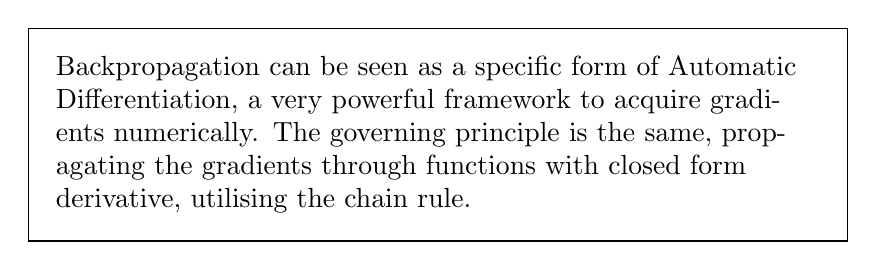
\begin{tikzpicture}
        \node [rectangle, draw, text width=0.8\textwidth, inner sep=10pt] (content) at (0,0) {
            Backpropagation can be seen as a specific form of Automatic Differentiation, a very powerful framework to acquire gradients numerically.
            The governing principle is the same, propagating the gradients through functions with closed form derivative, utilising the chain rule.
        };
    \end{tikzpicture}

    \subsection{Neural ODEs}
    Calculating $\nabla_{\theta}L$ in neural ODEs can be achieved by differentiating through the solver steps but as we will demonstrate there is a much more efficient way, using tools from optimal control theory, namely adjoint sensitivities.
    The governing equations for neural ODEs are Eqs.~\eqref{ivp},~\eqref{adjoint},~\eqref{dldtheta} we repeat them for convenience:

    \begin{equation*}
        \pmb{y}(T) =  \pmb{y}(0) +\int_{0}^{T} f(\pmb{y}(\tau), \tau, \pmb{\theta}) \,d\tau
        , \quad
        \pmb{y}(0) = \pmb{y}_0
    \end{equation*}

    \begin{equation*}
        \pmb{a}^{(1)}(t)
        =
        - \pmb{a}(t)^T
        \frac
        {\partial f( \pmb{y}(t), t, \pmb{\theta} )}
        {\partial \pmb{y} }
        , \quad
        \pmb{a}(T) = \frac{\partial L}{\partial \pmb{y}(T)}
    \end{equation*}

    \begin{equation*}
        \nabla_{\pmb{\theta}} L =
        - \int_T^0
        \pmb{a}(t)^T
        \frac
        {\partial f(\pmb{y}(\tau), \pmb{\theta})}
        {\partial \pmb{\theta}}
        \, d\tau
    \end{equation*}
    Calculating the last integral numerically requires the values of $\pmb{a}(t)$ at all the points in time the solver chooses.
    In the case of a fixed step size solver with step $h$ those would be $t_m = T - mh, \; m=0,1,\dots$.
    In the case of an adaptive step size $t_m$ could be any point between $T$ and $0$.
    In both cases we can calculate those quantities by solving the second ODE starting from time $t=T$ -where $a(T)$ has a closed form solution- and moving backwards in time.
    Next we need the value of $\pmb{y}$ at the same $t_m$s. Again we can calculate them starting from $\pmb{y}(T)$ and solving the original IVP again backwards in time.
    Notice that we don't need to save any intermediate state or activations from the forward pass since we can re-calculate them moving backwards.
    In this sense, neural ODEs are reversible (up to numerical tolerances).

    Algorithm~\ref{alg:adjoint} reformulates the integral equation for the gradient of the loss wrt.
    weights as a differential equation: $ \pmb{a}^{(1)}_\theta(t) = -\pmb{a}(t)^T \frac{\partial f}{\partial \pmb{\theta}}$.
    We know that $\pmb{a}_\theta(T) = 0$ and we search for $\pmb{a}_\theta(0) = \nabla_\theta L$.

    \begin{algorithm}
        \caption{Adjoint}
        \label{alg:adjoint}
        \begin{algorithmic}
            \State Choose ODE solver hyperparameters ($h$, $\dots$)
            \State Do the forward pass, find $\pmb{y}(T)$
            \State $\pmb{a}(T) \gets \frac{\partial L}{\partial \pmb{y}(T)}$ (closed form)
            \State $\pmb{a}_{\theta}(T) \gets 0$
            \State $t \gets T$
            \While{$t > 0$}
                \State $\pmb{y}(t - \Delta t) \gets \text{IntStep}(\pmb{y}(t), f) $
                \State $\pmb{a}(t - \Delta t) \gets \text{IntStep}(
                \pmb{a}(t), -\pmb{a}(t) \frac{\partial f }{\partial \pmb{y}}
                )$
                \State $\pmb{a}_{\theta}(t - \Delta t) \gets \text{IntStep}(
                \pmb{a}_{\theta}(t), -\pmb{a}(t) \frac{\partial f }{\partial \pmb{\theta}}
                )$
                \State $t \gets t - \Delta t$
            \EndWhile
            \State \textbf{return} $\pmb{a}_\theta(0) = \nabla_\theta L$
        \end{algorithmic}
    \end{algorithm}


    \chapter{An alternative derivation for $\frac{dL}{d \pmb{\theta}}$}
    \label{adjoint_proof}
    There are already many ways in the literature for finding this quantity without delving into control theory and reverse sensitivities.
    Intuitively in can be thought as a continuous analogous to classical backpropagation
    \begin{align}
        \text{classical} &\to
        \frac{d L}{ d \pmb{\theta}} =
        \sum_k
        \frac{\partial L}{\partial \pmb{y}_{k}}
        \frac{\partial f(\pmb{y}_k, \pmb\theta)}{\partial \pmb{\theta}}
        \\
        \text{adjoint sensitivities} &\to
        \frac{d L}{ d \pmb{\theta}} =
        \int_T^0
        \frac{\partial L}{\partial \pmb{y}(\tau)}
        \frac{\partial f(\pmb{y}(\tau), \pmb{\theta})}{\partial \pmb{\theta}} \, d\tau
    \end{align}
    In the original neural ODEs paper~\cite{chen2018neural} the authors prove Eq.~\eqref{adjoint} and use an augmented
    state to prove Eq.~\eqref{dldtheta} while others like~\cite{kidger2022neural} provide alternative proofs.
    We present another, in our opinion much simpler, derivation for Eq.~\eqref{dldtheta}.
    Consider the more general case where the loss is dependant on intermediate state on a point $s \in (0,T)$.
    This is equivalent to the usual case where the loss depends only on the output state with $\mathcal{L}(s) = L(\pmb{y}(s))=0$ for $s\neq T$.
    Moreover, the state $\pmb{y}$ is a also dependant on the weights even though it's not explicitly written.
    \begin{align*}
        \frac{ d L(\bm{y}(s, \bm{\theta})) }{ d \bm{\theta} }
        &= \int_0^s \frac{d}{dt} \left( \frac{ d L(\bm{y}(s, \bm{\theta})}{ d \bm{\theta}} \right) dt \\
        &= \int_0^s \frac{d}{dt} \left( \frac{ d L(\bm{y}(t, \bm{\theta})}{ d \bm{y}(t)} \frac{d \bm{y}(t)}{d\bm{\theta}} \right) dt \\
        &= \int_0^s
        \frac{d}{dt} \frac{ d L(\bm{y}(t, \bm{\theta})}{ d \bm{y}(t)} \cdot \frac{d \bm{y}(t)}{d\bm{\theta}}
        +
        \frac{ d L(\bm{y}(t, \bm{\theta})}{ d \bm{y}(t)} \cdot \frac{d}{dt} \frac{d \bm{y}(t)}{d\bm{\theta}}
        dt \\
        &= \int_0^s
        \dot{\bm{a}}(t) \frac{d \bm{y}(t)}{d\bm{\theta}}
        +
        \bm{a}(t) \cdot \frac{d}{d\bm{\theta}} \frac{d \bm{y}(t)}{dt}
        dt \\
        &= \int_0^s
        \dot{\bm{a}}(t) \frac{d \bm{y}(t)}{d\bm{\theta}}
        +
        \bm{a}(t) \cdot \frac{d\bm{f}}{d\theta}
        dt \\
        &= \int_0^s
        \dot{\bm{a}}(t) \frac{d \bm{y}(t)}{d\bm{\theta}}
        +
        \bm{a}(t) \left( \frac{\partial \bm{f}}{\partial \bm{\theta}}
        +
        \frac{\partial \bm{f}}{\partial \bm{y}(t)} \frac{\partial \bm{y}(t)}{\partial \bm{\theta}}\right)
        dt \\
        &= \int_0^s
        \frac{d \bm{y}(t)}{d\bm{\theta}}
        \left( \dot{\bm{a}}(t) + a\frac{\partial \bm{f}}{\partial \bm{y}(t)} \right)
        +
        \bm{a}(t) \frac{\partial \bm{f}}{\partial \bm{\theta}}
        dt \\
    \end{align*}
    From Eq.~\eqref{adjoint} the sum in the parenthesis is 0:
    \begin{align}
        \frac{ d L(\bm{y}(s, \bm{\theta})) }{ d \bm{\theta} }
        = \int_0^s
        \bm{a}(t) \frac{\partial \bm{f}}{\partial \bm{\theta}}
        dt
    \end{align}
    Setting $s=T$ we arrive at the desired formula.


    \chapter{Optimisation}
    In the field of numerical optimisation many methods have been developed for minimising a \textit{scalar} objective function $f$.
    One category of those, \textit{line search} methods, are iterative algorithms that seek to update the current iterate $x_k$ to a new value closer to the minimum.
    They work by choosing a direction $p_k$ -and step size $\alpha$- along which $f$ is decreased.
    Alternatively the problem can be restated as:
    \begin{equation}
        \min_{a>0} f(x_k + \alpha p_k) \label{min_a}
    \end{equation}
    While ideally we would solve~\eqref{min_a} exactly, in practice it is computationally expensive and practically unnecessary.
    Line search implementations usually generate some trial step sizes until they find one that satisfies certain termination conditions we will examine later.

    A \textit{descent direction} is a direction that causes $f$ to decrease along it given sufficiently small $\alpha > 0$: $f(x_k + \alpha p_k) < f(x_k)$.We can show that if $p_k$ is a descent direction then $p_k^T \nabla f_k < 0$.
    From the first order Taylor series expansion we have:
    \begin{equation*}
        f(x_k+ap_k) = f(x_k) + a p_k^T \nabla f_k + O(a^2)< f(x_k) \\
    \end{equation*}
    Ignoring quadratic term since $\alpha$ is small.
    \begin{align*}
        a p_k^T \nabla f_k &< 0 \\
        p_k^T \nabla f_k &< 0
    \end{align*}
    It can be proven though Zoutendijk's theorem that: as long as the search direction is a descent direction and the step size fulfils some conditions the algorithm is globally convergent.

    The defining characteristic of a line search method is the way in which we obtain the search direction $p_k$.
    An obvious choice is to use the direction of \textit{steepest descent}, mathematically obtained as the negative of the gradient at the current iterate.
    \begin{equation}
        x_{k+1} = x_k - \alpha \nabla f_k
    \end{equation}

    In machine learning literature steepest descent, or as they are more commonly refereed, \textit{gradient descent} methods are extremely common.
    Almost all neural network models are trained using some derivative of classic gradient descent.
    These methods are not categorised as line searches since they do not seek to find an appropriate step length $\alpha$ on each iteration.
    They instead define either a fixed or dynamically updated \textit{learning rate}.
    Usually they employ some notions of momentum and stochasticity to move along a direction dictated by an approximation of the local gradient.
    Even so they remain first order methods since they only utilise information about the first derivative.
    Some notable gradient descent methods as well as how the minimisation problem is formulated in the context of machine learning are discussed later.

    \subsection{The Newton-Raphson algorithm with Hessian modification}
    \label{newtonalgo}
    In more general minimisation problems a prevalent search direction for line search optimisers is the \textit{Newton direction}, methods using this direction are called Newton methods.
    This direction is derived from the second-order Taylor series approximation of the objective function, near the current iterate $x_k$.
    Consider a continuous, twice differentiable function $f: \mathbb{R}^n \to \mathbb{R}^n$, its second order Taylor series approximation is:
    \begin{equation}
        f(x_k + p) = f_k + p^t \nabla f_k + \frac{1}{2} p^t \nabla^2 f_k p + R(p) \label{taylor}
    \end{equation}
    with $R(p)$ being of order $O(\rVert p \rVert^3)$.
    For small values of $p$, the residual term diminishes and we have a pretty good quadratic model of $f$.
    Seeking to minimise this model we set the derivative wrt. $p$ equal to 0:
    \begin{align}
        \nabla f_k + \nabla^2 f_k p_t &= 0  \label{grad_m} \\
        p = -\left[ \nabla^2 f_k \right]^{-1} \nabla f_k \label{newton_dir}
    \end{align}
    Eq.~\eqref{newton_dir} gives the definition of the newton direction.
    As mentioned before, in order for the algorithm to be globally convergent the search direction has to be a descent direction.
    By multiplying~\eqref{grad_m} from the left with $p^t$ we get:
    \begin{align}
        p^t \nabla f_k + p_t \nabla^2 f_k p_t =& 0 \\
        p^t \nabla^2 f_k p_t =& -p^t \nabla f_k < 0 \\
        p^t \nabla^2 f_k p_t &> 0 \label{pos_def}
    \end{align}
    From~\eqref{pos_def} it is apparent that the Hessian matrix $H_k=\nabla^2 f_k$ has to be positive definite which is generally true if $x_k$ is near the minimum but not necessarily true away from it.
    If the Hessian is not positive definite there is no guarantee that~\eqref{newton_dir} gives a descent direction or even that the Hessian is non-singular.
    In order to address this issue a positive definite approximation of the Hessian is used.
    The approximation can be obtained in several ways, some involve adding a multiple of the identity or some correction matrix $\Delta H$, others modify the eigenvalues of the true Hessian directly.

    For example in~\cite{cheng1998modified} is shown that, if $H_k$ has spectral decomposition $H_k = Q \Lambda Q^T$ then the correction matrix of minimum Frobenius norm that ensures that the smallest eigenvalue of $H_k + \Delta H$ is larger or equal to $\delta$ is given by:
    \begin{equation*}
        \Delta H = Q \text{diag}(\tau_i) Q^T, \quad \text{with} \quad \tau_i =
        \left\{
        \begin{array}{ll}
            0,                  & \lambda_i \geq \delta, \\
            \delta - \lambda_i, & \lambda_i < \delta,
        \end{array}
        \right.
    \end{equation*}

    Another technique, the one used here, is to perform (or try to perform) a Cholesky decomposition, more specifically an LDL decomposition of the Hessian.
    Since the Hessian is not always positive definite the factorisation $H = LDL^T$ may not exist or if even if it does the algorithm used to compute it is numerically unstable.
    The core idea of modified Cholesky decomposition is to modify the values of the diagonal matrix D to be sufficiently positive while the factorisation is computed.

    More specifically,~\cite{wright2006numerical} provide an algorithm for computing the $LDL^T$ factorisation a positive definite approximation of a matrix.
    It accepts two additional parameters $\delta, \beta$ so that the following bounds are satisfied.
    \begin{equation}
        d_j \geq \delta, \quad \lvert m_{ij} \rvert \leq \beta, \quad i = j+1, j_2, \dots, n
    \end{equation}

    The algorithm calculates the elements of the diagonal $D$ and the unitriangular matrix $L$ column by column.
    It is a simpler version of the algorithm presented in Eq.~\cite{gill2019practical} that additionally introduces symmetric row-column interchanges resulting in lower $ \lVert H_k - \hat{H}_k \rVert$, $\hat{H}_k$ being the approximation.
    \begin{algorithm}
        \label{alg:mod_chol}
        \caption{Modified Cholesky}
        \begin{algorithmic}
            \For{ $i = j+1,\dots,n$ }
                \State $c_{jj} \gets a_{jj} - \sum_{s=1}^{j-1} d_s l_{js}$
                \State $\theta_j \gets \max_{j<i\leq n}(\lvert c_{ij} \rvert)$
                \State $d_j \gets  \max
                \left(
                \lvert c_{jj} \rvert,
                \left( \frac{\theta_j}{\beta} \right)^2,
                \delta \right)$
                \For{$i = j+1,\dots, n$}
                    \State $c_{ij} \gets a_{ij} - \sum_{s=1}^{j-1} d_s l_{is} l_{js}$
                    \State $l_{ij} \gets c_{ij} / d_j$
                \EndFor
            \EndFor
        \end{algorithmic}
    \end{algorithm}
    After addressing the definiteness of the the Hessian let's describe how an algorithm would decide on the step size.
    As noted earlier Zoutendijk's theorem requires the search direction to be a descent direction as well as the step size to fulfil a certain set of conditions.
    One can prove Zoutedijk's theorem for multiple sets of conditions, namely the Wolfe, strong Wolfe and Goldstein conditions.
    We will focus on the strong Wolfe conditions.
    Assume we have chose direction $p_k$ at step $k$ of the algorithm, our second objective is to find step size $a$ to proceed to the next step without minimising $\phi(\alpha) = f(x_k + \alpha p_k)$ explicitly.
    The first strong Wolfe condition states that our guess for $a$ should give \textit{sufficient decrease} in the objective function in the following way:
    \begin{equation}
        f(x_k + ap_k) \leq f(x_k) + c_1 a \nabla f_k ^T p_k
    \end{equation}
    for some $c_1 \in (0,1)$ usually chosen to be quite small ($\approx 10^{-4}$). This ensures the reduction in $f$ is proportional to the step size as well as the directional derivative $\nabla f ^T p_k$.
    The sufficient decrease condition is not enough to make reasonable progress since it's satisfied for values of $\alpha$ close to 0.
    To prevent this, the second strong Wolfe condition or \textit{curvature condition} states that $\alpha$ should also satisfy:
    \begin{equation}
        \lvert \nabla f(x_k + \alpha p_k )^T p_k \rvert \leq \lvert c_2 \nabla f_k^T p_k \rvert
    \end{equation}
    for some constant $c_2 \in (c_1, 1)$ usually set around $0.9$ for Newton direction.
    Notice that the left hand side if the derivative wrt. $\alpha$ of $\phi(a)$ at $a_k$ and the right hand size at $0$.
    Practically the curvature condition requires the slope of $\phi$ at the new point to be greater that at the start times $c_2$.
    Remember that $p_k$ is a descent direction so $\phi(0)$ is strictly negative.
    Larger slope would mean we get closer to a stationary point of zero gradient.
    The absolute ensures that the slope doesn't become too positive and we don't overshoot away from the stationary point.

    Utilising those conditions we construct the following line search algorithm parameterised by $c_1, c_2, \alpha_{max}$

    \begin{algorithm}
        \caption{Line search}
        \label{alg:linesearh}
        \begin{algorithmic}
            \State Set $a_0 \gets 0$, choose $a_1 \in (0, a_{max})$
            \State $i \gets 1$
            \Repeat
                \If {$\phi(a_i) > \phi(0) + c_1 a_i \phi^{(1)}(0)$ or [$\phi(a_i) \geq \phi(a_{i-1})$ and $i>1$]}
                    \State return \textbf{zoom}($a_{i-1}, a_i$)
                \EndIf
                \If {$\lvert \phi^{(1)}(a_i) \rvert \leq -c_2 \phi^{(1)}(0)$}
                    \State return $a_i$
                \EndIf
                \If {$\phi^{(1)}(a_i) \geq 0$}
                    \State return \textbf{zoom}($a_i, a_{i-1}$)
                \EndIf
                \State $a_{i+1} \gets \min({a_max, 2*a_i})$
                \State $i \gets i+1$
            \Until
        \end{algorithmic}
    \end{algorithm}

    The procedure uses the knowledge that the interval $(a_{i-1} , a_{i})$ contains step lengths satisfying the strong Wolfe
    conditions if one of the following three conditions is satisfied:
    \begin{enumerate}
        \item $a_i$ violates the sufficient decreasee condition
        \item $\phi(a_i) \geq \phi(a_{i-1}) $
        \item $\phi^{(1)}(a_i) \geq 0$
    \end{enumerate}
    The last step of the algorithm performs extrapolation to find the next trial value $a_{i+1}$.
    We can use some more involved extrapolation technique like the ones mentioned previously in the section, or
    we can simply set $a_{i+1}$ to some constant multiple of $a_i$.
    Whichever strategy we use, it is
    important that the successive steps increase quickly enough to reach the upper limit $a_{\max}$ in
    a finite number of iterations.

    We know specify the function zoom, which requires a little explanation.
    The order of its input is such that each call has the form: \textbf{zoom}($a_{lo}$, $a_{hi}$), where
    \begin{enumerate}
        \item the interval bounded by $a_{lo}$ and $a_{hi}$ contains step lengths that satisfy the strong Wolfe conditions
        \item $a_{lo}$ is, among all step lengths generated so far and satisfying the sufficient decrease conditions, the one giving the smallest value;
        \item $a_hi$ is chosen so that $\phi{a_{lo}}(a_{hi} - a_{lo}) < 0$
    \end{enumerate}
    Each iteration of zoom generates and iterate $a_j$ between $a_{lo}$ and $a_{hi}$, and then replaces one of these
    endpoints by $a_j$ in such a way that the above properties continue to hold.

    \begin{algorithm}
        \caption{zoom}
        \label{alg:zoom}
        \begin{algorithmic}
            \Repeat
                \State Interpolate to find a trial step length $a_j$ between $a_{lo}$ and $a_{hi}$
                \State Evaluate $\phi(a_j)$
                \If {$\phi(a_j) > \phi(0) + c_1 a_j \phi^{(1)}(0)$ or $\phi(a_j) \geq \phi(a_{lo}$]}
                    \State $a_{hi} \gets a_j$
                \Else
                    \State Evaluate $\phi^{(1)}(a_j)$
                    \If {$ |\phi^{(1)}(a_j)| \leq -c_2 \phi^{(1)}(0)$}
                        \State Set $a^* \gets a_j$ and \textbf{stop}
                    \EndIf
                    \If { $\phi^{(1)}(a_j)(a_{hi} - a_{lo}) \geq 0 $ }
                        \State $a_{hi} \gets a_{lo}$
                    \EndIf
                    \State $a_{lo} \gets a_{hi}$
                \EndIf
            \Until
        \end{algorithmic}
    \end{algorithm}

    If the new estimate $a_j$ happens to satisfy the strong Wolfe conditions, then zoom has served
    its purpose of identifying such a point, so it terminates with $a^* = a_j$.
    Otherwise, if $a_j$ satisfies the sufficient decrease condition and has a lower function value than $a_{lo}$ ,
    then we set $a_{lo} \gets a_j$ to maintain condition (2).
    If by doing so we end up violating condition (3), we set $a_{hi}$ to the old value of $a_{lo}$ ensuring condition
    (3) holds.

    Several implementations of the Newton algorithm with line search exist in scientific software packages.
    We have written an exact Newton routine in \textbf{PyTorch} utilising automatic differentiation and GPU parallelism.

    \subsection{Gradient Descent Methods}
    For the sake of completeness we will present some fist order optimisation methods.
    For really high dimensional problems, such as those we are concerned with in modern deep learning settings, second
    order methods introduce quadratically scaled (on the number of parameters) computation and memory cost.
    This cost is related to the computation and storage of the Hessian (or an approximation of it) which is of size
    ${num_{parameters}}^2$.
    The tradeoff between number of iterations and cost per iteration leans in favor of gradient descent optimizers as
    the number of parameters increases, especially considering the fact that they lend themselves well to automatic
    differentiation and distributing training.
    The loss function for example
    All these in combination with the higher implementation complexity have lead to the dominance of first order
    optimisation techniques in machine learning.

    \subsubsection{Stochastic Gradient Descent}
    Optimising a deep learning model in the strict sense means minimising the expected generalization error
    $\mathbb{E}_{(\pmb{x},\pmb{y}) \sim p_{\text{data}}} L(f(\pmb{x},\pmb\theta),\pmb{y})$ where $p_{data}$ is the joint
    distribution of inputs $\pmb{x}$ and outputs $\pmb{y}$, $\pmb\theta$ are the models parameters and $L$ some per
    sample cost function.
    Since the distribution of data is largely unknown we create an empirical estimate from a set of training examples
    ${\pmb{x}_i,\pmb{y}_i}_{i=1}^{N}$
    \begin{equation*}
        \tilde L(\pmb\theta ) = \frac{1}{N} \sum_{i=1}^N L( f(\pmb{x}_i; \pmb\theta), \pmb{y}_i )
    \end{equation*}
    Minimising such a loss function though traditional gradient descent would require to evaluate the cost for all
    samples in the training set on each iteration to obtain the loss.
    \begin{equation*}
        \pmb\theta^{k+1} = \pmb\theta^{k} + \eta \nabla_{\theta_k} L(\pmb\theta^{k})
    \end{equation*}
    To alleviate some computational cost on each iteration Stochastic Gradient Descent (SGD) is used which instead of calculating
    the loss for all samples in the training set it samples a subset of them and performs the weights updated based
    on that.
    This approach introduces some stochasticity to the gradient approximation which leads to noise increasing the
    convergence rate but can lower the overall computational cost.
    To keep the the algorithm to diverging due to noise a lower learning rate is required to maintain stability
    ~\cite{kiwiel2001convergence}.
    Furthermore, the stochastic nature of SGD can allow it to escape from local minima in the non convex
    high-dimensional loss space that a classic gradient descent scheme would be trapped in.

    To accelerate Stochastic Gradient Descent a number of methods have been proposed some of them in the recent years due
    to the popularity of deep neural networks.

    \subsubsection{ Momentum }
    Based on the idea of physical momentum in real world objects the momentum method was proposed in the context of machine
    learning in~\cite{rumelhart1986learning} borrowing the idea from previous work by Polyak~\cite{polyak1964some}.
    This algorithm considers previous values of the gradient in the update step in a exponentially decaying manner.
    The update along dimensions that keep moving in the same direction keeps getting bigger and for dimensions that
    change direction the update gets smaller.
    Even though it can be applied to both stochastic and classical gradient descent, SGD with a momentum term has been
    the gold standard for many years for non-convex optimisation problems, and presents very good results.
    It converges faster that classical GD due to accumulated velocity while also dampening oscillations in regions of high
    curvatures by combining gradients of opposite signs.
    SGD Momentum can be expressed with the following equation
    \begin{align*}
        \Delta \pmb\theta_{k+1} = \alpha \Delta \pmb\theta_k - \eta \nabla_{\theta_k} L (\pmb\theta_k) \\
        \pmb\theta_{k+1} = \pmb\theta_{k} + \Delta \pmb\theta_{k+1}
    \end{align*}
    where $\alpha$ is an exponential decay factor between $0$ and $1$ that determines the amount of contribution
    previous gradients have to the weights update.

    \subsubsection{Nesterov Momentum}
    A major disadvantage of classical momentum (CM) method is its tendency to overshoot as is approaches the minimum.
    Nesterov momentum seeks to solve this problem drawing from Nesterov's accelerated gradient method for convex functions.
    The equations for Nesterov's momemtum are:
    \begin{align*}
        \Delta \pmb\theta_{k+1} = \alpha \Delta \pmb\theta_k - \eta \nabla_{\theta_k} L(\pmb\theta_{k} + \alpha \Delta \pmb\theta_{k}) \\
        \pmb\theta_{k+1} = \pmb\theta_{k} + \Delta \pmb\theta_{k+1}
    \end{align*}
    This formula resembles CM but instead of calculating the gradient of loss at the current $\pmb\theta$ it is
    calculated after the previous velocity is added.
    This method is based on a corrector-predictor scheme where you first make a big step on the direction of the
    accumulated gradient and then make a correction based on the gradient on the point you land.
    This behaviour helps the method avoid oscillations, such as those that appear in CM around high-curvature regions,
    by pointing the gradients back to $\pmb\theta_k$ more effectively than classical momentum~\cite{kashyap2022survey}.

    \subsubsection{Adagrad}
    The Adagrad algorithm individually adapts the learning rates of all model parameters by scaling them inversely
    proportional to the square root of the the sum of the historical squared values of the gradient.
    \begin{align*}
        \pmb\theta_{k+1} \gets \pmb\theta_{k} - \frac{\eta}{  \sqrt{G_{k}} + \epsilon } \nabla_{\theta_k} L( \pmb\theta_k)
    \end{align*}
    Where $G$ is a matrix containing the squared sum of the past gradients with regards to all $\pmb\theta_k$ along its
    diagonal and $\epsilon$ is a small quantity to avoid dividing by zero.
    For weight parameter with the largest gradient has the largest decrease in its learning rate, while the parameter
    with the smallest gradient has the smallest decrease in its learning rate.
    This results in faster progress in the more gentlysloped regions of parameter space and works well when the
    gradient is sparse~\cite{duchi2011adaptive}.

    \subsubsection{RMSProp}
    The RMSProp algorithm is famous for being an unpublished but well known optimisation algorithm.
    It was introduced by Hinton in one of his courses.
    RMSprop modifies Adagrad so that instead of accumulating the square of the gradients for each parameter, which can
    cause the learning rate to diminish uses an exponentially decaying moving average of the squared gradients to
    discard the past history.
    \begin{align*}
        G_{k+1} = \beta G_{k} + (1 - \beta) ( \nabla_{\theta_k} L (\pmb\theta_k) )^2\\
        \pmb\theta_{k+1} = \pmb\theta_{k} - \frac{\eta}{  \sqrt{G_{k}} + \epsilon } \nabla_{\theta_k} L( \pmb\theta_k)
    \end{align*}

    \subsubsection{Adam}
    One of the most widely used optimisation algorithms used in deep learning today is Adam, which stands for
    adaptive moments~\cite{kingma2014adam}.
    It combines elements of momentum and RMSprop with some modifications.
    Firstly, we incorporate momentum by computing the first order moment of the gradient as exponentially decaying
    moving average.
    Secondly, we calculate the second order moment as the gradient, again as an exponentially decaying average.
    The parameter update rule is given as:
    \begin{align*}
        \pmb{v}_k = \alpha \pmb{v}_{k-1} + (1 - \alpha) \nabla_{\theta_k} L( \pmb\theta_{k} ) \\
        \pmb{s}_k = \beta \pmb{s}_{k-1} + (1 - \beta) \nabla_{\theta_k} L( \pmb\theta_{k} ) \\
        \pmb\theta_{k+1} = \pmb\theta_{k} - \eta \frac{\hat{\pmb{v}}_k}{  \sqrt{ \hat{\pmb{s}}_k + \epsilon }} \nabla_{\theta_k} L( \pmb\theta_k)
    \end{align*}
    In the above equations $\hat{\pmb{s}}_k$, $\hat{\pmb{v}}_k$ are the bias corrected estimates of the moments to account
    for their initialization.
    Since RMSProp lacks the correction factor, it has a high-bias in the early stages of training, while Adam is
    robust to the choice of hyperparameters.


\end{document}


